% Appendix D

\chapter{Fit Results for The Systematics (3)} % Main appendix title

\label{AppendixD} % For referencing this appendix elsewhere, use \ref{AppendixA}

Here all fits for third systematic on the tag and probe invariant mass presented for all $p_T-|\eta|$ bins. In the third systematic the background modeling function is changed from the Bernstein-Polynomial, used in nominal sample, to Gaussian function.
%The first twenty fits belongs to CR1 ($Z\rightarrow e^+e^-$) shown in figure\ref{fig:fit_cr1_sys3}. The fits for CR2 ($Z\rightarrow e\gamma$) are given in figure\ref{fig:fit_cr2_sys3}.

\begin{figure}[H]
\begin{center}
\scalebox{0.35}{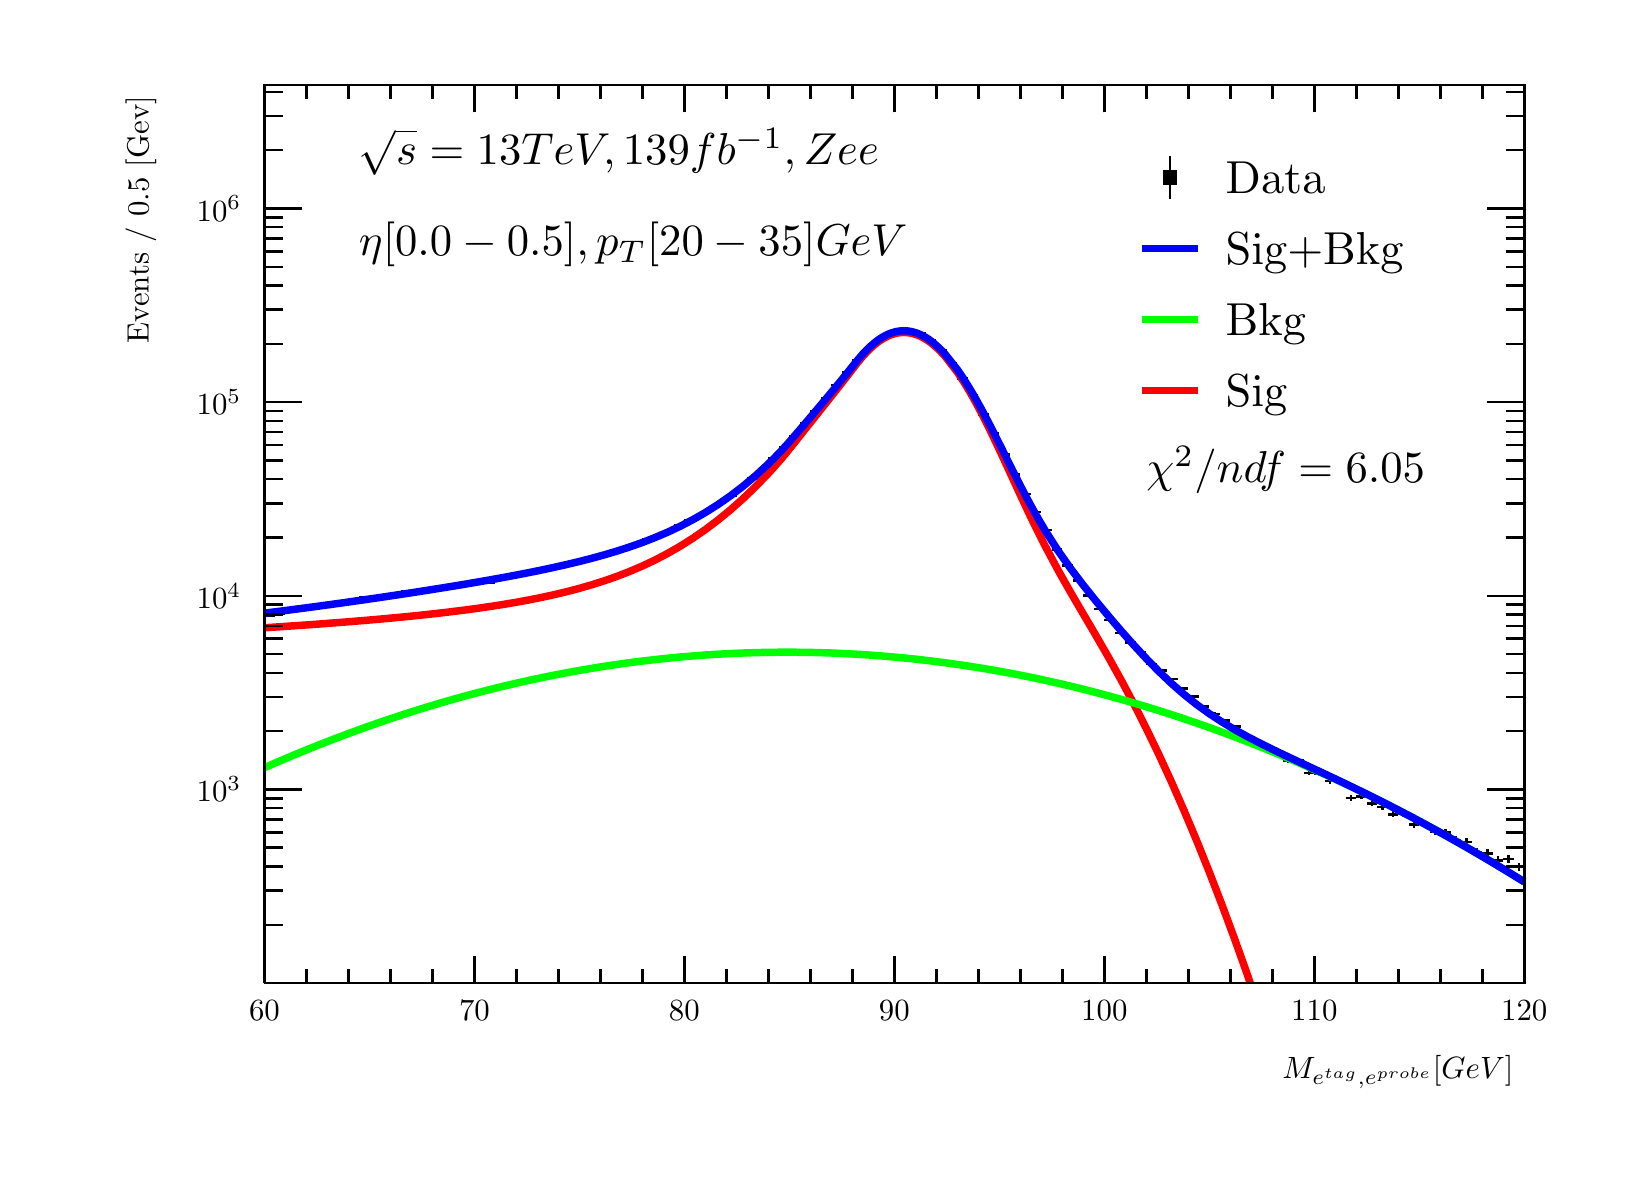
\begin{tikzpicture}
\pgfdeclareplotmark{cross} {
\pgfpathmoveto{\pgfpoint{-0.3\pgfplotmarksize}{\pgfplotmarksize}}
\pgfpathlineto{\pgfpoint{+0.3\pgfplotmarksize}{\pgfplotmarksize}}
\pgfpathlineto{\pgfpoint{+0.3\pgfplotmarksize}{0.3\pgfplotmarksize}}
\pgfpathlineto{\pgfpoint{+1\pgfplotmarksize}{0.3\pgfplotmarksize}}
\pgfpathlineto{\pgfpoint{+1\pgfplotmarksize}{-0.3\pgfplotmarksize}}
\pgfpathlineto{\pgfpoint{+0.3\pgfplotmarksize}{-0.3\pgfplotmarksize}}
\pgfpathlineto{\pgfpoint{+0.3\pgfplotmarksize}{-1.\pgfplotmarksize}}
\pgfpathlineto{\pgfpoint{-0.3\pgfplotmarksize}{-1.\pgfplotmarksize}}
\pgfpathlineto{\pgfpoint{-0.3\pgfplotmarksize}{-0.3\pgfplotmarksize}}
\pgfpathlineto{\pgfpoint{-1.\pgfplotmarksize}{-0.3\pgfplotmarksize}}
\pgfpathlineto{\pgfpoint{-1.\pgfplotmarksize}{0.3\pgfplotmarksize}}
\pgfpathlineto{\pgfpoint{-0.3\pgfplotmarksize}{0.3\pgfplotmarksize}}
\pgfpathclose
\pgfusepathqstroke
}
\pgfdeclareplotmark{cross*} {
\pgfpathmoveto{\pgfpoint{-0.3\pgfplotmarksize}{\pgfplotmarksize}}
\pgfpathlineto{\pgfpoint{+0.3\pgfplotmarksize}{\pgfplotmarksize}}
\pgfpathlineto{\pgfpoint{+0.3\pgfplotmarksize}{0.3\pgfplotmarksize}}
\pgfpathlineto{\pgfpoint{+1\pgfplotmarksize}{0.3\pgfplotmarksize}}
\pgfpathlineto{\pgfpoint{+1\pgfplotmarksize}{-0.3\pgfplotmarksize}}
\pgfpathlineto{\pgfpoint{+0.3\pgfplotmarksize}{-0.3\pgfplotmarksize}}
\pgfpathlineto{\pgfpoint{+0.3\pgfplotmarksize}{-1.\pgfplotmarksize}}
\pgfpathlineto{\pgfpoint{-0.3\pgfplotmarksize}{-1.\pgfplotmarksize}}
\pgfpathlineto{\pgfpoint{-0.3\pgfplotmarksize}{-0.3\pgfplotmarksize}}
\pgfpathlineto{\pgfpoint{-1.\pgfplotmarksize}{-0.3\pgfplotmarksize}}
\pgfpathlineto{\pgfpoint{-1.\pgfplotmarksize}{0.3\pgfplotmarksize}}
\pgfpathlineto{\pgfpoint{-0.3\pgfplotmarksize}{0.3\pgfplotmarksize}}
\pgfpathclose
\pgfusepathqfillstroke
}
\pgfdeclareplotmark{newstar} {
\pgfpathmoveto{\pgfqpoint{0pt}{\pgfplotmarksize}}
\pgfpathlineto{\pgfqpointpolar{44}{0.5\pgfplotmarksize}}
\pgfpathlineto{\pgfqpointpolar{18}{\pgfplotmarksize}}
\pgfpathlineto{\pgfqpointpolar{-20}{0.5\pgfplotmarksize}}
\pgfpathlineto{\pgfqpointpolar{-54}{\pgfplotmarksize}}
\pgfpathlineto{\pgfqpointpolar{-90}{0.5\pgfplotmarksize}}
\pgfpathlineto{\pgfqpointpolar{234}{\pgfplotmarksize}}
\pgfpathlineto{\pgfqpointpolar{198}{0.5\pgfplotmarksize}}
\pgfpathlineto{\pgfqpointpolar{162}{\pgfplotmarksize}}
\pgfpathlineto{\pgfqpointpolar{134}{0.5\pgfplotmarksize}}
\pgfpathclose
\pgfusepathqstroke
}
\pgfdeclareplotmark{newstar*} {
\pgfpathmoveto{\pgfqpoint{0pt}{\pgfplotmarksize}}
\pgfpathlineto{\pgfqpointpolar{44}{0.5\pgfplotmarksize}}
\pgfpathlineto{\pgfqpointpolar{18}{\pgfplotmarksize}}
\pgfpathlineto{\pgfqpointpolar{-20}{0.5\pgfplotmarksize}}
\pgfpathlineto{\pgfqpointpolar{-54}{\pgfplotmarksize}}
\pgfpathlineto{\pgfqpointpolar{-90}{0.5\pgfplotmarksize}}
\pgfpathlineto{\pgfqpointpolar{234}{\pgfplotmarksize}}
\pgfpathlineto{\pgfqpointpolar{198}{0.5\pgfplotmarksize}}
\pgfpathlineto{\pgfqpointpolar{162}{\pgfplotmarksize}}
\pgfpathlineto{\pgfqpointpolar{134}{0.5\pgfplotmarksize}}
\pgfpathclose
\pgfusepathqfillstroke
}
\definecolor{c}{rgb}{1,1,1};
\draw [color=c, fill=c] (0,0) rectangle (20,14.4361);
\draw [color=c, fill=c] (3,2.30977) rectangle (19,13.7143);
\definecolor{c}{rgb}{0,0,0};
\draw [c,line width=0.9] (3,2.30977) -- (3,13.7143) -- (19,13.7143) -- (19,2.30977) -- (3,2.30977);
\definecolor{c}{rgb}{1,1,1};
\draw [color=c, fill=c] (3,2.30977) rectangle (19,13.7143);
\definecolor{c}{rgb}{0,0,0};
\draw [c,line width=0.9] (3,2.30977) -- (3,13.7143) -- (19,13.7143) -- (19,2.30977) -- (3,2.30977);
\draw [c,line width=0.9] (3,2.30977) -- (19,2.30977);
\draw [c,line width=0.9] (3,2.65624) -- (3,2.30977);
\draw [c,line width=0.9] (3.53333,2.48301) -- (3.53333,2.30977);
\draw [c,line width=0.9] (4.06667,2.48301) -- (4.06667,2.30977);
\draw [c,line width=0.9] (4.6,2.48301) -- (4.6,2.30977);
\draw [c,line width=0.9] (5.13333,2.48301) -- (5.13333,2.30977);
\draw [c,line width=0.9] (5.66667,2.65624) -- (5.66667,2.30977);
\draw [c,line width=0.9] (6.2,2.48301) -- (6.2,2.30977);
\draw [c,line width=0.9] (6.73333,2.48301) -- (6.73333,2.30977);
\draw [c,line width=0.9] (7.26667,2.48301) -- (7.26667,2.30977);
\draw [c,line width=0.9] (7.8,2.48301) -- (7.8,2.30977);
\draw [c,line width=0.9] (8.33333,2.65624) -- (8.33333,2.30977);
\draw [c,line width=0.9] (8.86667,2.48301) -- (8.86667,2.30977);
\draw [c,line width=0.9] (9.4,2.48301) -- (9.4,2.30977);
\draw [c,line width=0.9] (9.93333,2.48301) -- (9.93333,2.30977);
\draw [c,line width=0.9] (10.4667,2.48301) -- (10.4667,2.30977);
\draw [c,line width=0.9] (11,2.65624) -- (11,2.30977);
\draw [c,line width=0.9] (11.5333,2.48301) -- (11.5333,2.30977);
\draw [c,line width=0.9] (12.0667,2.48301) -- (12.0667,2.30977);
\draw [c,line width=0.9] (12.6,2.48301) -- (12.6,2.30977);
\draw [c,line width=0.9] (13.1333,2.48301) -- (13.1333,2.30977);
\draw [c,line width=0.9] (13.6667,2.65624) -- (13.6667,2.30977);
\draw [c,line width=0.9] (14.2,2.48301) -- (14.2,2.30977);
\draw [c,line width=0.9] (14.7333,2.48301) -- (14.7333,2.30977);
\draw [c,line width=0.9] (15.2667,2.48301) -- (15.2667,2.30977);
\draw [c,line width=0.9] (15.8,2.48301) -- (15.8,2.30977);
\draw [c,line width=0.9] (16.3333,2.65624) -- (16.3333,2.30977);
\draw [c,line width=0.9] (16.8667,2.48301) -- (16.8667,2.30977);
\draw [c,line width=0.9] (17.4,2.48301) -- (17.4,2.30977);
\draw [c,line width=0.9] (17.9333,2.48301) -- (17.9333,2.30977);
\draw [c,line width=0.9] (18.4667,2.48301) -- (18.4667,2.30977);
\draw [c,line width=0.9] (19,2.65624) -- (19,2.30977);
\draw [anchor=base] (3,1.83338) node[scale=1.11327, color=c, rotate=0]{60};
\draw [anchor=base] (5.66667,1.83338) node[scale=1.11327, color=c, rotate=0]{70};
\draw [anchor=base] (8.33333,1.83338) node[scale=1.11327, color=c, rotate=0]{80};
\draw [anchor=base] (11,1.83338) node[scale=1.11327, color=c, rotate=0]{90};
\draw [anchor=base] (13.6667,1.83338) node[scale=1.11327, color=c, rotate=0]{100};
\draw [anchor=base] (16.3333,1.83338) node[scale=1.11327, color=c, rotate=0]{110};
\draw [anchor=base] (19,1.83338) node[scale=1.11327, color=c, rotate=0]{120};
\draw [anchor= east] (19,1.17798) node[scale=1.11327, color=c, rotate=0]{$M_{e^{tag}, e^{probe}}  [GeV]$};
\draw [c,line width=0.9] (3,13.7143) -- (19,13.7143);
\draw [c,line width=0.9] (3,13.3678) -- (3,13.7143);
\draw [c,line width=0.9] (3.53333,13.5411) -- (3.53333,13.7143);
\draw [c,line width=0.9] (4.06667,13.5411) -- (4.06667,13.7143);
\draw [c,line width=0.9] (4.6,13.5411) -- (4.6,13.7143);
\draw [c,line width=0.9] (5.13333,13.5411) -- (5.13333,13.7143);
\draw [c,line width=0.9] (5.66667,13.3678) -- (5.66667,13.7143);
\draw [c,line width=0.9] (6.2,13.5411) -- (6.2,13.7143);
\draw [c,line width=0.9] (6.73333,13.5411) -- (6.73333,13.7143);
\draw [c,line width=0.9] (7.26667,13.5411) -- (7.26667,13.7143);
\draw [c,line width=0.9] (7.8,13.5411) -- (7.8,13.7143);
\draw [c,line width=0.9] (8.33333,13.3678) -- (8.33333,13.7143);
\draw [c,line width=0.9] (8.86667,13.5411) -- (8.86667,13.7143);
\draw [c,line width=0.9] (9.4,13.5411) -- (9.4,13.7143);
\draw [c,line width=0.9] (9.93333,13.5411) -- (9.93333,13.7143);
\draw [c,line width=0.9] (10.4667,13.5411) -- (10.4667,13.7143);
\draw [c,line width=0.9] (11,13.3678) -- (11,13.7143);
\draw [c,line width=0.9] (11.5333,13.5411) -- (11.5333,13.7143);
\draw [c,line width=0.9] (12.0667,13.5411) -- (12.0667,13.7143);
\draw [c,line width=0.9] (12.6,13.5411) -- (12.6,13.7143);
\draw [c,line width=0.9] (13.1333,13.5411) -- (13.1333,13.7143);
\draw [c,line width=0.9] (13.6667,13.3678) -- (13.6667,13.7143);
\draw [c,line width=0.9] (14.2,13.5411) -- (14.2,13.7143);
\draw [c,line width=0.9] (14.7333,13.5411) -- (14.7333,13.7143);
\draw [c,line width=0.9] (15.2667,13.5411) -- (15.2667,13.7143);
\draw [c,line width=0.9] (15.8,13.5411) -- (15.8,13.7143);
\draw [c,line width=0.9] (16.3333,13.3678) -- (16.3333,13.7143);
\draw [c,line width=0.9] (16.8667,13.5411) -- (16.8667,13.7143);
\draw [c,line width=0.9] (17.4,13.5411) -- (17.4,13.7143);
\draw [c,line width=0.9] (17.9333,13.5411) -- (17.9333,13.7143);
\draw [c,line width=0.9] (18.4667,13.5411) -- (18.4667,13.7143);
\draw [c,line width=0.9] (19,13.3678) -- (19,13.7143);
\draw [c,line width=0.9] (3,2.30977) -- (3,13.7143);
\draw [c,line width=0.9] (3.237,3.05008) -- (3,3.05008);
\draw [c,line width=0.9] (3.237,3.48313) -- (3,3.48313);
\draw [c,line width=0.9] (3.237,3.79038) -- (3,3.79038);
\draw [c,line width=0.9] (3.237,4.02871) -- (3,4.02871);
\draw [c,line width=0.9] (3.237,4.22343) -- (3,4.22343);
\draw [c,line width=0.9] (3.237,4.38807) -- (3,4.38807);
\draw [c,line width=0.9] (3.237,4.53069) -- (3,4.53069);
\draw [c,line width=0.9] (3.237,4.65649) -- (3,4.65649);
\draw [c,line width=0.9] (3.474,4.76901) -- (3,4.76901);
\draw [anchor= east] (2.844,4.76901) node[scale=1.11327, color=c, rotate=0]{$10^{3}$};
\draw [c,line width=0.9] (3.237,5.50932) -- (3,5.50932);
\draw [c,line width=0.9] (3.237,5.94237) -- (3,5.94237);
\draw [c,line width=0.9] (3.237,6.24963) -- (3,6.24963);
\draw [c,line width=0.9] (3.237,6.48795) -- (3,6.48795);
\draw [c,line width=0.9] (3.237,6.68268) -- (3,6.68268);
\draw [c,line width=0.9] (3.237,6.84731) -- (3,6.84731);
\draw [c,line width=0.9] (3.237,6.98993) -- (3,6.98993);
\draw [c,line width=0.9] (3.237,7.11573) -- (3,7.11573);
\draw [c,line width=0.9] (3.474,7.22826) -- (3,7.22826);
\draw [anchor= east] (2.844,7.22826) node[scale=1.11327, color=c, rotate=0]{$10^{4}$};
\draw [c,line width=0.9] (3.237,7.96856) -- (3,7.96856);
\draw [c,line width=0.9] (3.237,8.40161) -- (3,8.40161);
\draw [c,line width=0.9] (3.237,8.70887) -- (3,8.70887);
\draw [c,line width=0.9] (3.237,8.94719) -- (3,8.94719);
\draw [c,line width=0.9] (3.237,9.14192) -- (3,9.14192);
\draw [c,line width=0.9] (3.237,9.30656) -- (3,9.30656);
\draw [c,line width=0.9] (3.237,9.44917) -- (3,9.44917);
\draw [c,line width=0.9] (3.237,9.57497) -- (3,9.57497);
\draw [c,line width=0.9] (3.474,9.6875) -- (3,9.6875);
\draw [anchor= east] (2.844,9.6875) node[scale=1.11327, color=c, rotate=0]{$10^{5}$};
\draw [c,line width=0.9] (3.237,10.4278) -- (3,10.4278);
\draw [c,line width=0.9] (3.237,10.8609) -- (3,10.8609);
\draw [c,line width=0.9] (3.237,11.1681) -- (3,11.1681);
\draw [c,line width=0.9] (3.237,11.4064) -- (3,11.4064);
\draw [c,line width=0.9] (3.237,11.6012) -- (3,11.6012);
\draw [c,line width=0.9] (3.237,11.7658) -- (3,11.7658);
\draw [c,line width=0.9] (3.237,11.9084) -- (3,11.9084);
\draw [c,line width=0.9] (3.237,12.0342) -- (3,12.0342);
\draw [c,line width=0.9] (3.474,12.1467) -- (3,12.1467);
\draw [anchor= east] (2.844,12.1467) node[scale=1.11327, color=c, rotate=0]{$10^{6}$};
\draw [c,line width=0.9] (3.237,12.887) -- (3,12.887);
\draw [c,line width=0.9] (3.237,13.3201) -- (3,13.3201);
\draw [c,line width=0.9] (3.237,13.6274) -- (3,13.6274);
\draw [anchor= east] (1.432,13.7143) node[scale=1.11327, color=c, rotate=90]{Events / 0.5 [Gev]};
\draw [c,line width=0.9] (19,2.30977) -- (19,13.7143);
\draw [c,line width=0.9] (18.763,3.05008) -- (19,3.05008);
\draw [c,line width=0.9] (18.763,3.48313) -- (19,3.48313);
\draw [c,line width=0.9] (18.763,3.79038) -- (19,3.79038);
\draw [c,line width=0.9] (18.763,4.02871) -- (19,4.02871);
\draw [c,line width=0.9] (18.763,4.22343) -- (19,4.22343);
\draw [c,line width=0.9] (18.763,4.38807) -- (19,4.38807);
\draw [c,line width=0.9] (18.763,4.53069) -- (19,4.53069);
\draw [c,line width=0.9] (18.763,4.65649) -- (19,4.65649);
\draw [c,line width=0.9] (18.526,4.76901) -- (19,4.76901);
\draw [c,line width=0.9] (18.763,5.50932) -- (19,5.50932);
\draw [c,line width=0.9] (18.763,5.94237) -- (19,5.94237);
\draw [c,line width=0.9] (18.763,6.24963) -- (19,6.24963);
\draw [c,line width=0.9] (18.763,6.48795) -- (19,6.48795);
\draw [c,line width=0.9] (18.763,6.68268) -- (19,6.68268);
\draw [c,line width=0.9] (18.763,6.84731) -- (19,6.84731);
\draw [c,line width=0.9] (18.763,6.98993) -- (19,6.98993);
\draw [c,line width=0.9] (18.763,7.11573) -- (19,7.11573);
\draw [c,line width=0.9] (18.526,7.22826) -- (19,7.22826);
\draw [c,line width=0.9] (18.763,7.96856) -- (19,7.96856);
\draw [c,line width=0.9] (18.763,8.40161) -- (19,8.40161);
\draw [c,line width=0.9] (18.763,8.70887) -- (19,8.70887);
\draw [c,line width=0.9] (18.763,8.94719) -- (19,8.94719);
\draw [c,line width=0.9] (18.763,9.14192) -- (19,9.14192);
\draw [c,line width=0.9] (18.763,9.30656) -- (19,9.30656);
\draw [c,line width=0.9] (18.763,9.44917) -- (19,9.44917);
\draw [c,line width=0.9] (18.763,9.57497) -- (19,9.57497);
\draw [c,line width=0.9] (18.526,9.6875) -- (19,9.6875);
\draw [c,line width=0.9] (18.763,10.4278) -- (19,10.4278);
\draw [c,line width=0.9] (18.763,10.8609) -- (19,10.8609);
\draw [c,line width=0.9] (18.763,11.1681) -- (19,11.1681);
\draw [c,line width=0.9] (18.763,11.4064) -- (19,11.4064);
\draw [c,line width=0.9] (18.763,11.6012) -- (19,11.6012);
\draw [c,line width=0.9] (18.763,11.7658) -- (19,11.7658);
\draw [c,line width=0.9] (18.763,11.9084) -- (19,11.9084);
\draw [c,line width=0.9] (18.763,12.0342) -- (19,12.0342);
\draw [c,line width=0.9] (18.526,12.1467) -- (19,12.1467);
\draw [c,line width=0.9] (18.763,12.887) -- (19,12.887);
\draw [c,line width=0.9] (18.763,13.3201) -- (19,13.3201);
\draw [c,line width=0.9] (18.763,13.6274) -- (19,13.6274);
\draw [c,line width=0.9] (3.06667,6.97555) -- (3,6.97555);
\draw [c,line width=0.9] (3,6.97555) -- (3,6.97555);
\draw [c,line width=0.9] (3.06667,6.97555) -- (3.13333,6.97555);
\draw [c,line width=0.9] (3.13333,6.97555) -- (3.13333,6.97555);
\draw [c,line width=0.9] (3.06667,6.97555) -- (3.06667,6.98757);
\draw [c,line width=0.9] (3.06667,6.98757) -- (3.06667,6.98757);
\draw [c,line width=0.9] (3.06667,6.97555) -- (3.06667,6.96353);
\draw [c,line width=0.9] (3.06667,6.96353) -- (3.06667,6.96353);
\draw [c,line width=0.9] (3.2,6.99897) -- (3.13333,6.99897);
\draw [c,line width=0.9] (3.13333,6.99897) -- (3.13333,6.99897);
\draw [c,line width=0.9] (3.2,6.99897) -- (3.26667,6.99897);
\draw [c,line width=0.9] (3.26667,6.99897) -- (3.26667,6.99897);
\draw [c,line width=0.9] (3.2,6.99897) -- (3.2,7.01086);
\draw [c,line width=0.9] (3.2,7.01086) -- (3.2,7.01086);
\draw [c,line width=0.9] (3.2,6.99897) -- (3.2,6.98708);
\draw [c,line width=0.9] (3.2,6.98708) -- (3.2,6.98708);
\draw [c,line width=0.9] (3.33333,7.05305) -- (3.26667,7.05305);
\draw [c,line width=0.9] (3.26667,7.05305) -- (3.26667,7.05305);
\draw [c,line width=0.9] (3.33333,7.05305) -- (3.4,7.05305);
\draw [c,line width=0.9] (3.4,7.05305) -- (3.4,7.05305);
\draw [c,line width=0.9] (3.33333,7.05305) -- (3.33333,7.06464);
\draw [c,line width=0.9] (3.33333,7.06464) -- (3.33333,7.06464);
\draw [c,line width=0.9] (3.33333,7.05305) -- (3.33333,7.04145);
\draw [c,line width=0.9] (3.33333,7.04145) -- (3.33333,7.04145);
\draw [c,line width=0.9] (3.46667,7.05619) -- (3.4,7.05619);
\draw [c,line width=0.9] (3.4,7.05619) -- (3.4,7.05619);
\draw [c,line width=0.9] (3.46667,7.05619) -- (3.53333,7.05619);
\draw [c,line width=0.9] (3.53333,7.05619) -- (3.53333,7.05619);
\draw [c,line width=0.9] (3.46667,7.05619) -- (3.46667,7.06776);
\draw [c,line width=0.9] (3.46667,7.06776) -- (3.46667,7.06776);
\draw [c,line width=0.9] (3.46667,7.05619) -- (3.46667,7.04461);
\draw [c,line width=0.9] (3.46667,7.04461) -- (3.46667,7.04461);
\draw [c,line width=0.9] (3.6,7.09403) -- (3.53333,7.09403);
\draw [c,line width=0.9] (3.53333,7.09403) -- (3.53333,7.09403);
\draw [c,line width=0.9] (3.6,7.09403) -- (3.66667,7.09403);
\draw [c,line width=0.9] (3.66667,7.09403) -- (3.66667,7.09403);
\draw [c,line width=0.9] (3.6,7.09403) -- (3.6,7.1054);
\draw [c,line width=0.9] (3.6,7.1054) -- (3.6,7.1054);
\draw [c,line width=0.9] (3.6,7.09403) -- (3.6,7.08266);
\draw [c,line width=0.9] (3.6,7.08266) -- (3.6,7.08266);
\draw [c,line width=0.9] (3.73333,7.12094) -- (3.66667,7.12094);
\draw [c,line width=0.9] (3.66667,7.12094) -- (3.66667,7.12094);
\draw [c,line width=0.9] (3.73333,7.12094) -- (3.8,7.12094);
\draw [c,line width=0.9] (3.8,7.12094) -- (3.8,7.12094);
\draw [c,line width=0.9] (3.73333,7.12094) -- (3.73333,7.13217);
\draw [c,line width=0.9] (3.73333,7.13217) -- (3.73333,7.13217);
\draw [c,line width=0.9] (3.73333,7.12094) -- (3.73333,7.10971);
\draw [c,line width=0.9] (3.73333,7.10971) -- (3.73333,7.10971);
\draw [c,line width=0.9] (3.86667,7.1328) -- (3.8,7.1328);
\draw [c,line width=0.9] (3.8,7.1328) -- (3.8,7.1328);
\draw [c,line width=0.9] (3.86667,7.1328) -- (3.93333,7.1328);
\draw [c,line width=0.9] (3.93333,7.1328) -- (3.93333,7.1328);
\draw [c,line width=0.9] (3.86667,7.1328) -- (3.86667,7.14397);
\draw [c,line width=0.9] (3.86667,7.14397) -- (3.86667,7.14397);
\draw [c,line width=0.9] (3.86667,7.1328) -- (3.86667,7.12163);
\draw [c,line width=0.9] (3.86667,7.12163) -- (3.86667,7.12163);
\draw [c,line width=0.9] (4,7.15407) -- (3.93333,7.15407);
\draw [c,line width=0.9] (3.93333,7.15407) -- (3.93333,7.15407);
\draw [c,line width=0.9] (4,7.15407) -- (4.06667,7.15407);
\draw [c,line width=0.9] (4.06667,7.15407) -- (4.06667,7.15407);
\draw [c,line width=0.9] (4,7.15407) -- (4,7.16513);
\draw [c,line width=0.9] (4,7.16513) -- (4,7.16513);
\draw [c,line width=0.9] (4,7.15407) -- (4,7.14302);
\draw [c,line width=0.9] (4,7.14302) -- (4,7.14302);
\draw [c,line width=0.9] (4.13333,7.18377) -- (4.06667,7.18377);
\draw [c,line width=0.9] (4.06667,7.18377) -- (4.06667,7.18377);
\draw [c,line width=0.9] (4.13333,7.18377) -- (4.2,7.18377);
\draw [c,line width=0.9] (4.2,7.18377) -- (4.2,7.18377);
\draw [c,line width=0.9] (4.13333,7.18377) -- (4.13333,7.19467);
\draw [c,line width=0.9] (4.13333,7.19467) -- (4.13333,7.19467);
\draw [c,line width=0.9] (4.13333,7.18377) -- (4.13333,7.17286);
\draw [c,line width=0.9] (4.13333,7.17286) -- (4.13333,7.17286);
\draw [c,line width=0.9] (4.26667,7.21439) -- (4.2,7.21439);
\draw [c,line width=0.9] (4.2,7.21439) -- (4.2,7.21439);
\draw [c,line width=0.9] (4.26667,7.21439) -- (4.33333,7.21439);
\draw [c,line width=0.9] (4.33333,7.21439) -- (4.33333,7.21439);
\draw [c,line width=0.9] (4.26667,7.21439) -- (4.26667,7.22514);
\draw [c,line width=0.9] (4.26667,7.22514) -- (4.26667,7.22514);
\draw [c,line width=0.9] (4.26667,7.21439) -- (4.26667,7.20364);
\draw [c,line width=0.9] (4.26667,7.20364) -- (4.26667,7.20364);
\draw [c,line width=0.9] (4.4,7.21114) -- (4.33333,7.21114);
\draw [c,line width=0.9] (4.33333,7.21114) -- (4.33333,7.21114);
\draw [c,line width=0.9] (4.4,7.21114) -- (4.46667,7.21114);
\draw [c,line width=0.9] (4.46667,7.21114) -- (4.46667,7.21114);
\draw [c,line width=0.9] (4.4,7.21114) -- (4.4,7.22191);
\draw [c,line width=0.9] (4.4,7.22191) -- (4.4,7.22191);
\draw [c,line width=0.9] (4.4,7.21114) -- (4.4,7.20037);
\draw [c,line width=0.9] (4.4,7.20037) -- (4.4,7.20037);
\draw [c,line width=0.9] (4.53333,7.21979) -- (4.46667,7.21979);
\draw [c,line width=0.9] (4.46667,7.21979) -- (4.46667,7.21979);
\draw [c,line width=0.9] (4.53333,7.21979) -- (4.6,7.21979);
\draw [c,line width=0.9] (4.6,7.21979) -- (4.6,7.21979);
\draw [c,line width=0.9] (4.53333,7.21979) -- (4.53333,7.23051);
\draw [c,line width=0.9] (4.53333,7.23051) -- (4.53333,7.23051);
\draw [c,line width=0.9] (4.53333,7.21979) -- (4.53333,7.20906);
\draw [c,line width=0.9] (4.53333,7.20906) -- (4.53333,7.20906);
\draw [c,line width=0.9] (4.66667,7.23878) -- (4.6,7.23878);
\draw [c,line width=0.9] (4.6,7.23878) -- (4.6,7.23878);
\draw [c,line width=0.9] (4.66667,7.23878) -- (4.73333,7.23878);
\draw [c,line width=0.9] (4.73333,7.23878) -- (4.73333,7.23878);
\draw [c,line width=0.9] (4.66667,7.23878) -- (4.66667,7.24941);
\draw [c,line width=0.9] (4.66667,7.24941) -- (4.66667,7.24941);
\draw [c,line width=0.9] (4.66667,7.23878) -- (4.66667,7.22815);
\draw [c,line width=0.9] (4.66667,7.22815) -- (4.66667,7.22815);
\draw [c,line width=0.9] (4.8,7.28756) -- (4.73333,7.28756);
\draw [c,line width=0.9] (4.73333,7.28756) -- (4.73333,7.28756);
\draw [c,line width=0.9] (4.8,7.28756) -- (4.86667,7.28756);
\draw [c,line width=0.9] (4.86667,7.28756) -- (4.86667,7.28756);
\draw [c,line width=0.9] (4.8,7.28756) -- (4.8,7.29795);
\draw [c,line width=0.9] (4.8,7.29795) -- (4.8,7.29795);
\draw [c,line width=0.9] (4.8,7.28756) -- (4.8,7.27718);
\draw [c,line width=0.9] (4.8,7.27718) -- (4.8,7.27718);
\draw [c,line width=0.9] (4.93333,7.27425) -- (4.86667,7.27425);
\draw [c,line width=0.9] (4.86667,7.27425) -- (4.86667,7.27425);
\draw [c,line width=0.9] (4.93333,7.27425) -- (5,7.27425);
\draw [c,line width=0.9] (5,7.27425) -- (5,7.27425);
\draw [c,line width=0.9] (4.93333,7.27425) -- (4.93333,7.2847);
\draw [c,line width=0.9] (4.93333,7.2847) -- (4.93333,7.2847);
\draw [c,line width=0.9] (4.93333,7.27425) -- (4.93333,7.26379);
\draw [c,line width=0.9] (4.93333,7.26379) -- (4.93333,7.26379);
\draw [c,line width=0.9] (5.06667,7.30986) -- (5,7.30986);
\draw [c,line width=0.9] (5,7.30986) -- (5,7.30986);
\draw [c,line width=0.9] (5.06667,7.30986) -- (5.13333,7.30986);
\draw [c,line width=0.9] (5.13333,7.30986) -- (5.13333,7.30986);
\draw [c,line width=0.9] (5.06667,7.30986) -- (5.06667,7.32014);
\draw [c,line width=0.9] (5.06667,7.32014) -- (5.06667,7.32014);
\draw [c,line width=0.9] (5.06667,7.30986) -- (5.06667,7.29958);
\draw [c,line width=0.9] (5.06667,7.29958) -- (5.06667,7.29958);
\draw [c,line width=0.9] (5.2,7.31065) -- (5.13333,7.31065);
\draw [c,line width=0.9] (5.13333,7.31065) -- (5.13333,7.31065);
\draw [c,line width=0.9] (5.2,7.31065) -- (5.26667,7.31065);
\draw [c,line width=0.9] (5.26667,7.31065) -- (5.26667,7.31065);
\draw [c,line width=0.9] (5.2,7.31065) -- (5.2,7.32093);
\draw [c,line width=0.9] (5.2,7.32093) -- (5.2,7.32093);
\draw [c,line width=0.9] (5.2,7.31065) -- (5.2,7.30038);
\draw [c,line width=0.9] (5.2,7.30038) -- (5.2,7.30038);
\draw [c,line width=0.9] (5.33333,7.34844) -- (5.26667,7.34844);
\draw [c,line width=0.9] (5.26667,7.34844) -- (5.26667,7.34844);
\draw [c,line width=0.9] (5.33333,7.34844) -- (5.4,7.34844);
\draw [c,line width=0.9] (5.4,7.34844) -- (5.4,7.34844);
\draw [c,line width=0.9] (5.33333,7.34844) -- (5.33333,7.35853);
\draw [c,line width=0.9] (5.33333,7.35853) -- (5.33333,7.35853);
\draw [c,line width=0.9] (5.33333,7.34844) -- (5.33333,7.33834);
\draw [c,line width=0.9] (5.33333,7.33834) -- (5.33333,7.33834);
\draw [c,line width=0.9] (5.46667,7.35358) -- (5.4,7.35358);
\draw [c,line width=0.9] (5.4,7.35358) -- (5.4,7.35358);
\draw [c,line width=0.9] (5.46667,7.35358) -- (5.53333,7.35358);
\draw [c,line width=0.9] (5.53333,7.35358) -- (5.53333,7.35358);
\draw [c,line width=0.9] (5.46667,7.35358) -- (5.46667,7.36365);
\draw [c,line width=0.9] (5.46667,7.36365) -- (5.46667,7.36365);
\draw [c,line width=0.9] (5.46667,7.35358) -- (5.46667,7.34351);
\draw [c,line width=0.9] (5.46667,7.34351) -- (5.46667,7.34351);
\draw [c,line width=0.9] (5.6,7.38401) -- (5.53333,7.38401);
\draw [c,line width=0.9] (5.53333,7.38401) -- (5.53333,7.38401);
\draw [c,line width=0.9] (5.6,7.38401) -- (5.66667,7.38401);
\draw [c,line width=0.9] (5.66667,7.38401) -- (5.66667,7.38401);
\draw [c,line width=0.9] (5.6,7.38401) -- (5.6,7.39394);
\draw [c,line width=0.9] (5.6,7.39394) -- (5.6,7.39394);
\draw [c,line width=0.9] (5.6,7.38401) -- (5.6,7.37408);
\draw [c,line width=0.9] (5.6,7.37408) -- (5.6,7.37408);
\draw [c,line width=0.9] (5.73333,7.39649) -- (5.66667,7.39649);
\draw [c,line width=0.9] (5.66667,7.39649) -- (5.66667,7.39649);
\draw [c,line width=0.9] (5.73333,7.39649) -- (5.8,7.39649);
\draw [c,line width=0.9] (5.8,7.39649) -- (5.8,7.39649);
\draw [c,line width=0.9] (5.73333,7.39649) -- (5.73333,7.40636);
\draw [c,line width=0.9] (5.73333,7.40636) -- (5.73333,7.40636);
\draw [c,line width=0.9] (5.73333,7.39649) -- (5.73333,7.38662);
\draw [c,line width=0.9] (5.73333,7.38662) -- (5.73333,7.38662);
\draw [c,line width=0.9] (5.86667,7.39722) -- (5.8,7.39722);
\draw [c,line width=0.9] (5.8,7.39722) -- (5.8,7.39722);
\draw [c,line width=0.9] (5.86667,7.39722) -- (5.93333,7.39722);
\draw [c,line width=0.9] (5.93333,7.39722) -- (5.93333,7.39722);
\draw [c,line width=0.9] (5.86667,7.39722) -- (5.86667,7.40709);
\draw [c,line width=0.9] (5.86667,7.40709) -- (5.86667,7.40709);
\draw [c,line width=0.9] (5.86667,7.39722) -- (5.86667,7.38735);
\draw [c,line width=0.9] (5.86667,7.38735) -- (5.86667,7.38735);
\draw [c,line width=0.9] (6,7.44378) -- (5.93333,7.44378);
\draw [c,line width=0.9] (5.93333,7.44378) -- (5.93333,7.44378);
\draw [c,line width=0.9] (6,7.44378) -- (6.06667,7.44378);
\draw [c,line width=0.9] (6.06667,7.44378) -- (6.06667,7.44378);
\draw [c,line width=0.9] (6,7.44378) -- (6,7.45344);
\draw [c,line width=0.9] (6,7.45344) -- (6,7.45344);
\draw [c,line width=0.9] (6,7.44378) -- (6,7.43413);
\draw [c,line width=0.9] (6,7.43413) -- (6,7.43413);
\draw [c,line width=0.9] (6.13333,7.45403) -- (6.06667,7.45403);
\draw [c,line width=0.9] (6.06667,7.45403) -- (6.06667,7.45403);
\draw [c,line width=0.9] (6.13333,7.45403) -- (6.2,7.45403);
\draw [c,line width=0.9] (6.2,7.45403) -- (6.2,7.45403);
\draw [c,line width=0.9] (6.13333,7.45403) -- (6.13333,7.46364);
\draw [c,line width=0.9] (6.13333,7.46364) -- (6.13333,7.46364);
\draw [c,line width=0.9] (6.13333,7.45403) -- (6.13333,7.44443);
\draw [c,line width=0.9] (6.13333,7.44443) -- (6.13333,7.44443);
\draw [c,line width=0.9] (6.26667,7.5008) -- (6.2,7.5008);
\draw [c,line width=0.9] (6.2,7.5008) -- (6.2,7.5008);
\draw [c,line width=0.9] (6.26667,7.5008) -- (6.33333,7.5008);
\draw [c,line width=0.9] (6.33333,7.5008) -- (6.33333,7.5008);
\draw [c,line width=0.9] (6.26667,7.5008) -- (6.26667,7.5102);
\draw [c,line width=0.9] (6.26667,7.5102) -- (6.26667,7.5102);
\draw [c,line width=0.9] (6.26667,7.5008) -- (6.26667,7.4914);
\draw [c,line width=0.9] (6.26667,7.4914) -- (6.26667,7.4914);
\draw [c,line width=0.9] (6.4,7.52162) -- (6.33333,7.52162);
\draw [c,line width=0.9] (6.33333,7.52162) -- (6.33333,7.52162);
\draw [c,line width=0.9] (6.4,7.52162) -- (6.46667,7.52162);
\draw [c,line width=0.9] (6.46667,7.52162) -- (6.46667,7.52162);
\draw [c,line width=0.9] (6.4,7.52162) -- (6.4,7.53093);
\draw [c,line width=0.9] (6.4,7.53093) -- (6.4,7.53093);
\draw [c,line width=0.9] (6.4,7.52162) -- (6.4,7.51231);
\draw [c,line width=0.9] (6.4,7.51231) -- (6.4,7.51231);
\draw [c,line width=0.9] (6.53333,7.54941) -- (6.46667,7.54941);
\draw [c,line width=0.9] (6.46667,7.54941) -- (6.46667,7.54941);
\draw [c,line width=0.9] (6.53333,7.54941) -- (6.6,7.54941);
\draw [c,line width=0.9] (6.6,7.54941) -- (6.6,7.54941);
\draw [c,line width=0.9] (6.53333,7.54941) -- (6.53333,7.5586);
\draw [c,line width=0.9] (6.53333,7.5586) -- (6.53333,7.5586);
\draw [c,line width=0.9] (6.53333,7.54941) -- (6.53333,7.54022);
\draw [c,line width=0.9] (6.53333,7.54022) -- (6.53333,7.54022);
\draw [c,line width=0.9] (6.66667,7.58211) -- (6.6,7.58211);
\draw [c,line width=0.9] (6.6,7.58211) -- (6.6,7.58211);
\draw [c,line width=0.9] (6.66667,7.58211) -- (6.73333,7.58211);
\draw [c,line width=0.9] (6.73333,7.58211) -- (6.73333,7.58211);
\draw [c,line width=0.9] (6.66667,7.58211) -- (6.66667,7.59116);
\draw [c,line width=0.9] (6.66667,7.59116) -- (6.66667,7.59116);
\draw [c,line width=0.9] (6.66667,7.58211) -- (6.66667,7.57306);
\draw [c,line width=0.9] (6.66667,7.57306) -- (6.66667,7.57306);
\draw [c,line width=0.9] (6.8,7.61094) -- (6.73333,7.61094);
\draw [c,line width=0.9] (6.73333,7.61094) -- (6.73333,7.61094);
\draw [c,line width=0.9] (6.8,7.61094) -- (6.86667,7.61094);
\draw [c,line width=0.9] (6.86667,7.61094) -- (6.86667,7.61094);
\draw [c,line width=0.9] (6.8,7.61094) -- (6.8,7.61987);
\draw [c,line width=0.9] (6.8,7.61987) -- (6.8,7.61987);
\draw [c,line width=0.9] (6.8,7.61094) -- (6.8,7.60201);
\draw [c,line width=0.9] (6.8,7.60201) -- (6.8,7.60201);
\draw [c,line width=0.9] (6.93333,7.6331) -- (6.86667,7.6331);
\draw [c,line width=0.9] (6.86667,7.6331) -- (6.86667,7.6331);
\draw [c,line width=0.9] (6.93333,7.6331) -- (7,7.6331);
\draw [c,line width=0.9] (7,7.6331) -- (7,7.6331);
\draw [c,line width=0.9] (6.93333,7.6331) -- (6.93333,7.64194);
\draw [c,line width=0.9] (6.93333,7.64194) -- (6.93333,7.64194);
\draw [c,line width=0.9] (6.93333,7.6331) -- (6.93333,7.62426);
\draw [c,line width=0.9] (6.93333,7.62426) -- (6.93333,7.62426);
\draw [c,line width=0.9] (7.06667,7.66734) -- (7,7.66734);
\draw [c,line width=0.9] (7,7.66734) -- (7,7.66734);
\draw [c,line width=0.9] (7.06667,7.66734) -- (7.13333,7.66734);
\draw [c,line width=0.9] (7.13333,7.66734) -- (7.13333,7.66734);
\draw [c,line width=0.9] (7.06667,7.66734) -- (7.06667,7.67604);
\draw [c,line width=0.9] (7.06667,7.67604) -- (7.06667,7.67604);
\draw [c,line width=0.9] (7.06667,7.66734) -- (7.06667,7.65865);
\draw [c,line width=0.9] (7.06667,7.65865) -- (7.06667,7.65865);
\draw [c,line width=0.9] (7.2,7.71829) -- (7.13333,7.71829);
\draw [c,line width=0.9] (7.13333,7.71829) -- (7.13333,7.71829);
\draw [c,line width=0.9] (7.2,7.71829) -- (7.26667,7.71829);
\draw [c,line width=0.9] (7.26667,7.71829) -- (7.26667,7.71829);
\draw [c,line width=0.9] (7.2,7.71829) -- (7.2,7.72678);
\draw [c,line width=0.9] (7.2,7.72678) -- (7.2,7.72678);
\draw [c,line width=0.9] (7.2,7.71829) -- (7.2,7.7098);
\draw [c,line width=0.9] (7.2,7.7098) -- (7.2,7.7098);
\draw [c,line width=0.9] (7.33333,7.73961) -- (7.26667,7.73961);
\draw [c,line width=0.9] (7.26667,7.73961) -- (7.26667,7.73961);
\draw [c,line width=0.9] (7.33333,7.73961) -- (7.4,7.73961);
\draw [c,line width=0.9] (7.4,7.73961) -- (7.4,7.73961);
\draw [c,line width=0.9] (7.33333,7.73961) -- (7.33333,7.74801);
\draw [c,line width=0.9] (7.33333,7.74801) -- (7.33333,7.74801);
\draw [c,line width=0.9] (7.33333,7.73961) -- (7.33333,7.7312);
\draw [c,line width=0.9] (7.33333,7.7312) -- (7.33333,7.7312);
\draw [c,line width=0.9] (7.46667,7.78235) -- (7.4,7.78235);
\draw [c,line width=0.9] (7.4,7.78235) -- (7.4,7.78235);
\draw [c,line width=0.9] (7.46667,7.78235) -- (7.53333,7.78235);
\draw [c,line width=0.9] (7.53333,7.78235) -- (7.53333,7.78235);
\draw [c,line width=0.9] (7.46667,7.78235) -- (7.46667,7.79059);
\draw [c,line width=0.9] (7.46667,7.79059) -- (7.46667,7.79059);
\draw [c,line width=0.9] (7.46667,7.78235) -- (7.46667,7.77411);
\draw [c,line width=0.9] (7.46667,7.77411) -- (7.46667,7.77411);
\draw [c,line width=0.9] (7.6,7.83343) -- (7.53333,7.83343);
\draw [c,line width=0.9] (7.53333,7.83343) -- (7.53333,7.83343);
\draw [c,line width=0.9] (7.6,7.83343) -- (7.66667,7.83343);
\draw [c,line width=0.9] (7.66667,7.83343) -- (7.66667,7.83343);
\draw [c,line width=0.9] (7.6,7.83343) -- (7.6,7.84147);
\draw [c,line width=0.9] (7.6,7.84147) -- (7.6,7.84147);
\draw [c,line width=0.9] (7.6,7.83343) -- (7.6,7.82538);
\draw [c,line width=0.9] (7.6,7.82538) -- (7.6,7.82538);
\draw [c,line width=0.9] (7.73333,7.89025) -- (7.66667,7.89025);
\draw [c,line width=0.9] (7.66667,7.89025) -- (7.66667,7.89025);
\draw [c,line width=0.9] (7.73333,7.89025) -- (7.8,7.89025);
\draw [c,line width=0.9] (7.8,7.89025) -- (7.8,7.89025);
\draw [c,line width=0.9] (7.73333,7.89025) -- (7.73333,7.89808);
\draw [c,line width=0.9] (7.73333,7.89808) -- (7.73333,7.89808);
\draw [c,line width=0.9] (7.73333,7.89025) -- (7.73333,7.88242);
\draw [c,line width=0.9] (7.73333,7.88242) -- (7.73333,7.88242);
\draw [c,line width=0.9] (7.86667,7.94824) -- (7.8,7.94824);
\draw [c,line width=0.9] (7.8,7.94824) -- (7.8,7.94824);
\draw [c,line width=0.9] (7.86667,7.94824) -- (7.93333,7.94824);
\draw [c,line width=0.9] (7.93333,7.94824) -- (7.93333,7.94824);
\draw [c,line width=0.9] (7.86667,7.94824) -- (7.86667,7.95586);
\draw [c,line width=0.9] (7.86667,7.95586) -- (7.86667,7.95586);
\draw [c,line width=0.9] (7.86667,7.94824) -- (7.86667,7.94061);
\draw [c,line width=0.9] (7.86667,7.94061) -- (7.86667,7.94061);
\draw [c,line width=0.9] (8,7.99107) -- (7.93333,7.99107);
\draw [c,line width=0.9] (7.93333,7.99107) -- (7.93333,7.99107);
\draw [c,line width=0.9] (8,7.99107) -- (8.06667,7.99107);
\draw [c,line width=0.9] (8.06667,7.99107) -- (8.06667,7.99107);
\draw [c,line width=0.9] (8,7.99107) -- (8,7.99855);
\draw [c,line width=0.9] (8,7.99855) -- (8,7.99855);
\draw [c,line width=0.9] (8,7.99107) -- (8,7.9836);
\draw [c,line width=0.9] (8,7.9836) -- (8,7.9836);
\draw [c,line width=0.9] (8.13333,8.04883) -- (8.06667,8.04883);
\draw [c,line width=0.9] (8.06667,8.04883) -- (8.06667,8.04883);
\draw [c,line width=0.9] (8.13333,8.04883) -- (8.2,8.04883);
\draw [c,line width=0.9] (8.2,8.04883) -- (8.2,8.04883);
\draw [c,line width=0.9] (8.13333,8.04883) -- (8.13333,8.0561);
\draw [c,line width=0.9] (8.13333,8.0561) -- (8.13333,8.0561);
\draw [c,line width=0.9] (8.13333,8.04883) -- (8.13333,8.04156);
\draw [c,line width=0.9] (8.13333,8.04156) -- (8.13333,8.04156);
\draw [c,line width=0.9] (8.26667,8.11821) -- (8.2,8.11821);
\draw [c,line width=0.9] (8.2,8.11821) -- (8.2,8.11821);
\draw [c,line width=0.9] (8.26667,8.11821) -- (8.33333,8.11821);
\draw [c,line width=0.9] (8.33333,8.11821) -- (8.33333,8.11821);
\draw [c,line width=0.9] (8.26667,8.11821) -- (8.26667,8.12525);
\draw [c,line width=0.9] (8.26667,8.12525) -- (8.26667,8.12525);
\draw [c,line width=0.9] (8.26667,8.11821) -- (8.26667,8.11116);
\draw [c,line width=0.9] (8.26667,8.11116) -- (8.26667,8.11116);
\draw [c,line width=0.9] (8.4,8.18278) -- (8.33333,8.18278);
\draw [c,line width=0.9] (8.33333,8.18278) -- (8.33333,8.18278);
\draw [c,line width=0.9] (8.4,8.18278) -- (8.46667,8.18278);
\draw [c,line width=0.9] (8.46667,8.18278) -- (8.46667,8.18278);
\draw [c,line width=0.9] (8.4,8.18278) -- (8.4,8.18961);
\draw [c,line width=0.9] (8.4,8.18961) -- (8.4,8.18961);
\draw [c,line width=0.9] (8.4,8.18278) -- (8.4,8.17595);
\draw [c,line width=0.9] (8.4,8.17595) -- (8.4,8.17595);
\draw [c,line width=0.9] (8.53333,8.25148) -- (8.46667,8.25148);
\draw [c,line width=0.9] (8.46667,8.25148) -- (8.46667,8.25148);
\draw [c,line width=0.9] (8.53333,8.25148) -- (8.6,8.25148);
\draw [c,line width=0.9] (8.6,8.25148) -- (8.6,8.25148);
\draw [c,line width=0.9] (8.53333,8.25148) -- (8.53333,8.2581);
\draw [c,line width=0.9] (8.53333,8.2581) -- (8.53333,8.2581);
\draw [c,line width=0.9] (8.53333,8.25148) -- (8.53333,8.24487);
\draw [c,line width=0.9] (8.53333,8.24487) -- (8.53333,8.24487);
\draw [c,line width=0.9] (8.66667,8.3296) -- (8.6,8.3296);
\draw [c,line width=0.9] (8.6,8.3296) -- (8.6,8.3296);
\draw [c,line width=0.9] (8.66667,8.3296) -- (8.73333,8.3296);
\draw [c,line width=0.9] (8.73333,8.3296) -- (8.73333,8.3296);
\draw [c,line width=0.9] (8.66667,8.3296) -- (8.66667,8.33598);
\draw [c,line width=0.9] (8.66667,8.33598) -- (8.66667,8.33598);
\draw [c,line width=0.9] (8.66667,8.3296) -- (8.66667,8.32323);
\draw [c,line width=0.9] (8.66667,8.32323) -- (8.66667,8.32323);
\draw [c,line width=0.9] (8.8,8.41062) -- (8.73333,8.41062);
\draw [c,line width=0.9] (8.73333,8.41062) -- (8.73333,8.41062);
\draw [c,line width=0.9] (8.8,8.41062) -- (8.86667,8.41062);
\draw [c,line width=0.9] (8.86667,8.41062) -- (8.86667,8.41062);
\draw [c,line width=0.9] (8.8,8.41062) -- (8.8,8.41676);
\draw [c,line width=0.9] (8.8,8.41676) -- (8.8,8.41676);
\draw [c,line width=0.9] (8.8,8.41062) -- (8.8,8.40448);
\draw [c,line width=0.9] (8.8,8.40448) -- (8.8,8.40448);
\draw [c,line width=0.9] (8.93333,8.50328) -- (8.86667,8.50328);
\draw [c,line width=0.9] (8.86667,8.50328) -- (8.86667,8.50328);
\draw [c,line width=0.9] (8.93333,8.50328) -- (9,8.50328);
\draw [c,line width=0.9] (9,8.50328) -- (9,8.50328);
\draw [c,line width=0.9] (8.93333,8.50328) -- (8.93333,8.50916);
\draw [c,line width=0.9] (8.93333,8.50916) -- (8.93333,8.50916);
\draw [c,line width=0.9] (8.93333,8.50328) -- (8.93333,8.4974);
\draw [c,line width=0.9] (8.93333,8.4974) -- (8.93333,8.4974);
\draw [c,line width=0.9] (9.06667,8.60958) -- (9,8.60958);
\draw [c,line width=0.9] (9,8.60958) -- (9,8.60958);
\draw [c,line width=0.9] (9.06667,8.60958) -- (9.13333,8.60958);
\draw [c,line width=0.9] (9.13333,8.60958) -- (9.13333,8.60958);
\draw [c,line width=0.9] (9.06667,8.60958) -- (9.06667,8.61517);
\draw [c,line width=0.9] (9.06667,8.61517) -- (9.06667,8.61517);
\draw [c,line width=0.9] (9.06667,8.60958) -- (9.06667,8.60398);
\draw [c,line width=0.9] (9.06667,8.60398) -- (9.06667,8.60398);
\draw [c,line width=0.9] (9.2,8.71741) -- (9.13333,8.71741);
\draw [c,line width=0.9] (9.13333,8.71741) -- (9.13333,8.71741);
\draw [c,line width=0.9] (9.2,8.71741) -- (9.26667,8.71741);
\draw [c,line width=0.9] (9.26667,8.71741) -- (9.26667,8.71741);
\draw [c,line width=0.9] (9.2,8.71741) -- (9.2,8.72272);
\draw [c,line width=0.9] (9.2,8.72272) -- (9.2,8.72272);
\draw [c,line width=0.9] (9.2,8.71741) -- (9.2,8.71209);
\draw [c,line width=0.9] (9.2,8.71209) -- (9.2,8.71209);
\draw [c,line width=0.9] (9.33333,8.83352) -- (9.26667,8.83352);
\draw [c,line width=0.9] (9.26667,8.83352) -- (9.26667,8.83352);
\draw [c,line width=0.9] (9.33333,8.83352) -- (9.4,8.83352);
\draw [c,line width=0.9] (9.4,8.83352) -- (9.4,8.83352);
\draw [c,line width=0.9] (9.33333,8.83352) -- (9.33333,8.83856);
\draw [c,line width=0.9] (9.33333,8.83856) -- (9.33333,8.83856);
\draw [c,line width=0.9] (9.33333,8.83352) -- (9.33333,8.82849);
\draw [c,line width=0.9] (9.33333,8.82849) -- (9.33333,8.82849);
\draw [c,line width=0.9] (9.46667,8.97016) -- (9.4,8.97016);
\draw [c,line width=0.9] (9.4,8.97016) -- (9.4,8.97016);
\draw [c,line width=0.9] (9.46667,8.97016) -- (9.53333,8.97016);
\draw [c,line width=0.9] (9.53333,8.97016) -- (9.53333,8.97016);
\draw [c,line width=0.9] (9.46667,8.97016) -- (9.46667,8.97489);
\draw [c,line width=0.9] (9.46667,8.97489) -- (9.46667,8.97489);
\draw [c,line width=0.9] (9.46667,8.97016) -- (9.46667,8.96544);
\draw [c,line width=0.9] (9.46667,8.96544) -- (9.46667,8.96544);
\draw [c,line width=0.9] (9.6,9.10987) -- (9.53333,9.10987);
\draw [c,line width=0.9] (9.53333,9.10987) -- (9.53333,9.10987);
\draw [c,line width=0.9] (9.6,9.10987) -- (9.66667,9.10987);
\draw [c,line width=0.9] (9.66667,9.10987) -- (9.66667,9.10987);
\draw [c,line width=0.9] (9.6,9.10987) -- (9.6,9.11429);
\draw [c,line width=0.9] (9.6,9.11429) -- (9.6,9.11429);
\draw [c,line width=0.9] (9.6,9.10987) -- (9.6,9.10544);
\draw [c,line width=0.9] (9.6,9.10544) -- (9.6,9.10544);
\draw [c,line width=0.9] (9.73333,9.25465) -- (9.66667,9.25465);
\draw [c,line width=0.9] (9.66667,9.25465) -- (9.66667,9.25465);
\draw [c,line width=0.9] (9.73333,9.25465) -- (9.8,9.25465);
\draw [c,line width=0.9] (9.8,9.25465) -- (9.8,9.25465);
\draw [c,line width=0.9] (9.73333,9.25465) -- (9.73333,9.25878);
\draw [c,line width=0.9] (9.73333,9.25878) -- (9.73333,9.25878);
\draw [c,line width=0.9] (9.73333,9.25465) -- (9.73333,9.25051);
\draw [c,line width=0.9] (9.73333,9.25051) -- (9.73333,9.25051);
\draw [c,line width=0.9] (9.86667,9.41402) -- (9.8,9.41402);
\draw [c,line width=0.9] (9.8,9.41402) -- (9.8,9.41402);
\draw [c,line width=0.9] (9.86667,9.41402) -- (9.93333,9.41402);
\draw [c,line width=0.9] (9.93333,9.41402) -- (9.93333,9.41402);
\draw [c,line width=0.9] (9.86667,9.41402) -- (9.86667,9.41786);
\draw [c,line width=0.9] (9.86667,9.41786) -- (9.86667,9.41786);
\draw [c,line width=0.9] (9.86667,9.41402) -- (9.86667,9.41018);
\draw [c,line width=0.9] (9.86667,9.41018) -- (9.86667,9.41018);
\draw [c,line width=0.9] (10,9.57757) -- (9.93333,9.57757);
\draw [c,line width=0.9] (9.93333,9.57757) -- (9.93333,9.57757);
\draw [c,line width=0.9] (10,9.57757) -- (10.0667,9.57757);
\draw [c,line width=0.9] (10.0667,9.57757) -- (10.0667,9.57757);
\draw [c,line width=0.9] (10,9.57757) -- (10,9.58112);
\draw [c,line width=0.9] (10,9.58112) -- (10,9.58112);
\draw [c,line width=0.9] (10,9.57757) -- (10,9.57401);
\draw [c,line width=0.9] (10,9.57401) -- (10,9.57401);
\draw [c,line width=0.9] (10.1333,9.74181) -- (10.0667,9.74181);
\draw [c,line width=0.9] (10.0667,9.74181) -- (10.0667,9.74181);
\draw [c,line width=0.9] (10.1333,9.74181) -- (10.2,9.74181);
\draw [c,line width=0.9] (10.2,9.74181) -- (10.2,9.74181);
\draw [c,line width=0.9] (10.1333,9.74181) -- (10.1333,9.74511);
\draw [c,line width=0.9] (10.1333,9.74511) -- (10.1333,9.74511);
\draw [c,line width=0.9] (10.1333,9.74181) -- (10.1333,9.73852);
\draw [c,line width=0.9] (10.1333,9.73852) -- (10.1333,9.73852);
\draw [c,line width=0.9] (10.2667,9.90267) -- (10.2,9.90267);
\draw [c,line width=0.9] (10.2,9.90267) -- (10.2,9.90267);
\draw [c,line width=0.9] (10.2667,9.90267) -- (10.3333,9.90267);
\draw [c,line width=0.9] (10.3333,9.90267) -- (10.3333,9.90267);
\draw [c,line width=0.9] (10.2667,9.90267) -- (10.2667,9.90572);
\draw [c,line width=0.9] (10.2667,9.90572) -- (10.2667,9.90572);
\draw [c,line width=0.9] (10.2667,9.90267) -- (10.2667,9.89961);
\draw [c,line width=0.9] (10.2667,9.89961) -- (10.2667,9.89961);
\draw [c,line width=0.9] (10.4,10.0673) -- (10.3333,10.0673);
\draw [c,line width=0.9] (10.3333,10.0673) -- (10.3333,10.0673);
\draw [c,line width=0.9] (10.4,10.0673) -- (10.4667,10.0673);
\draw [c,line width=0.9] (10.4667,10.0673) -- (10.4667,10.0673);
\draw [c,line width=0.9] (10.4,10.0673) -- (10.4,10.0701);
\draw [c,line width=0.9] (10.4,10.0701) -- (10.4,10.0701);
\draw [c,line width=0.9] (10.4,10.0673) -- (10.4,10.0645);
\draw [c,line width=0.9] (10.4,10.0645) -- (10.4,10.0645);
\draw [c,line width=0.9] (10.5333,10.217) -- (10.4667,10.217);
\draw [c,line width=0.9] (10.4667,10.217) -- (10.4667,10.217);
\draw [c,line width=0.9] (10.5333,10.217) -- (10.6,10.217);
\draw [c,line width=0.9] (10.6,10.217) -- (10.6,10.217);
\draw [c,line width=0.9] (10.5333,10.217) -- (10.5333,10.2197);
\draw [c,line width=0.9] (10.5333,10.2197) -- (10.5333,10.2197);
\draw [c,line width=0.9] (10.5333,10.217) -- (10.5333,10.2144);
\draw [c,line width=0.9] (10.5333,10.2144) -- (10.5333,10.2144);
\draw [c,line width=0.9] (10.6667,10.3535) -- (10.6,10.3535);
\draw [c,line width=0.9] (10.6,10.3535) -- (10.6,10.3535);
\draw [c,line width=0.9] (10.6667,10.3535) -- (10.7333,10.3535);
\draw [c,line width=0.9] (10.7333,10.3535) -- (10.7333,10.3535);
\draw [c,line width=0.9] (10.6667,10.3535) -- (10.6667,10.356);
\draw [c,line width=0.9] (10.6667,10.356) -- (10.6667,10.356);
\draw [c,line width=0.9] (10.6667,10.3535) -- (10.6667,10.351);
\draw [c,line width=0.9] (10.6667,10.351) -- (10.6667,10.351);
\draw [c,line width=0.9] (10.8,10.4675) -- (10.7333,10.4675);
\draw [c,line width=0.9] (10.7333,10.4675) -- (10.7333,10.4675);
\draw [c,line width=0.9] (10.8,10.4675) -- (10.8667,10.4675);
\draw [c,line width=0.9] (10.8667,10.4675) -- (10.8667,10.4675);
\draw [c,line width=0.9] (10.8,10.4675) -- (10.8,10.4698);
\draw [c,line width=0.9] (10.8,10.4698) -- (10.8,10.4698);
\draw [c,line width=0.9] (10.8,10.4675) -- (10.8,10.4652);
\draw [c,line width=0.9] (10.8,10.4652) -- (10.8,10.4652);
\draw [c,line width=0.9] (10.9333,10.546) -- (10.8667,10.546);
\draw [c,line width=0.9] (10.8667,10.546) -- (10.8667,10.546);
\draw [c,line width=0.9] (10.9333,10.546) -- (11,10.546);
\draw [c,line width=0.9] (11,10.546) -- (11,10.546);
\draw [c,line width=0.9] (10.9333,10.546) -- (10.9333,10.5482);
\draw [c,line width=0.9] (10.9333,10.5482) -- (10.9333,10.5482);
\draw [c,line width=0.9] (10.9333,10.546) -- (10.9333,10.5437);
\draw [c,line width=0.9] (10.9333,10.5437) -- (10.9333,10.5437);
\draw [c,line width=0.9] (11.0667,10.5926) -- (11,10.5926);
\draw [c,line width=0.9] (11,10.5926) -- (11,10.5926);
\draw [c,line width=0.9] (11.0667,10.5926) -- (11.1333,10.5926);
\draw [c,line width=0.9] (11.1333,10.5926) -- (11.1333,10.5926);
\draw [c,line width=0.9] (11.0667,10.5926) -- (11.0667,10.5948);
\draw [c,line width=0.9] (11.0667,10.5948) -- (11.0667,10.5948);
\draw [c,line width=0.9] (11.0667,10.5926) -- (11.0667,10.5904);
\draw [c,line width=0.9] (11.0667,10.5904) -- (11.0667,10.5904);
\draw [c,line width=0.9] (11.2,10.6009) -- (11.1333,10.6009);
\draw [c,line width=0.9] (11.1333,10.6009) -- (11.1333,10.6009);
\draw [c,line width=0.9] (11.2,10.6009) -- (11.2667,10.6009);
\draw [c,line width=0.9] (11.2667,10.6009) -- (11.2667,10.6009);
\draw [c,line width=0.9] (11.2,10.6009) -- (11.2,10.6031);
\draw [c,line width=0.9] (11.2,10.6031) -- (11.2,10.6031);
\draw [c,line width=0.9] (11.2,10.6009) -- (11.2,10.5987);
\draw [c,line width=0.9] (11.2,10.5987) -- (11.2,10.5987);
\draw [c,line width=0.9] (11.3333,10.5575) -- (11.2667,10.5575);
\draw [c,line width=0.9] (11.2667,10.5575) -- (11.2667,10.5575);
\draw [c,line width=0.9] (11.3333,10.5575) -- (11.4,10.5575);
\draw [c,line width=0.9] (11.4,10.5575) -- (11.4,10.5575);
\draw [c,line width=0.9] (11.3333,10.5575) -- (11.3333,10.5597);
\draw [c,line width=0.9] (11.3333,10.5597) -- (11.3333,10.5597);
\draw [c,line width=0.9] (11.3333,10.5575) -- (11.3333,10.5552);
\draw [c,line width=0.9] (11.3333,10.5552) -- (11.3333,10.5552);
\draw [c,line width=0.9] (11.4667,10.4745) -- (11.4,10.4745);
\draw [c,line width=0.9] (11.4,10.4745) -- (11.4,10.4745);
\draw [c,line width=0.9] (11.4667,10.4745) -- (11.5333,10.4745);
\draw [c,line width=0.9] (11.5333,10.4745) -- (11.5333,10.4745);
\draw [c,line width=0.9] (11.4667,10.4745) -- (11.4667,10.4768);
\draw [c,line width=0.9] (11.4667,10.4768) -- (11.4667,10.4768);
\draw [c,line width=0.9] (11.4667,10.4745) -- (11.4667,10.4721);
\draw [c,line width=0.9] (11.4667,10.4721) -- (11.4667,10.4721);
\draw [c,line width=0.9] (11.6,10.348) -- (11.5333,10.348);
\draw [c,line width=0.9] (11.5333,10.348) -- (11.5333,10.348);
\draw [c,line width=0.9] (11.6,10.348) -- (11.6667,10.348);
\draw [c,line width=0.9] (11.6667,10.348) -- (11.6667,10.348);
\draw [c,line width=0.9] (11.6,10.348) -- (11.6,10.3505);
\draw [c,line width=0.9] (11.6,10.3505) -- (11.6,10.3505);
\draw [c,line width=0.9] (11.6,10.348) -- (11.6,10.3456);
\draw [c,line width=0.9] (11.6,10.3456) -- (11.6,10.3456);
\draw [c,line width=0.9] (11.7333,10.1848) -- (11.6667,10.1848);
\draw [c,line width=0.9] (11.6667,10.1848) -- (11.6667,10.1848);
\draw [c,line width=0.9] (11.7333,10.1848) -- (11.8,10.1848);
\draw [c,line width=0.9] (11.8,10.1848) -- (11.8,10.1848);
\draw [c,line width=0.9] (11.7333,10.1848) -- (11.7333,10.1875);
\draw [c,line width=0.9] (11.7333,10.1875) -- (11.7333,10.1875);
\draw [c,line width=0.9] (11.7333,10.1848) -- (11.7333,10.1821);
\draw [c,line width=0.9] (11.7333,10.1821) -- (11.7333,10.1821);
\draw [c,line width=0.9] (11.8667,9.9901) -- (11.8,9.9901);
\draw [c,line width=0.9] (11.8,9.9901) -- (11.8,9.9901);
\draw [c,line width=0.9] (11.8667,9.9901) -- (11.9333,9.9901);
\draw [c,line width=0.9] (11.9333,9.9901) -- (11.9333,9.9901);
\draw [c,line width=0.9] (11.8667,9.9901) -- (11.8667,9.99303);
\draw [c,line width=0.9] (11.8667,9.99303) -- (11.8667,9.99303);
\draw [c,line width=0.9] (11.8667,9.9901) -- (11.8667,9.98717);
\draw [c,line width=0.9] (11.8667,9.98717) -- (11.8667,9.98717);
\draw [c,line width=0.9] (12,9.7739) -- (11.9333,9.7739);
\draw [c,line width=0.9] (11.9333,9.7739) -- (11.9333,9.7739);
\draw [c,line width=0.9] (12,9.7739) -- (12.0667,9.7739);
\draw [c,line width=0.9] (12.0667,9.7739) -- (12.0667,9.7739);
\draw [c,line width=0.9] (12,9.7739) -- (12,9.77714);
\draw [c,line width=0.9] (12,9.77714) -- (12,9.77714);
\draw [c,line width=0.9] (12,9.7739) -- (12,9.77066);
\draw [c,line width=0.9] (12,9.77066) -- (12,9.77066);
\draw [c,line width=0.9] (12.1333,9.52728) -- (12.0667,9.52728);
\draw [c,line width=0.9] (12.0667,9.52728) -- (12.0667,9.52728);
\draw [c,line width=0.9] (12.1333,9.52728) -- (12.2,9.52728);
\draw [c,line width=0.9] (12.2,9.52728) -- (12.2,9.52728);
\draw [c,line width=0.9] (12.1333,9.52728) -- (12.1333,9.53092);
\draw [c,line width=0.9] (12.1333,9.53092) -- (12.1333,9.53092);
\draw [c,line width=0.9] (12.1333,9.52728) -- (12.1333,9.52364);
\draw [c,line width=0.9] (12.1333,9.52364) -- (12.1333,9.52364);
\draw [c,line width=0.9] (12.2667,9.2891) -- (12.2,9.2891);
\draw [c,line width=0.9] (12.2,9.2891) -- (12.2,9.2891);
\draw [c,line width=0.9] (12.2667,9.2891) -- (12.3333,9.2891);
\draw [c,line width=0.9] (12.3333,9.2891) -- (12.3333,9.2891);
\draw [c,line width=0.9] (12.2667,9.2891) -- (12.2667,9.29317);
\draw [c,line width=0.9] (12.2667,9.29317) -- (12.2667,9.29317);
\draw [c,line width=0.9] (12.2667,9.2891) -- (12.2667,9.28503);
\draw [c,line width=0.9] (12.2667,9.28503) -- (12.2667,9.28503);
\draw [c,line width=0.9] (12.4,9.02525) -- (12.3333,9.02525);
\draw [c,line width=0.9] (12.3333,9.02525) -- (12.3333,9.02525);
\draw [c,line width=0.9] (12.4,9.02525) -- (12.4667,9.02525);
\draw [c,line width=0.9] (12.4667,9.02525) -- (12.4667,9.02525);
\draw [c,line width=0.9] (12.4,9.02525) -- (12.4,9.02985);
\draw [c,line width=0.9] (12.4,9.02985) -- (12.4,9.02985);
\draw [c,line width=0.9] (12.4,9.02525) -- (12.4,9.02064);
\draw [c,line width=0.9] (12.4,9.02064) -- (12.4,9.02064);
\draw [c,line width=0.9] (12.5333,8.76954) -- (12.4667,8.76954);
\draw [c,line width=0.9] (12.4667,8.76954) -- (12.4667,8.76954);
\draw [c,line width=0.9] (12.5333,8.76954) -- (12.6,8.76954);
\draw [c,line width=0.9] (12.6,8.76954) -- (12.6,8.76954);
\draw [c,line width=0.9] (12.5333,8.76954) -- (12.5333,8.77473);
\draw [c,line width=0.9] (12.5333,8.77473) -- (12.5333,8.77473);
\draw [c,line width=0.9] (12.5333,8.76954) -- (12.5333,8.76435);
\draw [c,line width=0.9] (12.5333,8.76435) -- (12.5333,8.76435);
\draw [c,line width=0.9] (12.6667,8.51756) -- (12.6,8.51756);
\draw [c,line width=0.9] (12.6,8.51756) -- (12.6,8.51756);
\draw [c,line width=0.9] (12.6667,8.51756) -- (12.7333,8.51756);
\draw [c,line width=0.9] (12.7333,8.51756) -- (12.7333,8.51756);
\draw [c,line width=0.9] (12.6667,8.51756) -- (12.6667,8.5234);
\draw [c,line width=0.9] (12.6667,8.5234) -- (12.6667,8.5234);
\draw [c,line width=0.9] (12.6667,8.51756) -- (12.6667,8.51171);
\draw [c,line width=0.9] (12.6667,8.51171) -- (12.6667,8.51171);
\draw [c,line width=0.9] (12.8,8.29134) -- (12.7333,8.29134);
\draw [c,line width=0.9] (12.7333,8.29134) -- (12.7333,8.29134);
\draw [c,line width=0.9] (12.8,8.29134) -- (12.8667,8.29134);
\draw [c,line width=0.9] (12.8667,8.29134) -- (12.8667,8.29134);
\draw [c,line width=0.9] (12.8,8.29134) -- (12.8,8.29783);
\draw [c,line width=0.9] (12.8,8.29783) -- (12.8,8.29783);
\draw [c,line width=0.9] (12.8,8.29134) -- (12.8,8.28484);
\draw [c,line width=0.9] (12.8,8.28484) -- (12.8,8.28484);
\draw [c,line width=0.9] (12.9333,8.06525) -- (12.8667,8.06525);
\draw [c,line width=0.9] (12.8667,8.06525) -- (12.8667,8.06525);
\draw [c,line width=0.9] (12.9333,8.06525) -- (13,8.06525);
\draw [c,line width=0.9] (13,8.06525) -- (13,8.06525);
\draw [c,line width=0.9] (12.9333,8.06525) -- (12.9333,8.07247);
\draw [c,line width=0.9] (12.9333,8.07247) -- (12.9333,8.07247);
\draw [c,line width=0.9] (12.9333,8.06525) -- (12.9333,8.05803);
\draw [c,line width=0.9] (12.9333,8.05803) -- (12.9333,8.05803);
\draw [c,line width=0.9] (13.0667,7.81878) -- (13,7.81878);
\draw [c,line width=0.9] (13,7.81878) -- (13,7.81878);
\draw [c,line width=0.9] (13.0667,7.81878) -- (13.1333,7.81878);
\draw [c,line width=0.9] (13.1333,7.81878) -- (13.1333,7.81878);
\draw [c,line width=0.9] (13.0667,7.81878) -- (13.0667,7.82688);
\draw [c,line width=0.9] (13.0667,7.82688) -- (13.0667,7.82688);
\draw [c,line width=0.9] (13.0667,7.81878) -- (13.0667,7.81068);
\draw [c,line width=0.9] (13.0667,7.81068) -- (13.0667,7.81068);
\draw [c,line width=0.9] (13.2,7.61355) -- (13.1333,7.61355);
\draw [c,line width=0.9] (13.1333,7.61355) -- (13.1333,7.61355);
\draw [c,line width=0.9] (13.2,7.61355) -- (13.2667,7.61355);
\draw [c,line width=0.9] (13.2667,7.61355) -- (13.2667,7.61355);
\draw [c,line width=0.9] (13.2,7.61355) -- (13.2,7.62247);
\draw [c,line width=0.9] (13.2,7.62247) -- (13.2,7.62247);
\draw [c,line width=0.9] (13.2,7.61355) -- (13.2,7.60463);
\draw [c,line width=0.9] (13.2,7.60463) -- (13.2,7.60463);
\draw [c,line width=0.9] (13.3333,7.42102) -- (13.2667,7.42102);
\draw [c,line width=0.9] (13.2667,7.42102) -- (13.2667,7.42102);
\draw [c,line width=0.9] (13.3333,7.42102) -- (13.4,7.42102);
\draw [c,line width=0.9] (13.4,7.42102) -- (13.4,7.42102);
\draw [c,line width=0.9] (13.3333,7.42102) -- (13.3333,7.43078);
\draw [c,line width=0.9] (13.3333,7.43078) -- (13.3333,7.43078);
\draw [c,line width=0.9] (13.3333,7.42102) -- (13.3333,7.41126);
\draw [c,line width=0.9] (13.3333,7.41126) -- (13.3333,7.41126);
\draw [c,line width=0.9] (13.4667,7.22943) -- (13.4,7.22943);
\draw [c,line width=0.9] (13.4,7.22943) -- (13.4,7.22943);
\draw [c,line width=0.9] (13.4667,7.22943) -- (13.5333,7.22943);
\draw [c,line width=0.9] (13.5333,7.22943) -- (13.5333,7.22943);
\draw [c,line width=0.9] (13.4667,7.22943) -- (13.4667,7.24011);
\draw [c,line width=0.9] (13.4667,7.24011) -- (13.4667,7.24011);
\draw [c,line width=0.9] (13.4667,7.22943) -- (13.4667,7.21876);
\draw [c,line width=0.9] (13.4667,7.21876) -- (13.4667,7.21876);
\draw [c,line width=0.9] (13.6,7.05982) -- (13.5333,7.05982);
\draw [c,line width=0.9] (13.5333,7.05982) -- (13.5333,7.05982);
\draw [c,line width=0.9] (13.6,7.05982) -- (13.6667,7.05982);
\draw [c,line width=0.9] (13.6667,7.05982) -- (13.6667,7.05982);
\draw [c,line width=0.9] (13.6,7.05982) -- (13.6,7.07138);
\draw [c,line width=0.9] (13.6,7.07138) -- (13.6,7.07138);
\draw [c,line width=0.9] (13.6,7.05982) -- (13.6,7.04826);
\draw [c,line width=0.9] (13.6,7.04826) -- (13.6,7.04826);
\draw [c,line width=0.9] (13.7333,6.92171) -- (13.6667,6.92171);
\draw [c,line width=0.9] (13.6667,6.92171) -- (13.6667,6.92171);
\draw [c,line width=0.9] (13.7333,6.92171) -- (13.8,6.92171);
\draw [c,line width=0.9] (13.8,6.92171) -- (13.8,6.92171);
\draw [c,line width=0.9] (13.7333,6.92171) -- (13.7333,6.93404);
\draw [c,line width=0.9] (13.7333,6.93404) -- (13.7333,6.93404);
\draw [c,line width=0.9] (13.7333,6.92171) -- (13.7333,6.90939);
\draw [c,line width=0.9] (13.7333,6.90939) -- (13.7333,6.90939);
\draw [c,line width=0.9] (13.8667,6.75727) -- (13.8,6.75727);
\draw [c,line width=0.9] (13.8,6.75727) -- (13.8,6.75727);
\draw [c,line width=0.9] (13.8667,6.75727) -- (13.9333,6.75727);
\draw [c,line width=0.9] (13.9333,6.75727) -- (13.9333,6.75727);
\draw [c,line width=0.9] (13.8667,6.75727) -- (13.8667,6.77058);
\draw [c,line width=0.9] (13.8667,6.77058) -- (13.8667,6.77058);
\draw [c,line width=0.9] (13.8667,6.75727) -- (13.8667,6.74395);
\draw [c,line width=0.9] (13.8667,6.74395) -- (13.8667,6.74395);
\draw [c,line width=0.9] (14,6.63648) -- (13.9333,6.63648);
\draw [c,line width=0.9] (13.9333,6.63648) -- (13.9333,6.63648);
\draw [c,line width=0.9] (14,6.63648) -- (14.0667,6.63648);
\draw [c,line width=0.9] (14.0667,6.63648) -- (14.0667,6.63648);
\draw [c,line width=0.9] (14,6.63648) -- (14,6.65057);
\draw [c,line width=0.9] (14,6.65057) -- (14,6.65057);
\draw [c,line width=0.9] (14,6.63648) -- (14,6.62239);
\draw [c,line width=0.9] (14,6.62239) -- (14,6.62239);
\draw [c,line width=0.9] (14.1333,6.51266) -- (14.0667,6.51266);
\draw [c,line width=0.9] (14.0667,6.51266) -- (14.0667,6.51266);
\draw [c,line width=0.9] (14.1333,6.51266) -- (14.2,6.51266);
\draw [c,line width=0.9] (14.2,6.51266) -- (14.2,6.51266);
\draw [c,line width=0.9] (14.1333,6.51266) -- (14.1333,6.52759);
\draw [c,line width=0.9] (14.1333,6.52759) -- (14.1333,6.52759);
\draw [c,line width=0.9] (14.1333,6.51266) -- (14.1333,6.49773);
\draw [c,line width=0.9] (14.1333,6.49773) -- (14.1333,6.49773);
\draw [c,line width=0.9] (14.2667,6.36253) -- (14.2,6.36253);
\draw [c,line width=0.9] (14.2,6.36253) -- (14.2,6.36253);
\draw [c,line width=0.9] (14.2667,6.36253) -- (14.3333,6.36253);
\draw [c,line width=0.9] (14.3333,6.36253) -- (14.3333,6.36253);
\draw [c,line width=0.9] (14.2667,6.36253) -- (14.2667,6.37855);
\draw [c,line width=0.9] (14.2667,6.37855) -- (14.2667,6.37855);
\draw [c,line width=0.9] (14.2667,6.36253) -- (14.2667,6.34651);
\draw [c,line width=0.9] (14.2667,6.34651) -- (14.2667,6.34651);
\draw [c,line width=0.9] (14.4,6.27626) -- (14.3333,6.27626);
\draw [c,line width=0.9] (14.3333,6.27626) -- (14.3333,6.27626);
\draw [c,line width=0.9] (14.4,6.27626) -- (14.4667,6.27626);
\draw [c,line width=0.9] (14.4667,6.27626) -- (14.4667,6.27626);
\draw [c,line width=0.9] (14.4,6.27626) -- (14.4,6.29294);
\draw [c,line width=0.9] (14.4,6.29294) -- (14.4,6.29294);
\draw [c,line width=0.9] (14.4,6.27626) -- (14.4,6.25958);
\draw [c,line width=0.9] (14.4,6.25958) -- (14.4,6.25958);
\draw [c,line width=0.9] (14.5333,6.17039) -- (14.4667,6.17039);
\draw [c,line width=0.9] (14.4667,6.17039) -- (14.4667,6.17039);
\draw [c,line width=0.9] (14.5333,6.17039) -- (14.6,6.17039);
\draw [c,line width=0.9] (14.6,6.17039) -- (14.6,6.17039);
\draw [c,line width=0.9] (14.5333,6.17039) -- (14.5333,6.18792);
\draw [c,line width=0.9] (14.5333,6.18792) -- (14.5333,6.18792);
\draw [c,line width=0.9] (14.5333,6.17039) -- (14.5333,6.15287);
\draw [c,line width=0.9] (14.5333,6.15287) -- (14.5333,6.15287);
\draw [c,line width=0.9] (14.6667,6.05223) -- (14.6,6.05223);
\draw [c,line width=0.9] (14.6,6.05223) -- (14.6,6.05223);
\draw [c,line width=0.9] (14.6667,6.05223) -- (14.7333,6.05223);
\draw [c,line width=0.9] (14.7333,6.05223) -- (14.7333,6.05223);
\draw [c,line width=0.9] (14.6667,6.05223) -- (14.6667,6.07075);
\draw [c,line width=0.9] (14.6667,6.07075) -- (14.6667,6.07075);
\draw [c,line width=0.9] (14.6667,6.05223) -- (14.6667,6.03371);
\draw [c,line width=0.9] (14.6667,6.03371) -- (14.6667,6.03371);
\draw [c,line width=0.9] (14.8,5.94841) -- (14.7333,5.94841);
\draw [c,line width=0.9] (14.7333,5.94841) -- (14.7333,5.94841);
\draw [c,line width=0.9] (14.8,5.94841) -- (14.8667,5.94841);
\draw [c,line width=0.9] (14.8667,5.94841) -- (14.8667,5.94841);
\draw [c,line width=0.9] (14.8,5.94841) -- (14.8,5.96785);
\draw [c,line width=0.9] (14.8,5.96785) -- (14.8,5.96785);
\draw [c,line width=0.9] (14.8,5.94841) -- (14.8,5.92896);
\draw [c,line width=0.9] (14.8,5.92896) -- (14.8,5.92896);
\draw [c,line width=0.9] (14.9333,5.82389) -- (14.8667,5.82389);
\draw [c,line width=0.9] (14.8667,5.82389) -- (14.8667,5.82389);
\draw [c,line width=0.9] (14.9333,5.82389) -- (15,5.82389);
\draw [c,line width=0.9] (15,5.82389) -- (15,5.82389);
\draw [c,line width=0.9] (14.9333,5.82389) -- (14.9333,5.8445);
\draw [c,line width=0.9] (14.9333,5.8445) -- (14.9333,5.8445);
\draw [c,line width=0.9] (14.9333,5.82389) -- (14.9333,5.80328);
\draw [c,line width=0.9] (14.9333,5.80328) -- (14.9333,5.80328);
\draw [c,line width=0.9] (15.0667,5.72607) -- (15,5.72607);
\draw [c,line width=0.9] (15,5.72607) -- (15,5.72607);
\draw [c,line width=0.9] (15.0667,5.72607) -- (15.1333,5.72607);
\draw [c,line width=0.9] (15.1333,5.72607) -- (15.1333,5.72607);
\draw [c,line width=0.9] (15.0667,5.72607) -- (15.0667,5.74765);
\draw [c,line width=0.9] (15.0667,5.74765) -- (15.0667,5.74765);
\draw [c,line width=0.9] (15.0667,5.72607) -- (15.0667,5.70449);
\draw [c,line width=0.9] (15.0667,5.70449) -- (15.0667,5.70449);
\draw [c,line width=0.9] (15.2,5.64598) -- (15.1333,5.64598);
\draw [c,line width=0.9] (15.1333,5.64598) -- (15.1333,5.64598);
\draw [c,line width=0.9] (15.2,5.64598) -- (15.2667,5.64598);
\draw [c,line width=0.9] (15.2667,5.64598) -- (15.2667,5.64598);
\draw [c,line width=0.9] (15.2,5.64598) -- (15.2,5.66838);
\draw [c,line width=0.9] (15.2,5.66838) -- (15.2,5.66838);
\draw [c,line width=0.9] (15.2,5.64598) -- (15.2,5.62358);
\draw [c,line width=0.9] (15.2,5.62358) -- (15.2,5.62358);
\draw [c,line width=0.9] (15.3333,5.566) -- (15.2667,5.566);
\draw [c,line width=0.9] (15.2667,5.566) -- (15.2667,5.566);
\draw [c,line width=0.9] (15.3333,5.566) -- (15.4,5.566);
\draw [c,line width=0.9] (15.4,5.566) -- (15.4,5.566);
\draw [c,line width=0.9] (15.3333,5.566) -- (15.3333,5.58925);
\draw [c,line width=0.9] (15.3333,5.58925) -- (15.3333,5.58925);
\draw [c,line width=0.9] (15.3333,5.566) -- (15.3333,5.54274);
\draw [c,line width=0.9] (15.3333,5.54274) -- (15.3333,5.54274);
\draw [c,line width=0.9] (15.4667,5.44777) -- (15.4,5.44777);
\draw [c,line width=0.9] (15.4,5.44777) -- (15.4,5.44777);
\draw [c,line width=0.9] (15.4667,5.44777) -- (15.5333,5.44777);
\draw [c,line width=0.9] (15.5333,5.44777) -- (15.5333,5.44777);
\draw [c,line width=0.9] (15.4667,5.44777) -- (15.4667,5.47235);
\draw [c,line width=0.9] (15.4667,5.47235) -- (15.4667,5.47235);
\draw [c,line width=0.9] (15.4667,5.44777) -- (15.4667,5.42319);
\draw [c,line width=0.9] (15.4667,5.42319) -- (15.4667,5.42319);
\draw [c,line width=0.9] (15.6,5.36793) -- (15.5333,5.36793);
\draw [c,line width=0.9] (15.5333,5.36793) -- (15.5333,5.36793);
\draw [c,line width=0.9] (15.6,5.36793) -- (15.6667,5.36793);
\draw [c,line width=0.9] (15.6667,5.36793) -- (15.6667,5.36793);
\draw [c,line width=0.9] (15.6,5.36793) -- (15.6,5.39344);
\draw [c,line width=0.9] (15.6,5.39344) -- (15.6,5.39344);
\draw [c,line width=0.9] (15.6,5.36793) -- (15.6,5.34241);
\draw [c,line width=0.9] (15.6,5.34241) -- (15.6,5.34241);
\draw [c,line width=0.9] (15.7333,5.31353) -- (15.6667,5.31353);
\draw [c,line width=0.9] (15.6667,5.31353) -- (15.6667,5.31353);
\draw [c,line width=0.9] (15.7333,5.31353) -- (15.8,5.31353);
\draw [c,line width=0.9] (15.8,5.31353) -- (15.8,5.31353);
\draw [c,line width=0.9] (15.7333,5.31353) -- (15.7333,5.3397);
\draw [c,line width=0.9] (15.7333,5.3397) -- (15.7333,5.3397);
\draw [c,line width=0.9] (15.7333,5.31353) -- (15.7333,5.28735);
\draw [c,line width=0.9] (15.7333,5.28735) -- (15.7333,5.28735);
\draw [c,line width=0.9] (15.8667,5.22042) -- (15.8,5.22042);
\draw [c,line width=0.9] (15.8,5.22042) -- (15.8,5.22042);
\draw [c,line width=0.9] (15.8667,5.22042) -- (15.9333,5.22042);
\draw [c,line width=0.9] (15.9333,5.22042) -- (15.9333,5.22042);
\draw [c,line width=0.9] (15.8667,5.22042) -- (15.8667,5.24776);
\draw [c,line width=0.9] (15.8667,5.24776) -- (15.8667,5.24776);
\draw [c,line width=0.9] (15.8667,5.22042) -- (15.8667,5.19308);
\draw [c,line width=0.9] (15.8667,5.19308) -- (15.8667,5.19308);
\draw [c,line width=0.9] (16,5.13143) -- (15.9333,5.13143);
\draw [c,line width=0.9] (15.9333,5.13143) -- (15.9333,5.13143);
\draw [c,line width=0.9] (16,5.13143) -- (16.0667,5.13143);
\draw [c,line width=0.9] (16.0667,5.13143) -- (16.0667,5.13143);
\draw [c,line width=0.9] (16,5.13143) -- (16,5.15993);
\draw [c,line width=0.9] (16,5.15993) -- (16,5.15993);
\draw [c,line width=0.9] (16,5.13143) -- (16,5.10292);
\draw [c,line width=0.9] (16,5.10292) -- (16,5.10292);
\draw [c,line width=0.9] (16.1333,5.13447) -- (16.0667,5.13447);
\draw [c,line width=0.9] (16.0667,5.13447) -- (16.0667,5.13447);
\draw [c,line width=0.9] (16.1333,5.13447) -- (16.2,5.13447);
\draw [c,line width=0.9] (16.2,5.13447) -- (16.2,5.13447);
\draw [c,line width=0.9] (16.1333,5.13447) -- (16.1333,5.16293);
\draw [c,line width=0.9] (16.1333,5.16293) -- (16.1333,5.16293);
\draw [c,line width=0.9] (16.1333,5.13447) -- (16.1333,5.106);
\draw [c,line width=0.9] (16.1333,5.106) -- (16.1333,5.106);
\draw [c,line width=0.9] (16.2667,4.97877) -- (16.2,4.97877);
\draw [c,line width=0.9] (16.2,4.97877) -- (16.2,4.97877);
\draw [c,line width=0.9] (16.2667,4.97877) -- (16.3333,4.97877);
\draw [c,line width=0.9] (16.3333,4.97877) -- (16.3333,4.97877);
\draw [c,line width=0.9] (16.2667,4.97877) -- (16.2667,5.00938);
\draw [c,line width=0.9] (16.2667,5.00938) -- (16.2667,5.00938);
\draw [c,line width=0.9] (16.2667,4.97877) -- (16.2667,4.94815);
\draw [c,line width=0.9] (16.2667,4.94815) -- (16.2667,4.94815);
\draw [c,line width=0.9] (16.4,4.97349) -- (16.3333,4.97349);
\draw [c,line width=0.9] (16.3333,4.97349) -- (16.3333,4.97349);
\draw [c,line width=0.9] (16.4,4.97349) -- (16.4667,4.97349);
\draw [c,line width=0.9] (16.4667,4.97349) -- (16.4667,4.97349);
\draw [c,line width=0.9] (16.4,4.97349) -- (16.4,5.00418);
\draw [c,line width=0.9] (16.4,5.00418) -- (16.4,5.00418);
\draw [c,line width=0.9] (16.4,4.97349) -- (16.4,4.9428);
\draw [c,line width=0.9] (16.4,4.9428) -- (16.4,4.9428);
\draw [c,line width=0.9] (16.5333,4.87275) -- (16.4667,4.87275);
\draw [c,line width=0.9] (16.4667,4.87275) -- (16.4667,4.87275);
\draw [c,line width=0.9] (16.5333,4.87275) -- (16.6,4.87275);
\draw [c,line width=0.9] (16.6,4.87275) -- (16.6,4.87275);
\draw [c,line width=0.9] (16.5333,4.87275) -- (16.5333,4.90492);
\draw [c,line width=0.9] (16.5333,4.90492) -- (16.5333,4.90492);
\draw [c,line width=0.9] (16.5333,4.87275) -- (16.5333,4.84058);
\draw [c,line width=0.9] (16.5333,4.84058) -- (16.5333,4.84058);
\draw [c,line width=0.9] (16.6667,4.86008) -- (16.6,4.86008);
\draw [c,line width=0.9] (16.6,4.86008) -- (16.6,4.86008);
\draw [c,line width=0.9] (16.6667,4.86008) -- (16.7333,4.86008);
\draw [c,line width=0.9] (16.7333,4.86008) -- (16.7333,4.86008);
\draw [c,line width=0.9] (16.6667,4.86008) -- (16.6667,4.89244);
\draw [c,line width=0.9] (16.6667,4.89244) -- (16.6667,4.89244);
\draw [c,line width=0.9] (16.6667,4.86008) -- (16.6667,4.82771);
\draw [c,line width=0.9] (16.6667,4.82771) -- (16.6667,4.82771);
\draw [c,line width=0.9] (16.8,4.65886) -- (16.7333,4.65886);
\draw [c,line width=0.9] (16.7333,4.65886) -- (16.7333,4.65886);
\draw [c,line width=0.9] (16.8,4.65886) -- (16.8667,4.65886);
\draw [c,line width=0.9] (16.8667,4.65886) -- (16.8667,4.65886);
\draw [c,line width=0.9] (16.8,4.65886) -- (16.8,4.69442);
\draw [c,line width=0.9] (16.8,4.69442) -- (16.8,4.69442);
\draw [c,line width=0.9] (16.8,4.65886) -- (16.8,4.6233);
\draw [c,line width=0.9] (16.8,4.6233) -- (16.8,4.6233);
\draw [c,line width=0.9] (16.9333,4.6788) -- (16.8667,4.6788);
\draw [c,line width=0.9] (16.8667,4.6788) -- (16.8667,4.6788);
\draw [c,line width=0.9] (16.9333,4.6788) -- (17,4.6788);
\draw [c,line width=0.9] (17,4.6788) -- (17,4.6788);
\draw [c,line width=0.9] (16.9333,4.6788) -- (16.9333,4.71403);
\draw [c,line width=0.9] (16.9333,4.71403) -- (16.9333,4.71403);
\draw [c,line width=0.9] (16.9333,4.6788) -- (16.9333,4.64357);
\draw [c,line width=0.9] (16.9333,4.64357) -- (16.9333,4.64357);
\draw [c,line width=0.9] (17.0667,4.59166) -- (17,4.59166);
\draw [c,line width=0.9] (17,4.59166) -- (17,4.59166);
\draw [c,line width=0.9] (17.0667,4.59166) -- (17.1333,4.59166);
\draw [c,line width=0.9] (17.1333,4.59166) -- (17.1333,4.59166);
\draw [c,line width=0.9] (17.0667,4.59166) -- (17.0667,4.62836);
\draw [c,line width=0.9] (17.0667,4.62836) -- (17.0667,4.62836);
\draw [c,line width=0.9] (17.0667,4.59166) -- (17.0667,4.55497);
\draw [c,line width=0.9] (17.0667,4.55497) -- (17.0667,4.55497);
\draw [c,line width=0.9] (17.2,4.54791) -- (17.1333,4.54791);
\draw [c,line width=0.9] (17.1333,4.54791) -- (17.1333,4.54791);
\draw [c,line width=0.9] (17.2,4.54791) -- (17.2667,4.54791);
\draw [c,line width=0.9] (17.2667,4.54791) -- (17.2667,4.54791);
\draw [c,line width=0.9] (17.2,4.54791) -- (17.2,4.58536);
\draw [c,line width=0.9] (17.2,4.58536) -- (17.2,4.58536);
\draw [c,line width=0.9] (17.2,4.54791) -- (17.2,4.51045);
\draw [c,line width=0.9] (17.2,4.51045) -- (17.2,4.51045);
\draw [c,line width=0.9] (17.3333,4.45318) -- (17.2667,4.45318);
\draw [c,line width=0.9] (17.2667,4.45318) -- (17.2667,4.45318);
\draw [c,line width=0.9] (17.3333,4.45318) -- (17.4,4.45318);
\draw [c,line width=0.9] (17.4,4.45318) -- (17.4,4.45318);
\draw [c,line width=0.9] (17.3333,4.45318) -- (17.3333,4.49234);
\draw [c,line width=0.9] (17.3333,4.49234) -- (17.3333,4.49234);
\draw [c,line width=0.9] (17.3333,4.45318) -- (17.3333,4.41403);
\draw [c,line width=0.9] (17.3333,4.41403) -- (17.3333,4.41403);
\draw [c,line width=0.9] (17.4667,4.45462) -- (17.4,4.45462);
\draw [c,line width=0.9] (17.4,4.45462) -- (17.4,4.45462);
\draw [c,line width=0.9] (17.4667,4.45462) -- (17.5333,4.45462);
\draw [c,line width=0.9] (17.5333,4.45462) -- (17.5333,4.45462);
\draw [c,line width=0.9] (17.4667,4.45462) -- (17.4667,4.49374);
\draw [c,line width=0.9] (17.4667,4.49374) -- (17.4667,4.49374);
\draw [c,line width=0.9] (17.4667,4.45462) -- (17.4667,4.41549);
\draw [c,line width=0.9] (17.4667,4.41549) -- (17.4667,4.41549);
\draw [c,line width=0.9] (17.6,4.32199) -- (17.5333,4.32199);
\draw [c,line width=0.9] (17.5333,4.32199) -- (17.5333,4.32199);
\draw [c,line width=0.9] (17.6,4.32199) -- (17.6667,4.32199);
\draw [c,line width=0.9] (17.6667,4.32199) -- (17.6667,4.32199);
\draw [c,line width=0.9] (17.6,4.32199) -- (17.6,4.36362);
\draw [c,line width=0.9] (17.6,4.36362) -- (17.6,4.36362);
\draw [c,line width=0.9] (17.6,4.32199) -- (17.6,4.28036);
\draw [c,line width=0.9] (17.6,4.28036) -- (17.6,4.28036);
\draw [c,line width=0.9] (17.7333,4.33007) -- (17.6667,4.33007);
\draw [c,line width=0.9] (17.6667,4.33007) -- (17.6667,4.33007);
\draw [c,line width=0.9] (17.7333,4.33007) -- (17.8,4.33007);
\draw [c,line width=0.9] (17.8,4.33007) -- (17.8,4.33007);
\draw [c,line width=0.9] (17.7333,4.33007) -- (17.7333,4.37155);
\draw [c,line width=0.9] (17.7333,4.37155) -- (17.7333,4.37155);
\draw [c,line width=0.9] (17.7333,4.33007) -- (17.7333,4.2886);
\draw [c,line width=0.9] (17.7333,4.2886) -- (17.7333,4.2886);
\draw [c,line width=0.9] (17.8667,4.23406) -- (17.8,4.23406);
\draw [c,line width=0.9] (17.8,4.23406) -- (17.8,4.23406);
\draw [c,line width=0.9] (17.8667,4.23406) -- (17.9333,4.23406);
\draw [c,line width=0.9] (17.9333,4.23406) -- (17.9333,4.23406);
\draw [c,line width=0.9] (17.8667,4.23406) -- (17.8667,4.27745);
\draw [c,line width=0.9] (17.8667,4.27745) -- (17.8667,4.27745);
\draw [c,line width=0.9] (17.8667,4.23406) -- (17.8667,4.19068);
\draw [c,line width=0.9] (17.8667,4.19068) -- (17.8667,4.19068);
\draw [c,line width=0.9] (18,4.22344) -- (17.9333,4.22344);
\draw [c,line width=0.9] (17.9333,4.22344) -- (17.9333,4.22344);
\draw [c,line width=0.9] (18,4.22344) -- (18.0667,4.22344);
\draw [c,line width=0.9] (18.0667,4.22344) -- (18.0667,4.22344);
\draw [c,line width=0.9] (18,4.22344) -- (18,4.26704);
\draw [c,line width=0.9] (18,4.26704) -- (18,4.26704);
\draw [c,line width=0.9] (18,4.22344) -- (18,4.17984);
\draw [c,line width=0.9] (18,4.17984) -- (18,4.17984);
\draw [c,line width=0.9] (18.1333,4.12856) -- (18.0667,4.12856);
\draw [c,line width=0.9] (18.0667,4.12856) -- (18.0667,4.12856);
\draw [c,line width=0.9] (18.1333,4.12856) -- (18.2,4.12856);
\draw [c,line width=0.9] (18.2,4.12856) -- (18.2,4.12856);
\draw [c,line width=0.9] (18.1333,4.12856) -- (18.1333,4.17414);
\draw [c,line width=0.9] (18.1333,4.17414) -- (18.1333,4.17414);
\draw [c,line width=0.9] (18.1333,4.12856) -- (18.1333,4.08298);
\draw [c,line width=0.9] (18.1333,4.08298) -- (18.1333,4.08298);
\draw [c,line width=0.9] (18.2667,4.10297) -- (18.2,4.10297);
\draw [c,line width=0.9] (18.2,4.10297) -- (18.2,4.10297);
\draw [c,line width=0.9] (18.2667,4.10297) -- (18.3333,4.10297);
\draw [c,line width=0.9] (18.3333,4.10297) -- (18.3333,4.10297);
\draw [c,line width=0.9] (18.2667,4.10297) -- (18.2667,4.1491);
\draw [c,line width=0.9] (18.2667,4.1491) -- (18.2667,4.1491);
\draw [c,line width=0.9] (18.2667,4.10297) -- (18.2667,4.05684);
\draw [c,line width=0.9] (18.2667,4.05684) -- (18.2667,4.05684);
\draw [c,line width=0.9] (18.4,3.97168) -- (18.3333,3.97168);
\draw [c,line width=0.9] (18.3333,3.97168) -- (18.3333,3.97168);
\draw [c,line width=0.9] (18.4,3.97168) -- (18.4667,3.97168);
\draw [c,line width=0.9] (18.4667,3.97168) -- (18.4667,3.97168);
\draw [c,line width=0.9] (18.4,3.97168) -- (18.4,4.02073);
\draw [c,line width=0.9] (18.4,4.02073) -- (18.4,4.02073);
\draw [c,line width=0.9] (18.4,3.97168) -- (18.4,3.92262);
\draw [c,line width=0.9] (18.4,3.92262) -- (18.4,3.92262);
\draw [c,line width=0.9] (18.5333,3.95807) -- (18.4667,3.95807);
\draw [c,line width=0.9] (18.4667,3.95807) -- (18.4667,3.95807);
\draw [c,line width=0.9] (18.5333,3.95807) -- (18.6,3.95807);
\draw [c,line width=0.9] (18.6,3.95807) -- (18.6,3.95807);
\draw [c,line width=0.9] (18.5333,3.95807) -- (18.5333,4.00744);
\draw [c,line width=0.9] (18.5333,4.00744) -- (18.5333,4.00744);
\draw [c,line width=0.9] (18.5333,3.95807) -- (18.5333,3.90871);
\draw [c,line width=0.9] (18.5333,3.90871) -- (18.5333,3.90871);
\draw [c,line width=0.9] (18.6667,3.86763) -- (18.6,3.86763);
\draw [c,line width=0.9] (18.6,3.86763) -- (18.6,3.86763);
\draw [c,line width=0.9] (18.6667,3.86763) -- (18.7333,3.86763);
\draw [c,line width=0.9] (18.7333,3.86763) -- (18.7333,3.86763);
\draw [c,line width=0.9] (18.6667,3.86763) -- (18.6667,3.91913);
\draw [c,line width=0.9] (18.6667,3.91913) -- (18.6667,3.91913);
\draw [c,line width=0.9] (18.6667,3.86763) -- (18.6667,3.81613);
\draw [c,line width=0.9] (18.6667,3.81613) -- (18.6667,3.81613);
\draw [c,line width=0.9] (18.8,3.88243) -- (18.7333,3.88243);
\draw [c,line width=0.9] (18.7333,3.88243) -- (18.7333,3.88243);
\draw [c,line width=0.9] (18.8,3.88243) -- (18.8667,3.88243);
\draw [c,line width=0.9] (18.8667,3.88243) -- (18.8667,3.88243);
\draw [c,line width=0.9] (18.8,3.88243) -- (18.8,3.93357);
\draw [c,line width=0.9] (18.8,3.93357) -- (18.8,3.93357);
\draw [c,line width=0.9] (18.8,3.88243) -- (18.8,3.83128);
\draw [c,line width=0.9] (18.8,3.83128) -- (18.8,3.83128);
\draw [c,line width=0.9] (18.9333,3.78503) -- (18.8667,3.78503);
\draw [c,line width=0.9] (18.8667,3.78503) -- (18.8667,3.78503);
\draw [c,line width=0.9] (18.9333,3.78503) -- (19,3.78503);
\draw [c,line width=0.9] (19,3.78503) -- (19,3.78503);
\draw [c,line width=0.9] (18.9333,3.78503) -- (18.9333,3.83856);
\draw [c,line width=0.9] (18.9333,3.83856) -- (18.9333,3.83856);
\draw [c,line width=0.9] (18.9333,3.78503) -- (18.9333,3.7315);
\draw [c,line width=0.9] (18.9333,3.7315) -- (18.9333,3.7315);
\foreach \P in {(3.06667,6.97555), (3.2,6.99897), (3.33333,7.05305), (3.46667,7.05619), (3.6,7.09403), (3.73333,7.12094), (3.86667,7.1328), (4,7.15407), (4.13333,7.18377), (4.26667,7.21439), (4.4,7.21114), (4.53333,7.21979), (4.66667,7.23878),
 (4.8,7.28756), (4.93333,7.27425), (5.06667,7.30986), (5.2,7.31065), (5.33333,7.34844), (5.46667,7.35358), (5.6,7.38401), (5.73333,7.39649), (5.86667,7.39722), (6,7.44378), (6.13333,7.45403), (6.26667,7.5008), (6.4,7.52162), (6.53333,7.54941),
 (6.66667,7.58211), (6.8,7.61094), (6.93333,7.6331), (7.06667,7.66734), (7.2,7.71829), (7.33333,7.73961), (7.46667,7.78235), (7.6,7.83343), (7.73333,7.89025), (7.86667,7.94824), (8,7.99107), (8.13333,8.04883), (8.26667,8.11821), (8.4,8.18278),
 (8.53333,8.25148), (8.66667,8.3296), (8.8,8.41062), (8.93333,8.50328), (9.06667,8.60958), (9.2,8.71741), (9.33333,8.83352), (9.46667,8.97016), (9.6,9.10987), (9.73333,9.25465), (9.86667,9.41402), (10,9.57757), (10.1333,9.74181), (10.2667,9.90267),
 (10.4,10.0673), (10.5333,10.217), (10.6667,10.3535), (10.8,10.4675), (10.9333,10.546), (11.0667,10.5926), (11.2,10.6009), (11.3333,10.5575), (11.4667,10.4745), (11.6,10.348), (11.7333,10.1848), (11.8667,9.9901), (12,9.7739), (12.1333,9.52728),
 (12.2667,9.2891), (12.4,9.02525), (12.5333,8.76954), (12.6667,8.51756), (12.8,8.29134), (12.9333,8.06525), (13.0667,7.81878), (13.2,7.61355), (13.3333,7.42102), (13.4667,7.22943), (13.6,7.05982), (13.7333,6.92171), (13.8667,6.75727), (14,6.63648),
 (14.1333,6.51266), (14.2667,6.36253), (14.4,6.27626), (14.5333,6.17039), (14.6667,6.05223), (14.8,5.94841), (14.9333,5.82389), (15.0667,5.72607), (15.2,5.64598), (15.3333,5.566), (15.4667,5.44777), (15.6,5.36793), (15.7333,5.31353),
 (15.8667,5.22042), (16,5.13143), (16.1333,5.13447), (16.2667,4.97877), (16.4,4.97349), (16.5333,4.87275), (16.6667,4.86008), (16.8,4.65886), (16.9333,4.6788), (17.0667,4.59166), (17.2,4.54791), (17.3333,4.45318), (17.4667,4.45462), (17.6,4.32199),
 (17.7333,4.33007), (17.8667,4.23406), (18,4.22344), (18.1333,4.12856), (18.2667,4.10297), (18.4,3.97168), (18.5333,3.95807), (18.6667,3.86763), (18.8,3.88243), (18.9333,3.78503)}{\draw[mark options={color=c,fill=c},mark size=2.402402pt,mark=] plot
 coordinates {\P};}
\definecolor{c}{rgb}{1,0,0};
\draw [c,line width=2.7] (3,6.82204) -- (3,6.82204);
\draw [c,line width=2.7] (3,6.82204) -- (3.16,6.83239) -- (3.32,6.84307) -- (3.48,6.85409) -- (3.64,6.86548) -- (3.8,6.87729) -- (3.96,6.88953) -- (4.12,6.90227) -- (4.28,6.91554) -- (4.44,6.92939) -- (4.6,6.94389) -- (4.76,6.95911) -- (4.92,6.97513)
 -- (5.08,6.99203) -- (5.24,7.00993) -- (5.4,7.02894) -- (5.56,7.04919) -- (5.72,7.07085) -- (5.88,7.0941) -- (6.04,7.11914) -- (6.2,7.1462) -- (6.36,7.17555) -- (6.52,7.2075) -- (6.68,7.24238) -- (6.84,7.28057) -- (7,7.32252) -- (7.16,7.36867) --
 (7.32,7.41956) -- (7.48,7.47574) -- (7.64,7.5378) -- (7.8,7.60636) -- (7.96,7.68207) -- (8.12,7.76556) -- (8.28,7.85749) -- (8.44,7.95844) -- (8.6,8.069) -- (8.76,8.18967) -- (8.92,8.32095) -- (9.08,8.46328) -- (9.24,8.61718) -- (9.4,8.78334) --
 (9.48,8.87137) -- (9.56,8.96301) -- (9.64,9.05866) -- (9.72,9.15872) -- (9.8,9.25973) -- (9.88,9.36038) -- (9.96,9.46083) -- (10.04,9.56126) -- (10.12,9.66183) -- (10.2,9.76272) -- (10.28,9.86413) -- (10.36,9.96624) -- (10.44,10.0692) --
 (10.52,10.1732) -- (10.6,10.2706) -- (10.68,10.355) -- (10.76,10.4259) -- (10.8,10.4563) -- (10.84,10.4831) -- (10.88,10.5065) -- (10.92,10.5263) -- (10.96,10.5426) -- (11,10.5553) -- (11.04,10.5645) -- (11.08,10.57) -- (11.12,10.572) --
 (11.16,10.5703) -- (11.2,10.5651) -- (11.24,10.5562) -- (11.28,10.5438) -- (11.32,10.5278) -- (11.36,10.5083) -- (11.4,10.4852) -- (11.44,10.4586) -- (11.48,10.4285) -- (11.56,10.3581) -- (11.64,10.2742) -- (11.8,10.0679) -- (11.88,9.94665) --
 (11.96,9.8144) -- (12.04,9.67206) -- (12.12,9.52076) -- (12.2,9.3618) -- (12.28,9.19664) -- (12.36,9.02691) -- (12.44,8.85435) -- (12.52,8.68074) -- (12.6,8.50783) -- (12.68,8.3372) -- (12.76,8.17018) -- (12.84,8.00774) -- (12.92,7.85042) --
 (13.08,7.55106) -- (13.24,7.26842) -- (13.4,6.9951) -- (13.56,6.72309) -- (13.72,6.44567) -- (13.88,6.15806) -- (14.04,5.85726) -- (14.2,5.54153) -- (14.36,5.20992) -- (14.52,4.86197) -- (14.68,4.49745) -- (14.84,4.11626) -- (15,3.71837) --
 (15.16,3.30375) -- (15.32,2.87239) -- (15.48,2.42431) -- (15.5194,2.30977);
\definecolor{c}{rgb}{0,1,0};
\draw [c,line width=2.7] (3,5.04477) -- (3,5.04477);
\draw [c,line width=2.7] (3,5.04477) -- (3.16,5.11463) -- (3.32,5.18279) -- (3.48,5.24924) -- (3.64,5.31399) -- (3.8,5.37704) -- (3.96,5.43838) -- (4.12,5.49801) -- (4.28,5.55594) -- (4.44,5.61217) -- (4.6,5.66669) -- (4.76,5.71951) -- (4.92,5.77062)
 -- (5.08,5.82003) -- (5.24,5.86774) -- (5.4,5.91374) -- (5.56,5.95804) -- (5.72,6.00063) -- (5.88,6.04152) -- (6.04,6.0807) -- (6.2,6.11818) -- (6.36,6.15395) -- (6.52,6.18802) -- (6.68,6.22039) -- (6.84,6.25105) -- (7,6.28001) -- (7.16,6.30726) --
 (7.32,6.33281) -- (7.48,6.35665) -- (7.64,6.37879) -- (7.8,6.39923) -- (7.96,6.41796) -- (8.12,6.43499) -- (8.28,6.45031) -- (8.44,6.46393) -- (8.6,6.47584) -- (8.76,6.48605) -- (8.92,6.49455) -- (9.08,6.50136) -- (9.24,6.50645) -- (9.4,6.50984) --
 (9.56,6.51153) -- (9.72,6.51152) -- (9.88,6.50979) -- (10.04,6.50637) -- (10.2,6.50124) -- (10.36,6.49441) -- (10.52,6.48587) -- (10.68,6.47562) -- (10.84,6.46368) -- (11,6.45003) -- (11.16,6.43467) -- (11.32,6.41761) -- (11.48,6.39885) --
 (11.64,6.37838) -- (11.8,6.3562) -- (11.96,6.33233) -- (12.12,6.30674) -- (12.28,6.27946) -- (12.44,6.25047) -- (12.6,6.21977) -- (12.76,6.18737) -- (12.92,6.15327) -- (13.08,6.11746) -- (13.24,6.07995) -- (13.4,6.04073) -- (13.56,5.99981) --
 (13.72,5.95719) -- (13.88,5.91286) -- (14.04,5.86682) -- (14.2,5.81909) -- (14.36,5.76964) -- (14.52,5.7185) -- (14.68,5.66565) -- (14.84,5.61109) -- (15,5.55483) -- (15.16,5.49687) -- (15.32,5.4372) -- (15.48,5.37582) -- (15.64,5.31275) --
 (15.8,5.24796) -- (15.96,5.18148) -- (16.12,5.11329) -- (16.28,5.04339) -- (16.44,4.97179) -- (16.6,4.89849) -- (16.76,4.82348) -- (16.92,4.74677) -- (17.08,4.66835) -- (17.24,4.58823) -- (17.4,4.50641) -- (17.56,4.42288) -- (17.72,4.33765) --
 (17.88,4.25071) -- (18.04,4.16206) -- (18.2,4.07172) -- (18.36,3.97967) -- (18.52,3.88591) -- (18.68,3.79045) -- (18.84,3.69329) -- (19,3.59442) -- (19,3.59442) -- (19,3.59442);
\definecolor{c}{rgb}{0,0,1};
\draw [c,line width=2.7] (3,7.00726) -- (3,7.00726);
\draw [c,line width=2.7] (3,7.00726) -- (3.16,7.02732) -- (3.32,7.0478) -- (3.48,7.06869) -- (3.64,7.09) -- (3.8,7.11171) -- (3.96,7.13381) -- (4.12,7.15631) -- (4.28,7.17919) -- (4.44,7.20245) -- (4.6,7.22612) -- (4.76,7.25019) -- (4.92,7.27468) --
 (5.08,7.29963) -- (5.24,7.32506) -- (5.4,7.35103) -- (5.56,7.3776) -- (5.72,7.40484) -- (5.88,7.43285) -- (6.04,7.46175) -- (6.2,7.49168) -- (6.36,7.52281) -- (6.52,7.55535) -- (6.68,7.58953) -- (6.84,7.62564) -- (7,7.66402) -- (7.16,7.70503) --
 (7.32,7.74913) -- (7.48,7.79682) -- (7.64,7.84866) -- (7.8,7.90527) -- (7.96,7.96735) -- (8.12,8.03563) -- (8.28,8.11091) -- (8.44,8.194) -- (8.6,8.28574) -- (8.76,8.38697) -- (8.92,8.4985) -- (9.08,8.62116) -- (9.24,8.75579) -- (9.4,8.90342) --
 (9.48,8.98253) -- (9.56,9.06551) -- (9.64,9.15277) -- (9.72,9.24473) -- (9.8,9.33821) -- (9.88,9.43196) -- (9.96,9.52609) -- (10.04,9.62072) -- (10.12,9.71596) -- (10.2,9.81196) -- (10.28,9.90887) -- (10.36,10.0068) -- (10.44,10.106) --
 (10.52,10.2065) -- (10.6,10.3009) -- (10.68,10.3828) -- (10.76,10.4519) -- (10.8,10.4815) -- (10.84,10.5076) -- (10.88,10.5304) -- (10.92,10.5497) -- (10.96,10.5656) -- (11,10.578) -- (11.04,10.5868) -- (11.08,10.5922) -- (11.12,10.594) --
 (11.16,10.5923) -- (11.2,10.5871) -- (11.24,10.5783) -- (11.28,10.5661) -- (11.32,10.5503) -- (11.36,10.5311) -- (11.4,10.5084) -- (11.44,10.4823) -- (11.48,10.4528) -- (11.56,10.3837) -- (11.64,10.3016) -- (11.8,10.1004) -- (11.88,9.98267) --
 (11.96,9.85462) -- (12.04,9.71737) -- (12.12,9.57219) -- (12.2,9.42053) -- (12.28,9.26403) -- (12.36,9.10449) -- (12.44,8.94378) -- (12.52,8.7838) -- (12.6,8.62637) -- (12.68,8.47308) -- (12.76,8.32521) -- (12.84,8.18364) -- (12.92,8.04881) --
 (13.08,7.79896) -- (13.24,7.57192) -- (13.4,7.36146) -- (13.56,7.16185) -- (13.72,6.96942) -- (13.88,6.78279) -- (14.04,6.60236) -- (14.2,6.4296) -- (14.36,6.26634) -- (14.52,6.11419) -- (14.68,5.97419) -- (14.84,5.84659) -- (15,5.73084) --
 (15.16,5.62579) -- (15.32,5.52981) -- (15.48,5.44115) -- (15.64,5.35802) -- (15.8,5.27882) -- (15.96,5.20217) -- (16.12,5.12695) -- (16.28,5.05228) -- (16.44,4.97749) -- (16.6,4.90209) -- (16.76,4.82572) -- (16.92,4.74814) -- (17.08,4.66919) --
 (17.24,4.58873) -- (17.4,4.5067) -- (17.56,4.42305) -- (17.72,4.33774) -- (17.88,4.25076) -- (18.04,4.16209) -- (18.2,4.07173) -- (18.36,3.97968) -- (18.52,3.88592) -- (18.68,3.79045) -- (18.84,3.69329) -- (19,3.59442) -- (19,3.59442) --
 (19,3.59442);
\definecolor{c}{rgb}{0,0,0};
\draw [c,line width=0.9] (3,2.30977) -- (19,2.30977);
\draw [c,line width=0.9] (3,2.65624) -- (3,2.30977);
\draw [c,line width=0.9] (3.53333,2.48301) -- (3.53333,2.30977);
\draw [c,line width=0.9] (4.06667,2.48301) -- (4.06667,2.30977);
\draw [c,line width=0.9] (4.6,2.48301) -- (4.6,2.30977);
\draw [c,line width=0.9] (5.13333,2.48301) -- (5.13333,2.30977);
\draw [c,line width=0.9] (5.66667,2.65624) -- (5.66667,2.30977);
\draw [c,line width=0.9] (6.2,2.48301) -- (6.2,2.30977);
\draw [c,line width=0.9] (6.73333,2.48301) -- (6.73333,2.30977);
\draw [c,line width=0.9] (7.26667,2.48301) -- (7.26667,2.30977);
\draw [c,line width=0.9] (7.8,2.48301) -- (7.8,2.30977);
\draw [c,line width=0.9] (8.33333,2.65624) -- (8.33333,2.30977);
\draw [c,line width=0.9] (8.86667,2.48301) -- (8.86667,2.30977);
\draw [c,line width=0.9] (9.4,2.48301) -- (9.4,2.30977);
\draw [c,line width=0.9] (9.93333,2.48301) -- (9.93333,2.30977);
\draw [c,line width=0.9] (10.4667,2.48301) -- (10.4667,2.30977);
\draw [c,line width=0.9] (11,2.65624) -- (11,2.30977);
\draw [c,line width=0.9] (11.5333,2.48301) -- (11.5333,2.30977);
\draw [c,line width=0.9] (12.0667,2.48301) -- (12.0667,2.30977);
\draw [c,line width=0.9] (12.6,2.48301) -- (12.6,2.30977);
\draw [c,line width=0.9] (13.1333,2.48301) -- (13.1333,2.30977);
\draw [c,line width=0.9] (13.6667,2.65624) -- (13.6667,2.30977);
\draw [c,line width=0.9] (14.2,2.48301) -- (14.2,2.30977);
\draw [c,line width=0.9] (14.7333,2.48301) -- (14.7333,2.30977);
\draw [c,line width=0.9] (15.2667,2.48301) -- (15.2667,2.30977);
\draw [c,line width=0.9] (15.8,2.48301) -- (15.8,2.30977);
\draw [c,line width=0.9] (16.3333,2.65624) -- (16.3333,2.30977);
\draw [c,line width=0.9] (16.8667,2.48301) -- (16.8667,2.30977);
\draw [c,line width=0.9] (17.4,2.48301) -- (17.4,2.30977);
\draw [c,line width=0.9] (17.9333,2.48301) -- (17.9333,2.30977);
\draw [c,line width=0.9] (18.4667,2.48301) -- (18.4667,2.30977);
\draw [c,line width=0.9] (19,2.65624) -- (19,2.30977);
\draw [c,line width=0.9] (3,13.7143) -- (19,13.7143);
\draw [c,line width=0.9] (3,13.3678) -- (3,13.7143);
\draw [c,line width=0.9] (3.53333,13.5411) -- (3.53333,13.7143);
\draw [c,line width=0.9] (4.06667,13.5411) -- (4.06667,13.7143);
\draw [c,line width=0.9] (4.6,13.5411) -- (4.6,13.7143);
\draw [c,line width=0.9] (5.13333,13.5411) -- (5.13333,13.7143);
\draw [c,line width=0.9] (5.66667,13.3678) -- (5.66667,13.7143);
\draw [c,line width=0.9] (6.2,13.5411) -- (6.2,13.7143);
\draw [c,line width=0.9] (6.73333,13.5411) -- (6.73333,13.7143);
\draw [c,line width=0.9] (7.26667,13.5411) -- (7.26667,13.7143);
\draw [c,line width=0.9] (7.8,13.5411) -- (7.8,13.7143);
\draw [c,line width=0.9] (8.33333,13.3678) -- (8.33333,13.7143);
\draw [c,line width=0.9] (8.86667,13.5411) -- (8.86667,13.7143);
\draw [c,line width=0.9] (9.4,13.5411) -- (9.4,13.7143);
\draw [c,line width=0.9] (9.93333,13.5411) -- (9.93333,13.7143);
\draw [c,line width=0.9] (10.4667,13.5411) -- (10.4667,13.7143);
\draw [c,line width=0.9] (11,13.3678) -- (11,13.7143);
\draw [c,line width=0.9] (11.5333,13.5411) -- (11.5333,13.7143);
\draw [c,line width=0.9] (12.0667,13.5411) -- (12.0667,13.7143);
\draw [c,line width=0.9] (12.6,13.5411) -- (12.6,13.7143);
\draw [c,line width=0.9] (13.1333,13.5411) -- (13.1333,13.7143);
\draw [c,line width=0.9] (13.6667,13.3678) -- (13.6667,13.7143);
\draw [c,line width=0.9] (14.2,13.5411) -- (14.2,13.7143);
\draw [c,line width=0.9] (14.7333,13.5411) -- (14.7333,13.7143);
\draw [c,line width=0.9] (15.2667,13.5411) -- (15.2667,13.7143);
\draw [c,line width=0.9] (15.8,13.5411) -- (15.8,13.7143);
\draw [c,line width=0.9] (16.3333,13.3678) -- (16.3333,13.7143);
\draw [c,line width=0.9] (16.8667,13.5411) -- (16.8667,13.7143);
\draw [c,line width=0.9] (17.4,13.5411) -- (17.4,13.7143);
\draw [c,line width=0.9] (17.9333,13.5411) -- (17.9333,13.7143);
\draw [c,line width=0.9] (18.4667,13.5411) -- (18.4667,13.7143);
\draw [c,line width=0.9] (19,13.3678) -- (19,13.7143);
\draw [c,line width=0.9] (3,2.30977) -- (3,13.7143);
\draw [c,line width=0.9] (3.237,3.05008) -- (3,3.05008);
\draw [c,line width=0.9] (3.237,3.48313) -- (3,3.48313);
\draw [c,line width=0.9] (3.237,3.79038) -- (3,3.79038);
\draw [c,line width=0.9] (3.237,4.02871) -- (3,4.02871);
\draw [c,line width=0.9] (3.237,4.22343) -- (3,4.22343);
\draw [c,line width=0.9] (3.237,4.38807) -- (3,4.38807);
\draw [c,line width=0.9] (3.237,4.53069) -- (3,4.53069);
\draw [c,line width=0.9] (3.237,4.65649) -- (3,4.65649);
\draw [c,line width=0.9] (3.474,4.76901) -- (3,4.76901);
\draw [c,line width=0.9] (3.237,5.50932) -- (3,5.50932);
\draw [c,line width=0.9] (3.237,5.94237) -- (3,5.94237);
\draw [c,line width=0.9] (3.237,6.24963) -- (3,6.24963);
\draw [c,line width=0.9] (3.237,6.48795) -- (3,6.48795);
\draw [c,line width=0.9] (3.237,6.68268) -- (3,6.68268);
\draw [c,line width=0.9] (3.237,6.84731) -- (3,6.84731);
\draw [c,line width=0.9] (3.237,6.98993) -- (3,6.98993);
\draw [c,line width=0.9] (3.237,7.11573) -- (3,7.11573);
\draw [c,line width=0.9] (3.474,7.22826) -- (3,7.22826);
\draw [c,line width=0.9] (3.237,7.96856) -- (3,7.96856);
\draw [c,line width=0.9] (3.237,8.40161) -- (3,8.40161);
\draw [c,line width=0.9] (3.237,8.70887) -- (3,8.70887);
\draw [c,line width=0.9] (3.237,8.94719) -- (3,8.94719);
\draw [c,line width=0.9] (3.237,9.14192) -- (3,9.14192);
\draw [c,line width=0.9] (3.237,9.30656) -- (3,9.30656);
\draw [c,line width=0.9] (3.237,9.44917) -- (3,9.44917);
\draw [c,line width=0.9] (3.237,9.57497) -- (3,9.57497);
\draw [c,line width=0.9] (3.474,9.6875) -- (3,9.6875);
\draw [c,line width=0.9] (3.237,10.4278) -- (3,10.4278);
\draw [c,line width=0.9] (3.237,10.8609) -- (3,10.8609);
\draw [c,line width=0.9] (3.237,11.1681) -- (3,11.1681);
\draw [c,line width=0.9] (3.237,11.4064) -- (3,11.4064);
\draw [c,line width=0.9] (3.237,11.6012) -- (3,11.6012);
\draw [c,line width=0.9] (3.237,11.7658) -- (3,11.7658);
\draw [c,line width=0.9] (3.237,11.9084) -- (3,11.9084);
\draw [c,line width=0.9] (3.237,12.0342) -- (3,12.0342);
\draw [c,line width=0.9] (3.474,12.1467) -- (3,12.1467);
\draw [c,line width=0.9] (3.237,12.887) -- (3,12.887);
\draw [c,line width=0.9] (3.237,13.3201) -- (3,13.3201);
\draw [c,line width=0.9] (3.237,13.6274) -- (3,13.6274);
\draw [c,line width=0.9] (19,2.30977) -- (19,13.7143);
\draw [c,line width=0.9] (18.763,3.05008) -- (19,3.05008);
\draw [c,line width=0.9] (18.763,3.48313) -- (19,3.48313);
\draw [c,line width=0.9] (18.763,3.79038) -- (19,3.79038);
\draw [c,line width=0.9] (18.763,4.02871) -- (19,4.02871);
\draw [c,line width=0.9] (18.763,4.22343) -- (19,4.22343);
\draw [c,line width=0.9] (18.763,4.38807) -- (19,4.38807);
\draw [c,line width=0.9] (18.763,4.53069) -- (19,4.53069);
\draw [c,line width=0.9] (18.763,4.65649) -- (19,4.65649);
\draw [c,line width=0.9] (18.526,4.76901) -- (19,4.76901);
\draw [c,line width=0.9] (18.763,5.50932) -- (19,5.50932);
\draw [c,line width=0.9] (18.763,5.94237) -- (19,5.94237);
\draw [c,line width=0.9] (18.763,6.24963) -- (19,6.24963);
\draw [c,line width=0.9] (18.763,6.48795) -- (19,6.48795);
\draw [c,line width=0.9] (18.763,6.68268) -- (19,6.68268);
\draw [c,line width=0.9] (18.763,6.84731) -- (19,6.84731);
\draw [c,line width=0.9] (18.763,6.98993) -- (19,6.98993);
\draw [c,line width=0.9] (18.763,7.11573) -- (19,7.11573);
\draw [c,line width=0.9] (18.526,7.22826) -- (19,7.22826);
\draw [c,line width=0.9] (18.763,7.96856) -- (19,7.96856);
\draw [c,line width=0.9] (18.763,8.40161) -- (19,8.40161);
\draw [c,line width=0.9] (18.763,8.70887) -- (19,8.70887);
\draw [c,line width=0.9] (18.763,8.94719) -- (19,8.94719);
\draw [c,line width=0.9] (18.763,9.14192) -- (19,9.14192);
\draw [c,line width=0.9] (18.763,9.30656) -- (19,9.30656);
\draw [c,line width=0.9] (18.763,9.44917) -- (19,9.44917);
\draw [c,line width=0.9] (18.763,9.57497) -- (19,9.57497);
\draw [c,line width=0.9] (18.526,9.6875) -- (19,9.6875);
\draw [c,line width=0.9] (18.763,10.4278) -- (19,10.4278);
\draw [c,line width=0.9] (18.763,10.8609) -- (19,10.8609);
\draw [c,line width=0.9] (18.763,11.1681) -- (19,11.1681);
\draw [c,line width=0.9] (18.763,11.4064) -- (19,11.4064);
\draw [c,line width=0.9] (18.763,11.6012) -- (19,11.6012);
\draw [c,line width=0.9] (18.763,11.7658) -- (19,11.7658);
\draw [c,line width=0.9] (18.763,11.9084) -- (19,11.9084);
\draw [c,line width=0.9] (18.763,12.0342) -- (19,12.0342);
\draw [c,line width=0.9] (18.526,12.1467) -- (19,12.1467);
\draw [c,line width=0.9] (18.763,12.887) -- (19,12.887);
\draw [c,line width=0.9] (18.763,13.3201) -- (19,13.3201);
\draw [c,line width=0.9] (18.763,13.6274) -- (19,13.6274);
\definecolor{c}{rgb}{1,1,1};
\draw [color=c, fill=c] (14,9.38346) rectangle (18,12.9925);
\definecolor{c}{rgb}{0,0,0};
\draw [anchor=base west] (15,12.3383) node[scale=1.6699, color=c, rotate=0]{Data};
\draw [c,line width=0.9] (14.5,12.6416) -- (14.5,12.812);
\draw [c,line width=0.9] (14.5,12.4411) -- (14.5,12.2707);
\foreach \P in {(14.5,12.5414)}{\draw[mark options={color=c,fill=c},mark size=2.402402pt,mark=square*] plot coordinates {\P};}
\draw [anchor=base west] (15,11.4361) node[scale=1.6699, color=c, rotate=0]{Sig+Bkg};
\definecolor{c}{rgb}{0,0,1};
\draw [c,line width=2.7] (14.15,11.6391) -- (14.85,11.6391);
\definecolor{c}{rgb}{0,0,0};
\draw [anchor=base west] (15,10.5338) node[scale=1.6699, color=c, rotate=0]{Bkg};
\definecolor{c}{rgb}{0,1,0};
\draw [c,line width=2.7] (14.15,10.7368) -- (14.85,10.7368);
\definecolor{c}{rgb}{0,0,0};
\draw [anchor=base west] (15,9.63158) node[scale=1.6699, color=c, rotate=0]{Sig};
\definecolor{c}{rgb}{1,0,0};
\draw [c,line width=2.7] (14.15,9.83459) -- (14.85,9.83459);
\definecolor{c}{rgb}{0,0,0};
\draw [anchor=base west] (4,12.7038) node[scale=1.61424, color=c, rotate=0]{$\sqrt{s}= 13 TeV, 139fb^{-1}, Zee$};
\draw [anchor=base west] (4,11.5489) node[scale=1.61424, color=c, rotate=0]{$\eta[0.0-0.5], p_{T}[20-35]GeV$};
\draw [anchor=base west] (14,8.66165) node[scale=1.61424, color=c, rotate=0]{$\chi^{2}/ndf= 6.05$};
\end{tikzpicture}
}\scalebox{0.35}{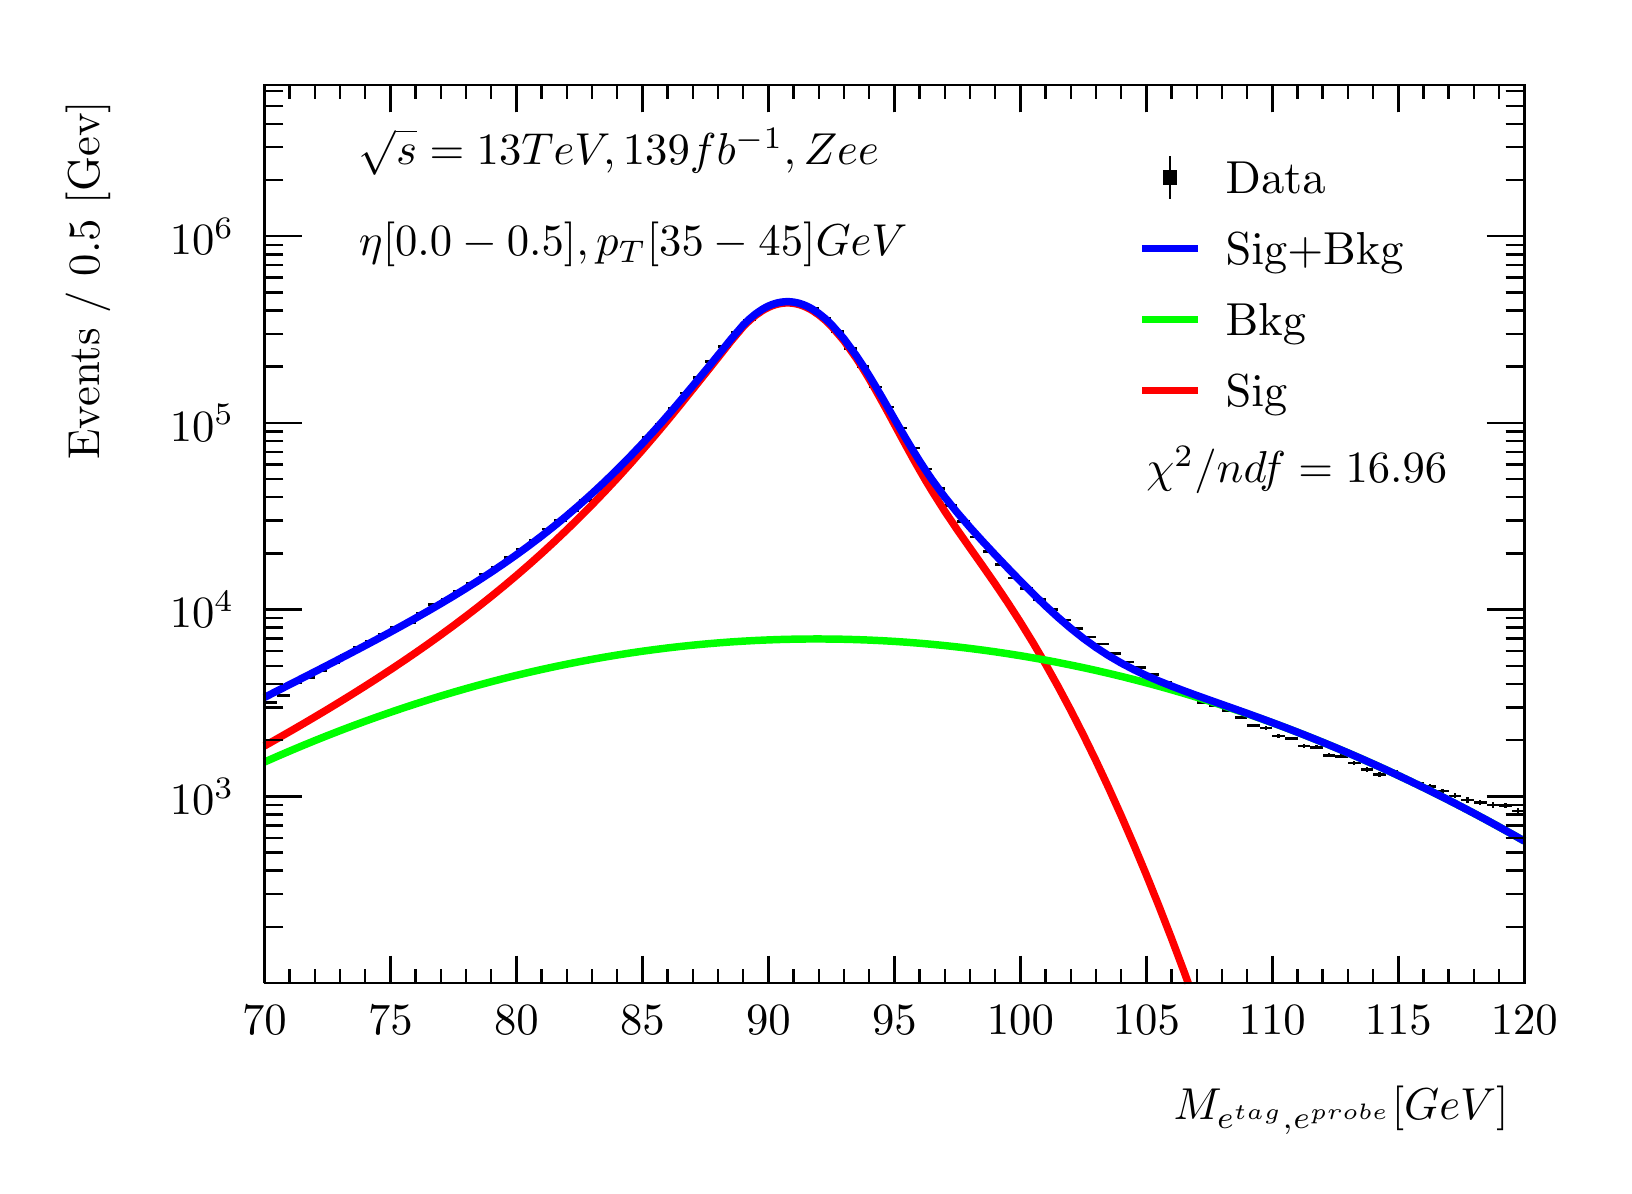
\begin{tikzpicture}
\pgfdeclareplotmark{cross} {
\pgfpathmoveto{\pgfpoint{-0.3\pgfplotmarksize}{\pgfplotmarksize}}
\pgfpathlineto{\pgfpoint{+0.3\pgfplotmarksize}{\pgfplotmarksize}}
\pgfpathlineto{\pgfpoint{+0.3\pgfplotmarksize}{0.3\pgfplotmarksize}}
\pgfpathlineto{\pgfpoint{+1\pgfplotmarksize}{0.3\pgfplotmarksize}}
\pgfpathlineto{\pgfpoint{+1\pgfplotmarksize}{-0.3\pgfplotmarksize}}
\pgfpathlineto{\pgfpoint{+0.3\pgfplotmarksize}{-0.3\pgfplotmarksize}}
\pgfpathlineto{\pgfpoint{+0.3\pgfplotmarksize}{-1.\pgfplotmarksize}}
\pgfpathlineto{\pgfpoint{-0.3\pgfplotmarksize}{-1.\pgfplotmarksize}}
\pgfpathlineto{\pgfpoint{-0.3\pgfplotmarksize}{-0.3\pgfplotmarksize}}
\pgfpathlineto{\pgfpoint{-1.\pgfplotmarksize}{-0.3\pgfplotmarksize}}
\pgfpathlineto{\pgfpoint{-1.\pgfplotmarksize}{0.3\pgfplotmarksize}}
\pgfpathlineto{\pgfpoint{-0.3\pgfplotmarksize}{0.3\pgfplotmarksize}}
\pgfpathclose
\pgfusepathqstroke
}
\pgfdeclareplotmark{cross*} {
\pgfpathmoveto{\pgfpoint{-0.3\pgfplotmarksize}{\pgfplotmarksize}}
\pgfpathlineto{\pgfpoint{+0.3\pgfplotmarksize}{\pgfplotmarksize}}
\pgfpathlineto{\pgfpoint{+0.3\pgfplotmarksize}{0.3\pgfplotmarksize}}
\pgfpathlineto{\pgfpoint{+1\pgfplotmarksize}{0.3\pgfplotmarksize}}
\pgfpathlineto{\pgfpoint{+1\pgfplotmarksize}{-0.3\pgfplotmarksize}}
\pgfpathlineto{\pgfpoint{+0.3\pgfplotmarksize}{-0.3\pgfplotmarksize}}
\pgfpathlineto{\pgfpoint{+0.3\pgfplotmarksize}{-1.\pgfplotmarksize}}
\pgfpathlineto{\pgfpoint{-0.3\pgfplotmarksize}{-1.\pgfplotmarksize}}
\pgfpathlineto{\pgfpoint{-0.3\pgfplotmarksize}{-0.3\pgfplotmarksize}}
\pgfpathlineto{\pgfpoint{-1.\pgfplotmarksize}{-0.3\pgfplotmarksize}}
\pgfpathlineto{\pgfpoint{-1.\pgfplotmarksize}{0.3\pgfplotmarksize}}
\pgfpathlineto{\pgfpoint{-0.3\pgfplotmarksize}{0.3\pgfplotmarksize}}
\pgfpathclose
\pgfusepathqfillstroke
}
\pgfdeclareplotmark{newstar} {
\pgfpathmoveto{\pgfqpoint{0pt}{\pgfplotmarksize}}
\pgfpathlineto{\pgfqpointpolar{44}{0.5\pgfplotmarksize}}
\pgfpathlineto{\pgfqpointpolar{18}{\pgfplotmarksize}}
\pgfpathlineto{\pgfqpointpolar{-20}{0.5\pgfplotmarksize}}
\pgfpathlineto{\pgfqpointpolar{-54}{\pgfplotmarksize}}
\pgfpathlineto{\pgfqpointpolar{-90}{0.5\pgfplotmarksize}}
\pgfpathlineto{\pgfqpointpolar{234}{\pgfplotmarksize}}
\pgfpathlineto{\pgfqpointpolar{198}{0.5\pgfplotmarksize}}
\pgfpathlineto{\pgfqpointpolar{162}{\pgfplotmarksize}}
\pgfpathlineto{\pgfqpointpolar{134}{0.5\pgfplotmarksize}}
\pgfpathclose
\pgfusepathqstroke
}
\pgfdeclareplotmark{newstar*} {
\pgfpathmoveto{\pgfqpoint{0pt}{\pgfplotmarksize}}
\pgfpathlineto{\pgfqpointpolar{44}{0.5\pgfplotmarksize}}
\pgfpathlineto{\pgfqpointpolar{18}{\pgfplotmarksize}}
\pgfpathlineto{\pgfqpointpolar{-20}{0.5\pgfplotmarksize}}
\pgfpathlineto{\pgfqpointpolar{-54}{\pgfplotmarksize}}
\pgfpathlineto{\pgfqpointpolar{-90}{0.5\pgfplotmarksize}}
\pgfpathlineto{\pgfqpointpolar{234}{\pgfplotmarksize}}
\pgfpathlineto{\pgfqpointpolar{198}{0.5\pgfplotmarksize}}
\pgfpathlineto{\pgfqpointpolar{162}{\pgfplotmarksize}}
\pgfpathlineto{\pgfqpointpolar{134}{0.5\pgfplotmarksize}}
\pgfpathclose
\pgfusepathqfillstroke
}
\definecolor{c}{rgb}{1,1,1};
\draw [color=c, fill=c] (0,0) rectangle (20,14.4361);
\draw [color=c, fill=c] (3,2.30977) rectangle (19,13.7143);
\definecolor{c}{rgb}{0,0,0};
\draw [c,line width=0.9] (3,2.30977) -- (3,13.7143) -- (19,13.7143) -- (19,2.30977) -- (3,2.30977);
\definecolor{c}{rgb}{1,1,1};
\draw [color=c, fill=c] (3,2.30977) rectangle (19,13.7143);
\definecolor{c}{rgb}{0,0,0};
\draw [c,line width=0.9] (3,2.30977) -- (3,13.7143) -- (19,13.7143) -- (19,2.30977) -- (3,2.30977);
\draw [c,line width=0.9] (3,2.30977) -- (19,2.30977);
\draw [c,line width=0.9] (3,2.65624) -- (3,2.30977);
\draw [c,line width=0.9] (3.32,2.48301) -- (3.32,2.30977);
\draw [c,line width=0.9] (3.64,2.48301) -- (3.64,2.30977);
\draw [c,line width=0.9] (3.96,2.48301) -- (3.96,2.30977);
\draw [c,line width=0.9] (4.28,2.48301) -- (4.28,2.30977);
\draw [c,line width=0.9] (4.6,2.65624) -- (4.6,2.30977);
\draw [c,line width=0.9] (4.92,2.48301) -- (4.92,2.30977);
\draw [c,line width=0.9] (5.24,2.48301) -- (5.24,2.30977);
\draw [c,line width=0.9] (5.56,2.48301) -- (5.56,2.30977);
\draw [c,line width=0.9] (5.88,2.48301) -- (5.88,2.30977);
\draw [c,line width=0.9] (6.2,2.65624) -- (6.2,2.30977);
\draw [c,line width=0.9] (6.52,2.48301) -- (6.52,2.30977);
\draw [c,line width=0.9] (6.84,2.48301) -- (6.84,2.30977);
\draw [c,line width=0.9] (7.16,2.48301) -- (7.16,2.30977);
\draw [c,line width=0.9] (7.48,2.48301) -- (7.48,2.30977);
\draw [c,line width=0.9] (7.8,2.65624) -- (7.8,2.30977);
\draw [c,line width=0.9] (8.12,2.48301) -- (8.12,2.30977);
\draw [c,line width=0.9] (8.44,2.48301) -- (8.44,2.30977);
\draw [c,line width=0.9] (8.76,2.48301) -- (8.76,2.30977);
\draw [c,line width=0.9] (9.08,2.48301) -- (9.08,2.30977);
\draw [c,line width=0.9] (9.4,2.65624) -- (9.4,2.30977);
\draw [c,line width=0.9] (9.72,2.48301) -- (9.72,2.30977);
\draw [c,line width=0.9] (10.04,2.48301) -- (10.04,2.30977);
\draw [c,line width=0.9] (10.36,2.48301) -- (10.36,2.30977);
\draw [c,line width=0.9] (10.68,2.48301) -- (10.68,2.30977);
\draw [c,line width=0.9] (11,2.65624) -- (11,2.30977);
\draw [c,line width=0.9] (11.32,2.48301) -- (11.32,2.30977);
\draw [c,line width=0.9] (11.64,2.48301) -- (11.64,2.30977);
\draw [c,line width=0.9] (11.96,2.48301) -- (11.96,2.30977);
\draw [c,line width=0.9] (12.28,2.48301) -- (12.28,2.30977);
\draw [c,line width=0.9] (12.6,2.65624) -- (12.6,2.30977);
\draw [c,line width=0.9] (12.92,2.48301) -- (12.92,2.30977);
\draw [c,line width=0.9] (13.24,2.48301) -- (13.24,2.30977);
\draw [c,line width=0.9] (13.56,2.48301) -- (13.56,2.30977);
\draw [c,line width=0.9] (13.88,2.48301) -- (13.88,2.30977);
\draw [c,line width=0.9] (14.2,2.65624) -- (14.2,2.30977);
\draw [c,line width=0.9] (14.52,2.48301) -- (14.52,2.30977);
\draw [c,line width=0.9] (14.84,2.48301) -- (14.84,2.30977);
\draw [c,line width=0.9] (15.16,2.48301) -- (15.16,2.30977);
\draw [c,line width=0.9] (15.48,2.48301) -- (15.48,2.30977);
\draw [c,line width=0.9] (15.8,2.65624) -- (15.8,2.30977);
\draw [c,line width=0.9] (16.12,2.48301) -- (16.12,2.30977);
\draw [c,line width=0.9] (16.44,2.48301) -- (16.44,2.30977);
\draw [c,line width=0.9] (16.76,2.48301) -- (16.76,2.30977);
\draw [c,line width=0.9] (17.08,2.48301) -- (17.08,2.30977);
\draw [c,line width=0.9] (17.4,2.65624) -- (17.4,2.30977);
\draw [c,line width=0.9] (17.72,2.48301) -- (17.72,2.30977);
\draw [c,line width=0.9] (18.04,2.48301) -- (18.04,2.30977);
\draw [c,line width=0.9] (18.36,2.48301) -- (18.36,2.30977);
\draw [c,line width=0.9] (18.68,2.48301) -- (18.68,2.30977);
\draw [c,line width=0.9] (19,2.65624) -- (19,2.30977);
\draw [anchor=base] (3,1.66015) node[scale=1.61424, color=c, rotate=0]{70};
\draw [anchor=base] (4.6,1.66015) node[scale=1.61424, color=c, rotate=0]{75};
\draw [anchor=base] (6.2,1.66015) node[scale=1.61424, color=c, rotate=0]{80};
\draw [anchor=base] (7.8,1.66015) node[scale=1.61424, color=c, rotate=0]{85};
\draw [anchor=base] (9.4,1.66015) node[scale=1.61424, color=c, rotate=0]{90};
\draw [anchor=base] (11,1.66015) node[scale=1.61424, color=c, rotate=0]{95};
\draw [anchor=base] (12.6,1.66015) node[scale=1.61424, color=c, rotate=0]{100};
\draw [anchor=base] (14.2,1.66015) node[scale=1.61424, color=c, rotate=0]{105};
\draw [anchor=base] (15.8,1.66015) node[scale=1.61424, color=c, rotate=0]{110};
\draw [anchor=base] (17.4,1.66015) node[scale=1.61424, color=c, rotate=0]{115};
\draw [anchor=base] (19,1.66015) node[scale=1.61424, color=c, rotate=0]{120};
\draw [anchor= east] (19,0.692932) node[scale=1.61424, color=c, rotate=0]{$M_{e^{tag}, e^{probe}}  [GeV]$};
\draw [c,line width=0.9] (3,13.7143) -- (19,13.7143);
\draw [c,line width=0.9] (3,13.3678) -- (3,13.7143);
\draw [c,line width=0.9] (3.32,13.5411) -- (3.32,13.7143);
\draw [c,line width=0.9] (3.64,13.5411) -- (3.64,13.7143);
\draw [c,line width=0.9] (3.96,13.5411) -- (3.96,13.7143);
\draw [c,line width=0.9] (4.28,13.5411) -- (4.28,13.7143);
\draw [c,line width=0.9] (4.6,13.3678) -- (4.6,13.7143);
\draw [c,line width=0.9] (4.92,13.5411) -- (4.92,13.7143);
\draw [c,line width=0.9] (5.24,13.5411) -- (5.24,13.7143);
\draw [c,line width=0.9] (5.56,13.5411) -- (5.56,13.7143);
\draw [c,line width=0.9] (5.88,13.5411) -- (5.88,13.7143);
\draw [c,line width=0.9] (6.2,13.3678) -- (6.2,13.7143);
\draw [c,line width=0.9] (6.52,13.5411) -- (6.52,13.7143);
\draw [c,line width=0.9] (6.84,13.5411) -- (6.84,13.7143);
\draw [c,line width=0.9] (7.16,13.5411) -- (7.16,13.7143);
\draw [c,line width=0.9] (7.48,13.5411) -- (7.48,13.7143);
\draw [c,line width=0.9] (7.8,13.3678) -- (7.8,13.7143);
\draw [c,line width=0.9] (8.12,13.5411) -- (8.12,13.7143);
\draw [c,line width=0.9] (8.44,13.5411) -- (8.44,13.7143);
\draw [c,line width=0.9] (8.76,13.5411) -- (8.76,13.7143);
\draw [c,line width=0.9] (9.08,13.5411) -- (9.08,13.7143);
\draw [c,line width=0.9] (9.4,13.3678) -- (9.4,13.7143);
\draw [c,line width=0.9] (9.72,13.5411) -- (9.72,13.7143);
\draw [c,line width=0.9] (10.04,13.5411) -- (10.04,13.7143);
\draw [c,line width=0.9] (10.36,13.5411) -- (10.36,13.7143);
\draw [c,line width=0.9] (10.68,13.5411) -- (10.68,13.7143);
\draw [c,line width=0.9] (11,13.3678) -- (11,13.7143);
\draw [c,line width=0.9] (11.32,13.5411) -- (11.32,13.7143);
\draw [c,line width=0.9] (11.64,13.5411) -- (11.64,13.7143);
\draw [c,line width=0.9] (11.96,13.5411) -- (11.96,13.7143);
\draw [c,line width=0.9] (12.28,13.5411) -- (12.28,13.7143);
\draw [c,line width=0.9] (12.6,13.3678) -- (12.6,13.7143);
\draw [c,line width=0.9] (12.92,13.5411) -- (12.92,13.7143);
\draw [c,line width=0.9] (13.24,13.5411) -- (13.24,13.7143);
\draw [c,line width=0.9] (13.56,13.5411) -- (13.56,13.7143);
\draw [c,line width=0.9] (13.88,13.5411) -- (13.88,13.7143);
\draw [c,line width=0.9] (14.2,13.3678) -- (14.2,13.7143);
\draw [c,line width=0.9] (14.52,13.5411) -- (14.52,13.7143);
\draw [c,line width=0.9] (14.84,13.5411) -- (14.84,13.7143);
\draw [c,line width=0.9] (15.16,13.5411) -- (15.16,13.7143);
\draw [c,line width=0.9] (15.48,13.5411) -- (15.48,13.7143);
\draw [c,line width=0.9] (15.8,13.3678) -- (15.8,13.7143);
\draw [c,line width=0.9] (16.12,13.5411) -- (16.12,13.7143);
\draw [c,line width=0.9] (16.44,13.5411) -- (16.44,13.7143);
\draw [c,line width=0.9] (16.76,13.5411) -- (16.76,13.7143);
\draw [c,line width=0.9] (17.08,13.5411) -- (17.08,13.7143);
\draw [c,line width=0.9] (17.4,13.3678) -- (17.4,13.7143);
\draw [c,line width=0.9] (17.72,13.5411) -- (17.72,13.7143);
\draw [c,line width=0.9] (18.04,13.5411) -- (18.04,13.7143);
\draw [c,line width=0.9] (18.36,13.5411) -- (18.36,13.7143);
\draw [c,line width=0.9] (18.68,13.5411) -- (18.68,13.7143);
\draw [c,line width=0.9] (19,13.3678) -- (19,13.7143);
\draw [c,line width=0.9] (3,2.30977) -- (3,13.7143);
\draw [c,line width=0.9] (3.237,3.02354) -- (3,3.02354);
\draw [c,line width=0.9] (3.237,3.44107) -- (3,3.44107);
\draw [c,line width=0.9] (3.237,3.73731) -- (3,3.73731);
\draw [c,line width=0.9] (3.237,3.96709) -- (3,3.96709);
\draw [c,line width=0.9] (3.237,4.15484) -- (3,4.15484);
\draw [c,line width=0.9] (3.237,4.31357) -- (3,4.31357);
\draw [c,line width=0.9] (3.237,4.45108) -- (3,4.45108);
\draw [c,line width=0.9] (3.237,4.57236) -- (3,4.57236);
\draw [c,line width=0.9] (3.474,4.68086) -- (3,4.68086);
\draw [anchor= east] (2.82,4.68086) node[scale=1.61424, color=c, rotate=0]{$10^{3}$};
\draw [c,line width=0.9] (3.237,5.39463) -- (3,5.39463);
\draw [c,line width=0.9] (3.237,5.81216) -- (3,5.81216);
\draw [c,line width=0.9] (3.237,6.1084) -- (3,6.1084);
\draw [c,line width=0.9] (3.237,6.33818) -- (3,6.33818);
\draw [c,line width=0.9] (3.237,6.52593) -- (3,6.52593);
\draw [c,line width=0.9] (3.237,6.68466) -- (3,6.68466);
\draw [c,line width=0.9] (3.237,6.82217) -- (3,6.82217);
\draw [c,line width=0.9] (3.237,6.94345) -- (3,6.94345);
\draw [c,line width=0.9] (3.474,7.05195) -- (3,7.05195);
\draw [anchor= east] (2.82,7.05195) node[scale=1.61424, color=c, rotate=0]{$10^{4}$};
\draw [c,line width=0.9] (3.237,7.76572) -- (3,7.76572);
\draw [c,line width=0.9] (3.237,8.18324) -- (3,8.18324);
\draw [c,line width=0.9] (3.237,8.47948) -- (3,8.47948);
\draw [c,line width=0.9] (3.237,8.70927) -- (3,8.70927);
\draw [c,line width=0.9] (3.237,8.89701) -- (3,8.89701);
\draw [c,line width=0.9] (3.237,9.05575) -- (3,9.05575);
\draw [c,line width=0.9] (3.237,9.19325) -- (3,9.19325);
\draw [c,line width=0.9] (3.237,9.31454) -- (3,9.31454);
\draw [c,line width=0.9] (3.474,9.42304) -- (3,9.42304);
\draw [anchor= east] (2.82,9.42304) node[scale=1.61424, color=c, rotate=0]{$10^{5}$};
\draw [c,line width=0.9] (3.237,10.1368) -- (3,10.1368);
\draw [c,line width=0.9] (3.237,10.5543) -- (3,10.5543);
\draw [c,line width=0.9] (3.237,10.8506) -- (3,10.8506);
\draw [c,line width=0.9] (3.237,11.0804) -- (3,11.0804);
\draw [c,line width=0.9] (3.237,11.2681) -- (3,11.2681);
\draw [c,line width=0.9] (3.237,11.4268) -- (3,11.4268);
\draw [c,line width=0.9] (3.237,11.5643) -- (3,11.5643);
\draw [c,line width=0.9] (3.237,11.6856) -- (3,11.6856);
\draw [c,line width=0.9] (3.474,11.7941) -- (3,11.7941);
\draw [anchor= east] (2.82,11.7941) node[scale=1.61424, color=c, rotate=0]{$10^{6}$};
\draw [c,line width=0.9] (3.237,12.5079) -- (3,12.5079);
\draw [c,line width=0.9] (3.237,12.9254) -- (3,12.9254);
\draw [c,line width=0.9] (3.237,13.2217) -- (3,13.2217);
\draw [c,line width=0.9] (3.237,13.4514) -- (3,13.4514);
\draw [c,line width=0.9] (3.237,13.6392) -- (3,13.6392);
\draw [anchor= east] (0.76,13.7143) node[scale=1.61424, color=c, rotate=90]{Events / 0.5 [Gev]};
\draw [c,line width=0.9] (19,2.30977) -- (19,13.7143);
\draw [c,line width=0.9] (18.763,3.02354) -- (19,3.02354);
\draw [c,line width=0.9] (18.763,3.44107) -- (19,3.44107);
\draw [c,line width=0.9] (18.763,3.73731) -- (19,3.73731);
\draw [c,line width=0.9] (18.763,3.96709) -- (19,3.96709);
\draw [c,line width=0.9] (18.763,4.15484) -- (19,4.15484);
\draw [c,line width=0.9] (18.763,4.31357) -- (19,4.31357);
\draw [c,line width=0.9] (18.763,4.45108) -- (19,4.45108);
\draw [c,line width=0.9] (18.763,4.57236) -- (19,4.57236);
\draw [c,line width=0.9] (18.526,4.68086) -- (19,4.68086);
\draw [c,line width=0.9] (18.763,5.39463) -- (19,5.39463);
\draw [c,line width=0.9] (18.763,5.81216) -- (19,5.81216);
\draw [c,line width=0.9] (18.763,6.1084) -- (19,6.1084);
\draw [c,line width=0.9] (18.763,6.33818) -- (19,6.33818);
\draw [c,line width=0.9] (18.763,6.52593) -- (19,6.52593);
\draw [c,line width=0.9] (18.763,6.68466) -- (19,6.68466);
\draw [c,line width=0.9] (18.763,6.82217) -- (19,6.82217);
\draw [c,line width=0.9] (18.763,6.94345) -- (19,6.94345);
\draw [c,line width=0.9] (18.526,7.05195) -- (19,7.05195);
\draw [c,line width=0.9] (18.763,7.76572) -- (19,7.76572);
\draw [c,line width=0.9] (18.763,8.18324) -- (19,8.18324);
\draw [c,line width=0.9] (18.763,8.47948) -- (19,8.47948);
\draw [c,line width=0.9] (18.763,8.70927) -- (19,8.70927);
\draw [c,line width=0.9] (18.763,8.89701) -- (19,8.89701);
\draw [c,line width=0.9] (18.763,9.05575) -- (19,9.05575);
\draw [c,line width=0.9] (18.763,9.19325) -- (19,9.19325);
\draw [c,line width=0.9] (18.763,9.31454) -- (19,9.31454);
\draw [c,line width=0.9] (18.526,9.42304) -- (19,9.42304);
\draw [c,line width=0.9] (18.763,10.1368) -- (19,10.1368);
\draw [c,line width=0.9] (18.763,10.5543) -- (19,10.5543);
\draw [c,line width=0.9] (18.763,10.8506) -- (19,10.8506);
\draw [c,line width=0.9] (18.763,11.0804) -- (19,11.0804);
\draw [c,line width=0.9] (18.763,11.2681) -- (19,11.2681);
\draw [c,line width=0.9] (18.763,11.4268) -- (19,11.4268);
\draw [c,line width=0.9] (18.763,11.5643) -- (19,11.5643);
\draw [c,line width=0.9] (18.763,11.6856) -- (19,11.6856);
\draw [c,line width=0.9] (18.526,11.7941) -- (19,11.7941);
\draw [c,line width=0.9] (18.763,12.5079) -- (19,12.5079);
\draw [c,line width=0.9] (18.763,12.9254) -- (19,12.9254);
\draw [c,line width=0.9] (18.763,13.2217) -- (19,13.2217);
\draw [c,line width=0.9] (18.763,13.4514) -- (19,13.4514);
\draw [c,line width=0.9] (18.763,13.6392) -- (19,13.6392);
\draw [c,line width=0.9] (3.08,5.87086) -- (3,5.87086);
\draw [c,line width=0.9] (3,5.87086) -- (3,5.87086);
\draw [c,line width=0.9] (3.08,5.87086) -- (3.16,5.87086);
\draw [c,line width=0.9] (3.16,5.87086) -- (3.16,5.87086);
\draw [c,line width=0.9] (3.08,5.87086) -- (3.08,5.88914);
\draw [c,line width=0.9] (3.08,5.88914) -- (3.08,5.88914);
\draw [c,line width=0.9] (3.08,5.87086) -- (3.08,5.85259);
\draw [c,line width=0.9] (3.08,5.85259) -- (3.08,5.85259);
\draw [c,line width=0.9] (3.24,5.95965) -- (3.16,5.95965);
\draw [c,line width=0.9] (3.16,5.95965) -- (3.16,5.95965);
\draw [c,line width=0.9] (3.24,5.95965) -- (3.32,5.95965);
\draw [c,line width=0.9] (3.32,5.95965) -- (3.32,5.95965);
\draw [c,line width=0.9] (3.24,5.95965) -- (3.24,5.97715);
\draw [c,line width=0.9] (3.24,5.97715) -- (3.24,5.97715);
\draw [c,line width=0.9] (3.24,5.95965) -- (3.24,5.94215);
\draw [c,line width=0.9] (3.24,5.94215) -- (3.24,5.94215);
\draw [c,line width=0.9] (3.4,6.12246) -- (3.32,6.12246);
\draw [c,line width=0.9] (3.32,6.12246) -- (3.32,6.12246);
\draw [c,line width=0.9] (3.4,6.12246) -- (3.48,6.12246);
\draw [c,line width=0.9] (3.48,6.12246) -- (3.48,6.12246);
\draw [c,line width=0.9] (3.4,6.12246) -- (3.4,6.13863);
\draw [c,line width=0.9] (3.4,6.13863) -- (3.4,6.13863);
\draw [c,line width=0.9] (3.4,6.12246) -- (3.4,6.10629);
\draw [c,line width=0.9] (3.4,6.10629) -- (3.4,6.10629);
\draw [c,line width=0.9] (3.56,6.19027) -- (3.48,6.19027);
\draw [c,line width=0.9] (3.48,6.19027) -- (3.48,6.19027);
\draw [c,line width=0.9] (3.56,6.19027) -- (3.64,6.19027);
\draw [c,line width=0.9] (3.64,6.19027) -- (3.64,6.19027);
\draw [c,line width=0.9] (3.56,6.19027) -- (3.56,6.20591);
\draw [c,line width=0.9] (3.56,6.20591) -- (3.56,6.20591);
\draw [c,line width=0.9] (3.56,6.19027) -- (3.56,6.17462);
\draw [c,line width=0.9] (3.56,6.17462) -- (3.56,6.17462);
\draw [c,line width=0.9] (3.72,6.27556) -- (3.64,6.27556);
\draw [c,line width=0.9] (3.64,6.27556) -- (3.64,6.27556);
\draw [c,line width=0.9] (3.72,6.27556) -- (3.8,6.27556);
\draw [c,line width=0.9] (3.8,6.27556) -- (3.8,6.27556);
\draw [c,line width=0.9] (3.72,6.27556) -- (3.72,6.29057);
\draw [c,line width=0.9] (3.72,6.29057) -- (3.72,6.29057);
\draw [c,line width=0.9] (3.72,6.27556) -- (3.72,6.26055);
\draw [c,line width=0.9] (3.72,6.26055) -- (3.72,6.26055);
\draw [c,line width=0.9] (3.88,6.37916) -- (3.8,6.37916);
\draw [c,line width=0.9] (3.8,6.37916) -- (3.8,6.37916);
\draw [c,line width=0.9] (3.88,6.37916) -- (3.96,6.37916);
\draw [c,line width=0.9] (3.96,6.37916) -- (3.96,6.37916);
\draw [c,line width=0.9] (3.88,6.37916) -- (3.88,6.39344);
\draw [c,line width=0.9] (3.88,6.39344) -- (3.88,6.39344);
\draw [c,line width=0.9] (3.88,6.37916) -- (3.88,6.36489);
\draw [c,line width=0.9] (3.88,6.36489) -- (3.88,6.36489);
\draw [c,line width=0.9] (4.04,6.47509) -- (3.96,6.47509);
\draw [c,line width=0.9] (3.96,6.47509) -- (3.96,6.47509);
\draw [c,line width=0.9] (4.04,6.47509) -- (4.12,6.47509);
\draw [c,line width=0.9] (4.12,6.47509) -- (4.12,6.47509);
\draw [c,line width=0.9] (4.04,6.47509) -- (4.04,6.48872);
\draw [c,line width=0.9] (4.04,6.48872) -- (4.04,6.48872);
\draw [c,line width=0.9] (4.04,6.47509) -- (4.04,6.46147);
\draw [c,line width=0.9] (4.04,6.46147) -- (4.04,6.46147);
\draw [c,line width=0.9] (4.2,6.576) -- (4.12,6.576);
\draw [c,line width=0.9] (4.12,6.576) -- (4.12,6.576);
\draw [c,line width=0.9] (4.2,6.576) -- (4.28,6.576);
\draw [c,line width=0.9] (4.28,6.576) -- (4.28,6.576);
\draw [c,line width=0.9] (4.2,6.576) -- (4.2,6.58898);
\draw [c,line width=0.9] (4.2,6.58898) -- (4.2,6.58898);
\draw [c,line width=0.9] (4.2,6.576) -- (4.2,6.56303);
\draw [c,line width=0.9] (4.2,6.56303) -- (4.2,6.56303);
\draw [c,line width=0.9] (4.36,6.64508) -- (4.28,6.64508);
\draw [c,line width=0.9] (4.28,6.64508) -- (4.28,6.64508);
\draw [c,line width=0.9] (4.36,6.64508) -- (4.44,6.64508);
\draw [c,line width=0.9] (4.44,6.64508) -- (4.44,6.64508);
\draw [c,line width=0.9] (4.36,6.64508) -- (4.36,6.65762);
\draw [c,line width=0.9] (4.36,6.65762) -- (4.36,6.65762);
\draw [c,line width=0.9] (4.36,6.64508) -- (4.36,6.63253);
\draw [c,line width=0.9] (4.36,6.63253) -- (4.36,6.63253);
\draw [c,line width=0.9] (4.52,6.7335) -- (4.44,6.7335);
\draw [c,line width=0.9] (4.44,6.7335) -- (4.44,6.7335);
\draw [c,line width=0.9] (4.52,6.7335) -- (4.6,6.7335);
\draw [c,line width=0.9] (4.6,6.7335) -- (4.6,6.7335);
\draw [c,line width=0.9] (4.52,6.7335) -- (4.52,6.74552);
\draw [c,line width=0.9] (4.52,6.74552) -- (4.52,6.74552);
\draw [c,line width=0.9] (4.52,6.7335) -- (4.52,6.72148);
\draw [c,line width=0.9] (4.52,6.72148) -- (4.52,6.72148);
\draw [c,line width=0.9] (4.68,6.83216) -- (4.6,6.83216);
\draw [c,line width=0.9] (4.6,6.83216) -- (4.6,6.83216);
\draw [c,line width=0.9] (4.68,6.83216) -- (4.76,6.83216);
\draw [c,line width=0.9] (4.76,6.83216) -- (4.76,6.83216);
\draw [c,line width=0.9] (4.68,6.83216) -- (4.68,6.84362);
\draw [c,line width=0.9] (4.68,6.84362) -- (4.68,6.84362);
\draw [c,line width=0.9] (4.68,6.83216) -- (4.68,6.8207);
\draw [c,line width=0.9] (4.68,6.8207) -- (4.68,6.8207);
\draw [c,line width=0.9] (4.84,6.88786) -- (4.76,6.88786);
\draw [c,line width=0.9] (4.76,6.88786) -- (4.76,6.88786);
\draw [c,line width=0.9] (4.84,6.88786) -- (4.92,6.88786);
\draw [c,line width=0.9] (4.92,6.88786) -- (4.92,6.88786);
\draw [c,line width=0.9] (4.84,6.88786) -- (4.84,6.89901);
\draw [c,line width=0.9] (4.84,6.89901) -- (4.84,6.89901);
\draw [c,line width=0.9] (4.84,6.88786) -- (4.84,6.87671);
\draw [c,line width=0.9] (4.84,6.87671) -- (4.84,6.87671);
\draw [c,line width=0.9] (5,7.00162) -- (4.92,7.00162);
\draw [c,line width=0.9] (4.92,7.00162) -- (4.92,7.00162);
\draw [c,line width=0.9] (5,7.00162) -- (5.08,7.00162);
\draw [c,line width=0.9] (5.08,7.00162) -- (5.08,7.00162);
\draw [c,line width=0.9] (5,7.00162) -- (5,7.01217);
\draw [c,line width=0.9] (5,7.01217) -- (5,7.01217);
\draw [c,line width=0.9] (5,7.00162) -- (5,6.99107);
\draw [c,line width=0.9] (5,6.99107) -- (5,6.99107);
\draw [c,line width=0.9] (5.16,7.11506) -- (5.08,7.11506);
\draw [c,line width=0.9] (5.08,7.11506) -- (5.08,7.11506);
\draw [c,line width=0.9] (5.16,7.11506) -- (5.24,7.11506);
\draw [c,line width=0.9] (5.24,7.11506) -- (5.24,7.11506);
\draw [c,line width=0.9] (5.16,7.11506) -- (5.16,7.12504);
\draw [c,line width=0.9] (5.16,7.12504) -- (5.16,7.12504);
\draw [c,line width=0.9] (5.16,7.11506) -- (5.16,7.10507);
\draw [c,line width=0.9] (5.16,7.10507) -- (5.16,7.10507);
\draw [c,line width=0.9] (5.32,7.18416) -- (5.24,7.18416);
\draw [c,line width=0.9] (5.24,7.18416) -- (5.24,7.18416);
\draw [c,line width=0.9] (5.32,7.18416) -- (5.4,7.18416);
\draw [c,line width=0.9] (5.4,7.18416) -- (5.4,7.18416);
\draw [c,line width=0.9] (5.32,7.18416) -- (5.32,7.19382);
\draw [c,line width=0.9] (5.32,7.19382) -- (5.32,7.19382);
\draw [c,line width=0.9] (5.32,7.18416) -- (5.32,7.1745);
\draw [c,line width=0.9] (5.32,7.1745) -- (5.32,7.1745);
\draw [c,line width=0.9] (5.48,7.28543) -- (5.4,7.28543);
\draw [c,line width=0.9] (5.4,7.28543) -- (5.4,7.28543);
\draw [c,line width=0.9] (5.48,7.28543) -- (5.56,7.28543);
\draw [c,line width=0.9] (5.56,7.28543) -- (5.56,7.28543);
\draw [c,line width=0.9] (5.48,7.28543) -- (5.48,7.29463);
\draw [c,line width=0.9] (5.48,7.29463) -- (5.48,7.29463);
\draw [c,line width=0.9] (5.48,7.28543) -- (5.48,7.27624);
\draw [c,line width=0.9] (5.48,7.27624) -- (5.48,7.27624);
\draw [c,line width=0.9] (5.64,7.38674) -- (5.56,7.38674);
\draw [c,line width=0.9] (5.56,7.38674) -- (5.56,7.38674);
\draw [c,line width=0.9] (5.64,7.38674) -- (5.72,7.38674);
\draw [c,line width=0.9] (5.72,7.38674) -- (5.72,7.38674);
\draw [c,line width=0.9] (5.64,7.38674) -- (5.64,7.3955);
\draw [c,line width=0.9] (5.64,7.3955) -- (5.64,7.3955);
\draw [c,line width=0.9] (5.64,7.38674) -- (5.64,7.37799);
\draw [c,line width=0.9] (5.64,7.37799) -- (5.64,7.37799);
\draw [c,line width=0.9] (5.8,7.50696) -- (5.72,7.50696);
\draw [c,line width=0.9] (5.72,7.50696) -- (5.72,7.50696);
\draw [c,line width=0.9] (5.8,7.50696) -- (5.88,7.50696);
\draw [c,line width=0.9] (5.88,7.50696) -- (5.88,7.50696);
\draw [c,line width=0.9] (5.8,7.50696) -- (5.8,7.51521);
\draw [c,line width=0.9] (5.8,7.51521) -- (5.8,7.51521);
\draw [c,line width=0.9] (5.8,7.50696) -- (5.8,7.4987);
\draw [c,line width=0.9] (5.8,7.4987) -- (5.8,7.4987);
\draw [c,line width=0.9] (5.96,7.59618) -- (5.88,7.59618);
\draw [c,line width=0.9] (5.88,7.59618) -- (5.88,7.59618);
\draw [c,line width=0.9] (5.96,7.59618) -- (6.04,7.59618);
\draw [c,line width=0.9] (6.04,7.59618) -- (6.04,7.59618);
\draw [c,line width=0.9] (5.96,7.59618) -- (5.96,7.60409);
\draw [c,line width=0.9] (5.96,7.60409) -- (5.96,7.60409);
\draw [c,line width=0.9] (5.96,7.59618) -- (5.96,7.58827);
\draw [c,line width=0.9] (5.96,7.58827) -- (5.96,7.58827);
\draw [c,line width=0.9] (6.12,7.71447) -- (6.04,7.71447);
\draw [c,line width=0.9] (6.04,7.71447) -- (6.04,7.71447);
\draw [c,line width=0.9] (6.12,7.71447) -- (6.2,7.71447);
\draw [c,line width=0.9] (6.2,7.71447) -- (6.2,7.71447);
\draw [c,line width=0.9] (6.12,7.71447) -- (6.12,7.72193);
\draw [c,line width=0.9] (6.12,7.72193) -- (6.12,7.72193);
\draw [c,line width=0.9] (6.12,7.71447) -- (6.12,7.707);
\draw [c,line width=0.9] (6.12,7.707) -- (6.12,7.707);
\draw [c,line width=0.9] (6.28,7.82212) -- (6.2,7.82212);
\draw [c,line width=0.9] (6.2,7.82212) -- (6.2,7.82212);
\draw [c,line width=0.9] (6.28,7.82212) -- (6.36,7.82212);
\draw [c,line width=0.9] (6.36,7.82212) -- (6.36,7.82212);
\draw [c,line width=0.9] (6.28,7.82212) -- (6.28,7.8292);
\draw [c,line width=0.9] (6.28,7.8292) -- (6.28,7.8292);
\draw [c,line width=0.9] (6.28,7.82212) -- (6.28,7.81503);
\draw [c,line width=0.9] (6.28,7.81503) -- (6.28,7.81503);
\draw [c,line width=0.9] (6.44,7.93472) -- (6.36,7.93472);
\draw [c,line width=0.9] (6.36,7.93472) -- (6.36,7.93472);
\draw [c,line width=0.9] (6.44,7.93472) -- (6.52,7.93472);
\draw [c,line width=0.9] (6.52,7.93472) -- (6.52,7.93472);
\draw [c,line width=0.9] (6.44,7.93472) -- (6.44,7.94142);
\draw [c,line width=0.9] (6.44,7.94142) -- (6.44,7.94142);
\draw [c,line width=0.9] (6.44,7.93472) -- (6.44,7.92801);
\draw [c,line width=0.9] (6.44,7.92801) -- (6.44,7.92801);
\draw [c,line width=0.9] (6.6,8.07448) -- (6.52,8.07448);
\draw [c,line width=0.9] (6.52,8.07448) -- (6.52,8.07448);
\draw [c,line width=0.9] (6.6,8.07448) -- (6.68,8.07448);
\draw [c,line width=0.9] (6.68,8.07448) -- (6.68,8.07448);
\draw [c,line width=0.9] (6.6,8.07448) -- (6.6,8.08075);
\draw [c,line width=0.9] (6.6,8.08075) -- (6.6,8.08075);
\draw [c,line width=0.9] (6.6,8.07448) -- (6.6,8.06822);
\draw [c,line width=0.9] (6.6,8.06822) -- (6.6,8.06822);
\draw [c,line width=0.9] (6.76,8.18149) -- (6.68,8.18149);
\draw [c,line width=0.9] (6.68,8.18149) -- (6.68,8.18149);
\draw [c,line width=0.9] (6.76,8.18149) -- (6.84,8.18149);
\draw [c,line width=0.9] (6.84,8.18149) -- (6.84,8.18149);
\draw [c,line width=0.9] (6.76,8.18149) -- (6.76,8.18744);
\draw [c,line width=0.9] (6.76,8.18744) -- (6.76,8.18744);
\draw [c,line width=0.9] (6.76,8.18149) -- (6.76,8.17554);
\draw [c,line width=0.9] (6.76,8.17554) -- (6.76,8.17554);
\draw [c,line width=0.9] (6.92,8.30533) -- (6.84,8.30533);
\draw [c,line width=0.9] (6.84,8.30533) -- (6.84,8.30533);
\draw [c,line width=0.9] (6.92,8.30533) -- (7,8.30533);
\draw [c,line width=0.9] (7,8.30533) -- (7,8.30533);
\draw [c,line width=0.9] (6.92,8.30533) -- (6.92,8.31093);
\draw [c,line width=0.9] (6.92,8.31093) -- (6.92,8.31093);
\draw [c,line width=0.9] (6.92,8.30533) -- (6.92,8.29972);
\draw [c,line width=0.9] (6.92,8.29972) -- (6.92,8.29972);
\draw [c,line width=0.9] (7.08,8.44101) -- (7,8.44101);
\draw [c,line width=0.9] (7,8.44101) -- (7,8.44101);
\draw [c,line width=0.9] (7.08,8.44101) -- (7.16,8.44101);
\draw [c,line width=0.9] (7.16,8.44101) -- (7.16,8.44101);
\draw [c,line width=0.9] (7.08,8.44101) -- (7.08,8.44626);
\draw [c,line width=0.9] (7.08,8.44626) -- (7.08,8.44626);
\draw [c,line width=0.9] (7.08,8.44101) -- (7.08,8.43576);
\draw [c,line width=0.9] (7.08,8.43576) -- (7.08,8.43576);
\draw [c,line width=0.9] (7.24,8.58649) -- (7.16,8.58649);
\draw [c,line width=0.9] (7.16,8.58649) -- (7.16,8.58649);
\draw [c,line width=0.9] (7.24,8.58649) -- (7.32,8.58649);
\draw [c,line width=0.9] (7.32,8.58649) -- (7.32,8.58649);
\draw [c,line width=0.9] (7.24,8.58649) -- (7.24,8.59138);
\draw [c,line width=0.9] (7.24,8.59138) -- (7.24,8.59138);
\draw [c,line width=0.9] (7.24,8.58649) -- (7.24,8.5816);
\draw [c,line width=0.9] (7.24,8.5816) -- (7.24,8.5816);
\draw [c,line width=0.9] (7.4,8.7375) -- (7.32,8.7375);
\draw [c,line width=0.9] (7.32,8.7375) -- (7.32,8.7375);
\draw [c,line width=0.9] (7.4,8.7375) -- (7.48,8.7375);
\draw [c,line width=0.9] (7.48,8.7375) -- (7.48,8.7375);
\draw [c,line width=0.9] (7.4,8.7375) -- (7.4,8.74205);
\draw [c,line width=0.9] (7.4,8.74205) -- (7.4,8.74205);
\draw [c,line width=0.9] (7.4,8.7375) -- (7.4,8.73296);
\draw [c,line width=0.9] (7.4,8.73296) -- (7.4,8.73296);
\draw [c,line width=0.9] (7.56,8.88897) -- (7.48,8.88897);
\draw [c,line width=0.9] (7.48,8.88897) -- (7.48,8.88897);
\draw [c,line width=0.9] (7.56,8.88897) -- (7.64,8.88897);
\draw [c,line width=0.9] (7.64,8.88897) -- (7.64,8.88897);
\draw [c,line width=0.9] (7.56,8.88897) -- (7.56,8.89319);
\draw [c,line width=0.9] (7.56,8.89319) -- (7.56,8.89319);
\draw [c,line width=0.9] (7.56,8.88897) -- (7.56,8.88475);
\draw [c,line width=0.9] (7.56,8.88475) -- (7.56,8.88475);
\draw [c,line width=0.9] (7.72,9.05543) -- (7.64,9.05543);
\draw [c,line width=0.9] (7.64,9.05543) -- (7.64,9.05543);
\draw [c,line width=0.9] (7.72,9.05543) -- (7.8,9.05543);
\draw [c,line width=0.9] (7.8,9.05543) -- (7.8,9.05543);
\draw [c,line width=0.9] (7.72,9.05543) -- (7.72,9.05932);
\draw [c,line width=0.9] (7.72,9.05932) -- (7.72,9.05932);
\draw [c,line width=0.9] (7.72,9.05543) -- (7.72,9.05153);
\draw [c,line width=0.9] (7.72,9.05153) -- (7.72,9.05153);
\draw [c,line width=0.9] (7.88,9.23782) -- (7.8,9.23782);
\draw [c,line width=0.9] (7.8,9.23782) -- (7.8,9.23782);
\draw [c,line width=0.9] (7.88,9.23782) -- (7.96,9.23782);
\draw [c,line width=0.9] (7.96,9.23782) -- (7.96,9.23782);
\draw [c,line width=0.9] (7.88,9.23782) -- (7.88,9.24138);
\draw [c,line width=0.9] (7.88,9.24138) -- (7.88,9.24138);
\draw [c,line width=0.9] (7.88,9.23782) -- (7.88,9.23425);
\draw [c,line width=0.9] (7.88,9.23425) -- (7.88,9.23425);
\draw [c,line width=0.9] (8.04,9.41066) -- (7.96,9.41066);
\draw [c,line width=0.9] (7.96,9.41066) -- (7.96,9.41066);
\draw [c,line width=0.9] (8.04,9.41066) -- (8.12,9.41066);
\draw [c,line width=0.9] (8.12,9.41066) -- (8.12,9.41066);
\draw [c,line width=0.9] (8.04,9.41066) -- (8.04,9.41393);
\draw [c,line width=0.9] (8.04,9.41393) -- (8.04,9.41393);
\draw [c,line width=0.9] (8.04,9.41066) -- (8.04,9.40738);
\draw [c,line width=0.9] (8.04,9.40738) -- (8.04,9.40738);
\draw [c,line width=0.9] (8.2,9.60518) -- (8.12,9.60518);
\draw [c,line width=0.9] (8.12,9.60518) -- (8.12,9.60518);
\draw [c,line width=0.9] (8.2,9.60518) -- (8.28,9.60518);
\draw [c,line width=0.9] (8.28,9.60518) -- (8.28,9.60518);
\draw [c,line width=0.9] (8.2,9.60518) -- (8.2,9.60816);
\draw [c,line width=0.9] (8.2,9.60816) -- (8.2,9.60816);
\draw [c,line width=0.9] (8.2,9.60518) -- (8.2,9.6022);
\draw [c,line width=0.9] (8.2,9.6022) -- (8.2,9.6022);
\draw [c,line width=0.9] (8.36,9.80488) -- (8.28,9.80488);
\draw [c,line width=0.9] (8.28,9.80488) -- (8.28,9.80488);
\draw [c,line width=0.9] (8.36,9.80488) -- (8.44,9.80488);
\draw [c,line width=0.9] (8.44,9.80488) -- (8.44,9.80488);
\draw [c,line width=0.9] (8.36,9.80488) -- (8.36,9.80758);
\draw [c,line width=0.9] (8.36,9.80758) -- (8.36,9.80758);
\draw [c,line width=0.9] (8.36,9.80488) -- (8.36,9.80217);
\draw [c,line width=0.9] (8.36,9.80217) -- (8.36,9.80217);
\draw [c,line width=0.9] (8.52,10.0023) -- (8.44,10.0023);
\draw [c,line width=0.9] (8.44,10.0023) -- (8.44,10.0023);
\draw [c,line width=0.9] (8.52,10.0023) -- (8.6,10.0023);
\draw [c,line width=0.9] (8.6,10.0023) -- (8.6,10.0023);
\draw [c,line width=0.9] (8.52,10.0023) -- (8.52,10.0048);
\draw [c,line width=0.9] (8.52,10.0048) -- (8.52,10.0048);
\draw [c,line width=0.9] (8.52,10.0023) -- (8.52,9.99984);
\draw [c,line width=0.9] (8.52,9.99984) -- (8.52,9.99984);
\draw [c,line width=0.9] (8.68,10.2031) -- (8.6,10.2031);
\draw [c,line width=0.9] (8.6,10.2031) -- (8.6,10.2031);
\draw [c,line width=0.9] (8.68,10.2031) -- (8.76,10.2031);
\draw [c,line width=0.9] (8.76,10.2031) -- (8.76,10.2031);
\draw [c,line width=0.9] (8.68,10.2031) -- (8.68,10.2053);
\draw [c,line width=0.9] (8.68,10.2053) -- (8.68,10.2053);
\draw [c,line width=0.9] (8.68,10.2031) -- (8.68,10.2008);
\draw [c,line width=0.9] (8.68,10.2008) -- (8.68,10.2008);
\draw [c,line width=0.9] (8.84,10.3968) -- (8.76,10.3968);
\draw [c,line width=0.9] (8.76,10.3968) -- (8.76,10.3968);
\draw [c,line width=0.9] (8.84,10.3968) -- (8.92,10.3968);
\draw [c,line width=0.9] (8.92,10.3968) -- (8.92,10.3968);
\draw [c,line width=0.9] (8.84,10.3968) -- (8.84,10.3988);
\draw [c,line width=0.9] (8.84,10.3988) -- (8.84,10.3988);
\draw [c,line width=0.9] (8.84,10.3968) -- (8.84,10.3948);
\draw [c,line width=0.9] (8.84,10.3948) -- (8.84,10.3948);
\draw [c,line width=0.9] (9,10.5752) -- (8.92,10.5752);
\draw [c,line width=0.9] (8.92,10.5752) -- (8.92,10.5752);
\draw [c,line width=0.9] (9,10.5752) -- (9.08,10.5752);
\draw [c,line width=0.9] (9.08,10.5752) -- (9.08,10.5752);
\draw [c,line width=0.9] (9,10.5752) -- (9,10.5771);
\draw [c,line width=0.9] (9,10.5771) -- (9,10.5771);
\draw [c,line width=0.9] (9,10.5752) -- (9,10.5734);
\draw [c,line width=0.9] (9,10.5734) -- (9,10.5734);
\draw [c,line width=0.9] (9.16,10.7326) -- (9.08,10.7326);
\draw [c,line width=0.9] (9.08,10.7326) -- (9.08,10.7326);
\draw [c,line width=0.9] (9.16,10.7326) -- (9.24,10.7326);
\draw [c,line width=0.9] (9.24,10.7326) -- (9.24,10.7326);
\draw [c,line width=0.9] (9.16,10.7326) -- (9.16,10.7344);
\draw [c,line width=0.9] (9.16,10.7344) -- (9.16,10.7344);
\draw [c,line width=0.9] (9.16,10.7326) -- (9.16,10.7309);
\draw [c,line width=0.9] (9.16,10.7309) -- (9.16,10.7309);
\draw [c,line width=0.9] (9.32,10.8566) -- (9.24,10.8566);
\draw [c,line width=0.9] (9.24,10.8566) -- (9.24,10.8566);
\draw [c,line width=0.9] (9.32,10.8566) -- (9.4,10.8566);
\draw [c,line width=0.9] (9.4,10.8566) -- (9.4,10.8566);
\draw [c,line width=0.9] (9.32,10.8566) -- (9.32,10.8582);
\draw [c,line width=0.9] (9.32,10.8582) -- (9.32,10.8582);
\draw [c,line width=0.9] (9.32,10.8566) -- (9.32,10.855);
\draw [c,line width=0.9] (9.32,10.855) -- (9.32,10.855);
\draw [c,line width=0.9] (9.48,10.9355) -- (9.4,10.9355);
\draw [c,line width=0.9] (9.4,10.9355) -- (9.4,10.9355);
\draw [c,line width=0.9] (9.48,10.9355) -- (9.56,10.9355);
\draw [c,line width=0.9] (9.56,10.9355) -- (9.56,10.9355);
\draw [c,line width=0.9] (9.48,10.9355) -- (9.48,10.9371);
\draw [c,line width=0.9] (9.48,10.9371) -- (9.48,10.9371);
\draw [c,line width=0.9] (9.48,10.9355) -- (9.48,10.934);
\draw [c,line width=0.9] (9.48,10.934) -- (9.48,10.934);
\draw [c,line width=0.9] (9.64,10.9682) -- (9.56,10.9682);
\draw [c,line width=0.9] (9.56,10.9682) -- (9.56,10.9682);
\draw [c,line width=0.9] (9.64,10.9682) -- (9.72,10.9682);
\draw [c,line width=0.9] (9.72,10.9682) -- (9.72,10.9682);
\draw [c,line width=0.9] (9.64,10.9682) -- (9.64,10.9698);
\draw [c,line width=0.9] (9.64,10.9698) -- (9.64,10.9698);
\draw [c,line width=0.9] (9.64,10.9682) -- (9.64,10.9667);
\draw [c,line width=0.9] (9.64,10.9667) -- (9.64,10.9667);
\draw [c,line width=0.9] (9.8,10.9489) -- (9.72,10.9489);
\draw [c,line width=0.9] (9.72,10.9489) -- (9.72,10.9489);
\draw [c,line width=0.9] (9.8,10.9489) -- (9.88,10.9489);
\draw [c,line width=0.9] (9.88,10.9489) -- (9.88,10.9489);
\draw [c,line width=0.9] (9.8,10.9489) -- (9.8,10.9505);
\draw [c,line width=0.9] (9.8,10.9505) -- (9.8,10.9505);
\draw [c,line width=0.9] (9.8,10.9489) -- (9.8,10.9474);
\draw [c,line width=0.9] (9.8,10.9474) -- (9.8,10.9474);
\draw [c,line width=0.9] (9.96,10.8741) -- (9.88,10.8741);
\draw [c,line width=0.9] (9.88,10.8741) -- (9.88,10.8741);
\draw [c,line width=0.9] (9.96,10.8741) -- (10.04,10.8741);
\draw [c,line width=0.9] (10.04,10.8741) -- (10.04,10.8741);
\draw [c,line width=0.9] (9.96,10.8741) -- (9.96,10.8757);
\draw [c,line width=0.9] (9.96,10.8757) -- (9.96,10.8757);
\draw [c,line width=0.9] (9.96,10.8741) -- (9.96,10.8725);
\draw [c,line width=0.9] (9.96,10.8725) -- (9.96,10.8725);
\draw [c,line width=0.9] (10.12,10.7496) -- (10.04,10.7496);
\draw [c,line width=0.9] (10.04,10.7496) -- (10.04,10.7496);
\draw [c,line width=0.9] (10.12,10.7496) -- (10.2,10.7496);
\draw [c,line width=0.9] (10.2,10.7496) -- (10.2,10.7496);
\draw [c,line width=0.9] (10.12,10.7496) -- (10.12,10.7513);
\draw [c,line width=0.9] (10.12,10.7513) -- (10.12,10.7513);
\draw [c,line width=0.9] (10.12,10.7496) -- (10.12,10.7479);
\draw [c,line width=0.9] (10.12,10.7479) -- (10.12,10.7479);
\draw [c,line width=0.9] (10.28,10.5813) -- (10.2,10.5813);
\draw [c,line width=0.9] (10.2,10.5813) -- (10.2,10.5813);
\draw [c,line width=0.9] (10.28,10.5813) -- (10.36,10.5813);
\draw [c,line width=0.9] (10.36,10.5813) -- (10.36,10.5813);
\draw [c,line width=0.9] (10.28,10.5813) -- (10.28,10.5831);
\draw [c,line width=0.9] (10.28,10.5831) -- (10.28,10.5831);
\draw [c,line width=0.9] (10.28,10.5813) -- (10.28,10.5794);
\draw [c,line width=0.9] (10.28,10.5794) -- (10.28,10.5794);
\draw [c,line width=0.9] (10.44,10.3716) -- (10.36,10.3716);
\draw [c,line width=0.9] (10.36,10.3716) -- (10.36,10.3716);
\draw [c,line width=0.9] (10.44,10.3716) -- (10.52,10.3716);
\draw [c,line width=0.9] (10.52,10.3716) -- (10.52,10.3716);
\draw [c,line width=0.9] (10.44,10.3716) -- (10.44,10.3737);
\draw [c,line width=0.9] (10.44,10.3737) -- (10.44,10.3737);
\draw [c,line width=0.9] (10.44,10.3716) -- (10.44,10.3696);
\draw [c,line width=0.9] (10.44,10.3696) -- (10.44,10.3696);
\draw [c,line width=0.9] (10.6,10.14) -- (10.52,10.14);
\draw [c,line width=0.9] (10.52,10.14) -- (10.52,10.14);
\draw [c,line width=0.9] (10.6,10.14) -- (10.68,10.14);
\draw [c,line width=0.9] (10.68,10.14) -- (10.68,10.14);
\draw [c,line width=0.9] (10.6,10.14) -- (10.6,10.1423);
\draw [c,line width=0.9] (10.6,10.1423) -- (10.6,10.1423);
\draw [c,line width=0.9] (10.6,10.14) -- (10.6,10.1377);
\draw [c,line width=0.9] (10.6,10.1377) -- (10.6,10.1377);
\draw [c,line width=0.9] (10.76,9.88095) -- (10.68,9.88095);
\draw [c,line width=0.9] (10.68,9.88095) -- (10.68,9.88095);
\draw [c,line width=0.9] (10.76,9.88095) -- (10.84,9.88095);
\draw [c,line width=0.9] (10.84,9.88095) -- (10.84,9.88095);
\draw [c,line width=0.9] (10.76,9.88095) -- (10.76,9.88355);
\draw [c,line width=0.9] (10.76,9.88355) -- (10.76,9.88355);
\draw [c,line width=0.9] (10.76,9.88095) -- (10.76,9.87834);
\draw [c,line width=0.9] (10.76,9.87834) -- (10.76,9.87834);
\draw [c,line width=0.9] (10.92,9.62369) -- (10.84,9.62369);
\draw [c,line width=0.9] (10.84,9.62369) -- (10.84,9.62369);
\draw [c,line width=0.9] (10.92,9.62369) -- (11,9.62369);
\draw [c,line width=0.9] (11,9.62369) -- (11,9.62369);
\draw [c,line width=0.9] (10.92,9.62369) -- (10.92,9.62665);
\draw [c,line width=0.9] (10.92,9.62665) -- (10.92,9.62665);
\draw [c,line width=0.9] (10.92,9.62369) -- (10.92,9.62074);
\draw [c,line width=0.9] (10.92,9.62074) -- (10.92,9.62074);
\draw [c,line width=0.9] (11.08,9.3557) -- (11,9.3557);
\draw [c,line width=0.9] (11,9.3557) -- (11,9.3557);
\draw [c,line width=0.9] (11.08,9.3557) -- (11.16,9.3557);
\draw [c,line width=0.9] (11.16,9.3557) -- (11.16,9.3557);
\draw [c,line width=0.9] (11.08,9.3557) -- (11.08,9.35906);
\draw [c,line width=0.9] (11.08,9.35906) -- (11.08,9.35906);
\draw [c,line width=0.9] (11.08,9.3557) -- (11.08,9.35233);
\draw [c,line width=0.9] (11.08,9.35233) -- (11.08,9.35233);
\draw [c,line width=0.9] (11.24,9.10165) -- (11.16,9.10165);
\draw [c,line width=0.9] (11.16,9.10165) -- (11.16,9.10165);
\draw [c,line width=0.9] (11.24,9.10165) -- (11.32,9.10165);
\draw [c,line width=0.9] (11.32,9.10165) -- (11.32,9.10165);
\draw [c,line width=0.9] (11.24,9.10165) -- (11.24,9.10546);
\draw [c,line width=0.9] (11.24,9.10546) -- (11.24,9.10546);
\draw [c,line width=0.9] (11.24,9.10165) -- (11.24,9.09785);
\draw [c,line width=0.9] (11.24,9.09785) -- (11.24,9.09785);
\draw [c,line width=0.9] (11.4,8.83731) -- (11.32,8.83731);
\draw [c,line width=0.9] (11.32,8.83731) -- (11.32,8.83731);
\draw [c,line width=0.9] (11.4,8.83731) -- (11.48,8.83731);
\draw [c,line width=0.9] (11.48,8.83731) -- (11.48,8.83731);
\draw [c,line width=0.9] (11.4,8.83731) -- (11.4,8.84163);
\draw [c,line width=0.9] (11.4,8.84163) -- (11.4,8.84163);
\draw [c,line width=0.9] (11.4,8.83731) -- (11.4,8.83298);
\draw [c,line width=0.9] (11.4,8.83298) -- (11.4,8.83298);
\draw [c,line width=0.9] (11.56,8.59072) -- (11.48,8.59072);
\draw [c,line width=0.9] (11.48,8.59072) -- (11.48,8.59072);
\draw [c,line width=0.9] (11.56,8.59072) -- (11.64,8.59072);
\draw [c,line width=0.9] (11.64,8.59072) -- (11.64,8.59072);
\draw [c,line width=0.9] (11.56,8.59072) -- (11.56,8.5956);
\draw [c,line width=0.9] (11.56,8.5956) -- (11.56,8.5956);
\draw [c,line width=0.9] (11.56,8.59072) -- (11.56,8.58585);
\draw [c,line width=0.9] (11.56,8.58585) -- (11.56,8.58585);
\draw [c,line width=0.9] (11.72,8.3747) -- (11.64,8.3747);
\draw [c,line width=0.9] (11.64,8.3747) -- (11.64,8.3747);
\draw [c,line width=0.9] (11.72,8.3747) -- (11.8,8.3747);
\draw [c,line width=0.9] (11.8,8.3747) -- (11.8,8.3747);
\draw [c,line width=0.9] (11.72,8.3747) -- (11.72,8.38012);
\draw [c,line width=0.9] (11.72,8.38012) -- (11.72,8.38012);
\draw [c,line width=0.9] (11.72,8.3747) -- (11.72,8.36929);
\draw [c,line width=0.9] (11.72,8.36929) -- (11.72,8.36929);
\draw [c,line width=0.9] (11.88,8.16838) -- (11.8,8.16838);
\draw [c,line width=0.9] (11.8,8.16838) -- (11.8,8.16838);
\draw [c,line width=0.9] (11.88,8.16838) -- (11.96,8.16838);
\draw [c,line width=0.9] (11.96,8.16838) -- (11.96,8.16838);
\draw [c,line width=0.9] (11.88,8.16838) -- (11.88,8.17437);
\draw [c,line width=0.9] (11.88,8.17437) -- (11.88,8.17437);
\draw [c,line width=0.9] (11.88,8.16838) -- (11.88,8.16239);
\draw [c,line width=0.9] (11.88,8.16239) -- (11.88,8.16239);
\draw [c,line width=0.9] (12.04,7.97272) -- (11.96,7.97272);
\draw [c,line width=0.9] (11.96,7.97272) -- (11.96,7.97272);
\draw [c,line width=0.9] (12.04,7.97272) -- (12.12,7.97272);
\draw [c,line width=0.9] (12.12,7.97272) -- (12.12,7.97272);
\draw [c,line width=0.9] (12.04,7.97272) -- (12.04,7.9793);
\draw [c,line width=0.9] (12.04,7.9793) -- (12.04,7.9793);
\draw [c,line width=0.9] (12.04,7.97272) -- (12.04,7.96613);
\draw [c,line width=0.9] (12.04,7.96613) -- (12.04,7.96613);
\draw [c,line width=0.9] (12.2,7.79195) -- (12.12,7.79195);
\draw [c,line width=0.9] (12.12,7.79195) -- (12.12,7.79195);
\draw [c,line width=0.9] (12.2,7.79195) -- (12.28,7.79195);
\draw [c,line width=0.9] (12.28,7.79195) -- (12.28,7.79195);
\draw [c,line width=0.9] (12.2,7.79195) -- (12.2,7.79914);
\draw [c,line width=0.9] (12.2,7.79914) -- (12.2,7.79914);
\draw [c,line width=0.9] (12.2,7.79195) -- (12.2,7.78476);
\draw [c,line width=0.9] (12.2,7.78476) -- (12.2,7.78476);
\draw [c,line width=0.9] (12.36,7.62302) -- (12.28,7.62302);
\draw [c,line width=0.9] (12.28,7.62302) -- (12.28,7.62302);
\draw [c,line width=0.9] (12.36,7.62302) -- (12.44,7.62302);
\draw [c,line width=0.9] (12.44,7.62302) -- (12.44,7.62302);
\draw [c,line width=0.9] (12.36,7.62302) -- (12.36,7.63083);
\draw [c,line width=0.9] (12.36,7.63083) -- (12.36,7.63083);
\draw [c,line width=0.9] (12.36,7.62302) -- (12.36,7.61522);
\draw [c,line width=0.9] (12.36,7.61522) -- (12.36,7.61522);
\draw [c,line width=0.9] (12.52,7.4535) -- (12.44,7.4535);
\draw [c,line width=0.9] (12.44,7.4535) -- (12.44,7.4535);
\draw [c,line width=0.9] (12.52,7.4535) -- (12.6,7.4535);
\draw [c,line width=0.9] (12.6,7.4535) -- (12.6,7.4535);
\draw [c,line width=0.9] (12.52,7.4535) -- (12.52,7.46197);
\draw [c,line width=0.9] (12.52,7.46197) -- (12.52,7.46197);
\draw [c,line width=0.9] (12.52,7.4535) -- (12.52,7.44502);
\draw [c,line width=0.9] (12.52,7.44502) -- (12.52,7.44502);
\draw [c,line width=0.9] (12.68,7.31974) -- (12.6,7.31974);
\draw [c,line width=0.9] (12.6,7.31974) -- (12.6,7.31974);
\draw [c,line width=0.9] (12.68,7.31974) -- (12.76,7.31974);
\draw [c,line width=0.9] (12.76,7.31974) -- (12.76,7.31974);
\draw [c,line width=0.9] (12.68,7.31974) -- (12.68,7.32878);
\draw [c,line width=0.9] (12.68,7.32878) -- (12.68,7.32878);
\draw [c,line width=0.9] (12.68,7.31974) -- (12.68,7.3107);
\draw [c,line width=0.9] (12.68,7.3107) -- (12.68,7.3107);
\draw [c,line width=0.9] (12.84,7.18008) -- (12.76,7.18008);
\draw [c,line width=0.9] (12.76,7.18008) -- (12.76,7.18008);
\draw [c,line width=0.9] (12.84,7.18008) -- (12.92,7.18008);
\draw [c,line width=0.9] (12.92,7.18008) -- (12.92,7.18008);
\draw [c,line width=0.9] (12.84,7.18008) -- (12.84,7.18975);
\draw [c,line width=0.9] (12.84,7.18975) -- (12.84,7.18975);
\draw [c,line width=0.9] (12.84,7.18008) -- (12.84,7.1704);
\draw [c,line width=0.9] (12.84,7.1704) -- (12.84,7.1704);
\draw [c,line width=0.9] (13,7.05668) -- (12.92,7.05668);
\draw [c,line width=0.9] (12.92,7.05668) -- (12.92,7.05668);
\draw [c,line width=0.9] (13,7.05668) -- (13.08,7.05668);
\draw [c,line width=0.9] (13.08,7.05668) -- (13.08,7.05668);
\draw [c,line width=0.9] (13,7.05668) -- (13,7.06695);
\draw [c,line width=0.9] (13,7.06695) -- (13,7.06695);
\draw [c,line width=0.9] (13,7.05668) -- (13,7.0464);
\draw [c,line width=0.9] (13,7.0464) -- (13,7.0464);
\draw [c,line width=0.9] (13.16,6.92078) -- (13.08,6.92078);
\draw [c,line width=0.9] (13.08,6.92078) -- (13.08,6.92078);
\draw [c,line width=0.9] (13.16,6.92078) -- (13.24,6.92078);
\draw [c,line width=0.9] (13.24,6.92078) -- (13.24,6.92078);
\draw [c,line width=0.9] (13.16,6.92078) -- (13.16,6.93176);
\draw [c,line width=0.9] (13.16,6.93176) -- (13.16,6.93176);
\draw [c,line width=0.9] (13.16,6.92078) -- (13.16,6.90981);
\draw [c,line width=0.9] (13.16,6.90981) -- (13.16,6.90981);
\draw [c,line width=0.9] (13.32,6.81221) -- (13.24,6.81221);
\draw [c,line width=0.9] (13.24,6.81221) -- (13.24,6.81221);
\draw [c,line width=0.9] (13.32,6.81221) -- (13.4,6.81221);
\draw [c,line width=0.9] (13.4,6.81221) -- (13.4,6.81221);
\draw [c,line width=0.9] (13.32,6.81221) -- (13.32,6.82378);
\draw [c,line width=0.9] (13.32,6.82378) -- (13.32,6.82378);
\draw [c,line width=0.9] (13.32,6.81221) -- (13.32,6.80064);
\draw [c,line width=0.9] (13.32,6.80064) -- (13.32,6.80064);
\draw [c,line width=0.9] (13.48,6.70188) -- (13.4,6.70188);
\draw [c,line width=0.9] (13.4,6.70188) -- (13.4,6.70188);
\draw [c,line width=0.9] (13.48,6.70188) -- (13.56,6.70188);
\draw [c,line width=0.9] (13.56,6.70188) -- (13.56,6.70188);
\draw [c,line width=0.9] (13.48,6.70188) -- (13.48,6.71408);
\draw [c,line width=0.9] (13.48,6.71408) -- (13.48,6.71408);
\draw [c,line width=0.9] (13.48,6.70188) -- (13.48,6.68967);
\draw [c,line width=0.9] (13.48,6.68967) -- (13.48,6.68967);
\draw [c,line width=0.9] (13.64,6.6142) -- (13.56,6.6142);
\draw [c,line width=0.9] (13.56,6.6142) -- (13.56,6.6142);
\draw [c,line width=0.9] (13.64,6.6142) -- (13.72,6.6142);
\draw [c,line width=0.9] (13.72,6.6142) -- (13.72,6.6142);
\draw [c,line width=0.9] (13.64,6.6142) -- (13.64,6.62693);
\draw [c,line width=0.9] (13.64,6.62693) -- (13.64,6.62693);
\draw [c,line width=0.9] (13.64,6.6142) -- (13.64,6.60146);
\draw [c,line width=0.9] (13.64,6.60146) -- (13.64,6.60146);
\draw [c,line width=0.9] (13.8,6.49332) -- (13.72,6.49332);
\draw [c,line width=0.9] (13.72,6.49332) -- (13.72,6.49332);
\draw [c,line width=0.9] (13.8,6.49332) -- (13.88,6.49332);
\draw [c,line width=0.9] (13.88,6.49332) -- (13.88,6.49332);
\draw [c,line width=0.9] (13.8,6.49332) -- (13.8,6.50683);
\draw [c,line width=0.9] (13.8,6.50683) -- (13.8,6.50683);
\draw [c,line width=0.9] (13.8,6.49332) -- (13.8,6.47982);
\draw [c,line width=0.9] (13.8,6.47982) -- (13.8,6.47982);
\draw [c,line width=0.9] (13.96,6.38783) -- (13.88,6.38783);
\draw [c,line width=0.9] (13.88,6.38783) -- (13.88,6.38783);
\draw [c,line width=0.9] (13.96,6.38783) -- (14.04,6.38783);
\draw [c,line width=0.9] (14.04,6.38783) -- (14.04,6.38783);
\draw [c,line width=0.9] (13.96,6.38783) -- (13.96,6.40205);
\draw [c,line width=0.9] (13.96,6.40205) -- (13.96,6.40205);
\draw [c,line width=0.9] (13.96,6.38783) -- (13.96,6.37362);
\draw [c,line width=0.9] (13.96,6.37362) -- (13.96,6.37362);
\draw [c,line width=0.9] (14.12,6.31464) -- (14.04,6.31464);
\draw [c,line width=0.9] (14.04,6.31464) -- (14.04,6.31464);
\draw [c,line width=0.9] (14.12,6.31464) -- (14.2,6.31464);
\draw [c,line width=0.9] (14.2,6.31464) -- (14.2,6.31464);
\draw [c,line width=0.9] (14.12,6.31464) -- (14.12,6.32937);
\draw [c,line width=0.9] (14.12,6.32937) -- (14.12,6.32937);
\draw [c,line width=0.9] (14.12,6.31464) -- (14.12,6.29991);
\draw [c,line width=0.9] (14.12,6.29991) -- (14.12,6.29991);
\draw [c,line width=0.9] (14.28,6.22625) -- (14.2,6.22625);
\draw [c,line width=0.9] (14.2,6.22625) -- (14.2,6.22625);
\draw [c,line width=0.9] (14.28,6.22625) -- (14.36,6.22625);
\draw [c,line width=0.9] (14.36,6.22625) -- (14.36,6.22625);
\draw [c,line width=0.9] (14.28,6.22625) -- (14.28,6.24162);
\draw [c,line width=0.9] (14.28,6.24162) -- (14.28,6.24162);
\draw [c,line width=0.9] (14.28,6.22625) -- (14.28,6.21087);
\draw [c,line width=0.9] (14.28,6.21087) -- (14.28,6.21087);
\draw [c,line width=0.9] (14.44,6.13257) -- (14.36,6.13257);
\draw [c,line width=0.9] (14.36,6.13257) -- (14.36,6.13257);
\draw [c,line width=0.9] (14.44,6.13257) -- (14.52,6.13257);
\draw [c,line width=0.9] (14.52,6.13257) -- (14.52,6.13257);
\draw [c,line width=0.9] (14.44,6.13257) -- (14.44,6.14866);
\draw [c,line width=0.9] (14.44,6.14866) -- (14.44,6.14866);
\draw [c,line width=0.9] (14.44,6.13257) -- (14.44,6.11648);
\draw [c,line width=0.9] (14.44,6.11648) -- (14.44,6.11648);
\draw [c,line width=0.9] (14.6,6.05639) -- (14.52,6.05639);
\draw [c,line width=0.9] (14.52,6.05639) -- (14.52,6.05639);
\draw [c,line width=0.9] (14.6,6.05639) -- (14.68,6.05639);
\draw [c,line width=0.9] (14.68,6.05639) -- (14.68,6.05639);
\draw [c,line width=0.9] (14.6,6.05639) -- (14.6,6.07309);
\draw [c,line width=0.9] (14.6,6.07309) -- (14.6,6.07309);
\draw [c,line width=0.9] (14.6,6.05639) -- (14.6,6.03969);
\draw [c,line width=0.9] (14.6,6.03969) -- (14.6,6.03969);
\draw [c,line width=0.9] (14.76,5.98608) -- (14.68,5.98608);
\draw [c,line width=0.9] (14.68,5.98608) -- (14.68,5.98608);
\draw [c,line width=0.9] (14.76,5.98608) -- (14.84,5.98608);
\draw [c,line width=0.9] (14.84,5.98608) -- (14.84,5.98608);
\draw [c,line width=0.9] (14.76,5.98608) -- (14.76,6.00336);
\draw [c,line width=0.9] (14.76,6.00336) -- (14.76,6.00336);
\draw [c,line width=0.9] (14.76,5.98608) -- (14.76,5.9688);
\draw [c,line width=0.9] (14.76,5.9688) -- (14.76,5.9688);
\draw [c,line width=0.9] (14.92,5.87378) -- (14.84,5.87378);
\draw [c,line width=0.9] (14.84,5.87378) -- (14.84,5.87378);
\draw [c,line width=0.9] (14.92,5.87378) -- (15,5.87378);
\draw [c,line width=0.9] (15,5.87378) -- (15,5.87378);
\draw [c,line width=0.9] (14.92,5.87378) -- (14.92,5.89202);
\draw [c,line width=0.9] (14.92,5.89202) -- (14.92,5.89202);
\draw [c,line width=0.9] (14.92,5.87378) -- (14.92,5.85553);
\draw [c,line width=0.9] (14.92,5.85553) -- (14.92,5.85553);
\draw [c,line width=0.9] (15.08,5.8349) -- (15,5.8349);
\draw [c,line width=0.9] (15,5.8349) -- (15,5.8349);
\draw [c,line width=0.9] (15.08,5.8349) -- (15.16,5.8349);
\draw [c,line width=0.9] (15.16,5.8349) -- (15.16,5.8349);
\draw [c,line width=0.9] (15.08,5.8349) -- (15.08,5.8535);
\draw [c,line width=0.9] (15.08,5.8535) -- (15.08,5.8535);
\draw [c,line width=0.9] (15.08,5.8349) -- (15.08,5.81631);
\draw [c,line width=0.9] (15.08,5.81631) -- (15.08,5.81631);
\draw [c,line width=0.9] (15.24,5.77012) -- (15.16,5.77012);
\draw [c,line width=0.9] (15.16,5.77012) -- (15.16,5.77012);
\draw [c,line width=0.9] (15.24,5.77012) -- (15.32,5.77012);
\draw [c,line width=0.9] (15.32,5.77012) -- (15.32,5.77012);
\draw [c,line width=0.9] (15.24,5.77012) -- (15.24,5.78931);
\draw [c,line width=0.9] (15.24,5.78931) -- (15.24,5.78931);
\draw [c,line width=0.9] (15.24,5.77012) -- (15.24,5.75093);
\draw [c,line width=0.9] (15.24,5.75093) -- (15.24,5.75093);
\draw [c,line width=0.9] (15.4,5.68091) -- (15.32,5.68091);
\draw [c,line width=0.9] (15.32,5.68091) -- (15.32,5.68091);
\draw [c,line width=0.9] (15.4,5.68091) -- (15.48,5.68091);
\draw [c,line width=0.9] (15.48,5.68091) -- (15.48,5.68091);
\draw [c,line width=0.9] (15.4,5.68091) -- (15.4,5.70095);
\draw [c,line width=0.9] (15.4,5.70095) -- (15.4,5.70095);
\draw [c,line width=0.9] (15.4,5.68091) -- (15.4,5.66087);
\draw [c,line width=0.9] (15.4,5.66087) -- (15.4,5.66087);
\draw [c,line width=0.9] (15.56,5.58238) -- (15.48,5.58238);
\draw [c,line width=0.9] (15.48,5.58238) -- (15.48,5.58238);
\draw [c,line width=0.9] (15.56,5.58238) -- (15.64,5.58238);
\draw [c,line width=0.9] (15.64,5.58238) -- (15.64,5.58238);
\draw [c,line width=0.9] (15.56,5.58238) -- (15.56,5.60339);
\draw [c,line width=0.9] (15.56,5.60339) -- (15.56,5.60339);
\draw [c,line width=0.9] (15.56,5.58238) -- (15.56,5.56136);
\draw [c,line width=0.9] (15.56,5.56136) -- (15.56,5.56136);
\draw [c,line width=0.9] (15.72,5.55057) -- (15.64,5.55057);
\draw [c,line width=0.9] (15.64,5.55057) -- (15.64,5.55057);
\draw [c,line width=0.9] (15.72,5.55057) -- (15.8,5.55057);
\draw [c,line width=0.9] (15.8,5.55057) -- (15.8,5.55057);
\draw [c,line width=0.9] (15.72,5.55057) -- (15.72,5.57191);
\draw [c,line width=0.9] (15.72,5.57191) -- (15.72,5.57191);
\draw [c,line width=0.9] (15.72,5.55057) -- (15.72,5.52922);
\draw [c,line width=0.9] (15.72,5.52922) -- (15.72,5.52922);
\draw [c,line width=0.9] (15.88,5.44634) -- (15.8,5.44634);
\draw [c,line width=0.9] (15.8,5.44634) -- (15.8,5.44634);
\draw [c,line width=0.9] (15.88,5.44634) -- (15.96,5.44634);
\draw [c,line width=0.9] (15.96,5.44634) -- (15.96,5.44634);
\draw [c,line width=0.9] (15.88,5.44634) -- (15.88,5.4688);
\draw [c,line width=0.9] (15.88,5.4688) -- (15.88,5.4688);
\draw [c,line width=0.9] (15.88,5.44634) -- (15.88,5.42389);
\draw [c,line width=0.9] (15.88,5.42389) -- (15.88,5.42389);
\draw [c,line width=0.9] (16.04,5.41351) -- (15.96,5.41351);
\draw [c,line width=0.9] (15.96,5.41351) -- (15.96,5.41351);
\draw [c,line width=0.9] (16.04,5.41351) -- (16.12,5.41351);
\draw [c,line width=0.9] (16.12,5.41351) -- (16.12,5.41351);
\draw [c,line width=0.9] (16.04,5.41351) -- (16.04,5.43632);
\draw [c,line width=0.9] (16.04,5.43632) -- (16.04,5.43632);
\draw [c,line width=0.9] (16.04,5.41351) -- (16.04,5.39069);
\draw [c,line width=0.9] (16.04,5.39069) -- (16.04,5.39069);
\draw [c,line width=0.9] (16.2,5.31713) -- (16.12,5.31713);
\draw [c,line width=0.9] (16.12,5.31713) -- (16.12,5.31713);
\draw [c,line width=0.9] (16.2,5.31713) -- (16.28,5.31713);
\draw [c,line width=0.9] (16.28,5.31713) -- (16.28,5.31713);
\draw [c,line width=0.9] (16.2,5.31713) -- (16.2,5.34104);
\draw [c,line width=0.9] (16.2,5.34104) -- (16.2,5.34104);
\draw [c,line width=0.9] (16.2,5.31713) -- (16.2,5.29322);
\draw [c,line width=0.9] (16.2,5.29322) -- (16.2,5.29322);
\draw [c,line width=0.9] (16.36,5.30372) -- (16.28,5.30372);
\draw [c,line width=0.9] (16.28,5.30372) -- (16.28,5.30372);
\draw [c,line width=0.9] (16.36,5.30372) -- (16.44,5.30372);
\draw [c,line width=0.9] (16.44,5.30372) -- (16.44,5.30372);
\draw [c,line width=0.9] (16.36,5.30372) -- (16.36,5.32778);
\draw [c,line width=0.9] (16.36,5.32778) -- (16.36,5.32778);
\draw [c,line width=0.9] (16.36,5.30372) -- (16.36,5.27965);
\draw [c,line width=0.9] (16.36,5.27965) -- (16.36,5.27965);
\draw [c,line width=0.9] (16.52,5.20152) -- (16.44,5.20152);
\draw [c,line width=0.9] (16.44,5.20152) -- (16.44,5.20152);
\draw [c,line width=0.9] (16.52,5.20152) -- (16.6,5.20152);
\draw [c,line width=0.9] (16.6,5.20152) -- (16.6,5.20152);
\draw [c,line width=0.9] (16.52,5.20152) -- (16.52,5.2268);
\draw [c,line width=0.9] (16.52,5.2268) -- (16.52,5.2268);
\draw [c,line width=0.9] (16.52,5.20152) -- (16.52,5.17623);
\draw [c,line width=0.9] (16.52,5.17623) -- (16.52,5.17623);
\draw [c,line width=0.9] (16.68,5.18776) -- (16.6,5.18776);
\draw [c,line width=0.9] (16.6,5.18776) -- (16.6,5.18776);
\draw [c,line width=0.9] (16.68,5.18776) -- (16.76,5.18776);
\draw [c,line width=0.9] (16.76,5.18776) -- (16.76,5.18776);
\draw [c,line width=0.9] (16.68,5.18776) -- (16.68,5.21322);
\draw [c,line width=0.9] (16.68,5.21322) -- (16.68,5.21322);
\draw [c,line width=0.9] (16.68,5.18776) -- (16.68,5.1623);
\draw [c,line width=0.9] (16.68,5.1623) -- (16.68,5.1623);
\draw [c,line width=0.9] (16.84,5.1025) -- (16.76,5.1025);
\draw [c,line width=0.9] (16.76,5.1025) -- (16.76,5.1025);
\draw [c,line width=0.9] (16.84,5.1025) -- (16.92,5.1025);
\draw [c,line width=0.9] (16.92,5.1025) -- (16.92,5.1025);
\draw [c,line width=0.9] (16.84,5.1025) -- (16.84,5.12903);
\draw [c,line width=0.9] (16.84,5.12903) -- (16.84,5.12903);
\draw [c,line width=0.9] (16.84,5.1025) -- (16.84,5.07597);
\draw [c,line width=0.9] (16.84,5.07597) -- (16.84,5.07597);
\draw [c,line width=0.9] (17,5.0207) -- (16.92,5.0207);
\draw [c,line width=0.9] (16.92,5.0207) -- (16.92,5.0207);
\draw [c,line width=0.9] (17,5.0207) -- (17.08,5.0207);
\draw [c,line width=0.9] (17.08,5.0207) -- (17.08,5.0207);
\draw [c,line width=0.9] (17,5.0207) -- (17,5.04831);
\draw [c,line width=0.9] (17,5.04831) -- (17,5.04831);
\draw [c,line width=0.9] (17,5.0207) -- (17,4.99309);
\draw [c,line width=0.9] (17,4.99309) -- (17,4.99309);
\draw [c,line width=0.9] (17.16,4.95892) -- (17.08,4.95892);
\draw [c,line width=0.9] (17.08,4.95892) -- (17.08,4.95892);
\draw [c,line width=0.9] (17.16,4.95892) -- (17.24,4.95892);
\draw [c,line width=0.9] (17.24,4.95892) -- (17.24,4.95892);
\draw [c,line width=0.9] (17.16,4.95892) -- (17.16,4.98737);
\draw [c,line width=0.9] (17.16,4.98737) -- (17.16,4.98737);
\draw [c,line width=0.9] (17.16,4.95892) -- (17.16,4.93047);
\draw [c,line width=0.9] (17.16,4.93047) -- (17.16,4.93047);
\draw [c,line width=0.9] (17.32,5.00429) -- (17.24,5.00429);
\draw [c,line width=0.9] (17.24,5.00429) -- (17.24,5.00429);
\draw [c,line width=0.9] (17.32,5.00429) -- (17.4,5.00429);
\draw [c,line width=0.9] (17.4,5.00429) -- (17.4,5.00429);
\draw [c,line width=0.9] (17.32,5.00429) -- (17.32,5.03212);
\draw [c,line width=0.9] (17.32,5.03212) -- (17.32,5.03212);
\draw [c,line width=0.9] (17.32,5.00429) -- (17.32,4.97646);
\draw [c,line width=0.9] (17.32,4.97646) -- (17.32,4.97646);
\draw [c,line width=0.9] (17.48,4.90652) -- (17.4,4.90652);
\draw [c,line width=0.9] (17.4,4.90652) -- (17.4,4.90652);
\draw [c,line width=0.9] (17.48,4.90652) -- (17.56,4.90652);
\draw [c,line width=0.9] (17.56,4.90652) -- (17.56,4.90652);
\draw [c,line width=0.9] (17.48,4.90652) -- (17.48,4.9357);
\draw [c,line width=0.9] (17.48,4.9357) -- (17.48,4.9357);
\draw [c,line width=0.9] (17.48,4.90652) -- (17.48,4.87733);
\draw [c,line width=0.9] (17.48,4.87733) -- (17.48,4.87733);
\draw [c,line width=0.9] (17.64,4.8513) -- (17.56,4.8513);
\draw [c,line width=0.9] (17.56,4.8513) -- (17.56,4.8513);
\draw [c,line width=0.9] (17.64,4.8513) -- (17.72,4.8513);
\draw [c,line width=0.9] (17.72,4.8513) -- (17.72,4.8513);
\draw [c,line width=0.9] (17.64,4.8513) -- (17.64,4.88128);
\draw [c,line width=0.9] (17.64,4.88128) -- (17.64,4.88128);
\draw [c,line width=0.9] (17.64,4.8513) -- (17.64,4.82132);
\draw [c,line width=0.9] (17.64,4.82132) -- (17.64,4.82132);
\draw [c,line width=0.9] (17.8,4.80763) -- (17.72,4.80763);
\draw [c,line width=0.9] (17.72,4.80763) -- (17.72,4.80763);
\draw [c,line width=0.9] (17.8,4.80763) -- (17.88,4.80763);
\draw [c,line width=0.9] (17.88,4.80763) -- (17.88,4.80763);
\draw [c,line width=0.9] (17.8,4.80763) -- (17.8,4.83824);
\draw [c,line width=0.9] (17.8,4.83824) -- (17.8,4.83824);
\draw [c,line width=0.9] (17.8,4.80763) -- (17.8,4.77701);
\draw [c,line width=0.9] (17.8,4.77701) -- (17.8,4.77701);
\draw [c,line width=0.9] (17.96,4.74861) -- (17.88,4.74861);
\draw [c,line width=0.9] (17.88,4.74861) -- (17.88,4.74861);
\draw [c,line width=0.9] (17.96,4.74861) -- (18.04,4.74861);
\draw [c,line width=0.9] (18.04,4.74861) -- (18.04,4.74861);
\draw [c,line width=0.9] (17.96,4.74861) -- (17.96,4.78012);
\draw [c,line width=0.9] (17.96,4.78012) -- (17.96,4.78012);
\draw [c,line width=0.9] (17.96,4.74861) -- (17.96,4.7171);
\draw [c,line width=0.9] (17.96,4.7171) -- (17.96,4.7171);
\draw [c,line width=0.9] (18.12,4.68702) -- (18.04,4.68702);
\draw [c,line width=0.9] (18.04,4.68702) -- (18.04,4.68702);
\draw [c,line width=0.9] (18.12,4.68702) -- (18.2,4.68702);
\draw [c,line width=0.9] (18.2,4.68702) -- (18.2,4.68702);
\draw [c,line width=0.9] (18.12,4.68702) -- (18.12,4.71949);
\draw [c,line width=0.9] (18.12,4.71949) -- (18.12,4.71949);
\draw [c,line width=0.9] (18.12,4.68702) -- (18.12,4.65456);
\draw [c,line width=0.9] (18.12,4.65456) -- (18.12,4.65456);
\draw [c,line width=0.9] (18.28,4.63453) -- (18.2,4.63453);
\draw [c,line width=0.9] (18.2,4.63453) -- (18.2,4.63453);
\draw [c,line width=0.9] (18.28,4.63453) -- (18.36,4.63453);
\draw [c,line width=0.9] (18.36,4.63453) -- (18.36,4.63453);
\draw [c,line width=0.9] (18.28,4.63453) -- (18.28,4.66783);
\draw [c,line width=0.9] (18.28,4.66783) -- (18.28,4.66783);
\draw [c,line width=0.9] (18.28,4.63453) -- (18.28,4.60122);
\draw [c,line width=0.9] (18.28,4.60122) -- (18.28,4.60122);
\draw [c,line width=0.9] (18.44,4.60058) -- (18.36,4.60058);
\draw [c,line width=0.9] (18.36,4.60058) -- (18.36,4.60058);
\draw [c,line width=0.9] (18.44,4.60058) -- (18.52,4.60058);
\draw [c,line width=0.9] (18.52,4.60058) -- (18.52,4.60058);
\draw [c,line width=0.9] (18.44,4.60058) -- (18.44,4.63444);
\draw [c,line width=0.9] (18.44,4.63444) -- (18.44,4.63444);
\draw [c,line width=0.9] (18.44,4.60058) -- (18.44,4.56672);
\draw [c,line width=0.9] (18.44,4.56672) -- (18.44,4.56672);
\draw [c,line width=0.9] (18.6,4.57122) -- (18.52,4.57122);
\draw [c,line width=0.9] (18.52,4.57122) -- (18.52,4.57122);
\draw [c,line width=0.9] (18.6,4.57122) -- (18.68,4.57122);
\draw [c,line width=0.9] (18.68,4.57122) -- (18.68,4.57122);
\draw [c,line width=0.9] (18.6,4.57122) -- (18.6,4.60556);
\draw [c,line width=0.9] (18.6,4.60556) -- (18.6,4.60556);
\draw [c,line width=0.9] (18.6,4.57122) -- (18.6,4.53688);
\draw [c,line width=0.9] (18.6,4.53688) -- (18.6,4.53688);
\draw [c,line width=0.9] (18.76,4.56663) -- (18.68,4.56663);
\draw [c,line width=0.9] (18.68,4.56663) -- (18.68,4.56663);
\draw [c,line width=0.9] (18.76,4.56663) -- (18.84,4.56663);
\draw [c,line width=0.9] (18.84,4.56663) -- (18.84,4.56663);
\draw [c,line width=0.9] (18.76,4.56663) -- (18.76,4.60105);
\draw [c,line width=0.9] (18.76,4.60105) -- (18.76,4.60105);
\draw [c,line width=0.9] (18.76,4.56663) -- (18.76,4.53221);
\draw [c,line width=0.9] (18.76,4.53221) -- (18.76,4.53221);
\draw [c,line width=0.9] (18.92,4.49517) -- (18.84,4.49517);
\draw [c,line width=0.9] (18.84,4.49517) -- (18.84,4.49517);
\draw [c,line width=0.9] (18.92,4.49517) -- (19,4.49517);
\draw [c,line width=0.9] (19,4.49517) -- (19,4.49517);
\draw [c,line width=0.9] (18.92,4.49517) -- (18.92,4.53081);
\draw [c,line width=0.9] (18.92,4.53081) -- (18.92,4.53081);
\draw [c,line width=0.9] (18.92,4.49517) -- (18.92,4.45954);
\draw [c,line width=0.9] (18.92,4.45954) -- (18.92,4.45954);
\foreach \P in {(3.08,5.87086), (3.24,5.95965), (3.4,6.12246), (3.56,6.19027), (3.72,6.27556), (3.88,6.37916), (4.04,6.47509), (4.2,6.576), (4.36,6.64508), (4.52,6.7335), (4.68,6.83216), (4.84,6.88786), (5,7.00162), (5.16,7.11506), (5.32,7.18416),
 (5.48,7.28543), (5.64,7.38674), (5.8,7.50696), (5.96,7.59618), (6.12,7.71447), (6.28,7.82212), (6.44,7.93472), (6.6,8.07448), (6.76,8.18149), (6.92,8.30533), (7.08,8.44101), (7.24,8.58649), (7.4,8.7375), (7.56,8.88897), (7.72,9.05543),
 (7.88,9.23782), (8.04,9.41066), (8.2,9.60518), (8.36,9.80488), (8.52,10.0023), (8.68,10.2031), (8.84,10.3968), (9,10.5752), (9.16,10.7326), (9.32,10.8566), (9.48,10.9355), (9.64,10.9682), (9.8,10.9489), (9.96,10.8741), (10.12,10.7496),
 (10.28,10.5813), (10.44,10.3716), (10.6,10.14), (10.76,9.88095), (10.92,9.62369), (11.08,9.3557), (11.24,9.10165), (11.4,8.83731), (11.56,8.59072), (11.72,8.3747), (11.88,8.16838), (12.04,7.97272), (12.2,7.79195), (12.36,7.62302), (12.52,7.4535),
 (12.68,7.31974), (12.84,7.18008), (13,7.05668), (13.16,6.92078), (13.32,6.81221), (13.48,6.70188), (13.64,6.6142), (13.8,6.49332), (13.96,6.38783), (14.12,6.31464), (14.28,6.22625), (14.44,6.13257), (14.6,6.05639), (14.76,5.98608), (14.92,5.87378),
 (15.08,5.8349), (15.24,5.77012), (15.4,5.68091), (15.56,5.58238), (15.72,5.55057), (15.88,5.44634), (16.04,5.41351), (16.2,5.31713), (16.36,5.30372), (16.52,5.20152), (16.68,5.18776), (16.84,5.1025), (17,5.0207), (17.16,4.95892), (17.32,5.00429),
 (17.48,4.90652), (17.64,4.8513), (17.8,4.80763), (17.96,4.74861), (18.12,4.68702), (18.28,4.63453), (18.44,4.60058), (18.6,4.57122), (18.76,4.56663), (18.92,4.49517)}{\draw[mark options={color=c,fill=c},mark size=2.882883pt,mark=] plot coordinates
 {\P};}
\definecolor{c}{rgb}{1,0,0};
\draw [c,line width=2.7] (3,5.32112) -- (3,5.32112);
\draw [c,line width=2.7] (3,5.32112) -- (3.16,5.41127) -- (3.32,5.50266) -- (3.48,5.59537) -- (3.64,5.68948) -- (3.8,5.78507) -- (3.96,5.88225) -- (4.12,5.98111) -- (4.28,6.08177) -- (4.44,6.18436) -- (4.6,6.289) -- (4.76,6.39585) -- (4.92,6.50505)
 -- (5.08,6.61678) -- (5.24,6.7312) -- (5.4,6.84849) -- (5.56,6.96884) -- (5.72,7.09246) -- (5.88,7.21953) -- (6.04,7.35027) -- (6.2,7.48485) -- (6.36,7.6235) -- (6.52,7.76637) -- (6.68,7.91366) -- (6.84,8.06552) -- (7,8.22208) -- (7.16,8.38347) --
 (7.32,8.54978) -- (7.48,8.72105) -- (7.64,8.89734) -- (7.8,9.07863) -- (7.96,9.26491) -- (8.04,9.3599) -- (8.12,9.45611) -- (8.2,9.55354) -- (8.28,9.65217) -- (8.36,9.75183) -- (8.44,9.85158) -- (8.52,9.95134) -- (8.6,10.0513) -- (8.68,10.1515) --
 (8.76,10.2522) -- (8.84,10.3535) -- (8.92,10.4555) -- (9.08,10.6454) -- (9.16,10.7242) -- (9.24,10.7915) -- (9.32,10.847) -- (9.36,10.8702) -- (9.4,10.8905) -- (9.44,10.9076) -- (9.48,10.9217) -- (9.52,10.9328) -- (9.56,10.9407) -- (9.6,10.9455) --
 (9.64,10.9473) -- (9.68,10.9459) -- (9.72,10.9415) -- (9.76,10.9339) -- (9.8,10.9233) -- (9.84,10.9096) -- (9.88,10.8929) -- (9.92,10.8732) -- (9.96,10.8504) -- (10.04,10.796) -- (10.12,10.7299) -- (10.2,10.6525) -- (10.36,10.4657) --
 (10.52,10.2401) -- (10.6,10.1147) -- (10.68,9.98229) -- (10.76,9.84393) -- (10.84,9.70095) -- (10.92,9.55473) -- (11,9.40672) -- (11.08,9.2584) -- (11.16,9.11117) -- (11.24,8.96628) -- (11.32,8.82475) -- (11.4,8.68732) -- (11.48,8.55438) --
 (11.64,8.30184) -- (11.8,8.06408) -- (11.96,7.83516) -- (12.12,7.60852) -- (12.28,7.37847) -- (12.44,7.14086) -- (12.6,6.89292) -- (12.76,6.633) -- (12.92,6.36016) -- (13.08,6.0739) -- (13.24,5.77397) -- (13.4,5.46026) -- (13.56,5.13271) --
 (13.72,4.7913) -- (13.88,4.43602) -- (14.04,4.06686) -- (14.2,3.68383) -- (14.36,3.28692) -- (14.52,2.87613) -- (14.68,2.45147) -- (14.7317,2.30977);
\definecolor{c}{rgb}{0,1,0};
\draw [c,line width=2.7] (3,5.11639) -- (3,5.11639);
\draw [c,line width=2.7] (3,5.11639) -- (3.16,5.1869) -- (3.32,5.25578) -- (3.48,5.32304) -- (3.64,5.38867) -- (3.8,5.45267) -- (3.96,5.51505) -- (4.12,5.57579) -- (4.28,5.63491) -- (4.44,5.69241) -- (4.6,5.74827) -- (4.76,5.80251) -- (4.92,5.85512)
 -- (5.08,5.90611) -- (5.24,5.95547) -- (5.4,6.0032) -- (5.56,6.0493) -- (5.72,6.09378) -- (5.88,6.13663) -- (6.04,6.17785) -- (6.2,6.21745) -- (6.36,6.25541) -- (6.52,6.29176) -- (6.68,6.32647) -- (6.84,6.35956) -- (7,6.39102) -- (7.16,6.42085) --
 (7.32,6.44906) -- (7.48,6.47563) -- (7.64,6.50059) -- (7.8,6.52391) -- (7.96,6.54561) -- (8.12,6.56568) -- (8.28,6.58412) -- (8.44,6.60094) -- (8.6,6.61613) -- (8.76,6.62969) -- (8.92,6.64163) -- (9.08,6.65193) -- (9.24,6.66062) -- (9.4,6.66767) --
 (9.56,6.6731) -- (9.72,6.6769) -- (9.88,6.67907) -- (10.04,6.67961) -- (10.2,6.67853) -- (10.36,6.67582) -- (10.52,6.67149) -- (10.68,6.66553) -- (10.84,6.65794) -- (11,6.64872) -- (11.16,6.63788) -- (11.32,6.62541) -- (11.48,6.61131) --
 (11.64,6.59558) -- (11.8,6.57823) -- (11.96,6.55925) -- (12.12,6.53865) -- (12.28,6.51641) -- (12.44,6.49255) -- (12.6,6.46706) -- (12.76,6.43995) -- (12.92,6.41121) -- (13.08,6.38084) -- (13.24,6.34884) -- (13.4,6.31522) -- (13.56,6.27997) --
 (13.72,6.24309) -- (13.88,6.20459) -- (14.04,6.16446) -- (14.2,6.1227) -- (14.36,6.07932) -- (14.52,6.0343) -- (14.68,5.98766) -- (14.84,5.9394) -- (15,5.8895) -- (15.16,5.83798) -- (15.32,5.78484) -- (15.48,5.73006) -- (15.64,5.67366) --
 (15.8,5.61563) -- (15.96,5.55597) -- (16.12,5.49469) -- (16.28,5.43178) -- (16.44,5.36724) -- (16.6,5.30108) -- (16.76,5.23329) -- (16.92,5.16387) -- (17.08,5.09282) -- (17.24,5.02015) -- (17.4,4.94585) -- (17.56,4.86993) -- (17.72,4.79237) --
 (17.88,4.71319) -- (18.04,4.63238) -- (18.2,4.54995) -- (18.36,4.46589) -- (18.52,4.3802) -- (18.68,4.29288) -- (18.84,4.20394) -- (19,4.11337) -- (19,4.11337) -- (19,4.11337);
\definecolor{c}{rgb}{0,0,1};
\draw [c,line width=2.7] (3,5.9376) -- (3,5.9376);
\draw [c,line width=2.7] (3,5.9376) -- (3.16,6.01895) -- (3.32,6.10037) -- (3.48,6.18195) -- (3.64,6.26379) -- (3.8,6.346) -- (3.96,6.4287) -- (4.12,6.51203) -- (4.28,6.59616) -- (4.44,6.68125) -- (4.6,6.7675) -- (4.76,6.85511) -- (4.92,6.9443) --
 (5.08,7.03534) -- (5.24,7.12848) -- (5.4,7.22401) -- (5.56,7.32224) -- (5.72,7.42349) -- (5.88,7.52809) -- (6.04,7.63638) -- (6.2,7.74872) -- (6.36,7.86545) -- (6.52,7.98691) -- (6.68,8.11343) -- (6.84,8.24532) -- (7,8.38283) -- (7.16,8.52622) --
 (7.32,8.67565) -- (7.48,8.83128) -- (7.64,8.99317) -- (7.8,9.16137) -- (7.96,9.33584) -- (8.04,9.4254) -- (8.12,9.5165) -- (8.2,9.60911) -- (8.28,9.70322) -- (8.36,9.79866) -- (8.44,9.8945) -- (8.52,9.99067) -- (8.6,10.0873) -- (8.68,10.1845) --
 (8.76,10.2823) -- (8.84,10.381) -- (8.92,10.4805) -- (9.08,10.6665) -- (9.16,10.7438) -- (9.24,10.81) -- (9.32,10.8646) -- (9.36,10.8875) -- (9.4,10.9074) -- (9.44,10.9243) -- (9.48,10.9382) -- (9.52,10.9491) -- (9.56,10.9569) -- (9.6,10.9617) --
 (9.64,10.9634) -- (9.68,10.9621) -- (9.72,10.9577) -- (9.76,10.9503) -- (9.8,10.9399) -- (9.84,10.9264) -- (9.88,10.91) -- (9.92,10.8905) -- (9.96,10.8682) -- (10.04,10.8147) -- (10.12,10.7498) -- (10.2,10.674) -- (10.36,10.4913) -- (10.52,10.2718)
 -- (10.6,10.1504) -- (10.68,10.0226) -- (10.76,9.88975) -- (10.84,9.75322) -- (10.92,9.6145) -- (11,9.47512) -- (11.08,9.33662) -- (11.16,9.20043) -- (11.24,9.06781) -- (11.32,8.93975) -- (11.4,8.81693) -- (11.48,8.69967) -- (11.64,8.48159) --
 (11.8,8.28246) -- (11.96,8.09711) -- (12.12,7.92046) -- (12.28,7.7489) -- (12.44,7.58067) -- (12.6,7.41562) -- (12.76,7.25476) -- (12.92,7.09977) -- (13.08,6.95253) -- (13.24,6.81478) -- (13.4,6.6878) -- (13.56,6.57224) -- (13.72,6.46807) --
 (13.88,6.37461) -- (14.04,6.2907) -- (14.2,6.21487) -- (14.36,6.14554) -- (14.52,6.08117) -- (14.68,6.02036) -- (14.84,5.96189) -- (15,5.90477) -- (15.16,5.84821) -- (15.32,5.79161) -- (15.48,5.73448) -- (15.64,5.67652) -- (15.8,5.61745) --
 (15.96,5.55712) -- (16.12,5.49541) -- (16.28,5.43222) -- (16.44,5.36751) -- (16.6,5.30124) -- (16.76,5.23338) -- (16.92,5.16393) -- (17.08,5.09286) -- (17.24,5.02017) -- (17.4,4.94586) -- (17.56,4.86993) -- (17.72,4.79238) -- (17.88,4.71319) --
 (18.04,4.63238) -- (18.2,4.54995) -- (18.36,4.46589) -- (18.52,4.3802) -- (18.68,4.29288) -- (18.84,4.20394) -- (19,4.11337) -- (19,4.11337) -- (19,4.11337);
\definecolor{c}{rgb}{0,0,0};
\draw [c,line width=0.9] (3,2.30977) -- (19,2.30977);
\draw [c,line width=0.9] (3,2.65624) -- (3,2.30977);
\draw [c,line width=0.9] (3.32,2.48301) -- (3.32,2.30977);
\draw [c,line width=0.9] (3.64,2.48301) -- (3.64,2.30977);
\draw [c,line width=0.9] (3.96,2.48301) -- (3.96,2.30977);
\draw [c,line width=0.9] (4.28,2.48301) -- (4.28,2.30977);
\draw [c,line width=0.9] (4.6,2.65624) -- (4.6,2.30977);
\draw [c,line width=0.9] (4.92,2.48301) -- (4.92,2.30977);
\draw [c,line width=0.9] (5.24,2.48301) -- (5.24,2.30977);
\draw [c,line width=0.9] (5.56,2.48301) -- (5.56,2.30977);
\draw [c,line width=0.9] (5.88,2.48301) -- (5.88,2.30977);
\draw [c,line width=0.9] (6.2,2.65624) -- (6.2,2.30977);
\draw [c,line width=0.9] (6.52,2.48301) -- (6.52,2.30977);
\draw [c,line width=0.9] (6.84,2.48301) -- (6.84,2.30977);
\draw [c,line width=0.9] (7.16,2.48301) -- (7.16,2.30977);
\draw [c,line width=0.9] (7.48,2.48301) -- (7.48,2.30977);
\draw [c,line width=0.9] (7.8,2.65624) -- (7.8,2.30977);
\draw [c,line width=0.9] (8.12,2.48301) -- (8.12,2.30977);
\draw [c,line width=0.9] (8.44,2.48301) -- (8.44,2.30977);
\draw [c,line width=0.9] (8.76,2.48301) -- (8.76,2.30977);
\draw [c,line width=0.9] (9.08,2.48301) -- (9.08,2.30977);
\draw [c,line width=0.9] (9.4,2.65624) -- (9.4,2.30977);
\draw [c,line width=0.9] (9.72,2.48301) -- (9.72,2.30977);
\draw [c,line width=0.9] (10.04,2.48301) -- (10.04,2.30977);
\draw [c,line width=0.9] (10.36,2.48301) -- (10.36,2.30977);
\draw [c,line width=0.9] (10.68,2.48301) -- (10.68,2.30977);
\draw [c,line width=0.9] (11,2.65624) -- (11,2.30977);
\draw [c,line width=0.9] (11.32,2.48301) -- (11.32,2.30977);
\draw [c,line width=0.9] (11.64,2.48301) -- (11.64,2.30977);
\draw [c,line width=0.9] (11.96,2.48301) -- (11.96,2.30977);
\draw [c,line width=0.9] (12.28,2.48301) -- (12.28,2.30977);
\draw [c,line width=0.9] (12.6,2.65624) -- (12.6,2.30977);
\draw [c,line width=0.9] (12.92,2.48301) -- (12.92,2.30977);
\draw [c,line width=0.9] (13.24,2.48301) -- (13.24,2.30977);
\draw [c,line width=0.9] (13.56,2.48301) -- (13.56,2.30977);
\draw [c,line width=0.9] (13.88,2.48301) -- (13.88,2.30977);
\draw [c,line width=0.9] (14.2,2.65624) -- (14.2,2.30977);
\draw [c,line width=0.9] (14.52,2.48301) -- (14.52,2.30977);
\draw [c,line width=0.9] (14.84,2.48301) -- (14.84,2.30977);
\draw [c,line width=0.9] (15.16,2.48301) -- (15.16,2.30977);
\draw [c,line width=0.9] (15.48,2.48301) -- (15.48,2.30977);
\draw [c,line width=0.9] (15.8,2.65624) -- (15.8,2.30977);
\draw [c,line width=0.9] (16.12,2.48301) -- (16.12,2.30977);
\draw [c,line width=0.9] (16.44,2.48301) -- (16.44,2.30977);
\draw [c,line width=0.9] (16.76,2.48301) -- (16.76,2.30977);
\draw [c,line width=0.9] (17.08,2.48301) -- (17.08,2.30977);
\draw [c,line width=0.9] (17.4,2.65624) -- (17.4,2.30977);
\draw [c,line width=0.9] (17.72,2.48301) -- (17.72,2.30977);
\draw [c,line width=0.9] (18.04,2.48301) -- (18.04,2.30977);
\draw [c,line width=0.9] (18.36,2.48301) -- (18.36,2.30977);
\draw [c,line width=0.9] (18.68,2.48301) -- (18.68,2.30977);
\draw [c,line width=0.9] (19,2.65624) -- (19,2.30977);
\draw [c,line width=0.9] (3,13.7143) -- (19,13.7143);
\draw [c,line width=0.9] (3,13.3678) -- (3,13.7143);
\draw [c,line width=0.9] (3.32,13.5411) -- (3.32,13.7143);
\draw [c,line width=0.9] (3.64,13.5411) -- (3.64,13.7143);
\draw [c,line width=0.9] (3.96,13.5411) -- (3.96,13.7143);
\draw [c,line width=0.9] (4.28,13.5411) -- (4.28,13.7143);
\draw [c,line width=0.9] (4.6,13.3678) -- (4.6,13.7143);
\draw [c,line width=0.9] (4.92,13.5411) -- (4.92,13.7143);
\draw [c,line width=0.9] (5.24,13.5411) -- (5.24,13.7143);
\draw [c,line width=0.9] (5.56,13.5411) -- (5.56,13.7143);
\draw [c,line width=0.9] (5.88,13.5411) -- (5.88,13.7143);
\draw [c,line width=0.9] (6.2,13.3678) -- (6.2,13.7143);
\draw [c,line width=0.9] (6.52,13.5411) -- (6.52,13.7143);
\draw [c,line width=0.9] (6.84,13.5411) -- (6.84,13.7143);
\draw [c,line width=0.9] (7.16,13.5411) -- (7.16,13.7143);
\draw [c,line width=0.9] (7.48,13.5411) -- (7.48,13.7143);
\draw [c,line width=0.9] (7.8,13.3678) -- (7.8,13.7143);
\draw [c,line width=0.9] (8.12,13.5411) -- (8.12,13.7143);
\draw [c,line width=0.9] (8.44,13.5411) -- (8.44,13.7143);
\draw [c,line width=0.9] (8.76,13.5411) -- (8.76,13.7143);
\draw [c,line width=0.9] (9.08,13.5411) -- (9.08,13.7143);
\draw [c,line width=0.9] (9.4,13.3678) -- (9.4,13.7143);
\draw [c,line width=0.9] (9.72,13.5411) -- (9.72,13.7143);
\draw [c,line width=0.9] (10.04,13.5411) -- (10.04,13.7143);
\draw [c,line width=0.9] (10.36,13.5411) -- (10.36,13.7143);
\draw [c,line width=0.9] (10.68,13.5411) -- (10.68,13.7143);
\draw [c,line width=0.9] (11,13.3678) -- (11,13.7143);
\draw [c,line width=0.9] (11.32,13.5411) -- (11.32,13.7143);
\draw [c,line width=0.9] (11.64,13.5411) -- (11.64,13.7143);
\draw [c,line width=0.9] (11.96,13.5411) -- (11.96,13.7143);
\draw [c,line width=0.9] (12.28,13.5411) -- (12.28,13.7143);
\draw [c,line width=0.9] (12.6,13.3678) -- (12.6,13.7143);
\draw [c,line width=0.9] (12.92,13.5411) -- (12.92,13.7143);
\draw [c,line width=0.9] (13.24,13.5411) -- (13.24,13.7143);
\draw [c,line width=0.9] (13.56,13.5411) -- (13.56,13.7143);
\draw [c,line width=0.9] (13.88,13.5411) -- (13.88,13.7143);
\draw [c,line width=0.9] (14.2,13.3678) -- (14.2,13.7143);
\draw [c,line width=0.9] (14.52,13.5411) -- (14.52,13.7143);
\draw [c,line width=0.9] (14.84,13.5411) -- (14.84,13.7143);
\draw [c,line width=0.9] (15.16,13.5411) -- (15.16,13.7143);
\draw [c,line width=0.9] (15.48,13.5411) -- (15.48,13.7143);
\draw [c,line width=0.9] (15.8,13.3678) -- (15.8,13.7143);
\draw [c,line width=0.9] (16.12,13.5411) -- (16.12,13.7143);
\draw [c,line width=0.9] (16.44,13.5411) -- (16.44,13.7143);
\draw [c,line width=0.9] (16.76,13.5411) -- (16.76,13.7143);
\draw [c,line width=0.9] (17.08,13.5411) -- (17.08,13.7143);
\draw [c,line width=0.9] (17.4,13.3678) -- (17.4,13.7143);
\draw [c,line width=0.9] (17.72,13.5411) -- (17.72,13.7143);
\draw [c,line width=0.9] (18.04,13.5411) -- (18.04,13.7143);
\draw [c,line width=0.9] (18.36,13.5411) -- (18.36,13.7143);
\draw [c,line width=0.9] (18.68,13.5411) -- (18.68,13.7143);
\draw [c,line width=0.9] (19,13.3678) -- (19,13.7143);
\draw [c,line width=0.9] (3,2.30977) -- (3,13.7143);
\draw [c,line width=0.9] (3.237,3.02354) -- (3,3.02354);
\draw [c,line width=0.9] (3.237,3.44107) -- (3,3.44107);
\draw [c,line width=0.9] (3.237,3.73731) -- (3,3.73731);
\draw [c,line width=0.9] (3.237,3.96709) -- (3,3.96709);
\draw [c,line width=0.9] (3.237,4.15484) -- (3,4.15484);
\draw [c,line width=0.9] (3.237,4.31357) -- (3,4.31357);
\draw [c,line width=0.9] (3.237,4.45108) -- (3,4.45108);
\draw [c,line width=0.9] (3.237,4.57236) -- (3,4.57236);
\draw [c,line width=0.9] (3.474,4.68086) -- (3,4.68086);
\draw [c,line width=0.9] (3.237,5.39463) -- (3,5.39463);
\draw [c,line width=0.9] (3.237,5.81216) -- (3,5.81216);
\draw [c,line width=0.9] (3.237,6.1084) -- (3,6.1084);
\draw [c,line width=0.9] (3.237,6.33818) -- (3,6.33818);
\draw [c,line width=0.9] (3.237,6.52593) -- (3,6.52593);
\draw [c,line width=0.9] (3.237,6.68466) -- (3,6.68466);
\draw [c,line width=0.9] (3.237,6.82217) -- (3,6.82217);
\draw [c,line width=0.9] (3.237,6.94345) -- (3,6.94345);
\draw [c,line width=0.9] (3.474,7.05195) -- (3,7.05195);
\draw [c,line width=0.9] (3.237,7.76572) -- (3,7.76572);
\draw [c,line width=0.9] (3.237,8.18324) -- (3,8.18324);
\draw [c,line width=0.9] (3.237,8.47948) -- (3,8.47948);
\draw [c,line width=0.9] (3.237,8.70927) -- (3,8.70927);
\draw [c,line width=0.9] (3.237,8.89701) -- (3,8.89701);
\draw [c,line width=0.9] (3.237,9.05575) -- (3,9.05575);
\draw [c,line width=0.9] (3.237,9.19325) -- (3,9.19325);
\draw [c,line width=0.9] (3.237,9.31454) -- (3,9.31454);
\draw [c,line width=0.9] (3.474,9.42304) -- (3,9.42304);
\draw [c,line width=0.9] (3.237,10.1368) -- (3,10.1368);
\draw [c,line width=0.9] (3.237,10.5543) -- (3,10.5543);
\draw [c,line width=0.9] (3.237,10.8506) -- (3,10.8506);
\draw [c,line width=0.9] (3.237,11.0804) -- (3,11.0804);
\draw [c,line width=0.9] (3.237,11.2681) -- (3,11.2681);
\draw [c,line width=0.9] (3.237,11.4268) -- (3,11.4268);
\draw [c,line width=0.9] (3.237,11.5643) -- (3,11.5643);
\draw [c,line width=0.9] (3.237,11.6856) -- (3,11.6856);
\draw [c,line width=0.9] (3.474,11.7941) -- (3,11.7941);
\draw [c,line width=0.9] (3.237,12.5079) -- (3,12.5079);
\draw [c,line width=0.9] (3.237,12.9254) -- (3,12.9254);
\draw [c,line width=0.9] (3.237,13.2217) -- (3,13.2217);
\draw [c,line width=0.9] (3.237,13.4514) -- (3,13.4514);
\draw [c,line width=0.9] (3.237,13.6392) -- (3,13.6392);
\draw [c,line width=0.9] (19,2.30977) -- (19,13.7143);
\draw [c,line width=0.9] (18.763,3.02354) -- (19,3.02354);
\draw [c,line width=0.9] (18.763,3.44107) -- (19,3.44107);
\draw [c,line width=0.9] (18.763,3.73731) -- (19,3.73731);
\draw [c,line width=0.9] (18.763,3.96709) -- (19,3.96709);
\draw [c,line width=0.9] (18.763,4.15484) -- (19,4.15484);
\draw [c,line width=0.9] (18.763,4.31357) -- (19,4.31357);
\draw [c,line width=0.9] (18.763,4.45108) -- (19,4.45108);
\draw [c,line width=0.9] (18.763,4.57236) -- (19,4.57236);
\draw [c,line width=0.9] (18.526,4.68086) -- (19,4.68086);
\draw [c,line width=0.9] (18.763,5.39463) -- (19,5.39463);
\draw [c,line width=0.9] (18.763,5.81216) -- (19,5.81216);
\draw [c,line width=0.9] (18.763,6.1084) -- (19,6.1084);
\draw [c,line width=0.9] (18.763,6.33818) -- (19,6.33818);
\draw [c,line width=0.9] (18.763,6.52593) -- (19,6.52593);
\draw [c,line width=0.9] (18.763,6.68466) -- (19,6.68466);
\draw [c,line width=0.9] (18.763,6.82217) -- (19,6.82217);
\draw [c,line width=0.9] (18.763,6.94345) -- (19,6.94345);
\draw [c,line width=0.9] (18.526,7.05195) -- (19,7.05195);
\draw [c,line width=0.9] (18.763,7.76572) -- (19,7.76572);
\draw [c,line width=0.9] (18.763,8.18324) -- (19,8.18324);
\draw [c,line width=0.9] (18.763,8.47948) -- (19,8.47948);
\draw [c,line width=0.9] (18.763,8.70927) -- (19,8.70927);
\draw [c,line width=0.9] (18.763,8.89701) -- (19,8.89701);
\draw [c,line width=0.9] (18.763,9.05575) -- (19,9.05575);
\draw [c,line width=0.9] (18.763,9.19325) -- (19,9.19325);
\draw [c,line width=0.9] (18.763,9.31454) -- (19,9.31454);
\draw [c,line width=0.9] (18.526,9.42304) -- (19,9.42304);
\draw [c,line width=0.9] (18.763,10.1368) -- (19,10.1368);
\draw [c,line width=0.9] (18.763,10.5543) -- (19,10.5543);
\draw [c,line width=0.9] (18.763,10.8506) -- (19,10.8506);
\draw [c,line width=0.9] (18.763,11.0804) -- (19,11.0804);
\draw [c,line width=0.9] (18.763,11.2681) -- (19,11.2681);
\draw [c,line width=0.9] (18.763,11.4268) -- (19,11.4268);
\draw [c,line width=0.9] (18.763,11.5643) -- (19,11.5643);
\draw [c,line width=0.9] (18.763,11.6856) -- (19,11.6856);
\draw [c,line width=0.9] (18.526,11.7941) -- (19,11.7941);
\draw [c,line width=0.9] (18.763,12.5079) -- (19,12.5079);
\draw [c,line width=0.9] (18.763,12.9254) -- (19,12.9254);
\draw [c,line width=0.9] (18.763,13.2217) -- (19,13.2217);
\draw [c,line width=0.9] (18.763,13.4514) -- (19,13.4514);
\draw [c,line width=0.9] (18.763,13.6392) -- (19,13.6392);
\definecolor{c}{rgb}{1,1,1};
\draw [color=c, fill=c] (14,9.38346) rectangle (18,12.9925);
\definecolor{c}{rgb}{0,0,0};
\draw [anchor=base west] (15,12.3383) node[scale=1.6699, color=c, rotate=0]{Data};
\draw [c,line width=0.9] (14.5,12.6416) -- (14.5,12.812);
\draw [c,line width=0.9] (14.5,12.4411) -- (14.5,12.2707);
\foreach \P in {(14.5,12.5414)}{\draw[mark options={color=c,fill=c},mark size=2.402402pt,mark=square*] plot coordinates {\P};}
\draw [anchor=base west] (15,11.4361) node[scale=1.6699, color=c, rotate=0]{Sig+Bkg};
\definecolor{c}{rgb}{0,0,1};
\draw [c,line width=2.7] (14.15,11.6391) -- (14.85,11.6391);
\definecolor{c}{rgb}{0,0,0};
\draw [anchor=base west] (15,10.5338) node[scale=1.6699, color=c, rotate=0]{Bkg};
\definecolor{c}{rgb}{0,1,0};
\draw [c,line width=2.7] (14.15,10.7368) -- (14.85,10.7368);
\definecolor{c}{rgb}{0,0,0};
\draw [anchor=base west] (15,9.63158) node[scale=1.6699, color=c, rotate=0]{Sig};
\definecolor{c}{rgb}{1,0,0};
\draw [c,line width=2.7] (14.15,9.83459) -- (14.85,9.83459);
\definecolor{c}{rgb}{0,0,0};
\draw [anchor=base west] (4,12.7038) node[scale=1.61424, color=c, rotate=0]{$\sqrt{s}= 13 TeV, 139fb^{-1}, Zee$};
\draw [anchor=base west] (4,11.5489) node[scale=1.61424, color=c, rotate=0]{$\eta[0.0-0.5], p_{T}[35-45]GeV$};
\draw [anchor=base west] (14,8.66165) node[scale=1.61424, color=c, rotate=0]{$\chi^{2}/ndf= 16.96$};
\end{tikzpicture}
}
\scalebox{0.35}{\input{Figures/systematic3/Zee_fit_eta1pt3_sys3.tex}}\scalebox{0.35}{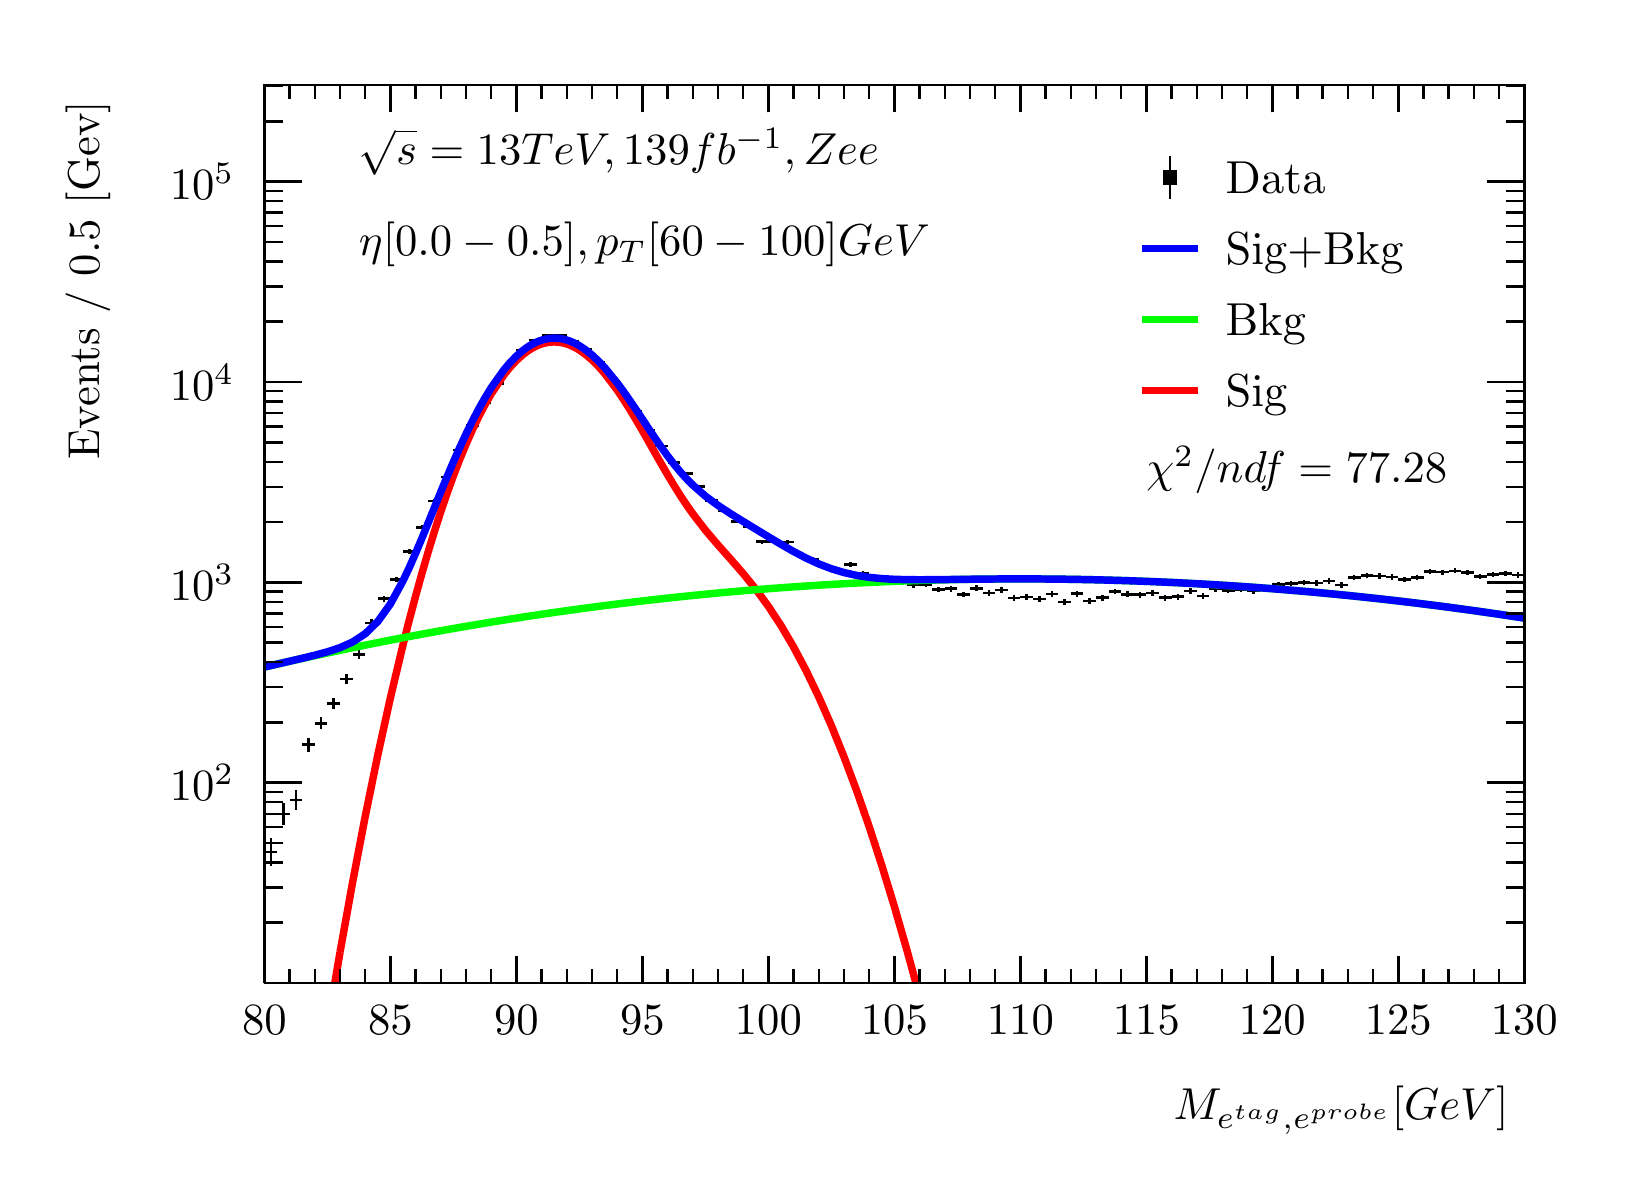
\begin{tikzpicture}
\pgfdeclareplotmark{cross} {
\pgfpathmoveto{\pgfpoint{-0.3\pgfplotmarksize}{\pgfplotmarksize}}
\pgfpathlineto{\pgfpoint{+0.3\pgfplotmarksize}{\pgfplotmarksize}}
\pgfpathlineto{\pgfpoint{+0.3\pgfplotmarksize}{0.3\pgfplotmarksize}}
\pgfpathlineto{\pgfpoint{+1\pgfplotmarksize}{0.3\pgfplotmarksize}}
\pgfpathlineto{\pgfpoint{+1\pgfplotmarksize}{-0.3\pgfplotmarksize}}
\pgfpathlineto{\pgfpoint{+0.3\pgfplotmarksize}{-0.3\pgfplotmarksize}}
\pgfpathlineto{\pgfpoint{+0.3\pgfplotmarksize}{-1.\pgfplotmarksize}}
\pgfpathlineto{\pgfpoint{-0.3\pgfplotmarksize}{-1.\pgfplotmarksize}}
\pgfpathlineto{\pgfpoint{-0.3\pgfplotmarksize}{-0.3\pgfplotmarksize}}
\pgfpathlineto{\pgfpoint{-1.\pgfplotmarksize}{-0.3\pgfplotmarksize}}
\pgfpathlineto{\pgfpoint{-1.\pgfplotmarksize}{0.3\pgfplotmarksize}}
\pgfpathlineto{\pgfpoint{-0.3\pgfplotmarksize}{0.3\pgfplotmarksize}}
\pgfpathclose
\pgfusepathqstroke
}
\pgfdeclareplotmark{cross*} {
\pgfpathmoveto{\pgfpoint{-0.3\pgfplotmarksize}{\pgfplotmarksize}}
\pgfpathlineto{\pgfpoint{+0.3\pgfplotmarksize}{\pgfplotmarksize}}
\pgfpathlineto{\pgfpoint{+0.3\pgfplotmarksize}{0.3\pgfplotmarksize}}
\pgfpathlineto{\pgfpoint{+1\pgfplotmarksize}{0.3\pgfplotmarksize}}
\pgfpathlineto{\pgfpoint{+1\pgfplotmarksize}{-0.3\pgfplotmarksize}}
\pgfpathlineto{\pgfpoint{+0.3\pgfplotmarksize}{-0.3\pgfplotmarksize}}
\pgfpathlineto{\pgfpoint{+0.3\pgfplotmarksize}{-1.\pgfplotmarksize}}
\pgfpathlineto{\pgfpoint{-0.3\pgfplotmarksize}{-1.\pgfplotmarksize}}
\pgfpathlineto{\pgfpoint{-0.3\pgfplotmarksize}{-0.3\pgfplotmarksize}}
\pgfpathlineto{\pgfpoint{-1.\pgfplotmarksize}{-0.3\pgfplotmarksize}}
\pgfpathlineto{\pgfpoint{-1.\pgfplotmarksize}{0.3\pgfplotmarksize}}
\pgfpathlineto{\pgfpoint{-0.3\pgfplotmarksize}{0.3\pgfplotmarksize}}
\pgfpathclose
\pgfusepathqfillstroke
}
\pgfdeclareplotmark{newstar} {
\pgfpathmoveto{\pgfqpoint{0pt}{\pgfplotmarksize}}
\pgfpathlineto{\pgfqpointpolar{44}{0.5\pgfplotmarksize}}
\pgfpathlineto{\pgfqpointpolar{18}{\pgfplotmarksize}}
\pgfpathlineto{\pgfqpointpolar{-20}{0.5\pgfplotmarksize}}
\pgfpathlineto{\pgfqpointpolar{-54}{\pgfplotmarksize}}
\pgfpathlineto{\pgfqpointpolar{-90}{0.5\pgfplotmarksize}}
\pgfpathlineto{\pgfqpointpolar{234}{\pgfplotmarksize}}
\pgfpathlineto{\pgfqpointpolar{198}{0.5\pgfplotmarksize}}
\pgfpathlineto{\pgfqpointpolar{162}{\pgfplotmarksize}}
\pgfpathlineto{\pgfqpointpolar{134}{0.5\pgfplotmarksize}}
\pgfpathclose
\pgfusepathqstroke
}
\pgfdeclareplotmark{newstar*} {
\pgfpathmoveto{\pgfqpoint{0pt}{\pgfplotmarksize}}
\pgfpathlineto{\pgfqpointpolar{44}{0.5\pgfplotmarksize}}
\pgfpathlineto{\pgfqpointpolar{18}{\pgfplotmarksize}}
\pgfpathlineto{\pgfqpointpolar{-20}{0.5\pgfplotmarksize}}
\pgfpathlineto{\pgfqpointpolar{-54}{\pgfplotmarksize}}
\pgfpathlineto{\pgfqpointpolar{-90}{0.5\pgfplotmarksize}}
\pgfpathlineto{\pgfqpointpolar{234}{\pgfplotmarksize}}
\pgfpathlineto{\pgfqpointpolar{198}{0.5\pgfplotmarksize}}
\pgfpathlineto{\pgfqpointpolar{162}{\pgfplotmarksize}}
\pgfpathlineto{\pgfqpointpolar{134}{0.5\pgfplotmarksize}}
\pgfpathclose
\pgfusepathqfillstroke
}
\definecolor{c}{rgb}{1,1,1};
\draw [color=c, fill=c] (0,0) rectangle (20,14.4361);
\draw [color=c, fill=c] (3,2.30977) rectangle (19,13.7143);
\definecolor{c}{rgb}{0,0,0};
\draw [c,line width=0.9] (3,2.30977) -- (3,13.7143) -- (19,13.7143) -- (19,2.30977) -- (3,2.30977);
\definecolor{c}{rgb}{1,1,1};
\draw [color=c, fill=c] (3,2.30977) rectangle (19,13.7143);
\definecolor{c}{rgb}{0,0,0};
\draw [c,line width=0.9] (3,2.30977) -- (3,13.7143) -- (19,13.7143) -- (19,2.30977) -- (3,2.30977);
\draw [c,line width=0.9] (3,2.30977) -- (19,2.30977);
\draw [c,line width=0.9] (3,2.65624) -- (3,2.30977);
\draw [c,line width=0.9] (3.32,2.48301) -- (3.32,2.30977);
\draw [c,line width=0.9] (3.64,2.48301) -- (3.64,2.30977);
\draw [c,line width=0.9] (3.96,2.48301) -- (3.96,2.30977);
\draw [c,line width=0.9] (4.28,2.48301) -- (4.28,2.30977);
\draw [c,line width=0.9] (4.6,2.65624) -- (4.6,2.30977);
\draw [c,line width=0.9] (4.92,2.48301) -- (4.92,2.30977);
\draw [c,line width=0.9] (5.24,2.48301) -- (5.24,2.30977);
\draw [c,line width=0.9] (5.56,2.48301) -- (5.56,2.30977);
\draw [c,line width=0.9] (5.88,2.48301) -- (5.88,2.30977);
\draw [c,line width=0.9] (6.2,2.65624) -- (6.2,2.30977);
\draw [c,line width=0.9] (6.52,2.48301) -- (6.52,2.30977);
\draw [c,line width=0.9] (6.84,2.48301) -- (6.84,2.30977);
\draw [c,line width=0.9] (7.16,2.48301) -- (7.16,2.30977);
\draw [c,line width=0.9] (7.48,2.48301) -- (7.48,2.30977);
\draw [c,line width=0.9] (7.8,2.65624) -- (7.8,2.30977);
\draw [c,line width=0.9] (8.12,2.48301) -- (8.12,2.30977);
\draw [c,line width=0.9] (8.44,2.48301) -- (8.44,2.30977);
\draw [c,line width=0.9] (8.76,2.48301) -- (8.76,2.30977);
\draw [c,line width=0.9] (9.08,2.48301) -- (9.08,2.30977);
\draw [c,line width=0.9] (9.4,2.65624) -- (9.4,2.30977);
\draw [c,line width=0.9] (9.72,2.48301) -- (9.72,2.30977);
\draw [c,line width=0.9] (10.04,2.48301) -- (10.04,2.30977);
\draw [c,line width=0.9] (10.36,2.48301) -- (10.36,2.30977);
\draw [c,line width=0.9] (10.68,2.48301) -- (10.68,2.30977);
\draw [c,line width=0.9] (11,2.65624) -- (11,2.30977);
\draw [c,line width=0.9] (11.32,2.48301) -- (11.32,2.30977);
\draw [c,line width=0.9] (11.64,2.48301) -- (11.64,2.30977);
\draw [c,line width=0.9] (11.96,2.48301) -- (11.96,2.30977);
\draw [c,line width=0.9] (12.28,2.48301) -- (12.28,2.30977);
\draw [c,line width=0.9] (12.6,2.65624) -- (12.6,2.30977);
\draw [c,line width=0.9] (12.92,2.48301) -- (12.92,2.30977);
\draw [c,line width=0.9] (13.24,2.48301) -- (13.24,2.30977);
\draw [c,line width=0.9] (13.56,2.48301) -- (13.56,2.30977);
\draw [c,line width=0.9] (13.88,2.48301) -- (13.88,2.30977);
\draw [c,line width=0.9] (14.2,2.65624) -- (14.2,2.30977);
\draw [c,line width=0.9] (14.52,2.48301) -- (14.52,2.30977);
\draw [c,line width=0.9] (14.84,2.48301) -- (14.84,2.30977);
\draw [c,line width=0.9] (15.16,2.48301) -- (15.16,2.30977);
\draw [c,line width=0.9] (15.48,2.48301) -- (15.48,2.30977);
\draw [c,line width=0.9] (15.8,2.65624) -- (15.8,2.30977);
\draw [c,line width=0.9] (16.12,2.48301) -- (16.12,2.30977);
\draw [c,line width=0.9] (16.44,2.48301) -- (16.44,2.30977);
\draw [c,line width=0.9] (16.76,2.48301) -- (16.76,2.30977);
\draw [c,line width=0.9] (17.08,2.48301) -- (17.08,2.30977);
\draw [c,line width=0.9] (17.4,2.65624) -- (17.4,2.30977);
\draw [c,line width=0.9] (17.72,2.48301) -- (17.72,2.30977);
\draw [c,line width=0.9] (18.04,2.48301) -- (18.04,2.30977);
\draw [c,line width=0.9] (18.36,2.48301) -- (18.36,2.30977);
\draw [c,line width=0.9] (18.68,2.48301) -- (18.68,2.30977);
\draw [c,line width=0.9] (19,2.65624) -- (19,2.30977);
\draw [anchor=base] (3,1.66015) node[scale=1.61424, color=c, rotate=0]{80};
\draw [anchor=base] (4.6,1.66015) node[scale=1.61424, color=c, rotate=0]{85};
\draw [anchor=base] (6.2,1.66015) node[scale=1.61424, color=c, rotate=0]{90};
\draw [anchor=base] (7.8,1.66015) node[scale=1.61424, color=c, rotate=0]{95};
\draw [anchor=base] (9.4,1.66015) node[scale=1.61424, color=c, rotate=0]{100};
\draw [anchor=base] (11,1.66015) node[scale=1.61424, color=c, rotate=0]{105};
\draw [anchor=base] (12.6,1.66015) node[scale=1.61424, color=c, rotate=0]{110};
\draw [anchor=base] (14.2,1.66015) node[scale=1.61424, color=c, rotate=0]{115};
\draw [anchor=base] (15.8,1.66015) node[scale=1.61424, color=c, rotate=0]{120};
\draw [anchor=base] (17.4,1.66015) node[scale=1.61424, color=c, rotate=0]{125};
\draw [anchor=base] (19,1.66015) node[scale=1.61424, color=c, rotate=0]{130};
\draw [anchor= east] (19,0.692932) node[scale=1.61424, color=c, rotate=0]{$M_{e^{tag}, e^{probe}}  [GeV]$};
\draw [c,line width=0.9] (3,13.7143) -- (19,13.7143);
\draw [c,line width=0.9] (3,13.3678) -- (3,13.7143);
\draw [c,line width=0.9] (3.32,13.5411) -- (3.32,13.7143);
\draw [c,line width=0.9] (3.64,13.5411) -- (3.64,13.7143);
\draw [c,line width=0.9] (3.96,13.5411) -- (3.96,13.7143);
\draw [c,line width=0.9] (4.28,13.5411) -- (4.28,13.7143);
\draw [c,line width=0.9] (4.6,13.3678) -- (4.6,13.7143);
\draw [c,line width=0.9] (4.92,13.5411) -- (4.92,13.7143);
\draw [c,line width=0.9] (5.24,13.5411) -- (5.24,13.7143);
\draw [c,line width=0.9] (5.56,13.5411) -- (5.56,13.7143);
\draw [c,line width=0.9] (5.88,13.5411) -- (5.88,13.7143);
\draw [c,line width=0.9] (6.2,13.3678) -- (6.2,13.7143);
\draw [c,line width=0.9] (6.52,13.5411) -- (6.52,13.7143);
\draw [c,line width=0.9] (6.84,13.5411) -- (6.84,13.7143);
\draw [c,line width=0.9] (7.16,13.5411) -- (7.16,13.7143);
\draw [c,line width=0.9] (7.48,13.5411) -- (7.48,13.7143);
\draw [c,line width=0.9] (7.8,13.3678) -- (7.8,13.7143);
\draw [c,line width=0.9] (8.12,13.5411) -- (8.12,13.7143);
\draw [c,line width=0.9] (8.44,13.5411) -- (8.44,13.7143);
\draw [c,line width=0.9] (8.76,13.5411) -- (8.76,13.7143);
\draw [c,line width=0.9] (9.08,13.5411) -- (9.08,13.7143);
\draw [c,line width=0.9] (9.4,13.3678) -- (9.4,13.7143);
\draw [c,line width=0.9] (9.72,13.5411) -- (9.72,13.7143);
\draw [c,line width=0.9] (10.04,13.5411) -- (10.04,13.7143);
\draw [c,line width=0.9] (10.36,13.5411) -- (10.36,13.7143);
\draw [c,line width=0.9] (10.68,13.5411) -- (10.68,13.7143);
\draw [c,line width=0.9] (11,13.3678) -- (11,13.7143);
\draw [c,line width=0.9] (11.32,13.5411) -- (11.32,13.7143);
\draw [c,line width=0.9] (11.64,13.5411) -- (11.64,13.7143);
\draw [c,line width=0.9] (11.96,13.5411) -- (11.96,13.7143);
\draw [c,line width=0.9] (12.28,13.5411) -- (12.28,13.7143);
\draw [c,line width=0.9] (12.6,13.3678) -- (12.6,13.7143);
\draw [c,line width=0.9] (12.92,13.5411) -- (12.92,13.7143);
\draw [c,line width=0.9] (13.24,13.5411) -- (13.24,13.7143);
\draw [c,line width=0.9] (13.56,13.5411) -- (13.56,13.7143);
\draw [c,line width=0.9] (13.88,13.5411) -- (13.88,13.7143);
\draw [c,line width=0.9] (14.2,13.3678) -- (14.2,13.7143);
\draw [c,line width=0.9] (14.52,13.5411) -- (14.52,13.7143);
\draw [c,line width=0.9] (14.84,13.5411) -- (14.84,13.7143);
\draw [c,line width=0.9] (15.16,13.5411) -- (15.16,13.7143);
\draw [c,line width=0.9] (15.48,13.5411) -- (15.48,13.7143);
\draw [c,line width=0.9] (15.8,13.3678) -- (15.8,13.7143);
\draw [c,line width=0.9] (16.12,13.5411) -- (16.12,13.7143);
\draw [c,line width=0.9] (16.44,13.5411) -- (16.44,13.7143);
\draw [c,line width=0.9] (16.76,13.5411) -- (16.76,13.7143);
\draw [c,line width=0.9] (17.08,13.5411) -- (17.08,13.7143);
\draw [c,line width=0.9] (17.4,13.3678) -- (17.4,13.7143);
\draw [c,line width=0.9] (17.72,13.5411) -- (17.72,13.7143);
\draw [c,line width=0.9] (18.04,13.5411) -- (18.04,13.7143);
\draw [c,line width=0.9] (18.36,13.5411) -- (18.36,13.7143);
\draw [c,line width=0.9] (18.68,13.5411) -- (18.68,13.7143);
\draw [c,line width=0.9] (19,13.3678) -- (19,13.7143);
\draw [c,line width=0.9] (3,2.30977) -- (3,13.7143);
\draw [c,line width=0.9] (3.237,3.07568) -- (3,3.07568);
\draw [c,line width=0.9] (3.237,3.5237) -- (3,3.5237);
\draw [c,line width=0.9] (3.237,3.84158) -- (3,3.84158);
\draw [c,line width=0.9] (3.237,4.08815) -- (3,4.08815);
\draw [c,line width=0.9] (3.237,4.2896) -- (3,4.2896);
\draw [c,line width=0.9] (3.237,4.45994) -- (3,4.45994);
\draw [c,line width=0.9] (3.237,4.60748) -- (3,4.60748);
\draw [c,line width=0.9] (3.237,4.73763) -- (3,4.73763);
\draw [c,line width=0.9] (3.474,4.85405) -- (3,4.85405);
\draw [anchor= east] (2.82,4.85405) node[scale=1.61424, color=c, rotate=0]{$10^{2}$};
\draw [c,line width=0.9] (3.237,5.61995) -- (3,5.61995);
\draw [c,line width=0.9] (3.237,6.06798) -- (3,6.06798);
\draw [c,line width=0.9] (3.237,6.38586) -- (3,6.38586);
\draw [c,line width=0.9] (3.237,6.63242) -- (3,6.63242);
\draw [c,line width=0.9] (3.237,6.83388) -- (3,6.83388);
\draw [c,line width=0.9] (3.237,7.00421) -- (3,7.00421);
\draw [c,line width=0.9] (3.237,7.15176) -- (3,7.15176);
\draw [c,line width=0.9] (3.237,7.28191) -- (3,7.28191);
\draw [c,line width=0.9] (3.474,7.39833) -- (3,7.39833);
\draw [anchor= east] (2.82,7.39833) node[scale=1.61424, color=c, rotate=0]{$10^{3}$};
\draw [c,line width=0.9] (3.237,8.16423) -- (3,8.16423);
\draw [c,line width=0.9] (3.237,8.61226) -- (3,8.61226);
\draw [c,line width=0.9] (3.237,8.93013) -- (3,8.93013);
\draw [c,line width=0.9] (3.237,9.1767) -- (3,9.1767);
\draw [c,line width=0.9] (3.237,9.37816) -- (3,9.37816);
\draw [c,line width=0.9] (3.237,9.54849) -- (3,9.54849);
\draw [c,line width=0.9] (3.237,9.69604) -- (3,9.69604);
\draw [c,line width=0.9] (3.237,9.82618) -- (3,9.82618);
\draw [c,line width=0.9] (3.474,9.9426) -- (3,9.9426);
\draw [anchor= east] (2.82,9.9426) node[scale=1.61424, color=c, rotate=0]{$10^{4}$};
\draw [c,line width=0.9] (3.237,10.7085) -- (3,10.7085);
\draw [c,line width=0.9] (3.237,11.1565) -- (3,11.1565);
\draw [c,line width=0.9] (3.237,11.4744) -- (3,11.4744);
\draw [c,line width=0.9] (3.237,11.721) -- (3,11.721);
\draw [c,line width=0.9] (3.237,11.9224) -- (3,11.9224);
\draw [c,line width=0.9] (3.237,12.0928) -- (3,12.0928);
\draw [c,line width=0.9] (3.237,12.2403) -- (3,12.2403);
\draw [c,line width=0.9] (3.237,12.3705) -- (3,12.3705);
\draw [c,line width=0.9] (3.474,12.4869) -- (3,12.4869);
\draw [anchor= east] (2.82,12.4869) node[scale=1.61424, color=c, rotate=0]{$10^{5}$};
\draw [c,line width=0.9] (3.237,13.2528) -- (3,13.2528);
\draw [c,line width=0.9] (3.237,13.7008) -- (3,13.7008);
\draw [anchor= east] (0.76,13.7143) node[scale=1.61424, color=c, rotate=90]{Events / 0.5 [Gev]};
\draw [c,line width=0.9] (19,2.30977) -- (19,13.7143);
\draw [c,line width=0.9] (18.763,3.07568) -- (19,3.07568);
\draw [c,line width=0.9] (18.763,3.5237) -- (19,3.5237);
\draw [c,line width=0.9] (18.763,3.84158) -- (19,3.84158);
\draw [c,line width=0.9] (18.763,4.08815) -- (19,4.08815);
\draw [c,line width=0.9] (18.763,4.2896) -- (19,4.2896);
\draw [c,line width=0.9] (18.763,4.45994) -- (19,4.45994);
\draw [c,line width=0.9] (18.763,4.60748) -- (19,4.60748);
\draw [c,line width=0.9] (18.763,4.73763) -- (19,4.73763);
\draw [c,line width=0.9] (18.526,4.85405) -- (19,4.85405);
\draw [c,line width=0.9] (18.763,5.61995) -- (19,5.61995);
\draw [c,line width=0.9] (18.763,6.06798) -- (19,6.06798);
\draw [c,line width=0.9] (18.763,6.38586) -- (19,6.38586);
\draw [c,line width=0.9] (18.763,6.63242) -- (19,6.63242);
\draw [c,line width=0.9] (18.763,6.83388) -- (19,6.83388);
\draw [c,line width=0.9] (18.763,7.00421) -- (19,7.00421);
\draw [c,line width=0.9] (18.763,7.15176) -- (19,7.15176);
\draw [c,line width=0.9] (18.763,7.28191) -- (19,7.28191);
\draw [c,line width=0.9] (18.526,7.39833) -- (19,7.39833);
\draw [c,line width=0.9] (18.763,8.16423) -- (19,8.16423);
\draw [c,line width=0.9] (18.763,8.61226) -- (19,8.61226);
\draw [c,line width=0.9] (18.763,8.93013) -- (19,8.93013);
\draw [c,line width=0.9] (18.763,9.1767) -- (19,9.1767);
\draw [c,line width=0.9] (18.763,9.37816) -- (19,9.37816);
\draw [c,line width=0.9] (18.763,9.54849) -- (19,9.54849);
\draw [c,line width=0.9] (18.763,9.69604) -- (19,9.69604);
\draw [c,line width=0.9] (18.763,9.82618) -- (19,9.82618);
\draw [c,line width=0.9] (18.526,9.9426) -- (19,9.9426);
\draw [c,line width=0.9] (18.763,10.7085) -- (19,10.7085);
\draw [c,line width=0.9] (18.763,11.1565) -- (19,11.1565);
\draw [c,line width=0.9] (18.763,11.4744) -- (19,11.4744);
\draw [c,line width=0.9] (18.763,11.721) -- (19,11.721);
\draw [c,line width=0.9] (18.763,11.9224) -- (19,11.9224);
\draw [c,line width=0.9] (18.763,12.0928) -- (19,12.0928);
\draw [c,line width=0.9] (18.763,12.2403) -- (19,12.2403);
\draw [c,line width=0.9] (18.763,12.3705) -- (19,12.3705);
\draw [c,line width=0.9] (18.526,12.4869) -- (19,12.4869);
\draw [c,line width=0.9] (18.763,13.2528) -- (19,13.2528);
\draw [c,line width=0.9] (18.763,13.7008) -- (19,13.7008);
\draw [c,line width=0.9] (3.08,3.97173) -- (3,3.97173);
\draw [c,line width=0.9] (3,3.97173) -- (3,3.97173);
\draw [c,line width=0.9] (3.08,3.97173) -- (3.16,3.97173);
\draw [c,line width=0.9] (3.16,3.97173) -- (3.16,3.97173);
\draw [c,line width=0.9] (3.08,3.97173) -- (3.08,4.14747);
\draw [c,line width=0.9] (3.08,4.14747) -- (3.08,4.14747);
\draw [c,line width=0.9] (3.08,3.97173) -- (3.08,3.79408);
\draw [c,line width=0.9] (3.08,3.79408) -- (3.08,3.79408);
\draw [c,line width=0.9] (3.24,4.45994) -- (3.16,4.45994);
\draw [c,line width=0.9] (3.16,4.45994) -- (3.16,4.45994);
\draw [c,line width=0.9] (3.24,4.45994) -- (3.32,4.45994);
\draw [c,line width=0.9] (3.32,4.45994) -- (3.32,4.45994);
\draw [c,line width=0.9] (3.24,4.45994) -- (3.24,4.59926);
\draw [c,line width=0.9] (3.24,4.59926) -- (3.24,4.59926);
\draw [c,line width=0.9] (3.24,4.45994) -- (3.24,4.31964);
\draw [c,line width=0.9] (3.24,4.31964) -- (3.24,4.31964);
\draw [c,line width=0.9] (3.4,4.63477) -- (3.32,4.63477);
\draw [c,line width=0.9] (3.32,4.63477) -- (3.32,4.63477);
\draw [c,line width=0.9] (3.4,4.63477) -- (3.48,4.63477);
\draw [c,line width=0.9] (3.48,4.63477) -- (3.48,4.63477);
\draw [c,line width=0.9] (3.4,4.63477) -- (3.4,4.76302);
\draw [c,line width=0.9] (3.4,4.76302) -- (3.4,4.76302);
\draw [c,line width=0.9] (3.4,4.63477) -- (3.4,4.50575);
\draw [c,line width=0.9] (3.4,4.50575) -- (3.4,4.50575);
\draw [c,line width=0.9] (3.56,5.33831) -- (3.48,5.33831);
\draw [c,line width=0.9] (3.48,5.33831) -- (3.48,5.33831);
\draw [c,line width=0.9] (3.56,5.33831) -- (3.64,5.33831);
\draw [c,line width=0.9] (3.64,5.33831) -- (3.64,5.33831);
\draw [c,line width=0.9] (3.56,5.33831) -- (3.56,5.42704);
\draw [c,line width=0.9] (3.56,5.42704) -- (3.56,5.42704);
\draw [c,line width=0.9] (3.56,5.33831) -- (3.56,5.24958);
\draw [c,line width=0.9] (3.56,5.24958) -- (3.56,5.24958);
\draw [c,line width=0.9] (3.72,5.60885) -- (3.64,5.60885);
\draw [c,line width=0.9] (3.64,5.60885) -- (3.64,5.60885);
\draw [c,line width=0.9] (3.72,5.60885) -- (3.8,5.60885);
\draw [c,line width=0.9] (3.8,5.60885) -- (3.8,5.60885);
\draw [c,line width=0.9] (3.72,5.60885) -- (3.72,5.68736);
\draw [c,line width=0.9] (3.72,5.68736) -- (3.72,5.68736);
\draw [c,line width=0.9] (3.72,5.60885) -- (3.72,5.53034);
\draw [c,line width=0.9] (3.72,5.53034) -- (3.72,5.53034);
\draw [c,line width=0.9] (3.88,5.85765) -- (3.8,5.85765);
\draw [c,line width=0.9] (3.8,5.85765) -- (3.8,5.85765);
\draw [c,line width=0.9] (3.88,5.85765) -- (3.96,5.85765);
\draw [c,line width=0.9] (3.96,5.85765) -- (3.96,5.85765);
\draw [c,line width=0.9] (3.88,5.85765) -- (3.88,5.9278);
\draw [c,line width=0.9] (3.88,5.9278) -- (3.88,5.9278);
\draw [c,line width=0.9] (3.88,5.85765) -- (3.88,5.78749);
\draw [c,line width=0.9] (3.88,5.78749) -- (3.88,5.78749);
\draw [c,line width=0.9] (4.04,6.16994) -- (3.96,6.16994);
\draw [c,line width=0.9] (3.96,6.16994) -- (3.96,6.16994);
\draw [c,line width=0.9] (4.04,6.16994) -- (4.12,6.16994);
\draw [c,line width=0.9] (4.12,6.16994) -- (4.12,6.16994);
\draw [c,line width=0.9] (4.04,6.16994) -- (4.04,6.23085);
\draw [c,line width=0.9] (4.04,6.23085) -- (4.04,6.23085);
\draw [c,line width=0.9] (4.04,6.16994) -- (4.04,6.10903);
\draw [c,line width=0.9] (4.04,6.10903) -- (4.04,6.10903);
\draw [c,line width=0.9] (4.2,6.48361) -- (4.12,6.48361);
\draw [c,line width=0.9] (4.12,6.48361) -- (4.12,6.48361);
\draw [c,line width=0.9] (4.2,6.48361) -- (4.28,6.48361);
\draw [c,line width=0.9] (4.28,6.48361) -- (4.28,6.48361);
\draw [c,line width=0.9] (4.2,6.48361) -- (4.2,6.53647);
\draw [c,line width=0.9] (4.2,6.53647) -- (4.2,6.53647);
\draw [c,line width=0.9] (4.2,6.48361) -- (4.2,6.43076);
\draw [c,line width=0.9] (4.2,6.43076) -- (4.2,6.43076);
\draw [c,line width=0.9] (4.36,6.88428) -- (4.28,6.88428);
\draw [c,line width=0.9] (4.28,6.88428) -- (4.28,6.88428);
\draw [c,line width=0.9] (4.36,6.88428) -- (4.44,6.88428);
\draw [c,line width=0.9] (4.44,6.88428) -- (4.44,6.88428);
\draw [c,line width=0.9] (4.36,6.88428) -- (4.36,6.92837);
\draw [c,line width=0.9] (4.36,6.92837) -- (4.36,6.92837);
\draw [c,line width=0.9] (4.36,6.88428) -- (4.36,6.84019);
\draw [c,line width=0.9] (4.36,6.84019) -- (4.36,6.84019);
\draw [c,line width=0.9] (4.52,7.19244) -- (4.44,7.19244);
\draw [c,line width=0.9] (4.44,7.19244) -- (4.44,7.19244);
\draw [c,line width=0.9] (4.52,7.19244) -- (4.6,7.19244);
\draw [c,line width=0.9] (4.6,7.19244) -- (4.6,7.19244);
\draw [c,line width=0.9] (4.52,7.19244) -- (4.52,7.23079);
\draw [c,line width=0.9] (4.52,7.23079) -- (4.52,7.23079);
\draw [c,line width=0.9] (4.52,7.19244) -- (4.52,7.15409);
\draw [c,line width=0.9] (4.52,7.15409) -- (4.52,7.15409);
\draw [c,line width=0.9] (4.68,7.4342) -- (4.6,7.4342);
\draw [c,line width=0.9] (4.6,7.4342) -- (4.6,7.4342);
\draw [c,line width=0.9] (4.68,7.4342) -- (4.76,7.4342);
\draw [c,line width=0.9] (4.76,7.4342) -- (4.76,7.4342);
\draw [c,line width=0.9] (4.68,7.4342) -- (4.68,7.46858);
\draw [c,line width=0.9] (4.68,7.46858) -- (4.68,7.46858);
\draw [c,line width=0.9] (4.68,7.4342) -- (4.68,7.39983);
\draw [c,line width=0.9] (4.68,7.39983) -- (4.68,7.39983);
\draw [c,line width=0.9] (4.84,7.7889) -- (4.76,7.7889);
\draw [c,line width=0.9] (4.76,7.7889) -- (4.76,7.7889);
\draw [c,line width=0.9] (4.84,7.7889) -- (4.92,7.7889);
\draw [c,line width=0.9] (4.92,7.7889) -- (4.92,7.7889);
\draw [c,line width=0.9] (4.84,7.7889) -- (4.84,7.81818);
\draw [c,line width=0.9] (4.84,7.81818) -- (4.84,7.81818);
\draw [c,line width=0.9] (4.84,7.7889) -- (4.84,7.75962);
\draw [c,line width=0.9] (4.84,7.75962) -- (4.84,7.75962);
\draw [c,line width=0.9] (5,8.09645) -- (4.92,8.09645);
\draw [c,line width=0.9] (4.92,8.09645) -- (4.92,8.09645);
\draw [c,line width=0.9] (5,8.09645) -- (5.08,8.09645);
\draw [c,line width=0.9] (5.08,8.09645) -- (5.08,8.09645);
\draw [c,line width=0.9] (5,8.09645) -- (5,8.12193);
\draw [c,line width=0.9] (5,8.12193) -- (5,8.12193);
\draw [c,line width=0.9] (5,8.09645) -- (5,8.07097);
\draw [c,line width=0.9] (5,8.07097) -- (5,8.07097);
\draw [c,line width=0.9] (5.16,8.43008) -- (5.08,8.43008);
\draw [c,line width=0.9] (5.08,8.43008) -- (5.08,8.43008);
\draw [c,line width=0.9] (5.16,8.43008) -- (5.24,8.43008);
\draw [c,line width=0.9] (5.24,8.43008) -- (5.24,8.43008);
\draw [c,line width=0.9] (5.16,8.43008) -- (5.16,8.45198);
\draw [c,line width=0.9] (5.16,8.45198) -- (5.16,8.45198);
\draw [c,line width=0.9] (5.16,8.43008) -- (5.16,8.40817);
\draw [c,line width=0.9] (5.16,8.40817) -- (5.16,8.40817);
\draw [c,line width=0.9] (5.32,8.73386) -- (5.24,8.73386);
\draw [c,line width=0.9] (5.24,8.73386) -- (5.24,8.73386);
\draw [c,line width=0.9] (5.32,8.73386) -- (5.4,8.73386);
\draw [c,line width=0.9] (5.4,8.73386) -- (5.4,8.73386);
\draw [c,line width=0.9] (5.32,8.73386) -- (5.32,8.75295);
\draw [c,line width=0.9] (5.32,8.75295) -- (5.32,8.75295);
\draw [c,line width=0.9] (5.32,8.73386) -- (5.32,8.71476);
\draw [c,line width=0.9] (5.32,8.71476) -- (5.32,8.71476);
\draw [c,line width=0.9] (5.48,9.07903) -- (5.4,9.07903);
\draw [c,line width=0.9] (5.4,9.07903) -- (5.4,9.07903);
\draw [c,line width=0.9] (5.48,9.07903) -- (5.56,9.07903);
\draw [c,line width=0.9] (5.56,9.07903) -- (5.56,9.07903);
\draw [c,line width=0.9] (5.48,9.07903) -- (5.48,9.09536);
\draw [c,line width=0.9] (5.48,9.09536) -- (5.48,9.09536);
\draw [c,line width=0.9] (5.48,9.07903) -- (5.48,9.0627);
\draw [c,line width=0.9] (5.48,9.0627) -- (5.48,9.0627);
\draw [c,line width=0.9] (5.64,9.39261) -- (5.56,9.39261);
\draw [c,line width=0.9] (5.56,9.39261) -- (5.56,9.39261);
\draw [c,line width=0.9] (5.64,9.39261) -- (5.72,9.39261);
\draw [c,line width=0.9] (5.72,9.39261) -- (5.72,9.39261);
\draw [c,line width=0.9] (5.64,9.39261) -- (5.64,9.40679);
\draw [c,line width=0.9] (5.64,9.40679) -- (5.64,9.40679);
\draw [c,line width=0.9] (5.64,9.39261) -- (5.64,9.37844);
\draw [c,line width=0.9] (5.64,9.37844) -- (5.64,9.37844);
\draw [c,line width=0.9] (5.8,9.67681) -- (5.72,9.67681);
\draw [c,line width=0.9] (5.72,9.67681) -- (5.72,9.67681);
\draw [c,line width=0.9] (5.8,9.67681) -- (5.88,9.67681);
\draw [c,line width=0.9] (5.88,9.67681) -- (5.88,9.67681);
\draw [c,line width=0.9] (5.8,9.67681) -- (5.8,9.68927);
\draw [c,line width=0.9] (5.8,9.68927) -- (5.8,9.68927);
\draw [c,line width=0.9] (5.8,9.67681) -- (5.8,9.66435);
\draw [c,line width=0.9] (5.8,9.66435) -- (5.8,9.66435);
\draw [c,line width=0.9] (5.96,9.9213) -- (5.88,9.9213);
\draw [c,line width=0.9] (5.88,9.9213) -- (5.88,9.9213);
\draw [c,line width=0.9] (5.96,9.9213) -- (6.04,9.9213);
\draw [c,line width=0.9] (6.04,9.9213) -- (6.04,9.9213);
\draw [c,line width=0.9] (5.96,9.9213) -- (5.96,9.93245);
\draw [c,line width=0.9] (5.96,9.93245) -- (5.96,9.93245);
\draw [c,line width=0.9] (5.96,9.9213) -- (5.96,9.91014);
\draw [c,line width=0.9] (5.96,9.91014) -- (5.96,9.91014);
\draw [c,line width=0.9] (6.12,10.1618) -- (6.04,10.1618);
\draw [c,line width=0.9] (6.04,10.1618) -- (6.04,10.1618);
\draw [c,line width=0.9] (6.12,10.1618) -- (6.2,10.1618);
\draw [c,line width=0.9] (6.2,10.1618) -- (6.2,10.1618);
\draw [c,line width=0.9] (6.12,10.1618) -- (6.12,10.1718);
\draw [c,line width=0.9] (6.12,10.1718) -- (6.12,10.1718);
\draw [c,line width=0.9] (6.12,10.1618) -- (6.12,10.1518);
\draw [c,line width=0.9] (6.12,10.1518) -- (6.12,10.1518);
\draw [c,line width=0.9] (6.28,10.3471) -- (6.2,10.3471);
\draw [c,line width=0.9] (6.2,10.3471) -- (6.2,10.3471);
\draw [c,line width=0.9] (6.28,10.3471) -- (6.36,10.3471);
\draw [c,line width=0.9] (6.36,10.3471) -- (6.36,10.3471);
\draw [c,line width=0.9] (6.28,10.3471) -- (6.28,10.3563);
\draw [c,line width=0.9] (6.28,10.3563) -- (6.28,10.3563);
\draw [c,line width=0.9] (6.28,10.3471) -- (6.28,10.3379);
\draw [c,line width=0.9] (6.28,10.3379) -- (6.28,10.3379);
\draw [c,line width=0.9] (6.44,10.4746) -- (6.36,10.4746);
\draw [c,line width=0.9] (6.36,10.4746) -- (6.36,10.4746);
\draw [c,line width=0.9] (6.44,10.4746) -- (6.52,10.4746);
\draw [c,line width=0.9] (6.52,10.4746) -- (6.52,10.4746);
\draw [c,line width=0.9] (6.44,10.4746) -- (6.44,10.4833);
\draw [c,line width=0.9] (6.44,10.4833) -- (6.44,10.4833);
\draw [c,line width=0.9] (6.44,10.4746) -- (6.44,10.466);
\draw [c,line width=0.9] (6.44,10.466) -- (6.44,10.466);
\draw [c,line width=0.9] (6.6,10.5373) -- (6.52,10.5373);
\draw [c,line width=0.9] (6.52,10.5373) -- (6.52,10.5373);
\draw [c,line width=0.9] (6.6,10.5373) -- (6.68,10.5373);
\draw [c,line width=0.9] (6.68,10.5373) -- (6.68,10.5373);
\draw [c,line width=0.9] (6.6,10.5373) -- (6.6,10.5457);
\draw [c,line width=0.9] (6.6,10.5457) -- (6.6,10.5457);
\draw [c,line width=0.9] (6.6,10.5373) -- (6.6,10.5288);
\draw [c,line width=0.9] (6.6,10.5288) -- (6.6,10.5288);
\draw [c,line width=0.9] (6.76,10.5319) -- (6.68,10.5319);
\draw [c,line width=0.9] (6.68,10.5319) -- (6.68,10.5319);
\draw [c,line width=0.9] (6.76,10.5319) -- (6.84,10.5319);
\draw [c,line width=0.9] (6.84,10.5319) -- (6.84,10.5319);
\draw [c,line width=0.9] (6.76,10.5319) -- (6.76,10.5403);
\draw [c,line width=0.9] (6.76,10.5403) -- (6.76,10.5403);
\draw [c,line width=0.9] (6.76,10.5319) -- (6.76,10.5234);
\draw [c,line width=0.9] (6.76,10.5234) -- (6.76,10.5234);
\draw [c,line width=0.9] (6.92,10.4613) -- (6.84,10.4613);
\draw [c,line width=0.9] (6.84,10.4613) -- (6.84,10.4613);
\draw [c,line width=0.9] (6.92,10.4613) -- (7,10.4613);
\draw [c,line width=0.9] (7,10.4613) -- (7,10.4613);
\draw [c,line width=0.9] (6.92,10.4613) -- (6.92,10.4701);
\draw [c,line width=0.9] (6.92,10.4701) -- (6.92,10.4701);
\draw [c,line width=0.9] (6.92,10.4613) -- (6.92,10.4526);
\draw [c,line width=0.9] (6.92,10.4526) -- (6.92,10.4526);
\draw [c,line width=0.9] (7.08,10.3639) -- (7,10.3639);
\draw [c,line width=0.9] (7,10.3639) -- (7,10.3639);
\draw [c,line width=0.9] (7.08,10.3639) -- (7.16,10.3639);
\draw [c,line width=0.9] (7.16,10.3639) -- (7.16,10.3639);
\draw [c,line width=0.9] (7.08,10.3639) -- (7.08,10.373);
\draw [c,line width=0.9] (7.08,10.373) -- (7.08,10.373);
\draw [c,line width=0.9] (7.08,10.3639) -- (7.08,10.3547);
\draw [c,line width=0.9] (7.08,10.3547) -- (7.08,10.3547);
\draw [c,line width=0.9] (7.24,10.1946) -- (7.16,10.1946);
\draw [c,line width=0.9] (7.16,10.1946) -- (7.16,10.1946);
\draw [c,line width=0.9] (7.24,10.1946) -- (7.32,10.1946);
\draw [c,line width=0.9] (7.32,10.1946) -- (7.32,10.1946);
\draw [c,line width=0.9] (7.24,10.1946) -- (7.24,10.2044);
\draw [c,line width=0.9] (7.24,10.2044) -- (7.24,10.2044);
\draw [c,line width=0.9] (7.24,10.1946) -- (7.24,10.1847);
\draw [c,line width=0.9] (7.24,10.1847) -- (7.24,10.1847);
\draw [c,line width=0.9] (7.4,9.9942) -- (7.32,9.9942);
\draw [c,line width=0.9] (7.32,9.9942) -- (7.32,9.9942);
\draw [c,line width=0.9] (7.4,9.9942) -- (7.48,9.9942);
\draw [c,line width=0.9] (7.48,9.9942) -- (7.48,9.9942);
\draw [c,line width=0.9] (7.4,9.9942) -- (7.4,10.005);
\draw [c,line width=0.9] (7.4,10.005) -- (7.4,10.005);
\draw [c,line width=0.9] (7.4,9.9942) -- (7.4,9.9834);
\draw [c,line width=0.9] (7.4,9.9834) -- (7.4,9.9834);
\draw [c,line width=0.9] (7.56,9.77273) -- (7.48,9.77273);
\draw [c,line width=0.9] (7.48,9.77273) -- (7.48,9.77273);
\draw [c,line width=0.9] (7.56,9.77273) -- (7.64,9.77273);
\draw [c,line width=0.9] (7.64,9.77273) -- (7.64,9.77273);
\draw [c,line width=0.9] (7.56,9.77273) -- (7.56,9.78467);
\draw [c,line width=0.9] (7.56,9.78467) -- (7.56,9.78467);
\draw [c,line width=0.9] (7.56,9.77273) -- (7.56,9.7608);
\draw [c,line width=0.9] (7.56,9.7608) -- (7.56,9.7608);
\draw [c,line width=0.9] (7.72,9.57099) -- (7.64,9.57099);
\draw [c,line width=0.9] (7.64,9.57099) -- (7.64,9.57099);
\draw [c,line width=0.9] (7.72,9.57099) -- (7.8,9.57099);
\draw [c,line width=0.9] (7.8,9.57099) -- (7.8,9.57099);
\draw [c,line width=0.9] (7.72,9.57099) -- (7.72,9.58406);
\draw [c,line width=0.9] (7.72,9.58406) -- (7.72,9.58406);
\draw [c,line width=0.9] (7.72,9.57099) -- (7.72,9.55792);
\draw [c,line width=0.9] (7.72,9.55792) -- (7.72,9.55792);
\draw [c,line width=0.9] (7.88,9.33075) -- (7.8,9.33075);
\draw [c,line width=0.9] (7.8,9.33075) -- (7.8,9.33075);
\draw [c,line width=0.9] (7.88,9.33075) -- (7.96,9.33075);
\draw [c,line width=0.9] (7.96,9.33075) -- (7.96,9.33075);
\draw [c,line width=0.9] (7.88,9.33075) -- (7.88,9.34532);
\draw [c,line width=0.9] (7.88,9.34532) -- (7.88,9.34532);
\draw [c,line width=0.9] (7.88,9.33075) -- (7.88,9.31617);
\draw [c,line width=0.9] (7.88,9.31617) -- (7.88,9.31617);
\draw [c,line width=0.9] (8.04,9.13159) -- (7.96,9.13159);
\draw [c,line width=0.9] (7.96,9.13159) -- (7.96,9.13159);
\draw [c,line width=0.9] (8.04,9.13159) -- (8.12,9.13159);
\draw [c,line width=0.9] (8.12,9.13159) -- (8.12,9.13159);
\draw [c,line width=0.9] (8.04,9.13159) -- (8.04,9.14754);
\draw [c,line width=0.9] (8.04,9.14754) -- (8.04,9.14754);
\draw [c,line width=0.9] (8.04,9.13159) -- (8.04,9.11565);
\draw [c,line width=0.9] (8.04,9.11565) -- (8.04,9.11565);
\draw [c,line width=0.9] (8.2,8.91903) -- (8.12,8.91903);
\draw [c,line width=0.9] (8.12,8.91903) -- (8.12,8.91903);
\draw [c,line width=0.9] (8.2,8.91903) -- (8.28,8.91903);
\draw [c,line width=0.9] (8.28,8.91903) -- (8.28,8.91903);
\draw [c,line width=0.9] (8.2,8.91903) -- (8.2,8.93659);
\draw [c,line width=0.9] (8.2,8.93659) -- (8.2,8.93659);
\draw [c,line width=0.9] (8.2,8.91903) -- (8.2,8.90147);
\draw [c,line width=0.9] (8.2,8.90147) -- (8.2,8.90147);
\draw [c,line width=0.9] (8.36,8.77911) -- (8.28,8.77911);
\draw [c,line width=0.9] (8.28,8.77911) -- (8.28,8.77911);
\draw [c,line width=0.9] (8.36,8.77911) -- (8.44,8.77911);
\draw [c,line width=0.9] (8.44,8.77911) -- (8.44,8.77911);
\draw [c,line width=0.9] (8.36,8.77911) -- (8.36,8.79782);
\draw [c,line width=0.9] (8.36,8.79782) -- (8.36,8.79782);
\draw [c,line width=0.9] (8.36,8.77911) -- (8.36,8.7604);
\draw [c,line width=0.9] (8.36,8.7604) -- (8.36,8.7604);
\draw [c,line width=0.9] (8.52,8.61887) -- (8.44,8.61887);
\draw [c,line width=0.9] (8.44,8.61887) -- (8.44,8.61887);
\draw [c,line width=0.9] (8.52,8.61887) -- (8.6,8.61887);
\draw [c,line width=0.9] (8.6,8.61887) -- (8.6,8.61887);
\draw [c,line width=0.9] (8.52,8.61887) -- (8.52,8.63898);
\draw [c,line width=0.9] (8.52,8.63898) -- (8.52,8.63898);
\draw [c,line width=0.9] (8.52,8.61887) -- (8.52,8.59875);
\draw [c,line width=0.9] (8.52,8.59875) -- (8.52,8.59875);
\draw [c,line width=0.9] (8.68,8.43657) -- (8.6,8.43657);
\draw [c,line width=0.9] (8.6,8.43657) -- (8.6,8.43657);
\draw [c,line width=0.9] (8.68,8.43657) -- (8.76,8.43657);
\draw [c,line width=0.9] (8.76,8.43657) -- (8.76,8.43657);
\draw [c,line width=0.9] (8.68,8.43657) -- (8.68,8.45842);
\draw [c,line width=0.9] (8.68,8.45842) -- (8.68,8.45842);
\draw [c,line width=0.9] (8.68,8.43657) -- (8.68,8.41473);
\draw [c,line width=0.9] (8.68,8.41473) -- (8.68,8.41473);
\draw [c,line width=0.9] (8.84,8.30464) -- (8.76,8.30464);
\draw [c,line width=0.9] (8.76,8.30464) -- (8.76,8.30464);
\draw [c,line width=0.9] (8.84,8.30464) -- (8.92,8.30464);
\draw [c,line width=0.9] (8.92,8.30464) -- (8.92,8.30464);
\draw [c,line width=0.9] (8.84,8.30464) -- (8.84,8.32783);
\draw [c,line width=0.9] (8.84,8.32783) -- (8.84,8.32783);
\draw [c,line width=0.9] (8.84,8.30464) -- (8.84,8.28146);
\draw [c,line width=0.9] (8.84,8.28146) -- (8.84,8.28146);
\draw [c,line width=0.9] (9,8.17358) -- (8.92,8.17358);
\draw [c,line width=0.9] (8.92,8.17358) -- (8.92,8.17358);
\draw [c,line width=0.9] (9,8.17358) -- (9.08,8.17358);
\draw [c,line width=0.9] (9.08,8.17358) -- (9.08,8.17358);
\draw [c,line width=0.9] (9,8.17358) -- (9,8.19819);
\draw [c,line width=0.9] (9,8.19819) -- (9,8.19819);
\draw [c,line width=0.9] (9,8.17358) -- (9,8.14898);
\draw [c,line width=0.9] (9,8.14898) -- (9,8.14898);
\draw [c,line width=0.9] (9.16,8.10231) -- (9.08,8.10231);
\draw [c,line width=0.9] (9.08,8.10231) -- (9.08,8.10231);
\draw [c,line width=0.9] (9.16,8.10231) -- (9.24,8.10231);
\draw [c,line width=0.9] (9.24,8.10231) -- (9.24,8.10231);
\draw [c,line width=0.9] (9.16,8.10231) -- (9.16,8.12772);
\draw [c,line width=0.9] (9.16,8.12772) -- (9.16,8.12772);
\draw [c,line width=0.9] (9.16,8.10231) -- (9.16,8.0769);
\draw [c,line width=0.9] (9.16,8.0769) -- (9.16,8.0769);
\draw [c,line width=0.9] (9.32,7.9149) -- (9.24,7.9149);
\draw [c,line width=0.9] (9.24,7.9149) -- (9.24,7.9149);
\draw [c,line width=0.9] (9.32,7.9149) -- (9.4,7.9149);
\draw [c,line width=0.9] (9.4,7.9149) -- (9.4,7.9149);
\draw [c,line width=0.9] (9.32,7.9149) -- (9.32,7.94256);
\draw [c,line width=0.9] (9.32,7.94256) -- (9.32,7.94256);
\draw [c,line width=0.9] (9.32,7.9149) -- (9.32,7.88724);
\draw [c,line width=0.9] (9.32,7.88724) -- (9.32,7.88724);
\draw [c,line width=0.9] (9.48,7.90865) -- (9.4,7.90865);
\draw [c,line width=0.9] (9.4,7.90865) -- (9.4,7.90865);
\draw [c,line width=0.9] (9.48,7.90865) -- (9.56,7.90865);
\draw [c,line width=0.9] (9.56,7.90865) -- (9.56,7.90865);
\draw [c,line width=0.9] (9.48,7.90865) -- (9.48,7.93639);
\draw [c,line width=0.9] (9.48,7.93639) -- (9.48,7.93639);
\draw [c,line width=0.9] (9.48,7.90865) -- (9.48,7.88092);
\draw [c,line width=0.9] (9.48,7.88092) -- (9.48,7.88092);
\draw [c,line width=0.9] (9.64,7.90795) -- (9.56,7.90795);
\draw [c,line width=0.9] (9.56,7.90795) -- (9.56,7.90795);
\draw [c,line width=0.9] (9.64,7.90795) -- (9.72,7.90795);
\draw [c,line width=0.9] (9.72,7.90795) -- (9.72,7.90795);
\draw [c,line width=0.9] (9.64,7.90795) -- (9.64,7.9357);
\draw [c,line width=0.9] (9.64,7.9357) -- (9.64,7.9357);
\draw [c,line width=0.9] (9.64,7.90795) -- (9.64,7.88021);
\draw [c,line width=0.9] (9.64,7.88021) -- (9.64,7.88021);
\draw [c,line width=0.9] (9.8,7.74295) -- (9.72,7.74295);
\draw [c,line width=0.9] (9.72,7.74295) -- (9.72,7.74295);
\draw [c,line width=0.9] (9.8,7.74295) -- (9.88,7.74295);
\draw [c,line width=0.9] (9.88,7.74295) -- (9.88,7.74295);
\draw [c,line width=0.9] (9.8,7.74295) -- (9.8,7.77285);
\draw [c,line width=0.9] (9.8,7.77285) -- (9.8,7.77285);
\draw [c,line width=0.9] (9.8,7.74295) -- (9.8,7.71306);
\draw [c,line width=0.9] (9.8,7.71306) -- (9.8,7.71306);
\draw [c,line width=0.9] (9.96,7.68653) -- (9.88,7.68653);
\draw [c,line width=0.9] (9.88,7.68653) -- (9.88,7.68653);
\draw [c,line width=0.9] (9.96,7.68653) -- (10.04,7.68653);
\draw [c,line width=0.9] (10.04,7.68653) -- (10.04,7.68653);
\draw [c,line width=0.9] (9.96,7.68653) -- (9.96,7.7172);
\draw [c,line width=0.9] (9.96,7.7172) -- (9.96,7.7172);
\draw [c,line width=0.9] (9.96,7.68653) -- (9.96,7.65586);
\draw [c,line width=0.9] (9.96,7.65586) -- (9.96,7.65586);
\draw [c,line width=0.9] (10.12,7.60896) -- (10.04,7.60896);
\draw [c,line width=0.9] (10.04,7.60896) -- (10.04,7.60896);
\draw [c,line width=0.9] (10.12,7.60896) -- (10.2,7.60896);
\draw [c,line width=0.9] (10.2,7.60896) -- (10.2,7.60896);
\draw [c,line width=0.9] (10.12,7.60896) -- (10.12,7.64072);
\draw [c,line width=0.9] (10.12,7.64072) -- (10.12,7.64072);
\draw [c,line width=0.9] (10.12,7.60896) -- (10.12,7.57719);
\draw [c,line width=0.9] (10.12,7.57719) -- (10.12,7.57719);
\draw [c,line width=0.9] (10.28,7.55468) -- (10.2,7.55468);
\draw [c,line width=0.9] (10.2,7.55468) -- (10.2,7.55468);
\draw [c,line width=0.9] (10.28,7.55468) -- (10.36,7.55468);
\draw [c,line width=0.9] (10.36,7.55468) -- (10.36,7.55468);
\draw [c,line width=0.9] (10.28,7.55468) -- (10.28,7.58723);
\draw [c,line width=0.9] (10.28,7.58723) -- (10.28,7.58723);
\draw [c,line width=0.9] (10.28,7.55468) -- (10.28,7.52213);
\draw [c,line width=0.9] (10.28,7.52213) -- (10.28,7.52213);
\draw [c,line width=0.9] (10.44,7.62347) -- (10.36,7.62347);
\draw [c,line width=0.9] (10.36,7.62347) -- (10.36,7.62347);
\draw [c,line width=0.9] (10.44,7.62347) -- (10.52,7.62347);
\draw [c,line width=0.9] (10.52,7.62347) -- (10.52,7.62347);
\draw [c,line width=0.9] (10.44,7.62347) -- (10.44,7.65503);
\draw [c,line width=0.9] (10.44,7.65503) -- (10.44,7.65503);
\draw [c,line width=0.9] (10.44,7.62347) -- (10.44,7.59192);
\draw [c,line width=0.9] (10.44,7.59192) -- (10.44,7.59192);
\draw [c,line width=0.9] (10.6,7.51563) -- (10.52,7.51563);
\draw [c,line width=0.9] (10.52,7.51563) -- (10.52,7.51563);
\draw [c,line width=0.9] (10.6,7.51563) -- (10.68,7.51563);
\draw [c,line width=0.9] (10.68,7.51563) -- (10.68,7.51563);
\draw [c,line width=0.9] (10.6,7.51563) -- (10.6,7.54877);
\draw [c,line width=0.9] (10.6,7.54877) -- (10.6,7.54877);
\draw [c,line width=0.9] (10.6,7.51563) -- (10.6,7.4825);
\draw [c,line width=0.9] (10.6,7.4825) -- (10.6,7.4825);
\draw [c,line width=0.9] (10.76,7.45644) -- (10.68,7.45644);
\draw [c,line width=0.9] (10.68,7.45644) -- (10.68,7.45644);
\draw [c,line width=0.9] (10.76,7.45644) -- (10.84,7.45644);
\draw [c,line width=0.9] (10.84,7.45644) -- (10.84,7.45644);
\draw [c,line width=0.9] (10.76,7.45644) -- (10.76,7.49047);
\draw [c,line width=0.9] (10.76,7.49047) -- (10.76,7.49047);
\draw [c,line width=0.9] (10.76,7.45644) -- (10.76,7.42241);
\draw [c,line width=0.9] (10.76,7.42241) -- (10.76,7.42241);
\draw [c,line width=0.9] (10.92,7.44379) -- (10.84,7.44379);
\draw [c,line width=0.9] (10.84,7.44379) -- (10.84,7.44379);
\draw [c,line width=0.9] (10.92,7.44379) -- (11,7.44379);
\draw [c,line width=0.9] (11,7.44379) -- (11,7.44379);
\draw [c,line width=0.9] (10.92,7.44379) -- (10.92,7.47802);
\draw [c,line width=0.9] (10.92,7.47802) -- (10.92,7.47802);
\draw [c,line width=0.9] (10.92,7.44379) -- (10.92,7.40956);
\draw [c,line width=0.9] (10.92,7.40956) -- (10.92,7.40956);
\draw [c,line width=0.9] (11.08,7.43634) -- (11,7.43634);
\draw [c,line width=0.9] (11,7.43634) -- (11,7.43634);
\draw [c,line width=0.9] (11.08,7.43634) -- (11.16,7.43634);
\draw [c,line width=0.9] (11.16,7.43634) -- (11.16,7.43634);
\draw [c,line width=0.9] (11.08,7.43634) -- (11.08,7.47069);
\draw [c,line width=0.9] (11.08,7.47069) -- (11.08,7.47069);
\draw [c,line width=0.9] (11.08,7.43634) -- (11.08,7.402);
\draw [c,line width=0.9] (11.08,7.402) -- (11.08,7.402);
\draw [c,line width=0.9] (11.24,7.36695) -- (11.16,7.36695);
\draw [c,line width=0.9] (11.16,7.36695) -- (11.16,7.36695);
\draw [c,line width=0.9] (11.24,7.36695) -- (11.32,7.36695);
\draw [c,line width=0.9] (11.32,7.36695) -- (11.32,7.36695);
\draw [c,line width=0.9] (11.24,7.36695) -- (11.24,7.40239);
\draw [c,line width=0.9] (11.24,7.40239) -- (11.24,7.40239);
\draw [c,line width=0.9] (11.24,7.36695) -- (11.24,7.33151);
\draw [c,line width=0.9] (11.24,7.33151) -- (11.24,7.33151);
\draw [c,line width=0.9] (11.4,7.37262) -- (11.32,7.37262);
\draw [c,line width=0.9] (11.32,7.37262) -- (11.32,7.37262);
\draw [c,line width=0.9] (11.4,7.37262) -- (11.48,7.37262);
\draw [c,line width=0.9] (11.48,7.37262) -- (11.48,7.37262);
\draw [c,line width=0.9] (11.4,7.37262) -- (11.4,7.40797);
\draw [c,line width=0.9] (11.4,7.40797) -- (11.4,7.40797);
\draw [c,line width=0.9] (11.4,7.37262) -- (11.4,7.33727);
\draw [c,line width=0.9] (11.4,7.33727) -- (11.4,7.33727);
\draw [c,line width=0.9] (11.56,7.30739) -- (11.48,7.30739);
\draw [c,line width=0.9] (11.48,7.30739) -- (11.48,7.30739);
\draw [c,line width=0.9] (11.56,7.30739) -- (11.64,7.30739);
\draw [c,line width=0.9] (11.64,7.30739) -- (11.64,7.30739);
\draw [c,line width=0.9] (11.56,7.30739) -- (11.56,7.3438);
\draw [c,line width=0.9] (11.56,7.3438) -- (11.56,7.3438);
\draw [c,line width=0.9] (11.56,7.30739) -- (11.56,7.27099);
\draw [c,line width=0.9] (11.56,7.27099) -- (11.56,7.27099);
\draw [c,line width=0.9] (11.72,7.31814) -- (11.64,7.31814);
\draw [c,line width=0.9] (11.64,7.31814) -- (11.64,7.31814);
\draw [c,line width=0.9] (11.72,7.31814) -- (11.8,7.31814);
\draw [c,line width=0.9] (11.8,7.31814) -- (11.8,7.31814);
\draw [c,line width=0.9] (11.72,7.31814) -- (11.72,7.35437);
\draw [c,line width=0.9] (11.72,7.35437) -- (11.72,7.35437);
\draw [c,line width=0.9] (11.72,7.31814) -- (11.72,7.28191);
\draw [c,line width=0.9] (11.72,7.28191) -- (11.72,7.28191);
\draw [c,line width=0.9] (11.88,7.24445) -- (11.8,7.24445);
\draw [c,line width=0.9] (11.8,7.24445) -- (11.8,7.24445);
\draw [c,line width=0.9] (11.88,7.24445) -- (11.96,7.24445);
\draw [c,line width=0.9] (11.96,7.24445) -- (11.96,7.24445);
\draw [c,line width=0.9] (11.88,7.24445) -- (11.88,7.28191);
\draw [c,line width=0.9] (11.88,7.28191) -- (11.88,7.28191);
\draw [c,line width=0.9] (11.88,7.24445) -- (11.88,7.20699);
\draw [c,line width=0.9] (11.88,7.20699) -- (11.88,7.20699);
\draw [c,line width=0.9] (12.04,7.32288) -- (11.96,7.32288);
\draw [c,line width=0.9] (11.96,7.32288) -- (11.96,7.32288);
\draw [c,line width=0.9] (12.04,7.32288) -- (12.12,7.32288);
\draw [c,line width=0.9] (12.12,7.32288) -- (12.12,7.32288);
\draw [c,line width=0.9] (12.04,7.32288) -- (12.04,7.35904);
\draw [c,line width=0.9] (12.04,7.35904) -- (12.04,7.35904);
\draw [c,line width=0.9] (12.04,7.32288) -- (12.04,7.28673);
\draw [c,line width=0.9] (12.04,7.28673) -- (12.04,7.28673);
\draw [c,line width=0.9] (12.2,7.26209) -- (12.12,7.26209);
\draw [c,line width=0.9] (12.12,7.26209) -- (12.12,7.26209);
\draw [c,line width=0.9] (12.2,7.26209) -- (12.28,7.26209);
\draw [c,line width=0.9] (12.28,7.26209) -- (12.28,7.26209);
\draw [c,line width=0.9] (12.2,7.26209) -- (12.2,7.29925);
\draw [c,line width=0.9] (12.2,7.29925) -- (12.2,7.29925);
\draw [c,line width=0.9] (12.2,7.26209) -- (12.2,7.22493);
\draw [c,line width=0.9] (12.2,7.22493) -- (12.2,7.22493);
\draw [c,line width=0.9] (12.36,7.30379) -- (12.28,7.30379);
\draw [c,line width=0.9] (12.28,7.30379) -- (12.28,7.30379);
\draw [c,line width=0.9] (12.36,7.30379) -- (12.44,7.30379);
\draw [c,line width=0.9] (12.44,7.30379) -- (12.44,7.30379);
\draw [c,line width=0.9] (12.36,7.30379) -- (12.36,7.34026);
\draw [c,line width=0.9] (12.36,7.34026) -- (12.36,7.34026);
\draw [c,line width=0.9] (12.36,7.30379) -- (12.36,7.26732);
\draw [c,line width=0.9] (12.36,7.26732) -- (12.36,7.26732);
\draw [c,line width=0.9] (12.52,7.19775) -- (12.44,7.19775);
\draw [c,line width=0.9] (12.44,7.19775) -- (12.44,7.19775);
\draw [c,line width=0.9] (12.52,7.19775) -- (12.6,7.19775);
\draw [c,line width=0.9] (12.6,7.19775) -- (12.6,7.19775);
\draw [c,line width=0.9] (12.52,7.19775) -- (12.52,7.23601);
\draw [c,line width=0.9] (12.52,7.23601) -- (12.52,7.23601);
\draw [c,line width=0.9] (12.52,7.19775) -- (12.52,7.15949);
\draw [c,line width=0.9] (12.52,7.15949) -- (12.52,7.15949);
\draw [c,line width=0.9] (12.68,7.21484) -- (12.6,7.21484);
\draw [c,line width=0.9] (12.6,7.21484) -- (12.6,7.21484);
\draw [c,line width=0.9] (12.68,7.21484) -- (12.76,7.21484);
\draw [c,line width=0.9] (12.76,7.21484) -- (12.76,7.21484);
\draw [c,line width=0.9] (12.68,7.21484) -- (12.68,7.25281);
\draw [c,line width=0.9] (12.68,7.25281) -- (12.68,7.25281);
\draw [c,line width=0.9] (12.68,7.21484) -- (12.68,7.17688);
\draw [c,line width=0.9] (12.68,7.17688) -- (12.68,7.17688);
\draw [c,line width=0.9] (12.84,7.18576) -- (12.76,7.18576);
\draw [c,line width=0.9] (12.76,7.18576) -- (12.76,7.18576);
\draw [c,line width=0.9] (12.84,7.18576) -- (12.92,7.18576);
\draw [c,line width=0.9] (12.92,7.18576) -- (12.92,7.18576);
\draw [c,line width=0.9] (12.84,7.18576) -- (12.84,7.22423);
\draw [c,line width=0.9] (12.84,7.22423) -- (12.84,7.22423);
\draw [c,line width=0.9] (12.84,7.18576) -- (12.84,7.1473);
\draw [c,line width=0.9] (12.84,7.1473) -- (12.84,7.1473);
\draw [c,line width=0.9] (13,7.25078) -- (12.92,7.25078);
\draw [c,line width=0.9] (12.92,7.25078) -- (12.92,7.25078);
\draw [c,line width=0.9] (13,7.25078) -- (13.08,7.25078);
\draw [c,line width=0.9] (13.08,7.25078) -- (13.08,7.25078);
\draw [c,line width=0.9] (13,7.25078) -- (13,7.28813);
\draw [c,line width=0.9] (13,7.28813) -- (13,7.28813);
\draw [c,line width=0.9] (13,7.25078) -- (13,7.21343);
\draw [c,line width=0.9] (13,7.21343) -- (13,7.21343);
\draw [c,line width=0.9] (13.16,7.14761) -- (13.08,7.14761);
\draw [c,line width=0.9] (13.08,7.14761) -- (13.08,7.14761);
\draw [c,line width=0.9] (13.16,7.14761) -- (13.24,7.14761);
\draw [c,line width=0.9] (13.24,7.14761) -- (13.24,7.14761);
\draw [c,line width=0.9] (13.16,7.14761) -- (13.16,7.18675);
\draw [c,line width=0.9] (13.16,7.18675) -- (13.16,7.18675);
\draw [c,line width=0.9] (13.16,7.14761) -- (13.16,7.10847);
\draw [c,line width=0.9] (13.16,7.10847) -- (13.16,7.10847);
\draw [c,line width=0.9] (13.32,7.25582) -- (13.24,7.25582);
\draw [c,line width=0.9] (13.24,7.25582) -- (13.24,7.25582);
\draw [c,line width=0.9] (13.32,7.25582) -- (13.4,7.25582);
\draw [c,line width=0.9] (13.4,7.25582) -- (13.4,7.25582);
\draw [c,line width=0.9] (13.32,7.25582) -- (13.32,7.29309);
\draw [c,line width=0.9] (13.32,7.29309) -- (13.32,7.29309);
\draw [c,line width=0.9] (13.32,7.25582) -- (13.32,7.21855);
\draw [c,line width=0.9] (13.32,7.21855) -- (13.32,7.21855);
\draw [c,line width=0.9] (13.48,7.16002) -- (13.4,7.16002);
\draw [c,line width=0.9] (13.4,7.16002) -- (13.4,7.16002);
\draw [c,line width=0.9] (13.48,7.16002) -- (13.56,7.16002);
\draw [c,line width=0.9] (13.56,7.16002) -- (13.56,7.16002);
\draw [c,line width=0.9] (13.48,7.16002) -- (13.48,7.19894);
\draw [c,line width=0.9] (13.48,7.19894) -- (13.48,7.19894);
\draw [c,line width=0.9] (13.48,7.16002) -- (13.48,7.1211);
\draw [c,line width=0.9] (13.48,7.1211) -- (13.48,7.1211);
\draw [c,line width=0.9] (13.64,7.20567) -- (13.56,7.20567);
\draw [c,line width=0.9] (13.56,7.20567) -- (13.56,7.20567);
\draw [c,line width=0.9] (13.64,7.20567) -- (13.72,7.20567);
\draw [c,line width=0.9] (13.72,7.20567) -- (13.72,7.20567);
\draw [c,line width=0.9] (13.64,7.20567) -- (13.64,7.2438);
\draw [c,line width=0.9] (13.64,7.2438) -- (13.64,7.2438);
\draw [c,line width=0.9] (13.64,7.20567) -- (13.64,7.16755);
\draw [c,line width=0.9] (13.64,7.16755) -- (13.64,7.16755);
\draw [c,line width=0.9] (13.8,7.28191) -- (13.72,7.28191);
\draw [c,line width=0.9] (13.72,7.28191) -- (13.72,7.28191);
\draw [c,line width=0.9] (13.8,7.28191) -- (13.88,7.28191);
\draw [c,line width=0.9] (13.88,7.28191) -- (13.88,7.28191);
\draw [c,line width=0.9] (13.8,7.28191) -- (13.8,7.31874);
\draw [c,line width=0.9] (13.8,7.31874) -- (13.8,7.31874);
\draw [c,line width=0.9] (13.8,7.28191) -- (13.8,7.24508);
\draw [c,line width=0.9] (13.8,7.24508) -- (13.8,7.24508);
\draw [c,line width=0.9] (13.96,7.24572) -- (13.88,7.24572);
\draw [c,line width=0.9] (13.88,7.24572) -- (13.88,7.24572);
\draw [c,line width=0.9] (13.96,7.24572) -- (14.04,7.24572);
\draw [c,line width=0.9] (14.04,7.24572) -- (14.04,7.24572);
\draw [c,line width=0.9] (13.96,7.24572) -- (13.96,7.28316);
\draw [c,line width=0.9] (13.96,7.28316) -- (13.96,7.28316);
\draw [c,line width=0.9] (13.96,7.24572) -- (13.96,7.20828);
\draw [c,line width=0.9] (13.96,7.20828) -- (13.96,7.20828);
\draw [c,line width=0.9] (14.12,7.24318) -- (14.04,7.24318);
\draw [c,line width=0.9] (14.04,7.24318) -- (14.04,7.24318);
\draw [c,line width=0.9] (14.12,7.24318) -- (14.2,7.24318);
\draw [c,line width=0.9] (14.2,7.24318) -- (14.2,7.24318);
\draw [c,line width=0.9] (14.12,7.24318) -- (14.12,7.28066);
\draw [c,line width=0.9] (14.12,7.28066) -- (14.12,7.28066);
\draw [c,line width=0.9] (14.12,7.24318) -- (14.12,7.2057);
\draw [c,line width=0.9] (14.12,7.2057) -- (14.12,7.2057);
\draw [c,line width=0.9] (14.28,7.26583) -- (14.2,7.26583);
\draw [c,line width=0.9] (14.2,7.26583) -- (14.2,7.26583);
\draw [c,line width=0.9] (14.28,7.26583) -- (14.36,7.26583);
\draw [c,line width=0.9] (14.36,7.26583) -- (14.36,7.26583);
\draw [c,line width=0.9] (14.28,7.26583) -- (14.28,7.30293);
\draw [c,line width=0.9] (14.28,7.30293) -- (14.28,7.30293);
\draw [c,line width=0.9] (14.28,7.26583) -- (14.28,7.22873);
\draw [c,line width=0.9] (14.28,7.22873) -- (14.28,7.22873);
\draw [c,line width=0.9] (14.44,7.20567) -- (14.36,7.20567);
\draw [c,line width=0.9] (14.36,7.20567) -- (14.36,7.20567);
\draw [c,line width=0.9] (14.44,7.20567) -- (14.52,7.20567);
\draw [c,line width=0.9] (14.52,7.20567) -- (14.52,7.20567);
\draw [c,line width=0.9] (14.44,7.20567) -- (14.44,7.2438);
\draw [c,line width=0.9] (14.44,7.2438) -- (14.44,7.2438);
\draw [c,line width=0.9] (14.44,7.20567) -- (14.44,7.16755);
\draw [c,line width=0.9] (14.44,7.16755) -- (14.44,7.16755);
\draw [c,line width=0.9] (14.6,7.21745) -- (14.52,7.21745);
\draw [c,line width=0.9] (14.52,7.21745) -- (14.52,7.21745);
\draw [c,line width=0.9] (14.6,7.21745) -- (14.68,7.21745);
\draw [c,line width=0.9] (14.68,7.21745) -- (14.68,7.21745);
\draw [c,line width=0.9] (14.6,7.21745) -- (14.6,7.25537);
\draw [c,line width=0.9] (14.6,7.25537) -- (14.6,7.25537);
\draw [c,line width=0.9] (14.6,7.21745) -- (14.6,7.17953);
\draw [c,line width=0.9] (14.6,7.17953) -- (14.6,7.17953);
\draw [c,line width=0.9] (14.76,7.28681) -- (14.68,7.28681);
\draw [c,line width=0.9] (14.68,7.28681) -- (14.68,7.28681);
\draw [c,line width=0.9] (14.76,7.28681) -- (14.84,7.28681);
\draw [c,line width=0.9] (14.84,7.28681) -- (14.84,7.28681);
\draw [c,line width=0.9] (14.76,7.28681) -- (14.76,7.32356);
\draw [c,line width=0.9] (14.76,7.32356) -- (14.76,7.32356);
\draw [c,line width=0.9] (14.76,7.28681) -- (14.76,7.25006);
\draw [c,line width=0.9] (14.76,7.25006) -- (14.76,7.25006);
\draw [c,line width=0.9] (14.92,7.22523) -- (14.84,7.22523);
\draw [c,line width=0.9] (14.84,7.22523) -- (14.84,7.22523);
\draw [c,line width=0.9] (14.92,7.22523) -- (15,7.22523);
\draw [c,line width=0.9] (15,7.22523) -- (15,7.22523);
\draw [c,line width=0.9] (14.92,7.22523) -- (14.92,7.26302);
\draw [c,line width=0.9] (14.92,7.26302) -- (14.92,7.26302);
\draw [c,line width=0.9] (14.92,7.22523) -- (14.92,7.18744);
\draw [c,line width=0.9] (14.92,7.18744) -- (14.92,7.18744);
\draw [c,line width=0.9] (15.08,7.31695) -- (15,7.31695);
\draw [c,line width=0.9] (15,7.31695) -- (15,7.31695);
\draw [c,line width=0.9] (15.08,7.31695) -- (15.16,7.31695);
\draw [c,line width=0.9] (15.16,7.31695) -- (15.16,7.31695);
\draw [c,line width=0.9] (15.08,7.31695) -- (15.08,7.3532);
\draw [c,line width=0.9] (15.08,7.3532) -- (15.08,7.3532);
\draw [c,line width=0.9] (15.08,7.31695) -- (15.08,7.2807);
\draw [c,line width=0.9] (15.08,7.2807) -- (15.08,7.2807);
\draw [c,line width=0.9] (15.24,7.29654) -- (15.16,7.29654);
\draw [c,line width=0.9] (15.16,7.29654) -- (15.16,7.29654);
\draw [c,line width=0.9] (15.24,7.29654) -- (15.32,7.29654);
\draw [c,line width=0.9] (15.32,7.29654) -- (15.32,7.29654);
\draw [c,line width=0.9] (15.24,7.29654) -- (15.24,7.33313);
\draw [c,line width=0.9] (15.24,7.33313) -- (15.24,7.33313);
\draw [c,line width=0.9] (15.24,7.29654) -- (15.24,7.25996);
\draw [c,line width=0.9] (15.24,7.25996) -- (15.24,7.25996);
\draw [c,line width=0.9] (15.4,7.30979) -- (15.32,7.30979);
\draw [c,line width=0.9] (15.32,7.30979) -- (15.32,7.30979);
\draw [c,line width=0.9] (15.4,7.30979) -- (15.48,7.30979);
\draw [c,line width=0.9] (15.48,7.30979) -- (15.48,7.30979);
\draw [c,line width=0.9] (15.4,7.30979) -- (15.4,7.34616);
\draw [c,line width=0.9] (15.4,7.34616) -- (15.4,7.34616);
\draw [c,line width=0.9] (15.4,7.30979) -- (15.4,7.27342);
\draw [c,line width=0.9] (15.4,7.27342) -- (15.4,7.27342);
\draw [c,line width=0.9] (15.56,7.29169) -- (15.48,7.29169);
\draw [c,line width=0.9] (15.48,7.29169) -- (15.48,7.29169);
\draw [c,line width=0.9] (15.56,7.29169) -- (15.64,7.29169);
\draw [c,line width=0.9] (15.64,7.29169) -- (15.64,7.29169);
\draw [c,line width=0.9] (15.56,7.29169) -- (15.56,7.32835);
\draw [c,line width=0.9] (15.56,7.32835) -- (15.56,7.32835);
\draw [c,line width=0.9] (15.56,7.29169) -- (15.56,7.25502);
\draw [c,line width=0.9] (15.56,7.25502) -- (15.56,7.25502);
\draw [c,line width=0.9] (15.72,7.32996) -- (15.64,7.32996);
\draw [c,line width=0.9] (15.64,7.32996) -- (15.64,7.32996);
\draw [c,line width=0.9] (15.72,7.32996) -- (15.8,7.32996);
\draw [c,line width=0.9] (15.8,7.32996) -- (15.8,7.32996);
\draw [c,line width=0.9] (15.72,7.32996) -- (15.72,7.366);
\draw [c,line width=0.9] (15.72,7.366) -- (15.72,7.366);
\draw [c,line width=0.9] (15.72,7.32996) -- (15.72,7.29392);
\draw [c,line width=0.9] (15.72,7.29392) -- (15.72,7.29392);
\draw [c,line width=0.9] (15.88,7.37375) -- (15.8,7.37375);
\draw [c,line width=0.9] (15.8,7.37375) -- (15.8,7.37375);
\draw [c,line width=0.9] (15.88,7.37375) -- (15.96,7.37375);
\draw [c,line width=0.9] (15.96,7.37375) -- (15.96,7.37375);
\draw [c,line width=0.9] (15.88,7.37375) -- (15.88,7.40908);
\draw [c,line width=0.9] (15.88,7.40908) -- (15.88,7.40908);
\draw [c,line width=0.9] (15.88,7.37375) -- (15.88,7.33842);
\draw [c,line width=0.9] (15.88,7.33842) -- (15.88,7.33842);
\draw [c,line width=0.9] (16.04,7.38611) -- (15.96,7.38611);
\draw [c,line width=0.9] (15.96,7.38611) -- (15.96,7.38611);
\draw [c,line width=0.9] (16.04,7.38611) -- (16.12,7.38611);
\draw [c,line width=0.9] (16.12,7.38611) -- (16.12,7.38611);
\draw [c,line width=0.9] (16.04,7.38611) -- (16.04,7.42124);
\draw [c,line width=0.9] (16.04,7.42124) -- (16.04,7.42124);
\draw [c,line width=0.9] (16.04,7.38611) -- (16.04,7.35097);
\draw [c,line width=0.9] (16.04,7.35097) -- (16.04,7.35097);
\draw [c,line width=0.9] (16.2,7.39722) -- (16.12,7.39722);
\draw [c,line width=0.9] (16.12,7.39722) -- (16.12,7.39722);
\draw [c,line width=0.9] (16.2,7.39722) -- (16.28,7.39722);
\draw [c,line width=0.9] (16.28,7.39722) -- (16.28,7.39722);
\draw [c,line width=0.9] (16.2,7.39722) -- (16.2,7.43218);
\draw [c,line width=0.9] (16.2,7.43218) -- (16.2,7.43218);
\draw [c,line width=0.9] (16.2,7.39722) -- (16.2,7.36226);
\draw [c,line width=0.9] (16.2,7.36226) -- (16.2,7.36226);
\draw [c,line width=0.9] (16.36,7.38945) -- (16.28,7.38945);
\draw [c,line width=0.9] (16.28,7.38945) -- (16.28,7.38945);
\draw [c,line width=0.9] (16.36,7.38945) -- (16.44,7.38945);
\draw [c,line width=0.9] (16.44,7.38945) -- (16.44,7.38945);
\draw [c,line width=0.9] (16.36,7.38945) -- (16.36,7.42453);
\draw [c,line width=0.9] (16.36,7.42453) -- (16.36,7.42453);
\draw [c,line width=0.9] (16.36,7.38945) -- (16.36,7.35437);
\draw [c,line width=0.9] (16.36,7.35437) -- (16.36,7.35437);
\draw [c,line width=0.9] (16.52,7.41804) -- (16.44,7.41804);
\draw [c,line width=0.9] (16.44,7.41804) -- (16.44,7.41804);
\draw [c,line width=0.9] (16.52,7.41804) -- (16.6,7.41804);
\draw [c,line width=0.9] (16.6,7.41804) -- (16.6,7.41804);
\draw [c,line width=0.9] (16.52,7.41804) -- (16.52,7.45267);
\draw [c,line width=0.9] (16.52,7.45267) -- (16.52,7.45267);
\draw [c,line width=0.9] (16.52,7.41804) -- (16.52,7.38341);
\draw [c,line width=0.9] (16.52,7.38341) -- (16.52,7.38341);
\draw [c,line width=0.9] (16.68,7.36467) -- (16.6,7.36467);
\draw [c,line width=0.9] (16.6,7.36467) -- (16.6,7.36467);
\draw [c,line width=0.9] (16.68,7.36467) -- (16.76,7.36467);
\draw [c,line width=0.9] (16.76,7.36467) -- (16.76,7.36467);
\draw [c,line width=0.9] (16.68,7.36467) -- (16.68,7.40015);
\draw [c,line width=0.9] (16.68,7.40015) -- (16.68,7.40015);
\draw [c,line width=0.9] (16.68,7.36467) -- (16.68,7.3292);
\draw [c,line width=0.9] (16.68,7.3292) -- (16.68,7.3292);
\draw [c,line width=0.9] (16.84,7.46167) -- (16.76,7.46167);
\draw [c,line width=0.9] (16.76,7.46167) -- (16.76,7.46167);
\draw [c,line width=0.9] (16.84,7.46167) -- (16.92,7.46167);
\draw [c,line width=0.9] (16.92,7.46167) -- (16.92,7.46167);
\draw [c,line width=0.9] (16.84,7.46167) -- (16.84,7.49562);
\draw [c,line width=0.9] (16.84,7.49562) -- (16.84,7.49562);
\draw [c,line width=0.9] (16.84,7.46167) -- (16.84,7.42772);
\draw [c,line width=0.9] (16.84,7.42772) -- (16.84,7.42772);
\draw [c,line width=0.9] (17,7.48847) -- (16.92,7.48847);
\draw [c,line width=0.9] (16.92,7.48847) -- (16.92,7.48847);
\draw [c,line width=0.9] (17,7.48847) -- (17.08,7.48847);
\draw [c,line width=0.9] (17.08,7.48847) -- (17.08,7.48847);
\draw [c,line width=0.9] (17,7.48847) -- (17,7.52202);
\draw [c,line width=0.9] (17,7.52202) -- (17,7.52202);
\draw [c,line width=0.9] (17,7.48847) -- (17,7.45493);
\draw [c,line width=0.9] (17,7.45493) -- (17,7.45493);
\draw [c,line width=0.9] (17.16,7.47927) -- (17.08,7.47927);
\draw [c,line width=0.9] (17.08,7.47927) -- (17.08,7.47927);
\draw [c,line width=0.9] (17.16,7.47927) -- (17.24,7.47927);
\draw [c,line width=0.9] (17.24,7.47927) -- (17.24,7.47927);
\draw [c,line width=0.9] (17.16,7.47927) -- (17.16,7.51295);
\draw [c,line width=0.9] (17.16,7.51295) -- (17.16,7.51295);
\draw [c,line width=0.9] (17.16,7.47927) -- (17.16,7.44558);
\draw [c,line width=0.9] (17.16,7.44558) -- (17.16,7.44558);
\draw [c,line width=0.9] (17.32,7.4648) -- (17.24,7.4648);
\draw [c,line width=0.9] (17.24,7.4648) -- (17.24,7.4648);
\draw [c,line width=0.9] (17.32,7.4648) -- (17.4,7.4648);
\draw [c,line width=0.9] (17.4,7.4648) -- (17.4,7.4648);
\draw [c,line width=0.9] (17.32,7.4648) -- (17.32,7.4987);
\draw [c,line width=0.9] (17.32,7.4987) -- (17.32,7.4987);
\draw [c,line width=0.9] (17.32,7.4648) -- (17.32,7.43089);
\draw [c,line width=0.9] (17.32,7.43089) -- (17.32,7.43089);
\draw [c,line width=0.9] (17.48,7.43741) -- (17.4,7.43741);
\draw [c,line width=0.9] (17.4,7.43741) -- (17.4,7.43741);
\draw [c,line width=0.9] (17.48,7.43741) -- (17.56,7.43741);
\draw [c,line width=0.9] (17.56,7.43741) -- (17.56,7.43741);
\draw [c,line width=0.9] (17.48,7.43741) -- (17.48,7.47174);
\draw [c,line width=0.9] (17.48,7.47174) -- (17.48,7.47174);
\draw [c,line width=0.9] (17.48,7.43741) -- (17.48,7.40308);
\draw [c,line width=0.9] (17.48,7.40308) -- (17.48,7.40308);
\draw [c,line width=0.9] (17.64,7.46271) -- (17.56,7.46271);
\draw [c,line width=0.9] (17.56,7.46271) -- (17.56,7.46271);
\draw [c,line width=0.9] (17.64,7.46271) -- (17.72,7.46271);
\draw [c,line width=0.9] (17.72,7.46271) -- (17.72,7.46271);
\draw [c,line width=0.9] (17.64,7.46271) -- (17.64,7.49665);
\draw [c,line width=0.9] (17.64,7.49665) -- (17.64,7.49665);
\draw [c,line width=0.9] (17.64,7.46271) -- (17.64,7.42878);
\draw [c,line width=0.9] (17.64,7.42878) -- (17.64,7.42878);
\draw [c,line width=0.9] (17.8,7.53533) -- (17.72,7.53533);
\draw [c,line width=0.9] (17.72,7.53533) -- (17.72,7.53533);
\draw [c,line width=0.9] (17.8,7.53533) -- (17.88,7.53533);
\draw [c,line width=0.9] (17.88,7.53533) -- (17.88,7.53533);
\draw [c,line width=0.9] (17.8,7.53533) -- (17.8,7.56817);
\draw [c,line width=0.9] (17.8,7.56817) -- (17.8,7.56817);
\draw [c,line width=0.9] (17.8,7.53533) -- (17.8,7.50249);
\draw [c,line width=0.9] (17.8,7.50249) -- (17.8,7.50249);
\draw [c,line width=0.9] (17.96,7.52847) -- (17.88,7.52847);
\draw [c,line width=0.9] (17.88,7.52847) -- (17.88,7.52847);
\draw [c,line width=0.9] (17.96,7.52847) -- (18.04,7.52847);
\draw [c,line width=0.9] (18.04,7.52847) -- (18.04,7.52847);
\draw [c,line width=0.9] (17.96,7.52847) -- (17.96,7.56142);
\draw [c,line width=0.9] (17.96,7.56142) -- (17.96,7.56142);
\draw [c,line width=0.9] (17.96,7.52847) -- (17.96,7.49553);
\draw [c,line width=0.9] (17.96,7.49553) -- (17.96,7.49553);
\draw [c,line width=0.9] (18.12,7.54601) -- (18.04,7.54601);
\draw [c,line width=0.9] (18.04,7.54601) -- (18.04,7.54601);
\draw [c,line width=0.9] (18.12,7.54601) -- (18.2,7.54601);
\draw [c,line width=0.9] (18.2,7.54601) -- (18.2,7.54601);
\draw [c,line width=0.9] (18.12,7.54601) -- (18.12,7.5787);
\draw [c,line width=0.9] (18.12,7.5787) -- (18.12,7.5787);
\draw [c,line width=0.9] (18.12,7.54601) -- (18.12,7.51333);
\draw [c,line width=0.9] (18.12,7.51333) -- (18.12,7.51333);
\draw [c,line width=0.9] (18.28,7.52454) -- (18.2,7.52454);
\draw [c,line width=0.9] (18.2,7.52454) -- (18.2,7.52454);
\draw [c,line width=0.9] (18.28,7.52454) -- (18.36,7.52454);
\draw [c,line width=0.9] (18.36,7.52454) -- (18.36,7.52454);
\draw [c,line width=0.9] (18.28,7.52454) -- (18.28,7.55754);
\draw [c,line width=0.9] (18.28,7.55754) -- (18.28,7.55754);
\draw [c,line width=0.9] (18.28,7.52454) -- (18.28,7.49154);
\draw [c,line width=0.9] (18.28,7.49154) -- (18.28,7.49154);
\draw [c,line width=0.9] (18.44,7.47206) -- (18.36,7.47206);
\draw [c,line width=0.9] (18.36,7.47206) -- (18.36,7.47206);
\draw [c,line width=0.9] (18.44,7.47206) -- (18.52,7.47206);
\draw [c,line width=0.9] (18.52,7.47206) -- (18.52,7.47206);
\draw [c,line width=0.9] (18.44,7.47206) -- (18.44,7.50585);
\draw [c,line width=0.9] (18.44,7.50585) -- (18.44,7.50585);
\draw [c,line width=0.9] (18.44,7.47206) -- (18.44,7.43826);
\draw [c,line width=0.9] (18.44,7.43826) -- (18.44,7.43826);
\draw [c,line width=0.9] (18.6,7.49962) -- (18.52,7.49962);
\draw [c,line width=0.9] (18.52,7.49962) -- (18.52,7.49962);
\draw [c,line width=0.9] (18.6,7.49962) -- (18.68,7.49962);
\draw [c,line width=0.9] (18.68,7.49962) -- (18.68,7.49962);
\draw [c,line width=0.9] (18.6,7.49962) -- (18.6,7.53299);
\draw [c,line width=0.9] (18.6,7.53299) -- (18.6,7.53299);
\draw [c,line width=0.9] (18.6,7.49962) -- (18.6,7.46624);
\draw [c,line width=0.9] (18.6,7.46624) -- (18.6,7.46624);
\draw [c,line width=0.9] (18.76,7.51165) -- (18.68,7.51165);
\draw [c,line width=0.9] (18.68,7.51165) -- (18.68,7.51165);
\draw [c,line width=0.9] (18.76,7.51165) -- (18.84,7.51165);
\draw [c,line width=0.9] (18.84,7.51165) -- (18.84,7.51165);
\draw [c,line width=0.9] (18.76,7.51165) -- (18.76,7.54484);
\draw [c,line width=0.9] (18.76,7.54484) -- (18.76,7.54484);
\draw [c,line width=0.9] (18.76,7.51165) -- (18.76,7.47846);
\draw [c,line width=0.9] (18.76,7.47846) -- (18.76,7.47846);
\draw [c,line width=0.9] (18.92,7.49152) -- (18.84,7.49152);
\draw [c,line width=0.9] (18.84,7.49152) -- (18.84,7.49152);
\draw [c,line width=0.9] (18.92,7.49152) -- (19,7.49152);
\draw [c,line width=0.9] (19,7.49152) -- (19,7.49152);
\draw [c,line width=0.9] (18.92,7.49152) -- (18.92,7.52502);
\draw [c,line width=0.9] (18.92,7.52502) -- (18.92,7.52502);
\draw [c,line width=0.9] (18.92,7.49152) -- (18.92,7.45802);
\draw [c,line width=0.9] (18.92,7.45802) -- (18.92,7.45802);
\foreach \P in {(3.08,3.97173), (3.24,4.45994), (3.4,4.63477), (3.56,5.33831), (3.72,5.60885), (3.88,5.85765), (4.04,6.16994), (4.2,6.48361), (4.36,6.88428), (4.52,7.19244), (4.68,7.4342), (4.84,7.7889), (5,8.09645), (5.16,8.43008), (5.32,8.73386),
 (5.48,9.07903), (5.64,9.39261), (5.8,9.67681), (5.96,9.9213), (6.12,10.1618), (6.28,10.3471), (6.44,10.4746), (6.6,10.5373), (6.76,10.5319), (6.92,10.4613), (7.08,10.3639), (7.24,10.1946), (7.4,9.9942), (7.56,9.77273), (7.72,9.57099),
 (7.88,9.33075), (8.04,9.13159), (8.2,8.91903), (8.36,8.77911), (8.52,8.61887), (8.68,8.43657), (8.84,8.30464), (9,8.17358), (9.16,8.10231), (9.32,7.9149), (9.48,7.90865), (9.64,7.90795), (9.8,7.74295), (9.96,7.68653), (10.12,7.60896),
 (10.28,7.55468), (10.44,7.62347), (10.6,7.51563), (10.76,7.45644), (10.92,7.44379), (11.08,7.43634), (11.24,7.36695), (11.4,7.37262), (11.56,7.30739), (11.72,7.31814), (11.88,7.24445), (12.04,7.32288), (12.2,7.26209), (12.36,7.30379),
 (12.52,7.19775), (12.68,7.21484), (12.84,7.18576), (13,7.25078), (13.16,7.14761), (13.32,7.25582), (13.48,7.16002), (13.64,7.20567), (13.8,7.28191), (13.96,7.24572), (14.12,7.24318), (14.28,7.26583), (14.44,7.20567), (14.6,7.21745), (14.76,7.28681),
 (14.92,7.22523), (15.08,7.31695), (15.24,7.29654), (15.4,7.30979), (15.56,7.29169), (15.72,7.32996), (15.88,7.37375), (16.04,7.38611), (16.2,7.39722), (16.36,7.38945), (16.52,7.41804), (16.68,7.36467), (16.84,7.46167), (17,7.48847), (17.16,7.47927),
 (17.32,7.4648), (17.48,7.43741), (17.64,7.46271), (17.8,7.53533), (17.96,7.52847), (18.12,7.54601), (18.28,7.52454), (18.44,7.47206), (18.6,7.49962), (18.76,7.51165), (18.92,7.49152)}{\draw[mark options={color=c,fill=c},mark size=2.882883pt,mark=]
 plot coordinates {\P};}
\definecolor{c}{rgb}{1,0,0};
\draw [c,line width=2.7] (3.89339,2.30977) -- (3.96,2.70268);
\draw [c,line width=2.7] (3.96,2.70268) -- (4.12,3.59221) -- (4.28,4.42741) -- (4.44,5.20829) -- (4.6,5.93484) -- (4.76,6.60708) -- (4.84,6.92282) -- (4.92,7.225) -- (5,7.51359) -- (5.08,7.78862) -- (5.16,8.05007) -- (5.24,8.29796) -- (5.32,8.53228)
 -- (5.4,8.75304) -- (5.48,8.96025) -- (5.56,9.15391) -- (5.64,9.33403) -- (5.72,9.50062) -- (5.8,9.65369) -- (5.88,9.79325) -- (6.04,10.0319) -- (6.12,10.1311) -- (6.2,10.2168) -- (6.28,10.2891) -- (6.32,10.3203) -- (6.36,10.3481) -- (6.4,10.3726)
 -- (6.44,10.3938) -- (6.48,10.4116) -- (6.52,10.4262) -- (6.56,10.4375) -- (6.6,10.4455) -- (6.64,10.4502) -- (6.68,10.4517) -- (6.72,10.4499) -- (6.76,10.4449) -- (6.8,10.4367) -- (6.84,10.4254) -- (6.88,10.4108) -- (6.92,10.3932) -- (6.96,10.3724)
 -- (7,10.3485) -- (7.08,10.2918) -- (7.16,10.2232) -- (7.24,10.1432) -- (7.32,10.0523) -- (7.48,9.84056) -- (7.56,9.72138) -- (7.64,9.59475) -- (7.72,9.462) -- (7.8,9.32464) -- (7.88,9.18436) -- (7.96,9.04302) -- (8.04,8.90253) -- (8.12,8.76476) --
 (8.2,8.63141) -- (8.28,8.50385) -- (8.36,8.38299) -- (8.44,8.2692) -- (8.6,8.06147) -- (8.76,7.87343) -- (8.92,7.69347) -- (9.08,7.50961) -- (9.24,7.31203) -- (9.4,7.09365) -- (9.56,6.84985) -- (9.72,6.57779) -- (9.88,6.27582) -- (10.04,5.943) --
 (10.2,5.5788) -- (10.36,5.18295) -- (10.52,4.75531) -- (10.68,4.2958) -- (10.84,3.80439) -- (11,3.28106) -- (11.16,2.72581) -- (11.2734,2.30977);
\definecolor{c}{rgb}{0,1,0};
\draw [c,line width=2.7] (3,6.32267) -- (3,6.32267);
\draw [c,line width=2.7] (3,6.32267) -- (3.16,6.35968) -- (3.32,6.39607) -- (3.48,6.43183) -- (3.64,6.46697) -- (3.8,6.50149) -- (3.96,6.53539) -- (4.12,6.56867) -- (4.28,6.60132) -- (4.44,6.63336) -- (4.6,6.66477) -- (4.76,6.69555) -- (4.92,6.72572)
 -- (5.08,6.75527) -- (5.24,6.78419) -- (5.4,6.81249) -- (5.56,6.84017) -- (5.72,6.86722) -- (5.88,6.89366) -- (6.04,6.91947) -- (6.2,6.94466) -- (6.36,6.96923) -- (6.52,6.99318) -- (6.68,7.0165) -- (6.84,7.0392) -- (7,7.06129) -- (7.16,7.08274) --
 (7.32,7.10358) -- (7.48,7.1238) -- (7.64,7.14339) -- (7.8,7.16236) -- (7.96,7.18071) -- (8.12,7.19843) -- (8.28,7.21554) -- (8.44,7.23202) -- (8.6,7.24788) -- (8.76,7.26312) -- (8.92,7.27774) -- (9.08,7.29173) -- (9.24,7.30511) -- (9.4,7.31786) --
 (9.56,7.32999) -- (9.72,7.34149) -- (9.88,7.35238) -- (10.04,7.36264) -- (10.2,7.37228) -- (10.36,7.3813) -- (10.52,7.3897) -- (10.68,7.39747) -- (10.84,7.40462) -- (11,7.41116) -- (11.16,7.41707) -- (11.32,7.42235) -- (11.48,7.42702) --
 (11.64,7.43106) -- (11.8,7.43448) -- (11.96,7.43728) -- (12.12,7.43946) -- (12.28,7.44101) -- (12.44,7.44194) -- (12.6,7.44226) -- (12.76,7.44194) -- (12.92,7.44101) -- (13.08,7.43946) -- (13.24,7.43728) -- (13.4,7.43448) -- (13.56,7.43106) --
 (13.72,7.42702) -- (13.88,7.42235) -- (14.04,7.41707) -- (14.2,7.41116) -- (14.36,7.40462) -- (14.52,7.39747) -- (14.68,7.3897) -- (14.84,7.3813) -- (15,7.37228) -- (15.16,7.36264) -- (15.32,7.35238) -- (15.48,7.34149) -- (15.64,7.32999) --
 (15.8,7.31786) -- (15.96,7.30511) -- (16.12,7.29173) -- (16.28,7.27774) -- (16.44,7.26312) -- (16.6,7.24788) -- (16.76,7.23202) -- (16.92,7.21554) -- (17.08,7.19843) -- (17.24,7.18071) -- (17.4,7.16236) -- (17.56,7.14339) -- (17.72,7.1238) --
 (17.88,7.10358) -- (18.04,7.08274) -- (18.2,7.06129) -- (18.36,7.0392) -- (18.52,7.0165) -- (18.68,6.99318) -- (18.84,6.96923) -- (19,6.94466) -- (19,6.94466) -- (19,6.94466);
\definecolor{c}{rgb}{0,0,1};
\draw [c,line width=2.7] (3,6.32279) -- (3,6.32279);
\draw [c,line width=2.7] (3,6.32279) -- (3.16,6.36002) -- (3.32,6.39702) -- (3.48,6.43434) -- (3.64,6.47327) -- (3.8,6.5165) -- (3.96,6.5693) -- (4.12,6.64098) -- (4.28,6.74593) -- (4.44,6.90211) -- (4.6,7.12492) -- (4.76,7.4181) -- (4.84,7.58776) --
 (4.92,7.76923) -- (5,7.95925) -- (5.08,8.15448) -- (5.16,8.35173) -- (5.24,8.54815) -- (5.32,8.74128) -- (5.4,8.92907) -- (5.48,9.10985) -- (5.56,9.28229) -- (5.64,9.44532) -- (5.72,9.59812) -- (5.8,9.74005) -- (5.88,9.87059) -- (6.04,10.0961) --
 (6.12,10.1905) -- (6.2,10.2725) -- (6.28,10.342) -- (6.32,10.372) -- (6.36,10.3988) -- (6.4,10.4225) -- (6.44,10.443) -- (6.48,10.4604) -- (6.52,10.4746) -- (6.56,10.4856) -- (6.6,10.4935) -- (6.64,10.4983) -- (6.68,10.5) -- (6.72,10.4985) --
 (6.76,10.494) -- (6.8,10.4864) -- (6.84,10.4758) -- (6.88,10.4622) -- (6.92,10.4456) -- (6.96,10.426) -- (7,10.4036) -- (7.08,10.3502) -- (7.16,10.2858) -- (7.24,10.211) -- (7.32,10.1264) -- (7.48,9.93126) -- (7.56,9.82281) -- (7.64,9.70884) --
 (7.72,9.59089) -- (7.8,9.47068) -- (7.88,9.35005) -- (7.96,9.23092) -- (8.04,9.11518) -- (8.12,9.00451) -- (8.2,8.90032) -- (8.28,8.8036) -- (8.36,8.71483) -- (8.44,8.63399) -- (8.6,8.49383) -- (8.76,8.37579) -- (8.92,8.27094) -- (9.08,8.17194) --
 (9.24,8.07448) -- (9.4,7.97733) -- (9.56,7.8817) -- (9.72,7.79025) -- (9.88,7.70623) -- (10.04,7.63257) -- (10.2,7.57124) -- (10.36,7.52294) -- (10.52,7.48712) -- (10.68,7.46226) -- (10.84,7.44632) -- (11,7.43715) -- (11.16,7.43278) --
 (11.32,7.43157) -- (11.48,7.43227) -- (11.64,7.43397) -- (11.8,7.43604) -- (11.96,7.4381) -- (12.12,7.43987) -- (12.28,7.44122) -- (12.44,7.44204) -- (12.6,7.4423) -- (12.76,7.44197) -- (12.92,7.44102) -- (13.08,7.43946) -- (13.24,7.43728) --
 (13.4,7.43448) -- (13.56,7.43106) -- (13.72,7.42702) -- (13.88,7.42235) -- (14.04,7.41707) -- (14.2,7.41116) -- (14.36,7.40462) -- (14.52,7.39747) -- (14.68,7.3897) -- (14.84,7.3813) -- (15,7.37228) -- (15.16,7.36264) -- (15.32,7.35238) --
 (15.48,7.34149) -- (15.64,7.32999) -- (15.8,7.31786) -- (15.96,7.30511) -- (16.12,7.29173) -- (16.28,7.27774) -- (16.44,7.26312) -- (16.6,7.24788) -- (16.76,7.23202) -- (16.92,7.21554) -- (17.08,7.19843) -- (17.24,7.18071) -- (17.4,7.16236) --
 (17.56,7.14339) -- (17.72,7.1238) -- (17.88,7.10358) -- (18.04,7.08274) -- (18.2,7.06129) -- (18.36,7.0392) -- (18.52,7.0165) -- (18.68,6.99318) -- (18.84,6.96923) -- (19,6.94466) -- (19,6.94466) -- (19,6.94466);
\definecolor{c}{rgb}{0,0,0};
\draw [c,line width=0.9] (3,2.30977) -- (19,2.30977);
\draw [c,line width=0.9] (3,2.65624) -- (3,2.30977);
\draw [c,line width=0.9] (3.32,2.48301) -- (3.32,2.30977);
\draw [c,line width=0.9] (3.64,2.48301) -- (3.64,2.30977);
\draw [c,line width=0.9] (3.96,2.48301) -- (3.96,2.30977);
\draw [c,line width=0.9] (4.28,2.48301) -- (4.28,2.30977);
\draw [c,line width=0.9] (4.6,2.65624) -- (4.6,2.30977);
\draw [c,line width=0.9] (4.92,2.48301) -- (4.92,2.30977);
\draw [c,line width=0.9] (5.24,2.48301) -- (5.24,2.30977);
\draw [c,line width=0.9] (5.56,2.48301) -- (5.56,2.30977);
\draw [c,line width=0.9] (5.88,2.48301) -- (5.88,2.30977);
\draw [c,line width=0.9] (6.2,2.65624) -- (6.2,2.30977);
\draw [c,line width=0.9] (6.52,2.48301) -- (6.52,2.30977);
\draw [c,line width=0.9] (6.84,2.48301) -- (6.84,2.30977);
\draw [c,line width=0.9] (7.16,2.48301) -- (7.16,2.30977);
\draw [c,line width=0.9] (7.48,2.48301) -- (7.48,2.30977);
\draw [c,line width=0.9] (7.8,2.65624) -- (7.8,2.30977);
\draw [c,line width=0.9] (8.12,2.48301) -- (8.12,2.30977);
\draw [c,line width=0.9] (8.44,2.48301) -- (8.44,2.30977);
\draw [c,line width=0.9] (8.76,2.48301) -- (8.76,2.30977);
\draw [c,line width=0.9] (9.08,2.48301) -- (9.08,2.30977);
\draw [c,line width=0.9] (9.4,2.65624) -- (9.4,2.30977);
\draw [c,line width=0.9] (9.72,2.48301) -- (9.72,2.30977);
\draw [c,line width=0.9] (10.04,2.48301) -- (10.04,2.30977);
\draw [c,line width=0.9] (10.36,2.48301) -- (10.36,2.30977);
\draw [c,line width=0.9] (10.68,2.48301) -- (10.68,2.30977);
\draw [c,line width=0.9] (11,2.65624) -- (11,2.30977);
\draw [c,line width=0.9] (11.32,2.48301) -- (11.32,2.30977);
\draw [c,line width=0.9] (11.64,2.48301) -- (11.64,2.30977);
\draw [c,line width=0.9] (11.96,2.48301) -- (11.96,2.30977);
\draw [c,line width=0.9] (12.28,2.48301) -- (12.28,2.30977);
\draw [c,line width=0.9] (12.6,2.65624) -- (12.6,2.30977);
\draw [c,line width=0.9] (12.92,2.48301) -- (12.92,2.30977);
\draw [c,line width=0.9] (13.24,2.48301) -- (13.24,2.30977);
\draw [c,line width=0.9] (13.56,2.48301) -- (13.56,2.30977);
\draw [c,line width=0.9] (13.88,2.48301) -- (13.88,2.30977);
\draw [c,line width=0.9] (14.2,2.65624) -- (14.2,2.30977);
\draw [c,line width=0.9] (14.52,2.48301) -- (14.52,2.30977);
\draw [c,line width=0.9] (14.84,2.48301) -- (14.84,2.30977);
\draw [c,line width=0.9] (15.16,2.48301) -- (15.16,2.30977);
\draw [c,line width=0.9] (15.48,2.48301) -- (15.48,2.30977);
\draw [c,line width=0.9] (15.8,2.65624) -- (15.8,2.30977);
\draw [c,line width=0.9] (16.12,2.48301) -- (16.12,2.30977);
\draw [c,line width=0.9] (16.44,2.48301) -- (16.44,2.30977);
\draw [c,line width=0.9] (16.76,2.48301) -- (16.76,2.30977);
\draw [c,line width=0.9] (17.08,2.48301) -- (17.08,2.30977);
\draw [c,line width=0.9] (17.4,2.65624) -- (17.4,2.30977);
\draw [c,line width=0.9] (17.72,2.48301) -- (17.72,2.30977);
\draw [c,line width=0.9] (18.04,2.48301) -- (18.04,2.30977);
\draw [c,line width=0.9] (18.36,2.48301) -- (18.36,2.30977);
\draw [c,line width=0.9] (18.68,2.48301) -- (18.68,2.30977);
\draw [c,line width=0.9] (19,2.65624) -- (19,2.30977);
\draw [c,line width=0.9] (3,13.7143) -- (19,13.7143);
\draw [c,line width=0.9] (3,13.3678) -- (3,13.7143);
\draw [c,line width=0.9] (3.32,13.5411) -- (3.32,13.7143);
\draw [c,line width=0.9] (3.64,13.5411) -- (3.64,13.7143);
\draw [c,line width=0.9] (3.96,13.5411) -- (3.96,13.7143);
\draw [c,line width=0.9] (4.28,13.5411) -- (4.28,13.7143);
\draw [c,line width=0.9] (4.6,13.3678) -- (4.6,13.7143);
\draw [c,line width=0.9] (4.92,13.5411) -- (4.92,13.7143);
\draw [c,line width=0.9] (5.24,13.5411) -- (5.24,13.7143);
\draw [c,line width=0.9] (5.56,13.5411) -- (5.56,13.7143);
\draw [c,line width=0.9] (5.88,13.5411) -- (5.88,13.7143);
\draw [c,line width=0.9] (6.2,13.3678) -- (6.2,13.7143);
\draw [c,line width=0.9] (6.52,13.5411) -- (6.52,13.7143);
\draw [c,line width=0.9] (6.84,13.5411) -- (6.84,13.7143);
\draw [c,line width=0.9] (7.16,13.5411) -- (7.16,13.7143);
\draw [c,line width=0.9] (7.48,13.5411) -- (7.48,13.7143);
\draw [c,line width=0.9] (7.8,13.3678) -- (7.8,13.7143);
\draw [c,line width=0.9] (8.12,13.5411) -- (8.12,13.7143);
\draw [c,line width=0.9] (8.44,13.5411) -- (8.44,13.7143);
\draw [c,line width=0.9] (8.76,13.5411) -- (8.76,13.7143);
\draw [c,line width=0.9] (9.08,13.5411) -- (9.08,13.7143);
\draw [c,line width=0.9] (9.4,13.3678) -- (9.4,13.7143);
\draw [c,line width=0.9] (9.72,13.5411) -- (9.72,13.7143);
\draw [c,line width=0.9] (10.04,13.5411) -- (10.04,13.7143);
\draw [c,line width=0.9] (10.36,13.5411) -- (10.36,13.7143);
\draw [c,line width=0.9] (10.68,13.5411) -- (10.68,13.7143);
\draw [c,line width=0.9] (11,13.3678) -- (11,13.7143);
\draw [c,line width=0.9] (11.32,13.5411) -- (11.32,13.7143);
\draw [c,line width=0.9] (11.64,13.5411) -- (11.64,13.7143);
\draw [c,line width=0.9] (11.96,13.5411) -- (11.96,13.7143);
\draw [c,line width=0.9] (12.28,13.5411) -- (12.28,13.7143);
\draw [c,line width=0.9] (12.6,13.3678) -- (12.6,13.7143);
\draw [c,line width=0.9] (12.92,13.5411) -- (12.92,13.7143);
\draw [c,line width=0.9] (13.24,13.5411) -- (13.24,13.7143);
\draw [c,line width=0.9] (13.56,13.5411) -- (13.56,13.7143);
\draw [c,line width=0.9] (13.88,13.5411) -- (13.88,13.7143);
\draw [c,line width=0.9] (14.2,13.3678) -- (14.2,13.7143);
\draw [c,line width=0.9] (14.52,13.5411) -- (14.52,13.7143);
\draw [c,line width=0.9] (14.84,13.5411) -- (14.84,13.7143);
\draw [c,line width=0.9] (15.16,13.5411) -- (15.16,13.7143);
\draw [c,line width=0.9] (15.48,13.5411) -- (15.48,13.7143);
\draw [c,line width=0.9] (15.8,13.3678) -- (15.8,13.7143);
\draw [c,line width=0.9] (16.12,13.5411) -- (16.12,13.7143);
\draw [c,line width=0.9] (16.44,13.5411) -- (16.44,13.7143);
\draw [c,line width=0.9] (16.76,13.5411) -- (16.76,13.7143);
\draw [c,line width=0.9] (17.08,13.5411) -- (17.08,13.7143);
\draw [c,line width=0.9] (17.4,13.3678) -- (17.4,13.7143);
\draw [c,line width=0.9] (17.72,13.5411) -- (17.72,13.7143);
\draw [c,line width=0.9] (18.04,13.5411) -- (18.04,13.7143);
\draw [c,line width=0.9] (18.36,13.5411) -- (18.36,13.7143);
\draw [c,line width=0.9] (18.68,13.5411) -- (18.68,13.7143);
\draw [c,line width=0.9] (19,13.3678) -- (19,13.7143);
\draw [c,line width=0.9] (3,2.30977) -- (3,13.7143);
\draw [c,line width=0.9] (3.237,3.07568) -- (3,3.07568);
\draw [c,line width=0.9] (3.237,3.5237) -- (3,3.5237);
\draw [c,line width=0.9] (3.237,3.84158) -- (3,3.84158);
\draw [c,line width=0.9] (3.237,4.08815) -- (3,4.08815);
\draw [c,line width=0.9] (3.237,4.2896) -- (3,4.2896);
\draw [c,line width=0.9] (3.237,4.45994) -- (3,4.45994);
\draw [c,line width=0.9] (3.237,4.60748) -- (3,4.60748);
\draw [c,line width=0.9] (3.237,4.73763) -- (3,4.73763);
\draw [c,line width=0.9] (3.474,4.85405) -- (3,4.85405);
\draw [c,line width=0.9] (3.237,5.61995) -- (3,5.61995);
\draw [c,line width=0.9] (3.237,6.06798) -- (3,6.06798);
\draw [c,line width=0.9] (3.237,6.38586) -- (3,6.38586);
\draw [c,line width=0.9] (3.237,6.63242) -- (3,6.63242);
\draw [c,line width=0.9] (3.237,6.83388) -- (3,6.83388);
\draw [c,line width=0.9] (3.237,7.00421) -- (3,7.00421);
\draw [c,line width=0.9] (3.237,7.15176) -- (3,7.15176);
\draw [c,line width=0.9] (3.237,7.28191) -- (3,7.28191);
\draw [c,line width=0.9] (3.474,7.39833) -- (3,7.39833);
\draw [c,line width=0.9] (3.237,8.16423) -- (3,8.16423);
\draw [c,line width=0.9] (3.237,8.61226) -- (3,8.61226);
\draw [c,line width=0.9] (3.237,8.93013) -- (3,8.93013);
\draw [c,line width=0.9] (3.237,9.1767) -- (3,9.1767);
\draw [c,line width=0.9] (3.237,9.37816) -- (3,9.37816);
\draw [c,line width=0.9] (3.237,9.54849) -- (3,9.54849);
\draw [c,line width=0.9] (3.237,9.69604) -- (3,9.69604);
\draw [c,line width=0.9] (3.237,9.82618) -- (3,9.82618);
\draw [c,line width=0.9] (3.474,9.9426) -- (3,9.9426);
\draw [c,line width=0.9] (3.237,10.7085) -- (3,10.7085);
\draw [c,line width=0.9] (3.237,11.1565) -- (3,11.1565);
\draw [c,line width=0.9] (3.237,11.4744) -- (3,11.4744);
\draw [c,line width=0.9] (3.237,11.721) -- (3,11.721);
\draw [c,line width=0.9] (3.237,11.9224) -- (3,11.9224);
\draw [c,line width=0.9] (3.237,12.0928) -- (3,12.0928);
\draw [c,line width=0.9] (3.237,12.2403) -- (3,12.2403);
\draw [c,line width=0.9] (3.237,12.3705) -- (3,12.3705);
\draw [c,line width=0.9] (3.474,12.4869) -- (3,12.4869);
\draw [c,line width=0.9] (3.237,13.2528) -- (3,13.2528);
\draw [c,line width=0.9] (3.237,13.7008) -- (3,13.7008);
\draw [c,line width=0.9] (19,2.30977) -- (19,13.7143);
\draw [c,line width=0.9] (18.763,3.07568) -- (19,3.07568);
\draw [c,line width=0.9] (18.763,3.5237) -- (19,3.5237);
\draw [c,line width=0.9] (18.763,3.84158) -- (19,3.84158);
\draw [c,line width=0.9] (18.763,4.08815) -- (19,4.08815);
\draw [c,line width=0.9] (18.763,4.2896) -- (19,4.2896);
\draw [c,line width=0.9] (18.763,4.45994) -- (19,4.45994);
\draw [c,line width=0.9] (18.763,4.60748) -- (19,4.60748);
\draw [c,line width=0.9] (18.763,4.73763) -- (19,4.73763);
\draw [c,line width=0.9] (18.526,4.85405) -- (19,4.85405);
\draw [c,line width=0.9] (18.763,5.61995) -- (19,5.61995);
\draw [c,line width=0.9] (18.763,6.06798) -- (19,6.06798);
\draw [c,line width=0.9] (18.763,6.38586) -- (19,6.38586);
\draw [c,line width=0.9] (18.763,6.63242) -- (19,6.63242);
\draw [c,line width=0.9] (18.763,6.83388) -- (19,6.83388);
\draw [c,line width=0.9] (18.763,7.00421) -- (19,7.00421);
\draw [c,line width=0.9] (18.763,7.15176) -- (19,7.15176);
\draw [c,line width=0.9] (18.763,7.28191) -- (19,7.28191);
\draw [c,line width=0.9] (18.526,7.39833) -- (19,7.39833);
\draw [c,line width=0.9] (18.763,8.16423) -- (19,8.16423);
\draw [c,line width=0.9] (18.763,8.61226) -- (19,8.61226);
\draw [c,line width=0.9] (18.763,8.93013) -- (19,8.93013);
\draw [c,line width=0.9] (18.763,9.1767) -- (19,9.1767);
\draw [c,line width=0.9] (18.763,9.37816) -- (19,9.37816);
\draw [c,line width=0.9] (18.763,9.54849) -- (19,9.54849);
\draw [c,line width=0.9] (18.763,9.69604) -- (19,9.69604);
\draw [c,line width=0.9] (18.763,9.82618) -- (19,9.82618);
\draw [c,line width=0.9] (18.526,9.9426) -- (19,9.9426);
\draw [c,line width=0.9] (18.763,10.7085) -- (19,10.7085);
\draw [c,line width=0.9] (18.763,11.1565) -- (19,11.1565);
\draw [c,line width=0.9] (18.763,11.4744) -- (19,11.4744);
\draw [c,line width=0.9] (18.763,11.721) -- (19,11.721);
\draw [c,line width=0.9] (18.763,11.9224) -- (19,11.9224);
\draw [c,line width=0.9] (18.763,12.0928) -- (19,12.0928);
\draw [c,line width=0.9] (18.763,12.2403) -- (19,12.2403);
\draw [c,line width=0.9] (18.763,12.3705) -- (19,12.3705);
\draw [c,line width=0.9] (18.526,12.4869) -- (19,12.4869);
\draw [c,line width=0.9] (18.763,13.2528) -- (19,13.2528);
\draw [c,line width=0.9] (18.763,13.7008) -- (19,13.7008);
\definecolor{c}{rgb}{1,1,1};
\draw [color=c, fill=c] (14,9.38346) rectangle (18,12.9925);
\definecolor{c}{rgb}{0,0,0};
\draw [anchor=base west] (15,12.3383) node[scale=1.6699, color=c, rotate=0]{Data};
\draw [c,line width=0.9] (14.5,12.6416) -- (14.5,12.812);
\draw [c,line width=0.9] (14.5,12.4411) -- (14.5,12.2707);
\foreach \P in {(14.5,12.5414)}{\draw[mark options={color=c,fill=c},mark size=2.402402pt,mark=square*] plot coordinates {\P};}
\draw [anchor=base west] (15,11.4361) node[scale=1.6699, color=c, rotate=0]{Sig+Bkg};
\definecolor{c}{rgb}{0,0,1};
\draw [c,line width=2.7] (14.15,11.6391) -- (14.85,11.6391);
\definecolor{c}{rgb}{0,0,0};
\draw [anchor=base west] (15,10.5338) node[scale=1.6699, color=c, rotate=0]{Bkg};
\definecolor{c}{rgb}{0,1,0};
\draw [c,line width=2.7] (14.15,10.7368) -- (14.85,10.7368);
\definecolor{c}{rgb}{0,0,0};
\draw [anchor=base west] (15,9.63158) node[scale=1.6699, color=c, rotate=0]{Sig};
\definecolor{c}{rgb}{1,0,0};
\draw [c,line width=2.7] (14.15,9.83459) -- (14.85,9.83459);
\definecolor{c}{rgb}{0,0,0};
\draw [anchor=base west] (4,12.7038) node[scale=1.61424, color=c, rotate=0]{$\sqrt{s}= 13 TeV, 139fb^{-1}, Zee$};
\draw [anchor=base west] (4,11.5489) node[scale=1.61424, color=c, rotate=0]{$\eta[0.0-0.5], p_{T}[60-100]GeV$};
\draw [anchor=base west] (14,8.66165) node[scale=1.61424, color=c, rotate=0]{$\chi^{2}/ndf= 77.28$};
\end{tikzpicture}
}
\caption{The fits for systematic-3 in CR1 for all twenty $p_T-|\eta|$ bins. In systematic-3, background modeling function function replaced by Gaussian function (cont.)}
\label{fig:fit_cr1_sys3}
\end{center}
\end{figure}

\begin{figure}[H]
\begin{center}
\scalebox{0.35}{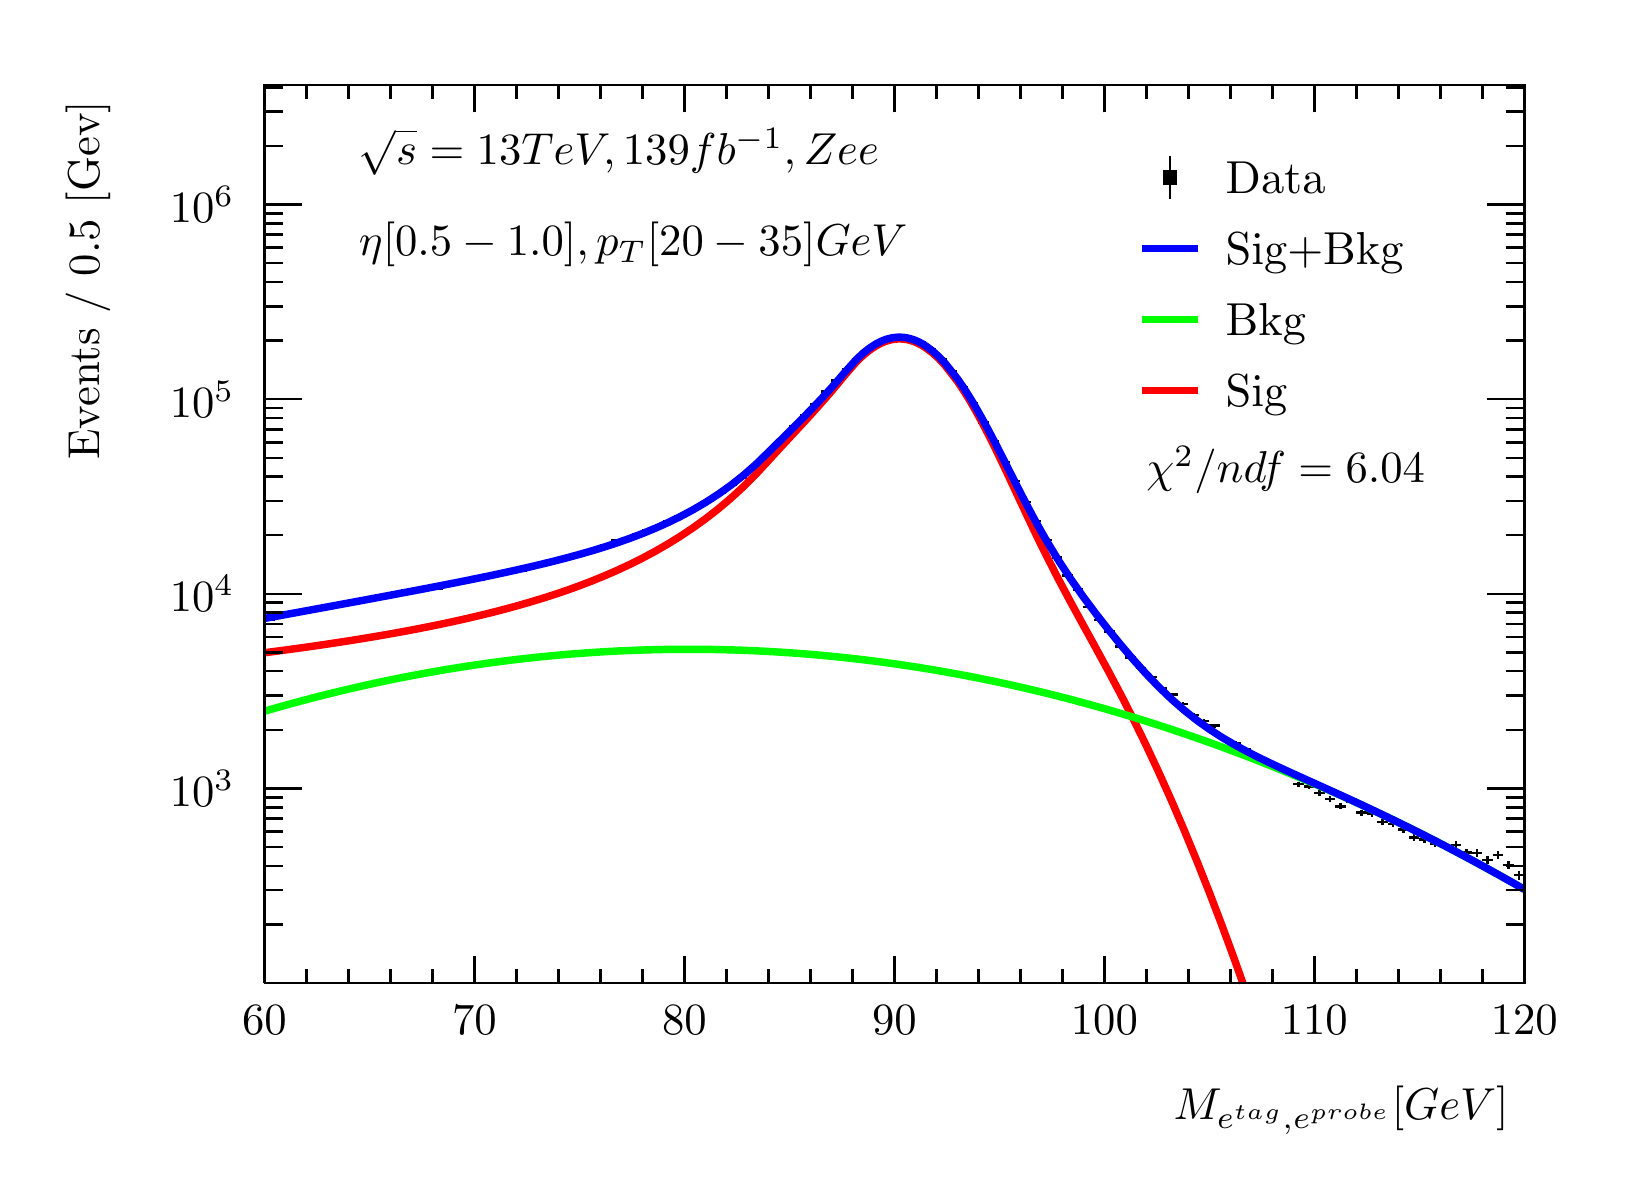
\begin{tikzpicture}
\pgfdeclareplotmark{cross} {
\pgfpathmoveto{\pgfpoint{-0.3\pgfplotmarksize}{\pgfplotmarksize}}
\pgfpathlineto{\pgfpoint{+0.3\pgfplotmarksize}{\pgfplotmarksize}}
\pgfpathlineto{\pgfpoint{+0.3\pgfplotmarksize}{0.3\pgfplotmarksize}}
\pgfpathlineto{\pgfpoint{+1\pgfplotmarksize}{0.3\pgfplotmarksize}}
\pgfpathlineto{\pgfpoint{+1\pgfplotmarksize}{-0.3\pgfplotmarksize}}
\pgfpathlineto{\pgfpoint{+0.3\pgfplotmarksize}{-0.3\pgfplotmarksize}}
\pgfpathlineto{\pgfpoint{+0.3\pgfplotmarksize}{-1.\pgfplotmarksize}}
\pgfpathlineto{\pgfpoint{-0.3\pgfplotmarksize}{-1.\pgfplotmarksize}}
\pgfpathlineto{\pgfpoint{-0.3\pgfplotmarksize}{-0.3\pgfplotmarksize}}
\pgfpathlineto{\pgfpoint{-1.\pgfplotmarksize}{-0.3\pgfplotmarksize}}
\pgfpathlineto{\pgfpoint{-1.\pgfplotmarksize}{0.3\pgfplotmarksize}}
\pgfpathlineto{\pgfpoint{-0.3\pgfplotmarksize}{0.3\pgfplotmarksize}}
\pgfpathclose
\pgfusepathqstroke
}
\pgfdeclareplotmark{cross*} {
\pgfpathmoveto{\pgfpoint{-0.3\pgfplotmarksize}{\pgfplotmarksize}}
\pgfpathlineto{\pgfpoint{+0.3\pgfplotmarksize}{\pgfplotmarksize}}
\pgfpathlineto{\pgfpoint{+0.3\pgfplotmarksize}{0.3\pgfplotmarksize}}
\pgfpathlineto{\pgfpoint{+1\pgfplotmarksize}{0.3\pgfplotmarksize}}
\pgfpathlineto{\pgfpoint{+1\pgfplotmarksize}{-0.3\pgfplotmarksize}}
\pgfpathlineto{\pgfpoint{+0.3\pgfplotmarksize}{-0.3\pgfplotmarksize}}
\pgfpathlineto{\pgfpoint{+0.3\pgfplotmarksize}{-1.\pgfplotmarksize}}
\pgfpathlineto{\pgfpoint{-0.3\pgfplotmarksize}{-1.\pgfplotmarksize}}
\pgfpathlineto{\pgfpoint{-0.3\pgfplotmarksize}{-0.3\pgfplotmarksize}}
\pgfpathlineto{\pgfpoint{-1.\pgfplotmarksize}{-0.3\pgfplotmarksize}}
\pgfpathlineto{\pgfpoint{-1.\pgfplotmarksize}{0.3\pgfplotmarksize}}
\pgfpathlineto{\pgfpoint{-0.3\pgfplotmarksize}{0.3\pgfplotmarksize}}
\pgfpathclose
\pgfusepathqfillstroke
}
\pgfdeclareplotmark{newstar} {
\pgfpathmoveto{\pgfqpoint{0pt}{\pgfplotmarksize}}
\pgfpathlineto{\pgfqpointpolar{44}{0.5\pgfplotmarksize}}
\pgfpathlineto{\pgfqpointpolar{18}{\pgfplotmarksize}}
\pgfpathlineto{\pgfqpointpolar{-20}{0.5\pgfplotmarksize}}
\pgfpathlineto{\pgfqpointpolar{-54}{\pgfplotmarksize}}
\pgfpathlineto{\pgfqpointpolar{-90}{0.5\pgfplotmarksize}}
\pgfpathlineto{\pgfqpointpolar{234}{\pgfplotmarksize}}
\pgfpathlineto{\pgfqpointpolar{198}{0.5\pgfplotmarksize}}
\pgfpathlineto{\pgfqpointpolar{162}{\pgfplotmarksize}}
\pgfpathlineto{\pgfqpointpolar{134}{0.5\pgfplotmarksize}}
\pgfpathclose
\pgfusepathqstroke
}
\pgfdeclareplotmark{newstar*} {
\pgfpathmoveto{\pgfqpoint{0pt}{\pgfplotmarksize}}
\pgfpathlineto{\pgfqpointpolar{44}{0.5\pgfplotmarksize}}
\pgfpathlineto{\pgfqpointpolar{18}{\pgfplotmarksize}}
\pgfpathlineto{\pgfqpointpolar{-20}{0.5\pgfplotmarksize}}
\pgfpathlineto{\pgfqpointpolar{-54}{\pgfplotmarksize}}
\pgfpathlineto{\pgfqpointpolar{-90}{0.5\pgfplotmarksize}}
\pgfpathlineto{\pgfqpointpolar{234}{\pgfplotmarksize}}
\pgfpathlineto{\pgfqpointpolar{198}{0.5\pgfplotmarksize}}
\pgfpathlineto{\pgfqpointpolar{162}{\pgfplotmarksize}}
\pgfpathlineto{\pgfqpointpolar{134}{0.5\pgfplotmarksize}}
\pgfpathclose
\pgfusepathqfillstroke
}
\definecolor{c}{rgb}{1,1,1};
\draw [color=c, fill=c] (0,0) rectangle (20,14.4361);
\draw [color=c, fill=c] (3,2.30977) rectangle (19,13.7143);
\definecolor{c}{rgb}{0,0,0};
\draw [c,line width=0.9] (3,2.30977) -- (3,13.7143) -- (19,13.7143) -- (19,2.30977) -- (3,2.30977);
\definecolor{c}{rgb}{1,1,1};
\draw [color=c, fill=c] (3,2.30977) rectangle (19,13.7143);
\definecolor{c}{rgb}{0,0,0};
\draw [c,line width=0.9] (3,2.30977) -- (3,13.7143) -- (19,13.7143) -- (19,2.30977) -- (3,2.30977);
\draw [c,line width=0.9] (3,2.30977) -- (19,2.30977);
\draw [c,line width=0.9] (3,2.65624) -- (3,2.30977);
\draw [c,line width=0.9] (3.53333,2.48301) -- (3.53333,2.30977);
\draw [c,line width=0.9] (4.06667,2.48301) -- (4.06667,2.30977);
\draw [c,line width=0.9] (4.6,2.48301) -- (4.6,2.30977);
\draw [c,line width=0.9] (5.13333,2.48301) -- (5.13333,2.30977);
\draw [c,line width=0.9] (5.66667,2.65624) -- (5.66667,2.30977);
\draw [c,line width=0.9] (6.2,2.48301) -- (6.2,2.30977);
\draw [c,line width=0.9] (6.73333,2.48301) -- (6.73333,2.30977);
\draw [c,line width=0.9] (7.26667,2.48301) -- (7.26667,2.30977);
\draw [c,line width=0.9] (7.8,2.48301) -- (7.8,2.30977);
\draw [c,line width=0.9] (8.33333,2.65624) -- (8.33333,2.30977);
\draw [c,line width=0.9] (8.86667,2.48301) -- (8.86667,2.30977);
\draw [c,line width=0.9] (9.4,2.48301) -- (9.4,2.30977);
\draw [c,line width=0.9] (9.93333,2.48301) -- (9.93333,2.30977);
\draw [c,line width=0.9] (10.4667,2.48301) -- (10.4667,2.30977);
\draw [c,line width=0.9] (11,2.65624) -- (11,2.30977);
\draw [c,line width=0.9] (11.5333,2.48301) -- (11.5333,2.30977);
\draw [c,line width=0.9] (12.0667,2.48301) -- (12.0667,2.30977);
\draw [c,line width=0.9] (12.6,2.48301) -- (12.6,2.30977);
\draw [c,line width=0.9] (13.1333,2.48301) -- (13.1333,2.30977);
\draw [c,line width=0.9] (13.6667,2.65624) -- (13.6667,2.30977);
\draw [c,line width=0.9] (14.2,2.48301) -- (14.2,2.30977);
\draw [c,line width=0.9] (14.7333,2.48301) -- (14.7333,2.30977);
\draw [c,line width=0.9] (15.2667,2.48301) -- (15.2667,2.30977);
\draw [c,line width=0.9] (15.8,2.48301) -- (15.8,2.30977);
\draw [c,line width=0.9] (16.3333,2.65624) -- (16.3333,2.30977);
\draw [c,line width=0.9] (16.8667,2.48301) -- (16.8667,2.30977);
\draw [c,line width=0.9] (17.4,2.48301) -- (17.4,2.30977);
\draw [c,line width=0.9] (17.9333,2.48301) -- (17.9333,2.30977);
\draw [c,line width=0.9] (18.4667,2.48301) -- (18.4667,2.30977);
\draw [c,line width=0.9] (19,2.65624) -- (19,2.30977);
\draw [anchor=base] (3,1.66015) node[scale=1.61424, color=c, rotate=0]{60};
\draw [anchor=base] (5.66667,1.66015) node[scale=1.61424, color=c, rotate=0]{70};
\draw [anchor=base] (8.33333,1.66015) node[scale=1.61424, color=c, rotate=0]{80};
\draw [anchor=base] (11,1.66015) node[scale=1.61424, color=c, rotate=0]{90};
\draw [anchor=base] (13.6667,1.66015) node[scale=1.61424, color=c, rotate=0]{100};
\draw [anchor=base] (16.3333,1.66015) node[scale=1.61424, color=c, rotate=0]{110};
\draw [anchor=base] (19,1.66015) node[scale=1.61424, color=c, rotate=0]{120};
\draw [anchor= east] (19,0.692932) node[scale=1.61424, color=c, rotate=0]{$M_{e^{tag}, e^{probe}}  [GeV]$};
\draw [c,line width=0.9] (3,13.7143) -- (19,13.7143);
\draw [c,line width=0.9] (3,13.3678) -- (3,13.7143);
\draw [c,line width=0.9] (3.53333,13.5411) -- (3.53333,13.7143);
\draw [c,line width=0.9] (4.06667,13.5411) -- (4.06667,13.7143);
\draw [c,line width=0.9] (4.6,13.5411) -- (4.6,13.7143);
\draw [c,line width=0.9] (5.13333,13.5411) -- (5.13333,13.7143);
\draw [c,line width=0.9] (5.66667,13.3678) -- (5.66667,13.7143);
\draw [c,line width=0.9] (6.2,13.5411) -- (6.2,13.7143);
\draw [c,line width=0.9] (6.73333,13.5411) -- (6.73333,13.7143);
\draw [c,line width=0.9] (7.26667,13.5411) -- (7.26667,13.7143);
\draw [c,line width=0.9] (7.8,13.5411) -- (7.8,13.7143);
\draw [c,line width=0.9] (8.33333,13.3678) -- (8.33333,13.7143);
\draw [c,line width=0.9] (8.86667,13.5411) -- (8.86667,13.7143);
\draw [c,line width=0.9] (9.4,13.5411) -- (9.4,13.7143);
\draw [c,line width=0.9] (9.93333,13.5411) -- (9.93333,13.7143);
\draw [c,line width=0.9] (10.4667,13.5411) -- (10.4667,13.7143);
\draw [c,line width=0.9] (11,13.3678) -- (11,13.7143);
\draw [c,line width=0.9] (11.5333,13.5411) -- (11.5333,13.7143);
\draw [c,line width=0.9] (12.0667,13.5411) -- (12.0667,13.7143);
\draw [c,line width=0.9] (12.6,13.5411) -- (12.6,13.7143);
\draw [c,line width=0.9] (13.1333,13.5411) -- (13.1333,13.7143);
\draw [c,line width=0.9] (13.6667,13.3678) -- (13.6667,13.7143);
\draw [c,line width=0.9] (14.2,13.5411) -- (14.2,13.7143);
\draw [c,line width=0.9] (14.7333,13.5411) -- (14.7333,13.7143);
\draw [c,line width=0.9] (15.2667,13.5411) -- (15.2667,13.7143);
\draw [c,line width=0.9] (15.8,13.5411) -- (15.8,13.7143);
\draw [c,line width=0.9] (16.3333,13.3678) -- (16.3333,13.7143);
\draw [c,line width=0.9] (16.8667,13.5411) -- (16.8667,13.7143);
\draw [c,line width=0.9] (17.4,13.5411) -- (17.4,13.7143);
\draw [c,line width=0.9] (17.9333,13.5411) -- (17.9333,13.7143);
\draw [c,line width=0.9] (18.4667,13.5411) -- (18.4667,13.7143);
\draw [c,line width=0.9] (19,13.3678) -- (19,13.7143);
\draw [c,line width=0.9] (3,2.30977) -- (3,13.7143);
\draw [c,line width=0.9] (3.237,3.05385) -- (3,3.05385);
\draw [c,line width=0.9] (3.237,3.48911) -- (3,3.48911);
\draw [c,line width=0.9] (3.237,3.79793) -- (3,3.79793);
\draw [c,line width=0.9] (3.237,4.03747) -- (3,4.03747);
\draw [c,line width=0.9] (3.237,4.23319) -- (3,4.23319);
\draw [c,line width=0.9] (3.237,4.39867) -- (3,4.39867);
\draw [c,line width=0.9] (3.237,4.54201) -- (3,4.54201);
\draw [c,line width=0.9] (3.237,4.66845) -- (3,4.66845);
\draw [c,line width=0.9] (3.474,4.78155) -- (3,4.78155);
\draw [anchor= east] (2.82,4.78155) node[scale=1.61424, color=c, rotate=0]{$10^{3}$};
\draw [c,line width=0.9] (3.237,5.52563) -- (3,5.52563);
\draw [c,line width=0.9] (3.237,5.96089) -- (3,5.96089);
\draw [c,line width=0.9] (3.237,6.26971) -- (3,6.26971);
\draw [c,line width=0.9] (3.237,6.50925) -- (3,6.50925);
\draw [c,line width=0.9] (3.237,6.70497) -- (3,6.70497);
\draw [c,line width=0.9] (3.237,6.87045) -- (3,6.87045);
\draw [c,line width=0.9] (3.237,7.01379) -- (3,7.01379);
\draw [c,line width=0.9] (3.237,7.14023) -- (3,7.14023);
\draw [c,line width=0.9] (3.474,7.25333) -- (3,7.25333);
\draw [anchor= east] (2.82,7.25333) node[scale=1.61424, color=c, rotate=0]{$10^{4}$};
\draw [c,line width=0.9] (3.237,7.99741) -- (3,7.99741);
\draw [c,line width=0.9] (3.237,8.43267) -- (3,8.43267);
\draw [c,line width=0.9] (3.237,8.74149) -- (3,8.74149);
\draw [c,line width=0.9] (3.237,8.98103) -- (3,8.98103);
\draw [c,line width=0.9] (3.237,9.17675) -- (3,9.17675);
\draw [c,line width=0.9] (3.237,9.34223) -- (3,9.34223);
\draw [c,line width=0.9] (3.237,9.48557) -- (3,9.48557);
\draw [c,line width=0.9] (3.237,9.61201) -- (3,9.61201);
\draw [c,line width=0.9] (3.474,9.72511) -- (3,9.72511);
\draw [anchor= east] (2.82,9.72511) node[scale=1.61424, color=c, rotate=0]{$10^{5}$};
\draw [c,line width=0.9] (3.237,10.4692) -- (3,10.4692);
\draw [c,line width=0.9] (3.237,10.9044) -- (3,10.9044);
\draw [c,line width=0.9] (3.237,11.2133) -- (3,11.2133);
\draw [c,line width=0.9] (3.237,11.4528) -- (3,11.4528);
\draw [c,line width=0.9] (3.237,11.6485) -- (3,11.6485);
\draw [c,line width=0.9] (3.237,11.814) -- (3,11.814);
\draw [c,line width=0.9] (3.237,11.9574) -- (3,11.9574);
\draw [c,line width=0.9] (3.237,12.0838) -- (3,12.0838);
\draw [c,line width=0.9] (3.474,12.1969) -- (3,12.1969);
\draw [anchor= east] (2.82,12.1969) node[scale=1.61424, color=c, rotate=0]{$10^{6}$};
\draw [c,line width=0.9] (3.237,12.941) -- (3,12.941);
\draw [c,line width=0.9] (3.237,13.3762) -- (3,13.3762);
\draw [c,line width=0.9] (3.237,13.6851) -- (3,13.6851);
\draw [anchor= east] (0.76,13.7143) node[scale=1.61424, color=c, rotate=90]{Events / 0.5 [Gev]};
\draw [c,line width=0.9] (19,2.30977) -- (19,13.7143);
\draw [c,line width=0.9] (18.763,3.05385) -- (19,3.05385);
\draw [c,line width=0.9] (18.763,3.48911) -- (19,3.48911);
\draw [c,line width=0.9] (18.763,3.79793) -- (19,3.79793);
\draw [c,line width=0.9] (18.763,4.03747) -- (19,4.03747);
\draw [c,line width=0.9] (18.763,4.23319) -- (19,4.23319);
\draw [c,line width=0.9] (18.763,4.39867) -- (19,4.39867);
\draw [c,line width=0.9] (18.763,4.54201) -- (19,4.54201);
\draw [c,line width=0.9] (18.763,4.66845) -- (19,4.66845);
\draw [c,line width=0.9] (18.526,4.78155) -- (19,4.78155);
\draw [c,line width=0.9] (18.763,5.52563) -- (19,5.52563);
\draw [c,line width=0.9] (18.763,5.96089) -- (19,5.96089);
\draw [c,line width=0.9] (18.763,6.26971) -- (19,6.26971);
\draw [c,line width=0.9] (18.763,6.50925) -- (19,6.50925);
\draw [c,line width=0.9] (18.763,6.70497) -- (19,6.70497);
\draw [c,line width=0.9] (18.763,6.87045) -- (19,6.87045);
\draw [c,line width=0.9] (18.763,7.01379) -- (19,7.01379);
\draw [c,line width=0.9] (18.763,7.14023) -- (19,7.14023);
\draw [c,line width=0.9] (18.526,7.25333) -- (19,7.25333);
\draw [c,line width=0.9] (18.763,7.99741) -- (19,7.99741);
\draw [c,line width=0.9] (18.763,8.43267) -- (19,8.43267);
\draw [c,line width=0.9] (18.763,8.74149) -- (19,8.74149);
\draw [c,line width=0.9] (18.763,8.98103) -- (19,8.98103);
\draw [c,line width=0.9] (18.763,9.17675) -- (19,9.17675);
\draw [c,line width=0.9] (18.763,9.34223) -- (19,9.34223);
\draw [c,line width=0.9] (18.763,9.48557) -- (19,9.48557);
\draw [c,line width=0.9] (18.763,9.61201) -- (19,9.61201);
\draw [c,line width=0.9] (18.526,9.72511) -- (19,9.72511);
\draw [c,line width=0.9] (18.763,10.4692) -- (19,10.4692);
\draw [c,line width=0.9] (18.763,10.9044) -- (19,10.9044);
\draw [c,line width=0.9] (18.763,11.2133) -- (19,11.2133);
\draw [c,line width=0.9] (18.763,11.4528) -- (19,11.4528);
\draw [c,line width=0.9] (18.763,11.6485) -- (19,11.6485);
\draw [c,line width=0.9] (18.763,11.814) -- (19,11.814);
\draw [c,line width=0.9] (18.763,11.9574) -- (19,11.9574);
\draw [c,line width=0.9] (18.763,12.0838) -- (19,12.0838);
\draw [c,line width=0.9] (18.526,12.1969) -- (19,12.1969);
\draw [c,line width=0.9] (18.763,12.941) -- (19,12.941);
\draw [c,line width=0.9] (18.763,13.3762) -- (19,13.3762);
\draw [c,line width=0.9] (18.763,13.6851) -- (19,13.6851);
\draw [c,line width=0.9] (3.06667,6.92297) -- (3,6.92297);
\draw [c,line width=0.9] (3,6.92297) -- (3,6.92297);
\draw [c,line width=0.9] (3.06667,6.92297) -- (3.13333,6.92297);
\draw [c,line width=0.9] (3.13333,6.92297) -- (3.13333,6.92297);
\draw [c,line width=0.9] (3.06667,6.92297) -- (3.06667,6.93549);
\draw [c,line width=0.9] (3.06667,6.93549) -- (3.06667,6.93549);
\draw [c,line width=0.9] (3.06667,6.92297) -- (3.06667,6.91045);
\draw [c,line width=0.9] (3.06667,6.91045) -- (3.06667,6.91045);
\draw [c,line width=0.9] (3.2,6.95788) -- (3.13333,6.95788);
\draw [c,line width=0.9] (3.13333,6.95788) -- (3.13333,6.95788);
\draw [c,line width=0.9] (3.2,6.95788) -- (3.26667,6.95788);
\draw [c,line width=0.9] (3.26667,6.95788) -- (3.26667,6.95788);
\draw [c,line width=0.9] (3.2,6.95788) -- (3.2,6.9702);
\draw [c,line width=0.9] (3.2,6.9702) -- (3.2,6.9702);
\draw [c,line width=0.9] (3.2,6.95788) -- (3.2,6.94556);
\draw [c,line width=0.9] (3.2,6.94556) -- (3.2,6.94556);
\draw [c,line width=0.9] (3.33333,7.003) -- (3.26667,7.003);
\draw [c,line width=0.9] (3.26667,7.003) -- (3.26667,7.003);
\draw [c,line width=0.9] (3.33333,7.003) -- (3.4,7.003);
\draw [c,line width=0.9] (3.4,7.003) -- (3.4,7.003);
\draw [c,line width=0.9] (3.33333,7.003) -- (3.33333,7.01507);
\draw [c,line width=0.9] (3.33333,7.01507) -- (3.33333,7.01507);
\draw [c,line width=0.9] (3.33333,7.003) -- (3.33333,6.99094);
\draw [c,line width=0.9] (3.33333,6.99094) -- (3.33333,6.99094);
\draw [c,line width=0.9] (3.46667,7.03281) -- (3.4,7.03281);
\draw [c,line width=0.9] (3.4,7.03281) -- (3.4,7.03281);
\draw [c,line width=0.9] (3.46667,7.03281) -- (3.53333,7.03281);
\draw [c,line width=0.9] (3.53333,7.03281) -- (3.53333,7.03281);
\draw [c,line width=0.9] (3.46667,7.03281) -- (3.46667,7.04471);
\draw [c,line width=0.9] (3.46667,7.04471) -- (3.46667,7.04471);
\draw [c,line width=0.9] (3.46667,7.03281) -- (3.46667,7.02092);
\draw [c,line width=0.9] (3.46667,7.02092) -- (3.46667,7.02092);
\draw [c,line width=0.9] (3.6,7.04748) -- (3.53333,7.04748);
\draw [c,line width=0.9] (3.53333,7.04748) -- (3.53333,7.04748);
\draw [c,line width=0.9] (3.6,7.04748) -- (3.66667,7.04748);
\draw [c,line width=0.9] (3.66667,7.04748) -- (3.66667,7.04748);
\draw [c,line width=0.9] (3.6,7.04748) -- (3.6,7.05929);
\draw [c,line width=0.9] (3.6,7.05929) -- (3.6,7.05929);
\draw [c,line width=0.9] (3.6,7.04748) -- (3.6,7.03566);
\draw [c,line width=0.9] (3.6,7.03566) -- (3.6,7.03566);
\draw [c,line width=0.9] (3.73333,7.06872) -- (3.66667,7.06872);
\draw [c,line width=0.9] (3.66667,7.06872) -- (3.66667,7.06872);
\draw [c,line width=0.9] (3.73333,7.06872) -- (3.8,7.06872);
\draw [c,line width=0.9] (3.8,7.06872) -- (3.8,7.06872);
\draw [c,line width=0.9] (3.73333,7.06872) -- (3.73333,7.08042);
\draw [c,line width=0.9] (3.73333,7.08042) -- (3.73333,7.08042);
\draw [c,line width=0.9] (3.73333,7.06872) -- (3.73333,7.05702);
\draw [c,line width=0.9] (3.73333,7.05702) -- (3.73333,7.05702);
\draw [c,line width=0.9] (3.86667,7.12207) -- (3.8,7.12207);
\draw [c,line width=0.9] (3.8,7.12207) -- (3.8,7.12207);
\draw [c,line width=0.9] (3.86667,7.12207) -- (3.93333,7.12207);
\draw [c,line width=0.9] (3.93333,7.12207) -- (3.93333,7.12207);
\draw [c,line width=0.9] (3.86667,7.12207) -- (3.86667,7.13348);
\draw [c,line width=0.9] (3.86667,7.13348) -- (3.86667,7.13348);
\draw [c,line width=0.9] (3.86667,7.12207) -- (3.86667,7.11066);
\draw [c,line width=0.9] (3.86667,7.11066) -- (3.86667,7.11066);
\draw [c,line width=0.9] (4,7.13856) -- (3.93333,7.13856);
\draw [c,line width=0.9] (3.93333,7.13856) -- (3.93333,7.13856);
\draw [c,line width=0.9] (4,7.13856) -- (4.06667,7.13856);
\draw [c,line width=0.9] (4.06667,7.13856) -- (4.06667,7.13856);
\draw [c,line width=0.9] (4,7.13856) -- (4,7.14988);
\draw [c,line width=0.9] (4,7.14988) -- (4,7.14988);
\draw [c,line width=0.9] (4,7.13856) -- (4,7.12723);
\draw [c,line width=0.9] (4,7.12723) -- (4,7.12723);
\draw [c,line width=0.9] (4.13333,7.16709) -- (4.06667,7.16709);
\draw [c,line width=0.9] (4.06667,7.16709) -- (4.06667,7.16709);
\draw [c,line width=0.9] (4.13333,7.16709) -- (4.2,7.16709);
\draw [c,line width=0.9] (4.2,7.16709) -- (4.2,7.16709);
\draw [c,line width=0.9] (4.13333,7.16709) -- (4.13333,7.17826);
\draw [c,line width=0.9] (4.13333,7.17826) -- (4.13333,7.17826);
\draw [c,line width=0.9] (4.13333,7.16709) -- (4.13333,7.15591);
\draw [c,line width=0.9] (4.13333,7.15591) -- (4.13333,7.15591);
\draw [c,line width=0.9] (4.26667,7.1909) -- (4.2,7.1909);
\draw [c,line width=0.9] (4.2,7.1909) -- (4.2,7.1909);
\draw [c,line width=0.9] (4.26667,7.1909) -- (4.33333,7.1909);
\draw [c,line width=0.9] (4.33333,7.1909) -- (4.33333,7.1909);
\draw [c,line width=0.9] (4.26667,7.1909) -- (4.26667,7.20195);
\draw [c,line width=0.9] (4.26667,7.20195) -- (4.26667,7.20195);
\draw [c,line width=0.9] (4.26667,7.1909) -- (4.26667,7.17985);
\draw [c,line width=0.9] (4.26667,7.17985) -- (4.26667,7.17985);
\draw [c,line width=0.9] (4.4,7.19782) -- (4.33333,7.19782);
\draw [c,line width=0.9] (4.33333,7.19782) -- (4.33333,7.19782);
\draw [c,line width=0.9] (4.4,7.19782) -- (4.46667,7.19782);
\draw [c,line width=0.9] (4.46667,7.19782) -- (4.46667,7.19782);
\draw [c,line width=0.9] (4.4,7.19782) -- (4.4,7.20883);
\draw [c,line width=0.9] (4.4,7.20883) -- (4.4,7.20883);
\draw [c,line width=0.9] (4.4,7.19782) -- (4.4,7.1868);
\draw [c,line width=0.9] (4.4,7.1868) -- (4.4,7.1868);
\draw [c,line width=0.9] (4.53333,7.24092) -- (4.46667,7.24092);
\draw [c,line width=0.9] (4.46667,7.24092) -- (4.46667,7.24092);
\draw [c,line width=0.9] (4.53333,7.24092) -- (4.6,7.24092);
\draw [c,line width=0.9] (4.6,7.24092) -- (4.6,7.24092);
\draw [c,line width=0.9] (4.53333,7.24092) -- (4.53333,7.25171);
\draw [c,line width=0.9] (4.53333,7.25171) -- (4.53333,7.25171);
\draw [c,line width=0.9] (4.53333,7.24092) -- (4.53333,7.23012);
\draw [c,line width=0.9] (4.53333,7.23012) -- (4.53333,7.23012);
\draw [c,line width=0.9] (4.66667,7.25194) -- (4.6,7.25194);
\draw [c,line width=0.9] (4.6,7.25194) -- (4.6,7.25194);
\draw [c,line width=0.9] (4.66667,7.25194) -- (4.73333,7.25194);
\draw [c,line width=0.9] (4.73333,7.25194) -- (4.73333,7.25194);
\draw [c,line width=0.9] (4.66667,7.25194) -- (4.66667,7.26268);
\draw [c,line width=0.9] (4.66667,7.26268) -- (4.66667,7.26268);
\draw [c,line width=0.9] (4.66667,7.25194) -- (4.66667,7.24119);
\draw [c,line width=0.9] (4.66667,7.24119) -- (4.66667,7.24119);
\draw [c,line width=0.9] (4.8,7.30202) -- (4.73333,7.30202);
\draw [c,line width=0.9] (4.73333,7.30202) -- (4.73333,7.30202);
\draw [c,line width=0.9] (4.8,7.30202) -- (4.86667,7.30202);
\draw [c,line width=0.9] (4.86667,7.30202) -- (4.86667,7.30202);
\draw [c,line width=0.9] (4.8,7.30202) -- (4.8,7.31252);
\draw [c,line width=0.9] (4.8,7.31252) -- (4.8,7.31252);
\draw [c,line width=0.9] (4.8,7.30202) -- (4.8,7.29153);
\draw [c,line width=0.9] (4.8,7.29153) -- (4.8,7.29153);
\draw [c,line width=0.9] (4.93333,7.31558) -- (4.86667,7.31558);
\draw [c,line width=0.9] (4.86667,7.31558) -- (4.86667,7.31558);
\draw [c,line width=0.9] (4.93333,7.31558) -- (5,7.31558);
\draw [c,line width=0.9] (5,7.31558) -- (5,7.31558);
\draw [c,line width=0.9] (4.93333,7.31558) -- (4.93333,7.32601);
\draw [c,line width=0.9] (4.93333,7.32601) -- (4.93333,7.32601);
\draw [c,line width=0.9] (4.93333,7.31558) -- (4.93333,7.30515);
\draw [c,line width=0.9] (4.93333,7.30515) -- (4.93333,7.30515);
\draw [c,line width=0.9] (5.06667,7.30571) -- (5,7.30571);
\draw [c,line width=0.9] (5,7.30571) -- (5,7.30571);
\draw [c,line width=0.9] (5.06667,7.30571) -- (5.13333,7.30571);
\draw [c,line width=0.9] (5.13333,7.30571) -- (5.13333,7.30571);
\draw [c,line width=0.9] (5.06667,7.30571) -- (5.06667,7.31618);
\draw [c,line width=0.9] (5.06667,7.31618) -- (5.06667,7.31618);
\draw [c,line width=0.9] (5.06667,7.30571) -- (5.06667,7.29523);
\draw [c,line width=0.9] (5.06667,7.29523) -- (5.06667,7.29523);
\draw [c,line width=0.9] (5.2,7.32355) -- (5.13333,7.32355);
\draw [c,line width=0.9] (5.13333,7.32355) -- (5.13333,7.32355);
\draw [c,line width=0.9] (5.2,7.32355) -- (5.26667,7.32355);
\draw [c,line width=0.9] (5.26667,7.32355) -- (5.26667,7.32355);
\draw [c,line width=0.9] (5.2,7.32355) -- (5.2,7.33394);
\draw [c,line width=0.9] (5.2,7.33394) -- (5.2,7.33394);
\draw [c,line width=0.9] (5.2,7.32355) -- (5.2,7.31316);
\draw [c,line width=0.9] (5.2,7.31316) -- (5.2,7.31316);
\draw [c,line width=0.9] (5.33333,7.35643) -- (5.26667,7.35643);
\draw [c,line width=0.9] (5.26667,7.35643) -- (5.26667,7.35643);
\draw [c,line width=0.9] (5.33333,7.35643) -- (5.4,7.35643);
\draw [c,line width=0.9] (5.4,7.35643) -- (5.4,7.35643);
\draw [c,line width=0.9] (5.33333,7.35643) -- (5.33333,7.36666);
\draw [c,line width=0.9] (5.33333,7.36666) -- (5.33333,7.36666);
\draw [c,line width=0.9] (5.33333,7.35643) -- (5.33333,7.3462);
\draw [c,line width=0.9] (5.33333,7.3462) -- (5.33333,7.3462);
\draw [c,line width=0.9] (5.46667,7.38377) -- (5.4,7.38377);
\draw [c,line width=0.9] (5.4,7.38377) -- (5.4,7.38377);
\draw [c,line width=0.9] (5.46667,7.38377) -- (5.53333,7.38377);
\draw [c,line width=0.9] (5.53333,7.38377) -- (5.53333,7.38377);
\draw [c,line width=0.9] (5.46667,7.38377) -- (5.46667,7.39387);
\draw [c,line width=0.9] (5.46667,7.39387) -- (5.46667,7.39387);
\draw [c,line width=0.9] (5.46667,7.38377) -- (5.46667,7.37367);
\draw [c,line width=0.9] (5.46667,7.37367) -- (5.46667,7.37367);
\draw [c,line width=0.9] (5.6,7.40932) -- (5.53333,7.40932);
\draw [c,line width=0.9] (5.53333,7.40932) -- (5.53333,7.40932);
\draw [c,line width=0.9] (5.6,7.40932) -- (5.66667,7.40932);
\draw [c,line width=0.9] (5.66667,7.40932) -- (5.66667,7.40932);
\draw [c,line width=0.9] (5.6,7.40932) -- (5.6,7.4193);
\draw [c,line width=0.9] (5.6,7.4193) -- (5.6,7.4193);
\draw [c,line width=0.9] (5.6,7.40932) -- (5.6,7.39934);
\draw [c,line width=0.9] (5.6,7.39934) -- (5.6,7.39934);
\draw [c,line width=0.9] (5.73333,7.43772) -- (5.66667,7.43772);
\draw [c,line width=0.9] (5.66667,7.43772) -- (5.66667,7.43772);
\draw [c,line width=0.9] (5.73333,7.43772) -- (5.8,7.43772);
\draw [c,line width=0.9] (5.8,7.43772) -- (5.8,7.43772);
\draw [c,line width=0.9] (5.73333,7.43772) -- (5.73333,7.44757);
\draw [c,line width=0.9] (5.73333,7.44757) -- (5.73333,7.44757);
\draw [c,line width=0.9] (5.73333,7.43772) -- (5.73333,7.42787);
\draw [c,line width=0.9] (5.73333,7.42787) -- (5.73333,7.42787);
\draw [c,line width=0.9] (5.86667,7.4711) -- (5.8,7.4711);
\draw [c,line width=0.9] (5.8,7.4711) -- (5.8,7.4711);
\draw [c,line width=0.9] (5.86667,7.4711) -- (5.93333,7.4711);
\draw [c,line width=0.9] (5.93333,7.4711) -- (5.93333,7.4711);
\draw [c,line width=0.9] (5.86667,7.4711) -- (5.86667,7.4808);
\draw [c,line width=0.9] (5.86667,7.4808) -- (5.86667,7.4808);
\draw [c,line width=0.9] (5.86667,7.4711) -- (5.86667,7.4614);
\draw [c,line width=0.9] (5.86667,7.4614) -- (5.86667,7.4614);
\draw [c,line width=0.9] (6,7.49887) -- (5.93333,7.49887);
\draw [c,line width=0.9] (5.93333,7.49887) -- (5.93333,7.49887);
\draw [c,line width=0.9] (6,7.49887) -- (6.06667,7.49887);
\draw [c,line width=0.9] (6.06667,7.49887) -- (6.06667,7.49887);
\draw [c,line width=0.9] (6,7.49887) -- (6,7.50844);
\draw [c,line width=0.9] (6,7.50844) -- (6,7.50844);
\draw [c,line width=0.9] (6,7.49887) -- (6,7.48929);
\draw [c,line width=0.9] (6,7.48929) -- (6,7.48929);
\draw [c,line width=0.9] (6.13333,7.53737) -- (6.06667,7.53737);
\draw [c,line width=0.9] (6.06667,7.53737) -- (6.06667,7.53737);
\draw [c,line width=0.9] (6.13333,7.53737) -- (6.2,7.53737);
\draw [c,line width=0.9] (6.2,7.53737) -- (6.2,7.53737);
\draw [c,line width=0.9] (6.13333,7.53737) -- (6.13333,7.54677);
\draw [c,line width=0.9] (6.13333,7.54677) -- (6.13333,7.54677);
\draw [c,line width=0.9] (6.13333,7.53737) -- (6.13333,7.52796);
\draw [c,line width=0.9] (6.13333,7.52796) -- (6.13333,7.52796);
\draw [c,line width=0.9] (6.26667,7.55169) -- (6.2,7.55169);
\draw [c,line width=0.9] (6.2,7.55169) -- (6.2,7.55169);
\draw [c,line width=0.9] (6.26667,7.55169) -- (6.33333,7.55169);
\draw [c,line width=0.9] (6.33333,7.55169) -- (6.33333,7.55169);
\draw [c,line width=0.9] (6.26667,7.55169) -- (6.26667,7.56103);
\draw [c,line width=0.9] (6.26667,7.56103) -- (6.26667,7.56103);
\draw [c,line width=0.9] (6.26667,7.55169) -- (6.26667,7.54235);
\draw [c,line width=0.9] (6.26667,7.54235) -- (6.26667,7.54235);
\draw [c,line width=0.9] (6.4,7.59901) -- (6.33333,7.59901);
\draw [c,line width=0.9] (6.33333,7.59901) -- (6.33333,7.59901);
\draw [c,line width=0.9] (6.4,7.59901) -- (6.46667,7.59901);
\draw [c,line width=0.9] (6.46667,7.59901) -- (6.46667,7.59901);
\draw [c,line width=0.9] (6.4,7.59901) -- (6.4,7.60814);
\draw [c,line width=0.9] (6.4,7.60814) -- (6.4,7.60814);
\draw [c,line width=0.9] (6.4,7.59901) -- (6.4,7.58987);
\draw [c,line width=0.9] (6.4,7.58987) -- (6.4,7.58987);
\draw [c,line width=0.9] (6.53333,7.6296) -- (6.46667,7.6296);
\draw [c,line width=0.9] (6.46667,7.6296) -- (6.46667,7.6296);
\draw [c,line width=0.9] (6.53333,7.6296) -- (6.6,7.6296);
\draw [c,line width=0.9] (6.6,7.6296) -- (6.6,7.6296);
\draw [c,line width=0.9] (6.53333,7.6296) -- (6.53333,7.63861);
\draw [c,line width=0.9] (6.53333,7.63861) -- (6.53333,7.63861);
\draw [c,line width=0.9] (6.53333,7.6296) -- (6.53333,7.6206);
\draw [c,line width=0.9] (6.53333,7.6206) -- (6.53333,7.6206);
\draw [c,line width=0.9] (6.66667,7.67091) -- (6.6,7.67091);
\draw [c,line width=0.9] (6.6,7.67091) -- (6.6,7.67091);
\draw [c,line width=0.9] (6.66667,7.67091) -- (6.73333,7.67091);
\draw [c,line width=0.9] (6.73333,7.67091) -- (6.73333,7.67091);
\draw [c,line width=0.9] (6.66667,7.67091) -- (6.66667,7.67975);
\draw [c,line width=0.9] (6.66667,7.67975) -- (6.66667,7.67975);
\draw [c,line width=0.9] (6.66667,7.67091) -- (6.66667,7.66208);
\draw [c,line width=0.9] (6.66667,7.66208) -- (6.66667,7.66208);
\draw [c,line width=0.9] (6.8,7.69309) -- (6.73333,7.69309);
\draw [c,line width=0.9] (6.73333,7.69309) -- (6.73333,7.69309);
\draw [c,line width=0.9] (6.8,7.69309) -- (6.86667,7.69309);
\draw [c,line width=0.9] (6.86667,7.69309) -- (6.86667,7.69309);
\draw [c,line width=0.9] (6.8,7.69309) -- (6.8,7.70184);
\draw [c,line width=0.9] (6.8,7.70184) -- (6.8,7.70184);
\draw [c,line width=0.9] (6.8,7.69309) -- (6.8,7.68434);
\draw [c,line width=0.9] (6.8,7.68434) -- (6.8,7.68434);
\draw [c,line width=0.9] (6.93333,7.73324) -- (6.86667,7.73324);
\draw [c,line width=0.9] (6.86667,7.73324) -- (6.86667,7.73324);
\draw [c,line width=0.9] (6.93333,7.73324) -- (7,7.73324);
\draw [c,line width=0.9] (7,7.73324) -- (7,7.73324);
\draw [c,line width=0.9] (6.93333,7.73324) -- (6.93333,7.74182);
\draw [c,line width=0.9] (6.93333,7.74182) -- (6.93333,7.74182);
\draw [c,line width=0.9] (6.93333,7.73324) -- (6.93333,7.72465);
\draw [c,line width=0.9] (6.93333,7.72465) -- (6.93333,7.72465);
\draw [c,line width=0.9] (7.06667,7.76563) -- (7,7.76563);
\draw [c,line width=0.9] (7,7.76563) -- (7,7.76563);
\draw [c,line width=0.9] (7.06667,7.76563) -- (7.13333,7.76563);
\draw [c,line width=0.9] (7.13333,7.76563) -- (7.13333,7.76563);
\draw [c,line width=0.9] (7.06667,7.76563) -- (7.06667,7.77408);
\draw [c,line width=0.9] (7.06667,7.77408) -- (7.06667,7.77408);
\draw [c,line width=0.9] (7.06667,7.76563) -- (7.06667,7.75717);
\draw [c,line width=0.9] (7.06667,7.75717) -- (7.06667,7.75717);
\draw [c,line width=0.9] (7.2,7.8048) -- (7.13333,7.8048);
\draw [c,line width=0.9] (7.13333,7.8048) -- (7.13333,7.8048);
\draw [c,line width=0.9] (7.2,7.8048) -- (7.26667,7.8048);
\draw [c,line width=0.9] (7.26667,7.8048) -- (7.26667,7.8048);
\draw [c,line width=0.9] (7.2,7.8048) -- (7.2,7.81311);
\draw [c,line width=0.9] (7.2,7.81311) -- (7.2,7.81311);
\draw [c,line width=0.9] (7.2,7.8048) -- (7.2,7.7965);
\draw [c,line width=0.9] (7.2,7.7965) -- (7.2,7.7965);
\draw [c,line width=0.9] (7.33333,7.8642) -- (7.26667,7.8642);
\draw [c,line width=0.9] (7.26667,7.8642) -- (7.26667,7.8642);
\draw [c,line width=0.9] (7.33333,7.8642) -- (7.4,7.8642);
\draw [c,line width=0.9] (7.4,7.8642) -- (7.4,7.8642);
\draw [c,line width=0.9] (7.33333,7.8642) -- (7.33333,7.87228);
\draw [c,line width=0.9] (7.33333,7.87228) -- (7.33333,7.87228);
\draw [c,line width=0.9] (7.33333,7.8642) -- (7.33333,7.85613);
\draw [c,line width=0.9] (7.33333,7.85613) -- (7.33333,7.85613);
\draw [c,line width=0.9] (7.46667,7.92739) -- (7.4,7.92739);
\draw [c,line width=0.9] (7.4,7.92739) -- (7.4,7.92739);
\draw [c,line width=0.9] (7.46667,7.92739) -- (7.53333,7.92739);
\draw [c,line width=0.9] (7.53333,7.92739) -- (7.53333,7.92739);
\draw [c,line width=0.9] (7.46667,7.92739) -- (7.46667,7.93523);
\draw [c,line width=0.9] (7.46667,7.93523) -- (7.46667,7.93523);
\draw [c,line width=0.9] (7.46667,7.92739) -- (7.46667,7.91954);
\draw [c,line width=0.9] (7.46667,7.91954) -- (7.46667,7.91954);
\draw [c,line width=0.9] (7.6,7.94843) -- (7.53333,7.94843);
\draw [c,line width=0.9] (7.53333,7.94843) -- (7.53333,7.94843);
\draw [c,line width=0.9] (7.6,7.94843) -- (7.66667,7.94843);
\draw [c,line width=0.9] (7.66667,7.94843) -- (7.66667,7.94843);
\draw [c,line width=0.9] (7.6,7.94843) -- (7.6,7.9562);
\draw [c,line width=0.9] (7.6,7.9562) -- (7.6,7.9562);
\draw [c,line width=0.9] (7.6,7.94843) -- (7.6,7.94067);
\draw [c,line width=0.9] (7.6,7.94067) -- (7.6,7.94067);
\draw [c,line width=0.9] (7.73333,8.00655) -- (7.66667,8.00655);
\draw [c,line width=0.9] (7.66667,8.00655) -- (7.66667,8.00655);
\draw [c,line width=0.9] (7.73333,8.00655) -- (7.8,8.00655);
\draw [c,line width=0.9] (7.8,8.00655) -- (7.8,8.00655);
\draw [c,line width=0.9] (7.73333,8.00655) -- (7.73333,8.01411);
\draw [c,line width=0.9] (7.73333,8.01411) -- (7.73333,8.01411);
\draw [c,line width=0.9] (7.73333,8.00655) -- (7.73333,7.99899);
\draw [c,line width=0.9] (7.73333,7.99899) -- (7.73333,7.99899);
\draw [c,line width=0.9] (7.86667,8.05702) -- (7.8,8.05702);
\draw [c,line width=0.9] (7.8,8.05702) -- (7.8,8.05702);
\draw [c,line width=0.9] (7.86667,8.05702) -- (7.93333,8.05702);
\draw [c,line width=0.9] (7.93333,8.05702) -- (7.93333,8.05702);
\draw [c,line width=0.9] (7.86667,8.05702) -- (7.86667,8.0644);
\draw [c,line width=0.9] (7.86667,8.0644) -- (7.86667,8.0644);
\draw [c,line width=0.9] (7.86667,8.05702) -- (7.86667,8.04964);
\draw [c,line width=0.9] (7.86667,8.04964) -- (7.86667,8.04964);
\draw [c,line width=0.9] (8,8.11619) -- (7.93333,8.11619);
\draw [c,line width=0.9] (7.93333,8.11619) -- (7.93333,8.11619);
\draw [c,line width=0.9] (8,8.11619) -- (8.06667,8.11619);
\draw [c,line width=0.9] (8.06667,8.11619) -- (8.06667,8.11619);
\draw [c,line width=0.9] (8,8.11619) -- (8,8.12337);
\draw [c,line width=0.9] (8,8.12337) -- (8,8.12337);
\draw [c,line width=0.9] (8,8.11619) -- (8,8.10901);
\draw [c,line width=0.9] (8,8.10901) -- (8,8.10901);
\draw [c,line width=0.9] (8.13333,8.17559) -- (8.06667,8.17559);
\draw [c,line width=0.9] (8.06667,8.17559) -- (8.06667,8.17559);
\draw [c,line width=0.9] (8.13333,8.17559) -- (8.2,8.17559);
\draw [c,line width=0.9] (8.2,8.17559) -- (8.2,8.17559);
\draw [c,line width=0.9] (8.13333,8.17559) -- (8.13333,8.18258);
\draw [c,line width=0.9] (8.13333,8.18258) -- (8.13333,8.18258);
\draw [c,line width=0.9] (8.13333,8.17559) -- (8.13333,8.1686);
\draw [c,line width=0.9] (8.13333,8.1686) -- (8.13333,8.1686);
\draw [c,line width=0.9] (8.26667,8.23803) -- (8.2,8.23803);
\draw [c,line width=0.9] (8.2,8.23803) -- (8.2,8.23803);
\draw [c,line width=0.9] (8.26667,8.23803) -- (8.33333,8.23803);
\draw [c,line width=0.9] (8.33333,8.23803) -- (8.33333,8.23803);
\draw [c,line width=0.9] (8.26667,8.23803) -- (8.26667,8.24481);
\draw [c,line width=0.9] (8.26667,8.24481) -- (8.26667,8.24481);
\draw [c,line width=0.9] (8.26667,8.23803) -- (8.26667,8.23124);
\draw [c,line width=0.9] (8.26667,8.23124) -- (8.26667,8.23124);
\draw [c,line width=0.9] (8.4,8.29853) -- (8.33333,8.29853);
\draw [c,line width=0.9] (8.33333,8.29853) -- (8.33333,8.29853);
\draw [c,line width=0.9] (8.4,8.29853) -- (8.46667,8.29853);
\draw [c,line width=0.9] (8.46667,8.29853) -- (8.46667,8.29853);
\draw [c,line width=0.9] (8.4,8.29853) -- (8.4,8.30513);
\draw [c,line width=0.9] (8.4,8.30513) -- (8.4,8.30513);
\draw [c,line width=0.9] (8.4,8.29853) -- (8.4,8.29193);
\draw [c,line width=0.9] (8.4,8.29193) -- (8.4,8.29193);
\draw [c,line width=0.9] (8.53333,8.37501) -- (8.46667,8.37501);
\draw [c,line width=0.9] (8.46667,8.37501) -- (8.46667,8.37501);
\draw [c,line width=0.9] (8.53333,8.37501) -- (8.6,8.37501);
\draw [c,line width=0.9] (8.6,8.37501) -- (8.6,8.37501);
\draw [c,line width=0.9] (8.53333,8.37501) -- (8.53333,8.38137);
\draw [c,line width=0.9] (8.53333,8.38137) -- (8.53333,8.38137);
\draw [c,line width=0.9] (8.53333,8.37501) -- (8.53333,8.36864);
\draw [c,line width=0.9] (8.53333,8.36864) -- (8.53333,8.36864);
\draw [c,line width=0.9] (8.66667,8.45977) -- (8.6,8.45977);
\draw [c,line width=0.9] (8.6,8.45977) -- (8.6,8.45977);
\draw [c,line width=0.9] (8.66667,8.45977) -- (8.73333,8.45977);
\draw [c,line width=0.9] (8.73333,8.45977) -- (8.73333,8.45977);
\draw [c,line width=0.9] (8.66667,8.45977) -- (8.66667,8.46589);
\draw [c,line width=0.9] (8.66667,8.46589) -- (8.66667,8.46589);
\draw [c,line width=0.9] (8.66667,8.45977) -- (8.66667,8.45365);
\draw [c,line width=0.9] (8.66667,8.45365) -- (8.66667,8.45365);
\draw [c,line width=0.9] (8.8,8.54221) -- (8.73333,8.54221);
\draw [c,line width=0.9] (8.73333,8.54221) -- (8.73333,8.54221);
\draw [c,line width=0.9] (8.8,8.54221) -- (8.86667,8.54221);
\draw [c,line width=0.9] (8.86667,8.54221) -- (8.86667,8.54221);
\draw [c,line width=0.9] (8.8,8.54221) -- (8.8,8.5481);
\draw [c,line width=0.9] (8.8,8.5481) -- (8.8,8.5481);
\draw [c,line width=0.9] (8.8,8.54221) -- (8.8,8.53633);
\draw [c,line width=0.9] (8.8,8.53633) -- (8.8,8.53633);
\draw [c,line width=0.9] (8.93333,8.63531) -- (8.86667,8.63531);
\draw [c,line width=0.9] (8.86667,8.63531) -- (8.86667,8.63531);
\draw [c,line width=0.9] (8.93333,8.63531) -- (9,8.63531);
\draw [c,line width=0.9] (9,8.63531) -- (9,8.63531);
\draw [c,line width=0.9] (8.93333,8.63531) -- (8.93333,8.64095);
\draw [c,line width=0.9] (8.93333,8.64095) -- (8.93333,8.64095);
\draw [c,line width=0.9] (8.93333,8.63531) -- (8.93333,8.62968);
\draw [c,line width=0.9] (8.93333,8.62968) -- (8.93333,8.62968);
\draw [c,line width=0.9] (9.06667,8.73319) -- (9,8.73319);
\draw [c,line width=0.9] (9,8.73319) -- (9,8.73319);
\draw [c,line width=0.9] (9.06667,8.73319) -- (9.13333,8.73319);
\draw [c,line width=0.9] (9.13333,8.73319) -- (9.13333,8.73319);
\draw [c,line width=0.9] (9.06667,8.73319) -- (9.06667,8.73858);
\draw [c,line width=0.9] (9.06667,8.73858) -- (9.06667,8.73858);
\draw [c,line width=0.9] (9.06667,8.73319) -- (9.06667,8.72781);
\draw [c,line width=0.9] (9.06667,8.72781) -- (9.06667,8.72781);
\draw [c,line width=0.9] (9.2,8.8518) -- (9.13333,8.8518);
\draw [c,line width=0.9] (9.13333,8.8518) -- (9.13333,8.8518);
\draw [c,line width=0.9] (9.2,8.8518) -- (9.26667,8.8518);
\draw [c,line width=0.9] (9.26667,8.8518) -- (9.26667,8.8518);
\draw [c,line width=0.9] (9.2,8.8518) -- (9.2,8.8569);
\draw [c,line width=0.9] (9.2,8.8569) -- (9.2,8.8569);
\draw [c,line width=0.9] (9.2,8.8518) -- (9.2,8.8467);
\draw [c,line width=0.9] (9.2,8.8467) -- (9.2,8.8467);
\draw [c,line width=0.9] (9.33333,8.9674) -- (9.26667,8.9674);
\draw [c,line width=0.9] (9.26667,8.9674) -- (9.26667,8.9674);
\draw [c,line width=0.9] (9.33333,8.9674) -- (9.4,8.9674);
\draw [c,line width=0.9] (9.4,8.9674) -- (9.4,8.9674);
\draw [c,line width=0.9] (9.33333,8.9674) -- (9.33333,8.97223);
\draw [c,line width=0.9] (9.33333,8.97223) -- (9.33333,8.97223);
\draw [c,line width=0.9] (9.33333,8.9674) -- (9.33333,8.96257);
\draw [c,line width=0.9] (9.33333,8.96257) -- (9.33333,8.96257);
\draw [c,line width=0.9] (9.46667,9.09881) -- (9.4,9.09881);
\draw [c,line width=0.9] (9.4,9.09881) -- (9.4,9.09881);
\draw [c,line width=0.9] (9.46667,9.09881) -- (9.53333,9.09881);
\draw [c,line width=0.9] (9.53333,9.09881) -- (9.53333,9.09881);
\draw [c,line width=0.9] (9.46667,9.09881) -- (9.46667,9.10335);
\draw [c,line width=0.9] (9.46667,9.10335) -- (9.46667,9.10335);
\draw [c,line width=0.9] (9.46667,9.09881) -- (9.46667,9.09426);
\draw [c,line width=0.9] (9.46667,9.09426) -- (9.46667,9.09426);
\draw [c,line width=0.9] (9.6,9.22884) -- (9.53333,9.22884);
\draw [c,line width=0.9] (9.53333,9.22884) -- (9.53333,9.22884);
\draw [c,line width=0.9] (9.6,9.22884) -- (9.66667,9.22884);
\draw [c,line width=0.9] (9.66667,9.22884) -- (9.66667,9.22884);
\draw [c,line width=0.9] (9.6,9.22884) -- (9.6,9.23311);
\draw [c,line width=0.9] (9.6,9.23311) -- (9.6,9.23311);
\draw [c,line width=0.9] (9.6,9.22884) -- (9.6,9.22456);
\draw [c,line width=0.9] (9.6,9.22456) -- (9.6,9.22456);
\draw [c,line width=0.9] (9.73333,9.37732) -- (9.66667,9.37732);
\draw [c,line width=0.9] (9.66667,9.37732) -- (9.66667,9.37732);
\draw [c,line width=0.9] (9.73333,9.37732) -- (9.8,9.37732);
\draw [c,line width=0.9] (9.8,9.37732) -- (9.8,9.37732);
\draw [c,line width=0.9] (9.73333,9.37732) -- (9.73333,9.38131);
\draw [c,line width=0.9] (9.73333,9.38131) -- (9.73333,9.38131);
\draw [c,line width=0.9] (9.73333,9.37732) -- (9.73333,9.37333);
\draw [c,line width=0.9] (9.73333,9.37333) -- (9.73333,9.37333);
\draw [c,line width=0.9] (9.86667,9.52124) -- (9.8,9.52124);
\draw [c,line width=0.9] (9.8,9.52124) -- (9.8,9.52124);
\draw [c,line width=0.9] (9.86667,9.52124) -- (9.93333,9.52124);
\draw [c,line width=0.9] (9.93333,9.52124) -- (9.93333,9.52124);
\draw [c,line width=0.9] (9.86667,9.52124) -- (9.86667,9.52498);
\draw [c,line width=0.9] (9.86667,9.52498) -- (9.86667,9.52498);
\draw [c,line width=0.9] (9.86667,9.52124) -- (9.86667,9.51751);
\draw [c,line width=0.9] (9.86667,9.51751) -- (9.86667,9.51751);
\draw [c,line width=0.9] (10,9.66398) -- (9.93333,9.66398);
\draw [c,line width=0.9] (9.93333,9.66398) -- (9.93333,9.66398);
\draw [c,line width=0.9] (10,9.66398) -- (10.0667,9.66398);
\draw [c,line width=0.9] (10.0667,9.66398) -- (10.0667,9.66398);
\draw [c,line width=0.9] (10,9.66398) -- (10,9.66747);
\draw [c,line width=0.9] (10,9.66747) -- (10,9.66747);
\draw [c,line width=0.9] (10,9.66398) -- (10,9.66048);
\draw [c,line width=0.9] (10,9.66048) -- (10,9.66048);
\draw [c,line width=0.9] (10.1333,9.82371) -- (10.0667,9.82371);
\draw [c,line width=0.9] (10.0667,9.82371) -- (10.0667,9.82371);
\draw [c,line width=0.9] (10.1333,9.82371) -- (10.2,9.82371);
\draw [c,line width=0.9] (10.2,9.82371) -- (10.2,9.82371);
\draw [c,line width=0.9] (10.1333,9.82371) -- (10.1333,9.82695);
\draw [c,line width=0.9] (10.1333,9.82695) -- (10.1333,9.82695);
\draw [c,line width=0.9] (10.1333,9.82371) -- (10.1333,9.82047);
\draw [c,line width=0.9] (10.1333,9.82047) -- (10.1333,9.82047);
\draw [c,line width=0.9] (10.2667,9.96402) -- (10.2,9.96402);
\draw [c,line width=0.9] (10.2,9.96402) -- (10.2,9.96402);
\draw [c,line width=0.9] (10.2667,9.96402) -- (10.3333,9.96402);
\draw [c,line width=0.9] (10.3333,9.96402) -- (10.3333,9.96402);
\draw [c,line width=0.9] (10.2667,9.96402) -- (10.2667,9.96706);
\draw [c,line width=0.9] (10.2667,9.96706) -- (10.2667,9.96706);
\draw [c,line width=0.9] (10.2667,9.96402) -- (10.2667,9.96099);
\draw [c,line width=0.9] (10.2667,9.96099) -- (10.2667,9.96099);
\draw [c,line width=0.9] (10.4,10.107) -- (10.3333,10.107);
\draw [c,line width=0.9] (10.3333,10.107) -- (10.3333,10.107);
\draw [c,line width=0.9] (10.4,10.107) -- (10.4667,10.107);
\draw [c,line width=0.9] (10.4667,10.107) -- (10.4667,10.107);
\draw [c,line width=0.9] (10.4,10.107) -- (10.4,10.1099);
\draw [c,line width=0.9] (10.4,10.1099) -- (10.4,10.1099);
\draw [c,line width=0.9] (10.4,10.107) -- (10.4,10.1042);
\draw [c,line width=0.9] (10.4,10.1042) -- (10.4,10.1042);
\draw [c,line width=0.9] (10.5333,10.236) -- (10.4667,10.236);
\draw [c,line width=0.9] (10.4667,10.236) -- (10.4667,10.236);
\draw [c,line width=0.9] (10.5333,10.236) -- (10.6,10.236);
\draw [c,line width=0.9] (10.6,10.236) -- (10.6,10.236);
\draw [c,line width=0.9] (10.5333,10.236) -- (10.5333,10.2386);
\draw [c,line width=0.9] (10.5333,10.2386) -- (10.5333,10.2386);
\draw [c,line width=0.9] (10.5333,10.236) -- (10.5333,10.2333);
\draw [c,line width=0.9] (10.5333,10.2333) -- (10.5333,10.2333);
\draw [c,line width=0.9] (10.6667,10.3421) -- (10.6,10.3421);
\draw [c,line width=0.9] (10.6,10.3421) -- (10.6,10.3421);
\draw [c,line width=0.9] (10.6667,10.3421) -- (10.7333,10.3421);
\draw [c,line width=0.9] (10.7333,10.3421) -- (10.7333,10.3421);
\draw [c,line width=0.9] (10.6667,10.3421) -- (10.6667,10.3446);
\draw [c,line width=0.9] (10.6667,10.3446) -- (10.6667,10.3446);
\draw [c,line width=0.9] (10.6667,10.3421) -- (10.6667,10.3395);
\draw [c,line width=0.9] (10.6667,10.3395) -- (10.6667,10.3395);
\draw [c,line width=0.9] (10.8,10.4323) -- (10.7333,10.4323);
\draw [c,line width=0.9] (10.7333,10.4323) -- (10.7333,10.4323);
\draw [c,line width=0.9] (10.8,10.4323) -- (10.8667,10.4323);
\draw [c,line width=0.9] (10.8667,10.4323) -- (10.8667,10.4323);
\draw [c,line width=0.9] (10.8,10.4323) -- (10.8,10.4348);
\draw [c,line width=0.9] (10.8,10.4348) -- (10.8,10.4348);
\draw [c,line width=0.9] (10.8,10.4323) -- (10.8,10.4299);
\draw [c,line width=0.9] (10.8,10.4299) -- (10.8,10.4299);
\draw [c,line width=0.9] (10.9333,10.4894) -- (10.8667,10.4894);
\draw [c,line width=0.9] (10.8667,10.4894) -- (10.8667,10.4894);
\draw [c,line width=0.9] (10.9333,10.4894) -- (11,10.4894);
\draw [c,line width=0.9] (11,10.4894) -- (11,10.4894);
\draw [c,line width=0.9] (10.9333,10.4894) -- (10.9333,10.4918);
\draw [c,line width=0.9] (10.9333,10.4918) -- (10.9333,10.4918);
\draw [c,line width=0.9] (10.9333,10.4894) -- (10.9333,10.4871);
\draw [c,line width=0.9] (10.9333,10.4871) -- (10.9333,10.4871);
\draw [c,line width=0.9] (11.0667,10.5103) -- (11,10.5103);
\draw [c,line width=0.9] (11,10.5103) -- (11,10.5103);
\draw [c,line width=0.9] (11.0667,10.5103) -- (11.1333,10.5103);
\draw [c,line width=0.9] (11.1333,10.5103) -- (11.1333,10.5103);
\draw [c,line width=0.9] (11.0667,10.5103) -- (11.0667,10.5126);
\draw [c,line width=0.9] (11.0667,10.5126) -- (11.0667,10.5126);
\draw [c,line width=0.9] (11.0667,10.5103) -- (11.0667,10.5079);
\draw [c,line width=0.9] (11.0667,10.5079) -- (11.0667,10.5079);
\draw [c,line width=0.9] (11.2,10.5023) -- (11.1333,10.5023);
\draw [c,line width=0.9] (11.1333,10.5023) -- (11.1333,10.5023);
\draw [c,line width=0.9] (11.2,10.5023) -- (11.2667,10.5023);
\draw [c,line width=0.9] (11.2667,10.5023) -- (11.2667,10.5023);
\draw [c,line width=0.9] (11.2,10.5023) -- (11.2,10.5046);
\draw [c,line width=0.9] (11.2,10.5046) -- (11.2,10.5046);
\draw [c,line width=0.9] (11.2,10.5023) -- (11.2,10.4999);
\draw [c,line width=0.9] (11.2,10.4999) -- (11.2,10.4999);
\draw [c,line width=0.9] (11.3333,10.4531) -- (11.2667,10.4531);
\draw [c,line width=0.9] (11.2667,10.4531) -- (11.2667,10.4531);
\draw [c,line width=0.9] (11.3333,10.4531) -- (11.4,10.4531);
\draw [c,line width=0.9] (11.4,10.4531) -- (11.4,10.4531);
\draw [c,line width=0.9] (11.3333,10.4531) -- (11.3333,10.4555);
\draw [c,line width=0.9] (11.3333,10.4555) -- (11.3333,10.4555);
\draw [c,line width=0.9] (11.3333,10.4531) -- (11.3333,10.4507);
\draw [c,line width=0.9] (11.3333,10.4507) -- (11.3333,10.4507);
\draw [c,line width=0.9] (11.4667,10.3645) -- (11.4,10.3645);
\draw [c,line width=0.9] (11.4,10.3645) -- (11.4,10.3645);
\draw [c,line width=0.9] (11.4667,10.3645) -- (11.5333,10.3645);
\draw [c,line width=0.9] (11.5333,10.3645) -- (11.5333,10.3645);
\draw [c,line width=0.9] (11.4667,10.3645) -- (11.4667,10.367);
\draw [c,line width=0.9] (11.4667,10.367) -- (11.4667,10.367);
\draw [c,line width=0.9] (11.4667,10.3645) -- (11.4667,10.362);
\draw [c,line width=0.9] (11.4667,10.362) -- (11.4667,10.362);
\draw [c,line width=0.9] (11.6,10.2336) -- (11.5333,10.2336);
\draw [c,line width=0.9] (11.5333,10.2336) -- (11.5333,10.2336);
\draw [c,line width=0.9] (11.6,10.2336) -- (11.6667,10.2336);
\draw [c,line width=0.9] (11.6667,10.2336) -- (11.6667,10.2336);
\draw [c,line width=0.9] (11.6,10.2336) -- (11.6,10.2363);
\draw [c,line width=0.9] (11.6,10.2363) -- (11.6,10.2363);
\draw [c,line width=0.9] (11.6,10.2336) -- (11.6,10.2309);
\draw [c,line width=0.9] (11.6,10.2309) -- (11.6,10.2309);
\draw [c,line width=0.9] (11.7333,10.0755) -- (11.6667,10.0755);
\draw [c,line width=0.9] (11.6667,10.0755) -- (11.6667,10.0755);
\draw [c,line width=0.9] (11.7333,10.0755) -- (11.8,10.0755);
\draw [c,line width=0.9] (11.8,10.0755) -- (11.8,10.0755);
\draw [c,line width=0.9] (11.7333,10.0755) -- (11.7333,10.0784);
\draw [c,line width=0.9] (11.7333,10.0784) -- (11.7333,10.0784);
\draw [c,line width=0.9] (11.7333,10.0755) -- (11.7333,10.0726);
\draw [c,line width=0.9] (11.7333,10.0726) -- (11.7333,10.0726);
\draw [c,line width=0.9] (11.8667,9.87988) -- (11.8,9.87988);
\draw [c,line width=0.9] (11.8,9.87988) -- (11.8,9.87988);
\draw [c,line width=0.9] (11.8667,9.87988) -- (11.9333,9.87988);
\draw [c,line width=0.9] (11.9333,9.87988) -- (11.9333,9.87988);
\draw [c,line width=0.9] (11.8667,9.87988) -- (11.8667,9.88303);
\draw [c,line width=0.9] (11.8667,9.88303) -- (11.8667,9.88303);
\draw [c,line width=0.9] (11.8667,9.87988) -- (11.8667,9.87672);
\draw [c,line width=0.9] (11.8667,9.87672) -- (11.8667,9.87672);
\draw [c,line width=0.9] (12,9.66872) -- (11.9333,9.66872);
\draw [c,line width=0.9] (11.9333,9.66872) -- (11.9333,9.66872);
\draw [c,line width=0.9] (12,9.66872) -- (12.0667,9.66872);
\draw [c,line width=0.9] (12.0667,9.66872) -- (12.0667,9.66872);
\draw [c,line width=0.9] (12,9.66872) -- (12,9.6722);
\draw [c,line width=0.9] (12,9.6722) -- (12,9.6722);
\draw [c,line width=0.9] (12,9.66872) -- (12,9.66523);
\draw [c,line width=0.9] (12,9.66523) -- (12,9.66523);
\draw [c,line width=0.9] (12.1333,9.42734) -- (12.0667,9.42734);
\draw [c,line width=0.9] (12.0667,9.42734) -- (12.0667,9.42734);
\draw [c,line width=0.9] (12.1333,9.42734) -- (12.2,9.42734);
\draw [c,line width=0.9] (12.2,9.42734) -- (12.2,9.42734);
\draw [c,line width=0.9] (12.1333,9.42734) -- (12.1333,9.43124);
\draw [c,line width=0.9] (12.1333,9.43124) -- (12.1333,9.43124);
\draw [c,line width=0.9] (12.1333,9.42734) -- (12.1333,9.42344);
\draw [c,line width=0.9] (12.1333,9.42344) -- (12.1333,9.42344);
\draw [c,line width=0.9] (12.2667,9.19005) -- (12.2,9.19005);
\draw [c,line width=0.9] (12.2,9.19005) -- (12.2,9.19005);
\draw [c,line width=0.9] (12.2667,9.19005) -- (12.3333,9.19005);
\draw [c,line width=0.9] (12.3333,9.19005) -- (12.3333,9.19005);
\draw [c,line width=0.9] (12.2667,9.19005) -- (12.2667,9.19441);
\draw [c,line width=0.9] (12.2667,9.19441) -- (12.2667,9.19441);
\draw [c,line width=0.9] (12.2667,9.19005) -- (12.2667,9.1857);
\draw [c,line width=0.9] (12.2667,9.1857) -- (12.2667,9.1857);
\draw [c,line width=0.9] (12.4,8.9273) -- (12.3333,8.9273);
\draw [c,line width=0.9] (12.3333,8.9273) -- (12.3333,8.9273);
\draw [c,line width=0.9] (12.4,8.9273) -- (12.4667,8.9273);
\draw [c,line width=0.9] (12.4667,8.9273) -- (12.4667,8.9273);
\draw [c,line width=0.9] (12.4,8.9273) -- (12.4,8.93223);
\draw [c,line width=0.9] (12.4,8.93223) -- (12.4,8.93223);
\draw [c,line width=0.9] (12.4,8.9273) -- (12.4,8.92238);
\draw [c,line width=0.9] (12.4,8.92238) -- (12.4,8.92238);
\draw [c,line width=0.9] (12.5333,8.6849) -- (12.4667,8.6849);
\draw [c,line width=0.9] (12.4667,8.6849) -- (12.4667,8.6849);
\draw [c,line width=0.9] (12.5333,8.6849) -- (12.6,8.6849);
\draw [c,line width=0.9] (12.6,8.6849) -- (12.6,8.6849);
\draw [c,line width=0.9] (12.5333,8.6849) -- (12.5333,8.69041);
\draw [c,line width=0.9] (12.5333,8.69041) -- (12.5333,8.69041);
\draw [c,line width=0.9] (12.5333,8.6849) -- (12.5333,8.67939);
\draw [c,line width=0.9] (12.5333,8.67939) -- (12.5333,8.67939);
\draw [c,line width=0.9] (12.6667,8.41837) -- (12.6,8.41837);
\draw [c,line width=0.9] (12.6,8.41837) -- (12.6,8.41837);
\draw [c,line width=0.9] (12.6667,8.41837) -- (12.7333,8.41837);
\draw [c,line width=0.9] (12.7333,8.41837) -- (12.7333,8.41837);
\draw [c,line width=0.9] (12.6667,8.41837) -- (12.6667,8.42461);
\draw [c,line width=0.9] (12.6667,8.42461) -- (12.6667,8.42461);
\draw [c,line width=0.9] (12.6667,8.41837) -- (12.6667,8.41213);
\draw [c,line width=0.9] (12.6667,8.41213) -- (12.6667,8.41213);
\draw [c,line width=0.9] (12.8,8.17877) -- (12.7333,8.17877);
\draw [c,line width=0.9] (12.7333,8.17877) -- (12.7333,8.17877);
\draw [c,line width=0.9] (12.8,8.17877) -- (12.8667,8.17877);
\draw [c,line width=0.9] (12.8667,8.17877) -- (12.8667,8.17877);
\draw [c,line width=0.9] (12.8,8.17877) -- (12.8,8.18574);
\draw [c,line width=0.9] (12.8,8.18574) -- (12.8,8.18574);
\draw [c,line width=0.9] (12.8,8.17877) -- (12.8,8.17179);
\draw [c,line width=0.9] (12.8,8.17179) -- (12.8,8.17179);
\draw [c,line width=0.9] (12.9333,7.93686) -- (12.8667,7.93686);
\draw [c,line width=0.9] (12.8667,7.93686) -- (12.8667,7.93686);
\draw [c,line width=0.9] (12.9333,7.93686) -- (13,7.93686);
\draw [c,line width=0.9] (13,7.93686) -- (13,7.93686);
\draw [c,line width=0.9] (12.9333,7.93686) -- (12.9333,7.94466);
\draw [c,line width=0.9] (12.9333,7.94466) -- (12.9333,7.94466);
\draw [c,line width=0.9] (12.9333,7.93686) -- (12.9333,7.92905);
\draw [c,line width=0.9] (12.9333,7.92905) -- (12.9333,7.92905);
\draw [c,line width=0.9] (13.0667,7.71391) -- (13,7.71391);
\draw [c,line width=0.9] (13,7.71391) -- (13,7.71391);
\draw [c,line width=0.9] (13.0667,7.71391) -- (13.1333,7.71391);
\draw [c,line width=0.9] (13.1333,7.71391) -- (13.1333,7.71391);
\draw [c,line width=0.9] (13.0667,7.71391) -- (13.0667,7.72257);
\draw [c,line width=0.9] (13.0667,7.72257) -- (13.0667,7.72257);
\draw [c,line width=0.9] (13.0667,7.71391) -- (13.0667,7.70525);
\draw [c,line width=0.9] (13.0667,7.70525) -- (13.0667,7.70525);
\draw [c,line width=0.9] (13.2,7.48347) -- (13.1333,7.48347);
\draw [c,line width=0.9] (13.1333,7.48347) -- (13.1333,7.48347);
\draw [c,line width=0.9] (13.2,7.48347) -- (13.2667,7.48347);
\draw [c,line width=0.9] (13.2667,7.48347) -- (13.2667,7.48347);
\draw [c,line width=0.9] (13.2,7.48347) -- (13.2,7.49311);
\draw [c,line width=0.9] (13.2,7.49311) -- (13.2,7.49311);
\draw [c,line width=0.9] (13.2,7.48347) -- (13.2,7.47383);
\draw [c,line width=0.9] (13.2,7.47383) -- (13.2,7.47383);
\draw [c,line width=0.9] (13.3333,7.30601) -- (13.2667,7.30601);
\draw [c,line width=0.9] (13.2667,7.30601) -- (13.2667,7.30601);
\draw [c,line width=0.9] (13.3333,7.30601) -- (13.4,7.30601);
\draw [c,line width=0.9] (13.4,7.30601) -- (13.4,7.30601);
\draw [c,line width=0.9] (13.3333,7.30601) -- (13.3333,7.31649);
\draw [c,line width=0.9] (13.3333,7.31649) -- (13.3333,7.31649);
\draw [c,line width=0.9] (13.3333,7.30601) -- (13.3333,7.29554);
\draw [c,line width=0.9] (13.3333,7.29554) -- (13.3333,7.29554);
\draw [c,line width=0.9] (13.4667,7.08855) -- (13.4,7.08855);
\draw [c,line width=0.9] (13.4,7.08855) -- (13.4,7.08855);
\draw [c,line width=0.9] (13.4667,7.08855) -- (13.5333,7.08855);
\draw [c,line width=0.9] (13.5333,7.08855) -- (13.5333,7.08855);
\draw [c,line width=0.9] (13.4667,7.08855) -- (13.4667,7.10014);
\draw [c,line width=0.9] (13.4667,7.10014) -- (13.4667,7.10014);
\draw [c,line width=0.9] (13.4667,7.08855) -- (13.4667,7.07696);
\draw [c,line width=0.9] (13.4667,7.07696) -- (13.4667,7.07696);
\draw [c,line width=0.9] (13.6,6.9237) -- (13.5333,6.9237);
\draw [c,line width=0.9] (13.5333,6.9237) -- (13.5333,6.9237);
\draw [c,line width=0.9] (13.6,6.9237) -- (13.6667,6.9237);
\draw [c,line width=0.9] (13.6667,6.9237) -- (13.6667,6.9237);
\draw [c,line width=0.9] (13.6,6.9237) -- (13.6,6.93622);
\draw [c,line width=0.9] (13.6,6.93622) -- (13.6,6.93622);
\draw [c,line width=0.9] (13.6,6.9237) -- (13.6,6.91118);
\draw [c,line width=0.9] (13.6,6.91118) -- (13.6,6.91118);
\draw [c,line width=0.9] (13.7333,6.77173) -- (13.6667,6.77173);
\draw [c,line width=0.9] (13.6667,6.77173) -- (13.6667,6.77173);
\draw [c,line width=0.9] (13.7333,6.77173) -- (13.8,6.77173);
\draw [c,line width=0.9] (13.8,6.77173) -- (13.8,6.77173);
\draw [c,line width=0.9] (13.7333,6.77173) -- (13.7333,6.78517);
\draw [c,line width=0.9] (13.7333,6.78517) -- (13.7333,6.78517);
\draw [c,line width=0.9] (13.7333,6.77173) -- (13.7333,6.7583);
\draw [c,line width=0.9] (13.7333,6.7583) -- (13.7333,6.7583);
\draw [c,line width=0.9] (13.8667,6.58208) -- (13.8,6.58208);
\draw [c,line width=0.9] (13.8,6.58208) -- (13.8,6.58208);
\draw [c,line width=0.9] (13.8667,6.58208) -- (13.9333,6.58208);
\draw [c,line width=0.9] (13.9333,6.58208) -- (13.9333,6.58208);
\draw [c,line width=0.9] (13.8667,6.58208) -- (13.8667,6.59676);
\draw [c,line width=0.9] (13.8667,6.59676) -- (13.8667,6.59676);
\draw [c,line width=0.9] (13.8667,6.58208) -- (13.8667,6.56741);
\draw [c,line width=0.9] (13.8667,6.56741) -- (13.8667,6.56741);
\draw [c,line width=0.9] (14,6.44397) -- (13.9333,6.44397);
\draw [c,line width=0.9] (13.9333,6.44397) -- (13.9333,6.44397);
\draw [c,line width=0.9] (14,6.44397) -- (14.0667,6.44397);
\draw [c,line width=0.9] (14.0667,6.44397) -- (14.0667,6.44397);
\draw [c,line width=0.9] (14,6.44397) -- (14,6.45962);
\draw [c,line width=0.9] (14,6.45962) -- (14,6.45962);
\draw [c,line width=0.9] (14,6.44397) -- (14,6.42832);
\draw [c,line width=0.9] (14,6.42832) -- (14,6.42832);
\draw [c,line width=0.9] (14.1333,6.31104) -- (14.0667,6.31104);
\draw [c,line width=0.9] (14.0667,6.31104) -- (14.0667,6.31104);
\draw [c,line width=0.9] (14.1333,6.31104) -- (14.2,6.31104);
\draw [c,line width=0.9] (14.2,6.31104) -- (14.2,6.31104);
\draw [c,line width=0.9] (14.1333,6.31104) -- (14.1333,6.32769);
\draw [c,line width=0.9] (14.1333,6.32769) -- (14.1333,6.32769);
\draw [c,line width=0.9] (14.1333,6.31104) -- (14.1333,6.29439);
\draw [c,line width=0.9] (14.1333,6.29439) -- (14.1333,6.29439);
\draw [c,line width=0.9] (14.2667,6.1967) -- (14.2,6.1967);
\draw [c,line width=0.9] (14.2,6.1967) -- (14.2,6.1967);
\draw [c,line width=0.9] (14.2667,6.1967) -- (14.3333,6.1967);
\draw [c,line width=0.9] (14.3333,6.1967) -- (14.3333,6.1967);
\draw [c,line width=0.9] (14.2667,6.1967) -- (14.2667,6.21426);
\draw [c,line width=0.9] (14.2667,6.21426) -- (14.2667,6.21426);
\draw [c,line width=0.9] (14.2667,6.1967) -- (14.2667,6.17914);
\draw [c,line width=0.9] (14.2667,6.17914) -- (14.2667,6.17914);
\draw [c,line width=0.9] (14.4,6.04978) -- (14.3333,6.04978);
\draw [c,line width=0.9] (14.3333,6.04978) -- (14.3333,6.04978);
\draw [c,line width=0.9] (14.4,6.04978) -- (14.4667,6.04978);
\draw [c,line width=0.9] (14.4667,6.04978) -- (14.4667,6.04978);
\draw [c,line width=0.9] (14.4,6.04978) -- (14.4,6.06859);
\draw [c,line width=0.9] (14.4,6.06859) -- (14.4,6.06859);
\draw [c,line width=0.9] (14.4,6.04978) -- (14.4,6.03098);
\draw [c,line width=0.9] (14.4,6.03098) -- (14.4,6.03098);
\draw [c,line width=0.9] (14.5333,5.97652) -- (14.4667,5.97652);
\draw [c,line width=0.9] (14.4667,5.97652) -- (14.4667,5.97652);
\draw [c,line width=0.9] (14.5333,5.97652) -- (14.6,5.97652);
\draw [c,line width=0.9] (14.6,5.97652) -- (14.6,5.97652);
\draw [c,line width=0.9] (14.5333,5.97652) -- (14.5333,5.99598);
\draw [c,line width=0.9] (14.5333,5.99598) -- (14.5333,5.99598);
\draw [c,line width=0.9] (14.5333,5.97652) -- (14.5333,5.95707);
\draw [c,line width=0.9] (14.5333,5.95707) -- (14.5333,5.95707);
\draw [c,line width=0.9] (14.6667,5.85295) -- (14.6,5.85295);
\draw [c,line width=0.9] (14.6,5.85295) -- (14.6,5.85295);
\draw [c,line width=0.9] (14.6667,5.85295) -- (14.7333,5.85295);
\draw [c,line width=0.9] (14.7333,5.85295) -- (14.7333,5.85295);
\draw [c,line width=0.9] (14.6667,5.85295) -- (14.6667,5.87356);
\draw [c,line width=0.9] (14.6667,5.87356) -- (14.6667,5.87356);
\draw [c,line width=0.9] (14.6667,5.85295) -- (14.6667,5.83234);
\draw [c,line width=0.9] (14.6667,5.83234) -- (14.6667,5.83234);
\draw [c,line width=0.9] (14.8,5.71372) -- (14.7333,5.71372);
\draw [c,line width=0.9] (14.7333,5.71372) -- (14.7333,5.71372);
\draw [c,line width=0.9] (14.8,5.71372) -- (14.8667,5.71372);
\draw [c,line width=0.9] (14.8667,5.71372) -- (14.8667,5.71372);
\draw [c,line width=0.9] (14.8,5.71372) -- (14.8,5.73571);
\draw [c,line width=0.9] (14.8,5.73571) -- (14.8,5.73571);
\draw [c,line width=0.9] (14.8,5.71372) -- (14.8,5.69173);
\draw [c,line width=0.9] (14.8,5.69173) -- (14.8,5.69173);
\draw [c,line width=0.9] (14.9333,5.63573) -- (14.8667,5.63573);
\draw [c,line width=0.9] (14.8667,5.63573) -- (14.8667,5.63573);
\draw [c,line width=0.9] (14.9333,5.63573) -- (15,5.63573);
\draw [c,line width=0.9] (15,5.63573) -- (15,5.63573);
\draw [c,line width=0.9] (14.9333,5.63573) -- (14.9333,5.65853);
\draw [c,line width=0.9] (14.9333,5.65853) -- (14.9333,5.65853);
\draw [c,line width=0.9] (14.9333,5.63573) -- (14.9333,5.61292);
\draw [c,line width=0.9] (14.9333,5.61292) -- (14.9333,5.61292);
\draw [c,line width=0.9] (15.0667,5.57852) -- (15,5.57852);
\draw [c,line width=0.9] (15,5.57852) -- (15,5.57852);
\draw [c,line width=0.9] (15.0667,5.57852) -- (15.1333,5.57852);
\draw [c,line width=0.9] (15.1333,5.57852) -- (15.1333,5.57852);
\draw [c,line width=0.9] (15.0667,5.57852) -- (15.0667,5.60194);
\draw [c,line width=0.9] (15.0667,5.60194) -- (15.0667,5.60194);
\draw [c,line width=0.9] (15.0667,5.57852) -- (15.0667,5.5551);
\draw [c,line width=0.9] (15.0667,5.5551) -- (15.0667,5.5551);
\draw [c,line width=0.9] (15.2,5.40954) -- (15.1333,5.40954);
\draw [c,line width=0.9] (15.1333,5.40954) -- (15.1333,5.40954);
\draw [c,line width=0.9] (15.2,5.40954) -- (15.2667,5.40954);
\draw [c,line width=0.9] (15.2667,5.40954) -- (15.2667,5.40954);
\draw [c,line width=0.9] (15.2,5.40954) -- (15.2,5.43488);
\draw [c,line width=0.9] (15.2,5.43488) -- (15.2,5.43488);
\draw [c,line width=0.9] (15.2,5.40954) -- (15.2,5.38421);
\draw [c,line width=0.9] (15.2,5.38421) -- (15.2,5.38421);
\draw [c,line width=0.9] (15.3333,5.35684) -- (15.2667,5.35684);
\draw [c,line width=0.9] (15.2667,5.35684) -- (15.2667,5.35684);
\draw [c,line width=0.9] (15.3333,5.35684) -- (15.4,5.35684);
\draw [c,line width=0.9] (15.4,5.35684) -- (15.4,5.35684);
\draw [c,line width=0.9] (15.3333,5.35684) -- (15.3333,5.38281);
\draw [c,line width=0.9] (15.3333,5.38281) -- (15.3333,5.38281);
\draw [c,line width=0.9] (15.3333,5.35684) -- (15.3333,5.33087);
\draw [c,line width=0.9] (15.3333,5.33087) -- (15.3333,5.33087);
\draw [c,line width=0.9] (15.4667,5.27666) -- (15.4,5.27666);
\draw [c,line width=0.9] (15.4,5.27666) -- (15.4,5.27666);
\draw [c,line width=0.9] (15.4667,5.27666) -- (15.5333,5.27666);
\draw [c,line width=0.9] (15.5333,5.27666) -- (15.5333,5.27666);
\draw [c,line width=0.9] (15.4667,5.27666) -- (15.4667,5.30361);
\draw [c,line width=0.9] (15.4667,5.30361) -- (15.4667,5.30361);
\draw [c,line width=0.9] (15.4667,5.27666) -- (15.4667,5.2497);
\draw [c,line width=0.9] (15.4667,5.2497) -- (15.4667,5.2497);
\draw [c,line width=0.9] (15.6,5.17225) -- (15.5333,5.17225);
\draw [c,line width=0.9] (15.5333,5.17225) -- (15.5333,5.17225);
\draw [c,line width=0.9] (15.6,5.17225) -- (15.6667,5.17225);
\draw [c,line width=0.9] (15.6667,5.17225) -- (15.6667,5.17225);
\draw [c,line width=0.9] (15.6,5.17225) -- (15.6,5.20054);
\draw [c,line width=0.9] (15.6,5.20054) -- (15.6,5.20054);
\draw [c,line width=0.9] (15.6,5.17225) -- (15.6,5.14395);
\draw [c,line width=0.9] (15.6,5.14395) -- (15.6,5.14395);
\draw [c,line width=0.9] (15.7333,5.11321) -- (15.6667,5.11321);
\draw [c,line width=0.9] (15.6667,5.11321) -- (15.6667,5.11321);
\draw [c,line width=0.9] (15.7333,5.11321) -- (15.8,5.11321);
\draw [c,line width=0.9] (15.8,5.11321) -- (15.8,5.11321);
\draw [c,line width=0.9] (15.7333,5.11321) -- (15.7333,5.1423);
\draw [c,line width=0.9] (15.7333,5.1423) -- (15.7333,5.1423);
\draw [c,line width=0.9] (15.7333,5.11321) -- (15.7333,5.08412);
\draw [c,line width=0.9] (15.7333,5.08412) -- (15.7333,5.08412);
\draw [c,line width=0.9] (15.8667,5.03644) -- (15.8,5.03644);
\draw [c,line width=0.9] (15.8,5.03644) -- (15.8,5.03644);
\draw [c,line width=0.9] (15.8667,5.03644) -- (15.9333,5.03644);
\draw [c,line width=0.9] (15.9333,5.03644) -- (15.9333,5.03644);
\draw [c,line width=0.9] (15.8667,5.03644) -- (15.8667,5.06659);
\draw [c,line width=0.9] (15.8667,5.06659) -- (15.8667,5.06659);
\draw [c,line width=0.9] (15.8667,5.03644) -- (15.8667,5.0063);
\draw [c,line width=0.9] (15.8667,5.0063) -- (15.8667,5.0063);
\draw [c,line width=0.9] (16,4.98352) -- (15.9333,4.98352);
\draw [c,line width=0.9] (15.9333,4.98352) -- (15.9333,4.98352);
\draw [c,line width=0.9] (16,4.98352) -- (16.0667,4.98352);
\draw [c,line width=0.9] (16.0667,4.98352) -- (16.0667,4.98352);
\draw [c,line width=0.9] (16,4.98352) -- (16,5.01441);
\draw [c,line width=0.9] (16,5.01441) -- (16,5.01441);
\draw [c,line width=0.9] (16,4.98352) -- (16,4.95262);
\draw [c,line width=0.9] (16,4.95262) -- (16,4.95262);
\draw [c,line width=0.9] (16.1333,4.83597) -- (16.0667,4.83597);
\draw [c,line width=0.9] (16.0667,4.83597) -- (16.0667,4.83597);
\draw [c,line width=0.9] (16.1333,4.83597) -- (16.2,4.83597);
\draw [c,line width=0.9] (16.2,4.83597) -- (16.2,4.83597);
\draw [c,line width=0.9] (16.1333,4.83597) -- (16.1333,4.86907);
\draw [c,line width=0.9] (16.1333,4.86907) -- (16.1333,4.86907);
\draw [c,line width=0.9] (16.1333,4.83597) -- (16.1333,4.80288);
\draw [c,line width=0.9] (16.1333,4.80288) -- (16.1333,4.80288);
\draw [c,line width=0.9] (16.2667,4.80806) -- (16.2,4.80806);
\draw [c,line width=0.9] (16.2,4.80806) -- (16.2,4.80806);
\draw [c,line width=0.9] (16.2667,4.80806) -- (16.3333,4.80806);
\draw [c,line width=0.9] (16.3333,4.80806) -- (16.3333,4.80806);
\draw [c,line width=0.9] (16.2667,4.80806) -- (16.2667,4.84159);
\draw [c,line width=0.9] (16.2667,4.84159) -- (16.2667,4.84159);
\draw [c,line width=0.9] (16.2667,4.80806) -- (16.2667,4.77453);
\draw [c,line width=0.9] (16.2667,4.77453) -- (16.2667,4.77453);
\draw [c,line width=0.9] (16.4,4.72083) -- (16.3333,4.72083);
\draw [c,line width=0.9] (16.3333,4.72083) -- (16.3333,4.72083);
\draw [c,line width=0.9] (16.4,4.72083) -- (16.4667,4.72083);
\draw [c,line width=0.9] (16.4667,4.72083) -- (16.4667,4.72083);
\draw [c,line width=0.9] (16.4,4.72083) -- (16.4,4.75575);
\draw [c,line width=0.9] (16.4,4.75575) -- (16.4,4.75575);
\draw [c,line width=0.9] (16.4,4.72083) -- (16.4,4.68591);
\draw [c,line width=0.9] (16.4,4.68591) -- (16.4,4.68591);
\draw [c,line width=0.9] (16.5333,4.6492) -- (16.4667,4.6492);
\draw [c,line width=0.9] (16.4667,4.6492) -- (16.4667,4.6492);
\draw [c,line width=0.9] (16.5333,4.6492) -- (16.6,4.6492);
\draw [c,line width=0.9] (16.6,4.6492) -- (16.6,4.6492);
\draw [c,line width=0.9] (16.5333,4.6492) -- (16.5333,4.6853);
\draw [c,line width=0.9] (16.5333,4.6853) -- (16.5333,4.6853);
\draw [c,line width=0.9] (16.5333,4.6492) -- (16.5333,4.61309);
\draw [c,line width=0.9] (16.5333,4.61309) -- (16.5333,4.61309);
\draw [c,line width=0.9] (16.6667,4.55269) -- (16.6,4.55269);
\draw [c,line width=0.9] (16.6,4.55269) -- (16.6,4.55269);
\draw [c,line width=0.9] (16.6667,4.55269) -- (16.7333,4.55269);
\draw [c,line width=0.9] (16.7333,4.55269) -- (16.7333,4.55269);
\draw [c,line width=0.9] (16.6667,4.55269) -- (16.6667,4.59046);
\draw [c,line width=0.9] (16.6667,4.59046) -- (16.6667,4.59046);
\draw [c,line width=0.9] (16.6667,4.55269) -- (16.6667,4.51493);
\draw [c,line width=0.9] (16.6667,4.51493) -- (16.6667,4.51493);
\draw [c,line width=0.9] (16.8,4.61464) -- (16.7333,4.61464);
\draw [c,line width=0.9] (16.7333,4.61464) -- (16.7333,4.61464);
\draw [c,line width=0.9] (16.8,4.61464) -- (16.8667,4.61464);
\draw [c,line width=0.9] (16.8667,4.61464) -- (16.8667,4.61464);
\draw [c,line width=0.9] (16.8,4.61464) -- (16.8,4.65133);
\draw [c,line width=0.9] (16.8,4.65133) -- (16.8,4.65133);
\draw [c,line width=0.9] (16.8,4.61464) -- (16.8,4.57795);
\draw [c,line width=0.9] (16.8,4.57795) -- (16.8,4.57795);
\draw [c,line width=0.9] (16.9333,4.47273) -- (16.8667,4.47273);
\draw [c,line width=0.9] (16.8667,4.47273) -- (16.8667,4.47273);
\draw [c,line width=0.9] (16.9333,4.47273) -- (17,4.47273);
\draw [c,line width=0.9] (17,4.47273) -- (17,4.47273);
\draw [c,line width=0.9] (16.9333,4.47273) -- (16.9333,4.51193);
\draw [c,line width=0.9] (16.9333,4.51193) -- (16.9333,4.51193);
\draw [c,line width=0.9] (16.9333,4.47273) -- (16.9333,4.43354);
\draw [c,line width=0.9] (16.9333,4.43354) -- (16.9333,4.43354);
\draw [c,line width=0.9] (17.0667,4.46267) -- (17,4.46267);
\draw [c,line width=0.9] (17,4.46267) -- (17,4.46267);
\draw [c,line width=0.9] (17.0667,4.46267) -- (17.1333,4.46267);
\draw [c,line width=0.9] (17.1333,4.46267) -- (17.1333,4.46267);
\draw [c,line width=0.9] (17.0667,4.46267) -- (17.0667,4.50205);
\draw [c,line width=0.9] (17.0667,4.50205) -- (17.0667,4.50205);
\draw [c,line width=0.9] (17.0667,4.46267) -- (17.0667,4.42329);
\draw [c,line width=0.9] (17.0667,4.42329) -- (17.0667,4.42329);
\draw [c,line width=0.9] (17.2,4.35804) -- (17.1333,4.35804);
\draw [c,line width=0.9] (17.1333,4.35804) -- (17.1333,4.35804);
\draw [c,line width=0.9] (17.2,4.35804) -- (17.2667,4.35804);
\draw [c,line width=0.9] (17.2667,4.35804) -- (17.2667,4.35804);
\draw [c,line width=0.9] (17.2,4.35804) -- (17.2,4.39938);
\draw [c,line width=0.9] (17.2,4.39938) -- (17.2,4.39938);
\draw [c,line width=0.9] (17.2,4.35804) -- (17.2,4.31669);
\draw [c,line width=0.9] (17.2,4.31669) -- (17.2,4.31669);
\draw [c,line width=0.9] (17.3333,4.32898) -- (17.2667,4.32898);
\draw [c,line width=0.9] (17.2667,4.32898) -- (17.2667,4.32898);
\draw [c,line width=0.9] (17.3333,4.32898) -- (17.4,4.32898);
\draw [c,line width=0.9] (17.4,4.32898) -- (17.4,4.32898);
\draw [c,line width=0.9] (17.3333,4.32898) -- (17.3333,4.37089);
\draw [c,line width=0.9] (17.3333,4.37089) -- (17.3333,4.37089);
\draw [c,line width=0.9] (17.3333,4.32898) -- (17.3333,4.28707);
\draw [c,line width=0.9] (17.3333,4.28707) -- (17.3333,4.28707);
\draw [c,line width=0.9] (17.4667,4.26144) -- (17.4,4.26144);
\draw [c,line width=0.9] (17.4,4.26144) -- (17.4,4.26144);
\draw [c,line width=0.9] (17.4667,4.26144) -- (17.5333,4.26144);
\draw [c,line width=0.9] (17.5333,4.26144) -- (17.5333,4.26144);
\draw [c,line width=0.9] (17.4667,4.26144) -- (17.4667,4.30469);
\draw [c,line width=0.9] (17.4667,4.30469) -- (17.4667,4.30469);
\draw [c,line width=0.9] (17.4667,4.26144) -- (17.4667,4.21819);
\draw [c,line width=0.9] (17.4667,4.21819) -- (17.4667,4.21819);
\draw [c,line width=0.9] (17.6,4.15913) -- (17.5333,4.15913);
\draw [c,line width=0.9] (17.5333,4.15913) -- (17.5333,4.15913);
\draw [c,line width=0.9] (17.6,4.15913) -- (17.6667,4.15913);
\draw [c,line width=0.9] (17.6667,4.15913) -- (17.6667,4.15913);
\draw [c,line width=0.9] (17.6,4.15913) -- (17.6,4.20449);
\draw [c,line width=0.9] (17.6,4.20449) -- (17.6,4.20449);
\draw [c,line width=0.9] (17.6,4.15913) -- (17.6,4.11377);
\draw [c,line width=0.9] (17.6,4.11377) -- (17.6,4.11377);
\draw [c,line width=0.9] (17.7333,4.13588) -- (17.6667,4.13588);
\draw [c,line width=0.9] (17.6667,4.13588) -- (17.6667,4.13588);
\draw [c,line width=0.9] (17.7333,4.13588) -- (17.8,4.13588);
\draw [c,line width=0.9] (17.8,4.13588) -- (17.8,4.13588);
\draw [c,line width=0.9] (17.7333,4.13588) -- (17.7333,4.18173);
\draw [c,line width=0.9] (17.7333,4.18173) -- (17.7333,4.18173);
\draw [c,line width=0.9] (17.7333,4.13588) -- (17.7333,4.09002);
\draw [c,line width=0.9] (17.7333,4.09002) -- (17.7333,4.09002);
\draw [c,line width=0.9] (17.8667,4.0837) -- (17.8,4.0837);
\draw [c,line width=0.9] (17.8,4.0837) -- (17.8,4.0837);
\draw [c,line width=0.9] (17.8667,4.0837) -- (17.9333,4.0837);
\draw [c,line width=0.9] (17.9333,4.0837) -- (17.9333,4.0837);
\draw [c,line width=0.9] (17.8667,4.0837) -- (17.8667,4.13068);
\draw [c,line width=0.9] (17.8667,4.13068) -- (17.8667,4.13068);
\draw [c,line width=0.9] (17.8667,4.0837) -- (17.8667,4.03672);
\draw [c,line width=0.9] (17.8667,4.03672) -- (17.8667,4.03672);
\draw [c,line width=0.9] (18,4.04603) -- (17.9333,4.04603);
\draw [c,line width=0.9] (17.9333,4.04603) -- (17.9333,4.04603);
\draw [c,line width=0.9] (18,4.04603) -- (18.0667,4.04603);
\draw [c,line width=0.9] (18.0667,4.04603) -- (18.0667,4.04603);
\draw [c,line width=0.9] (18,4.04603) -- (18,4.09384);
\draw [c,line width=0.9] (18,4.09384) -- (18,4.09384);
\draw [c,line width=0.9] (18,4.04603) -- (18,3.99821);
\draw [c,line width=0.9] (18,3.99821) -- (18,3.99821);
\draw [c,line width=0.9] (18.1333,4.06083) -- (18.0667,4.06083);
\draw [c,line width=0.9] (18.0667,4.06083) -- (18.0667,4.06083);
\draw [c,line width=0.9] (18.1333,4.06083) -- (18.2,4.06083);
\draw [c,line width=0.9] (18.2,4.06083) -- (18.2,4.06083);
\draw [c,line width=0.9] (18.1333,4.06083) -- (18.1333,4.10832);
\draw [c,line width=0.9] (18.1333,4.10832) -- (18.1333,4.10832);
\draw [c,line width=0.9] (18.1333,4.06083) -- (18.1333,4.01335);
\draw [c,line width=0.9] (18.1333,4.01335) -- (18.1333,4.01335);
\draw [c,line width=0.9] (18.2667,3.96877) -- (18.2,3.96877);
\draw [c,line width=0.9] (18.2,3.96877) -- (18.2,3.96877);
\draw [c,line width=0.9] (18.2667,3.96877) -- (18.3333,3.96877);
\draw [c,line width=0.9] (18.3333,3.96877) -- (18.3333,3.96877);
\draw [c,line width=0.9] (18.2667,3.96877) -- (18.2667,4.01833);
\draw [c,line width=0.9] (18.2667,4.01833) -- (18.2667,4.01833);
\draw [c,line width=0.9] (18.2667,3.96877) -- (18.2667,3.9192);
\draw [c,line width=0.9] (18.2667,3.9192) -- (18.2667,3.9192);
\draw [c,line width=0.9] (18.4,3.95957) -- (18.3333,3.95957);
\draw [c,line width=0.9] (18.3333,3.95957) -- (18.3333,3.95957);
\draw [c,line width=0.9] (18.4,3.95957) -- (18.4667,3.95957);
\draw [c,line width=0.9] (18.4667,3.95957) -- (18.4667,3.95957);
\draw [c,line width=0.9] (18.4,3.95957) -- (18.4,4.00935);
\draw [c,line width=0.9] (18.4,4.00935) -- (18.4,4.00935);
\draw [c,line width=0.9] (18.4,3.95957) -- (18.4,3.90979);
\draw [c,line width=0.9] (18.4,3.90979) -- (18.4,3.90979);
\draw [c,line width=0.9] (18.5333,3.87307) -- (18.4667,3.87307);
\draw [c,line width=0.9] (18.4667,3.87307) -- (18.4667,3.87307);
\draw [c,line width=0.9] (18.5333,3.87307) -- (18.6,3.87307);
\draw [c,line width=0.9] (18.6,3.87307) -- (18.6,3.87307);
\draw [c,line width=0.9] (18.5333,3.87307) -- (18.5333,3.92489);
\draw [c,line width=0.9] (18.5333,3.92489) -- (18.5333,3.92489);
\draw [c,line width=0.9] (18.5333,3.87307) -- (18.5333,3.82125);
\draw [c,line width=0.9] (18.5333,3.82125) -- (18.5333,3.82125);
\draw [c,line width=0.9] (18.6667,3.93623) -- (18.6,3.93623);
\draw [c,line width=0.9] (18.6,3.93623) -- (18.6,3.93623);
\draw [c,line width=0.9] (18.6667,3.93623) -- (18.7333,3.93623);
\draw [c,line width=0.9] (18.7333,3.93623) -- (18.7333,3.93623);
\draw [c,line width=0.9] (18.6667,3.93623) -- (18.6667,3.98655);
\draw [c,line width=0.9] (18.6667,3.98655) -- (18.6667,3.98655);
\draw [c,line width=0.9] (18.6667,3.93623) -- (18.6667,3.88591);
\draw [c,line width=0.9] (18.6667,3.88591) -- (18.6667,3.88591);
\draw [c,line width=0.9] (18.8,3.80862) -- (18.7333,3.80862);
\draw [c,line width=0.9] (18.7333,3.80862) -- (18.7333,3.80862);
\draw [c,line width=0.9] (18.8,3.80862) -- (18.8667,3.80862);
\draw [c,line width=0.9] (18.8667,3.80862) -- (18.8667,3.80862);
\draw [c,line width=0.9] (18.8,3.80862) -- (18.8,3.86202);
\draw [c,line width=0.9] (18.8,3.86202) -- (18.8,3.86202);
\draw [c,line width=0.9] (18.8,3.80862) -- (18.8,3.75521);
\draw [c,line width=0.9] (18.8,3.75521) -- (18.8,3.75521);
\draw [c,line width=0.9] (18.9333,3.67885) -- (18.8667,3.67885);
\draw [c,line width=0.9] (18.8667,3.67885) -- (18.8667,3.67885);
\draw [c,line width=0.9] (18.9333,3.67885) -- (19,3.67885);
\draw [c,line width=0.9] (19,3.67885) -- (19,3.67885);
\draw [c,line width=0.9] (18.9333,3.67885) -- (18.9333,3.73558);
\draw [c,line width=0.9] (18.9333,3.73558) -- (18.9333,3.73558);
\draw [c,line width=0.9] (18.9333,3.67885) -- (18.9333,3.62212);
\draw [c,line width=0.9] (18.9333,3.62212) -- (18.9333,3.62212);
\foreach \P in {(3.06667,6.92297), (3.2,6.95788), (3.33333,7.003), (3.46667,7.03281), (3.6,7.04748), (3.73333,7.06872), (3.86667,7.12207), (4,7.13856), (4.13333,7.16709), (4.26667,7.1909), (4.4,7.19782), (4.53333,7.24092), (4.66667,7.25194),
 (4.8,7.30202), (4.93333,7.31558), (5.06667,7.30571), (5.2,7.32355), (5.33333,7.35643), (5.46667,7.38377), (5.6,7.40932), (5.73333,7.43772), (5.86667,7.4711), (6,7.49887), (6.13333,7.53737), (6.26667,7.55169), (6.4,7.59901), (6.53333,7.6296),
 (6.66667,7.67091), (6.8,7.69309), (6.93333,7.73324), (7.06667,7.76563), (7.2,7.8048), (7.33333,7.8642), (7.46667,7.92739), (7.6,7.94843), (7.73333,8.00655), (7.86667,8.05702), (8,8.11619), (8.13333,8.17559), (8.26667,8.23803), (8.4,8.29853),
 (8.53333,8.37501), (8.66667,8.45977), (8.8,8.54221), (8.93333,8.63531), (9.06667,8.73319), (9.2,8.8518), (9.33333,8.9674), (9.46667,9.09881), (9.6,9.22884), (9.73333,9.37732), (9.86667,9.52124), (10,9.66398), (10.1333,9.82371), (10.2667,9.96402),
 (10.4,10.107), (10.5333,10.236), (10.6667,10.3421), (10.8,10.4323), (10.9333,10.4894), (11.0667,10.5103), (11.2,10.5023), (11.3333,10.4531), (11.4667,10.3645), (11.6,10.2336), (11.7333,10.0755), (11.8667,9.87988), (12,9.66872), (12.1333,9.42734),
 (12.2667,9.19005), (12.4,8.9273), (12.5333,8.6849), (12.6667,8.41837), (12.8,8.17877), (12.9333,7.93686), (13.0667,7.71391), (13.2,7.48347), (13.3333,7.30601), (13.4667,7.08855), (13.6,6.9237), (13.7333,6.77173), (13.8667,6.58208), (14,6.44397),
 (14.1333,6.31104), (14.2667,6.1967), (14.4,6.04978), (14.5333,5.97652), (14.6667,5.85295), (14.8,5.71372), (14.9333,5.63573), (15.0667,5.57852), (15.2,5.40954), (15.3333,5.35684), (15.4667,5.27666), (15.6,5.17225), (15.7333,5.11321),
 (15.8667,5.03644), (16,4.98352), (16.1333,4.83597), (16.2667,4.80806), (16.4,4.72083), (16.5333,4.6492), (16.6667,4.55269), (16.8,4.61464), (16.9333,4.47273), (17.0667,4.46267), (17.2,4.35804), (17.3333,4.32898), (17.4667,4.26144), (17.6,4.15913),
 (17.7333,4.13588), (17.8667,4.0837), (18,4.04603), (18.1333,4.06083), (18.2667,3.96877), (18.4,3.95957), (18.5333,3.87307), (18.6667,3.93623), (18.8,3.80862), (18.9333,3.67885)}{\draw[mark options={color=c,fill=c},mark size=2.882883pt,mark=] plot
 coordinates {\P};}
\definecolor{c}{rgb}{1,0,0};
\draw [c,line width=2.7] (3,6.5045) -- (3,6.5045);
\draw [c,line width=2.7] (3,6.5045) -- (3.16,6.52528) -- (3.32,6.54666) -- (3.48,6.56868) -- (3.64,6.59137) -- (3.8,6.61478) -- (3.96,6.63896) -- (4.12,6.66396) -- (4.28,6.68983) -- (4.44,6.71664) -- (4.6,6.74444) -- (4.76,6.77333) -- (4.92,6.80337)
 -- (5.08,6.83466) -- (5.24,6.86729) -- (5.4,6.90137) -- (5.56,6.93702) -- (5.72,6.97438) -- (5.88,7.01357) -- (6.04,7.05477) -- (6.2,7.09815) -- (6.36,7.1439) -- (6.52,7.19224) -- (6.68,7.2434) -- (6.84,7.29764) -- (7,7.35525) -- (7.16,7.41654) --
 (7.32,7.48186) -- (7.48,7.55159) -- (7.64,7.62616) -- (7.8,7.70602) -- (7.96,7.79167) -- (8.12,7.88369) -- (8.28,7.98269) -- (8.44,8.08935) -- (8.6,8.20446) -- (8.76,8.32891) -- (8.92,8.46378) -- (9.08,8.61038) -- (9.24,8.77046) -- (9.4,8.94431) --
 (9.56,9.11815) -- (9.72,9.29054) -- (9.8,9.37687) -- (9.88,9.46371) -- (9.96,9.55141) -- (10.04,9.64036) -- (10.12,9.73095) -- (10.2,9.82362) -- (10.28,9.9188) -- (10.36,10.017) -- (10.52,10.2011) -- (10.6,10.2778) -- (10.68,10.3434) --
 (10.76,10.3974) -- (10.8,10.4199) -- (10.84,10.4393) -- (10.88,10.4556) -- (10.92,10.4688) -- (10.96,10.4789) -- (11,10.4857) -- (11.04,10.4893) -- (11.08,10.4898) -- (11.12,10.487) -- (11.16,10.4809) -- (11.2,10.4716) -- (11.24,10.459) --
 (11.28,10.4433) -- (11.32,10.4242) -- (11.36,10.402) -- (11.4,10.3765) -- (11.48,10.3161) -- (11.56,10.2431) -- (11.64,10.1579) -- (11.8,9.95242) -- (11.88,9.83312) -- (11.96,9.70368) -- (12.04,9.56491) -- (12.12,9.41774) -- (12.2,9.26325) --
 (12.28,9.10265) -- (12.36,8.93725) -- (12.44,8.76846) -- (12.52,8.59772) -- (12.6,8.42645) -- (12.68,8.25596) -- (12.76,8.08739) -- (12.84,7.92165) -- (12.92,7.75932) -- (13.08,7.44568) -- (13.24,7.14504) -- (13.4,6.85254) -- (13.56,6.56199) --
 (13.72,6.26763) -- (13.88,5.96497) -- (14.04,5.65092) -- (14.2,5.32352) -- (14.36,4.98167) -- (14.52,4.62473) -- (14.68,4.25241) -- (14.84,3.86454) -- (15,3.46106) -- (15.16,3.04194) -- (15.32,2.60715) -- (15.4256,2.30977);
\definecolor{c}{rgb}{0,1,0};
\draw [c,line width=2.7] (3,5.76189) -- (3,5.76189);
\draw [c,line width=2.7] (3,5.76189) -- (3.16,5.80791) -- (3.32,5.85255) -- (3.48,5.8958) -- (3.64,5.93766) -- (3.8,5.97814) -- (3.96,6.01723) -- (4.12,6.05493) -- (4.28,6.09124) -- (4.44,6.12617) -- (4.6,6.15972) -- (4.76,6.19187) -- (4.92,6.22264)
 -- (5.08,6.25202) -- (5.24,6.28002) -- (5.4,6.30663) -- (5.56,6.33185) -- (5.72,6.35568) -- (5.88,6.37813) -- (6.04,6.39919) -- (6.2,6.41887) -- (6.36,6.43716) -- (6.52,6.45406) -- (6.68,6.46957) -- (6.84,6.4837) -- (7,6.49644) -- (7.16,6.5078) --
 (7.32,6.51776) -- (7.48,6.52635) -- (7.64,6.53354) -- (7.8,6.53935) -- (7.96,6.54377) -- (8.12,6.5468) -- (8.28,6.54845) -- (8.44,6.54871) -- (8.6,6.54758) -- (8.76,6.54507) -- (8.92,6.54117) -- (9.08,6.53588) -- (9.24,6.52921) -- (9.4,6.52115) --
 (9.56,6.5117) -- (9.72,6.50087) -- (9.88,6.48865) -- (10.04,6.47504) -- (10.2,6.46005) -- (10.36,6.44367) -- (10.52,6.4259) -- (10.68,6.40675) -- (10.84,6.38621) -- (11,6.36428) -- (11.16,6.34097) -- (11.32,6.31626) -- (11.48,6.29018) --
 (11.64,6.2627) -- (11.8,6.23384) -- (11.96,6.20359) -- (12.12,6.17196) -- (12.28,6.13894) -- (12.44,6.10453) -- (12.6,6.06873) -- (12.76,6.03155) -- (12.92,5.99298) -- (13.08,5.95303) -- (13.24,5.91169) -- (13.4,5.86896) -- (13.56,5.82484) --
 (13.72,5.77934) -- (13.88,5.73245) -- (14.04,5.68418) -- (14.2,5.63451) -- (14.36,5.58346) -- (14.52,5.53103) -- (14.68,5.47721) -- (14.84,5.422) -- (15,5.3654) -- (15.16,5.30742) -- (15.32,5.24805) -- (15.48,5.18729) -- (15.64,5.12515) --
 (15.8,5.06162) -- (15.96,4.9967) -- (16.12,4.9304) -- (16.28,4.86271) -- (16.44,4.79363) -- (16.6,4.72317) -- (16.76,4.65132) -- (16.92,4.57808) -- (17.08,4.50346) -- (17.24,4.42745) -- (17.4,4.35005) -- (17.56,4.27127) -- (17.72,4.1911) --
 (17.88,4.10954) -- (18.04,4.02659) -- (18.2,3.94226) -- (18.36,3.85654) -- (18.52,3.76944) -- (18.68,3.68095) -- (18.84,3.59107) -- (19,3.49981) -- (19,3.49981) -- (19,3.49981);
\definecolor{c}{rgb}{0,0,1};
\draw [c,line width=2.7] (3,6.94025) -- (3,6.94025);
\draw [c,line width=2.7] (3,6.94025) -- (3.16,6.96952) -- (3.32,6.99884) -- (3.48,7.0282) -- (3.64,7.05761) -- (3.8,7.08706) -- (3.96,7.11657) -- (4.12,7.14615) -- (4.28,7.17581) -- (4.44,7.20558) -- (4.6,7.23549) -- (4.76,7.26558) -- (4.92,7.29589)
 -- (5.08,7.32647) -- (5.24,7.3574) -- (5.4,7.38875) -- (5.56,7.42061) -- (5.72,7.45308) -- (5.88,7.48628) -- (6.04,7.52035) -- (6.2,7.55545) -- (6.36,7.59175) -- (6.52,7.62947) -- (6.68,7.66883) -- (6.84,7.71011) -- (7,7.75361) -- (7.16,7.79966) --
 (7.32,7.84867) -- (7.48,7.90106) -- (7.64,7.95732) -- (7.8,8.01802) -- (7.96,8.08376) -- (8.12,8.15524) -- (8.28,8.23323) -- (8.44,8.3186) -- (8.6,8.41231) -- (8.76,8.51548) -- (8.92,8.62937) -- (9.08,8.75553) -- (9.24,8.8959) -- (9.4,9.05114) --
 (9.56,9.2089) -- (9.72,9.36755) -- (9.8,9.44774) -- (9.88,9.52886) -- (9.96,9.61123) -- (10.04,9.69519) -- (10.12,9.78112) -- (10.2,9.8694) -- (10.28,9.96047) -- (10.36,10.0548) -- (10.52,10.2325) -- (10.6,10.3068) -- (10.68,10.3705) --
 (10.76,10.4229) -- (10.8,10.4448) -- (10.84,10.4636) -- (10.88,10.4795) -- (10.92,10.4923) -- (10.96,10.502) -- (11,10.5085) -- (11.04,10.512) -- (11.08,10.5123) -- (11.12,10.5094) -- (11.16,10.5034) -- (11.2,10.4941) -- (11.24,10.4817) --
 (11.28,10.4661) -- (11.32,10.4474) -- (11.36,10.4255) -- (11.4,10.4004) -- (11.48,10.3411) -- (11.56,10.2695) -- (11.64,10.1861) -- (11.8,9.9855) -- (11.88,9.86953) -- (11.96,9.7441) -- (12.04,9.61014) -- (12.12,9.46871) -- (12.2,9.32103) --
 (12.28,9.16847) -- (12.36,9.0125) -- (12.44,8.85466) -- (12.52,8.69654) -- (12.6,8.53965) -- (12.68,8.38538) -- (12.76,8.23492) -- (12.84,8.08917) -- (12.92,7.9487) -- (13.08,7.68432) -- (13.24,7.44061) -- (13.4,7.21375) -- (13.56,6.99957) --
 (13.72,6.79509) -- (13.88,6.59908) -- (14.04,6.41175) -- (14.2,6.23432) -- (14.36,6.06828) -- (14.52,5.91489) -- (14.68,5.77484) -- (14.84,5.64803) -- (15,5.53363) -- (15.16,5.43021) -- (15.32,5.33604) -- (15.48,5.24925) -- (15.64,5.16806) --
 (15.8,5.09087) -- (15.96,5.01634) -- (16.12,4.94339) -- (16.28,4.87118) -- (16.44,4.79908) -- (16.6,4.72663) -- (16.76,4.65348) -- (16.92,4.57942) -- (17.08,4.50427) -- (17.24,4.42794) -- (17.4,4.35034) -- (17.56,4.27144) -- (17.72,4.19119) --
 (17.88,4.10959) -- (18.04,4.02663) -- (18.2,3.94228) -- (18.36,3.85655) -- (18.52,3.76945) -- (18.68,3.68095) -- (18.84,3.59107) -- (19,3.49981) -- (19,3.49981) -- (19,3.49981);
\definecolor{c}{rgb}{0,0,0};
\draw [c,line width=0.9] (3,2.30977) -- (19,2.30977);
\draw [c,line width=0.9] (3,2.65624) -- (3,2.30977);
\draw [c,line width=0.9] (3.53333,2.48301) -- (3.53333,2.30977);
\draw [c,line width=0.9] (4.06667,2.48301) -- (4.06667,2.30977);
\draw [c,line width=0.9] (4.6,2.48301) -- (4.6,2.30977);
\draw [c,line width=0.9] (5.13333,2.48301) -- (5.13333,2.30977);
\draw [c,line width=0.9] (5.66667,2.65624) -- (5.66667,2.30977);
\draw [c,line width=0.9] (6.2,2.48301) -- (6.2,2.30977);
\draw [c,line width=0.9] (6.73333,2.48301) -- (6.73333,2.30977);
\draw [c,line width=0.9] (7.26667,2.48301) -- (7.26667,2.30977);
\draw [c,line width=0.9] (7.8,2.48301) -- (7.8,2.30977);
\draw [c,line width=0.9] (8.33333,2.65624) -- (8.33333,2.30977);
\draw [c,line width=0.9] (8.86667,2.48301) -- (8.86667,2.30977);
\draw [c,line width=0.9] (9.4,2.48301) -- (9.4,2.30977);
\draw [c,line width=0.9] (9.93333,2.48301) -- (9.93333,2.30977);
\draw [c,line width=0.9] (10.4667,2.48301) -- (10.4667,2.30977);
\draw [c,line width=0.9] (11,2.65624) -- (11,2.30977);
\draw [c,line width=0.9] (11.5333,2.48301) -- (11.5333,2.30977);
\draw [c,line width=0.9] (12.0667,2.48301) -- (12.0667,2.30977);
\draw [c,line width=0.9] (12.6,2.48301) -- (12.6,2.30977);
\draw [c,line width=0.9] (13.1333,2.48301) -- (13.1333,2.30977);
\draw [c,line width=0.9] (13.6667,2.65624) -- (13.6667,2.30977);
\draw [c,line width=0.9] (14.2,2.48301) -- (14.2,2.30977);
\draw [c,line width=0.9] (14.7333,2.48301) -- (14.7333,2.30977);
\draw [c,line width=0.9] (15.2667,2.48301) -- (15.2667,2.30977);
\draw [c,line width=0.9] (15.8,2.48301) -- (15.8,2.30977);
\draw [c,line width=0.9] (16.3333,2.65624) -- (16.3333,2.30977);
\draw [c,line width=0.9] (16.8667,2.48301) -- (16.8667,2.30977);
\draw [c,line width=0.9] (17.4,2.48301) -- (17.4,2.30977);
\draw [c,line width=0.9] (17.9333,2.48301) -- (17.9333,2.30977);
\draw [c,line width=0.9] (18.4667,2.48301) -- (18.4667,2.30977);
\draw [c,line width=0.9] (19,2.65624) -- (19,2.30977);
\draw [c,line width=0.9] (3,13.7143) -- (19,13.7143);
\draw [c,line width=0.9] (3,13.3678) -- (3,13.7143);
\draw [c,line width=0.9] (3.53333,13.5411) -- (3.53333,13.7143);
\draw [c,line width=0.9] (4.06667,13.5411) -- (4.06667,13.7143);
\draw [c,line width=0.9] (4.6,13.5411) -- (4.6,13.7143);
\draw [c,line width=0.9] (5.13333,13.5411) -- (5.13333,13.7143);
\draw [c,line width=0.9] (5.66667,13.3678) -- (5.66667,13.7143);
\draw [c,line width=0.9] (6.2,13.5411) -- (6.2,13.7143);
\draw [c,line width=0.9] (6.73333,13.5411) -- (6.73333,13.7143);
\draw [c,line width=0.9] (7.26667,13.5411) -- (7.26667,13.7143);
\draw [c,line width=0.9] (7.8,13.5411) -- (7.8,13.7143);
\draw [c,line width=0.9] (8.33333,13.3678) -- (8.33333,13.7143);
\draw [c,line width=0.9] (8.86667,13.5411) -- (8.86667,13.7143);
\draw [c,line width=0.9] (9.4,13.5411) -- (9.4,13.7143);
\draw [c,line width=0.9] (9.93333,13.5411) -- (9.93333,13.7143);
\draw [c,line width=0.9] (10.4667,13.5411) -- (10.4667,13.7143);
\draw [c,line width=0.9] (11,13.3678) -- (11,13.7143);
\draw [c,line width=0.9] (11.5333,13.5411) -- (11.5333,13.7143);
\draw [c,line width=0.9] (12.0667,13.5411) -- (12.0667,13.7143);
\draw [c,line width=0.9] (12.6,13.5411) -- (12.6,13.7143);
\draw [c,line width=0.9] (13.1333,13.5411) -- (13.1333,13.7143);
\draw [c,line width=0.9] (13.6667,13.3678) -- (13.6667,13.7143);
\draw [c,line width=0.9] (14.2,13.5411) -- (14.2,13.7143);
\draw [c,line width=0.9] (14.7333,13.5411) -- (14.7333,13.7143);
\draw [c,line width=0.9] (15.2667,13.5411) -- (15.2667,13.7143);
\draw [c,line width=0.9] (15.8,13.5411) -- (15.8,13.7143);
\draw [c,line width=0.9] (16.3333,13.3678) -- (16.3333,13.7143);
\draw [c,line width=0.9] (16.8667,13.5411) -- (16.8667,13.7143);
\draw [c,line width=0.9] (17.4,13.5411) -- (17.4,13.7143);
\draw [c,line width=0.9] (17.9333,13.5411) -- (17.9333,13.7143);
\draw [c,line width=0.9] (18.4667,13.5411) -- (18.4667,13.7143);
\draw [c,line width=0.9] (19,13.3678) -- (19,13.7143);
\draw [c,line width=0.9] (3,2.30977) -- (3,13.7143);
\draw [c,line width=0.9] (3.237,3.05385) -- (3,3.05385);
\draw [c,line width=0.9] (3.237,3.48911) -- (3,3.48911);
\draw [c,line width=0.9] (3.237,3.79793) -- (3,3.79793);
\draw [c,line width=0.9] (3.237,4.03747) -- (3,4.03747);
\draw [c,line width=0.9] (3.237,4.23319) -- (3,4.23319);
\draw [c,line width=0.9] (3.237,4.39867) -- (3,4.39867);
\draw [c,line width=0.9] (3.237,4.54201) -- (3,4.54201);
\draw [c,line width=0.9] (3.237,4.66845) -- (3,4.66845);
\draw [c,line width=0.9] (3.474,4.78155) -- (3,4.78155);
\draw [c,line width=0.9] (3.237,5.52563) -- (3,5.52563);
\draw [c,line width=0.9] (3.237,5.96089) -- (3,5.96089);
\draw [c,line width=0.9] (3.237,6.26971) -- (3,6.26971);
\draw [c,line width=0.9] (3.237,6.50925) -- (3,6.50925);
\draw [c,line width=0.9] (3.237,6.70497) -- (3,6.70497);
\draw [c,line width=0.9] (3.237,6.87045) -- (3,6.87045);
\draw [c,line width=0.9] (3.237,7.01379) -- (3,7.01379);
\draw [c,line width=0.9] (3.237,7.14023) -- (3,7.14023);
\draw [c,line width=0.9] (3.474,7.25333) -- (3,7.25333);
\draw [c,line width=0.9] (3.237,7.99741) -- (3,7.99741);
\draw [c,line width=0.9] (3.237,8.43267) -- (3,8.43267);
\draw [c,line width=0.9] (3.237,8.74149) -- (3,8.74149);
\draw [c,line width=0.9] (3.237,8.98103) -- (3,8.98103);
\draw [c,line width=0.9] (3.237,9.17675) -- (3,9.17675);
\draw [c,line width=0.9] (3.237,9.34223) -- (3,9.34223);
\draw [c,line width=0.9] (3.237,9.48557) -- (3,9.48557);
\draw [c,line width=0.9] (3.237,9.61201) -- (3,9.61201);
\draw [c,line width=0.9] (3.474,9.72511) -- (3,9.72511);
\draw [c,line width=0.9] (3.237,10.4692) -- (3,10.4692);
\draw [c,line width=0.9] (3.237,10.9044) -- (3,10.9044);
\draw [c,line width=0.9] (3.237,11.2133) -- (3,11.2133);
\draw [c,line width=0.9] (3.237,11.4528) -- (3,11.4528);
\draw [c,line width=0.9] (3.237,11.6485) -- (3,11.6485);
\draw [c,line width=0.9] (3.237,11.814) -- (3,11.814);
\draw [c,line width=0.9] (3.237,11.9574) -- (3,11.9574);
\draw [c,line width=0.9] (3.237,12.0838) -- (3,12.0838);
\draw [c,line width=0.9] (3.474,12.1969) -- (3,12.1969);
\draw [c,line width=0.9] (3.237,12.941) -- (3,12.941);
\draw [c,line width=0.9] (3.237,13.3762) -- (3,13.3762);
\draw [c,line width=0.9] (3.237,13.6851) -- (3,13.6851);
\draw [c,line width=0.9] (19,2.30977) -- (19,13.7143);
\draw [c,line width=0.9] (18.763,3.05385) -- (19,3.05385);
\draw [c,line width=0.9] (18.763,3.48911) -- (19,3.48911);
\draw [c,line width=0.9] (18.763,3.79793) -- (19,3.79793);
\draw [c,line width=0.9] (18.763,4.03747) -- (19,4.03747);
\draw [c,line width=0.9] (18.763,4.23319) -- (19,4.23319);
\draw [c,line width=0.9] (18.763,4.39867) -- (19,4.39867);
\draw [c,line width=0.9] (18.763,4.54201) -- (19,4.54201);
\draw [c,line width=0.9] (18.763,4.66845) -- (19,4.66845);
\draw [c,line width=0.9] (18.526,4.78155) -- (19,4.78155);
\draw [c,line width=0.9] (18.763,5.52563) -- (19,5.52563);
\draw [c,line width=0.9] (18.763,5.96089) -- (19,5.96089);
\draw [c,line width=0.9] (18.763,6.26971) -- (19,6.26971);
\draw [c,line width=0.9] (18.763,6.50925) -- (19,6.50925);
\draw [c,line width=0.9] (18.763,6.70497) -- (19,6.70497);
\draw [c,line width=0.9] (18.763,6.87045) -- (19,6.87045);
\draw [c,line width=0.9] (18.763,7.01379) -- (19,7.01379);
\draw [c,line width=0.9] (18.763,7.14023) -- (19,7.14023);
\draw [c,line width=0.9] (18.526,7.25333) -- (19,7.25333);
\draw [c,line width=0.9] (18.763,7.99741) -- (19,7.99741);
\draw [c,line width=0.9] (18.763,8.43267) -- (19,8.43267);
\draw [c,line width=0.9] (18.763,8.74149) -- (19,8.74149);
\draw [c,line width=0.9] (18.763,8.98103) -- (19,8.98103);
\draw [c,line width=0.9] (18.763,9.17675) -- (19,9.17675);
\draw [c,line width=0.9] (18.763,9.34223) -- (19,9.34223);
\draw [c,line width=0.9] (18.763,9.48557) -- (19,9.48557);
\draw [c,line width=0.9] (18.763,9.61201) -- (19,9.61201);
\draw [c,line width=0.9] (18.526,9.72511) -- (19,9.72511);
\draw [c,line width=0.9] (18.763,10.4692) -- (19,10.4692);
\draw [c,line width=0.9] (18.763,10.9044) -- (19,10.9044);
\draw [c,line width=0.9] (18.763,11.2133) -- (19,11.2133);
\draw [c,line width=0.9] (18.763,11.4528) -- (19,11.4528);
\draw [c,line width=0.9] (18.763,11.6485) -- (19,11.6485);
\draw [c,line width=0.9] (18.763,11.814) -- (19,11.814);
\draw [c,line width=0.9] (18.763,11.9574) -- (19,11.9574);
\draw [c,line width=0.9] (18.763,12.0838) -- (19,12.0838);
\draw [c,line width=0.9] (18.526,12.1969) -- (19,12.1969);
\draw [c,line width=0.9] (18.763,12.941) -- (19,12.941);
\draw [c,line width=0.9] (18.763,13.3762) -- (19,13.3762);
\draw [c,line width=0.9] (18.763,13.6851) -- (19,13.6851);
\definecolor{c}{rgb}{1,1,1};
\draw [color=c, fill=c] (14,9.38346) rectangle (18,12.9925);
\definecolor{c}{rgb}{0,0,0};
\draw [anchor=base west] (15,12.3383) node[scale=1.6699, color=c, rotate=0]{Data};
\draw [c,line width=0.9] (14.5,12.6416) -- (14.5,12.812);
\draw [c,line width=0.9] (14.5,12.4411) -- (14.5,12.2707);
\foreach \P in {(14.5,12.5414)}{\draw[mark options={color=c,fill=c},mark size=2.402402pt,mark=square*] plot coordinates {\P};}
\draw [anchor=base west] (15,11.4361) node[scale=1.6699, color=c, rotate=0]{Sig+Bkg};
\definecolor{c}{rgb}{0,0,1};
\draw [c,line width=2.7] (14.15,11.6391) -- (14.85,11.6391);
\definecolor{c}{rgb}{0,0,0};
\draw [anchor=base west] (15,10.5338) node[scale=1.6699, color=c, rotate=0]{Bkg};
\definecolor{c}{rgb}{0,1,0};
\draw [c,line width=2.7] (14.15,10.7368) -- (14.85,10.7368);
\definecolor{c}{rgb}{0,0,0};
\draw [anchor=base west] (15,9.63158) node[scale=1.6699, color=c, rotate=0]{Sig};
\definecolor{c}{rgb}{1,0,0};
\draw [c,line width=2.7] (14.15,9.83459) -- (14.85,9.83459);
\definecolor{c}{rgb}{0,0,0};
\draw [anchor=base west] (4,12.7038) node[scale=1.61424, color=c, rotate=0]{$\sqrt{s}= 13 TeV, 139fb^{-1}, Zee$};
\draw [anchor=base west] (4,11.5489) node[scale=1.61424, color=c, rotate=0]{$\eta[0.5-1.0], p_{T}[20-35]GeV$};
\draw [anchor=base west] (14,8.66165) node[scale=1.61424, color=c, rotate=0]{$\chi^{2}/ndf= 6.04$};
\end{tikzpicture}
}\scalebox{0.35}{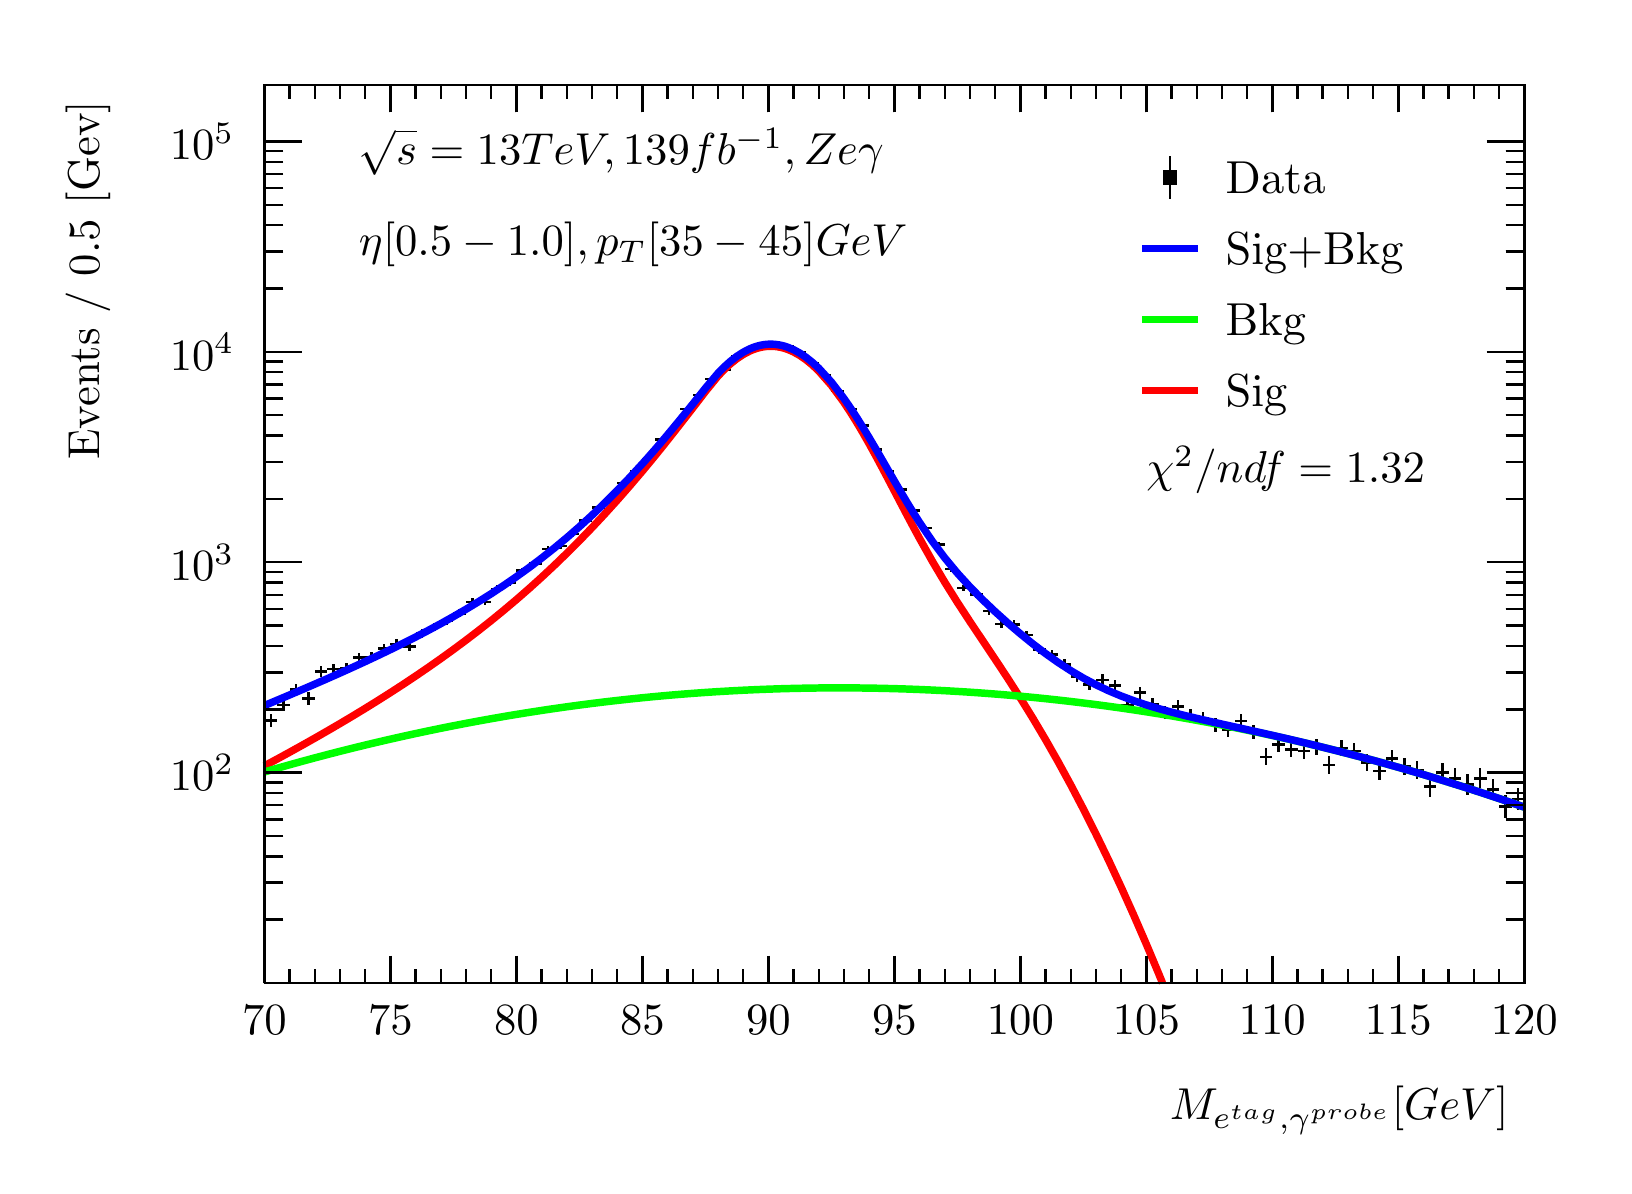
\begin{tikzpicture}
\pgfdeclareplotmark{cross} {
\pgfpathmoveto{\pgfpoint{-0.3\pgfplotmarksize}{\pgfplotmarksize}}
\pgfpathlineto{\pgfpoint{+0.3\pgfplotmarksize}{\pgfplotmarksize}}
\pgfpathlineto{\pgfpoint{+0.3\pgfplotmarksize}{0.3\pgfplotmarksize}}
\pgfpathlineto{\pgfpoint{+1\pgfplotmarksize}{0.3\pgfplotmarksize}}
\pgfpathlineto{\pgfpoint{+1\pgfplotmarksize}{-0.3\pgfplotmarksize}}
\pgfpathlineto{\pgfpoint{+0.3\pgfplotmarksize}{-0.3\pgfplotmarksize}}
\pgfpathlineto{\pgfpoint{+0.3\pgfplotmarksize}{-1.\pgfplotmarksize}}
\pgfpathlineto{\pgfpoint{-0.3\pgfplotmarksize}{-1.\pgfplotmarksize}}
\pgfpathlineto{\pgfpoint{-0.3\pgfplotmarksize}{-0.3\pgfplotmarksize}}
\pgfpathlineto{\pgfpoint{-1.\pgfplotmarksize}{-0.3\pgfplotmarksize}}
\pgfpathlineto{\pgfpoint{-1.\pgfplotmarksize}{0.3\pgfplotmarksize}}
\pgfpathlineto{\pgfpoint{-0.3\pgfplotmarksize}{0.3\pgfplotmarksize}}
\pgfpathclose
\pgfusepathqstroke
}
\pgfdeclareplotmark{cross*} {
\pgfpathmoveto{\pgfpoint{-0.3\pgfplotmarksize}{\pgfplotmarksize}}
\pgfpathlineto{\pgfpoint{+0.3\pgfplotmarksize}{\pgfplotmarksize}}
\pgfpathlineto{\pgfpoint{+0.3\pgfplotmarksize}{0.3\pgfplotmarksize}}
\pgfpathlineto{\pgfpoint{+1\pgfplotmarksize}{0.3\pgfplotmarksize}}
\pgfpathlineto{\pgfpoint{+1\pgfplotmarksize}{-0.3\pgfplotmarksize}}
\pgfpathlineto{\pgfpoint{+0.3\pgfplotmarksize}{-0.3\pgfplotmarksize}}
\pgfpathlineto{\pgfpoint{+0.3\pgfplotmarksize}{-1.\pgfplotmarksize}}
\pgfpathlineto{\pgfpoint{-0.3\pgfplotmarksize}{-1.\pgfplotmarksize}}
\pgfpathlineto{\pgfpoint{-0.3\pgfplotmarksize}{-0.3\pgfplotmarksize}}
\pgfpathlineto{\pgfpoint{-1.\pgfplotmarksize}{-0.3\pgfplotmarksize}}
\pgfpathlineto{\pgfpoint{-1.\pgfplotmarksize}{0.3\pgfplotmarksize}}
\pgfpathlineto{\pgfpoint{-0.3\pgfplotmarksize}{0.3\pgfplotmarksize}}
\pgfpathclose
\pgfusepathqfillstroke
}
\pgfdeclareplotmark{newstar} {
\pgfpathmoveto{\pgfqpoint{0pt}{\pgfplotmarksize}}
\pgfpathlineto{\pgfqpointpolar{44}{0.5\pgfplotmarksize}}
\pgfpathlineto{\pgfqpointpolar{18}{\pgfplotmarksize}}
\pgfpathlineto{\pgfqpointpolar{-20}{0.5\pgfplotmarksize}}
\pgfpathlineto{\pgfqpointpolar{-54}{\pgfplotmarksize}}
\pgfpathlineto{\pgfqpointpolar{-90}{0.5\pgfplotmarksize}}
\pgfpathlineto{\pgfqpointpolar{234}{\pgfplotmarksize}}
\pgfpathlineto{\pgfqpointpolar{198}{0.5\pgfplotmarksize}}
\pgfpathlineto{\pgfqpointpolar{162}{\pgfplotmarksize}}
\pgfpathlineto{\pgfqpointpolar{134}{0.5\pgfplotmarksize}}
\pgfpathclose
\pgfusepathqstroke
}
\pgfdeclareplotmark{newstar*} {
\pgfpathmoveto{\pgfqpoint{0pt}{\pgfplotmarksize}}
\pgfpathlineto{\pgfqpointpolar{44}{0.5\pgfplotmarksize}}
\pgfpathlineto{\pgfqpointpolar{18}{\pgfplotmarksize}}
\pgfpathlineto{\pgfqpointpolar{-20}{0.5\pgfplotmarksize}}
\pgfpathlineto{\pgfqpointpolar{-54}{\pgfplotmarksize}}
\pgfpathlineto{\pgfqpointpolar{-90}{0.5\pgfplotmarksize}}
\pgfpathlineto{\pgfqpointpolar{234}{\pgfplotmarksize}}
\pgfpathlineto{\pgfqpointpolar{198}{0.5\pgfplotmarksize}}
\pgfpathlineto{\pgfqpointpolar{162}{\pgfplotmarksize}}
\pgfpathlineto{\pgfqpointpolar{134}{0.5\pgfplotmarksize}}
\pgfpathclose
\pgfusepathqfillstroke
}
\definecolor{c}{rgb}{1,1,1};
\draw [color=c, fill=c] (0,0) rectangle (20,14.4361);
\draw [color=c, fill=c] (3,2.30977) rectangle (19,13.7143);
\definecolor{c}{rgb}{0,0,0};
\draw [c,line width=0.9] (3,2.30977) -- (3,13.7143) -- (19,13.7143) -- (19,2.30977) -- (3,2.30977);
\definecolor{c}{rgb}{1,1,1};
\draw [color=c, fill=c] (3,2.30977) rectangle (19,13.7143);
\definecolor{c}{rgb}{0,0,0};
\draw [c,line width=0.9] (3,2.30977) -- (3,13.7143) -- (19,13.7143) -- (19,2.30977) -- (3,2.30977);
\draw [c,line width=0.9] (3,2.30977) -- (19,2.30977);
\draw [c,line width=0.9] (3,2.65624) -- (3,2.30977);
\draw [c,line width=0.9] (3.32,2.48301) -- (3.32,2.30977);
\draw [c,line width=0.9] (3.64,2.48301) -- (3.64,2.30977);
\draw [c,line width=0.9] (3.96,2.48301) -- (3.96,2.30977);
\draw [c,line width=0.9] (4.28,2.48301) -- (4.28,2.30977);
\draw [c,line width=0.9] (4.6,2.65624) -- (4.6,2.30977);
\draw [c,line width=0.9] (4.92,2.48301) -- (4.92,2.30977);
\draw [c,line width=0.9] (5.24,2.48301) -- (5.24,2.30977);
\draw [c,line width=0.9] (5.56,2.48301) -- (5.56,2.30977);
\draw [c,line width=0.9] (5.88,2.48301) -- (5.88,2.30977);
\draw [c,line width=0.9] (6.2,2.65624) -- (6.2,2.30977);
\draw [c,line width=0.9] (6.52,2.48301) -- (6.52,2.30977);
\draw [c,line width=0.9] (6.84,2.48301) -- (6.84,2.30977);
\draw [c,line width=0.9] (7.16,2.48301) -- (7.16,2.30977);
\draw [c,line width=0.9] (7.48,2.48301) -- (7.48,2.30977);
\draw [c,line width=0.9] (7.8,2.65624) -- (7.8,2.30977);
\draw [c,line width=0.9] (8.12,2.48301) -- (8.12,2.30977);
\draw [c,line width=0.9] (8.44,2.48301) -- (8.44,2.30977);
\draw [c,line width=0.9] (8.76,2.48301) -- (8.76,2.30977);
\draw [c,line width=0.9] (9.08,2.48301) -- (9.08,2.30977);
\draw [c,line width=0.9] (9.4,2.65624) -- (9.4,2.30977);
\draw [c,line width=0.9] (9.72,2.48301) -- (9.72,2.30977);
\draw [c,line width=0.9] (10.04,2.48301) -- (10.04,2.30977);
\draw [c,line width=0.9] (10.36,2.48301) -- (10.36,2.30977);
\draw [c,line width=0.9] (10.68,2.48301) -- (10.68,2.30977);
\draw [c,line width=0.9] (11,2.65624) -- (11,2.30977);
\draw [c,line width=0.9] (11.32,2.48301) -- (11.32,2.30977);
\draw [c,line width=0.9] (11.64,2.48301) -- (11.64,2.30977);
\draw [c,line width=0.9] (11.96,2.48301) -- (11.96,2.30977);
\draw [c,line width=0.9] (12.28,2.48301) -- (12.28,2.30977);
\draw [c,line width=0.9] (12.6,2.65624) -- (12.6,2.30977);
\draw [c,line width=0.9] (12.92,2.48301) -- (12.92,2.30977);
\draw [c,line width=0.9] (13.24,2.48301) -- (13.24,2.30977);
\draw [c,line width=0.9] (13.56,2.48301) -- (13.56,2.30977);
\draw [c,line width=0.9] (13.88,2.48301) -- (13.88,2.30977);
\draw [c,line width=0.9] (14.2,2.65624) -- (14.2,2.30977);
\draw [c,line width=0.9] (14.52,2.48301) -- (14.52,2.30977);
\draw [c,line width=0.9] (14.84,2.48301) -- (14.84,2.30977);
\draw [c,line width=0.9] (15.16,2.48301) -- (15.16,2.30977);
\draw [c,line width=0.9] (15.48,2.48301) -- (15.48,2.30977);
\draw [c,line width=0.9] (15.8,2.65624) -- (15.8,2.30977);
\draw [c,line width=0.9] (16.12,2.48301) -- (16.12,2.30977);
\draw [c,line width=0.9] (16.44,2.48301) -- (16.44,2.30977);
\draw [c,line width=0.9] (16.76,2.48301) -- (16.76,2.30977);
\draw [c,line width=0.9] (17.08,2.48301) -- (17.08,2.30977);
\draw [c,line width=0.9] (17.4,2.65624) -- (17.4,2.30977);
\draw [c,line width=0.9] (17.72,2.48301) -- (17.72,2.30977);
\draw [c,line width=0.9] (18.04,2.48301) -- (18.04,2.30977);
\draw [c,line width=0.9] (18.36,2.48301) -- (18.36,2.30977);
\draw [c,line width=0.9] (18.68,2.48301) -- (18.68,2.30977);
\draw [c,line width=0.9] (19,2.65624) -- (19,2.30977);
\draw [anchor=base] (3,1.66015) node[scale=1.61424, color=c, rotate=0]{70};
\draw [anchor=base] (4.6,1.66015) node[scale=1.61424, color=c, rotate=0]{75};
\draw [anchor=base] (6.2,1.66015) node[scale=1.61424, color=c, rotate=0]{80};
\draw [anchor=base] (7.8,1.66015) node[scale=1.61424, color=c, rotate=0]{85};
\draw [anchor=base] (9.4,1.66015) node[scale=1.61424, color=c, rotate=0]{90};
\draw [anchor=base] (11,1.66015) node[scale=1.61424, color=c, rotate=0]{95};
\draw [anchor=base] (12.6,1.66015) node[scale=1.61424, color=c, rotate=0]{100};
\draw [anchor=base] (14.2,1.66015) node[scale=1.61424, color=c, rotate=0]{105};
\draw [anchor=base] (15.8,1.66015) node[scale=1.61424, color=c, rotate=0]{110};
\draw [anchor=base] (17.4,1.66015) node[scale=1.61424, color=c, rotate=0]{115};
\draw [anchor=base] (19,1.66015) node[scale=1.61424, color=c, rotate=0]{120};
\draw [anchor= east] (19,0.692932) node[scale=1.61424, color=c, rotate=0]{$M_{e^{tag}, \gamma^{probe}}  [GeV]$};
\draw [c,line width=0.9] (3,13.7143) -- (19,13.7143);
\draw [c,line width=0.9] (3,13.3678) -- (3,13.7143);
\draw [c,line width=0.9] (3.32,13.5411) -- (3.32,13.7143);
\draw [c,line width=0.9] (3.64,13.5411) -- (3.64,13.7143);
\draw [c,line width=0.9] (3.96,13.5411) -- (3.96,13.7143);
\draw [c,line width=0.9] (4.28,13.5411) -- (4.28,13.7143);
\draw [c,line width=0.9] (4.6,13.3678) -- (4.6,13.7143);
\draw [c,line width=0.9] (4.92,13.5411) -- (4.92,13.7143);
\draw [c,line width=0.9] (5.24,13.5411) -- (5.24,13.7143);
\draw [c,line width=0.9] (5.56,13.5411) -- (5.56,13.7143);
\draw [c,line width=0.9] (5.88,13.5411) -- (5.88,13.7143);
\draw [c,line width=0.9] (6.2,13.3678) -- (6.2,13.7143);
\draw [c,line width=0.9] (6.52,13.5411) -- (6.52,13.7143);
\draw [c,line width=0.9] (6.84,13.5411) -- (6.84,13.7143);
\draw [c,line width=0.9] (7.16,13.5411) -- (7.16,13.7143);
\draw [c,line width=0.9] (7.48,13.5411) -- (7.48,13.7143);
\draw [c,line width=0.9] (7.8,13.3678) -- (7.8,13.7143);
\draw [c,line width=0.9] (8.12,13.5411) -- (8.12,13.7143);
\draw [c,line width=0.9] (8.44,13.5411) -- (8.44,13.7143);
\draw [c,line width=0.9] (8.76,13.5411) -- (8.76,13.7143);
\draw [c,line width=0.9] (9.08,13.5411) -- (9.08,13.7143);
\draw [c,line width=0.9] (9.4,13.3678) -- (9.4,13.7143);
\draw [c,line width=0.9] (9.72,13.5411) -- (9.72,13.7143);
\draw [c,line width=0.9] (10.04,13.5411) -- (10.04,13.7143);
\draw [c,line width=0.9] (10.36,13.5411) -- (10.36,13.7143);
\draw [c,line width=0.9] (10.68,13.5411) -- (10.68,13.7143);
\draw [c,line width=0.9] (11,13.3678) -- (11,13.7143);
\draw [c,line width=0.9] (11.32,13.5411) -- (11.32,13.7143);
\draw [c,line width=0.9] (11.64,13.5411) -- (11.64,13.7143);
\draw [c,line width=0.9] (11.96,13.5411) -- (11.96,13.7143);
\draw [c,line width=0.9] (12.28,13.5411) -- (12.28,13.7143);
\draw [c,line width=0.9] (12.6,13.3678) -- (12.6,13.7143);
\draw [c,line width=0.9] (12.92,13.5411) -- (12.92,13.7143);
\draw [c,line width=0.9] (13.24,13.5411) -- (13.24,13.7143);
\draw [c,line width=0.9] (13.56,13.5411) -- (13.56,13.7143);
\draw [c,line width=0.9] (13.88,13.5411) -- (13.88,13.7143);
\draw [c,line width=0.9] (14.2,13.3678) -- (14.2,13.7143);
\draw [c,line width=0.9] (14.52,13.5411) -- (14.52,13.7143);
\draw [c,line width=0.9] (14.84,13.5411) -- (14.84,13.7143);
\draw [c,line width=0.9] (15.16,13.5411) -- (15.16,13.7143);
\draw [c,line width=0.9] (15.48,13.5411) -- (15.48,13.7143);
\draw [c,line width=0.9] (15.8,13.3678) -- (15.8,13.7143);
\draw [c,line width=0.9] (16.12,13.5411) -- (16.12,13.7143);
\draw [c,line width=0.9] (16.44,13.5411) -- (16.44,13.7143);
\draw [c,line width=0.9] (16.76,13.5411) -- (16.76,13.7143);
\draw [c,line width=0.9] (17.08,13.5411) -- (17.08,13.7143);
\draw [c,line width=0.9] (17.4,13.3678) -- (17.4,13.7143);
\draw [c,line width=0.9] (17.72,13.5411) -- (17.72,13.7143);
\draw [c,line width=0.9] (18.04,13.5411) -- (18.04,13.7143);
\draw [c,line width=0.9] (18.36,13.5411) -- (18.36,13.7143);
\draw [c,line width=0.9] (18.68,13.5411) -- (18.68,13.7143);
\draw [c,line width=0.9] (19,13.3678) -- (19,13.7143);
\draw [c,line width=0.9] (3,2.30977) -- (3,13.7143);
\draw [c,line width=0.9] (3.237,3.11414) -- (3,3.11414);
\draw [c,line width=0.9] (3.237,3.58467) -- (3,3.58467);
\draw [c,line width=0.9] (3.237,3.91852) -- (3,3.91852);
\draw [c,line width=0.9] (3.237,4.17747) -- (3,4.17747);
\draw [c,line width=0.9] (3.237,4.38904) -- (3,4.38904);
\draw [c,line width=0.9] (3.237,4.56793) -- (3,4.56793);
\draw [c,line width=0.9] (3.237,4.72289) -- (3,4.72289);
\draw [c,line width=0.9] (3.237,4.85957) -- (3,4.85957);
\draw [c,line width=0.9] (3.474,4.98184) -- (3,4.98184);
\draw [anchor= east] (2.82,4.98184) node[scale=1.61424, color=c, rotate=0]{$10^{2}$};
\draw [c,line width=0.9] (3.237,5.78621) -- (3,5.78621);
\draw [c,line width=0.9] (3.237,6.25674) -- (3,6.25674);
\draw [c,line width=0.9] (3.237,6.59058) -- (3,6.59058);
\draw [c,line width=0.9] (3.237,6.84953) -- (3,6.84953);
\draw [c,line width=0.9] (3.237,7.06111) -- (3,7.06111);
\draw [c,line width=0.9] (3.237,7.24) -- (3,7.24);
\draw [c,line width=0.9] (3.237,7.39496) -- (3,7.39496);
\draw [c,line width=0.9] (3.237,7.53164) -- (3,7.53164);
\draw [c,line width=0.9] (3.474,7.65391) -- (3,7.65391);
\draw [anchor= east] (2.82,7.65391) node[scale=1.61424, color=c, rotate=0]{$10^{3}$};
\draw [c,line width=0.9] (3.237,8.45828) -- (3,8.45828);
\draw [c,line width=0.9] (3.237,8.92881) -- (3,8.92881);
\draw [c,line width=0.9] (3.237,9.26265) -- (3,9.26265);
\draw [c,line width=0.9] (3.237,9.5216) -- (3,9.5216);
\draw [c,line width=0.9] (3.237,9.73318) -- (3,9.73318);
\draw [c,line width=0.9] (3.237,9.91207) -- (3,9.91207);
\draw [c,line width=0.9] (3.237,10.067) -- (3,10.067);
\draw [c,line width=0.9] (3.237,10.2037) -- (3,10.2037);
\draw [c,line width=0.9] (3.474,10.326) -- (3,10.326);
\draw [anchor= east] (2.82,10.326) node[scale=1.61424, color=c, rotate=0]{$10^{4}$};
\draw [c,line width=0.9] (3.237,11.1303) -- (3,11.1303);
\draw [c,line width=0.9] (3.237,11.6009) -- (3,11.6009);
\draw [c,line width=0.9] (3.237,11.9347) -- (3,11.9347);
\draw [c,line width=0.9] (3.237,12.1937) -- (3,12.1937);
\draw [c,line width=0.9] (3.237,12.4052) -- (3,12.4052);
\draw [c,line width=0.9] (3.237,12.5841) -- (3,12.5841);
\draw [c,line width=0.9] (3.237,12.7391) -- (3,12.7391);
\draw [c,line width=0.9] (3.237,12.8758) -- (3,12.8758);
\draw [c,line width=0.9] (3.474,12.998) -- (3,12.998);
\draw [anchor= east] (2.82,12.998) node[scale=1.61424, color=c, rotate=0]{$10^{5}$};
\draw [anchor= east] (0.76,13.7143) node[scale=1.61424, color=c, rotate=90]{Events / 0.5 [Gev]};
\draw [c,line width=0.9] (19,2.30977) -- (19,13.7143);
\draw [c,line width=0.9] (18.763,3.11414) -- (19,3.11414);
\draw [c,line width=0.9] (18.763,3.58467) -- (19,3.58467);
\draw [c,line width=0.9] (18.763,3.91852) -- (19,3.91852);
\draw [c,line width=0.9] (18.763,4.17747) -- (19,4.17747);
\draw [c,line width=0.9] (18.763,4.38904) -- (19,4.38904);
\draw [c,line width=0.9] (18.763,4.56793) -- (19,4.56793);
\draw [c,line width=0.9] (18.763,4.72289) -- (19,4.72289);
\draw [c,line width=0.9] (18.763,4.85957) -- (19,4.85957);
\draw [c,line width=0.9] (18.526,4.98184) -- (19,4.98184);
\draw [c,line width=0.9] (18.763,5.78621) -- (19,5.78621);
\draw [c,line width=0.9] (18.763,6.25674) -- (19,6.25674);
\draw [c,line width=0.9] (18.763,6.59058) -- (19,6.59058);
\draw [c,line width=0.9] (18.763,6.84953) -- (19,6.84953);
\draw [c,line width=0.9] (18.763,7.06111) -- (19,7.06111);
\draw [c,line width=0.9] (18.763,7.24) -- (19,7.24);
\draw [c,line width=0.9] (18.763,7.39496) -- (19,7.39496);
\draw [c,line width=0.9] (18.763,7.53164) -- (19,7.53164);
\draw [c,line width=0.9] (18.526,7.65391) -- (19,7.65391);
\draw [c,line width=0.9] (18.763,8.45828) -- (19,8.45828);
\draw [c,line width=0.9] (18.763,8.92881) -- (19,8.92881);
\draw [c,line width=0.9] (18.763,9.26265) -- (19,9.26265);
\draw [c,line width=0.9] (18.763,9.5216) -- (19,9.5216);
\draw [c,line width=0.9] (18.763,9.73318) -- (19,9.73318);
\draw [c,line width=0.9] (18.763,9.91207) -- (19,9.91207);
\draw [c,line width=0.9] (18.763,10.067) -- (19,10.067);
\draw [c,line width=0.9] (18.763,10.2037) -- (19,10.2037);
\draw [c,line width=0.9] (18.526,10.326) -- (19,10.326);
\draw [c,line width=0.9] (18.763,11.1303) -- (19,11.1303);
\draw [c,line width=0.9] (18.763,11.6009) -- (19,11.6009);
\draw [c,line width=0.9] (18.763,11.9347) -- (19,11.9347);
\draw [c,line width=0.9] (18.763,12.1937) -- (19,12.1937);
\draw [c,line width=0.9] (18.763,12.4052) -- (19,12.4052);
\draw [c,line width=0.9] (18.763,12.5841) -- (19,12.5841);
\draw [c,line width=0.9] (18.763,12.7391) -- (19,12.7391);
\draw [c,line width=0.9] (18.763,12.8758) -- (19,12.8758);
\draw [c,line width=0.9] (18.526,12.998) -- (19,12.998);
\draw [c,line width=0.9] (3.08,5.64444) -- (3,5.64444);
\draw [c,line width=0.9] (3,5.64444) -- (3,5.64444);
\draw [c,line width=0.9] (3.08,5.64444) -- (3.16,5.64444);
\draw [c,line width=0.9] (3.16,5.64444) -- (3.16,5.64444);
\draw [c,line width=0.9] (3.08,5.64444) -- (3.08,5.73165);
\draw [c,line width=0.9] (3.08,5.73165) -- (3.08,5.73165);
\draw [c,line width=0.9] (3.08,5.64444) -- (3.08,5.55724);
\draw [c,line width=0.9] (3.08,5.55724) -- (3.08,5.55724);
\draw [c,line width=0.9] (3.24,5.84283) -- (3.16,5.84283);
\draw [c,line width=0.9] (3.16,5.84283) -- (3.16,5.84283);
\draw [c,line width=0.9] (3.24,5.84283) -- (3.32,5.84283);
\draw [c,line width=0.9] (3.32,5.84283) -- (3.32,5.84283);
\draw [c,line width=0.9] (3.24,5.84283) -- (3.24,5.9229);
\draw [c,line width=0.9] (3.24,5.9229) -- (3.24,5.9229);
\draw [c,line width=0.9] (3.24,5.84283) -- (3.24,5.76277);
\draw [c,line width=0.9] (3.24,5.76277) -- (3.24,5.76277);
\draw [c,line width=0.9] (3.4,6.03584) -- (3.32,6.03584);
\draw [c,line width=0.9] (3.32,6.03584) -- (3.32,6.03584);
\draw [c,line width=0.9] (3.4,6.03584) -- (3.48,6.03584);
\draw [c,line width=0.9] (3.48,6.03584) -- (3.48,6.03584);
\draw [c,line width=0.9] (3.4,6.03584) -- (3.4,6.10952);
\draw [c,line width=0.9] (3.4,6.10952) -- (3.4,6.10952);
\draw [c,line width=0.9] (3.4,6.03584) -- (3.4,5.96217);
\draw [c,line width=0.9] (3.4,5.96217) -- (3.4,5.96217);
\draw [c,line width=0.9] (3.56,5.9229) -- (3.48,5.9229);
\draw [c,line width=0.9] (3.48,5.9229) -- (3.48,5.9229);
\draw [c,line width=0.9] (3.56,5.9229) -- (3.64,5.9229);
\draw [c,line width=0.9] (3.64,5.9229) -- (3.64,5.9229);
\draw [c,line width=0.9] (3.56,5.9229) -- (3.56,6.00025);
\draw [c,line width=0.9] (3.56,6.00025) -- (3.56,6.00025);
\draw [c,line width=0.9] (3.56,5.9229) -- (3.56,5.84555);
\draw [c,line width=0.9] (3.56,5.84555) -- (3.56,5.84555);
\draw [c,line width=0.9] (3.72,6.26445) -- (3.64,6.26445);
\draw [c,line width=0.9] (3.64,6.26445) -- (3.64,6.26445);
\draw [c,line width=0.9] (3.72,6.26445) -- (3.8,6.26445);
\draw [c,line width=0.9] (3.8,6.26445) -- (3.8,6.26445);
\draw [c,line width=0.9] (3.72,6.26445) -- (3.72,6.33122);
\draw [c,line width=0.9] (3.72,6.33122) -- (3.72,6.33122);
\draw [c,line width=0.9] (3.72,6.26445) -- (3.72,6.19768);
\draw [c,line width=0.9] (3.72,6.19768) -- (3.72,6.19768);
\draw [c,line width=0.9] (3.88,6.29853) -- (3.8,6.29853);
\draw [c,line width=0.9] (3.8,6.29853) -- (3.8,6.29853);
\draw [c,line width=0.9] (3.88,6.29853) -- (3.96,6.29853);
\draw [c,line width=0.9] (3.96,6.29853) -- (3.96,6.29853);
\draw [c,line width=0.9] (3.88,6.29853) -- (3.88,6.36433);
\draw [c,line width=0.9] (3.88,6.36433) -- (3.88,6.36433);
\draw [c,line width=0.9] (3.88,6.29853) -- (3.88,6.23273);
\draw [c,line width=0.9] (3.88,6.23273) -- (3.88,6.23273);
\draw [c,line width=0.9] (4.04,6.30967) -- (3.96,6.30967);
\draw [c,line width=0.9] (3.96,6.30967) -- (3.96,6.30967);
\draw [c,line width=0.9] (4.04,6.30967) -- (4.12,6.30967);
\draw [c,line width=0.9] (4.12,6.30967) -- (4.12,6.30967);
\draw [c,line width=0.9] (4.04,6.30967) -- (4.04,6.37515);
\draw [c,line width=0.9] (4.04,6.37515) -- (4.04,6.37515);
\draw [c,line width=0.9] (4.04,6.30967) -- (4.04,6.24419);
\draw [c,line width=0.9] (4.04,6.24419) -- (4.04,6.24419);
\draw [c,line width=0.9] (4.2,6.44553) -- (4.12,6.44553);
\draw [c,line width=0.9] (4.12,6.44553) -- (4.12,6.44553);
\draw [c,line width=0.9] (4.2,6.44553) -- (4.28,6.44553);
\draw [c,line width=0.9] (4.28,6.44553) -- (4.28,6.44553);
\draw [c,line width=0.9] (4.2,6.44553) -- (4.2,6.50729);
\draw [c,line width=0.9] (4.2,6.50729) -- (4.2,6.50729);
\draw [c,line width=0.9] (4.2,6.44553) -- (4.2,6.38377);
\draw [c,line width=0.9] (4.2,6.38377) -- (4.2,6.38377);
\draw [c,line width=0.9] (4.36,6.45209) -- (4.28,6.45209);
\draw [c,line width=0.9] (4.28,6.45209) -- (4.28,6.45209);
\draw [c,line width=0.9] (4.36,6.45209) -- (4.44,6.45209);
\draw [c,line width=0.9] (4.44,6.45209) -- (4.44,6.45209);
\draw [c,line width=0.9] (4.36,6.45209) -- (4.36,6.51367);
\draw [c,line width=0.9] (4.36,6.51367) -- (4.36,6.51367);
\draw [c,line width=0.9] (4.36,6.45209) -- (4.36,6.3905);
\draw [c,line width=0.9] (4.36,6.3905) -- (4.36,6.3905);
\draw [c,line width=0.9] (4.52,6.55823) -- (4.44,6.55823);
\draw [c,line width=0.9] (4.44,6.55823) -- (4.44,6.55823);
\draw [c,line width=0.9] (4.52,6.55823) -- (4.6,6.55823);
\draw [c,line width=0.9] (4.6,6.55823) -- (4.6,6.55823);
\draw [c,line width=0.9] (4.52,6.55823) -- (4.52,6.61706);
\draw [c,line width=0.9] (4.52,6.61706) -- (4.52,6.61706);
\draw [c,line width=0.9] (4.52,6.55823) -- (4.52,6.49939);
\draw [c,line width=0.9] (4.52,6.49939) -- (4.52,6.49939);
\draw [c,line width=0.9] (4.68,6.61641) -- (4.6,6.61641);
\draw [c,line width=0.9] (4.6,6.61641) -- (4.6,6.61641);
\draw [c,line width=0.9] (4.68,6.61641) -- (4.76,6.61641);
\draw [c,line width=0.9] (4.76,6.61641) -- (4.76,6.61641);
\draw [c,line width=0.9] (4.68,6.61641) -- (4.68,6.67378);
\draw [c,line width=0.9] (4.68,6.67378) -- (4.68,6.67378);
\draw [c,line width=0.9] (4.68,6.61641) -- (4.68,6.55903);
\draw [c,line width=0.9] (4.68,6.55903) -- (4.68,6.55903);
\draw [c,line width=0.9] (4.84,6.58477) -- (4.76,6.58477);
\draw [c,line width=0.9] (4.76,6.58477) -- (4.76,6.58477);
\draw [c,line width=0.9] (4.84,6.58477) -- (4.92,6.58477);
\draw [c,line width=0.9] (4.92,6.58477) -- (4.92,6.58477);
\draw [c,line width=0.9] (4.84,6.58477) -- (4.84,6.64293);
\draw [c,line width=0.9] (4.84,6.64293) -- (4.84,6.64293);
\draw [c,line width=0.9] (4.84,6.58477) -- (4.84,6.52661);
\draw [c,line width=0.9] (4.84,6.52661) -- (4.84,6.52661);
\draw [c,line width=0.9] (5,6.74772) -- (4.92,6.74772);
\draw [c,line width=0.9] (4.92,6.74772) -- (4.92,6.74772);
\draw [c,line width=0.9] (5,6.74772) -- (5.08,6.74772);
\draw [c,line width=0.9] (5.08,6.74772) -- (5.08,6.74772);
\draw [c,line width=0.9] (5,6.74772) -- (5,6.80194);
\draw [c,line width=0.9] (5,6.80194) -- (5,6.80194);
\draw [c,line width=0.9] (5,6.74772) -- (5,6.6935);
\draw [c,line width=0.9] (5,6.6935) -- (5,6.6935);
\draw [c,line width=0.9] (5.16,6.83317) -- (5.08,6.83317);
\draw [c,line width=0.9] (5.08,6.83317) -- (5.08,6.83317);
\draw [c,line width=0.9] (5.16,6.83317) -- (5.24,6.83317);
\draw [c,line width=0.9] (5.24,6.83317) -- (5.24,6.83317);
\draw [c,line width=0.9] (5.16,6.83317) -- (5.16,6.88543);
\draw [c,line width=0.9] (5.16,6.88543) -- (5.16,6.88543);
\draw [c,line width=0.9] (5.16,6.83317) -- (5.16,6.78091);
\draw [c,line width=0.9] (5.16,6.78091) -- (5.16,6.78091);
\draw [c,line width=0.9] (5.32,6.91277) -- (5.24,6.91277);
\draw [c,line width=0.9] (5.24,6.91277) -- (5.24,6.91277);
\draw [c,line width=0.9] (5.32,6.91277) -- (5.4,6.91277);
\draw [c,line width=0.9] (5.4,6.91277) -- (5.4,6.91277);
\draw [c,line width=0.9] (5.32,6.91277) -- (5.32,6.96327);
\draw [c,line width=0.9] (5.32,6.96327) -- (5.32,6.96327);
\draw [c,line width=0.9] (5.32,6.91277) -- (5.32,6.86227);
\draw [c,line width=0.9] (5.32,6.86227) -- (5.32,6.86227);
\draw [c,line width=0.9] (5.48,7.00565) -- (5.4,7.00565);
\draw [c,line width=0.9] (5.4,7.00565) -- (5.4,7.00565);
\draw [c,line width=0.9] (5.48,7.00565) -- (5.56,7.00565);
\draw [c,line width=0.9] (5.56,7.00565) -- (5.56,7.00565);
\draw [c,line width=0.9] (5.48,7.00565) -- (5.48,7.05417);
\draw [c,line width=0.9] (5.48,7.05417) -- (5.48,7.05417);
\draw [c,line width=0.9] (5.48,7.00565) -- (5.48,6.95714);
\draw [c,line width=0.9] (5.48,6.95714) -- (5.48,6.95714);
\draw [c,line width=0.9] (5.64,7.15042) -- (5.56,7.15042);
\draw [c,line width=0.9] (5.56,7.15042) -- (5.56,7.15042);
\draw [c,line width=0.9] (5.64,7.15042) -- (5.72,7.15042);
\draw [c,line width=0.9] (5.72,7.15042) -- (5.72,7.15042);
\draw [c,line width=0.9] (5.64,7.15042) -- (5.64,7.19601);
\draw [c,line width=0.9] (5.64,7.19601) -- (5.64,7.19601);
\draw [c,line width=0.9] (5.64,7.15042) -- (5.64,7.10484);
\draw [c,line width=0.9] (5.64,7.10484) -- (5.64,7.10484);
\draw [c,line width=0.9] (5.8,7.15042) -- (5.72,7.15042);
\draw [c,line width=0.9] (5.72,7.15042) -- (5.72,7.15042);
\draw [c,line width=0.9] (5.8,7.15042) -- (5.88,7.15042);
\draw [c,line width=0.9] (5.88,7.15042) -- (5.88,7.15042);
\draw [c,line width=0.9] (5.8,7.15042) -- (5.8,7.19601);
\draw [c,line width=0.9] (5.8,7.19601) -- (5.8,7.19601);
\draw [c,line width=0.9] (5.8,7.15042) -- (5.8,7.10484);
\draw [c,line width=0.9] (5.8,7.10484) -- (5.8,7.10484);
\draw [c,line width=0.9] (5.96,7.31696) -- (5.88,7.31696);
\draw [c,line width=0.9] (5.88,7.31696) -- (5.88,7.31696);
\draw [c,line width=0.9] (5.96,7.31696) -- (6.04,7.31696);
\draw [c,line width=0.9] (6.04,7.31696) -- (6.04,7.31696);
\draw [c,line width=0.9] (5.96,7.31696) -- (5.96,7.35939);
\draw [c,line width=0.9] (5.96,7.35939) -- (5.96,7.35939);
\draw [c,line width=0.9] (5.96,7.31696) -- (5.96,7.27454);
\draw [c,line width=0.9] (5.96,7.27454) -- (5.96,7.27454);
\draw [c,line width=0.9] (6.12,7.3993) -- (6.04,7.3993);
\draw [c,line width=0.9] (6.04,7.3993) -- (6.04,7.3993);
\draw [c,line width=0.9] (6.12,7.3993) -- (6.2,7.3993);
\draw [c,line width=0.9] (6.2,7.3993) -- (6.2,7.3993);
\draw [c,line width=0.9] (6.12,7.3993) -- (6.12,7.44025);
\draw [c,line width=0.9] (6.12,7.44025) -- (6.12,7.44025);
\draw [c,line width=0.9] (6.12,7.3993) -- (6.12,7.35835);
\draw [c,line width=0.9] (6.12,7.35835) -- (6.12,7.35835);
\draw [c,line width=0.9] (6.28,7.54701) -- (6.2,7.54701);
\draw [c,line width=0.9] (6.2,7.54701) -- (6.2,7.54701);
\draw [c,line width=0.9] (6.28,7.54701) -- (6.36,7.54701);
\draw [c,line width=0.9] (6.36,7.54701) -- (6.36,7.54701);
\draw [c,line width=0.9] (6.28,7.54701) -- (6.28,7.58544);
\draw [c,line width=0.9] (6.28,7.58544) -- (6.28,7.58544);
\draw [c,line width=0.9] (6.28,7.54701) -- (6.28,7.50859);
\draw [c,line width=0.9] (6.28,7.50859) -- (6.28,7.50859);
\draw [c,line width=0.9] (6.44,7.63755) -- (6.36,7.63755);
\draw [c,line width=0.9] (6.36,7.63755) -- (6.36,7.63755);
\draw [c,line width=0.9] (6.44,7.63755) -- (6.52,7.63755);
\draw [c,line width=0.9] (6.52,7.63755) -- (6.52,7.63755);
\draw [c,line width=0.9] (6.44,7.63755) -- (6.44,7.6745);
\draw [c,line width=0.9] (6.44,7.6745) -- (6.44,7.6745);
\draw [c,line width=0.9] (6.44,7.63755) -- (6.44,7.60059);
\draw [c,line width=0.9] (6.44,7.60059) -- (6.44,7.60059);
\draw [c,line width=0.9] (6.6,7.82113) -- (6.52,7.82113);
\draw [c,line width=0.9] (6.52,7.82113) -- (6.52,7.82113);
\draw [c,line width=0.9] (6.6,7.82113) -- (6.68,7.82113);
\draw [c,line width=0.9] (6.68,7.82113) -- (6.68,7.82113);
\draw [c,line width=0.9] (6.6,7.82113) -- (6.6,7.85528);
\draw [c,line width=0.9] (6.6,7.85528) -- (6.6,7.85528);
\draw [c,line width=0.9] (6.6,7.82113) -- (6.6,7.78699);
\draw [c,line width=0.9] (6.6,7.78699) -- (6.6,7.78699);
\draw [c,line width=0.9] (6.76,7.8587) -- (6.68,7.8587);
\draw [c,line width=0.9] (6.68,7.8587) -- (6.68,7.8587);
\draw [c,line width=0.9] (6.76,7.8587) -- (6.84,7.8587);
\draw [c,line width=0.9] (6.84,7.8587) -- (6.84,7.8587);
\draw [c,line width=0.9] (6.76,7.8587) -- (6.76,7.89229);
\draw [c,line width=0.9] (6.76,7.89229) -- (6.76,7.89229);
\draw [c,line width=0.9] (6.76,7.8587) -- (6.76,7.8251);
\draw [c,line width=0.9] (6.76,7.8251) -- (6.76,7.8251);
\draw [c,line width=0.9] (6.92,8.00988) -- (6.84,8.00988);
\draw [c,line width=0.9] (6.84,8.00988) -- (6.84,8.00988);
\draw [c,line width=0.9] (6.92,8.00988) -- (7,8.00988);
\draw [c,line width=0.9] (7,8.00988) -- (7,8.00988);
\draw [c,line width=0.9] (6.92,8.00988) -- (6.92,8.04136);
\draw [c,line width=0.9] (6.92,8.04136) -- (6.92,8.04136);
\draw [c,line width=0.9] (6.92,8.00988) -- (6.92,7.9784);
\draw [c,line width=0.9] (6.92,7.9784) -- (6.92,7.9784);
\draw [c,line width=0.9] (7.08,8.1862) -- (7,8.1862);
\draw [c,line width=0.9] (7,8.1862) -- (7,8.1862);
\draw [c,line width=0.9] (7.08,8.1862) -- (7.16,8.1862);
\draw [c,line width=0.9] (7.16,8.1862) -- (7.16,8.1862);
\draw [c,line width=0.9] (7.08,8.1862) -- (7.08,8.21538);
\draw [c,line width=0.9] (7.08,8.21538) -- (7.08,8.21538);
\draw [c,line width=0.9] (7.08,8.1862) -- (7.08,8.15703);
\draw [c,line width=0.9] (7.08,8.15703) -- (7.08,8.15703);
\draw [c,line width=0.9] (7.24,8.34756) -- (7.16,8.34756);
\draw [c,line width=0.9] (7.16,8.34756) -- (7.16,8.34756);
\draw [c,line width=0.9] (7.24,8.34756) -- (7.32,8.34756);
\draw [c,line width=0.9] (7.32,8.34756) -- (7.32,8.34756);
\draw [c,line width=0.9] (7.24,8.34756) -- (7.24,8.37478);
\draw [c,line width=0.9] (7.24,8.37478) -- (7.24,8.37478);
\draw [c,line width=0.9] (7.24,8.34756) -- (7.24,8.32034);
\draw [c,line width=0.9] (7.24,8.32034) -- (7.24,8.32034);
\draw [c,line width=0.9] (7.4,8.41513) -- (7.32,8.41513);
\draw [c,line width=0.9] (7.32,8.41513) -- (7.32,8.41513);
\draw [c,line width=0.9] (7.4,8.41513) -- (7.48,8.41513);
\draw [c,line width=0.9] (7.48,8.41513) -- (7.48,8.41513);
\draw [c,line width=0.9] (7.4,8.41513) -- (7.4,8.44157);
\draw [c,line width=0.9] (7.4,8.44157) -- (7.4,8.44157);
\draw [c,line width=0.9] (7.4,8.41513) -- (7.4,8.3887);
\draw [c,line width=0.9] (7.4,8.3887) -- (7.4,8.3887);
\draw [c,line width=0.9] (7.56,8.66307) -- (7.48,8.66307);
\draw [c,line width=0.9] (7.48,8.66307) -- (7.48,8.66307);
\draw [c,line width=0.9] (7.56,8.66307) -- (7.64,8.66307);
\draw [c,line width=0.9] (7.64,8.66307) -- (7.64,8.66307);
\draw [c,line width=0.9] (7.56,8.66307) -- (7.56,8.68683);
\draw [c,line width=0.9] (7.56,8.68683) -- (7.56,8.68683);
\draw [c,line width=0.9] (7.56,8.66307) -- (7.56,8.63931);
\draw [c,line width=0.9] (7.56,8.63931) -- (7.56,8.63931);
\draw [c,line width=0.9] (7.72,8.80439) -- (7.64,8.80439);
\draw [c,line width=0.9] (7.64,8.80439) -- (7.64,8.80439);
\draw [c,line width=0.9] (7.72,8.80439) -- (7.8,8.80439);
\draw [c,line width=0.9] (7.8,8.80439) -- (7.8,8.80439);
\draw [c,line width=0.9] (7.72,8.80439) -- (7.72,8.82674);
\draw [c,line width=0.9] (7.72,8.82674) -- (7.72,8.82674);
\draw [c,line width=0.9] (7.72,8.80439) -- (7.72,8.78204);
\draw [c,line width=0.9] (7.72,8.78204) -- (7.72,8.78204);
\draw [c,line width=0.9] (7.88,8.96761) -- (7.8,8.96761);
\draw [c,line width=0.9] (7.8,8.96761) -- (7.8,8.96761);
\draw [c,line width=0.9] (7.88,8.96761) -- (7.96,8.96761);
\draw [c,line width=0.9] (7.96,8.96761) -- (7.96,8.96761);
\draw [c,line width=0.9] (7.88,8.96761) -- (7.88,8.98844);
\draw [c,line width=0.9] (7.88,8.98844) -- (7.88,8.98844);
\draw [c,line width=0.9] (7.88,8.96761) -- (7.88,8.94677);
\draw [c,line width=0.9] (7.88,8.94677) -- (7.88,8.94677);
\draw [c,line width=0.9] (8.04,9.21377) -- (7.96,9.21377);
\draw [c,line width=0.9] (7.96,9.21377) -- (7.96,9.21377);
\draw [c,line width=0.9] (8.04,9.21377) -- (8.12,9.21377);
\draw [c,line width=0.9] (8.12,9.21377) -- (8.12,9.21377);
\draw [c,line width=0.9] (8.04,9.21377) -- (8.04,9.23251);
\draw [c,line width=0.9] (8.04,9.23251) -- (8.04,9.23251);
\draw [c,line width=0.9] (8.04,9.21377) -- (8.04,9.19503);
\draw [c,line width=0.9] (8.04,9.19503) -- (8.04,9.19503);
\draw [c,line width=0.9] (8.2,9.34523) -- (8.12,9.34523);
\draw [c,line width=0.9] (8.12,9.34523) -- (8.12,9.34523);
\draw [c,line width=0.9] (8.2,9.34523) -- (8.28,9.34523);
\draw [c,line width=0.9] (8.28,9.34523) -- (8.28,9.34523);
\draw [c,line width=0.9] (8.2,9.34523) -- (8.2,9.36294);
\draw [c,line width=0.9] (8.2,9.36294) -- (8.2,9.36294);
\draw [c,line width=0.9] (8.2,9.34523) -- (8.2,9.32752);
\draw [c,line width=0.9] (8.2,9.32752) -- (8.2,9.32752);
\draw [c,line width=0.9] (8.36,9.60055) -- (8.28,9.60055);
\draw [c,line width=0.9] (8.28,9.60055) -- (8.28,9.60055);
\draw [c,line width=0.9] (8.36,9.60055) -- (8.44,9.60055);
\draw [c,line width=0.9] (8.44,9.60055) -- (8.44,9.60055);
\draw [c,line width=0.9] (8.36,9.60055) -- (8.36,9.61641);
\draw [c,line width=0.9] (8.36,9.61641) -- (8.36,9.61641);
\draw [c,line width=0.9] (8.36,9.60055) -- (8.36,9.58469);
\draw [c,line width=0.9] (8.36,9.58469) -- (8.36,9.58469);
\draw [c,line width=0.9] (8.52,9.77553) -- (8.44,9.77553);
\draw [c,line width=0.9] (8.44,9.77553) -- (8.44,9.77553);
\draw [c,line width=0.9] (8.52,9.77553) -- (8.6,9.77553);
\draw [c,line width=0.9] (8.6,9.77553) -- (8.6,9.77553);
\draw [c,line width=0.9] (8.52,9.77553) -- (8.52,9.79024);
\draw [c,line width=0.9] (8.52,9.79024) -- (8.52,9.79024);
\draw [c,line width=0.9] (8.52,9.77553) -- (8.52,9.76082);
\draw [c,line width=0.9] (8.52,9.76082) -- (8.52,9.76082);
\draw [c,line width=0.9] (8.68,9.9814) -- (8.6,9.9814);
\draw [c,line width=0.9] (8.6,9.9814) -- (8.6,9.9814);
\draw [c,line width=0.9] (8.68,9.9814) -- (8.76,9.9814);
\draw [c,line width=0.9] (8.76,9.9814) -- (8.76,9.9814);
\draw [c,line width=0.9] (8.68,9.9814) -- (8.68,9.99487);
\draw [c,line width=0.9] (8.68,9.99487) -- (8.68,9.99487);
\draw [c,line width=0.9] (8.68,9.9814) -- (8.68,9.96794);
\draw [c,line width=0.9] (8.68,9.96794) -- (8.68,9.96794);
\draw [c,line width=0.9] (8.84,10.0927) -- (8.76,10.0927);
\draw [c,line width=0.9] (8.76,10.0927) -- (8.76,10.0927);
\draw [c,line width=0.9] (8.84,10.0927) -- (8.92,10.0927);
\draw [c,line width=0.9] (8.92,10.0927) -- (8.92,10.0927);
\draw [c,line width=0.9] (8.84,10.0927) -- (8.84,10.1055);
\draw [c,line width=0.9] (8.84,10.1055) -- (8.84,10.1055);
\draw [c,line width=0.9] (8.84,10.0927) -- (8.84,10.0799);
\draw [c,line width=0.9] (8.84,10.0799) -- (8.84,10.0799);
\draw [c,line width=0.9] (9,10.2741) -- (8.92,10.2741);
\draw [c,line width=0.9] (8.92,10.2741) -- (8.92,10.2741);
\draw [c,line width=0.9] (9,10.2741) -- (9.08,10.2741);
\draw [c,line width=0.9] (9.08,10.2741) -- (9.08,10.2741);
\draw [c,line width=0.9] (9,10.2741) -- (9,10.286);
\draw [c,line width=0.9] (9,10.286) -- (9,10.286);
\draw [c,line width=0.9] (9,10.2741) -- (9,10.2623);
\draw [c,line width=0.9] (9,10.2623) -- (9,10.2623);
\draw [c,line width=0.9] (9.16,10.3619) -- (9.08,10.3619);
\draw [c,line width=0.9] (9.08,10.3619) -- (9.08,10.3619);
\draw [c,line width=0.9] (9.16,10.3619) -- (9.24,10.3619);
\draw [c,line width=0.9] (9.24,10.3619) -- (9.24,10.3619);
\draw [c,line width=0.9] (9.16,10.3619) -- (9.16,10.3733);
\draw [c,line width=0.9] (9.16,10.3733) -- (9.16,10.3733);
\draw [c,line width=0.9] (9.16,10.3619) -- (9.16,10.3504);
\draw [c,line width=0.9] (9.16,10.3504) -- (9.16,10.3504);
\draw [c,line width=0.9] (9.32,10.4157) -- (9.24,10.4157);
\draw [c,line width=0.9] (9.24,10.4157) -- (9.24,10.4157);
\draw [c,line width=0.9] (9.32,10.4157) -- (9.4,10.4157);
\draw [c,line width=0.9] (9.4,10.4157) -- (9.4,10.4157);
\draw [c,line width=0.9] (9.32,10.4157) -- (9.32,10.4269);
\draw [c,line width=0.9] (9.32,10.4269) -- (9.32,10.4269);
\draw [c,line width=0.9] (9.32,10.4157) -- (9.32,10.4046);
\draw [c,line width=0.9] (9.32,10.4046) -- (9.32,10.4046);
\draw [c,line width=0.9] (9.48,10.4272) -- (9.4,10.4272);
\draw [c,line width=0.9] (9.4,10.4272) -- (9.4,10.4272);
\draw [c,line width=0.9] (9.48,10.4272) -- (9.56,10.4272);
\draw [c,line width=0.9] (9.56,10.4272) -- (9.56,10.4272);
\draw [c,line width=0.9] (9.48,10.4272) -- (9.48,10.4383);
\draw [c,line width=0.9] (9.48,10.4383) -- (9.48,10.4383);
\draw [c,line width=0.9] (9.48,10.4272) -- (9.48,10.416);
\draw [c,line width=0.9] (9.48,10.416) -- (9.48,10.416);
\draw [c,line width=0.9] (9.64,10.3971) -- (9.56,10.3971);
\draw [c,line width=0.9] (9.56,10.3971) -- (9.56,10.3971);
\draw [c,line width=0.9] (9.64,10.3971) -- (9.72,10.3971);
\draw [c,line width=0.9] (9.72,10.3971) -- (9.72,10.3971);
\draw [c,line width=0.9] (9.64,10.3971) -- (9.64,10.4083);
\draw [c,line width=0.9] (9.64,10.4083) -- (9.64,10.4083);
\draw [c,line width=0.9] (9.64,10.3971) -- (9.64,10.3858);
\draw [c,line width=0.9] (9.64,10.3858) -- (9.64,10.3858);
\draw [c,line width=0.9] (9.8,10.3206) -- (9.72,10.3206);
\draw [c,line width=0.9] (9.72,10.3206) -- (9.72,10.3206);
\draw [c,line width=0.9] (9.8,10.3206) -- (9.88,10.3206);
\draw [c,line width=0.9] (9.88,10.3206) -- (9.88,10.3206);
\draw [c,line width=0.9] (9.8,10.3206) -- (9.8,10.3323);
\draw [c,line width=0.9] (9.8,10.3323) -- (9.8,10.3323);
\draw [c,line width=0.9] (9.8,10.3206) -- (9.8,10.309);
\draw [c,line width=0.9] (9.8,10.309) -- (9.8,10.309);
\draw [c,line width=0.9] (9.96,10.1751) -- (9.88,10.1751);
\draw [c,line width=0.9] (9.88,10.1751) -- (9.88,10.1751);
\draw [c,line width=0.9] (9.96,10.1751) -- (10.04,10.1751);
\draw [c,line width=0.9] (10.04,10.1751) -- (10.04,10.1751);
\draw [c,line width=0.9] (9.96,10.1751) -- (9.96,10.1875);
\draw [c,line width=0.9] (9.96,10.1875) -- (9.96,10.1875);
\draw [c,line width=0.9] (9.96,10.1751) -- (9.96,10.1627);
\draw [c,line width=0.9] (9.96,10.1627) -- (9.96,10.1627);
\draw [c,line width=0.9] (10.12,10.0332) -- (10.04,10.0332);
\draw [c,line width=0.9] (10.04,10.0332) -- (10.04,10.0332);
\draw [c,line width=0.9] (10.12,10.0332) -- (10.2,10.0332);
\draw [c,line width=0.9] (10.2,10.0332) -- (10.2,10.0332);
\draw [c,line width=0.9] (10.12,10.0332) -- (10.12,10.0463);
\draw [c,line width=0.9] (10.12,10.0463) -- (10.12,10.0463);
\draw [c,line width=0.9] (10.12,10.0332) -- (10.12,10.02);
\draw [c,line width=0.9] (10.12,10.02) -- (10.12,10.02);
\draw [c,line width=0.9] (10.28,9.82821) -- (10.2,9.82821);
\draw [c,line width=0.9] (10.2,9.82821) -- (10.2,9.82821);
\draw [c,line width=0.9] (10.28,9.82821) -- (10.36,9.82821);
\draw [c,line width=0.9] (10.36,9.82821) -- (10.36,9.82821);
\draw [c,line width=0.9] (10.28,9.82821) -- (10.28,9.84259);
\draw [c,line width=0.9] (10.28,9.84259) -- (10.28,9.84259);
\draw [c,line width=0.9] (10.28,9.82821) -- (10.28,9.81383);
\draw [c,line width=0.9] (10.28,9.81383) -- (10.28,9.81383);
\draw [c,line width=0.9] (10.44,9.59925) -- (10.36,9.59925);
\draw [c,line width=0.9] (10.36,9.59925) -- (10.36,9.59925);
\draw [c,line width=0.9] (10.44,9.59925) -- (10.52,9.59925);
\draw [c,line width=0.9] (10.52,9.59925) -- (10.52,9.59925);
\draw [c,line width=0.9] (10.44,9.59925) -- (10.44,9.61512);
\draw [c,line width=0.9] (10.44,9.61512) -- (10.44,9.61512);
\draw [c,line width=0.9] (10.44,9.59925) -- (10.44,9.58338);
\draw [c,line width=0.9] (10.44,9.58338) -- (10.44,9.58338);
\draw [c,line width=0.9] (10.6,9.38975) -- (10.52,9.38975);
\draw [c,line width=0.9] (10.52,9.38975) -- (10.52,9.38975);
\draw [c,line width=0.9] (10.6,9.38975) -- (10.68,9.38975);
\draw [c,line width=0.9] (10.68,9.38975) -- (10.68,9.38975);
\draw [c,line width=0.9] (10.6,9.38975) -- (10.6,9.40713);
\draw [c,line width=0.9] (10.6,9.40713) -- (10.6,9.40713);
\draw [c,line width=0.9] (10.6,9.38975) -- (10.6,9.37238);
\draw [c,line width=0.9] (10.6,9.37238) -- (10.6,9.37238);
\draw [c,line width=0.9] (10.76,9.08628) -- (10.68,9.08628);
\draw [c,line width=0.9] (10.68,9.08628) -- (10.68,9.08628);
\draw [c,line width=0.9] (10.76,9.08628) -- (10.84,9.08628);
\draw [c,line width=0.9] (10.84,9.08628) -- (10.84,9.08628);
\draw [c,line width=0.9] (10.76,9.08628) -- (10.76,9.10608);
\draw [c,line width=0.9] (10.76,9.10608) -- (10.76,9.10608);
\draw [c,line width=0.9] (10.76,9.08628) -- (10.76,9.06648);
\draw [c,line width=0.9] (10.76,9.06648) -- (10.76,9.06648);
\draw [c,line width=0.9] (10.92,8.80439) -- (10.84,8.80439);
\draw [c,line width=0.9] (10.84,8.80439) -- (10.84,8.80439);
\draw [c,line width=0.9] (10.92,8.80439) -- (11,8.80439);
\draw [c,line width=0.9] (11,8.80439) -- (11,8.80439);
\draw [c,line width=0.9] (10.92,8.80439) -- (10.92,8.82674);
\draw [c,line width=0.9] (10.92,8.82674) -- (10.92,8.82674);
\draw [c,line width=0.9] (10.92,8.80439) -- (10.92,8.78204);
\draw [c,line width=0.9] (10.92,8.78204) -- (10.92,8.78204);
\draw [c,line width=0.9] (11.08,8.58043) -- (11,8.58043);
\draw [c,line width=0.9] (11,8.58043) -- (11,8.58043);
\draw [c,line width=0.9] (11.08,8.58043) -- (11.16,8.58043);
\draw [c,line width=0.9] (11.16,8.58043) -- (11.16,8.58043);
\draw [c,line width=0.9] (11.08,8.58043) -- (11.08,8.60505);
\draw [c,line width=0.9] (11.08,8.60505) -- (11.08,8.60505);
\draw [c,line width=0.9] (11.08,8.58043) -- (11.08,8.55581);
\draw [c,line width=0.9] (11.08,8.55581) -- (11.08,8.55581);
\draw [c,line width=0.9] (11.24,8.31257) -- (11.16,8.31257);
\draw [c,line width=0.9] (11.16,8.31257) -- (11.16,8.31257);
\draw [c,line width=0.9] (11.24,8.31257) -- (11.32,8.31257);
\draw [c,line width=0.9] (11.32,8.31257) -- (11.32,8.31257);
\draw [c,line width=0.9] (11.24,8.31257) -- (11.24,8.3402);
\draw [c,line width=0.9] (11.24,8.3402) -- (11.24,8.3402);
\draw [c,line width=0.9] (11.24,8.31257) -- (11.24,8.28494);
\draw [c,line width=0.9] (11.24,8.28494) -- (11.24,8.28494);
\draw [c,line width=0.9] (11.4,8.08829) -- (11.32,8.08829);
\draw [c,line width=0.9] (11.32,8.08829) -- (11.32,8.08829);
\draw [c,line width=0.9] (11.4,8.08829) -- (11.48,8.08829);
\draw [c,line width=0.9] (11.48,8.08829) -- (11.48,8.08829);
\draw [c,line width=0.9] (11.4,8.08829) -- (11.4,8.11872);
\draw [c,line width=0.9] (11.4,8.11872) -- (11.4,8.11872);
\draw [c,line width=0.9] (11.4,8.08829) -- (11.4,8.05786);
\draw [c,line width=0.9] (11.4,8.05786) -- (11.4,8.05786);
\draw [c,line width=0.9] (11.56,7.87703) -- (11.48,7.87703);
\draw [c,line width=0.9] (11.48,7.87703) -- (11.48,7.87703);
\draw [c,line width=0.9] (11.56,7.87703) -- (11.64,7.87703);
\draw [c,line width=0.9] (11.64,7.87703) -- (11.64,7.87703);
\draw [c,line width=0.9] (11.56,7.87703) -- (11.56,7.91037);
\draw [c,line width=0.9] (11.56,7.91037) -- (11.56,7.91037);
\draw [c,line width=0.9] (11.56,7.87703) -- (11.56,7.8437);
\draw [c,line width=0.9] (11.56,7.8437) -- (11.56,7.8437);
\draw [c,line width=0.9] (11.72,7.56594) -- (11.64,7.56594);
\draw [c,line width=0.9] (11.64,7.56594) -- (11.64,7.56594);
\draw [c,line width=0.9] (11.72,7.56594) -- (11.8,7.56594);
\draw [c,line width=0.9] (11.8,7.56594) -- (11.8,7.56594);
\draw [c,line width=0.9] (11.72,7.56594) -- (11.72,7.60406);
\draw [c,line width=0.9] (11.72,7.60406) -- (11.72,7.60406);
\draw [c,line width=0.9] (11.72,7.56594) -- (11.72,7.52783);
\draw [c,line width=0.9] (11.72,7.52783) -- (11.72,7.52783);
\draw [c,line width=0.9] (11.88,7.32777) -- (11.8,7.32777);
\draw [c,line width=0.9] (11.8,7.32777) -- (11.8,7.32777);
\draw [c,line width=0.9] (11.88,7.32777) -- (11.96,7.32777);
\draw [c,line width=0.9] (11.96,7.32777) -- (11.96,7.32777);
\draw [c,line width=0.9] (11.88,7.32777) -- (11.88,7.37001);
\draw [c,line width=0.9] (11.88,7.37001) -- (11.88,7.37001);
\draw [c,line width=0.9] (11.88,7.32777) -- (11.88,7.28554);
\draw [c,line width=0.9] (11.88,7.28554) -- (11.88,7.28554);
\draw [c,line width=0.9] (12.04,7.24166) -- (11.96,7.24166);
\draw [c,line width=0.9] (11.96,7.24166) -- (11.96,7.24166);
\draw [c,line width=0.9] (12.04,7.24166) -- (12.12,7.24166);
\draw [c,line width=0.9] (12.12,7.24166) -- (12.12,7.24166);
\draw [c,line width=0.9] (12.04,7.24166) -- (12.04,7.28548);
\draw [c,line width=0.9] (12.04,7.28548) -- (12.04,7.28548);
\draw [c,line width=0.9] (12.04,7.24166) -- (12.04,7.19783);
\draw [c,line width=0.9] (12.04,7.19783) -- (12.04,7.19783);
\draw [c,line width=0.9] (12.2,7.03371) -- (12.12,7.03371);
\draw [c,line width=0.9] (12.12,7.03371) -- (12.12,7.03371);
\draw [c,line width=0.9] (12.2,7.03371) -- (12.28,7.03371);
\draw [c,line width=0.9] (12.28,7.03371) -- (12.28,7.03371);
\draw [c,line width=0.9] (12.2,7.03371) -- (12.2,7.08165);
\draw [c,line width=0.9] (12.2,7.08165) -- (12.2,7.08165);
\draw [c,line width=0.9] (12.2,7.03371) -- (12.2,6.98578);
\draw [c,line width=0.9] (12.2,6.98578) -- (12.2,6.98578);
\draw [c,line width=0.9] (12.36,6.86796) -- (12.28,6.86796);
\draw [c,line width=0.9] (12.28,6.86796) -- (12.28,6.86796);
\draw [c,line width=0.9] (12.36,6.86796) -- (12.44,6.86796);
\draw [c,line width=0.9] (12.44,6.86796) -- (12.44,6.86796);
\draw [c,line width=0.9] (12.36,6.86796) -- (12.36,6.91944);
\draw [c,line width=0.9] (12.36,6.91944) -- (12.36,6.91944);
\draw [c,line width=0.9] (12.36,6.86796) -- (12.36,6.81647);
\draw [c,line width=0.9] (12.36,6.81647) -- (12.36,6.81647);
\draw [c,line width=0.9] (12.52,6.86338) -- (12.44,6.86338);
\draw [c,line width=0.9] (12.44,6.86338) -- (12.44,6.86338);
\draw [c,line width=0.9] (12.52,6.86338) -- (12.6,6.86338);
\draw [c,line width=0.9] (12.6,6.86338) -- (12.6,6.86338);
\draw [c,line width=0.9] (12.52,6.86338) -- (12.52,6.91496);
\draw [c,line width=0.9] (12.52,6.91496) -- (12.52,6.91496);
\draw [c,line width=0.9] (12.52,6.86338) -- (12.52,6.81179);
\draw [c,line width=0.9] (12.52,6.81179) -- (12.52,6.81179);
\draw [c,line width=0.9] (12.68,6.72727) -- (12.6,6.72727);
\draw [c,line width=0.9] (12.6,6.72727) -- (12.6,6.72727);
\draw [c,line width=0.9] (12.68,6.72727) -- (12.76,6.72727);
\draw [c,line width=0.9] (12.76,6.72727) -- (12.76,6.72727);
\draw [c,line width=0.9] (12.68,6.72727) -- (12.68,6.78197);
\draw [c,line width=0.9] (12.68,6.78197) -- (12.68,6.78197);
\draw [c,line width=0.9] (12.68,6.72727) -- (12.68,6.67257);
\draw [c,line width=0.9] (12.68,6.67257) -- (12.68,6.67257);
\draw [c,line width=0.9] (12.84,6.54321) -- (12.76,6.54321);
\draw [c,line width=0.9] (12.76,6.54321) -- (12.76,6.54321);
\draw [c,line width=0.9] (12.84,6.54321) -- (12.92,6.54321);
\draw [c,line width=0.9] (12.92,6.54321) -- (12.92,6.54321);
\draw [c,line width=0.9] (12.84,6.54321) -- (12.84,6.60243);
\draw [c,line width=0.9] (12.84,6.60243) -- (12.84,6.60243);
\draw [c,line width=0.9] (12.84,6.54321) -- (12.84,6.484);
\draw [c,line width=0.9] (12.84,6.484) -- (12.84,6.484);
\draw [c,line width=0.9] (13,6.48433) -- (12.92,6.48433);
\draw [c,line width=0.9] (12.92,6.48433) -- (12.92,6.48433);
\draw [c,line width=0.9] (13,6.48433) -- (13.08,6.48433);
\draw [c,line width=0.9] (13.08,6.48433) -- (13.08,6.48433);
\draw [c,line width=0.9] (13,6.48433) -- (13,6.54506);
\draw [c,line width=0.9] (13,6.54506) -- (13,6.54506);
\draw [c,line width=0.9] (13,6.48433) -- (13,6.42359);
\draw [c,line width=0.9] (13,6.42359) -- (13,6.42359);
\draw [c,line width=0.9] (13.16,6.35675) -- (13.08,6.35675);
\draw [c,line width=0.9] (13.08,6.35675) -- (13.08,6.35675);
\draw [c,line width=0.9] (13.16,6.35675) -- (13.24,6.35675);
\draw [c,line width=0.9] (13.24,6.35675) -- (13.24,6.35675);
\draw [c,line width=0.9] (13.16,6.35675) -- (13.16,6.42091);
\draw [c,line width=0.9] (13.16,6.42091) -- (13.16,6.42091);
\draw [c,line width=0.9] (13.16,6.35675) -- (13.16,6.29258);
\draw [c,line width=0.9] (13.16,6.29258) -- (13.16,6.29258);
\draw [c,line width=0.9] (13.32,6.20533) -- (13.24,6.20533);
\draw [c,line width=0.9] (13.24,6.20533) -- (13.24,6.20533);
\draw [c,line width=0.9] (13.32,6.20533) -- (13.4,6.20533);
\draw [c,line width=0.9] (13.4,6.20533) -- (13.4,6.20533);
\draw [c,line width=0.9] (13.32,6.20533) -- (13.32,6.27382);
\draw [c,line width=0.9] (13.32,6.27382) -- (13.32,6.27382);
\draw [c,line width=0.9] (13.32,6.20533) -- (13.32,6.13684);
\draw [c,line width=0.9] (13.32,6.13684) -- (13.32,6.13684);
\draw [c,line width=0.9] (13.48,6.09957) -- (13.4,6.09957);
\draw [c,line width=0.9] (13.4,6.09957) -- (13.4,6.09957);
\draw [c,line width=0.9] (13.48,6.09957) -- (13.56,6.09957);
\draw [c,line width=0.9] (13.56,6.09957) -- (13.56,6.09957);
\draw [c,line width=0.9] (13.48,6.09957) -- (13.48,6.17125);
\draw [c,line width=0.9] (13.48,6.17125) -- (13.48,6.17125);
\draw [c,line width=0.9] (13.48,6.09957) -- (13.48,6.02789);
\draw [c,line width=0.9] (13.48,6.02789) -- (13.48,6.02789);
\draw [c,line width=0.9] (13.64,6.15998) -- (13.56,6.15998);
\draw [c,line width=0.9] (13.56,6.15998) -- (13.56,6.15998);
\draw [c,line width=0.9] (13.64,6.15998) -- (13.72,6.15998);
\draw [c,line width=0.9] (13.72,6.15998) -- (13.72,6.15998);
\draw [c,line width=0.9] (13.64,6.15998) -- (13.64,6.22982);
\draw [c,line width=0.9] (13.64,6.22982) -- (13.64,6.22982);
\draw [c,line width=0.9] (13.64,6.15998) -- (13.64,6.09014);
\draw [c,line width=0.9] (13.64,6.09014) -- (13.64,6.09014);
\draw [c,line width=0.9] (13.8,6.09068) -- (13.72,6.09068);
\draw [c,line width=0.9] (13.72,6.09068) -- (13.72,6.09068);
\draw [c,line width=0.9] (13.8,6.09068) -- (13.88,6.09068);
\draw [c,line width=0.9] (13.88,6.09068) -- (13.88,6.09068);
\draw [c,line width=0.9] (13.8,6.09068) -- (13.8,6.16263);
\draw [c,line width=0.9] (13.8,6.16263) -- (13.8,6.16263);
\draw [c,line width=0.9] (13.8,6.09068) -- (13.8,6.01872);
\draw [c,line width=0.9] (13.8,6.01872) -- (13.8,6.01872);
\draw [c,line width=0.9] (13.96,5.84283) -- (13.88,5.84283);
\draw [c,line width=0.9] (13.88,5.84283) -- (13.88,5.84283);
\draw [c,line width=0.9] (13.96,5.84283) -- (14.04,5.84283);
\draw [c,line width=0.9] (14.04,5.84283) -- (14.04,5.84283);
\draw [c,line width=0.9] (13.96,5.84283) -- (13.96,5.9229);
\draw [c,line width=0.9] (13.96,5.9229) -- (13.96,5.9229);
\draw [c,line width=0.9] (13.96,5.84283) -- (13.96,5.76277);
\draw [c,line width=0.9] (13.96,5.76277) -- (13.96,5.76277);
\draw [c,line width=0.9] (14.12,5.99779) -- (14.04,5.99779);
\draw [c,line width=0.9] (14.04,5.99779) -- (14.04,5.99779);
\draw [c,line width=0.9] (14.12,5.99779) -- (14.2,5.99779);
\draw [c,line width=0.9] (14.2,5.99779) -- (14.2,5.99779);
\draw [c,line width=0.9] (14.12,5.99779) -- (14.12,6.07269);
\draw [c,line width=0.9] (14.12,6.07269) -- (14.12,6.07269);
\draw [c,line width=0.9] (14.12,5.99779) -- (14.12,5.9229);
\draw [c,line width=0.9] (14.12,5.9229) -- (14.12,5.9229);
\draw [c,line width=0.9] (14.28,5.84835) -- (14.2,5.84835);
\draw [c,line width=0.9] (14.2,5.84835) -- (14.2,5.84835);
\draw [c,line width=0.9] (14.28,5.84835) -- (14.36,5.84835);
\draw [c,line width=0.9] (14.36,5.84835) -- (14.36,5.84835);
\draw [c,line width=0.9] (14.28,5.84835) -- (14.28,5.92822);
\draw [c,line width=0.9] (14.28,5.92822) -- (14.28,5.92822);
\draw [c,line width=0.9] (14.28,5.84835) -- (14.28,5.76847);
\draw [c,line width=0.9] (14.28,5.76847) -- (14.28,5.76847);
\draw [c,line width=0.9] (14.44,5.75087) -- (14.36,5.75087);
\draw [c,line width=0.9] (14.36,5.75087) -- (14.36,5.75087);
\draw [c,line width=0.9] (14.44,5.75087) -- (14.52,5.75087);
\draw [c,line width=0.9] (14.52,5.75087) -- (14.52,5.75087);
\draw [c,line width=0.9] (14.44,5.75087) -- (14.44,5.83417);
\draw [c,line width=0.9] (14.44,5.83417) -- (14.44,5.83417);
\draw [c,line width=0.9] (14.44,5.75087) -- (14.44,5.66757);
\draw [c,line width=0.9] (14.44,5.66757) -- (14.44,5.66757);
\draw [c,line width=0.9] (14.6,5.82052) -- (14.52,5.82052);
\draw [c,line width=0.9] (14.52,5.82052) -- (14.52,5.82052);
\draw [c,line width=0.9] (14.6,5.82052) -- (14.68,5.82052);
\draw [c,line width=0.9] (14.68,5.82052) -- (14.68,5.82052);
\draw [c,line width=0.9] (14.6,5.82052) -- (14.6,5.90135);
\draw [c,line width=0.9] (14.6,5.90135) -- (14.6,5.90135);
\draw [c,line width=0.9] (14.6,5.82052) -- (14.6,5.73968);
\draw [c,line width=0.9] (14.6,5.73968) -- (14.6,5.73968);
\draw [c,line width=0.9] (14.76,5.702) -- (14.68,5.702);
\draw [c,line width=0.9] (14.68,5.702) -- (14.68,5.702);
\draw [c,line width=0.9] (14.76,5.702) -- (14.84,5.702);
\draw [c,line width=0.9] (14.84,5.702) -- (14.84,5.702);
\draw [c,line width=0.9] (14.76,5.702) -- (14.76,5.78707);
\draw [c,line width=0.9] (14.76,5.78707) -- (14.76,5.78707);
\draw [c,line width=0.9] (14.76,5.702) -- (14.76,5.61693);
\draw [c,line width=0.9] (14.76,5.61693) -- (14.76,5.61693);
\draw [c,line width=0.9] (14.92,5.67038) -- (14.84,5.67038);
\draw [c,line width=0.9] (14.84,5.67038) -- (14.84,5.67038);
\draw [c,line width=0.9] (14.92,5.67038) -- (15,5.67038);
\draw [c,line width=0.9] (15,5.67038) -- (15,5.67038);
\draw [c,line width=0.9] (14.92,5.67038) -- (14.92,5.75661);
\draw [c,line width=0.9] (14.92,5.75661) -- (14.92,5.75661);
\draw [c,line width=0.9] (14.92,5.67038) -- (14.92,5.58414);
\draw [c,line width=0.9] (14.92,5.58414) -- (14.92,5.58414);
\draw [c,line width=0.9] (15.08,5.59077) -- (15,5.59077);
\draw [c,line width=0.9] (15,5.59077) -- (15,5.59077);
\draw [c,line width=0.9] (15.08,5.59077) -- (15.16,5.59077);
\draw [c,line width=0.9] (15.16,5.59077) -- (15.16,5.59077);
\draw [c,line width=0.9] (15.08,5.59077) -- (15.08,5.68001);
\draw [c,line width=0.9] (15.08,5.68001) -- (15.08,5.68001);
\draw [c,line width=0.9] (15.08,5.59077) -- (15.08,5.50153);
\draw [c,line width=0.9] (15.08,5.50153) -- (15.08,5.50153);
\draw [c,line width=0.9] (15.24,5.52726) -- (15.16,5.52726);
\draw [c,line width=0.9] (15.16,5.52726) -- (15.16,5.52726);
\draw [c,line width=0.9] (15.24,5.52726) -- (15.32,5.52726);
\draw [c,line width=0.9] (15.32,5.52726) -- (15.32,5.52726);
\draw [c,line width=0.9] (15.24,5.52726) -- (15.24,5.61898);
\draw [c,line width=0.9] (15.24,5.61898) -- (15.24,5.61898);
\draw [c,line width=0.9] (15.24,5.52726) -- (15.24,5.43554);
\draw [c,line width=0.9] (15.24,5.43554) -- (15.24,5.43554);
\draw [c,line width=0.9] (15.4,5.63787) -- (15.32,5.63787);
\draw [c,line width=0.9] (15.32,5.63787) -- (15.32,5.63787);
\draw [c,line width=0.9] (15.4,5.63787) -- (15.48,5.63787);
\draw [c,line width=0.9] (15.48,5.63787) -- (15.48,5.63787);
\draw [c,line width=0.9] (15.4,5.63787) -- (15.4,5.72532);
\draw [c,line width=0.9] (15.4,5.72532) -- (15.4,5.72532);
\draw [c,line width=0.9] (15.4,5.63787) -- (15.4,5.55042);
\draw [c,line width=0.9] (15.4,5.55042) -- (15.4,5.55042);
\draw [c,line width=0.9] (15.56,5.49788) -- (15.48,5.49788);
\draw [c,line width=0.9] (15.48,5.49788) -- (15.48,5.49788);
\draw [c,line width=0.9] (15.56,5.49788) -- (15.64,5.49788);
\draw [c,line width=0.9] (15.64,5.49788) -- (15.64,5.49788);
\draw [c,line width=0.9] (15.56,5.49788) -- (15.56,5.59077);
\draw [c,line width=0.9] (15.56,5.59077) -- (15.56,5.59077);
\draw [c,line width=0.9] (15.56,5.49788) -- (15.56,5.405);
\draw [c,line width=0.9] (15.56,5.405) -- (15.56,5.405);
\draw [c,line width=0.9] (15.72,5.18371) -- (15.64,5.18371);
\draw [c,line width=0.9] (15.64,5.18371) -- (15.64,5.18371);
\draw [c,line width=0.9] (15.72,5.18371) -- (15.8,5.18371);
\draw [c,line width=0.9] (15.8,5.18371) -- (15.8,5.18371);
\draw [c,line width=0.9] (15.72,5.18371) -- (15.72,5.29005);
\draw [c,line width=0.9] (15.72,5.29005) -- (15.72,5.29005);
\draw [c,line width=0.9] (15.72,5.18371) -- (15.72,5.07737);
\draw [c,line width=0.9] (15.72,5.07737) -- (15.72,5.07737);
\draw [c,line width=0.9] (15.88,5.33867) -- (15.8,5.33867);
\draw [c,line width=0.9] (15.8,5.33867) -- (15.8,5.33867);
\draw [c,line width=0.9] (15.88,5.33867) -- (15.96,5.33867);
\draw [c,line width=0.9] (15.96,5.33867) -- (15.96,5.33867);
\draw [c,line width=0.9] (15.88,5.33867) -- (15.88,5.43814);
\draw [c,line width=0.9] (15.88,5.43814) -- (15.88,5.43814);
\draw [c,line width=0.9] (15.88,5.33867) -- (15.88,5.23919);
\draw [c,line width=0.9] (15.88,5.23919) -- (15.88,5.23919);
\draw [c,line width=0.9] (16.04,5.27734) -- (15.96,5.27734);
\draw [c,line width=0.9] (15.96,5.27734) -- (15.96,5.27734);
\draw [c,line width=0.9] (16.04,5.27734) -- (16.12,5.27734);
\draw [c,line width=0.9] (16.12,5.27734) -- (16.12,5.27734);
\draw [c,line width=0.9] (16.04,5.27734) -- (16.04,5.37948);
\draw [c,line width=0.9] (16.04,5.37948) -- (16.04,5.37948);
\draw [c,line width=0.9] (16.04,5.27734) -- (16.04,5.1752);
\draw [c,line width=0.9] (16.04,5.1752) -- (16.04,5.1752);
\draw [c,line width=0.9] (16.2,5.25921) -- (16.12,5.25921);
\draw [c,line width=0.9] (16.12,5.25921) -- (16.12,5.25921);
\draw [c,line width=0.9] (16.2,5.25921) -- (16.28,5.25921);
\draw [c,line width=0.9] (16.28,5.25921) -- (16.28,5.25921);
\draw [c,line width=0.9] (16.2,5.25921) -- (16.2,5.36215);
\draw [c,line width=0.9] (16.2,5.36215) -- (16.2,5.36215);
\draw [c,line width=0.9] (16.2,5.25921) -- (16.2,5.15627);
\draw [c,line width=0.9] (16.2,5.15627) -- (16.2,5.15627);
\draw [c,line width=0.9] (16.36,5.31278) -- (16.28,5.31278);
\draw [c,line width=0.9] (16.28,5.31278) -- (16.28,5.31278);
\draw [c,line width=0.9] (16.36,5.31278) -- (16.44,5.31278);
\draw [c,line width=0.9] (16.44,5.31278) -- (16.44,5.31278);
\draw [c,line width=0.9] (16.36,5.31278) -- (16.36,5.41337);
\draw [c,line width=0.9] (16.36,5.41337) -- (16.36,5.41337);
\draw [c,line width=0.9] (16.36,5.31278) -- (16.36,5.21219);
\draw [c,line width=0.9] (16.36,5.21219) -- (16.36,5.21219);
\draw [c,line width=0.9] (16.52,5.08185) -- (16.44,5.08185);
\draw [c,line width=0.9] (16.44,5.08185) -- (16.44,5.08185);
\draw [c,line width=0.9] (16.52,5.08185) -- (16.6,5.08185);
\draw [c,line width=0.9] (16.6,5.08185) -- (16.6,5.08185);
\draw [c,line width=0.9] (16.52,5.08185) -- (16.52,5.19296);
\draw [c,line width=0.9] (16.52,5.19296) -- (16.52,5.19296);
\draw [c,line width=0.9] (16.52,5.08185) -- (16.52,4.97074);
\draw [c,line width=0.9] (16.52,4.97074) -- (16.52,4.97074);
\draw [c,line width=0.9] (16.68,5.2952) -- (16.6,5.2952);
\draw [c,line width=0.9] (16.6,5.2952) -- (16.6,5.2952);
\draw [c,line width=0.9] (16.68,5.2952) -- (16.76,5.2952);
\draw [c,line width=0.9] (16.76,5.2952) -- (16.76,5.2952);
\draw [c,line width=0.9] (16.68,5.2952) -- (16.68,5.39656);
\draw [c,line width=0.9] (16.68,5.39656) -- (16.68,5.39656);
\draw [c,line width=0.9] (16.68,5.2952) -- (16.68,5.19384);
\draw [c,line width=0.9] (16.68,5.19384) -- (16.68,5.19384);
\draw [c,line width=0.9] (16.84,5.25921) -- (16.76,5.25921);
\draw [c,line width=0.9] (16.76,5.25921) -- (16.76,5.25921);
\draw [c,line width=0.9] (16.84,5.25921) -- (16.92,5.25921);
\draw [c,line width=0.9] (16.92,5.25921) -- (16.92,5.25921);
\draw [c,line width=0.9] (16.84,5.25921) -- (16.84,5.36215);
\draw [c,line width=0.9] (16.84,5.36215) -- (16.84,5.36215);
\draw [c,line width=0.9] (16.84,5.25921) -- (16.84,5.15627);
\draw [c,line width=0.9] (16.84,5.15627) -- (16.84,5.15627);
\draw [c,line width=0.9] (17,5.11336) -- (16.92,5.11336);
\draw [c,line width=0.9] (16.92,5.11336) -- (16.92,5.11336);
\draw [c,line width=0.9] (17,5.11336) -- (17.08,5.11336);
\draw [c,line width=0.9] (17.08,5.11336) -- (17.08,5.11336);
\draw [c,line width=0.9] (17,5.11336) -- (17,5.22297);
\draw [c,line width=0.9] (17,5.22297) -- (17,5.22297);
\draw [c,line width=0.9] (17,5.11336) -- (17,5.00374);
\draw [c,line width=0.9] (17,5.00374) -- (17,5.00374);
\draw [c,line width=0.9] (17.16,5.00482) -- (17.08,5.00482);
\draw [c,line width=0.9] (17.08,5.00482) -- (17.08,5.00482);
\draw [c,line width=0.9] (17.16,5.00482) -- (17.24,5.00482);
\draw [c,line width=0.9] (17.24,5.00482) -- (17.24,5.00482);
\draw [c,line width=0.9] (17.16,5.00482) -- (17.16,5.11968);
\draw [c,line width=0.9] (17.16,5.11968) -- (17.16,5.11968);
\draw [c,line width=0.9] (17.16,5.00482) -- (17.16,4.88997);
\draw [c,line width=0.9] (17.16,4.88997) -- (17.16,4.88997);
\draw [c,line width=0.9] (17.32,5.16404) -- (17.24,5.16404);
\draw [c,line width=0.9] (17.24,5.16404) -- (17.24,5.16404);
\draw [c,line width=0.9] (17.32,5.16404) -- (17.4,5.16404);
\draw [c,line width=0.9] (17.4,5.16404) -- (17.4,5.16404);
\draw [c,line width=0.9] (17.32,5.16404) -- (17.32,5.27129);
\draw [c,line width=0.9] (17.32,5.27129) -- (17.32,5.27129);
\draw [c,line width=0.9] (17.32,5.16404) -- (17.32,5.05679);
\draw [c,line width=0.9] (17.32,5.05679) -- (17.32,5.05679);
\draw [c,line width=0.9] (17.48,5.06036) -- (17.4,5.06036);
\draw [c,line width=0.9] (17.4,5.06036) -- (17.4,5.06036);
\draw [c,line width=0.9] (17.48,5.06036) -- (17.56,5.06036);
\draw [c,line width=0.9] (17.56,5.06036) -- (17.56,5.06036);
\draw [c,line width=0.9] (17.48,5.06036) -- (17.48,5.1725);
\draw [c,line width=0.9] (17.48,5.1725) -- (17.48,5.1725);
\draw [c,line width=0.9] (17.48,5.06036) -- (17.48,4.94821);
\draw [c,line width=0.9] (17.48,4.94821) -- (17.48,4.94821);
\draw [c,line width=0.9] (17.64,5.01614) -- (17.56,5.01614);
\draw [c,line width=0.9] (17.56,5.01614) -- (17.56,5.01614);
\draw [c,line width=0.9] (17.64,5.01614) -- (17.72,5.01614);
\draw [c,line width=0.9] (17.72,5.01614) -- (17.72,5.01614);
\draw [c,line width=0.9] (17.64,5.01614) -- (17.64,5.13044);
\draw [c,line width=0.9] (17.64,5.13044) -- (17.64,5.13044);
\draw [c,line width=0.9] (17.64,5.01614) -- (17.64,4.90185);
\draw [c,line width=0.9] (17.64,4.90185) -- (17.64,4.90185);
\draw [c,line width=0.9] (17.8,4.80682) -- (17.72,4.80682);
\draw [c,line width=0.9] (17.72,4.80682) -- (17.72,4.80682);
\draw [c,line width=0.9] (17.8,4.80682) -- (17.88,4.80682);
\draw [c,line width=0.9] (17.88,4.80682) -- (17.88,4.80682);
\draw [c,line width=0.9] (17.8,4.80682) -- (17.8,4.93821);
\draw [c,line width=0.9] (17.8,4.93821) -- (17.8,4.93821);
\draw [c,line width=0.9] (17.8,4.80682) -- (17.8,4.67468);
\draw [c,line width=0.9] (17.8,4.67468) -- (17.8,4.67468);
\draw [c,line width=0.9] (17.96,4.98184) -- (17.88,4.98184);
\draw [c,line width=0.9] (17.88,4.98184) -- (17.88,4.98184);
\draw [c,line width=0.9] (17.96,4.98184) -- (18.04,4.98184);
\draw [c,line width=0.9] (18.04,4.98184) -- (18.04,4.98184);
\draw [c,line width=0.9] (17.96,4.98184) -- (17.96,5.1033);
\draw [c,line width=0.9] (17.96,5.1033) -- (17.96,5.1033);
\draw [c,line width=0.9] (17.96,4.98184) -- (17.96,4.85979);
\draw [c,line width=0.9] (17.96,4.85979) -- (17.96,4.85979);
\draw [c,line width=0.9] (18.12,4.91004) -- (18.04,4.91004);
\draw [c,line width=0.9] (18.04,4.91004) -- (18.04,4.91004);
\draw [c,line width=0.9] (18.12,4.91004) -- (18.2,4.91004);
\draw [c,line width=0.9] (18.2,4.91004) -- (18.2,4.91004);
\draw [c,line width=0.9] (18.12,4.91004) -- (18.12,5.03547);
\draw [c,line width=0.9] (18.12,5.03547) -- (18.12,5.03547);
\draw [c,line width=0.9] (18.12,4.91004) -- (18.12,4.78395);
\draw [c,line width=0.9] (18.12,4.78395) -- (18.12,4.78395);
\draw [c,line width=0.9] (18.28,4.8335) -- (18.2,4.8335);
\draw [c,line width=0.9] (18.2,4.8335) -- (18.2,4.8335);
\draw [c,line width=0.9] (18.28,4.8335) -- (18.36,4.8335);
\draw [c,line width=0.9] (18.36,4.8335) -- (18.36,4.8335);
\draw [c,line width=0.9] (18.28,4.8335) -- (18.28,4.96332);
\draw [c,line width=0.9] (18.28,4.96332) -- (18.28,4.96332);
\draw [c,line width=0.9] (18.28,4.8335) -- (18.28,4.70295);
\draw [c,line width=0.9] (18.28,4.70295) -- (18.28,4.70295);
\draw [c,line width=0.9] (18.44,4.91004) -- (18.36,4.91004);
\draw [c,line width=0.9] (18.36,4.91004) -- (18.36,4.91004);
\draw [c,line width=0.9] (18.44,4.91004) -- (18.52,4.91004);
\draw [c,line width=0.9] (18.52,4.91004) -- (18.52,4.91004);
\draw [c,line width=0.9] (18.44,4.91004) -- (18.44,5.03547);
\draw [c,line width=0.9] (18.44,5.03547) -- (18.44,5.03547);
\draw [c,line width=0.9] (18.44,4.91004) -- (18.44,4.78395);
\draw [c,line width=0.9] (18.44,4.78395) -- (18.44,4.78395);
\draw [c,line width=0.9] (18.6,4.76561) -- (18.52,4.76561);
\draw [c,line width=0.9] (18.52,4.76561) -- (18.52,4.76561);
\draw [c,line width=0.9] (18.6,4.76561) -- (18.68,4.76561);
\draw [c,line width=0.9] (18.68,4.76561) -- (18.68,4.76561);
\draw [c,line width=0.9] (18.6,4.76561) -- (18.6,4.89946);
\draw [c,line width=0.9] (18.6,4.89946) -- (18.6,4.89946);
\draw [c,line width=0.9] (18.6,4.76561) -- (18.6,4.63098);
\draw [c,line width=0.9] (18.6,4.63098) -- (18.6,4.63098);
\draw [c,line width=0.9] (18.76,4.55124) -- (18.68,4.55124);
\draw [c,line width=0.9] (18.68,4.55124) -- (18.68,4.55124);
\draw [c,line width=0.9] (18.76,4.55124) -- (18.84,4.55124);
\draw [c,line width=0.9] (18.84,4.55124) -- (18.84,4.55124);
\draw [c,line width=0.9] (18.76,4.55124) -- (18.76,4.69866);
\draw [c,line width=0.9] (18.76,4.69866) -- (18.76,4.69866);
\draw [c,line width=0.9] (18.76,4.55124) -- (18.76,4.40277);
\draw [c,line width=0.9] (18.76,4.40277) -- (18.76,4.40277);
\draw [c,line width=0.9] (18.92,4.648) -- (18.84,4.648);
\draw [c,line width=0.9] (18.84,4.648) -- (18.84,4.648);
\draw [c,line width=0.9] (18.92,4.648) -- (19,4.648);
\draw [c,line width=0.9] (19,4.648) -- (19,4.648);
\draw [c,line width=0.9] (18.92,4.648) -- (18.92,4.78912);
\draw [c,line width=0.9] (18.92,4.78912) -- (18.92,4.78912);
\draw [c,line width=0.9] (18.92,4.648) -- (18.92,4.50595);
\draw [c,line width=0.9] (18.92,4.50595) -- (18.92,4.50595);
\foreach \P in {(3.08,5.64444), (3.24,5.84283), (3.4,6.03584), (3.56,5.9229), (3.72,6.26445), (3.88,6.29853), (4.04,6.30967), (4.2,6.44553), (4.36,6.45209), (4.52,6.55823), (4.68,6.61641), (4.84,6.58477), (5,6.74772), (5.16,6.83317), (5.32,6.91277),
 (5.48,7.00565), (5.64,7.15042), (5.8,7.15042), (5.96,7.31696), (6.12,7.3993), (6.28,7.54701), (6.44,7.63755), (6.6,7.82113), (6.76,7.8587), (6.92,8.00988), (7.08,8.1862), (7.24,8.34756), (7.4,8.41513), (7.56,8.66307), (7.72,8.80439), (7.88,8.96761),
 (8.04,9.21377), (8.2,9.34523), (8.36,9.60055), (8.52,9.77553), (8.68,9.9814), (8.84,10.0927), (9,10.2741), (9.16,10.3619), (9.32,10.4157), (9.48,10.4272), (9.64,10.3971), (9.8,10.3206), (9.96,10.1751), (10.12,10.0332), (10.28,9.82821),
 (10.44,9.59925), (10.6,9.38975), (10.76,9.08628), (10.92,8.80439), (11.08,8.58043), (11.24,8.31257), (11.4,8.08829), (11.56,7.87703), (11.72,7.56594), (11.88,7.32777), (12.04,7.24166), (12.2,7.03371), (12.36,6.86796), (12.52,6.86338),
 (12.68,6.72727), (12.84,6.54321), (13,6.48433), (13.16,6.35675), (13.32,6.20533), (13.48,6.09957), (13.64,6.15998), (13.8,6.09068), (13.96,5.84283), (14.12,5.99779), (14.28,5.84835), (14.44,5.75087), (14.6,5.82052), (14.76,5.702), (14.92,5.67038),
 (15.08,5.59077), (15.24,5.52726), (15.4,5.63787), (15.56,5.49788), (15.72,5.18371), (15.88,5.33867), (16.04,5.27734), (16.2,5.25921), (16.36,5.31278), (16.52,5.08185), (16.68,5.2952), (16.84,5.25921), (17,5.11336), (17.16,5.00482), (17.32,5.16404),
 (17.48,5.06036), (17.64,5.01614), (17.8,4.80682), (17.96,4.98184), (18.12,4.91004), (18.28,4.8335), (18.44,4.91004), (18.6,4.76561), (18.76,4.55124), (18.92,4.648)}{\draw[mark options={color=c,fill=c},mark size=2.882883pt,mark=] plot coordinates
 {\P};}
\definecolor{c}{rgb}{1,0,0};
\draw [c,line width=2.7] (3,5.06782) -- (3,5.06782);
\draw [c,line width=2.7] (3,5.06782) -- (3.16,5.15399) -- (3.32,5.24141) -- (3.48,5.33018) -- (3.64,5.42038) -- (3.8,5.51212) -- (3.96,5.60552) -- (4.12,5.70071) -- (4.28,5.79782) -- (4.44,5.89701) -- (4.6,5.99843) -- (4.76,6.10225) -- (4.92,6.20868)
 -- (5.08,6.31789) -- (5.24,6.43011) -- (5.4,6.54556) -- (5.56,6.66444) -- (5.72,6.78701) -- (5.88,6.9135) -- (6.04,7.04415) -- (6.2,7.17918) -- (6.36,7.31883) -- (6.52,7.46332) -- (6.68,7.61283) -- (6.84,7.76756) -- (7,7.92764) -- (7.16,8.09322) --
 (7.32,8.26438) -- (7.48,8.44118) -- (7.64,8.62366) -- (7.8,8.81179) -- (7.88,8.90797) -- (7.96,9.00554) -- (8.04,9.1045) -- (8.12,9.20484) -- (8.2,9.30639) -- (8.28,9.40841) -- (8.36,9.51087) -- (8.44,9.6139) -- (8.52,9.71761) -- (8.6,9.82213) --
 (8.76,10.0182) -- (8.84,10.102) -- (8.92,10.1758) -- (9,10.2393) -- (9.08,10.2923) -- (9.16,10.3345) -- (9.2,10.3516) -- (9.24,10.366) -- (9.28,10.3776) -- (9.32,10.3865) -- (9.36,10.3927) -- (9.4,10.3961) -- (9.44,10.3967) -- (9.48,10.3946) --
 (9.52,10.3898) -- (9.56,10.3822) -- (9.6,10.3719) -- (9.64,10.3589) -- (9.68,10.3431) -- (9.72,10.3246) -- (9.8,10.2797) -- (9.88,10.2241) -- (9.96,10.1581) -- (10.04,10.082) -- (10.2,9.9005) -- (10.36,9.68286) -- (10.44,9.56178) -- (10.52,9.43342)
 -- (10.6,9.29852) -- (10.68,9.15797) -- (10.76,9.01272) -- (10.84,8.86382) -- (10.92,8.71235) -- (11,8.55948) -- (11.08,8.40633) -- (11.16,8.254) -- (11.24,8.10348) -- (11.32,7.95562) -- (11.48,7.67027) -- (11.64,7.40043) -- (11.8,7.14499) --
 (11.96,6.90013) -- (12.12,6.66078) -- (12.28,6.42188) -- (12.44,6.17917) -- (12.6,5.92943) -- (12.76,5.67043) -- (12.92,5.40073) -- (13.08,5.11947) -- (13.24,4.82612) -- (13.4,4.52041) -- (13.56,4.20218) -- (13.72,3.87136) -- (13.88,3.52791) --
 (14.04,3.17181) -- (14.2,2.80305) -- (14.36,2.42162) -- (14.4054,2.30977);
\definecolor{c}{rgb}{0,1,0};
\draw [c,line width=2.7] (3,4.99062) -- (3,4.99062);
\draw [c,line width=2.7] (3,4.99062) -- (3.16,5.0369) -- (3.32,5.08216) -- (3.48,5.12639) -- (3.64,5.16959) -- (3.8,5.21177) -- (3.96,5.25293) -- (4.12,5.29306) -- (4.28,5.33217) -- (4.44,5.37025) -- (4.6,5.4073) -- (4.76,5.44333) -- (4.92,5.47834)
 -- (5.08,5.51231) -- (5.24,5.54527) -- (5.4,5.5772) -- (5.56,5.6081) -- (5.72,5.63798) -- (5.88,5.66683) -- (6.04,5.69466) -- (6.2,5.72146) -- (6.36,5.74724) -- (6.52,5.77199) -- (6.68,5.79572) -- (6.84,5.81842) -- (7,5.8401) -- (7.16,5.86075) --
 (7.32,5.88037) -- (7.48,5.89897) -- (7.64,5.91655) -- (7.8,5.9331) -- (7.96,5.94862) -- (8.12,5.96312) -- (8.28,5.9766) -- (8.44,5.98904) -- (8.6,6.00047) -- (8.76,6.01087) -- (8.92,6.02024) -- (9.08,6.02859) -- (9.24,6.03591) -- (9.4,6.04221) --
 (9.56,6.04748) -- (9.72,6.05173) -- (9.88,6.05495) -- (10.04,6.05715) -- (10.2,6.05832) -- (10.36,6.05846) -- (10.52,6.05758) -- (10.68,6.05568) -- (10.84,6.05275) -- (11,6.04879) -- (11.16,6.04381) -- (11.32,6.03781) -- (11.48,6.03078) --
 (11.64,6.02272) -- (11.8,6.01364) -- (11.96,6.00353) -- (12.12,5.9924) -- (12.28,5.98024) -- (12.44,5.96706) -- (12.6,5.95285) -- (12.76,5.93762) -- (12.92,5.92136) -- (13.08,5.90408) -- (13.24,5.88577) -- (13.4,5.86644) -- (13.56,5.84608) --
 (13.72,5.82469) -- (13.88,5.80228) -- (14.04,5.77885) -- (14.2,5.75439) -- (14.36,5.7289) -- (14.52,5.70239) -- (14.68,5.67486) -- (14.84,5.6463) -- (15,5.61671) -- (15.16,5.5861) -- (15.32,5.55446) -- (15.48,5.5218) -- (15.64,5.48811) --
 (15.8,5.4534) -- (15.96,5.41766) -- (16.12,5.3809) -- (16.28,5.34311) -- (16.44,5.3043) -- (16.6,5.26446) -- (16.76,5.22359) -- (16.92,5.1817) -- (17.08,5.13879) -- (17.24,5.09485) -- (17.4,5.04989) -- (17.56,5.0039) -- (17.72,4.95688) --
 (17.88,4.90884) -- (18.04,4.85977) -- (18.2,4.80968) -- (18.36,4.75856) -- (18.52,4.70642) -- (18.68,4.65326) -- (18.84,4.59906) -- (19,4.54385) -- (19,4.54385) -- (19,4.54385);
\definecolor{c}{rgb}{0,0,1};
\draw [c,line width=2.7] (3,5.83423) -- (3,5.83423);
\draw [c,line width=2.7] (3,5.83423) -- (3.16,5.90129) -- (3.32,5.96889) -- (3.48,6.03712) -- (3.64,6.10612) -- (3.8,6.17601) -- (3.96,6.24694) -- (4.12,6.31907) -- (4.28,6.39257) -- (4.44,6.46763) -- (4.6,6.54447) -- (4.76,6.62332) -- (4.92,6.70441)
 -- (5.08,6.78802) -- (5.24,6.87443) -- (5.4,6.96395) -- (5.56,7.05691) -- (5.72,7.15363) -- (5.88,7.25447) -- (6.04,7.35979) -- (6.2,7.46995) -- (6.36,7.58531) -- (6.52,7.70621) -- (6.68,7.83299) -- (6.84,7.96595) -- (7,8.10535) -- (7.16,8.25142) --
 (7.32,8.40433) -- (7.48,8.56421) -- (7.64,8.73112) -- (7.8,8.90506) -- (7.88,8.99465) -- (7.96,9.08598) -- (8.04,9.17903) -- (8.12,9.27378) -- (8.2,9.37008) -- (8.28,9.46719) -- (8.36,9.56509) -- (8.44,9.66386) -- (8.52,9.76362) -- (8.6,9.86444) --
 (8.76,10.0544) -- (8.84,10.1358) -- (8.92,10.2077) -- (9,10.2696) -- (9.08,10.3213) -- (9.16,10.3627) -- (9.2,10.3794) -- (9.24,10.3935) -- (9.28,10.4049) -- (9.32,10.4136) -- (9.36,10.4196) -- (9.4,10.423) -- (9.44,10.4237) -- (9.48,10.4217) --
 (9.52,10.417) -- (9.56,10.4096) -- (9.6,10.3995) -- (9.64,10.3868) -- (9.72,10.3535) -- (9.8,10.3097) -- (9.88,10.2556) -- (9.96,10.1915) -- (10.04,10.1176) -- (10.2,9.94208) -- (10.36,9.73284) -- (10.44,9.61712) -- (10.52,9.49503) -- (10.6,9.36746)
 -- (10.68,9.23543) -- (10.76,9.10003) -- (10.84,8.96245) -- (10.92,8.82393) -- (11,8.68572) -- (11.08,8.54905) -- (11.16,8.41506) -- (11.24,8.28477) -- (11.32,8.15899) -- (11.48,7.92314) -- (11.64,7.70942) -- (11.8,7.51642) -- (11.96,7.34072) --
 (12.12,7.17843) -- (12.28,7.02632) -- (12.44,6.88233) -- (12.6,6.74557) -- (12.76,6.61607) -- (12.92,6.49438) -- (13.08,6.38123) -- (13.24,6.27729) -- (13.4,6.18291) -- (13.56,6.09808) -- (13.72,6.02243) -- (13.88,5.95523) -- (14.04,5.89552) --
 (14.2,5.84221) -- (14.36,5.79416) -- (14.52,5.7503) -- (14.68,5.7096) -- (14.84,5.67121) -- (15,5.63438) -- (15.16,5.59849) -- (15.32,5.56306) -- (15.48,5.52771) -- (15.64,5.49213) -- (15.8,5.4561) -- (15.96,5.41946) -- (16.12,5.38208) --
 (16.28,5.34388) -- (16.44,5.3048) -- (16.6,5.26478) -- (16.76,5.2238) -- (16.92,5.18183) -- (17.08,5.13887) -- (17.24,5.0949) -- (17.4,5.04991) -- (17.56,5.00391) -- (17.72,4.95689) -- (17.88,4.90884) -- (18.04,4.85978) -- (18.2,4.80968) --
 (18.36,4.75857) -- (18.52,4.70642) -- (18.68,4.65326) -- (18.84,4.59906) -- (19,4.54385) -- (19,4.54385) -- (19,4.54385);
\definecolor{c}{rgb}{0,0,0};
\draw [c,line width=0.9] (3,2.30977) -- (19,2.30977);
\draw [c,line width=0.9] (3,2.65624) -- (3,2.30977);
\draw [c,line width=0.9] (3.32,2.48301) -- (3.32,2.30977);
\draw [c,line width=0.9] (3.64,2.48301) -- (3.64,2.30977);
\draw [c,line width=0.9] (3.96,2.48301) -- (3.96,2.30977);
\draw [c,line width=0.9] (4.28,2.48301) -- (4.28,2.30977);
\draw [c,line width=0.9] (4.6,2.65624) -- (4.6,2.30977);
\draw [c,line width=0.9] (4.92,2.48301) -- (4.92,2.30977);
\draw [c,line width=0.9] (5.24,2.48301) -- (5.24,2.30977);
\draw [c,line width=0.9] (5.56,2.48301) -- (5.56,2.30977);
\draw [c,line width=0.9] (5.88,2.48301) -- (5.88,2.30977);
\draw [c,line width=0.9] (6.2,2.65624) -- (6.2,2.30977);
\draw [c,line width=0.9] (6.52,2.48301) -- (6.52,2.30977);
\draw [c,line width=0.9] (6.84,2.48301) -- (6.84,2.30977);
\draw [c,line width=0.9] (7.16,2.48301) -- (7.16,2.30977);
\draw [c,line width=0.9] (7.48,2.48301) -- (7.48,2.30977);
\draw [c,line width=0.9] (7.8,2.65624) -- (7.8,2.30977);
\draw [c,line width=0.9] (8.12,2.48301) -- (8.12,2.30977);
\draw [c,line width=0.9] (8.44,2.48301) -- (8.44,2.30977);
\draw [c,line width=0.9] (8.76,2.48301) -- (8.76,2.30977);
\draw [c,line width=0.9] (9.08,2.48301) -- (9.08,2.30977);
\draw [c,line width=0.9] (9.4,2.65624) -- (9.4,2.30977);
\draw [c,line width=0.9] (9.72,2.48301) -- (9.72,2.30977);
\draw [c,line width=0.9] (10.04,2.48301) -- (10.04,2.30977);
\draw [c,line width=0.9] (10.36,2.48301) -- (10.36,2.30977);
\draw [c,line width=0.9] (10.68,2.48301) -- (10.68,2.30977);
\draw [c,line width=0.9] (11,2.65624) -- (11,2.30977);
\draw [c,line width=0.9] (11.32,2.48301) -- (11.32,2.30977);
\draw [c,line width=0.9] (11.64,2.48301) -- (11.64,2.30977);
\draw [c,line width=0.9] (11.96,2.48301) -- (11.96,2.30977);
\draw [c,line width=0.9] (12.28,2.48301) -- (12.28,2.30977);
\draw [c,line width=0.9] (12.6,2.65624) -- (12.6,2.30977);
\draw [c,line width=0.9] (12.92,2.48301) -- (12.92,2.30977);
\draw [c,line width=0.9] (13.24,2.48301) -- (13.24,2.30977);
\draw [c,line width=0.9] (13.56,2.48301) -- (13.56,2.30977);
\draw [c,line width=0.9] (13.88,2.48301) -- (13.88,2.30977);
\draw [c,line width=0.9] (14.2,2.65624) -- (14.2,2.30977);
\draw [c,line width=0.9] (14.52,2.48301) -- (14.52,2.30977);
\draw [c,line width=0.9] (14.84,2.48301) -- (14.84,2.30977);
\draw [c,line width=0.9] (15.16,2.48301) -- (15.16,2.30977);
\draw [c,line width=0.9] (15.48,2.48301) -- (15.48,2.30977);
\draw [c,line width=0.9] (15.8,2.65624) -- (15.8,2.30977);
\draw [c,line width=0.9] (16.12,2.48301) -- (16.12,2.30977);
\draw [c,line width=0.9] (16.44,2.48301) -- (16.44,2.30977);
\draw [c,line width=0.9] (16.76,2.48301) -- (16.76,2.30977);
\draw [c,line width=0.9] (17.08,2.48301) -- (17.08,2.30977);
\draw [c,line width=0.9] (17.4,2.65624) -- (17.4,2.30977);
\draw [c,line width=0.9] (17.72,2.48301) -- (17.72,2.30977);
\draw [c,line width=0.9] (18.04,2.48301) -- (18.04,2.30977);
\draw [c,line width=0.9] (18.36,2.48301) -- (18.36,2.30977);
\draw [c,line width=0.9] (18.68,2.48301) -- (18.68,2.30977);
\draw [c,line width=0.9] (19,2.65624) -- (19,2.30977);
\draw [c,line width=0.9] (3,13.7143) -- (19,13.7143);
\draw [c,line width=0.9] (3,13.3678) -- (3,13.7143);
\draw [c,line width=0.9] (3.32,13.5411) -- (3.32,13.7143);
\draw [c,line width=0.9] (3.64,13.5411) -- (3.64,13.7143);
\draw [c,line width=0.9] (3.96,13.5411) -- (3.96,13.7143);
\draw [c,line width=0.9] (4.28,13.5411) -- (4.28,13.7143);
\draw [c,line width=0.9] (4.6,13.3678) -- (4.6,13.7143);
\draw [c,line width=0.9] (4.92,13.5411) -- (4.92,13.7143);
\draw [c,line width=0.9] (5.24,13.5411) -- (5.24,13.7143);
\draw [c,line width=0.9] (5.56,13.5411) -- (5.56,13.7143);
\draw [c,line width=0.9] (5.88,13.5411) -- (5.88,13.7143);
\draw [c,line width=0.9] (6.2,13.3678) -- (6.2,13.7143);
\draw [c,line width=0.9] (6.52,13.5411) -- (6.52,13.7143);
\draw [c,line width=0.9] (6.84,13.5411) -- (6.84,13.7143);
\draw [c,line width=0.9] (7.16,13.5411) -- (7.16,13.7143);
\draw [c,line width=0.9] (7.48,13.5411) -- (7.48,13.7143);
\draw [c,line width=0.9] (7.8,13.3678) -- (7.8,13.7143);
\draw [c,line width=0.9] (8.12,13.5411) -- (8.12,13.7143);
\draw [c,line width=0.9] (8.44,13.5411) -- (8.44,13.7143);
\draw [c,line width=0.9] (8.76,13.5411) -- (8.76,13.7143);
\draw [c,line width=0.9] (9.08,13.5411) -- (9.08,13.7143);
\draw [c,line width=0.9] (9.4,13.3678) -- (9.4,13.7143);
\draw [c,line width=0.9] (9.72,13.5411) -- (9.72,13.7143);
\draw [c,line width=0.9] (10.04,13.5411) -- (10.04,13.7143);
\draw [c,line width=0.9] (10.36,13.5411) -- (10.36,13.7143);
\draw [c,line width=0.9] (10.68,13.5411) -- (10.68,13.7143);
\draw [c,line width=0.9] (11,13.3678) -- (11,13.7143);
\draw [c,line width=0.9] (11.32,13.5411) -- (11.32,13.7143);
\draw [c,line width=0.9] (11.64,13.5411) -- (11.64,13.7143);
\draw [c,line width=0.9] (11.96,13.5411) -- (11.96,13.7143);
\draw [c,line width=0.9] (12.28,13.5411) -- (12.28,13.7143);
\draw [c,line width=0.9] (12.6,13.3678) -- (12.6,13.7143);
\draw [c,line width=0.9] (12.92,13.5411) -- (12.92,13.7143);
\draw [c,line width=0.9] (13.24,13.5411) -- (13.24,13.7143);
\draw [c,line width=0.9] (13.56,13.5411) -- (13.56,13.7143);
\draw [c,line width=0.9] (13.88,13.5411) -- (13.88,13.7143);
\draw [c,line width=0.9] (14.2,13.3678) -- (14.2,13.7143);
\draw [c,line width=0.9] (14.52,13.5411) -- (14.52,13.7143);
\draw [c,line width=0.9] (14.84,13.5411) -- (14.84,13.7143);
\draw [c,line width=0.9] (15.16,13.5411) -- (15.16,13.7143);
\draw [c,line width=0.9] (15.48,13.5411) -- (15.48,13.7143);
\draw [c,line width=0.9] (15.8,13.3678) -- (15.8,13.7143);
\draw [c,line width=0.9] (16.12,13.5411) -- (16.12,13.7143);
\draw [c,line width=0.9] (16.44,13.5411) -- (16.44,13.7143);
\draw [c,line width=0.9] (16.76,13.5411) -- (16.76,13.7143);
\draw [c,line width=0.9] (17.08,13.5411) -- (17.08,13.7143);
\draw [c,line width=0.9] (17.4,13.3678) -- (17.4,13.7143);
\draw [c,line width=0.9] (17.72,13.5411) -- (17.72,13.7143);
\draw [c,line width=0.9] (18.04,13.5411) -- (18.04,13.7143);
\draw [c,line width=0.9] (18.36,13.5411) -- (18.36,13.7143);
\draw [c,line width=0.9] (18.68,13.5411) -- (18.68,13.7143);
\draw [c,line width=0.9] (19,13.3678) -- (19,13.7143);
\draw [c,line width=0.9] (3,2.30977) -- (3,13.7143);
\draw [c,line width=0.9] (3.237,3.11414) -- (3,3.11414);
\draw [c,line width=0.9] (3.237,3.58467) -- (3,3.58467);
\draw [c,line width=0.9] (3.237,3.91852) -- (3,3.91852);
\draw [c,line width=0.9] (3.237,4.17747) -- (3,4.17747);
\draw [c,line width=0.9] (3.237,4.38904) -- (3,4.38904);
\draw [c,line width=0.9] (3.237,4.56793) -- (3,4.56793);
\draw [c,line width=0.9] (3.237,4.72289) -- (3,4.72289);
\draw [c,line width=0.9] (3.237,4.85957) -- (3,4.85957);
\draw [c,line width=0.9] (3.474,4.98184) -- (3,4.98184);
\draw [c,line width=0.9] (3.237,5.78621) -- (3,5.78621);
\draw [c,line width=0.9] (3.237,6.25674) -- (3,6.25674);
\draw [c,line width=0.9] (3.237,6.59058) -- (3,6.59058);
\draw [c,line width=0.9] (3.237,6.84953) -- (3,6.84953);
\draw [c,line width=0.9] (3.237,7.06111) -- (3,7.06111);
\draw [c,line width=0.9] (3.237,7.24) -- (3,7.24);
\draw [c,line width=0.9] (3.237,7.39496) -- (3,7.39496);
\draw [c,line width=0.9] (3.237,7.53164) -- (3,7.53164);
\draw [c,line width=0.9] (3.474,7.65391) -- (3,7.65391);
\draw [c,line width=0.9] (3.237,8.45828) -- (3,8.45828);
\draw [c,line width=0.9] (3.237,8.92881) -- (3,8.92881);
\draw [c,line width=0.9] (3.237,9.26265) -- (3,9.26265);
\draw [c,line width=0.9] (3.237,9.5216) -- (3,9.5216);
\draw [c,line width=0.9] (3.237,9.73318) -- (3,9.73318);
\draw [c,line width=0.9] (3.237,9.91207) -- (3,9.91207);
\draw [c,line width=0.9] (3.237,10.067) -- (3,10.067);
\draw [c,line width=0.9] (3.237,10.2037) -- (3,10.2037);
\draw [c,line width=0.9] (3.474,10.326) -- (3,10.326);
\draw [c,line width=0.9] (3.237,11.1303) -- (3,11.1303);
\draw [c,line width=0.9] (3.237,11.6009) -- (3,11.6009);
\draw [c,line width=0.9] (3.237,11.9347) -- (3,11.9347);
\draw [c,line width=0.9] (3.237,12.1937) -- (3,12.1937);
\draw [c,line width=0.9] (3.237,12.4052) -- (3,12.4052);
\draw [c,line width=0.9] (3.237,12.5841) -- (3,12.5841);
\draw [c,line width=0.9] (3.237,12.7391) -- (3,12.7391);
\draw [c,line width=0.9] (3.237,12.8758) -- (3,12.8758);
\draw [c,line width=0.9] (3.474,12.998) -- (3,12.998);
\draw [c,line width=0.9] (19,2.30977) -- (19,13.7143);
\draw [c,line width=0.9] (18.763,3.11414) -- (19,3.11414);
\draw [c,line width=0.9] (18.763,3.58467) -- (19,3.58467);
\draw [c,line width=0.9] (18.763,3.91852) -- (19,3.91852);
\draw [c,line width=0.9] (18.763,4.17747) -- (19,4.17747);
\draw [c,line width=0.9] (18.763,4.38904) -- (19,4.38904);
\draw [c,line width=0.9] (18.763,4.56793) -- (19,4.56793);
\draw [c,line width=0.9] (18.763,4.72289) -- (19,4.72289);
\draw [c,line width=0.9] (18.763,4.85957) -- (19,4.85957);
\draw [c,line width=0.9] (18.526,4.98184) -- (19,4.98184);
\draw [c,line width=0.9] (18.763,5.78621) -- (19,5.78621);
\draw [c,line width=0.9] (18.763,6.25674) -- (19,6.25674);
\draw [c,line width=0.9] (18.763,6.59058) -- (19,6.59058);
\draw [c,line width=0.9] (18.763,6.84953) -- (19,6.84953);
\draw [c,line width=0.9] (18.763,7.06111) -- (19,7.06111);
\draw [c,line width=0.9] (18.763,7.24) -- (19,7.24);
\draw [c,line width=0.9] (18.763,7.39496) -- (19,7.39496);
\draw [c,line width=0.9] (18.763,7.53164) -- (19,7.53164);
\draw [c,line width=0.9] (18.526,7.65391) -- (19,7.65391);
\draw [c,line width=0.9] (18.763,8.45828) -- (19,8.45828);
\draw [c,line width=0.9] (18.763,8.92881) -- (19,8.92881);
\draw [c,line width=0.9] (18.763,9.26265) -- (19,9.26265);
\draw [c,line width=0.9] (18.763,9.5216) -- (19,9.5216);
\draw [c,line width=0.9] (18.763,9.73318) -- (19,9.73318);
\draw [c,line width=0.9] (18.763,9.91207) -- (19,9.91207);
\draw [c,line width=0.9] (18.763,10.067) -- (19,10.067);
\draw [c,line width=0.9] (18.763,10.2037) -- (19,10.2037);
\draw [c,line width=0.9] (18.526,10.326) -- (19,10.326);
\draw [c,line width=0.9] (18.763,11.1303) -- (19,11.1303);
\draw [c,line width=0.9] (18.763,11.6009) -- (19,11.6009);
\draw [c,line width=0.9] (18.763,11.9347) -- (19,11.9347);
\draw [c,line width=0.9] (18.763,12.1937) -- (19,12.1937);
\draw [c,line width=0.9] (18.763,12.4052) -- (19,12.4052);
\draw [c,line width=0.9] (18.763,12.5841) -- (19,12.5841);
\draw [c,line width=0.9] (18.763,12.7391) -- (19,12.7391);
\draw [c,line width=0.9] (18.763,12.8758) -- (19,12.8758);
\draw [c,line width=0.9] (18.526,12.998) -- (19,12.998);
\definecolor{c}{rgb}{1,1,1};
\draw [color=c, fill=c] (14,9.38346) rectangle (18,12.9925);
\definecolor{c}{rgb}{0,0,0};
\draw [anchor=base west] (15,12.3383) node[scale=1.6699, color=c, rotate=0]{Data};
\draw [c,line width=0.9] (14.5,12.6416) -- (14.5,12.812);
\draw [c,line width=0.9] (14.5,12.4411) -- (14.5,12.2707);
\foreach \P in {(14.5,12.5414)}{\draw[mark options={color=c,fill=c},mark size=2.402402pt,mark=square*] plot coordinates {\P};}
\draw [anchor=base west] (15,11.4361) node[scale=1.6699, color=c, rotate=0]{Sig+Bkg};
\definecolor{c}{rgb}{0,0,1};
\draw [c,line width=2.7] (14.15,11.6391) -- (14.85,11.6391);
\definecolor{c}{rgb}{0,0,0};
\draw [anchor=base west] (15,10.5338) node[scale=1.6699, color=c, rotate=0]{Bkg};
\definecolor{c}{rgb}{0,1,0};
\draw [c,line width=2.7] (14.15,10.7368) -- (14.85,10.7368);
\definecolor{c}{rgb}{0,0,0};
\draw [anchor=base west] (15,9.63158) node[scale=1.6699, color=c, rotate=0]{Sig};
\definecolor{c}{rgb}{1,0,0};
\draw [c,line width=2.7] (14.15,9.83459) -- (14.85,9.83459);
\definecolor{c}{rgb}{0,0,0};
\draw [anchor=base west] (4,12.7038) node[scale=1.61424, color=c, rotate=0]{$\sqrt{s}= 13 TeV, 139fb^{-1}, Ze\gamma$};
\draw [anchor=base west] (4,11.5489) node[scale=1.61424, color=c, rotate=0]{$\eta[0.5-1.0], p_{T}[35-45]GeV$};
\draw [anchor=base west] (14,8.66165) node[scale=1.61424, color=c, rotate=0]{$\chi^{2}/ndf= 1.32$};
\end{tikzpicture}
}
\scalebox{0.35}{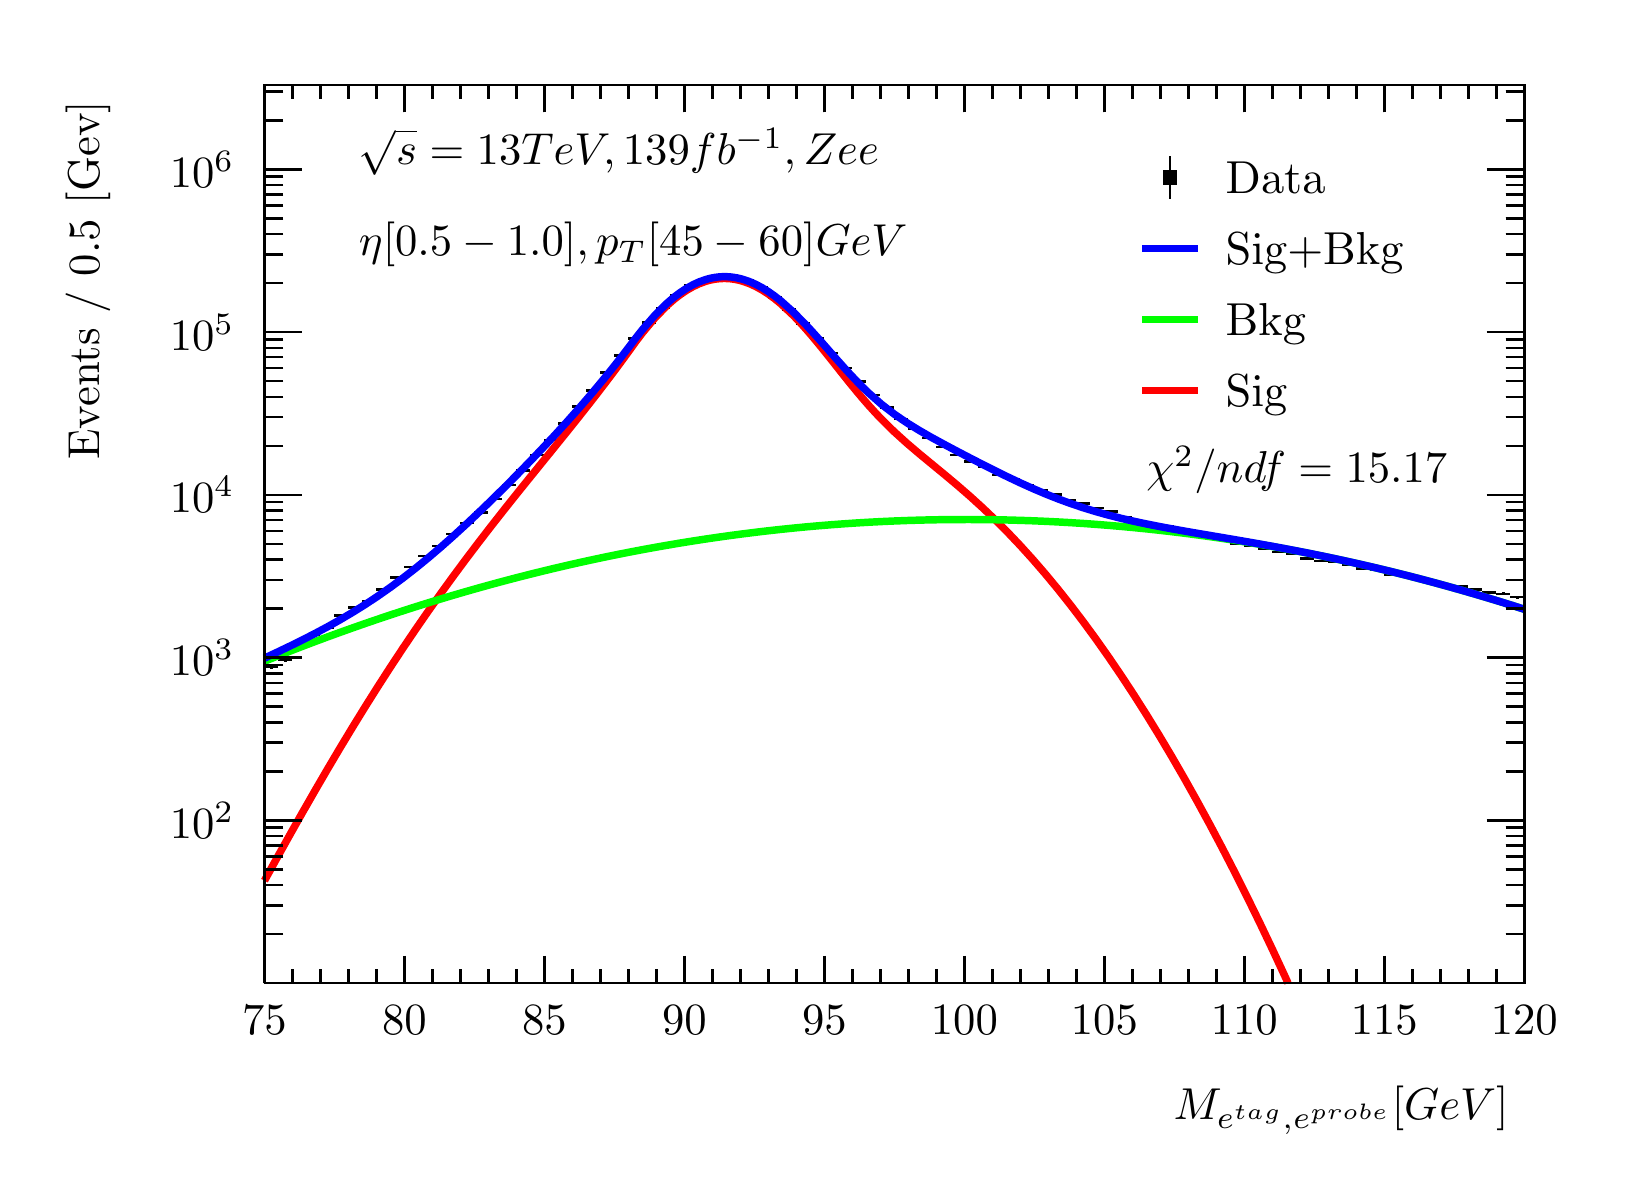
\begin{tikzpicture}
\pgfdeclareplotmark{cross} {
\pgfpathmoveto{\pgfpoint{-0.3\pgfplotmarksize}{\pgfplotmarksize}}
\pgfpathlineto{\pgfpoint{+0.3\pgfplotmarksize}{\pgfplotmarksize}}
\pgfpathlineto{\pgfpoint{+0.3\pgfplotmarksize}{0.3\pgfplotmarksize}}
\pgfpathlineto{\pgfpoint{+1\pgfplotmarksize}{0.3\pgfplotmarksize}}
\pgfpathlineto{\pgfpoint{+1\pgfplotmarksize}{-0.3\pgfplotmarksize}}
\pgfpathlineto{\pgfpoint{+0.3\pgfplotmarksize}{-0.3\pgfplotmarksize}}
\pgfpathlineto{\pgfpoint{+0.3\pgfplotmarksize}{-1.\pgfplotmarksize}}
\pgfpathlineto{\pgfpoint{-0.3\pgfplotmarksize}{-1.\pgfplotmarksize}}
\pgfpathlineto{\pgfpoint{-0.3\pgfplotmarksize}{-0.3\pgfplotmarksize}}
\pgfpathlineto{\pgfpoint{-1.\pgfplotmarksize}{-0.3\pgfplotmarksize}}
\pgfpathlineto{\pgfpoint{-1.\pgfplotmarksize}{0.3\pgfplotmarksize}}
\pgfpathlineto{\pgfpoint{-0.3\pgfplotmarksize}{0.3\pgfplotmarksize}}
\pgfpathclose
\pgfusepathqstroke
}
\pgfdeclareplotmark{cross*} {
\pgfpathmoveto{\pgfpoint{-0.3\pgfplotmarksize}{\pgfplotmarksize}}
\pgfpathlineto{\pgfpoint{+0.3\pgfplotmarksize}{\pgfplotmarksize}}
\pgfpathlineto{\pgfpoint{+0.3\pgfplotmarksize}{0.3\pgfplotmarksize}}
\pgfpathlineto{\pgfpoint{+1\pgfplotmarksize}{0.3\pgfplotmarksize}}
\pgfpathlineto{\pgfpoint{+1\pgfplotmarksize}{-0.3\pgfplotmarksize}}
\pgfpathlineto{\pgfpoint{+0.3\pgfplotmarksize}{-0.3\pgfplotmarksize}}
\pgfpathlineto{\pgfpoint{+0.3\pgfplotmarksize}{-1.\pgfplotmarksize}}
\pgfpathlineto{\pgfpoint{-0.3\pgfplotmarksize}{-1.\pgfplotmarksize}}
\pgfpathlineto{\pgfpoint{-0.3\pgfplotmarksize}{-0.3\pgfplotmarksize}}
\pgfpathlineto{\pgfpoint{-1.\pgfplotmarksize}{-0.3\pgfplotmarksize}}
\pgfpathlineto{\pgfpoint{-1.\pgfplotmarksize}{0.3\pgfplotmarksize}}
\pgfpathlineto{\pgfpoint{-0.3\pgfplotmarksize}{0.3\pgfplotmarksize}}
\pgfpathclose
\pgfusepathqfillstroke
}
\pgfdeclareplotmark{newstar} {
\pgfpathmoveto{\pgfqpoint{0pt}{\pgfplotmarksize}}
\pgfpathlineto{\pgfqpointpolar{44}{0.5\pgfplotmarksize}}
\pgfpathlineto{\pgfqpointpolar{18}{\pgfplotmarksize}}
\pgfpathlineto{\pgfqpointpolar{-20}{0.5\pgfplotmarksize}}
\pgfpathlineto{\pgfqpointpolar{-54}{\pgfplotmarksize}}
\pgfpathlineto{\pgfqpointpolar{-90}{0.5\pgfplotmarksize}}
\pgfpathlineto{\pgfqpointpolar{234}{\pgfplotmarksize}}
\pgfpathlineto{\pgfqpointpolar{198}{0.5\pgfplotmarksize}}
\pgfpathlineto{\pgfqpointpolar{162}{\pgfplotmarksize}}
\pgfpathlineto{\pgfqpointpolar{134}{0.5\pgfplotmarksize}}
\pgfpathclose
\pgfusepathqstroke
}
\pgfdeclareplotmark{newstar*} {
\pgfpathmoveto{\pgfqpoint{0pt}{\pgfplotmarksize}}
\pgfpathlineto{\pgfqpointpolar{44}{0.5\pgfplotmarksize}}
\pgfpathlineto{\pgfqpointpolar{18}{\pgfplotmarksize}}
\pgfpathlineto{\pgfqpointpolar{-20}{0.5\pgfplotmarksize}}
\pgfpathlineto{\pgfqpointpolar{-54}{\pgfplotmarksize}}
\pgfpathlineto{\pgfqpointpolar{-90}{0.5\pgfplotmarksize}}
\pgfpathlineto{\pgfqpointpolar{234}{\pgfplotmarksize}}
\pgfpathlineto{\pgfqpointpolar{198}{0.5\pgfplotmarksize}}
\pgfpathlineto{\pgfqpointpolar{162}{\pgfplotmarksize}}
\pgfpathlineto{\pgfqpointpolar{134}{0.5\pgfplotmarksize}}
\pgfpathclose
\pgfusepathqfillstroke
}
\definecolor{c}{rgb}{1,1,1};
\draw [color=c, fill=c] (0,0) rectangle (20,14.4361);
\draw [color=c, fill=c] (3,2.30977) rectangle (19,13.7143);
\definecolor{c}{rgb}{0,0,0};
\draw [c,line width=0.9] (3,2.30977) -- (3,13.7143) -- (19,13.7143) -- (19,2.30977) -- (3,2.30977);
\definecolor{c}{rgb}{1,1,1};
\draw [color=c, fill=c] (3,2.30977) rectangle (19,13.7143);
\definecolor{c}{rgb}{0,0,0};
\draw [c,line width=0.9] (3,2.30977) -- (3,13.7143) -- (19,13.7143) -- (19,2.30977) -- (3,2.30977);
\draw [c,line width=0.9] (3,2.30977) -- (19,2.30977);
\draw [c,line width=0.9] (3,2.65624) -- (3,2.30977);
\draw [c,line width=0.9] (3.35556,2.48301) -- (3.35556,2.30977);
\draw [c,line width=0.9] (3.71111,2.48301) -- (3.71111,2.30977);
\draw [c,line width=0.9] (4.06667,2.48301) -- (4.06667,2.30977);
\draw [c,line width=0.9] (4.42222,2.48301) -- (4.42222,2.30977);
\draw [c,line width=0.9] (4.77778,2.65624) -- (4.77778,2.30977);
\draw [c,line width=0.9] (5.13333,2.48301) -- (5.13333,2.30977);
\draw [c,line width=0.9] (5.48889,2.48301) -- (5.48889,2.30977);
\draw [c,line width=0.9] (5.84444,2.48301) -- (5.84444,2.30977);
\draw [c,line width=0.9] (6.2,2.48301) -- (6.2,2.30977);
\draw [c,line width=0.9] (6.55556,2.65624) -- (6.55556,2.30977);
\draw [c,line width=0.9] (6.91111,2.48301) -- (6.91111,2.30977);
\draw [c,line width=0.9] (7.26667,2.48301) -- (7.26667,2.30977);
\draw [c,line width=0.9] (7.62222,2.48301) -- (7.62222,2.30977);
\draw [c,line width=0.9] (7.97778,2.48301) -- (7.97778,2.30977);
\draw [c,line width=0.9] (8.33333,2.65624) -- (8.33333,2.30977);
\draw [c,line width=0.9] (8.68889,2.48301) -- (8.68889,2.30977);
\draw [c,line width=0.9] (9.04444,2.48301) -- (9.04444,2.30977);
\draw [c,line width=0.9] (9.4,2.48301) -- (9.4,2.30977);
\draw [c,line width=0.9] (9.75556,2.48301) -- (9.75556,2.30977);
\draw [c,line width=0.9] (10.1111,2.65624) -- (10.1111,2.30977);
\draw [c,line width=0.9] (10.4667,2.48301) -- (10.4667,2.30977);
\draw [c,line width=0.9] (10.8222,2.48301) -- (10.8222,2.30977);
\draw [c,line width=0.9] (11.1778,2.48301) -- (11.1778,2.30977);
\draw [c,line width=0.9] (11.5333,2.48301) -- (11.5333,2.30977);
\draw [c,line width=0.9] (11.8889,2.65624) -- (11.8889,2.30977);
\draw [c,line width=0.9] (12.2444,2.48301) -- (12.2444,2.30977);
\draw [c,line width=0.9] (12.6,2.48301) -- (12.6,2.30977);
\draw [c,line width=0.9] (12.9556,2.48301) -- (12.9556,2.30977);
\draw [c,line width=0.9] (13.3111,2.48301) -- (13.3111,2.30977);
\draw [c,line width=0.9] (13.6667,2.65624) -- (13.6667,2.30977);
\draw [c,line width=0.9] (14.0222,2.48301) -- (14.0222,2.30977);
\draw [c,line width=0.9] (14.3778,2.48301) -- (14.3778,2.30977);
\draw [c,line width=0.9] (14.7333,2.48301) -- (14.7333,2.30977);
\draw [c,line width=0.9] (15.0889,2.48301) -- (15.0889,2.30977);
\draw [c,line width=0.9] (15.4444,2.65624) -- (15.4444,2.30977);
\draw [c,line width=0.9] (15.8,2.48301) -- (15.8,2.30977);
\draw [c,line width=0.9] (16.1556,2.48301) -- (16.1556,2.30977);
\draw [c,line width=0.9] (16.5111,2.48301) -- (16.5111,2.30977);
\draw [c,line width=0.9] (16.8667,2.48301) -- (16.8667,2.30977);
\draw [c,line width=0.9] (17.2222,2.65624) -- (17.2222,2.30977);
\draw [c,line width=0.9] (17.5778,2.48301) -- (17.5778,2.30977);
\draw [c,line width=0.9] (17.9333,2.48301) -- (17.9333,2.30977);
\draw [c,line width=0.9] (18.2889,2.48301) -- (18.2889,2.30977);
\draw [c,line width=0.9] (18.6444,2.48301) -- (18.6444,2.30977);
\draw [c,line width=0.9] (19,2.65624) -- (19,2.30977);
\draw [c,line width=0.9] (19,2.65624) -- (19,2.30977);
\draw [anchor=base] (3,1.66015) node[scale=1.61424, color=c, rotate=0]{75};
\draw [anchor=base] (4.77778,1.66015) node[scale=1.61424, color=c, rotate=0]{80};
\draw [anchor=base] (6.55556,1.66015) node[scale=1.61424, color=c, rotate=0]{85};
\draw [anchor=base] (8.33333,1.66015) node[scale=1.61424, color=c, rotate=0]{90};
\draw [anchor=base] (10.1111,1.66015) node[scale=1.61424, color=c, rotate=0]{95};
\draw [anchor=base] (11.8889,1.66015) node[scale=1.61424, color=c, rotate=0]{100};
\draw [anchor=base] (13.6667,1.66015) node[scale=1.61424, color=c, rotate=0]{105};
\draw [anchor=base] (15.4444,1.66015) node[scale=1.61424, color=c, rotate=0]{110};
\draw [anchor=base] (17.2222,1.66015) node[scale=1.61424, color=c, rotate=0]{115};
\draw [anchor=base] (19,1.66015) node[scale=1.61424, color=c, rotate=0]{120};
\draw [anchor= east] (19,0.692932) node[scale=1.61424, color=c, rotate=0]{$M_{e^{tag}, e^{probe}}  [GeV]$};
\draw [c,line width=0.9] (3,13.7143) -- (19,13.7143);
\draw [c,line width=0.9] (3,13.3678) -- (3,13.7143);
\draw [c,line width=0.9] (3.35556,13.5411) -- (3.35556,13.7143);
\draw [c,line width=0.9] (3.71111,13.5411) -- (3.71111,13.7143);
\draw [c,line width=0.9] (4.06667,13.5411) -- (4.06667,13.7143);
\draw [c,line width=0.9] (4.42222,13.5411) -- (4.42222,13.7143);
\draw [c,line width=0.9] (4.77778,13.3678) -- (4.77778,13.7143);
\draw [c,line width=0.9] (5.13333,13.5411) -- (5.13333,13.7143);
\draw [c,line width=0.9] (5.48889,13.5411) -- (5.48889,13.7143);
\draw [c,line width=0.9] (5.84444,13.5411) -- (5.84444,13.7143);
\draw [c,line width=0.9] (6.2,13.5411) -- (6.2,13.7143);
\draw [c,line width=0.9] (6.55556,13.3678) -- (6.55556,13.7143);
\draw [c,line width=0.9] (6.91111,13.5411) -- (6.91111,13.7143);
\draw [c,line width=0.9] (7.26667,13.5411) -- (7.26667,13.7143);
\draw [c,line width=0.9] (7.62222,13.5411) -- (7.62222,13.7143);
\draw [c,line width=0.9] (7.97778,13.5411) -- (7.97778,13.7143);
\draw [c,line width=0.9] (8.33333,13.3678) -- (8.33333,13.7143);
\draw [c,line width=0.9] (8.68889,13.5411) -- (8.68889,13.7143);
\draw [c,line width=0.9] (9.04444,13.5411) -- (9.04444,13.7143);
\draw [c,line width=0.9] (9.4,13.5411) -- (9.4,13.7143);
\draw [c,line width=0.9] (9.75556,13.5411) -- (9.75556,13.7143);
\draw [c,line width=0.9] (10.1111,13.3678) -- (10.1111,13.7143);
\draw [c,line width=0.9] (10.4667,13.5411) -- (10.4667,13.7143);
\draw [c,line width=0.9] (10.8222,13.5411) -- (10.8222,13.7143);
\draw [c,line width=0.9] (11.1778,13.5411) -- (11.1778,13.7143);
\draw [c,line width=0.9] (11.5333,13.5411) -- (11.5333,13.7143);
\draw [c,line width=0.9] (11.8889,13.3678) -- (11.8889,13.7143);
\draw [c,line width=0.9] (12.2444,13.5411) -- (12.2444,13.7143);
\draw [c,line width=0.9] (12.6,13.5411) -- (12.6,13.7143);
\draw [c,line width=0.9] (12.9556,13.5411) -- (12.9556,13.7143);
\draw [c,line width=0.9] (13.3111,13.5411) -- (13.3111,13.7143);
\draw [c,line width=0.9] (13.6667,13.3678) -- (13.6667,13.7143);
\draw [c,line width=0.9] (14.0222,13.5411) -- (14.0222,13.7143);
\draw [c,line width=0.9] (14.3778,13.5411) -- (14.3778,13.7143);
\draw [c,line width=0.9] (14.7333,13.5411) -- (14.7333,13.7143);
\draw [c,line width=0.9] (15.0889,13.5411) -- (15.0889,13.7143);
\draw [c,line width=0.9] (15.4444,13.3678) -- (15.4444,13.7143);
\draw [c,line width=0.9] (15.8,13.5411) -- (15.8,13.7143);
\draw [c,line width=0.9] (16.1556,13.5411) -- (16.1556,13.7143);
\draw [c,line width=0.9] (16.5111,13.5411) -- (16.5111,13.7143);
\draw [c,line width=0.9] (16.8667,13.5411) -- (16.8667,13.7143);
\draw [c,line width=0.9] (17.2222,13.3678) -- (17.2222,13.7143);
\draw [c,line width=0.9] (17.5778,13.5411) -- (17.5778,13.7143);
\draw [c,line width=0.9] (17.9333,13.5411) -- (17.9333,13.7143);
\draw [c,line width=0.9] (18.2889,13.5411) -- (18.2889,13.7143);
\draw [c,line width=0.9] (18.6444,13.5411) -- (18.6444,13.7143);
\draw [c,line width=0.9] (19,13.3678) -- (19,13.7143);
\draw [c,line width=0.9] (19,13.3678) -- (19,13.7143);
\draw [c,line width=0.9] (3,2.30977) -- (3,13.7143);
\draw [c,line width=0.9] (3.237,2.932) -- (3,2.932);
\draw [c,line width=0.9] (3.237,3.29598) -- (3,3.29598);
\draw [c,line width=0.9] (3.237,3.55423) -- (3,3.55423);
\draw [c,line width=0.9] (3.237,3.75454) -- (3,3.75454);
\draw [c,line width=0.9] (3.237,3.9182) -- (3,3.9182);
\draw [c,line width=0.9] (3.237,4.05658) -- (3,4.05658);
\draw [c,line width=0.9] (3.237,4.17645) -- (3,4.17645);
\draw [c,line width=0.9] (3.237,4.28218) -- (3,4.28218);
\draw [c,line width=0.9] (3.474,4.37676) -- (3,4.37676);
\draw [anchor= east] (2.82,4.37676) node[scale=1.61424, color=c, rotate=0]{$10^{2}$};
\draw [c,line width=0.9] (3.237,4.99899) -- (3,4.99899);
\draw [c,line width=0.9] (3.237,5.36297) -- (3,5.36297);
\draw [c,line width=0.9] (3.237,5.62122) -- (3,5.62122);
\draw [c,line width=0.9] (3.237,5.82153) -- (3,5.82153);
\draw [c,line width=0.9] (3.237,5.9852) -- (3,5.9852);
\draw [c,line width=0.9] (3.237,6.12357) -- (3,6.12357);
\draw [c,line width=0.9] (3.237,6.24344) -- (3,6.24344);
\draw [c,line width=0.9] (3.237,6.34917) -- (3,6.34917);
\draw [c,line width=0.9] (3.474,6.44376) -- (3,6.44376);
\draw [anchor= east] (2.82,6.44376) node[scale=1.61424, color=c, rotate=0]{$10^{3}$};
\draw [c,line width=0.9] (3.237,7.06598) -- (3,7.06598);
\draw [c,line width=0.9] (3.237,7.42996) -- (3,7.42996);
\draw [c,line width=0.9] (3.237,7.68821) -- (3,7.68821);
\draw [c,line width=0.9] (3.237,7.88852) -- (3,7.88852);
\draw [c,line width=0.9] (3.237,8.05219) -- (3,8.05219);
\draw [c,line width=0.9] (3.237,8.19057) -- (3,8.19057);
\draw [c,line width=0.9] (3.237,8.31043) -- (3,8.31043);
\draw [c,line width=0.9] (3.237,8.41617) -- (3,8.41617);
\draw [c,line width=0.9] (3.474,8.51075) -- (3,8.51075);
\draw [anchor= east] (2.82,8.51075) node[scale=1.61424, color=c, rotate=0]{$10^{4}$};
\draw [c,line width=0.9] (3.237,9.13297) -- (3,9.13297);
\draw [c,line width=0.9] (3.237,9.49695) -- (3,9.49695);
\draw [c,line width=0.9] (3.237,9.7552) -- (3,9.7552);
\draw [c,line width=0.9] (3.237,9.95551) -- (3,9.95551);
\draw [c,line width=0.9] (3.237,10.1192) -- (3,10.1192);
\draw [c,line width=0.9] (3.237,10.2576) -- (3,10.2576);
\draw [c,line width=0.9] (3.237,10.3774) -- (3,10.3774);
\draw [c,line width=0.9] (3.237,10.4832) -- (3,10.4832);
\draw [c,line width=0.9] (3.474,10.5777) -- (3,10.5777);
\draw [anchor= east] (2.82,10.5777) node[scale=1.61424, color=c, rotate=0]{$10^{5}$};
\draw [c,line width=0.9] (3.237,11.2) -- (3,11.2);
\draw [c,line width=0.9] (3.237,11.5639) -- (3,11.5639);
\draw [c,line width=0.9] (3.237,11.8222) -- (3,11.8222);
\draw [c,line width=0.9] (3.237,12.0225) -- (3,12.0225);
\draw [c,line width=0.9] (3.237,12.1862) -- (3,12.1862);
\draw [c,line width=0.9] (3.237,12.3245) -- (3,12.3245);
\draw [c,line width=0.9] (3.237,12.4444) -- (3,12.4444);
\draw [c,line width=0.9] (3.237,12.5501) -- (3,12.5501);
\draw [c,line width=0.9] (3.474,12.6447) -- (3,12.6447);
\draw [anchor= east] (2.82,12.6447) node[scale=1.61424, color=c, rotate=0]{$10^{6}$};
\draw [c,line width=0.9] (3.237,13.267) -- (3,13.267);
\draw [c,line width=0.9] (3.237,13.6309) -- (3,13.6309);
\draw [anchor= east] (0.76,13.7143) node[scale=1.61424, color=c, rotate=90]{Events / 0.5 [Gev]};
\draw [c,line width=0.9] (19,2.30977) -- (19,13.7143);
\draw [c,line width=0.9] (18.763,2.932) -- (19,2.932);
\draw [c,line width=0.9] (18.763,3.29598) -- (19,3.29598);
\draw [c,line width=0.9] (18.763,3.55423) -- (19,3.55423);
\draw [c,line width=0.9] (18.763,3.75454) -- (19,3.75454);
\draw [c,line width=0.9] (18.763,3.9182) -- (19,3.9182);
\draw [c,line width=0.9] (18.763,4.05658) -- (19,4.05658);
\draw [c,line width=0.9] (18.763,4.17645) -- (19,4.17645);
\draw [c,line width=0.9] (18.763,4.28218) -- (19,4.28218);
\draw [c,line width=0.9] (18.526,4.37676) -- (19,4.37676);
\draw [c,line width=0.9] (18.763,4.99899) -- (19,4.99899);
\draw [c,line width=0.9] (18.763,5.36297) -- (19,5.36297);
\draw [c,line width=0.9] (18.763,5.62122) -- (19,5.62122);
\draw [c,line width=0.9] (18.763,5.82153) -- (19,5.82153);
\draw [c,line width=0.9] (18.763,5.9852) -- (19,5.9852);
\draw [c,line width=0.9] (18.763,6.12357) -- (19,6.12357);
\draw [c,line width=0.9] (18.763,6.24344) -- (19,6.24344);
\draw [c,line width=0.9] (18.763,6.34917) -- (19,6.34917);
\draw [c,line width=0.9] (18.526,6.44376) -- (19,6.44376);
\draw [c,line width=0.9] (18.763,7.06598) -- (19,7.06598);
\draw [c,line width=0.9] (18.763,7.42996) -- (19,7.42996);
\draw [c,line width=0.9] (18.763,7.68821) -- (19,7.68821);
\draw [c,line width=0.9] (18.763,7.88852) -- (19,7.88852);
\draw [c,line width=0.9] (18.763,8.05219) -- (19,8.05219);
\draw [c,line width=0.9] (18.763,8.19057) -- (19,8.19057);
\draw [c,line width=0.9] (18.763,8.31043) -- (19,8.31043);
\draw [c,line width=0.9] (18.763,8.41617) -- (19,8.41617);
\draw [c,line width=0.9] (18.526,8.51075) -- (19,8.51075);
\draw [c,line width=0.9] (18.763,9.13297) -- (19,9.13297);
\draw [c,line width=0.9] (18.763,9.49695) -- (19,9.49695);
\draw [c,line width=0.9] (18.763,9.7552) -- (19,9.7552);
\draw [c,line width=0.9] (18.763,9.95551) -- (19,9.95551);
\draw [c,line width=0.9] (18.763,10.1192) -- (19,10.1192);
\draw [c,line width=0.9] (18.763,10.2576) -- (19,10.2576);
\draw [c,line width=0.9] (18.763,10.3774) -- (19,10.3774);
\draw [c,line width=0.9] (18.763,10.4832) -- (19,10.4832);
\draw [c,line width=0.9] (18.526,10.5777) -- (19,10.5777);
\draw [c,line width=0.9] (18.763,11.2) -- (19,11.2);
\draw [c,line width=0.9] (18.763,11.5639) -- (19,11.5639);
\draw [c,line width=0.9] (18.763,11.8222) -- (19,11.8222);
\draw [c,line width=0.9] (18.763,12.0225) -- (19,12.0225);
\draw [c,line width=0.9] (18.763,12.1862) -- (19,12.1862);
\draw [c,line width=0.9] (18.763,12.3245) -- (19,12.3245);
\draw [c,line width=0.9] (18.763,12.4444) -- (19,12.4444);
\draw [c,line width=0.9] (18.763,12.5501) -- (19,12.5501);
\draw [c,line width=0.9] (18.526,12.6447) -- (19,12.6447);
\draw [c,line width=0.9] (18.763,13.267) -- (19,13.267);
\draw [c,line width=0.9] (18.763,13.6309) -- (19,13.6309);
\draw [c,line width=0.9] (3.08889,6.33002) -- (3,6.33002);
\draw [c,line width=0.9] (3,6.33002) -- (3,6.33002);
\draw [c,line width=0.9] (3.08889,6.33002) -- (3.17778,6.33002);
\draw [c,line width=0.9] (3.17778,6.33002) -- (3.17778,6.33002);
\draw [c,line width=0.9] (3.08889,6.33002) -- (3.08889,6.36026);
\draw [c,line width=0.9] (3.08889,6.36026) -- (3.08889,6.36026);
\draw [c,line width=0.9] (3.08889,6.33002) -- (3.08889,6.29978);
\draw [c,line width=0.9] (3.08889,6.29978) -- (3.08889,6.29978);
\draw [c,line width=0.9] (3.26667,6.4127) -- (3.17778,6.4127);
\draw [c,line width=0.9] (3.17778,6.4127) -- (3.17778,6.4127);
\draw [c,line width=0.9] (3.26667,6.4127) -- (3.35556,6.4127);
\draw [c,line width=0.9] (3.35556,6.4127) -- (3.35556,6.4127);
\draw [c,line width=0.9] (3.26667,6.4127) -- (3.26667,6.44159);
\draw [c,line width=0.9] (3.26667,6.44159) -- (3.26667,6.44159);
\draw [c,line width=0.9] (3.26667,6.4127) -- (3.26667,6.38382);
\draw [c,line width=0.9] (3.26667,6.38382) -- (3.26667,6.38382);
\draw [c,line width=0.9] (3.44444,6.57) -- (3.35556,6.57);
\draw [c,line width=0.9] (3.35556,6.57) -- (3.35556,6.57);
\draw [c,line width=0.9] (3.44444,6.57) -- (3.53333,6.57);
\draw [c,line width=0.9] (3.53333,6.57) -- (3.53333,6.57);
\draw [c,line width=0.9] (3.44444,6.57) -- (3.44444,6.59646);
\draw [c,line width=0.9] (3.44444,6.59646) -- (3.44444,6.59646);
\draw [c,line width=0.9] (3.44444,6.57) -- (3.44444,6.54354);
\draw [c,line width=0.9] (3.44444,6.54354) -- (3.44444,6.54354);
\draw [c,line width=0.9] (3.62222,6.72767) -- (3.53333,6.72767);
\draw [c,line width=0.9] (3.53333,6.72767) -- (3.53333,6.72767);
\draw [c,line width=0.9] (3.62222,6.72767) -- (3.71111,6.72767);
\draw [c,line width=0.9] (3.71111,6.72767) -- (3.71111,6.72767);
\draw [c,line width=0.9] (3.62222,6.72767) -- (3.62222,6.7519);
\draw [c,line width=0.9] (3.62222,6.7519) -- (3.62222,6.7519);
\draw [c,line width=0.9] (3.62222,6.72767) -- (3.62222,6.70343);
\draw [c,line width=0.9] (3.62222,6.70343) -- (3.62222,6.70343);
\draw [c,line width=0.9] (3.8,6.82022) -- (3.71111,6.82022);
\draw [c,line width=0.9] (3.71111,6.82022) -- (3.71111,6.82022);
\draw [c,line width=0.9] (3.8,6.82022) -- (3.88889,6.82022);
\draw [c,line width=0.9] (3.88889,6.82022) -- (3.88889,6.82022);
\draw [c,line width=0.9] (3.8,6.82022) -- (3.8,6.84323);
\draw [c,line width=0.9] (3.8,6.84323) -- (3.8,6.84323);
\draw [c,line width=0.9] (3.8,6.82022) -- (3.8,6.7972);
\draw [c,line width=0.9] (3.8,6.7972) -- (3.8,6.7972);
\draw [c,line width=0.9] (3.97778,6.97935) -- (3.88889,6.97935);
\draw [c,line width=0.9] (3.88889,6.97935) -- (3.88889,6.97935);
\draw [c,line width=0.9] (3.97778,6.97935) -- (4.06667,6.97935);
\draw [c,line width=0.9] (4.06667,6.97935) -- (4.06667,6.97935);
\draw [c,line width=0.9] (3.97778,6.97935) -- (3.97778,7.00041);
\draw [c,line width=0.9] (3.97778,7.00041) -- (3.97778,7.00041);
\draw [c,line width=0.9] (3.97778,6.97935) -- (3.97778,6.95828);
\draw [c,line width=0.9] (3.97778,6.95828) -- (3.97778,6.95828);
\draw [c,line width=0.9] (4.15556,7.07713) -- (4.06667,7.07713);
\draw [c,line width=0.9] (4.06667,7.07713) -- (4.06667,7.07713);
\draw [c,line width=0.9] (4.15556,7.07713) -- (4.24444,7.07713);
\draw [c,line width=0.9] (4.24444,7.07713) -- (4.24444,7.07713);
\draw [c,line width=0.9] (4.15556,7.07713) -- (4.15556,7.09708);
\draw [c,line width=0.9] (4.15556,7.09708) -- (4.15556,7.09708);
\draw [c,line width=0.9] (4.15556,7.07713) -- (4.15556,7.05719);
\draw [c,line width=0.9] (4.15556,7.05719) -- (4.15556,7.05719);
\draw [c,line width=0.9] (4.33333,7.16088) -- (4.24444,7.16088);
\draw [c,line width=0.9] (4.24444,7.16088) -- (4.24444,7.16088);
\draw [c,line width=0.9] (4.33333,7.16088) -- (4.42222,7.16088);
\draw [c,line width=0.9] (4.42222,7.16088) -- (4.42222,7.16088);
\draw [c,line width=0.9] (4.33333,7.16088) -- (4.33333,7.17992);
\draw [c,line width=0.9] (4.33333,7.17992) -- (4.33333,7.17992);
\draw [c,line width=0.9] (4.33333,7.16088) -- (4.33333,7.14184);
\draw [c,line width=0.9] (4.33333,7.14184) -- (4.33333,7.14184);
\draw [c,line width=0.9] (4.51111,7.30667) -- (4.42222,7.30667);
\draw [c,line width=0.9] (4.42222,7.30667) -- (4.42222,7.30667);
\draw [c,line width=0.9] (4.51111,7.30667) -- (4.6,7.30667);
\draw [c,line width=0.9] (4.6,7.30667) -- (4.6,7.30667);
\draw [c,line width=0.9] (4.51111,7.30667) -- (4.51111,7.32422);
\draw [c,line width=0.9] (4.51111,7.32422) -- (4.51111,7.32422);
\draw [c,line width=0.9] (4.51111,7.30667) -- (4.51111,7.28911);
\draw [c,line width=0.9] (4.51111,7.28911) -- (4.51111,7.28911);
\draw [c,line width=0.9] (4.68889,7.45824) -- (4.6,7.45824);
\draw [c,line width=0.9] (4.6,7.45824) -- (4.6,7.45824);
\draw [c,line width=0.9] (4.68889,7.45824) -- (4.77778,7.45824);
\draw [c,line width=0.9] (4.77778,7.45824) -- (4.77778,7.45824);
\draw [c,line width=0.9] (4.68889,7.45824) -- (4.68889,7.47437);
\draw [c,line width=0.9] (4.68889,7.47437) -- (4.68889,7.47437);
\draw [c,line width=0.9] (4.68889,7.45824) -- (4.68889,7.4421);
\draw [c,line width=0.9] (4.68889,7.4421) -- (4.68889,7.4421);
\draw [c,line width=0.9] (4.86667,7.59238) -- (4.77778,7.59238);
\draw [c,line width=0.9] (4.77778,7.59238) -- (4.77778,7.59238);
\draw [c,line width=0.9] (4.86667,7.59238) -- (4.95556,7.59238);
\draw [c,line width=0.9] (4.95556,7.59238) -- (4.95556,7.59238);
\draw [c,line width=0.9] (4.86667,7.59238) -- (4.86667,7.60735);
\draw [c,line width=0.9] (4.86667,7.60735) -- (4.86667,7.60735);
\draw [c,line width=0.9] (4.86667,7.59238) -- (4.86667,7.57741);
\draw [c,line width=0.9] (4.86667,7.57741) -- (4.86667,7.57741);
\draw [c,line width=0.9] (5.04444,7.73179) -- (4.95556,7.73179);
\draw [c,line width=0.9] (4.95556,7.73179) -- (4.95556,7.73179);
\draw [c,line width=0.9] (5.04444,7.73179) -- (5.13333,7.73179);
\draw [c,line width=0.9] (5.13333,7.73179) -- (5.13333,7.73179);
\draw [c,line width=0.9] (5.04444,7.73179) -- (5.04444,7.74565);
\draw [c,line width=0.9] (5.04444,7.74565) -- (5.04444,7.74565);
\draw [c,line width=0.9] (5.04444,7.73179) -- (5.04444,7.71794);
\draw [c,line width=0.9] (5.04444,7.71794) -- (5.04444,7.71794);
\draw [c,line width=0.9] (5.22222,7.85858) -- (5.13333,7.85858);
\draw [c,line width=0.9] (5.13333,7.85858) -- (5.13333,7.85858);
\draw [c,line width=0.9] (5.22222,7.85858) -- (5.31111,7.85858);
\draw [c,line width=0.9] (5.31111,7.85858) -- (5.31111,7.85858);
\draw [c,line width=0.9] (5.22222,7.85858) -- (5.22222,7.87149);
\draw [c,line width=0.9] (5.22222,7.87149) -- (5.22222,7.87149);
\draw [c,line width=0.9] (5.22222,7.85858) -- (5.22222,7.84567);
\draw [c,line width=0.9] (5.22222,7.84567) -- (5.22222,7.84567);
\draw [c,line width=0.9] (5.4,8.01054) -- (5.31111,8.01054);
\draw [c,line width=0.9] (5.31111,8.01054) -- (5.31111,8.01054);
\draw [c,line width=0.9] (5.4,8.01054) -- (5.48889,8.01054);
\draw [c,line width=0.9] (5.48889,8.01054) -- (5.48889,8.01054);
\draw [c,line width=0.9] (5.4,8.01054) -- (5.4,8.0224);
\draw [c,line width=0.9] (5.4,8.0224) -- (5.4,8.0224);
\draw [c,line width=0.9] (5.4,8.01054) -- (5.4,7.99868);
\draw [c,line width=0.9] (5.4,7.99868) -- (5.4,7.99868);
\draw [c,line width=0.9] (5.57778,8.15245) -- (5.48889,8.15245);
\draw [c,line width=0.9] (5.48889,8.15245) -- (5.48889,8.15245);
\draw [c,line width=0.9] (5.57778,8.15245) -- (5.66667,8.15245);
\draw [c,line width=0.9] (5.66667,8.15245) -- (5.66667,8.15245);
\draw [c,line width=0.9] (5.57778,8.15245) -- (5.57778,8.16341);
\draw [c,line width=0.9] (5.57778,8.16341) -- (5.57778,8.16341);
\draw [c,line width=0.9] (5.57778,8.15245) -- (5.57778,8.14149);
\draw [c,line width=0.9] (5.57778,8.14149) -- (5.57778,8.14149);
\draw [c,line width=0.9] (5.75556,8.28805) -- (5.66667,8.28805);
\draw [c,line width=0.9] (5.66667,8.28805) -- (5.66667,8.28805);
\draw [c,line width=0.9] (5.75556,8.28805) -- (5.84444,8.28805);
\draw [c,line width=0.9] (5.84444,8.28805) -- (5.84444,8.28805);
\draw [c,line width=0.9] (5.75556,8.28805) -- (5.75556,8.29822);
\draw [c,line width=0.9] (5.75556,8.29822) -- (5.75556,8.29822);
\draw [c,line width=0.9] (5.75556,8.28805) -- (5.75556,8.27789);
\draw [c,line width=0.9] (5.75556,8.27789) -- (5.75556,8.27789);
\draw [c,line width=0.9] (5.93333,8.45892) -- (5.84444,8.45892);
\draw [c,line width=0.9] (5.84444,8.45892) -- (5.84444,8.45892);
\draw [c,line width=0.9] (5.93333,8.45892) -- (6.02222,8.45892);
\draw [c,line width=0.9] (6.02222,8.45892) -- (6.02222,8.45892);
\draw [c,line width=0.9] (5.93333,8.45892) -- (5.93333,8.46816);
\draw [c,line width=0.9] (5.93333,8.46816) -- (5.93333,8.46816);
\draw [c,line width=0.9] (5.93333,8.45892) -- (5.93333,8.44968);
\draw [c,line width=0.9] (5.93333,8.44968) -- (5.93333,8.44968);
\draw [c,line width=0.9] (6.11111,8.63738) -- (6.02222,8.63738);
\draw [c,line width=0.9] (6.02222,8.63738) -- (6.02222,8.63738);
\draw [c,line width=0.9] (6.11111,8.63738) -- (6.2,8.63738);
\draw [c,line width=0.9] (6.2,8.63738) -- (6.2,8.63738);
\draw [c,line width=0.9] (6.11111,8.63738) -- (6.11111,8.64575);
\draw [c,line width=0.9] (6.11111,8.64575) -- (6.11111,8.64575);
\draw [c,line width=0.9] (6.11111,8.63738) -- (6.11111,8.62901);
\draw [c,line width=0.9] (6.11111,8.62901) -- (6.11111,8.62901);
\draw [c,line width=0.9] (6.28889,8.81759) -- (6.2,8.81759);
\draw [c,line width=0.9] (6.2,8.81759) -- (6.2,8.81759);
\draw [c,line width=0.9] (6.28889,8.81759) -- (6.37778,8.81759);
\draw [c,line width=0.9] (6.37778,8.81759) -- (6.37778,8.81759);
\draw [c,line width=0.9] (6.28889,8.81759) -- (6.28889,8.82516);
\draw [c,line width=0.9] (6.28889,8.82516) -- (6.28889,8.82516);
\draw [c,line width=0.9] (6.28889,8.81759) -- (6.28889,8.81002);
\draw [c,line width=0.9] (6.28889,8.81002) -- (6.28889,8.81002);
\draw [c,line width=0.9] (6.46667,9.01469) -- (6.37778,9.01469);
\draw [c,line width=0.9] (6.37778,9.01469) -- (6.37778,9.01469);
\draw [c,line width=0.9] (6.46667,9.01469) -- (6.55556,9.01469);
\draw [c,line width=0.9] (6.55556,9.01469) -- (6.55556,9.01469);
\draw [c,line width=0.9] (6.46667,9.01469) -- (6.46667,9.02147);
\draw [c,line width=0.9] (6.46667,9.02147) -- (6.46667,9.02147);
\draw [c,line width=0.9] (6.46667,9.01469) -- (6.46667,9.00791);
\draw [c,line width=0.9] (6.46667,9.00791) -- (6.46667,9.00791);
\draw [c,line width=0.9] (6.64444,9.20339) -- (6.55556,9.20339);
\draw [c,line width=0.9] (6.55556,9.20339) -- (6.55556,9.20339);
\draw [c,line width=0.9] (6.64444,9.20339) -- (6.73333,9.20339);
\draw [c,line width=0.9] (6.73333,9.20339) -- (6.73333,9.20339);
\draw [c,line width=0.9] (6.64444,9.20339) -- (6.64444,9.20949);
\draw [c,line width=0.9] (6.64444,9.20949) -- (6.64444,9.20949);
\draw [c,line width=0.9] (6.64444,9.20339) -- (6.64444,9.19729);
\draw [c,line width=0.9] (6.64444,9.19729) -- (6.64444,9.19729);
\draw [c,line width=0.9] (6.82222,9.41597) -- (6.73333,9.41597);
\draw [c,line width=0.9] (6.73333,9.41597) -- (6.73333,9.41597);
\draw [c,line width=0.9] (6.82222,9.41597) -- (6.91111,9.41597);
\draw [c,line width=0.9] (6.91111,9.41597) -- (6.91111,9.41597);
\draw [c,line width=0.9] (6.82222,9.41597) -- (6.82222,9.42139);
\draw [c,line width=0.9] (6.82222,9.42139) -- (6.82222,9.42139);
\draw [c,line width=0.9] (6.82222,9.41597) -- (6.82222,9.41055);
\draw [c,line width=0.9] (6.82222,9.41055) -- (6.82222,9.41055);
\draw [c,line width=0.9] (7,9.63111) -- (6.91111,9.63111);
\draw [c,line width=0.9] (6.91111,9.63111) -- (6.91111,9.63111);
\draw [c,line width=0.9] (7,9.63111) -- (7.08889,9.63111);
\draw [c,line width=0.9] (7.08889,9.63111) -- (7.08889,9.63111);
\draw [c,line width=0.9] (7,9.63111) -- (7,9.63592);
\draw [c,line width=0.9] (7,9.63592) -- (7,9.63592);
\draw [c,line width=0.9] (7,9.63111) -- (7,9.62631);
\draw [c,line width=0.9] (7,9.62631) -- (7,9.62631);
\draw [c,line width=0.9] (7.17778,9.83636) -- (7.08889,9.83636);
\draw [c,line width=0.9] (7.08889,9.83636) -- (7.08889,9.83636);
\draw [c,line width=0.9] (7.17778,9.83636) -- (7.26667,9.83636);
\draw [c,line width=0.9] (7.26667,9.83636) -- (7.26667,9.83636);
\draw [c,line width=0.9] (7.17778,9.83636) -- (7.17778,9.84065);
\draw [c,line width=0.9] (7.17778,9.84065) -- (7.17778,9.84065);
\draw [c,line width=0.9] (7.17778,9.83636) -- (7.17778,9.83207);
\draw [c,line width=0.9] (7.17778,9.83207) -- (7.17778,9.83207);
\draw [c,line width=0.9] (7.35556,10.0623) -- (7.26667,10.0623);
\draw [c,line width=0.9] (7.26667,10.0623) -- (7.26667,10.0623);
\draw [c,line width=0.9] (7.35556,10.0623) -- (7.44444,10.0623);
\draw [c,line width=0.9] (7.44444,10.0623) -- (7.44444,10.0623);
\draw [c,line width=0.9] (7.35556,10.0623) -- (7.35556,10.066);
\draw [c,line width=0.9] (7.35556,10.066) -- (7.35556,10.066);
\draw [c,line width=0.9] (7.35556,10.0623) -- (7.35556,10.0585);
\draw [c,line width=0.9] (7.35556,10.0585) -- (7.35556,10.0585);
\draw [c,line width=0.9] (7.53333,10.2775) -- (7.44444,10.2775);
\draw [c,line width=0.9] (7.44444,10.2775) -- (7.44444,10.2775);
\draw [c,line width=0.9] (7.53333,10.2775) -- (7.62222,10.2775);
\draw [c,line width=0.9] (7.62222,10.2775) -- (7.62222,10.2775);
\draw [c,line width=0.9] (7.53333,10.2775) -- (7.53333,10.2808);
\draw [c,line width=0.9] (7.53333,10.2808) -- (7.53333,10.2808);
\draw [c,line width=0.9] (7.53333,10.2775) -- (7.53333,10.2741);
\draw [c,line width=0.9] (7.53333,10.2741) -- (7.53333,10.2741);
\draw [c,line width=0.9] (7.71111,10.4972) -- (7.62222,10.4972);
\draw [c,line width=0.9] (7.62222,10.4972) -- (7.62222,10.4972);
\draw [c,line width=0.9] (7.71111,10.4972) -- (7.8,10.4972);
\draw [c,line width=0.9] (7.8,10.4972) -- (7.8,10.4972);
\draw [c,line width=0.9] (7.71111,10.4972) -- (7.71111,10.5002);
\draw [c,line width=0.9] (7.71111,10.5002) -- (7.71111,10.5002);
\draw [c,line width=0.9] (7.71111,10.4972) -- (7.71111,10.4942);
\draw [c,line width=0.9] (7.71111,10.4942) -- (7.71111,10.4942);
\draw [c,line width=0.9] (7.88889,10.6999) -- (7.8,10.6999);
\draw [c,line width=0.9] (7.8,10.6999) -- (7.8,10.6999);
\draw [c,line width=0.9] (7.88889,10.6999) -- (7.97778,10.6999);
\draw [c,line width=0.9] (7.97778,10.6999) -- (7.97778,10.6999);
\draw [c,line width=0.9] (7.88889,10.6999) -- (7.88889,10.7025);
\draw [c,line width=0.9] (7.88889,10.7025) -- (7.88889,10.7025);
\draw [c,line width=0.9] (7.88889,10.6999) -- (7.88889,10.6972);
\draw [c,line width=0.9] (7.88889,10.6972) -- (7.88889,10.6972);
\draw [c,line width=0.9] (8.06667,10.8818) -- (7.97778,10.8818);
\draw [c,line width=0.9] (7.97778,10.8818) -- (7.97778,10.8818);
\draw [c,line width=0.9] (8.06667,10.8818) -- (8.15556,10.8818);
\draw [c,line width=0.9] (8.15556,10.8818) -- (8.15556,10.8818);
\draw [c,line width=0.9] (8.06667,10.8818) -- (8.06667,10.8842);
\draw [c,line width=0.9] (8.06667,10.8842) -- (8.06667,10.8842);
\draw [c,line width=0.9] (8.06667,10.8818) -- (8.06667,10.8794);
\draw [c,line width=0.9] (8.06667,10.8794) -- (8.06667,10.8794);
\draw [c,line width=0.9] (8.24444,11.0387) -- (8.15556,11.0387);
\draw [c,line width=0.9] (8.15556,11.0387) -- (8.15556,11.0387);
\draw [c,line width=0.9] (8.24444,11.0387) -- (8.33333,11.0387);
\draw [c,line width=0.9] (8.33333,11.0387) -- (8.33333,11.0387);
\draw [c,line width=0.9] (8.24444,11.0387) -- (8.24444,11.0409);
\draw [c,line width=0.9] (8.24444,11.0409) -- (8.24444,11.0409);
\draw [c,line width=0.9] (8.24444,11.0387) -- (8.24444,11.0365);
\draw [c,line width=0.9] (8.24444,11.0365) -- (8.24444,11.0365);
\draw [c,line width=0.9] (8.42222,11.1677) -- (8.33333,11.1677);
\draw [c,line width=0.9] (8.33333,11.1677) -- (8.33333,11.1677);
\draw [c,line width=0.9] (8.42222,11.1677) -- (8.51111,11.1677);
\draw [c,line width=0.9] (8.51111,11.1677) -- (8.51111,11.1677);
\draw [c,line width=0.9] (8.42222,11.1677) -- (8.42222,11.1697);
\draw [c,line width=0.9] (8.42222,11.1697) -- (8.42222,11.1697);
\draw [c,line width=0.9] (8.42222,11.1677) -- (8.42222,11.1656);
\draw [c,line width=0.9] (8.42222,11.1656) -- (8.42222,11.1656);
\draw [c,line width=0.9] (8.6,11.2521) -- (8.51111,11.2521);
\draw [c,line width=0.9] (8.51111,11.2521) -- (8.51111,11.2521);
\draw [c,line width=0.9] (8.6,11.2521) -- (8.68889,11.2521);
\draw [c,line width=0.9] (8.68889,11.2521) -- (8.68889,11.2521);
\draw [c,line width=0.9] (8.6,11.2521) -- (8.6,11.254);
\draw [c,line width=0.9] (8.6,11.254) -- (8.6,11.254);
\draw [c,line width=0.9] (8.6,11.2521) -- (8.6,11.2501);
\draw [c,line width=0.9] (8.6,11.2501) -- (8.6,11.2501);
\draw [c,line width=0.9] (8.77778,11.291) -- (8.68889,11.291);
\draw [c,line width=0.9] (8.68889,11.291) -- (8.68889,11.291);
\draw [c,line width=0.9] (8.77778,11.291) -- (8.86667,11.291);
\draw [c,line width=0.9] (8.86667,11.291) -- (8.86667,11.291);
\draw [c,line width=0.9] (8.77778,11.291) -- (8.77778,11.2929);
\draw [c,line width=0.9] (8.77778,11.2929) -- (8.77778,11.2929);
\draw [c,line width=0.9] (8.77778,11.291) -- (8.77778,11.2891);
\draw [c,line width=0.9] (8.77778,11.2891) -- (8.77778,11.2891);
\draw [c,line width=0.9] (8.95556,11.2866) -- (8.86667,11.2866);
\draw [c,line width=0.9] (8.86667,11.2866) -- (8.86667,11.2866);
\draw [c,line width=0.9] (8.95556,11.2866) -- (9.04444,11.2866);
\draw [c,line width=0.9] (9.04444,11.2866) -- (9.04444,11.2866);
\draw [c,line width=0.9] (8.95556,11.2866) -- (8.95556,11.2886);
\draw [c,line width=0.9] (8.95556,11.2886) -- (8.95556,11.2886);
\draw [c,line width=0.9] (8.95556,11.2866) -- (8.95556,11.2847);
\draw [c,line width=0.9] (8.95556,11.2847) -- (8.95556,11.2847);
\draw [c,line width=0.9] (9.13333,11.2338) -- (9.04444,11.2338);
\draw [c,line width=0.9] (9.04444,11.2338) -- (9.04444,11.2338);
\draw [c,line width=0.9] (9.13333,11.2338) -- (9.22222,11.2338);
\draw [c,line width=0.9] (9.22222,11.2338) -- (9.22222,11.2338);
\draw [c,line width=0.9] (9.13333,11.2338) -- (9.13333,11.2358);
\draw [c,line width=0.9] (9.13333,11.2358) -- (9.13333,11.2358);
\draw [c,line width=0.9] (9.13333,11.2338) -- (9.13333,11.2318);
\draw [c,line width=0.9] (9.13333,11.2318) -- (9.13333,11.2318);
\draw [c,line width=0.9] (9.31111,11.1405) -- (9.22222,11.1405);
\draw [c,line width=0.9] (9.22222,11.1405) -- (9.22222,11.1405);
\draw [c,line width=0.9] (9.31111,11.1405) -- (9.4,11.1405);
\draw [c,line width=0.9] (9.4,11.1405) -- (9.4,11.1405);
\draw [c,line width=0.9] (9.31111,11.1405) -- (9.31111,11.1426);
\draw [c,line width=0.9] (9.31111,11.1426) -- (9.31111,11.1426);
\draw [c,line width=0.9] (9.31111,11.1405) -- (9.31111,11.1384);
\draw [c,line width=0.9] (9.31111,11.1384) -- (9.31111,11.1384);
\draw [c,line width=0.9] (9.48889,11.0177) -- (9.4,11.0177);
\draw [c,line width=0.9] (9.4,11.0177) -- (9.4,11.0177);
\draw [c,line width=0.9] (9.48889,11.0177) -- (9.57778,11.0177);
\draw [c,line width=0.9] (9.57778,11.0177) -- (9.57778,11.0177);
\draw [c,line width=0.9] (9.48889,11.0177) -- (9.48889,11.0199);
\draw [c,line width=0.9] (9.48889,11.0199) -- (9.48889,11.0199);
\draw [c,line width=0.9] (9.48889,11.0177) -- (9.48889,11.0155);
\draw [c,line width=0.9] (9.48889,11.0155) -- (9.48889,11.0155);
\draw [c,line width=0.9] (9.66667,10.8637) -- (9.57778,10.8637);
\draw [c,line width=0.9] (9.57778,10.8637) -- (9.57778,10.8637);
\draw [c,line width=0.9] (9.66667,10.8637) -- (9.75556,10.8637);
\draw [c,line width=0.9] (9.75556,10.8637) -- (9.75556,10.8637);
\draw [c,line width=0.9] (9.66667,10.8637) -- (9.66667,10.8661);
\draw [c,line width=0.9] (9.66667,10.8661) -- (9.66667,10.8661);
\draw [c,line width=0.9] (9.66667,10.8637) -- (9.66667,10.8612);
\draw [c,line width=0.9] (9.66667,10.8612) -- (9.66667,10.8612);
\draw [c,line width=0.9] (9.84444,10.6849) -- (9.75556,10.6849);
\draw [c,line width=0.9] (9.75556,10.6849) -- (9.75556,10.6849);
\draw [c,line width=0.9] (9.84444,10.6849) -- (9.93333,10.6849);
\draw [c,line width=0.9] (9.93333,10.6849) -- (9.93333,10.6849);
\draw [c,line width=0.9] (9.84444,10.6849) -- (9.84444,10.6876);
\draw [c,line width=0.9] (9.84444,10.6876) -- (9.84444,10.6876);
\draw [c,line width=0.9] (9.84444,10.6849) -- (9.84444,10.6823);
\draw [c,line width=0.9] (9.84444,10.6823) -- (9.84444,10.6823);
\draw [c,line width=0.9] (10.0222,10.5047) -- (9.93333,10.5047);
\draw [c,line width=0.9] (9.93333,10.5047) -- (9.93333,10.5047);
\draw [c,line width=0.9] (10.0222,10.5047) -- (10.1111,10.5047);
\draw [c,line width=0.9] (10.1111,10.5047) -- (10.1111,10.5047);
\draw [c,line width=0.9] (10.0222,10.5047) -- (10.0222,10.5076);
\draw [c,line width=0.9] (10.0222,10.5076) -- (10.0222,10.5076);
\draw [c,line width=0.9] (10.0222,10.5047) -- (10.0222,10.5017);
\draw [c,line width=0.9] (10.0222,10.5017) -- (10.0222,10.5017);
\draw [c,line width=0.9] (10.2,10.3101) -- (10.1111,10.3101);
\draw [c,line width=0.9] (10.1111,10.3101) -- (10.1111,10.3101);
\draw [c,line width=0.9] (10.2,10.3101) -- (10.2889,10.3101);
\draw [c,line width=0.9] (10.2889,10.3101) -- (10.2889,10.3101);
\draw [c,line width=0.9] (10.2,10.3101) -- (10.2,10.3134);
\draw [c,line width=0.9] (10.2,10.3134) -- (10.2,10.3134);
\draw [c,line width=0.9] (10.2,10.3101) -- (10.2,10.3068);
\draw [c,line width=0.9] (10.2,10.3068) -- (10.2,10.3068);
\draw [c,line width=0.9] (10.3778,10.1238) -- (10.2889,10.1238);
\draw [c,line width=0.9] (10.2889,10.1238) -- (10.2889,10.1238);
\draw [c,line width=0.9] (10.3778,10.1238) -- (10.4667,10.1238);
\draw [c,line width=0.9] (10.4667,10.1238) -- (10.4667,10.1238);
\draw [c,line width=0.9] (10.3778,10.1238) -- (10.3778,10.1274);
\draw [c,line width=0.9] (10.3778,10.1274) -- (10.3778,10.1274);
\draw [c,line width=0.9] (10.3778,10.1238) -- (10.3778,10.1201);
\draw [c,line width=0.9] (10.3778,10.1201) -- (10.3778,10.1201);
\draw [c,line width=0.9] (10.5556,9.95045) -- (10.4667,9.95045);
\draw [c,line width=0.9] (10.4667,9.95045) -- (10.4667,9.95045);
\draw [c,line width=0.9] (10.5556,9.95045) -- (10.6444,9.95045);
\draw [c,line width=0.9] (10.6444,9.95045) -- (10.6444,9.95045);
\draw [c,line width=0.9] (10.5556,9.95045) -- (10.5556,9.95448);
\draw [c,line width=0.9] (10.5556,9.95448) -- (10.5556,9.95448);
\draw [c,line width=0.9] (10.5556,9.95045) -- (10.5556,9.94643);
\draw [c,line width=0.9] (10.5556,9.94643) -- (10.5556,9.94643);
\draw [c,line width=0.9] (10.7333,9.78064) -- (10.6444,9.78064);
\draw [c,line width=0.9] (10.6444,9.78064) -- (10.6444,9.78064);
\draw [c,line width=0.9] (10.7333,9.78064) -- (10.8222,9.78064);
\draw [c,line width=0.9] (10.8222,9.78064) -- (10.8222,9.78064);
\draw [c,line width=0.9] (10.7333,9.78064) -- (10.7333,9.78507);
\draw [c,line width=0.9] (10.7333,9.78507) -- (10.7333,9.78507);
\draw [c,line width=0.9] (10.7333,9.78064) -- (10.7333,9.77622);
\draw [c,line width=0.9] (10.7333,9.77622) -- (10.7333,9.77622);
\draw [c,line width=0.9] (10.9111,9.62174) -- (10.8222,9.62174);
\draw [c,line width=0.9] (10.8222,9.62174) -- (10.8222,9.62174);
\draw [c,line width=0.9] (10.9111,9.62174) -- (11,9.62174);
\draw [c,line width=0.9] (11,9.62174) -- (11,9.62174);
\draw [c,line width=0.9] (10.9111,9.62174) -- (10.9111,9.62657);
\draw [c,line width=0.9] (10.9111,9.62657) -- (10.9111,9.62657);
\draw [c,line width=0.9] (10.9111,9.62174) -- (10.9111,9.6169);
\draw [c,line width=0.9] (10.9111,9.6169) -- (10.9111,9.6169);
\draw [c,line width=0.9] (11.0889,9.47211) -- (11,9.47211);
\draw [c,line width=0.9] (11,9.47211) -- (11,9.47211);
\draw [c,line width=0.9] (11.0889,9.47211) -- (11.1778,9.47211);
\draw [c,line width=0.9] (11.1778,9.47211) -- (11.1778,9.47211);
\draw [c,line width=0.9] (11.0889,9.47211) -- (11.0889,9.47736);
\draw [c,line width=0.9] (11.0889,9.47736) -- (11.0889,9.47736);
\draw [c,line width=0.9] (11.0889,9.47211) -- (11.0889,9.46685);
\draw [c,line width=0.9] (11.0889,9.46685) -- (11.0889,9.46685);
\draw [c,line width=0.9] (11.2667,9.34817) -- (11.1778,9.34817);
\draw [c,line width=0.9] (11.1778,9.34817) -- (11.1778,9.34817);
\draw [c,line width=0.9] (11.2667,9.34817) -- (11.3556,9.34817);
\draw [c,line width=0.9] (11.3556,9.34817) -- (11.3556,9.34817);
\draw [c,line width=0.9] (11.2667,9.34817) -- (11.2667,9.3538);
\draw [c,line width=0.9] (11.2667,9.3538) -- (11.2667,9.3538);
\draw [c,line width=0.9] (11.2667,9.34817) -- (11.2667,9.34254);
\draw [c,line width=0.9] (11.2667,9.34254) -- (11.2667,9.34254);
\draw [c,line width=0.9] (11.4444,9.23093) -- (11.3556,9.23093);
\draw [c,line width=0.9] (11.3556,9.23093) -- (11.3556,9.23093);
\draw [c,line width=0.9] (11.4444,9.23093) -- (11.5333,9.23093);
\draw [c,line width=0.9] (11.5333,9.23093) -- (11.5333,9.23093);
\draw [c,line width=0.9] (11.4444,9.23093) -- (11.4444,9.23694);
\draw [c,line width=0.9] (11.4444,9.23694) -- (11.4444,9.23694);
\draw [c,line width=0.9] (11.4444,9.23093) -- (11.4444,9.22492);
\draw [c,line width=0.9] (11.4444,9.22492) -- (11.4444,9.22492);
\draw [c,line width=0.9] (11.6222,9.11658) -- (11.5333,9.11658);
\draw [c,line width=0.9] (11.5333,9.11658) -- (11.5333,9.11658);
\draw [c,line width=0.9] (11.6222,9.11658) -- (11.7111,9.11658);
\draw [c,line width=0.9] (11.7111,9.11658) -- (11.7111,9.11658);
\draw [c,line width=0.9] (11.6222,9.11658) -- (11.6222,9.12298);
\draw [c,line width=0.9] (11.6222,9.12298) -- (11.6222,9.12298);
\draw [c,line width=0.9] (11.6222,9.11658) -- (11.6222,9.11017);
\draw [c,line width=0.9] (11.6222,9.11017) -- (11.6222,9.11017);
\draw [c,line width=0.9] (11.8,9.01812) -- (11.7111,9.01812);
\draw [c,line width=0.9] (11.7111,9.01812) -- (11.7111,9.01812);
\draw [c,line width=0.9] (11.8,9.01812) -- (11.8889,9.01812);
\draw [c,line width=0.9] (11.8889,9.01812) -- (11.8889,9.01812);
\draw [c,line width=0.9] (11.8,9.01812) -- (11.8,9.02489);
\draw [c,line width=0.9] (11.8,9.02489) -- (11.8,9.02489);
\draw [c,line width=0.9] (11.8,9.01812) -- (11.8,9.01135);
\draw [c,line width=0.9] (11.8,9.01135) -- (11.8,9.01135);
\draw [c,line width=0.9] (11.9778,8.93188) -- (11.8889,8.93188);
\draw [c,line width=0.9] (11.8889,8.93188) -- (11.8889,8.93188);
\draw [c,line width=0.9] (11.9778,8.93188) -- (12.0667,8.93188);
\draw [c,line width=0.9] (12.0667,8.93188) -- (12.0667,8.93188);
\draw [c,line width=0.9] (11.9778,8.93188) -- (11.9778,8.93898);
\draw [c,line width=0.9] (11.9778,8.93898) -- (11.9778,8.93898);
\draw [c,line width=0.9] (11.9778,8.93188) -- (11.9778,8.92478);
\draw [c,line width=0.9] (11.9778,8.92478) -- (11.9778,8.92478);
\draw [c,line width=0.9] (12.1556,8.86049) -- (12.0667,8.86049);
\draw [c,line width=0.9] (12.0667,8.86049) -- (12.0667,8.86049);
\draw [c,line width=0.9] (12.1556,8.86049) -- (12.2444,8.86049);
\draw [c,line width=0.9] (12.2444,8.86049) -- (12.2444,8.86049);
\draw [c,line width=0.9] (12.1556,8.86049) -- (12.1556,8.86788);
\draw [c,line width=0.9] (12.1556,8.86788) -- (12.1556,8.86788);
\draw [c,line width=0.9] (12.1556,8.86049) -- (12.1556,8.8531);
\draw [c,line width=0.9] (12.1556,8.8531) -- (12.1556,8.8531);
\draw [c,line width=0.9] (12.3333,8.76472) -- (12.2444,8.76472);
\draw [c,line width=0.9] (12.2444,8.76472) -- (12.2444,8.76472);
\draw [c,line width=0.9] (12.3333,8.76472) -- (12.4222,8.76472);
\draw [c,line width=0.9] (12.4222,8.76472) -- (12.4222,8.76472);
\draw [c,line width=0.9] (12.3333,8.76472) -- (12.3333,8.77251);
\draw [c,line width=0.9] (12.3333,8.77251) -- (12.3333,8.77251);
\draw [c,line width=0.9] (12.3333,8.76472) -- (12.3333,8.75693);
\draw [c,line width=0.9] (12.3333,8.75693) -- (12.3333,8.75693);
\draw [c,line width=0.9] (12.5111,8.70818) -- (12.4222,8.70818);
\draw [c,line width=0.9] (12.4222,8.70818) -- (12.4222,8.70818);
\draw [c,line width=0.9] (12.5111,8.70818) -- (12.6,8.70818);
\draw [c,line width=0.9] (12.6,8.70818) -- (12.6,8.70818);
\draw [c,line width=0.9] (12.5111,8.70818) -- (12.5111,8.71622);
\draw [c,line width=0.9] (12.5111,8.71622) -- (12.5111,8.71622);
\draw [c,line width=0.9] (12.5111,8.70818) -- (12.5111,8.70014);
\draw [c,line width=0.9] (12.5111,8.70014) -- (12.5111,8.70014);
\draw [c,line width=0.9] (12.6889,8.62648) -- (12.6,8.62648);
\draw [c,line width=0.9] (12.6,8.62648) -- (12.6,8.62648);
\draw [c,line width=0.9] (12.6889,8.62648) -- (12.7778,8.62648);
\draw [c,line width=0.9] (12.7778,8.62648) -- (12.7778,8.62648);
\draw [c,line width=0.9] (12.6889,8.62648) -- (12.6889,8.63489);
\draw [c,line width=0.9] (12.6889,8.63489) -- (12.6889,8.63489);
\draw [c,line width=0.9] (12.6889,8.62648) -- (12.6889,8.61806);
\draw [c,line width=0.9] (12.6889,8.61806) -- (12.6889,8.61806);
\draw [c,line width=0.9] (12.8667,8.57366) -- (12.7778,8.57366);
\draw [c,line width=0.9] (12.7778,8.57366) -- (12.7778,8.57366);
\draw [c,line width=0.9] (12.8667,8.57366) -- (12.9556,8.57366);
\draw [c,line width=0.9] (12.9556,8.57366) -- (12.9556,8.57366);
\draw [c,line width=0.9] (12.8667,8.57366) -- (12.8667,8.58233);
\draw [c,line width=0.9] (12.8667,8.58233) -- (12.8667,8.58233);
\draw [c,line width=0.9] (12.8667,8.57366) -- (12.8667,8.56499);
\draw [c,line width=0.9] (12.8667,8.56499) -- (12.8667,8.56499);
\draw [c,line width=0.9] (13.0444,8.51487) -- (12.9556,8.51487);
\draw [c,line width=0.9] (12.9556,8.51487) -- (12.9556,8.51487);
\draw [c,line width=0.9] (13.0444,8.51487) -- (13.1333,8.51487);
\draw [c,line width=0.9] (13.1333,8.51487) -- (13.1333,8.51487);
\draw [c,line width=0.9] (13.0444,8.51487) -- (13.0444,8.52382);
\draw [c,line width=0.9] (13.0444,8.52382) -- (13.0444,8.52382);
\draw [c,line width=0.9] (13.0444,8.51487) -- (13.0444,8.50591);
\draw [c,line width=0.9] (13.0444,8.50591) -- (13.0444,8.50591);
\draw [c,line width=0.9] (13.2222,8.44193) -- (13.1333,8.44193);
\draw [c,line width=0.9] (13.1333,8.44193) -- (13.1333,8.44193);
\draw [c,line width=0.9] (13.2222,8.44193) -- (13.3111,8.44193);
\draw [c,line width=0.9] (13.3111,8.44193) -- (13.3111,8.44193);
\draw [c,line width=0.9] (13.2222,8.44193) -- (13.2222,8.45125);
\draw [c,line width=0.9] (13.2222,8.45125) -- (13.2222,8.45125);
\draw [c,line width=0.9] (13.2222,8.44193) -- (13.2222,8.4326);
\draw [c,line width=0.9] (13.2222,8.4326) -- (13.2222,8.4326);
\draw [c,line width=0.9] (13.4,8.39773) -- (13.3111,8.39773);
\draw [c,line width=0.9] (13.3111,8.39773) -- (13.3111,8.39773);
\draw [c,line width=0.9] (13.4,8.39773) -- (13.4889,8.39773);
\draw [c,line width=0.9] (13.4889,8.39773) -- (13.4889,8.39773);
\draw [c,line width=0.9] (13.4,8.39773) -- (13.4,8.40729);
\draw [c,line width=0.9] (13.4,8.40729) -- (13.4,8.40729);
\draw [c,line width=0.9] (13.4,8.39773) -- (13.4,8.38817);
\draw [c,line width=0.9] (13.4,8.38817) -- (13.4,8.38817);
\draw [c,line width=0.9] (13.5778,8.34023) -- (13.4889,8.34023);
\draw [c,line width=0.9] (13.4889,8.34023) -- (13.4889,8.34023);
\draw [c,line width=0.9] (13.5778,8.34023) -- (13.6667,8.34023);
\draw [c,line width=0.9] (13.6667,8.34023) -- (13.6667,8.34023);
\draw [c,line width=0.9] (13.5778,8.34023) -- (13.5778,8.3501);
\draw [c,line width=0.9] (13.5778,8.3501) -- (13.5778,8.3501);
\draw [c,line width=0.9] (13.5778,8.34023) -- (13.5778,8.33036);
\draw [c,line width=0.9] (13.5778,8.33036) -- (13.5778,8.33036);
\draw [c,line width=0.9] (13.7556,8.29926) -- (13.6667,8.29926);
\draw [c,line width=0.9] (13.6667,8.29926) -- (13.6667,8.29926);
\draw [c,line width=0.9] (13.7556,8.29926) -- (13.8444,8.29926);
\draw [c,line width=0.9] (13.8444,8.29926) -- (13.8444,8.29926);
\draw [c,line width=0.9] (13.7556,8.29926) -- (13.7556,8.30936);
\draw [c,line width=0.9] (13.7556,8.30936) -- (13.7556,8.30936);
\draw [c,line width=0.9] (13.7556,8.29926) -- (13.7556,8.28916);
\draw [c,line width=0.9] (13.7556,8.28916) -- (13.7556,8.28916);
\draw [c,line width=0.9] (13.9333,8.22207) -- (13.8444,8.22207);
\draw [c,line width=0.9] (13.8444,8.22207) -- (13.8444,8.22207);
\draw [c,line width=0.9] (13.9333,8.22207) -- (14.0222,8.22207);
\draw [c,line width=0.9] (14.0222,8.22207) -- (14.0222,8.22207);
\draw [c,line width=0.9] (13.9333,8.22207) -- (13.9333,8.23261);
\draw [c,line width=0.9] (13.9333,8.23261) -- (13.9333,8.23261);
\draw [c,line width=0.9] (13.9333,8.22207) -- (13.9333,8.21152);
\draw [c,line width=0.9] (13.9333,8.21152) -- (13.9333,8.21152);
\draw [c,line width=0.9] (14.1111,8.17895) -- (14.0222,8.17895);
\draw [c,line width=0.9] (14.0222,8.17895) -- (14.0222,8.17895);
\draw [c,line width=0.9] (14.1111,8.17895) -- (14.2,8.17895);
\draw [c,line width=0.9] (14.2,8.17895) -- (14.2,8.17895);
\draw [c,line width=0.9] (14.1111,8.17895) -- (14.1111,8.18975);
\draw [c,line width=0.9] (14.1111,8.18975) -- (14.1111,8.18975);
\draw [c,line width=0.9] (14.1111,8.17895) -- (14.1111,8.16815);
\draw [c,line width=0.9] (14.1111,8.16815) -- (14.1111,8.16815);
\draw [c,line width=0.9] (14.2889,8.1387) -- (14.2,8.1387);
\draw [c,line width=0.9] (14.2,8.1387) -- (14.2,8.1387);
\draw [c,line width=0.9] (14.2889,8.1387) -- (14.3778,8.1387);
\draw [c,line width=0.9] (14.3778,8.1387) -- (14.3778,8.1387);
\draw [c,line width=0.9] (14.2889,8.1387) -- (14.2889,8.14974);
\draw [c,line width=0.9] (14.2889,8.14974) -- (14.2889,8.14974);
\draw [c,line width=0.9] (14.2889,8.1387) -- (14.2889,8.12765);
\draw [c,line width=0.9] (14.2889,8.12765) -- (14.2889,8.12765);
\draw [c,line width=0.9] (14.4667,8.10506) -- (14.3778,8.10506);
\draw [c,line width=0.9] (14.3778,8.10506) -- (14.3778,8.10506);
\draw [c,line width=0.9] (14.4667,8.10506) -- (14.5556,8.10506);
\draw [c,line width=0.9] (14.5556,8.10506) -- (14.5556,8.10506);
\draw [c,line width=0.9] (14.4667,8.10506) -- (14.4667,8.11631);
\draw [c,line width=0.9] (14.4667,8.11631) -- (14.4667,8.11631);
\draw [c,line width=0.9] (14.4667,8.10506) -- (14.4667,8.09381);
\draw [c,line width=0.9] (14.4667,8.09381) -- (14.4667,8.09381);
\draw [c,line width=0.9] (14.6444,8.06349) -- (14.5556,8.06349);
\draw [c,line width=0.9] (14.5556,8.06349) -- (14.5556,8.06349);
\draw [c,line width=0.9] (14.6444,8.06349) -- (14.7333,8.06349);
\draw [c,line width=0.9] (14.7333,8.06349) -- (14.7333,8.06349);
\draw [c,line width=0.9] (14.6444,8.06349) -- (14.6444,8.075);
\draw [c,line width=0.9] (14.6444,8.075) -- (14.6444,8.075);
\draw [c,line width=0.9] (14.6444,8.06349) -- (14.6444,8.05197);
\draw [c,line width=0.9] (14.6444,8.05197) -- (14.6444,8.05197);
\draw [c,line width=0.9] (14.8222,8.02454) -- (14.7333,8.02454);
\draw [c,line width=0.9] (14.7333,8.02454) -- (14.7333,8.02454);
\draw [c,line width=0.9] (14.8222,8.02454) -- (14.9111,8.02454);
\draw [c,line width=0.9] (14.9111,8.02454) -- (14.9111,8.02454);
\draw [c,line width=0.9] (14.8222,8.02454) -- (14.8222,8.03631);
\draw [c,line width=0.9] (14.8222,8.03631) -- (14.8222,8.03631);
\draw [c,line width=0.9] (14.8222,8.02454) -- (14.8222,8.01277);
\draw [c,line width=0.9] (14.8222,8.01277) -- (14.8222,8.01277);
\draw [c,line width=0.9] (15,7.98672) -- (14.9111,7.98672);
\draw [c,line width=0.9] (14.9111,7.98672) -- (14.9111,7.98672);
\draw [c,line width=0.9] (15,7.98672) -- (15.0889,7.98672);
\draw [c,line width=0.9] (15.0889,7.98672) -- (15.0889,7.98672);
\draw [c,line width=0.9] (15,7.98672) -- (15,7.99874);
\draw [c,line width=0.9] (15,7.99874) -- (15,7.99874);
\draw [c,line width=0.9] (15,7.98672) -- (15,7.9747);
\draw [c,line width=0.9] (15,7.9747) -- (15,7.9747);
\draw [c,line width=0.9] (15.1778,7.9459) -- (15.0889,7.9459);
\draw [c,line width=0.9] (15.0889,7.9459) -- (15.0889,7.9459);
\draw [c,line width=0.9] (15.1778,7.9459) -- (15.2667,7.9459);
\draw [c,line width=0.9] (15.2667,7.9459) -- (15.2667,7.9459);
\draw [c,line width=0.9] (15.1778,7.9459) -- (15.1778,7.95819);
\draw [c,line width=0.9] (15.1778,7.95819) -- (15.1778,7.95819);
\draw [c,line width=0.9] (15.1778,7.9459) -- (15.1778,7.9336);
\draw [c,line width=0.9] (15.1778,7.9336) -- (15.1778,7.9336);
\draw [c,line width=0.9] (15.3556,7.88762) -- (15.2667,7.88762);
\draw [c,line width=0.9] (15.2667,7.88762) -- (15.2667,7.88762);
\draw [c,line width=0.9] (15.3556,7.88762) -- (15.4444,7.88762);
\draw [c,line width=0.9] (15.4444,7.88762) -- (15.4444,7.88762);
\draw [c,line width=0.9] (15.3556,7.88762) -- (15.3556,7.90032);
\draw [c,line width=0.9] (15.3556,7.90032) -- (15.3556,7.90032);
\draw [c,line width=0.9] (15.3556,7.88762) -- (15.3556,7.87492);
\draw [c,line width=0.9] (15.3556,7.87492) -- (15.3556,7.87492);
\draw [c,line width=0.9] (15.5333,7.86007) -- (15.4444,7.86007);
\draw [c,line width=0.9] (15.4444,7.86007) -- (15.4444,7.86007);
\draw [c,line width=0.9] (15.5333,7.86007) -- (15.6222,7.86007);
\draw [c,line width=0.9] (15.6222,7.86007) -- (15.6222,7.86007);
\draw [c,line width=0.9] (15.5333,7.86007) -- (15.5333,7.87296);
\draw [c,line width=0.9] (15.5333,7.87296) -- (15.5333,7.87296);
\draw [c,line width=0.9] (15.5333,7.86007) -- (15.5333,7.84717);
\draw [c,line width=0.9] (15.5333,7.84717) -- (15.5333,7.84717);
\draw [c,line width=0.9] (15.7111,7.8303) -- (15.6222,7.8303);
\draw [c,line width=0.9] (15.6222,7.8303) -- (15.6222,7.8303);
\draw [c,line width=0.9] (15.7111,7.8303) -- (15.8,7.8303);
\draw [c,line width=0.9] (15.8,7.8303) -- (15.8,7.8303);
\draw [c,line width=0.9] (15.7111,7.8303) -- (15.7111,7.84341);
\draw [c,line width=0.9] (15.7111,7.84341) -- (15.7111,7.84341);
\draw [c,line width=0.9] (15.7111,7.8303) -- (15.7111,7.81719);
\draw [c,line width=0.9] (15.7111,7.81719) -- (15.7111,7.81719);
\draw [c,line width=0.9] (15.8889,7.78552) -- (15.8,7.78552);
\draw [c,line width=0.9] (15.8,7.78552) -- (15.8,7.78552);
\draw [c,line width=0.9] (15.8889,7.78552) -- (15.9778,7.78552);
\draw [c,line width=0.9] (15.9778,7.78552) -- (15.9778,7.78552);
\draw [c,line width=0.9] (15.8889,7.78552) -- (15.8889,7.79897);
\draw [c,line width=0.9] (15.8889,7.79897) -- (15.8889,7.79897);
\draw [c,line width=0.9] (15.8889,7.78552) -- (15.8889,7.77208);
\draw [c,line width=0.9] (15.8889,7.77208) -- (15.8889,7.77208);
\draw [c,line width=0.9] (16.0667,7.75916) -- (15.9778,7.75916);
\draw [c,line width=0.9] (15.9778,7.75916) -- (15.9778,7.75916);
\draw [c,line width=0.9] (16.0667,7.75916) -- (16.1556,7.75916);
\draw [c,line width=0.9] (16.1556,7.75916) -- (16.1556,7.75916);
\draw [c,line width=0.9] (16.0667,7.75916) -- (16.0667,7.77281);
\draw [c,line width=0.9] (16.0667,7.77281) -- (16.0667,7.77281);
\draw [c,line width=0.9] (16.0667,7.75916) -- (16.0667,7.74552);
\draw [c,line width=0.9] (16.0667,7.74552) -- (16.0667,7.74552);
\draw [c,line width=0.9] (16.2444,7.6987) -- (16.1556,7.6987);
\draw [c,line width=0.9] (16.1556,7.6987) -- (16.1556,7.6987);
\draw [c,line width=0.9] (16.2444,7.6987) -- (16.3333,7.6987);
\draw [c,line width=0.9] (16.3333,7.6987) -- (16.3333,7.6987);
\draw [c,line width=0.9] (16.2444,7.6987) -- (16.2444,7.71281);
\draw [c,line width=0.9] (16.2444,7.71281) -- (16.2444,7.71281);
\draw [c,line width=0.9] (16.2444,7.6987) -- (16.2444,7.68458);
\draw [c,line width=0.9] (16.2444,7.68458) -- (16.2444,7.68458);
\draw [c,line width=0.9] (16.4222,7.67236) -- (16.3333,7.67236);
\draw [c,line width=0.9] (16.3333,7.67236) -- (16.3333,7.67236);
\draw [c,line width=0.9] (16.4222,7.67236) -- (16.5111,7.67236);
\draw [c,line width=0.9] (16.5111,7.67236) -- (16.5111,7.67236);
\draw [c,line width=0.9] (16.4222,7.67236) -- (16.4222,7.68668);
\draw [c,line width=0.9] (16.4222,7.68668) -- (16.4222,7.68668);
\draw [c,line width=0.9] (16.4222,7.67236) -- (16.4222,7.65804);
\draw [c,line width=0.9] (16.4222,7.65804) -- (16.4222,7.65804);
\draw [c,line width=0.9] (16.6,7.6604) -- (16.5111,7.6604);
\draw [c,line width=0.9] (16.5111,7.6604) -- (16.5111,7.6604);
\draw [c,line width=0.9] (16.6,7.6604) -- (16.6889,7.6604);
\draw [c,line width=0.9] (16.6889,7.6604) -- (16.6889,7.6604);
\draw [c,line width=0.9] (16.6,7.6604) -- (16.6,7.67482);
\draw [c,line width=0.9] (16.6,7.67482) -- (16.6,7.67482);
\draw [c,line width=0.9] (16.6,7.6604) -- (16.6,7.64599);
\draw [c,line width=0.9] (16.6,7.64599) -- (16.6,7.64599);
\draw [c,line width=0.9] (16.7778,7.62041) -- (16.6889,7.62041);
\draw [c,line width=0.9] (16.6889,7.62041) -- (16.6889,7.62041);
\draw [c,line width=0.9] (16.7778,7.62041) -- (16.8667,7.62041);
\draw [c,line width=0.9] (16.8667,7.62041) -- (16.8667,7.62041);
\draw [c,line width=0.9] (16.7778,7.62041) -- (16.7778,7.63514);
\draw [c,line width=0.9] (16.7778,7.63514) -- (16.7778,7.63514);
\draw [c,line width=0.9] (16.7778,7.62041) -- (16.7778,7.60567);
\draw [c,line width=0.9] (16.7778,7.60567) -- (16.7778,7.60567);
\draw [c,line width=0.9] (16.9556,7.576) -- (16.8667,7.576);
\draw [c,line width=0.9] (16.8667,7.576) -- (16.8667,7.576);
\draw [c,line width=0.9] (16.9556,7.576) -- (17.0444,7.576);
\draw [c,line width=0.9] (17.0444,7.576) -- (17.0444,7.576);
\draw [c,line width=0.9] (16.9556,7.576) -- (16.9556,7.59111);
\draw [c,line width=0.9] (16.9556,7.59111) -- (16.9556,7.59111);
\draw [c,line width=0.9] (16.9556,7.576) -- (16.9556,7.56089);
\draw [c,line width=0.9] (16.9556,7.56089) -- (16.9556,7.56089);
\draw [c,line width=0.9] (17.1333,7.55672) -- (17.0444,7.55672);
\draw [c,line width=0.9] (17.0444,7.55672) -- (17.0444,7.55672);
\draw [c,line width=0.9] (17.1333,7.55672) -- (17.2222,7.55672);
\draw [c,line width=0.9] (17.2222,7.55672) -- (17.2222,7.55672);
\draw [c,line width=0.9] (17.1333,7.55672) -- (17.1333,7.572);
\draw [c,line width=0.9] (17.1333,7.572) -- (17.1333,7.572);
\draw [c,line width=0.9] (17.1333,7.55672) -- (17.1333,7.54145);
\draw [c,line width=0.9] (17.1333,7.54145) -- (17.1333,7.54145);
\draw [c,line width=0.9] (17.3111,7.49738) -- (17.2222,7.49738);
\draw [c,line width=0.9] (17.2222,7.49738) -- (17.2222,7.49738);
\draw [c,line width=0.9] (17.3111,7.49738) -- (17.4,7.49738);
\draw [c,line width=0.9] (17.4,7.49738) -- (17.4,7.49738);
\draw [c,line width=0.9] (17.3111,7.49738) -- (17.3111,7.51317);
\draw [c,line width=0.9] (17.3111,7.51317) -- (17.3111,7.51317);
\draw [c,line width=0.9] (17.3111,7.49738) -- (17.3111,7.4816);
\draw [c,line width=0.9] (17.3111,7.4816) -- (17.3111,7.4816);
\draw [c,line width=0.9] (17.4889,7.4893) -- (17.4,7.4893);
\draw [c,line width=0.9] (17.4,7.4893) -- (17.4,7.4893);
\draw [c,line width=0.9] (17.4889,7.4893) -- (17.5778,7.4893);
\draw [c,line width=0.9] (17.5778,7.4893) -- (17.5778,7.4893);
\draw [c,line width=0.9] (17.4889,7.4893) -- (17.4889,7.50515);
\draw [c,line width=0.9] (17.4889,7.50515) -- (17.4889,7.50515);
\draw [c,line width=0.9] (17.4889,7.4893) -- (17.4889,7.47344);
\draw [c,line width=0.9] (17.4889,7.47344) -- (17.4889,7.47344);
\draw [c,line width=0.9] (17.6667,7.43444) -- (17.5778,7.43444);
\draw [c,line width=0.9] (17.5778,7.43444) -- (17.5778,7.43444);
\draw [c,line width=0.9] (17.6667,7.43444) -- (17.7556,7.43444);
\draw [c,line width=0.9] (17.7556,7.43444) -- (17.7556,7.43444);
\draw [c,line width=0.9] (17.6667,7.43444) -- (17.6667,7.45079);
\draw [c,line width=0.9] (17.6667,7.45079) -- (17.6667,7.45079);
\draw [c,line width=0.9] (17.6667,7.43444) -- (17.6667,7.41809);
\draw [c,line width=0.9] (17.6667,7.41809) -- (17.6667,7.41809);
\draw [c,line width=0.9] (17.8444,7.40508) -- (17.7556,7.40508);
\draw [c,line width=0.9] (17.7556,7.40508) -- (17.7556,7.40508);
\draw [c,line width=0.9] (17.8444,7.40508) -- (17.9333,7.40508);
\draw [c,line width=0.9] (17.9333,7.40508) -- (17.9333,7.40508);
\draw [c,line width=0.9] (17.8444,7.40508) -- (17.8444,7.4217);
\draw [c,line width=0.9] (17.8444,7.4217) -- (17.8444,7.4217);
\draw [c,line width=0.9] (17.8444,7.40508) -- (17.8444,7.38847);
\draw [c,line width=0.9] (17.8444,7.38847) -- (17.8444,7.38847);
\draw [c,line width=0.9] (18.0222,7.35283) -- (17.9333,7.35283);
\draw [c,line width=0.9] (17.9333,7.35283) -- (17.9333,7.35283);
\draw [c,line width=0.9] (18.0222,7.35283) -- (18.1111,7.35283);
\draw [c,line width=0.9] (18.1111,7.35283) -- (18.1111,7.35283);
\draw [c,line width=0.9] (18.0222,7.35283) -- (18.0222,7.36994);
\draw [c,line width=0.9] (18.0222,7.36994) -- (18.0222,7.36994);
\draw [c,line width=0.9] (18.0222,7.35283) -- (18.0222,7.33572);
\draw [c,line width=0.9] (18.0222,7.33572) -- (18.0222,7.33572);
\draw [c,line width=0.9] (18.2,7.34727) -- (18.1111,7.34727);
\draw [c,line width=0.9] (18.1111,7.34727) -- (18.1111,7.34727);
\draw [c,line width=0.9] (18.2,7.34727) -- (18.2889,7.34727);
\draw [c,line width=0.9] (18.2889,7.34727) -- (18.2889,7.34727);
\draw [c,line width=0.9] (18.2,7.34727) -- (18.2,7.36443);
\draw [c,line width=0.9] (18.2,7.36443) -- (18.2,7.36443);
\draw [c,line width=0.9] (18.2,7.34727) -- (18.2,7.33011);
\draw [c,line width=0.9] (18.2,7.33011) -- (18.2,7.33011);
\draw [c,line width=0.9] (18.3778,7.30667) -- (18.2889,7.30667);
\draw [c,line width=0.9] (18.2889,7.30667) -- (18.2889,7.30667);
\draw [c,line width=0.9] (18.3778,7.30667) -- (18.4667,7.30667);
\draw [c,line width=0.9] (18.4667,7.30667) -- (18.4667,7.30667);
\draw [c,line width=0.9] (18.3778,7.30667) -- (18.3778,7.32422);
\draw [c,line width=0.9] (18.3778,7.32422) -- (18.3778,7.32422);
\draw [c,line width=0.9] (18.3778,7.30667) -- (18.3778,7.28911);
\draw [c,line width=0.9] (18.3778,7.28911) -- (18.3778,7.28911);
\draw [c,line width=0.9] (18.5556,7.27095) -- (18.4667,7.27095);
\draw [c,line width=0.9] (18.4667,7.27095) -- (18.4667,7.27095);
\draw [c,line width=0.9] (18.5556,7.27095) -- (18.6444,7.27095);
\draw [c,line width=0.9] (18.6444,7.27095) -- (18.6444,7.27095);
\draw [c,line width=0.9] (18.5556,7.27095) -- (18.5556,7.28886);
\draw [c,line width=0.9] (18.5556,7.28886) -- (18.5556,7.28886);
\draw [c,line width=0.9] (18.5556,7.27095) -- (18.5556,7.25304);
\draw [c,line width=0.9] (18.5556,7.25304) -- (18.5556,7.25304);
\draw [c,line width=0.9] (18.7333,7.25291) -- (18.6444,7.25291);
\draw [c,line width=0.9] (18.6444,7.25291) -- (18.6444,7.25291);
\draw [c,line width=0.9] (18.7333,7.25291) -- (18.8222,7.25291);
\draw [c,line width=0.9] (18.8222,7.25291) -- (18.8222,7.25291);
\draw [c,line width=0.9] (18.7333,7.25291) -- (18.7333,7.271);
\draw [c,line width=0.9] (18.7333,7.271) -- (18.7333,7.271);
\draw [c,line width=0.9] (18.7333,7.25291) -- (18.7333,7.23482);
\draw [c,line width=0.9] (18.7333,7.23482) -- (18.7333,7.23482);
\draw [c,line width=0.9] (18.9111,7.21113) -- (18.8222,7.21113);
\draw [c,line width=0.9] (18.8222,7.21113) -- (18.8222,7.21113);
\draw [c,line width=0.9] (18.9111,7.21113) -- (19,7.21113);
\draw [c,line width=0.9] (19,7.21113) -- (19,7.21113);
\draw [c,line width=0.9] (18.9111,7.21113) -- (18.9111,7.22965);
\draw [c,line width=0.9] (18.9111,7.22965) -- (18.9111,7.22965);
\draw [c,line width=0.9] (18.9111,7.21113) -- (18.9111,7.19262);
\draw [c,line width=0.9] (18.9111,7.19262) -- (18.9111,7.19262);
\foreach \P in {(3.08889,6.33002), (3.26667,6.4127), (3.44444,6.57), (3.62222,6.72767), (3.8,6.82022), (3.97778,6.97935), (4.15556,7.07713), (4.33333,7.16088), (4.51111,7.30667), (4.68889,7.45824), (4.86667,7.59238), (5.04444,7.73179),
 (5.22222,7.85858), (5.4,8.01054), (5.57778,8.15245), (5.75556,8.28805), (5.93333,8.45892), (6.11111,8.63738), (6.28889,8.81759), (6.46667,9.01469), (6.64444,9.20339), (6.82222,9.41597), (7,9.63111), (7.17778,9.83636), (7.35556,10.0623),
 (7.53333,10.2775), (7.71111,10.4972), (7.88889,10.6999), (8.06667,10.8818), (8.24444,11.0387), (8.42222,11.1677), (8.6,11.2521), (8.77778,11.291), (8.95556,11.2866), (9.13333,11.2338), (9.31111,11.1405), (9.48889,11.0177), (9.66667,10.8637),
 (9.84444,10.6849), (10.0222,10.5047), (10.2,10.3101), (10.3778,10.1238), (10.5556,9.95045), (10.7333,9.78064), (10.9111,9.62174), (11.0889,9.47211), (11.2667,9.34817), (11.4444,9.23093), (11.6222,9.11658), (11.8,9.01812), (11.9778,8.93188),
 (12.1556,8.86049), (12.3333,8.76472), (12.5111,8.70818), (12.6889,8.62648), (12.8667,8.57366), (13.0444,8.51487), (13.2222,8.44193), (13.4,8.39773), (13.5778,8.34023), (13.7556,8.29926), (13.9333,8.22207), (14.1111,8.17895), (14.2889,8.1387),
 (14.4667,8.10506), (14.6444,8.06349), (14.8222,8.02454), (15,7.98672), (15.1778,7.9459), (15.3556,7.88762), (15.5333,7.86007), (15.7111,7.8303), (15.8889,7.78552), (16.0667,7.75916), (16.2444,7.6987), (16.4222,7.67236), (16.6,7.6604),
 (16.7778,7.62041), (16.9556,7.576), (17.1333,7.55672), (17.3111,7.49738), (17.4889,7.4893), (17.6667,7.43444), (17.8444,7.40508), (18.0222,7.35283), (18.2,7.34727), (18.3778,7.30667), (18.5556,7.27095), (18.7333,7.25291),
 (18.9111,7.21113)}{\draw[mark options={color=c,fill=c},mark size=2.882883pt,mark=] plot coordinates {\P};}
\definecolor{c}{rgb}{1,0,0};
\draw [c,line width=2.7] (3,3.61008) -- (3,3.61008);
\draw [c,line width=2.7] (3,3.61008) -- (3.16,3.89998) -- (3.32,4.18705) -- (3.48,4.47063) -- (3.64,4.75018) -- (3.8,5.02521) -- (3.96,5.29535) -- (4.12,5.56029) -- (4.28,5.81981) -- (4.44,6.07374) -- (4.6,6.32198) -- (4.76,6.5645) -- (4.92,6.80133)
 -- (5.08,7.03257) -- (5.24,7.25836) -- (5.4,7.47894) -- (5.56,7.69462) -- (5.72,7.90577) -- (5.88,8.11288) -- (6.04,8.3165) -- (6.2,8.51731) -- (6.36,8.71608) -- (6.52,8.91368) -- (6.68,9.11108) -- (6.84,9.30932) -- (7,9.5095) -- (7.08,9.61067) --
 (7.16,9.71273) -- (7.24,9.81583) -- (7.32,9.92008) -- (7.4,10.0256) -- (7.48,10.1325) -- (7.56,10.241) -- (7.64,10.3509) -- (7.72,10.4615) -- (7.8,10.5669) -- (7.96,10.7581) -- (8.12,10.9209) -- (8.2,10.9908) -- (8.28,11.0529) -- (8.36,11.107) --
 (8.44,11.1529) -- (8.52,11.1906) -- (8.6,11.2199) -- (8.64,11.2315) -- (8.68,11.2409) -- (8.72,11.2483) -- (8.76,11.2535) -- (8.8,11.2567) -- (8.84,11.2578) -- (8.88,11.2568) -- (8.92,11.2537) -- (8.96,11.2485) -- (9,11.2413) -- (9.04,11.2321) --
 (9.08,11.2208) -- (9.16,11.1922) -- (9.24,11.1557) -- (9.32,11.1115) -- (9.4,11.0598) -- (9.48,11.0009) -- (9.56,10.9352) -- (9.72,10.7847) -- (9.8,10.701) -- (9.88,10.6124) -- (9.96,10.5196) -- (10.04,10.4235) -- (10.12,10.3248) -- (10.2,10.2245)
 -- (10.28,10.1235) -- (10.36,10.0227) -- (10.44,9.92313) -- (10.52,9.82554) -- (10.6,9.73067) -- (10.68,9.63907) -- (10.76,9.55111) -- (10.84,9.46694) -- (11,9.30964) -- (11.16,9.16492) -- (11.32,9.02883) -- (11.48,8.89698) -- (11.64,8.76545) --
 (11.8,8.63117) -- (11.96,8.49195) -- (12.12,8.34637) -- (12.28,8.19353) -- (12.44,8.03293) -- (12.6,7.86427) -- (12.76,7.6874) -- (12.92,7.50224) -- (13.08,7.30875) -- (13.24,7.10691) -- (13.4,6.89671) -- (13.56,6.67815) -- (13.72,6.45122) --
 (13.88,6.21593) -- (14.04,5.97228) -- (14.2,5.72027) -- (14.36,5.45989) -- (14.52,5.19114) -- (14.68,4.91403) -- (14.84,4.62856) -- (15,4.33473) -- (15.16,4.03253) -- (15.32,3.72196) -- (15.48,3.40303) -- (15.64,3.07574) -- (15.8,2.74008) --
 (15.96,2.39606) -- (15.9992,2.30977);
\definecolor{c}{rgb}{0,1,0};
\draw [c,line width=2.7] (3,6.39616) -- (3,6.39616);
\draw [c,line width=2.7] (3,6.39616) -- (3.16,6.46025) -- (3.32,6.52317) -- (3.48,6.58494) -- (3.64,6.64554) -- (3.8,6.70498) -- (3.96,6.76326) -- (4.12,6.82038) -- (4.28,6.87634) -- (4.44,6.93114) -- (4.6,6.98477) -- (4.76,7.03724) -- (4.92,7.08856)
 -- (5.08,7.13871) -- (5.24,7.1877) -- (5.4,7.23553) -- (5.56,7.2822) -- (5.72,7.3277) -- (5.88,7.37205) -- (6.04,7.41523) -- (6.2,7.45726) -- (6.36,7.49812) -- (6.52,7.53782) -- (6.68,7.57636) -- (6.84,7.61374) -- (7,7.64996) -- (7.16,7.68501) --
 (7.32,7.71891) -- (7.48,7.75164) -- (7.64,7.78321) -- (7.8,7.81362) -- (7.96,7.84287) -- (8.12,7.87096) -- (8.28,7.89789) -- (8.44,7.92366) -- (8.6,7.94826) -- (8.76,7.97171) -- (8.92,7.99399) -- (9.08,8.01511) -- (9.24,8.03507) -- (9.4,8.05387) --
 (9.56,8.07151) -- (9.72,8.08799) -- (9.88,8.1033) -- (10.04,8.11745) -- (10.2,8.13045) -- (10.36,8.14228) -- (10.52,8.15295) -- (10.68,8.16246) -- (10.84,8.17081) -- (11,8.178) -- (11.16,8.18402) -- (11.32,8.18889) -- (11.48,8.19259) --
 (11.64,8.19513) -- (11.8,8.19651) -- (11.96,8.19673) -- (12.12,8.19579) -- (12.28,8.19369) -- (12.44,8.19043) -- (12.6,8.186) -- (12.76,8.18042) -- (12.92,8.17367) -- (13.08,8.16576) -- (13.24,8.15669) -- (13.4,8.14646) -- (13.56,8.13507) --
 (13.72,8.12252) -- (13.88,8.1088) -- (14.04,8.09393) -- (14.2,8.07789) -- (14.36,8.06069) -- (14.52,8.04233) -- (14.68,8.02281) -- (14.84,8.00213) -- (15,7.98029) -- (15.16,7.95728) -- (15.32,7.93312) -- (15.48,7.90779) -- (15.64,7.8813) --
 (15.8,7.85366) -- (15.96,7.82485) -- (16.12,7.79487) -- (16.28,7.76374) -- (16.44,7.73145) -- (16.6,7.69799) -- (16.76,7.66338) -- (16.92,7.6276) -- (17.08,7.59066) -- (17.24,7.55256) -- (17.4,7.5133) -- (17.56,7.47288) -- (17.72,7.4313) --
 (17.88,7.38855) -- (18.04,7.34465) -- (18.2,7.29958) -- (18.36,7.25335) -- (18.52,7.20596) -- (18.68,7.15741) -- (18.84,7.1077) -- (19,7.05683) -- (19,7.05683) -- (19,7.05683);
\definecolor{c}{rgb}{0,0,1};
\draw [c,line width=2.7] (3,6.43558) -- (3,6.43558);
\draw [c,line width=2.7] (3,6.43558) -- (3.16,6.51063) -- (3.32,6.58734) -- (3.48,6.6663) -- (3.64,6.74813) -- (3.8,6.83351) -- (3.96,6.92311) -- (4.12,7.01759) -- (4.28,7.11752) -- (4.44,7.22336) -- (4.6,7.33543) -- (4.76,7.45387) -- (4.92,7.57861)
 -- (5.08,7.70943) -- (5.24,7.84595) -- (5.4,7.98769) -- (5.56,8.13412) -- (5.72,8.28471) -- (5.88,8.43904) -- (6.04,8.59675) -- (6.2,8.75766) -- (6.36,8.92175) -- (6.52,9.0892) -- (6.68,9.26036) -- (6.84,9.43575) -- (7,9.61603) -- (7.08,9.70823) --
 (7.16,9.80193) -- (7.24,9.89724) -- (7.32,9.99424) -- (7.4,10.093) -- (7.48,10.1937) -- (7.56,10.2963) -- (7.64,10.4009) -- (7.72,10.5066) -- (7.8,10.6078) -- (7.96,10.7924) -- (8.12,10.9504) -- (8.2,11.0186) -- (8.28,11.0793) -- (8.36,11.1322) --
 (8.44,11.1772) -- (8.52,11.2142) -- (8.6,11.2431) -- (8.64,11.2545) -- (8.68,11.2638) -- (8.72,11.2712) -- (8.76,11.2764) -- (8.8,11.2797) -- (8.84,11.2808) -- (8.88,11.28) -- (8.92,11.2772) -- (8.96,11.2723) -- (9,11.2654) -- (9.04,11.2565) --
 (9.08,11.2457) -- (9.16,11.2182) -- (9.24,11.1831) -- (9.32,11.1405) -- (9.4,11.0908) -- (9.48,11.0343) -- (9.56,10.9714) -- (9.72,10.8281) -- (9.88,10.6656) -- (9.96,10.5789) -- (10.04,10.4898) -- (10.12,10.399) -- (10.2,10.3076) -- (10.28,10.2166)
 -- (10.36,10.1269) -- (10.44,10.0395) -- (10.52,9.95503) -- (10.6,9.87422) -- (10.68,9.79751) -- (10.84,9.65715) -- (11,9.53368) -- (11.16,9.4245) -- (11.32,9.32593) -- (11.48,9.2344) -- (11.64,9.14707) -- (11.8,9.06212) -- (11.96,8.97865) --
 (12.12,8.89646) -- (12.28,8.81584) -- (12.44,8.73736) -- (12.6,8.6617) -- (12.76,8.58957) -- (12.92,8.52155) -- (13.08,8.45809) -- (13.24,8.39946) -- (13.4,8.34572) -- (13.56,8.29672) -- (13.72,8.25218) -- (13.88,8.21166) -- (14.04,8.17465) --
 (14.2,8.14059) -- (14.36,8.1089) -- (14.52,8.07905) -- (14.68,8.05051) -- (14.84,8.02283) -- (15,7.99562) -- (15.16,7.96855) -- (15.32,7.94132) -- (15.48,7.91371) -- (15.64,7.88554) -- (15.8,7.85667) -- (15.96,7.82696) -- (16.12,7.79635) --
 (16.28,7.76477) -- (16.44,7.73215) -- (16.6,7.69847) -- (16.76,7.6637) -- (16.92,7.62782) -- (17.08,7.59081) -- (17.24,7.55266) -- (17.4,7.51336) -- (17.56,7.47292) -- (17.72,7.43132) -- (17.88,7.38857) -- (18.04,7.34466) -- (18.2,7.29959) --
 (18.36,7.25336) -- (18.52,7.20597) -- (18.68,7.15741) -- (18.84,7.1077) -- (19,7.05683) -- (19,7.05683) -- (19,7.05683);
\definecolor{c}{rgb}{0,0,0};
\draw [c,line width=0.9] (3,2.30977) -- (19,2.30977);
\draw [c,line width=0.9] (3,2.65624) -- (3,2.30977);
\draw [c,line width=0.9] (3.35556,2.48301) -- (3.35556,2.30977);
\draw [c,line width=0.9] (3.71111,2.48301) -- (3.71111,2.30977);
\draw [c,line width=0.9] (4.06667,2.48301) -- (4.06667,2.30977);
\draw [c,line width=0.9] (4.42222,2.48301) -- (4.42222,2.30977);
\draw [c,line width=0.9] (4.77778,2.65624) -- (4.77778,2.30977);
\draw [c,line width=0.9] (5.13333,2.48301) -- (5.13333,2.30977);
\draw [c,line width=0.9] (5.48889,2.48301) -- (5.48889,2.30977);
\draw [c,line width=0.9] (5.84444,2.48301) -- (5.84444,2.30977);
\draw [c,line width=0.9] (6.2,2.48301) -- (6.2,2.30977);
\draw [c,line width=0.9] (6.55556,2.65624) -- (6.55556,2.30977);
\draw [c,line width=0.9] (6.91111,2.48301) -- (6.91111,2.30977);
\draw [c,line width=0.9] (7.26667,2.48301) -- (7.26667,2.30977);
\draw [c,line width=0.9] (7.62222,2.48301) -- (7.62222,2.30977);
\draw [c,line width=0.9] (7.97778,2.48301) -- (7.97778,2.30977);
\draw [c,line width=0.9] (8.33333,2.65624) -- (8.33333,2.30977);
\draw [c,line width=0.9] (8.68889,2.48301) -- (8.68889,2.30977);
\draw [c,line width=0.9] (9.04444,2.48301) -- (9.04444,2.30977);
\draw [c,line width=0.9] (9.4,2.48301) -- (9.4,2.30977);
\draw [c,line width=0.9] (9.75556,2.48301) -- (9.75556,2.30977);
\draw [c,line width=0.9] (10.1111,2.65624) -- (10.1111,2.30977);
\draw [c,line width=0.9] (10.4667,2.48301) -- (10.4667,2.30977);
\draw [c,line width=0.9] (10.8222,2.48301) -- (10.8222,2.30977);
\draw [c,line width=0.9] (11.1778,2.48301) -- (11.1778,2.30977);
\draw [c,line width=0.9] (11.5333,2.48301) -- (11.5333,2.30977);
\draw [c,line width=0.9] (11.8889,2.65624) -- (11.8889,2.30977);
\draw [c,line width=0.9] (12.2444,2.48301) -- (12.2444,2.30977);
\draw [c,line width=0.9] (12.6,2.48301) -- (12.6,2.30977);
\draw [c,line width=0.9] (12.9556,2.48301) -- (12.9556,2.30977);
\draw [c,line width=0.9] (13.3111,2.48301) -- (13.3111,2.30977);
\draw [c,line width=0.9] (13.6667,2.65624) -- (13.6667,2.30977);
\draw [c,line width=0.9] (14.0222,2.48301) -- (14.0222,2.30977);
\draw [c,line width=0.9] (14.3778,2.48301) -- (14.3778,2.30977);
\draw [c,line width=0.9] (14.7333,2.48301) -- (14.7333,2.30977);
\draw [c,line width=0.9] (15.0889,2.48301) -- (15.0889,2.30977);
\draw [c,line width=0.9] (15.4444,2.65624) -- (15.4444,2.30977);
\draw [c,line width=0.9] (15.8,2.48301) -- (15.8,2.30977);
\draw [c,line width=0.9] (16.1556,2.48301) -- (16.1556,2.30977);
\draw [c,line width=0.9] (16.5111,2.48301) -- (16.5111,2.30977);
\draw [c,line width=0.9] (16.8667,2.48301) -- (16.8667,2.30977);
\draw [c,line width=0.9] (17.2222,2.65624) -- (17.2222,2.30977);
\draw [c,line width=0.9] (17.5778,2.48301) -- (17.5778,2.30977);
\draw [c,line width=0.9] (17.9333,2.48301) -- (17.9333,2.30977);
\draw [c,line width=0.9] (18.2889,2.48301) -- (18.2889,2.30977);
\draw [c,line width=0.9] (18.6444,2.48301) -- (18.6444,2.30977);
\draw [c,line width=0.9] (19,2.65624) -- (19,2.30977);
\draw [c,line width=0.9] (19,2.65624) -- (19,2.30977);
\draw [c,line width=0.9] (3,13.7143) -- (19,13.7143);
\draw [c,line width=0.9] (3,13.3678) -- (3,13.7143);
\draw [c,line width=0.9] (3.35556,13.5411) -- (3.35556,13.7143);
\draw [c,line width=0.9] (3.71111,13.5411) -- (3.71111,13.7143);
\draw [c,line width=0.9] (4.06667,13.5411) -- (4.06667,13.7143);
\draw [c,line width=0.9] (4.42222,13.5411) -- (4.42222,13.7143);
\draw [c,line width=0.9] (4.77778,13.3678) -- (4.77778,13.7143);
\draw [c,line width=0.9] (5.13333,13.5411) -- (5.13333,13.7143);
\draw [c,line width=0.9] (5.48889,13.5411) -- (5.48889,13.7143);
\draw [c,line width=0.9] (5.84444,13.5411) -- (5.84444,13.7143);
\draw [c,line width=0.9] (6.2,13.5411) -- (6.2,13.7143);
\draw [c,line width=0.9] (6.55556,13.3678) -- (6.55556,13.7143);
\draw [c,line width=0.9] (6.91111,13.5411) -- (6.91111,13.7143);
\draw [c,line width=0.9] (7.26667,13.5411) -- (7.26667,13.7143);
\draw [c,line width=0.9] (7.62222,13.5411) -- (7.62222,13.7143);
\draw [c,line width=0.9] (7.97778,13.5411) -- (7.97778,13.7143);
\draw [c,line width=0.9] (8.33333,13.3678) -- (8.33333,13.7143);
\draw [c,line width=0.9] (8.68889,13.5411) -- (8.68889,13.7143);
\draw [c,line width=0.9] (9.04444,13.5411) -- (9.04444,13.7143);
\draw [c,line width=0.9] (9.4,13.5411) -- (9.4,13.7143);
\draw [c,line width=0.9] (9.75556,13.5411) -- (9.75556,13.7143);
\draw [c,line width=0.9] (10.1111,13.3678) -- (10.1111,13.7143);
\draw [c,line width=0.9] (10.4667,13.5411) -- (10.4667,13.7143);
\draw [c,line width=0.9] (10.8222,13.5411) -- (10.8222,13.7143);
\draw [c,line width=0.9] (11.1778,13.5411) -- (11.1778,13.7143);
\draw [c,line width=0.9] (11.5333,13.5411) -- (11.5333,13.7143);
\draw [c,line width=0.9] (11.8889,13.3678) -- (11.8889,13.7143);
\draw [c,line width=0.9] (12.2444,13.5411) -- (12.2444,13.7143);
\draw [c,line width=0.9] (12.6,13.5411) -- (12.6,13.7143);
\draw [c,line width=0.9] (12.9556,13.5411) -- (12.9556,13.7143);
\draw [c,line width=0.9] (13.3111,13.5411) -- (13.3111,13.7143);
\draw [c,line width=0.9] (13.6667,13.3678) -- (13.6667,13.7143);
\draw [c,line width=0.9] (14.0222,13.5411) -- (14.0222,13.7143);
\draw [c,line width=0.9] (14.3778,13.5411) -- (14.3778,13.7143);
\draw [c,line width=0.9] (14.7333,13.5411) -- (14.7333,13.7143);
\draw [c,line width=0.9] (15.0889,13.5411) -- (15.0889,13.7143);
\draw [c,line width=0.9] (15.4444,13.3678) -- (15.4444,13.7143);
\draw [c,line width=0.9] (15.8,13.5411) -- (15.8,13.7143);
\draw [c,line width=0.9] (16.1556,13.5411) -- (16.1556,13.7143);
\draw [c,line width=0.9] (16.5111,13.5411) -- (16.5111,13.7143);
\draw [c,line width=0.9] (16.8667,13.5411) -- (16.8667,13.7143);
\draw [c,line width=0.9] (17.2222,13.3678) -- (17.2222,13.7143);
\draw [c,line width=0.9] (17.5778,13.5411) -- (17.5778,13.7143);
\draw [c,line width=0.9] (17.9333,13.5411) -- (17.9333,13.7143);
\draw [c,line width=0.9] (18.2889,13.5411) -- (18.2889,13.7143);
\draw [c,line width=0.9] (18.6444,13.5411) -- (18.6444,13.7143);
\draw [c,line width=0.9] (19,13.3678) -- (19,13.7143);
\draw [c,line width=0.9] (19,13.3678) -- (19,13.7143);
\draw [c,line width=0.9] (3,2.30977) -- (3,13.7143);
\draw [c,line width=0.9] (3.237,2.932) -- (3,2.932);
\draw [c,line width=0.9] (3.237,3.29598) -- (3,3.29598);
\draw [c,line width=0.9] (3.237,3.55423) -- (3,3.55423);
\draw [c,line width=0.9] (3.237,3.75454) -- (3,3.75454);
\draw [c,line width=0.9] (3.237,3.9182) -- (3,3.9182);
\draw [c,line width=0.9] (3.237,4.05658) -- (3,4.05658);
\draw [c,line width=0.9] (3.237,4.17645) -- (3,4.17645);
\draw [c,line width=0.9] (3.237,4.28218) -- (3,4.28218);
\draw [c,line width=0.9] (3.474,4.37676) -- (3,4.37676);
\draw [c,line width=0.9] (3.237,4.99899) -- (3,4.99899);
\draw [c,line width=0.9] (3.237,5.36297) -- (3,5.36297);
\draw [c,line width=0.9] (3.237,5.62122) -- (3,5.62122);
\draw [c,line width=0.9] (3.237,5.82153) -- (3,5.82153);
\draw [c,line width=0.9] (3.237,5.9852) -- (3,5.9852);
\draw [c,line width=0.9] (3.237,6.12357) -- (3,6.12357);
\draw [c,line width=0.9] (3.237,6.24344) -- (3,6.24344);
\draw [c,line width=0.9] (3.237,6.34917) -- (3,6.34917);
\draw [c,line width=0.9] (3.474,6.44376) -- (3,6.44376);
\draw [c,line width=0.9] (3.237,7.06598) -- (3,7.06598);
\draw [c,line width=0.9] (3.237,7.42996) -- (3,7.42996);
\draw [c,line width=0.9] (3.237,7.68821) -- (3,7.68821);
\draw [c,line width=0.9] (3.237,7.88852) -- (3,7.88852);
\draw [c,line width=0.9] (3.237,8.05219) -- (3,8.05219);
\draw [c,line width=0.9] (3.237,8.19057) -- (3,8.19057);
\draw [c,line width=0.9] (3.237,8.31043) -- (3,8.31043);
\draw [c,line width=0.9] (3.237,8.41617) -- (3,8.41617);
\draw [c,line width=0.9] (3.474,8.51075) -- (3,8.51075);
\draw [c,line width=0.9] (3.237,9.13297) -- (3,9.13297);
\draw [c,line width=0.9] (3.237,9.49695) -- (3,9.49695);
\draw [c,line width=0.9] (3.237,9.7552) -- (3,9.7552);
\draw [c,line width=0.9] (3.237,9.95551) -- (3,9.95551);
\draw [c,line width=0.9] (3.237,10.1192) -- (3,10.1192);
\draw [c,line width=0.9] (3.237,10.2576) -- (3,10.2576);
\draw [c,line width=0.9] (3.237,10.3774) -- (3,10.3774);
\draw [c,line width=0.9] (3.237,10.4832) -- (3,10.4832);
\draw [c,line width=0.9] (3.474,10.5777) -- (3,10.5777);
\draw [c,line width=0.9] (3.237,11.2) -- (3,11.2);
\draw [c,line width=0.9] (3.237,11.5639) -- (3,11.5639);
\draw [c,line width=0.9] (3.237,11.8222) -- (3,11.8222);
\draw [c,line width=0.9] (3.237,12.0225) -- (3,12.0225);
\draw [c,line width=0.9] (3.237,12.1862) -- (3,12.1862);
\draw [c,line width=0.9] (3.237,12.3245) -- (3,12.3245);
\draw [c,line width=0.9] (3.237,12.4444) -- (3,12.4444);
\draw [c,line width=0.9] (3.237,12.5501) -- (3,12.5501);
\draw [c,line width=0.9] (3.474,12.6447) -- (3,12.6447);
\draw [c,line width=0.9] (3.237,13.267) -- (3,13.267);
\draw [c,line width=0.9] (3.237,13.6309) -- (3,13.6309);
\draw [c,line width=0.9] (19,2.30977) -- (19,13.7143);
\draw [c,line width=0.9] (18.763,2.932) -- (19,2.932);
\draw [c,line width=0.9] (18.763,3.29598) -- (19,3.29598);
\draw [c,line width=0.9] (18.763,3.55423) -- (19,3.55423);
\draw [c,line width=0.9] (18.763,3.75454) -- (19,3.75454);
\draw [c,line width=0.9] (18.763,3.9182) -- (19,3.9182);
\draw [c,line width=0.9] (18.763,4.05658) -- (19,4.05658);
\draw [c,line width=0.9] (18.763,4.17645) -- (19,4.17645);
\draw [c,line width=0.9] (18.763,4.28218) -- (19,4.28218);
\draw [c,line width=0.9] (18.526,4.37676) -- (19,4.37676);
\draw [c,line width=0.9] (18.763,4.99899) -- (19,4.99899);
\draw [c,line width=0.9] (18.763,5.36297) -- (19,5.36297);
\draw [c,line width=0.9] (18.763,5.62122) -- (19,5.62122);
\draw [c,line width=0.9] (18.763,5.82153) -- (19,5.82153);
\draw [c,line width=0.9] (18.763,5.9852) -- (19,5.9852);
\draw [c,line width=0.9] (18.763,6.12357) -- (19,6.12357);
\draw [c,line width=0.9] (18.763,6.24344) -- (19,6.24344);
\draw [c,line width=0.9] (18.763,6.34917) -- (19,6.34917);
\draw [c,line width=0.9] (18.526,6.44376) -- (19,6.44376);
\draw [c,line width=0.9] (18.763,7.06598) -- (19,7.06598);
\draw [c,line width=0.9] (18.763,7.42996) -- (19,7.42996);
\draw [c,line width=0.9] (18.763,7.68821) -- (19,7.68821);
\draw [c,line width=0.9] (18.763,7.88852) -- (19,7.88852);
\draw [c,line width=0.9] (18.763,8.05219) -- (19,8.05219);
\draw [c,line width=0.9] (18.763,8.19057) -- (19,8.19057);
\draw [c,line width=0.9] (18.763,8.31043) -- (19,8.31043);
\draw [c,line width=0.9] (18.763,8.41617) -- (19,8.41617);
\draw [c,line width=0.9] (18.526,8.51075) -- (19,8.51075);
\draw [c,line width=0.9] (18.763,9.13297) -- (19,9.13297);
\draw [c,line width=0.9] (18.763,9.49695) -- (19,9.49695);
\draw [c,line width=0.9] (18.763,9.7552) -- (19,9.7552);
\draw [c,line width=0.9] (18.763,9.95551) -- (19,9.95551);
\draw [c,line width=0.9] (18.763,10.1192) -- (19,10.1192);
\draw [c,line width=0.9] (18.763,10.2576) -- (19,10.2576);
\draw [c,line width=0.9] (18.763,10.3774) -- (19,10.3774);
\draw [c,line width=0.9] (18.763,10.4832) -- (19,10.4832);
\draw [c,line width=0.9] (18.526,10.5777) -- (19,10.5777);
\draw [c,line width=0.9] (18.763,11.2) -- (19,11.2);
\draw [c,line width=0.9] (18.763,11.5639) -- (19,11.5639);
\draw [c,line width=0.9] (18.763,11.8222) -- (19,11.8222);
\draw [c,line width=0.9] (18.763,12.0225) -- (19,12.0225);
\draw [c,line width=0.9] (18.763,12.1862) -- (19,12.1862);
\draw [c,line width=0.9] (18.763,12.3245) -- (19,12.3245);
\draw [c,line width=0.9] (18.763,12.4444) -- (19,12.4444);
\draw [c,line width=0.9] (18.763,12.5501) -- (19,12.5501);
\draw [c,line width=0.9] (18.526,12.6447) -- (19,12.6447);
\draw [c,line width=0.9] (18.763,13.267) -- (19,13.267);
\draw [c,line width=0.9] (18.763,13.6309) -- (19,13.6309);
\definecolor{c}{rgb}{1,1,1};
\draw [color=c, fill=c] (14,9.38346) rectangle (18,12.9925);
\definecolor{c}{rgb}{0,0,0};
\draw [anchor=base west] (15,12.3383) node[scale=1.6699, color=c, rotate=0]{Data};
\draw [c,line width=0.9] (14.5,12.6416) -- (14.5,12.812);
\draw [c,line width=0.9] (14.5,12.4411) -- (14.5,12.2707);
\foreach \P in {(14.5,12.5414)}{\draw[mark options={color=c,fill=c},mark size=2.402402pt,mark=square*] plot coordinates {\P};}
\draw [anchor=base west] (15,11.4361) node[scale=1.6699, color=c, rotate=0]{Sig+Bkg};
\definecolor{c}{rgb}{0,0,1};
\draw [c,line width=2.7] (14.15,11.6391) -- (14.85,11.6391);
\definecolor{c}{rgb}{0,0,0};
\draw [anchor=base west] (15,10.5338) node[scale=1.6699, color=c, rotate=0]{Bkg};
\definecolor{c}{rgb}{0,1,0};
\draw [c,line width=2.7] (14.15,10.7368) -- (14.85,10.7368);
\definecolor{c}{rgb}{0,0,0};
\draw [anchor=base west] (15,9.63158) node[scale=1.6699, color=c, rotate=0]{Sig};
\definecolor{c}{rgb}{1,0,0};
\draw [c,line width=2.7] (14.15,9.83459) -- (14.85,9.83459);
\definecolor{c}{rgb}{0,0,0};
\draw [anchor=base west] (4,12.7038) node[scale=1.61424, color=c, rotate=0]{$\sqrt{s}= 13 TeV, 139fb^{-1}, Zee$};
\draw [anchor=base west] (4,11.5489) node[scale=1.61424, color=c, rotate=0]{$\eta[0.5-1.0], p_{T}[45-60]GeV$};
\draw [anchor=base west] (14,8.66165) node[scale=1.61424, color=c, rotate=0]{$\chi^{2}/ndf= 15.17$};
\end{tikzpicture}
}\scalebox{0.35}{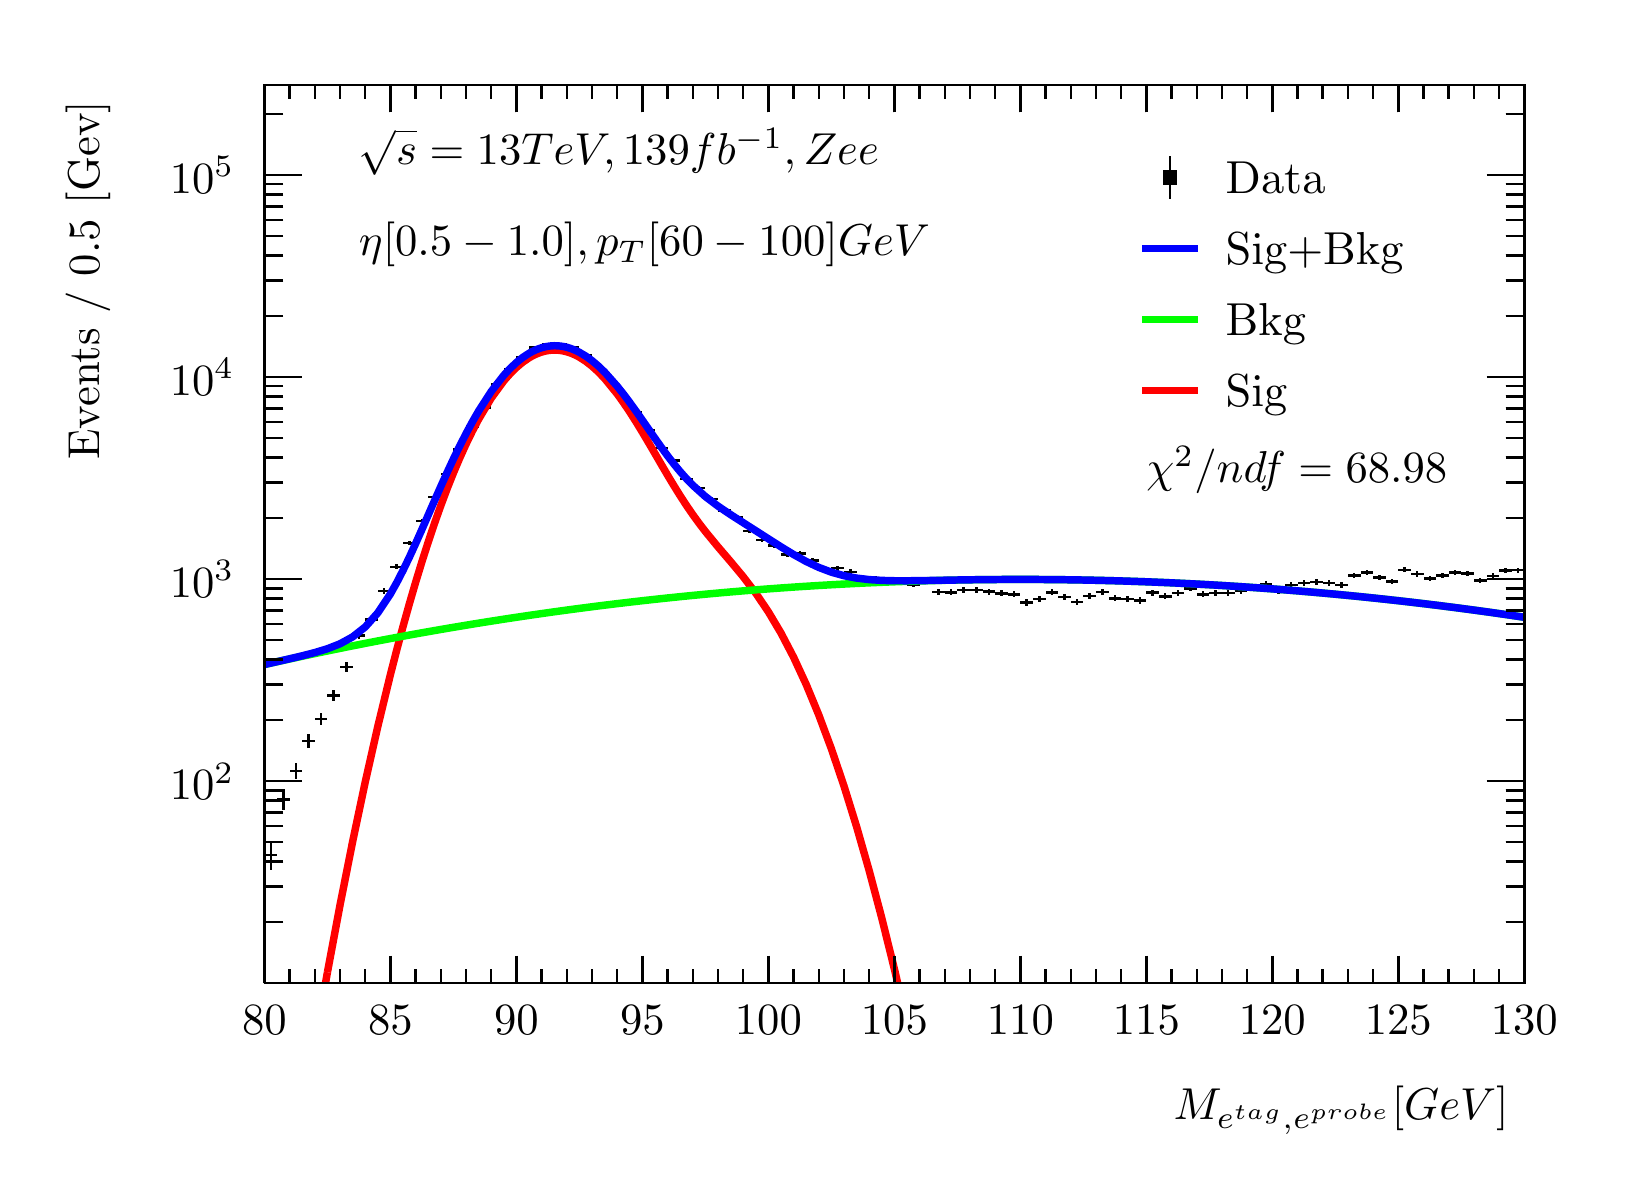
\begin{tikzpicture}
\pgfdeclareplotmark{cross} {
\pgfpathmoveto{\pgfpoint{-0.3\pgfplotmarksize}{\pgfplotmarksize}}
\pgfpathlineto{\pgfpoint{+0.3\pgfplotmarksize}{\pgfplotmarksize}}
\pgfpathlineto{\pgfpoint{+0.3\pgfplotmarksize}{0.3\pgfplotmarksize}}
\pgfpathlineto{\pgfpoint{+1\pgfplotmarksize}{0.3\pgfplotmarksize}}
\pgfpathlineto{\pgfpoint{+1\pgfplotmarksize}{-0.3\pgfplotmarksize}}
\pgfpathlineto{\pgfpoint{+0.3\pgfplotmarksize}{-0.3\pgfplotmarksize}}
\pgfpathlineto{\pgfpoint{+0.3\pgfplotmarksize}{-1.\pgfplotmarksize}}
\pgfpathlineto{\pgfpoint{-0.3\pgfplotmarksize}{-1.\pgfplotmarksize}}
\pgfpathlineto{\pgfpoint{-0.3\pgfplotmarksize}{-0.3\pgfplotmarksize}}
\pgfpathlineto{\pgfpoint{-1.\pgfplotmarksize}{-0.3\pgfplotmarksize}}
\pgfpathlineto{\pgfpoint{-1.\pgfplotmarksize}{0.3\pgfplotmarksize}}
\pgfpathlineto{\pgfpoint{-0.3\pgfplotmarksize}{0.3\pgfplotmarksize}}
\pgfpathclose
\pgfusepathqstroke
}
\pgfdeclareplotmark{cross*} {
\pgfpathmoveto{\pgfpoint{-0.3\pgfplotmarksize}{\pgfplotmarksize}}
\pgfpathlineto{\pgfpoint{+0.3\pgfplotmarksize}{\pgfplotmarksize}}
\pgfpathlineto{\pgfpoint{+0.3\pgfplotmarksize}{0.3\pgfplotmarksize}}
\pgfpathlineto{\pgfpoint{+1\pgfplotmarksize}{0.3\pgfplotmarksize}}
\pgfpathlineto{\pgfpoint{+1\pgfplotmarksize}{-0.3\pgfplotmarksize}}
\pgfpathlineto{\pgfpoint{+0.3\pgfplotmarksize}{-0.3\pgfplotmarksize}}
\pgfpathlineto{\pgfpoint{+0.3\pgfplotmarksize}{-1.\pgfplotmarksize}}
\pgfpathlineto{\pgfpoint{-0.3\pgfplotmarksize}{-1.\pgfplotmarksize}}
\pgfpathlineto{\pgfpoint{-0.3\pgfplotmarksize}{-0.3\pgfplotmarksize}}
\pgfpathlineto{\pgfpoint{-1.\pgfplotmarksize}{-0.3\pgfplotmarksize}}
\pgfpathlineto{\pgfpoint{-1.\pgfplotmarksize}{0.3\pgfplotmarksize}}
\pgfpathlineto{\pgfpoint{-0.3\pgfplotmarksize}{0.3\pgfplotmarksize}}
\pgfpathclose
\pgfusepathqfillstroke
}
\pgfdeclareplotmark{newstar} {
\pgfpathmoveto{\pgfqpoint{0pt}{\pgfplotmarksize}}
\pgfpathlineto{\pgfqpointpolar{44}{0.5\pgfplotmarksize}}
\pgfpathlineto{\pgfqpointpolar{18}{\pgfplotmarksize}}
\pgfpathlineto{\pgfqpointpolar{-20}{0.5\pgfplotmarksize}}
\pgfpathlineto{\pgfqpointpolar{-54}{\pgfplotmarksize}}
\pgfpathlineto{\pgfqpointpolar{-90}{0.5\pgfplotmarksize}}
\pgfpathlineto{\pgfqpointpolar{234}{\pgfplotmarksize}}
\pgfpathlineto{\pgfqpointpolar{198}{0.5\pgfplotmarksize}}
\pgfpathlineto{\pgfqpointpolar{162}{\pgfplotmarksize}}
\pgfpathlineto{\pgfqpointpolar{134}{0.5\pgfplotmarksize}}
\pgfpathclose
\pgfusepathqstroke
}
\pgfdeclareplotmark{newstar*} {
\pgfpathmoveto{\pgfqpoint{0pt}{\pgfplotmarksize}}
\pgfpathlineto{\pgfqpointpolar{44}{0.5\pgfplotmarksize}}
\pgfpathlineto{\pgfqpointpolar{18}{\pgfplotmarksize}}
\pgfpathlineto{\pgfqpointpolar{-20}{0.5\pgfplotmarksize}}
\pgfpathlineto{\pgfqpointpolar{-54}{\pgfplotmarksize}}
\pgfpathlineto{\pgfqpointpolar{-90}{0.5\pgfplotmarksize}}
\pgfpathlineto{\pgfqpointpolar{234}{\pgfplotmarksize}}
\pgfpathlineto{\pgfqpointpolar{198}{0.5\pgfplotmarksize}}
\pgfpathlineto{\pgfqpointpolar{162}{\pgfplotmarksize}}
\pgfpathlineto{\pgfqpointpolar{134}{0.5\pgfplotmarksize}}
\pgfpathclose
\pgfusepathqfillstroke
}
\definecolor{c}{rgb}{1,1,1};
\draw [color=c, fill=c] (0,0) rectangle (20,14.4361);
\draw [color=c, fill=c] (3,2.30977) rectangle (19,13.7143);
\definecolor{c}{rgb}{0,0,0};
\draw [c,line width=0.9] (3,2.30977) -- (3,13.7143) -- (19,13.7143) -- (19,2.30977) -- (3,2.30977);
\definecolor{c}{rgb}{1,1,1};
\draw [color=c, fill=c] (3,2.30977) rectangle (19,13.7143);
\definecolor{c}{rgb}{0,0,0};
\draw [c,line width=0.9] (3,2.30977) -- (3,13.7143) -- (19,13.7143) -- (19,2.30977) -- (3,2.30977);
\draw [c,line width=0.9] (3,2.30977) -- (19,2.30977);
\draw [c,line width=0.9] (3,2.65624) -- (3,2.30977);
\draw [c,line width=0.9] (3.32,2.48301) -- (3.32,2.30977);
\draw [c,line width=0.9] (3.64,2.48301) -- (3.64,2.30977);
\draw [c,line width=0.9] (3.96,2.48301) -- (3.96,2.30977);
\draw [c,line width=0.9] (4.28,2.48301) -- (4.28,2.30977);
\draw [c,line width=0.9] (4.6,2.65624) -- (4.6,2.30977);
\draw [c,line width=0.9] (4.92,2.48301) -- (4.92,2.30977);
\draw [c,line width=0.9] (5.24,2.48301) -- (5.24,2.30977);
\draw [c,line width=0.9] (5.56,2.48301) -- (5.56,2.30977);
\draw [c,line width=0.9] (5.88,2.48301) -- (5.88,2.30977);
\draw [c,line width=0.9] (6.2,2.65624) -- (6.2,2.30977);
\draw [c,line width=0.9] (6.52,2.48301) -- (6.52,2.30977);
\draw [c,line width=0.9] (6.84,2.48301) -- (6.84,2.30977);
\draw [c,line width=0.9] (7.16,2.48301) -- (7.16,2.30977);
\draw [c,line width=0.9] (7.48,2.48301) -- (7.48,2.30977);
\draw [c,line width=0.9] (7.8,2.65624) -- (7.8,2.30977);
\draw [c,line width=0.9] (8.12,2.48301) -- (8.12,2.30977);
\draw [c,line width=0.9] (8.44,2.48301) -- (8.44,2.30977);
\draw [c,line width=0.9] (8.76,2.48301) -- (8.76,2.30977);
\draw [c,line width=0.9] (9.08,2.48301) -- (9.08,2.30977);
\draw [c,line width=0.9] (9.4,2.65624) -- (9.4,2.30977);
\draw [c,line width=0.9] (9.72,2.48301) -- (9.72,2.30977);
\draw [c,line width=0.9] (10.04,2.48301) -- (10.04,2.30977);
\draw [c,line width=0.9] (10.36,2.48301) -- (10.36,2.30977);
\draw [c,line width=0.9] (10.68,2.48301) -- (10.68,2.30977);
\draw [c,line width=0.9] (11,2.65624) -- (11,2.30977);
\draw [c,line width=0.9] (11.32,2.48301) -- (11.32,2.30977);
\draw [c,line width=0.9] (11.64,2.48301) -- (11.64,2.30977);
\draw [c,line width=0.9] (11.96,2.48301) -- (11.96,2.30977);
\draw [c,line width=0.9] (12.28,2.48301) -- (12.28,2.30977);
\draw [c,line width=0.9] (12.6,2.65624) -- (12.6,2.30977);
\draw [c,line width=0.9] (12.92,2.48301) -- (12.92,2.30977);
\draw [c,line width=0.9] (13.24,2.48301) -- (13.24,2.30977);
\draw [c,line width=0.9] (13.56,2.48301) -- (13.56,2.30977);
\draw [c,line width=0.9] (13.88,2.48301) -- (13.88,2.30977);
\draw [c,line width=0.9] (14.2,2.65624) -- (14.2,2.30977);
\draw [c,line width=0.9] (14.52,2.48301) -- (14.52,2.30977);
\draw [c,line width=0.9] (14.84,2.48301) -- (14.84,2.30977);
\draw [c,line width=0.9] (15.16,2.48301) -- (15.16,2.30977);
\draw [c,line width=0.9] (15.48,2.48301) -- (15.48,2.30977);
\draw [c,line width=0.9] (15.8,2.65624) -- (15.8,2.30977);
\draw [c,line width=0.9] (16.12,2.48301) -- (16.12,2.30977);
\draw [c,line width=0.9] (16.44,2.48301) -- (16.44,2.30977);
\draw [c,line width=0.9] (16.76,2.48301) -- (16.76,2.30977);
\draw [c,line width=0.9] (17.08,2.48301) -- (17.08,2.30977);
\draw [c,line width=0.9] (17.4,2.65624) -- (17.4,2.30977);
\draw [c,line width=0.9] (17.72,2.48301) -- (17.72,2.30977);
\draw [c,line width=0.9] (18.04,2.48301) -- (18.04,2.30977);
\draw [c,line width=0.9] (18.36,2.48301) -- (18.36,2.30977);
\draw [c,line width=0.9] (18.68,2.48301) -- (18.68,2.30977);
\draw [c,line width=0.9] (19,2.65624) -- (19,2.30977);
\draw [anchor=base] (3,1.66015) node[scale=1.61424, color=c, rotate=0]{80};
\draw [anchor=base] (4.6,1.66015) node[scale=1.61424, color=c, rotate=0]{85};
\draw [anchor=base] (6.2,1.66015) node[scale=1.61424, color=c, rotate=0]{90};
\draw [anchor=base] (7.8,1.66015) node[scale=1.61424, color=c, rotate=0]{95};
\draw [anchor=base] (9.4,1.66015) node[scale=1.61424, color=c, rotate=0]{100};
\draw [anchor=base] (11,1.66015) node[scale=1.61424, color=c, rotate=0]{105};
\draw [anchor=base] (12.6,1.66015) node[scale=1.61424, color=c, rotate=0]{110};
\draw [anchor=base] (14.2,1.66015) node[scale=1.61424, color=c, rotate=0]{115};
\draw [anchor=base] (15.8,1.66015) node[scale=1.61424, color=c, rotate=0]{120};
\draw [anchor=base] (17.4,1.66015) node[scale=1.61424, color=c, rotate=0]{125};
\draw [anchor=base] (19,1.66015) node[scale=1.61424, color=c, rotate=0]{130};
\draw [anchor= east] (19,0.692932) node[scale=1.61424, color=c, rotate=0]{$M_{e^{tag}, e^{probe}}  [GeV]$};
\draw [c,line width=0.9] (3,13.7143) -- (19,13.7143);
\draw [c,line width=0.9] (3,13.3678) -- (3,13.7143);
\draw [c,line width=0.9] (3.32,13.5411) -- (3.32,13.7143);
\draw [c,line width=0.9] (3.64,13.5411) -- (3.64,13.7143);
\draw [c,line width=0.9] (3.96,13.5411) -- (3.96,13.7143);
\draw [c,line width=0.9] (4.28,13.5411) -- (4.28,13.7143);
\draw [c,line width=0.9] (4.6,13.3678) -- (4.6,13.7143);
\draw [c,line width=0.9] (4.92,13.5411) -- (4.92,13.7143);
\draw [c,line width=0.9] (5.24,13.5411) -- (5.24,13.7143);
\draw [c,line width=0.9] (5.56,13.5411) -- (5.56,13.7143);
\draw [c,line width=0.9] (5.88,13.5411) -- (5.88,13.7143);
\draw [c,line width=0.9] (6.2,13.3678) -- (6.2,13.7143);
\draw [c,line width=0.9] (6.52,13.5411) -- (6.52,13.7143);
\draw [c,line width=0.9] (6.84,13.5411) -- (6.84,13.7143);
\draw [c,line width=0.9] (7.16,13.5411) -- (7.16,13.7143);
\draw [c,line width=0.9] (7.48,13.5411) -- (7.48,13.7143);
\draw [c,line width=0.9] (7.8,13.3678) -- (7.8,13.7143);
\draw [c,line width=0.9] (8.12,13.5411) -- (8.12,13.7143);
\draw [c,line width=0.9] (8.44,13.5411) -- (8.44,13.7143);
\draw [c,line width=0.9] (8.76,13.5411) -- (8.76,13.7143);
\draw [c,line width=0.9] (9.08,13.5411) -- (9.08,13.7143);
\draw [c,line width=0.9] (9.4,13.3678) -- (9.4,13.7143);
\draw [c,line width=0.9] (9.72,13.5411) -- (9.72,13.7143);
\draw [c,line width=0.9] (10.04,13.5411) -- (10.04,13.7143);
\draw [c,line width=0.9] (10.36,13.5411) -- (10.36,13.7143);
\draw [c,line width=0.9] (10.68,13.5411) -- (10.68,13.7143);
\draw [c,line width=0.9] (11,13.3678) -- (11,13.7143);
\draw [c,line width=0.9] (11.32,13.5411) -- (11.32,13.7143);
\draw [c,line width=0.9] (11.64,13.5411) -- (11.64,13.7143);
\draw [c,line width=0.9] (11.96,13.5411) -- (11.96,13.7143);
\draw [c,line width=0.9] (12.28,13.5411) -- (12.28,13.7143);
\draw [c,line width=0.9] (12.6,13.3678) -- (12.6,13.7143);
\draw [c,line width=0.9] (12.92,13.5411) -- (12.92,13.7143);
\draw [c,line width=0.9] (13.24,13.5411) -- (13.24,13.7143);
\draw [c,line width=0.9] (13.56,13.5411) -- (13.56,13.7143);
\draw [c,line width=0.9] (13.88,13.5411) -- (13.88,13.7143);
\draw [c,line width=0.9] (14.2,13.3678) -- (14.2,13.7143);
\draw [c,line width=0.9] (14.52,13.5411) -- (14.52,13.7143);
\draw [c,line width=0.9] (14.84,13.5411) -- (14.84,13.7143);
\draw [c,line width=0.9] (15.16,13.5411) -- (15.16,13.7143);
\draw [c,line width=0.9] (15.48,13.5411) -- (15.48,13.7143);
\draw [c,line width=0.9] (15.8,13.3678) -- (15.8,13.7143);
\draw [c,line width=0.9] (16.12,13.5411) -- (16.12,13.7143);
\draw [c,line width=0.9] (16.44,13.5411) -- (16.44,13.7143);
\draw [c,line width=0.9] (16.76,13.5411) -- (16.76,13.7143);
\draw [c,line width=0.9] (17.08,13.5411) -- (17.08,13.7143);
\draw [c,line width=0.9] (17.4,13.3678) -- (17.4,13.7143);
\draw [c,line width=0.9] (17.72,13.5411) -- (17.72,13.7143);
\draw [c,line width=0.9] (18.04,13.5411) -- (18.04,13.7143);
\draw [c,line width=0.9] (18.36,13.5411) -- (18.36,13.7143);
\draw [c,line width=0.9] (18.68,13.5411) -- (18.68,13.7143);
\draw [c,line width=0.9] (19,13.3678) -- (19,13.7143);
\draw [c,line width=0.9] (3,2.30977) -- (3,13.7143);
\draw [c,line width=0.9] (3.237,3.08209) -- (3,3.08209);
\draw [c,line width=0.9] (3.237,3.53386) -- (3,3.53386);
\draw [c,line width=0.9] (3.237,3.8544) -- (3,3.8544);
\draw [c,line width=0.9] (3.237,4.10303) -- (3,4.10303);
\draw [c,line width=0.9] (3.237,4.30618) -- (3,4.30618);
\draw [c,line width=0.9] (3.237,4.47794) -- (3,4.47794);
\draw [c,line width=0.9] (3.237,4.62672) -- (3,4.62672);
\draw [c,line width=0.9] (3.237,4.75795) -- (3,4.75795);
\draw [c,line width=0.9] (3.474,4.87535) -- (3,4.87535);
\draw [anchor= east] (2.82,4.87535) node[scale=1.61424, color=c, rotate=0]{$10^{2}$};
\draw [c,line width=0.9] (3.237,5.64766) -- (3,5.64766);
\draw [c,line width=0.9] (3.237,6.09944) -- (3,6.09944);
\draw [c,line width=0.9] (3.237,6.41998) -- (3,6.41998);
\draw [c,line width=0.9] (3.237,6.66861) -- (3,6.66861);
\draw [c,line width=0.9] (3.237,6.87176) -- (3,6.87176);
\draw [c,line width=0.9] (3.237,7.04351) -- (3,7.04351);
\draw [c,line width=0.9] (3.237,7.1923) -- (3,7.1923);
\draw [c,line width=0.9] (3.237,7.32353) -- (3,7.32353);
\draw [c,line width=0.9] (3.474,7.44093) -- (3,7.44093);
\draw [anchor= east] (2.82,7.44093) node[scale=1.61424, color=c, rotate=0]{$10^{3}$};
\draw [c,line width=0.9] (3.237,8.21324) -- (3,8.21324);
\draw [c,line width=0.9] (3.237,8.66502) -- (3,8.66502);
\draw [c,line width=0.9] (3.237,8.98556) -- (3,8.98556);
\draw [c,line width=0.9] (3.237,9.23419) -- (3,9.23419);
\draw [c,line width=0.9] (3.237,9.43733) -- (3,9.43733);
\draw [c,line width=0.9] (3.237,9.60909) -- (3,9.60909);
\draw [c,line width=0.9] (3.237,9.75787) -- (3,9.75787);
\draw [c,line width=0.9] (3.237,9.88911) -- (3,9.88911);
\draw [c,line width=0.9] (3.474,10.0065) -- (3,10.0065);
\draw [anchor= east] (2.82,10.0065) node[scale=1.61424, color=c, rotate=0]{$10^{4}$};
\draw [c,line width=0.9] (3.237,10.7788) -- (3,10.7788);
\draw [c,line width=0.9] (3.237,11.2306) -- (3,11.2306);
\draw [c,line width=0.9] (3.237,11.5511) -- (3,11.5511);
\draw [c,line width=0.9] (3.237,11.7998) -- (3,11.7998);
\draw [c,line width=0.9] (3.237,12.0029) -- (3,12.0029);
\draw [c,line width=0.9] (3.237,12.1747) -- (3,12.1747);
\draw [c,line width=0.9] (3.237,12.3235) -- (3,12.3235);
\draw [c,line width=0.9] (3.237,12.4547) -- (3,12.4547);
\draw [c,line width=0.9] (3.474,12.5721) -- (3,12.5721);
\draw [anchor= east] (2.82,12.5721) node[scale=1.61424, color=c, rotate=0]{$10^{5}$};
\draw [c,line width=0.9] (3.237,13.3444) -- (3,13.3444);
\draw [anchor= east] (0.76,13.7143) node[scale=1.61424, color=c, rotate=90]{Events / 0.5 [Gev]};
\draw [c,line width=0.9] (19,2.30977) -- (19,13.7143);
\draw [c,line width=0.9] (18.763,3.08209) -- (19,3.08209);
\draw [c,line width=0.9] (18.763,3.53386) -- (19,3.53386);
\draw [c,line width=0.9] (18.763,3.8544) -- (19,3.8544);
\draw [c,line width=0.9] (18.763,4.10303) -- (19,4.10303);
\draw [c,line width=0.9] (18.763,4.30618) -- (19,4.30618);
\draw [c,line width=0.9] (18.763,4.47794) -- (19,4.47794);
\draw [c,line width=0.9] (18.763,4.62672) -- (19,4.62672);
\draw [c,line width=0.9] (18.763,4.75795) -- (19,4.75795);
\draw [c,line width=0.9] (18.526,4.87535) -- (19,4.87535);
\draw [c,line width=0.9] (18.763,5.64766) -- (19,5.64766);
\draw [c,line width=0.9] (18.763,6.09944) -- (19,6.09944);
\draw [c,line width=0.9] (18.763,6.41998) -- (19,6.41998);
\draw [c,line width=0.9] (18.763,6.66861) -- (19,6.66861);
\draw [c,line width=0.9] (18.763,6.87176) -- (19,6.87176);
\draw [c,line width=0.9] (18.763,7.04351) -- (19,7.04351);
\draw [c,line width=0.9] (18.763,7.1923) -- (19,7.1923);
\draw [c,line width=0.9] (18.763,7.32353) -- (19,7.32353);
\draw [c,line width=0.9] (18.526,7.44093) -- (19,7.44093);
\draw [c,line width=0.9] (18.763,8.21324) -- (19,8.21324);
\draw [c,line width=0.9] (18.763,8.66502) -- (19,8.66502);
\draw [c,line width=0.9] (18.763,8.98556) -- (19,8.98556);
\draw [c,line width=0.9] (18.763,9.23419) -- (19,9.23419);
\draw [c,line width=0.9] (18.763,9.43733) -- (19,9.43733);
\draw [c,line width=0.9] (18.763,9.60909) -- (19,9.60909);
\draw [c,line width=0.9] (18.763,9.75787) -- (19,9.75787);
\draw [c,line width=0.9] (18.763,9.88911) -- (19,9.88911);
\draw [c,line width=0.9] (18.526,10.0065) -- (19,10.0065);
\draw [c,line width=0.9] (18.763,10.7788) -- (19,10.7788);
\draw [c,line width=0.9] (18.763,11.2306) -- (19,11.2306);
\draw [c,line width=0.9] (18.763,11.5511) -- (19,11.5511);
\draw [c,line width=0.9] (18.763,11.7998) -- (19,11.7998);
\draw [c,line width=0.9] (18.763,12.0029) -- (19,12.0029);
\draw [c,line width=0.9] (18.763,12.1747) -- (19,12.1747);
\draw [c,line width=0.9] (18.763,12.3235) -- (19,12.3235);
\draw [c,line width=0.9] (18.763,12.4547) -- (19,12.4547);
\draw [c,line width=0.9] (18.526,12.5721) -- (19,12.5721);
\draw [c,line width=0.9] (18.763,13.3444) -- (19,13.3444);
\draw [c,line width=0.9] (3.08,3.93499) -- (3,3.93499);
\draw [c,line width=0.9] (3,3.93499) -- (3,3.93499);
\draw [c,line width=0.9] (3.08,3.93499) -- (3.16,3.93499);
\draw [c,line width=0.9] (3.16,3.93499) -- (3.16,3.93499);
\draw [c,line width=0.9] (3.08,3.93499) -- (3.08,4.11651);
\draw [c,line width=0.9] (3.08,4.11651) -- (3.08,4.11651);
\draw [c,line width=0.9] (3.08,3.93499) -- (3.08,3.75141);
\draw [c,line width=0.9] (3.08,3.75141) -- (3.08,3.75141);
\draw [c,line width=0.9] (3.24,4.64056) -- (3.16,4.64056);
\draw [c,line width=0.9] (3.16,4.64056) -- (3.16,4.64056);
\draw [c,line width=0.9] (3.24,4.64056) -- (3.32,4.64056);
\draw [c,line width=0.9] (3.32,4.64056) -- (3.32,4.64056);
\draw [c,line width=0.9] (3.24,4.64056) -- (3.24,4.77072);
\draw [c,line width=0.9] (3.24,4.77072) -- (3.24,4.77072);
\draw [c,line width=0.9] (3.24,4.64056) -- (3.24,4.50961);
\draw [c,line width=0.9] (3.24,4.50961) -- (3.24,4.50961);
\draw [c,line width=0.9] (3.4,5.00162) -- (3.32,5.00162);
\draw [c,line width=0.9] (3.32,5.00162) -- (3.32,5.00162);
\draw [c,line width=0.9] (3.4,5.00162) -- (3.48,5.00162);
\draw [c,line width=0.9] (3.48,5.00162) -- (3.48,5.00162);
\draw [c,line width=0.9] (3.4,5.00162) -- (3.4,5.10687);
\draw [c,line width=0.9] (3.4,5.10687) -- (3.4,5.10687);
\draw [c,line width=0.9] (3.4,5.00162) -- (3.4,4.89638);
\draw [c,line width=0.9] (3.4,4.89638) -- (3.4,4.89638);
\draw [c,line width=0.9] (3.56,5.38502) -- (3.48,5.38502);
\draw [c,line width=0.9] (3.48,5.38502) -- (3.48,5.38502);
\draw [c,line width=0.9] (3.56,5.38502) -- (3.64,5.38502);
\draw [c,line width=0.9] (3.64,5.38502) -- (3.64,5.38502);
\draw [c,line width=0.9] (3.56,5.38502) -- (3.56,5.47364);
\draw [c,line width=0.9] (3.56,5.47364) -- (3.56,5.47364);
\draw [c,line width=0.9] (3.56,5.38502) -- (3.56,5.2964);
\draw [c,line width=0.9] (3.56,5.2964) -- (3.56,5.2964);
\draw [c,line width=0.9] (3.72,5.66426) -- (3.64,5.66426);
\draw [c,line width=0.9] (3.64,5.66426) -- (3.64,5.66426);
\draw [c,line width=0.9] (3.72,5.66426) -- (3.8,5.66426);
\draw [c,line width=0.9] (3.8,5.66426) -- (3.8,5.66426);
\draw [c,line width=0.9] (3.72,5.66426) -- (3.72,5.74244);
\draw [c,line width=0.9] (3.72,5.74244) -- (3.72,5.74244);
\draw [c,line width=0.9] (3.72,5.66426) -- (3.72,5.58607);
\draw [c,line width=0.9] (3.72,5.58607) -- (3.72,5.58607);
\draw [c,line width=0.9] (3.88,5.96122) -- (3.8,5.96122);
\draw [c,line width=0.9] (3.8,5.96122) -- (3.8,5.96122);
\draw [c,line width=0.9] (3.88,5.96122) -- (3.96,5.96122);
\draw [c,line width=0.9] (3.96,5.96122) -- (3.96,5.96122);
\draw [c,line width=0.9] (3.88,5.96122) -- (3.88,6.02966);
\draw [c,line width=0.9] (3.88,6.02966) -- (3.88,6.02966);
\draw [c,line width=0.9] (3.88,5.96122) -- (3.88,5.89279);
\draw [c,line width=0.9] (3.88,5.89279) -- (3.88,5.89279);
\draw [c,line width=0.9] (4.04,6.32405) -- (3.96,6.32405);
\draw [c,line width=0.9] (3.96,6.32405) -- (3.96,6.32405);
\draw [c,line width=0.9] (4.04,6.32405) -- (4.12,6.32405);
\draw [c,line width=0.9] (4.12,6.32405) -- (4.12,6.32405);
\draw [c,line width=0.9] (4.04,6.32405) -- (4.04,6.3822);
\draw [c,line width=0.9] (4.04,6.3822) -- (4.04,6.3822);
\draw [c,line width=0.9] (4.04,6.32405) -- (4.04,6.26589);
\draw [c,line width=0.9] (4.04,6.26589) -- (4.04,6.26589);
\draw [c,line width=0.9] (4.2,6.7251) -- (4.12,6.7251);
\draw [c,line width=0.9] (4.12,6.7251) -- (4.12,6.7251);
\draw [c,line width=0.9] (4.2,6.7251) -- (4.28,6.7251);
\draw [c,line width=0.9] (4.28,6.7251) -- (4.28,6.7251);
\draw [c,line width=0.9] (4.2,6.7251) -- (4.2,6.77367);
\draw [c,line width=0.9] (4.2,6.77367) -- (4.2,6.77367);
\draw [c,line width=0.9] (4.2,6.7251) -- (4.2,6.67652);
\draw [c,line width=0.9] (4.2,6.67652) -- (4.2,6.67652);
\draw [c,line width=0.9] (4.36,6.92435) -- (4.28,6.92435);
\draw [c,line width=0.9] (4.28,6.92435) -- (4.28,6.92435);
\draw [c,line width=0.9] (4.36,6.92435) -- (4.44,6.92435);
\draw [c,line width=0.9] (4.44,6.92435) -- (4.44,6.92435);
\draw [c,line width=0.9] (4.36,6.92435) -- (4.36,6.96877);
\draw [c,line width=0.9] (4.36,6.96877) -- (4.36,6.96877);
\draw [c,line width=0.9] (4.36,6.92435) -- (4.36,6.87993);
\draw [c,line width=0.9] (4.36,6.87993) -- (4.36,6.87993);
\draw [c,line width=0.9] (4.52,7.28704) -- (4.44,7.28704);
\draw [c,line width=0.9] (4.44,7.28704) -- (4.44,7.28704);
\draw [c,line width=0.9] (4.52,7.28704) -- (4.6,7.28704);
\draw [c,line width=0.9] (4.6,7.28704) -- (4.6,7.28704);
\draw [c,line width=0.9] (4.52,7.28704) -- (4.52,7.32479);
\draw [c,line width=0.9] (4.52,7.32479) -- (4.52,7.32479);
\draw [c,line width=0.9] (4.52,7.28704) -- (4.52,7.24929);
\draw [c,line width=0.9] (4.52,7.24929) -- (4.52,7.24929);
\draw [c,line width=0.9] (4.68,7.59665) -- (4.6,7.59665);
\draw [c,line width=0.9] (4.6,7.59665) -- (4.6,7.59665);
\draw [c,line width=0.9] (4.68,7.59665) -- (4.76,7.59665);
\draw [c,line width=0.9] (4.76,7.59665) -- (4.76,7.59665);
\draw [c,line width=0.9] (4.68,7.59665) -- (4.68,7.62951);
\draw [c,line width=0.9] (4.68,7.62951) -- (4.68,7.62951);
\draw [c,line width=0.9] (4.68,7.59665) -- (4.68,7.5638);
\draw [c,line width=0.9] (4.68,7.5638) -- (4.68,7.5638);
\draw [c,line width=0.9] (4.84,7.89863) -- (4.76,7.89863);
\draw [c,line width=0.9] (4.76,7.89863) -- (4.76,7.89863);
\draw [c,line width=0.9] (4.84,7.89863) -- (4.92,7.89863);
\draw [c,line width=0.9] (4.92,7.89863) -- (4.92,7.89863);
\draw [c,line width=0.9] (4.84,7.89863) -- (4.84,7.92732);
\draw [c,line width=0.9] (4.84,7.92732) -- (4.84,7.92732);
\draw [c,line width=0.9] (4.84,7.89863) -- (4.84,7.86994);
\draw [c,line width=0.9] (4.84,7.86994) -- (4.84,7.86994);
\draw [c,line width=0.9] (5,8.1747) -- (4.92,8.1747);
\draw [c,line width=0.9] (4.92,8.1747) -- (4.92,8.1747);
\draw [c,line width=0.9] (5,8.1747) -- (5.08,8.1747);
\draw [c,line width=0.9] (5.08,8.1747) -- (5.08,8.1747);
\draw [c,line width=0.9] (5,8.1747) -- (5,8.20005);
\draw [c,line width=0.9] (5,8.20005) -- (5,8.20005);
\draw [c,line width=0.9] (5,8.1747) -- (5,8.14935);
\draw [c,line width=0.9] (5,8.14935) -- (5,8.14935);
\draw [c,line width=0.9] (5.16,8.48) -- (5.08,8.48);
\draw [c,line width=0.9] (5.08,8.48) -- (5.08,8.48);
\draw [c,line width=0.9] (5.16,8.48) -- (5.24,8.48);
\draw [c,line width=0.9] (5.24,8.48) -- (5.24,8.48);
\draw [c,line width=0.9] (5.16,8.48) -- (5.16,8.5021);
\draw [c,line width=0.9] (5.16,8.5021) -- (5.16,8.5021);
\draw [c,line width=0.9] (5.16,8.48) -- (5.16,8.45789);
\draw [c,line width=0.9] (5.16,8.45789) -- (5.16,8.45789);
\draw [c,line width=0.9] (5.32,8.77694) -- (5.24,8.77694);
\draw [c,line width=0.9] (5.24,8.77694) -- (5.24,8.77694);
\draw [c,line width=0.9] (5.32,8.77694) -- (5.4,8.77694);
\draw [c,line width=0.9] (5.4,8.77694) -- (5.4,8.77694);
\draw [c,line width=0.9] (5.32,8.77694) -- (5.32,8.79629);
\draw [c,line width=0.9] (5.32,8.79629) -- (5.32,8.79629);
\draw [c,line width=0.9] (5.32,8.77694) -- (5.32,8.75759);
\draw [c,line width=0.9] (5.32,8.75759) -- (5.32,8.75759);
\draw [c,line width=0.9] (5.48,9.08362) -- (5.4,9.08362);
\draw [c,line width=0.9] (5.4,9.08362) -- (5.4,9.08362);
\draw [c,line width=0.9] (5.48,9.08362) -- (5.56,9.08362);
\draw [c,line width=0.9] (5.56,9.08362) -- (5.56,9.08362);
\draw [c,line width=0.9] (5.48,9.08362) -- (5.48,9.10048);
\draw [c,line width=0.9] (5.48,9.10048) -- (5.48,9.10048);
\draw [c,line width=0.9] (5.48,9.08362) -- (5.48,9.06676);
\draw [c,line width=0.9] (5.48,9.06676) -- (5.48,9.06676);
\draw [c,line width=0.9] (5.64,9.3794) -- (5.56,9.3794);
\draw [c,line width=0.9] (5.56,9.3794) -- (5.56,9.3794);
\draw [c,line width=0.9] (5.64,9.3794) -- (5.72,9.3794);
\draw [c,line width=0.9] (5.72,9.3794) -- (5.72,9.3794);
\draw [c,line width=0.9] (5.64,9.3794) -- (5.64,9.39416);
\draw [c,line width=0.9] (5.64,9.39416) -- (5.64,9.39416);
\draw [c,line width=0.9] (5.64,9.3794) -- (5.64,9.36464);
\draw [c,line width=0.9] (5.64,9.36464) -- (5.64,9.36464);
\draw [c,line width=0.9] (5.8,9.62112) -- (5.72,9.62112);
\draw [c,line width=0.9] (5.72,9.62112) -- (5.72,9.62112);
\draw [c,line width=0.9] (5.8,9.62112) -- (5.88,9.62112);
\draw [c,line width=0.9] (5.88,9.62112) -- (5.88,9.62112);
\draw [c,line width=0.9] (5.8,9.62112) -- (5.8,9.63437);
\draw [c,line width=0.9] (5.8,9.63437) -- (5.8,9.63437);
\draw [c,line width=0.9] (5.8,9.62112) -- (5.8,9.60788);
\draw [c,line width=0.9] (5.8,9.60788) -- (5.8,9.60788);
\draw [c,line width=0.9] (5.96,9.91166) -- (5.88,9.91166);
\draw [c,line width=0.9] (5.88,9.91166) -- (5.88,9.91166);
\draw [c,line width=0.9] (5.96,9.91166) -- (6.04,9.91166);
\draw [c,line width=0.9] (6.04,9.91166) -- (6.04,9.91166);
\draw [c,line width=0.9] (5.96,9.91166) -- (5.96,9.92329);
\draw [c,line width=0.9] (5.96,9.92329) -- (5.96,9.92329);
\draw [c,line width=0.9] (5.96,9.91166) -- (5.96,9.90003);
\draw [c,line width=0.9] (5.96,9.90003) -- (5.96,9.90003);
\draw [c,line width=0.9] (6.12,10.1003) -- (6.04,10.1003);
\draw [c,line width=0.9] (6.04,10.1003) -- (6.04,10.1003);
\draw [c,line width=0.9] (6.12,10.1003) -- (6.2,10.1003);
\draw [c,line width=0.9] (6.2,10.1003) -- (6.2,10.1003);
\draw [c,line width=0.9] (6.12,10.1003) -- (6.12,10.111);
\draw [c,line width=0.9] (6.12,10.111) -- (6.12,10.111);
\draw [c,line width=0.9] (6.12,10.1003) -- (6.12,10.0896);
\draw [c,line width=0.9] (6.12,10.0896) -- (6.12,10.0896);
\draw [c,line width=0.9] (6.28,10.2518) -- (6.2,10.2518);
\draw [c,line width=0.9] (6.2,10.2518) -- (6.2,10.2518);
\draw [c,line width=0.9] (6.28,10.2518) -- (6.36,10.2518);
\draw [c,line width=0.9] (6.36,10.2518) -- (6.36,10.2518);
\draw [c,line width=0.9] (6.28,10.2518) -- (6.28,10.2618);
\draw [c,line width=0.9] (6.28,10.2618) -- (6.28,10.2618);
\draw [c,line width=0.9] (6.28,10.2518) -- (6.28,10.2419);
\draw [c,line width=0.9] (6.28,10.2419) -- (6.28,10.2419);
\draw [c,line width=0.9] (6.44,10.3798) -- (6.36,10.3798);
\draw [c,line width=0.9] (6.36,10.3798) -- (6.36,10.3798);
\draw [c,line width=0.9] (6.44,10.3798) -- (6.52,10.3798);
\draw [c,line width=0.9] (6.52,10.3798) -- (6.52,10.3798);
\draw [c,line width=0.9] (6.44,10.3798) -- (6.44,10.3892);
\draw [c,line width=0.9] (6.44,10.3892) -- (6.44,10.3892);
\draw [c,line width=0.9] (6.44,10.3798) -- (6.44,10.3704);
\draw [c,line width=0.9] (6.44,10.3704) -- (6.44,10.3704);
\draw [c,line width=0.9] (6.6,10.4278) -- (6.52,10.4278);
\draw [c,line width=0.9] (6.52,10.4278) -- (6.52,10.4278);
\draw [c,line width=0.9] (6.6,10.4278) -- (6.68,10.4278);
\draw [c,line width=0.9] (6.68,10.4278) -- (6.68,10.4278);
\draw [c,line width=0.9] (6.6,10.4278) -- (6.6,10.437);
\draw [c,line width=0.9] (6.6,10.437) -- (6.6,10.437);
\draw [c,line width=0.9] (6.6,10.4278) -- (6.6,10.4186);
\draw [c,line width=0.9] (6.6,10.4186) -- (6.6,10.4186);
\draw [c,line width=0.9] (6.76,10.428) -- (6.68,10.428);
\draw [c,line width=0.9] (6.68,10.428) -- (6.68,10.428);
\draw [c,line width=0.9] (6.76,10.428) -- (6.84,10.428);
\draw [c,line width=0.9] (6.84,10.428) -- (6.84,10.428);
\draw [c,line width=0.9] (6.76,10.428) -- (6.76,10.4372);
\draw [c,line width=0.9] (6.76,10.4372) -- (6.76,10.4372);
\draw [c,line width=0.9] (6.76,10.428) -- (6.76,10.4188);
\draw [c,line width=0.9] (6.76,10.4188) -- (6.76,10.4188);
\draw [c,line width=0.9] (6.92,10.3797) -- (6.84,10.3797);
\draw [c,line width=0.9] (6.84,10.3797) -- (6.84,10.3797);
\draw [c,line width=0.9] (6.92,10.3797) -- (7,10.3797);
\draw [c,line width=0.9] (7,10.3797) -- (7,10.3797);
\draw [c,line width=0.9] (6.92,10.3797) -- (6.92,10.3892);
\draw [c,line width=0.9] (6.92,10.3892) -- (6.92,10.3892);
\draw [c,line width=0.9] (6.92,10.3797) -- (6.92,10.3703);
\draw [c,line width=0.9] (6.92,10.3703) -- (6.92,10.3703);
\draw [c,line width=0.9] (7.08,10.2882) -- (7,10.2882);
\draw [c,line width=0.9] (7,10.2882) -- (7,10.2882);
\draw [c,line width=0.9] (7.08,10.2882) -- (7.16,10.2882);
\draw [c,line width=0.9] (7.16,10.2882) -- (7.16,10.2882);
\draw [c,line width=0.9] (7.08,10.2882) -- (7.08,10.298);
\draw [c,line width=0.9] (7.08,10.298) -- (7.08,10.298);
\draw [c,line width=0.9] (7.08,10.2882) -- (7.08,10.2783);
\draw [c,line width=0.9] (7.08,10.2783) -- (7.08,10.2783);
\draw [c,line width=0.9] (7.24,10.1239) -- (7.16,10.1239);
\draw [c,line width=0.9] (7.16,10.1239) -- (7.16,10.1239);
\draw [c,line width=0.9] (7.24,10.1239) -- (7.32,10.1239);
\draw [c,line width=0.9] (7.32,10.1239) -- (7.32,10.1239);
\draw [c,line width=0.9] (7.24,10.1239) -- (7.24,10.1345);
\draw [c,line width=0.9] (7.24,10.1345) -- (7.24,10.1345);
\draw [c,line width=0.9] (7.24,10.1239) -- (7.24,10.1133);
\draw [c,line width=0.9] (7.24,10.1133) -- (7.24,10.1133);
\draw [c,line width=0.9] (7.4,9.95811) -- (7.32,9.95811);
\draw [c,line width=0.9] (7.32,9.95811) -- (7.32,9.95811);
\draw [c,line width=0.9] (7.4,9.95811) -- (7.48,9.95811);
\draw [c,line width=0.9] (7.48,9.95811) -- (7.48,9.95811);
\draw [c,line width=0.9] (7.4,9.95811) -- (7.4,9.9695);
\draw [c,line width=0.9] (7.4,9.9695) -- (7.4,9.9695);
\draw [c,line width=0.9] (7.4,9.95811) -- (7.4,9.94673);
\draw [c,line width=0.9] (7.4,9.94673) -- (7.4,9.94673);
\draw [c,line width=0.9] (7.56,9.74569) -- (7.48,9.74569);
\draw [c,line width=0.9] (7.48,9.74569) -- (7.48,9.74569);
\draw [c,line width=0.9] (7.56,9.74569) -- (7.64,9.74569);
\draw [c,line width=0.9] (7.64,9.74569) -- (7.64,9.74569);
\draw [c,line width=0.9] (7.56,9.74569) -- (7.56,9.75822);
\draw [c,line width=0.9] (7.56,9.75822) -- (7.56,9.75822);
\draw [c,line width=0.9] (7.56,9.74569) -- (7.56,9.73317);
\draw [c,line width=0.9] (7.56,9.73317) -- (7.56,9.73317);
\draw [c,line width=0.9] (7.72,9.55679) -- (7.64,9.55679);
\draw [c,line width=0.9] (7.64,9.55679) -- (7.64,9.55679);
\draw [c,line width=0.9] (7.72,9.55679) -- (7.8,9.55679);
\draw [c,line width=0.9] (7.8,9.55679) -- (7.8,9.55679);
\draw [c,line width=0.9] (7.72,9.55679) -- (7.72,9.57042);
\draw [c,line width=0.9] (7.72,9.57042) -- (7.72,9.57042);
\draw [c,line width=0.9] (7.72,9.55679) -- (7.72,9.54315);
\draw [c,line width=0.9] (7.72,9.54315) -- (7.72,9.54315);
\draw [c,line width=0.9] (7.88,9.33429) -- (7.8,9.33429);
\draw [c,line width=0.9] (7.8,9.33429) -- (7.8,9.33429);
\draw [c,line width=0.9] (7.88,9.33429) -- (7.96,9.33429);
\draw [c,line width=0.9] (7.96,9.33429) -- (7.96,9.33429);
\draw [c,line width=0.9] (7.88,9.33429) -- (7.88,9.34936);
\draw [c,line width=0.9] (7.88,9.34936) -- (7.88,9.34936);
\draw [c,line width=0.9] (7.88,9.33429) -- (7.88,9.31923);
\draw [c,line width=0.9] (7.88,9.31923) -- (7.88,9.31923);
\draw [c,line width=0.9] (8.04,9.10435) -- (7.96,9.10435);
\draw [c,line width=0.9] (7.96,9.10435) -- (7.96,9.10435);
\draw [c,line width=0.9] (8.04,9.10435) -- (8.12,9.10435);
\draw [c,line width=0.9] (8.12,9.10435) -- (8.12,9.10435);
\draw [c,line width=0.9] (8.04,9.10435) -- (8.04,9.12105);
\draw [c,line width=0.9] (8.04,9.12105) -- (8.04,9.12105);
\draw [c,line width=0.9] (8.04,9.10435) -- (8.04,9.08764);
\draw [c,line width=0.9] (8.04,9.08764) -- (8.04,9.08764);
\draw [c,line width=0.9] (8.2,8.94413) -- (8.12,8.94413);
\draw [c,line width=0.9] (8.12,8.94413) -- (8.12,8.94413);
\draw [c,line width=0.9] (8.2,8.94413) -- (8.28,8.94413);
\draw [c,line width=0.9] (8.28,8.94413) -- (8.28,8.94413);
\draw [c,line width=0.9] (8.2,8.94413) -- (8.2,8.96208);
\draw [c,line width=0.9] (8.2,8.96208) -- (8.2,8.96208);
\draw [c,line width=0.9] (8.2,8.94413) -- (8.2,8.92618);
\draw [c,line width=0.9] (8.2,8.92618) -- (8.2,8.92618);
\draw [c,line width=0.9] (8.36,8.71015) -- (8.28,8.71015);
\draw [c,line width=0.9] (8.28,8.71015) -- (8.28,8.71015);
\draw [c,line width=0.9] (8.36,8.71015) -- (8.44,8.71015);
\draw [c,line width=0.9] (8.44,8.71015) -- (8.44,8.71015);
\draw [c,line width=0.9] (8.36,8.71015) -- (8.36,8.73008);
\draw [c,line width=0.9] (8.36,8.73008) -- (8.36,8.73008);
\draw [c,line width=0.9] (8.36,8.71015) -- (8.36,8.69021);
\draw [c,line width=0.9] (8.36,8.69021) -- (8.36,8.69021);
\draw [c,line width=0.9] (8.52,8.59647) -- (8.44,8.59647);
\draw [c,line width=0.9] (8.44,8.59647) -- (8.44,8.59647);
\draw [c,line width=0.9] (8.52,8.59647) -- (8.6,8.59647);
\draw [c,line width=0.9] (8.6,8.59647) -- (8.6,8.59647);
\draw [c,line width=0.9] (8.52,8.59647) -- (8.52,8.61745);
\draw [c,line width=0.9] (8.52,8.61745) -- (8.52,8.61745);
\draw [c,line width=0.9] (8.52,8.59647) -- (8.52,8.57549);
\draw [c,line width=0.9] (8.52,8.57549) -- (8.52,8.57549);
\draw [c,line width=0.9] (8.68,8.45741) -- (8.6,8.45741);
\draw [c,line width=0.9] (8.6,8.45741) -- (8.6,8.45741);
\draw [c,line width=0.9] (8.68,8.45741) -- (8.76,8.45741);
\draw [c,line width=0.9] (8.76,8.45741) -- (8.76,8.45741);
\draw [c,line width=0.9] (8.68,8.45741) -- (8.68,8.47974);
\draw [c,line width=0.9] (8.68,8.47974) -- (8.68,8.47974);
\draw [c,line width=0.9] (8.68,8.45741) -- (8.68,8.43508);
\draw [c,line width=0.9] (8.68,8.43508) -- (8.68,8.43508);
\draw [c,line width=0.9] (8.84,8.3108) -- (8.76,8.3108);
\draw [c,line width=0.9] (8.76,8.3108) -- (8.76,8.3108);
\draw [c,line width=0.9] (8.84,8.3108) -- (8.92,8.3108);
\draw [c,line width=0.9] (8.92,8.3108) -- (8.92,8.3108);
\draw [c,line width=0.9] (8.84,8.3108) -- (8.84,8.33464);
\draw [c,line width=0.9] (8.84,8.33464) -- (8.84,8.33464);
\draw [c,line width=0.9] (8.84,8.3108) -- (8.84,8.28695);
\draw [c,line width=0.9] (8.84,8.28695) -- (8.84,8.28695);
\draw [c,line width=0.9] (9,8.22323) -- (8.92,8.22323);
\draw [c,line width=0.9] (8.92,8.22323) -- (8.92,8.22323);
\draw [c,line width=0.9] (9,8.22323) -- (9.08,8.22323);
\draw [c,line width=0.9] (9.08,8.22323) -- (9.08,8.22323);
\draw [c,line width=0.9] (9,8.22323) -- (9,8.24803);
\draw [c,line width=0.9] (9,8.24803) -- (9,8.24803);
\draw [c,line width=0.9] (9,8.22323) -- (9,8.19842);
\draw [c,line width=0.9] (9,8.19842) -- (9,8.19842);
\draw [c,line width=0.9] (9.16,8.04907) -- (9.08,8.04907);
\draw [c,line width=0.9] (9.08,8.04907) -- (9.08,8.04907);
\draw [c,line width=0.9] (9.16,8.04907) -- (9.24,8.04907);
\draw [c,line width=0.9] (9.24,8.04907) -- (9.24,8.04907);
\draw [c,line width=0.9] (9.16,8.04907) -- (9.16,8.07589);
\draw [c,line width=0.9] (9.16,8.07589) -- (9.16,8.07589);
\draw [c,line width=0.9] (9.16,8.04907) -- (9.16,8.02225);
\draw [c,line width=0.9] (9.16,8.02225) -- (9.16,8.02225);
\draw [c,line width=0.9] (9.32,7.93712) -- (9.24,7.93712);
\draw [c,line width=0.9] (9.24,7.93712) -- (9.24,7.93712);
\draw [c,line width=0.9] (9.32,7.93712) -- (9.4,7.93712);
\draw [c,line width=0.9] (9.4,7.93712) -- (9.4,7.93712);
\draw [c,line width=0.9] (9.32,7.93712) -- (9.32,7.96532);
\draw [c,line width=0.9] (9.32,7.96532) -- (9.32,7.96532);
\draw [c,line width=0.9] (9.32,7.93712) -- (9.32,7.90892);
\draw [c,line width=0.9] (9.32,7.90892) -- (9.32,7.90892);
\draw [c,line width=0.9] (9.48,7.86716) -- (9.4,7.86716);
\draw [c,line width=0.9] (9.4,7.86716) -- (9.4,7.86716);
\draw [c,line width=0.9] (9.48,7.86716) -- (9.56,7.86716);
\draw [c,line width=0.9] (9.56,7.86716) -- (9.56,7.86716);
\draw [c,line width=0.9] (9.48,7.86716) -- (9.48,7.89626);
\draw [c,line width=0.9] (9.48,7.89626) -- (9.48,7.89626);
\draw [c,line width=0.9] (9.48,7.86716) -- (9.48,7.83806);
\draw [c,line width=0.9] (9.48,7.83806) -- (9.48,7.83806);
\draw [c,line width=0.9] (9.64,7.75448) -- (9.56,7.75448);
\draw [c,line width=0.9] (9.56,7.75448) -- (9.56,7.75448);
\draw [c,line width=0.9] (9.64,7.75448) -- (9.72,7.75448);
\draw [c,line width=0.9] (9.72,7.75448) -- (9.72,7.75448);
\draw [c,line width=0.9] (9.64,7.75448) -- (9.64,7.78509);
\draw [c,line width=0.9] (9.64,7.78509) -- (9.64,7.78509);
\draw [c,line width=0.9] (9.64,7.75448) -- (9.64,7.72387);
\draw [c,line width=0.9] (9.64,7.72387) -- (9.64,7.72387);
\draw [c,line width=0.9] (9.8,7.76202) -- (9.72,7.76202);
\draw [c,line width=0.9] (9.72,7.76202) -- (9.72,7.76202);
\draw [c,line width=0.9] (9.8,7.76202) -- (9.88,7.76202);
\draw [c,line width=0.9] (9.88,7.76202) -- (9.88,7.76202);
\draw [c,line width=0.9] (9.8,7.76202) -- (9.8,7.79253);
\draw [c,line width=0.9] (9.8,7.79253) -- (9.8,7.79253);
\draw [c,line width=0.9] (9.8,7.76202) -- (9.8,7.73152);
\draw [c,line width=0.9] (9.8,7.73152) -- (9.8,7.73152);
\draw [c,line width=0.9] (9.96,7.6734) -- (9.88,7.6734);
\draw [c,line width=0.9] (9.88,7.6734) -- (9.88,7.6734);
\draw [c,line width=0.9] (9.96,7.6734) -- (10.04,7.6734);
\draw [c,line width=0.9] (10.04,7.6734) -- (10.04,7.6734);
\draw [c,line width=0.9] (9.96,7.6734) -- (9.96,7.70514);
\draw [c,line width=0.9] (9.96,7.70514) -- (9.96,7.70514);
\draw [c,line width=0.9] (9.96,7.6734) -- (9.96,7.64165);
\draw [c,line width=0.9] (9.96,7.64165) -- (9.96,7.64165);
\draw [c,line width=0.9] (10.12,7.56221) -- (10.04,7.56221);
\draw [c,line width=0.9] (10.04,7.56221) -- (10.04,7.56221);
\draw [c,line width=0.9] (10.12,7.56221) -- (10.2,7.56221);
\draw [c,line width=0.9] (10.2,7.56221) -- (10.2,7.56221);
\draw [c,line width=0.9] (10.12,7.56221) -- (10.12,7.59558);
\draw [c,line width=0.9] (10.12,7.59558) -- (10.12,7.59558);
\draw [c,line width=0.9] (10.12,7.56221) -- (10.12,7.52885);
\draw [c,line width=0.9] (10.12,7.52885) -- (10.12,7.52885);
\draw [c,line width=0.9] (10.28,7.57907) -- (10.2,7.57907);
\draw [c,line width=0.9] (10.2,7.57907) -- (10.2,7.57907);
\draw [c,line width=0.9] (10.28,7.57907) -- (10.36,7.57907);
\draw [c,line width=0.9] (10.36,7.57907) -- (10.36,7.57907);
\draw [c,line width=0.9] (10.28,7.57907) -- (10.28,7.61219);
\draw [c,line width=0.9] (10.28,7.61219) -- (10.28,7.61219);
\draw [c,line width=0.9] (10.28,7.57907) -- (10.28,7.54596);
\draw [c,line width=0.9] (10.28,7.54596) -- (10.28,7.54596);
\draw [c,line width=0.9] (10.44,7.52977) -- (10.36,7.52977);
\draw [c,line width=0.9] (10.36,7.52977) -- (10.36,7.52977);
\draw [c,line width=0.9] (10.44,7.52977) -- (10.52,7.52977);
\draw [c,line width=0.9] (10.52,7.52977) -- (10.52,7.52977);
\draw [c,line width=0.9] (10.44,7.52977) -- (10.44,7.56363);
\draw [c,line width=0.9] (10.44,7.56363) -- (10.44,7.56363);
\draw [c,line width=0.9] (10.44,7.52977) -- (10.44,7.49591);
\draw [c,line width=0.9] (10.44,7.49591) -- (10.44,7.49591);
\draw [c,line width=0.9] (10.6,7.45971) -- (10.52,7.45971);
\draw [c,line width=0.9] (10.52,7.45971) -- (10.52,7.45971);
\draw [c,line width=0.9] (10.6,7.45971) -- (10.68,7.45971);
\draw [c,line width=0.9] (10.68,7.45971) -- (10.68,7.45971);
\draw [c,line width=0.9] (10.6,7.45971) -- (10.6,7.49465);
\draw [c,line width=0.9] (10.6,7.49465) -- (10.6,7.49465);
\draw [c,line width=0.9] (10.6,7.45971) -- (10.6,7.42477);
\draw [c,line width=0.9] (10.6,7.42477) -- (10.6,7.42477);
\draw [c,line width=0.9] (10.76,7.44427) -- (10.68,7.44427);
\draw [c,line width=0.9] (10.68,7.44427) -- (10.68,7.44427);
\draw [c,line width=0.9] (10.76,7.44427) -- (10.84,7.44427);
\draw [c,line width=0.9] (10.84,7.44427) -- (10.84,7.44427);
\draw [c,line width=0.9] (10.76,7.44427) -- (10.76,7.47945);
\draw [c,line width=0.9] (10.76,7.47945) -- (10.76,7.47945);
\draw [c,line width=0.9] (10.76,7.44427) -- (10.76,7.40908);
\draw [c,line width=0.9] (10.76,7.40908) -- (10.76,7.40908);
\draw [c,line width=0.9] (10.92,7.40354) -- (10.84,7.40354);
\draw [c,line width=0.9] (10.84,7.40354) -- (10.84,7.40354);
\draw [c,line width=0.9] (10.92,7.40354) -- (11,7.40354);
\draw [c,line width=0.9] (11,7.40354) -- (11,7.40354);
\draw [c,line width=0.9] (10.92,7.40354) -- (10.92,7.43937);
\draw [c,line width=0.9] (10.92,7.43937) -- (10.92,7.43937);
\draw [c,line width=0.9] (10.92,7.40354) -- (10.92,7.36771);
\draw [c,line width=0.9] (10.92,7.36771) -- (10.92,7.36771);
\draw [c,line width=0.9] (11.08,7.43422) -- (11,7.43422);
\draw [c,line width=0.9] (11,7.43422) -- (11,7.43422);
\draw [c,line width=0.9] (11.08,7.43422) -- (11.16,7.43422);
\draw [c,line width=0.9] (11.16,7.43422) -- (11.16,7.43422);
\draw [c,line width=0.9] (11.08,7.43422) -- (11.08,7.46956);
\draw [c,line width=0.9] (11.08,7.46956) -- (11.08,7.46956);
\draw [c,line width=0.9] (11.08,7.43422) -- (11.08,7.39888);
\draw [c,line width=0.9] (11.08,7.39888) -- (11.08,7.39888);
\draw [c,line width=0.9] (11.24,7.37317) -- (11.16,7.37317);
\draw [c,line width=0.9] (11.16,7.37317) -- (11.16,7.37317);
\draw [c,line width=0.9] (11.24,7.37317) -- (11.32,7.37317);
\draw [c,line width=0.9] (11.32,7.37317) -- (11.32,7.37317);
\draw [c,line width=0.9] (11.24,7.37317) -- (11.24,7.40949);
\draw [c,line width=0.9] (11.24,7.40949) -- (11.24,7.40949);
\draw [c,line width=0.9] (11.24,7.37317) -- (11.24,7.33685);
\draw [c,line width=0.9] (11.24,7.33685) -- (11.24,7.33685);
\draw [c,line width=0.9] (11.4,7.41955) -- (11.32,7.41955);
\draw [c,line width=0.9] (11.32,7.41955) -- (11.32,7.41955);
\draw [c,line width=0.9] (11.4,7.41955) -- (11.48,7.41955);
\draw [c,line width=0.9] (11.48,7.41955) -- (11.48,7.41955);
\draw [c,line width=0.9] (11.4,7.41955) -- (11.4,7.45513);
\draw [c,line width=0.9] (11.4,7.45513) -- (11.4,7.45513);
\draw [c,line width=0.9] (11.4,7.41955) -- (11.4,7.38398);
\draw [c,line width=0.9] (11.4,7.38398) -- (11.4,7.38398);
\draw [c,line width=0.9] (11.56,7.27288) -- (11.48,7.27288);
\draw [c,line width=0.9] (11.48,7.27288) -- (11.48,7.27288);
\draw [c,line width=0.9] (11.56,7.27288) -- (11.64,7.27288);
\draw [c,line width=0.9] (11.64,7.27288) -- (11.64,7.27288);
\draw [c,line width=0.9] (11.56,7.27288) -- (11.56,7.31087);
\draw [c,line width=0.9] (11.56,7.31087) -- (11.56,7.31087);
\draw [c,line width=0.9] (11.56,7.27288) -- (11.56,7.23489);
\draw [c,line width=0.9] (11.56,7.23489) -- (11.56,7.23489);
\draw [c,line width=0.9] (11.72,7.27028) -- (11.64,7.27028);
\draw [c,line width=0.9] (11.64,7.27028) -- (11.64,7.27028);
\draw [c,line width=0.9] (11.72,7.27028) -- (11.8,7.27028);
\draw [c,line width=0.9] (11.8,7.27028) -- (11.8,7.27028);
\draw [c,line width=0.9] (11.72,7.27028) -- (11.72,7.30832);
\draw [c,line width=0.9] (11.72,7.30832) -- (11.72,7.30832);
\draw [c,line width=0.9] (11.72,7.27028) -- (11.72,7.23225);
\draw [c,line width=0.9] (11.72,7.23225) -- (11.72,7.23225);
\draw [c,line width=0.9] (11.88,7.30355) -- (11.8,7.30355);
\draw [c,line width=0.9] (11.8,7.30355) -- (11.8,7.30355);
\draw [c,line width=0.9] (11.88,7.30355) -- (11.96,7.30355);
\draw [c,line width=0.9] (11.96,7.30355) -- (11.96,7.30355);
\draw [c,line width=0.9] (11.88,7.30355) -- (11.88,7.34102);
\draw [c,line width=0.9] (11.88,7.34102) -- (11.88,7.34102);
\draw [c,line width=0.9] (11.88,7.30355) -- (11.88,7.26607);
\draw [c,line width=0.9] (11.88,7.26607) -- (11.88,7.26607);
\draw [c,line width=0.9] (12.04,7.30229) -- (11.96,7.30229);
\draw [c,line width=0.9] (11.96,7.30229) -- (11.96,7.30229);
\draw [c,line width=0.9] (12.04,7.30229) -- (12.12,7.30229);
\draw [c,line width=0.9] (12.12,7.30229) -- (12.12,7.30229);
\draw [c,line width=0.9] (12.04,7.30229) -- (12.04,7.33978);
\draw [c,line width=0.9] (12.04,7.33978) -- (12.04,7.33978);
\draw [c,line width=0.9] (12.04,7.30229) -- (12.04,7.26479);
\draw [c,line width=0.9] (12.04,7.26479) -- (12.04,7.26479);
\draw [c,line width=0.9] (12.2,7.28062) -- (12.12,7.28062);
\draw [c,line width=0.9] (12.12,7.28062) -- (12.12,7.28062);
\draw [c,line width=0.9] (12.2,7.28062) -- (12.28,7.28062);
\draw [c,line width=0.9] (12.28,7.28062) -- (12.28,7.28062);
\draw [c,line width=0.9] (12.2,7.28062) -- (12.2,7.31849);
\draw [c,line width=0.9] (12.2,7.31849) -- (12.2,7.31849);
\draw [c,line width=0.9] (12.2,7.28062) -- (12.2,7.24276);
\draw [c,line width=0.9] (12.2,7.24276) -- (12.2,7.24276);
\draw [c,line width=0.9] (12.36,7.25853) -- (12.28,7.25853);
\draw [c,line width=0.9] (12.28,7.25853) -- (12.28,7.25853);
\draw [c,line width=0.9] (12.36,7.25853) -- (12.44,7.25853);
\draw [c,line width=0.9] (12.44,7.25853) -- (12.44,7.25853);
\draw [c,line width=0.9] (12.36,7.25853) -- (12.36,7.29677);
\draw [c,line width=0.9] (12.36,7.29677) -- (12.36,7.29677);
\draw [c,line width=0.9] (12.36,7.25853) -- (12.36,7.2203);
\draw [c,line width=0.9] (12.36,7.2203) -- (12.36,7.2203);
\draw [c,line width=0.9] (12.52,7.24666) -- (12.44,7.24666);
\draw [c,line width=0.9] (12.44,7.24666) -- (12.44,7.24666);
\draw [c,line width=0.9] (12.52,7.24666) -- (12.6,7.24666);
\draw [c,line width=0.9] (12.6,7.24666) -- (12.6,7.24666);
\draw [c,line width=0.9] (12.52,7.24666) -- (12.52,7.2851);
\draw [c,line width=0.9] (12.52,7.2851) -- (12.52,7.2851);
\draw [c,line width=0.9] (12.52,7.24666) -- (12.52,7.20822);
\draw [c,line width=0.9] (12.52,7.20822) -- (12.52,7.20822);
\draw [c,line width=0.9] (12.68,7.14099) -- (12.6,7.14099);
\draw [c,line width=0.9] (12.6,7.14099) -- (12.6,7.14099);
\draw [c,line width=0.9] (12.68,7.14099) -- (12.76,7.14099);
\draw [c,line width=0.9] (12.76,7.14099) -- (12.76,7.14099);
\draw [c,line width=0.9] (12.68,7.14099) -- (12.68,7.1813);
\draw [c,line width=0.9] (12.68,7.1813) -- (12.68,7.1813);
\draw [c,line width=0.9] (12.68,7.14099) -- (12.68,7.10069);
\draw [c,line width=0.9] (12.68,7.10069) -- (12.68,7.10069);
\draw [c,line width=0.9] (12.84,7.18671) -- (12.76,7.18671);
\draw [c,line width=0.9] (12.76,7.18671) -- (12.76,7.18671);
\draw [c,line width=0.9] (12.84,7.18671) -- (12.92,7.18671);
\draw [c,line width=0.9] (12.92,7.18671) -- (12.92,7.18671);
\draw [c,line width=0.9] (12.84,7.18671) -- (12.84,7.2262);
\draw [c,line width=0.9] (12.84,7.2262) -- (12.84,7.2262);
\draw [c,line width=0.9] (12.84,7.18671) -- (12.84,7.14722);
\draw [c,line width=0.9] (12.84,7.14722) -- (12.84,7.14722);
\draw [c,line width=0.9] (13,7.27158) -- (12.92,7.27158);
\draw [c,line width=0.9] (12.92,7.27158) -- (12.92,7.27158);
\draw [c,line width=0.9] (13,7.27158) -- (13.08,7.27158);
\draw [c,line width=0.9] (13.08,7.27158) -- (13.08,7.27158);
\draw [c,line width=0.9] (13,7.27158) -- (13,7.3096);
\draw [c,line width=0.9] (13,7.3096) -- (13,7.3096);
\draw [c,line width=0.9] (13,7.27158) -- (13,7.23357);
\draw [c,line width=0.9] (13,7.23357) -- (13,7.23357);
\draw [c,line width=0.9] (13.16,7.21026) -- (13.08,7.21026);
\draw [c,line width=0.9] (13.08,7.21026) -- (13.08,7.21026);
\draw [c,line width=0.9] (13.16,7.21026) -- (13.24,7.21026);
\draw [c,line width=0.9] (13.24,7.21026) -- (13.24,7.21026);
\draw [c,line width=0.9] (13.16,7.21026) -- (13.16,7.24933);
\draw [c,line width=0.9] (13.16,7.24933) -- (13.16,7.24933);
\draw [c,line width=0.9] (13.16,7.21026) -- (13.16,7.17118);
\draw [c,line width=0.9] (13.16,7.17118) -- (13.16,7.17118);
\draw [c,line width=0.9] (13.32,7.14681) -- (13.24,7.14681);
\draw [c,line width=0.9] (13.24,7.14681) -- (13.24,7.14681);
\draw [c,line width=0.9] (13.32,7.14681) -- (13.4,7.14681);
\draw [c,line width=0.9] (13.4,7.14681) -- (13.4,7.14681);
\draw [c,line width=0.9] (13.32,7.14681) -- (13.32,7.18702);
\draw [c,line width=0.9] (13.32,7.18702) -- (13.32,7.18702);
\draw [c,line width=0.9] (13.32,7.14681) -- (13.32,7.10661);
\draw [c,line width=0.9] (13.32,7.10661) -- (13.32,7.10661);
\draw [c,line width=0.9] (13.48,7.22388) -- (13.4,7.22388);
\draw [c,line width=0.9] (13.4,7.22388) -- (13.4,7.22388);
\draw [c,line width=0.9] (13.48,7.22388) -- (13.56,7.22388);
\draw [c,line width=0.9] (13.56,7.22388) -- (13.56,7.22388);
\draw [c,line width=0.9] (13.48,7.22388) -- (13.48,7.26272);
\draw [c,line width=0.9] (13.48,7.26272) -- (13.48,7.26272);
\draw [c,line width=0.9] (13.48,7.22388) -- (13.48,7.18504);
\draw [c,line width=0.9] (13.48,7.18504) -- (13.48,7.18504);
\draw [c,line width=0.9] (13.64,7.27288) -- (13.56,7.27288);
\draw [c,line width=0.9] (13.56,7.27288) -- (13.56,7.27288);
\draw [c,line width=0.9] (13.64,7.27288) -- (13.72,7.27288);
\draw [c,line width=0.9] (13.72,7.27288) -- (13.72,7.27288);
\draw [c,line width=0.9] (13.64,7.27288) -- (13.64,7.31087);
\draw [c,line width=0.9] (13.64,7.31087) -- (13.64,7.31087);
\draw [c,line width=0.9] (13.64,7.27288) -- (13.64,7.23489);
\draw [c,line width=0.9] (13.64,7.23489) -- (13.64,7.23489);
\draw [c,line width=0.9] (13.8,7.19647) -- (13.72,7.19647);
\draw [c,line width=0.9] (13.72,7.19647) -- (13.72,7.19647);
\draw [c,line width=0.9] (13.8,7.19647) -- (13.88,7.19647);
\draw [c,line width=0.9] (13.88,7.19647) -- (13.88,7.19647);
\draw [c,line width=0.9] (13.8,7.19647) -- (13.8,7.23579);
\draw [c,line width=0.9] (13.8,7.23579) -- (13.8,7.23579);
\draw [c,line width=0.9] (13.8,7.19647) -- (13.8,7.15715);
\draw [c,line width=0.9] (13.8,7.15715) -- (13.8,7.15715);
\draw [c,line width=0.9] (13.96,7.18531) -- (13.88,7.18531);
\draw [c,line width=0.9] (13.88,7.18531) -- (13.88,7.18531);
\draw [c,line width=0.9] (13.96,7.18531) -- (14.04,7.18531);
\draw [c,line width=0.9] (14.04,7.18531) -- (14.04,7.18531);
\draw [c,line width=0.9] (13.96,7.18531) -- (13.96,7.22483);
\draw [c,line width=0.9] (13.96,7.22483) -- (13.96,7.22483);
\draw [c,line width=0.9] (13.96,7.18531) -- (13.96,7.1458);
\draw [c,line width=0.9] (13.96,7.1458) -- (13.96,7.1458);
\draw [c,line width=0.9] (14.12,7.16694) -- (14.04,7.16694);
\draw [c,line width=0.9] (14.04,7.16694) -- (14.04,7.16694);
\draw [c,line width=0.9] (14.12,7.16694) -- (14.2,7.16694);
\draw [c,line width=0.9] (14.2,7.16694) -- (14.2,7.16694);
\draw [c,line width=0.9] (14.12,7.16694) -- (14.12,7.20678);
\draw [c,line width=0.9] (14.12,7.20678) -- (14.12,7.20678);
\draw [c,line width=0.9] (14.12,7.16694) -- (14.12,7.1271);
\draw [c,line width=0.9] (14.12,7.1271) -- (14.12,7.1271);
\draw [c,line width=0.9] (14.28,7.26768) -- (14.2,7.26768);
\draw [c,line width=0.9] (14.2,7.26768) -- (14.2,7.26768);
\draw [c,line width=0.9] (14.28,7.26768) -- (14.36,7.26768);
\draw [c,line width=0.9] (14.36,7.26768) -- (14.36,7.26768);
\draw [c,line width=0.9] (14.28,7.26768) -- (14.28,7.30577);
\draw [c,line width=0.9] (14.28,7.30577) -- (14.28,7.30577);
\draw [c,line width=0.9] (14.28,7.26768) -- (14.28,7.2296);
\draw [c,line width=0.9] (14.28,7.2296) -- (14.28,7.2296);
\draw [c,line width=0.9] (14.44,7.21981) -- (14.36,7.21981);
\draw [c,line width=0.9] (14.36,7.21981) -- (14.36,7.21981);
\draw [c,line width=0.9] (14.44,7.21981) -- (14.52,7.21981);
\draw [c,line width=0.9] (14.52,7.21981) -- (14.52,7.21981);
\draw [c,line width=0.9] (14.44,7.21981) -- (14.44,7.25872);
\draw [c,line width=0.9] (14.44,7.25872) -- (14.44,7.25872);
\draw [c,line width=0.9] (14.44,7.21981) -- (14.44,7.1809);
\draw [c,line width=0.9] (14.44,7.1809) -- (14.44,7.1809);
\draw [c,line width=0.9] (14.6,7.26116) -- (14.52,7.26116);
\draw [c,line width=0.9] (14.52,7.26116) -- (14.52,7.26116);
\draw [c,line width=0.9] (14.6,7.26116) -- (14.68,7.26116);
\draw [c,line width=0.9] (14.68,7.26116) -- (14.68,7.26116);
\draw [c,line width=0.9] (14.6,7.26116) -- (14.6,7.29935);
\draw [c,line width=0.9] (14.6,7.29935) -- (14.6,7.29935);
\draw [c,line width=0.9] (14.6,7.26116) -- (14.6,7.22296);
\draw [c,line width=0.9] (14.6,7.22296) -- (14.6,7.22296);
\draw [c,line width=0.9] (14.76,7.32105) -- (14.68,7.32105);
\draw [c,line width=0.9] (14.68,7.32105) -- (14.68,7.32105);
\draw [c,line width=0.9] (14.76,7.32105) -- (14.84,7.32105);
\draw [c,line width=0.9] (14.84,7.32105) -- (14.84,7.32105);
\draw [c,line width=0.9] (14.76,7.32105) -- (14.76,7.35823);
\draw [c,line width=0.9] (14.76,7.35823) -- (14.76,7.35823);
\draw [c,line width=0.9] (14.76,7.32105) -- (14.76,7.28387);
\draw [c,line width=0.9] (14.76,7.28387) -- (14.76,7.28387);
\draw [c,line width=0.9] (14.92,7.24666) -- (14.84,7.24666);
\draw [c,line width=0.9] (14.84,7.24666) -- (14.84,7.24666);
\draw [c,line width=0.9] (14.92,7.24666) -- (15,7.24666);
\draw [c,line width=0.9] (15,7.24666) -- (15,7.24666);
\draw [c,line width=0.9] (14.92,7.24666) -- (14.92,7.2851);
\draw [c,line width=0.9] (14.92,7.2851) -- (14.92,7.2851);
\draw [c,line width=0.9] (14.92,7.24666) -- (14.92,7.20822);
\draw [c,line width=0.9] (14.92,7.20822) -- (14.92,7.20822);
\draw [c,line width=0.9] (15.08,7.26377) -- (15,7.26377);
\draw [c,line width=0.9] (15,7.26377) -- (15,7.26377);
\draw [c,line width=0.9] (15.08,7.26377) -- (15.16,7.26377);
\draw [c,line width=0.9] (15.16,7.26377) -- (15.16,7.26377);
\draw [c,line width=0.9] (15.08,7.26377) -- (15.08,7.30192);
\draw [c,line width=0.9] (15.08,7.30192) -- (15.08,7.30192);
\draw [c,line width=0.9] (15.08,7.26377) -- (15.08,7.22562);
\draw [c,line width=0.9] (15.08,7.22562) -- (15.08,7.22562);
\draw [c,line width=0.9] (15.24,7.26377) -- (15.16,7.26377);
\draw [c,line width=0.9] (15.16,7.26377) -- (15.16,7.26377);
\draw [c,line width=0.9] (15.24,7.26377) -- (15.32,7.26377);
\draw [c,line width=0.9] (15.32,7.26377) -- (15.32,7.26377);
\draw [c,line width=0.9] (15.24,7.26377) -- (15.24,7.30192);
\draw [c,line width=0.9] (15.24,7.30192) -- (15.24,7.30192);
\draw [c,line width=0.9] (15.24,7.26377) -- (15.24,7.22562);
\draw [c,line width=0.9] (15.24,7.22562) -- (15.24,7.22562);
\draw [c,line width=0.9] (15.4,7.28704) -- (15.32,7.28704);
\draw [c,line width=0.9] (15.32,7.28704) -- (15.32,7.28704);
\draw [c,line width=0.9] (15.4,7.28704) -- (15.48,7.28704);
\draw [c,line width=0.9] (15.48,7.28704) -- (15.48,7.28704);
\draw [c,line width=0.9] (15.4,7.28704) -- (15.4,7.32479);
\draw [c,line width=0.9] (15.4,7.32479) -- (15.4,7.32479);
\draw [c,line width=0.9] (15.4,7.28704) -- (15.4,7.24929);
\draw [c,line width=0.9] (15.4,7.24929) -- (15.4,7.24929);
\draw [c,line width=0.9] (15.56,7.32353) -- (15.48,7.32353);
\draw [c,line width=0.9] (15.48,7.32353) -- (15.48,7.32353);
\draw [c,line width=0.9] (15.56,7.32353) -- (15.64,7.32353);
\draw [c,line width=0.9] (15.64,7.32353) -- (15.64,7.32353);
\draw [c,line width=0.9] (15.56,7.32353) -- (15.56,7.36067);
\draw [c,line width=0.9] (15.56,7.36067) -- (15.56,7.36067);
\draw [c,line width=0.9] (15.56,7.32353) -- (15.56,7.28639);
\draw [c,line width=0.9] (15.56,7.28639) -- (15.56,7.28639);
\draw [c,line width=0.9] (15.72,7.37554) -- (15.64,7.37554);
\draw [c,line width=0.9] (15.64,7.37554) -- (15.64,7.37554);
\draw [c,line width=0.9] (15.72,7.37554) -- (15.8,7.37554);
\draw [c,line width=0.9] (15.8,7.37554) -- (15.8,7.37554);
\draw [c,line width=0.9] (15.72,7.37554) -- (15.72,7.41182);
\draw [c,line width=0.9] (15.72,7.41182) -- (15.72,7.41182);
\draw [c,line width=0.9] (15.72,7.37554) -- (15.72,7.33925);
\draw [c,line width=0.9] (15.72,7.33925) -- (15.72,7.33925);
\draw [c,line width=0.9] (15.88,7.28832) -- (15.8,7.28832);
\draw [c,line width=0.9] (15.8,7.28832) -- (15.8,7.28832);
\draw [c,line width=0.9] (15.88,7.28832) -- (15.96,7.28832);
\draw [c,line width=0.9] (15.96,7.28832) -- (15.96,7.28832);
\draw [c,line width=0.9] (15.88,7.28832) -- (15.88,7.32605);
\draw [c,line width=0.9] (15.88,7.32605) -- (15.88,7.32605);
\draw [c,line width=0.9] (15.88,7.28832) -- (15.88,7.25059);
\draw [c,line width=0.9] (15.88,7.25059) -- (15.88,7.25059);
\draw [c,line width=0.9] (16.04,7.36246) -- (15.96,7.36246);
\draw [c,line width=0.9] (15.96,7.36246) -- (15.96,7.36246);
\draw [c,line width=0.9] (16.04,7.36246) -- (16.12,7.36246);
\draw [c,line width=0.9] (16.12,7.36246) -- (16.12,7.36246);
\draw [c,line width=0.9] (16.04,7.36246) -- (16.04,7.39896);
\draw [c,line width=0.9] (16.04,7.39896) -- (16.04,7.39896);
\draw [c,line width=0.9] (16.04,7.36246) -- (16.04,7.32597);
\draw [c,line width=0.9] (16.04,7.32597) -- (16.04,7.32597);
\draw [c,line width=0.9] (16.2,7.39196) -- (16.12,7.39196);
\draw [c,line width=0.9] (16.12,7.39196) -- (16.12,7.39196);
\draw [c,line width=0.9] (16.2,7.39196) -- (16.28,7.39196);
\draw [c,line width=0.9] (16.28,7.39196) -- (16.28,7.39196);
\draw [c,line width=0.9] (16.2,7.39196) -- (16.2,7.42797);
\draw [c,line width=0.9] (16.2,7.42797) -- (16.2,7.42797);
\draw [c,line width=0.9] (16.2,7.39196) -- (16.2,7.35594);
\draw [c,line width=0.9] (16.2,7.35594) -- (16.2,7.35594);
\draw [c,line width=0.9] (16.36,7.40584) -- (16.28,7.40584);
\draw [c,line width=0.9] (16.28,7.40584) -- (16.28,7.40584);
\draw [c,line width=0.9] (16.36,7.40584) -- (16.44,7.40584);
\draw [c,line width=0.9] (16.44,7.40584) -- (16.44,7.40584);
\draw [c,line width=0.9] (16.36,7.40584) -- (16.36,7.44163);
\draw [c,line width=0.9] (16.36,7.44163) -- (16.36,7.44163);
\draw [c,line width=0.9] (16.36,7.40584) -- (16.36,7.37005);
\draw [c,line width=0.9] (16.36,7.37005) -- (16.36,7.37005);
\draw [c,line width=0.9] (16.52,7.39312) -- (16.44,7.39312);
\draw [c,line width=0.9] (16.44,7.39312) -- (16.44,7.39312);
\draw [c,line width=0.9] (16.52,7.39312) -- (16.6,7.39312);
\draw [c,line width=0.9] (16.6,7.39312) -- (16.6,7.39312);
\draw [c,line width=0.9] (16.52,7.39312) -- (16.52,7.42912);
\draw [c,line width=0.9] (16.52,7.42912) -- (16.52,7.42912);
\draw [c,line width=0.9] (16.52,7.39312) -- (16.52,7.35712);
\draw [c,line width=0.9] (16.52,7.35712) -- (16.52,7.35712);
\draw [c,line width=0.9] (16.68,7.36366) -- (16.6,7.36366);
\draw [c,line width=0.9] (16.6,7.36366) -- (16.6,7.36366);
\draw [c,line width=0.9] (16.68,7.36366) -- (16.76,7.36366);
\draw [c,line width=0.9] (16.76,7.36366) -- (16.76,7.36366);
\draw [c,line width=0.9] (16.68,7.36366) -- (16.68,7.40013);
\draw [c,line width=0.9] (16.68,7.40013) -- (16.68,7.40013);
\draw [c,line width=0.9] (16.68,7.36366) -- (16.68,7.32718);
\draw [c,line width=0.9] (16.68,7.32718) -- (16.68,7.32718);
\draw [c,line width=0.9] (16.84,7.4857) -- (16.76,7.4857);
\draw [c,line width=0.9] (16.76,7.4857) -- (16.76,7.4857);
\draw [c,line width=0.9] (16.84,7.4857) -- (16.92,7.4857);
\draw [c,line width=0.9] (16.92,7.4857) -- (16.92,7.4857);
\draw [c,line width=0.9] (16.84,7.4857) -- (16.84,7.52023);
\draw [c,line width=0.9] (16.84,7.52023) -- (16.84,7.52023);
\draw [c,line width=0.9] (16.84,7.4857) -- (16.84,7.45117);
\draw [c,line width=0.9] (16.84,7.45117) -- (16.84,7.45117);
\draw [c,line width=0.9] (17,7.52668) -- (16.92,7.52668);
\draw [c,line width=0.9] (16.92,7.52668) -- (16.92,7.52668);
\draw [c,line width=0.9] (17,7.52668) -- (17.08,7.52668);
\draw [c,line width=0.9] (17.08,7.52668) -- (17.08,7.52668);
\draw [c,line width=0.9] (17,7.52668) -- (17,7.56058);
\draw [c,line width=0.9] (17,7.56058) -- (17,7.56058);
\draw [c,line width=0.9] (17,7.52668) -- (17,7.49278);
\draw [c,line width=0.9] (17,7.49278) -- (17,7.49278);
\draw [c,line width=0.9] (17.16,7.46299) -- (17.08,7.46299);
\draw [c,line width=0.9] (17.08,7.46299) -- (17.08,7.46299);
\draw [c,line width=0.9] (17.16,7.46299) -- (17.24,7.46299);
\draw [c,line width=0.9] (17.24,7.46299) -- (17.24,7.46299);
\draw [c,line width=0.9] (17.16,7.46299) -- (17.16,7.49788);
\draw [c,line width=0.9] (17.16,7.49788) -- (17.16,7.49788);
\draw [c,line width=0.9] (17.16,7.46299) -- (17.16,7.42811);
\draw [c,line width=0.9] (17.16,7.42811) -- (17.16,7.42811);
\draw [c,line width=0.9] (17.32,7.41157) -- (17.24,7.41157);
\draw [c,line width=0.9] (17.24,7.41157) -- (17.24,7.41157);
\draw [c,line width=0.9] (17.32,7.41157) -- (17.4,7.41157);
\draw [c,line width=0.9] (17.4,7.41157) -- (17.4,7.41157);
\draw [c,line width=0.9] (17.32,7.41157) -- (17.32,7.44728);
\draw [c,line width=0.9] (17.32,7.44728) -- (17.32,7.44728);
\draw [c,line width=0.9] (17.32,7.41157) -- (17.32,7.37587);
\draw [c,line width=0.9] (17.32,7.37587) -- (17.32,7.37587);
\draw [c,line width=0.9] (17.48,7.55821) -- (17.4,7.55821);
\draw [c,line width=0.9] (17.4,7.55821) -- (17.4,7.55821);
\draw [c,line width=0.9] (17.48,7.55821) -- (17.56,7.55821);
\draw [c,line width=0.9] (17.56,7.55821) -- (17.56,7.55821);
\draw [c,line width=0.9] (17.48,7.55821) -- (17.48,7.59164);
\draw [c,line width=0.9] (17.48,7.59164) -- (17.48,7.59164);
\draw [c,line width=0.9] (17.48,7.55821) -- (17.48,7.52478);
\draw [c,line width=0.9] (17.48,7.52478) -- (17.48,7.52478);
\draw [c,line width=0.9] (17.64,7.50585) -- (17.56,7.50585);
\draw [c,line width=0.9] (17.56,7.50585) -- (17.56,7.50585);
\draw [c,line width=0.9] (17.64,7.50585) -- (17.72,7.50585);
\draw [c,line width=0.9] (17.72,7.50585) -- (17.72,7.50585);
\draw [c,line width=0.9] (17.64,7.50585) -- (17.64,7.54007);
\draw [c,line width=0.9] (17.64,7.54007) -- (17.64,7.54007);
\draw [c,line width=0.9] (17.64,7.50585) -- (17.64,7.47163);
\draw [c,line width=0.9] (17.64,7.47163) -- (17.64,7.47163);
\draw [c,line width=0.9] (17.8,7.44538) -- (17.72,7.44538);
\draw [c,line width=0.9] (17.72,7.44538) -- (17.72,7.44538);
\draw [c,line width=0.9] (17.8,7.44538) -- (17.88,7.44538);
\draw [c,line width=0.9] (17.88,7.44538) -- (17.88,7.44538);
\draw [c,line width=0.9] (17.8,7.44538) -- (17.8,7.48054);
\draw [c,line width=0.9] (17.8,7.48054) -- (17.8,7.48054);
\draw [c,line width=0.9] (17.8,7.44538) -- (17.8,7.41021);
\draw [c,line width=0.9] (17.8,7.41021) -- (17.8,7.41021);
\draw [c,line width=0.9] (17.96,7.48356) -- (17.88,7.48356);
\draw [c,line width=0.9] (17.88,7.48356) -- (17.88,7.48356);
\draw [c,line width=0.9] (17.96,7.48356) -- (18.04,7.48356);
\draw [c,line width=0.9] (18.04,7.48356) -- (18.04,7.48356);
\draw [c,line width=0.9] (17.96,7.48356) -- (17.96,7.51812);
\draw [c,line width=0.9] (17.96,7.51812) -- (17.96,7.51812);
\draw [c,line width=0.9] (17.96,7.48356) -- (17.96,7.44899);
\draw [c,line width=0.9] (17.96,7.44899) -- (17.96,7.44899);
\draw [c,line width=0.9] (18.12,7.52461) -- (18.04,7.52461);
\draw [c,line width=0.9] (18.04,7.52461) -- (18.04,7.52461);
\draw [c,line width=0.9] (18.12,7.52461) -- (18.2,7.52461);
\draw [c,line width=0.9] (18.2,7.52461) -- (18.2,7.52461);
\draw [c,line width=0.9] (18.12,7.52461) -- (18.12,7.55855);
\draw [c,line width=0.9] (18.12,7.55855) -- (18.12,7.55855);
\draw [c,line width=0.9] (18.12,7.52461) -- (18.12,7.49068);
\draw [c,line width=0.9] (18.12,7.49068) -- (18.12,7.49068);
\draw [c,line width=0.9] (18.28,7.5111) -- (18.2,7.5111);
\draw [c,line width=0.9] (18.2,7.5111) -- (18.2,7.5111);
\draw [c,line width=0.9] (18.28,7.5111) -- (18.36,7.5111);
\draw [c,line width=0.9] (18.36,7.5111) -- (18.36,7.5111);
\draw [c,line width=0.9] (18.28,7.5111) -- (18.28,7.54524);
\draw [c,line width=0.9] (18.28,7.54524) -- (18.28,7.54524);
\draw [c,line width=0.9] (18.28,7.5111) -- (18.28,7.47695);
\draw [c,line width=0.9] (18.28,7.47695) -- (18.28,7.47695);
\draw [c,line width=0.9] (18.44,7.42409) -- (18.36,7.42409);
\draw [c,line width=0.9] (18.36,7.42409) -- (18.36,7.42409);
\draw [c,line width=0.9] (18.44,7.42409) -- (18.52,7.42409);
\draw [c,line width=0.9] (18.52,7.42409) -- (18.52,7.42409);
\draw [c,line width=0.9] (18.44,7.42409) -- (18.44,7.45959);
\draw [c,line width=0.9] (18.44,7.45959) -- (18.44,7.45959);
\draw [c,line width=0.9] (18.44,7.42409) -- (18.44,7.38859);
\draw [c,line width=0.9] (18.44,7.38859) -- (18.44,7.38859);
\draw [c,line width=0.9] (18.6,7.48033) -- (18.52,7.48033);
\draw [c,line width=0.9] (18.52,7.48033) -- (18.52,7.48033);
\draw [c,line width=0.9] (18.6,7.48033) -- (18.68,7.48033);
\draw [c,line width=0.9] (18.68,7.48033) -- (18.68,7.48033);
\draw [c,line width=0.9] (18.6,7.48033) -- (18.6,7.51495);
\draw [c,line width=0.9] (18.6,7.51495) -- (18.6,7.51495);
\draw [c,line width=0.9] (18.6,7.48033) -- (18.6,7.44572);
\draw [c,line width=0.9] (18.6,7.44572) -- (18.6,7.44572);
\draw [c,line width=0.9] (18.76,7.55117) -- (18.68,7.55117);
\draw [c,line width=0.9] (18.68,7.55117) -- (18.68,7.55117);
\draw [c,line width=0.9] (18.76,7.55117) -- (18.84,7.55117);
\draw [c,line width=0.9] (18.84,7.55117) -- (18.84,7.55117);
\draw [c,line width=0.9] (18.76,7.55117) -- (18.76,7.5847);
\draw [c,line width=0.9] (18.76,7.5847) -- (18.76,7.5847);
\draw [c,line width=0.9] (18.76,7.55117) -- (18.76,7.51764);
\draw [c,line width=0.9] (18.76,7.51764) -- (18.76,7.51764);
\draw [c,line width=0.9] (18.92,7.55318) -- (18.84,7.55318);
\draw [c,line width=0.9] (18.84,7.55318) -- (18.84,7.55318);
\draw [c,line width=0.9] (18.92,7.55318) -- (19,7.55318);
\draw [c,line width=0.9] (19,7.55318) -- (19,7.55318);
\draw [c,line width=0.9] (18.92,7.55318) -- (18.92,7.58669);
\draw [c,line width=0.9] (18.92,7.58669) -- (18.92,7.58669);
\draw [c,line width=0.9] (18.92,7.55318) -- (18.92,7.51968);
\draw [c,line width=0.9] (18.92,7.51968) -- (18.92,7.51968);
\foreach \P in {(3.08,3.93499), (3.24,4.64056), (3.4,5.00162), (3.56,5.38502), (3.72,5.66426), (3.88,5.96122), (4.04,6.32405), (4.2,6.7251), (4.36,6.92435), (4.52,7.28704), (4.68,7.59665), (4.84,7.89863), (5,8.1747), (5.16,8.48), (5.32,8.77694),
 (5.48,9.08362), (5.64,9.3794), (5.8,9.62112), (5.96,9.91166), (6.12,10.1003), (6.28,10.2518), (6.44,10.3798), (6.6,10.4278), (6.76,10.428), (6.92,10.3797), (7.08,10.2882), (7.24,10.1239), (7.4,9.95811), (7.56,9.74569), (7.72,9.55679),
 (7.88,9.33429), (8.04,9.10435), (8.2,8.94413), (8.36,8.71015), (8.52,8.59647), (8.68,8.45741), (8.84,8.3108), (9,8.22323), (9.16,8.04907), (9.32,7.93712), (9.48,7.86716), (9.64,7.75448), (9.8,7.76202), (9.96,7.6734), (10.12,7.56221),
 (10.28,7.57907), (10.44,7.52977), (10.6,7.45971), (10.76,7.44427), (10.92,7.40354), (11.08,7.43422), (11.24,7.37317), (11.4,7.41955), (11.56,7.27288), (11.72,7.27028), (11.88,7.30355), (12.04,7.30229), (12.2,7.28062), (12.36,7.25853),
 (12.52,7.24666), (12.68,7.14099), (12.84,7.18671), (13,7.27158), (13.16,7.21026), (13.32,7.14681), (13.48,7.22388), (13.64,7.27288), (13.8,7.19647), (13.96,7.18531), (14.12,7.16694), (14.28,7.26768), (14.44,7.21981), (14.6,7.26116), (14.76,7.32105),
 (14.92,7.24666), (15.08,7.26377), (15.24,7.26377), (15.4,7.28704), (15.56,7.32353), (15.72,7.37554), (15.88,7.28832), (16.04,7.36246), (16.2,7.39196), (16.36,7.40584), (16.52,7.39312), (16.68,7.36366), (16.84,7.4857), (17,7.52668), (17.16,7.46299),
 (17.32,7.41157), (17.48,7.55821), (17.64,7.50585), (17.8,7.44538), (17.96,7.48356), (18.12,7.52461), (18.28,7.5111), (18.44,7.42409), (18.6,7.48033), (18.76,7.55117), (18.92,7.55318)}{\draw[mark options={color=c,fill=c},mark size=2.882883pt,mark=]
 plot coordinates {\P};}
\definecolor{c}{rgb}{1,0,0};
\draw [c,line width=2.7] (3.77562,2.30977) -- (3.8,2.44738);
\draw [c,line width=2.7] (3.8,2.44738) -- (3.96,3.30142) -- (4.12,4.10659) -- (4.28,4.86288) -- (4.44,5.57029) -- (4.6,6.22884) -- (4.68,6.53978) -- (4.76,6.83851) -- (4.84,7.12502) -- (4.92,7.39931) -- (5,7.66139) -- (5.08,7.91125) -- (5.16,8.1489)
 -- (5.24,8.37433) -- (5.32,8.58754) -- (5.4,8.78855) -- (5.48,8.97735) -- (5.56,9.15393) -- (5.64,9.31832) -- (5.72,9.4705) -- (5.88,9.73828) -- (6.04,9.95732) -- (6.12,10.0486) -- (6.2,10.1277) -- (6.28,10.1947) -- (6.36,10.2496) -- (6.4,10.2725)
 -- (6.44,10.2923) -- (6.48,10.3092) -- (6.52,10.3231) -- (6.56,10.334) -- (6.6,10.3418) -- (6.64,10.3467) -- (6.68,10.3486) -- (6.72,10.3476) -- (6.76,10.3436) -- (6.8,10.3366) -- (6.84,10.3267) -- (6.88,10.3139) -- (6.92,10.2982) -- (6.96,10.2797)
 -- (7,10.2582) -- (7.08,10.2069) -- (7.16,10.1445) -- (7.24,10.0714) -- (7.32,9.98785) -- (7.48,9.79167) -- (7.56,9.68036) -- (7.64,9.56137) -- (7.72,9.43579) -- (7.8,9.30487) -- (7.88,9.17009) -- (7.96,9.03308) -- (8.04,8.8956) -- (8.12,8.75944) --
 (8.2,8.62633) -- (8.28,8.49777) -- (8.36,8.37491) -- (8.44,8.25839) -- (8.52,8.14831) -- (8.6,8.04419) -- (8.76,7.84951) -- (8.92,7.66271) -- (9.08,7.47037) -- (9.24,7.26055) -- (9.4,7.02411) -- (9.56,6.7547) -- (9.72,6.44819) -- (9.88,6.10199) --
 (10.04,5.71449) -- (10.2,5.28475) -- (10.36,4.81219) -- (10.52,4.29649) -- (10.68,3.73745) -- (10.84,3.13495) -- (11,2.48893) -- (11.0416,2.30977);
\definecolor{c}{rgb}{0,1,0};
\draw [c,line width=2.7] (3,6.35461) -- (3,6.35461);
\draw [c,line width=2.7] (3,6.35461) -- (3.16,6.39035) -- (3.32,6.42548) -- (3.48,6.46002) -- (3.64,6.49395) -- (3.8,6.52729) -- (3.96,6.56002) -- (4.12,6.59216) -- (4.28,6.62369) -- (4.44,6.65462) -- (4.6,6.68495) -- (4.76,6.71468) -- (4.92,6.74382)
 -- (5.08,6.77235) -- (5.24,6.80027) -- (5.4,6.8276) -- (5.56,6.85433) -- (5.72,6.88046) -- (5.88,6.90598) -- (6.04,6.93091) -- (6.2,6.95524) -- (6.36,6.97896) -- (6.52,7.00208) -- (6.68,7.02461) -- (6.84,7.04653) -- (7,7.06785) -- (7.16,7.08858) --
 (7.32,7.1087) -- (7.48,7.12822) -- (7.64,7.14714) -- (7.8,7.16546) -- (7.96,7.18317) -- (8.12,7.20029) -- (8.28,7.21681) -- (8.44,7.23273) -- (8.6,7.24804) -- (8.76,7.26276) -- (8.92,7.27687) -- (9.08,7.29039) -- (9.24,7.3033) -- (9.4,7.31561) --
 (9.56,7.32732) -- (9.72,7.33844) -- (9.88,7.34895) -- (10.04,7.35886) -- (10.2,7.36817) -- (10.36,7.37688) -- (10.52,7.38498) -- (10.68,7.39249) -- (10.84,7.3994) -- (11,7.40571) -- (11.16,7.41141) -- (11.32,7.41652) -- (11.48,7.42102) --
 (11.64,7.42493) -- (11.8,7.42823) -- (11.96,7.43093) -- (12.12,7.43303) -- (12.28,7.43454) -- (12.44,7.43544) -- (12.6,7.43574) -- (12.76,7.43544) -- (12.92,7.43454) -- (13.08,7.43303) -- (13.24,7.43093) -- (13.4,7.42823) -- (13.56,7.42493) --
 (13.72,7.42102) -- (13.88,7.41652) -- (14.04,7.41141) -- (14.2,7.40571) -- (14.36,7.3994) -- (14.52,7.39249) -- (14.68,7.38498) -- (14.84,7.37688) -- (15,7.36817) -- (15.16,7.35886) -- (15.32,7.34895) -- (15.48,7.33844) -- (15.64,7.32732) --
 (15.8,7.31561) -- (15.96,7.3033) -- (16.12,7.29039) -- (16.28,7.27687) -- (16.44,7.26276) -- (16.6,7.24804) -- (16.76,7.23273) -- (16.92,7.21681) -- (17.08,7.20029) -- (17.24,7.18317) -- (17.4,7.16546) -- (17.56,7.14714) -- (17.72,7.12822) --
 (17.88,7.1087) -- (18.04,7.08858) -- (18.2,7.06785) -- (18.36,7.04653) -- (18.52,7.02461) -- (18.68,7.00208) -- (18.84,6.97896) -- (19,6.95524) -- (19,6.95524) -- (19,6.95524);
\definecolor{c}{rgb}{0,0,1};
\draw [c,line width=2.7] (3,6.35498) -- (3,6.35498);
\draw [c,line width=2.7] (3,6.35498) -- (3.16,6.39132) -- (3.32,6.4279) -- (3.48,6.46576) -- (3.64,6.50699) -- (3.8,6.55555) -- (3.96,6.61829) -- (4.12,6.70587) -- (4.28,6.83231) -- (4.44,7.01178) -- (4.6,7.25239) -- (4.68,7.39503) -- (4.76,7.55063)
 -- (4.84,7.71696) -- (4.92,7.8914) -- (5,8.07121) -- (5.08,8.2537) -- (5.16,8.43641) -- (5.24,8.61713) -- (5.32,8.794) -- (5.4,8.96544) -- (5.48,9.13016) -- (5.56,9.28711) -- (5.64,9.43545) -- (5.72,9.57449) -- (5.88,9.8227) -- (6.04,10.0287) --
 (6.12,10.1152) -- (6.2,10.1905) -- (6.28,10.2546) -- (6.36,10.3072) -- (6.4,10.3293) -- (6.44,10.3485) -- (6.48,10.3648) -- (6.52,10.3783) -- (6.56,10.3889) -- (6.6,10.3967) -- (6.64,10.4016) -- (6.68,10.4037) -- (6.72,10.4029) -- (6.76,10.3994) --
 (6.8,10.393) -- (6.84,10.3839) -- (6.88,10.372) -- (6.92,10.3574) -- (6.96,10.3401) -- (7,10.3201) -- (7.08,10.2722) -- (7.16,10.2141) -- (7.24,10.1461) -- (7.32,10.0689) -- (7.48,9.88932) -- (7.56,9.78866) -- (7.64,9.68221) -- (7.72,9.57126) --
 (7.8,9.45729) -- (7.88,9.34195) -- (7.96,9.22699) -- (8.04,9.11417) -- (8.12,9.00518) -- (8.2,8.90153) -- (8.28,8.80436) -- (8.36,8.71442) -- (8.44,8.63195) -- (8.6,8.48808) -- (8.76,8.36663) -- (8.92,8.25873) -- (9.08,8.15633) -- (9.24,8.05445) --
 (9.4,7.95168) -- (9.56,7.84972) -- (9.72,7.75227) -- (9.88,7.66381) -- (10.04,7.58824) -- (10.2,7.5279) -- (10.36,7.48315) -- (10.52,7.45258) -- (10.68,7.43363) -- (10.84,7.42339) -- (11,7.41913) -- (11.16,7.41862) -- (11.32,7.42024) --
 (11.48,7.42287) -- (11.64,7.42581) -- (11.8,7.42864) -- (11.96,7.43111) -- (12.12,7.43311) -- (12.28,7.43457) -- (12.44,7.43545) -- (12.6,7.43574) -- (12.76,7.43544) -- (12.92,7.43454) -- (13.08,7.43303) -- (13.24,7.43093) -- (13.4,7.42823) --
 (13.56,7.42493) -- (13.72,7.42102) -- (13.88,7.41652) -- (14.04,7.41141) -- (14.2,7.40571) -- (14.36,7.3994) -- (14.52,7.39249) -- (14.68,7.38498) -- (14.84,7.37688) -- (15,7.36817) -- (15.16,7.35886) -- (15.32,7.34895) -- (15.48,7.33844) --
 (15.64,7.32732) -- (15.8,7.31561) -- (15.96,7.3033) -- (16.12,7.29039) -- (16.28,7.27687) -- (16.44,7.26276) -- (16.6,7.24804) -- (16.76,7.23273) -- (16.92,7.21681) -- (17.08,7.20029) -- (17.24,7.18317) -- (17.4,7.16546) -- (17.56,7.14714) --
 (17.72,7.12822) -- (17.88,7.1087) -- (18.04,7.08858) -- (18.2,7.06785) -- (18.36,7.04653) -- (18.52,7.02461) -- (18.68,7.00208) -- (18.84,6.97896) -- (19,6.95524) -- (19,6.95524) -- (19,6.95524);
\definecolor{c}{rgb}{0,0,0};
\draw [c,line width=0.9] (3,2.30977) -- (19,2.30977);
\draw [c,line width=0.9] (3,2.65624) -- (3,2.30977);
\draw [c,line width=0.9] (3.32,2.48301) -- (3.32,2.30977);
\draw [c,line width=0.9] (3.64,2.48301) -- (3.64,2.30977);
\draw [c,line width=0.9] (3.96,2.48301) -- (3.96,2.30977);
\draw [c,line width=0.9] (4.28,2.48301) -- (4.28,2.30977);
\draw [c,line width=0.9] (4.6,2.65624) -- (4.6,2.30977);
\draw [c,line width=0.9] (4.92,2.48301) -- (4.92,2.30977);
\draw [c,line width=0.9] (5.24,2.48301) -- (5.24,2.30977);
\draw [c,line width=0.9] (5.56,2.48301) -- (5.56,2.30977);
\draw [c,line width=0.9] (5.88,2.48301) -- (5.88,2.30977);
\draw [c,line width=0.9] (6.2,2.65624) -- (6.2,2.30977);
\draw [c,line width=0.9] (6.52,2.48301) -- (6.52,2.30977);
\draw [c,line width=0.9] (6.84,2.48301) -- (6.84,2.30977);
\draw [c,line width=0.9] (7.16,2.48301) -- (7.16,2.30977);
\draw [c,line width=0.9] (7.48,2.48301) -- (7.48,2.30977);
\draw [c,line width=0.9] (7.8,2.65624) -- (7.8,2.30977);
\draw [c,line width=0.9] (8.12,2.48301) -- (8.12,2.30977);
\draw [c,line width=0.9] (8.44,2.48301) -- (8.44,2.30977);
\draw [c,line width=0.9] (8.76,2.48301) -- (8.76,2.30977);
\draw [c,line width=0.9] (9.08,2.48301) -- (9.08,2.30977);
\draw [c,line width=0.9] (9.4,2.65624) -- (9.4,2.30977);
\draw [c,line width=0.9] (9.72,2.48301) -- (9.72,2.30977);
\draw [c,line width=0.9] (10.04,2.48301) -- (10.04,2.30977);
\draw [c,line width=0.9] (10.36,2.48301) -- (10.36,2.30977);
\draw [c,line width=0.9] (10.68,2.48301) -- (10.68,2.30977);
\draw [c,line width=0.9] (11,2.65624) -- (11,2.30977);
\draw [c,line width=0.9] (11.32,2.48301) -- (11.32,2.30977);
\draw [c,line width=0.9] (11.64,2.48301) -- (11.64,2.30977);
\draw [c,line width=0.9] (11.96,2.48301) -- (11.96,2.30977);
\draw [c,line width=0.9] (12.28,2.48301) -- (12.28,2.30977);
\draw [c,line width=0.9] (12.6,2.65624) -- (12.6,2.30977);
\draw [c,line width=0.9] (12.92,2.48301) -- (12.92,2.30977);
\draw [c,line width=0.9] (13.24,2.48301) -- (13.24,2.30977);
\draw [c,line width=0.9] (13.56,2.48301) -- (13.56,2.30977);
\draw [c,line width=0.9] (13.88,2.48301) -- (13.88,2.30977);
\draw [c,line width=0.9] (14.2,2.65624) -- (14.2,2.30977);
\draw [c,line width=0.9] (14.52,2.48301) -- (14.52,2.30977);
\draw [c,line width=0.9] (14.84,2.48301) -- (14.84,2.30977);
\draw [c,line width=0.9] (15.16,2.48301) -- (15.16,2.30977);
\draw [c,line width=0.9] (15.48,2.48301) -- (15.48,2.30977);
\draw [c,line width=0.9] (15.8,2.65624) -- (15.8,2.30977);
\draw [c,line width=0.9] (16.12,2.48301) -- (16.12,2.30977);
\draw [c,line width=0.9] (16.44,2.48301) -- (16.44,2.30977);
\draw [c,line width=0.9] (16.76,2.48301) -- (16.76,2.30977);
\draw [c,line width=0.9] (17.08,2.48301) -- (17.08,2.30977);
\draw [c,line width=0.9] (17.4,2.65624) -- (17.4,2.30977);
\draw [c,line width=0.9] (17.72,2.48301) -- (17.72,2.30977);
\draw [c,line width=0.9] (18.04,2.48301) -- (18.04,2.30977);
\draw [c,line width=0.9] (18.36,2.48301) -- (18.36,2.30977);
\draw [c,line width=0.9] (18.68,2.48301) -- (18.68,2.30977);
\draw [c,line width=0.9] (19,2.65624) -- (19,2.30977);
\draw [c,line width=0.9] (3,13.7143) -- (19,13.7143);
\draw [c,line width=0.9] (3,13.3678) -- (3,13.7143);
\draw [c,line width=0.9] (3.32,13.5411) -- (3.32,13.7143);
\draw [c,line width=0.9] (3.64,13.5411) -- (3.64,13.7143);
\draw [c,line width=0.9] (3.96,13.5411) -- (3.96,13.7143);
\draw [c,line width=0.9] (4.28,13.5411) -- (4.28,13.7143);
\draw [c,line width=0.9] (4.6,13.3678) -- (4.6,13.7143);
\draw [c,line width=0.9] (4.92,13.5411) -- (4.92,13.7143);
\draw [c,line width=0.9] (5.24,13.5411) -- (5.24,13.7143);
\draw [c,line width=0.9] (5.56,13.5411) -- (5.56,13.7143);
\draw [c,line width=0.9] (5.88,13.5411) -- (5.88,13.7143);
\draw [c,line width=0.9] (6.2,13.3678) -- (6.2,13.7143);
\draw [c,line width=0.9] (6.52,13.5411) -- (6.52,13.7143);
\draw [c,line width=0.9] (6.84,13.5411) -- (6.84,13.7143);
\draw [c,line width=0.9] (7.16,13.5411) -- (7.16,13.7143);
\draw [c,line width=0.9] (7.48,13.5411) -- (7.48,13.7143);
\draw [c,line width=0.9] (7.8,13.3678) -- (7.8,13.7143);
\draw [c,line width=0.9] (8.12,13.5411) -- (8.12,13.7143);
\draw [c,line width=0.9] (8.44,13.5411) -- (8.44,13.7143);
\draw [c,line width=0.9] (8.76,13.5411) -- (8.76,13.7143);
\draw [c,line width=0.9] (9.08,13.5411) -- (9.08,13.7143);
\draw [c,line width=0.9] (9.4,13.3678) -- (9.4,13.7143);
\draw [c,line width=0.9] (9.72,13.5411) -- (9.72,13.7143);
\draw [c,line width=0.9] (10.04,13.5411) -- (10.04,13.7143);
\draw [c,line width=0.9] (10.36,13.5411) -- (10.36,13.7143);
\draw [c,line width=0.9] (10.68,13.5411) -- (10.68,13.7143);
\draw [c,line width=0.9] (11,13.3678) -- (11,13.7143);
\draw [c,line width=0.9] (11.32,13.5411) -- (11.32,13.7143);
\draw [c,line width=0.9] (11.64,13.5411) -- (11.64,13.7143);
\draw [c,line width=0.9] (11.96,13.5411) -- (11.96,13.7143);
\draw [c,line width=0.9] (12.28,13.5411) -- (12.28,13.7143);
\draw [c,line width=0.9] (12.6,13.3678) -- (12.6,13.7143);
\draw [c,line width=0.9] (12.92,13.5411) -- (12.92,13.7143);
\draw [c,line width=0.9] (13.24,13.5411) -- (13.24,13.7143);
\draw [c,line width=0.9] (13.56,13.5411) -- (13.56,13.7143);
\draw [c,line width=0.9] (13.88,13.5411) -- (13.88,13.7143);
\draw [c,line width=0.9] (14.2,13.3678) -- (14.2,13.7143);
\draw [c,line width=0.9] (14.52,13.5411) -- (14.52,13.7143);
\draw [c,line width=0.9] (14.84,13.5411) -- (14.84,13.7143);
\draw [c,line width=0.9] (15.16,13.5411) -- (15.16,13.7143);
\draw [c,line width=0.9] (15.48,13.5411) -- (15.48,13.7143);
\draw [c,line width=0.9] (15.8,13.3678) -- (15.8,13.7143);
\draw [c,line width=0.9] (16.12,13.5411) -- (16.12,13.7143);
\draw [c,line width=0.9] (16.44,13.5411) -- (16.44,13.7143);
\draw [c,line width=0.9] (16.76,13.5411) -- (16.76,13.7143);
\draw [c,line width=0.9] (17.08,13.5411) -- (17.08,13.7143);
\draw [c,line width=0.9] (17.4,13.3678) -- (17.4,13.7143);
\draw [c,line width=0.9] (17.72,13.5411) -- (17.72,13.7143);
\draw [c,line width=0.9] (18.04,13.5411) -- (18.04,13.7143);
\draw [c,line width=0.9] (18.36,13.5411) -- (18.36,13.7143);
\draw [c,line width=0.9] (18.68,13.5411) -- (18.68,13.7143);
\draw [c,line width=0.9] (19,13.3678) -- (19,13.7143);
\draw [c,line width=0.9] (3,2.30977) -- (3,13.7143);
\draw [c,line width=0.9] (3.237,3.08209) -- (3,3.08209);
\draw [c,line width=0.9] (3.237,3.53386) -- (3,3.53386);
\draw [c,line width=0.9] (3.237,3.8544) -- (3,3.8544);
\draw [c,line width=0.9] (3.237,4.10303) -- (3,4.10303);
\draw [c,line width=0.9] (3.237,4.30618) -- (3,4.30618);
\draw [c,line width=0.9] (3.237,4.47794) -- (3,4.47794);
\draw [c,line width=0.9] (3.237,4.62672) -- (3,4.62672);
\draw [c,line width=0.9] (3.237,4.75795) -- (3,4.75795);
\draw [c,line width=0.9] (3.474,4.87535) -- (3,4.87535);
\draw [c,line width=0.9] (3.237,5.64766) -- (3,5.64766);
\draw [c,line width=0.9] (3.237,6.09944) -- (3,6.09944);
\draw [c,line width=0.9] (3.237,6.41998) -- (3,6.41998);
\draw [c,line width=0.9] (3.237,6.66861) -- (3,6.66861);
\draw [c,line width=0.9] (3.237,6.87176) -- (3,6.87176);
\draw [c,line width=0.9] (3.237,7.04351) -- (3,7.04351);
\draw [c,line width=0.9] (3.237,7.1923) -- (3,7.1923);
\draw [c,line width=0.9] (3.237,7.32353) -- (3,7.32353);
\draw [c,line width=0.9] (3.474,7.44093) -- (3,7.44093);
\draw [c,line width=0.9] (3.237,8.21324) -- (3,8.21324);
\draw [c,line width=0.9] (3.237,8.66502) -- (3,8.66502);
\draw [c,line width=0.9] (3.237,8.98556) -- (3,8.98556);
\draw [c,line width=0.9] (3.237,9.23419) -- (3,9.23419);
\draw [c,line width=0.9] (3.237,9.43733) -- (3,9.43733);
\draw [c,line width=0.9] (3.237,9.60909) -- (3,9.60909);
\draw [c,line width=0.9] (3.237,9.75787) -- (3,9.75787);
\draw [c,line width=0.9] (3.237,9.88911) -- (3,9.88911);
\draw [c,line width=0.9] (3.474,10.0065) -- (3,10.0065);
\draw [c,line width=0.9] (3.237,10.7788) -- (3,10.7788);
\draw [c,line width=0.9] (3.237,11.2306) -- (3,11.2306);
\draw [c,line width=0.9] (3.237,11.5511) -- (3,11.5511);
\draw [c,line width=0.9] (3.237,11.7998) -- (3,11.7998);
\draw [c,line width=0.9] (3.237,12.0029) -- (3,12.0029);
\draw [c,line width=0.9] (3.237,12.1747) -- (3,12.1747);
\draw [c,line width=0.9] (3.237,12.3235) -- (3,12.3235);
\draw [c,line width=0.9] (3.237,12.4547) -- (3,12.4547);
\draw [c,line width=0.9] (3.474,12.5721) -- (3,12.5721);
\draw [c,line width=0.9] (3.237,13.3444) -- (3,13.3444);
\draw [c,line width=0.9] (19,2.30977) -- (19,13.7143);
\draw [c,line width=0.9] (18.763,3.08209) -- (19,3.08209);
\draw [c,line width=0.9] (18.763,3.53386) -- (19,3.53386);
\draw [c,line width=0.9] (18.763,3.8544) -- (19,3.8544);
\draw [c,line width=0.9] (18.763,4.10303) -- (19,4.10303);
\draw [c,line width=0.9] (18.763,4.30618) -- (19,4.30618);
\draw [c,line width=0.9] (18.763,4.47794) -- (19,4.47794);
\draw [c,line width=0.9] (18.763,4.62672) -- (19,4.62672);
\draw [c,line width=0.9] (18.763,4.75795) -- (19,4.75795);
\draw [c,line width=0.9] (18.526,4.87535) -- (19,4.87535);
\draw [c,line width=0.9] (18.763,5.64766) -- (19,5.64766);
\draw [c,line width=0.9] (18.763,6.09944) -- (19,6.09944);
\draw [c,line width=0.9] (18.763,6.41998) -- (19,6.41998);
\draw [c,line width=0.9] (18.763,6.66861) -- (19,6.66861);
\draw [c,line width=0.9] (18.763,6.87176) -- (19,6.87176);
\draw [c,line width=0.9] (18.763,7.04351) -- (19,7.04351);
\draw [c,line width=0.9] (18.763,7.1923) -- (19,7.1923);
\draw [c,line width=0.9] (18.763,7.32353) -- (19,7.32353);
\draw [c,line width=0.9] (18.526,7.44093) -- (19,7.44093);
\draw [c,line width=0.9] (18.763,8.21324) -- (19,8.21324);
\draw [c,line width=0.9] (18.763,8.66502) -- (19,8.66502);
\draw [c,line width=0.9] (18.763,8.98556) -- (19,8.98556);
\draw [c,line width=0.9] (18.763,9.23419) -- (19,9.23419);
\draw [c,line width=0.9] (18.763,9.43733) -- (19,9.43733);
\draw [c,line width=0.9] (18.763,9.60909) -- (19,9.60909);
\draw [c,line width=0.9] (18.763,9.75787) -- (19,9.75787);
\draw [c,line width=0.9] (18.763,9.88911) -- (19,9.88911);
\draw [c,line width=0.9] (18.526,10.0065) -- (19,10.0065);
\draw [c,line width=0.9] (18.763,10.7788) -- (19,10.7788);
\draw [c,line width=0.9] (18.763,11.2306) -- (19,11.2306);
\draw [c,line width=0.9] (18.763,11.5511) -- (19,11.5511);
\draw [c,line width=0.9] (18.763,11.7998) -- (19,11.7998);
\draw [c,line width=0.9] (18.763,12.0029) -- (19,12.0029);
\draw [c,line width=0.9] (18.763,12.1747) -- (19,12.1747);
\draw [c,line width=0.9] (18.763,12.3235) -- (19,12.3235);
\draw [c,line width=0.9] (18.763,12.4547) -- (19,12.4547);
\draw [c,line width=0.9] (18.526,12.5721) -- (19,12.5721);
\draw [c,line width=0.9] (18.763,13.3444) -- (19,13.3444);
\definecolor{c}{rgb}{1,1,1};
\draw [color=c, fill=c] (14,9.38346) rectangle (18,12.9925);
\definecolor{c}{rgb}{0,0,0};
\draw [anchor=base west] (15,12.3383) node[scale=1.6699, color=c, rotate=0]{Data};
\draw [c,line width=0.9] (14.5,12.6416) -- (14.5,12.812);
\draw [c,line width=0.9] (14.5,12.4411) -- (14.5,12.2707);
\foreach \P in {(14.5,12.5414)}{\draw[mark options={color=c,fill=c},mark size=2.402402pt,mark=square*] plot coordinates {\P};}
\draw [anchor=base west] (15,11.4361) node[scale=1.6699, color=c, rotate=0]{Sig+Bkg};
\definecolor{c}{rgb}{0,0,1};
\draw [c,line width=2.7] (14.15,11.6391) -- (14.85,11.6391);
\definecolor{c}{rgb}{0,0,0};
\draw [anchor=base west] (15,10.5338) node[scale=1.6699, color=c, rotate=0]{Bkg};
\definecolor{c}{rgb}{0,1,0};
\draw [c,line width=2.7] (14.15,10.7368) -- (14.85,10.7368);
\definecolor{c}{rgb}{0,0,0};
\draw [anchor=base west] (15,9.63158) node[scale=1.6699, color=c, rotate=0]{Sig};
\definecolor{c}{rgb}{1,0,0};
\draw [c,line width=2.7] (14.15,9.83459) -- (14.85,9.83459);
\definecolor{c}{rgb}{0,0,0};
\draw [anchor=base west] (4,12.7038) node[scale=1.61424, color=c, rotate=0]{$\sqrt{s}= 13 TeV, 139fb^{-1}, Zee$};
\draw [anchor=base west] (4,11.5489) node[scale=1.61424, color=c, rotate=0]{$\eta[0.5-1.0], p_{T}[60-100]GeV$};
\draw [anchor=base west] (14,8.66165) node[scale=1.61424, color=c, rotate=0]{$\chi^{2}/ndf= 68.98$};
\end{tikzpicture}
}
\scalebox{0.35}{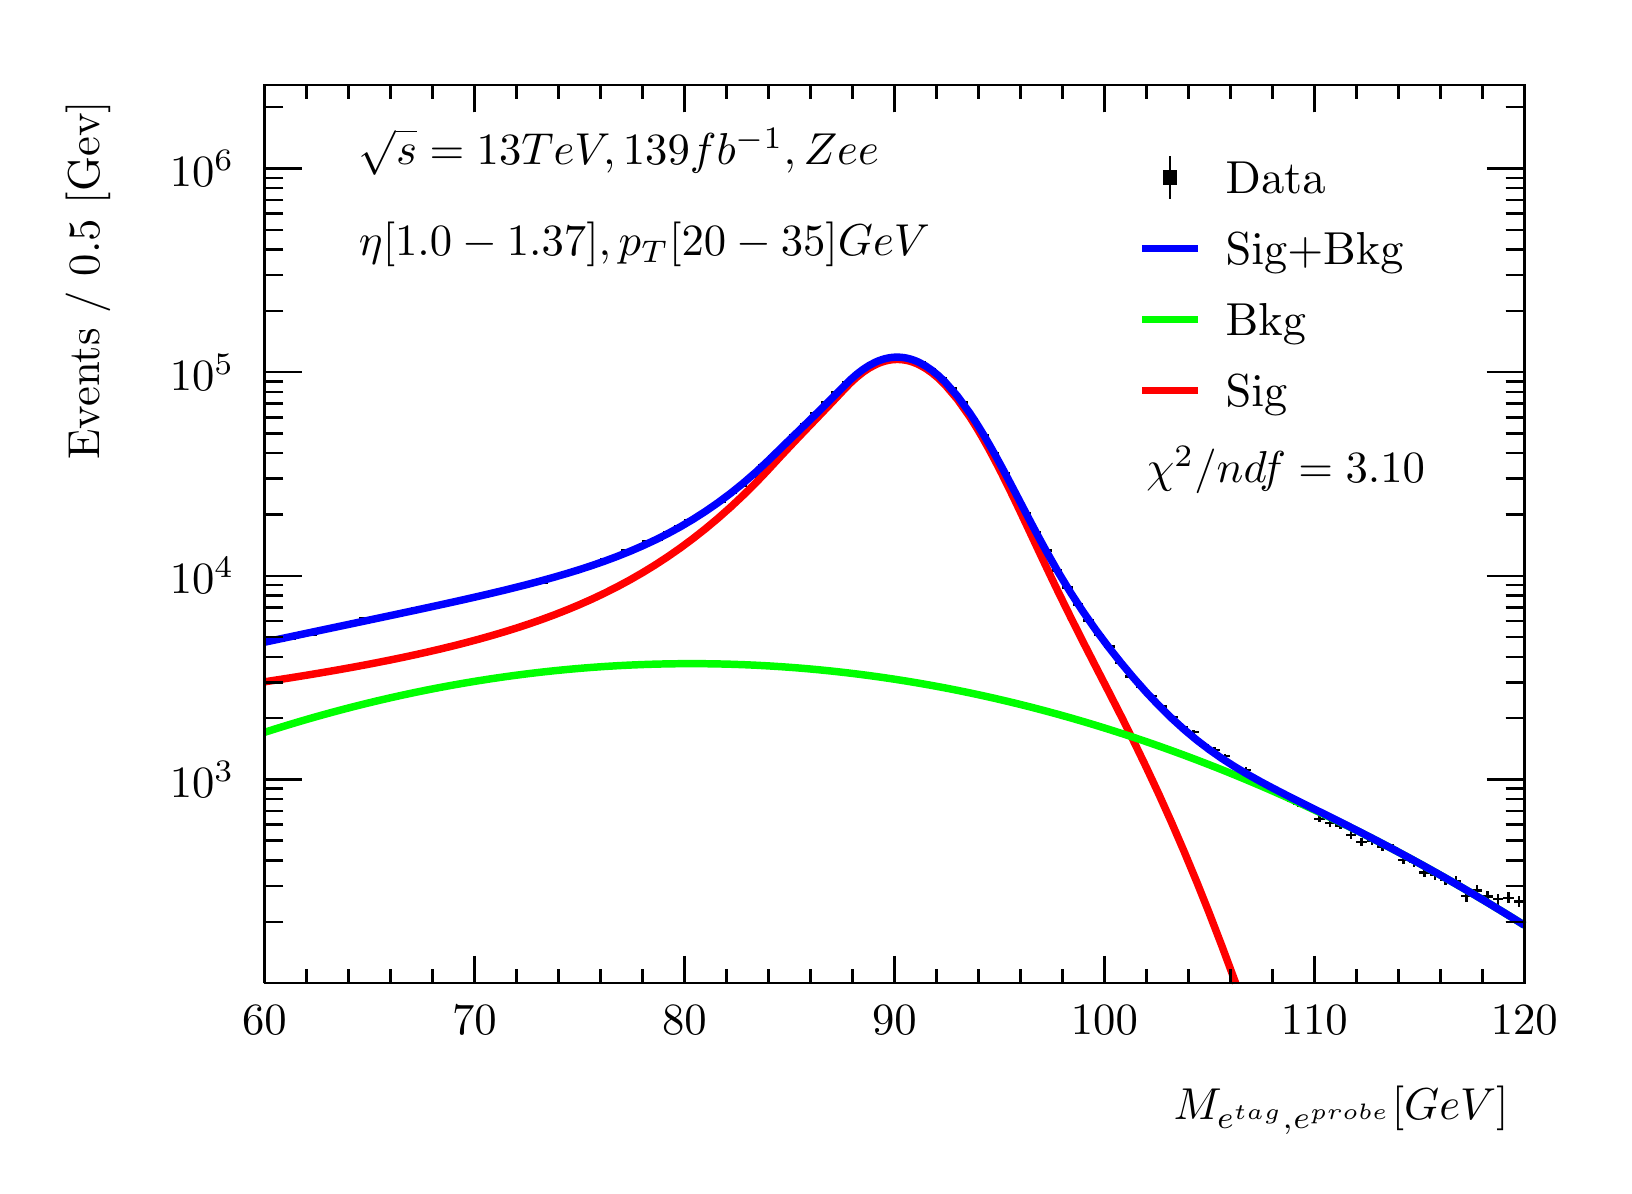
\begin{tikzpicture}
\pgfdeclareplotmark{cross} {
\pgfpathmoveto{\pgfpoint{-0.3\pgfplotmarksize}{\pgfplotmarksize}}
\pgfpathlineto{\pgfpoint{+0.3\pgfplotmarksize}{\pgfplotmarksize}}
\pgfpathlineto{\pgfpoint{+0.3\pgfplotmarksize}{0.3\pgfplotmarksize}}
\pgfpathlineto{\pgfpoint{+1\pgfplotmarksize}{0.3\pgfplotmarksize}}
\pgfpathlineto{\pgfpoint{+1\pgfplotmarksize}{-0.3\pgfplotmarksize}}
\pgfpathlineto{\pgfpoint{+0.3\pgfplotmarksize}{-0.3\pgfplotmarksize}}
\pgfpathlineto{\pgfpoint{+0.3\pgfplotmarksize}{-1.\pgfplotmarksize}}
\pgfpathlineto{\pgfpoint{-0.3\pgfplotmarksize}{-1.\pgfplotmarksize}}
\pgfpathlineto{\pgfpoint{-0.3\pgfplotmarksize}{-0.3\pgfplotmarksize}}
\pgfpathlineto{\pgfpoint{-1.\pgfplotmarksize}{-0.3\pgfplotmarksize}}
\pgfpathlineto{\pgfpoint{-1.\pgfplotmarksize}{0.3\pgfplotmarksize}}
\pgfpathlineto{\pgfpoint{-0.3\pgfplotmarksize}{0.3\pgfplotmarksize}}
\pgfpathclose
\pgfusepathqstroke
}
\pgfdeclareplotmark{cross*} {
\pgfpathmoveto{\pgfpoint{-0.3\pgfplotmarksize}{\pgfplotmarksize}}
\pgfpathlineto{\pgfpoint{+0.3\pgfplotmarksize}{\pgfplotmarksize}}
\pgfpathlineto{\pgfpoint{+0.3\pgfplotmarksize}{0.3\pgfplotmarksize}}
\pgfpathlineto{\pgfpoint{+1\pgfplotmarksize}{0.3\pgfplotmarksize}}
\pgfpathlineto{\pgfpoint{+1\pgfplotmarksize}{-0.3\pgfplotmarksize}}
\pgfpathlineto{\pgfpoint{+0.3\pgfplotmarksize}{-0.3\pgfplotmarksize}}
\pgfpathlineto{\pgfpoint{+0.3\pgfplotmarksize}{-1.\pgfplotmarksize}}
\pgfpathlineto{\pgfpoint{-0.3\pgfplotmarksize}{-1.\pgfplotmarksize}}
\pgfpathlineto{\pgfpoint{-0.3\pgfplotmarksize}{-0.3\pgfplotmarksize}}
\pgfpathlineto{\pgfpoint{-1.\pgfplotmarksize}{-0.3\pgfplotmarksize}}
\pgfpathlineto{\pgfpoint{-1.\pgfplotmarksize}{0.3\pgfplotmarksize}}
\pgfpathlineto{\pgfpoint{-0.3\pgfplotmarksize}{0.3\pgfplotmarksize}}
\pgfpathclose
\pgfusepathqfillstroke
}
\pgfdeclareplotmark{newstar} {
\pgfpathmoveto{\pgfqpoint{0pt}{\pgfplotmarksize}}
\pgfpathlineto{\pgfqpointpolar{44}{0.5\pgfplotmarksize}}
\pgfpathlineto{\pgfqpointpolar{18}{\pgfplotmarksize}}
\pgfpathlineto{\pgfqpointpolar{-20}{0.5\pgfplotmarksize}}
\pgfpathlineto{\pgfqpointpolar{-54}{\pgfplotmarksize}}
\pgfpathlineto{\pgfqpointpolar{-90}{0.5\pgfplotmarksize}}
\pgfpathlineto{\pgfqpointpolar{234}{\pgfplotmarksize}}
\pgfpathlineto{\pgfqpointpolar{198}{0.5\pgfplotmarksize}}
\pgfpathlineto{\pgfqpointpolar{162}{\pgfplotmarksize}}
\pgfpathlineto{\pgfqpointpolar{134}{0.5\pgfplotmarksize}}
\pgfpathclose
\pgfusepathqstroke
}
\pgfdeclareplotmark{newstar*} {
\pgfpathmoveto{\pgfqpoint{0pt}{\pgfplotmarksize}}
\pgfpathlineto{\pgfqpointpolar{44}{0.5\pgfplotmarksize}}
\pgfpathlineto{\pgfqpointpolar{18}{\pgfplotmarksize}}
\pgfpathlineto{\pgfqpointpolar{-20}{0.5\pgfplotmarksize}}
\pgfpathlineto{\pgfqpointpolar{-54}{\pgfplotmarksize}}
\pgfpathlineto{\pgfqpointpolar{-90}{0.5\pgfplotmarksize}}
\pgfpathlineto{\pgfqpointpolar{234}{\pgfplotmarksize}}
\pgfpathlineto{\pgfqpointpolar{198}{0.5\pgfplotmarksize}}
\pgfpathlineto{\pgfqpointpolar{162}{\pgfplotmarksize}}
\pgfpathlineto{\pgfqpointpolar{134}{0.5\pgfplotmarksize}}
\pgfpathclose
\pgfusepathqfillstroke
}
\definecolor{c}{rgb}{1,1,1};
\draw [color=c, fill=c] (0,0) rectangle (20,14.4361);
\draw [color=c, fill=c] (3,2.30977) rectangle (19,13.7143);
\definecolor{c}{rgb}{0,0,0};
\draw [c,line width=0.9] (3,2.30977) -- (3,13.7143) -- (19,13.7143) -- (19,2.30977) -- (3,2.30977);
\definecolor{c}{rgb}{1,1,1};
\draw [color=c, fill=c] (3,2.30977) rectangle (19,13.7143);
\definecolor{c}{rgb}{0,0,0};
\draw [c,line width=0.9] (3,2.30977) -- (3,13.7143) -- (19,13.7143) -- (19,2.30977) -- (3,2.30977);
\draw [c,line width=0.9] (3,2.30977) -- (19,2.30977);
\draw [c,line width=0.9] (3,2.65624) -- (3,2.30977);
\draw [c,line width=0.9] (3.53333,2.48301) -- (3.53333,2.30977);
\draw [c,line width=0.9] (4.06667,2.48301) -- (4.06667,2.30977);
\draw [c,line width=0.9] (4.6,2.48301) -- (4.6,2.30977);
\draw [c,line width=0.9] (5.13333,2.48301) -- (5.13333,2.30977);
\draw [c,line width=0.9] (5.66667,2.65624) -- (5.66667,2.30977);
\draw [c,line width=0.9] (6.2,2.48301) -- (6.2,2.30977);
\draw [c,line width=0.9] (6.73333,2.48301) -- (6.73333,2.30977);
\draw [c,line width=0.9] (7.26667,2.48301) -- (7.26667,2.30977);
\draw [c,line width=0.9] (7.8,2.48301) -- (7.8,2.30977);
\draw [c,line width=0.9] (8.33333,2.65624) -- (8.33333,2.30977);
\draw [c,line width=0.9] (8.86667,2.48301) -- (8.86667,2.30977);
\draw [c,line width=0.9] (9.4,2.48301) -- (9.4,2.30977);
\draw [c,line width=0.9] (9.93333,2.48301) -- (9.93333,2.30977);
\draw [c,line width=0.9] (10.4667,2.48301) -- (10.4667,2.30977);
\draw [c,line width=0.9] (11,2.65624) -- (11,2.30977);
\draw [c,line width=0.9] (11.5333,2.48301) -- (11.5333,2.30977);
\draw [c,line width=0.9] (12.0667,2.48301) -- (12.0667,2.30977);
\draw [c,line width=0.9] (12.6,2.48301) -- (12.6,2.30977);
\draw [c,line width=0.9] (13.1333,2.48301) -- (13.1333,2.30977);
\draw [c,line width=0.9] (13.6667,2.65624) -- (13.6667,2.30977);
\draw [c,line width=0.9] (14.2,2.48301) -- (14.2,2.30977);
\draw [c,line width=0.9] (14.7333,2.48301) -- (14.7333,2.30977);
\draw [c,line width=0.9] (15.2667,2.48301) -- (15.2667,2.30977);
\draw [c,line width=0.9] (15.8,2.48301) -- (15.8,2.30977);
\draw [c,line width=0.9] (16.3333,2.65624) -- (16.3333,2.30977);
\draw [c,line width=0.9] (16.8667,2.48301) -- (16.8667,2.30977);
\draw [c,line width=0.9] (17.4,2.48301) -- (17.4,2.30977);
\draw [c,line width=0.9] (17.9333,2.48301) -- (17.9333,2.30977);
\draw [c,line width=0.9] (18.4667,2.48301) -- (18.4667,2.30977);
\draw [c,line width=0.9] (19,2.65624) -- (19,2.30977);
\draw [anchor=base] (3,1.66015) node[scale=1.61424, color=c, rotate=0]{60};
\draw [anchor=base] (5.66667,1.66015) node[scale=1.61424, color=c, rotate=0]{70};
\draw [anchor=base] (8.33333,1.66015) node[scale=1.61424, color=c, rotate=0]{80};
\draw [anchor=base] (11,1.66015) node[scale=1.61424, color=c, rotate=0]{90};
\draw [anchor=base] (13.6667,1.66015) node[scale=1.61424, color=c, rotate=0]{100};
\draw [anchor=base] (16.3333,1.66015) node[scale=1.61424, color=c, rotate=0]{110};
\draw [anchor=base] (19,1.66015) node[scale=1.61424, color=c, rotate=0]{120};
\draw [anchor= east] (19,0.692932) node[scale=1.61424, color=c, rotate=0]{$M_{e^{tag}, e^{probe}}  [GeV]$};
\draw [c,line width=0.9] (3,13.7143) -- (19,13.7143);
\draw [c,line width=0.9] (3,13.3678) -- (3,13.7143);
\draw [c,line width=0.9] (3.53333,13.5411) -- (3.53333,13.7143);
\draw [c,line width=0.9] (4.06667,13.5411) -- (4.06667,13.7143);
\draw [c,line width=0.9] (4.6,13.5411) -- (4.6,13.7143);
\draw [c,line width=0.9] (5.13333,13.5411) -- (5.13333,13.7143);
\draw [c,line width=0.9] (5.66667,13.3678) -- (5.66667,13.7143);
\draw [c,line width=0.9] (6.2,13.5411) -- (6.2,13.7143);
\draw [c,line width=0.9] (6.73333,13.5411) -- (6.73333,13.7143);
\draw [c,line width=0.9] (7.26667,13.5411) -- (7.26667,13.7143);
\draw [c,line width=0.9] (7.8,13.5411) -- (7.8,13.7143);
\draw [c,line width=0.9] (8.33333,13.3678) -- (8.33333,13.7143);
\draw [c,line width=0.9] (8.86667,13.5411) -- (8.86667,13.7143);
\draw [c,line width=0.9] (9.4,13.5411) -- (9.4,13.7143);
\draw [c,line width=0.9] (9.93333,13.5411) -- (9.93333,13.7143);
\draw [c,line width=0.9] (10.4667,13.5411) -- (10.4667,13.7143);
\draw [c,line width=0.9] (11,13.3678) -- (11,13.7143);
\draw [c,line width=0.9] (11.5333,13.5411) -- (11.5333,13.7143);
\draw [c,line width=0.9] (12.0667,13.5411) -- (12.0667,13.7143);
\draw [c,line width=0.9] (12.6,13.5411) -- (12.6,13.7143);
\draw [c,line width=0.9] (13.1333,13.5411) -- (13.1333,13.7143);
\draw [c,line width=0.9] (13.6667,13.3678) -- (13.6667,13.7143);
\draw [c,line width=0.9] (14.2,13.5411) -- (14.2,13.7143);
\draw [c,line width=0.9] (14.7333,13.5411) -- (14.7333,13.7143);
\draw [c,line width=0.9] (15.2667,13.5411) -- (15.2667,13.7143);
\draw [c,line width=0.9] (15.8,13.5411) -- (15.8,13.7143);
\draw [c,line width=0.9] (16.3333,13.3678) -- (16.3333,13.7143);
\draw [c,line width=0.9] (16.8667,13.5411) -- (16.8667,13.7143);
\draw [c,line width=0.9] (17.4,13.5411) -- (17.4,13.7143);
\draw [c,line width=0.9] (17.9333,13.5411) -- (17.9333,13.7143);
\draw [c,line width=0.9] (18.4667,13.5411) -- (18.4667,13.7143);
\draw [c,line width=0.9] (19,13.3678) -- (19,13.7143);
\draw [c,line width=0.9] (3,2.30977) -- (3,13.7143);
\draw [c,line width=0.9] (3.237,3.08829) -- (3,3.08829);
\draw [c,line width=0.9] (3.237,3.54369) -- (3,3.54369);
\draw [c,line width=0.9] (3.237,3.8668) -- (3,3.8668);
\draw [c,line width=0.9] (3.237,4.11742) -- (3,4.11742);
\draw [c,line width=0.9] (3.237,4.3222) -- (3,4.3222);
\draw [c,line width=0.9] (3.237,4.49534) -- (3,4.49534);
\draw [c,line width=0.9] (3.237,4.64531) -- (3,4.64531);
\draw [c,line width=0.9] (3.237,4.7776) -- (3,4.7776);
\draw [c,line width=0.9] (3.474,4.89594) -- (3,4.89594);
\draw [anchor= east] (2.82,4.89594) node[scale=1.61424, color=c, rotate=0]{$10^{3}$};
\draw [c,line width=0.9] (3.237,5.67445) -- (3,5.67445);
\draw [c,line width=0.9] (3.237,6.12985) -- (3,6.12985);
\draw [c,line width=0.9] (3.237,6.45297) -- (3,6.45297);
\draw [c,line width=0.9] (3.237,6.70359) -- (3,6.70359);
\draw [c,line width=0.9] (3.237,6.90837) -- (3,6.90837);
\draw [c,line width=0.9] (3.237,7.0815) -- (3,7.0815);
\draw [c,line width=0.9] (3.237,7.23148) -- (3,7.23148);
\draw [c,line width=0.9] (3.237,7.36377) -- (3,7.36377);
\draw [c,line width=0.9] (3.474,7.48211) -- (3,7.48211);
\draw [anchor= east] (2.82,7.48211) node[scale=1.61424, color=c, rotate=0]{$10^{4}$};
\draw [c,line width=0.9] (3.237,8.26062) -- (3,8.26062);
\draw [c,line width=0.9] (3.237,8.71602) -- (3,8.71602);
\draw [c,line width=0.9] (3.237,9.03913) -- (3,9.03913);
\draw [c,line width=0.9] (3.237,9.28976) -- (3,9.28976);
\draw [c,line width=0.9] (3.237,9.49453) -- (3,9.49453);
\draw [c,line width=0.9] (3.237,9.66767) -- (3,9.66767);
\draw [c,line width=0.9] (3.237,9.81765) -- (3,9.81765);
\draw [c,line width=0.9] (3.237,9.94994) -- (3,9.94994);
\draw [c,line width=0.9] (3.474,10.0683) -- (3,10.0683);
\draw [anchor= east] (2.82,10.0683) node[scale=1.61424, color=c, rotate=0]{$10^{5}$};
\draw [c,line width=0.9] (3.237,10.8468) -- (3,10.8468);
\draw [c,line width=0.9] (3.237,11.3022) -- (3,11.3022);
\draw [c,line width=0.9] (3.237,11.6253) -- (3,11.6253);
\draw [c,line width=0.9] (3.237,11.8759) -- (3,11.8759);
\draw [c,line width=0.9] (3.237,12.0807) -- (3,12.0807);
\draw [c,line width=0.9] (3.237,12.2538) -- (3,12.2538);
\draw [c,line width=0.9] (3.237,12.4038) -- (3,12.4038);
\draw [c,line width=0.9] (3.237,12.5361) -- (3,12.5361);
\draw [c,line width=0.9] (3.474,12.6544) -- (3,12.6544);
\draw [anchor= east] (2.82,12.6544) node[scale=1.61424, color=c, rotate=0]{$10^{6}$};
\draw [c,line width=0.9] (3.237,13.433) -- (3,13.433);
\draw [anchor= east] (0.76,13.7143) node[scale=1.61424, color=c, rotate=90]{Events / 0.5 [Gev]};
\draw [c,line width=0.9] (19,2.30977) -- (19,13.7143);
\draw [c,line width=0.9] (18.763,3.08829) -- (19,3.08829);
\draw [c,line width=0.9] (18.763,3.54369) -- (19,3.54369);
\draw [c,line width=0.9] (18.763,3.8668) -- (19,3.8668);
\draw [c,line width=0.9] (18.763,4.11742) -- (19,4.11742);
\draw [c,line width=0.9] (18.763,4.3222) -- (19,4.3222);
\draw [c,line width=0.9] (18.763,4.49534) -- (19,4.49534);
\draw [c,line width=0.9] (18.763,4.64531) -- (19,4.64531);
\draw [c,line width=0.9] (18.763,4.7776) -- (19,4.7776);
\draw [c,line width=0.9] (18.526,4.89594) -- (19,4.89594);
\draw [c,line width=0.9] (18.763,5.67445) -- (19,5.67445);
\draw [c,line width=0.9] (18.763,6.12985) -- (19,6.12985);
\draw [c,line width=0.9] (18.763,6.45297) -- (19,6.45297);
\draw [c,line width=0.9] (18.763,6.70359) -- (19,6.70359);
\draw [c,line width=0.9] (18.763,6.90837) -- (19,6.90837);
\draw [c,line width=0.9] (18.763,7.0815) -- (19,7.0815);
\draw [c,line width=0.9] (18.763,7.23148) -- (19,7.23148);
\draw [c,line width=0.9] (18.763,7.36377) -- (19,7.36377);
\draw [c,line width=0.9] (18.526,7.48211) -- (19,7.48211);
\draw [c,line width=0.9] (18.763,8.26062) -- (19,8.26062);
\draw [c,line width=0.9] (18.763,8.71602) -- (19,8.71602);
\draw [c,line width=0.9] (18.763,9.03913) -- (19,9.03913);
\draw [c,line width=0.9] (18.763,9.28976) -- (19,9.28976);
\draw [c,line width=0.9] (18.763,9.49453) -- (19,9.49453);
\draw [c,line width=0.9] (18.763,9.66767) -- (19,9.66767);
\draw [c,line width=0.9] (18.763,9.81765) -- (19,9.81765);
\draw [c,line width=0.9] (18.763,9.94994) -- (19,9.94994);
\draw [c,line width=0.9] (18.526,10.0683) -- (19,10.0683);
\draw [c,line width=0.9] (18.763,10.8468) -- (19,10.8468);
\draw [c,line width=0.9] (18.763,11.3022) -- (19,11.3022);
\draw [c,line width=0.9] (18.763,11.6253) -- (19,11.6253);
\draw [c,line width=0.9] (18.763,11.8759) -- (19,11.8759);
\draw [c,line width=0.9] (18.763,12.0807) -- (19,12.0807);
\draw [c,line width=0.9] (18.763,12.2538) -- (19,12.2538);
\draw [c,line width=0.9] (18.763,12.4038) -- (19,12.4038);
\draw [c,line width=0.9] (18.763,12.5361) -- (19,12.5361);
\draw [c,line width=0.9] (18.526,12.6544) -- (19,12.6544);
\draw [c,line width=0.9] (18.763,13.433) -- (19,13.433);
\draw [c,line width=0.9] (3.06667,6.65329) -- (3,6.65329);
\draw [c,line width=0.9] (3,6.65329) -- (3,6.65329);
\draw [c,line width=0.9] (3.06667,6.65329) -- (3.13333,6.65329);
\draw [c,line width=0.9] (3.13333,6.65329) -- (3.13333,6.65329);
\draw [c,line width=0.9] (3.06667,6.65329) -- (3.06667,6.66953);
\draw [c,line width=0.9] (3.06667,6.66953) -- (3.06667,6.66953);
\draw [c,line width=0.9] (3.06667,6.65329) -- (3.06667,6.63705);
\draw [c,line width=0.9] (3.06667,6.63705) -- (3.06667,6.63705);
\draw [c,line width=0.9] (3.2,6.66288) -- (3.13333,6.66288);
\draw [c,line width=0.9] (3.13333,6.66288) -- (3.13333,6.66288);
\draw [c,line width=0.9] (3.2,6.66288) -- (3.26667,6.66288);
\draw [c,line width=0.9] (3.26667,6.66288) -- (3.26667,6.66288);
\draw [c,line width=0.9] (3.2,6.66288) -- (3.2,6.67905);
\draw [c,line width=0.9] (3.2,6.67905) -- (3.2,6.67905);
\draw [c,line width=0.9] (3.2,6.66288) -- (3.2,6.64671);
\draw [c,line width=0.9] (3.2,6.64671) -- (3.2,6.64671);
\draw [c,line width=0.9] (3.33333,6.67677) -- (3.26667,6.67677);
\draw [c,line width=0.9] (3.26667,6.67677) -- (3.26667,6.67677);
\draw [c,line width=0.9] (3.33333,6.67677) -- (3.4,6.67677);
\draw [c,line width=0.9] (3.4,6.67677) -- (3.4,6.67677);
\draw [c,line width=0.9] (3.33333,6.67677) -- (3.33333,6.69284);
\draw [c,line width=0.9] (3.33333,6.69284) -- (3.33333,6.69284);
\draw [c,line width=0.9] (3.33333,6.67677) -- (3.33333,6.66069);
\draw [c,line width=0.9] (3.33333,6.66069) -- (3.33333,6.66069);
\draw [c,line width=0.9] (3.46667,6.73264) -- (3.4,6.73264);
\draw [c,line width=0.9] (3.4,6.73264) -- (3.4,6.73264);
\draw [c,line width=0.9] (3.46667,6.73264) -- (3.53333,6.73264);
\draw [c,line width=0.9] (3.53333,6.73264) -- (3.53333,6.73264);
\draw [c,line width=0.9] (3.46667,6.73264) -- (3.46667,6.74832);
\draw [c,line width=0.9] (3.46667,6.74832) -- (3.46667,6.74832);
\draw [c,line width=0.9] (3.46667,6.73264) -- (3.46667,6.71696);
\draw [c,line width=0.9] (3.46667,6.71696) -- (3.46667,6.71696);
\draw [c,line width=0.9] (3.6,6.73592) -- (3.53333,6.73592);
\draw [c,line width=0.9] (3.53333,6.73592) -- (3.53333,6.73592);
\draw [c,line width=0.9] (3.6,6.73592) -- (3.66667,6.73592);
\draw [c,line width=0.9] (3.66667,6.73592) -- (3.66667,6.73592);
\draw [c,line width=0.9] (3.6,6.73592) -- (3.6,6.75158);
\draw [c,line width=0.9] (3.6,6.75158) -- (3.6,6.75158);
\draw [c,line width=0.9] (3.6,6.73592) -- (3.6,6.72026);
\draw [c,line width=0.9] (3.6,6.72026) -- (3.6,6.72026);
\draw [c,line width=0.9] (3.73333,6.7892) -- (3.66667,6.7892);
\draw [c,line width=0.9] (3.66667,6.7892) -- (3.66667,6.7892);
\draw [c,line width=0.9] (3.73333,6.7892) -- (3.8,6.7892);
\draw [c,line width=0.9] (3.8,6.7892) -- (3.8,6.7892);
\draw [c,line width=0.9] (3.73333,6.7892) -- (3.73333,6.80449);
\draw [c,line width=0.9] (3.73333,6.80449) -- (3.73333,6.80449);
\draw [c,line width=0.9] (3.73333,6.7892) -- (3.73333,6.77391);
\draw [c,line width=0.9] (3.73333,6.77391) -- (3.73333,6.77391);
\draw [c,line width=0.9] (3.86667,6.83308) -- (3.8,6.83308);
\draw [c,line width=0.9] (3.8,6.83308) -- (3.8,6.83308);
\draw [c,line width=0.9] (3.86667,6.83308) -- (3.93333,6.83308);
\draw [c,line width=0.9] (3.93333,6.83308) -- (3.93333,6.83308);
\draw [c,line width=0.9] (3.86667,6.83308) -- (3.86667,6.84808);
\draw [c,line width=0.9] (3.86667,6.84808) -- (3.86667,6.84808);
\draw [c,line width=0.9] (3.86667,6.83308) -- (3.86667,6.81809);
\draw [c,line width=0.9] (3.86667,6.81809) -- (3.86667,6.81809);
\draw [c,line width=0.9] (4,6.86154) -- (3.93333,6.86154);
\draw [c,line width=0.9] (3.93333,6.86154) -- (3.93333,6.86154);
\draw [c,line width=0.9] (4,6.86154) -- (4.06667,6.86154);
\draw [c,line width=0.9] (4.06667,6.86154) -- (4.06667,6.86154);
\draw [c,line width=0.9] (4,6.86154) -- (4,6.87635);
\draw [c,line width=0.9] (4,6.87635) -- (4,6.87635);
\draw [c,line width=0.9] (4,6.86154) -- (4,6.84674);
\draw [c,line width=0.9] (4,6.84674) -- (4,6.84674);
\draw [c,line width=0.9] (4.13333,6.89538) -- (4.06667,6.89538);
\draw [c,line width=0.9] (4.06667,6.89538) -- (4.06667,6.89538);
\draw [c,line width=0.9] (4.13333,6.89538) -- (4.2,6.89538);
\draw [c,line width=0.9] (4.2,6.89538) -- (4.2,6.89538);
\draw [c,line width=0.9] (4.13333,6.89538) -- (4.13333,6.90996);
\draw [c,line width=0.9] (4.13333,6.90996) -- (4.13333,6.90996);
\draw [c,line width=0.9] (4.13333,6.89538) -- (4.13333,6.88079);
\draw [c,line width=0.9] (4.13333,6.88079) -- (4.13333,6.88079);
\draw [c,line width=0.9] (4.26667,6.94084) -- (4.2,6.94084);
\draw [c,line width=0.9] (4.2,6.94084) -- (4.2,6.94084);
\draw [c,line width=0.9] (4.26667,6.94084) -- (4.33333,6.94084);
\draw [c,line width=0.9] (4.33333,6.94084) -- (4.33333,6.94084);
\draw [c,line width=0.9] (4.26667,6.94084) -- (4.26667,6.95513);
\draw [c,line width=0.9] (4.26667,6.95513) -- (4.26667,6.95513);
\draw [c,line width=0.9] (4.26667,6.94084) -- (4.26667,6.92655);
\draw [c,line width=0.9] (4.26667,6.92655) -- (4.26667,6.92655);
\draw [c,line width=0.9] (4.4,6.93519) -- (4.33333,6.93519);
\draw [c,line width=0.9] (4.33333,6.93519) -- (4.33333,6.93519);
\draw [c,line width=0.9] (4.4,6.93519) -- (4.46667,6.93519);
\draw [c,line width=0.9] (4.46667,6.93519) -- (4.46667,6.93519);
\draw [c,line width=0.9] (4.4,6.93519) -- (4.4,6.94952);
\draw [c,line width=0.9] (4.4,6.94952) -- (4.4,6.94952);
\draw [c,line width=0.9] (4.4,6.93519) -- (4.4,6.92086);
\draw [c,line width=0.9] (4.4,6.92086) -- (4.4,6.92086);
\draw [c,line width=0.9] (4.53333,6.9791) -- (4.46667,6.9791);
\draw [c,line width=0.9] (4.46667,6.9791) -- (4.46667,6.9791);
\draw [c,line width=0.9] (4.53333,6.9791) -- (4.6,6.9791);
\draw [c,line width=0.9] (4.6,6.9791) -- (4.6,6.9791);
\draw [c,line width=0.9] (4.53333,6.9791) -- (4.53333,6.99315);
\draw [c,line width=0.9] (4.53333,6.99315) -- (4.53333,6.99315);
\draw [c,line width=0.9] (4.53333,6.9791) -- (4.53333,6.96505);
\draw [c,line width=0.9] (4.53333,6.96505) -- (4.53333,6.96505);
\draw [c,line width=0.9] (4.66667,7.00172) -- (4.6,7.00172);
\draw [c,line width=0.9] (4.6,7.00172) -- (4.6,7.00172);
\draw [c,line width=0.9] (4.66667,7.00172) -- (4.73333,7.00172);
\draw [c,line width=0.9] (4.73333,7.00172) -- (4.73333,7.00172);
\draw [c,line width=0.9] (4.66667,7.00172) -- (4.66667,7.01563);
\draw [c,line width=0.9] (4.66667,7.01563) -- (4.66667,7.01563);
\draw [c,line width=0.9] (4.66667,7.00172) -- (4.66667,6.98781);
\draw [c,line width=0.9] (4.66667,6.98781) -- (4.66667,6.98781);
\draw [c,line width=0.9] (4.8,6.99464) -- (4.73333,6.99464);
\draw [c,line width=0.9] (4.73333,6.99464) -- (4.73333,6.99464);
\draw [c,line width=0.9] (4.8,6.99464) -- (4.86667,6.99464);
\draw [c,line width=0.9] (4.86667,6.99464) -- (4.86667,6.99464);
\draw [c,line width=0.9] (4.8,6.99464) -- (4.8,7.00859);
\draw [c,line width=0.9] (4.8,7.00859) -- (4.8,7.00859);
\draw [c,line width=0.9] (4.8,6.99464) -- (4.8,6.98068);
\draw [c,line width=0.9] (4.8,6.98068) -- (4.8,6.98068);
\draw [c,line width=0.9] (4.93333,7.07362) -- (4.86667,7.07362);
\draw [c,line width=0.9] (4.86667,7.07362) -- (4.86667,7.07362);
\draw [c,line width=0.9] (4.93333,7.07362) -- (5,7.07362);
\draw [c,line width=0.9] (5,7.07362) -- (5,7.07362);
\draw [c,line width=0.9] (4.93333,7.07362) -- (4.93333,7.08709);
\draw [c,line width=0.9] (4.93333,7.08709) -- (4.93333,7.08709);
\draw [c,line width=0.9] (4.93333,7.07362) -- (4.93333,7.06014);
\draw [c,line width=0.9] (4.93333,7.06014) -- (4.93333,7.06014);
\draw [c,line width=0.9] (5.06667,7.08599) -- (5,7.08599);
\draw [c,line width=0.9] (5,7.08599) -- (5,7.08599);
\draw [c,line width=0.9] (5.06667,7.08599) -- (5.13333,7.08599);
\draw [c,line width=0.9] (5.13333,7.08599) -- (5.13333,7.08599);
\draw [c,line width=0.9] (5.06667,7.08599) -- (5.06667,7.09939);
\draw [c,line width=0.9] (5.06667,7.09939) -- (5.06667,7.09939);
\draw [c,line width=0.9] (5.06667,7.08599) -- (5.06667,7.07259);
\draw [c,line width=0.9] (5.06667,7.07259) -- (5.06667,7.07259);
\draw [c,line width=0.9] (5.2,7.10217) -- (5.13333,7.10217);
\draw [c,line width=0.9] (5.13333,7.10217) -- (5.13333,7.10217);
\draw [c,line width=0.9] (5.2,7.10217) -- (5.26667,7.10217);
\draw [c,line width=0.9] (5.26667,7.10217) -- (5.26667,7.10217);
\draw [c,line width=0.9] (5.2,7.10217) -- (5.2,7.11547);
\draw [c,line width=0.9] (5.2,7.11547) -- (5.2,7.11547);
\draw [c,line width=0.9] (5.2,7.10217) -- (5.2,7.08887);
\draw [c,line width=0.9] (5.2,7.08887) -- (5.2,7.08887);
\draw [c,line width=0.9] (5.33333,7.1427) -- (5.26667,7.1427);
\draw [c,line width=0.9] (5.26667,7.1427) -- (5.26667,7.1427);
\draw [c,line width=0.9] (5.33333,7.1427) -- (5.4,7.1427);
\draw [c,line width=0.9] (5.4,7.1427) -- (5.4,7.1427);
\draw [c,line width=0.9] (5.33333,7.1427) -- (5.33333,7.15577);
\draw [c,line width=0.9] (5.33333,7.15577) -- (5.33333,7.15577);
\draw [c,line width=0.9] (5.33333,7.1427) -- (5.33333,7.12964);
\draw [c,line width=0.9] (5.33333,7.12964) -- (5.33333,7.12964);
\draw [c,line width=0.9] (5.46667,7.18402) -- (5.4,7.18402);
\draw [c,line width=0.9] (5.4,7.18402) -- (5.4,7.18402);
\draw [c,line width=0.9] (5.46667,7.18402) -- (5.53333,7.18402);
\draw [c,line width=0.9] (5.53333,7.18402) -- (5.53333,7.18402);
\draw [c,line width=0.9] (5.46667,7.18402) -- (5.46667,7.19685);
\draw [c,line width=0.9] (5.46667,7.19685) -- (5.46667,7.19685);
\draw [c,line width=0.9] (5.46667,7.18402) -- (5.46667,7.1712);
\draw [c,line width=0.9] (5.46667,7.1712) -- (5.46667,7.1712);
\draw [c,line width=0.9] (5.6,7.18329) -- (5.53333,7.18329);
\draw [c,line width=0.9] (5.53333,7.18329) -- (5.53333,7.18329);
\draw [c,line width=0.9] (5.6,7.18329) -- (5.66667,7.18329);
\draw [c,line width=0.9] (5.66667,7.18329) -- (5.66667,7.18329);
\draw [c,line width=0.9] (5.6,7.18329) -- (5.6,7.19612);
\draw [c,line width=0.9] (5.6,7.19612) -- (5.6,7.19612);
\draw [c,line width=0.9] (5.6,7.18329) -- (5.6,7.17046);
\draw [c,line width=0.9] (5.6,7.17046) -- (5.6,7.17046);
\draw [c,line width=0.9] (5.73333,7.21308) -- (5.66667,7.21308);
\draw [c,line width=0.9] (5.66667,7.21308) -- (5.66667,7.21308);
\draw [c,line width=0.9] (5.73333,7.21308) -- (5.8,7.21308);
\draw [c,line width=0.9] (5.8,7.21308) -- (5.8,7.21308);
\draw [c,line width=0.9] (5.73333,7.21308) -- (5.73333,7.22574);
\draw [c,line width=0.9] (5.73333,7.22574) -- (5.73333,7.22574);
\draw [c,line width=0.9] (5.73333,7.21308) -- (5.73333,7.20042);
\draw [c,line width=0.9] (5.73333,7.20042) -- (5.73333,7.20042);
\draw [c,line width=0.9] (5.86667,7.23778) -- (5.8,7.23778);
\draw [c,line width=0.9] (5.8,7.23778) -- (5.8,7.23778);
\draw [c,line width=0.9] (5.86667,7.23778) -- (5.93333,7.23778);
\draw [c,line width=0.9] (5.93333,7.23778) -- (5.93333,7.23778);
\draw [c,line width=0.9] (5.86667,7.23778) -- (5.86667,7.2503);
\draw [c,line width=0.9] (5.86667,7.2503) -- (5.86667,7.2503);
\draw [c,line width=0.9] (5.86667,7.23778) -- (5.86667,7.22526);
\draw [c,line width=0.9] (5.86667,7.22526) -- (5.86667,7.22526);
\draw [c,line width=0.9] (6,7.29122) -- (5.93333,7.29122);
\draw [c,line width=0.9] (5.93333,7.29122) -- (5.93333,7.29122);
\draw [c,line width=0.9] (6,7.29122) -- (6.06667,7.29122);
\draw [c,line width=0.9] (6.06667,7.29122) -- (6.06667,7.29122);
\draw [c,line width=0.9] (6,7.29122) -- (6,7.30344);
\draw [c,line width=0.9] (6,7.30344) -- (6,7.30344);
\draw [c,line width=0.9] (6,7.29122) -- (6,7.27899);
\draw [c,line width=0.9] (6,7.27899) -- (6,7.27899);
\draw [c,line width=0.9] (6.13333,7.30419) -- (6.06667,7.30419);
\draw [c,line width=0.9] (6.06667,7.30419) -- (6.06667,7.30419);
\draw [c,line width=0.9] (6.13333,7.30419) -- (6.2,7.30419);
\draw [c,line width=0.9] (6.2,7.30419) -- (6.2,7.30419);
\draw [c,line width=0.9] (6.13333,7.30419) -- (6.13333,7.31635);
\draw [c,line width=0.9] (6.13333,7.31635) -- (6.13333,7.31635);
\draw [c,line width=0.9] (6.13333,7.30419) -- (6.13333,7.29203);
\draw [c,line width=0.9] (6.13333,7.29203) -- (6.13333,7.29203);
\draw [c,line width=0.9] (6.26667,7.35563) -- (6.2,7.35563);
\draw [c,line width=0.9] (6.2,7.35563) -- (6.2,7.35563);
\draw [c,line width=0.9] (6.26667,7.35563) -- (6.33333,7.35563);
\draw [c,line width=0.9] (6.33333,7.35563) -- (6.33333,7.35563);
\draw [c,line width=0.9] (6.26667,7.35563) -- (6.26667,7.36751);
\draw [c,line width=0.9] (6.26667,7.36751) -- (6.26667,7.36751);
\draw [c,line width=0.9] (6.26667,7.35563) -- (6.26667,7.34375);
\draw [c,line width=0.9] (6.26667,7.34375) -- (6.26667,7.34375);
\draw [c,line width=0.9] (6.4,7.37185) -- (6.33333,7.37185);
\draw [c,line width=0.9] (6.33333,7.37185) -- (6.33333,7.37185);
\draw [c,line width=0.9] (6.4,7.37185) -- (6.46667,7.37185);
\draw [c,line width=0.9] (6.46667,7.37185) -- (6.46667,7.37185);
\draw [c,line width=0.9] (6.4,7.37185) -- (6.4,7.38365);
\draw [c,line width=0.9] (6.4,7.38365) -- (6.4,7.38365);
\draw [c,line width=0.9] (6.4,7.37185) -- (6.4,7.36006);
\draw [c,line width=0.9] (6.4,7.36006) -- (6.4,7.36006);
\draw [c,line width=0.9] (6.53333,7.39818) -- (6.46667,7.39818);
\draw [c,line width=0.9] (6.46667,7.39818) -- (6.46667,7.39818);
\draw [c,line width=0.9] (6.53333,7.39818) -- (6.6,7.39818);
\draw [c,line width=0.9] (6.6,7.39818) -- (6.6,7.39818);
\draw [c,line width=0.9] (6.53333,7.39818) -- (6.53333,7.40984);
\draw [c,line width=0.9] (6.53333,7.40984) -- (6.53333,7.40984);
\draw [c,line width=0.9] (6.53333,7.39818) -- (6.53333,7.38652);
\draw [c,line width=0.9] (6.53333,7.38652) -- (6.53333,7.38652);
\draw [c,line width=0.9] (6.66667,7.45517) -- (6.6,7.45517);
\draw [c,line width=0.9] (6.6,7.45517) -- (6.6,7.45517);
\draw [c,line width=0.9] (6.66667,7.45517) -- (6.73333,7.45517);
\draw [c,line width=0.9] (6.73333,7.45517) -- (6.73333,7.45517);
\draw [c,line width=0.9] (6.66667,7.45517) -- (6.66667,7.46654);
\draw [c,line width=0.9] (6.66667,7.46654) -- (6.66667,7.46654);
\draw [c,line width=0.9] (6.66667,7.45517) -- (6.66667,7.4438);
\draw [c,line width=0.9] (6.66667,7.4438) -- (6.66667,7.4438);
\draw [c,line width=0.9] (6.8,7.48793) -- (6.73333,7.48793);
\draw [c,line width=0.9] (6.73333,7.48793) -- (6.73333,7.48793);
\draw [c,line width=0.9] (6.8,7.48793) -- (6.86667,7.48793);
\draw [c,line width=0.9] (6.86667,7.48793) -- (6.86667,7.48793);
\draw [c,line width=0.9] (6.8,7.48793) -- (6.8,7.49914);
\draw [c,line width=0.9] (6.8,7.49914) -- (6.8,7.49914);
\draw [c,line width=0.9] (6.8,7.48793) -- (6.8,7.47673);
\draw [c,line width=0.9] (6.8,7.47673) -- (6.8,7.47673);
\draw [c,line width=0.9] (6.93333,7.52356) -- (6.86667,7.52356);
\draw [c,line width=0.9] (6.86667,7.52356) -- (6.86667,7.52356);
\draw [c,line width=0.9] (6.93333,7.52356) -- (7,7.52356);
\draw [c,line width=0.9] (7,7.52356) -- (7,7.52356);
\draw [c,line width=0.9] (6.93333,7.52356) -- (6.93333,7.53459);
\draw [c,line width=0.9] (6.93333,7.53459) -- (6.93333,7.53459);
\draw [c,line width=0.9] (6.93333,7.52356) -- (6.93333,7.51254);
\draw [c,line width=0.9] (6.93333,7.51254) -- (6.93333,7.51254);
\draw [c,line width=0.9] (7.06667,7.56948) -- (7,7.56948);
\draw [c,line width=0.9] (7,7.56948) -- (7,7.56948);
\draw [c,line width=0.9] (7.06667,7.56948) -- (7.13333,7.56948);
\draw [c,line width=0.9] (7.13333,7.56948) -- (7.13333,7.56948);
\draw [c,line width=0.9] (7.06667,7.56948) -- (7.06667,7.58029);
\draw [c,line width=0.9] (7.06667,7.58029) -- (7.06667,7.58029);
\draw [c,line width=0.9] (7.06667,7.56948) -- (7.06667,7.55868);
\draw [c,line width=0.9] (7.06667,7.55868) -- (7.06667,7.55868);
\draw [c,line width=0.9] (7.2,7.62937) -- (7.13333,7.62937);
\draw [c,line width=0.9] (7.13333,7.62937) -- (7.13333,7.62937);
\draw [c,line width=0.9] (7.2,7.62937) -- (7.26667,7.62937);
\draw [c,line width=0.9] (7.26667,7.62937) -- (7.26667,7.62937);
\draw [c,line width=0.9] (7.2,7.62937) -- (7.2,7.63989);
\draw [c,line width=0.9] (7.2,7.63989) -- (7.2,7.63989);
\draw [c,line width=0.9] (7.2,7.62937) -- (7.2,7.61885);
\draw [c,line width=0.9] (7.2,7.61885) -- (7.2,7.61885);
\draw [c,line width=0.9] (7.33333,7.6881) -- (7.26667,7.6881);
\draw [c,line width=0.9] (7.26667,7.6881) -- (7.26667,7.6881);
\draw [c,line width=0.9] (7.33333,7.6881) -- (7.4,7.6881);
\draw [c,line width=0.9] (7.4,7.6881) -- (7.4,7.6881);
\draw [c,line width=0.9] (7.33333,7.6881) -- (7.33333,7.69835);
\draw [c,line width=0.9] (7.33333,7.69835) -- (7.33333,7.69835);
\draw [c,line width=0.9] (7.33333,7.6881) -- (7.33333,7.67785);
\draw [c,line width=0.9] (7.33333,7.67785) -- (7.33333,7.67785);
\draw [c,line width=0.9] (7.46667,7.71187) -- (7.4,7.71187);
\draw [c,line width=0.9] (7.4,7.71187) -- (7.4,7.71187);
\draw [c,line width=0.9] (7.46667,7.71187) -- (7.53333,7.71187);
\draw [c,line width=0.9] (7.53333,7.71187) -- (7.53333,7.71187);
\draw [c,line width=0.9] (7.46667,7.71187) -- (7.46667,7.72201);
\draw [c,line width=0.9] (7.46667,7.72201) -- (7.46667,7.72201);
\draw [c,line width=0.9] (7.46667,7.71187) -- (7.46667,7.70173);
\draw [c,line width=0.9] (7.46667,7.70173) -- (7.46667,7.70173);
\draw [c,line width=0.9] (7.6,7.80334) -- (7.53333,7.80334);
\draw [c,line width=0.9] (7.53333,7.80334) -- (7.53333,7.80334);
\draw [c,line width=0.9] (7.6,7.80334) -- (7.66667,7.80334);
\draw [c,line width=0.9] (7.66667,7.80334) -- (7.66667,7.80334);
\draw [c,line width=0.9] (7.6,7.80334) -- (7.6,7.81307);
\draw [c,line width=0.9] (7.6,7.81307) -- (7.6,7.81307);
\draw [c,line width=0.9] (7.6,7.80334) -- (7.6,7.7936);
\draw [c,line width=0.9] (7.6,7.7936) -- (7.6,7.7936);
\draw [c,line width=0.9] (7.73333,7.83175) -- (7.66667,7.83175);
\draw [c,line width=0.9] (7.66667,7.83175) -- (7.66667,7.83175);
\draw [c,line width=0.9] (7.73333,7.83175) -- (7.8,7.83175);
\draw [c,line width=0.9] (7.8,7.83175) -- (7.8,7.83175);
\draw [c,line width=0.9] (7.73333,7.83175) -- (7.73333,7.84136);
\draw [c,line width=0.9] (7.73333,7.84136) -- (7.73333,7.84136);
\draw [c,line width=0.9] (7.73333,7.83175) -- (7.73333,7.82213);
\draw [c,line width=0.9] (7.73333,7.82213) -- (7.73333,7.82213);
\draw [c,line width=0.9] (7.86667,7.92031) -- (7.8,7.92031);
\draw [c,line width=0.9] (7.8,7.92031) -- (7.8,7.92031);
\draw [c,line width=0.9] (7.86667,7.92031) -- (7.93333,7.92031);
\draw [c,line width=0.9] (7.93333,7.92031) -- (7.93333,7.92031);
\draw [c,line width=0.9] (7.86667,7.92031) -- (7.86667,7.92955);
\draw [c,line width=0.9] (7.86667,7.92955) -- (7.86667,7.92955);
\draw [c,line width=0.9] (7.86667,7.92031) -- (7.86667,7.91106);
\draw [c,line width=0.9] (7.86667,7.91106) -- (7.86667,7.91106);
\draw [c,line width=0.9] (8,7.94072) -- (7.93333,7.94072);
\draw [c,line width=0.9] (7.93333,7.94072) -- (7.93333,7.94072);
\draw [c,line width=0.9] (8,7.94072) -- (8.06667,7.94072);
\draw [c,line width=0.9] (8.06667,7.94072) -- (8.06667,7.94072);
\draw [c,line width=0.9] (8,7.94072) -- (8,7.94988);
\draw [c,line width=0.9] (8,7.94988) -- (8,7.94988);
\draw [c,line width=0.9] (8,7.94072) -- (8,7.93157);
\draw [c,line width=0.9] (8,7.93157) -- (8,7.93157);
\draw [c,line width=0.9] (8.13333,8.03725) -- (8.06667,8.03725);
\draw [c,line width=0.9] (8.06667,8.03725) -- (8.06667,8.03725);
\draw [c,line width=0.9] (8.13333,8.03725) -- (8.2,8.03725);
\draw [c,line width=0.9] (8.2,8.03725) -- (8.2,8.03725);
\draw [c,line width=0.9] (8.13333,8.03725) -- (8.13333,8.04602);
\draw [c,line width=0.9] (8.13333,8.04602) -- (8.13333,8.04602);
\draw [c,line width=0.9] (8.13333,8.03725) -- (8.13333,8.02848);
\draw [c,line width=0.9] (8.13333,8.02848) -- (8.13333,8.02848);
\draw [c,line width=0.9] (8.26667,8.10872) -- (8.2,8.10872);
\draw [c,line width=0.9] (8.2,8.10872) -- (8.2,8.10872);
\draw [c,line width=0.9] (8.26667,8.10872) -- (8.33333,8.10872);
\draw [c,line width=0.9] (8.33333,8.10872) -- (8.33333,8.10872);
\draw [c,line width=0.9] (8.26667,8.10872) -- (8.26667,8.11721);
\draw [c,line width=0.9] (8.26667,8.11721) -- (8.26667,8.11721);
\draw [c,line width=0.9] (8.26667,8.10872) -- (8.26667,8.10022);
\draw [c,line width=0.9] (8.26667,8.10022) -- (8.26667,8.10022);
\draw [c,line width=0.9] (8.4,8.18291) -- (8.33333,8.18291);
\draw [c,line width=0.9] (8.33333,8.18291) -- (8.33333,8.18291);
\draw [c,line width=0.9] (8.4,8.18291) -- (8.46667,8.18291);
\draw [c,line width=0.9] (8.46667,8.18291) -- (8.46667,8.18291);
\draw [c,line width=0.9] (8.4,8.18291) -- (8.4,8.19113);
\draw [c,line width=0.9] (8.4,8.19113) -- (8.4,8.19113);
\draw [c,line width=0.9] (8.4,8.18291) -- (8.4,8.17469);
\draw [c,line width=0.9] (8.4,8.17469) -- (8.4,8.17469);
\draw [c,line width=0.9] (8.53333,8.25284) -- (8.46667,8.25284);
\draw [c,line width=0.9] (8.46667,8.25284) -- (8.46667,8.25284);
\draw [c,line width=0.9] (8.53333,8.25284) -- (8.6,8.25284);
\draw [c,line width=0.9] (8.6,8.25284) -- (8.6,8.25284);
\draw [c,line width=0.9] (8.53333,8.25284) -- (8.53333,8.26081);
\draw [c,line width=0.9] (8.53333,8.26081) -- (8.53333,8.26081);
\draw [c,line width=0.9] (8.53333,8.25284) -- (8.53333,8.24487);
\draw [c,line width=0.9] (8.53333,8.24487) -- (8.53333,8.24487);
\draw [c,line width=0.9] (8.66667,8.34206) -- (8.6,8.34206);
\draw [c,line width=0.9] (8.6,8.34206) -- (8.6,8.34206);
\draw [c,line width=0.9] (8.66667,8.34206) -- (8.73333,8.34206);
\draw [c,line width=0.9] (8.73333,8.34206) -- (8.73333,8.34206);
\draw [c,line width=0.9] (8.66667,8.34206) -- (8.66667,8.34972);
\draw [c,line width=0.9] (8.66667,8.34972) -- (8.66667,8.34972);
\draw [c,line width=0.9] (8.66667,8.34206) -- (8.66667,8.3344);
\draw [c,line width=0.9] (8.66667,8.3344) -- (8.66667,8.3344);
\draw [c,line width=0.9] (8.8,8.42436) -- (8.73333,8.42436);
\draw [c,line width=0.9] (8.73333,8.42436) -- (8.73333,8.42436);
\draw [c,line width=0.9] (8.8,8.42436) -- (8.86667,8.42436);
\draw [c,line width=0.9] (8.86667,8.42436) -- (8.86667,8.42436);
\draw [c,line width=0.9] (8.8,8.42436) -- (8.8,8.43175);
\draw [c,line width=0.9] (8.8,8.43175) -- (8.8,8.43175);
\draw [c,line width=0.9] (8.8,8.42436) -- (8.8,8.41698);
\draw [c,line width=0.9] (8.8,8.41698) -- (8.8,8.41698);
\draw [c,line width=0.9] (8.93333,8.53388) -- (8.86667,8.53388);
\draw [c,line width=0.9] (8.86667,8.53388) -- (8.86667,8.53388);
\draw [c,line width=0.9] (8.93333,8.53388) -- (9,8.53388);
\draw [c,line width=0.9] (9,8.53388) -- (9,8.53388);
\draw [c,line width=0.9] (8.93333,8.53388) -- (8.93333,8.54092);
\draw [c,line width=0.9] (8.93333,8.54092) -- (8.93333,8.54092);
\draw [c,line width=0.9] (8.93333,8.53388) -- (8.93333,8.52685);
\draw [c,line width=0.9] (8.93333,8.52685) -- (8.93333,8.52685);
\draw [c,line width=0.9] (9.06667,8.62785) -- (9,8.62785);
\draw [c,line width=0.9] (9,8.62785) -- (9,8.62785);
\draw [c,line width=0.9] (9.06667,8.62785) -- (9.13333,8.62785);
\draw [c,line width=0.9] (9.13333,8.62785) -- (9.13333,8.62785);
\draw [c,line width=0.9] (9.06667,8.62785) -- (9.06667,8.6346);
\draw [c,line width=0.9] (9.06667,8.6346) -- (9.06667,8.6346);
\draw [c,line width=0.9] (9.06667,8.62785) -- (9.06667,8.62111);
\draw [c,line width=0.9] (9.06667,8.62111) -- (9.06667,8.62111);
\draw [c,line width=0.9] (9.2,8.7458) -- (9.13333,8.7458);
\draw [c,line width=0.9] (9.13333,8.7458) -- (9.13333,8.7458);
\draw [c,line width=0.9] (9.2,8.7458) -- (9.26667,8.7458);
\draw [c,line width=0.9] (9.26667,8.7458) -- (9.26667,8.7458);
\draw [c,line width=0.9] (9.2,8.7458) -- (9.2,8.7522);
\draw [c,line width=0.9] (9.2,8.7522) -- (9.2,8.7522);
\draw [c,line width=0.9] (9.2,8.7458) -- (9.2,8.7394);
\draw [c,line width=0.9] (9.2,8.7394) -- (9.2,8.7394);
\draw [c,line width=0.9] (9.33333,8.88039) -- (9.26667,8.88039);
\draw [c,line width=0.9] (9.26667,8.88039) -- (9.26667,8.88039);
\draw [c,line width=0.9] (9.33333,8.88039) -- (9.4,8.88039);
\draw [c,line width=0.9] (9.4,8.88039) -- (9.4,8.88039);
\draw [c,line width=0.9] (9.33333,8.88039) -- (9.33333,8.88642);
\draw [c,line width=0.9] (9.33333,8.88642) -- (9.33333,8.88642);
\draw [c,line width=0.9] (9.33333,8.88039) -- (9.33333,8.87437);
\draw [c,line width=0.9] (9.33333,8.87437) -- (9.33333,8.87437);
\draw [c,line width=0.9] (9.46667,9.00348) -- (9.4,9.00348);
\draw [c,line width=0.9] (9.4,9.00348) -- (9.4,9.00348);
\draw [c,line width=0.9] (9.46667,9.00348) -- (9.53333,9.00348);
\draw [c,line width=0.9] (9.53333,9.00348) -- (9.53333,9.00348);
\draw [c,line width=0.9] (9.46667,9.00348) -- (9.46667,9.00918);
\draw [c,line width=0.9] (9.46667,9.00918) -- (9.46667,9.00918);
\draw [c,line width=0.9] (9.46667,9.00348) -- (9.46667,8.99777);
\draw [c,line width=0.9] (9.46667,8.99777) -- (9.46667,8.99777);
\draw [c,line width=0.9] (9.6,9.1327) -- (9.53333,9.1327);
\draw [c,line width=0.9] (9.53333,9.1327) -- (9.53333,9.1327);
\draw [c,line width=0.9] (9.6,9.1327) -- (9.66667,9.1327);
\draw [c,line width=0.9] (9.66667,9.1327) -- (9.66667,9.1327);
\draw [c,line width=0.9] (9.6,9.1327) -- (9.6,9.13809);
\draw [c,line width=0.9] (9.6,9.13809) -- (9.6,9.13809);
\draw [c,line width=0.9] (9.6,9.1327) -- (9.6,9.12731);
\draw [c,line width=0.9] (9.6,9.12731) -- (9.6,9.12731);
\draw [c,line width=0.9] (9.73333,9.26904) -- (9.66667,9.26904);
\draw [c,line width=0.9] (9.66667,9.26904) -- (9.66667,9.26904);
\draw [c,line width=0.9] (9.73333,9.26904) -- (9.8,9.26904);
\draw [c,line width=0.9] (9.8,9.26904) -- (9.8,9.26904);
\draw [c,line width=0.9] (9.73333,9.26904) -- (9.73333,9.27411);
\draw [c,line width=0.9] (9.73333,9.27411) -- (9.73333,9.27411);
\draw [c,line width=0.9] (9.73333,9.26904) -- (9.73333,9.26397);
\draw [c,line width=0.9] (9.73333,9.26397) -- (9.73333,9.26397);
\draw [c,line width=0.9] (9.86667,9.40879) -- (9.8,9.40879);
\draw [c,line width=0.9] (9.8,9.40879) -- (9.8,9.40879);
\draw [c,line width=0.9] (9.86667,9.40879) -- (9.93333,9.40879);
\draw [c,line width=0.9] (9.93333,9.40879) -- (9.93333,9.40879);
\draw [c,line width=0.9] (9.86667,9.40879) -- (9.86667,9.41356);
\draw [c,line width=0.9] (9.86667,9.41356) -- (9.86667,9.41356);
\draw [c,line width=0.9] (9.86667,9.40879) -- (9.86667,9.40403);
\draw [c,line width=0.9] (9.86667,9.40403) -- (9.86667,9.40403);
\draw [c,line width=0.9] (10,9.55144) -- (9.93333,9.55144);
\draw [c,line width=0.9] (9.93333,9.55144) -- (9.93333,9.55144);
\draw [c,line width=0.9] (10,9.55144) -- (10.0667,9.55144);
\draw [c,line width=0.9] (10.0667,9.55144) -- (10.0667,9.55144);
\draw [c,line width=0.9] (10,9.55144) -- (10,9.55591);
\draw [c,line width=0.9] (10,9.55591) -- (10,9.55591);
\draw [c,line width=0.9] (10,9.55144) -- (10,9.54697);
\draw [c,line width=0.9] (10,9.54697) -- (10,9.54697);
\draw [c,line width=0.9] (10.1333,9.68476) -- (10.0667,9.68476);
\draw [c,line width=0.9] (10.0667,9.68476) -- (10.0667,9.68476);
\draw [c,line width=0.9] (10.1333,9.68476) -- (10.2,9.68476);
\draw [c,line width=0.9] (10.2,9.68476) -- (10.2,9.68476);
\draw [c,line width=0.9] (10.1333,9.68476) -- (10.1333,9.68897);
\draw [c,line width=0.9] (10.1333,9.68897) -- (10.1333,9.68897);
\draw [c,line width=0.9] (10.1333,9.68476) -- (10.1333,9.68054);
\draw [c,line width=0.9] (10.1333,9.68054) -- (10.1333,9.68054);
\draw [c,line width=0.9] (10.2667,9.80958) -- (10.2,9.80958);
\draw [c,line width=0.9] (10.2,9.80958) -- (10.2,9.80958);
\draw [c,line width=0.9] (10.2667,9.80958) -- (10.3333,9.80958);
\draw [c,line width=0.9] (10.3333,9.80958) -- (10.3333,9.80958);
\draw [c,line width=0.9] (10.2667,9.80958) -- (10.2667,9.81356);
\draw [c,line width=0.9] (10.2667,9.81356) -- (10.2667,9.81356);
\draw [c,line width=0.9] (10.2667,9.80958) -- (10.2667,9.80559);
\draw [c,line width=0.9] (10.2667,9.80559) -- (10.2667,9.80559);
\draw [c,line width=0.9] (10.4,9.94065) -- (10.3333,9.94065);
\draw [c,line width=0.9] (10.3333,9.94065) -- (10.3333,9.94065);
\draw [c,line width=0.9] (10.4,9.94065) -- (10.4667,9.94065);
\draw [c,line width=0.9] (10.4667,9.94065) -- (10.4667,9.94065);
\draw [c,line width=0.9] (10.4,9.94065) -- (10.4,9.94441);
\draw [c,line width=0.9] (10.4,9.94441) -- (10.4,9.94441);
\draw [c,line width=0.9] (10.4,9.94065) -- (10.4,9.93689);
\draw [c,line width=0.9] (10.4,9.93689) -- (10.4,9.93689);
\draw [c,line width=0.9] (10.5333,10.0457) -- (10.4667,10.0457);
\draw [c,line width=0.9] (10.4667,10.0457) -- (10.4667,10.0457);
\draw [c,line width=0.9] (10.5333,10.0457) -- (10.6,10.0457);
\draw [c,line width=0.9] (10.6,10.0457) -- (10.6,10.0457);
\draw [c,line width=0.9] (10.5333,10.0457) -- (10.5333,10.0493);
\draw [c,line width=0.9] (10.5333,10.0493) -- (10.5333,10.0493);
\draw [c,line width=0.9] (10.5333,10.0457) -- (10.5333,10.0421);
\draw [c,line width=0.9] (10.5333,10.0421) -- (10.5333,10.0421);
\draw [c,line width=0.9] (10.6667,10.1337) -- (10.6,10.1337);
\draw [c,line width=0.9] (10.6,10.1337) -- (10.6,10.1337);
\draw [c,line width=0.9] (10.6667,10.1337) -- (10.7333,10.1337);
\draw [c,line width=0.9] (10.7333,10.1337) -- (10.7333,10.1337);
\draw [c,line width=0.9] (10.6667,10.1337) -- (10.6667,10.1372);
\draw [c,line width=0.9] (10.6667,10.1372) -- (10.6667,10.1372);
\draw [c,line width=0.9] (10.6667,10.1337) -- (10.6667,10.1303);
\draw [c,line width=0.9] (10.6667,10.1303) -- (10.6667,10.1303);
\draw [c,line width=0.9] (10.8,10.1997) -- (10.7333,10.1997);
\draw [c,line width=0.9] (10.7333,10.1997) -- (10.7333,10.1997);
\draw [c,line width=0.9] (10.8,10.1997) -- (10.8667,10.1997);
\draw [c,line width=0.9] (10.8667,10.1997) -- (10.8667,10.1997);
\draw [c,line width=0.9] (10.8,10.1997) -- (10.8,10.2031);
\draw [c,line width=0.9] (10.8,10.2031) -- (10.8,10.2031);
\draw [c,line width=0.9] (10.8,10.1997) -- (10.8,10.1964);
\draw [c,line width=0.9] (10.8,10.1964) -- (10.8,10.1964);
\draw [c,line width=0.9] (10.9333,10.2367) -- (10.8667,10.2367);
\draw [c,line width=0.9] (10.8667,10.2367) -- (10.8667,10.2367);
\draw [c,line width=0.9] (10.9333,10.2367) -- (11,10.2367);
\draw [c,line width=0.9] (11,10.2367) -- (11,10.2367);
\draw [c,line width=0.9] (10.9333,10.2367) -- (10.9333,10.24);
\draw [c,line width=0.9] (10.9333,10.24) -- (10.9333,10.24);
\draw [c,line width=0.9] (10.9333,10.2367) -- (10.9333,10.2334);
\draw [c,line width=0.9] (10.9333,10.2334) -- (10.9333,10.2334);
\draw [c,line width=0.9] (11.0667,10.2503) -- (11,10.2503);
\draw [c,line width=0.9] (11,10.2503) -- (11,10.2503);
\draw [c,line width=0.9] (11.0667,10.2503) -- (11.1333,10.2503);
\draw [c,line width=0.9] (11.1333,10.2503) -- (11.1333,10.2503);
\draw [c,line width=0.9] (11.0667,10.2503) -- (11.0667,10.2536);
\draw [c,line width=0.9] (11.0667,10.2536) -- (11.0667,10.2536);
\draw [c,line width=0.9] (11.0667,10.2503) -- (11.0667,10.2471);
\draw [c,line width=0.9] (11.0667,10.2471) -- (11.0667,10.2471);
\draw [c,line width=0.9] (11.2,10.2396) -- (11.1333,10.2396);
\draw [c,line width=0.9] (11.1333,10.2396) -- (11.1333,10.2396);
\draw [c,line width=0.9] (11.2,10.2396) -- (11.2667,10.2396);
\draw [c,line width=0.9] (11.2667,10.2396) -- (11.2667,10.2396);
\draw [c,line width=0.9] (11.2,10.2396) -- (11.2,10.2429);
\draw [c,line width=0.9] (11.2,10.2429) -- (11.2,10.2429);
\draw [c,line width=0.9] (11.2,10.2396) -- (11.2,10.2363);
\draw [c,line width=0.9] (11.2,10.2363) -- (11.2,10.2363);
\draw [c,line width=0.9] (11.3333,10.1911) -- (11.2667,10.1911);
\draw [c,line width=0.9] (11.2667,10.1911) -- (11.2667,10.1911);
\draw [c,line width=0.9] (11.3333,10.1911) -- (11.4,10.1911);
\draw [c,line width=0.9] (11.4,10.1911) -- (11.4,10.1911);
\draw [c,line width=0.9] (11.3333,10.1911) -- (11.3333,10.1945);
\draw [c,line width=0.9] (11.3333,10.1945) -- (11.3333,10.1945);
\draw [c,line width=0.9] (11.3333,10.1911) -- (11.3333,10.1878);
\draw [c,line width=0.9] (11.3333,10.1878) -- (11.3333,10.1878);
\draw [c,line width=0.9] (11.4667,10.1112) -- (11.4,10.1112);
\draw [c,line width=0.9] (11.4,10.1112) -- (11.4,10.1112);
\draw [c,line width=0.9] (11.4667,10.1112) -- (11.5333,10.1112);
\draw [c,line width=0.9] (11.5333,10.1112) -- (11.5333,10.1112);
\draw [c,line width=0.9] (11.4667,10.1112) -- (11.4667,10.1147);
\draw [c,line width=0.9] (11.4667,10.1147) -- (11.4667,10.1147);
\draw [c,line width=0.9] (11.4667,10.1112) -- (11.4667,10.1077);
\draw [c,line width=0.9] (11.4667,10.1077) -- (11.4667,10.1077);
\draw [c,line width=0.9] (11.6,9.99107) -- (11.5333,9.99107);
\draw [c,line width=0.9] (11.5333,9.99107) -- (11.5333,9.99107);
\draw [c,line width=0.9] (11.6,9.99107) -- (11.6667,9.99107);
\draw [c,line width=0.9] (11.6667,9.99107) -- (11.6667,9.99107);
\draw [c,line width=0.9] (11.6,9.99107) -- (11.6,9.99474);
\draw [c,line width=0.9] (11.6,9.99474) -- (11.6,9.99474);
\draw [c,line width=0.9] (11.6,9.99107) -- (11.6,9.98739);
\draw [c,line width=0.9] (11.6,9.98739) -- (11.6,9.98739);
\draw [c,line width=0.9] (11.7333,9.86209) -- (11.6667,9.86209);
\draw [c,line width=0.9] (11.6667,9.86209) -- (11.6667,9.86209);
\draw [c,line width=0.9] (11.7333,9.86209) -- (11.8,9.86209);
\draw [c,line width=0.9] (11.8,9.86209) -- (11.8,9.86209);
\draw [c,line width=0.9] (11.7333,9.86209) -- (11.7333,9.86598);
\draw [c,line width=0.9] (11.7333,9.86598) -- (11.7333,9.86598);
\draw [c,line width=0.9] (11.7333,9.86209) -- (11.7333,9.8582);
\draw [c,line width=0.9] (11.7333,9.8582) -- (11.7333,9.8582);
\draw [c,line width=0.9] (11.8667,9.684) -- (11.8,9.684);
\draw [c,line width=0.9] (11.8,9.684) -- (11.8,9.684);
\draw [c,line width=0.9] (11.8667,9.684) -- (11.9333,9.684);
\draw [c,line width=0.9] (11.9333,9.684) -- (11.9333,9.684);
\draw [c,line width=0.9] (11.8667,9.684) -- (11.8667,9.68821);
\draw [c,line width=0.9] (11.8667,9.68821) -- (11.8667,9.68821);
\draw [c,line width=0.9] (11.8667,9.684) -- (11.8667,9.67978);
\draw [c,line width=0.9] (11.8667,9.67978) -- (11.8667,9.67978);
\draw [c,line width=0.9] (12,9.47184) -- (11.9333,9.47184);
\draw [c,line width=0.9] (11.9333,9.47184) -- (11.9333,9.47184);
\draw [c,line width=0.9] (12,9.47184) -- (12.0667,9.47184);
\draw [c,line width=0.9] (12.0667,9.47184) -- (12.0667,9.47184);
\draw [c,line width=0.9] (12,9.47184) -- (12,9.47648);
\draw [c,line width=0.9] (12,9.47648) -- (12,9.47648);
\draw [c,line width=0.9] (12,9.47184) -- (12,9.46721);
\draw [c,line width=0.9] (12,9.46721) -- (12,9.46721);
\draw [c,line width=0.9] (12.1333,9.26468) -- (12.0667,9.26468);
\draw [c,line width=0.9] (12.0667,9.26468) -- (12.0667,9.26468);
\draw [c,line width=0.9] (12.1333,9.26468) -- (12.2,9.26468);
\draw [c,line width=0.9] (12.2,9.26468) -- (12.2,9.26468);
\draw [c,line width=0.9] (12.1333,9.26468) -- (12.1333,9.26976);
\draw [c,line width=0.9] (12.1333,9.26976) -- (12.1333,9.26976);
\draw [c,line width=0.9] (12.1333,9.26468) -- (12.1333,9.2596);
\draw [c,line width=0.9] (12.1333,9.2596) -- (12.1333,9.2596);
\draw [c,line width=0.9] (12.2667,9.03894) -- (12.2,9.03894);
\draw [c,line width=0.9] (12.2,9.03894) -- (12.2,9.03894);
\draw [c,line width=0.9] (12.2667,9.03894) -- (12.3333,9.03894);
\draw [c,line width=0.9] (12.3333,9.03894) -- (12.3333,9.03894);
\draw [c,line width=0.9] (12.2667,9.03894) -- (12.2667,9.04455);
\draw [c,line width=0.9] (12.2667,9.04455) -- (12.2667,9.04455);
\draw [c,line width=0.9] (12.2667,9.03894) -- (12.2667,9.03332);
\draw [c,line width=0.9] (12.2667,9.03332) -- (12.2667,9.03332);
\draw [c,line width=0.9] (12.4,8.78016) -- (12.3333,8.78016);
\draw [c,line width=0.9] (12.3333,8.78016) -- (12.3333,8.78016);
\draw [c,line width=0.9] (12.4,8.78016) -- (12.4667,8.78016);
\draw [c,line width=0.9] (12.4667,8.78016) -- (12.4667,8.78016);
\draw [c,line width=0.9] (12.4,8.78016) -- (12.4,8.78646);
\draw [c,line width=0.9] (12.4,8.78646) -- (12.4,8.78646);
\draw [c,line width=0.9] (12.4,8.78016) -- (12.4,8.77386);
\draw [c,line width=0.9] (12.4,8.77386) -- (12.4,8.77386);
\draw [c,line width=0.9] (12.5333,8.52371) -- (12.4667,8.52371);
\draw [c,line width=0.9] (12.4667,8.52371) -- (12.4667,8.52371);
\draw [c,line width=0.9] (12.5333,8.52371) -- (12.6,8.52371);
\draw [c,line width=0.9] (12.6,8.52371) -- (12.6,8.52371);
\draw [c,line width=0.9] (12.5333,8.52371) -- (12.5333,8.53078);
\draw [c,line width=0.9] (12.5333,8.53078) -- (12.5333,8.53078);
\draw [c,line width=0.9] (12.5333,8.52371) -- (12.5333,8.51665);
\draw [c,line width=0.9] (12.5333,8.51665) -- (12.5333,8.51665);
\draw [c,line width=0.9] (12.6667,8.28104) -- (12.6,8.28104);
\draw [c,line width=0.9] (12.6,8.28104) -- (12.6,8.28104);
\draw [c,line width=0.9] (12.6667,8.28104) -- (12.7333,8.28104);
\draw [c,line width=0.9] (12.7333,8.28104) -- (12.7333,8.28104);
\draw [c,line width=0.9] (12.6667,8.28104) -- (12.6667,8.28891);
\draw [c,line width=0.9] (12.6667,8.28891) -- (12.6667,8.28891);
\draw [c,line width=0.9] (12.6667,8.28104) -- (12.6667,8.27317);
\draw [c,line width=0.9] (12.6667,8.27317) -- (12.6667,8.27317);
\draw [c,line width=0.9] (12.8,8.04053) -- (12.7333,8.04053);
\draw [c,line width=0.9] (12.7333,8.04053) -- (12.7333,8.04053);
\draw [c,line width=0.9] (12.8,8.04053) -- (12.8667,8.04053);
\draw [c,line width=0.9] (12.8667,8.04053) -- (12.8667,8.04053);
\draw [c,line width=0.9] (12.8,8.04053) -- (12.8,8.04929);
\draw [c,line width=0.9] (12.8,8.04929) -- (12.8,8.04929);
\draw [c,line width=0.9] (12.8,8.04053) -- (12.8,8.03177);
\draw [c,line width=0.9] (12.8,8.03177) -- (12.8,8.03177);
\draw [c,line width=0.9] (12.9333,7.80283) -- (12.8667,7.80283);
\draw [c,line width=0.9] (12.8667,7.80283) -- (12.8667,7.80283);
\draw [c,line width=0.9] (12.9333,7.80283) -- (13,7.80283);
\draw [c,line width=0.9] (13,7.80283) -- (13,7.80283);
\draw [c,line width=0.9] (12.9333,7.80283) -- (12.9333,7.81257);
\draw [c,line width=0.9] (12.9333,7.81257) -- (12.9333,7.81257);
\draw [c,line width=0.9] (12.9333,7.80283) -- (12.9333,7.79309);
\draw [c,line width=0.9] (12.9333,7.79309) -- (12.9333,7.79309);
\draw [c,line width=0.9] (13.0667,7.55125) -- (13,7.55125);
\draw [c,line width=0.9] (13,7.55125) -- (13,7.55125);
\draw [c,line width=0.9] (13.0667,7.55125) -- (13.1333,7.55125);
\draw [c,line width=0.9] (13.1333,7.55125) -- (13.1333,7.55125);
\draw [c,line width=0.9] (13.0667,7.55125) -- (13.0667,7.56215);
\draw [c,line width=0.9] (13.0667,7.56215) -- (13.0667,7.56215);
\draw [c,line width=0.9] (13.0667,7.55125) -- (13.0667,7.54036);
\draw [c,line width=0.9] (13.0667,7.54036) -- (13.0667,7.54036);
\draw [c,line width=0.9] (13.2,7.33033) -- (13.1333,7.33033);
\draw [c,line width=0.9] (13.1333,7.33033) -- (13.1333,7.33033);
\draw [c,line width=0.9] (13.2,7.33033) -- (13.2667,7.33033);
\draw [c,line width=0.9] (13.2667,7.33033) -- (13.2667,7.33033);
\draw [c,line width=0.9] (13.2,7.33033) -- (13.2,7.34235);
\draw [c,line width=0.9] (13.2,7.34235) -- (13.2,7.34235);
\draw [c,line width=0.9] (13.2,7.33033) -- (13.2,7.31832);
\draw [c,line width=0.9] (13.2,7.31832) -- (13.2,7.31832);
\draw [c,line width=0.9] (13.3333,7.11517) -- (13.2667,7.11517);
\draw [c,line width=0.9] (13.2667,7.11517) -- (13.2667,7.11517);
\draw [c,line width=0.9] (13.3333,7.11517) -- (13.4,7.11517);
\draw [c,line width=0.9] (13.4,7.11517) -- (13.4,7.11517);
\draw [c,line width=0.9] (13.3333,7.11517) -- (13.3333,7.1284);
\draw [c,line width=0.9] (13.3333,7.1284) -- (13.3333,7.1284);
\draw [c,line width=0.9] (13.3333,7.11517) -- (13.3333,7.10195);
\draw [c,line width=0.9] (13.3333,7.10195) -- (13.3333,7.10195);
\draw [c,line width=0.9] (13.4667,6.91695) -- (13.4,6.91695);
\draw [c,line width=0.9] (13.4,6.91695) -- (13.4,6.91695);
\draw [c,line width=0.9] (13.4667,6.91695) -- (13.5333,6.91695);
\draw [c,line width=0.9] (13.5333,6.91695) -- (13.5333,6.91695);
\draw [c,line width=0.9] (13.4667,6.91695) -- (13.4667,6.93139);
\draw [c,line width=0.9] (13.4667,6.93139) -- (13.4667,6.93139);
\draw [c,line width=0.9] (13.4667,6.91695) -- (13.4667,6.9025);
\draw [c,line width=0.9] (13.4667,6.9025) -- (13.4667,6.9025);
\draw [c,line width=0.9] (13.6,6.73089) -- (13.5333,6.73089);
\draw [c,line width=0.9] (13.5333,6.73089) -- (13.5333,6.73089);
\draw [c,line width=0.9] (13.6,6.73089) -- (13.6667,6.73089);
\draw [c,line width=0.9] (13.6667,6.73089) -- (13.6667,6.73089);
\draw [c,line width=0.9] (13.6,6.73089) -- (13.6,6.74658);
\draw [c,line width=0.9] (13.6,6.74658) -- (13.6,6.74658);
\draw [c,line width=0.9] (13.6,6.73089) -- (13.6,6.7152);
\draw [c,line width=0.9] (13.6,6.7152) -- (13.6,6.7152);
\draw [c,line width=0.9] (13.7333,6.58551) -- (13.6667,6.58551);
\draw [c,line width=0.9] (13.6667,6.58551) -- (13.6667,6.58551);
\draw [c,line width=0.9] (13.7333,6.58551) -- (13.8,6.58551);
\draw [c,line width=0.9] (13.8,6.58551) -- (13.8,6.58551);
\draw [c,line width=0.9] (13.7333,6.58551) -- (13.7333,6.60225);
\draw [c,line width=0.9] (13.7333,6.60225) -- (13.7333,6.60225);
\draw [c,line width=0.9] (13.7333,6.58551) -- (13.7333,6.56877);
\draw [c,line width=0.9] (13.7333,6.56877) -- (13.7333,6.56877);
\draw [c,line width=0.9] (13.8667,6.37236) -- (13.8,6.37236);
\draw [c,line width=0.9] (13.8,6.37236) -- (13.8,6.37236);
\draw [c,line width=0.9] (13.8667,6.37236) -- (13.9333,6.37236);
\draw [c,line width=0.9] (13.9333,6.37236) -- (13.9333,6.37236);
\draw [c,line width=0.9] (13.8667,6.37236) -- (13.8667,6.39077);
\draw [c,line width=0.9] (13.8667,6.39077) -- (13.8667,6.39077);
\draw [c,line width=0.9] (13.8667,6.37236) -- (13.8667,6.35396);
\draw [c,line width=0.9] (13.8667,6.35396) -- (13.8667,6.35396);
\draw [c,line width=0.9] (14,6.2034) -- (13.9333,6.2034);
\draw [c,line width=0.9] (13.9333,6.2034) -- (13.9333,6.2034);
\draw [c,line width=0.9] (14,6.2034) -- (14.0667,6.2034);
\draw [c,line width=0.9] (14.0667,6.2034) -- (14.0667,6.2034);
\draw [c,line width=0.9] (14,6.2034) -- (14,6.22324);
\draw [c,line width=0.9] (14,6.22324) -- (14,6.22324);
\draw [c,line width=0.9] (14,6.2034) -- (14,6.18355);
\draw [c,line width=0.9] (14,6.18355) -- (14,6.18355);
\draw [c,line width=0.9] (14.1333,6.06988) -- (14.0667,6.06988);
\draw [c,line width=0.9] (14.0667,6.06988) -- (14.0667,6.06988);
\draw [c,line width=0.9] (14.1333,6.06988) -- (14.2,6.06988);
\draw [c,line width=0.9] (14.2,6.06988) -- (14.2,6.06988);
\draw [c,line width=0.9] (14.1333,6.06988) -- (14.1333,6.09094);
\draw [c,line width=0.9] (14.1333,6.09094) -- (14.1333,6.09094);
\draw [c,line width=0.9] (14.1333,6.06988) -- (14.1333,6.04882);
\draw [c,line width=0.9] (14.1333,6.04882) -- (14.1333,6.04882);
\draw [c,line width=0.9] (14.2667,5.95216) -- (14.2,5.95216);
\draw [c,line width=0.9] (14.2,5.95216) -- (14.2,5.95216);
\draw [c,line width=0.9] (14.2667,5.95216) -- (14.3333,5.95216);
\draw [c,line width=0.9] (14.3333,5.95216) -- (14.3333,5.95216);
\draw [c,line width=0.9] (14.2667,5.95216) -- (14.2667,5.97435);
\draw [c,line width=0.9] (14.2667,5.97435) -- (14.2667,5.97435);
\draw [c,line width=0.9] (14.2667,5.95216) -- (14.2667,5.92996);
\draw [c,line width=0.9] (14.2667,5.92996) -- (14.2667,5.92996);
\draw [c,line width=0.9] (14.4,5.82457) -- (14.3333,5.82457);
\draw [c,line width=0.9] (14.3333,5.82457) -- (14.3333,5.82457);
\draw [c,line width=0.9] (14.4,5.82457) -- (14.4667,5.82457);
\draw [c,line width=0.9] (14.4667,5.82457) -- (14.4667,5.82457);
\draw [c,line width=0.9] (14.4,5.82457) -- (14.4,5.84806);
\draw [c,line width=0.9] (14.4,5.84806) -- (14.4,5.84806);
\draw [c,line width=0.9] (14.4,5.82457) -- (14.4,5.80108);
\draw [c,line width=0.9] (14.4,5.80108) -- (14.4,5.80108);
\draw [c,line width=0.9] (14.5333,5.68619) -- (14.4667,5.68619);
\draw [c,line width=0.9] (14.4667,5.68619) -- (14.4667,5.68619);
\draw [c,line width=0.9] (14.5333,5.68619) -- (14.6,5.68619);
\draw [c,line width=0.9] (14.6,5.68619) -- (14.6,5.68619);
\draw [c,line width=0.9] (14.5333,5.68619) -- (14.5333,5.71117);
\draw [c,line width=0.9] (14.5333,5.71117) -- (14.5333,5.71117);
\draw [c,line width=0.9] (14.5333,5.68619) -- (14.5333,5.6612);
\draw [c,line width=0.9] (14.5333,5.6612) -- (14.5333,5.6612);
\draw [c,line width=0.9] (14.6667,5.56358) -- (14.6,5.56358);
\draw [c,line width=0.9] (14.6,5.56358) -- (14.6,5.56358);
\draw [c,line width=0.9] (14.6667,5.56358) -- (14.7333,5.56358);
\draw [c,line width=0.9] (14.7333,5.56358) -- (14.7333,5.56358);
\draw [c,line width=0.9] (14.6667,5.56358) -- (14.6667,5.58997);
\draw [c,line width=0.9] (14.6667,5.58997) -- (14.6667,5.58997);
\draw [c,line width=0.9] (14.6667,5.56358) -- (14.6667,5.5372);
\draw [c,line width=0.9] (14.6667,5.5372) -- (14.6667,5.5372);
\draw [c,line width=0.9] (14.8,5.49654) -- (14.7333,5.49654);
\draw [c,line width=0.9] (14.7333,5.49654) -- (14.7333,5.49654);
\draw [c,line width=0.9] (14.8,5.49654) -- (14.8667,5.49654);
\draw [c,line width=0.9] (14.8667,5.49654) -- (14.8667,5.49654);
\draw [c,line width=0.9] (14.8,5.49654) -- (14.8,5.52372);
\draw [c,line width=0.9] (14.8,5.52372) -- (14.8,5.52372);
\draw [c,line width=0.9] (14.8,5.49654) -- (14.8,5.46935);
\draw [c,line width=0.9] (14.8,5.46935) -- (14.8,5.46935);
\draw [c,line width=0.9] (14.9333,5.32559) -- (14.8667,5.32559);
\draw [c,line width=0.9] (14.8667,5.32559) -- (14.8667,5.32559);
\draw [c,line width=0.9] (14.9333,5.32559) -- (15,5.32559);
\draw [c,line width=0.9] (15,5.32559) -- (15,5.32559);
\draw [c,line width=0.9] (14.9333,5.32559) -- (14.9333,5.35492);
\draw [c,line width=0.9] (14.9333,5.35492) -- (14.9333,5.35492);
\draw [c,line width=0.9] (14.9333,5.32559) -- (14.9333,5.29626);
\draw [c,line width=0.9] (14.9333,5.29626) -- (14.9333,5.29626);
\draw [c,line width=0.9] (15.0667,5.27144) -- (15,5.27144);
\draw [c,line width=0.9] (15,5.27144) -- (15,5.27144);
\draw [c,line width=0.9] (15.0667,5.27144) -- (15.1333,5.27144);
\draw [c,line width=0.9] (15.1333,5.27144) -- (15.1333,5.27144);
\draw [c,line width=0.9] (15.0667,5.27144) -- (15.0667,5.30149);
\draw [c,line width=0.9] (15.0667,5.30149) -- (15.0667,5.30149);
\draw [c,line width=0.9] (15.0667,5.27144) -- (15.0667,5.24139);
\draw [c,line width=0.9] (15.0667,5.24139) -- (15.0667,5.24139);
\draw [c,line width=0.9] (15.2,5.19062) -- (15.1333,5.19062);
\draw [c,line width=0.9] (15.1333,5.19062) -- (15.1333,5.19062);
\draw [c,line width=0.9] (15.2,5.19062) -- (15.2667,5.19062);
\draw [c,line width=0.9] (15.2667,5.19062) -- (15.2667,5.19062);
\draw [c,line width=0.9] (15.2,5.19062) -- (15.2,5.22177);
\draw [c,line width=0.9] (15.2,5.22177) -- (15.2,5.22177);
\draw [c,line width=0.9] (15.2,5.19062) -- (15.2,5.15947);
\draw [c,line width=0.9] (15.2,5.15947) -- (15.2,5.15947);
\draw [c,line width=0.9] (15.3333,5.05389) -- (15.2667,5.05389);
\draw [c,line width=0.9] (15.2667,5.05389) -- (15.2667,5.05389);
\draw [c,line width=0.9] (15.3333,5.05389) -- (15.4,5.05389);
\draw [c,line width=0.9] (15.4,5.05389) -- (15.4,5.05389);
\draw [c,line width=0.9] (15.3333,5.05389) -- (15.3333,5.087);
\draw [c,line width=0.9] (15.3333,5.087) -- (15.3333,5.087);
\draw [c,line width=0.9] (15.3333,5.05389) -- (15.3333,5.02079);
\draw [c,line width=0.9] (15.3333,5.02079) -- (15.3333,5.02079);
\draw [c,line width=0.9] (15.4667,5.01719) -- (15.4,5.01719);
\draw [c,line width=0.9] (15.4,5.01719) -- (15.4,5.01719);
\draw [c,line width=0.9] (15.4667,5.01719) -- (15.5333,5.01719);
\draw [c,line width=0.9] (15.5333,5.01719) -- (15.5333,5.01719);
\draw [c,line width=0.9] (15.4667,5.01719) -- (15.4667,5.05084);
\draw [c,line width=0.9] (15.4667,5.05084) -- (15.4667,5.05084);
\draw [c,line width=0.9] (15.4667,5.01719) -- (15.4667,4.98354);
\draw [c,line width=0.9] (15.4667,4.98354) -- (15.4667,4.98354);
\draw [c,line width=0.9] (15.6,4.87096) -- (15.5333,4.87096);
\draw [c,line width=0.9] (15.5333,4.87096) -- (15.5333,4.87096);
\draw [c,line width=0.9] (15.6,4.87096) -- (15.6667,4.87096);
\draw [c,line width=0.9] (15.6667,4.87096) -- (15.6667,4.87096);
\draw [c,line width=0.9] (15.6,4.87096) -- (15.6,4.90687);
\draw [c,line width=0.9] (15.6,4.90687) -- (15.6,4.90687);
\draw [c,line width=0.9] (15.6,4.87096) -- (15.6,4.83504);
\draw [c,line width=0.9] (15.6,4.83504) -- (15.6,4.83504);
\draw [c,line width=0.9] (15.7333,4.8108) -- (15.6667,4.8108);
\draw [c,line width=0.9] (15.6667,4.8108) -- (15.6667,4.8108);
\draw [c,line width=0.9] (15.7333,4.8108) -- (15.8,4.8108);
\draw [c,line width=0.9] (15.8,4.8108) -- (15.8,4.8108);
\draw [c,line width=0.9] (15.7333,4.8108) -- (15.7333,4.84769);
\draw [c,line width=0.9] (15.7333,4.84769) -- (15.7333,4.84769);
\draw [c,line width=0.9] (15.7333,4.8108) -- (15.7333,4.77392);
\draw [c,line width=0.9] (15.7333,4.77392) -- (15.7333,4.77392);
\draw [c,line width=0.9] (15.8667,4.71868) -- (15.8,4.71868);
\draw [c,line width=0.9] (15.8,4.71868) -- (15.8,4.71868);
\draw [c,line width=0.9] (15.8667,4.71868) -- (15.9333,4.71868);
\draw [c,line width=0.9] (15.9333,4.71868) -- (15.9333,4.71868);
\draw [c,line width=0.9] (15.8667,4.71868) -- (15.8667,4.75711);
\draw [c,line width=0.9] (15.8667,4.75711) -- (15.8667,4.75711);
\draw [c,line width=0.9] (15.8667,4.71868) -- (15.8667,4.68025);
\draw [c,line width=0.9] (15.8667,4.68025) -- (15.8667,4.68025);
\draw [c,line width=0.9] (16,4.65371) -- (15.9333,4.65371);
\draw [c,line width=0.9] (15.9333,4.65371) -- (15.9333,4.65371);
\draw [c,line width=0.9] (16,4.65371) -- (16.0667,4.65371);
\draw [c,line width=0.9] (16.0667,4.65371) -- (16.0667,4.65371);
\draw [c,line width=0.9] (16,4.65371) -- (16,4.69327);
\draw [c,line width=0.9] (16,4.69327) -- (16,4.69327);
\draw [c,line width=0.9] (16,4.65371) -- (16,4.61415);
\draw [c,line width=0.9] (16,4.61415) -- (16,4.61415);
\draw [c,line width=0.9] (16.1333,4.58178) -- (16.0667,4.58178);
\draw [c,line width=0.9] (16.0667,4.58178) -- (16.0667,4.58178);
\draw [c,line width=0.9] (16.1333,4.58178) -- (16.2,4.58178);
\draw [c,line width=0.9] (16.2,4.58178) -- (16.2,4.58178);
\draw [c,line width=0.9] (16.1333,4.58178) -- (16.1333,4.62262);
\draw [c,line width=0.9] (16.1333,4.62262) -- (16.1333,4.62262);
\draw [c,line width=0.9] (16.1333,4.58178) -- (16.1333,4.54093);
\draw [c,line width=0.9] (16.1333,4.54093) -- (16.1333,4.54093);
\draw [c,line width=0.9] (16.2667,4.55319) -- (16.2,4.55319);
\draw [c,line width=0.9] (16.2,4.55319) -- (16.2,4.55319);
\draw [c,line width=0.9] (16.2667,4.55319) -- (16.3333,4.55319);
\draw [c,line width=0.9] (16.3333,4.55319) -- (16.3333,4.55319);
\draw [c,line width=0.9] (16.2667,4.55319) -- (16.2667,4.59456);
\draw [c,line width=0.9] (16.2667,4.59456) -- (16.2667,4.59456);
\draw [c,line width=0.9] (16.2667,4.55319) -- (16.2667,4.51182);
\draw [c,line width=0.9] (16.2667,4.51182) -- (16.2667,4.51182);
\draw [c,line width=0.9] (16.4,4.39469) -- (16.3333,4.39469);
\draw [c,line width=0.9] (16.3333,4.39469) -- (16.3333,4.39469);
\draw [c,line width=0.9] (16.4,4.39469) -- (16.4667,4.39469);
\draw [c,line width=0.9] (16.4667,4.39469) -- (16.4667,4.39469);
\draw [c,line width=0.9] (16.4,4.39469) -- (16.4,4.43908);
\draw [c,line width=0.9] (16.4,4.43908) -- (16.4,4.43908);
\draw [c,line width=0.9] (16.4,4.39469) -- (16.4,4.3503);
\draw [c,line width=0.9] (16.4,4.3503) -- (16.4,4.3503);
\draw [c,line width=0.9] (16.5333,4.34077) -- (16.4667,4.34077);
\draw [c,line width=0.9] (16.4667,4.34077) -- (16.4667,4.34077);
\draw [c,line width=0.9] (16.5333,4.34077) -- (16.6,4.34077);
\draw [c,line width=0.9] (16.6,4.34077) -- (16.6,4.34077);
\draw [c,line width=0.9] (16.5333,4.34077) -- (16.5333,4.38624);
\draw [c,line width=0.9] (16.5333,4.38624) -- (16.5333,4.38624);
\draw [c,line width=0.9] (16.5333,4.34077) -- (16.5333,4.2953);
\draw [c,line width=0.9] (16.5333,4.2953) -- (16.5333,4.2953);
\draw [c,line width=0.9] (16.6667,4.3128) -- (16.6,4.3128);
\draw [c,line width=0.9] (16.6,4.3128) -- (16.6,4.3128);
\draw [c,line width=0.9] (16.6667,4.3128) -- (16.7333,4.3128);
\draw [c,line width=0.9] (16.7333,4.3128) -- (16.7333,4.3128);
\draw [c,line width=0.9] (16.6667,4.3128) -- (16.6667,4.35885);
\draw [c,line width=0.9] (16.6667,4.35885) -- (16.6667,4.35885);
\draw [c,line width=0.9] (16.6667,4.3128) -- (16.6667,4.26676);
\draw [c,line width=0.9] (16.6667,4.26676) -- (16.6667,4.26676);
\draw [c,line width=0.9] (16.8,4.1871) -- (16.7333,4.1871);
\draw [c,line width=0.9] (16.7333,4.1871) -- (16.7333,4.1871);
\draw [c,line width=0.9] (16.8,4.1871) -- (16.8667,4.1871);
\draw [c,line width=0.9] (16.8667,4.1871) -- (16.8667,4.1871);
\draw [c,line width=0.9] (16.8,4.1871) -- (16.8,4.23579);
\draw [c,line width=0.9] (16.8,4.23579) -- (16.8,4.23579);
\draw [c,line width=0.9] (16.8,4.1871) -- (16.8,4.13841);
\draw [c,line width=0.9] (16.8,4.13841) -- (16.8,4.13841);
\draw [c,line width=0.9] (16.9333,4.10159) -- (16.8667,4.10159);
\draw [c,line width=0.9] (16.8667,4.10159) -- (16.8667,4.10159);
\draw [c,line width=0.9] (16.9333,4.10159) -- (17,4.10159);
\draw [c,line width=0.9] (17,4.10159) -- (17,4.10159);
\draw [c,line width=0.9] (16.9333,4.10159) -- (16.9333,4.15217);
\draw [c,line width=0.9] (16.9333,4.15217) -- (16.9333,4.15217);
\draw [c,line width=0.9] (16.9333,4.10159) -- (16.9333,4.05101);
\draw [c,line width=0.9] (16.9333,4.05101) -- (16.9333,4.05101);
\draw [c,line width=0.9] (17.0667,4.11293) -- (17,4.11293);
\draw [c,line width=0.9] (17,4.11293) -- (17,4.11293);
\draw [c,line width=0.9] (17.0667,4.11293) -- (17.1333,4.11293);
\draw [c,line width=0.9] (17.1333,4.11293) -- (17.1333,4.11293);
\draw [c,line width=0.9] (17.0667,4.11293) -- (17.0667,4.16325);
\draw [c,line width=0.9] (17.0667,4.16325) -- (17.0667,4.16325);
\draw [c,line width=0.9] (17.0667,4.11293) -- (17.0667,4.0626);
\draw [c,line width=0.9] (17.0667,4.0626) -- (17.0667,4.0626);
\draw [c,line width=0.9] (17.2,4.04314) -- (17.1333,4.04314);
\draw [c,line width=0.9] (17.1333,4.04314) -- (17.1333,4.04314);
\draw [c,line width=0.9] (17.2,4.04314) -- (17.2667,4.04314);
\draw [c,line width=0.9] (17.2667,4.04314) -- (17.2667,4.04314);
\draw [c,line width=0.9] (17.2,4.04314) -- (17.2,4.09506);
\draw [c,line width=0.9] (17.2,4.09506) -- (17.2,4.09506);
\draw [c,line width=0.9] (17.2,4.04314) -- (17.2,3.99123);
\draw [c,line width=0.9] (17.2,3.99123) -- (17.2,3.99123);
\draw [c,line width=0.9] (17.3333,4.02378) -- (17.2667,4.02378);
\draw [c,line width=0.9] (17.2667,4.02378) -- (17.2667,4.02378);
\draw [c,line width=0.9] (17.3333,4.02378) -- (17.4,4.02378);
\draw [c,line width=0.9] (17.4,4.02378) -- (17.4,4.02378);
\draw [c,line width=0.9] (17.3333,4.02378) -- (17.3333,4.07614);
\draw [c,line width=0.9] (17.3333,4.07614) -- (17.3333,4.07614);
\draw [c,line width=0.9] (17.3333,4.02378) -- (17.3333,3.97141);
\draw [c,line width=0.9] (17.3333,3.97141) -- (17.3333,3.97141);
\draw [c,line width=0.9] (17.4667,3.8724) -- (17.4,3.8724);
\draw [c,line width=0.9] (17.4,3.8724) -- (17.4,3.8724);
\draw [c,line width=0.9] (17.4667,3.8724) -- (17.5333,3.8724);
\draw [c,line width=0.9] (17.5333,3.8724) -- (17.5333,3.8724);
\draw [c,line width=0.9] (17.4667,3.8724) -- (17.4667,3.92842);
\draw [c,line width=0.9] (17.4667,3.92842) -- (17.4667,3.92842);
\draw [c,line width=0.9] (17.4667,3.8724) -- (17.4667,3.81639);
\draw [c,line width=0.9] (17.4667,3.81639) -- (17.4667,3.81639);
\draw [c,line width=0.9] (17.6,3.84411) -- (17.5333,3.84411);
\draw [c,line width=0.9] (17.5333,3.84411) -- (17.5333,3.84411);
\draw [c,line width=0.9] (17.6,3.84411) -- (17.6667,3.84411);
\draw [c,line width=0.9] (17.6667,3.84411) -- (17.6667,3.84411);
\draw [c,line width=0.9] (17.6,3.84411) -- (17.6,3.90083);
\draw [c,line width=0.9] (17.6,3.90083) -- (17.6,3.90083);
\draw [c,line width=0.9] (17.6,3.84411) -- (17.6,3.78739);
\draw [c,line width=0.9] (17.6,3.78739) -- (17.6,3.78739);
\draw [c,line width=0.9] (17.7333,3.71683) -- (17.6667,3.71683);
\draw [c,line width=0.9] (17.6667,3.71683) -- (17.6667,3.71683);
\draw [c,line width=0.9] (17.7333,3.71683) -- (17.8,3.71683);
\draw [c,line width=0.9] (17.8,3.71683) -- (17.8,3.71683);
\draw [c,line width=0.9] (17.7333,3.71683) -- (17.7333,3.77685);
\draw [c,line width=0.9] (17.7333,3.77685) -- (17.7333,3.77685);
\draw [c,line width=0.9] (17.7333,3.71683) -- (17.7333,3.6568);
\draw [c,line width=0.9] (17.7333,3.6568) -- (17.7333,3.6568);
\draw [c,line width=0.9] (17.8667,3.68427) -- (17.8,3.68427);
\draw [c,line width=0.9] (17.8,3.68427) -- (17.8,3.68427);
\draw [c,line width=0.9] (17.8667,3.68427) -- (17.9333,3.68427);
\draw [c,line width=0.9] (17.9333,3.68427) -- (17.9333,3.68427);
\draw [c,line width=0.9] (17.8667,3.68427) -- (17.8667,3.74517);
\draw [c,line width=0.9] (17.8667,3.74517) -- (17.8667,3.74517);
\draw [c,line width=0.9] (17.8667,3.68427) -- (17.8667,3.62336);
\draw [c,line width=0.9] (17.8667,3.62336) -- (17.8667,3.62336);
\draw [c,line width=0.9] (18,3.61968) -- (17.9333,3.61968);
\draw [c,line width=0.9] (17.9333,3.61968) -- (17.9333,3.61968);
\draw [c,line width=0.9] (18,3.61968) -- (18.0667,3.61968);
\draw [c,line width=0.9] (18.0667,3.61968) -- (18.0667,3.61968);
\draw [c,line width=0.9] (18,3.61968) -- (18,3.68236);
\draw [c,line width=0.9] (18,3.68236) -- (18,3.68236);
\draw [c,line width=0.9] (18,3.61968) -- (18,3.557);
\draw [c,line width=0.9] (18,3.557) -- (18,3.557);
\draw [c,line width=0.9] (18.1333,3.60205) -- (18.0667,3.60205);
\draw [c,line width=0.9] (18.0667,3.60205) -- (18.0667,3.60205);
\draw [c,line width=0.9] (18.1333,3.60205) -- (18.2,3.60205);
\draw [c,line width=0.9] (18.2,3.60205) -- (18.2,3.60205);
\draw [c,line width=0.9] (18.1333,3.60205) -- (18.1333,3.66522);
\draw [c,line width=0.9] (18.1333,3.66522) -- (18.1333,3.66522);
\draw [c,line width=0.9] (18.1333,3.60205) -- (18.1333,3.53887);
\draw [c,line width=0.9] (18.1333,3.53887) -- (18.1333,3.53887);
\draw [c,line width=0.9] (18.2667,3.4128) -- (18.2,3.4128);
\draw [c,line width=0.9] (18.2,3.4128) -- (18.2,3.4128);
\draw [c,line width=0.9] (18.2667,3.4128) -- (18.3333,3.4128);
\draw [c,line width=0.9] (18.3333,3.4128) -- (18.3333,3.4128);
\draw [c,line width=0.9] (18.2667,3.4128) -- (18.2667,3.48153);
\draw [c,line width=0.9] (18.2667,3.48153) -- (18.2667,3.48153);
\draw [c,line width=0.9] (18.2667,3.4128) -- (18.2667,3.34408);
\draw [c,line width=0.9] (18.2667,3.34408) -- (18.2667,3.34408);
\draw [c,line width=0.9] (18.4,3.48608) -- (18.3333,3.48608);
\draw [c,line width=0.9] (18.3333,3.48608) -- (18.3333,3.48608);
\draw [c,line width=0.9] (18.4,3.48608) -- (18.4667,3.48608);
\draw [c,line width=0.9] (18.4667,3.48608) -- (18.4667,3.48608);
\draw [c,line width=0.9] (18.4,3.48608) -- (18.4,3.5526);
\draw [c,line width=0.9] (18.4,3.5526) -- (18.4,3.5526);
\draw [c,line width=0.9] (18.4,3.48608) -- (18.4,3.41956);
\draw [c,line width=0.9] (18.4,3.41956) -- (18.4,3.41956);
\draw [c,line width=0.9] (18.5333,3.40859) -- (18.4667,3.40859);
\draw [c,line width=0.9] (18.4667,3.40859) -- (18.4667,3.40859);
\draw [c,line width=0.9] (18.5333,3.40859) -- (18.6,3.40859);
\draw [c,line width=0.9] (18.6,3.40859) -- (18.6,3.40859);
\draw [c,line width=0.9] (18.5333,3.40859) -- (18.5333,3.47744);
\draw [c,line width=0.9] (18.5333,3.47744) -- (18.5333,3.47744);
\draw [c,line width=0.9] (18.5333,3.40859) -- (18.5333,3.33973);
\draw [c,line width=0.9] (18.5333,3.33973) -- (18.5333,3.33973);
\draw [c,line width=0.9] (18.6667,3.37429) -- (18.6,3.37429);
\draw [c,line width=0.9] (18.6,3.37429) -- (18.6,3.37429);
\draw [c,line width=0.9] (18.6667,3.37429) -- (18.7333,3.37429);
\draw [c,line width=0.9] (18.7333,3.37429) -- (18.7333,3.37429);
\draw [c,line width=0.9] (18.6667,3.37429) -- (18.6667,3.4442);
\draw [c,line width=0.9] (18.6667,3.4442) -- (18.6667,3.4442);
\draw [c,line width=0.9] (18.6667,3.37429) -- (18.6667,3.30438);
\draw [c,line width=0.9] (18.6667,3.30438) -- (18.6667,3.30438);
\draw [c,line width=0.9] (18.8,3.39157) -- (18.7333,3.39157);
\draw [c,line width=0.9] (18.7333,3.39157) -- (18.7333,3.39157);
\draw [c,line width=0.9] (18.8,3.39157) -- (18.8667,3.39157);
\draw [c,line width=0.9] (18.8667,3.39157) -- (18.8667,3.39157);
\draw [c,line width=0.9] (18.8,3.39157) -- (18.8,3.46095);
\draw [c,line width=0.9] (18.8,3.46095) -- (18.8,3.46095);
\draw [c,line width=0.9] (18.8,3.39157) -- (18.8,3.32219);
\draw [c,line width=0.9] (18.8,3.32219) -- (18.8,3.32219);
\draw [c,line width=0.9] (18.9333,3.3434) -- (18.8667,3.3434);
\draw [c,line width=0.9] (18.8667,3.3434) -- (18.8667,3.3434);
\draw [c,line width=0.9] (18.9333,3.3434) -- (19,3.3434);
\draw [c,line width=0.9] (19,3.3434) -- (19,3.3434);
\draw [c,line width=0.9] (18.9333,3.3434) -- (18.9333,3.41428);
\draw [c,line width=0.9] (18.9333,3.41428) -- (18.9333,3.41428);
\draw [c,line width=0.9] (18.9333,3.3434) -- (18.9333,3.27252);
\draw [c,line width=0.9] (18.9333,3.27252) -- (18.9333,3.27252);
\foreach \P in {(3.06667,6.65329), (3.2,6.66288), (3.33333,6.67677), (3.46667,6.73264), (3.6,6.73592), (3.73333,6.7892), (3.86667,6.83308), (4,6.86154), (4.13333,6.89538), (4.26667,6.94084), (4.4,6.93519), (4.53333,6.9791), (4.66667,7.00172),
 (4.8,6.99464), (4.93333,7.07362), (5.06667,7.08599), (5.2,7.10217), (5.33333,7.1427), (5.46667,7.18402), (5.6,7.18329), (5.73333,7.21308), (5.86667,7.23778), (6,7.29122), (6.13333,7.30419), (6.26667,7.35563), (6.4,7.37185), (6.53333,7.39818),
 (6.66667,7.45517), (6.8,7.48793), (6.93333,7.52356), (7.06667,7.56948), (7.2,7.62937), (7.33333,7.6881), (7.46667,7.71187), (7.6,7.80334), (7.73333,7.83175), (7.86667,7.92031), (8,7.94072), (8.13333,8.03725), (8.26667,8.10872), (8.4,8.18291),
 (8.53333,8.25284), (8.66667,8.34206), (8.8,8.42436), (8.93333,8.53388), (9.06667,8.62785), (9.2,8.7458), (9.33333,8.88039), (9.46667,9.00348), (9.6,9.1327), (9.73333,9.26904), (9.86667,9.40879), (10,9.55144), (10.1333,9.68476), (10.2667,9.80958),
 (10.4,9.94065), (10.5333,10.0457), (10.6667,10.1337), (10.8,10.1997), (10.9333,10.2367), (11.0667,10.2503), (11.2,10.2396), (11.3333,10.1911), (11.4667,10.1112), (11.6,9.99107), (11.7333,9.86209), (11.8667,9.684), (12,9.47184), (12.1333,9.26468),
 (12.2667,9.03894), (12.4,8.78016), (12.5333,8.52371), (12.6667,8.28104), (12.8,8.04053), (12.9333,7.80283), (13.0667,7.55125), (13.2,7.33033), (13.3333,7.11517), (13.4667,6.91695), (13.6,6.73089), (13.7333,6.58551), (13.8667,6.37236), (14,6.2034),
 (14.1333,6.06988), (14.2667,5.95216), (14.4,5.82457), (14.5333,5.68619), (14.6667,5.56358), (14.8,5.49654), (14.9333,5.32559), (15.0667,5.27144), (15.2,5.19062), (15.3333,5.05389), (15.4667,5.01719), (15.6,4.87096), (15.7333,4.8108),
 (15.8667,4.71868), (16,4.65371), (16.1333,4.58178), (16.2667,4.55319), (16.4,4.39469), (16.5333,4.34077), (16.6667,4.3128), (16.8,4.1871), (16.9333,4.10159), (17.0667,4.11293), (17.2,4.04314), (17.3333,4.02378), (17.4667,3.8724), (17.6,3.84411),
 (17.7333,3.71683), (17.8667,3.68427), (18,3.61968), (18.1333,3.60205), (18.2667,3.4128), (18.4,3.48608), (18.5333,3.40859), (18.6667,3.37429), (18.8,3.39157), (18.9333,3.3434)}{\draw[mark options={color=c,fill=c},mark size=2.882883pt,mark=] plot
 coordinates {\P};}
\definecolor{c}{rgb}{1,0,0};
\draw [c,line width=2.7] (3,6.13538) -- (3,6.13538);
\draw [c,line width=2.7] (3,6.13538) -- (3.16,6.15973) -- (3.32,6.18471) -- (3.48,6.21036) -- (3.64,6.23673) -- (3.8,6.26386) -- (3.96,6.2918) -- (4.12,6.32063) -- (4.28,6.35039) -- (4.44,6.38118) -- (4.6,6.41306) -- (4.76,6.44613) -- (4.92,6.48048)
 -- (5.08,6.51624) -- (5.24,6.55352) -- (5.4,6.59246) -- (5.56,6.63321) -- (5.72,6.67594) -- (5.88,6.72082) -- (6.04,6.76807) -- (6.2,6.81789) -- (6.36,6.87054) -- (6.52,6.92627) -- (6.68,6.98536) -- (6.84,7.04812) -- (7,7.11485) -- (7.16,7.1859) --
 (7.32,7.26161) -- (7.48,7.34235) -- (7.64,7.42849) -- (7.8,7.52038) -- (7.96,7.6184) -- (8.12,7.7229) -- (8.28,7.83422) -- (8.44,7.95269) -- (8.6,8.07863) -- (8.76,8.21231) -- (8.92,8.35405) -- (9.08,8.50413) -- (9.24,8.6629) -- (9.32,8.74568) --
 (9.4,8.83081) -- (9.56,9.0042) -- (9.72,9.17431) -- (9.8,9.25839) -- (9.88,9.34206) -- (9.96,9.42551) -- (10.04,9.50893) -- (10.12,9.59251) -- (10.2,9.67647) -- (10.28,9.761) -- (10.36,9.8463) -- (10.44,9.92871) -- (10.52,10.0021) -- (10.6,10.0658)
 -- (10.68,10.1195) -- (10.76,10.1628) -- (10.8,10.1805) -- (10.84,10.1955) -- (10.88,10.2078) -- (10.92,10.2173) -- (10.96,10.2241) -- (11,10.2281) -- (11.04,10.2293) -- (11.08,10.2277) -- (11.12,10.2233) -- (11.16,10.2161) -- (11.2,10.206) --
 (11.24,10.1932) -- (11.28,10.1775) -- (11.32,10.159) -- (11.4,10.1136) -- (11.48,10.0572) -- (11.56,9.98971) -- (11.64,9.9115) -- (11.8,9.72383) -- (11.96,9.4969) -- (12.04,9.36987) -- (12.12,9.23458) -- (12.2,9.09171) -- (12.28,8.94205) --
 (12.36,8.78644) -- (12.44,8.62583) -- (12.52,8.4612) -- (12.6,8.29359) -- (12.68,8.12405) -- (12.76,7.95356) -- (12.84,7.78308) -- (12.92,7.61341) -- (13,7.44521) -- (13.08,7.27895) -- (13.24,6.9531) -- (13.4,6.6356) -- (13.56,6.32364) --
 (13.72,6.01303) -- (13.88,5.69936) -- (14.04,5.37877) -- (14.2,5.04827) -- (14.36,4.70573) -- (14.52,4.34976) -- (14.68,3.9795) -- (14.84,3.59443) -- (15,3.19429) -- (15.16,2.77891) -- (15.32,2.34821) -- (15.3338,2.30977);
\definecolor{c}{rgb}{0,1,0};
\draw [c,line width=2.7] (3,5.49366) -- (3,5.49366);
\draw [c,line width=2.7] (3,5.49366) -- (3.16,5.54439) -- (3.32,5.5936) -- (3.48,5.6413) -- (3.64,5.68747) -- (3.8,5.73213) -- (3.96,5.77526) -- (4.12,5.81688) -- (4.28,5.85698) -- (4.44,5.89555) -- (4.6,5.93261) -- (4.76,5.96815) -- (4.92,6.00216)
 -- (5.08,6.03466) -- (5.24,6.06564) -- (5.4,6.0951) -- (5.56,6.12304) -- (5.72,6.14946) -- (5.88,6.17436) -- (6.04,6.19774) -- (6.2,6.2196) -- (6.36,6.23994) -- (6.52,6.25876) -- (6.68,6.27606) -- (6.84,6.29184) -- (7,6.30611) -- (7.16,6.31885) --
 (7.32,6.33007) -- (7.48,6.33978) -- (7.64,6.34796) -- (7.8,6.35463) -- (7.96,6.35977) -- (8.12,6.3634) -- (8.28,6.3655) -- (8.44,6.36609) -- (8.6,6.36515) -- (8.76,6.3627) -- (8.92,6.35873) -- (9.08,6.35323) -- (9.24,6.34622) -- (9.4,6.33769) --
 (9.56,6.32764) -- (9.72,6.31607) -- (9.88,6.30298) -- (10.04,6.28837) -- (10.2,6.27224) -- (10.36,6.25459) -- (10.52,6.23542) -- (10.68,6.21473) -- (10.84,6.19252) -- (11,6.16879) -- (11.16,6.14355) -- (11.32,6.11678) -- (11.48,6.08849) --
 (11.64,6.05869) -- (11.8,6.02736) -- (11.96,5.99451) -- (12.12,5.96015) -- (12.28,5.92426) -- (12.44,5.88686) -- (12.6,5.84794) -- (12.76,5.80749) -- (12.92,5.76553) -- (13.08,5.72205) -- (13.24,5.67704) -- (13.4,5.63052) -- (13.56,5.58248) --
 (13.72,5.53292) -- (13.88,5.48184) -- (14.04,5.42924) -- (14.2,5.37512) -- (14.36,5.31948) -- (14.52,5.26232) -- (14.68,5.20364) -- (14.84,5.14344) -- (15,5.08172) -- (15.16,5.01848) -- (15.32,4.95372) -- (15.48,4.88745) -- (15.64,4.81965) --
 (15.8,4.75033) -- (15.96,4.6795) -- (16.12,4.60714) -- (16.28,4.53327) -- (16.44,4.45787) -- (16.6,4.38096) -- (16.76,4.30252) -- (16.92,4.22257) -- (17.08,4.1411) -- (17.24,4.0581) -- (17.4,3.97359) -- (17.56,3.88756) -- (17.72,3.80001) --
 (17.88,3.71093) -- (18.04,3.62034) -- (18.2,3.52823) -- (18.36,3.4346) -- (18.52,3.33945) -- (18.68,3.24278) -- (18.84,3.14459) -- (19,3.04488) -- (19,3.04488) -- (19,3.04488);
\definecolor{c}{rgb}{0,0,1};
\draw [c,line width=2.7] (3,6.63825) -- (3,6.63825);
\draw [c,line width=2.7] (3,6.63825) -- (3.16,6.6722) -- (3.32,6.70612) -- (3.48,6.74001) -- (3.64,6.77386) -- (3.8,6.80768) -- (3.96,6.84148) -- (4.12,6.87528) -- (4.28,6.90908) -- (4.44,6.94292) -- (4.6,6.97684) -- (4.76,7.01089) -- (4.92,7.04511)
 -- (5.08,7.07958) -- (5.24,7.11438) -- (5.4,7.1496) -- (5.56,7.18536) -- (5.72,7.22178) -- (5.88,7.25901) -- (6.04,7.29723) -- (6.2,7.33664) -- (6.36,7.37744) -- (6.52,7.41991) -- (6.68,7.46431) -- (6.84,7.51098) -- (7,7.56027) -- (7.16,7.61256) --
 (7.32,7.66829) -- (7.48,7.72792) -- (7.64,7.79195) -- (7.8,7.86092) -- (7.96,7.93538) -- (8.12,8.0159) -- (8.28,8.10307) -- (8.44,8.19746) -- (8.6,8.29966) -- (8.76,8.4102) -- (8.92,8.52964) -- (9.08,8.6585) -- (9.24,8.7973) -- (9.4,8.94664) --
 (9.56,9.10333) -- (9.72,9.25917) -- (9.8,9.33691) -- (9.88,9.4147) -- (9.96,9.49269) -- (10.04,9.57102) -- (10.12,9.64988) -- (10.2,9.72942) -- (10.28,9.80982) -- (10.36,9.89127) -- (10.44,9.97022) -- (10.52,10.0406) -- (10.6,10.102) --
 (10.68,10.1537) -- (10.76,10.1954) -- (10.8,10.2124) -- (10.84,10.2269) -- (10.88,10.2387) -- (10.92,10.2478) -- (10.96,10.2542) -- (11,10.2579) -- (11.04,10.259) -- (11.08,10.2572) -- (11.12,10.2528) -- (11.16,10.2456) -- (11.2,10.2356) --
 (11.24,10.2229) -- (11.28,10.2075) -- (11.32,10.1893) -- (11.4,10.1448) -- (11.48,10.0895) -- (11.56,10.0236) -- (11.64,9.94729) -- (11.8,9.76487) -- (11.96,9.54551) -- (12.04,9.42337) -- (12.12,9.29385) -- (12.2,9.15776) -- (12.28,9.01604) --
 (12.36,8.86969) -- (12.44,8.71981) -- (12.52,8.56757) -- (12.6,8.41417) -- (12.68,8.26078) -- (12.76,8.10855) -- (12.84,7.95852) -- (12.92,7.81158) -- (13.08,7.5296) -- (13.24,7.26583) -- (13.4,7.02044) -- (13.56,6.79163) -- (13.72,6.57695) --
 (13.88,6.37437) -- (14.04,6.1828) -- (14.2,6.00205) -- (14.36,5.83253) -- (14.52,5.67479) -- (14.68,5.5292) -- (14.84,5.39567) -- (15,5.27359) -- (15.16,5.16185) -- (15.32,5.05903) -- (15.48,4.96354) -- (15.64,4.87378) -- (15.8,4.78826) --
 (15.96,4.7057) -- (16.12,4.62499) -- (16.28,4.54527) -- (16.44,4.46583) -- (16.6,4.38617) -- (16.76,4.30589) -- (16.92,4.22472) -- (17.08,4.14245) -- (17.24,4.05895) -- (17.4,3.97411) -- (17.56,3.88787) -- (17.72,3.80019) -- (17.88,3.71105) --
 (18.04,3.62041) -- (18.2,3.52827) -- (18.36,3.43462) -- (18.52,3.33946) -- (18.68,3.24279) -- (18.84,3.1446) -- (19,3.04489) -- (19,3.04489) -- (19,3.04489);
\definecolor{c}{rgb}{0,0,0};
\draw [c,line width=0.9] (3,2.30977) -- (19,2.30977);
\draw [c,line width=0.9] (3,2.65624) -- (3,2.30977);
\draw [c,line width=0.9] (3.53333,2.48301) -- (3.53333,2.30977);
\draw [c,line width=0.9] (4.06667,2.48301) -- (4.06667,2.30977);
\draw [c,line width=0.9] (4.6,2.48301) -- (4.6,2.30977);
\draw [c,line width=0.9] (5.13333,2.48301) -- (5.13333,2.30977);
\draw [c,line width=0.9] (5.66667,2.65624) -- (5.66667,2.30977);
\draw [c,line width=0.9] (6.2,2.48301) -- (6.2,2.30977);
\draw [c,line width=0.9] (6.73333,2.48301) -- (6.73333,2.30977);
\draw [c,line width=0.9] (7.26667,2.48301) -- (7.26667,2.30977);
\draw [c,line width=0.9] (7.8,2.48301) -- (7.8,2.30977);
\draw [c,line width=0.9] (8.33333,2.65624) -- (8.33333,2.30977);
\draw [c,line width=0.9] (8.86667,2.48301) -- (8.86667,2.30977);
\draw [c,line width=0.9] (9.4,2.48301) -- (9.4,2.30977);
\draw [c,line width=0.9] (9.93333,2.48301) -- (9.93333,2.30977);
\draw [c,line width=0.9] (10.4667,2.48301) -- (10.4667,2.30977);
\draw [c,line width=0.9] (11,2.65624) -- (11,2.30977);
\draw [c,line width=0.9] (11.5333,2.48301) -- (11.5333,2.30977);
\draw [c,line width=0.9] (12.0667,2.48301) -- (12.0667,2.30977);
\draw [c,line width=0.9] (12.6,2.48301) -- (12.6,2.30977);
\draw [c,line width=0.9] (13.1333,2.48301) -- (13.1333,2.30977);
\draw [c,line width=0.9] (13.6667,2.65624) -- (13.6667,2.30977);
\draw [c,line width=0.9] (14.2,2.48301) -- (14.2,2.30977);
\draw [c,line width=0.9] (14.7333,2.48301) -- (14.7333,2.30977);
\draw [c,line width=0.9] (15.2667,2.48301) -- (15.2667,2.30977);
\draw [c,line width=0.9] (15.8,2.48301) -- (15.8,2.30977);
\draw [c,line width=0.9] (16.3333,2.65624) -- (16.3333,2.30977);
\draw [c,line width=0.9] (16.8667,2.48301) -- (16.8667,2.30977);
\draw [c,line width=0.9] (17.4,2.48301) -- (17.4,2.30977);
\draw [c,line width=0.9] (17.9333,2.48301) -- (17.9333,2.30977);
\draw [c,line width=0.9] (18.4667,2.48301) -- (18.4667,2.30977);
\draw [c,line width=0.9] (19,2.65624) -- (19,2.30977);
\draw [c,line width=0.9] (3,13.7143) -- (19,13.7143);
\draw [c,line width=0.9] (3,13.3678) -- (3,13.7143);
\draw [c,line width=0.9] (3.53333,13.5411) -- (3.53333,13.7143);
\draw [c,line width=0.9] (4.06667,13.5411) -- (4.06667,13.7143);
\draw [c,line width=0.9] (4.6,13.5411) -- (4.6,13.7143);
\draw [c,line width=0.9] (5.13333,13.5411) -- (5.13333,13.7143);
\draw [c,line width=0.9] (5.66667,13.3678) -- (5.66667,13.7143);
\draw [c,line width=0.9] (6.2,13.5411) -- (6.2,13.7143);
\draw [c,line width=0.9] (6.73333,13.5411) -- (6.73333,13.7143);
\draw [c,line width=0.9] (7.26667,13.5411) -- (7.26667,13.7143);
\draw [c,line width=0.9] (7.8,13.5411) -- (7.8,13.7143);
\draw [c,line width=0.9] (8.33333,13.3678) -- (8.33333,13.7143);
\draw [c,line width=0.9] (8.86667,13.5411) -- (8.86667,13.7143);
\draw [c,line width=0.9] (9.4,13.5411) -- (9.4,13.7143);
\draw [c,line width=0.9] (9.93333,13.5411) -- (9.93333,13.7143);
\draw [c,line width=0.9] (10.4667,13.5411) -- (10.4667,13.7143);
\draw [c,line width=0.9] (11,13.3678) -- (11,13.7143);
\draw [c,line width=0.9] (11.5333,13.5411) -- (11.5333,13.7143);
\draw [c,line width=0.9] (12.0667,13.5411) -- (12.0667,13.7143);
\draw [c,line width=0.9] (12.6,13.5411) -- (12.6,13.7143);
\draw [c,line width=0.9] (13.1333,13.5411) -- (13.1333,13.7143);
\draw [c,line width=0.9] (13.6667,13.3678) -- (13.6667,13.7143);
\draw [c,line width=0.9] (14.2,13.5411) -- (14.2,13.7143);
\draw [c,line width=0.9] (14.7333,13.5411) -- (14.7333,13.7143);
\draw [c,line width=0.9] (15.2667,13.5411) -- (15.2667,13.7143);
\draw [c,line width=0.9] (15.8,13.5411) -- (15.8,13.7143);
\draw [c,line width=0.9] (16.3333,13.3678) -- (16.3333,13.7143);
\draw [c,line width=0.9] (16.8667,13.5411) -- (16.8667,13.7143);
\draw [c,line width=0.9] (17.4,13.5411) -- (17.4,13.7143);
\draw [c,line width=0.9] (17.9333,13.5411) -- (17.9333,13.7143);
\draw [c,line width=0.9] (18.4667,13.5411) -- (18.4667,13.7143);
\draw [c,line width=0.9] (19,13.3678) -- (19,13.7143);
\draw [c,line width=0.9] (3,2.30977) -- (3,13.7143);
\draw [c,line width=0.9] (3.237,3.08829) -- (3,3.08829);
\draw [c,line width=0.9] (3.237,3.54369) -- (3,3.54369);
\draw [c,line width=0.9] (3.237,3.8668) -- (3,3.8668);
\draw [c,line width=0.9] (3.237,4.11742) -- (3,4.11742);
\draw [c,line width=0.9] (3.237,4.3222) -- (3,4.3222);
\draw [c,line width=0.9] (3.237,4.49534) -- (3,4.49534);
\draw [c,line width=0.9] (3.237,4.64531) -- (3,4.64531);
\draw [c,line width=0.9] (3.237,4.7776) -- (3,4.7776);
\draw [c,line width=0.9] (3.474,4.89594) -- (3,4.89594);
\draw [c,line width=0.9] (3.237,5.67445) -- (3,5.67445);
\draw [c,line width=0.9] (3.237,6.12985) -- (3,6.12985);
\draw [c,line width=0.9] (3.237,6.45297) -- (3,6.45297);
\draw [c,line width=0.9] (3.237,6.70359) -- (3,6.70359);
\draw [c,line width=0.9] (3.237,6.90837) -- (3,6.90837);
\draw [c,line width=0.9] (3.237,7.0815) -- (3,7.0815);
\draw [c,line width=0.9] (3.237,7.23148) -- (3,7.23148);
\draw [c,line width=0.9] (3.237,7.36377) -- (3,7.36377);
\draw [c,line width=0.9] (3.474,7.48211) -- (3,7.48211);
\draw [c,line width=0.9] (3.237,8.26062) -- (3,8.26062);
\draw [c,line width=0.9] (3.237,8.71602) -- (3,8.71602);
\draw [c,line width=0.9] (3.237,9.03913) -- (3,9.03913);
\draw [c,line width=0.9] (3.237,9.28976) -- (3,9.28976);
\draw [c,line width=0.9] (3.237,9.49453) -- (3,9.49453);
\draw [c,line width=0.9] (3.237,9.66767) -- (3,9.66767);
\draw [c,line width=0.9] (3.237,9.81765) -- (3,9.81765);
\draw [c,line width=0.9] (3.237,9.94994) -- (3,9.94994);
\draw [c,line width=0.9] (3.474,10.0683) -- (3,10.0683);
\draw [c,line width=0.9] (3.237,10.8468) -- (3,10.8468);
\draw [c,line width=0.9] (3.237,11.3022) -- (3,11.3022);
\draw [c,line width=0.9] (3.237,11.6253) -- (3,11.6253);
\draw [c,line width=0.9] (3.237,11.8759) -- (3,11.8759);
\draw [c,line width=0.9] (3.237,12.0807) -- (3,12.0807);
\draw [c,line width=0.9] (3.237,12.2538) -- (3,12.2538);
\draw [c,line width=0.9] (3.237,12.4038) -- (3,12.4038);
\draw [c,line width=0.9] (3.237,12.5361) -- (3,12.5361);
\draw [c,line width=0.9] (3.474,12.6544) -- (3,12.6544);
\draw [c,line width=0.9] (3.237,13.433) -- (3,13.433);
\draw [c,line width=0.9] (19,2.30977) -- (19,13.7143);
\draw [c,line width=0.9] (18.763,3.08829) -- (19,3.08829);
\draw [c,line width=0.9] (18.763,3.54369) -- (19,3.54369);
\draw [c,line width=0.9] (18.763,3.8668) -- (19,3.8668);
\draw [c,line width=0.9] (18.763,4.11742) -- (19,4.11742);
\draw [c,line width=0.9] (18.763,4.3222) -- (19,4.3222);
\draw [c,line width=0.9] (18.763,4.49534) -- (19,4.49534);
\draw [c,line width=0.9] (18.763,4.64531) -- (19,4.64531);
\draw [c,line width=0.9] (18.763,4.7776) -- (19,4.7776);
\draw [c,line width=0.9] (18.526,4.89594) -- (19,4.89594);
\draw [c,line width=0.9] (18.763,5.67445) -- (19,5.67445);
\draw [c,line width=0.9] (18.763,6.12985) -- (19,6.12985);
\draw [c,line width=0.9] (18.763,6.45297) -- (19,6.45297);
\draw [c,line width=0.9] (18.763,6.70359) -- (19,6.70359);
\draw [c,line width=0.9] (18.763,6.90837) -- (19,6.90837);
\draw [c,line width=0.9] (18.763,7.0815) -- (19,7.0815);
\draw [c,line width=0.9] (18.763,7.23148) -- (19,7.23148);
\draw [c,line width=0.9] (18.763,7.36377) -- (19,7.36377);
\draw [c,line width=0.9] (18.526,7.48211) -- (19,7.48211);
\draw [c,line width=0.9] (18.763,8.26062) -- (19,8.26062);
\draw [c,line width=0.9] (18.763,8.71602) -- (19,8.71602);
\draw [c,line width=0.9] (18.763,9.03913) -- (19,9.03913);
\draw [c,line width=0.9] (18.763,9.28976) -- (19,9.28976);
\draw [c,line width=0.9] (18.763,9.49453) -- (19,9.49453);
\draw [c,line width=0.9] (18.763,9.66767) -- (19,9.66767);
\draw [c,line width=0.9] (18.763,9.81765) -- (19,9.81765);
\draw [c,line width=0.9] (18.763,9.94994) -- (19,9.94994);
\draw [c,line width=0.9] (18.526,10.0683) -- (19,10.0683);
\draw [c,line width=0.9] (18.763,10.8468) -- (19,10.8468);
\draw [c,line width=0.9] (18.763,11.3022) -- (19,11.3022);
\draw [c,line width=0.9] (18.763,11.6253) -- (19,11.6253);
\draw [c,line width=0.9] (18.763,11.8759) -- (19,11.8759);
\draw [c,line width=0.9] (18.763,12.0807) -- (19,12.0807);
\draw [c,line width=0.9] (18.763,12.2538) -- (19,12.2538);
\draw [c,line width=0.9] (18.763,12.4038) -- (19,12.4038);
\draw [c,line width=0.9] (18.763,12.5361) -- (19,12.5361);
\draw [c,line width=0.9] (18.526,12.6544) -- (19,12.6544);
\draw [c,line width=0.9] (18.763,13.433) -- (19,13.433);
\definecolor{c}{rgb}{1,1,1};
\draw [color=c, fill=c] (14,9.38346) rectangle (18,12.9925);
\definecolor{c}{rgb}{0,0,0};
\draw [anchor=base west] (15,12.3383) node[scale=1.6699, color=c, rotate=0]{Data};
\draw [c,line width=0.9] (14.5,12.6416) -- (14.5,12.812);
\draw [c,line width=0.9] (14.5,12.4411) -- (14.5,12.2707);
\foreach \P in {(14.5,12.5414)}{\draw[mark options={color=c,fill=c},mark size=2.402402pt,mark=square*] plot coordinates {\P};}
\draw [anchor=base west] (15,11.4361) node[scale=1.6699, color=c, rotate=0]{Sig+Bkg};
\definecolor{c}{rgb}{0,0,1};
\draw [c,line width=2.7] (14.15,11.6391) -- (14.85,11.6391);
\definecolor{c}{rgb}{0,0,0};
\draw [anchor=base west] (15,10.5338) node[scale=1.6699, color=c, rotate=0]{Bkg};
\definecolor{c}{rgb}{0,1,0};
\draw [c,line width=2.7] (14.15,10.7368) -- (14.85,10.7368);
\definecolor{c}{rgb}{0,0,0};
\draw [anchor=base west] (15,9.63158) node[scale=1.6699, color=c, rotate=0]{Sig};
\definecolor{c}{rgb}{1,0,0};
\draw [c,line width=2.7] (14.15,9.83459) -- (14.85,9.83459);
\definecolor{c}{rgb}{0,0,0};
\draw [anchor=base west] (4,12.7038) node[scale=1.61424, color=c, rotate=0]{$\sqrt{s}= 13 TeV, 139fb^{-1}, Zee$};
\draw [anchor=base west] (4,11.5489) node[scale=1.61424, color=c, rotate=0]{$\eta[1.0-1.37], p_{T}[20-35]GeV$};
\draw [anchor=base west] (14,8.66165) node[scale=1.61424, color=c, rotate=0]{$\chi^{2}/ndf= 3.10$};
\end{tikzpicture}
}\scalebox{0.35}{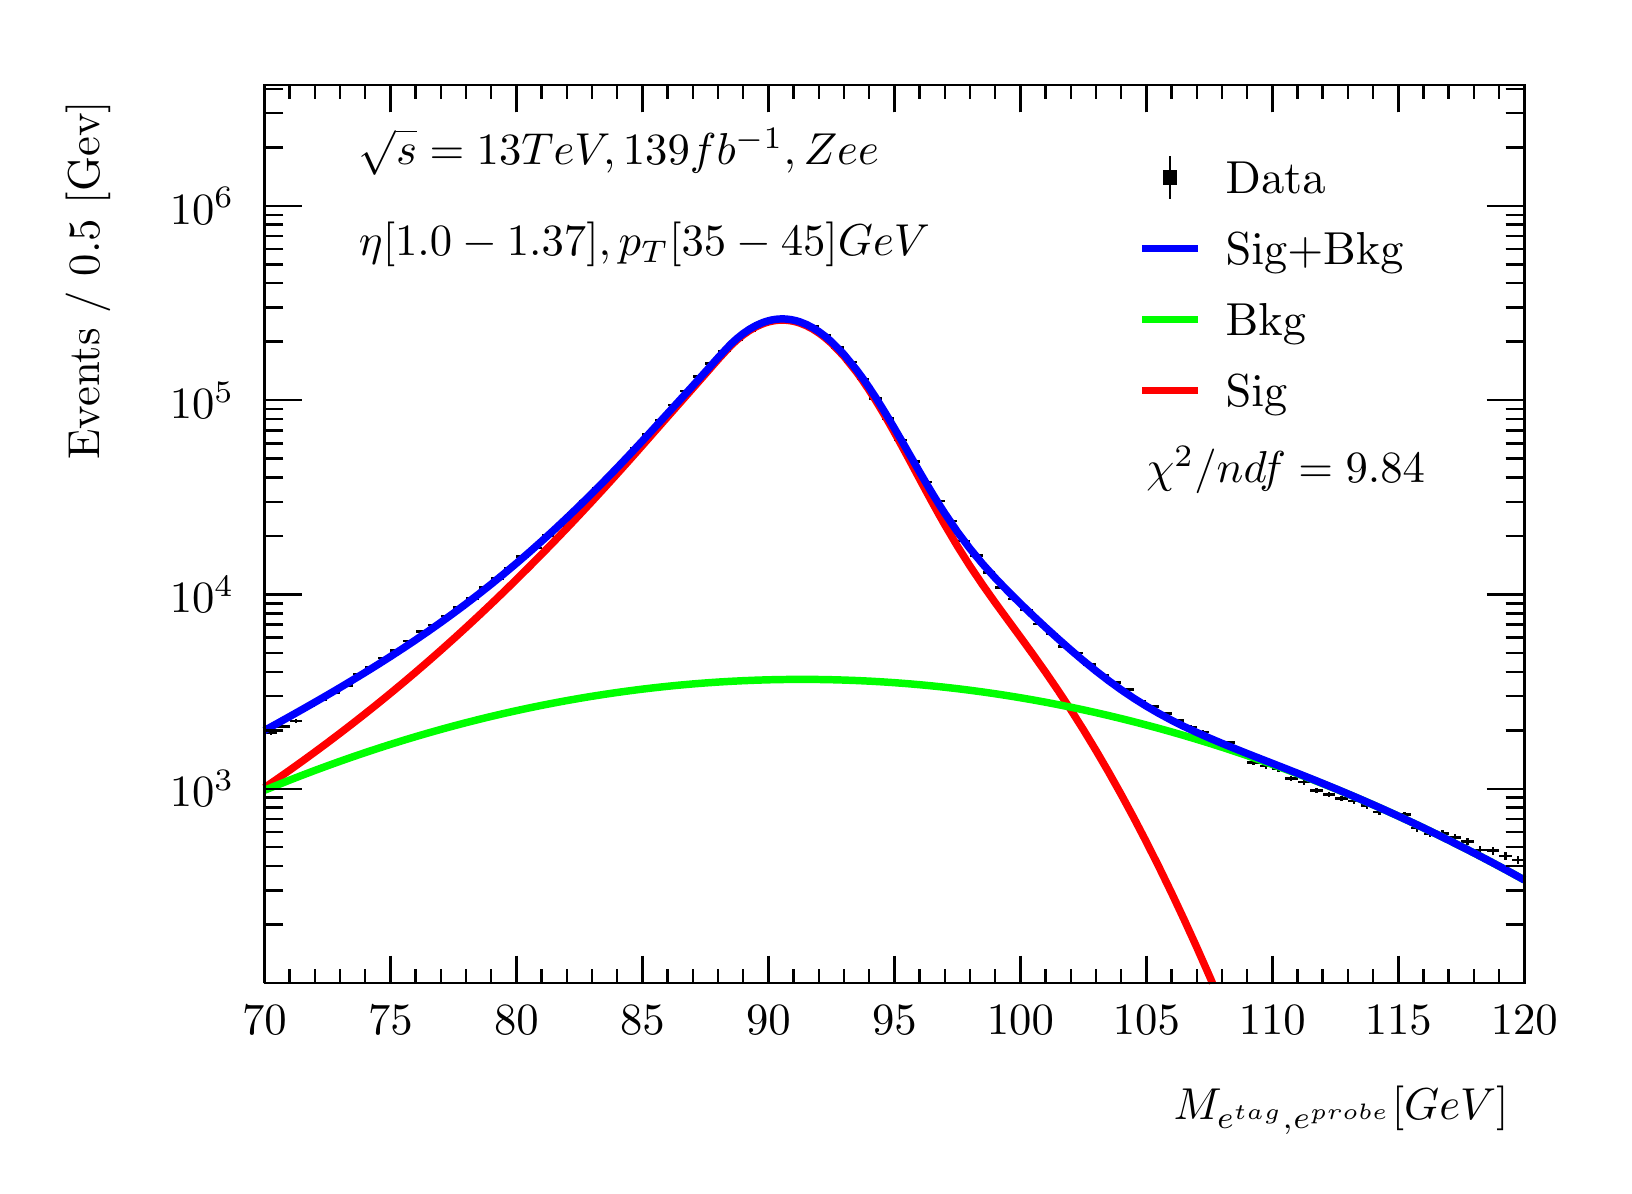
\begin{tikzpicture}
\pgfdeclareplotmark{cross} {
\pgfpathmoveto{\pgfpoint{-0.3\pgfplotmarksize}{\pgfplotmarksize}}
\pgfpathlineto{\pgfpoint{+0.3\pgfplotmarksize}{\pgfplotmarksize}}
\pgfpathlineto{\pgfpoint{+0.3\pgfplotmarksize}{0.3\pgfplotmarksize}}
\pgfpathlineto{\pgfpoint{+1\pgfplotmarksize}{0.3\pgfplotmarksize}}
\pgfpathlineto{\pgfpoint{+1\pgfplotmarksize}{-0.3\pgfplotmarksize}}
\pgfpathlineto{\pgfpoint{+0.3\pgfplotmarksize}{-0.3\pgfplotmarksize}}
\pgfpathlineto{\pgfpoint{+0.3\pgfplotmarksize}{-1.\pgfplotmarksize}}
\pgfpathlineto{\pgfpoint{-0.3\pgfplotmarksize}{-1.\pgfplotmarksize}}
\pgfpathlineto{\pgfpoint{-0.3\pgfplotmarksize}{-0.3\pgfplotmarksize}}
\pgfpathlineto{\pgfpoint{-1.\pgfplotmarksize}{-0.3\pgfplotmarksize}}
\pgfpathlineto{\pgfpoint{-1.\pgfplotmarksize}{0.3\pgfplotmarksize}}
\pgfpathlineto{\pgfpoint{-0.3\pgfplotmarksize}{0.3\pgfplotmarksize}}
\pgfpathclose
\pgfusepathqstroke
}
\pgfdeclareplotmark{cross*} {
\pgfpathmoveto{\pgfpoint{-0.3\pgfplotmarksize}{\pgfplotmarksize}}
\pgfpathlineto{\pgfpoint{+0.3\pgfplotmarksize}{\pgfplotmarksize}}
\pgfpathlineto{\pgfpoint{+0.3\pgfplotmarksize}{0.3\pgfplotmarksize}}
\pgfpathlineto{\pgfpoint{+1\pgfplotmarksize}{0.3\pgfplotmarksize}}
\pgfpathlineto{\pgfpoint{+1\pgfplotmarksize}{-0.3\pgfplotmarksize}}
\pgfpathlineto{\pgfpoint{+0.3\pgfplotmarksize}{-0.3\pgfplotmarksize}}
\pgfpathlineto{\pgfpoint{+0.3\pgfplotmarksize}{-1.\pgfplotmarksize}}
\pgfpathlineto{\pgfpoint{-0.3\pgfplotmarksize}{-1.\pgfplotmarksize}}
\pgfpathlineto{\pgfpoint{-0.3\pgfplotmarksize}{-0.3\pgfplotmarksize}}
\pgfpathlineto{\pgfpoint{-1.\pgfplotmarksize}{-0.3\pgfplotmarksize}}
\pgfpathlineto{\pgfpoint{-1.\pgfplotmarksize}{0.3\pgfplotmarksize}}
\pgfpathlineto{\pgfpoint{-0.3\pgfplotmarksize}{0.3\pgfplotmarksize}}
\pgfpathclose
\pgfusepathqfillstroke
}
\pgfdeclareplotmark{newstar} {
\pgfpathmoveto{\pgfqpoint{0pt}{\pgfplotmarksize}}
\pgfpathlineto{\pgfqpointpolar{44}{0.5\pgfplotmarksize}}
\pgfpathlineto{\pgfqpointpolar{18}{\pgfplotmarksize}}
\pgfpathlineto{\pgfqpointpolar{-20}{0.5\pgfplotmarksize}}
\pgfpathlineto{\pgfqpointpolar{-54}{\pgfplotmarksize}}
\pgfpathlineto{\pgfqpointpolar{-90}{0.5\pgfplotmarksize}}
\pgfpathlineto{\pgfqpointpolar{234}{\pgfplotmarksize}}
\pgfpathlineto{\pgfqpointpolar{198}{0.5\pgfplotmarksize}}
\pgfpathlineto{\pgfqpointpolar{162}{\pgfplotmarksize}}
\pgfpathlineto{\pgfqpointpolar{134}{0.5\pgfplotmarksize}}
\pgfpathclose
\pgfusepathqstroke
}
\pgfdeclareplotmark{newstar*} {
\pgfpathmoveto{\pgfqpoint{0pt}{\pgfplotmarksize}}
\pgfpathlineto{\pgfqpointpolar{44}{0.5\pgfplotmarksize}}
\pgfpathlineto{\pgfqpointpolar{18}{\pgfplotmarksize}}
\pgfpathlineto{\pgfqpointpolar{-20}{0.5\pgfplotmarksize}}
\pgfpathlineto{\pgfqpointpolar{-54}{\pgfplotmarksize}}
\pgfpathlineto{\pgfqpointpolar{-90}{0.5\pgfplotmarksize}}
\pgfpathlineto{\pgfqpointpolar{234}{\pgfplotmarksize}}
\pgfpathlineto{\pgfqpointpolar{198}{0.5\pgfplotmarksize}}
\pgfpathlineto{\pgfqpointpolar{162}{\pgfplotmarksize}}
\pgfpathlineto{\pgfqpointpolar{134}{0.5\pgfplotmarksize}}
\pgfpathclose
\pgfusepathqfillstroke
}
\definecolor{c}{rgb}{1,1,1};
\draw [color=c, fill=c] (0,0) rectangle (20,14.4361);
\draw [color=c, fill=c] (3,2.30977) rectangle (19,13.7143);
\definecolor{c}{rgb}{0,0,0};
\draw [c,line width=0.9] (3,2.30977) -- (3,13.7143) -- (19,13.7143) -- (19,2.30977) -- (3,2.30977);
\definecolor{c}{rgb}{1,1,1};
\draw [color=c, fill=c] (3,2.30977) rectangle (19,13.7143);
\definecolor{c}{rgb}{0,0,0};
\draw [c,line width=0.9] (3,2.30977) -- (3,13.7143) -- (19,13.7143) -- (19,2.30977) -- (3,2.30977);
\draw [c,line width=0.9] (3,2.30977) -- (19,2.30977);
\draw [c,line width=0.9] (3,2.65624) -- (3,2.30977);
\draw [c,line width=0.9] (3.32,2.48301) -- (3.32,2.30977);
\draw [c,line width=0.9] (3.64,2.48301) -- (3.64,2.30977);
\draw [c,line width=0.9] (3.96,2.48301) -- (3.96,2.30977);
\draw [c,line width=0.9] (4.28,2.48301) -- (4.28,2.30977);
\draw [c,line width=0.9] (4.6,2.65624) -- (4.6,2.30977);
\draw [c,line width=0.9] (4.92,2.48301) -- (4.92,2.30977);
\draw [c,line width=0.9] (5.24,2.48301) -- (5.24,2.30977);
\draw [c,line width=0.9] (5.56,2.48301) -- (5.56,2.30977);
\draw [c,line width=0.9] (5.88,2.48301) -- (5.88,2.30977);
\draw [c,line width=0.9] (6.2,2.65624) -- (6.2,2.30977);
\draw [c,line width=0.9] (6.52,2.48301) -- (6.52,2.30977);
\draw [c,line width=0.9] (6.84,2.48301) -- (6.84,2.30977);
\draw [c,line width=0.9] (7.16,2.48301) -- (7.16,2.30977);
\draw [c,line width=0.9] (7.48,2.48301) -- (7.48,2.30977);
\draw [c,line width=0.9] (7.8,2.65624) -- (7.8,2.30977);
\draw [c,line width=0.9] (8.12,2.48301) -- (8.12,2.30977);
\draw [c,line width=0.9] (8.44,2.48301) -- (8.44,2.30977);
\draw [c,line width=0.9] (8.76,2.48301) -- (8.76,2.30977);
\draw [c,line width=0.9] (9.08,2.48301) -- (9.08,2.30977);
\draw [c,line width=0.9] (9.4,2.65624) -- (9.4,2.30977);
\draw [c,line width=0.9] (9.72,2.48301) -- (9.72,2.30977);
\draw [c,line width=0.9] (10.04,2.48301) -- (10.04,2.30977);
\draw [c,line width=0.9] (10.36,2.48301) -- (10.36,2.30977);
\draw [c,line width=0.9] (10.68,2.48301) -- (10.68,2.30977);
\draw [c,line width=0.9] (11,2.65624) -- (11,2.30977);
\draw [c,line width=0.9] (11.32,2.48301) -- (11.32,2.30977);
\draw [c,line width=0.9] (11.64,2.48301) -- (11.64,2.30977);
\draw [c,line width=0.9] (11.96,2.48301) -- (11.96,2.30977);
\draw [c,line width=0.9] (12.28,2.48301) -- (12.28,2.30977);
\draw [c,line width=0.9] (12.6,2.65624) -- (12.6,2.30977);
\draw [c,line width=0.9] (12.92,2.48301) -- (12.92,2.30977);
\draw [c,line width=0.9] (13.24,2.48301) -- (13.24,2.30977);
\draw [c,line width=0.9] (13.56,2.48301) -- (13.56,2.30977);
\draw [c,line width=0.9] (13.88,2.48301) -- (13.88,2.30977);
\draw [c,line width=0.9] (14.2,2.65624) -- (14.2,2.30977);
\draw [c,line width=0.9] (14.52,2.48301) -- (14.52,2.30977);
\draw [c,line width=0.9] (14.84,2.48301) -- (14.84,2.30977);
\draw [c,line width=0.9] (15.16,2.48301) -- (15.16,2.30977);
\draw [c,line width=0.9] (15.48,2.48301) -- (15.48,2.30977);
\draw [c,line width=0.9] (15.8,2.65624) -- (15.8,2.30977);
\draw [c,line width=0.9] (16.12,2.48301) -- (16.12,2.30977);
\draw [c,line width=0.9] (16.44,2.48301) -- (16.44,2.30977);
\draw [c,line width=0.9] (16.76,2.48301) -- (16.76,2.30977);
\draw [c,line width=0.9] (17.08,2.48301) -- (17.08,2.30977);
\draw [c,line width=0.9] (17.4,2.65624) -- (17.4,2.30977);
\draw [c,line width=0.9] (17.72,2.48301) -- (17.72,2.30977);
\draw [c,line width=0.9] (18.04,2.48301) -- (18.04,2.30977);
\draw [c,line width=0.9] (18.36,2.48301) -- (18.36,2.30977);
\draw [c,line width=0.9] (18.68,2.48301) -- (18.68,2.30977);
\draw [c,line width=0.9] (19,2.65624) -- (19,2.30977);
\draw [anchor=base] (3,1.66015) node[scale=1.61424, color=c, rotate=0]{70};
\draw [anchor=base] (4.6,1.66015) node[scale=1.61424, color=c, rotate=0]{75};
\draw [anchor=base] (6.2,1.66015) node[scale=1.61424, color=c, rotate=0]{80};
\draw [anchor=base] (7.8,1.66015) node[scale=1.61424, color=c, rotate=0]{85};
\draw [anchor=base] (9.4,1.66015) node[scale=1.61424, color=c, rotate=0]{90};
\draw [anchor=base] (11,1.66015) node[scale=1.61424, color=c, rotate=0]{95};
\draw [anchor=base] (12.6,1.66015) node[scale=1.61424, color=c, rotate=0]{100};
\draw [anchor=base] (14.2,1.66015) node[scale=1.61424, color=c, rotate=0]{105};
\draw [anchor=base] (15.8,1.66015) node[scale=1.61424, color=c, rotate=0]{110};
\draw [anchor=base] (17.4,1.66015) node[scale=1.61424, color=c, rotate=0]{115};
\draw [anchor=base] (19,1.66015) node[scale=1.61424, color=c, rotate=0]{120};
\draw [anchor= east] (19,0.692932) node[scale=1.61424, color=c, rotate=0]{$M_{e^{tag}, e^{probe}}  [GeV]$};
\draw [c,line width=0.9] (3,13.7143) -- (19,13.7143);
\draw [c,line width=0.9] (3,13.3678) -- (3,13.7143);
\draw [c,line width=0.9] (3.32,13.5411) -- (3.32,13.7143);
\draw [c,line width=0.9] (3.64,13.5411) -- (3.64,13.7143);
\draw [c,line width=0.9] (3.96,13.5411) -- (3.96,13.7143);
\draw [c,line width=0.9] (4.28,13.5411) -- (4.28,13.7143);
\draw [c,line width=0.9] (4.6,13.3678) -- (4.6,13.7143);
\draw [c,line width=0.9] (4.92,13.5411) -- (4.92,13.7143);
\draw [c,line width=0.9] (5.24,13.5411) -- (5.24,13.7143);
\draw [c,line width=0.9] (5.56,13.5411) -- (5.56,13.7143);
\draw [c,line width=0.9] (5.88,13.5411) -- (5.88,13.7143);
\draw [c,line width=0.9] (6.2,13.3678) -- (6.2,13.7143);
\draw [c,line width=0.9] (6.52,13.5411) -- (6.52,13.7143);
\draw [c,line width=0.9] (6.84,13.5411) -- (6.84,13.7143);
\draw [c,line width=0.9] (7.16,13.5411) -- (7.16,13.7143);
\draw [c,line width=0.9] (7.48,13.5411) -- (7.48,13.7143);
\draw [c,line width=0.9] (7.8,13.3678) -- (7.8,13.7143);
\draw [c,line width=0.9] (8.12,13.5411) -- (8.12,13.7143);
\draw [c,line width=0.9] (8.44,13.5411) -- (8.44,13.7143);
\draw [c,line width=0.9] (8.76,13.5411) -- (8.76,13.7143);
\draw [c,line width=0.9] (9.08,13.5411) -- (9.08,13.7143);
\draw [c,line width=0.9] (9.4,13.3678) -- (9.4,13.7143);
\draw [c,line width=0.9] (9.72,13.5411) -- (9.72,13.7143);
\draw [c,line width=0.9] (10.04,13.5411) -- (10.04,13.7143);
\draw [c,line width=0.9] (10.36,13.5411) -- (10.36,13.7143);
\draw [c,line width=0.9] (10.68,13.5411) -- (10.68,13.7143);
\draw [c,line width=0.9] (11,13.3678) -- (11,13.7143);
\draw [c,line width=0.9] (11.32,13.5411) -- (11.32,13.7143);
\draw [c,line width=0.9] (11.64,13.5411) -- (11.64,13.7143);
\draw [c,line width=0.9] (11.96,13.5411) -- (11.96,13.7143);
\draw [c,line width=0.9] (12.28,13.5411) -- (12.28,13.7143);
\draw [c,line width=0.9] (12.6,13.3678) -- (12.6,13.7143);
\draw [c,line width=0.9] (12.92,13.5411) -- (12.92,13.7143);
\draw [c,line width=0.9] (13.24,13.5411) -- (13.24,13.7143);
\draw [c,line width=0.9] (13.56,13.5411) -- (13.56,13.7143);
\draw [c,line width=0.9] (13.88,13.5411) -- (13.88,13.7143);
\draw [c,line width=0.9] (14.2,13.3678) -- (14.2,13.7143);
\draw [c,line width=0.9] (14.52,13.5411) -- (14.52,13.7143);
\draw [c,line width=0.9] (14.84,13.5411) -- (14.84,13.7143);
\draw [c,line width=0.9] (15.16,13.5411) -- (15.16,13.7143);
\draw [c,line width=0.9] (15.48,13.5411) -- (15.48,13.7143);
\draw [c,line width=0.9] (15.8,13.3678) -- (15.8,13.7143);
\draw [c,line width=0.9] (16.12,13.5411) -- (16.12,13.7143);
\draw [c,line width=0.9] (16.44,13.5411) -- (16.44,13.7143);
\draw [c,line width=0.9] (16.76,13.5411) -- (16.76,13.7143);
\draw [c,line width=0.9] (17.08,13.5411) -- (17.08,13.7143);
\draw [c,line width=0.9] (17.4,13.3678) -- (17.4,13.7143);
\draw [c,line width=0.9] (17.72,13.5411) -- (17.72,13.7143);
\draw [c,line width=0.9] (18.04,13.5411) -- (18.04,13.7143);
\draw [c,line width=0.9] (18.36,13.5411) -- (18.36,13.7143);
\draw [c,line width=0.9] (18.68,13.5411) -- (18.68,13.7143);
\draw [c,line width=0.9] (19,13.3678) -- (19,13.7143);
\draw [c,line width=0.9] (3,2.30977) -- (3,13.7143);
\draw [c,line width=0.9] (3.237,3.05254) -- (3,3.05254);
\draw [c,line width=0.9] (3.237,3.48704) -- (3,3.48704);
\draw [c,line width=0.9] (3.237,3.79531) -- (3,3.79531);
\draw [c,line width=0.9] (3.237,4.03443) -- (3,4.03443);
\draw [c,line width=0.9] (3.237,4.22981) -- (3,4.22981);
\draw [c,line width=0.9] (3.237,4.395) -- (3,4.395);
\draw [c,line width=0.9] (3.237,4.53809) -- (3,4.53809);
\draw [c,line width=0.9] (3.237,4.6643) -- (3,4.6643);
\draw [c,line width=0.9] (3.474,4.77721) -- (3,4.77721);
\draw [anchor= east] (2.82,4.77721) node[scale=1.61424, color=c, rotate=0]{$10^{3}$};
\draw [c,line width=0.9] (3.237,5.51998) -- (3,5.51998);
\draw [c,line width=0.9] (3.237,5.95447) -- (3,5.95447);
\draw [c,line width=0.9] (3.237,6.26275) -- (3,6.26275);
\draw [c,line width=0.9] (3.237,6.50187) -- (3,6.50187);
\draw [c,line width=0.9] (3.237,6.69724) -- (3,6.69724);
\draw [c,line width=0.9] (3.237,6.86243) -- (3,6.86243);
\draw [c,line width=0.9] (3.237,7.00552) -- (3,7.00552);
\draw [c,line width=0.9] (3.237,7.13174) -- (3,7.13174);
\draw [c,line width=0.9] (3.474,7.24464) -- (3,7.24464);
\draw [anchor= east] (2.82,7.24464) node[scale=1.61424, color=c, rotate=0]{$10^{4}$};
\draw [c,line width=0.9] (3.237,7.98741) -- (3,7.98741);
\draw [c,line width=0.9] (3.237,8.4219) -- (3,8.4219);
\draw [c,line width=0.9] (3.237,8.73018) -- (3,8.73018);
\draw [c,line width=0.9] (3.237,8.9693) -- (3,8.9693);
\draw [c,line width=0.9] (3.237,9.16467) -- (3,9.16467);
\draw [c,line width=0.9] (3.237,9.32986) -- (3,9.32986);
\draw [c,line width=0.9] (3.237,9.47295) -- (3,9.47295);
\draw [c,line width=0.9] (3.237,9.59917) -- (3,9.59917);
\draw [c,line width=0.9] (3.474,9.71207) -- (3,9.71207);
\draw [anchor= east] (2.82,9.71207) node[scale=1.61424, color=c, rotate=0]{$10^{5}$};
\draw [c,line width=0.9] (3.237,10.4548) -- (3,10.4548);
\draw [c,line width=0.9] (3.237,10.8893) -- (3,10.8893);
\draw [c,line width=0.9] (3.237,11.1976) -- (3,11.1976);
\draw [c,line width=0.9] (3.237,11.4367) -- (3,11.4367);
\draw [c,line width=0.9] (3.237,11.6321) -- (3,11.6321);
\draw [c,line width=0.9] (3.237,11.7973) -- (3,11.7973);
\draw [c,line width=0.9] (3.237,11.9404) -- (3,11.9404);
\draw [c,line width=0.9] (3.237,12.0666) -- (3,12.0666);
\draw [c,line width=0.9] (3.474,12.1795) -- (3,12.1795);
\draw [anchor= east] (2.82,12.1795) node[scale=1.61424, color=c, rotate=0]{$10^{6}$};
\draw [c,line width=0.9] (3.237,12.9223) -- (3,12.9223);
\draw [c,line width=0.9] (3.237,13.3568) -- (3,13.3568);
\draw [c,line width=0.9] (3.237,13.665) -- (3,13.665);
\draw [anchor= east] (0.76,13.7143) node[scale=1.61424, color=c, rotate=90]{Events / 0.5 [Gev]};
\draw [c,line width=0.9] (19,2.30977) -- (19,13.7143);
\draw [c,line width=0.9] (18.763,3.05254) -- (19,3.05254);
\draw [c,line width=0.9] (18.763,3.48704) -- (19,3.48704);
\draw [c,line width=0.9] (18.763,3.79531) -- (19,3.79531);
\draw [c,line width=0.9] (18.763,4.03443) -- (19,4.03443);
\draw [c,line width=0.9] (18.763,4.22981) -- (19,4.22981);
\draw [c,line width=0.9] (18.763,4.395) -- (19,4.395);
\draw [c,line width=0.9] (18.763,4.53809) -- (19,4.53809);
\draw [c,line width=0.9] (18.763,4.6643) -- (19,4.6643);
\draw [c,line width=0.9] (18.526,4.77721) -- (19,4.77721);
\draw [c,line width=0.9] (18.763,5.51998) -- (19,5.51998);
\draw [c,line width=0.9] (18.763,5.95447) -- (19,5.95447);
\draw [c,line width=0.9] (18.763,6.26275) -- (19,6.26275);
\draw [c,line width=0.9] (18.763,6.50187) -- (19,6.50187);
\draw [c,line width=0.9] (18.763,6.69724) -- (19,6.69724);
\draw [c,line width=0.9] (18.763,6.86243) -- (19,6.86243);
\draw [c,line width=0.9] (18.763,7.00552) -- (19,7.00552);
\draw [c,line width=0.9] (18.763,7.13174) -- (19,7.13174);
\draw [c,line width=0.9] (18.526,7.24464) -- (19,7.24464);
\draw [c,line width=0.9] (18.763,7.98741) -- (19,7.98741);
\draw [c,line width=0.9] (18.763,8.4219) -- (19,8.4219);
\draw [c,line width=0.9] (18.763,8.73018) -- (19,8.73018);
\draw [c,line width=0.9] (18.763,8.9693) -- (19,8.9693);
\draw [c,line width=0.9] (18.763,9.16467) -- (19,9.16467);
\draw [c,line width=0.9] (18.763,9.32986) -- (19,9.32986);
\draw [c,line width=0.9] (18.763,9.47295) -- (19,9.47295);
\draw [c,line width=0.9] (18.763,9.59917) -- (19,9.59917);
\draw [c,line width=0.9] (18.526,9.71207) -- (19,9.71207);
\draw [c,line width=0.9] (18.763,10.4548) -- (19,10.4548);
\draw [c,line width=0.9] (18.763,10.8893) -- (19,10.8893);
\draw [c,line width=0.9] (18.763,11.1976) -- (19,11.1976);
\draw [c,line width=0.9] (18.763,11.4367) -- (19,11.4367);
\draw [c,line width=0.9] (18.763,11.6321) -- (19,11.6321);
\draw [c,line width=0.9] (18.763,11.7973) -- (19,11.7973);
\draw [c,line width=0.9] (18.763,11.9404) -- (19,11.9404);
\draw [c,line width=0.9] (18.763,12.0666) -- (19,12.0666);
\draw [c,line width=0.9] (18.526,12.1795) -- (19,12.1795);
\draw [c,line width=0.9] (18.763,12.9223) -- (19,12.9223);
\draw [c,line width=0.9] (18.763,13.3568) -- (19,13.3568);
\draw [c,line width=0.9] (18.763,13.665) -- (19,13.665);
\draw [c,line width=0.9] (3.08,5.4901) -- (3,5.4901);
\draw [c,line width=0.9] (3,5.4901) -- (3,5.4901);
\draw [c,line width=0.9] (3.08,5.4901) -- (3.16,5.4901);
\draw [c,line width=0.9] (3.16,5.4901) -- (3.16,5.4901);
\draw [c,line width=0.9] (3.08,5.4901) -- (3.08,5.51439);
\draw [c,line width=0.9] (3.08,5.51439) -- (3.08,5.51439);
\draw [c,line width=0.9] (3.08,5.4901) -- (3.08,5.4658);
\draw [c,line width=0.9] (3.08,5.4658) -- (3.08,5.4658);
\draw [c,line width=0.9] (3.24,5.56868) -- (3.16,5.56868);
\draw [c,line width=0.9] (3.16,5.56868) -- (3.16,5.56868);
\draw [c,line width=0.9] (3.24,5.56868) -- (3.32,5.56868);
\draw [c,line width=0.9] (3.32,5.56868) -- (3.32,5.56868);
\draw [c,line width=0.9] (3.24,5.56868) -- (3.24,5.59211);
\draw [c,line width=0.9] (3.24,5.59211) -- (3.24,5.59211);
\draw [c,line width=0.9] (3.24,5.56868) -- (3.24,5.54526);
\draw [c,line width=0.9] (3.24,5.54526) -- (3.24,5.54526);
\draw [c,line width=0.9] (3.4,5.63518) -- (3.32,5.63518);
\draw [c,line width=0.9] (3.32,5.63518) -- (3.32,5.63518);
\draw [c,line width=0.9] (3.4,5.63518) -- (3.48,5.63518);
\draw [c,line width=0.9] (3.48,5.63518) -- (3.48,5.63518);
\draw [c,line width=0.9] (3.4,5.63518) -- (3.4,5.65789);
\draw [c,line width=0.9] (3.4,5.65789) -- (3.4,5.65789);
\draw [c,line width=0.9] (3.4,5.63518) -- (3.4,5.61248);
\draw [c,line width=0.9] (3.4,5.61248) -- (3.4,5.61248);
\draw [c,line width=0.9] (3.56,5.8304) -- (3.48,5.8304);
\draw [c,line width=0.9] (3.48,5.8304) -- (3.48,5.8304);
\draw [c,line width=0.9] (3.56,5.8304) -- (3.64,5.8304);
\draw [c,line width=0.9] (3.64,5.8304) -- (3.64,5.8304);
\draw [c,line width=0.9] (3.56,5.8304) -- (3.56,5.85113);
\draw [c,line width=0.9] (3.56,5.85113) -- (3.56,5.85113);
\draw [c,line width=0.9] (3.56,5.8304) -- (3.56,5.80967);
\draw [c,line width=0.9] (3.56,5.80967) -- (3.56,5.80967);
\draw [c,line width=0.9] (3.72,5.90438) -- (3.64,5.90438);
\draw [c,line width=0.9] (3.64,5.90438) -- (3.64,5.90438);
\draw [c,line width=0.9] (3.72,5.90438) -- (3.8,5.90438);
\draw [c,line width=0.9] (3.8,5.90438) -- (3.8,5.90438);
\draw [c,line width=0.9] (3.72,5.90438) -- (3.72,5.92441);
\draw [c,line width=0.9] (3.72,5.92441) -- (3.72,5.92441);
\draw [c,line width=0.9] (3.72,5.90438) -- (3.72,5.88436);
\draw [c,line width=0.9] (3.72,5.88436) -- (3.72,5.88436);
\draw [c,line width=0.9] (3.88,5.99306) -- (3.8,5.99306);
\draw [c,line width=0.9] (3.8,5.99306) -- (3.8,5.99306);
\draw [c,line width=0.9] (3.88,5.99306) -- (3.96,5.99306);
\draw [c,line width=0.9] (3.96,5.99306) -- (3.96,5.99306);
\draw [c,line width=0.9] (3.88,5.99306) -- (3.88,6.01228);
\draw [c,line width=0.9] (3.88,6.01228) -- (3.88,6.01228);
\draw [c,line width=0.9] (3.88,5.99306) -- (3.88,5.97385);
\draw [c,line width=0.9] (3.88,5.97385) -- (3.88,5.97385);
\draw [c,line width=0.9] (4.04,6.08639) -- (3.96,6.08639);
\draw [c,line width=0.9] (3.96,6.08639) -- (3.96,6.08639);
\draw [c,line width=0.9] (4.04,6.08639) -- (4.12,6.08639);
\draw [c,line width=0.9] (4.12,6.08639) -- (4.12,6.08639);
\draw [c,line width=0.9] (4.04,6.08639) -- (4.04,6.10478);
\draw [c,line width=0.9] (4.04,6.10478) -- (4.04,6.10478);
\draw [c,line width=0.9] (4.04,6.08639) -- (4.04,6.06799);
\draw [c,line width=0.9] (4.04,6.06799) -- (4.04,6.06799);
\draw [c,line width=0.9] (4.2,6.23589) -- (4.12,6.23589);
\draw [c,line width=0.9] (4.12,6.23589) -- (4.12,6.23589);
\draw [c,line width=0.9] (4.2,6.23589) -- (4.28,6.23589);
\draw [c,line width=0.9] (4.28,6.23589) -- (4.28,6.23589);
\draw [c,line width=0.9] (4.2,6.23589) -- (4.2,6.25305);
\draw [c,line width=0.9] (4.2,6.25305) -- (4.2,6.25305);
\draw [c,line width=0.9] (4.2,6.23589) -- (4.2,6.21874);
\draw [c,line width=0.9] (4.2,6.21874) -- (4.2,6.21874);
\draw [c,line width=0.9] (4.36,6.31885) -- (4.28,6.31885);
\draw [c,line width=0.9] (4.28,6.31885) -- (4.28,6.31885);
\draw [c,line width=0.9] (4.36,6.31885) -- (4.44,6.31885);
\draw [c,line width=0.9] (4.44,6.31885) -- (4.44,6.31885);
\draw [c,line width=0.9] (4.36,6.31885) -- (4.36,6.33536);
\draw [c,line width=0.9] (4.36,6.33536) -- (4.36,6.33536);
\draw [c,line width=0.9] (4.36,6.31885) -- (4.36,6.30235);
\draw [c,line width=0.9] (4.36,6.30235) -- (4.36,6.30235);
\draw [c,line width=0.9] (4.52,6.43807) -- (4.44,6.43807);
\draw [c,line width=0.9] (4.44,6.43807) -- (4.44,6.43807);
\draw [c,line width=0.9] (4.52,6.43807) -- (4.6,6.43807);
\draw [c,line width=0.9] (4.6,6.43807) -- (4.6,6.43807);
\draw [c,line width=0.9] (4.52,6.43807) -- (4.52,6.45368);
\draw [c,line width=0.9] (4.52,6.45368) -- (4.52,6.45368);
\draw [c,line width=0.9] (4.52,6.43807) -- (4.52,6.42246);
\draw [c,line width=0.9] (4.52,6.42246) -- (4.52,6.42246);
\draw [c,line width=0.9] (4.68,6.53084) -- (4.6,6.53084);
\draw [c,line width=0.9] (4.6,6.53084) -- (4.6,6.53084);
\draw [c,line width=0.9] (4.68,6.53084) -- (4.76,6.53084);
\draw [c,line width=0.9] (4.76,6.53084) -- (4.76,6.53084);
\draw [c,line width=0.9] (4.68,6.53084) -- (4.68,6.54579);
\draw [c,line width=0.9] (4.68,6.54579) -- (4.68,6.54579);
\draw [c,line width=0.9] (4.68,6.53084) -- (4.68,6.51588);
\draw [c,line width=0.9] (4.68,6.51588) -- (4.68,6.51588);
\draw [c,line width=0.9] (4.84,6.65629) -- (4.76,6.65629);
\draw [c,line width=0.9] (4.76,6.65629) -- (4.76,6.65629);
\draw [c,line width=0.9] (4.84,6.65629) -- (4.92,6.65629);
\draw [c,line width=0.9] (4.92,6.65629) -- (4.92,6.65629);
\draw [c,line width=0.9] (4.84,6.65629) -- (4.84,6.67039);
\draw [c,line width=0.9] (4.84,6.67039) -- (4.84,6.67039);
\draw [c,line width=0.9] (4.84,6.65629) -- (4.84,6.64218);
\draw [c,line width=0.9] (4.84,6.64218) -- (4.84,6.64218);
\draw [c,line width=0.9] (5,6.77657) -- (4.92,6.77657);
\draw [c,line width=0.9] (4.92,6.77657) -- (4.92,6.77657);
\draw [c,line width=0.9] (5,6.77657) -- (5.08,6.77657);
\draw [c,line width=0.9] (5.08,6.77657) -- (5.08,6.77657);
\draw [c,line width=0.9] (5,6.77657) -- (5,6.7899);
\draw [c,line width=0.9] (5,6.7899) -- (5,6.7899);
\draw [c,line width=0.9] (5,6.77657) -- (5,6.76324);
\draw [c,line width=0.9] (5,6.76324) -- (5,6.76324);
\draw [c,line width=0.9] (5.16,6.85783) -- (5.08,6.85783);
\draw [c,line width=0.9] (5.08,6.85783) -- (5.08,6.85783);
\draw [c,line width=0.9] (5.16,6.85783) -- (5.24,6.85783);
\draw [c,line width=0.9] (5.24,6.85783) -- (5.24,6.85783);
\draw [c,line width=0.9] (5.16,6.85783) -- (5.16,6.87066);
\draw [c,line width=0.9] (5.16,6.87066) -- (5.16,6.87066);
\draw [c,line width=0.9] (5.16,6.85783) -- (5.16,6.84499);
\draw [c,line width=0.9] (5.16,6.84499) -- (5.16,6.84499);
\draw [c,line width=0.9] (5.32,6.97426) -- (5.24,6.97426);
\draw [c,line width=0.9] (5.24,6.97426) -- (5.24,6.97426);
\draw [c,line width=0.9] (5.32,6.97426) -- (5.4,6.97426);
\draw [c,line width=0.9] (5.4,6.97426) -- (5.4,6.97426);
\draw [c,line width=0.9] (5.32,6.97426) -- (5.32,6.98642);
\draw [c,line width=0.9] (5.32,6.98642) -- (5.32,6.98642);
\draw [c,line width=0.9] (5.32,6.97426) -- (5.32,6.9621);
\draw [c,line width=0.9] (5.32,6.9621) -- (5.32,6.9621);
\draw [c,line width=0.9] (5.48,7.07965) -- (5.4,7.07965);
\draw [c,line width=0.9] (5.4,7.07965) -- (5.4,7.07965);
\draw [c,line width=0.9] (5.48,7.07965) -- (5.56,7.07965);
\draw [c,line width=0.9] (5.56,7.07965) -- (5.56,7.07965);
\draw [c,line width=0.9] (5.48,7.07965) -- (5.48,7.09122);
\draw [c,line width=0.9] (5.48,7.09122) -- (5.48,7.09122);
\draw [c,line width=0.9] (5.48,7.07965) -- (5.48,7.06808);
\draw [c,line width=0.9] (5.48,7.06808) -- (5.48,7.06808);
\draw [c,line width=0.9] (5.64,7.19249) -- (5.56,7.19249);
\draw [c,line width=0.9] (5.56,7.19249) -- (5.56,7.19249);
\draw [c,line width=0.9] (5.64,7.19249) -- (5.72,7.19249);
\draw [c,line width=0.9] (5.72,7.19249) -- (5.72,7.19249);
\draw [c,line width=0.9] (5.64,7.19249) -- (5.64,7.20347);
\draw [c,line width=0.9] (5.64,7.20347) -- (5.64,7.20347);
\draw [c,line width=0.9] (5.64,7.19249) -- (5.64,7.18151);
\draw [c,line width=0.9] (5.64,7.18151) -- (5.64,7.18151);
\draw [c,line width=0.9] (5.8,7.33186) -- (5.72,7.33186);
\draw [c,line width=0.9] (5.72,7.33186) -- (5.72,7.33186);
\draw [c,line width=0.9] (5.8,7.33186) -- (5.88,7.33186);
\draw [c,line width=0.9] (5.88,7.33186) -- (5.88,7.33186);
\draw [c,line width=0.9] (5.8,7.33186) -- (5.8,7.34215);
\draw [c,line width=0.9] (5.8,7.34215) -- (5.8,7.34215);
\draw [c,line width=0.9] (5.8,7.33186) -- (5.8,7.32157);
\draw [c,line width=0.9] (5.8,7.32157) -- (5.8,7.32157);
\draw [c,line width=0.9] (5.96,7.44997) -- (5.88,7.44997);
\draw [c,line width=0.9] (5.88,7.44997) -- (5.88,7.44997);
\draw [c,line width=0.9] (5.96,7.44997) -- (6.04,7.44997);
\draw [c,line width=0.9] (6.04,7.44997) -- (6.04,7.44997);
\draw [c,line width=0.9] (5.96,7.44997) -- (5.96,7.45971);
\draw [c,line width=0.9] (5.96,7.45971) -- (5.96,7.45971);
\draw [c,line width=0.9] (5.96,7.44997) -- (5.96,7.44023);
\draw [c,line width=0.9] (5.96,7.44023) -- (5.96,7.44023);
\draw [c,line width=0.9] (6.12,7.57917) -- (6.04,7.57917);
\draw [c,line width=0.9] (6.04,7.57917) -- (6.04,7.57917);
\draw [c,line width=0.9] (6.12,7.57917) -- (6.2,7.57917);
\draw [c,line width=0.9] (6.2,7.57917) -- (6.2,7.57917);
\draw [c,line width=0.9] (6.12,7.57917) -- (6.12,7.58834);
\draw [c,line width=0.9] (6.12,7.58834) -- (6.12,7.58834);
\draw [c,line width=0.9] (6.12,7.57917) -- (6.12,7.57);
\draw [c,line width=0.9] (6.12,7.57) -- (6.12,7.57);
\draw [c,line width=0.9] (6.28,7.72896) -- (6.2,7.72896);
\draw [c,line width=0.9] (6.2,7.72896) -- (6.2,7.72896);
\draw [c,line width=0.9] (6.28,7.72896) -- (6.36,7.72896);
\draw [c,line width=0.9] (6.36,7.72896) -- (6.36,7.72896);
\draw [c,line width=0.9] (6.28,7.72896) -- (6.28,7.73751);
\draw [c,line width=0.9] (6.28,7.73751) -- (6.28,7.73751);
\draw [c,line width=0.9] (6.28,7.72896) -- (6.28,7.72042);
\draw [c,line width=0.9] (6.28,7.72042) -- (6.28,7.72042);
\draw [c,line width=0.9] (6.44,7.83275) -- (6.36,7.83275);
\draw [c,line width=0.9] (6.36,7.83275) -- (6.36,7.83275);
\draw [c,line width=0.9] (6.44,7.83275) -- (6.52,7.83275);
\draw [c,line width=0.9] (6.52,7.83275) -- (6.52,7.83275);
\draw [c,line width=0.9] (6.44,7.83275) -- (6.44,7.84089);
\draw [c,line width=0.9] (6.44,7.84089) -- (6.44,7.84089);
\draw [c,line width=0.9] (6.44,7.83275) -- (6.44,7.8246);
\draw [c,line width=0.9] (6.44,7.8246) -- (6.44,7.8246);
\draw [c,line width=0.9] (6.6,7.99542) -- (6.52,7.99542);
\draw [c,line width=0.9] (6.52,7.99542) -- (6.52,7.99542);
\draw [c,line width=0.9] (6.6,7.99542) -- (6.68,7.99542);
\draw [c,line width=0.9] (6.68,7.99542) -- (6.68,7.99542);
\draw [c,line width=0.9] (6.6,7.99542) -- (6.6,8.00297);
\draw [c,line width=0.9] (6.6,8.00297) -- (6.6,8.00297);
\draw [c,line width=0.9] (6.6,7.99542) -- (6.6,7.98787);
\draw [c,line width=0.9] (6.6,7.98787) -- (6.6,7.98787);
\draw [c,line width=0.9] (6.76,8.1162) -- (6.68,8.1162);
\draw [c,line width=0.9] (6.68,8.1162) -- (6.68,8.1162);
\draw [c,line width=0.9] (6.76,8.1162) -- (6.84,8.1162);
\draw [c,line width=0.9] (6.84,8.1162) -- (6.84,8.1162);
\draw [c,line width=0.9] (6.76,8.1162) -- (6.76,8.12333);
\draw [c,line width=0.9] (6.76,8.12333) -- (6.76,8.12333);
\draw [c,line width=0.9] (6.76,8.1162) -- (6.76,8.10906);
\draw [c,line width=0.9] (6.76,8.10906) -- (6.76,8.10906);
\draw [c,line width=0.9] (6.92,8.27538) -- (6.84,8.27538);
\draw [c,line width=0.9] (6.84,8.27538) -- (6.84,8.27538);
\draw [c,line width=0.9] (6.92,8.27538) -- (7,8.27538);
\draw [c,line width=0.9] (7,8.27538) -- (7,8.27538);
\draw [c,line width=0.9] (6.92,8.27538) -- (6.92,8.282);
\draw [c,line width=0.9] (6.92,8.282) -- (6.92,8.282);
\draw [c,line width=0.9] (6.92,8.27538) -- (6.92,8.26875);
\draw [c,line width=0.9] (6.92,8.26875) -- (6.92,8.26875);
\draw [c,line width=0.9] (7.08,8.42547) -- (7,8.42547);
\draw [c,line width=0.9] (7,8.42547) -- (7,8.42547);
\draw [c,line width=0.9] (7.08,8.42547) -- (7.16,8.42547);
\draw [c,line width=0.9] (7.16,8.42547) -- (7.16,8.42547);
\draw [c,line width=0.9] (7.08,8.42547) -- (7.08,8.43165);
\draw [c,line width=0.9] (7.08,8.43165) -- (7.08,8.43165);
\draw [c,line width=0.9] (7.08,8.42547) -- (7.08,8.41929);
\draw [c,line width=0.9] (7.08,8.41929) -- (7.08,8.41929);
\draw [c,line width=0.9] (7.24,8.58807) -- (7.16,8.58807);
\draw [c,line width=0.9] (7.16,8.58807) -- (7.16,8.58807);
\draw [c,line width=0.9] (7.24,8.58807) -- (7.32,8.58807);
\draw [c,line width=0.9] (7.32,8.58807) -- (7.32,8.58807);
\draw [c,line width=0.9] (7.24,8.58807) -- (7.24,8.5938);
\draw [c,line width=0.9] (7.24,8.5938) -- (7.24,8.5938);
\draw [c,line width=0.9] (7.24,8.58807) -- (7.24,8.58235);
\draw [c,line width=0.9] (7.24,8.58235) -- (7.24,8.58235);
\draw [c,line width=0.9] (7.4,8.75125) -- (7.32,8.75125);
\draw [c,line width=0.9] (7.32,8.75125) -- (7.32,8.75125);
\draw [c,line width=0.9] (7.4,8.75125) -- (7.48,8.75125);
\draw [c,line width=0.9] (7.48,8.75125) -- (7.48,8.75125);
\draw [c,line width=0.9] (7.4,8.75125) -- (7.4,8.75655);
\draw [c,line width=0.9] (7.4,8.75655) -- (7.4,8.75655);
\draw [c,line width=0.9] (7.4,8.75125) -- (7.4,8.74594);
\draw [c,line width=0.9] (7.4,8.74594) -- (7.4,8.74594);
\draw [c,line width=0.9] (7.56,8.91452) -- (7.48,8.91452);
\draw [c,line width=0.9] (7.48,8.91452) -- (7.48,8.91452);
\draw [c,line width=0.9] (7.56,8.91452) -- (7.64,8.91452);
\draw [c,line width=0.9] (7.64,8.91452) -- (7.64,8.91452);
\draw [c,line width=0.9] (7.56,8.91452) -- (7.56,8.91943);
\draw [c,line width=0.9] (7.56,8.91943) -- (7.56,8.91943);
\draw [c,line width=0.9] (7.56,8.91452) -- (7.56,8.9096);
\draw [c,line width=0.9] (7.56,8.9096) -- (7.56,8.9096);
\draw [c,line width=0.9] (7.72,9.09721) -- (7.64,9.09721);
\draw [c,line width=0.9] (7.64,9.09721) -- (7.64,9.09721);
\draw [c,line width=0.9] (7.72,9.09721) -- (7.8,9.09721);
\draw [c,line width=0.9] (7.8,9.09721) -- (7.8,9.09721);
\draw [c,line width=0.9] (7.72,9.09721) -- (7.72,9.10173);
\draw [c,line width=0.9] (7.72,9.10173) -- (7.72,9.10173);
\draw [c,line width=0.9] (7.72,9.09721) -- (7.72,9.0927);
\draw [c,line width=0.9] (7.72,9.0927) -- (7.72,9.0927);
\draw [c,line width=0.9] (7.88,9.27594) -- (7.8,9.27594);
\draw [c,line width=0.9] (7.8,9.27594) -- (7.8,9.27594);
\draw [c,line width=0.9] (7.88,9.27594) -- (7.96,9.27594);
\draw [c,line width=0.9] (7.96,9.27594) -- (7.96,9.27594);
\draw [c,line width=0.9] (7.88,9.27594) -- (7.88,9.2801);
\draw [c,line width=0.9] (7.88,9.2801) -- (7.88,9.2801);
\draw [c,line width=0.9] (7.88,9.27594) -- (7.88,9.27179);
\draw [c,line width=0.9] (7.88,9.27179) -- (7.88,9.27179);
\draw [c,line width=0.9] (8.04,9.46213) -- (7.96,9.46213);
\draw [c,line width=0.9] (7.96,9.46213) -- (7.96,9.46213);
\draw [c,line width=0.9] (8.04,9.46213) -- (8.12,9.46213);
\draw [c,line width=0.9] (8.12,9.46213) -- (8.12,9.46213);
\draw [c,line width=0.9] (8.04,9.46213) -- (8.04,9.46594);
\draw [c,line width=0.9] (8.04,9.46594) -- (8.04,9.46594);
\draw [c,line width=0.9] (8.04,9.46213) -- (8.04,9.45832);
\draw [c,line width=0.9] (8.04,9.45832) -- (8.04,9.45832);
\draw [c,line width=0.9] (8.2,9.64927) -- (8.12,9.64927);
\draw [c,line width=0.9] (8.12,9.64927) -- (8.12,9.64927);
\draw [c,line width=0.9] (8.2,9.64927) -- (8.28,9.64927);
\draw [c,line width=0.9] (8.28,9.64927) -- (8.28,9.64927);
\draw [c,line width=0.9] (8.2,9.64927) -- (8.2,9.65276);
\draw [c,line width=0.9] (8.2,9.65276) -- (8.2,9.65276);
\draw [c,line width=0.9] (8.2,9.64927) -- (8.2,9.64578);
\draw [c,line width=0.9] (8.2,9.64578) -- (8.2,9.64578);
\draw [c,line width=0.9] (8.36,9.82762) -- (8.28,9.82762);
\draw [c,line width=0.9] (8.28,9.82762) -- (8.28,9.82762);
\draw [c,line width=0.9] (8.36,9.82762) -- (8.44,9.82762);
\draw [c,line width=0.9] (8.44,9.82762) -- (8.44,9.82762);
\draw [c,line width=0.9] (8.36,9.82762) -- (8.36,9.83084);
\draw [c,line width=0.9] (8.36,9.83084) -- (8.36,9.83084);
\draw [c,line width=0.9] (8.36,9.82762) -- (8.36,9.82441);
\draw [c,line width=0.9] (8.36,9.82441) -- (8.36,9.82441);
\draw [c,line width=0.9] (8.52,10.0153) -- (8.44,10.0153);
\draw [c,line width=0.9] (8.44,10.0153) -- (8.44,10.0153);
\draw [c,line width=0.9] (8.52,10.0153) -- (8.6,10.0153);
\draw [c,line width=0.9] (8.6,10.0153) -- (8.6,10.0153);
\draw [c,line width=0.9] (8.52,10.0153) -- (8.52,10.0183);
\draw [c,line width=0.9] (8.52,10.0183) -- (8.52,10.0183);
\draw [c,line width=0.9] (8.52,10.0153) -- (8.52,10.0124);
\draw [c,line width=0.9] (8.52,10.0124) -- (8.52,10.0124);
\draw [c,line width=0.9] (8.68,10.1796) -- (8.6,10.1796);
\draw [c,line width=0.9] (8.6,10.1796) -- (8.6,10.1796);
\draw [c,line width=0.9] (8.68,10.1796) -- (8.76,10.1796);
\draw [c,line width=0.9] (8.76,10.1796) -- (8.76,10.1796);
\draw [c,line width=0.9] (8.68,10.1796) -- (8.68,10.1823);
\draw [c,line width=0.9] (8.68,10.1823) -- (8.68,10.1823);
\draw [c,line width=0.9] (8.68,10.1796) -- (8.68,10.1768);
\draw [c,line width=0.9] (8.68,10.1768) -- (8.68,10.1768);
\draw [c,line width=0.9] (8.84,10.3392) -- (8.76,10.3392);
\draw [c,line width=0.9] (8.76,10.3392) -- (8.76,10.3392);
\draw [c,line width=0.9] (8.84,10.3392) -- (8.92,10.3392);
\draw [c,line width=0.9] (8.92,10.3392) -- (8.92,10.3392);
\draw [c,line width=0.9] (8.84,10.3392) -- (8.84,10.3417);
\draw [c,line width=0.9] (8.84,10.3417) -- (8.84,10.3417);
\draw [c,line width=0.9] (8.84,10.3392) -- (8.84,10.3366);
\draw [c,line width=0.9] (8.84,10.3366) -- (8.84,10.3366);
\draw [c,line width=0.9] (9,10.477) -- (8.92,10.477);
\draw [c,line width=0.9] (8.92,10.477) -- (8.92,10.477);
\draw [c,line width=0.9] (9,10.477) -- (9.08,10.477);
\draw [c,line width=0.9] (9.08,10.477) -- (9.08,10.477);
\draw [c,line width=0.9] (9,10.477) -- (9,10.4794);
\draw [c,line width=0.9] (9,10.4794) -- (9,10.4794);
\draw [c,line width=0.9] (9,10.477) -- (9,10.4746);
\draw [c,line width=0.9] (9,10.4746) -- (9,10.4746);
\draw [c,line width=0.9] (9.16,10.5944) -- (9.08,10.5944);
\draw [c,line width=0.9] (9.08,10.5944) -- (9.08,10.5944);
\draw [c,line width=0.9] (9.16,10.5944) -- (9.24,10.5944);
\draw [c,line width=0.9] (9.24,10.5944) -- (9.24,10.5944);
\draw [c,line width=0.9] (9.16,10.5944) -- (9.16,10.5966);
\draw [c,line width=0.9] (9.16,10.5966) -- (9.16,10.5966);
\draw [c,line width=0.9] (9.16,10.5944) -- (9.16,10.5921);
\draw [c,line width=0.9] (9.16,10.5921) -- (9.16,10.5921);
\draw [c,line width=0.9] (9.32,10.6837) -- (9.24,10.6837);
\draw [c,line width=0.9] (9.24,10.6837) -- (9.24,10.6837);
\draw [c,line width=0.9] (9.32,10.6837) -- (9.4,10.6837);
\draw [c,line width=0.9] (9.4,10.6837) -- (9.4,10.6837);
\draw [c,line width=0.9] (9.32,10.6837) -- (9.32,10.6858);
\draw [c,line width=0.9] (9.32,10.6858) -- (9.32,10.6858);
\draw [c,line width=0.9] (9.32,10.6837) -- (9.32,10.6815);
\draw [c,line width=0.9] (9.32,10.6815) -- (9.32,10.6815);
\draw [c,line width=0.9] (9.48,10.7295) -- (9.4,10.7295);
\draw [c,line width=0.9] (9.4,10.7295) -- (9.4,10.7295);
\draw [c,line width=0.9] (9.48,10.7295) -- (9.56,10.7295);
\draw [c,line width=0.9] (9.56,10.7295) -- (9.56,10.7295);
\draw [c,line width=0.9] (9.48,10.7295) -- (9.48,10.7317);
\draw [c,line width=0.9] (9.48,10.7317) -- (9.48,10.7317);
\draw [c,line width=0.9] (9.48,10.7295) -- (9.48,10.7274);
\draw [c,line width=0.9] (9.48,10.7274) -- (9.48,10.7274);
\draw [c,line width=0.9] (9.64,10.743) -- (9.56,10.743);
\draw [c,line width=0.9] (9.56,10.743) -- (9.56,10.743);
\draw [c,line width=0.9] (9.64,10.743) -- (9.72,10.743);
\draw [c,line width=0.9] (9.72,10.743) -- (9.72,10.743);
\draw [c,line width=0.9] (9.64,10.743) -- (9.64,10.7451);
\draw [c,line width=0.9] (9.64,10.7451) -- (9.64,10.7451);
\draw [c,line width=0.9] (9.64,10.743) -- (9.64,10.741);
\draw [c,line width=0.9] (9.64,10.741) -- (9.64,10.741);
\draw [c,line width=0.9] (9.8,10.7145) -- (9.72,10.7145);
\draw [c,line width=0.9] (9.72,10.7145) -- (9.72,10.7145);
\draw [c,line width=0.9] (9.8,10.7145) -- (9.88,10.7145);
\draw [c,line width=0.9] (9.88,10.7145) -- (9.88,10.7145);
\draw [c,line width=0.9] (9.8,10.7145) -- (9.8,10.7166);
\draw [c,line width=0.9] (9.8,10.7166) -- (9.8,10.7166);
\draw [c,line width=0.9] (9.8,10.7145) -- (9.8,10.7124);
\draw [c,line width=0.9] (9.8,10.7124) -- (9.8,10.7124);
\draw [c,line width=0.9] (9.96,10.6478) -- (9.88,10.6478);
\draw [c,line width=0.9] (9.88,10.6478) -- (9.88,10.6478);
\draw [c,line width=0.9] (9.96,10.6478) -- (10.04,10.6478);
\draw [c,line width=0.9] (10.04,10.6478) -- (10.04,10.6478);
\draw [c,line width=0.9] (9.96,10.6478) -- (9.96,10.6499);
\draw [c,line width=0.9] (9.96,10.6499) -- (9.96,10.6499);
\draw [c,line width=0.9] (9.96,10.6478) -- (9.96,10.6456);
\draw [c,line width=0.9] (9.96,10.6456) -- (9.96,10.6456);
\draw [c,line width=0.9] (10.12,10.5347) -- (10.04,10.5347);
\draw [c,line width=0.9] (10.04,10.5347) -- (10.04,10.5347);
\draw [c,line width=0.9] (10.12,10.5347) -- (10.2,10.5347);
\draw [c,line width=0.9] (10.2,10.5347) -- (10.2,10.5347);
\draw [c,line width=0.9] (10.12,10.5347) -- (10.12,10.5371);
\draw [c,line width=0.9] (10.12,10.5371) -- (10.12,10.5371);
\draw [c,line width=0.9] (10.12,10.5347) -- (10.12,10.5324);
\draw [c,line width=0.9] (10.12,10.5324) -- (10.12,10.5324);
\draw [c,line width=0.9] (10.28,10.3841) -- (10.2,10.3841);
\draw [c,line width=0.9] (10.2,10.3841) -- (10.2,10.3841);
\draw [c,line width=0.9] (10.28,10.3841) -- (10.36,10.3841);
\draw [c,line width=0.9] (10.36,10.3841) -- (10.36,10.3841);
\draw [c,line width=0.9] (10.28,10.3841) -- (10.28,10.3865);
\draw [c,line width=0.9] (10.28,10.3865) -- (10.28,10.3865);
\draw [c,line width=0.9] (10.28,10.3841) -- (10.28,10.3816);
\draw [c,line width=0.9] (10.28,10.3816) -- (10.28,10.3816);
\draw [c,line width=0.9] (10.44,10.1974) -- (10.36,10.1974);
\draw [c,line width=0.9] (10.36,10.1974) -- (10.36,10.1974);
\draw [c,line width=0.9] (10.44,10.1974) -- (10.52,10.1974);
\draw [c,line width=0.9] (10.52,10.1974) -- (10.52,10.1974);
\draw [c,line width=0.9] (10.44,10.1974) -- (10.44,10.2001);
\draw [c,line width=0.9] (10.44,10.2001) -- (10.44,10.2001);
\draw [c,line width=0.9] (10.44,10.1974) -- (10.44,10.1947);
\draw [c,line width=0.9] (10.44,10.1947) -- (10.44,10.1947);
\draw [c,line width=0.9] (10.6,9.97898) -- (10.52,9.97898);
\draw [c,line width=0.9] (10.52,9.97898) -- (10.52,9.97898);
\draw [c,line width=0.9] (10.6,9.97898) -- (10.68,9.97898);
\draw [c,line width=0.9] (10.68,9.97898) -- (10.68,9.97898);
\draw [c,line width=0.9] (10.6,9.97898) -- (10.6,9.98197);
\draw [c,line width=0.9] (10.6,9.98197) -- (10.6,9.98197);
\draw [c,line width=0.9] (10.6,9.97898) -- (10.6,9.97599);
\draw [c,line width=0.9] (10.6,9.97599) -- (10.6,9.97599);
\draw [c,line width=0.9] (10.76,9.73439) -- (10.68,9.73439);
\draw [c,line width=0.9] (10.68,9.73439) -- (10.68,9.73439);
\draw [c,line width=0.9] (10.76,9.73439) -- (10.84,9.73439);
\draw [c,line width=0.9] (10.84,9.73439) -- (10.84,9.73439);
\draw [c,line width=0.9] (10.76,9.73439) -- (10.76,9.73774);
\draw [c,line width=0.9] (10.76,9.73774) -- (10.76,9.73774);
\draw [c,line width=0.9] (10.76,9.73439) -- (10.76,9.73103);
\draw [c,line width=0.9] (10.76,9.73103) -- (10.76,9.73103);
\draw [c,line width=0.9] (10.92,9.47883) -- (10.84,9.47883);
\draw [c,line width=0.9] (10.84,9.47883) -- (10.84,9.47883);
\draw [c,line width=0.9] (10.92,9.47883) -- (11,9.47883);
\draw [c,line width=0.9] (11,9.47883) -- (11,9.47883);
\draw [c,line width=0.9] (10.92,9.47883) -- (10.92,9.48261);
\draw [c,line width=0.9] (10.92,9.48261) -- (10.92,9.48261);
\draw [c,line width=0.9] (10.92,9.47883) -- (10.92,9.47505);
\draw [c,line width=0.9] (10.92,9.47505) -- (10.92,9.47505);
\draw [c,line width=0.9] (11.08,9.20557) -- (11,9.20557);
\draw [c,line width=0.9] (11,9.20557) -- (11,9.20557);
\draw [c,line width=0.9] (11.08,9.20557) -- (11.16,9.20557);
\draw [c,line width=0.9] (11.16,9.20557) -- (11.16,9.20557);
\draw [c,line width=0.9] (11.08,9.20557) -- (11.08,9.20986);
\draw [c,line width=0.9] (11.08,9.20986) -- (11.08,9.20986);
\draw [c,line width=0.9] (11.08,9.20557) -- (11.08,9.20128);
\draw [c,line width=0.9] (11.08,9.20128) -- (11.08,9.20128);
\draw [c,line width=0.9] (11.24,8.93635) -- (11.16,8.93635);
\draw [c,line width=0.9] (11.16,8.93635) -- (11.16,8.93635);
\draw [c,line width=0.9] (11.24,8.93635) -- (11.32,8.93635);
\draw [c,line width=0.9] (11.32,8.93635) -- (11.32,8.93635);
\draw [c,line width=0.9] (11.24,8.93635) -- (11.24,8.94122);
\draw [c,line width=0.9] (11.24,8.94122) -- (11.24,8.94122);
\draw [c,line width=0.9] (11.24,8.93635) -- (11.24,8.93149);
\draw [c,line width=0.9] (11.24,8.93149) -- (11.24,8.93149);
\draw [c,line width=0.9] (11.4,8.67318) -- (11.32,8.67318);
\draw [c,line width=0.9] (11.32,8.67318) -- (11.32,8.67318);
\draw [c,line width=0.9] (11.4,8.67318) -- (11.48,8.67318);
\draw [c,line width=0.9] (11.48,8.67318) -- (11.48,8.67318);
\draw [c,line width=0.9] (11.4,8.67318) -- (11.4,8.67869);
\draw [c,line width=0.9] (11.4,8.67869) -- (11.4,8.67869);
\draw [c,line width=0.9] (11.4,8.67318) -- (11.4,8.66768);
\draw [c,line width=0.9] (11.4,8.66768) -- (11.4,8.66768);
\draw [c,line width=0.9] (11.56,8.4338) -- (11.48,8.4338);
\draw [c,line width=0.9] (11.48,8.4338) -- (11.48,8.4338);
\draw [c,line width=0.9] (11.56,8.4338) -- (11.64,8.4338);
\draw [c,line width=0.9] (11.64,8.4338) -- (11.64,8.4338);
\draw [c,line width=0.9] (11.56,8.4338) -- (11.56,8.43996);
\draw [c,line width=0.9] (11.56,8.43996) -- (11.56,8.43996);
\draw [c,line width=0.9] (11.56,8.4338) -- (11.56,8.42765);
\draw [c,line width=0.9] (11.56,8.42765) -- (11.56,8.42765);
\draw [c,line width=0.9] (11.72,8.17786) -- (11.64,8.17786);
\draw [c,line width=0.9] (11.64,8.17786) -- (11.64,8.17786);
\draw [c,line width=0.9] (11.72,8.17786) -- (11.8,8.17786);
\draw [c,line width=0.9] (11.8,8.17786) -- (11.8,8.17786);
\draw [c,line width=0.9] (11.72,8.17786) -- (11.72,8.1848);
\draw [c,line width=0.9] (11.72,8.1848) -- (11.72,8.1848);
\draw [c,line width=0.9] (11.72,8.17786) -- (11.72,8.17093);
\draw [c,line width=0.9] (11.72,8.17093) -- (11.72,8.17093);
\draw [c,line width=0.9] (11.88,7.92622) -- (11.8,7.92622);
\draw [c,line width=0.9] (11.8,7.92622) -- (11.8,7.92622);
\draw [c,line width=0.9] (11.88,7.92622) -- (11.96,7.92622);
\draw [c,line width=0.9] (11.96,7.92622) -- (11.96,7.92622);
\draw [c,line width=0.9] (11.88,7.92622) -- (11.88,7.93402);
\draw [c,line width=0.9] (11.88,7.93402) -- (11.88,7.93402);
\draw [c,line width=0.9] (11.88,7.92622) -- (11.88,7.91843);
\draw [c,line width=0.9] (11.88,7.91843) -- (11.88,7.91843);
\draw [c,line width=0.9] (12.04,7.74144) -- (11.96,7.74144);
\draw [c,line width=0.9] (11.96,7.74144) -- (11.96,7.74144);
\draw [c,line width=0.9] (12.04,7.74144) -- (12.12,7.74144);
\draw [c,line width=0.9] (12.12,7.74144) -- (12.12,7.74144);
\draw [c,line width=0.9] (12.04,7.74144) -- (12.04,7.74994);
\draw [c,line width=0.9] (12.04,7.74994) -- (12.04,7.74994);
\draw [c,line width=0.9] (12.04,7.74144) -- (12.04,7.73294);
\draw [c,line width=0.9] (12.04,7.73294) -- (12.04,7.73294);
\draw [c,line width=0.9] (12.2,7.52521) -- (12.12,7.52521);
\draw [c,line width=0.9] (12.12,7.52521) -- (12.12,7.52521);
\draw [c,line width=0.9] (12.2,7.52521) -- (12.28,7.52521);
\draw [c,line width=0.9] (12.28,7.52521) -- (12.28,7.52521);
\draw [c,line width=0.9] (12.2,7.52521) -- (12.2,7.53461);
\draw [c,line width=0.9] (12.2,7.53461) -- (12.2,7.53461);
\draw [c,line width=0.9] (12.2,7.52521) -- (12.2,7.51581);
\draw [c,line width=0.9] (12.2,7.51581) -- (12.2,7.51581);
\draw [c,line width=0.9] (12.36,7.33246) -- (12.28,7.33246);
\draw [c,line width=0.9] (12.28,7.33246) -- (12.28,7.33246);
\draw [c,line width=0.9] (12.36,7.33246) -- (12.44,7.33246);
\draw [c,line width=0.9] (12.44,7.33246) -- (12.44,7.33246);
\draw [c,line width=0.9] (12.36,7.33246) -- (12.36,7.34274);
\draw [c,line width=0.9] (12.36,7.34274) -- (12.36,7.34274);
\draw [c,line width=0.9] (12.36,7.33246) -- (12.36,7.32217);
\draw [c,line width=0.9] (12.36,7.32217) -- (12.36,7.32217);
\draw [c,line width=0.9] (12.52,7.18447) -- (12.44,7.18447);
\draw [c,line width=0.9] (12.44,7.18447) -- (12.44,7.18447);
\draw [c,line width=0.9] (12.52,7.18447) -- (12.6,7.18447);
\draw [c,line width=0.9] (12.6,7.18447) -- (12.6,7.18447);
\draw [c,line width=0.9] (12.52,7.18447) -- (12.52,7.19549);
\draw [c,line width=0.9] (12.52,7.19549) -- (12.52,7.19549);
\draw [c,line width=0.9] (12.52,7.18447) -- (12.52,7.17345);
\draw [c,line width=0.9] (12.52,7.17345) -- (12.52,7.17345);
\draw [c,line width=0.9] (12.68,7.05012) -- (12.6,7.05012);
\draw [c,line width=0.9] (12.6,7.05012) -- (12.6,7.05012);
\draw [c,line width=0.9] (12.68,7.05012) -- (12.76,7.05012);
\draw [c,line width=0.9] (12.76,7.05012) -- (12.76,7.05012);
\draw [c,line width=0.9] (12.68,7.05012) -- (12.68,7.06186);
\draw [c,line width=0.9] (12.68,7.06186) -- (12.68,7.06186);
\draw [c,line width=0.9] (12.68,7.05012) -- (12.68,7.03839);
\draw [c,line width=0.9] (12.68,7.03839) -- (12.68,7.03839);
\draw [c,line width=0.9] (12.84,6.86717) -- (12.76,6.86717);
\draw [c,line width=0.9] (12.76,6.86717) -- (12.76,6.86717);
\draw [c,line width=0.9] (12.84,6.86717) -- (12.92,6.86717);
\draw [c,line width=0.9] (12.92,6.86717) -- (12.92,6.86717);
\draw [c,line width=0.9] (12.84,6.86717) -- (12.84,6.87994);
\draw [c,line width=0.9] (12.84,6.87994) -- (12.84,6.87994);
\draw [c,line width=0.9] (12.84,6.86717) -- (12.84,6.85439);
\draw [c,line width=0.9] (12.84,6.85439) -- (12.84,6.85439);
\draw [c,line width=0.9] (13,6.7439) -- (12.92,6.7439);
\draw [c,line width=0.9] (12.92,6.7439) -- (12.92,6.7439);
\draw [c,line width=0.9] (13,6.7439) -- (13.08,6.7439);
\draw [c,line width=0.9] (13.08,6.7439) -- (13.08,6.7439);
\draw [c,line width=0.9] (13,6.7439) -- (13,6.75743);
\draw [c,line width=0.9] (13,6.75743) -- (13,6.75743);
\draw [c,line width=0.9] (13,6.7439) -- (13,6.73036);
\draw [c,line width=0.9] (13,6.73036) -- (13,6.73036);
\draw [c,line width=0.9] (13.16,6.58394) -- (13.08,6.58394);
\draw [c,line width=0.9] (13.08,6.58394) -- (13.08,6.58394);
\draw [c,line width=0.9] (13.16,6.58394) -- (13.24,6.58394);
\draw [c,line width=0.9] (13.24,6.58394) -- (13.24,6.58394);
\draw [c,line width=0.9] (13.16,6.58394) -- (13.16,6.59853);
\draw [c,line width=0.9] (13.16,6.59853) -- (13.16,6.59853);
\draw [c,line width=0.9] (13.16,6.58394) -- (13.16,6.56936);
\draw [c,line width=0.9] (13.16,6.56936) -- (13.16,6.56936);
\draw [c,line width=0.9] (13.32,6.50358) -- (13.24,6.50358);
\draw [c,line width=0.9] (13.24,6.50358) -- (13.24,6.50358);
\draw [c,line width=0.9] (13.32,6.50358) -- (13.4,6.50358);
\draw [c,line width=0.9] (13.4,6.50358) -- (13.4,6.50358);
\draw [c,line width=0.9] (13.32,6.50358) -- (13.32,6.51872);
\draw [c,line width=0.9] (13.32,6.51872) -- (13.32,6.51872);
\draw [c,line width=0.9] (13.32,6.50358) -- (13.32,6.48844);
\draw [c,line width=0.9] (13.32,6.48844) -- (13.32,6.48844);
\draw [c,line width=0.9] (13.48,6.35657) -- (13.4,6.35657);
\draw [c,line width=0.9] (13.4,6.35657) -- (13.4,6.35657);
\draw [c,line width=0.9] (13.48,6.35657) -- (13.56,6.35657);
\draw [c,line width=0.9] (13.56,6.35657) -- (13.56,6.35657);
\draw [c,line width=0.9] (13.48,6.35657) -- (13.48,6.37279);
\draw [c,line width=0.9] (13.48,6.37279) -- (13.48,6.37279);
\draw [c,line width=0.9] (13.48,6.35657) -- (13.48,6.34035);
\draw [c,line width=0.9] (13.48,6.34035) -- (13.48,6.34035);
\draw [c,line width=0.9] (13.64,6.22179) -- (13.56,6.22179);
\draw [c,line width=0.9] (13.56,6.22179) -- (13.56,6.22179);
\draw [c,line width=0.9] (13.64,6.22179) -- (13.72,6.22179);
\draw [c,line width=0.9] (13.72,6.22179) -- (13.72,6.22179);
\draw [c,line width=0.9] (13.64,6.22179) -- (13.64,6.23906);
\draw [c,line width=0.9] (13.64,6.23906) -- (13.64,6.23906);
\draw [c,line width=0.9] (13.64,6.22179) -- (13.64,6.20452);
\draw [c,line width=0.9] (13.64,6.20452) -- (13.64,6.20452);
\draw [c,line width=0.9] (13.8,6.12759) -- (13.72,6.12759);
\draw [c,line width=0.9] (13.72,6.12759) -- (13.72,6.12759);
\draw [c,line width=0.9] (13.8,6.12759) -- (13.88,6.12759);
\draw [c,line width=0.9] (13.88,6.12759) -- (13.88,6.12759);
\draw [c,line width=0.9] (13.8,6.12759) -- (13.8,6.14564);
\draw [c,line width=0.9] (13.8,6.14564) -- (13.8,6.14564);
\draw [c,line width=0.9] (13.8,6.12759) -- (13.8,6.10954);
\draw [c,line width=0.9] (13.8,6.10954) -- (13.8,6.10954);
\draw [c,line width=0.9] (13.96,6.0376) -- (13.88,6.0376);
\draw [c,line width=0.9] (13.88,6.0376) -- (13.88,6.0376);
\draw [c,line width=0.9] (13.96,6.0376) -- (14.04,6.0376);
\draw [c,line width=0.9] (14.04,6.0376) -- (14.04,6.0376);
\draw [c,line width=0.9] (13.96,6.0376) -- (13.96,6.05642);
\draw [c,line width=0.9] (13.96,6.05642) -- (13.96,6.05642);
\draw [c,line width=0.9] (13.96,6.0376) -- (13.96,6.01878);
\draw [c,line width=0.9] (13.96,6.01878) -- (13.96,6.01878);
\draw [c,line width=0.9] (14.12,5.8912) -- (14.04,5.8912);
\draw [c,line width=0.9] (14.04,5.8912) -- (14.04,5.8912);
\draw [c,line width=0.9] (14.12,5.8912) -- (14.2,5.8912);
\draw [c,line width=0.9] (14.2,5.8912) -- (14.2,5.8912);
\draw [c,line width=0.9] (14.12,5.8912) -- (14.12,5.91135);
\draw [c,line width=0.9] (14.12,5.91135) -- (14.12,5.91135);
\draw [c,line width=0.9] (14.12,5.8912) -- (14.12,5.87105);
\draw [c,line width=0.9] (14.12,5.87105) -- (14.12,5.87105);
\draw [c,line width=0.9] (14.28,5.82073) -- (14.2,5.82073);
\draw [c,line width=0.9] (14.2,5.82073) -- (14.2,5.82073);
\draw [c,line width=0.9] (14.28,5.82073) -- (14.36,5.82073);
\draw [c,line width=0.9] (14.36,5.82073) -- (14.36,5.82073);
\draw [c,line width=0.9] (14.28,5.82073) -- (14.28,5.84155);
\draw [c,line width=0.9] (14.28,5.84155) -- (14.28,5.84155);
\draw [c,line width=0.9] (14.28,5.82073) -- (14.28,5.7999);
\draw [c,line width=0.9] (14.28,5.7999) -- (14.28,5.7999);
\draw [c,line width=0.9] (14.44,5.73263) -- (14.36,5.73263);
\draw [c,line width=0.9] (14.36,5.73263) -- (14.36,5.73263);
\draw [c,line width=0.9] (14.44,5.73263) -- (14.52,5.73263);
\draw [c,line width=0.9] (14.52,5.73263) -- (14.52,5.73263);
\draw [c,line width=0.9] (14.44,5.73263) -- (14.44,5.75432);
\draw [c,line width=0.9] (14.44,5.75432) -- (14.44,5.75432);
\draw [c,line width=0.9] (14.44,5.73263) -- (14.44,5.71093);
\draw [c,line width=0.9] (14.44,5.71093) -- (14.44,5.71093);
\draw [c,line width=0.9] (14.6,5.64667) -- (14.52,5.64667);
\draw [c,line width=0.9] (14.52,5.64667) -- (14.52,5.64667);
\draw [c,line width=0.9] (14.6,5.64667) -- (14.68,5.64667);
\draw [c,line width=0.9] (14.68,5.64667) -- (14.68,5.64667);
\draw [c,line width=0.9] (14.6,5.64667) -- (14.6,5.66926);
\draw [c,line width=0.9] (14.6,5.66926) -- (14.6,5.66926);
\draw [c,line width=0.9] (14.6,5.64667) -- (14.6,5.62408);
\draw [c,line width=0.9] (14.6,5.62408) -- (14.6,5.62408);
\draw [c,line width=0.9] (14.76,5.56252) -- (14.68,5.56252);
\draw [c,line width=0.9] (14.68,5.56252) -- (14.68,5.56252);
\draw [c,line width=0.9] (14.76,5.56252) -- (14.84,5.56252);
\draw [c,line width=0.9] (14.84,5.56252) -- (14.84,5.56252);
\draw [c,line width=0.9] (14.76,5.56252) -- (14.76,5.58601);
\draw [c,line width=0.9] (14.76,5.58601) -- (14.76,5.58601);
\draw [c,line width=0.9] (14.76,5.56252) -- (14.76,5.53903);
\draw [c,line width=0.9] (14.76,5.53903) -- (14.76,5.53903);
\draw [c,line width=0.9] (14.92,5.49724) -- (14.84,5.49724);
\draw [c,line width=0.9] (14.84,5.49724) -- (14.84,5.49724);
\draw [c,line width=0.9] (14.92,5.49724) -- (15,5.49724);
\draw [c,line width=0.9] (15,5.49724) -- (15,5.49724);
\draw [c,line width=0.9] (14.92,5.49724) -- (14.92,5.52145);
\draw [c,line width=0.9] (14.92,5.52145) -- (14.92,5.52145);
\draw [c,line width=0.9] (14.92,5.49724) -- (14.92,5.47302);
\draw [c,line width=0.9] (14.92,5.47302) -- (14.92,5.47302);
\draw [c,line width=0.9] (15.08,5.38177) -- (15,5.38177);
\draw [c,line width=0.9] (15,5.38177) -- (15,5.38177);
\draw [c,line width=0.9] (15.08,5.38177) -- (15.16,5.38177);
\draw [c,line width=0.9] (15.16,5.38177) -- (15.16,5.38177);
\draw [c,line width=0.9] (15.08,5.38177) -- (15.08,5.40733);
\draw [c,line width=0.9] (15.08,5.40733) -- (15.08,5.40733);
\draw [c,line width=0.9] (15.08,5.38177) -- (15.08,5.35622);
\draw [c,line width=0.9] (15.08,5.35622) -- (15.08,5.35622);
\draw [c,line width=0.9] (15.24,5.36395) -- (15.16,5.36395);
\draw [c,line width=0.9] (15.16,5.36395) -- (15.16,5.36395);
\draw [c,line width=0.9] (15.24,5.36395) -- (15.32,5.36395);
\draw [c,line width=0.9] (15.32,5.36395) -- (15.32,5.36395);
\draw [c,line width=0.9] (15.24,5.36395) -- (15.24,5.38972);
\draw [c,line width=0.9] (15.24,5.38972) -- (15.24,5.38972);
\draw [c,line width=0.9] (15.24,5.36395) -- (15.24,5.33818);
\draw [c,line width=0.9] (15.24,5.33818) -- (15.24,5.33818);
\draw [c,line width=0.9] (15.4,5.23152) -- (15.32,5.23152);
\draw [c,line width=0.9] (15.32,5.23152) -- (15.32,5.23152);
\draw [c,line width=0.9] (15.4,5.23152) -- (15.48,5.23152);
\draw [c,line width=0.9] (15.48,5.23152) -- (15.48,5.23152);
\draw [c,line width=0.9] (15.4,5.23152) -- (15.4,5.25893);
\draw [c,line width=0.9] (15.4,5.25893) -- (15.4,5.25893);
\draw [c,line width=0.9] (15.4,5.23152) -- (15.4,5.20411);
\draw [c,line width=0.9] (15.4,5.20411) -- (15.4,5.20411);
\draw [c,line width=0.9] (15.56,5.11142) -- (15.48,5.11142);
\draw [c,line width=0.9] (15.48,5.11142) -- (15.48,5.11142);
\draw [c,line width=0.9] (15.56,5.11142) -- (15.64,5.11142);
\draw [c,line width=0.9] (15.64,5.11142) -- (15.64,5.11142);
\draw [c,line width=0.9] (15.56,5.11142) -- (15.56,5.14042);
\draw [c,line width=0.9] (15.56,5.14042) -- (15.56,5.14042);
\draw [c,line width=0.9] (15.56,5.11142) -- (15.56,5.08243);
\draw [c,line width=0.9] (15.56,5.08243) -- (15.56,5.08243);
\draw [c,line width=0.9] (15.72,5.06329) -- (15.64,5.06329);
\draw [c,line width=0.9] (15.64,5.06329) -- (15.64,5.06329);
\draw [c,line width=0.9] (15.72,5.06329) -- (15.8,5.06329);
\draw [c,line width=0.9] (15.8,5.06329) -- (15.8,5.06329);
\draw [c,line width=0.9] (15.72,5.06329) -- (15.72,5.09294);
\draw [c,line width=0.9] (15.72,5.09294) -- (15.72,5.09294);
\draw [c,line width=0.9] (15.72,5.06329) -- (15.72,5.03364);
\draw [c,line width=0.9] (15.72,5.03364) -- (15.72,5.03364);
\draw [c,line width=0.9] (15.88,5.02571) -- (15.8,5.02571);
\draw [c,line width=0.9] (15.8,5.02571) -- (15.8,5.02571);
\draw [c,line width=0.9] (15.88,5.02571) -- (15.96,5.02571);
\draw [c,line width=0.9] (15.96,5.02571) -- (15.96,5.02571);
\draw [c,line width=0.9] (15.88,5.02571) -- (15.88,5.05589);
\draw [c,line width=0.9] (15.88,5.05589) -- (15.88,5.05589);
\draw [c,line width=0.9] (15.88,5.02571) -- (15.88,4.99554);
\draw [c,line width=0.9] (15.88,4.99554) -- (15.88,4.99554);
\draw [c,line width=0.9] (16.04,4.90628) -- (15.96,4.90628);
\draw [c,line width=0.9] (15.96,4.90628) -- (15.96,4.90628);
\draw [c,line width=0.9] (16.04,4.90628) -- (16.12,4.90628);
\draw [c,line width=0.9] (16.12,4.90628) -- (16.12,4.90628);
\draw [c,line width=0.9] (16.04,4.90628) -- (16.04,4.93818);
\draw [c,line width=0.9] (16.04,4.93818) -- (16.04,4.93818);
\draw [c,line width=0.9] (16.04,4.90628) -- (16.04,4.87437);
\draw [c,line width=0.9] (16.04,4.87437) -- (16.04,4.87437);
\draw [c,line width=0.9] (16.2,4.86265) -- (16.12,4.86265);
\draw [c,line width=0.9] (16.12,4.86265) -- (16.12,4.86265);
\draw [c,line width=0.9] (16.2,4.86265) -- (16.28,4.86265);
\draw [c,line width=0.9] (16.28,4.86265) -- (16.28,4.86265);
\draw [c,line width=0.9] (16.2,4.86265) -- (16.2,4.89521);
\draw [c,line width=0.9] (16.2,4.89521) -- (16.2,4.89521);
\draw [c,line width=0.9] (16.2,4.86265) -- (16.2,4.83009);
\draw [c,line width=0.9] (16.2,4.83009) -- (16.2,4.83009);
\draw [c,line width=0.9] (16.36,4.75774) -- (16.28,4.75774);
\draw [c,line width=0.9] (16.28,4.75774) -- (16.28,4.75774);
\draw [c,line width=0.9] (16.36,4.75774) -- (16.44,4.75774);
\draw [c,line width=0.9] (16.44,4.75774) -- (16.44,4.75774);
\draw [c,line width=0.9] (16.36,4.75774) -- (16.36,4.79194);
\draw [c,line width=0.9] (16.36,4.79194) -- (16.36,4.79194);
\draw [c,line width=0.9] (16.36,4.75774) -- (16.36,4.72355);
\draw [c,line width=0.9] (16.36,4.72355) -- (16.36,4.72355);
\draw [c,line width=0.9] (16.52,4.70633) -- (16.44,4.70633);
\draw [c,line width=0.9] (16.44,4.70633) -- (16.44,4.70633);
\draw [c,line width=0.9] (16.52,4.70633) -- (16.6,4.70633);
\draw [c,line width=0.9] (16.6,4.70633) -- (16.6,4.70633);
\draw [c,line width=0.9] (16.52,4.70633) -- (16.52,4.74136);
\draw [c,line width=0.9] (16.52,4.74136) -- (16.52,4.74136);
\draw [c,line width=0.9] (16.52,4.70633) -- (16.52,4.67131);
\draw [c,line width=0.9] (16.52,4.67131) -- (16.52,4.67131);
\draw [c,line width=0.9] (16.68,4.65233) -- (16.6,4.65233);
\draw [c,line width=0.9] (16.6,4.65233) -- (16.6,4.65233);
\draw [c,line width=0.9] (16.68,4.65233) -- (16.76,4.65233);
\draw [c,line width=0.9] (16.76,4.65233) -- (16.76,4.65233);
\draw [c,line width=0.9] (16.68,4.65233) -- (16.68,4.68825);
\draw [c,line width=0.9] (16.68,4.68825) -- (16.68,4.68825);
\draw [c,line width=0.9] (16.68,4.65233) -- (16.68,4.61641);
\draw [c,line width=0.9] (16.68,4.61641) -- (16.68,4.61641);
\draw [c,line width=0.9] (16.84,4.62304) -- (16.76,4.62304);
\draw [c,line width=0.9] (16.76,4.62304) -- (16.76,4.62304);
\draw [c,line width=0.9] (16.84,4.62304) -- (16.92,4.62304);
\draw [c,line width=0.9] (16.92,4.62304) -- (16.92,4.62304);
\draw [c,line width=0.9] (16.84,4.62304) -- (16.84,4.65945);
\draw [c,line width=0.9] (16.84,4.65945) -- (16.84,4.65945);
\draw [c,line width=0.9] (16.84,4.62304) -- (16.84,4.58662);
\draw [c,line width=0.9] (16.84,4.58662) -- (16.84,4.58662);
\draw [c,line width=0.9] (17,4.56324) -- (16.92,4.56324);
\draw [c,line width=0.9] (16.92,4.56324) -- (16.92,4.56324);
\draw [c,line width=0.9] (17,4.56324) -- (17.08,4.56324);
\draw [c,line width=0.9] (17.08,4.56324) -- (17.08,4.56324);
\draw [c,line width=0.9] (17,4.56324) -- (17,4.60068);
\draw [c,line width=0.9] (17,4.60068) -- (17,4.60068);
\draw [c,line width=0.9] (17,4.56324) -- (17,4.5258);
\draw [c,line width=0.9] (17,4.5258) -- (17,4.5258);
\draw [c,line width=0.9] (17.16,4.48453) -- (17.08,4.48453);
\draw [c,line width=0.9] (17.08,4.48453) -- (17.08,4.48453);
\draw [c,line width=0.9] (17.16,4.48453) -- (17.24,4.48453);
\draw [c,line width=0.9] (17.24,4.48453) -- (17.24,4.48453);
\draw [c,line width=0.9] (17.16,4.48453) -- (17.16,4.52338);
\draw [c,line width=0.9] (17.16,4.52338) -- (17.16,4.52338);
\draw [c,line width=0.9] (17.16,4.48453) -- (17.16,4.44569);
\draw [c,line width=0.9] (17.16,4.44569) -- (17.16,4.44569);
\draw [c,line width=0.9] (17.32,4.46893) -- (17.24,4.46893);
\draw [c,line width=0.9] (17.24,4.46893) -- (17.24,4.46893);
\draw [c,line width=0.9] (17.32,4.46893) -- (17.4,4.46893);
\draw [c,line width=0.9] (17.4,4.46893) -- (17.4,4.46893);
\draw [c,line width=0.9] (17.32,4.46893) -- (17.32,4.50806);
\draw [c,line width=0.9] (17.32,4.50806) -- (17.32,4.50806);
\draw [c,line width=0.9] (17.32,4.46893) -- (17.32,4.4298);
\draw [c,line width=0.9] (17.32,4.4298) -- (17.32,4.4298);
\draw [c,line width=0.9] (17.48,4.44728) -- (17.4,4.44728);
\draw [c,line width=0.9] (17.4,4.44728) -- (17.4,4.44728);
\draw [c,line width=0.9] (17.48,4.44728) -- (17.56,4.44728);
\draw [c,line width=0.9] (17.56,4.44728) -- (17.56,4.44728);
\draw [c,line width=0.9] (17.48,4.44728) -- (17.48,4.4868);
\draw [c,line width=0.9] (17.48,4.4868) -- (17.48,4.4868);
\draw [c,line width=0.9] (17.48,4.44728) -- (17.48,4.40776);
\draw [c,line width=0.9] (17.48,4.40776) -- (17.48,4.40776);
\draw [c,line width=0.9] (17.64,4.27698) -- (17.56,4.27698);
\draw [c,line width=0.9] (17.56,4.27698) -- (17.56,4.27698);
\draw [c,line width=0.9] (17.64,4.27698) -- (17.72,4.27698);
\draw [c,line width=0.9] (17.72,4.27698) -- (17.72,4.27698);
\draw [c,line width=0.9] (17.64,4.27698) -- (17.64,4.31977);
\draw [c,line width=0.9] (17.64,4.31977) -- (17.64,4.31977);
\draw [c,line width=0.9] (17.64,4.27698) -- (17.64,4.23419);
\draw [c,line width=0.9] (17.64,4.23419) -- (17.64,4.23419);
\draw [c,line width=0.9] (17.8,4.20268) -- (17.72,4.20268);
\draw [c,line width=0.9] (17.72,4.20268) -- (17.72,4.20268);
\draw [c,line width=0.9] (17.8,4.20268) -- (17.88,4.20268);
\draw [c,line width=0.9] (17.88,4.20268) -- (17.88,4.20268);
\draw [c,line width=0.9] (17.8,4.20268) -- (17.8,4.24698);
\draw [c,line width=0.9] (17.8,4.24698) -- (17.8,4.24698);
\draw [c,line width=0.9] (17.8,4.20268) -- (17.8,4.15838);
\draw [c,line width=0.9] (17.8,4.15838) -- (17.8,4.15838);
\draw [c,line width=0.9] (17.96,4.20998) -- (17.88,4.20998);
\draw [c,line width=0.9] (17.88,4.20998) -- (17.88,4.20998);
\draw [c,line width=0.9] (17.96,4.20998) -- (18.04,4.20998);
\draw [c,line width=0.9] (18.04,4.20998) -- (18.04,4.20998);
\draw [c,line width=0.9] (17.96,4.20998) -- (17.96,4.25413);
\draw [c,line width=0.9] (17.96,4.25413) -- (17.96,4.25413);
\draw [c,line width=0.9] (17.96,4.20998) -- (17.96,4.16583);
\draw [c,line width=0.9] (17.96,4.16583) -- (17.96,4.16583);
\draw [c,line width=0.9] (18.12,4.15779) -- (18.04,4.15779);
\draw [c,line width=0.9] (18.04,4.15779) -- (18.04,4.15779);
\draw [c,line width=0.9] (18.12,4.15779) -- (18.2,4.15779);
\draw [c,line width=0.9] (18.2,4.15779) -- (18.2,4.15779);
\draw [c,line width=0.9] (18.12,4.15779) -- (18.12,4.20303);
\draw [c,line width=0.9] (18.12,4.20303) -- (18.12,4.20303);
\draw [c,line width=0.9] (18.12,4.15779) -- (18.12,4.11255);
\draw [c,line width=0.9] (18.12,4.11255) -- (18.12,4.11255);
\draw [c,line width=0.9] (18.28,4.10694) -- (18.2,4.10694);
\draw [c,line width=0.9] (18.2,4.10694) -- (18.2,4.10694);
\draw [c,line width=0.9] (18.28,4.10694) -- (18.36,4.10694);
\draw [c,line width=0.9] (18.36,4.10694) -- (18.36,4.10694);
\draw [c,line width=0.9] (18.28,4.10694) -- (18.28,4.15326);
\draw [c,line width=0.9] (18.28,4.15326) -- (18.28,4.15326);
\draw [c,line width=0.9] (18.28,4.10694) -- (18.28,4.06061);
\draw [c,line width=0.9] (18.28,4.06061) -- (18.28,4.06061);
\draw [c,line width=0.9] (18.44,4.0018) -- (18.36,4.0018);
\draw [c,line width=0.9] (18.36,4.0018) -- (18.36,4.0018);
\draw [c,line width=0.9] (18.44,4.0018) -- (18.52,4.0018);
\draw [c,line width=0.9] (18.52,4.0018) -- (18.52,4.0018);
\draw [c,line width=0.9] (18.44,4.0018) -- (18.44,4.05045);
\draw [c,line width=0.9] (18.44,4.05045) -- (18.44,4.05045);
\draw [c,line width=0.9] (18.44,4.0018) -- (18.44,3.95314);
\draw [c,line width=0.9] (18.44,3.95314) -- (18.44,3.95314);
\draw [c,line width=0.9] (18.6,3.99069) -- (18.52,3.99069);
\draw [c,line width=0.9] (18.52,3.99069) -- (18.52,3.99069);
\draw [c,line width=0.9] (18.6,3.99069) -- (18.68,3.99069);
\draw [c,line width=0.9] (18.68,3.99069) -- (18.68,3.99069);
\draw [c,line width=0.9] (18.6,3.99069) -- (18.6,4.0396);
\draw [c,line width=0.9] (18.6,4.0396) -- (18.6,4.0396);
\draw [c,line width=0.9] (18.6,3.99069) -- (18.6,3.94178);
\draw [c,line width=0.9] (18.6,3.94178) -- (18.6,3.94178);
\draw [c,line width=0.9] (18.76,3.92391) -- (18.68,3.92391);
\draw [c,line width=0.9] (18.68,3.92391) -- (18.68,3.92391);
\draw [c,line width=0.9] (18.76,3.92391) -- (18.84,3.92391);
\draw [c,line width=0.9] (18.84,3.92391) -- (18.84,3.92391);
\draw [c,line width=0.9] (18.76,3.92391) -- (18.76,3.97437);
\draw [c,line width=0.9] (18.76,3.97437) -- (18.76,3.97437);
\draw [c,line width=0.9] (18.76,3.92391) -- (18.76,3.87346);
\draw [c,line width=0.9] (18.76,3.87346) -- (18.76,3.87346);
\draw [c,line width=0.9] (18.92,3.87282) -- (18.84,3.87282);
\draw [c,line width=0.9] (18.84,3.87282) -- (18.84,3.87282);
\draw [c,line width=0.9] (18.92,3.87282) -- (19,3.87282);
\draw [c,line width=0.9] (19,3.87282) -- (19,3.87282);
\draw [c,line width=0.9] (18.92,3.87282) -- (18.92,3.92449);
\draw [c,line width=0.9] (18.92,3.92449) -- (18.92,3.92449);
\draw [c,line width=0.9] (18.92,3.87282) -- (18.92,3.82114);
\draw [c,line width=0.9] (18.92,3.82114) -- (18.92,3.82114);
\foreach \P in {(3.08,5.4901), (3.24,5.56868), (3.4,5.63518), (3.56,5.8304), (3.72,5.90438), (3.88,5.99306), (4.04,6.08639), (4.2,6.23589), (4.36,6.31885), (4.52,6.43807), (4.68,6.53084), (4.84,6.65629), (5,6.77657), (5.16,6.85783), (5.32,6.97426),
 (5.48,7.07965), (5.64,7.19249), (5.8,7.33186), (5.96,7.44997), (6.12,7.57917), (6.28,7.72896), (6.44,7.83275), (6.6,7.99542), (6.76,8.1162), (6.92,8.27538), (7.08,8.42547), (7.24,8.58807), (7.4,8.75125), (7.56,8.91452), (7.72,9.09721),
 (7.88,9.27594), (8.04,9.46213), (8.2,9.64927), (8.36,9.82762), (8.52,10.0153), (8.68,10.1796), (8.84,10.3392), (9,10.477), (9.16,10.5944), (9.32,10.6837), (9.48,10.7295), (9.64,10.743), (9.8,10.7145), (9.96,10.6478), (10.12,10.5347),
 (10.28,10.3841), (10.44,10.1974), (10.6,9.97898), (10.76,9.73439), (10.92,9.47883), (11.08,9.20557), (11.24,8.93635), (11.4,8.67318), (11.56,8.4338), (11.72,8.17786), (11.88,7.92622), (12.04,7.74144), (12.2,7.52521), (12.36,7.33246),
 (12.52,7.18447), (12.68,7.05012), (12.84,6.86717), (13,6.7439), (13.16,6.58394), (13.32,6.50358), (13.48,6.35657), (13.64,6.22179), (13.8,6.12759), (13.96,6.0376), (14.12,5.8912), (14.28,5.82073), (14.44,5.73263), (14.6,5.64667), (14.76,5.56252),
 (14.92,5.49724), (15.08,5.38177), (15.24,5.36395), (15.4,5.23152), (15.56,5.11142), (15.72,5.06329), (15.88,5.02571), (16.04,4.90628), (16.2,4.86265), (16.36,4.75774), (16.52,4.70633), (16.68,4.65233), (16.84,4.62304), (17,4.56324), (17.16,4.48453),
 (17.32,4.46893), (17.48,4.44728), (17.64,4.27698), (17.8,4.20268), (17.96,4.20998), (18.12,4.15779), (18.28,4.10694), (18.44,4.0018), (18.6,3.99069), (18.76,3.92391), (18.92,3.87282)}{\draw[mark options={color=c,fill=c},mark size=2.882883pt,mark=]
 plot coordinates {\P};}
\definecolor{c}{rgb}{1,0,0};
\draw [c,line width=2.7] (3,4.79055) -- (3,4.79055);
\draw [c,line width=2.7] (3,4.79055) -- (3.16,4.90072) -- (3.32,5.01289) -- (3.48,5.12711) -- (3.64,5.24345) -- (3.8,5.36198) -- (3.96,5.48276) -- (4.12,5.60585) -- (4.28,5.7313) -- (4.44,5.85917) -- (4.6,5.9895) -- (4.76,6.12234) -- (4.92,6.25773)
 -- (5.08,6.39569) -- (5.24,6.53626) -- (5.4,6.67945) -- (5.56,6.82527) -- (5.72,6.97375) -- (5.88,7.12487) -- (6.04,7.27862) -- (6.2,7.43501) -- (6.36,7.594) -- (6.52,7.75557) -- (6.68,7.9197) -- (6.84,8.08635) -- (7,8.25548) -- (7.16,8.42705) --
 (7.32,8.60101) -- (7.48,8.77732) -- (7.64,8.95592) -- (7.8,9.13677) -- (7.96,9.31901) -- (8.04,9.40984) -- (8.12,9.5005) -- (8.2,9.59105) -- (8.28,9.68158) -- (8.36,9.77213) -- (8.44,9.86279) -- (8.52,9.95363) -- (8.6,10.0447) -- (8.68,10.1361) --
 (8.76,10.2278) -- (8.92,10.4021) -- (9,10.4763) -- (9.08,10.5412) -- (9.16,10.5967) -- (9.24,10.6426) -- (9.32,10.6789) -- (9.36,10.6934) -- (9.4,10.7054) -- (9.44,10.715) -- (9.48,10.7221) -- (9.52,10.7268) -- (9.56,10.7291) -- (9.6,10.7289) --
 (9.64,10.7262) -- (9.68,10.7211) -- (9.72,10.7136) -- (9.76,10.7036) -- (9.8,10.6911) -- (9.88,10.659) -- (9.96,10.6173) -- (10.04,10.566) -- (10.12,10.5054) -- (10.2,10.4355) -- (10.36,10.2691) -- (10.52,10.0689) -- (10.6,9.95711) --
 (10.68,9.83807) -- (10.76,9.71238) -- (10.84,9.58069) -- (10.92,9.44373) -- (11,9.30232) -- (11.08,9.15738) -- (11.16,9.00989) -- (11.24,8.86088) -- (11.32,8.71144) -- (11.4,8.56263) -- (11.48,8.41546) -- (11.56,8.27084) -- (11.64,8.12954) --
 (11.8,7.85895) -- (11.96,7.60557) -- (12.12,7.36784) -- (12.28,7.14175) -- (12.44,6.92219) -- (12.6,6.70422) -- (12.76,6.48371) -- (12.92,6.25758) -- (13.08,6.0237) -- (13.24,5.7807) -- (13.4,5.52774) -- (13.56,5.26433) -- (13.72,4.99019) --
 (13.88,4.70517) -- (14.04,4.4092) -- (14.2,4.10223) -- (14.36,3.78425) -- (14.52,3.45524) -- (14.68,3.11521) -- (14.84,2.76415) -- (15,2.40206) -- (15.0396,2.30977);
\definecolor{c}{rgb}{0,1,0};
\draw [c,line width=2.7] (3,4.75774) -- (3,4.75774);
\draw [c,line width=2.7] (3,4.75774) -- (3.16,4.82302) -- (3.32,4.88676) -- (3.48,4.94894) -- (3.64,5.00958) -- (3.8,5.06867) -- (3.96,5.12621) -- (4.12,5.1822) -- (4.28,5.23664) -- (4.44,5.28953) -- (4.6,5.34087) -- (4.76,5.39067) -- (4.92,5.43891)
 -- (5.08,5.48561) -- (5.24,5.53076) -- (5.4,5.57436) -- (5.56,5.61641) -- (5.72,5.65691) -- (5.88,5.69586) -- (6.04,5.73327) -- (6.2,5.76912) -- (6.36,5.80343) -- (6.52,5.83618) -- (6.68,5.86739) -- (6.84,5.89705) -- (7,5.92516) -- (7.16,5.95173) --
 (7.32,5.97674) -- (7.48,6.0002) -- (7.64,6.02212) -- (7.8,6.04248) -- (7.96,6.0613) -- (8.12,6.07857) -- (8.28,6.09429) -- (8.44,6.10846) -- (8.6,6.12108) -- (8.76,6.13215) -- (8.92,6.14168) -- (9.08,6.14965) -- (9.24,6.15608) -- (9.4,6.16096) --
 (9.56,6.16429) -- (9.72,6.16607) -- (9.88,6.1663) -- (10.04,6.16498) -- (10.2,6.16211) -- (10.36,6.1577) -- (10.52,6.15173) -- (10.68,6.14422) -- (10.84,6.13516) -- (11,6.12455) -- (11.16,6.11239) -- (11.32,6.09868) -- (11.48,6.08342) --
 (11.64,6.06661) -- (11.8,6.04826) -- (11.96,6.02835) -- (12.12,6.0069) -- (12.28,5.9839) -- (12.44,5.95935) -- (12.6,5.93325) -- (12.76,5.9056) -- (12.92,5.8764) -- (13.08,5.84565) -- (13.24,5.81336) -- (13.4,5.77952) -- (13.56,5.74412) --
 (13.72,5.70718) -- (13.88,5.66869) -- (14.04,5.62865) -- (14.2,5.58706) -- (14.36,5.54392) -- (14.52,5.49924) -- (14.68,5.453) -- (14.84,5.40522) -- (15,5.35589) -- (15.16,5.305) -- (15.32,5.25257) -- (15.48,5.19859) -- (15.64,5.14307) --
 (15.8,5.08599) -- (15.96,5.02736) -- (16.12,4.96719) -- (16.28,4.90546) -- (16.44,4.84219) -- (16.6,4.77737) -- (16.76,4.711) -- (16.92,4.64308) -- (17.08,4.57361) -- (17.24,4.5026) -- (17.4,4.43003) -- (17.56,4.35592) -- (17.72,4.28025) --
 (17.88,4.20304) -- (18.04,4.12428) -- (18.2,4.04397) -- (18.36,3.96211) -- (18.52,3.8787) -- (18.68,3.79374) -- (18.84,3.70724) -- (19,3.61918) -- (19,3.61918) -- (19,3.61918);
\definecolor{c}{rgb}{0,0,1};
\draw [c,line width=2.7] (3,5.51704) -- (3,5.51704);
\draw [c,line width=2.7] (3,5.51704) -- (3.16,5.60535) -- (3.32,5.69445) -- (3.48,5.78449) -- (3.64,5.87565) -- (3.8,5.9681) -- (3.96,6.06202) -- (4.12,6.1576) -- (4.28,6.25503) -- (4.44,6.35453) -- (4.6,6.4563) -- (4.76,6.56055) -- (4.92,6.66747) --
 (5.08,6.77726) -- (5.24,6.89012) -- (5.4,7.00623) -- (5.56,7.12574) -- (5.72,7.2488) -- (5.88,7.37553) -- (6.04,7.50604) -- (6.2,7.6404) -- (6.36,7.77866) -- (6.52,7.92085) -- (6.68,8.06696) -- (6.84,8.21697) -- (7,8.37083) -- (7.16,8.52847) --
 (7.32,8.6898) -- (7.48,8.85472) -- (7.64,9.02312) -- (7.8,9.19486) -- (7.96,9.36908) -- (8.04,9.4563) -- (8.12,9.54359) -- (8.2,9.63101) -- (8.28,9.71861) -- (8.36,9.80645) -- (8.44,9.89456) -- (8.52,9.98302) -- (8.6,10.0719) -- (8.68,10.1612) --
 (8.76,10.251) -- (8.92,10.422) -- (9,10.495) -- (9.08,10.5589) -- (9.16,10.6135) -- (9.24,10.6588) -- (9.32,10.6945) -- (9.36,10.7088) -- (9.4,10.7207) -- (9.44,10.7302) -- (9.48,10.7373) -- (9.52,10.7419) -- (9.56,10.7441) -- (9.6,10.7439) --
 (9.64,10.7413) -- (9.68,10.7363) -- (9.72,10.7288) -- (9.76,10.719) -- (9.8,10.7067) -- (9.88,10.6751) -- (9.96,10.634) -- (10.04,10.5835) -- (10.12,10.5239) -- (10.2,10.4552) -- (10.36,10.292) -- (10.52,10.0963) -- (10.6,9.98732) -- (10.68,9.87165)
 -- (10.76,9.74992) -- (10.84,9.62286) -- (10.92,9.4913) -- (11,9.35617) -- (11.08,9.21848) -- (11.16,9.07932) -- (11.24,8.93983) -- (11.32,8.80115) -- (11.4,8.66441) -- (11.48,8.53063) -- (11.56,8.40074) -- (11.64,8.27545) -- (11.8,8.04046) --
 (11.96,7.82697) -- (12.12,7.63307) -- (12.28,7.45491) -- (12.44,7.28823) -- (12.6,7.1294) -- (12.76,6.97595) -- (12.92,6.82662) -- (13.08,6.68114) -- (13.24,6.53992) -- (13.4,6.40378) -- (13.56,6.27363) -- (13.72,6.15034) -- (13.88,6.03453) --
 (14.04,5.92654) -- (14.2,5.82632) -- (14.36,5.73354) -- (14.52,5.64757) -- (14.68,5.56759) -- (14.84,5.49268) -- (15,5.42187) -- (15.16,5.35424) -- (15.32,5.28892) -- (15.48,5.22515) -- (15.64,5.16228) -- (15.8,5.09975) -- (15.96,5.03713) --
 (16.12,4.97405) -- (16.28,4.91025) -- (16.44,4.84549) -- (16.6,4.77963) -- (16.76,4.71253) -- (16.92,4.64411) -- (17.08,4.5743) -- (17.24,4.50305) -- (17.4,4.43033) -- (17.56,4.35611) -- (17.72,4.28038) -- (17.88,4.20312) -- (18.04,4.12433) --
 (18.2,4.044) -- (18.36,3.96213) -- (18.52,3.87871) -- (18.68,3.79375) -- (18.84,3.70724) -- (19,3.61919) -- (19,3.61919) -- (19,3.61919);
\definecolor{c}{rgb}{0,0,0};
\draw [c,line width=0.9] (3,2.30977) -- (19,2.30977);
\draw [c,line width=0.9] (3,2.65624) -- (3,2.30977);
\draw [c,line width=0.9] (3.32,2.48301) -- (3.32,2.30977);
\draw [c,line width=0.9] (3.64,2.48301) -- (3.64,2.30977);
\draw [c,line width=0.9] (3.96,2.48301) -- (3.96,2.30977);
\draw [c,line width=0.9] (4.28,2.48301) -- (4.28,2.30977);
\draw [c,line width=0.9] (4.6,2.65624) -- (4.6,2.30977);
\draw [c,line width=0.9] (4.92,2.48301) -- (4.92,2.30977);
\draw [c,line width=0.9] (5.24,2.48301) -- (5.24,2.30977);
\draw [c,line width=0.9] (5.56,2.48301) -- (5.56,2.30977);
\draw [c,line width=0.9] (5.88,2.48301) -- (5.88,2.30977);
\draw [c,line width=0.9] (6.2,2.65624) -- (6.2,2.30977);
\draw [c,line width=0.9] (6.52,2.48301) -- (6.52,2.30977);
\draw [c,line width=0.9] (6.84,2.48301) -- (6.84,2.30977);
\draw [c,line width=0.9] (7.16,2.48301) -- (7.16,2.30977);
\draw [c,line width=0.9] (7.48,2.48301) -- (7.48,2.30977);
\draw [c,line width=0.9] (7.8,2.65624) -- (7.8,2.30977);
\draw [c,line width=0.9] (8.12,2.48301) -- (8.12,2.30977);
\draw [c,line width=0.9] (8.44,2.48301) -- (8.44,2.30977);
\draw [c,line width=0.9] (8.76,2.48301) -- (8.76,2.30977);
\draw [c,line width=0.9] (9.08,2.48301) -- (9.08,2.30977);
\draw [c,line width=0.9] (9.4,2.65624) -- (9.4,2.30977);
\draw [c,line width=0.9] (9.72,2.48301) -- (9.72,2.30977);
\draw [c,line width=0.9] (10.04,2.48301) -- (10.04,2.30977);
\draw [c,line width=0.9] (10.36,2.48301) -- (10.36,2.30977);
\draw [c,line width=0.9] (10.68,2.48301) -- (10.68,2.30977);
\draw [c,line width=0.9] (11,2.65624) -- (11,2.30977);
\draw [c,line width=0.9] (11.32,2.48301) -- (11.32,2.30977);
\draw [c,line width=0.9] (11.64,2.48301) -- (11.64,2.30977);
\draw [c,line width=0.9] (11.96,2.48301) -- (11.96,2.30977);
\draw [c,line width=0.9] (12.28,2.48301) -- (12.28,2.30977);
\draw [c,line width=0.9] (12.6,2.65624) -- (12.6,2.30977);
\draw [c,line width=0.9] (12.92,2.48301) -- (12.92,2.30977);
\draw [c,line width=0.9] (13.24,2.48301) -- (13.24,2.30977);
\draw [c,line width=0.9] (13.56,2.48301) -- (13.56,2.30977);
\draw [c,line width=0.9] (13.88,2.48301) -- (13.88,2.30977);
\draw [c,line width=0.9] (14.2,2.65624) -- (14.2,2.30977);
\draw [c,line width=0.9] (14.52,2.48301) -- (14.52,2.30977);
\draw [c,line width=0.9] (14.84,2.48301) -- (14.84,2.30977);
\draw [c,line width=0.9] (15.16,2.48301) -- (15.16,2.30977);
\draw [c,line width=0.9] (15.48,2.48301) -- (15.48,2.30977);
\draw [c,line width=0.9] (15.8,2.65624) -- (15.8,2.30977);
\draw [c,line width=0.9] (16.12,2.48301) -- (16.12,2.30977);
\draw [c,line width=0.9] (16.44,2.48301) -- (16.44,2.30977);
\draw [c,line width=0.9] (16.76,2.48301) -- (16.76,2.30977);
\draw [c,line width=0.9] (17.08,2.48301) -- (17.08,2.30977);
\draw [c,line width=0.9] (17.4,2.65624) -- (17.4,2.30977);
\draw [c,line width=0.9] (17.72,2.48301) -- (17.72,2.30977);
\draw [c,line width=0.9] (18.04,2.48301) -- (18.04,2.30977);
\draw [c,line width=0.9] (18.36,2.48301) -- (18.36,2.30977);
\draw [c,line width=0.9] (18.68,2.48301) -- (18.68,2.30977);
\draw [c,line width=0.9] (19,2.65624) -- (19,2.30977);
\draw [c,line width=0.9] (3,13.7143) -- (19,13.7143);
\draw [c,line width=0.9] (3,13.3678) -- (3,13.7143);
\draw [c,line width=0.9] (3.32,13.5411) -- (3.32,13.7143);
\draw [c,line width=0.9] (3.64,13.5411) -- (3.64,13.7143);
\draw [c,line width=0.9] (3.96,13.5411) -- (3.96,13.7143);
\draw [c,line width=0.9] (4.28,13.5411) -- (4.28,13.7143);
\draw [c,line width=0.9] (4.6,13.3678) -- (4.6,13.7143);
\draw [c,line width=0.9] (4.92,13.5411) -- (4.92,13.7143);
\draw [c,line width=0.9] (5.24,13.5411) -- (5.24,13.7143);
\draw [c,line width=0.9] (5.56,13.5411) -- (5.56,13.7143);
\draw [c,line width=0.9] (5.88,13.5411) -- (5.88,13.7143);
\draw [c,line width=0.9] (6.2,13.3678) -- (6.2,13.7143);
\draw [c,line width=0.9] (6.52,13.5411) -- (6.52,13.7143);
\draw [c,line width=0.9] (6.84,13.5411) -- (6.84,13.7143);
\draw [c,line width=0.9] (7.16,13.5411) -- (7.16,13.7143);
\draw [c,line width=0.9] (7.48,13.5411) -- (7.48,13.7143);
\draw [c,line width=0.9] (7.8,13.3678) -- (7.8,13.7143);
\draw [c,line width=0.9] (8.12,13.5411) -- (8.12,13.7143);
\draw [c,line width=0.9] (8.44,13.5411) -- (8.44,13.7143);
\draw [c,line width=0.9] (8.76,13.5411) -- (8.76,13.7143);
\draw [c,line width=0.9] (9.08,13.5411) -- (9.08,13.7143);
\draw [c,line width=0.9] (9.4,13.3678) -- (9.4,13.7143);
\draw [c,line width=0.9] (9.72,13.5411) -- (9.72,13.7143);
\draw [c,line width=0.9] (10.04,13.5411) -- (10.04,13.7143);
\draw [c,line width=0.9] (10.36,13.5411) -- (10.36,13.7143);
\draw [c,line width=0.9] (10.68,13.5411) -- (10.68,13.7143);
\draw [c,line width=0.9] (11,13.3678) -- (11,13.7143);
\draw [c,line width=0.9] (11.32,13.5411) -- (11.32,13.7143);
\draw [c,line width=0.9] (11.64,13.5411) -- (11.64,13.7143);
\draw [c,line width=0.9] (11.96,13.5411) -- (11.96,13.7143);
\draw [c,line width=0.9] (12.28,13.5411) -- (12.28,13.7143);
\draw [c,line width=0.9] (12.6,13.3678) -- (12.6,13.7143);
\draw [c,line width=0.9] (12.92,13.5411) -- (12.92,13.7143);
\draw [c,line width=0.9] (13.24,13.5411) -- (13.24,13.7143);
\draw [c,line width=0.9] (13.56,13.5411) -- (13.56,13.7143);
\draw [c,line width=0.9] (13.88,13.5411) -- (13.88,13.7143);
\draw [c,line width=0.9] (14.2,13.3678) -- (14.2,13.7143);
\draw [c,line width=0.9] (14.52,13.5411) -- (14.52,13.7143);
\draw [c,line width=0.9] (14.84,13.5411) -- (14.84,13.7143);
\draw [c,line width=0.9] (15.16,13.5411) -- (15.16,13.7143);
\draw [c,line width=0.9] (15.48,13.5411) -- (15.48,13.7143);
\draw [c,line width=0.9] (15.8,13.3678) -- (15.8,13.7143);
\draw [c,line width=0.9] (16.12,13.5411) -- (16.12,13.7143);
\draw [c,line width=0.9] (16.44,13.5411) -- (16.44,13.7143);
\draw [c,line width=0.9] (16.76,13.5411) -- (16.76,13.7143);
\draw [c,line width=0.9] (17.08,13.5411) -- (17.08,13.7143);
\draw [c,line width=0.9] (17.4,13.3678) -- (17.4,13.7143);
\draw [c,line width=0.9] (17.72,13.5411) -- (17.72,13.7143);
\draw [c,line width=0.9] (18.04,13.5411) -- (18.04,13.7143);
\draw [c,line width=0.9] (18.36,13.5411) -- (18.36,13.7143);
\draw [c,line width=0.9] (18.68,13.5411) -- (18.68,13.7143);
\draw [c,line width=0.9] (19,13.3678) -- (19,13.7143);
\draw [c,line width=0.9] (3,2.30977) -- (3,13.7143);
\draw [c,line width=0.9] (3.237,3.05254) -- (3,3.05254);
\draw [c,line width=0.9] (3.237,3.48704) -- (3,3.48704);
\draw [c,line width=0.9] (3.237,3.79531) -- (3,3.79531);
\draw [c,line width=0.9] (3.237,4.03443) -- (3,4.03443);
\draw [c,line width=0.9] (3.237,4.22981) -- (3,4.22981);
\draw [c,line width=0.9] (3.237,4.395) -- (3,4.395);
\draw [c,line width=0.9] (3.237,4.53809) -- (3,4.53809);
\draw [c,line width=0.9] (3.237,4.6643) -- (3,4.6643);
\draw [c,line width=0.9] (3.474,4.77721) -- (3,4.77721);
\draw [c,line width=0.9] (3.237,5.51998) -- (3,5.51998);
\draw [c,line width=0.9] (3.237,5.95447) -- (3,5.95447);
\draw [c,line width=0.9] (3.237,6.26275) -- (3,6.26275);
\draw [c,line width=0.9] (3.237,6.50187) -- (3,6.50187);
\draw [c,line width=0.9] (3.237,6.69724) -- (3,6.69724);
\draw [c,line width=0.9] (3.237,6.86243) -- (3,6.86243);
\draw [c,line width=0.9] (3.237,7.00552) -- (3,7.00552);
\draw [c,line width=0.9] (3.237,7.13174) -- (3,7.13174);
\draw [c,line width=0.9] (3.474,7.24464) -- (3,7.24464);
\draw [c,line width=0.9] (3.237,7.98741) -- (3,7.98741);
\draw [c,line width=0.9] (3.237,8.4219) -- (3,8.4219);
\draw [c,line width=0.9] (3.237,8.73018) -- (3,8.73018);
\draw [c,line width=0.9] (3.237,8.9693) -- (3,8.9693);
\draw [c,line width=0.9] (3.237,9.16467) -- (3,9.16467);
\draw [c,line width=0.9] (3.237,9.32986) -- (3,9.32986);
\draw [c,line width=0.9] (3.237,9.47295) -- (3,9.47295);
\draw [c,line width=0.9] (3.237,9.59917) -- (3,9.59917);
\draw [c,line width=0.9] (3.474,9.71207) -- (3,9.71207);
\draw [c,line width=0.9] (3.237,10.4548) -- (3,10.4548);
\draw [c,line width=0.9] (3.237,10.8893) -- (3,10.8893);
\draw [c,line width=0.9] (3.237,11.1976) -- (3,11.1976);
\draw [c,line width=0.9] (3.237,11.4367) -- (3,11.4367);
\draw [c,line width=0.9] (3.237,11.6321) -- (3,11.6321);
\draw [c,line width=0.9] (3.237,11.7973) -- (3,11.7973);
\draw [c,line width=0.9] (3.237,11.9404) -- (3,11.9404);
\draw [c,line width=0.9] (3.237,12.0666) -- (3,12.0666);
\draw [c,line width=0.9] (3.474,12.1795) -- (3,12.1795);
\draw [c,line width=0.9] (3.237,12.9223) -- (3,12.9223);
\draw [c,line width=0.9] (3.237,13.3568) -- (3,13.3568);
\draw [c,line width=0.9] (3.237,13.665) -- (3,13.665);
\draw [c,line width=0.9] (19,2.30977) -- (19,13.7143);
\draw [c,line width=0.9] (18.763,3.05254) -- (19,3.05254);
\draw [c,line width=0.9] (18.763,3.48704) -- (19,3.48704);
\draw [c,line width=0.9] (18.763,3.79531) -- (19,3.79531);
\draw [c,line width=0.9] (18.763,4.03443) -- (19,4.03443);
\draw [c,line width=0.9] (18.763,4.22981) -- (19,4.22981);
\draw [c,line width=0.9] (18.763,4.395) -- (19,4.395);
\draw [c,line width=0.9] (18.763,4.53809) -- (19,4.53809);
\draw [c,line width=0.9] (18.763,4.6643) -- (19,4.6643);
\draw [c,line width=0.9] (18.526,4.77721) -- (19,4.77721);
\draw [c,line width=0.9] (18.763,5.51998) -- (19,5.51998);
\draw [c,line width=0.9] (18.763,5.95447) -- (19,5.95447);
\draw [c,line width=0.9] (18.763,6.26275) -- (19,6.26275);
\draw [c,line width=0.9] (18.763,6.50187) -- (19,6.50187);
\draw [c,line width=0.9] (18.763,6.69724) -- (19,6.69724);
\draw [c,line width=0.9] (18.763,6.86243) -- (19,6.86243);
\draw [c,line width=0.9] (18.763,7.00552) -- (19,7.00552);
\draw [c,line width=0.9] (18.763,7.13174) -- (19,7.13174);
\draw [c,line width=0.9] (18.526,7.24464) -- (19,7.24464);
\draw [c,line width=0.9] (18.763,7.98741) -- (19,7.98741);
\draw [c,line width=0.9] (18.763,8.4219) -- (19,8.4219);
\draw [c,line width=0.9] (18.763,8.73018) -- (19,8.73018);
\draw [c,line width=0.9] (18.763,8.9693) -- (19,8.9693);
\draw [c,line width=0.9] (18.763,9.16467) -- (19,9.16467);
\draw [c,line width=0.9] (18.763,9.32986) -- (19,9.32986);
\draw [c,line width=0.9] (18.763,9.47295) -- (19,9.47295);
\draw [c,line width=0.9] (18.763,9.59917) -- (19,9.59917);
\draw [c,line width=0.9] (18.526,9.71207) -- (19,9.71207);
\draw [c,line width=0.9] (18.763,10.4548) -- (19,10.4548);
\draw [c,line width=0.9] (18.763,10.8893) -- (19,10.8893);
\draw [c,line width=0.9] (18.763,11.1976) -- (19,11.1976);
\draw [c,line width=0.9] (18.763,11.4367) -- (19,11.4367);
\draw [c,line width=0.9] (18.763,11.6321) -- (19,11.6321);
\draw [c,line width=0.9] (18.763,11.7973) -- (19,11.7973);
\draw [c,line width=0.9] (18.763,11.9404) -- (19,11.9404);
\draw [c,line width=0.9] (18.763,12.0666) -- (19,12.0666);
\draw [c,line width=0.9] (18.526,12.1795) -- (19,12.1795);
\draw [c,line width=0.9] (18.763,12.9223) -- (19,12.9223);
\draw [c,line width=0.9] (18.763,13.3568) -- (19,13.3568);
\draw [c,line width=0.9] (18.763,13.665) -- (19,13.665);
\definecolor{c}{rgb}{1,1,1};
\draw [color=c, fill=c] (14,9.38346) rectangle (18,12.9925);
\definecolor{c}{rgb}{0,0,0};
\draw [anchor=base west] (15,12.3383) node[scale=1.6699, color=c, rotate=0]{Data};
\draw [c,line width=0.9] (14.5,12.6416) -- (14.5,12.812);
\draw [c,line width=0.9] (14.5,12.4411) -- (14.5,12.2707);
\foreach \P in {(14.5,12.5414)}{\draw[mark options={color=c,fill=c},mark size=2.402402pt,mark=square*] plot coordinates {\P};}
\draw [anchor=base west] (15,11.4361) node[scale=1.6699, color=c, rotate=0]{Sig+Bkg};
\definecolor{c}{rgb}{0,0,1};
\draw [c,line width=2.7] (14.15,11.6391) -- (14.85,11.6391);
\definecolor{c}{rgb}{0,0,0};
\draw [anchor=base west] (15,10.5338) node[scale=1.6699, color=c, rotate=0]{Bkg};
\definecolor{c}{rgb}{0,1,0};
\draw [c,line width=2.7] (14.15,10.7368) -- (14.85,10.7368);
\definecolor{c}{rgb}{0,0,0};
\draw [anchor=base west] (15,9.63158) node[scale=1.6699, color=c, rotate=0]{Sig};
\definecolor{c}{rgb}{1,0,0};
\draw [c,line width=2.7] (14.15,9.83459) -- (14.85,9.83459);
\definecolor{c}{rgb}{0,0,0};
\draw [anchor=base west] (4,12.7038) node[scale=1.61424, color=c, rotate=0]{$\sqrt{s}= 13 TeV, 139fb^{-1}, Zee$};
\draw [anchor=base west] (4,11.5489) node[scale=1.61424, color=c, rotate=0]{$\eta[1.0-1.37], p_{T}[35-45]GeV$};
\draw [anchor=base west] (14,8.66165) node[scale=1.61424, color=c, rotate=0]{$\chi^{2}/ndf= 9.84$};
\end{tikzpicture}
}
\scalebox{0.35}{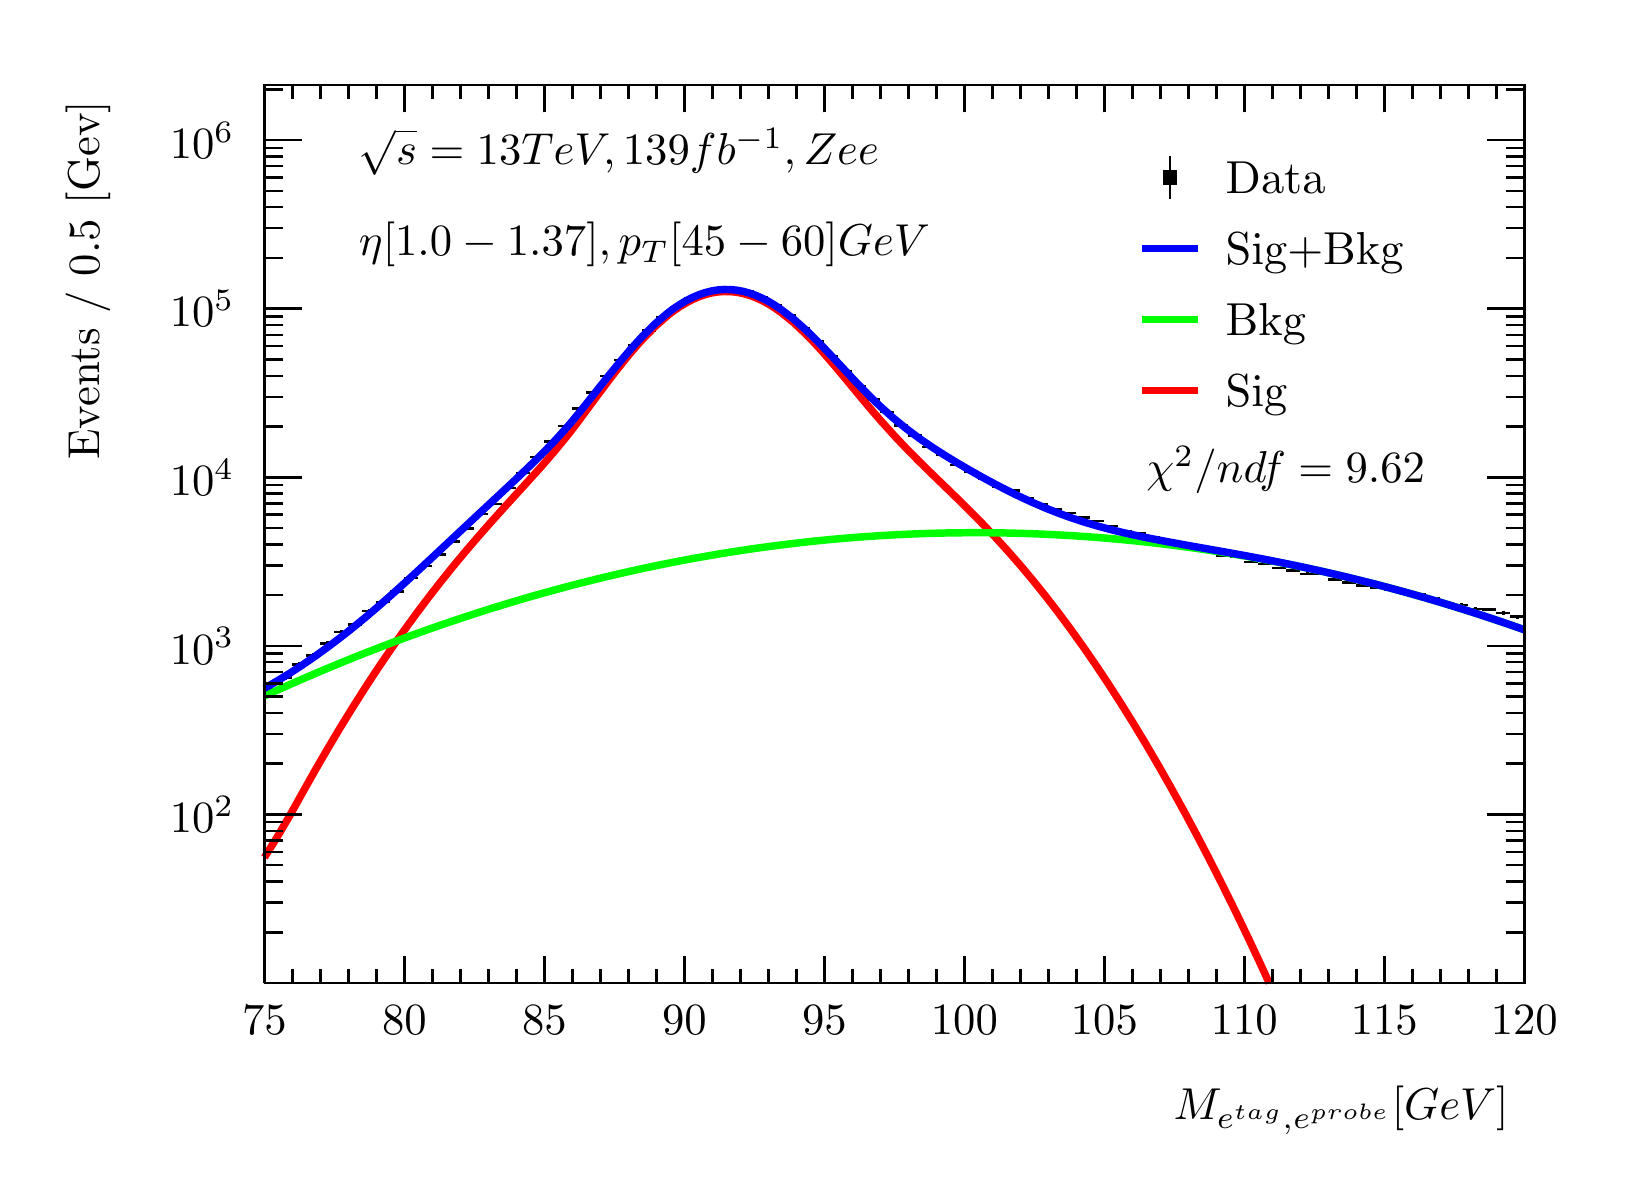
\begin{tikzpicture}
\pgfdeclareplotmark{cross} {
\pgfpathmoveto{\pgfpoint{-0.3\pgfplotmarksize}{\pgfplotmarksize}}
\pgfpathlineto{\pgfpoint{+0.3\pgfplotmarksize}{\pgfplotmarksize}}
\pgfpathlineto{\pgfpoint{+0.3\pgfplotmarksize}{0.3\pgfplotmarksize}}
\pgfpathlineto{\pgfpoint{+1\pgfplotmarksize}{0.3\pgfplotmarksize}}
\pgfpathlineto{\pgfpoint{+1\pgfplotmarksize}{-0.3\pgfplotmarksize}}
\pgfpathlineto{\pgfpoint{+0.3\pgfplotmarksize}{-0.3\pgfplotmarksize}}
\pgfpathlineto{\pgfpoint{+0.3\pgfplotmarksize}{-1.\pgfplotmarksize}}
\pgfpathlineto{\pgfpoint{-0.3\pgfplotmarksize}{-1.\pgfplotmarksize}}
\pgfpathlineto{\pgfpoint{-0.3\pgfplotmarksize}{-0.3\pgfplotmarksize}}
\pgfpathlineto{\pgfpoint{-1.\pgfplotmarksize}{-0.3\pgfplotmarksize}}
\pgfpathlineto{\pgfpoint{-1.\pgfplotmarksize}{0.3\pgfplotmarksize}}
\pgfpathlineto{\pgfpoint{-0.3\pgfplotmarksize}{0.3\pgfplotmarksize}}
\pgfpathclose
\pgfusepathqstroke
}
\pgfdeclareplotmark{cross*} {
\pgfpathmoveto{\pgfpoint{-0.3\pgfplotmarksize}{\pgfplotmarksize}}
\pgfpathlineto{\pgfpoint{+0.3\pgfplotmarksize}{\pgfplotmarksize}}
\pgfpathlineto{\pgfpoint{+0.3\pgfplotmarksize}{0.3\pgfplotmarksize}}
\pgfpathlineto{\pgfpoint{+1\pgfplotmarksize}{0.3\pgfplotmarksize}}
\pgfpathlineto{\pgfpoint{+1\pgfplotmarksize}{-0.3\pgfplotmarksize}}
\pgfpathlineto{\pgfpoint{+0.3\pgfplotmarksize}{-0.3\pgfplotmarksize}}
\pgfpathlineto{\pgfpoint{+0.3\pgfplotmarksize}{-1.\pgfplotmarksize}}
\pgfpathlineto{\pgfpoint{-0.3\pgfplotmarksize}{-1.\pgfplotmarksize}}
\pgfpathlineto{\pgfpoint{-0.3\pgfplotmarksize}{-0.3\pgfplotmarksize}}
\pgfpathlineto{\pgfpoint{-1.\pgfplotmarksize}{-0.3\pgfplotmarksize}}
\pgfpathlineto{\pgfpoint{-1.\pgfplotmarksize}{0.3\pgfplotmarksize}}
\pgfpathlineto{\pgfpoint{-0.3\pgfplotmarksize}{0.3\pgfplotmarksize}}
\pgfpathclose
\pgfusepathqfillstroke
}
\pgfdeclareplotmark{newstar} {
\pgfpathmoveto{\pgfqpoint{0pt}{\pgfplotmarksize}}
\pgfpathlineto{\pgfqpointpolar{44}{0.5\pgfplotmarksize}}
\pgfpathlineto{\pgfqpointpolar{18}{\pgfplotmarksize}}
\pgfpathlineto{\pgfqpointpolar{-20}{0.5\pgfplotmarksize}}
\pgfpathlineto{\pgfqpointpolar{-54}{\pgfplotmarksize}}
\pgfpathlineto{\pgfqpointpolar{-90}{0.5\pgfplotmarksize}}
\pgfpathlineto{\pgfqpointpolar{234}{\pgfplotmarksize}}
\pgfpathlineto{\pgfqpointpolar{198}{0.5\pgfplotmarksize}}
\pgfpathlineto{\pgfqpointpolar{162}{\pgfplotmarksize}}
\pgfpathlineto{\pgfqpointpolar{134}{0.5\pgfplotmarksize}}
\pgfpathclose
\pgfusepathqstroke
}
\pgfdeclareplotmark{newstar*} {
\pgfpathmoveto{\pgfqpoint{0pt}{\pgfplotmarksize}}
\pgfpathlineto{\pgfqpointpolar{44}{0.5\pgfplotmarksize}}
\pgfpathlineto{\pgfqpointpolar{18}{\pgfplotmarksize}}
\pgfpathlineto{\pgfqpointpolar{-20}{0.5\pgfplotmarksize}}
\pgfpathlineto{\pgfqpointpolar{-54}{\pgfplotmarksize}}
\pgfpathlineto{\pgfqpointpolar{-90}{0.5\pgfplotmarksize}}
\pgfpathlineto{\pgfqpointpolar{234}{\pgfplotmarksize}}
\pgfpathlineto{\pgfqpointpolar{198}{0.5\pgfplotmarksize}}
\pgfpathlineto{\pgfqpointpolar{162}{\pgfplotmarksize}}
\pgfpathlineto{\pgfqpointpolar{134}{0.5\pgfplotmarksize}}
\pgfpathclose
\pgfusepathqfillstroke
}
\definecolor{c}{rgb}{1,1,1};
\draw [color=c, fill=c] (0,0) rectangle (20,14.4361);
\draw [color=c, fill=c] (3,2.30977) rectangle (19,13.7143);
\definecolor{c}{rgb}{0,0,0};
\draw [c,line width=0.9] (3,2.30977) -- (3,13.7143) -- (19,13.7143) -- (19,2.30977) -- (3,2.30977);
\definecolor{c}{rgb}{1,1,1};
\draw [color=c, fill=c] (3,2.30977) rectangle (19,13.7143);
\definecolor{c}{rgb}{0,0,0};
\draw [c,line width=0.9] (3,2.30977) -- (3,13.7143) -- (19,13.7143) -- (19,2.30977) -- (3,2.30977);
\draw [c,line width=0.9] (3,2.30977) -- (19,2.30977);
\draw [c,line width=0.9] (3,2.65624) -- (3,2.30977);
\draw [c,line width=0.9] (3.35556,2.48301) -- (3.35556,2.30977);
\draw [c,line width=0.9] (3.71111,2.48301) -- (3.71111,2.30977);
\draw [c,line width=0.9] (4.06667,2.48301) -- (4.06667,2.30977);
\draw [c,line width=0.9] (4.42222,2.48301) -- (4.42222,2.30977);
\draw [c,line width=0.9] (4.77778,2.65624) -- (4.77778,2.30977);
\draw [c,line width=0.9] (5.13333,2.48301) -- (5.13333,2.30977);
\draw [c,line width=0.9] (5.48889,2.48301) -- (5.48889,2.30977);
\draw [c,line width=0.9] (5.84444,2.48301) -- (5.84444,2.30977);
\draw [c,line width=0.9] (6.2,2.48301) -- (6.2,2.30977);
\draw [c,line width=0.9] (6.55556,2.65624) -- (6.55556,2.30977);
\draw [c,line width=0.9] (6.91111,2.48301) -- (6.91111,2.30977);
\draw [c,line width=0.9] (7.26667,2.48301) -- (7.26667,2.30977);
\draw [c,line width=0.9] (7.62222,2.48301) -- (7.62222,2.30977);
\draw [c,line width=0.9] (7.97778,2.48301) -- (7.97778,2.30977);
\draw [c,line width=0.9] (8.33333,2.65624) -- (8.33333,2.30977);
\draw [c,line width=0.9] (8.68889,2.48301) -- (8.68889,2.30977);
\draw [c,line width=0.9] (9.04444,2.48301) -- (9.04444,2.30977);
\draw [c,line width=0.9] (9.4,2.48301) -- (9.4,2.30977);
\draw [c,line width=0.9] (9.75556,2.48301) -- (9.75556,2.30977);
\draw [c,line width=0.9] (10.1111,2.65624) -- (10.1111,2.30977);
\draw [c,line width=0.9] (10.4667,2.48301) -- (10.4667,2.30977);
\draw [c,line width=0.9] (10.8222,2.48301) -- (10.8222,2.30977);
\draw [c,line width=0.9] (11.1778,2.48301) -- (11.1778,2.30977);
\draw [c,line width=0.9] (11.5333,2.48301) -- (11.5333,2.30977);
\draw [c,line width=0.9] (11.8889,2.65624) -- (11.8889,2.30977);
\draw [c,line width=0.9] (12.2444,2.48301) -- (12.2444,2.30977);
\draw [c,line width=0.9] (12.6,2.48301) -- (12.6,2.30977);
\draw [c,line width=0.9] (12.9556,2.48301) -- (12.9556,2.30977);
\draw [c,line width=0.9] (13.3111,2.48301) -- (13.3111,2.30977);
\draw [c,line width=0.9] (13.6667,2.65624) -- (13.6667,2.30977);
\draw [c,line width=0.9] (14.0222,2.48301) -- (14.0222,2.30977);
\draw [c,line width=0.9] (14.3778,2.48301) -- (14.3778,2.30977);
\draw [c,line width=0.9] (14.7333,2.48301) -- (14.7333,2.30977);
\draw [c,line width=0.9] (15.0889,2.48301) -- (15.0889,2.30977);
\draw [c,line width=0.9] (15.4444,2.65624) -- (15.4444,2.30977);
\draw [c,line width=0.9] (15.8,2.48301) -- (15.8,2.30977);
\draw [c,line width=0.9] (16.1556,2.48301) -- (16.1556,2.30977);
\draw [c,line width=0.9] (16.5111,2.48301) -- (16.5111,2.30977);
\draw [c,line width=0.9] (16.8667,2.48301) -- (16.8667,2.30977);
\draw [c,line width=0.9] (17.2222,2.65624) -- (17.2222,2.30977);
\draw [c,line width=0.9] (17.5778,2.48301) -- (17.5778,2.30977);
\draw [c,line width=0.9] (17.9333,2.48301) -- (17.9333,2.30977);
\draw [c,line width=0.9] (18.2889,2.48301) -- (18.2889,2.30977);
\draw [c,line width=0.9] (18.6444,2.48301) -- (18.6444,2.30977);
\draw [c,line width=0.9] (19,2.65624) -- (19,2.30977);
\draw [c,line width=0.9] (19,2.65624) -- (19,2.30977);
\draw [anchor=base] (3,1.66015) node[scale=1.61424, color=c, rotate=0]{75};
\draw [anchor=base] (4.77778,1.66015) node[scale=1.61424, color=c, rotate=0]{80};
\draw [anchor=base] (6.55556,1.66015) node[scale=1.61424, color=c, rotate=0]{85};
\draw [anchor=base] (8.33333,1.66015) node[scale=1.61424, color=c, rotate=0]{90};
\draw [anchor=base] (10.1111,1.66015) node[scale=1.61424, color=c, rotate=0]{95};
\draw [anchor=base] (11.8889,1.66015) node[scale=1.61424, color=c, rotate=0]{100};
\draw [anchor=base] (13.6667,1.66015) node[scale=1.61424, color=c, rotate=0]{105};
\draw [anchor=base] (15.4444,1.66015) node[scale=1.61424, color=c, rotate=0]{110};
\draw [anchor=base] (17.2222,1.66015) node[scale=1.61424, color=c, rotate=0]{115};
\draw [anchor=base] (19,1.66015) node[scale=1.61424, color=c, rotate=0]{120};
\draw [anchor= east] (19,0.692932) node[scale=1.61424, color=c, rotate=0]{$M_{e^{tag}, e^{probe}}  [GeV]$};
\draw [c,line width=0.9] (3,13.7143) -- (19,13.7143);
\draw [c,line width=0.9] (3,13.3678) -- (3,13.7143);
\draw [c,line width=0.9] (3.35556,13.5411) -- (3.35556,13.7143);
\draw [c,line width=0.9] (3.71111,13.5411) -- (3.71111,13.7143);
\draw [c,line width=0.9] (4.06667,13.5411) -- (4.06667,13.7143);
\draw [c,line width=0.9] (4.42222,13.5411) -- (4.42222,13.7143);
\draw [c,line width=0.9] (4.77778,13.3678) -- (4.77778,13.7143);
\draw [c,line width=0.9] (5.13333,13.5411) -- (5.13333,13.7143);
\draw [c,line width=0.9] (5.48889,13.5411) -- (5.48889,13.7143);
\draw [c,line width=0.9] (5.84444,13.5411) -- (5.84444,13.7143);
\draw [c,line width=0.9] (6.2,13.5411) -- (6.2,13.7143);
\draw [c,line width=0.9] (6.55556,13.3678) -- (6.55556,13.7143);
\draw [c,line width=0.9] (6.91111,13.5411) -- (6.91111,13.7143);
\draw [c,line width=0.9] (7.26667,13.5411) -- (7.26667,13.7143);
\draw [c,line width=0.9] (7.62222,13.5411) -- (7.62222,13.7143);
\draw [c,line width=0.9] (7.97778,13.5411) -- (7.97778,13.7143);
\draw [c,line width=0.9] (8.33333,13.3678) -- (8.33333,13.7143);
\draw [c,line width=0.9] (8.68889,13.5411) -- (8.68889,13.7143);
\draw [c,line width=0.9] (9.04444,13.5411) -- (9.04444,13.7143);
\draw [c,line width=0.9] (9.4,13.5411) -- (9.4,13.7143);
\draw [c,line width=0.9] (9.75556,13.5411) -- (9.75556,13.7143);
\draw [c,line width=0.9] (10.1111,13.3678) -- (10.1111,13.7143);
\draw [c,line width=0.9] (10.4667,13.5411) -- (10.4667,13.7143);
\draw [c,line width=0.9] (10.8222,13.5411) -- (10.8222,13.7143);
\draw [c,line width=0.9] (11.1778,13.5411) -- (11.1778,13.7143);
\draw [c,line width=0.9] (11.5333,13.5411) -- (11.5333,13.7143);
\draw [c,line width=0.9] (11.8889,13.3678) -- (11.8889,13.7143);
\draw [c,line width=0.9] (12.2444,13.5411) -- (12.2444,13.7143);
\draw [c,line width=0.9] (12.6,13.5411) -- (12.6,13.7143);
\draw [c,line width=0.9] (12.9556,13.5411) -- (12.9556,13.7143);
\draw [c,line width=0.9] (13.3111,13.5411) -- (13.3111,13.7143);
\draw [c,line width=0.9] (13.6667,13.3678) -- (13.6667,13.7143);
\draw [c,line width=0.9] (14.0222,13.5411) -- (14.0222,13.7143);
\draw [c,line width=0.9] (14.3778,13.5411) -- (14.3778,13.7143);
\draw [c,line width=0.9] (14.7333,13.5411) -- (14.7333,13.7143);
\draw [c,line width=0.9] (15.0889,13.5411) -- (15.0889,13.7143);
\draw [c,line width=0.9] (15.4444,13.3678) -- (15.4444,13.7143);
\draw [c,line width=0.9] (15.8,13.5411) -- (15.8,13.7143);
\draw [c,line width=0.9] (16.1556,13.5411) -- (16.1556,13.7143);
\draw [c,line width=0.9] (16.5111,13.5411) -- (16.5111,13.7143);
\draw [c,line width=0.9] (16.8667,13.5411) -- (16.8667,13.7143);
\draw [c,line width=0.9] (17.2222,13.3678) -- (17.2222,13.7143);
\draw [c,line width=0.9] (17.5778,13.5411) -- (17.5778,13.7143);
\draw [c,line width=0.9] (17.9333,13.5411) -- (17.9333,13.7143);
\draw [c,line width=0.9] (18.2889,13.5411) -- (18.2889,13.7143);
\draw [c,line width=0.9] (18.6444,13.5411) -- (18.6444,13.7143);
\draw [c,line width=0.9] (19,13.3678) -- (19,13.7143);
\draw [c,line width=0.9] (19,13.3678) -- (19,13.7143);
\draw [c,line width=0.9] (3,2.30977) -- (3,13.7143);
\draw [c,line width=0.9] (3.237,2.95433) -- (3,2.95433);
\draw [c,line width=0.9] (3.237,3.33137) -- (3,3.33137);
\draw [c,line width=0.9] (3.237,3.59888) -- (3,3.59888);
\draw [c,line width=0.9] (3.237,3.80638) -- (3,3.80638);
\draw [c,line width=0.9] (3.237,3.97592) -- (3,3.97592);
\draw [c,line width=0.9] (3.237,4.11926) -- (3,4.11926);
\draw [c,line width=0.9] (3.237,4.24343) -- (3,4.24343);
\draw [c,line width=0.9] (3.237,4.35296) -- (3,4.35296);
\draw [c,line width=0.9] (3.474,4.45093) -- (3,4.45093);
\draw [anchor= east] (2.82,4.45093) node[scale=1.61424, color=c, rotate=0]{$10^{2}$};
\draw [c,line width=0.9] (3.237,5.09549) -- (3,5.09549);
\draw [c,line width=0.9] (3.237,5.47253) -- (3,5.47253);
\draw [c,line width=0.9] (3.237,5.74004) -- (3,5.74004);
\draw [c,line width=0.9] (3.237,5.94754) -- (3,5.94754);
\draw [c,line width=0.9] (3.237,6.11708) -- (3,6.11708);
\draw [c,line width=0.9] (3.237,6.26042) -- (3,6.26042);
\draw [c,line width=0.9] (3.237,6.38459) -- (3,6.38459);
\draw [c,line width=0.9] (3.237,6.49412) -- (3,6.49412);
\draw [c,line width=0.9] (3.474,6.59209) -- (3,6.59209);
\draw [anchor= east] (2.82,6.59209) node[scale=1.61424, color=c, rotate=0]{$10^{3}$};
\draw [c,line width=0.9] (3.237,7.23665) -- (3,7.23665);
\draw [c,line width=0.9] (3.237,7.61369) -- (3,7.61369);
\draw [c,line width=0.9] (3.237,7.8812) -- (3,7.8812);
\draw [c,line width=0.9] (3.237,8.0887) -- (3,8.0887);
\draw [c,line width=0.9] (3.237,8.25824) -- (3,8.25824);
\draw [c,line width=0.9] (3.237,8.40158) -- (3,8.40158);
\draw [c,line width=0.9] (3.237,8.52575) -- (3,8.52575);
\draw [c,line width=0.9] (3.237,8.63528) -- (3,8.63528);
\draw [c,line width=0.9] (3.474,8.73325) -- (3,8.73325);
\draw [anchor= east] (2.82,8.73325) node[scale=1.61424, color=c, rotate=0]{$10^{4}$};
\draw [c,line width=0.9] (3.237,9.37781) -- (3,9.37781);
\draw [c,line width=0.9] (3.237,9.75485) -- (3,9.75485);
\draw [c,line width=0.9] (3.237,10.0224) -- (3,10.0224);
\draw [c,line width=0.9] (3.237,10.2299) -- (3,10.2299);
\draw [c,line width=0.9] (3.237,10.3994) -- (3,10.3994);
\draw [c,line width=0.9] (3.237,10.5427) -- (3,10.5427);
\draw [c,line width=0.9] (3.237,10.6669) -- (3,10.6669);
\draw [c,line width=0.9] (3.237,10.7764) -- (3,10.7764);
\draw [c,line width=0.9] (3.474,10.8744) -- (3,10.8744);
\draw [anchor= east] (2.82,10.8744) node[scale=1.61424, color=c, rotate=0]{$10^{5}$};
\draw [c,line width=0.9] (3.237,11.519) -- (3,11.519);
\draw [c,line width=0.9] (3.237,11.896) -- (3,11.896);
\draw [c,line width=0.9] (3.237,12.1635) -- (3,12.1635);
\draw [c,line width=0.9] (3.237,12.371) -- (3,12.371);
\draw [c,line width=0.9] (3.237,12.5406) -- (3,12.5406);
\draw [c,line width=0.9] (3.237,12.6839) -- (3,12.6839);
\draw [c,line width=0.9] (3.237,12.8081) -- (3,12.8081);
\draw [c,line width=0.9] (3.237,12.9176) -- (3,12.9176);
\draw [c,line width=0.9] (3.474,13.0156) -- (3,13.0156);
\draw [anchor= east] (2.82,13.0156) node[scale=1.61424, color=c, rotate=0]{$10^{6}$};
\draw [c,line width=0.9] (3.237,13.6601) -- (3,13.6601);
\draw [anchor= east] (0.76,13.7143) node[scale=1.61424, color=c, rotate=90]{Events / 0.5 [Gev]};
\draw [c,line width=0.9] (19,2.30977) -- (19,13.7143);
\draw [c,line width=0.9] (18.763,2.95433) -- (19,2.95433);
\draw [c,line width=0.9] (18.763,3.33137) -- (19,3.33137);
\draw [c,line width=0.9] (18.763,3.59888) -- (19,3.59888);
\draw [c,line width=0.9] (18.763,3.80638) -- (19,3.80638);
\draw [c,line width=0.9] (18.763,3.97592) -- (19,3.97592);
\draw [c,line width=0.9] (18.763,4.11926) -- (19,4.11926);
\draw [c,line width=0.9] (18.763,4.24343) -- (19,4.24343);
\draw [c,line width=0.9] (18.763,4.35296) -- (19,4.35296);
\draw [c,line width=0.9] (18.526,4.45093) -- (19,4.45093);
\draw [c,line width=0.9] (18.763,5.09549) -- (19,5.09549);
\draw [c,line width=0.9] (18.763,5.47253) -- (19,5.47253);
\draw [c,line width=0.9] (18.763,5.74004) -- (19,5.74004);
\draw [c,line width=0.9] (18.763,5.94754) -- (19,5.94754);
\draw [c,line width=0.9] (18.763,6.11708) -- (19,6.11708);
\draw [c,line width=0.9] (18.763,6.26042) -- (19,6.26042);
\draw [c,line width=0.9] (18.763,6.38459) -- (19,6.38459);
\draw [c,line width=0.9] (18.763,6.49412) -- (19,6.49412);
\draw [c,line width=0.9] (18.526,6.59209) -- (19,6.59209);
\draw [c,line width=0.9] (18.763,7.23665) -- (19,7.23665);
\draw [c,line width=0.9] (18.763,7.61369) -- (19,7.61369);
\draw [c,line width=0.9] (18.763,7.8812) -- (19,7.8812);
\draw [c,line width=0.9] (18.763,8.0887) -- (19,8.0887);
\draw [c,line width=0.9] (18.763,8.25824) -- (19,8.25824);
\draw [c,line width=0.9] (18.763,8.40158) -- (19,8.40158);
\draw [c,line width=0.9] (18.763,8.52575) -- (19,8.52575);
\draw [c,line width=0.9] (18.763,8.63528) -- (19,8.63528);
\draw [c,line width=0.9] (18.526,8.73325) -- (19,8.73325);
\draw [c,line width=0.9] (18.763,9.37781) -- (19,9.37781);
\draw [c,line width=0.9] (18.763,9.75485) -- (19,9.75485);
\draw [c,line width=0.9] (18.763,10.0224) -- (19,10.0224);
\draw [c,line width=0.9] (18.763,10.2299) -- (19,10.2299);
\draw [c,line width=0.9] (18.763,10.3994) -- (19,10.3994);
\draw [c,line width=0.9] (18.763,10.5427) -- (19,10.5427);
\draw [c,line width=0.9] (18.763,10.6669) -- (19,10.6669);
\draw [c,line width=0.9] (18.763,10.7764) -- (19,10.7764);
\draw [c,line width=0.9] (18.526,10.8744) -- (19,10.8744);
\draw [c,line width=0.9] (18.763,11.519) -- (19,11.519);
\draw [c,line width=0.9] (18.763,11.896) -- (19,11.896);
\draw [c,line width=0.9] (18.763,12.1635) -- (19,12.1635);
\draw [c,line width=0.9] (18.763,12.371) -- (19,12.371);
\draw [c,line width=0.9] (18.763,12.5406) -- (19,12.5406);
\draw [c,line width=0.9] (18.763,12.6839) -- (19,12.6839);
\draw [c,line width=0.9] (18.763,12.8081) -- (19,12.8081);
\draw [c,line width=0.9] (18.763,12.9176) -- (19,12.9176);
\draw [c,line width=0.9] (18.526,13.0156) -- (19,13.0156);
\draw [c,line width=0.9] (18.763,13.6601) -- (19,13.6601);
\draw [c,line width=0.9] (3.08889,6.03786) -- (3,6.03786);
\draw [c,line width=0.9] (3,6.03786) -- (3,6.03786);
\draw [c,line width=0.9] (3.08889,6.03786) -- (3.17778,6.03786);
\draw [c,line width=0.9] (3.17778,6.03786) -- (3.17778,6.03786);
\draw [c,line width=0.9] (3.08889,6.03786) -- (3.08889,6.07747);
\draw [c,line width=0.9] (3.08889,6.07747) -- (3.08889,6.07747);
\draw [c,line width=0.9] (3.08889,6.03786) -- (3.08889,5.99825);
\draw [c,line width=0.9] (3.08889,5.99825) -- (3.08889,5.99825);
\draw [c,line width=0.9] (3.26667,6.19151) -- (3.17778,6.19151);
\draw [c,line width=0.9] (3.17778,6.19151) -- (3.17778,6.19151);
\draw [c,line width=0.9] (3.26667,6.19151) -- (3.35556,6.19151);
\draw [c,line width=0.9] (3.35556,6.19151) -- (3.35556,6.19151);
\draw [c,line width=0.9] (3.26667,6.19151) -- (3.26667,6.22798);
\draw [c,line width=0.9] (3.26667,6.22798) -- (3.26667,6.22798);
\draw [c,line width=0.9] (3.26667,6.19151) -- (3.26667,6.15504);
\draw [c,line width=0.9] (3.26667,6.15504) -- (3.26667,6.15504);
\draw [c,line width=0.9] (3.44444,6.35267) -- (3.35556,6.35267);
\draw [c,line width=0.9] (3.35556,6.35267) -- (3.35556,6.35267);
\draw [c,line width=0.9] (3.44444,6.35267) -- (3.53333,6.35267);
\draw [c,line width=0.9] (3.53333,6.35267) -- (3.53333,6.35267);
\draw [c,line width=0.9] (3.44444,6.35267) -- (3.44444,6.38611);
\draw [c,line width=0.9] (3.44444,6.38611) -- (3.44444,6.38611);
\draw [c,line width=0.9] (3.44444,6.35267) -- (3.44444,6.31922);
\draw [c,line width=0.9] (3.44444,6.31922) -- (3.44444,6.31922);
\draw [c,line width=0.9] (3.62222,6.47216) -- (3.53333,6.47216);
\draw [c,line width=0.9] (3.53333,6.47216) -- (3.53333,6.47216);
\draw [c,line width=0.9] (3.62222,6.47216) -- (3.71111,6.47216);
\draw [c,line width=0.9] (3.71111,6.47216) -- (3.71111,6.47216);
\draw [c,line width=0.9] (3.62222,6.47216) -- (3.62222,6.50353);
\draw [c,line width=0.9] (3.62222,6.50353) -- (3.62222,6.50353);
\draw [c,line width=0.9] (3.62222,6.47216) -- (3.62222,6.4408);
\draw [c,line width=0.9] (3.62222,6.4408) -- (3.62222,6.4408);
\draw [c,line width=0.9] (3.8,6.62408) -- (3.71111,6.62408);
\draw [c,line width=0.9] (3.71111,6.62408) -- (3.71111,6.62408);
\draw [c,line width=0.9] (3.8,6.62408) -- (3.88889,6.62408);
\draw [c,line width=0.9] (3.88889,6.62408) -- (3.88889,6.62408);
\draw [c,line width=0.9] (3.8,6.62408) -- (3.8,6.65299);
\draw [c,line width=0.9] (3.8,6.65299) -- (3.8,6.65299);
\draw [c,line width=0.9] (3.8,6.62408) -- (3.8,6.59518);
\draw [c,line width=0.9] (3.8,6.59518) -- (3.8,6.59518);
\draw [c,line width=0.9] (3.97778,6.76704) -- (3.88889,6.76704);
\draw [c,line width=0.9] (3.88889,6.76704) -- (3.88889,6.76704);
\draw [c,line width=0.9] (3.97778,6.76704) -- (4.06667,6.76704);
\draw [c,line width=0.9] (4.06667,6.76704) -- (4.06667,6.76704);
\draw [c,line width=0.9] (3.97778,6.76704) -- (3.97778,6.79381);
\draw [c,line width=0.9] (3.97778,6.79381) -- (3.97778,6.79381);
\draw [c,line width=0.9] (3.97778,6.76704) -- (3.97778,6.74028);
\draw [c,line width=0.9] (3.97778,6.74028) -- (3.97778,6.74028);
\draw [c,line width=0.9] (4.15556,6.86286) -- (4.06667,6.86286);
\draw [c,line width=0.9] (4.06667,6.86286) -- (4.06667,6.86286);
\draw [c,line width=0.9] (4.15556,6.86286) -- (4.24444,6.86286);
\draw [c,line width=0.9] (4.24444,6.86286) -- (4.24444,6.86286);
\draw [c,line width=0.9] (4.15556,6.86286) -- (4.15556,6.88828);
\draw [c,line width=0.9] (4.15556,6.88828) -- (4.15556,6.88828);
\draw [c,line width=0.9] (4.15556,6.86286) -- (4.15556,6.83744);
\draw [c,line width=0.9] (4.15556,6.83744) -- (4.15556,6.83744);
\draw [c,line width=0.9] (4.33333,7.03552) -- (4.24444,7.03552);
\draw [c,line width=0.9] (4.24444,7.03552) -- (4.24444,7.03552);
\draw [c,line width=0.9] (4.33333,7.03552) -- (4.42222,7.03552);
\draw [c,line width=0.9] (4.42222,7.03552) -- (4.42222,7.03552);
\draw [c,line width=0.9] (4.33333,7.03552) -- (4.33333,7.05869);
\draw [c,line width=0.9] (4.33333,7.05869) -- (4.33333,7.05869);
\draw [c,line width=0.9] (4.33333,7.03552) -- (4.33333,7.01235);
\draw [c,line width=0.9] (4.33333,7.01235) -- (4.33333,7.01235);
\draw [c,line width=0.9] (4.51111,7.15099) -- (4.42222,7.15099);
\draw [c,line width=0.9] (4.42222,7.15099) -- (4.42222,7.15099);
\draw [c,line width=0.9] (4.51111,7.15099) -- (4.6,7.15099);
\draw [c,line width=0.9] (4.6,7.15099) -- (4.6,7.15099);
\draw [c,line width=0.9] (4.51111,7.15099) -- (4.51111,7.17276);
\draw [c,line width=0.9] (4.51111,7.17276) -- (4.51111,7.17276);
\draw [c,line width=0.9] (4.51111,7.15099) -- (4.51111,7.12922);
\draw [c,line width=0.9] (4.51111,7.12922) -- (4.51111,7.12922);
\draw [c,line width=0.9] (4.68889,7.28202) -- (4.6,7.28202);
\draw [c,line width=0.9] (4.6,7.28202) -- (4.6,7.28202);
\draw [c,line width=0.9] (4.68889,7.28202) -- (4.77778,7.28202);
\draw [c,line width=0.9] (4.77778,7.28202) -- (4.77778,7.28202);
\draw [c,line width=0.9] (4.68889,7.28202) -- (4.68889,7.30231);
\draw [c,line width=0.9] (4.68889,7.30231) -- (4.68889,7.30231);
\draw [c,line width=0.9] (4.68889,7.28202) -- (4.68889,7.26172);
\draw [c,line width=0.9] (4.68889,7.26172) -- (4.68889,7.26172);
\draw [c,line width=0.9] (4.86667,7.45524) -- (4.77778,7.45524);
\draw [c,line width=0.9] (4.77778,7.45524) -- (4.77778,7.45524);
\draw [c,line width=0.9] (4.86667,7.45524) -- (4.95556,7.45524);
\draw [c,line width=0.9] (4.95556,7.45524) -- (4.95556,7.45524);
\draw [c,line width=0.9] (4.86667,7.45524) -- (4.86667,7.47373);
\draw [c,line width=0.9] (4.86667,7.47373) -- (4.86667,7.47373);
\draw [c,line width=0.9] (4.86667,7.45524) -- (4.86667,7.43675);
\draw [c,line width=0.9] (4.86667,7.43675) -- (4.86667,7.43675);
\draw [c,line width=0.9] (5.04444,7.60903) -- (4.95556,7.60903);
\draw [c,line width=0.9] (4.95556,7.60903) -- (4.95556,7.60903);
\draw [c,line width=0.9] (5.04444,7.60903) -- (5.13333,7.60903);
\draw [c,line width=0.9] (5.13333,7.60903) -- (5.13333,7.60903);
\draw [c,line width=0.9] (5.04444,7.60903) -- (5.04444,7.62605);
\draw [c,line width=0.9] (5.04444,7.62605) -- (5.04444,7.62605);
\draw [c,line width=0.9] (5.04444,7.60903) -- (5.04444,7.59201);
\draw [c,line width=0.9] (5.04444,7.59201) -- (5.04444,7.59201);
\draw [c,line width=0.9] (5.22222,7.7525) -- (5.13333,7.7525);
\draw [c,line width=0.9] (5.13333,7.7525) -- (5.13333,7.7525);
\draw [c,line width=0.9] (5.22222,7.7525) -- (5.31111,7.7525);
\draw [c,line width=0.9] (5.31111,7.7525) -- (5.31111,7.7525);
\draw [c,line width=0.9] (5.22222,7.7525) -- (5.22222,7.76826);
\draw [c,line width=0.9] (5.22222,7.76826) -- (5.22222,7.76826);
\draw [c,line width=0.9] (5.22222,7.7525) -- (5.22222,7.73675);
\draw [c,line width=0.9] (5.22222,7.73675) -- (5.22222,7.73675);
\draw [c,line width=0.9] (5.4,7.91856) -- (5.31111,7.91856);
\draw [c,line width=0.9] (5.31111,7.91856) -- (5.31111,7.91856);
\draw [c,line width=0.9] (5.4,7.91856) -- (5.48889,7.91856);
\draw [c,line width=0.9] (5.48889,7.91856) -- (5.48889,7.91856);
\draw [c,line width=0.9] (5.4,7.91856) -- (5.4,7.93298);
\draw [c,line width=0.9] (5.4,7.93298) -- (5.4,7.93298);
\draw [c,line width=0.9] (5.4,7.91856) -- (5.4,7.90415);
\draw [c,line width=0.9] (5.4,7.90415) -- (5.4,7.90415);
\draw [c,line width=0.9] (5.57778,8.08067) -- (5.48889,8.08067);
\draw [c,line width=0.9] (5.48889,8.08067) -- (5.48889,8.08067);
\draw [c,line width=0.9] (5.57778,8.08067) -- (5.66667,8.08067);
\draw [c,line width=0.9] (5.66667,8.08067) -- (5.66667,8.08067);
\draw [c,line width=0.9] (5.57778,8.08067) -- (5.57778,8.09388);
\draw [c,line width=0.9] (5.57778,8.09388) -- (5.57778,8.09388);
\draw [c,line width=0.9] (5.57778,8.08067) -- (5.57778,8.06746);
\draw [c,line width=0.9] (5.57778,8.06746) -- (5.57778,8.06746);
\draw [c,line width=0.9] (5.75556,8.26672) -- (5.66667,8.26672);
\draw [c,line width=0.9] (5.66667,8.26672) -- (5.66667,8.26672);
\draw [c,line width=0.9] (5.75556,8.26672) -- (5.84444,8.26672);
\draw [c,line width=0.9] (5.84444,8.26672) -- (5.84444,8.26672);
\draw [c,line width=0.9] (5.75556,8.26672) -- (5.75556,8.27868);
\draw [c,line width=0.9] (5.75556,8.27868) -- (5.75556,8.27868);
\draw [c,line width=0.9] (5.75556,8.26672) -- (5.75556,8.25478);
\draw [c,line width=0.9] (5.75556,8.25478) -- (5.75556,8.25478);
\draw [c,line width=0.9] (5.93333,8.39559) -- (5.84444,8.39559);
\draw [c,line width=0.9] (5.84444,8.39559) -- (5.84444,8.39559);
\draw [c,line width=0.9] (5.93333,8.39559) -- (6.02222,8.39559);
\draw [c,line width=0.9] (6.02222,8.39559) -- (6.02222,8.39559);
\draw [c,line width=0.9] (5.93333,8.39559) -- (5.93333,8.40674);
\draw [c,line width=0.9] (5.93333,8.40674) -- (5.93333,8.40674);
\draw [c,line width=0.9] (5.93333,8.39559) -- (5.93333,8.38444);
\draw [c,line width=0.9] (5.93333,8.38444) -- (5.93333,8.38444);
\draw [c,line width=0.9] (6.11111,8.59958) -- (6.02222,8.59958);
\draw [c,line width=0.9] (6.02222,8.59958) -- (6.02222,8.59958);
\draw [c,line width=0.9] (6.11111,8.59958) -- (6.2,8.59958);
\draw [c,line width=0.9] (6.2,8.59958) -- (6.2,8.59958);
\draw [c,line width=0.9] (6.11111,8.59958) -- (6.11111,8.60957);
\draw [c,line width=0.9] (6.11111,8.60957) -- (6.11111,8.60957);
\draw [c,line width=0.9] (6.11111,8.59958) -- (6.11111,8.58958);
\draw [c,line width=0.9] (6.11111,8.58958) -- (6.11111,8.58958);
\draw [c,line width=0.9] (6.28889,8.78831) -- (6.2,8.78831);
\draw [c,line width=0.9] (6.2,8.78831) -- (6.2,8.78831);
\draw [c,line width=0.9] (6.28889,8.78831) -- (6.37778,8.78831);
\draw [c,line width=0.9] (6.37778,8.78831) -- (6.37778,8.78831);
\draw [c,line width=0.9] (6.28889,8.78831) -- (6.28889,8.79734);
\draw [c,line width=0.9] (6.28889,8.79734) -- (6.28889,8.79734);
\draw [c,line width=0.9] (6.28889,8.78831) -- (6.28889,8.77929);
\draw [c,line width=0.9] (6.28889,8.77929) -- (6.28889,8.77929);
\draw [c,line width=0.9] (6.46667,8.99022) -- (6.37778,8.99022);
\draw [c,line width=0.9] (6.37778,8.99022) -- (6.37778,8.99022);
\draw [c,line width=0.9] (6.46667,8.99022) -- (6.55556,8.99022);
\draw [c,line width=0.9] (6.55556,8.99022) -- (6.55556,8.99022);
\draw [c,line width=0.9] (6.46667,8.99022) -- (6.46667,8.99832);
\draw [c,line width=0.9] (6.46667,8.99832) -- (6.46667,8.99832);
\draw [c,line width=0.9] (6.46667,8.99022) -- (6.46667,8.98212);
\draw [c,line width=0.9] (6.46667,8.98212) -- (6.46667,8.98212);
\draw [c,line width=0.9] (6.64444,9.18804) -- (6.55556,9.18804);
\draw [c,line width=0.9] (6.55556,9.18804) -- (6.55556,9.18804);
\draw [c,line width=0.9] (6.64444,9.18804) -- (6.73333,9.18804);
\draw [c,line width=0.9] (6.73333,9.18804) -- (6.73333,9.18804);
\draw [c,line width=0.9] (6.64444,9.18804) -- (6.64444,9.19532);
\draw [c,line width=0.9] (6.64444,9.19532) -- (6.64444,9.19532);
\draw [c,line width=0.9] (6.64444,9.18804) -- (6.64444,9.18076);
\draw [c,line width=0.9] (6.64444,9.18076) -- (6.64444,9.18076);
\draw [c,line width=0.9] (6.82222,9.38545) -- (6.73333,9.38545);
\draw [c,line width=0.9] (6.73333,9.38545) -- (6.73333,9.38545);
\draw [c,line width=0.9] (6.82222,9.38545) -- (6.91111,9.38545);
\draw [c,line width=0.9] (6.91111,9.38545) -- (6.91111,9.38545);
\draw [c,line width=0.9] (6.82222,9.38545) -- (6.82222,9.392);
\draw [c,line width=0.9] (6.82222,9.392) -- (6.82222,9.392);
\draw [c,line width=0.9] (6.82222,9.38545) -- (6.82222,9.3789);
\draw [c,line width=0.9] (6.82222,9.3789) -- (6.82222,9.3789);
\draw [c,line width=0.9] (7,9.60441) -- (6.91111,9.60441);
\draw [c,line width=0.9] (6.91111,9.60441) -- (6.91111,9.60441);
\draw [c,line width=0.9] (7,9.60441) -- (7.08889,9.60441);
\draw [c,line width=0.9] (7.08889,9.60441) -- (7.08889,9.60441);
\draw [c,line width=0.9] (7,9.60441) -- (7,9.61023);
\draw [c,line width=0.9] (7,9.61023) -- (7,9.61023);
\draw [c,line width=0.9] (7,9.60441) -- (7,9.59859);
\draw [c,line width=0.9] (7,9.59859) -- (7,9.59859);
\draw [c,line width=0.9] (7.17778,9.81131) -- (7.08889,9.81131);
\draw [c,line width=0.9] (7.08889,9.81131) -- (7.08889,9.81131);
\draw [c,line width=0.9] (7.17778,9.81131) -- (7.26667,9.81131);
\draw [c,line width=0.9] (7.26667,9.81131) -- (7.26667,9.81131);
\draw [c,line width=0.9] (7.17778,9.81131) -- (7.17778,9.81652);
\draw [c,line width=0.9] (7.17778,9.81652) -- (7.17778,9.81652);
\draw [c,line width=0.9] (7.17778,9.81131) -- (7.17778,9.8061);
\draw [c,line width=0.9] (7.17778,9.8061) -- (7.17778,9.8061);
\draw [c,line width=0.9] (7.35556,10.0188) -- (7.26667,10.0188);
\draw [c,line width=0.9] (7.26667,10.0188) -- (7.26667,10.0188);
\draw [c,line width=0.9] (7.35556,10.0188) -- (7.44444,10.0188);
\draw [c,line width=0.9] (7.44444,10.0188) -- (7.44444,10.0188);
\draw [c,line width=0.9] (7.35556,10.0188) -- (7.35556,10.0235);
\draw [c,line width=0.9] (7.35556,10.0235) -- (7.35556,10.0235);
\draw [c,line width=0.9] (7.35556,10.0188) -- (7.35556,10.0141);
\draw [c,line width=0.9] (7.35556,10.0141) -- (7.35556,10.0141);
\draw [c,line width=0.9] (7.53333,10.2222) -- (7.44444,10.2222);
\draw [c,line width=0.9] (7.44444,10.2222) -- (7.44444,10.2222);
\draw [c,line width=0.9] (7.53333,10.2222) -- (7.62222,10.2222);
\draw [c,line width=0.9] (7.62222,10.2222) -- (7.62222,10.2222);
\draw [c,line width=0.9] (7.53333,10.2222) -- (7.53333,10.2263);
\draw [c,line width=0.9] (7.53333,10.2263) -- (7.53333,10.2263);
\draw [c,line width=0.9] (7.53333,10.2222) -- (7.53333,10.218);
\draw [c,line width=0.9] (7.53333,10.218) -- (7.53333,10.218);
\draw [c,line width=0.9] (7.71111,10.4115) -- (7.62222,10.4115);
\draw [c,line width=0.9] (7.62222,10.4115) -- (7.62222,10.4115);
\draw [c,line width=0.9] (7.71111,10.4115) -- (7.8,10.4115);
\draw [c,line width=0.9] (7.8,10.4115) -- (7.8,10.4115);
\draw [c,line width=0.9] (7.71111,10.4115) -- (7.71111,10.4153);
\draw [c,line width=0.9] (7.71111,10.4153) -- (7.71111,10.4153);
\draw [c,line width=0.9] (7.71111,10.4115) -- (7.71111,10.4078);
\draw [c,line width=0.9] (7.71111,10.4078) -- (7.71111,10.4078);
\draw [c,line width=0.9] (7.88889,10.5993) -- (7.8,10.5993);
\draw [c,line width=0.9] (7.8,10.5993) -- (7.8,10.5993);
\draw [c,line width=0.9] (7.88889,10.5993) -- (7.97778,10.5993);
\draw [c,line width=0.9] (7.97778,10.5993) -- (7.97778,10.5993);
\draw [c,line width=0.9] (7.88889,10.5993) -- (7.88889,10.6027);
\draw [c,line width=0.9] (7.88889,10.6027) -- (7.88889,10.6027);
\draw [c,line width=0.9] (7.88889,10.5993) -- (7.88889,10.5958);
\draw [c,line width=0.9] (7.88889,10.5958) -- (7.88889,10.5958);
\draw [c,line width=0.9] (8.06667,10.7597) -- (7.97778,10.7597);
\draw [c,line width=0.9] (7.97778,10.7597) -- (7.97778,10.7597);
\draw [c,line width=0.9] (8.06667,10.7597) -- (8.15556,10.7597);
\draw [c,line width=0.9] (8.15556,10.7597) -- (8.15556,10.7597);
\draw [c,line width=0.9] (8.06667,10.7597) -- (8.06667,10.7629);
\draw [c,line width=0.9] (8.06667,10.7629) -- (8.06667,10.7629);
\draw [c,line width=0.9] (8.06667,10.7597) -- (8.06667,10.7566);
\draw [c,line width=0.9] (8.06667,10.7566) -- (8.06667,10.7566);
\draw [c,line width=0.9] (8.24444,10.8873) -- (8.15556,10.8873);
\draw [c,line width=0.9] (8.15556,10.8873) -- (8.15556,10.8873);
\draw [c,line width=0.9] (8.24444,10.8873) -- (8.33333,10.8873);
\draw [c,line width=0.9] (8.33333,10.8873) -- (8.33333,10.8873);
\draw [c,line width=0.9] (8.24444,10.8873) -- (8.24444,10.8902);
\draw [c,line width=0.9] (8.24444,10.8902) -- (8.24444,10.8902);
\draw [c,line width=0.9] (8.24444,10.8873) -- (8.24444,10.8843);
\draw [c,line width=0.9] (8.24444,10.8843) -- (8.24444,10.8843);
\draw [c,line width=0.9] (8.42222,11.0052) -- (8.33333,11.0052);
\draw [c,line width=0.9] (8.33333,11.0052) -- (8.33333,11.0052);
\draw [c,line width=0.9] (8.42222,11.0052) -- (8.51111,11.0052);
\draw [c,line width=0.9] (8.51111,11.0052) -- (8.51111,11.0052);
\draw [c,line width=0.9] (8.42222,11.0052) -- (8.42222,11.008);
\draw [c,line width=0.9] (8.42222,11.008) -- (8.42222,11.008);
\draw [c,line width=0.9] (8.42222,11.0052) -- (8.42222,11.0025);
\draw [c,line width=0.9] (8.42222,11.0025) -- (8.42222,11.0025);
\draw [c,line width=0.9] (8.6,11.0822) -- (8.51111,11.0822);
\draw [c,line width=0.9] (8.51111,11.0822) -- (8.51111,11.0822);
\draw [c,line width=0.9] (8.6,11.0822) -- (8.68889,11.0822);
\draw [c,line width=0.9] (8.68889,11.0822) -- (8.68889,11.0822);
\draw [c,line width=0.9] (8.6,11.0822) -- (8.6,11.0849);
\draw [c,line width=0.9] (8.6,11.0849) -- (8.6,11.0849);
\draw [c,line width=0.9] (8.6,11.0822) -- (8.6,11.0796);
\draw [c,line width=0.9] (8.6,11.0796) -- (8.6,11.0796);
\draw [c,line width=0.9] (8.77778,11.1221) -- (8.68889,11.1221);
\draw [c,line width=0.9] (8.68889,11.1221) -- (8.68889,11.1221);
\draw [c,line width=0.9] (8.77778,11.1221) -- (8.86667,11.1221);
\draw [c,line width=0.9] (8.86667,11.1221) -- (8.86667,11.1221);
\draw [c,line width=0.9] (8.77778,11.1221) -- (8.77778,11.1247);
\draw [c,line width=0.9] (8.77778,11.1247) -- (8.77778,11.1247);
\draw [c,line width=0.9] (8.77778,11.1221) -- (8.77778,11.1195);
\draw [c,line width=0.9] (8.77778,11.1195) -- (8.77778,11.1195);
\draw [c,line width=0.9] (8.95556,11.1288) -- (8.86667,11.1288);
\draw [c,line width=0.9] (8.86667,11.1288) -- (8.86667,11.1288);
\draw [c,line width=0.9] (8.95556,11.1288) -- (9.04444,11.1288);
\draw [c,line width=0.9] (9.04444,11.1288) -- (9.04444,11.1288);
\draw [c,line width=0.9] (8.95556,11.1288) -- (8.95556,11.1313);
\draw [c,line width=0.9] (8.95556,11.1313) -- (8.95556,11.1313);
\draw [c,line width=0.9] (8.95556,11.1288) -- (8.95556,11.1262);
\draw [c,line width=0.9] (8.95556,11.1262) -- (8.95556,11.1262);
\draw [c,line width=0.9] (9.13333,11.0917) -- (9.04444,11.0917);
\draw [c,line width=0.9] (9.04444,11.0917) -- (9.04444,11.0917);
\draw [c,line width=0.9] (9.13333,11.0917) -- (9.22222,11.0917);
\draw [c,line width=0.9] (9.22222,11.0917) -- (9.22222,11.0917);
\draw [c,line width=0.9] (9.13333,11.0917) -- (9.13333,11.0943);
\draw [c,line width=0.9] (9.13333,11.0943) -- (9.13333,11.0943);
\draw [c,line width=0.9] (9.13333,11.0917) -- (9.13333,11.0891);
\draw [c,line width=0.9] (9.13333,11.0891) -- (9.13333,11.0891);
\draw [c,line width=0.9] (9.31111,11.0159) -- (9.22222,11.0159);
\draw [c,line width=0.9] (9.22222,11.0159) -- (9.22222,11.0159);
\draw [c,line width=0.9] (9.31111,11.0159) -- (9.4,11.0159);
\draw [c,line width=0.9] (9.4,11.0159) -- (9.4,11.0159);
\draw [c,line width=0.9] (9.31111,11.0159) -- (9.31111,11.0186);
\draw [c,line width=0.9] (9.31111,11.0186) -- (9.31111,11.0186);
\draw [c,line width=0.9] (9.31111,11.0159) -- (9.31111,11.0131);
\draw [c,line width=0.9] (9.31111,11.0131) -- (9.31111,11.0131);
\draw [c,line width=0.9] (9.48889,10.9127) -- (9.4,10.9127);
\draw [c,line width=0.9] (9.4,10.9127) -- (9.4,10.9127);
\draw [c,line width=0.9] (9.48889,10.9127) -- (9.57778,10.9127);
\draw [c,line width=0.9] (9.57778,10.9127) -- (9.57778,10.9127);
\draw [c,line width=0.9] (9.48889,10.9127) -- (9.48889,10.9156);
\draw [c,line width=0.9] (9.48889,10.9156) -- (9.48889,10.9156);
\draw [c,line width=0.9] (9.48889,10.9127) -- (9.48889,10.9098);
\draw [c,line width=0.9] (9.48889,10.9098) -- (9.48889,10.9098);
\draw [c,line width=0.9] (9.66667,10.7886) -- (9.57778,10.7886);
\draw [c,line width=0.9] (9.57778,10.7886) -- (9.57778,10.7886);
\draw [c,line width=0.9] (9.66667,10.7886) -- (9.75556,10.7886);
\draw [c,line width=0.9] (9.75556,10.7886) -- (9.75556,10.7886);
\draw [c,line width=0.9] (9.66667,10.7886) -- (9.66667,10.7917);
\draw [c,line width=0.9] (9.66667,10.7917) -- (9.66667,10.7917);
\draw [c,line width=0.9] (9.66667,10.7886) -- (9.66667,10.7855);
\draw [c,line width=0.9] (9.66667,10.7855) -- (9.66667,10.7855);
\draw [c,line width=0.9] (9.84444,10.6195) -- (9.75556,10.6195);
\draw [c,line width=0.9] (9.75556,10.6195) -- (9.75556,10.6195);
\draw [c,line width=0.9] (9.84444,10.6195) -- (9.93333,10.6195);
\draw [c,line width=0.9] (9.93333,10.6195) -- (9.93333,10.6195);
\draw [c,line width=0.9] (9.84444,10.6195) -- (9.84444,10.6229);
\draw [c,line width=0.9] (9.84444,10.6229) -- (9.84444,10.6229);
\draw [c,line width=0.9] (9.84444,10.6195) -- (9.84444,10.6161);
\draw [c,line width=0.9] (9.84444,10.6161) -- (9.84444,10.6161);
\draw [c,line width=0.9] (10.0222,10.4579) -- (9.93333,10.4579);
\draw [c,line width=0.9] (9.93333,10.4579) -- (9.93333,10.4579);
\draw [c,line width=0.9] (10.0222,10.4579) -- (10.1111,10.4579);
\draw [c,line width=0.9] (10.1111,10.4579) -- (10.1111,10.4579);
\draw [c,line width=0.9] (10.0222,10.4579) -- (10.0222,10.4616);
\draw [c,line width=0.9] (10.0222,10.4616) -- (10.0222,10.4616);
\draw [c,line width=0.9] (10.0222,10.4579) -- (10.0222,10.4542);
\draw [c,line width=0.9] (10.0222,10.4542) -- (10.0222,10.4542);
\draw [c,line width=0.9] (10.2,10.2673) -- (10.1111,10.2673);
\draw [c,line width=0.9] (10.1111,10.2673) -- (10.1111,10.2673);
\draw [c,line width=0.9] (10.2,10.2673) -- (10.2889,10.2673);
\draw [c,line width=0.9] (10.2889,10.2673) -- (10.2889,10.2673);
\draw [c,line width=0.9] (10.2,10.2673) -- (10.2,10.2714);
\draw [c,line width=0.9] (10.2,10.2714) -- (10.2,10.2714);
\draw [c,line width=0.9] (10.2,10.2673) -- (10.2,10.2632);
\draw [c,line width=0.9] (10.2,10.2632) -- (10.2,10.2632);
\draw [c,line width=0.9] (10.3778,10.0809) -- (10.2889,10.0809);
\draw [c,line width=0.9] (10.2889,10.0809) -- (10.2889,10.0809);
\draw [c,line width=0.9] (10.3778,10.0809) -- (10.4667,10.0809);
\draw [c,line width=0.9] (10.4667,10.0809) -- (10.4667,10.0809);
\draw [c,line width=0.9] (10.3778,10.0809) -- (10.3778,10.0854);
\draw [c,line width=0.9] (10.3778,10.0854) -- (10.3778,10.0854);
\draw [c,line width=0.9] (10.3778,10.0809) -- (10.3778,10.0764);
\draw [c,line width=0.9] (10.3778,10.0764) -- (10.3778,10.0764);
\draw [c,line width=0.9] (10.5556,9.89297) -- (10.4667,9.89297);
\draw [c,line width=0.9] (10.4667,9.89297) -- (10.4667,9.89297);
\draw [c,line width=0.9] (10.5556,9.89297) -- (10.6444,9.89297);
\draw [c,line width=0.9] (10.6444,9.89297) -- (10.6444,9.89297);
\draw [c,line width=0.9] (10.5556,9.89297) -- (10.5556,9.89795);
\draw [c,line width=0.9] (10.5556,9.89795) -- (10.5556,9.89795);
\draw [c,line width=0.9] (10.5556,9.89297) -- (10.5556,9.88798);
\draw [c,line width=0.9] (10.5556,9.88798) -- (10.5556,9.88798);
\draw [c,line width=0.9] (10.7333,9.72017) -- (10.6444,9.72017);
\draw [c,line width=0.9] (10.6444,9.72017) -- (10.6444,9.72017);
\draw [c,line width=0.9] (10.7333,9.72017) -- (10.8222,9.72017);
\draw [c,line width=0.9] (10.8222,9.72017) -- (10.8222,9.72017);
\draw [c,line width=0.9] (10.7333,9.72017) -- (10.7333,9.72564);
\draw [c,line width=0.9] (10.7333,9.72564) -- (10.7333,9.72564);
\draw [c,line width=0.9] (10.7333,9.72017) -- (10.7333,9.7147);
\draw [c,line width=0.9] (10.7333,9.7147) -- (10.7333,9.7147);
\draw [c,line width=0.9] (10.9111,9.55989) -- (10.8222,9.55989);
\draw [c,line width=0.9] (10.8222,9.55989) -- (10.8222,9.55989);
\draw [c,line width=0.9] (10.9111,9.55989) -- (11,9.55989);
\draw [c,line width=0.9] (11,9.55989) -- (11,9.55989);
\draw [c,line width=0.9] (10.9111,9.55989) -- (10.9111,9.56585);
\draw [c,line width=0.9] (10.9111,9.56585) -- (10.9111,9.56585);
\draw [c,line width=0.9] (10.9111,9.55989) -- (10.9111,9.55393);
\draw [c,line width=0.9] (10.9111,9.55393) -- (10.9111,9.55393);
\draw [c,line width=0.9] (11.0889,9.38784) -- (11,9.38784);
\draw [c,line width=0.9] (11,9.38784) -- (11,9.38784);
\draw [c,line width=0.9] (11.0889,9.38784) -- (11.1778,9.38784);
\draw [c,line width=0.9] (11.1778,9.38784) -- (11.1778,9.38784);
\draw [c,line width=0.9] (11.0889,9.38784) -- (11.0889,9.39438);
\draw [c,line width=0.9] (11.0889,9.39438) -- (11.0889,9.39438);
\draw [c,line width=0.9] (11.0889,9.38784) -- (11.0889,9.3813);
\draw [c,line width=0.9] (11.0889,9.3813) -- (11.0889,9.3813);
\draw [c,line width=0.9] (11.2667,9.26078) -- (11.1778,9.26078);
\draw [c,line width=0.9] (11.1778,9.26078) -- (11.1778,9.26078);
\draw [c,line width=0.9] (11.2667,9.26078) -- (11.3556,9.26078);
\draw [c,line width=0.9] (11.3556,9.26078) -- (11.3556,9.26078);
\draw [c,line width=0.9] (11.2667,9.26078) -- (11.2667,9.26779);
\draw [c,line width=0.9] (11.2667,9.26779) -- (11.2667,9.26779);
\draw [c,line width=0.9] (11.2667,9.26078) -- (11.2667,9.25378);
\draw [c,line width=0.9] (11.2667,9.25378) -- (11.2667,9.25378);
\draw [c,line width=0.9] (11.4444,9.11783) -- (11.3556,9.11783);
\draw [c,line width=0.9] (11.3556,9.11783) -- (11.3556,9.11783);
\draw [c,line width=0.9] (11.4444,9.11783) -- (11.5333,9.11783);
\draw [c,line width=0.9] (11.5333,9.11783) -- (11.5333,9.11783);
\draw [c,line width=0.9] (11.4444,9.11783) -- (11.4444,9.12539);
\draw [c,line width=0.9] (11.4444,9.12539) -- (11.4444,9.12539);
\draw [c,line width=0.9] (11.4444,9.11783) -- (11.4444,9.11026);
\draw [c,line width=0.9] (11.4444,9.11026) -- (11.4444,9.11026);
\draw [c,line width=0.9] (11.6222,9.01665) -- (11.5333,9.01665);
\draw [c,line width=0.9] (11.5333,9.01665) -- (11.5333,9.01665);
\draw [c,line width=0.9] (11.6222,9.01665) -- (11.7111,9.01665);
\draw [c,line width=0.9] (11.7111,9.01665) -- (11.7111,9.01665);
\draw [c,line width=0.9] (11.6222,9.01665) -- (11.6222,9.02463);
\draw [c,line width=0.9] (11.6222,9.02463) -- (11.6222,9.02463);
\draw [c,line width=0.9] (11.6222,9.01665) -- (11.6222,9.00866);
\draw [c,line width=0.9] (11.6222,9.00866) -- (11.6222,9.00866);
\draw [c,line width=0.9] (11.8,8.89047) -- (11.7111,8.89047);
\draw [c,line width=0.9] (11.7111,8.89047) -- (11.7111,8.89047);
\draw [c,line width=0.9] (11.8,8.89047) -- (11.8889,8.89047);
\draw [c,line width=0.9] (11.8889,8.89047) -- (11.8889,8.89047);
\draw [c,line width=0.9] (11.8,8.89047) -- (11.8,8.89901);
\draw [c,line width=0.9] (11.8,8.89901) -- (11.8,8.89901);
\draw [c,line width=0.9] (11.8,8.89047) -- (11.8,8.88192);
\draw [c,line width=0.9] (11.8,8.88192) -- (11.8,8.88192);
\draw [c,line width=0.9] (11.9778,8.80447) -- (11.8889,8.80447);
\draw [c,line width=0.9] (11.8889,8.80447) -- (11.8889,8.80447);
\draw [c,line width=0.9] (11.9778,8.80447) -- (12.0667,8.80447);
\draw [c,line width=0.9] (12.0667,8.80447) -- (12.0667,8.80447);
\draw [c,line width=0.9] (11.9778,8.80447) -- (11.9778,8.81342);
\draw [c,line width=0.9] (11.9778,8.81342) -- (11.9778,8.81342);
\draw [c,line width=0.9] (11.9778,8.80447) -- (11.9778,8.79552);
\draw [c,line width=0.9] (11.9778,8.79552) -- (11.9778,8.79552);
\draw [c,line width=0.9] (12.1556,8.71323) -- (12.0667,8.71323);
\draw [c,line width=0.9] (12.0667,8.71323) -- (12.0667,8.71323);
\draw [c,line width=0.9] (12.1556,8.71323) -- (12.2444,8.71323);
\draw [c,line width=0.9] (12.2444,8.71323) -- (12.2444,8.71323);
\draw [c,line width=0.9] (12.1556,8.71323) -- (12.1556,8.72263);
\draw [c,line width=0.9] (12.1556,8.72263) -- (12.1556,8.72263);
\draw [c,line width=0.9] (12.1556,8.71323) -- (12.1556,8.70383);
\draw [c,line width=0.9] (12.1556,8.70383) -- (12.1556,8.70383);
\draw [c,line width=0.9] (12.3333,8.61575) -- (12.2444,8.61575);
\draw [c,line width=0.9] (12.2444,8.61575) -- (12.2444,8.61575);
\draw [c,line width=0.9] (12.3333,8.61575) -- (12.4222,8.61575);
\draw [c,line width=0.9] (12.4222,8.61575) -- (12.4222,8.61575);
\draw [c,line width=0.9] (12.3333,8.61575) -- (12.3333,8.62566);
\draw [c,line width=0.9] (12.3333,8.62566) -- (12.3333,8.62566);
\draw [c,line width=0.9] (12.3333,8.61575) -- (12.3333,8.60585);
\draw [c,line width=0.9] (12.3333,8.60585) -- (12.3333,8.60585);
\draw [c,line width=0.9] (12.5111,8.56557) -- (12.4222,8.56557);
\draw [c,line width=0.9] (12.4222,8.56557) -- (12.4222,8.56557);
\draw [c,line width=0.9] (12.5111,8.56557) -- (12.6,8.56557);
\draw [c,line width=0.9] (12.6,8.56557) -- (12.6,8.56557);
\draw [c,line width=0.9] (12.5111,8.56557) -- (12.5111,8.57575);
\draw [c,line width=0.9] (12.5111,8.57575) -- (12.5111,8.57575);
\draw [c,line width=0.9] (12.5111,8.56557) -- (12.5111,8.5554);
\draw [c,line width=0.9] (12.5111,8.5554) -- (12.5111,8.5554);
\draw [c,line width=0.9] (12.6889,8.46301) -- (12.6,8.46301);
\draw [c,line width=0.9] (12.6,8.46301) -- (12.6,8.46301);
\draw [c,line width=0.9] (12.6889,8.46301) -- (12.7778,8.46301);
\draw [c,line width=0.9] (12.7778,8.46301) -- (12.7778,8.46301);
\draw [c,line width=0.9] (12.6889,8.46301) -- (12.6889,8.47376);
\draw [c,line width=0.9] (12.6889,8.47376) -- (12.6889,8.47376);
\draw [c,line width=0.9] (12.6889,8.46301) -- (12.6889,8.45225);
\draw [c,line width=0.9] (12.6889,8.45225) -- (12.6889,8.45225);
\draw [c,line width=0.9] (12.8667,8.38766) -- (12.7778,8.38766);
\draw [c,line width=0.9] (12.7778,8.38766) -- (12.7778,8.38766);
\draw [c,line width=0.9] (12.8667,8.38766) -- (12.9556,8.38766);
\draw [c,line width=0.9] (12.9556,8.38766) -- (12.9556,8.38766);
\draw [c,line width=0.9] (12.8667,8.38766) -- (12.8667,8.39886);
\draw [c,line width=0.9] (12.8667,8.39886) -- (12.8667,8.39886);
\draw [c,line width=0.9] (12.8667,8.38766) -- (12.8667,8.37647);
\draw [c,line width=0.9] (12.8667,8.37647) -- (12.8667,8.37647);
\draw [c,line width=0.9] (13.0444,8.32087) -- (12.9556,8.32087);
\draw [c,line width=0.9] (12.9556,8.32087) -- (12.9556,8.32087);
\draw [c,line width=0.9] (13.0444,8.32087) -- (13.1333,8.32087);
\draw [c,line width=0.9] (13.1333,8.32087) -- (13.1333,8.32087);
\draw [c,line width=0.9] (13.0444,8.32087) -- (13.0444,8.33247);
\draw [c,line width=0.9] (13.0444,8.33247) -- (13.0444,8.33247);
\draw [c,line width=0.9] (13.0444,8.32087) -- (13.0444,8.30926);
\draw [c,line width=0.9] (13.0444,8.30926) -- (13.0444,8.30926);
\draw [c,line width=0.9] (13.2222,8.2762) -- (13.1333,8.2762);
\draw [c,line width=0.9] (13.1333,8.2762) -- (13.1333,8.2762);
\draw [c,line width=0.9] (13.2222,8.2762) -- (13.3111,8.2762);
\draw [c,line width=0.9] (13.3111,8.2762) -- (13.3111,8.2762);
\draw [c,line width=0.9] (13.2222,8.2762) -- (13.2222,8.28809);
\draw [c,line width=0.9] (13.2222,8.28809) -- (13.2222,8.28809);
\draw [c,line width=0.9] (13.2222,8.2762) -- (13.2222,8.26431);
\draw [c,line width=0.9] (13.2222,8.26431) -- (13.2222,8.26431);
\draw [c,line width=0.9] (13.4,8.2198) -- (13.3111,8.2198);
\draw [c,line width=0.9] (13.3111,8.2198) -- (13.3111,8.2198);
\draw [c,line width=0.9] (13.4,8.2198) -- (13.4889,8.2198);
\draw [c,line width=0.9] (13.4889,8.2198) -- (13.4889,8.2198);
\draw [c,line width=0.9] (13.4,8.2198) -- (13.4,8.23205);
\draw [c,line width=0.9] (13.4,8.23205) -- (13.4,8.23205);
\draw [c,line width=0.9] (13.4,8.2198) -- (13.4,8.20754);
\draw [c,line width=0.9] (13.4,8.20754) -- (13.4,8.20754);
\draw [c,line width=0.9] (13.5778,8.1753) -- (13.4889,8.1753);
\draw [c,line width=0.9] (13.4889,8.1753) -- (13.4889,8.1753);
\draw [c,line width=0.9] (13.5778,8.1753) -- (13.6667,8.1753);
\draw [c,line width=0.9] (13.6667,8.1753) -- (13.6667,8.1753);
\draw [c,line width=0.9] (13.5778,8.1753) -- (13.5778,8.18785);
\draw [c,line width=0.9] (13.5778,8.18785) -- (13.5778,8.18785);
\draw [c,line width=0.9] (13.5778,8.1753) -- (13.5778,8.16274);
\draw [c,line width=0.9] (13.5778,8.16274) -- (13.5778,8.16274);
\draw [c,line width=0.9] (13.7556,8.11456) -- (13.6667,8.11456);
\draw [c,line width=0.9] (13.6667,8.11456) -- (13.6667,8.11456);
\draw [c,line width=0.9] (13.7556,8.11456) -- (13.8444,8.11456);
\draw [c,line width=0.9] (13.8444,8.11456) -- (13.8444,8.11456);
\draw [c,line width=0.9] (13.7556,8.11456) -- (13.7556,8.12753);
\draw [c,line width=0.9] (13.7556,8.12753) -- (13.7556,8.12753);
\draw [c,line width=0.9] (13.7556,8.11456) -- (13.7556,8.10159);
\draw [c,line width=0.9] (13.7556,8.10159) -- (13.7556,8.10159);
\draw [c,line width=0.9] (13.9333,8.04666) -- (13.8444,8.04666);
\draw [c,line width=0.9] (13.8444,8.04666) -- (13.8444,8.04666);
\draw [c,line width=0.9] (13.9333,8.04666) -- (14.0222,8.04666);
\draw [c,line width=0.9] (14.0222,8.04666) -- (14.0222,8.04666);
\draw [c,line width=0.9] (13.9333,8.04666) -- (13.9333,8.06011);
\draw [c,line width=0.9] (13.9333,8.06011) -- (13.9333,8.06011);
\draw [c,line width=0.9] (13.9333,8.04666) -- (13.9333,8.03321);
\draw [c,line width=0.9] (13.9333,8.03321) -- (13.9333,8.03321);
\draw [c,line width=0.9] (14.1111,8.02361) -- (14.0222,8.02361);
\draw [c,line width=0.9] (14.0222,8.02361) -- (14.0222,8.02361);
\draw [c,line width=0.9] (14.1111,8.02361) -- (14.2,8.02361);
\draw [c,line width=0.9] (14.2,8.02361) -- (14.2,8.02361);
\draw [c,line width=0.9] (14.1111,8.02361) -- (14.1111,8.03723);
\draw [c,line width=0.9] (14.1111,8.03723) -- (14.1111,8.03723);
\draw [c,line width=0.9] (14.1111,8.02361) -- (14.1111,8.00999);
\draw [c,line width=0.9] (14.1111,8.00999) -- (14.1111,8.00999);
\draw [c,line width=0.9] (14.2889,7.97468) -- (14.2,7.97468);
\draw [c,line width=0.9] (14.2,7.97468) -- (14.2,7.97468);
\draw [c,line width=0.9] (14.2889,7.97468) -- (14.3778,7.97468);
\draw [c,line width=0.9] (14.3778,7.97468) -- (14.3778,7.97468);
\draw [c,line width=0.9] (14.2889,7.97468) -- (14.2889,7.98866);
\draw [c,line width=0.9] (14.2889,7.98866) -- (14.2889,7.98866);
\draw [c,line width=0.9] (14.2889,7.97468) -- (14.2889,7.96069);
\draw [c,line width=0.9] (14.2889,7.96069) -- (14.2889,7.96069);
\draw [c,line width=0.9] (14.4667,7.90212) -- (14.3778,7.90212);
\draw [c,line width=0.9] (14.3778,7.90212) -- (14.3778,7.90212);
\draw [c,line width=0.9] (14.4667,7.90212) -- (14.5556,7.90212);
\draw [c,line width=0.9] (14.5556,7.90212) -- (14.5556,7.90212);
\draw [c,line width=0.9] (14.4667,7.90212) -- (14.4667,7.91666);
\draw [c,line width=0.9] (14.4667,7.91666) -- (14.4667,7.91666);
\draw [c,line width=0.9] (14.4667,7.90212) -- (14.4667,7.88758);
\draw [c,line width=0.9] (14.4667,7.88758) -- (14.4667,7.88758);
\draw [c,line width=0.9] (14.6444,7.85813) -- (14.5556,7.85813);
\draw [c,line width=0.9] (14.5556,7.85813) -- (14.5556,7.85813);
\draw [c,line width=0.9] (14.6444,7.85813) -- (14.7333,7.85813);
\draw [c,line width=0.9] (14.7333,7.85813) -- (14.7333,7.85813);
\draw [c,line width=0.9] (14.6444,7.85813) -- (14.6444,7.87302);
\draw [c,line width=0.9] (14.6444,7.87302) -- (14.6444,7.87302);
\draw [c,line width=0.9] (14.6444,7.85813) -- (14.6444,7.84325);
\draw [c,line width=0.9] (14.6444,7.84325) -- (14.6444,7.84325);
\draw [c,line width=0.9] (14.8222,7.83643) -- (14.7333,7.83643);
\draw [c,line width=0.9] (14.7333,7.83643) -- (14.7333,7.83643);
\draw [c,line width=0.9] (14.8222,7.83643) -- (14.9111,7.83643);
\draw [c,line width=0.9] (14.9111,7.83643) -- (14.9111,7.83643);
\draw [c,line width=0.9] (14.8222,7.83643) -- (14.8222,7.8515);
\draw [c,line width=0.9] (14.8222,7.8515) -- (14.8222,7.8515);
\draw [c,line width=0.9] (14.8222,7.83643) -- (14.8222,7.82137);
\draw [c,line width=0.9] (14.8222,7.82137) -- (14.8222,7.82137);
\draw [c,line width=0.9] (15,7.8024) -- (14.9111,7.8024);
\draw [c,line width=0.9] (14.9111,7.8024) -- (14.9111,7.8024);
\draw [c,line width=0.9] (15,7.8024) -- (15.0889,7.8024);
\draw [c,line width=0.9] (15.0889,7.8024) -- (15.0889,7.8024);
\draw [c,line width=0.9] (15,7.8024) -- (15,7.81774);
\draw [c,line width=0.9] (15,7.81774) -- (15,7.81774);
\draw [c,line width=0.9] (15,7.8024) -- (15,7.78706);
\draw [c,line width=0.9] (15,7.78706) -- (15,7.78706);
\draw [c,line width=0.9] (15.1778,7.73634) -- (15.0889,7.73634);
\draw [c,line width=0.9] (15.0889,7.73634) -- (15.0889,7.73634);
\draw [c,line width=0.9] (15.1778,7.73634) -- (15.2667,7.73634);
\draw [c,line width=0.9] (15.2667,7.73634) -- (15.2667,7.73634);
\draw [c,line width=0.9] (15.1778,7.73634) -- (15.1778,7.75224);
\draw [c,line width=0.9] (15.1778,7.75224) -- (15.1778,7.75224);
\draw [c,line width=0.9] (15.1778,7.73634) -- (15.1778,7.72045);
\draw [c,line width=0.9] (15.1778,7.72045) -- (15.1778,7.72045);
\draw [c,line width=0.9] (15.3556,7.71796) -- (15.2667,7.71796);
\draw [c,line width=0.9] (15.2667,7.71796) -- (15.2667,7.71796);
\draw [c,line width=0.9] (15.3556,7.71796) -- (15.4444,7.71796);
\draw [c,line width=0.9] (15.4444,7.71796) -- (15.4444,7.71796);
\draw [c,line width=0.9] (15.3556,7.71796) -- (15.3556,7.73401);
\draw [c,line width=0.9] (15.3556,7.73401) -- (15.3556,7.73401);
\draw [c,line width=0.9] (15.3556,7.71796) -- (15.3556,7.70191);
\draw [c,line width=0.9] (15.3556,7.70191) -- (15.3556,7.70191);
\draw [c,line width=0.9] (15.5333,7.65906) -- (15.4444,7.65906);
\draw [c,line width=0.9] (15.4444,7.65906) -- (15.4444,7.65906);
\draw [c,line width=0.9] (15.5333,7.65906) -- (15.6222,7.65906);
\draw [c,line width=0.9] (15.6222,7.65906) -- (15.6222,7.65906);
\draw [c,line width=0.9] (15.5333,7.65906) -- (15.5333,7.67562);
\draw [c,line width=0.9] (15.5333,7.67562) -- (15.5333,7.67562);
\draw [c,line width=0.9] (15.5333,7.65906) -- (15.5333,7.64249);
\draw [c,line width=0.9] (15.5333,7.64249) -- (15.5333,7.64249);
\draw [c,line width=0.9] (15.7111,7.62967) -- (15.6222,7.62967);
\draw [c,line width=0.9] (15.6222,7.62967) -- (15.6222,7.62967);
\draw [c,line width=0.9] (15.7111,7.62967) -- (15.8,7.62967);
\draw [c,line width=0.9] (15.8,7.62967) -- (15.8,7.62967);
\draw [c,line width=0.9] (15.7111,7.62967) -- (15.7111,7.6465);
\draw [c,line width=0.9] (15.7111,7.6465) -- (15.7111,7.6465);
\draw [c,line width=0.9] (15.7111,7.62967) -- (15.7111,7.61283);
\draw [c,line width=0.9] (15.7111,7.61283) -- (15.7111,7.61283);
\draw [c,line width=0.9] (15.8889,7.58152) -- (15.8,7.58152);
\draw [c,line width=0.9] (15.8,7.58152) -- (15.8,7.58152);
\draw [c,line width=0.9] (15.8889,7.58152) -- (15.9778,7.58152);
\draw [c,line width=0.9] (15.9778,7.58152) -- (15.9778,7.58152);
\draw [c,line width=0.9] (15.8889,7.58152) -- (15.8889,7.59879);
\draw [c,line width=0.9] (15.8889,7.59879) -- (15.8889,7.59879);
\draw [c,line width=0.9] (15.8889,7.58152) -- (15.8889,7.56425);
\draw [c,line width=0.9] (15.8889,7.56425) -- (15.8889,7.56425);
\draw [c,line width=0.9] (16.0667,7.54687) -- (15.9778,7.54687);
\draw [c,line width=0.9] (15.9778,7.54687) -- (15.9778,7.54687);
\draw [c,line width=0.9] (16.0667,7.54687) -- (16.1556,7.54687);
\draw [c,line width=0.9] (16.1556,7.54687) -- (16.1556,7.54687);
\draw [c,line width=0.9] (16.0667,7.54687) -- (16.0667,7.56447);
\draw [c,line width=0.9] (16.0667,7.56447) -- (16.0667,7.56447);
\draw [c,line width=0.9] (16.0667,7.54687) -- (16.0667,7.52927);
\draw [c,line width=0.9] (16.0667,7.52927) -- (16.0667,7.52927);
\draw [c,line width=0.9] (16.2444,7.50741) -- (16.1556,7.50741);
\draw [c,line width=0.9] (16.1556,7.50741) -- (16.1556,7.50741);
\draw [c,line width=0.9] (16.2444,7.50741) -- (16.3333,7.50741);
\draw [c,line width=0.9] (16.3333,7.50741) -- (16.3333,7.50741);
\draw [c,line width=0.9] (16.2444,7.50741) -- (16.2444,7.52539);
\draw [c,line width=0.9] (16.2444,7.52539) -- (16.2444,7.52539);
\draw [c,line width=0.9] (16.2444,7.50741) -- (16.2444,7.48943);
\draw [c,line width=0.9] (16.2444,7.48943) -- (16.2444,7.48943);
\draw [c,line width=0.9] (16.4222,7.51157) -- (16.3333,7.51157);
\draw [c,line width=0.9] (16.3333,7.51157) -- (16.3333,7.51157);
\draw [c,line width=0.9] (16.4222,7.51157) -- (16.5111,7.51157);
\draw [c,line width=0.9] (16.5111,7.51157) -- (16.5111,7.51157);
\draw [c,line width=0.9] (16.4222,7.51157) -- (16.4222,7.52951);
\draw [c,line width=0.9] (16.4222,7.52951) -- (16.4222,7.52951);
\draw [c,line width=0.9] (16.4222,7.51157) -- (16.4222,7.49363);
\draw [c,line width=0.9] (16.4222,7.49363) -- (16.4222,7.49363);
\draw [c,line width=0.9] (16.6,7.43405) -- (16.5111,7.43405);
\draw [c,line width=0.9] (16.5111,7.43405) -- (16.5111,7.43405);
\draw [c,line width=0.9] (16.6,7.43405) -- (16.6889,7.43405);
\draw [c,line width=0.9] (16.6889,7.43405) -- (16.6889,7.43405);
\draw [c,line width=0.9] (16.6,7.43405) -- (16.6,7.45275);
\draw [c,line width=0.9] (16.6,7.45275) -- (16.6,7.45275);
\draw [c,line width=0.9] (16.6,7.43405) -- (16.6,7.41535);
\draw [c,line width=0.9] (16.6,7.41535) -- (16.6,7.41535);
\draw [c,line width=0.9] (16.7778,7.39919) -- (16.6889,7.39919);
\draw [c,line width=0.9] (16.6889,7.39919) -- (16.6889,7.39919);
\draw [c,line width=0.9] (16.7778,7.39919) -- (16.8667,7.39919);
\draw [c,line width=0.9] (16.8667,7.39919) -- (16.8667,7.39919);
\draw [c,line width=0.9] (16.7778,7.39919) -- (16.7778,7.41824);
\draw [c,line width=0.9] (16.7778,7.41824) -- (16.7778,7.41824);
\draw [c,line width=0.9] (16.7778,7.39919) -- (16.7778,7.38013);
\draw [c,line width=0.9] (16.7778,7.38013) -- (16.7778,7.38013);
\draw [c,line width=0.9] (16.9556,7.36134) -- (16.8667,7.36134);
\draw [c,line width=0.9] (16.8667,7.36134) -- (16.8667,7.36134);
\draw [c,line width=0.9] (16.9556,7.36134) -- (17.0444,7.36134);
\draw [c,line width=0.9] (17.0444,7.36134) -- (17.0444,7.36134);
\draw [c,line width=0.9] (16.9556,7.36134) -- (16.9556,7.38078);
\draw [c,line width=0.9] (16.9556,7.38078) -- (16.9556,7.38078);
\draw [c,line width=0.9] (16.9556,7.36134) -- (16.9556,7.3419);
\draw [c,line width=0.9] (16.9556,7.3419) -- (16.9556,7.3419);
\draw [c,line width=0.9] (17.1333,7.32781) -- (17.0444,7.32781);
\draw [c,line width=0.9] (17.0444,7.32781) -- (17.0444,7.32781);
\draw [c,line width=0.9] (17.1333,7.32781) -- (17.2222,7.32781);
\draw [c,line width=0.9] (17.2222,7.32781) -- (17.2222,7.32781);
\draw [c,line width=0.9] (17.1333,7.32781) -- (17.1333,7.34761);
\draw [c,line width=0.9] (17.1333,7.34761) -- (17.1333,7.34761);
\draw [c,line width=0.9] (17.1333,7.32781) -- (17.1333,7.30801);
\draw [c,line width=0.9] (17.1333,7.30801) -- (17.1333,7.30801);
\draw [c,line width=0.9] (17.3111,7.30864) -- (17.2222,7.30864);
\draw [c,line width=0.9] (17.2222,7.30864) -- (17.2222,7.30864);
\draw [c,line width=0.9] (17.3111,7.30864) -- (17.4,7.30864);
\draw [c,line width=0.9] (17.4,7.30864) -- (17.4,7.30864);
\draw [c,line width=0.9] (17.3111,7.30864) -- (17.3111,7.32865);
\draw [c,line width=0.9] (17.3111,7.32865) -- (17.3111,7.32865);
\draw [c,line width=0.9] (17.3111,7.30864) -- (17.3111,7.28864);
\draw [c,line width=0.9] (17.3111,7.28864) -- (17.3111,7.28864);
\draw [c,line width=0.9] (17.4889,7.2882) -- (17.4,7.2882);
\draw [c,line width=0.9] (17.4,7.2882) -- (17.4,7.2882);
\draw [c,line width=0.9] (17.4889,7.2882) -- (17.5778,7.2882);
\draw [c,line width=0.9] (17.5778,7.2882) -- (17.5778,7.2882);
\draw [c,line width=0.9] (17.4889,7.2882) -- (17.4889,7.30842);
\draw [c,line width=0.9] (17.4889,7.30842) -- (17.4889,7.30842);
\draw [c,line width=0.9] (17.4889,7.2882) -- (17.4889,7.26797);
\draw [c,line width=0.9] (17.4889,7.26797) -- (17.4889,7.26797);
\draw [c,line width=0.9] (17.6667,7.24452) -- (17.5778,7.24452);
\draw [c,line width=0.9] (17.5778,7.24452) -- (17.5778,7.24452);
\draw [c,line width=0.9] (17.6667,7.24452) -- (17.7556,7.24452);
\draw [c,line width=0.9] (17.7556,7.24452) -- (17.7556,7.24452);
\draw [c,line width=0.9] (17.6667,7.24452) -- (17.6667,7.26522);
\draw [c,line width=0.9] (17.6667,7.26522) -- (17.6667,7.26522);
\draw [c,line width=0.9] (17.6667,7.24452) -- (17.6667,7.22381);
\draw [c,line width=0.9] (17.6667,7.22381) -- (17.6667,7.22381);
\draw [c,line width=0.9] (17.8444,7.19091) -- (17.7556,7.19091);
\draw [c,line width=0.9] (17.7556,7.19091) -- (17.7556,7.19091);
\draw [c,line width=0.9] (17.8444,7.19091) -- (17.9333,7.19091);
\draw [c,line width=0.9] (17.9333,7.19091) -- (17.9333,7.19091);
\draw [c,line width=0.9] (17.8444,7.19091) -- (17.8444,7.21222);
\draw [c,line width=0.9] (17.8444,7.21222) -- (17.8444,7.21222);
\draw [c,line width=0.9] (17.8444,7.19091) -- (17.8444,7.16959);
\draw [c,line width=0.9] (17.8444,7.16959) -- (17.8444,7.16959);
\draw [c,line width=0.9] (18.0222,7.13816) -- (17.9333,7.13816);
\draw [c,line width=0.9] (17.9333,7.13816) -- (17.9333,7.13816);
\draw [c,line width=0.9] (18.0222,7.13816) -- (18.1111,7.13816);
\draw [c,line width=0.9] (18.1111,7.13816) -- (18.1111,7.13816);
\draw [c,line width=0.9] (18.0222,7.13816) -- (18.0222,7.16008);
\draw [c,line width=0.9] (18.0222,7.16008) -- (18.0222,7.16008);
\draw [c,line width=0.9] (18.0222,7.13816) -- (18.0222,7.11623);
\draw [c,line width=0.9] (18.0222,7.11623) -- (18.0222,7.11623);
\draw [c,line width=0.9] (18.2,7.11407) -- (18.1111,7.11407);
\draw [c,line width=0.9] (18.1111,7.11407) -- (18.1111,7.11407);
\draw [c,line width=0.9] (18.2,7.11407) -- (18.2889,7.11407);
\draw [c,line width=0.9] (18.2889,7.11407) -- (18.2889,7.11407);
\draw [c,line width=0.9] (18.2,7.11407) -- (18.2,7.13628);
\draw [c,line width=0.9] (18.2,7.13628) -- (18.2,7.13628);
\draw [c,line width=0.9] (18.2,7.11407) -- (18.2,7.09186);
\draw [c,line width=0.9] (18.2,7.09186) -- (18.2,7.09186);
\draw [c,line width=0.9] (18.3778,7.0617) -- (18.2889,7.0617);
\draw [c,line width=0.9] (18.2889,7.0617) -- (18.2889,7.0617);
\draw [c,line width=0.9] (18.3778,7.0617) -- (18.4667,7.0617);
\draw [c,line width=0.9] (18.4667,7.0617) -- (18.4667,7.0617);
\draw [c,line width=0.9] (18.3778,7.0617) -- (18.3778,7.08454);
\draw [c,line width=0.9] (18.3778,7.08454) -- (18.3778,7.08454);
\draw [c,line width=0.9] (18.3778,7.0617) -- (18.3778,7.03885);
\draw [c,line width=0.9] (18.3778,7.03885) -- (18.3778,7.03885);
\draw [c,line width=0.9] (18.5556,7.05437) -- (18.4667,7.05437);
\draw [c,line width=0.9] (18.4667,7.05437) -- (18.4667,7.05437);
\draw [c,line width=0.9] (18.5556,7.05437) -- (18.6444,7.05437);
\draw [c,line width=0.9] (18.6444,7.05437) -- (18.6444,7.05437);
\draw [c,line width=0.9] (18.5556,7.05437) -- (18.5556,7.07731);
\draw [c,line width=0.9] (18.5556,7.07731) -- (18.5556,7.07731);
\draw [c,line width=0.9] (18.5556,7.05437) -- (18.5556,7.03144);
\draw [c,line width=0.9] (18.5556,7.03144) -- (18.5556,7.03144);
\draw [c,line width=0.9] (18.7333,7.00799) -- (18.6444,7.00799);
\draw [c,line width=0.9] (18.6444,7.00799) -- (18.6444,7.00799);
\draw [c,line width=0.9] (18.7333,7.00799) -- (18.8222,7.00799);
\draw [c,line width=0.9] (18.8222,7.00799) -- (18.8222,7.00799);
\draw [c,line width=0.9] (18.7333,7.00799) -- (18.7333,7.0315);
\draw [c,line width=0.9] (18.7333,7.0315) -- (18.7333,7.0315);
\draw [c,line width=0.9] (18.7333,7.00799) -- (18.7333,6.98447);
\draw [c,line width=0.9] (18.7333,6.98447) -- (18.7333,6.98447);
\draw [c,line width=0.9] (18.9111,6.96229) -- (18.8222,6.96229);
\draw [c,line width=0.9] (18.8222,6.96229) -- (18.8222,6.96229);
\draw [c,line width=0.9] (18.9111,6.96229) -- (19,6.96229);
\draw [c,line width=0.9] (19,6.96229) -- (19,6.96229);
\draw [c,line width=0.9] (18.9111,6.96229) -- (18.9111,6.98639);
\draw [c,line width=0.9] (18.9111,6.98639) -- (18.9111,6.98639);
\draw [c,line width=0.9] (18.9111,6.96229) -- (18.9111,6.93819);
\draw [c,line width=0.9] (18.9111,6.93819) -- (18.9111,6.93819);
\foreach \P in {(3.08889,6.03786), (3.26667,6.19151), (3.44444,6.35267), (3.62222,6.47216), (3.8,6.62408), (3.97778,6.76704), (4.15556,6.86286), (4.33333,7.03552), (4.51111,7.15099), (4.68889,7.28202), (4.86667,7.45524), (5.04444,7.60903),
 (5.22222,7.7525), (5.4,7.91856), (5.57778,8.08067), (5.75556,8.26672), (5.93333,8.39559), (6.11111,8.59958), (6.28889,8.78831), (6.46667,8.99022), (6.64444,9.18804), (6.82222,9.38545), (7,9.60441), (7.17778,9.81131), (7.35556,10.0188),
 (7.53333,10.2222), (7.71111,10.4115), (7.88889,10.5993), (8.06667,10.7597), (8.24444,10.8873), (8.42222,11.0052), (8.6,11.0822), (8.77778,11.1221), (8.95556,11.1288), (9.13333,11.0917), (9.31111,11.0159), (9.48889,10.9127), (9.66667,10.7886),
 (9.84444,10.6195), (10.0222,10.4579), (10.2,10.2673), (10.3778,10.0809), (10.5556,9.89297), (10.7333,9.72017), (10.9111,9.55989), (11.0889,9.38784), (11.2667,9.26078), (11.4444,9.11783), (11.6222,9.01665), (11.8,8.89047), (11.9778,8.80447),
 (12.1556,8.71323), (12.3333,8.61575), (12.5111,8.56557), (12.6889,8.46301), (12.8667,8.38766), (13.0444,8.32087), (13.2222,8.2762), (13.4,8.2198), (13.5778,8.1753), (13.7556,8.11456), (13.9333,8.04666), (14.1111,8.02361), (14.2889,7.97468),
 (14.4667,7.90212), (14.6444,7.85813), (14.8222,7.83643), (15,7.8024), (15.1778,7.73634), (15.3556,7.71796), (15.5333,7.65906), (15.7111,7.62967), (15.8889,7.58152), (16.0667,7.54687), (16.2444,7.50741), (16.4222,7.51157), (16.6,7.43405),
 (16.7778,7.39919), (16.9556,7.36134), (17.1333,7.32781), (17.3111,7.30864), (17.4889,7.2882), (17.6667,7.24452), (17.8444,7.19091), (18.0222,7.13816), (18.2,7.11407), (18.3778,7.0617), (18.5556,7.05437), (18.7333,7.00799),
 (18.9111,6.96229)}{\draw[mark options={color=c,fill=c},mark size=2.882883pt,mark=] plot coordinates {\P};}
\definecolor{c}{rgb}{1,0,0};
\draw [c,line width=2.7] (3,3.90502) -- (3,3.90502);
\draw [c,line width=2.7] (3,3.90502) -- (3.16,4.16149) -- (3.32,4.43335) -- (3.48,4.72069) -- (3.64,5.00507) -- (3.8,5.28126) -- (3.96,5.54929) -- (4.12,5.80919) -- (4.28,6.06101) -- (4.44,6.30482) -- (4.6,6.54068) -- (4.76,6.76872) -- (4.92,6.98908)
 -- (5.08,7.20193) -- (5.24,7.40754) -- (5.4,7.60626) -- (5.56,7.79855) -- (5.72,7.98505) -- (5.88,8.16662) -- (6.04,8.34445) -- (6.2,8.52009) -- (6.36,8.69568) -- (6.52,8.87396) -- (6.68,9.05843) -- (6.84,9.25334) -- (6.92,9.3562) -- (7,9.46256) --
 (7.08,9.57004) -- (7.16,9.67799) -- (7.24,9.78579) -- (7.32,9.89281) -- (7.4,9.99839) -- (7.48,10.1019) -- (7.56,10.2027) -- (7.64,10.3001) -- (7.72,10.3937) -- (7.8,10.4828) -- (7.96,10.6461) -- (8.12,10.787) -- (8.2,10.8481) -- (8.28,10.9029) --
 (8.36,10.9509) -- (8.44,10.9922) -- (8.52,11.0265) -- (8.6,11.0537) -- (8.68,11.0738) -- (8.76,11.0867) -- (8.84,11.0924) -- (8.92,11.0909) -- (9,11.0822) -- (9.08,11.0663) -- (9.16,11.0434) -- (9.24,11.0136) -- (9.32,10.9769) -- (9.4,10.9336) --
 (9.48,10.8837) -- (9.56,10.8277) -- (9.72,10.698) -- (9.88,10.5473) -- (9.96,10.4651) -- (10.04,10.379) -- (10.12,10.2896) -- (10.2,10.1975) -- (10.28,10.1032) -- (10.36,10.0076) -- (10.44,9.91109) -- (10.52,9.81448) -- (10.6,9.71832) --
 (10.68,9.62316) -- (10.76,9.52945) -- (10.84,9.43754) -- (11,9.25997) -- (11.16,9.09092) -- (11.32,8.92919) -- (11.48,8.77244) -- (11.64,8.61787) -- (11.8,8.46275) -- (11.96,8.30473) -- (12.12,8.14201) -- (12.28,7.97328) -- (12.44,7.79763) --
 (12.6,7.61449) -- (12.76,7.42351) -- (12.92,7.22447) -- (13.08,7.01725) -- (13.24,6.80177) -- (13.4,6.57801) -- (13.56,6.34595) -- (13.72,6.10558) -- (13.88,5.85689) -- (14.04,5.59987) -- (14.2,5.33454) -- (14.36,5.06089) -- (14.52,4.77891) --
 (14.68,4.48862) -- (14.84,4.19) -- (15,3.88306) -- (15.16,3.5678) -- (15.32,3.24422) -- (15.48,2.91232) -- (15.64,2.5721) -- (15.7604,2.30977);
\definecolor{c}{rgb}{0,1,0};
\draw [c,line width=2.7] (3,5.95549) -- (3,5.95549);
\draw [c,line width=2.7] (3,5.95549) -- (3.16,6.02829) -- (3.32,6.09978) -- (3.48,6.16998) -- (3.64,6.23888) -- (3.8,6.30647) -- (3.96,6.37277) -- (4.12,6.43776) -- (4.28,6.50146) -- (4.44,6.56385) -- (4.6,6.62494) -- (4.76,6.68474) -- (4.92,6.74323)
 -- (5.08,6.80042) -- (5.24,6.85631) -- (5.4,6.9109) -- (5.56,6.96418) -- (5.72,7.01617) -- (5.88,7.06686) -- (6.04,7.11624) -- (6.2,7.16433) -- (6.36,7.21111) -- (6.52,7.2566) -- (6.68,7.30078) -- (6.84,7.34366) -- (7,7.38525) -- (7.16,7.42553) --
 (7.32,7.46451) -- (7.48,7.50219) -- (7.64,7.53857) -- (7.8,7.57364) -- (7.96,7.60742) -- (8.12,7.6399) -- (8.28,7.67107) -- (8.44,7.70095) -- (8.6,7.72952) -- (8.76,7.7568) -- (8.92,7.78277) -- (9.08,7.80744) -- (9.24,7.83081) -- (9.4,7.85289) --
 (9.56,7.87366) -- (9.72,7.89313) -- (9.88,7.91129) -- (10.04,7.92816) -- (10.2,7.94373) -- (10.36,7.958) -- (10.52,7.97096) -- (10.68,7.98263) -- (10.84,7.99299) -- (11,8.00206) -- (11.16,8.00982) -- (11.32,8.01628) -- (11.48,8.02144) --
 (11.64,8.0253) -- (11.8,8.02786) -- (11.96,8.02912) -- (12.12,8.02908) -- (12.28,8.02774) -- (12.44,8.0251) -- (12.6,8.02115) -- (12.76,8.01591) -- (12.92,8.00937) -- (13.08,8.00152) -- (13.24,7.99237) -- (13.4,7.98193) -- (13.56,7.97018) --
 (13.72,7.95713) -- (13.88,7.94278) -- (14.04,7.92713) -- (14.2,7.91018) -- (14.36,7.89193) -- (14.52,7.87238) -- (14.68,7.85152) -- (14.84,7.82937) -- (15,7.80592) -- (15.16,7.78116) -- (15.32,7.75511) -- (15.48,7.72775) -- (15.64,7.69909) --
 (15.8,7.66914) -- (15.96,7.63788) -- (16.12,7.60532) -- (16.28,7.57146) -- (16.44,7.5363) -- (16.6,7.49984) -- (16.76,7.46207) -- (16.92,7.42301) -- (17.08,7.38265) -- (17.24,7.34098) -- (17.4,7.29802) -- (17.56,7.25375) -- (17.72,7.20819) --
 (17.88,7.16132) -- (18.04,7.11315) -- (18.2,7.06368) -- (18.36,7.01291) -- (18.52,6.96084) -- (18.68,6.90747) -- (18.84,6.8528) -- (19,6.79683) -- (19,6.79683) -- (19,6.79683);
\definecolor{c}{rgb}{0,0,1};
\draw [c,line width=2.7] (3,6.05273) -- (3,6.05273);
\draw [c,line width=2.7] (3,6.05273) -- (3.16,6.14548) -- (3.32,6.24309) -- (3.48,6.34758) -- (3.64,6.4577) -- (3.8,6.57308) -- (3.96,6.69391) -- (4.12,6.82016) -- (4.28,6.95163) -- (4.44,7.08788) -- (4.6,7.22832) -- (4.76,7.37223) -- (4.92,7.51881)
 -- (5.08,7.66723) -- (5.24,7.81674) -- (5.4,7.96667) -- (5.56,8.11652) -- (5.72,8.26603) -- (5.88,8.4152) -- (6.04,8.56445) -- (6.2,8.71464) -- (6.36,8.86724) -- (6.52,9.02443) -- (6.68,9.18924) -- (6.84,9.36556) -- (6.92,9.45946) -- (7,9.55718) --
 (7.08,9.65657) -- (7.16,9.75703) -- (7.24,9.85795) -- (7.32,9.9587) -- (7.4,10.0586) -- (7.48,10.157) -- (7.56,10.2532) -- (7.64,10.3466) -- (7.72,10.4366) -- (7.8,10.5227) -- (7.96,10.6809) -- (8.12,10.818) -- (8.2,10.8777) -- (8.28,10.9312) --
 (8.36,10.9783) -- (8.44,11.0188) -- (8.52,11.0525) -- (8.6,11.0794) -- (8.68,11.0993) -- (8.76,11.1122) -- (8.84,11.1181) -- (8.92,11.117) -- (9,11.1089) -- (9.08,11.0939) -- (9.16,11.072) -- (9.24,11.0434) -- (9.32,11.0083) -- (9.4,10.9668) --
 (9.48,10.9192) -- (9.56,10.8657) -- (9.72,10.7425) -- (9.88,10.6004) -- (10.04,10.4434) -- (10.12,10.3608) -- (10.2,10.2764) -- (10.28,10.1909) -- (10.36,10.1049) -- (10.44,10.0192) -- (10.52,9.93446) -- (10.6,9.85128) -- (10.68,9.77021) --
 (10.76,9.69166) -- (10.84,9.61596) -- (11,9.47379) -- (11.16,9.34391) -- (11.32,9.22509) -- (11.48,9.11533) -- (11.64,9.01256) -- (11.8,8.91505) -- (11.96,8.82166) -- (12.12,8.73182) -- (12.28,8.64546) -- (12.44,8.56285) -- (12.6,8.48443) --
 (12.76,8.41066) -- (12.92,8.34194) -- (13.08,8.2785) -- (13.24,8.22043) -- (13.4,8.16757) -- (13.56,8.11963) -- (13.72,8.07615) -- (13.88,8.03657) -- (14.04,8.0003) -- (14.2,7.96671) -- (14.36,7.93519) -- (14.52,7.90519) -- (14.68,7.87619) --
 (14.84,7.84775) -- (15,7.8195) -- (15.16,7.79112) -- (15.32,7.76235) -- (15.48,7.73298) -- (15.64,7.70283) -- (15.8,7.67179) -- (15.96,7.63975) -- (16.12,7.60663) -- (16.28,7.57237) -- (16.44,7.53692) -- (16.6,7.50026) -- (16.76,7.46236) --
 (16.92,7.42321) -- (17.08,7.38278) -- (17.24,7.34107) -- (17.4,7.29808) -- (17.56,7.25379) -- (17.72,7.20821) -- (17.88,7.16133) -- (18.04,7.11316) -- (18.2,7.06369) -- (18.36,7.01292) -- (18.52,6.96085) -- (18.68,6.90747) -- (18.84,6.8528) --
 (19,6.79683) -- (19,6.79683) -- (19,6.79683);
\definecolor{c}{rgb}{0,0,0};
\draw [c,line width=0.9] (3,2.30977) -- (19,2.30977);
\draw [c,line width=0.9] (3,2.65624) -- (3,2.30977);
\draw [c,line width=0.9] (3.35556,2.48301) -- (3.35556,2.30977);
\draw [c,line width=0.9] (3.71111,2.48301) -- (3.71111,2.30977);
\draw [c,line width=0.9] (4.06667,2.48301) -- (4.06667,2.30977);
\draw [c,line width=0.9] (4.42222,2.48301) -- (4.42222,2.30977);
\draw [c,line width=0.9] (4.77778,2.65624) -- (4.77778,2.30977);
\draw [c,line width=0.9] (5.13333,2.48301) -- (5.13333,2.30977);
\draw [c,line width=0.9] (5.48889,2.48301) -- (5.48889,2.30977);
\draw [c,line width=0.9] (5.84444,2.48301) -- (5.84444,2.30977);
\draw [c,line width=0.9] (6.2,2.48301) -- (6.2,2.30977);
\draw [c,line width=0.9] (6.55556,2.65624) -- (6.55556,2.30977);
\draw [c,line width=0.9] (6.91111,2.48301) -- (6.91111,2.30977);
\draw [c,line width=0.9] (7.26667,2.48301) -- (7.26667,2.30977);
\draw [c,line width=0.9] (7.62222,2.48301) -- (7.62222,2.30977);
\draw [c,line width=0.9] (7.97778,2.48301) -- (7.97778,2.30977);
\draw [c,line width=0.9] (8.33333,2.65624) -- (8.33333,2.30977);
\draw [c,line width=0.9] (8.68889,2.48301) -- (8.68889,2.30977);
\draw [c,line width=0.9] (9.04444,2.48301) -- (9.04444,2.30977);
\draw [c,line width=0.9] (9.4,2.48301) -- (9.4,2.30977);
\draw [c,line width=0.9] (9.75556,2.48301) -- (9.75556,2.30977);
\draw [c,line width=0.9] (10.1111,2.65624) -- (10.1111,2.30977);
\draw [c,line width=0.9] (10.4667,2.48301) -- (10.4667,2.30977);
\draw [c,line width=0.9] (10.8222,2.48301) -- (10.8222,2.30977);
\draw [c,line width=0.9] (11.1778,2.48301) -- (11.1778,2.30977);
\draw [c,line width=0.9] (11.5333,2.48301) -- (11.5333,2.30977);
\draw [c,line width=0.9] (11.8889,2.65624) -- (11.8889,2.30977);
\draw [c,line width=0.9] (12.2444,2.48301) -- (12.2444,2.30977);
\draw [c,line width=0.9] (12.6,2.48301) -- (12.6,2.30977);
\draw [c,line width=0.9] (12.9556,2.48301) -- (12.9556,2.30977);
\draw [c,line width=0.9] (13.3111,2.48301) -- (13.3111,2.30977);
\draw [c,line width=0.9] (13.6667,2.65624) -- (13.6667,2.30977);
\draw [c,line width=0.9] (14.0222,2.48301) -- (14.0222,2.30977);
\draw [c,line width=0.9] (14.3778,2.48301) -- (14.3778,2.30977);
\draw [c,line width=0.9] (14.7333,2.48301) -- (14.7333,2.30977);
\draw [c,line width=0.9] (15.0889,2.48301) -- (15.0889,2.30977);
\draw [c,line width=0.9] (15.4444,2.65624) -- (15.4444,2.30977);
\draw [c,line width=0.9] (15.8,2.48301) -- (15.8,2.30977);
\draw [c,line width=0.9] (16.1556,2.48301) -- (16.1556,2.30977);
\draw [c,line width=0.9] (16.5111,2.48301) -- (16.5111,2.30977);
\draw [c,line width=0.9] (16.8667,2.48301) -- (16.8667,2.30977);
\draw [c,line width=0.9] (17.2222,2.65624) -- (17.2222,2.30977);
\draw [c,line width=0.9] (17.5778,2.48301) -- (17.5778,2.30977);
\draw [c,line width=0.9] (17.9333,2.48301) -- (17.9333,2.30977);
\draw [c,line width=0.9] (18.2889,2.48301) -- (18.2889,2.30977);
\draw [c,line width=0.9] (18.6444,2.48301) -- (18.6444,2.30977);
\draw [c,line width=0.9] (19,2.65624) -- (19,2.30977);
\draw [c,line width=0.9] (19,2.65624) -- (19,2.30977);
\draw [c,line width=0.9] (3,13.7143) -- (19,13.7143);
\draw [c,line width=0.9] (3,13.3678) -- (3,13.7143);
\draw [c,line width=0.9] (3.35556,13.5411) -- (3.35556,13.7143);
\draw [c,line width=0.9] (3.71111,13.5411) -- (3.71111,13.7143);
\draw [c,line width=0.9] (4.06667,13.5411) -- (4.06667,13.7143);
\draw [c,line width=0.9] (4.42222,13.5411) -- (4.42222,13.7143);
\draw [c,line width=0.9] (4.77778,13.3678) -- (4.77778,13.7143);
\draw [c,line width=0.9] (5.13333,13.5411) -- (5.13333,13.7143);
\draw [c,line width=0.9] (5.48889,13.5411) -- (5.48889,13.7143);
\draw [c,line width=0.9] (5.84444,13.5411) -- (5.84444,13.7143);
\draw [c,line width=0.9] (6.2,13.5411) -- (6.2,13.7143);
\draw [c,line width=0.9] (6.55556,13.3678) -- (6.55556,13.7143);
\draw [c,line width=0.9] (6.91111,13.5411) -- (6.91111,13.7143);
\draw [c,line width=0.9] (7.26667,13.5411) -- (7.26667,13.7143);
\draw [c,line width=0.9] (7.62222,13.5411) -- (7.62222,13.7143);
\draw [c,line width=0.9] (7.97778,13.5411) -- (7.97778,13.7143);
\draw [c,line width=0.9] (8.33333,13.3678) -- (8.33333,13.7143);
\draw [c,line width=0.9] (8.68889,13.5411) -- (8.68889,13.7143);
\draw [c,line width=0.9] (9.04444,13.5411) -- (9.04444,13.7143);
\draw [c,line width=0.9] (9.4,13.5411) -- (9.4,13.7143);
\draw [c,line width=0.9] (9.75556,13.5411) -- (9.75556,13.7143);
\draw [c,line width=0.9] (10.1111,13.3678) -- (10.1111,13.7143);
\draw [c,line width=0.9] (10.4667,13.5411) -- (10.4667,13.7143);
\draw [c,line width=0.9] (10.8222,13.5411) -- (10.8222,13.7143);
\draw [c,line width=0.9] (11.1778,13.5411) -- (11.1778,13.7143);
\draw [c,line width=0.9] (11.5333,13.5411) -- (11.5333,13.7143);
\draw [c,line width=0.9] (11.8889,13.3678) -- (11.8889,13.7143);
\draw [c,line width=0.9] (12.2444,13.5411) -- (12.2444,13.7143);
\draw [c,line width=0.9] (12.6,13.5411) -- (12.6,13.7143);
\draw [c,line width=0.9] (12.9556,13.5411) -- (12.9556,13.7143);
\draw [c,line width=0.9] (13.3111,13.5411) -- (13.3111,13.7143);
\draw [c,line width=0.9] (13.6667,13.3678) -- (13.6667,13.7143);
\draw [c,line width=0.9] (14.0222,13.5411) -- (14.0222,13.7143);
\draw [c,line width=0.9] (14.3778,13.5411) -- (14.3778,13.7143);
\draw [c,line width=0.9] (14.7333,13.5411) -- (14.7333,13.7143);
\draw [c,line width=0.9] (15.0889,13.5411) -- (15.0889,13.7143);
\draw [c,line width=0.9] (15.4444,13.3678) -- (15.4444,13.7143);
\draw [c,line width=0.9] (15.8,13.5411) -- (15.8,13.7143);
\draw [c,line width=0.9] (16.1556,13.5411) -- (16.1556,13.7143);
\draw [c,line width=0.9] (16.5111,13.5411) -- (16.5111,13.7143);
\draw [c,line width=0.9] (16.8667,13.5411) -- (16.8667,13.7143);
\draw [c,line width=0.9] (17.2222,13.3678) -- (17.2222,13.7143);
\draw [c,line width=0.9] (17.5778,13.5411) -- (17.5778,13.7143);
\draw [c,line width=0.9] (17.9333,13.5411) -- (17.9333,13.7143);
\draw [c,line width=0.9] (18.2889,13.5411) -- (18.2889,13.7143);
\draw [c,line width=0.9] (18.6444,13.5411) -- (18.6444,13.7143);
\draw [c,line width=0.9] (19,13.3678) -- (19,13.7143);
\draw [c,line width=0.9] (19,13.3678) -- (19,13.7143);
\draw [c,line width=0.9] (3,2.30977) -- (3,13.7143);
\draw [c,line width=0.9] (3.237,2.95433) -- (3,2.95433);
\draw [c,line width=0.9] (3.237,3.33137) -- (3,3.33137);
\draw [c,line width=0.9] (3.237,3.59888) -- (3,3.59888);
\draw [c,line width=0.9] (3.237,3.80638) -- (3,3.80638);
\draw [c,line width=0.9] (3.237,3.97592) -- (3,3.97592);
\draw [c,line width=0.9] (3.237,4.11926) -- (3,4.11926);
\draw [c,line width=0.9] (3.237,4.24343) -- (3,4.24343);
\draw [c,line width=0.9] (3.237,4.35296) -- (3,4.35296);
\draw [c,line width=0.9] (3.474,4.45093) -- (3,4.45093);
\draw [c,line width=0.9] (3.237,5.09549) -- (3,5.09549);
\draw [c,line width=0.9] (3.237,5.47253) -- (3,5.47253);
\draw [c,line width=0.9] (3.237,5.74004) -- (3,5.74004);
\draw [c,line width=0.9] (3.237,5.94754) -- (3,5.94754);
\draw [c,line width=0.9] (3.237,6.11708) -- (3,6.11708);
\draw [c,line width=0.9] (3.237,6.26042) -- (3,6.26042);
\draw [c,line width=0.9] (3.237,6.38459) -- (3,6.38459);
\draw [c,line width=0.9] (3.237,6.49412) -- (3,6.49412);
\draw [c,line width=0.9] (3.474,6.59209) -- (3,6.59209);
\draw [c,line width=0.9] (3.237,7.23665) -- (3,7.23665);
\draw [c,line width=0.9] (3.237,7.61369) -- (3,7.61369);
\draw [c,line width=0.9] (3.237,7.8812) -- (3,7.8812);
\draw [c,line width=0.9] (3.237,8.0887) -- (3,8.0887);
\draw [c,line width=0.9] (3.237,8.25824) -- (3,8.25824);
\draw [c,line width=0.9] (3.237,8.40158) -- (3,8.40158);
\draw [c,line width=0.9] (3.237,8.52575) -- (3,8.52575);
\draw [c,line width=0.9] (3.237,8.63528) -- (3,8.63528);
\draw [c,line width=0.9] (3.474,8.73325) -- (3,8.73325);
\draw [c,line width=0.9] (3.237,9.37781) -- (3,9.37781);
\draw [c,line width=0.9] (3.237,9.75485) -- (3,9.75485);
\draw [c,line width=0.9] (3.237,10.0224) -- (3,10.0224);
\draw [c,line width=0.9] (3.237,10.2299) -- (3,10.2299);
\draw [c,line width=0.9] (3.237,10.3994) -- (3,10.3994);
\draw [c,line width=0.9] (3.237,10.5427) -- (3,10.5427);
\draw [c,line width=0.9] (3.237,10.6669) -- (3,10.6669);
\draw [c,line width=0.9] (3.237,10.7764) -- (3,10.7764);
\draw [c,line width=0.9] (3.474,10.8744) -- (3,10.8744);
\draw [c,line width=0.9] (3.237,11.519) -- (3,11.519);
\draw [c,line width=0.9] (3.237,11.896) -- (3,11.896);
\draw [c,line width=0.9] (3.237,12.1635) -- (3,12.1635);
\draw [c,line width=0.9] (3.237,12.371) -- (3,12.371);
\draw [c,line width=0.9] (3.237,12.5406) -- (3,12.5406);
\draw [c,line width=0.9] (3.237,12.6839) -- (3,12.6839);
\draw [c,line width=0.9] (3.237,12.8081) -- (3,12.8081);
\draw [c,line width=0.9] (3.237,12.9176) -- (3,12.9176);
\draw [c,line width=0.9] (3.474,13.0156) -- (3,13.0156);
\draw [c,line width=0.9] (3.237,13.6601) -- (3,13.6601);
\draw [c,line width=0.9] (19,2.30977) -- (19,13.7143);
\draw [c,line width=0.9] (18.763,2.95433) -- (19,2.95433);
\draw [c,line width=0.9] (18.763,3.33137) -- (19,3.33137);
\draw [c,line width=0.9] (18.763,3.59888) -- (19,3.59888);
\draw [c,line width=0.9] (18.763,3.80638) -- (19,3.80638);
\draw [c,line width=0.9] (18.763,3.97592) -- (19,3.97592);
\draw [c,line width=0.9] (18.763,4.11926) -- (19,4.11926);
\draw [c,line width=0.9] (18.763,4.24343) -- (19,4.24343);
\draw [c,line width=0.9] (18.763,4.35296) -- (19,4.35296);
\draw [c,line width=0.9] (18.526,4.45093) -- (19,4.45093);
\draw [c,line width=0.9] (18.763,5.09549) -- (19,5.09549);
\draw [c,line width=0.9] (18.763,5.47253) -- (19,5.47253);
\draw [c,line width=0.9] (18.763,5.74004) -- (19,5.74004);
\draw [c,line width=0.9] (18.763,5.94754) -- (19,5.94754);
\draw [c,line width=0.9] (18.763,6.11708) -- (19,6.11708);
\draw [c,line width=0.9] (18.763,6.26042) -- (19,6.26042);
\draw [c,line width=0.9] (18.763,6.38459) -- (19,6.38459);
\draw [c,line width=0.9] (18.763,6.49412) -- (19,6.49412);
\draw [c,line width=0.9] (18.526,6.59209) -- (19,6.59209);
\draw [c,line width=0.9] (18.763,7.23665) -- (19,7.23665);
\draw [c,line width=0.9] (18.763,7.61369) -- (19,7.61369);
\draw [c,line width=0.9] (18.763,7.8812) -- (19,7.8812);
\draw [c,line width=0.9] (18.763,8.0887) -- (19,8.0887);
\draw [c,line width=0.9] (18.763,8.25824) -- (19,8.25824);
\draw [c,line width=0.9] (18.763,8.40158) -- (19,8.40158);
\draw [c,line width=0.9] (18.763,8.52575) -- (19,8.52575);
\draw [c,line width=0.9] (18.763,8.63528) -- (19,8.63528);
\draw [c,line width=0.9] (18.526,8.73325) -- (19,8.73325);
\draw [c,line width=0.9] (18.763,9.37781) -- (19,9.37781);
\draw [c,line width=0.9] (18.763,9.75485) -- (19,9.75485);
\draw [c,line width=0.9] (18.763,10.0224) -- (19,10.0224);
\draw [c,line width=0.9] (18.763,10.2299) -- (19,10.2299);
\draw [c,line width=0.9] (18.763,10.3994) -- (19,10.3994);
\draw [c,line width=0.9] (18.763,10.5427) -- (19,10.5427);
\draw [c,line width=0.9] (18.763,10.6669) -- (19,10.6669);
\draw [c,line width=0.9] (18.763,10.7764) -- (19,10.7764);
\draw [c,line width=0.9] (18.526,10.8744) -- (19,10.8744);
\draw [c,line width=0.9] (18.763,11.519) -- (19,11.519);
\draw [c,line width=0.9] (18.763,11.896) -- (19,11.896);
\draw [c,line width=0.9] (18.763,12.1635) -- (19,12.1635);
\draw [c,line width=0.9] (18.763,12.371) -- (19,12.371);
\draw [c,line width=0.9] (18.763,12.5406) -- (19,12.5406);
\draw [c,line width=0.9] (18.763,12.6839) -- (19,12.6839);
\draw [c,line width=0.9] (18.763,12.8081) -- (19,12.8081);
\draw [c,line width=0.9] (18.763,12.9176) -- (19,12.9176);
\draw [c,line width=0.9] (18.526,13.0156) -- (19,13.0156);
\draw [c,line width=0.9] (18.763,13.6601) -- (19,13.6601);
\definecolor{c}{rgb}{1,1,1};
\draw [color=c, fill=c] (14,9.38346) rectangle (18,12.9925);
\definecolor{c}{rgb}{0,0,0};
\draw [anchor=base west] (15,12.3383) node[scale=1.6699, color=c, rotate=0]{Data};
\draw [c,line width=0.9] (14.5,12.6416) -- (14.5,12.812);
\draw [c,line width=0.9] (14.5,12.4411) -- (14.5,12.2707);
\foreach \P in {(14.5,12.5414)}{\draw[mark options={color=c,fill=c},mark size=2.402402pt,mark=square*] plot coordinates {\P};}
\draw [anchor=base west] (15,11.4361) node[scale=1.6699, color=c, rotate=0]{Sig+Bkg};
\definecolor{c}{rgb}{0,0,1};
\draw [c,line width=2.7] (14.15,11.6391) -- (14.85,11.6391);
\definecolor{c}{rgb}{0,0,0};
\draw [anchor=base west] (15,10.5338) node[scale=1.6699, color=c, rotate=0]{Bkg};
\definecolor{c}{rgb}{0,1,0};
\draw [c,line width=2.7] (14.15,10.7368) -- (14.85,10.7368);
\definecolor{c}{rgb}{0,0,0};
\draw [anchor=base west] (15,9.63158) node[scale=1.6699, color=c, rotate=0]{Sig};
\definecolor{c}{rgb}{1,0,0};
\draw [c,line width=2.7] (14.15,9.83459) -- (14.85,9.83459);
\definecolor{c}{rgb}{0,0,0};
\draw [anchor=base west] (4,12.7038) node[scale=1.61424, color=c, rotate=0]{$\sqrt{s}= 13 TeV, 139fb^{-1}, Zee$};
\draw [anchor=base west] (4,11.5489) node[scale=1.61424, color=c, rotate=0]{$\eta[1.0-1.37], p_{T}[45-60]GeV$};
\draw [anchor=base west] (14,8.66165) node[scale=1.61424, color=c, rotate=0]{$\chi^{2}/ndf= 9.62$};
\end{tikzpicture}
}\scalebox{0.35}{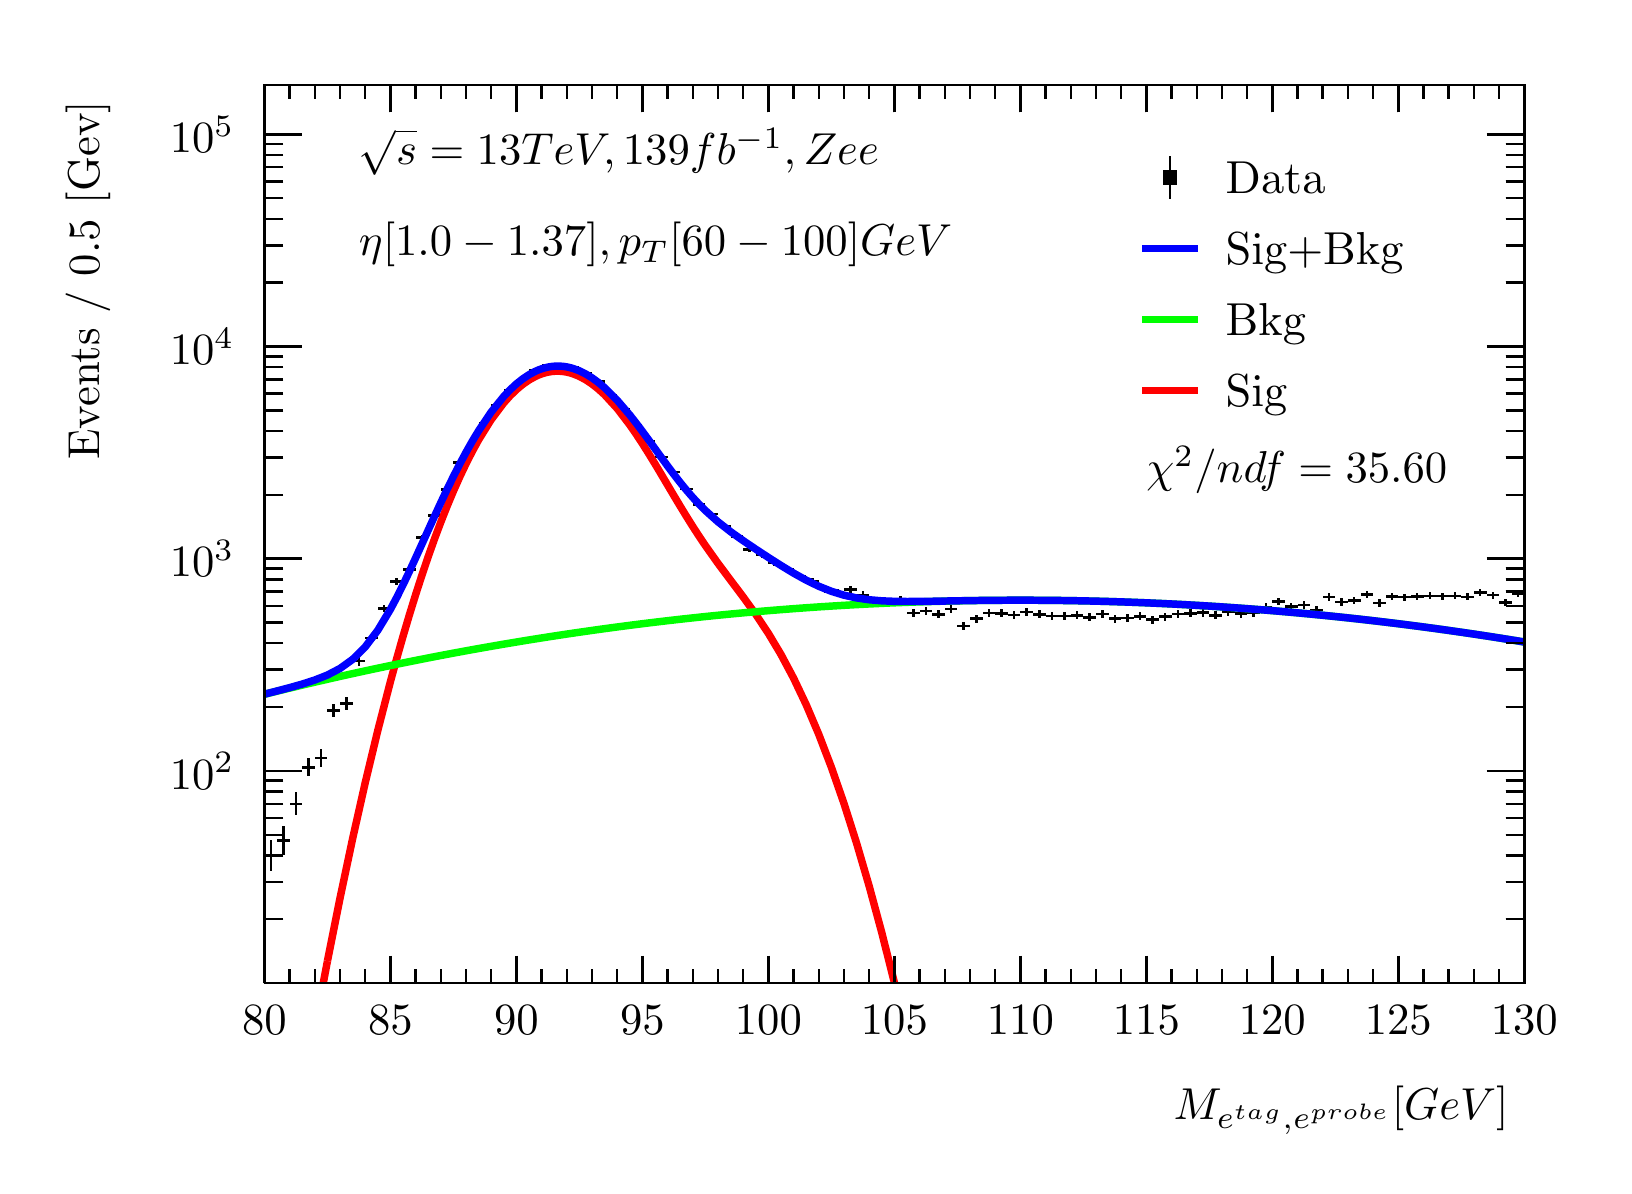
\begin{tikzpicture}
\pgfdeclareplotmark{cross} {
\pgfpathmoveto{\pgfpoint{-0.3\pgfplotmarksize}{\pgfplotmarksize}}
\pgfpathlineto{\pgfpoint{+0.3\pgfplotmarksize}{\pgfplotmarksize}}
\pgfpathlineto{\pgfpoint{+0.3\pgfplotmarksize}{0.3\pgfplotmarksize}}
\pgfpathlineto{\pgfpoint{+1\pgfplotmarksize}{0.3\pgfplotmarksize}}
\pgfpathlineto{\pgfpoint{+1\pgfplotmarksize}{-0.3\pgfplotmarksize}}
\pgfpathlineto{\pgfpoint{+0.3\pgfplotmarksize}{-0.3\pgfplotmarksize}}
\pgfpathlineto{\pgfpoint{+0.3\pgfplotmarksize}{-1.\pgfplotmarksize}}
\pgfpathlineto{\pgfpoint{-0.3\pgfplotmarksize}{-1.\pgfplotmarksize}}
\pgfpathlineto{\pgfpoint{-0.3\pgfplotmarksize}{-0.3\pgfplotmarksize}}
\pgfpathlineto{\pgfpoint{-1.\pgfplotmarksize}{-0.3\pgfplotmarksize}}
\pgfpathlineto{\pgfpoint{-1.\pgfplotmarksize}{0.3\pgfplotmarksize}}
\pgfpathlineto{\pgfpoint{-0.3\pgfplotmarksize}{0.3\pgfplotmarksize}}
\pgfpathclose
\pgfusepathqstroke
}
\pgfdeclareplotmark{cross*} {
\pgfpathmoveto{\pgfpoint{-0.3\pgfplotmarksize}{\pgfplotmarksize}}
\pgfpathlineto{\pgfpoint{+0.3\pgfplotmarksize}{\pgfplotmarksize}}
\pgfpathlineto{\pgfpoint{+0.3\pgfplotmarksize}{0.3\pgfplotmarksize}}
\pgfpathlineto{\pgfpoint{+1\pgfplotmarksize}{0.3\pgfplotmarksize}}
\pgfpathlineto{\pgfpoint{+1\pgfplotmarksize}{-0.3\pgfplotmarksize}}
\pgfpathlineto{\pgfpoint{+0.3\pgfplotmarksize}{-0.3\pgfplotmarksize}}
\pgfpathlineto{\pgfpoint{+0.3\pgfplotmarksize}{-1.\pgfplotmarksize}}
\pgfpathlineto{\pgfpoint{-0.3\pgfplotmarksize}{-1.\pgfplotmarksize}}
\pgfpathlineto{\pgfpoint{-0.3\pgfplotmarksize}{-0.3\pgfplotmarksize}}
\pgfpathlineto{\pgfpoint{-1.\pgfplotmarksize}{-0.3\pgfplotmarksize}}
\pgfpathlineto{\pgfpoint{-1.\pgfplotmarksize}{0.3\pgfplotmarksize}}
\pgfpathlineto{\pgfpoint{-0.3\pgfplotmarksize}{0.3\pgfplotmarksize}}
\pgfpathclose
\pgfusepathqfillstroke
}
\pgfdeclareplotmark{newstar} {
\pgfpathmoveto{\pgfqpoint{0pt}{\pgfplotmarksize}}
\pgfpathlineto{\pgfqpointpolar{44}{0.5\pgfplotmarksize}}
\pgfpathlineto{\pgfqpointpolar{18}{\pgfplotmarksize}}
\pgfpathlineto{\pgfqpointpolar{-20}{0.5\pgfplotmarksize}}
\pgfpathlineto{\pgfqpointpolar{-54}{\pgfplotmarksize}}
\pgfpathlineto{\pgfqpointpolar{-90}{0.5\pgfplotmarksize}}
\pgfpathlineto{\pgfqpointpolar{234}{\pgfplotmarksize}}
\pgfpathlineto{\pgfqpointpolar{198}{0.5\pgfplotmarksize}}
\pgfpathlineto{\pgfqpointpolar{162}{\pgfplotmarksize}}
\pgfpathlineto{\pgfqpointpolar{134}{0.5\pgfplotmarksize}}
\pgfpathclose
\pgfusepathqstroke
}
\pgfdeclareplotmark{newstar*} {
\pgfpathmoveto{\pgfqpoint{0pt}{\pgfplotmarksize}}
\pgfpathlineto{\pgfqpointpolar{44}{0.5\pgfplotmarksize}}
\pgfpathlineto{\pgfqpointpolar{18}{\pgfplotmarksize}}
\pgfpathlineto{\pgfqpointpolar{-20}{0.5\pgfplotmarksize}}
\pgfpathlineto{\pgfqpointpolar{-54}{\pgfplotmarksize}}
\pgfpathlineto{\pgfqpointpolar{-90}{0.5\pgfplotmarksize}}
\pgfpathlineto{\pgfqpointpolar{234}{\pgfplotmarksize}}
\pgfpathlineto{\pgfqpointpolar{198}{0.5\pgfplotmarksize}}
\pgfpathlineto{\pgfqpointpolar{162}{\pgfplotmarksize}}
\pgfpathlineto{\pgfqpointpolar{134}{0.5\pgfplotmarksize}}
\pgfpathclose
\pgfusepathqfillstroke
}
\definecolor{c}{rgb}{1,1,1};
\draw [color=c, fill=c] (0,0) rectangle (20,14.4361);
\draw [color=c, fill=c] (3,2.30977) rectangle (19,13.7143);
\definecolor{c}{rgb}{0,0,0};
\draw [c,line width=0.9] (3,2.30977) -- (3,13.7143) -- (19,13.7143) -- (19,2.30977) -- (3,2.30977);
\definecolor{c}{rgb}{1,1,1};
\draw [color=c, fill=c] (3,2.30977) rectangle (19,13.7143);
\definecolor{c}{rgb}{0,0,0};
\draw [c,line width=0.9] (3,2.30977) -- (3,13.7143) -- (19,13.7143) -- (19,2.30977) -- (3,2.30977);
\draw [c,line width=0.9] (3,2.30977) -- (19,2.30977);
\draw [c,line width=0.9] (3,2.65624) -- (3,2.30977);
\draw [c,line width=0.9] (3.32,2.48301) -- (3.32,2.30977);
\draw [c,line width=0.9] (3.64,2.48301) -- (3.64,2.30977);
\draw [c,line width=0.9] (3.96,2.48301) -- (3.96,2.30977);
\draw [c,line width=0.9] (4.28,2.48301) -- (4.28,2.30977);
\draw [c,line width=0.9] (4.6,2.65624) -- (4.6,2.30977);
\draw [c,line width=0.9] (4.92,2.48301) -- (4.92,2.30977);
\draw [c,line width=0.9] (5.24,2.48301) -- (5.24,2.30977);
\draw [c,line width=0.9] (5.56,2.48301) -- (5.56,2.30977);
\draw [c,line width=0.9] (5.88,2.48301) -- (5.88,2.30977);
\draw [c,line width=0.9] (6.2,2.65624) -- (6.2,2.30977);
\draw [c,line width=0.9] (6.52,2.48301) -- (6.52,2.30977);
\draw [c,line width=0.9] (6.84,2.48301) -- (6.84,2.30977);
\draw [c,line width=0.9] (7.16,2.48301) -- (7.16,2.30977);
\draw [c,line width=0.9] (7.48,2.48301) -- (7.48,2.30977);
\draw [c,line width=0.9] (7.8,2.65624) -- (7.8,2.30977);
\draw [c,line width=0.9] (8.12,2.48301) -- (8.12,2.30977);
\draw [c,line width=0.9] (8.44,2.48301) -- (8.44,2.30977);
\draw [c,line width=0.9] (8.76,2.48301) -- (8.76,2.30977);
\draw [c,line width=0.9] (9.08,2.48301) -- (9.08,2.30977);
\draw [c,line width=0.9] (9.4,2.65624) -- (9.4,2.30977);
\draw [c,line width=0.9] (9.72,2.48301) -- (9.72,2.30977);
\draw [c,line width=0.9] (10.04,2.48301) -- (10.04,2.30977);
\draw [c,line width=0.9] (10.36,2.48301) -- (10.36,2.30977);
\draw [c,line width=0.9] (10.68,2.48301) -- (10.68,2.30977);
\draw [c,line width=0.9] (11,2.65624) -- (11,2.30977);
\draw [c,line width=0.9] (11.32,2.48301) -- (11.32,2.30977);
\draw [c,line width=0.9] (11.64,2.48301) -- (11.64,2.30977);
\draw [c,line width=0.9] (11.96,2.48301) -- (11.96,2.30977);
\draw [c,line width=0.9] (12.28,2.48301) -- (12.28,2.30977);
\draw [c,line width=0.9] (12.6,2.65624) -- (12.6,2.30977);
\draw [c,line width=0.9] (12.92,2.48301) -- (12.92,2.30977);
\draw [c,line width=0.9] (13.24,2.48301) -- (13.24,2.30977);
\draw [c,line width=0.9] (13.56,2.48301) -- (13.56,2.30977);
\draw [c,line width=0.9] (13.88,2.48301) -- (13.88,2.30977);
\draw [c,line width=0.9] (14.2,2.65624) -- (14.2,2.30977);
\draw [c,line width=0.9] (14.52,2.48301) -- (14.52,2.30977);
\draw [c,line width=0.9] (14.84,2.48301) -- (14.84,2.30977);
\draw [c,line width=0.9] (15.16,2.48301) -- (15.16,2.30977);
\draw [c,line width=0.9] (15.48,2.48301) -- (15.48,2.30977);
\draw [c,line width=0.9] (15.8,2.65624) -- (15.8,2.30977);
\draw [c,line width=0.9] (16.12,2.48301) -- (16.12,2.30977);
\draw [c,line width=0.9] (16.44,2.48301) -- (16.44,2.30977);
\draw [c,line width=0.9] (16.76,2.48301) -- (16.76,2.30977);
\draw [c,line width=0.9] (17.08,2.48301) -- (17.08,2.30977);
\draw [c,line width=0.9] (17.4,2.65624) -- (17.4,2.30977);
\draw [c,line width=0.9] (17.72,2.48301) -- (17.72,2.30977);
\draw [c,line width=0.9] (18.04,2.48301) -- (18.04,2.30977);
\draw [c,line width=0.9] (18.36,2.48301) -- (18.36,2.30977);
\draw [c,line width=0.9] (18.68,2.48301) -- (18.68,2.30977);
\draw [c,line width=0.9] (19,2.65624) -- (19,2.30977);
\draw [anchor=base] (3,1.66015) node[scale=1.61424, color=c, rotate=0]{80};
\draw [anchor=base] (4.6,1.66015) node[scale=1.61424, color=c, rotate=0]{85};
\draw [anchor=base] (6.2,1.66015) node[scale=1.61424, color=c, rotate=0]{90};
\draw [anchor=base] (7.8,1.66015) node[scale=1.61424, color=c, rotate=0]{95};
\draw [anchor=base] (9.4,1.66015) node[scale=1.61424, color=c, rotate=0]{100};
\draw [anchor=base] (11,1.66015) node[scale=1.61424, color=c, rotate=0]{105};
\draw [anchor=base] (12.6,1.66015) node[scale=1.61424, color=c, rotate=0]{110};
\draw [anchor=base] (14.2,1.66015) node[scale=1.61424, color=c, rotate=0]{115};
\draw [anchor=base] (15.8,1.66015) node[scale=1.61424, color=c, rotate=0]{120};
\draw [anchor=base] (17.4,1.66015) node[scale=1.61424, color=c, rotate=0]{125};
\draw [anchor=base] (19,1.66015) node[scale=1.61424, color=c, rotate=0]{130};
\draw [anchor= east] (19,0.692932) node[scale=1.61424, color=c, rotate=0]{$M_{e^{tag}, e^{probe}}  [GeV]$};
\draw [c,line width=0.9] (3,13.7143) -- (19,13.7143);
\draw [c,line width=0.9] (3,13.3678) -- (3,13.7143);
\draw [c,line width=0.9] (3.32,13.5411) -- (3.32,13.7143);
\draw [c,line width=0.9] (3.64,13.5411) -- (3.64,13.7143);
\draw [c,line width=0.9] (3.96,13.5411) -- (3.96,13.7143);
\draw [c,line width=0.9] (4.28,13.5411) -- (4.28,13.7143);
\draw [c,line width=0.9] (4.6,13.3678) -- (4.6,13.7143);
\draw [c,line width=0.9] (4.92,13.5411) -- (4.92,13.7143);
\draw [c,line width=0.9] (5.24,13.5411) -- (5.24,13.7143);
\draw [c,line width=0.9] (5.56,13.5411) -- (5.56,13.7143);
\draw [c,line width=0.9] (5.88,13.5411) -- (5.88,13.7143);
\draw [c,line width=0.9] (6.2,13.3678) -- (6.2,13.7143);
\draw [c,line width=0.9] (6.52,13.5411) -- (6.52,13.7143);
\draw [c,line width=0.9] (6.84,13.5411) -- (6.84,13.7143);
\draw [c,line width=0.9] (7.16,13.5411) -- (7.16,13.7143);
\draw [c,line width=0.9] (7.48,13.5411) -- (7.48,13.7143);
\draw [c,line width=0.9] (7.8,13.3678) -- (7.8,13.7143);
\draw [c,line width=0.9] (8.12,13.5411) -- (8.12,13.7143);
\draw [c,line width=0.9] (8.44,13.5411) -- (8.44,13.7143);
\draw [c,line width=0.9] (8.76,13.5411) -- (8.76,13.7143);
\draw [c,line width=0.9] (9.08,13.5411) -- (9.08,13.7143);
\draw [c,line width=0.9] (9.4,13.3678) -- (9.4,13.7143);
\draw [c,line width=0.9] (9.72,13.5411) -- (9.72,13.7143);
\draw [c,line width=0.9] (10.04,13.5411) -- (10.04,13.7143);
\draw [c,line width=0.9] (10.36,13.5411) -- (10.36,13.7143);
\draw [c,line width=0.9] (10.68,13.5411) -- (10.68,13.7143);
\draw [c,line width=0.9] (11,13.3678) -- (11,13.7143);
\draw [c,line width=0.9] (11.32,13.5411) -- (11.32,13.7143);
\draw [c,line width=0.9] (11.64,13.5411) -- (11.64,13.7143);
\draw [c,line width=0.9] (11.96,13.5411) -- (11.96,13.7143);
\draw [c,line width=0.9] (12.28,13.5411) -- (12.28,13.7143);
\draw [c,line width=0.9] (12.6,13.3678) -- (12.6,13.7143);
\draw [c,line width=0.9] (12.92,13.5411) -- (12.92,13.7143);
\draw [c,line width=0.9] (13.24,13.5411) -- (13.24,13.7143);
\draw [c,line width=0.9] (13.56,13.5411) -- (13.56,13.7143);
\draw [c,line width=0.9] (13.88,13.5411) -- (13.88,13.7143);
\draw [c,line width=0.9] (14.2,13.3678) -- (14.2,13.7143);
\draw [c,line width=0.9] (14.52,13.5411) -- (14.52,13.7143);
\draw [c,line width=0.9] (14.84,13.5411) -- (14.84,13.7143);
\draw [c,line width=0.9] (15.16,13.5411) -- (15.16,13.7143);
\draw [c,line width=0.9] (15.48,13.5411) -- (15.48,13.7143);
\draw [c,line width=0.9] (15.8,13.3678) -- (15.8,13.7143);
\draw [c,line width=0.9] (16.12,13.5411) -- (16.12,13.7143);
\draw [c,line width=0.9] (16.44,13.5411) -- (16.44,13.7143);
\draw [c,line width=0.9] (16.76,13.5411) -- (16.76,13.7143);
\draw [c,line width=0.9] (17.08,13.5411) -- (17.08,13.7143);
\draw [c,line width=0.9] (17.4,13.3678) -- (17.4,13.7143);
\draw [c,line width=0.9] (17.72,13.5411) -- (17.72,13.7143);
\draw [c,line width=0.9] (18.04,13.5411) -- (18.04,13.7143);
\draw [c,line width=0.9] (18.36,13.5411) -- (18.36,13.7143);
\draw [c,line width=0.9] (18.68,13.5411) -- (18.68,13.7143);
\draw [c,line width=0.9] (19,13.3678) -- (19,13.7143);
\draw [c,line width=0.9] (3,2.30977) -- (3,13.7143);
\draw [c,line width=0.9] (3.237,3.1209) -- (3,3.1209);
\draw [c,line width=0.9] (3.237,3.59538) -- (3,3.59538);
\draw [c,line width=0.9] (3.237,3.93203) -- (3,3.93203);
\draw [c,line width=0.9] (3.237,4.19316) -- (3,4.19316);
\draw [c,line width=0.9] (3.237,4.40651) -- (3,4.40651);
\draw [c,line width=0.9] (3.237,4.5869) -- (3,4.5869);
\draw [c,line width=0.9] (3.237,4.74316) -- (3,4.74316);
\draw [c,line width=0.9] (3.237,4.881) -- (3,4.881);
\draw [c,line width=0.9] (3.474,5.00429) -- (3,5.00429);
\draw [anchor= east] (2.82,5.00429) node[scale=1.61424, color=c, rotate=0]{$10^{2}$};
\draw [c,line width=0.9] (3.237,5.81542) -- (3,5.81542);
\draw [c,line width=0.9] (3.237,6.2899) -- (3,6.2899);
\draw [c,line width=0.9] (3.237,6.62655) -- (3,6.62655);
\draw [c,line width=0.9] (3.237,6.88768) -- (3,6.88768);
\draw [c,line width=0.9] (3.237,7.10103) -- (3,7.10103);
\draw [c,line width=0.9] (3.237,7.28142) -- (3,7.28142);
\draw [c,line width=0.9] (3.237,7.43768) -- (3,7.43768);
\draw [c,line width=0.9] (3.237,7.57551) -- (3,7.57551);
\draw [c,line width=0.9] (3.474,7.69881) -- (3,7.69881);
\draw [anchor= east] (2.82,7.69881) node[scale=1.61424, color=c, rotate=0]{$10^{3}$};
\draw [c,line width=0.9] (3.237,8.50994) -- (3,8.50994);
\draw [c,line width=0.9] (3.237,8.98442) -- (3,8.98442);
\draw [c,line width=0.9] (3.237,9.32107) -- (3,9.32107);
\draw [c,line width=0.9] (3.237,9.58219) -- (3,9.58219);
\draw [c,line width=0.9] (3.237,9.79555) -- (3,9.79555);
\draw [c,line width=0.9] (3.237,9.97594) -- (3,9.97594);
\draw [c,line width=0.9] (3.237,10.1322) -- (3,10.1322);
\draw [c,line width=0.9] (3.237,10.27) -- (3,10.27);
\draw [c,line width=0.9] (3.474,10.3933) -- (3,10.3933);
\draw [anchor= east] (2.82,10.3933) node[scale=1.61424, color=c, rotate=0]{$10^{4}$};
\draw [c,line width=0.9] (3.237,11.2045) -- (3,11.2045);
\draw [c,line width=0.9] (3.237,11.6789) -- (3,11.6789);
\draw [c,line width=0.9] (3.237,12.0156) -- (3,12.0156);
\draw [c,line width=0.9] (3.237,12.2767) -- (3,12.2767);
\draw [c,line width=0.9] (3.237,12.4901) -- (3,12.4901);
\draw [c,line width=0.9] (3.237,12.6705) -- (3,12.6705);
\draw [c,line width=0.9] (3.237,12.8267) -- (3,12.8267);
\draw [c,line width=0.9] (3.237,12.9645) -- (3,12.9645);
\draw [c,line width=0.9] (3.474,13.0878) -- (3,13.0878);
\draw [anchor= east] (2.82,13.0878) node[scale=1.61424, color=c, rotate=0]{$10^{5}$};
\draw [anchor= east] (0.76,13.7143) node[scale=1.61424, color=c, rotate=90]{Events / 0.5 [Gev]};
\draw [c,line width=0.9] (19,2.30977) -- (19,13.7143);
\draw [c,line width=0.9] (18.763,3.1209) -- (19,3.1209);
\draw [c,line width=0.9] (18.763,3.59538) -- (19,3.59538);
\draw [c,line width=0.9] (18.763,3.93203) -- (19,3.93203);
\draw [c,line width=0.9] (18.763,4.19316) -- (19,4.19316);
\draw [c,line width=0.9] (18.763,4.40651) -- (19,4.40651);
\draw [c,line width=0.9] (18.763,4.5869) -- (19,4.5869);
\draw [c,line width=0.9] (18.763,4.74316) -- (19,4.74316);
\draw [c,line width=0.9] (18.763,4.881) -- (19,4.881);
\draw [c,line width=0.9] (18.526,5.00429) -- (19,5.00429);
\draw [c,line width=0.9] (18.763,5.81542) -- (19,5.81542);
\draw [c,line width=0.9] (18.763,6.2899) -- (19,6.2899);
\draw [c,line width=0.9] (18.763,6.62655) -- (19,6.62655);
\draw [c,line width=0.9] (18.763,6.88768) -- (19,6.88768);
\draw [c,line width=0.9] (18.763,7.10103) -- (19,7.10103);
\draw [c,line width=0.9] (18.763,7.28142) -- (19,7.28142);
\draw [c,line width=0.9] (18.763,7.43768) -- (19,7.43768);
\draw [c,line width=0.9] (18.763,7.57551) -- (19,7.57551);
\draw [c,line width=0.9] (18.526,7.69881) -- (19,7.69881);
\draw [c,line width=0.9] (18.763,8.50994) -- (19,8.50994);
\draw [c,line width=0.9] (18.763,8.98442) -- (19,8.98442);
\draw [c,line width=0.9] (18.763,9.32107) -- (19,9.32107);
\draw [c,line width=0.9] (18.763,9.58219) -- (19,9.58219);
\draw [c,line width=0.9] (18.763,9.79555) -- (19,9.79555);
\draw [c,line width=0.9] (18.763,9.97594) -- (19,9.97594);
\draw [c,line width=0.9] (18.763,10.1322) -- (19,10.1322);
\draw [c,line width=0.9] (18.763,10.27) -- (19,10.27);
\draw [c,line width=0.9] (18.526,10.3933) -- (19,10.3933);
\draw [c,line width=0.9] (18.763,11.2045) -- (19,11.2045);
\draw [c,line width=0.9] (18.763,11.6789) -- (19,11.6789);
\draw [c,line width=0.9] (18.763,12.0156) -- (19,12.0156);
\draw [c,line width=0.9] (18.763,12.2767) -- (19,12.2767);
\draw [c,line width=0.9] (18.763,12.4901) -- (19,12.4901);
\draw [c,line width=0.9] (18.763,12.6705) -- (19,12.6705);
\draw [c,line width=0.9] (18.763,12.8267) -- (19,12.8267);
\draw [c,line width=0.9] (18.763,12.9645) -- (19,12.9645);
\draw [c,line width=0.9] (18.526,13.0878) -- (19,13.0878);
\draw [c,line width=0.9] (3.08,3.93204) -- (3,3.93204);
\draw [c,line width=0.9] (3,3.93204) -- (3,3.93204);
\draw [c,line width=0.9] (3.08,3.93204) -- (3.16,3.93204);
\draw [c,line width=0.9] (3.16,3.93204) -- (3.16,3.93204);
\draw [c,line width=0.9] (3.08,3.93204) -- (3.08,4.13011);
\draw [c,line width=0.9] (3.08,4.13011) -- (3.08,4.13011);
\draw [c,line width=0.9] (3.08,3.93204) -- (3.08,3.73155);
\draw [c,line width=0.9] (3.08,3.73155) -- (3.08,3.73155);
\draw [c,line width=0.9] (3.24,4.12075) -- (3.16,4.12075);
\draw [c,line width=0.9] (3.16,4.12075) -- (3.16,4.12075);
\draw [c,line width=0.9] (3.24,4.12075) -- (3.32,4.12075);
\draw [c,line width=0.9] (3.32,4.12075) -- (3.32,4.12075);
\draw [c,line width=0.9] (3.24,4.12075) -- (3.24,4.30266);
\draw [c,line width=0.9] (3.24,4.30266) -- (3.24,4.30266);
\draw [c,line width=0.9] (3.24,4.12075) -- (3.24,3.93696);
\draw [c,line width=0.9] (3.24,3.93696) -- (3.24,3.93696);
\draw [c,line width=0.9] (3.4,4.58691) -- (3.32,4.58691);
\draw [c,line width=0.9] (3.32,4.58691) -- (3.32,4.58691);
\draw [c,line width=0.9] (3.4,4.58691) -- (3.48,4.58691);
\draw [c,line width=0.9] (3.48,4.58691) -- (3.48,4.58691);
\draw [c,line width=0.9] (3.4,4.58691) -- (3.4,4.73445);
\draw [c,line width=0.9] (3.4,4.73445) -- (3.4,4.73445);
\draw [c,line width=0.9] (3.4,4.58691) -- (3.4,4.43833);
\draw [c,line width=0.9] (3.4,4.43833) -- (3.4,4.43833);
\draw [c,line width=0.9] (3.56,5.05019) -- (3.48,5.05019);
\draw [c,line width=0.9] (3.48,5.05019) -- (3.48,5.05019);
\draw [c,line width=0.9] (3.56,5.05019) -- (3.64,5.05019);
\draw [c,line width=0.9] (3.64,5.05019) -- (3.64,5.05019);
\draw [c,line width=0.9] (3.56,5.05019) -- (3.56,5.16489);
\draw [c,line width=0.9] (3.56,5.16489) -- (3.56,5.16489);
\draw [c,line width=0.9] (3.56,5.05019) -- (3.56,4.93549);
\draw [c,line width=0.9] (3.56,4.93549) -- (3.56,4.93549);
\draw [c,line width=0.9] (3.72,5.16784) -- (3.64,5.16784);
\draw [c,line width=0.9] (3.64,5.16784) -- (3.64,5.16784);
\draw [c,line width=0.9] (3.72,5.16784) -- (3.8,5.16784);
\draw [c,line width=0.9] (3.8,5.16784) -- (3.8,5.16784);
\draw [c,line width=0.9] (3.72,5.16784) -- (3.72,5.27693);
\draw [c,line width=0.9] (3.72,5.27693) -- (3.72,5.27693);
\draw [c,line width=0.9] (3.72,5.16784) -- (3.72,5.05876);
\draw [c,line width=0.9] (3.72,5.05876) -- (3.72,5.05876);
\draw [c,line width=0.9] (3.88,5.77373) -- (3.8,5.77373);
\draw [c,line width=0.9] (3.8,5.77373) -- (3.8,5.77373);
\draw [c,line width=0.9] (3.88,5.77373) -- (3.96,5.77373);
\draw [c,line width=0.9] (3.96,5.77373) -- (3.96,5.77373);
\draw [c,line width=0.9] (3.88,5.77373) -- (3.88,5.85795);
\draw [c,line width=0.9] (3.88,5.85795) -- (3.88,5.85795);
\draw [c,line width=0.9] (3.88,5.77373) -- (3.88,5.68952);
\draw [c,line width=0.9] (3.88,5.68952) -- (3.88,5.68952);
\draw [c,line width=0.9] (4.04,5.86132) -- (3.96,5.86132);
\draw [c,line width=0.9] (3.96,5.86132) -- (3.96,5.86132);
\draw [c,line width=0.9] (4.04,5.86132) -- (4.12,5.86132);
\draw [c,line width=0.9] (4.12,5.86132) -- (4.12,5.86132);
\draw [c,line width=0.9] (4.04,5.86132) -- (4.04,5.94244);
\draw [c,line width=0.9] (4.04,5.94244) -- (4.04,5.94244);
\draw [c,line width=0.9] (4.04,5.86132) -- (4.04,5.7802);
\draw [c,line width=0.9] (4.04,5.7802) -- (4.04,5.7802);
\draw [c,line width=0.9] (4.2,6.40144) -- (4.12,6.40144);
\draw [c,line width=0.9] (4.12,6.40144) -- (4.12,6.40144);
\draw [c,line width=0.9] (4.2,6.40144) -- (4.28,6.40144);
\draw [c,line width=0.9] (4.28,6.40144) -- (4.28,6.40144);
\draw [c,line width=0.9] (4.2,6.40144) -- (4.2,6.46585);
\draw [c,line width=0.9] (4.2,6.46585) -- (4.2,6.46585);
\draw [c,line width=0.9] (4.2,6.40144) -- (4.2,6.33703);
\draw [c,line width=0.9] (4.2,6.33703) -- (4.2,6.33703);
\draw [c,line width=0.9] (4.36,6.68921) -- (4.28,6.68921);
\draw [c,line width=0.9] (4.28,6.68921) -- (4.28,6.68921);
\draw [c,line width=0.9] (4.36,6.68921) -- (4.44,6.68921);
\draw [c,line width=0.9] (4.44,6.68921) -- (4.44,6.68921);
\draw [c,line width=0.9] (4.36,6.68921) -- (4.36,6.74617);
\draw [c,line width=0.9] (4.36,6.74617) -- (4.36,6.74617);
\draw [c,line width=0.9] (4.36,6.68921) -- (4.36,6.63225);
\draw [c,line width=0.9] (4.36,6.63225) -- (4.36,6.63225);
\draw [c,line width=0.9] (4.52,7.06539) -- (4.44,7.06539);
\draw [c,line width=0.9] (4.44,7.06539) -- (4.44,7.06539);
\draw [c,line width=0.9] (4.52,7.06539) -- (4.6,7.06539);
\draw [c,line width=0.9] (4.6,7.06539) -- (4.6,7.06539);
\draw [c,line width=0.9] (4.52,7.06539) -- (4.52,7.11389);
\draw [c,line width=0.9] (4.52,7.11389) -- (4.52,7.11389);
\draw [c,line width=0.9] (4.52,7.06539) -- (4.52,7.01689);
\draw [c,line width=0.9] (4.52,7.01689) -- (4.52,7.01689);
\draw [c,line width=0.9] (4.68,7.40655) -- (4.6,7.40655);
\draw [c,line width=0.9] (4.6,7.40655) -- (4.6,7.40655);
\draw [c,line width=0.9] (4.68,7.40655) -- (4.76,7.40655);
\draw [c,line width=0.9] (4.76,7.40655) -- (4.76,7.40655);
\draw [c,line width=0.9] (4.68,7.40655) -- (4.68,7.44848);
\draw [c,line width=0.9] (4.68,7.44848) -- (4.68,7.44848);
\draw [c,line width=0.9] (4.68,7.40655) -- (4.68,7.36463);
\draw [c,line width=0.9] (4.68,7.36463) -- (4.68,7.36463);
\draw [c,line width=0.9] (4.84,7.55981) -- (4.76,7.55981);
\draw [c,line width=0.9] (4.76,7.55981) -- (4.76,7.55981);
\draw [c,line width=0.9] (4.84,7.55981) -- (4.92,7.55981);
\draw [c,line width=0.9] (4.92,7.55981) -- (4.92,7.55981);
\draw [c,line width=0.9] (4.84,7.55981) -- (4.84,7.59907);
\draw [c,line width=0.9] (4.84,7.59907) -- (4.84,7.59907);
\draw [c,line width=0.9] (4.84,7.55981) -- (4.84,7.52054);
\draw [c,line width=0.9] (4.84,7.52054) -- (4.84,7.52054);
\draw [c,line width=0.9] (5,7.96647) -- (4.92,7.96647);
\draw [c,line width=0.9] (4.92,7.96647) -- (4.92,7.96647);
\draw [c,line width=0.9] (5,7.96647) -- (5.08,7.96647);
\draw [c,line width=0.9] (5.08,7.96647) -- (5.08,7.96647);
\draw [c,line width=0.9] (5,7.96647) -- (5,7.99948);
\draw [c,line width=0.9] (5,7.99948) -- (5,7.99948);
\draw [c,line width=0.9] (5,7.96647) -- (5,7.93346);
\draw [c,line width=0.9] (5,7.93346) -- (5,7.93346);
\draw [c,line width=0.9] (5.16,8.24808) -- (5.08,8.24808);
\draw [c,line width=0.9] (5.08,8.24808) -- (5.08,8.24808);
\draw [c,line width=0.9] (5.16,8.24808) -- (5.24,8.24808);
\draw [c,line width=0.9] (5.24,8.24808) -- (5.24,8.24808);
\draw [c,line width=0.9] (5.16,8.24808) -- (5.16,8.27735);
\draw [c,line width=0.9] (5.16,8.27735) -- (5.16,8.27735);
\draw [c,line width=0.9] (5.16,8.24808) -- (5.16,8.21882);
\draw [c,line width=0.9] (5.16,8.21882) -- (5.16,8.21882);
\draw [c,line width=0.9] (5.32,8.57702) -- (5.24,8.57702);
\draw [c,line width=0.9] (5.24,8.57702) -- (5.24,8.57702);
\draw [c,line width=0.9] (5.32,8.57702) -- (5.4,8.57702);
\draw [c,line width=0.9] (5.4,8.57702) -- (5.4,8.57702);
\draw [c,line width=0.9] (5.32,8.57702) -- (5.32,8.60245);
\draw [c,line width=0.9] (5.32,8.60245) -- (5.32,8.60245);
\draw [c,line width=0.9] (5.32,8.57702) -- (5.32,8.55159);
\draw [c,line width=0.9] (5.32,8.55159) -- (5.32,8.55159);
\draw [c,line width=0.9] (5.48,8.91905) -- (5.4,8.91905);
\draw [c,line width=0.9] (5.4,8.91905) -- (5.4,8.91905);
\draw [c,line width=0.9] (5.48,8.91905) -- (5.56,8.91905);
\draw [c,line width=0.9] (5.56,8.91905) -- (5.56,8.91905);
\draw [c,line width=0.9] (5.48,8.91905) -- (5.48,8.94102);
\draw [c,line width=0.9] (5.48,8.94102) -- (5.48,8.94102);
\draw [c,line width=0.9] (5.48,8.91905) -- (5.48,8.89708);
\draw [c,line width=0.9] (5.48,8.89708) -- (5.48,8.89708);
\draw [c,line width=0.9] (5.64,9.13192) -- (5.56,9.13192);
\draw [c,line width=0.9] (5.56,9.13192) -- (5.56,9.13192);
\draw [c,line width=0.9] (5.64,9.13192) -- (5.72,9.13192);
\draw [c,line width=0.9] (5.72,9.13192) -- (5.72,9.13192);
\draw [c,line width=0.9] (5.64,9.13192) -- (5.64,9.15198);
\draw [c,line width=0.9] (5.64,9.15198) -- (5.64,9.15198);
\draw [c,line width=0.9] (5.64,9.13192) -- (5.64,9.11186);
\draw [c,line width=0.9] (5.64,9.11186) -- (5.64,9.11186);
\draw [c,line width=0.9] (5.8,9.41384) -- (5.72,9.41384);
\draw [c,line width=0.9] (5.72,9.41384) -- (5.72,9.41384);
\draw [c,line width=0.9] (5.8,9.41384) -- (5.88,9.41384);
\draw [c,line width=0.9] (5.88,9.41384) -- (5.88,9.41384);
\draw [c,line width=0.9] (5.8,9.41384) -- (5.8,9.43162);
\draw [c,line width=0.9] (5.8,9.43162) -- (5.8,9.43162);
\draw [c,line width=0.9] (5.8,9.41384) -- (5.8,9.39605);
\draw [c,line width=0.9] (5.8,9.39605) -- (5.8,9.39605);
\draw [c,line width=0.9] (5.96,9.6506) -- (5.88,9.6506);
\draw [c,line width=0.9] (5.88,9.6506) -- (5.88,9.6506);
\draw [c,line width=0.9] (5.96,9.6506) -- (6.04,9.6506);
\draw [c,line width=0.9] (6.04,9.6506) -- (6.04,9.6506);
\draw [c,line width=0.9] (5.96,9.6506) -- (5.96,9.66668);
\draw [c,line width=0.9] (5.96,9.66668) -- (5.96,9.66668);
\draw [c,line width=0.9] (5.96,9.6506) -- (5.96,9.63453);
\draw [c,line width=0.9] (5.96,9.63453) -- (5.96,9.63453);
\draw [c,line width=0.9] (6.12,9.83298) -- (6.04,9.83298);
\draw [c,line width=0.9] (6.04,9.83298) -- (6.04,9.83298);
\draw [c,line width=0.9] (6.12,9.83298) -- (6.2,9.83298);
\draw [c,line width=0.9] (6.2,9.83298) -- (6.2,9.83298);
\draw [c,line width=0.9] (6.12,9.83298) -- (6.12,9.84785);
\draw [c,line width=0.9] (6.12,9.84785) -- (6.12,9.84785);
\draw [c,line width=0.9] (6.12,9.83298) -- (6.12,9.81811);
\draw [c,line width=0.9] (6.12,9.81811) -- (6.12,9.81811);
\draw [c,line width=0.9] (6.28,9.96215) -- (6.2,9.96215);
\draw [c,line width=0.9] (6.2,9.96215) -- (6.2,9.96215);
\draw [c,line width=0.9] (6.28,9.96215) -- (6.36,9.96215);
\draw [c,line width=0.9] (6.36,9.96215) -- (6.36,9.96215);
\draw [c,line width=0.9] (6.28,9.96215) -- (6.28,9.97622);
\draw [c,line width=0.9] (6.28,9.97622) -- (6.28,9.97622);
\draw [c,line width=0.9] (6.28,9.96215) -- (6.28,9.94808);
\draw [c,line width=0.9] (6.28,9.94808) -- (6.28,9.94808);
\draw [c,line width=0.9] (6.44,10.0901) -- (6.36,10.0901);
\draw [c,line width=0.9] (6.36,10.0901) -- (6.36,10.0901);
\draw [c,line width=0.9] (6.44,10.0901) -- (6.52,10.0901);
\draw [c,line width=0.9] (6.52,10.0901) -- (6.52,10.0901);
\draw [c,line width=0.9] (6.44,10.0901) -- (6.44,10.1034);
\draw [c,line width=0.9] (6.44,10.1034) -- (6.44,10.1034);
\draw [c,line width=0.9] (6.44,10.0901) -- (6.44,10.0767);
\draw [c,line width=0.9] (6.44,10.0767) -- (6.44,10.0767);
\draw [c,line width=0.9] (6.6,10.1545) -- (6.52,10.1545);
\draw [c,line width=0.9] (6.52,10.1545) -- (6.52,10.1545);
\draw [c,line width=0.9] (6.6,10.1545) -- (6.68,10.1545);
\draw [c,line width=0.9] (6.68,10.1545) -- (6.68,10.1545);
\draw [c,line width=0.9] (6.6,10.1545) -- (6.6,10.1675);
\draw [c,line width=0.9] (6.6,10.1675) -- (6.6,10.1675);
\draw [c,line width=0.9] (6.6,10.1545) -- (6.6,10.1416);
\draw [c,line width=0.9] (6.6,10.1416) -- (6.6,10.1416);
\draw [c,line width=0.9] (6.76,10.1734) -- (6.68,10.1734);
\draw [c,line width=0.9] (6.68,10.1734) -- (6.68,10.1734);
\draw [c,line width=0.9] (6.76,10.1734) -- (6.84,10.1734);
\draw [c,line width=0.9] (6.84,10.1734) -- (6.84,10.1734);
\draw [c,line width=0.9] (6.76,10.1734) -- (6.76,10.1863);
\draw [c,line width=0.9] (6.76,10.1863) -- (6.76,10.1863);
\draw [c,line width=0.9] (6.76,10.1734) -- (6.76,10.1606);
\draw [c,line width=0.9] (6.76,10.1606) -- (6.76,10.1606);
\draw [c,line width=0.9] (6.92,10.1275) -- (6.84,10.1275);
\draw [c,line width=0.9] (6.84,10.1275) -- (6.84,10.1275);
\draw [c,line width=0.9] (6.92,10.1275) -- (7,10.1275);
\draw [c,line width=0.9] (7,10.1275) -- (7,10.1275);
\draw [c,line width=0.9] (6.92,10.1275) -- (6.92,10.1406);
\draw [c,line width=0.9] (6.92,10.1406) -- (6.92,10.1406);
\draw [c,line width=0.9] (6.92,10.1275) -- (6.92,10.1144);
\draw [c,line width=0.9] (6.92,10.1144) -- (6.92,10.1144);
\draw [c,line width=0.9] (7.08,10.0498) -- (7,10.0498);
\draw [c,line width=0.9] (7,10.0498) -- (7,10.0498);
\draw [c,line width=0.9] (7.08,10.0498) -- (7.16,10.0498);
\draw [c,line width=0.9] (7.16,10.0498) -- (7.16,10.0498);
\draw [c,line width=0.9] (7.08,10.0498) -- (7.08,10.0633);
\draw [c,line width=0.9] (7.08,10.0633) -- (7.08,10.0633);
\draw [c,line width=0.9] (7.08,10.0498) -- (7.08,10.0362);
\draw [c,line width=0.9] (7.08,10.0362) -- (7.08,10.0362);
\draw [c,line width=0.9] (7.24,9.94888) -- (7.16,9.94888);
\draw [c,line width=0.9] (7.16,9.94888) -- (7.16,9.94888);
\draw [c,line width=0.9] (7.24,9.94888) -- (7.32,9.94888);
\draw [c,line width=0.9] (7.32,9.94888) -- (7.32,9.94888);
\draw [c,line width=0.9] (7.24,9.94888) -- (7.24,9.96303);
\draw [c,line width=0.9] (7.24,9.96303) -- (7.24,9.96303);
\draw [c,line width=0.9] (7.24,9.94888) -- (7.24,9.93473);
\draw [c,line width=0.9] (7.24,9.93473) -- (7.24,9.93473);
\draw [c,line width=0.9] (7.4,9.77964) -- (7.32,9.77964);
\draw [c,line width=0.9] (7.32,9.77964) -- (7.32,9.77964);
\draw [c,line width=0.9] (7.4,9.77964) -- (7.48,9.77964);
\draw [c,line width=0.9] (7.48,9.77964) -- (7.48,9.77964);
\draw [c,line width=0.9] (7.4,9.77964) -- (7.4,9.79486);
\draw [c,line width=0.9] (7.4,9.79486) -- (7.4,9.79486);
\draw [c,line width=0.9] (7.4,9.77964) -- (7.4,9.76443);
\draw [c,line width=0.9] (7.4,9.76443) -- (7.4,9.76443);
\draw [c,line width=0.9] (7.56,9.59152) -- (7.48,9.59152);
\draw [c,line width=0.9] (7.48,9.59152) -- (7.48,9.59152);
\draw [c,line width=0.9] (7.56,9.59152) -- (7.64,9.59152);
\draw [c,line width=0.9] (7.64,9.59152) -- (7.64,9.59152);
\draw [c,line width=0.9] (7.56,9.59152) -- (7.56,9.608);
\draw [c,line width=0.9] (7.56,9.608) -- (7.56,9.608);
\draw [c,line width=0.9] (7.56,9.59152) -- (7.56,9.57504);
\draw [c,line width=0.9] (7.56,9.57504) -- (7.56,9.57504);
\draw [c,line width=0.9] (7.72,9.39284) -- (7.64,9.39284);
\draw [c,line width=0.9] (7.64,9.39284) -- (7.64,9.39284);
\draw [c,line width=0.9] (7.72,9.39284) -- (7.8,9.39284);
\draw [c,line width=0.9] (7.8,9.39284) -- (7.8,9.39284);
\draw [c,line width=0.9] (7.72,9.39284) -- (7.72,9.41078);
\draw [c,line width=0.9] (7.72,9.41078) -- (7.72,9.41078);
\draw [c,line width=0.9] (7.72,9.39284) -- (7.72,9.3749);
\draw [c,line width=0.9] (7.72,9.3749) -- (7.72,9.3749);
\draw [c,line width=0.9] (7.88,9.18798) -- (7.8,9.18798);
\draw [c,line width=0.9] (7.8,9.18798) -- (7.8,9.18798);
\draw [c,line width=0.9] (7.88,9.18798) -- (7.96,9.18798);
\draw [c,line width=0.9] (7.96,9.18798) -- (7.96,9.18798);
\draw [c,line width=0.9] (7.88,9.18798) -- (7.88,9.20757);
\draw [c,line width=0.9] (7.88,9.20757) -- (7.88,9.20757);
\draw [c,line width=0.9] (7.88,9.18798) -- (7.88,9.1684);
\draw [c,line width=0.9] (7.88,9.1684) -- (7.88,9.1684);
\draw [c,line width=0.9] (8.04,8.99297) -- (7.96,8.99297);
\draw [c,line width=0.9] (7.96,8.99297) -- (7.96,8.99297);
\draw [c,line width=0.9] (8.04,8.99297) -- (8.12,8.99297);
\draw [c,line width=0.9] (8.12,8.99297) -- (8.12,8.99297);
\draw [c,line width=0.9] (8.04,8.99297) -- (8.04,9.01426);
\draw [c,line width=0.9] (8.04,9.01426) -- (8.04,9.01426);
\draw [c,line width=0.9] (8.04,8.99297) -- (8.04,8.97168);
\draw [c,line width=0.9] (8.04,8.97168) -- (8.04,8.97168);
\draw [c,line width=0.9] (8.2,8.8011) -- (8.12,8.8011);
\draw [c,line width=0.9] (8.12,8.8011) -- (8.12,8.8011);
\draw [c,line width=0.9] (8.2,8.8011) -- (8.28,8.8011);
\draw [c,line width=0.9] (8.28,8.8011) -- (8.28,8.8011);
\draw [c,line width=0.9] (8.2,8.8011) -- (8.2,8.82421);
\draw [c,line width=0.9] (8.2,8.82421) -- (8.2,8.82421);
\draw [c,line width=0.9] (8.2,8.8011) -- (8.2,8.778);
\draw [c,line width=0.9] (8.2,8.778) -- (8.2,8.778);
\draw [c,line width=0.9] (8.36,8.58198) -- (8.28,8.58198);
\draw [c,line width=0.9] (8.28,8.58198) -- (8.28,8.58198);
\draw [c,line width=0.9] (8.36,8.58198) -- (8.44,8.58198);
\draw [c,line width=0.9] (8.44,8.58198) -- (8.44,8.58198);
\draw [c,line width=0.9] (8.36,8.58198) -- (8.36,8.60736);
\draw [c,line width=0.9] (8.36,8.60736) -- (8.36,8.60736);
\draw [c,line width=0.9] (8.36,8.58198) -- (8.36,8.55661);
\draw [c,line width=0.9] (8.36,8.55661) -- (8.36,8.55661);
\draw [c,line width=0.9] (8.52,8.38989) -- (8.44,8.38989);
\draw [c,line width=0.9] (8.44,8.38989) -- (8.44,8.38989);
\draw [c,line width=0.9] (8.52,8.38989) -- (8.6,8.38989);
\draw [c,line width=0.9] (8.6,8.38989) -- (8.6,8.38989);
\draw [c,line width=0.9] (8.52,8.38989) -- (8.52,8.41743);
\draw [c,line width=0.9] (8.52,8.41743) -- (8.52,8.41743);
\draw [c,line width=0.9] (8.52,8.38989) -- (8.52,8.36235);
\draw [c,line width=0.9] (8.52,8.36235) -- (8.52,8.36235);
\draw [c,line width=0.9] (8.68,8.26624) -- (8.6,8.26624);
\draw [c,line width=0.9] (8.6,8.26624) -- (8.6,8.26624);
\draw [c,line width=0.9] (8.68,8.26624) -- (8.76,8.26624);
\draw [c,line width=0.9] (8.76,8.26624) -- (8.76,8.26624);
\draw [c,line width=0.9] (8.68,8.26624) -- (8.68,8.29527);
\draw [c,line width=0.9] (8.68,8.29527) -- (8.68,8.29527);
\draw [c,line width=0.9] (8.68,8.26624) -- (8.68,8.2372);
\draw [c,line width=0.9] (8.68,8.2372) -- (8.68,8.2372);
\draw [c,line width=0.9] (8.84,8.11655) -- (8.76,8.11655);
\draw [c,line width=0.9] (8.76,8.11655) -- (8.76,8.11655);
\draw [c,line width=0.9] (8.84,8.11655) -- (8.92,8.11655);
\draw [c,line width=0.9] (8.92,8.11655) -- (8.92,8.11655);
\draw [c,line width=0.9] (8.84,8.11655) -- (8.84,8.1475);
\draw [c,line width=0.9] (8.84,8.1475) -- (8.84,8.1475);
\draw [c,line width=0.9] (8.84,8.11655) -- (8.84,8.08559);
\draw [c,line width=0.9] (8.84,8.08559) -- (8.84,8.08559);
\draw [c,line width=0.9] (9,7.97943) -- (8.92,7.97943);
\draw [c,line width=0.9] (8.92,7.97943) -- (8.92,7.97943);
\draw [c,line width=0.9] (9,7.97943) -- (9.08,7.97943);
\draw [c,line width=0.9] (9.08,7.97943) -- (9.08,7.97943);
\draw [c,line width=0.9] (9,7.97943) -- (9,8.01225);
\draw [c,line width=0.9] (9,8.01225) -- (9,8.01225);
\draw [c,line width=0.9] (9,7.97943) -- (9,7.94661);
\draw [c,line width=0.9] (9,7.94661) -- (9,7.94661);
\draw [c,line width=0.9] (9.16,7.81671) -- (9.08,7.81671);
\draw [c,line width=0.9] (9.08,7.81671) -- (9.08,7.81671);
\draw [c,line width=0.9] (9.16,7.81671) -- (9.24,7.81671);
\draw [c,line width=0.9] (9.24,7.81671) -- (9.24,7.81671);
\draw [c,line width=0.9] (9.16,7.81671) -- (9.16,7.85189);
\draw [c,line width=0.9] (9.16,7.85189) -- (9.16,7.85189);
\draw [c,line width=0.9] (9.16,7.81671) -- (9.16,7.78152);
\draw [c,line width=0.9] (9.16,7.78152) -- (9.16,7.78152);
\draw [c,line width=0.9] (9.32,7.7492) -- (9.24,7.7492);
\draw [c,line width=0.9] (9.24,7.7492) -- (9.24,7.7492);
\draw [c,line width=0.9] (9.32,7.7492) -- (9.4,7.7492);
\draw [c,line width=0.9] (9.4,7.7492) -- (9.4,7.7492);
\draw [c,line width=0.9] (9.32,7.7492) -- (9.32,7.78541);
\draw [c,line width=0.9] (9.32,7.78541) -- (9.32,7.78541);
\draw [c,line width=0.9] (9.32,7.7492) -- (9.32,7.71298);
\draw [c,line width=0.9] (9.32,7.71298) -- (9.32,7.71298);
\draw [c,line width=0.9] (9.48,7.64247) -- (9.4,7.64247);
\draw [c,line width=0.9] (9.4,7.64247) -- (9.4,7.64247);
\draw [c,line width=0.9] (9.48,7.64247) -- (9.56,7.64247);
\draw [c,line width=0.9] (9.56,7.64247) -- (9.56,7.64247);
\draw [c,line width=0.9] (9.48,7.64247) -- (9.48,7.68038);
\draw [c,line width=0.9] (9.48,7.68038) -- (9.48,7.68038);
\draw [c,line width=0.9] (9.48,7.64247) -- (9.48,7.60457);
\draw [c,line width=0.9] (9.48,7.60457) -- (9.48,7.60457);
\draw [c,line width=0.9] (9.64,7.56769) -- (9.56,7.56769);
\draw [c,line width=0.9] (9.56,7.56769) -- (9.56,7.56769);
\draw [c,line width=0.9] (9.64,7.56769) -- (9.72,7.56769);
\draw [c,line width=0.9] (9.72,7.56769) -- (9.72,7.56769);
\draw [c,line width=0.9] (9.64,7.56769) -- (9.64,7.60682);
\draw [c,line width=0.9] (9.64,7.60682) -- (9.64,7.60682);
\draw [c,line width=0.9] (9.64,7.56769) -- (9.64,7.52855);
\draw [c,line width=0.9] (9.64,7.52855) -- (9.64,7.52855);
\draw [c,line width=0.9] (9.8,7.47935) -- (9.72,7.47935);
\draw [c,line width=0.9] (9.72,7.47935) -- (9.72,7.47935);
\draw [c,line width=0.9] (9.8,7.47935) -- (9.88,7.47935);
\draw [c,line width=0.9] (9.88,7.47935) -- (9.88,7.47935);
\draw [c,line width=0.9] (9.8,7.47935) -- (9.8,7.51999);
\draw [c,line width=0.9] (9.8,7.51999) -- (9.8,7.51999);
\draw [c,line width=0.9] (9.8,7.47935) -- (9.8,7.43871);
\draw [c,line width=0.9] (9.8,7.43871) -- (9.8,7.43871);
\draw [c,line width=0.9] (9.96,7.40956) -- (9.88,7.40956);
\draw [c,line width=0.9] (9.88,7.40956) -- (9.88,7.40956);
\draw [c,line width=0.9] (9.96,7.40956) -- (10.04,7.40956);
\draw [c,line width=0.9] (10.04,7.40956) -- (10.04,7.40956);
\draw [c,line width=0.9] (9.96,7.40956) -- (9.96,7.45143);
\draw [c,line width=0.9] (9.96,7.45143) -- (9.96,7.45143);
\draw [c,line width=0.9] (9.96,7.40956) -- (9.96,7.36768);
\draw [c,line width=0.9] (9.96,7.36768) -- (9.96,7.36768);
\draw [c,line width=0.9] (10.12,7.31276) -- (10.04,7.31276);
\draw [c,line width=0.9] (10.04,7.31276) -- (10.04,7.31276);
\draw [c,line width=0.9] (10.12,7.31276) -- (10.2,7.31276);
\draw [c,line width=0.9] (10.2,7.31276) -- (10.2,7.31276);
\draw [c,line width=0.9] (10.12,7.31276) -- (10.12,7.3564);
\draw [c,line width=0.9] (10.12,7.3564) -- (10.12,7.3564);
\draw [c,line width=0.9] (10.12,7.31276) -- (10.12,7.26912);
\draw [c,line width=0.9] (10.12,7.26912) -- (10.12,7.26912);
\draw [c,line width=0.9] (10.28,7.26459) -- (10.2,7.26459);
\draw [c,line width=0.9] (10.2,7.26459) -- (10.2,7.26459);
\draw [c,line width=0.9] (10.28,7.26459) -- (10.36,7.26459);
\draw [c,line width=0.9] (10.36,7.26459) -- (10.36,7.26459);
\draw [c,line width=0.9] (10.28,7.26459) -- (10.28,7.30913);
\draw [c,line width=0.9] (10.28,7.30913) -- (10.28,7.30913);
\draw [c,line width=0.9] (10.28,7.26459) -- (10.28,7.22004);
\draw [c,line width=0.9] (10.28,7.22004) -- (10.28,7.22004);
\draw [c,line width=0.9] (10.44,7.3095) -- (10.36,7.3095);
\draw [c,line width=0.9] (10.36,7.3095) -- (10.36,7.3095);
\draw [c,line width=0.9] (10.44,7.3095) -- (10.52,7.3095);
\draw [c,line width=0.9] (10.52,7.3095) -- (10.52,7.3095);
\draw [c,line width=0.9] (10.44,7.3095) -- (10.44,7.3532);
\draw [c,line width=0.9] (10.44,7.3532) -- (10.44,7.3532);
\draw [c,line width=0.9] (10.44,7.3095) -- (10.44,7.2658);
\draw [c,line width=0.9] (10.44,7.2658) -- (10.44,7.2658);
\draw [c,line width=0.9] (10.6,7.23886) -- (10.52,7.23886);
\draw [c,line width=0.9] (10.52,7.23886) -- (10.52,7.23886);
\draw [c,line width=0.9] (10.6,7.23886) -- (10.68,7.23886);
\draw [c,line width=0.9] (10.68,7.23886) -- (10.68,7.23886);
\draw [c,line width=0.9] (10.6,7.23886) -- (10.6,7.2839);
\draw [c,line width=0.9] (10.6,7.2839) -- (10.6,7.2839);
\draw [c,line width=0.9] (10.6,7.23886) -- (10.6,7.19383);
\draw [c,line width=0.9] (10.6,7.19383) -- (10.6,7.19383);
\draw [c,line width=0.9] (10.76,7.1394) -- (10.68,7.1394);
\draw [c,line width=0.9] (10.68,7.1394) -- (10.68,7.1394);
\draw [c,line width=0.9] (10.76,7.1394) -- (10.84,7.1394);
\draw [c,line width=0.9] (10.84,7.1394) -- (10.84,7.1394);
\draw [c,line width=0.9] (10.76,7.1394) -- (10.76,7.1864);
\draw [c,line width=0.9] (10.76,7.1864) -- (10.76,7.1864);
\draw [c,line width=0.9] (10.76,7.1394) -- (10.76,7.09241);
\draw [c,line width=0.9] (10.76,7.09241) -- (10.76,7.09241);
\draw [c,line width=0.9] (10.92,7.13373) -- (10.84,7.13373);
\draw [c,line width=0.9] (10.84,7.13373) -- (10.84,7.13373);
\draw [c,line width=0.9] (10.92,7.13373) -- (11,7.13373);
\draw [c,line width=0.9] (11,7.13373) -- (11,7.13373);
\draw [c,line width=0.9] (10.92,7.13373) -- (10.92,7.18084);
\draw [c,line width=0.9] (10.92,7.18084) -- (10.92,7.18084);
\draw [c,line width=0.9] (10.92,7.13373) -- (10.92,7.08662);
\draw [c,line width=0.9] (10.92,7.08662) -- (10.92,7.08662);
\draw [c,line width=0.9] (11.08,7.18021) -- (11,7.18021);
\draw [c,line width=0.9] (11,7.18021) -- (11,7.18021);
\draw [c,line width=0.9] (11.08,7.18021) -- (11.16,7.18021);
\draw [c,line width=0.9] (11.16,7.18021) -- (11.16,7.18021);
\draw [c,line width=0.9] (11.08,7.18021) -- (11.08,7.22639);
\draw [c,line width=0.9] (11.08,7.22639) -- (11.08,7.22639);
\draw [c,line width=0.9] (11.08,7.18021) -- (11.08,7.13403);
\draw [c,line width=0.9] (11.08,7.13403) -- (11.08,7.13403);
\draw [c,line width=0.9] (11.24,7.0098) -- (11.16,7.0098);
\draw [c,line width=0.9] (11.16,7.0098) -- (11.16,7.0098);
\draw [c,line width=0.9] (11.24,7.0098) -- (11.32,7.0098);
\draw [c,line width=0.9] (11.32,7.0098) -- (11.32,7.0098);
\draw [c,line width=0.9] (11.24,7.0098) -- (11.24,7.05947);
\draw [c,line width=0.9] (11.24,7.05947) -- (11.24,7.05947);
\draw [c,line width=0.9] (11.24,7.0098) -- (11.24,6.96013);
\draw [c,line width=0.9] (11.24,6.96013) -- (11.24,6.96013);
\draw [c,line width=0.9] (11.4,7.03277) -- (11.32,7.03277);
\draw [c,line width=0.9] (11.32,7.03277) -- (11.32,7.03277);
\draw [c,line width=0.9] (11.4,7.03277) -- (11.48,7.03277);
\draw [c,line width=0.9] (11.48,7.03277) -- (11.48,7.03277);
\draw [c,line width=0.9] (11.4,7.03277) -- (11.4,7.08195);
\draw [c,line width=0.9] (11.4,7.08195) -- (11.4,7.08195);
\draw [c,line width=0.9] (11.4,7.03277) -- (11.4,6.98358);
\draw [c,line width=0.9] (11.4,6.98358) -- (11.4,6.98358);
\draw [c,line width=0.9] (11.56,6.99281) -- (11.48,6.99281);
\draw [c,line width=0.9] (11.48,6.99281) -- (11.48,6.99281);
\draw [c,line width=0.9] (11.56,6.99281) -- (11.64,6.99281);
\draw [c,line width=0.9] (11.64,6.99281) -- (11.64,6.99281);
\draw [c,line width=0.9] (11.56,6.99281) -- (11.56,7.04284);
\draw [c,line width=0.9] (11.56,7.04284) -- (11.56,7.04284);
\draw [c,line width=0.9] (11.56,6.99281) -- (11.56,6.94278);
\draw [c,line width=0.9] (11.56,6.94278) -- (11.56,6.94278);
\draw [c,line width=0.9] (11.72,7.06338) -- (11.64,7.06338);
\draw [c,line width=0.9] (11.64,7.06338) -- (11.64,7.06338);
\draw [c,line width=0.9] (11.72,7.06338) -- (11.8,7.06338);
\draw [c,line width=0.9] (11.8,7.06338) -- (11.8,7.06338);
\draw [c,line width=0.9] (11.72,7.06338) -- (11.72,7.11192);
\draw [c,line width=0.9] (11.72,7.11192) -- (11.72,7.11192);
\draw [c,line width=0.9] (11.72,7.06338) -- (11.72,7.01483);
\draw [c,line width=0.9] (11.72,7.01483) -- (11.72,7.01483);
\draw [c,line width=0.9] (11.88,6.8472) -- (11.8,6.8472);
\draw [c,line width=0.9] (11.8,6.8472) -- (11.8,6.8472);
\draw [c,line width=0.9] (11.88,6.8472) -- (11.96,6.8472);
\draw [c,line width=0.9] (11.96,6.8472) -- (11.96,6.8472);
\draw [c,line width=0.9] (11.88,6.8472) -- (11.88,6.90044);
\draw [c,line width=0.9] (11.88,6.90044) -- (11.88,6.90044);
\draw [c,line width=0.9] (11.88,6.8472) -- (11.88,6.79396);
\draw [c,line width=0.9] (11.88,6.79396) -- (11.88,6.79396);
\draw [c,line width=0.9] (12.04,6.93807) -- (11.96,6.93807);
\draw [c,line width=0.9] (11.96,6.93807) -- (11.96,6.93807);
\draw [c,line width=0.9] (12.04,6.93807) -- (12.12,6.93807);
\draw [c,line width=0.9] (12.12,6.93807) -- (12.12,6.93807);
\draw [c,line width=0.9] (12.04,6.93807) -- (12.04,6.98928);
\draw [c,line width=0.9] (12.04,6.98928) -- (12.04,6.98928);
\draw [c,line width=0.9] (12.04,6.93807) -- (12.04,6.88685);
\draw [c,line width=0.9] (12.04,6.88685) -- (12.04,6.88685);
\draw [c,line width=0.9] (12.2,7.00769) -- (12.12,7.00769);
\draw [c,line width=0.9] (12.12,7.00769) -- (12.12,7.00769);
\draw [c,line width=0.9] (12.2,7.00769) -- (12.28,7.00769);
\draw [c,line width=0.9] (12.28,7.00769) -- (12.28,7.00769);
\draw [c,line width=0.9] (12.2,7.00769) -- (12.2,7.05741);
\draw [c,line width=0.9] (12.2,7.05741) -- (12.2,7.05741);
\draw [c,line width=0.9] (12.2,7.00769) -- (12.2,6.95798);
\draw [c,line width=0.9] (12.2,6.95798) -- (12.2,6.95798);
\draw [c,line width=0.9] (12.36,7.00558) -- (12.28,7.00558);
\draw [c,line width=0.9] (12.28,7.00558) -- (12.28,7.00558);
\draw [c,line width=0.9] (12.36,7.00558) -- (12.44,7.00558);
\draw [c,line width=0.9] (12.44,7.00558) -- (12.44,7.00558);
\draw [c,line width=0.9] (12.36,7.00558) -- (12.36,7.05534);
\draw [c,line width=0.9] (12.36,7.05534) -- (12.36,7.05534);
\draw [c,line width=0.9] (12.36,7.00558) -- (12.36,6.95582);
\draw [c,line width=0.9] (12.36,6.95582) -- (12.36,6.95582);
\draw [c,line width=0.9] (12.52,6.98207) -- (12.44,6.98207);
\draw [c,line width=0.9] (12.44,6.98207) -- (12.44,6.98207);
\draw [c,line width=0.9] (12.52,6.98207) -- (12.6,6.98207);
\draw [c,line width=0.9] (12.6,6.98207) -- (12.6,6.98207);
\draw [c,line width=0.9] (12.52,6.98207) -- (12.52,7.03233);
\draw [c,line width=0.9] (12.52,7.03233) -- (12.52,7.03233);
\draw [c,line width=0.9] (12.52,6.98207) -- (12.52,6.9318);
\draw [c,line width=0.9] (12.52,6.9318) -- (12.52,6.9318);
\draw [c,line width=0.9] (12.68,7.02239) -- (12.6,7.02239);
\draw [c,line width=0.9] (12.6,7.02239) -- (12.6,7.02239);
\draw [c,line width=0.9] (12.68,7.02239) -- (12.76,7.02239);
\draw [c,line width=0.9] (12.76,7.02239) -- (12.76,7.02239);
\draw [c,line width=0.9] (12.68,7.02239) -- (12.68,7.07179);
\draw [c,line width=0.9] (12.68,7.07179) -- (12.68,7.07179);
\draw [c,line width=0.9] (12.68,7.02239) -- (12.68,6.97298);
\draw [c,line width=0.9] (12.68,6.97298) -- (12.68,6.97298);
\draw [c,line width=0.9] (12.84,6.99281) -- (12.76,6.99281);
\draw [c,line width=0.9] (12.76,6.99281) -- (12.76,6.99281);
\draw [c,line width=0.9] (12.84,6.99281) -- (12.92,6.99281);
\draw [c,line width=0.9] (12.92,6.99281) -- (12.92,6.99281);
\draw [c,line width=0.9] (12.84,6.99281) -- (12.84,7.04284);
\draw [c,line width=0.9] (12.84,7.04284) -- (12.84,7.04284);
\draw [c,line width=0.9] (12.84,6.99281) -- (12.84,6.94278);
\draw [c,line width=0.9] (12.84,6.94278) -- (12.84,6.94278);
\draw [c,line width=0.9] (13,6.96904) -- (12.92,6.96904);
\draw [c,line width=0.9] (12.92,6.96904) -- (12.92,6.96904);
\draw [c,line width=0.9] (13,6.96904) -- (13.08,6.96904);
\draw [c,line width=0.9] (13.08,6.96904) -- (13.08,6.96904);
\draw [c,line width=0.9] (13,6.96904) -- (13,7.01958);
\draw [c,line width=0.9] (13,7.01958) -- (13,7.01958);
\draw [c,line width=0.9] (13,6.96904) -- (13,6.9185);
\draw [c,line width=0.9] (13,6.9185) -- (13,6.9185);
\draw [c,line width=0.9] (13.16,6.96904) -- (13.08,6.96904);
\draw [c,line width=0.9] (13.08,6.96904) -- (13.08,6.96904);
\draw [c,line width=0.9] (13.16,6.96904) -- (13.24,6.96904);
\draw [c,line width=0.9] (13.24,6.96904) -- (13.24,6.96904);
\draw [c,line width=0.9] (13.16,6.96904) -- (13.16,7.01958);
\draw [c,line width=0.9] (13.16,7.01958) -- (13.16,7.01958);
\draw [c,line width=0.9] (13.16,6.96904) -- (13.16,6.9185);
\draw [c,line width=0.9] (13.16,6.9185) -- (13.16,6.9185);
\draw [c,line width=0.9] (13.32,6.9799) -- (13.24,6.9799);
\draw [c,line width=0.9] (13.24,6.9799) -- (13.24,6.9799);
\draw [c,line width=0.9] (13.32,6.9799) -- (13.4,6.9799);
\draw [c,line width=0.9] (13.4,6.9799) -- (13.4,6.9799);
\draw [c,line width=0.9] (13.32,6.9799) -- (13.32,7.03021);
\draw [c,line width=0.9] (13.32,7.03021) -- (13.32,7.03021);
\draw [c,line width=0.9] (13.32,6.9799) -- (13.32,6.9296);
\draw [c,line width=0.9] (13.32,6.9296) -- (13.32,6.9296);
\draw [c,line width=0.9] (13.48,6.95366) -- (13.4,6.95366);
\draw [c,line width=0.9] (13.4,6.95366) -- (13.4,6.95366);
\draw [c,line width=0.9] (13.48,6.95366) -- (13.56,6.95366);
\draw [c,line width=0.9] (13.56,6.95366) -- (13.56,6.95366);
\draw [c,line width=0.9] (13.48,6.95366) -- (13.48,7.00453);
\draw [c,line width=0.9] (13.48,7.00453) -- (13.48,7.00453);
\draw [c,line width=0.9] (13.48,6.95366) -- (13.48,6.90278);
\draw [c,line width=0.9] (13.48,6.90278) -- (13.48,6.90278);
\draw [c,line width=0.9] (13.64,6.99921) -- (13.56,6.99921);
\draw [c,line width=0.9] (13.56,6.99921) -- (13.56,6.99921);
\draw [c,line width=0.9] (13.64,6.99921) -- (13.72,6.99921);
\draw [c,line width=0.9] (13.72,6.99921) -- (13.72,6.99921);
\draw [c,line width=0.9] (13.64,6.99921) -- (13.64,7.04911);
\draw [c,line width=0.9] (13.64,7.04911) -- (13.64,7.04911);
\draw [c,line width=0.9] (13.64,6.99921) -- (13.64,6.94932);
\draw [c,line width=0.9] (13.64,6.94932) -- (13.64,6.94932);
\draw [c,line width=0.9] (13.8,6.93807) -- (13.72,6.93807);
\draw [c,line width=0.9] (13.72,6.93807) -- (13.72,6.93807);
\draw [c,line width=0.9] (13.8,6.93807) -- (13.88,6.93807);
\draw [c,line width=0.9] (13.88,6.93807) -- (13.88,6.93807);
\draw [c,line width=0.9] (13.8,6.93807) -- (13.8,6.98928);
\draw [c,line width=0.9] (13.8,6.98928) -- (13.8,6.98928);
\draw [c,line width=0.9] (13.8,6.93807) -- (13.8,6.88685);
\draw [c,line width=0.9] (13.8,6.88685) -- (13.8,6.88685);
\draw [c,line width=0.9] (13.96,6.94477) -- (13.88,6.94477);
\draw [c,line width=0.9] (13.88,6.94477) -- (13.88,6.94477);
\draw [c,line width=0.9] (13.96,6.94477) -- (14.04,6.94477);
\draw [c,line width=0.9] (14.04,6.94477) -- (14.04,6.94477);
\draw [c,line width=0.9] (13.96,6.94477) -- (13.96,6.99584);
\draw [c,line width=0.9] (13.96,6.99584) -- (13.96,6.99584);
\draw [c,line width=0.9] (13.96,6.94477) -- (13.96,6.8937);
\draw [c,line width=0.9] (13.96,6.8937) -- (13.96,6.8937);
\draw [c,line width=0.9] (14.12,6.96685) -- (14.04,6.96685);
\draw [c,line width=0.9] (14.04,6.96685) -- (14.04,6.96685);
\draw [c,line width=0.9] (14.12,6.96685) -- (14.2,6.96685);
\draw [c,line width=0.9] (14.2,6.96685) -- (14.2,6.96685);
\draw [c,line width=0.9] (14.12,6.96685) -- (14.12,7.01744);
\draw [c,line width=0.9] (14.12,7.01744) -- (14.12,7.01744);
\draw [c,line width=0.9] (14.12,6.96685) -- (14.12,6.91626);
\draw [c,line width=0.9] (14.12,6.91626) -- (14.12,6.91626);
\draw [c,line width=0.9] (14.28,6.92454) -- (14.2,6.92454);
\draw [c,line width=0.9] (14.2,6.92454) -- (14.2,6.92454);
\draw [c,line width=0.9] (14.28,6.92454) -- (14.36,6.92454);
\draw [c,line width=0.9] (14.36,6.92454) -- (14.36,6.92454);
\draw [c,line width=0.9] (14.28,6.92454) -- (14.28,6.97605);
\draw [c,line width=0.9] (14.28,6.97605) -- (14.28,6.97605);
\draw [c,line width=0.9] (14.28,6.92454) -- (14.28,6.87303);
\draw [c,line width=0.9] (14.28,6.87303) -- (14.28,6.87303);
\draw [c,line width=0.9] (14.44,6.96466) -- (14.36,6.96466);
\draw [c,line width=0.9] (14.36,6.96466) -- (14.36,6.96466);
\draw [c,line width=0.9] (14.44,6.96466) -- (14.52,6.96466);
\draw [c,line width=0.9] (14.52,6.96466) -- (14.52,6.96466);
\draw [c,line width=0.9] (14.44,6.96466) -- (14.44,7.0153);
\draw [c,line width=0.9] (14.44,7.0153) -- (14.44,7.0153);
\draw [c,line width=0.9] (14.44,6.96466) -- (14.44,6.91403);
\draw [c,line width=0.9] (14.44,6.91403) -- (14.44,6.91403);
\draw [c,line width=0.9] (14.6,6.99921) -- (14.52,6.99921);
\draw [c,line width=0.9] (14.52,6.99921) -- (14.52,6.99921);
\draw [c,line width=0.9] (14.6,6.99921) -- (14.68,6.99921);
\draw [c,line width=0.9] (14.68,6.99921) -- (14.68,6.99921);
\draw [c,line width=0.9] (14.6,6.99921) -- (14.6,7.04911);
\draw [c,line width=0.9] (14.6,7.04911) -- (14.6,7.04911);
\draw [c,line width=0.9] (14.6,6.99921) -- (14.6,6.94932);
\draw [c,line width=0.9] (14.6,6.94932) -- (14.6,6.94932);
\draw [c,line width=0.9] (14.76,7.00558) -- (14.68,7.00558);
\draw [c,line width=0.9] (14.68,7.00558) -- (14.68,7.00558);
\draw [c,line width=0.9] (14.76,7.00558) -- (14.84,7.00558);
\draw [c,line width=0.9] (14.84,7.00558) -- (14.84,7.00558);
\draw [c,line width=0.9] (14.76,7.00558) -- (14.76,7.05534);
\draw [c,line width=0.9] (14.76,7.05534) -- (14.76,7.05534);
\draw [c,line width=0.9] (14.76,7.00558) -- (14.76,6.95582);
\draw [c,line width=0.9] (14.76,6.95582) -- (14.76,6.95582);
\draw [c,line width=0.9] (14.92,7.01401) -- (14.84,7.01401);
\draw [c,line width=0.9] (14.84,7.01401) -- (14.84,7.01401);
\draw [c,line width=0.9] (14.92,7.01401) -- (15,7.01401);
\draw [c,line width=0.9] (15,7.01401) -- (15,7.01401);
\draw [c,line width=0.9] (14.92,7.01401) -- (14.92,7.06359);
\draw [c,line width=0.9] (14.92,7.06359) -- (14.92,7.06359);
\draw [c,line width=0.9] (14.92,7.01401) -- (14.92,6.96443);
\draw [c,line width=0.9] (14.92,6.96443) -- (14.92,6.96443);
\draw [c,line width=0.9] (15.08,6.9799) -- (15,6.9799);
\draw [c,line width=0.9] (15,6.9799) -- (15,6.9799);
\draw [c,line width=0.9] (15.08,6.9799) -- (15.16,6.9799);
\draw [c,line width=0.9] (15.16,6.9799) -- (15.16,6.9799);
\draw [c,line width=0.9] (15.08,6.9799) -- (15.08,7.03021);
\draw [c,line width=0.9] (15.08,7.03021) -- (15.08,7.03021);
\draw [c,line width=0.9] (15.08,6.9799) -- (15.08,6.9296);
\draw [c,line width=0.9] (15.08,6.9296) -- (15.08,6.9296);
\draw [c,line width=0.9] (15.24,7.02655) -- (15.16,7.02655);
\draw [c,line width=0.9] (15.16,7.02655) -- (15.16,7.02655);
\draw [c,line width=0.9] (15.24,7.02655) -- (15.32,7.02655);
\draw [c,line width=0.9] (15.32,7.02655) -- (15.32,7.02655);
\draw [c,line width=0.9] (15.24,7.02655) -- (15.24,7.07586);
\draw [c,line width=0.9] (15.24,7.07586) -- (15.24,7.07586);
\draw [c,line width=0.9] (15.24,7.02655) -- (15.24,6.97723);
\draw [c,line width=0.9] (15.24,6.97723) -- (15.24,6.97723);
\draw [c,line width=0.9] (15.4,7.00134) -- (15.32,7.00134);
\draw [c,line width=0.9] (15.32,7.00134) -- (15.32,7.00134);
\draw [c,line width=0.9] (15.4,7.00134) -- (15.48,7.00134);
\draw [c,line width=0.9] (15.48,7.00134) -- (15.48,7.00134);
\draw [c,line width=0.9] (15.4,7.00134) -- (15.4,7.05119);
\draw [c,line width=0.9] (15.4,7.05119) -- (15.4,7.05119);
\draw [c,line width=0.9] (15.4,7.00134) -- (15.4,6.95149);
\draw [c,line width=0.9] (15.4,6.95149) -- (15.4,6.95149);
\draw [c,line width=0.9] (15.56,7.0098) -- (15.48,7.0098);
\draw [c,line width=0.9] (15.48,7.0098) -- (15.48,7.0098);
\draw [c,line width=0.9] (15.56,7.0098) -- (15.64,7.0098);
\draw [c,line width=0.9] (15.64,7.0098) -- (15.64,7.0098);
\draw [c,line width=0.9] (15.56,7.0098) -- (15.56,7.05947);
\draw [c,line width=0.9] (15.56,7.05947) -- (15.56,7.05947);
\draw [c,line width=0.9] (15.56,7.0098) -- (15.56,6.96013);
\draw [c,line width=0.9] (15.56,6.96013) -- (15.56,6.96013);
\draw [c,line width=0.9] (15.72,7.08533) -- (15.64,7.08533);
\draw [c,line width=0.9] (15.64,7.08533) -- (15.64,7.08533);
\draw [c,line width=0.9] (15.72,7.08533) -- (15.8,7.08533);
\draw [c,line width=0.9] (15.8,7.08533) -- (15.8,7.08533);
\draw [c,line width=0.9] (15.72,7.08533) -- (15.72,7.13342);
\draw [c,line width=0.9] (15.72,7.13342) -- (15.72,7.13342);
\draw [c,line width=0.9] (15.72,7.08533) -- (15.72,7.03723);
\draw [c,line width=0.9] (15.72,7.03723) -- (15.72,7.03723);
\draw [c,line width=0.9] (15.88,7.15627) -- (15.8,7.15627);
\draw [c,line width=0.9] (15.8,7.15627) -- (15.8,7.15627);
\draw [c,line width=0.9] (15.88,7.15627) -- (15.96,7.15627);
\draw [c,line width=0.9] (15.96,7.15627) -- (15.96,7.15627);
\draw [c,line width=0.9] (15.88,7.15627) -- (15.88,7.20293);
\draw [c,line width=0.9] (15.88,7.20293) -- (15.88,7.20293);
\draw [c,line width=0.9] (15.88,7.15627) -- (15.88,7.10961);
\draw [c,line width=0.9] (15.88,7.10961) -- (15.88,7.10961);
\draw [c,line width=0.9] (16.04,7.08927) -- (15.96,7.08927);
\draw [c,line width=0.9] (15.96,7.08927) -- (15.96,7.08927);
\draw [c,line width=0.9] (16.04,7.08927) -- (16.12,7.08927);
\draw [c,line width=0.9] (16.12,7.08927) -- (16.12,7.08927);
\draw [c,line width=0.9] (16.04,7.08927) -- (16.04,7.13728);
\draw [c,line width=0.9] (16.04,7.13728) -- (16.04,7.13728);
\draw [c,line width=0.9] (16.04,7.08927) -- (16.04,7.04126);
\draw [c,line width=0.9] (16.04,7.04126) -- (16.04,7.04126);
\draw [c,line width=0.9] (16.2,7.11074) -- (16.12,7.11074);
\draw [c,line width=0.9] (16.12,7.11074) -- (16.12,7.11074);
\draw [c,line width=0.9] (16.2,7.11074) -- (16.28,7.11074);
\draw [c,line width=0.9] (16.28,7.11074) -- (16.28,7.11074);
\draw [c,line width=0.9] (16.2,7.11074) -- (16.2,7.15832);
\draw [c,line width=0.9] (16.2,7.15832) -- (16.2,7.15832);
\draw [c,line width=0.9] (16.2,7.11074) -- (16.2,7.06317);
\draw [c,line width=0.9] (16.2,7.06317) -- (16.2,7.06317);
\draw [c,line width=0.9] (16.36,7.04511) -- (16.28,7.04511);
\draw [c,line width=0.9] (16.28,7.04511) -- (16.28,7.04511);
\draw [c,line width=0.9] (16.36,7.04511) -- (16.44,7.04511);
\draw [c,line width=0.9] (16.44,7.04511) -- (16.44,7.04511);
\draw [c,line width=0.9] (16.36,7.04511) -- (16.36,7.09403);
\draw [c,line width=0.9] (16.36,7.09403) -- (16.36,7.09403);
\draw [c,line width=0.9] (16.36,7.04511) -- (16.36,6.99618);
\draw [c,line width=0.9] (16.36,6.99618) -- (16.36,6.99618);
\draw [c,line width=0.9] (16.52,7.21257) -- (16.44,7.21257);
\draw [c,line width=0.9] (16.44,7.21257) -- (16.44,7.21257);
\draw [c,line width=0.9] (16.52,7.21257) -- (16.6,7.21257);
\draw [c,line width=0.9] (16.6,7.21257) -- (16.6,7.21257);
\draw [c,line width=0.9] (16.52,7.21257) -- (16.52,7.25811);
\draw [c,line width=0.9] (16.52,7.25811) -- (16.52,7.25811);
\draw [c,line width=0.9] (16.52,7.21257) -- (16.52,7.16702);
\draw [c,line width=0.9] (16.52,7.16702) -- (16.52,7.16702);
\draw [c,line width=0.9] (16.68,7.15067) -- (16.6,7.15067);
\draw [c,line width=0.9] (16.6,7.15067) -- (16.6,7.15067);
\draw [c,line width=0.9] (16.68,7.15067) -- (16.76,7.15067);
\draw [c,line width=0.9] (16.76,7.15067) -- (16.76,7.15067);
\draw [c,line width=0.9] (16.68,7.15067) -- (16.68,7.19744);
\draw [c,line width=0.9] (16.68,7.19744) -- (16.68,7.19744);
\draw [c,line width=0.9] (16.68,7.15067) -- (16.68,7.10391);
\draw [c,line width=0.9] (16.68,7.10391) -- (16.68,7.10391);
\draw [c,line width=0.9] (16.84,7.16738) -- (16.76,7.16738);
\draw [c,line width=0.9] (16.76,7.16738) -- (16.76,7.16738);
\draw [c,line width=0.9] (16.84,7.16738) -- (16.92,7.16738);
\draw [c,line width=0.9] (16.92,7.16738) -- (16.92,7.16738);
\draw [c,line width=0.9] (16.84,7.16738) -- (16.84,7.21381);
\draw [c,line width=0.9] (16.84,7.21381) -- (16.84,7.21381);
\draw [c,line width=0.9] (16.84,7.16738) -- (16.84,7.12094);
\draw [c,line width=0.9] (16.84,7.12094) -- (16.84,7.12094);
\draw [c,line width=0.9] (17,7.24233) -- (16.92,7.24233);
\draw [c,line width=0.9] (16.92,7.24233) -- (16.92,7.24233);
\draw [c,line width=0.9] (17,7.24233) -- (17.08,7.24233);
\draw [c,line width=0.9] (17.08,7.24233) -- (17.08,7.24233);
\draw [c,line width=0.9] (17,7.24233) -- (17,7.2873);
\draw [c,line width=0.9] (17,7.2873) -- (17,7.2873);
\draw [c,line width=0.9] (17,7.24233) -- (17,7.19735);
\draw [c,line width=0.9] (17,7.19735) -- (17,7.19735);
\draw [c,line width=0.9] (17.16,7.13373) -- (17.08,7.13373);
\draw [c,line width=0.9] (17.08,7.13373) -- (17.08,7.13373);
\draw [c,line width=0.9] (17.16,7.13373) -- (17.24,7.13373);
\draw [c,line width=0.9] (17.24,7.13373) -- (17.24,7.13373);
\draw [c,line width=0.9] (17.16,7.13373) -- (17.16,7.18084);
\draw [c,line width=0.9] (17.16,7.18084) -- (17.16,7.18084);
\draw [c,line width=0.9] (17.16,7.13373) -- (17.16,7.08662);
\draw [c,line width=0.9] (17.16,7.08662) -- (17.16,7.08662);
\draw [c,line width=0.9] (17.32,7.21787) -- (17.24,7.21787);
\draw [c,line width=0.9] (17.24,7.21787) -- (17.24,7.21787);
\draw [c,line width=0.9] (17.32,7.21787) -- (17.4,7.21787);
\draw [c,line width=0.9] (17.4,7.21787) -- (17.4,7.21787);
\draw [c,line width=0.9] (17.32,7.21787) -- (17.32,7.26332);
\draw [c,line width=0.9] (17.32,7.26332) -- (17.32,7.26332);
\draw [c,line width=0.9] (17.32,7.21787) -- (17.32,7.17243);
\draw [c,line width=0.9] (17.32,7.17243) -- (17.32,7.17243);
\draw [c,line width=0.9] (17.48,7.21079) -- (17.4,7.21079);
\draw [c,line width=0.9] (17.4,7.21079) -- (17.4,7.21079);
\draw [c,line width=0.9] (17.48,7.21079) -- (17.56,7.21079);
\draw [c,line width=0.9] (17.56,7.21079) -- (17.56,7.21079);
\draw [c,line width=0.9] (17.48,7.21079) -- (17.48,7.25637);
\draw [c,line width=0.9] (17.48,7.25637) -- (17.48,7.25637);
\draw [c,line width=0.9] (17.48,7.21079) -- (17.48,7.16521);
\draw [c,line width=0.9] (17.48,7.16521) -- (17.48,7.16521);
\draw [c,line width=0.9] (17.64,7.21787) -- (17.56,7.21787);
\draw [c,line width=0.9] (17.56,7.21787) -- (17.56,7.21787);
\draw [c,line width=0.9] (17.64,7.21787) -- (17.72,7.21787);
\draw [c,line width=0.9] (17.72,7.21787) -- (17.72,7.21787);
\draw [c,line width=0.9] (17.64,7.21787) -- (17.64,7.26332);
\draw [c,line width=0.9] (17.64,7.26332) -- (17.64,7.26332);
\draw [c,line width=0.9] (17.64,7.21787) -- (17.64,7.17243);
\draw [c,line width=0.9] (17.64,7.17243) -- (17.64,7.17243);
\draw [c,line width=0.9] (17.8,7.22842) -- (17.72,7.22842);
\draw [c,line width=0.9] (17.72,7.22842) -- (17.72,7.22842);
\draw [c,line width=0.9] (17.8,7.22842) -- (17.88,7.22842);
\draw [c,line width=0.9] (17.88,7.22842) -- (17.88,7.22842);
\draw [c,line width=0.9] (17.8,7.22842) -- (17.8,7.27366);
\draw [c,line width=0.9] (17.8,7.27366) -- (17.8,7.27366);
\draw [c,line width=0.9] (17.8,7.22842) -- (17.8,7.18318);
\draw [c,line width=0.9] (17.8,7.18318) -- (17.8,7.18318);
\draw [c,line width=0.9] (17.96,7.22316) -- (17.88,7.22316);
\draw [c,line width=0.9] (17.88,7.22316) -- (17.88,7.22316);
\draw [c,line width=0.9] (17.96,7.22316) -- (18.04,7.22316);
\draw [c,line width=0.9] (18.04,7.22316) -- (18.04,7.22316);
\draw [c,line width=0.9] (17.96,7.22316) -- (17.96,7.2685);
\draw [c,line width=0.9] (17.96,7.2685) -- (17.96,7.2685);
\draw [c,line width=0.9] (17.96,7.22316) -- (17.96,7.17781);
\draw [c,line width=0.9] (17.96,7.17781) -- (17.96,7.17781);
\draw [c,line width=0.9] (18.12,7.22842) -- (18.04,7.22842);
\draw [c,line width=0.9] (18.04,7.22842) -- (18.04,7.22842);
\draw [c,line width=0.9] (18.12,7.22842) -- (18.2,7.22842);
\draw [c,line width=0.9] (18.2,7.22842) -- (18.2,7.22842);
\draw [c,line width=0.9] (18.12,7.22842) -- (18.12,7.27366);
\draw [c,line width=0.9] (18.12,7.27366) -- (18.12,7.27366);
\draw [c,line width=0.9] (18.12,7.22842) -- (18.12,7.18318);
\draw [c,line width=0.9] (18.12,7.18318) -- (18.12,7.18318);
\draw [c,line width=0.9] (18.28,7.21434) -- (18.2,7.21434);
\draw [c,line width=0.9] (18.2,7.21434) -- (18.2,7.21434);
\draw [c,line width=0.9] (18.28,7.21434) -- (18.36,7.21434);
\draw [c,line width=0.9] (18.36,7.21434) -- (18.36,7.21434);
\draw [c,line width=0.9] (18.28,7.21434) -- (18.28,7.25985);
\draw [c,line width=0.9] (18.28,7.25985) -- (18.28,7.25985);
\draw [c,line width=0.9] (18.28,7.21434) -- (18.28,7.16883);
\draw [c,line width=0.9] (18.28,7.16883) -- (18.28,7.16883);
\draw [c,line width=0.9] (18.44,7.26797) -- (18.36,7.26797);
\draw [c,line width=0.9] (18.36,7.26797) -- (18.36,7.26797);
\draw [c,line width=0.9] (18.44,7.26797) -- (18.52,7.26797);
\draw [c,line width=0.9] (18.52,7.26797) -- (18.52,7.26797);
\draw [c,line width=0.9] (18.44,7.26797) -- (18.44,7.31245);
\draw [c,line width=0.9] (18.44,7.31245) -- (18.44,7.31245);
\draw [c,line width=0.9] (18.44,7.26797) -- (18.44,7.22349);
\draw [c,line width=0.9] (18.44,7.22349) -- (18.44,7.22349);
\draw [c,line width=0.9] (18.6,7.23539) -- (18.52,7.23539);
\draw [c,line width=0.9] (18.52,7.23539) -- (18.52,7.23539);
\draw [c,line width=0.9] (18.6,7.23539) -- (18.68,7.23539);
\draw [c,line width=0.9] (18.68,7.23539) -- (18.68,7.23539);
\draw [c,line width=0.9] (18.6,7.23539) -- (18.6,7.2805);
\draw [c,line width=0.9] (18.6,7.2805) -- (18.6,7.2805);
\draw [c,line width=0.9] (18.6,7.23539) -- (18.6,7.19029);
\draw [c,line width=0.9] (18.6,7.19029) -- (18.6,7.19029);
\draw [c,line width=0.9] (18.76,7.14129) -- (18.68,7.14129);
\draw [c,line width=0.9] (18.68,7.14129) -- (18.68,7.14129);
\draw [c,line width=0.9] (18.76,7.14129) -- (18.84,7.14129);
\draw [c,line width=0.9] (18.84,7.14129) -- (18.84,7.14129);
\draw [c,line width=0.9] (18.76,7.14129) -- (18.76,7.18825);
\draw [c,line width=0.9] (18.76,7.18825) -- (18.76,7.18825);
\draw [c,line width=0.9] (18.76,7.14129) -- (18.76,7.09433);
\draw [c,line width=0.9] (18.76,7.09433) -- (18.76,7.09433);
\draw [c,line width=0.9] (18.92,7.25949) -- (18.84,7.25949);
\draw [c,line width=0.9] (18.84,7.25949) -- (18.84,7.25949);
\draw [c,line width=0.9] (18.92,7.25949) -- (19,7.25949);
\draw [c,line width=0.9] (19,7.25949) -- (19,7.25949);
\draw [c,line width=0.9] (18.92,7.25949) -- (18.92,7.30413);
\draw [c,line width=0.9] (18.92,7.30413) -- (18.92,7.30413);
\draw [c,line width=0.9] (18.92,7.25949) -- (18.92,7.21484);
\draw [c,line width=0.9] (18.92,7.21484) -- (18.92,7.21484);
\foreach \P in {(3.08,3.93204), (3.24,4.12075), (3.4,4.58691), (3.56,5.05019), (3.72,5.16784), (3.88,5.77373), (4.04,5.86132), (4.2,6.40144), (4.36,6.68921), (4.52,7.06539), (4.68,7.40655), (4.84,7.55981), (5,7.96647), (5.16,8.24808), (5.32,8.57702),
 (5.48,8.91905), (5.64,9.13192), (5.8,9.41384), (5.96,9.6506), (6.12,9.83298), (6.28,9.96215), (6.44,10.0901), (6.6,10.1545), (6.76,10.1734), (6.92,10.1275), (7.08,10.0498), (7.24,9.94888), (7.4,9.77964), (7.56,9.59152), (7.72,9.39284),
 (7.88,9.18798), (8.04,8.99297), (8.2,8.8011), (8.36,8.58198), (8.52,8.38989), (8.68,8.26624), (8.84,8.11655), (9,7.97943), (9.16,7.81671), (9.32,7.7492), (9.48,7.64247), (9.64,7.56769), (9.8,7.47935), (9.96,7.40956), (10.12,7.31276),
 (10.28,7.26459), (10.44,7.3095), (10.6,7.23886), (10.76,7.1394), (10.92,7.13373), (11.08,7.18021), (11.24,7.0098), (11.4,7.03277), (11.56,6.99281), (11.72,7.06338), (11.88,6.8472), (12.04,6.93807), (12.2,7.00769), (12.36,7.00558), (12.52,6.98207),
 (12.68,7.02239), (12.84,6.99281), (13,6.96904), (13.16,6.96904), (13.32,6.9799), (13.48,6.95366), (13.64,6.99921), (13.8,6.93807), (13.96,6.94477), (14.12,6.96685), (14.28,6.92454), (14.44,6.96466), (14.6,6.99921), (14.76,7.00558), (14.92,7.01401),
 (15.08,6.9799), (15.24,7.02655), (15.4,7.00134), (15.56,7.0098), (15.72,7.08533), (15.88,7.15627), (16.04,7.08927), (16.2,7.11074), (16.36,7.04511), (16.52,7.21257), (16.68,7.15067), (16.84,7.16738), (17,7.24233), (17.16,7.13373), (17.32,7.21787),
 (17.48,7.21079), (17.64,7.21787), (17.8,7.22842), (17.96,7.22316), (18.12,7.22842), (18.28,7.21434), (18.44,7.26797), (18.6,7.23539), (18.76,7.14129), (18.92,7.25949)}{\draw[mark options={color=c,fill=c},mark size=2.882883pt,mark=] plot coordinates
 {\P};}
\definecolor{c}{rgb}{1,0,0};
\draw [c,line width=2.7] (3.74713,2.30977) -- (3.8,2.58926);
\draw [c,line width=2.7] (3.8,2.58926) -- (3.96,3.38979) -- (4.12,4.14506) -- (4.28,4.85506) -- (4.44,5.5198) -- (4.6,6.13927) -- (4.68,6.43203) -- (4.76,6.71348) -- (4.84,6.98361) -- (4.92,7.24243) -- (5,7.48993) -- (5.08,7.72612) -- (5.16,7.951) --
 (5.24,8.16457) -- (5.32,8.36682) -- (5.4,8.55776) -- (5.48,8.7374) -- (5.56,8.90573) -- (5.64,9.06276) -- (5.72,9.20848) -- (5.88,9.46605) -- (6.04,9.67848) -- (6.12,9.7678) -- (6.2,9.84586) -- (6.28,9.91268) -- (6.36,9.96828) -- (6.44,10.0127) --
 (6.48,10.0307) -- (6.52,10.0459) -- (6.56,10.0584) -- (6.6,10.0681) -- (6.64,10.075) -- (6.68,10.0791) -- (6.72,10.0805) -- (6.76,10.0792) -- (6.8,10.0751) -- (6.84,10.0683) -- (6.88,10.0588) -- (6.92,10.0466) -- (7,10.0142) -- (7.08,9.97121) --
 (7.16,9.91786) -- (7.24,9.85437) -- (7.32,9.78104) -- (7.48,9.60635) -- (7.64,9.39767) -- (7.72,9.28227) -- (7.8,9.16064) -- (7.88,9.03382) -- (7.96,8.90297) -- (8.04,8.76938) -- (8.12,8.63442) -- (8.2,8.49948) -- (8.28,8.3659) -- (8.36,8.23489) --
 (8.44,8.10742) -- (8.52,7.98413) -- (8.6,7.86529) -- (8.76,7.63994) -- (8.92,7.42578) -- (9.08,7.21319) -- (9.24,6.99137) -- (9.4,6.75045) -- (9.56,6.48257) -- (9.72,6.18198) -- (9.88,5.84465) -- (10.04,5.46793) -- (10.2,5.05005) -- (10.36,4.5899)
 -- (10.52,4.08676) -- (10.68,3.54017) -- (10.84,2.94985) -- (11,2.31561) -- (11.0014,2.30977);
\definecolor{c}{rgb}{0,1,0};
\draw [c,line width=2.7] (3,5.97709) -- (3,5.97709);
\draw [c,line width=2.7] (3,5.97709) -- (3.16,6.01659) -- (3.32,6.05542) -- (3.48,6.09358) -- (3.64,6.13109) -- (3.8,6.16793) -- (3.96,6.2041) -- (4.12,6.23961) -- (4.28,6.27446) -- (4.44,6.30865) -- (4.6,6.34217) -- (4.76,6.37502) -- (4.92,6.40722)
 -- (5.08,6.43874) -- (5.24,6.46961) -- (5.4,6.49981) -- (5.56,6.52935) -- (5.72,6.55822) -- (5.88,6.58643) -- (6.04,6.61398) -- (6.2,6.64086) -- (6.36,6.66708) -- (6.52,6.69264) -- (6.68,6.71753) -- (6.84,6.74176) -- (7,6.76532) -- (7.16,6.78822) --
 (7.32,6.81046) -- (7.48,6.83203) -- (7.64,6.85294) -- (7.8,6.87318) -- (7.96,6.89276) -- (8.12,6.91168) -- (8.28,6.92993) -- (8.44,6.94752) -- (8.6,6.96445) -- (8.76,6.98071) -- (8.92,6.99631) -- (9.08,7.01125) -- (9.24,7.02552) -- (9.4,7.03912) --
 (9.56,7.05207) -- (9.72,7.06435) -- (9.88,7.07596) -- (10.04,7.08692) -- (10.2,7.09721) -- (10.36,7.10683) -- (10.52,7.11579) -- (10.68,7.12409) -- (10.84,7.13172) -- (11,7.13869) -- (11.16,7.145) -- (11.32,7.15064) -- (11.48,7.15562) --
 (11.64,7.15993) -- (11.8,7.16358) -- (11.96,7.16657) -- (12.12,7.16889) -- (12.28,7.17055) -- (12.44,7.17155) -- (12.6,7.17188) -- (12.76,7.17155) -- (12.92,7.17055) -- (13.08,7.16889) -- (13.24,7.16657) -- (13.4,7.16358) -- (13.56,7.15993) --
 (13.72,7.15562) -- (13.88,7.15064) -- (14.04,7.145) -- (14.2,7.13869) -- (14.36,7.13172) -- (14.52,7.12409) -- (14.68,7.11579) -- (14.84,7.10683) -- (15,7.09721) -- (15.16,7.08692) -- (15.32,7.07596) -- (15.48,7.06435) -- (15.64,7.05207) --
 (15.8,7.03912) -- (15.96,7.02552) -- (16.12,7.01125) -- (16.28,6.99631) -- (16.44,6.98071) -- (16.6,6.96445) -- (16.76,6.94752) -- (16.92,6.92993) -- (17.08,6.91168) -- (17.24,6.89276) -- (17.4,6.87318) -- (17.56,6.85294) -- (17.72,6.83203) --
 (17.88,6.81046) -- (18.04,6.78822) -- (18.2,6.76532) -- (18.36,6.74176) -- (18.52,6.71753) -- (18.68,6.69264) -- (18.84,6.66708) -- (19,6.64086) -- (19,6.64086) -- (19,6.64086);
\definecolor{c}{rgb}{0,0,1};
\draw [c,line width=2.7] (3,5.97828) -- (3,5.97828);
\draw [c,line width=2.7] (3,5.97828) -- (3.16,6.01934) -- (3.32,6.06156) -- (3.48,6.10679) -- (3.64,6.1583) -- (3.8,6.22164) -- (3.96,6.30524) -- (4.12,6.42031) -- (4.28,6.57907) -- (4.44,6.7906) -- (4.6,7.05624) -- (4.68,7.20706) -- (4.76,7.36758)
 -- (4.84,7.53563) -- (4.92,7.70894) -- (5,7.88522) -- (5.08,8.06233) -- (5.16,8.23833) -- (5.24,8.41151) -- (5.32,8.5804) -- (5.4,8.74377) -- (5.48,8.9006) -- (5.56,9.05003) -- (5.64,9.19139) -- (5.72,9.32411) -- (5.88,9.56192) -- (6.04,9.76082) --
 (6.12,9.84513) -- (6.2,9.91916) -- (6.28,9.9828) -- (6.36,10.036) -- (6.44,10.0786) -- (6.48,10.096) -- (6.52,10.1108) -- (6.56,10.1229) -- (6.6,10.1324) -- (6.64,10.1393) -- (6.68,10.1435) -- (6.72,10.1452) -- (6.76,10.1442) -- (6.8,10.1407) --
 (6.84,10.1346) -- (6.88,10.1259) -- (6.92,10.1148) -- (7,10.0849) -- (7.08,10.0452) -- (7.16,9.99588) -- (7.24,9.93736) -- (7.32,9.87) -- (7.48,9.71084) -- (7.64,9.52364) -- (7.72,9.42169) -- (7.8,9.31561) -- (7.88,9.20664) -- (7.96,9.09612) --
 (8.04,8.98547) -- (8.12,8.87613) -- (8.2,8.76947) -- (8.28,8.66673) -- (8.36,8.56893) -- (8.44,8.47678) -- (8.52,8.39067) -- (8.6,8.31062) -- (8.76,8.16728) -- (8.92,8.04177) -- (9.08,7.9277) -- (9.24,7.8197) -- (9.4,7.7148) -- (9.56,7.61276) --
 (9.72,7.51556) -- (9.88,7.42643) -- (10.04,7.3487) -- (10.2,7.28481) -- (10.36,7.23567) -- (10.52,7.20057) -- (10.68,7.17757) -- (10.84,7.1641) -- (11,7.15752) -- (11.16,7.15552) -- (11.32,7.1563) -- (11.48,7.15855) -- (11.64,7.16139) --
 (11.8,7.16428) -- (11.96,7.16689) -- (12.12,7.16904) -- (12.28,7.17061) -- (12.44,7.17157) -- (12.6,7.17189) -- (12.76,7.17155) -- (12.92,7.17055) -- (13.08,7.16889) -- (13.24,7.16657) -- (13.4,7.16358) -- (13.56,7.15993) -- (13.72,7.15562) --
 (13.88,7.15064) -- (14.04,7.145) -- (14.2,7.13869) -- (14.36,7.13172) -- (14.52,7.12409) -- (14.68,7.11579) -- (14.84,7.10683) -- (15,7.09721) -- (15.16,7.08692) -- (15.32,7.07596) -- (15.48,7.06435) -- (15.64,7.05207) -- (15.8,7.03912) --
 (15.96,7.02552) -- (16.12,7.01125) -- (16.28,6.99631) -- (16.44,6.98071) -- (16.6,6.96445) -- (16.76,6.94752) -- (16.92,6.92993) -- (17.08,6.91168) -- (17.24,6.89276) -- (17.4,6.87318) -- (17.56,6.85294) -- (17.72,6.83203) -- (17.88,6.81046) --
 (18.04,6.78822) -- (18.2,6.76532) -- (18.36,6.74176) -- (18.52,6.71753) -- (18.68,6.69264) -- (18.84,6.66708) -- (19,6.64086) -- (19,6.64086) -- (19,6.64086);
\definecolor{c}{rgb}{0,0,0};
\draw [c,line width=0.9] (3,2.30977) -- (19,2.30977);
\draw [c,line width=0.9] (3,2.65624) -- (3,2.30977);
\draw [c,line width=0.9] (3.32,2.48301) -- (3.32,2.30977);
\draw [c,line width=0.9] (3.64,2.48301) -- (3.64,2.30977);
\draw [c,line width=0.9] (3.96,2.48301) -- (3.96,2.30977);
\draw [c,line width=0.9] (4.28,2.48301) -- (4.28,2.30977);
\draw [c,line width=0.9] (4.6,2.65624) -- (4.6,2.30977);
\draw [c,line width=0.9] (4.92,2.48301) -- (4.92,2.30977);
\draw [c,line width=0.9] (5.24,2.48301) -- (5.24,2.30977);
\draw [c,line width=0.9] (5.56,2.48301) -- (5.56,2.30977);
\draw [c,line width=0.9] (5.88,2.48301) -- (5.88,2.30977);
\draw [c,line width=0.9] (6.2,2.65624) -- (6.2,2.30977);
\draw [c,line width=0.9] (6.52,2.48301) -- (6.52,2.30977);
\draw [c,line width=0.9] (6.84,2.48301) -- (6.84,2.30977);
\draw [c,line width=0.9] (7.16,2.48301) -- (7.16,2.30977);
\draw [c,line width=0.9] (7.48,2.48301) -- (7.48,2.30977);
\draw [c,line width=0.9] (7.8,2.65624) -- (7.8,2.30977);
\draw [c,line width=0.9] (8.12,2.48301) -- (8.12,2.30977);
\draw [c,line width=0.9] (8.44,2.48301) -- (8.44,2.30977);
\draw [c,line width=0.9] (8.76,2.48301) -- (8.76,2.30977);
\draw [c,line width=0.9] (9.08,2.48301) -- (9.08,2.30977);
\draw [c,line width=0.9] (9.4,2.65624) -- (9.4,2.30977);
\draw [c,line width=0.9] (9.72,2.48301) -- (9.72,2.30977);
\draw [c,line width=0.9] (10.04,2.48301) -- (10.04,2.30977);
\draw [c,line width=0.9] (10.36,2.48301) -- (10.36,2.30977);
\draw [c,line width=0.9] (10.68,2.48301) -- (10.68,2.30977);
\draw [c,line width=0.9] (11,2.65624) -- (11,2.30977);
\draw [c,line width=0.9] (11.32,2.48301) -- (11.32,2.30977);
\draw [c,line width=0.9] (11.64,2.48301) -- (11.64,2.30977);
\draw [c,line width=0.9] (11.96,2.48301) -- (11.96,2.30977);
\draw [c,line width=0.9] (12.28,2.48301) -- (12.28,2.30977);
\draw [c,line width=0.9] (12.6,2.65624) -- (12.6,2.30977);
\draw [c,line width=0.9] (12.92,2.48301) -- (12.92,2.30977);
\draw [c,line width=0.9] (13.24,2.48301) -- (13.24,2.30977);
\draw [c,line width=0.9] (13.56,2.48301) -- (13.56,2.30977);
\draw [c,line width=0.9] (13.88,2.48301) -- (13.88,2.30977);
\draw [c,line width=0.9] (14.2,2.65624) -- (14.2,2.30977);
\draw [c,line width=0.9] (14.52,2.48301) -- (14.52,2.30977);
\draw [c,line width=0.9] (14.84,2.48301) -- (14.84,2.30977);
\draw [c,line width=0.9] (15.16,2.48301) -- (15.16,2.30977);
\draw [c,line width=0.9] (15.48,2.48301) -- (15.48,2.30977);
\draw [c,line width=0.9] (15.8,2.65624) -- (15.8,2.30977);
\draw [c,line width=0.9] (16.12,2.48301) -- (16.12,2.30977);
\draw [c,line width=0.9] (16.44,2.48301) -- (16.44,2.30977);
\draw [c,line width=0.9] (16.76,2.48301) -- (16.76,2.30977);
\draw [c,line width=0.9] (17.08,2.48301) -- (17.08,2.30977);
\draw [c,line width=0.9] (17.4,2.65624) -- (17.4,2.30977);
\draw [c,line width=0.9] (17.72,2.48301) -- (17.72,2.30977);
\draw [c,line width=0.9] (18.04,2.48301) -- (18.04,2.30977);
\draw [c,line width=0.9] (18.36,2.48301) -- (18.36,2.30977);
\draw [c,line width=0.9] (18.68,2.48301) -- (18.68,2.30977);
\draw [c,line width=0.9] (19,2.65624) -- (19,2.30977);
\draw [c,line width=0.9] (3,13.7143) -- (19,13.7143);
\draw [c,line width=0.9] (3,13.3678) -- (3,13.7143);
\draw [c,line width=0.9] (3.32,13.5411) -- (3.32,13.7143);
\draw [c,line width=0.9] (3.64,13.5411) -- (3.64,13.7143);
\draw [c,line width=0.9] (3.96,13.5411) -- (3.96,13.7143);
\draw [c,line width=0.9] (4.28,13.5411) -- (4.28,13.7143);
\draw [c,line width=0.9] (4.6,13.3678) -- (4.6,13.7143);
\draw [c,line width=0.9] (4.92,13.5411) -- (4.92,13.7143);
\draw [c,line width=0.9] (5.24,13.5411) -- (5.24,13.7143);
\draw [c,line width=0.9] (5.56,13.5411) -- (5.56,13.7143);
\draw [c,line width=0.9] (5.88,13.5411) -- (5.88,13.7143);
\draw [c,line width=0.9] (6.2,13.3678) -- (6.2,13.7143);
\draw [c,line width=0.9] (6.52,13.5411) -- (6.52,13.7143);
\draw [c,line width=0.9] (6.84,13.5411) -- (6.84,13.7143);
\draw [c,line width=0.9] (7.16,13.5411) -- (7.16,13.7143);
\draw [c,line width=0.9] (7.48,13.5411) -- (7.48,13.7143);
\draw [c,line width=0.9] (7.8,13.3678) -- (7.8,13.7143);
\draw [c,line width=0.9] (8.12,13.5411) -- (8.12,13.7143);
\draw [c,line width=0.9] (8.44,13.5411) -- (8.44,13.7143);
\draw [c,line width=0.9] (8.76,13.5411) -- (8.76,13.7143);
\draw [c,line width=0.9] (9.08,13.5411) -- (9.08,13.7143);
\draw [c,line width=0.9] (9.4,13.3678) -- (9.4,13.7143);
\draw [c,line width=0.9] (9.72,13.5411) -- (9.72,13.7143);
\draw [c,line width=0.9] (10.04,13.5411) -- (10.04,13.7143);
\draw [c,line width=0.9] (10.36,13.5411) -- (10.36,13.7143);
\draw [c,line width=0.9] (10.68,13.5411) -- (10.68,13.7143);
\draw [c,line width=0.9] (11,13.3678) -- (11,13.7143);
\draw [c,line width=0.9] (11.32,13.5411) -- (11.32,13.7143);
\draw [c,line width=0.9] (11.64,13.5411) -- (11.64,13.7143);
\draw [c,line width=0.9] (11.96,13.5411) -- (11.96,13.7143);
\draw [c,line width=0.9] (12.28,13.5411) -- (12.28,13.7143);
\draw [c,line width=0.9] (12.6,13.3678) -- (12.6,13.7143);
\draw [c,line width=0.9] (12.92,13.5411) -- (12.92,13.7143);
\draw [c,line width=0.9] (13.24,13.5411) -- (13.24,13.7143);
\draw [c,line width=0.9] (13.56,13.5411) -- (13.56,13.7143);
\draw [c,line width=0.9] (13.88,13.5411) -- (13.88,13.7143);
\draw [c,line width=0.9] (14.2,13.3678) -- (14.2,13.7143);
\draw [c,line width=0.9] (14.52,13.5411) -- (14.52,13.7143);
\draw [c,line width=0.9] (14.84,13.5411) -- (14.84,13.7143);
\draw [c,line width=0.9] (15.16,13.5411) -- (15.16,13.7143);
\draw [c,line width=0.9] (15.48,13.5411) -- (15.48,13.7143);
\draw [c,line width=0.9] (15.8,13.3678) -- (15.8,13.7143);
\draw [c,line width=0.9] (16.12,13.5411) -- (16.12,13.7143);
\draw [c,line width=0.9] (16.44,13.5411) -- (16.44,13.7143);
\draw [c,line width=0.9] (16.76,13.5411) -- (16.76,13.7143);
\draw [c,line width=0.9] (17.08,13.5411) -- (17.08,13.7143);
\draw [c,line width=0.9] (17.4,13.3678) -- (17.4,13.7143);
\draw [c,line width=0.9] (17.72,13.5411) -- (17.72,13.7143);
\draw [c,line width=0.9] (18.04,13.5411) -- (18.04,13.7143);
\draw [c,line width=0.9] (18.36,13.5411) -- (18.36,13.7143);
\draw [c,line width=0.9] (18.68,13.5411) -- (18.68,13.7143);
\draw [c,line width=0.9] (19,13.3678) -- (19,13.7143);
\draw [c,line width=0.9] (3,2.30977) -- (3,13.7143);
\draw [c,line width=0.9] (3.237,3.1209) -- (3,3.1209);
\draw [c,line width=0.9] (3.237,3.59538) -- (3,3.59538);
\draw [c,line width=0.9] (3.237,3.93203) -- (3,3.93203);
\draw [c,line width=0.9] (3.237,4.19316) -- (3,4.19316);
\draw [c,line width=0.9] (3.237,4.40651) -- (3,4.40651);
\draw [c,line width=0.9] (3.237,4.5869) -- (3,4.5869);
\draw [c,line width=0.9] (3.237,4.74316) -- (3,4.74316);
\draw [c,line width=0.9] (3.237,4.881) -- (3,4.881);
\draw [c,line width=0.9] (3.474,5.00429) -- (3,5.00429);
\draw [c,line width=0.9] (3.237,5.81542) -- (3,5.81542);
\draw [c,line width=0.9] (3.237,6.2899) -- (3,6.2899);
\draw [c,line width=0.9] (3.237,6.62655) -- (3,6.62655);
\draw [c,line width=0.9] (3.237,6.88768) -- (3,6.88768);
\draw [c,line width=0.9] (3.237,7.10103) -- (3,7.10103);
\draw [c,line width=0.9] (3.237,7.28142) -- (3,7.28142);
\draw [c,line width=0.9] (3.237,7.43768) -- (3,7.43768);
\draw [c,line width=0.9] (3.237,7.57551) -- (3,7.57551);
\draw [c,line width=0.9] (3.474,7.69881) -- (3,7.69881);
\draw [c,line width=0.9] (3.237,8.50994) -- (3,8.50994);
\draw [c,line width=0.9] (3.237,8.98442) -- (3,8.98442);
\draw [c,line width=0.9] (3.237,9.32107) -- (3,9.32107);
\draw [c,line width=0.9] (3.237,9.58219) -- (3,9.58219);
\draw [c,line width=0.9] (3.237,9.79555) -- (3,9.79555);
\draw [c,line width=0.9] (3.237,9.97594) -- (3,9.97594);
\draw [c,line width=0.9] (3.237,10.1322) -- (3,10.1322);
\draw [c,line width=0.9] (3.237,10.27) -- (3,10.27);
\draw [c,line width=0.9] (3.474,10.3933) -- (3,10.3933);
\draw [c,line width=0.9] (3.237,11.2045) -- (3,11.2045);
\draw [c,line width=0.9] (3.237,11.6789) -- (3,11.6789);
\draw [c,line width=0.9] (3.237,12.0156) -- (3,12.0156);
\draw [c,line width=0.9] (3.237,12.2767) -- (3,12.2767);
\draw [c,line width=0.9] (3.237,12.4901) -- (3,12.4901);
\draw [c,line width=0.9] (3.237,12.6705) -- (3,12.6705);
\draw [c,line width=0.9] (3.237,12.8267) -- (3,12.8267);
\draw [c,line width=0.9] (3.237,12.9645) -- (3,12.9645);
\draw [c,line width=0.9] (3.474,13.0878) -- (3,13.0878);
\draw [c,line width=0.9] (19,2.30977) -- (19,13.7143);
\draw [c,line width=0.9] (18.763,3.1209) -- (19,3.1209);
\draw [c,line width=0.9] (18.763,3.59538) -- (19,3.59538);
\draw [c,line width=0.9] (18.763,3.93203) -- (19,3.93203);
\draw [c,line width=0.9] (18.763,4.19316) -- (19,4.19316);
\draw [c,line width=0.9] (18.763,4.40651) -- (19,4.40651);
\draw [c,line width=0.9] (18.763,4.5869) -- (19,4.5869);
\draw [c,line width=0.9] (18.763,4.74316) -- (19,4.74316);
\draw [c,line width=0.9] (18.763,4.881) -- (19,4.881);
\draw [c,line width=0.9] (18.526,5.00429) -- (19,5.00429);
\draw [c,line width=0.9] (18.763,5.81542) -- (19,5.81542);
\draw [c,line width=0.9] (18.763,6.2899) -- (19,6.2899);
\draw [c,line width=0.9] (18.763,6.62655) -- (19,6.62655);
\draw [c,line width=0.9] (18.763,6.88768) -- (19,6.88768);
\draw [c,line width=0.9] (18.763,7.10103) -- (19,7.10103);
\draw [c,line width=0.9] (18.763,7.28142) -- (19,7.28142);
\draw [c,line width=0.9] (18.763,7.43768) -- (19,7.43768);
\draw [c,line width=0.9] (18.763,7.57551) -- (19,7.57551);
\draw [c,line width=0.9] (18.526,7.69881) -- (19,7.69881);
\draw [c,line width=0.9] (18.763,8.50994) -- (19,8.50994);
\draw [c,line width=0.9] (18.763,8.98442) -- (19,8.98442);
\draw [c,line width=0.9] (18.763,9.32107) -- (19,9.32107);
\draw [c,line width=0.9] (18.763,9.58219) -- (19,9.58219);
\draw [c,line width=0.9] (18.763,9.79555) -- (19,9.79555);
\draw [c,line width=0.9] (18.763,9.97594) -- (19,9.97594);
\draw [c,line width=0.9] (18.763,10.1322) -- (19,10.1322);
\draw [c,line width=0.9] (18.763,10.27) -- (19,10.27);
\draw [c,line width=0.9] (18.526,10.3933) -- (19,10.3933);
\draw [c,line width=0.9] (18.763,11.2045) -- (19,11.2045);
\draw [c,line width=0.9] (18.763,11.6789) -- (19,11.6789);
\draw [c,line width=0.9] (18.763,12.0156) -- (19,12.0156);
\draw [c,line width=0.9] (18.763,12.2767) -- (19,12.2767);
\draw [c,line width=0.9] (18.763,12.4901) -- (19,12.4901);
\draw [c,line width=0.9] (18.763,12.6705) -- (19,12.6705);
\draw [c,line width=0.9] (18.763,12.8267) -- (19,12.8267);
\draw [c,line width=0.9] (18.763,12.9645) -- (19,12.9645);
\draw [c,line width=0.9] (18.526,13.0878) -- (19,13.0878);
\definecolor{c}{rgb}{1,1,1};
\draw [color=c, fill=c] (14,9.38346) rectangle (18,12.9925);
\definecolor{c}{rgb}{0,0,0};
\draw [anchor=base west] (15,12.3383) node[scale=1.6699, color=c, rotate=0]{Data};
\draw [c,line width=0.9] (14.5,12.6416) -- (14.5,12.812);
\draw [c,line width=0.9] (14.5,12.4411) -- (14.5,12.2707);
\foreach \P in {(14.5,12.5414)}{\draw[mark options={color=c,fill=c},mark size=2.402402pt,mark=square*] plot coordinates {\P};}
\draw [anchor=base west] (15,11.4361) node[scale=1.6699, color=c, rotate=0]{Sig+Bkg};
\definecolor{c}{rgb}{0,0,1};
\draw [c,line width=2.7] (14.15,11.6391) -- (14.85,11.6391);
\definecolor{c}{rgb}{0,0,0};
\draw [anchor=base west] (15,10.5338) node[scale=1.6699, color=c, rotate=0]{Bkg};
\definecolor{c}{rgb}{0,1,0};
\draw [c,line width=2.7] (14.15,10.7368) -- (14.85,10.7368);
\definecolor{c}{rgb}{0,0,0};
\draw [anchor=base west] (15,9.63158) node[scale=1.6699, color=c, rotate=0]{Sig};
\definecolor{c}{rgb}{1,0,0};
\draw [c,line width=2.7] (14.15,9.83459) -- (14.85,9.83459);
\definecolor{c}{rgb}{0,0,0};
\draw [anchor=base west] (4,12.7038) node[scale=1.61424, color=c, rotate=0]{$\sqrt{s}= 13 TeV, 139fb^{-1}, Zee$};
\draw [anchor=base west] (4,11.5489) node[scale=1.61424, color=c, rotate=0]{$\eta[1.0-1.37], p_{T}[60-100]GeV$};
\draw [anchor=base west] (14,8.66165) node[scale=1.61424, color=c, rotate=0]{$\chi^{2}/ndf= 35.60$};
\end{tikzpicture}
}
\caption{The fits for systematic-3 in CR1 for all twenty $p_T-|\eta|$ bins. In systematic-3, background modeling function function replaced by Gaussian function (cont.)}
\label{fig:fit_cr1_sys3}
\end{center}
\end{figure}

\begin{figure}[H]
\begin{center}
\scalebox{0.35}{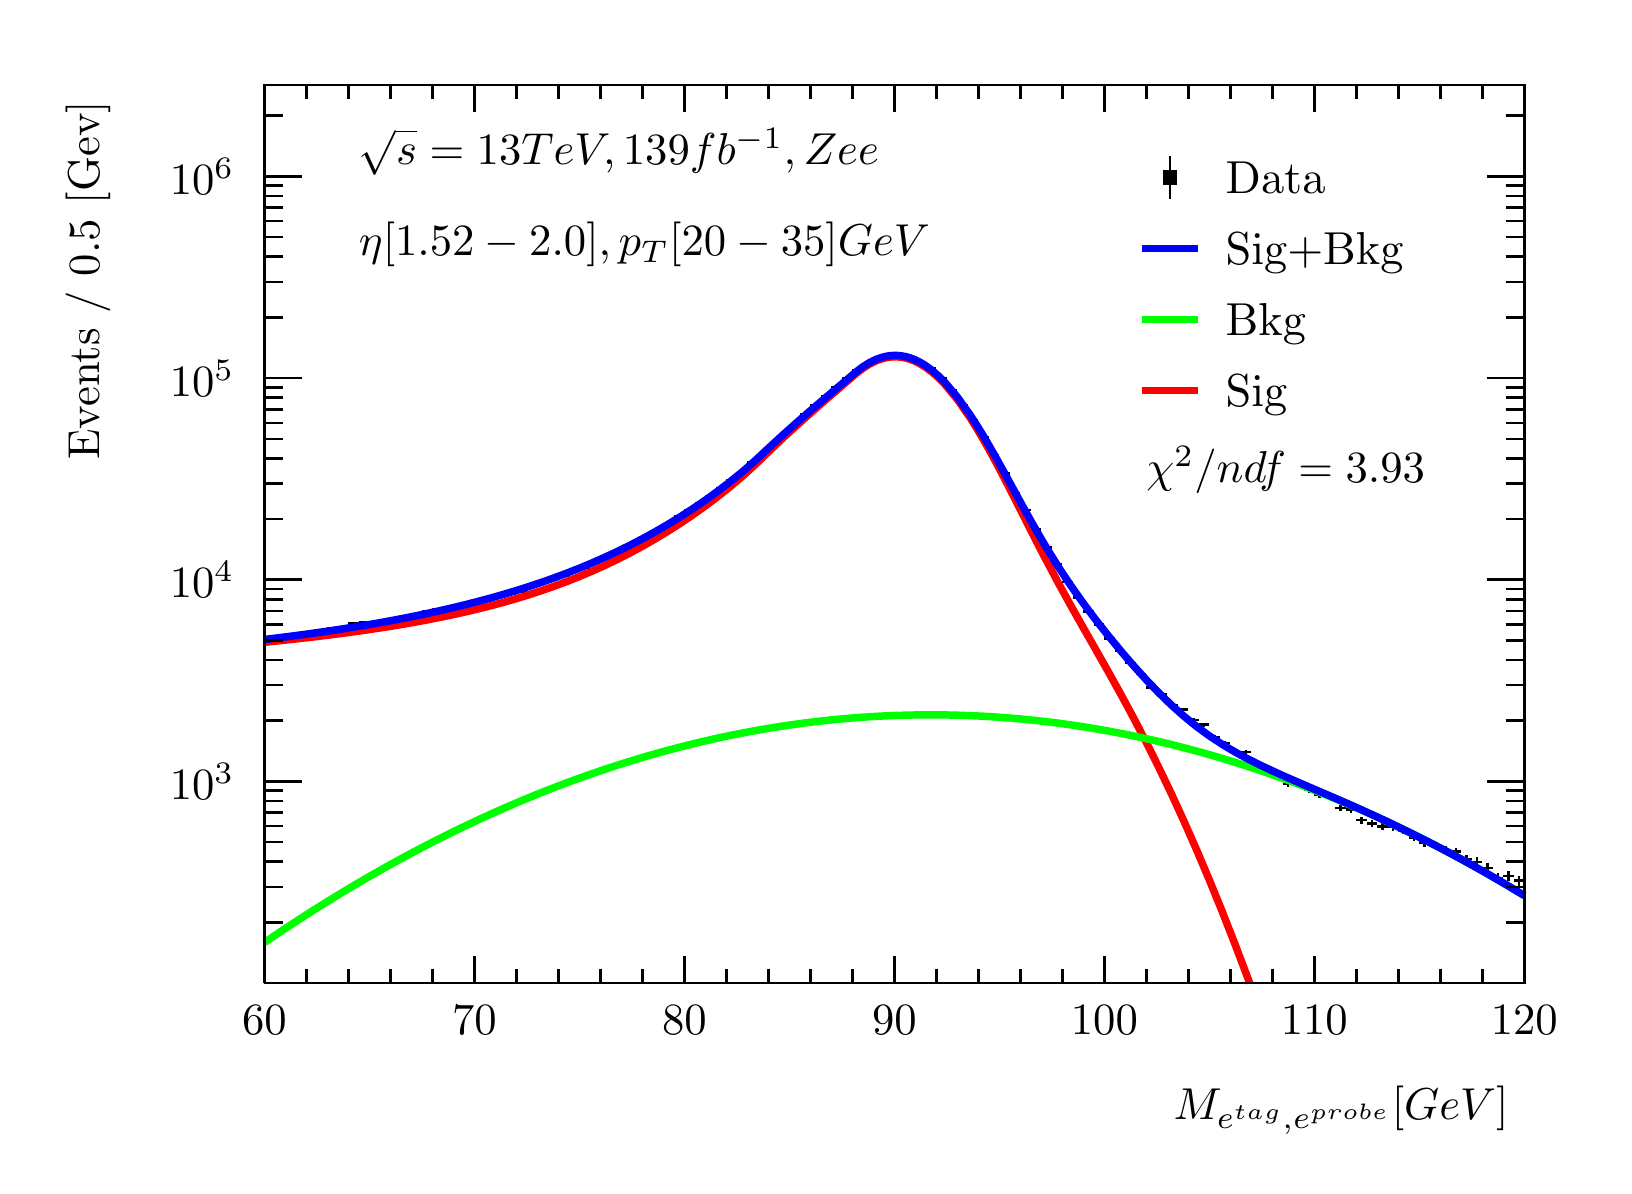
\begin{tikzpicture}
\pgfdeclareplotmark{cross} {
\pgfpathmoveto{\pgfpoint{-0.3\pgfplotmarksize}{\pgfplotmarksize}}
\pgfpathlineto{\pgfpoint{+0.3\pgfplotmarksize}{\pgfplotmarksize}}
\pgfpathlineto{\pgfpoint{+0.3\pgfplotmarksize}{0.3\pgfplotmarksize}}
\pgfpathlineto{\pgfpoint{+1\pgfplotmarksize}{0.3\pgfplotmarksize}}
\pgfpathlineto{\pgfpoint{+1\pgfplotmarksize}{-0.3\pgfplotmarksize}}
\pgfpathlineto{\pgfpoint{+0.3\pgfplotmarksize}{-0.3\pgfplotmarksize}}
\pgfpathlineto{\pgfpoint{+0.3\pgfplotmarksize}{-1.\pgfplotmarksize}}
\pgfpathlineto{\pgfpoint{-0.3\pgfplotmarksize}{-1.\pgfplotmarksize}}
\pgfpathlineto{\pgfpoint{-0.3\pgfplotmarksize}{-0.3\pgfplotmarksize}}
\pgfpathlineto{\pgfpoint{-1.\pgfplotmarksize}{-0.3\pgfplotmarksize}}
\pgfpathlineto{\pgfpoint{-1.\pgfplotmarksize}{0.3\pgfplotmarksize}}
\pgfpathlineto{\pgfpoint{-0.3\pgfplotmarksize}{0.3\pgfplotmarksize}}
\pgfpathclose
\pgfusepathqstroke
}
\pgfdeclareplotmark{cross*} {
\pgfpathmoveto{\pgfpoint{-0.3\pgfplotmarksize}{\pgfplotmarksize}}
\pgfpathlineto{\pgfpoint{+0.3\pgfplotmarksize}{\pgfplotmarksize}}
\pgfpathlineto{\pgfpoint{+0.3\pgfplotmarksize}{0.3\pgfplotmarksize}}
\pgfpathlineto{\pgfpoint{+1\pgfplotmarksize}{0.3\pgfplotmarksize}}
\pgfpathlineto{\pgfpoint{+1\pgfplotmarksize}{-0.3\pgfplotmarksize}}
\pgfpathlineto{\pgfpoint{+0.3\pgfplotmarksize}{-0.3\pgfplotmarksize}}
\pgfpathlineto{\pgfpoint{+0.3\pgfplotmarksize}{-1.\pgfplotmarksize}}
\pgfpathlineto{\pgfpoint{-0.3\pgfplotmarksize}{-1.\pgfplotmarksize}}
\pgfpathlineto{\pgfpoint{-0.3\pgfplotmarksize}{-0.3\pgfplotmarksize}}
\pgfpathlineto{\pgfpoint{-1.\pgfplotmarksize}{-0.3\pgfplotmarksize}}
\pgfpathlineto{\pgfpoint{-1.\pgfplotmarksize}{0.3\pgfplotmarksize}}
\pgfpathlineto{\pgfpoint{-0.3\pgfplotmarksize}{0.3\pgfplotmarksize}}
\pgfpathclose
\pgfusepathqfillstroke
}
\pgfdeclareplotmark{newstar} {
\pgfpathmoveto{\pgfqpoint{0pt}{\pgfplotmarksize}}
\pgfpathlineto{\pgfqpointpolar{44}{0.5\pgfplotmarksize}}
\pgfpathlineto{\pgfqpointpolar{18}{\pgfplotmarksize}}
\pgfpathlineto{\pgfqpointpolar{-20}{0.5\pgfplotmarksize}}
\pgfpathlineto{\pgfqpointpolar{-54}{\pgfplotmarksize}}
\pgfpathlineto{\pgfqpointpolar{-90}{0.5\pgfplotmarksize}}
\pgfpathlineto{\pgfqpointpolar{234}{\pgfplotmarksize}}
\pgfpathlineto{\pgfqpointpolar{198}{0.5\pgfplotmarksize}}
\pgfpathlineto{\pgfqpointpolar{162}{\pgfplotmarksize}}
\pgfpathlineto{\pgfqpointpolar{134}{0.5\pgfplotmarksize}}
\pgfpathclose
\pgfusepathqstroke
}
\pgfdeclareplotmark{newstar*} {
\pgfpathmoveto{\pgfqpoint{0pt}{\pgfplotmarksize}}
\pgfpathlineto{\pgfqpointpolar{44}{0.5\pgfplotmarksize}}
\pgfpathlineto{\pgfqpointpolar{18}{\pgfplotmarksize}}
\pgfpathlineto{\pgfqpointpolar{-20}{0.5\pgfplotmarksize}}
\pgfpathlineto{\pgfqpointpolar{-54}{\pgfplotmarksize}}
\pgfpathlineto{\pgfqpointpolar{-90}{0.5\pgfplotmarksize}}
\pgfpathlineto{\pgfqpointpolar{234}{\pgfplotmarksize}}
\pgfpathlineto{\pgfqpointpolar{198}{0.5\pgfplotmarksize}}
\pgfpathlineto{\pgfqpointpolar{162}{\pgfplotmarksize}}
\pgfpathlineto{\pgfqpointpolar{134}{0.5\pgfplotmarksize}}
\pgfpathclose
\pgfusepathqfillstroke
}
\definecolor{c}{rgb}{1,1,1};
\draw [color=c, fill=c] (0,0) rectangle (20,14.4361);
\draw [color=c, fill=c] (3,2.30977) rectangle (19,13.7143);
\definecolor{c}{rgb}{0,0,0};
\draw [c,line width=0.9] (3,2.30977) -- (3,13.7143) -- (19,13.7143) -- (19,2.30977) -- (3,2.30977);
\definecolor{c}{rgb}{1,1,1};
\draw [color=c, fill=c] (3,2.30977) rectangle (19,13.7143);
\definecolor{c}{rgb}{0,0,0};
\draw [c,line width=0.9] (3,2.30977) -- (3,13.7143) -- (19,13.7143) -- (19,2.30977) -- (3,2.30977);
\draw [c,line width=0.9] (3,2.30977) -- (19,2.30977);
\draw [c,line width=0.9] (3,2.65624) -- (3,2.30977);
\draw [c,line width=0.9] (3.53333,2.48301) -- (3.53333,2.30977);
\draw [c,line width=0.9] (4.06667,2.48301) -- (4.06667,2.30977);
\draw [c,line width=0.9] (4.6,2.48301) -- (4.6,2.30977);
\draw [c,line width=0.9] (5.13333,2.48301) -- (5.13333,2.30977);
\draw [c,line width=0.9] (5.66667,2.65624) -- (5.66667,2.30977);
\draw [c,line width=0.9] (6.2,2.48301) -- (6.2,2.30977);
\draw [c,line width=0.9] (6.73333,2.48301) -- (6.73333,2.30977);
\draw [c,line width=0.9] (7.26667,2.48301) -- (7.26667,2.30977);
\draw [c,line width=0.9] (7.8,2.48301) -- (7.8,2.30977);
\draw [c,line width=0.9] (8.33333,2.65624) -- (8.33333,2.30977);
\draw [c,line width=0.9] (8.86667,2.48301) -- (8.86667,2.30977);
\draw [c,line width=0.9] (9.4,2.48301) -- (9.4,2.30977);
\draw [c,line width=0.9] (9.93333,2.48301) -- (9.93333,2.30977);
\draw [c,line width=0.9] (10.4667,2.48301) -- (10.4667,2.30977);
\draw [c,line width=0.9] (11,2.65624) -- (11,2.30977);
\draw [c,line width=0.9] (11.5333,2.48301) -- (11.5333,2.30977);
\draw [c,line width=0.9] (12.0667,2.48301) -- (12.0667,2.30977);
\draw [c,line width=0.9] (12.6,2.48301) -- (12.6,2.30977);
\draw [c,line width=0.9] (13.1333,2.48301) -- (13.1333,2.30977);
\draw [c,line width=0.9] (13.6667,2.65624) -- (13.6667,2.30977);
\draw [c,line width=0.9] (14.2,2.48301) -- (14.2,2.30977);
\draw [c,line width=0.9] (14.7333,2.48301) -- (14.7333,2.30977);
\draw [c,line width=0.9] (15.2667,2.48301) -- (15.2667,2.30977);
\draw [c,line width=0.9] (15.8,2.48301) -- (15.8,2.30977);
\draw [c,line width=0.9] (16.3333,2.65624) -- (16.3333,2.30977);
\draw [c,line width=0.9] (16.8667,2.48301) -- (16.8667,2.30977);
\draw [c,line width=0.9] (17.4,2.48301) -- (17.4,2.30977);
\draw [c,line width=0.9] (17.9333,2.48301) -- (17.9333,2.30977);
\draw [c,line width=0.9] (18.4667,2.48301) -- (18.4667,2.30977);
\draw [c,line width=0.9] (19,2.65624) -- (19,2.30977);
\draw [anchor=base] (3,1.66015) node[scale=1.61424, color=c, rotate=0]{60};
\draw [anchor=base] (5.66667,1.66015) node[scale=1.61424, color=c, rotate=0]{70};
\draw [anchor=base] (8.33333,1.66015) node[scale=1.61424, color=c, rotate=0]{80};
\draw [anchor=base] (11,1.66015) node[scale=1.61424, color=c, rotate=0]{90};
\draw [anchor=base] (13.6667,1.66015) node[scale=1.61424, color=c, rotate=0]{100};
\draw [anchor=base] (16.3333,1.66015) node[scale=1.61424, color=c, rotate=0]{110};
\draw [anchor=base] (19,1.66015) node[scale=1.61424, color=c, rotate=0]{120};
\draw [anchor= east] (19,0.692932) node[scale=1.61424, color=c, rotate=0]{$M_{e^{tag}, e^{probe}}  [GeV]$};
\draw [c,line width=0.9] (3,13.7143) -- (19,13.7143);
\draw [c,line width=0.9] (3,13.3678) -- (3,13.7143);
\draw [c,line width=0.9] (3.53333,13.5411) -- (3.53333,13.7143);
\draw [c,line width=0.9] (4.06667,13.5411) -- (4.06667,13.7143);
\draw [c,line width=0.9] (4.6,13.5411) -- (4.6,13.7143);
\draw [c,line width=0.9] (5.13333,13.5411) -- (5.13333,13.7143);
\draw [c,line width=0.9] (5.66667,13.3678) -- (5.66667,13.7143);
\draw [c,line width=0.9] (6.2,13.5411) -- (6.2,13.7143);
\draw [c,line width=0.9] (6.73333,13.5411) -- (6.73333,13.7143);
\draw [c,line width=0.9] (7.26667,13.5411) -- (7.26667,13.7143);
\draw [c,line width=0.9] (7.8,13.5411) -- (7.8,13.7143);
\draw [c,line width=0.9] (8.33333,13.3678) -- (8.33333,13.7143);
\draw [c,line width=0.9] (8.86667,13.5411) -- (8.86667,13.7143);
\draw [c,line width=0.9] (9.4,13.5411) -- (9.4,13.7143);
\draw [c,line width=0.9] (9.93333,13.5411) -- (9.93333,13.7143);
\draw [c,line width=0.9] (10.4667,13.5411) -- (10.4667,13.7143);
\draw [c,line width=0.9] (11,13.3678) -- (11,13.7143);
\draw [c,line width=0.9] (11.5333,13.5411) -- (11.5333,13.7143);
\draw [c,line width=0.9] (12.0667,13.5411) -- (12.0667,13.7143);
\draw [c,line width=0.9] (12.6,13.5411) -- (12.6,13.7143);
\draw [c,line width=0.9] (13.1333,13.5411) -- (13.1333,13.7143);
\draw [c,line width=0.9] (13.6667,13.3678) -- (13.6667,13.7143);
\draw [c,line width=0.9] (14.2,13.5411) -- (14.2,13.7143);
\draw [c,line width=0.9] (14.7333,13.5411) -- (14.7333,13.7143);
\draw [c,line width=0.9] (15.2667,13.5411) -- (15.2667,13.7143);
\draw [c,line width=0.9] (15.8,13.5411) -- (15.8,13.7143);
\draw [c,line width=0.9] (16.3333,13.3678) -- (16.3333,13.7143);
\draw [c,line width=0.9] (16.8667,13.5411) -- (16.8667,13.7143);
\draw [c,line width=0.9] (17.4,13.5411) -- (17.4,13.7143);
\draw [c,line width=0.9] (17.9333,13.5411) -- (17.9333,13.7143);
\draw [c,line width=0.9] (18.4667,13.5411) -- (18.4667,13.7143);
\draw [c,line width=0.9] (19,13.3678) -- (19,13.7143);
\draw [c,line width=0.9] (3,2.30977) -- (3,13.7143);
\draw [c,line width=0.9] (3.237,3.08073) -- (3,3.08073);
\draw [c,line width=0.9] (3.237,3.53171) -- (3,3.53171);
\draw [c,line width=0.9] (3.237,3.85168) -- (3,3.85168);
\draw [c,line width=0.9] (3.237,4.09988) -- (3,4.09988);
\draw [c,line width=0.9] (3.237,4.30266) -- (3,4.30266);
\draw [c,line width=0.9] (3.237,4.47412) -- (3,4.47412);
\draw [c,line width=0.9] (3.237,4.62264) -- (3,4.62264);
\draw [c,line width=0.9] (3.237,4.75364) -- (3,4.75364);
\draw [c,line width=0.9] (3.474,4.87083) -- (3,4.87083);
\draw [anchor= east] (2.82,4.87083) node[scale=1.61424, color=c, rotate=0]{$10^{3}$};
\draw [c,line width=0.9] (3.237,5.64179) -- (3,5.64179);
\draw [c,line width=0.9] (3.237,6.09277) -- (3,6.09277);
\draw [c,line width=0.9] (3.237,6.41274) -- (3,6.41274);
\draw [c,line width=0.9] (3.237,6.66093) -- (3,6.66093);
\draw [c,line width=0.9] (3.237,6.86372) -- (3,6.86372);
\draw [c,line width=0.9] (3.237,7.03518) -- (3,7.03518);
\draw [c,line width=0.9] (3.237,7.1837) -- (3,7.1837);
\draw [c,line width=0.9] (3.237,7.3147) -- (3,7.3147);
\draw [c,line width=0.9] (3.474,7.43189) -- (3,7.43189);
\draw [anchor= east] (2.82,7.43189) node[scale=1.61424, color=c, rotate=0]{$10^{4}$};
\draw [c,line width=0.9] (3.237,8.20285) -- (3,8.20285);
\draw [c,line width=0.9] (3.237,8.65383) -- (3,8.65383);
\draw [c,line width=0.9] (3.237,8.9738) -- (3,8.9738);
\draw [c,line width=0.9] (3.237,9.22199) -- (3,9.22199);
\draw [c,line width=0.9] (3.237,9.42478) -- (3,9.42478);
\draw [c,line width=0.9] (3.237,9.59624) -- (3,9.59624);
\draw [c,line width=0.9] (3.237,9.74476) -- (3,9.74476);
\draw [c,line width=0.9] (3.237,9.87576) -- (3,9.87576);
\draw [c,line width=0.9] (3.474,9.99295) -- (3,9.99295);
\draw [anchor= east] (2.82,9.99295) node[scale=1.61424, color=c, rotate=0]{$10^{5}$};
\draw [c,line width=0.9] (3.237,10.7639) -- (3,10.7639);
\draw [c,line width=0.9] (3.237,11.2149) -- (3,11.2149);
\draw [c,line width=0.9] (3.237,11.5349) -- (3,11.5349);
\draw [c,line width=0.9] (3.237,11.7831) -- (3,11.7831);
\draw [c,line width=0.9] (3.237,11.9858) -- (3,11.9858);
\draw [c,line width=0.9] (3.237,12.1573) -- (3,12.1573);
\draw [c,line width=0.9] (3.237,12.3058) -- (3,12.3058);
\draw [c,line width=0.9] (3.237,12.4368) -- (3,12.4368);
\draw [c,line width=0.9] (3.474,12.554) -- (3,12.554);
\draw [anchor= east] (2.82,12.554) node[scale=1.61424, color=c, rotate=0]{$10^{6}$};
\draw [c,line width=0.9] (3.237,13.325) -- (3,13.325);
\draw [anchor= east] (0.76,13.7143) node[scale=1.61424, color=c, rotate=90]{Events / 0.5 [Gev]};
\draw [c,line width=0.9] (19,2.30977) -- (19,13.7143);
\draw [c,line width=0.9] (18.763,3.08073) -- (19,3.08073);
\draw [c,line width=0.9] (18.763,3.53171) -- (19,3.53171);
\draw [c,line width=0.9] (18.763,3.85168) -- (19,3.85168);
\draw [c,line width=0.9] (18.763,4.09988) -- (19,4.09988);
\draw [c,line width=0.9] (18.763,4.30266) -- (19,4.30266);
\draw [c,line width=0.9] (18.763,4.47412) -- (19,4.47412);
\draw [c,line width=0.9] (18.763,4.62264) -- (19,4.62264);
\draw [c,line width=0.9] (18.763,4.75364) -- (19,4.75364);
\draw [c,line width=0.9] (18.526,4.87083) -- (19,4.87083);
\draw [c,line width=0.9] (18.763,5.64179) -- (19,5.64179);
\draw [c,line width=0.9] (18.763,6.09277) -- (19,6.09277);
\draw [c,line width=0.9] (18.763,6.41274) -- (19,6.41274);
\draw [c,line width=0.9] (18.763,6.66093) -- (19,6.66093);
\draw [c,line width=0.9] (18.763,6.86372) -- (19,6.86372);
\draw [c,line width=0.9] (18.763,7.03518) -- (19,7.03518);
\draw [c,line width=0.9] (18.763,7.1837) -- (19,7.1837);
\draw [c,line width=0.9] (18.763,7.3147) -- (19,7.3147);
\draw [c,line width=0.9] (18.526,7.43189) -- (19,7.43189);
\draw [c,line width=0.9] (18.763,8.20285) -- (19,8.20285);
\draw [c,line width=0.9] (18.763,8.65383) -- (19,8.65383);
\draw [c,line width=0.9] (18.763,8.9738) -- (19,8.9738);
\draw [c,line width=0.9] (18.763,9.22199) -- (19,9.22199);
\draw [c,line width=0.9] (18.763,9.42478) -- (19,9.42478);
\draw [c,line width=0.9] (18.763,9.59624) -- (19,9.59624);
\draw [c,line width=0.9] (18.763,9.74476) -- (19,9.74476);
\draw [c,line width=0.9] (18.763,9.87576) -- (19,9.87576);
\draw [c,line width=0.9] (18.526,9.99295) -- (19,9.99295);
\draw [c,line width=0.9] (18.763,10.7639) -- (19,10.7639);
\draw [c,line width=0.9] (18.763,11.2149) -- (19,11.2149);
\draw [c,line width=0.9] (18.763,11.5349) -- (19,11.5349);
\draw [c,line width=0.9] (18.763,11.7831) -- (19,11.7831);
\draw [c,line width=0.9] (18.763,11.9858) -- (19,11.9858);
\draw [c,line width=0.9] (18.763,12.1573) -- (19,12.1573);
\draw [c,line width=0.9] (18.763,12.3058) -- (19,12.3058);
\draw [c,line width=0.9] (18.763,12.4368) -- (19,12.4368);
\draw [c,line width=0.9] (18.526,12.554) -- (19,12.554);
\draw [c,line width=0.9] (18.763,13.325) -- (19,13.325);
\draw [c,line width=0.9] (3.06667,6.61437) -- (3,6.61437);
\draw [c,line width=0.9] (3,6.61437) -- (3,6.61437);
\draw [c,line width=0.9] (3.06667,6.61437) -- (3.13333,6.61437);
\draw [c,line width=0.9] (3.13333,6.61437) -- (3.13333,6.61437);
\draw [c,line width=0.9] (3.06667,6.61437) -- (3.06667,6.63043);
\draw [c,line width=0.9] (3.06667,6.63043) -- (3.06667,6.63043);
\draw [c,line width=0.9] (3.06667,6.61437) -- (3.06667,6.59831);
\draw [c,line width=0.9] (3.06667,6.59831) -- (3.06667,6.59831);
\draw [c,line width=0.9] (3.2,6.65312) -- (3.13333,6.65312);
\draw [c,line width=0.9] (3.13333,6.65312) -- (3.13333,6.65312);
\draw [c,line width=0.9] (3.2,6.65312) -- (3.26667,6.65312);
\draw [c,line width=0.9] (3.26667,6.65312) -- (3.26667,6.65312);
\draw [c,line width=0.9] (3.2,6.65312) -- (3.2,6.66891);
\draw [c,line width=0.9] (3.2,6.66891) -- (3.2,6.66891);
\draw [c,line width=0.9] (3.2,6.65312) -- (3.2,6.63734);
\draw [c,line width=0.9] (3.2,6.63734) -- (3.2,6.63734);
\draw [c,line width=0.9] (3.33333,6.68187) -- (3.26667,6.68187);
\draw [c,line width=0.9] (3.26667,6.68187) -- (3.26667,6.68187);
\draw [c,line width=0.9] (3.33333,6.68187) -- (3.4,6.68187);
\draw [c,line width=0.9] (3.4,6.68187) -- (3.4,6.68187);
\draw [c,line width=0.9] (3.33333,6.68187) -- (3.33333,6.69745);
\draw [c,line width=0.9] (3.33333,6.69745) -- (3.33333,6.69745);
\draw [c,line width=0.9] (3.33333,6.68187) -- (3.33333,6.66629);
\draw [c,line width=0.9] (3.33333,6.66629) -- (3.33333,6.66629);
\draw [c,line width=0.9] (3.46667,6.70776) -- (3.4,6.70776);
\draw [c,line width=0.9] (3.4,6.70776) -- (3.4,6.70776);
\draw [c,line width=0.9] (3.46667,6.70776) -- (3.53333,6.70776);
\draw [c,line width=0.9] (3.53333,6.70776) -- (3.53333,6.70776);
\draw [c,line width=0.9] (3.46667,6.70776) -- (3.46667,6.72317);
\draw [c,line width=0.9] (3.46667,6.72317) -- (3.46667,6.72317);
\draw [c,line width=0.9] (3.46667,6.70776) -- (3.46667,6.69236);
\draw [c,line width=0.9] (3.46667,6.69236) -- (3.46667,6.69236);
\draw [c,line width=0.9] (3.6,6.73744) -- (3.53333,6.73744);
\draw [c,line width=0.9] (3.53333,6.73744) -- (3.53333,6.73744);
\draw [c,line width=0.9] (3.6,6.73744) -- (3.66667,6.73744);
\draw [c,line width=0.9] (3.66667,6.73744) -- (3.66667,6.73744);
\draw [c,line width=0.9] (3.6,6.73744) -- (3.6,6.75263);
\draw [c,line width=0.9] (3.6,6.75263) -- (3.6,6.75263);
\draw [c,line width=0.9] (3.6,6.73744) -- (3.6,6.72224);
\draw [c,line width=0.9] (3.6,6.72224) -- (3.6,6.72224);
\draw [c,line width=0.9] (3.73333,6.78041) -- (3.66667,6.78041);
\draw [c,line width=0.9] (3.66667,6.78041) -- (3.66667,6.78041);
\draw [c,line width=0.9] (3.73333,6.78041) -- (3.8,6.78041);
\draw [c,line width=0.9] (3.8,6.78041) -- (3.8,6.78041);
\draw [c,line width=0.9] (3.73333,6.78041) -- (3.73333,6.79532);
\draw [c,line width=0.9] (3.73333,6.79532) -- (3.73333,6.79532);
\draw [c,line width=0.9] (3.73333,6.78041) -- (3.73333,6.76551);
\draw [c,line width=0.9] (3.73333,6.76551) -- (3.73333,6.76551);
\draw [c,line width=0.9] (3.86667,6.81561) -- (3.8,6.81561);
\draw [c,line width=0.9] (3.8,6.81561) -- (3.8,6.81561);
\draw [c,line width=0.9] (3.86667,6.81561) -- (3.93333,6.81561);
\draw [c,line width=0.9] (3.93333,6.81561) -- (3.93333,6.81561);
\draw [c,line width=0.9] (3.86667,6.81561) -- (3.86667,6.83029);
\draw [c,line width=0.9] (3.86667,6.83029) -- (3.86667,6.83029);
\draw [c,line width=0.9] (3.86667,6.81561) -- (3.86667,6.80094);
\draw [c,line width=0.9] (3.86667,6.80094) -- (3.86667,6.80094);
\draw [c,line width=0.9] (4,6.82352) -- (3.93333,6.82352);
\draw [c,line width=0.9] (3.93333,6.82352) -- (3.93333,6.82352);
\draw [c,line width=0.9] (4,6.82352) -- (4.06667,6.82352);
\draw [c,line width=0.9] (4.06667,6.82352) -- (4.06667,6.82352);
\draw [c,line width=0.9] (4,6.82352) -- (4,6.83814);
\draw [c,line width=0.9] (4,6.83814) -- (4,6.83814);
\draw [c,line width=0.9] (4,6.82352) -- (4,6.8089);
\draw [c,line width=0.9] (4,6.8089) -- (4,6.8089);
\draw [c,line width=0.9] (4.13333,6.88484) -- (4.06667,6.88484);
\draw [c,line width=0.9] (4.06667,6.88484) -- (4.06667,6.88484);
\draw [c,line width=0.9] (4.13333,6.88484) -- (4.2,6.88484);
\draw [c,line width=0.9] (4.2,6.88484) -- (4.2,6.88484);
\draw [c,line width=0.9] (4.13333,6.88484) -- (4.13333,6.89906);
\draw [c,line width=0.9] (4.13333,6.89906) -- (4.13333,6.89906);
\draw [c,line width=0.9] (4.13333,6.88484) -- (4.13333,6.87062);
\draw [c,line width=0.9] (4.13333,6.87062) -- (4.13333,6.87062);
\draw [c,line width=0.9] (4.26667,6.88575) -- (4.2,6.88575);
\draw [c,line width=0.9] (4.2,6.88575) -- (4.2,6.88575);
\draw [c,line width=0.9] (4.26667,6.88575) -- (4.33333,6.88575);
\draw [c,line width=0.9] (4.33333,6.88575) -- (4.33333,6.88575);
\draw [c,line width=0.9] (4.26667,6.88575) -- (4.26667,6.89997);
\draw [c,line width=0.9] (4.26667,6.89997) -- (4.26667,6.89997);
\draw [c,line width=0.9] (4.26667,6.88575) -- (4.26667,6.87153);
\draw [c,line width=0.9] (4.26667,6.87153) -- (4.26667,6.87153);
\draw [c,line width=0.9] (4.4,6.89372) -- (4.33333,6.89372);
\draw [c,line width=0.9] (4.33333,6.89372) -- (4.33333,6.89372);
\draw [c,line width=0.9] (4.4,6.89372) -- (4.46667,6.89372);
\draw [c,line width=0.9] (4.46667,6.89372) -- (4.46667,6.89372);
\draw [c,line width=0.9] (4.4,6.89372) -- (4.4,6.90788);
\draw [c,line width=0.9] (4.4,6.90788) -- (4.4,6.90788);
\draw [c,line width=0.9] (4.4,6.89372) -- (4.4,6.87955);
\draw [c,line width=0.9] (4.4,6.87955) -- (4.4,6.87955);
\draw [c,line width=0.9] (4.53333,6.90877) -- (4.46667,6.90877);
\draw [c,line width=0.9] (4.46667,6.90877) -- (4.46667,6.90877);
\draw [c,line width=0.9] (4.53333,6.90877) -- (4.6,6.90877);
\draw [c,line width=0.9] (4.6,6.90877) -- (4.6,6.90877);
\draw [c,line width=0.9] (4.53333,6.90877) -- (4.53333,6.92284);
\draw [c,line width=0.9] (4.53333,6.92284) -- (4.53333,6.92284);
\draw [c,line width=0.9] (4.53333,6.90877) -- (4.53333,6.8947);
\draw [c,line width=0.9] (4.53333,6.8947) -- (4.53333,6.8947);
\draw [c,line width=0.9] (4.66667,6.93516) -- (4.6,6.93516);
\draw [c,line width=0.9] (4.6,6.93516) -- (4.6,6.93516);
\draw [c,line width=0.9] (4.66667,6.93516) -- (4.73333,6.93516);
\draw [c,line width=0.9] (4.73333,6.93516) -- (4.73333,6.93516);
\draw [c,line width=0.9] (4.66667,6.93516) -- (4.66667,6.94906);
\draw [c,line width=0.9] (4.66667,6.94906) -- (4.66667,6.94906);
\draw [c,line width=0.9] (4.66667,6.93516) -- (4.66667,6.92125);
\draw [c,line width=0.9] (4.66667,6.92125) -- (4.66667,6.92125);
\draw [c,line width=0.9] (4.8,6.96838) -- (4.73333,6.96838);
\draw [c,line width=0.9] (4.73333,6.96838) -- (4.73333,6.96838);
\draw [c,line width=0.9] (4.8,6.96838) -- (4.86667,6.96838);
\draw [c,line width=0.9] (4.86667,6.96838) -- (4.86667,6.96838);
\draw [c,line width=0.9] (4.8,6.96838) -- (4.8,6.98208);
\draw [c,line width=0.9] (4.8,6.98208) -- (4.8,6.98208);
\draw [c,line width=0.9] (4.8,6.96838) -- (4.8,6.95468);
\draw [c,line width=0.9] (4.8,6.95468) -- (4.8,6.95468);
\draw [c,line width=0.9] (4.93333,6.99572) -- (4.86667,6.99572);
\draw [c,line width=0.9] (4.86667,6.99572) -- (4.86667,6.99572);
\draw [c,line width=0.9] (4.93333,6.99572) -- (5,6.99572);
\draw [c,line width=0.9] (5,6.99572) -- (5,6.99572);
\draw [c,line width=0.9] (4.93333,6.99572) -- (4.93333,7.00925);
\draw [c,line width=0.9] (4.93333,7.00925) -- (4.93333,7.00925);
\draw [c,line width=0.9] (4.93333,6.99572) -- (4.93333,6.98218);
\draw [c,line width=0.9] (4.93333,6.98218) -- (4.93333,6.98218);
\draw [c,line width=0.9] (5.06667,7.0288) -- (5,7.0288);
\draw [c,line width=0.9] (5,7.0288) -- (5,7.0288);
\draw [c,line width=0.9] (5.06667,7.0288) -- (5.13333,7.0288);
\draw [c,line width=0.9] (5.13333,7.0288) -- (5.13333,7.0288);
\draw [c,line width=0.9] (5.06667,7.0288) -- (5.06667,7.04214);
\draw [c,line width=0.9] (5.06667,7.04214) -- (5.06667,7.04214);
\draw [c,line width=0.9] (5.06667,7.0288) -- (5.06667,7.01547);
\draw [c,line width=0.9] (5.06667,7.01547) -- (5.06667,7.01547);
\draw [c,line width=0.9] (5.2,7.06218) -- (5.13333,7.06218);
\draw [c,line width=0.9] (5.13333,7.06218) -- (5.13333,7.06218);
\draw [c,line width=0.9] (5.2,7.06218) -- (5.26667,7.06218);
\draw [c,line width=0.9] (5.26667,7.06218) -- (5.26667,7.06218);
\draw [c,line width=0.9] (5.2,7.06218) -- (5.2,7.07531);
\draw [c,line width=0.9] (5.2,7.07531) -- (5.2,7.07531);
\draw [c,line width=0.9] (5.2,7.06218) -- (5.2,7.04904);
\draw [c,line width=0.9] (5.2,7.04904) -- (5.2,7.04904);
\draw [c,line width=0.9] (5.33333,7.06342) -- (5.26667,7.06342);
\draw [c,line width=0.9] (5.26667,7.06342) -- (5.26667,7.06342);
\draw [c,line width=0.9] (5.33333,7.06342) -- (5.4,7.06342);
\draw [c,line width=0.9] (5.4,7.06342) -- (5.4,7.06342);
\draw [c,line width=0.9] (5.33333,7.06342) -- (5.33333,7.07654);
\draw [c,line width=0.9] (5.33333,7.07654) -- (5.33333,7.07654);
\draw [c,line width=0.9] (5.33333,7.06342) -- (5.33333,7.05029);
\draw [c,line width=0.9] (5.33333,7.05029) -- (5.33333,7.05029);
\draw [c,line width=0.9] (5.46667,7.09639) -- (5.4,7.09639);
\draw [c,line width=0.9] (5.4,7.09639) -- (5.4,7.09639);
\draw [c,line width=0.9] (5.46667,7.09639) -- (5.53333,7.09639);
\draw [c,line width=0.9] (5.53333,7.09639) -- (5.53333,7.09639);
\draw [c,line width=0.9] (5.46667,7.09639) -- (5.46667,7.10932);
\draw [c,line width=0.9] (5.46667,7.10932) -- (5.46667,7.10932);
\draw [c,line width=0.9] (5.46667,7.09639) -- (5.46667,7.08345);
\draw [c,line width=0.9] (5.46667,7.08345) -- (5.46667,7.08345);
\draw [c,line width=0.9] (5.6,7.15211) -- (5.53333,7.15211);
\draw [c,line width=0.9] (5.53333,7.15211) -- (5.53333,7.15211);
\draw [c,line width=0.9] (5.6,7.15211) -- (5.66667,7.15211);
\draw [c,line width=0.9] (5.66667,7.15211) -- (5.66667,7.15211);
\draw [c,line width=0.9] (5.6,7.15211) -- (5.6,7.16472);
\draw [c,line width=0.9] (5.6,7.16472) -- (5.6,7.16472);
\draw [c,line width=0.9] (5.6,7.15211) -- (5.6,7.1395);
\draw [c,line width=0.9] (5.6,7.1395) -- (5.6,7.1395);
\draw [c,line width=0.9] (5.73333,7.16009) -- (5.66667,7.16009);
\draw [c,line width=0.9] (5.66667,7.16009) -- (5.66667,7.16009);
\draw [c,line width=0.9] (5.73333,7.16009) -- (5.8,7.16009);
\draw [c,line width=0.9] (5.8,7.16009) -- (5.8,7.16009);
\draw [c,line width=0.9] (5.73333,7.16009) -- (5.73333,7.17266);
\draw [c,line width=0.9] (5.73333,7.17266) -- (5.73333,7.17266);
\draw [c,line width=0.9] (5.73333,7.16009) -- (5.73333,7.14753);
\draw [c,line width=0.9] (5.73333,7.14753) -- (5.73333,7.14753);
\draw [c,line width=0.9] (5.86667,7.18952) -- (5.8,7.18952);
\draw [c,line width=0.9] (5.8,7.18952) -- (5.8,7.18952);
\draw [c,line width=0.9] (5.86667,7.18952) -- (5.93333,7.18952);
\draw [c,line width=0.9] (5.93333,7.18952) -- (5.93333,7.18952);
\draw [c,line width=0.9] (5.86667,7.18952) -- (5.86667,7.20193);
\draw [c,line width=0.9] (5.86667,7.20193) -- (5.86667,7.20193);
\draw [c,line width=0.9] (5.86667,7.18952) -- (5.86667,7.17712);
\draw [c,line width=0.9] (5.86667,7.17712) -- (5.86667,7.17712);
\draw [c,line width=0.9] (6,7.22679) -- (5.93333,7.22679);
\draw [c,line width=0.9] (5.93333,7.22679) -- (5.93333,7.22679);
\draw [c,line width=0.9] (6,7.22679) -- (6.06667,7.22679);
\draw [c,line width=0.9] (6.06667,7.22679) -- (6.06667,7.22679);
\draw [c,line width=0.9] (6,7.22679) -- (6,7.23898);
\draw [c,line width=0.9] (6,7.23898) -- (6,7.23898);
\draw [c,line width=0.9] (6,7.22679) -- (6,7.21459);
\draw [c,line width=0.9] (6,7.21459) -- (6,7.21459);
\draw [c,line width=0.9] (6.13333,7.25947) -- (6.06667,7.25947);
\draw [c,line width=0.9] (6.06667,7.25947) -- (6.06667,7.25947);
\draw [c,line width=0.9] (6.13333,7.25947) -- (6.2,7.25947);
\draw [c,line width=0.9] (6.2,7.25947) -- (6.2,7.25947);
\draw [c,line width=0.9] (6.13333,7.25947) -- (6.13333,7.27149);
\draw [c,line width=0.9] (6.13333,7.27149) -- (6.13333,7.27149);
\draw [c,line width=0.9] (6.13333,7.25947) -- (6.13333,7.24745);
\draw [c,line width=0.9] (6.13333,7.24745) -- (6.13333,7.24745);
\draw [c,line width=0.9] (6.26667,7.28223) -- (6.2,7.28223);
\draw [c,line width=0.9] (6.2,7.28223) -- (6.2,7.28223);
\draw [c,line width=0.9] (6.26667,7.28223) -- (6.33333,7.28223);
\draw [c,line width=0.9] (6.33333,7.28223) -- (6.33333,7.28223);
\draw [c,line width=0.9] (6.26667,7.28223) -- (6.26667,7.29412);
\draw [c,line width=0.9] (6.26667,7.29412) -- (6.26667,7.29412);
\draw [c,line width=0.9] (6.26667,7.28223) -- (6.26667,7.27033);
\draw [c,line width=0.9] (6.26667,7.27033) -- (6.26667,7.27033);
\draw [c,line width=0.9] (6.4,7.3594) -- (6.33333,7.3594);
\draw [c,line width=0.9] (6.33333,7.3594) -- (6.33333,7.3594);
\draw [c,line width=0.9] (6.4,7.3594) -- (6.46667,7.3594);
\draw [c,line width=0.9] (6.46667,7.3594) -- (6.46667,7.3594);
\draw [c,line width=0.9] (6.4,7.3594) -- (6.4,7.37089);
\draw [c,line width=0.9] (6.4,7.37089) -- (6.4,7.37089);
\draw [c,line width=0.9] (6.4,7.3594) -- (6.4,7.34791);
\draw [c,line width=0.9] (6.4,7.34791) -- (6.4,7.34791);
\draw [c,line width=0.9] (6.53333,7.39675) -- (6.46667,7.39675);
\draw [c,line width=0.9] (6.46667,7.39675) -- (6.46667,7.39675);
\draw [c,line width=0.9] (6.53333,7.39675) -- (6.6,7.39675);
\draw [c,line width=0.9] (6.6,7.39675) -- (6.6,7.39675);
\draw [c,line width=0.9] (6.53333,7.39675) -- (6.53333,7.40805);
\draw [c,line width=0.9] (6.53333,7.40805) -- (6.53333,7.40805);
\draw [c,line width=0.9] (6.53333,7.39675) -- (6.53333,7.38545);
\draw [c,line width=0.9] (6.53333,7.38545) -- (6.53333,7.38545);
\draw [c,line width=0.9] (6.66667,7.44725) -- (6.6,7.44725);
\draw [c,line width=0.9] (6.6,7.44725) -- (6.6,7.44725);
\draw [c,line width=0.9] (6.66667,7.44725) -- (6.73333,7.44725);
\draw [c,line width=0.9] (6.73333,7.44725) -- (6.73333,7.44725);
\draw [c,line width=0.9] (6.66667,7.44725) -- (6.66667,7.45829);
\draw [c,line width=0.9] (6.66667,7.45829) -- (6.66667,7.45829);
\draw [c,line width=0.9] (6.66667,7.44725) -- (6.66667,7.4362);
\draw [c,line width=0.9] (6.66667,7.4362) -- (6.66667,7.4362);
\draw [c,line width=0.9] (6.8,7.48) -- (6.73333,7.48);
\draw [c,line width=0.9] (6.73333,7.48) -- (6.73333,7.48);
\draw [c,line width=0.9] (6.8,7.48) -- (6.86667,7.48);
\draw [c,line width=0.9] (6.86667,7.48) -- (6.86667,7.48);
\draw [c,line width=0.9] (6.8,7.48) -- (6.8,7.49088);
\draw [c,line width=0.9] (6.8,7.49088) -- (6.8,7.49088);
\draw [c,line width=0.9] (6.8,7.48) -- (6.8,7.46911);
\draw [c,line width=0.9] (6.8,7.46911) -- (6.8,7.46911);
\draw [c,line width=0.9] (6.93333,7.54063) -- (6.86667,7.54063);
\draw [c,line width=0.9] (6.86667,7.54063) -- (6.86667,7.54063);
\draw [c,line width=0.9] (6.93333,7.54063) -- (7,7.54063);
\draw [c,line width=0.9] (7,7.54063) -- (7,7.54063);
\draw [c,line width=0.9] (6.93333,7.54063) -- (6.93333,7.55122);
\draw [c,line width=0.9] (6.93333,7.55122) -- (6.93333,7.55122);
\draw [c,line width=0.9] (6.93333,7.54063) -- (6.93333,7.53004);
\draw [c,line width=0.9] (6.93333,7.53004) -- (6.93333,7.53004);
\draw [c,line width=0.9] (7.06667,7.58773) -- (7,7.58773);
\draw [c,line width=0.9] (7,7.58773) -- (7,7.58773);
\draw [c,line width=0.9] (7.06667,7.58773) -- (7.13333,7.58773);
\draw [c,line width=0.9] (7.13333,7.58773) -- (7.13333,7.58773);
\draw [c,line width=0.9] (7.06667,7.58773) -- (7.06667,7.5981);
\draw [c,line width=0.9] (7.06667,7.5981) -- (7.06667,7.5981);
\draw [c,line width=0.9] (7.06667,7.58773) -- (7.06667,7.57736);
\draw [c,line width=0.9] (7.06667,7.57736) -- (7.06667,7.57736);
\draw [c,line width=0.9] (7.2,7.64428) -- (7.13333,7.64428);
\draw [c,line width=0.9] (7.13333,7.64428) -- (7.13333,7.64428);
\draw [c,line width=0.9] (7.2,7.64428) -- (7.26667,7.64428);
\draw [c,line width=0.9] (7.26667,7.64428) -- (7.26667,7.64428);
\draw [c,line width=0.9] (7.2,7.64428) -- (7.2,7.65439);
\draw [c,line width=0.9] (7.2,7.65439) -- (7.2,7.65439);
\draw [c,line width=0.9] (7.2,7.64428) -- (7.2,7.63417);
\draw [c,line width=0.9] (7.2,7.63417) -- (7.2,7.63417);
\draw [c,line width=0.9] (7.33333,7.71787) -- (7.26667,7.71787);
\draw [c,line width=0.9] (7.26667,7.71787) -- (7.26667,7.71787);
\draw [c,line width=0.9] (7.33333,7.71787) -- (7.4,7.71787);
\draw [c,line width=0.9] (7.4,7.71787) -- (7.4,7.71787);
\draw [c,line width=0.9] (7.33333,7.71787) -- (7.33333,7.72765);
\draw [c,line width=0.9] (7.33333,7.72765) -- (7.33333,7.72765);
\draw [c,line width=0.9] (7.33333,7.71787) -- (7.33333,7.70809);
\draw [c,line width=0.9] (7.33333,7.70809) -- (7.33333,7.70809);
\draw [c,line width=0.9] (7.46667,7.77773) -- (7.4,7.77773);
\draw [c,line width=0.9] (7.4,7.77773) -- (7.4,7.77773);
\draw [c,line width=0.9] (7.46667,7.77773) -- (7.53333,7.77773);
\draw [c,line width=0.9] (7.53333,7.77773) -- (7.53333,7.77773);
\draw [c,line width=0.9] (7.46667,7.77773) -- (7.46667,7.78725);
\draw [c,line width=0.9] (7.46667,7.78725) -- (7.46667,7.78725);
\draw [c,line width=0.9] (7.46667,7.77773) -- (7.46667,7.76821);
\draw [c,line width=0.9] (7.46667,7.76821) -- (7.46667,7.76821);
\draw [c,line width=0.9] (7.6,7.85144) -- (7.53333,7.85144);
\draw [c,line width=0.9] (7.53333,7.85144) -- (7.53333,7.85144);
\draw [c,line width=0.9] (7.6,7.85144) -- (7.66667,7.85144);
\draw [c,line width=0.9] (7.66667,7.85144) -- (7.66667,7.85144);
\draw [c,line width=0.9] (7.6,7.85144) -- (7.6,7.86065);
\draw [c,line width=0.9] (7.6,7.86065) -- (7.6,7.86065);
\draw [c,line width=0.9] (7.6,7.85144) -- (7.6,7.84223);
\draw [c,line width=0.9] (7.6,7.84223) -- (7.6,7.84223);
\draw [c,line width=0.9] (7.73333,7.90184) -- (7.66667,7.90184);
\draw [c,line width=0.9] (7.66667,7.90184) -- (7.66667,7.90184);
\draw [c,line width=0.9] (7.73333,7.90184) -- (7.8,7.90184);
\draw [c,line width=0.9] (7.8,7.90184) -- (7.8,7.90184);
\draw [c,line width=0.9] (7.73333,7.90184) -- (7.73333,7.91084);
\draw [c,line width=0.9] (7.73333,7.91084) -- (7.73333,7.91084);
\draw [c,line width=0.9] (7.73333,7.90184) -- (7.73333,7.89284);
\draw [c,line width=0.9] (7.73333,7.89284) -- (7.73333,7.89284);
\draw [c,line width=0.9] (7.86667,7.98591) -- (7.8,7.98591);
\draw [c,line width=0.9] (7.8,7.98591) -- (7.8,7.98591);
\draw [c,line width=0.9] (7.86667,7.98591) -- (7.93333,7.98591);
\draw [c,line width=0.9] (7.93333,7.98591) -- (7.93333,7.98591);
\draw [c,line width=0.9] (7.86667,7.98591) -- (7.86667,7.99458);
\draw [c,line width=0.9] (7.86667,7.99458) -- (7.86667,7.99458);
\draw [c,line width=0.9] (7.86667,7.98591) -- (7.86667,7.97724);
\draw [c,line width=0.9] (7.86667,7.97724) -- (7.86667,7.97724);
\draw [c,line width=0.9] (8,8.06602) -- (7.93333,8.06602);
\draw [c,line width=0.9] (7.93333,8.06602) -- (7.93333,8.06602);
\draw [c,line width=0.9] (8,8.06602) -- (8.06667,8.06602);
\draw [c,line width=0.9] (8.06667,8.06602) -- (8.06667,8.06602);
\draw [c,line width=0.9] (8,8.06602) -- (8,8.07439);
\draw [c,line width=0.9] (8,8.07439) -- (8,8.07439);
\draw [c,line width=0.9] (8,8.06602) -- (8,8.05766);
\draw [c,line width=0.9] (8,8.05766) -- (8,8.05766);
\draw [c,line width=0.9] (8.13333,8.14069) -- (8.06667,8.14069);
\draw [c,line width=0.9] (8.06667,8.14069) -- (8.06667,8.14069);
\draw [c,line width=0.9] (8.13333,8.14069) -- (8.2,8.14069);
\draw [c,line width=0.9] (8.2,8.14069) -- (8.2,8.14069);
\draw [c,line width=0.9] (8.13333,8.14069) -- (8.13333,8.14878);
\draw [c,line width=0.9] (8.13333,8.14878) -- (8.13333,8.14878);
\draw [c,line width=0.9] (8.13333,8.14069) -- (8.13333,8.1326);
\draw [c,line width=0.9] (8.13333,8.1326) -- (8.13333,8.1326);
\draw [c,line width=0.9] (8.26667,8.23356) -- (8.2,8.23356);
\draw [c,line width=0.9] (8.2,8.23356) -- (8.2,8.23356);
\draw [c,line width=0.9] (8.26667,8.23356) -- (8.33333,8.23356);
\draw [c,line width=0.9] (8.33333,8.23356) -- (8.33333,8.23356);
\draw [c,line width=0.9] (8.26667,8.23356) -- (8.26667,8.24132);
\draw [c,line width=0.9] (8.26667,8.24132) -- (8.26667,8.24132);
\draw [c,line width=0.9] (8.26667,8.23356) -- (8.26667,8.22581);
\draw [c,line width=0.9] (8.26667,8.22581) -- (8.26667,8.22581);
\draw [c,line width=0.9] (8.4,8.31511) -- (8.33333,8.31511);
\draw [c,line width=0.9] (8.33333,8.31511) -- (8.33333,8.31511);
\draw [c,line width=0.9] (8.4,8.31511) -- (8.46667,8.31511);
\draw [c,line width=0.9] (8.46667,8.31511) -- (8.46667,8.31511);
\draw [c,line width=0.9] (8.4,8.31511) -- (8.4,8.32259);
\draw [c,line width=0.9] (8.4,8.32259) -- (8.4,8.32259);
\draw [c,line width=0.9] (8.4,8.31511) -- (8.4,8.30763);
\draw [c,line width=0.9] (8.4,8.30763) -- (8.4,8.30763);
\draw [c,line width=0.9] (8.53333,8.40215) -- (8.46667,8.40215);
\draw [c,line width=0.9] (8.46667,8.40215) -- (8.46667,8.40215);
\draw [c,line width=0.9] (8.53333,8.40215) -- (8.6,8.40215);
\draw [c,line width=0.9] (8.6,8.40215) -- (8.6,8.40215);
\draw [c,line width=0.9] (8.53333,8.40215) -- (8.53333,8.40934);
\draw [c,line width=0.9] (8.53333,8.40934) -- (8.53333,8.40934);
\draw [c,line width=0.9] (8.53333,8.40215) -- (8.53333,8.39496);
\draw [c,line width=0.9] (8.53333,8.39496) -- (8.53333,8.39496);
\draw [c,line width=0.9] (8.66667,8.48818) -- (8.6,8.48818);
\draw [c,line width=0.9] (8.6,8.48818) -- (8.6,8.48818);
\draw [c,line width=0.9] (8.66667,8.48818) -- (8.73333,8.48818);
\draw [c,line width=0.9] (8.73333,8.48818) -- (8.73333,8.48818);
\draw [c,line width=0.9] (8.66667,8.48818) -- (8.66667,8.4951);
\draw [c,line width=0.9] (8.66667,8.4951) -- (8.66667,8.4951);
\draw [c,line width=0.9] (8.66667,8.48818) -- (8.66667,8.48127);
\draw [c,line width=0.9] (8.66667,8.48127) -- (8.66667,8.48127);
\draw [c,line width=0.9] (8.8,8.58941) -- (8.73333,8.58941);
\draw [c,line width=0.9] (8.73333,8.58941) -- (8.73333,8.58941);
\draw [c,line width=0.9] (8.8,8.58941) -- (8.86667,8.58941);
\draw [c,line width=0.9] (8.86667,8.58941) -- (8.86667,8.58941);
\draw [c,line width=0.9] (8.8,8.58941) -- (8.8,8.59602);
\draw [c,line width=0.9] (8.8,8.59602) -- (8.8,8.59602);
\draw [c,line width=0.9] (8.8,8.58941) -- (8.8,8.5828);
\draw [c,line width=0.9] (8.8,8.5828) -- (8.8,8.5828);
\draw [c,line width=0.9] (8.93333,8.70073) -- (8.86667,8.70073);
\draw [c,line width=0.9] (8.86667,8.70073) -- (8.86667,8.70073);
\draw [c,line width=0.9] (8.93333,8.70073) -- (9,8.70073);
\draw [c,line width=0.9] (9,8.70073) -- (9,8.70073);
\draw [c,line width=0.9] (8.93333,8.70073) -- (8.93333,8.70701);
\draw [c,line width=0.9] (8.93333,8.70701) -- (8.93333,8.70701);
\draw [c,line width=0.9] (8.93333,8.70073) -- (8.93333,8.69444);
\draw [c,line width=0.9] (8.93333,8.69444) -- (8.93333,8.69444);
\draw [c,line width=0.9] (9.06667,8.80301) -- (9,8.80301);
\draw [c,line width=0.9] (9,8.80301) -- (9,8.80301);
\draw [c,line width=0.9] (9.06667,8.80301) -- (9.13333,8.80301);
\draw [c,line width=0.9] (9.13333,8.80301) -- (9.13333,8.80301);
\draw [c,line width=0.9] (9.06667,8.80301) -- (9.06667,8.80901);
\draw [c,line width=0.9] (9.06667,8.80901) -- (9.06667,8.80901);
\draw [c,line width=0.9] (9.06667,8.80301) -- (9.06667,8.797);
\draw [c,line width=0.9] (9.06667,8.797) -- (9.06667,8.797);
\draw [c,line width=0.9] (9.2,8.91947) -- (9.13333,8.91947);
\draw [c,line width=0.9] (9.13333,8.91947) -- (9.13333,8.91947);
\draw [c,line width=0.9] (9.2,8.91947) -- (9.26667,8.91947);
\draw [c,line width=0.9] (9.26667,8.91947) -- (9.26667,8.91947);
\draw [c,line width=0.9] (9.2,8.91947) -- (9.2,8.92517);
\draw [c,line width=0.9] (9.2,8.92517) -- (9.2,8.92517);
\draw [c,line width=0.9] (9.2,8.91947) -- (9.2,8.91377);
\draw [c,line width=0.9] (9.2,8.91377) -- (9.2,8.91377);
\draw [c,line width=0.9] (9.33333,9.03003) -- (9.26667,9.03003);
\draw [c,line width=0.9] (9.26667,9.03003) -- (9.26667,9.03003);
\draw [c,line width=0.9] (9.33333,9.03003) -- (9.4,9.03003);
\draw [c,line width=0.9] (9.4,9.03003) -- (9.4,9.03003);
\draw [c,line width=0.9] (9.33333,9.03003) -- (9.33333,9.03545);
\draw [c,line width=0.9] (9.33333,9.03545) -- (9.33333,9.03545);
\draw [c,line width=0.9] (9.33333,9.03003) -- (9.33333,9.0246);
\draw [c,line width=0.9] (9.33333,9.0246) -- (9.33333,9.0246);
\draw [c,line width=0.9] (9.46667,9.14317) -- (9.4,9.14317);
\draw [c,line width=0.9] (9.4,9.14317) -- (9.4,9.14317);
\draw [c,line width=0.9] (9.46667,9.14317) -- (9.53333,9.14317);
\draw [c,line width=0.9] (9.53333,9.14317) -- (9.53333,9.14317);
\draw [c,line width=0.9] (9.46667,9.14317) -- (9.46667,9.14832);
\draw [c,line width=0.9] (9.46667,9.14832) -- (9.46667,9.14832);
\draw [c,line width=0.9] (9.46667,9.14317) -- (9.46667,9.13801);
\draw [c,line width=0.9] (9.46667,9.13801) -- (9.46667,9.13801);
\draw [c,line width=0.9] (9.6,9.27705) -- (9.53333,9.27705);
\draw [c,line width=0.9] (9.53333,9.27705) -- (9.53333,9.27705);
\draw [c,line width=0.9] (9.6,9.27705) -- (9.66667,9.27705);
\draw [c,line width=0.9] (9.66667,9.27705) -- (9.66667,9.27705);
\draw [c,line width=0.9] (9.6,9.27705) -- (9.6,9.2819);
\draw [c,line width=0.9] (9.6,9.2819) -- (9.6,9.2819);
\draw [c,line width=0.9] (9.6,9.27705) -- (9.6,9.27219);
\draw [c,line width=0.9] (9.6,9.27219) -- (9.6,9.27219);
\draw [c,line width=0.9] (9.73333,9.39487) -- (9.66667,9.39487);
\draw [c,line width=0.9] (9.66667,9.39487) -- (9.66667,9.39487);
\draw [c,line width=0.9] (9.73333,9.39487) -- (9.8,9.39487);
\draw [c,line width=0.9] (9.8,9.39487) -- (9.8,9.39487);
\draw [c,line width=0.9] (9.73333,9.39487) -- (9.73333,9.39947);
\draw [c,line width=0.9] (9.73333,9.39947) -- (9.73333,9.39947);
\draw [c,line width=0.9] (9.73333,9.39487) -- (9.73333,9.39027);
\draw [c,line width=0.9] (9.73333,9.39027) -- (9.73333,9.39027);
\draw [c,line width=0.9] (9.86667,9.53049) -- (9.8,9.53049);
\draw [c,line width=0.9] (9.8,9.53049) -- (9.8,9.53049);
\draw [c,line width=0.9] (9.86667,9.53049) -- (9.93333,9.53049);
\draw [c,line width=0.9] (9.93333,9.53049) -- (9.93333,9.53049);
\draw [c,line width=0.9] (9.86667,9.53049) -- (9.86667,9.53482);
\draw [c,line width=0.9] (9.86667,9.53482) -- (9.86667,9.53482);
\draw [c,line width=0.9] (9.86667,9.53049) -- (9.86667,9.52616);
\draw [c,line width=0.9] (9.86667,9.52616) -- (9.86667,9.52616);
\draw [c,line width=0.9] (10,9.65111) -- (9.93333,9.65111);
\draw [c,line width=0.9] (9.93333,9.65111) -- (9.93333,9.65111);
\draw [c,line width=0.9] (10,9.65111) -- (10.0667,9.65111);
\draw [c,line width=0.9] (10.0667,9.65111) -- (10.0667,9.65111);
\draw [c,line width=0.9] (10,9.65111) -- (10,9.65521);
\draw [c,line width=0.9] (10,9.65521) -- (10,9.65521);
\draw [c,line width=0.9] (10,9.65111) -- (10,9.64701);
\draw [c,line width=0.9] (10,9.64701) -- (10,9.64701);
\draw [c,line width=0.9] (10.1333,9.7656) -- (10.0667,9.7656);
\draw [c,line width=0.9] (10.0667,9.7656) -- (10.0667,9.7656);
\draw [c,line width=0.9] (10.1333,9.7656) -- (10.2,9.7656);
\draw [c,line width=0.9] (10.2,9.7656) -- (10.2,9.7656);
\draw [c,line width=0.9] (10.1333,9.7656) -- (10.1333,9.76949);
\draw [c,line width=0.9] (10.1333,9.76949) -- (10.1333,9.76949);
\draw [c,line width=0.9] (10.1333,9.7656) -- (10.1333,9.7617);
\draw [c,line width=0.9] (10.1333,9.7617) -- (10.1333,9.7617);
\draw [c,line width=0.9] (10.2667,9.88009) -- (10.2,9.88009);
\draw [c,line width=0.9] (10.2,9.88009) -- (10.2,9.88009);
\draw [c,line width=0.9] (10.2667,9.88009) -- (10.3333,9.88009);
\draw [c,line width=0.9] (10.3333,9.88009) -- (10.3333,9.88009);
\draw [c,line width=0.9] (10.2667,9.88009) -- (10.2667,9.88379);
\draw [c,line width=0.9] (10.2667,9.88379) -- (10.2667,9.88379);
\draw [c,line width=0.9] (10.2667,9.88009) -- (10.2667,9.87639);
\draw [c,line width=0.9] (10.2667,9.87639) -- (10.2667,9.87639);
\draw [c,line width=0.9] (10.4,9.99129) -- (10.3333,9.99129);
\draw [c,line width=0.9] (10.3333,9.99129) -- (10.3333,9.99129);
\draw [c,line width=0.9] (10.4,9.99129) -- (10.4667,9.99129);
\draw [c,line width=0.9] (10.4667,9.99129) -- (10.4667,9.99129);
\draw [c,line width=0.9] (10.4,9.99129) -- (10.4,9.99481);
\draw [c,line width=0.9] (10.4,9.99481) -- (10.4,9.99481);
\draw [c,line width=0.9] (10.4,9.99129) -- (10.4,9.98777);
\draw [c,line width=0.9] (10.4,9.98777) -- (10.4,9.98777);
\draw [c,line width=0.9] (10.5333,10.0861) -- (10.4667,10.0861);
\draw [c,line width=0.9] (10.4667,10.0861) -- (10.4667,10.0861);
\draw [c,line width=0.9] (10.5333,10.0861) -- (10.6,10.0861);
\draw [c,line width=0.9] (10.6,10.0861) -- (10.6,10.0861);
\draw [c,line width=0.9] (10.5333,10.0861) -- (10.5333,10.0895);
\draw [c,line width=0.9] (10.5333,10.0895) -- (10.5333,10.0895);
\draw [c,line width=0.9] (10.5333,10.0861) -- (10.5333,10.0827);
\draw [c,line width=0.9] (10.5333,10.0827) -- (10.5333,10.0827);
\draw [c,line width=0.9] (10.6667,10.1595) -- (10.6,10.1595);
\draw [c,line width=0.9] (10.6,10.1595) -- (10.6,10.1595);
\draw [c,line width=0.9] (10.6667,10.1595) -- (10.7333,10.1595);
\draw [c,line width=0.9] (10.7333,10.1595) -- (10.7333,10.1595);
\draw [c,line width=0.9] (10.6667,10.1595) -- (10.6667,10.1628);
\draw [c,line width=0.9] (10.6667,10.1628) -- (10.6667,10.1628);
\draw [c,line width=0.9] (10.6667,10.1595) -- (10.6667,10.1563);
\draw [c,line width=0.9] (10.6667,10.1563) -- (10.6667,10.1563);
\draw [c,line width=0.9] (10.8,10.2248) -- (10.7333,10.2248);
\draw [c,line width=0.9] (10.7333,10.2248) -- (10.7333,10.2248);
\draw [c,line width=0.9] (10.8,10.2248) -- (10.8667,10.2248);
\draw [c,line width=0.9] (10.8667,10.2248) -- (10.8667,10.2248);
\draw [c,line width=0.9] (10.8,10.2248) -- (10.8,10.2279);
\draw [c,line width=0.9] (10.8,10.2279) -- (10.8,10.2279);
\draw [c,line width=0.9] (10.8,10.2248) -- (10.8,10.2216);
\draw [c,line width=0.9] (10.8,10.2216) -- (10.8,10.2216);
\draw [c,line width=0.9] (10.9333,10.2644) -- (10.8667,10.2644);
\draw [c,line width=0.9] (10.8667,10.2644) -- (10.8667,10.2644);
\draw [c,line width=0.9] (10.9333,10.2644) -- (11,10.2644);
\draw [c,line width=0.9] (11,10.2644) -- (11,10.2644);
\draw [c,line width=0.9] (10.9333,10.2644) -- (10.9333,10.2675);
\draw [c,line width=0.9] (10.9333,10.2675) -- (10.9333,10.2675);
\draw [c,line width=0.9] (10.9333,10.2644) -- (10.9333,10.2613);
\draw [c,line width=0.9] (10.9333,10.2613) -- (10.9333,10.2613);
\draw [c,line width=0.9] (11.0667,10.2757) -- (11,10.2757);
\draw [c,line width=0.9] (11,10.2757) -- (11,10.2757);
\draw [c,line width=0.9] (11.0667,10.2757) -- (11.1333,10.2757);
\draw [c,line width=0.9] (11.1333,10.2757) -- (11.1333,10.2757);
\draw [c,line width=0.9] (11.0667,10.2757) -- (11.0667,10.2788);
\draw [c,line width=0.9] (11.0667,10.2788) -- (11.0667,10.2788);
\draw [c,line width=0.9] (11.0667,10.2757) -- (11.0667,10.2726);
\draw [c,line width=0.9] (11.0667,10.2726) -- (11.0667,10.2726);
\draw [c,line width=0.9] (11.2,10.2531) -- (11.1333,10.2531);
\draw [c,line width=0.9] (11.1333,10.2531) -- (11.1333,10.2531);
\draw [c,line width=0.9] (11.2,10.2531) -- (11.2667,10.2531);
\draw [c,line width=0.9] (11.2667,10.2531) -- (11.2667,10.2531);
\draw [c,line width=0.9] (11.2,10.2531) -- (11.2,10.2563);
\draw [c,line width=0.9] (11.2,10.2563) -- (11.2,10.2563);
\draw [c,line width=0.9] (11.2,10.2531) -- (11.2,10.25);
\draw [c,line width=0.9] (11.2,10.25) -- (11.2,10.25);
\draw [c,line width=0.9] (11.3333,10.1975) -- (11.2667,10.1975);
\draw [c,line width=0.9] (11.2667,10.1975) -- (11.2667,10.1975);
\draw [c,line width=0.9] (11.3333,10.1975) -- (11.4,10.1975);
\draw [c,line width=0.9] (11.4,10.1975) -- (11.4,10.1975);
\draw [c,line width=0.9] (11.3333,10.1975) -- (11.3333,10.2008);
\draw [c,line width=0.9] (11.3333,10.2008) -- (11.3333,10.2008);
\draw [c,line width=0.9] (11.3333,10.1975) -- (11.3333,10.1943);
\draw [c,line width=0.9] (11.3333,10.1943) -- (11.3333,10.1943);
\draw [c,line width=0.9] (11.4667,10.1188) -- (11.4,10.1188);
\draw [c,line width=0.9] (11.4,10.1188) -- (11.4,10.1188);
\draw [c,line width=0.9] (11.4667,10.1188) -- (11.5333,10.1188);
\draw [c,line width=0.9] (11.5333,10.1188) -- (11.5333,10.1188);
\draw [c,line width=0.9] (11.4667,10.1188) -- (11.4667,10.1221);
\draw [c,line width=0.9] (11.4667,10.1221) -- (11.4667,10.1221);
\draw [c,line width=0.9] (11.4667,10.1188) -- (11.4667,10.1154);
\draw [c,line width=0.9] (11.4667,10.1154) -- (11.4667,10.1154);
\draw [c,line width=0.9] (11.6,9.98617) -- (11.5333,9.98617);
\draw [c,line width=0.9] (11.5333,9.98617) -- (11.5333,9.98617);
\draw [c,line width=0.9] (11.6,9.98617) -- (11.6667,9.98617);
\draw [c,line width=0.9] (11.6667,9.98617) -- (11.6667,9.98617);
\draw [c,line width=0.9] (11.6,9.98617) -- (11.6,9.98969);
\draw [c,line width=0.9] (11.6,9.98969) -- (11.6,9.98969);
\draw [c,line width=0.9] (11.6,9.98617) -- (11.6,9.98264);
\draw [c,line width=0.9] (11.6,9.98264) -- (11.6,9.98264);
\draw [c,line width=0.9] (11.7333,9.8414) -- (11.6667,9.8414);
\draw [c,line width=0.9] (11.6667,9.8414) -- (11.6667,9.8414);
\draw [c,line width=0.9] (11.7333,9.8414) -- (11.8,9.8414);
\draw [c,line width=0.9] (11.8,9.8414) -- (11.8,9.8414);
\draw [c,line width=0.9] (11.7333,9.8414) -- (11.7333,9.84517);
\draw [c,line width=0.9] (11.7333,9.84517) -- (11.7333,9.84517);
\draw [c,line width=0.9] (11.7333,9.8414) -- (11.7333,9.83763);
\draw [c,line width=0.9] (11.7333,9.83763) -- (11.7333,9.83763);
\draw [c,line width=0.9] (11.8667,9.64988) -- (11.8,9.64988);
\draw [c,line width=0.9] (11.8,9.64988) -- (11.8,9.64988);
\draw [c,line width=0.9] (11.8667,9.64988) -- (11.9333,9.64988);
\draw [c,line width=0.9] (11.9333,9.64988) -- (11.9333,9.64988);
\draw [c,line width=0.9] (11.8667,9.64988) -- (11.8667,9.65399);
\draw [c,line width=0.9] (11.8667,9.65399) -- (11.8667,9.65399);
\draw [c,line width=0.9] (11.8667,9.64988) -- (11.8667,9.64578);
\draw [c,line width=0.9] (11.8667,9.64578) -- (11.8667,9.64578);
\draw [c,line width=0.9] (12,9.46093) -- (11.9333,9.46093);
\draw [c,line width=0.9] (11.9333,9.46093) -- (11.9333,9.46093);
\draw [c,line width=0.9] (12,9.46093) -- (12.0667,9.46093);
\draw [c,line width=0.9] (12.0667,9.46093) -- (12.0667,9.46093);
\draw [c,line width=0.9] (12,9.46093) -- (12,9.4654);
\draw [c,line width=0.9] (12,9.4654) -- (12,9.4654);
\draw [c,line width=0.9] (12,9.46093) -- (12,9.45646);
\draw [c,line width=0.9] (12,9.45646) -- (12,9.45646);
\draw [c,line width=0.9] (12.1333,9.244) -- (12.0667,9.244);
\draw [c,line width=0.9] (12.0667,9.244) -- (12.0667,9.244);
\draw [c,line width=0.9] (12.1333,9.244) -- (12.2,9.244);
\draw [c,line width=0.9] (12.2,9.244) -- (12.2,9.244);
\draw [c,line width=0.9] (12.1333,9.244) -- (12.1333,9.24892);
\draw [c,line width=0.9] (12.1333,9.24892) -- (12.1333,9.24892);
\draw [c,line width=0.9] (12.1333,9.244) -- (12.1333,9.23907);
\draw [c,line width=0.9] (12.1333,9.23907) -- (12.1333,9.23907);
\draw [c,line width=0.9] (12.2667,9.01405) -- (12.2,9.01405);
\draw [c,line width=0.9] (12.2,9.01405) -- (12.2,9.01405);
\draw [c,line width=0.9] (12.2667,9.01405) -- (12.3333,9.01405);
\draw [c,line width=0.9] (12.3333,9.01405) -- (12.3333,9.01405);
\draw [c,line width=0.9] (12.2667,9.01405) -- (12.2667,9.01951);
\draw [c,line width=0.9] (12.2667,9.01951) -- (12.2667,9.01951);
\draw [c,line width=0.9] (12.2667,9.01405) -- (12.2667,9.00859);
\draw [c,line width=0.9] (12.2667,9.00859) -- (12.2667,9.00859);
\draw [c,line width=0.9] (12.4,8.78381) -- (12.3333,8.78381);
\draw [c,line width=0.9] (12.3333,8.78381) -- (12.3333,8.78381);
\draw [c,line width=0.9] (12.4,8.78381) -- (12.4667,8.78381);
\draw [c,line width=0.9] (12.4667,8.78381) -- (12.4667,8.78381);
\draw [c,line width=0.9] (12.4,8.78381) -- (12.4,8.78987);
\draw [c,line width=0.9] (12.4,8.78987) -- (12.4,8.78987);
\draw [c,line width=0.9] (12.4,8.78381) -- (12.4,8.77775);
\draw [c,line width=0.9] (12.4,8.77775) -- (12.4,8.77775);
\draw [c,line width=0.9] (12.5333,8.53355) -- (12.4667,8.53355);
\draw [c,line width=0.9] (12.4667,8.53355) -- (12.4667,8.53355);
\draw [c,line width=0.9] (12.5333,8.53355) -- (12.6,8.53355);
\draw [c,line width=0.9] (12.6,8.53355) -- (12.6,8.53355);
\draw [c,line width=0.9] (12.5333,8.53355) -- (12.5333,8.54032);
\draw [c,line width=0.9] (12.5333,8.54032) -- (12.5333,8.54032);
\draw [c,line width=0.9] (12.5333,8.53355) -- (12.5333,8.52677);
\draw [c,line width=0.9] (12.5333,8.52677) -- (12.5333,8.52677);
\draw [c,line width=0.9] (12.6667,8.31722) -- (12.6,8.31722);
\draw [c,line width=0.9] (12.6,8.31722) -- (12.6,8.31722);
\draw [c,line width=0.9] (12.6667,8.31722) -- (12.7333,8.31722);
\draw [c,line width=0.9] (12.7333,8.31722) -- (12.7333,8.31722);
\draw [c,line width=0.9] (12.6667,8.31722) -- (12.6667,8.32469);
\draw [c,line width=0.9] (12.6667,8.32469) -- (12.6667,8.32469);
\draw [c,line width=0.9] (12.6667,8.31722) -- (12.6667,8.30975);
\draw [c,line width=0.9] (12.6667,8.30975) -- (12.6667,8.30975);
\draw [c,line width=0.9] (12.8,8.07248) -- (12.7333,8.07248);
\draw [c,line width=0.9] (12.7333,8.07248) -- (12.7333,8.07248);
\draw [c,line width=0.9] (12.8,8.07248) -- (12.8667,8.07248);
\draw [c,line width=0.9] (12.8667,8.07248) -- (12.8667,8.07248);
\draw [c,line width=0.9] (12.8,8.07248) -- (12.8,8.08082);
\draw [c,line width=0.9] (12.8,8.08082) -- (12.8,8.08082);
\draw [c,line width=0.9] (12.8,8.07248) -- (12.8,8.06414);
\draw [c,line width=0.9] (12.8,8.06414) -- (12.8,8.06414);
\draw [c,line width=0.9] (12.9333,7.84263) -- (12.8667,7.84263);
\draw [c,line width=0.9] (12.8667,7.84263) -- (12.8667,7.84263);
\draw [c,line width=0.9] (12.9333,7.84263) -- (13,7.84263);
\draw [c,line width=0.9] (13,7.84263) -- (13,7.84263);
\draw [c,line width=0.9] (12.9333,7.84263) -- (12.9333,7.85188);
\draw [c,line width=0.9] (12.9333,7.85188) -- (12.9333,7.85188);
\draw [c,line width=0.9] (12.9333,7.84263) -- (12.9333,7.83338);
\draw [c,line width=0.9] (12.9333,7.83338) -- (12.9333,7.83338);
\draw [c,line width=0.9] (13.0667,7.62518) -- (13,7.62518);
\draw [c,line width=0.9] (13,7.62518) -- (13,7.62518);
\draw [c,line width=0.9] (13.0667,7.62518) -- (13.1333,7.62518);
\draw [c,line width=0.9] (13.1333,7.62518) -- (13.1333,7.62518);
\draw [c,line width=0.9] (13.0667,7.62518) -- (13.0667,7.63538);
\draw [c,line width=0.9] (13.0667,7.63538) -- (13.0667,7.63538);
\draw [c,line width=0.9] (13.0667,7.62518) -- (13.0667,7.61499);
\draw [c,line width=0.9] (13.0667,7.61499) -- (13.0667,7.61499);
\draw [c,line width=0.9] (13.2,7.40464) -- (13.1333,7.40464);
\draw [c,line width=0.9] (13.1333,7.40464) -- (13.1333,7.40464);
\draw [c,line width=0.9] (13.2,7.40464) -- (13.2667,7.40464);
\draw [c,line width=0.9] (13.2667,7.40464) -- (13.2667,7.40464);
\draw [c,line width=0.9] (13.2,7.40464) -- (13.2,7.4159);
\draw [c,line width=0.9] (13.2,7.4159) -- (13.2,7.4159);
\draw [c,line width=0.9] (13.2,7.40464) -- (13.2,7.39338);
\draw [c,line width=0.9] (13.2,7.39338) -- (13.2,7.39338);
\draw [c,line width=0.9] (13.3333,7.20709) -- (13.2667,7.20709);
\draw [c,line width=0.9] (13.2667,7.20709) -- (13.2667,7.20709);
\draw [c,line width=0.9] (13.3333,7.20709) -- (13.4,7.20709);
\draw [c,line width=0.9] (13.4,7.20709) -- (13.4,7.20709);
\draw [c,line width=0.9] (13.3333,7.20709) -- (13.3333,7.21939);
\draw [c,line width=0.9] (13.3333,7.21939) -- (13.3333,7.21939);
\draw [c,line width=0.9] (13.3333,7.20709) -- (13.3333,7.19478);
\draw [c,line width=0.9] (13.3333,7.19478) -- (13.3333,7.19478);
\draw [c,line width=0.9] (13.4667,7.02753) -- (13.4,7.02753);
\draw [c,line width=0.9] (13.4,7.02753) -- (13.4,7.02753);
\draw [c,line width=0.9] (13.4667,7.02753) -- (13.5333,7.02753);
\draw [c,line width=0.9] (13.5333,7.02753) -- (13.5333,7.02753);
\draw [c,line width=0.9] (13.4667,7.02753) -- (13.4667,7.04086);
\draw [c,line width=0.9] (13.4667,7.04086) -- (13.4667,7.04086);
\draw [c,line width=0.9] (13.4667,7.02753) -- (13.4667,7.01419);
\draw [c,line width=0.9] (13.4667,7.01419) -- (13.4667,7.01419);
\draw [c,line width=0.9] (13.6,6.86187) -- (13.5333,6.86187);
\draw [c,line width=0.9] (13.5333,6.86187) -- (13.5333,6.86187);
\draw [c,line width=0.9] (13.6,6.86187) -- (13.6667,6.86187);
\draw [c,line width=0.9] (13.6667,6.86187) -- (13.6667,6.86187);
\draw [c,line width=0.9] (13.6,6.86187) -- (13.6,6.87624);
\draw [c,line width=0.9] (13.6,6.87624) -- (13.6,6.87624);
\draw [c,line width=0.9] (13.6,6.86187) -- (13.6,6.8475);
\draw [c,line width=0.9] (13.6,6.8475) -- (13.6,6.8475);
\draw [c,line width=0.9] (13.7333,6.68688) -- (13.6667,6.68688);
\draw [c,line width=0.9] (13.6667,6.68688) -- (13.6667,6.68688);
\draw [c,line width=0.9] (13.7333,6.68688) -- (13.8,6.68688);
\draw [c,line width=0.9] (13.8,6.68688) -- (13.8,6.68688);
\draw [c,line width=0.9] (13.7333,6.68688) -- (13.7333,6.70243);
\draw [c,line width=0.9] (13.7333,6.70243) -- (13.7333,6.70243);
\draw [c,line width=0.9] (13.7333,6.68688) -- (13.7333,6.67133);
\draw [c,line width=0.9] (13.7333,6.67133) -- (13.7333,6.67133);
\draw [c,line width=0.9] (13.8667,6.52982) -- (13.8,6.52982);
\draw [c,line width=0.9] (13.8,6.52982) -- (13.8,6.52982);
\draw [c,line width=0.9] (13.8667,6.52982) -- (13.9333,6.52982);
\draw [c,line width=0.9] (13.9333,6.52982) -- (13.9333,6.52982);
\draw [c,line width=0.9] (13.8667,6.52982) -- (13.8667,6.5465);
\draw [c,line width=0.9] (13.8667,6.5465) -- (13.8667,6.5465);
\draw [c,line width=0.9] (13.8667,6.52982) -- (13.8667,6.51314);
\draw [c,line width=0.9] (13.8667,6.51314) -- (13.8667,6.51314);
\draw [c,line width=0.9] (14,6.37139) -- (13.9333,6.37139);
\draw [c,line width=0.9] (13.9333,6.37139) -- (13.9333,6.37139);
\draw [c,line width=0.9] (14,6.37139) -- (14.0667,6.37139);
\draw [c,line width=0.9] (14.0667,6.37139) -- (14.0667,6.37139);
\draw [c,line width=0.9] (14,6.37139) -- (14,6.3893);
\draw [c,line width=0.9] (14,6.3893) -- (14,6.3893);
\draw [c,line width=0.9] (14,6.37139) -- (14,6.35347);
\draw [c,line width=0.9] (14,6.35347) -- (14,6.35347);
\draw [c,line width=0.9] (14.1333,6.2359) -- (14.0667,6.2359);
\draw [c,line width=0.9] (14.0667,6.2359) -- (14.0667,6.2359);
\draw [c,line width=0.9] (14.1333,6.2359) -- (14.2,6.2359);
\draw [c,line width=0.9] (14.2,6.2359) -- (14.2,6.2359);
\draw [c,line width=0.9] (14.1333,6.2359) -- (14.1333,6.25494);
\draw [c,line width=0.9] (14.1333,6.25494) -- (14.1333,6.25494);
\draw [c,line width=0.9] (14.1333,6.2359) -- (14.1333,6.21686);
\draw [c,line width=0.9] (14.1333,6.21686) -- (14.1333,6.21686);
\draw [c,line width=0.9] (14.2667,6.0608) -- (14.2,6.0608);
\draw [c,line width=0.9] (14.2,6.0608) -- (14.2,6.0608);
\draw [c,line width=0.9] (14.2667,6.0608) -- (14.3333,6.0608);
\draw [c,line width=0.9] (14.3333,6.0608) -- (14.3333,6.0608);
\draw [c,line width=0.9] (14.2667,6.0608) -- (14.2667,6.0814);
\draw [c,line width=0.9] (14.2667,6.0814) -- (14.2667,6.0814);
\draw [c,line width=0.9] (14.2667,6.0608) -- (14.2667,6.0402);
\draw [c,line width=0.9] (14.2667,6.0402) -- (14.2667,6.0402);
\draw [c,line width=0.9] (14.4,5.97723) -- (14.3333,5.97723);
\draw [c,line width=0.9] (14.3333,5.97723) -- (14.3333,5.97723);
\draw [c,line width=0.9] (14.4,5.97723) -- (14.4667,5.97723);
\draw [c,line width=0.9] (14.4667,5.97723) -- (14.4667,5.97723);
\draw [c,line width=0.9] (14.4,5.97723) -- (14.4,5.99862);
\draw [c,line width=0.9] (14.4,5.99862) -- (14.4,5.99862);
\draw [c,line width=0.9] (14.4,5.97723) -- (14.4,5.95584);
\draw [c,line width=0.9] (14.4,5.95584) -- (14.4,5.95584);
\draw [c,line width=0.9] (14.5333,5.84318) -- (14.4667,5.84318);
\draw [c,line width=0.9] (14.4667,5.84318) -- (14.4667,5.84318);
\draw [c,line width=0.9] (14.5333,5.84318) -- (14.6,5.84318);
\draw [c,line width=0.9] (14.6,5.84318) -- (14.6,5.84318);
\draw [c,line width=0.9] (14.5333,5.84318) -- (14.5333,5.8659);
\draw [c,line width=0.9] (14.5333,5.8659) -- (14.5333,5.8659);
\draw [c,line width=0.9] (14.5333,5.84318) -- (14.5333,5.82047);
\draw [c,line width=0.9] (14.5333,5.82047) -- (14.5333,5.82047);
\draw [c,line width=0.9] (14.6667,5.78362) -- (14.6,5.78362);
\draw [c,line width=0.9] (14.6,5.78362) -- (14.6,5.78362);
\draw [c,line width=0.9] (14.6667,5.78362) -- (14.7333,5.78362);
\draw [c,line width=0.9] (14.7333,5.78362) -- (14.7333,5.78362);
\draw [c,line width=0.9] (14.6667,5.78362) -- (14.6667,5.80695);
\draw [c,line width=0.9] (14.6667,5.80695) -- (14.6667,5.80695);
\draw [c,line width=0.9] (14.6667,5.78362) -- (14.6667,5.76028);
\draw [c,line width=0.9] (14.6667,5.76028) -- (14.6667,5.76028);
\draw [c,line width=0.9] (14.8,5.65286) -- (14.7333,5.65286);
\draw [c,line width=0.9] (14.7333,5.65286) -- (14.7333,5.65286);
\draw [c,line width=0.9] (14.8,5.65286) -- (14.8667,5.65286);
\draw [c,line width=0.9] (14.8667,5.65286) -- (14.8667,5.65286);
\draw [c,line width=0.9] (14.8,5.65286) -- (14.8,5.6776);
\draw [c,line width=0.9] (14.8,5.6776) -- (14.8,5.6776);
\draw [c,line width=0.9] (14.8,5.65286) -- (14.8,5.62811);
\draw [c,line width=0.9] (14.8,5.62811) -- (14.8,5.62811);
\draw [c,line width=0.9] (14.9333,5.59232) -- (14.8667,5.59232);
\draw [c,line width=0.9] (14.8667,5.59232) -- (14.8667,5.59232);
\draw [c,line width=0.9] (14.9333,5.59232) -- (15,5.59232);
\draw [c,line width=0.9] (15,5.59232) -- (15,5.59232);
\draw [c,line width=0.9] (14.9333,5.59232) -- (14.9333,5.61775);
\draw [c,line width=0.9] (14.9333,5.61775) -- (14.9333,5.61775);
\draw [c,line width=0.9] (14.9333,5.59232) -- (14.9333,5.56689);
\draw [c,line width=0.9] (14.9333,5.56689) -- (14.9333,5.56689);
\draw [c,line width=0.9] (15.0667,5.43454) -- (15,5.43454);
\draw [c,line width=0.9] (15,5.43454) -- (15,5.43454);
\draw [c,line width=0.9] (15.0667,5.43454) -- (15.1333,5.43454);
\draw [c,line width=0.9] (15.1333,5.43454) -- (15.1333,5.43454);
\draw [c,line width=0.9] (15.0667,5.43454) -- (15.0667,5.46184);
\draw [c,line width=0.9] (15.0667,5.46184) -- (15.0667,5.46184);
\draw [c,line width=0.9] (15.0667,5.43454) -- (15.0667,5.40724);
\draw [c,line width=0.9] (15.0667,5.40724) -- (15.0667,5.40724);
\draw [c,line width=0.9] (15.2,5.35613) -- (15.1333,5.35613);
\draw [c,line width=0.9] (15.1333,5.35613) -- (15.1333,5.35613);
\draw [c,line width=0.9] (15.2,5.35613) -- (15.2667,5.35613);
\draw [c,line width=0.9] (15.2667,5.35613) -- (15.2667,5.35613);
\draw [c,line width=0.9] (15.2,5.35613) -- (15.2,5.38441);
\draw [c,line width=0.9] (15.2,5.38441) -- (15.2,5.38441);
\draw [c,line width=0.9] (15.2,5.35613) -- (15.2,5.32785);
\draw [c,line width=0.9] (15.2,5.32785) -- (15.2,5.32785);
\draw [c,line width=0.9] (15.3333,5.24349) -- (15.2667,5.24349);
\draw [c,line width=0.9] (15.2667,5.24349) -- (15.2667,5.24349);
\draw [c,line width=0.9] (15.3333,5.24349) -- (15.4,5.24349);
\draw [c,line width=0.9] (15.4,5.24349) -- (15.4,5.24349);
\draw [c,line width=0.9] (15.3333,5.24349) -- (15.3333,5.27323);
\draw [c,line width=0.9] (15.3333,5.27323) -- (15.3333,5.27323);
\draw [c,line width=0.9] (15.3333,5.24349) -- (15.3333,5.21374);
\draw [c,line width=0.9] (15.3333,5.21374) -- (15.3333,5.21374);
\draw [c,line width=0.9] (15.4667,5.24508) -- (15.4,5.24508);
\draw [c,line width=0.9] (15.4,5.24508) -- (15.4,5.24508);
\draw [c,line width=0.9] (15.4667,5.24508) -- (15.5333,5.24508);
\draw [c,line width=0.9] (15.5333,5.24508) -- (15.5333,5.24508);
\draw [c,line width=0.9] (15.4667,5.24508) -- (15.4667,5.2748);
\draw [c,line width=0.9] (15.4667,5.2748) -- (15.4667,5.2748);
\draw [c,line width=0.9] (15.4667,5.24508) -- (15.4667,5.21535);
\draw [c,line width=0.9] (15.4667,5.21535) -- (15.4667,5.21535);
\draw [c,line width=0.9] (15.6,5.06525) -- (15.5333,5.06525);
\draw [c,line width=0.9] (15.5333,5.06525) -- (15.5333,5.06525);
\draw [c,line width=0.9] (15.6,5.06525) -- (15.6667,5.06525);
\draw [c,line width=0.9] (15.6667,5.06525) -- (15.6667,5.06525);
\draw [c,line width=0.9] (15.6,5.06525) -- (15.6,5.09748);
\draw [c,line width=0.9] (15.6,5.09748) -- (15.6,5.09748);
\draw [c,line width=0.9] (15.6,5.06525) -- (15.6,5.03302);
\draw [c,line width=0.9] (15.6,5.03302) -- (15.6,5.03302);
\draw [c,line width=0.9] (15.7333,5.03974) -- (15.6667,5.03974);
\draw [c,line width=0.9] (15.6667,5.03974) -- (15.6667,5.03974);
\draw [c,line width=0.9] (15.7333,5.03974) -- (15.8,5.03974);
\draw [c,line width=0.9] (15.8,5.03974) -- (15.8,5.03974);
\draw [c,line width=0.9] (15.7333,5.03974) -- (15.7333,5.07234);
\draw [c,line width=0.9] (15.7333,5.07234) -- (15.7333,5.07234);
\draw [c,line width=0.9] (15.7333,5.03974) -- (15.7333,5.00714);
\draw [c,line width=0.9] (15.7333,5.00714) -- (15.7333,5.00714);
\draw [c,line width=0.9] (15.8667,4.96362) -- (15.8,4.96362);
\draw [c,line width=0.9] (15.8,4.96362) -- (15.8,4.96362);
\draw [c,line width=0.9] (15.8667,4.96362) -- (15.9333,4.96362);
\draw [c,line width=0.9] (15.9333,4.96362) -- (15.9333,4.96362);
\draw [c,line width=0.9] (15.8667,4.96362) -- (15.8667,4.99735);
\draw [c,line width=0.9] (15.8667,4.99735) -- (15.8667,4.99735);
\draw [c,line width=0.9] (15.8667,4.96362) -- (15.8667,4.92988);
\draw [c,line width=0.9] (15.8667,4.92988) -- (15.8667,4.92988);
\draw [c,line width=0.9] (16,4.83581) -- (15.9333,4.83581);
\draw [c,line width=0.9] (15.9333,4.83581) -- (15.9333,4.83581);
\draw [c,line width=0.9] (16,4.83581) -- (16.0667,4.83581);
\draw [c,line width=0.9] (16.0667,4.83581) -- (16.0667,4.83581);
\draw [c,line width=0.9] (16,4.83581) -- (16,4.87154);
\draw [c,line width=0.9] (16,4.87154) -- (16,4.87154);
\draw [c,line width=0.9] (16,4.83581) -- (16,4.80008);
\draw [c,line width=0.9] (16,4.80008) -- (16,4.80008);
\draw [c,line width=0.9] (16.1333,4.82659) -- (16.0667,4.82659);
\draw [c,line width=0.9] (16.0667,4.82659) -- (16.0667,4.82659);
\draw [c,line width=0.9] (16.1333,4.82659) -- (16.2,4.82659);
\draw [c,line width=0.9] (16.2,4.82659) -- (16.2,4.82659);
\draw [c,line width=0.9] (16.1333,4.82659) -- (16.1333,4.86246);
\draw [c,line width=0.9] (16.1333,4.86246) -- (16.1333,4.86246);
\draw [c,line width=0.9] (16.1333,4.82659) -- (16.1333,4.79071);
\draw [c,line width=0.9] (16.1333,4.79071) -- (16.1333,4.79071);
\draw [c,line width=0.9] (16.2667,4.76594) -- (16.2,4.76594);
\draw [c,line width=0.9] (16.2,4.76594) -- (16.2,4.76594);
\draw [c,line width=0.9] (16.2667,4.76594) -- (16.3333,4.76594);
\draw [c,line width=0.9] (16.3333,4.76594) -- (16.3333,4.76594);
\draw [c,line width=0.9] (16.2667,4.76594) -- (16.2667,4.8028);
\draw [c,line width=0.9] (16.2667,4.8028) -- (16.2667,4.8028);
\draw [c,line width=0.9] (16.2667,4.76594) -- (16.2667,4.72907);
\draw [c,line width=0.9] (16.2667,4.72907) -- (16.2667,4.72907);
\draw [c,line width=0.9] (16.4,4.69529) -- (16.3333,4.69529);
\draw [c,line width=0.9] (16.3333,4.69529) -- (16.3333,4.69529);
\draw [c,line width=0.9] (16.4,4.69529) -- (16.4667,4.69529);
\draw [c,line width=0.9] (16.4667,4.69529) -- (16.4667,4.69529);
\draw [c,line width=0.9] (16.4,4.69529) -- (16.4,4.73335);
\draw [c,line width=0.9] (16.4,4.73335) -- (16.4,4.73335);
\draw [c,line width=0.9] (16.4,4.69529) -- (16.4,4.65723);
\draw [c,line width=0.9] (16.4,4.65723) -- (16.4,4.65723);
\draw [c,line width=0.9] (16.5333,4.69007) -- (16.4667,4.69007);
\draw [c,line width=0.9] (16.4667,4.69007) -- (16.4667,4.69007);
\draw [c,line width=0.9] (16.5333,4.69007) -- (16.6,4.69007);
\draw [c,line width=0.9] (16.6,4.69007) -- (16.6,4.69007);
\draw [c,line width=0.9] (16.5333,4.69007) -- (16.5333,4.72822);
\draw [c,line width=0.9] (16.5333,4.72822) -- (16.5333,4.72822);
\draw [c,line width=0.9] (16.5333,4.69007) -- (16.5333,4.65192);
\draw [c,line width=0.9] (16.5333,4.65192) -- (16.5333,4.65192);
\draw [c,line width=0.9] (16.6667,4.5299) -- (16.6,4.5299);
\draw [c,line width=0.9] (16.6,4.5299) -- (16.6,4.5299);
\draw [c,line width=0.9] (16.6667,4.5299) -- (16.7333,4.5299);
\draw [c,line width=0.9] (16.7333,4.5299) -- (16.7333,4.5299);
\draw [c,line width=0.9] (16.6667,4.5299) -- (16.6667,4.5709);
\draw [c,line width=0.9] (16.6667,4.5709) -- (16.6667,4.5709);
\draw [c,line width=0.9] (16.6667,4.5299) -- (16.6667,4.4889);
\draw [c,line width=0.9] (16.6667,4.4889) -- (16.6667,4.4889);
\draw [c,line width=0.9] (16.8,4.51468) -- (16.7333,4.51468);
\draw [c,line width=0.9] (16.7333,4.51468) -- (16.7333,4.51468);
\draw [c,line width=0.9] (16.8,4.51468) -- (16.8667,4.51468);
\draw [c,line width=0.9] (16.8667,4.51468) -- (16.8667,4.51468);
\draw [c,line width=0.9] (16.8,4.51468) -- (16.8,4.55596);
\draw [c,line width=0.9] (16.8,4.55596) -- (16.8,4.55596);
\draw [c,line width=0.9] (16.8,4.51468) -- (16.8,4.47341);
\draw [c,line width=0.9] (16.8,4.47341) -- (16.8,4.47341);
\draw [c,line width=0.9] (16.9333,4.37965) -- (16.8667,4.37965);
\draw [c,line width=0.9] (16.8667,4.37965) -- (16.8667,4.37965);
\draw [c,line width=0.9] (16.9333,4.37965) -- (17,4.37965);
\draw [c,line width=0.9] (17,4.37965) -- (17,4.37965);
\draw [c,line width=0.9] (16.9333,4.37965) -- (16.9333,4.42351);
\draw [c,line width=0.9] (16.9333,4.42351) -- (16.9333,4.42351);
\draw [c,line width=0.9] (16.9333,4.37965) -- (16.9333,4.33579);
\draw [c,line width=0.9] (16.9333,4.33579) -- (16.9333,4.33579);
\draw [c,line width=0.9] (17.0667,4.33914) -- (17,4.33914);
\draw [c,line width=0.9] (17,4.33914) -- (17,4.33914);
\draw [c,line width=0.9] (17.0667,4.33914) -- (17.1333,4.33914);
\draw [c,line width=0.9] (17.1333,4.33914) -- (17.1333,4.33914);
\draw [c,line width=0.9] (17.0667,4.33914) -- (17.0667,4.3838);
\draw [c,line width=0.9] (17.0667,4.3838) -- (17.0667,4.3838);
\draw [c,line width=0.9] (17.0667,4.33914) -- (17.0667,4.29447);
\draw [c,line width=0.9] (17.0667,4.29447) -- (17.0667,4.29447);
\draw [c,line width=0.9] (17.2,4.29523) -- (17.1333,4.29523);
\draw [c,line width=0.9] (17.1333,4.29523) -- (17.1333,4.29523);
\draw [c,line width=0.9] (17.2,4.29523) -- (17.2667,4.29523);
\draw [c,line width=0.9] (17.2667,4.29523) -- (17.2667,4.29523);
\draw [c,line width=0.9] (17.2,4.29523) -- (17.2,4.34078);
\draw [c,line width=0.9] (17.2,4.34078) -- (17.2,4.34078);
\draw [c,line width=0.9] (17.2,4.29523) -- (17.2,4.24967);
\draw [c,line width=0.9] (17.2,4.24967) -- (17.2,4.24967);
\draw [c,line width=0.9] (17.3333,4.29149) -- (17.2667,4.29149);
\draw [c,line width=0.9] (17.2667,4.29149) -- (17.2667,4.29149);
\draw [c,line width=0.9] (17.3333,4.29149) -- (17.4,4.29149);
\draw [c,line width=0.9] (17.4,4.29149) -- (17.4,4.29149);
\draw [c,line width=0.9] (17.3333,4.29149) -- (17.3333,4.33712);
\draw [c,line width=0.9] (17.3333,4.33712) -- (17.3333,4.33712);
\draw [c,line width=0.9] (17.3333,4.29149) -- (17.3333,4.24585);
\draw [c,line width=0.9] (17.3333,4.24585) -- (17.3333,4.24585);
\draw [c,line width=0.9] (17.4667,4.24561) -- (17.4,4.24561);
\draw [c,line width=0.9] (17.4,4.24561) -- (17.4,4.24561);
\draw [c,line width=0.9] (17.4667,4.24561) -- (17.5333,4.24561);
\draw [c,line width=0.9] (17.5333,4.24561) -- (17.5333,4.24561);
\draw [c,line width=0.9] (17.4667,4.24561) -- (17.4667,4.2922);
\draw [c,line width=0.9] (17.4667,4.2922) -- (17.4667,4.2922);
\draw [c,line width=0.9] (17.4667,4.24561) -- (17.4667,4.19903);
\draw [c,line width=0.9] (17.4667,4.19903) -- (17.4667,4.19903);
\draw [c,line width=0.9] (17.6,4.15837) -- (17.5333,4.15837);
\draw [c,line width=0.9] (17.5333,4.15837) -- (17.5333,4.15837);
\draw [c,line width=0.9] (17.6,4.15837) -- (17.6667,4.15837);
\draw [c,line width=0.9] (17.6667,4.15837) -- (17.6667,4.15837);
\draw [c,line width=0.9] (17.6,4.15837) -- (17.6,4.20682);
\draw [c,line width=0.9] (17.6,4.20682) -- (17.6,4.20682);
\draw [c,line width=0.9] (17.6,4.15837) -- (17.6,4.10993);
\draw [c,line width=0.9] (17.6,4.10993) -- (17.6,4.10993);
\draw [c,line width=0.9] (17.7333,4.09318) -- (17.6667,4.09318);
\draw [c,line width=0.9] (17.6667,4.09318) -- (17.6667,4.09318);
\draw [c,line width=0.9] (17.7333,4.09318) -- (17.8,4.09318);
\draw [c,line width=0.9] (17.8,4.09318) -- (17.8,4.09318);
\draw [c,line width=0.9] (17.7333,4.09318) -- (17.7333,4.14307);
\draw [c,line width=0.9] (17.7333,4.14307) -- (17.7333,4.14307);
\draw [c,line width=0.9] (17.7333,4.09318) -- (17.7333,4.0433);
\draw [c,line width=0.9] (17.7333,4.0433) -- (17.7333,4.0433);
\draw [c,line width=0.9] (17.8667,4.0637) -- (17.8,4.0637);
\draw [c,line width=0.9] (17.8,4.0637) -- (17.8,4.0637);
\draw [c,line width=0.9] (17.8667,4.0637) -- (17.9333,4.0637);
\draw [c,line width=0.9] (17.9333,4.0637) -- (17.9333,4.0637);
\draw [c,line width=0.9] (17.8667,4.0637) -- (17.8667,4.11426);
\draw [c,line width=0.9] (17.8667,4.11426) -- (17.8667,4.11426);
\draw [c,line width=0.9] (17.8667,4.0637) -- (17.8667,4.01315);
\draw [c,line width=0.9] (17.8667,4.01315) -- (17.8667,4.01315);
\draw [c,line width=0.9] (18,4.00229) -- (17.9333,4.00229);
\draw [c,line width=0.9] (17.9333,4.00229) -- (17.9333,4.00229);
\draw [c,line width=0.9] (18,4.00229) -- (18.0667,4.00229);
\draw [c,line width=0.9] (18.0667,4.00229) -- (18.0667,4.00229);
\draw [c,line width=0.9] (18,4.00229) -- (18,4.05426);
\draw [c,line width=0.9] (18,4.05426) -- (18,4.05426);
\draw [c,line width=0.9] (18,4.00229) -- (18,3.95032);
\draw [c,line width=0.9] (18,3.95032) -- (18,3.95032);
\draw [c,line width=0.9] (18.1333,3.97774) -- (18.0667,3.97774);
\draw [c,line width=0.9] (18.0667,3.97774) -- (18.0667,3.97774);
\draw [c,line width=0.9] (18.1333,3.97774) -- (18.2,3.97774);
\draw [c,line width=0.9] (18.2,3.97774) -- (18.2,3.97774);
\draw [c,line width=0.9] (18.1333,3.97774) -- (18.1333,4.03028);
\draw [c,line width=0.9] (18.1333,4.03028) -- (18.1333,4.03028);
\draw [c,line width=0.9] (18.1333,3.97774) -- (18.1333,3.92519);
\draw [c,line width=0.9] (18.1333,3.92519) -- (18.1333,3.92519);
\draw [c,line width=0.9] (18.2667,3.88726) -- (18.2,3.88726);
\draw [c,line width=0.9] (18.2,3.88726) -- (18.2,3.88726);
\draw [c,line width=0.9] (18.2667,3.88726) -- (18.3333,3.88726);
\draw [c,line width=0.9] (18.3333,3.88726) -- (18.3333,3.88726);
\draw [c,line width=0.9] (18.2667,3.88726) -- (18.2667,3.94198);
\draw [c,line width=0.9] (18.2667,3.94198) -- (18.2667,3.94198);
\draw [c,line width=0.9] (18.2667,3.88726) -- (18.2667,3.83253);
\draw [c,line width=0.9] (18.2667,3.83253) -- (18.2667,3.83253);
\draw [c,line width=0.9] (18.4,3.8489) -- (18.3333,3.8489);
\draw [c,line width=0.9] (18.3333,3.8489) -- (18.3333,3.8489);
\draw [c,line width=0.9] (18.4,3.8489) -- (18.4667,3.8489);
\draw [c,line width=0.9] (18.4667,3.8489) -- (18.4667,3.8489);
\draw [c,line width=0.9] (18.4,3.8489) -- (18.4,3.90458);
\draw [c,line width=0.9] (18.4,3.90458) -- (18.4,3.90458);
\draw [c,line width=0.9] (18.4,3.8489) -- (18.4,3.79322);
\draw [c,line width=0.9] (18.4,3.79322) -- (18.4,3.79322);
\draw [c,line width=0.9] (18.5333,3.77395) -- (18.4667,3.77395);
\draw [c,line width=0.9] (18.4667,3.77395) -- (18.4667,3.77395);
\draw [c,line width=0.9] (18.5333,3.77395) -- (18.6,3.77395);
\draw [c,line width=0.9] (18.6,3.77395) -- (18.6,3.77395);
\draw [c,line width=0.9] (18.5333,3.77395) -- (18.5333,3.83154);
\draw [c,line width=0.9] (18.5333,3.83154) -- (18.5333,3.83154);
\draw [c,line width=0.9] (18.5333,3.77395) -- (18.5333,3.71637);
\draw [c,line width=0.9] (18.5333,3.71637) -- (18.5333,3.71637);
\draw [c,line width=0.9] (18.6667,3.64108) -- (18.6,3.64108);
\draw [c,line width=0.9] (18.6,3.64108) -- (18.6,3.64108);
\draw [c,line width=0.9] (18.6667,3.64108) -- (18.7333,3.64108);
\draw [c,line width=0.9] (18.7333,3.64108) -- (18.7333,3.64108);
\draw [c,line width=0.9] (18.6667,3.64108) -- (18.6667,3.70221);
\draw [c,line width=0.9] (18.6667,3.70221) -- (18.6667,3.70221);
\draw [c,line width=0.9] (18.6667,3.64108) -- (18.6667,3.57996);
\draw [c,line width=0.9] (18.6667,3.57996) -- (18.6667,3.57996);
\draw [c,line width=0.9] (18.8,3.67092) -- (18.7333,3.67092);
\draw [c,line width=0.9] (18.7333,3.67092) -- (18.7333,3.67092);
\draw [c,line width=0.9] (18.8,3.67092) -- (18.8667,3.67092);
\draw [c,line width=0.9] (18.8667,3.67092) -- (18.8667,3.67092);
\draw [c,line width=0.9] (18.8,3.67092) -- (18.8,3.73124);
\draw [c,line width=0.9] (18.8,3.73124) -- (18.8,3.73124);
\draw [c,line width=0.9] (18.8,3.67092) -- (18.8,3.61061);
\draw [c,line width=0.9] (18.8,3.61061) -- (18.8,3.61061);
\draw [c,line width=0.9] (18.9333,3.61042) -- (18.8667,3.61042);
\draw [c,line width=0.9] (18.8667,3.61042) -- (18.8667,3.61042);
\draw [c,line width=0.9] (18.9333,3.61042) -- (19,3.61042);
\draw [c,line width=0.9] (19,3.61042) -- (19,3.61042);
\draw [c,line width=0.9] (18.9333,3.61042) -- (18.9333,3.6724);
\draw [c,line width=0.9] (18.9333,3.6724) -- (18.9333,3.6724);
\draw [c,line width=0.9] (18.9333,3.61042) -- (18.9333,3.54845);
\draw [c,line width=0.9] (18.9333,3.54845) -- (18.9333,3.54845);
\foreach \P in {(3.06667,6.61437), (3.2,6.65312), (3.33333,6.68187), (3.46667,6.70776), (3.6,6.73744), (3.73333,6.78041), (3.86667,6.81561), (4,6.82352), (4.13333,6.88484), (4.26667,6.88575), (4.4,6.89372), (4.53333,6.90877), (4.66667,6.93516),
 (4.8,6.96838), (4.93333,6.99572), (5.06667,7.0288), (5.2,7.06218), (5.33333,7.06342), (5.46667,7.09639), (5.6,7.15211), (5.73333,7.16009), (5.86667,7.18952), (6,7.22679), (6.13333,7.25947), (6.26667,7.28223), (6.4,7.3594), (6.53333,7.39675),
 (6.66667,7.44725), (6.8,7.48), (6.93333,7.54063), (7.06667,7.58773), (7.2,7.64428), (7.33333,7.71787), (7.46667,7.77773), (7.6,7.85144), (7.73333,7.90184), (7.86667,7.98591), (8,8.06602), (8.13333,8.14069), (8.26667,8.23356), (8.4,8.31511),
 (8.53333,8.40215), (8.66667,8.48818), (8.8,8.58941), (8.93333,8.70073), (9.06667,8.80301), (9.2,8.91947), (9.33333,9.03003), (9.46667,9.14317), (9.6,9.27705), (9.73333,9.39487), (9.86667,9.53049), (10,9.65111), (10.1333,9.7656), (10.2667,9.88009),
 (10.4,9.99129), (10.5333,10.0861), (10.6667,10.1595), (10.8,10.2248), (10.9333,10.2644), (11.0667,10.2757), (11.2,10.2531), (11.3333,10.1975), (11.4667,10.1188), (11.6,9.98617), (11.7333,9.8414), (11.8667,9.64988), (12,9.46093), (12.1333,9.244),
 (12.2667,9.01405), (12.4,8.78381), (12.5333,8.53355), (12.6667,8.31722), (12.8,8.07248), (12.9333,7.84263), (13.0667,7.62518), (13.2,7.40464), (13.3333,7.20709), (13.4667,7.02753), (13.6,6.86187), (13.7333,6.68688), (13.8667,6.52982), (14,6.37139),
 (14.1333,6.2359), (14.2667,6.0608), (14.4,5.97723), (14.5333,5.84318), (14.6667,5.78362), (14.8,5.65286), (14.9333,5.59232), (15.0667,5.43454), (15.2,5.35613), (15.3333,5.24349), (15.4667,5.24508), (15.6,5.06525), (15.7333,5.03974),
 (15.8667,4.96362), (16,4.83581), (16.1333,4.82659), (16.2667,4.76594), (16.4,4.69529), (16.5333,4.69007), (16.6667,4.5299), (16.8,4.51468), (16.9333,4.37965), (17.0667,4.33914), (17.2,4.29523), (17.3333,4.29149), (17.4667,4.24561), (17.6,4.15837),
 (17.7333,4.09318), (17.8667,4.0637), (18,4.00229), (18.1333,3.97774), (18.2667,3.88726), (18.4,3.8489), (18.5333,3.77395), (18.6667,3.64108), (18.8,3.67092), (18.9333,3.61042)}{\draw[mark options={color=c,fill=c},mark size=2.882883pt,mark=] plot
 coordinates {\P};}
\definecolor{c}{rgb}{1,0,0};
\draw [c,line width=2.7] (3,6.63764) -- (3,6.63764);
\draw [c,line width=2.7] (3,6.63764) -- (3.16,6.65398) -- (3.32,6.67101) -- (3.48,6.68878) -- (3.64,6.70735) -- (3.8,6.72679) -- (3.96,6.74718) -- (4.12,6.76859) -- (4.28,6.79112) -- (4.44,6.81485) -- (4.6,6.83989) -- (4.76,6.86636) -- (4.92,6.89438)
 -- (5.08,6.92408) -- (5.24,6.9556) -- (5.4,6.98909) -- (5.56,7.02472) -- (5.72,7.06265) -- (5.88,7.10308) -- (6.04,7.14619) -- (6.2,7.19217) -- (6.36,7.24124) -- (6.52,7.29361) -- (6.68,7.34948) -- (6.84,7.40908) -- (7,7.47262) -- (7.16,7.54031) --
 (7.32,7.61237) -- (7.48,7.68899) -- (7.64,7.77037) -- (7.8,7.8567) -- (7.96,7.94818) -- (8.12,8.04499) -- (8.28,8.14734) -- (8.44,8.25547) -- (8.6,8.36967) -- (8.76,8.49037) -- (8.92,8.6182) -- (9.08,8.75422) -- (9.24,8.90034) -- (9.4,9.0558) --
 (9.56,9.20778) -- (9.72,9.35546) -- (9.88,9.49945) -- (10.04,9.64051) -- (10.12,9.71021) -- (10.2,9.77952) -- (10.28,9.84856) -- (10.36,9.91747) -- (10.44,9.98637) -- (10.52,10.0551) -- (10.6,10.1165) -- (10.68,10.1675) -- (10.76,10.2078) --
 (10.8,10.2239) -- (10.84,10.2372) -- (10.88,10.2477) -- (10.92,10.2554) -- (10.96,10.2604) -- (11,10.2625) -- (11.04,10.2618) -- (11.08,10.2582) -- (11.12,10.2518) -- (11.16,10.2426) -- (11.2,10.2305) -- (11.24,10.2157) -- (11.28,10.198) --
 (11.32,10.1774) -- (11.4,10.1281) -- (11.48,10.0678) -- (11.56,9.99664) -- (11.64,9.91503) -- (11.8,9.72178) -- (11.96,9.49162) -- (12.04,9.36419) -- (12.12,9.2295) -- (12.2,9.08841) -- (12.28,8.94184) -- (12.36,8.79081) -- (12.44,8.63637) --
 (12.52,8.47961) -- (12.6,8.32161) -- (12.68,8.16339) -- (12.76,8.00586) -- (12.84,7.84981) -- (12.92,7.69579) -- (13.08,7.39515) -- (13.24,7.10429) -- (13.4,6.82068) -- (13.56,6.54008) -- (13.72,6.25786) -- (13.88,5.9699) -- (14.04,5.67296) --
 (14.2,5.36476) -- (14.36,5.04381) -- (14.52,4.70917) -- (14.68,4.36031) -- (14.84,3.99693) -- (15,3.61888) -- (15.16,3.22607) -- (15.32,2.81847) -- (15.48,2.39606) -- (15.5116,2.30977);
\definecolor{c}{rgb}{0,1,0};
\draw [c,line width=2.7] (3,2.82452) -- (3,2.82452);
\draw [c,line width=2.7] (3,2.82452) -- (3.16,2.93285) -- (3.32,3.03911) -- (3.48,3.14331) -- (3.64,3.24543) -- (3.8,3.34549) -- (3.96,3.44348) -- (4.12,3.5394) -- (4.28,3.63325) -- (4.44,3.72504) -- (4.6,3.81476) -- (4.76,3.90241) -- (4.92,3.98799)
 -- (5.08,4.0715) -- (5.24,4.15295) -- (5.4,4.23232) -- (5.56,4.30963) -- (5.72,4.38487) -- (5.88,4.45805) -- (6.04,4.52915) -- (6.2,4.59819) -- (6.36,4.66516) -- (6.52,4.73006) -- (6.68,4.7929) -- (6.84,4.85366) -- (7,4.91236) -- (7.16,4.96899) --
 (7.32,5.02355) -- (7.48,5.07605) -- (7.64,5.12647) -- (7.8,5.17483) -- (7.96,5.22112) -- (8.12,5.26534) -- (8.28,5.30749) -- (8.44,5.34758) -- (8.6,5.3856) -- (8.76,5.42155) -- (8.92,5.45543) -- (9.08,5.48724) -- (9.24,5.51699) -- (9.4,5.54467) --
 (9.56,5.57028) -- (9.72,5.59382) -- (9.88,5.61529) -- (10.04,5.6347) -- (10.2,5.65204) -- (10.36,5.66731) -- (10.52,5.68051) -- (10.68,5.69164) -- (10.84,5.70071) -- (11,5.70771) -- (11.16,5.71264) -- (11.32,5.7155) -- (11.48,5.7163) --
 (11.64,5.71502) -- (11.8,5.71168) -- (11.96,5.70627) -- (12.12,5.69879) -- (12.28,5.68925) -- (12.44,5.67763) -- (12.6,5.66395) -- (12.76,5.6482) -- (12.92,5.63038) -- (13.08,5.6105) -- (13.24,5.58855) -- (13.4,5.56452) -- (13.56,5.53843) --
 (13.72,5.51028) -- (13.88,5.48005) -- (14.04,5.44776) -- (14.2,5.4134) -- (14.36,5.37697) -- (14.52,5.33847) -- (14.68,5.2979) -- (14.84,5.25527) -- (15,5.21057) -- (15.16,5.1638) -- (15.32,5.11496) -- (15.48,5.06406) -- (15.64,5.01108) --
 (15.8,4.95604) -- (15.96,4.89893) -- (16.12,4.83976) -- (16.28,4.77851) -- (16.44,4.7152) -- (16.6,4.64982) -- (16.76,4.58237) -- (16.92,4.51285) -- (17.08,4.44127) -- (17.24,4.36761) -- (17.4,4.29189) -- (17.56,4.2141) -- (17.72,4.13425) --
 (17.88,4.05232) -- (18.04,3.96833) -- (18.2,3.88227) -- (18.36,3.79414) -- (18.52,3.70394) -- (18.68,3.61168) -- (18.84,3.51734) -- (19,3.42094) -- (19,3.42094) -- (19,3.42094);
\definecolor{c}{rgb}{0,0,1};
\draw [c,line width=2.7] (3,6.67315) -- (3,6.67315);
\draw [c,line width=2.7] (3,6.67315) -- (3.16,6.6925) -- (3.32,6.71269) -- (3.48,6.73376) -- (3.64,6.75576) -- (3.8,6.77876) -- (3.96,6.80281) -- (4.12,6.82798) -- (4.28,6.85432) -- (4.44,6.88193) -- (4.6,6.91086) -- (4.76,6.94121) -- (4.92,6.97307)
 -- (5.08,7.00652) -- (5.24,7.04169) -- (5.4,7.07866) -- (5.56,7.11757) -- (5.72,7.15854) -- (5.88,7.20171) -- (6.04,7.24722) -- (6.2,7.29523) -- (6.36,7.3459) -- (6.52,7.39939) -- (6.68,7.4559) -- (6.84,7.5156) -- (7,7.5787) -- (7.16,7.64539) --
 (7.32,7.71588) -- (7.48,7.79038) -- (7.64,7.8691) -- (7.8,7.95226) -- (7.96,8.04008) -- (8.12,8.13281) -- (8.28,8.23071) -- (8.44,8.33406) -- (8.6,8.44323) -- (8.76,8.55869) -- (8.92,8.68114) -- (9.08,8.81167) -- (9.24,8.95221) -- (9.4,9.10216) --
 (9.56,9.24925) -- (9.72,9.39262) -- (9.88,9.53279) -- (10.04,9.67044) -- (10.12,9.73857) -- (10.2,9.80639) -- (10.28,9.87401) -- (10.36,9.94156) -- (10.44,10.0092) -- (10.52,10.0766) -- (10.6,10.137) -- (10.68,10.1872) -- (10.76,10.2269) --
 (10.8,10.2427) -- (10.84,10.2558) -- (10.88,10.2662) -- (10.92,10.2739) -- (10.96,10.2788) -- (11,10.2809) -- (11.04,10.2802) -- (11.08,10.2767) -- (11.12,10.2704) -- (11.16,10.2614) -- (11.2,10.2495) -- (11.24,10.2349) -- (11.28,10.2175) --
 (11.32,10.1974) -- (11.4,10.149) -- (11.48,10.0898) -- (11.56,10.0201) -- (11.64,9.94023) -- (11.8,9.7516) -- (11.96,9.52801) -- (12.04,9.4048) -- (12.12,9.27507) -- (12.2,9.1398) -- (12.28,9.00002) -- (12.36,8.85688) -- (12.44,8.71156) --
 (12.52,8.56526) -- (12.6,8.41917) -- (12.68,8.27442) -- (12.76,8.13198) -- (12.84,7.99269) -- (12.92,7.85717) -- (13.08,7.59885) -- (13.24,7.35777) -- (13.4,7.1322) -- (13.56,6.91935) -- (13.72,6.71669) -- (13.88,6.52268) -- (14.04,6.33701) --
 (14.2,6.1603) -- (14.36,5.99377) -- (14.52,5.8387) -- (14.68,5.69606) -- (14.84,5.56626) -- (15,5.44898) -- (15.16,5.34331) -- (15.32,5.2478) -- (15.48,5.16076) -- (15.64,5.0804) -- (15.8,5.005) -- (15.96,4.93303) -- (16.12,4.86319) --
 (16.28,4.79441) -- (16.44,4.72585) -- (16.6,4.65687) -- (16.76,4.58698) -- (16.92,4.51583) -- (17.08,4.44317) -- (17.24,4.36881) -- (17.4,4.29264) -- (17.56,4.21456) -- (17.72,4.13453) -- (17.88,4.05249) -- (18.04,3.96843) -- (18.2,3.88233) --
 (18.36,3.79417) -- (18.52,3.70396) -- (18.68,3.61169) -- (18.84,3.51735) -- (19,3.42094) -- (19,3.42094) -- (19,3.42094);
\definecolor{c}{rgb}{0,0,0};
\draw [c,line width=0.9] (3,2.30977) -- (19,2.30977);
\draw [c,line width=0.9] (3,2.65624) -- (3,2.30977);
\draw [c,line width=0.9] (3.53333,2.48301) -- (3.53333,2.30977);
\draw [c,line width=0.9] (4.06667,2.48301) -- (4.06667,2.30977);
\draw [c,line width=0.9] (4.6,2.48301) -- (4.6,2.30977);
\draw [c,line width=0.9] (5.13333,2.48301) -- (5.13333,2.30977);
\draw [c,line width=0.9] (5.66667,2.65624) -- (5.66667,2.30977);
\draw [c,line width=0.9] (6.2,2.48301) -- (6.2,2.30977);
\draw [c,line width=0.9] (6.73333,2.48301) -- (6.73333,2.30977);
\draw [c,line width=0.9] (7.26667,2.48301) -- (7.26667,2.30977);
\draw [c,line width=0.9] (7.8,2.48301) -- (7.8,2.30977);
\draw [c,line width=0.9] (8.33333,2.65624) -- (8.33333,2.30977);
\draw [c,line width=0.9] (8.86667,2.48301) -- (8.86667,2.30977);
\draw [c,line width=0.9] (9.4,2.48301) -- (9.4,2.30977);
\draw [c,line width=0.9] (9.93333,2.48301) -- (9.93333,2.30977);
\draw [c,line width=0.9] (10.4667,2.48301) -- (10.4667,2.30977);
\draw [c,line width=0.9] (11,2.65624) -- (11,2.30977);
\draw [c,line width=0.9] (11.5333,2.48301) -- (11.5333,2.30977);
\draw [c,line width=0.9] (12.0667,2.48301) -- (12.0667,2.30977);
\draw [c,line width=0.9] (12.6,2.48301) -- (12.6,2.30977);
\draw [c,line width=0.9] (13.1333,2.48301) -- (13.1333,2.30977);
\draw [c,line width=0.9] (13.6667,2.65624) -- (13.6667,2.30977);
\draw [c,line width=0.9] (14.2,2.48301) -- (14.2,2.30977);
\draw [c,line width=0.9] (14.7333,2.48301) -- (14.7333,2.30977);
\draw [c,line width=0.9] (15.2667,2.48301) -- (15.2667,2.30977);
\draw [c,line width=0.9] (15.8,2.48301) -- (15.8,2.30977);
\draw [c,line width=0.9] (16.3333,2.65624) -- (16.3333,2.30977);
\draw [c,line width=0.9] (16.8667,2.48301) -- (16.8667,2.30977);
\draw [c,line width=0.9] (17.4,2.48301) -- (17.4,2.30977);
\draw [c,line width=0.9] (17.9333,2.48301) -- (17.9333,2.30977);
\draw [c,line width=0.9] (18.4667,2.48301) -- (18.4667,2.30977);
\draw [c,line width=0.9] (19,2.65624) -- (19,2.30977);
\draw [c,line width=0.9] (3,13.7143) -- (19,13.7143);
\draw [c,line width=0.9] (3,13.3678) -- (3,13.7143);
\draw [c,line width=0.9] (3.53333,13.5411) -- (3.53333,13.7143);
\draw [c,line width=0.9] (4.06667,13.5411) -- (4.06667,13.7143);
\draw [c,line width=0.9] (4.6,13.5411) -- (4.6,13.7143);
\draw [c,line width=0.9] (5.13333,13.5411) -- (5.13333,13.7143);
\draw [c,line width=0.9] (5.66667,13.3678) -- (5.66667,13.7143);
\draw [c,line width=0.9] (6.2,13.5411) -- (6.2,13.7143);
\draw [c,line width=0.9] (6.73333,13.5411) -- (6.73333,13.7143);
\draw [c,line width=0.9] (7.26667,13.5411) -- (7.26667,13.7143);
\draw [c,line width=0.9] (7.8,13.5411) -- (7.8,13.7143);
\draw [c,line width=0.9] (8.33333,13.3678) -- (8.33333,13.7143);
\draw [c,line width=0.9] (8.86667,13.5411) -- (8.86667,13.7143);
\draw [c,line width=0.9] (9.4,13.5411) -- (9.4,13.7143);
\draw [c,line width=0.9] (9.93333,13.5411) -- (9.93333,13.7143);
\draw [c,line width=0.9] (10.4667,13.5411) -- (10.4667,13.7143);
\draw [c,line width=0.9] (11,13.3678) -- (11,13.7143);
\draw [c,line width=0.9] (11.5333,13.5411) -- (11.5333,13.7143);
\draw [c,line width=0.9] (12.0667,13.5411) -- (12.0667,13.7143);
\draw [c,line width=0.9] (12.6,13.5411) -- (12.6,13.7143);
\draw [c,line width=0.9] (13.1333,13.5411) -- (13.1333,13.7143);
\draw [c,line width=0.9] (13.6667,13.3678) -- (13.6667,13.7143);
\draw [c,line width=0.9] (14.2,13.5411) -- (14.2,13.7143);
\draw [c,line width=0.9] (14.7333,13.5411) -- (14.7333,13.7143);
\draw [c,line width=0.9] (15.2667,13.5411) -- (15.2667,13.7143);
\draw [c,line width=0.9] (15.8,13.5411) -- (15.8,13.7143);
\draw [c,line width=0.9] (16.3333,13.3678) -- (16.3333,13.7143);
\draw [c,line width=0.9] (16.8667,13.5411) -- (16.8667,13.7143);
\draw [c,line width=0.9] (17.4,13.5411) -- (17.4,13.7143);
\draw [c,line width=0.9] (17.9333,13.5411) -- (17.9333,13.7143);
\draw [c,line width=0.9] (18.4667,13.5411) -- (18.4667,13.7143);
\draw [c,line width=0.9] (19,13.3678) -- (19,13.7143);
\draw [c,line width=0.9] (3,2.30977) -- (3,13.7143);
\draw [c,line width=0.9] (3.237,3.08073) -- (3,3.08073);
\draw [c,line width=0.9] (3.237,3.53171) -- (3,3.53171);
\draw [c,line width=0.9] (3.237,3.85168) -- (3,3.85168);
\draw [c,line width=0.9] (3.237,4.09988) -- (3,4.09988);
\draw [c,line width=0.9] (3.237,4.30266) -- (3,4.30266);
\draw [c,line width=0.9] (3.237,4.47412) -- (3,4.47412);
\draw [c,line width=0.9] (3.237,4.62264) -- (3,4.62264);
\draw [c,line width=0.9] (3.237,4.75364) -- (3,4.75364);
\draw [c,line width=0.9] (3.474,4.87083) -- (3,4.87083);
\draw [c,line width=0.9] (3.237,5.64179) -- (3,5.64179);
\draw [c,line width=0.9] (3.237,6.09277) -- (3,6.09277);
\draw [c,line width=0.9] (3.237,6.41274) -- (3,6.41274);
\draw [c,line width=0.9] (3.237,6.66093) -- (3,6.66093);
\draw [c,line width=0.9] (3.237,6.86372) -- (3,6.86372);
\draw [c,line width=0.9] (3.237,7.03518) -- (3,7.03518);
\draw [c,line width=0.9] (3.237,7.1837) -- (3,7.1837);
\draw [c,line width=0.9] (3.237,7.3147) -- (3,7.3147);
\draw [c,line width=0.9] (3.474,7.43189) -- (3,7.43189);
\draw [c,line width=0.9] (3.237,8.20285) -- (3,8.20285);
\draw [c,line width=0.9] (3.237,8.65383) -- (3,8.65383);
\draw [c,line width=0.9] (3.237,8.9738) -- (3,8.9738);
\draw [c,line width=0.9] (3.237,9.22199) -- (3,9.22199);
\draw [c,line width=0.9] (3.237,9.42478) -- (3,9.42478);
\draw [c,line width=0.9] (3.237,9.59624) -- (3,9.59624);
\draw [c,line width=0.9] (3.237,9.74476) -- (3,9.74476);
\draw [c,line width=0.9] (3.237,9.87576) -- (3,9.87576);
\draw [c,line width=0.9] (3.474,9.99295) -- (3,9.99295);
\draw [c,line width=0.9] (3.237,10.7639) -- (3,10.7639);
\draw [c,line width=0.9] (3.237,11.2149) -- (3,11.2149);
\draw [c,line width=0.9] (3.237,11.5349) -- (3,11.5349);
\draw [c,line width=0.9] (3.237,11.7831) -- (3,11.7831);
\draw [c,line width=0.9] (3.237,11.9858) -- (3,11.9858);
\draw [c,line width=0.9] (3.237,12.1573) -- (3,12.1573);
\draw [c,line width=0.9] (3.237,12.3058) -- (3,12.3058);
\draw [c,line width=0.9] (3.237,12.4368) -- (3,12.4368);
\draw [c,line width=0.9] (3.474,12.554) -- (3,12.554);
\draw [c,line width=0.9] (3.237,13.325) -- (3,13.325);
\draw [c,line width=0.9] (19,2.30977) -- (19,13.7143);
\draw [c,line width=0.9] (18.763,3.08073) -- (19,3.08073);
\draw [c,line width=0.9] (18.763,3.53171) -- (19,3.53171);
\draw [c,line width=0.9] (18.763,3.85168) -- (19,3.85168);
\draw [c,line width=0.9] (18.763,4.09988) -- (19,4.09988);
\draw [c,line width=0.9] (18.763,4.30266) -- (19,4.30266);
\draw [c,line width=0.9] (18.763,4.47412) -- (19,4.47412);
\draw [c,line width=0.9] (18.763,4.62264) -- (19,4.62264);
\draw [c,line width=0.9] (18.763,4.75364) -- (19,4.75364);
\draw [c,line width=0.9] (18.526,4.87083) -- (19,4.87083);
\draw [c,line width=0.9] (18.763,5.64179) -- (19,5.64179);
\draw [c,line width=0.9] (18.763,6.09277) -- (19,6.09277);
\draw [c,line width=0.9] (18.763,6.41274) -- (19,6.41274);
\draw [c,line width=0.9] (18.763,6.66093) -- (19,6.66093);
\draw [c,line width=0.9] (18.763,6.86372) -- (19,6.86372);
\draw [c,line width=0.9] (18.763,7.03518) -- (19,7.03518);
\draw [c,line width=0.9] (18.763,7.1837) -- (19,7.1837);
\draw [c,line width=0.9] (18.763,7.3147) -- (19,7.3147);
\draw [c,line width=0.9] (18.526,7.43189) -- (19,7.43189);
\draw [c,line width=0.9] (18.763,8.20285) -- (19,8.20285);
\draw [c,line width=0.9] (18.763,8.65383) -- (19,8.65383);
\draw [c,line width=0.9] (18.763,8.9738) -- (19,8.9738);
\draw [c,line width=0.9] (18.763,9.22199) -- (19,9.22199);
\draw [c,line width=0.9] (18.763,9.42478) -- (19,9.42478);
\draw [c,line width=0.9] (18.763,9.59624) -- (19,9.59624);
\draw [c,line width=0.9] (18.763,9.74476) -- (19,9.74476);
\draw [c,line width=0.9] (18.763,9.87576) -- (19,9.87576);
\draw [c,line width=0.9] (18.526,9.99295) -- (19,9.99295);
\draw [c,line width=0.9] (18.763,10.7639) -- (19,10.7639);
\draw [c,line width=0.9] (18.763,11.2149) -- (19,11.2149);
\draw [c,line width=0.9] (18.763,11.5349) -- (19,11.5349);
\draw [c,line width=0.9] (18.763,11.7831) -- (19,11.7831);
\draw [c,line width=0.9] (18.763,11.9858) -- (19,11.9858);
\draw [c,line width=0.9] (18.763,12.1573) -- (19,12.1573);
\draw [c,line width=0.9] (18.763,12.3058) -- (19,12.3058);
\draw [c,line width=0.9] (18.763,12.4368) -- (19,12.4368);
\draw [c,line width=0.9] (18.526,12.554) -- (19,12.554);
\draw [c,line width=0.9] (18.763,13.325) -- (19,13.325);
\definecolor{c}{rgb}{1,1,1};
\draw [color=c, fill=c] (14,9.38346) rectangle (18,12.9925);
\definecolor{c}{rgb}{0,0,0};
\draw [anchor=base west] (15,12.3383) node[scale=1.6699, color=c, rotate=0]{Data};
\draw [c,line width=0.9] (14.5,12.6416) -- (14.5,12.812);
\draw [c,line width=0.9] (14.5,12.4411) -- (14.5,12.2707);
\foreach \P in {(14.5,12.5414)}{\draw[mark options={color=c,fill=c},mark size=2.402402pt,mark=square*] plot coordinates {\P};}
\draw [anchor=base west] (15,11.4361) node[scale=1.6699, color=c, rotate=0]{Sig+Bkg};
\definecolor{c}{rgb}{0,0,1};
\draw [c,line width=2.7] (14.15,11.6391) -- (14.85,11.6391);
\definecolor{c}{rgb}{0,0,0};
\draw [anchor=base west] (15,10.5338) node[scale=1.6699, color=c, rotate=0]{Bkg};
\definecolor{c}{rgb}{0,1,0};
\draw [c,line width=2.7] (14.15,10.7368) -- (14.85,10.7368);
\definecolor{c}{rgb}{0,0,0};
\draw [anchor=base west] (15,9.63158) node[scale=1.6699, color=c, rotate=0]{Sig};
\definecolor{c}{rgb}{1,0,0};
\draw [c,line width=2.7] (14.15,9.83459) -- (14.85,9.83459);
\definecolor{c}{rgb}{0,0,0};
\draw [anchor=base west] (4,12.7038) node[scale=1.61424, color=c, rotate=0]{$\sqrt{s}= 13 TeV, 139fb^{-1}, Zee$};
\draw [anchor=base west] (4,11.5489) node[scale=1.61424, color=c, rotate=0]{$\eta[1.52-2.0], p_{T}[20-35]GeV$};
\draw [anchor=base west] (14,8.66165) node[scale=1.61424, color=c, rotate=0]{$\chi^{2}/ndf= 3.93$};
\end{tikzpicture}
}\scalebox{0.35}{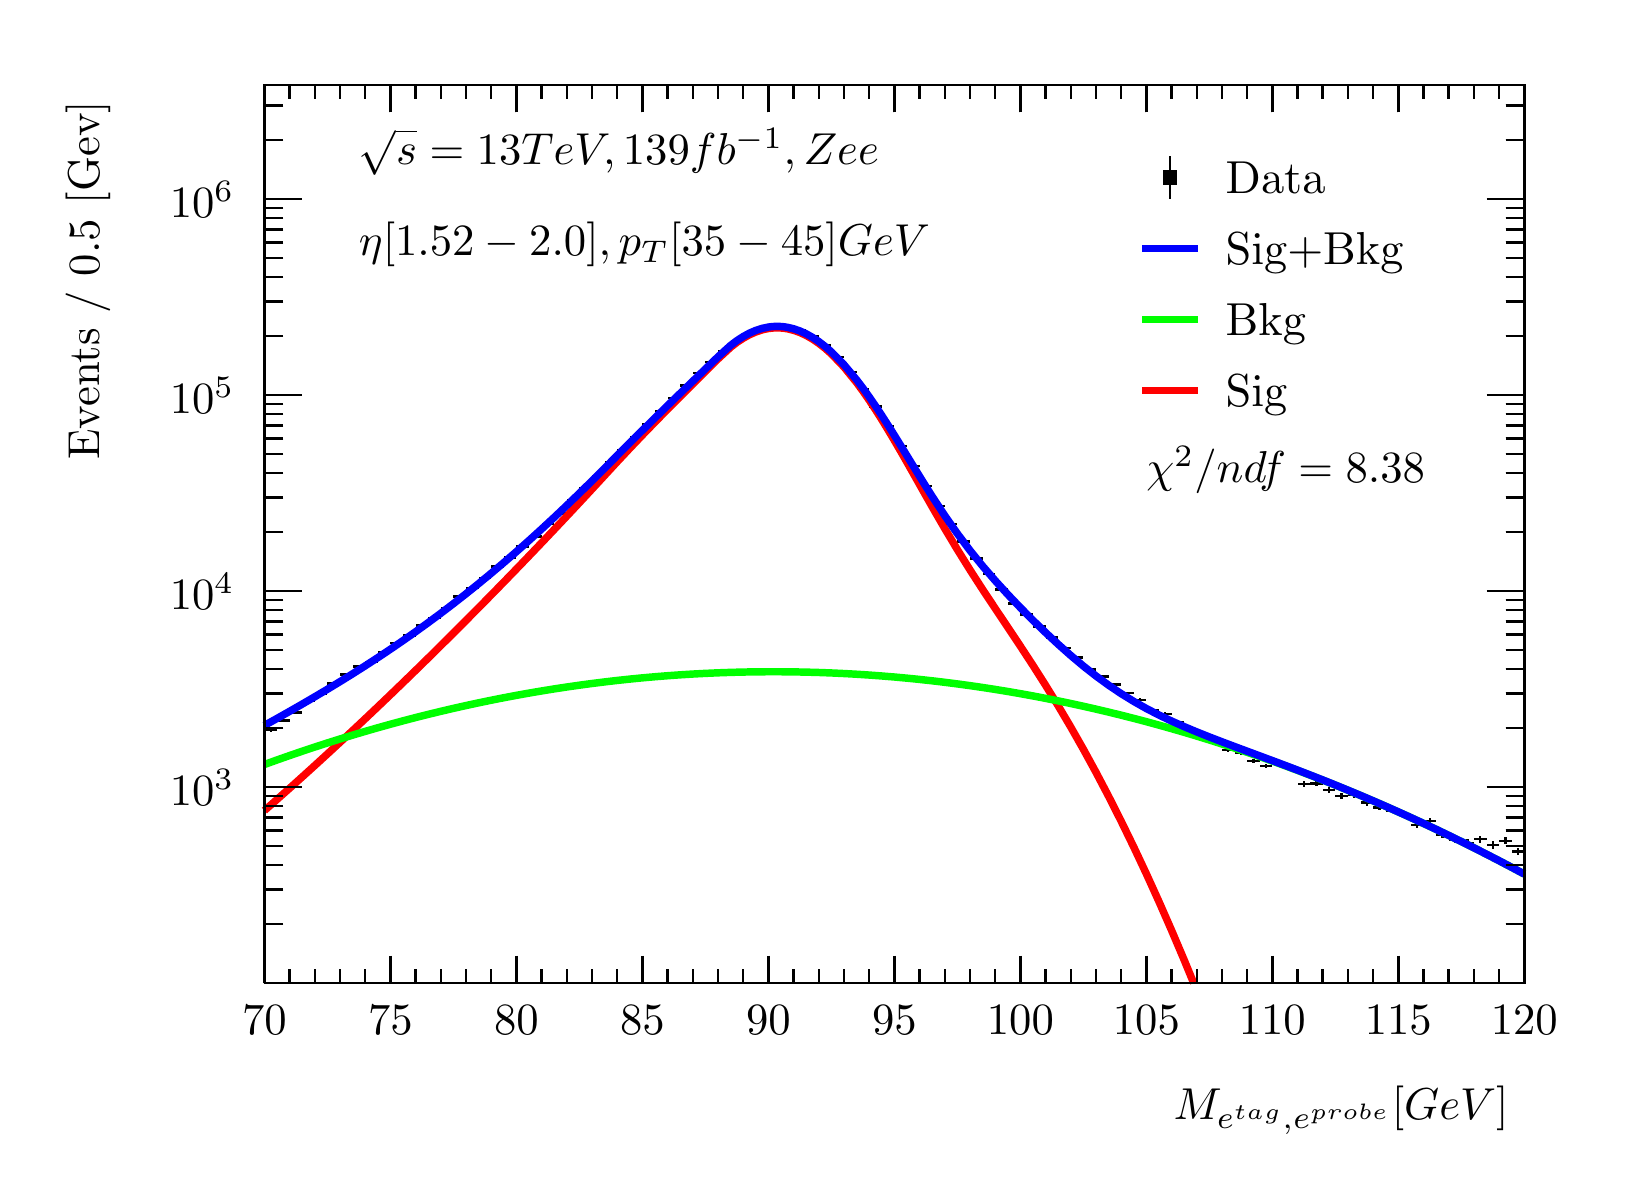
\begin{tikzpicture}
\pgfdeclareplotmark{cross} {
\pgfpathmoveto{\pgfpoint{-0.3\pgfplotmarksize}{\pgfplotmarksize}}
\pgfpathlineto{\pgfpoint{+0.3\pgfplotmarksize}{\pgfplotmarksize}}
\pgfpathlineto{\pgfpoint{+0.3\pgfplotmarksize}{0.3\pgfplotmarksize}}
\pgfpathlineto{\pgfpoint{+1\pgfplotmarksize}{0.3\pgfplotmarksize}}
\pgfpathlineto{\pgfpoint{+1\pgfplotmarksize}{-0.3\pgfplotmarksize}}
\pgfpathlineto{\pgfpoint{+0.3\pgfplotmarksize}{-0.3\pgfplotmarksize}}
\pgfpathlineto{\pgfpoint{+0.3\pgfplotmarksize}{-1.\pgfplotmarksize}}
\pgfpathlineto{\pgfpoint{-0.3\pgfplotmarksize}{-1.\pgfplotmarksize}}
\pgfpathlineto{\pgfpoint{-0.3\pgfplotmarksize}{-0.3\pgfplotmarksize}}
\pgfpathlineto{\pgfpoint{-1.\pgfplotmarksize}{-0.3\pgfplotmarksize}}
\pgfpathlineto{\pgfpoint{-1.\pgfplotmarksize}{0.3\pgfplotmarksize}}
\pgfpathlineto{\pgfpoint{-0.3\pgfplotmarksize}{0.3\pgfplotmarksize}}
\pgfpathclose
\pgfusepathqstroke
}
\pgfdeclareplotmark{cross*} {
\pgfpathmoveto{\pgfpoint{-0.3\pgfplotmarksize}{\pgfplotmarksize}}
\pgfpathlineto{\pgfpoint{+0.3\pgfplotmarksize}{\pgfplotmarksize}}
\pgfpathlineto{\pgfpoint{+0.3\pgfplotmarksize}{0.3\pgfplotmarksize}}
\pgfpathlineto{\pgfpoint{+1\pgfplotmarksize}{0.3\pgfplotmarksize}}
\pgfpathlineto{\pgfpoint{+1\pgfplotmarksize}{-0.3\pgfplotmarksize}}
\pgfpathlineto{\pgfpoint{+0.3\pgfplotmarksize}{-0.3\pgfplotmarksize}}
\pgfpathlineto{\pgfpoint{+0.3\pgfplotmarksize}{-1.\pgfplotmarksize}}
\pgfpathlineto{\pgfpoint{-0.3\pgfplotmarksize}{-1.\pgfplotmarksize}}
\pgfpathlineto{\pgfpoint{-0.3\pgfplotmarksize}{-0.3\pgfplotmarksize}}
\pgfpathlineto{\pgfpoint{-1.\pgfplotmarksize}{-0.3\pgfplotmarksize}}
\pgfpathlineto{\pgfpoint{-1.\pgfplotmarksize}{0.3\pgfplotmarksize}}
\pgfpathlineto{\pgfpoint{-0.3\pgfplotmarksize}{0.3\pgfplotmarksize}}
\pgfpathclose
\pgfusepathqfillstroke
}
\pgfdeclareplotmark{newstar} {
\pgfpathmoveto{\pgfqpoint{0pt}{\pgfplotmarksize}}
\pgfpathlineto{\pgfqpointpolar{44}{0.5\pgfplotmarksize}}
\pgfpathlineto{\pgfqpointpolar{18}{\pgfplotmarksize}}
\pgfpathlineto{\pgfqpointpolar{-20}{0.5\pgfplotmarksize}}
\pgfpathlineto{\pgfqpointpolar{-54}{\pgfplotmarksize}}
\pgfpathlineto{\pgfqpointpolar{-90}{0.5\pgfplotmarksize}}
\pgfpathlineto{\pgfqpointpolar{234}{\pgfplotmarksize}}
\pgfpathlineto{\pgfqpointpolar{198}{0.5\pgfplotmarksize}}
\pgfpathlineto{\pgfqpointpolar{162}{\pgfplotmarksize}}
\pgfpathlineto{\pgfqpointpolar{134}{0.5\pgfplotmarksize}}
\pgfpathclose
\pgfusepathqstroke
}
\pgfdeclareplotmark{newstar*} {
\pgfpathmoveto{\pgfqpoint{0pt}{\pgfplotmarksize}}
\pgfpathlineto{\pgfqpointpolar{44}{0.5\pgfplotmarksize}}
\pgfpathlineto{\pgfqpointpolar{18}{\pgfplotmarksize}}
\pgfpathlineto{\pgfqpointpolar{-20}{0.5\pgfplotmarksize}}
\pgfpathlineto{\pgfqpointpolar{-54}{\pgfplotmarksize}}
\pgfpathlineto{\pgfqpointpolar{-90}{0.5\pgfplotmarksize}}
\pgfpathlineto{\pgfqpointpolar{234}{\pgfplotmarksize}}
\pgfpathlineto{\pgfqpointpolar{198}{0.5\pgfplotmarksize}}
\pgfpathlineto{\pgfqpointpolar{162}{\pgfplotmarksize}}
\pgfpathlineto{\pgfqpointpolar{134}{0.5\pgfplotmarksize}}
\pgfpathclose
\pgfusepathqfillstroke
}
\definecolor{c}{rgb}{1,1,1};
\draw [color=c, fill=c] (0,0) rectangle (20,14.4361);
\draw [color=c, fill=c] (3,2.30977) rectangle (19,13.7143);
\definecolor{c}{rgb}{0,0,0};
\draw [c,line width=0.9] (3,2.30977) -- (3,13.7143) -- (19,13.7143) -- (19,2.30977) -- (3,2.30977);
\definecolor{c}{rgb}{1,1,1};
\draw [color=c, fill=c] (3,2.30977) rectangle (19,13.7143);
\definecolor{c}{rgb}{0,0,0};
\draw [c,line width=0.9] (3,2.30977) -- (3,13.7143) -- (19,13.7143) -- (19,2.30977) -- (3,2.30977);
\draw [c,line width=0.9] (3,2.30977) -- (19,2.30977);
\draw [c,line width=0.9] (3,2.65624) -- (3,2.30977);
\draw [c,line width=0.9] (3.32,2.48301) -- (3.32,2.30977);
\draw [c,line width=0.9] (3.64,2.48301) -- (3.64,2.30977);
\draw [c,line width=0.9] (3.96,2.48301) -- (3.96,2.30977);
\draw [c,line width=0.9] (4.28,2.48301) -- (4.28,2.30977);
\draw [c,line width=0.9] (4.6,2.65624) -- (4.6,2.30977);
\draw [c,line width=0.9] (4.92,2.48301) -- (4.92,2.30977);
\draw [c,line width=0.9] (5.24,2.48301) -- (5.24,2.30977);
\draw [c,line width=0.9] (5.56,2.48301) -- (5.56,2.30977);
\draw [c,line width=0.9] (5.88,2.48301) -- (5.88,2.30977);
\draw [c,line width=0.9] (6.2,2.65624) -- (6.2,2.30977);
\draw [c,line width=0.9] (6.52,2.48301) -- (6.52,2.30977);
\draw [c,line width=0.9] (6.84,2.48301) -- (6.84,2.30977);
\draw [c,line width=0.9] (7.16,2.48301) -- (7.16,2.30977);
\draw [c,line width=0.9] (7.48,2.48301) -- (7.48,2.30977);
\draw [c,line width=0.9] (7.8,2.65624) -- (7.8,2.30977);
\draw [c,line width=0.9] (8.12,2.48301) -- (8.12,2.30977);
\draw [c,line width=0.9] (8.44,2.48301) -- (8.44,2.30977);
\draw [c,line width=0.9] (8.76,2.48301) -- (8.76,2.30977);
\draw [c,line width=0.9] (9.08,2.48301) -- (9.08,2.30977);
\draw [c,line width=0.9] (9.4,2.65624) -- (9.4,2.30977);
\draw [c,line width=0.9] (9.72,2.48301) -- (9.72,2.30977);
\draw [c,line width=0.9] (10.04,2.48301) -- (10.04,2.30977);
\draw [c,line width=0.9] (10.36,2.48301) -- (10.36,2.30977);
\draw [c,line width=0.9] (10.68,2.48301) -- (10.68,2.30977);
\draw [c,line width=0.9] (11,2.65624) -- (11,2.30977);
\draw [c,line width=0.9] (11.32,2.48301) -- (11.32,2.30977);
\draw [c,line width=0.9] (11.64,2.48301) -- (11.64,2.30977);
\draw [c,line width=0.9] (11.96,2.48301) -- (11.96,2.30977);
\draw [c,line width=0.9] (12.28,2.48301) -- (12.28,2.30977);
\draw [c,line width=0.9] (12.6,2.65624) -- (12.6,2.30977);
\draw [c,line width=0.9] (12.92,2.48301) -- (12.92,2.30977);
\draw [c,line width=0.9] (13.24,2.48301) -- (13.24,2.30977);
\draw [c,line width=0.9] (13.56,2.48301) -- (13.56,2.30977);
\draw [c,line width=0.9] (13.88,2.48301) -- (13.88,2.30977);
\draw [c,line width=0.9] (14.2,2.65624) -- (14.2,2.30977);
\draw [c,line width=0.9] (14.52,2.48301) -- (14.52,2.30977);
\draw [c,line width=0.9] (14.84,2.48301) -- (14.84,2.30977);
\draw [c,line width=0.9] (15.16,2.48301) -- (15.16,2.30977);
\draw [c,line width=0.9] (15.48,2.48301) -- (15.48,2.30977);
\draw [c,line width=0.9] (15.8,2.65624) -- (15.8,2.30977);
\draw [c,line width=0.9] (16.12,2.48301) -- (16.12,2.30977);
\draw [c,line width=0.9] (16.44,2.48301) -- (16.44,2.30977);
\draw [c,line width=0.9] (16.76,2.48301) -- (16.76,2.30977);
\draw [c,line width=0.9] (17.08,2.48301) -- (17.08,2.30977);
\draw [c,line width=0.9] (17.4,2.65624) -- (17.4,2.30977);
\draw [c,line width=0.9] (17.72,2.48301) -- (17.72,2.30977);
\draw [c,line width=0.9] (18.04,2.48301) -- (18.04,2.30977);
\draw [c,line width=0.9] (18.36,2.48301) -- (18.36,2.30977);
\draw [c,line width=0.9] (18.68,2.48301) -- (18.68,2.30977);
\draw [c,line width=0.9] (19,2.65624) -- (19,2.30977);
\draw [anchor=base] (3,1.66015) node[scale=1.61424, color=c, rotate=0]{70};
\draw [anchor=base] (4.6,1.66015) node[scale=1.61424, color=c, rotate=0]{75};
\draw [anchor=base] (6.2,1.66015) node[scale=1.61424, color=c, rotate=0]{80};
\draw [anchor=base] (7.8,1.66015) node[scale=1.61424, color=c, rotate=0]{85};
\draw [anchor=base] (9.4,1.66015) node[scale=1.61424, color=c, rotate=0]{90};
\draw [anchor=base] (11,1.66015) node[scale=1.61424, color=c, rotate=0]{95};
\draw [anchor=base] (12.6,1.66015) node[scale=1.61424, color=c, rotate=0]{100};
\draw [anchor=base] (14.2,1.66015) node[scale=1.61424, color=c, rotate=0]{105};
\draw [anchor=base] (15.8,1.66015) node[scale=1.61424, color=c, rotate=0]{110};
\draw [anchor=base] (17.4,1.66015) node[scale=1.61424, color=c, rotate=0]{115};
\draw [anchor=base] (19,1.66015) node[scale=1.61424, color=c, rotate=0]{120};
\draw [anchor= east] (19,0.692932) node[scale=1.61424, color=c, rotate=0]{$M_{e^{tag}, e^{probe}}  [GeV]$};
\draw [c,line width=0.9] (3,13.7143) -- (19,13.7143);
\draw [c,line width=0.9] (3,13.3678) -- (3,13.7143);
\draw [c,line width=0.9] (3.32,13.5411) -- (3.32,13.7143);
\draw [c,line width=0.9] (3.64,13.5411) -- (3.64,13.7143);
\draw [c,line width=0.9] (3.96,13.5411) -- (3.96,13.7143);
\draw [c,line width=0.9] (4.28,13.5411) -- (4.28,13.7143);
\draw [c,line width=0.9] (4.6,13.3678) -- (4.6,13.7143);
\draw [c,line width=0.9] (4.92,13.5411) -- (4.92,13.7143);
\draw [c,line width=0.9] (5.24,13.5411) -- (5.24,13.7143);
\draw [c,line width=0.9] (5.56,13.5411) -- (5.56,13.7143);
\draw [c,line width=0.9] (5.88,13.5411) -- (5.88,13.7143);
\draw [c,line width=0.9] (6.2,13.3678) -- (6.2,13.7143);
\draw [c,line width=0.9] (6.52,13.5411) -- (6.52,13.7143);
\draw [c,line width=0.9] (6.84,13.5411) -- (6.84,13.7143);
\draw [c,line width=0.9] (7.16,13.5411) -- (7.16,13.7143);
\draw [c,line width=0.9] (7.48,13.5411) -- (7.48,13.7143);
\draw [c,line width=0.9] (7.8,13.3678) -- (7.8,13.7143);
\draw [c,line width=0.9] (8.12,13.5411) -- (8.12,13.7143);
\draw [c,line width=0.9] (8.44,13.5411) -- (8.44,13.7143);
\draw [c,line width=0.9] (8.76,13.5411) -- (8.76,13.7143);
\draw [c,line width=0.9] (9.08,13.5411) -- (9.08,13.7143);
\draw [c,line width=0.9] (9.4,13.3678) -- (9.4,13.7143);
\draw [c,line width=0.9] (9.72,13.5411) -- (9.72,13.7143);
\draw [c,line width=0.9] (10.04,13.5411) -- (10.04,13.7143);
\draw [c,line width=0.9] (10.36,13.5411) -- (10.36,13.7143);
\draw [c,line width=0.9] (10.68,13.5411) -- (10.68,13.7143);
\draw [c,line width=0.9] (11,13.3678) -- (11,13.7143);
\draw [c,line width=0.9] (11.32,13.5411) -- (11.32,13.7143);
\draw [c,line width=0.9] (11.64,13.5411) -- (11.64,13.7143);
\draw [c,line width=0.9] (11.96,13.5411) -- (11.96,13.7143);
\draw [c,line width=0.9] (12.28,13.5411) -- (12.28,13.7143);
\draw [c,line width=0.9] (12.6,13.3678) -- (12.6,13.7143);
\draw [c,line width=0.9] (12.92,13.5411) -- (12.92,13.7143);
\draw [c,line width=0.9] (13.24,13.5411) -- (13.24,13.7143);
\draw [c,line width=0.9] (13.56,13.5411) -- (13.56,13.7143);
\draw [c,line width=0.9] (13.88,13.5411) -- (13.88,13.7143);
\draw [c,line width=0.9] (14.2,13.3678) -- (14.2,13.7143);
\draw [c,line width=0.9] (14.52,13.5411) -- (14.52,13.7143);
\draw [c,line width=0.9] (14.84,13.5411) -- (14.84,13.7143);
\draw [c,line width=0.9] (15.16,13.5411) -- (15.16,13.7143);
\draw [c,line width=0.9] (15.48,13.5411) -- (15.48,13.7143);
\draw [c,line width=0.9] (15.8,13.3678) -- (15.8,13.7143);
\draw [c,line width=0.9] (16.12,13.5411) -- (16.12,13.7143);
\draw [c,line width=0.9] (16.44,13.5411) -- (16.44,13.7143);
\draw [c,line width=0.9] (16.76,13.5411) -- (16.76,13.7143);
\draw [c,line width=0.9] (17.08,13.5411) -- (17.08,13.7143);
\draw [c,line width=0.9] (17.4,13.3678) -- (17.4,13.7143);
\draw [c,line width=0.9] (17.72,13.5411) -- (17.72,13.7143);
\draw [c,line width=0.9] (18.04,13.5411) -- (18.04,13.7143);
\draw [c,line width=0.9] (18.36,13.5411) -- (18.36,13.7143);
\draw [c,line width=0.9] (18.68,13.5411) -- (18.68,13.7143);
\draw [c,line width=0.9] (19,13.3678) -- (19,13.7143);
\draw [c,line width=0.9] (3,2.30977) -- (3,13.7143);
\draw [c,line width=0.9] (3.237,3.05909) -- (3,3.05909);
\draw [c,line width=0.9] (3.237,3.49742) -- (3,3.49742);
\draw [c,line width=0.9] (3.237,3.80841) -- (3,3.80841);
\draw [c,line width=0.9] (3.237,4.04964) -- (3,4.04964);
\draw [c,line width=0.9] (3.237,4.24673) -- (3,4.24673);
\draw [c,line width=0.9] (3.237,4.41338) -- (3,4.41338);
\draw [c,line width=0.9] (3.237,4.55773) -- (3,4.55773);
\draw [c,line width=0.9] (3.237,4.68506) -- (3,4.68506);
\draw [c,line width=0.9] (3.474,4.79896) -- (3,4.79896);
\draw [anchor= east] (2.82,4.79896) node[scale=1.61424, color=c, rotate=0]{$10^{3}$};
\draw [c,line width=0.9] (3.237,5.54828) -- (3,5.54828);
\draw [c,line width=0.9] (3.237,5.9866) -- (3,5.9866);
\draw [c,line width=0.9] (3.237,6.2976) -- (3,6.2976);
\draw [c,line width=0.9] (3.237,6.53882) -- (3,6.53882);
\draw [c,line width=0.9] (3.237,6.73592) -- (3,6.73592);
\draw [c,line width=0.9] (3.237,6.90256) -- (3,6.90256);
\draw [c,line width=0.9] (3.237,7.04692) -- (3,7.04692);
\draw [c,line width=0.9] (3.237,7.17424) -- (3,7.17424);
\draw [c,line width=0.9] (3.474,7.28814) -- (3,7.28814);
\draw [anchor= east] (2.82,7.28814) node[scale=1.61424, color=c, rotate=0]{$10^{4}$};
\draw [c,line width=0.9] (3.237,8.03746) -- (3,8.03746);
\draw [c,line width=0.9] (3.237,8.47579) -- (3,8.47579);
\draw [c,line width=0.9] (3.237,8.78678) -- (3,8.78678);
\draw [c,line width=0.9] (3.237,9.02801) -- (3,9.02801);
\draw [c,line width=0.9] (3.237,9.2251) -- (3,9.2251);
\draw [c,line width=0.9] (3.237,9.39175) -- (3,9.39175);
\draw [c,line width=0.9] (3.237,9.5361) -- (3,9.5361);
\draw [c,line width=0.9] (3.237,9.66343) -- (3,9.66343);
\draw [c,line width=0.9] (3.474,9.77733) -- (3,9.77733);
\draw [anchor= east] (2.82,9.77733) node[scale=1.61424, color=c, rotate=0]{$10^{5}$};
\draw [c,line width=0.9] (3.237,10.5266) -- (3,10.5266);
\draw [c,line width=0.9] (3.237,10.965) -- (3,10.965);
\draw [c,line width=0.9] (3.237,11.276) -- (3,11.276);
\draw [c,line width=0.9] (3.237,11.5172) -- (3,11.5172);
\draw [c,line width=0.9] (3.237,11.7143) -- (3,11.7143);
\draw [c,line width=0.9] (3.237,11.8809) -- (3,11.8809);
\draw [c,line width=0.9] (3.237,12.0253) -- (3,12.0253);
\draw [c,line width=0.9] (3.237,12.1526) -- (3,12.1526);
\draw [c,line width=0.9] (3.474,12.2665) -- (3,12.2665);
\draw [anchor= east] (2.82,12.2665) node[scale=1.61424, color=c, rotate=0]{$10^{6}$};
\draw [c,line width=0.9] (3.237,13.0158) -- (3,13.0158);
\draw [c,line width=0.9] (3.237,13.4542) -- (3,13.4542);
\draw [anchor= east] (0.76,13.7143) node[scale=1.61424, color=c, rotate=90]{Events / 0.5 [Gev]};
\draw [c,line width=0.9] (19,2.30977) -- (19,13.7143);
\draw [c,line width=0.9] (18.763,3.05909) -- (19,3.05909);
\draw [c,line width=0.9] (18.763,3.49742) -- (19,3.49742);
\draw [c,line width=0.9] (18.763,3.80841) -- (19,3.80841);
\draw [c,line width=0.9] (18.763,4.04964) -- (19,4.04964);
\draw [c,line width=0.9] (18.763,4.24673) -- (19,4.24673);
\draw [c,line width=0.9] (18.763,4.41338) -- (19,4.41338);
\draw [c,line width=0.9] (18.763,4.55773) -- (19,4.55773);
\draw [c,line width=0.9] (18.763,4.68506) -- (19,4.68506);
\draw [c,line width=0.9] (18.526,4.79896) -- (19,4.79896);
\draw [c,line width=0.9] (18.763,5.54828) -- (19,5.54828);
\draw [c,line width=0.9] (18.763,5.9866) -- (19,5.9866);
\draw [c,line width=0.9] (18.763,6.2976) -- (19,6.2976);
\draw [c,line width=0.9] (18.763,6.53882) -- (19,6.53882);
\draw [c,line width=0.9] (18.763,6.73592) -- (19,6.73592);
\draw [c,line width=0.9] (18.763,6.90256) -- (19,6.90256);
\draw [c,line width=0.9] (18.763,7.04692) -- (19,7.04692);
\draw [c,line width=0.9] (18.763,7.17424) -- (19,7.17424);
\draw [c,line width=0.9] (18.526,7.28814) -- (19,7.28814);
\draw [c,line width=0.9] (18.763,8.03746) -- (19,8.03746);
\draw [c,line width=0.9] (18.763,8.47579) -- (19,8.47579);
\draw [c,line width=0.9] (18.763,8.78678) -- (19,8.78678);
\draw [c,line width=0.9] (18.763,9.02801) -- (19,9.02801);
\draw [c,line width=0.9] (18.763,9.2251) -- (19,9.2251);
\draw [c,line width=0.9] (18.763,9.39175) -- (19,9.39175);
\draw [c,line width=0.9] (18.763,9.5361) -- (19,9.5361);
\draw [c,line width=0.9] (18.763,9.66343) -- (19,9.66343);
\draw [c,line width=0.9] (18.526,9.77733) -- (19,9.77733);
\draw [c,line width=0.9] (18.763,10.5266) -- (19,10.5266);
\draw [c,line width=0.9] (18.763,10.965) -- (19,10.965);
\draw [c,line width=0.9] (18.763,11.276) -- (19,11.276);
\draw [c,line width=0.9] (18.763,11.5172) -- (19,11.5172);
\draw [c,line width=0.9] (18.763,11.7143) -- (19,11.7143);
\draw [c,line width=0.9] (18.763,11.8809) -- (19,11.8809);
\draw [c,line width=0.9] (18.763,12.0253) -- (19,12.0253);
\draw [c,line width=0.9] (18.763,12.1526) -- (19,12.1526);
\draw [c,line width=0.9] (18.526,12.2665) -- (19,12.2665);
\draw [c,line width=0.9] (18.763,13.0158) -- (19,13.0158);
\draw [c,line width=0.9] (18.763,13.4542) -- (19,13.4542);
\draw [c,line width=0.9] (3.08,5.52589) -- (3,5.52589);
\draw [c,line width=0.9] (3,5.52589) -- (3,5.52589);
\draw [c,line width=0.9] (3.08,5.52589) -- (3.16,5.52589);
\draw [c,line width=0.9] (3.16,5.52589) -- (3.16,5.52589);
\draw [c,line width=0.9] (3.08,5.52589) -- (3.08,5.55031);
\draw [c,line width=0.9] (3.08,5.55031) -- (3.08,5.55031);
\draw [c,line width=0.9] (3.08,5.52589) -- (3.08,5.50146);
\draw [c,line width=0.9] (3.08,5.50146) -- (3.08,5.50146);
\draw [c,line width=0.9] (3.24,5.64639) -- (3.16,5.64639);
\draw [c,line width=0.9] (3.16,5.64639) -- (3.16,5.64639);
\draw [c,line width=0.9] (3.24,5.64639) -- (3.32,5.64639);
\draw [c,line width=0.9] (3.32,5.64639) -- (3.32,5.64639);
\draw [c,line width=0.9] (3.24,5.64639) -- (3.24,5.66949);
\draw [c,line width=0.9] (3.24,5.66949) -- (3.24,5.66949);
\draw [c,line width=0.9] (3.24,5.64639) -- (3.24,5.62329);
\draw [c,line width=0.9] (3.24,5.62329) -- (3.24,5.62329);
\draw [c,line width=0.9] (3.4,5.74402) -- (3.32,5.74402);
\draw [c,line width=0.9] (3.32,5.74402) -- (3.32,5.74402);
\draw [c,line width=0.9] (3.4,5.74402) -- (3.48,5.74402);
\draw [c,line width=0.9] (3.48,5.74402) -- (3.48,5.74402);
\draw [c,line width=0.9] (3.4,5.74402) -- (3.4,5.7661);
\draw [c,line width=0.9] (3.4,5.7661) -- (3.4,5.7661);
\draw [c,line width=0.9] (3.4,5.74402) -- (3.4,5.72194);
\draw [c,line width=0.9] (3.4,5.72194) -- (3.4,5.72194);
\draw [c,line width=0.9] (3.56,5.89411) -- (3.48,5.89411);
\draw [c,line width=0.9] (3.48,5.89411) -- (3.48,5.89411);
\draw [c,line width=0.9] (3.56,5.89411) -- (3.64,5.89411);
\draw [c,line width=0.9] (3.64,5.89411) -- (3.64,5.89411);
\draw [c,line width=0.9] (3.56,5.89411) -- (3.56,5.91471);
\draw [c,line width=0.9] (3.56,5.91471) -- (3.56,5.91471);
\draw [c,line width=0.9] (3.56,5.89411) -- (3.56,5.87351);
\draw [c,line width=0.9] (3.56,5.87351) -- (3.56,5.87351);
\draw [c,line width=0.9] (3.72,5.97828) -- (3.64,5.97828);
\draw [c,line width=0.9] (3.64,5.97828) -- (3.64,5.97828);
\draw [c,line width=0.9] (3.72,5.97828) -- (3.8,5.97828);
\draw [c,line width=0.9] (3.8,5.97828) -- (3.8,5.97828);
\draw [c,line width=0.9] (3.72,5.97828) -- (3.72,5.99809);
\draw [c,line width=0.9] (3.72,5.99809) -- (3.72,5.99809);
\draw [c,line width=0.9] (3.72,5.97828) -- (3.72,5.95847);
\draw [c,line width=0.9] (3.72,5.95847) -- (3.72,5.95847);
\draw [c,line width=0.9] (3.88,6.11297) -- (3.8,6.11297);
\draw [c,line width=0.9] (3.8,6.11297) -- (3.8,6.11297);
\draw [c,line width=0.9] (3.88,6.11297) -- (3.96,6.11297);
\draw [c,line width=0.9] (3.96,6.11297) -- (3.96,6.11297);
\draw [c,line width=0.9] (3.88,6.11297) -- (3.88,6.13158);
\draw [c,line width=0.9] (3.88,6.13158) -- (3.88,6.13158);
\draw [c,line width=0.9] (3.88,6.11297) -- (3.88,6.09435);
\draw [c,line width=0.9] (3.88,6.09435) -- (3.88,6.09435);
\draw [c,line width=0.9] (4.04,6.22639) -- (3.96,6.22639);
\draw [c,line width=0.9] (3.96,6.22639) -- (3.96,6.22639);
\draw [c,line width=0.9] (4.04,6.22639) -- (4.12,6.22639);
\draw [c,line width=0.9] (4.12,6.22639) -- (4.12,6.22639);
\draw [c,line width=0.9] (4.04,6.22639) -- (4.04,6.24405);
\draw [c,line width=0.9] (4.04,6.24405) -- (4.04,6.24405);
\draw [c,line width=0.9] (4.04,6.22639) -- (4.04,6.20872);
\draw [c,line width=0.9] (4.04,6.20872) -- (4.04,6.20872);
\draw [c,line width=0.9] (4.2,6.3327) -- (4.12,6.3327);
\draw [c,line width=0.9] (4.12,6.3327) -- (4.12,6.3327);
\draw [c,line width=0.9] (4.2,6.3327) -- (4.28,6.3327);
\draw [c,line width=0.9] (4.28,6.3327) -- (4.28,6.3327);
\draw [c,line width=0.9] (4.2,6.3327) -- (4.2,6.34951);
\draw [c,line width=0.9] (4.2,6.34951) -- (4.2,6.34951);
\draw [c,line width=0.9] (4.2,6.3327) -- (4.2,6.31588);
\draw [c,line width=0.9] (4.2,6.31588) -- (4.2,6.31588);
\draw [c,line width=0.9] (4.36,6.38529) -- (4.28,6.38529);
\draw [c,line width=0.9] (4.28,6.38529) -- (4.28,6.38529);
\draw [c,line width=0.9] (4.36,6.38529) -- (4.44,6.38529);
\draw [c,line width=0.9] (4.44,6.38529) -- (4.44,6.38529);
\draw [c,line width=0.9] (4.36,6.38529) -- (4.36,6.4017);
\draw [c,line width=0.9] (4.36,6.4017) -- (4.36,6.4017);
\draw [c,line width=0.9] (4.36,6.38529) -- (4.36,6.36888);
\draw [c,line width=0.9] (4.36,6.36888) -- (4.36,6.36888);
\draw [c,line width=0.9] (4.52,6.51676) -- (4.44,6.51676);
\draw [c,line width=0.9] (4.44,6.51676) -- (4.44,6.51676);
\draw [c,line width=0.9] (4.52,6.51676) -- (4.6,6.51676);
\draw [c,line width=0.9] (4.6,6.51676) -- (4.6,6.51676);
\draw [c,line width=0.9] (4.52,6.51676) -- (4.52,6.53221);
\draw [c,line width=0.9] (4.52,6.53221) -- (4.52,6.53221);
\draw [c,line width=0.9] (4.52,6.51676) -- (4.52,6.50132);
\draw [c,line width=0.9] (4.52,6.50132) -- (4.52,6.50132);
\draw [c,line width=0.9] (4.68,6.62921) -- (4.6,6.62921);
\draw [c,line width=0.9] (4.6,6.62921) -- (4.6,6.62921);
\draw [c,line width=0.9] (4.68,6.62921) -- (4.76,6.62921);
\draw [c,line width=0.9] (4.76,6.62921) -- (4.76,6.62921);
\draw [c,line width=0.9] (4.68,6.62921) -- (4.68,6.64387);
\draw [c,line width=0.9] (4.68,6.64387) -- (4.68,6.64387);
\draw [c,line width=0.9] (4.68,6.62921) -- (4.68,6.61454);
\draw [c,line width=0.9] (4.68,6.61454) -- (4.68,6.61454);
\draw [c,line width=0.9] (4.84,6.72378) -- (4.76,6.72378);
\draw [c,line width=0.9] (4.76,6.72378) -- (4.76,6.72378);
\draw [c,line width=0.9] (4.84,6.72378) -- (4.92,6.72378);
\draw [c,line width=0.9] (4.92,6.72378) -- (4.92,6.72378);
\draw [c,line width=0.9] (4.84,6.72378) -- (4.84,6.73782);
\draw [c,line width=0.9] (4.84,6.73782) -- (4.84,6.73782);
\draw [c,line width=0.9] (4.84,6.72378) -- (4.84,6.70975);
\draw [c,line width=0.9] (4.84,6.70975) -- (4.84,6.70975);
\draw [c,line width=0.9] (5,6.8523) -- (4.92,6.8523);
\draw [c,line width=0.9] (4.92,6.8523) -- (4.92,6.8523);
\draw [c,line width=0.9] (5,6.8523) -- (5.08,6.8523);
\draw [c,line width=0.9] (5.08,6.8523) -- (5.08,6.8523);
\draw [c,line width=0.9] (5,6.8523) -- (5,6.86553);
\draw [c,line width=0.9] (5,6.86553) -- (5,6.86553);
\draw [c,line width=0.9] (5,6.8523) -- (5,6.83908);
\draw [c,line width=0.9] (5,6.83908) -- (5,6.83908);
\draw [c,line width=0.9] (5.16,6.94392) -- (5.08,6.94392);
\draw [c,line width=0.9] (5.08,6.94392) -- (5.08,6.94392);
\draw [c,line width=0.9] (5.16,6.94392) -- (5.24,6.94392);
\draw [c,line width=0.9] (5.24,6.94392) -- (5.24,6.94392);
\draw [c,line width=0.9] (5.16,6.94392) -- (5.16,6.9566);
\draw [c,line width=0.9] (5.16,6.9566) -- (5.16,6.9566);
\draw [c,line width=0.9] (5.16,6.94392) -- (5.16,6.93125);
\draw [c,line width=0.9] (5.16,6.93125) -- (5.16,6.93125);
\draw [c,line width=0.9] (5.32,7.07216) -- (5.24,7.07216);
\draw [c,line width=0.9] (5.24,7.07216) -- (5.24,7.07216);
\draw [c,line width=0.9] (5.32,7.07216) -- (5.4,7.07216);
\draw [c,line width=0.9] (5.4,7.07216) -- (5.4,7.07216);
\draw [c,line width=0.9] (5.32,7.07216) -- (5.32,7.08411);
\draw [c,line width=0.9] (5.32,7.08411) -- (5.32,7.08411);
\draw [c,line width=0.9] (5.32,7.07216) -- (5.32,7.06021);
\draw [c,line width=0.9] (5.32,7.06021) -- (5.32,7.06021);
\draw [c,line width=0.9] (5.48,7.21745) -- (5.4,7.21745);
\draw [c,line width=0.9] (5.4,7.21745) -- (5.4,7.21745);
\draw [c,line width=0.9] (5.48,7.21745) -- (5.56,7.21745);
\draw [c,line width=0.9] (5.56,7.21745) -- (5.56,7.21745);
\draw [c,line width=0.9] (5.48,7.21745) -- (5.48,7.22862);
\draw [c,line width=0.9] (5.48,7.22862) -- (5.48,7.22862);
\draw [c,line width=0.9] (5.48,7.21745) -- (5.48,7.20628);
\draw [c,line width=0.9] (5.48,7.20628) -- (5.48,7.20628);
\draw [c,line width=0.9] (5.64,7.32648) -- (5.56,7.32648);
\draw [c,line width=0.9] (5.56,7.32648) -- (5.56,7.32648);
\draw [c,line width=0.9] (5.64,7.32648) -- (5.72,7.32648);
\draw [c,line width=0.9] (5.72,7.32648) -- (5.72,7.32648);
\draw [c,line width=0.9] (5.64,7.32648) -- (5.64,7.3371);
\draw [c,line width=0.9] (5.64,7.3371) -- (5.64,7.3371);
\draw [c,line width=0.9] (5.64,7.32648) -- (5.64,7.31586);
\draw [c,line width=0.9] (5.64,7.31586) -- (5.64,7.31586);
\draw [c,line width=0.9] (5.8,7.4538) -- (5.72,7.4538);
\draw [c,line width=0.9] (5.72,7.4538) -- (5.72,7.4538);
\draw [c,line width=0.9] (5.8,7.4538) -- (5.88,7.4538);
\draw [c,line width=0.9] (5.88,7.4538) -- (5.88,7.4538);
\draw [c,line width=0.9] (5.8,7.4538) -- (5.8,7.46381);
\draw [c,line width=0.9] (5.8,7.46381) -- (5.8,7.46381);
\draw [c,line width=0.9] (5.8,7.4538) -- (5.8,7.44378);
\draw [c,line width=0.9] (5.8,7.44378) -- (5.8,7.44378);
\draw [c,line width=0.9] (5.96,7.60065) -- (5.88,7.60065);
\draw [c,line width=0.9] (5.88,7.60065) -- (5.88,7.60065);
\draw [c,line width=0.9] (5.96,7.60065) -- (6.04,7.60065);
\draw [c,line width=0.9] (6.04,7.60065) -- (6.04,7.60065);
\draw [c,line width=0.9] (5.96,7.60065) -- (5.96,7.61001);
\draw [c,line width=0.9] (5.96,7.61001) -- (5.96,7.61001);
\draw [c,line width=0.9] (5.96,7.60065) -- (5.96,7.5913);
\draw [c,line width=0.9] (5.96,7.5913) -- (5.96,7.5913);
\draw [c,line width=0.9] (6.12,7.7148) -- (6.04,7.7148);
\draw [c,line width=0.9] (6.04,7.7148) -- (6.04,7.7148);
\draw [c,line width=0.9] (6.12,7.7148) -- (6.2,7.7148);
\draw [c,line width=0.9] (6.2,7.7148) -- (6.2,7.7148);
\draw [c,line width=0.9] (6.12,7.7148) -- (6.12,7.72368);
\draw [c,line width=0.9] (6.12,7.72368) -- (6.12,7.72368);
\draw [c,line width=0.9] (6.12,7.7148) -- (6.12,7.70593);
\draw [c,line width=0.9] (6.12,7.70593) -- (6.12,7.70593);
\draw [c,line width=0.9] (6.28,7.85399) -- (6.2,7.85399);
\draw [c,line width=0.9] (6.2,7.85399) -- (6.2,7.85399);
\draw [c,line width=0.9] (6.28,7.85399) -- (6.36,7.85399);
\draw [c,line width=0.9] (6.36,7.85399) -- (6.36,7.85399);
\draw [c,line width=0.9] (6.28,7.85399) -- (6.28,7.86231);
\draw [c,line width=0.9] (6.28,7.86231) -- (6.28,7.86231);
\draw [c,line width=0.9] (6.28,7.85399) -- (6.28,7.84567);
\draw [c,line width=0.9] (6.28,7.84567) -- (6.28,7.84567);
\draw [c,line width=0.9] (6.44,7.97991) -- (6.36,7.97991);
\draw [c,line width=0.9] (6.36,7.97991) -- (6.36,7.97991);
\draw [c,line width=0.9] (6.44,7.97991) -- (6.52,7.97991);
\draw [c,line width=0.9] (6.52,7.97991) -- (6.52,7.97991);
\draw [c,line width=0.9] (6.44,7.97991) -- (6.44,7.98776);
\draw [c,line width=0.9] (6.44,7.98776) -- (6.44,7.98776);
\draw [c,line width=0.9] (6.44,7.97991) -- (6.44,7.97205);
\draw [c,line width=0.9] (6.44,7.97205) -- (6.44,7.97205);
\draw [c,line width=0.9] (6.6,8.13917) -- (6.52,8.13917);
\draw [c,line width=0.9] (6.52,8.13917) -- (6.52,8.13917);
\draw [c,line width=0.9] (6.6,8.13917) -- (6.68,8.13917);
\draw [c,line width=0.9] (6.68,8.13917) -- (6.68,8.13917);
\draw [c,line width=0.9] (6.6,8.13917) -- (6.6,8.14646);
\draw [c,line width=0.9] (6.6,8.14646) -- (6.6,8.14646);
\draw [c,line width=0.9] (6.6,8.13917) -- (6.6,8.13188);
\draw [c,line width=0.9] (6.6,8.13188) -- (6.6,8.13188);
\draw [c,line width=0.9] (6.76,8.27036) -- (6.68,8.27036);
\draw [c,line width=0.9] (6.68,8.27036) -- (6.68,8.27036);
\draw [c,line width=0.9] (6.76,8.27036) -- (6.84,8.27036);
\draw [c,line width=0.9] (6.84,8.27036) -- (6.84,8.27036);
\draw [c,line width=0.9] (6.76,8.27036) -- (6.76,8.27722);
\draw [c,line width=0.9] (6.76,8.27722) -- (6.76,8.27722);
\draw [c,line width=0.9] (6.76,8.27036) -- (6.76,8.26349);
\draw [c,line width=0.9] (6.76,8.26349) -- (6.76,8.26349);
\draw [c,line width=0.9] (6.92,8.44642) -- (6.84,8.44642);
\draw [c,line width=0.9] (6.84,8.44642) -- (6.84,8.44642);
\draw [c,line width=0.9] (6.92,8.44642) -- (7,8.44642);
\draw [c,line width=0.9] (7,8.44642) -- (7,8.44642);
\draw [c,line width=0.9] (6.92,8.44642) -- (6.92,8.45275);
\draw [c,line width=0.9] (6.92,8.45275) -- (6.92,8.45275);
\draw [c,line width=0.9] (6.92,8.44642) -- (6.92,8.44009);
\draw [c,line width=0.9] (6.92,8.44009) -- (6.92,8.44009);
\draw [c,line width=0.9] (7.08,8.58886) -- (7,8.58886);
\draw [c,line width=0.9] (7,8.58886) -- (7,8.58886);
\draw [c,line width=0.9] (7.08,8.58886) -- (7.16,8.58886);
\draw [c,line width=0.9] (7.16,8.58886) -- (7.16,8.58886);
\draw [c,line width=0.9] (7.08,8.58886) -- (7.08,8.59479);
\draw [c,line width=0.9] (7.08,8.59479) -- (7.08,8.59479);
\draw [c,line width=0.9] (7.08,8.58886) -- (7.08,8.58294);
\draw [c,line width=0.9] (7.08,8.58294) -- (7.08,8.58294);
\draw [c,line width=0.9] (7.24,8.74431) -- (7.16,8.74431);
\draw [c,line width=0.9] (7.16,8.74431) -- (7.16,8.74431);
\draw [c,line width=0.9] (7.24,8.74431) -- (7.32,8.74431);
\draw [c,line width=0.9] (7.32,8.74431) -- (7.32,8.74431);
\draw [c,line width=0.9] (7.24,8.74431) -- (7.24,8.74982);
\draw [c,line width=0.9] (7.24,8.74982) -- (7.24,8.74982);
\draw [c,line width=0.9] (7.24,8.74431) -- (7.24,8.7388);
\draw [c,line width=0.9] (7.24,8.7388) -- (7.24,8.7388);
\draw [c,line width=0.9] (7.4,8.91807) -- (7.32,8.91807);
\draw [c,line width=0.9] (7.32,8.91807) -- (7.32,8.91807);
\draw [c,line width=0.9] (7.4,8.91807) -- (7.48,8.91807);
\draw [c,line width=0.9] (7.48,8.91807) -- (7.48,8.91807);
\draw [c,line width=0.9] (7.4,8.91807) -- (7.4,8.92315);
\draw [c,line width=0.9] (7.4,8.92315) -- (7.4,8.92315);
\draw [c,line width=0.9] (7.4,8.91807) -- (7.4,8.91298);
\draw [c,line width=0.9] (7.4,8.91298) -- (7.4,8.91298);
\draw [c,line width=0.9] (7.56,9.0753) -- (7.48,9.0753);
\draw [c,line width=0.9] (7.48,9.0753) -- (7.48,9.0753);
\draw [c,line width=0.9] (7.56,9.0753) -- (7.64,9.0753);
\draw [c,line width=0.9] (7.64,9.0753) -- (7.64,9.0753);
\draw [c,line width=0.9] (7.56,9.0753) -- (7.56,9.08003);
\draw [c,line width=0.9] (7.56,9.08003) -- (7.56,9.08003);
\draw [c,line width=0.9] (7.56,9.0753) -- (7.56,9.07057);
\draw [c,line width=0.9] (7.56,9.07057) -- (7.56,9.07057);
\draw [c,line width=0.9] (7.72,9.24432) -- (7.64,9.24432);
\draw [c,line width=0.9] (7.64,9.24432) -- (7.64,9.24432);
\draw [c,line width=0.9] (7.72,9.24432) -- (7.8,9.24432);
\draw [c,line width=0.9] (7.8,9.24432) -- (7.8,9.24432);
\draw [c,line width=0.9] (7.72,9.24432) -- (7.72,9.24869);
\draw [c,line width=0.9] (7.72,9.24869) -- (7.72,9.24869);
\draw [c,line width=0.9] (7.72,9.24432) -- (7.72,9.23995);
\draw [c,line width=0.9] (7.72,9.23995) -- (7.72,9.23995);
\draw [c,line width=0.9] (7.88,9.40842) -- (7.8,9.40842);
\draw [c,line width=0.9] (7.8,9.40842) -- (7.8,9.40842);
\draw [c,line width=0.9] (7.88,9.40842) -- (7.96,9.40842);
\draw [c,line width=0.9] (7.96,9.40842) -- (7.96,9.40842);
\draw [c,line width=0.9] (7.88,9.40842) -- (7.88,9.41248);
\draw [c,line width=0.9] (7.88,9.41248) -- (7.88,9.41248);
\draw [c,line width=0.9] (7.88,9.40842) -- (7.88,9.40437);
\draw [c,line width=0.9] (7.88,9.40437) -- (7.88,9.40437);
\draw [c,line width=0.9] (8.04,9.5776) -- (7.96,9.5776);
\draw [c,line width=0.9] (7.96,9.5776) -- (7.96,9.5776);
\draw [c,line width=0.9] (8.04,9.5776) -- (8.12,9.5776);
\draw [c,line width=0.9] (8.12,9.5776) -- (8.12,9.5776);
\draw [c,line width=0.9] (8.04,9.5776) -- (8.04,9.58135);
\draw [c,line width=0.9] (8.04,9.58135) -- (8.04,9.58135);
\draw [c,line width=0.9] (8.04,9.5776) -- (8.04,9.57385);
\draw [c,line width=0.9] (8.04,9.57385) -- (8.04,9.57385);
\draw [c,line width=0.9] (8.2,9.73996) -- (8.12,9.73996);
\draw [c,line width=0.9] (8.12,9.73996) -- (8.12,9.73996);
\draw [c,line width=0.9] (8.2,9.73996) -- (8.28,9.73996);
\draw [c,line width=0.9] (8.28,9.73996) -- (8.28,9.73996);
\draw [c,line width=0.9] (8.2,9.73996) -- (8.2,9.74343);
\draw [c,line width=0.9] (8.2,9.74343) -- (8.2,9.74343);
\draw [c,line width=0.9] (8.2,9.73996) -- (8.2,9.73648);
\draw [c,line width=0.9] (8.2,9.73648) -- (8.2,9.73648);
\draw [c,line width=0.9] (8.36,9.90153) -- (8.28,9.90153);
\draw [c,line width=0.9] (8.28,9.90153) -- (8.28,9.90153);
\draw [c,line width=0.9] (8.36,9.90153) -- (8.44,9.90153);
\draw [c,line width=0.9] (8.44,9.90153) -- (8.44,9.90153);
\draw [c,line width=0.9] (8.36,9.90153) -- (8.36,9.90476);
\draw [c,line width=0.9] (8.36,9.90476) -- (8.36,9.90476);
\draw [c,line width=0.9] (8.36,9.90153) -- (8.36,9.8983);
\draw [c,line width=0.9] (8.36,9.8983) -- (8.36,9.8983);
\draw [c,line width=0.9] (8.52,10.0572) -- (8.44,10.0572);
\draw [c,line width=0.9] (8.44,10.0572) -- (8.44,10.0572);
\draw [c,line width=0.9] (8.52,10.0572) -- (8.6,10.0572);
\draw [c,line width=0.9] (8.6,10.0572) -- (8.6,10.0572);
\draw [c,line width=0.9] (8.52,10.0572) -- (8.52,10.0602);
\draw [c,line width=0.9] (8.52,10.0602) -- (8.52,10.0602);
\draw [c,line width=0.9] (8.52,10.0572) -- (8.52,10.0542);
\draw [c,line width=0.9] (8.52,10.0542) -- (8.52,10.0542);
\draw [c,line width=0.9] (8.68,10.1997) -- (8.6,10.1997);
\draw [c,line width=0.9] (8.6,10.1997) -- (8.6,10.1997);
\draw [c,line width=0.9] (8.68,10.1997) -- (8.76,10.1997);
\draw [c,line width=0.9] (8.76,10.1997) -- (8.76,10.1997);
\draw [c,line width=0.9] (8.68,10.1997) -- (8.68,10.2025);
\draw [c,line width=0.9] (8.68,10.2025) -- (8.68,10.2025);
\draw [c,line width=0.9] (8.68,10.1997) -- (8.68,10.1969);
\draw [c,line width=0.9] (8.68,10.1969) -- (8.68,10.1969);
\draw [c,line width=0.9] (8.84,10.3367) -- (8.76,10.3367);
\draw [c,line width=0.9] (8.76,10.3367) -- (8.76,10.3367);
\draw [c,line width=0.9] (8.84,10.3367) -- (8.92,10.3367);
\draw [c,line width=0.9] (8.92,10.3367) -- (8.92,10.3367);
\draw [c,line width=0.9] (8.84,10.3367) -- (8.84,10.3393);
\draw [c,line width=0.9] (8.84,10.3393) -- (8.84,10.3393);
\draw [c,line width=0.9] (8.84,10.3367) -- (8.84,10.334);
\draw [c,line width=0.9] (8.84,10.334) -- (8.84,10.334);
\draw [c,line width=0.9] (9,10.4519) -- (8.92,10.4519);
\draw [c,line width=0.9] (8.92,10.4519) -- (8.92,10.4519);
\draw [c,line width=0.9] (9,10.4519) -- (9.08,10.4519);
\draw [c,line width=0.9] (9.08,10.4519) -- (9.08,10.4519);
\draw [c,line width=0.9] (9,10.4519) -- (9,10.4544);
\draw [c,line width=0.9] (9,10.4544) -- (9,10.4544);
\draw [c,line width=0.9] (9,10.4519) -- (9,10.4494);
\draw [c,line width=0.9] (9,10.4494) -- (9,10.4494);
\draw [c,line width=0.9] (9.16,10.5461) -- (9.08,10.5461);
\draw [c,line width=0.9] (9.08,10.5461) -- (9.08,10.5461);
\draw [c,line width=0.9] (9.16,10.5461) -- (9.24,10.5461);
\draw [c,line width=0.9] (9.24,10.5461) -- (9.24,10.5461);
\draw [c,line width=0.9] (9.16,10.5461) -- (9.16,10.5485);
\draw [c,line width=0.9] (9.16,10.5485) -- (9.16,10.5485);
\draw [c,line width=0.9] (9.16,10.5461) -- (9.16,10.5437);
\draw [c,line width=0.9] (9.16,10.5437) -- (9.16,10.5437);
\draw [c,line width=0.9] (9.32,10.607) -- (9.24,10.607);
\draw [c,line width=0.9] (9.24,10.607) -- (9.24,10.607);
\draw [c,line width=0.9] (9.32,10.607) -- (9.4,10.607);
\draw [c,line width=0.9] (9.4,10.607) -- (9.4,10.607);
\draw [c,line width=0.9] (9.32,10.607) -- (9.32,10.6094);
\draw [c,line width=0.9] (9.32,10.6094) -- (9.32,10.6094);
\draw [c,line width=0.9] (9.32,10.607) -- (9.32,10.6047);
\draw [c,line width=0.9] (9.32,10.6047) -- (9.32,10.6047);
\draw [c,line width=0.9] (9.48,10.6426) -- (9.4,10.6426);
\draw [c,line width=0.9] (9.4,10.6426) -- (9.4,10.6426);
\draw [c,line width=0.9] (9.48,10.6426) -- (9.56,10.6426);
\draw [c,line width=0.9] (9.56,10.6426) -- (9.56,10.6426);
\draw [c,line width=0.9] (9.48,10.6426) -- (9.48,10.6449);
\draw [c,line width=0.9] (9.48,10.6449) -- (9.48,10.6449);
\draw [c,line width=0.9] (9.48,10.6426) -- (9.48,10.6403);
\draw [c,line width=0.9] (9.48,10.6403) -- (9.48,10.6403);
\draw [c,line width=0.9] (9.64,10.6382) -- (9.56,10.6382);
\draw [c,line width=0.9] (9.56,10.6382) -- (9.56,10.6382);
\draw [c,line width=0.9] (9.64,10.6382) -- (9.72,10.6382);
\draw [c,line width=0.9] (9.72,10.6382) -- (9.72,10.6382);
\draw [c,line width=0.9] (9.64,10.6382) -- (9.64,10.6405);
\draw [c,line width=0.9] (9.64,10.6405) -- (9.64,10.6405);
\draw [c,line width=0.9] (9.64,10.6382) -- (9.64,10.6359);
\draw [c,line width=0.9] (9.64,10.6359) -- (9.64,10.6359);
\draw [c,line width=0.9] (9.8,10.5995) -- (9.72,10.5995);
\draw [c,line width=0.9] (9.72,10.5995) -- (9.72,10.5995);
\draw [c,line width=0.9] (9.8,10.5995) -- (9.88,10.5995);
\draw [c,line width=0.9] (9.88,10.5995) -- (9.88,10.5995);
\draw [c,line width=0.9] (9.8,10.5995) -- (9.8,10.6019);
\draw [c,line width=0.9] (9.8,10.6019) -- (9.8,10.6019);
\draw [c,line width=0.9] (9.8,10.5995) -- (9.8,10.5972);
\draw [c,line width=0.9] (9.8,10.5972) -- (9.8,10.5972);
\draw [c,line width=0.9] (9.96,10.5213) -- (9.88,10.5213);
\draw [c,line width=0.9] (9.88,10.5213) -- (9.88,10.5213);
\draw [c,line width=0.9] (9.96,10.5213) -- (10.04,10.5213);
\draw [c,line width=0.9] (10.04,10.5213) -- (10.04,10.5213);
\draw [c,line width=0.9] (9.96,10.5213) -- (9.96,10.5237);
\draw [c,line width=0.9] (9.96,10.5237) -- (9.96,10.5237);
\draw [c,line width=0.9] (9.96,10.5213) -- (9.96,10.5188);
\draw [c,line width=0.9] (9.96,10.5188) -- (9.96,10.5188);
\draw [c,line width=0.9] (10.12,10.4063) -- (10.04,10.4063);
\draw [c,line width=0.9] (10.04,10.4063) -- (10.04,10.4063);
\draw [c,line width=0.9] (10.12,10.4063) -- (10.2,10.4063);
\draw [c,line width=0.9] (10.2,10.4063) -- (10.2,10.4063);
\draw [c,line width=0.9] (10.12,10.4063) -- (10.12,10.4088);
\draw [c,line width=0.9] (10.12,10.4088) -- (10.12,10.4088);
\draw [c,line width=0.9] (10.12,10.4063) -- (10.12,10.4037);
\draw [c,line width=0.9] (10.12,10.4037) -- (10.12,10.4037);
\draw [c,line width=0.9] (10.28,10.2592) -- (10.2,10.2592);
\draw [c,line width=0.9] (10.2,10.2592) -- (10.2,10.2592);
\draw [c,line width=0.9] (10.28,10.2592) -- (10.36,10.2592);
\draw [c,line width=0.9] (10.36,10.2592) -- (10.36,10.2592);
\draw [c,line width=0.9] (10.28,10.2592) -- (10.28,10.262);
\draw [c,line width=0.9] (10.28,10.262) -- (10.28,10.262);
\draw [c,line width=0.9] (10.28,10.2592) -- (10.28,10.2565);
\draw [c,line width=0.9] (10.28,10.2565) -- (10.28,10.2565);
\draw [c,line width=0.9] (10.44,10.0698) -- (10.36,10.0698);
\draw [c,line width=0.9] (10.36,10.0698) -- (10.36,10.0698);
\draw [c,line width=0.9] (10.44,10.0698) -- (10.52,10.0698);
\draw [c,line width=0.9] (10.52,10.0698) -- (10.52,10.0698);
\draw [c,line width=0.9] (10.44,10.0698) -- (10.44,10.0727);
\draw [c,line width=0.9] (10.44,10.0727) -- (10.44,10.0727);
\draw [c,line width=0.9] (10.44,10.0698) -- (10.44,10.0668);
\draw [c,line width=0.9] (10.44,10.0668) -- (10.44,10.0668);
\draw [c,line width=0.9] (10.6,9.85108) -- (10.52,9.85108);
\draw [c,line width=0.9] (10.52,9.85108) -- (10.52,9.85108);
\draw [c,line width=0.9] (10.6,9.85108) -- (10.68,9.85108);
\draw [c,line width=0.9] (10.68,9.85108) -- (10.68,9.85108);
\draw [c,line width=0.9] (10.6,9.85108) -- (10.6,9.85438);
\draw [c,line width=0.9] (10.6,9.85438) -- (10.6,9.85438);
\draw [c,line width=0.9] (10.6,9.85108) -- (10.6,9.84777);
\draw [c,line width=0.9] (10.6,9.84777) -- (10.6,9.84777);
\draw [c,line width=0.9] (10.76,9.62913) -- (10.68,9.62913);
\draw [c,line width=0.9] (10.68,9.62913) -- (10.68,9.62913);
\draw [c,line width=0.9] (10.76,9.62913) -- (10.84,9.62913);
\draw [c,line width=0.9] (10.84,9.62913) -- (10.84,9.62913);
\draw [c,line width=0.9] (10.76,9.62913) -- (10.76,9.63279);
\draw [c,line width=0.9] (10.76,9.63279) -- (10.76,9.63279);
\draw [c,line width=0.9] (10.76,9.62913) -- (10.76,9.62547);
\draw [c,line width=0.9] (10.76,9.62547) -- (10.76,9.62547);
\draw [c,line width=0.9] (10.92,9.38227) -- (10.84,9.38227);
\draw [c,line width=0.9] (10.84,9.38227) -- (10.84,9.38227);
\draw [c,line width=0.9] (10.92,9.38227) -- (11,9.38227);
\draw [c,line width=0.9] (11,9.38227) -- (11,9.38227);
\draw [c,line width=0.9] (10.92,9.38227) -- (10.92,9.38638);
\draw [c,line width=0.9] (10.92,9.38638) -- (10.92,9.38638);
\draw [c,line width=0.9] (10.92,9.38227) -- (10.92,9.37817);
\draw [c,line width=0.9] (10.92,9.37817) -- (10.92,9.37817);
\draw [c,line width=0.9] (11.08,9.13281) -- (11,9.13281);
\draw [c,line width=0.9] (11,9.13281) -- (11,9.13281);
\draw [c,line width=0.9] (11.08,9.13281) -- (11.16,9.13281);
\draw [c,line width=0.9] (11.16,9.13281) -- (11.16,9.13281);
\draw [c,line width=0.9] (11.08,9.13281) -- (11.08,9.13742);
\draw [c,line width=0.9] (11.08,9.13742) -- (11.08,9.13742);
\draw [c,line width=0.9] (11.08,9.13281) -- (11.08,9.1282);
\draw [c,line width=0.9] (11.08,9.1282) -- (11.08,9.1282);
\draw [c,line width=0.9] (11.24,8.87432) -- (11.16,8.87432);
\draw [c,line width=0.9] (11.16,8.87432) -- (11.16,8.87432);
\draw [c,line width=0.9] (11.24,8.87432) -- (11.32,8.87432);
\draw [c,line width=0.9] (11.32,8.87432) -- (11.32,8.87432);
\draw [c,line width=0.9] (11.24,8.87432) -- (11.24,8.87952);
\draw [c,line width=0.9] (11.24,8.87952) -- (11.24,8.87952);
\draw [c,line width=0.9] (11.24,8.87432) -- (11.24,8.86913);
\draw [c,line width=0.9] (11.24,8.86913) -- (11.24,8.86913);
\draw [c,line width=0.9] (11.4,8.621) -- (11.32,8.621);
\draw [c,line width=0.9] (11.32,8.621) -- (11.32,8.621);
\draw [c,line width=0.9] (11.4,8.621) -- (11.48,8.621);
\draw [c,line width=0.9] (11.48,8.621) -- (11.48,8.621);
\draw [c,line width=0.9] (11.4,8.621) -- (11.4,8.62683);
\draw [c,line width=0.9] (11.4,8.62683) -- (11.4,8.62683);
\draw [c,line width=0.9] (11.4,8.621) -- (11.4,8.61516);
\draw [c,line width=0.9] (11.4,8.61516) -- (11.4,8.61516);
\draw [c,line width=0.9] (11.56,8.37094) -- (11.48,8.37094);
\draw [c,line width=0.9] (11.48,8.37094) -- (11.48,8.37094);
\draw [c,line width=0.9] (11.56,8.37094) -- (11.64,8.37094);
\draw [c,line width=0.9] (11.64,8.37094) -- (11.64,8.37094);
\draw [c,line width=0.9] (11.56,8.37094) -- (11.56,8.37749);
\draw [c,line width=0.9] (11.56,8.37749) -- (11.56,8.37749);
\draw [c,line width=0.9] (11.56,8.37094) -- (11.56,8.36439);
\draw [c,line width=0.9] (11.56,8.36439) -- (11.56,8.36439);
\draw [c,line width=0.9] (11.72,8.13681) -- (11.64,8.13681);
\draw [c,line width=0.9] (11.64,8.13681) -- (11.64,8.13681);
\draw [c,line width=0.9] (11.72,8.13681) -- (11.8,8.13681);
\draw [c,line width=0.9] (11.8,8.13681) -- (11.8,8.13681);
\draw [c,line width=0.9] (11.72,8.13681) -- (11.72,8.14411);
\draw [c,line width=0.9] (11.72,8.14411) -- (11.72,8.14411);
\draw [c,line width=0.9] (11.72,8.13681) -- (11.72,8.1295);
\draw [c,line width=0.9] (11.72,8.1295) -- (11.72,8.1295);
\draw [c,line width=0.9] (11.88,7.91808) -- (11.8,7.91808);
\draw [c,line width=0.9] (11.8,7.91808) -- (11.8,7.91808);
\draw [c,line width=0.9] (11.88,7.91808) -- (11.96,7.91808);
\draw [c,line width=0.9] (11.96,7.91808) -- (11.96,7.91808);
\draw [c,line width=0.9] (11.88,7.91808) -- (11.88,7.92616);
\draw [c,line width=0.9] (11.88,7.92616) -- (11.88,7.92616);
\draw [c,line width=0.9] (11.88,7.91808) -- (11.88,7.91001);
\draw [c,line width=0.9] (11.88,7.91001) -- (11.88,7.91001);
\draw [c,line width=0.9] (12.04,7.69984) -- (11.96,7.69984);
\draw [c,line width=0.9] (11.96,7.69984) -- (11.96,7.69984);
\draw [c,line width=0.9] (12.04,7.69984) -- (12.12,7.69984);
\draw [c,line width=0.9] (12.12,7.69984) -- (12.12,7.69984);
\draw [c,line width=0.9] (12.04,7.69984) -- (12.04,7.70877);
\draw [c,line width=0.9] (12.04,7.70877) -- (12.04,7.70877);
\draw [c,line width=0.9] (12.04,7.69984) -- (12.04,7.6909);
\draw [c,line width=0.9] (12.04,7.6909) -- (12.04,7.6909);
\draw [c,line width=0.9] (12.2,7.50329) -- (12.12,7.50329);
\draw [c,line width=0.9] (12.12,7.50329) -- (12.12,7.50329);
\draw [c,line width=0.9] (12.2,7.50329) -- (12.28,7.50329);
\draw [c,line width=0.9] (12.28,7.50329) -- (12.28,7.50329);
\draw [c,line width=0.9] (12.2,7.50329) -- (12.2,7.51307);
\draw [c,line width=0.9] (12.2,7.51307) -- (12.2,7.51307);
\draw [c,line width=0.9] (12.2,7.50329) -- (12.2,7.4935);
\draw [c,line width=0.9] (12.2,7.4935) -- (12.2,7.4935);
\draw [c,line width=0.9] (12.36,7.30498) -- (12.28,7.30498);
\draw [c,line width=0.9] (12.28,7.30498) -- (12.28,7.30498);
\draw [c,line width=0.9] (12.36,7.30498) -- (12.44,7.30498);
\draw [c,line width=0.9] (12.44,7.30498) -- (12.44,7.30498);
\draw [c,line width=0.9] (12.36,7.30498) -- (12.36,7.31571);
\draw [c,line width=0.9] (12.36,7.31571) -- (12.36,7.31571);
\draw [c,line width=0.9] (12.36,7.30498) -- (12.36,7.29426);
\draw [c,line width=0.9] (12.36,7.29426) -- (12.36,7.29426);
\draw [c,line width=0.9] (12.52,7.12836) -- (12.44,7.12836);
\draw [c,line width=0.9] (12.44,7.12836) -- (12.44,7.12836);
\draw [c,line width=0.9] (12.52,7.12836) -- (12.6,7.12836);
\draw [c,line width=0.9] (12.6,7.12836) -- (12.6,7.12836);
\draw [c,line width=0.9] (12.52,7.12836) -- (12.52,7.14);
\draw [c,line width=0.9] (12.52,7.14) -- (12.52,7.14);
\draw [c,line width=0.9] (12.52,7.12836) -- (12.52,7.11672);
\draw [c,line width=0.9] (12.52,7.11672) -- (12.52,7.11672);
\draw [c,line width=0.9] (12.68,6.98947) -- (12.6,6.98947);
\draw [c,line width=0.9] (12.6,6.98947) -- (12.6,6.98947);
\draw [c,line width=0.9] (12.68,6.98947) -- (12.76,6.98947);
\draw [c,line width=0.9] (12.76,6.98947) -- (12.76,6.98947);
\draw [c,line width=0.9] (12.68,6.98947) -- (12.68,7.00188);
\draw [c,line width=0.9] (12.68,7.00188) -- (12.68,7.00188);
\draw [c,line width=0.9] (12.68,6.98947) -- (12.68,6.97706);
\draw [c,line width=0.9] (12.68,6.97706) -- (12.68,6.97706);
\draw [c,line width=0.9] (12.84,6.84076) -- (12.76,6.84076);
\draw [c,line width=0.9] (12.76,6.84076) -- (12.76,6.84076);
\draw [c,line width=0.9] (12.84,6.84076) -- (12.92,6.84076);
\draw [c,line width=0.9] (12.92,6.84076) -- (12.92,6.84076);
\draw [c,line width=0.9] (12.84,6.84076) -- (12.84,6.85405);
\draw [c,line width=0.9] (12.84,6.85405) -- (12.84,6.85405);
\draw [c,line width=0.9] (12.84,6.84076) -- (12.84,6.82746);
\draw [c,line width=0.9] (12.84,6.82746) -- (12.84,6.82746);
\draw [c,line width=0.9] (13,6.69647) -- (12.92,6.69647);
\draw [c,line width=0.9] (12.92,6.69647) -- (12.92,6.69647);
\draw [c,line width=0.9] (13,6.69647) -- (13.08,6.69647);
\draw [c,line width=0.9] (13.08,6.69647) -- (13.08,6.69647);
\draw [c,line width=0.9] (13,6.69647) -- (13,6.71069);
\draw [c,line width=0.9] (13,6.71069) -- (13,6.71069);
\draw [c,line width=0.9] (13,6.69647) -- (13,6.68226);
\draw [c,line width=0.9] (13,6.68226) -- (13,6.68226);
\draw [c,line width=0.9] (13.16,6.5672) -- (13.08,6.5672);
\draw [c,line width=0.9] (13.08,6.5672) -- (13.08,6.5672);
\draw [c,line width=0.9] (13.16,6.5672) -- (13.24,6.5672);
\draw [c,line width=0.9] (13.24,6.5672) -- (13.24,6.5672);
\draw [c,line width=0.9] (13.16,6.5672) -- (13.16,6.58229);
\draw [c,line width=0.9] (13.16,6.58229) -- (13.16,6.58229);
\draw [c,line width=0.9] (13.16,6.5672) -- (13.16,6.55212);
\draw [c,line width=0.9] (13.16,6.55212) -- (13.16,6.55212);
\draw [c,line width=0.9] (13.32,6.44303) -- (13.24,6.44303);
\draw [c,line width=0.9] (13.24,6.44303) -- (13.24,6.44303);
\draw [c,line width=0.9] (13.32,6.44303) -- (13.4,6.44303);
\draw [c,line width=0.9] (13.4,6.44303) -- (13.4,6.44303);
\draw [c,line width=0.9] (13.32,6.44303) -- (13.32,6.45901);
\draw [c,line width=0.9] (13.32,6.45901) -- (13.32,6.45901);
\draw [c,line width=0.9] (13.32,6.44303) -- (13.32,6.42705);
\draw [c,line width=0.9] (13.32,6.42705) -- (13.32,6.42705);
\draw [c,line width=0.9] (13.48,6.29164) -- (13.4,6.29164);
\draw [c,line width=0.9] (13.4,6.29164) -- (13.4,6.29164);
\draw [c,line width=0.9] (13.48,6.29164) -- (13.56,6.29164);
\draw [c,line width=0.9] (13.56,6.29164) -- (13.56,6.29164);
\draw [c,line width=0.9] (13.48,6.29164) -- (13.48,6.30877);
\draw [c,line width=0.9] (13.48,6.30877) -- (13.48,6.30877);
\draw [c,line width=0.9] (13.48,6.29164) -- (13.48,6.2745);
\draw [c,line width=0.9] (13.48,6.2745) -- (13.48,6.2745);
\draw [c,line width=0.9] (13.64,6.20569) -- (13.56,6.20569);
\draw [c,line width=0.9] (13.56,6.20569) -- (13.56,6.20569);
\draw [c,line width=0.9] (13.64,6.20569) -- (13.72,6.20569);
\draw [c,line width=0.9] (13.72,6.20569) -- (13.72,6.20569);
\draw [c,line width=0.9] (13.64,6.20569) -- (13.64,6.22353);
\draw [c,line width=0.9] (13.64,6.22353) -- (13.64,6.22353);
\draw [c,line width=0.9] (13.64,6.20569) -- (13.64,6.18786);
\draw [c,line width=0.9] (13.64,6.18786) -- (13.64,6.18786);
\draw [c,line width=0.9] (13.8,6.10039) -- (13.72,6.10039);
\draw [c,line width=0.9] (13.72,6.10039) -- (13.72,6.10039);
\draw [c,line width=0.9] (13.8,6.10039) -- (13.88,6.10039);
\draw [c,line width=0.9] (13.88,6.10039) -- (13.88,6.10039);
\draw [c,line width=0.9] (13.8,6.10039) -- (13.8,6.11912);
\draw [c,line width=0.9] (13.8,6.11912) -- (13.8,6.11912);
\draw [c,line width=0.9] (13.8,6.10039) -- (13.8,6.08167);
\draw [c,line width=0.9] (13.8,6.08167) -- (13.8,6.08167);
\draw [c,line width=0.9] (13.96,5.99056) -- (13.88,5.99056);
\draw [c,line width=0.9] (13.88,5.99056) -- (13.88,5.99056);
\draw [c,line width=0.9] (13.96,5.99056) -- (14.04,5.99056);
\draw [c,line width=0.9] (14.04,5.99056) -- (14.04,5.99056);
\draw [c,line width=0.9] (13.96,5.99056) -- (13.96,6.01026);
\draw [c,line width=0.9] (13.96,6.01026) -- (13.96,6.01026);
\draw [c,line width=0.9] (13.96,5.99056) -- (13.96,5.97086);
\draw [c,line width=0.9] (13.96,5.97086) -- (13.96,5.97086);
\draw [c,line width=0.9] (14.12,5.90349) -- (14.04,5.90349);
\draw [c,line width=0.9] (14.04,5.90349) -- (14.04,5.90349);
\draw [c,line width=0.9] (14.12,5.90349) -- (14.2,5.90349);
\draw [c,line width=0.9] (14.2,5.90349) -- (14.2,5.90349);
\draw [c,line width=0.9] (14.12,5.90349) -- (14.12,5.924);
\draw [c,line width=0.9] (14.12,5.924) -- (14.12,5.924);
\draw [c,line width=0.9] (14.12,5.90349) -- (14.12,5.88298);
\draw [c,line width=0.9] (14.12,5.88298) -- (14.12,5.88298);
\draw [c,line width=0.9] (14.28,5.7747) -- (14.2,5.7747);
\draw [c,line width=0.9] (14.2,5.7747) -- (14.2,5.7747);
\draw [c,line width=0.9] (14.28,5.7747) -- (14.36,5.7747);
\draw [c,line width=0.9] (14.36,5.7747) -- (14.36,5.7747);
\draw [c,line width=0.9] (14.28,5.7747) -- (14.28,5.79647);
\draw [c,line width=0.9] (14.28,5.79647) -- (14.28,5.79647);
\draw [c,line width=0.9] (14.28,5.7747) -- (14.28,5.75293);
\draw [c,line width=0.9] (14.28,5.75293) -- (14.28,5.75293);
\draw [c,line width=0.9] (14.44,5.72721) -- (14.36,5.72721);
\draw [c,line width=0.9] (14.36,5.72721) -- (14.36,5.72721);
\draw [c,line width=0.9] (14.44,5.72721) -- (14.52,5.72721);
\draw [c,line width=0.9] (14.52,5.72721) -- (14.52,5.72721);
\draw [c,line width=0.9] (14.44,5.72721) -- (14.44,5.74946);
\draw [c,line width=0.9] (14.44,5.74946) -- (14.44,5.74946);
\draw [c,line width=0.9] (14.44,5.72721) -- (14.44,5.70495);
\draw [c,line width=0.9] (14.44,5.70495) -- (14.44,5.70495);
\draw [c,line width=0.9] (14.6,5.62445) -- (14.52,5.62445);
\draw [c,line width=0.9] (14.52,5.62445) -- (14.52,5.62445);
\draw [c,line width=0.9] (14.6,5.62445) -- (14.68,5.62445);
\draw [c,line width=0.9] (14.68,5.62445) -- (14.68,5.62445);
\draw [c,line width=0.9] (14.6,5.62445) -- (14.6,5.64778);
\draw [c,line width=0.9] (14.6,5.64778) -- (14.6,5.64778);
\draw [c,line width=0.9] (14.6,5.62445) -- (14.6,5.60111);
\draw [c,line width=0.9] (14.6,5.60111) -- (14.6,5.60111);
\draw [c,line width=0.9] (14.76,5.52864) -- (14.68,5.52864);
\draw [c,line width=0.9] (14.68,5.52864) -- (14.68,5.52864);
\draw [c,line width=0.9] (14.76,5.52864) -- (14.84,5.52864);
\draw [c,line width=0.9] (14.84,5.52864) -- (14.84,5.52864);
\draw [c,line width=0.9] (14.76,5.52864) -- (14.76,5.55303);
\draw [c,line width=0.9] (14.76,5.55303) -- (14.76,5.55303);
\draw [c,line width=0.9] (14.76,5.52864) -- (14.76,5.50425);
\draw [c,line width=0.9] (14.76,5.50425) -- (14.76,5.50425);
\draw [c,line width=0.9] (14.92,5.4552) -- (14.84,5.4552);
\draw [c,line width=0.9] (14.84,5.4552) -- (14.84,5.4552);
\draw [c,line width=0.9] (14.92,5.4552) -- (15,5.4552);
\draw [c,line width=0.9] (15,5.4552) -- (15,5.4552);
\draw [c,line width=0.9] (14.92,5.4552) -- (14.92,5.48043);
\draw [c,line width=0.9] (14.92,5.48043) -- (14.92,5.48043);
\draw [c,line width=0.9] (14.92,5.4552) -- (14.92,5.42996);
\draw [c,line width=0.9] (14.92,5.42996) -- (14.92,5.42996);
\draw [c,line width=0.9] (15.08,5.3783) -- (15,5.3783);
\draw [c,line width=0.9] (15,5.3783) -- (15,5.3783);
\draw [c,line width=0.9] (15.08,5.3783) -- (15.16,5.3783);
\draw [c,line width=0.9] (15.16,5.3783) -- (15.16,5.3783);
\draw [c,line width=0.9] (15.08,5.3783) -- (15.08,5.40445);
\draw [c,line width=0.9] (15.08,5.40445) -- (15.08,5.40445);
\draw [c,line width=0.9] (15.08,5.3783) -- (15.08,5.35215);
\draw [c,line width=0.9] (15.08,5.35215) -- (15.08,5.35215);
\draw [c,line width=0.9] (15.24,5.26714) -- (15.16,5.26714);
\draw [c,line width=0.9] (15.16,5.26714) -- (15.16,5.26714);
\draw [c,line width=0.9] (15.24,5.26714) -- (15.32,5.26714);
\draw [c,line width=0.9] (15.32,5.26714) -- (15.32,5.26714);
\draw [c,line width=0.9] (15.24,5.26714) -- (15.24,5.29466);
\draw [c,line width=0.9] (15.24,5.29466) -- (15.24,5.29466);
\draw [c,line width=0.9] (15.24,5.26714) -- (15.24,5.23961);
\draw [c,line width=0.9] (15.24,5.23961) -- (15.24,5.23961);
\draw [c,line width=0.9] (15.4,5.23656) -- (15.32,5.23656);
\draw [c,line width=0.9] (15.32,5.23656) -- (15.32,5.23656);
\draw [c,line width=0.9] (15.4,5.23656) -- (15.48,5.23656);
\draw [c,line width=0.9] (15.48,5.23656) -- (15.48,5.23656);
\draw [c,line width=0.9] (15.4,5.23656) -- (15.4,5.26448);
\draw [c,line width=0.9] (15.4,5.26448) -- (15.4,5.26448);
\draw [c,line width=0.9] (15.4,5.23656) -- (15.4,5.20864);
\draw [c,line width=0.9] (15.4,5.20864) -- (15.4,5.20864);
\draw [c,line width=0.9] (15.56,5.13057) -- (15.48,5.13057);
\draw [c,line width=0.9] (15.48,5.13057) -- (15.48,5.13057);
\draw [c,line width=0.9] (15.56,5.13057) -- (15.64,5.13057);
\draw [c,line width=0.9] (15.64,5.13057) -- (15.64,5.13057);
\draw [c,line width=0.9] (15.56,5.13057) -- (15.56,5.15989);
\draw [c,line width=0.9] (15.56,5.15989) -- (15.56,5.15989);
\draw [c,line width=0.9] (15.56,5.13057) -- (15.56,5.10124);
\draw [c,line width=0.9] (15.56,5.10124) -- (15.56,5.10124);
\draw [c,line width=0.9] (15.72,5.06498) -- (15.64,5.06498);
\draw [c,line width=0.9] (15.64,5.06498) -- (15.64,5.06498);
\draw [c,line width=0.9] (15.72,5.06498) -- (15.8,5.06498);
\draw [c,line width=0.9] (15.8,5.06498) -- (15.8,5.06498);
\draw [c,line width=0.9] (15.72,5.06498) -- (15.72,5.09521);
\draw [c,line width=0.9] (15.72,5.09521) -- (15.72,5.09521);
\draw [c,line width=0.9] (15.72,5.06498) -- (15.72,5.03475);
\draw [c,line width=0.9] (15.72,5.03475) -- (15.72,5.03475);
\draw [c,line width=0.9] (15.88,5.08922) -- (15.8,5.08922);
\draw [c,line width=0.9] (15.8,5.08922) -- (15.8,5.08922);
\draw [c,line width=0.9] (15.88,5.08922) -- (15.96,5.08922);
\draw [c,line width=0.9] (15.96,5.08922) -- (15.96,5.08922);
\draw [c,line width=0.9] (15.88,5.08922) -- (15.88,5.11911);
\draw [c,line width=0.9] (15.88,5.11911) -- (15.88,5.11911);
\draw [c,line width=0.9] (15.88,5.08922) -- (15.88,5.05933);
\draw [c,line width=0.9] (15.88,5.05933) -- (15.88,5.05933);
\draw [c,line width=0.9] (16.04,5.03672) -- (15.96,5.03672);
\draw [c,line width=0.9] (15.96,5.03672) -- (15.96,5.03672);
\draw [c,line width=0.9] (16.04,5.03672) -- (16.12,5.03672);
\draw [c,line width=0.9] (16.12,5.03672) -- (16.12,5.03672);
\draw [c,line width=0.9] (16.04,5.03672) -- (16.04,5.06735);
\draw [c,line width=0.9] (16.04,5.06735) -- (16.04,5.06735);
\draw [c,line width=0.9] (16.04,5.03672) -- (16.04,5.0061);
\draw [c,line width=0.9] (16.04,5.0061) -- (16.04,5.0061);
\draw [c,line width=0.9] (16.2,4.83928) -- (16.12,4.83928);
\draw [c,line width=0.9] (16.12,4.83928) -- (16.12,4.83928);
\draw [c,line width=0.9] (16.2,4.83928) -- (16.28,4.83928);
\draw [c,line width=0.9] (16.28,4.83928) -- (16.28,4.83928);
\draw [c,line width=0.9] (16.2,4.83928) -- (16.2,4.87283);
\draw [c,line width=0.9] (16.2,4.87283) -- (16.2,4.87283);
\draw [c,line width=0.9] (16.2,4.83928) -- (16.2,4.80572);
\draw [c,line width=0.9] (16.2,4.80572) -- (16.2,4.80572);
\draw [c,line width=0.9] (16.36,4.84136) -- (16.28,4.84136);
\draw [c,line width=0.9] (16.28,4.84136) -- (16.28,4.84136);
\draw [c,line width=0.9] (16.36,4.84136) -- (16.44,4.84136);
\draw [c,line width=0.9] (16.44,4.84136) -- (16.44,4.84136);
\draw [c,line width=0.9] (16.36,4.84136) -- (16.36,4.87488);
\draw [c,line width=0.9] (16.36,4.87488) -- (16.36,4.87488);
\draw [c,line width=0.9] (16.36,4.84136) -- (16.36,4.80784);
\draw [c,line width=0.9] (16.36,4.80784) -- (16.36,4.80784);
\draw [c,line width=0.9] (16.52,4.76044) -- (16.44,4.76044);
\draw [c,line width=0.9] (16.44,4.76044) -- (16.44,4.76044);
\draw [c,line width=0.9] (16.52,4.76044) -- (16.6,4.76044);
\draw [c,line width=0.9] (16.6,4.76044) -- (16.6,4.76044);
\draw [c,line width=0.9] (16.52,4.76044) -- (16.52,4.79524);
\draw [c,line width=0.9] (16.52,4.79524) -- (16.52,4.79524);
\draw [c,line width=0.9] (16.52,4.76044) -- (16.52,4.72565);
\draw [c,line width=0.9] (16.52,4.72565) -- (16.52,4.72565);
\draw [c,line width=0.9] (16.68,4.68746) -- (16.6,4.68746);
\draw [c,line width=0.9] (16.6,4.68746) -- (16.6,4.68746);
\draw [c,line width=0.9] (16.68,4.68746) -- (16.76,4.68746);
\draw [c,line width=0.9] (16.76,4.68746) -- (16.76,4.68746);
\draw [c,line width=0.9] (16.68,4.68746) -- (16.68,4.72345);
\draw [c,line width=0.9] (16.68,4.72345) -- (16.68,4.72345);
\draw [c,line width=0.9] (16.68,4.68746) -- (16.68,4.65147);
\draw [c,line width=0.9] (16.68,4.65147) -- (16.68,4.65147);
\draw [c,line width=0.9] (16.84,4.69701) -- (16.76,4.69701);
\draw [c,line width=0.9] (16.76,4.69701) -- (16.76,4.69701);
\draw [c,line width=0.9] (16.84,4.69701) -- (16.92,4.69701);
\draw [c,line width=0.9] (16.92,4.69701) -- (16.92,4.69701);
\draw [c,line width=0.9] (16.84,4.69701) -- (16.84,4.73284);
\draw [c,line width=0.9] (16.84,4.73284) -- (16.84,4.73284);
\draw [c,line width=0.9] (16.84,4.69701) -- (16.84,4.66117);
\draw [c,line width=0.9] (16.84,4.66117) -- (16.84,4.66117);
\draw [c,line width=0.9] (17,4.60013) -- (16.92,4.60013);
\draw [c,line width=0.9] (16.92,4.60013) -- (16.92,4.60013);
\draw [c,line width=0.9] (17,4.60013) -- (17.08,4.60013);
\draw [c,line width=0.9] (17.08,4.60013) -- (17.08,4.60013);
\draw [c,line width=0.9] (17,4.60013) -- (17,4.63761);
\draw [c,line width=0.9] (17,4.63761) -- (17,4.63761);
\draw [c,line width=0.9] (17,4.60013) -- (17,4.56265);
\draw [c,line width=0.9] (17,4.56265) -- (17,4.56265);
\draw [c,line width=0.9] (17.16,4.54002) -- (17.08,4.54002);
\draw [c,line width=0.9] (17.08,4.54002) -- (17.08,4.54002);
\draw [c,line width=0.9] (17.16,4.54002) -- (17.24,4.54002);
\draw [c,line width=0.9] (17.24,4.54002) -- (17.24,4.54002);
\draw [c,line width=0.9] (17.16,4.54002) -- (17.16,4.57855);
\draw [c,line width=0.9] (17.16,4.57855) -- (17.16,4.57855);
\draw [c,line width=0.9] (17.16,4.54002) -- (17.16,4.50149);
\draw [c,line width=0.9] (17.16,4.50149) -- (17.16,4.50149);
\draw [c,line width=0.9] (17.32,4.5037) -- (17.24,4.5037);
\draw [c,line width=0.9] (17.24,4.5037) -- (17.24,4.5037);
\draw [c,line width=0.9] (17.32,4.5037) -- (17.4,4.5037);
\draw [c,line width=0.9] (17.4,4.5037) -- (17.4,4.5037);
\draw [c,line width=0.9] (17.32,4.5037) -- (17.32,4.54289);
\draw [c,line width=0.9] (17.32,4.54289) -- (17.32,4.54289);
\draw [c,line width=0.9] (17.32,4.5037) -- (17.32,4.46452);
\draw [c,line width=0.9] (17.32,4.46452) -- (17.32,4.46452);
\draw [c,line width=0.9] (17.48,4.45578) -- (17.4,4.45578);
\draw [c,line width=0.9] (17.4,4.45578) -- (17.4,4.45578);
\draw [c,line width=0.9] (17.48,4.45578) -- (17.56,4.45578);
\draw [c,line width=0.9] (17.56,4.45578) -- (17.56,4.45578);
\draw [c,line width=0.9] (17.48,4.45578) -- (17.48,4.49584);
\draw [c,line width=0.9] (17.48,4.49584) -- (17.48,4.49584);
\draw [c,line width=0.9] (17.48,4.45578) -- (17.48,4.41571);
\draw [c,line width=0.9] (17.48,4.41571) -- (17.48,4.41571);
\draw [c,line width=0.9] (17.64,4.3165) -- (17.56,4.3165);
\draw [c,line width=0.9] (17.56,4.3165) -- (17.56,4.3165);
\draw [c,line width=0.9] (17.64,4.3165) -- (17.72,4.3165);
\draw [c,line width=0.9] (17.72,4.3165) -- (17.72,4.3165);
\draw [c,line width=0.9] (17.64,4.3165) -- (17.64,4.35923);
\draw [c,line width=0.9] (17.64,4.35923) -- (17.64,4.35923);
\draw [c,line width=0.9] (17.64,4.3165) -- (17.64,4.27378);
\draw [c,line width=0.9] (17.64,4.27378) -- (17.64,4.27378);
\draw [c,line width=0.9] (17.8,4.36764) -- (17.72,4.36764);
\draw [c,line width=0.9] (17.72,4.36764) -- (17.72,4.36764);
\draw [c,line width=0.9] (17.8,4.36764) -- (17.88,4.36764);
\draw [c,line width=0.9] (17.88,4.36764) -- (17.88,4.36764);
\draw [c,line width=0.9] (17.8,4.36764) -- (17.8,4.40937);
\draw [c,line width=0.9] (17.8,4.40937) -- (17.8,4.40937);
\draw [c,line width=0.9] (17.8,4.36764) -- (17.8,4.32591);
\draw [c,line width=0.9] (17.8,4.32591) -- (17.8,4.32591);
\draw [c,line width=0.9] (17.96,4.19318) -- (17.88,4.19318);
\draw [c,line width=0.9] (17.88,4.19318) -- (17.88,4.19318);
\draw [c,line width=0.9] (17.96,4.19318) -- (18.04,4.19318);
\draw [c,line width=0.9] (18.04,4.19318) -- (18.04,4.19318);
\draw [c,line width=0.9] (17.96,4.19318) -- (17.96,4.23842);
\draw [c,line width=0.9] (17.96,4.23842) -- (17.96,4.23842);
\draw [c,line width=0.9] (17.96,4.19318) -- (17.96,4.14794);
\draw [c,line width=0.9] (17.96,4.14794) -- (17.96,4.14794);
\draw [c,line width=0.9] (18.12,4.13284) -- (18.04,4.13284);
\draw [c,line width=0.9] (18.04,4.13284) -- (18.04,4.13284);
\draw [c,line width=0.9] (18.12,4.13284) -- (18.2,4.13284);
\draw [c,line width=0.9] (18.2,4.13284) -- (18.2,4.13284);
\draw [c,line width=0.9] (18.12,4.13284) -- (18.12,4.17935);
\draw [c,line width=0.9] (18.12,4.17935) -- (18.12,4.17935);
\draw [c,line width=0.9] (18.12,4.13284) -- (18.12,4.08632);
\draw [c,line width=0.9] (18.12,4.08632) -- (18.12,4.08632);
\draw [c,line width=0.9] (18.28,4.08578) -- (18.2,4.08578);
\draw [c,line width=0.9] (18.2,4.08578) -- (18.2,4.08578);
\draw [c,line width=0.9] (18.28,4.08578) -- (18.36,4.08578);
\draw [c,line width=0.9] (18.36,4.08578) -- (18.36,4.08578);
\draw [c,line width=0.9] (18.28,4.08578) -- (18.28,4.13332);
\draw [c,line width=0.9] (18.28,4.13332) -- (18.28,4.13332);
\draw [c,line width=0.9] (18.28,4.08578) -- (18.28,4.03824);
\draw [c,line width=0.9] (18.28,4.03824) -- (18.28,4.03824);
\draw [c,line width=0.9] (18.44,4.13683) -- (18.36,4.13683);
\draw [c,line width=0.9] (18.36,4.13683) -- (18.36,4.13683);
\draw [c,line width=0.9] (18.44,4.13683) -- (18.52,4.13683);
\draw [c,line width=0.9] (18.52,4.13683) -- (18.52,4.13683);
\draw [c,line width=0.9] (18.44,4.13683) -- (18.44,4.18327);
\draw [c,line width=0.9] (18.44,4.18327) -- (18.44,4.18327);
\draw [c,line width=0.9] (18.44,4.13683) -- (18.44,4.0904);
\draw [c,line width=0.9] (18.44,4.0904) -- (18.44,4.0904);
\draw [c,line width=0.9] (18.6,4.06253) -- (18.52,4.06253);
\draw [c,line width=0.9] (18.52,4.06253) -- (18.52,4.06253);
\draw [c,line width=0.9] (18.6,4.06253) -- (18.68,4.06253);
\draw [c,line width=0.9] (18.68,4.06253) -- (18.68,4.06253);
\draw [c,line width=0.9] (18.6,4.06253) -- (18.6,4.11059);
\draw [c,line width=0.9] (18.6,4.11059) -- (18.6,4.11059);
\draw [c,line width=0.9] (18.6,4.06253) -- (18.6,4.01448);
\draw [c,line width=0.9] (18.6,4.01448) -- (18.6,4.01448);
\draw [c,line width=0.9] (18.76,4.1167) -- (18.68,4.1167);
\draw [c,line width=0.9] (18.68,4.1167) -- (18.68,4.1167);
\draw [c,line width=0.9] (18.76,4.1167) -- (18.84,4.1167);
\draw [c,line width=0.9] (18.84,4.1167) -- (18.84,4.1167);
\draw [c,line width=0.9] (18.76,4.1167) -- (18.76,4.16357);
\draw [c,line width=0.9] (18.76,4.16357) -- (18.76,4.16357);
\draw [c,line width=0.9] (18.76,4.1167) -- (18.76,4.06984);
\draw [c,line width=0.9] (18.76,4.06984) -- (18.76,4.06984);
\draw [c,line width=0.9] (18.92,3.98045) -- (18.84,3.98045);
\draw [c,line width=0.9] (18.84,3.98045) -- (18.84,3.98045);
\draw [c,line width=0.9] (18.92,3.98045) -- (19,3.98045);
\draw [c,line width=0.9] (19,3.98045) -- (19,3.98045);
\draw [c,line width=0.9] (18.92,3.98045) -- (18.92,4.03036);
\draw [c,line width=0.9] (18.92,4.03036) -- (18.92,4.03036);
\draw [c,line width=0.9] (18.92,3.98045) -- (18.92,3.93053);
\draw [c,line width=0.9] (18.92,3.93053) -- (18.92,3.93053);
\foreach \P in {(3.08,5.52589), (3.24,5.64639), (3.4,5.74402), (3.56,5.89411), (3.72,5.97828), (3.88,6.11297), (4.04,6.22639), (4.2,6.3327), (4.36,6.38529), (4.52,6.51676), (4.68,6.62921), (4.84,6.72378), (5,6.8523), (5.16,6.94392), (5.32,7.07216),
 (5.48,7.21745), (5.64,7.32648), (5.8,7.4538), (5.96,7.60065), (6.12,7.7148), (6.28,7.85399), (6.44,7.97991), (6.6,8.13917), (6.76,8.27036), (6.92,8.44642), (7.08,8.58886), (7.24,8.74431), (7.4,8.91807), (7.56,9.0753), (7.72,9.24432), (7.88,9.40842),
 (8.04,9.5776), (8.2,9.73996), (8.36,9.90153), (8.52,10.0572), (8.68,10.1997), (8.84,10.3367), (9,10.4519), (9.16,10.5461), (9.32,10.607), (9.48,10.6426), (9.64,10.6382), (9.8,10.5995), (9.96,10.5213), (10.12,10.4063), (10.28,10.2592),
 (10.44,10.0698), (10.6,9.85108), (10.76,9.62913), (10.92,9.38227), (11.08,9.13281), (11.24,8.87432), (11.4,8.621), (11.56,8.37094), (11.72,8.13681), (11.88,7.91808), (12.04,7.69984), (12.2,7.50329), (12.36,7.30498), (12.52,7.12836), (12.68,6.98947),
 (12.84,6.84076), (13,6.69647), (13.16,6.5672), (13.32,6.44303), (13.48,6.29164), (13.64,6.20569), (13.8,6.10039), (13.96,5.99056), (14.12,5.90349), (14.28,5.7747), (14.44,5.72721), (14.6,5.62445), (14.76,5.52864), (14.92,5.4552), (15.08,5.3783),
 (15.24,5.26714), (15.4,5.23656), (15.56,5.13057), (15.72,5.06498), (15.88,5.08922), (16.04,5.03672), (16.2,4.83928), (16.36,4.84136), (16.52,4.76044), (16.68,4.68746), (16.84,4.69701), (17,4.60013), (17.16,4.54002), (17.32,4.5037), (17.48,4.45578),
 (17.64,4.3165), (17.8,4.36764), (17.96,4.19318), (18.12,4.13284), (18.28,4.08578), (18.44,4.13683), (18.6,4.06253), (18.76,4.1167), (18.92,3.98045)}{\draw[mark options={color=c,fill=c},mark size=2.882883pt,mark=] plot coordinates {\P};}
\definecolor{c}{rgb}{1,0,0};
\draw [c,line width=2.7] (3,4.50075) -- (3,4.50075);
\draw [c,line width=2.7] (3,4.50075) -- (3.16,4.64178) -- (3.32,4.78418) -- (3.48,4.92795) -- (3.64,5.07306) -- (3.8,5.21951) -- (3.96,5.36727) -- (4.12,5.51634) -- (4.28,5.66669) -- (4.44,5.81833) -- (4.6,5.97123) -- (4.76,6.12538) -- (4.92,6.28077)
 -- (5.08,6.43739) -- (5.24,6.59523) -- (5.4,6.75428) -- (5.56,6.91454) -- (5.72,7.07599) -- (5.88,7.23864) -- (6.04,7.40247) -- (6.2,7.56749) -- (6.36,7.7337) -- (6.52,7.9011) -- (6.68,8.0697) -- (6.84,8.23949) -- (7,8.4105) -- (7.16,8.58274) --
 (7.32,8.75621) -- (7.48,8.9299) -- (7.64,9.1008) -- (7.8,9.26884) -- (7.96,9.43427) -- (8.12,9.59742) -- (8.2,9.67826) -- (8.28,9.75867) -- (8.36,9.83873) -- (8.44,9.91848) -- (8.52,9.998) -- (8.6,10.0773) -- (8.68,10.1566) -- (8.76,10.2358) --
 (8.92,10.3842) -- (9,10.446) -- (9.08,10.499) -- (9.16,10.5432) -- (9.24,10.5785) -- (9.32,10.6047) -- (9.36,10.6144) -- (9.4,10.6219) -- (9.44,10.627) -- (9.48,10.63) -- (9.52,10.6306) -- (9.56,10.6289) -- (9.6,10.625) -- (9.64,10.6189) --
 (9.72,10.5997) -- (9.8,10.5716) -- (9.88,10.5346) -- (9.96,10.4888) -- (10.04,10.4343) -- (10.12,10.3713) -- (10.2,10.3) -- (10.36,10.1332) -- (10.52,9.93639) -- (10.6,9.82761) -- (10.68,9.71253) -- (10.76,9.59167) -- (10.84,9.46563) --
 (10.92,9.33506) -- (11,9.20066) -- (11.08,9.06321) -- (11.16,8.92349) -- (11.24,8.78232) -- (11.32,8.64052) -- (11.4,8.49887) -- (11.48,8.35808) -- (11.64,8.08151) -- (11.8,7.81425) -- (11.96,7.55736) -- (12.12,7.30957) -- (12.28,7.06797) --
 (12.44,6.82887) -- (12.6,6.58855) -- (12.76,6.3438) -- (12.92,6.09209) -- (13.08,5.83159) -- (13.24,5.56104) -- (13.4,5.2796) -- (13.56,4.98677) -- (13.72,4.68224) -- (13.88,4.36583) -- (14.04,4.03743) -- (14.2,3.697) -- (14.36,3.3445) --
 (14.52,2.97992) -- (14.68,2.60326) -- (14.8008,2.30977);
\definecolor{c}{rgb}{0,1,0};
\draw [c,line width=2.7] (3,5.08543) -- (3,5.08543);
\draw [c,line width=2.7] (3,5.08543) -- (3.16,5.14306) -- (3.32,5.19925) -- (3.48,5.254) -- (3.64,5.3073) -- (3.8,5.35915) -- (3.96,5.40956) -- (4.12,5.45853) -- (4.28,5.50604) -- (4.44,5.55212) -- (4.6,5.59674) -- (4.76,5.63993) -- (4.92,5.68166) --
 (5.08,5.72195) -- (5.24,5.7608) -- (5.4,5.7982) -- (5.56,5.83415) -- (5.72,5.86866) -- (5.88,5.90172) -- (6.04,5.93334) -- (6.2,5.96351) -- (6.36,5.99224) -- (6.52,6.01952) -- (6.68,6.04535) -- (6.84,6.06974) -- (7,6.09269) -- (7.16,6.11419) --
 (7.32,6.13424) -- (7.48,6.15285) -- (7.64,6.17001) -- (7.8,6.18573) -- (7.96,6.2) -- (8.12,6.21282) -- (8.28,6.2242) -- (8.44,6.23414) -- (8.6,6.24263) -- (8.76,6.24967) -- (8.92,6.25527) -- (9.08,6.25942) -- (9.24,6.26213) -- (9.4,6.26339) --
 (9.56,6.2632) -- (9.72,6.26157) -- (9.88,6.2585) -- (10.04,6.25398) -- (10.2,6.24801) -- (10.36,6.2406) -- (10.52,6.23174) -- (10.68,6.22144) -- (10.84,6.20969) -- (11,6.1965) -- (11.16,6.18186) -- (11.32,6.16577) -- (11.48,6.14824) --
 (11.64,6.12927) -- (11.8,6.10884) -- (11.96,6.08698) -- (12.12,6.06366) -- (12.28,6.03891) -- (12.44,6.0127) -- (12.6,5.98505) -- (12.76,5.95596) -- (12.92,5.92542) -- (13.08,5.89343) -- (13.24,5.86) -- (13.4,5.82512) -- (13.56,5.7888) --
 (13.72,5.75103) -- (13.88,5.71182) -- (14.04,5.67116) -- (14.2,5.62906) -- (14.36,5.58551) -- (14.52,5.54051) -- (14.68,5.49407) -- (14.84,5.44618) -- (15,5.39685) -- (15.16,5.34607) -- (15.32,5.29385) -- (15.48,5.24018) -- (15.64,5.18507) --
 (15.8,5.12851) -- (15.96,5.0705) -- (16.12,5.01105) -- (16.28,4.95016) -- (16.44,4.88781) -- (16.6,4.82403) -- (16.76,4.75879) -- (16.92,4.69212) -- (17.08,4.62399) -- (17.24,4.55442) -- (17.4,4.48341) -- (17.56,4.41095) -- (17.72,4.33704) --
 (17.88,4.26169) -- (18.04,4.18489) -- (18.2,4.10665) -- (18.36,4.02696) -- (18.52,3.94583) -- (18.68,3.86325) -- (18.84,3.77922) -- (19,3.69375) -- (19,3.69375) -- (19,3.69375);
\definecolor{c}{rgb}{0,0,1};
\draw [c,line width=2.7] (3,5.58146) -- (3,5.58146);
\draw [c,line width=2.7] (3,5.58146) -- (3.16,5.67054) -- (3.32,5.76084) -- (3.48,5.85254) -- (3.64,5.94583) -- (3.8,6.0409) -- (3.96,6.13794) -- (4.12,6.23714) -- (4.28,6.33867) -- (4.44,6.44272) -- (4.6,6.54944) -- (4.76,6.65899) -- (4.92,6.77152)
 -- (5.08,6.88713) -- (5.24,7.00592) -- (5.4,7.12798) -- (5.56,7.25336) -- (5.72,7.3821) -- (5.88,7.5142) -- (6.04,7.64966) -- (6.2,7.78846) -- (6.36,7.93053) -- (6.52,8.07583) -- (6.68,8.22428) -- (6.84,8.3758) -- (7,8.53029) -- (7.16,8.68766) --
 (7.32,8.84783) -- (7.48,9.00972) -- (7.64,9.17036) -- (7.8,9.32951) -- (7.96,9.48722) -- (8.12,9.64364) -- (8.2,9.72144) -- (8.28,9.79902) -- (8.36,9.87642) -- (8.44,9.95369) -- (8.52,10.0309) -- (8.6,10.108) -- (8.68,10.1852) -- (8.76,10.2625) --
 (8.92,10.4076) -- (9,10.4682) -- (9.08,10.5202) -- (9.16,10.5636) -- (9.24,10.5982) -- (9.32,10.624) -- (9.4,10.6409) -- (9.44,10.646) -- (9.48,10.6488) -- (9.52,10.6494) -- (9.56,10.6478) -- (9.6,10.644) -- (9.64,10.6379) -- (9.72,10.6191) --
 (9.8,10.5915) -- (9.88,10.5551) -- (9.96,10.5102) -- (10.04,10.4567) -- (10.12,10.395) -- (10.2,10.3251) -- (10.36,10.1623) -- (10.52,9.97095) -- (10.6,9.86559) -- (10.68,9.75449) -- (10.76,9.63825) -- (10.84,9.51755) -- (10.92,9.39313) --
 (11,9.2658) -- (11.08,9.13641) -- (11.16,9.00586) -- (11.24,8.87505) -- (11.32,8.74487) -- (11.4,8.61617) -- (11.48,8.48971) -- (11.64,8.24599) -- (11.8,8.01717) -- (11.96,7.8043) -- (12.12,7.60629) -- (12.28,7.42085) -- (12.44,7.24536) --
 (12.6,7.0777) -- (12.76,6.9165) -- (12.92,6.76128) -- (13.08,6.61227) -- (13.24,6.47014) -- (13.4,6.33573) -- (13.56,6.20984) -- (13.72,6.09299) -- (13.88,5.98535) -- (14.04,5.88669) -- (14.2,5.7964) -- (14.36,5.71361) -- (14.52,5.63725) --
 (14.68,5.56617) -- (14.84,5.49925) -- (15,5.43545) -- (15.16,5.37382) -- (15.32,5.31358) -- (15.48,5.25406) -- (15.64,5.19472) -- (15.8,5.13516) -- (15.96,5.07504) -- (16.12,5.01411) -- (16.28,4.9522) -- (16.44,4.88917) -- (16.6,4.82491) --
 (16.76,4.75937) -- (16.92,4.69248) -- (17.08,4.62423) -- (17.24,4.55457) -- (17.4,4.4835) -- (17.56,4.411) -- (17.72,4.33708) -- (17.88,4.26171) -- (18.04,4.18491) -- (18.2,4.10666) -- (18.36,4.02697) -- (18.52,3.94583) -- (18.68,3.86325) --
 (18.84,3.77923) -- (19,3.69375) -- (19,3.69375) -- (19,3.69375);
\definecolor{c}{rgb}{0,0,0};
\draw [c,line width=0.9] (3,2.30977) -- (19,2.30977);
\draw [c,line width=0.9] (3,2.65624) -- (3,2.30977);
\draw [c,line width=0.9] (3.32,2.48301) -- (3.32,2.30977);
\draw [c,line width=0.9] (3.64,2.48301) -- (3.64,2.30977);
\draw [c,line width=0.9] (3.96,2.48301) -- (3.96,2.30977);
\draw [c,line width=0.9] (4.28,2.48301) -- (4.28,2.30977);
\draw [c,line width=0.9] (4.6,2.65624) -- (4.6,2.30977);
\draw [c,line width=0.9] (4.92,2.48301) -- (4.92,2.30977);
\draw [c,line width=0.9] (5.24,2.48301) -- (5.24,2.30977);
\draw [c,line width=0.9] (5.56,2.48301) -- (5.56,2.30977);
\draw [c,line width=0.9] (5.88,2.48301) -- (5.88,2.30977);
\draw [c,line width=0.9] (6.2,2.65624) -- (6.2,2.30977);
\draw [c,line width=0.9] (6.52,2.48301) -- (6.52,2.30977);
\draw [c,line width=0.9] (6.84,2.48301) -- (6.84,2.30977);
\draw [c,line width=0.9] (7.16,2.48301) -- (7.16,2.30977);
\draw [c,line width=0.9] (7.48,2.48301) -- (7.48,2.30977);
\draw [c,line width=0.9] (7.8,2.65624) -- (7.8,2.30977);
\draw [c,line width=0.9] (8.12,2.48301) -- (8.12,2.30977);
\draw [c,line width=0.9] (8.44,2.48301) -- (8.44,2.30977);
\draw [c,line width=0.9] (8.76,2.48301) -- (8.76,2.30977);
\draw [c,line width=0.9] (9.08,2.48301) -- (9.08,2.30977);
\draw [c,line width=0.9] (9.4,2.65624) -- (9.4,2.30977);
\draw [c,line width=0.9] (9.72,2.48301) -- (9.72,2.30977);
\draw [c,line width=0.9] (10.04,2.48301) -- (10.04,2.30977);
\draw [c,line width=0.9] (10.36,2.48301) -- (10.36,2.30977);
\draw [c,line width=0.9] (10.68,2.48301) -- (10.68,2.30977);
\draw [c,line width=0.9] (11,2.65624) -- (11,2.30977);
\draw [c,line width=0.9] (11.32,2.48301) -- (11.32,2.30977);
\draw [c,line width=0.9] (11.64,2.48301) -- (11.64,2.30977);
\draw [c,line width=0.9] (11.96,2.48301) -- (11.96,2.30977);
\draw [c,line width=0.9] (12.28,2.48301) -- (12.28,2.30977);
\draw [c,line width=0.9] (12.6,2.65624) -- (12.6,2.30977);
\draw [c,line width=0.9] (12.92,2.48301) -- (12.92,2.30977);
\draw [c,line width=0.9] (13.24,2.48301) -- (13.24,2.30977);
\draw [c,line width=0.9] (13.56,2.48301) -- (13.56,2.30977);
\draw [c,line width=0.9] (13.88,2.48301) -- (13.88,2.30977);
\draw [c,line width=0.9] (14.2,2.65624) -- (14.2,2.30977);
\draw [c,line width=0.9] (14.52,2.48301) -- (14.52,2.30977);
\draw [c,line width=0.9] (14.84,2.48301) -- (14.84,2.30977);
\draw [c,line width=0.9] (15.16,2.48301) -- (15.16,2.30977);
\draw [c,line width=0.9] (15.48,2.48301) -- (15.48,2.30977);
\draw [c,line width=0.9] (15.8,2.65624) -- (15.8,2.30977);
\draw [c,line width=0.9] (16.12,2.48301) -- (16.12,2.30977);
\draw [c,line width=0.9] (16.44,2.48301) -- (16.44,2.30977);
\draw [c,line width=0.9] (16.76,2.48301) -- (16.76,2.30977);
\draw [c,line width=0.9] (17.08,2.48301) -- (17.08,2.30977);
\draw [c,line width=0.9] (17.4,2.65624) -- (17.4,2.30977);
\draw [c,line width=0.9] (17.72,2.48301) -- (17.72,2.30977);
\draw [c,line width=0.9] (18.04,2.48301) -- (18.04,2.30977);
\draw [c,line width=0.9] (18.36,2.48301) -- (18.36,2.30977);
\draw [c,line width=0.9] (18.68,2.48301) -- (18.68,2.30977);
\draw [c,line width=0.9] (19,2.65624) -- (19,2.30977);
\draw [c,line width=0.9] (3,13.7143) -- (19,13.7143);
\draw [c,line width=0.9] (3,13.3678) -- (3,13.7143);
\draw [c,line width=0.9] (3.32,13.5411) -- (3.32,13.7143);
\draw [c,line width=0.9] (3.64,13.5411) -- (3.64,13.7143);
\draw [c,line width=0.9] (3.96,13.5411) -- (3.96,13.7143);
\draw [c,line width=0.9] (4.28,13.5411) -- (4.28,13.7143);
\draw [c,line width=0.9] (4.6,13.3678) -- (4.6,13.7143);
\draw [c,line width=0.9] (4.92,13.5411) -- (4.92,13.7143);
\draw [c,line width=0.9] (5.24,13.5411) -- (5.24,13.7143);
\draw [c,line width=0.9] (5.56,13.5411) -- (5.56,13.7143);
\draw [c,line width=0.9] (5.88,13.5411) -- (5.88,13.7143);
\draw [c,line width=0.9] (6.2,13.3678) -- (6.2,13.7143);
\draw [c,line width=0.9] (6.52,13.5411) -- (6.52,13.7143);
\draw [c,line width=0.9] (6.84,13.5411) -- (6.84,13.7143);
\draw [c,line width=0.9] (7.16,13.5411) -- (7.16,13.7143);
\draw [c,line width=0.9] (7.48,13.5411) -- (7.48,13.7143);
\draw [c,line width=0.9] (7.8,13.3678) -- (7.8,13.7143);
\draw [c,line width=0.9] (8.12,13.5411) -- (8.12,13.7143);
\draw [c,line width=0.9] (8.44,13.5411) -- (8.44,13.7143);
\draw [c,line width=0.9] (8.76,13.5411) -- (8.76,13.7143);
\draw [c,line width=0.9] (9.08,13.5411) -- (9.08,13.7143);
\draw [c,line width=0.9] (9.4,13.3678) -- (9.4,13.7143);
\draw [c,line width=0.9] (9.72,13.5411) -- (9.72,13.7143);
\draw [c,line width=0.9] (10.04,13.5411) -- (10.04,13.7143);
\draw [c,line width=0.9] (10.36,13.5411) -- (10.36,13.7143);
\draw [c,line width=0.9] (10.68,13.5411) -- (10.68,13.7143);
\draw [c,line width=0.9] (11,13.3678) -- (11,13.7143);
\draw [c,line width=0.9] (11.32,13.5411) -- (11.32,13.7143);
\draw [c,line width=0.9] (11.64,13.5411) -- (11.64,13.7143);
\draw [c,line width=0.9] (11.96,13.5411) -- (11.96,13.7143);
\draw [c,line width=0.9] (12.28,13.5411) -- (12.28,13.7143);
\draw [c,line width=0.9] (12.6,13.3678) -- (12.6,13.7143);
\draw [c,line width=0.9] (12.92,13.5411) -- (12.92,13.7143);
\draw [c,line width=0.9] (13.24,13.5411) -- (13.24,13.7143);
\draw [c,line width=0.9] (13.56,13.5411) -- (13.56,13.7143);
\draw [c,line width=0.9] (13.88,13.5411) -- (13.88,13.7143);
\draw [c,line width=0.9] (14.2,13.3678) -- (14.2,13.7143);
\draw [c,line width=0.9] (14.52,13.5411) -- (14.52,13.7143);
\draw [c,line width=0.9] (14.84,13.5411) -- (14.84,13.7143);
\draw [c,line width=0.9] (15.16,13.5411) -- (15.16,13.7143);
\draw [c,line width=0.9] (15.48,13.5411) -- (15.48,13.7143);
\draw [c,line width=0.9] (15.8,13.3678) -- (15.8,13.7143);
\draw [c,line width=0.9] (16.12,13.5411) -- (16.12,13.7143);
\draw [c,line width=0.9] (16.44,13.5411) -- (16.44,13.7143);
\draw [c,line width=0.9] (16.76,13.5411) -- (16.76,13.7143);
\draw [c,line width=0.9] (17.08,13.5411) -- (17.08,13.7143);
\draw [c,line width=0.9] (17.4,13.3678) -- (17.4,13.7143);
\draw [c,line width=0.9] (17.72,13.5411) -- (17.72,13.7143);
\draw [c,line width=0.9] (18.04,13.5411) -- (18.04,13.7143);
\draw [c,line width=0.9] (18.36,13.5411) -- (18.36,13.7143);
\draw [c,line width=0.9] (18.68,13.5411) -- (18.68,13.7143);
\draw [c,line width=0.9] (19,13.3678) -- (19,13.7143);
\draw [c,line width=0.9] (3,2.30977) -- (3,13.7143);
\draw [c,line width=0.9] (3.237,3.05909) -- (3,3.05909);
\draw [c,line width=0.9] (3.237,3.49742) -- (3,3.49742);
\draw [c,line width=0.9] (3.237,3.80841) -- (3,3.80841);
\draw [c,line width=0.9] (3.237,4.04964) -- (3,4.04964);
\draw [c,line width=0.9] (3.237,4.24673) -- (3,4.24673);
\draw [c,line width=0.9] (3.237,4.41338) -- (3,4.41338);
\draw [c,line width=0.9] (3.237,4.55773) -- (3,4.55773);
\draw [c,line width=0.9] (3.237,4.68506) -- (3,4.68506);
\draw [c,line width=0.9] (3.474,4.79896) -- (3,4.79896);
\draw [c,line width=0.9] (3.237,5.54828) -- (3,5.54828);
\draw [c,line width=0.9] (3.237,5.9866) -- (3,5.9866);
\draw [c,line width=0.9] (3.237,6.2976) -- (3,6.2976);
\draw [c,line width=0.9] (3.237,6.53882) -- (3,6.53882);
\draw [c,line width=0.9] (3.237,6.73592) -- (3,6.73592);
\draw [c,line width=0.9] (3.237,6.90256) -- (3,6.90256);
\draw [c,line width=0.9] (3.237,7.04692) -- (3,7.04692);
\draw [c,line width=0.9] (3.237,7.17424) -- (3,7.17424);
\draw [c,line width=0.9] (3.474,7.28814) -- (3,7.28814);
\draw [c,line width=0.9] (3.237,8.03746) -- (3,8.03746);
\draw [c,line width=0.9] (3.237,8.47579) -- (3,8.47579);
\draw [c,line width=0.9] (3.237,8.78678) -- (3,8.78678);
\draw [c,line width=0.9] (3.237,9.02801) -- (3,9.02801);
\draw [c,line width=0.9] (3.237,9.2251) -- (3,9.2251);
\draw [c,line width=0.9] (3.237,9.39175) -- (3,9.39175);
\draw [c,line width=0.9] (3.237,9.5361) -- (3,9.5361);
\draw [c,line width=0.9] (3.237,9.66343) -- (3,9.66343);
\draw [c,line width=0.9] (3.474,9.77733) -- (3,9.77733);
\draw [c,line width=0.9] (3.237,10.5266) -- (3,10.5266);
\draw [c,line width=0.9] (3.237,10.965) -- (3,10.965);
\draw [c,line width=0.9] (3.237,11.276) -- (3,11.276);
\draw [c,line width=0.9] (3.237,11.5172) -- (3,11.5172);
\draw [c,line width=0.9] (3.237,11.7143) -- (3,11.7143);
\draw [c,line width=0.9] (3.237,11.8809) -- (3,11.8809);
\draw [c,line width=0.9] (3.237,12.0253) -- (3,12.0253);
\draw [c,line width=0.9] (3.237,12.1526) -- (3,12.1526);
\draw [c,line width=0.9] (3.474,12.2665) -- (3,12.2665);
\draw [c,line width=0.9] (3.237,13.0158) -- (3,13.0158);
\draw [c,line width=0.9] (3.237,13.4542) -- (3,13.4542);
\draw [c,line width=0.9] (19,2.30977) -- (19,13.7143);
\draw [c,line width=0.9] (18.763,3.05909) -- (19,3.05909);
\draw [c,line width=0.9] (18.763,3.49742) -- (19,3.49742);
\draw [c,line width=0.9] (18.763,3.80841) -- (19,3.80841);
\draw [c,line width=0.9] (18.763,4.04964) -- (19,4.04964);
\draw [c,line width=0.9] (18.763,4.24673) -- (19,4.24673);
\draw [c,line width=0.9] (18.763,4.41338) -- (19,4.41338);
\draw [c,line width=0.9] (18.763,4.55773) -- (19,4.55773);
\draw [c,line width=0.9] (18.763,4.68506) -- (19,4.68506);
\draw [c,line width=0.9] (18.526,4.79896) -- (19,4.79896);
\draw [c,line width=0.9] (18.763,5.54828) -- (19,5.54828);
\draw [c,line width=0.9] (18.763,5.9866) -- (19,5.9866);
\draw [c,line width=0.9] (18.763,6.2976) -- (19,6.2976);
\draw [c,line width=0.9] (18.763,6.53882) -- (19,6.53882);
\draw [c,line width=0.9] (18.763,6.73592) -- (19,6.73592);
\draw [c,line width=0.9] (18.763,6.90256) -- (19,6.90256);
\draw [c,line width=0.9] (18.763,7.04692) -- (19,7.04692);
\draw [c,line width=0.9] (18.763,7.17424) -- (19,7.17424);
\draw [c,line width=0.9] (18.526,7.28814) -- (19,7.28814);
\draw [c,line width=0.9] (18.763,8.03746) -- (19,8.03746);
\draw [c,line width=0.9] (18.763,8.47579) -- (19,8.47579);
\draw [c,line width=0.9] (18.763,8.78678) -- (19,8.78678);
\draw [c,line width=0.9] (18.763,9.02801) -- (19,9.02801);
\draw [c,line width=0.9] (18.763,9.2251) -- (19,9.2251);
\draw [c,line width=0.9] (18.763,9.39175) -- (19,9.39175);
\draw [c,line width=0.9] (18.763,9.5361) -- (19,9.5361);
\draw [c,line width=0.9] (18.763,9.66343) -- (19,9.66343);
\draw [c,line width=0.9] (18.526,9.77733) -- (19,9.77733);
\draw [c,line width=0.9] (18.763,10.5266) -- (19,10.5266);
\draw [c,line width=0.9] (18.763,10.965) -- (19,10.965);
\draw [c,line width=0.9] (18.763,11.276) -- (19,11.276);
\draw [c,line width=0.9] (18.763,11.5172) -- (19,11.5172);
\draw [c,line width=0.9] (18.763,11.7143) -- (19,11.7143);
\draw [c,line width=0.9] (18.763,11.8809) -- (19,11.8809);
\draw [c,line width=0.9] (18.763,12.0253) -- (19,12.0253);
\draw [c,line width=0.9] (18.763,12.1526) -- (19,12.1526);
\draw [c,line width=0.9] (18.526,12.2665) -- (19,12.2665);
\draw [c,line width=0.9] (18.763,13.0158) -- (19,13.0158);
\draw [c,line width=0.9] (18.763,13.4542) -- (19,13.4542);
\definecolor{c}{rgb}{1,1,1};
\draw [color=c, fill=c] (14,9.38346) rectangle (18,12.9925);
\definecolor{c}{rgb}{0,0,0};
\draw [anchor=base west] (15,12.3383) node[scale=1.6699, color=c, rotate=0]{Data};
\draw [c,line width=0.9] (14.5,12.6416) -- (14.5,12.812);
\draw [c,line width=0.9] (14.5,12.4411) -- (14.5,12.2707);
\foreach \P in {(14.5,12.5414)}{\draw[mark options={color=c,fill=c},mark size=2.402402pt,mark=square*] plot coordinates {\P};}
\draw [anchor=base west] (15,11.4361) node[scale=1.6699, color=c, rotate=0]{Sig+Bkg};
\definecolor{c}{rgb}{0,0,1};
\draw [c,line width=2.7] (14.15,11.6391) -- (14.85,11.6391);
\definecolor{c}{rgb}{0,0,0};
\draw [anchor=base west] (15,10.5338) node[scale=1.6699, color=c, rotate=0]{Bkg};
\definecolor{c}{rgb}{0,1,0};
\draw [c,line width=2.7] (14.15,10.7368) -- (14.85,10.7368);
\definecolor{c}{rgb}{0,0,0};
\draw [anchor=base west] (15,9.63158) node[scale=1.6699, color=c, rotate=0]{Sig};
\definecolor{c}{rgb}{1,0,0};
\draw [c,line width=2.7] (14.15,9.83459) -- (14.85,9.83459);
\definecolor{c}{rgb}{0,0,0};
\draw [anchor=base west] (4,12.7038) node[scale=1.61424, color=c, rotate=0]{$\sqrt{s}= 13 TeV, 139fb^{-1}, Zee$};
\draw [anchor=base west] (4,11.5489) node[scale=1.61424, color=c, rotate=0]{$\eta[1.52-2.0], p_{T}[35-45]GeV$};
\draw [anchor=base west] (14,8.66165) node[scale=1.61424, color=c, rotate=0]{$\chi^{2}/ndf= 8.38$};
\end{tikzpicture}
}
\scalebox{0.35}{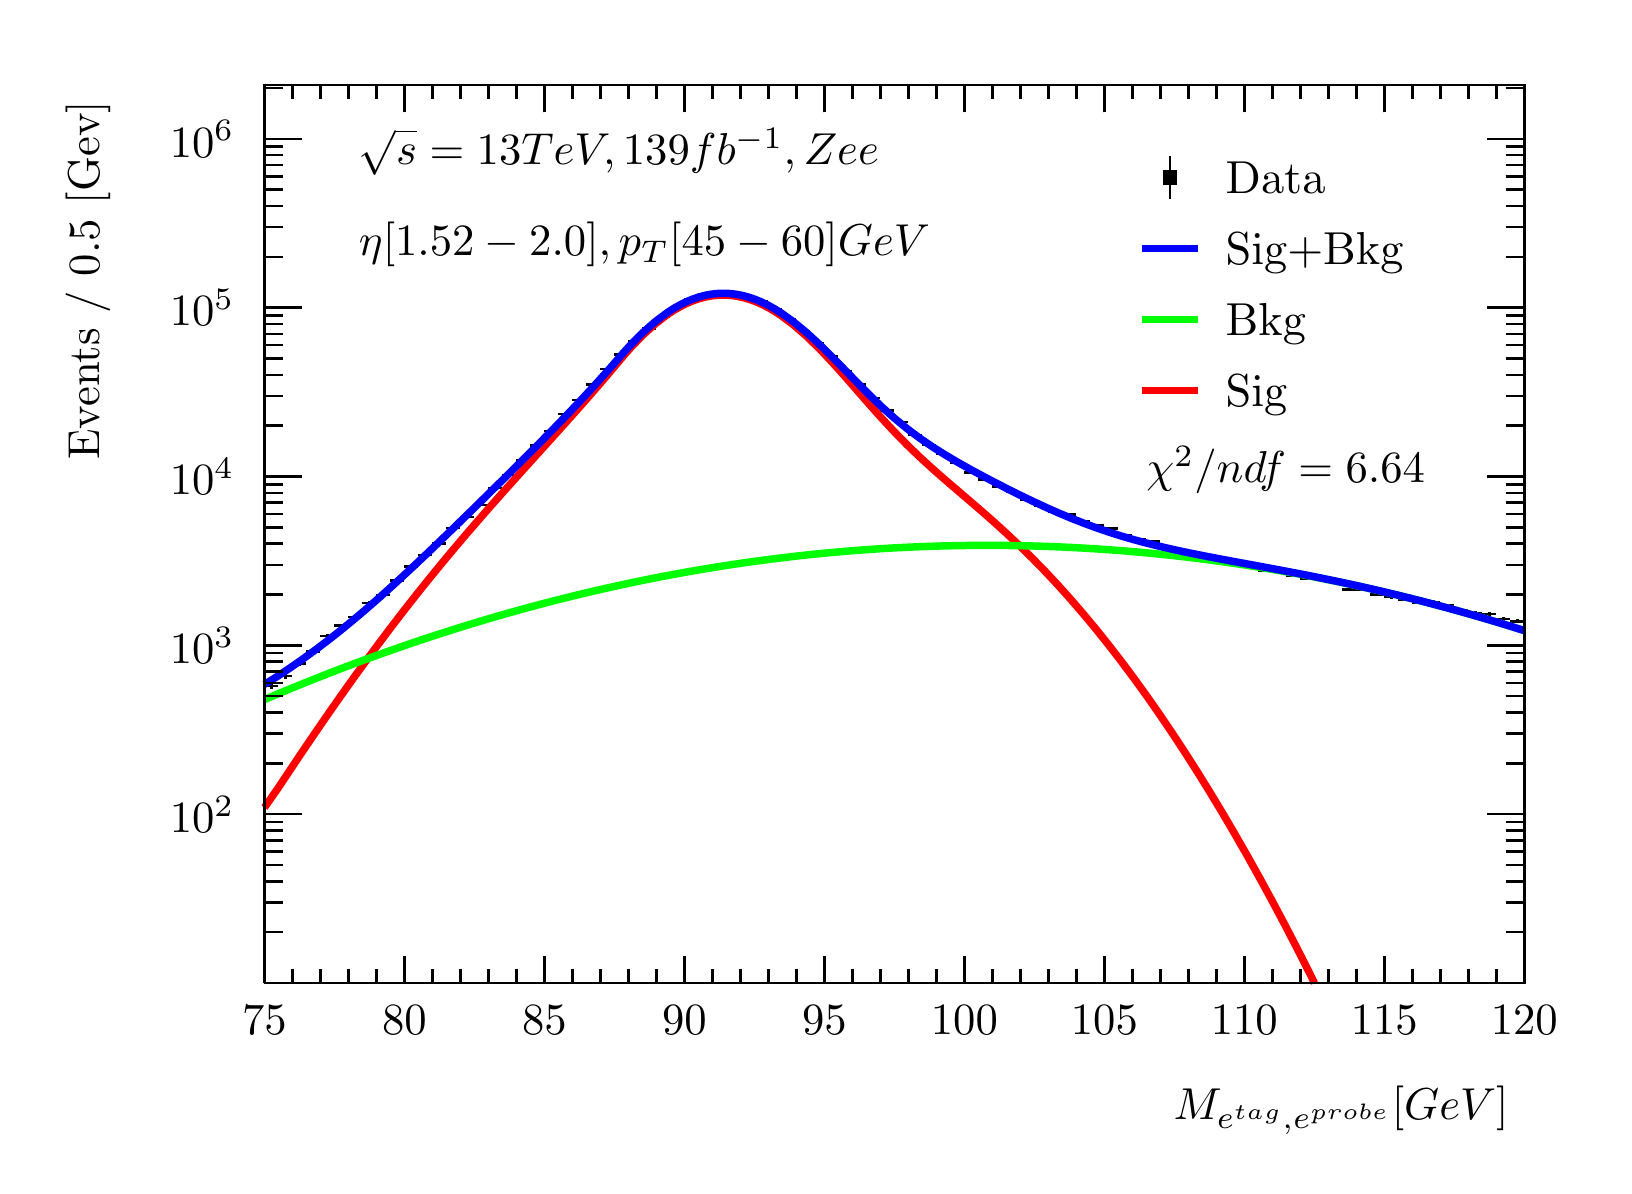
\begin{tikzpicture}
\pgfdeclareplotmark{cross} {
\pgfpathmoveto{\pgfpoint{-0.3\pgfplotmarksize}{\pgfplotmarksize}}
\pgfpathlineto{\pgfpoint{+0.3\pgfplotmarksize}{\pgfplotmarksize}}
\pgfpathlineto{\pgfpoint{+0.3\pgfplotmarksize}{0.3\pgfplotmarksize}}
\pgfpathlineto{\pgfpoint{+1\pgfplotmarksize}{0.3\pgfplotmarksize}}
\pgfpathlineto{\pgfpoint{+1\pgfplotmarksize}{-0.3\pgfplotmarksize}}
\pgfpathlineto{\pgfpoint{+0.3\pgfplotmarksize}{-0.3\pgfplotmarksize}}
\pgfpathlineto{\pgfpoint{+0.3\pgfplotmarksize}{-1.\pgfplotmarksize}}
\pgfpathlineto{\pgfpoint{-0.3\pgfplotmarksize}{-1.\pgfplotmarksize}}
\pgfpathlineto{\pgfpoint{-0.3\pgfplotmarksize}{-0.3\pgfplotmarksize}}
\pgfpathlineto{\pgfpoint{-1.\pgfplotmarksize}{-0.3\pgfplotmarksize}}
\pgfpathlineto{\pgfpoint{-1.\pgfplotmarksize}{0.3\pgfplotmarksize}}
\pgfpathlineto{\pgfpoint{-0.3\pgfplotmarksize}{0.3\pgfplotmarksize}}
\pgfpathclose
\pgfusepathqstroke
}
\pgfdeclareplotmark{cross*} {
\pgfpathmoveto{\pgfpoint{-0.3\pgfplotmarksize}{\pgfplotmarksize}}
\pgfpathlineto{\pgfpoint{+0.3\pgfplotmarksize}{\pgfplotmarksize}}
\pgfpathlineto{\pgfpoint{+0.3\pgfplotmarksize}{0.3\pgfplotmarksize}}
\pgfpathlineto{\pgfpoint{+1\pgfplotmarksize}{0.3\pgfplotmarksize}}
\pgfpathlineto{\pgfpoint{+1\pgfplotmarksize}{-0.3\pgfplotmarksize}}
\pgfpathlineto{\pgfpoint{+0.3\pgfplotmarksize}{-0.3\pgfplotmarksize}}
\pgfpathlineto{\pgfpoint{+0.3\pgfplotmarksize}{-1.\pgfplotmarksize}}
\pgfpathlineto{\pgfpoint{-0.3\pgfplotmarksize}{-1.\pgfplotmarksize}}
\pgfpathlineto{\pgfpoint{-0.3\pgfplotmarksize}{-0.3\pgfplotmarksize}}
\pgfpathlineto{\pgfpoint{-1.\pgfplotmarksize}{-0.3\pgfplotmarksize}}
\pgfpathlineto{\pgfpoint{-1.\pgfplotmarksize}{0.3\pgfplotmarksize}}
\pgfpathlineto{\pgfpoint{-0.3\pgfplotmarksize}{0.3\pgfplotmarksize}}
\pgfpathclose
\pgfusepathqfillstroke
}
\pgfdeclareplotmark{newstar} {
\pgfpathmoveto{\pgfqpoint{0pt}{\pgfplotmarksize}}
\pgfpathlineto{\pgfqpointpolar{44}{0.5\pgfplotmarksize}}
\pgfpathlineto{\pgfqpointpolar{18}{\pgfplotmarksize}}
\pgfpathlineto{\pgfqpointpolar{-20}{0.5\pgfplotmarksize}}
\pgfpathlineto{\pgfqpointpolar{-54}{\pgfplotmarksize}}
\pgfpathlineto{\pgfqpointpolar{-90}{0.5\pgfplotmarksize}}
\pgfpathlineto{\pgfqpointpolar{234}{\pgfplotmarksize}}
\pgfpathlineto{\pgfqpointpolar{198}{0.5\pgfplotmarksize}}
\pgfpathlineto{\pgfqpointpolar{162}{\pgfplotmarksize}}
\pgfpathlineto{\pgfqpointpolar{134}{0.5\pgfplotmarksize}}
\pgfpathclose
\pgfusepathqstroke
}
\pgfdeclareplotmark{newstar*} {
\pgfpathmoveto{\pgfqpoint{0pt}{\pgfplotmarksize}}
\pgfpathlineto{\pgfqpointpolar{44}{0.5\pgfplotmarksize}}
\pgfpathlineto{\pgfqpointpolar{18}{\pgfplotmarksize}}
\pgfpathlineto{\pgfqpointpolar{-20}{0.5\pgfplotmarksize}}
\pgfpathlineto{\pgfqpointpolar{-54}{\pgfplotmarksize}}
\pgfpathlineto{\pgfqpointpolar{-90}{0.5\pgfplotmarksize}}
\pgfpathlineto{\pgfqpointpolar{234}{\pgfplotmarksize}}
\pgfpathlineto{\pgfqpointpolar{198}{0.5\pgfplotmarksize}}
\pgfpathlineto{\pgfqpointpolar{162}{\pgfplotmarksize}}
\pgfpathlineto{\pgfqpointpolar{134}{0.5\pgfplotmarksize}}
\pgfpathclose
\pgfusepathqfillstroke
}
\definecolor{c}{rgb}{1,1,1};
\draw [color=c, fill=c] (0,0) rectangle (20,14.4361);
\draw [color=c, fill=c] (3,2.30977) rectangle (19,13.7143);
\definecolor{c}{rgb}{0,0,0};
\draw [c,line width=0.9] (3,2.30977) -- (3,13.7143) -- (19,13.7143) -- (19,2.30977) -- (3,2.30977);
\definecolor{c}{rgb}{1,1,1};
\draw [color=c, fill=c] (3,2.30977) rectangle (19,13.7143);
\definecolor{c}{rgb}{0,0,0};
\draw [c,line width=0.9] (3,2.30977) -- (3,13.7143) -- (19,13.7143) -- (19,2.30977) -- (3,2.30977);
\draw [c,line width=0.9] (3,2.30977) -- (19,2.30977);
\draw [c,line width=0.9] (3,2.65624) -- (3,2.30977);
\draw [c,line width=0.9] (3.35556,2.48301) -- (3.35556,2.30977);
\draw [c,line width=0.9] (3.71111,2.48301) -- (3.71111,2.30977);
\draw [c,line width=0.9] (4.06667,2.48301) -- (4.06667,2.30977);
\draw [c,line width=0.9] (4.42222,2.48301) -- (4.42222,2.30977);
\draw [c,line width=0.9] (4.77778,2.65624) -- (4.77778,2.30977);
\draw [c,line width=0.9] (5.13333,2.48301) -- (5.13333,2.30977);
\draw [c,line width=0.9] (5.48889,2.48301) -- (5.48889,2.30977);
\draw [c,line width=0.9] (5.84444,2.48301) -- (5.84444,2.30977);
\draw [c,line width=0.9] (6.2,2.48301) -- (6.2,2.30977);
\draw [c,line width=0.9] (6.55556,2.65624) -- (6.55556,2.30977);
\draw [c,line width=0.9] (6.91111,2.48301) -- (6.91111,2.30977);
\draw [c,line width=0.9] (7.26667,2.48301) -- (7.26667,2.30977);
\draw [c,line width=0.9] (7.62222,2.48301) -- (7.62222,2.30977);
\draw [c,line width=0.9] (7.97778,2.48301) -- (7.97778,2.30977);
\draw [c,line width=0.9] (8.33333,2.65624) -- (8.33333,2.30977);
\draw [c,line width=0.9] (8.68889,2.48301) -- (8.68889,2.30977);
\draw [c,line width=0.9] (9.04444,2.48301) -- (9.04444,2.30977);
\draw [c,line width=0.9] (9.4,2.48301) -- (9.4,2.30977);
\draw [c,line width=0.9] (9.75556,2.48301) -- (9.75556,2.30977);
\draw [c,line width=0.9] (10.1111,2.65624) -- (10.1111,2.30977);
\draw [c,line width=0.9] (10.4667,2.48301) -- (10.4667,2.30977);
\draw [c,line width=0.9] (10.8222,2.48301) -- (10.8222,2.30977);
\draw [c,line width=0.9] (11.1778,2.48301) -- (11.1778,2.30977);
\draw [c,line width=0.9] (11.5333,2.48301) -- (11.5333,2.30977);
\draw [c,line width=0.9] (11.8889,2.65624) -- (11.8889,2.30977);
\draw [c,line width=0.9] (12.2444,2.48301) -- (12.2444,2.30977);
\draw [c,line width=0.9] (12.6,2.48301) -- (12.6,2.30977);
\draw [c,line width=0.9] (12.9556,2.48301) -- (12.9556,2.30977);
\draw [c,line width=0.9] (13.3111,2.48301) -- (13.3111,2.30977);
\draw [c,line width=0.9] (13.6667,2.65624) -- (13.6667,2.30977);
\draw [c,line width=0.9] (14.0222,2.48301) -- (14.0222,2.30977);
\draw [c,line width=0.9] (14.3778,2.48301) -- (14.3778,2.30977);
\draw [c,line width=0.9] (14.7333,2.48301) -- (14.7333,2.30977);
\draw [c,line width=0.9] (15.0889,2.48301) -- (15.0889,2.30977);
\draw [c,line width=0.9] (15.4444,2.65624) -- (15.4444,2.30977);
\draw [c,line width=0.9] (15.8,2.48301) -- (15.8,2.30977);
\draw [c,line width=0.9] (16.1556,2.48301) -- (16.1556,2.30977);
\draw [c,line width=0.9] (16.5111,2.48301) -- (16.5111,2.30977);
\draw [c,line width=0.9] (16.8667,2.48301) -- (16.8667,2.30977);
\draw [c,line width=0.9] (17.2222,2.65624) -- (17.2222,2.30977);
\draw [c,line width=0.9] (17.5778,2.48301) -- (17.5778,2.30977);
\draw [c,line width=0.9] (17.9333,2.48301) -- (17.9333,2.30977);
\draw [c,line width=0.9] (18.2889,2.48301) -- (18.2889,2.30977);
\draw [c,line width=0.9] (18.6444,2.48301) -- (18.6444,2.30977);
\draw [c,line width=0.9] (19,2.65624) -- (19,2.30977);
\draw [c,line width=0.9] (19,2.65624) -- (19,2.30977);
\draw [anchor=base] (3,1.66015) node[scale=1.61424, color=c, rotate=0]{75};
\draw [anchor=base] (4.77778,1.66015) node[scale=1.61424, color=c, rotate=0]{80};
\draw [anchor=base] (6.55556,1.66015) node[scale=1.61424, color=c, rotate=0]{85};
\draw [anchor=base] (8.33333,1.66015) node[scale=1.61424, color=c, rotate=0]{90};
\draw [anchor=base] (10.1111,1.66015) node[scale=1.61424, color=c, rotate=0]{95};
\draw [anchor=base] (11.8889,1.66015) node[scale=1.61424, color=c, rotate=0]{100};
\draw [anchor=base] (13.6667,1.66015) node[scale=1.61424, color=c, rotate=0]{105};
\draw [anchor=base] (15.4444,1.66015) node[scale=1.61424, color=c, rotate=0]{110};
\draw [anchor=base] (17.2222,1.66015) node[scale=1.61424, color=c, rotate=0]{115};
\draw [anchor=base] (19,1.66015) node[scale=1.61424, color=c, rotate=0]{120};
\draw [anchor= east] (19,0.692932) node[scale=1.61424, color=c, rotate=0]{$M_{e^{tag}, e^{probe}}  [GeV]$};
\draw [c,line width=0.9] (3,13.7143) -- (19,13.7143);
\draw [c,line width=0.9] (3,13.3678) -- (3,13.7143);
\draw [c,line width=0.9] (3.35556,13.5411) -- (3.35556,13.7143);
\draw [c,line width=0.9] (3.71111,13.5411) -- (3.71111,13.7143);
\draw [c,line width=0.9] (4.06667,13.5411) -- (4.06667,13.7143);
\draw [c,line width=0.9] (4.42222,13.5411) -- (4.42222,13.7143);
\draw [c,line width=0.9] (4.77778,13.3678) -- (4.77778,13.7143);
\draw [c,line width=0.9] (5.13333,13.5411) -- (5.13333,13.7143);
\draw [c,line width=0.9] (5.48889,13.5411) -- (5.48889,13.7143);
\draw [c,line width=0.9] (5.84444,13.5411) -- (5.84444,13.7143);
\draw [c,line width=0.9] (6.2,13.5411) -- (6.2,13.7143);
\draw [c,line width=0.9] (6.55556,13.3678) -- (6.55556,13.7143);
\draw [c,line width=0.9] (6.91111,13.5411) -- (6.91111,13.7143);
\draw [c,line width=0.9] (7.26667,13.5411) -- (7.26667,13.7143);
\draw [c,line width=0.9] (7.62222,13.5411) -- (7.62222,13.7143);
\draw [c,line width=0.9] (7.97778,13.5411) -- (7.97778,13.7143);
\draw [c,line width=0.9] (8.33333,13.3678) -- (8.33333,13.7143);
\draw [c,line width=0.9] (8.68889,13.5411) -- (8.68889,13.7143);
\draw [c,line width=0.9] (9.04444,13.5411) -- (9.04444,13.7143);
\draw [c,line width=0.9] (9.4,13.5411) -- (9.4,13.7143);
\draw [c,line width=0.9] (9.75556,13.5411) -- (9.75556,13.7143);
\draw [c,line width=0.9] (10.1111,13.3678) -- (10.1111,13.7143);
\draw [c,line width=0.9] (10.4667,13.5411) -- (10.4667,13.7143);
\draw [c,line width=0.9] (10.8222,13.5411) -- (10.8222,13.7143);
\draw [c,line width=0.9] (11.1778,13.5411) -- (11.1778,13.7143);
\draw [c,line width=0.9] (11.5333,13.5411) -- (11.5333,13.7143);
\draw [c,line width=0.9] (11.8889,13.3678) -- (11.8889,13.7143);
\draw [c,line width=0.9] (12.2444,13.5411) -- (12.2444,13.7143);
\draw [c,line width=0.9] (12.6,13.5411) -- (12.6,13.7143);
\draw [c,line width=0.9] (12.9556,13.5411) -- (12.9556,13.7143);
\draw [c,line width=0.9] (13.3111,13.5411) -- (13.3111,13.7143);
\draw [c,line width=0.9] (13.6667,13.3678) -- (13.6667,13.7143);
\draw [c,line width=0.9] (14.0222,13.5411) -- (14.0222,13.7143);
\draw [c,line width=0.9] (14.3778,13.5411) -- (14.3778,13.7143);
\draw [c,line width=0.9] (14.7333,13.5411) -- (14.7333,13.7143);
\draw [c,line width=0.9] (15.0889,13.5411) -- (15.0889,13.7143);
\draw [c,line width=0.9] (15.4444,13.3678) -- (15.4444,13.7143);
\draw [c,line width=0.9] (15.8,13.5411) -- (15.8,13.7143);
\draw [c,line width=0.9] (16.1556,13.5411) -- (16.1556,13.7143);
\draw [c,line width=0.9] (16.5111,13.5411) -- (16.5111,13.7143);
\draw [c,line width=0.9] (16.8667,13.5411) -- (16.8667,13.7143);
\draw [c,line width=0.9] (17.2222,13.3678) -- (17.2222,13.7143);
\draw [c,line width=0.9] (17.5778,13.5411) -- (17.5778,13.7143);
\draw [c,line width=0.9] (17.9333,13.5411) -- (17.9333,13.7143);
\draw [c,line width=0.9] (18.2889,13.5411) -- (18.2889,13.7143);
\draw [c,line width=0.9] (18.6444,13.5411) -- (18.6444,13.7143);
\draw [c,line width=0.9] (19,13.3678) -- (19,13.7143);
\draw [c,line width=0.9] (19,13.3678) -- (19,13.7143);
\draw [c,line width=0.9] (3,2.30977) -- (3,13.7143);
\draw [c,line width=0.9] (3.237,2.95525) -- (3,2.95525);
\draw [c,line width=0.9] (3.237,3.33283) -- (3,3.33283);
\draw [c,line width=0.9] (3.237,3.60073) -- (3,3.60073);
\draw [c,line width=0.9] (3.237,3.80852) -- (3,3.80852);
\draw [c,line width=0.9] (3.237,3.97831) -- (3,3.97831);
\draw [c,line width=0.9] (3.237,4.12185) -- (3,4.12185);
\draw [c,line width=0.9] (3.237,4.2462) -- (3,4.2462);
\draw [c,line width=0.9] (3.237,4.35589) -- (3,4.35589);
\draw [c,line width=0.9] (3.474,4.454) -- (3,4.454);
\draw [anchor= east] (2.82,4.454) node[scale=1.61424, color=c, rotate=0]{$10^{2}$};
\draw [c,line width=0.9] (3.237,5.09948) -- (3,5.09948);
\draw [c,line width=0.9] (3.237,5.47706) -- (3,5.47706);
\draw [c,line width=0.9] (3.237,5.74495) -- (3,5.74495);
\draw [c,line width=0.9] (3.237,5.95275) -- (3,5.95275);
\draw [c,line width=0.9] (3.237,6.12253) -- (3,6.12253);
\draw [c,line width=0.9] (3.237,6.26608) -- (3,6.26608);
\draw [c,line width=0.9] (3.237,6.39043) -- (3,6.39043);
\draw [c,line width=0.9] (3.237,6.50011) -- (3,6.50011);
\draw [c,line width=0.9] (3.474,6.59823) -- (3,6.59823);
\draw [anchor= east] (2.82,6.59823) node[scale=1.61424, color=c, rotate=0]{$10^{3}$};
\draw [c,line width=0.9] (3.237,7.2437) -- (3,7.2437);
\draw [c,line width=0.9] (3.237,7.62128) -- (3,7.62128);
\draw [c,line width=0.9] (3.237,7.88918) -- (3,7.88918);
\draw [c,line width=0.9] (3.237,8.09698) -- (3,8.09698);
\draw [c,line width=0.9] (3.237,8.26676) -- (3,8.26676);
\draw [c,line width=0.9] (3.237,8.41031) -- (3,8.41031);
\draw [c,line width=0.9] (3.237,8.53466) -- (3,8.53466);
\draw [c,line width=0.9] (3.237,8.64434) -- (3,8.64434);
\draw [c,line width=0.9] (3.474,8.74245) -- (3,8.74245);
\draw [anchor= east] (2.82,8.74245) node[scale=1.61424, color=c, rotate=0]{$10^{4}$};
\draw [c,line width=0.9] (3.237,9.38793) -- (3,9.38793);
\draw [c,line width=0.9] (3.237,9.76551) -- (3,9.76551);
\draw [c,line width=0.9] (3.237,10.0334) -- (3,10.0334);
\draw [c,line width=0.9] (3.237,10.2412) -- (3,10.2412);
\draw [c,line width=0.9] (3.237,10.411) -- (3,10.411);
\draw [c,line width=0.9] (3.237,10.5545) -- (3,10.5545);
\draw [c,line width=0.9] (3.237,10.6789) -- (3,10.6789);
\draw [c,line width=0.9] (3.237,10.7886) -- (3,10.7886);
\draw [c,line width=0.9] (3.474,10.8867) -- (3,10.8867);
\draw [anchor= east] (2.82,10.8867) node[scale=1.61424, color=c, rotate=0]{$10^{5}$};
\draw [c,line width=0.9] (3.237,11.5322) -- (3,11.5322);
\draw [c,line width=0.9] (3.237,11.9097) -- (3,11.9097);
\draw [c,line width=0.9] (3.237,12.1776) -- (3,12.1776);
\draw [c,line width=0.9] (3.237,12.3854) -- (3,12.3854);
\draw [c,line width=0.9] (3.237,12.5552) -- (3,12.5552);
\draw [c,line width=0.9] (3.237,12.6988) -- (3,12.6988);
\draw [c,line width=0.9] (3.237,12.8231) -- (3,12.8231);
\draw [c,line width=0.9] (3.237,12.9328) -- (3,12.9328);
\draw [c,line width=0.9] (3.474,13.0309) -- (3,13.0309);
\draw [anchor= east] (2.82,13.0309) node[scale=1.61424, color=c, rotate=0]{$10^{6}$};
\draw [c,line width=0.9] (3.237,13.6764) -- (3,13.6764);
\draw [anchor= east] (0.76,13.7143) node[scale=1.61424, color=c, rotate=90]{Events / 0.5 [Gev]};
\draw [c,line width=0.9] (19,2.30977) -- (19,13.7143);
\draw [c,line width=0.9] (18.763,2.95525) -- (19,2.95525);
\draw [c,line width=0.9] (18.763,3.33283) -- (19,3.33283);
\draw [c,line width=0.9] (18.763,3.60073) -- (19,3.60073);
\draw [c,line width=0.9] (18.763,3.80852) -- (19,3.80852);
\draw [c,line width=0.9] (18.763,3.97831) -- (19,3.97831);
\draw [c,line width=0.9] (18.763,4.12185) -- (19,4.12185);
\draw [c,line width=0.9] (18.763,4.2462) -- (19,4.2462);
\draw [c,line width=0.9] (18.763,4.35589) -- (19,4.35589);
\draw [c,line width=0.9] (18.526,4.454) -- (19,4.454);
\draw [c,line width=0.9] (18.763,5.09948) -- (19,5.09948);
\draw [c,line width=0.9] (18.763,5.47706) -- (19,5.47706);
\draw [c,line width=0.9] (18.763,5.74495) -- (19,5.74495);
\draw [c,line width=0.9] (18.763,5.95275) -- (19,5.95275);
\draw [c,line width=0.9] (18.763,6.12253) -- (19,6.12253);
\draw [c,line width=0.9] (18.763,6.26608) -- (19,6.26608);
\draw [c,line width=0.9] (18.763,6.39043) -- (19,6.39043);
\draw [c,line width=0.9] (18.763,6.50011) -- (19,6.50011);
\draw [c,line width=0.9] (18.526,6.59823) -- (19,6.59823);
\draw [c,line width=0.9] (18.763,7.2437) -- (19,7.2437);
\draw [c,line width=0.9] (18.763,7.62128) -- (19,7.62128);
\draw [c,line width=0.9] (18.763,7.88918) -- (19,7.88918);
\draw [c,line width=0.9] (18.763,8.09698) -- (19,8.09698);
\draw [c,line width=0.9] (18.763,8.26676) -- (19,8.26676);
\draw [c,line width=0.9] (18.763,8.41031) -- (19,8.41031);
\draw [c,line width=0.9] (18.763,8.53466) -- (19,8.53466);
\draw [c,line width=0.9] (18.763,8.64434) -- (19,8.64434);
\draw [c,line width=0.9] (18.526,8.74245) -- (19,8.74245);
\draw [c,line width=0.9] (18.763,9.38793) -- (19,9.38793);
\draw [c,line width=0.9] (18.763,9.76551) -- (19,9.76551);
\draw [c,line width=0.9] (18.763,10.0334) -- (19,10.0334);
\draw [c,line width=0.9] (18.763,10.2412) -- (19,10.2412);
\draw [c,line width=0.9] (18.763,10.411) -- (19,10.411);
\draw [c,line width=0.9] (18.763,10.5545) -- (19,10.5545);
\draw [c,line width=0.9] (18.763,10.6789) -- (19,10.6789);
\draw [c,line width=0.9] (18.763,10.7886) -- (19,10.7886);
\draw [c,line width=0.9] (18.526,10.8867) -- (19,10.8867);
\draw [c,line width=0.9] (18.763,11.5322) -- (19,11.5322);
\draw [c,line width=0.9] (18.763,11.9097) -- (19,11.9097);
\draw [c,line width=0.9] (18.763,12.1776) -- (19,12.1776);
\draw [c,line width=0.9] (18.763,12.3854) -- (19,12.3854);
\draw [c,line width=0.9] (18.763,12.5552) -- (19,12.5552);
\draw [c,line width=0.9] (18.763,12.6988) -- (19,12.6988);
\draw [c,line width=0.9] (18.763,12.8231) -- (19,12.8231);
\draw [c,line width=0.9] (18.763,12.9328) -- (19,12.9328);
\draw [c,line width=0.9] (18.526,13.0309) -- (19,13.0309);
\draw [c,line width=0.9] (18.763,13.6764) -- (19,13.6764);
\draw [c,line width=0.9] (3.08889,6.07966) -- (3,6.07966);
\draw [c,line width=0.9] (3,6.07966) -- (3,6.07966);
\draw [c,line width=0.9] (3.08889,6.07966) -- (3.17778,6.07966);
\draw [c,line width=0.9] (3.17778,6.07966) -- (3.17778,6.07966);
\draw [c,line width=0.9] (3.08889,6.07966) -- (3.08889,6.11856);
\draw [c,line width=0.9] (3.08889,6.11856) -- (3.08889,6.11856);
\draw [c,line width=0.9] (3.08889,6.07966) -- (3.08889,6.04076);
\draw [c,line width=0.9] (3.08889,6.04076) -- (3.08889,6.04076);
\draw [c,line width=0.9] (3.26667,6.20705) -- (3.17778,6.20705);
\draw [c,line width=0.9] (3.17778,6.20705) -- (3.17778,6.20705);
\draw [c,line width=0.9] (3.26667,6.20705) -- (3.35556,6.20705);
\draw [c,line width=0.9] (3.35556,6.20705) -- (3.35556,6.20705);
\draw [c,line width=0.9] (3.26667,6.20705) -- (3.26667,6.24338);
\draw [c,line width=0.9] (3.26667,6.24338) -- (3.26667,6.24338);
\draw [c,line width=0.9] (3.26667,6.20705) -- (3.26667,6.17072);
\draw [c,line width=0.9] (3.26667,6.17072) -- (3.26667,6.17072);
\draw [c,line width=0.9] (3.44444,6.37043) -- (3.35556,6.37043);
\draw [c,line width=0.9] (3.35556,6.37043) -- (3.35556,6.37043);
\draw [c,line width=0.9] (3.44444,6.37043) -- (3.53333,6.37043);
\draw [c,line width=0.9] (3.53333,6.37043) -- (3.53333,6.37043);
\draw [c,line width=0.9] (3.44444,6.37043) -- (3.44444,6.40371);
\draw [c,line width=0.9] (3.44444,6.40371) -- (3.44444,6.40371);
\draw [c,line width=0.9] (3.44444,6.37043) -- (3.44444,6.33715);
\draw [c,line width=0.9] (3.44444,6.33715) -- (3.44444,6.33715);
\draw [c,line width=0.9] (3.62222,6.5226) -- (3.53333,6.5226);
\draw [c,line width=0.9] (3.53333,6.5226) -- (3.53333,6.5226);
\draw [c,line width=0.9] (3.62222,6.5226) -- (3.71111,6.5226);
\draw [c,line width=0.9] (3.71111,6.5226) -- (3.71111,6.5226);
\draw [c,line width=0.9] (3.62222,6.5226) -- (3.62222,6.55327);
\draw [c,line width=0.9] (3.62222,6.55327) -- (3.62222,6.55327);
\draw [c,line width=0.9] (3.62222,6.5226) -- (3.62222,6.49194);
\draw [c,line width=0.9] (3.62222,6.49194) -- (3.62222,6.49194);
\draw [c,line width=0.9] (3.8,6.71697) -- (3.71111,6.71697);
\draw [c,line width=0.9] (3.71111,6.71697) -- (3.71111,6.71697);
\draw [c,line width=0.9] (3.8,6.71697) -- (3.88889,6.71697);
\draw [c,line width=0.9] (3.88889,6.71697) -- (3.88889,6.71697);
\draw [c,line width=0.9] (3.8,6.71697) -- (3.8,6.7446);
\draw [c,line width=0.9] (3.8,6.7446) -- (3.8,6.7446);
\draw [c,line width=0.9] (3.8,6.71697) -- (3.8,6.68934);
\draw [c,line width=0.9] (3.8,6.68934) -- (3.8,6.68934);
\draw [c,line width=0.9] (3.97778,6.84968) -- (3.88889,6.84968);
\draw [c,line width=0.9] (3.88889,6.84968) -- (3.88889,6.84968);
\draw [c,line width=0.9] (3.97778,6.84968) -- (4.06667,6.84968);
\draw [c,line width=0.9] (4.06667,6.84968) -- (4.06667,6.84968);
\draw [c,line width=0.9] (3.97778,6.84968) -- (3.97778,6.87541);
\draw [c,line width=0.9] (3.97778,6.87541) -- (3.97778,6.87541);
\draw [c,line width=0.9] (3.97778,6.84968) -- (3.97778,6.82396);
\draw [c,line width=0.9] (3.97778,6.82396) -- (3.97778,6.82396);
\draw [c,line width=0.9] (4.15556,6.96142) -- (4.06667,6.96142);
\draw [c,line width=0.9] (4.06667,6.96142) -- (4.06667,6.96142);
\draw [c,line width=0.9] (4.15556,6.96142) -- (4.24444,6.96142);
\draw [c,line width=0.9] (4.24444,6.96142) -- (4.24444,6.96142);
\draw [c,line width=0.9] (4.15556,6.96142) -- (4.15556,6.98565);
\draw [c,line width=0.9] (4.15556,6.98565) -- (4.15556,6.98565);
\draw [c,line width=0.9] (4.15556,6.96142) -- (4.15556,6.93719);
\draw [c,line width=0.9] (4.15556,6.93719) -- (4.15556,6.93719);
\draw [c,line width=0.9] (4.33333,7.13675) -- (4.24444,7.13675);
\draw [c,line width=0.9] (4.24444,7.13675) -- (4.24444,7.13675);
\draw [c,line width=0.9] (4.33333,7.13675) -- (4.42222,7.13675);
\draw [c,line width=0.9] (4.42222,7.13675) -- (4.42222,7.13675);
\draw [c,line width=0.9] (4.33333,7.13675) -- (4.33333,7.15881);
\draw [c,line width=0.9] (4.33333,7.15881) -- (4.33333,7.15881);
\draw [c,line width=0.9] (4.33333,7.13675) -- (4.33333,7.1147);
\draw [c,line width=0.9] (4.33333,7.1147) -- (4.33333,7.1147);
\draw [c,line width=0.9] (4.51111,7.2395) -- (4.42222,7.2395);
\draw [c,line width=0.9] (4.42222,7.2395) -- (4.42222,7.2395);
\draw [c,line width=0.9] (4.51111,7.2395) -- (4.6,7.2395);
\draw [c,line width=0.9] (4.6,7.2395) -- (4.6,7.2395);
\draw [c,line width=0.9] (4.51111,7.2395) -- (4.51111,7.26037);
\draw [c,line width=0.9] (4.51111,7.26037) -- (4.51111,7.26037);
\draw [c,line width=0.9] (4.51111,7.2395) -- (4.51111,7.21864);
\draw [c,line width=0.9] (4.51111,7.21864) -- (4.51111,7.21864);
\draw [c,line width=0.9] (4.68889,7.42352) -- (4.6,7.42352);
\draw [c,line width=0.9] (4.6,7.42352) -- (4.6,7.42352);
\draw [c,line width=0.9] (4.68889,7.42352) -- (4.77778,7.42352);
\draw [c,line width=0.9] (4.77778,7.42352) -- (4.77778,7.42352);
\draw [c,line width=0.9] (4.68889,7.42352) -- (4.68889,7.44243);
\draw [c,line width=0.9] (4.68889,7.44243) -- (4.68889,7.44243);
\draw [c,line width=0.9] (4.68889,7.42352) -- (4.68889,7.40461);
\draw [c,line width=0.9] (4.68889,7.40461) -- (4.68889,7.40461);
\draw [c,line width=0.9] (4.86667,7.5993) -- (4.77778,7.5993);
\draw [c,line width=0.9] (4.77778,7.5993) -- (4.77778,7.5993);
\draw [c,line width=0.9] (4.86667,7.5993) -- (4.95556,7.5993);
\draw [c,line width=0.9] (4.95556,7.5993) -- (4.95556,7.5993);
\draw [c,line width=0.9] (4.86667,7.5993) -- (4.86667,7.6165);
\draw [c,line width=0.9] (4.86667,7.6165) -- (4.86667,7.6165);
\draw [c,line width=0.9] (4.86667,7.5993) -- (4.86667,7.58209);
\draw [c,line width=0.9] (4.86667,7.58209) -- (4.86667,7.58209);
\draw [c,line width=0.9] (5.04444,7.74412) -- (4.95556,7.74412);
\draw [c,line width=0.9] (4.95556,7.74412) -- (4.95556,7.74412);
\draw [c,line width=0.9] (5.04444,7.74412) -- (5.13333,7.74412);
\draw [c,line width=0.9] (5.13333,7.74412) -- (5.13333,7.74412);
\draw [c,line width=0.9] (5.04444,7.74412) -- (5.04444,7.76003);
\draw [c,line width=0.9] (5.04444,7.76003) -- (5.04444,7.76003);
\draw [c,line width=0.9] (5.04444,7.74412) -- (5.04444,7.7282);
\draw [c,line width=0.9] (5.04444,7.7282) -- (5.04444,7.7282);
\draw [c,line width=0.9] (5.22222,7.88965) -- (5.13333,7.88965);
\draw [c,line width=0.9] (5.13333,7.88965) -- (5.13333,7.88965);
\draw [c,line width=0.9] (5.22222,7.88965) -- (5.31111,7.88965);
\draw [c,line width=0.9] (5.31111,7.88965) -- (5.31111,7.88965);
\draw [c,line width=0.9] (5.22222,7.88965) -- (5.22222,7.90437);
\draw [c,line width=0.9] (5.22222,7.90437) -- (5.22222,7.90437);
\draw [c,line width=0.9] (5.22222,7.88965) -- (5.22222,7.87493);
\draw [c,line width=0.9] (5.22222,7.87493) -- (5.22222,7.87493);
\draw [c,line width=0.9] (5.4,8.08574) -- (5.31111,8.08574);
\draw [c,line width=0.9] (5.31111,8.08574) -- (5.31111,8.08574);
\draw [c,line width=0.9] (5.4,8.08574) -- (5.48889,8.08574);
\draw [c,line width=0.9] (5.48889,8.08574) -- (5.48889,8.08574);
\draw [c,line width=0.9] (5.4,8.08574) -- (5.4,8.09898);
\draw [c,line width=0.9] (5.4,8.09898) -- (5.4,8.09898);
\draw [c,line width=0.9] (5.4,8.08574) -- (5.4,8.07249);
\draw [c,line width=0.9] (5.4,8.07249) -- (5.4,8.07249);
\draw [c,line width=0.9] (5.57778,8.22551) -- (5.48889,8.22551);
\draw [c,line width=0.9] (5.48889,8.22551) -- (5.48889,8.22551);
\draw [c,line width=0.9] (5.57778,8.22551) -- (5.66667,8.22551);
\draw [c,line width=0.9] (5.66667,8.22551) -- (5.66667,8.22551);
\draw [c,line width=0.9] (5.57778,8.22551) -- (5.57778,8.2378);
\draw [c,line width=0.9] (5.57778,8.2378) -- (5.57778,8.2378);
\draw [c,line width=0.9] (5.57778,8.22551) -- (5.57778,8.21322);
\draw [c,line width=0.9] (5.57778,8.21322) -- (5.57778,8.21322);
\draw [c,line width=0.9] (5.75556,8.38304) -- (5.66667,8.38304);
\draw [c,line width=0.9] (5.66667,8.38304) -- (5.66667,8.38304);
\draw [c,line width=0.9] (5.75556,8.38304) -- (5.84444,8.38304);
\draw [c,line width=0.9] (5.84444,8.38304) -- (5.84444,8.38304);
\draw [c,line width=0.9] (5.75556,8.38304) -- (5.75556,8.39434);
\draw [c,line width=0.9] (5.75556,8.39434) -- (5.75556,8.39434);
\draw [c,line width=0.9] (5.75556,8.38304) -- (5.75556,8.37175);
\draw [c,line width=0.9] (5.75556,8.37175) -- (5.75556,8.37175);
\draw [c,line width=0.9] (5.93333,8.60005) -- (5.84444,8.60005);
\draw [c,line width=0.9] (5.84444,8.60005) -- (5.84444,8.60005);
\draw [c,line width=0.9] (5.93333,8.60005) -- (6.02222,8.60005);
\draw [c,line width=0.9] (6.02222,8.60005) -- (6.02222,8.60005);
\draw [c,line width=0.9] (5.93333,8.60005) -- (5.93333,8.61011);
\draw [c,line width=0.9] (5.93333,8.61011) -- (5.93333,8.61011);
\draw [c,line width=0.9] (5.93333,8.60005) -- (5.93333,8.59);
\draw [c,line width=0.9] (5.93333,8.59) -- (5.93333,8.59);
\draw [c,line width=0.9] (6.11111,8.76226) -- (6.02222,8.76226);
\draw [c,line width=0.9] (6.02222,8.76226) -- (6.02222,8.76226);
\draw [c,line width=0.9] (6.11111,8.76226) -- (6.2,8.76226);
\draw [c,line width=0.9] (6.2,8.76226) -- (6.2,8.76226);
\draw [c,line width=0.9] (6.11111,8.76226) -- (6.11111,8.77148);
\draw [c,line width=0.9] (6.11111,8.77148) -- (6.11111,8.77148);
\draw [c,line width=0.9] (6.11111,8.76226) -- (6.11111,8.75305);
\draw [c,line width=0.9] (6.11111,8.75305) -- (6.11111,8.75305);
\draw [c,line width=0.9] (6.28889,8.94719) -- (6.2,8.94719);
\draw [c,line width=0.9] (6.2,8.94719) -- (6.2,8.94719);
\draw [c,line width=0.9] (6.28889,8.94719) -- (6.37778,8.94719);
\draw [c,line width=0.9] (6.37778,8.94719) -- (6.37778,8.94719);
\draw [c,line width=0.9] (6.28889,8.94719) -- (6.28889,8.95553);
\draw [c,line width=0.9] (6.28889,8.95553) -- (6.28889,8.95553);
\draw [c,line width=0.9] (6.28889,8.94719) -- (6.28889,8.93885);
\draw [c,line width=0.9] (6.28889,8.93885) -- (6.28889,8.93885);
\draw [c,line width=0.9] (6.46667,9.13537) -- (6.37778,9.13537);
\draw [c,line width=0.9] (6.37778,9.13537) -- (6.37778,9.13537);
\draw [c,line width=0.9] (6.46667,9.13537) -- (6.55556,9.13537);
\draw [c,line width=0.9] (6.55556,9.13537) -- (6.55556,9.13537);
\draw [c,line width=0.9] (6.46667,9.13537) -- (6.46667,9.14291);
\draw [c,line width=0.9] (6.46667,9.14291) -- (6.46667,9.14291);
\draw [c,line width=0.9] (6.46667,9.13537) -- (6.46667,9.12782);
\draw [c,line width=0.9] (6.46667,9.12782) -- (6.46667,9.12782);
\draw [c,line width=0.9] (6.64444,9.3191) -- (6.55556,9.3191);
\draw [c,line width=0.9] (6.55556,9.3191) -- (6.55556,9.3191);
\draw [c,line width=0.9] (6.64444,9.3191) -- (6.73333,9.3191);
\draw [c,line width=0.9] (6.73333,9.3191) -- (6.73333,9.3191);
\draw [c,line width=0.9] (6.64444,9.3191) -- (6.64444,9.32593);
\draw [c,line width=0.9] (6.64444,9.32593) -- (6.64444,9.32593);
\draw [c,line width=0.9] (6.64444,9.3191) -- (6.64444,9.31227);
\draw [c,line width=0.9] (6.64444,9.31227) -- (6.64444,9.31227);
\draw [c,line width=0.9] (6.82222,9.53577) -- (6.73333,9.53577);
\draw [c,line width=0.9] (6.73333,9.53577) -- (6.73333,9.53577);
\draw [c,line width=0.9] (6.82222,9.53577) -- (6.91111,9.53577);
\draw [c,line width=0.9] (6.91111,9.53577) -- (6.91111,9.53577);
\draw [c,line width=0.9] (6.82222,9.53577) -- (6.82222,9.54185);
\draw [c,line width=0.9] (6.82222,9.54185) -- (6.82222,9.54185);
\draw [c,line width=0.9] (6.82222,9.53577) -- (6.82222,9.52969);
\draw [c,line width=0.9] (6.82222,9.52969) -- (6.82222,9.52969);
\draw [c,line width=0.9] (7,9.71555) -- (6.91111,9.71555);
\draw [c,line width=0.9] (6.91111,9.71555) -- (6.91111,9.71555);
\draw [c,line width=0.9] (7,9.71555) -- (7.08889,9.71555);
\draw [c,line width=0.9] (7.08889,9.71555) -- (7.08889,9.71555);
\draw [c,line width=0.9] (7,9.71555) -- (7,9.72108);
\draw [c,line width=0.9] (7,9.72108) -- (7,9.72108);
\draw [c,line width=0.9] (7,9.71555) -- (7,9.71003);
\draw [c,line width=0.9] (7,9.71003) -- (7,9.71003);
\draw [c,line width=0.9] (7.17778,9.91402) -- (7.08889,9.91402);
\draw [c,line width=0.9] (7.08889,9.91402) -- (7.08889,9.91402);
\draw [c,line width=0.9] (7.17778,9.91402) -- (7.26667,9.91402);
\draw [c,line width=0.9] (7.26667,9.91402) -- (7.26667,9.91402);
\draw [c,line width=0.9] (7.17778,9.91402) -- (7.17778,9.91899);
\draw [c,line width=0.9] (7.17778,9.91899) -- (7.17778,9.91899);
\draw [c,line width=0.9] (7.17778,9.91402) -- (7.17778,9.90906);
\draw [c,line width=0.9] (7.17778,9.90906) -- (7.17778,9.90906);
\draw [c,line width=0.9] (7.35556,10.106) -- (7.26667,10.106);
\draw [c,line width=0.9] (7.26667,10.106) -- (7.26667,10.106);
\draw [c,line width=0.9] (7.35556,10.106) -- (7.44444,10.106);
\draw [c,line width=0.9] (7.44444,10.106) -- (7.44444,10.106);
\draw [c,line width=0.9] (7.35556,10.106) -- (7.35556,10.1105);
\draw [c,line width=0.9] (7.35556,10.1105) -- (7.35556,10.1105);
\draw [c,line width=0.9] (7.35556,10.106) -- (7.35556,10.1015);
\draw [c,line width=0.9] (7.35556,10.1015) -- (7.35556,10.1015);
\draw [c,line width=0.9] (7.53333,10.2922) -- (7.44444,10.2922);
\draw [c,line width=0.9] (7.44444,10.2922) -- (7.44444,10.2922);
\draw [c,line width=0.9] (7.53333,10.2922) -- (7.62222,10.2922);
\draw [c,line width=0.9] (7.62222,10.2922) -- (7.62222,10.2922);
\draw [c,line width=0.9] (7.53333,10.2922) -- (7.53333,10.2962);
\draw [c,line width=0.9] (7.53333,10.2962) -- (7.53333,10.2962);
\draw [c,line width=0.9] (7.53333,10.2922) -- (7.53333,10.2881);
\draw [c,line width=0.9] (7.53333,10.2881) -- (7.53333,10.2881);
\draw [c,line width=0.9] (7.71111,10.4611) -- (7.62222,10.4611);
\draw [c,line width=0.9] (7.62222,10.4611) -- (7.62222,10.4611);
\draw [c,line width=0.9] (7.71111,10.4611) -- (7.8,10.4611);
\draw [c,line width=0.9] (7.8,10.4611) -- (7.8,10.4611);
\draw [c,line width=0.9] (7.71111,10.4611) -- (7.71111,10.4648);
\draw [c,line width=0.9] (7.71111,10.4648) -- (7.71111,10.4648);
\draw [c,line width=0.9] (7.71111,10.4611) -- (7.71111,10.4574);
\draw [c,line width=0.9] (7.71111,10.4574) -- (7.71111,10.4574);
\draw [c,line width=0.9] (7.88889,10.6249) -- (7.8,10.6249);
\draw [c,line width=0.9] (7.8,10.6249) -- (7.8,10.6249);
\draw [c,line width=0.9] (7.88889,10.6249) -- (7.97778,10.6249);
\draw [c,line width=0.9] (7.97778,10.6249) -- (7.97778,10.6249);
\draw [c,line width=0.9] (7.88889,10.6249) -- (7.88889,10.6283);
\draw [c,line width=0.9] (7.88889,10.6283) -- (7.88889,10.6283);
\draw [c,line width=0.9] (7.88889,10.6249) -- (7.88889,10.6215);
\draw [c,line width=0.9] (7.88889,10.6215) -- (7.88889,10.6215);
\draw [c,line width=0.9] (8.06667,10.7703) -- (7.97778,10.7703);
\draw [c,line width=0.9] (7.97778,10.7703) -- (7.97778,10.7703);
\draw [c,line width=0.9] (8.06667,10.7703) -- (8.15556,10.7703);
\draw [c,line width=0.9] (8.15556,10.7703) -- (8.15556,10.7703);
\draw [c,line width=0.9] (8.06667,10.7703) -- (8.06667,10.7735);
\draw [c,line width=0.9] (8.06667,10.7735) -- (8.06667,10.7735);
\draw [c,line width=0.9] (8.06667,10.7703) -- (8.06667,10.7672);
\draw [c,line width=0.9] (8.06667,10.7672) -- (8.06667,10.7672);
\draw [c,line width=0.9] (8.24444,10.8945) -- (8.15556,10.8945);
\draw [c,line width=0.9] (8.15556,10.8945) -- (8.15556,10.8945);
\draw [c,line width=0.9] (8.24444,10.8945) -- (8.33333,10.8945);
\draw [c,line width=0.9] (8.33333,10.8945) -- (8.33333,10.8945);
\draw [c,line width=0.9] (8.24444,10.8945) -- (8.24444,10.8974);
\draw [c,line width=0.9] (8.24444,10.8974) -- (8.24444,10.8974);
\draw [c,line width=0.9] (8.24444,10.8945) -- (8.24444,10.8916);
\draw [c,line width=0.9] (8.24444,10.8916) -- (8.24444,10.8916);
\draw [c,line width=0.9] (8.42222,10.9882) -- (8.33333,10.9882);
\draw [c,line width=0.9] (8.33333,10.9882) -- (8.33333,10.9882);
\draw [c,line width=0.9] (8.42222,10.9882) -- (8.51111,10.9882);
\draw [c,line width=0.9] (8.51111,10.9882) -- (8.51111,10.9882);
\draw [c,line width=0.9] (8.42222,10.9882) -- (8.42222,10.991);
\draw [c,line width=0.9] (8.42222,10.991) -- (8.42222,10.991);
\draw [c,line width=0.9] (8.42222,10.9882) -- (8.42222,10.9854);
\draw [c,line width=0.9] (8.42222,10.9854) -- (8.42222,10.9854);
\draw [c,line width=0.9] (8.6,11.0522) -- (8.51111,11.0522);
\draw [c,line width=0.9] (8.51111,11.0522) -- (8.51111,11.0522);
\draw [c,line width=0.9] (8.6,11.0522) -- (8.68889,11.0522);
\draw [c,line width=0.9] (8.68889,11.0522) -- (8.68889,11.0522);
\draw [c,line width=0.9] (8.6,11.0522) -- (8.6,11.0549);
\draw [c,line width=0.9] (8.6,11.0549) -- (8.6,11.0549);
\draw [c,line width=0.9] (8.6,11.0522) -- (8.6,11.0495);
\draw [c,line width=0.9] (8.6,11.0495) -- (8.6,11.0495);
\draw [c,line width=0.9] (8.77778,11.0799) -- (8.68889,11.0799);
\draw [c,line width=0.9] (8.68889,11.0799) -- (8.68889,11.0799);
\draw [c,line width=0.9] (8.77778,11.0799) -- (8.86667,11.0799);
\draw [c,line width=0.9] (8.86667,11.0799) -- (8.86667,11.0799);
\draw [c,line width=0.9] (8.77778,11.0799) -- (8.77778,11.0825);
\draw [c,line width=0.9] (8.77778,11.0825) -- (8.77778,11.0825);
\draw [c,line width=0.9] (8.77778,11.0799) -- (8.77778,11.0772);
\draw [c,line width=0.9] (8.77778,11.0772) -- (8.77778,11.0772);
\draw [c,line width=0.9] (8.95556,11.0744) -- (8.86667,11.0744);
\draw [c,line width=0.9] (8.86667,11.0744) -- (8.86667,11.0744);
\draw [c,line width=0.9] (8.95556,11.0744) -- (9.04444,11.0744);
\draw [c,line width=0.9] (9.04444,11.0744) -- (9.04444,11.0744);
\draw [c,line width=0.9] (8.95556,11.0744) -- (8.95556,11.077);
\draw [c,line width=0.9] (8.95556,11.077) -- (8.95556,11.077);
\draw [c,line width=0.9] (8.95556,11.0744) -- (8.95556,11.0717);
\draw [c,line width=0.9] (8.95556,11.0717) -- (8.95556,11.0717);
\draw [c,line width=0.9] (9.13333,11.0359) -- (9.04444,11.0359);
\draw [c,line width=0.9] (9.04444,11.0359) -- (9.04444,11.0359);
\draw [c,line width=0.9] (9.13333,11.0359) -- (9.22222,11.0359);
\draw [c,line width=0.9] (9.22222,11.0359) -- (9.22222,11.0359);
\draw [c,line width=0.9] (9.13333,11.0359) -- (9.13333,11.0386);
\draw [c,line width=0.9] (9.13333,11.0386) -- (9.13333,11.0386);
\draw [c,line width=0.9] (9.13333,11.0359) -- (9.13333,11.0332);
\draw [c,line width=0.9] (9.13333,11.0332) -- (9.13333,11.0332);
\draw [c,line width=0.9] (9.31111,10.9633) -- (9.22222,10.9633);
\draw [c,line width=0.9] (9.22222,10.9633) -- (9.22222,10.9633);
\draw [c,line width=0.9] (9.31111,10.9633) -- (9.4,10.9633);
\draw [c,line width=0.9] (9.4,10.9633) -- (9.4,10.9633);
\draw [c,line width=0.9] (9.31111,10.9633) -- (9.31111,10.9661);
\draw [c,line width=0.9] (9.31111,10.9661) -- (9.31111,10.9661);
\draw [c,line width=0.9] (9.31111,10.9633) -- (9.31111,10.9604);
\draw [c,line width=0.9] (9.31111,10.9604) -- (9.31111,10.9604);
\draw [c,line width=0.9] (9.48889,10.8636) -- (9.4,10.8636);
\draw [c,line width=0.9] (9.4,10.8636) -- (9.4,10.8636);
\draw [c,line width=0.9] (9.48889,10.8636) -- (9.57778,10.8636);
\draw [c,line width=0.9] (9.57778,10.8636) -- (9.57778,10.8636);
\draw [c,line width=0.9] (9.48889,10.8636) -- (9.48889,10.8666);
\draw [c,line width=0.9] (9.48889,10.8666) -- (9.48889,10.8666);
\draw [c,line width=0.9] (9.48889,10.8636) -- (9.48889,10.8606);
\draw [c,line width=0.9] (9.48889,10.8606) -- (9.48889,10.8606);
\draw [c,line width=0.9] (9.66667,10.7382) -- (9.57778,10.7382);
\draw [c,line width=0.9] (9.57778,10.7382) -- (9.57778,10.7382);
\draw [c,line width=0.9] (9.66667,10.7382) -- (9.75556,10.7382);
\draw [c,line width=0.9] (9.75556,10.7382) -- (9.75556,10.7382);
\draw [c,line width=0.9] (9.66667,10.7382) -- (9.66667,10.7414);
\draw [c,line width=0.9] (9.66667,10.7414) -- (9.66667,10.7414);
\draw [c,line width=0.9] (9.66667,10.7382) -- (9.66667,10.735);
\draw [c,line width=0.9] (9.66667,10.735) -- (9.66667,10.735);
\draw [c,line width=0.9] (9.84444,10.5903) -- (9.75556,10.5903);
\draw [c,line width=0.9] (9.75556,10.5903) -- (9.75556,10.5903);
\draw [c,line width=0.9] (9.84444,10.5903) -- (9.93333,10.5903);
\draw [c,line width=0.9] (9.93333,10.5903) -- (9.93333,10.5903);
\draw [c,line width=0.9] (9.84444,10.5903) -- (9.84444,10.5937);
\draw [c,line width=0.9] (9.84444,10.5937) -- (9.84444,10.5937);
\draw [c,line width=0.9] (9.84444,10.5903) -- (9.84444,10.5868);
\draw [c,line width=0.9] (9.84444,10.5868) -- (9.84444,10.5868);
\draw [c,line width=0.9] (10.0222,10.4372) -- (9.93333,10.4372);
\draw [c,line width=0.9] (9.93333,10.4372) -- (9.93333,10.4372);
\draw [c,line width=0.9] (10.0222,10.4372) -- (10.1111,10.4372);
\draw [c,line width=0.9] (10.1111,10.4372) -- (10.1111,10.4372);
\draw [c,line width=0.9] (10.0222,10.4372) -- (10.0222,10.4409);
\draw [c,line width=0.9] (10.0222,10.4409) -- (10.0222,10.4409);
\draw [c,line width=0.9] (10.0222,10.4372) -- (10.0222,10.4334);
\draw [c,line width=0.9] (10.0222,10.4334) -- (10.0222,10.4334);
\draw [c,line width=0.9] (10.2,10.2664) -- (10.1111,10.2664);
\draw [c,line width=0.9] (10.1111,10.2664) -- (10.1111,10.2664);
\draw [c,line width=0.9] (10.2,10.2664) -- (10.2889,10.2664);
\draw [c,line width=0.9] (10.2889,10.2664) -- (10.2889,10.2664);
\draw [c,line width=0.9] (10.2,10.2664) -- (10.2,10.2705);
\draw [c,line width=0.9] (10.2,10.2705) -- (10.2,10.2705);
\draw [c,line width=0.9] (10.2,10.2664) -- (10.2,10.2623);
\draw [c,line width=0.9] (10.2,10.2623) -- (10.2,10.2623);
\draw [c,line width=0.9] (10.3778,10.0834) -- (10.2889,10.0834);
\draw [c,line width=0.9] (10.2889,10.0834) -- (10.2889,10.0834);
\draw [c,line width=0.9] (10.3778,10.0834) -- (10.4667,10.0834);
\draw [c,line width=0.9] (10.4667,10.0834) -- (10.4667,10.0834);
\draw [c,line width=0.9] (10.3778,10.0834) -- (10.3778,10.0879);
\draw [c,line width=0.9] (10.3778,10.0879) -- (10.3778,10.0879);
\draw [c,line width=0.9] (10.3778,10.0834) -- (10.3778,10.0788);
\draw [c,line width=0.9] (10.3778,10.0788) -- (10.3778,10.0788);
\draw [c,line width=0.9] (10.5556,9.91233) -- (10.4667,9.91233);
\draw [c,line width=0.9] (10.4667,9.91233) -- (10.4667,9.91233);
\draw [c,line width=0.9] (10.5556,9.91233) -- (10.6444,9.91233);
\draw [c,line width=0.9] (10.6444,9.91233) -- (10.6444,9.91233);
\draw [c,line width=0.9] (10.5556,9.91233) -- (10.5556,9.9173);
\draw [c,line width=0.9] (10.5556,9.9173) -- (10.5556,9.9173);
\draw [c,line width=0.9] (10.5556,9.91233) -- (10.5556,9.90736);
\draw [c,line width=0.9] (10.5556,9.90736) -- (10.5556,9.90736);
\draw [c,line width=0.9] (10.7333,9.73769) -- (10.6444,9.73769);
\draw [c,line width=0.9] (10.6444,9.73769) -- (10.6444,9.73769);
\draw [c,line width=0.9] (10.7333,9.73769) -- (10.8222,9.73769);
\draw [c,line width=0.9] (10.8222,9.73769) -- (10.8222,9.73769);
\draw [c,line width=0.9] (10.7333,9.73769) -- (10.7333,9.74315);
\draw [c,line width=0.9] (10.7333,9.74315) -- (10.7333,9.74315);
\draw [c,line width=0.9] (10.7333,9.73769) -- (10.7333,9.73223);
\draw [c,line width=0.9] (10.7333,9.73223) -- (10.7333,9.73223);
\draw [c,line width=0.9] (10.9111,9.5829) -- (10.8222,9.5829);
\draw [c,line width=0.9] (10.8222,9.5829) -- (10.8222,9.5829);
\draw [c,line width=0.9] (10.9111,9.5829) -- (11,9.5829);
\draw [c,line width=0.9] (11,9.5829) -- (11,9.5829);
\draw [c,line width=0.9] (10.9111,9.5829) -- (10.9111,9.58883);
\draw [c,line width=0.9] (10.9111,9.58883) -- (10.9111,9.58883);
\draw [c,line width=0.9] (10.9111,9.5829) -- (10.9111,9.57697);
\draw [c,line width=0.9] (10.9111,9.57697) -- (10.9111,9.57697);
\draw [c,line width=0.9] (11.0889,9.43235) -- (11,9.43235);
\draw [c,line width=0.9] (11,9.43235) -- (11,9.43235);
\draw [c,line width=0.9] (11.0889,9.43235) -- (11.1778,9.43235);
\draw [c,line width=0.9] (11.1778,9.43235) -- (11.1778,9.43235);
\draw [c,line width=0.9] (11.0889,9.43235) -- (11.0889,9.43878);
\draw [c,line width=0.9] (11.0889,9.43878) -- (11.0889,9.43878);
\draw [c,line width=0.9] (11.0889,9.43235) -- (11.0889,9.42592);
\draw [c,line width=0.9] (11.0889,9.42592) -- (11.0889,9.42592);
\draw [c,line width=0.9] (11.2667,9.27069) -- (11.1778,9.27069);
\draw [c,line width=0.9] (11.1778,9.27069) -- (11.1778,9.27069);
\draw [c,line width=0.9] (11.2667,9.27069) -- (11.3556,9.27069);
\draw [c,line width=0.9] (11.3556,9.27069) -- (11.3556,9.27069);
\draw [c,line width=0.9] (11.2667,9.27069) -- (11.2667,9.2777);
\draw [c,line width=0.9] (11.2667,9.2777) -- (11.2667,9.2777);
\draw [c,line width=0.9] (11.2667,9.27069) -- (11.2667,9.26367);
\draw [c,line width=0.9] (11.2667,9.26367) -- (11.2667,9.26367);
\draw [c,line width=0.9] (11.4444,9.14363) -- (11.3556,9.14363);
\draw [c,line width=0.9] (11.3556,9.14363) -- (11.3556,9.14363);
\draw [c,line width=0.9] (11.4444,9.14363) -- (11.5333,9.14363);
\draw [c,line width=0.9] (11.5333,9.14363) -- (11.5333,9.14363);
\draw [c,line width=0.9] (11.4444,9.14363) -- (11.4444,9.15114);
\draw [c,line width=0.9] (11.4444,9.15114) -- (11.4444,9.15114);
\draw [c,line width=0.9] (11.4444,9.14363) -- (11.4444,9.13613);
\draw [c,line width=0.9] (11.4444,9.13613) -- (11.4444,9.13613);
\draw [c,line width=0.9] (11.6222,9.02831) -- (11.5333,9.02831);
\draw [c,line width=0.9] (11.5333,9.02831) -- (11.5333,9.02831);
\draw [c,line width=0.9] (11.6222,9.02831) -- (11.7111,9.02831);
\draw [c,line width=0.9] (11.7111,9.02831) -- (11.7111,9.02831);
\draw [c,line width=0.9] (11.6222,9.02831) -- (11.6222,9.0363);
\draw [c,line width=0.9] (11.6222,9.0363) -- (11.6222,9.0363);
\draw [c,line width=0.9] (11.6222,9.02831) -- (11.6222,9.02033);
\draw [c,line width=0.9] (11.6222,9.02033) -- (11.6222,9.02033);
\draw [c,line width=0.9] (11.8,8.91735) -- (11.7111,8.91735);
\draw [c,line width=0.9] (11.7111,8.91735) -- (11.7111,8.91735);
\draw [c,line width=0.9] (11.8,8.91735) -- (11.8889,8.91735);
\draw [c,line width=0.9] (11.8889,8.91735) -- (11.8889,8.91735);
\draw [c,line width=0.9] (11.8,8.91735) -- (11.8,8.92582);
\draw [c,line width=0.9] (11.8,8.92582) -- (11.8,8.92582);
\draw [c,line width=0.9] (11.8,8.91735) -- (11.8,8.90887);
\draw [c,line width=0.9] (11.8,8.90887) -- (11.8,8.90887);
\draw [c,line width=0.9] (11.9778,8.79672) -- (11.8889,8.79672);
\draw [c,line width=0.9] (11.8889,8.79672) -- (11.8889,8.79672);
\draw [c,line width=0.9] (11.9778,8.79672) -- (12.0667,8.79672);
\draw [c,line width=0.9] (12.0667,8.79672) -- (12.0667,8.79672);
\draw [c,line width=0.9] (11.9778,8.79672) -- (11.9778,8.80576);
\draw [c,line width=0.9] (11.9778,8.80576) -- (11.9778,8.80576);
\draw [c,line width=0.9] (11.9778,8.79672) -- (11.9778,8.78767);
\draw [c,line width=0.9] (11.9778,8.78767) -- (11.9778,8.78767);
\draw [c,line width=0.9] (12.1556,8.7024) -- (12.0667,8.7024);
\draw [c,line width=0.9] (12.0667,8.7024) -- (12.0667,8.7024);
\draw [c,line width=0.9] (12.1556,8.7024) -- (12.2444,8.7024);
\draw [c,line width=0.9] (12.2444,8.7024) -- (12.2444,8.7024);
\draw [c,line width=0.9] (12.1556,8.7024) -- (12.1556,8.71192);
\draw [c,line width=0.9] (12.1556,8.71192) -- (12.1556,8.71192);
\draw [c,line width=0.9] (12.1556,8.7024) -- (12.1556,8.69289);
\draw [c,line width=0.9] (12.1556,8.69289) -- (12.1556,8.69289);
\draw [c,line width=0.9] (12.3333,8.61437) -- (12.2444,8.61437);
\draw [c,line width=0.9] (12.2444,8.61437) -- (12.2444,8.61437);
\draw [c,line width=0.9] (12.3333,8.61437) -- (12.4222,8.61437);
\draw [c,line width=0.9] (12.4222,8.61437) -- (12.4222,8.61437);
\draw [c,line width=0.9] (12.3333,8.61437) -- (12.3333,8.62435);
\draw [c,line width=0.9] (12.3333,8.62435) -- (12.3333,8.62435);
\draw [c,line width=0.9] (12.3333,8.61437) -- (12.3333,8.6044);
\draw [c,line width=0.9] (12.3333,8.6044) -- (12.3333,8.6044);
\draw [c,line width=0.9] (12.5111,8.5491) -- (12.4222,8.5491);
\draw [c,line width=0.9] (12.4222,8.5491) -- (12.4222,8.5491);
\draw [c,line width=0.9] (12.5111,8.5491) -- (12.6,8.5491);
\draw [c,line width=0.9] (12.6,8.5491) -- (12.6,8.5491);
\draw [c,line width=0.9] (12.5111,8.5491) -- (12.5111,8.55943);
\draw [c,line width=0.9] (12.5111,8.55943) -- (12.5111,8.55943);
\draw [c,line width=0.9] (12.5111,8.5491) -- (12.5111,8.53876);
\draw [c,line width=0.9] (12.5111,8.53876) -- (12.5111,8.53876);
\draw [c,line width=0.9] (12.6889,8.44543) -- (12.6,8.44543);
\draw [c,line width=0.9] (12.6,8.44543) -- (12.6,8.44543);
\draw [c,line width=0.9] (12.6889,8.44543) -- (12.7778,8.44543);
\draw [c,line width=0.9] (12.7778,8.44543) -- (12.7778,8.44543);
\draw [c,line width=0.9] (12.6889,8.44543) -- (12.6889,8.45635);
\draw [c,line width=0.9] (12.6889,8.45635) -- (12.6889,8.45635);
\draw [c,line width=0.9] (12.6889,8.44543) -- (12.6889,8.4345);
\draw [c,line width=0.9] (12.6889,8.4345) -- (12.6889,8.4345);
\draw [c,line width=0.9] (12.8667,8.36896) -- (12.7778,8.36896);
\draw [c,line width=0.9] (12.7778,8.36896) -- (12.7778,8.36896);
\draw [c,line width=0.9] (12.8667,8.36896) -- (12.9556,8.36896);
\draw [c,line width=0.9] (12.9556,8.36896) -- (12.9556,8.36896);
\draw [c,line width=0.9] (12.8667,8.36896) -- (12.8667,8.38034);
\draw [c,line width=0.9] (12.8667,8.38034) -- (12.8667,8.38034);
\draw [c,line width=0.9] (12.8667,8.36896) -- (12.8667,8.35758);
\draw [c,line width=0.9] (12.8667,8.35758) -- (12.8667,8.35758);
\draw [c,line width=0.9] (13.0444,8.29519) -- (12.9556,8.29519);
\draw [c,line width=0.9] (12.9556,8.29519) -- (12.9556,8.29519);
\draw [c,line width=0.9] (13.0444,8.29519) -- (13.1333,8.29519);
\draw [c,line width=0.9] (13.1333,8.29519) -- (13.1333,8.29519);
\draw [c,line width=0.9] (13.0444,8.29519) -- (13.0444,8.30703);
\draw [c,line width=0.9] (13.0444,8.30703) -- (13.0444,8.30703);
\draw [c,line width=0.9] (13.0444,8.29519) -- (13.0444,8.28335);
\draw [c,line width=0.9] (13.0444,8.28335) -- (13.0444,8.28335);
\draw [c,line width=0.9] (13.2222,8.25897) -- (13.1333,8.25897);
\draw [c,line width=0.9] (13.1333,8.25897) -- (13.1333,8.25897);
\draw [c,line width=0.9] (13.2222,8.25897) -- (13.3111,8.25897);
\draw [c,line width=0.9] (13.3111,8.25897) -- (13.3111,8.25897);
\draw [c,line width=0.9] (13.2222,8.25897) -- (13.2222,8.27104);
\draw [c,line width=0.9] (13.2222,8.27104) -- (13.2222,8.27104);
\draw [c,line width=0.9] (13.2222,8.25897) -- (13.2222,8.2469);
\draw [c,line width=0.9] (13.2222,8.2469) -- (13.2222,8.2469);
\draw [c,line width=0.9] (13.4,8.17483) -- (13.3111,8.17483);
\draw [c,line width=0.9] (13.3111,8.17483) -- (13.3111,8.17483);
\draw [c,line width=0.9] (13.4,8.17483) -- (13.4889,8.17483);
\draw [c,line width=0.9] (13.4889,8.17483) -- (13.4889,8.17483);
\draw [c,line width=0.9] (13.4,8.17483) -- (13.4,8.18746);
\draw [c,line width=0.9] (13.4,8.18746) -- (13.4,8.18746);
\draw [c,line width=0.9] (13.4,8.17483) -- (13.4,8.1622);
\draw [c,line width=0.9] (13.4,8.1622) -- (13.4,8.1622);
\draw [c,line width=0.9] (13.5778,8.12179) -- (13.4889,8.12179);
\draw [c,line width=0.9] (13.4889,8.12179) -- (13.4889,8.12179);
\draw [c,line width=0.9] (13.5778,8.12179) -- (13.6667,8.12179);
\draw [c,line width=0.9] (13.6667,8.12179) -- (13.6667,8.12179);
\draw [c,line width=0.9] (13.5778,8.12179) -- (13.5778,8.13478);
\draw [c,line width=0.9] (13.5778,8.13478) -- (13.5778,8.13478);
\draw [c,line width=0.9] (13.5778,8.12179) -- (13.5778,8.10879);
\draw [c,line width=0.9] (13.5778,8.10879) -- (13.5778,8.10879);
\draw [c,line width=0.9] (13.7556,8.08442) -- (13.6667,8.08442);
\draw [c,line width=0.9] (13.6667,8.08442) -- (13.6667,8.08442);
\draw [c,line width=0.9] (13.7556,8.08442) -- (13.8444,8.08442);
\draw [c,line width=0.9] (13.8444,8.08442) -- (13.8444,8.08442);
\draw [c,line width=0.9] (13.7556,8.08442) -- (13.7556,8.09767);
\draw [c,line width=0.9] (13.7556,8.09767) -- (13.7556,8.09767);
\draw [c,line width=0.9] (13.7556,8.08442) -- (13.7556,8.07116);
\draw [c,line width=0.9] (13.7556,8.07116) -- (13.7556,8.07116);
\draw [c,line width=0.9] (13.9333,7.99762) -- (13.8444,7.99762);
\draw [c,line width=0.9] (13.8444,7.99762) -- (13.8444,7.99762);
\draw [c,line width=0.9] (13.9333,7.99762) -- (14.0222,7.99762);
\draw [c,line width=0.9] (14.0222,7.99762) -- (14.0222,7.99762);
\draw [c,line width=0.9] (13.9333,7.99762) -- (13.9333,8.01151);
\draw [c,line width=0.9] (13.9333,8.01151) -- (13.9333,8.01151);
\draw [c,line width=0.9] (13.9333,7.99762) -- (13.9333,7.98373);
\draw [c,line width=0.9] (13.9333,7.98373) -- (13.9333,7.98373);
\draw [c,line width=0.9] (14.1111,7.95175) -- (14.0222,7.95175);
\draw [c,line width=0.9] (14.0222,7.95175) -- (14.0222,7.95175);
\draw [c,line width=0.9] (14.1111,7.95175) -- (14.2,7.95175);
\draw [c,line width=0.9] (14.2,7.95175) -- (14.2,7.95175);
\draw [c,line width=0.9] (14.1111,7.95175) -- (14.1111,7.96599);
\draw [c,line width=0.9] (14.1111,7.96599) -- (14.1111,7.96599);
\draw [c,line width=0.9] (14.1111,7.95175) -- (14.1111,7.93751);
\draw [c,line width=0.9] (14.1111,7.93751) -- (14.1111,7.93751);
\draw [c,line width=0.9] (14.2889,7.92054) -- (14.2,7.92054);
\draw [c,line width=0.9] (14.2,7.92054) -- (14.2,7.92054);
\draw [c,line width=0.9] (14.2889,7.92054) -- (14.3778,7.92054);
\draw [c,line width=0.9] (14.3778,7.92054) -- (14.3778,7.92054);
\draw [c,line width=0.9] (14.2889,7.92054) -- (14.2889,7.93502);
\draw [c,line width=0.9] (14.2889,7.93502) -- (14.2889,7.93502);
\draw [c,line width=0.9] (14.2889,7.92054) -- (14.2889,7.90606);
\draw [c,line width=0.9] (14.2889,7.90606) -- (14.2889,7.90606);
\draw [c,line width=0.9] (14.4667,7.82883) -- (14.3778,7.82883);
\draw [c,line width=0.9] (14.3778,7.82883) -- (14.3778,7.82883);
\draw [c,line width=0.9] (14.4667,7.82883) -- (14.5556,7.82883);
\draw [c,line width=0.9] (14.5556,7.82883) -- (14.5556,7.82883);
\draw [c,line width=0.9] (14.4667,7.82883) -- (14.4667,7.84404);
\draw [c,line width=0.9] (14.4667,7.84404) -- (14.4667,7.84404);
\draw [c,line width=0.9] (14.4667,7.82883) -- (14.4667,7.81362);
\draw [c,line width=0.9] (14.4667,7.81362) -- (14.4667,7.81362);
\draw [c,line width=0.9] (14.6444,7.81179) -- (14.5556,7.81179);
\draw [c,line width=0.9] (14.5556,7.81179) -- (14.5556,7.81179);
\draw [c,line width=0.9] (14.6444,7.81179) -- (14.7333,7.81179);
\draw [c,line width=0.9] (14.7333,7.81179) -- (14.7333,7.81179);
\draw [c,line width=0.9] (14.6444,7.81179) -- (14.6444,7.82714);
\draw [c,line width=0.9] (14.6444,7.82714) -- (14.6444,7.82714);
\draw [c,line width=0.9] (14.6444,7.81179) -- (14.6444,7.79644);
\draw [c,line width=0.9] (14.6444,7.79644) -- (14.6444,7.79644);
\draw [c,line width=0.9] (14.8222,7.77173) -- (14.7333,7.77173);
\draw [c,line width=0.9] (14.7333,7.77173) -- (14.7333,7.77173);
\draw [c,line width=0.9] (14.8222,7.77173) -- (14.9111,7.77173);
\draw [c,line width=0.9] (14.9111,7.77173) -- (14.9111,7.77173);
\draw [c,line width=0.9] (14.8222,7.77173) -- (14.8222,7.78741);
\draw [c,line width=0.9] (14.8222,7.78741) -- (14.8222,7.78741);
\draw [c,line width=0.9] (14.8222,7.77173) -- (14.8222,7.75604);
\draw [c,line width=0.9] (14.8222,7.75604) -- (14.8222,7.75604);
\draw [c,line width=0.9] (15,7.72182) -- (14.9111,7.72182);
\draw [c,line width=0.9] (14.9111,7.72182) -- (14.9111,7.72182);
\draw [c,line width=0.9] (15,7.72182) -- (15.0889,7.72182);
\draw [c,line width=0.9] (15.0889,7.72182) -- (15.0889,7.72182);
\draw [c,line width=0.9] (15,7.72182) -- (15,7.73793);
\draw [c,line width=0.9] (15,7.73793) -- (15,7.73793);
\draw [c,line width=0.9] (15,7.72182) -- (15,7.70571);
\draw [c,line width=0.9] (15,7.70571) -- (15,7.70571);
\draw [c,line width=0.9] (15.1778,7.70125) -- (15.0889,7.70125);
\draw [c,line width=0.9] (15.0889,7.70125) -- (15.0889,7.70125);
\draw [c,line width=0.9] (15.1778,7.70125) -- (15.2667,7.70125);
\draw [c,line width=0.9] (15.2667,7.70125) -- (15.2667,7.70125);
\draw [c,line width=0.9] (15.1778,7.70125) -- (15.1778,7.71754);
\draw [c,line width=0.9] (15.1778,7.71754) -- (15.1778,7.71754);
\draw [c,line width=0.9] (15.1778,7.70125) -- (15.1778,7.68496);
\draw [c,line width=0.9] (15.1778,7.68496) -- (15.1778,7.68496);
\draw [c,line width=0.9] (15.3556,7.61973) -- (15.2667,7.61973);
\draw [c,line width=0.9] (15.2667,7.61973) -- (15.2667,7.61973);
\draw [c,line width=0.9] (15.3556,7.61973) -- (15.4444,7.61973);
\draw [c,line width=0.9] (15.4444,7.61973) -- (15.4444,7.61973);
\draw [c,line width=0.9] (15.3556,7.61973) -- (15.3556,7.63675);
\draw [c,line width=0.9] (15.3556,7.63675) -- (15.3556,7.63675);
\draw [c,line width=0.9] (15.3556,7.61973) -- (15.3556,7.60272);
\draw [c,line width=0.9] (15.3556,7.60272) -- (15.3556,7.60272);
\draw [c,line width=0.9] (15.5333,7.59132) -- (15.4444,7.59132);
\draw [c,line width=0.9] (15.4444,7.59132) -- (15.4444,7.59132);
\draw [c,line width=0.9] (15.5333,7.59132) -- (15.6222,7.59132);
\draw [c,line width=0.9] (15.6222,7.59132) -- (15.6222,7.59132);
\draw [c,line width=0.9] (15.5333,7.59132) -- (15.5333,7.6086);
\draw [c,line width=0.9] (15.5333,7.6086) -- (15.5333,7.6086);
\draw [c,line width=0.9] (15.5333,7.59132) -- (15.5333,7.57404);
\draw [c,line width=0.9] (15.5333,7.57404) -- (15.5333,7.57404);
\draw [c,line width=0.9] (15.7111,7.54835) -- (15.6222,7.54835);
\draw [c,line width=0.9] (15.6222,7.54835) -- (15.6222,7.54835);
\draw [c,line width=0.9] (15.7111,7.54835) -- (15.8,7.54835);
\draw [c,line width=0.9] (15.8,7.54835) -- (15.8,7.54835);
\draw [c,line width=0.9] (15.7111,7.54835) -- (15.7111,7.56603);
\draw [c,line width=0.9] (15.7111,7.56603) -- (15.7111,7.56603);
\draw [c,line width=0.9] (15.7111,7.54835) -- (15.7111,7.53067);
\draw [c,line width=0.9] (15.7111,7.53067) -- (15.7111,7.53067);
\draw [c,line width=0.9] (15.8889,7.52936) -- (15.8,7.52936);
\draw [c,line width=0.9] (15.8,7.52936) -- (15.8,7.52936);
\draw [c,line width=0.9] (15.8889,7.52936) -- (15.9778,7.52936);
\draw [c,line width=0.9] (15.9778,7.52936) -- (15.9778,7.52936);
\draw [c,line width=0.9] (15.8889,7.52936) -- (15.8889,7.54722);
\draw [c,line width=0.9] (15.8889,7.54722) -- (15.8889,7.54722);
\draw [c,line width=0.9] (15.8889,7.52936) -- (15.8889,7.5115);
\draw [c,line width=0.9] (15.8889,7.5115) -- (15.8889,7.5115);
\draw [c,line width=0.9] (16.0667,7.48623) -- (15.9778,7.48623);
\draw [c,line width=0.9] (15.9778,7.48623) -- (15.9778,7.48623);
\draw [c,line width=0.9] (16.0667,7.48623) -- (16.1556,7.48623);
\draw [c,line width=0.9] (16.1556,7.48623) -- (16.1556,7.48623);
\draw [c,line width=0.9] (16.0667,7.48623) -- (16.0667,7.50451);
\draw [c,line width=0.9] (16.0667,7.50451) -- (16.0667,7.50451);
\draw [c,line width=0.9] (16.0667,7.48623) -- (16.0667,7.46795);
\draw [c,line width=0.9] (16.0667,7.46795) -- (16.0667,7.46795);
\draw [c,line width=0.9] (16.2444,7.4444) -- (16.1556,7.4444);
\draw [c,line width=0.9] (16.1556,7.4444) -- (16.1556,7.4444);
\draw [c,line width=0.9] (16.2444,7.4444) -- (16.3333,7.4444);
\draw [c,line width=0.9] (16.3333,7.4444) -- (16.3333,7.4444);
\draw [c,line width=0.9] (16.2444,7.4444) -- (16.2444,7.46309);
\draw [c,line width=0.9] (16.2444,7.46309) -- (16.2444,7.46309);
\draw [c,line width=0.9] (16.2444,7.4444) -- (16.2444,7.4257);
\draw [c,line width=0.9] (16.2444,7.4257) -- (16.2444,7.4257);
\draw [c,line width=0.9] (16.4222,7.43535) -- (16.3333,7.43535);
\draw [c,line width=0.9] (16.3333,7.43535) -- (16.3333,7.43535);
\draw [c,line width=0.9] (16.4222,7.43535) -- (16.5111,7.43535);
\draw [c,line width=0.9] (16.5111,7.43535) -- (16.5111,7.43535);
\draw [c,line width=0.9] (16.4222,7.43535) -- (16.4222,7.45413);
\draw [c,line width=0.9] (16.4222,7.45413) -- (16.4222,7.45413);
\draw [c,line width=0.9] (16.4222,7.43535) -- (16.4222,7.41656);
\draw [c,line width=0.9] (16.4222,7.41656) -- (16.4222,7.41656);
\draw [c,line width=0.9] (16.6,7.40687) -- (16.5111,7.40687);
\draw [c,line width=0.9] (16.5111,7.40687) -- (16.5111,7.40687);
\draw [c,line width=0.9] (16.6,7.40687) -- (16.6889,7.40687);
\draw [c,line width=0.9] (16.6889,7.40687) -- (16.6889,7.40687);
\draw [c,line width=0.9] (16.6,7.40687) -- (16.6,7.42594);
\draw [c,line width=0.9] (16.6,7.42594) -- (16.6,7.42594);
\draw [c,line width=0.9] (16.6,7.40687) -- (16.6,7.38779);
\draw [c,line width=0.9] (16.6,7.38779) -- (16.6,7.38779);
\draw [c,line width=0.9] (16.7778,7.30584) -- (16.6889,7.30584);
\draw [c,line width=0.9] (16.6889,7.30584) -- (16.6889,7.30584);
\draw [c,line width=0.9] (16.7778,7.30584) -- (16.8667,7.30584);
\draw [c,line width=0.9] (16.8667,7.30584) -- (16.8667,7.30584);
\draw [c,line width=0.9] (16.7778,7.30584) -- (16.7778,7.32598);
\draw [c,line width=0.9] (16.7778,7.32598) -- (16.7778,7.32598);
\draw [c,line width=0.9] (16.7778,7.30584) -- (16.7778,7.2857);
\draw [c,line width=0.9] (16.7778,7.2857) -- (16.7778,7.2857);
\draw [c,line width=0.9] (16.9556,7.30584) -- (16.8667,7.30584);
\draw [c,line width=0.9] (16.8667,7.30584) -- (16.8667,7.30584);
\draw [c,line width=0.9] (16.9556,7.30584) -- (17.0444,7.30584);
\draw [c,line width=0.9] (17.0444,7.30584) -- (17.0444,7.30584);
\draw [c,line width=0.9] (16.9556,7.30584) -- (16.9556,7.32598);
\draw [c,line width=0.9] (16.9556,7.32598) -- (16.9556,7.32598);
\draw [c,line width=0.9] (16.9556,7.30584) -- (16.9556,7.2857);
\draw [c,line width=0.9] (16.9556,7.2857) -- (16.9556,7.2857);
\draw [c,line width=0.9] (17.1333,7.24231) -- (17.0444,7.24231);
\draw [c,line width=0.9] (17.0444,7.24231) -- (17.0444,7.24231);
\draw [c,line width=0.9] (17.1333,7.24231) -- (17.2222,7.24231);
\draw [c,line width=0.9] (17.2222,7.24231) -- (17.2222,7.24231);
\draw [c,line width=0.9] (17.1333,7.24231) -- (17.1333,7.26314);
\draw [c,line width=0.9] (17.1333,7.26314) -- (17.1333,7.26314);
\draw [c,line width=0.9] (17.1333,7.24231) -- (17.1333,7.22147);
\draw [c,line width=0.9] (17.1333,7.22147) -- (17.1333,7.22147);
\draw [c,line width=0.9] (17.3111,7.21101) -- (17.2222,7.21101);
\draw [c,line width=0.9] (17.2222,7.21101) -- (17.2222,7.21101);
\draw [c,line width=0.9] (17.3111,7.21101) -- (17.4,7.21101);
\draw [c,line width=0.9] (17.4,7.21101) -- (17.4,7.21101);
\draw [c,line width=0.9] (17.3111,7.21101) -- (17.3111,7.2322);
\draw [c,line width=0.9] (17.3111,7.2322) -- (17.3111,7.2322);
\draw [c,line width=0.9] (17.3111,7.21101) -- (17.3111,7.18982);
\draw [c,line width=0.9] (17.3111,7.18982) -- (17.3111,7.18982);
\draw [c,line width=0.9] (17.4889,7.18162) -- (17.4,7.18162);
\draw [c,line width=0.9] (17.4,7.18162) -- (17.4,7.18162);
\draw [c,line width=0.9] (17.4889,7.18162) -- (17.5778,7.18162);
\draw [c,line width=0.9] (17.5778,7.18162) -- (17.5778,7.18162);
\draw [c,line width=0.9] (17.4889,7.18162) -- (17.4889,7.20314);
\draw [c,line width=0.9] (17.4889,7.20314) -- (17.4889,7.20314);
\draw [c,line width=0.9] (17.4889,7.18162) -- (17.4889,7.16009);
\draw [c,line width=0.9] (17.4889,7.16009) -- (17.4889,7.16009);
\draw [c,line width=0.9] (17.6667,7.14196) -- (17.5778,7.14196);
\draw [c,line width=0.9] (17.5778,7.14196) -- (17.5778,7.14196);
\draw [c,line width=0.9] (17.6667,7.14196) -- (17.7556,7.14196);
\draw [c,line width=0.9] (17.7556,7.14196) -- (17.7556,7.14196);
\draw [c,line width=0.9] (17.6667,7.14196) -- (17.6667,7.16395);
\draw [c,line width=0.9] (17.6667,7.16395) -- (17.6667,7.16395);
\draw [c,line width=0.9] (17.6667,7.14196) -- (17.6667,7.11997);
\draw [c,line width=0.9] (17.6667,7.11997) -- (17.6667,7.11997);
\draw [c,line width=0.9] (17.8444,7.14972) -- (17.7556,7.14972);
\draw [c,line width=0.9] (17.7556,7.14972) -- (17.7556,7.14972);
\draw [c,line width=0.9] (17.8444,7.14972) -- (17.9333,7.14972);
\draw [c,line width=0.9] (17.9333,7.14972) -- (17.9333,7.14972);
\draw [c,line width=0.9] (17.8444,7.14972) -- (17.8444,7.17162);
\draw [c,line width=0.9] (17.8444,7.17162) -- (17.8444,7.17162);
\draw [c,line width=0.9] (17.8444,7.14972) -- (17.8444,7.12782);
\draw [c,line width=0.9] (17.8444,7.12782) -- (17.8444,7.12782);
\draw [c,line width=0.9] (18.0222,7.10271) -- (17.9333,7.10271);
\draw [c,line width=0.9] (17.9333,7.10271) -- (17.9333,7.10271);
\draw [c,line width=0.9] (18.0222,7.10271) -- (18.1111,7.10271);
\draw [c,line width=0.9] (18.1111,7.10271) -- (18.1111,7.10271);
\draw [c,line width=0.9] (18.0222,7.10271) -- (18.0222,7.12517);
\draw [c,line width=0.9] (18.0222,7.12517) -- (18.0222,7.12517);
\draw [c,line width=0.9] (18.0222,7.10271) -- (18.0222,7.08025);
\draw [c,line width=0.9] (18.0222,7.08025) -- (18.0222,7.08025);
\draw [c,line width=0.9] (18.2,7.04575) -- (18.1111,7.04575);
\draw [c,line width=0.9] (18.1111,7.04575) -- (18.1111,7.04575);
\draw [c,line width=0.9] (18.2,7.04575) -- (18.2889,7.04575);
\draw [c,line width=0.9] (18.2889,7.04575) -- (18.2889,7.04575);
\draw [c,line width=0.9] (18.2,7.04575) -- (18.2,7.06891);
\draw [c,line width=0.9] (18.2,7.06891) -- (18.2,7.06891);
\draw [c,line width=0.9] (18.2,7.04575) -- (18.2,7.02259);
\draw [c,line width=0.9] (18.2,7.02259) -- (18.2,7.02259);
\draw [c,line width=0.9] (18.3778,7.01054) -- (18.2889,7.01054);
\draw [c,line width=0.9] (18.2889,7.01054) -- (18.2889,7.01054);
\draw [c,line width=0.9] (18.3778,7.01054) -- (18.4667,7.01054);
\draw [c,line width=0.9] (18.4667,7.01054) -- (18.4667,7.01054);
\draw [c,line width=0.9] (18.3778,7.01054) -- (18.3778,7.03414);
\draw [c,line width=0.9] (18.3778,7.03414) -- (18.3778,7.03414);
\draw [c,line width=0.9] (18.3778,7.01054) -- (18.3778,6.98694);
\draw [c,line width=0.9] (18.3778,6.98694) -- (18.3778,6.98694);
\draw [c,line width=0.9] (18.5556,6.99425) -- (18.4667,6.99425);
\draw [c,line width=0.9] (18.4667,6.99425) -- (18.4667,6.99425);
\draw [c,line width=0.9] (18.5556,6.99425) -- (18.6444,6.99425);
\draw [c,line width=0.9] (18.6444,6.99425) -- (18.6444,6.99425);
\draw [c,line width=0.9] (18.5556,6.99425) -- (18.5556,7.01805);
\draw [c,line width=0.9] (18.5556,7.01805) -- (18.5556,7.01805);
\draw [c,line width=0.9] (18.5556,6.99425) -- (18.5556,6.97044);
\draw [c,line width=0.9] (18.5556,6.97044) -- (18.5556,6.97044);
\draw [c,line width=0.9] (18.7333,6.9352) -- (18.6444,6.9352);
\draw [c,line width=0.9] (18.6444,6.9352) -- (18.6444,6.9352);
\draw [c,line width=0.9] (18.7333,6.9352) -- (18.8222,6.9352);
\draw [c,line width=0.9] (18.8222,6.9352) -- (18.8222,6.9352);
\draw [c,line width=0.9] (18.7333,6.9352) -- (18.7333,6.95978);
\draw [c,line width=0.9] (18.7333,6.95978) -- (18.7333,6.95978);
\draw [c,line width=0.9] (18.7333,6.9352) -- (18.7333,6.91063);
\draw [c,line width=0.9] (18.7333,6.91063) -- (18.7333,6.91063);
\draw [c,line width=0.9] (18.9111,6.90287) -- (18.8222,6.90287);
\draw [c,line width=0.9] (18.8222,6.90287) -- (18.8222,6.90287);
\draw [c,line width=0.9] (18.9111,6.90287) -- (19,6.90287);
\draw [c,line width=0.9] (19,6.90287) -- (19,6.90287);
\draw [c,line width=0.9] (18.9111,6.90287) -- (18.9111,6.92788);
\draw [c,line width=0.9] (18.9111,6.92788) -- (18.9111,6.92788);
\draw [c,line width=0.9] (18.9111,6.90287) -- (18.9111,6.87787);
\draw [c,line width=0.9] (18.9111,6.87787) -- (18.9111,6.87787);
\foreach \P in {(3.08889,6.07966), (3.26667,6.20705), (3.44444,6.37043), (3.62222,6.5226), (3.8,6.71697), (3.97778,6.84968), (4.15556,6.96142), (4.33333,7.13675), (4.51111,7.2395), (4.68889,7.42352), (4.86667,7.5993), (5.04444,7.74412),
 (5.22222,7.88965), (5.4,8.08574), (5.57778,8.22551), (5.75556,8.38304), (5.93333,8.60005), (6.11111,8.76226), (6.28889,8.94719), (6.46667,9.13537), (6.64444,9.3191), (6.82222,9.53577), (7,9.71555), (7.17778,9.91402), (7.35556,10.106),
 (7.53333,10.2922), (7.71111,10.4611), (7.88889,10.6249), (8.06667,10.7703), (8.24444,10.8945), (8.42222,10.9882), (8.6,11.0522), (8.77778,11.0799), (8.95556,11.0744), (9.13333,11.0359), (9.31111,10.9633), (9.48889,10.8636), (9.66667,10.7382),
 (9.84444,10.5903), (10.0222,10.4372), (10.2,10.2664), (10.3778,10.0834), (10.5556,9.91233), (10.7333,9.73769), (10.9111,9.5829), (11.0889,9.43235), (11.2667,9.27069), (11.4444,9.14363), (11.6222,9.02831), (11.8,8.91735), (11.9778,8.79672),
 (12.1556,8.7024), (12.3333,8.61437), (12.5111,8.5491), (12.6889,8.44543), (12.8667,8.36896), (13.0444,8.29519), (13.2222,8.25897), (13.4,8.17483), (13.5778,8.12179), (13.7556,8.08442), (13.9333,7.99762), (14.1111,7.95175), (14.2889,7.92054),
 (14.4667,7.82883), (14.6444,7.81179), (14.8222,7.77173), (15,7.72182), (15.1778,7.70125), (15.3556,7.61973), (15.5333,7.59132), (15.7111,7.54835), (15.8889,7.52936), (16.0667,7.48623), (16.2444,7.4444), (16.4222,7.43535), (16.6,7.40687),
 (16.7778,7.30584), (16.9556,7.30584), (17.1333,7.24231), (17.3111,7.21101), (17.4889,7.18162), (17.6667,7.14196), (17.8444,7.14972), (18.0222,7.10271), (18.2,7.04575), (18.3778,7.01054), (18.5556,6.99425), (18.7333,6.9352),
 (18.9111,6.90287)}{\draw[mark options={color=c,fill=c},mark size=2.882883pt,mark=] plot coordinates {\P};}
\definecolor{c}{rgb}{1,0,0};
\draw [c,line width=2.7] (3,4.53851) -- (3,4.53851);
\draw [c,line width=2.7] (3,4.53851) -- (3.16,4.76699) -- (3.32,5.00707) -- (3.48,5.24576) -- (3.64,5.48148) -- (3.8,5.71387) -- (3.96,5.94262) -- (4.12,6.16752) -- (4.28,6.38837) -- (4.44,6.60506) -- (4.6,6.81751) -- (4.76,7.02571) -- (4.92,7.22969)
 -- (5.08,7.42956) -- (5.24,7.62545) -- (5.4,7.81758) -- (5.56,8.00621) -- (5.72,8.19167) -- (5.88,8.37436) -- (6.04,8.55474) -- (6.2,8.73334) -- (6.36,8.91076) -- (6.52,9.08766) -- (6.68,9.26476) -- (6.84,9.4428) -- (7,9.62255) -- (7.08,9.71332) --
 (7.16,9.8048) -- (7.24,9.89708) -- (7.32,9.99027) -- (7.4,10.0844) -- (7.48,10.1797) -- (7.56,10.2749) -- (7.64,10.366) -- (7.8,10.5332) -- (7.96,10.6788) -- (8.12,10.8014) -- (8.2,10.8538) -- (8.28,10.9) -- (8.36,10.94) -- (8.44,10.9737) --
 (8.52,11.0011) -- (8.6,11.0222) -- (8.68,11.0369) -- (8.76,11.0452) -- (8.84,11.0472) -- (8.92,11.0428) -- (9,11.0321) -- (9.08,11.0152) -- (9.16,10.9921) -- (9.24,10.9629) -- (9.32,10.9277) -- (9.4,10.8867) -- (9.48,10.8401) -- (9.56,10.7879) --
 (9.72,10.6679) -- (9.88,10.5288) -- (10.04,10.3734) -- (10.12,10.2905) -- (10.2,10.2048) -- (10.28,10.1168) -- (10.36,10.027) -- (10.44,9.93599) -- (10.52,9.84434) -- (10.6,9.7526) -- (10.68,9.66132) -- (10.76,9.571) -- (10.84,9.48208) --
 (11,9.30982) -- (11.16,9.14637) -- (11.32,8.99199) -- (11.48,8.84554) -- (11.64,8.70492) -- (11.8,8.56755) -- (11.96,8.43093) -- (12.12,8.29284) -- (12.28,8.15148) -- (12.44,8.00553) -- (12.6,7.85403) -- (12.76,7.69634) -- (12.92,7.53204) --
 (13.08,7.36087) -- (13.24,7.18265) -- (13.4,6.9973) -- (13.56,6.80477) -- (13.72,6.60501) -- (13.88,6.39803) -- (14.04,6.1838) -- (14.2,5.96232) -- (14.36,5.73359) -- (14.52,5.49761) -- (14.68,5.25438) -- (14.84,5.00389) -- (15,4.74616) --
 (15.16,4.48117) -- (15.32,4.20893) -- (15.48,3.92944) -- (15.64,3.6427) -- (15.8,3.3487) -- (15.96,3.04746) -- (16.12,2.73896) -- (16.28,2.42321) -- (16.3362,2.30977);
\definecolor{c}{rgb}{0,1,0};
\draw [c,line width=2.7] (3,5.90961) -- (3,5.90961);
\draw [c,line width=2.7] (3,5.90961) -- (3.16,5.97731) -- (3.32,6.04383) -- (3.48,6.10915) -- (3.64,6.17328) -- (3.8,6.23623) -- (3.96,6.29798) -- (4.12,6.35854) -- (4.28,6.41791) -- (4.44,6.47609) -- (4.6,6.53308) -- (4.76,6.58887) -- (4.92,6.64348)
 -- (5.08,6.6969) -- (5.24,6.74912) -- (5.4,6.80016) -- (5.56,6.85) -- (5.72,6.89866) -- (5.88,6.94612) -- (6.04,6.99239) -- (6.2,7.03747) -- (6.36,7.08136) -- (6.52,7.12406) -- (6.68,7.16557) -- (6.84,7.20589) -- (7,7.24502) -- (7.16,7.28295) --
 (7.32,7.3197) -- (7.48,7.35525) -- (7.64,7.38962) -- (7.8,7.42279) -- (7.96,7.45478) -- (8.12,7.48557) -- (8.28,7.51517) -- (8.44,7.54358) -- (8.6,7.5708) -- (8.76,7.59683) -- (8.92,7.62167) -- (9.08,7.64532) -- (9.24,7.66777) -- (9.4,7.68904) --
 (9.56,7.70911) -- (9.72,7.728) -- (9.88,7.74569) -- (10.04,7.7622) -- (10.2,7.77751) -- (10.36,7.79163) -- (10.52,7.80456) -- (10.68,7.8163) -- (10.84,7.82685) -- (11,7.83621) -- (11.16,7.84438) -- (11.32,7.85136) -- (11.48,7.85714) --
 (11.64,7.86174) -- (11.8,7.86515) -- (11.96,7.86736) -- (12.12,7.86838) -- (12.28,7.86822) -- (12.44,7.86686) -- (12.6,7.86431) -- (12.76,7.86057) -- (12.92,7.85564) -- (13.08,7.84952) -- (13.24,7.84221) -- (13.4,7.83371) -- (13.56,7.82401) --
 (13.72,7.81313) -- (13.88,7.80106) -- (14.04,7.78779) -- (14.2,7.77333) -- (14.36,7.75769) -- (14.52,7.74085) -- (14.68,7.72282) -- (14.84,7.7036) -- (15,7.68319) -- (15.16,7.66159) -- (15.32,7.6388) -- (15.48,7.61482) -- (15.64,7.58965) --
 (15.8,7.56329) -- (15.96,7.53573) -- (16.12,7.50699) -- (16.28,7.47705) -- (16.44,7.44592) -- (16.6,7.41361) -- (16.76,7.3801) -- (16.92,7.3454) -- (17.08,7.30951) -- (17.24,7.27243) -- (17.4,7.23416) -- (17.56,7.1947) -- (17.72,7.15405) --
 (17.88,7.11221) -- (18.04,7.06917) -- (18.2,7.02495) -- (18.36,6.97953) -- (18.52,6.93293) -- (18.68,6.88513) -- (18.84,6.83614) -- (19,6.78596) -- (19,6.78596) -- (19,6.78596);
\definecolor{c}{rgb}{0,0,1};
\draw [c,line width=2.7] (3,6.10192) -- (3,6.10192);
\draw [c,line width=2.7] (3,6.10192) -- (3.16,6.2018) -- (3.32,6.30832) -- (3.48,6.4196) -- (3.64,6.53568) -- (3.8,6.65668) -- (3.96,6.78263) -- (4.12,6.91339) -- (4.28,7.04873) -- (4.44,7.18828) -- (4.6,7.33159) -- (4.76,7.47815) -- (4.92,7.62745)
 -- (5.08,7.77897) -- (5.24,7.93225) -- (5.4,8.08689) -- (5.56,8.24256) -- (5.72,8.39905) -- (5.88,8.55627) -- (6.04,8.71422) -- (6.2,8.87303) -- (6.36,9.03296) -- (6.52,9.19437) -- (6.68,9.3577) -- (6.84,9.5235) -- (7,9.69235) -- (7.08,9.77812) --
 (7.16,9.86489) -- (7.24,9.95274) -- (7.32,10.0417) -- (7.4,10.132) -- (7.48,10.2235) -- (7.56,10.3153) -- (7.64,10.4034) -- (7.8,10.5656) -- (7.96,10.7076) -- (8.12,10.8275) -- (8.2,10.8789) -- (8.28,10.9242) -- (8.36,10.9636) -- (8.44,10.9968) --
 (8.52,11.0239) -- (8.6,11.0448) -- (8.68,11.0595) -- (8.76,11.0679) -- (8.84,11.0701) -- (8.92,11.0661) -- (9,11.056) -- (9.08,11.0398) -- (9.16,11.0176) -- (9.24,10.9896) -- (9.32,10.9557) -- (9.4,10.9163) -- (9.48,10.8715) -- (9.56,10.8214) --
 (9.72,10.7067) -- (9.88,10.5746) -- (10.04,10.4281) -- (10.12,10.3507) -- (10.2,10.2711) -- (10.28,10.1899) -- (10.36,10.1078) -- (10.44,10.0253) -- (10.52,9.94309) -- (10.6,9.86167) -- (10.68,9.78162) -- (10.76,9.70344) -- (10.84,9.62754) --
 (11,9.48384) -- (11.16,9.35197) -- (11.32,9.23186) -- (11.48,9.12223) -- (11.64,9.02114) -- (11.8,8.92654) -- (11.96,8.83662) -- (12.12,8.75006) -- (12.28,8.66605) -- (12.44,8.58425) -- (12.6,8.50466) -- (12.76,8.42755) -- (12.92,8.3533) --
 (13.08,8.28236) -- (13.24,8.21512) -- (13.4,8.15189) -- (13.56,8.09286) -- (13.72,8.0381) -- (13.88,7.98749) -- (14.04,7.94084) -- (14.2,7.89782) -- (14.36,7.85803) -- (14.52,7.82103) -- (14.68,7.78635) -- (14.84,7.75353) -- (15,7.72212) --
 (15.16,7.69171) -- (15.32,7.66193) -- (15.48,7.63245) -- (15.64,7.60299) -- (15.8,7.57331) -- (15.96,7.54322) -- (16.12,7.51253) -- (16.28,7.48114) -- (16.44,7.44891) -- (16.6,7.41578) -- (16.76,7.38167) -- (16.92,7.34652) -- (17.08,7.31031) --
 (17.24,7.273) -- (17.4,7.23456) -- (17.56,7.19498) -- (17.72,7.15424) -- (17.88,7.11234) -- (18.04,7.06926) -- (18.2,7.02501) -- (18.36,6.97957) -- (18.52,6.93295) -- (18.68,6.88515) -- (18.84,6.83615) -- (19,6.78597) -- (19,6.78597) --
 (19,6.78597);
\definecolor{c}{rgb}{0,0,0};
\draw [c,line width=0.9] (3,2.30977) -- (19,2.30977);
\draw [c,line width=0.9] (3,2.65624) -- (3,2.30977);
\draw [c,line width=0.9] (3.35556,2.48301) -- (3.35556,2.30977);
\draw [c,line width=0.9] (3.71111,2.48301) -- (3.71111,2.30977);
\draw [c,line width=0.9] (4.06667,2.48301) -- (4.06667,2.30977);
\draw [c,line width=0.9] (4.42222,2.48301) -- (4.42222,2.30977);
\draw [c,line width=0.9] (4.77778,2.65624) -- (4.77778,2.30977);
\draw [c,line width=0.9] (5.13333,2.48301) -- (5.13333,2.30977);
\draw [c,line width=0.9] (5.48889,2.48301) -- (5.48889,2.30977);
\draw [c,line width=0.9] (5.84444,2.48301) -- (5.84444,2.30977);
\draw [c,line width=0.9] (6.2,2.48301) -- (6.2,2.30977);
\draw [c,line width=0.9] (6.55556,2.65624) -- (6.55556,2.30977);
\draw [c,line width=0.9] (6.91111,2.48301) -- (6.91111,2.30977);
\draw [c,line width=0.9] (7.26667,2.48301) -- (7.26667,2.30977);
\draw [c,line width=0.9] (7.62222,2.48301) -- (7.62222,2.30977);
\draw [c,line width=0.9] (7.97778,2.48301) -- (7.97778,2.30977);
\draw [c,line width=0.9] (8.33333,2.65624) -- (8.33333,2.30977);
\draw [c,line width=0.9] (8.68889,2.48301) -- (8.68889,2.30977);
\draw [c,line width=0.9] (9.04444,2.48301) -- (9.04444,2.30977);
\draw [c,line width=0.9] (9.4,2.48301) -- (9.4,2.30977);
\draw [c,line width=0.9] (9.75556,2.48301) -- (9.75556,2.30977);
\draw [c,line width=0.9] (10.1111,2.65624) -- (10.1111,2.30977);
\draw [c,line width=0.9] (10.4667,2.48301) -- (10.4667,2.30977);
\draw [c,line width=0.9] (10.8222,2.48301) -- (10.8222,2.30977);
\draw [c,line width=0.9] (11.1778,2.48301) -- (11.1778,2.30977);
\draw [c,line width=0.9] (11.5333,2.48301) -- (11.5333,2.30977);
\draw [c,line width=0.9] (11.8889,2.65624) -- (11.8889,2.30977);
\draw [c,line width=0.9] (12.2444,2.48301) -- (12.2444,2.30977);
\draw [c,line width=0.9] (12.6,2.48301) -- (12.6,2.30977);
\draw [c,line width=0.9] (12.9556,2.48301) -- (12.9556,2.30977);
\draw [c,line width=0.9] (13.3111,2.48301) -- (13.3111,2.30977);
\draw [c,line width=0.9] (13.6667,2.65624) -- (13.6667,2.30977);
\draw [c,line width=0.9] (14.0222,2.48301) -- (14.0222,2.30977);
\draw [c,line width=0.9] (14.3778,2.48301) -- (14.3778,2.30977);
\draw [c,line width=0.9] (14.7333,2.48301) -- (14.7333,2.30977);
\draw [c,line width=0.9] (15.0889,2.48301) -- (15.0889,2.30977);
\draw [c,line width=0.9] (15.4444,2.65624) -- (15.4444,2.30977);
\draw [c,line width=0.9] (15.8,2.48301) -- (15.8,2.30977);
\draw [c,line width=0.9] (16.1556,2.48301) -- (16.1556,2.30977);
\draw [c,line width=0.9] (16.5111,2.48301) -- (16.5111,2.30977);
\draw [c,line width=0.9] (16.8667,2.48301) -- (16.8667,2.30977);
\draw [c,line width=0.9] (17.2222,2.65624) -- (17.2222,2.30977);
\draw [c,line width=0.9] (17.5778,2.48301) -- (17.5778,2.30977);
\draw [c,line width=0.9] (17.9333,2.48301) -- (17.9333,2.30977);
\draw [c,line width=0.9] (18.2889,2.48301) -- (18.2889,2.30977);
\draw [c,line width=0.9] (18.6444,2.48301) -- (18.6444,2.30977);
\draw [c,line width=0.9] (19,2.65624) -- (19,2.30977);
\draw [c,line width=0.9] (19,2.65624) -- (19,2.30977);
\draw [c,line width=0.9] (3,13.7143) -- (19,13.7143);
\draw [c,line width=0.9] (3,13.3678) -- (3,13.7143);
\draw [c,line width=0.9] (3.35556,13.5411) -- (3.35556,13.7143);
\draw [c,line width=0.9] (3.71111,13.5411) -- (3.71111,13.7143);
\draw [c,line width=0.9] (4.06667,13.5411) -- (4.06667,13.7143);
\draw [c,line width=0.9] (4.42222,13.5411) -- (4.42222,13.7143);
\draw [c,line width=0.9] (4.77778,13.3678) -- (4.77778,13.7143);
\draw [c,line width=0.9] (5.13333,13.5411) -- (5.13333,13.7143);
\draw [c,line width=0.9] (5.48889,13.5411) -- (5.48889,13.7143);
\draw [c,line width=0.9] (5.84444,13.5411) -- (5.84444,13.7143);
\draw [c,line width=0.9] (6.2,13.5411) -- (6.2,13.7143);
\draw [c,line width=0.9] (6.55556,13.3678) -- (6.55556,13.7143);
\draw [c,line width=0.9] (6.91111,13.5411) -- (6.91111,13.7143);
\draw [c,line width=0.9] (7.26667,13.5411) -- (7.26667,13.7143);
\draw [c,line width=0.9] (7.62222,13.5411) -- (7.62222,13.7143);
\draw [c,line width=0.9] (7.97778,13.5411) -- (7.97778,13.7143);
\draw [c,line width=0.9] (8.33333,13.3678) -- (8.33333,13.7143);
\draw [c,line width=0.9] (8.68889,13.5411) -- (8.68889,13.7143);
\draw [c,line width=0.9] (9.04444,13.5411) -- (9.04444,13.7143);
\draw [c,line width=0.9] (9.4,13.5411) -- (9.4,13.7143);
\draw [c,line width=0.9] (9.75556,13.5411) -- (9.75556,13.7143);
\draw [c,line width=0.9] (10.1111,13.3678) -- (10.1111,13.7143);
\draw [c,line width=0.9] (10.4667,13.5411) -- (10.4667,13.7143);
\draw [c,line width=0.9] (10.8222,13.5411) -- (10.8222,13.7143);
\draw [c,line width=0.9] (11.1778,13.5411) -- (11.1778,13.7143);
\draw [c,line width=0.9] (11.5333,13.5411) -- (11.5333,13.7143);
\draw [c,line width=0.9] (11.8889,13.3678) -- (11.8889,13.7143);
\draw [c,line width=0.9] (12.2444,13.5411) -- (12.2444,13.7143);
\draw [c,line width=0.9] (12.6,13.5411) -- (12.6,13.7143);
\draw [c,line width=0.9] (12.9556,13.5411) -- (12.9556,13.7143);
\draw [c,line width=0.9] (13.3111,13.5411) -- (13.3111,13.7143);
\draw [c,line width=0.9] (13.6667,13.3678) -- (13.6667,13.7143);
\draw [c,line width=0.9] (14.0222,13.5411) -- (14.0222,13.7143);
\draw [c,line width=0.9] (14.3778,13.5411) -- (14.3778,13.7143);
\draw [c,line width=0.9] (14.7333,13.5411) -- (14.7333,13.7143);
\draw [c,line width=0.9] (15.0889,13.5411) -- (15.0889,13.7143);
\draw [c,line width=0.9] (15.4444,13.3678) -- (15.4444,13.7143);
\draw [c,line width=0.9] (15.8,13.5411) -- (15.8,13.7143);
\draw [c,line width=0.9] (16.1556,13.5411) -- (16.1556,13.7143);
\draw [c,line width=0.9] (16.5111,13.5411) -- (16.5111,13.7143);
\draw [c,line width=0.9] (16.8667,13.5411) -- (16.8667,13.7143);
\draw [c,line width=0.9] (17.2222,13.3678) -- (17.2222,13.7143);
\draw [c,line width=0.9] (17.5778,13.5411) -- (17.5778,13.7143);
\draw [c,line width=0.9] (17.9333,13.5411) -- (17.9333,13.7143);
\draw [c,line width=0.9] (18.2889,13.5411) -- (18.2889,13.7143);
\draw [c,line width=0.9] (18.6444,13.5411) -- (18.6444,13.7143);
\draw [c,line width=0.9] (19,13.3678) -- (19,13.7143);
\draw [c,line width=0.9] (19,13.3678) -- (19,13.7143);
\draw [c,line width=0.9] (3,2.30977) -- (3,13.7143);
\draw [c,line width=0.9] (3.237,2.95525) -- (3,2.95525);
\draw [c,line width=0.9] (3.237,3.33283) -- (3,3.33283);
\draw [c,line width=0.9] (3.237,3.60073) -- (3,3.60073);
\draw [c,line width=0.9] (3.237,3.80852) -- (3,3.80852);
\draw [c,line width=0.9] (3.237,3.97831) -- (3,3.97831);
\draw [c,line width=0.9] (3.237,4.12185) -- (3,4.12185);
\draw [c,line width=0.9] (3.237,4.2462) -- (3,4.2462);
\draw [c,line width=0.9] (3.237,4.35589) -- (3,4.35589);
\draw [c,line width=0.9] (3.474,4.454) -- (3,4.454);
\draw [c,line width=0.9] (3.237,5.09948) -- (3,5.09948);
\draw [c,line width=0.9] (3.237,5.47706) -- (3,5.47706);
\draw [c,line width=0.9] (3.237,5.74495) -- (3,5.74495);
\draw [c,line width=0.9] (3.237,5.95275) -- (3,5.95275);
\draw [c,line width=0.9] (3.237,6.12253) -- (3,6.12253);
\draw [c,line width=0.9] (3.237,6.26608) -- (3,6.26608);
\draw [c,line width=0.9] (3.237,6.39043) -- (3,6.39043);
\draw [c,line width=0.9] (3.237,6.50011) -- (3,6.50011);
\draw [c,line width=0.9] (3.474,6.59823) -- (3,6.59823);
\draw [c,line width=0.9] (3.237,7.2437) -- (3,7.2437);
\draw [c,line width=0.9] (3.237,7.62128) -- (3,7.62128);
\draw [c,line width=0.9] (3.237,7.88918) -- (3,7.88918);
\draw [c,line width=0.9] (3.237,8.09698) -- (3,8.09698);
\draw [c,line width=0.9] (3.237,8.26676) -- (3,8.26676);
\draw [c,line width=0.9] (3.237,8.41031) -- (3,8.41031);
\draw [c,line width=0.9] (3.237,8.53466) -- (3,8.53466);
\draw [c,line width=0.9] (3.237,8.64434) -- (3,8.64434);
\draw [c,line width=0.9] (3.474,8.74245) -- (3,8.74245);
\draw [c,line width=0.9] (3.237,9.38793) -- (3,9.38793);
\draw [c,line width=0.9] (3.237,9.76551) -- (3,9.76551);
\draw [c,line width=0.9] (3.237,10.0334) -- (3,10.0334);
\draw [c,line width=0.9] (3.237,10.2412) -- (3,10.2412);
\draw [c,line width=0.9] (3.237,10.411) -- (3,10.411);
\draw [c,line width=0.9] (3.237,10.5545) -- (3,10.5545);
\draw [c,line width=0.9] (3.237,10.6789) -- (3,10.6789);
\draw [c,line width=0.9] (3.237,10.7886) -- (3,10.7886);
\draw [c,line width=0.9] (3.474,10.8867) -- (3,10.8867);
\draw [c,line width=0.9] (3.237,11.5322) -- (3,11.5322);
\draw [c,line width=0.9] (3.237,11.9097) -- (3,11.9097);
\draw [c,line width=0.9] (3.237,12.1776) -- (3,12.1776);
\draw [c,line width=0.9] (3.237,12.3854) -- (3,12.3854);
\draw [c,line width=0.9] (3.237,12.5552) -- (3,12.5552);
\draw [c,line width=0.9] (3.237,12.6988) -- (3,12.6988);
\draw [c,line width=0.9] (3.237,12.8231) -- (3,12.8231);
\draw [c,line width=0.9] (3.237,12.9328) -- (3,12.9328);
\draw [c,line width=0.9] (3.474,13.0309) -- (3,13.0309);
\draw [c,line width=0.9] (3.237,13.6764) -- (3,13.6764);
\draw [c,line width=0.9] (19,2.30977) -- (19,13.7143);
\draw [c,line width=0.9] (18.763,2.95525) -- (19,2.95525);
\draw [c,line width=0.9] (18.763,3.33283) -- (19,3.33283);
\draw [c,line width=0.9] (18.763,3.60073) -- (19,3.60073);
\draw [c,line width=0.9] (18.763,3.80852) -- (19,3.80852);
\draw [c,line width=0.9] (18.763,3.97831) -- (19,3.97831);
\draw [c,line width=0.9] (18.763,4.12185) -- (19,4.12185);
\draw [c,line width=0.9] (18.763,4.2462) -- (19,4.2462);
\draw [c,line width=0.9] (18.763,4.35589) -- (19,4.35589);
\draw [c,line width=0.9] (18.526,4.454) -- (19,4.454);
\draw [c,line width=0.9] (18.763,5.09948) -- (19,5.09948);
\draw [c,line width=0.9] (18.763,5.47706) -- (19,5.47706);
\draw [c,line width=0.9] (18.763,5.74495) -- (19,5.74495);
\draw [c,line width=0.9] (18.763,5.95275) -- (19,5.95275);
\draw [c,line width=0.9] (18.763,6.12253) -- (19,6.12253);
\draw [c,line width=0.9] (18.763,6.26608) -- (19,6.26608);
\draw [c,line width=0.9] (18.763,6.39043) -- (19,6.39043);
\draw [c,line width=0.9] (18.763,6.50011) -- (19,6.50011);
\draw [c,line width=0.9] (18.526,6.59823) -- (19,6.59823);
\draw [c,line width=0.9] (18.763,7.2437) -- (19,7.2437);
\draw [c,line width=0.9] (18.763,7.62128) -- (19,7.62128);
\draw [c,line width=0.9] (18.763,7.88918) -- (19,7.88918);
\draw [c,line width=0.9] (18.763,8.09698) -- (19,8.09698);
\draw [c,line width=0.9] (18.763,8.26676) -- (19,8.26676);
\draw [c,line width=0.9] (18.763,8.41031) -- (19,8.41031);
\draw [c,line width=0.9] (18.763,8.53466) -- (19,8.53466);
\draw [c,line width=0.9] (18.763,8.64434) -- (19,8.64434);
\draw [c,line width=0.9] (18.526,8.74245) -- (19,8.74245);
\draw [c,line width=0.9] (18.763,9.38793) -- (19,9.38793);
\draw [c,line width=0.9] (18.763,9.76551) -- (19,9.76551);
\draw [c,line width=0.9] (18.763,10.0334) -- (19,10.0334);
\draw [c,line width=0.9] (18.763,10.2412) -- (19,10.2412);
\draw [c,line width=0.9] (18.763,10.411) -- (19,10.411);
\draw [c,line width=0.9] (18.763,10.5545) -- (19,10.5545);
\draw [c,line width=0.9] (18.763,10.6789) -- (19,10.6789);
\draw [c,line width=0.9] (18.763,10.7886) -- (19,10.7886);
\draw [c,line width=0.9] (18.526,10.8867) -- (19,10.8867);
\draw [c,line width=0.9] (18.763,11.5322) -- (19,11.5322);
\draw [c,line width=0.9] (18.763,11.9097) -- (19,11.9097);
\draw [c,line width=0.9] (18.763,12.1776) -- (19,12.1776);
\draw [c,line width=0.9] (18.763,12.3854) -- (19,12.3854);
\draw [c,line width=0.9] (18.763,12.5552) -- (19,12.5552);
\draw [c,line width=0.9] (18.763,12.6988) -- (19,12.6988);
\draw [c,line width=0.9] (18.763,12.8231) -- (19,12.8231);
\draw [c,line width=0.9] (18.763,12.9328) -- (19,12.9328);
\draw [c,line width=0.9] (18.526,13.0309) -- (19,13.0309);
\draw [c,line width=0.9] (18.763,13.6764) -- (19,13.6764);
\definecolor{c}{rgb}{1,1,1};
\draw [color=c, fill=c] (14,9.38346) rectangle (18,12.9925);
\definecolor{c}{rgb}{0,0,0};
\draw [anchor=base west] (15,12.3383) node[scale=1.6699, color=c, rotate=0]{Data};
\draw [c,line width=0.9] (14.5,12.6416) -- (14.5,12.812);
\draw [c,line width=0.9] (14.5,12.4411) -- (14.5,12.2707);
\foreach \P in {(14.5,12.5414)}{\draw[mark options={color=c,fill=c},mark size=2.402402pt,mark=square*] plot coordinates {\P};}
\draw [anchor=base west] (15,11.4361) node[scale=1.6699, color=c, rotate=0]{Sig+Bkg};
\definecolor{c}{rgb}{0,0,1};
\draw [c,line width=2.7] (14.15,11.6391) -- (14.85,11.6391);
\definecolor{c}{rgb}{0,0,0};
\draw [anchor=base west] (15,10.5338) node[scale=1.6699, color=c, rotate=0]{Bkg};
\definecolor{c}{rgb}{0,1,0};
\draw [c,line width=2.7] (14.15,10.7368) -- (14.85,10.7368);
\definecolor{c}{rgb}{0,0,0};
\draw [anchor=base west] (15,9.63158) node[scale=1.6699, color=c, rotate=0]{Sig};
\definecolor{c}{rgb}{1,0,0};
\draw [c,line width=2.7] (14.15,9.83459) -- (14.85,9.83459);
\definecolor{c}{rgb}{0,0,0};
\draw [anchor=base west] (4,12.7038) node[scale=1.61424, color=c, rotate=0]{$\sqrt{s}= 13 TeV, 139fb^{-1}, Zee$};
\draw [anchor=base west] (4,11.5489) node[scale=1.61424, color=c, rotate=0]{$\eta[1.52-2.0], p_{T}[45-60]GeV$};
\draw [anchor=base west] (14,8.66165) node[scale=1.61424, color=c, rotate=0]{$\chi^{2}/ndf= 6.64$};
\end{tikzpicture}
}\scalebox{0.35}{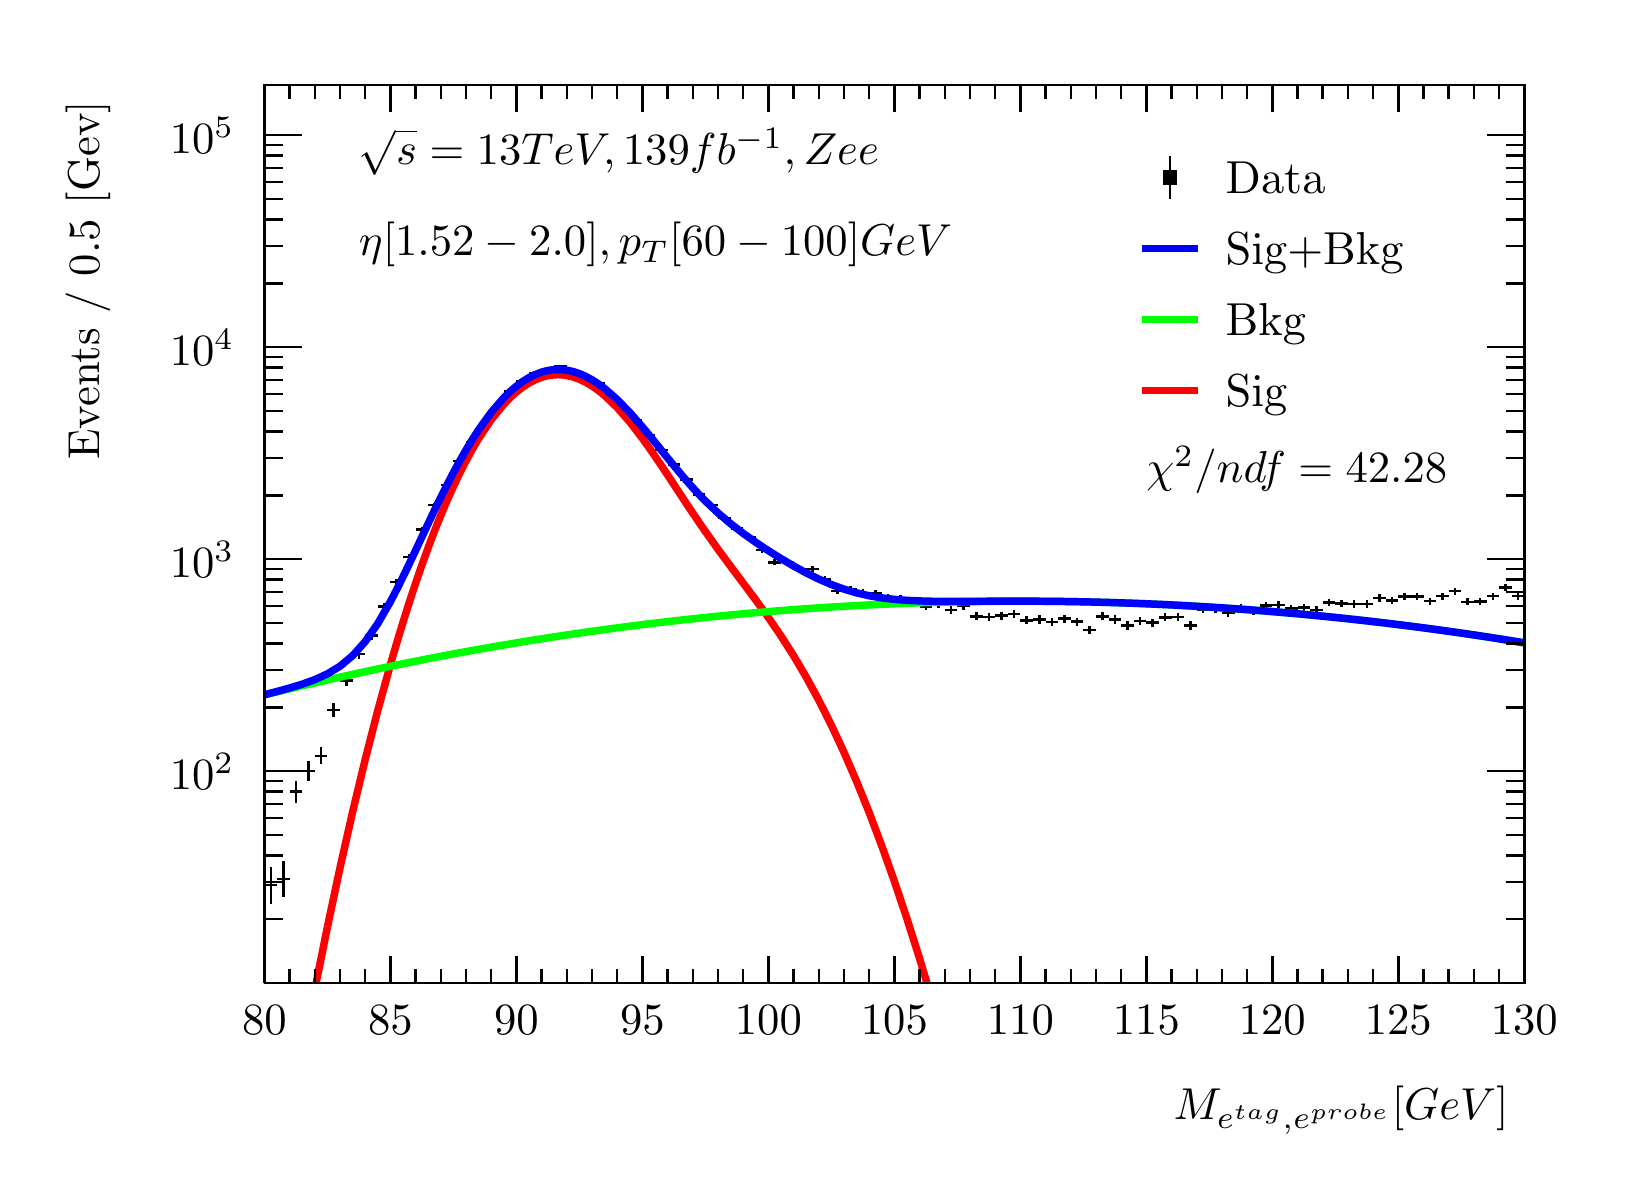
\begin{tikzpicture}
\pgfdeclareplotmark{cross} {
\pgfpathmoveto{\pgfpoint{-0.3\pgfplotmarksize}{\pgfplotmarksize}}
\pgfpathlineto{\pgfpoint{+0.3\pgfplotmarksize}{\pgfplotmarksize}}
\pgfpathlineto{\pgfpoint{+0.3\pgfplotmarksize}{0.3\pgfplotmarksize}}
\pgfpathlineto{\pgfpoint{+1\pgfplotmarksize}{0.3\pgfplotmarksize}}
\pgfpathlineto{\pgfpoint{+1\pgfplotmarksize}{-0.3\pgfplotmarksize}}
\pgfpathlineto{\pgfpoint{+0.3\pgfplotmarksize}{-0.3\pgfplotmarksize}}
\pgfpathlineto{\pgfpoint{+0.3\pgfplotmarksize}{-1.\pgfplotmarksize}}
\pgfpathlineto{\pgfpoint{-0.3\pgfplotmarksize}{-1.\pgfplotmarksize}}
\pgfpathlineto{\pgfpoint{-0.3\pgfplotmarksize}{-0.3\pgfplotmarksize}}
\pgfpathlineto{\pgfpoint{-1.\pgfplotmarksize}{-0.3\pgfplotmarksize}}
\pgfpathlineto{\pgfpoint{-1.\pgfplotmarksize}{0.3\pgfplotmarksize}}
\pgfpathlineto{\pgfpoint{-0.3\pgfplotmarksize}{0.3\pgfplotmarksize}}
\pgfpathclose
\pgfusepathqstroke
}
\pgfdeclareplotmark{cross*} {
\pgfpathmoveto{\pgfpoint{-0.3\pgfplotmarksize}{\pgfplotmarksize}}
\pgfpathlineto{\pgfpoint{+0.3\pgfplotmarksize}{\pgfplotmarksize}}
\pgfpathlineto{\pgfpoint{+0.3\pgfplotmarksize}{0.3\pgfplotmarksize}}
\pgfpathlineto{\pgfpoint{+1\pgfplotmarksize}{0.3\pgfplotmarksize}}
\pgfpathlineto{\pgfpoint{+1\pgfplotmarksize}{-0.3\pgfplotmarksize}}
\pgfpathlineto{\pgfpoint{+0.3\pgfplotmarksize}{-0.3\pgfplotmarksize}}
\pgfpathlineto{\pgfpoint{+0.3\pgfplotmarksize}{-1.\pgfplotmarksize}}
\pgfpathlineto{\pgfpoint{-0.3\pgfplotmarksize}{-1.\pgfplotmarksize}}
\pgfpathlineto{\pgfpoint{-0.3\pgfplotmarksize}{-0.3\pgfplotmarksize}}
\pgfpathlineto{\pgfpoint{-1.\pgfplotmarksize}{-0.3\pgfplotmarksize}}
\pgfpathlineto{\pgfpoint{-1.\pgfplotmarksize}{0.3\pgfplotmarksize}}
\pgfpathlineto{\pgfpoint{-0.3\pgfplotmarksize}{0.3\pgfplotmarksize}}
\pgfpathclose
\pgfusepathqfillstroke
}
\pgfdeclareplotmark{newstar} {
\pgfpathmoveto{\pgfqpoint{0pt}{\pgfplotmarksize}}
\pgfpathlineto{\pgfqpointpolar{44}{0.5\pgfplotmarksize}}
\pgfpathlineto{\pgfqpointpolar{18}{\pgfplotmarksize}}
\pgfpathlineto{\pgfqpointpolar{-20}{0.5\pgfplotmarksize}}
\pgfpathlineto{\pgfqpointpolar{-54}{\pgfplotmarksize}}
\pgfpathlineto{\pgfqpointpolar{-90}{0.5\pgfplotmarksize}}
\pgfpathlineto{\pgfqpointpolar{234}{\pgfplotmarksize}}
\pgfpathlineto{\pgfqpointpolar{198}{0.5\pgfplotmarksize}}
\pgfpathlineto{\pgfqpointpolar{162}{\pgfplotmarksize}}
\pgfpathlineto{\pgfqpointpolar{134}{0.5\pgfplotmarksize}}
\pgfpathclose
\pgfusepathqstroke
}
\pgfdeclareplotmark{newstar*} {
\pgfpathmoveto{\pgfqpoint{0pt}{\pgfplotmarksize}}
\pgfpathlineto{\pgfqpointpolar{44}{0.5\pgfplotmarksize}}
\pgfpathlineto{\pgfqpointpolar{18}{\pgfplotmarksize}}
\pgfpathlineto{\pgfqpointpolar{-20}{0.5\pgfplotmarksize}}
\pgfpathlineto{\pgfqpointpolar{-54}{\pgfplotmarksize}}
\pgfpathlineto{\pgfqpointpolar{-90}{0.5\pgfplotmarksize}}
\pgfpathlineto{\pgfqpointpolar{234}{\pgfplotmarksize}}
\pgfpathlineto{\pgfqpointpolar{198}{0.5\pgfplotmarksize}}
\pgfpathlineto{\pgfqpointpolar{162}{\pgfplotmarksize}}
\pgfpathlineto{\pgfqpointpolar{134}{0.5\pgfplotmarksize}}
\pgfpathclose
\pgfusepathqfillstroke
}
\definecolor{c}{rgb}{1,1,1};
\draw [color=c, fill=c] (0,0) rectangle (20,14.4361);
\draw [color=c, fill=c] (3,2.30977) rectangle (19,13.7143);
\definecolor{c}{rgb}{0,0,0};
\draw [c,line width=0.9] (3,2.30977) -- (3,13.7143) -- (19,13.7143) -- (19,2.30977) -- (3,2.30977);
\definecolor{c}{rgb}{1,1,1};
\draw [color=c, fill=c] (3,2.30977) rectangle (19,13.7143);
\definecolor{c}{rgb}{0,0,0};
\draw [c,line width=0.9] (3,2.30977) -- (3,13.7143) -- (19,13.7143) -- (19,2.30977) -- (3,2.30977);
\draw [c,line width=0.9] (3,2.30977) -- (19,2.30977);
\draw [c,line width=0.9] (3,2.65624) -- (3,2.30977);
\draw [c,line width=0.9] (3.32,2.48301) -- (3.32,2.30977);
\draw [c,line width=0.9] (3.64,2.48301) -- (3.64,2.30977);
\draw [c,line width=0.9] (3.96,2.48301) -- (3.96,2.30977);
\draw [c,line width=0.9] (4.28,2.48301) -- (4.28,2.30977);
\draw [c,line width=0.9] (4.6,2.65624) -- (4.6,2.30977);
\draw [c,line width=0.9] (4.92,2.48301) -- (4.92,2.30977);
\draw [c,line width=0.9] (5.24,2.48301) -- (5.24,2.30977);
\draw [c,line width=0.9] (5.56,2.48301) -- (5.56,2.30977);
\draw [c,line width=0.9] (5.88,2.48301) -- (5.88,2.30977);
\draw [c,line width=0.9] (6.2,2.65624) -- (6.2,2.30977);
\draw [c,line width=0.9] (6.52,2.48301) -- (6.52,2.30977);
\draw [c,line width=0.9] (6.84,2.48301) -- (6.84,2.30977);
\draw [c,line width=0.9] (7.16,2.48301) -- (7.16,2.30977);
\draw [c,line width=0.9] (7.48,2.48301) -- (7.48,2.30977);
\draw [c,line width=0.9] (7.8,2.65624) -- (7.8,2.30977);
\draw [c,line width=0.9] (8.12,2.48301) -- (8.12,2.30977);
\draw [c,line width=0.9] (8.44,2.48301) -- (8.44,2.30977);
\draw [c,line width=0.9] (8.76,2.48301) -- (8.76,2.30977);
\draw [c,line width=0.9] (9.08,2.48301) -- (9.08,2.30977);
\draw [c,line width=0.9] (9.4,2.65624) -- (9.4,2.30977);
\draw [c,line width=0.9] (9.72,2.48301) -- (9.72,2.30977);
\draw [c,line width=0.9] (10.04,2.48301) -- (10.04,2.30977);
\draw [c,line width=0.9] (10.36,2.48301) -- (10.36,2.30977);
\draw [c,line width=0.9] (10.68,2.48301) -- (10.68,2.30977);
\draw [c,line width=0.9] (11,2.65624) -- (11,2.30977);
\draw [c,line width=0.9] (11.32,2.48301) -- (11.32,2.30977);
\draw [c,line width=0.9] (11.64,2.48301) -- (11.64,2.30977);
\draw [c,line width=0.9] (11.96,2.48301) -- (11.96,2.30977);
\draw [c,line width=0.9] (12.28,2.48301) -- (12.28,2.30977);
\draw [c,line width=0.9] (12.6,2.65624) -- (12.6,2.30977);
\draw [c,line width=0.9] (12.92,2.48301) -- (12.92,2.30977);
\draw [c,line width=0.9] (13.24,2.48301) -- (13.24,2.30977);
\draw [c,line width=0.9] (13.56,2.48301) -- (13.56,2.30977);
\draw [c,line width=0.9] (13.88,2.48301) -- (13.88,2.30977);
\draw [c,line width=0.9] (14.2,2.65624) -- (14.2,2.30977);
\draw [c,line width=0.9] (14.52,2.48301) -- (14.52,2.30977);
\draw [c,line width=0.9] (14.84,2.48301) -- (14.84,2.30977);
\draw [c,line width=0.9] (15.16,2.48301) -- (15.16,2.30977);
\draw [c,line width=0.9] (15.48,2.48301) -- (15.48,2.30977);
\draw [c,line width=0.9] (15.8,2.65624) -- (15.8,2.30977);
\draw [c,line width=0.9] (16.12,2.48301) -- (16.12,2.30977);
\draw [c,line width=0.9] (16.44,2.48301) -- (16.44,2.30977);
\draw [c,line width=0.9] (16.76,2.48301) -- (16.76,2.30977);
\draw [c,line width=0.9] (17.08,2.48301) -- (17.08,2.30977);
\draw [c,line width=0.9] (17.4,2.65624) -- (17.4,2.30977);
\draw [c,line width=0.9] (17.72,2.48301) -- (17.72,2.30977);
\draw [c,line width=0.9] (18.04,2.48301) -- (18.04,2.30977);
\draw [c,line width=0.9] (18.36,2.48301) -- (18.36,2.30977);
\draw [c,line width=0.9] (18.68,2.48301) -- (18.68,2.30977);
\draw [c,line width=0.9] (19,2.65624) -- (19,2.30977);
\draw [anchor=base] (3,1.66015) node[scale=1.61424, color=c, rotate=0]{80};
\draw [anchor=base] (4.6,1.66015) node[scale=1.61424, color=c, rotate=0]{85};
\draw [anchor=base] (6.2,1.66015) node[scale=1.61424, color=c, rotate=0]{90};
\draw [anchor=base] (7.8,1.66015) node[scale=1.61424, color=c, rotate=0]{95};
\draw [anchor=base] (9.4,1.66015) node[scale=1.61424, color=c, rotate=0]{100};
\draw [anchor=base] (11,1.66015) node[scale=1.61424, color=c, rotate=0]{105};
\draw [anchor=base] (12.6,1.66015) node[scale=1.61424, color=c, rotate=0]{110};
\draw [anchor=base] (14.2,1.66015) node[scale=1.61424, color=c, rotate=0]{115};
\draw [anchor=base] (15.8,1.66015) node[scale=1.61424, color=c, rotate=0]{120};
\draw [anchor=base] (17.4,1.66015) node[scale=1.61424, color=c, rotate=0]{125};
\draw [anchor=base] (19,1.66015) node[scale=1.61424, color=c, rotate=0]{130};
\draw [anchor= east] (19,0.692932) node[scale=1.61424, color=c, rotate=0]{$M_{e^{tag}, e^{probe}}  [GeV]$};
\draw [c,line width=0.9] (3,13.7143) -- (19,13.7143);
\draw [c,line width=0.9] (3,13.3678) -- (3,13.7143);
\draw [c,line width=0.9] (3.32,13.5411) -- (3.32,13.7143);
\draw [c,line width=0.9] (3.64,13.5411) -- (3.64,13.7143);
\draw [c,line width=0.9] (3.96,13.5411) -- (3.96,13.7143);
\draw [c,line width=0.9] (4.28,13.5411) -- (4.28,13.7143);
\draw [c,line width=0.9] (4.6,13.3678) -- (4.6,13.7143);
\draw [c,line width=0.9] (4.92,13.5411) -- (4.92,13.7143);
\draw [c,line width=0.9] (5.24,13.5411) -- (5.24,13.7143);
\draw [c,line width=0.9] (5.56,13.5411) -- (5.56,13.7143);
\draw [c,line width=0.9] (5.88,13.5411) -- (5.88,13.7143);
\draw [c,line width=0.9] (6.2,13.3678) -- (6.2,13.7143);
\draw [c,line width=0.9] (6.52,13.5411) -- (6.52,13.7143);
\draw [c,line width=0.9] (6.84,13.5411) -- (6.84,13.7143);
\draw [c,line width=0.9] (7.16,13.5411) -- (7.16,13.7143);
\draw [c,line width=0.9] (7.48,13.5411) -- (7.48,13.7143);
\draw [c,line width=0.9] (7.8,13.3678) -- (7.8,13.7143);
\draw [c,line width=0.9] (8.12,13.5411) -- (8.12,13.7143);
\draw [c,line width=0.9] (8.44,13.5411) -- (8.44,13.7143);
\draw [c,line width=0.9] (8.76,13.5411) -- (8.76,13.7143);
\draw [c,line width=0.9] (9.08,13.5411) -- (9.08,13.7143);
\draw [c,line width=0.9] (9.4,13.3678) -- (9.4,13.7143);
\draw [c,line width=0.9] (9.72,13.5411) -- (9.72,13.7143);
\draw [c,line width=0.9] (10.04,13.5411) -- (10.04,13.7143);
\draw [c,line width=0.9] (10.36,13.5411) -- (10.36,13.7143);
\draw [c,line width=0.9] (10.68,13.5411) -- (10.68,13.7143);
\draw [c,line width=0.9] (11,13.3678) -- (11,13.7143);
\draw [c,line width=0.9] (11.32,13.5411) -- (11.32,13.7143);
\draw [c,line width=0.9] (11.64,13.5411) -- (11.64,13.7143);
\draw [c,line width=0.9] (11.96,13.5411) -- (11.96,13.7143);
\draw [c,line width=0.9] (12.28,13.5411) -- (12.28,13.7143);
\draw [c,line width=0.9] (12.6,13.3678) -- (12.6,13.7143);
\draw [c,line width=0.9] (12.92,13.5411) -- (12.92,13.7143);
\draw [c,line width=0.9] (13.24,13.5411) -- (13.24,13.7143);
\draw [c,line width=0.9] (13.56,13.5411) -- (13.56,13.7143);
\draw [c,line width=0.9] (13.88,13.5411) -- (13.88,13.7143);
\draw [c,line width=0.9] (14.2,13.3678) -- (14.2,13.7143);
\draw [c,line width=0.9] (14.52,13.5411) -- (14.52,13.7143);
\draw [c,line width=0.9] (14.84,13.5411) -- (14.84,13.7143);
\draw [c,line width=0.9] (15.16,13.5411) -- (15.16,13.7143);
\draw [c,line width=0.9] (15.48,13.5411) -- (15.48,13.7143);
\draw [c,line width=0.9] (15.8,13.3678) -- (15.8,13.7143);
\draw [c,line width=0.9] (16.12,13.5411) -- (16.12,13.7143);
\draw [c,line width=0.9] (16.44,13.5411) -- (16.44,13.7143);
\draw [c,line width=0.9] (16.76,13.5411) -- (16.76,13.7143);
\draw [c,line width=0.9] (17.08,13.5411) -- (17.08,13.7143);
\draw [c,line width=0.9] (17.4,13.3678) -- (17.4,13.7143);
\draw [c,line width=0.9] (17.72,13.5411) -- (17.72,13.7143);
\draw [c,line width=0.9] (18.04,13.5411) -- (18.04,13.7143);
\draw [c,line width=0.9] (18.36,13.5411) -- (18.36,13.7143);
\draw [c,line width=0.9] (18.68,13.5411) -- (18.68,13.7143);
\draw [c,line width=0.9] (19,13.3678) -- (19,13.7143);
\draw [c,line width=0.9] (3,2.30977) -- (3,13.7143);
\draw [c,line width=0.9] (3.237,3.12018) -- (3,3.12018);
\draw [c,line width=0.9] (3.237,3.59423) -- (3,3.59423);
\draw [c,line width=0.9] (3.237,3.93058) -- (3,3.93058);
\draw [c,line width=0.9] (3.237,4.19147) -- (3,4.19147);
\draw [c,line width=0.9] (3.237,4.40464) -- (3,4.40464);
\draw [c,line width=0.9] (3.237,4.58487) -- (3,4.58487);
\draw [c,line width=0.9] (3.237,4.74099) -- (3,4.74099);
\draw [c,line width=0.9] (3.237,4.8787) -- (3,4.8787);
\draw [c,line width=0.9] (3.474,5.00188) -- (3,5.00188);
\draw [anchor= east] (2.82,5.00188) node[scale=1.61424, color=c, rotate=0]{$10^{2}$};
\draw [c,line width=0.9] (3.237,5.81228) -- (3,5.81228);
\draw [c,line width=0.9] (3.237,6.28634) -- (3,6.28634);
\draw [c,line width=0.9] (3.237,6.62269) -- (3,6.62269);
\draw [c,line width=0.9] (3.237,6.88358) -- (3,6.88358);
\draw [c,line width=0.9] (3.237,7.09675) -- (3,7.09675);
\draw [c,line width=0.9] (3.237,7.27697) -- (3,7.27697);
\draw [c,line width=0.9] (3.237,7.43309) -- (3,7.43309);
\draw [c,line width=0.9] (3.237,7.5708) -- (3,7.5708);
\draw [c,line width=0.9] (3.474,7.69399) -- (3,7.69399);
\draw [anchor= east] (2.82,7.69399) node[scale=1.61424, color=c, rotate=0]{$10^{3}$};
\draw [c,line width=0.9] (3.237,8.50439) -- (3,8.50439);
\draw [c,line width=0.9] (3.237,8.97845) -- (3,8.97845);
\draw [c,line width=0.9] (3.237,9.3148) -- (3,9.3148);
\draw [c,line width=0.9] (3.237,9.57569) -- (3,9.57569);
\draw [c,line width=0.9] (3.237,9.78885) -- (3,9.78885);
\draw [c,line width=0.9] (3.237,9.96908) -- (3,9.96908);
\draw [c,line width=0.9] (3.237,10.1252) -- (3,10.1252);
\draw [c,line width=0.9] (3.237,10.2629) -- (3,10.2629);
\draw [c,line width=0.9] (3.474,10.3861) -- (3,10.3861);
\draw [anchor= east] (2.82,10.3861) node[scale=1.61424, color=c, rotate=0]{$10^{4}$};
\draw [c,line width=0.9] (3.237,11.1965) -- (3,11.1965);
\draw [c,line width=0.9] (3.237,11.6706) -- (3,11.6706);
\draw [c,line width=0.9] (3.237,12.0069) -- (3,12.0069);
\draw [c,line width=0.9] (3.237,12.2678) -- (3,12.2678);
\draw [c,line width=0.9] (3.237,12.481) -- (3,12.481);
\draw [c,line width=0.9] (3.237,12.6612) -- (3,12.6612);
\draw [c,line width=0.9] (3.237,12.8173) -- (3,12.8173);
\draw [c,line width=0.9] (3.237,12.955) -- (3,12.955);
\draw [c,line width=0.9] (3.474,13.0782) -- (3,13.0782);
\draw [anchor= east] (2.82,13.0782) node[scale=1.61424, color=c, rotate=0]{$10^{5}$};
\draw [anchor= east] (0.76,13.7143) node[scale=1.61424, color=c, rotate=90]{Events / 0.5 [Gev]};
\draw [c,line width=0.9] (19,2.30977) -- (19,13.7143);
\draw [c,line width=0.9] (18.763,3.12018) -- (19,3.12018);
\draw [c,line width=0.9] (18.763,3.59423) -- (19,3.59423);
\draw [c,line width=0.9] (18.763,3.93058) -- (19,3.93058);
\draw [c,line width=0.9] (18.763,4.19147) -- (19,4.19147);
\draw [c,line width=0.9] (18.763,4.40464) -- (19,4.40464);
\draw [c,line width=0.9] (18.763,4.58487) -- (19,4.58487);
\draw [c,line width=0.9] (18.763,4.74099) -- (19,4.74099);
\draw [c,line width=0.9] (18.763,4.8787) -- (19,4.8787);
\draw [c,line width=0.9] (18.526,5.00188) -- (19,5.00188);
\draw [c,line width=0.9] (18.763,5.81228) -- (19,5.81228);
\draw [c,line width=0.9] (18.763,6.28634) -- (19,6.28634);
\draw [c,line width=0.9] (18.763,6.62269) -- (19,6.62269);
\draw [c,line width=0.9] (18.763,6.88358) -- (19,6.88358);
\draw [c,line width=0.9] (18.763,7.09675) -- (19,7.09675);
\draw [c,line width=0.9] (18.763,7.27697) -- (19,7.27697);
\draw [c,line width=0.9] (18.763,7.43309) -- (19,7.43309);
\draw [c,line width=0.9] (18.763,7.5708) -- (19,7.5708);
\draw [c,line width=0.9] (18.526,7.69399) -- (19,7.69399);
\draw [c,line width=0.9] (18.763,8.50439) -- (19,8.50439);
\draw [c,line width=0.9] (18.763,8.97845) -- (19,8.97845);
\draw [c,line width=0.9] (18.763,9.3148) -- (19,9.3148);
\draw [c,line width=0.9] (18.763,9.57569) -- (19,9.57569);
\draw [c,line width=0.9] (18.763,9.78885) -- (19,9.78885);
\draw [c,line width=0.9] (18.763,9.96908) -- (19,9.96908);
\draw [c,line width=0.9] (18.763,10.1252) -- (19,10.1252);
\draw [c,line width=0.9] (18.763,10.2629) -- (19,10.2629);
\draw [c,line width=0.9] (18.526,10.3861) -- (19,10.3861);
\draw [c,line width=0.9] (18.763,11.1965) -- (19,11.1965);
\draw [c,line width=0.9] (18.763,11.6706) -- (19,11.6706);
\draw [c,line width=0.9] (18.763,12.0069) -- (19,12.0069);
\draw [c,line width=0.9] (18.763,12.2678) -- (19,12.2678);
\draw [c,line width=0.9] (18.763,12.481) -- (19,12.481);
\draw [c,line width=0.9] (18.763,12.6612) -- (19,12.6612);
\draw [c,line width=0.9] (18.763,12.8173) -- (19,12.8173);
\draw [c,line width=0.9] (18.763,12.955) -- (19,12.955);
\draw [c,line width=0.9] (18.526,13.0782) -- (19,13.0782);
\draw [c,line width=0.9] (3.08,3.5546) -- (3,3.5546);
\draw [c,line width=0.9] (3,3.5546) -- (3,3.5546);
\draw [c,line width=0.9] (3.08,3.5546) -- (3.16,3.5546);
\draw [c,line width=0.9] (3.16,3.5546) -- (3.16,3.5546);
\draw [c,line width=0.9] (3.08,3.5546) -- (3.08,3.7893);
\draw [c,line width=0.9] (3.08,3.7893) -- (3.08,3.7893);
\draw [c,line width=0.9] (3.08,3.5546) -- (3.08,3.31597);
\draw [c,line width=0.9] (3.08,3.31597) -- (3.08,3.31597);
\draw [c,line width=0.9] (3.24,3.63257) -- (3.16,3.63257);
\draw [c,line width=0.9] (3.16,3.63257) -- (3.16,3.63257);
\draw [c,line width=0.9] (3.24,3.63257) -- (3.32,3.63257);
\draw [c,line width=0.9] (3.32,3.63257) -- (3.32,3.63257);
\draw [c,line width=0.9] (3.24,3.63257) -- (3.24,3.8591);
\draw [c,line width=0.9] (3.24,3.8591) -- (3.24,3.8591);
\draw [c,line width=0.9] (3.24,3.63257) -- (3.24,3.4025);
\draw [c,line width=0.9] (3.24,3.4025) -- (3.24,3.4025);
\draw [c,line width=0.9] (3.4,4.74099) -- (3.32,4.74099);
\draw [c,line width=0.9] (3.32,4.74099) -- (3.32,4.74099);
\draw [c,line width=0.9] (3.4,4.74099) -- (3.48,4.74099);
\draw [c,line width=0.9] (3.48,4.74099) -- (3.48,4.74099);
\draw [c,line width=0.9] (3.4,4.74099) -- (3.4,4.87846);
\draw [c,line width=0.9] (3.4,4.87846) -- (3.4,4.87846);
\draw [c,line width=0.9] (3.4,4.74099) -- (3.4,4.60268);
\draw [c,line width=0.9] (3.4,4.60268) -- (3.4,4.60268);
\draw [c,line width=0.9] (3.56,5.00188) -- (3.48,5.00188);
\draw [c,line width=0.9] (3.48,5.00188) -- (3.48,5.00188);
\draw [c,line width=0.9] (3.56,5.00188) -- (3.64,5.00188);
\draw [c,line width=0.9] (3.64,5.00188) -- (3.64,5.00188);
\draw [c,line width=0.9] (3.56,5.00188) -- (3.56,5.12425);
\draw [c,line width=0.9] (3.56,5.12425) -- (3.56,5.12425);
\draw [c,line width=0.9] (3.56,5.00188) -- (3.56,4.87891);
\draw [c,line width=0.9] (3.56,4.87891) -- (3.56,4.87891);
\draw [c,line width=0.9] (3.72,5.19539) -- (3.64,5.19539);
\draw [c,line width=0.9] (3.64,5.19539) -- (3.64,5.19539);
\draw [c,line width=0.9] (3.72,5.19539) -- (3.8,5.19539);
\draw [c,line width=0.9] (3.8,5.19539) -- (3.8,5.19539);
\draw [c,line width=0.9] (3.72,5.19539) -- (3.72,5.30299);
\draw [c,line width=0.9] (3.72,5.30299) -- (3.72,5.30299);
\draw [c,line width=0.9] (3.72,5.19539) -- (3.72,5.0878);
\draw [c,line width=0.9] (3.72,5.0878) -- (3.72,5.0878);
\draw [c,line width=0.9] (3.88,5.77667) -- (3.8,5.77667);
\draw [c,line width=0.9] (3.8,5.77667) -- (3.8,5.77667);
\draw [c,line width=0.9] (3.88,5.77667) -- (3.96,5.77667);
\draw [c,line width=0.9] (3.96,5.77667) -- (3.96,5.77667);
\draw [c,line width=0.9] (3.88,5.77667) -- (3.88,5.8606);
\draw [c,line width=0.9] (3.88,5.8606) -- (3.88,5.8606);
\draw [c,line width=0.9] (3.88,5.77667) -- (3.88,5.69275);
\draw [c,line width=0.9] (3.88,5.69275) -- (3.88,5.69275);
\draw [c,line width=0.9] (4.04,6.15009) -- (3.96,6.15009);
\draw [c,line width=0.9] (3.96,6.15009) -- (3.96,6.15009);
\draw [c,line width=0.9] (4.04,6.15009) -- (4.12,6.15009);
\draw [c,line width=0.9] (4.12,6.15009) -- (4.12,6.15009);
\draw [c,line width=0.9] (4.04,6.15009) -- (4.04,6.22164);
\draw [c,line width=0.9] (4.04,6.22164) -- (4.04,6.22164);
\draw [c,line width=0.9] (4.04,6.15009) -- (4.04,6.07855);
\draw [c,line width=0.9] (4.04,6.07855) -- (4.04,6.07855);
\draw [c,line width=0.9] (4.2,6.48644) -- (4.12,6.48644);
\draw [c,line width=0.9] (4.12,6.48644) -- (4.12,6.48644);
\draw [c,line width=0.9] (4.2,6.48644) -- (4.28,6.48644);
\draw [c,line width=0.9] (4.28,6.48644) -- (4.28,6.48644);
\draw [c,line width=0.9] (4.2,6.48644) -- (4.2,6.5484);
\draw [c,line width=0.9] (4.2,6.5484) -- (4.2,6.5484);
\draw [c,line width=0.9] (4.2,6.48644) -- (4.2,6.42448);
\draw [c,line width=0.9] (4.2,6.42448) -- (4.2,6.42448);
\draw [c,line width=0.9] (4.36,6.72613) -- (4.28,6.72613);
\draw [c,line width=0.9] (4.28,6.72613) -- (4.28,6.72613);
\draw [c,line width=0.9] (4.36,6.72613) -- (4.44,6.72613);
\draw [c,line width=0.9] (4.44,6.72613) -- (4.44,6.72613);
\draw [c,line width=0.9] (4.36,6.72613) -- (4.36,6.78205);
\draw [c,line width=0.9] (4.36,6.78205) -- (4.36,6.78205);
\draw [c,line width=0.9] (4.36,6.72613) -- (4.36,6.6702);
\draw [c,line width=0.9] (4.36,6.6702) -- (4.36,6.6702);
\draw [c,line width=0.9] (4.52,7.09284) -- (4.44,7.09284);
\draw [c,line width=0.9] (4.44,7.09284) -- (4.44,7.09284);
\draw [c,line width=0.9] (4.52,7.09284) -- (4.6,7.09284);
\draw [c,line width=0.9] (4.6,7.09284) -- (4.6,7.09284);
\draw [c,line width=0.9] (4.52,7.09284) -- (4.52,7.14065);
\draw [c,line width=0.9] (4.52,7.14065) -- (4.52,7.14065);
\draw [c,line width=0.9] (4.52,7.09284) -- (4.52,7.04504);
\draw [c,line width=0.9] (4.52,7.04504) -- (4.52,7.04504);
\draw [c,line width=0.9] (4.68,7.40349) -- (4.6,7.40349);
\draw [c,line width=0.9] (4.6,7.40349) -- (4.6,7.40349);
\draw [c,line width=0.9] (4.68,7.40349) -- (4.76,7.40349);
\draw [c,line width=0.9] (4.76,7.40349) -- (4.76,7.40349);
\draw [c,line width=0.9] (4.68,7.40349) -- (4.68,7.44536);
\draw [c,line width=0.9] (4.68,7.44536) -- (4.68,7.44536);
\draw [c,line width=0.9] (4.68,7.40349) -- (4.68,7.36163);
\draw [c,line width=0.9] (4.68,7.36163) -- (4.68,7.36163);
\draw [c,line width=0.9] (4.84,7.71943) -- (4.76,7.71943);
\draw [c,line width=0.9] (4.76,7.71943) -- (4.76,7.71943);
\draw [c,line width=0.9] (4.84,7.71943) -- (4.92,7.71943);
\draw [c,line width=0.9] (4.92,7.71943) -- (4.92,7.71943);
\draw [c,line width=0.9] (4.84,7.71943) -- (4.84,7.756);
\draw [c,line width=0.9] (4.84,7.756) -- (4.84,7.756);
\draw [c,line width=0.9] (4.84,7.71943) -- (4.84,7.68286);
\draw [c,line width=0.9] (4.84,7.68286) -- (4.84,7.68286);
\draw [c,line width=0.9] (5,8.07225) -- (4.92,8.07225);
\draw [c,line width=0.9] (4.92,8.07225) -- (4.92,8.07225);
\draw [c,line width=0.9] (5,8.07225) -- (5.08,8.07225);
\draw [c,line width=0.9] (5.08,8.07225) -- (5.08,8.07225);
\draw [c,line width=0.9] (5,8.07225) -- (5,8.1037);
\draw [c,line width=0.9] (5,8.1037) -- (5,8.1037);
\draw [c,line width=0.9] (5,8.07225) -- (5,8.0408);
\draw [c,line width=0.9] (5,8.0408) -- (5,8.0408);
\draw [c,line width=0.9] (5.16,8.37796) -- (5.08,8.37796);
\draw [c,line width=0.9] (5.08,8.37796) -- (5.08,8.37796);
\draw [c,line width=0.9] (5.16,8.37796) -- (5.24,8.37796);
\draw [c,line width=0.9] (5.24,8.37796) -- (5.24,8.37796);
\draw [c,line width=0.9] (5.16,8.37796) -- (5.16,8.40555);
\draw [c,line width=0.9] (5.16,8.40555) -- (5.16,8.40555);
\draw [c,line width=0.9] (5.16,8.37796) -- (5.16,8.35036);
\draw [c,line width=0.9] (5.16,8.35036) -- (5.16,8.35036);
\draw [c,line width=0.9] (5.32,8.63323) -- (5.24,8.63323);
\draw [c,line width=0.9] (5.24,8.63323) -- (5.24,8.63323);
\draw [c,line width=0.9] (5.32,8.63323) -- (5.4,8.63323);
\draw [c,line width=0.9] (5.4,8.63323) -- (5.4,8.63323);
\draw [c,line width=0.9] (5.32,8.63323) -- (5.32,8.65798);
\draw [c,line width=0.9] (5.32,8.65798) -- (5.32,8.65798);
\draw [c,line width=0.9] (5.32,8.63323) -- (5.32,8.60849);
\draw [c,line width=0.9] (5.32,8.60849) -- (5.32,8.60849);
\draw [c,line width=0.9] (5.48,8.9372) -- (5.4,8.9372);
\draw [c,line width=0.9] (5.4,8.9372) -- (5.4,8.9372);
\draw [c,line width=0.9] (5.48,8.9372) -- (5.56,8.9372);
\draw [c,line width=0.9] (5.56,8.9372) -- (5.56,8.9372);
\draw [c,line width=0.9] (5.48,8.9372) -- (5.48,8.95892);
\draw [c,line width=0.9] (5.48,8.95892) -- (5.48,8.95892);
\draw [c,line width=0.9] (5.48,8.9372) -- (5.48,8.91547);
\draw [c,line width=0.9] (5.48,8.91547) -- (5.48,8.91547);
\draw [c,line width=0.9] (5.64,9.17295) -- (5.56,9.17295);
\draw [c,line width=0.9] (5.56,9.17295) -- (5.56,9.17295);
\draw [c,line width=0.9] (5.64,9.17295) -- (5.72,9.17295);
\draw [c,line width=0.9] (5.72,9.17295) -- (5.72,9.17295);
\draw [c,line width=0.9] (5.64,9.17295) -- (5.64,9.1926);
\draw [c,line width=0.9] (5.64,9.1926) -- (5.64,9.1926);
\draw [c,line width=0.9] (5.64,9.17295) -- (5.64,9.15331);
\draw [c,line width=0.9] (5.64,9.15331) -- (5.64,9.15331);
\draw [c,line width=0.9] (5.8,9.39745) -- (5.72,9.39745);
\draw [c,line width=0.9] (5.72,9.39745) -- (5.72,9.39745);
\draw [c,line width=0.9] (5.8,9.39745) -- (5.88,9.39745);
\draw [c,line width=0.9] (5.88,9.39745) -- (5.88,9.39745);
\draw [c,line width=0.9] (5.8,9.39745) -- (5.8,9.41529);
\draw [c,line width=0.9] (5.8,9.41529) -- (5.8,9.41529);
\draw [c,line width=0.9] (5.8,9.39745) -- (5.8,9.3796);
\draw [c,line width=0.9] (5.8,9.3796) -- (5.8,9.3796);
\draw [c,line width=0.9] (5.96,9.6041) -- (5.88,9.6041);
\draw [c,line width=0.9] (5.88,9.6041) -- (5.88,9.6041);
\draw [c,line width=0.9] (5.96,9.6041) -- (6.04,9.6041);
\draw [c,line width=0.9] (6.04,9.6041) -- (6.04,9.6041);
\draw [c,line width=0.9] (5.96,9.6041) -- (5.96,9.62044);
\draw [c,line width=0.9] (5.96,9.62044) -- (5.96,9.62044);
\draw [c,line width=0.9] (5.96,9.6041) -- (5.96,9.58777);
\draw [c,line width=0.9] (5.96,9.58777) -- (5.96,9.58777);
\draw [c,line width=0.9] (6.12,9.82455) -- (6.04,9.82455);
\draw [c,line width=0.9] (6.04,9.82455) -- (6.04,9.82455);
\draw [c,line width=0.9] (6.12,9.82455) -- (6.2,9.82455);
\draw [c,line width=0.9] (6.2,9.82455) -- (6.2,9.82455);
\draw [c,line width=0.9] (6.12,9.82455) -- (6.12,9.83941);
\draw [c,line width=0.9] (6.12,9.83941) -- (6.12,9.83941);
\draw [c,line width=0.9] (6.12,9.82455) -- (6.12,9.80968);
\draw [c,line width=0.9] (6.12,9.80968) -- (6.12,9.80968);
\draw [c,line width=0.9] (6.28,9.94699) -- (6.2,9.94699);
\draw [c,line width=0.9] (6.2,9.94699) -- (6.2,9.94699);
\draw [c,line width=0.9] (6.28,9.94699) -- (6.36,9.94699);
\draw [c,line width=0.9] (6.36,9.94699) -- (6.36,9.94699);
\draw [c,line width=0.9] (6.28,9.94699) -- (6.28,9.9611);
\draw [c,line width=0.9] (6.28,9.9611) -- (6.28,9.9611);
\draw [c,line width=0.9] (6.28,9.94699) -- (6.28,9.93289);
\draw [c,line width=0.9] (6.28,9.93289) -- (6.28,9.93289);
\draw [c,line width=0.9] (6.44,10.0532) -- (6.36,10.0532);
\draw [c,line width=0.9] (6.36,10.0532) -- (6.36,10.0532);
\draw [c,line width=0.9] (6.44,10.0532) -- (6.52,10.0532);
\draw [c,line width=0.9] (6.52,10.0532) -- (6.52,10.0532);
\draw [c,line width=0.9] (6.44,10.0532) -- (6.44,10.0667);
\draw [c,line width=0.9] (6.44,10.0667) -- (6.44,10.0667);
\draw [c,line width=0.9] (6.44,10.0532) -- (6.44,10.0397);
\draw [c,line width=0.9] (6.44,10.0397) -- (6.44,10.0397);
\draw [c,line width=0.9] (6.6,10.1083) -- (6.52,10.1083);
\draw [c,line width=0.9] (6.52,10.1083) -- (6.52,10.1083);
\draw [c,line width=0.9] (6.6,10.1083) -- (6.68,10.1083);
\draw [c,line width=0.9] (6.68,10.1083) -- (6.68,10.1083);
\draw [c,line width=0.9] (6.6,10.1083) -- (6.6,10.1214);
\draw [c,line width=0.9] (6.6,10.1214) -- (6.6,10.1214);
\draw [c,line width=0.9] (6.6,10.1083) -- (6.6,10.0951);
\draw [c,line width=0.9] (6.6,10.0951) -- (6.6,10.0951);
\draw [c,line width=0.9] (6.76,10.1486) -- (6.68,10.1486);
\draw [c,line width=0.9] (6.68,10.1486) -- (6.68,10.1486);
\draw [c,line width=0.9] (6.76,10.1486) -- (6.84,10.1486);
\draw [c,line width=0.9] (6.84,10.1486) -- (6.84,10.1486);
\draw [c,line width=0.9] (6.76,10.1486) -- (6.76,10.1616);
\draw [c,line width=0.9] (6.76,10.1616) -- (6.76,10.1616);
\draw [c,line width=0.9] (6.76,10.1486) -- (6.76,10.1357);
\draw [c,line width=0.9] (6.76,10.1357) -- (6.76,10.1357);
\draw [c,line width=0.9] (6.92,10.0801) -- (6.84,10.0801);
\draw [c,line width=0.9] (6.84,10.0801) -- (6.84,10.0801);
\draw [c,line width=0.9] (6.92,10.0801) -- (7,10.0801);
\draw [c,line width=0.9] (7,10.0801) -- (7,10.0801);
\draw [c,line width=0.9] (6.92,10.0801) -- (6.92,10.0934);
\draw [c,line width=0.9] (6.92,10.0934) -- (6.92,10.0934);
\draw [c,line width=0.9] (6.92,10.0801) -- (6.92,10.0667);
\draw [c,line width=0.9] (6.92,10.0667) -- (6.92,10.0667);
\draw [c,line width=0.9] (7.08,10.008) -- (7,10.008);
\draw [c,line width=0.9] (7,10.008) -- (7,10.008);
\draw [c,line width=0.9] (7.08,10.008) -- (7.16,10.008);
\draw [c,line width=0.9] (7.16,10.008) -- (7.16,10.008);
\draw [c,line width=0.9] (7.08,10.008) -- (7.08,10.0218);
\draw [c,line width=0.9] (7.08,10.0218) -- (7.08,10.0218);
\draw [c,line width=0.9] (7.08,10.008) -- (7.08,9.99427);
\draw [c,line width=0.9] (7.08,9.99427) -- (7.08,9.99427);
\draw [c,line width=0.9] (7.24,9.92135) -- (7.16,9.92135);
\draw [c,line width=0.9] (7.16,9.92135) -- (7.16,9.92135);
\draw [c,line width=0.9] (7.24,9.92135) -- (7.32,9.92135);
\draw [c,line width=0.9] (7.32,9.92135) -- (7.32,9.92135);
\draw [c,line width=0.9] (7.24,9.92135) -- (7.24,9.93562);
\draw [c,line width=0.9] (7.24,9.93562) -- (7.24,9.93562);
\draw [c,line width=0.9] (7.24,9.92135) -- (7.24,9.90709);
\draw [c,line width=0.9] (7.24,9.90709) -- (7.24,9.90709);
\draw [c,line width=0.9] (7.4,9.77769) -- (7.32,9.77769);
\draw [c,line width=0.9] (7.32,9.77769) -- (7.32,9.77769);
\draw [c,line width=0.9] (7.4,9.77769) -- (7.48,9.77769);
\draw [c,line width=0.9] (7.48,9.77769) -- (7.48,9.77769);
\draw [c,line width=0.9] (7.4,9.77769) -- (7.4,9.79286);
\draw [c,line width=0.9] (7.4,9.79286) -- (7.4,9.79286);
\draw [c,line width=0.9] (7.4,9.77769) -- (7.4,9.76253);
\draw [c,line width=0.9] (7.4,9.76253) -- (7.4,9.76253);
\draw [c,line width=0.9] (7.56,9.60616) -- (7.48,9.60616);
\draw [c,line width=0.9] (7.48,9.60616) -- (7.48,9.60616);
\draw [c,line width=0.9] (7.56,9.60616) -- (7.64,9.60616);
\draw [c,line width=0.9] (7.64,9.60616) -- (7.64,9.60616);
\draw [c,line width=0.9] (7.56,9.60616) -- (7.56,9.62248);
\draw [c,line width=0.9] (7.56,9.62248) -- (7.56,9.62248);
\draw [c,line width=0.9] (7.56,9.60616) -- (7.56,9.58984);
\draw [c,line width=0.9] (7.56,9.58984) -- (7.56,9.58984);
\draw [c,line width=0.9] (7.72,9.46362) -- (7.64,9.46362);
\draw [c,line width=0.9] (7.64,9.46362) -- (7.64,9.46362);
\draw [c,line width=0.9] (7.72,9.46362) -- (7.8,9.46362);
\draw [c,line width=0.9] (7.8,9.46362) -- (7.8,9.46362);
\draw [c,line width=0.9] (7.72,9.46362) -- (7.72,9.48097);
\draw [c,line width=0.9] (7.72,9.48097) -- (7.72,9.48097);
\draw [c,line width=0.9] (7.72,9.46362) -- (7.72,9.44628);
\draw [c,line width=0.9] (7.72,9.44628) -- (7.72,9.44628);
\draw [c,line width=0.9] (7.88,9.26127) -- (7.8,9.26127);
\draw [c,line width=0.9] (7.8,9.26127) -- (7.8,9.26127);
\draw [c,line width=0.9] (7.88,9.26127) -- (7.96,9.26127);
\draw [c,line width=0.9] (7.96,9.26127) -- (7.96,9.26127);
\draw [c,line width=0.9] (7.88,9.26127) -- (7.88,9.28018);
\draw [c,line width=0.9] (7.88,9.28018) -- (7.88,9.28018);
\draw [c,line width=0.9] (7.88,9.26127) -- (7.88,9.24236);
\draw [c,line width=0.9] (7.88,9.24236) -- (7.88,9.24236);
\draw [c,line width=0.9] (8.04,9.08063) -- (7.96,9.08063);
\draw [c,line width=0.9] (7.96,9.08063) -- (7.96,9.08063);
\draw [c,line width=0.9] (8.04,9.08063) -- (8.12,9.08063);
\draw [c,line width=0.9] (8.12,9.08063) -- (8.12,9.08063);
\draw [c,line width=0.9] (8.04,9.08063) -- (8.04,9.10107);
\draw [c,line width=0.9] (8.04,9.10107) -- (8.04,9.10107);
\draw [c,line width=0.9] (8.04,9.08063) -- (8.04,9.0602);
\draw [c,line width=0.9] (8.04,9.0602) -- (8.04,9.0602);
\draw [c,line width=0.9] (8.2,8.89653) -- (8.12,8.89653);
\draw [c,line width=0.9] (8.12,8.89653) -- (8.12,8.89653);
\draw [c,line width=0.9] (8.2,8.89653) -- (8.28,8.89653);
\draw [c,line width=0.9] (8.28,8.89653) -- (8.28,8.89653);
\draw [c,line width=0.9] (8.2,8.89653) -- (8.2,8.91864);
\draw [c,line width=0.9] (8.2,8.91864) -- (8.2,8.91864);
\draw [c,line width=0.9] (8.2,8.89653) -- (8.2,8.87442);
\draw [c,line width=0.9] (8.2,8.87442) -- (8.2,8.87442);
\draw [c,line width=0.9] (8.36,8.70777) -- (8.28,8.70777);
\draw [c,line width=0.9] (8.28,8.70777) -- (8.28,8.70777);
\draw [c,line width=0.9] (8.36,8.70777) -- (8.44,8.70777);
\draw [c,line width=0.9] (8.44,8.70777) -- (8.44,8.70777);
\draw [c,line width=0.9] (8.36,8.70777) -- (8.36,8.73174);
\draw [c,line width=0.9] (8.36,8.73174) -- (8.36,8.73174);
\draw [c,line width=0.9] (8.36,8.70777) -- (8.36,8.68381);
\draw [c,line width=0.9] (8.36,8.68381) -- (8.36,8.68381);
\draw [c,line width=0.9] (8.52,8.51718) -- (8.44,8.51718);
\draw [c,line width=0.9] (8.44,8.51718) -- (8.44,8.51718);
\draw [c,line width=0.9] (8.52,8.51718) -- (8.6,8.51718);
\draw [c,line width=0.9] (8.6,8.51718) -- (8.6,8.51718);
\draw [c,line width=0.9] (8.52,8.51718) -- (8.52,8.54318);
\draw [c,line width=0.9] (8.52,8.54318) -- (8.52,8.54318);
\draw [c,line width=0.9] (8.52,8.51718) -- (8.52,8.49118);
\draw [c,line width=0.9] (8.52,8.49118) -- (8.52,8.49118);
\draw [c,line width=0.9] (8.68,8.38186) -- (8.6,8.38186);
\draw [c,line width=0.9] (8.6,8.38186) -- (8.6,8.38186);
\draw [c,line width=0.9] (8.68,8.38186) -- (8.76,8.38186);
\draw [c,line width=0.9] (8.76,8.38186) -- (8.76,8.38186);
\draw [c,line width=0.9] (8.68,8.38186) -- (8.68,8.40941);
\draw [c,line width=0.9] (8.68,8.40941) -- (8.68,8.40941);
\draw [c,line width=0.9] (8.68,8.38186) -- (8.68,8.35431);
\draw [c,line width=0.9] (8.68,8.35431) -- (8.68,8.35431);
\draw [c,line width=0.9] (8.84,8.21615) -- (8.76,8.21615);
\draw [c,line width=0.9] (8.76,8.21615) -- (8.76,8.21615);
\draw [c,line width=0.9] (8.84,8.21615) -- (8.92,8.21615);
\draw [c,line width=0.9] (8.92,8.21615) -- (8.92,8.21615);
\draw [c,line width=0.9] (8.84,8.21615) -- (8.84,8.24572);
\draw [c,line width=0.9] (8.84,8.24572) -- (8.84,8.24572);
\draw [c,line width=0.9] (8.84,8.21615) -- (8.84,8.18657);
\draw [c,line width=0.9] (8.84,8.18657) -- (8.84,8.18657);
\draw [c,line width=0.9] (9,8.08068) -- (8.92,8.08068);
\draw [c,line width=0.9] (8.92,8.08068) -- (8.92,8.08068);
\draw [c,line width=0.9] (9,8.08068) -- (9.08,8.08068);
\draw [c,line width=0.9] (9.08,8.08068) -- (9.08,8.08068);
\draw [c,line width=0.9] (9,8.08068) -- (9,8.11202);
\draw [c,line width=0.9] (9,8.11202) -- (9,8.11202);
\draw [c,line width=0.9] (9,8.08068) -- (9,8.04934);
\draw [c,line width=0.9] (9,8.04934) -- (9,8.04934);
\draw [c,line width=0.9] (9.16,7.97252) -- (9.08,7.97252);
\draw [c,line width=0.9] (9.08,7.97252) -- (9.08,7.97252);
\draw [c,line width=0.9] (9.16,7.97252) -- (9.24,7.97252);
\draw [c,line width=0.9] (9.24,7.97252) -- (9.24,7.97252);
\draw [c,line width=0.9] (9.16,7.97252) -- (9.16,8.00534);
\draw [c,line width=0.9] (9.16,8.00534) -- (9.16,8.00534);
\draw [c,line width=0.9] (9.16,7.97252) -- (9.16,7.9397);
\draw [c,line width=0.9] (9.16,7.9397) -- (9.16,7.9397);
\draw [c,line width=0.9] (9.32,7.80755) -- (9.24,7.80755);
\draw [c,line width=0.9] (9.24,7.80755) -- (9.24,7.80755);
\draw [c,line width=0.9] (9.32,7.80755) -- (9.4,7.80755);
\draw [c,line width=0.9] (9.4,7.80755) -- (9.4,7.80755);
\draw [c,line width=0.9] (9.32,7.80755) -- (9.32,7.84276);
\draw [c,line width=0.9] (9.32,7.84276) -- (9.32,7.84276);
\draw [c,line width=0.9] (9.32,7.80755) -- (9.32,7.77233);
\draw [c,line width=0.9] (9.32,7.77233) -- (9.32,7.77233);
\draw [c,line width=0.9] (9.48,7.65354) -- (9.4,7.65354);
\draw [c,line width=0.9] (9.4,7.65354) -- (9.4,7.65354);
\draw [c,line width=0.9] (9.48,7.65354) -- (9.56,7.65354);
\draw [c,line width=0.9] (9.56,7.65354) -- (9.56,7.65354);
\draw [c,line width=0.9] (9.48,7.65354) -- (9.48,7.69116);
\draw [c,line width=0.9] (9.48,7.69116) -- (9.48,7.69116);
\draw [c,line width=0.9] (9.48,7.65354) -- (9.48,7.61593);
\draw [c,line width=0.9] (9.48,7.61593) -- (9.48,7.61593);
\draw [c,line width=0.9] (9.64,7.65596) -- (9.56,7.65596);
\draw [c,line width=0.9] (9.56,7.65596) -- (9.56,7.65596);
\draw [c,line width=0.9] (9.64,7.65596) -- (9.72,7.65596);
\draw [c,line width=0.9] (9.72,7.65596) -- (9.72,7.65596);
\draw [c,line width=0.9] (9.64,7.65596) -- (9.64,7.69354);
\draw [c,line width=0.9] (9.64,7.69354) -- (9.64,7.69354);
\draw [c,line width=0.9] (9.64,7.65596) -- (9.64,7.61839);
\draw [c,line width=0.9] (9.64,7.61839) -- (9.64,7.61839);
\draw [c,line width=0.9] (9.8,7.55905) -- (9.72,7.55905);
\draw [c,line width=0.9] (9.72,7.55905) -- (9.72,7.55905);
\draw [c,line width=0.9] (9.8,7.55905) -- (9.88,7.55905);
\draw [c,line width=0.9] (9.88,7.55905) -- (9.88,7.55905);
\draw [c,line width=0.9] (9.8,7.55905) -- (9.8,7.59822);
\draw [c,line width=0.9] (9.8,7.59822) -- (9.8,7.59822);
\draw [c,line width=0.9] (9.8,7.55905) -- (9.8,7.51989);
\draw [c,line width=0.9] (9.8,7.51989) -- (9.8,7.51989);
\draw [c,line width=0.9] (9.96,7.5656) -- (9.88,7.5656);
\draw [c,line width=0.9] (9.88,7.5656) -- (9.88,7.5656);
\draw [c,line width=0.9] (9.96,7.5656) -- (10.04,7.5656);
\draw [c,line width=0.9] (10.04,7.5656) -- (10.04,7.5656);
\draw [c,line width=0.9] (9.96,7.5656) -- (9.96,7.60465);
\draw [c,line width=0.9] (9.96,7.60465) -- (9.96,7.60465);
\draw [c,line width=0.9] (9.96,7.5656) -- (9.96,7.52654);
\draw [c,line width=0.9] (9.96,7.52654) -- (9.96,7.52654);
\draw [c,line width=0.9] (10.12,7.44328) -- (10.04,7.44328);
\draw [c,line width=0.9] (10.04,7.44328) -- (10.04,7.44328);
\draw [c,line width=0.9] (10.12,7.44328) -- (10.2,7.44328);
\draw [c,line width=0.9] (10.2,7.44328) -- (10.2,7.44328);
\draw [c,line width=0.9] (10.12,7.44328) -- (10.12,7.48444);
\draw [c,line width=0.9] (10.12,7.48444) -- (10.12,7.48444);
\draw [c,line width=0.9] (10.12,7.44328) -- (10.12,7.40213);
\draw [c,line width=0.9] (10.12,7.40213) -- (10.12,7.40213);
\draw [c,line width=0.9] (10.28,7.28861) -- (10.2,7.28861);
\draw [c,line width=0.9] (10.2,7.28861) -- (10.2,7.28861);
\draw [c,line width=0.9] (10.28,7.28861) -- (10.36,7.28861);
\draw [c,line width=0.9] (10.36,7.28861) -- (10.36,7.28861);
\draw [c,line width=0.9] (10.28,7.28861) -- (10.28,7.33258);
\draw [c,line width=0.9] (10.28,7.33258) -- (10.28,7.33258);
\draw [c,line width=0.9] (10.28,7.28861) -- (10.28,7.24464);
\draw [c,line width=0.9] (10.28,7.24464) -- (10.28,7.24464);
\draw [c,line width=0.9] (10.44,7.30829) -- (10.36,7.30829);
\draw [c,line width=0.9] (10.36,7.30829) -- (10.36,7.30829);
\draw [c,line width=0.9] (10.44,7.30829) -- (10.52,7.30829);
\draw [c,line width=0.9] (10.52,7.30829) -- (10.52,7.30829);
\draw [c,line width=0.9] (10.44,7.30829) -- (10.44,7.35189);
\draw [c,line width=0.9] (10.44,7.35189) -- (10.44,7.35189);
\draw [c,line width=0.9] (10.44,7.30829) -- (10.44,7.26469);
\draw [c,line width=0.9] (10.44,7.26469) -- (10.44,7.26469);
\draw [c,line width=0.9] (10.6,7.26354) -- (10.52,7.26354);
\draw [c,line width=0.9] (10.52,7.26354) -- (10.52,7.26354);
\draw [c,line width=0.9] (10.6,7.26354) -- (10.68,7.26354);
\draw [c,line width=0.9] (10.68,7.26354) -- (10.68,7.26354);
\draw [c,line width=0.9] (10.6,7.26354) -- (10.6,7.30798);
\draw [c,line width=0.9] (10.6,7.30798) -- (10.6,7.30798);
\draw [c,line width=0.9] (10.6,7.26354) -- (10.6,7.21909);
\draw [c,line width=0.9] (10.6,7.21909) -- (10.6,7.21909);
\draw [c,line width=0.9] (10.76,7.25846) -- (10.68,7.25846);
\draw [c,line width=0.9] (10.68,7.25846) -- (10.68,7.25846);
\draw [c,line width=0.9] (10.76,7.25846) -- (10.84,7.25846);
\draw [c,line width=0.9] (10.84,7.25846) -- (10.84,7.25846);
\draw [c,line width=0.9] (10.76,7.25846) -- (10.76,7.303);
\draw [c,line width=0.9] (10.76,7.303) -- (10.76,7.303);
\draw [c,line width=0.9] (10.76,7.25846) -- (10.76,7.21392);
\draw [c,line width=0.9] (10.76,7.21392) -- (10.76,7.21392);
\draw [c,line width=0.9] (10.92,7.20641) -- (10.84,7.20641);
\draw [c,line width=0.9] (10.84,7.20641) -- (10.84,7.20641);
\draw [c,line width=0.9] (10.92,7.20641) -- (11,7.20641);
\draw [c,line width=0.9] (11,7.20641) -- (11,7.20641);
\draw [c,line width=0.9] (10.92,7.20641) -- (10.92,7.25195);
\draw [c,line width=0.9] (10.92,7.25195) -- (10.92,7.25195);
\draw [c,line width=0.9] (10.92,7.20641) -- (10.92,7.16087);
\draw [c,line width=0.9] (10.92,7.16087) -- (10.92,7.16087);
\draw [c,line width=0.9] (11.08,7.19392) -- (11,7.19392);
\draw [c,line width=0.9] (11,7.19392) -- (11,7.19392);
\draw [c,line width=0.9] (11.08,7.19392) -- (11.16,7.19392);
\draw [c,line width=0.9] (11.16,7.19392) -- (11.16,7.19392);
\draw [c,line width=0.9] (11.08,7.19392) -- (11.08,7.23971);
\draw [c,line width=0.9] (11.08,7.23971) -- (11.08,7.23971);
\draw [c,line width=0.9] (11.08,7.19392) -- (11.08,7.14814);
\draw [c,line width=0.9] (11.08,7.14814) -- (11.08,7.14814);
\draw [c,line width=0.9] (11.24,7.1722) -- (11.16,7.1722);
\draw [c,line width=0.9] (11.16,7.1722) -- (11.16,7.1722);
\draw [c,line width=0.9] (11.24,7.1722) -- (11.32,7.1722);
\draw [c,line width=0.9] (11.32,7.1722) -- (11.32,7.1722);
\draw [c,line width=0.9] (11.24,7.1722) -- (11.24,7.21842);
\draw [c,line width=0.9] (11.24,7.21842) -- (11.24,7.21842);
\draw [c,line width=0.9] (11.24,7.1722) -- (11.24,7.12599);
\draw [c,line width=0.9] (11.24,7.12599) -- (11.24,7.12599);
\draw [c,line width=0.9] (11.4,7.09284) -- (11.32,7.09284);
\draw [c,line width=0.9] (11.32,7.09284) -- (11.32,7.09284);
\draw [c,line width=0.9] (11.4,7.09284) -- (11.48,7.09284);
\draw [c,line width=0.9] (11.48,7.09284) -- (11.48,7.09284);
\draw [c,line width=0.9] (11.4,7.09284) -- (11.4,7.14065);
\draw [c,line width=0.9] (11.4,7.14065) -- (11.4,7.14065);
\draw [c,line width=0.9] (11.4,7.09284) -- (11.4,7.04504);
\draw [c,line width=0.9] (11.4,7.04504) -- (11.4,7.04504);
\draw [c,line width=0.9] (11.56,7.11607) -- (11.48,7.11607);
\draw [c,line width=0.9] (11.48,7.11607) -- (11.48,7.11607);
\draw [c,line width=0.9] (11.56,7.11607) -- (11.64,7.11607);
\draw [c,line width=0.9] (11.64,7.11607) -- (11.64,7.11607);
\draw [c,line width=0.9] (11.56,7.11607) -- (11.56,7.16341);
\draw [c,line width=0.9] (11.56,7.16341) -- (11.56,7.16341);
\draw [c,line width=0.9] (11.56,7.11607) -- (11.56,7.06874);
\draw [c,line width=0.9] (11.56,7.06874) -- (11.56,7.06874);
\draw [c,line width=0.9] (11.72,7.04699) -- (11.64,7.04699);
\draw [c,line width=0.9] (11.64,7.04699) -- (11.64,7.04699);
\draw [c,line width=0.9] (11.72,7.04699) -- (11.8,7.04699);
\draw [c,line width=0.9] (11.8,7.04699) -- (11.8,7.04699);
\draw [c,line width=0.9] (11.72,7.04699) -- (11.72,7.09574);
\draw [c,line width=0.9] (11.72,7.09574) -- (11.72,7.09574);
\draw [c,line width=0.9] (11.72,7.04699) -- (11.72,6.99823);
\draw [c,line width=0.9] (11.72,6.99823) -- (11.72,6.99823);
\draw [c,line width=0.9] (11.88,7.09869) -- (11.8,7.09869);
\draw [c,line width=0.9] (11.8,7.09869) -- (11.8,7.09869);
\draw [c,line width=0.9] (11.88,7.09869) -- (11.96,7.09869);
\draw [c,line width=0.9] (11.96,7.09869) -- (11.96,7.09869);
\draw [c,line width=0.9] (11.88,7.09869) -- (11.88,7.14638);
\draw [c,line width=0.9] (11.88,7.14638) -- (11.88,7.14638);
\draw [c,line width=0.9] (11.88,7.09869) -- (11.88,7.05101);
\draw [c,line width=0.9] (11.88,7.05101) -- (11.88,7.05101);
\draw [c,line width=0.9] (12.04,6.96705) -- (11.96,6.96705);
\draw [c,line width=0.9] (11.96,6.96705) -- (11.96,6.96705);
\draw [c,line width=0.9] (12.04,6.96705) -- (12.12,6.96705);
\draw [c,line width=0.9] (12.12,6.96705) -- (12.12,6.96705);
\draw [c,line width=0.9] (12.04,6.96705) -- (12.04,7.0175);
\draw [c,line width=0.9] (12.04,7.0175) -- (12.04,7.0175);
\draw [c,line width=0.9] (12.04,6.96705) -- (12.04,6.9166);
\draw [c,line width=0.9] (12.04,6.9166) -- (12.04,6.9166);
\draw [c,line width=0.9] (12.2,6.95611) -- (12.12,6.95611);
\draw [c,line width=0.9] (12.12,6.95611) -- (12.12,6.95611);
\draw [c,line width=0.9] (12.2,6.95611) -- (12.28,6.95611);
\draw [c,line width=0.9] (12.28,6.95611) -- (12.28,6.95611);
\draw [c,line width=0.9] (12.2,6.95611) -- (12.2,7.0068);
\draw [c,line width=0.9] (12.2,7.0068) -- (12.2,7.0068);
\draw [c,line width=0.9] (12.2,6.95611) -- (12.2,6.90543);
\draw [c,line width=0.9] (12.2,6.90543) -- (12.2,6.90543);
\draw [c,line width=0.9] (12.36,6.97573) -- (12.28,6.97573);
\draw [c,line width=0.9] (12.28,6.97573) -- (12.28,6.97573);
\draw [c,line width=0.9] (12.36,6.97573) -- (12.44,6.97573);
\draw [c,line width=0.9] (12.44,6.97573) -- (12.44,6.97573);
\draw [c,line width=0.9] (12.36,6.97573) -- (12.36,7.02599);
\draw [c,line width=0.9] (12.36,7.02599) -- (12.36,7.02599);
\draw [c,line width=0.9] (12.36,6.97573) -- (12.36,6.92546);
\draw [c,line width=0.9] (12.36,6.92546) -- (12.36,6.92546);
\draw [c,line width=0.9] (12.52,6.99714) -- (12.44,6.99714);
\draw [c,line width=0.9] (12.44,6.99714) -- (12.44,6.99714);
\draw [c,line width=0.9] (12.52,6.99714) -- (12.6,6.99714);
\draw [c,line width=0.9] (12.6,6.99714) -- (12.6,6.99714);
\draw [c,line width=0.9] (12.52,6.99714) -- (12.52,7.04694);
\draw [c,line width=0.9] (12.52,7.04694) -- (12.52,7.04694);
\draw [c,line width=0.9] (12.52,6.99714) -- (12.52,6.94734);
\draw [c,line width=0.9] (12.52,6.94734) -- (12.52,6.94734);
\draw [c,line width=0.9] (12.68,6.91587) -- (12.6,6.91587);
\draw [c,line width=0.9] (12.6,6.91587) -- (12.6,6.91587);
\draw [c,line width=0.9] (12.68,6.91587) -- (12.76,6.91587);
\draw [c,line width=0.9] (12.76,6.91587) -- (12.76,6.91587);
\draw [c,line width=0.9] (12.68,6.91587) -- (12.68,6.96744);
\draw [c,line width=0.9] (12.68,6.96744) -- (12.68,6.96744);
\draw [c,line width=0.9] (12.68,6.91587) -- (12.68,6.8643);
\draw [c,line width=0.9] (12.68,6.8643) -- (12.68,6.8643);
\draw [c,line width=0.9] (12.84,6.92719) -- (12.76,6.92719);
\draw [c,line width=0.9] (12.76,6.92719) -- (12.76,6.92719);
\draw [c,line width=0.9] (12.84,6.92719) -- (12.92,6.92719);
\draw [c,line width=0.9] (12.92,6.92719) -- (12.92,6.92719);
\draw [c,line width=0.9] (12.84,6.92719) -- (12.84,6.9785);
\draw [c,line width=0.9] (12.84,6.9785) -- (12.84,6.9785);
\draw [c,line width=0.9] (12.84,6.92719) -- (12.84,6.87587);
\draw [c,line width=0.9] (12.84,6.87587) -- (12.84,6.87587);
\draw [c,line width=0.9] (13,6.89753) -- (12.92,6.89753);
\draw [c,line width=0.9] (12.92,6.89753) -- (12.92,6.89753);
\draw [c,line width=0.9] (13,6.89753) -- (13.08,6.89753);
\draw [c,line width=0.9] (13.08,6.89753) -- (13.08,6.89753);
\draw [c,line width=0.9] (13,6.89753) -- (13,6.9495);
\draw [c,line width=0.9] (13,6.9495) -- (13,6.9495);
\draw [c,line width=0.9] (13,6.89753) -- (13,6.84556);
\draw [c,line width=0.9] (13,6.84556) -- (13,6.84556);
\draw [c,line width=0.9] (13.16,6.9384) -- (13.08,6.9384);
\draw [c,line width=0.9] (13.08,6.9384) -- (13.08,6.9384);
\draw [c,line width=0.9] (13.16,6.9384) -- (13.24,6.9384);
\draw [c,line width=0.9] (13.24,6.9384) -- (13.24,6.9384);
\draw [c,line width=0.9] (13.16,6.9384) -- (13.16,6.98947);
\draw [c,line width=0.9] (13.16,6.98947) -- (13.16,6.98947);
\draw [c,line width=0.9] (13.16,6.9384) -- (13.16,6.88733);
\draw [c,line width=0.9] (13.16,6.88733) -- (13.16,6.88733);
\draw [c,line width=0.9] (13.32,6.89984) -- (13.24,6.89984);
\draw [c,line width=0.9] (13.24,6.89984) -- (13.24,6.89984);
\draw [c,line width=0.9] (13.32,6.89984) -- (13.4,6.89984);
\draw [c,line width=0.9] (13.4,6.89984) -- (13.4,6.89984);
\draw [c,line width=0.9] (13.32,6.89984) -- (13.32,6.95176);
\draw [c,line width=0.9] (13.32,6.95176) -- (13.32,6.95176);
\draw [c,line width=0.9] (13.32,6.89984) -- (13.32,6.84792);
\draw [c,line width=0.9] (13.32,6.84792) -- (13.32,6.84792);
\draw [c,line width=0.9] (13.48,6.79117) -- (13.4,6.79117);
\draw [c,line width=0.9] (13.4,6.79117) -- (13.4,6.79117);
\draw [c,line width=0.9] (13.48,6.79117) -- (13.56,6.79117);
\draw [c,line width=0.9] (13.56,6.79117) -- (13.56,6.79117);
\draw [c,line width=0.9] (13.48,6.79117) -- (13.48,6.84556);
\draw [c,line width=0.9] (13.48,6.84556) -- (13.48,6.84556);
\draw [c,line width=0.9] (13.48,6.79117) -- (13.48,6.73678);
\draw [c,line width=0.9] (13.48,6.73678) -- (13.48,6.73678);
\draw [c,line width=0.9] (13.64,6.96705) -- (13.56,6.96705);
\draw [c,line width=0.9] (13.56,6.96705) -- (13.56,6.96705);
\draw [c,line width=0.9] (13.64,6.96705) -- (13.72,6.96705);
\draw [c,line width=0.9] (13.72,6.96705) -- (13.72,6.96705);
\draw [c,line width=0.9] (13.64,6.96705) -- (13.64,7.0175);
\draw [c,line width=0.9] (13.64,7.0175) -- (13.64,7.0175);
\draw [c,line width=0.9] (13.64,6.96705) -- (13.64,6.9166);
\draw [c,line width=0.9] (13.64,6.9166) -- (13.64,6.9166);
\draw [c,line width=0.9] (13.8,6.92719) -- (13.72,6.92719);
\draw [c,line width=0.9] (13.72,6.92719) -- (13.72,6.92719);
\draw [c,line width=0.9] (13.8,6.92719) -- (13.88,6.92719);
\draw [c,line width=0.9] (13.88,6.92719) -- (13.88,6.92719);
\draw [c,line width=0.9] (13.8,6.92719) -- (13.8,6.9785);
\draw [c,line width=0.9] (13.8,6.9785) -- (13.8,6.9785);
\draw [c,line width=0.9] (13.8,6.92719) -- (13.8,6.87587);
\draw [c,line width=0.9] (13.8,6.87587) -- (13.8,6.87587);
\draw [c,line width=0.9] (13.96,6.85278) -- (13.88,6.85278);
\draw [c,line width=0.9] (13.88,6.85278) -- (13.88,6.85278);
\draw [c,line width=0.9] (13.96,6.85278) -- (14.04,6.85278);
\draw [c,line width=0.9] (14.04,6.85278) -- (14.04,6.85278);
\draw [c,line width=0.9] (13.96,6.85278) -- (13.96,6.90576);
\draw [c,line width=0.9] (13.96,6.90576) -- (13.96,6.90576);
\draw [c,line width=0.9] (13.96,6.85278) -- (13.96,6.79981);
\draw [c,line width=0.9] (13.96,6.79981) -- (13.96,6.79981);
\draw [c,line width=0.9] (14.12,6.90903) -- (14.04,6.90903);
\draw [c,line width=0.9] (14.04,6.90903) -- (14.04,6.90903);
\draw [c,line width=0.9] (14.12,6.90903) -- (14.2,6.90903);
\draw [c,line width=0.9] (14.2,6.90903) -- (14.2,6.90903);
\draw [c,line width=0.9] (14.12,6.90903) -- (14.12,6.96074);
\draw [c,line width=0.9] (14.12,6.96074) -- (14.12,6.96074);
\draw [c,line width=0.9] (14.12,6.90903) -- (14.12,6.85731);
\draw [c,line width=0.9] (14.12,6.85731) -- (14.12,6.85731);
\draw [c,line width=0.9] (14.28,6.88592) -- (14.2,6.88592);
\draw [c,line width=0.9] (14.2,6.88592) -- (14.2,6.88592);
\draw [c,line width=0.9] (14.28,6.88592) -- (14.36,6.88592);
\draw [c,line width=0.9] (14.36,6.88592) -- (14.36,6.88592);
\draw [c,line width=0.9] (14.28,6.88592) -- (14.28,6.93815);
\draw [c,line width=0.9] (14.28,6.93815) -- (14.28,6.93815);
\draw [c,line width=0.9] (14.28,6.88592) -- (14.28,6.83369);
\draw [c,line width=0.9] (14.28,6.83369) -- (14.28,6.83369);
\draw [c,line width=0.9] (14.44,6.95391) -- (14.36,6.95391);
\draw [c,line width=0.9] (14.36,6.95391) -- (14.36,6.95391);
\draw [c,line width=0.9] (14.44,6.95391) -- (14.52,6.95391);
\draw [c,line width=0.9] (14.52,6.95391) -- (14.52,6.95391);
\draw [c,line width=0.9] (14.44,6.95391) -- (14.44,7.00465);
\draw [c,line width=0.9] (14.44,7.00465) -- (14.44,7.00465);
\draw [c,line width=0.9] (14.44,6.95391) -- (14.44,6.90318);
\draw [c,line width=0.9] (14.44,6.90318) -- (14.44,6.90318);
\draw [c,line width=0.9] (14.6,6.95831) -- (14.52,6.95831);
\draw [c,line width=0.9] (14.52,6.95831) -- (14.52,6.95831);
\draw [c,line width=0.9] (14.6,6.95831) -- (14.68,6.95831);
\draw [c,line width=0.9] (14.68,6.95831) -- (14.68,6.95831);
\draw [c,line width=0.9] (14.6,6.95831) -- (14.6,7.00895);
\draw [c,line width=0.9] (14.6,7.00895) -- (14.6,7.00895);
\draw [c,line width=0.9] (14.6,6.95831) -- (14.6,6.90767);
\draw [c,line width=0.9] (14.6,6.90767) -- (14.6,6.90767);
\draw [c,line width=0.9] (14.76,6.85278) -- (14.68,6.85278);
\draw [c,line width=0.9] (14.68,6.85278) -- (14.68,6.85278);
\draw [c,line width=0.9] (14.76,6.85278) -- (14.84,6.85278);
\draw [c,line width=0.9] (14.84,6.85278) -- (14.84,6.85278);
\draw [c,line width=0.9] (14.76,6.85278) -- (14.76,6.90576);
\draw [c,line width=0.9] (14.76,6.90576) -- (14.76,6.90576);
\draw [c,line width=0.9] (14.76,6.85278) -- (14.76,6.79981);
\draw [c,line width=0.9] (14.76,6.79981) -- (14.76,6.79981);
\draw [c,line width=0.9] (14.92,7.05509) -- (14.84,7.05509);
\draw [c,line width=0.9] (14.84,7.05509) -- (14.84,7.05509);
\draw [c,line width=0.9] (14.92,7.05509) -- (15,7.05509);
\draw [c,line width=0.9] (15,7.05509) -- (15,7.05509);
\draw [c,line width=0.9] (14.92,7.05509) -- (14.92,7.10368);
\draw [c,line width=0.9] (14.92,7.10368) -- (14.92,7.10368);
\draw [c,line width=0.9] (14.92,7.05509) -- (14.92,7.00651);
\draw [c,line width=0.9] (14.92,7.00651) -- (14.92,7.00651);
\draw [c,line width=0.9] (15.08,7.05509) -- (15,7.05509);
\draw [c,line width=0.9] (15,7.05509) -- (15,7.05509);
\draw [c,line width=0.9] (15.08,7.05509) -- (15.16,7.05509);
\draw [c,line width=0.9] (15.16,7.05509) -- (15.16,7.05509);
\draw [c,line width=0.9] (15.08,7.05509) -- (15.08,7.10368);
\draw [c,line width=0.9] (15.08,7.10368) -- (15.08,7.10368);
\draw [c,line width=0.9] (15.08,7.05509) -- (15.08,7.00651);
\draw [c,line width=0.9] (15.08,7.00651) -- (15.08,7.00651);
\draw [c,line width=0.9] (15.24,7.0119) -- (15.16,7.0119);
\draw [c,line width=0.9] (15.16,7.0119) -- (15.16,7.0119);
\draw [c,line width=0.9] (15.24,7.0119) -- (15.32,7.0119);
\draw [c,line width=0.9] (15.32,7.0119) -- (15.32,7.0119);
\draw [c,line width=0.9] (15.24,7.0119) -- (15.24,7.06139);
\draw [c,line width=0.9] (15.24,7.06139) -- (15.24,7.06139);
\draw [c,line width=0.9] (15.24,7.0119) -- (15.24,6.96241);
\draw [c,line width=0.9] (15.24,6.96241) -- (15.24,6.96241);
\draw [c,line width=0.9] (15.4,7.07114) -- (15.32,7.07114);
\draw [c,line width=0.9] (15.32,7.07114) -- (15.32,7.07114);
\draw [c,line width=0.9] (15.4,7.07114) -- (15.48,7.07114);
\draw [c,line width=0.9] (15.48,7.07114) -- (15.48,7.07114);
\draw [c,line width=0.9] (15.4,7.07114) -- (15.4,7.11939);
\draw [c,line width=0.9] (15.4,7.11939) -- (15.4,7.11939);
\draw [c,line width=0.9] (15.4,7.07114) -- (15.4,7.02288);
\draw [c,line width=0.9] (15.4,7.02288) -- (15.4,7.02288);
\draw [c,line width=0.9] (15.56,7.03061) -- (15.48,7.03061);
\draw [c,line width=0.9] (15.48,7.03061) -- (15.48,7.03061);
\draw [c,line width=0.9] (15.56,7.03061) -- (15.64,7.03061);
\draw [c,line width=0.9] (15.64,7.03061) -- (15.64,7.03061);
\draw [c,line width=0.9] (15.56,7.03061) -- (15.56,7.0797);
\draw [c,line width=0.9] (15.56,7.0797) -- (15.56,7.0797);
\draw [c,line width=0.9] (15.56,7.03061) -- (15.56,6.98151);
\draw [c,line width=0.9] (15.56,6.98151) -- (15.56,6.98151);
\draw [c,line width=0.9] (15.72,7.10645) -- (15.64,7.10645);
\draw [c,line width=0.9] (15.64,7.10645) -- (15.64,7.10645);
\draw [c,line width=0.9] (15.72,7.10645) -- (15.8,7.10645);
\draw [c,line width=0.9] (15.8,7.10645) -- (15.8,7.10645);
\draw [c,line width=0.9] (15.72,7.10645) -- (15.72,7.15398);
\draw [c,line width=0.9] (15.72,7.15398) -- (15.72,7.15398);
\draw [c,line width=0.9] (15.72,7.10645) -- (15.72,7.05892);
\draw [c,line width=0.9] (15.72,7.05892) -- (15.72,7.05892);
\draw [c,line width=0.9] (15.88,7.10838) -- (15.8,7.10838);
\draw [c,line width=0.9] (15.8,7.10838) -- (15.8,7.10838);
\draw [c,line width=0.9] (15.88,7.10838) -- (15.96,7.10838);
\draw [c,line width=0.9] (15.96,7.10838) -- (15.96,7.10838);
\draw [c,line width=0.9] (15.88,7.10838) -- (15.88,7.15587);
\draw [c,line width=0.9] (15.88,7.15587) -- (15.88,7.15587);
\draw [c,line width=0.9] (15.88,7.10838) -- (15.88,7.06089);
\draw [c,line width=0.9] (15.88,7.06089) -- (15.88,7.06089);
\draw [c,line width=0.9] (16.04,7.06515) -- (15.96,7.06515);
\draw [c,line width=0.9] (15.96,7.06515) -- (15.96,7.06515);
\draw [c,line width=0.9] (16.04,7.06515) -- (16.12,7.06515);
\draw [c,line width=0.9] (16.12,7.06515) -- (16.12,7.06515);
\draw [c,line width=0.9] (16.04,7.06515) -- (16.04,7.11352);
\draw [c,line width=0.9] (16.04,7.11352) -- (16.04,7.11352);
\draw [c,line width=0.9] (16.04,7.06515) -- (16.04,7.01677);
\draw [c,line width=0.9] (16.04,7.01677) -- (16.04,7.01677);
\draw [c,line width=0.9] (16.2,7.0771) -- (16.12,7.0771);
\draw [c,line width=0.9] (16.12,7.0771) -- (16.12,7.0771);
\draw [c,line width=0.9] (16.2,7.0771) -- (16.28,7.0771);
\draw [c,line width=0.9] (16.28,7.0771) -- (16.28,7.0771);
\draw [c,line width=0.9] (16.2,7.0771) -- (16.2,7.12523);
\draw [c,line width=0.9] (16.2,7.12523) -- (16.2,7.12523);
\draw [c,line width=0.9] (16.2,7.0771) -- (16.2,7.02897);
\draw [c,line width=0.9] (16.2,7.02897) -- (16.2,7.02897);
\draw [c,line width=0.9] (16.36,7.04699) -- (16.28,7.04699);
\draw [c,line width=0.9] (16.28,7.04699) -- (16.28,7.04699);
\draw [c,line width=0.9] (16.36,7.04699) -- (16.44,7.04699);
\draw [c,line width=0.9] (16.44,7.04699) -- (16.44,7.04699);
\draw [c,line width=0.9] (16.36,7.04699) -- (16.36,7.09574);
\draw [c,line width=0.9] (16.36,7.09574) -- (16.36,7.09574);
\draw [c,line width=0.9] (16.36,7.04699) -- (16.36,6.99823);
\draw [c,line width=0.9] (16.36,6.99823) -- (16.36,6.99823);
\draw [c,line width=0.9] (16.52,7.14073) -- (16.44,7.14073);
\draw [c,line width=0.9] (16.44,7.14073) -- (16.44,7.14073);
\draw [c,line width=0.9] (16.52,7.14073) -- (16.6,7.14073);
\draw [c,line width=0.9] (16.6,7.14073) -- (16.6,7.14073);
\draw [c,line width=0.9] (16.52,7.14073) -- (16.52,7.18757);
\draw [c,line width=0.9] (16.52,7.18757) -- (16.52,7.18757);
\draw [c,line width=0.9] (16.52,7.14073) -- (16.52,7.09389);
\draw [c,line width=0.9] (16.52,7.09389) -- (16.52,7.09389);
\draw [c,line width=0.9] (16.68,7.12752) -- (16.6,7.12752);
\draw [c,line width=0.9] (16.6,7.12752) -- (16.6,7.12752);
\draw [c,line width=0.9] (16.68,7.12752) -- (16.76,7.12752);
\draw [c,line width=0.9] (16.76,7.12752) -- (16.76,7.12752);
\draw [c,line width=0.9] (16.68,7.12752) -- (16.68,7.17462);
\draw [c,line width=0.9] (16.68,7.17462) -- (16.68,7.17462);
\draw [c,line width=0.9] (16.68,7.12752) -- (16.68,7.08041);
\draw [c,line width=0.9] (16.68,7.08041) -- (16.68,7.08041);
\draw [c,line width=0.9] (16.84,7.12562) -- (16.76,7.12562);
\draw [c,line width=0.9] (16.76,7.12562) -- (16.76,7.12562);
\draw [c,line width=0.9] (16.84,7.12562) -- (16.92,7.12562);
\draw [c,line width=0.9] (16.92,7.12562) -- (16.92,7.12562);
\draw [c,line width=0.9] (16.84,7.12562) -- (16.84,7.17276);
\draw [c,line width=0.9] (16.84,7.17276) -- (16.84,7.17276);
\draw [c,line width=0.9] (16.84,7.12562) -- (16.84,7.07847);
\draw [c,line width=0.9] (16.84,7.07847) -- (16.84,7.07847);
\draw [c,line width=0.9] (17,7.12562) -- (16.92,7.12562);
\draw [c,line width=0.9] (16.92,7.12562) -- (16.92,7.12562);
\draw [c,line width=0.9] (17,7.12562) -- (17.08,7.12562);
\draw [c,line width=0.9] (17.08,7.12562) -- (17.08,7.12562);
\draw [c,line width=0.9] (17,7.12562) -- (17,7.17276);
\draw [c,line width=0.9] (17,7.17276) -- (17,7.17276);
\draw [c,line width=0.9] (17,7.12562) -- (17,7.07847);
\draw [c,line width=0.9] (17,7.07847) -- (17,7.07847);
\draw [c,line width=0.9] (17.16,7.19929) -- (17.08,7.19929);
\draw [c,line width=0.9] (17.08,7.19929) -- (17.08,7.19929);
\draw [c,line width=0.9] (17.16,7.19929) -- (17.24,7.19929);
\draw [c,line width=0.9] (17.24,7.19929) -- (17.24,7.19929);
\draw [c,line width=0.9] (17.16,7.19929) -- (17.16,7.24497);
\draw [c,line width=0.9] (17.16,7.24497) -- (17.16,7.24497);
\draw [c,line width=0.9] (17.16,7.19929) -- (17.16,7.15361);
\draw [c,line width=0.9] (17.16,7.15361) -- (17.16,7.15361);
\draw [c,line width=0.9] (17.32,7.16671) -- (17.24,7.16671);
\draw [c,line width=0.9] (17.24,7.16671) -- (17.24,7.16671);
\draw [c,line width=0.9] (17.32,7.16671) -- (17.4,7.16671);
\draw [c,line width=0.9] (17.4,7.16671) -- (17.4,7.16671);
\draw [c,line width=0.9] (17.32,7.16671) -- (17.32,7.21303);
\draw [c,line width=0.9] (17.32,7.21303) -- (17.32,7.21303);
\draw [c,line width=0.9] (17.32,7.16671) -- (17.32,7.12039);
\draw [c,line width=0.9] (17.32,7.12039) -- (17.32,7.12039);
\draw [c,line width=0.9] (17.48,7.21876) -- (17.4,7.21876);
\draw [c,line width=0.9] (17.4,7.21876) -- (17.4,7.21876);
\draw [c,line width=0.9] (17.48,7.21876) -- (17.56,7.21876);
\draw [c,line width=0.9] (17.56,7.21876) -- (17.56,7.21876);
\draw [c,line width=0.9] (17.48,7.21876) -- (17.48,7.26406);
\draw [c,line width=0.9] (17.48,7.26406) -- (17.48,7.26406);
\draw [c,line width=0.9] (17.48,7.21876) -- (17.48,7.17346);
\draw [c,line width=0.9] (17.48,7.17346) -- (17.48,7.17346);
\draw [c,line width=0.9] (17.64,7.22052) -- (17.56,7.22052);
\draw [c,line width=0.9] (17.56,7.22052) -- (17.56,7.22052);
\draw [c,line width=0.9] (17.64,7.22052) -- (17.72,7.22052);
\draw [c,line width=0.9] (17.72,7.22052) -- (17.72,7.22052);
\draw [c,line width=0.9] (17.64,7.22052) -- (17.64,7.26578);
\draw [c,line width=0.9] (17.64,7.26578) -- (17.64,7.26578);
\draw [c,line width=0.9] (17.64,7.22052) -- (17.64,7.17525);
\draw [c,line width=0.9] (17.64,7.17525) -- (17.64,7.17525);
\draw [c,line width=0.9] (17.8,7.15935) -- (17.72,7.15935);
\draw [c,line width=0.9] (17.72,7.15935) -- (17.72,7.15935);
\draw [c,line width=0.9] (17.8,7.15935) -- (17.88,7.15935);
\draw [c,line width=0.9] (17.88,7.15935) -- (17.88,7.15935);
\draw [c,line width=0.9] (17.8,7.15935) -- (17.8,7.20581);
\draw [c,line width=0.9] (17.8,7.20581) -- (17.8,7.20581);
\draw [c,line width=0.9] (17.8,7.15935) -- (17.8,7.11288);
\draw [c,line width=0.9] (17.8,7.11288) -- (17.8,7.11288);
\draw [c,line width=0.9] (17.96,7.22227) -- (17.88,7.22227);
\draw [c,line width=0.9] (17.88,7.22227) -- (17.88,7.22227);
\draw [c,line width=0.9] (17.96,7.22227) -- (18.04,7.22227);
\draw [c,line width=0.9] (18.04,7.22227) -- (18.04,7.22227);
\draw [c,line width=0.9] (17.96,7.22227) -- (17.96,7.2675);
\draw [c,line width=0.9] (17.96,7.2675) -- (17.96,7.2675);
\draw [c,line width=0.9] (17.96,7.22227) -- (17.96,7.17703);
\draw [c,line width=0.9] (17.96,7.17703) -- (17.96,7.17703);
\draw [c,line width=0.9] (18.12,7.28695) -- (18.04,7.28695);
\draw [c,line width=0.9] (18.04,7.28695) -- (18.04,7.28695);
\draw [c,line width=0.9] (18.12,7.28695) -- (18.2,7.28695);
\draw [c,line width=0.9] (18.2,7.28695) -- (18.2,7.28695);
\draw [c,line width=0.9] (18.12,7.28695) -- (18.12,7.33095);
\draw [c,line width=0.9] (18.12,7.33095) -- (18.12,7.33095);
\draw [c,line width=0.9] (18.12,7.28695) -- (18.12,7.24295);
\draw [c,line width=0.9] (18.12,7.24295) -- (18.12,7.24295);
\draw [c,line width=0.9] (18.28,7.15193) -- (18.2,7.15193);
\draw [c,line width=0.9] (18.2,7.15193) -- (18.2,7.15193);
\draw [c,line width=0.9] (18.28,7.15193) -- (18.36,7.15193);
\draw [c,line width=0.9] (18.36,7.15193) -- (18.36,7.15193);
\draw [c,line width=0.9] (18.28,7.15193) -- (18.28,7.19855);
\draw [c,line width=0.9] (18.28,7.19855) -- (18.28,7.19855);
\draw [c,line width=0.9] (18.28,7.15193) -- (18.28,7.10532);
\draw [c,line width=0.9] (18.28,7.10532) -- (18.28,7.10532);
\draw [c,line width=0.9] (18.44,7.15379) -- (18.36,7.15379);
\draw [c,line width=0.9] (18.36,7.15379) -- (18.36,7.15379);
\draw [c,line width=0.9] (18.44,7.15379) -- (18.52,7.15379);
\draw [c,line width=0.9] (18.52,7.15379) -- (18.52,7.15379);
\draw [c,line width=0.9] (18.44,7.15379) -- (18.44,7.20037);
\draw [c,line width=0.9] (18.44,7.20037) -- (18.44,7.20037);
\draw [c,line width=0.9] (18.44,7.15379) -- (18.44,7.10721);
\draw [c,line width=0.9] (18.44,7.10721) -- (18.44,7.10721);
\draw [c,line width=0.9] (18.6,7.22227) -- (18.52,7.22227);
\draw [c,line width=0.9] (18.52,7.22227) -- (18.52,7.22227);
\draw [c,line width=0.9] (18.6,7.22227) -- (18.68,7.22227);
\draw [c,line width=0.9] (18.68,7.22227) -- (18.68,7.22227);
\draw [c,line width=0.9] (18.6,7.22227) -- (18.6,7.2675);
\draw [c,line width=0.9] (18.6,7.2675) -- (18.6,7.2675);
\draw [c,line width=0.9] (18.6,7.22227) -- (18.6,7.17703);
\draw [c,line width=0.9] (18.6,7.17703) -- (18.6,7.17703);
\draw [c,line width=0.9] (18.76,7.33083) -- (18.68,7.33083);
\draw [c,line width=0.9] (18.68,7.33083) -- (18.68,7.33083);
\draw [c,line width=0.9] (18.76,7.33083) -- (18.84,7.33083);
\draw [c,line width=0.9] (18.84,7.33083) -- (18.84,7.33083);
\draw [c,line width=0.9] (18.76,7.33083) -- (18.76,7.37401);
\draw [c,line width=0.9] (18.76,7.37401) -- (18.76,7.37401);
\draw [c,line width=0.9] (18.76,7.33083) -- (18.76,7.28765);
\draw [c,line width=0.9] (18.76,7.28765) -- (18.76,7.28765);
\draw [c,line width=0.9] (18.92,7.22227) -- (18.84,7.22227);
\draw [c,line width=0.9] (18.84,7.22227) -- (18.84,7.22227);
\draw [c,line width=0.9] (18.92,7.22227) -- (19,7.22227);
\draw [c,line width=0.9] (19,7.22227) -- (19,7.22227);
\draw [c,line width=0.9] (18.92,7.22227) -- (18.92,7.2675);
\draw [c,line width=0.9] (18.92,7.2675) -- (18.92,7.2675);
\draw [c,line width=0.9] (18.92,7.22227) -- (18.92,7.17703);
\draw [c,line width=0.9] (18.92,7.17703) -- (18.92,7.17703);
\foreach \P in {(3.08,3.5546), (3.24,3.63257), (3.4,4.74099), (3.56,5.00188), (3.72,5.19539), (3.88,5.77667), (4.04,6.15009), (4.2,6.48644), (4.36,6.72613), (4.52,7.09284), (4.68,7.40349), (4.84,7.71943), (5,8.07225), (5.16,8.37796), (5.32,8.63323),
 (5.48,8.9372), (5.64,9.17295), (5.8,9.39745), (5.96,9.6041), (6.12,9.82455), (6.28,9.94699), (6.44,10.0532), (6.6,10.1083), (6.76,10.1486), (6.92,10.0801), (7.08,10.008), (7.24,9.92135), (7.4,9.77769), (7.56,9.60616), (7.72,9.46362), (7.88,9.26127),
 (8.04,9.08063), (8.2,8.89653), (8.36,8.70777), (8.52,8.51718), (8.68,8.38186), (8.84,8.21615), (9,8.08068), (9.16,7.97252), (9.32,7.80755), (9.48,7.65354), (9.64,7.65596), (9.8,7.55905), (9.96,7.5656), (10.12,7.44328), (10.28,7.28861),
 (10.44,7.30829), (10.6,7.26354), (10.76,7.25846), (10.92,7.20641), (11.08,7.19392), (11.24,7.1722), (11.4,7.09284), (11.56,7.11607), (11.72,7.04699), (11.88,7.09869), (12.04,6.96705), (12.2,6.95611), (12.36,6.97573), (12.52,6.99714),
 (12.68,6.91587), (12.84,6.92719), (13,6.89753), (13.16,6.9384), (13.32,6.89984), (13.48,6.79117), (13.64,6.96705), (13.8,6.92719), (13.96,6.85278), (14.12,6.90903), (14.28,6.88592), (14.44,6.95391), (14.6,6.95831), (14.76,6.85278), (14.92,7.05509),
 (15.08,7.05509), (15.24,7.0119), (15.4,7.07114), (15.56,7.03061), (15.72,7.10645), (15.88,7.10838), (16.04,7.06515), (16.2,7.0771), (16.36,7.04699), (16.52,7.14073), (16.68,7.12752), (16.84,7.12562), (17,7.12562), (17.16,7.19929), (17.32,7.16671),
 (17.48,7.21876), (17.64,7.22052), (17.8,7.15935), (17.96,7.22227), (18.12,7.28695), (18.28,7.15193), (18.44,7.15379), (18.6,7.22227), (18.76,7.33083), (18.92,7.22227)}{\draw[mark options={color=c,fill=c},mark size=2.882883pt,mark=] plot coordinates
 {\P};}
\definecolor{c}{rgb}{1,0,0};
\draw [c,line width=2.7] (3.65614,2.30977) -- (3.8,3.02426);
\draw [c,line width=2.7] (3.8,3.02426) -- (3.96,3.77611) -- (4.12,4.48515) -- (4.28,5.15139) -- (4.44,5.77483) -- (4.6,6.35548) -- (4.68,6.62977) -- (4.76,6.89336) -- (4.84,7.14627) -- (4.92,7.38848) -- (5,7.62002) -- (5.08,7.84088) -- (5.16,8.05107)
 -- (5.24,8.25059) -- (5.32,8.43944) -- (5.4,8.61765) -- (5.48,8.78521) -- (5.56,8.94213) -- (5.64,9.08843) -- (5.72,9.22412) -- (5.88,9.46373) -- (6.04,9.66111) -- (6.12,9.74403) -- (6.2,9.81647) -- (6.28,9.87848) -- (6.36,9.9301) -- (6.44,9.97138)
 -- (6.52,10.0024) -- (6.56,10.0141) -- (6.6,10.0232) -- (6.64,10.0298) -- (6.68,10.0339) -- (6.72,10.0354) -- (6.76,10.0345) -- (6.8,10.0311) -- (6.84,10.0253) -- (6.92,10.0063) -- (7,9.97768) -- (7.08,9.93967) -- (7.16,9.89247) -- (7.24,9.83635) --
 (7.32,9.77163) -- (7.48,9.61784) -- (7.64,9.43472) -- (7.8,9.22696) -- (7.88,9.11563) -- (7.96,9.00042) -- (8.04,8.88222) -- (8.12,8.76195) -- (8.2,8.64053) -- (8.28,8.51884) -- (8.36,8.39771) -- (8.44,8.27783) -- (8.52,8.15975) -- (8.6,8.04382) --
 (8.76,7.81886) -- (8.92,7.60177) -- (9.08,7.38867) -- (9.24,7.17412) -- (9.4,6.95235) -- (9.56,6.71807) -- (9.72,6.46694) -- (9.88,6.19565) -- (10.04,5.90182) -- (10.2,5.58378) -- (10.36,5.24042) -- (10.52,4.87102) -- (10.68,4.4751) --
 (10.84,4.05237) -- (11,3.60266) -- (11.16,3.12585) -- (11.32,2.62188) -- (11.414,2.30977);
\definecolor{c}{rgb}{0,1,0};
\draw [c,line width=2.7] (3,5.96872) -- (3,5.96872);
\draw [c,line width=2.7] (3,5.96872) -- (3.16,6.00808) -- (3.32,6.04678) -- (3.48,6.08482) -- (3.64,6.1222) -- (3.8,6.15892) -- (3.96,6.19497) -- (4.12,6.23036) -- (4.28,6.2651) -- (4.44,6.29917) -- (4.6,6.33257) -- (4.76,6.36532) -- (4.92,6.39741)
 -- (5.08,6.42883) -- (5.24,6.45959) -- (5.4,6.48969) -- (5.56,6.51913) -- (5.72,6.54791) -- (5.88,6.57603) -- (6.04,6.60348) -- (6.2,6.63027) -- (6.36,6.6564) -- (6.52,6.68188) -- (6.68,6.70668) -- (6.84,6.73083) -- (7,6.75432) -- (7.16,6.77714) --
 (7.32,6.7993) -- (7.48,6.8208) -- (7.64,6.84164) -- (7.8,6.86182) -- (7.96,6.88133) -- (8.12,6.90019) -- (8.28,6.91838) -- (8.44,6.93591) -- (8.6,6.95278) -- (8.76,6.96899) -- (8.92,6.98454) -- (9.08,6.99942) -- (9.24,7.01364) -- (9.4,7.02721) --
 (9.56,7.04011) -- (9.72,7.05235) -- (9.88,7.06392) -- (10.04,7.07484) -- (10.2,7.08509) -- (10.36,7.09469) -- (10.52,7.10362) -- (10.68,7.11189) -- (10.84,7.11949) -- (11,7.12644) -- (11.16,7.13272) -- (11.32,7.13835) -- (11.48,7.14331) --
 (11.64,7.14761) -- (11.8,7.15125) -- (11.96,7.15422) -- (12.12,7.15654) -- (12.28,7.15819) -- (12.44,7.15919) -- (12.6,7.15952) -- (12.76,7.15919) -- (12.92,7.15819) -- (13.08,7.15654) -- (13.24,7.15422) -- (13.4,7.15125) -- (13.56,7.14761) --
 (13.72,7.14331) -- (13.88,7.13835) -- (14.04,7.13272) -- (14.2,7.12644) -- (14.36,7.11949) -- (14.52,7.11189) -- (14.68,7.10362) -- (14.84,7.09469) -- (15,7.08509) -- (15.16,7.07484) -- (15.32,7.06392) -- (15.48,7.05235) -- (15.64,7.04011) --
 (15.8,7.02721) -- (15.96,7.01364) -- (16.12,6.99942) -- (16.28,6.98454) -- (16.44,6.96899) -- (16.6,6.95278) -- (16.76,6.93591) -- (16.92,6.91838) -- (17.08,6.90019) -- (17.24,6.88133) -- (17.4,6.86182) -- (17.56,6.84164) -- (17.72,6.8208) --
 (17.88,6.7993) -- (18.04,6.77714) -- (18.2,6.75432) -- (18.36,6.73083) -- (18.52,6.70668) -- (18.68,6.68188) -- (18.84,6.6564) -- (19,6.63027) -- (19,6.63027) -- (19,6.63027);
\definecolor{c}{rgb}{0,0,1};
\draw [c,line width=2.7] (3,5.9709) -- (3,5.9709);
\draw [c,line width=2.7] (3,5.9709) -- (3.16,6.0129) -- (3.32,6.05702) -- (3.48,6.10576) -- (3.64,6.16334) -- (3.8,6.23637) -- (3.96,6.33406) -- (4.12,6.46741) -- (4.28,6.64653) -- (4.44,6.87655) -- (4.6,7.15449) -- (4.68,7.30821) -- (4.76,7.46931)
 -- (4.84,7.63572) -- (4.92,7.80536) -- (5,7.97627) -- (5.08,8.14661) -- (5.16,8.31478) -- (5.24,8.47937) -- (5.32,8.63918) -- (5.4,8.79321) -- (5.48,8.94063) -- (5.56,9.08076) -- (5.64,9.21303) -- (5.72,9.33701) -- (5.88,9.55867) -- (6.04,9.74365)
 -- (6.12,9.82196) -- (6.2,9.89069) -- (6.28,9.94975) -- (6.36,9.99912) -- (6.44,10.0388) -- (6.52,10.0688) -- (6.56,10.0801) -- (6.6,10.0891) -- (6.64,10.0957) -- (6.68,10.0999) -- (6.72,10.1017) -- (6.76,10.1012) -- (6.8,10.0983) -- (6.84,10.0931)
 -- (6.92,10.0759) -- (7,10.0496) -- (7.08,10.0146) -- (7.16,9.97117) -- (7.24,9.91955) -- (7.32,9.86019) -- (7.48,9.72012) -- (7.64,9.55551) -- (7.8,9.3722) -- (7.88,9.27568) -- (7.96,9.17722) -- (8.04,9.0778) -- (8.12,8.97846) -- (8.2,8.88017) --
 (8.28,8.78383) -- (8.36,8.69025) -- (8.44,8.60008) -- (8.52,8.51377) -- (8.6,8.43161) -- (8.76,8.27991) -- (8.92,8.14383) -- (9.08,8.02057) -- (9.24,7.90704) -- (9.4,7.80078) -- (9.56,7.70055) -- (9.72,7.60631) -- (9.88,7.51901) -- (10.04,7.44006)
 -- (10.2,7.37088) -- (10.36,7.31247) -- (10.52,7.26513) -- (10.68,7.22846) -- (10.84,7.20139) -- (11,7.18248) -- (11.16,7.1701) -- (11.32,7.16265) -- (11.48,7.15873) -- (11.64,7.15717) -- (11.8,7.15703) -- (11.96,7.15764) -- (12.12,7.15851) --
 (12.28,7.15931) -- (12.44,7.1598) -- (12.6,7.15985) -- (12.76,7.15936) -- (12.92,7.15828) -- (13.08,7.15659) -- (13.24,7.15425) -- (13.4,7.15126) -- (13.56,7.14761) -- (13.72,7.14331) -- (13.88,7.13835) -- (14.04,7.13273) -- (14.2,7.12644) --
 (14.36,7.11949) -- (14.52,7.11189) -- (14.68,7.10362) -- (14.84,7.09469) -- (15,7.08509) -- (15.16,7.07484) -- (15.32,7.06392) -- (15.48,7.05235) -- (15.64,7.04011) -- (15.8,7.02721) -- (15.96,7.01364) -- (16.12,6.99942) -- (16.28,6.98454) --
 (16.44,6.96899) -- (16.6,6.95278) -- (16.76,6.93591) -- (16.92,6.91838) -- (17.08,6.90019) -- (17.24,6.88133) -- (17.4,6.86182) -- (17.56,6.84164) -- (17.72,6.8208) -- (17.88,6.7993) -- (18.04,6.77714) -- (18.2,6.75432) -- (18.36,6.73083) --
 (18.52,6.70668) -- (18.68,6.68188) -- (18.84,6.6564) -- (19,6.63027) -- (19,6.63027) -- (19,6.63027);
\definecolor{c}{rgb}{0,0,0};
\draw [c,line width=0.9] (3,2.30977) -- (19,2.30977);
\draw [c,line width=0.9] (3,2.65624) -- (3,2.30977);
\draw [c,line width=0.9] (3.32,2.48301) -- (3.32,2.30977);
\draw [c,line width=0.9] (3.64,2.48301) -- (3.64,2.30977);
\draw [c,line width=0.9] (3.96,2.48301) -- (3.96,2.30977);
\draw [c,line width=0.9] (4.28,2.48301) -- (4.28,2.30977);
\draw [c,line width=0.9] (4.6,2.65624) -- (4.6,2.30977);
\draw [c,line width=0.9] (4.92,2.48301) -- (4.92,2.30977);
\draw [c,line width=0.9] (5.24,2.48301) -- (5.24,2.30977);
\draw [c,line width=0.9] (5.56,2.48301) -- (5.56,2.30977);
\draw [c,line width=0.9] (5.88,2.48301) -- (5.88,2.30977);
\draw [c,line width=0.9] (6.2,2.65624) -- (6.2,2.30977);
\draw [c,line width=0.9] (6.52,2.48301) -- (6.52,2.30977);
\draw [c,line width=0.9] (6.84,2.48301) -- (6.84,2.30977);
\draw [c,line width=0.9] (7.16,2.48301) -- (7.16,2.30977);
\draw [c,line width=0.9] (7.48,2.48301) -- (7.48,2.30977);
\draw [c,line width=0.9] (7.8,2.65624) -- (7.8,2.30977);
\draw [c,line width=0.9] (8.12,2.48301) -- (8.12,2.30977);
\draw [c,line width=0.9] (8.44,2.48301) -- (8.44,2.30977);
\draw [c,line width=0.9] (8.76,2.48301) -- (8.76,2.30977);
\draw [c,line width=0.9] (9.08,2.48301) -- (9.08,2.30977);
\draw [c,line width=0.9] (9.4,2.65624) -- (9.4,2.30977);
\draw [c,line width=0.9] (9.72,2.48301) -- (9.72,2.30977);
\draw [c,line width=0.9] (10.04,2.48301) -- (10.04,2.30977);
\draw [c,line width=0.9] (10.36,2.48301) -- (10.36,2.30977);
\draw [c,line width=0.9] (10.68,2.48301) -- (10.68,2.30977);
\draw [c,line width=0.9] (11,2.65624) -- (11,2.30977);
\draw [c,line width=0.9] (11.32,2.48301) -- (11.32,2.30977);
\draw [c,line width=0.9] (11.64,2.48301) -- (11.64,2.30977);
\draw [c,line width=0.9] (11.96,2.48301) -- (11.96,2.30977);
\draw [c,line width=0.9] (12.28,2.48301) -- (12.28,2.30977);
\draw [c,line width=0.9] (12.6,2.65624) -- (12.6,2.30977);
\draw [c,line width=0.9] (12.92,2.48301) -- (12.92,2.30977);
\draw [c,line width=0.9] (13.24,2.48301) -- (13.24,2.30977);
\draw [c,line width=0.9] (13.56,2.48301) -- (13.56,2.30977);
\draw [c,line width=0.9] (13.88,2.48301) -- (13.88,2.30977);
\draw [c,line width=0.9] (14.2,2.65624) -- (14.2,2.30977);
\draw [c,line width=0.9] (14.52,2.48301) -- (14.52,2.30977);
\draw [c,line width=0.9] (14.84,2.48301) -- (14.84,2.30977);
\draw [c,line width=0.9] (15.16,2.48301) -- (15.16,2.30977);
\draw [c,line width=0.9] (15.48,2.48301) -- (15.48,2.30977);
\draw [c,line width=0.9] (15.8,2.65624) -- (15.8,2.30977);
\draw [c,line width=0.9] (16.12,2.48301) -- (16.12,2.30977);
\draw [c,line width=0.9] (16.44,2.48301) -- (16.44,2.30977);
\draw [c,line width=0.9] (16.76,2.48301) -- (16.76,2.30977);
\draw [c,line width=0.9] (17.08,2.48301) -- (17.08,2.30977);
\draw [c,line width=0.9] (17.4,2.65624) -- (17.4,2.30977);
\draw [c,line width=0.9] (17.72,2.48301) -- (17.72,2.30977);
\draw [c,line width=0.9] (18.04,2.48301) -- (18.04,2.30977);
\draw [c,line width=0.9] (18.36,2.48301) -- (18.36,2.30977);
\draw [c,line width=0.9] (18.68,2.48301) -- (18.68,2.30977);
\draw [c,line width=0.9] (19,2.65624) -- (19,2.30977);
\draw [c,line width=0.9] (3,13.7143) -- (19,13.7143);
\draw [c,line width=0.9] (3,13.3678) -- (3,13.7143);
\draw [c,line width=0.9] (3.32,13.5411) -- (3.32,13.7143);
\draw [c,line width=0.9] (3.64,13.5411) -- (3.64,13.7143);
\draw [c,line width=0.9] (3.96,13.5411) -- (3.96,13.7143);
\draw [c,line width=0.9] (4.28,13.5411) -- (4.28,13.7143);
\draw [c,line width=0.9] (4.6,13.3678) -- (4.6,13.7143);
\draw [c,line width=0.9] (4.92,13.5411) -- (4.92,13.7143);
\draw [c,line width=0.9] (5.24,13.5411) -- (5.24,13.7143);
\draw [c,line width=0.9] (5.56,13.5411) -- (5.56,13.7143);
\draw [c,line width=0.9] (5.88,13.5411) -- (5.88,13.7143);
\draw [c,line width=0.9] (6.2,13.3678) -- (6.2,13.7143);
\draw [c,line width=0.9] (6.52,13.5411) -- (6.52,13.7143);
\draw [c,line width=0.9] (6.84,13.5411) -- (6.84,13.7143);
\draw [c,line width=0.9] (7.16,13.5411) -- (7.16,13.7143);
\draw [c,line width=0.9] (7.48,13.5411) -- (7.48,13.7143);
\draw [c,line width=0.9] (7.8,13.3678) -- (7.8,13.7143);
\draw [c,line width=0.9] (8.12,13.5411) -- (8.12,13.7143);
\draw [c,line width=0.9] (8.44,13.5411) -- (8.44,13.7143);
\draw [c,line width=0.9] (8.76,13.5411) -- (8.76,13.7143);
\draw [c,line width=0.9] (9.08,13.5411) -- (9.08,13.7143);
\draw [c,line width=0.9] (9.4,13.3678) -- (9.4,13.7143);
\draw [c,line width=0.9] (9.72,13.5411) -- (9.72,13.7143);
\draw [c,line width=0.9] (10.04,13.5411) -- (10.04,13.7143);
\draw [c,line width=0.9] (10.36,13.5411) -- (10.36,13.7143);
\draw [c,line width=0.9] (10.68,13.5411) -- (10.68,13.7143);
\draw [c,line width=0.9] (11,13.3678) -- (11,13.7143);
\draw [c,line width=0.9] (11.32,13.5411) -- (11.32,13.7143);
\draw [c,line width=0.9] (11.64,13.5411) -- (11.64,13.7143);
\draw [c,line width=0.9] (11.96,13.5411) -- (11.96,13.7143);
\draw [c,line width=0.9] (12.28,13.5411) -- (12.28,13.7143);
\draw [c,line width=0.9] (12.6,13.3678) -- (12.6,13.7143);
\draw [c,line width=0.9] (12.92,13.5411) -- (12.92,13.7143);
\draw [c,line width=0.9] (13.24,13.5411) -- (13.24,13.7143);
\draw [c,line width=0.9] (13.56,13.5411) -- (13.56,13.7143);
\draw [c,line width=0.9] (13.88,13.5411) -- (13.88,13.7143);
\draw [c,line width=0.9] (14.2,13.3678) -- (14.2,13.7143);
\draw [c,line width=0.9] (14.52,13.5411) -- (14.52,13.7143);
\draw [c,line width=0.9] (14.84,13.5411) -- (14.84,13.7143);
\draw [c,line width=0.9] (15.16,13.5411) -- (15.16,13.7143);
\draw [c,line width=0.9] (15.48,13.5411) -- (15.48,13.7143);
\draw [c,line width=0.9] (15.8,13.3678) -- (15.8,13.7143);
\draw [c,line width=0.9] (16.12,13.5411) -- (16.12,13.7143);
\draw [c,line width=0.9] (16.44,13.5411) -- (16.44,13.7143);
\draw [c,line width=0.9] (16.76,13.5411) -- (16.76,13.7143);
\draw [c,line width=0.9] (17.08,13.5411) -- (17.08,13.7143);
\draw [c,line width=0.9] (17.4,13.3678) -- (17.4,13.7143);
\draw [c,line width=0.9] (17.72,13.5411) -- (17.72,13.7143);
\draw [c,line width=0.9] (18.04,13.5411) -- (18.04,13.7143);
\draw [c,line width=0.9] (18.36,13.5411) -- (18.36,13.7143);
\draw [c,line width=0.9] (18.68,13.5411) -- (18.68,13.7143);
\draw [c,line width=0.9] (19,13.3678) -- (19,13.7143);
\draw [c,line width=0.9] (3,2.30977) -- (3,13.7143);
\draw [c,line width=0.9] (3.237,3.12018) -- (3,3.12018);
\draw [c,line width=0.9] (3.237,3.59423) -- (3,3.59423);
\draw [c,line width=0.9] (3.237,3.93058) -- (3,3.93058);
\draw [c,line width=0.9] (3.237,4.19147) -- (3,4.19147);
\draw [c,line width=0.9] (3.237,4.40464) -- (3,4.40464);
\draw [c,line width=0.9] (3.237,4.58487) -- (3,4.58487);
\draw [c,line width=0.9] (3.237,4.74099) -- (3,4.74099);
\draw [c,line width=0.9] (3.237,4.8787) -- (3,4.8787);
\draw [c,line width=0.9] (3.474,5.00188) -- (3,5.00188);
\draw [c,line width=0.9] (3.237,5.81228) -- (3,5.81228);
\draw [c,line width=0.9] (3.237,6.28634) -- (3,6.28634);
\draw [c,line width=0.9] (3.237,6.62269) -- (3,6.62269);
\draw [c,line width=0.9] (3.237,6.88358) -- (3,6.88358);
\draw [c,line width=0.9] (3.237,7.09675) -- (3,7.09675);
\draw [c,line width=0.9] (3.237,7.27697) -- (3,7.27697);
\draw [c,line width=0.9] (3.237,7.43309) -- (3,7.43309);
\draw [c,line width=0.9] (3.237,7.5708) -- (3,7.5708);
\draw [c,line width=0.9] (3.474,7.69399) -- (3,7.69399);
\draw [c,line width=0.9] (3.237,8.50439) -- (3,8.50439);
\draw [c,line width=0.9] (3.237,8.97845) -- (3,8.97845);
\draw [c,line width=0.9] (3.237,9.3148) -- (3,9.3148);
\draw [c,line width=0.9] (3.237,9.57569) -- (3,9.57569);
\draw [c,line width=0.9] (3.237,9.78885) -- (3,9.78885);
\draw [c,line width=0.9] (3.237,9.96908) -- (3,9.96908);
\draw [c,line width=0.9] (3.237,10.1252) -- (3,10.1252);
\draw [c,line width=0.9] (3.237,10.2629) -- (3,10.2629);
\draw [c,line width=0.9] (3.474,10.3861) -- (3,10.3861);
\draw [c,line width=0.9] (3.237,11.1965) -- (3,11.1965);
\draw [c,line width=0.9] (3.237,11.6706) -- (3,11.6706);
\draw [c,line width=0.9] (3.237,12.0069) -- (3,12.0069);
\draw [c,line width=0.9] (3.237,12.2678) -- (3,12.2678);
\draw [c,line width=0.9] (3.237,12.481) -- (3,12.481);
\draw [c,line width=0.9] (3.237,12.6612) -- (3,12.6612);
\draw [c,line width=0.9] (3.237,12.8173) -- (3,12.8173);
\draw [c,line width=0.9] (3.237,12.955) -- (3,12.955);
\draw [c,line width=0.9] (3.474,13.0782) -- (3,13.0782);
\draw [c,line width=0.9] (19,2.30977) -- (19,13.7143);
\draw [c,line width=0.9] (18.763,3.12018) -- (19,3.12018);
\draw [c,line width=0.9] (18.763,3.59423) -- (19,3.59423);
\draw [c,line width=0.9] (18.763,3.93058) -- (19,3.93058);
\draw [c,line width=0.9] (18.763,4.19147) -- (19,4.19147);
\draw [c,line width=0.9] (18.763,4.40464) -- (19,4.40464);
\draw [c,line width=0.9] (18.763,4.58487) -- (19,4.58487);
\draw [c,line width=0.9] (18.763,4.74099) -- (19,4.74099);
\draw [c,line width=0.9] (18.763,4.8787) -- (19,4.8787);
\draw [c,line width=0.9] (18.526,5.00188) -- (19,5.00188);
\draw [c,line width=0.9] (18.763,5.81228) -- (19,5.81228);
\draw [c,line width=0.9] (18.763,6.28634) -- (19,6.28634);
\draw [c,line width=0.9] (18.763,6.62269) -- (19,6.62269);
\draw [c,line width=0.9] (18.763,6.88358) -- (19,6.88358);
\draw [c,line width=0.9] (18.763,7.09675) -- (19,7.09675);
\draw [c,line width=0.9] (18.763,7.27697) -- (19,7.27697);
\draw [c,line width=0.9] (18.763,7.43309) -- (19,7.43309);
\draw [c,line width=0.9] (18.763,7.5708) -- (19,7.5708);
\draw [c,line width=0.9] (18.526,7.69399) -- (19,7.69399);
\draw [c,line width=0.9] (18.763,8.50439) -- (19,8.50439);
\draw [c,line width=0.9] (18.763,8.97845) -- (19,8.97845);
\draw [c,line width=0.9] (18.763,9.3148) -- (19,9.3148);
\draw [c,line width=0.9] (18.763,9.57569) -- (19,9.57569);
\draw [c,line width=0.9] (18.763,9.78885) -- (19,9.78885);
\draw [c,line width=0.9] (18.763,9.96908) -- (19,9.96908);
\draw [c,line width=0.9] (18.763,10.1252) -- (19,10.1252);
\draw [c,line width=0.9] (18.763,10.2629) -- (19,10.2629);
\draw [c,line width=0.9] (18.526,10.3861) -- (19,10.3861);
\draw [c,line width=0.9] (18.763,11.1965) -- (19,11.1965);
\draw [c,line width=0.9] (18.763,11.6706) -- (19,11.6706);
\draw [c,line width=0.9] (18.763,12.0069) -- (19,12.0069);
\draw [c,line width=0.9] (18.763,12.2678) -- (19,12.2678);
\draw [c,line width=0.9] (18.763,12.481) -- (19,12.481);
\draw [c,line width=0.9] (18.763,12.6612) -- (19,12.6612);
\draw [c,line width=0.9] (18.763,12.8173) -- (19,12.8173);
\draw [c,line width=0.9] (18.763,12.955) -- (19,12.955);
\draw [c,line width=0.9] (18.526,13.0782) -- (19,13.0782);
\definecolor{c}{rgb}{1,1,1};
\draw [color=c, fill=c] (14,9.38346) rectangle (18,12.9925);
\definecolor{c}{rgb}{0,0,0};
\draw [anchor=base west] (15,12.3383) node[scale=1.6699, color=c, rotate=0]{Data};
\draw [c,line width=0.9] (14.5,12.6416) -- (14.5,12.812);
\draw [c,line width=0.9] (14.5,12.4411) -- (14.5,12.2707);
\foreach \P in {(14.5,12.5414)}{\draw[mark options={color=c,fill=c},mark size=2.402402pt,mark=square*] plot coordinates {\P};}
\draw [anchor=base west] (15,11.4361) node[scale=1.6699, color=c, rotate=0]{Sig+Bkg};
\definecolor{c}{rgb}{0,0,1};
\draw [c,line width=2.7] (14.15,11.6391) -- (14.85,11.6391);
\definecolor{c}{rgb}{0,0,0};
\draw [anchor=base west] (15,10.5338) node[scale=1.6699, color=c, rotate=0]{Bkg};
\definecolor{c}{rgb}{0,1,0};
\draw [c,line width=2.7] (14.15,10.7368) -- (14.85,10.7368);
\definecolor{c}{rgb}{0,0,0};
\draw [anchor=base west] (15,9.63158) node[scale=1.6699, color=c, rotate=0]{Sig};
\definecolor{c}{rgb}{1,0,0};
\draw [c,line width=2.7] (14.15,9.83459) -- (14.85,9.83459);
\definecolor{c}{rgb}{0,0,0};
\draw [anchor=base west] (4,12.7038) node[scale=1.61424, color=c, rotate=0]{$\sqrt{s}= 13 TeV, 139fb^{-1}, Zee$};
\draw [anchor=base west] (4,11.5489) node[scale=1.61424, color=c, rotate=0]{$\eta[1.52-2.0], p_{T}[60-100]GeV$};
\draw [anchor=base west] (14,8.66165) node[scale=1.61424, color=c, rotate=0]{$\chi^{2}/ndf= 42.28$};
\end{tikzpicture}
}
\scalebox{0.35}{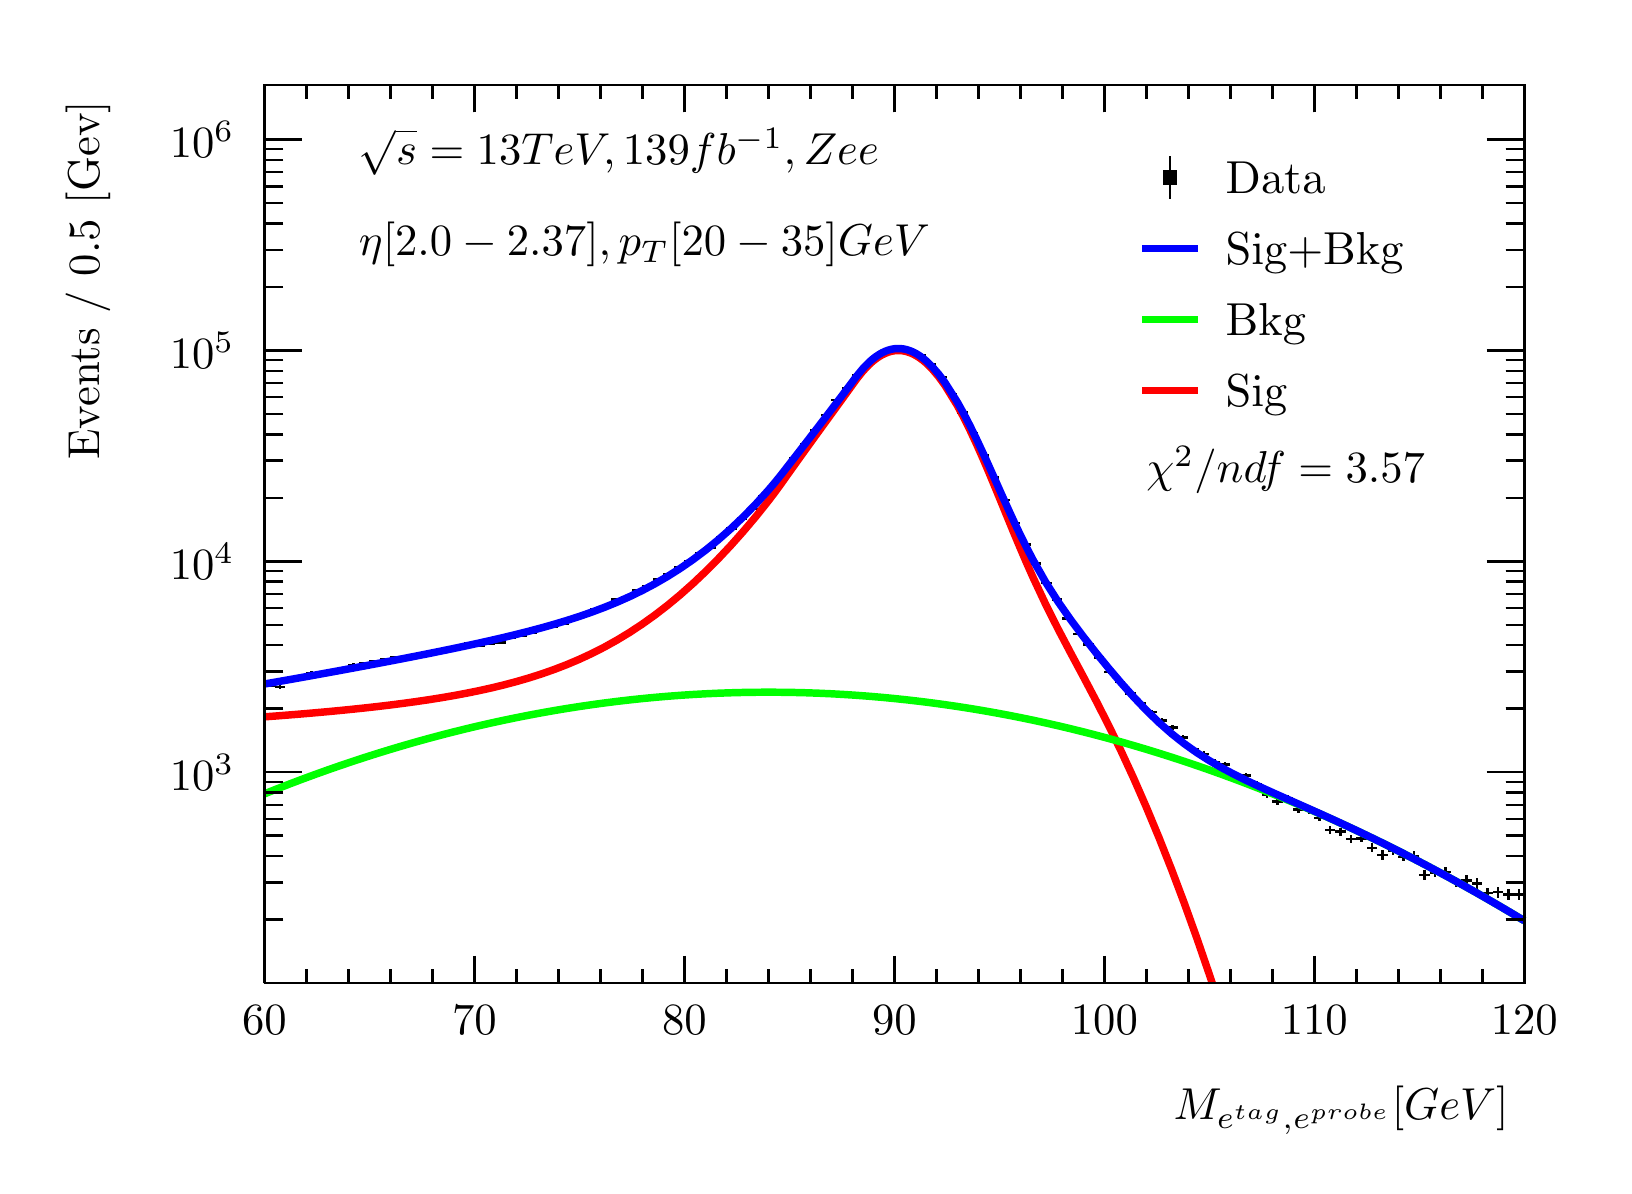
\begin{tikzpicture}
\pgfdeclareplotmark{cross} {
\pgfpathmoveto{\pgfpoint{-0.3\pgfplotmarksize}{\pgfplotmarksize}}
\pgfpathlineto{\pgfpoint{+0.3\pgfplotmarksize}{\pgfplotmarksize}}
\pgfpathlineto{\pgfpoint{+0.3\pgfplotmarksize}{0.3\pgfplotmarksize}}
\pgfpathlineto{\pgfpoint{+1\pgfplotmarksize}{0.3\pgfplotmarksize}}
\pgfpathlineto{\pgfpoint{+1\pgfplotmarksize}{-0.3\pgfplotmarksize}}
\pgfpathlineto{\pgfpoint{+0.3\pgfplotmarksize}{-0.3\pgfplotmarksize}}
\pgfpathlineto{\pgfpoint{+0.3\pgfplotmarksize}{-1.\pgfplotmarksize}}
\pgfpathlineto{\pgfpoint{-0.3\pgfplotmarksize}{-1.\pgfplotmarksize}}
\pgfpathlineto{\pgfpoint{-0.3\pgfplotmarksize}{-0.3\pgfplotmarksize}}
\pgfpathlineto{\pgfpoint{-1.\pgfplotmarksize}{-0.3\pgfplotmarksize}}
\pgfpathlineto{\pgfpoint{-1.\pgfplotmarksize}{0.3\pgfplotmarksize}}
\pgfpathlineto{\pgfpoint{-0.3\pgfplotmarksize}{0.3\pgfplotmarksize}}
\pgfpathclose
\pgfusepathqstroke
}
\pgfdeclareplotmark{cross*} {
\pgfpathmoveto{\pgfpoint{-0.3\pgfplotmarksize}{\pgfplotmarksize}}
\pgfpathlineto{\pgfpoint{+0.3\pgfplotmarksize}{\pgfplotmarksize}}
\pgfpathlineto{\pgfpoint{+0.3\pgfplotmarksize}{0.3\pgfplotmarksize}}
\pgfpathlineto{\pgfpoint{+1\pgfplotmarksize}{0.3\pgfplotmarksize}}
\pgfpathlineto{\pgfpoint{+1\pgfplotmarksize}{-0.3\pgfplotmarksize}}
\pgfpathlineto{\pgfpoint{+0.3\pgfplotmarksize}{-0.3\pgfplotmarksize}}
\pgfpathlineto{\pgfpoint{+0.3\pgfplotmarksize}{-1.\pgfplotmarksize}}
\pgfpathlineto{\pgfpoint{-0.3\pgfplotmarksize}{-1.\pgfplotmarksize}}
\pgfpathlineto{\pgfpoint{-0.3\pgfplotmarksize}{-0.3\pgfplotmarksize}}
\pgfpathlineto{\pgfpoint{-1.\pgfplotmarksize}{-0.3\pgfplotmarksize}}
\pgfpathlineto{\pgfpoint{-1.\pgfplotmarksize}{0.3\pgfplotmarksize}}
\pgfpathlineto{\pgfpoint{-0.3\pgfplotmarksize}{0.3\pgfplotmarksize}}
\pgfpathclose
\pgfusepathqfillstroke
}
\pgfdeclareplotmark{newstar} {
\pgfpathmoveto{\pgfqpoint{0pt}{\pgfplotmarksize}}
\pgfpathlineto{\pgfqpointpolar{44}{0.5\pgfplotmarksize}}
\pgfpathlineto{\pgfqpointpolar{18}{\pgfplotmarksize}}
\pgfpathlineto{\pgfqpointpolar{-20}{0.5\pgfplotmarksize}}
\pgfpathlineto{\pgfqpointpolar{-54}{\pgfplotmarksize}}
\pgfpathlineto{\pgfqpointpolar{-90}{0.5\pgfplotmarksize}}
\pgfpathlineto{\pgfqpointpolar{234}{\pgfplotmarksize}}
\pgfpathlineto{\pgfqpointpolar{198}{0.5\pgfplotmarksize}}
\pgfpathlineto{\pgfqpointpolar{162}{\pgfplotmarksize}}
\pgfpathlineto{\pgfqpointpolar{134}{0.5\pgfplotmarksize}}
\pgfpathclose
\pgfusepathqstroke
}
\pgfdeclareplotmark{newstar*} {
\pgfpathmoveto{\pgfqpoint{0pt}{\pgfplotmarksize}}
\pgfpathlineto{\pgfqpointpolar{44}{0.5\pgfplotmarksize}}
\pgfpathlineto{\pgfqpointpolar{18}{\pgfplotmarksize}}
\pgfpathlineto{\pgfqpointpolar{-20}{0.5\pgfplotmarksize}}
\pgfpathlineto{\pgfqpointpolar{-54}{\pgfplotmarksize}}
\pgfpathlineto{\pgfqpointpolar{-90}{0.5\pgfplotmarksize}}
\pgfpathlineto{\pgfqpointpolar{234}{\pgfplotmarksize}}
\pgfpathlineto{\pgfqpointpolar{198}{0.5\pgfplotmarksize}}
\pgfpathlineto{\pgfqpointpolar{162}{\pgfplotmarksize}}
\pgfpathlineto{\pgfqpointpolar{134}{0.5\pgfplotmarksize}}
\pgfpathclose
\pgfusepathqfillstroke
}
\definecolor{c}{rgb}{1,1,1};
\draw [color=c, fill=c] (0,0) rectangle (20,14.4361);
\draw [color=c, fill=c] (3,2.30977) rectangle (19,13.7143);
\definecolor{c}{rgb}{0,0,0};
\draw [c,line width=0.9] (3,2.30977) -- (3,13.7143) -- (19,13.7143) -- (19,2.30977) -- (3,2.30977);
\definecolor{c}{rgb}{1,1,1};
\draw [color=c, fill=c] (3,2.30977) rectangle (19,13.7143);
\definecolor{c}{rgb}{0,0,0};
\draw [c,line width=0.9] (3,2.30977) -- (3,13.7143) -- (19,13.7143) -- (19,2.30977) -- (3,2.30977);
\draw [c,line width=0.9] (3,2.30977) -- (19,2.30977);
\draw [c,line width=0.9] (3,2.65624) -- (3,2.30977);
\draw [c,line width=0.9] (3.53333,2.48301) -- (3.53333,2.30977);
\draw [c,line width=0.9] (4.06667,2.48301) -- (4.06667,2.30977);
\draw [c,line width=0.9] (4.6,2.48301) -- (4.6,2.30977);
\draw [c,line width=0.9] (5.13333,2.48301) -- (5.13333,2.30977);
\draw [c,line width=0.9] (5.66667,2.65624) -- (5.66667,2.30977);
\draw [c,line width=0.9] (6.2,2.48301) -- (6.2,2.30977);
\draw [c,line width=0.9] (6.73333,2.48301) -- (6.73333,2.30977);
\draw [c,line width=0.9] (7.26667,2.48301) -- (7.26667,2.30977);
\draw [c,line width=0.9] (7.8,2.48301) -- (7.8,2.30977);
\draw [c,line width=0.9] (8.33333,2.65624) -- (8.33333,2.30977);
\draw [c,line width=0.9] (8.86667,2.48301) -- (8.86667,2.30977);
\draw [c,line width=0.9] (9.4,2.48301) -- (9.4,2.30977);
\draw [c,line width=0.9] (9.93333,2.48301) -- (9.93333,2.30977);
\draw [c,line width=0.9] (10.4667,2.48301) -- (10.4667,2.30977);
\draw [c,line width=0.9] (11,2.65624) -- (11,2.30977);
\draw [c,line width=0.9] (11.5333,2.48301) -- (11.5333,2.30977);
\draw [c,line width=0.9] (12.0667,2.48301) -- (12.0667,2.30977);
\draw [c,line width=0.9] (12.6,2.48301) -- (12.6,2.30977);
\draw [c,line width=0.9] (13.1333,2.48301) -- (13.1333,2.30977);
\draw [c,line width=0.9] (13.6667,2.65624) -- (13.6667,2.30977);
\draw [c,line width=0.9] (14.2,2.48301) -- (14.2,2.30977);
\draw [c,line width=0.9] (14.7333,2.48301) -- (14.7333,2.30977);
\draw [c,line width=0.9] (15.2667,2.48301) -- (15.2667,2.30977);
\draw [c,line width=0.9] (15.8,2.48301) -- (15.8,2.30977);
\draw [c,line width=0.9] (16.3333,2.65624) -- (16.3333,2.30977);
\draw [c,line width=0.9] (16.8667,2.48301) -- (16.8667,2.30977);
\draw [c,line width=0.9] (17.4,2.48301) -- (17.4,2.30977);
\draw [c,line width=0.9] (17.9333,2.48301) -- (17.9333,2.30977);
\draw [c,line width=0.9] (18.4667,2.48301) -- (18.4667,2.30977);
\draw [c,line width=0.9] (19,2.65624) -- (19,2.30977);
\draw [anchor=base] (3,1.66015) node[scale=1.61424, color=c, rotate=0]{60};
\draw [anchor=base] (5.66667,1.66015) node[scale=1.61424, color=c, rotate=0]{70};
\draw [anchor=base] (8.33333,1.66015) node[scale=1.61424, color=c, rotate=0]{80};
\draw [anchor=base] (11,1.66015) node[scale=1.61424, color=c, rotate=0]{90};
\draw [anchor=base] (13.6667,1.66015) node[scale=1.61424, color=c, rotate=0]{100};
\draw [anchor=base] (16.3333,1.66015) node[scale=1.61424, color=c, rotate=0]{110};
\draw [anchor=base] (19,1.66015) node[scale=1.61424, color=c, rotate=0]{120};
\draw [anchor= east] (19,0.692932) node[scale=1.61424, color=c, rotate=0]{$M_{e^{tag}, e^{probe}}  [GeV]$};
\draw [c,line width=0.9] (3,13.7143) -- (19,13.7143);
\draw [c,line width=0.9] (3,13.3678) -- (3,13.7143);
\draw [c,line width=0.9] (3.53333,13.5411) -- (3.53333,13.7143);
\draw [c,line width=0.9] (4.06667,13.5411) -- (4.06667,13.7143);
\draw [c,line width=0.9] (4.6,13.5411) -- (4.6,13.7143);
\draw [c,line width=0.9] (5.13333,13.5411) -- (5.13333,13.7143);
\draw [c,line width=0.9] (5.66667,13.3678) -- (5.66667,13.7143);
\draw [c,line width=0.9] (6.2,13.5411) -- (6.2,13.7143);
\draw [c,line width=0.9] (6.73333,13.5411) -- (6.73333,13.7143);
\draw [c,line width=0.9] (7.26667,13.5411) -- (7.26667,13.7143);
\draw [c,line width=0.9] (7.8,13.5411) -- (7.8,13.7143);
\draw [c,line width=0.9] (8.33333,13.3678) -- (8.33333,13.7143);
\draw [c,line width=0.9] (8.86667,13.5411) -- (8.86667,13.7143);
\draw [c,line width=0.9] (9.4,13.5411) -- (9.4,13.7143);
\draw [c,line width=0.9] (9.93333,13.5411) -- (9.93333,13.7143);
\draw [c,line width=0.9] (10.4667,13.5411) -- (10.4667,13.7143);
\draw [c,line width=0.9] (11,13.3678) -- (11,13.7143);
\draw [c,line width=0.9] (11.5333,13.5411) -- (11.5333,13.7143);
\draw [c,line width=0.9] (12.0667,13.5411) -- (12.0667,13.7143);
\draw [c,line width=0.9] (12.6,13.5411) -- (12.6,13.7143);
\draw [c,line width=0.9] (13.1333,13.5411) -- (13.1333,13.7143);
\draw [c,line width=0.9] (13.6667,13.3678) -- (13.6667,13.7143);
\draw [c,line width=0.9] (14.2,13.5411) -- (14.2,13.7143);
\draw [c,line width=0.9] (14.7333,13.5411) -- (14.7333,13.7143);
\draw [c,line width=0.9] (15.2667,13.5411) -- (15.2667,13.7143);
\draw [c,line width=0.9] (15.8,13.5411) -- (15.8,13.7143);
\draw [c,line width=0.9] (16.3333,13.3678) -- (16.3333,13.7143);
\draw [c,line width=0.9] (16.8667,13.5411) -- (16.8667,13.7143);
\draw [c,line width=0.9] (17.4,13.5411) -- (17.4,13.7143);
\draw [c,line width=0.9] (17.9333,13.5411) -- (17.9333,13.7143);
\draw [c,line width=0.9] (18.4667,13.5411) -- (18.4667,13.7143);
\draw [c,line width=0.9] (19,13.3678) -- (19,13.7143);
\draw [c,line width=0.9] (3,2.30977) -- (3,13.7143);
\draw [c,line width=0.9] (3.237,3.11596) -- (3,3.11596);
\draw [c,line width=0.9] (3.237,3.58755) -- (3,3.58755);
\draw [c,line width=0.9] (3.237,3.92215) -- (3,3.92215);
\draw [c,line width=0.9] (3.237,4.18169) -- (3,4.18169);
\draw [c,line width=0.9] (3.237,4.39374) -- (3,4.39374);
\draw [c,line width=0.9] (3.237,4.57303) -- (3,4.57303);
\draw [c,line width=0.9] (3.237,4.72834) -- (3,4.72834);
\draw [c,line width=0.9] (3.237,4.86533) -- (3,4.86533);
\draw [c,line width=0.9] (3.474,4.98787) -- (3,4.98787);
\draw [anchor= east] (2.82,4.98787) node[scale=1.61424, color=c, rotate=0]{$10^{3}$};
\draw [c,line width=0.9] (3.237,5.79406) -- (3,5.79406);
\draw [c,line width=0.9] (3.237,6.26566) -- (3,6.26566);
\draw [c,line width=0.9] (3.237,6.60025) -- (3,6.60025);
\draw [c,line width=0.9] (3.237,6.85979) -- (3,6.85979);
\draw [c,line width=0.9] (3.237,7.07184) -- (3,7.07184);
\draw [c,line width=0.9] (3.237,7.25113) -- (3,7.25113);
\draw [c,line width=0.9] (3.237,7.40644) -- (3,7.40644);
\draw [c,line width=0.9] (3.237,7.54344) -- (3,7.54344);
\draw [c,line width=0.9] (3.474,7.66598) -- (3,7.66598);
\draw [anchor= east] (2.82,7.66598) node[scale=1.61424, color=c, rotate=0]{$10^{4}$};
\draw [c,line width=0.9] (3.237,8.47217) -- (3,8.47217);
\draw [c,line width=0.9] (3.237,8.94376) -- (3,8.94376);
\draw [c,line width=0.9] (3.237,9.27836) -- (3,9.27836);
\draw [c,line width=0.9] (3.237,9.53789) -- (3,9.53789);
\draw [c,line width=0.9] (3.237,9.74995) -- (3,9.74995);
\draw [c,line width=0.9] (3.237,9.92924) -- (3,9.92924);
\draw [c,line width=0.9] (3.237,10.0845) -- (3,10.0845);
\draw [c,line width=0.9] (3.237,10.2215) -- (3,10.2215);
\draw [c,line width=0.9] (3.474,10.3441) -- (3,10.3441);
\draw [anchor= east] (2.82,10.3441) node[scale=1.61424, color=c, rotate=0]{$10^{5}$};
\draw [c,line width=0.9] (3.237,11.1503) -- (3,11.1503);
\draw [c,line width=0.9] (3.237,11.6219) -- (3,11.6219);
\draw [c,line width=0.9] (3.237,11.9565) -- (3,11.9565);
\draw [c,line width=0.9] (3.237,12.216) -- (3,12.216);
\draw [c,line width=0.9] (3.237,12.4281) -- (3,12.4281);
\draw [c,line width=0.9] (3.237,12.6073) -- (3,12.6073);
\draw [c,line width=0.9] (3.237,12.7627) -- (3,12.7627);
\draw [c,line width=0.9] (3.237,12.8996) -- (3,12.8996);
\draw [c,line width=0.9] (3.474,13.0222) -- (3,13.0222);
\draw [anchor= east] (2.82,13.0222) node[scale=1.61424, color=c, rotate=0]{$10^{6}$};
\draw [anchor= east] (0.76,13.7143) node[scale=1.61424, color=c, rotate=90]{Events / 0.5 [Gev]};
\draw [c,line width=0.9] (19,2.30977) -- (19,13.7143);
\draw [c,line width=0.9] (18.763,3.11596) -- (19,3.11596);
\draw [c,line width=0.9] (18.763,3.58755) -- (19,3.58755);
\draw [c,line width=0.9] (18.763,3.92215) -- (19,3.92215);
\draw [c,line width=0.9] (18.763,4.18169) -- (19,4.18169);
\draw [c,line width=0.9] (18.763,4.39374) -- (19,4.39374);
\draw [c,line width=0.9] (18.763,4.57303) -- (19,4.57303);
\draw [c,line width=0.9] (18.763,4.72834) -- (19,4.72834);
\draw [c,line width=0.9] (18.763,4.86533) -- (19,4.86533);
\draw [c,line width=0.9] (18.526,4.98787) -- (19,4.98787);
\draw [c,line width=0.9] (18.763,5.79406) -- (19,5.79406);
\draw [c,line width=0.9] (18.763,6.26566) -- (19,6.26566);
\draw [c,line width=0.9] (18.763,6.60025) -- (19,6.60025);
\draw [c,line width=0.9] (18.763,6.85979) -- (19,6.85979);
\draw [c,line width=0.9] (18.763,7.07184) -- (19,7.07184);
\draw [c,line width=0.9] (18.763,7.25113) -- (19,7.25113);
\draw [c,line width=0.9] (18.763,7.40644) -- (19,7.40644);
\draw [c,line width=0.9] (18.763,7.54344) -- (19,7.54344);
\draw [c,line width=0.9] (18.526,7.66598) -- (19,7.66598);
\draw [c,line width=0.9] (18.763,8.47217) -- (19,8.47217);
\draw [c,line width=0.9] (18.763,8.94376) -- (19,8.94376);
\draw [c,line width=0.9] (18.763,9.27836) -- (19,9.27836);
\draw [c,line width=0.9] (18.763,9.53789) -- (19,9.53789);
\draw [c,line width=0.9] (18.763,9.74995) -- (19,9.74995);
\draw [c,line width=0.9] (18.763,9.92924) -- (19,9.92924);
\draw [c,line width=0.9] (18.763,10.0845) -- (19,10.0845);
\draw [c,line width=0.9] (18.763,10.2215) -- (19,10.2215);
\draw [c,line width=0.9] (18.526,10.3441) -- (19,10.3441);
\draw [c,line width=0.9] (18.763,11.1503) -- (19,11.1503);
\draw [c,line width=0.9] (18.763,11.6219) -- (19,11.6219);
\draw [c,line width=0.9] (18.763,11.9565) -- (19,11.9565);
\draw [c,line width=0.9] (18.763,12.216) -- (19,12.216);
\draw [c,line width=0.9] (18.763,12.4281) -- (19,12.4281);
\draw [c,line width=0.9] (18.763,12.6073) -- (19,12.6073);
\draw [c,line width=0.9] (18.763,12.7627) -- (19,12.7627);
\draw [c,line width=0.9] (18.763,12.8996) -- (19,12.8996);
\draw [c,line width=0.9] (18.526,13.0222) -- (19,13.0222);
\draw [c,line width=0.9] (3.06667,6.08753) -- (3,6.08753);
\draw [c,line width=0.9] (3,6.08753) -- (3,6.08753);
\draw [c,line width=0.9] (3.06667,6.08753) -- (3.13333,6.08753);
\draw [c,line width=0.9] (3.13333,6.08753) -- (3.13333,6.08753);
\draw [c,line width=0.9] (3.06667,6.08753) -- (3.06667,6.11045);
\draw [c,line width=0.9] (3.06667,6.11045) -- (3.06667,6.11045);
\draw [c,line width=0.9] (3.06667,6.08753) -- (3.06667,6.0646);
\draw [c,line width=0.9] (3.06667,6.0646) -- (3.06667,6.0646);
\draw [c,line width=0.9] (3.2,6.06702) -- (3.13333,6.06702);
\draw [c,line width=0.9] (3.13333,6.06702) -- (3.13333,6.06702);
\draw [c,line width=0.9] (3.2,6.06702) -- (3.26667,6.06702);
\draw [c,line width=0.9] (3.26667,6.06702) -- (3.26667,6.06702);
\draw [c,line width=0.9] (3.2,6.06702) -- (3.2,6.09014);
\draw [c,line width=0.9] (3.2,6.09014) -- (3.2,6.09014);
\draw [c,line width=0.9] (3.2,6.06702) -- (3.2,6.04389);
\draw [c,line width=0.9] (3.2,6.04389) -- (3.2,6.04389);
\draw [c,line width=0.9] (3.33333,6.15469) -- (3.26667,6.15469);
\draw [c,line width=0.9] (3.26667,6.15469) -- (3.26667,6.15469);
\draw [c,line width=0.9] (3.33333,6.15469) -- (3.4,6.15469);
\draw [c,line width=0.9] (3.4,6.15469) -- (3.4,6.15469);
\draw [c,line width=0.9] (3.33333,6.15469) -- (3.33333,6.17696);
\draw [c,line width=0.9] (3.33333,6.17696) -- (3.33333,6.17696);
\draw [c,line width=0.9] (3.33333,6.15469) -- (3.33333,6.13241);
\draw [c,line width=0.9] (3.33333,6.13241) -- (3.33333,6.13241);
\draw [c,line width=0.9] (3.46667,6.1941) -- (3.4,6.1941);
\draw [c,line width=0.9] (3.4,6.1941) -- (3.4,6.1941);
\draw [c,line width=0.9] (3.46667,6.1941) -- (3.53333,6.1941);
\draw [c,line width=0.9] (3.53333,6.1941) -- (3.53333,6.1941);
\draw [c,line width=0.9] (3.46667,6.1941) -- (3.46667,6.216);
\draw [c,line width=0.9] (3.46667,6.216) -- (3.46667,6.216);
\draw [c,line width=0.9] (3.46667,6.1941) -- (3.46667,6.1722);
\draw [c,line width=0.9] (3.46667,6.1722) -- (3.46667,6.1722);
\draw [c,line width=0.9] (3.6,6.24611) -- (3.53333,6.24611);
\draw [c,line width=0.9] (3.53333,6.24611) -- (3.53333,6.24611);
\draw [c,line width=0.9] (3.6,6.24611) -- (3.66667,6.24611);
\draw [c,line width=0.9] (3.66667,6.24611) -- (3.66667,6.24611);
\draw [c,line width=0.9] (3.6,6.24611) -- (3.6,6.26752);
\draw [c,line width=0.9] (3.6,6.26752) -- (3.6,6.26752);
\draw [c,line width=0.9] (3.6,6.24611) -- (3.6,6.22469);
\draw [c,line width=0.9] (3.6,6.22469) -- (3.6,6.22469);
\draw [c,line width=0.9] (3.73333,6.23541) -- (3.66667,6.23541);
\draw [c,line width=0.9] (3.66667,6.23541) -- (3.66667,6.23541);
\draw [c,line width=0.9] (3.73333,6.23541) -- (3.8,6.23541);
\draw [c,line width=0.9] (3.8,6.23541) -- (3.8,6.23541);
\draw [c,line width=0.9] (3.73333,6.23541) -- (3.73333,6.25693);
\draw [c,line width=0.9] (3.73333,6.25693) -- (3.73333,6.25693);
\draw [c,line width=0.9] (3.73333,6.23541) -- (3.73333,6.2139);
\draw [c,line width=0.9] (3.73333,6.2139) -- (3.73333,6.2139);
\draw [c,line width=0.9] (3.86667,6.26255) -- (3.8,6.26255);
\draw [c,line width=0.9] (3.8,6.26255) -- (3.8,6.26255);
\draw [c,line width=0.9] (3.86667,6.26255) -- (3.93333,6.26255);
\draw [c,line width=0.9] (3.93333,6.26255) -- (3.93333,6.26255);
\draw [c,line width=0.9] (3.86667,6.26255) -- (3.86667,6.28381);
\draw [c,line width=0.9] (3.86667,6.28381) -- (3.86667,6.28381);
\draw [c,line width=0.9] (3.86667,6.26255) -- (3.86667,6.24129);
\draw [c,line width=0.9] (3.86667,6.24129) -- (3.86667,6.24129);
\draw [c,line width=0.9] (4,6.27608) -- (3.93333,6.27608);
\draw [c,line width=0.9] (3.93333,6.27608) -- (3.93333,6.27608);
\draw [c,line width=0.9] (4,6.27608) -- (4.06667,6.27608);
\draw [c,line width=0.9] (4.06667,6.27608) -- (4.06667,6.27608);
\draw [c,line width=0.9] (4,6.27608) -- (4,6.29722);
\draw [c,line width=0.9] (4,6.29722) -- (4,6.29722);
\draw [c,line width=0.9] (4,6.27608) -- (4,6.25494);
\draw [c,line width=0.9] (4,6.25494) -- (4,6.25494);
\draw [c,line width=0.9] (4.13333,6.35193) -- (4.06667,6.35193);
\draw [c,line width=0.9] (4.06667,6.35193) -- (4.06667,6.35193);
\draw [c,line width=0.9] (4.13333,6.35193) -- (4.2,6.35193);
\draw [c,line width=0.9] (4.2,6.35193) -- (4.2,6.35193);
\draw [c,line width=0.9] (4.13333,6.35193) -- (4.13333,6.3724);
\draw [c,line width=0.9] (4.13333,6.3724) -- (4.13333,6.3724);
\draw [c,line width=0.9] (4.13333,6.35193) -- (4.13333,6.33147);
\draw [c,line width=0.9] (4.13333,6.33147) -- (4.13333,6.33147);
\draw [c,line width=0.9] (4.26667,6.37298) -- (4.2,6.37298);
\draw [c,line width=0.9] (4.2,6.37298) -- (4.2,6.37298);
\draw [c,line width=0.9] (4.26667,6.37298) -- (4.33333,6.37298);
\draw [c,line width=0.9] (4.33333,6.37298) -- (4.33333,6.37298);
\draw [c,line width=0.9] (4.26667,6.37298) -- (4.26667,6.39326);
\draw [c,line width=0.9] (4.26667,6.39326) -- (4.26667,6.39326);
\draw [c,line width=0.9] (4.26667,6.37298) -- (4.26667,6.3527);
\draw [c,line width=0.9] (4.26667,6.3527) -- (4.26667,6.3527);
\draw [c,line width=0.9] (4.4,6.39504) -- (4.33333,6.39504);
\draw [c,line width=0.9] (4.33333,6.39504) -- (4.33333,6.39504);
\draw [c,line width=0.9] (4.4,6.39504) -- (4.46667,6.39504);
\draw [c,line width=0.9] (4.46667,6.39504) -- (4.46667,6.39504);
\draw [c,line width=0.9] (4.4,6.39504) -- (4.4,6.41513);
\draw [c,line width=0.9] (4.4,6.41513) -- (4.4,6.41513);
\draw [c,line width=0.9] (4.4,6.39504) -- (4.4,6.37496);
\draw [c,line width=0.9] (4.4,6.37496) -- (4.4,6.37496);
\draw [c,line width=0.9] (4.53333,6.42247) -- (4.46667,6.42247);
\draw [c,line width=0.9] (4.46667,6.42247) -- (4.46667,6.42247);
\draw [c,line width=0.9] (4.53333,6.42247) -- (4.6,6.42247);
\draw [c,line width=0.9] (4.6,6.42247) -- (4.6,6.42247);
\draw [c,line width=0.9] (4.53333,6.42247) -- (4.53333,6.44232);
\draw [c,line width=0.9] (4.53333,6.44232) -- (4.53333,6.44232);
\draw [c,line width=0.9] (4.53333,6.42247) -- (4.53333,6.40262);
\draw [c,line width=0.9] (4.53333,6.40262) -- (4.53333,6.40262);
\draw [c,line width=0.9] (4.66667,6.44195) -- (4.6,6.44195);
\draw [c,line width=0.9] (4.6,6.44195) -- (4.6,6.44195);
\draw [c,line width=0.9] (4.66667,6.44195) -- (4.73333,6.44195);
\draw [c,line width=0.9] (4.73333,6.44195) -- (4.73333,6.44195);
\draw [c,line width=0.9] (4.66667,6.44195) -- (4.66667,6.46164);
\draw [c,line width=0.9] (4.66667,6.46164) -- (4.66667,6.46164);
\draw [c,line width=0.9] (4.66667,6.44195) -- (4.66667,6.42227);
\draw [c,line width=0.9] (4.66667,6.42227) -- (4.66667,6.42227);
\draw [c,line width=0.9] (4.8,6.44461) -- (4.73333,6.44461);
\draw [c,line width=0.9] (4.73333,6.44461) -- (4.73333,6.44461);
\draw [c,line width=0.9] (4.8,6.44461) -- (4.86667,6.44461);
\draw [c,line width=0.9] (4.86667,6.44461) -- (4.86667,6.44461);
\draw [c,line width=0.9] (4.8,6.44461) -- (4.8,6.46428);
\draw [c,line width=0.9] (4.8,6.46428) -- (4.8,6.46428);
\draw [c,line width=0.9] (4.8,6.44461) -- (4.8,6.42495);
\draw [c,line width=0.9] (4.8,6.42495) -- (4.8,6.42495);
\draw [c,line width=0.9] (4.93333,6.48223) -- (4.86667,6.48223);
\draw [c,line width=0.9] (4.86667,6.48223) -- (4.86667,6.48223);
\draw [c,line width=0.9] (4.93333,6.48223) -- (5,6.48223);
\draw [c,line width=0.9] (5,6.48223) -- (5,6.48223);
\draw [c,line width=0.9] (4.93333,6.48223) -- (4.93333,6.50157);
\draw [c,line width=0.9] (4.93333,6.50157) -- (4.93333,6.50157);
\draw [c,line width=0.9] (4.93333,6.48223) -- (4.93333,6.46288);
\draw [c,line width=0.9] (4.93333,6.46288) -- (4.93333,6.46288);
\draw [c,line width=0.9] (5.06667,6.48029) -- (5,6.48029);
\draw [c,line width=0.9] (5,6.48029) -- (5,6.48029);
\draw [c,line width=0.9] (5.06667,6.48029) -- (5.13333,6.48029);
\draw [c,line width=0.9] (5.13333,6.48029) -- (5.13333,6.48029);
\draw [c,line width=0.9] (5.06667,6.48029) -- (5.06667,6.49966);
\draw [c,line width=0.9] (5.06667,6.49966) -- (5.06667,6.49966);
\draw [c,line width=0.9] (5.06667,6.48029) -- (5.06667,6.46093);
\draw [c,line width=0.9] (5.06667,6.46093) -- (5.06667,6.46093);
\draw [c,line width=0.9] (5.2,6.51554) -- (5.13333,6.51554);
\draw [c,line width=0.9] (5.13333,6.51554) -- (5.13333,6.51554);
\draw [c,line width=0.9] (5.2,6.51554) -- (5.26667,6.51554);
\draw [c,line width=0.9] (5.26667,6.51554) -- (5.26667,6.51554);
\draw [c,line width=0.9] (5.2,6.51554) -- (5.2,6.53461);
\draw [c,line width=0.9] (5.2,6.53461) -- (5.2,6.53461);
\draw [c,line width=0.9] (5.2,6.51554) -- (5.2,6.49647);
\draw [c,line width=0.9] (5.2,6.49647) -- (5.2,6.49647);
\draw [c,line width=0.9] (5.33333,6.54883) -- (5.26667,6.54883);
\draw [c,line width=0.9] (5.26667,6.54883) -- (5.26667,6.54883);
\draw [c,line width=0.9] (5.33333,6.54883) -- (5.4,6.54883);
\draw [c,line width=0.9] (5.4,6.54883) -- (5.4,6.54883);
\draw [c,line width=0.9] (5.33333,6.54883) -- (5.33333,6.56763);
\draw [c,line width=0.9] (5.33333,6.56763) -- (5.33333,6.56763);
\draw [c,line width=0.9] (5.33333,6.54883) -- (5.33333,6.53003);
\draw [c,line width=0.9] (5.33333,6.53003) -- (5.33333,6.53003);
\draw [c,line width=0.9] (5.46667,6.56243) -- (5.4,6.56243);
\draw [c,line width=0.9] (5.4,6.56243) -- (5.4,6.56243);
\draw [c,line width=0.9] (5.46667,6.56243) -- (5.53333,6.56243);
\draw [c,line width=0.9] (5.53333,6.56243) -- (5.53333,6.56243);
\draw [c,line width=0.9] (5.46667,6.56243) -- (5.46667,6.58112);
\draw [c,line width=0.9] (5.46667,6.58112) -- (5.46667,6.58112);
\draw [c,line width=0.9] (5.46667,6.56243) -- (5.46667,6.54374);
\draw [c,line width=0.9] (5.46667,6.54374) -- (5.46667,6.54374);
\draw [c,line width=0.9] (5.6,6.62898) -- (5.53333,6.62898);
\draw [c,line width=0.9] (5.53333,6.62898) -- (5.53333,6.62898);
\draw [c,line width=0.9] (5.6,6.62898) -- (5.66667,6.62898);
\draw [c,line width=0.9] (5.66667,6.62898) -- (5.66667,6.62898);
\draw [c,line width=0.9] (5.6,6.62898) -- (5.6,6.64714);
\draw [c,line width=0.9] (5.6,6.64714) -- (5.6,6.64714);
\draw [c,line width=0.9] (5.6,6.62898) -- (5.6,6.61081);
\draw [c,line width=0.9] (5.6,6.61081) -- (5.6,6.61081);
\draw [c,line width=0.9] (5.73333,6.59062) -- (5.66667,6.59062);
\draw [c,line width=0.9] (5.66667,6.59062) -- (5.66667,6.59062);
\draw [c,line width=0.9] (5.73333,6.59062) -- (5.8,6.59062);
\draw [c,line width=0.9] (5.8,6.59062) -- (5.8,6.59062);
\draw [c,line width=0.9] (5.73333,6.59062) -- (5.73333,6.60909);
\draw [c,line width=0.9] (5.73333,6.60909) -- (5.73333,6.60909);
\draw [c,line width=0.9] (5.73333,6.59062) -- (5.73333,6.57215);
\draw [c,line width=0.9] (5.73333,6.57215) -- (5.73333,6.57215);
\draw [c,line width=0.9] (5.86667,6.62158) -- (5.8,6.62158);
\draw [c,line width=0.9] (5.8,6.62158) -- (5.8,6.62158);
\draw [c,line width=0.9] (5.86667,6.62158) -- (5.93333,6.62158);
\draw [c,line width=0.9] (5.93333,6.62158) -- (5.93333,6.62158);
\draw [c,line width=0.9] (5.86667,6.62158) -- (5.86667,6.6398);
\draw [c,line width=0.9] (5.86667,6.6398) -- (5.86667,6.6398);
\draw [c,line width=0.9] (5.86667,6.62158) -- (5.86667,6.60335);
\draw [c,line width=0.9] (5.86667,6.60335) -- (5.86667,6.60335);
\draw [c,line width=0.9] (6,6.63407) -- (5.93333,6.63407);
\draw [c,line width=0.9] (5.93333,6.63407) -- (5.93333,6.63407);
\draw [c,line width=0.9] (6,6.63407) -- (6.06667,6.63407);
\draw [c,line width=0.9] (6.06667,6.63407) -- (6.06667,6.63407);
\draw [c,line width=0.9] (6,6.63407) -- (6,6.65219);
\draw [c,line width=0.9] (6,6.65219) -- (6,6.65219);
\draw [c,line width=0.9] (6,6.63407) -- (6,6.61595);
\draw [c,line width=0.9] (6,6.61595) -- (6,6.61595);
\draw [c,line width=0.9] (6.13333,6.69915) -- (6.06667,6.69915);
\draw [c,line width=0.9] (6.06667,6.69915) -- (6.06667,6.69915);
\draw [c,line width=0.9] (6.13333,6.69915) -- (6.2,6.69915);
\draw [c,line width=0.9] (6.2,6.69915) -- (6.2,6.69915);
\draw [c,line width=0.9] (6.13333,6.69915) -- (6.13333,6.71678);
\draw [c,line width=0.9] (6.13333,6.71678) -- (6.13333,6.71678);
\draw [c,line width=0.9] (6.13333,6.69915) -- (6.13333,6.68153);
\draw [c,line width=0.9] (6.13333,6.68153) -- (6.13333,6.68153);
\draw [c,line width=0.9] (6.26667,6.72321) -- (6.2,6.72321);
\draw [c,line width=0.9] (6.2,6.72321) -- (6.2,6.72321);
\draw [c,line width=0.9] (6.26667,6.72321) -- (6.33333,6.72321);
\draw [c,line width=0.9] (6.33333,6.72321) -- (6.33333,6.72321);
\draw [c,line width=0.9] (6.26667,6.72321) -- (6.26667,6.74065);
\draw [c,line width=0.9] (6.26667,6.74065) -- (6.26667,6.74065);
\draw [c,line width=0.9] (6.26667,6.72321) -- (6.26667,6.70576);
\draw [c,line width=0.9] (6.26667,6.70576) -- (6.26667,6.70576);
\draw [c,line width=0.9] (6.4,6.7585) -- (6.33333,6.7585);
\draw [c,line width=0.9] (6.33333,6.7585) -- (6.33333,6.7585);
\draw [c,line width=0.9] (6.4,6.7585) -- (6.46667,6.7585);
\draw [c,line width=0.9] (6.46667,6.7585) -- (6.46667,6.7585);
\draw [c,line width=0.9] (6.4,6.7585) -- (6.4,6.77568);
\draw [c,line width=0.9] (6.4,6.77568) -- (6.4,6.77568);
\draw [c,line width=0.9] (6.4,6.7585) -- (6.4,6.74132);
\draw [c,line width=0.9] (6.4,6.74132) -- (6.4,6.74132);
\draw [c,line width=0.9] (6.53333,6.81061) -- (6.46667,6.81061);
\draw [c,line width=0.9] (6.46667,6.81061) -- (6.46667,6.81061);
\draw [c,line width=0.9] (6.53333,6.81061) -- (6.6,6.81061);
\draw [c,line width=0.9] (6.6,6.81061) -- (6.6,6.81061);
\draw [c,line width=0.9] (6.53333,6.81061) -- (6.53333,6.82741);
\draw [c,line width=0.9] (6.53333,6.82741) -- (6.53333,6.82741);
\draw [c,line width=0.9] (6.53333,6.81061) -- (6.53333,6.79381);
\draw [c,line width=0.9] (6.53333,6.79381) -- (6.53333,6.79381);
\draw [c,line width=0.9] (6.66667,6.83819) -- (6.6,6.83819);
\draw [c,line width=0.9] (6.6,6.83819) -- (6.6,6.83819);
\draw [c,line width=0.9] (6.66667,6.83819) -- (6.73333,6.83819);
\draw [c,line width=0.9] (6.73333,6.83819) -- (6.73333,6.83819);
\draw [c,line width=0.9] (6.66667,6.83819) -- (6.66667,6.85479);
\draw [c,line width=0.9] (6.66667,6.85479) -- (6.66667,6.85479);
\draw [c,line width=0.9] (6.66667,6.83819) -- (6.66667,6.82159);
\draw [c,line width=0.9] (6.66667,6.82159) -- (6.66667,6.82159);
\draw [c,line width=0.9] (6.8,6.87228) -- (6.73333,6.87228);
\draw [c,line width=0.9] (6.73333,6.87228) -- (6.73333,6.87228);
\draw [c,line width=0.9] (6.8,6.87228) -- (6.86667,6.87228);
\draw [c,line width=0.9] (6.86667,6.87228) -- (6.86667,6.87228);
\draw [c,line width=0.9] (6.8,6.87228) -- (6.8,6.88864);
\draw [c,line width=0.9] (6.8,6.88864) -- (6.8,6.88864);
\draw [c,line width=0.9] (6.8,6.87228) -- (6.8,6.85592);
\draw [c,line width=0.9] (6.8,6.85592) -- (6.8,6.85592);
\draw [c,line width=0.9] (6.93333,6.94022) -- (6.86667,6.94022);
\draw [c,line width=0.9] (6.86667,6.94022) -- (6.86667,6.94022);
\draw [c,line width=0.9] (6.93333,6.94022) -- (7,6.94022);
\draw [c,line width=0.9] (7,6.94022) -- (7,6.94022);
\draw [c,line width=0.9] (6.93333,6.94022) -- (6.93333,6.95611);
\draw [c,line width=0.9] (6.93333,6.95611) -- (6.93333,6.95611);
\draw [c,line width=0.9] (6.93333,6.94022) -- (6.93333,6.92433);
\draw [c,line width=0.9] (6.93333,6.92433) -- (6.93333,6.92433);
\draw [c,line width=0.9] (7.06667,6.9797) -- (7,6.9797);
\draw [c,line width=0.9] (7,6.9797) -- (7,6.9797);
\draw [c,line width=0.9] (7.06667,6.9797) -- (7.13333,6.9797);
\draw [c,line width=0.9] (7.13333,6.9797) -- (7.13333,6.9797);
\draw [c,line width=0.9] (7.06667,6.9797) -- (7.06667,6.99532);
\draw [c,line width=0.9] (7.06667,6.99532) -- (7.06667,6.99532);
\draw [c,line width=0.9] (7.06667,6.9797) -- (7.06667,6.96408);
\draw [c,line width=0.9] (7.06667,6.96408) -- (7.06667,6.96408);
\draw [c,line width=0.9] (7.2,7.05466) -- (7.13333,7.05466);
\draw [c,line width=0.9] (7.13333,7.05466) -- (7.13333,7.05466);
\draw [c,line width=0.9] (7.2,7.05466) -- (7.26667,7.05466);
\draw [c,line width=0.9] (7.26667,7.05466) -- (7.26667,7.05466);
\draw [c,line width=0.9] (7.2,7.05466) -- (7.2,7.06979);
\draw [c,line width=0.9] (7.2,7.06979) -- (7.2,7.06979);
\draw [c,line width=0.9] (7.2,7.05466) -- (7.2,7.03953);
\draw [c,line width=0.9] (7.2,7.03953) -- (7.2,7.03953);
\draw [c,line width=0.9] (7.33333,7.07707) -- (7.26667,7.07707);
\draw [c,line width=0.9] (7.26667,7.07707) -- (7.26667,7.07707);
\draw [c,line width=0.9] (7.33333,7.07707) -- (7.4,7.07707);
\draw [c,line width=0.9] (7.4,7.07707) -- (7.4,7.07707);
\draw [c,line width=0.9] (7.33333,7.07707) -- (7.33333,7.09205);
\draw [c,line width=0.9] (7.33333,7.09205) -- (7.33333,7.09205);
\draw [c,line width=0.9] (7.33333,7.07707) -- (7.33333,7.06209);
\draw [c,line width=0.9] (7.33333,7.06209) -- (7.33333,7.06209);
\draw [c,line width=0.9] (7.46667,7.18023) -- (7.4,7.18023);
\draw [c,line width=0.9] (7.4,7.18023) -- (7.4,7.18023);
\draw [c,line width=0.9] (7.46667,7.18023) -- (7.53333,7.18023);
\draw [c,line width=0.9] (7.53333,7.18023) -- (7.53333,7.18023);
\draw [c,line width=0.9] (7.46667,7.18023) -- (7.46667,7.19456);
\draw [c,line width=0.9] (7.46667,7.19456) -- (7.46667,7.19456);
\draw [c,line width=0.9] (7.46667,7.18023) -- (7.46667,7.1659);
\draw [c,line width=0.9] (7.46667,7.1659) -- (7.46667,7.1659);
\draw [c,line width=0.9] (7.6,7.20849) -- (7.53333,7.20849);
\draw [c,line width=0.9] (7.53333,7.20849) -- (7.53333,7.20849);
\draw [c,line width=0.9] (7.6,7.20849) -- (7.66667,7.20849);
\draw [c,line width=0.9] (7.66667,7.20849) -- (7.66667,7.20849);
\draw [c,line width=0.9] (7.6,7.20849) -- (7.6,7.22265);
\draw [c,line width=0.9] (7.6,7.22265) -- (7.6,7.22265);
\draw [c,line width=0.9] (7.6,7.20849) -- (7.6,7.19433);
\draw [c,line width=0.9] (7.6,7.19433) -- (7.6,7.19433);
\draw [c,line width=0.9] (7.73333,7.30249) -- (7.66667,7.30249);
\draw [c,line width=0.9] (7.66667,7.30249) -- (7.66667,7.30249);
\draw [c,line width=0.9] (7.73333,7.30249) -- (7.8,7.30249);
\draw [c,line width=0.9] (7.8,7.30249) -- (7.8,7.30249);
\draw [c,line width=0.9] (7.73333,7.30249) -- (7.73333,7.31609);
\draw [c,line width=0.9] (7.73333,7.31609) -- (7.73333,7.31609);
\draw [c,line width=0.9] (7.73333,7.30249) -- (7.73333,7.28889);
\draw [c,line width=0.9] (7.73333,7.28889) -- (7.73333,7.28889);
\draw [c,line width=0.9] (7.86667,7.34587) -- (7.8,7.34587);
\draw [c,line width=0.9] (7.8,7.34587) -- (7.8,7.34587);
\draw [c,line width=0.9] (7.86667,7.34587) -- (7.93333,7.34587);
\draw [c,line width=0.9] (7.93333,7.34587) -- (7.93333,7.34587);
\draw [c,line width=0.9] (7.86667,7.34587) -- (7.86667,7.35921);
\draw [c,line width=0.9] (7.86667,7.35921) -- (7.86667,7.35921);
\draw [c,line width=0.9] (7.86667,7.34587) -- (7.86667,7.33252);
\draw [c,line width=0.9] (7.86667,7.33252) -- (7.86667,7.33252);
\draw [c,line width=0.9] (8,7.43275) -- (7.93333,7.43275);
\draw [c,line width=0.9] (7.93333,7.43275) -- (7.93333,7.43275);
\draw [c,line width=0.9] (8,7.43275) -- (8.06667,7.43275);
\draw [c,line width=0.9] (8.06667,7.43275) -- (8.06667,7.43275);
\draw [c,line width=0.9] (8,7.43275) -- (8,7.44561);
\draw [c,line width=0.9] (8,7.44561) -- (8,7.44561);
\draw [c,line width=0.9] (8,7.43275) -- (8,7.41989);
\draw [c,line width=0.9] (8,7.41989) -- (8,7.41989);
\draw [c,line width=0.9] (8.13333,7.49932) -- (8.06667,7.49932);
\draw [c,line width=0.9] (8.06667,7.49932) -- (8.06667,7.49932);
\draw [c,line width=0.9] (8.13333,7.49932) -- (8.2,7.49932);
\draw [c,line width=0.9] (8.2,7.49932) -- (8.2,7.49932);
\draw [c,line width=0.9] (8.13333,7.49932) -- (8.13333,7.51181);
\draw [c,line width=0.9] (8.13333,7.51181) -- (8.13333,7.51181);
\draw [c,line width=0.9] (8.13333,7.49932) -- (8.13333,7.48682);
\draw [c,line width=0.9] (8.13333,7.48682) -- (8.13333,7.48682);
\draw [c,line width=0.9] (8.26667,7.58955) -- (8.2,7.58955);
\draw [c,line width=0.9] (8.2,7.58955) -- (8.2,7.58955);
\draw [c,line width=0.9] (8.26667,7.58955) -- (8.33333,7.58955);
\draw [c,line width=0.9] (8.33333,7.58955) -- (8.33333,7.58955);
\draw [c,line width=0.9] (8.26667,7.58955) -- (8.26667,7.60157);
\draw [c,line width=0.9] (8.26667,7.60157) -- (8.26667,7.60157);
\draw [c,line width=0.9] (8.26667,7.58955) -- (8.26667,7.57753);
\draw [c,line width=0.9] (8.26667,7.57753) -- (8.26667,7.57753);
\draw [c,line width=0.9] (8.4,7.66108) -- (8.33333,7.66108);
\draw [c,line width=0.9] (8.33333,7.66108) -- (8.33333,7.66108);
\draw [c,line width=0.9] (8.4,7.66108) -- (8.46667,7.66108);
\draw [c,line width=0.9] (8.46667,7.66108) -- (8.46667,7.66108);
\draw [c,line width=0.9] (8.4,7.66108) -- (8.4,7.67274);
\draw [c,line width=0.9] (8.4,7.67274) -- (8.4,7.67274);
\draw [c,line width=0.9] (8.4,7.66108) -- (8.4,7.64943);
\draw [c,line width=0.9] (8.4,7.64943) -- (8.4,7.64943);
\draw [c,line width=0.9] (8.53333,7.7676) -- (8.46667,7.7676);
\draw [c,line width=0.9] (8.46667,7.7676) -- (8.46667,7.7676);
\draw [c,line width=0.9] (8.53333,7.7676) -- (8.6,7.7676);
\draw [c,line width=0.9] (8.6,7.7676) -- (8.6,7.7676);
\draw [c,line width=0.9] (8.53333,7.7676) -- (8.53333,7.77873);
\draw [c,line width=0.9] (8.53333,7.77873) -- (8.53333,7.77873);
\draw [c,line width=0.9] (8.53333,7.7676) -- (8.53333,7.75646);
\draw [c,line width=0.9] (8.53333,7.75646) -- (8.53333,7.75646);
\draw [c,line width=0.9] (8.66667,7.84251) -- (8.6,7.84251);
\draw [c,line width=0.9] (8.6,7.84251) -- (8.6,7.84251);
\draw [c,line width=0.9] (8.66667,7.84251) -- (8.73333,7.84251);
\draw [c,line width=0.9] (8.73333,7.84251) -- (8.73333,7.84251);
\draw [c,line width=0.9] (8.66667,7.84251) -- (8.66667,7.85329);
\draw [c,line width=0.9] (8.66667,7.85329) -- (8.66667,7.85329);
\draw [c,line width=0.9] (8.66667,7.84251) -- (8.66667,7.83173);
\draw [c,line width=0.9] (8.66667,7.83173) -- (8.66667,7.83173);
\draw [c,line width=0.9] (8.8,7.97149) -- (8.73333,7.97149);
\draw [c,line width=0.9] (8.73333,7.97149) -- (8.73333,7.97149);
\draw [c,line width=0.9] (8.8,7.97149) -- (8.86667,7.97149);
\draw [c,line width=0.9] (8.86667,7.97149) -- (8.86667,7.97149);
\draw [c,line width=0.9] (8.8,7.97149) -- (8.8,7.98169);
\draw [c,line width=0.9] (8.8,7.98169) -- (8.8,7.98169);
\draw [c,line width=0.9] (8.8,7.97149) -- (8.8,7.96129);
\draw [c,line width=0.9] (8.8,7.96129) -- (8.8,7.96129);
\draw [c,line width=0.9] (8.93333,8.08361) -- (8.86667,8.08361);
\draw [c,line width=0.9] (8.86667,8.08361) -- (8.86667,8.08361);
\draw [c,line width=0.9] (8.93333,8.08361) -- (9,8.08361);
\draw [c,line width=0.9] (9,8.08361) -- (9,8.08361);
\draw [c,line width=0.9] (8.93333,8.08361) -- (8.93333,8.09333);
\draw [c,line width=0.9] (8.93333,8.09333) -- (8.93333,8.09333);
\draw [c,line width=0.9] (8.93333,8.08361) -- (8.93333,8.07389);
\draw [c,line width=0.9] (8.93333,8.07389) -- (8.93333,8.07389);
\draw [c,line width=0.9] (9.06667,8.21132) -- (9,8.21132);
\draw [c,line width=0.9] (9,8.21132) -- (9,8.21132);
\draw [c,line width=0.9] (9.06667,8.21132) -- (9.13333,8.21132);
\draw [c,line width=0.9] (9.13333,8.21132) -- (9.13333,8.21132);
\draw [c,line width=0.9] (9.06667,8.21132) -- (9.06667,8.22052);
\draw [c,line width=0.9] (9.06667,8.22052) -- (9.06667,8.22052);
\draw [c,line width=0.9] (9.06667,8.21132) -- (9.06667,8.20212);
\draw [c,line width=0.9] (9.06667,8.20212) -- (9.06667,8.20212);
\draw [c,line width=0.9] (9.2,8.33087) -- (9.13333,8.33087);
\draw [c,line width=0.9] (9.13333,8.33087) -- (9.13333,8.33087);
\draw [c,line width=0.9] (9.2,8.33087) -- (9.26667,8.33087);
\draw [c,line width=0.9] (9.26667,8.33087) -- (9.26667,8.33087);
\draw [c,line width=0.9] (9.2,8.33087) -- (9.2,8.33961);
\draw [c,line width=0.9] (9.2,8.33961) -- (9.2,8.33961);
\draw [c,line width=0.9] (9.2,8.33087) -- (9.2,8.32213);
\draw [c,line width=0.9] (9.2,8.32213) -- (9.2,8.32213);
\draw [c,line width=0.9] (9.33333,8.4916) -- (9.26667,8.4916);
\draw [c,line width=0.9] (9.26667,8.4916) -- (9.26667,8.4916);
\draw [c,line width=0.9] (9.33333,8.4916) -- (9.4,8.4916);
\draw [c,line width=0.9] (9.4,8.4916) -- (9.4,8.4916);
\draw [c,line width=0.9] (9.33333,8.4916) -- (9.33333,8.49976);
\draw [c,line width=0.9] (9.33333,8.49976) -- (9.33333,8.49976);
\draw [c,line width=0.9] (9.33333,8.4916) -- (9.33333,8.48345);
\draw [c,line width=0.9] (9.33333,8.48345) -- (9.33333,8.48345);
\draw [c,line width=0.9] (9.46667,8.62502) -- (9.4,8.62502);
\draw [c,line width=0.9] (9.4,8.62502) -- (9.4,8.62502);
\draw [c,line width=0.9] (9.46667,8.62502) -- (9.53333,8.62502);
\draw [c,line width=0.9] (9.53333,8.62502) -- (9.53333,8.62502);
\draw [c,line width=0.9] (9.46667,8.62502) -- (9.46667,8.63273);
\draw [c,line width=0.9] (9.46667,8.63273) -- (9.46667,8.63273);
\draw [c,line width=0.9] (9.46667,8.62502) -- (9.46667,8.61732);
\draw [c,line width=0.9] (9.46667,8.61732) -- (9.46667,8.61732);
\draw [c,line width=0.9] (9.6,8.79274) -- (9.53333,8.79274);
\draw [c,line width=0.9] (9.53333,8.79274) -- (9.53333,8.79274);
\draw [c,line width=0.9] (9.6,8.79274) -- (9.66667,8.79274);
\draw [c,line width=0.9] (9.66667,8.79274) -- (9.66667,8.79274);
\draw [c,line width=0.9] (9.6,8.79274) -- (9.6,8.79991);
\draw [c,line width=0.9] (9.6,8.79991) -- (9.6,8.79991);
\draw [c,line width=0.9] (9.6,8.79274) -- (9.6,8.78558);
\draw [c,line width=0.9] (9.6,8.78558) -- (9.6,8.78558);
\draw [c,line width=0.9] (9.73333,8.97395) -- (9.66667,8.97395);
\draw [c,line width=0.9] (9.66667,8.97395) -- (9.66667,8.97395);
\draw [c,line width=0.9] (9.73333,8.97395) -- (9.8,8.97395);
\draw [c,line width=0.9] (9.8,8.97395) -- (9.8,8.97395);
\draw [c,line width=0.9] (9.73333,8.97395) -- (9.73333,8.98058);
\draw [c,line width=0.9] (9.73333,8.98058) -- (9.73333,8.98058);
\draw [c,line width=0.9] (9.73333,8.97395) -- (9.73333,8.96733);
\draw [c,line width=0.9] (9.73333,8.96733) -- (9.73333,8.96733);
\draw [c,line width=0.9] (9.86667,9.15362) -- (9.8,9.15362);
\draw [c,line width=0.9] (9.8,9.15362) -- (9.8,9.15362);
\draw [c,line width=0.9] (9.86667,9.15362) -- (9.93333,9.15362);
\draw [c,line width=0.9] (9.93333,9.15362) -- (9.93333,9.15362);
\draw [c,line width=0.9] (9.86667,9.15362) -- (9.86667,9.15975);
\draw [c,line width=0.9] (9.86667,9.15975) -- (9.86667,9.15975);
\draw [c,line width=0.9] (9.86667,9.15362) -- (9.86667,9.14748);
\draw [c,line width=0.9] (9.86667,9.14748) -- (9.86667,9.14748);
\draw [c,line width=0.9] (10,9.32989) -- (9.93333,9.32989);
\draw [c,line width=0.9] (9.93333,9.32989) -- (9.93333,9.32989);
\draw [c,line width=0.9] (10,9.32989) -- (10.0667,9.32989);
\draw [c,line width=0.9] (10.0667,9.32989) -- (10.0667,9.32989);
\draw [c,line width=0.9] (10,9.32989) -- (10,9.33558);
\draw [c,line width=0.9] (10,9.33558) -- (10,9.33558);
\draw [c,line width=0.9] (10,9.32989) -- (10,9.3242);
\draw [c,line width=0.9] (10,9.3242) -- (10,9.3242);
\draw [c,line width=0.9] (10.1333,9.52679) -- (10.0667,9.52679);
\draw [c,line width=0.9] (10.0667,9.52679) -- (10.0667,9.52679);
\draw [c,line width=0.9] (10.1333,9.52679) -- (10.2,9.52679);
\draw [c,line width=0.9] (10.2,9.52679) -- (10.2,9.52679);
\draw [c,line width=0.9] (10.1333,9.52679) -- (10.1333,9.53202);
\draw [c,line width=0.9] (10.1333,9.53202) -- (10.1333,9.53202);
\draw [c,line width=0.9] (10.1333,9.52679) -- (10.1333,9.52156);
\draw [c,line width=0.9] (10.1333,9.52156) -- (10.1333,9.52156);
\draw [c,line width=0.9] (10.2667,9.71334) -- (10.2,9.71334);
\draw [c,line width=0.9] (10.2,9.71334) -- (10.2,9.71334);
\draw [c,line width=0.9] (10.2667,9.71334) -- (10.3333,9.71334);
\draw [c,line width=0.9] (10.3333,9.71334) -- (10.3333,9.71334);
\draw [c,line width=0.9] (10.2667,9.71334) -- (10.2667,9.71817);
\draw [c,line width=0.9] (10.2667,9.71817) -- (10.2667,9.71817);
\draw [c,line width=0.9] (10.2667,9.71334) -- (10.2667,9.70852);
\draw [c,line width=0.9] (10.2667,9.70852) -- (10.2667,9.70852);
\draw [c,line width=0.9] (10.4,9.86473) -- (10.3333,9.86473);
\draw [c,line width=0.9] (10.3333,9.86473) -- (10.3333,9.86473);
\draw [c,line width=0.9] (10.4,9.86473) -- (10.4667,9.86473);
\draw [c,line width=0.9] (10.4667,9.86473) -- (10.4667,9.86473);
\draw [c,line width=0.9] (10.4,9.86473) -- (10.4,9.86925);
\draw [c,line width=0.9] (10.4,9.86925) -- (10.4,9.86925);
\draw [c,line width=0.9] (10.4,9.86473) -- (10.4,9.86021);
\draw [c,line width=0.9] (10.4,9.86021) -- (10.4,9.86021);
\draw [c,line width=0.9] (10.5333,10.0278) -- (10.4667,10.0278);
\draw [c,line width=0.9] (10.4667,10.0278) -- (10.4667,10.0278);
\draw [c,line width=0.9] (10.5333,10.0278) -- (10.6,10.0278);
\draw [c,line width=0.9] (10.6,10.0278) -- (10.6,10.0278);
\draw [c,line width=0.9] (10.5333,10.0278) -- (10.5333,10.032);
\draw [c,line width=0.9] (10.5333,10.032) -- (10.5333,10.032);
\draw [c,line width=0.9] (10.5333,10.0278) -- (10.5333,10.0236);
\draw [c,line width=0.9] (10.5333,10.0236) -- (10.5333,10.0236);
\draw [c,line width=0.9] (10.6667,10.1732) -- (10.6,10.1732);
\draw [c,line width=0.9] (10.6,10.1732) -- (10.6,10.1732);
\draw [c,line width=0.9] (10.6667,10.1732) -- (10.7333,10.1732);
\draw [c,line width=0.9] (10.7333,10.1732) -- (10.7333,10.1732);
\draw [c,line width=0.9] (10.6667,10.1732) -- (10.6667,10.1771);
\draw [c,line width=0.9] (10.6667,10.1771) -- (10.6667,10.1771);
\draw [c,line width=0.9] (10.6667,10.1732) -- (10.6667,10.1692);
\draw [c,line width=0.9] (10.6667,10.1692) -- (10.6667,10.1692);
\draw [c,line width=0.9] (10.8,10.2716) -- (10.7333,10.2716);
\draw [c,line width=0.9] (10.7333,10.2716) -- (10.7333,10.2716);
\draw [c,line width=0.9] (10.8,10.2716) -- (10.8667,10.2716);
\draw [c,line width=0.9] (10.8667,10.2716) -- (10.8667,10.2716);
\draw [c,line width=0.9] (10.8,10.2716) -- (10.8,10.2754);
\draw [c,line width=0.9] (10.8,10.2754) -- (10.8,10.2754);
\draw [c,line width=0.9] (10.8,10.2716) -- (10.8,10.2678);
\draw [c,line width=0.9] (10.8,10.2678) -- (10.8,10.2678);
\draw [c,line width=0.9] (10.9333,10.343) -- (10.8667,10.343);
\draw [c,line width=0.9] (10.8667,10.343) -- (10.8667,10.343);
\draw [c,line width=0.9] (10.9333,10.343) -- (11,10.343);
\draw [c,line width=0.9] (11,10.343) -- (11,10.343);
\draw [c,line width=0.9] (10.9333,10.343) -- (10.9333,10.3467);
\draw [c,line width=0.9] (10.9333,10.3467) -- (10.9333,10.3467);
\draw [c,line width=0.9] (10.9333,10.343) -- (10.9333,10.3393);
\draw [c,line width=0.9] (10.9333,10.3393) -- (10.9333,10.3393);
\draw [c,line width=0.9] (11.0667,10.3696) -- (11,10.3696);
\draw [c,line width=0.9] (11,10.3696) -- (11,10.3696);
\draw [c,line width=0.9] (11.0667,10.3696) -- (11.1333,10.3696);
\draw [c,line width=0.9] (11.1333,10.3696) -- (11.1333,10.3696);
\draw [c,line width=0.9] (11.0667,10.3696) -- (11.0667,10.3732);
\draw [c,line width=0.9] (11.0667,10.3732) -- (11.0667,10.3732);
\draw [c,line width=0.9] (11.0667,10.3696) -- (11.0667,10.3659);
\draw [c,line width=0.9] (11.0667,10.3659) -- (11.0667,10.3659);
\draw [c,line width=0.9] (11.2,10.3423) -- (11.1333,10.3423);
\draw [c,line width=0.9] (11.1333,10.3423) -- (11.1333,10.3423);
\draw [c,line width=0.9] (11.2,10.3423) -- (11.2667,10.3423);
\draw [c,line width=0.9] (11.2667,10.3423) -- (11.2667,10.3423);
\draw [c,line width=0.9] (11.2,10.3423) -- (11.2,10.346);
\draw [c,line width=0.9] (11.2,10.346) -- (11.2,10.346);
\draw [c,line width=0.9] (11.2,10.3423) -- (11.2,10.3386);
\draw [c,line width=0.9] (11.2,10.3386) -- (11.2,10.3386);
\draw [c,line width=0.9] (11.3333,10.2774) -- (11.2667,10.2774);
\draw [c,line width=0.9] (11.2667,10.2774) -- (11.2667,10.2774);
\draw [c,line width=0.9] (11.3333,10.2774) -- (11.4,10.2774);
\draw [c,line width=0.9] (11.4,10.2774) -- (11.4,10.2774);
\draw [c,line width=0.9] (11.3333,10.2774) -- (11.3333,10.2811);
\draw [c,line width=0.9] (11.3333,10.2811) -- (11.3333,10.2811);
\draw [c,line width=0.9] (11.3333,10.2774) -- (11.3333,10.2736);
\draw [c,line width=0.9] (11.3333,10.2736) -- (11.3333,10.2736);
\draw [c,line width=0.9] (11.4667,10.1637) -- (11.4,10.1637);
\draw [c,line width=0.9] (11.4,10.1637) -- (11.4,10.1637);
\draw [c,line width=0.9] (11.4667,10.1637) -- (11.5333,10.1637);
\draw [c,line width=0.9] (11.5333,10.1637) -- (11.5333,10.1637);
\draw [c,line width=0.9] (11.4667,10.1637) -- (11.4667,10.1677);
\draw [c,line width=0.9] (11.4667,10.1677) -- (11.4667,10.1677);
\draw [c,line width=0.9] (11.4667,10.1637) -- (11.4667,10.1598);
\draw [c,line width=0.9] (11.4667,10.1598) -- (11.4667,10.1598);
\draw [c,line width=0.9] (11.6,10.0078) -- (11.5333,10.0078);
\draw [c,line width=0.9] (11.5333,10.0078) -- (11.5333,10.0078);
\draw [c,line width=0.9] (11.6,10.0078) -- (11.6667,10.0078);
\draw [c,line width=0.9] (11.6667,10.0078) -- (11.6667,10.0078);
\draw [c,line width=0.9] (11.6,10.0078) -- (11.6,10.012);
\draw [c,line width=0.9] (11.6,10.012) -- (11.6,10.012);
\draw [c,line width=0.9] (11.6,10.0078) -- (11.6,10.0035);
\draw [c,line width=0.9] (11.6,10.0035) -- (11.6,10.0035);
\draw [c,line width=0.9] (11.7333,9.79071) -- (11.6667,9.79071);
\draw [c,line width=0.9] (11.6667,9.79071) -- (11.6667,9.79071);
\draw [c,line width=0.9] (11.7333,9.79071) -- (11.8,9.79071);
\draw [c,line width=0.9] (11.8,9.79071) -- (11.8,9.79071);
\draw [c,line width=0.9] (11.7333,9.79071) -- (11.7333,9.79538);
\draw [c,line width=0.9] (11.7333,9.79538) -- (11.7333,9.79538);
\draw [c,line width=0.9] (11.7333,9.79071) -- (11.7333,9.78604);
\draw [c,line width=0.9] (11.7333,9.78604) -- (11.7333,9.78604);
\draw [c,line width=0.9] (11.8667,9.55448) -- (11.8,9.55448);
\draw [c,line width=0.9] (11.8,9.55448) -- (11.8,9.55448);
\draw [c,line width=0.9] (11.8667,9.55448) -- (11.9333,9.55448);
\draw [c,line width=0.9] (11.9333,9.55448) -- (11.9333,9.55448);
\draw [c,line width=0.9] (11.8667,9.55448) -- (11.8667,9.55964);
\draw [c,line width=0.9] (11.8667,9.55964) -- (11.8667,9.55964);
\draw [c,line width=0.9] (11.8667,9.55448) -- (11.8667,9.54931);
\draw [c,line width=0.9] (11.8667,9.54931) -- (11.8667,9.54931);
\draw [c,line width=0.9] (12,9.2914) -- (11.9333,9.2914);
\draw [c,line width=0.9] (11.9333,9.2914) -- (11.9333,9.2914);
\draw [c,line width=0.9] (12,9.2914) -- (12.0667,9.2914);
\draw [c,line width=0.9] (12.0667,9.2914) -- (12.0667,9.2914);
\draw [c,line width=0.9] (12,9.2914) -- (12,9.29718);
\draw [c,line width=0.9] (12,9.29718) -- (12,9.29718);
\draw [c,line width=0.9] (12,9.2914) -- (12,9.28562);
\draw [c,line width=0.9] (12,9.28562) -- (12,9.28562);
\draw [c,line width=0.9] (12.1333,9.01223) -- (12.0667,9.01223);
\draw [c,line width=0.9] (12.0667,9.01223) -- (12.0667,9.01223);
\draw [c,line width=0.9] (12.1333,9.01223) -- (12.2,9.01223);
\draw [c,line width=0.9] (12.2,9.01223) -- (12.2,9.01223);
\draw [c,line width=0.9] (12.1333,9.01223) -- (12.1333,9.01875);
\draw [c,line width=0.9] (12.1333,9.01875) -- (12.1333,9.01875);
\draw [c,line width=0.9] (12.1333,9.01223) -- (12.1333,9.00571);
\draw [c,line width=0.9] (12.1333,9.00571) -- (12.1333,9.00571);
\draw [c,line width=0.9] (12.2667,8.72858) -- (12.2,8.72858);
\draw [c,line width=0.9] (12.2,8.72858) -- (12.2,8.72858);
\draw [c,line width=0.9] (12.2667,8.72858) -- (12.3333,8.72858);
\draw [c,line width=0.9] (12.3333,8.72858) -- (12.3333,8.72858);
\draw [c,line width=0.9] (12.2667,8.72858) -- (12.2667,8.73595);
\draw [c,line width=0.9] (12.2667,8.73595) -- (12.2667,8.73595);
\draw [c,line width=0.9] (12.2667,8.72858) -- (12.2667,8.72122);
\draw [c,line width=0.9] (12.2667,8.72122) -- (12.2667,8.72122);
\draw [c,line width=0.9] (12.4,8.4454) -- (12.3333,8.4454);
\draw [c,line width=0.9] (12.3333,8.4454) -- (12.3333,8.4454);
\draw [c,line width=0.9] (12.4,8.4454) -- (12.4667,8.4454);
\draw [c,line width=0.9] (12.4667,8.4454) -- (12.4667,8.4454);
\draw [c,line width=0.9] (12.4,8.4454) -- (12.4,8.45372);
\draw [c,line width=0.9] (12.4,8.45372) -- (12.4,8.45372);
\draw [c,line width=0.9] (12.4,8.4454) -- (12.4,8.43708);
\draw [c,line width=0.9] (12.4,8.43708) -- (12.4,8.43708);
\draw [c,line width=0.9] (12.5333,8.15114) -- (12.4667,8.15114);
\draw [c,line width=0.9] (12.4667,8.15114) -- (12.4667,8.15114);
\draw [c,line width=0.9] (12.5333,8.15114) -- (12.6,8.15114);
\draw [c,line width=0.9] (12.6,8.15114) -- (12.6,8.15114);
\draw [c,line width=0.9] (12.5333,8.15114) -- (12.5333,8.16058);
\draw [c,line width=0.9] (12.5333,8.16058) -- (12.5333,8.16058);
\draw [c,line width=0.9] (12.5333,8.15114) -- (12.5333,8.1417);
\draw [c,line width=0.9] (12.5333,8.1417) -- (12.5333,8.1417);
\draw [c,line width=0.9] (12.6667,7.87765) -- (12.6,7.87765);
\draw [c,line width=0.9] (12.6,7.87765) -- (12.6,7.87765);
\draw [c,line width=0.9] (12.6667,7.87765) -- (12.7333,7.87765);
\draw [c,line width=0.9] (12.7333,7.87765) -- (12.7333,7.87765);
\draw [c,line width=0.9] (12.6667,7.87765) -- (12.6667,7.88827);
\draw [c,line width=0.9] (12.6667,7.88827) -- (12.6667,7.88827);
\draw [c,line width=0.9] (12.6667,7.87765) -- (12.6667,7.86703);
\draw [c,line width=0.9] (12.6667,7.86703) -- (12.6667,7.86703);
\draw [c,line width=0.9] (12.8,7.63546) -- (12.7333,7.63546);
\draw [c,line width=0.9] (12.7333,7.63546) -- (12.7333,7.63546);
\draw [c,line width=0.9] (12.8,7.63546) -- (12.8667,7.63546);
\draw [c,line width=0.9] (12.8667,7.63546) -- (12.8667,7.63546);
\draw [c,line width=0.9] (12.8,7.63546) -- (12.8,7.64724);
\draw [c,line width=0.9] (12.8,7.64724) -- (12.8,7.64724);
\draw [c,line width=0.9] (12.8,7.63546) -- (12.8,7.62367);
\draw [c,line width=0.9] (12.8,7.62367) -- (12.8,7.62367);
\draw [c,line width=0.9] (12.9333,7.39049) -- (12.8667,7.39049);
\draw [c,line width=0.9] (12.8667,7.39049) -- (12.8667,7.39049);
\draw [c,line width=0.9] (12.9333,7.39049) -- (13,7.39049);
\draw [c,line width=0.9] (13,7.39049) -- (13,7.39049);
\draw [c,line width=0.9] (12.9333,7.39049) -- (12.9333,7.40358);
\draw [c,line width=0.9] (12.9333,7.40358) -- (12.9333,7.40358);
\draw [c,line width=0.9] (12.9333,7.39049) -- (12.9333,7.3774);
\draw [c,line width=0.9] (12.9333,7.3774) -- (12.9333,7.3774);
\draw [c,line width=0.9] (13.0667,7.1834) -- (13,7.1834);
\draw [c,line width=0.9] (13,7.1834) -- (13,7.1834);
\draw [c,line width=0.9] (13.0667,7.1834) -- (13.1333,7.1834);
\draw [c,line width=0.9] (13.1333,7.1834) -- (13.1333,7.1834);
\draw [c,line width=0.9] (13.0667,7.1834) -- (13.0667,7.19772);
\draw [c,line width=0.9] (13.0667,7.19772) -- (13.0667,7.19772);
\draw [c,line width=0.9] (13.0667,7.1834) -- (13.0667,7.16909);
\draw [c,line width=0.9] (13.0667,7.16909) -- (13.0667,7.16909);
\draw [c,line width=0.9] (13.2,6.94044) -- (13.1333,6.94044);
\draw [c,line width=0.9] (13.1333,6.94044) -- (13.1333,6.94044);
\draw [c,line width=0.9] (13.2,6.94044) -- (13.2667,6.94044);
\draw [c,line width=0.9] (13.2667,6.94044) -- (13.2667,6.94044);
\draw [c,line width=0.9] (13.2,6.94044) -- (13.2,6.95633);
\draw [c,line width=0.9] (13.2,6.95633) -- (13.2,6.95633);
\draw [c,line width=0.9] (13.2,6.94044) -- (13.2,6.92455);
\draw [c,line width=0.9] (13.2,6.92455) -- (13.2,6.92455);
\draw [c,line width=0.9] (13.3333,6.74472) -- (13.2667,6.74472);
\draw [c,line width=0.9] (13.2667,6.74472) -- (13.2667,6.74472);
\draw [c,line width=0.9] (13.3333,6.74472) -- (13.4,6.74472);
\draw [c,line width=0.9] (13.4,6.74472) -- (13.4,6.74472);
\draw [c,line width=0.9] (13.3333,6.74472) -- (13.3333,6.762);
\draw [c,line width=0.9] (13.3333,6.762) -- (13.3333,6.762);
\draw [c,line width=0.9] (13.3333,6.74472) -- (13.3333,6.72744);
\draw [c,line width=0.9] (13.3333,6.72744) -- (13.3333,6.72744);
\draw [c,line width=0.9] (13.4667,6.60664) -- (13.4,6.60664);
\draw [c,line width=0.9] (13.4,6.60664) -- (13.4,6.60664);
\draw [c,line width=0.9] (13.4667,6.60664) -- (13.5333,6.60664);
\draw [c,line width=0.9] (13.5333,6.60664) -- (13.5333,6.60664);
\draw [c,line width=0.9] (13.4667,6.60664) -- (13.4667,6.62497);
\draw [c,line width=0.9] (13.4667,6.62497) -- (13.4667,6.62497);
\draw [c,line width=0.9] (13.4667,6.60664) -- (13.4667,6.5883);
\draw [c,line width=0.9] (13.4667,6.5883) -- (13.4667,6.5883);
\draw [c,line width=0.9] (13.6,6.44295) -- (13.5333,6.44295);
\draw [c,line width=0.9] (13.5333,6.44295) -- (13.5333,6.44295);
\draw [c,line width=0.9] (13.6,6.44295) -- (13.6667,6.44295);
\draw [c,line width=0.9] (13.6667,6.44295) -- (13.6667,6.44295);
\draw [c,line width=0.9] (13.6,6.44295) -- (13.6,6.46263);
\draw [c,line width=0.9] (13.6,6.46263) -- (13.6,6.46263);
\draw [c,line width=0.9] (13.6,6.44295) -- (13.6,6.42328);
\draw [c,line width=0.9] (13.6,6.42328) -- (13.6,6.42328);
\draw [c,line width=0.9] (13.7333,6.26022) -- (13.6667,6.26022);
\draw [c,line width=0.9] (13.6667,6.26022) -- (13.6667,6.26022);
\draw [c,line width=0.9] (13.7333,6.26022) -- (13.8,6.26022);
\draw [c,line width=0.9] (13.8,6.26022) -- (13.8,6.26022);
\draw [c,line width=0.9] (13.7333,6.26022) -- (13.7333,6.2815);
\draw [c,line width=0.9] (13.7333,6.2815) -- (13.7333,6.2815);
\draw [c,line width=0.9] (13.7333,6.26022) -- (13.7333,6.23893);
\draw [c,line width=0.9] (13.7333,6.23893) -- (13.7333,6.23893);
\draw [c,line width=0.9] (13.8667,6.13533) -- (13.8,6.13533);
\draw [c,line width=0.9] (13.8,6.13533) -- (13.8,6.13533);
\draw [c,line width=0.9] (13.8667,6.13533) -- (13.9333,6.13533);
\draw [c,line width=0.9] (13.9333,6.13533) -- (13.9333,6.13533);
\draw [c,line width=0.9] (13.8667,6.13533) -- (13.8667,6.15779);
\draw [c,line width=0.9] (13.8667,6.15779) -- (13.8667,6.15779);
\draw [c,line width=0.9] (13.8667,6.13533) -- (13.8667,6.11288);
\draw [c,line width=0.9] (13.8667,6.11288) -- (13.8667,6.11288);
\draw [c,line width=0.9] (14,5.98608) -- (13.9333,5.98608);
\draw [c,line width=0.9] (13.9333,5.98608) -- (13.9333,5.98608);
\draw [c,line width=0.9] (14,5.98608) -- (14.0667,5.98608);
\draw [c,line width=0.9] (14.0667,5.98608) -- (14.0667,5.98608);
\draw [c,line width=0.9] (14,5.98608) -- (14,6.01003);
\draw [c,line width=0.9] (14,6.01003) -- (14,6.01003);
\draw [c,line width=0.9] (14,5.98608) -- (14,5.96213);
\draw [c,line width=0.9] (14,5.96213) -- (14,5.96213);
\draw [c,line width=0.9] (14.1333,5.86403) -- (14.0667,5.86403);
\draw [c,line width=0.9] (14.0667,5.86403) -- (14.0667,5.86403);
\draw [c,line width=0.9] (14.1333,5.86403) -- (14.2,5.86403);
\draw [c,line width=0.9] (14.2,5.86403) -- (14.2,5.86403);
\draw [c,line width=0.9] (14.1333,5.86403) -- (14.1333,5.88927);
\draw [c,line width=0.9] (14.1333,5.88927) -- (14.1333,5.88927);
\draw [c,line width=0.9] (14.1333,5.86403) -- (14.1333,5.83879);
\draw [c,line width=0.9] (14.1333,5.83879) -- (14.1333,5.83879);
\draw [c,line width=0.9] (14.2667,5.75082) -- (14.2,5.75082);
\draw [c,line width=0.9] (14.2,5.75082) -- (14.2,5.75082);
\draw [c,line width=0.9] (14.2667,5.75082) -- (14.3333,5.75082);
\draw [c,line width=0.9] (14.3333,5.75082) -- (14.3333,5.75082);
\draw [c,line width=0.9] (14.2667,5.75082) -- (14.2667,5.77731);
\draw [c,line width=0.9] (14.2667,5.77731) -- (14.2667,5.77731);
\draw [c,line width=0.9] (14.2667,5.75082) -- (14.2667,5.72432);
\draw [c,line width=0.9] (14.2667,5.72432) -- (14.2667,5.72432);
\draw [c,line width=0.9] (14.4,5.64671) -- (14.3333,5.64671);
\draw [c,line width=0.9] (14.3333,5.64671) -- (14.3333,5.64671);
\draw [c,line width=0.9] (14.4,5.64671) -- (14.4667,5.64671);
\draw [c,line width=0.9] (14.4667,5.64671) -- (14.4667,5.64671);
\draw [c,line width=0.9] (14.4,5.64671) -- (14.4,5.67441);
\draw [c,line width=0.9] (14.4,5.67441) -- (14.4,5.67441);
\draw [c,line width=0.9] (14.4,5.64671) -- (14.4,5.619);
\draw [c,line width=0.9] (14.4,5.619) -- (14.4,5.619);
\draw [c,line width=0.9] (14.5333,5.55614) -- (14.4667,5.55614);
\draw [c,line width=0.9] (14.4667,5.55614) -- (14.4667,5.55614);
\draw [c,line width=0.9] (14.5333,5.55614) -- (14.6,5.55614);
\draw [c,line width=0.9] (14.6,5.55614) -- (14.6,5.55614);
\draw [c,line width=0.9] (14.5333,5.55614) -- (14.5333,5.58494);
\draw [c,line width=0.9] (14.5333,5.58494) -- (14.5333,5.58494);
\draw [c,line width=0.9] (14.5333,5.55614) -- (14.5333,5.52733);
\draw [c,line width=0.9] (14.5333,5.52733) -- (14.5333,5.52733);
\draw [c,line width=0.9] (14.6667,5.42564) -- (14.6,5.42564);
\draw [c,line width=0.9] (14.6,5.42564) -- (14.6,5.42564);
\draw [c,line width=0.9] (14.6667,5.42564) -- (14.7333,5.42564);
\draw [c,line width=0.9] (14.7333,5.42564) -- (14.7333,5.42564);
\draw [c,line width=0.9] (14.6667,5.42564) -- (14.6667,5.45611);
\draw [c,line width=0.9] (14.6667,5.45611) -- (14.6667,5.45611);
\draw [c,line width=0.9] (14.6667,5.42564) -- (14.6667,5.39517);
\draw [c,line width=0.9] (14.6667,5.39517) -- (14.6667,5.39517);
\draw [c,line width=0.9] (14.8,5.27863) -- (14.7333,5.27863);
\draw [c,line width=0.9] (14.7333,5.27863) -- (14.7333,5.27863);
\draw [c,line width=0.9] (14.8,5.27863) -- (14.8667,5.27863);
\draw [c,line width=0.9] (14.8667,5.27863) -- (14.8667,5.27863);
\draw [c,line width=0.9] (14.8,5.27863) -- (14.8,5.31108);
\draw [c,line width=0.9] (14.8,5.31108) -- (14.8,5.31108);
\draw [c,line width=0.9] (14.8,5.27863) -- (14.8,5.24617);
\draw [c,line width=0.9] (14.8,5.24617) -- (14.8,5.24617);
\draw [c,line width=0.9] (14.9333,5.2182) -- (14.8667,5.2182);
\draw [c,line width=0.9] (14.8667,5.2182) -- (14.8667,5.2182);
\draw [c,line width=0.9] (14.9333,5.2182) -- (15,5.2182);
\draw [c,line width=0.9] (15,5.2182) -- (15,5.2182);
\draw [c,line width=0.9] (14.9333,5.2182) -- (14.9333,5.25152);
\draw [c,line width=0.9] (14.9333,5.25152) -- (14.9333,5.25152);
\draw [c,line width=0.9] (14.9333,5.2182) -- (14.9333,5.18489);
\draw [c,line width=0.9] (14.9333,5.18489) -- (14.9333,5.18489);
\draw [c,line width=0.9] (15.0667,5.11761) -- (15,5.11761);
\draw [c,line width=0.9] (15,5.11761) -- (15,5.11761);
\draw [c,line width=0.9] (15.0667,5.11761) -- (15.1333,5.11761);
\draw [c,line width=0.9] (15.1333,5.11761) -- (15.1333,5.11761);
\draw [c,line width=0.9] (15.0667,5.11761) -- (15.0667,5.15239);
\draw [c,line width=0.9] (15.0667,5.15239) -- (15.0667,5.15239);
\draw [c,line width=0.9] (15.0667,5.11761) -- (15.0667,5.08283);
\draw [c,line width=0.9] (15.0667,5.08283) -- (15.0667,5.08283);
\draw [c,line width=0.9] (15.2,5.08597) -- (15.1333,5.08597);
\draw [c,line width=0.9] (15.1333,5.08597) -- (15.1333,5.08597);
\draw [c,line width=0.9] (15.2,5.08597) -- (15.2667,5.08597);
\draw [c,line width=0.9] (15.2667,5.08597) -- (15.2667,5.08597);
\draw [c,line width=0.9] (15.2,5.08597) -- (15.2,5.12123);
\draw [c,line width=0.9] (15.2,5.12123) -- (15.2,5.12123);
\draw [c,line width=0.9] (15.2,5.08597) -- (15.2,5.05071);
\draw [c,line width=0.9] (15.2,5.05071) -- (15.2,5.05071);
\draw [c,line width=0.9] (15.3333,4.94282) -- (15.2667,4.94282);
\draw [c,line width=0.9] (15.2667,4.94282) -- (15.2667,4.94282);
\draw [c,line width=0.9] (15.3333,4.94282) -- (15.4,4.94282);
\draw [c,line width=0.9] (15.4,4.94282) -- (15.4,4.94282);
\draw [c,line width=0.9] (15.3333,4.94282) -- (15.3333,4.98032);
\draw [c,line width=0.9] (15.3333,4.98032) -- (15.3333,4.98032);
\draw [c,line width=0.9] (15.3333,4.94282) -- (15.3333,4.90532);
\draw [c,line width=0.9] (15.3333,4.90532) -- (15.3333,4.90532);
\draw [c,line width=0.9] (15.4667,4.94523) -- (15.4,4.94523);
\draw [c,line width=0.9] (15.4,4.94523) -- (15.4,4.94523);
\draw [c,line width=0.9] (15.4667,4.94523) -- (15.5333,4.94523);
\draw [c,line width=0.9] (15.5333,4.94523) -- (15.5333,4.94523);
\draw [c,line width=0.9] (15.4667,4.94523) -- (15.4667,4.98269);
\draw [c,line width=0.9] (15.4667,4.98269) -- (15.4667,4.98269);
\draw [c,line width=0.9] (15.4667,4.94523) -- (15.4667,4.90777);
\draw [c,line width=0.9] (15.4667,4.90777) -- (15.4667,4.90777);
\draw [c,line width=0.9] (15.6,4.8392) -- (15.5333,4.8392);
\draw [c,line width=0.9] (15.5333,4.8392) -- (15.5333,4.8392);
\draw [c,line width=0.9] (15.6,4.8392) -- (15.6667,4.8392);
\draw [c,line width=0.9] (15.6667,4.8392) -- (15.6667,4.8392);
\draw [c,line width=0.9] (15.6,4.8392) -- (15.6,4.8784);
\draw [c,line width=0.9] (15.6,4.8784) -- (15.6,4.8784);
\draw [c,line width=0.9] (15.6,4.8392) -- (15.6,4.79999);
\draw [c,line width=0.9] (15.6,4.79999) -- (15.6,4.79999);
\draw [c,line width=0.9] (15.7333,4.70336) -- (15.6667,4.70336);
\draw [c,line width=0.9] (15.6667,4.70336) -- (15.6667,4.70336);
\draw [c,line width=0.9] (15.7333,4.70336) -- (15.8,4.70336);
\draw [c,line width=0.9] (15.8,4.70336) -- (15.8,4.70336);
\draw [c,line width=0.9] (15.7333,4.70336) -- (15.7333,4.74492);
\draw [c,line width=0.9] (15.7333,4.74492) -- (15.7333,4.74492);
\draw [c,line width=0.9] (15.7333,4.70336) -- (15.7333,4.6618);
\draw [c,line width=0.9] (15.7333,4.6618) -- (15.7333,4.6618);
\draw [c,line width=0.9] (15.8667,4.61385) -- (15.8,4.61385);
\draw [c,line width=0.9] (15.8,4.61385) -- (15.8,4.61385);
\draw [c,line width=0.9] (15.8667,4.61385) -- (15.9333,4.61385);
\draw [c,line width=0.9] (15.9333,4.61385) -- (15.9333,4.61385);
\draw [c,line width=0.9] (15.8667,4.61385) -- (15.8667,4.65704);
\draw [c,line width=0.9] (15.8667,4.65704) -- (15.8667,4.65704);
\draw [c,line width=0.9] (15.8667,4.61385) -- (15.8667,4.57065);
\draw [c,line width=0.9] (15.8667,4.57065) -- (15.8667,4.57065);
\draw [c,line width=0.9] (16,4.65483) -- (15.9333,4.65483);
\draw [c,line width=0.9] (15.9333,4.65483) -- (15.9333,4.65483);
\draw [c,line width=0.9] (16,4.65483) -- (16.0667,4.65483);
\draw [c,line width=0.9] (16.0667,4.65483) -- (16.0667,4.65483);
\draw [c,line width=0.9] (16,4.65483) -- (16,4.69727);
\draw [c,line width=0.9] (16,4.69727) -- (16,4.69727);
\draw [c,line width=0.9] (16,4.65483) -- (16,4.61239);
\draw [c,line width=0.9] (16,4.61239) -- (16,4.61239);
\draw [c,line width=0.9] (16.1333,4.51512) -- (16.0667,4.51512);
\draw [c,line width=0.9] (16.0667,4.51512) -- (16.0667,4.51512);
\draw [c,line width=0.9] (16.1333,4.51512) -- (16.2,4.51512);
\draw [c,line width=0.9] (16.2,4.51512) -- (16.2,4.51512);
\draw [c,line width=0.9] (16.1333,4.51512) -- (16.1333,4.56019);
\draw [c,line width=0.9] (16.1333,4.56019) -- (16.1333,4.56019);
\draw [c,line width=0.9] (16.1333,4.51512) -- (16.1333,4.47006);
\draw [c,line width=0.9] (16.1333,4.47006) -- (16.1333,4.47006);
\draw [c,line width=0.9] (16.2667,4.50636) -- (16.2,4.50636);
\draw [c,line width=0.9] (16.2,4.50636) -- (16.2,4.50636);
\draw [c,line width=0.9] (16.2667,4.50636) -- (16.3333,4.50636);
\draw [c,line width=0.9] (16.3333,4.50636) -- (16.3333,4.50636);
\draw [c,line width=0.9] (16.2667,4.50636) -- (16.2667,4.55159);
\draw [c,line width=0.9] (16.2667,4.55159) -- (16.2667,4.55159);
\draw [c,line width=0.9] (16.2667,4.50636) -- (16.2667,4.46112);
\draw [c,line width=0.9] (16.2667,4.46112) -- (16.2667,4.46112);
\draw [c,line width=0.9] (16.4,4.40915) -- (16.3333,4.40915);
\draw [c,line width=0.9] (16.3333,4.40915) -- (16.3333,4.40915);
\draw [c,line width=0.9] (16.4,4.40915) -- (16.4667,4.40915);
\draw [c,line width=0.9] (16.4667,4.40915) -- (16.4667,4.40915);
\draw [c,line width=0.9] (16.4,4.40915) -- (16.4,4.45632);
\draw [c,line width=0.9] (16.4,4.45632) -- (16.4,4.45632);
\draw [c,line width=0.9] (16.4,4.40915) -- (16.4,4.36198);
\draw [c,line width=0.9] (16.4,4.36198) -- (16.4,4.36198);
\draw [c,line width=0.9] (16.5333,4.25602) -- (16.4667,4.25602);
\draw [c,line width=0.9] (16.4667,4.25602) -- (16.4667,4.25602);
\draw [c,line width=0.9] (16.5333,4.25602) -- (16.6,4.25602);
\draw [c,line width=0.9] (16.6,4.25602) -- (16.6,4.25602);
\draw [c,line width=0.9] (16.5333,4.25602) -- (16.5333,4.3064);
\draw [c,line width=0.9] (16.5333,4.3064) -- (16.5333,4.3064);
\draw [c,line width=0.9] (16.5333,4.25602) -- (16.5333,4.20565);
\draw [c,line width=0.9] (16.5333,4.20565) -- (16.5333,4.20565);
\draw [c,line width=0.9] (16.6667,4.23177) -- (16.6,4.23177);
\draw [c,line width=0.9] (16.6,4.23177) -- (16.6,4.23177);
\draw [c,line width=0.9] (16.6667,4.23177) -- (16.7333,4.23177);
\draw [c,line width=0.9] (16.7333,4.23177) -- (16.7333,4.23177);
\draw [c,line width=0.9] (16.6667,4.23177) -- (16.6667,4.28267);
\draw [c,line width=0.9] (16.6667,4.28267) -- (16.6667,4.28267);
\draw [c,line width=0.9] (16.6667,4.23177) -- (16.6667,4.18087);
\draw [c,line width=0.9] (16.6667,4.18087) -- (16.6667,4.18087);
\draw [c,line width=0.9] (16.8,4.14146) -- (16.7333,4.14146);
\draw [c,line width=0.9] (16.7333,4.14146) -- (16.7333,4.14146);
\draw [c,line width=0.9] (16.8,4.14146) -- (16.8667,4.14146);
\draw [c,line width=0.9] (16.8667,4.14146) -- (16.8667,4.14146);
\draw [c,line width=0.9] (16.8,4.14146) -- (16.8,4.19437);
\draw [c,line width=0.9] (16.8,4.19437) -- (16.8,4.19437);
\draw [c,line width=0.9] (16.8,4.14146) -- (16.8,4.08854);
\draw [c,line width=0.9] (16.8,4.08854) -- (16.8,4.08854);
\draw [c,line width=0.9] (16.9333,4.14866) -- (16.8667,4.14866);
\draw [c,line width=0.9] (16.8667,4.14866) -- (16.8667,4.14866);
\draw [c,line width=0.9] (16.9333,4.14866) -- (17,4.14866);
\draw [c,line width=0.9] (17,4.14866) -- (17,4.14866);
\draw [c,line width=0.9] (16.9333,4.14866) -- (16.9333,4.20141);
\draw [c,line width=0.9] (16.9333,4.20141) -- (16.9333,4.20141);
\draw [c,line width=0.9] (16.9333,4.14866) -- (16.9333,4.0959);
\draw [c,line width=0.9] (16.9333,4.0959) -- (16.9333,4.0959);
\draw [c,line width=0.9] (17.0667,4.02771) -- (17,4.02771);
\draw [c,line width=0.9] (17,4.02771) -- (17,4.02771);
\draw [c,line width=0.9] (17.0667,4.02771) -- (17.1333,4.02771);
\draw [c,line width=0.9] (17.1333,4.02771) -- (17.1333,4.02771);
\draw [c,line width=0.9] (17.0667,4.02771) -- (17.0667,4.08328);
\draw [c,line width=0.9] (17.0667,4.08328) -- (17.0667,4.08328);
\draw [c,line width=0.9] (17.0667,4.02771) -- (17.0667,3.97214);
\draw [c,line width=0.9] (17.0667,3.97214) -- (17.0667,3.97214);
\draw [c,line width=0.9] (17.2,3.9366) -- (17.1333,3.9366);
\draw [c,line width=0.9] (17.1333,3.9366) -- (17.1333,3.9366);
\draw [c,line width=0.9] (17.2,3.9366) -- (17.2667,3.9366);
\draw [c,line width=0.9] (17.2667,3.9366) -- (17.2667,3.9366);
\draw [c,line width=0.9] (17.2,3.9366) -- (17.2,3.99439);
\draw [c,line width=0.9] (17.2,3.99439) -- (17.2,3.99439);
\draw [c,line width=0.9] (17.2,3.9366) -- (17.2,3.87881);
\draw [c,line width=0.9] (17.2,3.87881) -- (17.2,3.87881);
\draw [c,line width=0.9] (17.3333,3.98718) -- (17.2667,3.98718);
\draw [c,line width=0.9] (17.2667,3.98718) -- (17.2667,3.98718);
\draw [c,line width=0.9] (17.3333,3.98718) -- (17.4,3.98718);
\draw [c,line width=0.9] (17.4,3.98718) -- (17.4,3.98718);
\draw [c,line width=0.9] (17.3333,3.98718) -- (17.3333,4.04372);
\draw [c,line width=0.9] (17.3333,4.04372) -- (17.3333,4.04372);
\draw [c,line width=0.9] (17.3333,3.98718) -- (17.3333,3.93063);
\draw [c,line width=0.9] (17.3333,3.93063) -- (17.3333,3.93063);
\draw [c,line width=0.9] (17.4667,3.9134) -- (17.4,3.9134);
\draw [c,line width=0.9] (17.4,3.9134) -- (17.4,3.9134);
\draw [c,line width=0.9] (17.4667,3.9134) -- (17.5333,3.9134);
\draw [c,line width=0.9] (17.5333,3.9134) -- (17.5333,3.9134);
\draw [c,line width=0.9] (17.4667,3.9134) -- (17.4667,3.97176);
\draw [c,line width=0.9] (17.4667,3.97176) -- (17.4667,3.97176);
\draw [c,line width=0.9] (17.4667,3.9134) -- (17.4667,3.85503);
\draw [c,line width=0.9] (17.4667,3.85503) -- (17.4667,3.85503);
\draw [c,line width=0.9] (17.6,3.92506) -- (17.5333,3.92506);
\draw [c,line width=0.9] (17.5333,3.92506) -- (17.5333,3.92506);
\draw [c,line width=0.9] (17.6,3.92506) -- (17.6667,3.92506);
\draw [c,line width=0.9] (17.6667,3.92506) -- (17.6667,3.92506);
\draw [c,line width=0.9] (17.6,3.92506) -- (17.6,3.98313);
\draw [c,line width=0.9] (17.6,3.98313) -- (17.6,3.98313);
\draw [c,line width=0.9] (17.6,3.92506) -- (17.6,3.86698);
\draw [c,line width=0.9] (17.6,3.86698) -- (17.6,3.86698);
\draw [c,line width=0.9] (17.7333,3.68065) -- (17.6667,3.68065);
\draw [c,line width=0.9] (17.6667,3.68065) -- (17.6667,3.68065);
\draw [c,line width=0.9] (17.7333,3.68065) -- (17.8,3.68065);
\draw [c,line width=0.9] (17.8,3.68065) -- (17.8,3.68065);
\draw [c,line width=0.9] (17.7333,3.68065) -- (17.7333,3.74516);
\draw [c,line width=0.9] (17.7333,3.74516) -- (17.7333,3.74516);
\draw [c,line width=0.9] (17.7333,3.68065) -- (17.7333,3.61614);
\draw [c,line width=0.9] (17.7333,3.61614) -- (17.7333,3.61614);
\draw [c,line width=0.9] (17.8667,3.7159) -- (17.8,3.7159);
\draw [c,line width=0.9] (17.8,3.7159) -- (17.8,3.7159);
\draw [c,line width=0.9] (17.8667,3.7159) -- (17.9333,3.7159);
\draw [c,line width=0.9] (17.9333,3.7159) -- (17.9333,3.7159);
\draw [c,line width=0.9] (17.8667,3.7159) -- (17.8667,3.77944);
\draw [c,line width=0.9] (17.8667,3.77944) -- (17.8667,3.77944);
\draw [c,line width=0.9] (17.8667,3.7159) -- (17.8667,3.65236);
\draw [c,line width=0.9] (17.8667,3.65236) -- (17.8667,3.65236);
\draw [c,line width=0.9] (18,3.71937) -- (17.9333,3.71937);
\draw [c,line width=0.9] (17.9333,3.71937) -- (17.9333,3.71937);
\draw [c,line width=0.9] (18,3.71937) -- (18.0667,3.71937);
\draw [c,line width=0.9] (18.0667,3.71937) -- (18.0667,3.71937);
\draw [c,line width=0.9] (18,3.71937) -- (18,3.78281);
\draw [c,line width=0.9] (18,3.78281) -- (18,3.78281);
\draw [c,line width=0.9] (18,3.71937) -- (18,3.65592);
\draw [c,line width=0.9] (18,3.65592) -- (18,3.65592);
\draw [c,line width=0.9] (18.1333,3.59142) -- (18.0667,3.59142);
\draw [c,line width=0.9] (18.0667,3.59142) -- (18.0667,3.59142);
\draw [c,line width=0.9] (18.1333,3.59142) -- (18.2,3.59142);
\draw [c,line width=0.9] (18.2,3.59142) -- (18.2,3.59142);
\draw [c,line width=0.9] (18.1333,3.59142) -- (18.1333,3.65845);
\draw [c,line width=0.9] (18.1333,3.65845) -- (18.1333,3.65845);
\draw [c,line width=0.9] (18.1333,3.59142) -- (18.1333,3.52439);
\draw [c,line width=0.9] (18.1333,3.52439) -- (18.1333,3.52439);
\draw [c,line width=0.9] (18.2667,3.61438) -- (18.2,3.61438);
\draw [c,line width=0.9] (18.2,3.61438) -- (18.2,3.61438);
\draw [c,line width=0.9] (18.2667,3.61438) -- (18.3333,3.61438);
\draw [c,line width=0.9] (18.3333,3.61438) -- (18.3333,3.61438);
\draw [c,line width=0.9] (18.2667,3.61438) -- (18.2667,3.68075);
\draw [c,line width=0.9] (18.2667,3.68075) -- (18.2667,3.68075);
\draw [c,line width=0.9] (18.2667,3.61438) -- (18.2667,3.54801);
\draw [c,line width=0.9] (18.2667,3.54801) -- (18.2667,3.54801);
\draw [c,line width=0.9] (18.4,3.57194) -- (18.3333,3.57194);
\draw [c,line width=0.9] (18.3333,3.57194) -- (18.3333,3.57194);
\draw [c,line width=0.9] (18.4,3.57194) -- (18.4667,3.57194);
\draw [c,line width=0.9] (18.4667,3.57194) -- (18.4667,3.57194);
\draw [c,line width=0.9] (18.4,3.57194) -- (18.4,3.63954);
\draw [c,line width=0.9] (18.4,3.63954) -- (18.4,3.63954);
\draw [c,line width=0.9] (18.4,3.57194) -- (18.4,3.50435);
\draw [c,line width=0.9] (18.4,3.50435) -- (18.4,3.50435);
\draw [c,line width=0.9] (18.5333,3.45202) -- (18.4667,3.45202);
\draw [c,line width=0.9] (18.4667,3.45202) -- (18.4667,3.45202);
\draw [c,line width=0.9] (18.5333,3.45202) -- (18.6,3.45202);
\draw [c,line width=0.9] (18.6,3.45202) -- (18.6,3.45202);
\draw [c,line width=0.9] (18.5333,3.45202) -- (18.5333,3.52318);
\draw [c,line width=0.9] (18.5333,3.52318) -- (18.5333,3.52318);
\draw [c,line width=0.9] (18.5333,3.45202) -- (18.5333,3.38085);
\draw [c,line width=0.9] (18.5333,3.38085) -- (18.5333,3.38085);
\draw [c,line width=0.9] (18.6667,3.46501) -- (18.6,3.46501);
\draw [c,line width=0.9] (18.6,3.46501) -- (18.6,3.46501);
\draw [c,line width=0.9] (18.6667,3.46501) -- (18.7333,3.46501);
\draw [c,line width=0.9] (18.7333,3.46501) -- (18.7333,3.46501);
\draw [c,line width=0.9] (18.6667,3.46501) -- (18.6667,3.53578);
\draw [c,line width=0.9] (18.6667,3.53578) -- (18.6667,3.53578);
\draw [c,line width=0.9] (18.6667,3.46501) -- (18.6667,3.39424);
\draw [c,line width=0.9] (18.6667,3.39424) -- (18.6667,3.39424);
\draw [c,line width=0.9] (18.8,3.43446) -- (18.7333,3.43446);
\draw [c,line width=0.9] (18.7333,3.43446) -- (18.7333,3.43446);
\draw [c,line width=0.9] (18.8,3.43446) -- (18.8667,3.43446);
\draw [c,line width=0.9] (18.8667,3.43446) -- (18.8667,3.43446);
\draw [c,line width=0.9] (18.8,3.43446) -- (18.8,3.50617);
\draw [c,line width=0.9] (18.8,3.50617) -- (18.8,3.50617);
\draw [c,line width=0.9] (18.8,3.43446) -- (18.8,3.36275);
\draw [c,line width=0.9] (18.8,3.36275) -- (18.8,3.36275);
\draw [c,line width=0.9] (18.9333,3.43446) -- (18.8667,3.43446);
\draw [c,line width=0.9] (18.8667,3.43446) -- (18.8667,3.43446);
\draw [c,line width=0.9] (18.9333,3.43446) -- (19,3.43446);
\draw [c,line width=0.9] (19,3.43446) -- (19,3.43446);
\draw [c,line width=0.9] (18.9333,3.43446) -- (18.9333,3.50617);
\draw [c,line width=0.9] (18.9333,3.50617) -- (18.9333,3.50617);
\draw [c,line width=0.9] (18.9333,3.43446) -- (18.9333,3.36275);
\draw [c,line width=0.9] (18.9333,3.36275) -- (18.9333,3.36275);
\foreach \P in {(3.06667,6.08753), (3.2,6.06702), (3.33333,6.15469), (3.46667,6.1941), (3.6,6.24611), (3.73333,6.23541), (3.86667,6.26255), (4,6.27608), (4.13333,6.35193), (4.26667,6.37298), (4.4,6.39504), (4.53333,6.42247), (4.66667,6.44195),
 (4.8,6.44461), (4.93333,6.48223), (5.06667,6.48029), (5.2,6.51554), (5.33333,6.54883), (5.46667,6.56243), (5.6,6.62898), (5.73333,6.59062), (5.86667,6.62158), (6,6.63407), (6.13333,6.69915), (6.26667,6.72321), (6.4,6.7585), (6.53333,6.81061),
 (6.66667,6.83819), (6.8,6.87228), (6.93333,6.94022), (7.06667,6.9797), (7.2,7.05466), (7.33333,7.07707), (7.46667,7.18023), (7.6,7.20849), (7.73333,7.30249), (7.86667,7.34587), (8,7.43275), (8.13333,7.49932), (8.26667,7.58955), (8.4,7.66108),
 (8.53333,7.7676), (8.66667,7.84251), (8.8,7.97149), (8.93333,8.08361), (9.06667,8.21132), (9.2,8.33087), (9.33333,8.4916), (9.46667,8.62502), (9.6,8.79274), (9.73333,8.97395), (9.86667,9.15362), (10,9.32989), (10.1333,9.52679), (10.2667,9.71334),
 (10.4,9.86473), (10.5333,10.0278), (10.6667,10.1732), (10.8,10.2716), (10.9333,10.343), (11.0667,10.3696), (11.2,10.3423), (11.3333,10.2774), (11.4667,10.1637), (11.6,10.0078), (11.7333,9.79071), (11.8667,9.55448), (12,9.2914), (12.1333,9.01223),
 (12.2667,8.72858), (12.4,8.4454), (12.5333,8.15114), (12.6667,7.87765), (12.8,7.63546), (12.9333,7.39049), (13.0667,7.1834), (13.2,6.94044), (13.3333,6.74472), (13.4667,6.60664), (13.6,6.44295), (13.7333,6.26022), (13.8667,6.13533), (14,5.98608),
 (14.1333,5.86403), (14.2667,5.75082), (14.4,5.64671), (14.5333,5.55614), (14.6667,5.42564), (14.8,5.27863), (14.9333,5.2182), (15.0667,5.11761), (15.2,5.08597), (15.3333,4.94282), (15.4667,4.94523), (15.6,4.8392), (15.7333,4.70336),
 (15.8667,4.61385), (16,4.65483), (16.1333,4.51512), (16.2667,4.50636), (16.4,4.40915), (16.5333,4.25602), (16.6667,4.23177), (16.8,4.14146), (16.9333,4.14866), (17.0667,4.02771), (17.2,3.9366), (17.3333,3.98718), (17.4667,3.9134), (17.6,3.92506),
 (17.7333,3.68065), (17.8667,3.7159), (18,3.71937), (18.1333,3.59142), (18.2667,3.61438), (18.4,3.57194), (18.5333,3.45202), (18.6667,3.46501), (18.8,3.43446), (18.9333,3.43446)}{\draw[mark options={color=c,fill=c},mark size=2.882883pt,mark=] plot
 coordinates {\P};}
\definecolor{c}{rgb}{1,0,0};
\draw [c,line width=2.7] (3,5.69041) -- (3,5.69041);
\draw [c,line width=2.7] (3,5.69041) -- (3.16,5.70247) -- (3.32,5.71503) -- (3.48,5.72814) -- (3.64,5.74186) -- (3.8,5.75625) -- (3.96,5.77139) -- (4.12,5.78736) -- (4.28,5.80426) -- (4.44,5.8222) -- (4.6,5.84129) -- (4.76,5.86169) -- (4.92,5.88354)
 -- (5.08,5.90705) -- (5.24,5.9324) -- (5.4,5.95983) -- (5.56,5.9896) -- (5.72,6.022) -- (5.88,6.05736) -- (6.04,6.09603) -- (6.2,6.13841) -- (6.36,6.18491) -- (6.52,6.236) -- (6.68,6.29215) -- (6.84,6.35388) -- (7,6.4217) -- (7.16,6.49613) --
 (7.32,6.57768) -- (7.48,6.66683) -- (7.64,6.76403) -- (7.8,6.86967) -- (7.96,6.98408) -- (8.12,7.10752) -- (8.28,7.24017) -- (8.44,7.38213) -- (8.6,7.53344) -- (8.76,7.69413) -- (8.92,7.86422) -- (9.08,8.04382) -- (9.24,8.23335) -- (9.4,8.4339) --
 (9.48,8.53912) -- (9.56,8.6486) -- (9.64,8.76142) -- (9.72,8.87371) -- (9.8,8.98542) -- (9.88,9.09662) -- (9.96,9.2074) -- (10.04,9.31786) -- (10.12,9.4281) -- (10.2,9.53824) -- (10.28,9.64841) -- (10.36,9.75874) -- (10.44,9.86935) --
 (10.52,9.98011) -- (10.6,10.0805) -- (10.68,10.165) -- (10.72,10.2012) -- (10.76,10.2333) -- (10.8,10.2614) -- (10.84,10.2853) -- (10.88,10.3051) -- (10.92,10.3207) -- (10.96,10.3322) -- (11,10.3396) -- (11.04,10.3428) -- (11.08,10.3419) --
 (11.12,10.3368) -- (11.16,10.3276) -- (11.2,10.3142) -- (11.24,10.2968) -- (11.28,10.2753) -- (11.32,10.2498) -- (11.36,10.2202) -- (11.4,10.1866) -- (11.48,10.1077) -- (11.56,10.0135) -- (11.64,9.90428) -- (11.8,9.64387) -- (11.88,9.49431) --
 (11.96,9.33327) -- (12.04,9.16207) -- (12.12,8.98222) -- (12.2,8.79549) -- (12.28,8.6038) -- (12.36,8.40925) -- (12.44,8.21397) -- (12.52,8.02004) -- (12.6,7.82935) -- (12.68,7.64342) -- (12.76,7.46332) -- (12.92,7.12215) -- (13.08,6.80376) --
 (13.24,6.50009) -- (13.4,6.20109) -- (13.56,5.89783) -- (13.72,5.58375) -- (13.88,5.25465) -- (14.04,4.90807) -- (14.2,4.54269) -- (14.36,4.15785) -- (14.52,3.75322) -- (14.68,3.32867) -- (14.84,2.88413) -- (15,2.41959) -- (15.0363,2.30977);
\definecolor{c}{rgb}{0,1,0};
\draw [c,line width=2.7] (3,4.71247) -- (3,4.71247);
\draw [c,line width=2.7] (3,4.71247) -- (3.16,4.77621) -- (3.32,4.83833) -- (3.48,4.89883) -- (3.64,4.95773) -- (3.8,5.01501) -- (3.96,5.07068) -- (4.12,5.12473) -- (4.28,5.17717) -- (4.44,5.228) -- (4.6,5.27722) -- (4.76,5.32482) -- (4.92,5.37081)
 -- (5.08,5.41519) -- (5.24,5.45795) -- (5.4,5.4991) -- (5.56,5.53864) -- (5.72,5.57656) -- (5.88,5.61287) -- (6.04,5.64757) -- (6.2,5.68065) -- (6.36,5.71212) -- (6.52,5.74198) -- (6.68,5.77023) -- (6.84,5.79686) -- (7,5.82188) -- (7.16,5.84528) --
 (7.32,5.86707) -- (7.48,5.88725) -- (7.64,5.90582) -- (7.8,5.92277) -- (7.96,5.93811) -- (8.12,5.95184) -- (8.28,5.96396) -- (8.44,5.97446) -- (8.6,5.98334) -- (8.76,5.99062) -- (8.92,5.99628) -- (9.08,6.00033) -- (9.24,6.00276) -- (9.4,6.00359) --
 (9.56,6.0028) -- (9.72,6.00039) -- (9.88,5.99637) -- (10.04,5.99074) -- (10.2,5.9835) -- (10.36,5.97464) -- (10.52,5.96417) -- (10.68,5.95209) -- (10.84,5.9384) -- (11,5.92309) -- (11.16,5.90616) -- (11.32,5.88763) -- (11.48,5.86748) --
 (11.64,5.84572) -- (11.8,5.82235) -- (11.96,5.79736) -- (12.12,5.77076) -- (12.28,5.74254) -- (12.44,5.71272) -- (12.6,5.68128) -- (12.76,5.64822) -- (12.92,5.61356) -- (13.08,5.57728) -- (13.24,5.53939) -- (13.4,5.49988) -- (13.56,5.45876) --
 (13.72,5.41603) -- (13.88,5.37168) -- (14.04,5.32573) -- (14.2,5.27816) -- (14.36,5.22897) -- (14.52,5.17817) -- (14.68,5.12576) -- (14.84,5.07174) -- (15,5.0161) -- (15.16,4.95885) -- (15.32,4.89999) -- (15.48,4.83951) -- (15.64,4.77743) --
 (15.8,4.71372) -- (15.96,4.64841) -- (16.12,4.58148) -- (16.28,4.51294) -- (16.44,4.44278) -- (16.6,4.37102) -- (16.76,4.29763) -- (16.92,4.22264) -- (17.08,4.14603) -- (17.24,4.06781) -- (17.4,3.98798) -- (17.56,3.90653) -- (17.72,3.82347) --
 (17.88,3.7388) -- (18.04,3.65252) -- (18.2,3.56462) -- (18.36,3.47511) -- (18.52,3.38398) -- (18.68,3.29124) -- (18.84,3.19689) -- (19,3.10093) -- (19,3.10093) -- (19,3.10093);
\definecolor{c}{rgb}{0,0,1};
\draw [c,line width=2.7] (3,6.10752) -- (3,6.10752);
\draw [c,line width=2.7] (3,6.10752) -- (3.16,6.1354) -- (3.32,6.16359) -- (3.48,6.19208) -- (3.64,6.22085) -- (3.8,6.2499) -- (3.96,6.27922) -- (4.12,6.3088) -- (4.28,6.33867) -- (4.44,6.36883) -- (4.6,6.39931) -- (4.76,6.43015) -- (4.92,6.46139) --
 (5.08,6.49311) -- (5.24,6.52539) -- (5.4,6.55832) -- (5.56,6.59203) -- (5.72,6.62667) -- (5.88,6.66241) -- (6.04,6.69947) -- (6.2,6.73809) -- (6.36,6.77856) -- (6.52,6.82121) -- (6.68,6.86641) -- (6.84,6.91459) -- (7,6.96623) -- (7.16,7.02184) --
 (7.32,7.08201) -- (7.48,7.14736) -- (7.64,7.21854) -- (7.8,7.29622) -- (7.96,7.38111) -- (8.12,7.47387) -- (8.28,7.57516) -- (8.44,7.68559) -- (8.6,7.8057) -- (8.76,7.936) -- (8.92,8.07693) -- (9.08,8.22898) -- (9.24,8.39279) -- (9.4,8.56959) --
 (9.48,8.66366) -- (9.56,8.76243) -- (9.64,8.86509) -- (9.72,8.96811) -- (9.8,9.07136) -- (9.88,9.17484) -- (9.96,9.27857) -- (10.04,9.38259) -- (10.12,9.48695) -- (10.2,9.59173) -- (10.28,9.69699) -- (10.36,9.80283) -- (10.44,9.90934) --
 (10.52,10.0164) -- (10.6,10.1136) -- (10.68,10.1957) -- (10.72,10.2309) -- (10.76,10.2621) -- (10.8,10.2894) -- (10.84,10.3127) -- (10.88,10.3319) -- (10.92,10.3471) -- (10.96,10.3583) -- (11,10.3654) -- (11.04,10.3684) -- (11.08,10.3674) --
 (11.12,10.3624) -- (11.16,10.3533) -- (11.2,10.3401) -- (11.24,10.323) -- (11.28,10.3019) -- (11.32,10.2768) -- (11.36,10.2478) -- (11.4,10.2149) -- (11.48,10.1377) -- (11.56,10.0456) -- (11.64,9.93924) -- (11.8,9.68659) -- (11.88,9.54228) --
 (11.96,9.38761) -- (12.04,9.22411) -- (12.12,9.05352) -- (12.2,8.87781) -- (12.28,8.69915) -- (12.36,8.5198) -- (12.44,8.34206) -- (12.52,8.16807) -- (12.6,7.99969) -- (12.68,7.83838) -- (12.76,7.68504) -- (12.92,7.4032) -- (13.08,7.1514) --
 (13.24,6.92242) -- (13.4,6.70874) -- (13.56,6.50508) -- (13.72,6.3091) -- (13.88,6.12083) -- (14.04,5.94174) -- (14.2,5.7738) -- (14.36,5.61878) -- (14.52,5.47769) -- (14.68,5.35063) -- (14.84,5.23678) -- (15,5.13461) -- (15.16,5.0422) --
 (15.32,4.95744) -- (15.48,4.87838) -- (15.64,4.80324) -- (15.8,4.73057) -- (15.96,4.65921) -- (16.12,4.5883) -- (16.28,4.51717) -- (16.44,4.44537) -- (16.6,4.37257) -- (16.76,4.29855) -- (16.92,4.22318) -- (17.08,4.14634) -- (17.24,4.06799) --
 (17.4,3.98808) -- (17.56,3.90659) -- (17.72,3.8235) -- (17.88,3.73882) -- (18.04,3.65252) -- (18.2,3.56462) -- (18.36,3.47511) -- (18.52,3.38398) -- (18.68,3.29124) -- (18.84,3.19689) -- (19,3.10093) -- (19,3.10093) -- (19,3.10093);
\definecolor{c}{rgb}{0,0,0};
\draw [c,line width=0.9] (3,2.30977) -- (19,2.30977);
\draw [c,line width=0.9] (3,2.65624) -- (3,2.30977);
\draw [c,line width=0.9] (3.53333,2.48301) -- (3.53333,2.30977);
\draw [c,line width=0.9] (4.06667,2.48301) -- (4.06667,2.30977);
\draw [c,line width=0.9] (4.6,2.48301) -- (4.6,2.30977);
\draw [c,line width=0.9] (5.13333,2.48301) -- (5.13333,2.30977);
\draw [c,line width=0.9] (5.66667,2.65624) -- (5.66667,2.30977);
\draw [c,line width=0.9] (6.2,2.48301) -- (6.2,2.30977);
\draw [c,line width=0.9] (6.73333,2.48301) -- (6.73333,2.30977);
\draw [c,line width=0.9] (7.26667,2.48301) -- (7.26667,2.30977);
\draw [c,line width=0.9] (7.8,2.48301) -- (7.8,2.30977);
\draw [c,line width=0.9] (8.33333,2.65624) -- (8.33333,2.30977);
\draw [c,line width=0.9] (8.86667,2.48301) -- (8.86667,2.30977);
\draw [c,line width=0.9] (9.4,2.48301) -- (9.4,2.30977);
\draw [c,line width=0.9] (9.93333,2.48301) -- (9.93333,2.30977);
\draw [c,line width=0.9] (10.4667,2.48301) -- (10.4667,2.30977);
\draw [c,line width=0.9] (11,2.65624) -- (11,2.30977);
\draw [c,line width=0.9] (11.5333,2.48301) -- (11.5333,2.30977);
\draw [c,line width=0.9] (12.0667,2.48301) -- (12.0667,2.30977);
\draw [c,line width=0.9] (12.6,2.48301) -- (12.6,2.30977);
\draw [c,line width=0.9] (13.1333,2.48301) -- (13.1333,2.30977);
\draw [c,line width=0.9] (13.6667,2.65624) -- (13.6667,2.30977);
\draw [c,line width=0.9] (14.2,2.48301) -- (14.2,2.30977);
\draw [c,line width=0.9] (14.7333,2.48301) -- (14.7333,2.30977);
\draw [c,line width=0.9] (15.2667,2.48301) -- (15.2667,2.30977);
\draw [c,line width=0.9] (15.8,2.48301) -- (15.8,2.30977);
\draw [c,line width=0.9] (16.3333,2.65624) -- (16.3333,2.30977);
\draw [c,line width=0.9] (16.8667,2.48301) -- (16.8667,2.30977);
\draw [c,line width=0.9] (17.4,2.48301) -- (17.4,2.30977);
\draw [c,line width=0.9] (17.9333,2.48301) -- (17.9333,2.30977);
\draw [c,line width=0.9] (18.4667,2.48301) -- (18.4667,2.30977);
\draw [c,line width=0.9] (19,2.65624) -- (19,2.30977);
\draw [c,line width=0.9] (3,13.7143) -- (19,13.7143);
\draw [c,line width=0.9] (3,13.3678) -- (3,13.7143);
\draw [c,line width=0.9] (3.53333,13.5411) -- (3.53333,13.7143);
\draw [c,line width=0.9] (4.06667,13.5411) -- (4.06667,13.7143);
\draw [c,line width=0.9] (4.6,13.5411) -- (4.6,13.7143);
\draw [c,line width=0.9] (5.13333,13.5411) -- (5.13333,13.7143);
\draw [c,line width=0.9] (5.66667,13.3678) -- (5.66667,13.7143);
\draw [c,line width=0.9] (6.2,13.5411) -- (6.2,13.7143);
\draw [c,line width=0.9] (6.73333,13.5411) -- (6.73333,13.7143);
\draw [c,line width=0.9] (7.26667,13.5411) -- (7.26667,13.7143);
\draw [c,line width=0.9] (7.8,13.5411) -- (7.8,13.7143);
\draw [c,line width=0.9] (8.33333,13.3678) -- (8.33333,13.7143);
\draw [c,line width=0.9] (8.86667,13.5411) -- (8.86667,13.7143);
\draw [c,line width=0.9] (9.4,13.5411) -- (9.4,13.7143);
\draw [c,line width=0.9] (9.93333,13.5411) -- (9.93333,13.7143);
\draw [c,line width=0.9] (10.4667,13.5411) -- (10.4667,13.7143);
\draw [c,line width=0.9] (11,13.3678) -- (11,13.7143);
\draw [c,line width=0.9] (11.5333,13.5411) -- (11.5333,13.7143);
\draw [c,line width=0.9] (12.0667,13.5411) -- (12.0667,13.7143);
\draw [c,line width=0.9] (12.6,13.5411) -- (12.6,13.7143);
\draw [c,line width=0.9] (13.1333,13.5411) -- (13.1333,13.7143);
\draw [c,line width=0.9] (13.6667,13.3678) -- (13.6667,13.7143);
\draw [c,line width=0.9] (14.2,13.5411) -- (14.2,13.7143);
\draw [c,line width=0.9] (14.7333,13.5411) -- (14.7333,13.7143);
\draw [c,line width=0.9] (15.2667,13.5411) -- (15.2667,13.7143);
\draw [c,line width=0.9] (15.8,13.5411) -- (15.8,13.7143);
\draw [c,line width=0.9] (16.3333,13.3678) -- (16.3333,13.7143);
\draw [c,line width=0.9] (16.8667,13.5411) -- (16.8667,13.7143);
\draw [c,line width=0.9] (17.4,13.5411) -- (17.4,13.7143);
\draw [c,line width=0.9] (17.9333,13.5411) -- (17.9333,13.7143);
\draw [c,line width=0.9] (18.4667,13.5411) -- (18.4667,13.7143);
\draw [c,line width=0.9] (19,13.3678) -- (19,13.7143);
\draw [c,line width=0.9] (3,2.30977) -- (3,13.7143);
\draw [c,line width=0.9] (3.237,3.11596) -- (3,3.11596);
\draw [c,line width=0.9] (3.237,3.58755) -- (3,3.58755);
\draw [c,line width=0.9] (3.237,3.92215) -- (3,3.92215);
\draw [c,line width=0.9] (3.237,4.18169) -- (3,4.18169);
\draw [c,line width=0.9] (3.237,4.39374) -- (3,4.39374);
\draw [c,line width=0.9] (3.237,4.57303) -- (3,4.57303);
\draw [c,line width=0.9] (3.237,4.72834) -- (3,4.72834);
\draw [c,line width=0.9] (3.237,4.86533) -- (3,4.86533);
\draw [c,line width=0.9] (3.474,4.98787) -- (3,4.98787);
\draw [c,line width=0.9] (3.237,5.79406) -- (3,5.79406);
\draw [c,line width=0.9] (3.237,6.26566) -- (3,6.26566);
\draw [c,line width=0.9] (3.237,6.60025) -- (3,6.60025);
\draw [c,line width=0.9] (3.237,6.85979) -- (3,6.85979);
\draw [c,line width=0.9] (3.237,7.07184) -- (3,7.07184);
\draw [c,line width=0.9] (3.237,7.25113) -- (3,7.25113);
\draw [c,line width=0.9] (3.237,7.40644) -- (3,7.40644);
\draw [c,line width=0.9] (3.237,7.54344) -- (3,7.54344);
\draw [c,line width=0.9] (3.474,7.66598) -- (3,7.66598);
\draw [c,line width=0.9] (3.237,8.47217) -- (3,8.47217);
\draw [c,line width=0.9] (3.237,8.94376) -- (3,8.94376);
\draw [c,line width=0.9] (3.237,9.27836) -- (3,9.27836);
\draw [c,line width=0.9] (3.237,9.53789) -- (3,9.53789);
\draw [c,line width=0.9] (3.237,9.74995) -- (3,9.74995);
\draw [c,line width=0.9] (3.237,9.92924) -- (3,9.92924);
\draw [c,line width=0.9] (3.237,10.0845) -- (3,10.0845);
\draw [c,line width=0.9] (3.237,10.2215) -- (3,10.2215);
\draw [c,line width=0.9] (3.474,10.3441) -- (3,10.3441);
\draw [c,line width=0.9] (3.237,11.1503) -- (3,11.1503);
\draw [c,line width=0.9] (3.237,11.6219) -- (3,11.6219);
\draw [c,line width=0.9] (3.237,11.9565) -- (3,11.9565);
\draw [c,line width=0.9] (3.237,12.216) -- (3,12.216);
\draw [c,line width=0.9] (3.237,12.4281) -- (3,12.4281);
\draw [c,line width=0.9] (3.237,12.6073) -- (3,12.6073);
\draw [c,line width=0.9] (3.237,12.7627) -- (3,12.7627);
\draw [c,line width=0.9] (3.237,12.8996) -- (3,12.8996);
\draw [c,line width=0.9] (3.474,13.0222) -- (3,13.0222);
\draw [c,line width=0.9] (19,2.30977) -- (19,13.7143);
\draw [c,line width=0.9] (18.763,3.11596) -- (19,3.11596);
\draw [c,line width=0.9] (18.763,3.58755) -- (19,3.58755);
\draw [c,line width=0.9] (18.763,3.92215) -- (19,3.92215);
\draw [c,line width=0.9] (18.763,4.18169) -- (19,4.18169);
\draw [c,line width=0.9] (18.763,4.39374) -- (19,4.39374);
\draw [c,line width=0.9] (18.763,4.57303) -- (19,4.57303);
\draw [c,line width=0.9] (18.763,4.72834) -- (19,4.72834);
\draw [c,line width=0.9] (18.763,4.86533) -- (19,4.86533);
\draw [c,line width=0.9] (18.526,4.98787) -- (19,4.98787);
\draw [c,line width=0.9] (18.763,5.79406) -- (19,5.79406);
\draw [c,line width=0.9] (18.763,6.26566) -- (19,6.26566);
\draw [c,line width=0.9] (18.763,6.60025) -- (19,6.60025);
\draw [c,line width=0.9] (18.763,6.85979) -- (19,6.85979);
\draw [c,line width=0.9] (18.763,7.07184) -- (19,7.07184);
\draw [c,line width=0.9] (18.763,7.25113) -- (19,7.25113);
\draw [c,line width=0.9] (18.763,7.40644) -- (19,7.40644);
\draw [c,line width=0.9] (18.763,7.54344) -- (19,7.54344);
\draw [c,line width=0.9] (18.526,7.66598) -- (19,7.66598);
\draw [c,line width=0.9] (18.763,8.47217) -- (19,8.47217);
\draw [c,line width=0.9] (18.763,8.94376) -- (19,8.94376);
\draw [c,line width=0.9] (18.763,9.27836) -- (19,9.27836);
\draw [c,line width=0.9] (18.763,9.53789) -- (19,9.53789);
\draw [c,line width=0.9] (18.763,9.74995) -- (19,9.74995);
\draw [c,line width=0.9] (18.763,9.92924) -- (19,9.92924);
\draw [c,line width=0.9] (18.763,10.0845) -- (19,10.0845);
\draw [c,line width=0.9] (18.763,10.2215) -- (19,10.2215);
\draw [c,line width=0.9] (18.526,10.3441) -- (19,10.3441);
\draw [c,line width=0.9] (18.763,11.1503) -- (19,11.1503);
\draw [c,line width=0.9] (18.763,11.6219) -- (19,11.6219);
\draw [c,line width=0.9] (18.763,11.9565) -- (19,11.9565);
\draw [c,line width=0.9] (18.763,12.216) -- (19,12.216);
\draw [c,line width=0.9] (18.763,12.4281) -- (19,12.4281);
\draw [c,line width=0.9] (18.763,12.6073) -- (19,12.6073);
\draw [c,line width=0.9] (18.763,12.7627) -- (19,12.7627);
\draw [c,line width=0.9] (18.763,12.8996) -- (19,12.8996);
\draw [c,line width=0.9] (18.526,13.0222) -- (19,13.0222);
\definecolor{c}{rgb}{1,1,1};
\draw [color=c, fill=c] (14,9.38346) rectangle (18,12.9925);
\definecolor{c}{rgb}{0,0,0};
\draw [anchor=base west] (15,12.3383) node[scale=1.6699, color=c, rotate=0]{Data};
\draw [c,line width=0.9] (14.5,12.6416) -- (14.5,12.812);
\draw [c,line width=0.9] (14.5,12.4411) -- (14.5,12.2707);
\foreach \P in {(14.5,12.5414)}{\draw[mark options={color=c,fill=c},mark size=2.402402pt,mark=square*] plot coordinates {\P};}
\draw [anchor=base west] (15,11.4361) node[scale=1.6699, color=c, rotate=0]{Sig+Bkg};
\definecolor{c}{rgb}{0,0,1};
\draw [c,line width=2.7] (14.15,11.6391) -- (14.85,11.6391);
\definecolor{c}{rgb}{0,0,0};
\draw [anchor=base west] (15,10.5338) node[scale=1.6699, color=c, rotate=0]{Bkg};
\definecolor{c}{rgb}{0,1,0};
\draw [c,line width=2.7] (14.15,10.7368) -- (14.85,10.7368);
\definecolor{c}{rgb}{0,0,0};
\draw [anchor=base west] (15,9.63158) node[scale=1.6699, color=c, rotate=0]{Sig};
\definecolor{c}{rgb}{1,0,0};
\draw [c,line width=2.7] (14.15,9.83459) -- (14.85,9.83459);
\definecolor{c}{rgb}{0,0,0};
\draw [anchor=base west] (4,12.7038) node[scale=1.61424, color=c, rotate=0]{$\sqrt{s}= 13 TeV, 139fb^{-1}, Zee$};
\draw [anchor=base west] (4,11.5489) node[scale=1.61424, color=c, rotate=0]{$\eta[2.0-2.37], p_{T}[20-35]GeV$};
\draw [anchor=base west] (14,8.66165) node[scale=1.61424, color=c, rotate=0]{$\chi^{2}/ndf= 3.57$};
\end{tikzpicture}
}\scalebox{0.35}{\input{Figures/systematic3/Zee_fit_eta5pt2_sys3.tex}}
\scalebox{0.35}{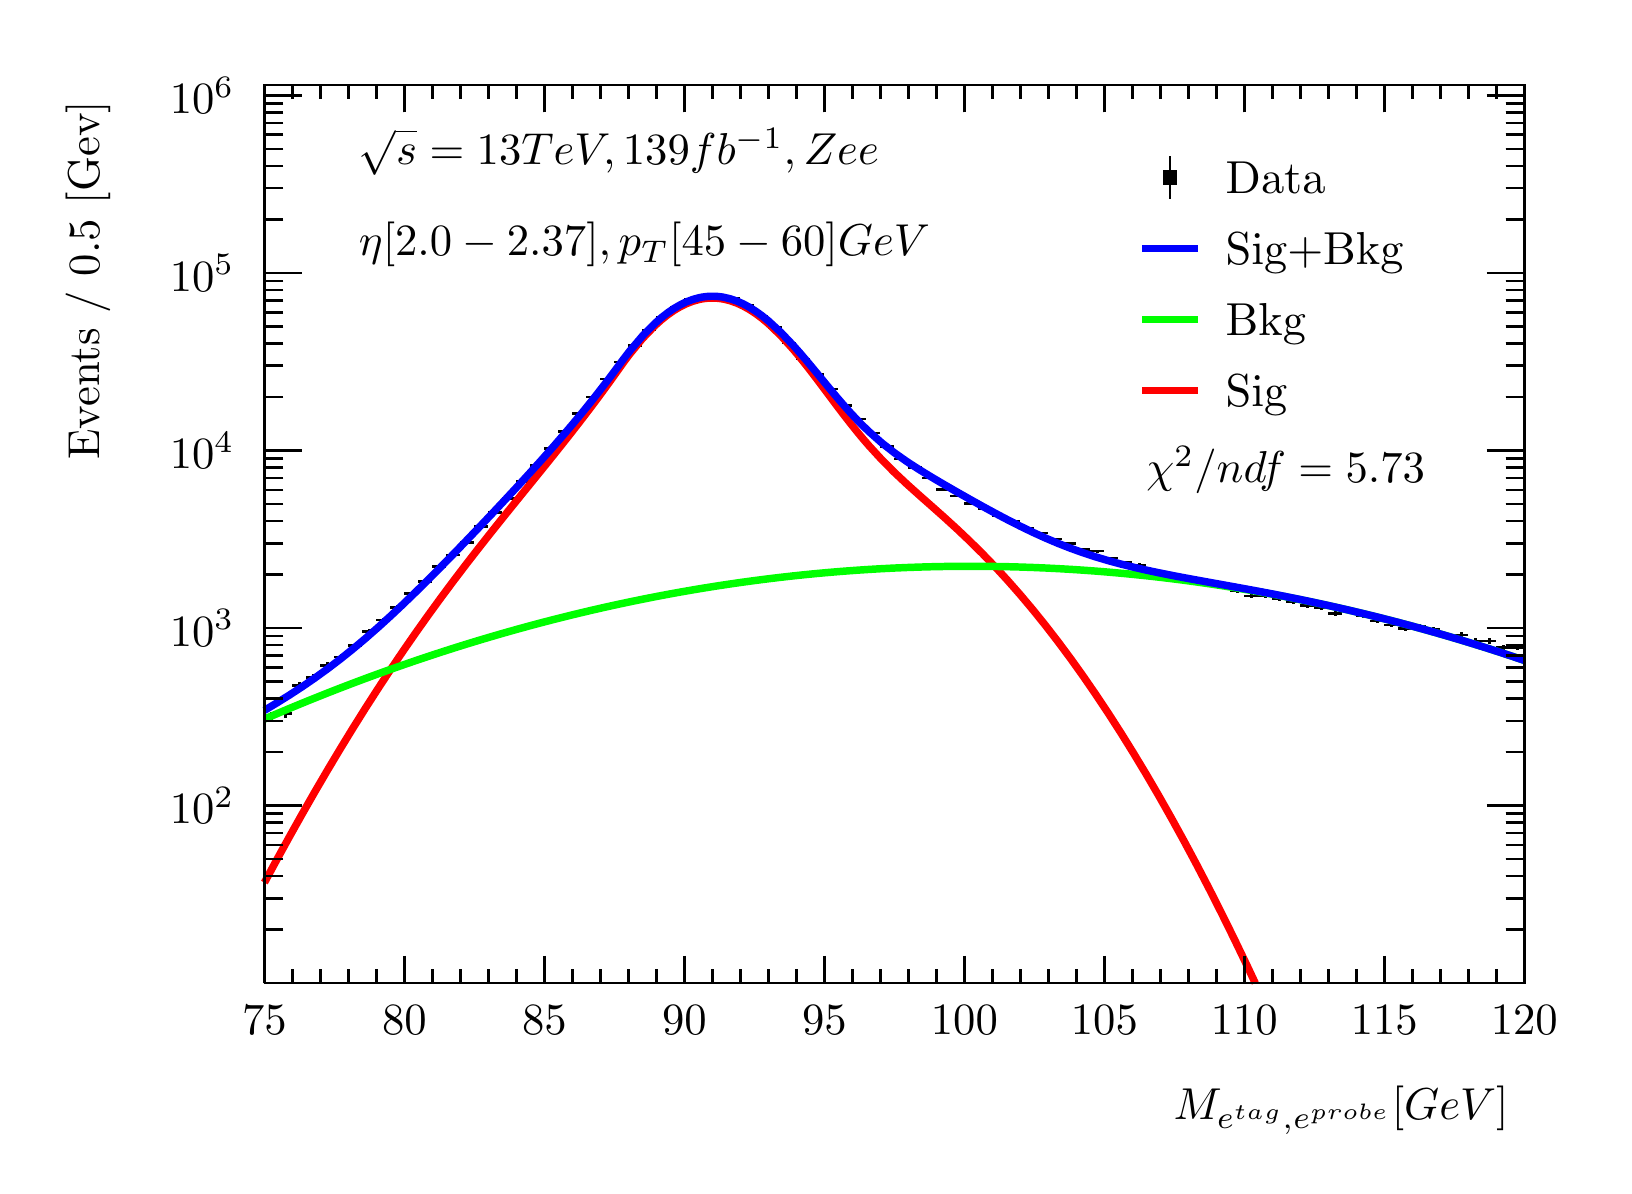
\begin{tikzpicture}
\pgfdeclareplotmark{cross} {
\pgfpathmoveto{\pgfpoint{-0.3\pgfplotmarksize}{\pgfplotmarksize}}
\pgfpathlineto{\pgfpoint{+0.3\pgfplotmarksize}{\pgfplotmarksize}}
\pgfpathlineto{\pgfpoint{+0.3\pgfplotmarksize}{0.3\pgfplotmarksize}}
\pgfpathlineto{\pgfpoint{+1\pgfplotmarksize}{0.3\pgfplotmarksize}}
\pgfpathlineto{\pgfpoint{+1\pgfplotmarksize}{-0.3\pgfplotmarksize}}
\pgfpathlineto{\pgfpoint{+0.3\pgfplotmarksize}{-0.3\pgfplotmarksize}}
\pgfpathlineto{\pgfpoint{+0.3\pgfplotmarksize}{-1.\pgfplotmarksize}}
\pgfpathlineto{\pgfpoint{-0.3\pgfplotmarksize}{-1.\pgfplotmarksize}}
\pgfpathlineto{\pgfpoint{-0.3\pgfplotmarksize}{-0.3\pgfplotmarksize}}
\pgfpathlineto{\pgfpoint{-1.\pgfplotmarksize}{-0.3\pgfplotmarksize}}
\pgfpathlineto{\pgfpoint{-1.\pgfplotmarksize}{0.3\pgfplotmarksize}}
\pgfpathlineto{\pgfpoint{-0.3\pgfplotmarksize}{0.3\pgfplotmarksize}}
\pgfpathclose
\pgfusepathqstroke
}
\pgfdeclareplotmark{cross*} {
\pgfpathmoveto{\pgfpoint{-0.3\pgfplotmarksize}{\pgfplotmarksize}}
\pgfpathlineto{\pgfpoint{+0.3\pgfplotmarksize}{\pgfplotmarksize}}
\pgfpathlineto{\pgfpoint{+0.3\pgfplotmarksize}{0.3\pgfplotmarksize}}
\pgfpathlineto{\pgfpoint{+1\pgfplotmarksize}{0.3\pgfplotmarksize}}
\pgfpathlineto{\pgfpoint{+1\pgfplotmarksize}{-0.3\pgfplotmarksize}}
\pgfpathlineto{\pgfpoint{+0.3\pgfplotmarksize}{-0.3\pgfplotmarksize}}
\pgfpathlineto{\pgfpoint{+0.3\pgfplotmarksize}{-1.\pgfplotmarksize}}
\pgfpathlineto{\pgfpoint{-0.3\pgfplotmarksize}{-1.\pgfplotmarksize}}
\pgfpathlineto{\pgfpoint{-0.3\pgfplotmarksize}{-0.3\pgfplotmarksize}}
\pgfpathlineto{\pgfpoint{-1.\pgfplotmarksize}{-0.3\pgfplotmarksize}}
\pgfpathlineto{\pgfpoint{-1.\pgfplotmarksize}{0.3\pgfplotmarksize}}
\pgfpathlineto{\pgfpoint{-0.3\pgfplotmarksize}{0.3\pgfplotmarksize}}
\pgfpathclose
\pgfusepathqfillstroke
}
\pgfdeclareplotmark{newstar} {
\pgfpathmoveto{\pgfqpoint{0pt}{\pgfplotmarksize}}
\pgfpathlineto{\pgfqpointpolar{44}{0.5\pgfplotmarksize}}
\pgfpathlineto{\pgfqpointpolar{18}{\pgfplotmarksize}}
\pgfpathlineto{\pgfqpointpolar{-20}{0.5\pgfplotmarksize}}
\pgfpathlineto{\pgfqpointpolar{-54}{\pgfplotmarksize}}
\pgfpathlineto{\pgfqpointpolar{-90}{0.5\pgfplotmarksize}}
\pgfpathlineto{\pgfqpointpolar{234}{\pgfplotmarksize}}
\pgfpathlineto{\pgfqpointpolar{198}{0.5\pgfplotmarksize}}
\pgfpathlineto{\pgfqpointpolar{162}{\pgfplotmarksize}}
\pgfpathlineto{\pgfqpointpolar{134}{0.5\pgfplotmarksize}}
\pgfpathclose
\pgfusepathqstroke
}
\pgfdeclareplotmark{newstar*} {
\pgfpathmoveto{\pgfqpoint{0pt}{\pgfplotmarksize}}
\pgfpathlineto{\pgfqpointpolar{44}{0.5\pgfplotmarksize}}
\pgfpathlineto{\pgfqpointpolar{18}{\pgfplotmarksize}}
\pgfpathlineto{\pgfqpointpolar{-20}{0.5\pgfplotmarksize}}
\pgfpathlineto{\pgfqpointpolar{-54}{\pgfplotmarksize}}
\pgfpathlineto{\pgfqpointpolar{-90}{0.5\pgfplotmarksize}}
\pgfpathlineto{\pgfqpointpolar{234}{\pgfplotmarksize}}
\pgfpathlineto{\pgfqpointpolar{198}{0.5\pgfplotmarksize}}
\pgfpathlineto{\pgfqpointpolar{162}{\pgfplotmarksize}}
\pgfpathlineto{\pgfqpointpolar{134}{0.5\pgfplotmarksize}}
\pgfpathclose
\pgfusepathqfillstroke
}
\definecolor{c}{rgb}{1,1,1};
\draw [color=c, fill=c] (0,0) rectangle (20,14.4361);
\draw [color=c, fill=c] (3,2.30977) rectangle (19,13.7143);
\definecolor{c}{rgb}{0,0,0};
\draw [c,line width=0.9] (3,2.30977) -- (3,13.7143) -- (19,13.7143) -- (19,2.30977) -- (3,2.30977);
\definecolor{c}{rgb}{1,1,1};
\draw [color=c, fill=c] (3,2.30977) rectangle (19,13.7143);
\definecolor{c}{rgb}{0,0,0};
\draw [c,line width=0.9] (3,2.30977) -- (3,13.7143) -- (19,13.7143) -- (19,2.30977) -- (3,2.30977);
\draw [c,line width=0.9] (3,2.30977) -- (19,2.30977);
\draw [c,line width=0.9] (3,2.65624) -- (3,2.30977);
\draw [c,line width=0.9] (3.35556,2.48301) -- (3.35556,2.30977);
\draw [c,line width=0.9] (3.71111,2.48301) -- (3.71111,2.30977);
\draw [c,line width=0.9] (4.06667,2.48301) -- (4.06667,2.30977);
\draw [c,line width=0.9] (4.42222,2.48301) -- (4.42222,2.30977);
\draw [c,line width=0.9] (4.77778,2.65624) -- (4.77778,2.30977);
\draw [c,line width=0.9] (5.13333,2.48301) -- (5.13333,2.30977);
\draw [c,line width=0.9] (5.48889,2.48301) -- (5.48889,2.30977);
\draw [c,line width=0.9] (5.84444,2.48301) -- (5.84444,2.30977);
\draw [c,line width=0.9] (6.2,2.48301) -- (6.2,2.30977);
\draw [c,line width=0.9] (6.55556,2.65624) -- (6.55556,2.30977);
\draw [c,line width=0.9] (6.91111,2.48301) -- (6.91111,2.30977);
\draw [c,line width=0.9] (7.26667,2.48301) -- (7.26667,2.30977);
\draw [c,line width=0.9] (7.62222,2.48301) -- (7.62222,2.30977);
\draw [c,line width=0.9] (7.97778,2.48301) -- (7.97778,2.30977);
\draw [c,line width=0.9] (8.33333,2.65624) -- (8.33333,2.30977);
\draw [c,line width=0.9] (8.68889,2.48301) -- (8.68889,2.30977);
\draw [c,line width=0.9] (9.04444,2.48301) -- (9.04444,2.30977);
\draw [c,line width=0.9] (9.4,2.48301) -- (9.4,2.30977);
\draw [c,line width=0.9] (9.75556,2.48301) -- (9.75556,2.30977);
\draw [c,line width=0.9] (10.1111,2.65624) -- (10.1111,2.30977);
\draw [c,line width=0.9] (10.4667,2.48301) -- (10.4667,2.30977);
\draw [c,line width=0.9] (10.8222,2.48301) -- (10.8222,2.30977);
\draw [c,line width=0.9] (11.1778,2.48301) -- (11.1778,2.30977);
\draw [c,line width=0.9] (11.5333,2.48301) -- (11.5333,2.30977);
\draw [c,line width=0.9] (11.8889,2.65624) -- (11.8889,2.30977);
\draw [c,line width=0.9] (12.2444,2.48301) -- (12.2444,2.30977);
\draw [c,line width=0.9] (12.6,2.48301) -- (12.6,2.30977);
\draw [c,line width=0.9] (12.9556,2.48301) -- (12.9556,2.30977);
\draw [c,line width=0.9] (13.3111,2.48301) -- (13.3111,2.30977);
\draw [c,line width=0.9] (13.6667,2.65624) -- (13.6667,2.30977);
\draw [c,line width=0.9] (14.0222,2.48301) -- (14.0222,2.30977);
\draw [c,line width=0.9] (14.3778,2.48301) -- (14.3778,2.30977);
\draw [c,line width=0.9] (14.7333,2.48301) -- (14.7333,2.30977);
\draw [c,line width=0.9] (15.0889,2.48301) -- (15.0889,2.30977);
\draw [c,line width=0.9] (15.4444,2.65624) -- (15.4444,2.30977);
\draw [c,line width=0.9] (15.8,2.48301) -- (15.8,2.30977);
\draw [c,line width=0.9] (16.1556,2.48301) -- (16.1556,2.30977);
\draw [c,line width=0.9] (16.5111,2.48301) -- (16.5111,2.30977);
\draw [c,line width=0.9] (16.8667,2.48301) -- (16.8667,2.30977);
\draw [c,line width=0.9] (17.2222,2.65624) -- (17.2222,2.30977);
\draw [c,line width=0.9] (17.5778,2.48301) -- (17.5778,2.30977);
\draw [c,line width=0.9] (17.9333,2.48301) -- (17.9333,2.30977);
\draw [c,line width=0.9] (18.2889,2.48301) -- (18.2889,2.30977);
\draw [c,line width=0.9] (18.6444,2.48301) -- (18.6444,2.30977);
\draw [c,line width=0.9] (19,2.65624) -- (19,2.30977);
\draw [c,line width=0.9] (19,2.65624) -- (19,2.30977);
\draw [anchor=base] (3,1.66015) node[scale=1.61424, color=c, rotate=0]{75};
\draw [anchor=base] (4.77778,1.66015) node[scale=1.61424, color=c, rotate=0]{80};
\draw [anchor=base] (6.55556,1.66015) node[scale=1.61424, color=c, rotate=0]{85};
\draw [anchor=base] (8.33333,1.66015) node[scale=1.61424, color=c, rotate=0]{90};
\draw [anchor=base] (10.1111,1.66015) node[scale=1.61424, color=c, rotate=0]{95};
\draw [anchor=base] (11.8889,1.66015) node[scale=1.61424, color=c, rotate=0]{100};
\draw [anchor=base] (13.6667,1.66015) node[scale=1.61424, color=c, rotate=0]{105};
\draw [anchor=base] (15.4444,1.66015) node[scale=1.61424, color=c, rotate=0]{110};
\draw [anchor=base] (17.2222,1.66015) node[scale=1.61424, color=c, rotate=0]{115};
\draw [anchor=base] (19,1.66015) node[scale=1.61424, color=c, rotate=0]{120};
\draw [anchor= east] (19,0.692932) node[scale=1.61424, color=c, rotate=0]{$M_{e^{tag}, e^{probe}}  [GeV]$};
\draw [c,line width=0.9] (3,13.7143) -- (19,13.7143);
\draw [c,line width=0.9] (3,13.3678) -- (3,13.7143);
\draw [c,line width=0.9] (3.35556,13.5411) -- (3.35556,13.7143);
\draw [c,line width=0.9] (3.71111,13.5411) -- (3.71111,13.7143);
\draw [c,line width=0.9] (4.06667,13.5411) -- (4.06667,13.7143);
\draw [c,line width=0.9] (4.42222,13.5411) -- (4.42222,13.7143);
\draw [c,line width=0.9] (4.77778,13.3678) -- (4.77778,13.7143);
\draw [c,line width=0.9] (5.13333,13.5411) -- (5.13333,13.7143);
\draw [c,line width=0.9] (5.48889,13.5411) -- (5.48889,13.7143);
\draw [c,line width=0.9] (5.84444,13.5411) -- (5.84444,13.7143);
\draw [c,line width=0.9] (6.2,13.5411) -- (6.2,13.7143);
\draw [c,line width=0.9] (6.55556,13.3678) -- (6.55556,13.7143);
\draw [c,line width=0.9] (6.91111,13.5411) -- (6.91111,13.7143);
\draw [c,line width=0.9] (7.26667,13.5411) -- (7.26667,13.7143);
\draw [c,line width=0.9] (7.62222,13.5411) -- (7.62222,13.7143);
\draw [c,line width=0.9] (7.97778,13.5411) -- (7.97778,13.7143);
\draw [c,line width=0.9] (8.33333,13.3678) -- (8.33333,13.7143);
\draw [c,line width=0.9] (8.68889,13.5411) -- (8.68889,13.7143);
\draw [c,line width=0.9] (9.04444,13.5411) -- (9.04444,13.7143);
\draw [c,line width=0.9] (9.4,13.5411) -- (9.4,13.7143);
\draw [c,line width=0.9] (9.75556,13.5411) -- (9.75556,13.7143);
\draw [c,line width=0.9] (10.1111,13.3678) -- (10.1111,13.7143);
\draw [c,line width=0.9] (10.4667,13.5411) -- (10.4667,13.7143);
\draw [c,line width=0.9] (10.8222,13.5411) -- (10.8222,13.7143);
\draw [c,line width=0.9] (11.1778,13.5411) -- (11.1778,13.7143);
\draw [c,line width=0.9] (11.5333,13.5411) -- (11.5333,13.7143);
\draw [c,line width=0.9] (11.8889,13.3678) -- (11.8889,13.7143);
\draw [c,line width=0.9] (12.2444,13.5411) -- (12.2444,13.7143);
\draw [c,line width=0.9] (12.6,13.5411) -- (12.6,13.7143);
\draw [c,line width=0.9] (12.9556,13.5411) -- (12.9556,13.7143);
\draw [c,line width=0.9] (13.3111,13.5411) -- (13.3111,13.7143);
\draw [c,line width=0.9] (13.6667,13.3678) -- (13.6667,13.7143);
\draw [c,line width=0.9] (14.0222,13.5411) -- (14.0222,13.7143);
\draw [c,line width=0.9] (14.3778,13.5411) -- (14.3778,13.7143);
\draw [c,line width=0.9] (14.7333,13.5411) -- (14.7333,13.7143);
\draw [c,line width=0.9] (15.0889,13.5411) -- (15.0889,13.7143);
\draw [c,line width=0.9] (15.4444,13.3678) -- (15.4444,13.7143);
\draw [c,line width=0.9] (15.8,13.5411) -- (15.8,13.7143);
\draw [c,line width=0.9] (16.1556,13.5411) -- (16.1556,13.7143);
\draw [c,line width=0.9] (16.5111,13.5411) -- (16.5111,13.7143);
\draw [c,line width=0.9] (16.8667,13.5411) -- (16.8667,13.7143);
\draw [c,line width=0.9] (17.2222,13.3678) -- (17.2222,13.7143);
\draw [c,line width=0.9] (17.5778,13.5411) -- (17.5778,13.7143);
\draw [c,line width=0.9] (17.9333,13.5411) -- (17.9333,13.7143);
\draw [c,line width=0.9] (18.2889,13.5411) -- (18.2889,13.7143);
\draw [c,line width=0.9] (18.6444,13.5411) -- (18.6444,13.7143);
\draw [c,line width=0.9] (19,13.3678) -- (19,13.7143);
\draw [c,line width=0.9] (19,13.3678) -- (19,13.7143);
\draw [c,line width=0.9] (3,2.30977) -- (3,13.7143);
\draw [c,line width=0.9] (3.237,2.98853) -- (3,2.98853);
\draw [c,line width=0.9] (3.237,3.38558) -- (3,3.38558);
\draw [c,line width=0.9] (3.237,3.66729) -- (3,3.66729);
\draw [c,line width=0.9] (3.237,3.8858) -- (3,3.8858);
\draw [c,line width=0.9] (3.237,4.06433) -- (3,4.06433);
\draw [c,line width=0.9] (3.237,4.21529) -- (3,4.21529);
\draw [c,line width=0.9] (3.237,4.34604) -- (3,4.34604);
\draw [c,line width=0.9] (3.237,4.46138) -- (3,4.46138);
\draw [c,line width=0.9] (3.474,4.56456) -- (3,4.56456);
\draw [anchor= east] (2.82,4.56456) node[scale=1.61424, color=c, rotate=0]{$10^{2}$};
\draw [c,line width=0.9] (3.237,5.24331) -- (3,5.24331);
\draw [c,line width=0.9] (3.237,5.64036) -- (3,5.64036);
\draw [c,line width=0.9] (3.237,5.92207) -- (3,5.92207);
\draw [c,line width=0.9] (3.237,6.14058) -- (3,6.14058);
\draw [c,line width=0.9] (3.237,6.31912) -- (3,6.31912);
\draw [c,line width=0.9] (3.237,6.47007) -- (3,6.47007);
\draw [c,line width=0.9] (3.237,6.60083) -- (3,6.60083);
\draw [c,line width=0.9] (3.237,6.71617) -- (3,6.71617);
\draw [c,line width=0.9] (3.474,6.81934) -- (3,6.81934);
\draw [anchor= east] (2.82,6.81934) node[scale=1.61424, color=c, rotate=0]{$10^{3}$};
\draw [c,line width=0.9] (3.237,7.4981) -- (3,7.4981);
\draw [c,line width=0.9] (3.237,7.89514) -- (3,7.89514);
\draw [c,line width=0.9] (3.237,8.17685) -- (3,8.17685);
\draw [c,line width=0.9] (3.237,8.39536) -- (3,8.39536);
\draw [c,line width=0.9] (3.237,8.5739) -- (3,8.5739);
\draw [c,line width=0.9] (3.237,8.72485) -- (3,8.72485);
\draw [c,line width=0.9] (3.237,8.85561) -- (3,8.85561);
\draw [c,line width=0.9] (3.237,8.97095) -- (3,8.97095);
\draw [c,line width=0.9] (3.474,9.07412) -- (3,9.07412);
\draw [anchor= east] (2.82,9.07412) node[scale=1.61424, color=c, rotate=0]{$10^{4}$};
\draw [c,line width=0.9] (3.237,9.75288) -- (3,9.75288);
\draw [c,line width=0.9] (3.237,10.1499) -- (3,10.1499);
\draw [c,line width=0.9] (3.237,10.4316) -- (3,10.4316);
\draw [c,line width=0.9] (3.237,10.6501) -- (3,10.6501);
\draw [c,line width=0.9] (3.237,10.8287) -- (3,10.8287);
\draw [c,line width=0.9] (3.237,10.9796) -- (3,10.9796);
\draw [c,line width=0.9] (3.237,11.1104) -- (3,11.1104);
\draw [c,line width=0.9] (3.237,11.2257) -- (3,11.2257);
\draw [c,line width=0.9] (3.474,11.3289) -- (3,11.3289);
\draw [anchor= east] (2.82,11.3289) node[scale=1.61424, color=c, rotate=0]{$10^{5}$};
\draw [c,line width=0.9] (3.237,12.0077) -- (3,12.0077);
\draw [c,line width=0.9] (3.237,12.4047) -- (3,12.4047);
\draw [c,line width=0.9] (3.237,12.6864) -- (3,12.6864);
\draw [c,line width=0.9] (3.237,12.9049) -- (3,12.9049);
\draw [c,line width=0.9] (3.237,13.0835) -- (3,13.0835);
\draw [c,line width=0.9] (3.237,13.2344) -- (3,13.2344);
\draw [c,line width=0.9] (3.237,13.3652) -- (3,13.3652);
\draw [c,line width=0.9] (3.237,13.4805) -- (3,13.4805);
\draw [c,line width=0.9] (3.474,13.5837) -- (3,13.5837);
\draw [anchor= east] (2.82,13.5837) node[scale=1.61424, color=c, rotate=0]{$10^{6}$};
\draw [anchor= east] (0.76,13.7143) node[scale=1.61424, color=c, rotate=90]{Events / 0.5 [Gev]};
\draw [c,line width=0.9] (19,2.30977) -- (19,13.7143);
\draw [c,line width=0.9] (18.763,2.98853) -- (19,2.98853);
\draw [c,line width=0.9] (18.763,3.38558) -- (19,3.38558);
\draw [c,line width=0.9] (18.763,3.66729) -- (19,3.66729);
\draw [c,line width=0.9] (18.763,3.8858) -- (19,3.8858);
\draw [c,line width=0.9] (18.763,4.06433) -- (19,4.06433);
\draw [c,line width=0.9] (18.763,4.21529) -- (19,4.21529);
\draw [c,line width=0.9] (18.763,4.34604) -- (19,4.34604);
\draw [c,line width=0.9] (18.763,4.46138) -- (19,4.46138);
\draw [c,line width=0.9] (18.526,4.56456) -- (19,4.56456);
\draw [c,line width=0.9] (18.763,5.24331) -- (19,5.24331);
\draw [c,line width=0.9] (18.763,5.64036) -- (19,5.64036);
\draw [c,line width=0.9] (18.763,5.92207) -- (19,5.92207);
\draw [c,line width=0.9] (18.763,6.14058) -- (19,6.14058);
\draw [c,line width=0.9] (18.763,6.31912) -- (19,6.31912);
\draw [c,line width=0.9] (18.763,6.47007) -- (19,6.47007);
\draw [c,line width=0.9] (18.763,6.60083) -- (19,6.60083);
\draw [c,line width=0.9] (18.763,6.71617) -- (19,6.71617);
\draw [c,line width=0.9] (18.526,6.81934) -- (19,6.81934);
\draw [c,line width=0.9] (18.763,7.4981) -- (19,7.4981);
\draw [c,line width=0.9] (18.763,7.89514) -- (19,7.89514);
\draw [c,line width=0.9] (18.763,8.17685) -- (19,8.17685);
\draw [c,line width=0.9] (18.763,8.39536) -- (19,8.39536);
\draw [c,line width=0.9] (18.763,8.5739) -- (19,8.5739);
\draw [c,line width=0.9] (18.763,8.72485) -- (19,8.72485);
\draw [c,line width=0.9] (18.763,8.85561) -- (19,8.85561);
\draw [c,line width=0.9] (18.763,8.97095) -- (19,8.97095);
\draw [c,line width=0.9] (18.526,9.07412) -- (19,9.07412);
\draw [c,line width=0.9] (18.763,9.75288) -- (19,9.75288);
\draw [c,line width=0.9] (18.763,10.1499) -- (19,10.1499);
\draw [c,line width=0.9] (18.763,10.4316) -- (19,10.4316);
\draw [c,line width=0.9] (18.763,10.6501) -- (19,10.6501);
\draw [c,line width=0.9] (18.763,10.8287) -- (19,10.8287);
\draw [c,line width=0.9] (18.763,10.9796) -- (19,10.9796);
\draw [c,line width=0.9] (18.763,11.1104) -- (19,11.1104);
\draw [c,line width=0.9] (18.763,11.2257) -- (19,11.2257);
\draw [c,line width=0.9] (18.526,11.3289) -- (19,11.3289);
\draw [c,line width=0.9] (18.763,12.0077) -- (19,12.0077);
\draw [c,line width=0.9] (18.763,12.4047) -- (19,12.4047);
\draw [c,line width=0.9] (18.763,12.6864) -- (19,12.6864);
\draw [c,line width=0.9] (18.763,12.9049) -- (19,12.9049);
\draw [c,line width=0.9] (18.763,13.0835) -- (19,13.0835);
\draw [c,line width=0.9] (18.763,13.2344) -- (19,13.2344);
\draw [c,line width=0.9] (18.763,13.3652) -- (19,13.3652);
\draw [c,line width=0.9] (18.763,13.4805) -- (19,13.4805);
\draw [c,line width=0.9] (18.526,13.5837) -- (19,13.5837);
\draw [c,line width=0.9] (3.08889,5.70356) -- (3,5.70356);
\draw [c,line width=0.9] (3,5.70356) -- (3,5.70356);
\draw [c,line width=0.9] (3.08889,5.70356) -- (3.17778,5.70356);
\draw [c,line width=0.9] (3.17778,5.70356) -- (3.17778,5.70356);
\draw [c,line width=0.9] (3.08889,5.70356) -- (3.08889,5.7583);
\draw [c,line width=0.9] (3.08889,5.7583) -- (3.08889,5.7583);
\draw [c,line width=0.9] (3.08889,5.70356) -- (3.08889,5.64883);
\draw [c,line width=0.9] (3.08889,5.64883) -- (3.08889,5.64883);
\draw [c,line width=0.9] (3.26667,5.73072) -- (3.17778,5.73072);
\draw [c,line width=0.9] (3.17778,5.73072) -- (3.17778,5.73072);
\draw [c,line width=0.9] (3.26667,5.73072) -- (3.35556,5.73072);
\draw [c,line width=0.9] (3.35556,5.73072) -- (3.35556,5.73072);
\draw [c,line width=0.9] (3.26667,5.73072) -- (3.26667,5.7847);
\draw [c,line width=0.9] (3.26667,5.7847) -- (3.26667,5.7847);
\draw [c,line width=0.9] (3.26667,5.73072) -- (3.26667,5.67674);
\draw [c,line width=0.9] (3.26667,5.67674) -- (3.26667,5.67674);
\draw [c,line width=0.9] (3.44444,6.08829) -- (3.35556,6.08829);
\draw [c,line width=0.9] (3.35556,6.08829) -- (3.35556,6.08829);
\draw [c,line width=0.9] (3.44444,6.08829) -- (3.53333,6.08829);
\draw [c,line width=0.9] (3.53333,6.08829) -- (3.53333,6.08829);
\draw [c,line width=0.9] (3.44444,6.08829) -- (3.44444,6.13326);
\draw [c,line width=0.9] (3.44444,6.13326) -- (3.44444,6.13326);
\draw [c,line width=0.9] (3.44444,6.08829) -- (3.44444,6.04332);
\draw [c,line width=0.9] (3.44444,6.04332) -- (3.44444,6.04332);
\draw [c,line width=0.9] (3.62222,6.18836) -- (3.53333,6.18836);
\draw [c,line width=0.9] (3.53333,6.18836) -- (3.53333,6.18836);
\draw [c,line width=0.9] (3.62222,6.18836) -- (3.71111,6.18836);
\draw [c,line width=0.9] (3.71111,6.18836) -- (3.71111,6.18836);
\draw [c,line width=0.9] (3.62222,6.18836) -- (3.62222,6.23109);
\draw [c,line width=0.9] (3.62222,6.23109) -- (3.62222,6.23109);
\draw [c,line width=0.9] (3.62222,6.18836) -- (3.62222,6.14563);
\draw [c,line width=0.9] (3.62222,6.14563) -- (3.62222,6.14563);
\draw [c,line width=0.9] (3.8,6.34171) -- (3.71111,6.34171);
\draw [c,line width=0.9] (3.71111,6.34171) -- (3.71111,6.34171);
\draw [c,line width=0.9] (3.8,6.34171) -- (3.88889,6.34171);
\draw [c,line width=0.9] (3.88889,6.34171) -- (3.88889,6.34171);
\draw [c,line width=0.9] (3.8,6.34171) -- (3.8,6.38122);
\draw [c,line width=0.9] (3.8,6.38122) -- (3.8,6.38122);
\draw [c,line width=0.9] (3.8,6.34171) -- (3.8,6.30219);
\draw [c,line width=0.9] (3.8,6.30219) -- (3.8,6.30219);
\draw [c,line width=0.9] (3.97778,6.45029) -- (3.88889,6.45029);
\draw [c,line width=0.9] (3.88889,6.45029) -- (3.88889,6.45029);
\draw [c,line width=0.9] (3.97778,6.45029) -- (4.06667,6.45029);
\draw [c,line width=0.9] (4.06667,6.45029) -- (4.06667,6.45029);
\draw [c,line width=0.9] (3.97778,6.45029) -- (3.97778,6.48767);
\draw [c,line width=0.9] (3.97778,6.48767) -- (3.97778,6.48767);
\draw [c,line width=0.9] (3.97778,6.45029) -- (3.97778,6.4129);
\draw [c,line width=0.9] (3.97778,6.4129) -- (3.97778,6.4129);
\draw [c,line width=0.9] (4.15556,6.5996) -- (4.06667,6.5996);
\draw [c,line width=0.9] (4.06667,6.5996) -- (4.06667,6.5996);
\draw [c,line width=0.9] (4.15556,6.5996) -- (4.24444,6.5996);
\draw [c,line width=0.9] (4.24444,6.5996) -- (4.24444,6.5996);
\draw [c,line width=0.9] (4.15556,6.5996) -- (4.15556,6.63425);
\draw [c,line width=0.9] (4.15556,6.63425) -- (4.15556,6.63425);
\draw [c,line width=0.9] (4.15556,6.5996) -- (4.15556,6.56496);
\draw [c,line width=0.9] (4.15556,6.56496) -- (4.15556,6.56496);
\draw [c,line width=0.9] (4.33333,6.77323) -- (4.24444,6.77323);
\draw [c,line width=0.9] (4.24444,6.77323) -- (4.24444,6.77323);
\draw [c,line width=0.9] (4.33333,6.77323) -- (4.42222,6.77323);
\draw [c,line width=0.9] (4.42222,6.77323) -- (4.42222,6.77323);
\draw [c,line width=0.9] (4.33333,6.77323) -- (4.33333,6.80493);
\draw [c,line width=0.9] (4.33333,6.80493) -- (4.33333,6.80493);
\draw [c,line width=0.9] (4.33333,6.77323) -- (4.33333,6.74152);
\draw [c,line width=0.9] (4.33333,6.74152) -- (4.33333,6.74152);
\draw [c,line width=0.9] (4.51111,6.92065) -- (4.42222,6.92065);
\draw [c,line width=0.9] (4.42222,6.92065) -- (4.42222,6.92065);
\draw [c,line width=0.9] (4.51111,6.92065) -- (4.6,6.92065);
\draw [c,line width=0.9] (4.6,6.92065) -- (4.6,6.92065);
\draw [c,line width=0.9] (4.51111,6.92065) -- (4.51111,6.95006);
\draw [c,line width=0.9] (4.51111,6.95006) -- (4.51111,6.95006);
\draw [c,line width=0.9] (4.51111,6.92065) -- (4.51111,6.89125);
\draw [c,line width=0.9] (4.51111,6.89125) -- (4.51111,6.89125);
\draw [c,line width=0.9] (4.68889,7.07776) -- (4.6,7.07776);
\draw [c,line width=0.9] (4.6,7.07776) -- (4.6,7.07776);
\draw [c,line width=0.9] (4.68889,7.07776) -- (4.77778,7.07776);
\draw [c,line width=0.9] (4.77778,7.07776) -- (4.77778,7.07776);
\draw [c,line width=0.9] (4.68889,7.07776) -- (4.68889,7.1049);
\draw [c,line width=0.9] (4.68889,7.1049) -- (4.68889,7.1049);
\draw [c,line width=0.9] (4.68889,7.07776) -- (4.68889,7.05063);
\draw [c,line width=0.9] (4.68889,7.05063) -- (4.68889,7.05063);
\draw [c,line width=0.9] (4.86667,7.25668) -- (4.77778,7.25668);
\draw [c,line width=0.9] (4.77778,7.25668) -- (4.77778,7.25668);
\draw [c,line width=0.9] (4.86667,7.25668) -- (4.95556,7.25668);
\draw [c,line width=0.9] (4.95556,7.25668) -- (4.95556,7.25668);
\draw [c,line width=0.9] (4.86667,7.25668) -- (4.86667,7.28144);
\draw [c,line width=0.9] (4.86667,7.28144) -- (4.86667,7.28144);
\draw [c,line width=0.9] (4.86667,7.25668) -- (4.86667,7.23191);
\draw [c,line width=0.9] (4.86667,7.23191) -- (4.86667,7.23191);
\draw [c,line width=0.9] (5.04444,7.40736) -- (4.95556,7.40736);
\draw [c,line width=0.9] (4.95556,7.40736) -- (4.95556,7.40736);
\draw [c,line width=0.9] (5.04444,7.40736) -- (5.13333,7.40736);
\draw [c,line width=0.9] (5.13333,7.40736) -- (5.13333,7.40736);
\draw [c,line width=0.9] (5.04444,7.40736) -- (5.04444,7.43029);
\draw [c,line width=0.9] (5.04444,7.43029) -- (5.04444,7.43029);
\draw [c,line width=0.9] (5.04444,7.40736) -- (5.04444,7.38442);
\draw [c,line width=0.9] (5.04444,7.38442) -- (5.04444,7.38442);
\draw [c,line width=0.9] (5.22222,7.59808) -- (5.13333,7.59808);
\draw [c,line width=0.9] (5.13333,7.59808) -- (5.13333,7.59808);
\draw [c,line width=0.9] (5.22222,7.59808) -- (5.31111,7.59808);
\draw [c,line width=0.9] (5.31111,7.59808) -- (5.31111,7.59808);
\draw [c,line width=0.9] (5.22222,7.59808) -- (5.22222,7.61889);
\draw [c,line width=0.9] (5.22222,7.61889) -- (5.22222,7.61889);
\draw [c,line width=0.9] (5.22222,7.59808) -- (5.22222,7.57728);
\draw [c,line width=0.9] (5.22222,7.57728) -- (5.22222,7.57728);
\draw [c,line width=0.9] (5.4,7.74593) -- (5.31111,7.74593);
\draw [c,line width=0.9] (5.31111,7.74593) -- (5.31111,7.74593);
\draw [c,line width=0.9] (5.4,7.74593) -- (5.48889,7.74593);
\draw [c,line width=0.9] (5.48889,7.74593) -- (5.48889,7.74593);
\draw [c,line width=0.9] (5.4,7.74593) -- (5.4,7.76523);
\draw [c,line width=0.9] (5.4,7.76523) -- (5.4,7.76523);
\draw [c,line width=0.9] (5.4,7.74593) -- (5.4,7.72664);
\draw [c,line width=0.9] (5.4,7.72664) -- (5.4,7.72664);
\draw [c,line width=0.9] (5.57778,7.90392) -- (5.48889,7.90392);
\draw [c,line width=0.9] (5.48889,7.90392) -- (5.48889,7.90392);
\draw [c,line width=0.9] (5.57778,7.90392) -- (5.66667,7.90392);
\draw [c,line width=0.9] (5.66667,7.90392) -- (5.66667,7.90392);
\draw [c,line width=0.9] (5.57778,7.90392) -- (5.57778,7.92172);
\draw [c,line width=0.9] (5.57778,7.92172) -- (5.57778,7.92172);
\draw [c,line width=0.9] (5.57778,7.90392) -- (5.57778,7.88612);
\draw [c,line width=0.9] (5.57778,7.88612) -- (5.57778,7.88612);
\draw [c,line width=0.9] (5.75556,8.10973) -- (5.66667,8.10973);
\draw [c,line width=0.9] (5.66667,8.10973) -- (5.66667,8.10973);
\draw [c,line width=0.9] (5.75556,8.10973) -- (5.84444,8.10973);
\draw [c,line width=0.9] (5.84444,8.10973) -- (5.84444,8.10973);
\draw [c,line width=0.9] (5.75556,8.10973) -- (5.75556,8.12575);
\draw [c,line width=0.9] (5.75556,8.12575) -- (5.75556,8.12575);
\draw [c,line width=0.9] (5.75556,8.10973) -- (5.75556,8.09371);
\draw [c,line width=0.9] (5.75556,8.09371) -- (5.75556,8.09371);
\draw [c,line width=0.9] (5.93333,8.28411) -- (5.84444,8.28411);
\draw [c,line width=0.9] (5.84444,8.28411) -- (5.84444,8.28411);
\draw [c,line width=0.9] (5.93333,8.28411) -- (6.02222,8.28411);
\draw [c,line width=0.9] (6.02222,8.28411) -- (6.02222,8.28411);
\draw [c,line width=0.9] (5.93333,8.28411) -- (5.93333,8.29877);
\draw [c,line width=0.9] (5.93333,8.29877) -- (5.93333,8.29877);
\draw [c,line width=0.9] (5.93333,8.28411) -- (5.93333,8.26945);
\draw [c,line width=0.9] (5.93333,8.26945) -- (5.93333,8.26945);
\draw [c,line width=0.9] (6.11111,8.46618) -- (6.02222,8.46618);
\draw [c,line width=0.9] (6.02222,8.46618) -- (6.02222,8.46618);
\draw [c,line width=0.9] (6.11111,8.46618) -- (6.2,8.46618);
\draw [c,line width=0.9] (6.2,8.46618) -- (6.2,8.46618);
\draw [c,line width=0.9] (6.11111,8.46618) -- (6.11111,8.47954);
\draw [c,line width=0.9] (6.11111,8.47954) -- (6.11111,8.47954);
\draw [c,line width=0.9] (6.11111,8.46618) -- (6.11111,8.45283);
\draw [c,line width=0.9] (6.11111,8.45283) -- (6.11111,8.45283);
\draw [c,line width=0.9] (6.28889,8.68094) -- (6.2,8.68094);
\draw [c,line width=0.9] (6.2,8.68094) -- (6.2,8.68094);
\draw [c,line width=0.9] (6.28889,8.68094) -- (6.37778,8.68094);
\draw [c,line width=0.9] (6.37778,8.68094) -- (6.37778,8.68094);
\draw [c,line width=0.9] (6.28889,8.68094) -- (6.28889,8.69291);
\draw [c,line width=0.9] (6.28889,8.69291) -- (6.28889,8.69291);
\draw [c,line width=0.9] (6.28889,8.68094) -- (6.28889,8.66897);
\draw [c,line width=0.9] (6.28889,8.66897) -- (6.28889,8.66897);
\draw [c,line width=0.9] (6.46667,8.88182) -- (6.37778,8.88182);
\draw [c,line width=0.9] (6.37778,8.88182) -- (6.37778,8.88182);
\draw [c,line width=0.9] (6.46667,8.88182) -- (6.55556,8.88182);
\draw [c,line width=0.9] (6.55556,8.88182) -- (6.55556,8.88182);
\draw [c,line width=0.9] (6.46667,8.88182) -- (6.46667,8.89262);
\draw [c,line width=0.9] (6.46667,8.89262) -- (6.46667,8.89262);
\draw [c,line width=0.9] (6.46667,8.88182) -- (6.46667,8.87102);
\draw [c,line width=0.9] (6.46667,8.87102) -- (6.46667,8.87102);
\draw [c,line width=0.9] (6.64444,9.09964) -- (6.55556,9.09964);
\draw [c,line width=0.9] (6.55556,9.09964) -- (6.55556,9.09964);
\draw [c,line width=0.9] (6.64444,9.09964) -- (6.73333,9.09964);
\draw [c,line width=0.9] (6.73333,9.09964) -- (6.73333,9.09964);
\draw [c,line width=0.9] (6.64444,9.09964) -- (6.64444,9.10931);
\draw [c,line width=0.9] (6.64444,9.10931) -- (6.64444,9.10931);
\draw [c,line width=0.9] (6.64444,9.09964) -- (6.64444,9.08997);
\draw [c,line width=0.9] (6.64444,9.08997) -- (6.64444,9.08997);
\draw [c,line width=0.9] (6.82222,9.31486) -- (6.73333,9.31486);
\draw [c,line width=0.9] (6.73333,9.31486) -- (6.73333,9.31486);
\draw [c,line width=0.9] (6.82222,9.31486) -- (6.91111,9.31486);
\draw [c,line width=0.9] (6.91111,9.31486) -- (6.91111,9.31486);
\draw [c,line width=0.9] (6.82222,9.31486) -- (6.82222,9.32352);
\draw [c,line width=0.9] (6.82222,9.32352) -- (6.82222,9.32352);
\draw [c,line width=0.9] (6.82222,9.31486) -- (6.82222,9.3062);
\draw [c,line width=0.9] (6.82222,9.3062) -- (6.82222,9.3062);
\draw [c,line width=0.9] (7,9.54065) -- (6.91111,9.54065);
\draw [c,line width=0.9] (6.91111,9.54065) -- (6.91111,9.54065);
\draw [c,line width=0.9] (7,9.54065) -- (7.08889,9.54065);
\draw [c,line width=0.9] (7.08889,9.54065) -- (7.08889,9.54065);
\draw [c,line width=0.9] (7,9.54065) -- (7,9.54837);
\draw [c,line width=0.9] (7,9.54837) -- (7,9.54837);
\draw [c,line width=0.9] (7,9.54065) -- (7,9.53294);
\draw [c,line width=0.9] (7,9.53294) -- (7,9.53294);
\draw [c,line width=0.9] (7.17778,9.75508) -- (7.08889,9.75508);
\draw [c,line width=0.9] (7.08889,9.75508) -- (7.08889,9.75508);
\draw [c,line width=0.9] (7.17778,9.75508) -- (7.26667,9.75508);
\draw [c,line width=0.9] (7.26667,9.75508) -- (7.26667,9.75508);
\draw [c,line width=0.9] (7.17778,9.75508) -- (7.17778,9.762);
\draw [c,line width=0.9] (7.17778,9.762) -- (7.17778,9.762);
\draw [c,line width=0.9] (7.17778,9.75508) -- (7.17778,9.74816);
\draw [c,line width=0.9] (7.17778,9.74816) -- (7.17778,9.74816);
\draw [c,line width=0.9] (7.35556,9.98346) -- (7.26667,9.98346);
\draw [c,line width=0.9] (7.26667,9.98346) -- (7.26667,9.98346);
\draw [c,line width=0.9] (7.35556,9.98346) -- (7.44444,9.98346);
\draw [c,line width=0.9] (7.44444,9.98346) -- (7.44444,9.98346);
\draw [c,line width=0.9] (7.35556,9.98346) -- (7.35556,9.98961);
\draw [c,line width=0.9] (7.35556,9.98961) -- (7.35556,9.98961);
\draw [c,line width=0.9] (7.35556,9.98346) -- (7.35556,9.9773);
\draw [c,line width=0.9] (7.35556,9.9773) -- (7.35556,9.9773);
\draw [c,line width=0.9] (7.53333,10.1945) -- (7.44444,10.1945);
\draw [c,line width=0.9] (7.44444,10.1945) -- (7.44444,10.1945);
\draw [c,line width=0.9] (7.53333,10.1945) -- (7.62222,10.1945);
\draw [c,line width=0.9] (7.62222,10.1945) -- (7.62222,10.1945);
\draw [c,line width=0.9] (7.53333,10.1945) -- (7.53333,10.2001);
\draw [c,line width=0.9] (7.53333,10.2001) -- (7.53333,10.2001);
\draw [c,line width=0.9] (7.53333,10.1945) -- (7.53333,10.189);
\draw [c,line width=0.9] (7.53333,10.189) -- (7.53333,10.189);
\draw [c,line width=0.9] (7.71111,10.4069) -- (7.62222,10.4069);
\draw [c,line width=0.9] (7.62222,10.4069) -- (7.62222,10.4069);
\draw [c,line width=0.9] (7.71111,10.4069) -- (7.8,10.4069);
\draw [c,line width=0.9] (7.8,10.4069) -- (7.8,10.4069);
\draw [c,line width=0.9] (7.71111,10.4069) -- (7.71111,10.4118);
\draw [c,line width=0.9] (7.71111,10.4118) -- (7.71111,10.4118);
\draw [c,line width=0.9] (7.71111,10.4069) -- (7.71111,10.4019);
\draw [c,line width=0.9] (7.71111,10.4019) -- (7.71111,10.4019);
\draw [c,line width=0.9] (7.88889,10.6044) -- (7.8,10.6044);
\draw [c,line width=0.9] (7.8,10.6044) -- (7.8,10.6044);
\draw [c,line width=0.9] (7.88889,10.6044) -- (7.97778,10.6044);
\draw [c,line width=0.9] (7.97778,10.6044) -- (7.97778,10.6044);
\draw [c,line width=0.9] (7.88889,10.6044) -- (7.88889,10.6088);
\draw [c,line width=0.9] (7.88889,10.6088) -- (7.88889,10.6088);
\draw [c,line width=0.9] (7.88889,10.6044) -- (7.88889,10.5999);
\draw [c,line width=0.9] (7.88889,10.5999) -- (7.88889,10.5999);
\draw [c,line width=0.9] (8.06667,10.769) -- (7.97778,10.769);
\draw [c,line width=0.9] (7.97778,10.769) -- (7.97778,10.769);
\draw [c,line width=0.9] (8.06667,10.769) -- (8.15556,10.769);
\draw [c,line width=0.9] (8.15556,10.769) -- (8.15556,10.769);
\draw [c,line width=0.9] (8.06667,10.769) -- (8.06667,10.7732);
\draw [c,line width=0.9] (8.06667,10.7732) -- (8.06667,10.7732);
\draw [c,line width=0.9] (8.06667,10.769) -- (8.06667,10.7649);
\draw [c,line width=0.9] (8.06667,10.7649) -- (8.06667,10.7649);
\draw [c,line width=0.9] (8.24444,10.893) -- (8.15556,10.893);
\draw [c,line width=0.9] (8.15556,10.893) -- (8.15556,10.893);
\draw [c,line width=0.9] (8.24444,10.893) -- (8.33333,10.893);
\draw [c,line width=0.9] (8.33333,10.893) -- (8.33333,10.893);
\draw [c,line width=0.9] (8.24444,10.893) -- (8.24444,10.8969);
\draw [c,line width=0.9] (8.24444,10.8969) -- (8.24444,10.8969);
\draw [c,line width=0.9] (8.24444,10.893) -- (8.24444,10.8891);
\draw [c,line width=0.9] (8.24444,10.8891) -- (8.24444,10.8891);
\draw [c,line width=0.9] (8.42222,10.989) -- (8.33333,10.989);
\draw [c,line width=0.9] (8.33333,10.989) -- (8.33333,10.989);
\draw [c,line width=0.9] (8.42222,10.989) -- (8.51111,10.989);
\draw [c,line width=0.9] (8.51111,10.989) -- (8.51111,10.989);
\draw [c,line width=0.9] (8.42222,10.989) -- (8.42222,10.9927);
\draw [c,line width=0.9] (8.42222,10.9927) -- (8.42222,10.9927);
\draw [c,line width=0.9] (8.42222,10.989) -- (8.42222,10.9853);
\draw [c,line width=0.9] (8.42222,10.9853) -- (8.42222,10.9853);
\draw [c,line width=0.9] (8.6,11.0335) -- (8.51111,11.0335);
\draw [c,line width=0.9] (8.51111,11.0335) -- (8.51111,11.0335);
\draw [c,line width=0.9] (8.6,11.0335) -- (8.68889,11.0335);
\draw [c,line width=0.9] (8.68889,11.0335) -- (8.68889,11.0335);
\draw [c,line width=0.9] (8.6,11.0335) -- (8.6,11.0371);
\draw [c,line width=0.9] (8.6,11.0371) -- (8.6,11.0371);
\draw [c,line width=0.9] (8.6,11.0335) -- (8.6,11.0299);
\draw [c,line width=0.9] (8.6,11.0299) -- (8.6,11.0299);
\draw [c,line width=0.9] (8.77778,11.0437) -- (8.68889,11.0437);
\draw [c,line width=0.9] (8.68889,11.0437) -- (8.68889,11.0437);
\draw [c,line width=0.9] (8.77778,11.0437) -- (8.86667,11.0437);
\draw [c,line width=0.9] (8.86667,11.0437) -- (8.86667,11.0437);
\draw [c,line width=0.9] (8.77778,11.0437) -- (8.77778,11.0472);
\draw [c,line width=0.9] (8.77778,11.0472) -- (8.77778,11.0472);
\draw [c,line width=0.9] (8.77778,11.0437) -- (8.77778,11.0401);
\draw [c,line width=0.9] (8.77778,11.0401) -- (8.77778,11.0401);
\draw [c,line width=0.9] (8.95556,11.0034) -- (8.86667,11.0034);
\draw [c,line width=0.9] (8.86667,11.0034) -- (8.86667,11.0034);
\draw [c,line width=0.9] (8.95556,11.0034) -- (9.04444,11.0034);
\draw [c,line width=0.9] (9.04444,11.0034) -- (9.04444,11.0034);
\draw [c,line width=0.9] (8.95556,11.0034) -- (8.95556,11.0071);
\draw [c,line width=0.9] (8.95556,11.0071) -- (8.95556,11.0071);
\draw [c,line width=0.9] (8.95556,11.0034) -- (8.95556,10.9998);
\draw [c,line width=0.9] (8.95556,10.9998) -- (8.95556,10.9998);
\draw [c,line width=0.9] (9.13333,10.9124) -- (9.04444,10.9124);
\draw [c,line width=0.9] (9.04444,10.9124) -- (9.04444,10.9124);
\draw [c,line width=0.9] (9.13333,10.9124) -- (9.22222,10.9124);
\draw [c,line width=0.9] (9.22222,10.9124) -- (9.22222,10.9124);
\draw [c,line width=0.9] (9.13333,10.9124) -- (9.13333,10.9163);
\draw [c,line width=0.9] (9.13333,10.9163) -- (9.13333,10.9163);
\draw [c,line width=0.9] (9.13333,10.9124) -- (9.13333,10.9086);
\draw [c,line width=0.9] (9.13333,10.9086) -- (9.13333,10.9086);
\draw [c,line width=0.9] (9.31111,10.7798) -- (9.22222,10.7798);
\draw [c,line width=0.9] (9.22222,10.7798) -- (9.22222,10.7798);
\draw [c,line width=0.9] (9.31111,10.7798) -- (9.4,10.7798);
\draw [c,line width=0.9] (9.4,10.7798) -- (9.4,10.7798);
\draw [c,line width=0.9] (9.31111,10.7798) -- (9.31111,10.7839);
\draw [c,line width=0.9] (9.31111,10.7839) -- (9.31111,10.7839);
\draw [c,line width=0.9] (9.31111,10.7798) -- (9.31111,10.7757);
\draw [c,line width=0.9] (9.31111,10.7757) -- (9.31111,10.7757);
\draw [c,line width=0.9] (9.48889,10.6322) -- (9.4,10.6322);
\draw [c,line width=0.9] (9.4,10.6322) -- (9.4,10.6322);
\draw [c,line width=0.9] (9.48889,10.6322) -- (9.57778,10.6322);
\draw [c,line width=0.9] (9.57778,10.6322) -- (9.57778,10.6322);
\draw [c,line width=0.9] (9.48889,10.6322) -- (9.48889,10.6367);
\draw [c,line width=0.9] (9.48889,10.6367) -- (9.48889,10.6367);
\draw [c,line width=0.9] (9.48889,10.6322) -- (9.48889,10.6278);
\draw [c,line width=0.9] (9.48889,10.6278) -- (9.48889,10.6278);
\draw [c,line width=0.9] (9.66667,10.441) -- (9.57778,10.441);
\draw [c,line width=0.9] (9.57778,10.441) -- (9.57778,10.441);
\draw [c,line width=0.9] (9.66667,10.441) -- (9.75556,10.441);
\draw [c,line width=0.9] (9.75556,10.441) -- (9.75556,10.441);
\draw [c,line width=0.9] (9.66667,10.441) -- (9.66667,10.4459);
\draw [c,line width=0.9] (9.66667,10.4459) -- (9.66667,10.4459);
\draw [c,line width=0.9] (9.66667,10.441) -- (9.66667,10.4361);
\draw [c,line width=0.9] (9.66667,10.4361) -- (9.66667,10.4361);
\draw [c,line width=0.9] (9.84444,10.2364) -- (9.75556,10.2364);
\draw [c,line width=0.9] (9.75556,10.2364) -- (9.75556,10.2364);
\draw [c,line width=0.9] (9.84444,10.2364) -- (9.93333,10.2364);
\draw [c,line width=0.9] (9.93333,10.2364) -- (9.93333,10.2364);
\draw [c,line width=0.9] (9.84444,10.2364) -- (9.84444,10.2418);
\draw [c,line width=0.9] (9.84444,10.2418) -- (9.84444,10.2418);
\draw [c,line width=0.9] (9.84444,10.2364) -- (9.84444,10.231);
\draw [c,line width=0.9] (9.84444,10.231) -- (9.84444,10.231);
\draw [c,line width=0.9] (10.0222,10.0367) -- (9.93333,10.0367);
\draw [c,line width=0.9] (9.93333,10.0367) -- (9.93333,10.0367);
\draw [c,line width=0.9] (10.0222,10.0367) -- (10.1111,10.0367);
\draw [c,line width=0.9] (10.1111,10.0367) -- (10.1111,10.0367);
\draw [c,line width=0.9] (10.0222,10.0367) -- (10.0222,10.0427);
\draw [c,line width=0.9] (10.0222,10.0427) -- (10.0222,10.0427);
\draw [c,line width=0.9] (10.0222,10.0367) -- (10.0222,10.0307);
\draw [c,line width=0.9] (10.0222,10.0307) -- (10.0222,10.0307);
\draw [c,line width=0.9] (10.2,9.85096) -- (10.1111,9.85096);
\draw [c,line width=0.9] (10.1111,9.85096) -- (10.1111,9.85096);
\draw [c,line width=0.9] (10.2,9.85096) -- (10.2889,9.85096);
\draw [c,line width=0.9] (10.2889,9.85096) -- (10.2889,9.85096);
\draw [c,line width=0.9] (10.2,9.85096) -- (10.2,9.85755);
\draw [c,line width=0.9] (10.2,9.85755) -- (10.2,9.85755);
\draw [c,line width=0.9] (10.2,9.85096) -- (10.2,9.84438);
\draw [c,line width=0.9] (10.2,9.84438) -- (10.2,9.84438);
\draw [c,line width=0.9] (10.3778,9.64589) -- (10.2889,9.64589);
\draw [c,line width=0.9] (10.2889,9.64589) -- (10.2889,9.64589);
\draw [c,line width=0.9] (10.3778,9.64589) -- (10.4667,9.64589);
\draw [c,line width=0.9] (10.4667,9.64589) -- (10.4667,9.64589);
\draw [c,line width=0.9] (10.3778,9.64589) -- (10.3778,9.6532);
\draw [c,line width=0.9] (10.3778,9.6532) -- (10.3778,9.6532);
\draw [c,line width=0.9] (10.3778,9.64589) -- (10.3778,9.63858);
\draw [c,line width=0.9] (10.3778,9.63858) -- (10.3778,9.63858);
\draw [c,line width=0.9] (10.5556,9.47417) -- (10.4667,9.47417);
\draw [c,line width=0.9] (10.4667,9.47417) -- (10.4667,9.47417);
\draw [c,line width=0.9] (10.5556,9.47417) -- (10.6444,9.47417);
\draw [c,line width=0.9] (10.6444,9.47417) -- (10.6444,9.47417);
\draw [c,line width=0.9] (10.5556,9.47417) -- (10.5556,9.48215);
\draw [c,line width=0.9] (10.5556,9.48215) -- (10.5556,9.48215);
\draw [c,line width=0.9] (10.5556,9.47417) -- (10.5556,9.46619);
\draw [c,line width=0.9] (10.5556,9.46619) -- (10.5556,9.46619);
\draw [c,line width=0.9] (10.7333,9.29748) -- (10.6444,9.29748);
\draw [c,line width=0.9] (10.6444,9.29748) -- (10.6444,9.29748);
\draw [c,line width=0.9] (10.7333,9.29748) -- (10.8222,9.29748);
\draw [c,line width=0.9] (10.8222,9.29748) -- (10.8222,9.29748);
\draw [c,line width=0.9] (10.7333,9.29748) -- (10.7333,9.30622);
\draw [c,line width=0.9] (10.7333,9.30622) -- (10.7333,9.30622);
\draw [c,line width=0.9] (10.7333,9.29748) -- (10.7333,9.28874);
\draw [c,line width=0.9] (10.7333,9.28874) -- (10.7333,9.28874);
\draw [c,line width=0.9] (10.9111,9.12432) -- (10.8222,9.12432);
\draw [c,line width=0.9] (10.8222,9.12432) -- (10.8222,9.12432);
\draw [c,line width=0.9] (10.9111,9.12432) -- (11,9.12432);
\draw [c,line width=0.9] (11,9.12432) -- (11,9.12432);
\draw [c,line width=0.9] (10.9111,9.12432) -- (10.9111,9.13387);
\draw [c,line width=0.9] (10.9111,9.13387) -- (10.9111,9.13387);
\draw [c,line width=0.9] (10.9111,9.12432) -- (10.9111,9.11478);
\draw [c,line width=0.9] (10.9111,9.11478) -- (10.9111,9.11478);
\draw [c,line width=0.9] (11.0889,8.96286) -- (11,8.96286);
\draw [c,line width=0.9] (11,8.96286) -- (11,8.96286);
\draw [c,line width=0.9] (11.0889,8.96286) -- (11.1778,8.96286);
\draw [c,line width=0.9] (11.1778,8.96286) -- (11.1778,8.96286);
\draw [c,line width=0.9] (11.0889,8.96286) -- (11.0889,8.97323);
\draw [c,line width=0.9] (11.0889,8.97323) -- (11.0889,8.97323);
\draw [c,line width=0.9] (11.0889,8.96286) -- (11.0889,8.9525);
\draw [c,line width=0.9] (11.0889,8.9525) -- (11.0889,8.9525);
\draw [c,line width=0.9] (11.2667,8.85696) -- (11.1778,8.85696);
\draw [c,line width=0.9] (11.1778,8.85696) -- (11.1778,8.85696);
\draw [c,line width=0.9] (11.2667,8.85696) -- (11.3556,8.85696);
\draw [c,line width=0.9] (11.3556,8.85696) -- (11.3556,8.85696);
\draw [c,line width=0.9] (11.2667,8.85696) -- (11.2667,8.8679);
\draw [c,line width=0.9] (11.2667,8.8679) -- (11.2667,8.8679);
\draw [c,line width=0.9] (11.2667,8.85696) -- (11.2667,8.84602);
\draw [c,line width=0.9] (11.2667,8.84602) -- (11.2667,8.84602);
\draw [c,line width=0.9] (11.4444,8.72317) -- (11.3556,8.72317);
\draw [c,line width=0.9] (11.3556,8.72317) -- (11.3556,8.72317);
\draw [c,line width=0.9] (11.4444,8.72317) -- (11.5333,8.72317);
\draw [c,line width=0.9] (11.5333,8.72317) -- (11.5333,8.72317);
\draw [c,line width=0.9] (11.4444,8.72317) -- (11.4444,8.73489);
\draw [c,line width=0.9] (11.4444,8.73489) -- (11.4444,8.73489);
\draw [c,line width=0.9] (11.4444,8.72317) -- (11.4444,8.71146);
\draw [c,line width=0.9] (11.4444,8.71146) -- (11.4444,8.71146);
\draw [c,line width=0.9] (11.6222,8.57879) -- (11.5333,8.57879);
\draw [c,line width=0.9] (11.5333,8.57879) -- (11.5333,8.57879);
\draw [c,line width=0.9] (11.6222,8.57879) -- (11.7111,8.57879);
\draw [c,line width=0.9] (11.7111,8.57879) -- (11.7111,8.57879);
\draw [c,line width=0.9] (11.6222,8.57879) -- (11.6222,8.5914);
\draw [c,line width=0.9] (11.6222,8.5914) -- (11.6222,8.5914);
\draw [c,line width=0.9] (11.6222,8.57879) -- (11.6222,8.56618);
\draw [c,line width=0.9] (11.6222,8.56618) -- (11.6222,8.56618);
\draw [c,line width=0.9] (11.8,8.4942) -- (11.7111,8.4942);
\draw [c,line width=0.9] (11.7111,8.4942) -- (11.7111,8.4942);
\draw [c,line width=0.9] (11.8,8.4942) -- (11.8889,8.4942);
\draw [c,line width=0.9] (11.8889,8.4942) -- (11.8889,8.4942);
\draw [c,line width=0.9] (11.8,8.4942) -- (11.8,8.50737);
\draw [c,line width=0.9] (11.8,8.50737) -- (11.8,8.50737);
\draw [c,line width=0.9] (11.8,8.4942) -- (11.8,8.48103);
\draw [c,line width=0.9] (11.8,8.48103) -- (11.8,8.48103);
\draw [c,line width=0.9] (11.9778,8.39986) -- (11.8889,8.39986);
\draw [c,line width=0.9] (11.8889,8.39986) -- (11.8889,8.39986);
\draw [c,line width=0.9] (11.9778,8.39986) -- (12.0667,8.39986);
\draw [c,line width=0.9] (12.0667,8.39986) -- (12.0667,8.39986);
\draw [c,line width=0.9] (11.9778,8.39986) -- (11.9778,8.41368);
\draw [c,line width=0.9] (11.9778,8.41368) -- (11.9778,8.41368);
\draw [c,line width=0.9] (11.9778,8.39986) -- (11.9778,8.38604);
\draw [c,line width=0.9] (11.9778,8.38604) -- (11.9778,8.38604);
\draw [c,line width=0.9] (12.1556,8.33665) -- (12.0667,8.33665);
\draw [c,line width=0.9] (12.0667,8.33665) -- (12.0667,8.33665);
\draw [c,line width=0.9] (12.1556,8.33665) -- (12.2444,8.33665);
\draw [c,line width=0.9] (12.2444,8.33665) -- (12.2444,8.33665);
\draw [c,line width=0.9] (12.1556,8.33665) -- (12.1556,8.35092);
\draw [c,line width=0.9] (12.1556,8.35092) -- (12.1556,8.35092);
\draw [c,line width=0.9] (12.1556,8.33665) -- (12.1556,8.32238);
\draw [c,line width=0.9] (12.1556,8.32238) -- (12.1556,8.32238);
\draw [c,line width=0.9] (12.3333,8.2399) -- (12.2444,8.2399);
\draw [c,line width=0.9] (12.2444,8.2399) -- (12.2444,8.2399);
\draw [c,line width=0.9] (12.3333,8.2399) -- (12.4222,8.2399);
\draw [c,line width=0.9] (12.4222,8.2399) -- (12.4222,8.2399);
\draw [c,line width=0.9] (12.3333,8.2399) -- (12.3333,8.25489);
\draw [c,line width=0.9] (12.3333,8.25489) -- (12.3333,8.25489);
\draw [c,line width=0.9] (12.3333,8.2399) -- (12.3333,8.22491);
\draw [c,line width=0.9] (12.3333,8.22491) -- (12.3333,8.22491);
\draw [c,line width=0.9] (12.5111,8.17047) -- (12.4222,8.17047);
\draw [c,line width=0.9] (12.4222,8.17047) -- (12.4222,8.17047);
\draw [c,line width=0.9] (12.5111,8.17047) -- (12.6,8.17047);
\draw [c,line width=0.9] (12.6,8.17047) -- (12.6,8.17047);
\draw [c,line width=0.9] (12.5111,8.17047) -- (12.5111,8.186);
\draw [c,line width=0.9] (12.5111,8.186) -- (12.5111,8.186);
\draw [c,line width=0.9] (12.5111,8.17047) -- (12.5111,8.15493);
\draw [c,line width=0.9] (12.5111,8.15493) -- (12.5111,8.15493);
\draw [c,line width=0.9] (12.6889,8.08343) -- (12.6,8.08343);
\draw [c,line width=0.9] (12.6,8.08343) -- (12.6,8.08343);
\draw [c,line width=0.9] (12.6889,8.08343) -- (12.7778,8.08343);
\draw [c,line width=0.9] (12.7778,8.08343) -- (12.7778,8.08343);
\draw [c,line width=0.9] (12.6889,8.08343) -- (12.6889,8.09966);
\draw [c,line width=0.9] (12.6889,8.09966) -- (12.6889,8.09966);
\draw [c,line width=0.9] (12.6889,8.08343) -- (12.6889,8.06719);
\draw [c,line width=0.9] (12.6889,8.06719) -- (12.6889,8.06719);
\draw [c,line width=0.9] (12.8667,8.02345) -- (12.7778,8.02345);
\draw [c,line width=0.9] (12.7778,8.02345) -- (12.7778,8.02345);
\draw [c,line width=0.9] (12.8667,8.02345) -- (12.9556,8.02345);
\draw [c,line width=0.9] (12.9556,8.02345) -- (12.9556,8.02345);
\draw [c,line width=0.9] (12.8667,8.02345) -- (12.8667,8.0402);
\draw [c,line width=0.9] (12.8667,8.0402) -- (12.8667,8.0402);
\draw [c,line width=0.9] (12.8667,8.02345) -- (12.8667,8.00671);
\draw [c,line width=0.9] (12.8667,8.00671) -- (12.8667,8.00671);
\draw [c,line width=0.9] (13.0444,7.94634) -- (12.9556,7.94634);
\draw [c,line width=0.9] (12.9556,7.94634) -- (12.9556,7.94634);
\draw [c,line width=0.9] (13.0444,7.94634) -- (13.1333,7.94634);
\draw [c,line width=0.9] (13.1333,7.94634) -- (13.1333,7.94634);
\draw [c,line width=0.9] (13.0444,7.94634) -- (13.0444,7.96375);
\draw [c,line width=0.9] (13.0444,7.96375) -- (13.0444,7.96375);
\draw [c,line width=0.9] (13.0444,7.94634) -- (13.0444,7.92892);
\draw [c,line width=0.9] (13.0444,7.92892) -- (13.0444,7.92892);
\draw [c,line width=0.9] (13.2222,7.89318) -- (13.1333,7.89318);
\draw [c,line width=0.9] (13.1333,7.89318) -- (13.1333,7.89318);
\draw [c,line width=0.9] (13.2222,7.89318) -- (13.3111,7.89318);
\draw [c,line width=0.9] (13.3111,7.89318) -- (13.3111,7.89318);
\draw [c,line width=0.9] (13.2222,7.89318) -- (13.2222,7.91108);
\draw [c,line width=0.9] (13.2222,7.91108) -- (13.2222,7.91108);
\draw [c,line width=0.9] (13.2222,7.89318) -- (13.2222,7.87529);
\draw [c,line width=0.9] (13.2222,7.87529) -- (13.2222,7.87529);
\draw [c,line width=0.9] (13.4,7.81668) -- (13.3111,7.81668);
\draw [c,line width=0.9] (13.3111,7.81668) -- (13.3111,7.81668);
\draw [c,line width=0.9] (13.4,7.81668) -- (13.4889,7.81668);
\draw [c,line width=0.9] (13.4889,7.81668) -- (13.4889,7.81668);
\draw [c,line width=0.9] (13.4,7.81668) -- (13.4,7.83529);
\draw [c,line width=0.9] (13.4,7.83529) -- (13.4,7.83529);
\draw [c,line width=0.9] (13.4,7.81668) -- (13.4,7.79807);
\draw [c,line width=0.9] (13.4,7.79807) -- (13.4,7.79807);
\draw [c,line width=0.9] (13.5778,7.79523) -- (13.4889,7.79523);
\draw [c,line width=0.9] (13.4889,7.79523) -- (13.4889,7.79523);
\draw [c,line width=0.9] (13.5778,7.79523) -- (13.6667,7.79523);
\draw [c,line width=0.9] (13.6667,7.79523) -- (13.6667,7.79523);
\draw [c,line width=0.9] (13.5778,7.79523) -- (13.5778,7.81404);
\draw [c,line width=0.9] (13.5778,7.81404) -- (13.5778,7.81404);
\draw [c,line width=0.9] (13.5778,7.79523) -- (13.5778,7.77642);
\draw [c,line width=0.9] (13.5778,7.77642) -- (13.5778,7.77642);
\draw [c,line width=0.9] (13.7556,7.70716) -- (13.6667,7.70716);
\draw [c,line width=0.9] (13.6667,7.70716) -- (13.6667,7.70716);
\draw [c,line width=0.9] (13.7556,7.70716) -- (13.8444,7.70716);
\draw [c,line width=0.9] (13.8444,7.70716) -- (13.8444,7.70716);
\draw [c,line width=0.9] (13.7556,7.70716) -- (13.7556,7.72684);
\draw [c,line width=0.9] (13.7556,7.72684) -- (13.7556,7.72684);
\draw [c,line width=0.9] (13.7556,7.70716) -- (13.7556,7.68748);
\draw [c,line width=0.9] (13.7556,7.68748) -- (13.7556,7.68748);
\draw [c,line width=0.9] (13.9333,7.65393) -- (13.8444,7.65393);
\draw [c,line width=0.9] (13.8444,7.65393) -- (13.8444,7.65393);
\draw [c,line width=0.9] (13.9333,7.65393) -- (14.0222,7.65393);
\draw [c,line width=0.9] (14.0222,7.65393) -- (14.0222,7.65393);
\draw [c,line width=0.9] (13.9333,7.65393) -- (13.9333,7.67415);
\draw [c,line width=0.9] (13.9333,7.67415) -- (13.9333,7.67415);
\draw [c,line width=0.9] (13.9333,7.65393) -- (13.9333,7.63371);
\draw [c,line width=0.9] (13.9333,7.63371) -- (13.9333,7.63371);
\draw [c,line width=0.9] (14.1111,7.62167) -- (14.0222,7.62167);
\draw [c,line width=0.9] (14.0222,7.62167) -- (14.0222,7.62167);
\draw [c,line width=0.9] (14.1111,7.62167) -- (14.2,7.62167);
\draw [c,line width=0.9] (14.2,7.62167) -- (14.2,7.62167);
\draw [c,line width=0.9] (14.1111,7.62167) -- (14.1111,7.64223);
\draw [c,line width=0.9] (14.1111,7.64223) -- (14.1111,7.64223);
\draw [c,line width=0.9] (14.1111,7.62167) -- (14.1111,7.60111);
\draw [c,line width=0.9] (14.1111,7.60111) -- (14.1111,7.60111);
\draw [c,line width=0.9] (14.2889,7.55006) -- (14.2,7.55006);
\draw [c,line width=0.9] (14.2,7.55006) -- (14.2,7.55006);
\draw [c,line width=0.9] (14.2889,7.55006) -- (14.3778,7.55006);
\draw [c,line width=0.9] (14.3778,7.55006) -- (14.3778,7.55006);
\draw [c,line width=0.9] (14.2889,7.55006) -- (14.2889,7.57139);
\draw [c,line width=0.9] (14.2889,7.57139) -- (14.2889,7.57139);
\draw [c,line width=0.9] (14.2889,7.55006) -- (14.2889,7.52874);
\draw [c,line width=0.9] (14.2889,7.52874) -- (14.2889,7.52874);
\draw [c,line width=0.9] (14.4667,7.46372) -- (14.3778,7.46372);
\draw [c,line width=0.9] (14.3778,7.46372) -- (14.3778,7.46372);
\draw [c,line width=0.9] (14.4667,7.46372) -- (14.5556,7.46372);
\draw [c,line width=0.9] (14.5556,7.46372) -- (14.5556,7.46372);
\draw [c,line width=0.9] (14.4667,7.46372) -- (14.4667,7.486);
\draw [c,line width=0.9] (14.4667,7.486) -- (14.4667,7.486);
\draw [c,line width=0.9] (14.4667,7.46372) -- (14.4667,7.44143);
\draw [c,line width=0.9] (14.4667,7.44143) -- (14.4667,7.44143);
\draw [c,line width=0.9] (14.6444,7.46827) -- (14.5556,7.46827);
\draw [c,line width=0.9] (14.5556,7.46827) -- (14.5556,7.46827);
\draw [c,line width=0.9] (14.6444,7.46827) -- (14.7333,7.46827);
\draw [c,line width=0.9] (14.7333,7.46827) -- (14.7333,7.46827);
\draw [c,line width=0.9] (14.6444,7.46827) -- (14.6444,7.4905);
\draw [c,line width=0.9] (14.6444,7.4905) -- (14.6444,7.4905);
\draw [c,line width=0.9] (14.6444,7.46827) -- (14.6444,7.44604);
\draw [c,line width=0.9] (14.6444,7.44604) -- (14.6444,7.44604);
\draw [c,line width=0.9] (14.8222,7.43124) -- (14.7333,7.43124);
\draw [c,line width=0.9] (14.7333,7.43124) -- (14.7333,7.43124);
\draw [c,line width=0.9] (14.8222,7.43124) -- (14.9111,7.43124);
\draw [c,line width=0.9] (14.9111,7.43124) -- (14.9111,7.43124);
\draw [c,line width=0.9] (14.8222,7.43124) -- (14.8222,7.45389);
\draw [c,line width=0.9] (14.8222,7.45389) -- (14.8222,7.45389);
\draw [c,line width=0.9] (14.8222,7.43124) -- (14.8222,7.40858);
\draw [c,line width=0.9] (14.8222,7.40858) -- (14.8222,7.40858);
\draw [c,line width=0.9] (15,7.3651) -- (14.9111,7.3651);
\draw [c,line width=0.9] (14.9111,7.3651) -- (14.9111,7.3651);
\draw [c,line width=0.9] (15,7.3651) -- (15.0889,7.3651);
\draw [c,line width=0.9] (15.0889,7.3651) -- (15.0889,7.3651);
\draw [c,line width=0.9] (15,7.3651) -- (15,7.38853);
\draw [c,line width=0.9] (15,7.38853) -- (15,7.38853);
\draw [c,line width=0.9] (15,7.3651) -- (15,7.34166);
\draw [c,line width=0.9] (15,7.34166) -- (15,7.34166);
\draw [c,line width=0.9] (15.1778,7.34183) -- (15.0889,7.34183);
\draw [c,line width=0.9] (15.0889,7.34183) -- (15.0889,7.34183);
\draw [c,line width=0.9] (15.1778,7.34183) -- (15.2667,7.34183);
\draw [c,line width=0.9] (15.2667,7.34183) -- (15.2667,7.34183);
\draw [c,line width=0.9] (15.1778,7.34183) -- (15.1778,7.36554);
\draw [c,line width=0.9] (15.1778,7.36554) -- (15.1778,7.36554);
\draw [c,line width=0.9] (15.1778,7.34183) -- (15.1778,7.31811);
\draw [c,line width=0.9] (15.1778,7.31811) -- (15.1778,7.31811);
\draw [c,line width=0.9] (15.3556,7.29356) -- (15.2667,7.29356);
\draw [c,line width=0.9] (15.2667,7.29356) -- (15.2667,7.29356);
\draw [c,line width=0.9] (15.3556,7.29356) -- (15.4444,7.29356);
\draw [c,line width=0.9] (15.4444,7.29356) -- (15.4444,7.29356);
\draw [c,line width=0.9] (15.3556,7.29356) -- (15.3556,7.31787);
\draw [c,line width=0.9] (15.3556,7.31787) -- (15.3556,7.31787);
\draw [c,line width=0.9] (15.3556,7.29356) -- (15.3556,7.26926);
\draw [c,line width=0.9] (15.3556,7.26926) -- (15.3556,7.26926);
\draw [c,line width=0.9] (15.5333,7.22548) -- (15.4444,7.22548);
\draw [c,line width=0.9] (15.4444,7.22548) -- (15.4444,7.22548);
\draw [c,line width=0.9] (15.5333,7.22548) -- (15.6222,7.22548);
\draw [c,line width=0.9] (15.6222,7.22548) -- (15.6222,7.22548);
\draw [c,line width=0.9] (15.5333,7.22548) -- (15.5333,7.25065);
\draw [c,line width=0.9] (15.5333,7.25065) -- (15.5333,7.25065);
\draw [c,line width=0.9] (15.5333,7.22548) -- (15.5333,7.20032);
\draw [c,line width=0.9] (15.5333,7.20032) -- (15.5333,7.20032);
\draw [c,line width=0.9] (15.7111,7.22289) -- (15.6222,7.22289);
\draw [c,line width=0.9] (15.6222,7.22289) -- (15.6222,7.22289);
\draw [c,line width=0.9] (15.7111,7.22289) -- (15.8,7.22289);
\draw [c,line width=0.9] (15.8,7.22289) -- (15.8,7.22289);
\draw [c,line width=0.9] (15.7111,7.22289) -- (15.7111,7.24809);
\draw [c,line width=0.9] (15.7111,7.24809) -- (15.7111,7.24809);
\draw [c,line width=0.9] (15.7111,7.22289) -- (15.7111,7.19769);
\draw [c,line width=0.9] (15.7111,7.19769) -- (15.7111,7.19769);
\draw [c,line width=0.9] (15.8889,7.18723) -- (15.8,7.18723);
\draw [c,line width=0.9] (15.8,7.18723) -- (15.8,7.18723);
\draw [c,line width=0.9] (15.8889,7.18723) -- (15.9778,7.18723);
\draw [c,line width=0.9] (15.9778,7.18723) -- (15.9778,7.18723);
\draw [c,line width=0.9] (15.8889,7.18723) -- (15.8889,7.2129);
\draw [c,line width=0.9] (15.8889,7.2129) -- (15.8889,7.2129);
\draw [c,line width=0.9] (15.8889,7.18723) -- (15.8889,7.16157);
\draw [c,line width=0.9] (15.8889,7.16157) -- (15.8889,7.16157);
\draw [c,line width=0.9] (16.0667,7.1558) -- (15.9778,7.1558);
\draw [c,line width=0.9] (15.9778,7.1558) -- (15.9778,7.1558);
\draw [c,line width=0.9] (16.0667,7.1558) -- (16.1556,7.1558);
\draw [c,line width=0.9] (16.1556,7.1558) -- (16.1556,7.1558);
\draw [c,line width=0.9] (16.0667,7.1558) -- (16.0667,7.18187);
\draw [c,line width=0.9] (16.0667,7.18187) -- (16.0667,7.18187);
\draw [c,line width=0.9] (16.0667,7.1558) -- (16.0667,7.12972);
\draw [c,line width=0.9] (16.0667,7.12972) -- (16.0667,7.12972);
\draw [c,line width=0.9] (16.2444,7.10301) -- (16.1556,7.10301);
\draw [c,line width=0.9] (16.1556,7.10301) -- (16.1556,7.10301);
\draw [c,line width=0.9] (16.2444,7.10301) -- (16.3333,7.10301);
\draw [c,line width=0.9] (16.3333,7.10301) -- (16.3333,7.10301);
\draw [c,line width=0.9] (16.2444,7.10301) -- (16.2444,7.1298);
\draw [c,line width=0.9] (16.2444,7.1298) -- (16.2444,7.1298);
\draw [c,line width=0.9] (16.2444,7.10301) -- (16.2444,7.07622);
\draw [c,line width=0.9] (16.2444,7.07622) -- (16.2444,7.07622);
\draw [c,line width=0.9] (16.4222,7.07626) -- (16.3333,7.07626);
\draw [c,line width=0.9] (16.3333,7.07626) -- (16.3333,7.07626);
\draw [c,line width=0.9] (16.4222,7.07626) -- (16.5111,7.07626);
\draw [c,line width=0.9] (16.5111,7.07626) -- (16.5111,7.07626);
\draw [c,line width=0.9] (16.4222,7.07626) -- (16.4222,7.10342);
\draw [c,line width=0.9] (16.4222,7.10342) -- (16.4222,7.10342);
\draw [c,line width=0.9] (16.4222,7.07626) -- (16.4222,7.0491);
\draw [c,line width=0.9] (16.4222,7.0491) -- (16.4222,7.0491);
\draw [c,line width=0.9] (16.6,7.00519) -- (16.5111,7.00519);
\draw [c,line width=0.9] (16.5111,7.00519) -- (16.5111,7.00519);
\draw [c,line width=0.9] (16.6,7.00519) -- (16.6889,7.00519);
\draw [c,line width=0.9] (16.6889,7.00519) -- (16.6889,7.00519);
\draw [c,line width=0.9] (16.6,7.00519) -- (16.6,7.03336);
\draw [c,line width=0.9] (16.6,7.03336) -- (16.6,7.03336);
\draw [c,line width=0.9] (16.6,7.00519) -- (16.6,6.97703);
\draw [c,line width=0.9] (16.6,6.97703) -- (16.6,6.97703);
\draw [c,line width=0.9] (16.7778,7.04953) -- (16.6889,7.04953);
\draw [c,line width=0.9] (16.6889,7.04953) -- (16.6889,7.04953);
\draw [c,line width=0.9] (16.7778,7.04953) -- (16.8667,7.04953);
\draw [c,line width=0.9] (16.8667,7.04953) -- (16.8667,7.04953);
\draw [c,line width=0.9] (16.7778,7.04953) -- (16.7778,7.07706);
\draw [c,line width=0.9] (16.7778,7.07706) -- (16.7778,7.07706);
\draw [c,line width=0.9] (16.7778,7.04953) -- (16.7778,7.022);
\draw [c,line width=0.9] (16.7778,7.022) -- (16.7778,7.022);
\draw [c,line width=0.9] (16.9556,6.97726) -- (16.8667,6.97726);
\draw [c,line width=0.9] (16.8667,6.97726) -- (16.8667,6.97726);
\draw [c,line width=0.9] (16.9556,6.97726) -- (17.0444,6.97726);
\draw [c,line width=0.9] (17.0444,6.97726) -- (17.0444,6.97726);
\draw [c,line width=0.9] (16.9556,6.97726) -- (16.9556,7.00583);
\draw [c,line width=0.9] (16.9556,7.00583) -- (16.9556,7.00583);
\draw [c,line width=0.9] (16.9556,6.97726) -- (16.9556,6.94869);
\draw [c,line width=0.9] (16.9556,6.94869) -- (16.9556,6.94869);
\draw [c,line width=0.9] (17.1333,6.91) -- (17.0444,6.91);
\draw [c,line width=0.9] (17.0444,6.91) -- (17.0444,6.91);
\draw [c,line width=0.9] (17.1333,6.91) -- (17.2222,6.91);
\draw [c,line width=0.9] (17.2222,6.91) -- (17.2222,6.91);
\draw [c,line width=0.9] (17.1333,6.91) -- (17.1333,6.93956);
\draw [c,line width=0.9] (17.1333,6.93956) -- (17.1333,6.93956);
\draw [c,line width=0.9] (17.1333,6.91) -- (17.1333,6.88043);
\draw [c,line width=0.9] (17.1333,6.88043) -- (17.1333,6.88043);
\draw [c,line width=0.9] (17.3111,6.8568) -- (17.2222,6.8568);
\draw [c,line width=0.9] (17.2222,6.8568) -- (17.2222,6.8568);
\draw [c,line width=0.9] (17.3111,6.8568) -- (17.4,6.8568);
\draw [c,line width=0.9] (17.4,6.8568) -- (17.4,6.8568);
\draw [c,line width=0.9] (17.3111,6.8568) -- (17.3111,6.88718);
\draw [c,line width=0.9] (17.3111,6.88718) -- (17.3111,6.88718);
\draw [c,line width=0.9] (17.3111,6.8568) -- (17.3111,6.82643);
\draw [c,line width=0.9] (17.3111,6.82643) -- (17.3111,6.82643);
\draw [c,line width=0.9] (17.4889,6.81049) -- (17.4,6.81049);
\draw [c,line width=0.9] (17.4,6.81049) -- (17.4,6.81049);
\draw [c,line width=0.9] (17.4889,6.81049) -- (17.5778,6.81049);
\draw [c,line width=0.9] (17.5778,6.81049) -- (17.5778,6.81049);
\draw [c,line width=0.9] (17.4889,6.81049) -- (17.4889,6.84159);
\draw [c,line width=0.9] (17.4889,6.84159) -- (17.4889,6.84159);
\draw [c,line width=0.9] (17.4889,6.81049) -- (17.4889,6.77938);
\draw [c,line width=0.9] (17.4889,6.77938) -- (17.4889,6.77938);
\draw [c,line width=0.9] (17.6667,6.83585) -- (17.5778,6.83585);
\draw [c,line width=0.9] (17.5778,6.83585) -- (17.5778,6.83585);
\draw [c,line width=0.9] (17.6667,6.83585) -- (17.7556,6.83585);
\draw [c,line width=0.9] (17.7556,6.83585) -- (17.7556,6.83585);
\draw [c,line width=0.9] (17.6667,6.83585) -- (17.6667,6.86655);
\draw [c,line width=0.9] (17.6667,6.86655) -- (17.6667,6.86655);
\draw [c,line width=0.9] (17.6667,6.83585) -- (17.6667,6.80514);
\draw [c,line width=0.9] (17.6667,6.80514) -- (17.6667,6.80514);
\draw [c,line width=0.9] (17.8444,6.80255) -- (17.7556,6.80255);
\draw [c,line width=0.9] (17.7556,6.80255) -- (17.7556,6.80255);
\draw [c,line width=0.9] (17.8444,6.80255) -- (17.9333,6.80255);
\draw [c,line width=0.9] (17.9333,6.80255) -- (17.9333,6.80255);
\draw [c,line width=0.9] (17.8444,6.80255) -- (17.8444,6.83378);
\draw [c,line width=0.9] (17.8444,6.83378) -- (17.8444,6.83378);
\draw [c,line width=0.9] (17.8444,6.80255) -- (17.8444,6.77132);
\draw [c,line width=0.9] (17.8444,6.77132) -- (17.8444,6.77132);
\draw [c,line width=0.9] (18.0222,6.72375) -- (17.9333,6.72375);
\draw [c,line width=0.9] (17.9333,6.72375) -- (17.9333,6.72375);
\draw [c,line width=0.9] (18.0222,6.72375) -- (18.1111,6.72375);
\draw [c,line width=0.9] (18.1111,6.72375) -- (18.1111,6.72375);
\draw [c,line width=0.9] (18.0222,6.72375) -- (18.0222,6.75627);
\draw [c,line width=0.9] (18.0222,6.75627) -- (18.0222,6.75627);
\draw [c,line width=0.9] (18.0222,6.72375) -- (18.0222,6.69124);
\draw [c,line width=0.9] (18.0222,6.69124) -- (18.0222,6.69124);
\draw [c,line width=0.9] (18.2,6.73235) -- (18.1111,6.73235);
\draw [c,line width=0.9] (18.1111,6.73235) -- (18.1111,6.73235);
\draw [c,line width=0.9] (18.2,6.73235) -- (18.2889,6.73235);
\draw [c,line width=0.9] (18.2889,6.73235) -- (18.2889,6.73235);
\draw [c,line width=0.9] (18.2,6.73235) -- (18.2,6.76472);
\draw [c,line width=0.9] (18.2,6.76472) -- (18.2,6.76472);
\draw [c,line width=0.9] (18.2,6.73235) -- (18.2,6.69998);
\draw [c,line width=0.9] (18.2,6.69998) -- (18.2,6.69998);
\draw [c,line width=0.9] (18.3778,6.65673) -- (18.2889,6.65673);
\draw [c,line width=0.9] (18.2889,6.65673) -- (18.2889,6.65673);
\draw [c,line width=0.9] (18.3778,6.65673) -- (18.4667,6.65673);
\draw [c,line width=0.9] (18.4667,6.65673) -- (18.4667,6.65673);
\draw [c,line width=0.9] (18.3778,6.65673) -- (18.3778,6.69038);
\draw [c,line width=0.9] (18.3778,6.69038) -- (18.3778,6.69038);
\draw [c,line width=0.9] (18.3778,6.65673) -- (18.3778,6.62309);
\draw [c,line width=0.9] (18.3778,6.62309) -- (18.3778,6.62309);
\draw [c,line width=0.9] (18.5556,6.65442) -- (18.4667,6.65442);
\draw [c,line width=0.9] (18.4667,6.65442) -- (18.4667,6.65442);
\draw [c,line width=0.9] (18.5556,6.65442) -- (18.6444,6.65442);
\draw [c,line width=0.9] (18.6444,6.65442) -- (18.6444,6.65442);
\draw [c,line width=0.9] (18.5556,6.65442) -- (18.5556,6.6881);
\draw [c,line width=0.9] (18.5556,6.6881) -- (18.5556,6.6881);
\draw [c,line width=0.9] (18.5556,6.65442) -- (18.5556,6.62073);
\draw [c,line width=0.9] (18.5556,6.62073) -- (18.5556,6.62073);
\draw [c,line width=0.9] (18.7333,6.56974) -- (18.6444,6.56974);
\draw [c,line width=0.9] (18.6444,6.56974) -- (18.6444,6.56974);
\draw [c,line width=0.9] (18.7333,6.56974) -- (18.8222,6.56974);
\draw [c,line width=0.9] (18.8222,6.56974) -- (18.8222,6.56974);
\draw [c,line width=0.9] (18.7333,6.56974) -- (18.7333,6.60491);
\draw [c,line width=0.9] (18.7333,6.60491) -- (18.7333,6.60491);
\draw [c,line width=0.9] (18.7333,6.56974) -- (18.7333,6.53457);
\draw [c,line width=0.9] (18.7333,6.53457) -- (18.7333,6.53457);
\draw [c,line width=0.9] (18.9111,6.57352) -- (18.8222,6.57352);
\draw [c,line width=0.9] (18.8222,6.57352) -- (18.8222,6.57352);
\draw [c,line width=0.9] (18.9111,6.57352) -- (19,6.57352);
\draw [c,line width=0.9] (19,6.57352) -- (19,6.57352);
\draw [c,line width=0.9] (18.9111,6.57352) -- (18.9111,6.60863);
\draw [c,line width=0.9] (18.9111,6.60863) -- (18.9111,6.60863);
\draw [c,line width=0.9] (18.9111,6.57352) -- (18.9111,6.53842);
\draw [c,line width=0.9] (18.9111,6.53842) -- (18.9111,6.53842);
\foreach \P in {(3.08889,5.70356), (3.26667,5.73072), (3.44444,6.08829), (3.62222,6.18836), (3.8,6.34171), (3.97778,6.45029), (4.15556,6.5996), (4.33333,6.77323), (4.51111,6.92065), (4.68889,7.07776), (4.86667,7.25668), (5.04444,7.40736),
 (5.22222,7.59808), (5.4,7.74593), (5.57778,7.90392), (5.75556,8.10973), (5.93333,8.28411), (6.11111,8.46618), (6.28889,8.68094), (6.46667,8.88182), (6.64444,9.09964), (6.82222,9.31486), (7,9.54065), (7.17778,9.75508), (7.35556,9.98346),
 (7.53333,10.1945), (7.71111,10.4069), (7.88889,10.6044), (8.06667,10.769), (8.24444,10.893), (8.42222,10.989), (8.6,11.0335), (8.77778,11.0437), (8.95556,11.0034), (9.13333,10.9124), (9.31111,10.7798), (9.48889,10.6322), (9.66667,10.441),
 (9.84444,10.2364), (10.0222,10.0367), (10.2,9.85096), (10.3778,9.64589), (10.5556,9.47417), (10.7333,9.29748), (10.9111,9.12432), (11.0889,8.96286), (11.2667,8.85696), (11.4444,8.72317), (11.6222,8.57879), (11.8,8.4942), (11.9778,8.39986),
 (12.1556,8.33665), (12.3333,8.2399), (12.5111,8.17047), (12.6889,8.08343), (12.8667,8.02345), (13.0444,7.94634), (13.2222,7.89318), (13.4,7.81668), (13.5778,7.79523), (13.7556,7.70716), (13.9333,7.65393), (14.1111,7.62167), (14.2889,7.55006),
 (14.4667,7.46372), (14.6444,7.46827), (14.8222,7.43124), (15,7.3651), (15.1778,7.34183), (15.3556,7.29356), (15.5333,7.22548), (15.7111,7.22289), (15.8889,7.18723), (16.0667,7.1558), (16.2444,7.10301), (16.4222,7.07626), (16.6,7.00519),
 (16.7778,7.04953), (16.9556,6.97726), (17.1333,6.91), (17.3111,6.8568), (17.4889,6.81049), (17.6667,6.83585), (17.8444,6.80255), (18.0222,6.72375), (18.2,6.73235), (18.3778,6.65673), (18.5556,6.65442), (18.7333,6.56974),
 (18.9111,6.57352)}{\draw[mark options={color=c,fill=c},mark size=2.882883pt,mark=] plot coordinates {\P};}
\definecolor{c}{rgb}{1,0,0};
\draw [c,line width=2.7] (3,3.58587) -- (3,3.58587);
\draw [c,line width=2.7] (3,3.58587) -- (3.16,3.88197) -- (3.32,4.17294) -- (3.48,4.45843) -- (3.64,4.73819) -- (3.8,5.012) -- (3.96,5.2797) -- (4.12,5.54121) -- (4.28,5.79648) -- (4.44,6.04552) -- (4.6,6.28837) -- (4.76,6.52516) -- (4.92,6.75603) --
 (5.08,6.98122) -- (5.24,7.20102) -- (5.4,7.41578) -- (5.56,7.62596) -- (5.72,7.83208) -- (5.88,8.03477) -- (6.04,8.23477) -- (6.2,8.43292) -- (6.36,8.63016) -- (6.52,8.82755) -- (6.68,9.02622) -- (6.84,9.22734) -- (6.92,9.3292) -- (7,9.43212) --
 (7.08,9.53625) -- (7.16,9.64172) -- (7.24,9.74866) -- (7.32,9.85719) -- (7.4,9.96741) -- (7.48,10.0794) -- (7.56,10.1918) -- (7.64,10.2988) -- (7.8,10.4936) -- (7.96,10.66) -- (8.04,10.7318) -- (8.12,10.7956) -- (8.2,10.8514) -- (8.28,10.8989) --
 (8.36,10.938) -- (8.44,10.9686) -- (8.52,10.9907) -- (8.56,10.9986) -- (8.6,11.0043) -- (8.64,11.0079) -- (8.68,11.0093) -- (8.72,11.0087) -- (8.76,11.0059) -- (8.8,11.0009) -- (8.84,10.9939) -- (8.92,10.9736) -- (9,10.945) -- (9.08,10.9082) --
 (9.16,10.8635) -- (9.24,10.811) -- (9.32,10.7511) -- (9.4,10.684) -- (9.56,10.5298) -- (9.72,10.3523) -- (9.8,10.2562) -- (9.88,10.1563) -- (9.96,10.0533) -- (10.04,9.94803) -- (10.12,9.84145) -- (10.2,9.73449) -- (10.28,9.62806) -- (10.36,9.52304)
 -- (10.44,9.42022) -- (10.52,9.32026) -- (10.6,9.22366) -- (10.68,9.13073) -- (10.84,8.9562) -- (11,8.79551) -- (11.16,8.64546) -- (11.32,8.50185) -- (11.48,8.36056) -- (11.64,8.21811) -- (11.8,8.07191) -- (11.96,7.92012) -- (12.12,7.76158) --
 (12.28,7.59555) -- (12.44,7.42161) -- (12.6,7.23952) -- (12.76,7.04916) -- (12.92,6.85045) -- (13.08,6.64337) -- (13.24,6.4279) -- (13.4,6.20403) -- (13.56,5.97175) -- (13.72,5.73108) -- (13.88,5.482) -- (14.04,5.22451) -- (14.2,4.95863) --
 (14.36,4.68433) -- (14.52,4.40164) -- (14.68,4.11053) -- (14.84,3.81103) -- (15,3.50312) -- (15.16,3.18681) -- (15.32,2.86209) -- (15.48,2.52897) -- (15.5827,2.30977);
\definecolor{c}{rgb}{0,1,0};
\draw [c,line width=2.7] (3,5.66222) -- (3,5.66222);
\draw [c,line width=2.7] (3,5.66222) -- (3.16,5.73087) -- (3.32,5.79828) -- (3.48,5.86446) -- (3.64,5.9294) -- (3.8,5.9931) -- (3.96,6.05557) -- (4.12,6.1168) -- (4.28,6.1768) -- (4.44,6.23556) -- (4.6,6.29308) -- (4.76,6.34937) -- (4.92,6.40442) --
 (5.08,6.45823) -- (5.24,6.51081) -- (5.4,6.56215) -- (5.56,6.61226) -- (5.72,6.66112) -- (5.88,6.70876) -- (6.04,6.75516) -- (6.2,6.80032) -- (6.36,6.84424) -- (6.52,6.88693) -- (6.68,6.92838) -- (6.84,6.9686) -- (7,7.00758) -- (7.16,7.04532) --
 (7.32,7.08183) -- (7.48,7.1171) -- (7.64,7.15113) -- (7.8,7.18393) -- (7.96,7.2155) -- (8.12,7.24582) -- (8.28,7.27491) -- (8.44,7.30277) -- (8.6,7.32939) -- (8.76,7.35477) -- (8.92,7.37891) -- (9.08,7.40182) -- (9.24,7.4235) -- (9.4,7.44393) --
 (9.56,7.46313) -- (9.72,7.4811) -- (9.88,7.49783) -- (10.04,7.51332) -- (10.2,7.52758) -- (10.36,7.5406) -- (10.52,7.55238) -- (10.68,7.56293) -- (10.84,7.57224) -- (11,7.58032) -- (11.16,7.58715) -- (11.32,7.59276) -- (11.48,7.59712) --
 (11.64,7.60025) -- (11.8,7.60215) -- (11.96,7.60281) -- (12.12,7.60223) -- (12.28,7.60041) -- (12.44,7.59736) -- (12.6,7.59308) -- (12.76,7.58755) -- (12.92,7.5808) -- (13.08,7.5728) -- (13.24,7.56357) -- (13.4,7.5531) -- (13.56,7.5414) --
 (13.72,7.52846) -- (13.88,7.51428) -- (14.04,7.49887) -- (14.2,7.48222) -- (14.36,7.46434) -- (14.52,7.44522) -- (14.68,7.42486) -- (14.84,7.40327) -- (15,7.38044) -- (15.16,7.35637) -- (15.32,7.33107) -- (15.48,7.30453) -- (15.64,7.27676) --
 (15.8,7.24775) -- (15.96,7.2175) -- (16.12,7.18602) -- (16.28,7.1533) -- (16.44,7.11934) -- (16.6,7.08415) -- (16.76,7.04773) -- (16.92,7.01006) -- (17.08,6.97116) -- (17.24,6.93103) -- (17.4,6.88965) -- (17.56,6.84705) -- (17.72,6.8032) --
 (17.88,6.75812) -- (18.04,6.7118) -- (18.2,6.66425) -- (18.36,6.61546) -- (18.52,6.56544) -- (18.68,6.51417) -- (18.84,6.46168) -- (19,6.40794) -- (19,6.40794) -- (19,6.40794);
\definecolor{c}{rgb}{0,0,1};
\draw [c,line width=2.7] (3,5.77319) -- (3,5.77319);
\draw [c,line width=2.7] (3,5.77319) -- (3.16,5.86889) -- (3.32,5.96877) -- (3.48,6.07346) -- (3.64,6.18351) -- (3.8,6.29936) -- (3.96,6.42131) -- (4.12,6.54946) -- (4.28,6.68375) -- (4.44,6.8239) -- (4.6,6.96949) -- (4.76,7.11996) -- (4.92,7.27468)
 -- (5.08,7.43299) -- (5.24,7.59426) -- (5.4,7.75794) -- (5.56,7.92357) -- (5.72,8.09085) -- (5.88,8.25966) -- (6.04,8.43005) -- (6.2,8.60225) -- (6.36,8.7767) -- (6.52,8.95399) -- (6.68,9.1349) -- (6.84,9.32032) -- (6.92,9.41501) -- (7,9.51118) --
 (7.08,9.60897) -- (7.16,9.70847) -- (7.24,9.80982) -- (7.32,9.9131) -- (7.4,10.0184) -- (7.48,10.1259) -- (7.56,10.234) -- (7.64,10.3374) -- (7.8,10.5264) -- (7.96,10.6887) -- (8.04,10.7589) -- (8.12,10.8214) -- (8.2,10.8761) -- (8.28,10.9228) --
 (8.36,10.9613) -- (8.44,10.9915) -- (8.52,11.0134) -- (8.56,11.0213) -- (8.6,11.027) -- (8.64,11.0307) -- (8.68,11.0322) -- (8.72,11.0317) -- (8.76,11.0291) -- (8.8,11.0245) -- (8.84,11.0177) -- (8.92,10.9982) -- (9,10.9706) -- (9.08,10.9351) --
 (9.16,10.8919) -- (9.24,10.8413) -- (9.32,10.7836) -- (9.4,10.7191) -- (9.56,10.5716) -- (9.72,10.4031) -- (9.8,10.3126) -- (9.88,10.2191) -- (9.96,10.1233) -- (10.04,10.0263) -- (10.12,9.92896) -- (10.2,9.83227) -- (10.28,9.73717) --
 (10.36,9.64451) -- (10.44,9.55503) -- (10.52,9.46932) -- (10.6,9.38779) -- (10.68,9.31065) -- (10.84,9.16948) -- (11,9.04419) -- (11.16,8.93157) -- (11.32,8.82797) -- (11.48,8.73018) -- (11.64,8.63589) -- (11.8,8.54369) -- (11.96,8.45302) --
 (12.12,8.3639) -- (12.28,8.27674) -- (12.44,8.19218) -- (12.6,8.11093) -- (12.76,8.03366) -- (12.92,7.96095) -- (13.08,7.89321) -- (13.24,7.83065) -- (13.4,7.77331) -- (13.56,7.721) -- (13.72,7.67341) -- (13.88,7.63006) -- (14.04,7.59044) --
 (14.2,7.55395) -- (14.36,7.52) -- (14.52,7.48802) -- (14.68,7.4575) -- (14.84,7.42794) -- (15,7.39894) -- (15.16,7.37013) -- (15.32,7.34122) -- (15.48,7.31197) -- (15.64,7.28216) -- (15.8,7.25164) -- (15.96,7.22029) -- (16.12,7.188) --
 (16.28,7.1547) -- (16.44,7.12032) -- (16.6,7.08483) -- (16.76,7.04819) -- (16.92,7.01038) -- (17.08,6.97138) -- (17.24,6.93117) -- (17.4,6.88975) -- (17.56,6.84711) -- (17.72,6.80324) -- (17.88,6.75815) -- (18.04,6.71182) -- (18.2,6.66426) --
 (18.36,6.61547) -- (18.52,6.56544) -- (18.68,6.51418) -- (18.84,6.46168) -- (19,6.40794) -- (19,6.40794) -- (19,6.40794);
\definecolor{c}{rgb}{0,0,0};
\draw [c,line width=0.9] (3,2.30977) -- (19,2.30977);
\draw [c,line width=0.9] (3,2.65624) -- (3,2.30977);
\draw [c,line width=0.9] (3.35556,2.48301) -- (3.35556,2.30977);
\draw [c,line width=0.9] (3.71111,2.48301) -- (3.71111,2.30977);
\draw [c,line width=0.9] (4.06667,2.48301) -- (4.06667,2.30977);
\draw [c,line width=0.9] (4.42222,2.48301) -- (4.42222,2.30977);
\draw [c,line width=0.9] (4.77778,2.65624) -- (4.77778,2.30977);
\draw [c,line width=0.9] (5.13333,2.48301) -- (5.13333,2.30977);
\draw [c,line width=0.9] (5.48889,2.48301) -- (5.48889,2.30977);
\draw [c,line width=0.9] (5.84444,2.48301) -- (5.84444,2.30977);
\draw [c,line width=0.9] (6.2,2.48301) -- (6.2,2.30977);
\draw [c,line width=0.9] (6.55556,2.65624) -- (6.55556,2.30977);
\draw [c,line width=0.9] (6.91111,2.48301) -- (6.91111,2.30977);
\draw [c,line width=0.9] (7.26667,2.48301) -- (7.26667,2.30977);
\draw [c,line width=0.9] (7.62222,2.48301) -- (7.62222,2.30977);
\draw [c,line width=0.9] (7.97778,2.48301) -- (7.97778,2.30977);
\draw [c,line width=0.9] (8.33333,2.65624) -- (8.33333,2.30977);
\draw [c,line width=0.9] (8.68889,2.48301) -- (8.68889,2.30977);
\draw [c,line width=0.9] (9.04444,2.48301) -- (9.04444,2.30977);
\draw [c,line width=0.9] (9.4,2.48301) -- (9.4,2.30977);
\draw [c,line width=0.9] (9.75556,2.48301) -- (9.75556,2.30977);
\draw [c,line width=0.9] (10.1111,2.65624) -- (10.1111,2.30977);
\draw [c,line width=0.9] (10.4667,2.48301) -- (10.4667,2.30977);
\draw [c,line width=0.9] (10.8222,2.48301) -- (10.8222,2.30977);
\draw [c,line width=0.9] (11.1778,2.48301) -- (11.1778,2.30977);
\draw [c,line width=0.9] (11.5333,2.48301) -- (11.5333,2.30977);
\draw [c,line width=0.9] (11.8889,2.65624) -- (11.8889,2.30977);
\draw [c,line width=0.9] (12.2444,2.48301) -- (12.2444,2.30977);
\draw [c,line width=0.9] (12.6,2.48301) -- (12.6,2.30977);
\draw [c,line width=0.9] (12.9556,2.48301) -- (12.9556,2.30977);
\draw [c,line width=0.9] (13.3111,2.48301) -- (13.3111,2.30977);
\draw [c,line width=0.9] (13.6667,2.65624) -- (13.6667,2.30977);
\draw [c,line width=0.9] (14.0222,2.48301) -- (14.0222,2.30977);
\draw [c,line width=0.9] (14.3778,2.48301) -- (14.3778,2.30977);
\draw [c,line width=0.9] (14.7333,2.48301) -- (14.7333,2.30977);
\draw [c,line width=0.9] (15.0889,2.48301) -- (15.0889,2.30977);
\draw [c,line width=0.9] (15.4444,2.65624) -- (15.4444,2.30977);
\draw [c,line width=0.9] (15.8,2.48301) -- (15.8,2.30977);
\draw [c,line width=0.9] (16.1556,2.48301) -- (16.1556,2.30977);
\draw [c,line width=0.9] (16.5111,2.48301) -- (16.5111,2.30977);
\draw [c,line width=0.9] (16.8667,2.48301) -- (16.8667,2.30977);
\draw [c,line width=0.9] (17.2222,2.65624) -- (17.2222,2.30977);
\draw [c,line width=0.9] (17.5778,2.48301) -- (17.5778,2.30977);
\draw [c,line width=0.9] (17.9333,2.48301) -- (17.9333,2.30977);
\draw [c,line width=0.9] (18.2889,2.48301) -- (18.2889,2.30977);
\draw [c,line width=0.9] (18.6444,2.48301) -- (18.6444,2.30977);
\draw [c,line width=0.9] (19,2.65624) -- (19,2.30977);
\draw [c,line width=0.9] (19,2.65624) -- (19,2.30977);
\draw [c,line width=0.9] (3,13.7143) -- (19,13.7143);
\draw [c,line width=0.9] (3,13.3678) -- (3,13.7143);
\draw [c,line width=0.9] (3.35556,13.5411) -- (3.35556,13.7143);
\draw [c,line width=0.9] (3.71111,13.5411) -- (3.71111,13.7143);
\draw [c,line width=0.9] (4.06667,13.5411) -- (4.06667,13.7143);
\draw [c,line width=0.9] (4.42222,13.5411) -- (4.42222,13.7143);
\draw [c,line width=0.9] (4.77778,13.3678) -- (4.77778,13.7143);
\draw [c,line width=0.9] (5.13333,13.5411) -- (5.13333,13.7143);
\draw [c,line width=0.9] (5.48889,13.5411) -- (5.48889,13.7143);
\draw [c,line width=0.9] (5.84444,13.5411) -- (5.84444,13.7143);
\draw [c,line width=0.9] (6.2,13.5411) -- (6.2,13.7143);
\draw [c,line width=0.9] (6.55556,13.3678) -- (6.55556,13.7143);
\draw [c,line width=0.9] (6.91111,13.5411) -- (6.91111,13.7143);
\draw [c,line width=0.9] (7.26667,13.5411) -- (7.26667,13.7143);
\draw [c,line width=0.9] (7.62222,13.5411) -- (7.62222,13.7143);
\draw [c,line width=0.9] (7.97778,13.5411) -- (7.97778,13.7143);
\draw [c,line width=0.9] (8.33333,13.3678) -- (8.33333,13.7143);
\draw [c,line width=0.9] (8.68889,13.5411) -- (8.68889,13.7143);
\draw [c,line width=0.9] (9.04444,13.5411) -- (9.04444,13.7143);
\draw [c,line width=0.9] (9.4,13.5411) -- (9.4,13.7143);
\draw [c,line width=0.9] (9.75556,13.5411) -- (9.75556,13.7143);
\draw [c,line width=0.9] (10.1111,13.3678) -- (10.1111,13.7143);
\draw [c,line width=0.9] (10.4667,13.5411) -- (10.4667,13.7143);
\draw [c,line width=0.9] (10.8222,13.5411) -- (10.8222,13.7143);
\draw [c,line width=0.9] (11.1778,13.5411) -- (11.1778,13.7143);
\draw [c,line width=0.9] (11.5333,13.5411) -- (11.5333,13.7143);
\draw [c,line width=0.9] (11.8889,13.3678) -- (11.8889,13.7143);
\draw [c,line width=0.9] (12.2444,13.5411) -- (12.2444,13.7143);
\draw [c,line width=0.9] (12.6,13.5411) -- (12.6,13.7143);
\draw [c,line width=0.9] (12.9556,13.5411) -- (12.9556,13.7143);
\draw [c,line width=0.9] (13.3111,13.5411) -- (13.3111,13.7143);
\draw [c,line width=0.9] (13.6667,13.3678) -- (13.6667,13.7143);
\draw [c,line width=0.9] (14.0222,13.5411) -- (14.0222,13.7143);
\draw [c,line width=0.9] (14.3778,13.5411) -- (14.3778,13.7143);
\draw [c,line width=0.9] (14.7333,13.5411) -- (14.7333,13.7143);
\draw [c,line width=0.9] (15.0889,13.5411) -- (15.0889,13.7143);
\draw [c,line width=0.9] (15.4444,13.3678) -- (15.4444,13.7143);
\draw [c,line width=0.9] (15.8,13.5411) -- (15.8,13.7143);
\draw [c,line width=0.9] (16.1556,13.5411) -- (16.1556,13.7143);
\draw [c,line width=0.9] (16.5111,13.5411) -- (16.5111,13.7143);
\draw [c,line width=0.9] (16.8667,13.5411) -- (16.8667,13.7143);
\draw [c,line width=0.9] (17.2222,13.3678) -- (17.2222,13.7143);
\draw [c,line width=0.9] (17.5778,13.5411) -- (17.5778,13.7143);
\draw [c,line width=0.9] (17.9333,13.5411) -- (17.9333,13.7143);
\draw [c,line width=0.9] (18.2889,13.5411) -- (18.2889,13.7143);
\draw [c,line width=0.9] (18.6444,13.5411) -- (18.6444,13.7143);
\draw [c,line width=0.9] (19,13.3678) -- (19,13.7143);
\draw [c,line width=0.9] (19,13.3678) -- (19,13.7143);
\draw [c,line width=0.9] (3,2.30977) -- (3,13.7143);
\draw [c,line width=0.9] (3.237,2.98853) -- (3,2.98853);
\draw [c,line width=0.9] (3.237,3.38558) -- (3,3.38558);
\draw [c,line width=0.9] (3.237,3.66729) -- (3,3.66729);
\draw [c,line width=0.9] (3.237,3.8858) -- (3,3.8858);
\draw [c,line width=0.9] (3.237,4.06433) -- (3,4.06433);
\draw [c,line width=0.9] (3.237,4.21529) -- (3,4.21529);
\draw [c,line width=0.9] (3.237,4.34604) -- (3,4.34604);
\draw [c,line width=0.9] (3.237,4.46138) -- (3,4.46138);
\draw [c,line width=0.9] (3.474,4.56456) -- (3,4.56456);
\draw [c,line width=0.9] (3.237,5.24331) -- (3,5.24331);
\draw [c,line width=0.9] (3.237,5.64036) -- (3,5.64036);
\draw [c,line width=0.9] (3.237,5.92207) -- (3,5.92207);
\draw [c,line width=0.9] (3.237,6.14058) -- (3,6.14058);
\draw [c,line width=0.9] (3.237,6.31912) -- (3,6.31912);
\draw [c,line width=0.9] (3.237,6.47007) -- (3,6.47007);
\draw [c,line width=0.9] (3.237,6.60083) -- (3,6.60083);
\draw [c,line width=0.9] (3.237,6.71617) -- (3,6.71617);
\draw [c,line width=0.9] (3.474,6.81934) -- (3,6.81934);
\draw [c,line width=0.9] (3.237,7.4981) -- (3,7.4981);
\draw [c,line width=0.9] (3.237,7.89514) -- (3,7.89514);
\draw [c,line width=0.9] (3.237,8.17685) -- (3,8.17685);
\draw [c,line width=0.9] (3.237,8.39536) -- (3,8.39536);
\draw [c,line width=0.9] (3.237,8.5739) -- (3,8.5739);
\draw [c,line width=0.9] (3.237,8.72485) -- (3,8.72485);
\draw [c,line width=0.9] (3.237,8.85561) -- (3,8.85561);
\draw [c,line width=0.9] (3.237,8.97095) -- (3,8.97095);
\draw [c,line width=0.9] (3.474,9.07412) -- (3,9.07412);
\draw [c,line width=0.9] (3.237,9.75288) -- (3,9.75288);
\draw [c,line width=0.9] (3.237,10.1499) -- (3,10.1499);
\draw [c,line width=0.9] (3.237,10.4316) -- (3,10.4316);
\draw [c,line width=0.9] (3.237,10.6501) -- (3,10.6501);
\draw [c,line width=0.9] (3.237,10.8287) -- (3,10.8287);
\draw [c,line width=0.9] (3.237,10.9796) -- (3,10.9796);
\draw [c,line width=0.9] (3.237,11.1104) -- (3,11.1104);
\draw [c,line width=0.9] (3.237,11.2257) -- (3,11.2257);
\draw [c,line width=0.9] (3.474,11.3289) -- (3,11.3289);
\draw [c,line width=0.9] (3.237,12.0077) -- (3,12.0077);
\draw [c,line width=0.9] (3.237,12.4047) -- (3,12.4047);
\draw [c,line width=0.9] (3.237,12.6864) -- (3,12.6864);
\draw [c,line width=0.9] (3.237,12.9049) -- (3,12.9049);
\draw [c,line width=0.9] (3.237,13.0835) -- (3,13.0835);
\draw [c,line width=0.9] (3.237,13.2344) -- (3,13.2344);
\draw [c,line width=0.9] (3.237,13.3652) -- (3,13.3652);
\draw [c,line width=0.9] (3.237,13.4805) -- (3,13.4805);
\draw [c,line width=0.9] (3.474,13.5837) -- (3,13.5837);
\draw [c,line width=0.9] (19,2.30977) -- (19,13.7143);
\draw [c,line width=0.9] (18.763,2.98853) -- (19,2.98853);
\draw [c,line width=0.9] (18.763,3.38558) -- (19,3.38558);
\draw [c,line width=0.9] (18.763,3.66729) -- (19,3.66729);
\draw [c,line width=0.9] (18.763,3.8858) -- (19,3.8858);
\draw [c,line width=0.9] (18.763,4.06433) -- (19,4.06433);
\draw [c,line width=0.9] (18.763,4.21529) -- (19,4.21529);
\draw [c,line width=0.9] (18.763,4.34604) -- (19,4.34604);
\draw [c,line width=0.9] (18.763,4.46138) -- (19,4.46138);
\draw [c,line width=0.9] (18.526,4.56456) -- (19,4.56456);
\draw [c,line width=0.9] (18.763,5.24331) -- (19,5.24331);
\draw [c,line width=0.9] (18.763,5.64036) -- (19,5.64036);
\draw [c,line width=0.9] (18.763,5.92207) -- (19,5.92207);
\draw [c,line width=0.9] (18.763,6.14058) -- (19,6.14058);
\draw [c,line width=0.9] (18.763,6.31912) -- (19,6.31912);
\draw [c,line width=0.9] (18.763,6.47007) -- (19,6.47007);
\draw [c,line width=0.9] (18.763,6.60083) -- (19,6.60083);
\draw [c,line width=0.9] (18.763,6.71617) -- (19,6.71617);
\draw [c,line width=0.9] (18.526,6.81934) -- (19,6.81934);
\draw [c,line width=0.9] (18.763,7.4981) -- (19,7.4981);
\draw [c,line width=0.9] (18.763,7.89514) -- (19,7.89514);
\draw [c,line width=0.9] (18.763,8.17685) -- (19,8.17685);
\draw [c,line width=0.9] (18.763,8.39536) -- (19,8.39536);
\draw [c,line width=0.9] (18.763,8.5739) -- (19,8.5739);
\draw [c,line width=0.9] (18.763,8.72485) -- (19,8.72485);
\draw [c,line width=0.9] (18.763,8.85561) -- (19,8.85561);
\draw [c,line width=0.9] (18.763,8.97095) -- (19,8.97095);
\draw [c,line width=0.9] (18.526,9.07412) -- (19,9.07412);
\draw [c,line width=0.9] (18.763,9.75288) -- (19,9.75288);
\draw [c,line width=0.9] (18.763,10.1499) -- (19,10.1499);
\draw [c,line width=0.9] (18.763,10.4316) -- (19,10.4316);
\draw [c,line width=0.9] (18.763,10.6501) -- (19,10.6501);
\draw [c,line width=0.9] (18.763,10.8287) -- (19,10.8287);
\draw [c,line width=0.9] (18.763,10.9796) -- (19,10.9796);
\draw [c,line width=0.9] (18.763,11.1104) -- (19,11.1104);
\draw [c,line width=0.9] (18.763,11.2257) -- (19,11.2257);
\draw [c,line width=0.9] (18.526,11.3289) -- (19,11.3289);
\draw [c,line width=0.9] (18.763,12.0077) -- (19,12.0077);
\draw [c,line width=0.9] (18.763,12.4047) -- (19,12.4047);
\draw [c,line width=0.9] (18.763,12.6864) -- (19,12.6864);
\draw [c,line width=0.9] (18.763,12.9049) -- (19,12.9049);
\draw [c,line width=0.9] (18.763,13.0835) -- (19,13.0835);
\draw [c,line width=0.9] (18.763,13.2344) -- (19,13.2344);
\draw [c,line width=0.9] (18.763,13.3652) -- (19,13.3652);
\draw [c,line width=0.9] (18.763,13.4805) -- (19,13.4805);
\draw [c,line width=0.9] (18.526,13.5837) -- (19,13.5837);
\definecolor{c}{rgb}{1,1,1};
\draw [color=c, fill=c] (14,9.38346) rectangle (18,12.9925);
\definecolor{c}{rgb}{0,0,0};
\draw [anchor=base west] (15,12.3383) node[scale=1.6699, color=c, rotate=0]{Data};
\draw [c,line width=0.9] (14.5,12.6416) -- (14.5,12.812);
\draw [c,line width=0.9] (14.5,12.4411) -- (14.5,12.2707);
\foreach \P in {(14.5,12.5414)}{\draw[mark options={color=c,fill=c},mark size=2.402402pt,mark=square*] plot coordinates {\P};}
\draw [anchor=base west] (15,11.4361) node[scale=1.6699, color=c, rotate=0]{Sig+Bkg};
\definecolor{c}{rgb}{0,0,1};
\draw [c,line width=2.7] (14.15,11.6391) -- (14.85,11.6391);
\definecolor{c}{rgb}{0,0,0};
\draw [anchor=base west] (15,10.5338) node[scale=1.6699, color=c, rotate=0]{Bkg};
\definecolor{c}{rgb}{0,1,0};
\draw [c,line width=2.7] (14.15,10.7368) -- (14.85,10.7368);
\definecolor{c}{rgb}{0,0,0};
\draw [anchor=base west] (15,9.63158) node[scale=1.6699, color=c, rotate=0]{Sig};
\definecolor{c}{rgb}{1,0,0};
\draw [c,line width=2.7] (14.15,9.83459) -- (14.85,9.83459);
\definecolor{c}{rgb}{0,0,0};
\draw [anchor=base west] (4,12.7038) node[scale=1.61424, color=c, rotate=0]{$\sqrt{s}= 13 TeV, 139fb^{-1}, Zee$};
\draw [anchor=base west] (4,11.5489) node[scale=1.61424, color=c, rotate=0]{$\eta[2.0-2.37], p_{T}[45-60]GeV$};
\draw [anchor=base west] (14,8.66165) node[scale=1.61424, color=c, rotate=0]{$\chi^{2}/ndf= 5.73$};
\end{tikzpicture}
}\scalebox{0.35}{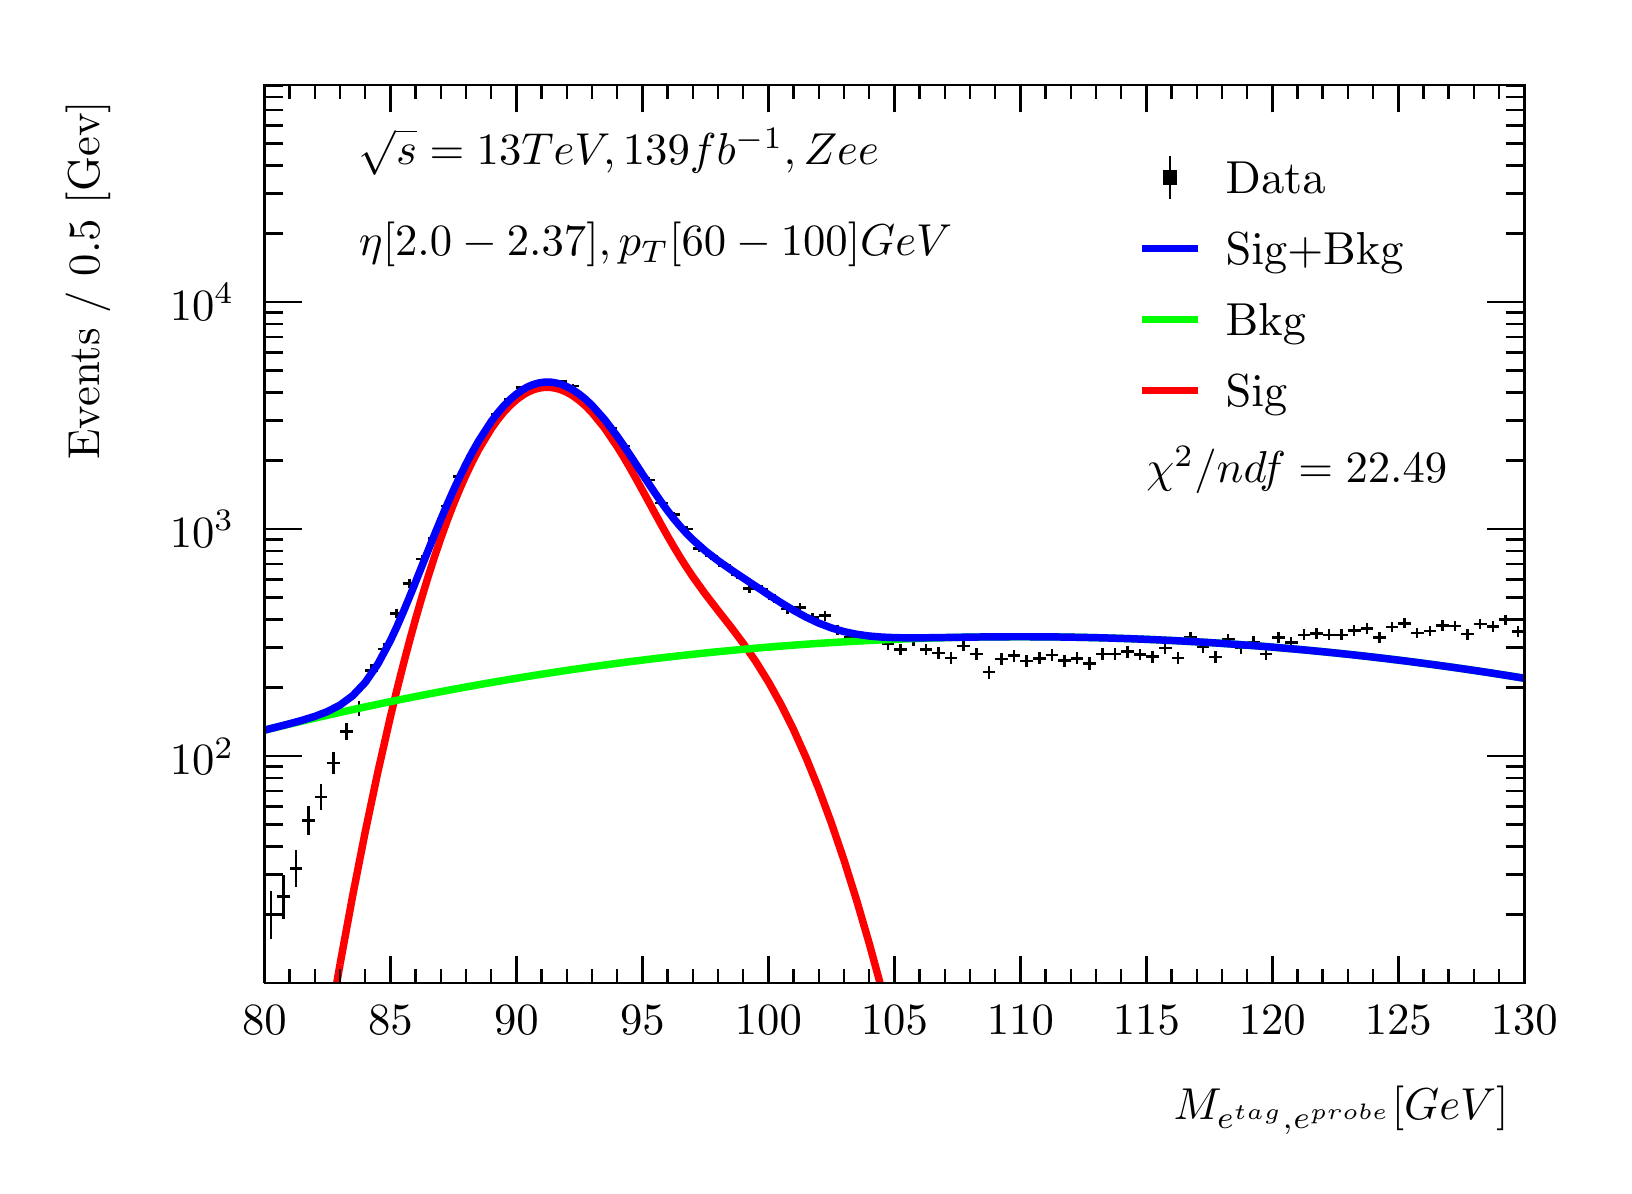
\begin{tikzpicture}
\pgfdeclareplotmark{cross} {
\pgfpathmoveto{\pgfpoint{-0.3\pgfplotmarksize}{\pgfplotmarksize}}
\pgfpathlineto{\pgfpoint{+0.3\pgfplotmarksize}{\pgfplotmarksize}}
\pgfpathlineto{\pgfpoint{+0.3\pgfplotmarksize}{0.3\pgfplotmarksize}}
\pgfpathlineto{\pgfpoint{+1\pgfplotmarksize}{0.3\pgfplotmarksize}}
\pgfpathlineto{\pgfpoint{+1\pgfplotmarksize}{-0.3\pgfplotmarksize}}
\pgfpathlineto{\pgfpoint{+0.3\pgfplotmarksize}{-0.3\pgfplotmarksize}}
\pgfpathlineto{\pgfpoint{+0.3\pgfplotmarksize}{-1.\pgfplotmarksize}}
\pgfpathlineto{\pgfpoint{-0.3\pgfplotmarksize}{-1.\pgfplotmarksize}}
\pgfpathlineto{\pgfpoint{-0.3\pgfplotmarksize}{-0.3\pgfplotmarksize}}
\pgfpathlineto{\pgfpoint{-1.\pgfplotmarksize}{-0.3\pgfplotmarksize}}
\pgfpathlineto{\pgfpoint{-1.\pgfplotmarksize}{0.3\pgfplotmarksize}}
\pgfpathlineto{\pgfpoint{-0.3\pgfplotmarksize}{0.3\pgfplotmarksize}}
\pgfpathclose
\pgfusepathqstroke
}
\pgfdeclareplotmark{cross*} {
\pgfpathmoveto{\pgfpoint{-0.3\pgfplotmarksize}{\pgfplotmarksize}}
\pgfpathlineto{\pgfpoint{+0.3\pgfplotmarksize}{\pgfplotmarksize}}
\pgfpathlineto{\pgfpoint{+0.3\pgfplotmarksize}{0.3\pgfplotmarksize}}
\pgfpathlineto{\pgfpoint{+1\pgfplotmarksize}{0.3\pgfplotmarksize}}
\pgfpathlineto{\pgfpoint{+1\pgfplotmarksize}{-0.3\pgfplotmarksize}}
\pgfpathlineto{\pgfpoint{+0.3\pgfplotmarksize}{-0.3\pgfplotmarksize}}
\pgfpathlineto{\pgfpoint{+0.3\pgfplotmarksize}{-1.\pgfplotmarksize}}
\pgfpathlineto{\pgfpoint{-0.3\pgfplotmarksize}{-1.\pgfplotmarksize}}
\pgfpathlineto{\pgfpoint{-0.3\pgfplotmarksize}{-0.3\pgfplotmarksize}}
\pgfpathlineto{\pgfpoint{-1.\pgfplotmarksize}{-0.3\pgfplotmarksize}}
\pgfpathlineto{\pgfpoint{-1.\pgfplotmarksize}{0.3\pgfplotmarksize}}
\pgfpathlineto{\pgfpoint{-0.3\pgfplotmarksize}{0.3\pgfplotmarksize}}
\pgfpathclose
\pgfusepathqfillstroke
}
\pgfdeclareplotmark{newstar} {
\pgfpathmoveto{\pgfqpoint{0pt}{\pgfplotmarksize}}
\pgfpathlineto{\pgfqpointpolar{44}{0.5\pgfplotmarksize}}
\pgfpathlineto{\pgfqpointpolar{18}{\pgfplotmarksize}}
\pgfpathlineto{\pgfqpointpolar{-20}{0.5\pgfplotmarksize}}
\pgfpathlineto{\pgfqpointpolar{-54}{\pgfplotmarksize}}
\pgfpathlineto{\pgfqpointpolar{-90}{0.5\pgfplotmarksize}}
\pgfpathlineto{\pgfqpointpolar{234}{\pgfplotmarksize}}
\pgfpathlineto{\pgfqpointpolar{198}{0.5\pgfplotmarksize}}
\pgfpathlineto{\pgfqpointpolar{162}{\pgfplotmarksize}}
\pgfpathlineto{\pgfqpointpolar{134}{0.5\pgfplotmarksize}}
\pgfpathclose
\pgfusepathqstroke
}
\pgfdeclareplotmark{newstar*} {
\pgfpathmoveto{\pgfqpoint{0pt}{\pgfplotmarksize}}
\pgfpathlineto{\pgfqpointpolar{44}{0.5\pgfplotmarksize}}
\pgfpathlineto{\pgfqpointpolar{18}{\pgfplotmarksize}}
\pgfpathlineto{\pgfqpointpolar{-20}{0.5\pgfplotmarksize}}
\pgfpathlineto{\pgfqpointpolar{-54}{\pgfplotmarksize}}
\pgfpathlineto{\pgfqpointpolar{-90}{0.5\pgfplotmarksize}}
\pgfpathlineto{\pgfqpointpolar{234}{\pgfplotmarksize}}
\pgfpathlineto{\pgfqpointpolar{198}{0.5\pgfplotmarksize}}
\pgfpathlineto{\pgfqpointpolar{162}{\pgfplotmarksize}}
\pgfpathlineto{\pgfqpointpolar{134}{0.5\pgfplotmarksize}}
\pgfpathclose
\pgfusepathqfillstroke
}
\definecolor{c}{rgb}{1,1,1};
\draw [color=c, fill=c] (0,0) rectangle (20,14.4361);
\draw [color=c, fill=c] (3,2.30977) rectangle (19,13.7143);
\definecolor{c}{rgb}{0,0,0};
\draw [c,line width=0.9] (3,2.30977) -- (3,13.7143) -- (19,13.7143) -- (19,2.30977) -- (3,2.30977);
\definecolor{c}{rgb}{1,1,1};
\draw [color=c, fill=c] (3,2.30977) rectangle (19,13.7143);
\definecolor{c}{rgb}{0,0,0};
\draw [c,line width=0.9] (3,2.30977) -- (3,13.7143) -- (19,13.7143) -- (19,2.30977) -- (3,2.30977);
\draw [c,line width=0.9] (3,2.30977) -- (19,2.30977);
\draw [c,line width=0.9] (3,2.65624) -- (3,2.30977);
\draw [c,line width=0.9] (3.32,2.48301) -- (3.32,2.30977);
\draw [c,line width=0.9] (3.64,2.48301) -- (3.64,2.30977);
\draw [c,line width=0.9] (3.96,2.48301) -- (3.96,2.30977);
\draw [c,line width=0.9] (4.28,2.48301) -- (4.28,2.30977);
\draw [c,line width=0.9] (4.6,2.65624) -- (4.6,2.30977);
\draw [c,line width=0.9] (4.92,2.48301) -- (4.92,2.30977);
\draw [c,line width=0.9] (5.24,2.48301) -- (5.24,2.30977);
\draw [c,line width=0.9] (5.56,2.48301) -- (5.56,2.30977);
\draw [c,line width=0.9] (5.88,2.48301) -- (5.88,2.30977);
\draw [c,line width=0.9] (6.2,2.65624) -- (6.2,2.30977);
\draw [c,line width=0.9] (6.52,2.48301) -- (6.52,2.30977);
\draw [c,line width=0.9] (6.84,2.48301) -- (6.84,2.30977);
\draw [c,line width=0.9] (7.16,2.48301) -- (7.16,2.30977);
\draw [c,line width=0.9] (7.48,2.48301) -- (7.48,2.30977);
\draw [c,line width=0.9] (7.8,2.65624) -- (7.8,2.30977);
\draw [c,line width=0.9] (8.12,2.48301) -- (8.12,2.30977);
\draw [c,line width=0.9] (8.44,2.48301) -- (8.44,2.30977);
\draw [c,line width=0.9] (8.76,2.48301) -- (8.76,2.30977);
\draw [c,line width=0.9] (9.08,2.48301) -- (9.08,2.30977);
\draw [c,line width=0.9] (9.4,2.65624) -- (9.4,2.30977);
\draw [c,line width=0.9] (9.72,2.48301) -- (9.72,2.30977);
\draw [c,line width=0.9] (10.04,2.48301) -- (10.04,2.30977);
\draw [c,line width=0.9] (10.36,2.48301) -- (10.36,2.30977);
\draw [c,line width=0.9] (10.68,2.48301) -- (10.68,2.30977);
\draw [c,line width=0.9] (11,2.65624) -- (11,2.30977);
\draw [c,line width=0.9] (11.32,2.48301) -- (11.32,2.30977);
\draw [c,line width=0.9] (11.64,2.48301) -- (11.64,2.30977);
\draw [c,line width=0.9] (11.96,2.48301) -- (11.96,2.30977);
\draw [c,line width=0.9] (12.28,2.48301) -- (12.28,2.30977);
\draw [c,line width=0.9] (12.6,2.65624) -- (12.6,2.30977);
\draw [c,line width=0.9] (12.92,2.48301) -- (12.92,2.30977);
\draw [c,line width=0.9] (13.24,2.48301) -- (13.24,2.30977);
\draw [c,line width=0.9] (13.56,2.48301) -- (13.56,2.30977);
\draw [c,line width=0.9] (13.88,2.48301) -- (13.88,2.30977);
\draw [c,line width=0.9] (14.2,2.65624) -- (14.2,2.30977);
\draw [c,line width=0.9] (14.52,2.48301) -- (14.52,2.30977);
\draw [c,line width=0.9] (14.84,2.48301) -- (14.84,2.30977);
\draw [c,line width=0.9] (15.16,2.48301) -- (15.16,2.30977);
\draw [c,line width=0.9] (15.48,2.48301) -- (15.48,2.30977);
\draw [c,line width=0.9] (15.8,2.65624) -- (15.8,2.30977);
\draw [c,line width=0.9] (16.12,2.48301) -- (16.12,2.30977);
\draw [c,line width=0.9] (16.44,2.48301) -- (16.44,2.30977);
\draw [c,line width=0.9] (16.76,2.48301) -- (16.76,2.30977);
\draw [c,line width=0.9] (17.08,2.48301) -- (17.08,2.30977);
\draw [c,line width=0.9] (17.4,2.65624) -- (17.4,2.30977);
\draw [c,line width=0.9] (17.72,2.48301) -- (17.72,2.30977);
\draw [c,line width=0.9] (18.04,2.48301) -- (18.04,2.30977);
\draw [c,line width=0.9] (18.36,2.48301) -- (18.36,2.30977);
\draw [c,line width=0.9] (18.68,2.48301) -- (18.68,2.30977);
\draw [c,line width=0.9] (19,2.65624) -- (19,2.30977);
\draw [anchor=base] (3,1.66015) node[scale=1.61424, color=c, rotate=0]{80};
\draw [anchor=base] (4.6,1.66015) node[scale=1.61424, color=c, rotate=0]{85};
\draw [anchor=base] (6.2,1.66015) node[scale=1.61424, color=c, rotate=0]{90};
\draw [anchor=base] (7.8,1.66015) node[scale=1.61424, color=c, rotate=0]{95};
\draw [anchor=base] (9.4,1.66015) node[scale=1.61424, color=c, rotate=0]{100};
\draw [anchor=base] (11,1.66015) node[scale=1.61424, color=c, rotate=0]{105};
\draw [anchor=base] (12.6,1.66015) node[scale=1.61424, color=c, rotate=0]{110};
\draw [anchor=base] (14.2,1.66015) node[scale=1.61424, color=c, rotate=0]{115};
\draw [anchor=base] (15.8,1.66015) node[scale=1.61424, color=c, rotate=0]{120};
\draw [anchor=base] (17.4,1.66015) node[scale=1.61424, color=c, rotate=0]{125};
\draw [anchor=base] (19,1.66015) node[scale=1.61424, color=c, rotate=0]{130};
\draw [anchor= east] (19,0.692932) node[scale=1.61424, color=c, rotate=0]{$M_{e^{tag}, e^{probe}}  [GeV]$};
\draw [c,line width=0.9] (3,13.7143) -- (19,13.7143);
\draw [c,line width=0.9] (3,13.3678) -- (3,13.7143);
\draw [c,line width=0.9] (3.32,13.5411) -- (3.32,13.7143);
\draw [c,line width=0.9] (3.64,13.5411) -- (3.64,13.7143);
\draw [c,line width=0.9] (3.96,13.5411) -- (3.96,13.7143);
\draw [c,line width=0.9] (4.28,13.5411) -- (4.28,13.7143);
\draw [c,line width=0.9] (4.6,13.3678) -- (4.6,13.7143);
\draw [c,line width=0.9] (4.92,13.5411) -- (4.92,13.7143);
\draw [c,line width=0.9] (5.24,13.5411) -- (5.24,13.7143);
\draw [c,line width=0.9] (5.56,13.5411) -- (5.56,13.7143);
\draw [c,line width=0.9] (5.88,13.5411) -- (5.88,13.7143);
\draw [c,line width=0.9] (6.2,13.3678) -- (6.2,13.7143);
\draw [c,line width=0.9] (6.52,13.5411) -- (6.52,13.7143);
\draw [c,line width=0.9] (6.84,13.5411) -- (6.84,13.7143);
\draw [c,line width=0.9] (7.16,13.5411) -- (7.16,13.7143);
\draw [c,line width=0.9] (7.48,13.5411) -- (7.48,13.7143);
\draw [c,line width=0.9] (7.8,13.3678) -- (7.8,13.7143);
\draw [c,line width=0.9] (8.12,13.5411) -- (8.12,13.7143);
\draw [c,line width=0.9] (8.44,13.5411) -- (8.44,13.7143);
\draw [c,line width=0.9] (8.76,13.5411) -- (8.76,13.7143);
\draw [c,line width=0.9] (9.08,13.5411) -- (9.08,13.7143);
\draw [c,line width=0.9] (9.4,13.3678) -- (9.4,13.7143);
\draw [c,line width=0.9] (9.72,13.5411) -- (9.72,13.7143);
\draw [c,line width=0.9] (10.04,13.5411) -- (10.04,13.7143);
\draw [c,line width=0.9] (10.36,13.5411) -- (10.36,13.7143);
\draw [c,line width=0.9] (10.68,13.5411) -- (10.68,13.7143);
\draw [c,line width=0.9] (11,13.3678) -- (11,13.7143);
\draw [c,line width=0.9] (11.32,13.5411) -- (11.32,13.7143);
\draw [c,line width=0.9] (11.64,13.5411) -- (11.64,13.7143);
\draw [c,line width=0.9] (11.96,13.5411) -- (11.96,13.7143);
\draw [c,line width=0.9] (12.28,13.5411) -- (12.28,13.7143);
\draw [c,line width=0.9] (12.6,13.3678) -- (12.6,13.7143);
\draw [c,line width=0.9] (12.92,13.5411) -- (12.92,13.7143);
\draw [c,line width=0.9] (13.24,13.5411) -- (13.24,13.7143);
\draw [c,line width=0.9] (13.56,13.5411) -- (13.56,13.7143);
\draw [c,line width=0.9] (13.88,13.5411) -- (13.88,13.7143);
\draw [c,line width=0.9] (14.2,13.3678) -- (14.2,13.7143);
\draw [c,line width=0.9] (14.52,13.5411) -- (14.52,13.7143);
\draw [c,line width=0.9] (14.84,13.5411) -- (14.84,13.7143);
\draw [c,line width=0.9] (15.16,13.5411) -- (15.16,13.7143);
\draw [c,line width=0.9] (15.48,13.5411) -- (15.48,13.7143);
\draw [c,line width=0.9] (15.8,13.3678) -- (15.8,13.7143);
\draw [c,line width=0.9] (16.12,13.5411) -- (16.12,13.7143);
\draw [c,line width=0.9] (16.44,13.5411) -- (16.44,13.7143);
\draw [c,line width=0.9] (16.76,13.5411) -- (16.76,13.7143);
\draw [c,line width=0.9] (17.08,13.5411) -- (17.08,13.7143);
\draw [c,line width=0.9] (17.4,13.3678) -- (17.4,13.7143);
\draw [c,line width=0.9] (17.72,13.5411) -- (17.72,13.7143);
\draw [c,line width=0.9] (18.04,13.5411) -- (18.04,13.7143);
\draw [c,line width=0.9] (18.36,13.5411) -- (18.36,13.7143);
\draw [c,line width=0.9] (18.68,13.5411) -- (18.68,13.7143);
\draw [c,line width=0.9] (19,13.3678) -- (19,13.7143);
\draw [c,line width=0.9] (3,2.30977) -- (3,13.7143);
\draw [c,line width=0.9] (3.237,3.17769) -- (3,3.17769);
\draw [c,line width=0.9] (3.237,3.68539) -- (3,3.68539);
\draw [c,line width=0.9] (3.237,4.04561) -- (3,4.04561);
\draw [c,line width=0.9] (3.237,4.32501) -- (3,4.32501);
\draw [c,line width=0.9] (3.237,4.55331) -- (3,4.55331);
\draw [c,line width=0.9] (3.237,4.74632) -- (3,4.74632);
\draw [c,line width=0.9] (3.237,4.91352) -- (3,4.91352);
\draw [c,line width=0.9] (3.237,5.061) -- (3,5.061);
\draw [c,line width=0.9] (3.474,5.19293) -- (3,5.19293);
\draw [anchor= east] (2.82,5.19293) node[scale=1.61424, color=c, rotate=0]{$10^{2}$};
\draw [c,line width=0.9] (3.237,6.06085) -- (3,6.06085);
\draw [c,line width=0.9] (3.237,6.56855) -- (3,6.56855);
\draw [c,line width=0.9] (3.237,6.92876) -- (3,6.92876);
\draw [c,line width=0.9] (3.237,7.20817) -- (3,7.20817);
\draw [c,line width=0.9] (3.237,7.43646) -- (3,7.43646);
\draw [c,line width=0.9] (3.237,7.62948) -- (3,7.62948);
\draw [c,line width=0.9] (3.237,7.79668) -- (3,7.79668);
\draw [c,line width=0.9] (3.237,7.94416) -- (3,7.94416);
\draw [c,line width=0.9] (3.474,8.07609) -- (3,8.07609);
\draw [anchor= east] (2.82,8.07609) node[scale=1.61424, color=c, rotate=0]{$10^{3}$};
\draw [c,line width=0.9] (3.237,8.94401) -- (3,8.94401);
\draw [c,line width=0.9] (3.237,9.4517) -- (3,9.4517);
\draw [c,line width=0.9] (3.237,9.81192) -- (3,9.81192);
\draw [c,line width=0.9] (3.237,10.0913) -- (3,10.0913);
\draw [c,line width=0.9] (3.237,10.3196) -- (3,10.3196);
\draw [c,line width=0.9] (3.237,10.5126) -- (3,10.5126);
\draw [c,line width=0.9] (3.237,10.6798) -- (3,10.6798);
\draw [c,line width=0.9] (3.237,10.8273) -- (3,10.8273);
\draw [c,line width=0.9] (3.474,10.9592) -- (3,10.9592);
\draw [anchor= east] (2.82,10.9592) node[scale=1.61424, color=c, rotate=0]{$10^{4}$};
\draw [c,line width=0.9] (3.237,11.8272) -- (3,11.8272);
\draw [c,line width=0.9] (3.237,12.3349) -- (3,12.3349);
\draw [c,line width=0.9] (3.237,12.6951) -- (3,12.6951);
\draw [c,line width=0.9] (3.237,12.9745) -- (3,12.9745);
\draw [c,line width=0.9] (3.237,13.2028) -- (3,13.2028);
\draw [c,line width=0.9] (3.237,13.3958) -- (3,13.3958);
\draw [c,line width=0.9] (3.237,13.563) -- (3,13.563);
\draw [c,line width=0.9] (3.237,13.7105) -- (3,13.7105);
\draw [anchor= east] (0.76,13.7143) node[scale=1.61424, color=c, rotate=90]{Events / 0.5 [Gev]};
\draw [c,line width=0.9] (19,2.30977) -- (19,13.7143);
\draw [c,line width=0.9] (18.763,3.17769) -- (19,3.17769);
\draw [c,line width=0.9] (18.763,3.68539) -- (19,3.68539);
\draw [c,line width=0.9] (18.763,4.04561) -- (19,4.04561);
\draw [c,line width=0.9] (18.763,4.32501) -- (19,4.32501);
\draw [c,line width=0.9] (18.763,4.55331) -- (19,4.55331);
\draw [c,line width=0.9] (18.763,4.74632) -- (19,4.74632);
\draw [c,line width=0.9] (18.763,4.91352) -- (19,4.91352);
\draw [c,line width=0.9] (18.763,5.061) -- (19,5.061);
\draw [c,line width=0.9] (18.526,5.19293) -- (19,5.19293);
\draw [c,line width=0.9] (18.763,6.06085) -- (19,6.06085);
\draw [c,line width=0.9] (18.763,6.56855) -- (19,6.56855);
\draw [c,line width=0.9] (18.763,6.92876) -- (19,6.92876);
\draw [c,line width=0.9] (18.763,7.20817) -- (19,7.20817);
\draw [c,line width=0.9] (18.763,7.43646) -- (19,7.43646);
\draw [c,line width=0.9] (18.763,7.62948) -- (19,7.62948);
\draw [c,line width=0.9] (18.763,7.79668) -- (19,7.79668);
\draw [c,line width=0.9] (18.763,7.94416) -- (19,7.94416);
\draw [c,line width=0.9] (18.526,8.07609) -- (19,8.07609);
\draw [c,line width=0.9] (18.763,8.94401) -- (19,8.94401);
\draw [c,line width=0.9] (18.763,9.4517) -- (19,9.4517);
\draw [c,line width=0.9] (18.763,9.81192) -- (19,9.81192);
\draw [c,line width=0.9] (18.763,10.0913) -- (19,10.0913);
\draw [c,line width=0.9] (18.763,10.3196) -- (19,10.3196);
\draw [c,line width=0.9] (18.763,10.5126) -- (19,10.5126);
\draw [c,line width=0.9] (18.763,10.6798) -- (19,10.6798);
\draw [c,line width=0.9] (18.763,10.8273) -- (19,10.8273);
\draw [c,line width=0.9] (18.526,10.9592) -- (19,10.9592);
\draw [c,line width=0.9] (18.763,11.8272) -- (19,11.8272);
\draw [c,line width=0.9] (18.763,12.3349) -- (19,12.3349);
\draw [c,line width=0.9] (18.763,12.6951) -- (19,12.6951);
\draw [c,line width=0.9] (18.763,12.9745) -- (19,12.9745);
\draw [c,line width=0.9] (18.763,13.2028) -- (19,13.2028);
\draw [c,line width=0.9] (18.763,13.3958) -- (19,13.3958);
\draw [c,line width=0.9] (18.763,13.563) -- (19,13.563);
\draw [c,line width=0.9] (18.763,13.7105) -- (19,13.7105);
\draw [c,line width=0.9] (3.08,3.17769) -- (3,3.17769);
\draw [c,line width=0.9] (3,3.17769) -- (3,3.17769);
\draw [c,line width=0.9] (3.08,3.17769) -- (3.16,3.17769);
\draw [c,line width=0.9] (3.16,3.17769) -- (3.16,3.17769);
\draw [c,line width=0.9] (3.08,3.17769) -- (3.08,3.48418);
\draw [c,line width=0.9] (3.08,3.48418) -- (3.08,3.48418);
\draw [c,line width=0.9] (3.08,3.17769) -- (3.08,2.86382);
\draw [c,line width=0.9] (3.08,2.86382) -- (3.08,2.86382);
\draw [c,line width=0.9] (3.24,3.40598) -- (3.16,3.40598);
\draw [c,line width=0.9] (3.16,3.40598) -- (3.16,3.40598);
\draw [c,line width=0.9] (3.24,3.40598) -- (3.32,3.40598);
\draw [c,line width=0.9] (3.32,3.40598) -- (3.32,3.40598);
\draw [c,line width=0.9] (3.24,3.40598) -- (3.24,3.68401);
\draw [c,line width=0.9] (3.24,3.68401) -- (3.24,3.68401);
\draw [c,line width=0.9] (3.24,3.40598) -- (3.24,3.12236);
\draw [c,line width=0.9] (3.24,3.12236) -- (3.24,3.12236);
\draw [c,line width=0.9] (3.4,3.7662) -- (3.32,3.7662);
\draw [c,line width=0.9] (3.32,3.7662) -- (3.32,3.7662);
\draw [c,line width=0.9] (3.4,3.7662) -- (3.48,3.7662);
\draw [c,line width=0.9] (3.48,3.7662) -- (3.48,3.7662);
\draw [c,line width=0.9] (3.4,3.7662) -- (3.4,4.00475);
\draw [c,line width=0.9] (3.4,4.00475) -- (3.4,4.00475);
\draw [c,line width=0.9] (3.4,3.7662) -- (3.4,3.52404);
\draw [c,line width=0.9] (3.4,3.52404) -- (3.4,3.52404);
\draw [c,line width=0.9] (3.56,4.37413) -- (3.48,4.37413);
\draw [c,line width=0.9] (3.48,4.37413) -- (3.48,4.37413);
\draw [c,line width=0.9] (3.56,4.37413) -- (3.64,4.37413);
\draw [c,line width=0.9] (3.64,4.37413) -- (3.64,4.37413);
\draw [c,line width=0.9] (3.56,4.37413) -- (3.56,4.55867);
\draw [c,line width=0.9] (3.56,4.55867) -- (3.56,4.55867);
\draw [c,line width=0.9] (3.56,4.37413) -- (3.56,4.18785);
\draw [c,line width=0.9] (3.56,4.18785) -- (3.56,4.18785);
\draw [c,line width=0.9] (3.72,4.67265) -- (3.64,4.67265);
\draw [c,line width=0.9] (3.64,4.67265) -- (3.64,4.67265);
\draw [c,line width=0.9] (3.72,4.67265) -- (3.8,4.67265);
\draw [c,line width=0.9] (3.8,4.67265) -- (3.8,4.67265);
\draw [c,line width=0.9] (3.72,4.67265) -- (3.72,4.83547);
\draw [c,line width=0.9] (3.72,4.83547) -- (3.72,4.83547);
\draw [c,line width=0.9] (3.72,4.67265) -- (3.72,4.50862);
\draw [c,line width=0.9] (3.72,4.50862) -- (3.72,4.50862);
\draw [c,line width=0.9] (3.88,5.10206) -- (3.8,5.10206);
\draw [c,line width=0.9] (3.8,5.10206) -- (3.8,5.10206);
\draw [c,line width=0.9] (3.88,5.10206) -- (3.96,5.10206);
\draw [c,line width=0.9] (3.96,5.10206) -- (3.96,5.10206);
\draw [c,line width=0.9] (3.88,5.10206) -- (3.88,5.23816);
\draw [c,line width=0.9] (3.88,5.23816) -- (3.88,5.23816);
\draw [c,line width=0.9] (3.88,5.10206) -- (3.88,4.96525);
\draw [c,line width=0.9] (3.88,4.96525) -- (3.88,4.96525);
\draw [c,line width=0.9] (4.04,5.50204) -- (3.96,5.50204);
\draw [c,line width=0.9] (3.96,5.50204) -- (3.96,5.50204);
\draw [c,line width=0.9] (4.04,5.50204) -- (4.12,5.50204);
\draw [c,line width=0.9] (4.12,5.50204) -- (4.12,5.50204);
\draw [c,line width=0.9] (4.04,5.50204) -- (4.04,5.61267);
\draw [c,line width=0.9] (4.04,5.61267) -- (4.04,5.61267);
\draw [c,line width=0.9] (4.04,5.50204) -- (4.04,5.3914);
\draw [c,line width=0.9] (4.04,5.3914) -- (4.04,5.3914);
\draw [c,line width=0.9] (4.2,5.797) -- (4.12,5.797);
\draw [c,line width=0.9] (4.12,5.797) -- (4.12,5.797);
\draw [c,line width=0.9] (4.2,5.797) -- (4.28,5.797);
\draw [c,line width=0.9] (4.28,5.797) -- (4.28,5.797);
\draw [c,line width=0.9] (4.2,5.797) -- (4.2,5.89535);
\draw [c,line width=0.9] (4.2,5.89535) -- (4.2,5.89535);
\draw [c,line width=0.9] (4.2,5.797) -- (4.2,5.69865);
\draw [c,line width=0.9] (4.2,5.69865) -- (4.2,5.69865);
\draw [c,line width=0.9] (4.36,6.27866) -- (4.28,6.27866);
\draw [c,line width=0.9] (4.28,6.27866) -- (4.28,6.27866);
\draw [c,line width=0.9] (4.36,6.27866) -- (4.44,6.27866);
\draw [c,line width=0.9] (4.44,6.27866) -- (4.44,6.27866);
\draw [c,line width=0.9] (4.36,6.27866) -- (4.36,6.35981);
\draw [c,line width=0.9] (4.36,6.35981) -- (4.36,6.35981);
\draw [c,line width=0.9] (4.36,6.27866) -- (4.36,6.19751);
\draw [c,line width=0.9] (4.36,6.19751) -- (4.36,6.19751);
\draw [c,line width=0.9] (4.52,6.55174) -- (4.44,6.55174);
\draw [c,line width=0.9] (4.44,6.55174) -- (4.44,6.55174);
\draw [c,line width=0.9] (4.52,6.55174) -- (4.6,6.55174);
\draw [c,line width=0.9] (4.6,6.55174) -- (4.6,6.55174);
\draw [c,line width=0.9] (4.52,6.55174) -- (4.52,6.62451);
\draw [c,line width=0.9] (4.52,6.62451) -- (4.52,6.62451);
\draw [c,line width=0.9] (4.52,6.55174) -- (4.52,6.47897);
\draw [c,line width=0.9] (4.52,6.47897) -- (4.52,6.47897);
\draw [c,line width=0.9] (4.68,7.00468) -- (4.6,7.00468);
\draw [c,line width=0.9] (4.6,7.00468) -- (4.6,7.00468);
\draw [c,line width=0.9] (4.68,7.00468) -- (4.76,7.00468);
\draw [c,line width=0.9] (4.76,7.00468) -- (4.76,7.00468);
\draw [c,line width=0.9] (4.68,7.00468) -- (4.68,7.06541);
\draw [c,line width=0.9] (4.68,7.06541) -- (4.68,7.06541);
\draw [c,line width=0.9] (4.68,7.00468) -- (4.68,6.94394);
\draw [c,line width=0.9] (4.68,6.94394) -- (4.68,6.94394);
\draw [c,line width=0.9] (4.84,7.38317) -- (4.76,7.38317);
\draw [c,line width=0.9] (4.76,7.38317) -- (4.76,7.38317);
\draw [c,line width=0.9] (4.84,7.38317) -- (4.92,7.38317);
\draw [c,line width=0.9] (4.92,7.38317) -- (4.92,7.38317);
\draw [c,line width=0.9] (4.84,7.38317) -- (4.84,7.43539);
\draw [c,line width=0.9] (4.84,7.43539) -- (4.84,7.43539);
\draw [c,line width=0.9] (4.84,7.38317) -- (4.84,7.33096);
\draw [c,line width=0.9] (4.84,7.33096) -- (4.84,7.33096);
\draw [c,line width=0.9] (5,7.69398) -- (4.92,7.69398);
\draw [c,line width=0.9] (4.92,7.69398) -- (4.92,7.69398);
\draw [c,line width=0.9] (5,7.69398) -- (5.08,7.69398);
\draw [c,line width=0.9] (5.08,7.69398) -- (5.08,7.69398);
\draw [c,line width=0.9] (5,7.69398) -- (5,7.7401);
\draw [c,line width=0.9] (5,7.7401) -- (5,7.7401);
\draw [c,line width=0.9] (5,7.69398) -- (5,7.64786);
\draw [c,line width=0.9] (5,7.64786) -- (5,7.64786);
\draw [c,line width=0.9] (5.16,7.95387) -- (5.08,7.95387);
\draw [c,line width=0.9] (5.08,7.95387) -- (5.08,7.95387);
\draw [c,line width=0.9] (5.16,7.95387) -- (5.24,7.95387);
\draw [c,line width=0.9] (5.24,7.95387) -- (5.24,7.95387);
\draw [c,line width=0.9] (5.16,7.95387) -- (5.16,7.99544);
\draw [c,line width=0.9] (5.16,7.99544) -- (5.16,7.99544);
\draw [c,line width=0.9] (5.16,7.95387) -- (5.16,7.91229);
\draw [c,line width=0.9] (5.16,7.91229) -- (5.16,7.91229);
\draw [c,line width=0.9] (5.32,8.37043) -- (5.24,8.37043);
\draw [c,line width=0.9] (5.24,8.37043) -- (5.24,8.37043);
\draw [c,line width=0.9] (5.32,8.37043) -- (5.4,8.37043);
\draw [c,line width=0.9] (5.4,8.37043) -- (5.4,8.37043);
\draw [c,line width=0.9] (5.32,8.37043) -- (5.32,8.40564);
\draw [c,line width=0.9] (5.32,8.40564) -- (5.32,8.40564);
\draw [c,line width=0.9] (5.32,8.37043) -- (5.32,8.33523);
\draw [c,line width=0.9] (5.32,8.33523) -- (5.32,8.33523);
\draw [c,line width=0.9] (5.48,8.74272) -- (5.4,8.74272);
\draw [c,line width=0.9] (5.4,8.74272) -- (5.4,8.74272);
\draw [c,line width=0.9] (5.48,8.74272) -- (5.56,8.74272);
\draw [c,line width=0.9] (5.56,8.74272) -- (5.56,8.74272);
\draw [c,line width=0.9] (5.48,8.74272) -- (5.48,8.77306);
\draw [c,line width=0.9] (5.48,8.77306) -- (5.48,8.77306);
\draw [c,line width=0.9] (5.48,8.74272) -- (5.48,8.71238);
\draw [c,line width=0.9] (5.48,8.71238) -- (5.48,8.71238);
\draw [c,line width=0.9] (5.64,9.0045) -- (5.56,9.0045);
\draw [c,line width=0.9] (5.56,9.0045) -- (5.56,9.0045);
\draw [c,line width=0.9] (5.64,9.0045) -- (5.72,9.0045);
\draw [c,line width=0.9] (5.72,9.0045) -- (5.72,9.0045);
\draw [c,line width=0.9] (5.64,9.0045) -- (5.64,9.03183);
\draw [c,line width=0.9] (5.64,9.03183) -- (5.64,9.03183);
\draw [c,line width=0.9] (5.64,9.0045) -- (5.64,8.97717);
\draw [c,line width=0.9] (5.64,8.97717) -- (5.64,8.97717);
\draw [c,line width=0.9] (5.8,9.26915) -- (5.72,9.26915);
\draw [c,line width=0.9] (5.72,9.26915) -- (5.72,9.26915);
\draw [c,line width=0.9] (5.8,9.26915) -- (5.88,9.26915);
\draw [c,line width=0.9] (5.88,9.26915) -- (5.88,9.26915);
\draw [c,line width=0.9] (5.8,9.26915) -- (5.8,9.29374);
\draw [c,line width=0.9] (5.8,9.29374) -- (5.8,9.29374);
\draw [c,line width=0.9] (5.8,9.26915) -- (5.8,9.24456);
\draw [c,line width=0.9] (5.8,9.24456) -- (5.8,9.24456);
\draw [c,line width=0.9] (5.96,9.53525) -- (5.88,9.53525);
\draw [c,line width=0.9] (5.88,9.53525) -- (5.88,9.53525);
\draw [c,line width=0.9] (5.96,9.53525) -- (6.04,9.53525);
\draw [c,line width=0.9] (6.04,9.53525) -- (6.04,9.53525);
\draw [c,line width=0.9] (5.96,9.53525) -- (5.96,9.55736);
\draw [c,line width=0.9] (5.96,9.55736) -- (5.96,9.55736);
\draw [c,line width=0.9] (5.96,9.53525) -- (5.96,9.51314);
\draw [c,line width=0.9] (5.96,9.51314) -- (5.96,9.51314);
\draw [c,line width=0.9] (6.12,9.72206) -- (6.04,9.72206);
\draw [c,line width=0.9] (6.04,9.72206) -- (6.04,9.72206);
\draw [c,line width=0.9] (6.12,9.72206) -- (6.2,9.72206);
\draw [c,line width=0.9] (6.2,9.72206) -- (6.2,9.72206);
\draw [c,line width=0.9] (6.12,9.72206) -- (6.12,9.74259);
\draw [c,line width=0.9] (6.12,9.74259) -- (6.12,9.74259);
\draw [c,line width=0.9] (6.12,9.72206) -- (6.12,9.70154);
\draw [c,line width=0.9] (6.12,9.70154) -- (6.12,9.70154);
\draw [c,line width=0.9] (6.28,9.87182) -- (6.2,9.87182);
\draw [c,line width=0.9] (6.2,9.87182) -- (6.2,9.87182);
\draw [c,line width=0.9] (6.28,9.87182) -- (6.36,9.87182);
\draw [c,line width=0.9] (6.36,9.87182) -- (6.36,9.87182);
\draw [c,line width=0.9] (6.28,9.87182) -- (6.28,9.89115);
\draw [c,line width=0.9] (6.28,9.89115) -- (6.28,9.89115);
\draw [c,line width=0.9] (6.28,9.87182) -- (6.28,9.85249);
\draw [c,line width=0.9] (6.28,9.85249) -- (6.28,9.85249);
\draw [c,line width=0.9] (6.44,9.9135) -- (6.36,9.9135);
\draw [c,line width=0.9] (6.36,9.9135) -- (6.36,9.9135);
\draw [c,line width=0.9] (6.44,9.9135) -- (6.52,9.9135);
\draw [c,line width=0.9] (6.52,9.9135) -- (6.52,9.9135);
\draw [c,line width=0.9] (6.44,9.9135) -- (6.44,9.93251);
\draw [c,line width=0.9] (6.44,9.93251) -- (6.44,9.93251);
\draw [c,line width=0.9] (6.44,9.9135) -- (6.44,9.89449);
\draw [c,line width=0.9] (6.44,9.89449) -- (6.44,9.89449);
\draw [c,line width=0.9] (6.6,9.94626) -- (6.52,9.94626);
\draw [c,line width=0.9] (6.52,9.94626) -- (6.52,9.94626);
\draw [c,line width=0.9] (6.6,9.94626) -- (6.68,9.94626);
\draw [c,line width=0.9] (6.68,9.94626) -- (6.68,9.94626);
\draw [c,line width=0.9] (6.6,9.94626) -- (6.6,9.96502);
\draw [c,line width=0.9] (6.6,9.96502) -- (6.6,9.96502);
\draw [c,line width=0.9] (6.6,9.94626) -- (6.6,9.92749);
\draw [c,line width=0.9] (6.6,9.92749) -- (6.6,9.92749);
\draw [c,line width=0.9] (6.76,9.95215) -- (6.68,9.95215);
\draw [c,line width=0.9] (6.68,9.95215) -- (6.68,9.95215);
\draw [c,line width=0.9] (6.76,9.95215) -- (6.84,9.95215);
\draw [c,line width=0.9] (6.84,9.95215) -- (6.84,9.95215);
\draw [c,line width=0.9] (6.76,9.95215) -- (6.76,9.97087);
\draw [c,line width=0.9] (6.76,9.97087) -- (6.76,9.97087);
\draw [c,line width=0.9] (6.76,9.95215) -- (6.76,9.93343);
\draw [c,line width=0.9] (6.76,9.93343) -- (6.76,9.93343);
\draw [c,line width=0.9] (6.92,9.89313) -- (6.84,9.89313);
\draw [c,line width=0.9] (6.84,9.89313) -- (6.84,9.89313);
\draw [c,line width=0.9] (6.92,9.89313) -- (7,9.89313);
\draw [c,line width=0.9] (7,9.89313) -- (7,9.89313);
\draw [c,line width=0.9] (6.92,9.89313) -- (6.92,9.91229);
\draw [c,line width=0.9] (6.92,9.91229) -- (6.92,9.91229);
\draw [c,line width=0.9] (6.92,9.89313) -- (6.92,9.87396);
\draw [c,line width=0.9] (6.92,9.87396) -- (6.92,9.87396);
\draw [c,line width=0.9] (7.08,9.69624) -- (7,9.69624);
\draw [c,line width=0.9] (7,9.69624) -- (7,9.69624);
\draw [c,line width=0.9] (7.08,9.69624) -- (7.16,9.69624);
\draw [c,line width=0.9] (7.16,9.69624) -- (7.16,9.69624);
\draw [c,line width=0.9] (7.08,9.69624) -- (7.08,9.71697);
\draw [c,line width=0.9] (7.08,9.71697) -- (7.08,9.71697);
\draw [c,line width=0.9] (7.08,9.69624) -- (7.08,9.67551);
\draw [c,line width=0.9] (7.08,9.67551) -- (7.08,9.67551);
\draw [c,line width=0.9] (7.24,9.51597) -- (7.16,9.51597);
\draw [c,line width=0.9] (7.16,9.51597) -- (7.16,9.51597);
\draw [c,line width=0.9] (7.24,9.51597) -- (7.32,9.51597);
\draw [c,line width=0.9] (7.32,9.51597) -- (7.32,9.51597);
\draw [c,line width=0.9] (7.24,9.51597) -- (7.24,9.53826);
\draw [c,line width=0.9] (7.24,9.53826) -- (7.24,9.53826);
\draw [c,line width=0.9] (7.24,9.51597) -- (7.24,9.49369);
\draw [c,line width=0.9] (7.24,9.49369) -- (7.24,9.49369);
\draw [c,line width=0.9] (7.4,9.35454) -- (7.32,9.35454);
\draw [c,line width=0.9] (7.32,9.35454) -- (7.32,9.35454);
\draw [c,line width=0.9] (7.4,9.35454) -- (7.48,9.35454);
\draw [c,line width=0.9] (7.48,9.35454) -- (7.48,9.35454);
\draw [c,line width=0.9] (7.4,9.35454) -- (7.4,9.3783);
\draw [c,line width=0.9] (7.4,9.3783) -- (7.4,9.3783);
\draw [c,line width=0.9] (7.4,9.35454) -- (7.4,9.33077);
\draw [c,line width=0.9] (7.4,9.33077) -- (7.4,9.33077);
\draw [c,line width=0.9] (7.56,9.12769) -- (7.48,9.12769);
\draw [c,line width=0.9] (7.48,9.12769) -- (7.48,9.12769);
\draw [c,line width=0.9] (7.56,9.12769) -- (7.64,9.12769);
\draw [c,line width=0.9] (7.64,9.12769) -- (7.64,9.12769);
\draw [c,line width=0.9] (7.56,9.12769) -- (7.56,9.15371);
\draw [c,line width=0.9] (7.56,9.15371) -- (7.56,9.15371);
\draw [c,line width=0.9] (7.56,9.12769) -- (7.56,9.10167);
\draw [c,line width=0.9] (7.56,9.10167) -- (7.56,9.10167);
\draw [c,line width=0.9] (7.72,8.84164) -- (7.64,8.84164);
\draw [c,line width=0.9] (7.64,8.84164) -- (7.64,8.84164);
\draw [c,line width=0.9] (7.72,8.84164) -- (7.8,8.84164);
\draw [c,line width=0.9] (7.8,8.84164) -- (7.8,8.84164);
\draw [c,line width=0.9] (7.72,8.84164) -- (7.72,8.87081);
\draw [c,line width=0.9] (7.72,8.87081) -- (7.72,8.87081);
\draw [c,line width=0.9] (7.72,8.84164) -- (7.72,8.81248);
\draw [c,line width=0.9] (7.72,8.81248) -- (7.72,8.81248);
\draw [c,line width=0.9] (7.88,8.70009) -- (7.8,8.70009);
\draw [c,line width=0.9] (7.8,8.70009) -- (7.8,8.70009);
\draw [c,line width=0.9] (7.88,8.70009) -- (7.96,8.70009);
\draw [c,line width=0.9] (7.96,8.70009) -- (7.96,8.70009);
\draw [c,line width=0.9] (7.88,8.70009) -- (7.88,8.73095);
\draw [c,line width=0.9] (7.88,8.73095) -- (7.88,8.73095);
\draw [c,line width=0.9] (7.88,8.70009) -- (7.88,8.66923);
\draw [c,line width=0.9] (7.88,8.66923) -- (7.88,8.66923);
\draw [c,line width=0.9] (8.04,8.40845) -- (7.96,8.40845);
\draw [c,line width=0.9] (7.96,8.40845) -- (7.96,8.40845);
\draw [c,line width=0.9] (8.04,8.40845) -- (8.12,8.40845);
\draw [c,line width=0.9] (8.12,8.40845) -- (8.12,8.40845);
\draw [c,line width=0.9] (8.04,8.40845) -- (8.04,8.44313);
\draw [c,line width=0.9] (8.04,8.44313) -- (8.04,8.44313);
\draw [c,line width=0.9] (8.04,8.40845) -- (8.04,8.37378);
\draw [c,line width=0.9] (8.04,8.37378) -- (8.04,8.37378);
\draw [c,line width=0.9] (8.2,8.25761) -- (8.12,8.25761);
\draw [c,line width=0.9] (8.12,8.25761) -- (8.12,8.25761);
\draw [c,line width=0.9] (8.2,8.25761) -- (8.28,8.25761);
\draw [c,line width=0.9] (8.28,8.25761) -- (8.28,8.25761);
\draw [c,line width=0.9] (8.2,8.25761) -- (8.2,8.29443);
\draw [c,line width=0.9] (8.2,8.29443) -- (8.2,8.29443);
\draw [c,line width=0.9] (8.2,8.25761) -- (8.2,8.22078);
\draw [c,line width=0.9] (8.2,8.22078) -- (8.2,8.22078);
\draw [c,line width=0.9] (8.36,8.07358) -- (8.28,8.07358);
\draw [c,line width=0.9] (8.28,8.07358) -- (8.28,8.07358);
\draw [c,line width=0.9] (8.36,8.07358) -- (8.44,8.07358);
\draw [c,line width=0.9] (8.44,8.07358) -- (8.44,8.07358);
\draw [c,line width=0.9] (8.36,8.07358) -- (8.36,8.11322);
\draw [c,line width=0.9] (8.36,8.11322) -- (8.36,8.11322);
\draw [c,line width=0.9] (8.36,8.07358) -- (8.36,8.03395);
\draw [c,line width=0.9] (8.36,8.03395) -- (8.36,8.03395);
\draw [c,line width=0.9] (8.52,7.82913) -- (8.44,7.82913);
\draw [c,line width=0.9] (8.44,7.82913) -- (8.44,7.82913);
\draw [c,line width=0.9] (8.52,7.82913) -- (8.6,7.82913);
\draw [c,line width=0.9] (8.6,7.82913) -- (8.6,7.82913);
\draw [c,line width=0.9] (8.52,7.82913) -- (8.52,7.87283);
\draw [c,line width=0.9] (8.52,7.87283) -- (8.52,7.87283);
\draw [c,line width=0.9] (8.52,7.82913) -- (8.52,7.78543);
\draw [c,line width=0.9] (8.52,7.78543) -- (8.52,7.78543);
\draw [c,line width=0.9] (8.68,7.73081) -- (8.6,7.73081);
\draw [c,line width=0.9] (8.6,7.73081) -- (8.6,7.73081);
\draw [c,line width=0.9] (8.68,7.73081) -- (8.76,7.73081);
\draw [c,line width=0.9] (8.76,7.73081) -- (8.76,7.73081);
\draw [c,line width=0.9] (8.68,7.73081) -- (8.68,7.77626);
\draw [c,line width=0.9] (8.68,7.77626) -- (8.68,7.77626);
\draw [c,line width=0.9] (8.68,7.73081) -- (8.68,7.68536);
\draw [c,line width=0.9] (8.68,7.68536) -- (8.68,7.68536);
\draw [c,line width=0.9] (8.84,7.60965) -- (8.76,7.60965);
\draw [c,line width=0.9] (8.76,7.60965) -- (8.76,7.60965);
\draw [c,line width=0.9] (8.84,7.60965) -- (8.92,7.60965);
\draw [c,line width=0.9] (8.92,7.60965) -- (8.92,7.60965);
\draw [c,line width=0.9] (8.84,7.60965) -- (8.84,7.65735);
\draw [c,line width=0.9] (8.84,7.65735) -- (8.84,7.65735);
\draw [c,line width=0.9] (8.84,7.60965) -- (8.84,7.56195);
\draw [c,line width=0.9] (8.84,7.56195) -- (8.84,7.56195);
\draw [c,line width=0.9] (9,7.49158) -- (8.92,7.49158);
\draw [c,line width=0.9] (8.92,7.49158) -- (8.92,7.49158);
\draw [c,line width=0.9] (9,7.49158) -- (9.08,7.49158);
\draw [c,line width=0.9] (9.08,7.49158) -- (9.08,7.49158);
\draw [c,line width=0.9] (9,7.49158) -- (9,7.54158);
\draw [c,line width=0.9] (9,7.54158) -- (9,7.54158);
\draw [c,line width=0.9] (9,7.49158) -- (9,7.44158);
\draw [c,line width=0.9] (9,7.44158) -- (9,7.44158);
\draw [c,line width=0.9] (9.16,7.31838) -- (9.08,7.31838);
\draw [c,line width=0.9] (9.08,7.31838) -- (9.08,7.31838);
\draw [c,line width=0.9] (9.16,7.31838) -- (9.24,7.31838);
\draw [c,line width=0.9] (9.24,7.31838) -- (9.24,7.31838);
\draw [c,line width=0.9] (9.16,7.31838) -- (9.16,7.37196);
\draw [c,line width=0.9] (9.16,7.37196) -- (9.16,7.37196);
\draw [c,line width=0.9] (9.16,7.31838) -- (9.16,7.26479);
\draw [c,line width=0.9] (9.16,7.26479) -- (9.16,7.26479);
\draw [c,line width=0.9] (9.32,7.30917) -- (9.24,7.30917);
\draw [c,line width=0.9] (9.24,7.30917) -- (9.24,7.30917);
\draw [c,line width=0.9] (9.32,7.30917) -- (9.4,7.30917);
\draw [c,line width=0.9] (9.4,7.30917) -- (9.4,7.30917);
\draw [c,line width=0.9] (9.32,7.30917) -- (9.32,7.36295);
\draw [c,line width=0.9] (9.32,7.36295) -- (9.32,7.36295);
\draw [c,line width=0.9] (9.32,7.30917) -- (9.32,7.25539);
\draw [c,line width=0.9] (9.32,7.25539) -- (9.32,7.25539);
\draw [c,line width=0.9] (9.48,7.18798) -- (9.4,7.18798);
\draw [c,line width=0.9] (9.4,7.18798) -- (9.4,7.18798);
\draw [c,line width=0.9] (9.48,7.18798) -- (9.56,7.18798);
\draw [c,line width=0.9] (9.56,7.18798) -- (9.56,7.18798);
\draw [c,line width=0.9] (9.48,7.18798) -- (9.48,7.24442);
\draw [c,line width=0.9] (9.48,7.24442) -- (9.48,7.24442);
\draw [c,line width=0.9] (9.48,7.18798) -- (9.48,7.13153);
\draw [c,line width=0.9] (9.48,7.13153) -- (9.48,7.13153);
\draw [c,line width=0.9] (9.64,7.06226) -- (9.56,7.06226);
\draw [c,line width=0.9] (9.56,7.06226) -- (9.56,7.06226);
\draw [c,line width=0.9] (9.64,7.06226) -- (9.72,7.06226);
\draw [c,line width=0.9] (9.72,7.06226) -- (9.72,7.06226);
\draw [c,line width=0.9] (9.64,7.06226) -- (9.64,7.12161);
\draw [c,line width=0.9] (9.64,7.12161) -- (9.64,7.12161);
\draw [c,line width=0.9] (9.64,7.06226) -- (9.64,7.0029);
\draw [c,line width=0.9] (9.64,7.0029) -- (9.64,7.0029);
\draw [c,line width=0.9] (9.8,7.07903) -- (9.72,7.07903);
\draw [c,line width=0.9] (9.72,7.07903) -- (9.72,7.07903);
\draw [c,line width=0.9] (9.8,7.07903) -- (9.88,7.07903);
\draw [c,line width=0.9] (9.88,7.07903) -- (9.88,7.07903);
\draw [c,line width=0.9] (9.8,7.07903) -- (9.8,7.13798);
\draw [c,line width=0.9] (9.8,7.13798) -- (9.8,7.13798);
\draw [c,line width=0.9] (9.8,7.07903) -- (9.8,7.02007);
\draw [c,line width=0.9] (9.8,7.02007) -- (9.8,7.02007);
\draw [c,line width=0.9] (9.96,6.95356) -- (9.88,6.95356);
\draw [c,line width=0.9] (9.88,6.95356) -- (9.88,6.95356);
\draw [c,line width=0.9] (9.96,6.95356) -- (10.04,6.95356);
\draw [c,line width=0.9] (10.04,6.95356) -- (10.04,6.95356);
\draw [c,line width=0.9] (9.96,6.95356) -- (9.96,7.01555);
\draw [c,line width=0.9] (9.96,7.01555) -- (9.96,7.01555);
\draw [c,line width=0.9] (9.96,6.95356) -- (9.96,6.89158);
\draw [c,line width=0.9] (9.96,6.89158) -- (9.96,6.89158);
\draw [c,line width=0.9] (10.12,6.97486) -- (10.04,6.97486);
\draw [c,line width=0.9] (10.04,6.97486) -- (10.04,6.97486);
\draw [c,line width=0.9] (10.12,6.97486) -- (10.2,6.97486);
\draw [c,line width=0.9] (10.2,6.97486) -- (10.2,6.97486);
\draw [c,line width=0.9] (10.12,6.97486) -- (10.12,7.03632);
\draw [c,line width=0.9] (10.12,7.03632) -- (10.12,7.03632);
\draw [c,line width=0.9] (10.12,6.97486) -- (10.12,6.9134);
\draw [c,line width=0.9] (10.12,6.9134) -- (10.12,6.9134);
\draw [c,line width=0.9] (10.28,6.79336) -- (10.2,6.79336);
\draw [c,line width=0.9] (10.2,6.79336) -- (10.2,6.79336);
\draw [c,line width=0.9] (10.28,6.79336) -- (10.36,6.79336);
\draw [c,line width=0.9] (10.36,6.79336) -- (10.36,6.79336);
\draw [c,line width=0.9] (10.28,6.79336) -- (10.28,6.85944);
\draw [c,line width=0.9] (10.28,6.85944) -- (10.28,6.85944);
\draw [c,line width=0.9] (10.28,6.79336) -- (10.28,6.72728);
\draw [c,line width=0.9] (10.28,6.72728) -- (10.28,6.72728);
\draw [c,line width=0.9] (10.44,6.70672) -- (10.36,6.70672);
\draw [c,line width=0.9] (10.36,6.70672) -- (10.36,6.70672);
\draw [c,line width=0.9] (10.44,6.70672) -- (10.52,6.70672);
\draw [c,line width=0.9] (10.52,6.70672) -- (10.52,6.70672);
\draw [c,line width=0.9] (10.44,6.70672) -- (10.44,6.77512);
\draw [c,line width=0.9] (10.44,6.77512) -- (10.44,6.77512);
\draw [c,line width=0.9] (10.44,6.70672) -- (10.44,6.63832);
\draw [c,line width=0.9] (10.44,6.63832) -- (10.44,6.63832);
\draw [c,line width=0.9] (10.6,6.68409) -- (10.52,6.68409);
\draw [c,line width=0.9] (10.52,6.68409) -- (10.52,6.68409);
\draw [c,line width=0.9] (10.6,6.68409) -- (10.68,6.68409);
\draw [c,line width=0.9] (10.68,6.68409) -- (10.68,6.68409);
\draw [c,line width=0.9] (10.6,6.68409) -- (10.6,6.75311);
\draw [c,line width=0.9] (10.6,6.75311) -- (10.6,6.75311);
\draw [c,line width=0.9] (10.6,6.68409) -- (10.6,6.61507);
\draw [c,line width=0.9] (10.6,6.61507) -- (10.6,6.61507);
\draw [c,line width=0.9] (10.76,6.68789) -- (10.68,6.68789);
\draw [c,line width=0.9] (10.68,6.68789) -- (10.68,6.68789);
\draw [c,line width=0.9] (10.76,6.68789) -- (10.84,6.68789);
\draw [c,line width=0.9] (10.84,6.68789) -- (10.84,6.68789);
\draw [c,line width=0.9] (10.76,6.68789) -- (10.76,6.75681);
\draw [c,line width=0.9] (10.76,6.75681) -- (10.76,6.75681);
\draw [c,line width=0.9] (10.76,6.68789) -- (10.76,6.61897);
\draw [c,line width=0.9] (10.76,6.61897) -- (10.76,6.61897);
\draw [c,line width=0.9] (10.92,6.61364) -- (10.84,6.61364);
\draw [c,line width=0.9] (10.84,6.61364) -- (10.84,6.61364);
\draw [c,line width=0.9] (10.92,6.61364) -- (11,6.61364);
\draw [c,line width=0.9] (11,6.61364) -- (11,6.61364);
\draw [c,line width=0.9] (10.92,6.61364) -- (10.92,6.68463);
\draw [c,line width=0.9] (10.92,6.68463) -- (10.92,6.68463);
\draw [c,line width=0.9] (10.92,6.61364) -- (10.92,6.54265);
\draw [c,line width=0.9] (10.92,6.54265) -- (10.92,6.54265);
\draw [c,line width=0.9] (11.08,6.54325) -- (11,6.54325);
\draw [c,line width=0.9] (11,6.54325) -- (11,6.54325);
\draw [c,line width=0.9] (11.08,6.54325) -- (11.16,6.54325);
\draw [c,line width=0.9] (11.16,6.54325) -- (11.16,6.54325);
\draw [c,line width=0.9] (11.08,6.54325) -- (11.08,6.61627);
\draw [c,line width=0.9] (11.08,6.61627) -- (11.08,6.61627);
\draw [c,line width=0.9] (11.08,6.54325) -- (11.08,6.47024);
\draw [c,line width=0.9] (11.08,6.47024) -- (11.08,6.47024);
\draw [c,line width=0.9] (11.24,6.66491) -- (11.16,6.66491);
\draw [c,line width=0.9] (11.16,6.66491) -- (11.16,6.66491);
\draw [c,line width=0.9] (11.24,6.66491) -- (11.32,6.66491);
\draw [c,line width=0.9] (11.32,6.66491) -- (11.32,6.66491);
\draw [c,line width=0.9] (11.24,6.66491) -- (11.24,6.73447);
\draw [c,line width=0.9] (11.24,6.73447) -- (11.24,6.73447);
\draw [c,line width=0.9] (11.24,6.66491) -- (11.24,6.59536);
\draw [c,line width=0.9] (11.24,6.59536) -- (11.24,6.59536);
\draw [c,line width=0.9] (11.4,6.5475) -- (11.32,6.5475);
\draw [c,line width=0.9] (11.32,6.5475) -- (11.32,6.5475);
\draw [c,line width=0.9] (11.4,6.5475) -- (11.48,6.5475);
\draw [c,line width=0.9] (11.48,6.5475) -- (11.48,6.5475);
\draw [c,line width=0.9] (11.4,6.5475) -- (11.4,6.6204);
\draw [c,line width=0.9] (11.4,6.6204) -- (11.4,6.6204);
\draw [c,line width=0.9] (11.4,6.5475) -- (11.4,6.47461);
\draw [c,line width=0.9] (11.4,6.47461) -- (11.4,6.47461);
\draw [c,line width=0.9] (11.56,6.50432) -- (11.48,6.50432);
\draw [c,line width=0.9] (11.48,6.50432) -- (11.48,6.50432);
\draw [c,line width=0.9] (11.56,6.50432) -- (11.64,6.50432);
\draw [c,line width=0.9] (11.64,6.50432) -- (11.64,6.50432);
\draw [c,line width=0.9] (11.56,6.50432) -- (11.56,6.57848);
\draw [c,line width=0.9] (11.56,6.57848) -- (11.56,6.57848);
\draw [c,line width=0.9] (11.56,6.50432) -- (11.56,6.43016);
\draw [c,line width=0.9] (11.56,6.43016) -- (11.56,6.43016);
\draw [c,line width=0.9] (11.72,6.43662) -- (11.64,6.43662);
\draw [c,line width=0.9] (11.64,6.43662) -- (11.64,6.43662);
\draw [c,line width=0.9] (11.72,6.43662) -- (11.8,6.43662);
\draw [c,line width=0.9] (11.8,6.43662) -- (11.8,6.43662);
\draw [c,line width=0.9] (11.72,6.43662) -- (11.72,6.51281);
\draw [c,line width=0.9] (11.72,6.51281) -- (11.72,6.51281);
\draw [c,line width=0.9] (11.72,6.43662) -- (11.72,6.36043);
\draw [c,line width=0.9] (11.72,6.36043) -- (11.72,6.36043);
\draw [c,line width=0.9] (11.88,6.59334) -- (11.8,6.59334);
\draw [c,line width=0.9] (11.8,6.59334) -- (11.8,6.59334);
\draw [c,line width=0.9] (11.88,6.59334) -- (11.96,6.59334);
\draw [c,line width=0.9] (11.96,6.59334) -- (11.96,6.59334);
\draw [c,line width=0.9] (11.88,6.59334) -- (11.88,6.66491);
\draw [c,line width=0.9] (11.88,6.66491) -- (11.88,6.66491);
\draw [c,line width=0.9] (11.88,6.59334) -- (11.88,6.52177);
\draw [c,line width=0.9] (11.88,6.52177) -- (11.88,6.52177);
\draw [c,line width=0.9] (12.04,6.49107) -- (11.96,6.49107);
\draw [c,line width=0.9] (11.96,6.49107) -- (11.96,6.49107);
\draw [c,line width=0.9] (12.04,6.49107) -- (12.12,6.49107);
\draw [c,line width=0.9] (12.12,6.49107) -- (12.12,6.49107);
\draw [c,line width=0.9] (12.04,6.49107) -- (12.04,6.56562);
\draw [c,line width=0.9] (12.04,6.56562) -- (12.04,6.56562);
\draw [c,line width=0.9] (12.04,6.49107) -- (12.04,6.41652);
\draw [c,line width=0.9] (12.04,6.41652) -- (12.04,6.41652);
\draw [c,line width=0.9] (12.2,6.25744) -- (12.12,6.25744);
\draw [c,line width=0.9] (12.12,6.25744) -- (12.12,6.25744);
\draw [c,line width=0.9] (12.2,6.25744) -- (12.28,6.25744);
\draw [c,line width=0.9] (12.28,6.25744) -- (12.28,6.25744);
\draw [c,line width=0.9] (12.2,6.25744) -- (12.2,6.33928);
\draw [c,line width=0.9] (12.2,6.33928) -- (12.2,6.33928);
\draw [c,line width=0.9] (12.2,6.25744) -- (12.2,6.1756);
\draw [c,line width=0.9] (12.2,6.1756) -- (12.2,6.1756);
\draw [c,line width=0.9] (12.36,6.42731) -- (12.28,6.42731);
\draw [c,line width=0.9] (12.28,6.42731) -- (12.28,6.42731);
\draw [c,line width=0.9] (12.36,6.42731) -- (12.44,6.42731);
\draw [c,line width=0.9] (12.44,6.42731) -- (12.44,6.42731);
\draw [c,line width=0.9] (12.36,6.42731) -- (12.36,6.50379);
\draw [c,line width=0.9] (12.36,6.50379) -- (12.36,6.50379);
\draw [c,line width=0.9] (12.36,6.42731) -- (12.36,6.35084);
\draw [c,line width=0.9] (12.36,6.35084) -- (12.36,6.35084);
\draw [c,line width=0.9] (12.52,6.46867) -- (12.44,6.46867);
\draw [c,line width=0.9] (12.44,6.46867) -- (12.44,6.46867);
\draw [c,line width=0.9] (12.52,6.46867) -- (12.6,6.46867);
\draw [c,line width=0.9] (12.6,6.46867) -- (12.6,6.46867);
\draw [c,line width=0.9] (12.52,6.46867) -- (12.52,6.54389);
\draw [c,line width=0.9] (12.52,6.54389) -- (12.52,6.54389);
\draw [c,line width=0.9] (12.52,6.46867) -- (12.52,6.39345);
\draw [c,line width=0.9] (12.52,6.39345) -- (12.52,6.39345);
\draw [c,line width=0.9] (12.68,6.39896) -- (12.6,6.39896);
\draw [c,line width=0.9] (12.6,6.39896) -- (12.6,6.39896);
\draw [c,line width=0.9] (12.68,6.39896) -- (12.76,6.39896);
\draw [c,line width=0.9] (12.76,6.39896) -- (12.76,6.39896);
\draw [c,line width=0.9] (12.68,6.39896) -- (12.68,6.47631);
\draw [c,line width=0.9] (12.68,6.47631) -- (12.68,6.47631);
\draw [c,line width=0.9] (12.68,6.39896) -- (12.68,6.32162);
\draw [c,line width=0.9] (12.68,6.32162) -- (12.68,6.32162);
\draw [c,line width=0.9] (12.84,6.43198) -- (12.76,6.43198);
\draw [c,line width=0.9] (12.76,6.43198) -- (12.76,6.43198);
\draw [c,line width=0.9] (12.84,6.43198) -- (12.92,6.43198);
\draw [c,line width=0.9] (12.92,6.43198) -- (12.92,6.43198);
\draw [c,line width=0.9] (12.84,6.43198) -- (12.84,6.50831);
\draw [c,line width=0.9] (12.84,6.50831) -- (12.84,6.50831);
\draw [c,line width=0.9] (12.84,6.43198) -- (12.84,6.35564);
\draw [c,line width=0.9] (12.84,6.35564) -- (12.84,6.35564);
\draw [c,line width=0.9] (13,6.47318) -- (12.92,6.47318);
\draw [c,line width=0.9] (12.92,6.47318) -- (12.92,6.47318);
\draw [c,line width=0.9] (13,6.47318) -- (13.08,6.47318);
\draw [c,line width=0.9] (13.08,6.47318) -- (13.08,6.47318);
\draw [c,line width=0.9] (13,6.47318) -- (13,6.54827);
\draw [c,line width=0.9] (13,6.54827) -- (13,6.54827);
\draw [c,line width=0.9] (13,6.47318) -- (13,6.3981);
\draw [c,line width=0.9] (13,6.3981) -- (13,6.3981);
\draw [c,line width=0.9] (13.16,6.40373) -- (13.08,6.40373);
\draw [c,line width=0.9] (13.08,6.40373) -- (13.08,6.40373);
\draw [c,line width=0.9] (13.16,6.40373) -- (13.24,6.40373);
\draw [c,line width=0.9] (13.24,6.40373) -- (13.24,6.40373);
\draw [c,line width=0.9] (13.16,6.40373) -- (13.16,6.48093);
\draw [c,line width=0.9] (13.16,6.48093) -- (13.16,6.48093);
\draw [c,line width=0.9] (13.16,6.40373) -- (13.16,6.32653);
\draw [c,line width=0.9] (13.16,6.32653) -- (13.16,6.32653);
\draw [c,line width=0.9] (13.32,6.43198) -- (13.24,6.43198);
\draw [c,line width=0.9] (13.24,6.43198) -- (13.24,6.43198);
\draw [c,line width=0.9] (13.32,6.43198) -- (13.4,6.43198);
\draw [c,line width=0.9] (13.4,6.43198) -- (13.4,6.43198);
\draw [c,line width=0.9] (13.32,6.43198) -- (13.32,6.50831);
\draw [c,line width=0.9] (13.32,6.50831) -- (13.32,6.50831);
\draw [c,line width=0.9] (13.32,6.43198) -- (13.32,6.35564);
\draw [c,line width=0.9] (13.32,6.35564) -- (13.32,6.35564);
\draw [c,line width=0.9] (13.48,6.36995) -- (13.4,6.36995);
\draw [c,line width=0.9] (13.4,6.36995) -- (13.4,6.36995);
\draw [c,line width=0.9] (13.48,6.36995) -- (13.56,6.36995);
\draw [c,line width=0.9] (13.56,6.36995) -- (13.56,6.36995);
\draw [c,line width=0.9] (13.48,6.36995) -- (13.48,6.4482);
\draw [c,line width=0.9] (13.48,6.4482) -- (13.48,6.4482);
\draw [c,line width=0.9] (13.48,6.36995) -- (13.48,6.29171);
\draw [c,line width=0.9] (13.48,6.29171) -- (13.48,6.29171);
\draw [c,line width=0.9] (13.64,6.49107) -- (13.56,6.49107);
\draw [c,line width=0.9] (13.56,6.49107) -- (13.56,6.49107);
\draw [c,line width=0.9] (13.64,6.49107) -- (13.72,6.49107);
\draw [c,line width=0.9] (13.72,6.49107) -- (13.72,6.49107);
\draw [c,line width=0.9] (13.64,6.49107) -- (13.64,6.56562);
\draw [c,line width=0.9] (13.64,6.56562) -- (13.64,6.56562);
\draw [c,line width=0.9] (13.64,6.49107) -- (13.64,6.41652);
\draw [c,line width=0.9] (13.64,6.41652) -- (13.64,6.41652);
\draw [c,line width=0.9] (13.8,6.48662) -- (13.72,6.48662);
\draw [c,line width=0.9] (13.72,6.48662) -- (13.72,6.48662);
\draw [c,line width=0.9] (13.8,6.48662) -- (13.88,6.48662);
\draw [c,line width=0.9] (13.88,6.48662) -- (13.88,6.48662);
\draw [c,line width=0.9] (13.8,6.48662) -- (13.8,6.56131);
\draw [c,line width=0.9] (13.8,6.56131) -- (13.8,6.56131);
\draw [c,line width=0.9] (13.8,6.48662) -- (13.8,6.41194);
\draw [c,line width=0.9] (13.8,6.41194) -- (13.8,6.41194);
\draw [c,line width=0.9] (13.96,6.51743) -- (13.88,6.51743);
\draw [c,line width=0.9] (13.88,6.51743) -- (13.88,6.51743);
\draw [c,line width=0.9] (13.96,6.51743) -- (14.04,6.51743);
\draw [c,line width=0.9] (14.04,6.51743) -- (14.04,6.51743);
\draw [c,line width=0.9] (13.96,6.51743) -- (13.96,6.59121);
\draw [c,line width=0.9] (13.96,6.59121) -- (13.96,6.59121);
\draw [c,line width=0.9] (13.96,6.51743) -- (13.96,6.44366);
\draw [c,line width=0.9] (13.96,6.44366) -- (13.96,6.44366);
\draw [c,line width=0.9] (14.12,6.48216) -- (14.04,6.48216);
\draw [c,line width=0.9] (14.04,6.48216) -- (14.04,6.48216);
\draw [c,line width=0.9] (14.12,6.48216) -- (14.2,6.48216);
\draw [c,line width=0.9] (14.2,6.48216) -- (14.2,6.48216);
\draw [c,line width=0.9] (14.12,6.48216) -- (14.12,6.55698);
\draw [c,line width=0.9] (14.12,6.55698) -- (14.12,6.55698);
\draw [c,line width=0.9] (14.12,6.48216) -- (14.12,6.40734);
\draw [c,line width=0.9] (14.12,6.40734) -- (14.12,6.40734);
\draw [c,line width=0.9] (14.28,6.45504) -- (14.2,6.45504);
\draw [c,line width=0.9] (14.2,6.45504) -- (14.2,6.45504);
\draw [c,line width=0.9] (14.28,6.45504) -- (14.36,6.45504);
\draw [c,line width=0.9] (14.36,6.45504) -- (14.36,6.45504);
\draw [c,line width=0.9] (14.28,6.45504) -- (14.28,6.53067);
\draw [c,line width=0.9] (14.28,6.53067) -- (14.28,6.53067);
\draw [c,line width=0.9] (14.28,6.45504) -- (14.28,6.3794);
\draw [c,line width=0.9] (14.28,6.3794) -- (14.28,6.3794);
\draw [c,line width=0.9] (14.44,6.56437) -- (14.36,6.56437);
\draw [c,line width=0.9] (14.36,6.56437) -- (14.36,6.56437);
\draw [c,line width=0.9] (14.44,6.56437) -- (14.52,6.56437);
\draw [c,line width=0.9] (14.52,6.56437) -- (14.52,6.56437);
\draw [c,line width=0.9] (14.44,6.56437) -- (14.44,6.63677);
\draw [c,line width=0.9] (14.44,6.63677) -- (14.44,6.63677);
\draw [c,line width=0.9] (14.44,6.56437) -- (14.44,6.49196);
\draw [c,line width=0.9] (14.44,6.49196) -- (14.44,6.49196);
\draw [c,line width=0.9] (14.6,6.43662) -- (14.52,6.43662);
\draw [c,line width=0.9] (14.52,6.43662) -- (14.52,6.43662);
\draw [c,line width=0.9] (14.6,6.43662) -- (14.68,6.43662);
\draw [c,line width=0.9] (14.68,6.43662) -- (14.68,6.43662);
\draw [c,line width=0.9] (14.6,6.43662) -- (14.6,6.51281);
\draw [c,line width=0.9] (14.6,6.51281) -- (14.6,6.51281);
\draw [c,line width=0.9] (14.6,6.43662) -- (14.6,6.36043);
\draw [c,line width=0.9] (14.6,6.36043) -- (14.6,6.36043);
\draw [c,line width=0.9] (14.76,6.69546) -- (14.68,6.69546);
\draw [c,line width=0.9] (14.68,6.69546) -- (14.68,6.69546);
\draw [c,line width=0.9] (14.76,6.69546) -- (14.84,6.69546);
\draw [c,line width=0.9] (14.84,6.69546) -- (14.84,6.69546);
\draw [c,line width=0.9] (14.76,6.69546) -- (14.76,6.76417);
\draw [c,line width=0.9] (14.76,6.76417) -- (14.76,6.76417);
\draw [c,line width=0.9] (14.76,6.69546) -- (14.76,6.62674);
\draw [c,line width=0.9] (14.76,6.62674) -- (14.76,6.62674);
\draw [c,line width=0.9] (14.92,6.57687) -- (14.84,6.57687);
\draw [c,line width=0.9] (14.84,6.57687) -- (14.84,6.57687);
\draw [c,line width=0.9] (14.92,6.57687) -- (15,6.57687);
\draw [c,line width=0.9] (15,6.57687) -- (15,6.57687);
\draw [c,line width=0.9] (14.92,6.57687) -- (14.92,6.64891);
\draw [c,line width=0.9] (14.92,6.64891) -- (14.92,6.64891);
\draw [c,line width=0.9] (14.92,6.57687) -- (14.92,6.50483);
\draw [c,line width=0.9] (14.92,6.50483) -- (14.92,6.50483);
\draw [c,line width=0.9] (15.08,6.45046) -- (15,6.45046);
\draw [c,line width=0.9] (15,6.45046) -- (15,6.45046);
\draw [c,line width=0.9] (15.08,6.45046) -- (15.16,6.45046);
\draw [c,line width=0.9] (15.16,6.45046) -- (15.16,6.45046);
\draw [c,line width=0.9] (15.08,6.45046) -- (15.08,6.52623);
\draw [c,line width=0.9] (15.08,6.52623) -- (15.08,6.52623);
\draw [c,line width=0.9] (15.08,6.45046) -- (15.08,6.37469);
\draw [c,line width=0.9] (15.08,6.37469) -- (15.08,6.37469);
\draw [c,line width=0.9] (15.24,6.67645) -- (15.16,6.67645);
\draw [c,line width=0.9] (15.16,6.67645) -- (15.16,6.67645);
\draw [c,line width=0.9] (15.24,6.67645) -- (15.32,6.67645);
\draw [c,line width=0.9] (15.32,6.67645) -- (15.32,6.67645);
\draw [c,line width=0.9] (15.24,6.67645) -- (15.24,6.74569);
\draw [c,line width=0.9] (15.24,6.74569) -- (15.24,6.74569);
\draw [c,line width=0.9] (15.24,6.67645) -- (15.24,6.60722);
\draw [c,line width=0.9] (15.24,6.60722) -- (15.24,6.60722);
\draw [c,line width=0.9] (15.4,6.56437) -- (15.32,6.56437);
\draw [c,line width=0.9] (15.32,6.56437) -- (15.32,6.56437);
\draw [c,line width=0.9] (15.4,6.56437) -- (15.48,6.56437);
\draw [c,line width=0.9] (15.48,6.56437) -- (15.48,6.56437);
\draw [c,line width=0.9] (15.4,6.56437) -- (15.4,6.63677);
\draw [c,line width=0.9] (15.4,6.63677) -- (15.4,6.63677);
\draw [c,line width=0.9] (15.4,6.56437) -- (15.4,6.49196);
\draw [c,line width=0.9] (15.4,6.49196) -- (15.4,6.49196);
\draw [c,line width=0.9] (15.56,6.64151) -- (15.48,6.64151);
\draw [c,line width=0.9] (15.48,6.64151) -- (15.48,6.64151);
\draw [c,line width=0.9] (15.56,6.64151) -- (15.64,6.64151);
\draw [c,line width=0.9] (15.64,6.64151) -- (15.64,6.64151);
\draw [c,line width=0.9] (15.56,6.64151) -- (15.56,6.71172);
\draw [c,line width=0.9] (15.56,6.71172) -- (15.56,6.71172);
\draw [c,line width=0.9] (15.56,6.64151) -- (15.56,6.5713);
\draw [c,line width=0.9] (15.56,6.5713) -- (15.56,6.5713);
\draw [c,line width=0.9] (15.72,6.49107) -- (15.64,6.49107);
\draw [c,line width=0.9] (15.64,6.49107) -- (15.64,6.49107);
\draw [c,line width=0.9] (15.72,6.49107) -- (15.8,6.49107);
\draw [c,line width=0.9] (15.8,6.49107) -- (15.8,6.49107);
\draw [c,line width=0.9] (15.72,6.49107) -- (15.72,6.56562);
\draw [c,line width=0.9] (15.72,6.56562) -- (15.72,6.56562);
\draw [c,line width=0.9] (15.72,6.49107) -- (15.72,6.41652);
\draw [c,line width=0.9] (15.72,6.41652) -- (15.72,6.41652);
\draw [c,line width=0.9] (15.88,6.69922) -- (15.8,6.69922);
\draw [c,line width=0.9] (15.8,6.69922) -- (15.8,6.69922);
\draw [c,line width=0.9] (15.88,6.69922) -- (15.96,6.69922);
\draw [c,line width=0.9] (15.96,6.69922) -- (15.96,6.69922);
\draw [c,line width=0.9] (15.88,6.69922) -- (15.88,6.76783);
\draw [c,line width=0.9] (15.88,6.76783) -- (15.88,6.76783);
\draw [c,line width=0.9] (15.88,6.69922) -- (15.88,6.63061);
\draw [c,line width=0.9] (15.88,6.63061) -- (15.88,6.63061);
\draw [c,line width=0.9] (16.04,6.63757) -- (15.96,6.63757);
\draw [c,line width=0.9] (15.96,6.63757) -- (15.96,6.63757);
\draw [c,line width=0.9] (16.04,6.63757) -- (16.12,6.63757);
\draw [c,line width=0.9] (16.12,6.63757) -- (16.12,6.63757);
\draw [c,line width=0.9] (16.04,6.63757) -- (16.04,6.70788);
\draw [c,line width=0.9] (16.04,6.70788) -- (16.04,6.70788);
\draw [c,line width=0.9] (16.04,6.63757) -- (16.04,6.56725);
\draw [c,line width=0.9] (16.04,6.56725) -- (16.04,6.56725);
\draw [c,line width=0.9] (16.2,6.73261) -- (16.12,6.73261);
\draw [c,line width=0.9] (16.12,6.73261) -- (16.12,6.73261);
\draw [c,line width=0.9] (16.2,6.73261) -- (16.28,6.73261);
\draw [c,line width=0.9] (16.28,6.73261) -- (16.28,6.73261);
\draw [c,line width=0.9] (16.2,6.73261) -- (16.2,6.80031);
\draw [c,line width=0.9] (16.2,6.80031) -- (16.2,6.80031);
\draw [c,line width=0.9] (16.2,6.73261) -- (16.2,6.66491);
\draw [c,line width=0.9] (16.2,6.66491) -- (16.2,6.66491);
\draw [c,line width=0.9] (16.36,6.75079) -- (16.28,6.75079);
\draw [c,line width=0.9] (16.28,6.75079) -- (16.28,6.75079);
\draw [c,line width=0.9] (16.36,6.75079) -- (16.44,6.75079);
\draw [c,line width=0.9] (16.44,6.75079) -- (16.44,6.75079);
\draw [c,line width=0.9] (16.36,6.75079) -- (16.36,6.818);
\draw [c,line width=0.9] (16.36,6.818) -- (16.36,6.818);
\draw [c,line width=0.9] (16.36,6.75079) -- (16.36,6.68358);
\draw [c,line width=0.9] (16.36,6.68358) -- (16.36,6.68358);
\draw [c,line width=0.9] (16.52,6.73261) -- (16.44,6.73261);
\draw [c,line width=0.9] (16.44,6.73261) -- (16.44,6.73261);
\draw [c,line width=0.9] (16.52,6.73261) -- (16.6,6.73261);
\draw [c,line width=0.9] (16.6,6.73261) -- (16.6,6.73261);
\draw [c,line width=0.9] (16.52,6.73261) -- (16.52,6.80031);
\draw [c,line width=0.9] (16.52,6.80031) -- (16.52,6.80031);
\draw [c,line width=0.9] (16.52,6.73261) -- (16.52,6.66491);
\draw [c,line width=0.9] (16.52,6.66491) -- (16.52,6.66491);
\draw [c,line width=0.9] (16.68,6.73261) -- (16.6,6.73261);
\draw [c,line width=0.9] (16.6,6.73261) -- (16.6,6.73261);
\draw [c,line width=0.9] (16.68,6.73261) -- (16.76,6.73261);
\draw [c,line width=0.9] (16.76,6.73261) -- (16.76,6.73261);
\draw [c,line width=0.9] (16.68,6.73261) -- (16.68,6.80031);
\draw [c,line width=0.9] (16.68,6.80031) -- (16.68,6.80031);
\draw [c,line width=0.9] (16.68,6.73261) -- (16.68,6.66491);
\draw [c,line width=0.9] (16.68,6.66491) -- (16.68,6.66491);
\draw [c,line width=0.9] (16.84,6.78636) -- (16.76,6.78636);
\draw [c,line width=0.9] (16.76,6.78636) -- (16.76,6.78636);
\draw [c,line width=0.9] (16.84,6.78636) -- (16.92,6.78636);
\draw [c,line width=0.9] (16.92,6.78636) -- (16.92,6.78636);
\draw [c,line width=0.9] (16.84,6.78636) -- (16.84,6.85262);
\draw [c,line width=0.9] (16.84,6.85262) -- (16.84,6.85262);
\draw [c,line width=0.9] (16.84,6.78636) -- (16.84,6.7201);
\draw [c,line width=0.9] (16.84,6.7201) -- (16.84,6.7201);
\draw [c,line width=0.9] (17,6.81411) -- (16.92,6.81411);
\draw [c,line width=0.9] (16.92,6.81411) -- (16.92,6.81411);
\draw [c,line width=0.9] (17,6.81411) -- (17.08,6.81411);
\draw [c,line width=0.9] (17.08,6.81411) -- (17.08,6.81411);
\draw [c,line width=0.9] (17,6.81411) -- (17,6.87964);
\draw [c,line width=0.9] (17,6.87964) -- (17,6.87964);
\draw [c,line width=0.9] (17,6.81411) -- (17,6.74858);
\draw [c,line width=0.9] (17,6.74858) -- (17,6.74858);
\draw [c,line width=0.9] (17.16,6.69546) -- (17.08,6.69546);
\draw [c,line width=0.9] (17.08,6.69546) -- (17.08,6.69546);
\draw [c,line width=0.9] (17.16,6.69546) -- (17.24,6.69546);
\draw [c,line width=0.9] (17.24,6.69546) -- (17.24,6.69546);
\draw [c,line width=0.9] (17.16,6.69546) -- (17.16,6.76417);
\draw [c,line width=0.9] (17.16,6.76417) -- (17.16,6.76417);
\draw [c,line width=0.9] (17.16,6.69546) -- (17.16,6.62674);
\draw [c,line width=0.9] (17.16,6.62674) -- (17.16,6.62674);
\draw [c,line width=0.9] (17.32,6.83453) -- (17.24,6.83453);
\draw [c,line width=0.9] (17.24,6.83453) -- (17.24,6.83453);
\draw [c,line width=0.9] (17.32,6.83453) -- (17.4,6.83453);
\draw [c,line width=0.9] (17.4,6.83453) -- (17.4,6.83453);
\draw [c,line width=0.9] (17.32,6.83453) -- (17.32,6.89953);
\draw [c,line width=0.9] (17.32,6.89953) -- (17.32,6.89953);
\draw [c,line width=0.9] (17.32,6.83453) -- (17.32,6.76953);
\draw [c,line width=0.9] (17.32,6.76953) -- (17.32,6.76953);
\draw [c,line width=0.9] (17.48,6.87765) -- (17.4,6.87765);
\draw [c,line width=0.9] (17.4,6.87765) -- (17.4,6.87765);
\draw [c,line width=0.9] (17.48,6.87765) -- (17.56,6.87765);
\draw [c,line width=0.9] (17.56,6.87765) -- (17.56,6.87765);
\draw [c,line width=0.9] (17.48,6.87765) -- (17.48,6.94154);
\draw [c,line width=0.9] (17.48,6.94154) -- (17.48,6.94154);
\draw [c,line width=0.9] (17.48,6.87765) -- (17.48,6.81376);
\draw [c,line width=0.9] (17.48,6.81376) -- (17.48,6.81376);
\draw [c,line width=0.9] (17.64,6.75798) -- (17.56,6.75798);
\draw [c,line width=0.9] (17.56,6.75798) -- (17.56,6.75798);
\draw [c,line width=0.9] (17.64,6.75798) -- (17.72,6.75798);
\draw [c,line width=0.9] (17.72,6.75798) -- (17.72,6.75798);
\draw [c,line width=0.9] (17.64,6.75798) -- (17.64,6.825);
\draw [c,line width=0.9] (17.64,6.825) -- (17.64,6.825);
\draw [c,line width=0.9] (17.64,6.75798) -- (17.64,6.69097);
\draw [c,line width=0.9] (17.64,6.69097) -- (17.64,6.69097);
\draw [c,line width=0.9] (17.8,6.78285) -- (17.72,6.78285);
\draw [c,line width=0.9] (17.72,6.78285) -- (17.72,6.78285);
\draw [c,line width=0.9] (17.8,6.78285) -- (17.88,6.78285);
\draw [c,line width=0.9] (17.88,6.78285) -- (17.88,6.78285);
\draw [c,line width=0.9] (17.8,6.78285) -- (17.8,6.84921);
\draw [c,line width=0.9] (17.8,6.84921) -- (17.8,6.84921);
\draw [c,line width=0.9] (17.8,6.78285) -- (17.8,6.71649);
\draw [c,line width=0.9] (17.8,6.71649) -- (17.8,6.71649);
\draw [c,line width=0.9] (17.96,6.85129) -- (17.88,6.85129);
\draw [c,line width=0.9] (17.88,6.85129) -- (17.88,6.85129);
\draw [c,line width=0.9] (17.96,6.85129) -- (18.04,6.85129);
\draw [c,line width=0.9] (18.04,6.85129) -- (18.04,6.85129);
\draw [c,line width=0.9] (17.96,6.85129) -- (17.96,6.91586);
\draw [c,line width=0.9] (17.96,6.91586) -- (17.96,6.91586);
\draw [c,line width=0.9] (17.96,6.85129) -- (17.96,6.78672);
\draw [c,line width=0.9] (17.96,6.78672) -- (17.96,6.78672);
\draw [c,line width=0.9] (18.12,6.84126) -- (18.04,6.84126);
\draw [c,line width=0.9] (18.04,6.84126) -- (18.04,6.84126);
\draw [c,line width=0.9] (18.12,6.84126) -- (18.2,6.84126);
\draw [c,line width=0.9] (18.2,6.84126) -- (18.2,6.84126);
\draw [c,line width=0.9] (18.12,6.84126) -- (18.12,6.90609);
\draw [c,line width=0.9] (18.12,6.90609) -- (18.12,6.90609);
\draw [c,line width=0.9] (18.12,6.84126) -- (18.12,6.77643);
\draw [c,line width=0.9] (18.12,6.77643) -- (18.12,6.77643);
\draw [c,line width=0.9] (18.28,6.73991) -- (18.2,6.73991);
\draw [c,line width=0.9] (18.2,6.73991) -- (18.2,6.73991);
\draw [c,line width=0.9] (18.28,6.73991) -- (18.36,6.73991);
\draw [c,line width=0.9] (18.36,6.73991) -- (18.36,6.73991);
\draw [c,line width=0.9] (18.28,6.73991) -- (18.28,6.80742);
\draw [c,line width=0.9] (18.28,6.80742) -- (18.28,6.80742);
\draw [c,line width=0.9] (18.28,6.73991) -- (18.28,6.67241);
\draw [c,line width=0.9] (18.28,6.67241) -- (18.28,6.67241);
\draw [c,line width=0.9] (18.44,6.86783) -- (18.36,6.86783);
\draw [c,line width=0.9] (18.36,6.86783) -- (18.36,6.86783);
\draw [c,line width=0.9] (18.44,6.86783) -- (18.52,6.86783);
\draw [c,line width=0.9] (18.52,6.86783) -- (18.52,6.86783);
\draw [c,line width=0.9] (18.44,6.86783) -- (18.44,6.93197);
\draw [c,line width=0.9] (18.44,6.93197) -- (18.44,6.93197);
\draw [c,line width=0.9] (18.44,6.86783) -- (18.44,6.80369);
\draw [c,line width=0.9] (18.44,6.80369) -- (18.44,6.80369);
\draw [c,line width=0.9] (18.6,6.8379) -- (18.52,6.8379);
\draw [c,line width=0.9] (18.52,6.8379) -- (18.52,6.8379);
\draw [c,line width=0.9] (18.6,6.8379) -- (18.68,6.8379);
\draw [c,line width=0.9] (18.68,6.8379) -- (18.68,6.8379);
\draw [c,line width=0.9] (18.6,6.8379) -- (18.6,6.90281);
\draw [c,line width=0.9] (18.6,6.90281) -- (18.6,6.90281);
\draw [c,line width=0.9] (18.6,6.8379) -- (18.6,6.77298);
\draw [c,line width=0.9] (18.6,6.77298) -- (18.6,6.77298);
\draw [c,line width=0.9] (18.76,6.92563) -- (18.68,6.92563);
\draw [c,line width=0.9] (18.68,6.92563) -- (18.68,6.92563);
\draw [c,line width=0.9] (18.76,6.92563) -- (18.84,6.92563);
\draw [c,line width=0.9] (18.84,6.92563) -- (18.84,6.92563);
\draw [c,line width=0.9] (18.76,6.92563) -- (18.76,6.98831);
\draw [c,line width=0.9] (18.76,6.98831) -- (18.76,6.98831);
\draw [c,line width=0.9] (18.76,6.92563) -- (18.76,6.86295);
\draw [c,line width=0.9] (18.76,6.86295) -- (18.76,6.86295);
\draw [c,line width=0.9] (18.92,6.77225) -- (18.84,6.77225);
\draw [c,line width=0.9] (18.84,6.77225) -- (18.84,6.77225);
\draw [c,line width=0.9] (18.92,6.77225) -- (19,6.77225);
\draw [c,line width=0.9] (19,6.77225) -- (19,6.77225);
\draw [c,line width=0.9] (18.92,6.77225) -- (18.92,6.83889);
\draw [c,line width=0.9] (18.92,6.83889) -- (18.92,6.83889);
\draw [c,line width=0.9] (18.92,6.77225) -- (18.92,6.70562);
\draw [c,line width=0.9] (18.92,6.70562) -- (18.92,6.70562);
\foreach \P in {(3.08,3.17769), (3.24,3.40598), (3.4,3.7662), (3.56,4.37413), (3.72,4.67265), (3.88,5.10206), (4.04,5.50204), (4.2,5.797), (4.36,6.27866), (4.52,6.55174), (4.68,7.00468), (4.84,7.38317), (5,7.69398), (5.16,7.95387), (5.32,8.37043),
 (5.48,8.74272), (5.64,9.0045), (5.8,9.26915), (5.96,9.53525), (6.12,9.72206), (6.28,9.87182), (6.44,9.9135), (6.6,9.94626), (6.76,9.95215), (6.92,9.89313), (7.08,9.69624), (7.24,9.51597), (7.4,9.35454), (7.56,9.12769), (7.72,8.84164),
 (7.88,8.70009), (8.04,8.40845), (8.2,8.25761), (8.36,8.07358), (8.52,7.82913), (8.68,7.73081), (8.84,7.60965), (9,7.49158), (9.16,7.31838), (9.32,7.30917), (9.48,7.18798), (9.64,7.06226), (9.8,7.07903), (9.96,6.95356), (10.12,6.97486),
 (10.28,6.79336), (10.44,6.70672), (10.6,6.68409), (10.76,6.68789), (10.92,6.61364), (11.08,6.54325), (11.24,6.66491), (11.4,6.5475), (11.56,6.50432), (11.72,6.43662), (11.88,6.59334), (12.04,6.49107), (12.2,6.25744), (12.36,6.42731),
 (12.52,6.46867), (12.68,6.39896), (12.84,6.43198), (13,6.47318), (13.16,6.40373), (13.32,6.43198), (13.48,6.36995), (13.64,6.49107), (13.8,6.48662), (13.96,6.51743), (14.12,6.48216), (14.28,6.45504), (14.44,6.56437), (14.6,6.43662), (14.76,6.69546),
 (14.92,6.57687), (15.08,6.45046), (15.24,6.67645), (15.4,6.56437), (15.56,6.64151), (15.72,6.49107), (15.88,6.69922), (16.04,6.63757), (16.2,6.73261), (16.36,6.75079), (16.52,6.73261), (16.68,6.73261), (16.84,6.78636), (17,6.81411), (17.16,6.69546),
 (17.32,6.83453), (17.48,6.87765), (17.64,6.75798), (17.8,6.78285), (17.96,6.85129), (18.12,6.84126), (18.28,6.73991), (18.44,6.86783), (18.6,6.8379), (18.76,6.92563), (18.92,6.77225)}{\draw[mark options={color=c,fill=c},mark size=2.882883pt,mark=]
 plot coordinates {\P};}
\definecolor{c}{rgb}{1,0,0};
\draw [c,line width=2.7] (3.91849,2.30977) -- (3.96,2.54925);
\draw [c,line width=2.7] (3.96,2.54925) -- (4.12,3.41751) -- (4.28,4.2309) -- (4.44,4.98942) -- (4.6,5.69308) -- (4.68,6.02434) -- (4.76,6.34189) -- (4.84,6.64573) -- (4.92,6.93586) -- (5,7.21228) -- (5.08,7.475) -- (5.16,7.72402) -- (5.24,7.95934)
 -- (5.32,8.18096) -- (5.4,8.3889) -- (5.48,8.58316) -- (5.56,8.76375) -- (5.64,8.93067) -- (5.72,9.08393) -- (5.88,9.34955) -- (5.96,9.46194) -- (6.04,9.56075) -- (6.12,9.64599) -- (6.2,9.71772) -- (6.28,9.77596) -- (6.32,9.80005) -- (6.36,9.82078)
 -- (6.4,9.83817) -- (6.44,9.85223) -- (6.48,9.86296) -- (6.52,9.87038) -- (6.56,9.87451) -- (6.6,9.87534) -- (6.64,9.87291) -- (6.68,9.86722) -- (6.72,9.8583) -- (6.76,9.84616) -- (6.8,9.83083) -- (6.84,9.81234) -- (6.88,9.7907) -- (6.92,9.76597) --
 (7,9.70732) -- (7.08,9.63673) -- (7.16,9.5546) -- (7.32,9.35781) -- (7.48,9.12232) -- (7.56,8.99237) -- (7.64,8.85584) -- (7.72,8.71414) -- (7.8,8.56883) -- (7.88,8.4216) -- (7.96,8.27423) -- (8.04,8.12849) -- (8.12,7.98602) -- (8.2,7.84822) --
 (8.28,7.71612) -- (8.36,7.59029) -- (8.44,7.47078) -- (8.6,7.24854) -- (8.76,7.04116) -- (8.92,6.83693) -- (9.08,6.62406) -- (9.24,6.39273) -- (9.4,6.13567) -- (9.56,5.84794) -- (9.72,5.52633) -- (9.88,5.16887) -- (10.04,4.77434) -- (10.2,4.34205)
 -- (10.36,3.87158) -- (10.52,3.3627) -- (10.68,2.81527) -- (10.818,2.30977);
\definecolor{c}{rgb}{0,1,0};
\draw [c,line width=2.7] (3,5.52122) -- (3,5.52122);
\draw [c,line width=2.7] (3,5.52122) -- (3.16,5.56045) -- (3.32,5.59901) -- (3.48,5.63692) -- (3.64,5.67417) -- (3.8,5.71075) -- (3.96,5.74668) -- (4.12,5.78195) -- (4.28,5.81656) -- (4.44,5.85051) -- (4.6,5.8838) -- (4.76,5.91643) -- (4.92,5.94841)
 -- (5.08,5.97972) -- (5.24,6.01037) -- (5.4,6.04037) -- (5.56,6.0697) -- (5.72,6.09838) -- (5.88,6.1264) -- (6.04,6.15376) -- (6.2,6.18045) -- (6.36,6.20649) -- (6.52,6.23187) -- (6.68,6.2566) -- (6.84,6.28066) -- (7,6.30406) -- (7.16,6.3268) --
 (7.32,6.34889) -- (7.48,6.37031) -- (7.64,6.39108) -- (7.8,6.41119) -- (7.96,6.43063) -- (8.12,6.44942) -- (8.28,6.46755) -- (8.44,6.48502) -- (8.6,6.50183) -- (8.76,6.51798) -- (8.92,6.53347) -- (9.08,6.54831) -- (9.24,6.56248) -- (9.4,6.57599) --
 (9.56,6.58885) -- (9.72,6.60104) -- (9.88,6.61258) -- (10.04,6.62346) -- (10.2,6.63368) -- (10.36,6.64323) -- (10.52,6.65213) -- (10.68,6.66037) -- (10.84,6.66796) -- (11,6.67488) -- (11.16,6.68114) -- (11.32,6.68674) -- (11.48,6.69169) --
 (11.64,6.69597) -- (11.8,6.6996) -- (11.96,6.70257) -- (12.12,6.70487) -- (12.28,6.70652) -- (12.44,6.70751) -- (12.6,6.70784) -- (12.76,6.70751) -- (12.92,6.70652) -- (13.08,6.70487) -- (13.24,6.70257) -- (13.4,6.6996) -- (13.56,6.69597) --
 (13.72,6.69169) -- (13.88,6.68674) -- (14.04,6.68114) -- (14.2,6.67488) -- (14.36,6.66796) -- (14.52,6.66037) -- (14.68,6.65213) -- (14.84,6.64323) -- (15,6.63368) -- (15.16,6.62346) -- (15.32,6.61258) -- (15.48,6.60104) -- (15.64,6.58885) --
 (15.8,6.57599) -- (15.96,6.56248) -- (16.12,6.54831) -- (16.28,6.53347) -- (16.44,6.51798) -- (16.6,6.50183) -- (16.76,6.48502) -- (16.92,6.46755) -- (17.08,6.44942) -- (17.24,6.43063) -- (17.4,6.41119) -- (17.56,6.39108) -- (17.72,6.37031) --
 (17.88,6.34889) -- (18.04,6.3268) -- (18.2,6.30406) -- (18.36,6.28066) -- (18.52,6.2566) -- (18.68,6.23187) -- (18.84,6.20649) -- (19,6.18045) -- (19,6.18045) -- (19,6.18045);
\definecolor{c}{rgb}{0,0,1};
\draw [c,line width=2.7] (3,5.52196) -- (3,5.52196);
\draw [c,line width=2.7] (3,5.52196) -- (3.16,5.56228) -- (3.32,5.60342) -- (3.48,5.64709) -- (3.64,5.69658) -- (3.8,5.75782) -- (3.96,5.8405) -- (4.12,5.95839) -- (4.28,6.12748) -- (4.44,6.36049) -- (4.6,6.65999) -- (4.68,6.83173) -- (4.76,7.01506)
 -- (4.84,7.20714) -- (4.92,7.40496) -- (5,7.6056) -- (5.08,7.80635) -- (5.16,8.00481) -- (5.24,8.19892) -- (5.32,8.38694) -- (5.4,8.56745) -- (5.48,8.73928) -- (5.56,8.90151) -- (5.64,9.05338) -- (5.72,9.1943) -- (5.88,9.44153) -- (5.96,9.54718) --
 (6.04,9.64055) -- (6.12,9.72149) -- (6.2,9.78987) -- (6.28,9.84563) -- (6.32,9.86876) -- (6.36,9.88874) -- (6.4,9.90555) -- (6.44,9.9192) -- (6.48,9.92971) -- (6.52,9.93707) -- (6.56,9.9413) -- (6.6,9.94242) -- (6.64,9.94043) -- (6.68,9.93537) --
 (6.72,9.92725) -- (6.76,9.91609) -- (6.8,9.90193) -- (6.84,9.88479) -- (6.92,9.84177) -- (7,9.78736) -- (7.08,9.72201) -- (7.16,9.64625) -- (7.32,9.46622) -- (7.48,9.25417) -- (7.56,9.13898) -- (7.64,9.01955) -- (7.72,8.89748) -- (7.8,8.77448) --
 (7.88,8.65234) -- (7.96,8.53281) -- (8.04,8.41753) -- (8.12,8.30789) -- (8.2,8.20494) -- (8.28,8.10933) -- (8.36,8.02123) -- (8.44,7.94042) -- (8.6,7.79796) -- (8.76,7.67462) -- (8.92,7.56229) -- (9.08,7.45467) -- (9.24,7.34839) -- (9.4,7.243) --
 (9.56,7.14033) -- (9.72,7.04353) -- (9.88,6.95612) -- (10.04,6.88101) -- (10.2,6.81994) -- (10.36,6.77313) -- (10.52,6.73953) -- (10.68,6.71715) -- (10.84,6.70359) -- (11,6.69652) -- (11.16,6.69386) -- (11.32,6.69399) -- (11.48,6.69569) --
 (11.64,6.69811) -- (11.8,6.70071) -- (11.96,6.70312) -- (12.12,6.70515) -- (12.28,6.70665) -- (12.44,6.70757) -- (12.6,6.70787) -- (12.76,6.70752) -- (12.92,6.70653) -- (13.08,6.70487) -- (13.24,6.70257) -- (13.4,6.6996) -- (13.56,6.69597) --
 (13.72,6.69169) -- (13.88,6.68674) -- (14.04,6.68114) -- (14.2,6.67488) -- (14.36,6.66796) -- (14.52,6.66037) -- (14.68,6.65213) -- (14.84,6.64323) -- (15,6.63368) -- (15.16,6.62346) -- (15.32,6.61258) -- (15.48,6.60104) -- (15.64,6.58885) --
 (15.8,6.57599) -- (15.96,6.56248) -- (16.12,6.54831) -- (16.28,6.53347) -- (16.44,6.51798) -- (16.6,6.50183) -- (16.76,6.48502) -- (16.92,6.46755) -- (17.08,6.44942) -- (17.24,6.43063) -- (17.4,6.41119) -- (17.56,6.39108) -- (17.72,6.37031) --
 (17.88,6.34889) -- (18.04,6.3268) -- (18.2,6.30406) -- (18.36,6.28066) -- (18.52,6.2566) -- (18.68,6.23187) -- (18.84,6.20649) -- (19,6.18045) -- (19,6.18045) -- (19,6.18045);
\definecolor{c}{rgb}{0,0,0};
\draw [c,line width=0.9] (3,2.30977) -- (19,2.30977);
\draw [c,line width=0.9] (3,2.65624) -- (3,2.30977);
\draw [c,line width=0.9] (3.32,2.48301) -- (3.32,2.30977);
\draw [c,line width=0.9] (3.64,2.48301) -- (3.64,2.30977);
\draw [c,line width=0.9] (3.96,2.48301) -- (3.96,2.30977);
\draw [c,line width=0.9] (4.28,2.48301) -- (4.28,2.30977);
\draw [c,line width=0.9] (4.6,2.65624) -- (4.6,2.30977);
\draw [c,line width=0.9] (4.92,2.48301) -- (4.92,2.30977);
\draw [c,line width=0.9] (5.24,2.48301) -- (5.24,2.30977);
\draw [c,line width=0.9] (5.56,2.48301) -- (5.56,2.30977);
\draw [c,line width=0.9] (5.88,2.48301) -- (5.88,2.30977);
\draw [c,line width=0.9] (6.2,2.65624) -- (6.2,2.30977);
\draw [c,line width=0.9] (6.52,2.48301) -- (6.52,2.30977);
\draw [c,line width=0.9] (6.84,2.48301) -- (6.84,2.30977);
\draw [c,line width=0.9] (7.16,2.48301) -- (7.16,2.30977);
\draw [c,line width=0.9] (7.48,2.48301) -- (7.48,2.30977);
\draw [c,line width=0.9] (7.8,2.65624) -- (7.8,2.30977);
\draw [c,line width=0.9] (8.12,2.48301) -- (8.12,2.30977);
\draw [c,line width=0.9] (8.44,2.48301) -- (8.44,2.30977);
\draw [c,line width=0.9] (8.76,2.48301) -- (8.76,2.30977);
\draw [c,line width=0.9] (9.08,2.48301) -- (9.08,2.30977);
\draw [c,line width=0.9] (9.4,2.65624) -- (9.4,2.30977);
\draw [c,line width=0.9] (9.72,2.48301) -- (9.72,2.30977);
\draw [c,line width=0.9] (10.04,2.48301) -- (10.04,2.30977);
\draw [c,line width=0.9] (10.36,2.48301) -- (10.36,2.30977);
\draw [c,line width=0.9] (10.68,2.48301) -- (10.68,2.30977);
\draw [c,line width=0.9] (11,2.65624) -- (11,2.30977);
\draw [c,line width=0.9] (11.32,2.48301) -- (11.32,2.30977);
\draw [c,line width=0.9] (11.64,2.48301) -- (11.64,2.30977);
\draw [c,line width=0.9] (11.96,2.48301) -- (11.96,2.30977);
\draw [c,line width=0.9] (12.28,2.48301) -- (12.28,2.30977);
\draw [c,line width=0.9] (12.6,2.65624) -- (12.6,2.30977);
\draw [c,line width=0.9] (12.92,2.48301) -- (12.92,2.30977);
\draw [c,line width=0.9] (13.24,2.48301) -- (13.24,2.30977);
\draw [c,line width=0.9] (13.56,2.48301) -- (13.56,2.30977);
\draw [c,line width=0.9] (13.88,2.48301) -- (13.88,2.30977);
\draw [c,line width=0.9] (14.2,2.65624) -- (14.2,2.30977);
\draw [c,line width=0.9] (14.52,2.48301) -- (14.52,2.30977);
\draw [c,line width=0.9] (14.84,2.48301) -- (14.84,2.30977);
\draw [c,line width=0.9] (15.16,2.48301) -- (15.16,2.30977);
\draw [c,line width=0.9] (15.48,2.48301) -- (15.48,2.30977);
\draw [c,line width=0.9] (15.8,2.65624) -- (15.8,2.30977);
\draw [c,line width=0.9] (16.12,2.48301) -- (16.12,2.30977);
\draw [c,line width=0.9] (16.44,2.48301) -- (16.44,2.30977);
\draw [c,line width=0.9] (16.76,2.48301) -- (16.76,2.30977);
\draw [c,line width=0.9] (17.08,2.48301) -- (17.08,2.30977);
\draw [c,line width=0.9] (17.4,2.65624) -- (17.4,2.30977);
\draw [c,line width=0.9] (17.72,2.48301) -- (17.72,2.30977);
\draw [c,line width=0.9] (18.04,2.48301) -- (18.04,2.30977);
\draw [c,line width=0.9] (18.36,2.48301) -- (18.36,2.30977);
\draw [c,line width=0.9] (18.68,2.48301) -- (18.68,2.30977);
\draw [c,line width=0.9] (19,2.65624) -- (19,2.30977);
\draw [c,line width=0.9] (3,13.7143) -- (19,13.7143);
\draw [c,line width=0.9] (3,13.3678) -- (3,13.7143);
\draw [c,line width=0.9] (3.32,13.5411) -- (3.32,13.7143);
\draw [c,line width=0.9] (3.64,13.5411) -- (3.64,13.7143);
\draw [c,line width=0.9] (3.96,13.5411) -- (3.96,13.7143);
\draw [c,line width=0.9] (4.28,13.5411) -- (4.28,13.7143);
\draw [c,line width=0.9] (4.6,13.3678) -- (4.6,13.7143);
\draw [c,line width=0.9] (4.92,13.5411) -- (4.92,13.7143);
\draw [c,line width=0.9] (5.24,13.5411) -- (5.24,13.7143);
\draw [c,line width=0.9] (5.56,13.5411) -- (5.56,13.7143);
\draw [c,line width=0.9] (5.88,13.5411) -- (5.88,13.7143);
\draw [c,line width=0.9] (6.2,13.3678) -- (6.2,13.7143);
\draw [c,line width=0.9] (6.52,13.5411) -- (6.52,13.7143);
\draw [c,line width=0.9] (6.84,13.5411) -- (6.84,13.7143);
\draw [c,line width=0.9] (7.16,13.5411) -- (7.16,13.7143);
\draw [c,line width=0.9] (7.48,13.5411) -- (7.48,13.7143);
\draw [c,line width=0.9] (7.8,13.3678) -- (7.8,13.7143);
\draw [c,line width=0.9] (8.12,13.5411) -- (8.12,13.7143);
\draw [c,line width=0.9] (8.44,13.5411) -- (8.44,13.7143);
\draw [c,line width=0.9] (8.76,13.5411) -- (8.76,13.7143);
\draw [c,line width=0.9] (9.08,13.5411) -- (9.08,13.7143);
\draw [c,line width=0.9] (9.4,13.3678) -- (9.4,13.7143);
\draw [c,line width=0.9] (9.72,13.5411) -- (9.72,13.7143);
\draw [c,line width=0.9] (10.04,13.5411) -- (10.04,13.7143);
\draw [c,line width=0.9] (10.36,13.5411) -- (10.36,13.7143);
\draw [c,line width=0.9] (10.68,13.5411) -- (10.68,13.7143);
\draw [c,line width=0.9] (11,13.3678) -- (11,13.7143);
\draw [c,line width=0.9] (11.32,13.5411) -- (11.32,13.7143);
\draw [c,line width=0.9] (11.64,13.5411) -- (11.64,13.7143);
\draw [c,line width=0.9] (11.96,13.5411) -- (11.96,13.7143);
\draw [c,line width=0.9] (12.28,13.5411) -- (12.28,13.7143);
\draw [c,line width=0.9] (12.6,13.3678) -- (12.6,13.7143);
\draw [c,line width=0.9] (12.92,13.5411) -- (12.92,13.7143);
\draw [c,line width=0.9] (13.24,13.5411) -- (13.24,13.7143);
\draw [c,line width=0.9] (13.56,13.5411) -- (13.56,13.7143);
\draw [c,line width=0.9] (13.88,13.5411) -- (13.88,13.7143);
\draw [c,line width=0.9] (14.2,13.3678) -- (14.2,13.7143);
\draw [c,line width=0.9] (14.52,13.5411) -- (14.52,13.7143);
\draw [c,line width=0.9] (14.84,13.5411) -- (14.84,13.7143);
\draw [c,line width=0.9] (15.16,13.5411) -- (15.16,13.7143);
\draw [c,line width=0.9] (15.48,13.5411) -- (15.48,13.7143);
\draw [c,line width=0.9] (15.8,13.3678) -- (15.8,13.7143);
\draw [c,line width=0.9] (16.12,13.5411) -- (16.12,13.7143);
\draw [c,line width=0.9] (16.44,13.5411) -- (16.44,13.7143);
\draw [c,line width=0.9] (16.76,13.5411) -- (16.76,13.7143);
\draw [c,line width=0.9] (17.08,13.5411) -- (17.08,13.7143);
\draw [c,line width=0.9] (17.4,13.3678) -- (17.4,13.7143);
\draw [c,line width=0.9] (17.72,13.5411) -- (17.72,13.7143);
\draw [c,line width=0.9] (18.04,13.5411) -- (18.04,13.7143);
\draw [c,line width=0.9] (18.36,13.5411) -- (18.36,13.7143);
\draw [c,line width=0.9] (18.68,13.5411) -- (18.68,13.7143);
\draw [c,line width=0.9] (19,13.3678) -- (19,13.7143);
\draw [c,line width=0.9] (3,2.30977) -- (3,13.7143);
\draw [c,line width=0.9] (3.237,3.17769) -- (3,3.17769);
\draw [c,line width=0.9] (3.237,3.68539) -- (3,3.68539);
\draw [c,line width=0.9] (3.237,4.04561) -- (3,4.04561);
\draw [c,line width=0.9] (3.237,4.32501) -- (3,4.32501);
\draw [c,line width=0.9] (3.237,4.55331) -- (3,4.55331);
\draw [c,line width=0.9] (3.237,4.74632) -- (3,4.74632);
\draw [c,line width=0.9] (3.237,4.91352) -- (3,4.91352);
\draw [c,line width=0.9] (3.237,5.061) -- (3,5.061);
\draw [c,line width=0.9] (3.474,5.19293) -- (3,5.19293);
\draw [c,line width=0.9] (3.237,6.06085) -- (3,6.06085);
\draw [c,line width=0.9] (3.237,6.56855) -- (3,6.56855);
\draw [c,line width=0.9] (3.237,6.92876) -- (3,6.92876);
\draw [c,line width=0.9] (3.237,7.20817) -- (3,7.20817);
\draw [c,line width=0.9] (3.237,7.43646) -- (3,7.43646);
\draw [c,line width=0.9] (3.237,7.62948) -- (3,7.62948);
\draw [c,line width=0.9] (3.237,7.79668) -- (3,7.79668);
\draw [c,line width=0.9] (3.237,7.94416) -- (3,7.94416);
\draw [c,line width=0.9] (3.474,8.07609) -- (3,8.07609);
\draw [c,line width=0.9] (3.237,8.94401) -- (3,8.94401);
\draw [c,line width=0.9] (3.237,9.4517) -- (3,9.4517);
\draw [c,line width=0.9] (3.237,9.81192) -- (3,9.81192);
\draw [c,line width=0.9] (3.237,10.0913) -- (3,10.0913);
\draw [c,line width=0.9] (3.237,10.3196) -- (3,10.3196);
\draw [c,line width=0.9] (3.237,10.5126) -- (3,10.5126);
\draw [c,line width=0.9] (3.237,10.6798) -- (3,10.6798);
\draw [c,line width=0.9] (3.237,10.8273) -- (3,10.8273);
\draw [c,line width=0.9] (3.474,10.9592) -- (3,10.9592);
\draw [c,line width=0.9] (3.237,11.8272) -- (3,11.8272);
\draw [c,line width=0.9] (3.237,12.3349) -- (3,12.3349);
\draw [c,line width=0.9] (3.237,12.6951) -- (3,12.6951);
\draw [c,line width=0.9] (3.237,12.9745) -- (3,12.9745);
\draw [c,line width=0.9] (3.237,13.2028) -- (3,13.2028);
\draw [c,line width=0.9] (3.237,13.3958) -- (3,13.3958);
\draw [c,line width=0.9] (3.237,13.563) -- (3,13.563);
\draw [c,line width=0.9] (3.237,13.7105) -- (3,13.7105);
\draw [c,line width=0.9] (19,2.30977) -- (19,13.7143);
\draw [c,line width=0.9] (18.763,3.17769) -- (19,3.17769);
\draw [c,line width=0.9] (18.763,3.68539) -- (19,3.68539);
\draw [c,line width=0.9] (18.763,4.04561) -- (19,4.04561);
\draw [c,line width=0.9] (18.763,4.32501) -- (19,4.32501);
\draw [c,line width=0.9] (18.763,4.55331) -- (19,4.55331);
\draw [c,line width=0.9] (18.763,4.74632) -- (19,4.74632);
\draw [c,line width=0.9] (18.763,4.91352) -- (19,4.91352);
\draw [c,line width=0.9] (18.763,5.061) -- (19,5.061);
\draw [c,line width=0.9] (18.526,5.19293) -- (19,5.19293);
\draw [c,line width=0.9] (18.763,6.06085) -- (19,6.06085);
\draw [c,line width=0.9] (18.763,6.56855) -- (19,6.56855);
\draw [c,line width=0.9] (18.763,6.92876) -- (19,6.92876);
\draw [c,line width=0.9] (18.763,7.20817) -- (19,7.20817);
\draw [c,line width=0.9] (18.763,7.43646) -- (19,7.43646);
\draw [c,line width=0.9] (18.763,7.62948) -- (19,7.62948);
\draw [c,line width=0.9] (18.763,7.79668) -- (19,7.79668);
\draw [c,line width=0.9] (18.763,7.94416) -- (19,7.94416);
\draw [c,line width=0.9] (18.526,8.07609) -- (19,8.07609);
\draw [c,line width=0.9] (18.763,8.94401) -- (19,8.94401);
\draw [c,line width=0.9] (18.763,9.4517) -- (19,9.4517);
\draw [c,line width=0.9] (18.763,9.81192) -- (19,9.81192);
\draw [c,line width=0.9] (18.763,10.0913) -- (19,10.0913);
\draw [c,line width=0.9] (18.763,10.3196) -- (19,10.3196);
\draw [c,line width=0.9] (18.763,10.5126) -- (19,10.5126);
\draw [c,line width=0.9] (18.763,10.6798) -- (19,10.6798);
\draw [c,line width=0.9] (18.763,10.8273) -- (19,10.8273);
\draw [c,line width=0.9] (18.526,10.9592) -- (19,10.9592);
\draw [c,line width=0.9] (18.763,11.8272) -- (19,11.8272);
\draw [c,line width=0.9] (18.763,12.3349) -- (19,12.3349);
\draw [c,line width=0.9] (18.763,12.6951) -- (19,12.6951);
\draw [c,line width=0.9] (18.763,12.9745) -- (19,12.9745);
\draw [c,line width=0.9] (18.763,13.2028) -- (19,13.2028);
\draw [c,line width=0.9] (18.763,13.3958) -- (19,13.3958);
\draw [c,line width=0.9] (18.763,13.563) -- (19,13.563);
\draw [c,line width=0.9] (18.763,13.7105) -- (19,13.7105);
\definecolor{c}{rgb}{1,1,1};
\draw [color=c, fill=c] (14,9.38346) rectangle (18,12.9925);
\definecolor{c}{rgb}{0,0,0};
\draw [anchor=base west] (15,12.3383) node[scale=1.6699, color=c, rotate=0]{Data};
\draw [c,line width=0.9] (14.5,12.6416) -- (14.5,12.812);
\draw [c,line width=0.9] (14.5,12.4411) -- (14.5,12.2707);
\foreach \P in {(14.5,12.5414)}{\draw[mark options={color=c,fill=c},mark size=2.402402pt,mark=square*] plot coordinates {\P};}
\draw [anchor=base west] (15,11.4361) node[scale=1.6699, color=c, rotate=0]{Sig+Bkg};
\definecolor{c}{rgb}{0,0,1};
\draw [c,line width=2.7] (14.15,11.6391) -- (14.85,11.6391);
\definecolor{c}{rgb}{0,0,0};
\draw [anchor=base west] (15,10.5338) node[scale=1.6699, color=c, rotate=0]{Bkg};
\definecolor{c}{rgb}{0,1,0};
\draw [c,line width=2.7] (14.15,10.7368) -- (14.85,10.7368);
\definecolor{c}{rgb}{0,0,0};
\draw [anchor=base west] (15,9.63158) node[scale=1.6699, color=c, rotate=0]{Sig};
\definecolor{c}{rgb}{1,0,0};
\draw [c,line width=2.7] (14.15,9.83459) -- (14.85,9.83459);
\definecolor{c}{rgb}{0,0,0};
\draw [anchor=base west] (4,12.7038) node[scale=1.61424, color=c, rotate=0]{$\sqrt{s}= 13 TeV, 139fb^{-1}, Zee$};
\draw [anchor=base west] (4,11.5489) node[scale=1.61424, color=c, rotate=0]{$\eta[2.0-2.37], p_{T}[60-100]GeV$};
\draw [anchor=base west] (14,8.66165) node[scale=1.61424, color=c, rotate=0]{$\chi^{2}/ndf= 22.49$};
\end{tikzpicture}
}
\caption{The fits for systematic-3 in CR1 for all twenty $p_T-|\eta|$ bins. In systematic-3, background modeling function function replaced by Gaussian function.}
\label{fig:fit_cr1_sys3}
\end{center}
\end{figure}

\begin{figure}[H]
\begin{center}
\scalebox{0.35}{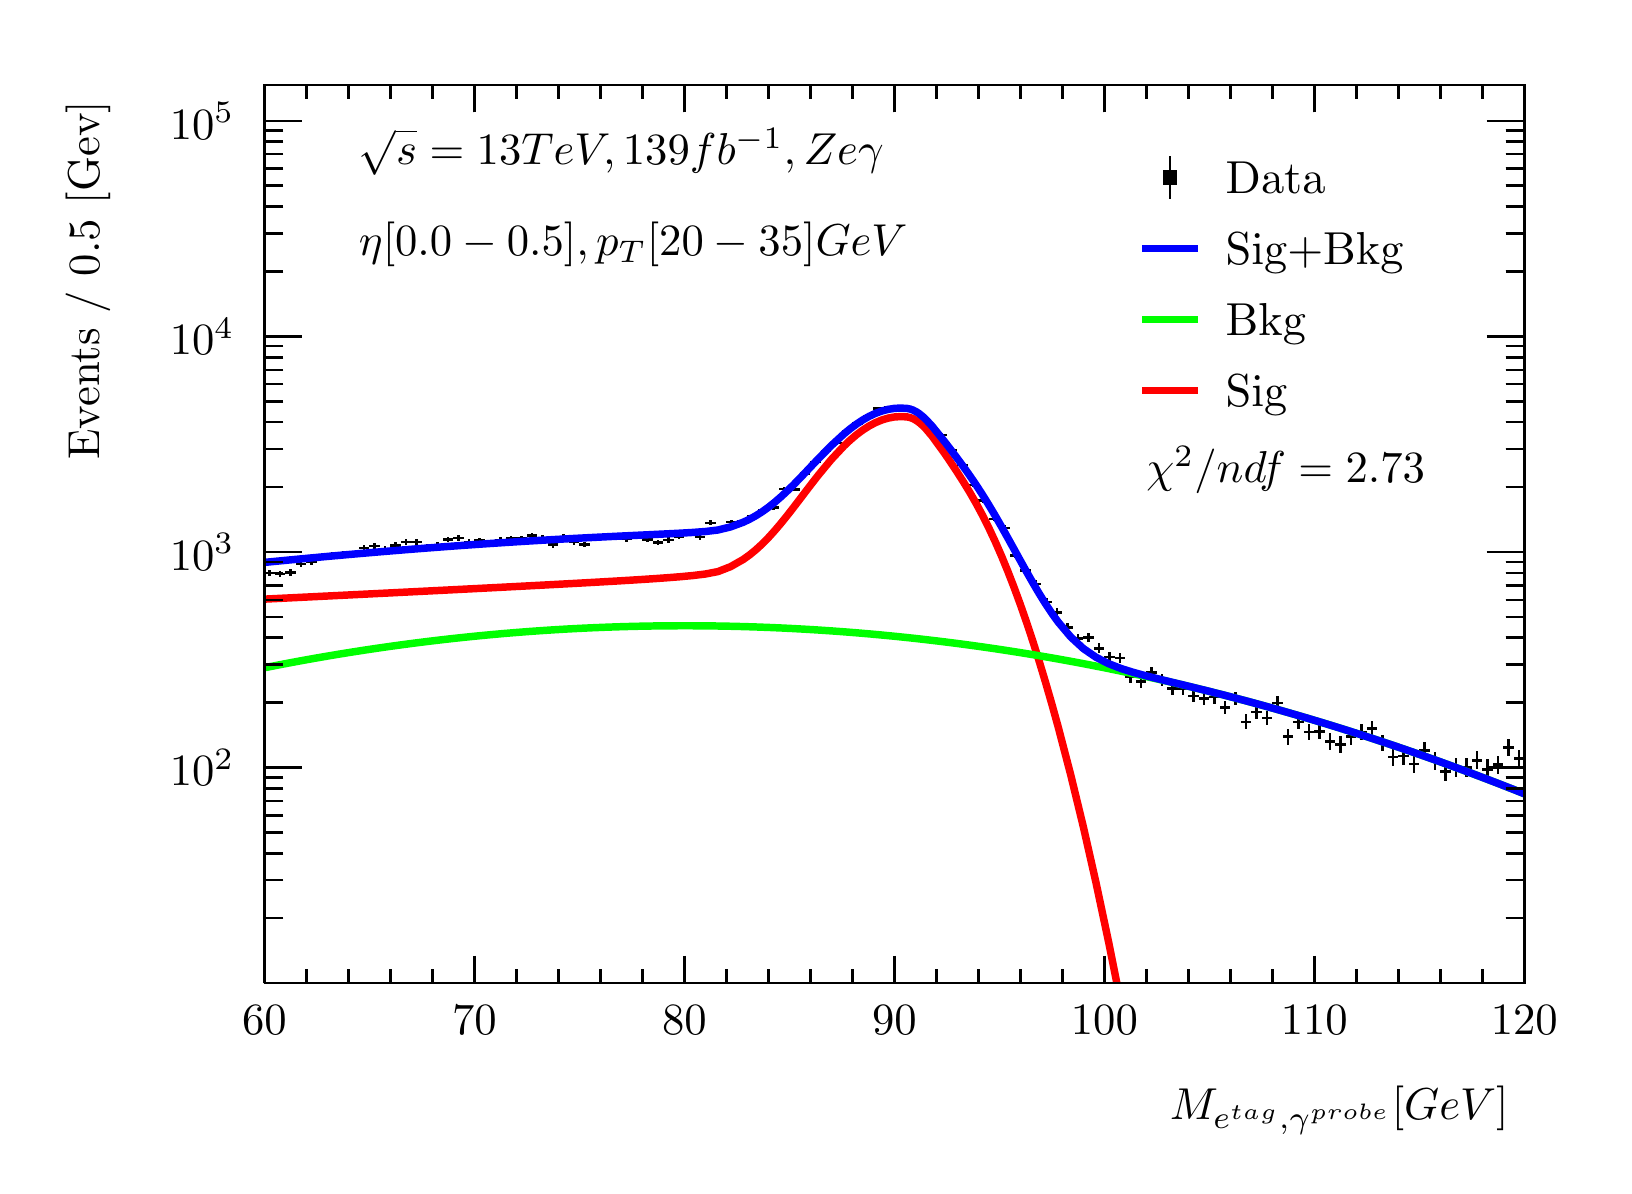
\begin{tikzpicture}
\pgfdeclareplotmark{cross} {
\pgfpathmoveto{\pgfpoint{-0.3\pgfplotmarksize}{\pgfplotmarksize}}
\pgfpathlineto{\pgfpoint{+0.3\pgfplotmarksize}{\pgfplotmarksize}}
\pgfpathlineto{\pgfpoint{+0.3\pgfplotmarksize}{0.3\pgfplotmarksize}}
\pgfpathlineto{\pgfpoint{+1\pgfplotmarksize}{0.3\pgfplotmarksize}}
\pgfpathlineto{\pgfpoint{+1\pgfplotmarksize}{-0.3\pgfplotmarksize}}
\pgfpathlineto{\pgfpoint{+0.3\pgfplotmarksize}{-0.3\pgfplotmarksize}}
\pgfpathlineto{\pgfpoint{+0.3\pgfplotmarksize}{-1.\pgfplotmarksize}}
\pgfpathlineto{\pgfpoint{-0.3\pgfplotmarksize}{-1.\pgfplotmarksize}}
\pgfpathlineto{\pgfpoint{-0.3\pgfplotmarksize}{-0.3\pgfplotmarksize}}
\pgfpathlineto{\pgfpoint{-1.\pgfplotmarksize}{-0.3\pgfplotmarksize}}
\pgfpathlineto{\pgfpoint{-1.\pgfplotmarksize}{0.3\pgfplotmarksize}}
\pgfpathlineto{\pgfpoint{-0.3\pgfplotmarksize}{0.3\pgfplotmarksize}}
\pgfpathclose
\pgfusepathqstroke
}
\pgfdeclareplotmark{cross*} {
\pgfpathmoveto{\pgfpoint{-0.3\pgfplotmarksize}{\pgfplotmarksize}}
\pgfpathlineto{\pgfpoint{+0.3\pgfplotmarksize}{\pgfplotmarksize}}
\pgfpathlineto{\pgfpoint{+0.3\pgfplotmarksize}{0.3\pgfplotmarksize}}
\pgfpathlineto{\pgfpoint{+1\pgfplotmarksize}{0.3\pgfplotmarksize}}
\pgfpathlineto{\pgfpoint{+1\pgfplotmarksize}{-0.3\pgfplotmarksize}}
\pgfpathlineto{\pgfpoint{+0.3\pgfplotmarksize}{-0.3\pgfplotmarksize}}
\pgfpathlineto{\pgfpoint{+0.3\pgfplotmarksize}{-1.\pgfplotmarksize}}
\pgfpathlineto{\pgfpoint{-0.3\pgfplotmarksize}{-1.\pgfplotmarksize}}
\pgfpathlineto{\pgfpoint{-0.3\pgfplotmarksize}{-0.3\pgfplotmarksize}}
\pgfpathlineto{\pgfpoint{-1.\pgfplotmarksize}{-0.3\pgfplotmarksize}}
\pgfpathlineto{\pgfpoint{-1.\pgfplotmarksize}{0.3\pgfplotmarksize}}
\pgfpathlineto{\pgfpoint{-0.3\pgfplotmarksize}{0.3\pgfplotmarksize}}
\pgfpathclose
\pgfusepathqfillstroke
}
\pgfdeclareplotmark{newstar} {
\pgfpathmoveto{\pgfqpoint{0pt}{\pgfplotmarksize}}
\pgfpathlineto{\pgfqpointpolar{44}{0.5\pgfplotmarksize}}
\pgfpathlineto{\pgfqpointpolar{18}{\pgfplotmarksize}}
\pgfpathlineto{\pgfqpointpolar{-20}{0.5\pgfplotmarksize}}
\pgfpathlineto{\pgfqpointpolar{-54}{\pgfplotmarksize}}
\pgfpathlineto{\pgfqpointpolar{-90}{0.5\pgfplotmarksize}}
\pgfpathlineto{\pgfqpointpolar{234}{\pgfplotmarksize}}
\pgfpathlineto{\pgfqpointpolar{198}{0.5\pgfplotmarksize}}
\pgfpathlineto{\pgfqpointpolar{162}{\pgfplotmarksize}}
\pgfpathlineto{\pgfqpointpolar{134}{0.5\pgfplotmarksize}}
\pgfpathclose
\pgfusepathqstroke
}
\pgfdeclareplotmark{newstar*} {
\pgfpathmoveto{\pgfqpoint{0pt}{\pgfplotmarksize}}
\pgfpathlineto{\pgfqpointpolar{44}{0.5\pgfplotmarksize}}
\pgfpathlineto{\pgfqpointpolar{18}{\pgfplotmarksize}}
\pgfpathlineto{\pgfqpointpolar{-20}{0.5\pgfplotmarksize}}
\pgfpathlineto{\pgfqpointpolar{-54}{\pgfplotmarksize}}
\pgfpathlineto{\pgfqpointpolar{-90}{0.5\pgfplotmarksize}}
\pgfpathlineto{\pgfqpointpolar{234}{\pgfplotmarksize}}
\pgfpathlineto{\pgfqpointpolar{198}{0.5\pgfplotmarksize}}
\pgfpathlineto{\pgfqpointpolar{162}{\pgfplotmarksize}}
\pgfpathlineto{\pgfqpointpolar{134}{0.5\pgfplotmarksize}}
\pgfpathclose
\pgfusepathqfillstroke
}
\definecolor{c}{rgb}{1,1,1};
\draw [color=c, fill=c] (0,0) rectangle (20,14.4361);
\draw [color=c, fill=c] (3,2.30977) rectangle (19,13.7143);
\definecolor{c}{rgb}{0,0,0};
\draw [c,line width=0.9] (3,2.30977) -- (3,13.7143) -- (19,13.7143) -- (19,2.30977) -- (3,2.30977);
\definecolor{c}{rgb}{1,1,1};
\draw [color=c, fill=c] (3,2.30977) rectangle (19,13.7143);
\definecolor{c}{rgb}{0,0,0};
\draw [c,line width=0.9] (3,2.30977) -- (3,13.7143) -- (19,13.7143) -- (19,2.30977) -- (3,2.30977);
\draw [c,line width=0.9] (3,2.30977) -- (19,2.30977);
\draw [c,line width=0.9] (3,2.65624) -- (3,2.30977);
\draw [c,line width=0.9] (3.53333,2.48301) -- (3.53333,2.30977);
\draw [c,line width=0.9] (4.06667,2.48301) -- (4.06667,2.30977);
\draw [c,line width=0.9] (4.6,2.48301) -- (4.6,2.30977);
\draw [c,line width=0.9] (5.13333,2.48301) -- (5.13333,2.30977);
\draw [c,line width=0.9] (5.66667,2.65624) -- (5.66667,2.30977);
\draw [c,line width=0.9] (6.2,2.48301) -- (6.2,2.30977);
\draw [c,line width=0.9] (6.73333,2.48301) -- (6.73333,2.30977);
\draw [c,line width=0.9] (7.26667,2.48301) -- (7.26667,2.30977);
\draw [c,line width=0.9] (7.8,2.48301) -- (7.8,2.30977);
\draw [c,line width=0.9] (8.33333,2.65624) -- (8.33333,2.30977);
\draw [c,line width=0.9] (8.86667,2.48301) -- (8.86667,2.30977);
\draw [c,line width=0.9] (9.4,2.48301) -- (9.4,2.30977);
\draw [c,line width=0.9] (9.93333,2.48301) -- (9.93333,2.30977);
\draw [c,line width=0.9] (10.4667,2.48301) -- (10.4667,2.30977);
\draw [c,line width=0.9] (11,2.65624) -- (11,2.30977);
\draw [c,line width=0.9] (11.5333,2.48301) -- (11.5333,2.30977);
\draw [c,line width=0.9] (12.0667,2.48301) -- (12.0667,2.30977);
\draw [c,line width=0.9] (12.6,2.48301) -- (12.6,2.30977);
\draw [c,line width=0.9] (13.1333,2.48301) -- (13.1333,2.30977);
\draw [c,line width=0.9] (13.6667,2.65624) -- (13.6667,2.30977);
\draw [c,line width=0.9] (14.2,2.48301) -- (14.2,2.30977);
\draw [c,line width=0.9] (14.7333,2.48301) -- (14.7333,2.30977);
\draw [c,line width=0.9] (15.2667,2.48301) -- (15.2667,2.30977);
\draw [c,line width=0.9] (15.8,2.48301) -- (15.8,2.30977);
\draw [c,line width=0.9] (16.3333,2.65624) -- (16.3333,2.30977);
\draw [c,line width=0.9] (16.8667,2.48301) -- (16.8667,2.30977);
\draw [c,line width=0.9] (17.4,2.48301) -- (17.4,2.30977);
\draw [c,line width=0.9] (17.9333,2.48301) -- (17.9333,2.30977);
\draw [c,line width=0.9] (18.4667,2.48301) -- (18.4667,2.30977);
\draw [c,line width=0.9] (19,2.65624) -- (19,2.30977);
\draw [anchor=base] (3,1.66015) node[scale=1.61424, color=c, rotate=0]{60};
\draw [anchor=base] (5.66667,1.66015) node[scale=1.61424, color=c, rotate=0]{70};
\draw [anchor=base] (8.33333,1.66015) node[scale=1.61424, color=c, rotate=0]{80};
\draw [anchor=base] (11,1.66015) node[scale=1.61424, color=c, rotate=0]{90};
\draw [anchor=base] (13.6667,1.66015) node[scale=1.61424, color=c, rotate=0]{100};
\draw [anchor=base] (16.3333,1.66015) node[scale=1.61424, color=c, rotate=0]{110};
\draw [anchor=base] (19,1.66015) node[scale=1.61424, color=c, rotate=0]{120};
\draw [anchor= east] (19,0.692932) node[scale=1.61424, color=c, rotate=0]{$M_{e^{tag}, \gamma^{probe}}  [GeV]$};
\draw [c,line width=0.9] (3,13.7143) -- (19,13.7143);
\draw [c,line width=0.9] (3,13.3678) -- (3,13.7143);
\draw [c,line width=0.9] (3.53333,13.5411) -- (3.53333,13.7143);
\draw [c,line width=0.9] (4.06667,13.5411) -- (4.06667,13.7143);
\draw [c,line width=0.9] (4.6,13.5411) -- (4.6,13.7143);
\draw [c,line width=0.9] (5.13333,13.5411) -- (5.13333,13.7143);
\draw [c,line width=0.9] (5.66667,13.3678) -- (5.66667,13.7143);
\draw [c,line width=0.9] (6.2,13.5411) -- (6.2,13.7143);
\draw [c,line width=0.9] (6.73333,13.5411) -- (6.73333,13.7143);
\draw [c,line width=0.9] (7.26667,13.5411) -- (7.26667,13.7143);
\draw [c,line width=0.9] (7.8,13.5411) -- (7.8,13.7143);
\draw [c,line width=0.9] (8.33333,13.3678) -- (8.33333,13.7143);
\draw [c,line width=0.9] (8.86667,13.5411) -- (8.86667,13.7143);
\draw [c,line width=0.9] (9.4,13.5411) -- (9.4,13.7143);
\draw [c,line width=0.9] (9.93333,13.5411) -- (9.93333,13.7143);
\draw [c,line width=0.9] (10.4667,13.5411) -- (10.4667,13.7143);
\draw [c,line width=0.9] (11,13.3678) -- (11,13.7143);
\draw [c,line width=0.9] (11.5333,13.5411) -- (11.5333,13.7143);
\draw [c,line width=0.9] (12.0667,13.5411) -- (12.0667,13.7143);
\draw [c,line width=0.9] (12.6,13.5411) -- (12.6,13.7143);
\draw [c,line width=0.9] (13.1333,13.5411) -- (13.1333,13.7143);
\draw [c,line width=0.9] (13.6667,13.3678) -- (13.6667,13.7143);
\draw [c,line width=0.9] (14.2,13.5411) -- (14.2,13.7143);
\draw [c,line width=0.9] (14.7333,13.5411) -- (14.7333,13.7143);
\draw [c,line width=0.9] (15.2667,13.5411) -- (15.2667,13.7143);
\draw [c,line width=0.9] (15.8,13.5411) -- (15.8,13.7143);
\draw [c,line width=0.9] (16.3333,13.3678) -- (16.3333,13.7143);
\draw [c,line width=0.9] (16.8667,13.5411) -- (16.8667,13.7143);
\draw [c,line width=0.9] (17.4,13.5411) -- (17.4,13.7143);
\draw [c,line width=0.9] (17.9333,13.5411) -- (17.9333,13.7143);
\draw [c,line width=0.9] (18.4667,13.5411) -- (18.4667,13.7143);
\draw [c,line width=0.9] (19,13.3678) -- (19,13.7143);
\draw [c,line width=0.9] (3,2.30977) -- (3,13.7143);
\draw [c,line width=0.9] (3.237,3.13385) -- (3,3.13385);
\draw [c,line width=0.9] (3.237,3.6159) -- (3,3.6159);
\draw [c,line width=0.9] (3.237,3.95792) -- (3,3.95792);
\draw [c,line width=0.9] (3.237,4.22321) -- (3,4.22321);
\draw [c,line width=0.9] (3.237,4.43997) -- (3,4.43997);
\draw [c,line width=0.9] (3.237,4.62324) -- (3,4.62324);
\draw [c,line width=0.9] (3.237,4.782) -- (3,4.782);
\draw [c,line width=0.9] (3.237,4.92203) -- (3,4.92203);
\draw [c,line width=0.9] (3.474,5.04729) -- (3,5.04729);
\draw [anchor= east] (2.82,5.04729) node[scale=1.61424, color=c, rotate=0]{$10^{2}$};
\draw [c,line width=0.9] (3.237,5.87136) -- (3,5.87136);
\draw [c,line width=0.9] (3.237,6.35342) -- (3,6.35342);
\draw [c,line width=0.9] (3.237,6.69544) -- (3,6.69544);
\draw [c,line width=0.9] (3.237,6.96073) -- (3,6.96073);
\draw [c,line width=0.9] (3.237,7.17749) -- (3,7.17749);
\draw [c,line width=0.9] (3.237,7.36076) -- (3,7.36076);
\draw [c,line width=0.9] (3.237,7.51951) -- (3,7.51951);
\draw [c,line width=0.9] (3.237,7.65954) -- (3,7.65954);
\draw [c,line width=0.9] (3.474,7.78481) -- (3,7.78481);
\draw [anchor= east] (2.82,7.78481) node[scale=1.61424, color=c, rotate=0]{$10^{3}$};
\draw [c,line width=0.9] (3.237,8.60888) -- (3,8.60888);
\draw [c,line width=0.9] (3.237,9.09093) -- (3,9.09093);
\draw [c,line width=0.9] (3.237,9.43296) -- (3,9.43296);
\draw [c,line width=0.9] (3.237,9.69825) -- (3,9.69825);
\draw [c,line width=0.9] (3.237,9.91501) -- (3,9.91501);
\draw [c,line width=0.9] (3.237,10.0983) -- (3,10.0983);
\draw [c,line width=0.9] (3.237,10.257) -- (3,10.257);
\draw [c,line width=0.9] (3.237,10.3971) -- (3,10.3971);
\draw [c,line width=0.9] (3.474,10.5223) -- (3,10.5223);
\draw [anchor= east] (2.82,10.5223) node[scale=1.61424, color=c, rotate=0]{$10^{4}$};
\draw [c,line width=0.9] (3.237,11.3464) -- (3,11.3464);
\draw [c,line width=0.9] (3.237,11.8285) -- (3,11.8285);
\draw [c,line width=0.9] (3.237,12.1705) -- (3,12.1705);
\draw [c,line width=0.9] (3.237,12.4358) -- (3,12.4358);
\draw [c,line width=0.9] (3.237,12.6525) -- (3,12.6525);
\draw [c,line width=0.9] (3.237,12.8358) -- (3,12.8358);
\draw [c,line width=0.9] (3.237,12.9945) -- (3,12.9945);
\draw [c,line width=0.9] (3.237,13.1346) -- (3,13.1346);
\draw [c,line width=0.9] (3.474,13.2598) -- (3,13.2598);
\draw [anchor= east] (2.82,13.2598) node[scale=1.61424, color=c, rotate=0]{$10^{5}$};
\draw [anchor= east] (0.76,13.7143) node[scale=1.61424, color=c, rotate=90]{Events / 0.5 [Gev]};
\draw [c,line width=0.9] (19,2.30977) -- (19,13.7143);
\draw [c,line width=0.9] (18.763,3.13385) -- (19,3.13385);
\draw [c,line width=0.9] (18.763,3.6159) -- (19,3.6159);
\draw [c,line width=0.9] (18.763,3.95792) -- (19,3.95792);
\draw [c,line width=0.9] (18.763,4.22321) -- (19,4.22321);
\draw [c,line width=0.9] (18.763,4.43997) -- (19,4.43997);
\draw [c,line width=0.9] (18.763,4.62324) -- (19,4.62324);
\draw [c,line width=0.9] (18.763,4.782) -- (19,4.782);
\draw [c,line width=0.9] (18.763,4.92203) -- (19,4.92203);
\draw [c,line width=0.9] (18.526,5.04729) -- (19,5.04729);
\draw [c,line width=0.9] (18.763,5.87136) -- (19,5.87136);
\draw [c,line width=0.9] (18.763,6.35342) -- (19,6.35342);
\draw [c,line width=0.9] (18.763,6.69544) -- (19,6.69544);
\draw [c,line width=0.9] (18.763,6.96073) -- (19,6.96073);
\draw [c,line width=0.9] (18.763,7.17749) -- (19,7.17749);
\draw [c,line width=0.9] (18.763,7.36076) -- (19,7.36076);
\draw [c,line width=0.9] (18.763,7.51951) -- (19,7.51951);
\draw [c,line width=0.9] (18.763,7.65954) -- (19,7.65954);
\draw [c,line width=0.9] (18.526,7.78481) -- (19,7.78481);
\draw [c,line width=0.9] (18.763,8.60888) -- (19,8.60888);
\draw [c,line width=0.9] (18.763,9.09093) -- (19,9.09093);
\draw [c,line width=0.9] (18.763,9.43296) -- (19,9.43296);
\draw [c,line width=0.9] (18.763,9.69825) -- (19,9.69825);
\draw [c,line width=0.9] (18.763,9.91501) -- (19,9.91501);
\draw [c,line width=0.9] (18.763,10.0983) -- (19,10.0983);
\draw [c,line width=0.9] (18.763,10.257) -- (19,10.257);
\draw [c,line width=0.9] (18.763,10.3971) -- (19,10.3971);
\draw [c,line width=0.9] (18.526,10.5223) -- (19,10.5223);
\draw [c,line width=0.9] (18.763,11.3464) -- (19,11.3464);
\draw [c,line width=0.9] (18.763,11.8285) -- (19,11.8285);
\draw [c,line width=0.9] (18.763,12.1705) -- (19,12.1705);
\draw [c,line width=0.9] (18.763,12.4358) -- (19,12.4358);
\draw [c,line width=0.9] (18.763,12.6525) -- (19,12.6525);
\draw [c,line width=0.9] (18.763,12.8358) -- (19,12.8358);
\draw [c,line width=0.9] (18.763,12.9945) -- (19,12.9945);
\draw [c,line width=0.9] (18.763,13.1346) -- (19,13.1346);
\draw [c,line width=0.9] (18.526,13.2598) -- (19,13.2598);
\draw [c,line width=0.9] (3.06667,7.51505) -- (3,7.51505);
\draw [c,line width=0.9] (3,7.51505) -- (3,7.51505);
\draw [c,line width=0.9] (3.06667,7.51505) -- (3.13333,7.51505);
\draw [c,line width=0.9] (3.13333,7.51505) -- (3.13333,7.51505);
\draw [c,line width=0.9] (3.06667,7.51505) -- (3.06667,7.55716);
\draw [c,line width=0.9] (3.06667,7.55716) -- (3.06667,7.55716);
\draw [c,line width=0.9] (3.06667,7.51505) -- (3.06667,7.47294);
\draw [c,line width=0.9] (3.06667,7.47294) -- (3.06667,7.47294);
\draw [c,line width=0.9] (3.2,7.50606) -- (3.13333,7.50606);
\draw [c,line width=0.9] (3.13333,7.50606) -- (3.13333,7.50606);
\draw [c,line width=0.9] (3.2,7.50606) -- (3.26667,7.50606);
\draw [c,line width=0.9] (3.26667,7.50606) -- (3.26667,7.50606);
\draw [c,line width=0.9] (3.2,7.50606) -- (3.2,7.54833);
\draw [c,line width=0.9] (3.2,7.54833) -- (3.2,7.54833);
\draw [c,line width=0.9] (3.2,7.50606) -- (3.2,7.46379);
\draw [c,line width=0.9] (3.2,7.46379) -- (3.2,7.46379);
\draw [c,line width=0.9] (3.33333,7.521) -- (3.26667,7.521);
\draw [c,line width=0.9] (3.26667,7.521) -- (3.26667,7.521);
\draw [c,line width=0.9] (3.33333,7.521) -- (3.4,7.521);
\draw [c,line width=0.9] (3.4,7.521) -- (3.4,7.521);
\draw [c,line width=0.9] (3.33333,7.521) -- (3.33333,7.563);
\draw [c,line width=0.9] (3.33333,7.563) -- (3.33333,7.563);
\draw [c,line width=0.9] (3.33333,7.521) -- (3.33333,7.47899);
\draw [c,line width=0.9] (3.33333,7.47899) -- (3.33333,7.47899);
\draw [c,line width=0.9] (3.46667,7.63012) -- (3.4,7.63012);
\draw [c,line width=0.9] (3.4,7.63012) -- (3.4,7.63012);
\draw [c,line width=0.9] (3.46667,7.63012) -- (3.53333,7.63012);
\draw [c,line width=0.9] (3.53333,7.63012) -- (3.53333,7.63012);
\draw [c,line width=0.9] (3.46667,7.63012) -- (3.46667,7.67024);
\draw [c,line width=0.9] (3.46667,7.67024) -- (3.46667,7.67024);
\draw [c,line width=0.9] (3.46667,7.63012) -- (3.46667,7.59);
\draw [c,line width=0.9] (3.46667,7.59) -- (3.46667,7.59);
\draw [c,line width=0.9] (3.6,7.65425) -- (3.53333,7.65425);
\draw [c,line width=0.9] (3.53333,7.65425) -- (3.53333,7.65425);
\draw [c,line width=0.9] (3.6,7.65425) -- (3.66667,7.65425);
\draw [c,line width=0.9] (3.66667,7.65425) -- (3.66667,7.65425);
\draw [c,line width=0.9] (3.6,7.65425) -- (3.6,7.69397);
\draw [c,line width=0.9] (3.6,7.69397) -- (3.6,7.69397);
\draw [c,line width=0.9] (3.6,7.65425) -- (3.6,7.61453);
\draw [c,line width=0.9] (3.6,7.61453) -- (3.6,7.61453);
\draw [c,line width=0.9] (3.73333,7.72633) -- (3.66667,7.72633);
\draw [c,line width=0.9] (3.66667,7.72633) -- (3.66667,7.72633);
\draw [c,line width=0.9] (3.73333,7.72633) -- (3.8,7.72633);
\draw [c,line width=0.9] (3.8,7.72633) -- (3.8,7.72633);
\draw [c,line width=0.9] (3.73333,7.72633) -- (3.73333,7.76486);
\draw [c,line width=0.9] (3.73333,7.76486) -- (3.73333,7.76486);
\draw [c,line width=0.9] (3.73333,7.72633) -- (3.73333,7.6878);
\draw [c,line width=0.9] (3.73333,7.6878) -- (3.73333,7.6878);
\draw [c,line width=0.9] (3.86667,7.73998) -- (3.8,7.73998);
\draw [c,line width=0.9] (3.8,7.73998) -- (3.8,7.73998);
\draw [c,line width=0.9] (3.86667,7.73998) -- (3.93333,7.73998);
\draw [c,line width=0.9] (3.93333,7.73998) -- (3.93333,7.73998);
\draw [c,line width=0.9] (3.86667,7.73998) -- (3.86667,7.77829);
\draw [c,line width=0.9] (3.86667,7.77829) -- (3.86667,7.77829);
\draw [c,line width=0.9] (3.86667,7.73998) -- (3.86667,7.70167);
\draw [c,line width=0.9] (3.86667,7.70167) -- (3.86667,7.70167);
\draw [c,line width=0.9] (4,7.75714) -- (3.93333,7.75714);
\draw [c,line width=0.9] (3.93333,7.75714) -- (3.93333,7.75714);
\draw [c,line width=0.9] (4,7.75714) -- (4.06667,7.75714);
\draw [c,line width=0.9] (4.06667,7.75714) -- (4.06667,7.75714);
\draw [c,line width=0.9] (4,7.75714) -- (4,7.79518);
\draw [c,line width=0.9] (4,7.79518) -- (4,7.79518);
\draw [c,line width=0.9] (4,7.75714) -- (4,7.71911);
\draw [c,line width=0.9] (4,7.71911) -- (4,7.71911);
\draw [c,line width=0.9] (4.13333,7.76079) -- (4.06667,7.76079);
\draw [c,line width=0.9] (4.06667,7.76079) -- (4.06667,7.76079);
\draw [c,line width=0.9] (4.13333,7.76079) -- (4.2,7.76079);
\draw [c,line width=0.9] (4.2,7.76079) -- (4.2,7.76079);
\draw [c,line width=0.9] (4.13333,7.76079) -- (4.13333,7.79876);
\draw [c,line width=0.9] (4.13333,7.79876) -- (4.13333,7.79876);
\draw [c,line width=0.9] (4.13333,7.76079) -- (4.13333,7.72281);
\draw [c,line width=0.9] (4.13333,7.72281) -- (4.13333,7.72281);
\draw [c,line width=0.9] (4.26667,7.83486) -- (4.2,7.83486);
\draw [c,line width=0.9] (4.2,7.83486) -- (4.2,7.83486);
\draw [c,line width=0.9] (4.26667,7.83486) -- (4.33333,7.83486);
\draw [c,line width=0.9] (4.33333,7.83486) -- (4.33333,7.83486);
\draw [c,line width=0.9] (4.26667,7.83486) -- (4.26667,7.87167);
\draw [c,line width=0.9] (4.26667,7.87167) -- (4.26667,7.87167);
\draw [c,line width=0.9] (4.26667,7.83486) -- (4.26667,7.79805);
\draw [c,line width=0.9] (4.26667,7.79805) -- (4.26667,7.79805);
\draw [c,line width=0.9] (4.4,7.85744) -- (4.33333,7.85744);
\draw [c,line width=0.9] (4.33333,7.85744) -- (4.33333,7.85744);
\draw [c,line width=0.9] (4.4,7.85744) -- (4.46667,7.85744);
\draw [c,line width=0.9] (4.46667,7.85744) -- (4.46667,7.85744);
\draw [c,line width=0.9] (4.4,7.85744) -- (4.4,7.89391);
\draw [c,line width=0.9] (4.4,7.89391) -- (4.4,7.89391);
\draw [c,line width=0.9] (4.4,7.85744) -- (4.4,7.82098);
\draw [c,line width=0.9] (4.4,7.82098) -- (4.4,7.82098);
\draw [c,line width=0.9] (4.53333,7.81995) -- (4.46667,7.81995);
\draw [c,line width=0.9] (4.46667,7.81995) -- (4.46667,7.81995);
\draw [c,line width=0.9] (4.53333,7.81995) -- (4.6,7.81995);
\draw [c,line width=0.9] (4.6,7.81995) -- (4.6,7.81995);
\draw [c,line width=0.9] (4.53333,7.81995) -- (4.53333,7.85699);
\draw [c,line width=0.9] (4.53333,7.85699) -- (4.53333,7.85699);
\draw [c,line width=0.9] (4.53333,7.81995) -- (4.53333,7.78291);
\draw [c,line width=0.9] (4.53333,7.78291) -- (4.53333,7.78291);
\draw [c,line width=0.9] (4.66667,7.86968) -- (4.6,7.86968);
\draw [c,line width=0.9] (4.6,7.86968) -- (4.6,7.86968);
\draw [c,line width=0.9] (4.66667,7.86968) -- (4.73333,7.86968);
\draw [c,line width=0.9] (4.73333,7.86968) -- (4.73333,7.86968);
\draw [c,line width=0.9] (4.66667,7.86968) -- (4.66667,7.90596);
\draw [c,line width=0.9] (4.66667,7.90596) -- (4.66667,7.90596);
\draw [c,line width=0.9] (4.66667,7.86968) -- (4.66667,7.83341);
\draw [c,line width=0.9] (4.66667,7.83341) -- (4.66667,7.83341);
\draw [c,line width=0.9] (4.8,7.91209) -- (4.73333,7.91209);
\draw [c,line width=0.9] (4.73333,7.91209) -- (4.73333,7.91209);
\draw [c,line width=0.9] (4.8,7.91209) -- (4.86667,7.91209);
\draw [c,line width=0.9] (4.86667,7.91209) -- (4.86667,7.91209);
\draw [c,line width=0.9] (4.8,7.91209) -- (4.8,7.94772);
\draw [c,line width=0.9] (4.8,7.94772) -- (4.8,7.94772);
\draw [c,line width=0.9] (4.8,7.91209) -- (4.8,7.87645);
\draw [c,line width=0.9] (4.8,7.87645) -- (4.8,7.87645);
\draw [c,line width=0.9] (4.93333,7.90995) -- (4.86667,7.90995);
\draw [c,line width=0.9] (4.86667,7.90995) -- (4.86667,7.90995);
\draw [c,line width=0.9] (4.93333,7.90995) -- (5,7.90995);
\draw [c,line width=0.9] (5,7.90995) -- (5,7.90995);
\draw [c,line width=0.9] (4.93333,7.90995) -- (4.93333,7.94562);
\draw [c,line width=0.9] (4.93333,7.94562) -- (4.93333,7.94562);
\draw [c,line width=0.9] (4.93333,7.90995) -- (4.93333,7.87428);
\draw [c,line width=0.9] (4.93333,7.87428) -- (4.93333,7.87428);
\draw [c,line width=0.9] (5.06667,7.85408) -- (5,7.85408);
\draw [c,line width=0.9] (5,7.85408) -- (5,7.85408);
\draw [c,line width=0.9] (5.06667,7.85408) -- (5.13333,7.85408);
\draw [c,line width=0.9] (5.13333,7.85408) -- (5.13333,7.85408);
\draw [c,line width=0.9] (5.06667,7.85408) -- (5.06667,7.8906);
\draw [c,line width=0.9] (5.06667,7.8906) -- (5.06667,7.8906);
\draw [c,line width=0.9] (5.06667,7.85408) -- (5.06667,7.81757);
\draw [c,line width=0.9] (5.06667,7.81757) -- (5.06667,7.81757);
\draw [c,line width=0.9] (5.2,7.87189) -- (5.13333,7.87189);
\draw [c,line width=0.9] (5.13333,7.87189) -- (5.13333,7.87189);
\draw [c,line width=0.9] (5.2,7.87189) -- (5.26667,7.87189);
\draw [c,line width=0.9] (5.26667,7.87189) -- (5.26667,7.87189);
\draw [c,line width=0.9] (5.2,7.87189) -- (5.2,7.90814);
\draw [c,line width=0.9] (5.2,7.90814) -- (5.2,7.90814);
\draw [c,line width=0.9] (5.2,7.87189) -- (5.2,7.83565);
\draw [c,line width=0.9] (5.2,7.83565) -- (5.2,7.83565);
\draw [c,line width=0.9] (5.33333,7.94163) -- (5.26667,7.94163);
\draw [c,line width=0.9] (5.26667,7.94163) -- (5.26667,7.94163);
\draw [c,line width=0.9] (5.33333,7.94163) -- (5.4,7.94163);
\draw [c,line width=0.9] (5.4,7.94163) -- (5.4,7.94163);
\draw [c,line width=0.9] (5.33333,7.94163) -- (5.33333,7.97682);
\draw [c,line width=0.9] (5.33333,7.97682) -- (5.33333,7.97682);
\draw [c,line width=0.9] (5.33333,7.94163) -- (5.33333,7.90643);
\draw [c,line width=0.9] (5.33333,7.90643) -- (5.33333,7.90643);
\draw [c,line width=0.9] (5.46667,7.96229) -- (5.4,7.96229);
\draw [c,line width=0.9] (5.4,7.96229) -- (5.4,7.96229);
\draw [c,line width=0.9] (5.46667,7.96229) -- (5.53333,7.96229);
\draw [c,line width=0.9] (5.53333,7.96229) -- (5.53333,7.96229);
\draw [c,line width=0.9] (5.46667,7.96229) -- (5.46667,7.99718);
\draw [c,line width=0.9] (5.46667,7.99718) -- (5.46667,7.99718);
\draw [c,line width=0.9] (5.46667,7.96229) -- (5.46667,7.9274);
\draw [c,line width=0.9] (5.46667,7.9274) -- (5.46667,7.9274);
\draw [c,line width=0.9] (5.6,7.91422) -- (5.53333,7.91422);
\draw [c,line width=0.9] (5.53333,7.91422) -- (5.53333,7.91422);
\draw [c,line width=0.9] (5.6,7.91422) -- (5.66667,7.91422);
\draw [c,line width=0.9] (5.66667,7.91422) -- (5.66667,7.91422);
\draw [c,line width=0.9] (5.6,7.91422) -- (5.6,7.94983);
\draw [c,line width=0.9] (5.6,7.94983) -- (5.6,7.94983);
\draw [c,line width=0.9] (5.6,7.91422) -- (5.6,7.87862);
\draw [c,line width=0.9] (5.6,7.87862) -- (5.6,7.87862);
\draw [c,line width=0.9] (5.73333,7.93221) -- (5.66667,7.93221);
\draw [c,line width=0.9] (5.66667,7.93221) -- (5.66667,7.93221);
\draw [c,line width=0.9] (5.73333,7.93221) -- (5.8,7.93221);
\draw [c,line width=0.9] (5.8,7.93221) -- (5.8,7.93221);
\draw [c,line width=0.9] (5.73333,7.93221) -- (5.73333,7.96755);
\draw [c,line width=0.9] (5.73333,7.96755) -- (5.73333,7.96755);
\draw [c,line width=0.9] (5.73333,7.93221) -- (5.73333,7.89688);
\draw [c,line width=0.9] (5.73333,7.89688) -- (5.73333,7.89688);
\draw [c,line width=0.9] (5.86667,7.89487) -- (5.8,7.89487);
\draw [c,line width=0.9] (5.8,7.89487) -- (5.8,7.89487);
\draw [c,line width=0.9] (5.86667,7.89487) -- (5.93333,7.89487);
\draw [c,line width=0.9] (5.93333,7.89487) -- (5.93333,7.89487);
\draw [c,line width=0.9] (5.86667,7.89487) -- (5.86667,7.93077);
\draw [c,line width=0.9] (5.86667,7.93077) -- (5.86667,7.93077);
\draw [c,line width=0.9] (5.86667,7.89487) -- (5.86667,7.85898);
\draw [c,line width=0.9] (5.86667,7.85898) -- (5.86667,7.85898);
\draw [c,line width=0.9] (6,7.9385) -- (5.93333,7.9385);
\draw [c,line width=0.9] (5.93333,7.9385) -- (5.93333,7.9385);
\draw [c,line width=0.9] (6,7.9385) -- (6.06667,7.9385);
\draw [c,line width=0.9] (6.06667,7.9385) -- (6.06667,7.9385);
\draw [c,line width=0.9] (6,7.9385) -- (6,7.97374);
\draw [c,line width=0.9] (6,7.97374) -- (6,7.97374);
\draw [c,line width=0.9] (6,7.9385) -- (6,7.90326);
\draw [c,line width=0.9] (6,7.90326) -- (6,7.90326);
\draw [c,line width=0.9] (6.13333,7.95303) -- (6.06667,7.95303);
\draw [c,line width=0.9] (6.06667,7.95303) -- (6.06667,7.95303);
\draw [c,line width=0.9] (6.13333,7.95303) -- (6.2,7.95303);
\draw [c,line width=0.9] (6.2,7.95303) -- (6.2,7.95303);
\draw [c,line width=0.9] (6.13333,7.95303) -- (6.13333,7.98806);
\draw [c,line width=0.9] (6.13333,7.98806) -- (6.13333,7.98806);
\draw [c,line width=0.9] (6.13333,7.95303) -- (6.13333,7.91801);
\draw [c,line width=0.9] (6.13333,7.91801) -- (6.13333,7.91801);
\draw [c,line width=0.9] (6.26667,7.9551) -- (6.2,7.9551);
\draw [c,line width=0.9] (6.2,7.9551) -- (6.2,7.9551);
\draw [c,line width=0.9] (6.26667,7.9551) -- (6.33333,7.9551);
\draw [c,line width=0.9] (6.33333,7.9551) -- (6.33333,7.9551);
\draw [c,line width=0.9] (6.26667,7.9551) -- (6.26667,7.99009);
\draw [c,line width=0.9] (6.26667,7.99009) -- (6.26667,7.99009);
\draw [c,line width=0.9] (6.26667,7.9551) -- (6.26667,7.9201);
\draw [c,line width=0.9] (6.26667,7.9201) -- (6.26667,7.9201);
\draw [c,line width=0.9] (6.4,7.99361) -- (6.33333,7.99361);
\draw [c,line width=0.9] (6.33333,7.99361) -- (6.33333,7.99361);
\draw [c,line width=0.9] (6.4,7.99361) -- (6.46667,7.99361);
\draw [c,line width=0.9] (6.46667,7.99361) -- (6.46667,7.99361);
\draw [c,line width=0.9] (6.4,7.99361) -- (6.4,8.02805);
\draw [c,line width=0.9] (6.4,8.02805) -- (6.4,8.02805);
\draw [c,line width=0.9] (6.4,7.99361) -- (6.4,7.95918);
\draw [c,line width=0.9] (6.4,7.95918) -- (6.4,7.95918);
\draw [c,line width=0.9] (6.53333,7.96433) -- (6.46667,7.96433);
\draw [c,line width=0.9] (6.46667,7.96433) -- (6.46667,7.96433);
\draw [c,line width=0.9] (6.53333,7.96433) -- (6.6,7.96433);
\draw [c,line width=0.9] (6.6,7.96433) -- (6.6,7.96433);
\draw [c,line width=0.9] (6.53333,7.96433) -- (6.53333,7.99919);
\draw [c,line width=0.9] (6.53333,7.99919) -- (6.53333,7.99919);
\draw [c,line width=0.9] (6.53333,7.96433) -- (6.53333,7.92947);
\draw [c,line width=0.9] (6.53333,7.92947) -- (6.53333,7.92947);
\draw [c,line width=0.9] (6.66667,7.87631) -- (6.6,7.87631);
\draw [c,line width=0.9] (6.6,7.87631) -- (6.6,7.87631);
\draw [c,line width=0.9] (6.66667,7.87631) -- (6.73333,7.87631);
\draw [c,line width=0.9] (6.73333,7.87631) -- (6.73333,7.87631);
\draw [c,line width=0.9] (6.66667,7.87631) -- (6.66667,7.91248);
\draw [c,line width=0.9] (6.66667,7.91248) -- (6.66667,7.91248);
\draw [c,line width=0.9] (6.66667,7.87631) -- (6.66667,7.84013);
\draw [c,line width=0.9] (6.66667,7.84013) -- (6.66667,7.84013);
\draw [c,line width=0.9] (6.8,7.97552) -- (6.73333,7.97552);
\draw [c,line width=0.9] (6.73333,7.97552) -- (6.73333,7.97552);
\draw [c,line width=0.9] (6.8,7.97552) -- (6.86667,7.97552);
\draw [c,line width=0.9] (6.86667,7.97552) -- (6.86667,7.97552);
\draw [c,line width=0.9] (6.8,7.97552) -- (6.8,8.01022);
\draw [c,line width=0.9] (6.8,8.01022) -- (6.8,8.01022);
\draw [c,line width=0.9] (6.8,7.97552) -- (6.8,7.94083);
\draw [c,line width=0.9] (6.8,7.94083) -- (6.8,7.94083);
\draw [c,line width=0.9] (6.93333,7.90888) -- (6.86667,7.90888);
\draw [c,line width=0.9] (6.86667,7.90888) -- (6.86667,7.90888);
\draw [c,line width=0.9] (6.93333,7.90888) -- (7,7.90888);
\draw [c,line width=0.9] (7,7.90888) -- (7,7.90888);
\draw [c,line width=0.9] (6.93333,7.90888) -- (6.93333,7.94456);
\draw [c,line width=0.9] (6.93333,7.94456) -- (6.93333,7.94456);
\draw [c,line width=0.9] (6.93333,7.90888) -- (6.93333,7.8732);
\draw [c,line width=0.9] (6.93333,7.8732) -- (6.93333,7.8732);
\draw [c,line width=0.9] (7.06667,7.87851) -- (7,7.87851);
\draw [c,line width=0.9] (7,7.87851) -- (7,7.87851);
\draw [c,line width=0.9] (7.06667,7.87851) -- (7.13333,7.87851);
\draw [c,line width=0.9] (7.13333,7.87851) -- (7.13333,7.87851);
\draw [c,line width=0.9] (7.06667,7.87851) -- (7.06667,7.91465);
\draw [c,line width=0.9] (7.06667,7.91465) -- (7.06667,7.91465);
\draw [c,line width=0.9] (7.06667,7.87851) -- (7.06667,7.84236);
\draw [c,line width=0.9] (7.06667,7.84236) -- (7.06667,7.84236);
\draw [c,line width=0.9] (7.2,7.95716) -- (7.13333,7.95716);
\draw [c,line width=0.9] (7.13333,7.95716) -- (7.13333,7.95716);
\draw [c,line width=0.9] (7.2,7.95716) -- (7.26667,7.95716);
\draw [c,line width=0.9] (7.26667,7.95716) -- (7.26667,7.95716);
\draw [c,line width=0.9] (7.2,7.95716) -- (7.2,7.99212);
\draw [c,line width=0.9] (7.2,7.99212) -- (7.2,7.99212);
\draw [c,line width=0.9] (7.2,7.95716) -- (7.2,7.92219);
\draw [c,line width=0.9] (7.2,7.92219) -- (7.2,7.92219);
\draw [c,line width=0.9] (7.33333,7.97957) -- (7.26667,7.97957);
\draw [c,line width=0.9] (7.26667,7.97957) -- (7.26667,7.97957);
\draw [c,line width=0.9] (7.33333,7.97957) -- (7.4,7.97957);
\draw [c,line width=0.9] (7.4,7.97957) -- (7.4,7.97957);
\draw [c,line width=0.9] (7.33333,7.97957) -- (7.33333,8.01421);
\draw [c,line width=0.9] (7.33333,8.01421) -- (7.33333,8.01421);
\draw [c,line width=0.9] (7.33333,7.97957) -- (7.33333,7.94493);
\draw [c,line width=0.9] (7.33333,7.94493) -- (7.33333,7.94493);
\draw [c,line width=0.9] (7.46667,7.97755) -- (7.4,7.97755);
\draw [c,line width=0.9] (7.4,7.97755) -- (7.4,7.97755);
\draw [c,line width=0.9] (7.46667,7.97755) -- (7.53333,7.97755);
\draw [c,line width=0.9] (7.53333,7.97755) -- (7.53333,7.97755);
\draw [c,line width=0.9] (7.46667,7.97755) -- (7.46667,8.01222);
\draw [c,line width=0.9] (7.46667,8.01222) -- (7.46667,8.01222);
\draw [c,line width=0.9] (7.46667,7.97755) -- (7.46667,7.94288);
\draw [c,line width=0.9] (7.46667,7.94288) -- (7.46667,7.94288);
\draw [c,line width=0.9] (7.6,7.94683) -- (7.53333,7.94683);
\draw [c,line width=0.9] (7.53333,7.94683) -- (7.53333,7.94683);
\draw [c,line width=0.9] (7.6,7.94683) -- (7.66667,7.94683);
\draw [c,line width=0.9] (7.66667,7.94683) -- (7.66667,7.94683);
\draw [c,line width=0.9] (7.6,7.94683) -- (7.6,7.98194);
\draw [c,line width=0.9] (7.6,7.98194) -- (7.6,7.98194);
\draw [c,line width=0.9] (7.6,7.94683) -- (7.6,7.91171);
\draw [c,line width=0.9] (7.6,7.91171) -- (7.6,7.91171);
\draw [c,line width=0.9] (7.73333,7.98159) -- (7.66667,7.98159);
\draw [c,line width=0.9] (7.66667,7.98159) -- (7.66667,7.98159);
\draw [c,line width=0.9] (7.73333,7.98159) -- (7.8,7.98159);
\draw [c,line width=0.9] (7.8,7.98159) -- (7.8,7.98159);
\draw [c,line width=0.9] (7.73333,7.98159) -- (7.73333,8.01619);
\draw [c,line width=0.9] (7.73333,8.01619) -- (7.73333,8.01619);
\draw [c,line width=0.9] (7.73333,7.98159) -- (7.73333,7.94698);
\draw [c,line width=0.9] (7.73333,7.94698) -- (7.73333,7.94698);
\draw [c,line width=0.9] (7.86667,7.94475) -- (7.8,7.94475);
\draw [c,line width=0.9] (7.8,7.94475) -- (7.8,7.94475);
\draw [c,line width=0.9] (7.86667,7.94475) -- (7.93333,7.94475);
\draw [c,line width=0.9] (7.93333,7.94475) -- (7.93333,7.94475);
\draw [c,line width=0.9] (7.86667,7.94475) -- (7.86667,7.9799);
\draw [c,line width=0.9] (7.86667,7.9799) -- (7.86667,7.9799);
\draw [c,line width=0.9] (7.86667,7.94475) -- (7.86667,7.9096);
\draw [c,line width=0.9] (7.86667,7.9096) -- (7.86667,7.9096);
\draw [c,line width=0.9] (8,7.90351) -- (7.93333,7.90351);
\draw [c,line width=0.9] (7.93333,7.90351) -- (7.93333,7.90351);
\draw [c,line width=0.9] (8,7.90351) -- (8.06667,7.90351);
\draw [c,line width=0.9] (8.06667,7.90351) -- (8.06667,7.90351);
\draw [c,line width=0.9] (8,7.90351) -- (8,7.93928);
\draw [c,line width=0.9] (8,7.93928) -- (8,7.93928);
\draw [c,line width=0.9] (8,7.90351) -- (8,7.86775);
\draw [c,line width=0.9] (8,7.86775) -- (8,7.86775);
\draw [c,line width=0.9] (8.13333,7.93536) -- (8.06667,7.93536);
\draw [c,line width=0.9] (8.06667,7.93536) -- (8.06667,7.93536);
\draw [c,line width=0.9] (8.13333,7.93536) -- (8.2,7.93536);
\draw [c,line width=0.9] (8.2,7.93536) -- (8.2,7.93536);
\draw [c,line width=0.9] (8.13333,7.93536) -- (8.13333,7.97065);
\draw [c,line width=0.9] (8.13333,7.97065) -- (8.13333,7.97065);
\draw [c,line width=0.9] (8.13333,7.93536) -- (8.13333,7.90007);
\draw [c,line width=0.9] (8.13333,7.90007) -- (8.13333,7.90007);
\draw [c,line width=0.9] (8.26667,7.98259) -- (8.2,7.98259);
\draw [c,line width=0.9] (8.2,7.98259) -- (8.2,7.98259);
\draw [c,line width=0.9] (8.26667,7.98259) -- (8.33333,7.98259);
\draw [c,line width=0.9] (8.33333,7.98259) -- (8.33333,7.98259);
\draw [c,line width=0.9] (8.26667,7.98259) -- (8.26667,8.01719);
\draw [c,line width=0.9] (8.26667,8.01719) -- (8.26667,8.01719);
\draw [c,line width=0.9] (8.26667,7.98259) -- (8.26667,7.948);
\draw [c,line width=0.9] (8.26667,7.948) -- (8.26667,7.948);
\draw [c,line width=0.9] (8.4,8.03092) -- (8.33333,8.03092);
\draw [c,line width=0.9] (8.33333,8.03092) -- (8.33333,8.03092);
\draw [c,line width=0.9] (8.4,8.03092) -- (8.46667,8.03092);
\draw [c,line width=0.9] (8.46667,8.03092) -- (8.46667,8.03092);
\draw [c,line width=0.9] (8.4,8.03092) -- (8.4,8.06482);
\draw [c,line width=0.9] (8.4,8.06482) -- (8.4,8.06482);
\draw [c,line width=0.9] (8.4,8.03092) -- (8.4,7.99703);
\draw [c,line width=0.9] (8.4,7.99703) -- (8.4,7.99703);
\draw [c,line width=0.9] (8.53333,7.97248) -- (8.46667,7.97248);
\draw [c,line width=0.9] (8.46667,7.97248) -- (8.46667,7.97248);
\draw [c,line width=0.9] (8.53333,7.97248) -- (8.6,7.97248);
\draw [c,line width=0.9] (8.6,7.97248) -- (8.6,7.97248);
\draw [c,line width=0.9] (8.53333,7.97248) -- (8.53333,8.00722);
\draw [c,line width=0.9] (8.53333,8.00722) -- (8.53333,8.00722);
\draw [c,line width=0.9] (8.53333,7.97248) -- (8.53333,7.93774);
\draw [c,line width=0.9] (8.53333,7.93774) -- (8.53333,7.93774);
\draw [c,line width=0.9] (8.66667,8.15299) -- (8.6,8.15299);
\draw [c,line width=0.9] (8.6,8.15299) -- (8.6,8.15299);
\draw [c,line width=0.9] (8.66667,8.15299) -- (8.73333,8.15299);
\draw [c,line width=0.9] (8.73333,8.15299) -- (8.73333,8.15299);
\draw [c,line width=0.9] (8.66667,8.15299) -- (8.66667,8.18519);
\draw [c,line width=0.9] (8.66667,8.18519) -- (8.66667,8.18519);
\draw [c,line width=0.9] (8.66667,8.15299) -- (8.66667,8.12079);
\draw [c,line width=0.9] (8.66667,8.12079) -- (8.66667,8.12079);
\draw [c,line width=0.9] (8.8,8.0857) -- (8.73333,8.0857);
\draw [c,line width=0.9] (8.73333,8.0857) -- (8.73333,8.0857);
\draw [c,line width=0.9] (8.8,8.0857) -- (8.86667,8.0857);
\draw [c,line width=0.9] (8.86667,8.0857) -- (8.86667,8.0857);
\draw [c,line width=0.9] (8.8,8.0857) -- (8.8,8.11883);
\draw [c,line width=0.9] (8.8,8.11883) -- (8.8,8.11883);
\draw [c,line width=0.9] (8.8,8.0857) -- (8.8,8.05258);
\draw [c,line width=0.9] (8.8,8.05258) -- (8.8,8.05258);
\draw [c,line width=0.9] (8.93333,8.16341) -- (8.86667,8.16341);
\draw [c,line width=0.9] (8.86667,8.16341) -- (8.86667,8.16341);
\draw [c,line width=0.9] (8.93333,8.16341) -- (9,8.16341);
\draw [c,line width=0.9] (9,8.16341) -- (9,8.16341);
\draw [c,line width=0.9] (8.93333,8.16341) -- (8.93333,8.19547);
\draw [c,line width=0.9] (8.93333,8.19547) -- (8.93333,8.19547);
\draw [c,line width=0.9] (8.93333,8.16341) -- (8.93333,8.13135);
\draw [c,line width=0.9] (8.93333,8.13135) -- (8.93333,8.13135);
\draw [c,line width=0.9] (9.06667,8.17717) -- (9,8.17717);
\draw [c,line width=0.9] (9,8.17717) -- (9,8.17717);
\draw [c,line width=0.9] (9.06667,8.17717) -- (9.13333,8.17717);
\draw [c,line width=0.9] (9.13333,8.17717) -- (9.13333,8.17717);
\draw [c,line width=0.9] (9.06667,8.17717) -- (9.06667,8.20904);
\draw [c,line width=0.9] (9.06667,8.20904) -- (9.06667,8.20904);
\draw [c,line width=0.9] (9.06667,8.17717) -- (9.06667,8.14529);
\draw [c,line width=0.9] (9.06667,8.14529) -- (9.06667,8.14529);
\draw [c,line width=0.9] (9.2,8.23879) -- (9.13333,8.23879);
\draw [c,line width=0.9] (9.13333,8.23879) -- (9.13333,8.23879);
\draw [c,line width=0.9] (9.2,8.23879) -- (9.26667,8.23879);
\draw [c,line width=0.9] (9.26667,8.23879) -- (9.26667,8.23879);
\draw [c,line width=0.9] (9.2,8.23879) -- (9.2,8.26985);
\draw [c,line width=0.9] (9.2,8.26985) -- (9.2,8.26985);
\draw [c,line width=0.9] (9.2,8.23879) -- (9.2,8.20773);
\draw [c,line width=0.9] (9.2,8.20773) -- (9.2,8.20773);
\draw [c,line width=0.9] (9.33333,8.31273) -- (9.26667,8.31273);
\draw [c,line width=0.9] (9.26667,8.31273) -- (9.26667,8.31273);
\draw [c,line width=0.9] (9.33333,8.31273) -- (9.4,8.31273);
\draw [c,line width=0.9] (9.4,8.31273) -- (9.4,8.31273);
\draw [c,line width=0.9] (9.33333,8.31273) -- (9.33333,8.34284);
\draw [c,line width=0.9] (9.33333,8.34284) -- (9.33333,8.34284);
\draw [c,line width=0.9] (9.33333,8.31273) -- (9.33333,8.28262);
\draw [c,line width=0.9] (9.33333,8.28262) -- (9.33333,8.28262);
\draw [c,line width=0.9] (9.46667,8.351) -- (9.4,8.351);
\draw [c,line width=0.9] (9.4,8.351) -- (9.4,8.351);
\draw [c,line width=0.9] (9.46667,8.351) -- (9.53333,8.351);
\draw [c,line width=0.9] (9.53333,8.351) -- (9.53333,8.351);
\draw [c,line width=0.9] (9.46667,8.351) -- (9.46667,8.38063);
\draw [c,line width=0.9] (9.46667,8.38063) -- (9.46667,8.38063);
\draw [c,line width=0.9] (9.46667,8.351) -- (9.46667,8.32137);
\draw [c,line width=0.9] (9.46667,8.32137) -- (9.46667,8.32137);
\draw [c,line width=0.9] (9.6,8.58365) -- (9.53333,8.58365);
\draw [c,line width=0.9] (9.53333,8.58365) -- (9.53333,8.58365);
\draw [c,line width=0.9] (9.6,8.58365) -- (9.66667,8.58365);
\draw [c,line width=0.9] (9.66667,8.58365) -- (9.66667,8.58365);
\draw [c,line width=0.9] (9.6,8.58365) -- (9.6,8.61052);
\draw [c,line width=0.9] (9.6,8.61052) -- (9.6,8.61052);
\draw [c,line width=0.9] (9.6,8.58365) -- (9.6,8.55678);
\draw [c,line width=0.9] (9.6,8.55678) -- (9.6,8.55678);
\draw [c,line width=0.9] (9.73333,8.58) -- (9.66667,8.58);
\draw [c,line width=0.9] (9.66667,8.58) -- (9.66667,8.58);
\draw [c,line width=0.9] (9.73333,8.58) -- (9.8,8.58);
\draw [c,line width=0.9] (9.8,8.58) -- (9.8,8.58);
\draw [c,line width=0.9] (9.73333,8.58) -- (9.73333,8.60691);
\draw [c,line width=0.9] (9.73333,8.60691) -- (9.73333,8.60691);
\draw [c,line width=0.9] (9.73333,8.58) -- (9.73333,8.55309);
\draw [c,line width=0.9] (9.73333,8.55309) -- (9.73333,8.55309);
\draw [c,line width=0.9] (9.86667,8.77917) -- (9.8,8.77917);
\draw [c,line width=0.9] (9.8,8.77917) -- (9.8,8.77917);
\draw [c,line width=0.9] (9.86667,8.77917) -- (9.93333,8.77917);
\draw [c,line width=0.9] (9.93333,8.77917) -- (9.93333,8.77917);
\draw [c,line width=0.9] (9.86667,8.77917) -- (9.86667,8.80392);
\draw [c,line width=0.9] (9.86667,8.80392) -- (9.86667,8.80392);
\draw [c,line width=0.9] (9.86667,8.77917) -- (9.86667,8.75443);
\draw [c,line width=0.9] (9.86667,8.75443) -- (9.86667,8.75443);
\draw [c,line width=0.9] (10,8.92491) -- (9.93333,8.92491);
\draw [c,line width=0.9] (9.93333,8.92491) -- (9.93333,8.92491);
\draw [c,line width=0.9] (10,8.92491) -- (10.0667,8.92491);
\draw [c,line width=0.9] (10.0667,8.92491) -- (10.0667,8.92491);
\draw [c,line width=0.9] (10,8.92491) -- (10,8.94819);
\draw [c,line width=0.9] (10,8.94819) -- (10,8.94819);
\draw [c,line width=0.9] (10,8.92491) -- (10,8.90164);
\draw [c,line width=0.9] (10,8.90164) -- (10,8.90164);
\draw [c,line width=0.9] (10.1333,9.0653) -- (10.0667,9.0653);
\draw [c,line width=0.9] (10.0667,9.0653) -- (10.0667,9.0653);
\draw [c,line width=0.9] (10.1333,9.0653) -- (10.2,9.0653);
\draw [c,line width=0.9] (10.2,9.0653) -- (10.2,9.0653);
\draw [c,line width=0.9] (10.1333,9.0653) -- (10.1333,9.08724);
\draw [c,line width=0.9] (10.1333,9.08724) -- (10.1333,9.08724);
\draw [c,line width=0.9] (10.1333,9.0653) -- (10.1333,9.04336);
\draw [c,line width=0.9] (10.1333,9.04336) -- (10.1333,9.04336);
\draw [c,line width=0.9] (10.2667,9.16915) -- (10.2,9.16915);
\draw [c,line width=0.9] (10.2,9.16915) -- (10.2,9.16915);
\draw [c,line width=0.9] (10.2667,9.16915) -- (10.3333,9.16915);
\draw [c,line width=0.9] (10.3333,9.16915) -- (10.3333,9.16915);
\draw [c,line width=0.9] (10.2667,9.16915) -- (10.2667,9.19015);
\draw [c,line width=0.9] (10.2667,9.19015) -- (10.2667,9.19015);
\draw [c,line width=0.9] (10.2667,9.16915) -- (10.2667,9.14815);
\draw [c,line width=0.9] (10.2667,9.14815) -- (10.2667,9.14815);
\draw [c,line width=0.9] (10.4,9.32312) -- (10.3333,9.32312);
\draw [c,line width=0.9] (10.3333,9.32312) -- (10.3333,9.32312);
\draw [c,line width=0.9] (10.4,9.32312) -- (10.4667,9.32312);
\draw [c,line width=0.9] (10.4667,9.32312) -- (10.4667,9.32312);
\draw [c,line width=0.9] (10.4,9.32312) -- (10.4,9.3428);
\draw [c,line width=0.9] (10.4,9.3428) -- (10.4,9.3428);
\draw [c,line width=0.9] (10.4,9.32312) -- (10.4,9.30343);
\draw [c,line width=0.9] (10.4,9.30343) -- (10.4,9.30343);
\draw [c,line width=0.9] (10.5333,9.41348) -- (10.4667,9.41348);
\draw [c,line width=0.9] (10.4667,9.41348) -- (10.4667,9.41348);
\draw [c,line width=0.9] (10.5333,9.41348) -- (10.6,9.41348);
\draw [c,line width=0.9] (10.6,9.41348) -- (10.6,9.41348);
\draw [c,line width=0.9] (10.5333,9.41348) -- (10.5333,9.43243);
\draw [c,line width=0.9] (10.5333,9.43243) -- (10.5333,9.43243);
\draw [c,line width=0.9] (10.5333,9.41348) -- (10.5333,9.39453);
\draw [c,line width=0.9] (10.5333,9.39453) -- (10.5333,9.39453);
\draw [c,line width=0.9] (10.6667,9.51228) -- (10.6,9.51228);
\draw [c,line width=0.9] (10.6,9.51228) -- (10.6,9.51228);
\draw [c,line width=0.9] (10.6667,9.51228) -- (10.7333,9.51228);
\draw [c,line width=0.9] (10.7333,9.51228) -- (10.7333,9.51228);
\draw [c,line width=0.9] (10.6667,9.51228) -- (10.6667,9.53046);
\draw [c,line width=0.9] (10.6667,9.53046) -- (10.6667,9.53046);
\draw [c,line width=0.9] (10.6667,9.51228) -- (10.6667,9.4941);
\draw [c,line width=0.9] (10.6667,9.4941) -- (10.6667,9.4941);
\draw [c,line width=0.9] (10.8,9.60428) -- (10.7333,9.60428);
\draw [c,line width=0.9] (10.7333,9.60428) -- (10.7333,9.60428);
\draw [c,line width=0.9] (10.8,9.60428) -- (10.8667,9.60428);
\draw [c,line width=0.9] (10.8667,9.60428) -- (10.8667,9.60428);
\draw [c,line width=0.9] (10.8,9.60428) -- (10.8,9.62177);
\draw [c,line width=0.9] (10.8,9.62177) -- (10.8,9.62177);
\draw [c,line width=0.9] (10.8,9.60428) -- (10.8,9.58678);
\draw [c,line width=0.9] (10.8,9.58678) -- (10.8,9.58678);
\draw [c,line width=0.9] (10.9333,9.62721) -- (10.8667,9.62721);
\draw [c,line width=0.9] (10.8667,9.62721) -- (10.8667,9.62721);
\draw [c,line width=0.9] (10.9333,9.62721) -- (11,9.62721);
\draw [c,line width=0.9] (11,9.62721) -- (11,9.62721);
\draw [c,line width=0.9] (10.9333,9.62721) -- (10.9333,9.64454);
\draw [c,line width=0.9] (10.9333,9.64454) -- (10.9333,9.64454);
\draw [c,line width=0.9] (10.9333,9.62721) -- (10.9333,9.60989);
\draw [c,line width=0.9] (10.9333,9.60989) -- (10.9333,9.60989);
\draw [c,line width=0.9] (11.0667,9.60967) -- (11,9.60967);
\draw [c,line width=0.9] (11,9.60967) -- (11,9.60967);
\draw [c,line width=0.9] (11.0667,9.60967) -- (11.1333,9.60967);
\draw [c,line width=0.9] (11.1333,9.60967) -- (11.1333,9.60967);
\draw [c,line width=0.9] (11.0667,9.60967) -- (11.0667,9.62712);
\draw [c,line width=0.9] (11.0667,9.62712) -- (11.0667,9.62712);
\draw [c,line width=0.9] (11.0667,9.60967) -- (11.0667,9.59222);
\draw [c,line width=0.9] (11.0667,9.59222) -- (11.0667,9.59222);
\draw [c,line width=0.9] (11.2,9.60144) -- (11.1333,9.60144);
\draw [c,line width=0.9] (11.1333,9.60144) -- (11.1333,9.60144);
\draw [c,line width=0.9] (11.2,9.60144) -- (11.2667,9.60144);
\draw [c,line width=0.9] (11.2667,9.60144) -- (11.2667,9.60144);
\draw [c,line width=0.9] (11.2,9.60144) -- (11.2,9.61895);
\draw [c,line width=0.9] (11.2,9.61895) -- (11.2,9.61895);
\draw [c,line width=0.9] (11.2,9.60144) -- (11.2,9.58393);
\draw [c,line width=0.9] (11.2,9.58393) -- (11.2,9.58393);
\draw [c,line width=0.9] (11.3333,9.48728) -- (11.2667,9.48728);
\draw [c,line width=0.9] (11.2667,9.48728) -- (11.2667,9.48728);
\draw [c,line width=0.9] (11.3333,9.48728) -- (11.4,9.48728);
\draw [c,line width=0.9] (11.4,9.48728) -- (11.4,9.48728);
\draw [c,line width=0.9] (11.3333,9.48728) -- (11.3333,9.50565);
\draw [c,line width=0.9] (11.3333,9.50565) -- (11.3333,9.50565);
\draw [c,line width=0.9] (11.3333,9.48728) -- (11.3333,9.4689);
\draw [c,line width=0.9] (11.3333,9.4689) -- (11.3333,9.4689);
\draw [c,line width=0.9] (11.4667,9.36978) -- (11.4,9.36978);
\draw [c,line width=0.9] (11.4,9.36978) -- (11.4,9.36978);
\draw [c,line width=0.9] (11.4667,9.36978) -- (11.5333,9.36978);
\draw [c,line width=0.9] (11.5333,9.36978) -- (11.5333,9.36978);
\draw [c,line width=0.9] (11.4667,9.36978) -- (11.4667,9.38909);
\draw [c,line width=0.9] (11.4667,9.38909) -- (11.4667,9.38909);
\draw [c,line width=0.9] (11.4667,9.36978) -- (11.4667,9.35048);
\draw [c,line width=0.9] (11.4667,9.35048) -- (11.4667,9.35048);
\draw [c,line width=0.9] (11.6,9.27182) -- (11.5333,9.27182);
\draw [c,line width=0.9] (11.5333,9.27182) -- (11.5333,9.27182);
\draw [c,line width=0.9] (11.6,9.27182) -- (11.6667,9.27182);
\draw [c,line width=0.9] (11.6667,9.27182) -- (11.6667,9.27182);
\draw [c,line width=0.9] (11.6,9.27182) -- (11.6,9.29194);
\draw [c,line width=0.9] (11.6,9.29194) -- (11.6,9.29194);
\draw [c,line width=0.9] (11.6,9.27182) -- (11.6,9.25171);
\draw [c,line width=0.9] (11.6,9.25171) -- (11.6,9.25171);
\draw [c,line width=0.9] (11.7333,9.08019) -- (11.6667,9.08019);
\draw [c,line width=0.9] (11.6667,9.08019) -- (11.6667,9.08019);
\draw [c,line width=0.9] (11.7333,9.08019) -- (11.8,9.08019);
\draw [c,line width=0.9] (11.8,9.08019) -- (11.8,9.08019);
\draw [c,line width=0.9] (11.7333,9.08019) -- (11.7333,9.10199);
\draw [c,line width=0.9] (11.7333,9.10199) -- (11.7333,9.10199);
\draw [c,line width=0.9] (11.7333,9.08019) -- (11.7333,9.05838);
\draw [c,line width=0.9] (11.7333,9.05838) -- (11.7333,9.05838);
\draw [c,line width=0.9] (11.8667,8.89164) -- (11.8,8.89164);
\draw [c,line width=0.9] (11.8,8.89164) -- (11.8,8.89164);
\draw [c,line width=0.9] (11.8667,8.89164) -- (11.9333,8.89164);
\draw [c,line width=0.9] (11.9333,8.89164) -- (11.9333,8.89164);
\draw [c,line width=0.9] (11.8667,8.89164) -- (11.8667,8.91525);
\draw [c,line width=0.9] (11.8667,8.91525) -- (11.8667,8.91525);
\draw [c,line width=0.9] (11.8667,8.89164) -- (11.8667,8.86804);
\draw [c,line width=0.9] (11.8667,8.86804) -- (11.8667,8.86804);
\draw [c,line width=0.9] (12,8.6365) -- (11.9333,8.6365);
\draw [c,line width=0.9] (11.9333,8.6365) -- (11.9333,8.6365);
\draw [c,line width=0.9] (12,8.6365) -- (12.0667,8.6365);
\draw [c,line width=0.9] (12.0667,8.6365) -- (12.0667,8.6365);
\draw [c,line width=0.9] (12,8.6365) -- (12,8.66277);
\draw [c,line width=0.9] (12,8.66277) -- (12,8.66277);
\draw [c,line width=0.9] (12,8.6365) -- (12,8.61022);
\draw [c,line width=0.9] (12,8.61022) -- (12,8.61022);
\draw [c,line width=0.9] (12.1333,8.43577) -- (12.0667,8.43577);
\draw [c,line width=0.9] (12.0667,8.43577) -- (12.0667,8.43577);
\draw [c,line width=0.9] (12.1333,8.43577) -- (12.2,8.43577);
\draw [c,line width=0.9] (12.2,8.43577) -- (12.2,8.43577);
\draw [c,line width=0.9] (12.1333,8.43577) -- (12.1333,8.46437);
\draw [c,line width=0.9] (12.1333,8.46437) -- (12.1333,8.46437);
\draw [c,line width=0.9] (12.1333,8.43577) -- (12.1333,8.40718);
\draw [c,line width=0.9] (12.1333,8.40718) -- (12.1333,8.40718);
\draw [c,line width=0.9] (12.2667,8.20337) -- (12.2,8.20337);
\draw [c,line width=0.9] (12.2,8.20337) -- (12.2,8.20337);
\draw [c,line width=0.9] (12.2667,8.20337) -- (12.3333,8.20337);
\draw [c,line width=0.9] (12.3333,8.20337) -- (12.3333,8.20337);
\draw [c,line width=0.9] (12.2667,8.20337) -- (12.2667,8.2349);
\draw [c,line width=0.9] (12.2667,8.2349) -- (12.2667,8.2349);
\draw [c,line width=0.9] (12.2667,8.20337) -- (12.2667,8.17185);
\draw [c,line width=0.9] (12.2667,8.17185) -- (12.2667,8.17185);
\draw [c,line width=0.9] (12.4,8.09123) -- (12.3333,8.09123);
\draw [c,line width=0.9] (12.3333,8.09123) -- (12.3333,8.09123);
\draw [c,line width=0.9] (12.4,8.09123) -- (12.4667,8.09123);
\draw [c,line width=0.9] (12.4667,8.09123) -- (12.4667,8.09123);
\draw [c,line width=0.9] (12.4,8.09123) -- (12.4,8.12428);
\draw [c,line width=0.9] (12.4,8.12428) -- (12.4,8.12428);
\draw [c,line width=0.9] (12.4,8.09123) -- (12.4,8.05818);
\draw [c,line width=0.9] (12.4,8.05818) -- (12.4,8.05818);
\draw [c,line width=0.9] (12.5333,7.73998) -- (12.4667,7.73998);
\draw [c,line width=0.9] (12.4667,7.73998) -- (12.4667,7.73998);
\draw [c,line width=0.9] (12.5333,7.73998) -- (12.6,7.73998);
\draw [c,line width=0.9] (12.6,7.73998) -- (12.6,7.73998);
\draw [c,line width=0.9] (12.5333,7.73998) -- (12.5333,7.77829);
\draw [c,line width=0.9] (12.5333,7.77829) -- (12.5333,7.77829);
\draw [c,line width=0.9] (12.5333,7.73998) -- (12.5333,7.70167);
\draw [c,line width=0.9] (12.5333,7.70167) -- (12.5333,7.70167);
\draw [c,line width=0.9] (12.6667,7.55177) -- (12.6,7.55177);
\draw [c,line width=0.9] (12.6,7.55177) -- (12.6,7.55177);
\draw [c,line width=0.9] (12.6667,7.55177) -- (12.7333,7.55177);
\draw [c,line width=0.9] (12.7333,7.55177) -- (12.7333,7.55177);
\draw [c,line width=0.9] (12.6667,7.55177) -- (12.6667,7.59323);
\draw [c,line width=0.9] (12.6667,7.59323) -- (12.6667,7.59323);
\draw [c,line width=0.9] (12.6667,7.55177) -- (12.6667,7.5103);
\draw [c,line width=0.9] (12.6667,7.5103) -- (12.6667,7.5103);
\draw [c,line width=0.9] (12.8,7.37762) -- (12.7333,7.37762);
\draw [c,line width=0.9] (12.7333,7.37762) -- (12.7333,7.37762);
\draw [c,line width=0.9] (12.8,7.37762) -- (12.8667,7.37762);
\draw [c,line width=0.9] (12.8667,7.37762) -- (12.8667,7.37762);
\draw [c,line width=0.9] (12.8,7.37762) -- (12.8,7.42224);
\draw [c,line width=0.9] (12.8,7.42224) -- (12.8,7.42224);
\draw [c,line width=0.9] (12.8,7.37762) -- (12.8,7.33301);
\draw [c,line width=0.9] (12.8,7.33301) -- (12.8,7.33301);
\draw [c,line width=0.9] (12.9333,7.15145) -- (12.8667,7.15145);
\draw [c,line width=0.9] (12.8667,7.15145) -- (12.8667,7.15145);
\draw [c,line width=0.9] (12.9333,7.15145) -- (13,7.15145);
\draw [c,line width=0.9] (13,7.15145) -- (13,7.15145);
\draw [c,line width=0.9] (12.9333,7.15145) -- (12.9333,7.20052);
\draw [c,line width=0.9] (12.9333,7.20052) -- (12.9333,7.20052);
\draw [c,line width=0.9] (12.9333,7.15145) -- (12.9333,7.10238);
\draw [c,line width=0.9] (12.9333,7.10238) -- (12.9333,7.10238);
\draw [c,line width=0.9] (13.0667,7.01874) -- (13,7.01874);
\draw [c,line width=0.9] (13,7.01874) -- (13,7.01874);
\draw [c,line width=0.9] (13.0667,7.01874) -- (13.1333,7.01874);
\draw [c,line width=0.9] (13.1333,7.01874) -- (13.1333,7.01874);
\draw [c,line width=0.9] (13.0667,7.01874) -- (13.0667,7.07062);
\draw [c,line width=0.9] (13.0667,7.07062) -- (13.0667,7.07062);
\draw [c,line width=0.9] (13.0667,7.01874) -- (13.0667,6.96686);
\draw [c,line width=0.9] (13.0667,6.96686) -- (13.0667,6.96686);
\draw [c,line width=0.9] (13.2,6.82219) -- (13.1333,6.82219);
\draw [c,line width=0.9] (13.1333,6.82219) -- (13.1333,6.82219);
\draw [c,line width=0.9] (13.2,6.82219) -- (13.2667,6.82219);
\draw [c,line width=0.9] (13.2667,6.82219) -- (13.2667,6.82219);
\draw [c,line width=0.9] (13.2,6.82219) -- (13.2,6.87854);
\draw [c,line width=0.9] (13.2,6.87854) -- (13.2,6.87854);
\draw [c,line width=0.9] (13.2,6.82219) -- (13.2,6.76583);
\draw [c,line width=0.9] (13.2,6.76583) -- (13.2,6.76583);
\draw [c,line width=0.9] (13.3333,6.68349) -- (13.2667,6.68349);
\draw [c,line width=0.9] (13.2667,6.68349) -- (13.2667,6.68349);
\draw [c,line width=0.9] (13.3333,6.68349) -- (13.4,6.68349);
\draw [c,line width=0.9] (13.4,6.68349) -- (13.4,6.68349);
\draw [c,line width=0.9] (13.3333,6.68349) -- (13.3333,6.74323);
\draw [c,line width=0.9] (13.3333,6.74323) -- (13.3333,6.74323);
\draw [c,line width=0.9] (13.3333,6.68349) -- (13.3333,6.62375);
\draw [c,line width=0.9] (13.3333,6.62375) -- (13.3333,6.62375);
\draw [c,line width=0.9] (13.4667,6.69841) -- (13.4,6.69841);
\draw [c,line width=0.9] (13.4,6.69841) -- (13.4,6.69841);
\draw [c,line width=0.9] (13.4667,6.69841) -- (13.5333,6.69841);
\draw [c,line width=0.9] (13.5333,6.69841) -- (13.5333,6.69841);
\draw [c,line width=0.9] (13.4667,6.69841) -- (13.4667,6.75777);
\draw [c,line width=0.9] (13.4667,6.75777) -- (13.4667,6.75777);
\draw [c,line width=0.9] (13.4667,6.69841) -- (13.4667,6.63904);
\draw [c,line width=0.9] (13.4667,6.63904) -- (13.4667,6.63904);
\draw [c,line width=0.9] (13.6,6.56023) -- (13.5333,6.56023);
\draw [c,line width=0.9] (13.5333,6.56023) -- (13.5333,6.56023);
\draw [c,line width=0.9] (13.6,6.56023) -- (13.6667,6.56023);
\draw [c,line width=0.9] (13.6667,6.56023) -- (13.6667,6.56023);
\draw [c,line width=0.9] (13.6,6.56023) -- (13.6,6.62314);
\draw [c,line width=0.9] (13.6,6.62314) -- (13.6,6.62314);
\draw [c,line width=0.9] (13.6,6.56023) -- (13.6,6.49731);
\draw [c,line width=0.9] (13.6,6.49731) -- (13.6,6.49731);
\draw [c,line width=0.9] (13.7333,6.45223) -- (13.6667,6.45223);
\draw [c,line width=0.9] (13.6667,6.45223) -- (13.6667,6.45223);
\draw [c,line width=0.9] (13.7333,6.45223) -- (13.8,6.45223);
\draw [c,line width=0.9] (13.8,6.45223) -- (13.8,6.45223);
\draw [c,line width=0.9] (13.7333,6.45223) -- (13.7333,6.51807);
\draw [c,line width=0.9] (13.7333,6.51807) -- (13.7333,6.51807);
\draw [c,line width=0.9] (13.7333,6.45223) -- (13.7333,6.38639);
\draw [c,line width=0.9] (13.7333,6.38639) -- (13.7333,6.38639);
\draw [c,line width=0.9] (13.8667,6.43755) -- (13.8,6.43755);
\draw [c,line width=0.9] (13.8,6.43755) -- (13.8,6.43755);
\draw [c,line width=0.9] (13.8667,6.43755) -- (13.9333,6.43755);
\draw [c,line width=0.9] (13.9333,6.43755) -- (13.9333,6.43755);
\draw [c,line width=0.9] (13.8667,6.43755) -- (13.8667,6.5038);
\draw [c,line width=0.9] (13.8667,6.5038) -- (13.8667,6.5038);
\draw [c,line width=0.9] (13.8667,6.43755) -- (13.8667,6.37131);
\draw [c,line width=0.9] (13.8667,6.37131) -- (13.8667,6.37131);
\draw [c,line width=0.9] (14,6.19693) -- (13.9333,6.19693);
\draw [c,line width=0.9] (13.9333,6.19693) -- (13.9333,6.19693);
\draw [c,line width=0.9] (14,6.19693) -- (14.0667,6.19693);
\draw [c,line width=0.9] (14.0667,6.19693) -- (14.0667,6.19693);
\draw [c,line width=0.9] (14,6.19693) -- (14,6.27023);
\draw [c,line width=0.9] (14,6.27023) -- (14,6.27023);
\draw [c,line width=0.9] (14,6.19693) -- (14,6.12363);
\draw [c,line width=0.9] (14,6.12363) -- (14,6.12363);
\draw [c,line width=0.9] (14.1333,6.13666) -- (14.0667,6.13666);
\draw [c,line width=0.9] (14.0667,6.13666) -- (14.0667,6.13666);
\draw [c,line width=0.9] (14.1333,6.13666) -- (14.2,6.13666);
\draw [c,line width=0.9] (14.2,6.13666) -- (14.2,6.13666);
\draw [c,line width=0.9] (14.1333,6.13666) -- (14.1333,6.21184);
\draw [c,line width=0.9] (14.1333,6.21184) -- (14.1333,6.21184);
\draw [c,line width=0.9] (14.1333,6.13666) -- (14.1333,6.06148);
\draw [c,line width=0.9] (14.1333,6.06148) -- (14.1333,6.06148);
\draw [c,line width=0.9] (14.2667,6.25429) -- (14.2,6.25429);
\draw [c,line width=0.9] (14.2,6.25429) -- (14.2,6.25429);
\draw [c,line width=0.9] (14.2667,6.25429) -- (14.3333,6.25429);
\draw [c,line width=0.9] (14.3333,6.25429) -- (14.3333,6.25429);
\draw [c,line width=0.9] (14.2667,6.25429) -- (14.2667,6.32584);
\draw [c,line width=0.9] (14.2667,6.32584) -- (14.2667,6.32584);
\draw [c,line width=0.9] (14.2667,6.25429) -- (14.2667,6.18273);
\draw [c,line width=0.9] (14.2667,6.18273) -- (14.2667,6.18273);
\draw [c,line width=0.9] (14.4,6.15553) -- (14.3333,6.15553);
\draw [c,line width=0.9] (14.3333,6.15553) -- (14.3333,6.15553);
\draw [c,line width=0.9] (14.4,6.15553) -- (14.4667,6.15553);
\draw [c,line width=0.9] (14.4667,6.15553) -- (14.4667,6.15553);
\draw [c,line width=0.9] (14.4,6.15553) -- (14.4,6.23011);
\draw [c,line width=0.9] (14.4,6.23011) -- (14.4,6.23011);
\draw [c,line width=0.9] (14.4,6.15553) -- (14.4,6.08094);
\draw [c,line width=0.9] (14.4,6.08094) -- (14.4,6.08094);
\draw [c,line width=0.9] (14.5333,6.04782) -- (14.4667,6.04782);
\draw [c,line width=0.9] (14.4667,6.04782) -- (14.4667,6.04782);
\draw [c,line width=0.9] (14.5333,6.04782) -- (14.6,6.04782);
\draw [c,line width=0.9] (14.6,6.04782) -- (14.6,6.04782);
\draw [c,line width=0.9] (14.5333,6.04782) -- (14.5333,6.12586);
\draw [c,line width=0.9] (14.5333,6.12586) -- (14.5333,6.12586);
\draw [c,line width=0.9] (14.5333,6.04782) -- (14.5333,5.96978);
\draw [c,line width=0.9] (14.5333,5.96978) -- (14.5333,5.96978);
\draw [c,line width=0.9] (14.6667,6.04268) -- (14.6,6.04268);
\draw [c,line width=0.9] (14.6,6.04268) -- (14.6,6.04268);
\draw [c,line width=0.9] (14.6667,6.04268) -- (14.7333,6.04268);
\draw [c,line width=0.9] (14.7333,6.04268) -- (14.7333,6.04268);
\draw [c,line width=0.9] (14.6667,6.04268) -- (14.6667,6.12089);
\draw [c,line width=0.9] (14.6667,6.12089) -- (14.6667,6.12089);
\draw [c,line width=0.9] (14.6667,6.04268) -- (14.6667,5.96448);
\draw [c,line width=0.9] (14.6667,5.96448) -- (14.6667,5.96448);
\draw [c,line width=0.9] (14.8,5.95735) -- (14.7333,5.95735);
\draw [c,line width=0.9] (14.7333,5.95735) -- (14.7333,5.95735);
\draw [c,line width=0.9] (14.8,5.95735) -- (14.8667,5.95735);
\draw [c,line width=0.9] (14.8667,5.95735) -- (14.8667,5.95735);
\draw [c,line width=0.9] (14.8,5.95735) -- (14.8,6.03841);
\draw [c,line width=0.9] (14.8,6.03841) -- (14.8,6.03841);
\draw [c,line width=0.9] (14.8,5.95735) -- (14.8,5.87628);
\draw [c,line width=0.9] (14.8,5.87628) -- (14.8,5.87628);
\draw [c,line width=0.9] (14.9333,5.9237) -- (14.8667,5.9237);
\draw [c,line width=0.9] (14.8667,5.9237) -- (14.8667,5.9237);
\draw [c,line width=0.9] (14.9333,5.9237) -- (15,5.9237);
\draw [c,line width=0.9] (15,5.9237) -- (15,5.9237);
\draw [c,line width=0.9] (14.9333,5.9237) -- (14.9333,6.00592);
\draw [c,line width=0.9] (14.9333,6.00592) -- (14.9333,6.00592);
\draw [c,line width=0.9] (14.9333,5.9237) -- (14.9333,5.84148);
\draw [c,line width=0.9] (14.9333,5.84148) -- (14.9333,5.84148);
\draw [c,line width=0.9] (15.0667,5.94064) -- (15,5.94064);
\draw [c,line width=0.9] (15,5.94064) -- (15,5.94064);
\draw [c,line width=0.9] (15.0667,5.94064) -- (15.1333,5.94064);
\draw [c,line width=0.9] (15.1333,5.94064) -- (15.1333,5.94064);
\draw [c,line width=0.9] (15.0667,5.94064) -- (15.0667,6.02228);
\draw [c,line width=0.9] (15.0667,6.02228) -- (15.0667,6.02228);
\draw [c,line width=0.9] (15.0667,5.94064) -- (15.0667,5.859);
\draw [c,line width=0.9] (15.0667,5.859) -- (15.0667,5.859);
\draw [c,line width=0.9] (15.2,5.81038) -- (15.1333,5.81038);
\draw [c,line width=0.9] (15.1333,5.81038) -- (15.1333,5.81038);
\draw [c,line width=0.9] (15.2,5.81038) -- (15.2667,5.81038);
\draw [c,line width=0.9] (15.2667,5.81038) -- (15.2667,5.81038);
\draw [c,line width=0.9] (15.2,5.81038) -- (15.2,5.89662);
\draw [c,line width=0.9] (15.2,5.89662) -- (15.2,5.89662);
\draw [c,line width=0.9] (15.2,5.81038) -- (15.2,5.72415);
\draw [c,line width=0.9] (15.2,5.72415) -- (15.2,5.72415);
\draw [c,line width=0.9] (15.3333,5.91799) -- (15.2667,5.91799);
\draw [c,line width=0.9] (15.2667,5.91799) -- (15.2667,5.91799);
\draw [c,line width=0.9] (15.3333,5.91799) -- (15.4,5.91799);
\draw [c,line width=0.9] (15.4,5.91799) -- (15.4,5.91799);
\draw [c,line width=0.9] (15.3333,5.91799) -- (15.3333,6.00041);
\draw [c,line width=0.9] (15.3333,6.00041) -- (15.3333,6.00041);
\draw [c,line width=0.9] (15.3333,5.91799) -- (15.3333,5.83558);
\draw [c,line width=0.9] (15.3333,5.83558) -- (15.3333,5.83558);
\draw [c,line width=0.9] (15.4667,5.62816) -- (15.4,5.62816);
\draw [c,line width=0.9] (15.4,5.62816) -- (15.4,5.62816);
\draw [c,line width=0.9] (15.4667,5.62816) -- (15.5333,5.62816);
\draw [c,line width=0.9] (15.5333,5.62816) -- (15.5333,5.62816);
\draw [c,line width=0.9] (15.4667,5.62816) -- (15.4667,5.72125);
\draw [c,line width=0.9] (15.4667,5.72125) -- (15.4667,5.72125);
\draw [c,line width=0.9] (15.4667,5.62816) -- (15.4667,5.53506);
\draw [c,line width=0.9] (15.4667,5.53506) -- (15.4667,5.53506);
\draw [c,line width=0.9] (15.6,5.75269) -- (15.5333,5.75269);
\draw [c,line width=0.9] (15.5333,5.75269) -- (15.5333,5.75269);
\draw [c,line width=0.9] (15.6,5.75269) -- (15.6667,5.75269);
\draw [c,line width=0.9] (15.6667,5.75269) -- (15.6667,5.75269);
\draw [c,line width=0.9] (15.6,5.75269) -- (15.6,5.84104);
\draw [c,line width=0.9] (15.6,5.84104) -- (15.6,5.84104);
\draw [c,line width=0.9] (15.6,5.75269) -- (15.6,5.66434);
\draw [c,line width=0.9] (15.6,5.66434) -- (15.6,5.66434);
\draw [c,line width=0.9] (15.7333,5.67815) -- (15.6667,5.67815);
\draw [c,line width=0.9] (15.6667,5.67815) -- (15.6667,5.67815);
\draw [c,line width=0.9] (15.7333,5.67815) -- (15.8,5.67815);
\draw [c,line width=0.9] (15.8,5.67815) -- (15.8,5.67815);
\draw [c,line width=0.9] (15.7333,5.67815) -- (15.7333,5.76931);
\draw [c,line width=0.9] (15.7333,5.76931) -- (15.7333,5.76931);
\draw [c,line width=0.9] (15.7333,5.67815) -- (15.7333,5.58699);
\draw [c,line width=0.9] (15.7333,5.58699) -- (15.7333,5.58699);
\draw [c,line width=0.9] (15.8667,5.86541) -- (15.8,5.86541);
\draw [c,line width=0.9] (15.8,5.86541) -- (15.8,5.86541);
\draw [c,line width=0.9] (15.8667,5.86541) -- (15.9333,5.86541);
\draw [c,line width=0.9] (15.9333,5.86541) -- (15.9333,5.86541);
\draw [c,line width=0.9] (15.8667,5.86541) -- (15.8667,5.94967);
\draw [c,line width=0.9] (15.8667,5.94967) -- (15.8667,5.94967);
\draw [c,line width=0.9] (15.8667,5.86541) -- (15.8667,5.78115);
\draw [c,line width=0.9] (15.8667,5.78115) -- (15.8667,5.78115);
\draw [c,line width=0.9] (16,5.4388) -- (15.9333,5.4388);
\draw [c,line width=0.9] (15.9333,5.4388) -- (15.9333,5.4388);
\draw [c,line width=0.9] (16,5.4388) -- (16.0667,5.4388);
\draw [c,line width=0.9] (16.0667,5.4388) -- (16.0667,5.4388);
\draw [c,line width=0.9] (16,5.4388) -- (16,5.53961);
\draw [c,line width=0.9] (16,5.53961) -- (16,5.53961);
\draw [c,line width=0.9] (16,5.4388) -- (16,5.33799);
\draw [c,line width=0.9] (16,5.33799) -- (16,5.33799);
\draw [c,line width=0.9] (16.1333,5.62816) -- (16.0667,5.62816);
\draw [c,line width=0.9] (16.0667,5.62816) -- (16.0667,5.62816);
\draw [c,line width=0.9] (16.1333,5.62816) -- (16.2,5.62816);
\draw [c,line width=0.9] (16.2,5.62816) -- (16.2,5.62816);
\draw [c,line width=0.9] (16.1333,5.62816) -- (16.1333,5.72125);
\draw [c,line width=0.9] (16.1333,5.72125) -- (16.1333,5.72125);
\draw [c,line width=0.9] (16.1333,5.62816) -- (16.1333,5.53506);
\draw [c,line width=0.9] (16.1333,5.53506) -- (16.1333,5.53506);
\draw [c,line width=0.9] (16.2667,5.49721) -- (16.2,5.49721);
\draw [c,line width=0.9] (16.2,5.49721) -- (16.2,5.49721);
\draw [c,line width=0.9] (16.2667,5.49721) -- (16.3333,5.49721);
\draw [c,line width=0.9] (16.3333,5.49721) -- (16.3333,5.49721);
\draw [c,line width=0.9] (16.2667,5.49721) -- (16.2667,5.59557);
\draw [c,line width=0.9] (16.2667,5.59557) -- (16.2667,5.59557);
\draw [c,line width=0.9] (16.2667,5.49721) -- (16.2667,5.39884);
\draw [c,line width=0.9] (16.2667,5.39884) -- (16.2667,5.39884);
\draw [c,line width=0.9] (16.4,5.50532) -- (16.3333,5.50532);
\draw [c,line width=0.9] (16.3333,5.50532) -- (16.3333,5.50532);
\draw [c,line width=0.9] (16.4,5.50532) -- (16.4667,5.50532);
\draw [c,line width=0.9] (16.4667,5.50532) -- (16.4667,5.50532);
\draw [c,line width=0.9] (16.4,5.50532) -- (16.4,5.60335);
\draw [c,line width=0.9] (16.4,5.60335) -- (16.4,5.60335);
\draw [c,line width=0.9] (16.4,5.50532) -- (16.4,5.40729);
\draw [c,line width=0.9] (16.4,5.40729) -- (16.4,5.40729);
\draw [c,line width=0.9] (16.5333,5.37736) -- (16.4667,5.37736);
\draw [c,line width=0.9] (16.4667,5.37736) -- (16.4667,5.37736);
\draw [c,line width=0.9] (16.5333,5.37736) -- (16.6,5.37736);
\draw [c,line width=0.9] (16.6,5.37736) -- (16.6,5.37736);
\draw [c,line width=0.9] (16.5333,5.37736) -- (16.5333,5.48081);
\draw [c,line width=0.9] (16.5333,5.48081) -- (16.5333,5.48081);
\draw [c,line width=0.9] (16.5333,5.37736) -- (16.5333,5.27392);
\draw [c,line width=0.9] (16.5333,5.27392) -- (16.5333,5.27392);
\draw [c,line width=0.9] (16.6667,5.34078) -- (16.6,5.34078);
\draw [c,line width=0.9] (16.6,5.34078) -- (16.6,5.34078);
\draw [c,line width=0.9] (16.6667,5.34078) -- (16.7333,5.34078);
\draw [c,line width=0.9] (16.7333,5.34078) -- (16.7333,5.34078);
\draw [c,line width=0.9] (16.6667,5.34078) -- (16.6667,5.44583);
\draw [c,line width=0.9] (16.6667,5.44583) -- (16.6667,5.44583);
\draw [c,line width=0.9] (16.6667,5.34078) -- (16.6667,5.23573);
\draw [c,line width=0.9] (16.6667,5.23573) -- (16.6667,5.23573);
\draw [c,line width=0.9] (16.8,5.4388) -- (16.7333,5.4388);
\draw [c,line width=0.9] (16.7333,5.4388) -- (16.7333,5.4388);
\draw [c,line width=0.9] (16.8,5.4388) -- (16.8667,5.4388);
\draw [c,line width=0.9] (16.8667,5.4388) -- (16.8667,5.4388);
\draw [c,line width=0.9] (16.8,5.4388) -- (16.8,5.53961);
\draw [c,line width=0.9] (16.8,5.53961) -- (16.8,5.53961);
\draw [c,line width=0.9] (16.8,5.4388) -- (16.8,5.33799);
\draw [c,line width=0.9] (16.8,5.33799) -- (16.8,5.33799);
\draw [c,line width=0.9] (16.9333,5.49721) -- (16.8667,5.49721);
\draw [c,line width=0.9] (16.8667,5.49721) -- (16.8667,5.49721);
\draw [c,line width=0.9] (16.9333,5.49721) -- (17,5.49721);
\draw [c,line width=0.9] (17,5.49721) -- (17,5.49721);
\draw [c,line width=0.9] (16.9333,5.49721) -- (16.9333,5.59557);
\draw [c,line width=0.9] (16.9333,5.59557) -- (16.9333,5.59557);
\draw [c,line width=0.9] (16.9333,5.49721) -- (16.9333,5.39884);
\draw [c,line width=0.9] (16.9333,5.39884) -- (16.9333,5.39884);
\draw [c,line width=0.9] (17.0667,5.54509) -- (17,5.54509);
\draw [c,line width=0.9] (17,5.54509) -- (17,5.54509);
\draw [c,line width=0.9] (17.0667,5.54509) -- (17.1333,5.54509);
\draw [c,line width=0.9] (17.1333,5.54509) -- (17.1333,5.54509);
\draw [c,line width=0.9] (17.0667,5.54509) -- (17.0667,5.6415);
\draw [c,line width=0.9] (17.0667,5.6415) -- (17.0667,5.6415);
\draw [c,line width=0.9] (17.0667,5.54509) -- (17.0667,5.44869);
\draw [c,line width=0.9] (17.0667,5.44869) -- (17.0667,5.44869);
\draw [c,line width=0.9] (17.2,5.35921) -- (17.1333,5.35921);
\draw [c,line width=0.9] (17.1333,5.35921) -- (17.1333,5.35921);
\draw [c,line width=0.9] (17.2,5.35921) -- (17.2667,5.35921);
\draw [c,line width=0.9] (17.2667,5.35921) -- (17.2667,5.35921);
\draw [c,line width=0.9] (17.2,5.35921) -- (17.2,5.46345);
\draw [c,line width=0.9] (17.2,5.46345) -- (17.2,5.46345);
\draw [c,line width=0.9] (17.2,5.35921) -- (17.2,5.25497);
\draw [c,line width=0.9] (17.2,5.25497) -- (17.2,5.25497);
\draw [c,line width=0.9] (17.3333,5.18203) -- (17.2667,5.18203);
\draw [c,line width=0.9] (17.2667,5.18203) -- (17.2667,5.18203);
\draw [c,line width=0.9] (17.3333,5.18203) -- (17.4,5.18203);
\draw [c,line width=0.9] (17.4,5.18203) -- (17.4,5.18203);
\draw [c,line width=0.9] (17.3333,5.18203) -- (17.3333,5.29432);
\draw [c,line width=0.9] (17.3333,5.29432) -- (17.3333,5.29432);
\draw [c,line width=0.9] (17.3333,5.18203) -- (17.3333,5.06973);
\draw [c,line width=0.9] (17.3333,5.06973) -- (17.3333,5.06973);
\draw [c,line width=0.9] (17.4667,5.19259) -- (17.4,5.19259);
\draw [c,line width=0.9] (17.4,5.19259) -- (17.4,5.19259);
\draw [c,line width=0.9] (17.4667,5.19259) -- (17.5333,5.19259);
\draw [c,line width=0.9] (17.5333,5.19259) -- (17.5333,5.19259);
\draw [c,line width=0.9] (17.4667,5.19259) -- (17.4667,5.30439);
\draw [c,line width=0.9] (17.4667,5.30439) -- (17.4667,5.30439);
\draw [c,line width=0.9] (17.4667,5.19259) -- (17.4667,5.08079);
\draw [c,line width=0.9] (17.4667,5.08079) -- (17.4667,5.08079);
\draw [c,line width=0.9] (17.6,5.09392) -- (17.5333,5.09392);
\draw [c,line width=0.9] (17.5333,5.09392) -- (17.5333,5.09392);
\draw [c,line width=0.9] (17.6,5.09392) -- (17.6667,5.09392);
\draw [c,line width=0.9] (17.6667,5.09392) -- (17.6667,5.09392);
\draw [c,line width=0.9] (17.6,5.09392) -- (17.6,5.21045);
\draw [c,line width=0.9] (17.6,5.21045) -- (17.6,5.21045);
\draw [c,line width=0.9] (17.6,5.09392) -- (17.6,4.97739);
\draw [c,line width=0.9] (17.6,4.97739) -- (17.6,4.97739);
\draw [c,line width=0.9] (17.7333,5.26405) -- (17.6667,5.26405);
\draw [c,line width=0.9] (17.6667,5.26405) -- (17.6667,5.26405);
\draw [c,line width=0.9] (17.7333,5.26405) -- (17.8,5.26405);
\draw [c,line width=0.9] (17.8,5.26405) -- (17.8,5.26405);
\draw [c,line width=0.9] (17.7333,5.26405) -- (17.7333,5.37254);
\draw [c,line width=0.9] (17.7333,5.37254) -- (17.7333,5.37254);
\draw [c,line width=0.9] (17.7333,5.26405) -- (17.7333,5.15556);
\draw [c,line width=0.9] (17.7333,5.15556) -- (17.7333,5.15556);
\draw [c,line width=0.9] (17.8667,5.12773) -- (17.8,5.12773);
\draw [c,line width=0.9] (17.8,5.12773) -- (17.8,5.12773);
\draw [c,line width=0.9] (17.8667,5.12773) -- (17.9333,5.12773);
\draw [c,line width=0.9] (17.9333,5.12773) -- (17.9333,5.12773);
\draw [c,line width=0.9] (17.8667,5.12773) -- (17.8667,5.24262);
\draw [c,line width=0.9] (17.8667,5.24262) -- (17.8667,5.24262);
\draw [c,line width=0.9] (17.8667,5.12773) -- (17.8667,5.01284);
\draw [c,line width=0.9] (17.8667,5.01284) -- (17.8667,5.01284);
\draw [c,line width=0.9] (18,4.99876) -- (17.9333,4.99876);
\draw [c,line width=0.9] (17.9333,4.99876) -- (17.9333,4.99876);
\draw [c,line width=0.9] (18,4.99876) -- (18.0667,4.99876);
\draw [c,line width=0.9] (18.0667,4.99876) -- (18.0667,4.99876);
\draw [c,line width=0.9] (18,4.99876) -- (18,5.12586);
\draw [c,line width=0.9] (18,5.12586) -- (18,5.12586);
\draw [c,line width=0.9] (18,4.99876) -- (18,4.871);
\draw [c,line width=0.9] (18,4.871) -- (18,4.871);
\draw [c,line width=0.9] (18.1333,5.04729) -- (18.0667,5.04729);
\draw [c,line width=0.9] (18.0667,5.04729) -- (18.0667,5.04729);
\draw [c,line width=0.9] (18.1333,5.04729) -- (18.2,5.04729);
\draw [c,line width=0.9] (18.2,5.04729) -- (18.2,5.04729);
\draw [c,line width=0.9] (18.1333,5.04729) -- (18.1333,5.17172);
\draw [c,line width=0.9] (18.1333,5.17172) -- (18.1333,5.17172);
\draw [c,line width=0.9] (18.1333,5.04729) -- (18.1333,4.92225);
\draw [c,line width=0.9] (18.1333,4.92225) -- (18.1333,4.92225);
\draw [c,line width=0.9] (18.2667,5.04729) -- (18.2,5.04729);
\draw [c,line width=0.9] (18.2,5.04729) -- (18.2,5.04729);
\draw [c,line width=0.9] (18.2667,5.04729) -- (18.3333,5.04729);
\draw [c,line width=0.9] (18.3333,5.04729) -- (18.3333,5.04729);
\draw [c,line width=0.9] (18.2667,5.04729) -- (18.2667,5.17172);
\draw [c,line width=0.9] (18.2667,5.17172) -- (18.2667,5.17172);
\draw [c,line width=0.9] (18.2667,5.04729) -- (18.2667,4.92225);
\draw [c,line width=0.9] (18.2667,4.92225) -- (18.2667,4.92225);
\draw [c,line width=0.9] (18.4,5.13879) -- (18.3333,5.13879);
\draw [c,line width=0.9] (18.3333,5.13879) -- (18.3333,5.13879);
\draw [c,line width=0.9] (18.4,5.13879) -- (18.4667,5.13879);
\draw [c,line width=0.9] (18.4667,5.13879) -- (18.4667,5.13879);
\draw [c,line width=0.9] (18.4,5.13879) -- (18.4,5.25315);
\draw [c,line width=0.9] (18.4,5.25315) -- (18.4,5.25315);
\draw [c,line width=0.9] (18.4,5.13879) -- (18.4,5.02443);
\draw [c,line width=0.9] (18.4,5.02443) -- (18.4,5.02443);
\draw [c,line width=0.9] (18.5333,5.02327) -- (18.4667,5.02327);
\draw [c,line width=0.9] (18.4667,5.02327) -- (18.4667,5.02327);
\draw [c,line width=0.9] (18.5333,5.02327) -- (18.6,5.02327);
\draw [c,line width=0.9] (18.6,5.02327) -- (18.6,5.02327);
\draw [c,line width=0.9] (18.5333,5.02327) -- (18.5333,5.14902);
\draw [c,line width=0.9] (18.5333,5.14902) -- (18.5333,5.14902);
\draw [c,line width=0.9] (18.5333,5.02327) -- (18.5333,4.8969);
\draw [c,line width=0.9] (18.5333,4.8969) -- (18.5333,4.8969);
\draw [c,line width=0.9] (18.6667,5.08243) -- (18.6,5.08243);
\draw [c,line width=0.9] (18.6,5.08243) -- (18.6,5.08243);
\draw [c,line width=0.9] (18.6667,5.08243) -- (18.7333,5.08243);
\draw [c,line width=0.9] (18.7333,5.08243) -- (18.7333,5.08243);
\draw [c,line width=0.9] (18.6667,5.08243) -- (18.6667,5.19953);
\draw [c,line width=0.9] (18.6667,5.19953) -- (18.6667,5.19953);
\draw [c,line width=0.9] (18.6667,5.08243) -- (18.6667,4.96534);
\draw [c,line width=0.9] (18.6667,4.96534) -- (18.6667,4.96534);
\draw [c,line width=0.9] (18.8,5.30303) -- (18.7333,5.30303);
\draw [c,line width=0.9] (18.7333,5.30303) -- (18.7333,5.30303);
\draw [c,line width=0.9] (18.8,5.30303) -- (18.8667,5.30303);
\draw [c,line width=0.9] (18.8667,5.30303) -- (18.8667,5.30303);
\draw [c,line width=0.9] (18.8,5.30303) -- (18.8,5.40976);
\draw [c,line width=0.9] (18.8,5.40976) -- (18.8,5.40976);
\draw [c,line width=0.9] (18.8,5.30303) -- (18.8,5.1963);
\draw [c,line width=0.9] (18.8,5.1963) -- (18.8,5.1963);
\draw [c,line width=0.9] (18.9333,5.1606) -- (18.8667,5.1606);
\draw [c,line width=0.9] (18.8667,5.1606) -- (18.8667,5.1606);
\draw [c,line width=0.9] (18.9333,5.1606) -- (19,5.1606);
\draw [c,line width=0.9] (19,5.1606) -- (19,5.1606);
\draw [c,line width=0.9] (18.9333,5.1606) -- (18.9333,5.27392);
\draw [c,line width=0.9] (18.9333,5.27392) -- (18.9333,5.27392);
\draw [c,line width=0.9] (18.9333,5.1606) -- (18.9333,5.04729);
\draw [c,line width=0.9] (18.9333,5.04729) -- (18.9333,5.04729);
\foreach \P in {(3.06667,7.51505), (3.2,7.50606), (3.33333,7.521), (3.46667,7.63012), (3.6,7.65425), (3.73333,7.72633), (3.86667,7.73998), (4,7.75714), (4.13333,7.76079), (4.26667,7.83486), (4.4,7.85744), (4.53333,7.81995), (4.66667,7.86968),
 (4.8,7.91209), (4.93333,7.90995), (5.06667,7.85408), (5.2,7.87189), (5.33333,7.94163), (5.46667,7.96229), (5.6,7.91422), (5.73333,7.93221), (5.86667,7.89487), (6,7.9385), (6.13333,7.95303), (6.26667,7.9551), (6.4,7.99361), (6.53333,7.96433),
 (6.66667,7.87631), (6.8,7.97552), (6.93333,7.90888), (7.06667,7.87851), (7.2,7.95716), (7.33333,7.97957), (7.46667,7.97755), (7.6,7.94683), (7.73333,7.98159), (7.86667,7.94475), (8,7.90351), (8.13333,7.93536), (8.26667,7.98259), (8.4,8.03092),
 (8.53333,7.97248), (8.66667,8.15299), (8.8,8.0857), (8.93333,8.16341), (9.06667,8.17717), (9.2,8.23879), (9.33333,8.31273), (9.46667,8.351), (9.6,8.58365), (9.73333,8.58), (9.86667,8.77917), (10,8.92491), (10.1333,9.0653), (10.2667,9.16915),
 (10.4,9.32312), (10.5333,9.41348), (10.6667,9.51228), (10.8,9.60428), (10.9333,9.62721), (11.0667,9.60967), (11.2,9.60144), (11.3333,9.48728), (11.4667,9.36978), (11.6,9.27182), (11.7333,9.08019), (11.8667,8.89164), (12,8.6365), (12.1333,8.43577),
 (12.2667,8.20337), (12.4,8.09123), (12.5333,7.73998), (12.6667,7.55177), (12.8,7.37762), (12.9333,7.15145), (13.0667,7.01874), (13.2,6.82219), (13.3333,6.68349), (13.4667,6.69841), (13.6,6.56023), (13.7333,6.45223), (13.8667,6.43755), (14,6.19693),
 (14.1333,6.13666), (14.2667,6.25429), (14.4,6.15553), (14.5333,6.04782), (14.6667,6.04268), (14.8,5.95735), (14.9333,5.9237), (15.0667,5.94064), (15.2,5.81038), (15.3333,5.91799), (15.4667,5.62816), (15.6,5.75269), (15.7333,5.67815),
 (15.8667,5.86541), (16,5.4388), (16.1333,5.62816), (16.2667,5.49721), (16.4,5.50532), (16.5333,5.37736), (16.6667,5.34078), (16.8,5.4388), (16.9333,5.49721), (17.0667,5.54509), (17.2,5.35921), (17.3333,5.18203), (17.4667,5.19259), (17.6,5.09392),
 (17.7333,5.26405), (17.8667,5.12773), (18,4.99876), (18.1333,5.04729), (18.2667,5.04729), (18.4,5.13879), (18.5333,5.02327), (18.6667,5.08243), (18.8,5.30303), (18.9333,5.1606)}{\draw[mark options={color=c,fill=c},mark size=2.882883pt,mark=] plot
 coordinates {\P};}
\definecolor{c}{rgb}{1,0,0};
\draw [c,line width=2.7] (3,7.18558) -- (3,7.18558);
\draw [c,line width=2.7] (3,7.18558) -- (3.16,7.19345) -- (3.32,7.20133) -- (3.48,7.20923) -- (3.64,7.21713) -- (3.8,7.22504) -- (3.96,7.23297) -- (4.12,7.24091) -- (4.28,7.24886) -- (4.44,7.25683) -- (4.6,7.26482) -- (4.76,7.27283) -- (4.92,7.28085)
 -- (5.08,7.2889) -- (5.24,7.29697) -- (5.4,7.30507) -- (5.56,7.3132) -- (5.72,7.32137) -- (5.88,7.32957) -- (6.04,7.33782) -- (6.2,7.34612) -- (6.36,7.35448) -- (6.52,7.36291) -- (6.68,7.37142) -- (6.84,7.38003) -- (7,7.38876) -- (7.16,7.39763) --
 (7.32,7.40668) -- (7.48,7.41597) -- (7.64,7.42555) -- (7.8,7.43554) -- (7.96,7.4461) -- (8.12,7.45748) -- (8.28,7.47017) -- (8.44,7.48511) -- (8.6,7.50452) -- (8.76,7.53554) -- (8.92,7.59797) -- (9.08,7.68902) -- (9.16,7.74619) -- (9.24,7.81154) --
 (9.32,7.88503) -- (9.4,7.96626) -- (9.48,8.05453) -- (9.56,8.14888) -- (9.64,8.24807) -- (9.72,8.35072) -- (9.8,8.4554) -- (9.88,8.56062) -- (9.96,8.66496) -- (10.04,8.76708) -- (10.2,8.95994) -- (10.36,9.13098) -- (10.44,9.20633) -- (10.52,9.27406)
 -- (10.6,9.33369) -- (10.68,9.38481) -- (10.76,9.42711) -- (10.84,9.46033) -- (10.92,9.4843) -- (11,9.4989) -- (11.08,9.50406) -- (11.16,9.49978) -- (11.2,9.49163) -- (11.24,9.47619) -- (11.28,9.45368) -- (11.32,9.4245) -- (11.36,9.38922) --
 (11.4,9.34852) -- (11.48,9.25403) -- (11.64,9.03347) -- (11.72,8.91568) -- (11.8,8.79463) -- (11.88,8.66927) -- (11.96,8.53771) -- (12.04,8.39804) -- (12.12,8.24874) -- (12.2,8.08881) -- (12.28,7.91767) -- (12.36,7.73501) -- (12.44,7.5407) --
 (12.52,7.33467) -- (12.6,7.11691) -- (12.68,6.8874) -- (12.76,6.64614) -- (12.84,6.39314) -- (12.92,6.12839) -- (13,5.85188) -- (13.08,5.56363) -- (13.24,4.95188) -- (13.4,4.29313) -- (13.56,3.58739) -- (13.72,2.83465) -- (13.825,2.30977);
\definecolor{c}{rgb}{0,1,0};
\draw [c,line width=2.7] (3,6.31412) -- (3,6.31412);
\draw [c,line width=2.7] (3,6.31412) -- (3.16,6.34564) -- (3.32,6.3762) -- (3.48,6.40581) -- (3.64,6.43445) -- (3.8,6.46213) -- (3.96,6.48886) -- (4.12,6.51462) -- (4.28,6.53942) -- (4.44,6.56326) -- (4.6,6.58615) -- (4.76,6.60807) -- (4.92,6.62903)
 -- (5.08,6.64903) -- (5.24,6.66808) -- (5.4,6.68616) -- (5.56,6.70328) -- (5.72,6.71944) -- (5.88,6.73464) -- (6.04,6.74888) -- (6.2,6.76217) -- (6.36,6.77449) -- (6.52,6.78585) -- (6.68,6.79625) -- (6.84,6.80569) -- (7,6.81417) -- (7.16,6.82169) --
 (7.32,6.82825) -- (7.48,6.83385) -- (7.64,6.83849) -- (7.8,6.84218) -- (7.96,6.8449) -- (8.12,6.84666) -- (8.28,6.84746) -- (8.44,6.8473) -- (8.6,6.84618) -- (8.76,6.8441) -- (8.92,6.84105) -- (9.08,6.83705) -- (9.24,6.83209) -- (9.4,6.82617) --
 (9.56,6.81929) -- (9.72,6.81145) -- (9.88,6.80265) -- (10.04,6.79289) -- (10.2,6.78217) -- (10.36,6.77049) -- (10.52,6.75785) -- (10.68,6.74424) -- (10.84,6.72968) -- (11,6.71416) -- (11.16,6.69768) -- (11.32,6.68024) -- (11.48,6.66184) --
 (11.64,6.64247) -- (11.8,6.62215) -- (11.96,6.60087) -- (12.12,6.57863) -- (12.28,6.55542) -- (12.44,6.53126) -- (12.6,6.50614) -- (12.76,6.48005) -- (12.92,6.45301) -- (13.08,6.42501) -- (13.24,6.39605) -- (13.4,6.36612) -- (13.56,6.33524) --
 (13.72,6.30339) -- (13.88,6.27059) -- (14.04,6.23683) -- (14.2,6.2021) -- (14.36,6.16642) -- (14.52,6.12978) -- (14.68,6.09217) -- (14.84,6.05361) -- (15,6.01408) -- (15.16,5.9736) -- (15.32,5.93215) -- (15.48,5.88975) -- (15.64,5.84638) --
 (15.8,5.80206) -- (15.96,5.75677) -- (16.12,5.71053) -- (16.28,5.66332) -- (16.44,5.61516) -- (16.6,5.56603) -- (16.76,5.51595) -- (16.92,5.4649) -- (17.08,5.4129) -- (17.24,5.35993) -- (17.4,5.306) -- (17.56,5.25112) -- (17.72,5.19527) --
 (17.88,5.13846) -- (18.04,5.0807) -- (18.2,5.02197) -- (18.36,4.96229) -- (18.52,4.90164) -- (18.68,4.84003) -- (18.84,4.77746) -- (19,4.71394) -- (19,4.71394) -- (19,4.71394);
\definecolor{c}{rgb}{0,0,1};
\draw [c,line width=2.7] (3,7.65204) -- (3,7.65204);
\draw [c,line width=2.7] (3,7.65204) -- (3.16,7.66764) -- (3.32,7.68303) -- (3.48,7.6982) -- (3.64,7.71314) -- (3.8,7.72784) -- (3.96,7.74228) -- (4.12,7.75646) -- (4.28,7.77037) -- (4.44,7.784) -- (4.6,7.79734) -- (4.76,7.81039) -- (4.92,7.82314) --
 (5.08,7.83558) -- (5.24,7.84771) -- (5.4,7.85952) -- (5.56,7.87101) -- (5.72,7.88217) -- (5.88,7.89301) -- (6.04,7.90353) -- (6.2,7.91372) -- (6.36,7.92358) -- (6.52,7.93313) -- (6.68,7.94236) -- (6.84,7.95129) -- (7,7.95992) -- (7.16,7.96828) --
 (7.32,7.97638) -- (7.48,7.98426) -- (7.64,7.99197) -- (7.8,7.99957) -- (7.96,8.00718) -- (8.12,8.01495) -- (8.28,8.0232) -- (8.44,8.03254) -- (8.6,8.04442) -- (8.76,8.06347) -- (8.92,8.10283) -- (9.08,8.16185) -- (9.16,8.19981) -- (9.24,8.24403) --
 (9.32,8.29475) -- (9.4,8.35201) -- (9.48,8.41561) -- (9.56,8.48508) -- (9.64,8.55971) -- (9.72,8.63861) -- (9.8,8.72068) -- (9.88,8.80474) -- (9.96,8.88957) -- (10.04,8.97393) -- (10.2,9.13653) -- (10.36,9.28396) -- (10.44,9.34975) --
 (10.52,9.40928) -- (10.6,9.46196) -- (10.68,9.50727) -- (10.76,9.54482) -- (10.84,9.57427) -- (10.92,9.59539) -- (11,9.608) -- (11.08,9.612) -- (11.16,9.60736) -- (11.2,9.59955) -- (11.24,9.58508) -- (11.28,9.56416) -- (11.32,9.5372) --
 (11.36,9.50473) -- (11.4,9.46743) -- (11.48,9.38132) -- (11.64,9.18281) -- (11.72,9.07826) -- (11.8,8.97195) -- (11.88,8.86318) -- (11.96,8.7506) -- (12.04,8.633) -- (12.12,8.50967) -- (12.2,8.3805) -- (12.28,8.24591) -- (12.36,8.10673) --
 (12.44,7.96412) -- (12.52,7.81947) -- (12.6,7.6744) -- (12.68,7.53065) -- (12.76,7.39007) -- (12.84,7.25454) -- (12.92,7.12582) -- (13,7.00548) -- (13.08,6.89476) -- (13.24,6.70503) -- (13.4,6.55773) -- (13.56,6.44762) -- (13.72,6.36599) --
 (13.88,6.30384) -- (14.04,6.25372) -- (14.2,6.21034) -- (14.36,6.17027) -- (14.52,6.13151) -- (14.68,6.09292) -- (14.84,6.05392) -- (15,6.01421) -- (15.16,5.97365) -- (15.32,5.93217) -- (15.48,5.88976) -- (15.64,5.84639) -- (15.8,5.80206) --
 (15.96,5.75677) -- (16.12,5.71053) -- (16.28,5.66332) -- (16.44,5.61516) -- (16.6,5.56603) -- (16.76,5.51595) -- (16.92,5.4649) -- (17.08,5.4129) -- (17.24,5.35993) -- (17.4,5.306) -- (17.56,5.25112) -- (17.72,5.19527) -- (17.88,5.13846) --
 (18.04,5.0807) -- (18.2,5.02197) -- (18.36,4.96229) -- (18.52,4.90164) -- (18.68,4.84003) -- (18.84,4.77746) -- (19,4.71394) -- (19,4.71394) -- (19,4.71394);
\definecolor{c}{rgb}{0,0,0};
\draw [c,line width=0.9] (3,2.30977) -- (19,2.30977);
\draw [c,line width=0.9] (3,2.65624) -- (3,2.30977);
\draw [c,line width=0.9] (3.53333,2.48301) -- (3.53333,2.30977);
\draw [c,line width=0.9] (4.06667,2.48301) -- (4.06667,2.30977);
\draw [c,line width=0.9] (4.6,2.48301) -- (4.6,2.30977);
\draw [c,line width=0.9] (5.13333,2.48301) -- (5.13333,2.30977);
\draw [c,line width=0.9] (5.66667,2.65624) -- (5.66667,2.30977);
\draw [c,line width=0.9] (6.2,2.48301) -- (6.2,2.30977);
\draw [c,line width=0.9] (6.73333,2.48301) -- (6.73333,2.30977);
\draw [c,line width=0.9] (7.26667,2.48301) -- (7.26667,2.30977);
\draw [c,line width=0.9] (7.8,2.48301) -- (7.8,2.30977);
\draw [c,line width=0.9] (8.33333,2.65624) -- (8.33333,2.30977);
\draw [c,line width=0.9] (8.86667,2.48301) -- (8.86667,2.30977);
\draw [c,line width=0.9] (9.4,2.48301) -- (9.4,2.30977);
\draw [c,line width=0.9] (9.93333,2.48301) -- (9.93333,2.30977);
\draw [c,line width=0.9] (10.4667,2.48301) -- (10.4667,2.30977);
\draw [c,line width=0.9] (11,2.65624) -- (11,2.30977);
\draw [c,line width=0.9] (11.5333,2.48301) -- (11.5333,2.30977);
\draw [c,line width=0.9] (12.0667,2.48301) -- (12.0667,2.30977);
\draw [c,line width=0.9] (12.6,2.48301) -- (12.6,2.30977);
\draw [c,line width=0.9] (13.1333,2.48301) -- (13.1333,2.30977);
\draw [c,line width=0.9] (13.6667,2.65624) -- (13.6667,2.30977);
\draw [c,line width=0.9] (14.2,2.48301) -- (14.2,2.30977);
\draw [c,line width=0.9] (14.7333,2.48301) -- (14.7333,2.30977);
\draw [c,line width=0.9] (15.2667,2.48301) -- (15.2667,2.30977);
\draw [c,line width=0.9] (15.8,2.48301) -- (15.8,2.30977);
\draw [c,line width=0.9] (16.3333,2.65624) -- (16.3333,2.30977);
\draw [c,line width=0.9] (16.8667,2.48301) -- (16.8667,2.30977);
\draw [c,line width=0.9] (17.4,2.48301) -- (17.4,2.30977);
\draw [c,line width=0.9] (17.9333,2.48301) -- (17.9333,2.30977);
\draw [c,line width=0.9] (18.4667,2.48301) -- (18.4667,2.30977);
\draw [c,line width=0.9] (19,2.65624) -- (19,2.30977);
\draw [c,line width=0.9] (3,13.7143) -- (19,13.7143);
\draw [c,line width=0.9] (3,13.3678) -- (3,13.7143);
\draw [c,line width=0.9] (3.53333,13.5411) -- (3.53333,13.7143);
\draw [c,line width=0.9] (4.06667,13.5411) -- (4.06667,13.7143);
\draw [c,line width=0.9] (4.6,13.5411) -- (4.6,13.7143);
\draw [c,line width=0.9] (5.13333,13.5411) -- (5.13333,13.7143);
\draw [c,line width=0.9] (5.66667,13.3678) -- (5.66667,13.7143);
\draw [c,line width=0.9] (6.2,13.5411) -- (6.2,13.7143);
\draw [c,line width=0.9] (6.73333,13.5411) -- (6.73333,13.7143);
\draw [c,line width=0.9] (7.26667,13.5411) -- (7.26667,13.7143);
\draw [c,line width=0.9] (7.8,13.5411) -- (7.8,13.7143);
\draw [c,line width=0.9] (8.33333,13.3678) -- (8.33333,13.7143);
\draw [c,line width=0.9] (8.86667,13.5411) -- (8.86667,13.7143);
\draw [c,line width=0.9] (9.4,13.5411) -- (9.4,13.7143);
\draw [c,line width=0.9] (9.93333,13.5411) -- (9.93333,13.7143);
\draw [c,line width=0.9] (10.4667,13.5411) -- (10.4667,13.7143);
\draw [c,line width=0.9] (11,13.3678) -- (11,13.7143);
\draw [c,line width=0.9] (11.5333,13.5411) -- (11.5333,13.7143);
\draw [c,line width=0.9] (12.0667,13.5411) -- (12.0667,13.7143);
\draw [c,line width=0.9] (12.6,13.5411) -- (12.6,13.7143);
\draw [c,line width=0.9] (13.1333,13.5411) -- (13.1333,13.7143);
\draw [c,line width=0.9] (13.6667,13.3678) -- (13.6667,13.7143);
\draw [c,line width=0.9] (14.2,13.5411) -- (14.2,13.7143);
\draw [c,line width=0.9] (14.7333,13.5411) -- (14.7333,13.7143);
\draw [c,line width=0.9] (15.2667,13.5411) -- (15.2667,13.7143);
\draw [c,line width=0.9] (15.8,13.5411) -- (15.8,13.7143);
\draw [c,line width=0.9] (16.3333,13.3678) -- (16.3333,13.7143);
\draw [c,line width=0.9] (16.8667,13.5411) -- (16.8667,13.7143);
\draw [c,line width=0.9] (17.4,13.5411) -- (17.4,13.7143);
\draw [c,line width=0.9] (17.9333,13.5411) -- (17.9333,13.7143);
\draw [c,line width=0.9] (18.4667,13.5411) -- (18.4667,13.7143);
\draw [c,line width=0.9] (19,13.3678) -- (19,13.7143);
\draw [c,line width=0.9] (3,2.30977) -- (3,13.7143);
\draw [c,line width=0.9] (3.237,3.13385) -- (3,3.13385);
\draw [c,line width=0.9] (3.237,3.6159) -- (3,3.6159);
\draw [c,line width=0.9] (3.237,3.95792) -- (3,3.95792);
\draw [c,line width=0.9] (3.237,4.22321) -- (3,4.22321);
\draw [c,line width=0.9] (3.237,4.43997) -- (3,4.43997);
\draw [c,line width=0.9] (3.237,4.62324) -- (3,4.62324);
\draw [c,line width=0.9] (3.237,4.782) -- (3,4.782);
\draw [c,line width=0.9] (3.237,4.92203) -- (3,4.92203);
\draw [c,line width=0.9] (3.474,5.04729) -- (3,5.04729);
\draw [c,line width=0.9] (3.237,5.87136) -- (3,5.87136);
\draw [c,line width=0.9] (3.237,6.35342) -- (3,6.35342);
\draw [c,line width=0.9] (3.237,6.69544) -- (3,6.69544);
\draw [c,line width=0.9] (3.237,6.96073) -- (3,6.96073);
\draw [c,line width=0.9] (3.237,7.17749) -- (3,7.17749);
\draw [c,line width=0.9] (3.237,7.36076) -- (3,7.36076);
\draw [c,line width=0.9] (3.237,7.51951) -- (3,7.51951);
\draw [c,line width=0.9] (3.237,7.65954) -- (3,7.65954);
\draw [c,line width=0.9] (3.474,7.78481) -- (3,7.78481);
\draw [c,line width=0.9] (3.237,8.60888) -- (3,8.60888);
\draw [c,line width=0.9] (3.237,9.09093) -- (3,9.09093);
\draw [c,line width=0.9] (3.237,9.43296) -- (3,9.43296);
\draw [c,line width=0.9] (3.237,9.69825) -- (3,9.69825);
\draw [c,line width=0.9] (3.237,9.91501) -- (3,9.91501);
\draw [c,line width=0.9] (3.237,10.0983) -- (3,10.0983);
\draw [c,line width=0.9] (3.237,10.257) -- (3,10.257);
\draw [c,line width=0.9] (3.237,10.3971) -- (3,10.3971);
\draw [c,line width=0.9] (3.474,10.5223) -- (3,10.5223);
\draw [c,line width=0.9] (3.237,11.3464) -- (3,11.3464);
\draw [c,line width=0.9] (3.237,11.8285) -- (3,11.8285);
\draw [c,line width=0.9] (3.237,12.1705) -- (3,12.1705);
\draw [c,line width=0.9] (3.237,12.4358) -- (3,12.4358);
\draw [c,line width=0.9] (3.237,12.6525) -- (3,12.6525);
\draw [c,line width=0.9] (3.237,12.8358) -- (3,12.8358);
\draw [c,line width=0.9] (3.237,12.9945) -- (3,12.9945);
\draw [c,line width=0.9] (3.237,13.1346) -- (3,13.1346);
\draw [c,line width=0.9] (3.474,13.2598) -- (3,13.2598);
\draw [c,line width=0.9] (19,2.30977) -- (19,13.7143);
\draw [c,line width=0.9] (18.763,3.13385) -- (19,3.13385);
\draw [c,line width=0.9] (18.763,3.6159) -- (19,3.6159);
\draw [c,line width=0.9] (18.763,3.95792) -- (19,3.95792);
\draw [c,line width=0.9] (18.763,4.22321) -- (19,4.22321);
\draw [c,line width=0.9] (18.763,4.43997) -- (19,4.43997);
\draw [c,line width=0.9] (18.763,4.62324) -- (19,4.62324);
\draw [c,line width=0.9] (18.763,4.782) -- (19,4.782);
\draw [c,line width=0.9] (18.763,4.92203) -- (19,4.92203);
\draw [c,line width=0.9] (18.526,5.04729) -- (19,5.04729);
\draw [c,line width=0.9] (18.763,5.87136) -- (19,5.87136);
\draw [c,line width=0.9] (18.763,6.35342) -- (19,6.35342);
\draw [c,line width=0.9] (18.763,6.69544) -- (19,6.69544);
\draw [c,line width=0.9] (18.763,6.96073) -- (19,6.96073);
\draw [c,line width=0.9] (18.763,7.17749) -- (19,7.17749);
\draw [c,line width=0.9] (18.763,7.36076) -- (19,7.36076);
\draw [c,line width=0.9] (18.763,7.51951) -- (19,7.51951);
\draw [c,line width=0.9] (18.763,7.65954) -- (19,7.65954);
\draw [c,line width=0.9] (18.526,7.78481) -- (19,7.78481);
\draw [c,line width=0.9] (18.763,8.60888) -- (19,8.60888);
\draw [c,line width=0.9] (18.763,9.09093) -- (19,9.09093);
\draw [c,line width=0.9] (18.763,9.43296) -- (19,9.43296);
\draw [c,line width=0.9] (18.763,9.69825) -- (19,9.69825);
\draw [c,line width=0.9] (18.763,9.91501) -- (19,9.91501);
\draw [c,line width=0.9] (18.763,10.0983) -- (19,10.0983);
\draw [c,line width=0.9] (18.763,10.257) -- (19,10.257);
\draw [c,line width=0.9] (18.763,10.3971) -- (19,10.3971);
\draw [c,line width=0.9] (18.526,10.5223) -- (19,10.5223);
\draw [c,line width=0.9] (18.763,11.3464) -- (19,11.3464);
\draw [c,line width=0.9] (18.763,11.8285) -- (19,11.8285);
\draw [c,line width=0.9] (18.763,12.1705) -- (19,12.1705);
\draw [c,line width=0.9] (18.763,12.4358) -- (19,12.4358);
\draw [c,line width=0.9] (18.763,12.6525) -- (19,12.6525);
\draw [c,line width=0.9] (18.763,12.8358) -- (19,12.8358);
\draw [c,line width=0.9] (18.763,12.9945) -- (19,12.9945);
\draw [c,line width=0.9] (18.763,13.1346) -- (19,13.1346);
\draw [c,line width=0.9] (18.526,13.2598) -- (19,13.2598);
\definecolor{c}{rgb}{1,1,1};
\draw [color=c, fill=c] (14,9.38346) rectangle (18,12.9925);
\definecolor{c}{rgb}{0,0,0};
\draw [anchor=base west] (15,12.3383) node[scale=1.6699, color=c, rotate=0]{Data};
\draw [c,line width=0.9] (14.5,12.6416) -- (14.5,12.812);
\draw [c,line width=0.9] (14.5,12.4411) -- (14.5,12.2707);
\foreach \P in {(14.5,12.5414)}{\draw[mark options={color=c,fill=c},mark size=2.402402pt,mark=square*] plot coordinates {\P};}
\draw [anchor=base west] (15,11.4361) node[scale=1.6699, color=c, rotate=0]{Sig+Bkg};
\definecolor{c}{rgb}{0,0,1};
\draw [c,line width=2.7] (14.15,11.6391) -- (14.85,11.6391);
\definecolor{c}{rgb}{0,0,0};
\draw [anchor=base west] (15,10.5338) node[scale=1.6699, color=c, rotate=0]{Bkg};
\definecolor{c}{rgb}{0,1,0};
\draw [c,line width=2.7] (14.15,10.7368) -- (14.85,10.7368);
\definecolor{c}{rgb}{0,0,0};
\draw [anchor=base west] (15,9.63158) node[scale=1.6699, color=c, rotate=0]{Sig};
\definecolor{c}{rgb}{1,0,0};
\draw [c,line width=2.7] (14.15,9.83459) -- (14.85,9.83459);
\definecolor{c}{rgb}{0,0,0};
\draw [anchor=base west] (4,12.7038) node[scale=1.61424, color=c, rotate=0]{$\sqrt{s}= 13 TeV, 139fb^{-1}, Ze\gamma$};
\draw [anchor=base west] (4,11.5489) node[scale=1.61424, color=c, rotate=0]{$\eta[0.0-0.5], p_{T}[20-35]GeV$};
\draw [anchor=base west] (14,8.66165) node[scale=1.61424, color=c, rotate=0]{$\chi^{2}/ndf= 2.73$};
\end{tikzpicture}
}\scalebox{0.35}{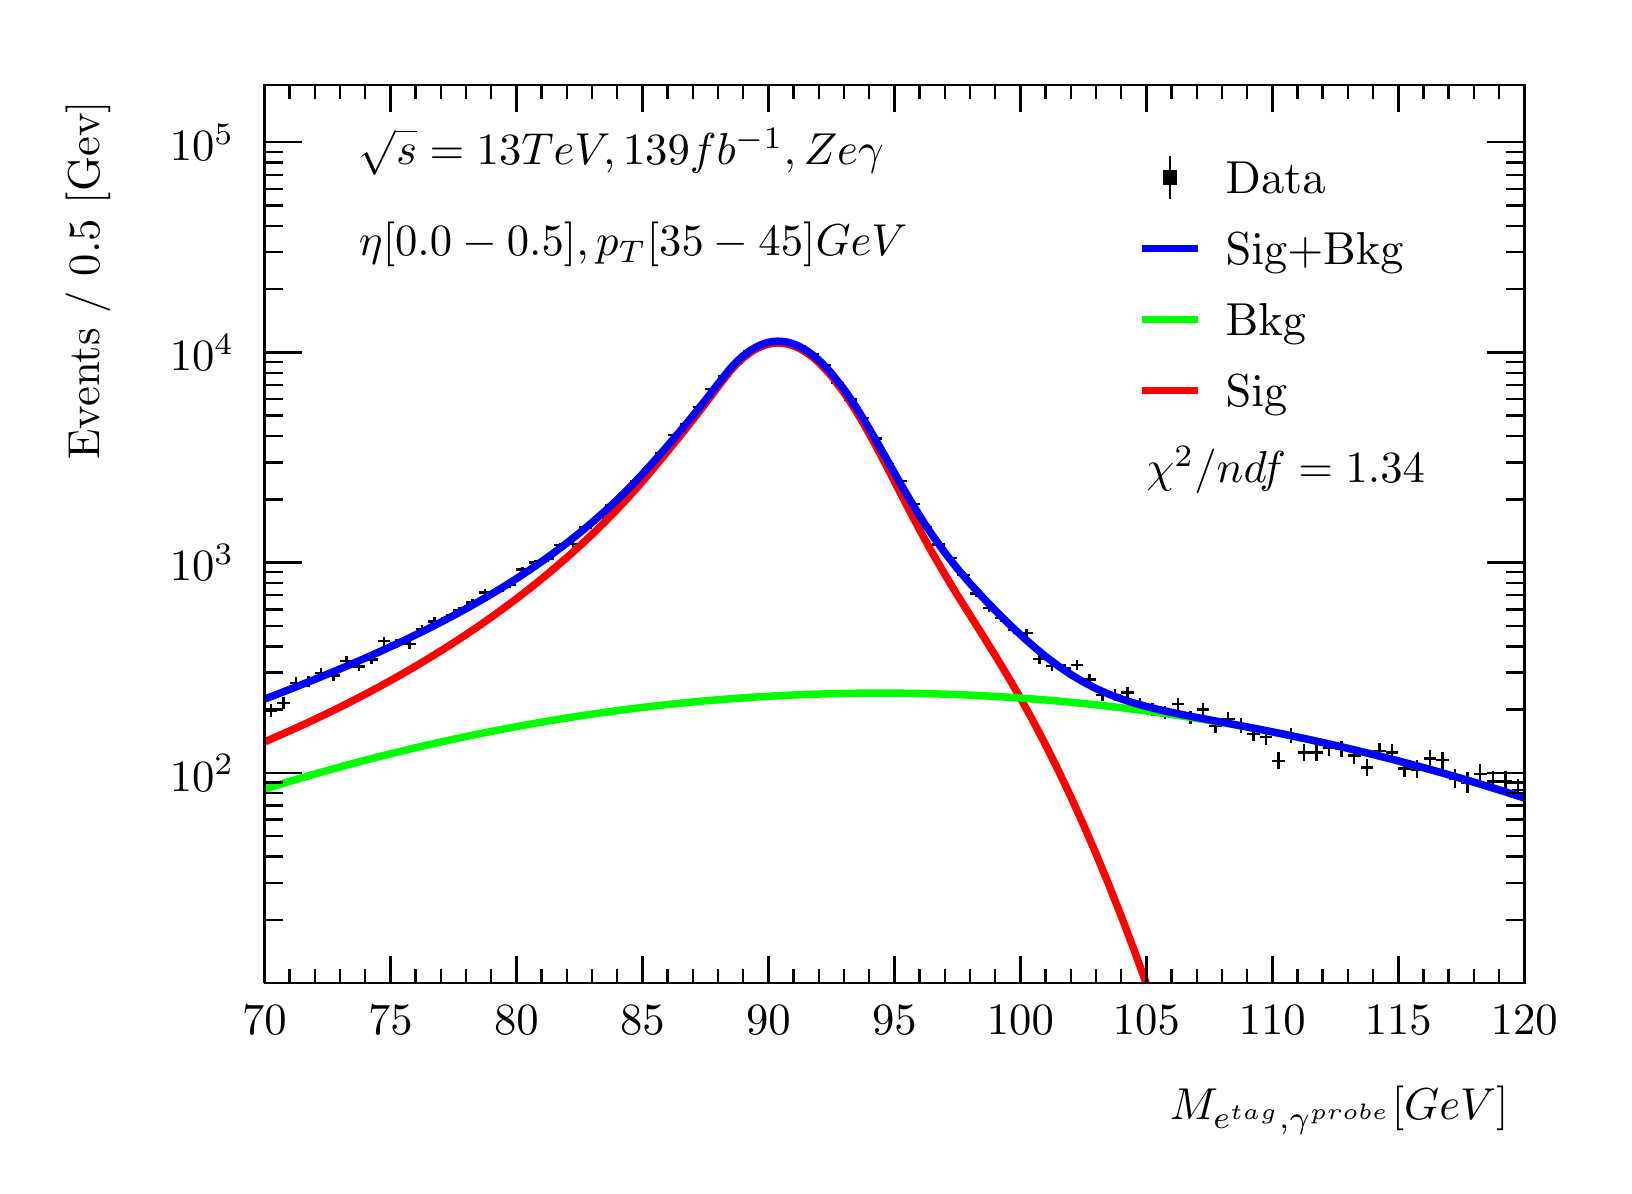
\begin{tikzpicture}
\pgfdeclareplotmark{cross} {
\pgfpathmoveto{\pgfpoint{-0.3\pgfplotmarksize}{\pgfplotmarksize}}
\pgfpathlineto{\pgfpoint{+0.3\pgfplotmarksize}{\pgfplotmarksize}}
\pgfpathlineto{\pgfpoint{+0.3\pgfplotmarksize}{0.3\pgfplotmarksize}}
\pgfpathlineto{\pgfpoint{+1\pgfplotmarksize}{0.3\pgfplotmarksize}}
\pgfpathlineto{\pgfpoint{+1\pgfplotmarksize}{-0.3\pgfplotmarksize}}
\pgfpathlineto{\pgfpoint{+0.3\pgfplotmarksize}{-0.3\pgfplotmarksize}}
\pgfpathlineto{\pgfpoint{+0.3\pgfplotmarksize}{-1.\pgfplotmarksize}}
\pgfpathlineto{\pgfpoint{-0.3\pgfplotmarksize}{-1.\pgfplotmarksize}}
\pgfpathlineto{\pgfpoint{-0.3\pgfplotmarksize}{-0.3\pgfplotmarksize}}
\pgfpathlineto{\pgfpoint{-1.\pgfplotmarksize}{-0.3\pgfplotmarksize}}
\pgfpathlineto{\pgfpoint{-1.\pgfplotmarksize}{0.3\pgfplotmarksize}}
\pgfpathlineto{\pgfpoint{-0.3\pgfplotmarksize}{0.3\pgfplotmarksize}}
\pgfpathclose
\pgfusepathqstroke
}
\pgfdeclareplotmark{cross*} {
\pgfpathmoveto{\pgfpoint{-0.3\pgfplotmarksize}{\pgfplotmarksize}}
\pgfpathlineto{\pgfpoint{+0.3\pgfplotmarksize}{\pgfplotmarksize}}
\pgfpathlineto{\pgfpoint{+0.3\pgfplotmarksize}{0.3\pgfplotmarksize}}
\pgfpathlineto{\pgfpoint{+1\pgfplotmarksize}{0.3\pgfplotmarksize}}
\pgfpathlineto{\pgfpoint{+1\pgfplotmarksize}{-0.3\pgfplotmarksize}}
\pgfpathlineto{\pgfpoint{+0.3\pgfplotmarksize}{-0.3\pgfplotmarksize}}
\pgfpathlineto{\pgfpoint{+0.3\pgfplotmarksize}{-1.\pgfplotmarksize}}
\pgfpathlineto{\pgfpoint{-0.3\pgfplotmarksize}{-1.\pgfplotmarksize}}
\pgfpathlineto{\pgfpoint{-0.3\pgfplotmarksize}{-0.3\pgfplotmarksize}}
\pgfpathlineto{\pgfpoint{-1.\pgfplotmarksize}{-0.3\pgfplotmarksize}}
\pgfpathlineto{\pgfpoint{-1.\pgfplotmarksize}{0.3\pgfplotmarksize}}
\pgfpathlineto{\pgfpoint{-0.3\pgfplotmarksize}{0.3\pgfplotmarksize}}
\pgfpathclose
\pgfusepathqfillstroke
}
\pgfdeclareplotmark{newstar} {
\pgfpathmoveto{\pgfqpoint{0pt}{\pgfplotmarksize}}
\pgfpathlineto{\pgfqpointpolar{44}{0.5\pgfplotmarksize}}
\pgfpathlineto{\pgfqpointpolar{18}{\pgfplotmarksize}}
\pgfpathlineto{\pgfqpointpolar{-20}{0.5\pgfplotmarksize}}
\pgfpathlineto{\pgfqpointpolar{-54}{\pgfplotmarksize}}
\pgfpathlineto{\pgfqpointpolar{-90}{0.5\pgfplotmarksize}}
\pgfpathlineto{\pgfqpointpolar{234}{\pgfplotmarksize}}
\pgfpathlineto{\pgfqpointpolar{198}{0.5\pgfplotmarksize}}
\pgfpathlineto{\pgfqpointpolar{162}{\pgfplotmarksize}}
\pgfpathlineto{\pgfqpointpolar{134}{0.5\pgfplotmarksize}}
\pgfpathclose
\pgfusepathqstroke
}
\pgfdeclareplotmark{newstar*} {
\pgfpathmoveto{\pgfqpoint{0pt}{\pgfplotmarksize}}
\pgfpathlineto{\pgfqpointpolar{44}{0.5\pgfplotmarksize}}
\pgfpathlineto{\pgfqpointpolar{18}{\pgfplotmarksize}}
\pgfpathlineto{\pgfqpointpolar{-20}{0.5\pgfplotmarksize}}
\pgfpathlineto{\pgfqpointpolar{-54}{\pgfplotmarksize}}
\pgfpathlineto{\pgfqpointpolar{-90}{0.5\pgfplotmarksize}}
\pgfpathlineto{\pgfqpointpolar{234}{\pgfplotmarksize}}
\pgfpathlineto{\pgfqpointpolar{198}{0.5\pgfplotmarksize}}
\pgfpathlineto{\pgfqpointpolar{162}{\pgfplotmarksize}}
\pgfpathlineto{\pgfqpointpolar{134}{0.5\pgfplotmarksize}}
\pgfpathclose
\pgfusepathqfillstroke
}
\definecolor{c}{rgb}{1,1,1};
\draw [color=c, fill=c] (0,0) rectangle (20,14.4361);
\draw [color=c, fill=c] (3,2.30977) rectangle (19,13.7143);
\definecolor{c}{rgb}{0,0,0};
\draw [c,line width=0.9] (3,2.30977) -- (3,13.7143) -- (19,13.7143) -- (19,2.30977) -- (3,2.30977);
\definecolor{c}{rgb}{1,1,1};
\draw [color=c, fill=c] (3,2.30977) rectangle (19,13.7143);
\definecolor{c}{rgb}{0,0,0};
\draw [c,line width=0.9] (3,2.30977) -- (3,13.7143) -- (19,13.7143) -- (19,2.30977) -- (3,2.30977);
\draw [c,line width=0.9] (3,2.30977) -- (19,2.30977);
\draw [c,line width=0.9] (3,2.65624) -- (3,2.30977);
\draw [c,line width=0.9] (3.32,2.48301) -- (3.32,2.30977);
\draw [c,line width=0.9] (3.64,2.48301) -- (3.64,2.30977);
\draw [c,line width=0.9] (3.96,2.48301) -- (3.96,2.30977);
\draw [c,line width=0.9] (4.28,2.48301) -- (4.28,2.30977);
\draw [c,line width=0.9] (4.6,2.65624) -- (4.6,2.30977);
\draw [c,line width=0.9] (4.92,2.48301) -- (4.92,2.30977);
\draw [c,line width=0.9] (5.24,2.48301) -- (5.24,2.30977);
\draw [c,line width=0.9] (5.56,2.48301) -- (5.56,2.30977);
\draw [c,line width=0.9] (5.88,2.48301) -- (5.88,2.30977);
\draw [c,line width=0.9] (6.2,2.65624) -- (6.2,2.30977);
\draw [c,line width=0.9] (6.52,2.48301) -- (6.52,2.30977);
\draw [c,line width=0.9] (6.84,2.48301) -- (6.84,2.30977);
\draw [c,line width=0.9] (7.16,2.48301) -- (7.16,2.30977);
\draw [c,line width=0.9] (7.48,2.48301) -- (7.48,2.30977);
\draw [c,line width=0.9] (7.8,2.65624) -- (7.8,2.30977);
\draw [c,line width=0.9] (8.12,2.48301) -- (8.12,2.30977);
\draw [c,line width=0.9] (8.44,2.48301) -- (8.44,2.30977);
\draw [c,line width=0.9] (8.76,2.48301) -- (8.76,2.30977);
\draw [c,line width=0.9] (9.08,2.48301) -- (9.08,2.30977);
\draw [c,line width=0.9] (9.4,2.65624) -- (9.4,2.30977);
\draw [c,line width=0.9] (9.72,2.48301) -- (9.72,2.30977);
\draw [c,line width=0.9] (10.04,2.48301) -- (10.04,2.30977);
\draw [c,line width=0.9] (10.36,2.48301) -- (10.36,2.30977);
\draw [c,line width=0.9] (10.68,2.48301) -- (10.68,2.30977);
\draw [c,line width=0.9] (11,2.65624) -- (11,2.30977);
\draw [c,line width=0.9] (11.32,2.48301) -- (11.32,2.30977);
\draw [c,line width=0.9] (11.64,2.48301) -- (11.64,2.30977);
\draw [c,line width=0.9] (11.96,2.48301) -- (11.96,2.30977);
\draw [c,line width=0.9] (12.28,2.48301) -- (12.28,2.30977);
\draw [c,line width=0.9] (12.6,2.65624) -- (12.6,2.30977);
\draw [c,line width=0.9] (12.92,2.48301) -- (12.92,2.30977);
\draw [c,line width=0.9] (13.24,2.48301) -- (13.24,2.30977);
\draw [c,line width=0.9] (13.56,2.48301) -- (13.56,2.30977);
\draw [c,line width=0.9] (13.88,2.48301) -- (13.88,2.30977);
\draw [c,line width=0.9] (14.2,2.65624) -- (14.2,2.30977);
\draw [c,line width=0.9] (14.52,2.48301) -- (14.52,2.30977);
\draw [c,line width=0.9] (14.84,2.48301) -- (14.84,2.30977);
\draw [c,line width=0.9] (15.16,2.48301) -- (15.16,2.30977);
\draw [c,line width=0.9] (15.48,2.48301) -- (15.48,2.30977);
\draw [c,line width=0.9] (15.8,2.65624) -- (15.8,2.30977);
\draw [c,line width=0.9] (16.12,2.48301) -- (16.12,2.30977);
\draw [c,line width=0.9] (16.44,2.48301) -- (16.44,2.30977);
\draw [c,line width=0.9] (16.76,2.48301) -- (16.76,2.30977);
\draw [c,line width=0.9] (17.08,2.48301) -- (17.08,2.30977);
\draw [c,line width=0.9] (17.4,2.65624) -- (17.4,2.30977);
\draw [c,line width=0.9] (17.72,2.48301) -- (17.72,2.30977);
\draw [c,line width=0.9] (18.04,2.48301) -- (18.04,2.30977);
\draw [c,line width=0.9] (18.36,2.48301) -- (18.36,2.30977);
\draw [c,line width=0.9] (18.68,2.48301) -- (18.68,2.30977);
\draw [c,line width=0.9] (19,2.65624) -- (19,2.30977);
\draw [anchor=base] (3,1.66015) node[scale=1.61424, color=c, rotate=0]{70};
\draw [anchor=base] (4.6,1.66015) node[scale=1.61424, color=c, rotate=0]{75};
\draw [anchor=base] (6.2,1.66015) node[scale=1.61424, color=c, rotate=0]{80};
\draw [anchor=base] (7.8,1.66015) node[scale=1.61424, color=c, rotate=0]{85};
\draw [anchor=base] (9.4,1.66015) node[scale=1.61424, color=c, rotate=0]{90};
\draw [anchor=base] (11,1.66015) node[scale=1.61424, color=c, rotate=0]{95};
\draw [anchor=base] (12.6,1.66015) node[scale=1.61424, color=c, rotate=0]{100};
\draw [anchor=base] (14.2,1.66015) node[scale=1.61424, color=c, rotate=0]{105};
\draw [anchor=base] (15.8,1.66015) node[scale=1.61424, color=c, rotate=0]{110};
\draw [anchor=base] (17.4,1.66015) node[scale=1.61424, color=c, rotate=0]{115};
\draw [anchor=base] (19,1.66015) node[scale=1.61424, color=c, rotate=0]{120};
\draw [anchor= east] (19,0.692932) node[scale=1.61424, color=c, rotate=0]{$M_{e^{tag}, \gamma^{probe}}  [GeV]$};
\draw [c,line width=0.9] (3,13.7143) -- (19,13.7143);
\draw [c,line width=0.9] (3,13.3678) -- (3,13.7143);
\draw [c,line width=0.9] (3.32,13.5411) -- (3.32,13.7143);
\draw [c,line width=0.9] (3.64,13.5411) -- (3.64,13.7143);
\draw [c,line width=0.9] (3.96,13.5411) -- (3.96,13.7143);
\draw [c,line width=0.9] (4.28,13.5411) -- (4.28,13.7143);
\draw [c,line width=0.9] (4.6,13.3678) -- (4.6,13.7143);
\draw [c,line width=0.9] (4.92,13.5411) -- (4.92,13.7143);
\draw [c,line width=0.9] (5.24,13.5411) -- (5.24,13.7143);
\draw [c,line width=0.9] (5.56,13.5411) -- (5.56,13.7143);
\draw [c,line width=0.9] (5.88,13.5411) -- (5.88,13.7143);
\draw [c,line width=0.9] (6.2,13.3678) -- (6.2,13.7143);
\draw [c,line width=0.9] (6.52,13.5411) -- (6.52,13.7143);
\draw [c,line width=0.9] (6.84,13.5411) -- (6.84,13.7143);
\draw [c,line width=0.9] (7.16,13.5411) -- (7.16,13.7143);
\draw [c,line width=0.9] (7.48,13.5411) -- (7.48,13.7143);
\draw [c,line width=0.9] (7.8,13.3678) -- (7.8,13.7143);
\draw [c,line width=0.9] (8.12,13.5411) -- (8.12,13.7143);
\draw [c,line width=0.9] (8.44,13.5411) -- (8.44,13.7143);
\draw [c,line width=0.9] (8.76,13.5411) -- (8.76,13.7143);
\draw [c,line width=0.9] (9.08,13.5411) -- (9.08,13.7143);
\draw [c,line width=0.9] (9.4,13.3678) -- (9.4,13.7143);
\draw [c,line width=0.9] (9.72,13.5411) -- (9.72,13.7143);
\draw [c,line width=0.9] (10.04,13.5411) -- (10.04,13.7143);
\draw [c,line width=0.9] (10.36,13.5411) -- (10.36,13.7143);
\draw [c,line width=0.9] (10.68,13.5411) -- (10.68,13.7143);
\draw [c,line width=0.9] (11,13.3678) -- (11,13.7143);
\draw [c,line width=0.9] (11.32,13.5411) -- (11.32,13.7143);
\draw [c,line width=0.9] (11.64,13.5411) -- (11.64,13.7143);
\draw [c,line width=0.9] (11.96,13.5411) -- (11.96,13.7143);
\draw [c,line width=0.9] (12.28,13.5411) -- (12.28,13.7143);
\draw [c,line width=0.9] (12.6,13.3678) -- (12.6,13.7143);
\draw [c,line width=0.9] (12.92,13.5411) -- (12.92,13.7143);
\draw [c,line width=0.9] (13.24,13.5411) -- (13.24,13.7143);
\draw [c,line width=0.9] (13.56,13.5411) -- (13.56,13.7143);
\draw [c,line width=0.9] (13.88,13.5411) -- (13.88,13.7143);
\draw [c,line width=0.9] (14.2,13.3678) -- (14.2,13.7143);
\draw [c,line width=0.9] (14.52,13.5411) -- (14.52,13.7143);
\draw [c,line width=0.9] (14.84,13.5411) -- (14.84,13.7143);
\draw [c,line width=0.9] (15.16,13.5411) -- (15.16,13.7143);
\draw [c,line width=0.9] (15.48,13.5411) -- (15.48,13.7143);
\draw [c,line width=0.9] (15.8,13.3678) -- (15.8,13.7143);
\draw [c,line width=0.9] (16.12,13.5411) -- (16.12,13.7143);
\draw [c,line width=0.9] (16.44,13.5411) -- (16.44,13.7143);
\draw [c,line width=0.9] (16.76,13.5411) -- (16.76,13.7143);
\draw [c,line width=0.9] (17.08,13.5411) -- (17.08,13.7143);
\draw [c,line width=0.9] (17.4,13.3678) -- (17.4,13.7143);
\draw [c,line width=0.9] (17.72,13.5411) -- (17.72,13.7143);
\draw [c,line width=0.9] (18.04,13.5411) -- (18.04,13.7143);
\draw [c,line width=0.9] (18.36,13.5411) -- (18.36,13.7143);
\draw [c,line width=0.9] (18.68,13.5411) -- (18.68,13.7143);
\draw [c,line width=0.9] (19,13.3678) -- (19,13.7143);
\draw [c,line width=0.9] (3,2.30977) -- (3,13.7143);
\draw [c,line width=0.9] (3.237,3.11343) -- (3,3.11343);
\draw [c,line width=0.9] (3.237,3.58354) -- (3,3.58354);
\draw [c,line width=0.9] (3.237,3.91709) -- (3,3.91709);
\draw [c,line width=0.9] (3.237,4.17581) -- (3,4.17581);
\draw [c,line width=0.9] (3.237,4.38719) -- (3,4.38719);
\draw [c,line width=0.9] (3.237,4.56592) -- (3,4.56592);
\draw [c,line width=0.9] (3.237,4.72074) -- (3,4.72074);
\draw [c,line width=0.9] (3.237,4.8573) -- (3,4.8573);
\draw [c,line width=0.9] (3.474,4.97946) -- (3,4.97946);
\draw [anchor= east] (2.82,4.97946) node[scale=1.61424, color=c, rotate=0]{$10^{2}$};
\draw [c,line width=0.9] (3.237,5.78312) -- (3,5.78312);
\draw [c,line width=0.9] (3.237,6.25323) -- (3,6.25323);
\draw [c,line width=0.9] (3.237,6.58678) -- (3,6.58678);
\draw [c,line width=0.9] (3.237,6.8455) -- (3,6.8455);
\draw [c,line width=0.9] (3.237,7.05689) -- (3,7.05689);
\draw [c,line width=0.9] (3.237,7.23561) -- (3,7.23561);
\draw [c,line width=0.9] (3.237,7.39043) -- (3,7.39043);
\draw [c,line width=0.9] (3.237,7.52699) -- (3,7.52699);
\draw [c,line width=0.9] (3.474,7.64915) -- (3,7.64915);
\draw [anchor= east] (2.82,7.64915) node[scale=1.61424, color=c, rotate=0]{$10^{3}$};
\draw [c,line width=0.9] (3.237,8.45281) -- (3,8.45281);
\draw [c,line width=0.9] (3.237,8.92292) -- (3,8.92292);
\draw [c,line width=0.9] (3.237,9.25647) -- (3,9.25647);
\draw [c,line width=0.9] (3.237,9.51519) -- (3,9.51519);
\draw [c,line width=0.9] (3.237,9.72658) -- (3,9.72658);
\draw [c,line width=0.9] (3.237,9.9053) -- (3,9.9053);
\draw [c,line width=0.9] (3.237,10.0601) -- (3,10.0601);
\draw [c,line width=0.9] (3.237,10.1967) -- (3,10.1967);
\draw [c,line width=0.9] (3.474,10.3188) -- (3,10.3188);
\draw [anchor= east] (2.82,10.3188) node[scale=1.61424, color=c, rotate=0]{$10^{4}$};
\draw [c,line width=0.9] (3.237,11.1225) -- (3,11.1225);
\draw [c,line width=0.9] (3.237,11.5926) -- (3,11.5926);
\draw [c,line width=0.9] (3.237,11.9262) -- (3,11.9262);
\draw [c,line width=0.9] (3.237,12.1849) -- (3,12.1849);
\draw [c,line width=0.9] (3.237,12.3963) -- (3,12.3963);
\draw [c,line width=0.9] (3.237,12.575) -- (3,12.575);
\draw [c,line width=0.9] (3.237,12.7298) -- (3,12.7298);
\draw [c,line width=0.9] (3.237,12.8664) -- (3,12.8664);
\draw [c,line width=0.9] (3.474,12.9885) -- (3,12.9885);
\draw [anchor= east] (2.82,12.9885) node[scale=1.61424, color=c, rotate=0]{$10^{5}$};
\draw [anchor= east] (0.76,13.7143) node[scale=1.61424, color=c, rotate=90]{Events / 0.5 [Gev]};
\draw [c,line width=0.9] (19,2.30977) -- (19,13.7143);
\draw [c,line width=0.9] (18.763,3.11343) -- (19,3.11343);
\draw [c,line width=0.9] (18.763,3.58354) -- (19,3.58354);
\draw [c,line width=0.9] (18.763,3.91709) -- (19,3.91709);
\draw [c,line width=0.9] (18.763,4.17581) -- (19,4.17581);
\draw [c,line width=0.9] (18.763,4.38719) -- (19,4.38719);
\draw [c,line width=0.9] (18.763,4.56592) -- (19,4.56592);
\draw [c,line width=0.9] (18.763,4.72074) -- (19,4.72074);
\draw [c,line width=0.9] (18.763,4.8573) -- (19,4.8573);
\draw [c,line width=0.9] (18.526,4.97946) -- (19,4.97946);
\draw [c,line width=0.9] (18.763,5.78312) -- (19,5.78312);
\draw [c,line width=0.9] (18.763,6.25323) -- (19,6.25323);
\draw [c,line width=0.9] (18.763,6.58678) -- (19,6.58678);
\draw [c,line width=0.9] (18.763,6.8455) -- (19,6.8455);
\draw [c,line width=0.9] (18.763,7.05689) -- (19,7.05689);
\draw [c,line width=0.9] (18.763,7.23561) -- (19,7.23561);
\draw [c,line width=0.9] (18.763,7.39043) -- (19,7.39043);
\draw [c,line width=0.9] (18.763,7.52699) -- (19,7.52699);
\draw [c,line width=0.9] (18.526,7.64915) -- (19,7.64915);
\draw [c,line width=0.9] (18.763,8.45281) -- (19,8.45281);
\draw [c,line width=0.9] (18.763,8.92292) -- (19,8.92292);
\draw [c,line width=0.9] (18.763,9.25647) -- (19,9.25647);
\draw [c,line width=0.9] (18.763,9.51519) -- (19,9.51519);
\draw [c,line width=0.9] (18.763,9.72658) -- (19,9.72658);
\draw [c,line width=0.9] (18.763,9.9053) -- (19,9.9053);
\draw [c,line width=0.9] (18.763,10.0601) -- (19,10.0601);
\draw [c,line width=0.9] (18.763,10.1967) -- (19,10.1967);
\draw [c,line width=0.9] (18.526,10.3188) -- (19,10.3188);
\draw [c,line width=0.9] (18.763,11.1225) -- (19,11.1225);
\draw [c,line width=0.9] (18.763,11.5926) -- (19,11.5926);
\draw [c,line width=0.9] (18.763,11.9262) -- (19,11.9262);
\draw [c,line width=0.9] (18.763,12.1849) -- (19,12.1849);
\draw [c,line width=0.9] (18.763,12.3963) -- (19,12.3963);
\draw [c,line width=0.9] (18.763,12.575) -- (19,12.575);
\draw [c,line width=0.9] (18.763,12.7298) -- (19,12.7298);
\draw [c,line width=0.9] (18.763,12.8664) -- (19,12.8664);
\draw [c,line width=0.9] (18.526,12.9885) -- (19,12.9885);
\draw [c,line width=0.9] (3.08,5.77147) -- (3,5.77147);
\draw [c,line width=0.9] (3,5.77147) -- (3,5.77147);
\draw [c,line width=0.9] (3.08,5.77147) -- (3.16,5.77147);
\draw [c,line width=0.9] (3.16,5.77147) -- (3.16,5.77147);
\draw [c,line width=0.9] (3.08,5.77147) -- (3.08,5.85385);
\draw [c,line width=0.9] (3.08,5.85385) -- (3.08,5.85385);
\draw [c,line width=0.9] (3.08,5.77147) -- (3.08,5.68909);
\draw [c,line width=0.9] (3.08,5.68909) -- (3.08,5.68909);
\draw [c,line width=0.9] (3.24,5.86697) -- (3.16,5.86697);
\draw [c,line width=0.9] (3.16,5.86697) -- (3.16,5.86697);
\draw [c,line width=0.9] (3.24,5.86697) -- (3.32,5.86697);
\draw [c,line width=0.9] (3.32,5.86697) -- (3.32,5.86697);
\draw [c,line width=0.9] (3.24,5.86697) -- (3.24,5.94603);
\draw [c,line width=0.9] (3.24,5.94603) -- (3.24,5.94603);
\draw [c,line width=0.9] (3.24,5.86697) -- (3.24,5.78791);
\draw [c,line width=0.9] (3.24,5.78791) -- (3.24,5.78791);
\draw [c,line width=0.9] (3.4,6.12245) -- (3.32,6.12245);
\draw [c,line width=0.9] (3.32,6.12245) -- (3.32,6.12245);
\draw [c,line width=0.9] (3.4,6.12245) -- (3.48,6.12245);
\draw [c,line width=0.9] (3.48,6.12245) -- (3.48,6.12245);
\draw [c,line width=0.9] (3.4,6.12245) -- (3.4,6.19326);
\draw [c,line width=0.9] (3.4,6.19326) -- (3.4,6.19326);
\draw [c,line width=0.9] (3.4,6.12245) -- (3.4,6.05164);
\draw [c,line width=0.9] (3.4,6.05164) -- (3.4,6.05164);
\draw [c,line width=0.9] (3.56,6.14388) -- (3.48,6.14388);
\draw [c,line width=0.9] (3.48,6.14388) -- (3.48,6.14388);
\draw [c,line width=0.9] (3.56,6.14388) -- (3.64,6.14388);
\draw [c,line width=0.9] (3.64,6.14388) -- (3.64,6.14388);
\draw [c,line width=0.9] (3.56,6.14388) -- (3.56,6.21404);
\draw [c,line width=0.9] (3.56,6.21404) -- (3.56,6.21404);
\draw [c,line width=0.9] (3.56,6.14388) -- (3.56,6.07372);
\draw [c,line width=0.9] (3.56,6.07372) -- (3.56,6.07372);
\draw [c,line width=0.9] (3.72,6.24547) -- (3.64,6.24547);
\draw [c,line width=0.9] (3.64,6.24547) -- (3.64,6.24547);
\draw [c,line width=0.9] (3.72,6.24547) -- (3.8,6.24547);
\draw [c,line width=0.9] (3.8,6.24547) -- (3.8,6.24547);
\draw [c,line width=0.9] (3.72,6.24547) -- (3.72,6.31263);
\draw [c,line width=0.9] (3.72,6.31263) -- (3.72,6.31263);
\draw [c,line width=0.9] (3.72,6.24547) -- (3.72,6.17832);
\draw [c,line width=0.9] (3.72,6.17832) -- (3.72,6.17832);
\draw [c,line width=0.9] (3.88,6.21392) -- (3.8,6.21392);
\draw [c,line width=0.9] (3.8,6.21392) -- (3.8,6.21392);
\draw [c,line width=0.9] (3.88,6.21392) -- (3.96,6.21392);
\draw [c,line width=0.9] (3.96,6.21392) -- (3.96,6.21392);
\draw [c,line width=0.9] (3.88,6.21392) -- (3.88,6.282);
\draw [c,line width=0.9] (3.88,6.282) -- (3.88,6.282);
\draw [c,line width=0.9] (3.88,6.21392) -- (3.88,6.14585);
\draw [c,line width=0.9] (3.88,6.14585) -- (3.88,6.14585);
\draw [c,line width=0.9] (4.04,6.39835) -- (3.96,6.39835);
\draw [c,line width=0.9] (3.96,6.39835) -- (3.96,6.39835);
\draw [c,line width=0.9] (4.04,6.39835) -- (4.12,6.39835);
\draw [c,line width=0.9] (4.12,6.39835) -- (4.12,6.39835);
\draw [c,line width=0.9] (4.04,6.39835) -- (4.04,6.46122);
\draw [c,line width=0.9] (4.04,6.46122) -- (4.04,6.46122);
\draw [c,line width=0.9] (4.04,6.39835) -- (4.04,6.33548);
\draw [c,line width=0.9] (4.04,6.33548) -- (4.04,6.33548);
\draw [c,line width=0.9] (4.2,6.33168) -- (4.12,6.33168);
\draw [c,line width=0.9] (4.12,6.33168) -- (4.12,6.33168);
\draw [c,line width=0.9] (4.2,6.33168) -- (4.28,6.33168);
\draw [c,line width=0.9] (4.28,6.33168) -- (4.28,6.33168);
\draw [c,line width=0.9] (4.2,6.33168) -- (4.2,6.39638);
\draw [c,line width=0.9] (4.2,6.39638) -- (4.2,6.39638);
\draw [c,line width=0.9] (4.2,6.33168) -- (4.2,6.26697);
\draw [c,line width=0.9] (4.2,6.26697) -- (4.2,6.26697);
\draw [c,line width=0.9] (4.36,6.41863) -- (4.28,6.41863);
\draw [c,line width=0.9] (4.28,6.41863) -- (4.28,6.41863);
\draw [c,line width=0.9] (4.36,6.41863) -- (4.44,6.41863);
\draw [c,line width=0.9] (4.44,6.41863) -- (4.44,6.41863);
\draw [c,line width=0.9] (4.36,6.41863) -- (4.36,6.48095);
\draw [c,line width=0.9] (4.36,6.48095) -- (4.36,6.48095);
\draw [c,line width=0.9] (4.36,6.41863) -- (4.36,6.35631);
\draw [c,line width=0.9] (4.36,6.35631) -- (4.36,6.35631);
\draw [c,line width=0.9] (4.52,6.6516) -- (4.44,6.6516);
\draw [c,line width=0.9] (4.44,6.6516) -- (4.44,6.6516);
\draw [c,line width=0.9] (4.52,6.6516) -- (4.6,6.6516);
\draw [c,line width=0.9] (4.6,6.6516) -- (4.6,6.6516);
\draw [c,line width=0.9] (4.52,6.6516) -- (4.52,6.70797);
\draw [c,line width=0.9] (4.52,6.70797) -- (4.52,6.70797);
\draw [c,line width=0.9] (4.52,6.6516) -- (4.52,6.59523);
\draw [c,line width=0.9] (4.52,6.59523) -- (4.52,6.59523);
\draw [c,line width=0.9] (4.68,6.62666) -- (4.6,6.62666);
\draw [c,line width=0.9] (4.6,6.62666) -- (4.6,6.62666);
\draw [c,line width=0.9] (4.68,6.62666) -- (4.76,6.62666);
\draw [c,line width=0.9] (4.76,6.62666) -- (4.76,6.62666);
\draw [c,line width=0.9] (4.68,6.62666) -- (4.68,6.68364);
\draw [c,line width=0.9] (4.68,6.68364) -- (4.68,6.68364);
\draw [c,line width=0.9] (4.68,6.62666) -- (4.68,6.56969);
\draw [c,line width=0.9] (4.68,6.56969) -- (4.68,6.56969);
\draw [c,line width=0.9] (4.84,6.61258) -- (4.76,6.61258);
\draw [c,line width=0.9] (4.76,6.61258) -- (4.76,6.61258);
\draw [c,line width=0.9] (4.84,6.61258) -- (4.92,6.61258);
\draw [c,line width=0.9] (4.92,6.61258) -- (4.92,6.61258);
\draw [c,line width=0.9] (4.84,6.61258) -- (4.84,6.6699);
\draw [c,line width=0.9] (4.84,6.6699) -- (4.84,6.6699);
\draw [c,line width=0.9] (4.84,6.61258) -- (4.84,6.55525);
\draw [c,line width=0.9] (4.84,6.55525) -- (4.84,6.55525);
\draw [c,line width=0.9] (5,6.80779) -- (4.92,6.80779);
\draw [c,line width=0.9] (4.92,6.80779) -- (4.92,6.80779);
\draw [c,line width=0.9] (5,6.80779) -- (5.08,6.80779);
\draw [c,line width=0.9] (5.08,6.80779) -- (5.08,6.80779);
\draw [c,line width=0.9] (5,6.80779) -- (5,6.86049);
\draw [c,line width=0.9] (5,6.86049) -- (5,6.86049);
\draw [c,line width=0.9] (5,6.80779) -- (5,6.75509);
\draw [c,line width=0.9] (5,6.75509) -- (5,6.75509);
\draw [c,line width=0.9] (5.16,6.90207) -- (5.08,6.90207);
\draw [c,line width=0.9] (5.08,6.90207) -- (5.08,6.90207);
\draw [c,line width=0.9] (5.16,6.90207) -- (5.24,6.90207);
\draw [c,line width=0.9] (5.24,6.90207) -- (5.24,6.90207);
\draw [c,line width=0.9] (5.16,6.90207) -- (5.16,6.95266);
\draw [c,line width=0.9] (5.16,6.95266) -- (5.16,6.95266);
\draw [c,line width=0.9] (5.16,6.90207) -- (5.16,6.85147);
\draw [c,line width=0.9] (5.16,6.85147) -- (5.16,6.85147);
\draw [c,line width=0.9] (5.32,6.94754) -- (5.24,6.94754);
\draw [c,line width=0.9] (5.24,6.94754) -- (5.24,6.94754);
\draw [c,line width=0.9] (5.32,6.94754) -- (5.4,6.94754);
\draw [c,line width=0.9] (5.4,6.94754) -- (5.4,6.94754);
\draw [c,line width=0.9] (5.32,6.94754) -- (5.32,6.99716);
\draw [c,line width=0.9] (5.32,6.99716) -- (5.32,6.99716);
\draw [c,line width=0.9] (5.32,6.94754) -- (5.32,6.89792);
\draw [c,line width=0.9] (5.32,6.89792) -- (5.32,6.89792);
\draw [c,line width=0.9] (5.48,7.03936) -- (5.4,7.03936);
\draw [c,line width=0.9] (5.4,7.03936) -- (5.4,7.03936);
\draw [c,line width=0.9] (5.48,7.03936) -- (5.56,7.03936);
\draw [c,line width=0.9] (5.56,7.03936) -- (5.56,7.03936);
\draw [c,line width=0.9] (5.48,7.03936) -- (5.48,7.08705);
\draw [c,line width=0.9] (5.48,7.08705) -- (5.48,7.08705);
\draw [c,line width=0.9] (5.48,7.03936) -- (5.48,6.99167);
\draw [c,line width=0.9] (5.48,6.99167) -- (5.48,6.99167);
\draw [c,line width=0.9] (5.64,7.14074) -- (5.56,7.14074);
\draw [c,line width=0.9] (5.56,7.14074) -- (5.56,7.14074);
\draw [c,line width=0.9] (5.64,7.14074) -- (5.72,7.14074);
\draw [c,line width=0.9] (5.72,7.14074) -- (5.72,7.14074);
\draw [c,line width=0.9] (5.64,7.14074) -- (5.64,7.18639);
\draw [c,line width=0.9] (5.64,7.18639) -- (5.64,7.18639);
\draw [c,line width=0.9] (5.64,7.14074) -- (5.64,7.09509);
\draw [c,line width=0.9] (5.64,7.09509) -- (5.64,7.09509);
\draw [c,line width=0.9] (5.8,7.26666) -- (5.72,7.26666);
\draw [c,line width=0.9] (5.72,7.26666) -- (5.72,7.26666);
\draw [c,line width=0.9] (5.8,7.26666) -- (5.88,7.26666);
\draw [c,line width=0.9] (5.88,7.26666) -- (5.88,7.26666);
\draw [c,line width=0.9] (5.8,7.26666) -- (5.8,7.3099);
\draw [c,line width=0.9] (5.8,7.3099) -- (5.8,7.3099);
\draw [c,line width=0.9] (5.8,7.26666) -- (5.8,7.22343);
\draw [c,line width=0.9] (5.8,7.22343) -- (5.8,7.22343);
\draw [c,line width=0.9] (5.96,7.28902) -- (5.88,7.28902);
\draw [c,line width=0.9] (5.88,7.28902) -- (5.88,7.28902);
\draw [c,line width=0.9] (5.96,7.28902) -- (6.04,7.28902);
\draw [c,line width=0.9] (6.04,7.28902) -- (6.04,7.28902);
\draw [c,line width=0.9] (5.96,7.28902) -- (5.96,7.33185);
\draw [c,line width=0.9] (5.96,7.33185) -- (5.96,7.33185);
\draw [c,line width=0.9] (5.96,7.28902) -- (5.96,7.2462);
\draw [c,line width=0.9] (5.96,7.2462) -- (5.96,7.2462);
\draw [c,line width=0.9] (6.12,7.36553) -- (6.04,7.36553);
\draw [c,line width=0.9] (6.04,7.36553) -- (6.04,7.36553);
\draw [c,line width=0.9] (6.12,7.36553) -- (6.2,7.36553);
\draw [c,line width=0.9] (6.2,7.36553) -- (6.2,7.36553);
\draw [c,line width=0.9] (6.12,7.36553) -- (6.12,7.40696);
\draw [c,line width=0.9] (6.12,7.40696) -- (6.12,7.40696);
\draw [c,line width=0.9] (6.12,7.36553) -- (6.12,7.3241);
\draw [c,line width=0.9] (6.12,7.3241) -- (6.12,7.3241);
\draw [c,line width=0.9] (6.28,7.55876) -- (6.2,7.55876);
\draw [c,line width=0.9] (6.2,7.55876) -- (6.2,7.55876);
\draw [c,line width=0.9] (6.28,7.55876) -- (6.36,7.55876);
\draw [c,line width=0.9] (6.36,7.55876) -- (6.36,7.55876);
\draw [c,line width=0.9] (6.28,7.55876) -- (6.28,7.59688);
\draw [c,line width=0.9] (6.28,7.59688) -- (6.28,7.59688);
\draw [c,line width=0.9] (6.28,7.55876) -- (6.28,7.52064);
\draw [c,line width=0.9] (6.28,7.52064) -- (6.28,7.52064);
\draw [c,line width=0.9] (6.44,7.65031) -- (6.36,7.65031);
\draw [c,line width=0.9] (6.36,7.65031) -- (6.36,7.65031);
\draw [c,line width=0.9] (6.44,7.65031) -- (6.52,7.65031);
\draw [c,line width=0.9] (6.52,7.65031) -- (6.52,7.65031);
\draw [c,line width=0.9] (6.44,7.65031) -- (6.44,7.68696);
\draw [c,line width=0.9] (6.44,7.68696) -- (6.44,7.68696);
\draw [c,line width=0.9] (6.44,7.65031) -- (6.44,7.61367);
\draw [c,line width=0.9] (6.44,7.61367) -- (6.44,7.61367);
\draw [c,line width=0.9] (6.6,7.69908) -- (6.52,7.69908);
\draw [c,line width=0.9] (6.52,7.69908) -- (6.52,7.69908);
\draw [c,line width=0.9] (6.6,7.69908) -- (6.68,7.69908);
\draw [c,line width=0.9] (6.68,7.69908) -- (6.68,7.69908);
\draw [c,line width=0.9] (6.6,7.69908) -- (6.6,7.73496);
\draw [c,line width=0.9] (6.6,7.73496) -- (6.6,7.73496);
\draw [c,line width=0.9] (6.6,7.69908) -- (6.6,7.6632);
\draw [c,line width=0.9] (6.6,7.6632) -- (6.6,7.6632);
\draw [c,line width=0.9] (6.76,7.87112) -- (6.68,7.87112);
\draw [c,line width=0.9] (6.68,7.87112) -- (6.68,7.87112);
\draw [c,line width=0.9] (6.76,7.87112) -- (6.84,7.87112);
\draw [c,line width=0.9] (6.84,7.87112) -- (6.84,7.87112);
\draw [c,line width=0.9] (6.76,7.87112) -- (6.76,7.90444);
\draw [c,line width=0.9] (6.76,7.90444) -- (6.76,7.90444);
\draw [c,line width=0.9] (6.76,7.87112) -- (6.76,7.83781);
\draw [c,line width=0.9] (6.76,7.83781) -- (6.76,7.83781);
\draw [c,line width=0.9] (6.92,7.8854) -- (6.84,7.8854);
\draw [c,line width=0.9] (6.84,7.8854) -- (6.84,7.8854);
\draw [c,line width=0.9] (6.92,7.8854) -- (7,7.8854);
\draw [c,line width=0.9] (7,7.8854) -- (7,7.8854);
\draw [c,line width=0.9] (6.92,7.8854) -- (6.92,7.91851);
\draw [c,line width=0.9] (6.92,7.91851) -- (6.92,7.91851);
\draw [c,line width=0.9] (6.92,7.8854) -- (6.92,7.85228);
\draw [c,line width=0.9] (6.92,7.85228) -- (6.92,7.85228);
\draw [c,line width=0.9] (7.08,8.09426) -- (7,8.09426);
\draw [c,line width=0.9] (7,8.09426) -- (7,8.09426);
\draw [c,line width=0.9] (7.08,8.09426) -- (7.16,8.09426);
\draw [c,line width=0.9] (7.16,8.09426) -- (7.16,8.09426);
\draw [c,line width=0.9] (7.08,8.09426) -- (7.08,8.12452);
\draw [c,line width=0.9] (7.08,8.12452) -- (7.08,8.12452);
\draw [c,line width=0.9] (7.08,8.09426) -- (7.08,8.064);
\draw [c,line width=0.9] (7.08,8.064) -- (7.08,8.064);
\draw [c,line width=0.9] (7.24,8.21705) -- (7.16,8.21705);
\draw [c,line width=0.9] (7.16,8.21705) -- (7.16,8.21705);
\draw [c,line width=0.9] (7.24,8.21705) -- (7.32,8.21705);
\draw [c,line width=0.9] (7.32,8.21705) -- (7.32,8.21705);
\draw [c,line width=0.9] (7.24,8.21705) -- (7.24,8.24575);
\draw [c,line width=0.9] (7.24,8.24575) -- (7.24,8.24575);
\draw [c,line width=0.9] (7.24,8.21705) -- (7.24,8.18835);
\draw [c,line width=0.9] (7.24,8.18835) -- (7.24,8.18835);
\draw [c,line width=0.9] (7.4,8.37365) -- (7.32,8.37365);
\draw [c,line width=0.9] (7.32,8.37365) -- (7.32,8.37365);
\draw [c,line width=0.9] (7.4,8.37365) -- (7.48,8.37365);
\draw [c,line width=0.9] (7.48,8.37365) -- (7.48,8.37365);
\draw [c,line width=0.9] (7.4,8.37365) -- (7.4,8.40047);
\draw [c,line width=0.9] (7.4,8.40047) -- (7.4,8.40047);
\draw [c,line width=0.9] (7.4,8.37365) -- (7.4,8.34682);
\draw [c,line width=0.9] (7.4,8.34682) -- (7.4,8.34682);
\draw [c,line width=0.9] (7.56,8.44233) -- (7.48,8.44233);
\draw [c,line width=0.9] (7.48,8.44233) -- (7.48,8.44233);
\draw [c,line width=0.9] (7.56,8.44233) -- (7.64,8.44233);
\draw [c,line width=0.9] (7.64,8.44233) -- (7.64,8.44233);
\draw [c,line width=0.9] (7.56,8.44233) -- (7.56,8.46837);
\draw [c,line width=0.9] (7.56,8.46837) -- (7.56,8.46837);
\draw [c,line width=0.9] (7.56,8.44233) -- (7.56,8.41629);
\draw [c,line width=0.9] (7.56,8.41629) -- (7.56,8.41629);
\draw [c,line width=0.9] (7.72,8.68526) -- (7.64,8.68526);
\draw [c,line width=0.9] (7.64,8.68526) -- (7.64,8.68526);
\draw [c,line width=0.9] (7.72,8.68526) -- (7.8,8.68526);
\draw [c,line width=0.9] (7.8,8.68526) -- (7.8,8.68526);
\draw [c,line width=0.9] (7.72,8.68526) -- (7.72,8.70872);
\draw [c,line width=0.9] (7.72,8.70872) -- (7.72,8.70872);
\draw [c,line width=0.9] (7.72,8.68526) -- (7.72,8.66181);
\draw [c,line width=0.9] (7.72,8.66181) -- (7.72,8.66181);
\draw [c,line width=0.9] (7.88,8.83336) -- (7.8,8.83336);
\draw [c,line width=0.9] (7.8,8.83336) -- (7.8,8.83336);
\draw [c,line width=0.9] (7.88,8.83336) -- (7.96,8.83336);
\draw [c,line width=0.9] (7.96,8.83336) -- (7.96,8.83336);
\draw [c,line width=0.9] (7.88,8.83336) -- (7.88,8.85537);
\draw [c,line width=0.9] (7.88,8.85537) -- (7.88,8.85537);
\draw [c,line width=0.9] (7.88,8.83336) -- (7.88,8.81136);
\draw [c,line width=0.9] (7.88,8.81136) -- (7.88,8.81136);
\draw [c,line width=0.9] (8.04,9.03763) -- (7.96,9.03763);
\draw [c,line width=0.9] (7.96,9.03763) -- (7.96,9.03763);
\draw [c,line width=0.9] (8.04,9.03763) -- (8.12,9.03763);
\draw [c,line width=0.9] (8.12,9.03763) -- (8.12,9.03763);
\draw [c,line width=0.9] (8.04,9.03763) -- (8.04,9.05778);
\draw [c,line width=0.9] (8.04,9.05778) -- (8.04,9.05778);
\draw [c,line width=0.9] (8.04,9.03763) -- (8.04,9.01749);
\draw [c,line width=0.9] (8.04,9.01749) -- (8.04,9.01749);
\draw [c,line width=0.9] (8.2,9.26858) -- (8.12,9.26858);
\draw [c,line width=0.9] (8.12,9.26858) -- (8.12,9.26858);
\draw [c,line width=0.9] (8.2,9.26858) -- (8.28,9.26858);
\draw [c,line width=0.9] (8.28,9.26858) -- (8.28,9.26858);
\draw [c,line width=0.9] (8.2,9.26858) -- (8.2,9.28681);
\draw [c,line width=0.9] (8.2,9.28681) -- (8.2,9.28681);
\draw [c,line width=0.9] (8.2,9.26858) -- (8.2,9.25034);
\draw [c,line width=0.9] (8.2,9.25034) -- (8.2,9.25034);
\draw [c,line width=0.9] (8.36,9.41093) -- (8.28,9.41093);
\draw [c,line width=0.9] (8.28,9.41093) -- (8.28,9.41093);
\draw [c,line width=0.9] (8.36,9.41093) -- (8.44,9.41093);
\draw [c,line width=0.9] (8.44,9.41093) -- (8.44,9.41093);
\draw [c,line width=0.9] (8.36,9.41093) -- (8.36,9.42808);
\draw [c,line width=0.9] (8.36,9.42808) -- (8.36,9.42808);
\draw [c,line width=0.9] (8.36,9.41093) -- (8.36,9.39377);
\draw [c,line width=0.9] (8.36,9.39377) -- (8.36,9.39377);
\draw [c,line width=0.9] (8.52,9.62801) -- (8.44,9.62801);
\draw [c,line width=0.9] (8.44,9.62801) -- (8.44,9.62801);
\draw [c,line width=0.9] (8.52,9.62801) -- (8.6,9.62801);
\draw [c,line width=0.9] (8.6,9.62801) -- (8.6,9.62801);
\draw [c,line width=0.9] (8.52,9.62801) -- (8.52,9.64363);
\draw [c,line width=0.9] (8.52,9.64363) -- (8.52,9.64363);
\draw [c,line width=0.9] (8.52,9.62801) -- (8.52,9.61239);
\draw [c,line width=0.9] (8.52,9.61239) -- (8.52,9.61239);
\draw [c,line width=0.9] (8.68,9.85105) -- (8.6,9.85105);
\draw [c,line width=0.9] (8.6,9.85105) -- (8.6,9.85105);
\draw [c,line width=0.9] (8.68,9.85105) -- (8.76,9.85105);
\draw [c,line width=0.9] (8.76,9.85105) -- (8.76,9.85105);
\draw [c,line width=0.9] (8.68,9.85105) -- (8.68,9.86524);
\draw [c,line width=0.9] (8.68,9.86524) -- (8.68,9.86524);
\draw [c,line width=0.9] (8.68,9.85105) -- (8.68,9.83687);
\draw [c,line width=0.9] (8.68,9.83687) -- (8.68,9.83687);
\draw [c,line width=0.9] (8.84,10.0176) -- (8.76,10.0176);
\draw [c,line width=0.9] (8.76,10.0176) -- (8.76,10.0176);
\draw [c,line width=0.9] (8.84,10.0176) -- (8.92,10.0176);
\draw [c,line width=0.9] (8.92,10.0176) -- (8.92,10.0176);
\draw [c,line width=0.9] (8.84,10.0176) -- (8.84,10.0308);
\draw [c,line width=0.9] (8.84,10.0308) -- (8.84,10.0308);
\draw [c,line width=0.9] (8.84,10.0176) -- (8.84,10.0044);
\draw [c,line width=0.9] (8.84,10.0044) -- (8.84,10.0044);
\draw [c,line width=0.9] (9,10.1863) -- (8.92,10.1863);
\draw [c,line width=0.9] (8.92,10.1863) -- (8.92,10.1863);
\draw [c,line width=0.9] (9,10.1863) -- (9.08,10.1863);
\draw [c,line width=0.9] (9.08,10.1863) -- (9.08,10.1863);
\draw [c,line width=0.9] (9,10.1863) -- (9,10.1986);
\draw [c,line width=0.9] (9,10.1986) -- (9,10.1986);
\draw [c,line width=0.9] (9,10.1863) -- (9,10.1741);
\draw [c,line width=0.9] (9,10.1741) -- (9,10.1741);
\draw [c,line width=0.9] (9.16,10.3322) -- (9.08,10.3322);
\draw [c,line width=0.9] (9.08,10.3322) -- (9.08,10.3322);
\draw [c,line width=0.9] (9.16,10.3322) -- (9.24,10.3322);
\draw [c,line width=0.9] (9.24,10.3322) -- (9.24,10.3322);
\draw [c,line width=0.9] (9.16,10.3322) -- (9.16,10.3437);
\draw [c,line width=0.9] (9.16,10.3437) -- (9.16,10.3437);
\draw [c,line width=0.9] (9.16,10.3322) -- (9.16,10.3207);
\draw [c,line width=0.9] (9.16,10.3207) -- (9.16,10.3207);
\draw [c,line width=0.9] (9.32,10.4103) -- (9.24,10.4103);
\draw [c,line width=0.9] (9.24,10.4103) -- (9.24,10.4103);
\draw [c,line width=0.9] (9.32,10.4103) -- (9.4,10.4103);
\draw [c,line width=0.9] (9.4,10.4103) -- (9.4,10.4103);
\draw [c,line width=0.9] (9.32,10.4103) -- (9.32,10.4215);
\draw [c,line width=0.9] (9.32,10.4215) -- (9.32,10.4215);
\draw [c,line width=0.9] (9.32,10.4103) -- (9.32,10.3992);
\draw [c,line width=0.9] (9.32,10.3992) -- (9.32,10.3992);
\draw [c,line width=0.9] (9.48,10.4655) -- (9.4,10.4655);
\draw [c,line width=0.9] (9.4,10.4655) -- (9.4,10.4655);
\draw [c,line width=0.9] (9.48,10.4655) -- (9.56,10.4655);
\draw [c,line width=0.9] (9.56,10.4655) -- (9.56,10.4655);
\draw [c,line width=0.9] (9.48,10.4655) -- (9.48,10.4763);
\draw [c,line width=0.9] (9.48,10.4763) -- (9.48,10.4763);
\draw [c,line width=0.9] (9.48,10.4655) -- (9.48,10.4546);
\draw [c,line width=0.9] (9.48,10.4546) -- (9.48,10.4546);
\draw [c,line width=0.9] (9.64,10.4522) -- (9.56,10.4522);
\draw [c,line width=0.9] (9.56,10.4522) -- (9.56,10.4522);
\draw [c,line width=0.9] (9.64,10.4522) -- (9.72,10.4522);
\draw [c,line width=0.9] (9.72,10.4522) -- (9.72,10.4522);
\draw [c,line width=0.9] (9.64,10.4522) -- (9.64,10.4632);
\draw [c,line width=0.9] (9.64,10.4632) -- (9.64,10.4632);
\draw [c,line width=0.9] (9.64,10.4522) -- (9.64,10.4413);
\draw [c,line width=0.9] (9.64,10.4413) -- (9.64,10.4413);
\draw [c,line width=0.9] (9.8,10.3965) -- (9.72,10.3965);
\draw [c,line width=0.9] (9.72,10.3965) -- (9.72,10.3965);
\draw [c,line width=0.9] (9.8,10.3965) -- (9.88,10.3965);
\draw [c,line width=0.9] (9.88,10.3965) -- (9.88,10.3965);
\draw [c,line width=0.9] (9.8,10.3965) -- (9.8,10.4077);
\draw [c,line width=0.9] (9.8,10.4077) -- (9.8,10.4077);
\draw [c,line width=0.9] (9.8,10.3965) -- (9.8,10.3853);
\draw [c,line width=0.9] (9.8,10.3853) -- (9.8,10.3853);
\draw [c,line width=0.9] (9.96,10.2945) -- (9.88,10.2945);
\draw [c,line width=0.9] (9.88,10.2945) -- (9.88,10.2945);
\draw [c,line width=0.9] (9.96,10.2945) -- (10.04,10.2945);
\draw [c,line width=0.9] (10.04,10.2945) -- (10.04,10.2945);
\draw [c,line width=0.9] (9.96,10.2945) -- (9.96,10.3062);
\draw [c,line width=0.9] (9.96,10.3062) -- (9.96,10.3062);
\draw [c,line width=0.9] (9.96,10.2945) -- (9.96,10.2828);
\draw [c,line width=0.9] (9.96,10.2828) -- (9.96,10.2828);
\draw [c,line width=0.9] (10.12,10.1619) -- (10.04,10.1619);
\draw [c,line width=0.9] (10.04,10.1619) -- (10.04,10.1619);
\draw [c,line width=0.9] (10.12,10.1619) -- (10.2,10.1619);
\draw [c,line width=0.9] (10.2,10.1619) -- (10.2,10.1619);
\draw [c,line width=0.9] (10.12,10.1619) -- (10.12,10.1743);
\draw [c,line width=0.9] (10.12,10.1743) -- (10.12,10.1743);
\draw [c,line width=0.9] (10.12,10.1619) -- (10.12,10.1495);
\draw [c,line width=0.9] (10.12,10.1495) -- (10.12,10.1495);
\draw [c,line width=0.9] (10.28,9.9328) -- (10.2,9.9328);
\draw [c,line width=0.9] (10.2,9.9328) -- (10.2,9.9328);
\draw [c,line width=0.9] (10.28,9.9328) -- (10.36,9.9328);
\draw [c,line width=0.9] (10.36,9.9328) -- (10.36,9.9328);
\draw [c,line width=0.9] (10.28,9.9328) -- (10.28,9.9465);
\draw [c,line width=0.9] (10.28,9.9465) -- (10.28,9.9465);
\draw [c,line width=0.9] (10.28,9.9328) -- (10.28,9.91911);
\draw [c,line width=0.9] (10.28,9.91911) -- (10.28,9.91911);
\draw [c,line width=0.9] (10.44,9.71979) -- (10.36,9.71979);
\draw [c,line width=0.9] (10.36,9.71979) -- (10.36,9.71979);
\draw [c,line width=0.9] (10.44,9.71979) -- (10.52,9.71979);
\draw [c,line width=0.9] (10.52,9.71979) -- (10.52,9.71979);
\draw [c,line width=0.9] (10.44,9.71979) -- (10.44,9.73481);
\draw [c,line width=0.9] (10.44,9.73481) -- (10.44,9.73481);
\draw [c,line width=0.9] (10.44,9.71979) -- (10.44,9.70478);
\draw [c,line width=0.9] (10.44,9.70478) -- (10.44,9.70478);
\draw [c,line width=0.9] (10.6,9.48868) -- (10.52,9.48868);
\draw [c,line width=0.9] (10.52,9.48868) -- (10.52,9.48868);
\draw [c,line width=0.9] (10.6,9.48868) -- (10.68,9.48868);
\draw [c,line width=0.9] (10.68,9.48868) -- (10.68,9.48868);
\draw [c,line width=0.9] (10.6,9.48868) -- (10.6,9.50527);
\draw [c,line width=0.9] (10.6,9.50527) -- (10.6,9.50527);
\draw [c,line width=0.9] (10.6,9.48868) -- (10.6,9.4721);
\draw [c,line width=0.9] (10.6,9.4721) -- (10.6,9.4721);
\draw [c,line width=0.9] (10.76,9.2283) -- (10.68,9.2283);
\draw [c,line width=0.9] (10.68,9.2283) -- (10.68,9.2283);
\draw [c,line width=0.9] (10.76,9.2283) -- (10.84,9.2283);
\draw [c,line width=0.9] (10.84,9.2283) -- (10.84,9.2283);
\draw [c,line width=0.9] (10.76,9.2283) -- (10.76,9.24686);
\draw [c,line width=0.9] (10.76,9.24686) -- (10.76,9.24686);
\draw [c,line width=0.9] (10.76,9.2283) -- (10.76,9.20975);
\draw [c,line width=0.9] (10.76,9.20975) -- (10.76,9.20975);
\draw [c,line width=0.9] (10.92,8.8995) -- (10.84,8.8995);
\draw [c,line width=0.9] (10.84,8.8995) -- (10.84,8.8995);
\draw [c,line width=0.9] (10.92,8.8995) -- (11,8.8995);
\draw [c,line width=0.9] (11,8.8995) -- (11,8.8995);
\draw [c,line width=0.9] (10.92,8.8995) -- (10.92,8.92088);
\draw [c,line width=0.9] (10.92,8.92088) -- (10.92,8.92088);
\draw [c,line width=0.9] (10.92,8.8995) -- (10.92,8.87811);
\draw [c,line width=0.9] (10.92,8.87811) -- (10.92,8.87811);
\draw [c,line width=0.9] (11.08,8.68716) -- (11,8.68716);
\draw [c,line width=0.9] (11,8.68716) -- (11,8.68716);
\draw [c,line width=0.9] (11.08,8.68716) -- (11.16,8.68716);
\draw [c,line width=0.9] (11.16,8.68716) -- (11.16,8.68716);
\draw [c,line width=0.9] (11.08,8.68716) -- (11.08,8.71059);
\draw [c,line width=0.9] (11.08,8.71059) -- (11.08,8.71059);
\draw [c,line width=0.9] (11.08,8.68716) -- (11.08,8.66373);
\draw [c,line width=0.9] (11.08,8.66373) -- (11.08,8.66373);
\draw [c,line width=0.9] (11.24,8.3909) -- (11.16,8.3909);
\draw [c,line width=0.9] (11.16,8.3909) -- (11.16,8.3909);
\draw [c,line width=0.9] (11.24,8.3909) -- (11.32,8.3909);
\draw [c,line width=0.9] (11.32,8.3909) -- (11.32,8.3909);
\draw [c,line width=0.9] (11.24,8.3909) -- (11.24,8.41752);
\draw [c,line width=0.9] (11.24,8.41752) -- (11.24,8.41752);
\draw [c,line width=0.9] (11.24,8.3909) -- (11.24,8.36427);
\draw [c,line width=0.9] (11.24,8.36427) -- (11.24,8.36427);
\draw [c,line width=0.9] (11.4,8.09426) -- (11.32,8.09426);
\draw [c,line width=0.9] (11.32,8.09426) -- (11.32,8.09426);
\draw [c,line width=0.9] (11.4,8.09426) -- (11.48,8.09426);
\draw [c,line width=0.9] (11.48,8.09426) -- (11.48,8.09426);
\draw [c,line width=0.9] (11.4,8.09426) -- (11.4,8.12452);
\draw [c,line width=0.9] (11.4,8.12452) -- (11.4,8.12452);
\draw [c,line width=0.9] (11.4,8.09426) -- (11.4,8.064);
\draw [c,line width=0.9] (11.4,8.064) -- (11.4,8.064);
\draw [c,line width=0.9] (11.56,7.88161) -- (11.48,7.88161);
\draw [c,line width=0.9] (11.48,7.88161) -- (11.48,7.88161);
\draw [c,line width=0.9] (11.56,7.88161) -- (11.64,7.88161);
\draw [c,line width=0.9] (11.64,7.88161) -- (11.64,7.88161);
\draw [c,line width=0.9] (11.56,7.88161) -- (11.56,7.91477);
\draw [c,line width=0.9] (11.56,7.91477) -- (11.56,7.91477);
\draw [c,line width=0.9] (11.56,7.88161) -- (11.56,7.84844);
\draw [c,line width=0.9] (11.56,7.84844) -- (11.56,7.84844);
\draw [c,line width=0.9] (11.72,7.71013) -- (11.64,7.71013);
\draw [c,line width=0.9] (11.64,7.71013) -- (11.64,7.71013);
\draw [c,line width=0.9] (11.72,7.71013) -- (11.8,7.71013);
\draw [c,line width=0.9] (11.8,7.71013) -- (11.8,7.71013);
\draw [c,line width=0.9] (11.72,7.71013) -- (11.72,7.74584);
\draw [c,line width=0.9] (11.72,7.74584) -- (11.72,7.74584);
\draw [c,line width=0.9] (11.72,7.71013) -- (11.72,7.67442);
\draw [c,line width=0.9] (11.72,7.67442) -- (11.72,7.67442);
\draw [c,line width=0.9] (11.88,7.49035) -- (11.8,7.49035);
\draw [c,line width=0.9] (11.8,7.49035) -- (11.8,7.49035);
\draw [c,line width=0.9] (11.88,7.49035) -- (11.96,7.49035);
\draw [c,line width=0.9] (11.96,7.49035) -- (11.96,7.49035);
\draw [c,line width=0.9] (11.88,7.49035) -- (11.88,7.52961);
\draw [c,line width=0.9] (11.88,7.52961) -- (11.88,7.52961);
\draw [c,line width=0.9] (11.88,7.49035) -- (11.88,7.45109);
\draw [c,line width=0.9] (11.88,7.45109) -- (11.88,7.45109);
\draw [c,line width=0.9] (12.04,7.25695) -- (11.96,7.25695);
\draw [c,line width=0.9] (11.96,7.25695) -- (11.96,7.25695);
\draw [c,line width=0.9] (12.04,7.25695) -- (12.12,7.25695);
\draw [c,line width=0.9] (12.12,7.25695) -- (12.12,7.25695);
\draw [c,line width=0.9] (12.04,7.25695) -- (12.04,7.30037);
\draw [c,line width=0.9] (12.04,7.30037) -- (12.04,7.30037);
\draw [c,line width=0.9] (12.04,7.25695) -- (12.04,7.21353);
\draw [c,line width=0.9] (12.04,7.21353) -- (12.04,7.21353);
\draw [c,line width=0.9] (12.2,7.07034) -- (12.12,7.07034);
\draw [c,line width=0.9] (12.12,7.07034) -- (12.12,7.07034);
\draw [c,line width=0.9] (12.2,7.07034) -- (12.28,7.07034);
\draw [c,line width=0.9] (12.28,7.07034) -- (12.28,7.07034);
\draw [c,line width=0.9] (12.2,7.07034) -- (12.2,7.11739);
\draw [c,line width=0.9] (12.2,7.11739) -- (12.2,7.11739);
\draw [c,line width=0.9] (12.2,7.07034) -- (12.2,7.02328);
\draw [c,line width=0.9] (12.2,7.02328) -- (12.2,7.02328);
\draw [c,line width=0.9] (12.36,6.94329) -- (12.28,6.94329);
\draw [c,line width=0.9] (12.28,6.94329) -- (12.28,6.94329);
\draw [c,line width=0.9] (12.36,6.94329) -- (12.44,6.94329);
\draw [c,line width=0.9] (12.44,6.94329) -- (12.44,6.94329);
\draw [c,line width=0.9] (12.36,6.94329) -- (12.36,6.99299);
\draw [c,line width=0.9] (12.36,6.99299) -- (12.36,6.99299);
\draw [c,line width=0.9] (12.36,6.94329) -- (12.36,6.89358);
\draw [c,line width=0.9] (12.36,6.89358) -- (12.36,6.89358);
\draw [c,line width=0.9] (12.52,6.79575) -- (12.44,6.79575);
\draw [c,line width=0.9] (12.44,6.79575) -- (12.44,6.79575);
\draw [c,line width=0.9] (12.52,6.79575) -- (12.6,6.79575);
\draw [c,line width=0.9] (12.6,6.79575) -- (12.6,6.79575);
\draw [c,line width=0.9] (12.52,6.79575) -- (12.52,6.84872);
\draw [c,line width=0.9] (12.52,6.84872) -- (12.52,6.84872);
\draw [c,line width=0.9] (12.52,6.79575) -- (12.52,6.74278);
\draw [c,line width=0.9] (12.52,6.74278) -- (12.52,6.74278);
\draw [c,line width=0.9] (12.68,6.75636) -- (12.6,6.75636);
\draw [c,line width=0.9] (12.6,6.75636) -- (12.6,6.75636);
\draw [c,line width=0.9] (12.68,6.75636) -- (12.76,6.75636);
\draw [c,line width=0.9] (12.76,6.75636) -- (12.76,6.75636);
\draw [c,line width=0.9] (12.68,6.75636) -- (12.68,6.81024);
\draw [c,line width=0.9] (12.68,6.81024) -- (12.68,6.81024);
\draw [c,line width=0.9] (12.68,6.75636) -- (12.68,6.70248);
\draw [c,line width=0.9] (12.68,6.70248) -- (12.68,6.70248);
\draw [c,line width=0.9] (12.84,6.42198) -- (12.76,6.42198);
\draw [c,line width=0.9] (12.76,6.42198) -- (12.76,6.42198);
\draw [c,line width=0.9] (12.84,6.42198) -- (12.92,6.42198);
\draw [c,line width=0.9] (12.92,6.42198) -- (12.92,6.42198);
\draw [c,line width=0.9] (12.84,6.42198) -- (12.84,6.48421);
\draw [c,line width=0.9] (12.84,6.48421) -- (12.84,6.48421);
\draw [c,line width=0.9] (12.84,6.42198) -- (12.84,6.35974);
\draw [c,line width=0.9] (12.84,6.35974) -- (12.84,6.35974);
\draw [c,line width=0.9] (13,6.33528) -- (12.92,6.33528);
\draw [c,line width=0.9] (12.92,6.33528) -- (12.92,6.33528);
\draw [c,line width=0.9] (13,6.33528) -- (13.08,6.33528);
\draw [c,line width=0.9] (13.08,6.33528) -- (13.08,6.33528);
\draw [c,line width=0.9] (13,6.33528) -- (13,6.39989);
\draw [c,line width=0.9] (13,6.39989) -- (13,6.39989);
\draw [c,line width=0.9] (13,6.33528) -- (13,6.27068);
\draw [c,line width=0.9] (13,6.27068) -- (13,6.27068);
\draw [c,line width=0.9] (13.16,6.30241) -- (13.08,6.30241);
\draw [c,line width=0.9] (13.08,6.30241) -- (13.08,6.30241);
\draw [c,line width=0.9] (13.16,6.30241) -- (13.24,6.30241);
\draw [c,line width=0.9] (13.24,6.30241) -- (13.24,6.30241);
\draw [c,line width=0.9] (13.16,6.30241) -- (13.16,6.36794);
\draw [c,line width=0.9] (13.16,6.36794) -- (13.16,6.36794);
\draw [c,line width=0.9] (13.16,6.30241) -- (13.16,6.23689);
\draw [c,line width=0.9] (13.16,6.23689) -- (13.16,6.23689);
\draw [c,line width=0.9] (13.32,6.34603) -- (13.24,6.34603);
\draw [c,line width=0.9] (13.24,6.34603) -- (13.24,6.34603);
\draw [c,line width=0.9] (13.32,6.34603) -- (13.4,6.34603);
\draw [c,line width=0.9] (13.4,6.34603) -- (13.4,6.34603);
\draw [c,line width=0.9] (13.32,6.34603) -- (13.32,6.41034);
\draw [c,line width=0.9] (13.32,6.41034) -- (13.32,6.41034);
\draw [c,line width=0.9] (13.32,6.34603) -- (13.32,6.28173);
\draw [c,line width=0.9] (13.32,6.28173) -- (13.32,6.28173);
\draw [c,line width=0.9] (13.48,6.16493) -- (13.4,6.16493);
\draw [c,line width=0.9] (13.4,6.16493) -- (13.4,6.16493);
\draw [c,line width=0.9] (13.48,6.16493) -- (13.56,6.16493);
\draw [c,line width=0.9] (13.56,6.16493) -- (13.56,6.16493);
\draw [c,line width=0.9] (13.48,6.16493) -- (13.48,6.23445);
\draw [c,line width=0.9] (13.48,6.23445) -- (13.48,6.23445);
\draw [c,line width=0.9] (13.48,6.16493) -- (13.48,6.0954);
\draw [c,line width=0.9] (13.48,6.0954) -- (13.48,6.0954);
\draw [c,line width=0.9] (13.64,5.9701) -- (13.56,5.9701);
\draw [c,line width=0.9] (13.56,5.9701) -- (13.56,5.9701);
\draw [c,line width=0.9] (13.64,5.9701) -- (13.72,5.9701);
\draw [c,line width=0.9] (13.72,5.9701) -- (13.72,5.9701);
\draw [c,line width=0.9] (13.64,5.9701) -- (13.64,6.04572);
\draw [c,line width=0.9] (13.64,6.04572) -- (13.64,6.04572);
\draw [c,line width=0.9] (13.64,5.9701) -- (13.64,5.89448);
\draw [c,line width=0.9] (13.64,5.89448) -- (13.64,5.89448);
\draw [c,line width=0.9] (13.8,5.96516) -- (13.72,5.96516);
\draw [c,line width=0.9] (13.72,5.96516) -- (13.72,5.96516);
\draw [c,line width=0.9] (13.8,5.96516) -- (13.88,5.96516);
\draw [c,line width=0.9] (13.88,5.96516) -- (13.88,5.96516);
\draw [c,line width=0.9] (13.8,5.96516) -- (13.8,6.04094);
\draw [c,line width=0.9] (13.8,6.04094) -- (13.8,6.04094);
\draw [c,line width=0.9] (13.8,5.96516) -- (13.8,5.88938);
\draw [c,line width=0.9] (13.8,5.88938) -- (13.8,5.88938);
\draw [c,line width=0.9] (13.96,5.99933) -- (13.88,5.99933);
\draw [c,line width=0.9] (13.88,5.99933) -- (13.88,5.99933);
\draw [c,line width=0.9] (13.96,5.99933) -- (14.04,5.99933);
\draw [c,line width=0.9] (14.04,5.99933) -- (14.04,5.99933);
\draw [c,line width=0.9] (13.96,5.99933) -- (13.96,6.074);
\draw [c,line width=0.9] (13.96,6.074) -- (13.96,6.074);
\draw [c,line width=0.9] (13.96,5.99933) -- (13.96,5.92466);
\draw [c,line width=0.9] (13.96,5.92466) -- (13.96,5.92466);
\draw [c,line width=0.9] (14.12,5.8452) -- (14.04,5.8452);
\draw [c,line width=0.9] (14.04,5.8452) -- (14.04,5.8452);
\draw [c,line width=0.9] (14.12,5.8452) -- (14.2,5.8452);
\draw [c,line width=0.9] (14.2,5.8452) -- (14.2,5.8452);
\draw [c,line width=0.9] (14.12,5.8452) -- (14.12,5.925);
\draw [c,line width=0.9] (14.12,5.925) -- (14.12,5.925);
\draw [c,line width=0.9] (14.12,5.8452) -- (14.12,5.7654);
\draw [c,line width=0.9] (14.12,5.7654) -- (14.12,5.7654);
\draw [c,line width=0.9] (14.28,5.7889) -- (14.2,5.7889);
\draw [c,line width=0.9] (14.2,5.7889) -- (14.2,5.7889);
\draw [c,line width=0.9] (14.28,5.7889) -- (14.36,5.7889);
\draw [c,line width=0.9] (14.36,5.7889) -- (14.36,5.7889);
\draw [c,line width=0.9] (14.28,5.7889) -- (14.28,5.87067);
\draw [c,line width=0.9] (14.28,5.87067) -- (14.28,5.87067);
\draw [c,line width=0.9] (14.28,5.7889) -- (14.28,5.70714);
\draw [c,line width=0.9] (14.28,5.70714) -- (14.28,5.70714);
\draw [c,line width=0.9] (14.44,5.74181) -- (14.36,5.74181);
\draw [c,line width=0.9] (14.36,5.74181) -- (14.36,5.74181);
\draw [c,line width=0.9] (14.44,5.74181) -- (14.52,5.74181);
\draw [c,line width=0.9] (14.52,5.74181) -- (14.52,5.74181);
\draw [c,line width=0.9] (14.44,5.74181) -- (14.44,5.82525);
\draw [c,line width=0.9] (14.44,5.82525) -- (14.44,5.82525);
\draw [c,line width=0.9] (14.44,5.74181) -- (14.44,5.65837);
\draw [c,line width=0.9] (14.44,5.65837) -- (14.44,5.65837);
\draw [c,line width=0.9] (14.6,5.85614) -- (14.52,5.85614);
\draw [c,line width=0.9] (14.52,5.85614) -- (14.52,5.85614);
\draw [c,line width=0.9] (14.6,5.85614) -- (14.68,5.85614);
\draw [c,line width=0.9] (14.68,5.85614) -- (14.68,5.85614);
\draw [c,line width=0.9] (14.6,5.85614) -- (14.6,5.93556);
\draw [c,line width=0.9] (14.6,5.93556) -- (14.6,5.93556);
\draw [c,line width=0.9] (14.6,5.85614) -- (14.6,5.77671);
\draw [c,line width=0.9] (14.6,5.77671) -- (14.6,5.77671);
\draw [c,line width=0.9] (14.76,5.68013) -- (14.68,5.68013);
\draw [c,line width=0.9] (14.68,5.68013) -- (14.68,5.68013);
\draw [c,line width=0.9] (14.76,5.68013) -- (14.84,5.68013);
\draw [c,line width=0.9] (14.84,5.68013) -- (14.84,5.68013);
\draw [c,line width=0.9] (14.76,5.68013) -- (14.76,5.76582);
\draw [c,line width=0.9] (14.76,5.76582) -- (14.76,5.76582);
\draw [c,line width=0.9] (14.76,5.68013) -- (14.76,5.59444);
\draw [c,line width=0.9] (14.76,5.59444) -- (14.76,5.59444);
\draw [c,line width=0.9] (14.92,5.78312) -- (14.84,5.78312);
\draw [c,line width=0.9] (14.84,5.78312) -- (14.84,5.78312);
\draw [c,line width=0.9] (14.92,5.78312) -- (15,5.78312);
\draw [c,line width=0.9] (15,5.78312) -- (15,5.78312);
\draw [c,line width=0.9] (14.92,5.78312) -- (14.92,5.86509);
\draw [c,line width=0.9] (14.92,5.86509) -- (14.92,5.86509);
\draw [c,line width=0.9] (14.92,5.78312) -- (14.92,5.70115);
\draw [c,line width=0.9] (14.92,5.70115) -- (14.92,5.70115);
\draw [c,line width=0.9] (15.08,5.57405) -- (15,5.57405);
\draw [c,line width=0.9] (15,5.57405) -- (15,5.57405);
\draw [c,line width=0.9] (15.08,5.57405) -- (15.16,5.57405);
\draw [c,line width=0.9] (15.16,5.57405) -- (15.16,5.57405);
\draw [c,line width=0.9] (15.08,5.57405) -- (15.08,5.66375);
\draw [c,line width=0.9] (15.08,5.66375) -- (15.08,5.66375);
\draw [c,line width=0.9] (15.08,5.57405) -- (15.08,5.48435);
\draw [c,line width=0.9] (15.08,5.48435) -- (15.08,5.48435);
\draw [c,line width=0.9] (15.24,5.66096) -- (15.16,5.66096);
\draw [c,line width=0.9] (15.16,5.66096) -- (15.16,5.66096);
\draw [c,line width=0.9] (15.24,5.66096) -- (15.32,5.66096);
\draw [c,line width=0.9] (15.32,5.66096) -- (15.32,5.66096);
\draw [c,line width=0.9] (15.24,5.66096) -- (15.24,5.74736);
\draw [c,line width=0.9] (15.24,5.74736) -- (15.24,5.74736);
\draw [c,line width=0.9] (15.24,5.66096) -- (15.24,5.57456);
\draw [c,line width=0.9] (15.24,5.57456) -- (15.24,5.57456);
\draw [c,line width=0.9] (15.4,5.58097) -- (15.32,5.58097);
\draw [c,line width=0.9] (15.32,5.58097) -- (15.32,5.58097);
\draw [c,line width=0.9] (15.4,5.58097) -- (15.48,5.58097);
\draw [c,line width=0.9] (15.48,5.58097) -- (15.48,5.58097);
\draw [c,line width=0.9] (15.4,5.58097) -- (15.4,5.6704);
\draw [c,line width=0.9] (15.4,5.6704) -- (15.4,5.6704);
\draw [c,line width=0.9] (15.4,5.58097) -- (15.4,5.49154);
\draw [c,line width=0.9] (15.4,5.49154) -- (15.4,5.49154);
\draw [c,line width=0.9] (15.56,5.47253) -- (15.48,5.47253);
\draw [c,line width=0.9] (15.48,5.47253) -- (15.48,5.47253);
\draw [c,line width=0.9] (15.56,5.47253) -- (15.64,5.47253);
\draw [c,line width=0.9] (15.64,5.47253) -- (15.64,5.47253);
\draw [c,line width=0.9] (15.56,5.47253) -- (15.56,5.56624);
\draw [c,line width=0.9] (15.56,5.56624) -- (15.56,5.56624);
\draw [c,line width=0.9] (15.56,5.47253) -- (15.56,5.37882);
\draw [c,line width=0.9] (15.56,5.37882) -- (15.56,5.37882);
\draw [c,line width=0.9] (15.72,5.43401) -- (15.64,5.43401);
\draw [c,line width=0.9] (15.64,5.43401) -- (15.64,5.43401);
\draw [c,line width=0.9] (15.72,5.43401) -- (15.8,5.43401);
\draw [c,line width=0.9] (15.8,5.43401) -- (15.8,5.43401);
\draw [c,line width=0.9] (15.72,5.43401) -- (15.72,5.52929);
\draw [c,line width=0.9] (15.72,5.52929) -- (15.72,5.52929);
\draw [c,line width=0.9] (15.72,5.43401) -- (15.72,5.33873);
\draw [c,line width=0.9] (15.72,5.33873) -- (15.72,5.33873);
\draw [c,line width=0.9] (15.88,5.13138) -- (15.8,5.13138);
\draw [c,line width=0.9] (15.8,5.13138) -- (15.8,5.13138);
\draw [c,line width=0.9] (15.88,5.13138) -- (15.96,5.13138);
\draw [c,line width=0.9] (15.96,5.13138) -- (15.96,5.13138);
\draw [c,line width=0.9] (15.88,5.13138) -- (15.88,5.23993);
\draw [c,line width=0.9] (15.88,5.23993) -- (15.88,5.23993);
\draw [c,line width=0.9] (15.88,5.13138) -- (15.88,5.02283);
\draw [c,line width=0.9] (15.88,5.02283) -- (15.88,5.02283);
\draw [c,line width=0.9] (16.04,5.45728) -- (15.96,5.45728);
\draw [c,line width=0.9] (15.96,5.45728) -- (15.96,5.45728);
\draw [c,line width=0.9] (16.04,5.45728) -- (16.12,5.45728);
\draw [c,line width=0.9] (16.12,5.45728) -- (16.12,5.45728);
\draw [c,line width=0.9] (16.04,5.45728) -- (16.04,5.5516);
\draw [c,line width=0.9] (16.04,5.5516) -- (16.04,5.5516);
\draw [c,line width=0.9] (16.04,5.45728) -- (16.04,5.36295);
\draw [c,line width=0.9] (16.04,5.36295) -- (16.04,5.36295);
\draw [c,line width=0.9] (16.2,5.23818) -- (16.12,5.23818);
\draw [c,line width=0.9] (16.12,5.23818) -- (16.12,5.23818);
\draw [c,line width=0.9] (16.2,5.23818) -- (16.28,5.23818);
\draw [c,line width=0.9] (16.28,5.23818) -- (16.28,5.23818);
\draw [c,line width=0.9] (16.2,5.23818) -- (16.2,5.34185);
\draw [c,line width=0.9] (16.2,5.34185) -- (16.2,5.34185);
\draw [c,line width=0.9] (16.2,5.23818) -- (16.2,5.13452);
\draw [c,line width=0.9] (16.2,5.13452) -- (16.2,5.13452);
\draw [c,line width=0.9] (16.36,5.23818) -- (16.28,5.23818);
\draw [c,line width=0.9] (16.28,5.23818) -- (16.28,5.23818);
\draw [c,line width=0.9] (16.36,5.23818) -- (16.44,5.23818);
\draw [c,line width=0.9] (16.44,5.23818) -- (16.44,5.23818);
\draw [c,line width=0.9] (16.36,5.23818) -- (16.36,5.34185);
\draw [c,line width=0.9] (16.36,5.34185) -- (16.36,5.34185);
\draw [c,line width=0.9] (16.36,5.23818) -- (16.36,5.13452);
\draw [c,line width=0.9] (16.36,5.13452) -- (16.36,5.13452);
\draw [c,line width=0.9] (16.52,5.29254) -- (16.44,5.29254);
\draw [c,line width=0.9] (16.44,5.29254) -- (16.44,5.29254);
\draw [c,line width=0.9] (16.52,5.29254) -- (16.6,5.29254);
\draw [c,line width=0.9] (16.6,5.29254) -- (16.6,5.29254);
\draw [c,line width=0.9] (16.52,5.29254) -- (16.52,5.39381);
\draw [c,line width=0.9] (16.52,5.39381) -- (16.52,5.39381);
\draw [c,line width=0.9] (16.52,5.29254) -- (16.52,5.19127);
\draw [c,line width=0.9] (16.52,5.19127) -- (16.52,5.19127);
\draw [c,line width=0.9] (16.68,5.28366) -- (16.6,5.28366);
\draw [c,line width=0.9] (16.6,5.28366) -- (16.6,5.28366);
\draw [c,line width=0.9] (16.68,5.28366) -- (16.76,5.28366);
\draw [c,line width=0.9] (16.76,5.28366) -- (16.76,5.28366);
\draw [c,line width=0.9] (16.68,5.28366) -- (16.68,5.38531);
\draw [c,line width=0.9] (16.68,5.38531) -- (16.68,5.38531);
\draw [c,line width=0.9] (16.68,5.28366) -- (16.68,5.182);
\draw [c,line width=0.9] (16.68,5.182) -- (16.68,5.182);
\draw [c,line width=0.9] (16.84,5.20048) -- (16.76,5.20048);
\draw [c,line width=0.9] (16.76,5.20048) -- (16.76,5.20048);
\draw [c,line width=0.9] (16.84,5.20048) -- (16.92,5.20048);
\draw [c,line width=0.9] (16.92,5.20048) -- (16.92,5.20048);
\draw [c,line width=0.9] (16.84,5.20048) -- (16.84,5.30584);
\draw [c,line width=0.9] (16.84,5.30584) -- (16.84,5.30584);
\draw [c,line width=0.9] (16.84,5.20048) -- (16.84,5.09511);
\draw [c,line width=0.9] (16.84,5.09511) -- (16.84,5.09511);
\draw [c,line width=0.9] (17,5.04702) -- (16.92,5.04702);
\draw [c,line width=0.9] (16.92,5.04702) -- (16.92,5.04702);
\draw [c,line width=0.9] (17,5.04702) -- (17.08,5.04702);
\draw [c,line width=0.9] (17.08,5.04702) -- (17.08,5.04702);
\draw [c,line width=0.9] (17,5.04702) -- (17,5.15959);
\draw [c,line width=0.9] (17,5.15959) -- (17,5.15959);
\draw [c,line width=0.9] (17,5.04702) -- (17,4.93445);
\draw [c,line width=0.9] (17,4.93445) -- (17,4.93445);
\draw [c,line width=0.9] (17.16,5.25659) -- (17.08,5.25659);
\draw [c,line width=0.9] (17.08,5.25659) -- (17.08,5.25659);
\draw [c,line width=0.9] (17.16,5.25659) -- (17.24,5.25659);
\draw [c,line width=0.9] (17.24,5.25659) -- (17.24,5.25659);
\draw [c,line width=0.9] (17.16,5.25659) -- (17.16,5.35944);
\draw [c,line width=0.9] (17.16,5.35944) -- (17.16,5.35944);
\draw [c,line width=0.9] (17.16,5.25659) -- (17.16,5.15374);
\draw [c,line width=0.9] (17.16,5.15374) -- (17.16,5.15374);
\draw [c,line width=0.9] (17.32,5.23818) -- (17.24,5.23818);
\draw [c,line width=0.9] (17.24,5.23818) -- (17.24,5.23818);
\draw [c,line width=0.9] (17.32,5.23818) -- (17.4,5.23818);
\draw [c,line width=0.9] (17.4,5.23818) -- (17.4,5.23818);
\draw [c,line width=0.9] (17.32,5.23818) -- (17.32,5.34185);
\draw [c,line width=0.9] (17.32,5.34185) -- (17.32,5.34185);
\draw [c,line width=0.9] (17.32,5.23818) -- (17.32,5.13452);
\draw [c,line width=0.9] (17.32,5.13452) -- (17.32,5.13452);
\draw [c,line width=0.9] (17.48,5.03603) -- (17.4,5.03603);
\draw [c,line width=0.9] (17.4,5.03603) -- (17.4,5.03603);
\draw [c,line width=0.9] (17.48,5.03603) -- (17.56,5.03603);
\draw [c,line width=0.9] (17.56,5.03603) -- (17.56,5.03603);
\draw [c,line width=0.9] (17.48,5.03603) -- (17.48,5.14914);
\draw [c,line width=0.9] (17.48,5.14914) -- (17.48,5.14914);
\draw [c,line width=0.9] (17.48,5.03603) -- (17.48,4.92293);
\draw [c,line width=0.9] (17.48,4.92293) -- (17.48,4.92293);
\draw [c,line width=0.9] (17.64,5.02494) -- (17.56,5.02494);
\draw [c,line width=0.9] (17.56,5.02494) -- (17.56,5.02494);
\draw [c,line width=0.9] (17.64,5.02494) -- (17.72,5.02494);
\draw [c,line width=0.9] (17.72,5.02494) -- (17.72,5.02494);
\draw [c,line width=0.9] (17.64,5.02494) -- (17.64,5.13858);
\draw [c,line width=0.9] (17.64,5.13858) -- (17.64,5.13858);
\draw [c,line width=0.9] (17.64,5.02494) -- (17.64,4.91129);
\draw [c,line width=0.9] (17.64,4.91129) -- (17.64,4.91129);
\draw [c,line width=0.9] (17.8,5.1615) -- (17.72,5.1615);
\draw [c,line width=0.9] (17.72,5.1615) -- (17.72,5.1615);
\draw [c,line width=0.9] (17.8,5.1615) -- (17.88,5.1615);
\draw [c,line width=0.9] (17.88,5.1615) -- (17.88,5.1615);
\draw [c,line width=0.9] (17.8,5.1615) -- (17.8,5.26865);
\draw [c,line width=0.9] (17.8,5.26865) -- (17.8,5.26865);
\draw [c,line width=0.9] (17.8,5.1615) -- (17.8,5.05435);
\draw [c,line width=0.9] (17.8,5.05435) -- (17.8,5.05435);
\draw [c,line width=0.9] (17.96,5.14151) -- (17.88,5.14151);
\draw [c,line width=0.9] (17.88,5.14151) -- (17.88,5.14151);
\draw [c,line width=0.9] (17.96,5.14151) -- (18.04,5.14151);
\draw [c,line width=0.9] (18.04,5.14151) -- (18.04,5.14151);
\draw [c,line width=0.9] (17.96,5.14151) -- (17.96,5.24959);
\draw [c,line width=0.9] (17.96,5.24959) -- (17.96,5.24959);
\draw [c,line width=0.9] (17.96,5.14151) -- (17.96,5.03343);
\draw [c,line width=0.9] (17.96,5.03343) -- (17.96,5.03343);
\draw [c,line width=0.9] (18.12,4.90772) -- (18.04,4.90772);
\draw [c,line width=0.9] (18.04,4.90772) -- (18.04,4.90772);
\draw [c,line width=0.9] (18.12,4.90772) -- (18.2,4.90772);
\draw [c,line width=0.9] (18.2,4.90772) -- (18.2,4.90772);
\draw [c,line width=0.9] (18.12,4.90772) -- (18.12,5.03305);
\draw [c,line width=0.9] (18.12,5.03305) -- (18.12,5.03305);
\draw [c,line width=0.9] (18.12,4.90772) -- (18.12,4.78175);
\draw [c,line width=0.9] (18.12,4.78175) -- (18.12,4.78175);
\draw [c,line width=0.9] (18.28,4.85731) -- (18.2,4.85731);
\draw [c,line width=0.9] (18.2,4.85731) -- (18.2,4.85731);
\draw [c,line width=0.9] (18.28,4.85731) -- (18.36,4.85731);
\draw [c,line width=0.9] (18.36,4.85731) -- (18.36,4.85731);
\draw [c,line width=0.9] (18.28,4.85731) -- (18.28,4.9855);
\draw [c,line width=0.9] (18.28,4.9855) -- (18.28,4.9855);
\draw [c,line width=0.9] (18.28,4.85731) -- (18.28,4.72841);
\draw [c,line width=0.9] (18.28,4.72841) -- (18.28,4.72841);
\draw [c,line width=0.9] (18.44,4.96781) -- (18.36,4.96781);
\draw [c,line width=0.9] (18.36,4.96781) -- (18.36,4.96781);
\draw [c,line width=0.9] (18.44,4.96781) -- (18.52,4.96781);
\draw [c,line width=0.9] (18.52,4.96781) -- (18.52,4.96781);
\draw [c,line width=0.9] (18.44,4.96781) -- (18.44,5.0898);
\draw [c,line width=0.9] (18.44,5.0898) -- (18.44,5.0898);
\draw [c,line width=0.9] (18.44,4.96781) -- (18.44,4.84522);
\draw [c,line width=0.9] (18.44,4.84522) -- (18.44,4.84522);
\draw [c,line width=0.9] (18.6,4.87012) -- (18.52,4.87012);
\draw [c,line width=0.9] (18.52,4.87012) -- (18.52,4.87012);
\draw [c,line width=0.9] (18.6,4.87012) -- (18.68,4.87012);
\draw [c,line width=0.9] (18.68,4.87012) -- (18.68,4.87012);
\draw [c,line width=0.9] (18.6,4.87012) -- (18.6,4.99758);
\draw [c,line width=0.9] (18.6,4.99758) -- (18.6,4.99758);
\draw [c,line width=0.9] (18.6,4.87012) -- (18.6,4.74197);
\draw [c,line width=0.9] (18.6,4.74197) -- (18.6,4.74197);
\draw [c,line width=0.9] (18.76,4.87012) -- (18.68,4.87012);
\draw [c,line width=0.9] (18.68,4.87012) -- (18.68,4.87012);
\draw [c,line width=0.9] (18.76,4.87012) -- (18.84,4.87012);
\draw [c,line width=0.9] (18.84,4.87012) -- (18.84,4.87012);
\draw [c,line width=0.9] (18.76,4.87012) -- (18.76,4.99758);
\draw [c,line width=0.9] (18.76,4.99758) -- (18.76,4.99758);
\draw [c,line width=0.9] (18.76,4.87012) -- (18.76,4.74197);
\draw [c,line width=0.9] (18.76,4.74197) -- (18.76,4.74197);
\draw [c,line width=0.9] (18.92,4.76343) -- (18.84,4.76343);
\draw [c,line width=0.9] (18.84,4.76343) -- (18.84,4.76343);
\draw [c,line width=0.9] (18.92,4.76343) -- (19,4.76343);
\draw [c,line width=0.9] (19,4.76343) -- (19,4.76343);
\draw [c,line width=0.9] (18.92,4.76343) -- (18.92,4.89716);
\draw [c,line width=0.9] (18.92,4.89716) -- (18.92,4.89716);
\draw [c,line width=0.9] (18.92,4.76343) -- (18.92,4.62891);
\draw [c,line width=0.9] (18.92,4.62891) -- (18.92,4.62891);
\foreach \P in {(3.08,5.77147), (3.24,5.86697), (3.4,6.12245), (3.56,6.14388), (3.72,6.24547), (3.88,6.21392), (4.04,6.39835), (4.2,6.33168), (4.36,6.41863), (4.52,6.6516), (4.68,6.62666), (4.84,6.61258), (5,6.80779), (5.16,6.90207), (5.32,6.94754),
 (5.48,7.03936), (5.64,7.14074), (5.8,7.26666), (5.96,7.28902), (6.12,7.36553), (6.28,7.55876), (6.44,7.65031), (6.6,7.69908), (6.76,7.87112), (6.92,7.8854), (7.08,8.09426), (7.24,8.21705), (7.4,8.37365), (7.56,8.44233), (7.72,8.68526),
 (7.88,8.83336), (8.04,9.03763), (8.2,9.26858), (8.36,9.41093), (8.52,9.62801), (8.68,9.85105), (8.84,10.0176), (9,10.1863), (9.16,10.3322), (9.32,10.4103), (9.48,10.4655), (9.64,10.4522), (9.8,10.3965), (9.96,10.2945), (10.12,10.1619),
 (10.28,9.9328), (10.44,9.71979), (10.6,9.48868), (10.76,9.2283), (10.92,8.8995), (11.08,8.68716), (11.24,8.3909), (11.4,8.09426), (11.56,7.88161), (11.72,7.71013), (11.88,7.49035), (12.04,7.25695), (12.2,7.07034), (12.36,6.94329), (12.52,6.79575),
 (12.68,6.75636), (12.84,6.42198), (13,6.33528), (13.16,6.30241), (13.32,6.34603), (13.48,6.16493), (13.64,5.9701), (13.8,5.96516), (13.96,5.99933), (14.12,5.8452), (14.28,5.7889), (14.44,5.74181), (14.6,5.85614), (14.76,5.68013), (14.92,5.78312),
 (15.08,5.57405), (15.24,5.66096), (15.4,5.58097), (15.56,5.47253), (15.72,5.43401), (15.88,5.13138), (16.04,5.45728), (16.2,5.23818), (16.36,5.23818), (16.52,5.29254), (16.68,5.28366), (16.84,5.20048), (17,5.04702), (17.16,5.25659), (17.32,5.23818),
 (17.48,5.03603), (17.64,5.02494), (17.8,5.1615), (17.96,5.14151), (18.12,4.90772), (18.28,4.85731), (18.44,4.96781), (18.6,4.87012), (18.76,4.87012), (18.92,4.76343)}{\draw[mark options={color=c,fill=c},mark size=2.882883pt,mark=] plot coordinates
 {\P};}
\definecolor{c}{rgb}{1,0,0};
\draw [c,line width=2.7] (3,5.37301) -- (3,5.37301);
\draw [c,line width=2.7] (3,5.37301) -- (3.16,5.44183) -- (3.32,5.51244) -- (3.48,5.58491) -- (3.64,5.65931) -- (3.8,5.73572) -- (3.96,5.81422) -- (4.12,5.89489) -- (4.28,5.97781) -- (4.44,6.06308) -- (4.6,6.15081) -- (4.76,6.24109) -- (4.92,6.33403)
 -- (5.08,6.42977) -- (5.24,6.52842) -- (5.4,6.63014) -- (5.56,6.73506) -- (5.72,6.84336) -- (5.88,6.95521) -- (6.04,7.07081) -- (6.2,7.19037) -- (6.36,7.31413) -- (6.52,7.44237) -- (6.68,7.57538) -- (6.84,7.71351) -- (7,7.85715) -- (7.16,8.0068) --
 (7.32,8.16302) -- (7.48,8.32654) -- (7.64,8.49832) -- (7.8,8.67969) -- (7.96,8.86984) -- (8.04,8.96622) -- (8.12,9.06345) -- (8.2,9.16158) -- (8.28,9.26069) -- (8.36,9.36088) -- (8.44,9.46228) -- (8.52,9.56503) -- (8.6,9.66929) -- (8.68,9.77526) --
 (8.76,9.88314) -- (8.92,10.0891) -- (9,10.1751) -- (9.08,10.249) -- (9.16,10.3107) -- (9.2,10.337) -- (9.24,10.3602) -- (9.28,10.3804) -- (9.32,10.3975) -- (9.36,10.4115) -- (9.4,10.4225) -- (9.44,10.4305) -- (9.48,10.4353) -- (9.52,10.4372) --
 (9.56,10.436) -- (9.6,10.4318) -- (9.64,10.4245) -- (9.68,10.4143) -- (9.72,10.4011) -- (9.76,10.3849) -- (9.8,10.3658) -- (9.88,10.3188) -- (9.96,10.2604) -- (10.04,10.1908) -- (10.12,10.1104) -- (10.2,10.0195) -- (10.36,9.80819) -- (10.44,9.68898)
 -- (10.52,9.56167) -- (10.6,9.42709) -- (10.68,9.28618) -- (10.76,9.13998) -- (10.84,8.98963) -- (10.92,8.83632) -- (11,8.6813) -- (11.08,8.5258) -- (11.16,8.37099) -- (11.24,8.21791) -- (11.32,8.06746) -- (11.4,7.92025) -- (11.48,7.77669) --
 (11.64,7.50065) -- (11.8,7.23732) -- (11.96,6.9819) -- (12.12,6.72853) -- (12.28,6.47162) -- (12.44,6.20663) -- (12.6,5.93027) -- (12.76,5.64031) -- (12.92,5.33535) -- (13.08,5.01453) -- (13.24,4.6774) -- (13.4,4.32368) -- (13.56,3.95323) --
 (13.72,3.56599) -- (13.88,3.16193) -- (14.04,2.74102) -- (14.1976,2.30977);
\definecolor{c}{rgb}{0,1,0};
\draw [c,line width=2.7] (3,4.77317) -- (3,4.77317);
\draw [c,line width=2.7] (3,4.77317) -- (3.16,4.82253) -- (3.32,4.87086) -- (3.48,4.91818) -- (3.64,4.96447) -- (3.8,5.00975) -- (3.96,5.05401) -- (4.12,5.09724) -- (4.28,5.13946) -- (4.44,5.18066) -- (4.6,5.22084) -- (4.76,5.25999) -- (4.92,5.29813)
 -- (5.08,5.33525) -- (5.24,5.37135) -- (5.4,5.40643) -- (5.56,5.44048) -- (5.72,5.47352) -- (5.88,5.50554) -- (6.04,5.53654) -- (6.2,5.56652) -- (6.36,5.59548) -- (6.52,5.62342) -- (6.68,5.65034) -- (6.84,5.67624) -- (7,5.70112) -- (7.16,5.72498) --
 (7.32,5.74782) -- (7.48,5.76964) -- (7.64,5.79044) -- (7.8,5.81022) -- (7.96,5.82898) -- (8.12,5.84672) -- (8.28,5.86344) -- (8.44,5.87914) -- (8.6,5.89382) -- (8.76,5.90749) -- (8.92,5.92013) -- (9.08,5.93175) -- (9.24,5.94235) -- (9.4,5.95193) --
 (9.56,5.9605) -- (9.72,5.96804) -- (9.88,5.97456) -- (10.04,5.98006) -- (10.2,5.98455) -- (10.36,5.98801) -- (10.52,5.99045) -- (10.68,5.99188) -- (10.84,5.99228) -- (11,5.99167) -- (11.16,5.99003) -- (11.32,5.98737) -- (11.48,5.9837) --
 (11.64,5.979) -- (11.8,5.97329) -- (11.96,5.96655) -- (12.12,5.9588) -- (12.28,5.95002) -- (12.44,5.94023) -- (12.6,5.92941) -- (12.76,5.91758) -- (12.92,5.90473) -- (13.08,5.89085) -- (13.24,5.87596) -- (13.4,5.86004) -- (13.56,5.84311) --
 (13.72,5.82516) -- (13.88,5.80619) -- (14.04,5.78619) -- (14.2,5.76518) -- (14.36,5.74315) -- (14.52,5.7201) -- (14.68,5.69602) -- (14.84,5.67093) -- (15,5.64482) -- (15.16,5.61769) -- (15.32,5.58954) -- (15.48,5.56036) -- (15.64,5.53017) --
 (15.8,5.49896) -- (15.96,5.46673) -- (16.12,5.43348) -- (16.28,5.39921) -- (16.44,5.36392) -- (16.6,5.32761) -- (16.76,5.29028) -- (16.92,5.25193) -- (17.08,5.21256) -- (17.24,5.17217) -- (17.4,5.13076) -- (17.56,5.08833) -- (17.72,5.04488) --
 (17.88,5.00041) -- (18.04,4.95493) -- (18.2,4.90842) -- (18.36,4.86089) -- (18.52,4.81234) -- (18.68,4.76277) -- (18.84,4.71218) -- (19,4.66058) -- (19,4.66058) -- (19,4.66058);
\definecolor{c}{rgb}{0,0,1};
\draw [c,line width=2.7] (3,5.91511) -- (3,5.91511);
\draw [c,line width=2.7] (3,5.91511) -- (3.16,5.9767) -- (3.32,6.03913) -- (3.48,6.10248) -- (3.64,6.16684) -- (3.8,6.23231) -- (3.96,6.29899) -- (4.12,6.367) -- (4.28,6.43647) -- (4.44,6.50753) -- (4.6,6.58032) -- (4.76,6.65501) -- (4.92,6.73178) --
 (5.08,6.81079) -- (5.24,6.89226) -- (5.4,6.9764) -- (5.56,7.06344) -- (5.72,7.15362) -- (5.88,7.24722) -- (6.04,7.34451) -- (6.2,7.4458) -- (6.36,7.55142) -- (6.52,7.66174) -- (6.68,7.77714) -- (6.84,7.89806) -- (7,8.02497) -- (7.16,8.15844) --
 (7.32,8.29911) -- (7.48,8.44776) -- (7.64,8.6054) -- (7.8,8.77339) -- (7.96,8.9511) -- (8.04,9.04178) -- (8.12,9.13362) -- (8.2,9.22667) -- (8.28,9.321) -- (8.36,9.41669) -- (8.44,9.51385) -- (8.52,9.61261) -- (8.6,9.71312) -- (8.68,9.81556) --
 (8.76,9.92013) -- (8.92,10.1205) -- (9,10.2044) -- (9.08,10.2766) -- (9.16,10.3371) -- (9.24,10.3856) -- (9.28,10.4054) -- (9.32,10.4222) -- (9.36,10.436) -- (9.4,10.4468) -- (9.44,10.4546) -- (9.48,10.4594) -- (9.52,10.4613) -- (9.56,10.4602) --
 (9.6,10.4561) -- (9.64,10.449) -- (9.68,10.439) -- (9.72,10.4261) -- (9.76,10.4103) -- (9.8,10.3917) -- (9.88,10.3459) -- (9.96,10.2889) -- (10.04,10.2211) -- (10.12,10.1429) -- (10.2,10.0546) -- (10.36,9.85039) -- (10.44,9.73572) -- (10.52,9.61376)
 -- (10.6,9.48548) -- (10.68,9.35193) -- (10.76,9.21431) -- (10.84,9.07389) -- (10.92,8.932) -- (11,8.79001) -- (11.08,8.64923) -- (11.16,8.51092) -- (11.24,8.37615) -- (11.32,8.2458) -- (11.4,8.12049) -- (11.48,8.00058) -- (11.64,7.77702) --
 (11.8,7.57331) -- (11.96,7.38565) -- (12.12,7.21006) -- (12.28,7.04356) -- (12.44,6.88472) -- (12.6,6.7335) -- (12.76,6.59087) -- (12.92,6.4583) -- (13.08,6.33724) -- (13.24,6.22877) -- (13.4,6.13331) -- (13.56,6.05056) -- (13.72,5.9796) --
 (13.88,5.91903) -- (14.04,5.86717) -- (14.2,5.8223) -- (14.36,5.78278) -- (14.52,5.74716) -- (14.68,5.71423) -- (14.84,5.683) -- (15,5.6527) -- (15.16,5.62276) -- (15.32,5.59276) -- (15.48,5.56238) -- (15.64,5.53142) -- (15.8,5.49972) --
 (15.96,5.46719) -- (16.12,5.43375) -- (16.28,5.39937) -- (16.44,5.36401) -- (16.6,5.32766) -- (16.76,5.29031) -- (16.92,5.25195) -- (17.08,5.21257) -- (17.24,5.17217) -- (17.4,5.13076) -- (17.56,5.08833) -- (17.72,5.04488) -- (17.88,5.00041) --
 (18.04,4.95493) -- (18.2,4.90842) -- (18.36,4.86089) -- (18.52,4.81234) -- (18.68,4.76277) -- (18.84,4.71218) -- (19,4.66058) -- (19,4.66058) -- (19,4.66058);
\definecolor{c}{rgb}{0,0,0};
\draw [c,line width=0.9] (3,2.30977) -- (19,2.30977);
\draw [c,line width=0.9] (3,2.65624) -- (3,2.30977);
\draw [c,line width=0.9] (3.32,2.48301) -- (3.32,2.30977);
\draw [c,line width=0.9] (3.64,2.48301) -- (3.64,2.30977);
\draw [c,line width=0.9] (3.96,2.48301) -- (3.96,2.30977);
\draw [c,line width=0.9] (4.28,2.48301) -- (4.28,2.30977);
\draw [c,line width=0.9] (4.6,2.65624) -- (4.6,2.30977);
\draw [c,line width=0.9] (4.92,2.48301) -- (4.92,2.30977);
\draw [c,line width=0.9] (5.24,2.48301) -- (5.24,2.30977);
\draw [c,line width=0.9] (5.56,2.48301) -- (5.56,2.30977);
\draw [c,line width=0.9] (5.88,2.48301) -- (5.88,2.30977);
\draw [c,line width=0.9] (6.2,2.65624) -- (6.2,2.30977);
\draw [c,line width=0.9] (6.52,2.48301) -- (6.52,2.30977);
\draw [c,line width=0.9] (6.84,2.48301) -- (6.84,2.30977);
\draw [c,line width=0.9] (7.16,2.48301) -- (7.16,2.30977);
\draw [c,line width=0.9] (7.48,2.48301) -- (7.48,2.30977);
\draw [c,line width=0.9] (7.8,2.65624) -- (7.8,2.30977);
\draw [c,line width=0.9] (8.12,2.48301) -- (8.12,2.30977);
\draw [c,line width=0.9] (8.44,2.48301) -- (8.44,2.30977);
\draw [c,line width=0.9] (8.76,2.48301) -- (8.76,2.30977);
\draw [c,line width=0.9] (9.08,2.48301) -- (9.08,2.30977);
\draw [c,line width=0.9] (9.4,2.65624) -- (9.4,2.30977);
\draw [c,line width=0.9] (9.72,2.48301) -- (9.72,2.30977);
\draw [c,line width=0.9] (10.04,2.48301) -- (10.04,2.30977);
\draw [c,line width=0.9] (10.36,2.48301) -- (10.36,2.30977);
\draw [c,line width=0.9] (10.68,2.48301) -- (10.68,2.30977);
\draw [c,line width=0.9] (11,2.65624) -- (11,2.30977);
\draw [c,line width=0.9] (11.32,2.48301) -- (11.32,2.30977);
\draw [c,line width=0.9] (11.64,2.48301) -- (11.64,2.30977);
\draw [c,line width=0.9] (11.96,2.48301) -- (11.96,2.30977);
\draw [c,line width=0.9] (12.28,2.48301) -- (12.28,2.30977);
\draw [c,line width=0.9] (12.6,2.65624) -- (12.6,2.30977);
\draw [c,line width=0.9] (12.92,2.48301) -- (12.92,2.30977);
\draw [c,line width=0.9] (13.24,2.48301) -- (13.24,2.30977);
\draw [c,line width=0.9] (13.56,2.48301) -- (13.56,2.30977);
\draw [c,line width=0.9] (13.88,2.48301) -- (13.88,2.30977);
\draw [c,line width=0.9] (14.2,2.65624) -- (14.2,2.30977);
\draw [c,line width=0.9] (14.52,2.48301) -- (14.52,2.30977);
\draw [c,line width=0.9] (14.84,2.48301) -- (14.84,2.30977);
\draw [c,line width=0.9] (15.16,2.48301) -- (15.16,2.30977);
\draw [c,line width=0.9] (15.48,2.48301) -- (15.48,2.30977);
\draw [c,line width=0.9] (15.8,2.65624) -- (15.8,2.30977);
\draw [c,line width=0.9] (16.12,2.48301) -- (16.12,2.30977);
\draw [c,line width=0.9] (16.44,2.48301) -- (16.44,2.30977);
\draw [c,line width=0.9] (16.76,2.48301) -- (16.76,2.30977);
\draw [c,line width=0.9] (17.08,2.48301) -- (17.08,2.30977);
\draw [c,line width=0.9] (17.4,2.65624) -- (17.4,2.30977);
\draw [c,line width=0.9] (17.72,2.48301) -- (17.72,2.30977);
\draw [c,line width=0.9] (18.04,2.48301) -- (18.04,2.30977);
\draw [c,line width=0.9] (18.36,2.48301) -- (18.36,2.30977);
\draw [c,line width=0.9] (18.68,2.48301) -- (18.68,2.30977);
\draw [c,line width=0.9] (19,2.65624) -- (19,2.30977);
\draw [c,line width=0.9] (3,13.7143) -- (19,13.7143);
\draw [c,line width=0.9] (3,13.3678) -- (3,13.7143);
\draw [c,line width=0.9] (3.32,13.5411) -- (3.32,13.7143);
\draw [c,line width=0.9] (3.64,13.5411) -- (3.64,13.7143);
\draw [c,line width=0.9] (3.96,13.5411) -- (3.96,13.7143);
\draw [c,line width=0.9] (4.28,13.5411) -- (4.28,13.7143);
\draw [c,line width=0.9] (4.6,13.3678) -- (4.6,13.7143);
\draw [c,line width=0.9] (4.92,13.5411) -- (4.92,13.7143);
\draw [c,line width=0.9] (5.24,13.5411) -- (5.24,13.7143);
\draw [c,line width=0.9] (5.56,13.5411) -- (5.56,13.7143);
\draw [c,line width=0.9] (5.88,13.5411) -- (5.88,13.7143);
\draw [c,line width=0.9] (6.2,13.3678) -- (6.2,13.7143);
\draw [c,line width=0.9] (6.52,13.5411) -- (6.52,13.7143);
\draw [c,line width=0.9] (6.84,13.5411) -- (6.84,13.7143);
\draw [c,line width=0.9] (7.16,13.5411) -- (7.16,13.7143);
\draw [c,line width=0.9] (7.48,13.5411) -- (7.48,13.7143);
\draw [c,line width=0.9] (7.8,13.3678) -- (7.8,13.7143);
\draw [c,line width=0.9] (8.12,13.5411) -- (8.12,13.7143);
\draw [c,line width=0.9] (8.44,13.5411) -- (8.44,13.7143);
\draw [c,line width=0.9] (8.76,13.5411) -- (8.76,13.7143);
\draw [c,line width=0.9] (9.08,13.5411) -- (9.08,13.7143);
\draw [c,line width=0.9] (9.4,13.3678) -- (9.4,13.7143);
\draw [c,line width=0.9] (9.72,13.5411) -- (9.72,13.7143);
\draw [c,line width=0.9] (10.04,13.5411) -- (10.04,13.7143);
\draw [c,line width=0.9] (10.36,13.5411) -- (10.36,13.7143);
\draw [c,line width=0.9] (10.68,13.5411) -- (10.68,13.7143);
\draw [c,line width=0.9] (11,13.3678) -- (11,13.7143);
\draw [c,line width=0.9] (11.32,13.5411) -- (11.32,13.7143);
\draw [c,line width=0.9] (11.64,13.5411) -- (11.64,13.7143);
\draw [c,line width=0.9] (11.96,13.5411) -- (11.96,13.7143);
\draw [c,line width=0.9] (12.28,13.5411) -- (12.28,13.7143);
\draw [c,line width=0.9] (12.6,13.3678) -- (12.6,13.7143);
\draw [c,line width=0.9] (12.92,13.5411) -- (12.92,13.7143);
\draw [c,line width=0.9] (13.24,13.5411) -- (13.24,13.7143);
\draw [c,line width=0.9] (13.56,13.5411) -- (13.56,13.7143);
\draw [c,line width=0.9] (13.88,13.5411) -- (13.88,13.7143);
\draw [c,line width=0.9] (14.2,13.3678) -- (14.2,13.7143);
\draw [c,line width=0.9] (14.52,13.5411) -- (14.52,13.7143);
\draw [c,line width=0.9] (14.84,13.5411) -- (14.84,13.7143);
\draw [c,line width=0.9] (15.16,13.5411) -- (15.16,13.7143);
\draw [c,line width=0.9] (15.48,13.5411) -- (15.48,13.7143);
\draw [c,line width=0.9] (15.8,13.3678) -- (15.8,13.7143);
\draw [c,line width=0.9] (16.12,13.5411) -- (16.12,13.7143);
\draw [c,line width=0.9] (16.44,13.5411) -- (16.44,13.7143);
\draw [c,line width=0.9] (16.76,13.5411) -- (16.76,13.7143);
\draw [c,line width=0.9] (17.08,13.5411) -- (17.08,13.7143);
\draw [c,line width=0.9] (17.4,13.3678) -- (17.4,13.7143);
\draw [c,line width=0.9] (17.72,13.5411) -- (17.72,13.7143);
\draw [c,line width=0.9] (18.04,13.5411) -- (18.04,13.7143);
\draw [c,line width=0.9] (18.36,13.5411) -- (18.36,13.7143);
\draw [c,line width=0.9] (18.68,13.5411) -- (18.68,13.7143);
\draw [c,line width=0.9] (19,13.3678) -- (19,13.7143);
\draw [c,line width=0.9] (3,2.30977) -- (3,13.7143);
\draw [c,line width=0.9] (3.237,3.11343) -- (3,3.11343);
\draw [c,line width=0.9] (3.237,3.58354) -- (3,3.58354);
\draw [c,line width=0.9] (3.237,3.91709) -- (3,3.91709);
\draw [c,line width=0.9] (3.237,4.17581) -- (3,4.17581);
\draw [c,line width=0.9] (3.237,4.38719) -- (3,4.38719);
\draw [c,line width=0.9] (3.237,4.56592) -- (3,4.56592);
\draw [c,line width=0.9] (3.237,4.72074) -- (3,4.72074);
\draw [c,line width=0.9] (3.237,4.8573) -- (3,4.8573);
\draw [c,line width=0.9] (3.474,4.97946) -- (3,4.97946);
\draw [c,line width=0.9] (3.237,5.78312) -- (3,5.78312);
\draw [c,line width=0.9] (3.237,6.25323) -- (3,6.25323);
\draw [c,line width=0.9] (3.237,6.58678) -- (3,6.58678);
\draw [c,line width=0.9] (3.237,6.8455) -- (3,6.8455);
\draw [c,line width=0.9] (3.237,7.05689) -- (3,7.05689);
\draw [c,line width=0.9] (3.237,7.23561) -- (3,7.23561);
\draw [c,line width=0.9] (3.237,7.39043) -- (3,7.39043);
\draw [c,line width=0.9] (3.237,7.52699) -- (3,7.52699);
\draw [c,line width=0.9] (3.474,7.64915) -- (3,7.64915);
\draw [c,line width=0.9] (3.237,8.45281) -- (3,8.45281);
\draw [c,line width=0.9] (3.237,8.92292) -- (3,8.92292);
\draw [c,line width=0.9] (3.237,9.25647) -- (3,9.25647);
\draw [c,line width=0.9] (3.237,9.51519) -- (3,9.51519);
\draw [c,line width=0.9] (3.237,9.72658) -- (3,9.72658);
\draw [c,line width=0.9] (3.237,9.9053) -- (3,9.9053);
\draw [c,line width=0.9] (3.237,10.0601) -- (3,10.0601);
\draw [c,line width=0.9] (3.237,10.1967) -- (3,10.1967);
\draw [c,line width=0.9] (3.474,10.3188) -- (3,10.3188);
\draw [c,line width=0.9] (3.237,11.1225) -- (3,11.1225);
\draw [c,line width=0.9] (3.237,11.5926) -- (3,11.5926);
\draw [c,line width=0.9] (3.237,11.9262) -- (3,11.9262);
\draw [c,line width=0.9] (3.237,12.1849) -- (3,12.1849);
\draw [c,line width=0.9] (3.237,12.3963) -- (3,12.3963);
\draw [c,line width=0.9] (3.237,12.575) -- (3,12.575);
\draw [c,line width=0.9] (3.237,12.7298) -- (3,12.7298);
\draw [c,line width=0.9] (3.237,12.8664) -- (3,12.8664);
\draw [c,line width=0.9] (3.474,12.9885) -- (3,12.9885);
\draw [c,line width=0.9] (19,2.30977) -- (19,13.7143);
\draw [c,line width=0.9] (18.763,3.11343) -- (19,3.11343);
\draw [c,line width=0.9] (18.763,3.58354) -- (19,3.58354);
\draw [c,line width=0.9] (18.763,3.91709) -- (19,3.91709);
\draw [c,line width=0.9] (18.763,4.17581) -- (19,4.17581);
\draw [c,line width=0.9] (18.763,4.38719) -- (19,4.38719);
\draw [c,line width=0.9] (18.763,4.56592) -- (19,4.56592);
\draw [c,line width=0.9] (18.763,4.72074) -- (19,4.72074);
\draw [c,line width=0.9] (18.763,4.8573) -- (19,4.8573);
\draw [c,line width=0.9] (18.526,4.97946) -- (19,4.97946);
\draw [c,line width=0.9] (18.763,5.78312) -- (19,5.78312);
\draw [c,line width=0.9] (18.763,6.25323) -- (19,6.25323);
\draw [c,line width=0.9] (18.763,6.58678) -- (19,6.58678);
\draw [c,line width=0.9] (18.763,6.8455) -- (19,6.8455);
\draw [c,line width=0.9] (18.763,7.05689) -- (19,7.05689);
\draw [c,line width=0.9] (18.763,7.23561) -- (19,7.23561);
\draw [c,line width=0.9] (18.763,7.39043) -- (19,7.39043);
\draw [c,line width=0.9] (18.763,7.52699) -- (19,7.52699);
\draw [c,line width=0.9] (18.526,7.64915) -- (19,7.64915);
\draw [c,line width=0.9] (18.763,8.45281) -- (19,8.45281);
\draw [c,line width=0.9] (18.763,8.92292) -- (19,8.92292);
\draw [c,line width=0.9] (18.763,9.25647) -- (19,9.25647);
\draw [c,line width=0.9] (18.763,9.51519) -- (19,9.51519);
\draw [c,line width=0.9] (18.763,9.72658) -- (19,9.72658);
\draw [c,line width=0.9] (18.763,9.9053) -- (19,9.9053);
\draw [c,line width=0.9] (18.763,10.0601) -- (19,10.0601);
\draw [c,line width=0.9] (18.763,10.1967) -- (19,10.1967);
\draw [c,line width=0.9] (18.526,10.3188) -- (19,10.3188);
\draw [c,line width=0.9] (18.763,11.1225) -- (19,11.1225);
\draw [c,line width=0.9] (18.763,11.5926) -- (19,11.5926);
\draw [c,line width=0.9] (18.763,11.9262) -- (19,11.9262);
\draw [c,line width=0.9] (18.763,12.1849) -- (19,12.1849);
\draw [c,line width=0.9] (18.763,12.3963) -- (19,12.3963);
\draw [c,line width=0.9] (18.763,12.575) -- (19,12.575);
\draw [c,line width=0.9] (18.763,12.7298) -- (19,12.7298);
\draw [c,line width=0.9] (18.763,12.8664) -- (19,12.8664);
\draw [c,line width=0.9] (18.526,12.9885) -- (19,12.9885);
\definecolor{c}{rgb}{1,1,1};
\draw [color=c, fill=c] (14,9.38346) rectangle (18,12.9925);
\definecolor{c}{rgb}{0,0,0};
\draw [anchor=base west] (15,12.3383) node[scale=1.6699, color=c, rotate=0]{Data};
\draw [c,line width=0.9] (14.5,12.6416) -- (14.5,12.812);
\draw [c,line width=0.9] (14.5,12.4411) -- (14.5,12.2707);
\foreach \P in {(14.5,12.5414)}{\draw[mark options={color=c,fill=c},mark size=2.402402pt,mark=square*] plot coordinates {\P};}
\draw [anchor=base west] (15,11.4361) node[scale=1.6699, color=c, rotate=0]{Sig+Bkg};
\definecolor{c}{rgb}{0,0,1};
\draw [c,line width=2.7] (14.15,11.6391) -- (14.85,11.6391);
\definecolor{c}{rgb}{0,0,0};
\draw [anchor=base west] (15,10.5338) node[scale=1.6699, color=c, rotate=0]{Bkg};
\definecolor{c}{rgb}{0,1,0};
\draw [c,line width=2.7] (14.15,10.7368) -- (14.85,10.7368);
\definecolor{c}{rgb}{0,0,0};
\draw [anchor=base west] (15,9.63158) node[scale=1.6699, color=c, rotate=0]{Sig};
\definecolor{c}{rgb}{1,0,0};
\draw [c,line width=2.7] (14.15,9.83459) -- (14.85,9.83459);
\definecolor{c}{rgb}{0,0,0};
\draw [anchor=base west] (4,12.7038) node[scale=1.61424, color=c, rotate=0]{$\sqrt{s}= 13 TeV, 139fb^{-1}, Ze\gamma$};
\draw [anchor=base west] (4,11.5489) node[scale=1.61424, color=c, rotate=0]{$\eta[0.0-0.5], p_{T}[35-45]GeV$};
\draw [anchor=base west] (14,8.66165) node[scale=1.61424, color=c, rotate=0]{$\chi^{2}/ndf= 1.34$};
\end{tikzpicture}
}
\scalebox{0.35}{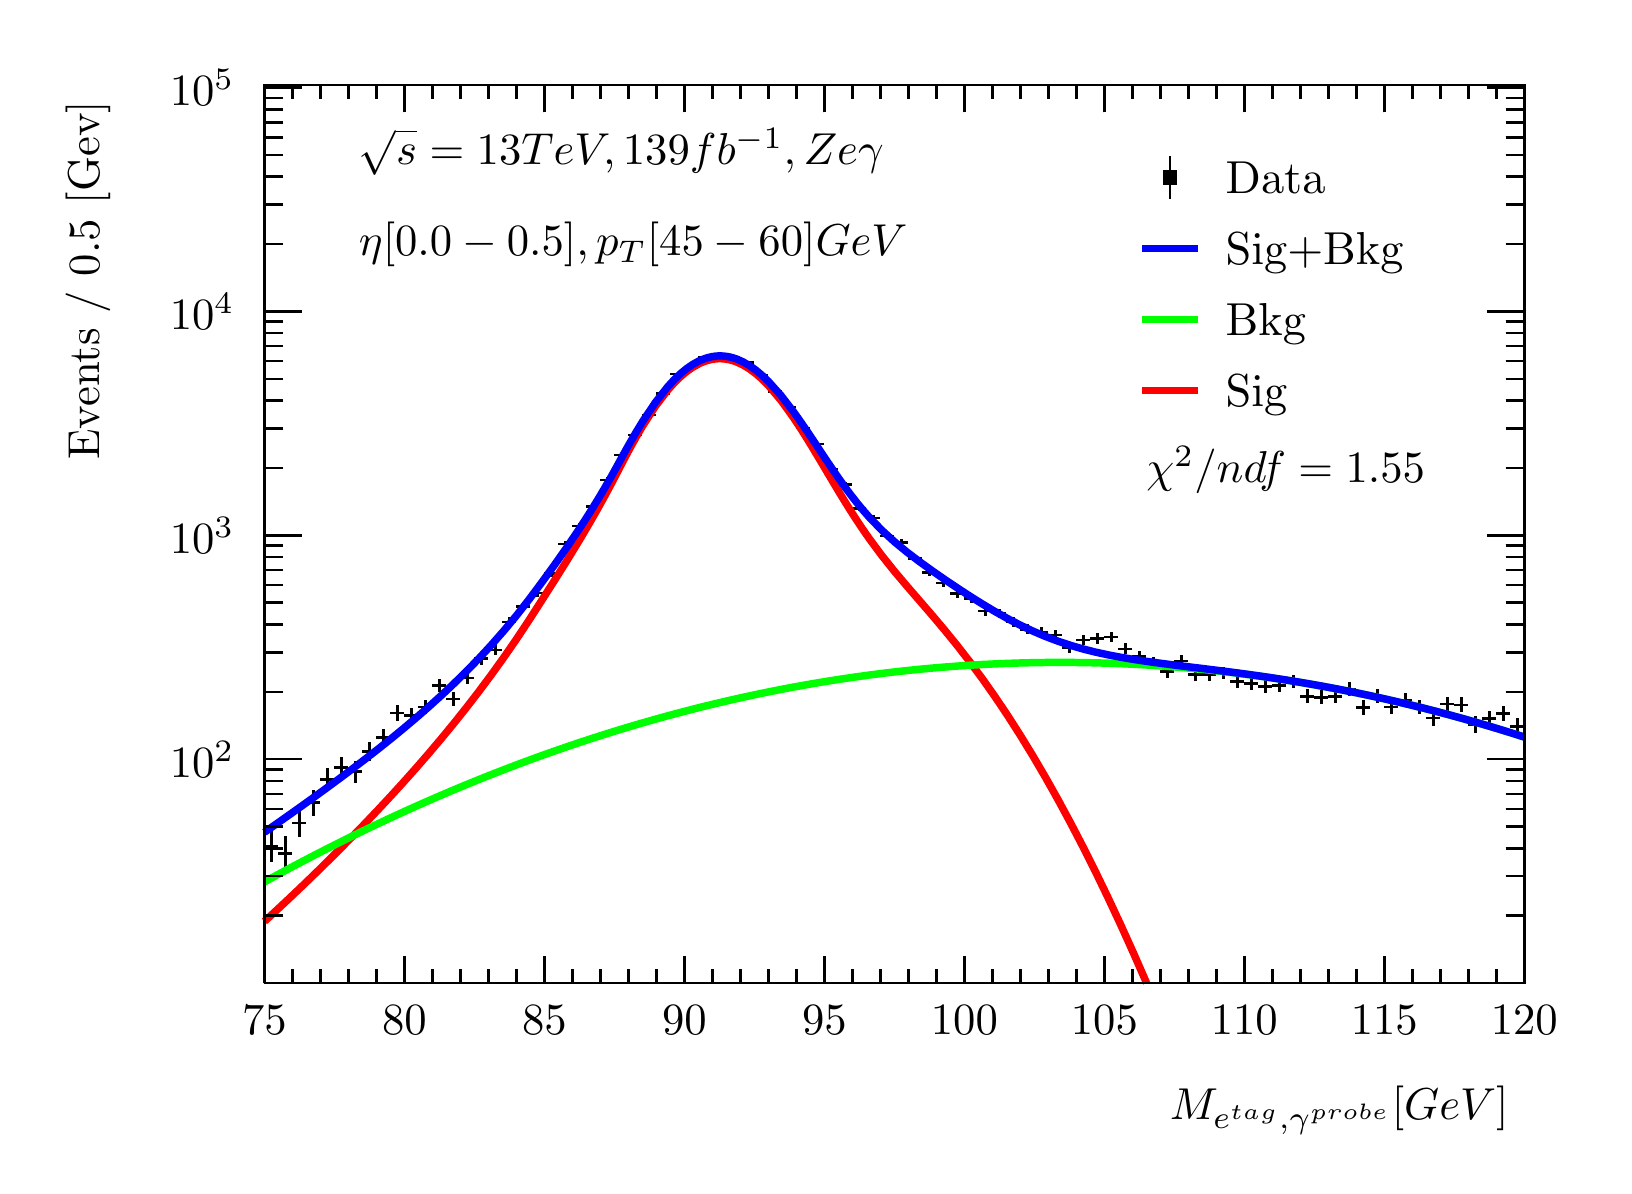
\begin{tikzpicture}
\pgfdeclareplotmark{cross} {
\pgfpathmoveto{\pgfpoint{-0.3\pgfplotmarksize}{\pgfplotmarksize}}
\pgfpathlineto{\pgfpoint{+0.3\pgfplotmarksize}{\pgfplotmarksize}}
\pgfpathlineto{\pgfpoint{+0.3\pgfplotmarksize}{0.3\pgfplotmarksize}}
\pgfpathlineto{\pgfpoint{+1\pgfplotmarksize}{0.3\pgfplotmarksize}}
\pgfpathlineto{\pgfpoint{+1\pgfplotmarksize}{-0.3\pgfplotmarksize}}
\pgfpathlineto{\pgfpoint{+0.3\pgfplotmarksize}{-0.3\pgfplotmarksize}}
\pgfpathlineto{\pgfpoint{+0.3\pgfplotmarksize}{-1.\pgfplotmarksize}}
\pgfpathlineto{\pgfpoint{-0.3\pgfplotmarksize}{-1.\pgfplotmarksize}}
\pgfpathlineto{\pgfpoint{-0.3\pgfplotmarksize}{-0.3\pgfplotmarksize}}
\pgfpathlineto{\pgfpoint{-1.\pgfplotmarksize}{-0.3\pgfplotmarksize}}
\pgfpathlineto{\pgfpoint{-1.\pgfplotmarksize}{0.3\pgfplotmarksize}}
\pgfpathlineto{\pgfpoint{-0.3\pgfplotmarksize}{0.3\pgfplotmarksize}}
\pgfpathclose
\pgfusepathqstroke
}
\pgfdeclareplotmark{cross*} {
\pgfpathmoveto{\pgfpoint{-0.3\pgfplotmarksize}{\pgfplotmarksize}}
\pgfpathlineto{\pgfpoint{+0.3\pgfplotmarksize}{\pgfplotmarksize}}
\pgfpathlineto{\pgfpoint{+0.3\pgfplotmarksize}{0.3\pgfplotmarksize}}
\pgfpathlineto{\pgfpoint{+1\pgfplotmarksize}{0.3\pgfplotmarksize}}
\pgfpathlineto{\pgfpoint{+1\pgfplotmarksize}{-0.3\pgfplotmarksize}}
\pgfpathlineto{\pgfpoint{+0.3\pgfplotmarksize}{-0.3\pgfplotmarksize}}
\pgfpathlineto{\pgfpoint{+0.3\pgfplotmarksize}{-1.\pgfplotmarksize}}
\pgfpathlineto{\pgfpoint{-0.3\pgfplotmarksize}{-1.\pgfplotmarksize}}
\pgfpathlineto{\pgfpoint{-0.3\pgfplotmarksize}{-0.3\pgfplotmarksize}}
\pgfpathlineto{\pgfpoint{-1.\pgfplotmarksize}{-0.3\pgfplotmarksize}}
\pgfpathlineto{\pgfpoint{-1.\pgfplotmarksize}{0.3\pgfplotmarksize}}
\pgfpathlineto{\pgfpoint{-0.3\pgfplotmarksize}{0.3\pgfplotmarksize}}
\pgfpathclose
\pgfusepathqfillstroke
}
\pgfdeclareplotmark{newstar} {
\pgfpathmoveto{\pgfqpoint{0pt}{\pgfplotmarksize}}
\pgfpathlineto{\pgfqpointpolar{44}{0.5\pgfplotmarksize}}
\pgfpathlineto{\pgfqpointpolar{18}{\pgfplotmarksize}}
\pgfpathlineto{\pgfqpointpolar{-20}{0.5\pgfplotmarksize}}
\pgfpathlineto{\pgfqpointpolar{-54}{\pgfplotmarksize}}
\pgfpathlineto{\pgfqpointpolar{-90}{0.5\pgfplotmarksize}}
\pgfpathlineto{\pgfqpointpolar{234}{\pgfplotmarksize}}
\pgfpathlineto{\pgfqpointpolar{198}{0.5\pgfplotmarksize}}
\pgfpathlineto{\pgfqpointpolar{162}{\pgfplotmarksize}}
\pgfpathlineto{\pgfqpointpolar{134}{0.5\pgfplotmarksize}}
\pgfpathclose
\pgfusepathqstroke
}
\pgfdeclareplotmark{newstar*} {
\pgfpathmoveto{\pgfqpoint{0pt}{\pgfplotmarksize}}
\pgfpathlineto{\pgfqpointpolar{44}{0.5\pgfplotmarksize}}
\pgfpathlineto{\pgfqpointpolar{18}{\pgfplotmarksize}}
\pgfpathlineto{\pgfqpointpolar{-20}{0.5\pgfplotmarksize}}
\pgfpathlineto{\pgfqpointpolar{-54}{\pgfplotmarksize}}
\pgfpathlineto{\pgfqpointpolar{-90}{0.5\pgfplotmarksize}}
\pgfpathlineto{\pgfqpointpolar{234}{\pgfplotmarksize}}
\pgfpathlineto{\pgfqpointpolar{198}{0.5\pgfplotmarksize}}
\pgfpathlineto{\pgfqpointpolar{162}{\pgfplotmarksize}}
\pgfpathlineto{\pgfqpointpolar{134}{0.5\pgfplotmarksize}}
\pgfpathclose
\pgfusepathqfillstroke
}
\definecolor{c}{rgb}{1,1,1};
\draw [color=c, fill=c] (0,0) rectangle (20,14.4361);
\draw [color=c, fill=c] (3,2.30977) rectangle (19,13.7143);
\definecolor{c}{rgb}{0,0,0};
\draw [c,line width=0.9] (3,2.30977) -- (3,13.7143) -- (19,13.7143) -- (19,2.30977) -- (3,2.30977);
\definecolor{c}{rgb}{1,1,1};
\draw [color=c, fill=c] (3,2.30977) rectangle (19,13.7143);
\definecolor{c}{rgb}{0,0,0};
\draw [c,line width=0.9] (3,2.30977) -- (3,13.7143) -- (19,13.7143) -- (19,2.30977) -- (3,2.30977);
\draw [c,line width=0.9] (3,2.30977) -- (19,2.30977);
\draw [c,line width=0.9] (3,2.65624) -- (3,2.30977);
\draw [c,line width=0.9] (3.35556,2.48301) -- (3.35556,2.30977);
\draw [c,line width=0.9] (3.71111,2.48301) -- (3.71111,2.30977);
\draw [c,line width=0.9] (4.06667,2.48301) -- (4.06667,2.30977);
\draw [c,line width=0.9] (4.42222,2.48301) -- (4.42222,2.30977);
\draw [c,line width=0.9] (4.77778,2.65624) -- (4.77778,2.30977);
\draw [c,line width=0.9] (5.13333,2.48301) -- (5.13333,2.30977);
\draw [c,line width=0.9] (5.48889,2.48301) -- (5.48889,2.30977);
\draw [c,line width=0.9] (5.84444,2.48301) -- (5.84444,2.30977);
\draw [c,line width=0.9] (6.2,2.48301) -- (6.2,2.30977);
\draw [c,line width=0.9] (6.55556,2.65624) -- (6.55556,2.30977);
\draw [c,line width=0.9] (6.91111,2.48301) -- (6.91111,2.30977);
\draw [c,line width=0.9] (7.26667,2.48301) -- (7.26667,2.30977);
\draw [c,line width=0.9] (7.62222,2.48301) -- (7.62222,2.30977);
\draw [c,line width=0.9] (7.97778,2.48301) -- (7.97778,2.30977);
\draw [c,line width=0.9] (8.33333,2.65624) -- (8.33333,2.30977);
\draw [c,line width=0.9] (8.68889,2.48301) -- (8.68889,2.30977);
\draw [c,line width=0.9] (9.04444,2.48301) -- (9.04444,2.30977);
\draw [c,line width=0.9] (9.4,2.48301) -- (9.4,2.30977);
\draw [c,line width=0.9] (9.75556,2.48301) -- (9.75556,2.30977);
\draw [c,line width=0.9] (10.1111,2.65624) -- (10.1111,2.30977);
\draw [c,line width=0.9] (10.4667,2.48301) -- (10.4667,2.30977);
\draw [c,line width=0.9] (10.8222,2.48301) -- (10.8222,2.30977);
\draw [c,line width=0.9] (11.1778,2.48301) -- (11.1778,2.30977);
\draw [c,line width=0.9] (11.5333,2.48301) -- (11.5333,2.30977);
\draw [c,line width=0.9] (11.8889,2.65624) -- (11.8889,2.30977);
\draw [c,line width=0.9] (12.2444,2.48301) -- (12.2444,2.30977);
\draw [c,line width=0.9] (12.6,2.48301) -- (12.6,2.30977);
\draw [c,line width=0.9] (12.9556,2.48301) -- (12.9556,2.30977);
\draw [c,line width=0.9] (13.3111,2.48301) -- (13.3111,2.30977);
\draw [c,line width=0.9] (13.6667,2.65624) -- (13.6667,2.30977);
\draw [c,line width=0.9] (14.0222,2.48301) -- (14.0222,2.30977);
\draw [c,line width=0.9] (14.3778,2.48301) -- (14.3778,2.30977);
\draw [c,line width=0.9] (14.7333,2.48301) -- (14.7333,2.30977);
\draw [c,line width=0.9] (15.0889,2.48301) -- (15.0889,2.30977);
\draw [c,line width=0.9] (15.4444,2.65624) -- (15.4444,2.30977);
\draw [c,line width=0.9] (15.8,2.48301) -- (15.8,2.30977);
\draw [c,line width=0.9] (16.1556,2.48301) -- (16.1556,2.30977);
\draw [c,line width=0.9] (16.5111,2.48301) -- (16.5111,2.30977);
\draw [c,line width=0.9] (16.8667,2.48301) -- (16.8667,2.30977);
\draw [c,line width=0.9] (17.2222,2.65624) -- (17.2222,2.30977);
\draw [c,line width=0.9] (17.5778,2.48301) -- (17.5778,2.30977);
\draw [c,line width=0.9] (17.9333,2.48301) -- (17.9333,2.30977);
\draw [c,line width=0.9] (18.2889,2.48301) -- (18.2889,2.30977);
\draw [c,line width=0.9] (18.6444,2.48301) -- (18.6444,2.30977);
\draw [c,line width=0.9] (19,2.65624) -- (19,2.30977);
\draw [c,line width=0.9] (19,2.65624) -- (19,2.30977);
\draw [anchor=base] (3,1.66015) node[scale=1.61424, color=c, rotate=0]{75};
\draw [anchor=base] (4.77778,1.66015) node[scale=1.61424, color=c, rotate=0]{80};
\draw [anchor=base] (6.55556,1.66015) node[scale=1.61424, color=c, rotate=0]{85};
\draw [anchor=base] (8.33333,1.66015) node[scale=1.61424, color=c, rotate=0]{90};
\draw [anchor=base] (10.1111,1.66015) node[scale=1.61424, color=c, rotate=0]{95};
\draw [anchor=base] (11.8889,1.66015) node[scale=1.61424, color=c, rotate=0]{100};
\draw [anchor=base] (13.6667,1.66015) node[scale=1.61424, color=c, rotate=0]{105};
\draw [anchor=base] (15.4444,1.66015) node[scale=1.61424, color=c, rotate=0]{110};
\draw [anchor=base] (17.2222,1.66015) node[scale=1.61424, color=c, rotate=0]{115};
\draw [anchor=base] (19,1.66015) node[scale=1.61424, color=c, rotate=0]{120};
\draw [anchor= east] (19,0.692932) node[scale=1.61424, color=c, rotate=0]{$M_{e^{tag}, \gamma^{probe}}  [GeV]$};
\draw [c,line width=0.9] (3,13.7143) -- (19,13.7143);
\draw [c,line width=0.9] (3,13.3678) -- (3,13.7143);
\draw [c,line width=0.9] (3.35556,13.5411) -- (3.35556,13.7143);
\draw [c,line width=0.9] (3.71111,13.5411) -- (3.71111,13.7143);
\draw [c,line width=0.9] (4.06667,13.5411) -- (4.06667,13.7143);
\draw [c,line width=0.9] (4.42222,13.5411) -- (4.42222,13.7143);
\draw [c,line width=0.9] (4.77778,13.3678) -- (4.77778,13.7143);
\draw [c,line width=0.9] (5.13333,13.5411) -- (5.13333,13.7143);
\draw [c,line width=0.9] (5.48889,13.5411) -- (5.48889,13.7143);
\draw [c,line width=0.9] (5.84444,13.5411) -- (5.84444,13.7143);
\draw [c,line width=0.9] (6.2,13.5411) -- (6.2,13.7143);
\draw [c,line width=0.9] (6.55556,13.3678) -- (6.55556,13.7143);
\draw [c,line width=0.9] (6.91111,13.5411) -- (6.91111,13.7143);
\draw [c,line width=0.9] (7.26667,13.5411) -- (7.26667,13.7143);
\draw [c,line width=0.9] (7.62222,13.5411) -- (7.62222,13.7143);
\draw [c,line width=0.9] (7.97778,13.5411) -- (7.97778,13.7143);
\draw [c,line width=0.9] (8.33333,13.3678) -- (8.33333,13.7143);
\draw [c,line width=0.9] (8.68889,13.5411) -- (8.68889,13.7143);
\draw [c,line width=0.9] (9.04444,13.5411) -- (9.04444,13.7143);
\draw [c,line width=0.9] (9.4,13.5411) -- (9.4,13.7143);
\draw [c,line width=0.9] (9.75556,13.5411) -- (9.75556,13.7143);
\draw [c,line width=0.9] (10.1111,13.3678) -- (10.1111,13.7143);
\draw [c,line width=0.9] (10.4667,13.5411) -- (10.4667,13.7143);
\draw [c,line width=0.9] (10.8222,13.5411) -- (10.8222,13.7143);
\draw [c,line width=0.9] (11.1778,13.5411) -- (11.1778,13.7143);
\draw [c,line width=0.9] (11.5333,13.5411) -- (11.5333,13.7143);
\draw [c,line width=0.9] (11.8889,13.3678) -- (11.8889,13.7143);
\draw [c,line width=0.9] (12.2444,13.5411) -- (12.2444,13.7143);
\draw [c,line width=0.9] (12.6,13.5411) -- (12.6,13.7143);
\draw [c,line width=0.9] (12.9556,13.5411) -- (12.9556,13.7143);
\draw [c,line width=0.9] (13.3111,13.5411) -- (13.3111,13.7143);
\draw [c,line width=0.9] (13.6667,13.3678) -- (13.6667,13.7143);
\draw [c,line width=0.9] (14.0222,13.5411) -- (14.0222,13.7143);
\draw [c,line width=0.9] (14.3778,13.5411) -- (14.3778,13.7143);
\draw [c,line width=0.9] (14.7333,13.5411) -- (14.7333,13.7143);
\draw [c,line width=0.9] (15.0889,13.5411) -- (15.0889,13.7143);
\draw [c,line width=0.9] (15.4444,13.3678) -- (15.4444,13.7143);
\draw [c,line width=0.9] (15.8,13.5411) -- (15.8,13.7143);
\draw [c,line width=0.9] (16.1556,13.5411) -- (16.1556,13.7143);
\draw [c,line width=0.9] (16.5111,13.5411) -- (16.5111,13.7143);
\draw [c,line width=0.9] (16.8667,13.5411) -- (16.8667,13.7143);
\draw [c,line width=0.9] (17.2222,13.3678) -- (17.2222,13.7143);
\draw [c,line width=0.9] (17.5778,13.5411) -- (17.5778,13.7143);
\draw [c,line width=0.9] (17.9333,13.5411) -- (17.9333,13.7143);
\draw [c,line width=0.9] (18.2889,13.5411) -- (18.2889,13.7143);
\draw [c,line width=0.9] (18.6444,13.5411) -- (18.6444,13.7143);
\draw [c,line width=0.9] (19,13.3678) -- (19,13.7143);
\draw [c,line width=0.9] (19,13.3678) -- (19,13.7143);
\draw [c,line width=0.9] (3,2.30977) -- (3,13.7143);
\draw [c,line width=0.9] (3.237,3.16561) -- (3,3.16561);
\draw [c,line width=0.9] (3.237,3.66625) -- (3,3.66625);
\draw [c,line width=0.9] (3.237,4.02146) -- (3,4.02146);
\draw [c,line width=0.9] (3.237,4.29698) -- (3,4.29698);
\draw [c,line width=0.9] (3.237,4.52209) -- (3,4.52209);
\draw [c,line width=0.9] (3.237,4.71242) -- (3,4.71242);
\draw [c,line width=0.9] (3.237,4.8773) -- (3,4.8773);
\draw [c,line width=0.9] (3.237,5.02273) -- (3,5.02273);
\draw [c,line width=0.9] (3.474,5.15282) -- (3,5.15282);
\draw [anchor= east] (2.82,5.15282) node[scale=1.61424, color=c, rotate=0]{$10^{2}$};
\draw [c,line width=0.9] (3.237,6.00866) -- (3,6.00866);
\draw [c,line width=0.9] (3.237,6.5093) -- (3,6.5093);
\draw [c,line width=0.9] (3.237,6.8645) -- (3,6.8645);
\draw [c,line width=0.9] (3.237,7.14002) -- (3,7.14002);
\draw [c,line width=0.9] (3.237,7.36514) -- (3,7.36514);
\draw [c,line width=0.9] (3.237,7.55547) -- (3,7.55547);
\draw [c,line width=0.9] (3.237,7.72034) -- (3,7.72034);
\draw [c,line width=0.9] (3.237,7.86577) -- (3,7.86577);
\draw [c,line width=0.9] (3.474,7.99586) -- (3,7.99586);
\draw [anchor= east] (2.82,7.99586) node[scale=1.61424, color=c, rotate=0]{$10^{3}$};
\draw [c,line width=0.9] (3.237,8.85171) -- (3,8.85171);
\draw [c,line width=0.9] (3.237,9.35234) -- (3,9.35234);
\draw [c,line width=0.9] (3.237,9.70755) -- (3,9.70755);
\draw [c,line width=0.9] (3.237,9.98307) -- (3,9.98307);
\draw [c,line width=0.9] (3.237,10.2082) -- (3,10.2082);
\draw [c,line width=0.9] (3.237,10.3985) -- (3,10.3985);
\draw [c,line width=0.9] (3.237,10.5634) -- (3,10.5634);
\draw [c,line width=0.9] (3.237,10.7088) -- (3,10.7088);
\draw [c,line width=0.9] (3.474,10.8389) -- (3,10.8389);
\draw [anchor= east] (2.82,10.8389) node[scale=1.61424, color=c, rotate=0]{$10^{4}$};
\draw [c,line width=0.9] (3.237,11.6948) -- (3,11.6948);
\draw [c,line width=0.9] (3.237,12.1954) -- (3,12.1954);
\draw [c,line width=0.9] (3.237,12.5506) -- (3,12.5506);
\draw [c,line width=0.9] (3.237,12.8261) -- (3,12.8261);
\draw [c,line width=0.9] (3.237,13.0512) -- (3,13.0512);
\draw [c,line width=0.9] (3.237,13.2416) -- (3,13.2416);
\draw [c,line width=0.9] (3.237,13.4064) -- (3,13.4064);
\draw [c,line width=0.9] (3.237,13.5519) -- (3,13.5519);
\draw [c,line width=0.9] (3.474,13.682) -- (3,13.682);
\draw [anchor= east] (2.82,13.682) node[scale=1.61424, color=c, rotate=0]{$10^{5}$};
\draw [anchor= east] (0.76,13.7143) node[scale=1.61424, color=c, rotate=90]{Events / 0.5 [Gev]};
\draw [c,line width=0.9] (19,2.30977) -- (19,13.7143);
\draw [c,line width=0.9] (18.763,3.16561) -- (19,3.16561);
\draw [c,line width=0.9] (18.763,3.66625) -- (19,3.66625);
\draw [c,line width=0.9] (18.763,4.02146) -- (19,4.02146);
\draw [c,line width=0.9] (18.763,4.29698) -- (19,4.29698);
\draw [c,line width=0.9] (18.763,4.52209) -- (19,4.52209);
\draw [c,line width=0.9] (18.763,4.71242) -- (19,4.71242);
\draw [c,line width=0.9] (18.763,4.8773) -- (19,4.8773);
\draw [c,line width=0.9] (18.763,5.02273) -- (19,5.02273);
\draw [c,line width=0.9] (18.526,5.15282) -- (19,5.15282);
\draw [c,line width=0.9] (18.763,6.00866) -- (19,6.00866);
\draw [c,line width=0.9] (18.763,6.5093) -- (19,6.5093);
\draw [c,line width=0.9] (18.763,6.8645) -- (19,6.8645);
\draw [c,line width=0.9] (18.763,7.14002) -- (19,7.14002);
\draw [c,line width=0.9] (18.763,7.36514) -- (19,7.36514);
\draw [c,line width=0.9] (18.763,7.55547) -- (19,7.55547);
\draw [c,line width=0.9] (18.763,7.72034) -- (19,7.72034);
\draw [c,line width=0.9] (18.763,7.86577) -- (19,7.86577);
\draw [c,line width=0.9] (18.526,7.99586) -- (19,7.99586);
\draw [c,line width=0.9] (18.763,8.85171) -- (19,8.85171);
\draw [c,line width=0.9] (18.763,9.35234) -- (19,9.35234);
\draw [c,line width=0.9] (18.763,9.70755) -- (19,9.70755);
\draw [c,line width=0.9] (18.763,9.98307) -- (19,9.98307);
\draw [c,line width=0.9] (18.763,10.2082) -- (19,10.2082);
\draw [c,line width=0.9] (18.763,10.3985) -- (19,10.3985);
\draw [c,line width=0.9] (18.763,10.5634) -- (19,10.5634);
\draw [c,line width=0.9] (18.763,10.7088) -- (19,10.7088);
\draw [c,line width=0.9] (18.526,10.8389) -- (19,10.8389);
\draw [c,line width=0.9] (18.763,11.6948) -- (19,11.6948);
\draw [c,line width=0.9] (18.763,12.1954) -- (19,12.1954);
\draw [c,line width=0.9] (18.763,12.5506) -- (19,12.5506);
\draw [c,line width=0.9] (18.763,12.8261) -- (19,12.8261);
\draw [c,line width=0.9] (18.763,13.0512) -- (19,13.0512);
\draw [c,line width=0.9] (18.763,13.2416) -- (19,13.2416);
\draw [c,line width=0.9] (18.763,13.4064) -- (19,13.4064);
\draw [c,line width=0.9] (18.763,13.5519) -- (19,13.5519);
\draw [c,line width=0.9] (18.526,13.682) -- (19,13.682);
\draw [c,line width=0.9] (3.08889,4.05195) -- (3,4.05195);
\draw [c,line width=0.9] (3,4.05195) -- (3,4.05195);
\draw [c,line width=0.9] (3.08889,4.05195) -- (3.17778,4.05195);
\draw [c,line width=0.9] (3.17778,4.05195) -- (3.17778,4.05195);
\draw [c,line width=0.9] (3.08889,4.05195) -- (3.08889,4.25823);
\draw [c,line width=0.9] (3.08889,4.25823) -- (3.08889,4.25823);
\draw [c,line width=0.9] (3.08889,4.05195) -- (3.08889,3.84322);
\draw [c,line width=0.9] (3.08889,3.84322) -- (3.08889,3.84322);
\draw [c,line width=0.9] (3.26667,3.95813) -- (3.17778,3.95813);
\draw [c,line width=0.9] (3.17778,3.95813) -- (3.17778,3.95813);
\draw [c,line width=0.9] (3.26667,3.95813) -- (3.35556,3.95813);
\draw [c,line width=0.9] (3.35556,3.95813) -- (3.35556,3.95813);
\draw [c,line width=0.9] (3.26667,3.95813) -- (3.26667,4.17287);
\draw [c,line width=0.9] (3.26667,4.17287) -- (3.26667,4.17287);
\draw [c,line width=0.9] (3.26667,3.95813) -- (3.26667,3.74063);
\draw [c,line width=0.9] (3.26667,3.74063) -- (3.26667,3.74063);
\draw [c,line width=0.9] (3.44444,4.3454) -- (3.35556,4.3454);
\draw [c,line width=0.9] (3.35556,4.3454) -- (3.35556,4.3454);
\draw [c,line width=0.9] (3.44444,4.3454) -- (3.53333,4.3454);
\draw [c,line width=0.9] (3.53333,4.3454) -- (3.53333,4.3454);
\draw [c,line width=0.9] (3.44444,4.3454) -- (3.44444,4.52738);
\draw [c,line width=0.9] (3.44444,4.52738) -- (3.44444,4.52738);
\draw [c,line width=0.9] (3.44444,4.3454) -- (3.44444,4.16172);
\draw [c,line width=0.9] (3.44444,4.16172) -- (3.44444,4.16172);
\draw [c,line width=0.9] (3.62222,4.60178) -- (3.53333,4.60178);
\draw [c,line width=0.9] (3.53333,4.60178) -- (3.53333,4.60178);
\draw [c,line width=0.9] (3.62222,4.60178) -- (3.71111,4.60178);
\draw [c,line width=0.9] (3.71111,4.60178) -- (3.71111,4.60178);
\draw [c,line width=0.9] (3.62222,4.60178) -- (3.62222,4.76495);
\draw [c,line width=0.9] (3.62222,4.76495) -- (3.62222,4.76495);
\draw [c,line width=0.9] (3.62222,4.60178) -- (3.62222,4.43737);
\draw [c,line width=0.9] (3.62222,4.43737) -- (3.62222,4.43737);
\draw [c,line width=0.9] (3.8,4.89264) -- (3.71111,4.89264);
\draw [c,line width=0.9] (3.71111,4.89264) -- (3.71111,4.89264);
\draw [c,line width=0.9] (3.8,4.89264) -- (3.88889,4.89264);
\draw [c,line width=0.9] (3.88889,4.89264) -- (3.88889,4.89264);
\draw [c,line width=0.9] (3.8,4.89264) -- (3.8,5.03688);
\draw [c,line width=0.9] (3.8,5.03688) -- (3.8,5.03688);
\draw [c,line width=0.9] (3.8,4.89264) -- (3.8,4.74753);
\draw [c,line width=0.9] (3.8,4.74753) -- (3.8,4.74753);
\draw [c,line width=0.9] (3.97778,5.04987) -- (3.88889,5.04987);
\draw [c,line width=0.9] (3.88889,5.04987) -- (3.88889,5.04987);
\draw [c,line width=0.9] (3.97778,5.04987) -- (4.06667,5.04987);
\draw [c,line width=0.9] (4.06667,5.04987) -- (4.06667,5.04987);
\draw [c,line width=0.9] (3.97778,5.04987) -- (3.97778,5.18483);
\draw [c,line width=0.9] (3.97778,5.18483) -- (3.97778,5.18483);
\draw [c,line width=0.9] (3.97778,5.04987) -- (3.97778,4.91418);
\draw [c,line width=0.9] (3.97778,4.91418) -- (3.97778,4.91418);
\draw [c,line width=0.9] (4.15556,4.99498) -- (4.06667,4.99498);
\draw [c,line width=0.9] (4.06667,4.99498) -- (4.06667,4.99498);
\draw [c,line width=0.9] (4.15556,4.99498) -- (4.24444,4.99498);
\draw [c,line width=0.9] (4.24444,4.99498) -- (4.24444,4.99498);
\draw [c,line width=0.9] (4.15556,4.99498) -- (4.15556,5.13311);
\draw [c,line width=0.9] (4.15556,5.13311) -- (4.15556,5.13311);
\draw [c,line width=0.9] (4.15556,4.99498) -- (4.15556,4.85608);
\draw [c,line width=0.9] (4.15556,4.85608) -- (4.15556,4.85608);
\draw [c,line width=0.9] (4.33333,5.24785) -- (4.24444,5.24785);
\draw [c,line width=0.9] (4.24444,5.24785) -- (4.24444,5.24785);
\draw [c,line width=0.9] (4.33333,5.24785) -- (4.42222,5.24785);
\draw [c,line width=0.9] (4.42222,5.24785) -- (4.42222,5.24785);
\draw [c,line width=0.9] (4.33333,5.24785) -- (4.33333,5.36661);
\draw [c,line width=0.9] (4.33333,5.36661) -- (4.33333,5.36661);
\draw [c,line width=0.9] (4.33333,5.24785) -- (4.33333,5.12908);
\draw [c,line width=0.9] (4.33333,5.12908) -- (4.33333,5.12908);
\draw [c,line width=0.9] (4.51111,5.42834) -- (4.42222,5.42834);
\draw [c,line width=0.9] (4.42222,5.42834) -- (4.42222,5.42834);
\draw [c,line width=0.9] (4.51111,5.42834) -- (4.6,5.42834);
\draw [c,line width=0.9] (4.6,5.42834) -- (4.6,5.42834);
\draw [c,line width=0.9] (4.51111,5.42834) -- (4.51111,5.53874);
\draw [c,line width=0.9] (4.51111,5.53874) -- (4.51111,5.53874);
\draw [c,line width=0.9] (4.51111,5.42834) -- (4.51111,5.31794);
\draw [c,line width=0.9] (4.51111,5.31794) -- (4.51111,5.31794);
\draw [c,line width=0.9] (4.68889,5.74084) -- (4.6,5.74084);
\draw [c,line width=0.9] (4.6,5.74084) -- (4.6,5.74084);
\draw [c,line width=0.9] (4.68889,5.74084) -- (4.77778,5.74084);
\draw [c,line width=0.9] (4.77778,5.74084) -- (4.77778,5.74084);
\draw [c,line width=0.9] (4.68889,5.74084) -- (4.68889,5.83812);
\draw [c,line width=0.9] (4.68889,5.83812) -- (4.68889,5.83812);
\draw [c,line width=0.9] (4.68889,5.74084) -- (4.68889,5.64355);
\draw [c,line width=0.9] (4.68889,5.64355) -- (4.68889,5.64355);
\draw [c,line width=0.9] (4.86667,5.70977) -- (4.77778,5.70977);
\draw [c,line width=0.9] (4.77778,5.70977) -- (4.77778,5.70977);
\draw [c,line width=0.9] (4.86667,5.70977) -- (4.95556,5.70977);
\draw [c,line width=0.9] (4.95556,5.70977) -- (4.95556,5.70977);
\draw [c,line width=0.9] (4.86667,5.70977) -- (4.86667,5.80829);
\draw [c,line width=0.9] (4.86667,5.80829) -- (4.86667,5.80829);
\draw [c,line width=0.9] (4.86667,5.70977) -- (4.86667,5.61126);
\draw [c,line width=0.9] (4.86667,5.61126) -- (4.86667,5.61126);
\draw [c,line width=0.9] (5.04444,5.81524) -- (4.95556,5.81524);
\draw [c,line width=0.9] (4.95556,5.81524) -- (4.95556,5.81524);
\draw [c,line width=0.9] (5.04444,5.81524) -- (5.13333,5.81524);
\draw [c,line width=0.9] (5.13333,5.81524) -- (5.13333,5.81524);
\draw [c,line width=0.9] (5.04444,5.81524) -- (5.04444,5.90964);
\draw [c,line width=0.9] (5.04444,5.90964) -- (5.04444,5.90964);
\draw [c,line width=0.9] (5.04444,5.81524) -- (5.04444,5.72084);
\draw [c,line width=0.9] (5.04444,5.72084) -- (5.04444,5.72084);
\draw [c,line width=0.9] (5.22222,6.08642) -- (5.13333,6.08642);
\draw [c,line width=0.9] (5.13333,6.08642) -- (5.13333,6.08642);
\draw [c,line width=0.9] (5.22222,6.08642) -- (5.31111,6.08642);
\draw [c,line width=0.9] (5.31111,6.08642) -- (5.31111,6.08642);
\draw [c,line width=0.9] (5.22222,6.08642) -- (5.22222,6.171);
\draw [c,line width=0.9] (5.22222,6.171) -- (5.22222,6.171);
\draw [c,line width=0.9] (5.22222,6.08642) -- (5.22222,6.00183);
\draw [c,line width=0.9] (5.22222,6.00183) -- (5.22222,6.00183);
\draw [c,line width=0.9] (5.4,5.91906) -- (5.31111,5.91906);
\draw [c,line width=0.9] (5.31111,5.91906) -- (5.31111,5.91906);
\draw [c,line width=0.9] (5.4,5.91906) -- (5.48889,5.91906);
\draw [c,line width=0.9] (5.48889,5.91906) -- (5.48889,5.91906);
\draw [c,line width=0.9] (5.4,5.91906) -- (5.4,6.00957);
\draw [c,line width=0.9] (5.4,6.00957) -- (5.4,6.00957);
\draw [c,line width=0.9] (5.4,5.91906) -- (5.4,5.82854);
\draw [c,line width=0.9] (5.4,5.82854) -- (5.4,5.82854);
\draw [c,line width=0.9] (5.57778,6.18658) -- (5.48889,6.18658);
\draw [c,line width=0.9] (5.48889,6.18658) -- (5.48889,6.18658);
\draw [c,line width=0.9] (5.57778,6.18658) -- (5.66667,6.18658);
\draw [c,line width=0.9] (5.66667,6.18658) -- (5.66667,6.18658);
\draw [c,line width=0.9] (5.57778,6.18658) -- (5.57778,6.26781);
\draw [c,line width=0.9] (5.57778,6.26781) -- (5.57778,6.26781);
\draw [c,line width=0.9] (5.57778,6.18658) -- (5.57778,6.10536);
\draw [c,line width=0.9] (5.57778,6.10536) -- (5.57778,6.10536);
\draw [c,line width=0.9] (5.75556,6.42851) -- (5.66667,6.42851);
\draw [c,line width=0.9] (5.66667,6.42851) -- (5.66667,6.42851);
\draw [c,line width=0.9] (5.75556,6.42851) -- (5.84444,6.42851);
\draw [c,line width=0.9] (5.84444,6.42851) -- (5.84444,6.42851);
\draw [c,line width=0.9] (5.75556,6.42851) -- (5.75556,6.50216);
\draw [c,line width=0.9] (5.75556,6.50216) -- (5.75556,6.50216);
\draw [c,line width=0.9] (5.75556,6.42851) -- (5.75556,6.35487);
\draw [c,line width=0.9] (5.75556,6.35487) -- (5.75556,6.35487);
\draw [c,line width=0.9] (5.93333,6.54179) -- (5.84444,6.54179);
\draw [c,line width=0.9] (5.84444,6.54179) -- (5.84444,6.54179);
\draw [c,line width=0.9] (5.93333,6.54179) -- (6.02222,6.54179);
\draw [c,line width=0.9] (6.02222,6.54179) -- (6.02222,6.54179);
\draw [c,line width=0.9] (5.93333,6.54179) -- (5.93333,6.61214);
\draw [c,line width=0.9] (5.93333,6.61214) -- (5.93333,6.61214);
\draw [c,line width=0.9] (5.93333,6.54179) -- (5.93333,6.47145);
\draw [c,line width=0.9] (5.93333,6.47145) -- (5.93333,6.47145);
\draw [c,line width=0.9] (6.11111,6.89198) -- (6.02222,6.89198);
\draw [c,line width=0.9] (6.02222,6.89198) -- (6.02222,6.89198);
\draw [c,line width=0.9] (6.11111,6.89198) -- (6.2,6.89198);
\draw [c,line width=0.9] (6.2,6.89198) -- (6.2,6.89198);
\draw [c,line width=0.9] (6.11111,6.89198) -- (6.11111,6.95302);
\draw [c,line width=0.9] (6.11111,6.95302) -- (6.11111,6.95302);
\draw [c,line width=0.9] (6.11111,6.89198) -- (6.11111,6.83093);
\draw [c,line width=0.9] (6.11111,6.83093) -- (6.11111,6.83093);
\draw [c,line width=0.9] (6.28889,7.09475) -- (6.2,7.09475);
\draw [c,line width=0.9] (6.2,7.09475) -- (6.2,7.09475);
\draw [c,line width=0.9] (6.28889,7.09475) -- (6.37778,7.09475);
\draw [c,line width=0.9] (6.37778,7.09475) -- (6.37778,7.09475);
\draw [c,line width=0.9] (6.28889,7.09475) -- (6.28889,7.15099);
\draw [c,line width=0.9] (6.28889,7.15099) -- (6.28889,7.15099);
\draw [c,line width=0.9] (6.28889,7.09475) -- (6.28889,7.03852);
\draw [c,line width=0.9] (6.28889,7.03852) -- (6.28889,7.03852);
\draw [c,line width=0.9] (6.46667,7.26442) -- (6.37778,7.26442);
\draw [c,line width=0.9] (6.37778,7.26442) -- (6.37778,7.26442);
\draw [c,line width=0.9] (6.46667,7.26442) -- (6.55556,7.26442);
\draw [c,line width=0.9] (6.55556,7.26442) -- (6.55556,7.26442);
\draw [c,line width=0.9] (6.46667,7.26442) -- (6.46667,7.31692);
\draw [c,line width=0.9] (6.46667,7.31692) -- (6.46667,7.31692);
\draw [c,line width=0.9] (6.46667,7.26442) -- (6.46667,7.21192);
\draw [c,line width=0.9] (6.46667,7.21192) -- (6.46667,7.21192);
\draw [c,line width=0.9] (6.64444,7.50874) -- (6.55556,7.50874);
\draw [c,line width=0.9] (6.55556,7.50874) -- (6.55556,7.50874);
\draw [c,line width=0.9] (6.64444,7.50874) -- (6.73333,7.50874);
\draw [c,line width=0.9] (6.73333,7.50874) -- (6.73333,7.50874);
\draw [c,line width=0.9] (6.64444,7.50874) -- (6.64444,7.55629);
\draw [c,line width=0.9] (6.64444,7.55629) -- (6.64444,7.55629);
\draw [c,line width=0.9] (6.64444,7.50874) -- (6.64444,7.46118);
\draw [c,line width=0.9] (6.64444,7.46118) -- (6.64444,7.46118);
\draw [c,line width=0.9] (6.82222,7.88618) -- (6.73333,7.88618);
\draw [c,line width=0.9] (6.73333,7.88618) -- (6.73333,7.88618);
\draw [c,line width=0.9] (6.82222,7.88618) -- (6.91111,7.88618);
\draw [c,line width=0.9] (6.91111,7.88618) -- (6.91111,7.88618);
\draw [c,line width=0.9] (6.82222,7.88618) -- (6.82222,7.927);
\draw [c,line width=0.9] (6.82222,7.927) -- (6.82222,7.927);
\draw [c,line width=0.9] (6.82222,7.88618) -- (6.82222,7.84537);
\draw [c,line width=0.9] (6.82222,7.84537) -- (6.82222,7.84537);
\draw [c,line width=0.9] (7,8.11242) -- (6.91111,8.11242);
\draw [c,line width=0.9] (6.91111,8.11242) -- (6.91111,8.11242);
\draw [c,line width=0.9] (7,8.11242) -- (7.08889,8.11242);
\draw [c,line width=0.9] (7.08889,8.11242) -- (7.08889,8.11242);
\draw [c,line width=0.9] (7,8.11242) -- (7,8.14967);
\draw [c,line width=0.9] (7,8.14967) -- (7,8.14967);
\draw [c,line width=0.9] (7,8.11242) -- (7,8.07518);
\draw [c,line width=0.9] (7,8.07518) -- (7,8.07518);
\draw [c,line width=0.9] (7.17778,8.36183) -- (7.08889,8.36183);
\draw [c,line width=0.9] (7.08889,8.36183) -- (7.08889,8.36183);
\draw [c,line width=0.9] (7.17778,8.36183) -- (7.26667,8.36183);
\draw [c,line width=0.9] (7.26667,8.36183) -- (7.26667,8.36183);
\draw [c,line width=0.9] (7.17778,8.36183) -- (7.17778,8.39549);
\draw [c,line width=0.9] (7.17778,8.39549) -- (7.17778,8.39549);
\draw [c,line width=0.9] (7.17778,8.36183) -- (7.17778,8.32816);
\draw [c,line width=0.9] (7.17778,8.32816) -- (7.17778,8.32816);
\draw [c,line width=0.9] (7.35556,8.70156) -- (7.26667,8.70156);
\draw [c,line width=0.9] (7.26667,8.70156) -- (7.26667,8.70156);
\draw [c,line width=0.9] (7.35556,8.70156) -- (7.44444,8.70156);
\draw [c,line width=0.9] (7.44444,8.70156) -- (7.44444,8.70156);
\draw [c,line width=0.9] (7.35556,8.70156) -- (7.35556,8.7309);
\draw [c,line width=0.9] (7.35556,8.7309) -- (7.35556,8.7309);
\draw [c,line width=0.9] (7.35556,8.70156) -- (7.35556,8.67222);
\draw [c,line width=0.9] (7.35556,8.67222) -- (7.35556,8.67222);
\draw [c,line width=0.9] (7.53333,9.01511) -- (7.44444,9.01511);
\draw [c,line width=0.9] (7.44444,9.01511) -- (7.44444,9.01511);
\draw [c,line width=0.9] (7.53333,9.01511) -- (7.62222,9.01511);
\draw [c,line width=0.9] (7.62222,9.01511) -- (7.62222,9.01511);
\draw [c,line width=0.9] (7.53333,9.01511) -- (7.53333,9.04095);
\draw [c,line width=0.9] (7.53333,9.04095) -- (7.53333,9.04095);
\draw [c,line width=0.9] (7.53333,9.01511) -- (7.53333,8.98927);
\draw [c,line width=0.9] (7.53333,8.98927) -- (7.53333,8.98927);
\draw [c,line width=0.9] (7.71111,9.26848) -- (7.62222,9.26848);
\draw [c,line width=0.9] (7.62222,9.26848) -- (7.62222,9.26848);
\draw [c,line width=0.9] (7.71111,9.26848) -- (7.8,9.26848);
\draw [c,line width=0.9] (7.8,9.26848) -- (7.8,9.26848);
\draw [c,line width=0.9] (7.71111,9.26848) -- (7.71111,9.2918);
\draw [c,line width=0.9] (7.71111,9.2918) -- (7.71111,9.2918);
\draw [c,line width=0.9] (7.71111,9.26848) -- (7.71111,9.24516);
\draw [c,line width=0.9] (7.71111,9.24516) -- (7.71111,9.24516);
\draw [c,line width=0.9] (7.88889,9.52312) -- (7.8,9.52312);
\draw [c,line width=0.9] (7.8,9.52312) -- (7.8,9.52312);
\draw [c,line width=0.9] (7.88889,9.52312) -- (7.97778,9.52312);
\draw [c,line width=0.9] (7.97778,9.52312) -- (7.97778,9.52312);
\draw [c,line width=0.9] (7.88889,9.52312) -- (7.88889,9.54416);
\draw [c,line width=0.9] (7.88889,9.54416) -- (7.88889,9.54416);
\draw [c,line width=0.9] (7.88889,9.52312) -- (7.88889,9.50208);
\draw [c,line width=0.9] (7.88889,9.50208) -- (7.88889,9.50208);
\draw [c,line width=0.9] (8.06667,9.79426) -- (7.97778,9.79426);
\draw [c,line width=0.9] (7.97778,9.79426) -- (7.97778,9.79426);
\draw [c,line width=0.9] (8.06667,9.79426) -- (8.15556,9.79426);
\draw [c,line width=0.9] (8.15556,9.79426) -- (8.15556,9.79426);
\draw [c,line width=0.9] (8.06667,9.79426) -- (8.06667,9.81311);
\draw [c,line width=0.9] (8.06667,9.81311) -- (8.06667,9.81311);
\draw [c,line width=0.9] (8.06667,9.79426) -- (8.06667,9.77541);
\draw [c,line width=0.9] (8.06667,9.77541) -- (8.06667,9.77541);
\draw [c,line width=0.9] (8.24444,10.0452) -- (8.15556,10.0452);
\draw [c,line width=0.9] (8.15556,10.0452) -- (8.15556,10.0452);
\draw [c,line width=0.9] (8.24444,10.0452) -- (8.33333,10.0452);
\draw [c,line width=0.9] (8.33333,10.0452) -- (8.33333,10.0452);
\draw [c,line width=0.9] (8.24444,10.0452) -- (8.24444,10.0622);
\draw [c,line width=0.9] (8.24444,10.0622) -- (8.24444,10.0622);
\draw [c,line width=0.9] (8.24444,10.0452) -- (8.24444,10.0282);
\draw [c,line width=0.9] (8.24444,10.0282) -- (8.24444,10.0282);
\draw [c,line width=0.9] (8.42222,10.1292) -- (8.33333,10.1292);
\draw [c,line width=0.9] (8.33333,10.1292) -- (8.33333,10.1292);
\draw [c,line width=0.9] (8.42222,10.1292) -- (8.51111,10.1292);
\draw [c,line width=0.9] (8.51111,10.1292) -- (8.51111,10.1292);
\draw [c,line width=0.9] (8.42222,10.1292) -- (8.42222,10.1456);
\draw [c,line width=0.9] (8.42222,10.1456) -- (8.42222,10.1456);
\draw [c,line width=0.9] (8.42222,10.1292) -- (8.42222,10.1127);
\draw [c,line width=0.9] (8.42222,10.1127) -- (8.42222,10.1127);
\draw [c,line width=0.9] (8.6,10.256) -- (8.51111,10.256);
\draw [c,line width=0.9] (8.51111,10.256) -- (8.51111,10.256);
\draw [c,line width=0.9] (8.6,10.256) -- (8.68889,10.256);
\draw [c,line width=0.9] (8.68889,10.256) -- (8.68889,10.256);
\draw [c,line width=0.9] (8.6,10.256) -- (8.6,10.2717);
\draw [c,line width=0.9] (8.6,10.2717) -- (8.6,10.2717);
\draw [c,line width=0.9] (8.6,10.256) -- (8.6,10.2404);
\draw [c,line width=0.9] (8.6,10.2404) -- (8.6,10.2404);
\draw [c,line width=0.9] (8.77778,10.2819) -- (8.68889,10.2819);
\draw [c,line width=0.9] (8.68889,10.2819) -- (8.68889,10.2819);
\draw [c,line width=0.9] (8.77778,10.2819) -- (8.86667,10.2819);
\draw [c,line width=0.9] (8.86667,10.2819) -- (8.86667,10.2819);
\draw [c,line width=0.9] (8.77778,10.2819) -- (8.77778,10.2973);
\draw [c,line width=0.9] (8.77778,10.2973) -- (8.77778,10.2973);
\draw [c,line width=0.9] (8.77778,10.2819) -- (8.77778,10.2664);
\draw [c,line width=0.9] (8.77778,10.2664) -- (8.77778,10.2664);
\draw [c,line width=0.9] (8.95556,10.258) -- (8.86667,10.258);
\draw [c,line width=0.9] (8.86667,10.258) -- (8.86667,10.258);
\draw [c,line width=0.9] (8.95556,10.258) -- (9.04444,10.258);
\draw [c,line width=0.9] (9.04444,10.258) -- (9.04444,10.258);
\draw [c,line width=0.9] (8.95556,10.258) -- (8.95556,10.2736);
\draw [c,line width=0.9] (8.95556,10.2736) -- (8.95556,10.2736);
\draw [c,line width=0.9] (8.95556,10.258) -- (8.95556,10.2424);
\draw [c,line width=0.9] (8.95556,10.2424) -- (8.95556,10.2424);
\draw [c,line width=0.9] (9.13333,10.1906) -- (9.04444,10.1906);
\draw [c,line width=0.9] (9.04444,10.1906) -- (9.04444,10.1906);
\draw [c,line width=0.9] (9.13333,10.1906) -- (9.22222,10.1906);
\draw [c,line width=0.9] (9.22222,10.1906) -- (9.22222,10.1906);
\draw [c,line width=0.9] (9.13333,10.1906) -- (9.13333,10.2066);
\draw [c,line width=0.9] (9.13333,10.2066) -- (9.13333,10.2066);
\draw [c,line width=0.9] (9.13333,10.1906) -- (9.13333,10.1745);
\draw [c,line width=0.9] (9.13333,10.1745) -- (9.13333,10.1745);
\draw [c,line width=0.9] (9.31111,10.0346) -- (9.22222,10.0346);
\draw [c,line width=0.9] (9.22222,10.0346) -- (9.22222,10.0346);
\draw [c,line width=0.9] (9.31111,10.0346) -- (9.4,10.0346);
\draw [c,line width=0.9] (9.4,10.0346) -- (9.4,10.0346);
\draw [c,line width=0.9] (9.31111,10.0346) -- (9.31111,10.0517);
\draw [c,line width=0.9] (9.31111,10.0517) -- (9.31111,10.0517);
\draw [c,line width=0.9] (9.31111,10.0346) -- (9.31111,10.0175);
\draw [c,line width=0.9] (9.31111,10.0175) -- (9.31111,10.0175);
\draw [c,line width=0.9] (9.48889,9.82551) -- (9.4,9.82551);
\draw [c,line width=0.9] (9.4,9.82551) -- (9.4,9.82551);
\draw [c,line width=0.9] (9.48889,9.82551) -- (9.57778,9.82551);
\draw [c,line width=0.9] (9.57778,9.82551) -- (9.57778,9.82551);
\draw [c,line width=0.9] (9.48889,9.82551) -- (9.48889,9.84412);
\draw [c,line width=0.9] (9.48889,9.84412) -- (9.48889,9.84412);
\draw [c,line width=0.9] (9.48889,9.82551) -- (9.48889,9.8069);
\draw [c,line width=0.9] (9.48889,9.8069) -- (9.48889,9.8069);
\draw [c,line width=0.9] (9.66667,9.62523) -- (9.57778,9.62523);
\draw [c,line width=0.9] (9.57778,9.62523) -- (9.57778,9.62523);
\draw [c,line width=0.9] (9.66667,9.62523) -- (9.75556,9.62523);
\draw [c,line width=0.9] (9.75556,9.62523) -- (9.75556,9.62523);
\draw [c,line width=0.9] (9.66667,9.62523) -- (9.66667,9.64541);
\draw [c,line width=0.9] (9.66667,9.64541) -- (9.66667,9.64541);
\draw [c,line width=0.9] (9.66667,9.62523) -- (9.66667,9.60504);
\draw [c,line width=0.9] (9.66667,9.60504) -- (9.66667,9.60504);
\draw [c,line width=0.9] (9.84444,9.35645) -- (9.75556,9.35645);
\draw [c,line width=0.9] (9.75556,9.35645) -- (9.75556,9.35645);
\draw [c,line width=0.9] (9.84444,9.35645) -- (9.93333,9.35645);
\draw [c,line width=0.9] (9.93333,9.35645) -- (9.93333,9.35645);
\draw [c,line width=0.9] (9.84444,9.35645) -- (9.84444,9.37896);
\draw [c,line width=0.9] (9.84444,9.37896) -- (9.84444,9.37896);
\draw [c,line width=0.9] (9.84444,9.35645) -- (9.84444,9.33395);
\draw [c,line width=0.9] (9.84444,9.33395) -- (9.84444,9.33395);
\draw [c,line width=0.9] (10.0222,9.15796) -- (9.93333,9.15796);
\draw [c,line width=0.9] (9.93333,9.15796) -- (9.93333,9.15796);
\draw [c,line width=0.9] (10.0222,9.15796) -- (10.1111,9.15796);
\draw [c,line width=0.9] (10.1111,9.15796) -- (10.1111,9.15796);
\draw [c,line width=0.9] (10.0222,9.15796) -- (10.0222,9.18234);
\draw [c,line width=0.9] (10.0222,9.18234) -- (10.0222,9.18234);
\draw [c,line width=0.9] (10.0222,9.15796) -- (10.0222,9.13357);
\draw [c,line width=0.9] (10.0222,9.13357) -- (10.0222,9.13357);
\draw [c,line width=0.9] (10.2,8.8368) -- (10.1111,8.8368);
\draw [c,line width=0.9] (10.1111,8.8368) -- (10.1111,8.8368);
\draw [c,line width=0.9] (10.2,8.8368) -- (10.2889,8.8368);
\draw [c,line width=0.9] (10.2889,8.8368) -- (10.2889,8.8368);
\draw [c,line width=0.9] (10.2,8.8368) -- (10.2,8.86458);
\draw [c,line width=0.9] (10.2,8.86458) -- (10.2,8.86458);
\draw [c,line width=0.9] (10.2,8.8368) -- (10.2,8.80902);
\draw [c,line width=0.9] (10.2,8.80902) -- (10.2,8.80902);
\draw [c,line width=0.9] (10.3778,8.64229) -- (10.2889,8.64229);
\draw [c,line width=0.9] (10.2889,8.64229) -- (10.2889,8.64229);
\draw [c,line width=0.9] (10.3778,8.64229) -- (10.4667,8.64229);
\draw [c,line width=0.9] (10.4667,8.64229) -- (10.4667,8.64229);
\draw [c,line width=0.9] (10.3778,8.64229) -- (10.3778,8.67235);
\draw [c,line width=0.9] (10.3778,8.67235) -- (10.3778,8.67235);
\draw [c,line width=0.9] (10.3778,8.64229) -- (10.3778,8.61224);
\draw [c,line width=0.9] (10.3778,8.61224) -- (10.3778,8.61224);
\draw [c,line width=0.9] (10.5556,8.33679) -- (10.4667,8.33679);
\draw [c,line width=0.9] (10.4667,8.33679) -- (10.4667,8.33679);
\draw [c,line width=0.9] (10.5556,8.33679) -- (10.6444,8.33679);
\draw [c,line width=0.9] (10.6444,8.33679) -- (10.6444,8.33679);
\draw [c,line width=0.9] (10.5556,8.33679) -- (10.5556,8.3708);
\draw [c,line width=0.9] (10.5556,8.3708) -- (10.5556,8.3708);
\draw [c,line width=0.9] (10.5556,8.33679) -- (10.5556,8.30278);
\draw [c,line width=0.9] (10.5556,8.30278) -- (10.5556,8.30278);
\draw [c,line width=0.9] (10.7333,8.21272) -- (10.6444,8.21272);
\draw [c,line width=0.9] (10.6444,8.21272) -- (10.6444,8.21272);
\draw [c,line width=0.9] (10.7333,8.21272) -- (10.8222,8.21272);
\draw [c,line width=0.9] (10.8222,8.21272) -- (10.8222,8.21272);
\draw [c,line width=0.9] (10.7333,8.21272) -- (10.7333,8.24848);
\draw [c,line width=0.9] (10.7333,8.24848) -- (10.7333,8.24848);
\draw [c,line width=0.9] (10.7333,8.21272) -- (10.7333,8.17696);
\draw [c,line width=0.9] (10.7333,8.17696) -- (10.7333,8.17696);
\draw [c,line width=0.9] (10.9111,7.98595) -- (10.8222,7.98595);
\draw [c,line width=0.9] (10.8222,7.98595) -- (10.8222,7.98595);
\draw [c,line width=0.9] (10.9111,7.98595) -- (11,7.98595);
\draw [c,line width=0.9] (11,7.98595) -- (11,7.98595);
\draw [c,line width=0.9] (10.9111,7.98595) -- (10.9111,8.02515);
\draw [c,line width=0.9] (10.9111,8.02515) -- (10.9111,8.02515);
\draw [c,line width=0.9] (10.9111,7.98595) -- (10.9111,7.94675);
\draw [c,line width=0.9] (10.9111,7.94675) -- (10.9111,7.94675);
\draw [c,line width=0.9] (11.0889,7.90759) -- (11,7.90759);
\draw [c,line width=0.9] (11,7.90759) -- (11,7.90759);
\draw [c,line width=0.9] (11.0889,7.90759) -- (11.1778,7.90759);
\draw [c,line width=0.9] (11.1778,7.90759) -- (11.1778,7.90759);
\draw [c,line width=0.9] (11.0889,7.90759) -- (11.0889,7.94805);
\draw [c,line width=0.9] (11.0889,7.94805) -- (11.0889,7.94805);
\draw [c,line width=0.9] (11.0889,7.90759) -- (11.0889,7.86712);
\draw [c,line width=0.9] (11.0889,7.86712) -- (11.0889,7.86712);
\draw [c,line width=0.9] (11.2667,7.70168) -- (11.1778,7.70168);
\draw [c,line width=0.9] (11.1778,7.70168) -- (11.1778,7.70168);
\draw [c,line width=0.9] (11.2667,7.70168) -- (11.3556,7.70168);
\draw [c,line width=0.9] (11.3556,7.70168) -- (11.3556,7.70168);
\draw [c,line width=0.9] (11.2667,7.70168) -- (11.2667,7.74567);
\draw [c,line width=0.9] (11.2667,7.74567) -- (11.2667,7.74567);
\draw [c,line width=0.9] (11.2667,7.70168) -- (11.2667,7.6577);
\draw [c,line width=0.9] (11.2667,7.6577) -- (11.2667,7.6577);
\draw [c,line width=0.9] (11.4444,7.52149) -- (11.3556,7.52149);
\draw [c,line width=0.9] (11.3556,7.52149) -- (11.3556,7.52149);
\draw [c,line width=0.9] (11.4444,7.52149) -- (11.5333,7.52149);
\draw [c,line width=0.9] (11.5333,7.52149) -- (11.5333,7.52149);
\draw [c,line width=0.9] (11.4444,7.52149) -- (11.4444,7.56881);
\draw [c,line width=0.9] (11.4444,7.56881) -- (11.4444,7.56881);
\draw [c,line width=0.9] (11.4444,7.52149) -- (11.4444,7.47418);
\draw [c,line width=0.9] (11.4444,7.47418) -- (11.4444,7.47418);
\draw [c,line width=0.9] (11.6222,7.38959) -- (11.5333,7.38959);
\draw [c,line width=0.9] (11.5333,7.38959) -- (11.5333,7.38959);
\draw [c,line width=0.9] (11.6222,7.38959) -- (11.7111,7.38959);
\draw [c,line width=0.9] (11.7111,7.38959) -- (11.7111,7.38959);
\draw [c,line width=0.9] (11.6222,7.38959) -- (11.6222,7.4395);
\draw [c,line width=0.9] (11.6222,7.4395) -- (11.6222,7.4395);
\draw [c,line width=0.9] (11.6222,7.38959) -- (11.6222,7.33968);
\draw [c,line width=0.9] (11.6222,7.33968) -- (11.6222,7.33968);
\draw [c,line width=0.9] (11.8,7.2577) -- (11.7111,7.2577);
\draw [c,line width=0.9] (11.7111,7.2577) -- (11.7111,7.2577);
\draw [c,line width=0.9] (11.8,7.2577) -- (11.8889,7.2577);
\draw [c,line width=0.9] (11.8889,7.2577) -- (11.8889,7.2577);
\draw [c,line width=0.9] (11.8,7.2577) -- (11.8,7.31035);
\draw [c,line width=0.9] (11.8,7.31035) -- (11.8,7.31035);
\draw [c,line width=0.9] (11.8,7.2577) -- (11.8,7.20506);
\draw [c,line width=0.9] (11.8,7.20506) -- (11.8,7.20506);
\draw [c,line width=0.9] (11.9778,7.19082) -- (11.8889,7.19082);
\draw [c,line width=0.9] (11.8889,7.19082) -- (11.8889,7.19082);
\draw [c,line width=0.9] (11.9778,7.19082) -- (12.0667,7.19082);
\draw [c,line width=0.9] (12.0667,7.19082) -- (12.0667,7.19082);
\draw [c,line width=0.9] (11.9778,7.19082) -- (11.9778,7.24491);
\draw [c,line width=0.9] (11.9778,7.24491) -- (11.9778,7.24491);
\draw [c,line width=0.9] (11.9778,7.19082) -- (11.9778,7.13673);
\draw [c,line width=0.9] (11.9778,7.13673) -- (11.9778,7.13673);
\draw [c,line width=0.9] (12.1556,7.03438) -- (12.0667,7.03438);
\draw [c,line width=0.9] (12.0667,7.03438) -- (12.0667,7.03438);
\draw [c,line width=0.9] (12.1556,7.03438) -- (12.2444,7.03438);
\draw [c,line width=0.9] (12.2444,7.03438) -- (12.2444,7.03438);
\draw [c,line width=0.9] (12.1556,7.03438) -- (12.1556,7.09201);
\draw [c,line width=0.9] (12.1556,7.09201) -- (12.1556,7.09201);
\draw [c,line width=0.9] (12.1556,7.03438) -- (12.1556,6.97676);
\draw [c,line width=0.9] (12.1556,6.97676) -- (12.1556,6.97676);
\draw [c,line width=0.9] (12.3333,7.00719) -- (12.2444,7.00719);
\draw [c,line width=0.9] (12.2444,7.00719) -- (12.2444,7.00719);
\draw [c,line width=0.9] (12.3333,7.00719) -- (12.4222,7.00719);
\draw [c,line width=0.9] (12.4222,7.00719) -- (12.4222,7.00719);
\draw [c,line width=0.9] (12.3333,7.00719) -- (12.3333,7.06545);
\draw [c,line width=0.9] (12.3333,7.06545) -- (12.3333,7.06545);
\draw [c,line width=0.9] (12.3333,7.00719) -- (12.3333,6.94892);
\draw [c,line width=0.9] (12.3333,6.94892) -- (12.3333,6.94892);
\draw [c,line width=0.9] (12.5111,6.898) -- (12.4222,6.898);
\draw [c,line width=0.9] (12.4222,6.898) -- (12.4222,6.898);
\draw [c,line width=0.9] (12.5111,6.898) -- (12.6,6.898);
\draw [c,line width=0.9] (12.6,6.898) -- (12.6,6.898);
\draw [c,line width=0.9] (12.5111,6.898) -- (12.5111,6.9589);
\draw [c,line width=0.9] (12.5111,6.9589) -- (12.5111,6.9589);
\draw [c,line width=0.9] (12.5111,6.898) -- (12.5111,6.8371);
\draw [c,line width=0.9] (12.5111,6.8371) -- (12.5111,6.8371);
\draw [c,line width=0.9] (12.6889,6.80117) -- (12.6,6.80117);
\draw [c,line width=0.9] (12.6,6.80117) -- (12.6,6.80117);
\draw [c,line width=0.9] (12.6889,6.80117) -- (12.7778,6.80117);
\draw [c,line width=0.9] (12.7778,6.80117) -- (12.7778,6.80117);
\draw [c,line width=0.9] (12.6889,6.80117) -- (12.6889,6.8645);
\draw [c,line width=0.9] (12.6889,6.8645) -- (12.6889,6.8645);
\draw [c,line width=0.9] (12.6889,6.80117) -- (12.6889,6.73784);
\draw [c,line width=0.9] (12.6889,6.73784) -- (12.6889,6.73784);
\draw [c,line width=0.9] (12.8667,6.76155) -- (12.7778,6.76155);
\draw [c,line width=0.9] (12.7778,6.76155) -- (12.7778,6.76155);
\draw [c,line width=0.9] (12.8667,6.76155) -- (12.9556,6.76155);
\draw [c,line width=0.9] (12.9556,6.76155) -- (12.9556,6.76155);
\draw [c,line width=0.9] (12.8667,6.76155) -- (12.8667,6.82591);
\draw [c,line width=0.9] (12.8667,6.82591) -- (12.8667,6.82591);
\draw [c,line width=0.9] (12.8667,6.76155) -- (12.8667,6.69719);
\draw [c,line width=0.9] (12.8667,6.69719) -- (12.8667,6.69719);
\draw [c,line width=0.9] (13.0444,6.72753) -- (12.9556,6.72753);
\draw [c,line width=0.9] (12.9556,6.72753) -- (12.9556,6.72753);
\draw [c,line width=0.9] (13.0444,6.72753) -- (13.1333,6.72753);
\draw [c,line width=0.9] (13.1333,6.72753) -- (13.1333,6.72753);
\draw [c,line width=0.9] (13.0444,6.72753) -- (13.0444,6.79278);
\draw [c,line width=0.9] (13.0444,6.79278) -- (13.0444,6.79278);
\draw [c,line width=0.9] (13.0444,6.72753) -- (13.0444,6.66228);
\draw [c,line width=0.9] (13.0444,6.66228) -- (13.0444,6.66228);
\draw [c,line width=0.9] (13.2222,6.57345) -- (13.1333,6.57345);
\draw [c,line width=0.9] (13.1333,6.57345) -- (13.1333,6.57345);
\draw [c,line width=0.9] (13.2222,6.57345) -- (13.3111,6.57345);
\draw [c,line width=0.9] (13.3111,6.57345) -- (13.3111,6.57345);
\draw [c,line width=0.9] (13.2222,6.57345) -- (13.2222,6.6429);
\draw [c,line width=0.9] (13.2222,6.6429) -- (13.2222,6.6429);
\draw [c,line width=0.9] (13.2222,6.57345) -- (13.2222,6.504);
\draw [c,line width=0.9] (13.2222,6.504) -- (13.2222,6.504);
\draw [c,line width=0.9] (13.4,6.66384) -- (13.3111,6.66384);
\draw [c,line width=0.9] (13.3111,6.66384) -- (13.3111,6.66384);
\draw [c,line width=0.9] (13.4,6.66384) -- (13.4889,6.66384);
\draw [c,line width=0.9] (13.4889,6.66384) -- (13.4889,6.66384);
\draw [c,line width=0.9] (13.4,6.66384) -- (13.4,6.73079);
\draw [c,line width=0.9] (13.4,6.73079) -- (13.4,6.73079);
\draw [c,line width=0.9] (13.4,6.66384) -- (13.4,6.59688);
\draw [c,line width=0.9] (13.4,6.59688) -- (13.4,6.59688);
\draw [c,line width=0.9] (13.5778,6.68544) -- (13.4889,6.68544);
\draw [c,line width=0.9] (13.4889,6.68544) -- (13.4889,6.68544);
\draw [c,line width=0.9] (13.5778,6.68544) -- (13.6667,6.68544);
\draw [c,line width=0.9] (13.6667,6.68544) -- (13.6667,6.68544);
\draw [c,line width=0.9] (13.5778,6.68544) -- (13.5778,6.75181);
\draw [c,line width=0.9] (13.5778,6.75181) -- (13.5778,6.75181);
\draw [c,line width=0.9] (13.5778,6.68544) -- (13.5778,6.61907);
\draw [c,line width=0.9] (13.5778,6.61907) -- (13.5778,6.61907);
\draw [c,line width=0.9] (13.7556,6.70667) -- (13.6667,6.70667);
\draw [c,line width=0.9] (13.6667,6.70667) -- (13.6667,6.70667);
\draw [c,line width=0.9] (13.7556,6.70667) -- (13.8444,6.70667);
\draw [c,line width=0.9] (13.8444,6.70667) -- (13.8444,6.70667);
\draw [c,line width=0.9] (13.7556,6.70667) -- (13.7556,6.77247);
\draw [c,line width=0.9] (13.7556,6.77247) -- (13.7556,6.77247);
\draw [c,line width=0.9] (13.7556,6.70667) -- (13.7556,6.64086);
\draw [c,line width=0.9] (13.7556,6.64086) -- (13.7556,6.64086);
\draw [c,line width=0.9] (13.9333,6.55376) -- (13.8444,6.55376);
\draw [c,line width=0.9] (13.8444,6.55376) -- (13.8444,6.55376);
\draw [c,line width=0.9] (13.9333,6.55376) -- (14.0222,6.55376);
\draw [c,line width=0.9] (14.0222,6.55376) -- (14.0222,6.55376);
\draw [c,line width=0.9] (13.9333,6.55376) -- (13.9333,6.62376);
\draw [c,line width=0.9] (13.9333,6.62376) -- (13.9333,6.62376);
\draw [c,line width=0.9] (13.9333,6.55376) -- (13.9333,6.48375);
\draw [c,line width=0.9] (13.9333,6.48375) -- (13.9333,6.48375);
\draw [c,line width=0.9] (14.1111,6.4546) -- (14.0222,6.4546);
\draw [c,line width=0.9] (14.0222,6.4546) -- (14.0222,6.4546);
\draw [c,line width=0.9] (14.1111,6.4546) -- (14.2,6.4546);
\draw [c,line width=0.9] (14.2,6.4546) -- (14.2,6.4546);
\draw [c,line width=0.9] (14.1111,6.4546) -- (14.1111,6.52747);
\draw [c,line width=0.9] (14.1111,6.52747) -- (14.1111,6.52747);
\draw [c,line width=0.9] (14.1111,6.4546) -- (14.1111,6.38173);
\draw [c,line width=0.9] (14.1111,6.38173) -- (14.1111,6.38173);
\draw [c,line width=0.9] (14.2889,6.37921) -- (14.2,6.37921);
\draw [c,line width=0.9] (14.2,6.37921) -- (14.2,6.37921);
\draw [c,line width=0.9] (14.2889,6.37921) -- (14.3778,6.37921);
\draw [c,line width=0.9] (14.3778,6.37921) -- (14.3778,6.37921);
\draw [c,line width=0.9] (14.2889,6.37921) -- (14.2889,6.45434);
\draw [c,line width=0.9] (14.2889,6.45434) -- (14.2889,6.45434);
\draw [c,line width=0.9] (14.2889,6.37921) -- (14.2889,6.30408);
\draw [c,line width=0.9] (14.2889,6.30408) -- (14.2889,6.30408);
\draw [c,line width=0.9] (14.4667,6.26427) -- (14.3778,6.26427);
\draw [c,line width=0.9] (14.3778,6.26427) -- (14.3778,6.26427);
\draw [c,line width=0.9] (14.4667,6.26427) -- (14.5556,6.26427);
\draw [c,line width=0.9] (14.5556,6.26427) -- (14.5556,6.26427);
\draw [c,line width=0.9] (14.4667,6.26427) -- (14.4667,6.34298);
\draw [c,line width=0.9] (14.4667,6.34298) -- (14.4667,6.34298);
\draw [c,line width=0.9] (14.4667,6.26427) -- (14.4667,6.18556);
\draw [c,line width=0.9] (14.4667,6.18556) -- (14.4667,6.18556);
\draw [c,line width=0.9] (14.6444,6.39736) -- (14.5556,6.39736);
\draw [c,line width=0.9] (14.5556,6.39736) -- (14.5556,6.39736);
\draw [c,line width=0.9] (14.6444,6.39736) -- (14.7333,6.39736);
\draw [c,line width=0.9] (14.7333,6.39736) -- (14.7333,6.39736);
\draw [c,line width=0.9] (14.6444,6.39736) -- (14.6444,6.47195);
\draw [c,line width=0.9] (14.6444,6.47195) -- (14.6444,6.47195);
\draw [c,line width=0.9] (14.6444,6.39736) -- (14.6444,6.32278);
\draw [c,line width=0.9] (14.6444,6.32278) -- (14.6444,6.32278);
\draw [c,line width=0.9] (14.8222,6.22862) -- (14.7333,6.22862);
\draw [c,line width=0.9] (14.7333,6.22862) -- (14.7333,6.22862);
\draw [c,line width=0.9] (14.8222,6.22862) -- (14.9111,6.22862);
\draw [c,line width=0.9] (14.9111,6.22862) -- (14.9111,6.22862);
\draw [c,line width=0.9] (14.8222,6.22862) -- (14.8222,6.30848);
\draw [c,line width=0.9] (14.8222,6.30848) -- (14.8222,6.30848);
\draw [c,line width=0.9] (14.8222,6.22862) -- (14.8222,6.14877);
\draw [c,line width=0.9] (14.8222,6.14877) -- (14.8222,6.14877);
\draw [c,line width=0.9] (15,6.22862) -- (14.9111,6.22862);
\draw [c,line width=0.9] (14.9111,6.22862) -- (14.9111,6.22862);
\draw [c,line width=0.9] (15,6.22862) -- (15.0889,6.22862);
\draw [c,line width=0.9] (15.0889,6.22862) -- (15.0889,6.22862);
\draw [c,line width=0.9] (15,6.22862) -- (15,6.30848);
\draw [c,line width=0.9] (15,6.30848) -- (15,6.30848);
\draw [c,line width=0.9] (15,6.22862) -- (15,6.14877);
\draw [c,line width=0.9] (15,6.14877) -- (15,6.14877);
\draw [c,line width=0.9] (15.1778,6.24912) -- (15.0889,6.24912);
\draw [c,line width=0.9] (15.0889,6.24912) -- (15.0889,6.24912);
\draw [c,line width=0.9] (15.1778,6.24912) -- (15.2667,6.24912);
\draw [c,line width=0.9] (15.2667,6.24912) -- (15.2667,6.24912);
\draw [c,line width=0.9] (15.1778,6.24912) -- (15.1778,6.32831);
\draw [c,line width=0.9] (15.1778,6.32831) -- (15.1778,6.32831);
\draw [c,line width=0.9] (15.1778,6.24912) -- (15.1778,6.16992);
\draw [c,line width=0.9] (15.1778,6.16992) -- (15.1778,6.16992);
\draw [c,line width=0.9] (15.3556,6.13752) -- (15.2667,6.13752);
\draw [c,line width=0.9] (15.2667,6.13752) -- (15.2667,6.13752);
\draw [c,line width=0.9] (15.3556,6.13752) -- (15.4444,6.13752);
\draw [c,line width=0.9] (15.4444,6.13752) -- (15.4444,6.13752);
\draw [c,line width=0.9] (15.3556,6.13752) -- (15.3556,6.22037);
\draw [c,line width=0.9] (15.3556,6.22037) -- (15.3556,6.22037);
\draw [c,line width=0.9] (15.3556,6.13752) -- (15.3556,6.05466);
\draw [c,line width=0.9] (15.3556,6.05466) -- (15.3556,6.05466);
\draw [c,line width=0.9] (15.5333,6.11507) -- (15.4444,6.11507);
\draw [c,line width=0.9] (15.4444,6.11507) -- (15.4444,6.11507);
\draw [c,line width=0.9] (15.5333,6.11507) -- (15.6222,6.11507);
\draw [c,line width=0.9] (15.6222,6.11507) -- (15.6222,6.11507);
\draw [c,line width=0.9] (15.5333,6.11507) -- (15.5333,6.19868);
\draw [c,line width=0.9] (15.5333,6.19868) -- (15.5333,6.19868);
\draw [c,line width=0.9] (15.5333,6.11507) -- (15.5333,6.03146);
\draw [c,line width=0.9] (15.5333,6.03146) -- (15.5333,6.03146);
\draw [c,line width=0.9] (15.7111,6.07477) -- (15.6222,6.07477);
\draw [c,line width=0.9] (15.6222,6.07477) -- (15.6222,6.07477);
\draw [c,line width=0.9] (15.7111,6.07477) -- (15.8,6.07477);
\draw [c,line width=0.9] (15.8,6.07477) -- (15.8,6.07477);
\draw [c,line width=0.9] (15.7111,6.07477) -- (15.7111,6.15975);
\draw [c,line width=0.9] (15.7111,6.15975) -- (15.7111,6.15975);
\draw [c,line width=0.9] (15.7111,6.07477) -- (15.7111,5.98978);
\draw [c,line width=0.9] (15.7111,5.98978) -- (15.7111,5.98978);
\draw [c,line width=0.9] (15.8889,6.08642) -- (15.8,6.08642);
\draw [c,line width=0.9] (15.8,6.08642) -- (15.8,6.08642);
\draw [c,line width=0.9] (15.8889,6.08642) -- (15.9778,6.08642);
\draw [c,line width=0.9] (15.9778,6.08642) -- (15.9778,6.08642);
\draw [c,line width=0.9] (15.8889,6.08642) -- (15.8889,6.171);
\draw [c,line width=0.9] (15.8889,6.171) -- (15.8889,6.171);
\draw [c,line width=0.9] (15.8889,6.08642) -- (15.8889,6.00183);
\draw [c,line width=0.9] (15.8889,6.00183) -- (15.8889,6.00183);
\draw [c,line width=0.9] (16.0667,6.14307) -- (15.9778,6.14307);
\draw [c,line width=0.9] (15.9778,6.14307) -- (15.9778,6.14307);
\draw [c,line width=0.9] (16.0667,6.14307) -- (16.1556,6.14307);
\draw [c,line width=0.9] (16.1556,6.14307) -- (16.1556,6.14307);
\draw [c,line width=0.9] (16.0667,6.14307) -- (16.0667,6.22573);
\draw [c,line width=0.9] (16.0667,6.22573) -- (16.0667,6.22573);
\draw [c,line width=0.9] (16.0667,6.14307) -- (16.0667,6.0604);
\draw [c,line width=0.9] (16.0667,6.0604) -- (16.0667,6.0604);
\draw [c,line width=0.9] (16.2444,5.95181) -- (16.1556,5.95181);
\draw [c,line width=0.9] (16.1556,5.95181) -- (16.1556,5.95181);
\draw [c,line width=0.9] (16.2444,5.95181) -- (16.3333,5.95181);
\draw [c,line width=0.9] (16.3333,5.95181) -- (16.3333,5.95181);
\draw [c,line width=0.9] (16.2444,5.95181) -- (16.2444,6.04113);
\draw [c,line width=0.9] (16.2444,6.04113) -- (16.2444,6.04113);
\draw [c,line width=0.9] (16.2444,5.95181) -- (16.2444,5.86249);
\draw [c,line width=0.9] (16.2444,5.86249) -- (16.2444,5.86249);
\draw [c,line width=0.9] (16.4222,5.93881) -- (16.3333,5.93881);
\draw [c,line width=0.9] (16.3333,5.93881) -- (16.3333,5.93881);
\draw [c,line width=0.9] (16.4222,5.93881) -- (16.5111,5.93881);
\draw [c,line width=0.9] (16.5111,5.93881) -- (16.5111,5.93881);
\draw [c,line width=0.9] (16.4222,5.93881) -- (16.4222,6.02861);
\draw [c,line width=0.9] (16.4222,6.02861) -- (16.4222,6.02861);
\draw [c,line width=0.9] (16.4222,5.93881) -- (16.4222,5.84902);
\draw [c,line width=0.9] (16.4222,5.84902) -- (16.4222,5.84902);
\draw [c,line width=0.9] (16.6,5.95181) -- (16.5111,5.95181);
\draw [c,line width=0.9] (16.5111,5.95181) -- (16.5111,5.95181);
\draw [c,line width=0.9] (16.6,5.95181) -- (16.6889,5.95181);
\draw [c,line width=0.9] (16.6889,5.95181) -- (16.6889,5.95181);
\draw [c,line width=0.9] (16.6,5.95181) -- (16.6,6.04113);
\draw [c,line width=0.9] (16.6,6.04113) -- (16.6,6.04113);
\draw [c,line width=0.9] (16.6,5.95181) -- (16.6,5.86249);
\draw [c,line width=0.9] (16.6,5.86249) -- (16.6,5.86249);
\draw [c,line width=0.9] (16.7778,6.04516) -- (16.6889,6.04516);
\draw [c,line width=0.9] (16.6889,6.04516) -- (16.6889,6.04516);
\draw [c,line width=0.9] (16.7778,6.04516) -- (16.8667,6.04516);
\draw [c,line width=0.9] (16.8667,6.04516) -- (16.8667,6.04516);
\draw [c,line width=0.9] (16.7778,6.04516) -- (16.7778,6.13117);
\draw [c,line width=0.9] (16.7778,6.13117) -- (16.7778,6.13117);
\draw [c,line width=0.9] (16.7778,6.04516) -- (16.7778,5.95915);
\draw [c,line width=0.9] (16.7778,5.95915) -- (16.7778,5.95915);
\draw [c,line width=0.9] (16.9556,5.808) -- (16.8667,5.808);
\draw [c,line width=0.9] (16.8667,5.808) -- (16.8667,5.808);
\draw [c,line width=0.9] (16.9556,5.808) -- (17.0444,5.808);
\draw [c,line width=0.9] (17.0444,5.808) -- (17.0444,5.808);
\draw [c,line width=0.9] (16.9556,5.808) -- (16.9556,5.90267);
\draw [c,line width=0.9] (16.9556,5.90267) -- (16.9556,5.90267);
\draw [c,line width=0.9] (16.9556,5.808) -- (16.9556,5.71332);
\draw [c,line width=0.9] (16.9556,5.71332) -- (16.9556,5.71332);
\draw [c,line width=0.9] (17.1333,5.95181) -- (17.0444,5.95181);
\draw [c,line width=0.9] (17.0444,5.95181) -- (17.0444,5.95181);
\draw [c,line width=0.9] (17.1333,5.95181) -- (17.2222,5.95181);
\draw [c,line width=0.9] (17.2222,5.95181) -- (17.2222,5.95181);
\draw [c,line width=0.9] (17.1333,5.95181) -- (17.1333,6.04113);
\draw [c,line width=0.9] (17.1333,6.04113) -- (17.1333,6.04113);
\draw [c,line width=0.9] (17.1333,5.95181) -- (17.1333,5.86249);
\draw [c,line width=0.9] (17.1333,5.86249) -- (17.1333,5.86249);
\draw [c,line width=0.9] (17.3111,5.81524) -- (17.2222,5.81524);
\draw [c,line width=0.9] (17.2222,5.81524) -- (17.2222,5.81524);
\draw [c,line width=0.9] (17.3111,5.81524) -- (17.4,5.81524);
\draw [c,line width=0.9] (17.4,5.81524) -- (17.4,5.81524);
\draw [c,line width=0.9] (17.3111,5.81524) -- (17.3111,5.90964);
\draw [c,line width=0.9] (17.3111,5.90964) -- (17.3111,5.90964);
\draw [c,line width=0.9] (17.3111,5.81524) -- (17.3111,5.72084);
\draw [c,line width=0.9] (17.3111,5.72084) -- (17.3111,5.72084);
\draw [c,line width=0.9] (17.4889,5.90571) -- (17.4,5.90571);
\draw [c,line width=0.9] (17.4,5.90571) -- (17.4,5.90571);
\draw [c,line width=0.9] (17.4889,5.90571) -- (17.5778,5.90571);
\draw [c,line width=0.9] (17.5778,5.90571) -- (17.5778,5.90571);
\draw [c,line width=0.9] (17.4889,5.90571) -- (17.4889,5.99671);
\draw [c,line width=0.9] (17.4889,5.99671) -- (17.4889,5.99671);
\draw [c,line width=0.9] (17.4889,5.90571) -- (17.4889,5.8147);
\draw [c,line width=0.9] (17.4889,5.8147) -- (17.4889,5.8147);
\draw [c,line width=0.9] (17.6667,5.81524) -- (17.5778,5.81524);
\draw [c,line width=0.9] (17.5778,5.81524) -- (17.5778,5.81524);
\draw [c,line width=0.9] (17.6667,5.81524) -- (17.7556,5.81524);
\draw [c,line width=0.9] (17.7556,5.81524) -- (17.7556,5.81524);
\draw [c,line width=0.9] (17.6667,5.81524) -- (17.6667,5.90964);
\draw [c,line width=0.9] (17.6667,5.90964) -- (17.6667,5.90964);
\draw [c,line width=0.9] (17.6667,5.81524) -- (17.6667,5.72084);
\draw [c,line width=0.9] (17.6667,5.72084) -- (17.6667,5.72084);
\draw [c,line width=0.9] (17.8444,5.67791) -- (17.7556,5.67791);
\draw [c,line width=0.9] (17.7556,5.67791) -- (17.7556,5.67791);
\draw [c,line width=0.9] (17.8444,5.67791) -- (17.9333,5.67791);
\draw [c,line width=0.9] (17.9333,5.67791) -- (17.9333,5.67791);
\draw [c,line width=0.9] (17.8444,5.67791) -- (17.8444,5.7777);
\draw [c,line width=0.9] (17.8444,5.7777) -- (17.8444,5.7777);
\draw [c,line width=0.9] (17.8444,5.67791) -- (17.8444,5.57811);
\draw [c,line width=0.9] (17.8444,5.57811) -- (17.8444,5.57811);
\draw [c,line width=0.9] (18.0222,5.85082) -- (17.9333,5.85082);
\draw [c,line width=0.9] (17.9333,5.85082) -- (17.9333,5.85082);
\draw [c,line width=0.9] (18.0222,5.85082) -- (18.1111,5.85082);
\draw [c,line width=0.9] (18.1111,5.85082) -- (18.1111,5.85082);
\draw [c,line width=0.9] (18.0222,5.85082) -- (18.0222,5.94387);
\draw [c,line width=0.9] (18.0222,5.94387) -- (18.0222,5.94387);
\draw [c,line width=0.9] (18.0222,5.85082) -- (18.0222,5.75777);
\draw [c,line width=0.9] (18.0222,5.75777) -- (18.0222,5.75777);
\draw [c,line width=0.9] (18.2,5.84379) -- (18.1111,5.84379);
\draw [c,line width=0.9] (18.1111,5.84379) -- (18.1111,5.84379);
\draw [c,line width=0.9] (18.2,5.84379) -- (18.2889,5.84379);
\draw [c,line width=0.9] (18.2889,5.84379) -- (18.2889,5.84379);
\draw [c,line width=0.9] (18.2,5.84379) -- (18.2,5.9371);
\draw [c,line width=0.9] (18.2,5.9371) -- (18.2,5.9371);
\draw [c,line width=0.9] (18.2,5.84379) -- (18.2,5.75047);
\draw [c,line width=0.9] (18.2,5.75047) -- (18.2,5.75047);
\draw [c,line width=0.9] (18.3778,5.59445) -- (18.2889,5.59445);
\draw [c,line width=0.9] (18.2889,5.59445) -- (18.2889,5.59445);
\draw [c,line width=0.9] (18.3778,5.59445) -- (18.4667,5.59445);
\draw [c,line width=0.9] (18.4667,5.59445) -- (18.4667,5.59445);
\draw [c,line width=0.9] (18.3778,5.59445) -- (18.3778,5.69767);
\draw [c,line width=0.9] (18.3778,5.69767) -- (18.3778,5.69767);
\draw [c,line width=0.9] (18.3778,5.59445) -- (18.3778,5.49122);
\draw [c,line width=0.9] (18.3778,5.49122) -- (18.3778,5.49122);
\draw [c,line width=0.9] (18.5556,5.66981) -- (18.4667,5.66981);
\draw [c,line width=0.9] (18.4667,5.66981) -- (18.4667,5.66981);
\draw [c,line width=0.9] (18.5556,5.66981) -- (18.6444,5.66981);
\draw [c,line width=0.9] (18.6444,5.66981) -- (18.6444,5.66981);
\draw [c,line width=0.9] (18.5556,5.66981) -- (18.5556,5.76993);
\draw [c,line width=0.9] (18.5556,5.76993) -- (18.5556,5.76993);
\draw [c,line width=0.9] (18.5556,5.66981) -- (18.5556,5.56969);
\draw [c,line width=0.9] (18.5556,5.56969) -- (18.5556,5.56969);
\draw [c,line width=0.9] (18.7333,5.73314) -- (18.6444,5.73314);
\draw [c,line width=0.9] (18.6444,5.73314) -- (18.6444,5.73314);
\draw [c,line width=0.9] (18.7333,5.73314) -- (18.8222,5.73314);
\draw [c,line width=0.9] (18.8222,5.73314) -- (18.8222,5.73314);
\draw [c,line width=0.9] (18.7333,5.73314) -- (18.7333,5.83073);
\draw [c,line width=0.9] (18.7333,5.83073) -- (18.7333,5.83073);
\draw [c,line width=0.9] (18.7333,5.73314) -- (18.7333,5.63555);
\draw [c,line width=0.9] (18.7333,5.63555) -- (18.7333,5.63555);
\draw [c,line width=0.9] (18.9111,5.56827) -- (18.8222,5.56827);
\draw [c,line width=0.9] (18.8222,5.56827) -- (18.8222,5.56827);
\draw [c,line width=0.9] (18.9111,5.56827) -- (19,5.56827);
\draw [c,line width=0.9] (19,5.56827) -- (19,5.56827);
\draw [c,line width=0.9] (18.9111,5.56827) -- (18.9111,5.67259);
\draw [c,line width=0.9] (18.9111,5.67259) -- (18.9111,5.67259);
\draw [c,line width=0.9] (18.9111,5.56827) -- (18.9111,5.46395);
\draw [c,line width=0.9] (18.9111,5.46395) -- (18.9111,5.46395);
\foreach \P in {(3.08889,4.05195), (3.26667,3.95813), (3.44444,4.3454), (3.62222,4.60178), (3.8,4.89264), (3.97778,5.04987), (4.15556,4.99498), (4.33333,5.24785), (4.51111,5.42834), (4.68889,5.74084), (4.86667,5.70977), (5.04444,5.81524),
 (5.22222,6.08642), (5.4,5.91906), (5.57778,6.18658), (5.75556,6.42851), (5.93333,6.54179), (6.11111,6.89198), (6.28889,7.09475), (6.46667,7.26442), (6.64444,7.50874), (6.82222,7.88618), (7,8.11242), (7.17778,8.36183), (7.35556,8.70156),
 (7.53333,9.01511), (7.71111,9.26848), (7.88889,9.52312), (8.06667,9.79426), (8.24444,10.0452), (8.42222,10.1292), (8.6,10.256), (8.77778,10.2819), (8.95556,10.258), (9.13333,10.1906), (9.31111,10.0346), (9.48889,9.82551), (9.66667,9.62523),
 (9.84444,9.35645), (10.0222,9.15796), (10.2,8.8368), (10.3778,8.64229), (10.5556,8.33679), (10.7333,8.21272), (10.9111,7.98595), (11.0889,7.90759), (11.2667,7.70168), (11.4444,7.52149), (11.6222,7.38959), (11.8,7.2577), (11.9778,7.19082),
 (12.1556,7.03438), (12.3333,7.00719), (12.5111,6.898), (12.6889,6.80117), (12.8667,6.76155), (13.0444,6.72753), (13.2222,6.57345), (13.4,6.66384), (13.5778,6.68544), (13.7556,6.70667), (13.9333,6.55376), (14.1111,6.4546), (14.2889,6.37921),
 (14.4667,6.26427), (14.6444,6.39736), (14.8222,6.22862), (15,6.22862), (15.1778,6.24912), (15.3556,6.13752), (15.5333,6.11507), (15.7111,6.07477), (15.8889,6.08642), (16.0667,6.14307), (16.2444,5.95181), (16.4222,5.93881), (16.6,5.95181),
 (16.7778,6.04516), (16.9556,5.808), (17.1333,5.95181), (17.3111,5.81524), (17.4889,5.90571), (17.6667,5.81524), (17.8444,5.67791), (18.0222,5.85082), (18.2,5.84379), (18.3778,5.59445), (18.5556,5.66981), (18.7333,5.73314),
 (18.9111,5.56827)}{\draw[mark options={color=c,fill=c},mark size=2.882883pt,mark=] plot coordinates {\P};}
\definecolor{c}{rgb}{1,0,0};
\draw [c,line width=2.7] (3,3.09208) -- (3,3.09208);
\draw [c,line width=2.7] (3,3.09208) -- (3.16,3.23994) -- (3.32,3.38985) -- (3.48,3.54193) -- (3.64,3.69629) -- (3.8,3.85306) -- (3.96,4.01239) -- (4.12,4.17446) -- (4.28,4.33947) -- (4.44,4.50765) -- (4.6,4.67926) -- (4.76,4.85461) -- (4.92,5.03404)
 -- (5.08,5.21796) -- (5.24,5.40681) -- (5.4,5.60111) -- (5.56,5.80144) -- (5.72,6.00843) -- (5.88,6.2228) -- (6.04,6.4453) -- (6.2,6.67674) -- (6.36,6.91795) -- (6.52,7.1669) -- (6.68,7.4177) -- (6.84,7.67264) -- (7,7.93465) -- (7.08,8.06929) --
 (7.16,8.20687) -- (7.24,8.34778) -- (7.32,8.49237) -- (7.4,8.64098) -- (7.48,8.79392) -- (7.56,8.9489) -- (7.64,9.09904) -- (7.72,9.24294) -- (7.8,9.37963) -- (7.96,9.62799) -- (8.12,9.83848) -- (8.2,9.9282) -- (8.28,10.007) -- (8.36,10.0747) --
 (8.44,10.1309) -- (8.52,10.1755) -- (8.56,10.1934) -- (8.6,10.2084) -- (8.64,10.2203) -- (8.68,10.2294) -- (8.72,10.2355) -- (8.76,10.2386) -- (8.8,10.2387) -- (8.84,10.2359) -- (8.88,10.2302) -- (8.92,10.2215) -- (8.96,10.2099) -- (9,10.1954) --
 (9.08,10.1579) -- (9.16,10.1092) -- (9.24,10.0495) -- (9.32,9.97923) -- (9.4,9.89886) -- (9.56,9.71002) -- (9.72,9.48847) -- (9.8,9.36763) -- (9.88,9.24148) -- (9.96,9.11121) -- (10.04,8.97807) -- (10.12,8.84338) -- (10.2,8.70848) -- (10.28,8.57464)
 -- (10.36,8.44304) -- (10.44,8.31469) -- (10.52,8.19037) -- (10.6,8.0706) -- (10.68,7.95564) -- (10.84,7.73971) -- (11,7.53962) -- (11.16,7.35014) -- (11.32,7.16541) -- (11.48,6.98024) -- (11.64,6.79058) -- (11.8,6.5936) -- (11.96,6.38745) --
 (12.12,6.17103) -- (12.28,5.9437) -- (12.44,5.7051) -- (12.6,5.45505) -- (12.76,5.19347) -- (12.92,4.9203) -- (13.08,4.63553) -- (13.24,4.33915) -- (13.4,4.03116) -- (13.56,3.71156) -- (13.72,3.38034) -- (13.88,3.0375) -- (14.04,2.68305) --
 (14.2,2.31698) -- (14.2031,2.30977);
\definecolor{c}{rgb}{0,1,0};
\draw [c,line width=2.7] (3,3.59438) -- (3,3.59438);
\draw [c,line width=2.7] (3,3.59438) -- (3.16,3.68194) -- (3.32,3.76811) -- (3.48,3.85288) -- (3.64,3.93626) -- (3.8,4.01823) -- (3.96,4.09881) -- (4.12,4.17799) -- (4.28,4.25578) -- (4.44,4.33216) -- (4.6,4.40715) -- (4.76,4.48075) -- (4.92,4.55294)
 -- (5.08,4.62374) -- (5.24,4.69314) -- (5.4,4.76114) -- (5.56,4.82775) -- (5.72,4.89295) -- (5.88,4.95676) -- (6.04,5.01918) -- (6.2,5.08019) -- (6.36,5.13981) -- (6.52,5.19803) -- (6.68,5.25486) -- (6.84,5.31028) -- (7,5.36431) -- (7.16,5.41694) --
 (7.32,5.46818) -- (7.48,5.51801) -- (7.64,5.56645) -- (7.8,5.61349) -- (7.96,5.65914) -- (8.12,5.70339) -- (8.28,5.74624) -- (8.44,5.78769) -- (8.6,5.82774) -- (8.76,5.8664) -- (8.92,5.90366) -- (9.08,5.93953) -- (9.24,5.97399) -- (9.4,6.00706) --
 (9.56,6.03873) -- (9.72,6.069) -- (9.88,6.09788) -- (10.04,6.12536) -- (10.2,6.15144) -- (10.36,6.17612) -- (10.52,6.19941) -- (10.68,6.2213) -- (10.84,6.24179) -- (11,6.26089) -- (11.16,6.27858) -- (11.32,6.29488) -- (11.48,6.30979) --
 (11.64,6.32329) -- (11.8,6.3354) -- (11.96,6.34611) -- (12.12,6.35542) -- (12.28,6.36334) -- (12.44,6.36986) -- (12.6,6.37498) -- (12.76,6.3787) -- (12.92,6.38103) -- (13.08,6.38196) -- (13.24,6.38149) -- (13.4,6.37962) -- (13.56,6.37636) --
 (13.72,6.3717) -- (13.88,6.36564) -- (14.04,6.35818) -- (14.2,6.34933) -- (14.36,6.33908) -- (14.52,6.32743) -- (14.68,6.31439) -- (14.84,6.29994) -- (15,6.28411) -- (15.16,6.26687) -- (15.32,6.24823) -- (15.48,6.2282) -- (15.64,6.20677) --
 (15.8,6.18395) -- (15.96,6.15972) -- (16.12,6.1341) -- (16.28,6.10708) -- (16.44,6.07867) -- (16.6,6.04885) -- (16.76,6.01764) -- (16.92,5.98503) -- (17.08,5.95103) -- (17.24,5.91562) -- (17.4,5.87882) -- (17.56,5.84063) -- (17.72,5.80103) --
 (17.88,5.76004) -- (18.04,5.71765) -- (18.2,5.67386) -- (18.36,5.62868) -- (18.52,5.5821) -- (18.68,5.53412) -- (18.84,5.48474) -- (19,5.43397) -- (19,5.43397) -- (19,5.43397);
\definecolor{c}{rgb}{0,0,1};
\draw [c,line width=2.7] (3,4.22444) -- (3,4.22444);
\draw [c,line width=2.7] (3,4.22444) -- (3.16,4.33646) -- (3.32,4.44925) -- (3.48,4.56301) -- (3.64,4.67794) -- (3.8,4.79425) -- (3.96,4.9122) -- (4.12,5.03207) -- (4.28,5.15418) -- (4.44,5.27887) -- (4.6,5.40653) -- (4.76,5.53762) -- (4.92,5.67262)
 -- (5.08,5.8121) -- (5.24,5.95668) -- (5.4,6.10706) -- (5.56,6.26403) -- (5.72,6.42844) -- (5.88,6.60125) -- (6.04,6.78346) -- (6.2,6.97616) -- (6.36,7.18046) -- (6.52,7.39509) -- (6.68,7.61523) -- (6.84,7.84262) -- (7,8.07977) -- (7.08,8.20287) --
 (7.16,8.32948) -- (7.24,8.45995) -- (7.32,8.59464) -- (7.4,8.73387) -- (7.48,8.87795) -- (7.56,9.02475) -- (7.64,9.16773) -- (7.72,9.30542) -- (7.8,9.43675) -- (7.96,9.67663) -- (8.12,9.8811) -- (8.2,9.96857) -- (8.28,10.0456) -- (8.36,10.1118) --
 (8.44,10.167) -- (8.52,10.2109) -- (8.56,10.2286) -- (8.6,10.2434) -- (8.64,10.2553) -- (8.68,10.2644) -- (8.72,10.2705) -- (8.76,10.2738) -- (8.8,10.2742) -- (8.84,10.2718) -- (8.88,10.2665) -- (8.92,10.2583) -- (8.96,10.2474) -- (9,10.2336) --
 (9.08,10.1978) -- (9.16,10.1512) -- (9.24,10.0942) -- (9.32,10.0271) -- (9.4,9.95057) -- (9.56,9.77159) -- (9.72,9.56356) -- (9.8,9.45113) -- (9.88,9.33467) -- (9.96,9.21546) -- (10.04,9.09487) -- (10.12,8.97429) -- (10.2,8.85508) -- (10.28,8.73851)
 -- (10.36,8.62572) -- (10.44,8.51761) -- (10.52,8.41486) -- (10.6,8.31784) -- (10.68,8.22666) -- (10.84,8.06104) -- (11,7.91473) -- (11.16,7.78297) -- (11.32,7.66117) -- (11.48,7.54582) -- (11.64,7.43475) -- (11.8,7.32708) -- (11.96,7.2228) --
 (12.12,7.12251) -- (12.28,7.0271) -- (12.44,6.93753) -- (12.6,6.85462) -- (12.76,6.779) -- (12.92,6.71098) -- (13.08,6.6506) -- (13.24,6.59758) -- (13.4,6.5514) -- (13.56,6.51135) -- (13.72,6.47661) -- (13.88,6.4463) -- (14.04,6.41957) --
 (14.2,6.39558) -- (14.36,6.37359) -- (14.52,6.35294) -- (14.68,6.33307) -- (14.84,6.31351) -- (15,6.29386) -- (15.16,6.27383) -- (15.32,6.25316) -- (15.48,6.23165) -- (15.64,6.20917) -- (15.8,6.1856) -- (15.96,6.16085) -- (16.12,6.13487) --
 (16.28,6.1076) -- (16.44,6.07901) -- (16.6,6.04908) -- (16.76,6.01779) -- (16.92,5.98513) -- (17.08,5.95109) -- (17.24,5.91566) -- (17.4,5.87885) -- (17.56,5.84064) -- (17.72,5.80104) -- (17.88,5.76005) -- (18.04,5.71765) -- (18.2,5.67386) --
 (18.36,5.62868) -- (18.52,5.5821) -- (18.68,5.53412) -- (18.84,5.48474) -- (19,5.43397) -- (19,5.43397) -- (19,5.43397);
\definecolor{c}{rgb}{0,0,0};
\draw [c,line width=0.9] (3,2.30977) -- (19,2.30977);
\draw [c,line width=0.9] (3,2.65624) -- (3,2.30977);
\draw [c,line width=0.9] (3.35556,2.48301) -- (3.35556,2.30977);
\draw [c,line width=0.9] (3.71111,2.48301) -- (3.71111,2.30977);
\draw [c,line width=0.9] (4.06667,2.48301) -- (4.06667,2.30977);
\draw [c,line width=0.9] (4.42222,2.48301) -- (4.42222,2.30977);
\draw [c,line width=0.9] (4.77778,2.65624) -- (4.77778,2.30977);
\draw [c,line width=0.9] (5.13333,2.48301) -- (5.13333,2.30977);
\draw [c,line width=0.9] (5.48889,2.48301) -- (5.48889,2.30977);
\draw [c,line width=0.9] (5.84444,2.48301) -- (5.84444,2.30977);
\draw [c,line width=0.9] (6.2,2.48301) -- (6.2,2.30977);
\draw [c,line width=0.9] (6.55556,2.65624) -- (6.55556,2.30977);
\draw [c,line width=0.9] (6.91111,2.48301) -- (6.91111,2.30977);
\draw [c,line width=0.9] (7.26667,2.48301) -- (7.26667,2.30977);
\draw [c,line width=0.9] (7.62222,2.48301) -- (7.62222,2.30977);
\draw [c,line width=0.9] (7.97778,2.48301) -- (7.97778,2.30977);
\draw [c,line width=0.9] (8.33333,2.65624) -- (8.33333,2.30977);
\draw [c,line width=0.9] (8.68889,2.48301) -- (8.68889,2.30977);
\draw [c,line width=0.9] (9.04444,2.48301) -- (9.04444,2.30977);
\draw [c,line width=0.9] (9.4,2.48301) -- (9.4,2.30977);
\draw [c,line width=0.9] (9.75556,2.48301) -- (9.75556,2.30977);
\draw [c,line width=0.9] (10.1111,2.65624) -- (10.1111,2.30977);
\draw [c,line width=0.9] (10.4667,2.48301) -- (10.4667,2.30977);
\draw [c,line width=0.9] (10.8222,2.48301) -- (10.8222,2.30977);
\draw [c,line width=0.9] (11.1778,2.48301) -- (11.1778,2.30977);
\draw [c,line width=0.9] (11.5333,2.48301) -- (11.5333,2.30977);
\draw [c,line width=0.9] (11.8889,2.65624) -- (11.8889,2.30977);
\draw [c,line width=0.9] (12.2444,2.48301) -- (12.2444,2.30977);
\draw [c,line width=0.9] (12.6,2.48301) -- (12.6,2.30977);
\draw [c,line width=0.9] (12.9556,2.48301) -- (12.9556,2.30977);
\draw [c,line width=0.9] (13.3111,2.48301) -- (13.3111,2.30977);
\draw [c,line width=0.9] (13.6667,2.65624) -- (13.6667,2.30977);
\draw [c,line width=0.9] (14.0222,2.48301) -- (14.0222,2.30977);
\draw [c,line width=0.9] (14.3778,2.48301) -- (14.3778,2.30977);
\draw [c,line width=0.9] (14.7333,2.48301) -- (14.7333,2.30977);
\draw [c,line width=0.9] (15.0889,2.48301) -- (15.0889,2.30977);
\draw [c,line width=0.9] (15.4444,2.65624) -- (15.4444,2.30977);
\draw [c,line width=0.9] (15.8,2.48301) -- (15.8,2.30977);
\draw [c,line width=0.9] (16.1556,2.48301) -- (16.1556,2.30977);
\draw [c,line width=0.9] (16.5111,2.48301) -- (16.5111,2.30977);
\draw [c,line width=0.9] (16.8667,2.48301) -- (16.8667,2.30977);
\draw [c,line width=0.9] (17.2222,2.65624) -- (17.2222,2.30977);
\draw [c,line width=0.9] (17.5778,2.48301) -- (17.5778,2.30977);
\draw [c,line width=0.9] (17.9333,2.48301) -- (17.9333,2.30977);
\draw [c,line width=0.9] (18.2889,2.48301) -- (18.2889,2.30977);
\draw [c,line width=0.9] (18.6444,2.48301) -- (18.6444,2.30977);
\draw [c,line width=0.9] (19,2.65624) -- (19,2.30977);
\draw [c,line width=0.9] (19,2.65624) -- (19,2.30977);
\draw [c,line width=0.9] (3,13.7143) -- (19,13.7143);
\draw [c,line width=0.9] (3,13.3678) -- (3,13.7143);
\draw [c,line width=0.9] (3.35556,13.5411) -- (3.35556,13.7143);
\draw [c,line width=0.9] (3.71111,13.5411) -- (3.71111,13.7143);
\draw [c,line width=0.9] (4.06667,13.5411) -- (4.06667,13.7143);
\draw [c,line width=0.9] (4.42222,13.5411) -- (4.42222,13.7143);
\draw [c,line width=0.9] (4.77778,13.3678) -- (4.77778,13.7143);
\draw [c,line width=0.9] (5.13333,13.5411) -- (5.13333,13.7143);
\draw [c,line width=0.9] (5.48889,13.5411) -- (5.48889,13.7143);
\draw [c,line width=0.9] (5.84444,13.5411) -- (5.84444,13.7143);
\draw [c,line width=0.9] (6.2,13.5411) -- (6.2,13.7143);
\draw [c,line width=0.9] (6.55556,13.3678) -- (6.55556,13.7143);
\draw [c,line width=0.9] (6.91111,13.5411) -- (6.91111,13.7143);
\draw [c,line width=0.9] (7.26667,13.5411) -- (7.26667,13.7143);
\draw [c,line width=0.9] (7.62222,13.5411) -- (7.62222,13.7143);
\draw [c,line width=0.9] (7.97778,13.5411) -- (7.97778,13.7143);
\draw [c,line width=0.9] (8.33333,13.3678) -- (8.33333,13.7143);
\draw [c,line width=0.9] (8.68889,13.5411) -- (8.68889,13.7143);
\draw [c,line width=0.9] (9.04444,13.5411) -- (9.04444,13.7143);
\draw [c,line width=0.9] (9.4,13.5411) -- (9.4,13.7143);
\draw [c,line width=0.9] (9.75556,13.5411) -- (9.75556,13.7143);
\draw [c,line width=0.9] (10.1111,13.3678) -- (10.1111,13.7143);
\draw [c,line width=0.9] (10.4667,13.5411) -- (10.4667,13.7143);
\draw [c,line width=0.9] (10.8222,13.5411) -- (10.8222,13.7143);
\draw [c,line width=0.9] (11.1778,13.5411) -- (11.1778,13.7143);
\draw [c,line width=0.9] (11.5333,13.5411) -- (11.5333,13.7143);
\draw [c,line width=0.9] (11.8889,13.3678) -- (11.8889,13.7143);
\draw [c,line width=0.9] (12.2444,13.5411) -- (12.2444,13.7143);
\draw [c,line width=0.9] (12.6,13.5411) -- (12.6,13.7143);
\draw [c,line width=0.9] (12.9556,13.5411) -- (12.9556,13.7143);
\draw [c,line width=0.9] (13.3111,13.5411) -- (13.3111,13.7143);
\draw [c,line width=0.9] (13.6667,13.3678) -- (13.6667,13.7143);
\draw [c,line width=0.9] (14.0222,13.5411) -- (14.0222,13.7143);
\draw [c,line width=0.9] (14.3778,13.5411) -- (14.3778,13.7143);
\draw [c,line width=0.9] (14.7333,13.5411) -- (14.7333,13.7143);
\draw [c,line width=0.9] (15.0889,13.5411) -- (15.0889,13.7143);
\draw [c,line width=0.9] (15.4444,13.3678) -- (15.4444,13.7143);
\draw [c,line width=0.9] (15.8,13.5411) -- (15.8,13.7143);
\draw [c,line width=0.9] (16.1556,13.5411) -- (16.1556,13.7143);
\draw [c,line width=0.9] (16.5111,13.5411) -- (16.5111,13.7143);
\draw [c,line width=0.9] (16.8667,13.5411) -- (16.8667,13.7143);
\draw [c,line width=0.9] (17.2222,13.3678) -- (17.2222,13.7143);
\draw [c,line width=0.9] (17.5778,13.5411) -- (17.5778,13.7143);
\draw [c,line width=0.9] (17.9333,13.5411) -- (17.9333,13.7143);
\draw [c,line width=0.9] (18.2889,13.5411) -- (18.2889,13.7143);
\draw [c,line width=0.9] (18.6444,13.5411) -- (18.6444,13.7143);
\draw [c,line width=0.9] (19,13.3678) -- (19,13.7143);
\draw [c,line width=0.9] (19,13.3678) -- (19,13.7143);
\draw [c,line width=0.9] (3,2.30977) -- (3,13.7143);
\draw [c,line width=0.9] (3.237,3.16561) -- (3,3.16561);
\draw [c,line width=0.9] (3.237,3.66625) -- (3,3.66625);
\draw [c,line width=0.9] (3.237,4.02146) -- (3,4.02146);
\draw [c,line width=0.9] (3.237,4.29698) -- (3,4.29698);
\draw [c,line width=0.9] (3.237,4.52209) -- (3,4.52209);
\draw [c,line width=0.9] (3.237,4.71242) -- (3,4.71242);
\draw [c,line width=0.9] (3.237,4.8773) -- (3,4.8773);
\draw [c,line width=0.9] (3.237,5.02273) -- (3,5.02273);
\draw [c,line width=0.9] (3.474,5.15282) -- (3,5.15282);
\draw [c,line width=0.9] (3.237,6.00866) -- (3,6.00866);
\draw [c,line width=0.9] (3.237,6.5093) -- (3,6.5093);
\draw [c,line width=0.9] (3.237,6.8645) -- (3,6.8645);
\draw [c,line width=0.9] (3.237,7.14002) -- (3,7.14002);
\draw [c,line width=0.9] (3.237,7.36514) -- (3,7.36514);
\draw [c,line width=0.9] (3.237,7.55547) -- (3,7.55547);
\draw [c,line width=0.9] (3.237,7.72034) -- (3,7.72034);
\draw [c,line width=0.9] (3.237,7.86577) -- (3,7.86577);
\draw [c,line width=0.9] (3.474,7.99586) -- (3,7.99586);
\draw [c,line width=0.9] (3.237,8.85171) -- (3,8.85171);
\draw [c,line width=0.9] (3.237,9.35234) -- (3,9.35234);
\draw [c,line width=0.9] (3.237,9.70755) -- (3,9.70755);
\draw [c,line width=0.9] (3.237,9.98307) -- (3,9.98307);
\draw [c,line width=0.9] (3.237,10.2082) -- (3,10.2082);
\draw [c,line width=0.9] (3.237,10.3985) -- (3,10.3985);
\draw [c,line width=0.9] (3.237,10.5634) -- (3,10.5634);
\draw [c,line width=0.9] (3.237,10.7088) -- (3,10.7088);
\draw [c,line width=0.9] (3.474,10.8389) -- (3,10.8389);
\draw [c,line width=0.9] (3.237,11.6948) -- (3,11.6948);
\draw [c,line width=0.9] (3.237,12.1954) -- (3,12.1954);
\draw [c,line width=0.9] (3.237,12.5506) -- (3,12.5506);
\draw [c,line width=0.9] (3.237,12.8261) -- (3,12.8261);
\draw [c,line width=0.9] (3.237,13.0512) -- (3,13.0512);
\draw [c,line width=0.9] (3.237,13.2416) -- (3,13.2416);
\draw [c,line width=0.9] (3.237,13.4064) -- (3,13.4064);
\draw [c,line width=0.9] (3.237,13.5519) -- (3,13.5519);
\draw [c,line width=0.9] (3.474,13.682) -- (3,13.682);
\draw [c,line width=0.9] (19,2.30977) -- (19,13.7143);
\draw [c,line width=0.9] (18.763,3.16561) -- (19,3.16561);
\draw [c,line width=0.9] (18.763,3.66625) -- (19,3.66625);
\draw [c,line width=0.9] (18.763,4.02146) -- (19,4.02146);
\draw [c,line width=0.9] (18.763,4.29698) -- (19,4.29698);
\draw [c,line width=0.9] (18.763,4.52209) -- (19,4.52209);
\draw [c,line width=0.9] (18.763,4.71242) -- (19,4.71242);
\draw [c,line width=0.9] (18.763,4.8773) -- (19,4.8773);
\draw [c,line width=0.9] (18.763,5.02273) -- (19,5.02273);
\draw [c,line width=0.9] (18.526,5.15282) -- (19,5.15282);
\draw [c,line width=0.9] (18.763,6.00866) -- (19,6.00866);
\draw [c,line width=0.9] (18.763,6.5093) -- (19,6.5093);
\draw [c,line width=0.9] (18.763,6.8645) -- (19,6.8645);
\draw [c,line width=0.9] (18.763,7.14002) -- (19,7.14002);
\draw [c,line width=0.9] (18.763,7.36514) -- (19,7.36514);
\draw [c,line width=0.9] (18.763,7.55547) -- (19,7.55547);
\draw [c,line width=0.9] (18.763,7.72034) -- (19,7.72034);
\draw [c,line width=0.9] (18.763,7.86577) -- (19,7.86577);
\draw [c,line width=0.9] (18.526,7.99586) -- (19,7.99586);
\draw [c,line width=0.9] (18.763,8.85171) -- (19,8.85171);
\draw [c,line width=0.9] (18.763,9.35234) -- (19,9.35234);
\draw [c,line width=0.9] (18.763,9.70755) -- (19,9.70755);
\draw [c,line width=0.9] (18.763,9.98307) -- (19,9.98307);
\draw [c,line width=0.9] (18.763,10.2082) -- (19,10.2082);
\draw [c,line width=0.9] (18.763,10.3985) -- (19,10.3985);
\draw [c,line width=0.9] (18.763,10.5634) -- (19,10.5634);
\draw [c,line width=0.9] (18.763,10.7088) -- (19,10.7088);
\draw [c,line width=0.9] (18.526,10.8389) -- (19,10.8389);
\draw [c,line width=0.9] (18.763,11.6948) -- (19,11.6948);
\draw [c,line width=0.9] (18.763,12.1954) -- (19,12.1954);
\draw [c,line width=0.9] (18.763,12.5506) -- (19,12.5506);
\draw [c,line width=0.9] (18.763,12.8261) -- (19,12.8261);
\draw [c,line width=0.9] (18.763,13.0512) -- (19,13.0512);
\draw [c,line width=0.9] (18.763,13.2416) -- (19,13.2416);
\draw [c,line width=0.9] (18.763,13.4064) -- (19,13.4064);
\draw [c,line width=0.9] (18.763,13.5519) -- (19,13.5519);
\draw [c,line width=0.9] (18.526,13.682) -- (19,13.682);
\definecolor{c}{rgb}{1,1,1};
\draw [color=c, fill=c] (14,9.38346) rectangle (18,12.9925);
\definecolor{c}{rgb}{0,0,0};
\draw [anchor=base west] (15,12.3383) node[scale=1.6699, color=c, rotate=0]{Data};
\draw [c,line width=0.9] (14.5,12.6416) -- (14.5,12.812);
\draw [c,line width=0.9] (14.5,12.4411) -- (14.5,12.2707);
\foreach \P in {(14.5,12.5414)}{\draw[mark options={color=c,fill=c},mark size=2.402402pt,mark=square*] plot coordinates {\P};}
\draw [anchor=base west] (15,11.4361) node[scale=1.6699, color=c, rotate=0]{Sig+Bkg};
\definecolor{c}{rgb}{0,0,1};
\draw [c,line width=2.7] (14.15,11.6391) -- (14.85,11.6391);
\definecolor{c}{rgb}{0,0,0};
\draw [anchor=base west] (15,10.5338) node[scale=1.6699, color=c, rotate=0]{Bkg};
\definecolor{c}{rgb}{0,1,0};
\draw [c,line width=2.7] (14.15,10.7368) -- (14.85,10.7368);
\definecolor{c}{rgb}{0,0,0};
\draw [anchor=base west] (15,9.63158) node[scale=1.6699, color=c, rotate=0]{Sig};
\definecolor{c}{rgb}{1,0,0};
\draw [c,line width=2.7] (14.15,9.83459) -- (14.85,9.83459);
\definecolor{c}{rgb}{0,0,0};
\draw [anchor=base west] (4,12.7038) node[scale=1.61424, color=c, rotate=0]{$\sqrt{s}= 13 TeV, 139fb^{-1}, Ze\gamma$};
\draw [anchor=base west] (4,11.5489) node[scale=1.61424, color=c, rotate=0]{$\eta[0.0-0.5], p_{T}[45-60]GeV$};
\draw [anchor=base west] (14,8.66165) node[scale=1.61424, color=c, rotate=0]{$\chi^{2}/ndf= 1.55$};
\end{tikzpicture}
}\scalebox{0.35}{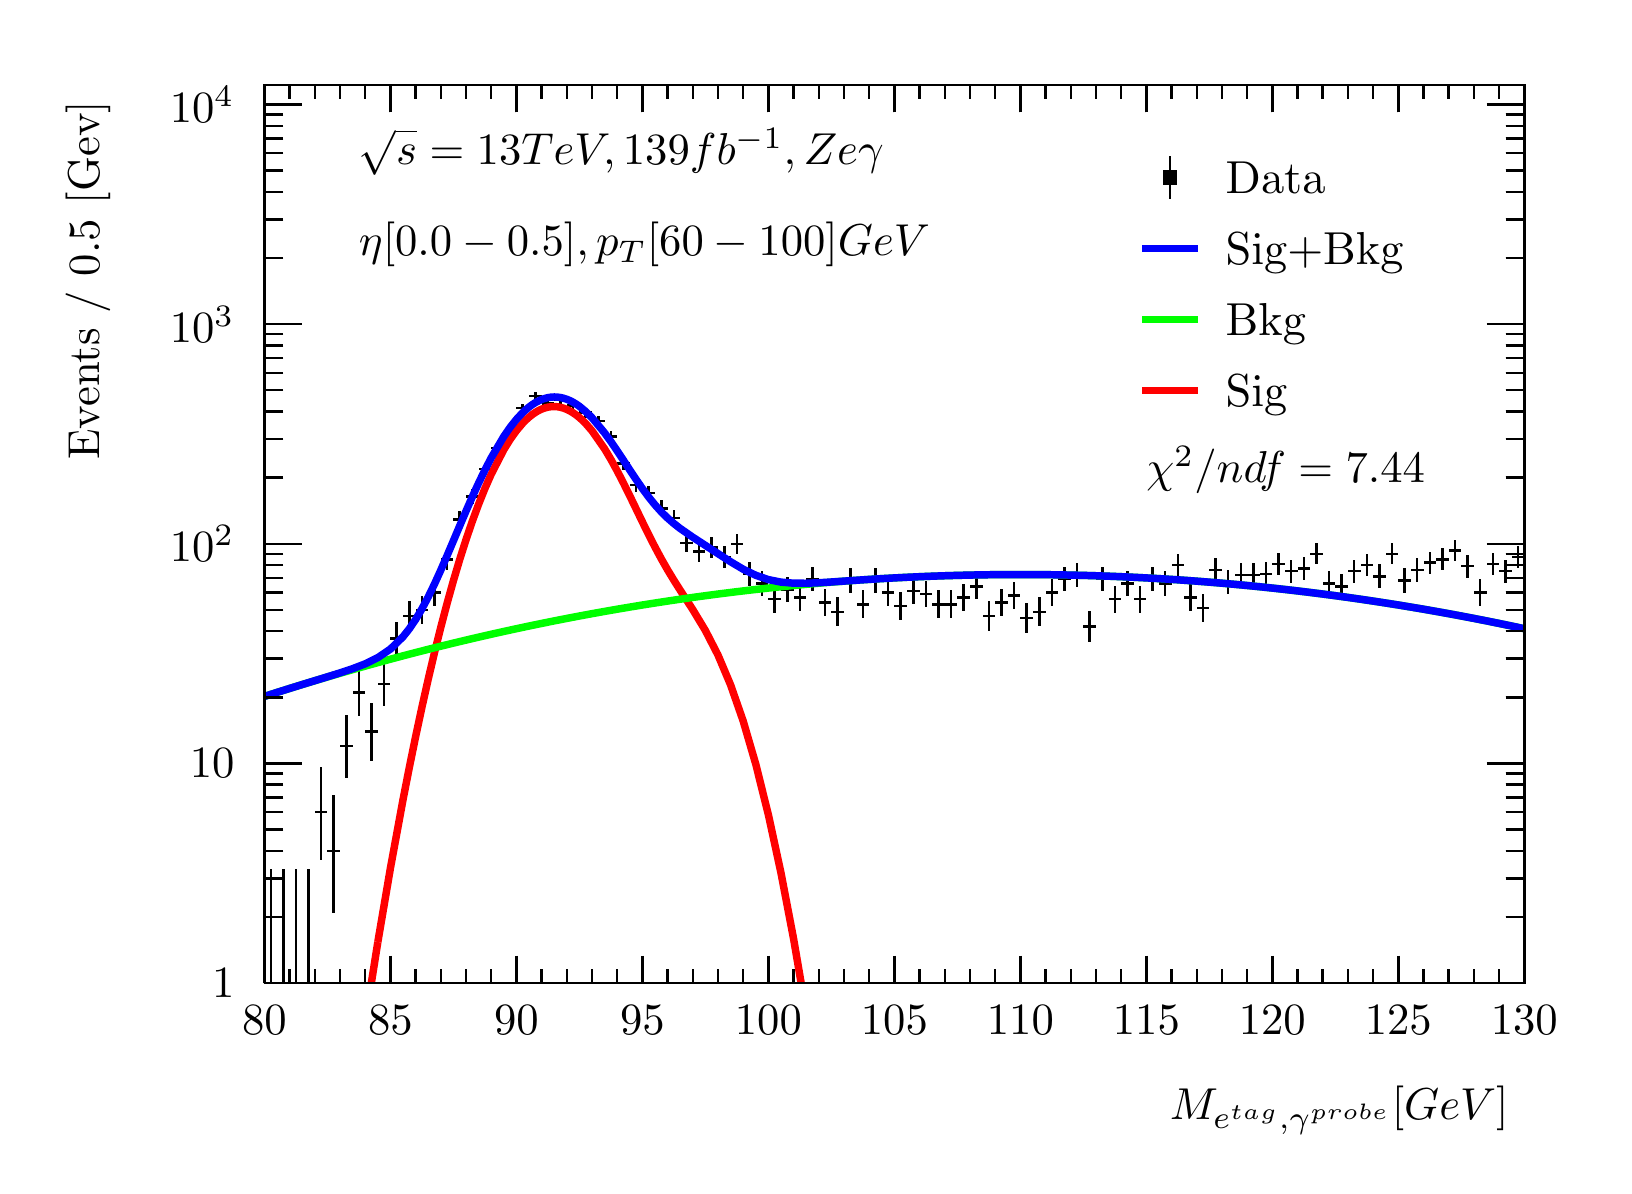
\begin{tikzpicture}
\pgfdeclareplotmark{cross} {
\pgfpathmoveto{\pgfpoint{-0.3\pgfplotmarksize}{\pgfplotmarksize}}
\pgfpathlineto{\pgfpoint{+0.3\pgfplotmarksize}{\pgfplotmarksize}}
\pgfpathlineto{\pgfpoint{+0.3\pgfplotmarksize}{0.3\pgfplotmarksize}}
\pgfpathlineto{\pgfpoint{+1\pgfplotmarksize}{0.3\pgfplotmarksize}}
\pgfpathlineto{\pgfpoint{+1\pgfplotmarksize}{-0.3\pgfplotmarksize}}
\pgfpathlineto{\pgfpoint{+0.3\pgfplotmarksize}{-0.3\pgfplotmarksize}}
\pgfpathlineto{\pgfpoint{+0.3\pgfplotmarksize}{-1.\pgfplotmarksize}}
\pgfpathlineto{\pgfpoint{-0.3\pgfplotmarksize}{-1.\pgfplotmarksize}}
\pgfpathlineto{\pgfpoint{-0.3\pgfplotmarksize}{-0.3\pgfplotmarksize}}
\pgfpathlineto{\pgfpoint{-1.\pgfplotmarksize}{-0.3\pgfplotmarksize}}
\pgfpathlineto{\pgfpoint{-1.\pgfplotmarksize}{0.3\pgfplotmarksize}}
\pgfpathlineto{\pgfpoint{-0.3\pgfplotmarksize}{0.3\pgfplotmarksize}}
\pgfpathclose
\pgfusepathqstroke
}
\pgfdeclareplotmark{cross*} {
\pgfpathmoveto{\pgfpoint{-0.3\pgfplotmarksize}{\pgfplotmarksize}}
\pgfpathlineto{\pgfpoint{+0.3\pgfplotmarksize}{\pgfplotmarksize}}
\pgfpathlineto{\pgfpoint{+0.3\pgfplotmarksize}{0.3\pgfplotmarksize}}
\pgfpathlineto{\pgfpoint{+1\pgfplotmarksize}{0.3\pgfplotmarksize}}
\pgfpathlineto{\pgfpoint{+1\pgfplotmarksize}{-0.3\pgfplotmarksize}}
\pgfpathlineto{\pgfpoint{+0.3\pgfplotmarksize}{-0.3\pgfplotmarksize}}
\pgfpathlineto{\pgfpoint{+0.3\pgfplotmarksize}{-1.\pgfplotmarksize}}
\pgfpathlineto{\pgfpoint{-0.3\pgfplotmarksize}{-1.\pgfplotmarksize}}
\pgfpathlineto{\pgfpoint{-0.3\pgfplotmarksize}{-0.3\pgfplotmarksize}}
\pgfpathlineto{\pgfpoint{-1.\pgfplotmarksize}{-0.3\pgfplotmarksize}}
\pgfpathlineto{\pgfpoint{-1.\pgfplotmarksize}{0.3\pgfplotmarksize}}
\pgfpathlineto{\pgfpoint{-0.3\pgfplotmarksize}{0.3\pgfplotmarksize}}
\pgfpathclose
\pgfusepathqfillstroke
}
\pgfdeclareplotmark{newstar} {
\pgfpathmoveto{\pgfqpoint{0pt}{\pgfplotmarksize}}
\pgfpathlineto{\pgfqpointpolar{44}{0.5\pgfplotmarksize}}
\pgfpathlineto{\pgfqpointpolar{18}{\pgfplotmarksize}}
\pgfpathlineto{\pgfqpointpolar{-20}{0.5\pgfplotmarksize}}
\pgfpathlineto{\pgfqpointpolar{-54}{\pgfplotmarksize}}
\pgfpathlineto{\pgfqpointpolar{-90}{0.5\pgfplotmarksize}}
\pgfpathlineto{\pgfqpointpolar{234}{\pgfplotmarksize}}
\pgfpathlineto{\pgfqpointpolar{198}{0.5\pgfplotmarksize}}
\pgfpathlineto{\pgfqpointpolar{162}{\pgfplotmarksize}}
\pgfpathlineto{\pgfqpointpolar{134}{0.5\pgfplotmarksize}}
\pgfpathclose
\pgfusepathqstroke
}
\pgfdeclareplotmark{newstar*} {
\pgfpathmoveto{\pgfqpoint{0pt}{\pgfplotmarksize}}
\pgfpathlineto{\pgfqpointpolar{44}{0.5\pgfplotmarksize}}
\pgfpathlineto{\pgfqpointpolar{18}{\pgfplotmarksize}}
\pgfpathlineto{\pgfqpointpolar{-20}{0.5\pgfplotmarksize}}
\pgfpathlineto{\pgfqpointpolar{-54}{\pgfplotmarksize}}
\pgfpathlineto{\pgfqpointpolar{-90}{0.5\pgfplotmarksize}}
\pgfpathlineto{\pgfqpointpolar{234}{\pgfplotmarksize}}
\pgfpathlineto{\pgfqpointpolar{198}{0.5\pgfplotmarksize}}
\pgfpathlineto{\pgfqpointpolar{162}{\pgfplotmarksize}}
\pgfpathlineto{\pgfqpointpolar{134}{0.5\pgfplotmarksize}}
\pgfpathclose
\pgfusepathqfillstroke
}
\definecolor{c}{rgb}{1,1,1};
\draw [color=c, fill=c] (0,0) rectangle (20,14.4361);
\draw [color=c, fill=c] (3,2.30977) rectangle (19,13.7143);
\definecolor{c}{rgb}{0,0,0};
\draw [c,line width=0.9] (3,2.30977) -- (3,13.7143) -- (19,13.7143) -- (19,2.30977) -- (3,2.30977);
\definecolor{c}{rgb}{1,1,1};
\draw [color=c, fill=c] (3,2.30977) rectangle (19,13.7143);
\definecolor{c}{rgb}{0,0,0};
\draw [c,line width=0.9] (3,2.30977) -- (3,13.7143) -- (19,13.7143) -- (19,2.30977) -- (3,2.30977);
\draw [c,line width=0.9] (3,2.30977) -- (19,2.30977);
\draw [c,line width=0.9] (3,2.65624) -- (3,2.30977);
\draw [c,line width=0.9] (3.32,2.48301) -- (3.32,2.30977);
\draw [c,line width=0.9] (3.64,2.48301) -- (3.64,2.30977);
\draw [c,line width=0.9] (3.96,2.48301) -- (3.96,2.30977);
\draw [c,line width=0.9] (4.28,2.48301) -- (4.28,2.30977);
\draw [c,line width=0.9] (4.6,2.65624) -- (4.6,2.30977);
\draw [c,line width=0.9] (4.92,2.48301) -- (4.92,2.30977);
\draw [c,line width=0.9] (5.24,2.48301) -- (5.24,2.30977);
\draw [c,line width=0.9] (5.56,2.48301) -- (5.56,2.30977);
\draw [c,line width=0.9] (5.88,2.48301) -- (5.88,2.30977);
\draw [c,line width=0.9] (6.2,2.65624) -- (6.2,2.30977);
\draw [c,line width=0.9] (6.52,2.48301) -- (6.52,2.30977);
\draw [c,line width=0.9] (6.84,2.48301) -- (6.84,2.30977);
\draw [c,line width=0.9] (7.16,2.48301) -- (7.16,2.30977);
\draw [c,line width=0.9] (7.48,2.48301) -- (7.48,2.30977);
\draw [c,line width=0.9] (7.8,2.65624) -- (7.8,2.30977);
\draw [c,line width=0.9] (8.12,2.48301) -- (8.12,2.30977);
\draw [c,line width=0.9] (8.44,2.48301) -- (8.44,2.30977);
\draw [c,line width=0.9] (8.76,2.48301) -- (8.76,2.30977);
\draw [c,line width=0.9] (9.08,2.48301) -- (9.08,2.30977);
\draw [c,line width=0.9] (9.4,2.65624) -- (9.4,2.30977);
\draw [c,line width=0.9] (9.72,2.48301) -- (9.72,2.30977);
\draw [c,line width=0.9] (10.04,2.48301) -- (10.04,2.30977);
\draw [c,line width=0.9] (10.36,2.48301) -- (10.36,2.30977);
\draw [c,line width=0.9] (10.68,2.48301) -- (10.68,2.30977);
\draw [c,line width=0.9] (11,2.65624) -- (11,2.30977);
\draw [c,line width=0.9] (11.32,2.48301) -- (11.32,2.30977);
\draw [c,line width=0.9] (11.64,2.48301) -- (11.64,2.30977);
\draw [c,line width=0.9] (11.96,2.48301) -- (11.96,2.30977);
\draw [c,line width=0.9] (12.28,2.48301) -- (12.28,2.30977);
\draw [c,line width=0.9] (12.6,2.65624) -- (12.6,2.30977);
\draw [c,line width=0.9] (12.92,2.48301) -- (12.92,2.30977);
\draw [c,line width=0.9] (13.24,2.48301) -- (13.24,2.30977);
\draw [c,line width=0.9] (13.56,2.48301) -- (13.56,2.30977);
\draw [c,line width=0.9] (13.88,2.48301) -- (13.88,2.30977);
\draw [c,line width=0.9] (14.2,2.65624) -- (14.2,2.30977);
\draw [c,line width=0.9] (14.52,2.48301) -- (14.52,2.30977);
\draw [c,line width=0.9] (14.84,2.48301) -- (14.84,2.30977);
\draw [c,line width=0.9] (15.16,2.48301) -- (15.16,2.30977);
\draw [c,line width=0.9] (15.48,2.48301) -- (15.48,2.30977);
\draw [c,line width=0.9] (15.8,2.65624) -- (15.8,2.30977);
\draw [c,line width=0.9] (16.12,2.48301) -- (16.12,2.30977);
\draw [c,line width=0.9] (16.44,2.48301) -- (16.44,2.30977);
\draw [c,line width=0.9] (16.76,2.48301) -- (16.76,2.30977);
\draw [c,line width=0.9] (17.08,2.48301) -- (17.08,2.30977);
\draw [c,line width=0.9] (17.4,2.65624) -- (17.4,2.30977);
\draw [c,line width=0.9] (17.72,2.48301) -- (17.72,2.30977);
\draw [c,line width=0.9] (18.04,2.48301) -- (18.04,2.30977);
\draw [c,line width=0.9] (18.36,2.48301) -- (18.36,2.30977);
\draw [c,line width=0.9] (18.68,2.48301) -- (18.68,2.30977);
\draw [c,line width=0.9] (19,2.65624) -- (19,2.30977);
\draw [anchor=base] (3,1.66015) node[scale=1.61424, color=c, rotate=0]{80};
\draw [anchor=base] (4.6,1.66015) node[scale=1.61424, color=c, rotate=0]{85};
\draw [anchor=base] (6.2,1.66015) node[scale=1.61424, color=c, rotate=0]{90};
\draw [anchor=base] (7.8,1.66015) node[scale=1.61424, color=c, rotate=0]{95};
\draw [anchor=base] (9.4,1.66015) node[scale=1.61424, color=c, rotate=0]{100};
\draw [anchor=base] (11,1.66015) node[scale=1.61424, color=c, rotate=0]{105};
\draw [anchor=base] (12.6,1.66015) node[scale=1.61424, color=c, rotate=0]{110};
\draw [anchor=base] (14.2,1.66015) node[scale=1.61424, color=c, rotate=0]{115};
\draw [anchor=base] (15.8,1.66015) node[scale=1.61424, color=c, rotate=0]{120};
\draw [anchor=base] (17.4,1.66015) node[scale=1.61424, color=c, rotate=0]{125};
\draw [anchor=base] (19,1.66015) node[scale=1.61424, color=c, rotate=0]{130};
\draw [anchor= east] (19,0.692932) node[scale=1.61424, color=c, rotate=0]{$M_{e^{tag}, \gamma^{probe}}  [GeV]$};
\draw [c,line width=0.9] (3,13.7143) -- (19,13.7143);
\draw [c,line width=0.9] (3,13.3678) -- (3,13.7143);
\draw [c,line width=0.9] (3.32,13.5411) -- (3.32,13.7143);
\draw [c,line width=0.9] (3.64,13.5411) -- (3.64,13.7143);
\draw [c,line width=0.9] (3.96,13.5411) -- (3.96,13.7143);
\draw [c,line width=0.9] (4.28,13.5411) -- (4.28,13.7143);
\draw [c,line width=0.9] (4.6,13.3678) -- (4.6,13.7143);
\draw [c,line width=0.9] (4.92,13.5411) -- (4.92,13.7143);
\draw [c,line width=0.9] (5.24,13.5411) -- (5.24,13.7143);
\draw [c,line width=0.9] (5.56,13.5411) -- (5.56,13.7143);
\draw [c,line width=0.9] (5.88,13.5411) -- (5.88,13.7143);
\draw [c,line width=0.9] (6.2,13.3678) -- (6.2,13.7143);
\draw [c,line width=0.9] (6.52,13.5411) -- (6.52,13.7143);
\draw [c,line width=0.9] (6.84,13.5411) -- (6.84,13.7143);
\draw [c,line width=0.9] (7.16,13.5411) -- (7.16,13.7143);
\draw [c,line width=0.9] (7.48,13.5411) -- (7.48,13.7143);
\draw [c,line width=0.9] (7.8,13.3678) -- (7.8,13.7143);
\draw [c,line width=0.9] (8.12,13.5411) -- (8.12,13.7143);
\draw [c,line width=0.9] (8.44,13.5411) -- (8.44,13.7143);
\draw [c,line width=0.9] (8.76,13.5411) -- (8.76,13.7143);
\draw [c,line width=0.9] (9.08,13.5411) -- (9.08,13.7143);
\draw [c,line width=0.9] (9.4,13.3678) -- (9.4,13.7143);
\draw [c,line width=0.9] (9.72,13.5411) -- (9.72,13.7143);
\draw [c,line width=0.9] (10.04,13.5411) -- (10.04,13.7143);
\draw [c,line width=0.9] (10.36,13.5411) -- (10.36,13.7143);
\draw [c,line width=0.9] (10.68,13.5411) -- (10.68,13.7143);
\draw [c,line width=0.9] (11,13.3678) -- (11,13.7143);
\draw [c,line width=0.9] (11.32,13.5411) -- (11.32,13.7143);
\draw [c,line width=0.9] (11.64,13.5411) -- (11.64,13.7143);
\draw [c,line width=0.9] (11.96,13.5411) -- (11.96,13.7143);
\draw [c,line width=0.9] (12.28,13.5411) -- (12.28,13.7143);
\draw [c,line width=0.9] (12.6,13.3678) -- (12.6,13.7143);
\draw [c,line width=0.9] (12.92,13.5411) -- (12.92,13.7143);
\draw [c,line width=0.9] (13.24,13.5411) -- (13.24,13.7143);
\draw [c,line width=0.9] (13.56,13.5411) -- (13.56,13.7143);
\draw [c,line width=0.9] (13.88,13.5411) -- (13.88,13.7143);
\draw [c,line width=0.9] (14.2,13.3678) -- (14.2,13.7143);
\draw [c,line width=0.9] (14.52,13.5411) -- (14.52,13.7143);
\draw [c,line width=0.9] (14.84,13.5411) -- (14.84,13.7143);
\draw [c,line width=0.9] (15.16,13.5411) -- (15.16,13.7143);
\draw [c,line width=0.9] (15.48,13.5411) -- (15.48,13.7143);
\draw [c,line width=0.9] (15.8,13.3678) -- (15.8,13.7143);
\draw [c,line width=0.9] (16.12,13.5411) -- (16.12,13.7143);
\draw [c,line width=0.9] (16.44,13.5411) -- (16.44,13.7143);
\draw [c,line width=0.9] (16.76,13.5411) -- (16.76,13.7143);
\draw [c,line width=0.9] (17.08,13.5411) -- (17.08,13.7143);
\draw [c,line width=0.9] (17.4,13.3678) -- (17.4,13.7143);
\draw [c,line width=0.9] (17.72,13.5411) -- (17.72,13.7143);
\draw [c,line width=0.9] (18.04,13.5411) -- (18.04,13.7143);
\draw [c,line width=0.9] (18.36,13.5411) -- (18.36,13.7143);
\draw [c,line width=0.9] (18.68,13.5411) -- (18.68,13.7143);
\draw [c,line width=0.9] (19,13.3678) -- (19,13.7143);
\draw [c,line width=0.9] (3,2.30977) -- (3,13.7143);
\draw [c,line width=0.9] (3.474,2.30978) -- (3,2.30978);
\draw [anchor= east] (2.82,2.30978) node[scale=1.61424, color=c, rotate=0]{1};
\draw [c,line width=0.9] (3.237,3.1495) -- (3,3.1495);
\draw [c,line width=0.9] (3.237,3.6407) -- (3,3.6407);
\draw [c,line width=0.9] (3.237,3.98922) -- (3,3.98922);
\draw [c,line width=0.9] (3.237,4.25955) -- (3,4.25955);
\draw [c,line width=0.9] (3.237,4.48042) -- (3,4.48042);
\draw [c,line width=0.9] (3.237,4.66717) -- (3,4.66717);
\draw [c,line width=0.9] (3.237,4.82894) -- (3,4.82894);
\draw [c,line width=0.9] (3.237,4.97163) -- (3,4.97163);
\draw [c,line width=0.9] (3.474,5.09927) -- (3,5.09927);
\draw [anchor= east] (2.82,5.09927) node[scale=1.61424, color=c, rotate=0]{10};
\draw [c,line width=0.9] (3.237,5.93899) -- (3,5.93899);
\draw [c,line width=0.9] (3.237,6.43019) -- (3,6.43019);
\draw [c,line width=0.9] (3.237,6.77871) -- (3,6.77871);
\draw [c,line width=0.9] (3.237,7.04904) -- (3,7.04904);
\draw [c,line width=0.9] (3.237,7.26991) -- (3,7.26991);
\draw [c,line width=0.9] (3.237,7.45666) -- (3,7.45666);
\draw [c,line width=0.9] (3.237,7.61843) -- (3,7.61843);
\draw [c,line width=0.9] (3.237,7.76112) -- (3,7.76112);
\draw [c,line width=0.9] (3.474,7.88876) -- (3,7.88876);
\draw [anchor= east] (2.82,7.88876) node[scale=1.61424, color=c, rotate=0]{$10^{2}$};
\draw [c,line width=0.9] (3.237,8.72848) -- (3,8.72848);
\draw [c,line width=0.9] (3.237,9.21968) -- (3,9.21968);
\draw [c,line width=0.9] (3.237,9.5682) -- (3,9.5682);
\draw [c,line width=0.9] (3.237,9.83853) -- (3,9.83853);
\draw [c,line width=0.9] (3.237,10.0594) -- (3,10.0594);
\draw [c,line width=0.9] (3.237,10.2462) -- (3,10.2462);
\draw [c,line width=0.9] (3.237,10.4079) -- (3,10.4079);
\draw [c,line width=0.9] (3.237,10.5506) -- (3,10.5506);
\draw [c,line width=0.9] (3.474,10.6782) -- (3,10.6782);
\draw [anchor= east] (2.82,10.6782) node[scale=1.61424, color=c, rotate=0]{$10^{3}$};
\draw [c,line width=0.9] (3.237,11.518) -- (3,11.518);
\draw [c,line width=0.9] (3.237,12.0092) -- (3,12.0092);
\draw [c,line width=0.9] (3.237,12.3577) -- (3,12.3577);
\draw [c,line width=0.9] (3.237,12.628) -- (3,12.628);
\draw [c,line width=0.9] (3.237,12.8489) -- (3,12.8489);
\draw [c,line width=0.9] (3.237,13.0356) -- (3,13.0356);
\draw [c,line width=0.9] (3.237,13.1974) -- (3,13.1974);
\draw [c,line width=0.9] (3.237,13.3401) -- (3,13.3401);
\draw [c,line width=0.9] (3.474,13.4677) -- (3,13.4677);
\draw [anchor= east] (2.82,13.4677) node[scale=1.61424, color=c, rotate=0]{$10^{4}$};
\draw [anchor= east] (0.76,13.7143) node[scale=1.61424, color=c, rotate=90]{Events / 0.5 [Gev]};
\draw [c,line width=0.9] (19,2.30977) -- (19,13.7143);
\draw [c,line width=0.9] (18.526,2.30978) -- (19,2.30978);
\draw [c,line width=0.9] (18.763,3.1495) -- (19,3.1495);
\draw [c,line width=0.9] (18.763,3.6407) -- (19,3.6407);
\draw [c,line width=0.9] (18.763,3.98922) -- (19,3.98922);
\draw [c,line width=0.9] (18.763,4.25955) -- (19,4.25955);
\draw [c,line width=0.9] (18.763,4.48042) -- (19,4.48042);
\draw [c,line width=0.9] (18.763,4.66717) -- (19,4.66717);
\draw [c,line width=0.9] (18.763,4.82894) -- (19,4.82894);
\draw [c,line width=0.9] (18.763,4.97163) -- (19,4.97163);
\draw [c,line width=0.9] (18.526,5.09927) -- (19,5.09927);
\draw [c,line width=0.9] (18.763,5.93899) -- (19,5.93899);
\draw [c,line width=0.9] (18.763,6.43019) -- (19,6.43019);
\draw [c,line width=0.9] (18.763,6.77871) -- (19,6.77871);
\draw [c,line width=0.9] (18.763,7.04904) -- (19,7.04904);
\draw [c,line width=0.9] (18.763,7.26991) -- (19,7.26991);
\draw [c,line width=0.9] (18.763,7.45666) -- (19,7.45666);
\draw [c,line width=0.9] (18.763,7.61843) -- (19,7.61843);
\draw [c,line width=0.9] (18.763,7.76112) -- (19,7.76112);
\draw [c,line width=0.9] (18.526,7.88876) -- (19,7.88876);
\draw [c,line width=0.9] (18.763,8.72848) -- (19,8.72848);
\draw [c,line width=0.9] (18.763,9.21968) -- (19,9.21968);
\draw [c,line width=0.9] (18.763,9.5682) -- (19,9.5682);
\draw [c,line width=0.9] (18.763,9.83853) -- (19,9.83853);
\draw [c,line width=0.9] (18.763,10.0594) -- (19,10.0594);
\draw [c,line width=0.9] (18.763,10.2462) -- (19,10.2462);
\draw [c,line width=0.9] (18.763,10.4079) -- (19,10.4079);
\draw [c,line width=0.9] (18.763,10.5506) -- (19,10.5506);
\draw [c,line width=0.9] (18.526,10.6782) -- (19,10.6782);
\draw [c,line width=0.9] (18.763,11.518) -- (19,11.518);
\draw [c,line width=0.9] (18.763,12.0092) -- (19,12.0092);
\draw [c,line width=0.9] (18.763,12.3577) -- (19,12.3577);
\draw [c,line width=0.9] (18.763,12.628) -- (19,12.628);
\draw [c,line width=0.9] (18.763,12.8489) -- (19,12.8489);
\draw [c,line width=0.9] (18.763,13.0356) -- (19,13.0356);
\draw [c,line width=0.9] (18.763,13.1974) -- (19,13.1974);
\draw [c,line width=0.9] (18.763,13.3401) -- (19,13.3401);
\draw [c,line width=0.9] (18.526,13.4677) -- (19,13.4677);
\draw [c,line width=0.9] (3.08,2.30977) -- (3,2.30977);
\draw [c,line width=0.9] (3,2.30977) -- (3,2.30977);
\draw [c,line width=0.9] (3.08,2.30977) -- (3.16,2.30977);
\draw [c,line width=0.9] (3.16,2.30977) -- (3.16,2.30977);
\draw [c,line width=0.9] (3.08,2.30977) -- (3.08,3.75599);
\draw [c,line width=0.9] (3.08,3.75599) -- (3.08,3.75599);
\draw [c,line width=0.9] (3.24,2.30977) -- (3.16,2.30977);
\draw [c,line width=0.9] (3.16,2.30977) -- (3.16,2.30977);
\draw [c,line width=0.9] (3.24,2.30977) -- (3.32,2.30977);
\draw [c,line width=0.9] (3.32,2.30977) -- (3.32,2.30977);
\draw [c,line width=0.9] (3.24,2.30977) -- (3.24,3.75599);
\draw [c,line width=0.9] (3.24,3.75599) -- (3.24,3.75599);
\draw [c,line width=0.9] (3.4,2.30977) -- (3.32,2.30977);
\draw [c,line width=0.9] (3.32,2.30977) -- (3.32,2.30977);
\draw [c,line width=0.9] (3.4,2.30977) -- (3.48,2.30977);
\draw [c,line width=0.9] (3.48,2.30977) -- (3.48,2.30977);
\draw [c,line width=0.9] (3.4,2.30977) -- (3.4,3.75599);
\draw [c,line width=0.9] (3.4,3.75599) -- (3.4,3.75599);
\draw [c,line width=0.9] (3.56,2.30977) -- (3.48,2.30977);
\draw [c,line width=0.9] (3.48,2.30977) -- (3.48,2.30977);
\draw [c,line width=0.9] (3.56,2.30977) -- (3.64,2.30977);
\draw [c,line width=0.9] (3.64,2.30977) -- (3.64,2.30977);
\draw [c,line width=0.9] (3.56,2.30977) -- (3.56,3.75599);
\draw [c,line width=0.9] (3.56,3.75599) -- (3.56,3.75599);
\draw [c,line width=0.9] (3.72,4.48042) -- (3.64,4.48042);
\draw [c,line width=0.9] (3.64,4.48042) -- (3.64,4.48042);
\draw [c,line width=0.9] (3.72,4.48042) -- (3.8,4.48042);
\draw [c,line width=0.9] (3.8,4.48042) -- (3.8,4.48042);
\draw [c,line width=0.9] (3.72,4.48042) -- (3.72,5.04775);
\draw [c,line width=0.9] (3.72,5.04775) -- (3.72,5.04775);
\draw [c,line width=0.9] (3.72,4.48042) -- (3.72,3.86831);
\draw [c,line width=0.9] (3.72,3.86831) -- (3.72,3.86831);
\draw [c,line width=0.9] (3.88,3.98922) -- (3.8,3.98922);
\draw [c,line width=0.9] (3.8,3.98922) -- (3.8,3.98922);
\draw [c,line width=0.9] (3.88,3.98922) -- (3.96,3.98922);
\draw [c,line width=0.9] (3.96,3.98922) -- (3.96,3.98922);
\draw [c,line width=0.9] (3.88,3.98922) -- (3.88,4.69501);
\draw [c,line width=0.9] (3.88,4.69501) -- (3.88,4.69501);
\draw [c,line width=0.9] (3.88,3.98922) -- (3.88,3.2003);
\draw [c,line width=0.9] (3.88,3.2003) -- (3.88,3.2003);
\draw [c,line width=0.9] (4.04,5.32014) -- (3.96,5.32014);
\draw [c,line width=0.9] (3.96,5.32014) -- (3.96,5.32014);
\draw [c,line width=0.9] (4.04,5.32014) -- (4.12,5.32014);
\draw [c,line width=0.9] (4.12,5.32014) -- (4.12,5.32014);
\draw [c,line width=0.9] (4.04,5.32014) -- (4.04,5.71032);
\draw [c,line width=0.9] (4.04,5.71032) -- (4.04,5.71032);
\draw [c,line width=0.9] (4.04,5.32014) -- (4.04,4.9144);
\draw [c,line width=0.9] (4.04,4.9144) -- (4.04,4.9144);
\draw [c,line width=0.9] (4.2,5.99809) -- (4.12,5.99809);
\draw [c,line width=0.9] (4.12,5.99809) -- (4.12,5.99809);
\draw [c,line width=0.9] (4.2,5.99809) -- (4.28,5.99809);
\draw [c,line width=0.9] (4.28,5.99809) -- (4.28,5.99809);
\draw [c,line width=0.9] (4.2,5.99809) -- (4.2,6.28698);
\draw [c,line width=0.9] (4.2,6.28698) -- (4.2,6.28698);
\draw [c,line width=0.9] (4.2,5.99809) -- (4.2,5.70257);
\draw [c,line width=0.9] (4.2,5.70257) -- (4.2,5.70257);
\draw [c,line width=0.9] (4.36,5.50689) -- (4.28,5.50689);
\draw [c,line width=0.9] (4.28,5.50689) -- (4.28,5.50689);
\draw [c,line width=0.9] (4.36,5.50689) -- (4.44,5.50689);
\draw [c,line width=0.9] (4.44,5.50689) -- (4.44,5.50689);
\draw [c,line width=0.9] (4.36,5.50689) -- (4.36,5.86598);
\draw [c,line width=0.9] (4.36,5.86598) -- (4.36,5.86598);
\draw [c,line width=0.9] (4.36,5.50689) -- (4.36,5.13549);
\draw [c,line width=0.9] (4.36,5.13549) -- (4.36,5.13549);
\draw [c,line width=0.9] (4.52,6.1083) -- (4.44,6.1083);
\draw [c,line width=0.9] (4.44,6.1083) -- (4.44,6.1083);
\draw [c,line width=0.9] (4.52,6.1083) -- (4.6,6.1083);
\draw [c,line width=0.9] (4.6,6.1083) -- (4.6,6.1083);
\draw [c,line width=0.9] (4.52,6.1083) -- (4.52,6.38348);
\draw [c,line width=0.9] (4.52,6.38348) -- (4.52,6.38348);
\draw [c,line width=0.9] (4.52,6.1083) -- (4.52,5.82734);
\draw [c,line width=0.9] (4.52,5.82734) -- (4.52,5.82734);
\draw [c,line width=0.9] (4.68,6.68426) -- (4.6,6.68426);
\draw [c,line width=0.9] (4.6,6.68426) -- (4.6,6.68426);
\draw [c,line width=0.9] (4.68,6.68426) -- (4.76,6.68426);
\draw [c,line width=0.9] (4.76,6.68426) -- (4.76,6.68426);
\draw [c,line width=0.9] (4.68,6.68426) -- (4.68,6.89795);
\draw [c,line width=0.9] (4.68,6.89795) -- (4.68,6.89795);
\draw [c,line width=0.9] (4.68,6.68426) -- (4.68,6.46776);
\draw [c,line width=0.9] (4.68,6.46776) -- (4.68,6.46776);
\draw [c,line width=0.9] (4.84,6.97408) -- (4.76,6.97408);
\draw [c,line width=0.9] (4.76,6.97408) -- (4.76,6.97408);
\draw [c,line width=0.9] (4.84,6.97408) -- (4.92,6.97408);
\draw [c,line width=0.9] (4.92,6.97408) -- (4.92,6.97408);
\draw [c,line width=0.9] (4.84,6.97408) -- (4.84,7.16239);
\draw [c,line width=0.9] (4.84,7.16239) -- (4.84,7.16239);
\draw [c,line width=0.9] (4.84,6.97408) -- (4.84,6.78381);
\draw [c,line width=0.9] (4.84,6.78381) -- (4.84,6.78381);
\draw [c,line width=0.9] (5,7.04904) -- (4.92,7.04904);
\draw [c,line width=0.9] (4.92,7.04904) -- (4.92,7.04904);
\draw [c,line width=0.9] (5,7.04904) -- (5.08,7.04904);
\draw [c,line width=0.9] (5.08,7.04904) -- (5.08,7.04904);
\draw [c,line width=0.9] (5,7.04904) -- (5,7.23131);
\draw [c,line width=0.9] (5,7.23131) -- (5,7.23131);
\draw [c,line width=0.9] (5,7.04904) -- (5,6.86499);
\draw [c,line width=0.9] (5,6.86499) -- (5,6.86499);
\draw [c,line width=0.9] (5.16,7.26991) -- (5.08,7.26991);
\draw [c,line width=0.9] (5.08,7.26991) -- (5.08,7.26991);
\draw [c,line width=0.9] (5.16,7.26991) -- (5.24,7.26991);
\draw [c,line width=0.9] (5.24,7.26991) -- (5.24,7.26991);
\draw [c,line width=0.9] (5.16,7.26991) -- (5.16,7.43552);
\draw [c,line width=0.9] (5.16,7.43552) -- (5.16,7.43552);
\draw [c,line width=0.9] (5.16,7.26991) -- (5.16,7.10296);
\draw [c,line width=0.9] (5.16,7.10296) -- (5.16,7.10296);
\draw [c,line width=0.9] (5.32,7.69187) -- (5.24,7.69187);
\draw [c,line width=0.9] (5.24,7.69187) -- (5.24,7.69187);
\draw [c,line width=0.9] (5.32,7.69187) -- (5.4,7.69187);
\draw [c,line width=0.9] (5.4,7.69187) -- (5.4,7.69187);
\draw [c,line width=0.9] (5.32,7.69187) -- (5.32,7.82987);
\draw [c,line width=0.9] (5.32,7.82987) -- (5.32,7.82987);
\draw [c,line width=0.9] (5.32,7.69187) -- (5.32,7.55307);
\draw [c,line width=0.9] (5.32,7.55307) -- (5.32,7.55307);
\draw [c,line width=0.9] (5.48,8.19725) -- (5.4,8.19725);
\draw [c,line width=0.9] (5.4,8.19725) -- (5.4,8.19725);
\draw [c,line width=0.9] (5.48,8.19725) -- (5.56,8.19725);
\draw [c,line width=0.9] (5.56,8.19725) -- (5.56,8.19725);
\draw [c,line width=0.9] (5.48,8.19725) -- (5.48,8.30387);
\draw [c,line width=0.9] (5.48,8.30387) -- (5.48,8.30387);
\draw [c,line width=0.9] (5.48,8.19725) -- (5.48,8.09062);
\draw [c,line width=0.9] (5.48,8.09062) -- (5.48,8.09062);
\draw [c,line width=0.9] (5.64,8.48806) -- (5.56,8.48806);
\draw [c,line width=0.9] (5.56,8.48806) -- (5.56,8.48806);
\draw [c,line width=0.9] (5.64,8.48806) -- (5.72,8.48806);
\draw [c,line width=0.9] (5.72,8.48806) -- (5.72,8.48806);
\draw [c,line width=0.9] (5.64,8.48806) -- (5.64,8.58264);
\draw [c,line width=0.9] (5.64,8.58264) -- (5.64,8.58264);
\draw [c,line width=0.9] (5.64,8.48806) -- (5.64,8.39349);
\draw [c,line width=0.9] (5.64,8.39349) -- (5.64,8.39349);
\draw [c,line width=0.9] (5.8,8.83842) -- (5.72,8.83842);
\draw [c,line width=0.9] (5.72,8.83842) -- (5.72,8.83842);
\draw [c,line width=0.9] (5.8,8.83842) -- (5.88,8.83842);
\draw [c,line width=0.9] (5.88,8.83842) -- (5.88,8.83842);
\draw [c,line width=0.9] (5.8,8.83842) -- (5.8,8.92027);
\draw [c,line width=0.9] (5.8,8.92027) -- (5.8,8.92027);
\draw [c,line width=0.9] (5.8,8.83842) -- (5.8,8.75658);
\draw [c,line width=0.9] (5.8,8.75658) -- (5.8,8.75658);
\draw [c,line width=0.9] (5.96,9.10543) -- (5.88,9.10543);
\draw [c,line width=0.9] (5.88,9.10543) -- (5.88,9.10543);
\draw [c,line width=0.9] (5.96,9.10543) -- (6.04,9.10543);
\draw [c,line width=0.9] (6.04,9.10543) -- (6.04,9.10543);
\draw [c,line width=0.9] (5.96,9.10543) -- (5.96,9.17874);
\draw [c,line width=0.9] (5.96,9.17874) -- (5.96,9.17874);
\draw [c,line width=0.9] (5.96,9.10543) -- (5.96,9.03212);
\draw [c,line width=0.9] (5.96,9.03212) -- (5.96,9.03212);
\draw [c,line width=0.9] (6.12,9.32037) -- (6.04,9.32037);
\draw [c,line width=0.9] (6.04,9.32037) -- (6.04,9.32037);
\draw [c,line width=0.9] (6.12,9.32037) -- (6.2,9.32037);
\draw [c,line width=0.9] (6.2,9.32037) -- (6.2,9.32037);
\draw [c,line width=0.9] (6.12,9.32037) -- (6.12,9.38746);
\draw [c,line width=0.9] (6.12,9.38746) -- (6.12,9.38746);
\draw [c,line width=0.9] (6.12,9.32037) -- (6.12,9.25328);
\draw [c,line width=0.9] (6.12,9.25328) -- (6.12,9.25328);
\draw [c,line width=0.9] (6.28,9.60987) -- (6.2,9.60987);
\draw [c,line width=0.9] (6.2,9.60987) -- (6.2,9.60987);
\draw [c,line width=0.9] (6.28,9.60987) -- (6.36,9.60987);
\draw [c,line width=0.9] (6.36,9.60987) -- (6.36,9.60987);
\draw [c,line width=0.9] (6.28,9.60987) -- (6.28,9.66941);
\draw [c,line width=0.9] (6.28,9.66941) -- (6.28,9.66941);
\draw [c,line width=0.9] (6.28,9.60987) -- (6.28,9.55034);
\draw [c,line width=0.9] (6.28,9.55034) -- (6.28,9.55034);
\draw [c,line width=0.9] (6.44,9.76357) -- (6.36,9.76357);
\draw [c,line width=0.9] (6.36,9.76357) -- (6.36,9.76357);
\draw [c,line width=0.9] (6.44,9.76357) -- (6.52,9.76357);
\draw [c,line width=0.9] (6.52,9.76357) -- (6.52,9.76357);
\draw [c,line width=0.9] (6.44,9.76357) -- (6.44,9.81944);
\draw [c,line width=0.9] (6.44,9.81944) -- (6.44,9.81944);
\draw [c,line width=0.9] (6.44,9.76357) -- (6.44,9.70769);
\draw [c,line width=0.9] (6.44,9.70769) -- (6.44,9.70769);
\draw [c,line width=0.9] (6.6,9.66982) -- (6.52,9.66982);
\draw [c,line width=0.9] (6.52,9.66982) -- (6.52,9.66982);
\draw [c,line width=0.9] (6.6,9.66982) -- (6.68,9.66982);
\draw [c,line width=0.9] (6.68,9.66982) -- (6.68,9.66982);
\draw [c,line width=0.9] (6.6,9.66982) -- (6.6,9.7279);
\draw [c,line width=0.9] (6.6,9.7279) -- (6.6,9.7279);
\draw [c,line width=0.9] (6.6,9.66982) -- (6.6,9.61174);
\draw [c,line width=0.9] (6.6,9.61174) -- (6.6,9.61174);
\draw [c,line width=0.9] (6.76,9.72161) -- (6.68,9.72161);
\draw [c,line width=0.9] (6.68,9.72161) -- (6.68,9.72161);
\draw [c,line width=0.9] (6.76,9.72161) -- (6.84,9.72161);
\draw [c,line width=0.9] (6.84,9.72161) -- (6.84,9.72161);
\draw [c,line width=0.9] (6.76,9.72161) -- (6.76,9.77846);
\draw [c,line width=0.9] (6.76,9.77846) -- (6.76,9.77846);
\draw [c,line width=0.9] (6.76,9.72161) -- (6.76,9.66476);
\draw [c,line width=0.9] (6.76,9.66476) -- (6.76,9.66476);
\draw [c,line width=0.9] (6.92,9.64449) -- (6.84,9.64449);
\draw [c,line width=0.9] (6.84,9.64449) -- (6.84,9.64449);
\draw [c,line width=0.9] (6.92,9.64449) -- (7,9.64449);
\draw [c,line width=0.9] (7,9.64449) -- (7,9.64449);
\draw [c,line width=0.9] (6.92,9.64449) -- (6.92,9.70318);
\draw [c,line width=0.9] (6.92,9.70318) -- (6.92,9.70318);
\draw [c,line width=0.9] (6.92,9.64449) -- (6.92,9.5858);
\draw [c,line width=0.9] (6.92,9.5858) -- (6.92,9.5858);
\draw [c,line width=0.9] (7.08,9.55296) -- (7,9.55296);
\draw [c,line width=0.9] (7,9.55296) -- (7,9.55296);
\draw [c,line width=0.9] (7.08,9.55296) -- (7.16,9.55296);
\draw [c,line width=0.9] (7.16,9.55296) -- (7.16,9.55296);
\draw [c,line width=0.9] (7.08,9.55296) -- (7.08,9.61391);
\draw [c,line width=0.9] (7.08,9.61391) -- (7.08,9.61391);
\draw [c,line width=0.9] (7.08,9.55296) -- (7.08,9.49201);
\draw [c,line width=0.9] (7.08,9.49201) -- (7.08,9.49201);
\draw [c,line width=0.9] (7.24,9.44727) -- (7.16,9.44727);
\draw [c,line width=0.9] (7.16,9.44727) -- (7.16,9.44727);
\draw [c,line width=0.9] (7.24,9.44727) -- (7.32,9.44727);
\draw [c,line width=0.9] (7.32,9.44727) -- (7.32,9.44727);
\draw [c,line width=0.9] (7.24,9.44727) -- (7.24,9.51093);
\draw [c,line width=0.9] (7.24,9.51093) -- (7.24,9.51093);
\draw [c,line width=0.9] (7.24,9.44727) -- (7.24,9.3836);
\draw [c,line width=0.9] (7.24,9.3836) -- (7.24,9.3836);
\draw [c,line width=0.9] (7.4,9.25156) -- (7.32,9.25156);
\draw [c,line width=0.9] (7.32,9.25156) -- (7.32,9.25156);
\draw [c,line width=0.9] (7.4,9.25156) -- (7.48,9.25156);
\draw [c,line width=0.9] (7.48,9.25156) -- (7.48,9.25156);
\draw [c,line width=0.9] (7.4,9.25156) -- (7.4,9.32058);
\draw [c,line width=0.9] (7.4,9.32058) -- (7.4,9.32058);
\draw [c,line width=0.9] (7.4,9.25156) -- (7.4,9.18254);
\draw [c,line width=0.9] (7.4,9.18254) -- (7.4,9.18254);
\draw [c,line width=0.9] (7.56,8.90828) -- (7.48,8.90828);
\draw [c,line width=0.9] (7.48,8.90828) -- (7.48,8.90828);
\draw [c,line width=0.9] (7.56,8.90828) -- (7.64,8.90828);
\draw [c,line width=0.9] (7.64,8.90828) -- (7.64,8.90828);
\draw [c,line width=0.9] (7.56,8.90828) -- (7.56,8.9878);
\draw [c,line width=0.9] (7.56,8.9878) -- (7.56,8.9878);
\draw [c,line width=0.9] (7.56,8.90828) -- (7.56,8.82876);
\draw [c,line width=0.9] (7.56,8.82876) -- (7.56,8.82876);
\draw [c,line width=0.9] (7.72,8.63403) -- (7.64,8.63403);
\draw [c,line width=0.9] (7.64,8.63403) -- (7.64,8.63403);
\draw [c,line width=0.9] (7.72,8.63403) -- (7.8,8.63403);
\draw [c,line width=0.9] (7.8,8.63403) -- (7.8,8.63403);
\draw [c,line width=0.9] (7.72,8.63403) -- (7.72,8.72308);
\draw [c,line width=0.9] (7.72,8.72308) -- (7.72,8.72308);
\draw [c,line width=0.9] (7.72,8.63403) -- (7.72,8.54498);
\draw [c,line width=0.9] (7.72,8.54498) -- (7.72,8.54498);
\draw [c,line width=0.9] (7.88,8.53159) -- (7.8,8.53159);
\draw [c,line width=0.9] (7.8,8.53159) -- (7.8,8.53159);
\draw [c,line width=0.9] (7.88,8.53159) -- (7.96,8.53159);
\draw [c,line width=0.9] (7.96,8.53159) -- (7.96,8.53159);
\draw [c,line width=0.9] (7.88,8.53159) -- (7.88,8.62448);
\draw [c,line width=0.9] (7.88,8.62448) -- (7.88,8.62448);
\draw [c,line width=0.9] (7.88,8.53159) -- (7.88,8.4387);
\draw [c,line width=0.9] (7.88,8.4387) -- (7.88,8.4387);
\draw [c,line width=0.9] (8.04,8.33889) -- (7.96,8.33889);
\draw [c,line width=0.9] (7.96,8.33889) -- (7.96,8.33889);
\draw [c,line width=0.9] (8.04,8.33889) -- (8.12,8.33889);
\draw [c,line width=0.9] (8.12,8.33889) -- (8.12,8.33889);
\draw [c,line width=0.9] (8.04,8.33889) -- (8.04,8.43947);
\draw [c,line width=0.9] (8.04,8.43947) -- (8.04,8.43947);
\draw [c,line width=0.9] (8.04,8.33889) -- (8.04,8.23831);
\draw [c,line width=0.9] (8.04,8.23831) -- (8.04,8.23831);
\draw [c,line width=0.9] (8.2,8.21588) -- (8.12,8.21588);
\draw [c,line width=0.9] (8.12,8.21588) -- (8.12,8.21588);
\draw [c,line width=0.9] (8.2,8.21588) -- (8.28,8.21588);
\draw [c,line width=0.9] (8.28,8.21588) -- (8.28,8.21588);
\draw [c,line width=0.9] (8.2,8.21588) -- (8.2,8.3217);
\draw [c,line width=0.9] (8.2,8.3217) -- (8.2,8.3217);
\draw [c,line width=0.9] (8.2,8.21588) -- (8.2,8.11007);
\draw [c,line width=0.9] (8.2,8.11007) -- (8.2,8.11007);
\draw [c,line width=0.9] (8.36,7.90081) -- (8.28,7.90081);
\draw [c,line width=0.9] (8.28,7.90081) -- (8.28,7.90081);
\draw [c,line width=0.9] (8.36,7.90081) -- (8.44,7.90081);
\draw [c,line width=0.9] (8.44,7.90081) -- (8.44,7.90081);
\draw [c,line width=0.9] (8.36,7.90081) -- (8.36,8.02131);
\draw [c,line width=0.9] (8.36,8.02131) -- (8.36,8.02131);
\draw [c,line width=0.9] (8.36,7.90081) -- (8.36,7.78032);
\draw [c,line width=0.9] (8.36,7.78032) -- (8.36,7.78032);
\draw [c,line width=0.9] (8.52,7.78774) -- (8.44,7.78774);
\draw [c,line width=0.9] (8.44,7.78774) -- (8.44,7.78774);
\draw [c,line width=0.9] (8.52,7.78774) -- (8.6,7.78774);
\draw [c,line width=0.9] (8.6,7.78774) -- (8.6,7.78774);
\draw [c,line width=0.9] (8.52,7.78774) -- (8.52,7.92016);
\draw [c,line width=0.9] (8.52,7.92016) -- (8.52,7.92016);
\draw [c,line width=0.9] (8.52,7.78774) -- (8.52,7.65462);
\draw [c,line width=0.9] (8.52,7.65462) -- (8.52,7.65462);
\draw [c,line width=0.9] (8.68,7.8393) -- (8.6,7.8393);
\draw [c,line width=0.9] (8.6,7.8393) -- (8.6,7.8393);
\draw [c,line width=0.9] (8.68,7.8393) -- (8.76,7.8393);
\draw [c,line width=0.9] (8.76,7.8393) -- (8.76,7.8393);
\draw [c,line width=0.9] (8.68,7.8393) -- (8.68,7.96882);
\draw [c,line width=0.9] (8.68,7.96882) -- (8.68,7.96882);
\draw [c,line width=0.9] (8.68,7.8393) -- (8.68,7.70912);
\draw [c,line width=0.9] (8.68,7.70912) -- (8.68,7.70912);
\draw [c,line width=0.9] (8.84,7.72005) -- (8.76,7.72005);
\draw [c,line width=0.9] (8.76,7.72005) -- (8.76,7.72005);
\draw [c,line width=0.9] (8.84,7.72005) -- (8.92,7.72005);
\draw [c,line width=0.9] (8.92,7.72005) -- (8.92,7.72005);
\draw [c,line width=0.9] (8.84,7.72005) -- (8.84,7.85638);
\draw [c,line width=0.9] (8.84,7.85638) -- (8.84,7.85638);
\draw [c,line width=0.9] (8.84,7.72005) -- (8.84,7.58294);
\draw [c,line width=0.9] (8.84,7.58294) -- (8.84,7.58294);
\draw [c,line width=0.9] (9,7.88876) -- (8.92,7.88876);
\draw [c,line width=0.9] (8.92,7.88876) -- (8.92,7.88876);
\draw [c,line width=0.9] (9,7.88876) -- (9.08,7.88876);
\draw [c,line width=0.9] (9.08,7.88876) -- (9.08,7.88876);
\draw [c,line width=0.9] (9,7.88876) -- (9,8.01555);
\draw [c,line width=0.9] (9,8.01555) -- (9,8.01555);
\draw [c,line width=0.9] (9,7.88876) -- (9,7.76134);
\draw [c,line width=0.9] (9,7.76134) -- (9,7.76134);
\draw [c,line width=0.9] (9.16,7.5075) -- (9.08,7.5075);
\draw [c,line width=0.9] (9.08,7.5075) -- (9.08,7.5075);
\draw [c,line width=0.9] (9.16,7.5075) -- (9.24,7.5075);
\draw [c,line width=0.9] (9.24,7.5075) -- (9.24,7.5075);
\draw [c,line width=0.9] (9.16,7.5075) -- (9.16,7.65692);
\draw [c,line width=0.9] (9.16,7.65692) -- (9.16,7.65692);
\draw [c,line width=0.9] (9.16,7.5075) -- (9.16,7.35707);
\draw [c,line width=0.9] (9.16,7.35707) -- (9.16,7.35707);
\draw [c,line width=0.9] (9.32,7.38538) -- (9.24,7.38538);
\draw [c,line width=0.9] (9.24,7.38538) -- (9.24,7.38538);
\draw [c,line width=0.9] (9.32,7.38538) -- (9.4,7.38538);
\draw [c,line width=0.9] (9.4,7.38538) -- (9.4,7.38538);
\draw [c,line width=0.9] (9.32,7.38538) -- (9.32,7.5429);
\draw [c,line width=0.9] (9.32,7.5429) -- (9.32,7.5429);
\draw [c,line width=0.9] (9.32,7.38538) -- (9.32,7.22668);
\draw [c,line width=0.9] (9.32,7.22668) -- (9.32,7.22668);
\draw [c,line width=0.9] (9.48,7.18633) -- (9.4,7.18633);
\draw [c,line width=0.9] (9.4,7.18633) -- (9.4,7.18633);
\draw [c,line width=0.9] (9.48,7.18633) -- (9.56,7.18633);
\draw [c,line width=0.9] (9.56,7.18633) -- (9.56,7.18633);
\draw [c,line width=0.9] (9.48,7.18633) -- (9.48,7.35805);
\draw [c,line width=0.9] (9.48,7.35805) -- (9.48,7.35805);
\draw [c,line width=0.9] (9.48,7.18633) -- (9.48,7.01311);
\draw [c,line width=0.9] (9.48,7.01311) -- (9.48,7.01311);
\draw [c,line width=0.9] (9.64,7.30964) -- (9.56,7.30964);
\draw [c,line width=0.9] (9.56,7.30964) -- (9.56,7.30964);
\draw [c,line width=0.9] (9.64,7.30964) -- (9.72,7.30964);
\draw [c,line width=0.9] (9.72,7.30964) -- (9.72,7.30964);
\draw [c,line width=0.9] (9.64,7.30964) -- (9.64,7.47242);
\draw [c,line width=0.9] (9.64,7.47242) -- (9.64,7.47242);
\draw [c,line width=0.9] (9.64,7.30964) -- (9.64,7.14557);
\draw [c,line width=0.9] (9.64,7.14557) -- (9.64,7.14557);
\draw [c,line width=0.9] (9.8,7.20777) -- (9.72,7.20777);
\draw [c,line width=0.9] (9.72,7.20777) -- (9.72,7.20777);
\draw [c,line width=0.9] (9.8,7.20777) -- (9.88,7.20777);
\draw [c,line width=0.9] (9.88,7.20777) -- (9.88,7.20777);
\draw [c,line width=0.9] (9.8,7.20777) -- (9.8,7.3779);
\draw [c,line width=0.9] (9.8,7.3779) -- (9.8,7.3779);
\draw [c,line width=0.9] (9.8,7.20777) -- (9.8,7.03618);
\draw [c,line width=0.9] (9.8,7.03618) -- (9.8,7.03618);
\draw [c,line width=0.9] (9.96,7.43923) -- (9.88,7.43923);
\draw [c,line width=0.9] (9.88,7.43923) -- (9.88,7.43923);
\draw [c,line width=0.9] (9.96,7.43923) -- (10.04,7.43923);
\draw [c,line width=0.9] (10.04,7.43923) -- (10.04,7.43923);
\draw [c,line width=0.9] (9.96,7.43923) -- (9.96,7.59313);
\draw [c,line width=0.9] (9.96,7.59313) -- (9.96,7.59313);
\draw [c,line width=0.9] (9.96,7.43923) -- (9.96,7.28423);
\draw [c,line width=0.9] (9.96,7.28423) -- (9.96,7.28423);
\draw [c,line width=0.9] (10.12,7.14227) -- (10.04,7.14227);
\draw [c,line width=0.9] (10.04,7.14227) -- (10.04,7.14227);
\draw [c,line width=0.9] (10.12,7.14227) -- (10.2,7.14227);
\draw [c,line width=0.9] (10.2,7.14227) -- (10.2,7.14227);
\draw [c,line width=0.9] (10.12,7.14227) -- (10.12,7.31731);
\draw [c,line width=0.9] (10.12,7.31731) -- (10.12,7.31731);
\draw [c,line width=0.9] (10.12,7.14227) -- (10.12,6.96565);
\draw [c,line width=0.9] (10.12,6.96565) -- (10.12,6.96565);
\draw [c,line width=0.9] (10.28,7.02456) -- (10.2,7.02456);
\draw [c,line width=0.9] (10.2,7.02456) -- (10.2,7.02456);
\draw [c,line width=0.9] (10.28,7.02456) -- (10.36,7.02456);
\draw [c,line width=0.9] (10.36,7.02456) -- (10.36,7.02456);
\draw [c,line width=0.9] (10.28,7.02456) -- (10.28,7.20878);
\draw [c,line width=0.9] (10.28,7.20878) -- (10.28,7.20878);
\draw [c,line width=0.9] (10.28,7.02456) -- (10.28,6.83851);
\draw [c,line width=0.9] (10.28,6.83851) -- (10.28,6.83851);
\draw [c,line width=0.9] (10.44,7.42154) -- (10.36,7.42154);
\draw [c,line width=0.9] (10.36,7.42154) -- (10.36,7.42154);
\draw [c,line width=0.9] (10.44,7.42154) -- (10.52,7.42154);
\draw [c,line width=0.9] (10.52,7.42154) -- (10.52,7.42154);
\draw [c,line width=0.9] (10.44,7.42154) -- (10.44,7.57663);
\draw [c,line width=0.9] (10.44,7.57663) -- (10.44,7.57663);
\draw [c,line width=0.9] (10.44,7.42154) -- (10.44,7.26534);
\draw [c,line width=0.9] (10.44,7.26534) -- (10.44,7.26534);
\draw [c,line width=0.9] (10.6,7.11963) -- (10.52,7.11963);
\draw [c,line width=0.9] (10.52,7.11963) -- (10.52,7.11963);
\draw [c,line width=0.9] (10.6,7.11963) -- (10.68,7.11963);
\draw [c,line width=0.9] (10.68,7.11963) -- (10.68,7.11963);
\draw [c,line width=0.9] (10.6,7.11963) -- (10.6,7.29639);
\draw [c,line width=0.9] (10.6,7.29639) -- (10.6,7.29639);
\draw [c,line width=0.9] (10.6,7.11963) -- (10.6,6.94123);
\draw [c,line width=0.9] (10.6,6.94123) -- (10.6,6.94123);
\draw [c,line width=0.9] (10.76,7.42154) -- (10.68,7.42154);
\draw [c,line width=0.9] (10.68,7.42154) -- (10.68,7.42154);
\draw [c,line width=0.9] (10.76,7.42154) -- (10.84,7.42154);
\draw [c,line width=0.9] (10.84,7.42154) -- (10.84,7.42154);
\draw [c,line width=0.9] (10.76,7.42154) -- (10.76,7.57663);
\draw [c,line width=0.9] (10.76,7.57663) -- (10.76,7.57663);
\draw [c,line width=0.9] (10.76,7.42154) -- (10.76,7.26534);
\draw [c,line width=0.9] (10.76,7.26534) -- (10.76,7.26534);
\draw [c,line width=0.9] (10.92,7.26991) -- (10.84,7.26991);
\draw [c,line width=0.9] (10.84,7.26991) -- (10.84,7.26991);
\draw [c,line width=0.9] (10.92,7.26991) -- (11,7.26991);
\draw [c,line width=0.9] (11,7.26991) -- (11,7.26991);
\draw [c,line width=0.9] (10.92,7.26991) -- (10.92,7.43552);
\draw [c,line width=0.9] (10.92,7.43552) -- (10.92,7.43552);
\draw [c,line width=0.9] (10.92,7.26991) -- (10.92,7.10296);
\draw [c,line width=0.9] (10.92,7.10296) -- (10.92,7.10296);
\draw [c,line width=0.9] (11.08,7.09655) -- (11,7.09655);
\draw [c,line width=0.9] (11,7.09655) -- (11,7.09655);
\draw [c,line width=0.9] (11.08,7.09655) -- (11.16,7.09655);
\draw [c,line width=0.9] (11.16,7.09655) -- (11.16,7.09655);
\draw [c,line width=0.9] (11.08,7.09655) -- (11.08,7.2751);
\draw [c,line width=0.9] (11.08,7.2751) -- (11.08,7.2751);
\draw [c,line width=0.9] (11.08,7.09655) -- (11.08,6.91633);
\draw [c,line width=0.9] (11.08,6.91633) -- (11.08,6.91633);
\draw [c,line width=0.9] (11.24,7.28994) -- (11.16,7.28994);
\draw [c,line width=0.9] (11.16,7.28994) -- (11.16,7.28994);
\draw [c,line width=0.9] (11.24,7.28994) -- (11.32,7.28994);
\draw [c,line width=0.9] (11.32,7.28994) -- (11.32,7.28994);
\draw [c,line width=0.9] (11.24,7.28994) -- (11.24,7.45411);
\draw [c,line width=0.9] (11.24,7.45411) -- (11.24,7.45411);
\draw [c,line width=0.9] (11.24,7.28994) -- (11.24,7.12444);
\draw [c,line width=0.9] (11.24,7.12444) -- (11.24,7.12444);
\draw [c,line width=0.9] (11.4,7.24955) -- (11.32,7.24955);
\draw [c,line width=0.9] (11.32,7.24955) -- (11.32,7.24955);
\draw [c,line width=0.9] (11.4,7.24955) -- (11.48,7.24955);
\draw [c,line width=0.9] (11.48,7.24955) -- (11.48,7.24955);
\draw [c,line width=0.9] (11.4,7.24955) -- (11.4,7.41663);
\draw [c,line width=0.9] (11.4,7.41663) -- (11.4,7.41663);
\draw [c,line width=0.9] (11.4,7.24955) -- (11.4,7.08109);
\draw [c,line width=0.9] (11.4,7.08109) -- (11.4,7.08109);
\draw [c,line width=0.9] (11.56,7.11963) -- (11.48,7.11963);
\draw [c,line width=0.9] (11.48,7.11963) -- (11.48,7.11963);
\draw [c,line width=0.9] (11.56,7.11963) -- (11.64,7.11963);
\draw [c,line width=0.9] (11.64,7.11963) -- (11.64,7.11963);
\draw [c,line width=0.9] (11.56,7.11963) -- (11.56,7.29639);
\draw [c,line width=0.9] (11.56,7.29639) -- (11.56,7.29639);
\draw [c,line width=0.9] (11.56,7.11963) -- (11.56,6.94123);
\draw [c,line width=0.9] (11.56,6.94123) -- (11.56,6.94123);
\draw [c,line width=0.9] (11.72,7.11963) -- (11.64,7.11963);
\draw [c,line width=0.9] (11.64,7.11963) -- (11.64,7.11963);
\draw [c,line width=0.9] (11.72,7.11963) -- (11.8,7.11963);
\draw [c,line width=0.9] (11.8,7.11963) -- (11.8,7.11963);
\draw [c,line width=0.9] (11.72,7.11963) -- (11.72,7.29639);
\draw [c,line width=0.9] (11.72,7.29639) -- (11.72,7.29639);
\draw [c,line width=0.9] (11.72,7.11963) -- (11.72,6.94123);
\draw [c,line width=0.9] (11.72,6.94123) -- (11.72,6.94123);
\draw [c,line width=0.9] (11.88,7.20777) -- (11.8,7.20777);
\draw [c,line width=0.9] (11.8,7.20777) -- (11.8,7.20777);
\draw [c,line width=0.9] (11.88,7.20777) -- (11.96,7.20777);
\draw [c,line width=0.9] (11.96,7.20777) -- (11.96,7.20777);
\draw [c,line width=0.9] (11.88,7.20777) -- (11.88,7.3779);
\draw [c,line width=0.9] (11.88,7.3779) -- (11.88,7.3779);
\draw [c,line width=0.9] (11.88,7.20777) -- (11.88,7.03618);
\draw [c,line width=0.9] (11.88,7.03618) -- (11.88,7.03618);
\draw [c,line width=0.9] (12.04,7.3481) -- (11.96,7.3481);
\draw [c,line width=0.9] (11.96,7.3481) -- (11.96,7.3481);
\draw [c,line width=0.9] (12.04,7.3481) -- (12.12,7.3481);
\draw [c,line width=0.9] (12.12,7.3481) -- (12.12,7.3481);
\draw [c,line width=0.9] (12.04,7.3481) -- (12.04,7.50819);
\draw [c,line width=0.9] (12.04,7.50819) -- (12.04,7.50819);
\draw [c,line width=0.9] (12.04,7.3481) -- (12.04,7.18678);
\draw [c,line width=0.9] (12.04,7.18678) -- (12.04,7.18678);
\draw [c,line width=0.9] (12.2,6.97408) -- (12.12,6.97408);
\draw [c,line width=0.9] (12.12,6.97408) -- (12.12,6.97408);
\draw [c,line width=0.9] (12.2,6.97408) -- (12.28,6.97408);
\draw [c,line width=0.9] (12.28,6.97408) -- (12.28,6.97408);
\draw [c,line width=0.9] (12.2,6.97408) -- (12.2,7.16239);
\draw [c,line width=0.9] (12.2,7.16239) -- (12.2,7.16239);
\draw [c,line width=0.9] (12.2,6.97408) -- (12.2,6.78381);
\draw [c,line width=0.9] (12.2,6.78381) -- (12.2,6.78381);
\draw [c,line width=0.9] (12.36,7.14227) -- (12.28,7.14227);
\draw [c,line width=0.9] (12.28,7.14227) -- (12.28,7.14227);
\draw [c,line width=0.9] (12.36,7.14227) -- (12.44,7.14227);
\draw [c,line width=0.9] (12.44,7.14227) -- (12.44,7.14227);
\draw [c,line width=0.9] (12.36,7.14227) -- (12.36,7.31731);
\draw [c,line width=0.9] (12.36,7.31731) -- (12.36,7.31731);
\draw [c,line width=0.9] (12.36,7.14227) -- (12.36,6.96565);
\draw [c,line width=0.9] (12.36,6.96565) -- (12.36,6.96565);
\draw [c,line width=0.9] (12.52,7.22884) -- (12.44,7.22884);
\draw [c,line width=0.9] (12.44,7.22884) -- (12.44,7.22884);
\draw [c,line width=0.9] (12.52,7.22884) -- (12.6,7.22884);
\draw [c,line width=0.9] (12.6,7.22884) -- (12.6,7.22884);
\draw [c,line width=0.9] (12.52,7.22884) -- (12.52,7.39742);
\draw [c,line width=0.9] (12.52,7.39742) -- (12.52,7.39742);
\draw [c,line width=0.9] (12.52,7.22884) -- (12.52,7.05884);
\draw [c,line width=0.9] (12.52,7.05884) -- (12.52,7.05884);
\draw [c,line width=0.9] (12.68,6.94802) -- (12.6,6.94802);
\draw [c,line width=0.9] (12.6,6.94802) -- (12.6,6.94802);
\draw [c,line width=0.9] (12.68,6.94802) -- (12.76,6.94802);
\draw [c,line width=0.9] (12.76,6.94802) -- (12.76,6.94802);
\draw [c,line width=0.9] (12.68,6.94802) -- (12.68,7.13848);
\draw [c,line width=0.9] (12.68,7.13848) -- (12.68,7.13848);
\draw [c,line width=0.9] (12.68,6.94802) -- (12.68,6.75554);
\draw [c,line width=0.9] (12.68,6.75554) -- (12.68,6.75554);
\draw [c,line width=0.9] (12.84,7.02456) -- (12.76,7.02456);
\draw [c,line width=0.9] (12.76,7.02456) -- (12.76,7.02456);
\draw [c,line width=0.9] (12.84,7.02456) -- (12.92,7.02456);
\draw [c,line width=0.9] (12.92,7.02456) -- (12.92,7.02456);
\draw [c,line width=0.9] (12.84,7.02456) -- (12.84,7.20878);
\draw [c,line width=0.9] (12.84,7.20878) -- (12.84,7.20878);
\draw [c,line width=0.9] (12.84,7.02456) -- (12.84,6.83851);
\draw [c,line width=0.9] (12.84,6.83851) -- (12.84,6.83851);
\draw [c,line width=0.9] (13,7.26991) -- (12.92,7.26991);
\draw [c,line width=0.9] (12.92,7.26991) -- (12.92,7.26991);
\draw [c,line width=0.9] (13,7.26991) -- (13.08,7.26991);
\draw [c,line width=0.9] (13.08,7.26991) -- (13.08,7.26991);
\draw [c,line width=0.9] (13,7.26991) -- (13,7.43552);
\draw [c,line width=0.9] (13,7.43552) -- (13,7.43552);
\draw [c,line width=0.9] (13,7.26991) -- (13,7.10296);
\draw [c,line width=0.9] (13,7.10296) -- (13,7.10296);
\draw [c,line width=0.9] (13.16,7.43923) -- (13.08,7.43923);
\draw [c,line width=0.9] (13.08,7.43923) -- (13.08,7.43923);
\draw [c,line width=0.9] (13.16,7.43923) -- (13.24,7.43923);
\draw [c,line width=0.9] (13.24,7.43923) -- (13.24,7.43923);
\draw [c,line width=0.9] (13.16,7.43923) -- (13.16,7.59313);
\draw [c,line width=0.9] (13.16,7.59313) -- (13.16,7.59313);
\draw [c,line width=0.9] (13.16,7.43923) -- (13.16,7.28423);
\draw [c,line width=0.9] (13.16,7.28423) -- (13.16,7.28423);
\draw [c,line width=0.9] (13.32,7.49079) -- (13.24,7.49079);
\draw [c,line width=0.9] (13.24,7.49079) -- (13.24,7.49079);
\draw [c,line width=0.9] (13.32,7.49079) -- (13.4,7.49079);
\draw [c,line width=0.9] (13.4,7.49079) -- (13.4,7.49079);
\draw [c,line width=0.9] (13.32,7.49079) -- (13.32,7.6413);
\draw [c,line width=0.9] (13.32,7.6413) -- (13.32,7.6413);
\draw [c,line width=0.9] (13.32,7.49079) -- (13.32,7.33925);
\draw [c,line width=0.9] (13.32,7.33925) -- (13.32,7.33925);
\draw [c,line width=0.9] (13.48,6.83781) -- (13.4,6.83781);
\draw [c,line width=0.9] (13.4,6.83781) -- (13.4,6.83781);
\draw [c,line width=0.9] (13.48,6.83781) -- (13.56,6.83781);
\draw [c,line width=0.9] (13.56,6.83781) -- (13.56,6.83781);
\draw [c,line width=0.9] (13.48,6.83781) -- (13.48,7.03765);
\draw [c,line width=0.9] (13.48,7.03765) -- (13.48,7.03765);
\draw [c,line width=0.9] (13.48,6.83781) -- (13.48,6.63566);
\draw [c,line width=0.9] (13.48,6.63566) -- (13.48,6.63566);
\draw [c,line width=0.9] (13.64,7.43923) -- (13.56,7.43923);
\draw [c,line width=0.9] (13.56,7.43923) -- (13.56,7.43923);
\draw [c,line width=0.9] (13.64,7.43923) -- (13.72,7.43923);
\draw [c,line width=0.9] (13.72,7.43923) -- (13.72,7.43923);
\draw [c,line width=0.9] (13.64,7.43923) -- (13.64,7.59313);
\draw [c,line width=0.9] (13.64,7.59313) -- (13.64,7.59313);
\draw [c,line width=0.9] (13.64,7.43923) -- (13.64,7.28423);
\draw [c,line width=0.9] (13.64,7.28423) -- (13.64,7.28423);
\draw [c,line width=0.9] (13.8,7.18633) -- (13.72,7.18633);
\draw [c,line width=0.9] (13.72,7.18633) -- (13.72,7.18633);
\draw [c,line width=0.9] (13.8,7.18633) -- (13.88,7.18633);
\draw [c,line width=0.9] (13.88,7.18633) -- (13.88,7.18633);
\draw [c,line width=0.9] (13.8,7.18633) -- (13.8,7.35805);
\draw [c,line width=0.9] (13.8,7.35805) -- (13.8,7.35805);
\draw [c,line width=0.9] (13.8,7.18633) -- (13.8,7.01311);
\draw [c,line width=0.9] (13.8,7.01311) -- (13.8,7.01311);
\draw [c,line width=0.9] (13.96,7.38538) -- (13.88,7.38538);
\draw [c,line width=0.9] (13.88,7.38538) -- (13.88,7.38538);
\draw [c,line width=0.9] (13.96,7.38538) -- (14.04,7.38538);
\draw [c,line width=0.9] (14.04,7.38538) -- (14.04,7.38538);
\draw [c,line width=0.9] (13.96,7.38538) -- (13.96,7.5429);
\draw [c,line width=0.9] (13.96,7.5429) -- (13.96,7.5429);
\draw [c,line width=0.9] (13.96,7.38538) -- (13.96,7.22668);
\draw [c,line width=0.9] (13.96,7.22668) -- (13.96,7.22668);
\draw [c,line width=0.9] (14.12,7.18633) -- (14.04,7.18633);
\draw [c,line width=0.9] (14.04,7.18633) -- (14.04,7.18633);
\draw [c,line width=0.9] (14.12,7.18633) -- (14.2,7.18633);
\draw [c,line width=0.9] (14.2,7.18633) -- (14.2,7.18633);
\draw [c,line width=0.9] (14.12,7.18633) -- (14.12,7.35805);
\draw [c,line width=0.9] (14.12,7.35805) -- (14.12,7.35805);
\draw [c,line width=0.9] (14.12,7.18633) -- (14.12,7.01311);
\draw [c,line width=0.9] (14.12,7.01311) -- (14.12,7.01311);
\draw [c,line width=0.9] (14.28,7.43923) -- (14.2,7.43923);
\draw [c,line width=0.9] (14.2,7.43923) -- (14.2,7.43923);
\draw [c,line width=0.9] (14.28,7.43923) -- (14.36,7.43923);
\draw [c,line width=0.9] (14.36,7.43923) -- (14.36,7.43923);
\draw [c,line width=0.9] (14.28,7.43923) -- (14.28,7.59313);
\draw [c,line width=0.9] (14.28,7.59313) -- (14.28,7.59313);
\draw [c,line width=0.9] (14.28,7.43923) -- (14.28,7.28423);
\draw [c,line width=0.9] (14.28,7.28423) -- (14.28,7.28423);
\draw [c,line width=0.9] (14.44,7.38538) -- (14.36,7.38538);
\draw [c,line width=0.9] (14.36,7.38538) -- (14.36,7.38538);
\draw [c,line width=0.9] (14.44,7.38538) -- (14.52,7.38538);
\draw [c,line width=0.9] (14.52,7.38538) -- (14.52,7.38538);
\draw [c,line width=0.9] (14.44,7.38538) -- (14.44,7.5429);
\draw [c,line width=0.9] (14.44,7.5429) -- (14.44,7.5429);
\draw [c,line width=0.9] (14.44,7.38538) -- (14.44,7.22668);
\draw [c,line width=0.9] (14.44,7.22668) -- (14.44,7.22668);
\draw [c,line width=0.9] (14.6,7.61843) -- (14.52,7.61843);
\draw [c,line width=0.9] (14.52,7.61843) -- (14.52,7.61843);
\draw [c,line width=0.9] (14.6,7.61843) -- (14.68,7.61843);
\draw [c,line width=0.9] (14.68,7.61843) -- (14.68,7.61843);
\draw [c,line width=0.9] (14.6,7.61843) -- (14.6,7.76087);
\draw [c,line width=0.9] (14.6,7.76087) -- (14.6,7.76087);
\draw [c,line width=0.9] (14.6,7.61843) -- (14.6,7.47511);
\draw [c,line width=0.9] (14.6,7.47511) -- (14.6,7.47511);
\draw [c,line width=0.9] (14.76,7.20777) -- (14.68,7.20777);
\draw [c,line width=0.9] (14.68,7.20777) -- (14.68,7.20777);
\draw [c,line width=0.9] (14.76,7.20777) -- (14.84,7.20777);
\draw [c,line width=0.9] (14.84,7.20777) -- (14.84,7.20777);
\draw [c,line width=0.9] (14.76,7.20777) -- (14.76,7.3779);
\draw [c,line width=0.9] (14.76,7.3779) -- (14.76,7.3779);
\draw [c,line width=0.9] (14.76,7.20777) -- (14.76,7.03618);
\draw [c,line width=0.9] (14.76,7.03618) -- (14.76,7.03618);
\draw [c,line width=0.9] (14.92,7.07303) -- (14.84,7.07303);
\draw [c,line width=0.9] (14.84,7.07303) -- (14.84,7.07303);
\draw [c,line width=0.9] (14.92,7.07303) -- (15,7.07303);
\draw [c,line width=0.9] (15,7.07303) -- (15,7.07303);
\draw [c,line width=0.9] (14.92,7.07303) -- (14.92,7.25341);
\draw [c,line width=0.9] (14.92,7.25341) -- (14.92,7.25341);
\draw [c,line width=0.9] (14.92,7.07303) -- (14.92,6.89092);
\draw [c,line width=0.9] (14.92,6.89092) -- (14.92,6.89092);
\draw [c,line width=0.9] (15.08,7.55629) -- (15,7.55629);
\draw [c,line width=0.9] (15,7.55629) -- (15,7.55629);
\draw [c,line width=0.9] (15.08,7.55629) -- (15.16,7.55629);
\draw [c,line width=0.9] (15.16,7.55629) -- (15.16,7.55629);
\draw [c,line width=0.9] (15.08,7.55629) -- (15.08,7.7026);
\draw [c,line width=0.9] (15.08,7.7026) -- (15.08,7.7026);
\draw [c,line width=0.9] (15.08,7.55629) -- (15.08,7.40903);
\draw [c,line width=0.9] (15.08,7.40903) -- (15.08,7.40903);
\draw [c,line width=0.9] (15.24,7.40359) -- (15.16,7.40359);
\draw [c,line width=0.9] (15.16,7.40359) -- (15.16,7.40359);
\draw [c,line width=0.9] (15.24,7.40359) -- (15.32,7.40359);
\draw [c,line width=0.9] (15.32,7.40359) -- (15.32,7.40359);
\draw [c,line width=0.9] (15.24,7.40359) -- (15.24,7.55989);
\draw [c,line width=0.9] (15.24,7.55989) -- (15.24,7.55989);
\draw [c,line width=0.9] (15.24,7.40359) -- (15.24,7.24616);
\draw [c,line width=0.9] (15.24,7.24616) -- (15.24,7.24616);
\draw [c,line width=0.9] (15.4,7.49079) -- (15.32,7.49079);
\draw [c,line width=0.9] (15.32,7.49079) -- (15.32,7.49079);
\draw [c,line width=0.9] (15.4,7.49079) -- (15.48,7.49079);
\draw [c,line width=0.9] (15.48,7.49079) -- (15.48,7.49079);
\draw [c,line width=0.9] (15.4,7.49079) -- (15.4,7.6413);
\draw [c,line width=0.9] (15.4,7.6413) -- (15.4,7.6413);
\draw [c,line width=0.9] (15.4,7.49079) -- (15.4,7.33925);
\draw [c,line width=0.9] (15.4,7.33925) -- (15.4,7.33925);
\draw [c,line width=0.9] (15.56,7.49079) -- (15.48,7.49079);
\draw [c,line width=0.9] (15.48,7.49079) -- (15.48,7.49079);
\draw [c,line width=0.9] (15.56,7.49079) -- (15.64,7.49079);
\draw [c,line width=0.9] (15.64,7.49079) -- (15.64,7.49079);
\draw [c,line width=0.9] (15.56,7.49079) -- (15.56,7.6413);
\draw [c,line width=0.9] (15.56,7.6413) -- (15.56,7.6413);
\draw [c,line width=0.9] (15.56,7.49079) -- (15.56,7.33925);
\draw [c,line width=0.9] (15.56,7.33925) -- (15.56,7.33925);
\draw [c,line width=0.9] (15.72,7.5075) -- (15.64,7.5075);
\draw [c,line width=0.9] (15.64,7.5075) -- (15.64,7.5075);
\draw [c,line width=0.9] (15.72,7.5075) -- (15.8,7.5075);
\draw [c,line width=0.9] (15.8,7.5075) -- (15.8,7.5075);
\draw [c,line width=0.9] (15.72,7.5075) -- (15.72,7.65692);
\draw [c,line width=0.9] (15.72,7.65692) -- (15.72,7.65692);
\draw [c,line width=0.9] (15.72,7.5075) -- (15.72,7.35707);
\draw [c,line width=0.9] (15.72,7.35707) -- (15.72,7.35707);
\draw [c,line width=0.9] (15.88,7.63348) -- (15.8,7.63348);
\draw [c,line width=0.9] (15.8,7.63348) -- (15.8,7.63348);
\draw [c,line width=0.9] (15.88,7.63348) -- (15.96,7.63348);
\draw [c,line width=0.9] (15.96,7.63348) -- (15.96,7.63348);
\draw [c,line width=0.9] (15.88,7.63348) -- (15.88,7.775);
\draw [c,line width=0.9] (15.88,7.775) -- (15.88,7.775);
\draw [c,line width=0.9] (15.88,7.63348) -- (15.88,7.4911);
\draw [c,line width=0.9] (15.88,7.4911) -- (15.88,7.4911);
\draw [c,line width=0.9] (16.04,7.54024) -- (15.96,7.54024);
\draw [c,line width=0.9] (15.96,7.54024) -- (15.96,7.54024);
\draw [c,line width=0.9] (16.04,7.54024) -- (16.12,7.54024);
\draw [c,line width=0.9] (16.12,7.54024) -- (16.12,7.54024);
\draw [c,line width=0.9] (16.04,7.54024) -- (16.04,7.68757);
\draw [c,line width=0.9] (16.04,7.68757) -- (16.04,7.68757);
\draw [c,line width=0.9] (16.04,7.54024) -- (16.04,7.39195);
\draw [c,line width=0.9] (16.04,7.39195) -- (16.04,7.39195);
\draw [c,line width=0.9] (16.2,7.57212) -- (16.12,7.57212);
\draw [c,line width=0.9] (16.12,7.57212) -- (16.12,7.57212);
\draw [c,line width=0.9] (16.2,7.57212) -- (16.28,7.57212);
\draw [c,line width=0.9] (16.28,7.57212) -- (16.28,7.57212);
\draw [c,line width=0.9] (16.2,7.57212) -- (16.2,7.71744);
\draw [c,line width=0.9] (16.2,7.71744) -- (16.2,7.71744);
\draw [c,line width=0.9] (16.2,7.57212) -- (16.2,7.42588);
\draw [c,line width=0.9] (16.2,7.42588) -- (16.2,7.42588);
\draw [c,line width=0.9] (16.36,7.76112) -- (16.28,7.76112);
\draw [c,line width=0.9] (16.28,7.76112) -- (16.28,7.76112);
\draw [c,line width=0.9] (16.36,7.76112) -- (16.44,7.76112);
\draw [c,line width=0.9] (16.44,7.76112) -- (16.44,7.76112);
\draw [c,line width=0.9] (16.36,7.76112) -- (16.36,7.89506);
\draw [c,line width=0.9] (16.36,7.89506) -- (16.36,7.89506);
\draw [c,line width=0.9] (16.36,7.76112) -- (16.36,7.62644);
\draw [c,line width=0.9] (16.36,7.62644) -- (16.36,7.62644);
\draw [c,line width=0.9] (16.52,7.38538) -- (16.44,7.38538);
\draw [c,line width=0.9] (16.44,7.38538) -- (16.44,7.38538);
\draw [c,line width=0.9] (16.52,7.38538) -- (16.6,7.38538);
\draw [c,line width=0.9] (16.6,7.38538) -- (16.6,7.38538);
\draw [c,line width=0.9] (16.52,7.38538) -- (16.52,7.5429);
\draw [c,line width=0.9] (16.52,7.5429) -- (16.52,7.5429);
\draw [c,line width=0.9] (16.52,7.38538) -- (16.52,7.22668);
\draw [c,line width=0.9] (16.52,7.22668) -- (16.52,7.22668);
\draw [c,line width=0.9] (16.68,7.3481) -- (16.6,7.3481);
\draw [c,line width=0.9] (16.6,7.3481) -- (16.6,7.3481);
\draw [c,line width=0.9] (16.68,7.3481) -- (16.76,7.3481);
\draw [c,line width=0.9] (16.76,7.3481) -- (16.76,7.3481);
\draw [c,line width=0.9] (16.68,7.3481) -- (16.68,7.50819);
\draw [c,line width=0.9] (16.68,7.50819) -- (16.68,7.50819);
\draw [c,line width=0.9] (16.68,7.3481) -- (16.68,7.18678);
\draw [c,line width=0.9] (16.68,7.18678) -- (16.68,7.18678);
\draw [c,line width=0.9] (16.84,7.54024) -- (16.76,7.54024);
\draw [c,line width=0.9] (16.76,7.54024) -- (16.76,7.54024);
\draw [c,line width=0.9] (16.84,7.54024) -- (16.92,7.54024);
\draw [c,line width=0.9] (16.92,7.54024) -- (16.92,7.54024);
\draw [c,line width=0.9] (16.84,7.54024) -- (16.84,7.68757);
\draw [c,line width=0.9] (16.84,7.68757) -- (16.84,7.68757);
\draw [c,line width=0.9] (16.84,7.54024) -- (16.84,7.39195);
\draw [c,line width=0.9] (16.84,7.39195) -- (16.84,7.39195);
\draw [c,line width=0.9] (17,7.61843) -- (16.92,7.61843);
\draw [c,line width=0.9] (16.92,7.61843) -- (16.92,7.61843);
\draw [c,line width=0.9] (17,7.61843) -- (17.08,7.61843);
\draw [c,line width=0.9] (17.08,7.61843) -- (17.08,7.61843);
\draw [c,line width=0.9] (17,7.61843) -- (17,7.76087);
\draw [c,line width=0.9] (17,7.76087) -- (17,7.76087);
\draw [c,line width=0.9] (17,7.61843) -- (17,7.47511);
\draw [c,line width=0.9] (17,7.47511) -- (17,7.47511);
\draw [c,line width=0.9] (17.16,7.47384) -- (17.08,7.47384);
\draw [c,line width=0.9] (17.08,7.47384) -- (17.08,7.47384);
\draw [c,line width=0.9] (17.16,7.47384) -- (17.24,7.47384);
\draw [c,line width=0.9] (17.24,7.47384) -- (17.24,7.47384);
\draw [c,line width=0.9] (17.16,7.47384) -- (17.16,7.62546);
\draw [c,line width=0.9] (17.16,7.62546) -- (17.16,7.62546);
\draw [c,line width=0.9] (17.16,7.47384) -- (17.16,7.32118);
\draw [c,line width=0.9] (17.16,7.32118) -- (17.16,7.32118);
\draw [c,line width=0.9] (17.32,7.76112) -- (17.24,7.76112);
\draw [c,line width=0.9] (17.24,7.76112) -- (17.24,7.76112);
\draw [c,line width=0.9] (17.32,7.76112) -- (17.4,7.76112);
\draw [c,line width=0.9] (17.4,7.76112) -- (17.4,7.76112);
\draw [c,line width=0.9] (17.32,7.76112) -- (17.32,7.89506);
\draw [c,line width=0.9] (17.32,7.89506) -- (17.32,7.89506);
\draw [c,line width=0.9] (17.32,7.76112) -- (17.32,7.62644);
\draw [c,line width=0.9] (17.32,7.62644) -- (17.32,7.62644);
\draw [c,line width=0.9] (17.48,7.42154) -- (17.4,7.42154);
\draw [c,line width=0.9] (17.4,7.42154) -- (17.4,7.42154);
\draw [c,line width=0.9] (17.48,7.42154) -- (17.56,7.42154);
\draw [c,line width=0.9] (17.56,7.42154) -- (17.56,7.42154);
\draw [c,line width=0.9] (17.48,7.42154) -- (17.48,7.57663);
\draw [c,line width=0.9] (17.48,7.57663) -- (17.48,7.57663);
\draw [c,line width=0.9] (17.48,7.42154) -- (17.48,7.26534);
\draw [c,line width=0.9] (17.48,7.26534) -- (17.48,7.26534);
\draw [c,line width=0.9] (17.64,7.55629) -- (17.56,7.55629);
\draw [c,line width=0.9] (17.56,7.55629) -- (17.56,7.55629);
\draw [c,line width=0.9] (17.64,7.55629) -- (17.72,7.55629);
\draw [c,line width=0.9] (17.72,7.55629) -- (17.72,7.55629);
\draw [c,line width=0.9] (17.64,7.55629) -- (17.64,7.7026);
\draw [c,line width=0.9] (17.64,7.7026) -- (17.64,7.7026);
\draw [c,line width=0.9] (17.64,7.55629) -- (17.64,7.40903);
\draw [c,line width=0.9] (17.64,7.40903) -- (17.64,7.40903);
\draw [c,line width=0.9] (17.8,7.64834) -- (17.72,7.64834);
\draw [c,line width=0.9] (17.72,7.64834) -- (17.72,7.64834);
\draw [c,line width=0.9] (17.8,7.64834) -- (17.88,7.64834);
\draw [c,line width=0.9] (17.88,7.64834) -- (17.88,7.64834);
\draw [c,line width=0.9] (17.8,7.64834) -- (17.8,7.78896);
\draw [c,line width=0.9] (17.8,7.78896) -- (17.8,7.78896);
\draw [c,line width=0.9] (17.8,7.64834) -- (17.8,7.50688);
\draw [c,line width=0.9] (17.8,7.50688) -- (17.8,7.50688);
\draw [c,line width=0.9] (17.96,7.69187) -- (17.88,7.69187);
\draw [c,line width=0.9] (17.88,7.69187) -- (17.88,7.69187);
\draw [c,line width=0.9] (17.96,7.69187) -- (18.04,7.69187);
\draw [c,line width=0.9] (18.04,7.69187) -- (18.04,7.69187);
\draw [c,line width=0.9] (17.96,7.69187) -- (17.96,7.82987);
\draw [c,line width=0.9] (17.96,7.82987) -- (17.96,7.82987);
\draw [c,line width=0.9] (17.96,7.69187) -- (17.96,7.55307);
\draw [c,line width=0.9] (17.96,7.55307) -- (17.96,7.55307);
\draw [c,line width=0.9] (18.12,7.80084) -- (18.04,7.80084);
\draw [c,line width=0.9] (18.04,7.80084) -- (18.04,7.80084);
\draw [c,line width=0.9] (18.12,7.80084) -- (18.2,7.80084);
\draw [c,line width=0.9] (18.2,7.80084) -- (18.2,7.80084);
\draw [c,line width=0.9] (18.12,7.80084) -- (18.12,7.93252);
\draw [c,line width=0.9] (18.12,7.93252) -- (18.12,7.93252);
\draw [c,line width=0.9] (18.12,7.80084) -- (18.12,7.66847);
\draw [c,line width=0.9] (18.12,7.66847) -- (18.12,7.66847);
\draw [c,line width=0.9] (18.28,7.60319) -- (18.2,7.60319);
\draw [c,line width=0.9] (18.2,7.60319) -- (18.2,7.60319);
\draw [c,line width=0.9] (18.28,7.60319) -- (18.36,7.60319);
\draw [c,line width=0.9] (18.36,7.60319) -- (18.36,7.60319);
\draw [c,line width=0.9] (18.28,7.60319) -- (18.28,7.74657);
\draw [c,line width=0.9] (18.28,7.74657) -- (18.28,7.74657);
\draw [c,line width=0.9] (18.28,7.60319) -- (18.28,7.45892);
\draw [c,line width=0.9] (18.28,7.45892) -- (18.28,7.45892);
\draw [c,line width=0.9] (18.44,7.26991) -- (18.36,7.26991);
\draw [c,line width=0.9] (18.36,7.26991) -- (18.36,7.26991);
\draw [c,line width=0.9] (18.44,7.26991) -- (18.52,7.26991);
\draw [c,line width=0.9] (18.52,7.26991) -- (18.52,7.26991);
\draw [c,line width=0.9] (18.44,7.26991) -- (18.44,7.43552);
\draw [c,line width=0.9] (18.44,7.43552) -- (18.44,7.43552);
\draw [c,line width=0.9] (18.44,7.26991) -- (18.44,7.10296);
\draw [c,line width=0.9] (18.44,7.10296) -- (18.44,7.10296);
\draw [c,line width=0.9] (18.6,7.63348) -- (18.52,7.63348);
\draw [c,line width=0.9] (18.52,7.63348) -- (18.52,7.63348);
\draw [c,line width=0.9] (18.6,7.63348) -- (18.68,7.63348);
\draw [c,line width=0.9] (18.68,7.63348) -- (18.68,7.63348);
\draw [c,line width=0.9] (18.6,7.63348) -- (18.6,7.775);
\draw [c,line width=0.9] (18.6,7.775) -- (18.6,7.775);
\draw [c,line width=0.9] (18.6,7.63348) -- (18.6,7.4911);
\draw [c,line width=0.9] (18.6,7.4911) -- (18.6,7.4911);
\draw [c,line width=0.9] (18.76,7.54024) -- (18.68,7.54024);
\draw [c,line width=0.9] (18.68,7.54024) -- (18.68,7.54024);
\draw [c,line width=0.9] (18.76,7.54024) -- (18.84,7.54024);
\draw [c,line width=0.9] (18.84,7.54024) -- (18.84,7.54024);
\draw [c,line width=0.9] (18.76,7.54024) -- (18.76,7.68757);
\draw [c,line width=0.9] (18.76,7.68757) -- (18.76,7.68757);
\draw [c,line width=0.9] (18.76,7.54024) -- (18.76,7.39195);
\draw [c,line width=0.9] (18.76,7.39195) -- (18.76,7.39195);
\draw [c,line width=0.9] (18.92,7.72005) -- (18.84,7.72005);
\draw [c,line width=0.9] (18.84,7.72005) -- (18.84,7.72005);
\draw [c,line width=0.9] (18.92,7.72005) -- (19,7.72005);
\draw [c,line width=0.9] (19,7.72005) -- (19,7.72005);
\draw [c,line width=0.9] (18.92,7.72005) -- (18.92,7.85638);
\draw [c,line width=0.9] (18.92,7.85638) -- (18.92,7.85638);
\draw [c,line width=0.9] (18.92,7.72005) -- (18.92,7.58294);
\draw [c,line width=0.9] (18.92,7.58294) -- (18.92,7.58294);
\foreach \P in {(3.08,2.30977), (3.24,2.30977), (3.4,2.30977), (3.56,2.30977), (3.72,4.48042), (3.88,3.98922), (4.04,5.32014), (4.2,5.99809), (4.36,5.50689), (4.52,6.1083), (4.68,6.68426), (4.84,6.97408), (5,7.04904), (5.16,7.26991), (5.32,7.69187),
 (5.48,8.19725), (5.64,8.48806), (5.8,8.83842), (5.96,9.10543), (6.12,9.32037), (6.28,9.60987), (6.44,9.76357), (6.6,9.66982), (6.76,9.72161), (6.92,9.64449), (7.08,9.55296), (7.24,9.44727), (7.4,9.25156), (7.56,8.90828), (7.72,8.63403),
 (7.88,8.53159), (8.04,8.33889), (8.2,8.21588), (8.36,7.90081), (8.52,7.78774), (8.68,7.8393), (8.84,7.72005), (9,7.88876), (9.16,7.5075), (9.32,7.38538), (9.48,7.18633), (9.64,7.30964), (9.8,7.20777), (9.96,7.43923), (10.12,7.14227),
 (10.28,7.02456), (10.44,7.42154), (10.6,7.11963), (10.76,7.42154), (10.92,7.26991), (11.08,7.09655), (11.24,7.28994), (11.4,7.24955), (11.56,7.11963), (11.72,7.11963), (11.88,7.20777), (12.04,7.3481), (12.2,6.97408), (12.36,7.14227),
 (12.52,7.22884), (12.68,6.94802), (12.84,7.02456), (13,7.26991), (13.16,7.43923), (13.32,7.49079), (13.48,6.83781), (13.64,7.43923), (13.8,7.18633), (13.96,7.38538), (14.12,7.18633), (14.28,7.43923), (14.44,7.38538), (14.6,7.61843), (14.76,7.20777),
 (14.92,7.07303), (15.08,7.55629), (15.24,7.40359), (15.4,7.49079), (15.56,7.49079), (15.72,7.5075), (15.88,7.63348), (16.04,7.54024), (16.2,7.57212), (16.36,7.76112), (16.52,7.38538), (16.68,7.3481), (16.84,7.54024), (17,7.61843), (17.16,7.47384),
 (17.32,7.76112), (17.48,7.42154), (17.64,7.55629), (17.8,7.64834), (17.96,7.69187), (18.12,7.80084), (18.28,7.60319), (18.44,7.26991), (18.6,7.63348), (18.76,7.54024), (18.92,7.72005)}{\draw[mark options={color=c,fill=c},mark size=2.882883pt,mark=]
 plot coordinates {\P};}
\definecolor{c}{rgb}{1,0,0};
\draw [c,line width=2.7] (4.35735,2.30977) -- (4.44,2.83113);
\draw [c,line width=2.7] (4.44,2.83113) -- (4.6,3.77056) -- (4.76,4.64017) -- (4.84,5.0488) -- (4.92,5.43997) -- (5,5.81369) -- (5.08,6.16995) -- (5.16,6.50876) -- (5.24,6.83011) -- (5.32,7.13401) -- (5.4,7.42046) -- (5.48,7.68945) -- (5.56,7.94099)
 -- (5.64,8.17507) -- (5.72,8.3917) -- (5.8,8.59087) -- (5.88,8.7726) -- (6.04,9.0837) -- (6.12,9.21307) -- (6.2,9.32501) -- (6.28,9.41952) -- (6.32,9.46023) -- (6.36,9.4966) -- (6.4,9.52861) -- (6.44,9.55628) -- (6.48,9.5796) -- (6.52,9.59857) --
 (6.56,9.61322) -- (6.6,9.62353) -- (6.64,9.62953) -- (6.68,9.63121) -- (6.72,9.62859) -- (6.76,9.62168) -- (6.8,9.61051) -- (6.84,9.59508) -- (6.88,9.57543) -- (6.92,9.55157) -- (6.96,9.52356) -- (7,9.49142) -- (7.04,9.4552) -- (7.08,9.41496) --
 (7.16,9.3227) -- (7.32,9.09378) -- (7.4,8.9593) -- (7.48,8.81354) -- (7.56,8.65858) -- (7.64,8.49698) -- (7.72,8.33172) -- (7.8,8.16608) -- (7.88,8.00334) -- (7.96,7.84643) -- (8.04,7.6974) -- (8.12,7.55709) -- (8.2,7.42488) -- (8.28,7.29877) --
 (8.44,7.05189) -- (8.6,6.78668) -- (8.76,6.47511) -- (8.92,6.09636) -- (9.08,5.63692) -- (9.24,5.08858) -- (9.4,4.44651) -- (9.56,3.70793) -- (9.72,2.87119) -- (9.81598,2.30977);
\definecolor{c}{rgb}{0,1,0};
\draw [c,line width=2.7] (3,5.94982) -- (3,5.94982);
\draw [c,line width=2.7] (3,5.94982) -- (3.16,6.001) -- (3.32,6.05131) -- (3.48,6.10077) -- (3.64,6.14936) -- (3.8,6.1971) -- (3.96,6.24397) -- (4.12,6.28999) -- (4.28,6.33514) -- (4.44,6.37943) -- (4.6,6.42287) -- (4.76,6.46544) -- (4.92,6.50716) --
 (5.08,6.54801) -- (5.24,6.58801) -- (5.4,6.62714) -- (5.56,6.66541) -- (5.72,6.70283) -- (5.88,6.73938) -- (6.04,6.77507) -- (6.2,6.80991) -- (6.36,6.84388) -- (6.52,6.87699) -- (6.68,6.90925) -- (6.84,6.94064) -- (7,6.97117) -- (7.16,7.00085) --
 (7.32,7.02966) -- (7.48,7.05761) -- (7.64,7.0847) -- (7.8,7.11094) -- (7.96,7.13631) -- (8.12,7.16082) -- (8.28,7.18447) -- (8.44,7.20727) -- (8.6,7.2292) -- (8.76,7.25027) -- (8.92,7.27048) -- (9.08,7.28983) -- (9.24,7.30833) -- (9.4,7.32596) --
 (9.56,7.34273) -- (9.72,7.35864) -- (9.88,7.37369) -- (10.04,7.38788) -- (10.2,7.40122) -- (10.36,7.41369) -- (10.52,7.4253) -- (10.68,7.43605) -- (10.84,7.44594) -- (11,7.45497) -- (11.16,7.46314) -- (11.32,7.47045) -- (11.48,7.4769) --
 (11.64,7.48249) -- (11.8,7.48722) -- (11.96,7.49109) -- (12.12,7.4941) -- (12.28,7.49625) -- (12.44,7.49754) -- (12.6,7.49797) -- (12.76,7.49754) -- (12.92,7.49625) -- (13.08,7.4941) -- (13.24,7.49109) -- (13.4,7.48722) -- (13.56,7.48249) --
 (13.72,7.4769) -- (13.88,7.47045) -- (14.04,7.46314) -- (14.2,7.45497) -- (14.36,7.44594) -- (14.52,7.43605) -- (14.68,7.4253) -- (14.84,7.41369) -- (15,7.40122) -- (15.16,7.38788) -- (15.32,7.37369) -- (15.48,7.35864) -- (15.64,7.34273) --
 (15.8,7.32596) -- (15.96,7.30833) -- (16.12,7.28983) -- (16.28,7.27048) -- (16.44,7.25027) -- (16.6,7.2292) -- (16.76,7.20727) -- (16.92,7.18447) -- (17.08,7.16082) -- (17.24,7.13631) -- (17.4,7.11094) -- (17.56,7.0847) -- (17.72,7.05761) --
 (17.88,7.02966) -- (18.04,7.00085) -- (18.2,6.97117) -- (18.36,6.94064) -- (18.52,6.90925) -- (18.68,6.87699) -- (18.84,6.84388) -- (19,6.80991) -- (19,6.80991) -- (19,6.80991);
\definecolor{c}{rgb}{0,0,1};
\draw [c,line width=2.7] (3,5.94983) -- (3,5.94983);
\draw [c,line width=2.7] (3,5.94983) -- (3.16,6.00102) -- (3.32,6.05139) -- (3.48,6.101) -- (3.64,6.15005) -- (3.8,6.199) -- (3.96,6.24897) -- (4.12,6.30236) -- (4.28,6.36399) -- (4.44,6.44252) -- (4.6,6.55147) -- (4.76,6.70798) -- (4.84,6.80912) --
 (4.92,6.92718) -- (5,7.06227) -- (5.08,7.21339) -- (5.16,7.37852) -- (5.24,7.55482) -- (5.32,7.73893) -- (5.4,7.92733) -- (5.48,8.11659) -- (5.56,8.30358) -- (5.64,8.48554) -- (5.72,8.66015) -- (5.8,8.82547) -- (5.88,8.97996) -- (6.04,9.25167) --
 (6.12,9.36713) -- (6.2,9.46815) -- (6.28,9.55427) -- (6.32,9.59163) -- (6.36,9.62515) -- (6.4,9.65481) -- (6.44,9.68057) -- (6.48,9.70243) -- (6.52,9.72037) -- (6.56,9.7344) -- (6.6,9.7445) -- (6.64,9.75069) -- (6.68,9.75297) -- (6.72,9.75136) --
 (6.76,9.74589) -- (6.8,9.73658) -- (6.84,9.72346) -- (6.88,9.70659) -- (6.92,9.68601) -- (6.96,9.66178) -- (7,9.63399) -- (7.08,9.56802) -- (7.16,9.48897) -- (7.32,9.29633) -- (7.4,9.18595) -- (7.48,9.06895) -- (7.56,8.9479) -- (7.64,8.82566) --
 (7.72,8.70526) -- (7.8,8.58964) -- (7.88,8.4814) -- (7.96,8.38239) -- (8.04,8.29356) -- (8.12,8.21481) -- (8.2,8.14509) -- (8.28,8.08269) -- (8.44,7.97179) -- (8.6,7.86775) -- (8.76,7.76338) -- (8.92,7.66014) -- (9.08,7.56552) -- (9.24,7.48818) --
 (9.4,7.43352) -- (9.56,7.40157) -- (9.72,7.38811) -- (9.88,7.38722) -- (10.04,7.39359) -- (10.2,7.40343) -- (10.36,7.41448) -- (10.52,7.42556) -- (10.68,7.43613) -- (10.84,7.44596) -- (11,7.45498) -- (11.16,7.46314) -- (11.32,7.47045) --
 (11.48,7.4769) -- (11.64,7.48249) -- (11.8,7.48722) -- (11.96,7.49109) -- (12.12,7.4941) -- (12.28,7.49625) -- (12.44,7.49754) -- (12.6,7.49797) -- (12.76,7.49754) -- (12.92,7.49625) -- (13.08,7.4941) -- (13.24,7.49109) -- (13.4,7.48722) --
 (13.56,7.48249) -- (13.72,7.4769) -- (13.88,7.47045) -- (14.04,7.46314) -- (14.2,7.45497) -- (14.36,7.44594) -- (14.52,7.43605) -- (14.68,7.4253) -- (14.84,7.41369) -- (15,7.40122) -- (15.16,7.38788) -- (15.32,7.37369) -- (15.48,7.35864) --
 (15.64,7.34273) -- (15.8,7.32596) -- (15.96,7.30833) -- (16.12,7.28983) -- (16.28,7.27048) -- (16.44,7.25027) -- (16.6,7.2292) -- (16.76,7.20727) -- (16.92,7.18447) -- (17.08,7.16082) -- (17.24,7.13631) -- (17.4,7.11094) -- (17.56,7.0847) --
 (17.72,7.05761) -- (17.88,7.02966) -- (18.04,7.00085) -- (18.2,6.97117) -- (18.36,6.94064) -- (18.52,6.90925) -- (18.68,6.87699) -- (18.84,6.84388) -- (19,6.80991) -- (19,6.80991) -- (19,6.80991);
\definecolor{c}{rgb}{0,0,0};
\draw [c,line width=0.9] (3,2.30977) -- (19,2.30977);
\draw [c,line width=0.9] (3,2.65624) -- (3,2.30977);
\draw [c,line width=0.9] (3.32,2.48301) -- (3.32,2.30977);
\draw [c,line width=0.9] (3.64,2.48301) -- (3.64,2.30977);
\draw [c,line width=0.9] (3.96,2.48301) -- (3.96,2.30977);
\draw [c,line width=0.9] (4.28,2.48301) -- (4.28,2.30977);
\draw [c,line width=0.9] (4.6,2.65624) -- (4.6,2.30977);
\draw [c,line width=0.9] (4.92,2.48301) -- (4.92,2.30977);
\draw [c,line width=0.9] (5.24,2.48301) -- (5.24,2.30977);
\draw [c,line width=0.9] (5.56,2.48301) -- (5.56,2.30977);
\draw [c,line width=0.9] (5.88,2.48301) -- (5.88,2.30977);
\draw [c,line width=0.9] (6.2,2.65624) -- (6.2,2.30977);
\draw [c,line width=0.9] (6.52,2.48301) -- (6.52,2.30977);
\draw [c,line width=0.9] (6.84,2.48301) -- (6.84,2.30977);
\draw [c,line width=0.9] (7.16,2.48301) -- (7.16,2.30977);
\draw [c,line width=0.9] (7.48,2.48301) -- (7.48,2.30977);
\draw [c,line width=0.9] (7.8,2.65624) -- (7.8,2.30977);
\draw [c,line width=0.9] (8.12,2.48301) -- (8.12,2.30977);
\draw [c,line width=0.9] (8.44,2.48301) -- (8.44,2.30977);
\draw [c,line width=0.9] (8.76,2.48301) -- (8.76,2.30977);
\draw [c,line width=0.9] (9.08,2.48301) -- (9.08,2.30977);
\draw [c,line width=0.9] (9.4,2.65624) -- (9.4,2.30977);
\draw [c,line width=0.9] (9.72,2.48301) -- (9.72,2.30977);
\draw [c,line width=0.9] (10.04,2.48301) -- (10.04,2.30977);
\draw [c,line width=0.9] (10.36,2.48301) -- (10.36,2.30977);
\draw [c,line width=0.9] (10.68,2.48301) -- (10.68,2.30977);
\draw [c,line width=0.9] (11,2.65624) -- (11,2.30977);
\draw [c,line width=0.9] (11.32,2.48301) -- (11.32,2.30977);
\draw [c,line width=0.9] (11.64,2.48301) -- (11.64,2.30977);
\draw [c,line width=0.9] (11.96,2.48301) -- (11.96,2.30977);
\draw [c,line width=0.9] (12.28,2.48301) -- (12.28,2.30977);
\draw [c,line width=0.9] (12.6,2.65624) -- (12.6,2.30977);
\draw [c,line width=0.9] (12.92,2.48301) -- (12.92,2.30977);
\draw [c,line width=0.9] (13.24,2.48301) -- (13.24,2.30977);
\draw [c,line width=0.9] (13.56,2.48301) -- (13.56,2.30977);
\draw [c,line width=0.9] (13.88,2.48301) -- (13.88,2.30977);
\draw [c,line width=0.9] (14.2,2.65624) -- (14.2,2.30977);
\draw [c,line width=0.9] (14.52,2.48301) -- (14.52,2.30977);
\draw [c,line width=0.9] (14.84,2.48301) -- (14.84,2.30977);
\draw [c,line width=0.9] (15.16,2.48301) -- (15.16,2.30977);
\draw [c,line width=0.9] (15.48,2.48301) -- (15.48,2.30977);
\draw [c,line width=0.9] (15.8,2.65624) -- (15.8,2.30977);
\draw [c,line width=0.9] (16.12,2.48301) -- (16.12,2.30977);
\draw [c,line width=0.9] (16.44,2.48301) -- (16.44,2.30977);
\draw [c,line width=0.9] (16.76,2.48301) -- (16.76,2.30977);
\draw [c,line width=0.9] (17.08,2.48301) -- (17.08,2.30977);
\draw [c,line width=0.9] (17.4,2.65624) -- (17.4,2.30977);
\draw [c,line width=0.9] (17.72,2.48301) -- (17.72,2.30977);
\draw [c,line width=0.9] (18.04,2.48301) -- (18.04,2.30977);
\draw [c,line width=0.9] (18.36,2.48301) -- (18.36,2.30977);
\draw [c,line width=0.9] (18.68,2.48301) -- (18.68,2.30977);
\draw [c,line width=0.9] (19,2.65624) -- (19,2.30977);
\draw [c,line width=0.9] (3,13.7143) -- (19,13.7143);
\draw [c,line width=0.9] (3,13.3678) -- (3,13.7143);
\draw [c,line width=0.9] (3.32,13.5411) -- (3.32,13.7143);
\draw [c,line width=0.9] (3.64,13.5411) -- (3.64,13.7143);
\draw [c,line width=0.9] (3.96,13.5411) -- (3.96,13.7143);
\draw [c,line width=0.9] (4.28,13.5411) -- (4.28,13.7143);
\draw [c,line width=0.9] (4.6,13.3678) -- (4.6,13.7143);
\draw [c,line width=0.9] (4.92,13.5411) -- (4.92,13.7143);
\draw [c,line width=0.9] (5.24,13.5411) -- (5.24,13.7143);
\draw [c,line width=0.9] (5.56,13.5411) -- (5.56,13.7143);
\draw [c,line width=0.9] (5.88,13.5411) -- (5.88,13.7143);
\draw [c,line width=0.9] (6.2,13.3678) -- (6.2,13.7143);
\draw [c,line width=0.9] (6.52,13.5411) -- (6.52,13.7143);
\draw [c,line width=0.9] (6.84,13.5411) -- (6.84,13.7143);
\draw [c,line width=0.9] (7.16,13.5411) -- (7.16,13.7143);
\draw [c,line width=0.9] (7.48,13.5411) -- (7.48,13.7143);
\draw [c,line width=0.9] (7.8,13.3678) -- (7.8,13.7143);
\draw [c,line width=0.9] (8.12,13.5411) -- (8.12,13.7143);
\draw [c,line width=0.9] (8.44,13.5411) -- (8.44,13.7143);
\draw [c,line width=0.9] (8.76,13.5411) -- (8.76,13.7143);
\draw [c,line width=0.9] (9.08,13.5411) -- (9.08,13.7143);
\draw [c,line width=0.9] (9.4,13.3678) -- (9.4,13.7143);
\draw [c,line width=0.9] (9.72,13.5411) -- (9.72,13.7143);
\draw [c,line width=0.9] (10.04,13.5411) -- (10.04,13.7143);
\draw [c,line width=0.9] (10.36,13.5411) -- (10.36,13.7143);
\draw [c,line width=0.9] (10.68,13.5411) -- (10.68,13.7143);
\draw [c,line width=0.9] (11,13.3678) -- (11,13.7143);
\draw [c,line width=0.9] (11.32,13.5411) -- (11.32,13.7143);
\draw [c,line width=0.9] (11.64,13.5411) -- (11.64,13.7143);
\draw [c,line width=0.9] (11.96,13.5411) -- (11.96,13.7143);
\draw [c,line width=0.9] (12.28,13.5411) -- (12.28,13.7143);
\draw [c,line width=0.9] (12.6,13.3678) -- (12.6,13.7143);
\draw [c,line width=0.9] (12.92,13.5411) -- (12.92,13.7143);
\draw [c,line width=0.9] (13.24,13.5411) -- (13.24,13.7143);
\draw [c,line width=0.9] (13.56,13.5411) -- (13.56,13.7143);
\draw [c,line width=0.9] (13.88,13.5411) -- (13.88,13.7143);
\draw [c,line width=0.9] (14.2,13.3678) -- (14.2,13.7143);
\draw [c,line width=0.9] (14.52,13.5411) -- (14.52,13.7143);
\draw [c,line width=0.9] (14.84,13.5411) -- (14.84,13.7143);
\draw [c,line width=0.9] (15.16,13.5411) -- (15.16,13.7143);
\draw [c,line width=0.9] (15.48,13.5411) -- (15.48,13.7143);
\draw [c,line width=0.9] (15.8,13.3678) -- (15.8,13.7143);
\draw [c,line width=0.9] (16.12,13.5411) -- (16.12,13.7143);
\draw [c,line width=0.9] (16.44,13.5411) -- (16.44,13.7143);
\draw [c,line width=0.9] (16.76,13.5411) -- (16.76,13.7143);
\draw [c,line width=0.9] (17.08,13.5411) -- (17.08,13.7143);
\draw [c,line width=0.9] (17.4,13.3678) -- (17.4,13.7143);
\draw [c,line width=0.9] (17.72,13.5411) -- (17.72,13.7143);
\draw [c,line width=0.9] (18.04,13.5411) -- (18.04,13.7143);
\draw [c,line width=0.9] (18.36,13.5411) -- (18.36,13.7143);
\draw [c,line width=0.9] (18.68,13.5411) -- (18.68,13.7143);
\draw [c,line width=0.9] (19,13.3678) -- (19,13.7143);
\draw [c,line width=0.9] (3,2.30977) -- (3,13.7143);
\draw [c,line width=0.9] (3.474,2.30978) -- (3,2.30978);
\draw [c,line width=0.9] (3.237,3.1495) -- (3,3.1495);
\draw [c,line width=0.9] (3.237,3.6407) -- (3,3.6407);
\draw [c,line width=0.9] (3.237,3.98922) -- (3,3.98922);
\draw [c,line width=0.9] (3.237,4.25955) -- (3,4.25955);
\draw [c,line width=0.9] (3.237,4.48042) -- (3,4.48042);
\draw [c,line width=0.9] (3.237,4.66717) -- (3,4.66717);
\draw [c,line width=0.9] (3.237,4.82894) -- (3,4.82894);
\draw [c,line width=0.9] (3.237,4.97163) -- (3,4.97163);
\draw [c,line width=0.9] (3.474,5.09927) -- (3,5.09927);
\draw [c,line width=0.9] (3.237,5.93899) -- (3,5.93899);
\draw [c,line width=0.9] (3.237,6.43019) -- (3,6.43019);
\draw [c,line width=0.9] (3.237,6.77871) -- (3,6.77871);
\draw [c,line width=0.9] (3.237,7.04904) -- (3,7.04904);
\draw [c,line width=0.9] (3.237,7.26991) -- (3,7.26991);
\draw [c,line width=0.9] (3.237,7.45666) -- (3,7.45666);
\draw [c,line width=0.9] (3.237,7.61843) -- (3,7.61843);
\draw [c,line width=0.9] (3.237,7.76112) -- (3,7.76112);
\draw [c,line width=0.9] (3.474,7.88876) -- (3,7.88876);
\draw [c,line width=0.9] (3.237,8.72848) -- (3,8.72848);
\draw [c,line width=0.9] (3.237,9.21968) -- (3,9.21968);
\draw [c,line width=0.9] (3.237,9.5682) -- (3,9.5682);
\draw [c,line width=0.9] (3.237,9.83853) -- (3,9.83853);
\draw [c,line width=0.9] (3.237,10.0594) -- (3,10.0594);
\draw [c,line width=0.9] (3.237,10.2462) -- (3,10.2462);
\draw [c,line width=0.9] (3.237,10.4079) -- (3,10.4079);
\draw [c,line width=0.9] (3.237,10.5506) -- (3,10.5506);
\draw [c,line width=0.9] (3.474,10.6782) -- (3,10.6782);
\draw [c,line width=0.9] (3.237,11.518) -- (3,11.518);
\draw [c,line width=0.9] (3.237,12.0092) -- (3,12.0092);
\draw [c,line width=0.9] (3.237,12.3577) -- (3,12.3577);
\draw [c,line width=0.9] (3.237,12.628) -- (3,12.628);
\draw [c,line width=0.9] (3.237,12.8489) -- (3,12.8489);
\draw [c,line width=0.9] (3.237,13.0356) -- (3,13.0356);
\draw [c,line width=0.9] (3.237,13.1974) -- (3,13.1974);
\draw [c,line width=0.9] (3.237,13.3401) -- (3,13.3401);
\draw [c,line width=0.9] (3.474,13.4677) -- (3,13.4677);
\draw [c,line width=0.9] (19,2.30977) -- (19,13.7143);
\draw [c,line width=0.9] (18.526,2.30978) -- (19,2.30978);
\draw [c,line width=0.9] (18.763,3.1495) -- (19,3.1495);
\draw [c,line width=0.9] (18.763,3.6407) -- (19,3.6407);
\draw [c,line width=0.9] (18.763,3.98922) -- (19,3.98922);
\draw [c,line width=0.9] (18.763,4.25955) -- (19,4.25955);
\draw [c,line width=0.9] (18.763,4.48042) -- (19,4.48042);
\draw [c,line width=0.9] (18.763,4.66717) -- (19,4.66717);
\draw [c,line width=0.9] (18.763,4.82894) -- (19,4.82894);
\draw [c,line width=0.9] (18.763,4.97163) -- (19,4.97163);
\draw [c,line width=0.9] (18.526,5.09927) -- (19,5.09927);
\draw [c,line width=0.9] (18.763,5.93899) -- (19,5.93899);
\draw [c,line width=0.9] (18.763,6.43019) -- (19,6.43019);
\draw [c,line width=0.9] (18.763,6.77871) -- (19,6.77871);
\draw [c,line width=0.9] (18.763,7.04904) -- (19,7.04904);
\draw [c,line width=0.9] (18.763,7.26991) -- (19,7.26991);
\draw [c,line width=0.9] (18.763,7.45666) -- (19,7.45666);
\draw [c,line width=0.9] (18.763,7.61843) -- (19,7.61843);
\draw [c,line width=0.9] (18.763,7.76112) -- (19,7.76112);
\draw [c,line width=0.9] (18.526,7.88876) -- (19,7.88876);
\draw [c,line width=0.9] (18.763,8.72848) -- (19,8.72848);
\draw [c,line width=0.9] (18.763,9.21968) -- (19,9.21968);
\draw [c,line width=0.9] (18.763,9.5682) -- (19,9.5682);
\draw [c,line width=0.9] (18.763,9.83853) -- (19,9.83853);
\draw [c,line width=0.9] (18.763,10.0594) -- (19,10.0594);
\draw [c,line width=0.9] (18.763,10.2462) -- (19,10.2462);
\draw [c,line width=0.9] (18.763,10.4079) -- (19,10.4079);
\draw [c,line width=0.9] (18.763,10.5506) -- (19,10.5506);
\draw [c,line width=0.9] (18.526,10.6782) -- (19,10.6782);
\draw [c,line width=0.9] (18.763,11.518) -- (19,11.518);
\draw [c,line width=0.9] (18.763,12.0092) -- (19,12.0092);
\draw [c,line width=0.9] (18.763,12.3577) -- (19,12.3577);
\draw [c,line width=0.9] (18.763,12.628) -- (19,12.628);
\draw [c,line width=0.9] (18.763,12.8489) -- (19,12.8489);
\draw [c,line width=0.9] (18.763,13.0356) -- (19,13.0356);
\draw [c,line width=0.9] (18.763,13.1974) -- (19,13.1974);
\draw [c,line width=0.9] (18.763,13.3401) -- (19,13.3401);
\draw [c,line width=0.9] (18.526,13.4677) -- (19,13.4677);
\definecolor{c}{rgb}{1,1,1};
\draw [color=c, fill=c] (14,9.38346) rectangle (18,12.9925);
\definecolor{c}{rgb}{0,0,0};
\draw [anchor=base west] (15,12.3383) node[scale=1.6699, color=c, rotate=0]{Data};
\draw [c,line width=0.9] (14.5,12.6416) -- (14.5,12.812);
\draw [c,line width=0.9] (14.5,12.4411) -- (14.5,12.2707);
\foreach \P in {(14.5,12.5414)}{\draw[mark options={color=c,fill=c},mark size=2.402402pt,mark=square*] plot coordinates {\P};}
\draw [anchor=base west] (15,11.4361) node[scale=1.6699, color=c, rotate=0]{Sig+Bkg};
\definecolor{c}{rgb}{0,0,1};
\draw [c,line width=2.7] (14.15,11.6391) -- (14.85,11.6391);
\definecolor{c}{rgb}{0,0,0};
\draw [anchor=base west] (15,10.5338) node[scale=1.6699, color=c, rotate=0]{Bkg};
\definecolor{c}{rgb}{0,1,0};
\draw [c,line width=2.7] (14.15,10.7368) -- (14.85,10.7368);
\definecolor{c}{rgb}{0,0,0};
\draw [anchor=base west] (15,9.63158) node[scale=1.6699, color=c, rotate=0]{Sig};
\definecolor{c}{rgb}{1,0,0};
\draw [c,line width=2.7] (14.15,9.83459) -- (14.85,9.83459);
\definecolor{c}{rgb}{0,0,0};
\draw [anchor=base west] (4,12.7038) node[scale=1.61424, color=c, rotate=0]{$\sqrt{s}= 13 TeV, 139fb^{-1}, Ze\gamma$};
\draw [anchor=base west] (4,11.5489) node[scale=1.61424, color=c, rotate=0]{$\eta[0.0-0.5], p_{T}[60-100]GeV$};
\draw [anchor=base west] (14,8.66165) node[scale=1.61424, color=c, rotate=0]{$\chi^{2}/ndf= 7.44$};
\end{tikzpicture}
}
\scalebox{0.35}{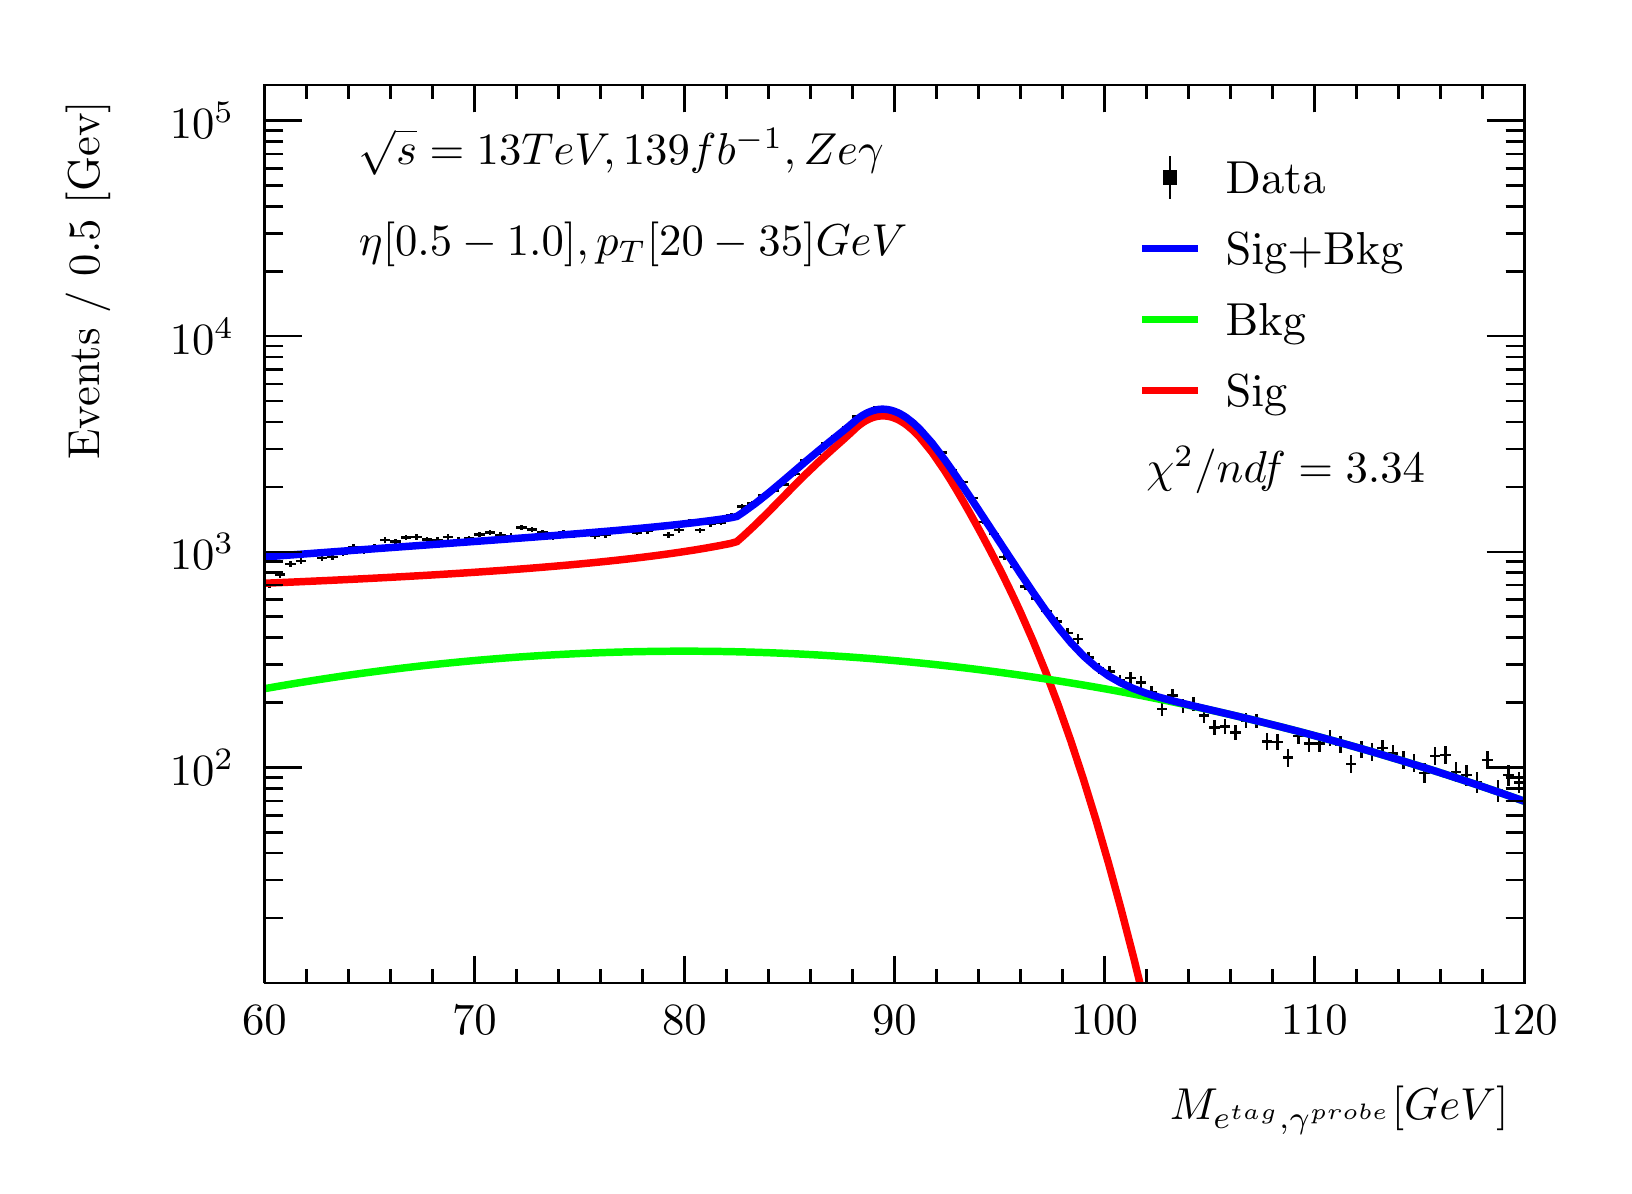
\begin{tikzpicture}
\pgfdeclareplotmark{cross} {
\pgfpathmoveto{\pgfpoint{-0.3\pgfplotmarksize}{\pgfplotmarksize}}
\pgfpathlineto{\pgfpoint{+0.3\pgfplotmarksize}{\pgfplotmarksize}}
\pgfpathlineto{\pgfpoint{+0.3\pgfplotmarksize}{0.3\pgfplotmarksize}}
\pgfpathlineto{\pgfpoint{+1\pgfplotmarksize}{0.3\pgfplotmarksize}}
\pgfpathlineto{\pgfpoint{+1\pgfplotmarksize}{-0.3\pgfplotmarksize}}
\pgfpathlineto{\pgfpoint{+0.3\pgfplotmarksize}{-0.3\pgfplotmarksize}}
\pgfpathlineto{\pgfpoint{+0.3\pgfplotmarksize}{-1.\pgfplotmarksize}}
\pgfpathlineto{\pgfpoint{-0.3\pgfplotmarksize}{-1.\pgfplotmarksize}}
\pgfpathlineto{\pgfpoint{-0.3\pgfplotmarksize}{-0.3\pgfplotmarksize}}
\pgfpathlineto{\pgfpoint{-1.\pgfplotmarksize}{-0.3\pgfplotmarksize}}
\pgfpathlineto{\pgfpoint{-1.\pgfplotmarksize}{0.3\pgfplotmarksize}}
\pgfpathlineto{\pgfpoint{-0.3\pgfplotmarksize}{0.3\pgfplotmarksize}}
\pgfpathclose
\pgfusepathqstroke
}
\pgfdeclareplotmark{cross*} {
\pgfpathmoveto{\pgfpoint{-0.3\pgfplotmarksize}{\pgfplotmarksize}}
\pgfpathlineto{\pgfpoint{+0.3\pgfplotmarksize}{\pgfplotmarksize}}
\pgfpathlineto{\pgfpoint{+0.3\pgfplotmarksize}{0.3\pgfplotmarksize}}
\pgfpathlineto{\pgfpoint{+1\pgfplotmarksize}{0.3\pgfplotmarksize}}
\pgfpathlineto{\pgfpoint{+1\pgfplotmarksize}{-0.3\pgfplotmarksize}}
\pgfpathlineto{\pgfpoint{+0.3\pgfplotmarksize}{-0.3\pgfplotmarksize}}
\pgfpathlineto{\pgfpoint{+0.3\pgfplotmarksize}{-1.\pgfplotmarksize}}
\pgfpathlineto{\pgfpoint{-0.3\pgfplotmarksize}{-1.\pgfplotmarksize}}
\pgfpathlineto{\pgfpoint{-0.3\pgfplotmarksize}{-0.3\pgfplotmarksize}}
\pgfpathlineto{\pgfpoint{-1.\pgfplotmarksize}{-0.3\pgfplotmarksize}}
\pgfpathlineto{\pgfpoint{-1.\pgfplotmarksize}{0.3\pgfplotmarksize}}
\pgfpathlineto{\pgfpoint{-0.3\pgfplotmarksize}{0.3\pgfplotmarksize}}
\pgfpathclose
\pgfusepathqfillstroke
}
\pgfdeclareplotmark{newstar} {
\pgfpathmoveto{\pgfqpoint{0pt}{\pgfplotmarksize}}
\pgfpathlineto{\pgfqpointpolar{44}{0.5\pgfplotmarksize}}
\pgfpathlineto{\pgfqpointpolar{18}{\pgfplotmarksize}}
\pgfpathlineto{\pgfqpointpolar{-20}{0.5\pgfplotmarksize}}
\pgfpathlineto{\pgfqpointpolar{-54}{\pgfplotmarksize}}
\pgfpathlineto{\pgfqpointpolar{-90}{0.5\pgfplotmarksize}}
\pgfpathlineto{\pgfqpointpolar{234}{\pgfplotmarksize}}
\pgfpathlineto{\pgfqpointpolar{198}{0.5\pgfplotmarksize}}
\pgfpathlineto{\pgfqpointpolar{162}{\pgfplotmarksize}}
\pgfpathlineto{\pgfqpointpolar{134}{0.5\pgfplotmarksize}}
\pgfpathclose
\pgfusepathqstroke
}
\pgfdeclareplotmark{newstar*} {
\pgfpathmoveto{\pgfqpoint{0pt}{\pgfplotmarksize}}
\pgfpathlineto{\pgfqpointpolar{44}{0.5\pgfplotmarksize}}
\pgfpathlineto{\pgfqpointpolar{18}{\pgfplotmarksize}}
\pgfpathlineto{\pgfqpointpolar{-20}{0.5\pgfplotmarksize}}
\pgfpathlineto{\pgfqpointpolar{-54}{\pgfplotmarksize}}
\pgfpathlineto{\pgfqpointpolar{-90}{0.5\pgfplotmarksize}}
\pgfpathlineto{\pgfqpointpolar{234}{\pgfplotmarksize}}
\pgfpathlineto{\pgfqpointpolar{198}{0.5\pgfplotmarksize}}
\pgfpathlineto{\pgfqpointpolar{162}{\pgfplotmarksize}}
\pgfpathlineto{\pgfqpointpolar{134}{0.5\pgfplotmarksize}}
\pgfpathclose
\pgfusepathqfillstroke
}
\definecolor{c}{rgb}{1,1,1};
\draw [color=c, fill=c] (0,0) rectangle (20,14.4361);
\draw [color=c, fill=c] (3,2.30977) rectangle (19,13.7143);
\definecolor{c}{rgb}{0,0,0};
\draw [c,line width=0.9] (3,2.30977) -- (3,13.7143) -- (19,13.7143) -- (19,2.30977) -- (3,2.30977);
\definecolor{c}{rgb}{1,1,1};
\draw [color=c, fill=c] (3,2.30977) rectangle (19,13.7143);
\definecolor{c}{rgb}{0,0,0};
\draw [c,line width=0.9] (3,2.30977) -- (3,13.7143) -- (19,13.7143) -- (19,2.30977) -- (3,2.30977);
\draw [c,line width=0.9] (3,2.30977) -- (19,2.30977);
\draw [c,line width=0.9] (3,2.65624) -- (3,2.30977);
\draw [c,line width=0.9] (3.53333,2.48301) -- (3.53333,2.30977);
\draw [c,line width=0.9] (4.06667,2.48301) -- (4.06667,2.30977);
\draw [c,line width=0.9] (4.6,2.48301) -- (4.6,2.30977);
\draw [c,line width=0.9] (5.13333,2.48301) -- (5.13333,2.30977);
\draw [c,line width=0.9] (5.66667,2.65624) -- (5.66667,2.30977);
\draw [c,line width=0.9] (6.2,2.48301) -- (6.2,2.30977);
\draw [c,line width=0.9] (6.73333,2.48301) -- (6.73333,2.30977);
\draw [c,line width=0.9] (7.26667,2.48301) -- (7.26667,2.30977);
\draw [c,line width=0.9] (7.8,2.48301) -- (7.8,2.30977);
\draw [c,line width=0.9] (8.33333,2.65624) -- (8.33333,2.30977);
\draw [c,line width=0.9] (8.86667,2.48301) -- (8.86667,2.30977);
\draw [c,line width=0.9] (9.4,2.48301) -- (9.4,2.30977);
\draw [c,line width=0.9] (9.93333,2.48301) -- (9.93333,2.30977);
\draw [c,line width=0.9] (10.4667,2.48301) -- (10.4667,2.30977);
\draw [c,line width=0.9] (11,2.65624) -- (11,2.30977);
\draw [c,line width=0.9] (11.5333,2.48301) -- (11.5333,2.30977);
\draw [c,line width=0.9] (12.0667,2.48301) -- (12.0667,2.30977);
\draw [c,line width=0.9] (12.6,2.48301) -- (12.6,2.30977);
\draw [c,line width=0.9] (13.1333,2.48301) -- (13.1333,2.30977);
\draw [c,line width=0.9] (13.6667,2.65624) -- (13.6667,2.30977);
\draw [c,line width=0.9] (14.2,2.48301) -- (14.2,2.30977);
\draw [c,line width=0.9] (14.7333,2.48301) -- (14.7333,2.30977);
\draw [c,line width=0.9] (15.2667,2.48301) -- (15.2667,2.30977);
\draw [c,line width=0.9] (15.8,2.48301) -- (15.8,2.30977);
\draw [c,line width=0.9] (16.3333,2.65624) -- (16.3333,2.30977);
\draw [c,line width=0.9] (16.8667,2.48301) -- (16.8667,2.30977);
\draw [c,line width=0.9] (17.4,2.48301) -- (17.4,2.30977);
\draw [c,line width=0.9] (17.9333,2.48301) -- (17.9333,2.30977);
\draw [c,line width=0.9] (18.4667,2.48301) -- (18.4667,2.30977);
\draw [c,line width=0.9] (19,2.65624) -- (19,2.30977);
\draw [anchor=base] (3,1.66015) node[scale=1.61424, color=c, rotate=0]{60};
\draw [anchor=base] (5.66667,1.66015) node[scale=1.61424, color=c, rotate=0]{70};
\draw [anchor=base] (8.33333,1.66015) node[scale=1.61424, color=c, rotate=0]{80};
\draw [anchor=base] (11,1.66015) node[scale=1.61424, color=c, rotate=0]{90};
\draw [anchor=base] (13.6667,1.66015) node[scale=1.61424, color=c, rotate=0]{100};
\draw [anchor=base] (16.3333,1.66015) node[scale=1.61424, color=c, rotate=0]{110};
\draw [anchor=base] (19,1.66015) node[scale=1.61424, color=c, rotate=0]{120};
\draw [anchor= east] (19,0.692932) node[scale=1.61424, color=c, rotate=0]{$M_{e^{tag}, \gamma^{probe}}  [GeV]$};
\draw [c,line width=0.9] (3,13.7143) -- (19,13.7143);
\draw [c,line width=0.9] (3,13.3678) -- (3,13.7143);
\draw [c,line width=0.9] (3.53333,13.5411) -- (3.53333,13.7143);
\draw [c,line width=0.9] (4.06667,13.5411) -- (4.06667,13.7143);
\draw [c,line width=0.9] (4.6,13.5411) -- (4.6,13.7143);
\draw [c,line width=0.9] (5.13333,13.5411) -- (5.13333,13.7143);
\draw [c,line width=0.9] (5.66667,13.3678) -- (5.66667,13.7143);
\draw [c,line width=0.9] (6.2,13.5411) -- (6.2,13.7143);
\draw [c,line width=0.9] (6.73333,13.5411) -- (6.73333,13.7143);
\draw [c,line width=0.9] (7.26667,13.5411) -- (7.26667,13.7143);
\draw [c,line width=0.9] (7.8,13.5411) -- (7.8,13.7143);
\draw [c,line width=0.9] (8.33333,13.3678) -- (8.33333,13.7143);
\draw [c,line width=0.9] (8.86667,13.5411) -- (8.86667,13.7143);
\draw [c,line width=0.9] (9.4,13.5411) -- (9.4,13.7143);
\draw [c,line width=0.9] (9.93333,13.5411) -- (9.93333,13.7143);
\draw [c,line width=0.9] (10.4667,13.5411) -- (10.4667,13.7143);
\draw [c,line width=0.9] (11,13.3678) -- (11,13.7143);
\draw [c,line width=0.9] (11.5333,13.5411) -- (11.5333,13.7143);
\draw [c,line width=0.9] (12.0667,13.5411) -- (12.0667,13.7143);
\draw [c,line width=0.9] (12.6,13.5411) -- (12.6,13.7143);
\draw [c,line width=0.9] (13.1333,13.5411) -- (13.1333,13.7143);
\draw [c,line width=0.9] (13.6667,13.3678) -- (13.6667,13.7143);
\draw [c,line width=0.9] (14.2,13.5411) -- (14.2,13.7143);
\draw [c,line width=0.9] (14.7333,13.5411) -- (14.7333,13.7143);
\draw [c,line width=0.9] (15.2667,13.5411) -- (15.2667,13.7143);
\draw [c,line width=0.9] (15.8,13.5411) -- (15.8,13.7143);
\draw [c,line width=0.9] (16.3333,13.3678) -- (16.3333,13.7143);
\draw [c,line width=0.9] (16.8667,13.5411) -- (16.8667,13.7143);
\draw [c,line width=0.9] (17.4,13.5411) -- (17.4,13.7143);
\draw [c,line width=0.9] (17.9333,13.5411) -- (17.9333,13.7143);
\draw [c,line width=0.9] (18.4667,13.5411) -- (18.4667,13.7143);
\draw [c,line width=0.9] (19,13.3678) -- (19,13.7143);
\draw [c,line width=0.9] (3,2.30977) -- (3,13.7143);
\draw [c,line width=0.9] (3.237,3.13412) -- (3,3.13412);
\draw [c,line width=0.9] (3.237,3.61633) -- (3,3.61633);
\draw [c,line width=0.9] (3.237,3.95847) -- (3,3.95847);
\draw [c,line width=0.9] (3.237,4.22385) -- (3,4.22385);
\draw [c,line width=0.9] (3.237,4.44068) -- (3,4.44068);
\draw [c,line width=0.9] (3.237,4.62401) -- (3,4.62401);
\draw [c,line width=0.9] (3.237,4.78282) -- (3,4.78282);
\draw [c,line width=0.9] (3.237,4.9229) -- (3,4.9229);
\draw [c,line width=0.9] (3.474,5.0482) -- (3,5.0482);
\draw [anchor= east] (2.82,5.0482) node[scale=1.61424, color=c, rotate=0]{$10^{2}$};
\draw [c,line width=0.9] (3.237,5.87255) -- (3,5.87255);
\draw [c,line width=0.9] (3.237,6.35476) -- (3,6.35476);
\draw [c,line width=0.9] (3.237,6.6969) -- (3,6.6969);
\draw [c,line width=0.9] (3.237,6.96228) -- (3,6.96228);
\draw [c,line width=0.9] (3.237,7.17911) -- (3,7.17911);
\draw [c,line width=0.9] (3.237,7.36244) -- (3,7.36244);
\draw [c,line width=0.9] (3.237,7.52125) -- (3,7.52125);
\draw [c,line width=0.9] (3.237,7.66133) -- (3,7.66133);
\draw [c,line width=0.9] (3.474,7.78663) -- (3,7.78663);
\draw [anchor= east] (2.82,7.78663) node[scale=1.61424, color=c, rotate=0]{$10^{3}$};
\draw [c,line width=0.9] (3.237,8.61098) -- (3,8.61098);
\draw [c,line width=0.9] (3.237,9.09319) -- (3,9.09319);
\draw [c,line width=0.9] (3.237,9.43533) -- (3,9.43533);
\draw [c,line width=0.9] (3.237,9.70071) -- (3,9.70071);
\draw [c,line width=0.9] (3.237,9.91755) -- (3,9.91755);
\draw [c,line width=0.9] (3.237,10.1009) -- (3,10.1009);
\draw [c,line width=0.9] (3.237,10.2597) -- (3,10.2597);
\draw [c,line width=0.9] (3.237,10.3998) -- (3,10.3998);
\draw [c,line width=0.9] (3.474,10.5251) -- (3,10.5251);
\draw [anchor= east] (2.82,10.5251) node[scale=1.61424, color=c, rotate=0]{$10^{4}$};
\draw [c,line width=0.9] (3.237,11.3494) -- (3,11.3494);
\draw [c,line width=0.9] (3.237,11.8316) -- (3,11.8316);
\draw [c,line width=0.9] (3.237,12.1738) -- (3,12.1738);
\draw [c,line width=0.9] (3.237,12.4391) -- (3,12.4391);
\draw [c,line width=0.9] (3.237,12.656) -- (3,12.656);
\draw [c,line width=0.9] (3.237,12.8393) -- (3,12.8393);
\draw [c,line width=0.9] (3.237,12.9981) -- (3,12.9981);
\draw [c,line width=0.9] (3.237,13.1382) -- (3,13.1382);
\draw [c,line width=0.9] (3.474,13.2635) -- (3,13.2635);
\draw [anchor= east] (2.82,13.2635) node[scale=1.61424, color=c, rotate=0]{$10^{5}$};
\draw [anchor= east] (0.76,13.7143) node[scale=1.61424, color=c, rotate=90]{Events / 0.5 [Gev]};
\draw [c,line width=0.9] (19,2.30977) -- (19,13.7143);
\draw [c,line width=0.9] (18.763,3.13412) -- (19,3.13412);
\draw [c,line width=0.9] (18.763,3.61633) -- (19,3.61633);
\draw [c,line width=0.9] (18.763,3.95847) -- (19,3.95847);
\draw [c,line width=0.9] (18.763,4.22385) -- (19,4.22385);
\draw [c,line width=0.9] (18.763,4.44068) -- (19,4.44068);
\draw [c,line width=0.9] (18.763,4.62401) -- (19,4.62401);
\draw [c,line width=0.9] (18.763,4.78282) -- (19,4.78282);
\draw [c,line width=0.9] (18.763,4.9229) -- (19,4.9229);
\draw [c,line width=0.9] (18.526,5.0482) -- (19,5.0482);
\draw [c,line width=0.9] (18.763,5.87255) -- (19,5.87255);
\draw [c,line width=0.9] (18.763,6.35476) -- (19,6.35476);
\draw [c,line width=0.9] (18.763,6.6969) -- (19,6.6969);
\draw [c,line width=0.9] (18.763,6.96228) -- (19,6.96228);
\draw [c,line width=0.9] (18.763,7.17911) -- (19,7.17911);
\draw [c,line width=0.9] (18.763,7.36244) -- (19,7.36244);
\draw [c,line width=0.9] (18.763,7.52125) -- (19,7.52125);
\draw [c,line width=0.9] (18.763,7.66133) -- (19,7.66133);
\draw [c,line width=0.9] (18.526,7.78663) -- (19,7.78663);
\draw [c,line width=0.9] (18.763,8.61098) -- (19,8.61098);
\draw [c,line width=0.9] (18.763,9.09319) -- (19,9.09319);
\draw [c,line width=0.9] (18.763,9.43533) -- (19,9.43533);
\draw [c,line width=0.9] (18.763,9.70071) -- (19,9.70071);
\draw [c,line width=0.9] (18.763,9.91755) -- (19,9.91755);
\draw [c,line width=0.9] (18.763,10.1009) -- (19,10.1009);
\draw [c,line width=0.9] (18.763,10.2597) -- (19,10.2597);
\draw [c,line width=0.9] (18.763,10.3998) -- (19,10.3998);
\draw [c,line width=0.9] (18.526,10.5251) -- (19,10.5251);
\draw [c,line width=0.9] (18.763,11.3494) -- (19,11.3494);
\draw [c,line width=0.9] (18.763,11.8316) -- (19,11.8316);
\draw [c,line width=0.9] (18.763,12.1738) -- (19,12.1738);
\draw [c,line width=0.9] (18.763,12.4391) -- (19,12.4391);
\draw [c,line width=0.9] (18.763,12.656) -- (19,12.656);
\draw [c,line width=0.9] (18.763,12.8393) -- (19,12.8393);
\draw [c,line width=0.9] (18.763,12.9981) -- (19,12.9981);
\draw [c,line width=0.9] (18.763,13.1382) -- (19,13.1382);
\draw [c,line width=0.9] (18.526,13.2635) -- (19,13.2635);
\draw [c,line width=0.9] (3.06667,7.37764) -- (3,7.37764);
\draw [c,line width=0.9] (3,7.37764) -- (3,7.37764);
\draw [c,line width=0.9] (3.06667,7.37764) -- (3.13333,7.37764);
\draw [c,line width=0.9] (3.13333,7.37764) -- (3.13333,7.37764);
\draw [c,line width=0.9] (3.06667,7.37764) -- (3.06667,7.4223);
\draw [c,line width=0.9] (3.06667,7.4223) -- (3.06667,7.4223);
\draw [c,line width=0.9] (3.06667,7.37764) -- (3.06667,7.33298);
\draw [c,line width=0.9] (3.06667,7.33298) -- (3.06667,7.33298);
\draw [c,line width=0.9] (3.2,7.49723) -- (3.13333,7.49723);
\draw [c,line width=0.9] (3.13333,7.49723) -- (3.13333,7.49723);
\draw [c,line width=0.9] (3.2,7.49723) -- (3.26667,7.49723);
\draw [c,line width=0.9] (3.26667,7.49723) -- (3.26667,7.49723);
\draw [c,line width=0.9] (3.2,7.49723) -- (3.2,7.5397);
\draw [c,line width=0.9] (3.2,7.5397) -- (3.2,7.5397);
\draw [c,line width=0.9] (3.2,7.49723) -- (3.2,7.45475);
\draw [c,line width=0.9] (3.2,7.45475) -- (3.2,7.45475);
\draw [c,line width=0.9] (3.33333,7.63054) -- (3.26667,7.63054);
\draw [c,line width=0.9] (3.26667,7.63054) -- (3.26667,7.63054);
\draw [c,line width=0.9] (3.33333,7.63054) -- (3.4,7.63054);
\draw [c,line width=0.9] (3.4,7.63054) -- (3.4,7.63054);
\draw [c,line width=0.9] (3.33333,7.63054) -- (3.33333,7.6707);
\draw [c,line width=0.9] (3.33333,7.6707) -- (3.33333,7.6707);
\draw [c,line width=0.9] (3.33333,7.63054) -- (3.33333,7.59038);
\draw [c,line width=0.9] (3.33333,7.59038) -- (3.33333,7.59038);
\draw [c,line width=0.9] (3.46667,7.67054) -- (3.4,7.67054);
\draw [c,line width=0.9] (3.4,7.67054) -- (3.4,7.67054);
\draw [c,line width=0.9] (3.46667,7.67054) -- (3.53333,7.67054);
\draw [c,line width=0.9] (3.53333,7.67054) -- (3.53333,7.67054);
\draw [c,line width=0.9] (3.46667,7.67054) -- (3.46667,7.71003);
\draw [c,line width=0.9] (3.46667,7.71003) -- (3.46667,7.71003);
\draw [c,line width=0.9] (3.46667,7.67054) -- (3.46667,7.63106);
\draw [c,line width=0.9] (3.46667,7.63106) -- (3.46667,7.63106);
\draw [c,line width=0.9] (3.6,7.75774) -- (3.53333,7.75774);
\draw [c,line width=0.9] (3.53333,7.75774) -- (3.53333,7.75774);
\draw [c,line width=0.9] (3.6,7.75774) -- (3.66667,7.75774);
\draw [c,line width=0.9] (3.66667,7.75774) -- (3.66667,7.75774);
\draw [c,line width=0.9] (3.6,7.75774) -- (3.6,7.79581);
\draw [c,line width=0.9] (3.6,7.79581) -- (3.6,7.79581);
\draw [c,line width=0.9] (3.6,7.75774) -- (3.6,7.71968);
\draw [c,line width=0.9] (3.6,7.71968) -- (3.6,7.71968);
\draw [c,line width=0.9] (3.73333,7.70924) -- (3.66667,7.70924);
\draw [c,line width=0.9] (3.66667,7.70924) -- (3.66667,7.70924);
\draw [c,line width=0.9] (3.73333,7.70924) -- (3.8,7.70924);
\draw [c,line width=0.9] (3.8,7.70924) -- (3.8,7.70924);
\draw [c,line width=0.9] (3.73333,7.70924) -- (3.73333,7.7481);
\draw [c,line width=0.9] (3.73333,7.7481) -- (3.73333,7.7481);
\draw [c,line width=0.9] (3.73333,7.70924) -- (3.73333,7.67039);
\draw [c,line width=0.9] (3.73333,7.67039) -- (3.73333,7.67039);
\draw [c,line width=0.9] (3.86667,7.72312) -- (3.8,7.72312);
\draw [c,line width=0.9] (3.8,7.72312) -- (3.8,7.72312);
\draw [c,line width=0.9] (3.86667,7.72312) -- (3.93333,7.72312);
\draw [c,line width=0.9] (3.93333,7.72312) -- (3.93333,7.72312);
\draw [c,line width=0.9] (3.86667,7.72312) -- (3.86667,7.76175);
\draw [c,line width=0.9] (3.86667,7.76175) -- (3.86667,7.76175);
\draw [c,line width=0.9] (3.86667,7.72312) -- (3.86667,7.6845);
\draw [c,line width=0.9] (3.86667,7.6845) -- (3.86667,7.6845);
\draw [c,line width=0.9] (4,7.76503) -- (3.93333,7.76503);
\draw [c,line width=0.9] (3.93333,7.76503) -- (3.93333,7.76503);
\draw [c,line width=0.9] (4,7.76503) -- (4.06667,7.76503);
\draw [c,line width=0.9] (4.06667,7.76503) -- (4.06667,7.76503);
\draw [c,line width=0.9] (4,7.76503) -- (4,7.80298);
\draw [c,line width=0.9] (4,7.80298) -- (4,7.80298);
\draw [c,line width=0.9] (4,7.76503) -- (4,7.72708);
\draw [c,line width=0.9] (4,7.72708) -- (4,7.72708);
\draw [c,line width=0.9] (4.13333,7.84805) -- (4.06667,7.84805);
\draw [c,line width=0.9] (4.06667,7.84805) -- (4.06667,7.84805);
\draw [c,line width=0.9] (4.13333,7.84805) -- (4.2,7.84805);
\draw [c,line width=0.9] (4.2,7.84805) -- (4.2,7.84805);
\draw [c,line width=0.9] (4.13333,7.84805) -- (4.13333,7.8847);
\draw [c,line width=0.9] (4.13333,7.8847) -- (4.13333,7.8847);
\draw [c,line width=0.9] (4.13333,7.84805) -- (4.13333,7.8114);
\draw [c,line width=0.9] (4.13333,7.8114) -- (4.13333,7.8114);
\draw [c,line width=0.9] (4.26667,7.79375) -- (4.2,7.79375);
\draw [c,line width=0.9] (4.2,7.79375) -- (4.2,7.79375);
\draw [c,line width=0.9] (4.26667,7.79375) -- (4.33333,7.79375);
\draw [c,line width=0.9] (4.33333,7.79375) -- (4.33333,7.79375);
\draw [c,line width=0.9] (4.26667,7.79375) -- (4.26667,7.83124);
\draw [c,line width=0.9] (4.26667,7.83124) -- (4.26667,7.83124);
\draw [c,line width=0.9] (4.26667,7.79375) -- (4.26667,7.75625);
\draw [c,line width=0.9] (4.26667,7.75625) -- (4.26667,7.75625);
\draw [c,line width=0.9] (4.4,7.85031) -- (4.33333,7.85031);
\draw [c,line width=0.9] (4.33333,7.85031) -- (4.33333,7.85031);
\draw [c,line width=0.9] (4.4,7.85031) -- (4.46667,7.85031);
\draw [c,line width=0.9] (4.46667,7.85031) -- (4.46667,7.85031);
\draw [c,line width=0.9] (4.4,7.85031) -- (4.4,7.88692);
\draw [c,line width=0.9] (4.4,7.88692) -- (4.4,7.88692);
\draw [c,line width=0.9] (4.4,7.85031) -- (4.4,7.81369);
\draw [c,line width=0.9] (4.4,7.81369) -- (4.4,7.81369);
\draw [c,line width=0.9] (4.53333,7.93409) -- (4.46667,7.93409);
\draw [c,line width=0.9] (4.46667,7.93409) -- (4.46667,7.93409);
\draw [c,line width=0.9] (4.53333,7.93409) -- (4.6,7.93409);
\draw [c,line width=0.9] (4.6,7.93409) -- (4.6,7.93409);
\draw [c,line width=0.9] (4.53333,7.93409) -- (4.53333,7.96943);
\draw [c,line width=0.9] (4.53333,7.96943) -- (4.53333,7.96943);
\draw [c,line width=0.9] (4.53333,7.93409) -- (4.53333,7.89874);
\draw [c,line width=0.9] (4.53333,7.89874) -- (4.53333,7.89874);
\draw [c,line width=0.9] (4.66667,7.91503) -- (4.6,7.91503);
\draw [c,line width=0.9] (4.6,7.91503) -- (4.6,7.91503);
\draw [c,line width=0.9] (4.66667,7.91503) -- (4.73333,7.91503);
\draw [c,line width=0.9] (4.73333,7.91503) -- (4.73333,7.91503);
\draw [c,line width=0.9] (4.66667,7.91503) -- (4.66667,7.95066);
\draw [c,line width=0.9] (4.66667,7.95066) -- (4.66667,7.95066);
\draw [c,line width=0.9] (4.66667,7.91503) -- (4.66667,7.87939);
\draw [c,line width=0.9] (4.66667,7.87939) -- (4.66667,7.87939);
\draw [c,line width=0.9] (4.8,7.9652) -- (4.73333,7.9652);
\draw [c,line width=0.9] (4.73333,7.9652) -- (4.73333,7.9652);
\draw [c,line width=0.9] (4.8,7.9652) -- (4.86667,7.9652);
\draw [c,line width=0.9] (4.86667,7.9652) -- (4.86667,7.9652);
\draw [c,line width=0.9] (4.8,7.9652) -- (4.8,8.00008);
\draw [c,line width=0.9] (4.8,8.00008) -- (4.8,8.00008);
\draw [c,line width=0.9] (4.8,7.9652) -- (4.8,7.93031);
\draw [c,line width=0.9] (4.8,7.93031) -- (4.8,7.93031);
\draw [c,line width=0.9] (4.93333,7.97437) -- (4.86667,7.97437);
\draw [c,line width=0.9] (4.86667,7.97437) -- (4.86667,7.97437);
\draw [c,line width=0.9] (4.93333,7.97437) -- (5,7.97437);
\draw [c,line width=0.9] (5,7.97437) -- (5,7.97437);
\draw [c,line width=0.9] (4.93333,7.97437) -- (4.93333,8.00912);
\draw [c,line width=0.9] (4.93333,8.00912) -- (4.93333,8.00912);
\draw [c,line width=0.9] (4.93333,7.97437) -- (4.93333,7.93962);
\draw [c,line width=0.9] (4.93333,7.93962) -- (4.93333,7.93962);
\draw [c,line width=0.9] (5.06667,7.94351) -- (5,7.94351);
\draw [c,line width=0.9] (5,7.94351) -- (5,7.94351);
\draw [c,line width=0.9] (5.06667,7.94351) -- (5.13333,7.94351);
\draw [c,line width=0.9] (5.13333,7.94351) -- (5.13333,7.94351);
\draw [c,line width=0.9] (5.06667,7.94351) -- (5.06667,7.97871);
\draw [c,line width=0.9] (5.06667,7.97871) -- (5.06667,7.97871);
\draw [c,line width=0.9] (5.06667,7.94351) -- (5.06667,7.9083);
\draw [c,line width=0.9] (5.06667,7.9083) -- (5.06667,7.9083);
\draw [c,line width=0.9] (5.2,7.93409) -- (5.13333,7.93409);
\draw [c,line width=0.9] (5.13333,7.93409) -- (5.13333,7.93409);
\draw [c,line width=0.9] (5.2,7.93409) -- (5.26667,7.93409);
\draw [c,line width=0.9] (5.26667,7.93409) -- (5.26667,7.93409);
\draw [c,line width=0.9] (5.2,7.93409) -- (5.2,7.96943);
\draw [c,line width=0.9] (5.2,7.96943) -- (5.2,7.96943);
\draw [c,line width=0.9] (5.2,7.93409) -- (5.2,7.89874);
\draw [c,line width=0.9] (5.2,7.89874) -- (5.2,7.89874);
\draw [c,line width=0.9] (5.33333,7.97336) -- (5.26667,7.97336);
\draw [c,line width=0.9] (5.26667,7.97336) -- (5.26667,7.97336);
\draw [c,line width=0.9] (5.33333,7.97336) -- (5.4,7.97336);
\draw [c,line width=0.9] (5.4,7.97336) -- (5.4,7.97336);
\draw [c,line width=0.9] (5.33333,7.97336) -- (5.33333,8.00812);
\draw [c,line width=0.9] (5.33333,8.00812) -- (5.33333,8.00812);
\draw [c,line width=0.9] (5.33333,7.97336) -- (5.33333,7.93859);
\draw [c,line width=0.9] (5.33333,7.93859) -- (5.33333,7.93859);
\draw [c,line width=0.9] (5.46667,7.93619) -- (5.4,7.93619);
\draw [c,line width=0.9] (5.4,7.93619) -- (5.4,7.93619);
\draw [c,line width=0.9] (5.46667,7.93619) -- (5.53333,7.93619);
\draw [c,line width=0.9] (5.53333,7.93619) -- (5.53333,7.93619);
\draw [c,line width=0.9] (5.46667,7.93619) -- (5.46667,7.9715);
\draw [c,line width=0.9] (5.46667,7.9715) -- (5.46667,7.9715);
\draw [c,line width=0.9] (5.46667,7.93619) -- (5.46667,7.90087);
\draw [c,line width=0.9] (5.46667,7.90087) -- (5.46667,7.90087);
\draw [c,line width=0.9] (5.6,7.95285) -- (5.53333,7.95285);
\draw [c,line width=0.9] (5.53333,7.95285) -- (5.53333,7.95285);
\draw [c,line width=0.9] (5.6,7.95285) -- (5.66667,7.95285);
\draw [c,line width=0.9] (5.66667,7.95285) -- (5.66667,7.95285);
\draw [c,line width=0.9] (5.6,7.95285) -- (5.6,7.98792);
\draw [c,line width=0.9] (5.6,7.98792) -- (5.6,7.98792);
\draw [c,line width=0.9] (5.6,7.95285) -- (5.6,7.91778);
\draw [c,line width=0.9] (5.6,7.91778) -- (5.6,7.91778);
\draw [c,line width=0.9] (5.73333,8.0094) -- (5.66667,8.0094);
\draw [c,line width=0.9] (5.66667,8.0094) -- (5.66667,8.0094);
\draw [c,line width=0.9] (5.73333,8.0094) -- (5.8,8.0094);
\draw [c,line width=0.9] (5.8,8.0094) -- (5.8,8.0094);
\draw [c,line width=0.9] (5.73333,8.0094) -- (5.73333,8.04364);
\draw [c,line width=0.9] (5.73333,8.04364) -- (5.73333,8.04364);
\draw [c,line width=0.9] (5.73333,8.0094) -- (5.73333,7.97515);
\draw [c,line width=0.9] (5.73333,7.97515) -- (5.73333,7.97515);
\draw [c,line width=0.9] (5.86667,8.03283) -- (5.8,8.03283);
\draw [c,line width=0.9] (5.8,8.03283) -- (5.8,8.03283);
\draw [c,line width=0.9] (5.86667,8.03283) -- (5.93333,8.03283);
\draw [c,line width=0.9] (5.93333,8.03283) -- (5.93333,8.03283);
\draw [c,line width=0.9] (5.86667,8.03283) -- (5.86667,8.06674);
\draw [c,line width=0.9] (5.86667,8.06674) -- (5.86667,8.06674);
\draw [c,line width=0.9] (5.86667,8.03283) -- (5.86667,7.99892);
\draw [c,line width=0.9] (5.86667,7.99892) -- (5.86667,7.99892);
\draw [c,line width=0.9] (6,7.9975) -- (5.93333,7.9975);
\draw [c,line width=0.9] (5.93333,7.9975) -- (5.93333,7.9975);
\draw [c,line width=0.9] (6,7.9975) -- (6.06667,7.9975);
\draw [c,line width=0.9] (6.06667,7.9975) -- (6.06667,7.9975);
\draw [c,line width=0.9] (6,7.9975) -- (6,8.03192);
\draw [c,line width=0.9] (6,8.03192) -- (6,8.03192);
\draw [c,line width=0.9] (6,7.9975) -- (6,7.96309);
\draw [c,line width=0.9] (6,7.96309) -- (6,7.96309);
\draw [c,line width=0.9] (6.13333,7.98951) -- (6.06667,7.98951);
\draw [c,line width=0.9] (6.06667,7.98951) -- (6.06667,7.98951);
\draw [c,line width=0.9] (6.13333,7.98951) -- (6.2,7.98951);
\draw [c,line width=0.9] (6.2,7.98951) -- (6.2,7.98951);
\draw [c,line width=0.9] (6.13333,7.98951) -- (6.13333,8.02404);
\draw [c,line width=0.9] (6.13333,8.02404) -- (6.13333,8.02404);
\draw [c,line width=0.9] (6.13333,7.98951) -- (6.13333,7.95498);
\draw [c,line width=0.9] (6.13333,7.95498) -- (6.13333,7.95498);
\draw [c,line width=0.9] (6.26667,8.09224) -- (6.2,8.09224);
\draw [c,line width=0.9] (6.2,8.09224) -- (6.2,8.09224);
\draw [c,line width=0.9] (6.26667,8.09224) -- (6.33333,8.09224);
\draw [c,line width=0.9] (6.33333,8.09224) -- (6.33333,8.09224);
\draw [c,line width=0.9] (6.26667,8.09224) -- (6.26667,8.12531);
\draw [c,line width=0.9] (6.26667,8.12531) -- (6.26667,8.12531);
\draw [c,line width=0.9] (6.26667,8.09224) -- (6.26667,8.05917);
\draw [c,line width=0.9] (6.26667,8.05917) -- (6.26667,8.05917);
\draw [c,line width=0.9] (6.4,8.06714) -- (6.33333,8.06714);
\draw [c,line width=0.9] (6.33333,8.06714) -- (6.33333,8.06714);
\draw [c,line width=0.9] (6.4,8.06714) -- (6.46667,8.06714);
\draw [c,line width=0.9] (6.46667,8.06714) -- (6.46667,8.06714);
\draw [c,line width=0.9] (6.4,8.06714) -- (6.4,8.10056);
\draw [c,line width=0.9] (6.4,8.10056) -- (6.4,8.10056);
\draw [c,line width=0.9] (6.4,8.06714) -- (6.4,8.03372);
\draw [c,line width=0.9] (6.4,8.03372) -- (6.4,8.03372);
\draw [c,line width=0.9] (6.53333,8.03476) -- (6.46667,8.03476);
\draw [c,line width=0.9] (6.46667,8.03476) -- (6.46667,8.03476);
\draw [c,line width=0.9] (6.53333,8.03476) -- (6.6,8.03476);
\draw [c,line width=0.9] (6.6,8.03476) -- (6.6,8.03476);
\draw [c,line width=0.9] (6.53333,8.03476) -- (6.53333,8.06865);
\draw [c,line width=0.9] (6.53333,8.06865) -- (6.53333,8.06865);
\draw [c,line width=0.9] (6.53333,8.03476) -- (6.53333,8.00088);
\draw [c,line width=0.9] (6.53333,8.00088) -- (6.53333,8.00088);
\draw [c,line width=0.9] (6.66667,7.9703) -- (6.6,7.9703);
\draw [c,line width=0.9] (6.6,7.9703) -- (6.6,7.9703);
\draw [c,line width=0.9] (6.66667,7.9703) -- (6.73333,7.9703);
\draw [c,line width=0.9] (6.73333,7.9703) -- (6.73333,7.9703);
\draw [c,line width=0.9] (6.66667,7.9703) -- (6.66667,8.00511);
\draw [c,line width=0.9] (6.66667,8.00511) -- (6.66667,8.00511);
\draw [c,line width=0.9] (6.66667,7.9703) -- (6.66667,7.93549);
\draw [c,line width=0.9] (6.66667,7.93549) -- (6.66667,7.93549);
\draw [c,line width=0.9] (6.8,8.03573) -- (6.73333,8.03573);
\draw [c,line width=0.9] (6.73333,8.03573) -- (6.73333,8.03573);
\draw [c,line width=0.9] (6.8,8.03573) -- (6.86667,8.03573);
\draw [c,line width=0.9] (6.86667,8.03573) -- (6.86667,8.03573);
\draw [c,line width=0.9] (6.8,8.03573) -- (6.8,8.0696);
\draw [c,line width=0.9] (6.8,8.0696) -- (6.8,8.0696);
\draw [c,line width=0.9] (6.8,8.03573) -- (6.8,8.00186);
\draw [c,line width=0.9] (6.8,8.00186) -- (6.8,8.00186);
\draw [c,line width=0.9] (6.93333,7.99251) -- (6.86667,7.99251);
\draw [c,line width=0.9] (6.86667,7.99251) -- (6.86667,7.99251);
\draw [c,line width=0.9] (6.93333,7.99251) -- (7,7.99251);
\draw [c,line width=0.9] (7,7.99251) -- (7,7.99251);
\draw [c,line width=0.9] (6.93333,7.99251) -- (6.93333,8.027);
\draw [c,line width=0.9] (6.93333,8.027) -- (6.93333,8.027);
\draw [c,line width=0.9] (6.93333,7.99251) -- (6.93333,7.95802);
\draw [c,line width=0.9] (6.93333,7.95802) -- (6.93333,7.95802);
\draw [c,line width=0.9] (7.06667,8.03283) -- (7,8.03283);
\draw [c,line width=0.9] (7,8.03283) -- (7,8.03283);
\draw [c,line width=0.9] (7.06667,8.03283) -- (7.13333,8.03283);
\draw [c,line width=0.9] (7.13333,8.03283) -- (7.13333,8.03283);
\draw [c,line width=0.9] (7.06667,8.03283) -- (7.06667,8.06674);
\draw [c,line width=0.9] (7.06667,8.06674) -- (7.06667,8.06674);
\draw [c,line width=0.9] (7.06667,8.03283) -- (7.06667,7.99892);
\draw [c,line width=0.9] (7.06667,7.99892) -- (7.06667,7.99892);
\draw [c,line width=0.9] (7.2,7.98951) -- (7.13333,7.98951);
\draw [c,line width=0.9] (7.13333,7.98951) -- (7.13333,7.98951);
\draw [c,line width=0.9] (7.2,7.98951) -- (7.26667,7.98951);
\draw [c,line width=0.9] (7.26667,7.98951) -- (7.26667,7.98951);
\draw [c,line width=0.9] (7.2,7.98951) -- (7.2,8.02404);
\draw [c,line width=0.9] (7.2,8.02404) -- (7.2,8.02404);
\draw [c,line width=0.9] (7.2,7.98951) -- (7.2,7.95498);
\draw [c,line width=0.9] (7.2,7.95498) -- (7.2,7.95498);
\draw [c,line width=0.9] (7.33333,7.99949) -- (7.26667,7.99949);
\draw [c,line width=0.9] (7.26667,7.99949) -- (7.26667,7.99949);
\draw [c,line width=0.9] (7.33333,7.99949) -- (7.4,7.99949);
\draw [c,line width=0.9] (7.4,7.99949) -- (7.4,7.99949);
\draw [c,line width=0.9] (7.33333,7.99949) -- (7.33333,8.03388);
\draw [c,line width=0.9] (7.33333,8.03388) -- (7.33333,8.03388);
\draw [c,line width=0.9] (7.33333,7.99949) -- (7.33333,7.96511);
\draw [c,line width=0.9] (7.33333,7.96511) -- (7.33333,7.96511);
\draw [c,line width=0.9] (7.46667,8.04438) -- (7.4,8.04438);
\draw [c,line width=0.9] (7.4,8.04438) -- (7.4,8.04438);
\draw [c,line width=0.9] (7.46667,8.04438) -- (7.53333,8.04438);
\draw [c,line width=0.9] (7.53333,8.04438) -- (7.53333,8.04438);
\draw [c,line width=0.9] (7.46667,8.04438) -- (7.46667,8.07812);
\draw [c,line width=0.9] (7.46667,8.07812) -- (7.46667,8.07812);
\draw [c,line width=0.9] (7.46667,8.04438) -- (7.46667,8.01063);
\draw [c,line width=0.9] (7.46667,8.01063) -- (7.46667,8.01063);
\draw [c,line width=0.9] (7.6,8.07089) -- (7.53333,8.07089);
\draw [c,line width=0.9] (7.53333,8.07089) -- (7.53333,8.07089);
\draw [c,line width=0.9] (7.6,8.07089) -- (7.66667,8.07089);
\draw [c,line width=0.9] (7.66667,8.07089) -- (7.66667,8.07089);
\draw [c,line width=0.9] (7.6,8.07089) -- (7.6,8.10426);
\draw [c,line width=0.9] (7.6,8.10426) -- (7.6,8.10426);
\draw [c,line width=0.9] (7.6,8.07089) -- (7.6,8.03752);
\draw [c,line width=0.9] (7.6,8.03752) -- (7.6,8.03752);
\draw [c,line width=0.9] (7.73333,8.03187) -- (7.66667,8.03187);
\draw [c,line width=0.9] (7.66667,8.03187) -- (7.66667,8.03187);
\draw [c,line width=0.9] (7.73333,8.03187) -- (7.8,8.03187);
\draw [c,line width=0.9] (7.8,8.03187) -- (7.8,8.03187);
\draw [c,line width=0.9] (7.73333,8.03187) -- (7.73333,8.06579);
\draw [c,line width=0.9] (7.73333,8.06579) -- (7.73333,8.06579);
\draw [c,line width=0.9] (7.73333,8.03187) -- (7.73333,7.99794);
\draw [c,line width=0.9] (7.73333,7.99794) -- (7.73333,7.99794);
\draw [c,line width=0.9] (7.86667,8.0482) -- (7.8,8.0482);
\draw [c,line width=0.9] (7.8,8.0482) -- (7.8,8.0482);
\draw [c,line width=0.9] (7.86667,8.0482) -- (7.93333,8.0482);
\draw [c,line width=0.9] (7.93333,8.0482) -- (7.93333,8.0482);
\draw [c,line width=0.9] (7.86667,8.0482) -- (7.86667,8.08189);
\draw [c,line width=0.9] (7.86667,8.08189) -- (7.86667,8.08189);
\draw [c,line width=0.9] (7.86667,8.0482) -- (7.86667,8.01451);
\draw [c,line width=0.9] (7.86667,8.01451) -- (7.86667,8.01451);
\draw [c,line width=0.9] (8,8.09774) -- (7.93333,8.09774);
\draw [c,line width=0.9] (7.93333,8.09774) -- (7.93333,8.09774);
\draw [c,line width=0.9] (8,8.09774) -- (8.06667,8.09774);
\draw [c,line width=0.9] (8.06667,8.09774) -- (8.06667,8.09774);
\draw [c,line width=0.9] (8,8.09774) -- (8,8.13074);
\draw [c,line width=0.9] (8,8.13074) -- (8,8.13074);
\draw [c,line width=0.9] (8,8.09774) -- (8,8.06475);
\draw [c,line width=0.9] (8,8.06475) -- (8,8.06475);
\draw [c,line width=0.9] (8.13333,7.9975) -- (8.06667,7.9975);
\draw [c,line width=0.9] (8.06667,7.9975) -- (8.06667,7.9975);
\draw [c,line width=0.9] (8.13333,7.9975) -- (8.2,7.9975);
\draw [c,line width=0.9] (8.2,7.9975) -- (8.2,7.9975);
\draw [c,line width=0.9] (8.13333,7.9975) -- (8.13333,8.03192);
\draw [c,line width=0.9] (8.13333,8.03192) -- (8.13333,8.03192);
\draw [c,line width=0.9] (8.13333,7.9975) -- (8.13333,7.96309);
\draw [c,line width=0.9] (8.13333,7.96309) -- (8.13333,7.96309);
\draw [c,line width=0.9] (8.26667,8.06055) -- (8.2,8.06055);
\draw [c,line width=0.9] (8.2,8.06055) -- (8.2,8.06055);
\draw [c,line width=0.9] (8.26667,8.06055) -- (8.33333,8.06055);
\draw [c,line width=0.9] (8.33333,8.06055) -- (8.33333,8.06055);
\draw [c,line width=0.9] (8.26667,8.06055) -- (8.26667,8.09406);
\draw [c,line width=0.9] (8.26667,8.09406) -- (8.26667,8.09406);
\draw [c,line width=0.9] (8.26667,8.06055) -- (8.26667,8.02703);
\draw [c,line width=0.9] (8.26667,8.02703) -- (8.26667,8.02703);
\draw [c,line width=0.9] (8.4,8.16623) -- (8.33333,8.16623);
\draw [c,line width=0.9] (8.33333,8.16623) -- (8.33333,8.16623);
\draw [c,line width=0.9] (8.4,8.16623) -- (8.46667,8.16623);
\draw [c,line width=0.9] (8.46667,8.16623) -- (8.46667,8.16623);
\draw [c,line width=0.9] (8.4,8.16623) -- (8.4,8.19829);
\draw [c,line width=0.9] (8.4,8.19829) -- (8.4,8.19829);
\draw [c,line width=0.9] (8.4,8.16623) -- (8.4,8.13417);
\draw [c,line width=0.9] (8.4,8.13417) -- (8.4,8.13417);
\draw [c,line width=0.9] (8.53333,8.06055) -- (8.46667,8.06055);
\draw [c,line width=0.9] (8.46667,8.06055) -- (8.46667,8.06055);
\draw [c,line width=0.9] (8.53333,8.06055) -- (8.6,8.06055);
\draw [c,line width=0.9] (8.6,8.06055) -- (8.6,8.06055);
\draw [c,line width=0.9] (8.53333,8.06055) -- (8.53333,8.09406);
\draw [c,line width=0.9] (8.53333,8.09406) -- (8.53333,8.09406);
\draw [c,line width=0.9] (8.53333,8.06055) -- (8.53333,8.02703);
\draw [c,line width=0.9] (8.53333,8.02703) -- (8.53333,8.02703);
\draw [c,line width=0.9] (8.66667,8.13825) -- (8.6,8.13825);
\draw [c,line width=0.9] (8.6,8.13825) -- (8.6,8.13825);
\draw [c,line width=0.9] (8.66667,8.13825) -- (8.73333,8.13825);
\draw [c,line width=0.9] (8.73333,8.13825) -- (8.73333,8.13825);
\draw [c,line width=0.9] (8.66667,8.13825) -- (8.66667,8.17068);
\draw [c,line width=0.9] (8.66667,8.17068) -- (8.66667,8.17068);
\draw [c,line width=0.9] (8.66667,8.13825) -- (8.66667,8.10581);
\draw [c,line width=0.9] (8.66667,8.10581) -- (8.66667,8.10581);
\draw [c,line width=0.9] (8.8,8.1593) -- (8.73333,8.1593);
\draw [c,line width=0.9] (8.73333,8.1593) -- (8.73333,8.1593);
\draw [c,line width=0.9] (8.8,8.1593) -- (8.86667,8.1593);
\draw [c,line width=0.9] (8.86667,8.1593) -- (8.86667,8.1593);
\draw [c,line width=0.9] (8.8,8.1593) -- (8.8,8.19145);
\draw [c,line width=0.9] (8.8,8.19145) -- (8.8,8.19145);
\draw [c,line width=0.9] (8.8,8.1593) -- (8.8,8.12714);
\draw [c,line width=0.9] (8.8,8.12714) -- (8.8,8.12714);
\draw [c,line width=0.9] (8.93333,8.25288) -- (8.86667,8.25288);
\draw [c,line width=0.9] (8.86667,8.25288) -- (8.86667,8.25288);
\draw [c,line width=0.9] (8.93333,8.25288) -- (9,8.25288);
\draw [c,line width=0.9] (9,8.25288) -- (9,8.25288);
\draw [c,line width=0.9] (8.93333,8.25288) -- (8.93333,8.2838);
\draw [c,line width=0.9] (8.93333,8.2838) -- (8.93333,8.2838);
\draw [c,line width=0.9] (8.93333,8.25288) -- (8.93333,8.22197);
\draw [c,line width=0.9] (8.93333,8.22197) -- (8.93333,8.22197);
\draw [c,line width=0.9] (9.06667,8.36331) -- (9,8.36331);
\draw [c,line width=0.9] (9,8.36331) -- (9,8.36331);
\draw [c,line width=0.9] (9.06667,8.36331) -- (9.13333,8.36331);
\draw [c,line width=0.9] (9.13333,8.36331) -- (9.13333,8.36331);
\draw [c,line width=0.9] (9.06667,8.36331) -- (9.06667,8.39282);
\draw [c,line width=0.9] (9.06667,8.39282) -- (9.06667,8.39282);
\draw [c,line width=0.9] (9.06667,8.36331) -- (9.06667,8.3338);
\draw [c,line width=0.9] (9.06667,8.3338) -- (9.06667,8.3338);
\draw [c,line width=0.9] (9.2,8.39724) -- (9.13333,8.39724);
\draw [c,line width=0.9] (9.13333,8.39724) -- (9.13333,8.39724);
\draw [c,line width=0.9] (9.2,8.39724) -- (9.26667,8.39724);
\draw [c,line width=0.9] (9.26667,8.39724) -- (9.26667,8.39724);
\draw [c,line width=0.9] (9.2,8.39724) -- (9.2,8.42633);
\draw [c,line width=0.9] (9.2,8.42633) -- (9.2,8.42633);
\draw [c,line width=0.9] (9.2,8.39724) -- (9.2,8.36815);
\draw [c,line width=0.9] (9.2,8.36815) -- (9.2,8.36815);
\draw [c,line width=0.9] (9.33333,8.50469) -- (9.26667,8.50469);
\draw [c,line width=0.9] (9.26667,8.50469) -- (9.26667,8.50469);
\draw [c,line width=0.9] (9.33333,8.50469) -- (9.4,8.50469);
\draw [c,line width=0.9] (9.4,8.50469) -- (9.4,8.50469);
\draw [c,line width=0.9] (9.33333,8.50469) -- (9.33333,8.5325);
\draw [c,line width=0.9] (9.33333,8.5325) -- (9.33333,8.5325);
\draw [c,line width=0.9] (9.33333,8.50469) -- (9.33333,8.47688);
\draw [c,line width=0.9] (9.33333,8.47688) -- (9.33333,8.47688);
\draw [c,line width=0.9] (9.46667,8.56305) -- (9.4,8.56305);
\draw [c,line width=0.9] (9.4,8.56305) -- (9.4,8.56305);
\draw [c,line width=0.9] (9.46667,8.56305) -- (9.53333,8.56305);
\draw [c,line width=0.9] (9.53333,8.56305) -- (9.53333,8.56305);
\draw [c,line width=0.9] (9.46667,8.56305) -- (9.46667,8.59019);
\draw [c,line width=0.9] (9.46667,8.59019) -- (9.46667,8.59019);
\draw [c,line width=0.9] (9.46667,8.56305) -- (9.46667,8.53592);
\draw [c,line width=0.9] (9.46667,8.53592) -- (9.46667,8.53592);
\draw [c,line width=0.9] (9.6,8.64325) -- (9.53333,8.64325);
\draw [c,line width=0.9] (9.53333,8.64325) -- (9.53333,8.64325);
\draw [c,line width=0.9] (9.6,8.64325) -- (9.66667,8.64325);
\draw [c,line width=0.9] (9.66667,8.64325) -- (9.66667,8.64325);
\draw [c,line width=0.9] (9.6,8.64325) -- (9.6,8.66948);
\draw [c,line width=0.9] (9.6,8.66948) -- (9.6,8.66948);
\draw [c,line width=0.9] (9.6,8.64325) -- (9.6,8.61701);
\draw [c,line width=0.9] (9.6,8.61701) -- (9.6,8.61701);
\draw [c,line width=0.9] (9.73333,8.77513) -- (9.66667,8.77513);
\draw [c,line width=0.9] (9.66667,8.77513) -- (9.66667,8.77513);
\draw [c,line width=0.9] (9.73333,8.77513) -- (9.8,8.77513);
\draw [c,line width=0.9] (9.8,8.77513) -- (9.8,8.77513);
\draw [c,line width=0.9] (9.73333,8.77513) -- (9.73333,8.79995);
\draw [c,line width=0.9] (9.73333,8.79995) -- (9.73333,8.79995);
\draw [c,line width=0.9] (9.73333,8.77513) -- (9.73333,8.75031);
\draw [c,line width=0.9] (9.73333,8.75031) -- (9.73333,8.75031);
\draw [c,line width=0.9] (9.86667,8.94746) -- (9.8,8.94746);
\draw [c,line width=0.9] (9.8,8.94746) -- (9.8,8.94746);
\draw [c,line width=0.9] (9.86667,8.94746) -- (9.93333,8.94746);
\draw [c,line width=0.9] (9.93333,8.94746) -- (9.93333,8.94746);
\draw [c,line width=0.9] (9.86667,8.94746) -- (9.86667,8.97054);
\draw [c,line width=0.9] (9.86667,8.97054) -- (9.86667,8.97054);
\draw [c,line width=0.9] (9.86667,8.94746) -- (9.86667,8.92437);
\draw [c,line width=0.9] (9.86667,8.92437) -- (9.86667,8.92437);
\draw [c,line width=0.9] (10,9.02927) -- (9.93333,9.02927);
\draw [c,line width=0.9] (9.93333,9.02927) -- (9.93333,9.02927);
\draw [c,line width=0.9] (10,9.02927) -- (10.0667,9.02927);
\draw [c,line width=0.9] (10.0667,9.02927) -- (10.0667,9.02927);
\draw [c,line width=0.9] (10,9.02927) -- (10,9.05157);
\draw [c,line width=0.9] (10,9.05157) -- (10,9.05157);
\draw [c,line width=0.9] (10,9.02927) -- (10,9.00696);
\draw [c,line width=0.9] (10,9.00696) -- (10,9.00696);
\draw [c,line width=0.9] (10.1333,9.16884) -- (10.0667,9.16884);
\draw [c,line width=0.9] (10.0667,9.16884) -- (10.0667,9.16884);
\draw [c,line width=0.9] (10.1333,9.16884) -- (10.2,9.16884);
\draw [c,line width=0.9] (10.2,9.16884) -- (10.2,9.16884);
\draw [c,line width=0.9] (10.1333,9.16884) -- (10.1333,9.18987);
\draw [c,line width=0.9] (10.1333,9.18987) -- (10.1333,9.18987);
\draw [c,line width=0.9] (10.1333,9.16884) -- (10.1333,9.1478);
\draw [c,line width=0.9] (10.1333,9.1478) -- (10.1333,9.1478);
\draw [c,line width=0.9] (10.2667,9.25527) -- (10.2,9.25527);
\draw [c,line width=0.9] (10.2,9.25527) -- (10.2,9.25527);
\draw [c,line width=0.9] (10.2667,9.25527) -- (10.3333,9.25527);
\draw [c,line width=0.9] (10.3333,9.25527) -- (10.3333,9.25527);
\draw [c,line width=0.9] (10.2667,9.25527) -- (10.2667,9.27555);
\draw [c,line width=0.9] (10.2667,9.27555) -- (10.2667,9.27555);
\draw [c,line width=0.9] (10.2667,9.25527) -- (10.2667,9.23499);
\draw [c,line width=0.9] (10.2667,9.23499) -- (10.2667,9.23499);
\draw [c,line width=0.9] (10.4,9.36427) -- (10.3333,9.36427);
\draw [c,line width=0.9] (10.3333,9.36427) -- (10.3333,9.36427);
\draw [c,line width=0.9] (10.4,9.36427) -- (10.4667,9.36427);
\draw [c,line width=0.9] (10.4667,9.36427) -- (10.4667,9.36427);
\draw [c,line width=0.9] (10.4,9.36427) -- (10.4,9.38365);
\draw [c,line width=0.9] (10.4,9.38365) -- (10.4,9.38365);
\draw [c,line width=0.9] (10.4,9.36427) -- (10.4,9.3449);
\draw [c,line width=0.9] (10.4,9.3449) -- (10.4,9.3449);
\draw [c,line width=0.9] (10.5333,9.50351) -- (10.4667,9.50351);
\draw [c,line width=0.9] (10.4667,9.50351) -- (10.4667,9.50351);
\draw [c,line width=0.9] (10.5333,9.50351) -- (10.6,9.50351);
\draw [c,line width=0.9] (10.6,9.50351) -- (10.6,9.50351);
\draw [c,line width=0.9] (10.5333,9.50351) -- (10.5333,9.52178);
\draw [c,line width=0.9] (10.5333,9.52178) -- (10.5333,9.52178);
\draw [c,line width=0.9] (10.5333,9.50351) -- (10.5333,9.48524);
\draw [c,line width=0.9] (10.5333,9.48524) -- (10.5333,9.48524);
\draw [c,line width=0.9] (10.6667,9.55354) -- (10.6,9.55354);
\draw [c,line width=0.9] (10.6,9.55354) -- (10.6,9.55354);
\draw [c,line width=0.9] (10.6667,9.55354) -- (10.7333,9.55354);
\draw [c,line width=0.9] (10.7333,9.55354) -- (10.7333,9.55354);
\draw [c,line width=0.9] (10.6667,9.55354) -- (10.6667,9.57143);
\draw [c,line width=0.9] (10.6667,9.57143) -- (10.6667,9.57143);
\draw [c,line width=0.9] (10.6667,9.55354) -- (10.6667,9.53565);
\draw [c,line width=0.9] (10.6667,9.53565) -- (10.6667,9.53565);
\draw [c,line width=0.9] (10.8,9.62307) -- (10.7333,9.62307);
\draw [c,line width=0.9] (10.7333,9.62307) -- (10.7333,9.62307);
\draw [c,line width=0.9] (10.8,9.62307) -- (10.8667,9.62307);
\draw [c,line width=0.9] (10.8667,9.62307) -- (10.8667,9.62307);
\draw [c,line width=0.9] (10.8,9.62307) -- (10.8,9.64045);
\draw [c,line width=0.9] (10.8,9.64045) -- (10.8,9.64045);
\draw [c,line width=0.9] (10.8,9.62307) -- (10.8,9.60569);
\draw [c,line width=0.9] (10.8,9.60569) -- (10.8,9.60569);
\draw [c,line width=0.9] (10.9333,9.57435) -- (10.8667,9.57435);
\draw [c,line width=0.9] (10.8667,9.57435) -- (10.8667,9.57435);
\draw [c,line width=0.9] (10.9333,9.57435) -- (11,9.57435);
\draw [c,line width=0.9] (11,9.57435) -- (11,9.57435);
\draw [c,line width=0.9] (10.9333,9.57435) -- (10.9333,9.59209);
\draw [c,line width=0.9] (10.9333,9.59209) -- (10.9333,9.59209);
\draw [c,line width=0.9] (10.9333,9.57435) -- (10.9333,9.55662);
\draw [c,line width=0.9] (10.9333,9.55662) -- (10.9333,9.55662);
\draw [c,line width=0.9] (11.0667,9.52934) -- (11,9.52934);
\draw [c,line width=0.9] (11,9.52934) -- (11,9.52934);
\draw [c,line width=0.9] (11.0667,9.52934) -- (11.1333,9.52934);
\draw [c,line width=0.9] (11.1333,9.52934) -- (11.1333,9.52934);
\draw [c,line width=0.9] (11.0667,9.52934) -- (11.0667,9.54741);
\draw [c,line width=0.9] (11.0667,9.54741) -- (11.0667,9.54741);
\draw [c,line width=0.9] (11.0667,9.52934) -- (11.0667,9.51126);
\draw [c,line width=0.9] (11.0667,9.51126) -- (11.0667,9.51126);
\draw [c,line width=0.9] (11.2,9.44363) -- (11.1333,9.44363);
\draw [c,line width=0.9] (11.1333,9.44363) -- (11.1333,9.44363);
\draw [c,line width=0.9] (11.2,9.44363) -- (11.2667,9.44363);
\draw [c,line width=0.9] (11.2667,9.44363) -- (11.2667,9.44363);
\draw [c,line width=0.9] (11.2,9.44363) -- (11.2,9.46237);
\draw [c,line width=0.9] (11.2,9.46237) -- (11.2,9.46237);
\draw [c,line width=0.9] (11.2,9.44363) -- (11.2,9.42489);
\draw [c,line width=0.9] (11.2,9.42489) -- (11.2,9.42489);
\draw [c,line width=0.9] (11.3333,9.32219) -- (11.2667,9.32219);
\draw [c,line width=0.9] (11.2667,9.32219) -- (11.2667,9.32219);
\draw [c,line width=0.9] (11.3333,9.32219) -- (11.4,9.32219);
\draw [c,line width=0.9] (11.4,9.32219) -- (11.4,9.32219);
\draw [c,line width=0.9] (11.3333,9.32219) -- (11.3333,9.34191);
\draw [c,line width=0.9] (11.3333,9.34191) -- (11.3333,9.34191);
\draw [c,line width=0.9] (11.3333,9.32219) -- (11.3333,9.30247);
\draw [c,line width=0.9] (11.3333,9.30247) -- (11.3333,9.30247);
\draw [c,line width=0.9] (11.4667,9.16137) -- (11.4,9.16137);
\draw [c,line width=0.9] (11.4,9.16137) -- (11.4,9.16137);
\draw [c,line width=0.9] (11.4667,9.16137) -- (11.5333,9.16137);
\draw [c,line width=0.9] (11.5333,9.16137) -- (11.5333,9.16137);
\draw [c,line width=0.9] (11.4667,9.16137) -- (11.4667,9.18247);
\draw [c,line width=0.9] (11.4667,9.18247) -- (11.4667,9.18247);
\draw [c,line width=0.9] (11.4667,9.16137) -- (11.4667,9.14027);
\draw [c,line width=0.9] (11.4667,9.14027) -- (11.4667,9.14027);
\draw [c,line width=0.9] (11.6,9.04465) -- (11.5333,9.04465);
\draw [c,line width=0.9] (11.5333,9.04465) -- (11.5333,9.04465);
\draw [c,line width=0.9] (11.6,9.04465) -- (11.6667,9.04465);
\draw [c,line width=0.9] (11.6667,9.04465) -- (11.6667,9.04465);
\draw [c,line width=0.9] (11.6,9.04465) -- (11.6,9.06681);
\draw [c,line width=0.9] (11.6,9.06681) -- (11.6,9.06681);
\draw [c,line width=0.9] (11.6,9.04465) -- (11.6,9.02249);
\draw [c,line width=0.9] (11.6,9.02249) -- (11.6,9.02249);
\draw [c,line width=0.9] (11.7333,8.81736) -- (11.6667,8.81736);
\draw [c,line width=0.9] (11.6667,8.81736) -- (11.6667,8.81736);
\draw [c,line width=0.9] (11.7333,8.81736) -- (11.8,8.81736);
\draw [c,line width=0.9] (11.8,8.81736) -- (11.8,8.81736);
\draw [c,line width=0.9] (11.7333,8.81736) -- (11.7333,8.84175);
\draw [c,line width=0.9] (11.7333,8.84175) -- (11.7333,8.84175);
\draw [c,line width=0.9] (11.7333,8.81736) -- (11.7333,8.79298);
\draw [c,line width=0.9] (11.7333,8.79298) -- (11.7333,8.79298);
\draw [c,line width=0.9] (11.8667,8.67127) -- (11.8,8.67127);
\draw [c,line width=0.9] (11.8,8.67127) -- (11.8,8.67127);
\draw [c,line width=0.9] (11.8667,8.67127) -- (11.9333,8.67127);
\draw [c,line width=0.9] (11.9333,8.67127) -- (11.9333,8.67127);
\draw [c,line width=0.9] (11.8667,8.67127) -- (11.8667,8.6972);
\draw [c,line width=0.9] (11.8667,8.6972) -- (11.8667,8.6972);
\draw [c,line width=0.9] (11.8667,8.67127) -- (11.8667,8.64534);
\draw [c,line width=0.9] (11.8667,8.64534) -- (11.8667,8.64534);
\draw [c,line width=0.9] (12,8.47038) -- (11.9333,8.47038);
\draw [c,line width=0.9] (11.9333,8.47038) -- (11.9333,8.47038);
\draw [c,line width=0.9] (12,8.47038) -- (12.0667,8.47038);
\draw [c,line width=0.9] (12.0667,8.47038) -- (12.0667,8.47038);
\draw [c,line width=0.9] (12,8.47038) -- (12,8.4986);
\draw [c,line width=0.9] (12,8.4986) -- (12,8.4986);
\draw [c,line width=0.9] (12,8.47038) -- (12,8.44217);
\draw [c,line width=0.9] (12,8.44217) -- (12,8.44217);
\draw [c,line width=0.9] (12.1333,8.16623) -- (12.0667,8.16623);
\draw [c,line width=0.9] (12.0667,8.16623) -- (12.0667,8.16623);
\draw [c,line width=0.9] (12.1333,8.16623) -- (12.2,8.16623);
\draw [c,line width=0.9] (12.2,8.16623) -- (12.2,8.16623);
\draw [c,line width=0.9] (12.1333,8.16623) -- (12.1333,8.19829);
\draw [c,line width=0.9] (12.1333,8.19829) -- (12.1333,8.19829);
\draw [c,line width=0.9] (12.1333,8.16623) -- (12.1333,8.13417);
\draw [c,line width=0.9] (12.1333,8.13417) -- (12.1333,8.13417);
\draw [c,line width=0.9] (12.2667,8.01334) -- (12.2,8.01334);
\draw [c,line width=0.9] (12.2,8.01334) -- (12.2,8.01334);
\draw [c,line width=0.9] (12.2667,8.01334) -- (12.3333,8.01334);
\draw [c,line width=0.9] (12.3333,8.01334) -- (12.3333,8.01334);
\draw [c,line width=0.9] (12.2667,8.01334) -- (12.2667,8.04752);
\draw [c,line width=0.9] (12.2667,8.04752) -- (12.2667,8.04752);
\draw [c,line width=0.9] (12.2667,8.01334) -- (12.2667,7.97915);
\draw [c,line width=0.9] (12.2667,7.97915) -- (12.2667,7.97915);
\draw [c,line width=0.9] (12.4,7.7181) -- (12.3333,7.7181);
\draw [c,line width=0.9] (12.3333,7.7181) -- (12.3333,7.7181);
\draw [c,line width=0.9] (12.4,7.7181) -- (12.4667,7.7181);
\draw [c,line width=0.9] (12.4667,7.7181) -- (12.4667,7.7181);
\draw [c,line width=0.9] (12.4,7.7181) -- (12.4,7.7568);
\draw [c,line width=0.9] (12.4,7.7568) -- (12.4,7.7568);
\draw [c,line width=0.9] (12.4,7.7181) -- (12.4,7.67939);
\draw [c,line width=0.9] (12.4,7.67939) -- (12.4,7.67939);
\draw [c,line width=0.9] (12.5333,7.59055) -- (12.4667,7.59055);
\draw [c,line width=0.9] (12.4667,7.59055) -- (12.4667,7.59055);
\draw [c,line width=0.9] (12.5333,7.59055) -- (12.6,7.59055);
\draw [c,line width=0.9] (12.6,7.59055) -- (12.6,7.59055);
\draw [c,line width=0.9] (12.5333,7.59055) -- (12.5333,7.63139);
\draw [c,line width=0.9] (12.5333,7.63139) -- (12.5333,7.63139);
\draw [c,line width=0.9] (12.5333,7.59055) -- (12.5333,7.54971);
\draw [c,line width=0.9] (12.5333,7.54971) -- (12.5333,7.54971);
\draw [c,line width=0.9] (12.6667,7.34706) -- (12.6,7.34706);
\draw [c,line width=0.9] (12.6,7.34706) -- (12.6,7.34706);
\draw [c,line width=0.9] (12.6667,7.34706) -- (12.7333,7.34706);
\draw [c,line width=0.9] (12.7333,7.34706) -- (12.7333,7.34706);
\draw [c,line width=0.9] (12.6667,7.34706) -- (12.6667,7.3923);
\draw [c,line width=0.9] (12.6667,7.3923) -- (12.6667,7.3923);
\draw [c,line width=0.9] (12.6667,7.34706) -- (12.6667,7.30182);
\draw [c,line width=0.9] (12.6667,7.30182) -- (12.6667,7.30182);
\draw [c,line width=0.9] (12.8,7.19487) -- (12.7333,7.19487);
\draw [c,line width=0.9] (12.7333,7.19487) -- (12.7333,7.19487);
\draw [c,line width=0.9] (12.8,7.19487) -- (12.8667,7.19487);
\draw [c,line width=0.9] (12.8667,7.19487) -- (12.8667,7.19487);
\draw [c,line width=0.9] (12.8,7.19487) -- (12.8,7.2431);
\draw [c,line width=0.9] (12.8,7.2431) -- (12.8,7.2431);
\draw [c,line width=0.9] (12.8,7.19487) -- (12.8,7.14664);
\draw [c,line width=0.9] (12.8,7.14664) -- (12.8,7.14664);
\draw [c,line width=0.9] (12.9333,7.03158) -- (12.8667,7.03158);
\draw [c,line width=0.9] (12.8667,7.03158) -- (12.8667,7.03158);
\draw [c,line width=0.9] (12.9333,7.03158) -- (13,7.03158);
\draw [c,line width=0.9] (13,7.03158) -- (13,7.03158);
\draw [c,line width=0.9] (12.9333,7.03158) -- (12.9333,7.08324);
\draw [c,line width=0.9] (12.9333,7.08324) -- (12.9333,7.08324);
\draw [c,line width=0.9] (12.9333,7.03158) -- (12.9333,6.97993);
\draw [c,line width=0.9] (12.9333,6.97993) -- (12.9333,6.97993);
\draw [c,line width=0.9] (13.0667,6.90378) -- (13,6.90378);
\draw [c,line width=0.9] (13,6.90378) -- (13,6.90378);
\draw [c,line width=0.9] (13.0667,6.90378) -- (13.1333,6.90378);
\draw [c,line width=0.9] (13.1333,6.90378) -- (13.1333,6.90378);
\draw [c,line width=0.9] (13.0667,6.90378) -- (13.0667,6.95829);
\draw [c,line width=0.9] (13.0667,6.95829) -- (13.0667,6.95829);
\draw [c,line width=0.9] (13.0667,6.90378) -- (13.0667,6.84928);
\draw [c,line width=0.9] (13.0667,6.84928) -- (13.0667,6.84928);
\draw [c,line width=0.9] (13.2,6.75776) -- (13.1333,6.75776);
\draw [c,line width=0.9] (13.1333,6.75776) -- (13.1333,6.75776);
\draw [c,line width=0.9] (13.2,6.75776) -- (13.2667,6.75776);
\draw [c,line width=0.9] (13.2667,6.75776) -- (13.2667,6.75776);
\draw [c,line width=0.9] (13.2,6.75776) -- (13.2,6.81571);
\draw [c,line width=0.9] (13.2,6.81571) -- (13.2,6.81571);
\draw [c,line width=0.9] (13.2,6.75776) -- (13.2,6.6998);
\draw [c,line width=0.9] (13.2,6.6998) -- (13.2,6.6998);
\draw [c,line width=0.9] (13.3333,6.67893) -- (13.2667,6.67893);
\draw [c,line width=0.9] (13.2667,6.67893) -- (13.2667,6.67893);
\draw [c,line width=0.9] (13.3333,6.67893) -- (13.4,6.67893);
\draw [c,line width=0.9] (13.4,6.67893) -- (13.4,6.67893);
\draw [c,line width=0.9] (13.3333,6.67893) -- (13.3333,6.73884);
\draw [c,line width=0.9] (13.3333,6.73884) -- (13.3333,6.73884);
\draw [c,line width=0.9] (13.3333,6.67893) -- (13.3333,6.61902);
\draw [c,line width=0.9] (13.3333,6.61902) -- (13.3333,6.61902);
\draw [c,line width=0.9] (13.4667,6.44262) -- (13.4,6.44262);
\draw [c,line width=0.9] (13.4,6.44262) -- (13.4,6.44262);
\draw [c,line width=0.9] (13.4667,6.44262) -- (13.5333,6.44262);
\draw [c,line width=0.9] (13.5333,6.44262) -- (13.5333,6.44262);
\draw [c,line width=0.9] (13.4667,6.44262) -- (13.4667,6.50878);
\draw [c,line width=0.9] (13.4667,6.50878) -- (13.4667,6.50878);
\draw [c,line width=0.9] (13.4667,6.44262) -- (13.4667,6.37645);
\draw [c,line width=0.9] (13.4667,6.37645) -- (13.4667,6.37645);
\draw [c,line width=0.9] (13.6,6.30622) -- (13.5333,6.30622);
\draw [c,line width=0.9] (13.5333,6.30622) -- (13.5333,6.30622);
\draw [c,line width=0.9] (13.6,6.30622) -- (13.6667,6.30622);
\draw [c,line width=0.9] (13.6667,6.30622) -- (13.6667,6.30622);
\draw [c,line width=0.9] (13.6,6.30622) -- (13.6,6.37629);
\draw [c,line width=0.9] (13.6,6.37629) -- (13.6,6.37629);
\draw [c,line width=0.9] (13.6,6.30622) -- (13.6,6.23615);
\draw [c,line width=0.9] (13.6,6.23615) -- (13.6,6.23615);
\draw [c,line width=0.9] (13.7333,6.26846) -- (13.6667,6.26846);
\draw [c,line width=0.9] (13.6667,6.26846) -- (13.6667,6.26846);
\draw [c,line width=0.9] (13.7333,6.26846) -- (13.8,6.26846);
\draw [c,line width=0.9] (13.8,6.26846) -- (13.8,6.26846);
\draw [c,line width=0.9] (13.7333,6.26846) -- (13.7333,6.33965);
\draw [c,line width=0.9] (13.7333,6.33965) -- (13.7333,6.33965);
\draw [c,line width=0.9] (13.7333,6.26846) -- (13.7333,6.19727);
\draw [c,line width=0.9] (13.7333,6.19727) -- (13.7333,6.19727);
\draw [c,line width=0.9] (13.8667,6.15212) -- (13.8,6.15212);
\draw [c,line width=0.9] (13.8,6.15212) -- (13.8,6.15212);
\draw [c,line width=0.9] (13.8667,6.15212) -- (13.9333,6.15212);
\draw [c,line width=0.9] (13.9333,6.15212) -- (13.9333,6.15212);
\draw [c,line width=0.9] (13.8667,6.15212) -- (13.8667,6.22688);
\draw [c,line width=0.9] (13.8667,6.22688) -- (13.8667,6.22688);
\draw [c,line width=0.9] (13.8667,6.15212) -- (13.8667,6.07736);
\draw [c,line width=0.9] (13.8667,6.07736) -- (13.8667,6.07736);
\draw [c,line width=0.9] (14,6.18458) -- (13.9333,6.18458);
\draw [c,line width=0.9] (13.9333,6.18458) -- (13.9333,6.18458);
\draw [c,line width=0.9] (14,6.18458) -- (14.0667,6.18458);
\draw [c,line width=0.9] (14.0667,6.18458) -- (14.0667,6.18458);
\draw [c,line width=0.9] (14,6.18458) -- (14,6.25832);
\draw [c,line width=0.9] (14,6.25832) -- (14,6.25832);
\draw [c,line width=0.9] (14,6.18458) -- (14,6.11083);
\draw [c,line width=0.9] (14,6.11083) -- (14,6.11083);
\draw [c,line width=0.9] (14.1333,6.12838) -- (14.0667,6.12838);
\draw [c,line width=0.9] (14.0667,6.12838) -- (14.0667,6.12838);
\draw [c,line width=0.9] (14.1333,6.12838) -- (14.2,6.12838);
\draw [c,line width=0.9] (14.2,6.12838) -- (14.2,6.12838);
\draw [c,line width=0.9] (14.1333,6.12838) -- (14.1333,6.20389);
\draw [c,line width=0.9] (14.1333,6.20389) -- (14.1333,6.20389);
\draw [c,line width=0.9] (14.1333,6.12838) -- (14.1333,6.05288);
\draw [c,line width=0.9] (14.1333,6.05288) -- (14.1333,6.05288);
\draw [c,line width=0.9] (14.2667,6.00733) -- (14.2,6.00733);
\draw [c,line width=0.9] (14.2,6.00733) -- (14.2,6.00733);
\draw [c,line width=0.9] (14.2667,6.00733) -- (14.3333,6.00733);
\draw [c,line width=0.9] (14.3333,6.00733) -- (14.3333,6.00733);
\draw [c,line width=0.9] (14.2667,6.00733) -- (14.2667,6.08678);
\draw [c,line width=0.9] (14.2667,6.08678) -- (14.2667,6.08678);
\draw [c,line width=0.9] (14.2667,6.00733) -- (14.2667,5.92789);
\draw [c,line width=0.9] (14.2667,5.92789) -- (14.2667,5.92789);
\draw [c,line width=0.9] (14.4,5.79262) -- (14.3333,5.79262);
\draw [c,line width=0.9] (14.3333,5.79262) -- (14.3333,5.79262);
\draw [c,line width=0.9] (14.4,5.79262) -- (14.4667,5.79262);
\draw [c,line width=0.9] (14.4667,5.79262) -- (14.4667,5.79262);
\draw [c,line width=0.9] (14.4,5.79262) -- (14.4,5.87957);
\draw [c,line width=0.9] (14.4,5.87957) -- (14.4,5.87957);
\draw [c,line width=0.9] (14.4,5.79262) -- (14.4,5.70567);
\draw [c,line width=0.9] (14.4,5.70567) -- (14.4,5.70567);
\draw [c,line width=0.9] (14.5333,5.95856) -- (14.4667,5.95856);
\draw [c,line width=0.9] (14.4667,5.95856) -- (14.4667,5.95856);
\draw [c,line width=0.9] (14.5333,5.95856) -- (14.6,5.95856);
\draw [c,line width=0.9] (14.6,5.95856) -- (14.6,5.95856);
\draw [c,line width=0.9] (14.5333,5.95856) -- (14.5333,6.03966);
\draw [c,line width=0.9] (14.5333,6.03966) -- (14.5333,6.03966);
\draw [c,line width=0.9] (14.5333,5.95856) -- (14.5333,5.87747);
\draw [c,line width=0.9] (14.5333,5.87747) -- (14.5333,5.87747);
\draw [c,line width=0.9] (14.6667,5.83018) -- (14.6,5.83018);
\draw [c,line width=0.9] (14.6,5.83018) -- (14.6,5.83018);
\draw [c,line width=0.9] (14.6667,5.83018) -- (14.7333,5.83018);
\draw [c,line width=0.9] (14.7333,5.83018) -- (14.7333,5.83018);
\draw [c,line width=0.9] (14.6667,5.83018) -- (14.6667,5.91577);
\draw [c,line width=0.9] (14.6667,5.91577) -- (14.6667,5.91577);
\draw [c,line width=0.9] (14.6667,5.83018) -- (14.6667,5.74459);
\draw [c,line width=0.9] (14.6667,5.74459) -- (14.6667,5.74459);
\draw [c,line width=0.9] (14.8,5.85458) -- (14.7333,5.85458);
\draw [c,line width=0.9] (14.7333,5.85458) -- (14.7333,5.85458);
\draw [c,line width=0.9] (14.8,5.85458) -- (14.8667,5.85458);
\draw [c,line width=0.9] (14.8667,5.85458) -- (14.8667,5.85458);
\draw [c,line width=0.9] (14.8,5.85458) -- (14.8,5.93929);
\draw [c,line width=0.9] (14.8,5.93929) -- (14.8,5.93929);
\draw [c,line width=0.9] (14.8,5.85458) -- (14.8,5.76986);
\draw [c,line width=0.9] (14.8,5.76986) -- (14.8,5.76986);
\draw [c,line width=0.9] (14.9333,5.70693) -- (14.8667,5.70693);
\draw [c,line width=0.9] (14.8667,5.70693) -- (14.8667,5.70693);
\draw [c,line width=0.9] (14.9333,5.70693) -- (15,5.70693);
\draw [c,line width=0.9] (15,5.70693) -- (15,5.70693);
\draw [c,line width=0.9] (14.9333,5.70693) -- (14.9333,5.79707);
\draw [c,line width=0.9] (14.9333,5.79707) -- (14.9333,5.79707);
\draw [c,line width=0.9] (14.9333,5.70693) -- (14.9333,5.61679);
\draw [c,line width=0.9] (14.9333,5.61679) -- (14.9333,5.61679);
\draw [c,line width=0.9] (15.0667,5.55397) -- (15,5.55397);
\draw [c,line width=0.9] (15,5.55397) -- (15,5.55397);
\draw [c,line width=0.9] (15.0667,5.55397) -- (15.1333,5.55397);
\draw [c,line width=0.9] (15.1333,5.55397) -- (15.1333,5.55397);
\draw [c,line width=0.9] (15.0667,5.55397) -- (15.0667,5.65009);
\draw [c,line width=0.9] (15.0667,5.65009) -- (15.0667,5.65009);
\draw [c,line width=0.9] (15.0667,5.55397) -- (15.0667,5.45785);
\draw [c,line width=0.9] (15.0667,5.45785) -- (15.0667,5.45785);
\draw [c,line width=0.9] (15.2,5.56941) -- (15.1333,5.56941);
\draw [c,line width=0.9] (15.1333,5.56941) -- (15.1333,5.56941);
\draw [c,line width=0.9] (15.2,5.56941) -- (15.2667,5.56941);
\draw [c,line width=0.9] (15.2667,5.56941) -- (15.2667,5.56941);
\draw [c,line width=0.9] (15.2,5.56941) -- (15.2,5.66491);
\draw [c,line width=0.9] (15.2,5.66491) -- (15.2,5.66491);
\draw [c,line width=0.9] (15.2,5.56941) -- (15.2,5.47391);
\draw [c,line width=0.9] (15.2,5.47391) -- (15.2,5.47391);
\draw [c,line width=0.9] (15.3333,5.4901) -- (15.2667,5.4901);
\draw [c,line width=0.9] (15.2667,5.4901) -- (15.2667,5.4901);
\draw [c,line width=0.9] (15.3333,5.4901) -- (15.4,5.4901);
\draw [c,line width=0.9] (15.4,5.4901) -- (15.4,5.4901);
\draw [c,line width=0.9] (15.3333,5.4901) -- (15.3333,5.58884);
\draw [c,line width=0.9] (15.3333,5.58884) -- (15.3333,5.58884);
\draw [c,line width=0.9] (15.3333,5.4901) -- (15.3333,5.39136);
\draw [c,line width=0.9] (15.3333,5.39136) -- (15.3333,5.39136);
\draw [c,line width=0.9] (15.4667,5.64377) -- (15.4,5.64377);
\draw [c,line width=0.9] (15.4,5.64377) -- (15.4,5.64377);
\draw [c,line width=0.9] (15.4667,5.64377) -- (15.5333,5.64377);
\draw [c,line width=0.9] (15.5333,5.64377) -- (15.5333,5.64377);
\draw [c,line width=0.9] (15.4667,5.64377) -- (15.4667,5.73633);
\draw [c,line width=0.9] (15.4667,5.73633) -- (15.4667,5.73633);
\draw [c,line width=0.9] (15.4667,5.64377) -- (15.4667,5.55121);
\draw [c,line width=0.9] (15.4667,5.55121) -- (15.4667,5.55121);
\draw [c,line width=0.9] (15.6,5.63654) -- (15.5333,5.63654);
\draw [c,line width=0.9] (15.5333,5.63654) -- (15.5333,5.63654);
\draw [c,line width=0.9] (15.6,5.63654) -- (15.6667,5.63654);
\draw [c,line width=0.9] (15.6667,5.63654) -- (15.6667,5.63654);
\draw [c,line width=0.9] (15.6,5.63654) -- (15.6,5.72938);
\draw [c,line width=0.9] (15.6,5.72938) -- (15.6,5.72938);
\draw [c,line width=0.9] (15.6,5.63654) -- (15.6,5.54369);
\draw [c,line width=0.9] (15.6,5.54369) -- (15.6,5.54369);
\draw [c,line width=0.9] (15.7333,5.37839) -- (15.6667,5.37839);
\draw [c,line width=0.9] (15.6667,5.37839) -- (15.6667,5.37839);
\draw [c,line width=0.9] (15.7333,5.37839) -- (15.8,5.37839);
\draw [c,line width=0.9] (15.8,5.37839) -- (15.8,5.37839);
\draw [c,line width=0.9] (15.7333,5.37839) -- (15.7333,5.48187);
\draw [c,line width=0.9] (15.7333,5.48187) -- (15.7333,5.48187);
\draw [c,line width=0.9] (15.7333,5.37839) -- (15.7333,5.27491);
\draw [c,line width=0.9] (15.7333,5.27491) -- (15.7333,5.27491);
\draw [c,line width=0.9] (15.8667,5.36934) -- (15.8,5.36934);
\draw [c,line width=0.9] (15.8,5.36934) -- (15.8,5.36934);
\draw [c,line width=0.9] (15.8667,5.36934) -- (15.9333,5.36934);
\draw [c,line width=0.9] (15.9333,5.36934) -- (15.9333,5.36934);
\draw [c,line width=0.9] (15.8667,5.36934) -- (15.8667,5.47322);
\draw [c,line width=0.9] (15.8667,5.47322) -- (15.8667,5.47322);
\draw [c,line width=0.9] (15.8667,5.36934) -- (15.8667,5.26547);
\draw [c,line width=0.9] (15.8667,5.26547) -- (15.8667,5.26547);
\draw [c,line width=0.9] (16,5.17232) -- (15.9333,5.17232);
\draw [c,line width=0.9] (15.9333,5.17232) -- (15.9333,5.17232);
\draw [c,line width=0.9] (16,5.17232) -- (16.0667,5.17232);
\draw [c,line width=0.9] (16.0667,5.17232) -- (16.0667,5.17232);
\draw [c,line width=0.9] (16,5.17232) -- (16,5.28516);
\draw [c,line width=0.9] (16,5.28516) -- (16,5.28516);
\draw [c,line width=0.9] (16,5.17232) -- (16,5.05948);
\draw [c,line width=0.9] (16,5.05948) -- (16,5.05948);
\draw [c,line width=0.9] (16.1333,5.44837) -- (16.0667,5.44837);
\draw [c,line width=0.9] (16.0667,5.44837) -- (16.0667,5.44837);
\draw [c,line width=0.9] (16.1333,5.44837) -- (16.2,5.44837);
\draw [c,line width=0.9] (16.2,5.44837) -- (16.2,5.44837);
\draw [c,line width=0.9] (16.1333,5.44837) -- (16.1333,5.54885);
\draw [c,line width=0.9] (16.1333,5.54885) -- (16.1333,5.54885);
\draw [c,line width=0.9] (16.1333,5.44837) -- (16.1333,5.34788);
\draw [c,line width=0.9] (16.1333,5.34788) -- (16.1333,5.34788);
\draw [c,line width=0.9] (16.2667,5.35105) -- (16.2,5.35105);
\draw [c,line width=0.9] (16.2,5.35105) -- (16.2,5.35105);
\draw [c,line width=0.9] (16.2667,5.35105) -- (16.3333,5.35105);
\draw [c,line width=0.9] (16.3333,5.35105) -- (16.3333,5.35105);
\draw [c,line width=0.9] (16.2667,5.35105) -- (16.2667,5.45572);
\draw [c,line width=0.9] (16.2667,5.45572) -- (16.2667,5.45572);
\draw [c,line width=0.9] (16.2667,5.35105) -- (16.2667,5.24637);
\draw [c,line width=0.9] (16.2667,5.24637) -- (16.2667,5.24637);
\draw [c,line width=0.9] (16.4,5.35105) -- (16.3333,5.35105);
\draw [c,line width=0.9] (16.3333,5.35105) -- (16.3333,5.35105);
\draw [c,line width=0.9] (16.4,5.35105) -- (16.4667,5.35105);
\draw [c,line width=0.9] (16.4667,5.35105) -- (16.4667,5.35105);
\draw [c,line width=0.9] (16.4,5.35105) -- (16.4,5.45572);
\draw [c,line width=0.9] (16.4,5.45572) -- (16.4,5.45572);
\draw [c,line width=0.9] (16.4,5.35105) -- (16.4,5.24637);
\draw [c,line width=0.9] (16.4,5.24637) -- (16.4,5.24637);
\draw [c,line width=0.9] (16.5333,5.4226) -- (16.4667,5.4226);
\draw [c,line width=0.9] (16.4667,5.4226) -- (16.4667,5.4226);
\draw [c,line width=0.9] (16.5333,5.4226) -- (16.6,5.4226);
\draw [c,line width=0.9] (16.6,5.4226) -- (16.6,5.4226);
\draw [c,line width=0.9] (16.5333,5.4226) -- (16.5333,5.52418);
\draw [c,line width=0.9] (16.5333,5.52418) -- (16.5333,5.52418);
\draw [c,line width=0.9] (16.5333,5.4226) -- (16.5333,5.32103);
\draw [c,line width=0.9] (16.5333,5.32103) -- (16.5333,5.32103);
\draw [c,line width=0.9] (16.6667,5.34179) -- (16.6,5.34179);
\draw [c,line width=0.9] (16.6,5.34179) -- (16.6,5.34179);
\draw [c,line width=0.9] (16.6667,5.34179) -- (16.7333,5.34179);
\draw [c,line width=0.9] (16.7333,5.34179) -- (16.7333,5.34179);
\draw [c,line width=0.9] (16.6667,5.34179) -- (16.6667,5.44688);
\draw [c,line width=0.9] (16.6667,5.44688) -- (16.6667,5.44688);
\draw [c,line width=0.9] (16.6667,5.34179) -- (16.6667,5.23671);
\draw [c,line width=0.9] (16.6667,5.23671) -- (16.6667,5.23671);
\draw [c,line width=0.9] (16.8,5.09485) -- (16.7333,5.09485);
\draw [c,line width=0.9] (16.7333,5.09485) -- (16.7333,5.09485);
\draw [c,line width=0.9] (16.8,5.09485) -- (16.8667,5.09485);
\draw [c,line width=0.9] (16.8667,5.09485) -- (16.8667,5.09485);
\draw [c,line width=0.9] (16.8,5.09485) -- (16.8,5.21142);
\draw [c,line width=0.9] (16.8,5.21142) -- (16.8,5.21142);
\draw [c,line width=0.9] (16.8,5.09485) -- (16.8,4.97828);
\draw [c,line width=0.9] (16.8,4.97828) -- (16.8,4.97828);
\draw [c,line width=0.9] (16.9333,5.27491) -- (16.8667,5.27491);
\draw [c,line width=0.9] (16.8667,5.27491) -- (16.8667,5.27491);
\draw [c,line width=0.9] (16.9333,5.27491) -- (17,5.27491);
\draw [c,line width=0.9] (17,5.27491) -- (17,5.27491);
\draw [c,line width=0.9] (16.9333,5.27491) -- (16.9333,5.38299);
\draw [c,line width=0.9] (16.9333,5.38299) -- (16.9333,5.38299);
\draw [c,line width=0.9] (16.9333,5.27491) -- (16.9333,5.16683);
\draw [c,line width=0.9] (16.9333,5.16683) -- (16.9333,5.16683);
\draw [c,line width=0.9] (17.0667,5.24505) -- (17,5.24505);
\draw [c,line width=0.9] (17,5.24505) -- (17,5.24505);
\draw [c,line width=0.9] (17.0667,5.24505) -- (17.1333,5.24505);
\draw [c,line width=0.9] (17.1333,5.24505) -- (17.1333,5.24505);
\draw [c,line width=0.9] (17.0667,5.24505) -- (17.0667,5.35449);
\draw [c,line width=0.9] (17.0667,5.35449) -- (17.0667,5.35449);
\draw [c,line width=0.9] (17.0667,5.24505) -- (17.0667,5.1356);
\draw [c,line width=0.9] (17.0667,5.1356) -- (17.0667,5.1356);
\draw [c,line width=0.9] (17.2,5.2944) -- (17.1333,5.2944);
\draw [c,line width=0.9] (17.1333,5.2944) -- (17.1333,5.2944);
\draw [c,line width=0.9] (17.2,5.2944) -- (17.2667,5.2944);
\draw [c,line width=0.9] (17.2667,5.2944) -- (17.2667,5.2944);
\draw [c,line width=0.9] (17.2,5.2944) -- (17.2,5.4016);
\draw [c,line width=0.9] (17.2,5.4016) -- (17.2,5.4016);
\draw [c,line width=0.9] (17.2,5.2944) -- (17.2,5.1872);
\draw [c,line width=0.9] (17.2,5.1872) -- (17.2,5.1872);
\draw [c,line width=0.9] (17.3333,5.22472) -- (17.2667,5.22472);
\draw [c,line width=0.9] (17.2667,5.22472) -- (17.2667,5.22472);
\draw [c,line width=0.9] (17.3333,5.22472) -- (17.4,5.22472);
\draw [c,line width=0.9] (17.4,5.22472) -- (17.4,5.22472);
\draw [c,line width=0.9] (17.3333,5.22472) -- (17.3333,5.3351);
\draw [c,line width=0.9] (17.3333,5.3351) -- (17.3333,5.3351);
\draw [c,line width=0.9] (17.3333,5.22472) -- (17.3333,5.11434);
\draw [c,line width=0.9] (17.3333,5.11434) -- (17.3333,5.11434);
\draw [c,line width=0.9] (17.4667,5.13973) -- (17.4,5.13973);
\draw [c,line width=0.9] (17.4,5.13973) -- (17.4,5.13973);
\draw [c,line width=0.9] (17.4667,5.13973) -- (17.5333,5.13973);
\draw [c,line width=0.9] (17.5333,5.13973) -- (17.5333,5.13973);
\draw [c,line width=0.9] (17.4667,5.13973) -- (17.4667,5.25413);
\draw [c,line width=0.9] (17.4667,5.25413) -- (17.4667,5.25413);
\draw [c,line width=0.9] (17.4667,5.13973) -- (17.4667,5.02534);
\draw [c,line width=0.9] (17.4667,5.02534) -- (17.4667,5.02534);
\draw [c,line width=0.9] (17.6,5.10623) -- (17.5333,5.10623);
\draw [c,line width=0.9] (17.5333,5.10623) -- (17.5333,5.10623);
\draw [c,line width=0.9] (17.6,5.10623) -- (17.6667,5.10623);
\draw [c,line width=0.9] (17.6667,5.10623) -- (17.6667,5.10623);
\draw [c,line width=0.9] (17.6,5.10623) -- (17.6,5.22225);
\draw [c,line width=0.9] (17.6,5.22225) -- (17.6,5.22225);
\draw [c,line width=0.9] (17.6,5.10623) -- (17.6,4.99021);
\draw [c,line width=0.9] (17.6,4.99021) -- (17.6,4.99021);
\draw [c,line width=0.9] (17.7333,4.97462) -- (17.6667,4.97462);
\draw [c,line width=0.9] (17.6667,4.97462) -- (17.6667,4.97462);
\draw [c,line width=0.9] (17.7333,4.97462) -- (17.8,4.97462);
\draw [c,line width=0.9] (17.8,4.97462) -- (17.8,4.97462);
\draw [c,line width=0.9] (17.7333,4.97462) -- (17.7333,5.10316);
\draw [c,line width=0.9] (17.7333,5.10316) -- (17.7333,5.10316);
\draw [c,line width=0.9] (17.7333,4.97462) -- (17.7333,4.8454);
\draw [c,line width=0.9] (17.7333,4.8454) -- (17.7333,4.8454);
\draw [c,line width=0.9] (17.8667,5.19356) -- (17.8,5.19356);
\draw [c,line width=0.9] (17.8,5.19356) -- (17.8,5.19356);
\draw [c,line width=0.9] (17.8667,5.19356) -- (17.9333,5.19356);
\draw [c,line width=0.9] (17.9333,5.19356) -- (17.9333,5.19356);
\draw [c,line width=0.9] (17.8667,5.19356) -- (17.8667,5.30539);
\draw [c,line width=0.9] (17.8667,5.30539) -- (17.8667,5.30539);
\draw [c,line width=0.9] (17.8667,5.19356) -- (17.8667,5.08172);
\draw [c,line width=0.9] (17.8667,5.08172) -- (17.8667,5.08172);
\draw [c,line width=0.9] (18,5.20403) -- (17.9333,5.20403);
\draw [c,line width=0.9] (17.9333,5.20403) -- (17.9333,5.20403);
\draw [c,line width=0.9] (18,5.20403) -- (18.0667,5.20403);
\draw [c,line width=0.9] (18.0667,5.20403) -- (18.0667,5.20403);
\draw [c,line width=0.9] (18,5.20403) -- (18,5.31538);
\draw [c,line width=0.9] (18,5.31538) -- (18,5.31538);
\draw [c,line width=0.9] (18,5.20403) -- (18,5.09269);
\draw [c,line width=0.9] (18,5.09269) -- (18,5.09269);
\draw [c,line width=0.9] (18.1333,4.9872) -- (18.0667,4.9872);
\draw [c,line width=0.9] (18.0667,4.9872) -- (18.0667,4.9872);
\draw [c,line width=0.9] (18.1333,4.9872) -- (18.2,4.9872);
\draw [c,line width=0.9] (18.2,4.9872) -- (18.2,4.9872);
\draw [c,line width=0.9] (18.1333,4.9872) -- (18.1333,5.11504);
\draw [c,line width=0.9] (18.1333,5.11504) -- (18.1333,5.11504);
\draw [c,line width=0.9] (18.1333,4.9872) -- (18.1333,4.8587);
\draw [c,line width=0.9] (18.1333,4.8587) -- (18.1333,4.8587);
\draw [c,line width=0.9] (18.2667,4.94904) -- (18.2,4.94904);
\draw [c,line width=0.9] (18.2,4.94904) -- (18.2,4.94904);
\draw [c,line width=0.9] (18.2667,4.94904) -- (18.3333,4.94904);
\draw [c,line width=0.9] (18.3333,4.94904) -- (18.3333,4.94904);
\draw [c,line width=0.9] (18.2667,4.94904) -- (18.2667,5.07904);
\draw [c,line width=0.9] (18.2667,5.07904) -- (18.2667,5.07904);
\draw [c,line width=0.9] (18.2667,4.94904) -- (18.2667,4.81835);
\draw [c,line width=0.9] (18.2667,4.81835) -- (18.2667,4.81835);
\draw [c,line width=0.9] (18.4,4.85492) -- (18.3333,4.85492);
\draw [c,line width=0.9] (18.3333,4.85492) -- (18.3333,4.85492);
\draw [c,line width=0.9] (18.4,4.85492) -- (18.4667,4.85492);
\draw [c,line width=0.9] (18.4667,4.85492) -- (18.4667,4.85492);
\draw [c,line width=0.9] (18.4,4.85492) -- (18.4,4.9904);
\draw [c,line width=0.9] (18.4,4.9904) -- (18.4,4.9904);
\draw [c,line width=0.9] (18.4,4.85492) -- (18.4,4.71867);
\draw [c,line width=0.9] (18.4,4.71867) -- (18.4,4.71867);
\draw [c,line width=0.9] (18.5333,5.13973) -- (18.4667,5.13973);
\draw [c,line width=0.9] (18.4667,5.13973) -- (18.4667,5.13973);
\draw [c,line width=0.9] (18.5333,5.13973) -- (18.6,5.13973);
\draw [c,line width=0.9] (18.6,5.13973) -- (18.6,5.13973);
\draw [c,line width=0.9] (18.5333,5.13973) -- (18.5333,5.25413);
\draw [c,line width=0.9] (18.5333,5.25413) -- (18.5333,5.25413);
\draw [c,line width=0.9] (18.5333,5.13973) -- (18.5333,5.02534);
\draw [c,line width=0.9] (18.5333,5.02534) -- (18.5333,5.02534);
\draw [c,line width=0.9] (18.6667,4.75271) -- (18.6,4.75271);
\draw [c,line width=0.9] (18.6,4.75271) -- (18.6,4.75271);
\draw [c,line width=0.9] (18.6667,4.75271) -- (18.7333,4.75271);
\draw [c,line width=0.9] (18.7333,4.75271) -- (18.7333,4.75271);
\draw [c,line width=0.9] (18.6667,4.75271) -- (18.6667,4.89441);
\draw [c,line width=0.9] (18.6667,4.89441) -- (18.6667,4.89441);
\draw [c,line width=0.9] (18.6667,4.75271) -- (18.6667,4.61013);
\draw [c,line width=0.9] (18.6667,4.61013) -- (18.6667,4.61013);
\draw [c,line width=0.9] (18.8,4.94904) -- (18.7333,4.94904);
\draw [c,line width=0.9] (18.7333,4.94904) -- (18.7333,4.94904);
\draw [c,line width=0.9] (18.8,4.94904) -- (18.8667,4.94904);
\draw [c,line width=0.9] (18.8667,4.94904) -- (18.8667,4.94904);
\draw [c,line width=0.9] (18.8,4.94904) -- (18.8,5.07904);
\draw [c,line width=0.9] (18.8,5.07904) -- (18.8,5.07904);
\draw [c,line width=0.9] (18.8,4.94904) -- (18.8,4.81835);
\draw [c,line width=0.9] (18.8,4.81835) -- (18.8,4.81835);
\draw [c,line width=0.9] (18.9333,4.85492) -- (18.8667,4.85492);
\draw [c,line width=0.9] (18.8667,4.85492) -- (18.8667,4.85492);
\draw [c,line width=0.9] (18.9333,4.85492) -- (19,4.85492);
\draw [c,line width=0.9] (19,4.85492) -- (19,4.85492);
\draw [c,line width=0.9] (18.9333,4.85492) -- (18.9333,4.9904);
\draw [c,line width=0.9] (18.9333,4.9904) -- (18.9333,4.9904);
\draw [c,line width=0.9] (18.9333,4.85492) -- (18.9333,4.71867);
\draw [c,line width=0.9] (18.9333,4.71867) -- (18.9333,4.71867);
\foreach \P in {(3.06667,7.37764), (3.2,7.49723), (3.33333,7.63054), (3.46667,7.67054), (3.6,7.75774), (3.73333,7.70924), (3.86667,7.72312), (4,7.76503), (4.13333,7.84805), (4.26667,7.79375), (4.4,7.85031), (4.53333,7.93409), (4.66667,7.91503),
 (4.8,7.9652), (4.93333,7.97437), (5.06667,7.94351), (5.2,7.93409), (5.33333,7.97336), (5.46667,7.93619), (5.6,7.95285), (5.73333,8.0094), (5.86667,8.03283), (6,7.9975), (6.13333,7.98951), (6.26667,8.09224), (6.4,8.06714), (6.53333,8.03476),
 (6.66667,7.9703), (6.8,8.03573), (6.93333,7.99251), (7.06667,8.03283), (7.2,7.98951), (7.33333,7.99949), (7.46667,8.04438), (7.6,8.07089), (7.73333,8.03187), (7.86667,8.0482), (8,8.09774), (8.13333,7.9975), (8.26667,8.06055), (8.4,8.16623),
 (8.53333,8.06055), (8.66667,8.13825), (8.8,8.1593), (8.93333,8.25288), (9.06667,8.36331), (9.2,8.39724), (9.33333,8.50469), (9.46667,8.56305), (9.6,8.64325), (9.73333,8.77513), (9.86667,8.94746), (10,9.02927), (10.1333,9.16884), (10.2667,9.25527),
 (10.4,9.36427), (10.5333,9.50351), (10.6667,9.55354), (10.8,9.62307), (10.9333,9.57435), (11.0667,9.52934), (11.2,9.44363), (11.3333,9.32219), (11.4667,9.16137), (11.6,9.04465), (11.7333,8.81736), (11.8667,8.67127), (12,8.47038), (12.1333,8.16623),
 (12.2667,8.01334), (12.4,7.7181), (12.5333,7.59055), (12.6667,7.34706), (12.8,7.19487), (12.9333,7.03158), (13.0667,6.90378), (13.2,6.75776), (13.3333,6.67893), (13.4667,6.44262), (13.6,6.30622), (13.7333,6.26846), (13.8667,6.15212), (14,6.18458),
 (14.1333,6.12838), (14.2667,6.00733), (14.4,5.79262), (14.5333,5.95856), (14.6667,5.83018), (14.8,5.85458), (14.9333,5.70693), (15.0667,5.55397), (15.2,5.56941), (15.3333,5.4901), (15.4667,5.64377), (15.6,5.63654), (15.7333,5.37839),
 (15.8667,5.36934), (16,5.17232), (16.1333,5.44837), (16.2667,5.35105), (16.4,5.35105), (16.5333,5.4226), (16.6667,5.34179), (16.8,5.09485), (16.9333,5.27491), (17.0667,5.24505), (17.2,5.2944), (17.3333,5.22472), (17.4667,5.13973), (17.6,5.10623),
 (17.7333,4.97462), (17.8667,5.19356), (18,5.20403), (18.1333,4.9872), (18.2667,4.94904), (18.4,4.85492), (18.5333,5.13973), (18.6667,4.75271), (18.8,4.94904), (18.9333,4.85492)}{\draw[mark options={color=c,fill=c},mark size=2.882883pt,mark=] plot
 coordinates {\P};}
\definecolor{c}{rgb}{1,0,0};
\draw [c,line width=2.7] (3,7.38722) -- (3,7.38722);
\draw [c,line width=2.7] (3,7.38722) -- (3.16,7.3939) -- (3.32,7.40075) -- (3.48,7.40777) -- (3.64,7.41497) -- (3.8,7.42236) -- (3.96,7.42995) -- (4.12,7.43775) -- (4.28,7.44576) -- (4.44,7.45401) -- (4.6,7.4625) -- (4.76,7.47124) -- (4.92,7.48025)
 -- (5.08,7.48955) -- (5.24,7.49916) -- (5.4,7.50908) -- (5.56,7.51935) -- (5.72,7.52998) -- (5.88,7.541) -- (6.04,7.55243) -- (6.2,7.56431) -- (6.36,7.57667) -- (6.52,7.58954) -- (6.68,7.60297) -- (6.84,7.617) -- (7,7.63168) -- (7.16,7.64708) --
 (7.32,7.66325) -- (7.48,7.68027) -- (7.64,7.69823) -- (7.8,7.71724) -- (7.96,7.7374) -- (8.12,7.75886) -- (8.28,7.78178) -- (8.44,7.80636) -- (8.6,7.83283) -- (8.76,7.86148) -- (8.92,7.89268) -- (9,7.9158) -- (9.08,7.98557) -- (9.24,8.13454) --
 (9.4,8.29271) -- (9.56,8.4555) -- (9.72,8.6184) -- (9.88,8.77756) -- (10.04,8.93041) -- (10.2,9.07645) -- (10.28,9.14771) -- (10.36,9.21895) -- (10.44,9.29197) -- (10.52,9.36686) -- (10.56,9.39966) -- (10.6,9.42837) -- (10.64,9.45295) --
 (10.68,9.47335) -- (10.72,9.48954) -- (10.76,9.50149) -- (10.8,9.50922) -- (10.84,9.51272) -- (10.88,9.51201) -- (10.92,9.50713) -- (10.96,9.49812) -- (11,9.48504) -- (11.04,9.46796) -- (11.08,9.44697) -- (11.12,9.42216) -- (11.16,9.39365) --
 (11.24,9.32596) -- (11.32,9.24501) -- (11.48,9.04834) -- (11.64,8.81454) -- (11.72,8.68717) -- (11.8,8.55446) -- (11.88,8.41739) -- (11.96,8.27668) -- (12.04,8.13275) -- (12.12,7.98576) -- (12.2,7.83559) -- (12.28,7.68192) -- (12.36,7.52429) --
 (12.44,7.36215) -- (12.52,7.19493) -- (12.6,7.02206) -- (12.76,6.65738) -- (12.92,6.26477) -- (13.08,5.84199) -- (13.24,5.38771) -- (13.4,4.90119) -- (13.56,4.38206) -- (13.72,3.83016) -- (13.88,3.24542) -- (14.04,2.62781) -- (14.1182,2.30977);
\definecolor{c}{rgb}{0,1,0};
\draw [c,line width=2.7] (3,6.04807) -- (3,6.04807);
\draw [c,line width=2.7] (3,6.04807) -- (3.16,6.07622) -- (3.32,6.10352) -- (3.48,6.12995) -- (3.64,6.15553) -- (3.8,6.18026) -- (3.96,6.20412) -- (4.12,6.22713) -- (4.28,6.24928) -- (4.44,6.27057) -- (4.6,6.29101) -- (4.76,6.31059) -- (4.92,6.32931)
 -- (5.08,6.34717) -- (5.24,6.36417) -- (5.4,6.38032) -- (5.56,6.39561) -- (5.72,6.41005) -- (5.88,6.42362) -- (6.04,6.43634) -- (6.2,6.4482) -- (6.36,6.45921) -- (6.52,6.46935) -- (6.68,6.47864) -- (6.84,6.48707) -- (7,6.49465) -- (7.16,6.50136) --
 (7.32,6.50722) -- (7.48,6.51222) -- (7.64,6.51637) -- (7.8,6.51966) -- (7.96,6.52208) -- (8.12,6.52366) -- (8.28,6.52437) -- (8.44,6.52423) -- (8.6,6.52323) -- (8.76,6.52137) -- (8.92,6.51865) -- (9.08,6.51508) -- (9.24,6.51065) -- (9.4,6.50536) --
 (9.56,6.49922) -- (9.72,6.49222) -- (9.88,6.48436) -- (10.04,6.47564) -- (10.2,6.46607) -- (10.36,6.45563) -- (10.52,6.44434) -- (10.68,6.4322) -- (10.84,6.41919) -- (11,6.40533) -- (11.16,6.39061) -- (11.32,6.37504) -- (11.48,6.3586) --
 (11.64,6.34131) -- (11.8,6.32316) -- (11.96,6.30415) -- (12.12,6.28429) -- (12.28,6.26357) -- (12.44,6.24199) -- (12.6,6.21955) -- (12.76,6.19626) -- (12.92,6.17211) -- (13.08,6.1471) -- (13.24,6.12124) -- (13.4,6.09451) -- (13.56,6.06693) --
 (13.72,6.03849) -- (13.88,6.0092) -- (14.04,5.97905) -- (14.2,5.94803) -- (14.36,5.91617) -- (14.52,5.88344) -- (14.68,5.84986) -- (14.84,5.81542) -- (15,5.78012) -- (15.16,5.74397) -- (15.32,5.70695) -- (15.48,5.66908) -- (15.64,5.63036) --
 (15.8,5.59077) -- (15.96,5.55033) -- (16.12,5.50903) -- (16.28,5.46687) -- (16.44,5.42386) -- (16.6,5.37999) -- (16.76,5.33526) -- (16.92,5.28967) -- (17.08,5.24323) -- (17.24,5.19593) -- (17.4,5.14777) -- (17.56,5.09875) -- (17.72,5.04888) --
 (17.88,4.99814) -- (18.04,4.94656) -- (18.2,4.89411) -- (18.36,4.84081) -- (18.52,4.78664) -- (18.68,4.73163) -- (18.84,4.67575) -- (19,4.61902) -- (19,4.61902) -- (19,4.61902);
\definecolor{c}{rgb}{0,0,1};
\draw [c,line width=2.7] (3,7.72129) -- (3,7.72129);
\draw [c,line width=2.7] (3,7.72129) -- (3.16,7.73327) -- (3.32,7.74523) -- (3.48,7.75716) -- (3.64,7.76907) -- (3.8,7.78094) -- (3.96,7.79279) -- (4.12,7.80461) -- (4.28,7.81639) -- (4.44,7.82814) -- (4.6,7.83987) -- (4.76,7.85156) -- (4.92,7.86324)
 -- (5.08,7.87491) -- (5.24,7.88656) -- (5.4,7.89822) -- (5.56,7.90989) -- (5.72,7.92159) -- (5.88,7.93333) -- (6.04,7.94512) -- (6.2,7.957) -- (6.36,7.96897) -- (6.52,7.98108) -- (6.68,7.99335) -- (6.84,8.00581) -- (7,8.01852) -- (7.16,8.03151) --
 (7.32,8.04484) -- (7.48,8.05858) -- (7.64,8.07279) -- (7.8,8.08757) -- (7.96,8.10301) -- (8.12,8.11924) -- (8.28,8.1364) -- (8.44,8.15465) -- (8.6,8.17421) -- (8.76,8.19532) -- (8.92,8.21831) -- (9,8.23553) -- (9.08,8.28879) -- (9.24,8.40493) --
 (9.4,8.53162) -- (9.56,8.6654) -- (9.72,8.80241) -- (9.88,8.93902) -- (10.04,9.07253) -- (10.2,9.20203) -- (10.28,9.26585) -- (10.36,9.33006) -- (10.44,9.39628) -- (10.52,9.46461) -- (10.56,9.49462) -- (10.6,9.52093) -- (10.64,9.54346) --
 (10.68,9.56215) -- (10.72,9.57696) -- (10.76,9.58784) -- (10.8,9.5948) -- (10.84,9.59783) -- (10.88,9.59693) -- (10.92,9.59215) -- (10.96,9.58352) -- (11,9.57111) -- (11.04,9.55498) -- (11.08,9.53522) -- (11.12,9.51193) -- (11.16,9.48523) --
 (11.24,9.4221) -- (11.32,9.34699) -- (11.48,9.1662) -- (11.64,8.9546) -- (11.72,8.84098) -- (11.8,8.72396) -- (11.88,8.60465) -- (11.96,8.48396) -- (12.04,8.36253) -- (12.12,8.24077) -- (12.2,8.11892) -- (12.28,7.99708) -- (12.36,7.87531) --
 (12.44,7.7537) -- (12.52,7.63238) -- (12.6,7.5116) -- (12.76,7.27338) -- (12.92,7.04369) -- (13.08,6.82865) -- (13.24,6.6345) -- (13.4,6.46598) -- (13.56,6.32517) -- (13.72,6.21107) -- (13.88,6.12027) -- (14.04,6.04805) -- (14.2,5.9895) --
 (14.36,5.94032) -- (14.52,5.8971) -- (14.68,5.85736) -- (14.84,5.81943) -- (15,5.7822) -- (15.16,5.74502) -- (15.32,5.70747) -- (15.48,5.66933) -- (15.64,5.63047) -- (15.8,5.59082) -- (15.96,5.55035) -- (16.12,5.50904) -- (16.28,5.46688) --
 (16.44,5.42386) -- (16.6,5.37999) -- (16.76,5.33526) -- (16.92,5.28967) -- (17.08,5.24323) -- (17.24,5.19593) -- (17.4,5.14777) -- (17.56,5.09875) -- (17.72,5.04888) -- (17.88,4.99814) -- (18.04,4.94656) -- (18.2,4.89411) -- (18.36,4.84081) --
 (18.52,4.78664) -- (18.68,4.73163) -- (18.84,4.67575) -- (19,4.61902) -- (19,4.61902) -- (19,4.61902);
\definecolor{c}{rgb}{0,0,0};
\draw [c,line width=0.9] (3,2.30977) -- (19,2.30977);
\draw [c,line width=0.9] (3,2.65624) -- (3,2.30977);
\draw [c,line width=0.9] (3.53333,2.48301) -- (3.53333,2.30977);
\draw [c,line width=0.9] (4.06667,2.48301) -- (4.06667,2.30977);
\draw [c,line width=0.9] (4.6,2.48301) -- (4.6,2.30977);
\draw [c,line width=0.9] (5.13333,2.48301) -- (5.13333,2.30977);
\draw [c,line width=0.9] (5.66667,2.65624) -- (5.66667,2.30977);
\draw [c,line width=0.9] (6.2,2.48301) -- (6.2,2.30977);
\draw [c,line width=0.9] (6.73333,2.48301) -- (6.73333,2.30977);
\draw [c,line width=0.9] (7.26667,2.48301) -- (7.26667,2.30977);
\draw [c,line width=0.9] (7.8,2.48301) -- (7.8,2.30977);
\draw [c,line width=0.9] (8.33333,2.65624) -- (8.33333,2.30977);
\draw [c,line width=0.9] (8.86667,2.48301) -- (8.86667,2.30977);
\draw [c,line width=0.9] (9.4,2.48301) -- (9.4,2.30977);
\draw [c,line width=0.9] (9.93333,2.48301) -- (9.93333,2.30977);
\draw [c,line width=0.9] (10.4667,2.48301) -- (10.4667,2.30977);
\draw [c,line width=0.9] (11,2.65624) -- (11,2.30977);
\draw [c,line width=0.9] (11.5333,2.48301) -- (11.5333,2.30977);
\draw [c,line width=0.9] (12.0667,2.48301) -- (12.0667,2.30977);
\draw [c,line width=0.9] (12.6,2.48301) -- (12.6,2.30977);
\draw [c,line width=0.9] (13.1333,2.48301) -- (13.1333,2.30977);
\draw [c,line width=0.9] (13.6667,2.65624) -- (13.6667,2.30977);
\draw [c,line width=0.9] (14.2,2.48301) -- (14.2,2.30977);
\draw [c,line width=0.9] (14.7333,2.48301) -- (14.7333,2.30977);
\draw [c,line width=0.9] (15.2667,2.48301) -- (15.2667,2.30977);
\draw [c,line width=0.9] (15.8,2.48301) -- (15.8,2.30977);
\draw [c,line width=0.9] (16.3333,2.65624) -- (16.3333,2.30977);
\draw [c,line width=0.9] (16.8667,2.48301) -- (16.8667,2.30977);
\draw [c,line width=0.9] (17.4,2.48301) -- (17.4,2.30977);
\draw [c,line width=0.9] (17.9333,2.48301) -- (17.9333,2.30977);
\draw [c,line width=0.9] (18.4667,2.48301) -- (18.4667,2.30977);
\draw [c,line width=0.9] (19,2.65624) -- (19,2.30977);
\draw [c,line width=0.9] (3,13.7143) -- (19,13.7143);
\draw [c,line width=0.9] (3,13.3678) -- (3,13.7143);
\draw [c,line width=0.9] (3.53333,13.5411) -- (3.53333,13.7143);
\draw [c,line width=0.9] (4.06667,13.5411) -- (4.06667,13.7143);
\draw [c,line width=0.9] (4.6,13.5411) -- (4.6,13.7143);
\draw [c,line width=0.9] (5.13333,13.5411) -- (5.13333,13.7143);
\draw [c,line width=0.9] (5.66667,13.3678) -- (5.66667,13.7143);
\draw [c,line width=0.9] (6.2,13.5411) -- (6.2,13.7143);
\draw [c,line width=0.9] (6.73333,13.5411) -- (6.73333,13.7143);
\draw [c,line width=0.9] (7.26667,13.5411) -- (7.26667,13.7143);
\draw [c,line width=0.9] (7.8,13.5411) -- (7.8,13.7143);
\draw [c,line width=0.9] (8.33333,13.3678) -- (8.33333,13.7143);
\draw [c,line width=0.9] (8.86667,13.5411) -- (8.86667,13.7143);
\draw [c,line width=0.9] (9.4,13.5411) -- (9.4,13.7143);
\draw [c,line width=0.9] (9.93333,13.5411) -- (9.93333,13.7143);
\draw [c,line width=0.9] (10.4667,13.5411) -- (10.4667,13.7143);
\draw [c,line width=0.9] (11,13.3678) -- (11,13.7143);
\draw [c,line width=0.9] (11.5333,13.5411) -- (11.5333,13.7143);
\draw [c,line width=0.9] (12.0667,13.5411) -- (12.0667,13.7143);
\draw [c,line width=0.9] (12.6,13.5411) -- (12.6,13.7143);
\draw [c,line width=0.9] (13.1333,13.5411) -- (13.1333,13.7143);
\draw [c,line width=0.9] (13.6667,13.3678) -- (13.6667,13.7143);
\draw [c,line width=0.9] (14.2,13.5411) -- (14.2,13.7143);
\draw [c,line width=0.9] (14.7333,13.5411) -- (14.7333,13.7143);
\draw [c,line width=0.9] (15.2667,13.5411) -- (15.2667,13.7143);
\draw [c,line width=0.9] (15.8,13.5411) -- (15.8,13.7143);
\draw [c,line width=0.9] (16.3333,13.3678) -- (16.3333,13.7143);
\draw [c,line width=0.9] (16.8667,13.5411) -- (16.8667,13.7143);
\draw [c,line width=0.9] (17.4,13.5411) -- (17.4,13.7143);
\draw [c,line width=0.9] (17.9333,13.5411) -- (17.9333,13.7143);
\draw [c,line width=0.9] (18.4667,13.5411) -- (18.4667,13.7143);
\draw [c,line width=0.9] (19,13.3678) -- (19,13.7143);
\draw [c,line width=0.9] (3,2.30977) -- (3,13.7143);
\draw [c,line width=0.9] (3.237,3.13412) -- (3,3.13412);
\draw [c,line width=0.9] (3.237,3.61633) -- (3,3.61633);
\draw [c,line width=0.9] (3.237,3.95847) -- (3,3.95847);
\draw [c,line width=0.9] (3.237,4.22385) -- (3,4.22385);
\draw [c,line width=0.9] (3.237,4.44068) -- (3,4.44068);
\draw [c,line width=0.9] (3.237,4.62401) -- (3,4.62401);
\draw [c,line width=0.9] (3.237,4.78282) -- (3,4.78282);
\draw [c,line width=0.9] (3.237,4.9229) -- (3,4.9229);
\draw [c,line width=0.9] (3.474,5.0482) -- (3,5.0482);
\draw [c,line width=0.9] (3.237,5.87255) -- (3,5.87255);
\draw [c,line width=0.9] (3.237,6.35476) -- (3,6.35476);
\draw [c,line width=0.9] (3.237,6.6969) -- (3,6.6969);
\draw [c,line width=0.9] (3.237,6.96228) -- (3,6.96228);
\draw [c,line width=0.9] (3.237,7.17911) -- (3,7.17911);
\draw [c,line width=0.9] (3.237,7.36244) -- (3,7.36244);
\draw [c,line width=0.9] (3.237,7.52125) -- (3,7.52125);
\draw [c,line width=0.9] (3.237,7.66133) -- (3,7.66133);
\draw [c,line width=0.9] (3.474,7.78663) -- (3,7.78663);
\draw [c,line width=0.9] (3.237,8.61098) -- (3,8.61098);
\draw [c,line width=0.9] (3.237,9.09319) -- (3,9.09319);
\draw [c,line width=0.9] (3.237,9.43533) -- (3,9.43533);
\draw [c,line width=0.9] (3.237,9.70071) -- (3,9.70071);
\draw [c,line width=0.9] (3.237,9.91755) -- (3,9.91755);
\draw [c,line width=0.9] (3.237,10.1009) -- (3,10.1009);
\draw [c,line width=0.9] (3.237,10.2597) -- (3,10.2597);
\draw [c,line width=0.9] (3.237,10.3998) -- (3,10.3998);
\draw [c,line width=0.9] (3.474,10.5251) -- (3,10.5251);
\draw [c,line width=0.9] (3.237,11.3494) -- (3,11.3494);
\draw [c,line width=0.9] (3.237,11.8316) -- (3,11.8316);
\draw [c,line width=0.9] (3.237,12.1738) -- (3,12.1738);
\draw [c,line width=0.9] (3.237,12.4391) -- (3,12.4391);
\draw [c,line width=0.9] (3.237,12.656) -- (3,12.656);
\draw [c,line width=0.9] (3.237,12.8393) -- (3,12.8393);
\draw [c,line width=0.9] (3.237,12.9981) -- (3,12.9981);
\draw [c,line width=0.9] (3.237,13.1382) -- (3,13.1382);
\draw [c,line width=0.9] (3.474,13.2635) -- (3,13.2635);
\draw [c,line width=0.9] (19,2.30977) -- (19,13.7143);
\draw [c,line width=0.9] (18.763,3.13412) -- (19,3.13412);
\draw [c,line width=0.9] (18.763,3.61633) -- (19,3.61633);
\draw [c,line width=0.9] (18.763,3.95847) -- (19,3.95847);
\draw [c,line width=0.9] (18.763,4.22385) -- (19,4.22385);
\draw [c,line width=0.9] (18.763,4.44068) -- (19,4.44068);
\draw [c,line width=0.9] (18.763,4.62401) -- (19,4.62401);
\draw [c,line width=0.9] (18.763,4.78282) -- (19,4.78282);
\draw [c,line width=0.9] (18.763,4.9229) -- (19,4.9229);
\draw [c,line width=0.9] (18.526,5.0482) -- (19,5.0482);
\draw [c,line width=0.9] (18.763,5.87255) -- (19,5.87255);
\draw [c,line width=0.9] (18.763,6.35476) -- (19,6.35476);
\draw [c,line width=0.9] (18.763,6.6969) -- (19,6.6969);
\draw [c,line width=0.9] (18.763,6.96228) -- (19,6.96228);
\draw [c,line width=0.9] (18.763,7.17911) -- (19,7.17911);
\draw [c,line width=0.9] (18.763,7.36244) -- (19,7.36244);
\draw [c,line width=0.9] (18.763,7.52125) -- (19,7.52125);
\draw [c,line width=0.9] (18.763,7.66133) -- (19,7.66133);
\draw [c,line width=0.9] (18.526,7.78663) -- (19,7.78663);
\draw [c,line width=0.9] (18.763,8.61098) -- (19,8.61098);
\draw [c,line width=0.9] (18.763,9.09319) -- (19,9.09319);
\draw [c,line width=0.9] (18.763,9.43533) -- (19,9.43533);
\draw [c,line width=0.9] (18.763,9.70071) -- (19,9.70071);
\draw [c,line width=0.9] (18.763,9.91755) -- (19,9.91755);
\draw [c,line width=0.9] (18.763,10.1009) -- (19,10.1009);
\draw [c,line width=0.9] (18.763,10.2597) -- (19,10.2597);
\draw [c,line width=0.9] (18.763,10.3998) -- (19,10.3998);
\draw [c,line width=0.9] (18.526,10.5251) -- (19,10.5251);
\draw [c,line width=0.9] (18.763,11.3494) -- (19,11.3494);
\draw [c,line width=0.9] (18.763,11.8316) -- (19,11.8316);
\draw [c,line width=0.9] (18.763,12.1738) -- (19,12.1738);
\draw [c,line width=0.9] (18.763,12.4391) -- (19,12.4391);
\draw [c,line width=0.9] (18.763,12.656) -- (19,12.656);
\draw [c,line width=0.9] (18.763,12.8393) -- (19,12.8393);
\draw [c,line width=0.9] (18.763,12.9981) -- (19,12.9981);
\draw [c,line width=0.9] (18.763,13.1382) -- (19,13.1382);
\draw [c,line width=0.9] (18.526,13.2635) -- (19,13.2635);
\definecolor{c}{rgb}{1,1,1};
\draw [color=c, fill=c] (14,9.38346) rectangle (18,12.9925);
\definecolor{c}{rgb}{0,0,0};
\draw [anchor=base west] (15,12.3383) node[scale=1.6699, color=c, rotate=0]{Data};
\draw [c,line width=0.9] (14.5,12.6416) -- (14.5,12.812);
\draw [c,line width=0.9] (14.5,12.4411) -- (14.5,12.2707);
\foreach \P in {(14.5,12.5414)}{\draw[mark options={color=c,fill=c},mark size=2.402402pt,mark=square*] plot coordinates {\P};}
\draw [anchor=base west] (15,11.4361) node[scale=1.6699, color=c, rotate=0]{Sig+Bkg};
\definecolor{c}{rgb}{0,0,1};
\draw [c,line width=2.7] (14.15,11.6391) -- (14.85,11.6391);
\definecolor{c}{rgb}{0,0,0};
\draw [anchor=base west] (15,10.5338) node[scale=1.6699, color=c, rotate=0]{Bkg};
\definecolor{c}{rgb}{0,1,0};
\draw [c,line width=2.7] (14.15,10.7368) -- (14.85,10.7368);
\definecolor{c}{rgb}{0,0,0};
\draw [anchor=base west] (15,9.63158) node[scale=1.6699, color=c, rotate=0]{Sig};
\definecolor{c}{rgb}{1,0,0};
\draw [c,line width=2.7] (14.15,9.83459) -- (14.85,9.83459);
\definecolor{c}{rgb}{0,0,0};
\draw [anchor=base west] (4,12.7038) node[scale=1.61424, color=c, rotate=0]{$\sqrt{s}= 13 TeV, 139fb^{-1}, Ze\gamma$};
\draw [anchor=base west] (4,11.5489) node[scale=1.61424, color=c, rotate=0]{$\eta[0.5-1.0], p_{T}[20-35]GeV$};
\draw [anchor=base west] (14,8.66165) node[scale=1.61424, color=c, rotate=0]{$\chi^{2}/ndf= 3.34$};
\end{tikzpicture}
}\scalebox{0.35}{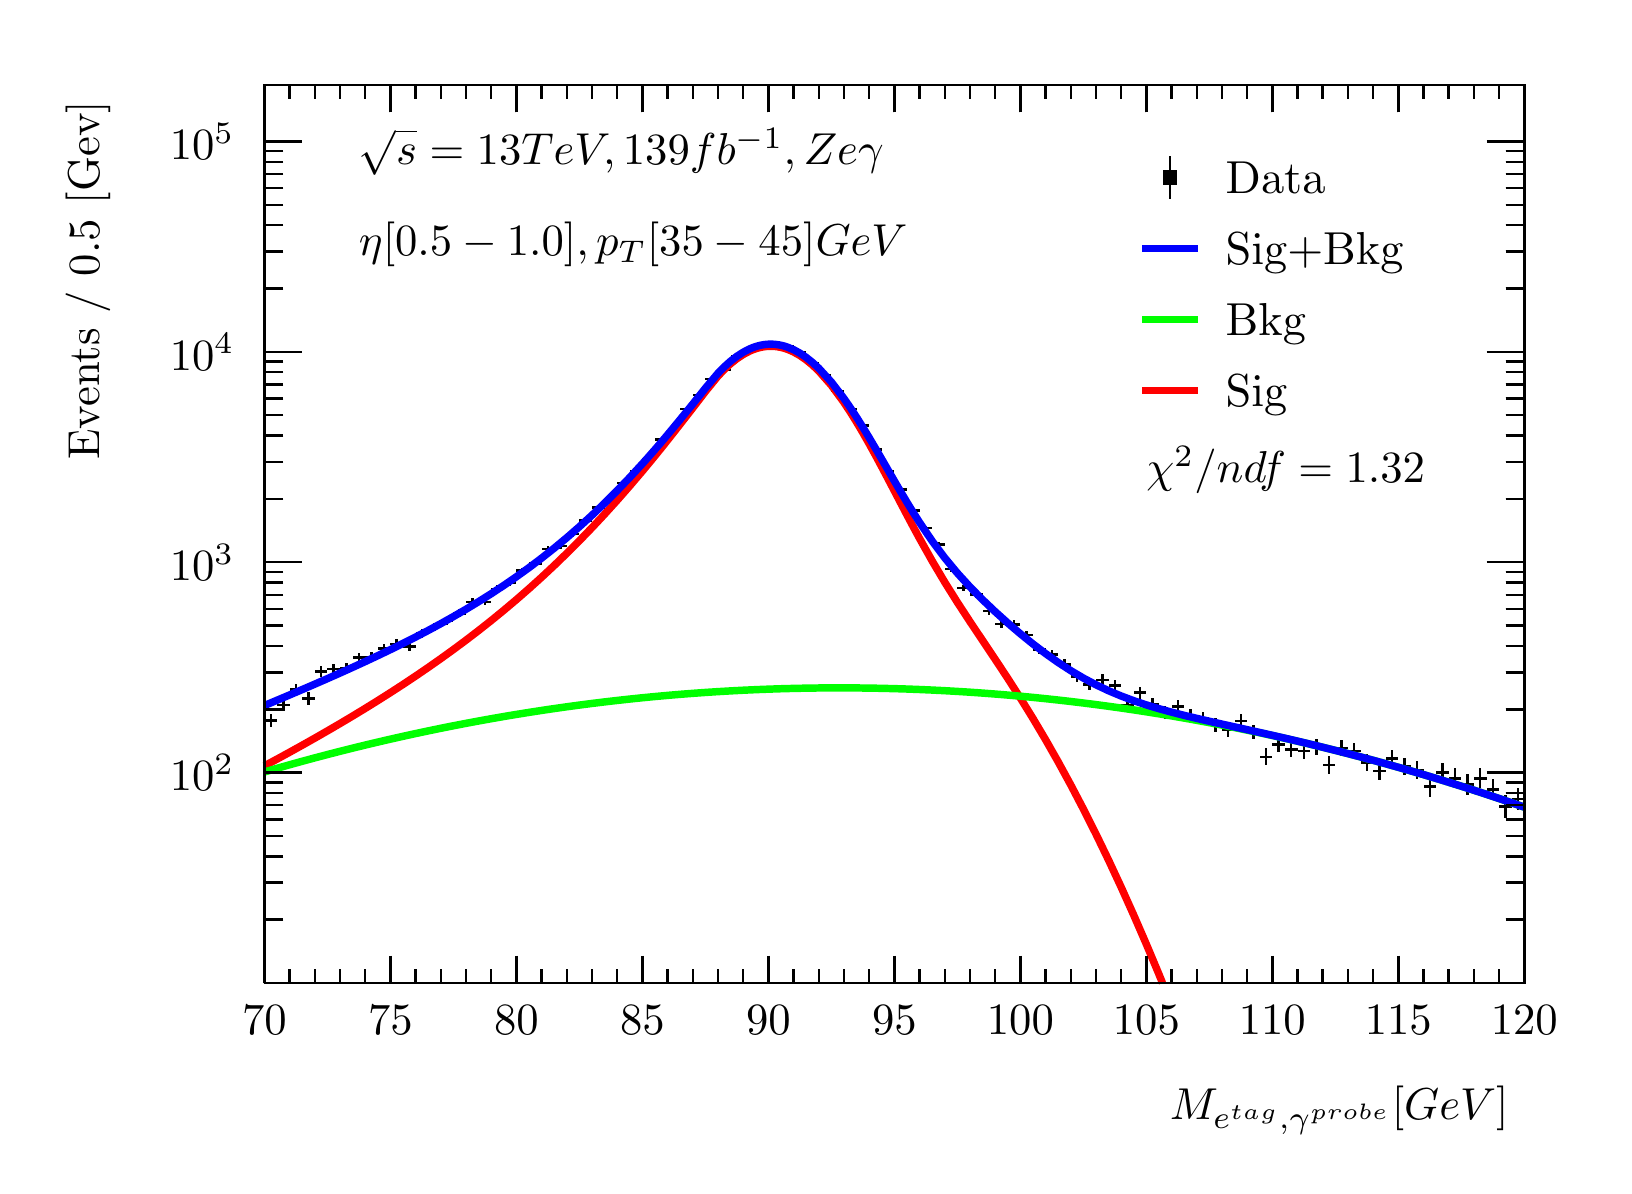
\begin{tikzpicture}
\pgfdeclareplotmark{cross} {
\pgfpathmoveto{\pgfpoint{-0.3\pgfplotmarksize}{\pgfplotmarksize}}
\pgfpathlineto{\pgfpoint{+0.3\pgfplotmarksize}{\pgfplotmarksize}}
\pgfpathlineto{\pgfpoint{+0.3\pgfplotmarksize}{0.3\pgfplotmarksize}}
\pgfpathlineto{\pgfpoint{+1\pgfplotmarksize}{0.3\pgfplotmarksize}}
\pgfpathlineto{\pgfpoint{+1\pgfplotmarksize}{-0.3\pgfplotmarksize}}
\pgfpathlineto{\pgfpoint{+0.3\pgfplotmarksize}{-0.3\pgfplotmarksize}}
\pgfpathlineto{\pgfpoint{+0.3\pgfplotmarksize}{-1.\pgfplotmarksize}}
\pgfpathlineto{\pgfpoint{-0.3\pgfplotmarksize}{-1.\pgfplotmarksize}}
\pgfpathlineto{\pgfpoint{-0.3\pgfplotmarksize}{-0.3\pgfplotmarksize}}
\pgfpathlineto{\pgfpoint{-1.\pgfplotmarksize}{-0.3\pgfplotmarksize}}
\pgfpathlineto{\pgfpoint{-1.\pgfplotmarksize}{0.3\pgfplotmarksize}}
\pgfpathlineto{\pgfpoint{-0.3\pgfplotmarksize}{0.3\pgfplotmarksize}}
\pgfpathclose
\pgfusepathqstroke
}
\pgfdeclareplotmark{cross*} {
\pgfpathmoveto{\pgfpoint{-0.3\pgfplotmarksize}{\pgfplotmarksize}}
\pgfpathlineto{\pgfpoint{+0.3\pgfplotmarksize}{\pgfplotmarksize}}
\pgfpathlineto{\pgfpoint{+0.3\pgfplotmarksize}{0.3\pgfplotmarksize}}
\pgfpathlineto{\pgfpoint{+1\pgfplotmarksize}{0.3\pgfplotmarksize}}
\pgfpathlineto{\pgfpoint{+1\pgfplotmarksize}{-0.3\pgfplotmarksize}}
\pgfpathlineto{\pgfpoint{+0.3\pgfplotmarksize}{-0.3\pgfplotmarksize}}
\pgfpathlineto{\pgfpoint{+0.3\pgfplotmarksize}{-1.\pgfplotmarksize}}
\pgfpathlineto{\pgfpoint{-0.3\pgfplotmarksize}{-1.\pgfplotmarksize}}
\pgfpathlineto{\pgfpoint{-0.3\pgfplotmarksize}{-0.3\pgfplotmarksize}}
\pgfpathlineto{\pgfpoint{-1.\pgfplotmarksize}{-0.3\pgfplotmarksize}}
\pgfpathlineto{\pgfpoint{-1.\pgfplotmarksize}{0.3\pgfplotmarksize}}
\pgfpathlineto{\pgfpoint{-0.3\pgfplotmarksize}{0.3\pgfplotmarksize}}
\pgfpathclose
\pgfusepathqfillstroke
}
\pgfdeclareplotmark{newstar} {
\pgfpathmoveto{\pgfqpoint{0pt}{\pgfplotmarksize}}
\pgfpathlineto{\pgfqpointpolar{44}{0.5\pgfplotmarksize}}
\pgfpathlineto{\pgfqpointpolar{18}{\pgfplotmarksize}}
\pgfpathlineto{\pgfqpointpolar{-20}{0.5\pgfplotmarksize}}
\pgfpathlineto{\pgfqpointpolar{-54}{\pgfplotmarksize}}
\pgfpathlineto{\pgfqpointpolar{-90}{0.5\pgfplotmarksize}}
\pgfpathlineto{\pgfqpointpolar{234}{\pgfplotmarksize}}
\pgfpathlineto{\pgfqpointpolar{198}{0.5\pgfplotmarksize}}
\pgfpathlineto{\pgfqpointpolar{162}{\pgfplotmarksize}}
\pgfpathlineto{\pgfqpointpolar{134}{0.5\pgfplotmarksize}}
\pgfpathclose
\pgfusepathqstroke
}
\pgfdeclareplotmark{newstar*} {
\pgfpathmoveto{\pgfqpoint{0pt}{\pgfplotmarksize}}
\pgfpathlineto{\pgfqpointpolar{44}{0.5\pgfplotmarksize}}
\pgfpathlineto{\pgfqpointpolar{18}{\pgfplotmarksize}}
\pgfpathlineto{\pgfqpointpolar{-20}{0.5\pgfplotmarksize}}
\pgfpathlineto{\pgfqpointpolar{-54}{\pgfplotmarksize}}
\pgfpathlineto{\pgfqpointpolar{-90}{0.5\pgfplotmarksize}}
\pgfpathlineto{\pgfqpointpolar{234}{\pgfplotmarksize}}
\pgfpathlineto{\pgfqpointpolar{198}{0.5\pgfplotmarksize}}
\pgfpathlineto{\pgfqpointpolar{162}{\pgfplotmarksize}}
\pgfpathlineto{\pgfqpointpolar{134}{0.5\pgfplotmarksize}}
\pgfpathclose
\pgfusepathqfillstroke
}
\definecolor{c}{rgb}{1,1,1};
\draw [color=c, fill=c] (0,0) rectangle (20,14.4361);
\draw [color=c, fill=c] (3,2.30977) rectangle (19,13.7143);
\definecolor{c}{rgb}{0,0,0};
\draw [c,line width=0.9] (3,2.30977) -- (3,13.7143) -- (19,13.7143) -- (19,2.30977) -- (3,2.30977);
\definecolor{c}{rgb}{1,1,1};
\draw [color=c, fill=c] (3,2.30977) rectangle (19,13.7143);
\definecolor{c}{rgb}{0,0,0};
\draw [c,line width=0.9] (3,2.30977) -- (3,13.7143) -- (19,13.7143) -- (19,2.30977) -- (3,2.30977);
\draw [c,line width=0.9] (3,2.30977) -- (19,2.30977);
\draw [c,line width=0.9] (3,2.65624) -- (3,2.30977);
\draw [c,line width=0.9] (3.32,2.48301) -- (3.32,2.30977);
\draw [c,line width=0.9] (3.64,2.48301) -- (3.64,2.30977);
\draw [c,line width=0.9] (3.96,2.48301) -- (3.96,2.30977);
\draw [c,line width=0.9] (4.28,2.48301) -- (4.28,2.30977);
\draw [c,line width=0.9] (4.6,2.65624) -- (4.6,2.30977);
\draw [c,line width=0.9] (4.92,2.48301) -- (4.92,2.30977);
\draw [c,line width=0.9] (5.24,2.48301) -- (5.24,2.30977);
\draw [c,line width=0.9] (5.56,2.48301) -- (5.56,2.30977);
\draw [c,line width=0.9] (5.88,2.48301) -- (5.88,2.30977);
\draw [c,line width=0.9] (6.2,2.65624) -- (6.2,2.30977);
\draw [c,line width=0.9] (6.52,2.48301) -- (6.52,2.30977);
\draw [c,line width=0.9] (6.84,2.48301) -- (6.84,2.30977);
\draw [c,line width=0.9] (7.16,2.48301) -- (7.16,2.30977);
\draw [c,line width=0.9] (7.48,2.48301) -- (7.48,2.30977);
\draw [c,line width=0.9] (7.8,2.65624) -- (7.8,2.30977);
\draw [c,line width=0.9] (8.12,2.48301) -- (8.12,2.30977);
\draw [c,line width=0.9] (8.44,2.48301) -- (8.44,2.30977);
\draw [c,line width=0.9] (8.76,2.48301) -- (8.76,2.30977);
\draw [c,line width=0.9] (9.08,2.48301) -- (9.08,2.30977);
\draw [c,line width=0.9] (9.4,2.65624) -- (9.4,2.30977);
\draw [c,line width=0.9] (9.72,2.48301) -- (9.72,2.30977);
\draw [c,line width=0.9] (10.04,2.48301) -- (10.04,2.30977);
\draw [c,line width=0.9] (10.36,2.48301) -- (10.36,2.30977);
\draw [c,line width=0.9] (10.68,2.48301) -- (10.68,2.30977);
\draw [c,line width=0.9] (11,2.65624) -- (11,2.30977);
\draw [c,line width=0.9] (11.32,2.48301) -- (11.32,2.30977);
\draw [c,line width=0.9] (11.64,2.48301) -- (11.64,2.30977);
\draw [c,line width=0.9] (11.96,2.48301) -- (11.96,2.30977);
\draw [c,line width=0.9] (12.28,2.48301) -- (12.28,2.30977);
\draw [c,line width=0.9] (12.6,2.65624) -- (12.6,2.30977);
\draw [c,line width=0.9] (12.92,2.48301) -- (12.92,2.30977);
\draw [c,line width=0.9] (13.24,2.48301) -- (13.24,2.30977);
\draw [c,line width=0.9] (13.56,2.48301) -- (13.56,2.30977);
\draw [c,line width=0.9] (13.88,2.48301) -- (13.88,2.30977);
\draw [c,line width=0.9] (14.2,2.65624) -- (14.2,2.30977);
\draw [c,line width=0.9] (14.52,2.48301) -- (14.52,2.30977);
\draw [c,line width=0.9] (14.84,2.48301) -- (14.84,2.30977);
\draw [c,line width=0.9] (15.16,2.48301) -- (15.16,2.30977);
\draw [c,line width=0.9] (15.48,2.48301) -- (15.48,2.30977);
\draw [c,line width=0.9] (15.8,2.65624) -- (15.8,2.30977);
\draw [c,line width=0.9] (16.12,2.48301) -- (16.12,2.30977);
\draw [c,line width=0.9] (16.44,2.48301) -- (16.44,2.30977);
\draw [c,line width=0.9] (16.76,2.48301) -- (16.76,2.30977);
\draw [c,line width=0.9] (17.08,2.48301) -- (17.08,2.30977);
\draw [c,line width=0.9] (17.4,2.65624) -- (17.4,2.30977);
\draw [c,line width=0.9] (17.72,2.48301) -- (17.72,2.30977);
\draw [c,line width=0.9] (18.04,2.48301) -- (18.04,2.30977);
\draw [c,line width=0.9] (18.36,2.48301) -- (18.36,2.30977);
\draw [c,line width=0.9] (18.68,2.48301) -- (18.68,2.30977);
\draw [c,line width=0.9] (19,2.65624) -- (19,2.30977);
\draw [anchor=base] (3,1.66015) node[scale=1.61424, color=c, rotate=0]{70};
\draw [anchor=base] (4.6,1.66015) node[scale=1.61424, color=c, rotate=0]{75};
\draw [anchor=base] (6.2,1.66015) node[scale=1.61424, color=c, rotate=0]{80};
\draw [anchor=base] (7.8,1.66015) node[scale=1.61424, color=c, rotate=0]{85};
\draw [anchor=base] (9.4,1.66015) node[scale=1.61424, color=c, rotate=0]{90};
\draw [anchor=base] (11,1.66015) node[scale=1.61424, color=c, rotate=0]{95};
\draw [anchor=base] (12.6,1.66015) node[scale=1.61424, color=c, rotate=0]{100};
\draw [anchor=base] (14.2,1.66015) node[scale=1.61424, color=c, rotate=0]{105};
\draw [anchor=base] (15.8,1.66015) node[scale=1.61424, color=c, rotate=0]{110};
\draw [anchor=base] (17.4,1.66015) node[scale=1.61424, color=c, rotate=0]{115};
\draw [anchor=base] (19,1.66015) node[scale=1.61424, color=c, rotate=0]{120};
\draw [anchor= east] (19,0.692932) node[scale=1.61424, color=c, rotate=0]{$M_{e^{tag}, \gamma^{probe}}  [GeV]$};
\draw [c,line width=0.9] (3,13.7143) -- (19,13.7143);
\draw [c,line width=0.9] (3,13.3678) -- (3,13.7143);
\draw [c,line width=0.9] (3.32,13.5411) -- (3.32,13.7143);
\draw [c,line width=0.9] (3.64,13.5411) -- (3.64,13.7143);
\draw [c,line width=0.9] (3.96,13.5411) -- (3.96,13.7143);
\draw [c,line width=0.9] (4.28,13.5411) -- (4.28,13.7143);
\draw [c,line width=0.9] (4.6,13.3678) -- (4.6,13.7143);
\draw [c,line width=0.9] (4.92,13.5411) -- (4.92,13.7143);
\draw [c,line width=0.9] (5.24,13.5411) -- (5.24,13.7143);
\draw [c,line width=0.9] (5.56,13.5411) -- (5.56,13.7143);
\draw [c,line width=0.9] (5.88,13.5411) -- (5.88,13.7143);
\draw [c,line width=0.9] (6.2,13.3678) -- (6.2,13.7143);
\draw [c,line width=0.9] (6.52,13.5411) -- (6.52,13.7143);
\draw [c,line width=0.9] (6.84,13.5411) -- (6.84,13.7143);
\draw [c,line width=0.9] (7.16,13.5411) -- (7.16,13.7143);
\draw [c,line width=0.9] (7.48,13.5411) -- (7.48,13.7143);
\draw [c,line width=0.9] (7.8,13.3678) -- (7.8,13.7143);
\draw [c,line width=0.9] (8.12,13.5411) -- (8.12,13.7143);
\draw [c,line width=0.9] (8.44,13.5411) -- (8.44,13.7143);
\draw [c,line width=0.9] (8.76,13.5411) -- (8.76,13.7143);
\draw [c,line width=0.9] (9.08,13.5411) -- (9.08,13.7143);
\draw [c,line width=0.9] (9.4,13.3678) -- (9.4,13.7143);
\draw [c,line width=0.9] (9.72,13.5411) -- (9.72,13.7143);
\draw [c,line width=0.9] (10.04,13.5411) -- (10.04,13.7143);
\draw [c,line width=0.9] (10.36,13.5411) -- (10.36,13.7143);
\draw [c,line width=0.9] (10.68,13.5411) -- (10.68,13.7143);
\draw [c,line width=0.9] (11,13.3678) -- (11,13.7143);
\draw [c,line width=0.9] (11.32,13.5411) -- (11.32,13.7143);
\draw [c,line width=0.9] (11.64,13.5411) -- (11.64,13.7143);
\draw [c,line width=0.9] (11.96,13.5411) -- (11.96,13.7143);
\draw [c,line width=0.9] (12.28,13.5411) -- (12.28,13.7143);
\draw [c,line width=0.9] (12.6,13.3678) -- (12.6,13.7143);
\draw [c,line width=0.9] (12.92,13.5411) -- (12.92,13.7143);
\draw [c,line width=0.9] (13.24,13.5411) -- (13.24,13.7143);
\draw [c,line width=0.9] (13.56,13.5411) -- (13.56,13.7143);
\draw [c,line width=0.9] (13.88,13.5411) -- (13.88,13.7143);
\draw [c,line width=0.9] (14.2,13.3678) -- (14.2,13.7143);
\draw [c,line width=0.9] (14.52,13.5411) -- (14.52,13.7143);
\draw [c,line width=0.9] (14.84,13.5411) -- (14.84,13.7143);
\draw [c,line width=0.9] (15.16,13.5411) -- (15.16,13.7143);
\draw [c,line width=0.9] (15.48,13.5411) -- (15.48,13.7143);
\draw [c,line width=0.9] (15.8,13.3678) -- (15.8,13.7143);
\draw [c,line width=0.9] (16.12,13.5411) -- (16.12,13.7143);
\draw [c,line width=0.9] (16.44,13.5411) -- (16.44,13.7143);
\draw [c,line width=0.9] (16.76,13.5411) -- (16.76,13.7143);
\draw [c,line width=0.9] (17.08,13.5411) -- (17.08,13.7143);
\draw [c,line width=0.9] (17.4,13.3678) -- (17.4,13.7143);
\draw [c,line width=0.9] (17.72,13.5411) -- (17.72,13.7143);
\draw [c,line width=0.9] (18.04,13.5411) -- (18.04,13.7143);
\draw [c,line width=0.9] (18.36,13.5411) -- (18.36,13.7143);
\draw [c,line width=0.9] (18.68,13.5411) -- (18.68,13.7143);
\draw [c,line width=0.9] (19,13.3678) -- (19,13.7143);
\draw [c,line width=0.9] (3,2.30977) -- (3,13.7143);
\draw [c,line width=0.9] (3.237,3.11414) -- (3,3.11414);
\draw [c,line width=0.9] (3.237,3.58467) -- (3,3.58467);
\draw [c,line width=0.9] (3.237,3.91852) -- (3,3.91852);
\draw [c,line width=0.9] (3.237,4.17747) -- (3,4.17747);
\draw [c,line width=0.9] (3.237,4.38904) -- (3,4.38904);
\draw [c,line width=0.9] (3.237,4.56793) -- (3,4.56793);
\draw [c,line width=0.9] (3.237,4.72289) -- (3,4.72289);
\draw [c,line width=0.9] (3.237,4.85957) -- (3,4.85957);
\draw [c,line width=0.9] (3.474,4.98184) -- (3,4.98184);
\draw [anchor= east] (2.82,4.98184) node[scale=1.61424, color=c, rotate=0]{$10^{2}$};
\draw [c,line width=0.9] (3.237,5.78621) -- (3,5.78621);
\draw [c,line width=0.9] (3.237,6.25674) -- (3,6.25674);
\draw [c,line width=0.9] (3.237,6.59058) -- (3,6.59058);
\draw [c,line width=0.9] (3.237,6.84953) -- (3,6.84953);
\draw [c,line width=0.9] (3.237,7.06111) -- (3,7.06111);
\draw [c,line width=0.9] (3.237,7.24) -- (3,7.24);
\draw [c,line width=0.9] (3.237,7.39496) -- (3,7.39496);
\draw [c,line width=0.9] (3.237,7.53164) -- (3,7.53164);
\draw [c,line width=0.9] (3.474,7.65391) -- (3,7.65391);
\draw [anchor= east] (2.82,7.65391) node[scale=1.61424, color=c, rotate=0]{$10^{3}$};
\draw [c,line width=0.9] (3.237,8.45828) -- (3,8.45828);
\draw [c,line width=0.9] (3.237,8.92881) -- (3,8.92881);
\draw [c,line width=0.9] (3.237,9.26265) -- (3,9.26265);
\draw [c,line width=0.9] (3.237,9.5216) -- (3,9.5216);
\draw [c,line width=0.9] (3.237,9.73318) -- (3,9.73318);
\draw [c,line width=0.9] (3.237,9.91207) -- (3,9.91207);
\draw [c,line width=0.9] (3.237,10.067) -- (3,10.067);
\draw [c,line width=0.9] (3.237,10.2037) -- (3,10.2037);
\draw [c,line width=0.9] (3.474,10.326) -- (3,10.326);
\draw [anchor= east] (2.82,10.326) node[scale=1.61424, color=c, rotate=0]{$10^{4}$};
\draw [c,line width=0.9] (3.237,11.1303) -- (3,11.1303);
\draw [c,line width=0.9] (3.237,11.6009) -- (3,11.6009);
\draw [c,line width=0.9] (3.237,11.9347) -- (3,11.9347);
\draw [c,line width=0.9] (3.237,12.1937) -- (3,12.1937);
\draw [c,line width=0.9] (3.237,12.4052) -- (3,12.4052);
\draw [c,line width=0.9] (3.237,12.5841) -- (3,12.5841);
\draw [c,line width=0.9] (3.237,12.7391) -- (3,12.7391);
\draw [c,line width=0.9] (3.237,12.8758) -- (3,12.8758);
\draw [c,line width=0.9] (3.474,12.998) -- (3,12.998);
\draw [anchor= east] (2.82,12.998) node[scale=1.61424, color=c, rotate=0]{$10^{5}$};
\draw [anchor= east] (0.76,13.7143) node[scale=1.61424, color=c, rotate=90]{Events / 0.5 [Gev]};
\draw [c,line width=0.9] (19,2.30977) -- (19,13.7143);
\draw [c,line width=0.9] (18.763,3.11414) -- (19,3.11414);
\draw [c,line width=0.9] (18.763,3.58467) -- (19,3.58467);
\draw [c,line width=0.9] (18.763,3.91852) -- (19,3.91852);
\draw [c,line width=0.9] (18.763,4.17747) -- (19,4.17747);
\draw [c,line width=0.9] (18.763,4.38904) -- (19,4.38904);
\draw [c,line width=0.9] (18.763,4.56793) -- (19,4.56793);
\draw [c,line width=0.9] (18.763,4.72289) -- (19,4.72289);
\draw [c,line width=0.9] (18.763,4.85957) -- (19,4.85957);
\draw [c,line width=0.9] (18.526,4.98184) -- (19,4.98184);
\draw [c,line width=0.9] (18.763,5.78621) -- (19,5.78621);
\draw [c,line width=0.9] (18.763,6.25674) -- (19,6.25674);
\draw [c,line width=0.9] (18.763,6.59058) -- (19,6.59058);
\draw [c,line width=0.9] (18.763,6.84953) -- (19,6.84953);
\draw [c,line width=0.9] (18.763,7.06111) -- (19,7.06111);
\draw [c,line width=0.9] (18.763,7.24) -- (19,7.24);
\draw [c,line width=0.9] (18.763,7.39496) -- (19,7.39496);
\draw [c,line width=0.9] (18.763,7.53164) -- (19,7.53164);
\draw [c,line width=0.9] (18.526,7.65391) -- (19,7.65391);
\draw [c,line width=0.9] (18.763,8.45828) -- (19,8.45828);
\draw [c,line width=0.9] (18.763,8.92881) -- (19,8.92881);
\draw [c,line width=0.9] (18.763,9.26265) -- (19,9.26265);
\draw [c,line width=0.9] (18.763,9.5216) -- (19,9.5216);
\draw [c,line width=0.9] (18.763,9.73318) -- (19,9.73318);
\draw [c,line width=0.9] (18.763,9.91207) -- (19,9.91207);
\draw [c,line width=0.9] (18.763,10.067) -- (19,10.067);
\draw [c,line width=0.9] (18.763,10.2037) -- (19,10.2037);
\draw [c,line width=0.9] (18.526,10.326) -- (19,10.326);
\draw [c,line width=0.9] (18.763,11.1303) -- (19,11.1303);
\draw [c,line width=0.9] (18.763,11.6009) -- (19,11.6009);
\draw [c,line width=0.9] (18.763,11.9347) -- (19,11.9347);
\draw [c,line width=0.9] (18.763,12.1937) -- (19,12.1937);
\draw [c,line width=0.9] (18.763,12.4052) -- (19,12.4052);
\draw [c,line width=0.9] (18.763,12.5841) -- (19,12.5841);
\draw [c,line width=0.9] (18.763,12.7391) -- (19,12.7391);
\draw [c,line width=0.9] (18.763,12.8758) -- (19,12.8758);
\draw [c,line width=0.9] (18.526,12.998) -- (19,12.998);
\draw [c,line width=0.9] (3.08,5.64444) -- (3,5.64444);
\draw [c,line width=0.9] (3,5.64444) -- (3,5.64444);
\draw [c,line width=0.9] (3.08,5.64444) -- (3.16,5.64444);
\draw [c,line width=0.9] (3.16,5.64444) -- (3.16,5.64444);
\draw [c,line width=0.9] (3.08,5.64444) -- (3.08,5.73165);
\draw [c,line width=0.9] (3.08,5.73165) -- (3.08,5.73165);
\draw [c,line width=0.9] (3.08,5.64444) -- (3.08,5.55724);
\draw [c,line width=0.9] (3.08,5.55724) -- (3.08,5.55724);
\draw [c,line width=0.9] (3.24,5.84283) -- (3.16,5.84283);
\draw [c,line width=0.9] (3.16,5.84283) -- (3.16,5.84283);
\draw [c,line width=0.9] (3.24,5.84283) -- (3.32,5.84283);
\draw [c,line width=0.9] (3.32,5.84283) -- (3.32,5.84283);
\draw [c,line width=0.9] (3.24,5.84283) -- (3.24,5.9229);
\draw [c,line width=0.9] (3.24,5.9229) -- (3.24,5.9229);
\draw [c,line width=0.9] (3.24,5.84283) -- (3.24,5.76277);
\draw [c,line width=0.9] (3.24,5.76277) -- (3.24,5.76277);
\draw [c,line width=0.9] (3.4,6.03584) -- (3.32,6.03584);
\draw [c,line width=0.9] (3.32,6.03584) -- (3.32,6.03584);
\draw [c,line width=0.9] (3.4,6.03584) -- (3.48,6.03584);
\draw [c,line width=0.9] (3.48,6.03584) -- (3.48,6.03584);
\draw [c,line width=0.9] (3.4,6.03584) -- (3.4,6.10952);
\draw [c,line width=0.9] (3.4,6.10952) -- (3.4,6.10952);
\draw [c,line width=0.9] (3.4,6.03584) -- (3.4,5.96217);
\draw [c,line width=0.9] (3.4,5.96217) -- (3.4,5.96217);
\draw [c,line width=0.9] (3.56,5.9229) -- (3.48,5.9229);
\draw [c,line width=0.9] (3.48,5.9229) -- (3.48,5.9229);
\draw [c,line width=0.9] (3.56,5.9229) -- (3.64,5.9229);
\draw [c,line width=0.9] (3.64,5.9229) -- (3.64,5.9229);
\draw [c,line width=0.9] (3.56,5.9229) -- (3.56,6.00025);
\draw [c,line width=0.9] (3.56,6.00025) -- (3.56,6.00025);
\draw [c,line width=0.9] (3.56,5.9229) -- (3.56,5.84555);
\draw [c,line width=0.9] (3.56,5.84555) -- (3.56,5.84555);
\draw [c,line width=0.9] (3.72,6.26445) -- (3.64,6.26445);
\draw [c,line width=0.9] (3.64,6.26445) -- (3.64,6.26445);
\draw [c,line width=0.9] (3.72,6.26445) -- (3.8,6.26445);
\draw [c,line width=0.9] (3.8,6.26445) -- (3.8,6.26445);
\draw [c,line width=0.9] (3.72,6.26445) -- (3.72,6.33122);
\draw [c,line width=0.9] (3.72,6.33122) -- (3.72,6.33122);
\draw [c,line width=0.9] (3.72,6.26445) -- (3.72,6.19768);
\draw [c,line width=0.9] (3.72,6.19768) -- (3.72,6.19768);
\draw [c,line width=0.9] (3.88,6.29853) -- (3.8,6.29853);
\draw [c,line width=0.9] (3.8,6.29853) -- (3.8,6.29853);
\draw [c,line width=0.9] (3.88,6.29853) -- (3.96,6.29853);
\draw [c,line width=0.9] (3.96,6.29853) -- (3.96,6.29853);
\draw [c,line width=0.9] (3.88,6.29853) -- (3.88,6.36433);
\draw [c,line width=0.9] (3.88,6.36433) -- (3.88,6.36433);
\draw [c,line width=0.9] (3.88,6.29853) -- (3.88,6.23273);
\draw [c,line width=0.9] (3.88,6.23273) -- (3.88,6.23273);
\draw [c,line width=0.9] (4.04,6.30967) -- (3.96,6.30967);
\draw [c,line width=0.9] (3.96,6.30967) -- (3.96,6.30967);
\draw [c,line width=0.9] (4.04,6.30967) -- (4.12,6.30967);
\draw [c,line width=0.9] (4.12,6.30967) -- (4.12,6.30967);
\draw [c,line width=0.9] (4.04,6.30967) -- (4.04,6.37515);
\draw [c,line width=0.9] (4.04,6.37515) -- (4.04,6.37515);
\draw [c,line width=0.9] (4.04,6.30967) -- (4.04,6.24419);
\draw [c,line width=0.9] (4.04,6.24419) -- (4.04,6.24419);
\draw [c,line width=0.9] (4.2,6.44553) -- (4.12,6.44553);
\draw [c,line width=0.9] (4.12,6.44553) -- (4.12,6.44553);
\draw [c,line width=0.9] (4.2,6.44553) -- (4.28,6.44553);
\draw [c,line width=0.9] (4.28,6.44553) -- (4.28,6.44553);
\draw [c,line width=0.9] (4.2,6.44553) -- (4.2,6.50729);
\draw [c,line width=0.9] (4.2,6.50729) -- (4.2,6.50729);
\draw [c,line width=0.9] (4.2,6.44553) -- (4.2,6.38377);
\draw [c,line width=0.9] (4.2,6.38377) -- (4.2,6.38377);
\draw [c,line width=0.9] (4.36,6.45209) -- (4.28,6.45209);
\draw [c,line width=0.9] (4.28,6.45209) -- (4.28,6.45209);
\draw [c,line width=0.9] (4.36,6.45209) -- (4.44,6.45209);
\draw [c,line width=0.9] (4.44,6.45209) -- (4.44,6.45209);
\draw [c,line width=0.9] (4.36,6.45209) -- (4.36,6.51367);
\draw [c,line width=0.9] (4.36,6.51367) -- (4.36,6.51367);
\draw [c,line width=0.9] (4.36,6.45209) -- (4.36,6.3905);
\draw [c,line width=0.9] (4.36,6.3905) -- (4.36,6.3905);
\draw [c,line width=0.9] (4.52,6.55823) -- (4.44,6.55823);
\draw [c,line width=0.9] (4.44,6.55823) -- (4.44,6.55823);
\draw [c,line width=0.9] (4.52,6.55823) -- (4.6,6.55823);
\draw [c,line width=0.9] (4.6,6.55823) -- (4.6,6.55823);
\draw [c,line width=0.9] (4.52,6.55823) -- (4.52,6.61706);
\draw [c,line width=0.9] (4.52,6.61706) -- (4.52,6.61706);
\draw [c,line width=0.9] (4.52,6.55823) -- (4.52,6.49939);
\draw [c,line width=0.9] (4.52,6.49939) -- (4.52,6.49939);
\draw [c,line width=0.9] (4.68,6.61641) -- (4.6,6.61641);
\draw [c,line width=0.9] (4.6,6.61641) -- (4.6,6.61641);
\draw [c,line width=0.9] (4.68,6.61641) -- (4.76,6.61641);
\draw [c,line width=0.9] (4.76,6.61641) -- (4.76,6.61641);
\draw [c,line width=0.9] (4.68,6.61641) -- (4.68,6.67378);
\draw [c,line width=0.9] (4.68,6.67378) -- (4.68,6.67378);
\draw [c,line width=0.9] (4.68,6.61641) -- (4.68,6.55903);
\draw [c,line width=0.9] (4.68,6.55903) -- (4.68,6.55903);
\draw [c,line width=0.9] (4.84,6.58477) -- (4.76,6.58477);
\draw [c,line width=0.9] (4.76,6.58477) -- (4.76,6.58477);
\draw [c,line width=0.9] (4.84,6.58477) -- (4.92,6.58477);
\draw [c,line width=0.9] (4.92,6.58477) -- (4.92,6.58477);
\draw [c,line width=0.9] (4.84,6.58477) -- (4.84,6.64293);
\draw [c,line width=0.9] (4.84,6.64293) -- (4.84,6.64293);
\draw [c,line width=0.9] (4.84,6.58477) -- (4.84,6.52661);
\draw [c,line width=0.9] (4.84,6.52661) -- (4.84,6.52661);
\draw [c,line width=0.9] (5,6.74772) -- (4.92,6.74772);
\draw [c,line width=0.9] (4.92,6.74772) -- (4.92,6.74772);
\draw [c,line width=0.9] (5,6.74772) -- (5.08,6.74772);
\draw [c,line width=0.9] (5.08,6.74772) -- (5.08,6.74772);
\draw [c,line width=0.9] (5,6.74772) -- (5,6.80194);
\draw [c,line width=0.9] (5,6.80194) -- (5,6.80194);
\draw [c,line width=0.9] (5,6.74772) -- (5,6.6935);
\draw [c,line width=0.9] (5,6.6935) -- (5,6.6935);
\draw [c,line width=0.9] (5.16,6.83317) -- (5.08,6.83317);
\draw [c,line width=0.9] (5.08,6.83317) -- (5.08,6.83317);
\draw [c,line width=0.9] (5.16,6.83317) -- (5.24,6.83317);
\draw [c,line width=0.9] (5.24,6.83317) -- (5.24,6.83317);
\draw [c,line width=0.9] (5.16,6.83317) -- (5.16,6.88543);
\draw [c,line width=0.9] (5.16,6.88543) -- (5.16,6.88543);
\draw [c,line width=0.9] (5.16,6.83317) -- (5.16,6.78091);
\draw [c,line width=0.9] (5.16,6.78091) -- (5.16,6.78091);
\draw [c,line width=0.9] (5.32,6.91277) -- (5.24,6.91277);
\draw [c,line width=0.9] (5.24,6.91277) -- (5.24,6.91277);
\draw [c,line width=0.9] (5.32,6.91277) -- (5.4,6.91277);
\draw [c,line width=0.9] (5.4,6.91277) -- (5.4,6.91277);
\draw [c,line width=0.9] (5.32,6.91277) -- (5.32,6.96327);
\draw [c,line width=0.9] (5.32,6.96327) -- (5.32,6.96327);
\draw [c,line width=0.9] (5.32,6.91277) -- (5.32,6.86227);
\draw [c,line width=0.9] (5.32,6.86227) -- (5.32,6.86227);
\draw [c,line width=0.9] (5.48,7.00565) -- (5.4,7.00565);
\draw [c,line width=0.9] (5.4,7.00565) -- (5.4,7.00565);
\draw [c,line width=0.9] (5.48,7.00565) -- (5.56,7.00565);
\draw [c,line width=0.9] (5.56,7.00565) -- (5.56,7.00565);
\draw [c,line width=0.9] (5.48,7.00565) -- (5.48,7.05417);
\draw [c,line width=0.9] (5.48,7.05417) -- (5.48,7.05417);
\draw [c,line width=0.9] (5.48,7.00565) -- (5.48,6.95714);
\draw [c,line width=0.9] (5.48,6.95714) -- (5.48,6.95714);
\draw [c,line width=0.9] (5.64,7.15042) -- (5.56,7.15042);
\draw [c,line width=0.9] (5.56,7.15042) -- (5.56,7.15042);
\draw [c,line width=0.9] (5.64,7.15042) -- (5.72,7.15042);
\draw [c,line width=0.9] (5.72,7.15042) -- (5.72,7.15042);
\draw [c,line width=0.9] (5.64,7.15042) -- (5.64,7.19601);
\draw [c,line width=0.9] (5.64,7.19601) -- (5.64,7.19601);
\draw [c,line width=0.9] (5.64,7.15042) -- (5.64,7.10484);
\draw [c,line width=0.9] (5.64,7.10484) -- (5.64,7.10484);
\draw [c,line width=0.9] (5.8,7.15042) -- (5.72,7.15042);
\draw [c,line width=0.9] (5.72,7.15042) -- (5.72,7.15042);
\draw [c,line width=0.9] (5.8,7.15042) -- (5.88,7.15042);
\draw [c,line width=0.9] (5.88,7.15042) -- (5.88,7.15042);
\draw [c,line width=0.9] (5.8,7.15042) -- (5.8,7.19601);
\draw [c,line width=0.9] (5.8,7.19601) -- (5.8,7.19601);
\draw [c,line width=0.9] (5.8,7.15042) -- (5.8,7.10484);
\draw [c,line width=0.9] (5.8,7.10484) -- (5.8,7.10484);
\draw [c,line width=0.9] (5.96,7.31696) -- (5.88,7.31696);
\draw [c,line width=0.9] (5.88,7.31696) -- (5.88,7.31696);
\draw [c,line width=0.9] (5.96,7.31696) -- (6.04,7.31696);
\draw [c,line width=0.9] (6.04,7.31696) -- (6.04,7.31696);
\draw [c,line width=0.9] (5.96,7.31696) -- (5.96,7.35939);
\draw [c,line width=0.9] (5.96,7.35939) -- (5.96,7.35939);
\draw [c,line width=0.9] (5.96,7.31696) -- (5.96,7.27454);
\draw [c,line width=0.9] (5.96,7.27454) -- (5.96,7.27454);
\draw [c,line width=0.9] (6.12,7.3993) -- (6.04,7.3993);
\draw [c,line width=0.9] (6.04,7.3993) -- (6.04,7.3993);
\draw [c,line width=0.9] (6.12,7.3993) -- (6.2,7.3993);
\draw [c,line width=0.9] (6.2,7.3993) -- (6.2,7.3993);
\draw [c,line width=0.9] (6.12,7.3993) -- (6.12,7.44025);
\draw [c,line width=0.9] (6.12,7.44025) -- (6.12,7.44025);
\draw [c,line width=0.9] (6.12,7.3993) -- (6.12,7.35835);
\draw [c,line width=0.9] (6.12,7.35835) -- (6.12,7.35835);
\draw [c,line width=0.9] (6.28,7.54701) -- (6.2,7.54701);
\draw [c,line width=0.9] (6.2,7.54701) -- (6.2,7.54701);
\draw [c,line width=0.9] (6.28,7.54701) -- (6.36,7.54701);
\draw [c,line width=0.9] (6.36,7.54701) -- (6.36,7.54701);
\draw [c,line width=0.9] (6.28,7.54701) -- (6.28,7.58544);
\draw [c,line width=0.9] (6.28,7.58544) -- (6.28,7.58544);
\draw [c,line width=0.9] (6.28,7.54701) -- (6.28,7.50859);
\draw [c,line width=0.9] (6.28,7.50859) -- (6.28,7.50859);
\draw [c,line width=0.9] (6.44,7.63755) -- (6.36,7.63755);
\draw [c,line width=0.9] (6.36,7.63755) -- (6.36,7.63755);
\draw [c,line width=0.9] (6.44,7.63755) -- (6.52,7.63755);
\draw [c,line width=0.9] (6.52,7.63755) -- (6.52,7.63755);
\draw [c,line width=0.9] (6.44,7.63755) -- (6.44,7.6745);
\draw [c,line width=0.9] (6.44,7.6745) -- (6.44,7.6745);
\draw [c,line width=0.9] (6.44,7.63755) -- (6.44,7.60059);
\draw [c,line width=0.9] (6.44,7.60059) -- (6.44,7.60059);
\draw [c,line width=0.9] (6.6,7.82113) -- (6.52,7.82113);
\draw [c,line width=0.9] (6.52,7.82113) -- (6.52,7.82113);
\draw [c,line width=0.9] (6.6,7.82113) -- (6.68,7.82113);
\draw [c,line width=0.9] (6.68,7.82113) -- (6.68,7.82113);
\draw [c,line width=0.9] (6.6,7.82113) -- (6.6,7.85528);
\draw [c,line width=0.9] (6.6,7.85528) -- (6.6,7.85528);
\draw [c,line width=0.9] (6.6,7.82113) -- (6.6,7.78699);
\draw [c,line width=0.9] (6.6,7.78699) -- (6.6,7.78699);
\draw [c,line width=0.9] (6.76,7.8587) -- (6.68,7.8587);
\draw [c,line width=0.9] (6.68,7.8587) -- (6.68,7.8587);
\draw [c,line width=0.9] (6.76,7.8587) -- (6.84,7.8587);
\draw [c,line width=0.9] (6.84,7.8587) -- (6.84,7.8587);
\draw [c,line width=0.9] (6.76,7.8587) -- (6.76,7.89229);
\draw [c,line width=0.9] (6.76,7.89229) -- (6.76,7.89229);
\draw [c,line width=0.9] (6.76,7.8587) -- (6.76,7.8251);
\draw [c,line width=0.9] (6.76,7.8251) -- (6.76,7.8251);
\draw [c,line width=0.9] (6.92,8.00988) -- (6.84,8.00988);
\draw [c,line width=0.9] (6.84,8.00988) -- (6.84,8.00988);
\draw [c,line width=0.9] (6.92,8.00988) -- (7,8.00988);
\draw [c,line width=0.9] (7,8.00988) -- (7,8.00988);
\draw [c,line width=0.9] (6.92,8.00988) -- (6.92,8.04136);
\draw [c,line width=0.9] (6.92,8.04136) -- (6.92,8.04136);
\draw [c,line width=0.9] (6.92,8.00988) -- (6.92,7.9784);
\draw [c,line width=0.9] (6.92,7.9784) -- (6.92,7.9784);
\draw [c,line width=0.9] (7.08,8.1862) -- (7,8.1862);
\draw [c,line width=0.9] (7,8.1862) -- (7,8.1862);
\draw [c,line width=0.9] (7.08,8.1862) -- (7.16,8.1862);
\draw [c,line width=0.9] (7.16,8.1862) -- (7.16,8.1862);
\draw [c,line width=0.9] (7.08,8.1862) -- (7.08,8.21538);
\draw [c,line width=0.9] (7.08,8.21538) -- (7.08,8.21538);
\draw [c,line width=0.9] (7.08,8.1862) -- (7.08,8.15703);
\draw [c,line width=0.9] (7.08,8.15703) -- (7.08,8.15703);
\draw [c,line width=0.9] (7.24,8.34756) -- (7.16,8.34756);
\draw [c,line width=0.9] (7.16,8.34756) -- (7.16,8.34756);
\draw [c,line width=0.9] (7.24,8.34756) -- (7.32,8.34756);
\draw [c,line width=0.9] (7.32,8.34756) -- (7.32,8.34756);
\draw [c,line width=0.9] (7.24,8.34756) -- (7.24,8.37478);
\draw [c,line width=0.9] (7.24,8.37478) -- (7.24,8.37478);
\draw [c,line width=0.9] (7.24,8.34756) -- (7.24,8.32034);
\draw [c,line width=0.9] (7.24,8.32034) -- (7.24,8.32034);
\draw [c,line width=0.9] (7.4,8.41513) -- (7.32,8.41513);
\draw [c,line width=0.9] (7.32,8.41513) -- (7.32,8.41513);
\draw [c,line width=0.9] (7.4,8.41513) -- (7.48,8.41513);
\draw [c,line width=0.9] (7.48,8.41513) -- (7.48,8.41513);
\draw [c,line width=0.9] (7.4,8.41513) -- (7.4,8.44157);
\draw [c,line width=0.9] (7.4,8.44157) -- (7.4,8.44157);
\draw [c,line width=0.9] (7.4,8.41513) -- (7.4,8.3887);
\draw [c,line width=0.9] (7.4,8.3887) -- (7.4,8.3887);
\draw [c,line width=0.9] (7.56,8.66307) -- (7.48,8.66307);
\draw [c,line width=0.9] (7.48,8.66307) -- (7.48,8.66307);
\draw [c,line width=0.9] (7.56,8.66307) -- (7.64,8.66307);
\draw [c,line width=0.9] (7.64,8.66307) -- (7.64,8.66307);
\draw [c,line width=0.9] (7.56,8.66307) -- (7.56,8.68683);
\draw [c,line width=0.9] (7.56,8.68683) -- (7.56,8.68683);
\draw [c,line width=0.9] (7.56,8.66307) -- (7.56,8.63931);
\draw [c,line width=0.9] (7.56,8.63931) -- (7.56,8.63931);
\draw [c,line width=0.9] (7.72,8.80439) -- (7.64,8.80439);
\draw [c,line width=0.9] (7.64,8.80439) -- (7.64,8.80439);
\draw [c,line width=0.9] (7.72,8.80439) -- (7.8,8.80439);
\draw [c,line width=0.9] (7.8,8.80439) -- (7.8,8.80439);
\draw [c,line width=0.9] (7.72,8.80439) -- (7.72,8.82674);
\draw [c,line width=0.9] (7.72,8.82674) -- (7.72,8.82674);
\draw [c,line width=0.9] (7.72,8.80439) -- (7.72,8.78204);
\draw [c,line width=0.9] (7.72,8.78204) -- (7.72,8.78204);
\draw [c,line width=0.9] (7.88,8.96761) -- (7.8,8.96761);
\draw [c,line width=0.9] (7.8,8.96761) -- (7.8,8.96761);
\draw [c,line width=0.9] (7.88,8.96761) -- (7.96,8.96761);
\draw [c,line width=0.9] (7.96,8.96761) -- (7.96,8.96761);
\draw [c,line width=0.9] (7.88,8.96761) -- (7.88,8.98844);
\draw [c,line width=0.9] (7.88,8.98844) -- (7.88,8.98844);
\draw [c,line width=0.9] (7.88,8.96761) -- (7.88,8.94677);
\draw [c,line width=0.9] (7.88,8.94677) -- (7.88,8.94677);
\draw [c,line width=0.9] (8.04,9.21377) -- (7.96,9.21377);
\draw [c,line width=0.9] (7.96,9.21377) -- (7.96,9.21377);
\draw [c,line width=0.9] (8.04,9.21377) -- (8.12,9.21377);
\draw [c,line width=0.9] (8.12,9.21377) -- (8.12,9.21377);
\draw [c,line width=0.9] (8.04,9.21377) -- (8.04,9.23251);
\draw [c,line width=0.9] (8.04,9.23251) -- (8.04,9.23251);
\draw [c,line width=0.9] (8.04,9.21377) -- (8.04,9.19503);
\draw [c,line width=0.9] (8.04,9.19503) -- (8.04,9.19503);
\draw [c,line width=0.9] (8.2,9.34523) -- (8.12,9.34523);
\draw [c,line width=0.9] (8.12,9.34523) -- (8.12,9.34523);
\draw [c,line width=0.9] (8.2,9.34523) -- (8.28,9.34523);
\draw [c,line width=0.9] (8.28,9.34523) -- (8.28,9.34523);
\draw [c,line width=0.9] (8.2,9.34523) -- (8.2,9.36294);
\draw [c,line width=0.9] (8.2,9.36294) -- (8.2,9.36294);
\draw [c,line width=0.9] (8.2,9.34523) -- (8.2,9.32752);
\draw [c,line width=0.9] (8.2,9.32752) -- (8.2,9.32752);
\draw [c,line width=0.9] (8.36,9.60055) -- (8.28,9.60055);
\draw [c,line width=0.9] (8.28,9.60055) -- (8.28,9.60055);
\draw [c,line width=0.9] (8.36,9.60055) -- (8.44,9.60055);
\draw [c,line width=0.9] (8.44,9.60055) -- (8.44,9.60055);
\draw [c,line width=0.9] (8.36,9.60055) -- (8.36,9.61641);
\draw [c,line width=0.9] (8.36,9.61641) -- (8.36,9.61641);
\draw [c,line width=0.9] (8.36,9.60055) -- (8.36,9.58469);
\draw [c,line width=0.9] (8.36,9.58469) -- (8.36,9.58469);
\draw [c,line width=0.9] (8.52,9.77553) -- (8.44,9.77553);
\draw [c,line width=0.9] (8.44,9.77553) -- (8.44,9.77553);
\draw [c,line width=0.9] (8.52,9.77553) -- (8.6,9.77553);
\draw [c,line width=0.9] (8.6,9.77553) -- (8.6,9.77553);
\draw [c,line width=0.9] (8.52,9.77553) -- (8.52,9.79024);
\draw [c,line width=0.9] (8.52,9.79024) -- (8.52,9.79024);
\draw [c,line width=0.9] (8.52,9.77553) -- (8.52,9.76082);
\draw [c,line width=0.9] (8.52,9.76082) -- (8.52,9.76082);
\draw [c,line width=0.9] (8.68,9.9814) -- (8.6,9.9814);
\draw [c,line width=0.9] (8.6,9.9814) -- (8.6,9.9814);
\draw [c,line width=0.9] (8.68,9.9814) -- (8.76,9.9814);
\draw [c,line width=0.9] (8.76,9.9814) -- (8.76,9.9814);
\draw [c,line width=0.9] (8.68,9.9814) -- (8.68,9.99487);
\draw [c,line width=0.9] (8.68,9.99487) -- (8.68,9.99487);
\draw [c,line width=0.9] (8.68,9.9814) -- (8.68,9.96794);
\draw [c,line width=0.9] (8.68,9.96794) -- (8.68,9.96794);
\draw [c,line width=0.9] (8.84,10.0927) -- (8.76,10.0927);
\draw [c,line width=0.9] (8.76,10.0927) -- (8.76,10.0927);
\draw [c,line width=0.9] (8.84,10.0927) -- (8.92,10.0927);
\draw [c,line width=0.9] (8.92,10.0927) -- (8.92,10.0927);
\draw [c,line width=0.9] (8.84,10.0927) -- (8.84,10.1055);
\draw [c,line width=0.9] (8.84,10.1055) -- (8.84,10.1055);
\draw [c,line width=0.9] (8.84,10.0927) -- (8.84,10.0799);
\draw [c,line width=0.9] (8.84,10.0799) -- (8.84,10.0799);
\draw [c,line width=0.9] (9,10.2741) -- (8.92,10.2741);
\draw [c,line width=0.9] (8.92,10.2741) -- (8.92,10.2741);
\draw [c,line width=0.9] (9,10.2741) -- (9.08,10.2741);
\draw [c,line width=0.9] (9.08,10.2741) -- (9.08,10.2741);
\draw [c,line width=0.9] (9,10.2741) -- (9,10.286);
\draw [c,line width=0.9] (9,10.286) -- (9,10.286);
\draw [c,line width=0.9] (9,10.2741) -- (9,10.2623);
\draw [c,line width=0.9] (9,10.2623) -- (9,10.2623);
\draw [c,line width=0.9] (9.16,10.3619) -- (9.08,10.3619);
\draw [c,line width=0.9] (9.08,10.3619) -- (9.08,10.3619);
\draw [c,line width=0.9] (9.16,10.3619) -- (9.24,10.3619);
\draw [c,line width=0.9] (9.24,10.3619) -- (9.24,10.3619);
\draw [c,line width=0.9] (9.16,10.3619) -- (9.16,10.3733);
\draw [c,line width=0.9] (9.16,10.3733) -- (9.16,10.3733);
\draw [c,line width=0.9] (9.16,10.3619) -- (9.16,10.3504);
\draw [c,line width=0.9] (9.16,10.3504) -- (9.16,10.3504);
\draw [c,line width=0.9] (9.32,10.4157) -- (9.24,10.4157);
\draw [c,line width=0.9] (9.24,10.4157) -- (9.24,10.4157);
\draw [c,line width=0.9] (9.32,10.4157) -- (9.4,10.4157);
\draw [c,line width=0.9] (9.4,10.4157) -- (9.4,10.4157);
\draw [c,line width=0.9] (9.32,10.4157) -- (9.32,10.4269);
\draw [c,line width=0.9] (9.32,10.4269) -- (9.32,10.4269);
\draw [c,line width=0.9] (9.32,10.4157) -- (9.32,10.4046);
\draw [c,line width=0.9] (9.32,10.4046) -- (9.32,10.4046);
\draw [c,line width=0.9] (9.48,10.4272) -- (9.4,10.4272);
\draw [c,line width=0.9] (9.4,10.4272) -- (9.4,10.4272);
\draw [c,line width=0.9] (9.48,10.4272) -- (9.56,10.4272);
\draw [c,line width=0.9] (9.56,10.4272) -- (9.56,10.4272);
\draw [c,line width=0.9] (9.48,10.4272) -- (9.48,10.4383);
\draw [c,line width=0.9] (9.48,10.4383) -- (9.48,10.4383);
\draw [c,line width=0.9] (9.48,10.4272) -- (9.48,10.416);
\draw [c,line width=0.9] (9.48,10.416) -- (9.48,10.416);
\draw [c,line width=0.9] (9.64,10.3971) -- (9.56,10.3971);
\draw [c,line width=0.9] (9.56,10.3971) -- (9.56,10.3971);
\draw [c,line width=0.9] (9.64,10.3971) -- (9.72,10.3971);
\draw [c,line width=0.9] (9.72,10.3971) -- (9.72,10.3971);
\draw [c,line width=0.9] (9.64,10.3971) -- (9.64,10.4083);
\draw [c,line width=0.9] (9.64,10.4083) -- (9.64,10.4083);
\draw [c,line width=0.9] (9.64,10.3971) -- (9.64,10.3858);
\draw [c,line width=0.9] (9.64,10.3858) -- (9.64,10.3858);
\draw [c,line width=0.9] (9.8,10.3206) -- (9.72,10.3206);
\draw [c,line width=0.9] (9.72,10.3206) -- (9.72,10.3206);
\draw [c,line width=0.9] (9.8,10.3206) -- (9.88,10.3206);
\draw [c,line width=0.9] (9.88,10.3206) -- (9.88,10.3206);
\draw [c,line width=0.9] (9.8,10.3206) -- (9.8,10.3323);
\draw [c,line width=0.9] (9.8,10.3323) -- (9.8,10.3323);
\draw [c,line width=0.9] (9.8,10.3206) -- (9.8,10.309);
\draw [c,line width=0.9] (9.8,10.309) -- (9.8,10.309);
\draw [c,line width=0.9] (9.96,10.1751) -- (9.88,10.1751);
\draw [c,line width=0.9] (9.88,10.1751) -- (9.88,10.1751);
\draw [c,line width=0.9] (9.96,10.1751) -- (10.04,10.1751);
\draw [c,line width=0.9] (10.04,10.1751) -- (10.04,10.1751);
\draw [c,line width=0.9] (9.96,10.1751) -- (9.96,10.1875);
\draw [c,line width=0.9] (9.96,10.1875) -- (9.96,10.1875);
\draw [c,line width=0.9] (9.96,10.1751) -- (9.96,10.1627);
\draw [c,line width=0.9] (9.96,10.1627) -- (9.96,10.1627);
\draw [c,line width=0.9] (10.12,10.0332) -- (10.04,10.0332);
\draw [c,line width=0.9] (10.04,10.0332) -- (10.04,10.0332);
\draw [c,line width=0.9] (10.12,10.0332) -- (10.2,10.0332);
\draw [c,line width=0.9] (10.2,10.0332) -- (10.2,10.0332);
\draw [c,line width=0.9] (10.12,10.0332) -- (10.12,10.0463);
\draw [c,line width=0.9] (10.12,10.0463) -- (10.12,10.0463);
\draw [c,line width=0.9] (10.12,10.0332) -- (10.12,10.02);
\draw [c,line width=0.9] (10.12,10.02) -- (10.12,10.02);
\draw [c,line width=0.9] (10.28,9.82821) -- (10.2,9.82821);
\draw [c,line width=0.9] (10.2,9.82821) -- (10.2,9.82821);
\draw [c,line width=0.9] (10.28,9.82821) -- (10.36,9.82821);
\draw [c,line width=0.9] (10.36,9.82821) -- (10.36,9.82821);
\draw [c,line width=0.9] (10.28,9.82821) -- (10.28,9.84259);
\draw [c,line width=0.9] (10.28,9.84259) -- (10.28,9.84259);
\draw [c,line width=0.9] (10.28,9.82821) -- (10.28,9.81383);
\draw [c,line width=0.9] (10.28,9.81383) -- (10.28,9.81383);
\draw [c,line width=0.9] (10.44,9.59925) -- (10.36,9.59925);
\draw [c,line width=0.9] (10.36,9.59925) -- (10.36,9.59925);
\draw [c,line width=0.9] (10.44,9.59925) -- (10.52,9.59925);
\draw [c,line width=0.9] (10.52,9.59925) -- (10.52,9.59925);
\draw [c,line width=0.9] (10.44,9.59925) -- (10.44,9.61512);
\draw [c,line width=0.9] (10.44,9.61512) -- (10.44,9.61512);
\draw [c,line width=0.9] (10.44,9.59925) -- (10.44,9.58338);
\draw [c,line width=0.9] (10.44,9.58338) -- (10.44,9.58338);
\draw [c,line width=0.9] (10.6,9.38975) -- (10.52,9.38975);
\draw [c,line width=0.9] (10.52,9.38975) -- (10.52,9.38975);
\draw [c,line width=0.9] (10.6,9.38975) -- (10.68,9.38975);
\draw [c,line width=0.9] (10.68,9.38975) -- (10.68,9.38975);
\draw [c,line width=0.9] (10.6,9.38975) -- (10.6,9.40713);
\draw [c,line width=0.9] (10.6,9.40713) -- (10.6,9.40713);
\draw [c,line width=0.9] (10.6,9.38975) -- (10.6,9.37238);
\draw [c,line width=0.9] (10.6,9.37238) -- (10.6,9.37238);
\draw [c,line width=0.9] (10.76,9.08628) -- (10.68,9.08628);
\draw [c,line width=0.9] (10.68,9.08628) -- (10.68,9.08628);
\draw [c,line width=0.9] (10.76,9.08628) -- (10.84,9.08628);
\draw [c,line width=0.9] (10.84,9.08628) -- (10.84,9.08628);
\draw [c,line width=0.9] (10.76,9.08628) -- (10.76,9.10608);
\draw [c,line width=0.9] (10.76,9.10608) -- (10.76,9.10608);
\draw [c,line width=0.9] (10.76,9.08628) -- (10.76,9.06648);
\draw [c,line width=0.9] (10.76,9.06648) -- (10.76,9.06648);
\draw [c,line width=0.9] (10.92,8.80439) -- (10.84,8.80439);
\draw [c,line width=0.9] (10.84,8.80439) -- (10.84,8.80439);
\draw [c,line width=0.9] (10.92,8.80439) -- (11,8.80439);
\draw [c,line width=0.9] (11,8.80439) -- (11,8.80439);
\draw [c,line width=0.9] (10.92,8.80439) -- (10.92,8.82674);
\draw [c,line width=0.9] (10.92,8.82674) -- (10.92,8.82674);
\draw [c,line width=0.9] (10.92,8.80439) -- (10.92,8.78204);
\draw [c,line width=0.9] (10.92,8.78204) -- (10.92,8.78204);
\draw [c,line width=0.9] (11.08,8.58043) -- (11,8.58043);
\draw [c,line width=0.9] (11,8.58043) -- (11,8.58043);
\draw [c,line width=0.9] (11.08,8.58043) -- (11.16,8.58043);
\draw [c,line width=0.9] (11.16,8.58043) -- (11.16,8.58043);
\draw [c,line width=0.9] (11.08,8.58043) -- (11.08,8.60505);
\draw [c,line width=0.9] (11.08,8.60505) -- (11.08,8.60505);
\draw [c,line width=0.9] (11.08,8.58043) -- (11.08,8.55581);
\draw [c,line width=0.9] (11.08,8.55581) -- (11.08,8.55581);
\draw [c,line width=0.9] (11.24,8.31257) -- (11.16,8.31257);
\draw [c,line width=0.9] (11.16,8.31257) -- (11.16,8.31257);
\draw [c,line width=0.9] (11.24,8.31257) -- (11.32,8.31257);
\draw [c,line width=0.9] (11.32,8.31257) -- (11.32,8.31257);
\draw [c,line width=0.9] (11.24,8.31257) -- (11.24,8.3402);
\draw [c,line width=0.9] (11.24,8.3402) -- (11.24,8.3402);
\draw [c,line width=0.9] (11.24,8.31257) -- (11.24,8.28494);
\draw [c,line width=0.9] (11.24,8.28494) -- (11.24,8.28494);
\draw [c,line width=0.9] (11.4,8.08829) -- (11.32,8.08829);
\draw [c,line width=0.9] (11.32,8.08829) -- (11.32,8.08829);
\draw [c,line width=0.9] (11.4,8.08829) -- (11.48,8.08829);
\draw [c,line width=0.9] (11.48,8.08829) -- (11.48,8.08829);
\draw [c,line width=0.9] (11.4,8.08829) -- (11.4,8.11872);
\draw [c,line width=0.9] (11.4,8.11872) -- (11.4,8.11872);
\draw [c,line width=0.9] (11.4,8.08829) -- (11.4,8.05786);
\draw [c,line width=0.9] (11.4,8.05786) -- (11.4,8.05786);
\draw [c,line width=0.9] (11.56,7.87703) -- (11.48,7.87703);
\draw [c,line width=0.9] (11.48,7.87703) -- (11.48,7.87703);
\draw [c,line width=0.9] (11.56,7.87703) -- (11.64,7.87703);
\draw [c,line width=0.9] (11.64,7.87703) -- (11.64,7.87703);
\draw [c,line width=0.9] (11.56,7.87703) -- (11.56,7.91037);
\draw [c,line width=0.9] (11.56,7.91037) -- (11.56,7.91037);
\draw [c,line width=0.9] (11.56,7.87703) -- (11.56,7.8437);
\draw [c,line width=0.9] (11.56,7.8437) -- (11.56,7.8437);
\draw [c,line width=0.9] (11.72,7.56594) -- (11.64,7.56594);
\draw [c,line width=0.9] (11.64,7.56594) -- (11.64,7.56594);
\draw [c,line width=0.9] (11.72,7.56594) -- (11.8,7.56594);
\draw [c,line width=0.9] (11.8,7.56594) -- (11.8,7.56594);
\draw [c,line width=0.9] (11.72,7.56594) -- (11.72,7.60406);
\draw [c,line width=0.9] (11.72,7.60406) -- (11.72,7.60406);
\draw [c,line width=0.9] (11.72,7.56594) -- (11.72,7.52783);
\draw [c,line width=0.9] (11.72,7.52783) -- (11.72,7.52783);
\draw [c,line width=0.9] (11.88,7.32777) -- (11.8,7.32777);
\draw [c,line width=0.9] (11.8,7.32777) -- (11.8,7.32777);
\draw [c,line width=0.9] (11.88,7.32777) -- (11.96,7.32777);
\draw [c,line width=0.9] (11.96,7.32777) -- (11.96,7.32777);
\draw [c,line width=0.9] (11.88,7.32777) -- (11.88,7.37001);
\draw [c,line width=0.9] (11.88,7.37001) -- (11.88,7.37001);
\draw [c,line width=0.9] (11.88,7.32777) -- (11.88,7.28554);
\draw [c,line width=0.9] (11.88,7.28554) -- (11.88,7.28554);
\draw [c,line width=0.9] (12.04,7.24166) -- (11.96,7.24166);
\draw [c,line width=0.9] (11.96,7.24166) -- (11.96,7.24166);
\draw [c,line width=0.9] (12.04,7.24166) -- (12.12,7.24166);
\draw [c,line width=0.9] (12.12,7.24166) -- (12.12,7.24166);
\draw [c,line width=0.9] (12.04,7.24166) -- (12.04,7.28548);
\draw [c,line width=0.9] (12.04,7.28548) -- (12.04,7.28548);
\draw [c,line width=0.9] (12.04,7.24166) -- (12.04,7.19783);
\draw [c,line width=0.9] (12.04,7.19783) -- (12.04,7.19783);
\draw [c,line width=0.9] (12.2,7.03371) -- (12.12,7.03371);
\draw [c,line width=0.9] (12.12,7.03371) -- (12.12,7.03371);
\draw [c,line width=0.9] (12.2,7.03371) -- (12.28,7.03371);
\draw [c,line width=0.9] (12.28,7.03371) -- (12.28,7.03371);
\draw [c,line width=0.9] (12.2,7.03371) -- (12.2,7.08165);
\draw [c,line width=0.9] (12.2,7.08165) -- (12.2,7.08165);
\draw [c,line width=0.9] (12.2,7.03371) -- (12.2,6.98578);
\draw [c,line width=0.9] (12.2,6.98578) -- (12.2,6.98578);
\draw [c,line width=0.9] (12.36,6.86796) -- (12.28,6.86796);
\draw [c,line width=0.9] (12.28,6.86796) -- (12.28,6.86796);
\draw [c,line width=0.9] (12.36,6.86796) -- (12.44,6.86796);
\draw [c,line width=0.9] (12.44,6.86796) -- (12.44,6.86796);
\draw [c,line width=0.9] (12.36,6.86796) -- (12.36,6.91944);
\draw [c,line width=0.9] (12.36,6.91944) -- (12.36,6.91944);
\draw [c,line width=0.9] (12.36,6.86796) -- (12.36,6.81647);
\draw [c,line width=0.9] (12.36,6.81647) -- (12.36,6.81647);
\draw [c,line width=0.9] (12.52,6.86338) -- (12.44,6.86338);
\draw [c,line width=0.9] (12.44,6.86338) -- (12.44,6.86338);
\draw [c,line width=0.9] (12.52,6.86338) -- (12.6,6.86338);
\draw [c,line width=0.9] (12.6,6.86338) -- (12.6,6.86338);
\draw [c,line width=0.9] (12.52,6.86338) -- (12.52,6.91496);
\draw [c,line width=0.9] (12.52,6.91496) -- (12.52,6.91496);
\draw [c,line width=0.9] (12.52,6.86338) -- (12.52,6.81179);
\draw [c,line width=0.9] (12.52,6.81179) -- (12.52,6.81179);
\draw [c,line width=0.9] (12.68,6.72727) -- (12.6,6.72727);
\draw [c,line width=0.9] (12.6,6.72727) -- (12.6,6.72727);
\draw [c,line width=0.9] (12.68,6.72727) -- (12.76,6.72727);
\draw [c,line width=0.9] (12.76,6.72727) -- (12.76,6.72727);
\draw [c,line width=0.9] (12.68,6.72727) -- (12.68,6.78197);
\draw [c,line width=0.9] (12.68,6.78197) -- (12.68,6.78197);
\draw [c,line width=0.9] (12.68,6.72727) -- (12.68,6.67257);
\draw [c,line width=0.9] (12.68,6.67257) -- (12.68,6.67257);
\draw [c,line width=0.9] (12.84,6.54321) -- (12.76,6.54321);
\draw [c,line width=0.9] (12.76,6.54321) -- (12.76,6.54321);
\draw [c,line width=0.9] (12.84,6.54321) -- (12.92,6.54321);
\draw [c,line width=0.9] (12.92,6.54321) -- (12.92,6.54321);
\draw [c,line width=0.9] (12.84,6.54321) -- (12.84,6.60243);
\draw [c,line width=0.9] (12.84,6.60243) -- (12.84,6.60243);
\draw [c,line width=0.9] (12.84,6.54321) -- (12.84,6.484);
\draw [c,line width=0.9] (12.84,6.484) -- (12.84,6.484);
\draw [c,line width=0.9] (13,6.48433) -- (12.92,6.48433);
\draw [c,line width=0.9] (12.92,6.48433) -- (12.92,6.48433);
\draw [c,line width=0.9] (13,6.48433) -- (13.08,6.48433);
\draw [c,line width=0.9] (13.08,6.48433) -- (13.08,6.48433);
\draw [c,line width=0.9] (13,6.48433) -- (13,6.54506);
\draw [c,line width=0.9] (13,6.54506) -- (13,6.54506);
\draw [c,line width=0.9] (13,6.48433) -- (13,6.42359);
\draw [c,line width=0.9] (13,6.42359) -- (13,6.42359);
\draw [c,line width=0.9] (13.16,6.35675) -- (13.08,6.35675);
\draw [c,line width=0.9] (13.08,6.35675) -- (13.08,6.35675);
\draw [c,line width=0.9] (13.16,6.35675) -- (13.24,6.35675);
\draw [c,line width=0.9] (13.24,6.35675) -- (13.24,6.35675);
\draw [c,line width=0.9] (13.16,6.35675) -- (13.16,6.42091);
\draw [c,line width=0.9] (13.16,6.42091) -- (13.16,6.42091);
\draw [c,line width=0.9] (13.16,6.35675) -- (13.16,6.29258);
\draw [c,line width=0.9] (13.16,6.29258) -- (13.16,6.29258);
\draw [c,line width=0.9] (13.32,6.20533) -- (13.24,6.20533);
\draw [c,line width=0.9] (13.24,6.20533) -- (13.24,6.20533);
\draw [c,line width=0.9] (13.32,6.20533) -- (13.4,6.20533);
\draw [c,line width=0.9] (13.4,6.20533) -- (13.4,6.20533);
\draw [c,line width=0.9] (13.32,6.20533) -- (13.32,6.27382);
\draw [c,line width=0.9] (13.32,6.27382) -- (13.32,6.27382);
\draw [c,line width=0.9] (13.32,6.20533) -- (13.32,6.13684);
\draw [c,line width=0.9] (13.32,6.13684) -- (13.32,6.13684);
\draw [c,line width=0.9] (13.48,6.09957) -- (13.4,6.09957);
\draw [c,line width=0.9] (13.4,6.09957) -- (13.4,6.09957);
\draw [c,line width=0.9] (13.48,6.09957) -- (13.56,6.09957);
\draw [c,line width=0.9] (13.56,6.09957) -- (13.56,6.09957);
\draw [c,line width=0.9] (13.48,6.09957) -- (13.48,6.17125);
\draw [c,line width=0.9] (13.48,6.17125) -- (13.48,6.17125);
\draw [c,line width=0.9] (13.48,6.09957) -- (13.48,6.02789);
\draw [c,line width=0.9] (13.48,6.02789) -- (13.48,6.02789);
\draw [c,line width=0.9] (13.64,6.15998) -- (13.56,6.15998);
\draw [c,line width=0.9] (13.56,6.15998) -- (13.56,6.15998);
\draw [c,line width=0.9] (13.64,6.15998) -- (13.72,6.15998);
\draw [c,line width=0.9] (13.72,6.15998) -- (13.72,6.15998);
\draw [c,line width=0.9] (13.64,6.15998) -- (13.64,6.22982);
\draw [c,line width=0.9] (13.64,6.22982) -- (13.64,6.22982);
\draw [c,line width=0.9] (13.64,6.15998) -- (13.64,6.09014);
\draw [c,line width=0.9] (13.64,6.09014) -- (13.64,6.09014);
\draw [c,line width=0.9] (13.8,6.09068) -- (13.72,6.09068);
\draw [c,line width=0.9] (13.72,6.09068) -- (13.72,6.09068);
\draw [c,line width=0.9] (13.8,6.09068) -- (13.88,6.09068);
\draw [c,line width=0.9] (13.88,6.09068) -- (13.88,6.09068);
\draw [c,line width=0.9] (13.8,6.09068) -- (13.8,6.16263);
\draw [c,line width=0.9] (13.8,6.16263) -- (13.8,6.16263);
\draw [c,line width=0.9] (13.8,6.09068) -- (13.8,6.01872);
\draw [c,line width=0.9] (13.8,6.01872) -- (13.8,6.01872);
\draw [c,line width=0.9] (13.96,5.84283) -- (13.88,5.84283);
\draw [c,line width=0.9] (13.88,5.84283) -- (13.88,5.84283);
\draw [c,line width=0.9] (13.96,5.84283) -- (14.04,5.84283);
\draw [c,line width=0.9] (14.04,5.84283) -- (14.04,5.84283);
\draw [c,line width=0.9] (13.96,5.84283) -- (13.96,5.9229);
\draw [c,line width=0.9] (13.96,5.9229) -- (13.96,5.9229);
\draw [c,line width=0.9] (13.96,5.84283) -- (13.96,5.76277);
\draw [c,line width=0.9] (13.96,5.76277) -- (13.96,5.76277);
\draw [c,line width=0.9] (14.12,5.99779) -- (14.04,5.99779);
\draw [c,line width=0.9] (14.04,5.99779) -- (14.04,5.99779);
\draw [c,line width=0.9] (14.12,5.99779) -- (14.2,5.99779);
\draw [c,line width=0.9] (14.2,5.99779) -- (14.2,5.99779);
\draw [c,line width=0.9] (14.12,5.99779) -- (14.12,6.07269);
\draw [c,line width=0.9] (14.12,6.07269) -- (14.12,6.07269);
\draw [c,line width=0.9] (14.12,5.99779) -- (14.12,5.9229);
\draw [c,line width=0.9] (14.12,5.9229) -- (14.12,5.9229);
\draw [c,line width=0.9] (14.28,5.84835) -- (14.2,5.84835);
\draw [c,line width=0.9] (14.2,5.84835) -- (14.2,5.84835);
\draw [c,line width=0.9] (14.28,5.84835) -- (14.36,5.84835);
\draw [c,line width=0.9] (14.36,5.84835) -- (14.36,5.84835);
\draw [c,line width=0.9] (14.28,5.84835) -- (14.28,5.92822);
\draw [c,line width=0.9] (14.28,5.92822) -- (14.28,5.92822);
\draw [c,line width=0.9] (14.28,5.84835) -- (14.28,5.76847);
\draw [c,line width=0.9] (14.28,5.76847) -- (14.28,5.76847);
\draw [c,line width=0.9] (14.44,5.75087) -- (14.36,5.75087);
\draw [c,line width=0.9] (14.36,5.75087) -- (14.36,5.75087);
\draw [c,line width=0.9] (14.44,5.75087) -- (14.52,5.75087);
\draw [c,line width=0.9] (14.52,5.75087) -- (14.52,5.75087);
\draw [c,line width=0.9] (14.44,5.75087) -- (14.44,5.83417);
\draw [c,line width=0.9] (14.44,5.83417) -- (14.44,5.83417);
\draw [c,line width=0.9] (14.44,5.75087) -- (14.44,5.66757);
\draw [c,line width=0.9] (14.44,5.66757) -- (14.44,5.66757);
\draw [c,line width=0.9] (14.6,5.82052) -- (14.52,5.82052);
\draw [c,line width=0.9] (14.52,5.82052) -- (14.52,5.82052);
\draw [c,line width=0.9] (14.6,5.82052) -- (14.68,5.82052);
\draw [c,line width=0.9] (14.68,5.82052) -- (14.68,5.82052);
\draw [c,line width=0.9] (14.6,5.82052) -- (14.6,5.90135);
\draw [c,line width=0.9] (14.6,5.90135) -- (14.6,5.90135);
\draw [c,line width=0.9] (14.6,5.82052) -- (14.6,5.73968);
\draw [c,line width=0.9] (14.6,5.73968) -- (14.6,5.73968);
\draw [c,line width=0.9] (14.76,5.702) -- (14.68,5.702);
\draw [c,line width=0.9] (14.68,5.702) -- (14.68,5.702);
\draw [c,line width=0.9] (14.76,5.702) -- (14.84,5.702);
\draw [c,line width=0.9] (14.84,5.702) -- (14.84,5.702);
\draw [c,line width=0.9] (14.76,5.702) -- (14.76,5.78707);
\draw [c,line width=0.9] (14.76,5.78707) -- (14.76,5.78707);
\draw [c,line width=0.9] (14.76,5.702) -- (14.76,5.61693);
\draw [c,line width=0.9] (14.76,5.61693) -- (14.76,5.61693);
\draw [c,line width=0.9] (14.92,5.67038) -- (14.84,5.67038);
\draw [c,line width=0.9] (14.84,5.67038) -- (14.84,5.67038);
\draw [c,line width=0.9] (14.92,5.67038) -- (15,5.67038);
\draw [c,line width=0.9] (15,5.67038) -- (15,5.67038);
\draw [c,line width=0.9] (14.92,5.67038) -- (14.92,5.75661);
\draw [c,line width=0.9] (14.92,5.75661) -- (14.92,5.75661);
\draw [c,line width=0.9] (14.92,5.67038) -- (14.92,5.58414);
\draw [c,line width=0.9] (14.92,5.58414) -- (14.92,5.58414);
\draw [c,line width=0.9] (15.08,5.59077) -- (15,5.59077);
\draw [c,line width=0.9] (15,5.59077) -- (15,5.59077);
\draw [c,line width=0.9] (15.08,5.59077) -- (15.16,5.59077);
\draw [c,line width=0.9] (15.16,5.59077) -- (15.16,5.59077);
\draw [c,line width=0.9] (15.08,5.59077) -- (15.08,5.68001);
\draw [c,line width=0.9] (15.08,5.68001) -- (15.08,5.68001);
\draw [c,line width=0.9] (15.08,5.59077) -- (15.08,5.50153);
\draw [c,line width=0.9] (15.08,5.50153) -- (15.08,5.50153);
\draw [c,line width=0.9] (15.24,5.52726) -- (15.16,5.52726);
\draw [c,line width=0.9] (15.16,5.52726) -- (15.16,5.52726);
\draw [c,line width=0.9] (15.24,5.52726) -- (15.32,5.52726);
\draw [c,line width=0.9] (15.32,5.52726) -- (15.32,5.52726);
\draw [c,line width=0.9] (15.24,5.52726) -- (15.24,5.61898);
\draw [c,line width=0.9] (15.24,5.61898) -- (15.24,5.61898);
\draw [c,line width=0.9] (15.24,5.52726) -- (15.24,5.43554);
\draw [c,line width=0.9] (15.24,5.43554) -- (15.24,5.43554);
\draw [c,line width=0.9] (15.4,5.63787) -- (15.32,5.63787);
\draw [c,line width=0.9] (15.32,5.63787) -- (15.32,5.63787);
\draw [c,line width=0.9] (15.4,5.63787) -- (15.48,5.63787);
\draw [c,line width=0.9] (15.48,5.63787) -- (15.48,5.63787);
\draw [c,line width=0.9] (15.4,5.63787) -- (15.4,5.72532);
\draw [c,line width=0.9] (15.4,5.72532) -- (15.4,5.72532);
\draw [c,line width=0.9] (15.4,5.63787) -- (15.4,5.55042);
\draw [c,line width=0.9] (15.4,5.55042) -- (15.4,5.55042);
\draw [c,line width=0.9] (15.56,5.49788) -- (15.48,5.49788);
\draw [c,line width=0.9] (15.48,5.49788) -- (15.48,5.49788);
\draw [c,line width=0.9] (15.56,5.49788) -- (15.64,5.49788);
\draw [c,line width=0.9] (15.64,5.49788) -- (15.64,5.49788);
\draw [c,line width=0.9] (15.56,5.49788) -- (15.56,5.59077);
\draw [c,line width=0.9] (15.56,5.59077) -- (15.56,5.59077);
\draw [c,line width=0.9] (15.56,5.49788) -- (15.56,5.405);
\draw [c,line width=0.9] (15.56,5.405) -- (15.56,5.405);
\draw [c,line width=0.9] (15.72,5.18371) -- (15.64,5.18371);
\draw [c,line width=0.9] (15.64,5.18371) -- (15.64,5.18371);
\draw [c,line width=0.9] (15.72,5.18371) -- (15.8,5.18371);
\draw [c,line width=0.9] (15.8,5.18371) -- (15.8,5.18371);
\draw [c,line width=0.9] (15.72,5.18371) -- (15.72,5.29005);
\draw [c,line width=0.9] (15.72,5.29005) -- (15.72,5.29005);
\draw [c,line width=0.9] (15.72,5.18371) -- (15.72,5.07737);
\draw [c,line width=0.9] (15.72,5.07737) -- (15.72,5.07737);
\draw [c,line width=0.9] (15.88,5.33867) -- (15.8,5.33867);
\draw [c,line width=0.9] (15.8,5.33867) -- (15.8,5.33867);
\draw [c,line width=0.9] (15.88,5.33867) -- (15.96,5.33867);
\draw [c,line width=0.9] (15.96,5.33867) -- (15.96,5.33867);
\draw [c,line width=0.9] (15.88,5.33867) -- (15.88,5.43814);
\draw [c,line width=0.9] (15.88,5.43814) -- (15.88,5.43814);
\draw [c,line width=0.9] (15.88,5.33867) -- (15.88,5.23919);
\draw [c,line width=0.9] (15.88,5.23919) -- (15.88,5.23919);
\draw [c,line width=0.9] (16.04,5.27734) -- (15.96,5.27734);
\draw [c,line width=0.9] (15.96,5.27734) -- (15.96,5.27734);
\draw [c,line width=0.9] (16.04,5.27734) -- (16.12,5.27734);
\draw [c,line width=0.9] (16.12,5.27734) -- (16.12,5.27734);
\draw [c,line width=0.9] (16.04,5.27734) -- (16.04,5.37948);
\draw [c,line width=0.9] (16.04,5.37948) -- (16.04,5.37948);
\draw [c,line width=0.9] (16.04,5.27734) -- (16.04,5.1752);
\draw [c,line width=0.9] (16.04,5.1752) -- (16.04,5.1752);
\draw [c,line width=0.9] (16.2,5.25921) -- (16.12,5.25921);
\draw [c,line width=0.9] (16.12,5.25921) -- (16.12,5.25921);
\draw [c,line width=0.9] (16.2,5.25921) -- (16.28,5.25921);
\draw [c,line width=0.9] (16.28,5.25921) -- (16.28,5.25921);
\draw [c,line width=0.9] (16.2,5.25921) -- (16.2,5.36215);
\draw [c,line width=0.9] (16.2,5.36215) -- (16.2,5.36215);
\draw [c,line width=0.9] (16.2,5.25921) -- (16.2,5.15627);
\draw [c,line width=0.9] (16.2,5.15627) -- (16.2,5.15627);
\draw [c,line width=0.9] (16.36,5.31278) -- (16.28,5.31278);
\draw [c,line width=0.9] (16.28,5.31278) -- (16.28,5.31278);
\draw [c,line width=0.9] (16.36,5.31278) -- (16.44,5.31278);
\draw [c,line width=0.9] (16.44,5.31278) -- (16.44,5.31278);
\draw [c,line width=0.9] (16.36,5.31278) -- (16.36,5.41337);
\draw [c,line width=0.9] (16.36,5.41337) -- (16.36,5.41337);
\draw [c,line width=0.9] (16.36,5.31278) -- (16.36,5.21219);
\draw [c,line width=0.9] (16.36,5.21219) -- (16.36,5.21219);
\draw [c,line width=0.9] (16.52,5.08185) -- (16.44,5.08185);
\draw [c,line width=0.9] (16.44,5.08185) -- (16.44,5.08185);
\draw [c,line width=0.9] (16.52,5.08185) -- (16.6,5.08185);
\draw [c,line width=0.9] (16.6,5.08185) -- (16.6,5.08185);
\draw [c,line width=0.9] (16.52,5.08185) -- (16.52,5.19296);
\draw [c,line width=0.9] (16.52,5.19296) -- (16.52,5.19296);
\draw [c,line width=0.9] (16.52,5.08185) -- (16.52,4.97074);
\draw [c,line width=0.9] (16.52,4.97074) -- (16.52,4.97074);
\draw [c,line width=0.9] (16.68,5.2952) -- (16.6,5.2952);
\draw [c,line width=0.9] (16.6,5.2952) -- (16.6,5.2952);
\draw [c,line width=0.9] (16.68,5.2952) -- (16.76,5.2952);
\draw [c,line width=0.9] (16.76,5.2952) -- (16.76,5.2952);
\draw [c,line width=0.9] (16.68,5.2952) -- (16.68,5.39656);
\draw [c,line width=0.9] (16.68,5.39656) -- (16.68,5.39656);
\draw [c,line width=0.9] (16.68,5.2952) -- (16.68,5.19384);
\draw [c,line width=0.9] (16.68,5.19384) -- (16.68,5.19384);
\draw [c,line width=0.9] (16.84,5.25921) -- (16.76,5.25921);
\draw [c,line width=0.9] (16.76,5.25921) -- (16.76,5.25921);
\draw [c,line width=0.9] (16.84,5.25921) -- (16.92,5.25921);
\draw [c,line width=0.9] (16.92,5.25921) -- (16.92,5.25921);
\draw [c,line width=0.9] (16.84,5.25921) -- (16.84,5.36215);
\draw [c,line width=0.9] (16.84,5.36215) -- (16.84,5.36215);
\draw [c,line width=0.9] (16.84,5.25921) -- (16.84,5.15627);
\draw [c,line width=0.9] (16.84,5.15627) -- (16.84,5.15627);
\draw [c,line width=0.9] (17,5.11336) -- (16.92,5.11336);
\draw [c,line width=0.9] (16.92,5.11336) -- (16.92,5.11336);
\draw [c,line width=0.9] (17,5.11336) -- (17.08,5.11336);
\draw [c,line width=0.9] (17.08,5.11336) -- (17.08,5.11336);
\draw [c,line width=0.9] (17,5.11336) -- (17,5.22297);
\draw [c,line width=0.9] (17,5.22297) -- (17,5.22297);
\draw [c,line width=0.9] (17,5.11336) -- (17,5.00374);
\draw [c,line width=0.9] (17,5.00374) -- (17,5.00374);
\draw [c,line width=0.9] (17.16,5.00482) -- (17.08,5.00482);
\draw [c,line width=0.9] (17.08,5.00482) -- (17.08,5.00482);
\draw [c,line width=0.9] (17.16,5.00482) -- (17.24,5.00482);
\draw [c,line width=0.9] (17.24,5.00482) -- (17.24,5.00482);
\draw [c,line width=0.9] (17.16,5.00482) -- (17.16,5.11968);
\draw [c,line width=0.9] (17.16,5.11968) -- (17.16,5.11968);
\draw [c,line width=0.9] (17.16,5.00482) -- (17.16,4.88997);
\draw [c,line width=0.9] (17.16,4.88997) -- (17.16,4.88997);
\draw [c,line width=0.9] (17.32,5.16404) -- (17.24,5.16404);
\draw [c,line width=0.9] (17.24,5.16404) -- (17.24,5.16404);
\draw [c,line width=0.9] (17.32,5.16404) -- (17.4,5.16404);
\draw [c,line width=0.9] (17.4,5.16404) -- (17.4,5.16404);
\draw [c,line width=0.9] (17.32,5.16404) -- (17.32,5.27129);
\draw [c,line width=0.9] (17.32,5.27129) -- (17.32,5.27129);
\draw [c,line width=0.9] (17.32,5.16404) -- (17.32,5.05679);
\draw [c,line width=0.9] (17.32,5.05679) -- (17.32,5.05679);
\draw [c,line width=0.9] (17.48,5.06036) -- (17.4,5.06036);
\draw [c,line width=0.9] (17.4,5.06036) -- (17.4,5.06036);
\draw [c,line width=0.9] (17.48,5.06036) -- (17.56,5.06036);
\draw [c,line width=0.9] (17.56,5.06036) -- (17.56,5.06036);
\draw [c,line width=0.9] (17.48,5.06036) -- (17.48,5.1725);
\draw [c,line width=0.9] (17.48,5.1725) -- (17.48,5.1725);
\draw [c,line width=0.9] (17.48,5.06036) -- (17.48,4.94821);
\draw [c,line width=0.9] (17.48,4.94821) -- (17.48,4.94821);
\draw [c,line width=0.9] (17.64,5.01614) -- (17.56,5.01614);
\draw [c,line width=0.9] (17.56,5.01614) -- (17.56,5.01614);
\draw [c,line width=0.9] (17.64,5.01614) -- (17.72,5.01614);
\draw [c,line width=0.9] (17.72,5.01614) -- (17.72,5.01614);
\draw [c,line width=0.9] (17.64,5.01614) -- (17.64,5.13044);
\draw [c,line width=0.9] (17.64,5.13044) -- (17.64,5.13044);
\draw [c,line width=0.9] (17.64,5.01614) -- (17.64,4.90185);
\draw [c,line width=0.9] (17.64,4.90185) -- (17.64,4.90185);
\draw [c,line width=0.9] (17.8,4.80682) -- (17.72,4.80682);
\draw [c,line width=0.9] (17.72,4.80682) -- (17.72,4.80682);
\draw [c,line width=0.9] (17.8,4.80682) -- (17.88,4.80682);
\draw [c,line width=0.9] (17.88,4.80682) -- (17.88,4.80682);
\draw [c,line width=0.9] (17.8,4.80682) -- (17.8,4.93821);
\draw [c,line width=0.9] (17.8,4.93821) -- (17.8,4.93821);
\draw [c,line width=0.9] (17.8,4.80682) -- (17.8,4.67468);
\draw [c,line width=0.9] (17.8,4.67468) -- (17.8,4.67468);
\draw [c,line width=0.9] (17.96,4.98184) -- (17.88,4.98184);
\draw [c,line width=0.9] (17.88,4.98184) -- (17.88,4.98184);
\draw [c,line width=0.9] (17.96,4.98184) -- (18.04,4.98184);
\draw [c,line width=0.9] (18.04,4.98184) -- (18.04,4.98184);
\draw [c,line width=0.9] (17.96,4.98184) -- (17.96,5.1033);
\draw [c,line width=0.9] (17.96,5.1033) -- (17.96,5.1033);
\draw [c,line width=0.9] (17.96,4.98184) -- (17.96,4.85979);
\draw [c,line width=0.9] (17.96,4.85979) -- (17.96,4.85979);
\draw [c,line width=0.9] (18.12,4.91004) -- (18.04,4.91004);
\draw [c,line width=0.9] (18.04,4.91004) -- (18.04,4.91004);
\draw [c,line width=0.9] (18.12,4.91004) -- (18.2,4.91004);
\draw [c,line width=0.9] (18.2,4.91004) -- (18.2,4.91004);
\draw [c,line width=0.9] (18.12,4.91004) -- (18.12,5.03547);
\draw [c,line width=0.9] (18.12,5.03547) -- (18.12,5.03547);
\draw [c,line width=0.9] (18.12,4.91004) -- (18.12,4.78395);
\draw [c,line width=0.9] (18.12,4.78395) -- (18.12,4.78395);
\draw [c,line width=0.9] (18.28,4.8335) -- (18.2,4.8335);
\draw [c,line width=0.9] (18.2,4.8335) -- (18.2,4.8335);
\draw [c,line width=0.9] (18.28,4.8335) -- (18.36,4.8335);
\draw [c,line width=0.9] (18.36,4.8335) -- (18.36,4.8335);
\draw [c,line width=0.9] (18.28,4.8335) -- (18.28,4.96332);
\draw [c,line width=0.9] (18.28,4.96332) -- (18.28,4.96332);
\draw [c,line width=0.9] (18.28,4.8335) -- (18.28,4.70295);
\draw [c,line width=0.9] (18.28,4.70295) -- (18.28,4.70295);
\draw [c,line width=0.9] (18.44,4.91004) -- (18.36,4.91004);
\draw [c,line width=0.9] (18.36,4.91004) -- (18.36,4.91004);
\draw [c,line width=0.9] (18.44,4.91004) -- (18.52,4.91004);
\draw [c,line width=0.9] (18.52,4.91004) -- (18.52,4.91004);
\draw [c,line width=0.9] (18.44,4.91004) -- (18.44,5.03547);
\draw [c,line width=0.9] (18.44,5.03547) -- (18.44,5.03547);
\draw [c,line width=0.9] (18.44,4.91004) -- (18.44,4.78395);
\draw [c,line width=0.9] (18.44,4.78395) -- (18.44,4.78395);
\draw [c,line width=0.9] (18.6,4.76561) -- (18.52,4.76561);
\draw [c,line width=0.9] (18.52,4.76561) -- (18.52,4.76561);
\draw [c,line width=0.9] (18.6,4.76561) -- (18.68,4.76561);
\draw [c,line width=0.9] (18.68,4.76561) -- (18.68,4.76561);
\draw [c,line width=0.9] (18.6,4.76561) -- (18.6,4.89946);
\draw [c,line width=0.9] (18.6,4.89946) -- (18.6,4.89946);
\draw [c,line width=0.9] (18.6,4.76561) -- (18.6,4.63098);
\draw [c,line width=0.9] (18.6,4.63098) -- (18.6,4.63098);
\draw [c,line width=0.9] (18.76,4.55124) -- (18.68,4.55124);
\draw [c,line width=0.9] (18.68,4.55124) -- (18.68,4.55124);
\draw [c,line width=0.9] (18.76,4.55124) -- (18.84,4.55124);
\draw [c,line width=0.9] (18.84,4.55124) -- (18.84,4.55124);
\draw [c,line width=0.9] (18.76,4.55124) -- (18.76,4.69866);
\draw [c,line width=0.9] (18.76,4.69866) -- (18.76,4.69866);
\draw [c,line width=0.9] (18.76,4.55124) -- (18.76,4.40277);
\draw [c,line width=0.9] (18.76,4.40277) -- (18.76,4.40277);
\draw [c,line width=0.9] (18.92,4.648) -- (18.84,4.648);
\draw [c,line width=0.9] (18.84,4.648) -- (18.84,4.648);
\draw [c,line width=0.9] (18.92,4.648) -- (19,4.648);
\draw [c,line width=0.9] (19,4.648) -- (19,4.648);
\draw [c,line width=0.9] (18.92,4.648) -- (18.92,4.78912);
\draw [c,line width=0.9] (18.92,4.78912) -- (18.92,4.78912);
\draw [c,line width=0.9] (18.92,4.648) -- (18.92,4.50595);
\draw [c,line width=0.9] (18.92,4.50595) -- (18.92,4.50595);
\foreach \P in {(3.08,5.64444), (3.24,5.84283), (3.4,6.03584), (3.56,5.9229), (3.72,6.26445), (3.88,6.29853), (4.04,6.30967), (4.2,6.44553), (4.36,6.45209), (4.52,6.55823), (4.68,6.61641), (4.84,6.58477), (5,6.74772), (5.16,6.83317), (5.32,6.91277),
 (5.48,7.00565), (5.64,7.15042), (5.8,7.15042), (5.96,7.31696), (6.12,7.3993), (6.28,7.54701), (6.44,7.63755), (6.6,7.82113), (6.76,7.8587), (6.92,8.00988), (7.08,8.1862), (7.24,8.34756), (7.4,8.41513), (7.56,8.66307), (7.72,8.80439), (7.88,8.96761),
 (8.04,9.21377), (8.2,9.34523), (8.36,9.60055), (8.52,9.77553), (8.68,9.9814), (8.84,10.0927), (9,10.2741), (9.16,10.3619), (9.32,10.4157), (9.48,10.4272), (9.64,10.3971), (9.8,10.3206), (9.96,10.1751), (10.12,10.0332), (10.28,9.82821),
 (10.44,9.59925), (10.6,9.38975), (10.76,9.08628), (10.92,8.80439), (11.08,8.58043), (11.24,8.31257), (11.4,8.08829), (11.56,7.87703), (11.72,7.56594), (11.88,7.32777), (12.04,7.24166), (12.2,7.03371), (12.36,6.86796), (12.52,6.86338),
 (12.68,6.72727), (12.84,6.54321), (13,6.48433), (13.16,6.35675), (13.32,6.20533), (13.48,6.09957), (13.64,6.15998), (13.8,6.09068), (13.96,5.84283), (14.12,5.99779), (14.28,5.84835), (14.44,5.75087), (14.6,5.82052), (14.76,5.702), (14.92,5.67038),
 (15.08,5.59077), (15.24,5.52726), (15.4,5.63787), (15.56,5.49788), (15.72,5.18371), (15.88,5.33867), (16.04,5.27734), (16.2,5.25921), (16.36,5.31278), (16.52,5.08185), (16.68,5.2952), (16.84,5.25921), (17,5.11336), (17.16,5.00482), (17.32,5.16404),
 (17.48,5.06036), (17.64,5.01614), (17.8,4.80682), (17.96,4.98184), (18.12,4.91004), (18.28,4.8335), (18.44,4.91004), (18.6,4.76561), (18.76,4.55124), (18.92,4.648)}{\draw[mark options={color=c,fill=c},mark size=2.882883pt,mark=] plot coordinates
 {\P};}
\definecolor{c}{rgb}{1,0,0};
\draw [c,line width=2.7] (3,5.06782) -- (3,5.06782);
\draw [c,line width=2.7] (3,5.06782) -- (3.16,5.15399) -- (3.32,5.24141) -- (3.48,5.33018) -- (3.64,5.42038) -- (3.8,5.51212) -- (3.96,5.60552) -- (4.12,5.70071) -- (4.28,5.79782) -- (4.44,5.89701) -- (4.6,5.99843) -- (4.76,6.10225) -- (4.92,6.20868)
 -- (5.08,6.31789) -- (5.24,6.43011) -- (5.4,6.54556) -- (5.56,6.66444) -- (5.72,6.78701) -- (5.88,6.9135) -- (6.04,7.04415) -- (6.2,7.17918) -- (6.36,7.31883) -- (6.52,7.46332) -- (6.68,7.61283) -- (6.84,7.76756) -- (7,7.92764) -- (7.16,8.09322) --
 (7.32,8.26438) -- (7.48,8.44118) -- (7.64,8.62366) -- (7.8,8.81179) -- (7.88,8.90797) -- (7.96,9.00554) -- (8.04,9.1045) -- (8.12,9.20484) -- (8.2,9.30639) -- (8.28,9.40841) -- (8.36,9.51087) -- (8.44,9.6139) -- (8.52,9.71761) -- (8.6,9.82213) --
 (8.76,10.0182) -- (8.84,10.102) -- (8.92,10.1758) -- (9,10.2393) -- (9.08,10.2923) -- (9.16,10.3345) -- (9.2,10.3516) -- (9.24,10.366) -- (9.28,10.3776) -- (9.32,10.3865) -- (9.36,10.3927) -- (9.4,10.3961) -- (9.44,10.3967) -- (9.48,10.3946) --
 (9.52,10.3898) -- (9.56,10.3822) -- (9.6,10.3719) -- (9.64,10.3589) -- (9.68,10.3431) -- (9.72,10.3246) -- (9.8,10.2797) -- (9.88,10.2241) -- (9.96,10.1581) -- (10.04,10.082) -- (10.2,9.9005) -- (10.36,9.68286) -- (10.44,9.56178) -- (10.52,9.43342)
 -- (10.6,9.29852) -- (10.68,9.15797) -- (10.76,9.01272) -- (10.84,8.86382) -- (10.92,8.71235) -- (11,8.55948) -- (11.08,8.40633) -- (11.16,8.254) -- (11.24,8.10348) -- (11.32,7.95562) -- (11.48,7.67027) -- (11.64,7.40043) -- (11.8,7.14499) --
 (11.96,6.90013) -- (12.12,6.66078) -- (12.28,6.42188) -- (12.44,6.17917) -- (12.6,5.92943) -- (12.76,5.67043) -- (12.92,5.40073) -- (13.08,5.11947) -- (13.24,4.82612) -- (13.4,4.52041) -- (13.56,4.20218) -- (13.72,3.87136) -- (13.88,3.52791) --
 (14.04,3.17181) -- (14.2,2.80305) -- (14.36,2.42162) -- (14.4054,2.30977);
\definecolor{c}{rgb}{0,1,0};
\draw [c,line width=2.7] (3,4.99062) -- (3,4.99062);
\draw [c,line width=2.7] (3,4.99062) -- (3.16,5.0369) -- (3.32,5.08216) -- (3.48,5.12639) -- (3.64,5.16959) -- (3.8,5.21177) -- (3.96,5.25293) -- (4.12,5.29306) -- (4.28,5.33217) -- (4.44,5.37025) -- (4.6,5.4073) -- (4.76,5.44333) -- (4.92,5.47834)
 -- (5.08,5.51231) -- (5.24,5.54527) -- (5.4,5.5772) -- (5.56,5.6081) -- (5.72,5.63798) -- (5.88,5.66683) -- (6.04,5.69466) -- (6.2,5.72146) -- (6.36,5.74724) -- (6.52,5.77199) -- (6.68,5.79572) -- (6.84,5.81842) -- (7,5.8401) -- (7.16,5.86075) --
 (7.32,5.88037) -- (7.48,5.89897) -- (7.64,5.91655) -- (7.8,5.9331) -- (7.96,5.94862) -- (8.12,5.96312) -- (8.28,5.9766) -- (8.44,5.98904) -- (8.6,6.00047) -- (8.76,6.01087) -- (8.92,6.02024) -- (9.08,6.02859) -- (9.24,6.03591) -- (9.4,6.04221) --
 (9.56,6.04748) -- (9.72,6.05173) -- (9.88,6.05495) -- (10.04,6.05715) -- (10.2,6.05832) -- (10.36,6.05846) -- (10.52,6.05758) -- (10.68,6.05568) -- (10.84,6.05275) -- (11,6.04879) -- (11.16,6.04381) -- (11.32,6.03781) -- (11.48,6.03078) --
 (11.64,6.02272) -- (11.8,6.01364) -- (11.96,6.00353) -- (12.12,5.9924) -- (12.28,5.98024) -- (12.44,5.96706) -- (12.6,5.95285) -- (12.76,5.93762) -- (12.92,5.92136) -- (13.08,5.90408) -- (13.24,5.88577) -- (13.4,5.86644) -- (13.56,5.84608) --
 (13.72,5.82469) -- (13.88,5.80228) -- (14.04,5.77885) -- (14.2,5.75439) -- (14.36,5.7289) -- (14.52,5.70239) -- (14.68,5.67486) -- (14.84,5.6463) -- (15,5.61671) -- (15.16,5.5861) -- (15.32,5.55446) -- (15.48,5.5218) -- (15.64,5.48811) --
 (15.8,5.4534) -- (15.96,5.41766) -- (16.12,5.3809) -- (16.28,5.34311) -- (16.44,5.3043) -- (16.6,5.26446) -- (16.76,5.22359) -- (16.92,5.1817) -- (17.08,5.13879) -- (17.24,5.09485) -- (17.4,5.04989) -- (17.56,5.0039) -- (17.72,4.95688) --
 (17.88,4.90884) -- (18.04,4.85977) -- (18.2,4.80968) -- (18.36,4.75856) -- (18.52,4.70642) -- (18.68,4.65326) -- (18.84,4.59906) -- (19,4.54385) -- (19,4.54385) -- (19,4.54385);
\definecolor{c}{rgb}{0,0,1};
\draw [c,line width=2.7] (3,5.83423) -- (3,5.83423);
\draw [c,line width=2.7] (3,5.83423) -- (3.16,5.90129) -- (3.32,5.96889) -- (3.48,6.03712) -- (3.64,6.10612) -- (3.8,6.17601) -- (3.96,6.24694) -- (4.12,6.31907) -- (4.28,6.39257) -- (4.44,6.46763) -- (4.6,6.54447) -- (4.76,6.62332) -- (4.92,6.70441)
 -- (5.08,6.78802) -- (5.24,6.87443) -- (5.4,6.96395) -- (5.56,7.05691) -- (5.72,7.15363) -- (5.88,7.25447) -- (6.04,7.35979) -- (6.2,7.46995) -- (6.36,7.58531) -- (6.52,7.70621) -- (6.68,7.83299) -- (6.84,7.96595) -- (7,8.10535) -- (7.16,8.25142) --
 (7.32,8.40433) -- (7.48,8.56421) -- (7.64,8.73112) -- (7.8,8.90506) -- (7.88,8.99465) -- (7.96,9.08598) -- (8.04,9.17903) -- (8.12,9.27378) -- (8.2,9.37008) -- (8.28,9.46719) -- (8.36,9.56509) -- (8.44,9.66386) -- (8.52,9.76362) -- (8.6,9.86444) --
 (8.76,10.0544) -- (8.84,10.1358) -- (8.92,10.2077) -- (9,10.2696) -- (9.08,10.3213) -- (9.16,10.3627) -- (9.2,10.3794) -- (9.24,10.3935) -- (9.28,10.4049) -- (9.32,10.4136) -- (9.36,10.4196) -- (9.4,10.423) -- (9.44,10.4237) -- (9.48,10.4217) --
 (9.52,10.417) -- (9.56,10.4096) -- (9.6,10.3995) -- (9.64,10.3868) -- (9.72,10.3535) -- (9.8,10.3097) -- (9.88,10.2556) -- (9.96,10.1915) -- (10.04,10.1176) -- (10.2,9.94208) -- (10.36,9.73284) -- (10.44,9.61712) -- (10.52,9.49503) -- (10.6,9.36746)
 -- (10.68,9.23543) -- (10.76,9.10003) -- (10.84,8.96245) -- (10.92,8.82393) -- (11,8.68572) -- (11.08,8.54905) -- (11.16,8.41506) -- (11.24,8.28477) -- (11.32,8.15899) -- (11.48,7.92314) -- (11.64,7.70942) -- (11.8,7.51642) -- (11.96,7.34072) --
 (12.12,7.17843) -- (12.28,7.02632) -- (12.44,6.88233) -- (12.6,6.74557) -- (12.76,6.61607) -- (12.92,6.49438) -- (13.08,6.38123) -- (13.24,6.27729) -- (13.4,6.18291) -- (13.56,6.09808) -- (13.72,6.02243) -- (13.88,5.95523) -- (14.04,5.89552) --
 (14.2,5.84221) -- (14.36,5.79416) -- (14.52,5.7503) -- (14.68,5.7096) -- (14.84,5.67121) -- (15,5.63438) -- (15.16,5.59849) -- (15.32,5.56306) -- (15.48,5.52771) -- (15.64,5.49213) -- (15.8,5.4561) -- (15.96,5.41946) -- (16.12,5.38208) --
 (16.28,5.34388) -- (16.44,5.3048) -- (16.6,5.26478) -- (16.76,5.2238) -- (16.92,5.18183) -- (17.08,5.13887) -- (17.24,5.0949) -- (17.4,5.04991) -- (17.56,5.00391) -- (17.72,4.95689) -- (17.88,4.90884) -- (18.04,4.85978) -- (18.2,4.80968) --
 (18.36,4.75857) -- (18.52,4.70642) -- (18.68,4.65326) -- (18.84,4.59906) -- (19,4.54385) -- (19,4.54385) -- (19,4.54385);
\definecolor{c}{rgb}{0,0,0};
\draw [c,line width=0.9] (3,2.30977) -- (19,2.30977);
\draw [c,line width=0.9] (3,2.65624) -- (3,2.30977);
\draw [c,line width=0.9] (3.32,2.48301) -- (3.32,2.30977);
\draw [c,line width=0.9] (3.64,2.48301) -- (3.64,2.30977);
\draw [c,line width=0.9] (3.96,2.48301) -- (3.96,2.30977);
\draw [c,line width=0.9] (4.28,2.48301) -- (4.28,2.30977);
\draw [c,line width=0.9] (4.6,2.65624) -- (4.6,2.30977);
\draw [c,line width=0.9] (4.92,2.48301) -- (4.92,2.30977);
\draw [c,line width=0.9] (5.24,2.48301) -- (5.24,2.30977);
\draw [c,line width=0.9] (5.56,2.48301) -- (5.56,2.30977);
\draw [c,line width=0.9] (5.88,2.48301) -- (5.88,2.30977);
\draw [c,line width=0.9] (6.2,2.65624) -- (6.2,2.30977);
\draw [c,line width=0.9] (6.52,2.48301) -- (6.52,2.30977);
\draw [c,line width=0.9] (6.84,2.48301) -- (6.84,2.30977);
\draw [c,line width=0.9] (7.16,2.48301) -- (7.16,2.30977);
\draw [c,line width=0.9] (7.48,2.48301) -- (7.48,2.30977);
\draw [c,line width=0.9] (7.8,2.65624) -- (7.8,2.30977);
\draw [c,line width=0.9] (8.12,2.48301) -- (8.12,2.30977);
\draw [c,line width=0.9] (8.44,2.48301) -- (8.44,2.30977);
\draw [c,line width=0.9] (8.76,2.48301) -- (8.76,2.30977);
\draw [c,line width=0.9] (9.08,2.48301) -- (9.08,2.30977);
\draw [c,line width=0.9] (9.4,2.65624) -- (9.4,2.30977);
\draw [c,line width=0.9] (9.72,2.48301) -- (9.72,2.30977);
\draw [c,line width=0.9] (10.04,2.48301) -- (10.04,2.30977);
\draw [c,line width=0.9] (10.36,2.48301) -- (10.36,2.30977);
\draw [c,line width=0.9] (10.68,2.48301) -- (10.68,2.30977);
\draw [c,line width=0.9] (11,2.65624) -- (11,2.30977);
\draw [c,line width=0.9] (11.32,2.48301) -- (11.32,2.30977);
\draw [c,line width=0.9] (11.64,2.48301) -- (11.64,2.30977);
\draw [c,line width=0.9] (11.96,2.48301) -- (11.96,2.30977);
\draw [c,line width=0.9] (12.28,2.48301) -- (12.28,2.30977);
\draw [c,line width=0.9] (12.6,2.65624) -- (12.6,2.30977);
\draw [c,line width=0.9] (12.92,2.48301) -- (12.92,2.30977);
\draw [c,line width=0.9] (13.24,2.48301) -- (13.24,2.30977);
\draw [c,line width=0.9] (13.56,2.48301) -- (13.56,2.30977);
\draw [c,line width=0.9] (13.88,2.48301) -- (13.88,2.30977);
\draw [c,line width=0.9] (14.2,2.65624) -- (14.2,2.30977);
\draw [c,line width=0.9] (14.52,2.48301) -- (14.52,2.30977);
\draw [c,line width=0.9] (14.84,2.48301) -- (14.84,2.30977);
\draw [c,line width=0.9] (15.16,2.48301) -- (15.16,2.30977);
\draw [c,line width=0.9] (15.48,2.48301) -- (15.48,2.30977);
\draw [c,line width=0.9] (15.8,2.65624) -- (15.8,2.30977);
\draw [c,line width=0.9] (16.12,2.48301) -- (16.12,2.30977);
\draw [c,line width=0.9] (16.44,2.48301) -- (16.44,2.30977);
\draw [c,line width=0.9] (16.76,2.48301) -- (16.76,2.30977);
\draw [c,line width=0.9] (17.08,2.48301) -- (17.08,2.30977);
\draw [c,line width=0.9] (17.4,2.65624) -- (17.4,2.30977);
\draw [c,line width=0.9] (17.72,2.48301) -- (17.72,2.30977);
\draw [c,line width=0.9] (18.04,2.48301) -- (18.04,2.30977);
\draw [c,line width=0.9] (18.36,2.48301) -- (18.36,2.30977);
\draw [c,line width=0.9] (18.68,2.48301) -- (18.68,2.30977);
\draw [c,line width=0.9] (19,2.65624) -- (19,2.30977);
\draw [c,line width=0.9] (3,13.7143) -- (19,13.7143);
\draw [c,line width=0.9] (3,13.3678) -- (3,13.7143);
\draw [c,line width=0.9] (3.32,13.5411) -- (3.32,13.7143);
\draw [c,line width=0.9] (3.64,13.5411) -- (3.64,13.7143);
\draw [c,line width=0.9] (3.96,13.5411) -- (3.96,13.7143);
\draw [c,line width=0.9] (4.28,13.5411) -- (4.28,13.7143);
\draw [c,line width=0.9] (4.6,13.3678) -- (4.6,13.7143);
\draw [c,line width=0.9] (4.92,13.5411) -- (4.92,13.7143);
\draw [c,line width=0.9] (5.24,13.5411) -- (5.24,13.7143);
\draw [c,line width=0.9] (5.56,13.5411) -- (5.56,13.7143);
\draw [c,line width=0.9] (5.88,13.5411) -- (5.88,13.7143);
\draw [c,line width=0.9] (6.2,13.3678) -- (6.2,13.7143);
\draw [c,line width=0.9] (6.52,13.5411) -- (6.52,13.7143);
\draw [c,line width=0.9] (6.84,13.5411) -- (6.84,13.7143);
\draw [c,line width=0.9] (7.16,13.5411) -- (7.16,13.7143);
\draw [c,line width=0.9] (7.48,13.5411) -- (7.48,13.7143);
\draw [c,line width=0.9] (7.8,13.3678) -- (7.8,13.7143);
\draw [c,line width=0.9] (8.12,13.5411) -- (8.12,13.7143);
\draw [c,line width=0.9] (8.44,13.5411) -- (8.44,13.7143);
\draw [c,line width=0.9] (8.76,13.5411) -- (8.76,13.7143);
\draw [c,line width=0.9] (9.08,13.5411) -- (9.08,13.7143);
\draw [c,line width=0.9] (9.4,13.3678) -- (9.4,13.7143);
\draw [c,line width=0.9] (9.72,13.5411) -- (9.72,13.7143);
\draw [c,line width=0.9] (10.04,13.5411) -- (10.04,13.7143);
\draw [c,line width=0.9] (10.36,13.5411) -- (10.36,13.7143);
\draw [c,line width=0.9] (10.68,13.5411) -- (10.68,13.7143);
\draw [c,line width=0.9] (11,13.3678) -- (11,13.7143);
\draw [c,line width=0.9] (11.32,13.5411) -- (11.32,13.7143);
\draw [c,line width=0.9] (11.64,13.5411) -- (11.64,13.7143);
\draw [c,line width=0.9] (11.96,13.5411) -- (11.96,13.7143);
\draw [c,line width=0.9] (12.28,13.5411) -- (12.28,13.7143);
\draw [c,line width=0.9] (12.6,13.3678) -- (12.6,13.7143);
\draw [c,line width=0.9] (12.92,13.5411) -- (12.92,13.7143);
\draw [c,line width=0.9] (13.24,13.5411) -- (13.24,13.7143);
\draw [c,line width=0.9] (13.56,13.5411) -- (13.56,13.7143);
\draw [c,line width=0.9] (13.88,13.5411) -- (13.88,13.7143);
\draw [c,line width=0.9] (14.2,13.3678) -- (14.2,13.7143);
\draw [c,line width=0.9] (14.52,13.5411) -- (14.52,13.7143);
\draw [c,line width=0.9] (14.84,13.5411) -- (14.84,13.7143);
\draw [c,line width=0.9] (15.16,13.5411) -- (15.16,13.7143);
\draw [c,line width=0.9] (15.48,13.5411) -- (15.48,13.7143);
\draw [c,line width=0.9] (15.8,13.3678) -- (15.8,13.7143);
\draw [c,line width=0.9] (16.12,13.5411) -- (16.12,13.7143);
\draw [c,line width=0.9] (16.44,13.5411) -- (16.44,13.7143);
\draw [c,line width=0.9] (16.76,13.5411) -- (16.76,13.7143);
\draw [c,line width=0.9] (17.08,13.5411) -- (17.08,13.7143);
\draw [c,line width=0.9] (17.4,13.3678) -- (17.4,13.7143);
\draw [c,line width=0.9] (17.72,13.5411) -- (17.72,13.7143);
\draw [c,line width=0.9] (18.04,13.5411) -- (18.04,13.7143);
\draw [c,line width=0.9] (18.36,13.5411) -- (18.36,13.7143);
\draw [c,line width=0.9] (18.68,13.5411) -- (18.68,13.7143);
\draw [c,line width=0.9] (19,13.3678) -- (19,13.7143);
\draw [c,line width=0.9] (3,2.30977) -- (3,13.7143);
\draw [c,line width=0.9] (3.237,3.11414) -- (3,3.11414);
\draw [c,line width=0.9] (3.237,3.58467) -- (3,3.58467);
\draw [c,line width=0.9] (3.237,3.91852) -- (3,3.91852);
\draw [c,line width=0.9] (3.237,4.17747) -- (3,4.17747);
\draw [c,line width=0.9] (3.237,4.38904) -- (3,4.38904);
\draw [c,line width=0.9] (3.237,4.56793) -- (3,4.56793);
\draw [c,line width=0.9] (3.237,4.72289) -- (3,4.72289);
\draw [c,line width=0.9] (3.237,4.85957) -- (3,4.85957);
\draw [c,line width=0.9] (3.474,4.98184) -- (3,4.98184);
\draw [c,line width=0.9] (3.237,5.78621) -- (3,5.78621);
\draw [c,line width=0.9] (3.237,6.25674) -- (3,6.25674);
\draw [c,line width=0.9] (3.237,6.59058) -- (3,6.59058);
\draw [c,line width=0.9] (3.237,6.84953) -- (3,6.84953);
\draw [c,line width=0.9] (3.237,7.06111) -- (3,7.06111);
\draw [c,line width=0.9] (3.237,7.24) -- (3,7.24);
\draw [c,line width=0.9] (3.237,7.39496) -- (3,7.39496);
\draw [c,line width=0.9] (3.237,7.53164) -- (3,7.53164);
\draw [c,line width=0.9] (3.474,7.65391) -- (3,7.65391);
\draw [c,line width=0.9] (3.237,8.45828) -- (3,8.45828);
\draw [c,line width=0.9] (3.237,8.92881) -- (3,8.92881);
\draw [c,line width=0.9] (3.237,9.26265) -- (3,9.26265);
\draw [c,line width=0.9] (3.237,9.5216) -- (3,9.5216);
\draw [c,line width=0.9] (3.237,9.73318) -- (3,9.73318);
\draw [c,line width=0.9] (3.237,9.91207) -- (3,9.91207);
\draw [c,line width=0.9] (3.237,10.067) -- (3,10.067);
\draw [c,line width=0.9] (3.237,10.2037) -- (3,10.2037);
\draw [c,line width=0.9] (3.474,10.326) -- (3,10.326);
\draw [c,line width=0.9] (3.237,11.1303) -- (3,11.1303);
\draw [c,line width=0.9] (3.237,11.6009) -- (3,11.6009);
\draw [c,line width=0.9] (3.237,11.9347) -- (3,11.9347);
\draw [c,line width=0.9] (3.237,12.1937) -- (3,12.1937);
\draw [c,line width=0.9] (3.237,12.4052) -- (3,12.4052);
\draw [c,line width=0.9] (3.237,12.5841) -- (3,12.5841);
\draw [c,line width=0.9] (3.237,12.7391) -- (3,12.7391);
\draw [c,line width=0.9] (3.237,12.8758) -- (3,12.8758);
\draw [c,line width=0.9] (3.474,12.998) -- (3,12.998);
\draw [c,line width=0.9] (19,2.30977) -- (19,13.7143);
\draw [c,line width=0.9] (18.763,3.11414) -- (19,3.11414);
\draw [c,line width=0.9] (18.763,3.58467) -- (19,3.58467);
\draw [c,line width=0.9] (18.763,3.91852) -- (19,3.91852);
\draw [c,line width=0.9] (18.763,4.17747) -- (19,4.17747);
\draw [c,line width=0.9] (18.763,4.38904) -- (19,4.38904);
\draw [c,line width=0.9] (18.763,4.56793) -- (19,4.56793);
\draw [c,line width=0.9] (18.763,4.72289) -- (19,4.72289);
\draw [c,line width=0.9] (18.763,4.85957) -- (19,4.85957);
\draw [c,line width=0.9] (18.526,4.98184) -- (19,4.98184);
\draw [c,line width=0.9] (18.763,5.78621) -- (19,5.78621);
\draw [c,line width=0.9] (18.763,6.25674) -- (19,6.25674);
\draw [c,line width=0.9] (18.763,6.59058) -- (19,6.59058);
\draw [c,line width=0.9] (18.763,6.84953) -- (19,6.84953);
\draw [c,line width=0.9] (18.763,7.06111) -- (19,7.06111);
\draw [c,line width=0.9] (18.763,7.24) -- (19,7.24);
\draw [c,line width=0.9] (18.763,7.39496) -- (19,7.39496);
\draw [c,line width=0.9] (18.763,7.53164) -- (19,7.53164);
\draw [c,line width=0.9] (18.526,7.65391) -- (19,7.65391);
\draw [c,line width=0.9] (18.763,8.45828) -- (19,8.45828);
\draw [c,line width=0.9] (18.763,8.92881) -- (19,8.92881);
\draw [c,line width=0.9] (18.763,9.26265) -- (19,9.26265);
\draw [c,line width=0.9] (18.763,9.5216) -- (19,9.5216);
\draw [c,line width=0.9] (18.763,9.73318) -- (19,9.73318);
\draw [c,line width=0.9] (18.763,9.91207) -- (19,9.91207);
\draw [c,line width=0.9] (18.763,10.067) -- (19,10.067);
\draw [c,line width=0.9] (18.763,10.2037) -- (19,10.2037);
\draw [c,line width=0.9] (18.526,10.326) -- (19,10.326);
\draw [c,line width=0.9] (18.763,11.1303) -- (19,11.1303);
\draw [c,line width=0.9] (18.763,11.6009) -- (19,11.6009);
\draw [c,line width=0.9] (18.763,11.9347) -- (19,11.9347);
\draw [c,line width=0.9] (18.763,12.1937) -- (19,12.1937);
\draw [c,line width=0.9] (18.763,12.4052) -- (19,12.4052);
\draw [c,line width=0.9] (18.763,12.5841) -- (19,12.5841);
\draw [c,line width=0.9] (18.763,12.7391) -- (19,12.7391);
\draw [c,line width=0.9] (18.763,12.8758) -- (19,12.8758);
\draw [c,line width=0.9] (18.526,12.998) -- (19,12.998);
\definecolor{c}{rgb}{1,1,1};
\draw [color=c, fill=c] (14,9.38346) rectangle (18,12.9925);
\definecolor{c}{rgb}{0,0,0};
\draw [anchor=base west] (15,12.3383) node[scale=1.6699, color=c, rotate=0]{Data};
\draw [c,line width=0.9] (14.5,12.6416) -- (14.5,12.812);
\draw [c,line width=0.9] (14.5,12.4411) -- (14.5,12.2707);
\foreach \P in {(14.5,12.5414)}{\draw[mark options={color=c,fill=c},mark size=2.402402pt,mark=square*] plot coordinates {\P};}
\draw [anchor=base west] (15,11.4361) node[scale=1.6699, color=c, rotate=0]{Sig+Bkg};
\definecolor{c}{rgb}{0,0,1};
\draw [c,line width=2.7] (14.15,11.6391) -- (14.85,11.6391);
\definecolor{c}{rgb}{0,0,0};
\draw [anchor=base west] (15,10.5338) node[scale=1.6699, color=c, rotate=0]{Bkg};
\definecolor{c}{rgb}{0,1,0};
\draw [c,line width=2.7] (14.15,10.7368) -- (14.85,10.7368);
\definecolor{c}{rgb}{0,0,0};
\draw [anchor=base west] (15,9.63158) node[scale=1.6699, color=c, rotate=0]{Sig};
\definecolor{c}{rgb}{1,0,0};
\draw [c,line width=2.7] (14.15,9.83459) -- (14.85,9.83459);
\definecolor{c}{rgb}{0,0,0};
\draw [anchor=base west] (4,12.7038) node[scale=1.61424, color=c, rotate=0]{$\sqrt{s}= 13 TeV, 139fb^{-1}, Ze\gamma$};
\draw [anchor=base west] (4,11.5489) node[scale=1.61424, color=c, rotate=0]{$\eta[0.5-1.0], p_{T}[35-45]GeV$};
\draw [anchor=base west] (14,8.66165) node[scale=1.61424, color=c, rotate=0]{$\chi^{2}/ndf= 1.32$};
\end{tikzpicture}
}
\scalebox{0.35}{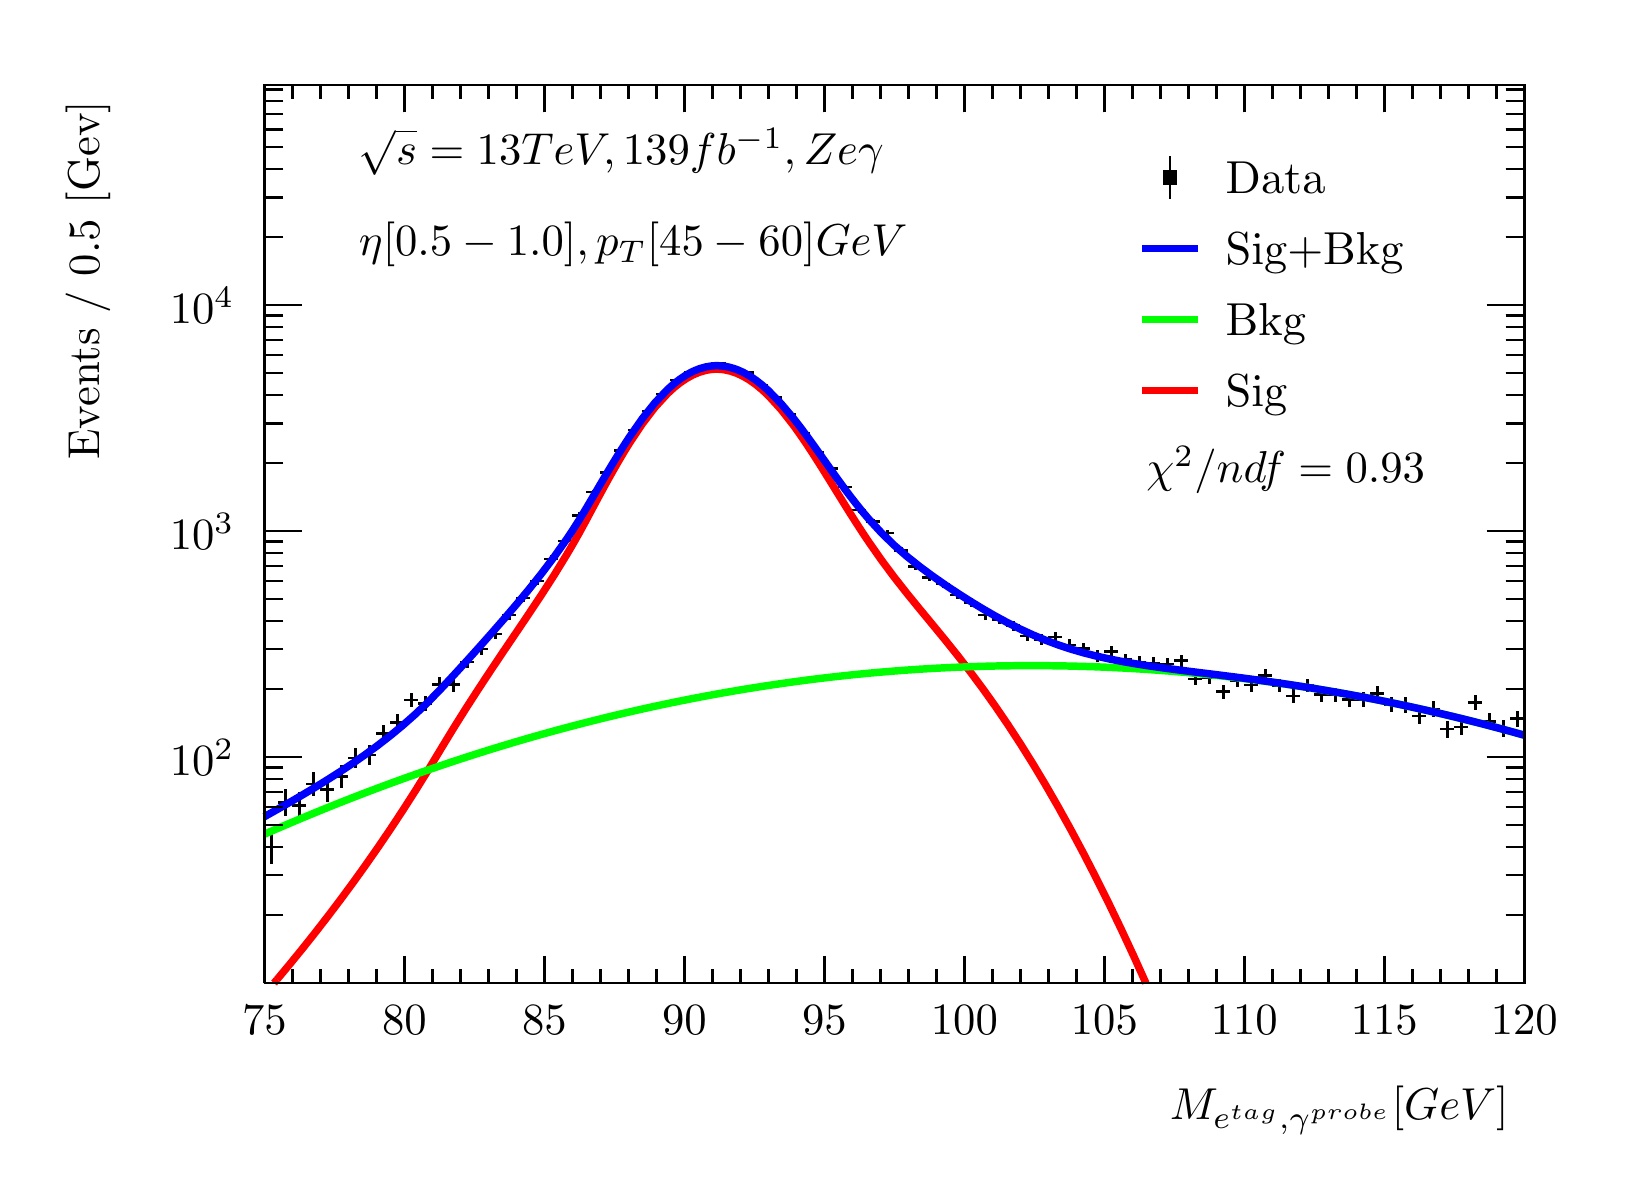
\begin{tikzpicture}
\pgfdeclareplotmark{cross} {
\pgfpathmoveto{\pgfpoint{-0.3\pgfplotmarksize}{\pgfplotmarksize}}
\pgfpathlineto{\pgfpoint{+0.3\pgfplotmarksize}{\pgfplotmarksize}}
\pgfpathlineto{\pgfpoint{+0.3\pgfplotmarksize}{0.3\pgfplotmarksize}}
\pgfpathlineto{\pgfpoint{+1\pgfplotmarksize}{0.3\pgfplotmarksize}}
\pgfpathlineto{\pgfpoint{+1\pgfplotmarksize}{-0.3\pgfplotmarksize}}
\pgfpathlineto{\pgfpoint{+0.3\pgfplotmarksize}{-0.3\pgfplotmarksize}}
\pgfpathlineto{\pgfpoint{+0.3\pgfplotmarksize}{-1.\pgfplotmarksize}}
\pgfpathlineto{\pgfpoint{-0.3\pgfplotmarksize}{-1.\pgfplotmarksize}}
\pgfpathlineto{\pgfpoint{-0.3\pgfplotmarksize}{-0.3\pgfplotmarksize}}
\pgfpathlineto{\pgfpoint{-1.\pgfplotmarksize}{-0.3\pgfplotmarksize}}
\pgfpathlineto{\pgfpoint{-1.\pgfplotmarksize}{0.3\pgfplotmarksize}}
\pgfpathlineto{\pgfpoint{-0.3\pgfplotmarksize}{0.3\pgfplotmarksize}}
\pgfpathclose
\pgfusepathqstroke
}
\pgfdeclareplotmark{cross*} {
\pgfpathmoveto{\pgfpoint{-0.3\pgfplotmarksize}{\pgfplotmarksize}}
\pgfpathlineto{\pgfpoint{+0.3\pgfplotmarksize}{\pgfplotmarksize}}
\pgfpathlineto{\pgfpoint{+0.3\pgfplotmarksize}{0.3\pgfplotmarksize}}
\pgfpathlineto{\pgfpoint{+1\pgfplotmarksize}{0.3\pgfplotmarksize}}
\pgfpathlineto{\pgfpoint{+1\pgfplotmarksize}{-0.3\pgfplotmarksize}}
\pgfpathlineto{\pgfpoint{+0.3\pgfplotmarksize}{-0.3\pgfplotmarksize}}
\pgfpathlineto{\pgfpoint{+0.3\pgfplotmarksize}{-1.\pgfplotmarksize}}
\pgfpathlineto{\pgfpoint{-0.3\pgfplotmarksize}{-1.\pgfplotmarksize}}
\pgfpathlineto{\pgfpoint{-0.3\pgfplotmarksize}{-0.3\pgfplotmarksize}}
\pgfpathlineto{\pgfpoint{-1.\pgfplotmarksize}{-0.3\pgfplotmarksize}}
\pgfpathlineto{\pgfpoint{-1.\pgfplotmarksize}{0.3\pgfplotmarksize}}
\pgfpathlineto{\pgfpoint{-0.3\pgfplotmarksize}{0.3\pgfplotmarksize}}
\pgfpathclose
\pgfusepathqfillstroke
}
\pgfdeclareplotmark{newstar} {
\pgfpathmoveto{\pgfqpoint{0pt}{\pgfplotmarksize}}
\pgfpathlineto{\pgfqpointpolar{44}{0.5\pgfplotmarksize}}
\pgfpathlineto{\pgfqpointpolar{18}{\pgfplotmarksize}}
\pgfpathlineto{\pgfqpointpolar{-20}{0.5\pgfplotmarksize}}
\pgfpathlineto{\pgfqpointpolar{-54}{\pgfplotmarksize}}
\pgfpathlineto{\pgfqpointpolar{-90}{0.5\pgfplotmarksize}}
\pgfpathlineto{\pgfqpointpolar{234}{\pgfplotmarksize}}
\pgfpathlineto{\pgfqpointpolar{198}{0.5\pgfplotmarksize}}
\pgfpathlineto{\pgfqpointpolar{162}{\pgfplotmarksize}}
\pgfpathlineto{\pgfqpointpolar{134}{0.5\pgfplotmarksize}}
\pgfpathclose
\pgfusepathqstroke
}
\pgfdeclareplotmark{newstar*} {
\pgfpathmoveto{\pgfqpoint{0pt}{\pgfplotmarksize}}
\pgfpathlineto{\pgfqpointpolar{44}{0.5\pgfplotmarksize}}
\pgfpathlineto{\pgfqpointpolar{18}{\pgfplotmarksize}}
\pgfpathlineto{\pgfqpointpolar{-20}{0.5\pgfplotmarksize}}
\pgfpathlineto{\pgfqpointpolar{-54}{\pgfplotmarksize}}
\pgfpathlineto{\pgfqpointpolar{-90}{0.5\pgfplotmarksize}}
\pgfpathlineto{\pgfqpointpolar{234}{\pgfplotmarksize}}
\pgfpathlineto{\pgfqpointpolar{198}{0.5\pgfplotmarksize}}
\pgfpathlineto{\pgfqpointpolar{162}{\pgfplotmarksize}}
\pgfpathlineto{\pgfqpointpolar{134}{0.5\pgfplotmarksize}}
\pgfpathclose
\pgfusepathqfillstroke
}
\definecolor{c}{rgb}{1,1,1};
\draw [color=c, fill=c] (0,0) rectangle (20,14.4361);
\draw [color=c, fill=c] (3,2.30977) rectangle (19,13.7143);
\definecolor{c}{rgb}{0,0,0};
\draw [c,line width=0.9] (3,2.30977) -- (3,13.7143) -- (19,13.7143) -- (19,2.30977) -- (3,2.30977);
\definecolor{c}{rgb}{1,1,1};
\draw [color=c, fill=c] (3,2.30977) rectangle (19,13.7143);
\definecolor{c}{rgb}{0,0,0};
\draw [c,line width=0.9] (3,2.30977) -- (3,13.7143) -- (19,13.7143) -- (19,2.30977) -- (3,2.30977);
\draw [c,line width=0.9] (3,2.30977) -- (19,2.30977);
\draw [c,line width=0.9] (3,2.65624) -- (3,2.30977);
\draw [c,line width=0.9] (3.35556,2.48301) -- (3.35556,2.30977);
\draw [c,line width=0.9] (3.71111,2.48301) -- (3.71111,2.30977);
\draw [c,line width=0.9] (4.06667,2.48301) -- (4.06667,2.30977);
\draw [c,line width=0.9] (4.42222,2.48301) -- (4.42222,2.30977);
\draw [c,line width=0.9] (4.77778,2.65624) -- (4.77778,2.30977);
\draw [c,line width=0.9] (5.13333,2.48301) -- (5.13333,2.30977);
\draw [c,line width=0.9] (5.48889,2.48301) -- (5.48889,2.30977);
\draw [c,line width=0.9] (5.84444,2.48301) -- (5.84444,2.30977);
\draw [c,line width=0.9] (6.2,2.48301) -- (6.2,2.30977);
\draw [c,line width=0.9] (6.55556,2.65624) -- (6.55556,2.30977);
\draw [c,line width=0.9] (6.91111,2.48301) -- (6.91111,2.30977);
\draw [c,line width=0.9] (7.26667,2.48301) -- (7.26667,2.30977);
\draw [c,line width=0.9] (7.62222,2.48301) -- (7.62222,2.30977);
\draw [c,line width=0.9] (7.97778,2.48301) -- (7.97778,2.30977);
\draw [c,line width=0.9] (8.33333,2.65624) -- (8.33333,2.30977);
\draw [c,line width=0.9] (8.68889,2.48301) -- (8.68889,2.30977);
\draw [c,line width=0.9] (9.04444,2.48301) -- (9.04444,2.30977);
\draw [c,line width=0.9] (9.4,2.48301) -- (9.4,2.30977);
\draw [c,line width=0.9] (9.75556,2.48301) -- (9.75556,2.30977);
\draw [c,line width=0.9] (10.1111,2.65624) -- (10.1111,2.30977);
\draw [c,line width=0.9] (10.4667,2.48301) -- (10.4667,2.30977);
\draw [c,line width=0.9] (10.8222,2.48301) -- (10.8222,2.30977);
\draw [c,line width=0.9] (11.1778,2.48301) -- (11.1778,2.30977);
\draw [c,line width=0.9] (11.5333,2.48301) -- (11.5333,2.30977);
\draw [c,line width=0.9] (11.8889,2.65624) -- (11.8889,2.30977);
\draw [c,line width=0.9] (12.2444,2.48301) -- (12.2444,2.30977);
\draw [c,line width=0.9] (12.6,2.48301) -- (12.6,2.30977);
\draw [c,line width=0.9] (12.9556,2.48301) -- (12.9556,2.30977);
\draw [c,line width=0.9] (13.3111,2.48301) -- (13.3111,2.30977);
\draw [c,line width=0.9] (13.6667,2.65624) -- (13.6667,2.30977);
\draw [c,line width=0.9] (14.0222,2.48301) -- (14.0222,2.30977);
\draw [c,line width=0.9] (14.3778,2.48301) -- (14.3778,2.30977);
\draw [c,line width=0.9] (14.7333,2.48301) -- (14.7333,2.30977);
\draw [c,line width=0.9] (15.0889,2.48301) -- (15.0889,2.30977);
\draw [c,line width=0.9] (15.4444,2.65624) -- (15.4444,2.30977);
\draw [c,line width=0.9] (15.8,2.48301) -- (15.8,2.30977);
\draw [c,line width=0.9] (16.1556,2.48301) -- (16.1556,2.30977);
\draw [c,line width=0.9] (16.5111,2.48301) -- (16.5111,2.30977);
\draw [c,line width=0.9] (16.8667,2.48301) -- (16.8667,2.30977);
\draw [c,line width=0.9] (17.2222,2.65624) -- (17.2222,2.30977);
\draw [c,line width=0.9] (17.5778,2.48301) -- (17.5778,2.30977);
\draw [c,line width=0.9] (17.9333,2.48301) -- (17.9333,2.30977);
\draw [c,line width=0.9] (18.2889,2.48301) -- (18.2889,2.30977);
\draw [c,line width=0.9] (18.6444,2.48301) -- (18.6444,2.30977);
\draw [c,line width=0.9] (19,2.65624) -- (19,2.30977);
\draw [c,line width=0.9] (19,2.65624) -- (19,2.30977);
\draw [anchor=base] (3,1.66015) node[scale=1.61424, color=c, rotate=0]{75};
\draw [anchor=base] (4.77778,1.66015) node[scale=1.61424, color=c, rotate=0]{80};
\draw [anchor=base] (6.55556,1.66015) node[scale=1.61424, color=c, rotate=0]{85};
\draw [anchor=base] (8.33333,1.66015) node[scale=1.61424, color=c, rotate=0]{90};
\draw [anchor=base] (10.1111,1.66015) node[scale=1.61424, color=c, rotate=0]{95};
\draw [anchor=base] (11.8889,1.66015) node[scale=1.61424, color=c, rotate=0]{100};
\draw [anchor=base] (13.6667,1.66015) node[scale=1.61424, color=c, rotate=0]{105};
\draw [anchor=base] (15.4444,1.66015) node[scale=1.61424, color=c, rotate=0]{110};
\draw [anchor=base] (17.2222,1.66015) node[scale=1.61424, color=c, rotate=0]{115};
\draw [anchor=base] (19,1.66015) node[scale=1.61424, color=c, rotate=0]{120};
\draw [anchor= east] (19,0.692932) node[scale=1.61424, color=c, rotate=0]{$M_{e^{tag}, \gamma^{probe}}  [GeV]$};
\draw [c,line width=0.9] (3,13.7143) -- (19,13.7143);
\draw [c,line width=0.9] (3,13.3678) -- (3,13.7143);
\draw [c,line width=0.9] (3.35556,13.5411) -- (3.35556,13.7143);
\draw [c,line width=0.9] (3.71111,13.5411) -- (3.71111,13.7143);
\draw [c,line width=0.9] (4.06667,13.5411) -- (4.06667,13.7143);
\draw [c,line width=0.9] (4.42222,13.5411) -- (4.42222,13.7143);
\draw [c,line width=0.9] (4.77778,13.3678) -- (4.77778,13.7143);
\draw [c,line width=0.9] (5.13333,13.5411) -- (5.13333,13.7143);
\draw [c,line width=0.9] (5.48889,13.5411) -- (5.48889,13.7143);
\draw [c,line width=0.9] (5.84444,13.5411) -- (5.84444,13.7143);
\draw [c,line width=0.9] (6.2,13.5411) -- (6.2,13.7143);
\draw [c,line width=0.9] (6.55556,13.3678) -- (6.55556,13.7143);
\draw [c,line width=0.9] (6.91111,13.5411) -- (6.91111,13.7143);
\draw [c,line width=0.9] (7.26667,13.5411) -- (7.26667,13.7143);
\draw [c,line width=0.9] (7.62222,13.5411) -- (7.62222,13.7143);
\draw [c,line width=0.9] (7.97778,13.5411) -- (7.97778,13.7143);
\draw [c,line width=0.9] (8.33333,13.3678) -- (8.33333,13.7143);
\draw [c,line width=0.9] (8.68889,13.5411) -- (8.68889,13.7143);
\draw [c,line width=0.9] (9.04444,13.5411) -- (9.04444,13.7143);
\draw [c,line width=0.9] (9.4,13.5411) -- (9.4,13.7143);
\draw [c,line width=0.9] (9.75556,13.5411) -- (9.75556,13.7143);
\draw [c,line width=0.9] (10.1111,13.3678) -- (10.1111,13.7143);
\draw [c,line width=0.9] (10.4667,13.5411) -- (10.4667,13.7143);
\draw [c,line width=0.9] (10.8222,13.5411) -- (10.8222,13.7143);
\draw [c,line width=0.9] (11.1778,13.5411) -- (11.1778,13.7143);
\draw [c,line width=0.9] (11.5333,13.5411) -- (11.5333,13.7143);
\draw [c,line width=0.9] (11.8889,13.3678) -- (11.8889,13.7143);
\draw [c,line width=0.9] (12.2444,13.5411) -- (12.2444,13.7143);
\draw [c,line width=0.9] (12.6,13.5411) -- (12.6,13.7143);
\draw [c,line width=0.9] (12.9556,13.5411) -- (12.9556,13.7143);
\draw [c,line width=0.9] (13.3111,13.5411) -- (13.3111,13.7143);
\draw [c,line width=0.9] (13.6667,13.3678) -- (13.6667,13.7143);
\draw [c,line width=0.9] (14.0222,13.5411) -- (14.0222,13.7143);
\draw [c,line width=0.9] (14.3778,13.5411) -- (14.3778,13.7143);
\draw [c,line width=0.9] (14.7333,13.5411) -- (14.7333,13.7143);
\draw [c,line width=0.9] (15.0889,13.5411) -- (15.0889,13.7143);
\draw [c,line width=0.9] (15.4444,13.3678) -- (15.4444,13.7143);
\draw [c,line width=0.9] (15.8,13.5411) -- (15.8,13.7143);
\draw [c,line width=0.9] (16.1556,13.5411) -- (16.1556,13.7143);
\draw [c,line width=0.9] (16.5111,13.5411) -- (16.5111,13.7143);
\draw [c,line width=0.9] (16.8667,13.5411) -- (16.8667,13.7143);
\draw [c,line width=0.9] (17.2222,13.3678) -- (17.2222,13.7143);
\draw [c,line width=0.9] (17.5778,13.5411) -- (17.5778,13.7143);
\draw [c,line width=0.9] (17.9333,13.5411) -- (17.9333,13.7143);
\draw [c,line width=0.9] (18.2889,13.5411) -- (18.2889,13.7143);
\draw [c,line width=0.9] (18.6444,13.5411) -- (18.6444,13.7143);
\draw [c,line width=0.9] (19,13.3678) -- (19,13.7143);
\draw [c,line width=0.9] (19,13.3678) -- (19,13.7143);
\draw [c,line width=0.9] (3,2.30977) -- (3,13.7143);
\draw [c,line width=0.9] (3.237,3.17371) -- (3,3.17371);
\draw [c,line width=0.9] (3.237,3.67908) -- (3,3.67908);
\draw [c,line width=0.9] (3.237,4.03764) -- (3,4.03764);
\draw [c,line width=0.9] (3.237,4.31577) -- (3,4.31577);
\draw [c,line width=0.9] (3.237,4.54301) -- (3,4.54301);
\draw [c,line width=0.9] (3.237,4.73514) -- (3,4.73514);
\draw [c,line width=0.9] (3.237,4.90158) -- (3,4.90158);
\draw [c,line width=0.9] (3.237,5.04838) -- (3,5.04838);
\draw [c,line width=0.9] (3.474,5.1797) -- (3,5.1797);
\draw [anchor= east] (2.82,5.1797) node[scale=1.61424, color=c, rotate=0]{$10^{2}$};
\draw [c,line width=0.9] (3.237,6.04363) -- (3,6.04363);
\draw [c,line width=0.9] (3.237,6.549) -- (3,6.549);
\draw [c,line width=0.9] (3.237,6.90757) -- (3,6.90757);
\draw [c,line width=0.9] (3.237,7.18569) -- (3,7.18569);
\draw [c,line width=0.9] (3.237,7.41294) -- (3,7.41294);
\draw [c,line width=0.9] (3.237,7.60507) -- (3,7.60507);
\draw [c,line width=0.9] (3.237,7.7715) -- (3,7.7715);
\draw [c,line width=0.9] (3.237,7.91831) -- (3,7.91831);
\draw [c,line width=0.9] (3.474,8.04963) -- (3,8.04963);
\draw [anchor= east] (2.82,8.04963) node[scale=1.61424, color=c, rotate=0]{$10^{3}$};
\draw [c,line width=0.9] (3.237,8.91356) -- (3,8.91356);
\draw [c,line width=0.9] (3.237,9.41893) -- (3,9.41893);
\draw [c,line width=0.9] (3.237,9.7775) -- (3,9.7775);
\draw [c,line width=0.9] (3.237,10.0556) -- (3,10.0556);
\draw [c,line width=0.9] (3.237,10.2829) -- (3,10.2829);
\draw [c,line width=0.9] (3.237,10.475) -- (3,10.475);
\draw [c,line width=0.9] (3.237,10.6414) -- (3,10.6414);
\draw [c,line width=0.9] (3.237,10.7882) -- (3,10.7882);
\draw [c,line width=0.9] (3.474,10.9196) -- (3,10.9196);
\draw [anchor= east] (2.82,10.9196) node[scale=1.61424, color=c, rotate=0]{$10^{4}$};
\draw [c,line width=0.9] (3.237,11.7835) -- (3,11.7835);
\draw [c,line width=0.9] (3.237,12.2889) -- (3,12.2889);
\draw [c,line width=0.9] (3.237,12.6474) -- (3,12.6474);
\draw [c,line width=0.9] (3.237,12.9256) -- (3,12.9256);
\draw [c,line width=0.9] (3.237,13.1528) -- (3,13.1528);
\draw [c,line width=0.9] (3.237,13.3449) -- (3,13.3449);
\draw [c,line width=0.9] (3.237,13.5114) -- (3,13.5114);
\draw [c,line width=0.9] (3.237,13.6582) -- (3,13.6582);
\draw [anchor= east] (0.76,13.7143) node[scale=1.61424, color=c, rotate=90]{Events / 0.5 [Gev]};
\draw [c,line width=0.9] (19,2.30977) -- (19,13.7143);
\draw [c,line width=0.9] (18.763,3.17371) -- (19,3.17371);
\draw [c,line width=0.9] (18.763,3.67908) -- (19,3.67908);
\draw [c,line width=0.9] (18.763,4.03764) -- (19,4.03764);
\draw [c,line width=0.9] (18.763,4.31577) -- (19,4.31577);
\draw [c,line width=0.9] (18.763,4.54301) -- (19,4.54301);
\draw [c,line width=0.9] (18.763,4.73514) -- (19,4.73514);
\draw [c,line width=0.9] (18.763,4.90158) -- (19,4.90158);
\draw [c,line width=0.9] (18.763,5.04838) -- (19,5.04838);
\draw [c,line width=0.9] (18.526,5.1797) -- (19,5.1797);
\draw [c,line width=0.9] (18.763,6.04363) -- (19,6.04363);
\draw [c,line width=0.9] (18.763,6.549) -- (19,6.549);
\draw [c,line width=0.9] (18.763,6.90757) -- (19,6.90757);
\draw [c,line width=0.9] (18.763,7.18569) -- (19,7.18569);
\draw [c,line width=0.9] (18.763,7.41294) -- (19,7.41294);
\draw [c,line width=0.9] (18.763,7.60507) -- (19,7.60507);
\draw [c,line width=0.9] (18.763,7.7715) -- (19,7.7715);
\draw [c,line width=0.9] (18.763,7.91831) -- (19,7.91831);
\draw [c,line width=0.9] (18.526,8.04963) -- (19,8.04963);
\draw [c,line width=0.9] (18.763,8.91356) -- (19,8.91356);
\draw [c,line width=0.9] (18.763,9.41893) -- (19,9.41893);
\draw [c,line width=0.9] (18.763,9.7775) -- (19,9.7775);
\draw [c,line width=0.9] (18.763,10.0556) -- (19,10.0556);
\draw [c,line width=0.9] (18.763,10.2829) -- (19,10.2829);
\draw [c,line width=0.9] (18.763,10.475) -- (19,10.475);
\draw [c,line width=0.9] (18.763,10.6414) -- (19,10.6414);
\draw [c,line width=0.9] (18.763,10.7882) -- (19,10.7882);
\draw [c,line width=0.9] (18.526,10.9196) -- (19,10.9196);
\draw [c,line width=0.9] (18.763,11.7835) -- (19,11.7835);
\draw [c,line width=0.9] (18.763,12.2889) -- (19,12.2889);
\draw [c,line width=0.9] (18.763,12.6474) -- (19,12.6474);
\draw [c,line width=0.9] (18.763,12.9256) -- (19,12.9256);
\draw [c,line width=0.9] (18.763,13.1528) -- (19,13.1528);
\draw [c,line width=0.9] (18.763,13.3449) -- (19,13.3449);
\draw [c,line width=0.9] (18.763,13.5114) -- (19,13.5114);
\draw [c,line width=0.9] (18.763,13.6582) -- (19,13.6582);
\draw [c,line width=0.9] (3.08889,4.03764) -- (3,4.03764);
\draw [c,line width=0.9] (3,4.03764) -- (3,4.03764);
\draw [c,line width=0.9] (3.08889,4.03764) -- (3.17778,4.03764);
\draw [c,line width=0.9] (3.17778,4.03764) -- (3.17778,4.03764);
\draw [c,line width=0.9] (3.08889,4.03764) -- (3.08889,4.24861);
\draw [c,line width=0.9] (3.08889,4.24861) -- (3.08889,4.24861);
\draw [c,line width=0.9] (3.08889,4.03764) -- (3.08889,3.82411);
\draw [c,line width=0.9] (3.08889,3.82411) -- (3.08889,3.82411);
\draw [c,line width=0.9] (3.26667,4.60382) -- (3.17778,4.60382);
\draw [c,line width=0.9] (3.17778,4.60382) -- (3.17778,4.60382);
\draw [c,line width=0.9] (3.26667,4.60382) -- (3.35556,4.60382);
\draw [c,line width=0.9] (3.35556,4.60382) -- (3.35556,4.60382);
\draw [c,line width=0.9] (3.26667,4.60382) -- (3.26667,4.7699);
\draw [c,line width=0.9] (3.26667,4.7699) -- (3.26667,4.7699);
\draw [c,line width=0.9] (3.26667,4.60382) -- (3.26667,4.43646);
\draw [c,line width=0.9] (3.26667,4.43646) -- (3.26667,4.43646);
\draw [c,line width=0.9] (3.44444,4.56361) -- (3.35556,4.56361);
\draw [c,line width=0.9] (3.35556,4.56361) -- (3.35556,4.56361);
\draw [c,line width=0.9] (3.44444,4.56361) -- (3.53333,4.56361);
\draw [c,line width=0.9] (3.53333,4.56361) -- (3.53333,4.56361);
\draw [c,line width=0.9] (3.44444,4.56361) -- (3.44444,4.73252);
\draw [c,line width=0.9] (3.44444,4.73252) -- (3.44444,4.73252);
\draw [c,line width=0.9] (3.44444,4.56361) -- (3.44444,4.39335);
\draw [c,line width=0.9] (3.44444,4.39335) -- (3.44444,4.39335);
\draw [c,line width=0.9] (3.62222,4.83765) -- (3.53333,4.83765);
\draw [c,line width=0.9] (3.53333,4.83765) -- (3.53333,4.83765);
\draw [c,line width=0.9] (3.62222,4.83765) -- (3.71111,4.83765);
\draw [c,line width=0.9] (3.71111,4.83765) -- (3.71111,4.83765);
\draw [c,line width=0.9] (3.62222,4.83765) -- (3.62222,4.98818);
\draw [c,line width=0.9] (3.62222,4.98818) -- (3.62222,4.98818);
\draw [c,line width=0.9] (3.62222,4.83765) -- (3.62222,4.68614);
\draw [c,line width=0.9] (3.62222,4.68614) -- (3.62222,4.68614);
\draw [c,line width=0.9] (3.8,4.77026) -- (3.71111,4.77026);
\draw [c,line width=0.9] (3.71111,4.77026) -- (3.71111,4.77026);
\draw [c,line width=0.9] (3.8,4.77026) -- (3.88889,4.77026);
\draw [c,line width=0.9] (3.88889,4.77026) -- (3.88889,4.77026);
\draw [c,line width=0.9] (3.8,4.77026) -- (3.8,4.92511);
\draw [c,line width=0.9] (3.8,4.92511) -- (3.8,4.92511);
\draw [c,line width=0.9] (3.8,4.77026) -- (3.8,4.61435);
\draw [c,line width=0.9] (3.8,4.61435) -- (3.8,4.61435);
\draw [c,line width=0.9] (3.97778,4.93235) -- (3.88889,4.93235);
\draw [c,line width=0.9] (3.88889,4.93235) -- (3.88889,4.93235);
\draw [c,line width=0.9] (3.97778,4.93235) -- (4.06667,4.93235);
\draw [c,line width=0.9] (4.06667,4.93235) -- (4.06667,4.93235);
\draw [c,line width=0.9] (3.97778,4.93235) -- (3.97778,5.07702);
\draw [c,line width=0.9] (3.97778,5.07702) -- (3.97778,5.07702);
\draw [c,line width=0.9] (3.97778,4.93235) -- (3.97778,4.78682);
\draw [c,line width=0.9] (3.97778,4.78682) -- (3.97778,4.78682);
\draw [c,line width=0.9] (4.15556,5.16718) -- (4.06667,5.16718);
\draw [c,line width=0.9] (4.06667,5.16718) -- (4.06667,5.16718);
\draw [c,line width=0.9] (4.15556,5.16718) -- (4.24444,5.16718);
\draw [c,line width=0.9] (4.24444,5.16718) -- (4.24444,5.16718);
\draw [c,line width=0.9] (4.15556,5.16718) -- (4.15556,5.29831);
\draw [c,line width=0.9] (4.15556,5.29831) -- (4.15556,5.29831);
\draw [c,line width=0.9] (4.15556,5.16718) -- (4.15556,5.03539);
\draw [c,line width=0.9] (4.15556,5.03539) -- (4.15556,5.03539);
\draw [c,line width=0.9] (4.33333,5.20438) -- (4.24444,5.20438);
\draw [c,line width=0.9] (4.24444,5.20438) -- (4.24444,5.20438);
\draw [c,line width=0.9] (4.33333,5.20438) -- (4.42222,5.20438);
\draw [c,line width=0.9] (4.42222,5.20438) -- (4.42222,5.20438);
\draw [c,line width=0.9] (4.33333,5.20438) -- (4.33333,5.32774);
\draw [c,line width=0.9] (4.33333,5.32774) -- (4.33333,5.32774);
\draw [c,line width=0.9] (4.33333,5.20438) -- (4.33333,5.08102);
\draw [c,line width=0.9] (4.33333,5.08102) -- (4.33333,5.08102);
\draw [c,line width=0.9] (4.51111,5.47761) -- (4.42222,5.47761);
\draw [c,line width=0.9] (4.42222,5.47761) -- (4.42222,5.47761);
\draw [c,line width=0.9] (4.51111,5.47761) -- (4.6,5.47761);
\draw [c,line width=0.9] (4.6,5.47761) -- (4.6,5.47761);
\draw [c,line width=0.9] (4.51111,5.47761) -- (4.51111,5.58817);
\draw [c,line width=0.9] (4.51111,5.58817) -- (4.51111,5.58817);
\draw [c,line width=0.9] (4.51111,5.47761) -- (4.51111,5.36705);
\draw [c,line width=0.9] (4.51111,5.36705) -- (4.51111,5.36705);
\draw [c,line width=0.9] (4.68889,5.61676) -- (4.6,5.61676);
\draw [c,line width=0.9] (4.6,5.61676) -- (4.6,5.61676);
\draw [c,line width=0.9] (4.68889,5.61676) -- (4.77778,5.61676);
\draw [c,line width=0.9] (4.77778,5.61676) -- (4.77778,5.61676);
\draw [c,line width=0.9] (4.68889,5.61676) -- (4.68889,5.72132);
\draw [c,line width=0.9] (4.68889,5.72132) -- (4.68889,5.72132);
\draw [c,line width=0.9] (4.68889,5.61676) -- (4.68889,5.51219);
\draw [c,line width=0.9] (4.68889,5.51219) -- (4.68889,5.51219);
\draw [c,line width=0.9] (4.86667,5.90537) -- (4.77778,5.90537);
\draw [c,line width=0.9] (4.77778,5.90537) -- (4.77778,5.90537);
\draw [c,line width=0.9] (4.86667,5.90537) -- (4.95556,5.90537);
\draw [c,line width=0.9] (4.95556,5.90537) -- (4.95556,5.90537);
\draw [c,line width=0.9] (4.86667,5.90537) -- (4.86667,5.99851);
\draw [c,line width=0.9] (4.86667,5.99851) -- (4.86667,5.99851);
\draw [c,line width=0.9] (4.86667,5.90537) -- (4.86667,5.81223);
\draw [c,line width=0.9] (4.86667,5.81223) -- (4.86667,5.81223);
\draw [c,line width=0.9] (5.04444,5.86288) -- (4.95556,5.86288);
\draw [c,line width=0.9] (4.95556,5.86288) -- (4.95556,5.86288);
\draw [c,line width=0.9] (5.04444,5.86288) -- (5.13333,5.86288);
\draw [c,line width=0.9] (5.13333,5.86288) -- (5.13333,5.86288);
\draw [c,line width=0.9] (5.04444,5.86288) -- (5.04444,5.95762);
\draw [c,line width=0.9] (5.04444,5.95762) -- (5.04444,5.95762);
\draw [c,line width=0.9] (5.04444,5.86288) -- (5.04444,5.76814);
\draw [c,line width=0.9] (5.04444,5.76814) -- (5.04444,5.76814);
\draw [c,line width=0.9] (5.22222,6.10445) -- (5.13333,6.10445);
\draw [c,line width=0.9] (5.13333,6.10445) -- (5.13333,6.10445);
\draw [c,line width=0.9] (5.22222,6.10445) -- (5.31111,6.10445);
\draw [c,line width=0.9] (5.31111,6.10445) -- (5.31111,6.10445);
\draw [c,line width=0.9] (5.22222,6.10445) -- (5.22222,6.19044);
\draw [c,line width=0.9] (5.22222,6.19044) -- (5.22222,6.19044);
\draw [c,line width=0.9] (5.22222,6.10445) -- (5.22222,6.01846);
\draw [c,line width=0.9] (5.22222,6.01846) -- (5.22222,6.01846);
\draw [c,line width=0.9] (5.4,6.0985) -- (5.31111,6.0985);
\draw [c,line width=0.9] (5.31111,6.0985) -- (5.31111,6.0985);
\draw [c,line width=0.9] (5.4,6.0985) -- (5.48889,6.0985);
\draw [c,line width=0.9] (5.48889,6.0985) -- (5.48889,6.0985);
\draw [c,line width=0.9] (5.4,6.0985) -- (5.4,6.1847);
\draw [c,line width=0.9] (5.4,6.1847) -- (5.4,6.1847);
\draw [c,line width=0.9] (5.4,6.0985) -- (5.4,6.0123);
\draw [c,line width=0.9] (5.4,6.0123) -- (5.4,6.0123);
\draw [c,line width=0.9] (5.57778,6.38968) -- (5.48889,6.38968);
\draw [c,line width=0.9] (5.48889,6.38968) -- (5.48889,6.38968);
\draw [c,line width=0.9] (5.57778,6.38968) -- (5.66667,6.38968);
\draw [c,line width=0.9] (5.66667,6.38968) -- (5.66667,6.38968);
\draw [c,line width=0.9] (5.57778,6.38968) -- (5.57778,6.46637);
\draw [c,line width=0.9] (5.57778,6.46637) -- (5.57778,6.46637);
\draw [c,line width=0.9] (5.57778,6.38968) -- (5.57778,6.31298);
\draw [c,line width=0.9] (5.57778,6.31298) -- (5.57778,6.31298);
\draw [c,line width=0.9] (5.75556,6.55315) -- (5.66667,6.55315);
\draw [c,line width=0.9] (5.66667,6.55315) -- (5.66667,6.55315);
\draw [c,line width=0.9] (5.75556,6.55315) -- (5.84444,6.55315);
\draw [c,line width=0.9] (5.84444,6.55315) -- (5.84444,6.55315);
\draw [c,line width=0.9] (5.75556,6.55315) -- (5.75556,6.62498);
\draw [c,line width=0.9] (5.75556,6.62498) -- (5.75556,6.62498);
\draw [c,line width=0.9] (5.75556,6.55315) -- (5.75556,6.48132);
\draw [c,line width=0.9] (5.75556,6.48132) -- (5.75556,6.48132);
\draw [c,line width=0.9] (5.93333,6.74114) -- (5.84444,6.74114);
\draw [c,line width=0.9] (5.84444,6.74114) -- (5.84444,6.74114);
\draw [c,line width=0.9] (5.93333,6.74114) -- (6.02222,6.74114);
\draw [c,line width=0.9] (6.02222,6.74114) -- (6.02222,6.74114);
\draw [c,line width=0.9] (5.93333,6.74114) -- (5.93333,6.80775);
\draw [c,line width=0.9] (5.93333,6.80775) -- (5.93333,6.80775);
\draw [c,line width=0.9] (5.93333,6.74114) -- (5.93333,6.67452);
\draw [c,line width=0.9] (5.93333,6.67452) -- (5.93333,6.67452);
\draw [c,line width=0.9] (6.11111,6.98313) -- (6.02222,6.98313);
\draw [c,line width=0.9] (6.02222,6.98313) -- (6.02222,6.98313);
\draw [c,line width=0.9] (6.11111,6.98313) -- (6.2,6.98313);
\draw [c,line width=0.9] (6.2,6.98313) -- (6.2,6.98313);
\draw [c,line width=0.9] (6.11111,6.98313) -- (6.11111,7.04359);
\draw [c,line width=0.9] (6.11111,7.04359) -- (6.11111,7.04359);
\draw [c,line width=0.9] (6.11111,6.98313) -- (6.11111,6.92268);
\draw [c,line width=0.9] (6.11111,6.92268) -- (6.11111,6.92268);
\draw [c,line width=0.9] (6.28889,7.20302) -- (6.2,7.20302);
\draw [c,line width=0.9] (6.2,7.20302) -- (6.2,7.20302);
\draw [c,line width=0.9] (6.28889,7.20302) -- (6.37778,7.20302);
\draw [c,line width=0.9] (6.37778,7.20302) -- (6.37778,7.20302);
\draw [c,line width=0.9] (6.28889,7.20302) -- (6.28889,7.25837);
\draw [c,line width=0.9] (6.28889,7.25837) -- (6.28889,7.25837);
\draw [c,line width=0.9] (6.28889,7.20302) -- (6.28889,7.14767);
\draw [c,line width=0.9] (6.28889,7.14767) -- (6.28889,7.14767);
\draw [c,line width=0.9] (6.46667,7.41709) -- (6.37778,7.41709);
\draw [c,line width=0.9] (6.37778,7.41709) -- (6.37778,7.41709);
\draw [c,line width=0.9] (6.46667,7.41709) -- (6.55556,7.41709);
\draw [c,line width=0.9] (6.55556,7.41709) -- (6.55556,7.41709);
\draw [c,line width=0.9] (6.46667,7.41709) -- (6.46667,7.46788);
\draw [c,line width=0.9] (6.46667,7.46788) -- (6.46667,7.46788);
\draw [c,line width=0.9] (6.46667,7.41709) -- (6.46667,7.36629);
\draw [c,line width=0.9] (6.46667,7.36629) -- (6.46667,7.36629);
\draw [c,line width=0.9] (6.64444,7.69769) -- (6.55556,7.69769);
\draw [c,line width=0.9] (6.55556,7.69769) -- (6.55556,7.69769);
\draw [c,line width=0.9] (6.64444,7.69769) -- (6.73333,7.69769);
\draw [c,line width=0.9] (6.73333,7.69769) -- (6.73333,7.69769);
\draw [c,line width=0.9] (6.64444,7.69769) -- (6.64444,7.74308);
\draw [c,line width=0.9] (6.64444,7.74308) -- (6.64444,7.74308);
\draw [c,line width=0.9] (6.64444,7.69769) -- (6.64444,7.65231);
\draw [c,line width=0.9] (6.64444,7.65231) -- (6.64444,7.65231);
\draw [c,line width=0.9] (6.82222,7.92659) -- (6.73333,7.92659);
\draw [c,line width=0.9] (6.73333,7.92659) -- (6.73333,7.92659);
\draw [c,line width=0.9] (6.82222,7.92659) -- (6.91111,7.92659);
\draw [c,line width=0.9] (6.91111,7.92659) -- (6.91111,7.92659);
\draw [c,line width=0.9] (6.82222,7.92659) -- (6.82222,7.968);
\draw [c,line width=0.9] (6.82222,7.968) -- (6.82222,7.968);
\draw [c,line width=0.9] (6.82222,7.92659) -- (6.82222,7.88518);
\draw [c,line width=0.9] (6.82222,7.88518) -- (6.82222,7.88518);
\draw [c,line width=0.9] (7,8.24957) -- (6.91111,8.24957);
\draw [c,line width=0.9] (6.91111,8.24957) -- (6.91111,8.24957);
\draw [c,line width=0.9] (7,8.24957) -- (7.08889,8.24957);
\draw [c,line width=0.9] (7.08889,8.24957) -- (7.08889,8.24957);
\draw [c,line width=0.9] (7,8.24957) -- (7,8.28595);
\draw [c,line width=0.9] (7,8.28595) -- (7,8.28595);
\draw [c,line width=0.9] (7,8.24957) -- (7,8.2132);
\draw [c,line width=0.9] (7,8.2132) -- (7,8.2132);
\draw [c,line width=0.9] (7.17778,8.54331) -- (7.08889,8.54331);
\draw [c,line width=0.9] (7.08889,8.54331) -- (7.08889,8.54331);
\draw [c,line width=0.9] (7.17778,8.54331) -- (7.26667,8.54331);
\draw [c,line width=0.9] (7.26667,8.54331) -- (7.26667,8.54331);
\draw [c,line width=0.9] (7.17778,8.54331) -- (7.17778,8.57564);
\draw [c,line width=0.9] (7.17778,8.57564) -- (7.17778,8.57564);
\draw [c,line width=0.9] (7.17778,8.54331) -- (7.17778,8.51098);
\draw [c,line width=0.9] (7.17778,8.51098) -- (7.17778,8.51098);
\draw [c,line width=0.9] (7.35556,8.7967) -- (7.26667,8.7967);
\draw [c,line width=0.9] (7.26667,8.7967) -- (7.26667,8.7967);
\draw [c,line width=0.9] (7.35556,8.7967) -- (7.44444,8.7967);
\draw [c,line width=0.9] (7.44444,8.7967) -- (7.44444,8.7967);
\draw [c,line width=0.9] (7.35556,8.7967) -- (7.35556,8.82591);
\draw [c,line width=0.9] (7.35556,8.82591) -- (7.35556,8.82591);
\draw [c,line width=0.9] (7.35556,8.7967) -- (7.35556,8.76749);
\draw [c,line width=0.9] (7.35556,8.76749) -- (7.35556,8.76749);
\draw [c,line width=0.9] (7.53333,9.07414) -- (7.44444,9.07414);
\draw [c,line width=0.9] (7.44444,9.07414) -- (7.44444,9.07414);
\draw [c,line width=0.9] (7.53333,9.07414) -- (7.62222,9.07414);
\draw [c,line width=0.9] (7.62222,9.07414) -- (7.62222,9.07414);
\draw [c,line width=0.9] (7.53333,9.07414) -- (7.53333,9.10027);
\draw [c,line width=0.9] (7.53333,9.10027) -- (7.53333,9.10027);
\draw [c,line width=0.9] (7.53333,9.07414) -- (7.53333,9.04801);
\draw [c,line width=0.9] (7.53333,9.04801) -- (7.53333,9.04801);
\draw [c,line width=0.9] (7.71111,9.33027) -- (7.62222,9.33027);
\draw [c,line width=0.9] (7.62222,9.33027) -- (7.62222,9.33027);
\draw [c,line width=0.9] (7.71111,9.33027) -- (7.8,9.33027);
\draw [c,line width=0.9] (7.8,9.33027) -- (7.8,9.33027);
\draw [c,line width=0.9] (7.71111,9.33027) -- (7.71111,9.35385);
\draw [c,line width=0.9] (7.71111,9.35385) -- (7.71111,9.35385);
\draw [c,line width=0.9] (7.71111,9.33027) -- (7.71111,9.30669);
\draw [c,line width=0.9] (7.71111,9.30669) -- (7.71111,9.30669);
\draw [c,line width=0.9] (7.88889,9.57677) -- (7.8,9.57677);
\draw [c,line width=0.9] (7.8,9.57677) -- (7.8,9.57677);
\draw [c,line width=0.9] (7.88889,9.57677) -- (7.97778,9.57677);
\draw [c,line width=0.9] (7.97778,9.57677) -- (7.97778,9.57677);
\draw [c,line width=0.9] (7.88889,9.57677) -- (7.88889,9.59813);
\draw [c,line width=0.9] (7.88889,9.59813) -- (7.88889,9.59813);
\draw [c,line width=0.9] (7.88889,9.57677) -- (7.88889,9.55541);
\draw [c,line width=0.9] (7.88889,9.55541) -- (7.88889,9.55541);
\draw [c,line width=0.9] (8.06667,9.78897) -- (7.97778,9.78897);
\draw [c,line width=0.9] (7.97778,9.78897) -- (7.97778,9.78897);
\draw [c,line width=0.9] (8.06667,9.78897) -- (8.15556,9.78897);
\draw [c,line width=0.9] (8.15556,9.78897) -- (8.15556,9.78897);
\draw [c,line width=0.9] (8.06667,9.78897) -- (8.06667,9.80859);
\draw [c,line width=0.9] (8.06667,9.80859) -- (8.06667,9.80859);
\draw [c,line width=0.9] (8.06667,9.78897) -- (8.06667,9.76936);
\draw [c,line width=0.9] (8.06667,9.76936) -- (8.06667,9.76936);
\draw [c,line width=0.9] (8.24444,9.97132) -- (8.15556,9.97132);
\draw [c,line width=0.9] (8.15556,9.97132) -- (8.15556,9.97132);
\draw [c,line width=0.9] (8.24444,9.97132) -- (8.33333,9.97132);
\draw [c,line width=0.9] (8.33333,9.97132) -- (8.33333,9.97132);
\draw [c,line width=0.9] (8.24444,9.97132) -- (8.24444,9.98955);
\draw [c,line width=0.9] (8.24444,9.98955) -- (8.24444,9.98955);
\draw [c,line width=0.9] (8.24444,9.97132) -- (8.24444,9.95309);
\draw [c,line width=0.9] (8.24444,9.95309) -- (8.24444,9.95309);
\draw [c,line width=0.9] (8.42222,10.0702) -- (8.33333,10.0702);
\draw [c,line width=0.9] (8.33333,10.0702) -- (8.33333,10.0702);
\draw [c,line width=0.9] (8.42222,10.0702) -- (8.51111,10.0702);
\draw [c,line width=0.9] (8.51111,10.0702) -- (8.51111,10.0702);
\draw [c,line width=0.9] (8.42222,10.0702) -- (8.42222,10.0878);
\draw [c,line width=0.9] (8.42222,10.0878) -- (8.42222,10.0878);
\draw [c,line width=0.9] (8.42222,10.0702) -- (8.42222,10.0527);
\draw [c,line width=0.9] (8.42222,10.0527) -- (8.42222,10.0527);
\draw [c,line width=0.9] (8.6,10.1129) -- (8.51111,10.1129);
\draw [c,line width=0.9] (8.51111,10.1129) -- (8.51111,10.1129);
\draw [c,line width=0.9] (8.6,10.1129) -- (8.68889,10.1129);
\draw [c,line width=0.9] (8.68889,10.1129) -- (8.68889,10.1129);
\draw [c,line width=0.9] (8.6,10.1129) -- (8.6,10.1301);
\draw [c,line width=0.9] (8.6,10.1301) -- (8.6,10.1301);
\draw [c,line width=0.9] (8.6,10.1129) -- (8.6,10.0956);
\draw [c,line width=0.9] (8.6,10.0956) -- (8.6,10.0956);
\draw [c,line width=0.9] (8.77778,10.1805) -- (8.68889,10.1805);
\draw [c,line width=0.9] (8.68889,10.1805) -- (8.68889,10.1805);
\draw [c,line width=0.9] (8.77778,10.1805) -- (8.86667,10.1805);
\draw [c,line width=0.9] (8.86667,10.1805) -- (8.86667,10.1805);
\draw [c,line width=0.9] (8.77778,10.1805) -- (8.77778,10.1973);
\draw [c,line width=0.9] (8.77778,10.1973) -- (8.77778,10.1973);
\draw [c,line width=0.9] (8.77778,10.1805) -- (8.77778,10.1638);
\draw [c,line width=0.9] (8.77778,10.1638) -- (8.77778,10.1638);
\draw [c,line width=0.9] (8.95556,10.1093) -- (8.86667,10.1093);
\draw [c,line width=0.9] (8.86667,10.1093) -- (8.86667,10.1093);
\draw [c,line width=0.9] (8.95556,10.1093) -- (9.04444,10.1093);
\draw [c,line width=0.9] (9.04444,10.1093) -- (9.04444,10.1093);
\draw [c,line width=0.9] (8.95556,10.1093) -- (8.95556,10.1265);
\draw [c,line width=0.9] (8.95556,10.1265) -- (8.95556,10.1265);
\draw [c,line width=0.9] (8.95556,10.1093) -- (8.95556,10.092);
\draw [c,line width=0.9] (8.95556,10.092) -- (8.95556,10.092);
\draw [c,line width=0.9] (9.13333,10.0663) -- (9.04444,10.0663);
\draw [c,line width=0.9] (9.04444,10.0663) -- (9.04444,10.0663);
\draw [c,line width=0.9] (9.13333,10.0663) -- (9.22222,10.0663);
\draw [c,line width=0.9] (9.22222,10.0663) -- (9.22222,10.0663);
\draw [c,line width=0.9] (9.13333,10.0663) -- (9.13333,10.0838);
\draw [c,line width=0.9] (9.13333,10.0838) -- (9.13333,10.0838);
\draw [c,line width=0.9] (9.13333,10.0663) -- (9.13333,10.0487);
\draw [c,line width=0.9] (9.13333,10.0487) -- (9.13333,10.0487);
\draw [c,line width=0.9] (9.31111,9.89969) -- (9.22222,9.89969);
\draw [c,line width=0.9] (9.22222,9.89969) -- (9.22222,9.89969);
\draw [c,line width=0.9] (9.31111,9.89969) -- (9.4,9.89969);
\draw [c,line width=0.9] (9.4,9.89969) -- (9.4,9.89969);
\draw [c,line width=0.9] (9.31111,9.89969) -- (9.31111,9.91845);
\draw [c,line width=0.9] (9.31111,9.91845) -- (9.31111,9.91845);
\draw [c,line width=0.9] (9.31111,9.89969) -- (9.31111,9.88092);
\draw [c,line width=0.9] (9.31111,9.88092) -- (9.31111,9.88092);
\draw [c,line width=0.9] (9.48889,9.74626) -- (9.4,9.74626);
\draw [c,line width=0.9] (9.4,9.74626) -- (9.4,9.74626);
\draw [c,line width=0.9] (9.48889,9.74626) -- (9.57778,9.74626);
\draw [c,line width=0.9] (9.57778,9.74626) -- (9.57778,9.74626);
\draw [c,line width=0.9] (9.48889,9.74626) -- (9.48889,9.76622);
\draw [c,line width=0.9] (9.48889,9.76622) -- (9.48889,9.76622);
\draw [c,line width=0.9] (9.48889,9.74626) -- (9.48889,9.72631);
\draw [c,line width=0.9] (9.48889,9.72631) -- (9.48889,9.72631);
\draw [c,line width=0.9] (9.66667,9.52863) -- (9.57778,9.52863);
\draw [c,line width=0.9] (9.57778,9.52863) -- (9.57778,9.52863);
\draw [c,line width=0.9] (9.66667,9.52863) -- (9.75556,9.52863);
\draw [c,line width=0.9] (9.75556,9.52863) -- (9.75556,9.52863);
\draw [c,line width=0.9] (9.66667,9.52863) -- (9.66667,9.55041);
\draw [c,line width=0.9] (9.66667,9.55041) -- (9.66667,9.55041);
\draw [c,line width=0.9] (9.66667,9.52863) -- (9.66667,9.50685);
\draw [c,line width=0.9] (9.66667,9.50685) -- (9.66667,9.50685);
\draw [c,line width=0.9] (9.84444,9.28992) -- (9.75556,9.28992);
\draw [c,line width=0.9] (9.75556,9.28992) -- (9.75556,9.28992);
\draw [c,line width=0.9] (9.84444,9.28992) -- (9.93333,9.28992);
\draw [c,line width=0.9] (9.93333,9.28992) -- (9.93333,9.28992);
\draw [c,line width=0.9] (9.84444,9.28992) -- (9.84444,9.31388);
\draw [c,line width=0.9] (9.84444,9.31388) -- (9.84444,9.31388);
\draw [c,line width=0.9] (9.84444,9.28992) -- (9.84444,9.26595);
\draw [c,line width=0.9] (9.84444,9.26595) -- (9.84444,9.26595);
\draw [c,line width=0.9] (10.0222,9.047) -- (9.93333,9.047);
\draw [c,line width=0.9] (9.93333,9.047) -- (9.93333,9.047);
\draw [c,line width=0.9] (10.0222,9.047) -- (10.1111,9.047);
\draw [c,line width=0.9] (10.1111,9.047) -- (10.1111,9.047);
\draw [c,line width=0.9] (10.0222,9.047) -- (10.0222,9.07342);
\draw [c,line width=0.9] (10.0222,9.07342) -- (10.0222,9.07342);
\draw [c,line width=0.9] (10.0222,9.047) -- (10.0222,9.02059);
\draw [c,line width=0.9] (10.0222,9.02059) -- (10.0222,9.02059);
\draw [c,line width=0.9] (10.2,8.84371) -- (10.1111,8.84371);
\draw [c,line width=0.9] (10.1111,8.84371) -- (10.1111,8.84371);
\draw [c,line width=0.9] (10.2,8.84371) -- (10.2889,8.84371);
\draw [c,line width=0.9] (10.2889,8.84371) -- (10.2889,8.84371);
\draw [c,line width=0.9] (10.2,8.84371) -- (10.2,8.87238);
\draw [c,line width=0.9] (10.2,8.87238) -- (10.2,8.87238);
\draw [c,line width=0.9] (10.2,8.84371) -- (10.2,8.81505);
\draw [c,line width=0.9] (10.2,8.81505) -- (10.2,8.81505);
\draw [c,line width=0.9] (10.3778,8.60867) -- (10.2889,8.60867);
\draw [c,line width=0.9] (10.2889,8.60867) -- (10.2889,8.60867);
\draw [c,line width=0.9] (10.3778,8.60867) -- (10.4667,8.60867);
\draw [c,line width=0.9] (10.4667,8.60867) -- (10.4667,8.60867);
\draw [c,line width=0.9] (10.3778,8.60867) -- (10.3778,8.64016);
\draw [c,line width=0.9] (10.3778,8.64016) -- (10.3778,8.64016);
\draw [c,line width=0.9] (10.3778,8.60867) -- (10.3778,8.57717);
\draw [c,line width=0.9] (10.3778,8.57717) -- (10.3778,8.57717);
\draw [c,line width=0.9] (10.5556,8.31774) -- (10.4667,8.31774);
\draw [c,line width=0.9] (10.4667,8.31774) -- (10.4667,8.31774);
\draw [c,line width=0.9] (10.5556,8.31774) -- (10.6444,8.31774);
\draw [c,line width=0.9] (10.6444,8.31774) -- (10.6444,8.31774);
\draw [c,line width=0.9] (10.5556,8.31774) -- (10.5556,8.35314);
\draw [c,line width=0.9] (10.5556,8.35314) -- (10.5556,8.35314);
\draw [c,line width=0.9] (10.5556,8.31774) -- (10.5556,8.28235);
\draw [c,line width=0.9] (10.5556,8.28235) -- (10.5556,8.28235);
\draw [c,line width=0.9] (10.7333,8.16956) -- (10.6444,8.16956);
\draw [c,line width=0.9] (10.6444,8.16956) -- (10.6444,8.16956);
\draw [c,line width=0.9] (10.7333,8.16956) -- (10.8222,8.16956);
\draw [c,line width=0.9] (10.8222,8.16956) -- (10.8222,8.16956);
\draw [c,line width=0.9] (10.7333,8.16956) -- (10.7333,8.20712);
\draw [c,line width=0.9] (10.7333,8.20712) -- (10.7333,8.20712);
\draw [c,line width=0.9] (10.7333,8.16956) -- (10.7333,8.132);
\draw [c,line width=0.9] (10.7333,8.132) -- (10.7333,8.132);
\draw [c,line width=0.9] (10.9111,8.02572) -- (10.8222,8.02572);
\draw [c,line width=0.9] (10.8222,8.02572) -- (10.8222,8.02572);
\draw [c,line width=0.9] (10.9111,8.02572) -- (11,8.02572);
\draw [c,line width=0.9] (11,8.02572) -- (11,8.02572);
\draw [c,line width=0.9] (10.9111,8.02572) -- (10.9111,8.06551);
\draw [c,line width=0.9] (10.9111,8.06551) -- (10.9111,8.06551);
\draw [c,line width=0.9] (10.9111,8.02572) -- (10.9111,7.98593);
\draw [c,line width=0.9] (10.9111,7.98593) -- (10.9111,7.98593);
\draw [c,line width=0.9] (11.0889,7.80532) -- (11,7.80532);
\draw [c,line width=0.9] (11,7.80532) -- (11,7.80532);
\draw [c,line width=0.9] (11.0889,7.80532) -- (11.1778,7.80532);
\draw [c,line width=0.9] (11.1778,7.80532) -- (11.1778,7.80532);
\draw [c,line width=0.9] (11.0889,7.80532) -- (11.0889,7.84879);
\draw [c,line width=0.9] (11.0889,7.84879) -- (11.0889,7.84879);
\draw [c,line width=0.9] (11.0889,7.80532) -- (11.0889,7.76185);
\draw [c,line width=0.9] (11.0889,7.76185) -- (11.0889,7.76185);
\draw [c,line width=0.9] (11.2667,7.59793) -- (11.1778,7.59793);
\draw [c,line width=0.9] (11.1778,7.59793) -- (11.1778,7.59793);
\draw [c,line width=0.9] (11.2667,7.59793) -- (11.3556,7.59793);
\draw [c,line width=0.9] (11.3556,7.59793) -- (11.3556,7.59793);
\draw [c,line width=0.9] (11.2667,7.59793) -- (11.2667,7.64517);
\draw [c,line width=0.9] (11.2667,7.64517) -- (11.2667,7.64517);
\draw [c,line width=0.9] (11.2667,7.59793) -- (11.2667,7.55069);
\draw [c,line width=0.9] (11.2667,7.55069) -- (11.2667,7.55069);
\draw [c,line width=0.9] (11.4444,7.46182) -- (11.3556,7.46182);
\draw [c,line width=0.9] (11.3556,7.46182) -- (11.3556,7.46182);
\draw [c,line width=0.9] (11.4444,7.46182) -- (11.5333,7.46182);
\draw [c,line width=0.9] (11.5333,7.46182) -- (11.5333,7.46182);
\draw [c,line width=0.9] (11.4444,7.46182) -- (11.4444,7.51172);
\draw [c,line width=0.9] (11.4444,7.51172) -- (11.4444,7.51172);
\draw [c,line width=0.9] (11.4444,7.46182) -- (11.4444,7.41193);
\draw [c,line width=0.9] (11.4444,7.41193) -- (11.4444,7.41193);
\draw [c,line width=0.9] (11.6222,7.37498) -- (11.5333,7.37498);
\draw [c,line width=0.9] (11.5333,7.37498) -- (11.5333,7.37498);
\draw [c,line width=0.9] (11.6222,7.37498) -- (11.7111,7.37498);
\draw [c,line width=0.9] (11.7111,7.37498) -- (11.7111,7.37498);
\draw [c,line width=0.9] (11.6222,7.37498) -- (11.6222,7.42664);
\draw [c,line width=0.9] (11.6222,7.42664) -- (11.6222,7.42664);
\draw [c,line width=0.9] (11.6222,7.37498) -- (11.6222,7.32332);
\draw [c,line width=0.9] (11.6222,7.32332) -- (11.6222,7.32332);
\draw [c,line width=0.9] (11.8,7.23936) -- (11.7111,7.23936);
\draw [c,line width=0.9] (11.7111,7.23936) -- (11.7111,7.23936);
\draw [c,line width=0.9] (11.8,7.23936) -- (11.8889,7.23936);
\draw [c,line width=0.9] (11.8889,7.23936) -- (11.8889,7.23936);
\draw [c,line width=0.9] (11.8,7.23936) -- (11.8,7.29391);
\draw [c,line width=0.9] (11.8,7.29391) -- (11.8,7.29391);
\draw [c,line width=0.9] (11.8,7.23936) -- (11.8,7.18482);
\draw [c,line width=0.9] (11.8,7.18482) -- (11.8,7.18482);
\draw [c,line width=0.9] (11.9778,7.13741) -- (11.8889,7.13741);
\draw [c,line width=0.9] (11.8889,7.13741) -- (11.8889,7.13741);
\draw [c,line width=0.9] (11.9778,7.13741) -- (12.0667,7.13741);
\draw [c,line width=0.9] (12.0667,7.13741) -- (12.0667,7.13741);
\draw [c,line width=0.9] (11.9778,7.13741) -- (11.9778,7.19424);
\draw [c,line width=0.9] (11.9778,7.19424) -- (11.9778,7.19424);
\draw [c,line width=0.9] (11.9778,7.13741) -- (11.9778,7.08058);
\draw [c,line width=0.9] (11.9778,7.08058) -- (11.9778,7.08058);
\draw [c,line width=0.9] (12.1556,6.98313) -- (12.0667,6.98313);
\draw [c,line width=0.9] (12.0667,6.98313) -- (12.0667,6.98313);
\draw [c,line width=0.9] (12.1556,6.98313) -- (12.2444,6.98313);
\draw [c,line width=0.9] (12.2444,6.98313) -- (12.2444,6.98313);
\draw [c,line width=0.9] (12.1556,6.98313) -- (12.1556,7.04359);
\draw [c,line width=0.9] (12.1556,7.04359) -- (12.1556,7.04359);
\draw [c,line width=0.9] (12.1556,6.98313) -- (12.1556,6.92268);
\draw [c,line width=0.9] (12.1556,6.92268) -- (12.1556,6.92268);
\draw [c,line width=0.9] (12.3333,6.92613) -- (12.2444,6.92613);
\draw [c,line width=0.9] (12.2444,6.92613) -- (12.2444,6.92613);
\draw [c,line width=0.9] (12.3333,6.92613) -- (12.4222,6.92613);
\draw [c,line width=0.9] (12.4222,6.92613) -- (12.4222,6.92613);
\draw [c,line width=0.9] (12.3333,6.92613) -- (12.3333,6.98798);
\draw [c,line width=0.9] (12.3333,6.98798) -- (12.3333,6.98798);
\draw [c,line width=0.9] (12.3333,6.92613) -- (12.3333,6.86428);
\draw [c,line width=0.9] (12.3333,6.86428) -- (12.3333,6.86428);
\draw [c,line width=0.9] (12.5111,6.85018) -- (12.4222,6.85018);
\draw [c,line width=0.9] (12.4222,6.85018) -- (12.4222,6.85018);
\draw [c,line width=0.9] (12.5111,6.85018) -- (12.6,6.85018);
\draw [c,line width=0.9] (12.6,6.85018) -- (12.6,6.85018);
\draw [c,line width=0.9] (12.5111,6.85018) -- (12.5111,6.91395);
\draw [c,line width=0.9] (12.5111,6.91395) -- (12.5111,6.91395);
\draw [c,line width=0.9] (12.5111,6.85018) -- (12.5111,6.78642);
\draw [c,line width=0.9] (12.5111,6.78642) -- (12.5111,6.78642);
\draw [c,line width=0.9] (12.6889,6.71596) -- (12.6,6.71596);
\draw [c,line width=0.9] (12.6,6.71596) -- (12.6,6.71596);
\draw [c,line width=0.9] (12.6889,6.71596) -- (12.7778,6.71596);
\draw [c,line width=0.9] (12.7778,6.71596) -- (12.7778,6.71596);
\draw [c,line width=0.9] (12.6889,6.71596) -- (12.6889,6.78325);
\draw [c,line width=0.9] (12.6889,6.78325) -- (12.6889,6.78325);
\draw [c,line width=0.9] (12.6889,6.71596) -- (12.6889,6.64867);
\draw [c,line width=0.9] (12.6889,6.64867) -- (12.6889,6.64867);
\draw [c,line width=0.9] (12.8667,6.67533) -- (12.7778,6.67533);
\draw [c,line width=0.9] (12.7778,6.67533) -- (12.7778,6.67533);
\draw [c,line width=0.9] (12.8667,6.67533) -- (12.9556,6.67533);
\draw [c,line width=0.9] (12.9556,6.67533) -- (12.9556,6.67533);
\draw [c,line width=0.9] (12.8667,6.67533) -- (12.8667,6.74373);
\draw [c,line width=0.9] (12.8667,6.74373) -- (12.8667,6.74373);
\draw [c,line width=0.9] (12.8667,6.67533) -- (12.8667,6.60694);
\draw [c,line width=0.9] (12.8667,6.60694) -- (12.8667,6.60694);
\draw [c,line width=0.9] (13.0444,6.70501) -- (12.9556,6.70501);
\draw [c,line width=0.9] (12.9556,6.70501) -- (12.9556,6.70501);
\draw [c,line width=0.9] (13.0444,6.70501) -- (13.1333,6.70501);
\draw [c,line width=0.9] (13.1333,6.70501) -- (13.1333,6.70501);
\draw [c,line width=0.9] (13.0444,6.70501) -- (13.0444,6.7726);
\draw [c,line width=0.9] (13.0444,6.7726) -- (13.0444,6.7726);
\draw [c,line width=0.9] (13.0444,6.70501) -- (13.0444,6.63742);
\draw [c,line width=0.9] (13.0444,6.63742) -- (13.0444,6.63742);
\draw [c,line width=0.9] (13.2222,6.60585) -- (13.1333,6.60585);
\draw [c,line width=0.9] (13.1333,6.60585) -- (13.1333,6.60585);
\draw [c,line width=0.9] (13.2222,6.60585) -- (13.3111,6.60585);
\draw [c,line width=0.9] (13.3111,6.60585) -- (13.3111,6.60585);
\draw [c,line width=0.9] (13.2222,6.60585) -- (13.2222,6.67618);
\draw [c,line width=0.9] (13.2222,6.67618) -- (13.2222,6.67618);
\draw [c,line width=0.9] (13.2222,6.60585) -- (13.2222,6.53553);
\draw [c,line width=0.9] (13.2222,6.53553) -- (13.2222,6.53553);
\draw [c,line width=0.9] (13.4,6.55729) -- (13.3111,6.55729);
\draw [c,line width=0.9] (13.3111,6.55729) -- (13.3111,6.55729);
\draw [c,line width=0.9] (13.4,6.55729) -- (13.4889,6.55729);
\draw [c,line width=0.9] (13.4889,6.55729) -- (13.4889,6.55729);
\draw [c,line width=0.9] (13.4,6.55729) -- (13.4,6.629);
\draw [c,line width=0.9] (13.4,6.629) -- (13.4,6.629);
\draw [c,line width=0.9] (13.4,6.55729) -- (13.4,6.48558);
\draw [c,line width=0.9] (13.4,6.48558) -- (13.4,6.48558);
\draw [c,line width=0.9] (13.5778,6.46301) -- (13.4889,6.46301);
\draw [c,line width=0.9] (13.4889,6.46301) -- (13.4889,6.46301);
\draw [c,line width=0.9] (13.5778,6.46301) -- (13.6667,6.46301);
\draw [c,line width=0.9] (13.6667,6.46301) -- (13.6667,6.46301);
\draw [c,line width=0.9] (13.5778,6.46301) -- (13.5778,6.53749);
\draw [c,line width=0.9] (13.5778,6.53749) -- (13.5778,6.53749);
\draw [c,line width=0.9] (13.5778,6.46301) -- (13.5778,6.38854);
\draw [c,line width=0.9] (13.5778,6.38854) -- (13.5778,6.38854);
\draw [c,line width=0.9] (13.7556,6.51958) -- (13.6667,6.51958);
\draw [c,line width=0.9] (13.6667,6.51958) -- (13.6667,6.51958);
\draw [c,line width=0.9] (13.7556,6.51958) -- (13.8444,6.51958);
\draw [c,line width=0.9] (13.8444,6.51958) -- (13.8444,6.51958);
\draw [c,line width=0.9] (13.7556,6.51958) -- (13.7556,6.59238);
\draw [c,line width=0.9] (13.7556,6.59238) -- (13.7556,6.59238);
\draw [c,line width=0.9] (13.7556,6.51958) -- (13.7556,6.44677);
\draw [c,line width=0.9] (13.7556,6.44677) -- (13.7556,6.44677);
\draw [c,line width=0.9] (13.9333,6.41769) -- (13.8444,6.41769);
\draw [c,line width=0.9] (13.8444,6.41769) -- (13.8444,6.41769);
\draw [c,line width=0.9] (13.9333,6.41769) -- (14.0222,6.41769);
\draw [c,line width=0.9] (14.0222,6.41769) -- (14.0222,6.41769);
\draw [c,line width=0.9] (13.9333,6.41769) -- (13.9333,6.49353);
\draw [c,line width=0.9] (13.9333,6.49353) -- (13.9333,6.49353);
\draw [c,line width=0.9] (13.9333,6.41769) -- (13.9333,6.34184);
\draw [c,line width=0.9] (13.9333,6.34184) -- (13.9333,6.34184);
\draw [c,line width=0.9] (14.1111,6.38968) -- (14.0222,6.38968);
\draw [c,line width=0.9] (14.0222,6.38968) -- (14.0222,6.38968);
\draw [c,line width=0.9] (14.1111,6.38968) -- (14.2,6.38968);
\draw [c,line width=0.9] (14.2,6.38968) -- (14.2,6.38968);
\draw [c,line width=0.9] (14.1111,6.38968) -- (14.1111,6.46637);
\draw [c,line width=0.9] (14.1111,6.46637) -- (14.1111,6.46637);
\draw [c,line width=0.9] (14.1111,6.38968) -- (14.1111,6.31298);
\draw [c,line width=0.9] (14.1111,6.31298) -- (14.1111,6.31298);
\draw [c,line width=0.9] (14.2889,6.37543) -- (14.2,6.37543);
\draw [c,line width=0.9] (14.2,6.37543) -- (14.2,6.37543);
\draw [c,line width=0.9] (14.2889,6.37543) -- (14.3778,6.37543);
\draw [c,line width=0.9] (14.3778,6.37543) -- (14.3778,6.37543);
\draw [c,line width=0.9] (14.2889,6.37543) -- (14.2889,6.45257);
\draw [c,line width=0.9] (14.2889,6.45257) -- (14.2889,6.45257);
\draw [c,line width=0.9] (14.2889,6.37543) -- (14.2889,6.29829);
\draw [c,line width=0.9] (14.2889,6.29829) -- (14.2889,6.29829);
\draw [c,line width=0.9] (14.4667,6.36102) -- (14.3778,6.36102);
\draw [c,line width=0.9] (14.3778,6.36102) -- (14.3778,6.36102);
\draw [c,line width=0.9] (14.4667,6.36102) -- (14.5556,6.36102);
\draw [c,line width=0.9] (14.5556,6.36102) -- (14.5556,6.36102);
\draw [c,line width=0.9] (14.4667,6.36102) -- (14.4667,6.43861);
\draw [c,line width=0.9] (14.4667,6.43861) -- (14.4667,6.43861);
\draw [c,line width=0.9] (14.4667,6.36102) -- (14.4667,6.28344);
\draw [c,line width=0.9] (14.4667,6.28344) -- (14.4667,6.28344);
\draw [c,line width=0.9] (14.6444,6.40376) -- (14.5556,6.40376);
\draw [c,line width=0.9] (14.5556,6.40376) -- (14.5556,6.40376);
\draw [c,line width=0.9] (14.6444,6.40376) -- (14.7333,6.40376);
\draw [c,line width=0.9] (14.7333,6.40376) -- (14.7333,6.40376);
\draw [c,line width=0.9] (14.6444,6.40376) -- (14.6444,6.48002);
\draw [c,line width=0.9] (14.6444,6.48002) -- (14.6444,6.48002);
\draw [c,line width=0.9] (14.6444,6.40376) -- (14.6444,6.32749);
\draw [c,line width=0.9] (14.6444,6.32749) -- (14.6444,6.32749);
\draw [c,line width=0.9] (14.8222,6.17371) -- (14.7333,6.17371);
\draw [c,line width=0.9] (14.7333,6.17371) -- (14.7333,6.17371);
\draw [c,line width=0.9] (14.8222,6.17371) -- (14.9111,6.17371);
\draw [c,line width=0.9] (14.9111,6.17371) -- (14.9111,6.17371);
\draw [c,line width=0.9] (14.8222,6.17371) -- (14.8222,6.25735);
\draw [c,line width=0.9] (14.8222,6.25735) -- (14.8222,6.25735);
\draw [c,line width=0.9] (14.8222,6.17371) -- (14.8222,6.09007);
\draw [c,line width=0.9] (14.8222,6.09007) -- (14.8222,6.09007);
\draw [c,line width=0.9] (15,6.19044) -- (14.9111,6.19044);
\draw [c,line width=0.9] (14.9111,6.19044) -- (14.9111,6.19044);
\draw [c,line width=0.9] (15,6.19044) -- (15.0889,6.19044);
\draw [c,line width=0.9] (15.0889,6.19044) -- (15.0889,6.19044);
\draw [c,line width=0.9] (15,6.19044) -- (15,6.27352);
\draw [c,line width=0.9] (15,6.27352) -- (15,6.27352);
\draw [c,line width=0.9] (15,6.19044) -- (15,6.10736);
\draw [c,line width=0.9] (15,6.10736) -- (15,6.10736);
\draw [c,line width=0.9] (15.1778,6.01208) -- (15.0889,6.01208);
\draw [c,line width=0.9] (15.0889,6.01208) -- (15.0889,6.01208);
\draw [c,line width=0.9] (15.1778,6.01208) -- (15.2667,6.01208);
\draw [c,line width=0.9] (15.2667,6.01208) -- (15.2667,6.01208);
\draw [c,line width=0.9] (15.1778,6.01208) -- (15.1778,6.10132);
\draw [c,line width=0.9] (15.1778,6.10132) -- (15.1778,6.10132);
\draw [c,line width=0.9] (15.1778,6.01208) -- (15.1778,5.92284);
\draw [c,line width=0.9] (15.1778,5.92284) -- (15.1778,5.92284);
\draw [c,line width=0.9] (15.3556,6.15105) -- (15.2667,6.15105);
\draw [c,line width=0.9] (15.2667,6.15105) -- (15.2667,6.15105);
\draw [c,line width=0.9] (15.3556,6.15105) -- (15.4444,6.15105);
\draw [c,line width=0.9] (15.4444,6.15105) -- (15.4444,6.15105);
\draw [c,line width=0.9] (15.3556,6.15105) -- (15.3556,6.23545);
\draw [c,line width=0.9] (15.3556,6.23545) -- (15.3556,6.23545);
\draw [c,line width=0.9] (15.3556,6.15105) -- (15.3556,6.06665);
\draw [c,line width=0.9] (15.3556,6.06665) -- (15.3556,6.06665);
\draw [c,line width=0.9] (15.5333,6.09252) -- (15.4444,6.09252);
\draw [c,line width=0.9] (15.4444,6.09252) -- (15.4444,6.09252);
\draw [c,line width=0.9] (15.5333,6.09252) -- (15.6222,6.09252);
\draw [c,line width=0.9] (15.6222,6.09252) -- (15.6222,6.09252);
\draw [c,line width=0.9] (15.5333,6.09252) -- (15.5333,6.17893);
\draw [c,line width=0.9] (15.5333,6.17893) -- (15.5333,6.17893);
\draw [c,line width=0.9] (15.5333,6.09252) -- (15.5333,6.00612);
\draw [c,line width=0.9] (15.5333,6.00612) -- (15.5333,6.00612);
\draw [c,line width=0.9] (15.7111,6.21783) -- (15.6222,6.21783);
\draw [c,line width=0.9] (15.6222,6.21783) -- (15.6222,6.21783);
\draw [c,line width=0.9] (15.7111,6.21783) -- (15.8,6.21783);
\draw [c,line width=0.9] (15.8,6.21783) -- (15.8,6.21783);
\draw [c,line width=0.9] (15.7111,6.21783) -- (15.7111,6.3);
\draw [c,line width=0.9] (15.7111,6.3) -- (15.7111,6.3);
\draw [c,line width=0.9] (15.7111,6.21783) -- (15.7111,6.13566);
\draw [c,line width=0.9] (15.7111,6.13566) -- (15.7111,6.13566);
\draw [c,line width=0.9] (15.8889,6.08651) -- (15.8,6.08651);
\draw [c,line width=0.9] (15.8,6.08651) -- (15.8,6.08651);
\draw [c,line width=0.9] (15.8889,6.08651) -- (15.9778,6.08651);
\draw [c,line width=0.9] (15.9778,6.08651) -- (15.9778,6.08651);
\draw [c,line width=0.9] (15.8889,6.08651) -- (15.8889,6.17313);
\draw [c,line width=0.9] (15.8889,6.17313) -- (15.8889,6.17313);
\draw [c,line width=0.9] (15.8889,6.08651) -- (15.8889,5.9999);
\draw [c,line width=0.9] (15.8889,5.9999) -- (15.8889,5.9999);
\draw [c,line width=0.9] (16.0667,5.95319) -- (15.9778,5.95319);
\draw [c,line width=0.9] (15.9778,5.95319) -- (15.9778,5.95319);
\draw [c,line width=0.9] (16.0667,5.95319) -- (16.1556,5.95319);
\draw [c,line width=0.9] (16.1556,5.95319) -- (16.1556,5.95319);
\draw [c,line width=0.9] (16.0667,5.95319) -- (16.0667,6.04455);
\draw [c,line width=0.9] (16.0667,6.04455) -- (16.0667,6.04455);
\draw [c,line width=0.9] (16.0667,5.95319) -- (16.0667,5.86182);
\draw [c,line width=0.9] (16.0667,5.86182) -- (16.0667,5.86182);
\draw [c,line width=0.9] (16.2444,6.08651) -- (16.1556,6.08651);
\draw [c,line width=0.9] (16.1556,6.08651) -- (16.1556,6.08651);
\draw [c,line width=0.9] (16.2444,6.08651) -- (16.3333,6.08651);
\draw [c,line width=0.9] (16.3333,6.08651) -- (16.3333,6.08651);
\draw [c,line width=0.9] (16.2444,6.08651) -- (16.2444,6.17313);
\draw [c,line width=0.9] (16.2444,6.17313) -- (16.2444,6.17313);
\draw [c,line width=0.9] (16.2444,6.08651) -- (16.2444,5.9999);
\draw [c,line width=0.9] (16.2444,5.9999) -- (16.2444,5.9999);
\draw [c,line width=0.9] (16.4222,5.97313) -- (16.3333,5.97313);
\draw [c,line width=0.9] (16.3333,5.97313) -- (16.3333,5.97313);
\draw [c,line width=0.9] (16.4222,5.97313) -- (16.5111,5.97313);
\draw [c,line width=0.9] (16.5111,5.97313) -- (16.5111,5.97313);
\draw [c,line width=0.9] (16.4222,5.97313) -- (16.4222,6.06377);
\draw [c,line width=0.9] (16.4222,6.06377) -- (16.4222,6.06377);
\draw [c,line width=0.9] (16.4222,5.97313) -- (16.4222,5.88249);
\draw [c,line width=0.9] (16.4222,5.88249) -- (16.4222,5.88249);
\draw [c,line width=0.9] (16.6,5.96652) -- (16.5111,5.96652);
\draw [c,line width=0.9] (16.5111,5.96652) -- (16.5111,5.96652);
\draw [c,line width=0.9] (16.6,5.96652) -- (16.6889,5.96652);
\draw [c,line width=0.9] (16.6889,5.96652) -- (16.6889,5.96652);
\draw [c,line width=0.9] (16.6,5.96652) -- (16.6,6.0574);
\draw [c,line width=0.9] (16.6,6.0574) -- (16.6,6.0574);
\draw [c,line width=0.9] (16.6,5.96652) -- (16.6,5.87563);
\draw [c,line width=0.9] (16.6,5.87563) -- (16.6,5.87563);
\draw [c,line width=0.9] (16.7778,5.91232) -- (16.6889,5.91232);
\draw [c,line width=0.9] (16.6889,5.91232) -- (16.6889,5.91232);
\draw [c,line width=0.9] (16.7778,5.91232) -- (16.8667,5.91232);
\draw [c,line width=0.9] (16.8667,5.91232) -- (16.8667,5.91232);
\draw [c,line width=0.9] (16.7778,5.91232) -- (16.7778,6.0052);
\draw [c,line width=0.9] (16.7778,6.0052) -- (16.7778,6.0052);
\draw [c,line width=0.9] (16.7778,5.91232) -- (16.7778,5.81944);
\draw [c,line width=0.9] (16.7778,5.81944) -- (16.7778,5.81944);
\draw [c,line width=0.9] (16.9556,5.91232) -- (16.8667,5.91232);
\draw [c,line width=0.9] (16.8667,5.91232) -- (16.8667,5.91232);
\draw [c,line width=0.9] (16.9556,5.91232) -- (17.0444,5.91232);
\draw [c,line width=0.9] (17.0444,5.91232) -- (17.0444,5.91232);
\draw [c,line width=0.9] (16.9556,5.91232) -- (16.9556,6.0052);
\draw [c,line width=0.9] (16.9556,6.0052) -- (16.9556,6.0052);
\draw [c,line width=0.9] (16.9556,5.91232) -- (16.9556,5.81944);
\draw [c,line width=0.9] (16.9556,5.81944) -- (16.9556,5.81944);
\draw [c,line width=0.9] (17.1333,5.98625) -- (17.0444,5.98625);
\draw [c,line width=0.9] (17.0444,5.98625) -- (17.0444,5.98625);
\draw [c,line width=0.9] (17.1333,5.98625) -- (17.2222,5.98625);
\draw [c,line width=0.9] (17.2222,5.98625) -- (17.2222,5.98625);
\draw [c,line width=0.9] (17.1333,5.98625) -- (17.1333,6.07641);
\draw [c,line width=0.9] (17.1333,6.07641) -- (17.1333,6.07641);
\draw [c,line width=0.9] (17.1333,5.98625) -- (17.1333,5.89608);
\draw [c,line width=0.9] (17.1333,5.89608) -- (17.1333,5.89608);
\draw [c,line width=0.9] (17.3111,5.84838) -- (17.2222,5.84838);
\draw [c,line width=0.9] (17.2222,5.84838) -- (17.2222,5.84838);
\draw [c,line width=0.9] (17.3111,5.84838) -- (17.4,5.84838);
\draw [c,line width=0.9] (17.4,5.84838) -- (17.4,5.84838);
\draw [c,line width=0.9] (17.3111,5.84838) -- (17.3111,5.94368);
\draw [c,line width=0.9] (17.3111,5.94368) -- (17.3111,5.94368);
\draw [c,line width=0.9] (17.3111,5.84838) -- (17.3111,5.75309);
\draw [c,line width=0.9] (17.3111,5.75309) -- (17.3111,5.75309);
\draw [c,line width=0.9] (17.4889,5.84107) -- (17.4,5.84107);
\draw [c,line width=0.9] (17.4,5.84107) -- (17.4,5.84107);
\draw [c,line width=0.9] (17.4889,5.84107) -- (17.5778,5.84107);
\draw [c,line width=0.9] (17.5778,5.84107) -- (17.5778,5.84107);
\draw [c,line width=0.9] (17.4889,5.84107) -- (17.4889,5.93664);
\draw [c,line width=0.9] (17.4889,5.93664) -- (17.4889,5.93664);
\draw [c,line width=0.9] (17.4889,5.84107) -- (17.4889,5.7455);
\draw [c,line width=0.9] (17.4889,5.7455) -- (17.4889,5.7455);
\draw [c,line width=0.9] (17.6667,5.70158) -- (17.5778,5.70158);
\draw [c,line width=0.9] (17.5778,5.70158) -- (17.5778,5.70158);
\draw [c,line width=0.9] (17.6667,5.70158) -- (17.7556,5.70158);
\draw [c,line width=0.9] (17.7556,5.70158) -- (17.7556,5.70158);
\draw [c,line width=0.9] (17.6667,5.70158) -- (17.6667,5.80265);
\draw [c,line width=0.9] (17.6667,5.80265) -- (17.6667,5.80265);
\draw [c,line width=0.9] (17.6667,5.70158) -- (17.6667,5.60051);
\draw [c,line width=0.9] (17.6667,5.60051) -- (17.6667,5.60051);
\draw [c,line width=0.9] (17.8444,5.78867) -- (17.7556,5.78867);
\draw [c,line width=0.9] (17.7556,5.78867) -- (17.7556,5.78867);
\draw [c,line width=0.9] (17.8444,5.78867) -- (17.9333,5.78867);
\draw [c,line width=0.9] (17.9333,5.78867) -- (17.9333,5.78867);
\draw [c,line width=0.9] (17.8444,5.78867) -- (17.8444,5.88627);
\draw [c,line width=0.9] (17.8444,5.88627) -- (17.8444,5.88627);
\draw [c,line width=0.9] (17.8444,5.78867) -- (17.8444,5.69107);
\draw [c,line width=0.9] (17.8444,5.69107) -- (17.8444,5.69107);
\draw [c,line width=0.9] (18.0222,5.53515) -- (17.9333,5.53515);
\draw [c,line width=0.9] (17.9333,5.53515) -- (17.9333,5.53515);
\draw [c,line width=0.9] (18.0222,5.53515) -- (18.1111,5.53515);
\draw [c,line width=0.9] (18.1111,5.53515) -- (18.1111,5.53515);
\draw [c,line width=0.9] (18.0222,5.53515) -- (18.0222,5.64319);
\draw [c,line width=0.9] (18.0222,5.64319) -- (18.0222,5.64319);
\draw [c,line width=0.9] (18.0222,5.53515) -- (18.0222,5.42711);
\draw [c,line width=0.9] (18.0222,5.42711) -- (18.0222,5.42711);
\draw [c,line width=0.9] (18.2,5.56295) -- (18.1111,5.56295);
\draw [c,line width=0.9] (18.1111,5.56295) -- (18.1111,5.56295);
\draw [c,line width=0.9] (18.2,5.56295) -- (18.2889,5.56295);
\draw [c,line width=0.9] (18.2889,5.56295) -- (18.2889,5.56295);
\draw [c,line width=0.9] (18.2,5.56295) -- (18.2,5.66979);
\draw [c,line width=0.9] (18.2,5.66979) -- (18.2,5.66979);
\draw [c,line width=0.9] (18.2,5.56295) -- (18.2,5.4561);
\draw [c,line width=0.9] (18.2,5.4561) -- (18.2,5.4561);
\draw [c,line width=0.9] (18.3778,5.87006) -- (18.2889,5.87006);
\draw [c,line width=0.9] (18.2889,5.87006) -- (18.2889,5.87006);
\draw [c,line width=0.9] (18.3778,5.87006) -- (18.4667,5.87006);
\draw [c,line width=0.9] (18.4667,5.87006) -- (18.4667,5.87006);
\draw [c,line width=0.9] (18.3778,5.87006) -- (18.3778,5.96453);
\draw [c,line width=0.9] (18.3778,5.96453) -- (18.3778,5.96453);
\draw [c,line width=0.9] (18.3778,5.87006) -- (18.3778,5.7756);
\draw [c,line width=0.9] (18.3778,5.7756) -- (18.3778,5.7756);
\draw [c,line width=0.9] (18.5556,5.63419) -- (18.4667,5.63419);
\draw [c,line width=0.9] (18.4667,5.63419) -- (18.4667,5.63419);
\draw [c,line width=0.9] (18.5556,5.63419) -- (18.6444,5.63419);
\draw [c,line width=0.9] (18.6444,5.63419) -- (18.6444,5.63419);
\draw [c,line width=0.9] (18.5556,5.63419) -- (18.5556,5.73803);
\draw [c,line width=0.9] (18.5556,5.73803) -- (18.5556,5.73803);
\draw [c,line width=0.9] (18.5556,5.63419) -- (18.5556,5.53035);
\draw [c,line width=0.9] (18.5556,5.53035) -- (18.5556,5.53035);
\draw [c,line width=0.9] (18.7333,5.54448) -- (18.6444,5.54448);
\draw [c,line width=0.9] (18.6444,5.54448) -- (18.6444,5.54448);
\draw [c,line width=0.9] (18.7333,5.54448) -- (18.8222,5.54448);
\draw [c,line width=0.9] (18.8222,5.54448) -- (18.8222,5.54448);
\draw [c,line width=0.9] (18.7333,5.54448) -- (18.7333,5.65212);
\draw [c,line width=0.9] (18.7333,5.65212) -- (18.7333,5.65212);
\draw [c,line width=0.9] (18.7333,5.54448) -- (18.7333,5.43685);
\draw [c,line width=0.9] (18.7333,5.43685) -- (18.7333,5.43685);
\draw [c,line width=0.9] (18.9111,5.66834) -- (18.8222,5.66834);
\draw [c,line width=0.9] (18.8222,5.66834) -- (18.8222,5.66834);
\draw [c,line width=0.9] (18.9111,5.66834) -- (19,5.66834);
\draw [c,line width=0.9] (19,5.66834) -- (19,5.66834);
\draw [c,line width=0.9] (18.9111,5.66834) -- (18.9111,5.77077);
\draw [c,line width=0.9] (18.9111,5.77077) -- (18.9111,5.77077);
\draw [c,line width=0.9] (18.9111,5.66834) -- (18.9111,5.56592);
\draw [c,line width=0.9] (18.9111,5.56592) -- (18.9111,5.56592);
\foreach \P in {(3.08889,4.03764), (3.26667,4.60382), (3.44444,4.56361), (3.62222,4.83765), (3.8,4.77026), (3.97778,4.93235), (4.15556,5.16718), (4.33333,5.20438), (4.51111,5.47761), (4.68889,5.61676), (4.86667,5.90537), (5.04444,5.86288),
 (5.22222,6.10445), (5.4,6.0985), (5.57778,6.38968), (5.75556,6.55315), (5.93333,6.74114), (6.11111,6.98313), (6.28889,7.20302), (6.46667,7.41709), (6.64444,7.69769), (6.82222,7.92659), (7,8.24957), (7.17778,8.54331), (7.35556,8.7967),
 (7.53333,9.07414), (7.71111,9.33027), (7.88889,9.57677), (8.06667,9.78897), (8.24444,9.97132), (8.42222,10.0702), (8.6,10.1129), (8.77778,10.1805), (8.95556,10.1093), (9.13333,10.0663), (9.31111,9.89969), (9.48889,9.74626), (9.66667,9.52863),
 (9.84444,9.28992), (10.0222,9.047), (10.2,8.84371), (10.3778,8.60867), (10.5556,8.31774), (10.7333,8.16956), (10.9111,8.02572), (11.0889,7.80532), (11.2667,7.59793), (11.4444,7.46182), (11.6222,7.37498), (11.8,7.23936), (11.9778,7.13741),
 (12.1556,6.98313), (12.3333,6.92613), (12.5111,6.85018), (12.6889,6.71596), (12.8667,6.67533), (13.0444,6.70501), (13.2222,6.60585), (13.4,6.55729), (13.5778,6.46301), (13.7556,6.51958), (13.9333,6.41769), (14.1111,6.38968), (14.2889,6.37543),
 (14.4667,6.36102), (14.6444,6.40376), (14.8222,6.17371), (15,6.19044), (15.1778,6.01208), (15.3556,6.15105), (15.5333,6.09252), (15.7111,6.21783), (15.8889,6.08651), (16.0667,5.95319), (16.2444,6.08651), (16.4222,5.97313), (16.6,5.96652),
 (16.7778,5.91232), (16.9556,5.91232), (17.1333,5.98625), (17.3111,5.84838), (17.4889,5.84107), (17.6667,5.70158), (17.8444,5.78867), (18.0222,5.53515), (18.2,5.56295), (18.3778,5.87006), (18.5556,5.63419), (18.7333,5.54448),
 (18.9111,5.66834)}{\draw[mark options={color=c,fill=c},mark size=2.882883pt,mark=] plot coordinates {\P};}
\definecolor{c}{rgb}{1,0,0};
\draw [c,line width=2.7] (3.12143,2.30977) -- (3.16,2.35502);
\draw [c,line width=2.7] (3.16,2.35502) -- (3.32,2.54694) -- (3.48,2.74331) -- (3.64,2.94436) -- (3.8,3.15036) -- (3.96,3.36157) -- (4.12,3.57832) -- (4.28,3.80093) -- (4.44,4.02975) -- (4.6,4.26519) -- (4.76,4.50766) -- (4.92,4.75761) --
 (5.08,5.01554) -- (5.24,5.28151) -- (5.4,5.54429) -- (5.56,5.79928) -- (5.72,6.04742) -- (5.88,6.28994) -- (6.04,6.52842) -- (6.2,6.76491) -- (6.36,7.00202) -- (6.52,7.24296) -- (6.68,7.49161) -- (6.84,7.75244) -- (6.92,7.88893) -- (7,8.03027) --
 (7.08,8.17707) -- (7.16,8.32715) -- (7.24,8.47632) -- (7.32,8.62354) -- (7.4,8.76781) -- (7.48,8.90817) -- (7.56,9.0437) -- (7.64,9.17357) -- (7.8,9.41339) -- (7.96,9.62253) -- (8.12,9.79709) -- (8.2,9.87048) -- (8.28,9.93424) -- (8.36,9.98815) --
 (8.44,10.032) -- (8.52,10.0658) -- (8.6,10.0893) -- (8.64,10.0972) -- (8.68,10.1025) -- (8.72,10.1053) -- (8.76,10.1055) -- (8.8,10.1031) -- (8.84,10.0982) -- (8.92,10.0807) -- (9,10.053) -- (9.08,10.0155) -- (9.16,9.96816) -- (9.24,9.91131) --
 (9.32,9.84523) -- (9.4,9.77026) -- (9.56,9.59538) -- (9.72,9.3908) -- (9.8,9.27901) -- (9.88,9.16191) -- (9.96,9.04037) -- (10.04,8.91532) -- (10.12,8.78774) -- (10.2,8.65866) -- (10.28,8.52908) -- (10.36,8.39998) -- (10.44,8.27225) --
 (10.52,8.14668) -- (10.6,8.02392) -- (10.68,7.90441) -- (10.84,7.67602) -- (11,7.46141) -- (11.16,7.25795) -- (11.32,7.0616) -- (11.48,6.86795) -- (11.64,6.67301) -- (11.8,6.47356) -- (11.96,6.26725) -- (12.12,6.05244) -- (12.28,5.8281) --
 (12.44,5.59359) -- (12.6,5.34852) -- (12.76,5.09268) -- (12.92,4.82596) -- (13.08,4.54829) -- (13.24,4.25965) -- (13.4,3.96002) -- (13.56,3.6494) -- (13.72,3.32777) -- (13.88,2.99514) -- (14.04,2.65152) -- (14.1942,2.30977);
\definecolor{c}{rgb}{0,1,0};
\draw [c,line width=2.7] (3,4.20027) -- (3,4.20027);
\draw [c,line width=2.7] (3,4.20027) -- (3.16,4.27001) -- (3.32,4.33859) -- (3.48,4.40603) -- (3.64,4.4723) -- (3.8,4.53743) -- (3.96,4.60139) -- (4.12,4.6642) -- (4.28,4.72586) -- (4.44,4.78636) -- (4.6,4.84571) -- (4.76,4.9039) -- (4.92,4.96094) --
 (5.08,5.01682) -- (5.24,5.07155) -- (5.4,5.12512) -- (5.56,5.17754) -- (5.72,5.2288) -- (5.88,5.27891) -- (6.04,5.32787) -- (6.2,5.37566) -- (6.36,5.42231) -- (6.52,5.46779) -- (6.68,5.51213) -- (6.84,5.55531) -- (7,5.59733) -- (7.16,5.6382) --
 (7.32,5.67791) -- (7.48,5.71647) -- (7.64,5.75388) -- (7.8,5.79012) -- (7.96,5.82522) -- (8.12,5.85916) -- (8.28,5.89194) -- (8.44,5.92357) -- (8.6,5.95405) -- (8.76,5.98337) -- (8.92,6.01153) -- (9.08,6.03854) -- (9.24,6.06439) -- (9.4,6.08909) --
 (9.56,6.11264) -- (9.72,6.13503) -- (9.88,6.15626) -- (10.04,6.17634) -- (10.2,6.19527) -- (10.36,6.21304) -- (10.52,6.22966) -- (10.68,6.24512) -- (10.84,6.25942) -- (11,6.27257) -- (11.16,6.28457) -- (11.32,6.29541) -- (11.48,6.3051) --
 (11.64,6.31363) -- (11.8,6.321) -- (11.96,6.32722) -- (12.12,6.33229) -- (12.28,6.3362) -- (12.44,6.33896) -- (12.6,6.34056) -- (12.76,6.34101) -- (12.92,6.3403) -- (13.08,6.33844) -- (13.24,6.33542) -- (13.4,6.33125) -- (13.56,6.32592) --
 (13.72,6.31943) -- (13.88,6.3118) -- (14.04,6.303) -- (14.2,6.29306) -- (14.36,6.28195) -- (14.52,6.2697) -- (14.68,6.25629) -- (14.84,6.24172) -- (15,6.226) -- (15.16,6.20912) -- (15.32,6.19109) -- (15.48,6.1719) -- (15.64,6.15156) --
 (15.8,6.13006) -- (15.96,6.10741) -- (16.12,6.0836) -- (16.28,6.05864) -- (16.44,6.03253) -- (16.6,6.00526) -- (16.76,5.97683) -- (16.92,5.94725) -- (17.08,5.91651) -- (17.24,5.88462) -- (17.4,5.85158) -- (17.56,5.81738) -- (17.72,5.78202) --
 (17.88,5.74551) -- (18.04,5.70784) -- (18.2,5.66902) -- (18.36,5.62905) -- (18.52,5.58792) -- (18.68,5.54563) -- (18.84,5.50219) -- (19,5.4576) -- (19,5.4576) -- (19,5.4576);
\definecolor{c}{rgb}{0,0,1};
\draw [c,line width=2.7] (3,4.42306) -- (3,4.42306);
\draw [c,line width=2.7] (3,4.42306) -- (3.16,4.51289) -- (3.32,4.60422) -- (3.48,4.69746) -- (3.64,4.79306) -- (3.8,4.89157) -- (3.96,4.99361) -- (4.12,5.09989) -- (4.28,5.21123) -- (4.44,5.32854) -- (4.6,5.45288) -- (4.76,5.58539) -- (4.92,5.72735)
 -- (5.08,5.88011) -- (5.24,6.04488) -- (5.4,6.21618) -- (5.56,6.39072) -- (5.72,6.56808) -- (5.88,6.74818) -- (6.04,6.93136) -- (6.2,7.11852) -- (6.36,7.31121) -- (6.52,7.51177) -- (6.68,7.72332) -- (6.84,7.9498) -- (6.92,8.07005) -- (7,8.19576) --
 (7.08,8.32755) -- (7.16,8.46353) -- (7.24,8.59992) -- (7.32,8.73564) -- (7.4,8.86965) -- (7.48,9.00091) -- (7.56,9.12843) -- (7.64,9.25128) -- (7.8,9.4797) -- (7.96,9.68039) -- (8.12,9.8489) -- (8.2,9.92003) -- (8.28,9.98197) -- (8.36,10.0345) --
 (8.44,10.0774) -- (8.52,10.1104) -- (8.6,10.1337) -- (8.68,10.147) -- (8.72,10.1499) -- (8.76,10.1503) -- (8.84,10.1438) -- (8.92,10.1274) -- (9,10.1013) -- (9.08,10.0657) -- (9.16,10.0209) -- (9.24,9.96697) -- (9.32,9.90442) -- (9.4,9.83363) --
 (9.56,9.66937) -- (9.72,9.47906) -- (9.8,9.37604) -- (9.88,9.26896) -- (9.96,9.1588) -- (10.04,9.0466) -- (10.12,8.93344) -- (10.2,8.8204) -- (10.28,8.70854) -- (10.36,8.59883) -- (10.44,8.49214) -- (10.52,8.3892) -- (10.6,8.29056) --
 (10.68,8.19655) -- (10.84,8.02293) -- (11,7.8676) -- (11.16,7.72789) -- (11.32,7.60041) -- (11.48,7.48197) -- (11.64,7.37016) -- (11.8,7.26355) -- (11.96,7.16153) -- (12.12,7.06414) -- (12.28,6.9718) -- (12.44,6.88512) -- (12.6,6.80467) --
 (12.76,6.73094) -- (12.92,6.66416) -- (13.08,6.60435) -- (13.24,6.5513) -- (13.4,6.50458) -- (13.56,6.46359) -- (13.72,6.42764) -- (13.88,6.39598) -- (14.04,6.36786) -- (14.2,6.34255) -- (14.36,6.31938) -- (14.52,6.29774) -- (14.68,6.27712) --
 (14.84,6.25706) -- (15,6.2372) -- (15.16,6.21723) -- (15.32,6.19691) -- (15.48,6.17605) -- (15.64,6.15449) -- (15.8,6.13212) -- (15.96,6.10884) -- (16.12,6.08459) -- (16.28,6.05932) -- (16.44,6.03299) -- (16.6,6.00556) -- (16.76,5.97704) --
 (16.92,5.94739) -- (17.08,5.9166) -- (17.24,5.88468) -- (17.4,5.85161) -- (17.56,5.8174) -- (17.72,5.78204) -- (17.88,5.74552) -- (18.04,5.70785) -- (18.2,5.66903) -- (18.36,5.62905) -- (18.52,5.58792) -- (18.68,5.54563) -- (18.84,5.50219) --
 (19,5.4576) -- (19,5.4576) -- (19,5.4576);
\definecolor{c}{rgb}{0,0,0};
\draw [c,line width=0.9] (3,2.30977) -- (19,2.30977);
\draw [c,line width=0.9] (3,2.65624) -- (3,2.30977);
\draw [c,line width=0.9] (3.35556,2.48301) -- (3.35556,2.30977);
\draw [c,line width=0.9] (3.71111,2.48301) -- (3.71111,2.30977);
\draw [c,line width=0.9] (4.06667,2.48301) -- (4.06667,2.30977);
\draw [c,line width=0.9] (4.42222,2.48301) -- (4.42222,2.30977);
\draw [c,line width=0.9] (4.77778,2.65624) -- (4.77778,2.30977);
\draw [c,line width=0.9] (5.13333,2.48301) -- (5.13333,2.30977);
\draw [c,line width=0.9] (5.48889,2.48301) -- (5.48889,2.30977);
\draw [c,line width=0.9] (5.84444,2.48301) -- (5.84444,2.30977);
\draw [c,line width=0.9] (6.2,2.48301) -- (6.2,2.30977);
\draw [c,line width=0.9] (6.55556,2.65624) -- (6.55556,2.30977);
\draw [c,line width=0.9] (6.91111,2.48301) -- (6.91111,2.30977);
\draw [c,line width=0.9] (7.26667,2.48301) -- (7.26667,2.30977);
\draw [c,line width=0.9] (7.62222,2.48301) -- (7.62222,2.30977);
\draw [c,line width=0.9] (7.97778,2.48301) -- (7.97778,2.30977);
\draw [c,line width=0.9] (8.33333,2.65624) -- (8.33333,2.30977);
\draw [c,line width=0.9] (8.68889,2.48301) -- (8.68889,2.30977);
\draw [c,line width=0.9] (9.04444,2.48301) -- (9.04444,2.30977);
\draw [c,line width=0.9] (9.4,2.48301) -- (9.4,2.30977);
\draw [c,line width=0.9] (9.75556,2.48301) -- (9.75556,2.30977);
\draw [c,line width=0.9] (10.1111,2.65624) -- (10.1111,2.30977);
\draw [c,line width=0.9] (10.4667,2.48301) -- (10.4667,2.30977);
\draw [c,line width=0.9] (10.8222,2.48301) -- (10.8222,2.30977);
\draw [c,line width=0.9] (11.1778,2.48301) -- (11.1778,2.30977);
\draw [c,line width=0.9] (11.5333,2.48301) -- (11.5333,2.30977);
\draw [c,line width=0.9] (11.8889,2.65624) -- (11.8889,2.30977);
\draw [c,line width=0.9] (12.2444,2.48301) -- (12.2444,2.30977);
\draw [c,line width=0.9] (12.6,2.48301) -- (12.6,2.30977);
\draw [c,line width=0.9] (12.9556,2.48301) -- (12.9556,2.30977);
\draw [c,line width=0.9] (13.3111,2.48301) -- (13.3111,2.30977);
\draw [c,line width=0.9] (13.6667,2.65624) -- (13.6667,2.30977);
\draw [c,line width=0.9] (14.0222,2.48301) -- (14.0222,2.30977);
\draw [c,line width=0.9] (14.3778,2.48301) -- (14.3778,2.30977);
\draw [c,line width=0.9] (14.7333,2.48301) -- (14.7333,2.30977);
\draw [c,line width=0.9] (15.0889,2.48301) -- (15.0889,2.30977);
\draw [c,line width=0.9] (15.4444,2.65624) -- (15.4444,2.30977);
\draw [c,line width=0.9] (15.8,2.48301) -- (15.8,2.30977);
\draw [c,line width=0.9] (16.1556,2.48301) -- (16.1556,2.30977);
\draw [c,line width=0.9] (16.5111,2.48301) -- (16.5111,2.30977);
\draw [c,line width=0.9] (16.8667,2.48301) -- (16.8667,2.30977);
\draw [c,line width=0.9] (17.2222,2.65624) -- (17.2222,2.30977);
\draw [c,line width=0.9] (17.5778,2.48301) -- (17.5778,2.30977);
\draw [c,line width=0.9] (17.9333,2.48301) -- (17.9333,2.30977);
\draw [c,line width=0.9] (18.2889,2.48301) -- (18.2889,2.30977);
\draw [c,line width=0.9] (18.6444,2.48301) -- (18.6444,2.30977);
\draw [c,line width=0.9] (19,2.65624) -- (19,2.30977);
\draw [c,line width=0.9] (19,2.65624) -- (19,2.30977);
\draw [c,line width=0.9] (3,13.7143) -- (19,13.7143);
\draw [c,line width=0.9] (3,13.3678) -- (3,13.7143);
\draw [c,line width=0.9] (3.35556,13.5411) -- (3.35556,13.7143);
\draw [c,line width=0.9] (3.71111,13.5411) -- (3.71111,13.7143);
\draw [c,line width=0.9] (4.06667,13.5411) -- (4.06667,13.7143);
\draw [c,line width=0.9] (4.42222,13.5411) -- (4.42222,13.7143);
\draw [c,line width=0.9] (4.77778,13.3678) -- (4.77778,13.7143);
\draw [c,line width=0.9] (5.13333,13.5411) -- (5.13333,13.7143);
\draw [c,line width=0.9] (5.48889,13.5411) -- (5.48889,13.7143);
\draw [c,line width=0.9] (5.84444,13.5411) -- (5.84444,13.7143);
\draw [c,line width=0.9] (6.2,13.5411) -- (6.2,13.7143);
\draw [c,line width=0.9] (6.55556,13.3678) -- (6.55556,13.7143);
\draw [c,line width=0.9] (6.91111,13.5411) -- (6.91111,13.7143);
\draw [c,line width=0.9] (7.26667,13.5411) -- (7.26667,13.7143);
\draw [c,line width=0.9] (7.62222,13.5411) -- (7.62222,13.7143);
\draw [c,line width=0.9] (7.97778,13.5411) -- (7.97778,13.7143);
\draw [c,line width=0.9] (8.33333,13.3678) -- (8.33333,13.7143);
\draw [c,line width=0.9] (8.68889,13.5411) -- (8.68889,13.7143);
\draw [c,line width=0.9] (9.04444,13.5411) -- (9.04444,13.7143);
\draw [c,line width=0.9] (9.4,13.5411) -- (9.4,13.7143);
\draw [c,line width=0.9] (9.75556,13.5411) -- (9.75556,13.7143);
\draw [c,line width=0.9] (10.1111,13.3678) -- (10.1111,13.7143);
\draw [c,line width=0.9] (10.4667,13.5411) -- (10.4667,13.7143);
\draw [c,line width=0.9] (10.8222,13.5411) -- (10.8222,13.7143);
\draw [c,line width=0.9] (11.1778,13.5411) -- (11.1778,13.7143);
\draw [c,line width=0.9] (11.5333,13.5411) -- (11.5333,13.7143);
\draw [c,line width=0.9] (11.8889,13.3678) -- (11.8889,13.7143);
\draw [c,line width=0.9] (12.2444,13.5411) -- (12.2444,13.7143);
\draw [c,line width=0.9] (12.6,13.5411) -- (12.6,13.7143);
\draw [c,line width=0.9] (12.9556,13.5411) -- (12.9556,13.7143);
\draw [c,line width=0.9] (13.3111,13.5411) -- (13.3111,13.7143);
\draw [c,line width=0.9] (13.6667,13.3678) -- (13.6667,13.7143);
\draw [c,line width=0.9] (14.0222,13.5411) -- (14.0222,13.7143);
\draw [c,line width=0.9] (14.3778,13.5411) -- (14.3778,13.7143);
\draw [c,line width=0.9] (14.7333,13.5411) -- (14.7333,13.7143);
\draw [c,line width=0.9] (15.0889,13.5411) -- (15.0889,13.7143);
\draw [c,line width=0.9] (15.4444,13.3678) -- (15.4444,13.7143);
\draw [c,line width=0.9] (15.8,13.5411) -- (15.8,13.7143);
\draw [c,line width=0.9] (16.1556,13.5411) -- (16.1556,13.7143);
\draw [c,line width=0.9] (16.5111,13.5411) -- (16.5111,13.7143);
\draw [c,line width=0.9] (16.8667,13.5411) -- (16.8667,13.7143);
\draw [c,line width=0.9] (17.2222,13.3678) -- (17.2222,13.7143);
\draw [c,line width=0.9] (17.5778,13.5411) -- (17.5778,13.7143);
\draw [c,line width=0.9] (17.9333,13.5411) -- (17.9333,13.7143);
\draw [c,line width=0.9] (18.2889,13.5411) -- (18.2889,13.7143);
\draw [c,line width=0.9] (18.6444,13.5411) -- (18.6444,13.7143);
\draw [c,line width=0.9] (19,13.3678) -- (19,13.7143);
\draw [c,line width=0.9] (19,13.3678) -- (19,13.7143);
\draw [c,line width=0.9] (3,2.30977) -- (3,13.7143);
\draw [c,line width=0.9] (3.237,3.17371) -- (3,3.17371);
\draw [c,line width=0.9] (3.237,3.67908) -- (3,3.67908);
\draw [c,line width=0.9] (3.237,4.03764) -- (3,4.03764);
\draw [c,line width=0.9] (3.237,4.31577) -- (3,4.31577);
\draw [c,line width=0.9] (3.237,4.54301) -- (3,4.54301);
\draw [c,line width=0.9] (3.237,4.73514) -- (3,4.73514);
\draw [c,line width=0.9] (3.237,4.90158) -- (3,4.90158);
\draw [c,line width=0.9] (3.237,5.04838) -- (3,5.04838);
\draw [c,line width=0.9] (3.474,5.1797) -- (3,5.1797);
\draw [c,line width=0.9] (3.237,6.04363) -- (3,6.04363);
\draw [c,line width=0.9] (3.237,6.549) -- (3,6.549);
\draw [c,line width=0.9] (3.237,6.90757) -- (3,6.90757);
\draw [c,line width=0.9] (3.237,7.18569) -- (3,7.18569);
\draw [c,line width=0.9] (3.237,7.41294) -- (3,7.41294);
\draw [c,line width=0.9] (3.237,7.60507) -- (3,7.60507);
\draw [c,line width=0.9] (3.237,7.7715) -- (3,7.7715);
\draw [c,line width=0.9] (3.237,7.91831) -- (3,7.91831);
\draw [c,line width=0.9] (3.474,8.04963) -- (3,8.04963);
\draw [c,line width=0.9] (3.237,8.91356) -- (3,8.91356);
\draw [c,line width=0.9] (3.237,9.41893) -- (3,9.41893);
\draw [c,line width=0.9] (3.237,9.7775) -- (3,9.7775);
\draw [c,line width=0.9] (3.237,10.0556) -- (3,10.0556);
\draw [c,line width=0.9] (3.237,10.2829) -- (3,10.2829);
\draw [c,line width=0.9] (3.237,10.475) -- (3,10.475);
\draw [c,line width=0.9] (3.237,10.6414) -- (3,10.6414);
\draw [c,line width=0.9] (3.237,10.7882) -- (3,10.7882);
\draw [c,line width=0.9] (3.474,10.9196) -- (3,10.9196);
\draw [c,line width=0.9] (3.237,11.7835) -- (3,11.7835);
\draw [c,line width=0.9] (3.237,12.2889) -- (3,12.2889);
\draw [c,line width=0.9] (3.237,12.6474) -- (3,12.6474);
\draw [c,line width=0.9] (3.237,12.9256) -- (3,12.9256);
\draw [c,line width=0.9] (3.237,13.1528) -- (3,13.1528);
\draw [c,line width=0.9] (3.237,13.3449) -- (3,13.3449);
\draw [c,line width=0.9] (3.237,13.5114) -- (3,13.5114);
\draw [c,line width=0.9] (3.237,13.6582) -- (3,13.6582);
\draw [c,line width=0.9] (19,2.30977) -- (19,13.7143);
\draw [c,line width=0.9] (18.763,3.17371) -- (19,3.17371);
\draw [c,line width=0.9] (18.763,3.67908) -- (19,3.67908);
\draw [c,line width=0.9] (18.763,4.03764) -- (19,4.03764);
\draw [c,line width=0.9] (18.763,4.31577) -- (19,4.31577);
\draw [c,line width=0.9] (18.763,4.54301) -- (19,4.54301);
\draw [c,line width=0.9] (18.763,4.73514) -- (19,4.73514);
\draw [c,line width=0.9] (18.763,4.90158) -- (19,4.90158);
\draw [c,line width=0.9] (18.763,5.04838) -- (19,5.04838);
\draw [c,line width=0.9] (18.526,5.1797) -- (19,5.1797);
\draw [c,line width=0.9] (18.763,6.04363) -- (19,6.04363);
\draw [c,line width=0.9] (18.763,6.549) -- (19,6.549);
\draw [c,line width=0.9] (18.763,6.90757) -- (19,6.90757);
\draw [c,line width=0.9] (18.763,7.18569) -- (19,7.18569);
\draw [c,line width=0.9] (18.763,7.41294) -- (19,7.41294);
\draw [c,line width=0.9] (18.763,7.60507) -- (19,7.60507);
\draw [c,line width=0.9] (18.763,7.7715) -- (19,7.7715);
\draw [c,line width=0.9] (18.763,7.91831) -- (19,7.91831);
\draw [c,line width=0.9] (18.526,8.04963) -- (19,8.04963);
\draw [c,line width=0.9] (18.763,8.91356) -- (19,8.91356);
\draw [c,line width=0.9] (18.763,9.41893) -- (19,9.41893);
\draw [c,line width=0.9] (18.763,9.7775) -- (19,9.7775);
\draw [c,line width=0.9] (18.763,10.0556) -- (19,10.0556);
\draw [c,line width=0.9] (18.763,10.2829) -- (19,10.2829);
\draw [c,line width=0.9] (18.763,10.475) -- (19,10.475);
\draw [c,line width=0.9] (18.763,10.6414) -- (19,10.6414);
\draw [c,line width=0.9] (18.763,10.7882) -- (19,10.7882);
\draw [c,line width=0.9] (18.526,10.9196) -- (19,10.9196);
\draw [c,line width=0.9] (18.763,11.7835) -- (19,11.7835);
\draw [c,line width=0.9] (18.763,12.2889) -- (19,12.2889);
\draw [c,line width=0.9] (18.763,12.6474) -- (19,12.6474);
\draw [c,line width=0.9] (18.763,12.9256) -- (19,12.9256);
\draw [c,line width=0.9] (18.763,13.1528) -- (19,13.1528);
\draw [c,line width=0.9] (18.763,13.3449) -- (19,13.3449);
\draw [c,line width=0.9] (18.763,13.5114) -- (19,13.5114);
\draw [c,line width=0.9] (18.763,13.6582) -- (19,13.6582);
\definecolor{c}{rgb}{1,1,1};
\draw [color=c, fill=c] (14,9.38346) rectangle (18,12.9925);
\definecolor{c}{rgb}{0,0,0};
\draw [anchor=base west] (15,12.3383) node[scale=1.6699, color=c, rotate=0]{Data};
\draw [c,line width=0.9] (14.5,12.6416) -- (14.5,12.812);
\draw [c,line width=0.9] (14.5,12.4411) -- (14.5,12.2707);
\foreach \P in {(14.5,12.5414)}{\draw[mark options={color=c,fill=c},mark size=2.402402pt,mark=square*] plot coordinates {\P};}
\draw [anchor=base west] (15,11.4361) node[scale=1.6699, color=c, rotate=0]{Sig+Bkg};
\definecolor{c}{rgb}{0,0,1};
\draw [c,line width=2.7] (14.15,11.6391) -- (14.85,11.6391);
\definecolor{c}{rgb}{0,0,0};
\draw [anchor=base west] (15,10.5338) node[scale=1.6699, color=c, rotate=0]{Bkg};
\definecolor{c}{rgb}{0,1,0};
\draw [c,line width=2.7] (14.15,10.7368) -- (14.85,10.7368);
\definecolor{c}{rgb}{0,0,0};
\draw [anchor=base west] (15,9.63158) node[scale=1.6699, color=c, rotate=0]{Sig};
\definecolor{c}{rgb}{1,0,0};
\draw [c,line width=2.7] (14.15,9.83459) -- (14.85,9.83459);
\definecolor{c}{rgb}{0,0,0};
\draw [anchor=base west] (4,12.7038) node[scale=1.61424, color=c, rotate=0]{$\sqrt{s}= 13 TeV, 139fb^{-1}, Ze\gamma$};
\draw [anchor=base west] (4,11.5489) node[scale=1.61424, color=c, rotate=0]{$\eta[0.5-1.0], p_{T}[45-60]GeV$};
\draw [anchor=base west] (14,8.66165) node[scale=1.61424, color=c, rotate=0]{$\chi^{2}/ndf= 0.93$};
\end{tikzpicture}
}\scalebox{0.35}{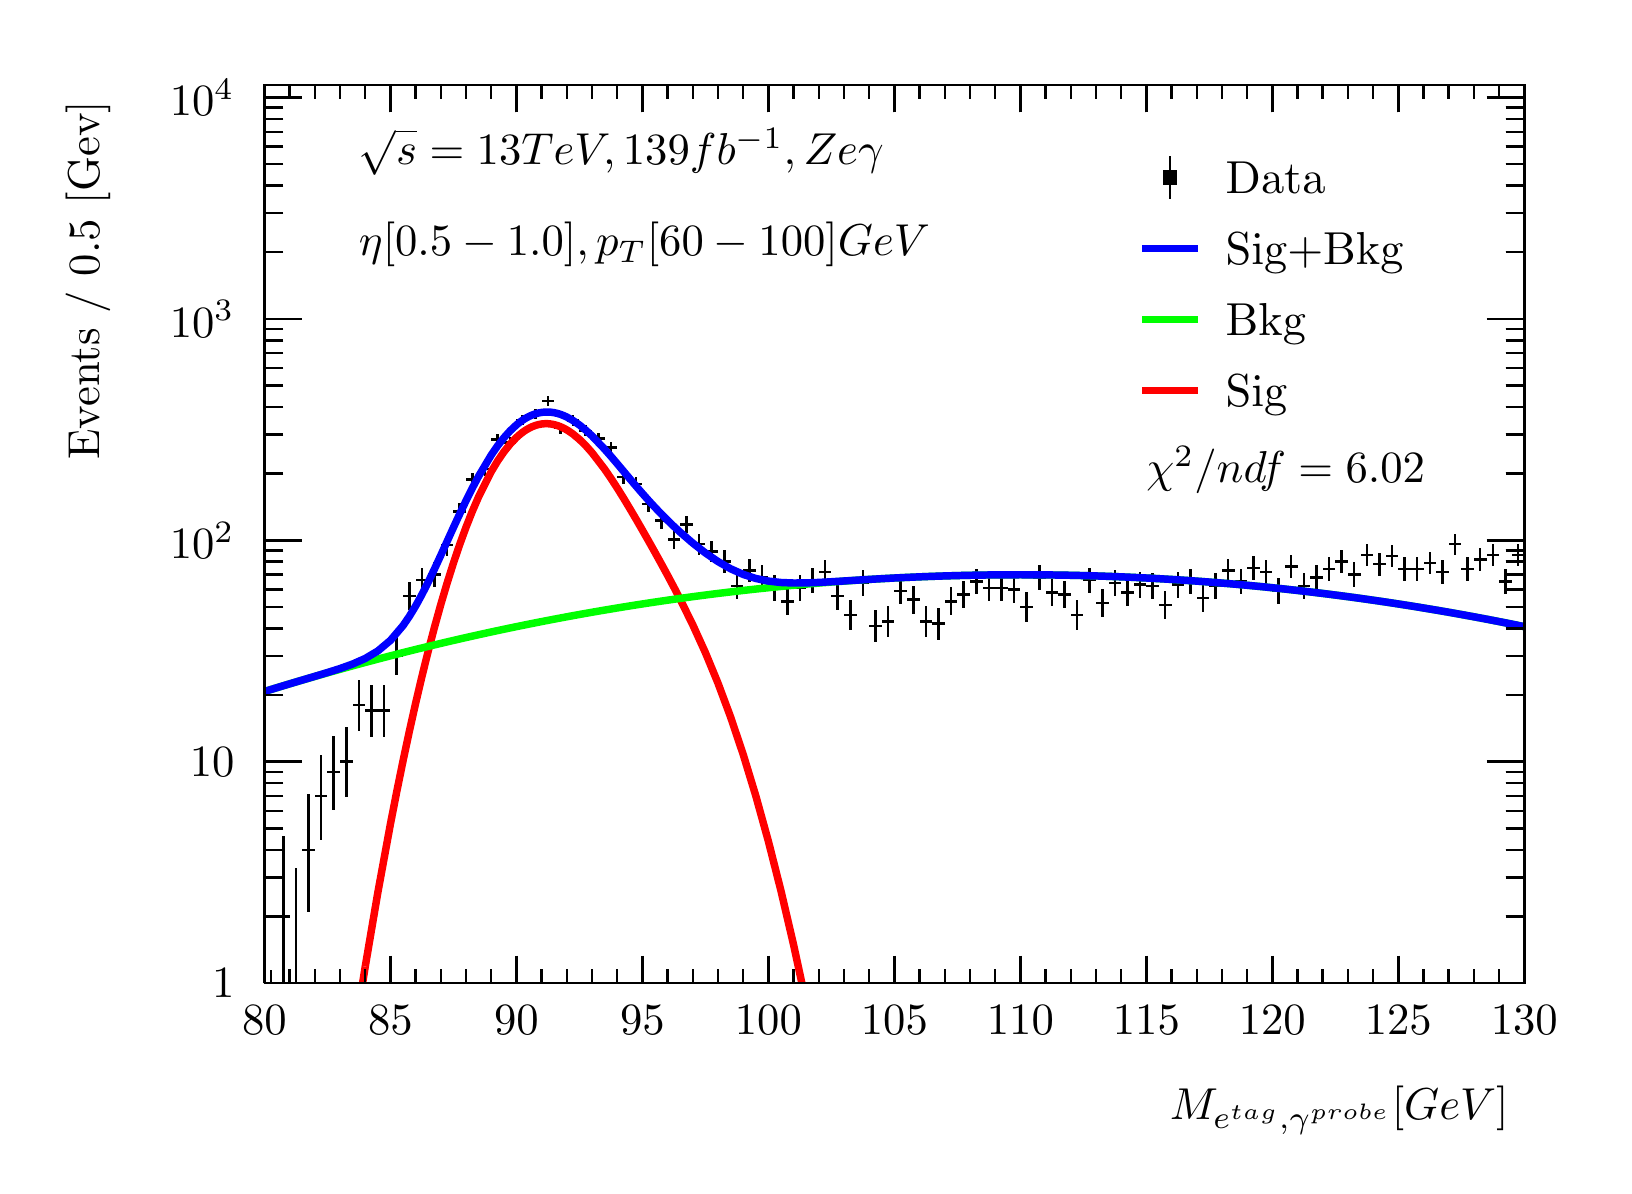
\begin{tikzpicture}
\pgfdeclareplotmark{cross} {
\pgfpathmoveto{\pgfpoint{-0.3\pgfplotmarksize}{\pgfplotmarksize}}
\pgfpathlineto{\pgfpoint{+0.3\pgfplotmarksize}{\pgfplotmarksize}}
\pgfpathlineto{\pgfpoint{+0.3\pgfplotmarksize}{0.3\pgfplotmarksize}}
\pgfpathlineto{\pgfpoint{+1\pgfplotmarksize}{0.3\pgfplotmarksize}}
\pgfpathlineto{\pgfpoint{+1\pgfplotmarksize}{-0.3\pgfplotmarksize}}
\pgfpathlineto{\pgfpoint{+0.3\pgfplotmarksize}{-0.3\pgfplotmarksize}}
\pgfpathlineto{\pgfpoint{+0.3\pgfplotmarksize}{-1.\pgfplotmarksize}}
\pgfpathlineto{\pgfpoint{-0.3\pgfplotmarksize}{-1.\pgfplotmarksize}}
\pgfpathlineto{\pgfpoint{-0.3\pgfplotmarksize}{-0.3\pgfplotmarksize}}
\pgfpathlineto{\pgfpoint{-1.\pgfplotmarksize}{-0.3\pgfplotmarksize}}
\pgfpathlineto{\pgfpoint{-1.\pgfplotmarksize}{0.3\pgfplotmarksize}}
\pgfpathlineto{\pgfpoint{-0.3\pgfplotmarksize}{0.3\pgfplotmarksize}}
\pgfpathclose
\pgfusepathqstroke
}
\pgfdeclareplotmark{cross*} {
\pgfpathmoveto{\pgfpoint{-0.3\pgfplotmarksize}{\pgfplotmarksize}}
\pgfpathlineto{\pgfpoint{+0.3\pgfplotmarksize}{\pgfplotmarksize}}
\pgfpathlineto{\pgfpoint{+0.3\pgfplotmarksize}{0.3\pgfplotmarksize}}
\pgfpathlineto{\pgfpoint{+1\pgfplotmarksize}{0.3\pgfplotmarksize}}
\pgfpathlineto{\pgfpoint{+1\pgfplotmarksize}{-0.3\pgfplotmarksize}}
\pgfpathlineto{\pgfpoint{+0.3\pgfplotmarksize}{-0.3\pgfplotmarksize}}
\pgfpathlineto{\pgfpoint{+0.3\pgfplotmarksize}{-1.\pgfplotmarksize}}
\pgfpathlineto{\pgfpoint{-0.3\pgfplotmarksize}{-1.\pgfplotmarksize}}
\pgfpathlineto{\pgfpoint{-0.3\pgfplotmarksize}{-0.3\pgfplotmarksize}}
\pgfpathlineto{\pgfpoint{-1.\pgfplotmarksize}{-0.3\pgfplotmarksize}}
\pgfpathlineto{\pgfpoint{-1.\pgfplotmarksize}{0.3\pgfplotmarksize}}
\pgfpathlineto{\pgfpoint{-0.3\pgfplotmarksize}{0.3\pgfplotmarksize}}
\pgfpathclose
\pgfusepathqfillstroke
}
\pgfdeclareplotmark{newstar} {
\pgfpathmoveto{\pgfqpoint{0pt}{\pgfplotmarksize}}
\pgfpathlineto{\pgfqpointpolar{44}{0.5\pgfplotmarksize}}
\pgfpathlineto{\pgfqpointpolar{18}{\pgfplotmarksize}}
\pgfpathlineto{\pgfqpointpolar{-20}{0.5\pgfplotmarksize}}
\pgfpathlineto{\pgfqpointpolar{-54}{\pgfplotmarksize}}
\pgfpathlineto{\pgfqpointpolar{-90}{0.5\pgfplotmarksize}}
\pgfpathlineto{\pgfqpointpolar{234}{\pgfplotmarksize}}
\pgfpathlineto{\pgfqpointpolar{198}{0.5\pgfplotmarksize}}
\pgfpathlineto{\pgfqpointpolar{162}{\pgfplotmarksize}}
\pgfpathlineto{\pgfqpointpolar{134}{0.5\pgfplotmarksize}}
\pgfpathclose
\pgfusepathqstroke
}
\pgfdeclareplotmark{newstar*} {
\pgfpathmoveto{\pgfqpoint{0pt}{\pgfplotmarksize}}
\pgfpathlineto{\pgfqpointpolar{44}{0.5\pgfplotmarksize}}
\pgfpathlineto{\pgfqpointpolar{18}{\pgfplotmarksize}}
\pgfpathlineto{\pgfqpointpolar{-20}{0.5\pgfplotmarksize}}
\pgfpathlineto{\pgfqpointpolar{-54}{\pgfplotmarksize}}
\pgfpathlineto{\pgfqpointpolar{-90}{0.5\pgfplotmarksize}}
\pgfpathlineto{\pgfqpointpolar{234}{\pgfplotmarksize}}
\pgfpathlineto{\pgfqpointpolar{198}{0.5\pgfplotmarksize}}
\pgfpathlineto{\pgfqpointpolar{162}{\pgfplotmarksize}}
\pgfpathlineto{\pgfqpointpolar{134}{0.5\pgfplotmarksize}}
\pgfpathclose
\pgfusepathqfillstroke
}
\definecolor{c}{rgb}{1,1,1};
\draw [color=c, fill=c] (0,0) rectangle (20,14.4361);
\draw [color=c, fill=c] (3,2.30977) rectangle (19,13.7143);
\definecolor{c}{rgb}{0,0,0};
\draw [c,line width=0.9] (3,2.30977) -- (3,13.7143) -- (19,13.7143) -- (19,2.30977) -- (3,2.30977);
\definecolor{c}{rgb}{1,1,1};
\draw [color=c, fill=c] (3,2.30977) rectangle (19,13.7143);
\definecolor{c}{rgb}{0,0,0};
\draw [c,line width=0.9] (3,2.30977) -- (3,13.7143) -- (19,13.7143) -- (19,2.30977) -- (3,2.30977);
\draw [c,line width=0.9] (3,2.30977) -- (19,2.30977);
\draw [c,line width=0.9] (3,2.65624) -- (3,2.30977);
\draw [c,line width=0.9] (3.32,2.48301) -- (3.32,2.30977);
\draw [c,line width=0.9] (3.64,2.48301) -- (3.64,2.30977);
\draw [c,line width=0.9] (3.96,2.48301) -- (3.96,2.30977);
\draw [c,line width=0.9] (4.28,2.48301) -- (4.28,2.30977);
\draw [c,line width=0.9] (4.6,2.65624) -- (4.6,2.30977);
\draw [c,line width=0.9] (4.92,2.48301) -- (4.92,2.30977);
\draw [c,line width=0.9] (5.24,2.48301) -- (5.24,2.30977);
\draw [c,line width=0.9] (5.56,2.48301) -- (5.56,2.30977);
\draw [c,line width=0.9] (5.88,2.48301) -- (5.88,2.30977);
\draw [c,line width=0.9] (6.2,2.65624) -- (6.2,2.30977);
\draw [c,line width=0.9] (6.52,2.48301) -- (6.52,2.30977);
\draw [c,line width=0.9] (6.84,2.48301) -- (6.84,2.30977);
\draw [c,line width=0.9] (7.16,2.48301) -- (7.16,2.30977);
\draw [c,line width=0.9] (7.48,2.48301) -- (7.48,2.30977);
\draw [c,line width=0.9] (7.8,2.65624) -- (7.8,2.30977);
\draw [c,line width=0.9] (8.12,2.48301) -- (8.12,2.30977);
\draw [c,line width=0.9] (8.44,2.48301) -- (8.44,2.30977);
\draw [c,line width=0.9] (8.76,2.48301) -- (8.76,2.30977);
\draw [c,line width=0.9] (9.08,2.48301) -- (9.08,2.30977);
\draw [c,line width=0.9] (9.4,2.65624) -- (9.4,2.30977);
\draw [c,line width=0.9] (9.72,2.48301) -- (9.72,2.30977);
\draw [c,line width=0.9] (10.04,2.48301) -- (10.04,2.30977);
\draw [c,line width=0.9] (10.36,2.48301) -- (10.36,2.30977);
\draw [c,line width=0.9] (10.68,2.48301) -- (10.68,2.30977);
\draw [c,line width=0.9] (11,2.65624) -- (11,2.30977);
\draw [c,line width=0.9] (11.32,2.48301) -- (11.32,2.30977);
\draw [c,line width=0.9] (11.64,2.48301) -- (11.64,2.30977);
\draw [c,line width=0.9] (11.96,2.48301) -- (11.96,2.30977);
\draw [c,line width=0.9] (12.28,2.48301) -- (12.28,2.30977);
\draw [c,line width=0.9] (12.6,2.65624) -- (12.6,2.30977);
\draw [c,line width=0.9] (12.92,2.48301) -- (12.92,2.30977);
\draw [c,line width=0.9] (13.24,2.48301) -- (13.24,2.30977);
\draw [c,line width=0.9] (13.56,2.48301) -- (13.56,2.30977);
\draw [c,line width=0.9] (13.88,2.48301) -- (13.88,2.30977);
\draw [c,line width=0.9] (14.2,2.65624) -- (14.2,2.30977);
\draw [c,line width=0.9] (14.52,2.48301) -- (14.52,2.30977);
\draw [c,line width=0.9] (14.84,2.48301) -- (14.84,2.30977);
\draw [c,line width=0.9] (15.16,2.48301) -- (15.16,2.30977);
\draw [c,line width=0.9] (15.48,2.48301) -- (15.48,2.30977);
\draw [c,line width=0.9] (15.8,2.65624) -- (15.8,2.30977);
\draw [c,line width=0.9] (16.12,2.48301) -- (16.12,2.30977);
\draw [c,line width=0.9] (16.44,2.48301) -- (16.44,2.30977);
\draw [c,line width=0.9] (16.76,2.48301) -- (16.76,2.30977);
\draw [c,line width=0.9] (17.08,2.48301) -- (17.08,2.30977);
\draw [c,line width=0.9] (17.4,2.65624) -- (17.4,2.30977);
\draw [c,line width=0.9] (17.72,2.48301) -- (17.72,2.30977);
\draw [c,line width=0.9] (18.04,2.48301) -- (18.04,2.30977);
\draw [c,line width=0.9] (18.36,2.48301) -- (18.36,2.30977);
\draw [c,line width=0.9] (18.68,2.48301) -- (18.68,2.30977);
\draw [c,line width=0.9] (19,2.65624) -- (19,2.30977);
\draw [anchor=base] (3,1.66015) node[scale=1.61424, color=c, rotate=0]{80};
\draw [anchor=base] (4.6,1.66015) node[scale=1.61424, color=c, rotate=0]{85};
\draw [anchor=base] (6.2,1.66015) node[scale=1.61424, color=c, rotate=0]{90};
\draw [anchor=base] (7.8,1.66015) node[scale=1.61424, color=c, rotate=0]{95};
\draw [anchor=base] (9.4,1.66015) node[scale=1.61424, color=c, rotate=0]{100};
\draw [anchor=base] (11,1.66015) node[scale=1.61424, color=c, rotate=0]{105};
\draw [anchor=base] (12.6,1.66015) node[scale=1.61424, color=c, rotate=0]{110};
\draw [anchor=base] (14.2,1.66015) node[scale=1.61424, color=c, rotate=0]{115};
\draw [anchor=base] (15.8,1.66015) node[scale=1.61424, color=c, rotate=0]{120};
\draw [anchor=base] (17.4,1.66015) node[scale=1.61424, color=c, rotate=0]{125};
\draw [anchor=base] (19,1.66015) node[scale=1.61424, color=c, rotate=0]{130};
\draw [anchor= east] (19,0.692932) node[scale=1.61424, color=c, rotate=0]{$M_{e^{tag}, \gamma^{probe}}  [GeV]$};
\draw [c,line width=0.9] (3,13.7143) -- (19,13.7143);
\draw [c,line width=0.9] (3,13.3678) -- (3,13.7143);
\draw [c,line width=0.9] (3.32,13.5411) -- (3.32,13.7143);
\draw [c,line width=0.9] (3.64,13.5411) -- (3.64,13.7143);
\draw [c,line width=0.9] (3.96,13.5411) -- (3.96,13.7143);
\draw [c,line width=0.9] (4.28,13.5411) -- (4.28,13.7143);
\draw [c,line width=0.9] (4.6,13.3678) -- (4.6,13.7143);
\draw [c,line width=0.9] (4.92,13.5411) -- (4.92,13.7143);
\draw [c,line width=0.9] (5.24,13.5411) -- (5.24,13.7143);
\draw [c,line width=0.9] (5.56,13.5411) -- (5.56,13.7143);
\draw [c,line width=0.9] (5.88,13.5411) -- (5.88,13.7143);
\draw [c,line width=0.9] (6.2,13.3678) -- (6.2,13.7143);
\draw [c,line width=0.9] (6.52,13.5411) -- (6.52,13.7143);
\draw [c,line width=0.9] (6.84,13.5411) -- (6.84,13.7143);
\draw [c,line width=0.9] (7.16,13.5411) -- (7.16,13.7143);
\draw [c,line width=0.9] (7.48,13.5411) -- (7.48,13.7143);
\draw [c,line width=0.9] (7.8,13.3678) -- (7.8,13.7143);
\draw [c,line width=0.9] (8.12,13.5411) -- (8.12,13.7143);
\draw [c,line width=0.9] (8.44,13.5411) -- (8.44,13.7143);
\draw [c,line width=0.9] (8.76,13.5411) -- (8.76,13.7143);
\draw [c,line width=0.9] (9.08,13.5411) -- (9.08,13.7143);
\draw [c,line width=0.9] (9.4,13.3678) -- (9.4,13.7143);
\draw [c,line width=0.9] (9.72,13.5411) -- (9.72,13.7143);
\draw [c,line width=0.9] (10.04,13.5411) -- (10.04,13.7143);
\draw [c,line width=0.9] (10.36,13.5411) -- (10.36,13.7143);
\draw [c,line width=0.9] (10.68,13.5411) -- (10.68,13.7143);
\draw [c,line width=0.9] (11,13.3678) -- (11,13.7143);
\draw [c,line width=0.9] (11.32,13.5411) -- (11.32,13.7143);
\draw [c,line width=0.9] (11.64,13.5411) -- (11.64,13.7143);
\draw [c,line width=0.9] (11.96,13.5411) -- (11.96,13.7143);
\draw [c,line width=0.9] (12.28,13.5411) -- (12.28,13.7143);
\draw [c,line width=0.9] (12.6,13.3678) -- (12.6,13.7143);
\draw [c,line width=0.9] (12.92,13.5411) -- (12.92,13.7143);
\draw [c,line width=0.9] (13.24,13.5411) -- (13.24,13.7143);
\draw [c,line width=0.9] (13.56,13.5411) -- (13.56,13.7143);
\draw [c,line width=0.9] (13.88,13.5411) -- (13.88,13.7143);
\draw [c,line width=0.9] (14.2,13.3678) -- (14.2,13.7143);
\draw [c,line width=0.9] (14.52,13.5411) -- (14.52,13.7143);
\draw [c,line width=0.9] (14.84,13.5411) -- (14.84,13.7143);
\draw [c,line width=0.9] (15.16,13.5411) -- (15.16,13.7143);
\draw [c,line width=0.9] (15.48,13.5411) -- (15.48,13.7143);
\draw [c,line width=0.9] (15.8,13.3678) -- (15.8,13.7143);
\draw [c,line width=0.9] (16.12,13.5411) -- (16.12,13.7143);
\draw [c,line width=0.9] (16.44,13.5411) -- (16.44,13.7143);
\draw [c,line width=0.9] (16.76,13.5411) -- (16.76,13.7143);
\draw [c,line width=0.9] (17.08,13.5411) -- (17.08,13.7143);
\draw [c,line width=0.9] (17.4,13.3678) -- (17.4,13.7143);
\draw [c,line width=0.9] (17.72,13.5411) -- (17.72,13.7143);
\draw [c,line width=0.9] (18.04,13.5411) -- (18.04,13.7143);
\draw [c,line width=0.9] (18.36,13.5411) -- (18.36,13.7143);
\draw [c,line width=0.9] (18.68,13.5411) -- (18.68,13.7143);
\draw [c,line width=0.9] (19,13.3678) -- (19,13.7143);
\draw [c,line width=0.9] (3,2.30977) -- (3,13.7143);
\draw [c,line width=0.9] (3.474,2.30978) -- (3,2.30978);
\draw [anchor= east] (2.82,2.30978) node[scale=1.61424, color=c, rotate=0]{1};
\draw [c,line width=0.9] (3.237,3.15616) -- (3,3.15616);
\draw [c,line width=0.9] (3.237,3.65126) -- (3,3.65126);
\draw [c,line width=0.9] (3.237,4.00254) -- (3,4.00254);
\draw [c,line width=0.9] (3.237,4.27501) -- (3,4.27501);
\draw [c,line width=0.9] (3.237,4.49764) -- (3,4.49764);
\draw [c,line width=0.9] (3.237,4.68586) -- (3,4.68586);
\draw [c,line width=0.9] (3.237,4.84892) -- (3,4.84892);
\draw [c,line width=0.9] (3.237,4.99274) -- (3,4.99274);
\draw [c,line width=0.9] (3.474,5.12139) -- (3,5.12139);
\draw [anchor= east] (2.82,5.12139) node[scale=1.61424, color=c, rotate=0]{10};
\draw [c,line width=0.9] (3.237,5.96777) -- (3,5.96777);
\draw [c,line width=0.9] (3.237,6.46287) -- (3,6.46287);
\draw [c,line width=0.9] (3.237,6.81415) -- (3,6.81415);
\draw [c,line width=0.9] (3.237,7.08662) -- (3,7.08662);
\draw [c,line width=0.9] (3.237,7.30925) -- (3,7.30925);
\draw [c,line width=0.9] (3.237,7.49748) -- (3,7.49748);
\draw [c,line width=0.9] (3.237,7.66053) -- (3,7.66053);
\draw [c,line width=0.9] (3.237,7.80435) -- (3,7.80435);
\draw [c,line width=0.9] (3.474,7.933) -- (3,7.933);
\draw [anchor= east] (2.82,7.933) node[scale=1.61424, color=c, rotate=0]{$10^{2}$};
\draw [c,line width=0.9] (3.237,8.77938) -- (3,8.77938);
\draw [c,line width=0.9] (3.237,9.27448) -- (3,9.27448);
\draw [c,line width=0.9] (3.237,9.62576) -- (3,9.62576);
\draw [c,line width=0.9] (3.237,9.89823) -- (3,9.89823);
\draw [c,line width=0.9] (3.237,10.1209) -- (3,10.1209);
\draw [c,line width=0.9] (3.237,10.3091) -- (3,10.3091);
\draw [c,line width=0.9] (3.237,10.4721) -- (3,10.4721);
\draw [c,line width=0.9] (3.237,10.616) -- (3,10.616);
\draw [c,line width=0.9] (3.474,10.7446) -- (3,10.7446);
\draw [anchor= east] (2.82,10.7446) node[scale=1.61424, color=c, rotate=0]{$10^{3}$};
\draw [c,line width=0.9] (3.237,11.591) -- (3,11.591);
\draw [c,line width=0.9] (3.237,12.0861) -- (3,12.0861);
\draw [c,line width=0.9] (3.237,12.4374) -- (3,12.4374);
\draw [c,line width=0.9] (3.237,12.7098) -- (3,12.7098);
\draw [c,line width=0.9] (3.237,12.9325) -- (3,12.9325);
\draw [c,line width=0.9] (3.237,13.1207) -- (3,13.1207);
\draw [c,line width=0.9] (3.237,13.2837) -- (3,13.2837);
\draw [c,line width=0.9] (3.237,13.4276) -- (3,13.4276);
\draw [c,line width=0.9] (3.474,13.5562) -- (3,13.5562);
\draw [anchor= east] (2.82,13.5562) node[scale=1.61424, color=c, rotate=0]{$10^{4}$};
\draw [anchor= east] (0.76,13.7143) node[scale=1.61424, color=c, rotate=90]{Events / 0.5 [Gev]};
\draw [c,line width=0.9] (19,2.30977) -- (19,13.7143);
\draw [c,line width=0.9] (18.526,2.30978) -- (19,2.30978);
\draw [c,line width=0.9] (18.763,3.15616) -- (19,3.15616);
\draw [c,line width=0.9] (18.763,3.65126) -- (19,3.65126);
\draw [c,line width=0.9] (18.763,4.00254) -- (19,4.00254);
\draw [c,line width=0.9] (18.763,4.27501) -- (19,4.27501);
\draw [c,line width=0.9] (18.763,4.49764) -- (19,4.49764);
\draw [c,line width=0.9] (18.763,4.68586) -- (19,4.68586);
\draw [c,line width=0.9] (18.763,4.84892) -- (19,4.84892);
\draw [c,line width=0.9] (18.763,4.99274) -- (19,4.99274);
\draw [c,line width=0.9] (18.526,5.12139) -- (19,5.12139);
\draw [c,line width=0.9] (18.763,5.96777) -- (19,5.96777);
\draw [c,line width=0.9] (18.763,6.46287) -- (19,6.46287);
\draw [c,line width=0.9] (18.763,6.81415) -- (19,6.81415);
\draw [c,line width=0.9] (18.763,7.08662) -- (19,7.08662);
\draw [c,line width=0.9] (18.763,7.30925) -- (19,7.30925);
\draw [c,line width=0.9] (18.763,7.49748) -- (19,7.49748);
\draw [c,line width=0.9] (18.763,7.66053) -- (19,7.66053);
\draw [c,line width=0.9] (18.763,7.80435) -- (19,7.80435);
\draw [c,line width=0.9] (18.526,7.933) -- (19,7.933);
\draw [c,line width=0.9] (18.763,8.77938) -- (19,8.77938);
\draw [c,line width=0.9] (18.763,9.27448) -- (19,9.27448);
\draw [c,line width=0.9] (18.763,9.62576) -- (19,9.62576);
\draw [c,line width=0.9] (18.763,9.89823) -- (19,9.89823);
\draw [c,line width=0.9] (18.763,10.1209) -- (19,10.1209);
\draw [c,line width=0.9] (18.763,10.3091) -- (19,10.3091);
\draw [c,line width=0.9] (18.763,10.4721) -- (19,10.4721);
\draw [c,line width=0.9] (18.763,10.616) -- (19,10.616);
\draw [c,line width=0.9] (18.526,10.7446) -- (19,10.7446);
\draw [c,line width=0.9] (18.763,11.591) -- (19,11.591);
\draw [c,line width=0.9] (18.763,12.0861) -- (19,12.0861);
\draw [c,line width=0.9] (18.763,12.4374) -- (19,12.4374);
\draw [c,line width=0.9] (18.763,12.7098) -- (19,12.7098);
\draw [c,line width=0.9] (18.763,12.9325) -- (19,12.9325);
\draw [c,line width=0.9] (18.763,13.1207) -- (19,13.1207);
\draw [c,line width=0.9] (18.763,13.2837) -- (19,13.2837);
\draw [c,line width=0.9] (18.763,13.4276) -- (19,13.4276);
\draw [c,line width=0.9] (18.526,13.5562) -- (19,13.5562);
\draw [c,line width=0.9] (3.08,2.30977) -- (3,2.30977);
\draw [c,line width=0.9] (3,2.30977) -- (3,2.30977);
\draw [c,line width=0.9] (3.08,2.30977) -- (3.16,2.30977);
\draw [c,line width=0.9] (3.16,2.30977) -- (3.16,2.30977);
\draw [c,line width=0.9] (3.08,2.30977) -- (3.08,2.47817);
\draw [c,line width=0.9] (3.08,2.47817) -- (3.08,2.47817);
\draw [c,line width=0.9] (3.24,3.15615) -- (3.16,3.15615);
\draw [c,line width=0.9] (3.16,3.15615) -- (3.16,3.15615);
\draw [c,line width=0.9] (3.24,3.15615) -- (3.32,3.15615);
\draw [c,line width=0.9] (3.32,3.15615) -- (3.32,3.15615);
\draw [c,line width=0.9] (3.24,3.15615) -- (3.24,4.1832);
\draw [c,line width=0.9] (3.24,4.1832) -- (3.24,4.1832);
\draw [c,line width=0.9] (3.24,3.15615) -- (3.24,2.30977);
\draw [c,line width=0.9] (3.24,2.30977) -- (3.24,2.30977);
\draw [c,line width=0.9] (3.4,2.30977) -- (3.32,2.30977);
\draw [c,line width=0.9] (3.32,2.30977) -- (3.32,2.30977);
\draw [c,line width=0.9] (3.4,2.30977) -- (3.48,2.30977);
\draw [c,line width=0.9] (3.48,2.30977) -- (3.48,2.30977);
\draw [c,line width=0.9] (3.4,2.30977) -- (3.4,3.76746);
\draw [c,line width=0.9] (3.4,3.76746) -- (3.4,3.76746);
\draw [c,line width=0.9] (3.56,4.00253) -- (3.48,4.00253);
\draw [c,line width=0.9] (3.48,4.00253) -- (3.48,4.00253);
\draw [c,line width=0.9] (3.56,4.00253) -- (3.64,4.00253);
\draw [c,line width=0.9] (3.64,4.00253) -- (3.64,4.00253);
\draw [c,line width=0.9] (3.56,4.00253) -- (3.56,4.71393);
\draw [c,line width=0.9] (3.56,4.71393) -- (3.56,4.71393);
\draw [c,line width=0.9] (3.56,4.00253) -- (3.56,3.20736);
\draw [c,line width=0.9] (3.56,3.20736) -- (3.56,3.20736);
\draw [c,line width=0.9] (3.72,4.68586) -- (3.64,4.68586);
\draw [c,line width=0.9] (3.64,4.68586) -- (3.64,4.68586);
\draw [c,line width=0.9] (3.72,4.68586) -- (3.8,4.68586);
\draw [c,line width=0.9] (3.8,4.68586) -- (3.8,4.68586);
\draw [c,line width=0.9] (3.72,4.68586) -- (3.72,5.212);
\draw [c,line width=0.9] (3.72,5.212) -- (3.72,5.212);
\draw [c,line width=0.9] (3.72,4.68586) -- (3.72,4.12404);
\draw [c,line width=0.9] (3.72,4.12404) -- (3.72,4.12404);
\draw [c,line width=0.9] (3.88,4.99273) -- (3.8,4.99273);
\draw [c,line width=0.9] (3.8,4.99273) -- (3.8,4.99273);
\draw [c,line width=0.9] (3.88,4.99273) -- (3.96,4.99273);
\draw [c,line width=0.9] (3.96,4.99273) -- (3.96,4.99273);
\draw [c,line width=0.9] (3.88,4.99273) -- (3.88,5.45206);
\draw [c,line width=0.9] (3.88,5.45206) -- (3.88,5.45206);
\draw [c,line width=0.9] (3.88,4.99273) -- (3.88,4.50909);
\draw [c,line width=0.9] (3.88,4.50909) -- (3.88,4.50909);
\draw [c,line width=0.9] (4.04,5.12139) -- (3.96,5.12139);
\draw [c,line width=0.9] (3.96,5.12139) -- (3.96,5.12139);
\draw [c,line width=0.9] (4.04,5.12139) -- (4.12,5.12139);
\draw [c,line width=0.9] (4.12,5.12139) -- (4.12,5.12139);
\draw [c,line width=0.9] (4.04,5.12139) -- (4.04,5.55531);
\draw [c,line width=0.9] (4.04,5.55531) -- (4.04,5.55531);
\draw [c,line width=0.9] (4.04,5.12139) -- (4.04,4.66675);
\draw [c,line width=0.9] (4.04,4.66675) -- (4.04,4.66675);
\draw [c,line width=0.9] (4.2,5.83911) -- (4.12,5.83911);
\draw [c,line width=0.9] (4.12,5.83911) -- (4.12,5.83911);
\draw [c,line width=0.9] (4.2,5.83911) -- (4.28,5.83911);
\draw [c,line width=0.9] (4.28,5.83911) -- (4.28,5.83911);
\draw [c,line width=0.9] (4.2,5.83911) -- (4.2,6.15535);
\draw [c,line width=0.9] (4.2,6.15535) -- (4.2,6.15535);
\draw [c,line width=0.9] (4.2,5.83911) -- (4.2,5.51442);
\draw [c,line width=0.9] (4.2,5.51442) -- (4.2,5.51442);
\draw [c,line width=0.9] (4.36,5.76932) -- (4.28,5.76932);
\draw [c,line width=0.9] (4.28,5.76932) -- (4.28,5.76932);
\draw [c,line width=0.9] (4.36,5.76932) -- (4.44,5.76932);
\draw [c,line width=0.9] (4.44,5.76932) -- (4.44,5.76932);
\draw [c,line width=0.9] (4.36,5.76932) -- (4.36,6.0954);
\draw [c,line width=0.9] (4.36,6.0954) -- (4.36,6.0954);
\draw [c,line width=0.9] (4.36,5.76932) -- (4.36,5.43401);
\draw [c,line width=0.9] (4.36,5.43401) -- (4.36,5.43401);
\draw [c,line width=0.9] (4.52,5.76932) -- (4.44,5.76932);
\draw [c,line width=0.9] (4.44,5.76932) -- (4.44,5.76932);
\draw [c,line width=0.9] (4.52,5.76932) -- (4.6,5.76932);
\draw [c,line width=0.9] (4.6,5.76932) -- (4.6,5.76932);
\draw [c,line width=0.9] (4.52,5.76932) -- (4.52,6.0954);
\draw [c,line width=0.9] (4.52,6.0954) -- (4.52,6.0954);
\draw [c,line width=0.9] (4.52,5.76932) -- (4.52,5.43401);
\draw [c,line width=0.9] (4.52,5.43401) -- (4.52,5.43401);
\draw [c,line width=0.9] (4.68,6.46287) -- (4.6,6.46287);
\draw [c,line width=0.9] (4.6,6.46287) -- (4.6,6.46287);
\draw [c,line width=0.9] (4.68,6.46287) -- (4.76,6.46287);
\draw [c,line width=0.9] (4.76,6.46287) -- (4.76,6.46287);
\draw [c,line width=0.9] (4.68,6.46287) -- (4.68,6.70361);
\draw [c,line width=0.9] (4.68,6.70361) -- (4.68,6.70361);
\draw [c,line width=0.9] (4.68,6.46287) -- (4.68,6.21823);
\draw [c,line width=0.9] (4.68,6.21823) -- (4.68,6.21823);
\draw [c,line width=0.9] (4.84,7.225) -- (4.76,7.225);
\draw [c,line width=0.9] (4.76,7.225) -- (4.76,7.225);
\draw [c,line width=0.9] (4.84,7.225) -- (4.92,7.225);
\draw [c,line width=0.9] (4.92,7.225) -- (4.92,7.225);
\draw [c,line width=0.9] (4.84,7.225) -- (4.84,7.39808);
\draw [c,line width=0.9] (4.84,7.39808) -- (4.84,7.39808);
\draw [c,line width=0.9] (4.84,7.225) -- (4.84,7.05041);
\draw [c,line width=0.9] (4.84,7.05041) -- (4.84,7.05041);
\draw [c,line width=0.9] (5,7.42563) -- (4.92,7.42563);
\draw [c,line width=0.9] (4.92,7.42563) -- (4.92,7.42563);
\draw [c,line width=0.9] (5,7.42563) -- (5.08,7.42563);
\draw [c,line width=0.9] (5.08,7.42563) -- (5.08,7.42563);
\draw [c,line width=0.9] (5,7.42563) -- (5,7.5844);
\draw [c,line width=0.9] (5,7.5844) -- (5,7.5844);
\draw [c,line width=0.9] (5,7.42563) -- (5,7.26567);
\draw [c,line width=0.9] (5,7.26567) -- (5,7.26567);
\draw [c,line width=0.9] (5.16,7.49747) -- (5.08,7.49747);
\draw [c,line width=0.9] (5.08,7.49747) -- (5.08,7.49747);
\draw [c,line width=0.9] (5.16,7.49747) -- (5.24,7.49747);
\draw [c,line width=0.9] (5.24,7.49747) -- (5.24,7.49747);
\draw [c,line width=0.9] (5.16,7.49747) -- (5.16,7.65143);
\draw [c,line width=0.9] (5.16,7.65143) -- (5.16,7.65143);
\draw [c,line width=0.9] (5.16,7.49747) -- (5.16,7.34244);
\draw [c,line width=0.9] (5.16,7.34244) -- (5.16,7.34244);
\draw [c,line width=0.9] (5.32,7.87037) -- (5.24,7.87037);
\draw [c,line width=0.9] (5.24,7.87037) -- (5.24,7.87037);
\draw [c,line width=0.9] (5.32,7.87037) -- (5.4,7.87037);
\draw [c,line width=0.9] (5.4,7.87037) -- (5.4,7.87037);
\draw [c,line width=0.9] (5.32,7.87037) -- (5.32,8.00162);
\draw [c,line width=0.9] (5.32,8.00162) -- (5.32,8.00162);
\draw [c,line width=0.9] (5.32,7.87037) -- (5.32,7.73843);
\draw [c,line width=0.9] (5.32,7.73843) -- (5.32,7.73843);
\draw [c,line width=0.9] (5.48,8.29945) -- (5.4,8.29945);
\draw [c,line width=0.9] (5.4,8.29945) -- (5.4,8.29945);
\draw [c,line width=0.9] (5.48,8.29945) -- (5.56,8.29945);
\draw [c,line width=0.9] (5.56,8.29945) -- (5.56,8.29945);
\draw [c,line width=0.9] (5.48,8.29945) -- (5.48,8.40451);
\draw [c,line width=0.9] (5.48,8.40451) -- (5.48,8.40451);
\draw [c,line width=0.9] (5.48,8.29945) -- (5.48,8.19439);
\draw [c,line width=0.9] (5.48,8.19439) -- (5.48,8.19439);
\draw [c,line width=0.9] (5.64,8.70382) -- (5.56,8.70382);
\draw [c,line width=0.9] (5.56,8.70382) -- (5.56,8.70382);
\draw [c,line width=0.9] (5.64,8.70382) -- (5.72,8.70382);
\draw [c,line width=0.9] (5.72,8.70382) -- (5.72,8.70382);
\draw [c,line width=0.9] (5.64,8.70382) -- (5.64,8.79286);
\draw [c,line width=0.9] (5.64,8.79286) -- (5.64,8.79286);
\draw [c,line width=0.9] (5.64,8.70382) -- (5.64,8.61479);
\draw [c,line width=0.9] (5.64,8.61479) -- (5.64,8.61479);
\draw [c,line width=0.9] (5.8,8.83895) -- (5.72,8.83895);
\draw [c,line width=0.9] (5.72,8.83895) -- (5.72,8.83895);
\draw [c,line width=0.9] (5.8,8.83895) -- (5.88,8.83895);
\draw [c,line width=0.9] (5.88,8.83895) -- (5.88,8.83895);
\draw [c,line width=0.9] (5.8,8.83895) -- (5.8,8.9232);
\draw [c,line width=0.9] (5.8,8.9232) -- (5.8,8.9232);
\draw [c,line width=0.9] (5.8,8.83895) -- (5.8,8.75471);
\draw [c,line width=0.9] (5.8,8.75471) -- (5.8,8.75471);
\draw [c,line width=0.9] (5.96,9.21184) -- (5.88,9.21184);
\draw [c,line width=0.9] (5.88,9.21184) -- (5.88,9.21184);
\draw [c,line width=0.9] (5.96,9.21184) -- (6.04,9.21184);
\draw [c,line width=0.9] (6.04,9.21184) -- (6.04,9.21184);
\draw [c,line width=0.9] (5.96,9.21184) -- (5.96,9.28416);
\draw [c,line width=0.9] (5.96,9.28416) -- (5.96,9.28416);
\draw [c,line width=0.9] (5.96,9.21184) -- (5.96,9.13953);
\draw [c,line width=0.9] (5.96,9.13953) -- (5.96,9.13953);
\draw [c,line width=0.9] (6.12,9.17708) -- (6.04,9.17708);
\draw [c,line width=0.9] (6.04,9.17708) -- (6.04,9.17708);
\draw [c,line width=0.9] (6.12,9.17708) -- (6.2,9.17708);
\draw [c,line width=0.9] (6.2,9.17708) -- (6.2,9.17708);
\draw [c,line width=0.9] (6.12,9.17708) -- (6.12,9.25043);
\draw [c,line width=0.9] (6.12,9.25043) -- (6.12,9.25043);
\draw [c,line width=0.9] (6.12,9.17708) -- (6.12,9.10372);
\draw [c,line width=0.9] (6.12,9.10372) -- (6.12,9.10372);
\draw [c,line width=0.9] (6.28,9.46271) -- (6.2,9.46271);
\draw [c,line width=0.9] (6.2,9.46271) -- (6.2,9.46271);
\draw [c,line width=0.9] (6.28,9.46271) -- (6.36,9.46271);
\draw [c,line width=0.9] (6.36,9.46271) -- (6.36,9.46271);
\draw [c,line width=0.9] (6.28,9.46271) -- (6.28,9.52797);
\draw [c,line width=0.9] (6.28,9.52797) -- (6.28,9.52797);
\draw [c,line width=0.9] (6.28,9.46271) -- (6.28,9.39744);
\draw [c,line width=0.9] (6.28,9.39744) -- (6.28,9.39744);
\draw [c,line width=0.9] (6.44,9.53056) -- (6.36,9.53056);
\draw [c,line width=0.9] (6.36,9.53056) -- (6.36,9.53056);
\draw [c,line width=0.9] (6.44,9.53056) -- (6.52,9.53056);
\draw [c,line width=0.9] (6.52,9.53056) -- (6.52,9.53056);
\draw [c,line width=0.9] (6.44,9.53056) -- (6.44,9.59403);
\draw [c,line width=0.9] (6.44,9.59403) -- (6.44,9.59403);
\draw [c,line width=0.9] (6.44,9.53056) -- (6.44,9.46709);
\draw [c,line width=0.9] (6.44,9.46709) -- (6.44,9.46709);
\draw [c,line width=0.9] (6.6,9.70265) -- (6.52,9.70265);
\draw [c,line width=0.9] (6.52,9.70265) -- (6.52,9.70265);
\draw [c,line width=0.9] (6.6,9.70265) -- (6.68,9.70265);
\draw [c,line width=0.9] (6.68,9.70265) -- (6.68,9.70265);
\draw [c,line width=0.9] (6.6,9.70265) -- (6.6,9.76181);
\draw [c,line width=0.9] (6.6,9.76181) -- (6.6,9.76181);
\draw [c,line width=0.9] (6.6,9.70265) -- (6.6,9.6435);
\draw [c,line width=0.9] (6.6,9.6435) -- (6.6,9.6435);
\draw [c,line width=0.9] (6.76,9.35709) -- (6.68,9.35709);
\draw [c,line width=0.9] (6.68,9.35709) -- (6.68,9.35709);
\draw [c,line width=0.9] (6.76,9.35709) -- (6.84,9.35709);
\draw [c,line width=0.9] (6.84,9.35709) -- (6.84,9.35709);
\draw [c,line width=0.9] (6.76,9.35709) -- (6.76,9.42524);
\draw [c,line width=0.9] (6.76,9.42524) -- (6.76,9.42524);
\draw [c,line width=0.9] (6.76,9.35709) -- (6.76,9.28895);
\draw [c,line width=0.9] (6.76,9.28895) -- (6.76,9.28895);
\draw [c,line width=0.9] (6.92,9.45571) -- (6.84,9.45571);
\draw [c,line width=0.9] (6.84,9.45571) -- (6.84,9.45571);
\draw [c,line width=0.9] (6.92,9.45571) -- (7,9.45571);
\draw [c,line width=0.9] (7,9.45571) -- (7,9.45571);
\draw [c,line width=0.9] (6.92,9.45571) -- (6.92,9.52116);
\draw [c,line width=0.9] (6.92,9.52116) -- (6.92,9.52116);
\draw [c,line width=0.9] (6.92,9.45571) -- (6.92,9.39026);
\draw [c,line width=0.9] (6.92,9.39026) -- (6.92,9.39026);
\draw [c,line width=0.9] (7.08,9.32237) -- (7,9.32237);
\draw [c,line width=0.9] (7,9.32237) -- (7,9.32237);
\draw [c,line width=0.9] (7.08,9.32237) -- (7.16,9.32237);
\draw [c,line width=0.9] (7.16,9.32237) -- (7.16,9.32237);
\draw [c,line width=0.9] (7.08,9.32237) -- (7.08,9.39149);
\draw [c,line width=0.9] (7.08,9.39149) -- (7.08,9.39149);
\draw [c,line width=0.9] (7.08,9.32237) -- (7.08,9.25325);
\draw [c,line width=0.9] (7.08,9.25325) -- (7.08,9.25325);
\draw [c,line width=0.9] (7.24,9.22463) -- (7.16,9.22463);
\draw [c,line width=0.9] (7.16,9.22463) -- (7.16,9.22463);
\draw [c,line width=0.9] (7.24,9.22463) -- (7.32,9.22463);
\draw [c,line width=0.9] (7.32,9.22463) -- (7.32,9.22463);
\draw [c,line width=0.9] (7.24,9.22463) -- (7.24,9.29657);
\draw [c,line width=0.9] (7.24,9.29657) -- (7.24,9.29657);
\draw [c,line width=0.9] (7.24,9.22463) -- (7.24,9.15269);
\draw [c,line width=0.9] (7.24,9.15269) -- (7.24,9.15269);
\draw [c,line width=0.9] (7.4,9.1091) -- (7.32,9.1091);
\draw [c,line width=0.9] (7.32,9.1091) -- (7.32,9.1091);
\draw [c,line width=0.9] (7.4,9.1091) -- (7.48,9.1091);
\draw [c,line width=0.9] (7.48,9.1091) -- (7.48,9.1091);
\draw [c,line width=0.9] (7.4,9.1091) -- (7.4,9.18452);
\draw [c,line width=0.9] (7.4,9.18452) -- (7.4,9.18452);
\draw [c,line width=0.9] (7.4,9.1091) -- (7.4,9.03367);
\draw [c,line width=0.9] (7.4,9.03367) -- (7.4,9.03367);
\draw [c,line width=0.9] (7.56,8.73587) -- (7.48,8.73587);
\draw [c,line width=0.9] (7.48,8.73587) -- (7.48,8.73587);
\draw [c,line width=0.9] (7.56,8.73587) -- (7.64,8.73587);
\draw [c,line width=0.9] (7.64,8.73587) -- (7.64,8.73587);
\draw [c,line width=0.9] (7.56,8.73587) -- (7.56,8.82375);
\draw [c,line width=0.9] (7.56,8.82375) -- (7.56,8.82375);
\draw [c,line width=0.9] (7.56,8.73587) -- (7.56,8.648);
\draw [c,line width=0.9] (7.56,8.648) -- (7.56,8.648);
\draw [c,line width=0.9] (7.72,8.65073) -- (7.64,8.65073);
\draw [c,line width=0.9] (7.64,8.65073) -- (7.64,8.65073);
\draw [c,line width=0.9] (7.72,8.65073) -- (7.8,8.65073);
\draw [c,line width=0.9] (7.8,8.65073) -- (7.8,8.65073);
\draw [c,line width=0.9] (7.72,8.65073) -- (7.72,8.74172);
\draw [c,line width=0.9] (7.72,8.74172) -- (7.72,8.74172);
\draw [c,line width=0.9] (7.72,8.65073) -- (7.72,8.55973);
\draw [c,line width=0.9] (7.72,8.55973) -- (7.72,8.55973);
\draw [c,line width=0.9] (7.88,8.39509) -- (7.8,8.39509);
\draw [c,line width=0.9] (7.8,8.39509) -- (7.8,8.39509);
\draw [c,line width=0.9] (7.88,8.39509) -- (7.96,8.39509);
\draw [c,line width=0.9] (7.96,8.39509) -- (7.96,8.39509);
\draw [c,line width=0.9] (7.88,8.39509) -- (7.88,8.49612);
\draw [c,line width=0.9] (7.88,8.49612) -- (7.88,8.49612);
\draw [c,line width=0.9] (7.88,8.39509) -- (7.88,8.29407);
\draw [c,line width=0.9] (7.88,8.29407) -- (7.88,8.29407);
\draw [c,line width=0.9] (8.04,8.18578) -- (7.96,8.18578);
\draw [c,line width=0.9] (7.96,8.18578) -- (7.96,8.18578);
\draw [c,line width=0.9] (8.04,8.18578) -- (8.12,8.18578);
\draw [c,line width=0.9] (8.12,8.18578) -- (8.12,8.18578);
\draw [c,line width=0.9] (8.04,8.18578) -- (8.04,8.29584);
\draw [c,line width=0.9] (8.04,8.29584) -- (8.04,8.29584);
\draw [c,line width=0.9] (8.04,8.18578) -- (8.04,8.07571);
\draw [c,line width=0.9] (8.04,8.07571) -- (8.04,8.07571);
\draw [c,line width=0.9] (8.2,7.94515) -- (8.12,7.94515);
\draw [c,line width=0.9] (8.12,7.94515) -- (8.12,7.94515);
\draw [c,line width=0.9] (8.2,7.94515) -- (8.28,7.94515);
\draw [c,line width=0.9] (8.28,7.94515) -- (8.28,7.94515);
\draw [c,line width=0.9] (8.2,7.94515) -- (8.2,8.0666);
\draw [c,line width=0.9] (8.2,8.0666) -- (8.2,8.0666);
\draw [c,line width=0.9] (8.2,7.94515) -- (8.2,7.8237);
\draw [c,line width=0.9] (8.2,7.8237) -- (8.2,7.8237);
\draw [c,line width=0.9] (8.36,8.1351) -- (8.28,8.1351);
\draw [c,line width=0.9] (8.28,8.1351) -- (8.28,8.1351);
\draw [c,line width=0.9] (8.36,8.1351) -- (8.44,8.1351);
\draw [c,line width=0.9] (8.44,8.1351) -- (8.44,8.1351);
\draw [c,line width=0.9] (8.36,8.1351) -- (8.36,8.24747);
\draw [c,line width=0.9] (8.36,8.24747) -- (8.36,8.24747);
\draw [c,line width=0.9] (8.36,8.1351) -- (8.36,8.02273);
\draw [c,line width=0.9] (8.36,8.02273) -- (8.36,8.02273);
\draw [c,line width=0.9] (8.52,7.88315) -- (8.44,7.88315);
\draw [c,line width=0.9] (8.44,7.88315) -- (8.44,7.88315);
\draw [c,line width=0.9] (8.52,7.88315) -- (8.6,7.88315);
\draw [c,line width=0.9] (8.6,7.88315) -- (8.6,7.88315);
\draw [c,line width=0.9] (8.52,7.88315) -- (8.52,8.01369);
\draw [c,line width=0.9] (8.52,8.01369) -- (8.52,8.01369);
\draw [c,line width=0.9] (8.52,7.88315) -- (8.52,7.75194);
\draw [c,line width=0.9] (8.52,7.75194) -- (8.52,7.75194);
\draw [c,line width=0.9] (8.68,7.7907) -- (8.6,7.7907);
\draw [c,line width=0.9] (8.6,7.7907) -- (8.6,7.7907);
\draw [c,line width=0.9] (8.68,7.7907) -- (8.76,7.7907);
\draw [c,line width=0.9] (8.76,7.7907) -- (8.76,7.7907);
\draw [c,line width=0.9] (8.68,7.7907) -- (8.68,7.9265);
\draw [c,line width=0.9] (8.68,7.9265) -- (8.68,7.9265);
\draw [c,line width=0.9] (8.68,7.7907) -- (8.68,7.65415);
\draw [c,line width=0.9] (8.68,7.65415) -- (8.68,7.65415);
\draw [c,line width=0.9] (8.84,7.66052) -- (8.76,7.66052);
\draw [c,line width=0.9] (8.76,7.66052) -- (8.76,7.66052);
\draw [c,line width=0.9] (8.84,7.66052) -- (8.92,7.66052);
\draw [c,line width=0.9] (8.92,7.66052) -- (8.92,7.66052);
\draw [c,line width=0.9] (8.84,7.66052) -- (8.84,7.8041);
\draw [c,line width=0.9] (8.84,7.8041) -- (8.84,7.8041);
\draw [c,line width=0.9] (8.84,7.66052) -- (8.84,7.51607);
\draw [c,line width=0.9] (8.84,7.51607) -- (8.84,7.51607);
\draw [c,line width=0.9] (9,7.34928) -- (8.92,7.34928);
\draw [c,line width=0.9] (8.92,7.34928) -- (8.92,7.34928);
\draw [c,line width=0.9] (9,7.34928) -- (9.08,7.34928);
\draw [c,line width=0.9] (9.08,7.34928) -- (9.08,7.34928);
\draw [c,line width=0.9] (9,7.34928) -- (9,7.51335);
\draw [c,line width=0.9] (9,7.51335) -- (9,7.51335);
\draw [c,line width=0.9] (9,7.34928) -- (9,7.18392);
\draw [c,line width=0.9] (9,7.18392) -- (9,7.18392);
\draw [c,line width=0.9] (9.16,7.54871) -- (9.08,7.54871);
\draw [c,line width=0.9] (9.08,7.54871) -- (9.08,7.54871);
\draw [c,line width=0.9] (9.16,7.54871) -- (9.24,7.54871);
\draw [c,line width=0.9] (9.24,7.54871) -- (9.24,7.54871);
\draw [c,line width=0.9] (9.16,7.54871) -- (9.16,7.69933);
\draw [c,line width=0.9] (9.16,7.69933) -- (9.16,7.69933);
\draw [c,line width=0.9] (9.16,7.54871) -- (9.16,7.39709);
\draw [c,line width=0.9] (9.16,7.39709) -- (9.16,7.39709);
\draw [c,line width=0.9] (9.32,7.46208) -- (9.24,7.46208);
\draw [c,line width=0.9] (9.24,7.46208) -- (9.24,7.46208);
\draw [c,line width=0.9] (9.32,7.46208) -- (9.4,7.46208);
\draw [c,line width=0.9] (9.4,7.46208) -- (9.4,7.46208);
\draw [c,line width=0.9] (9.32,7.46208) -- (9.32,7.61839);
\draw [c,line width=0.9] (9.32,7.61839) -- (9.32,7.61839);
\draw [c,line width=0.9] (9.32,7.46208) -- (9.32,7.30464);
\draw [c,line width=0.9] (9.32,7.30464) -- (9.32,7.30464);
\draw [c,line width=0.9] (9.48,7.32943) -- (9.4,7.32943);
\draw [c,line width=0.9] (9.4,7.32943) -- (9.4,7.32943);
\draw [c,line width=0.9] (9.48,7.32943) -- (9.56,7.32943);
\draw [c,line width=0.9] (9.56,7.32943) -- (9.56,7.32943);
\draw [c,line width=0.9] (9.48,7.32943) -- (9.48,7.49491);
\draw [c,line width=0.9] (9.48,7.49491) -- (9.48,7.49491);
\draw [c,line width=0.9] (9.48,7.32943) -- (9.48,7.16263);
\draw [c,line width=0.9] (9.48,7.16263) -- (9.48,7.16263);
\draw [c,line width=0.9] (9.64,7.15777) -- (9.56,7.15777);
\draw [c,line width=0.9] (9.56,7.15777) -- (9.56,7.15777);
\draw [c,line width=0.9] (9.64,7.15777) -- (9.72,7.15777);
\draw [c,line width=0.9] (9.72,7.15777) -- (9.72,7.15777);
\draw [c,line width=0.9] (9.64,7.15777) -- (9.64,7.33594);
\draw [c,line width=0.9] (9.64,7.33594) -- (9.64,7.33594);
\draw [c,line width=0.9] (9.64,7.15777) -- (9.64,6.97796);
\draw [c,line width=0.9] (9.64,6.97796) -- (9.64,6.97796);
\draw [c,line width=0.9] (9.8,7.32943) -- (9.72,7.32943);
\draw [c,line width=0.9] (9.72,7.32943) -- (9.72,7.32943);
\draw [c,line width=0.9] (9.8,7.32943) -- (9.88,7.32943);
\draw [c,line width=0.9] (9.88,7.32943) -- (9.88,7.32943);
\draw [c,line width=0.9] (9.8,7.32943) -- (9.8,7.49491);
\draw [c,line width=0.9] (9.8,7.49491) -- (9.8,7.49491);
\draw [c,line width=0.9] (9.8,7.32943) -- (9.8,7.16263);
\draw [c,line width=0.9] (9.8,7.16263) -- (9.8,7.16263);
\draw [c,line width=0.9] (9.96,7.42563) -- (9.88,7.42563);
\draw [c,line width=0.9] (9.88,7.42563) -- (9.88,7.42563);
\draw [c,line width=0.9] (9.96,7.42563) -- (10.04,7.42563);
\draw [c,line width=0.9] (10.04,7.42563) -- (10.04,7.42563);
\draw [c,line width=0.9] (9.96,7.42563) -- (9.96,7.5844);
\draw [c,line width=0.9] (9.96,7.5844) -- (9.96,7.5844);
\draw [c,line width=0.9] (9.96,7.42563) -- (9.96,7.26567);
\draw [c,line width=0.9] (9.96,7.26567) -- (9.96,7.26567);
\draw [c,line width=0.9] (10.12,7.53187) -- (10.04,7.53187);
\draw [c,line width=0.9] (10.04,7.53187) -- (10.04,7.53187);
\draw [c,line width=0.9] (10.12,7.53187) -- (10.2,7.53187);
\draw [c,line width=0.9] (10.2,7.53187) -- (10.2,7.53187);
\draw [c,line width=0.9] (10.12,7.53187) -- (10.12,7.68358);
\draw [c,line width=0.9] (10.12,7.68358) -- (10.12,7.68358);
\draw [c,line width=0.9] (10.12,7.53187) -- (10.12,7.37914);
\draw [c,line width=0.9] (10.12,7.37914) -- (10.12,7.37914);
\draw [c,line width=0.9] (10.28,7.225) -- (10.2,7.225);
\draw [c,line width=0.9] (10.2,7.225) -- (10.2,7.225);
\draw [c,line width=0.9] (10.28,7.225) -- (10.36,7.225);
\draw [c,line width=0.9] (10.36,7.225) -- (10.36,7.225);
\draw [c,line width=0.9] (10.28,7.225) -- (10.28,7.39808);
\draw [c,line width=0.9] (10.28,7.39808) -- (10.28,7.39808);
\draw [c,line width=0.9] (10.28,7.225) -- (10.28,7.05041);
\draw [c,line width=0.9] (10.28,7.05041) -- (10.28,7.05041);
\draw [c,line width=0.9] (10.44,6.9848) -- (10.36,6.9848);
\draw [c,line width=0.9] (10.36,6.9848) -- (10.36,6.9848);
\draw [c,line width=0.9] (10.44,6.9848) -- (10.52,6.9848);
\draw [c,line width=0.9] (10.52,6.9848) -- (10.52,6.9848);
\draw [c,line width=0.9] (10.44,6.9848) -- (10.44,7.17678);
\draw [c,line width=0.9] (10.44,7.17678) -- (10.44,7.17678);
\draw [c,line width=0.9] (10.44,6.9848) -- (10.44,6.7908);
\draw [c,line width=0.9] (10.44,6.7908) -- (10.44,6.7908);
\draw [c,line width=0.9] (10.6,7.38805) -- (10.52,7.38805);
\draw [c,line width=0.9] (10.52,7.38805) -- (10.52,7.38805);
\draw [c,line width=0.9] (10.6,7.38805) -- (10.68,7.38805);
\draw [c,line width=0.9] (10.68,7.38805) -- (10.68,7.38805);
\draw [c,line width=0.9] (10.6,7.38805) -- (10.6,7.54941);
\draw [c,line width=0.9] (10.6,7.54941) -- (10.6,7.54941);
\draw [c,line width=0.9] (10.6,7.38805) -- (10.6,7.22546);
\draw [c,line width=0.9] (10.6,7.22546) -- (10.6,7.22546);
\draw [c,line width=0.9] (10.76,6.8443) -- (10.68,6.8443);
\draw [c,line width=0.9] (10.68,6.8443) -- (10.68,6.8443);
\draw [c,line width=0.9] (10.76,6.8443) -- (10.84,6.8443);
\draw [c,line width=0.9] (10.84,6.8443) -- (10.84,6.8443);
\draw [c,line width=0.9] (10.76,6.8443) -- (10.76,7.0483);
\draw [c,line width=0.9] (10.76,7.0483) -- (10.76,7.0483);
\draw [c,line width=0.9] (10.76,6.8443) -- (10.76,6.63787);
\draw [c,line width=0.9] (10.76,6.63787) -- (10.76,6.63787);
\draw [c,line width=0.9] (10.92,6.90245) -- (10.84,6.90245);
\draw [c,line width=0.9] (10.84,6.90245) -- (10.84,6.90245);
\draw [c,line width=0.9] (10.92,6.90245) -- (11,6.90245);
\draw [c,line width=0.9] (11,6.90245) -- (11,6.90245);
\draw [c,line width=0.9] (10.92,6.90245) -- (10.92,7.10138);
\draw [c,line width=0.9] (10.92,7.10138) -- (10.92,7.10138);
\draw [c,line width=0.9] (10.92,6.90245) -- (10.92,6.70127);
\draw [c,line width=0.9] (10.92,6.70127) -- (10.92,6.70127);
\draw [c,line width=0.9] (11.08,7.28872) -- (11,7.28872);
\draw [c,line width=0.9] (11,7.28872) -- (11,7.28872);
\draw [c,line width=0.9] (11.08,7.28872) -- (11.16,7.28872);
\draw [c,line width=0.9] (11.16,7.28872) -- (11.16,7.28872);
\draw [c,line width=0.9] (11.08,7.28872) -- (11.08,7.45712);
\draw [c,line width=0.9] (11.08,7.45712) -- (11.08,7.45712);
\draw [c,line width=0.9] (11.08,7.28872) -- (11.08,7.11893);
\draw [c,line width=0.9] (11.08,7.11893) -- (11.08,7.11893);
\draw [c,line width=0.9] (11.24,7.18059) -- (11.16,7.18059);
\draw [c,line width=0.9] (11.16,7.18059) -- (11.16,7.18059);
\draw [c,line width=0.9] (11.24,7.18059) -- (11.32,7.18059);
\draw [c,line width=0.9] (11.32,7.18059) -- (11.32,7.18059);
\draw [c,line width=0.9] (11.24,7.18059) -- (11.24,7.35702);
\draw [c,line width=0.9] (11.24,7.35702) -- (11.24,7.35702);
\draw [c,line width=0.9] (11.24,7.18059) -- (11.24,7.00257);
\draw [c,line width=0.9] (11.24,7.00257) -- (11.24,7.00257);
\draw [c,line width=0.9] (11.4,6.90245) -- (11.32,6.90245);
\draw [c,line width=0.9] (11.32,6.90245) -- (11.32,6.90245);
\draw [c,line width=0.9] (11.4,6.90245) -- (11.48,6.90245);
\draw [c,line width=0.9] (11.48,6.90245) -- (11.48,6.90245);
\draw [c,line width=0.9] (11.4,6.90245) -- (11.4,7.10138);
\draw [c,line width=0.9] (11.4,7.10138) -- (11.4,7.10138);
\draw [c,line width=0.9] (11.4,6.90245) -- (11.4,6.70127);
\draw [c,line width=0.9] (11.4,6.70127) -- (11.4,6.70127);
\draw [c,line width=0.9] (11.56,6.87372) -- (11.48,6.87372);
\draw [c,line width=0.9] (11.48,6.87372) -- (11.48,6.87372);
\draw [c,line width=0.9] (11.56,6.87372) -- (11.64,6.87372);
\draw [c,line width=0.9] (11.64,6.87372) -- (11.64,6.87372);
\draw [c,line width=0.9] (11.56,6.87372) -- (11.56,7.07514);
\draw [c,line width=0.9] (11.56,7.07514) -- (11.56,7.07514);
\draw [c,line width=0.9] (11.56,6.87372) -- (11.56,6.66997);
\draw [c,line width=0.9] (11.56,6.66997) -- (11.56,6.66997);
\draw [c,line width=0.9] (11.72,7.15777) -- (11.64,7.15777);
\draw [c,line width=0.9] (11.64,7.15777) -- (11.64,7.15777);
\draw [c,line width=0.9] (11.72,7.15777) -- (11.8,7.15777);
\draw [c,line width=0.9] (11.8,7.15777) -- (11.8,7.15777);
\draw [c,line width=0.9] (11.72,7.15777) -- (11.72,7.33594);
\draw [c,line width=0.9] (11.72,7.33594) -- (11.72,7.33594);
\draw [c,line width=0.9] (11.72,7.15777) -- (11.72,6.97796);
\draw [c,line width=0.9] (11.72,6.97796) -- (11.72,6.97796);
\draw [c,line width=0.9] (11.88,7.24661) -- (11.8,7.24661);
\draw [c,line width=0.9] (11.8,7.24661) -- (11.8,7.24661);
\draw [c,line width=0.9] (11.88,7.24661) -- (11.96,7.24661);
\draw [c,line width=0.9] (11.96,7.24661) -- (11.96,7.24661);
\draw [c,line width=0.9] (11.88,7.24661) -- (11.88,7.41809);
\draw [c,line width=0.9] (11.88,7.41809) -- (11.88,7.41809);
\draw [c,line width=0.9] (11.88,7.24661) -- (11.88,7.07366);
\draw [c,line width=0.9] (11.88,7.07366) -- (11.88,7.07366);
\draw [c,line width=0.9] (12.04,7.40698) -- (11.96,7.40698);
\draw [c,line width=0.9] (11.96,7.40698) -- (11.96,7.40698);
\draw [c,line width=0.9] (12.04,7.40698) -- (12.12,7.40698);
\draw [c,line width=0.9] (12.12,7.40698) -- (12.12,7.40698);
\draw [c,line width=0.9] (12.04,7.40698) -- (12.04,7.56704);
\draw [c,line width=0.9] (12.04,7.56704) -- (12.04,7.56704);
\draw [c,line width=0.9] (12.04,7.40698) -- (12.04,7.24572);
\draw [c,line width=0.9] (12.04,7.24572) -- (12.04,7.24572);
\draw [c,line width=0.9] (12.2,7.32943) -- (12.12,7.32943);
\draw [c,line width=0.9] (12.12,7.32943) -- (12.12,7.32943);
\draw [c,line width=0.9] (12.2,7.32943) -- (12.28,7.32943);
\draw [c,line width=0.9] (12.28,7.32943) -- (12.28,7.32943);
\draw [c,line width=0.9] (12.2,7.32943) -- (12.2,7.49491);
\draw [c,line width=0.9] (12.2,7.49491) -- (12.2,7.49491);
\draw [c,line width=0.9] (12.2,7.32943) -- (12.2,7.16263);
\draw [c,line width=0.9] (12.2,7.16263) -- (12.2,7.16263);
\draw [c,line width=0.9] (12.36,7.32943) -- (12.28,7.32943);
\draw [c,line width=0.9] (12.28,7.32943) -- (12.28,7.32943);
\draw [c,line width=0.9] (12.36,7.32943) -- (12.44,7.32943);
\draw [c,line width=0.9] (12.44,7.32943) -- (12.44,7.32943);
\draw [c,line width=0.9] (12.36,7.32943) -- (12.36,7.49491);
\draw [c,line width=0.9] (12.36,7.49491) -- (12.36,7.49491);
\draw [c,line width=0.9] (12.36,7.32943) -- (12.36,7.16263);
\draw [c,line width=0.9] (12.36,7.16263) -- (12.36,7.16263);
\draw [c,line width=0.9] (12.52,7.30925) -- (12.44,7.30925);
\draw [c,line width=0.9] (12.44,7.30925) -- (12.44,7.30925);
\draw [c,line width=0.9] (12.52,7.30925) -- (12.6,7.30925);
\draw [c,line width=0.9] (12.6,7.30925) -- (12.6,7.30925);
\draw [c,line width=0.9] (12.52,7.30925) -- (12.52,7.47616);
\draw [c,line width=0.9] (12.52,7.47616) -- (12.52,7.47616);
\draw [c,line width=0.9] (12.52,7.30925) -- (12.52,7.14097);
\draw [c,line width=0.9] (12.52,7.14097) -- (12.52,7.14097);
\draw [c,line width=0.9] (12.68,7.08662) -- (12.6,7.08662);
\draw [c,line width=0.9] (12.6,7.08662) -- (12.6,7.08662);
\draw [c,line width=0.9] (12.68,7.08662) -- (12.76,7.08662);
\draw [c,line width=0.9] (12.76,7.08662) -- (12.76,7.08662);
\draw [c,line width=0.9] (12.68,7.08662) -- (12.68,7.27034);
\draw [c,line width=0.9] (12.68,7.27034) -- (12.68,7.27034);
\draw [c,line width=0.9] (12.68,7.08662) -- (12.68,6.90111);
\draw [c,line width=0.9] (12.68,6.90111) -- (12.68,6.90111);
\draw [c,line width=0.9] (12.84,7.46208) -- (12.76,7.46208);
\draw [c,line width=0.9] (12.76,7.46208) -- (12.76,7.46208);
\draw [c,line width=0.9] (12.84,7.46208) -- (12.92,7.46208);
\draw [c,line width=0.9] (12.92,7.46208) -- (12.92,7.46208);
\draw [c,line width=0.9] (12.84,7.46208) -- (12.84,7.61839);
\draw [c,line width=0.9] (12.84,7.61839) -- (12.84,7.61839);
\draw [c,line width=0.9] (12.84,7.46208) -- (12.84,7.30464);
\draw [c,line width=0.9] (12.84,7.30464) -- (12.84,7.30464);
\draw [c,line width=0.9] (13,7.26785) -- (12.92,7.26785);
\draw [c,line width=0.9] (12.92,7.26785) -- (12.92,7.26785);
\draw [c,line width=0.9] (13,7.26785) -- (13.08,7.26785);
\draw [c,line width=0.9] (13.08,7.26785) -- (13.08,7.26785);
\draw [c,line width=0.9] (13,7.26785) -- (13,7.43777);
\draw [c,line width=0.9] (13,7.43777) -- (13,7.43777);
\draw [c,line width=0.9] (13,7.26785) -- (13,7.0965);
\draw [c,line width=0.9] (13,7.0965) -- (13,7.0965);
\draw [c,line width=0.9] (13.16,7.24661) -- (13.08,7.24661);
\draw [c,line width=0.9] (13.08,7.24661) -- (13.08,7.24661);
\draw [c,line width=0.9] (13.16,7.24661) -- (13.24,7.24661);
\draw [c,line width=0.9] (13.24,7.24661) -- (13.24,7.24661);
\draw [c,line width=0.9] (13.16,7.24661) -- (13.16,7.41809);
\draw [c,line width=0.9] (13.16,7.41809) -- (13.16,7.41809);
\draw [c,line width=0.9] (13.16,7.24661) -- (13.16,7.07366);
\draw [c,line width=0.9] (13.16,7.07366) -- (13.16,7.07366);
\draw [c,line width=0.9] (13.32,6.9848) -- (13.24,6.9848);
\draw [c,line width=0.9] (13.24,6.9848) -- (13.24,6.9848);
\draw [c,line width=0.9] (13.32,6.9848) -- (13.4,6.9848);
\draw [c,line width=0.9] (13.4,6.9848) -- (13.4,6.9848);
\draw [c,line width=0.9] (13.32,6.9848) -- (13.32,7.17678);
\draw [c,line width=0.9] (13.32,7.17678) -- (13.32,7.17678);
\draw [c,line width=0.9] (13.32,6.9848) -- (13.32,6.7908);
\draw [c,line width=0.9] (13.32,6.7908) -- (13.32,6.7908);
\draw [c,line width=0.9] (13.48,7.42563) -- (13.4,7.42563);
\draw [c,line width=0.9] (13.4,7.42563) -- (13.4,7.42563);
\draw [c,line width=0.9] (13.48,7.42563) -- (13.56,7.42563);
\draw [c,line width=0.9] (13.56,7.42563) -- (13.56,7.42563);
\draw [c,line width=0.9] (13.48,7.42563) -- (13.48,7.5844);
\draw [c,line width=0.9] (13.48,7.5844) -- (13.48,7.5844);
\draw [c,line width=0.9] (13.48,7.42563) -- (13.48,7.26567);
\draw [c,line width=0.9] (13.48,7.26567) -- (13.48,7.26567);
\draw [c,line width=0.9] (13.64,7.13451) -- (13.56,7.13451);
\draw [c,line width=0.9] (13.56,7.13451) -- (13.56,7.13451);
\draw [c,line width=0.9] (13.64,7.13451) -- (13.72,7.13451);
\draw [c,line width=0.9] (13.72,7.13451) -- (13.72,7.13451);
\draw [c,line width=0.9] (13.64,7.13451) -- (13.64,7.31447);
\draw [c,line width=0.9] (13.64,7.31447) -- (13.64,7.31447);
\draw [c,line width=0.9] (13.64,7.13451) -- (13.64,6.95286);
\draw [c,line width=0.9] (13.64,6.95286) -- (13.64,6.95286);
\draw [c,line width=0.9] (13.8,7.38805) -- (13.72,7.38805);
\draw [c,line width=0.9] (13.72,7.38805) -- (13.72,7.38805);
\draw [c,line width=0.9] (13.8,7.38805) -- (13.88,7.38805);
\draw [c,line width=0.9] (13.88,7.38805) -- (13.88,7.38805);
\draw [c,line width=0.9] (13.8,7.38805) -- (13.8,7.54941);
\draw [c,line width=0.9] (13.8,7.54941) -- (13.8,7.54941);
\draw [c,line width=0.9] (13.8,7.38805) -- (13.8,7.22546);
\draw [c,line width=0.9] (13.8,7.22546) -- (13.8,7.22546);
\draw [c,line width=0.9] (13.96,7.26785) -- (13.88,7.26785);
\draw [c,line width=0.9] (13.88,7.26785) -- (13.88,7.26785);
\draw [c,line width=0.9] (13.96,7.26785) -- (14.04,7.26785);
\draw [c,line width=0.9] (14.04,7.26785) -- (14.04,7.26785);
\draw [c,line width=0.9] (13.96,7.26785) -- (13.96,7.43777);
\draw [c,line width=0.9] (13.96,7.43777) -- (13.96,7.43777);
\draw [c,line width=0.9] (13.96,7.26785) -- (13.96,7.0965);
\draw [c,line width=0.9] (13.96,7.0965) -- (13.96,7.0965);
\draw [c,line width=0.9] (14.12,7.36882) -- (14.04,7.36882);
\draw [c,line width=0.9] (14.04,7.36882) -- (14.04,7.36882);
\draw [c,line width=0.9] (14.12,7.36882) -- (14.2,7.36882);
\draw [c,line width=0.9] (14.2,7.36882) -- (14.2,7.36882);
\draw [c,line width=0.9] (14.12,7.36882) -- (14.12,7.53152);
\draw [c,line width=0.9] (14.12,7.53152) -- (14.12,7.53152);
\draw [c,line width=0.9] (14.12,7.36882) -- (14.12,7.20486);
\draw [c,line width=0.9] (14.12,7.20486) -- (14.12,7.20486);
\draw [c,line width=0.9] (14.28,7.34928) -- (14.2,7.34928);
\draw [c,line width=0.9] (14.2,7.34928) -- (14.2,7.34928);
\draw [c,line width=0.9] (14.28,7.34928) -- (14.36,7.34928);
\draw [c,line width=0.9] (14.36,7.34928) -- (14.36,7.34928);
\draw [c,line width=0.9] (14.28,7.34928) -- (14.28,7.51335);
\draw [c,line width=0.9] (14.28,7.51335) -- (14.28,7.51335);
\draw [c,line width=0.9] (14.28,7.34928) -- (14.28,7.18392);
\draw [c,line width=0.9] (14.28,7.18392) -- (14.28,7.18392);
\draw [c,line width=0.9] (14.44,7.1108) -- (14.36,7.1108);
\draw [c,line width=0.9] (14.36,7.1108) -- (14.36,7.1108);
\draw [c,line width=0.9] (14.44,7.1108) -- (14.52,7.1108);
\draw [c,line width=0.9] (14.52,7.1108) -- (14.52,7.1108);
\draw [c,line width=0.9] (14.44,7.1108) -- (14.44,7.29261);
\draw [c,line width=0.9] (14.44,7.29261) -- (14.44,7.29261);
\draw [c,line width=0.9] (14.44,7.1108) -- (14.44,6.92725);
\draw [c,line width=0.9] (14.44,6.92725) -- (14.44,6.92725);
\draw [c,line width=0.9] (14.6,7.36882) -- (14.52,7.36882);
\draw [c,line width=0.9] (14.52,7.36882) -- (14.52,7.36882);
\draw [c,line width=0.9] (14.6,7.36882) -- (14.68,7.36882);
\draw [c,line width=0.9] (14.68,7.36882) -- (14.68,7.36882);
\draw [c,line width=0.9] (14.6,7.36882) -- (14.6,7.53152);
\draw [c,line width=0.9] (14.6,7.53152) -- (14.6,7.53152);
\draw [c,line width=0.9] (14.6,7.36882) -- (14.6,7.20486);
\draw [c,line width=0.9] (14.6,7.20486) -- (14.6,7.20486);
\draw [c,line width=0.9] (14.76,7.40698) -- (14.68,7.40698);
\draw [c,line width=0.9] (14.68,7.40698) -- (14.68,7.40698);
\draw [c,line width=0.9] (14.76,7.40698) -- (14.84,7.40698);
\draw [c,line width=0.9] (14.84,7.40698) -- (14.84,7.40698);
\draw [c,line width=0.9] (14.76,7.40698) -- (14.76,7.56704);
\draw [c,line width=0.9] (14.76,7.56704) -- (14.76,7.56704);
\draw [c,line width=0.9] (14.76,7.40698) -- (14.76,7.24572);
\draw [c,line width=0.9] (14.76,7.24572) -- (14.76,7.24572);
\draw [c,line width=0.9] (14.92,7.203) -- (14.84,7.203);
\draw [c,line width=0.9] (14.84,7.203) -- (14.84,7.203);
\draw [c,line width=0.9] (14.92,7.203) -- (15,7.203);
\draw [c,line width=0.9] (15,7.203) -- (15,7.203);
\draw [c,line width=0.9] (14.92,7.203) -- (14.92,7.37773);
\draw [c,line width=0.9] (14.92,7.37773) -- (14.92,7.37773);
\draw [c,line width=0.9] (14.92,7.203) -- (14.92,7.02672);
\draw [c,line width=0.9] (14.92,7.02672) -- (14.92,7.02672);
\draw [c,line width=0.9] (15.08,7.34928) -- (15,7.34928);
\draw [c,line width=0.9] (15,7.34928) -- (15,7.34928);
\draw [c,line width=0.9] (15.08,7.34928) -- (15.16,7.34928);
\draw [c,line width=0.9] (15.16,7.34928) -- (15.16,7.34928);
\draw [c,line width=0.9] (15.08,7.34928) -- (15.08,7.51335);
\draw [c,line width=0.9] (15.08,7.51335) -- (15.08,7.51335);
\draw [c,line width=0.9] (15.08,7.34928) -- (15.08,7.18392);
\draw [c,line width=0.9] (15.08,7.18392) -- (15.08,7.18392);
\draw [c,line width=0.9] (15.24,7.54871) -- (15.16,7.54871);
\draw [c,line width=0.9] (15.16,7.54871) -- (15.16,7.54871);
\draw [c,line width=0.9] (15.24,7.54871) -- (15.32,7.54871);
\draw [c,line width=0.9] (15.32,7.54871) -- (15.32,7.54871);
\draw [c,line width=0.9] (15.24,7.54871) -- (15.24,7.69933);
\draw [c,line width=0.9] (15.24,7.69933) -- (15.24,7.69933);
\draw [c,line width=0.9] (15.24,7.54871) -- (15.24,7.39709);
\draw [c,line width=0.9] (15.24,7.39709) -- (15.24,7.39709);
\draw [c,line width=0.9] (15.4,7.40698) -- (15.32,7.40698);
\draw [c,line width=0.9] (15.32,7.40698) -- (15.32,7.40698);
\draw [c,line width=0.9] (15.4,7.40698) -- (15.48,7.40698);
\draw [c,line width=0.9] (15.48,7.40698) -- (15.48,7.40698);
\draw [c,line width=0.9] (15.4,7.40698) -- (15.4,7.56704);
\draw [c,line width=0.9] (15.4,7.56704) -- (15.4,7.56704);
\draw [c,line width=0.9] (15.4,7.40698) -- (15.4,7.24572);
\draw [c,line width=0.9] (15.4,7.24572) -- (15.4,7.24572);
\draw [c,line width=0.9] (15.56,7.58172) -- (15.48,7.58172);
\draw [c,line width=0.9] (15.48,7.58172) -- (15.48,7.58172);
\draw [c,line width=0.9] (15.56,7.58172) -- (15.64,7.58172);
\draw [c,line width=0.9] (15.64,7.58172) -- (15.64,7.58172);
\draw [c,line width=0.9] (15.56,7.58172) -- (15.56,7.73022);
\draw [c,line width=0.9] (15.56,7.73022) -- (15.56,7.73022);
\draw [c,line width=0.9] (15.56,7.58172) -- (15.56,7.43225);
\draw [c,line width=0.9] (15.56,7.43225) -- (15.56,7.43225);
\draw [c,line width=0.9] (15.72,7.53187) -- (15.64,7.53187);
\draw [c,line width=0.9] (15.64,7.53187) -- (15.64,7.53187);
\draw [c,line width=0.9] (15.72,7.53187) -- (15.8,7.53187);
\draw [c,line width=0.9] (15.8,7.53187) -- (15.8,7.53187);
\draw [c,line width=0.9] (15.72,7.53187) -- (15.72,7.68358);
\draw [c,line width=0.9] (15.72,7.68358) -- (15.72,7.68358);
\draw [c,line width=0.9] (15.72,7.53187) -- (15.72,7.37914);
\draw [c,line width=0.9] (15.72,7.37914) -- (15.72,7.37914);
\draw [c,line width=0.9] (15.88,7.28872) -- (15.8,7.28872);
\draw [c,line width=0.9] (15.8,7.28872) -- (15.8,7.28872);
\draw [c,line width=0.9] (15.88,7.28872) -- (15.96,7.28872);
\draw [c,line width=0.9] (15.96,7.28872) -- (15.96,7.28872);
\draw [c,line width=0.9] (15.88,7.28872) -- (15.88,7.45712);
\draw [c,line width=0.9] (15.88,7.45712) -- (15.88,7.45712);
\draw [c,line width=0.9] (15.88,7.28872) -- (15.88,7.11893);
\draw [c,line width=0.9] (15.88,7.11893) -- (15.88,7.11893);
\draw [c,line width=0.9] (16.04,7.59789) -- (15.96,7.59789);
\draw [c,line width=0.9] (15.96,7.59789) -- (15.96,7.59789);
\draw [c,line width=0.9] (16.04,7.59789) -- (16.12,7.59789);
\draw [c,line width=0.9] (16.12,7.59789) -- (16.12,7.59789);
\draw [c,line width=0.9] (16.04,7.59789) -- (16.04,7.74536);
\draw [c,line width=0.9] (16.04,7.74536) -- (16.04,7.74536);
\draw [c,line width=0.9] (16.04,7.59789) -- (16.04,7.44947);
\draw [c,line width=0.9] (16.04,7.44947) -- (16.04,7.44947);
\draw [c,line width=0.9] (16.2,7.34928) -- (16.12,7.34928);
\draw [c,line width=0.9] (16.12,7.34928) -- (16.12,7.34928);
\draw [c,line width=0.9] (16.2,7.34928) -- (16.28,7.34928);
\draw [c,line width=0.9] (16.28,7.34928) -- (16.28,7.34928);
\draw [c,line width=0.9] (16.2,7.34928) -- (16.2,7.51335);
\draw [c,line width=0.9] (16.2,7.51335) -- (16.2,7.51335);
\draw [c,line width=0.9] (16.2,7.34928) -- (16.2,7.18392);
\draw [c,line width=0.9] (16.2,7.18392) -- (16.2,7.18392);
\draw [c,line width=0.9] (16.36,7.46208) -- (16.28,7.46208);
\draw [c,line width=0.9] (16.28,7.46208) -- (16.28,7.46208);
\draw [c,line width=0.9] (16.36,7.46208) -- (16.44,7.46208);
\draw [c,line width=0.9] (16.44,7.46208) -- (16.44,7.46208);
\draw [c,line width=0.9] (16.36,7.46208) -- (16.36,7.61839);
\draw [c,line width=0.9] (16.36,7.61839) -- (16.36,7.61839);
\draw [c,line width=0.9] (16.36,7.46208) -- (16.36,7.30464);
\draw [c,line width=0.9] (16.36,7.30464) -- (16.36,7.30464);
\draw [c,line width=0.9] (16.52,7.56533) -- (16.44,7.56533);
\draw [c,line width=0.9] (16.44,7.56533) -- (16.44,7.56533);
\draw [c,line width=0.9] (16.52,7.56533) -- (16.6,7.56533);
\draw [c,line width=0.9] (16.6,7.56533) -- (16.6,7.56533);
\draw [c,line width=0.9] (16.52,7.56533) -- (16.52,7.71487);
\draw [c,line width=0.9] (16.52,7.71487) -- (16.52,7.71487);
\draw [c,line width=0.9] (16.52,7.56533) -- (16.52,7.41479);
\draw [c,line width=0.9] (16.52,7.41479) -- (16.52,7.41479);
\draw [c,line width=0.9] (16.68,7.66052) -- (16.6,7.66052);
\draw [c,line width=0.9] (16.6,7.66052) -- (16.6,7.66052);
\draw [c,line width=0.9] (16.68,7.66052) -- (16.76,7.66052);
\draw [c,line width=0.9] (16.76,7.66052) -- (16.76,7.66052);
\draw [c,line width=0.9] (16.68,7.66052) -- (16.68,7.8041);
\draw [c,line width=0.9] (16.68,7.8041) -- (16.68,7.8041);
\draw [c,line width=0.9] (16.68,7.66052) -- (16.68,7.51607);
\draw [c,line width=0.9] (16.68,7.51607) -- (16.68,7.51607);
\draw [c,line width=0.9] (16.84,7.49747) -- (16.76,7.49747);
\draw [c,line width=0.9] (16.76,7.49747) -- (16.76,7.49747);
\draw [c,line width=0.9] (16.84,7.49747) -- (16.92,7.49747);
\draw [c,line width=0.9] (16.92,7.49747) -- (16.92,7.49747);
\draw [c,line width=0.9] (16.84,7.49747) -- (16.84,7.65143);
\draw [c,line width=0.9] (16.84,7.65143) -- (16.84,7.65143);
\draw [c,line width=0.9] (16.84,7.49747) -- (16.84,7.34244);
\draw [c,line width=0.9] (16.84,7.34244) -- (16.84,7.34244);
\draw [c,line width=0.9] (17,7.74883) -- (16.92,7.74883);
\draw [c,line width=0.9] (16.92,7.74883) -- (16.92,7.74883);
\draw [c,line width=0.9] (17,7.74883) -- (17.08,7.74883);
\draw [c,line width=0.9] (17.08,7.74883) -- (17.08,7.74883);
\draw [c,line width=0.9] (17,7.74883) -- (17,7.88708);
\draw [c,line width=0.9] (17,7.88708) -- (17,7.88708);
\draw [c,line width=0.9] (17,7.74883) -- (17,7.60979);
\draw [c,line width=0.9] (17,7.60979) -- (17,7.60979);
\draw [c,line width=0.9] (17.16,7.62961) -- (17.08,7.62961);
\draw [c,line width=0.9] (17.08,7.62961) -- (17.08,7.62961);
\draw [c,line width=0.9] (17.16,7.62961) -- (17.24,7.62961);
\draw [c,line width=0.9] (17.24,7.62961) -- (17.24,7.62961);
\draw [c,line width=0.9] (17.16,7.62961) -- (17.16,7.77509);
\draw [c,line width=0.9] (17.16,7.77509) -- (17.16,7.77509);
\draw [c,line width=0.9] (17.16,7.62961) -- (17.16,7.48321);
\draw [c,line width=0.9] (17.16,7.48321) -- (17.16,7.48321);
\draw [c,line width=0.9] (17.32,7.73455) -- (17.24,7.73455);
\draw [c,line width=0.9] (17.24,7.73455) -- (17.24,7.73455);
\draw [c,line width=0.9] (17.32,7.73455) -- (17.4,7.73455);
\draw [c,line width=0.9] (17.4,7.73455) -- (17.4,7.73455);
\draw [c,line width=0.9] (17.32,7.73455) -- (17.32,7.87365);
\draw [c,line width=0.9] (17.32,7.87365) -- (17.32,7.87365);
\draw [c,line width=0.9] (17.32,7.73455) -- (17.32,7.59465);
\draw [c,line width=0.9] (17.32,7.59465) -- (17.32,7.59465);
\draw [c,line width=0.9] (17.48,7.56533) -- (17.4,7.56533);
\draw [c,line width=0.9] (17.4,7.56533) -- (17.4,7.56533);
\draw [c,line width=0.9] (17.48,7.56533) -- (17.56,7.56533);
\draw [c,line width=0.9] (17.56,7.56533) -- (17.56,7.56533);
\draw [c,line width=0.9] (17.48,7.56533) -- (17.48,7.71487);
\draw [c,line width=0.9] (17.48,7.71487) -- (17.48,7.71487);
\draw [c,line width=0.9] (17.48,7.56533) -- (17.48,7.41479);
\draw [c,line width=0.9] (17.48,7.41479) -- (17.48,7.41479);
\draw [c,line width=0.9] (17.64,7.56533) -- (17.56,7.56533);
\draw [c,line width=0.9] (17.56,7.56533) -- (17.56,7.56533);
\draw [c,line width=0.9] (17.64,7.56533) -- (17.72,7.56533);
\draw [c,line width=0.9] (17.72,7.56533) -- (17.72,7.56533);
\draw [c,line width=0.9] (17.64,7.56533) -- (17.64,7.71487);
\draw [c,line width=0.9] (17.64,7.71487) -- (17.64,7.71487);
\draw [c,line width=0.9] (17.64,7.56533) -- (17.64,7.41479);
\draw [c,line width=0.9] (17.64,7.41479) -- (17.64,7.41479);
\draw [c,line width=0.9] (17.8,7.64516) -- (17.72,7.64516);
\draw [c,line width=0.9] (17.72,7.64516) -- (17.72,7.64516);
\draw [c,line width=0.9] (17.8,7.64516) -- (17.88,7.64516);
\draw [c,line width=0.9] (17.88,7.64516) -- (17.88,7.64516);
\draw [c,line width=0.9] (17.8,7.64516) -- (17.8,7.78968);
\draw [c,line width=0.9] (17.8,7.78968) -- (17.8,7.78968);
\draw [c,line width=0.9] (17.8,7.64516) -- (17.8,7.49975);
\draw [c,line width=0.9] (17.8,7.49975) -- (17.8,7.49975);
\draw [c,line width=0.9] (17.96,7.53187) -- (17.88,7.53187);
\draw [c,line width=0.9] (17.88,7.53187) -- (17.88,7.53187);
\draw [c,line width=0.9] (17.96,7.53187) -- (18.04,7.53187);
\draw [c,line width=0.9] (18.04,7.53187) -- (18.04,7.53187);
\draw [c,line width=0.9] (17.96,7.53187) -- (17.96,7.68358);
\draw [c,line width=0.9] (17.96,7.68358) -- (17.96,7.68358);
\draw [c,line width=0.9] (17.96,7.53187) -- (17.96,7.37914);
\draw [c,line width=0.9] (17.96,7.37914) -- (17.96,7.37914);
\draw [c,line width=0.9] (18.12,7.88315) -- (18.04,7.88315);
\draw [c,line width=0.9] (18.04,7.88315) -- (18.04,7.88315);
\draw [c,line width=0.9] (18.12,7.88315) -- (18.2,7.88315);
\draw [c,line width=0.9] (18.2,7.88315) -- (18.2,7.88315);
\draw [c,line width=0.9] (18.12,7.88315) -- (18.12,8.01369);
\draw [c,line width=0.9] (18.12,8.01369) -- (18.12,8.01369);
\draw [c,line width=0.9] (18.12,7.88315) -- (18.12,7.75194);
\draw [c,line width=0.9] (18.12,7.75194) -- (18.12,7.75194);
\draw [c,line width=0.9] (18.28,7.56533) -- (18.2,7.56533);
\draw [c,line width=0.9] (18.2,7.56533) -- (18.2,7.56533);
\draw [c,line width=0.9] (18.28,7.56533) -- (18.36,7.56533);
\draw [c,line width=0.9] (18.36,7.56533) -- (18.36,7.56533);
\draw [c,line width=0.9] (18.28,7.56533) -- (18.28,7.71487);
\draw [c,line width=0.9] (18.28,7.71487) -- (18.28,7.71487);
\draw [c,line width=0.9] (18.28,7.56533) -- (18.28,7.41479);
\draw [c,line width=0.9] (18.28,7.41479) -- (18.28,7.41479);
\draw [c,line width=0.9] (18.44,7.69068) -- (18.36,7.69068);
\draw [c,line width=0.9] (18.36,7.69068) -- (18.36,7.69068);
\draw [c,line width=0.9] (18.44,7.69068) -- (18.52,7.69068);
\draw [c,line width=0.9] (18.52,7.69068) -- (18.52,7.69068);
\draw [c,line width=0.9] (18.44,7.69068) -- (18.44,7.83241);
\draw [c,line width=0.9] (18.44,7.83241) -- (18.44,7.83241);
\draw [c,line width=0.9] (18.44,7.69068) -- (18.44,7.5481);
\draw [c,line width=0.9] (18.44,7.5481) -- (18.44,7.5481);
\draw [c,line width=0.9] (18.6,7.74883) -- (18.52,7.74883);
\draw [c,line width=0.9] (18.52,7.74883) -- (18.52,7.74883);
\draw [c,line width=0.9] (18.6,7.74883) -- (18.68,7.74883);
\draw [c,line width=0.9] (18.68,7.74883) -- (18.68,7.74883);
\draw [c,line width=0.9] (18.6,7.74883) -- (18.6,7.88708);
\draw [c,line width=0.9] (18.6,7.88708) -- (18.6,7.88708);
\draw [c,line width=0.9] (18.6,7.74883) -- (18.6,7.60979);
\draw [c,line width=0.9] (18.6,7.60979) -- (18.6,7.60979);
\draw [c,line width=0.9] (18.76,7.40698) -- (18.68,7.40698);
\draw [c,line width=0.9] (18.68,7.40698) -- (18.68,7.40698);
\draw [c,line width=0.9] (18.76,7.40698) -- (18.84,7.40698);
\draw [c,line width=0.9] (18.84,7.40698) -- (18.84,7.40698);
\draw [c,line width=0.9] (18.76,7.40698) -- (18.76,7.56704);
\draw [c,line width=0.9] (18.76,7.56704) -- (18.76,7.56704);
\draw [c,line width=0.9] (18.76,7.40698) -- (18.76,7.24572);
\draw [c,line width=0.9] (18.76,7.24572) -- (18.76,7.24572);
\draw [c,line width=0.9] (18.92,7.74883) -- (18.84,7.74883);
\draw [c,line width=0.9] (18.84,7.74883) -- (18.84,7.74883);
\draw [c,line width=0.9] (18.92,7.74883) -- (19,7.74883);
\draw [c,line width=0.9] (19,7.74883) -- (19,7.74883);
\draw [c,line width=0.9] (18.92,7.74883) -- (18.92,7.88708);
\draw [c,line width=0.9] (18.92,7.88708) -- (18.92,7.88708);
\draw [c,line width=0.9] (18.92,7.74883) -- (18.92,7.60979);
\draw [c,line width=0.9] (18.92,7.60979) -- (18.92,7.60979);
\foreach \P in {(3.24,3.15615), (3.4,2.30977), (3.56,4.00253), (3.72,4.68586), (3.88,4.99273), (4.04,5.12139), (4.2,5.83911), (4.36,5.76932), (4.52,5.76932), (4.68,6.46287), (4.84,7.225), (5,7.42563), (5.16,7.49747), (5.32,7.87037), (5.48,8.29945),
 (5.64,8.70382), (5.8,8.83895), (5.96,9.21184), (6.12,9.17708), (6.28,9.46271), (6.44,9.53056), (6.6,9.70265), (6.76,9.35709), (6.92,9.45571), (7.08,9.32237), (7.24,9.22463), (7.4,9.1091), (7.56,8.73587), (7.72,8.65073), (7.88,8.39509),
 (8.04,8.18578), (8.2,7.94515), (8.36,8.1351), (8.52,7.88315), (8.68,7.7907), (8.84,7.66052), (9,7.34928), (9.16,7.54871), (9.32,7.46208), (9.48,7.32943), (9.64,7.15777), (9.8,7.32943), (9.96,7.42563), (10.12,7.53187), (10.28,7.225), (10.44,6.9848),
 (10.6,7.38805), (10.76,6.8443), (10.92,6.90245), (11.08,7.28872), (11.24,7.18059), (11.4,6.90245), (11.56,6.87372), (11.72,7.15777), (11.88,7.24661), (12.04,7.40698), (12.2,7.32943), (12.36,7.32943), (12.52,7.30925), (12.68,7.08662),
 (12.84,7.46208), (13,7.26785), (13.16,7.24661), (13.32,6.9848), (13.48,7.42563), (13.64,7.13451), (13.8,7.38805), (13.96,7.26785), (14.12,7.36882), (14.28,7.34928), (14.44,7.1108), (14.6,7.36882), (14.76,7.40698), (14.92,7.203), (15.08,7.34928),
 (15.24,7.54871), (15.4,7.40698), (15.56,7.58172), (15.72,7.53187), (15.88,7.28872), (16.04,7.59789), (16.2,7.34928), (16.36,7.46208), (16.52,7.56533), (16.68,7.66052), (16.84,7.49747), (17,7.74883), (17.16,7.62961), (17.32,7.73455), (17.48,7.56533),
 (17.64,7.56533), (17.8,7.64516), (17.96,7.53187), (18.12,7.88315), (18.28,7.56533), (18.44,7.69068), (18.6,7.74883), (18.76,7.40698), (18.92,7.74883)}{\draw[mark options={color=c,fill=c},mark size=2.882883pt,mark=] plot coordinates {\P};}
\definecolor{c}{rgb}{1,0,0};
\draw [c,line width=2.7] (4.24679,2.30977) -- (4.28,2.51936);
\draw [c,line width=2.7] (4.28,2.51936) -- (4.44,3.45967) -- (4.6,4.33047) -- (4.68,4.73981) -- (4.76,5.1318) -- (4.84,5.50644) -- (4.92,5.86372) -- (5,6.20367) -- (5.08,6.5263) -- (5.16,6.83161) -- (5.24,7.11963) -- (5.32,7.39036) -- (5.4,7.64383)
 -- (5.48,7.88008) -- (5.56,8.09912) -- (5.64,8.30099) -- (5.72,8.48574) -- (5.88,8.80408) -- (5.96,8.9378) -- (6.04,9.05468) -- (6.12,9.15481) -- (6.2,9.23833) -- (6.24,9.2739) -- (6.28,9.30538) -- (6.32,9.33279) -- (6.36,9.35616) -- (6.4,9.37551)
 -- (6.44,9.39087) -- (6.48,9.40229) -- (6.52,9.40979) -- (6.56,9.41342) -- (6.6,9.41323) -- (6.64,9.40925) -- (6.68,9.40156) -- (6.72,9.39019) -- (6.76,9.37523) -- (6.8,9.35673) -- (6.84,9.33476) -- (6.88,9.30942) -- (6.92,9.28078) -- (7,9.21399) --
 (7.08,9.13522) -- (7.16,9.04538) -- (7.32,8.83673) -- (7.4,8.72021) -- (7.48,8.59718) -- (7.56,8.4688) -- (7.64,8.33618) -- (7.72,8.20027) -- (7.8,8.0618) -- (7.88,7.92124) -- (7.96,7.77875) -- (8.04,7.6342) -- (8.12,7.48715) -- (8.2,7.33696) --
 (8.28,7.18276) -- (8.44,6.85841) -- (8.6,6.50604) -- (8.76,6.11814) -- (8.92,5.68856) -- (9.08,5.21268) -- (9.24,4.68723) -- (9.4,4.11) -- (9.56,3.47952) -- (9.72,2.79488) -- (9.82497,2.30977);
\definecolor{c}{rgb}{0,1,0};
\draw [c,line width=2.7] (3,6.01242) -- (3,6.01242);
\draw [c,line width=2.7] (3,6.01242) -- (3.16,6.06143) -- (3.32,6.10962) -- (3.48,6.15698) -- (3.64,6.20351) -- (3.8,6.24923) -- (3.96,6.29412) -- (4.12,6.33818) -- (4.28,6.38143) -- (4.44,6.42385) -- (4.6,6.46544) -- (4.76,6.50621) -- (4.92,6.54616)
 -- (5.08,6.58529) -- (5.24,6.62359) -- (5.4,6.66106) -- (5.56,6.69772) -- (5.72,6.73355) -- (5.88,6.76855) -- (6.04,6.80273) -- (6.2,6.83609) -- (6.36,6.86863) -- (6.52,6.90034) -- (6.68,6.93123) -- (6.84,6.96129) -- (7,6.99053) -- (7.16,7.01895) --
 (7.32,7.04654) -- (7.48,7.07331) -- (7.64,7.09926) -- (7.8,7.12438) -- (7.96,7.14868) -- (8.12,7.17215) -- (8.28,7.1948) -- (8.44,7.21663) -- (8.6,7.23763) -- (8.76,7.25781) -- (8.92,7.27717) -- (9.08,7.2957) -- (9.24,7.31341) -- (9.4,7.3303) --
 (9.56,7.34636) -- (9.72,7.36159) -- (9.88,7.37601) -- (10.04,7.3896) -- (10.2,7.40237) -- (10.36,7.41431) -- (10.52,7.42543) -- (10.68,7.43573) -- (10.84,7.4452) -- (11,7.45385) -- (11.16,7.46167) -- (11.32,7.46867) -- (11.48,7.47485) --
 (11.64,7.4802) -- (11.8,7.48473) -- (11.96,7.48844) -- (12.12,7.49132) -- (12.28,7.49338) -- (12.44,7.49462) -- (12.6,7.49503) -- (12.76,7.49462) -- (12.92,7.49338) -- (13.08,7.49132) -- (13.24,7.48844) -- (13.4,7.48473) -- (13.56,7.4802) --
 (13.72,7.47485) -- (13.88,7.46867) -- (14.04,7.46167) -- (14.2,7.45385) -- (14.36,7.4452) -- (14.52,7.43573) -- (14.68,7.42543) -- (14.84,7.41431) -- (15,7.40237) -- (15.16,7.3896) -- (15.32,7.37601) -- (15.48,7.36159) -- (15.64,7.34636) --
 (15.8,7.3303) -- (15.96,7.31341) -- (16.12,7.2957) -- (16.28,7.27717) -- (16.44,7.25781) -- (16.6,7.23763) -- (16.76,7.21663) -- (16.92,7.1948) -- (17.08,7.17215) -- (17.24,7.14868) -- (17.4,7.12438) -- (17.56,7.09926) -- (17.72,7.07331) --
 (17.88,7.04654) -- (18.04,7.01895) -- (18.2,6.99053) -- (18.36,6.96129) -- (18.52,6.93123) -- (18.68,6.90034) -- (18.84,6.86863) -- (19,6.83609) -- (19,6.83609) -- (19,6.83609);
\definecolor{c}{rgb}{0,0,1};
\draw [c,line width=2.7] (3,6.01245) -- (3,6.01245);
\draw [c,line width=2.7] (3,6.01245) -- (3.16,6.0615) -- (3.32,6.10981) -- (3.48,6.15754) -- (3.64,6.20507) -- (3.8,6.25328) -- (3.96,6.3041) -- (4.12,6.36137) -- (4.28,6.43202) -- (4.44,6.52712) -- (4.6,6.66137) -- (4.76,6.84934) -- (4.84,6.96626)
 -- (4.92,7.09839) -- (5,7.24451) -- (5.08,7.40253) -- (5.16,7.56973) -- (5.24,7.743) -- (5.32,7.91917) -- (5.4,8.09514) -- (5.48,8.26813) -- (5.56,8.43569) -- (5.64,8.59573) -- (5.72,8.74655) -- (5.88,9.01527) -- (5.96,9.13121) -- (6.04,9.23396) --
 (6.12,9.32304) -- (6.2,9.39814) -- (6.24,9.43039) -- (6.28,9.45909) -- (6.32,9.48423) -- (6.36,9.50582) -- (6.4,9.52387) -- (6.44,9.53839) -- (6.48,9.5494) -- (6.52,9.55694) -- (6.56,9.56105) -- (6.6,9.56176) -- (6.64,9.55913) -- (6.68,9.55322) --
 (6.72,9.54408) -- (6.76,9.53181) -- (6.8,9.51646) -- (6.84,9.49814) -- (6.92,9.45298) -- (7,9.3972) -- (7.08,9.33182) -- (7.16,9.25802) -- (7.32,9.09033) -- (7.4,8.99927) -- (7.48,8.90535) -- (7.56,8.80997) -- (7.64,8.71445) -- (7.72,8.61992) --
 (7.8,8.5273) -- (7.88,8.43728) -- (7.96,8.35029) -- (8.04,8.26656) -- (8.12,8.18616) -- (8.2,8.10905) -- (8.28,8.03517) -- (8.44,7.89699) -- (8.6,7.77221) -- (8.76,7.66276) -- (8.92,7.5712) -- (9.08,7.49947) -- (9.24,7.44786) -- (9.4,7.41469) --
 (9.56,7.39676) -- (9.72,7.39026) -- (9.88,7.39156) -- (10.04,7.39764) -- (10.2,7.40634) -- (10.36,7.41619) -- (10.52,7.42628) -- (10.68,7.43609) -- (10.84,7.44535) -- (11,7.45391) -- (11.16,7.46169) -- (11.32,7.46868) -- (11.48,7.47485) --
 (11.64,7.4802) -- (11.8,7.48473) -- (11.96,7.48844) -- (12.12,7.49132) -- (12.28,7.49338) -- (12.44,7.49462) -- (12.6,7.49503) -- (12.76,7.49462) -- (12.92,7.49338) -- (13.08,7.49132) -- (13.24,7.48844) -- (13.4,7.48473) -- (13.56,7.4802) --
 (13.72,7.47485) -- (13.88,7.46867) -- (14.04,7.46167) -- (14.2,7.45385) -- (14.36,7.4452) -- (14.52,7.43573) -- (14.68,7.42543) -- (14.84,7.41431) -- (15,7.40237) -- (15.16,7.3896) -- (15.32,7.37601) -- (15.48,7.36159) -- (15.64,7.34636) --
 (15.8,7.3303) -- (15.96,7.31341) -- (16.12,7.2957) -- (16.28,7.27717) -- (16.44,7.25781) -- (16.6,7.23763) -- (16.76,7.21663) -- (16.92,7.1948) -- (17.08,7.17215) -- (17.24,7.14868) -- (17.4,7.12438) -- (17.56,7.09926) -- (17.72,7.07331) --
 (17.88,7.04654) -- (18.04,7.01895) -- (18.2,6.99053) -- (18.36,6.96129) -- (18.52,6.93123) -- (18.68,6.90034) -- (18.84,6.86863) -- (19,6.83609) -- (19,6.83609) -- (19,6.83609);
\definecolor{c}{rgb}{0,0,0};
\draw [c,line width=0.9] (3,2.30977) -- (19,2.30977);
\draw [c,line width=0.9] (3,2.65624) -- (3,2.30977);
\draw [c,line width=0.9] (3.32,2.48301) -- (3.32,2.30977);
\draw [c,line width=0.9] (3.64,2.48301) -- (3.64,2.30977);
\draw [c,line width=0.9] (3.96,2.48301) -- (3.96,2.30977);
\draw [c,line width=0.9] (4.28,2.48301) -- (4.28,2.30977);
\draw [c,line width=0.9] (4.6,2.65624) -- (4.6,2.30977);
\draw [c,line width=0.9] (4.92,2.48301) -- (4.92,2.30977);
\draw [c,line width=0.9] (5.24,2.48301) -- (5.24,2.30977);
\draw [c,line width=0.9] (5.56,2.48301) -- (5.56,2.30977);
\draw [c,line width=0.9] (5.88,2.48301) -- (5.88,2.30977);
\draw [c,line width=0.9] (6.2,2.65624) -- (6.2,2.30977);
\draw [c,line width=0.9] (6.52,2.48301) -- (6.52,2.30977);
\draw [c,line width=0.9] (6.84,2.48301) -- (6.84,2.30977);
\draw [c,line width=0.9] (7.16,2.48301) -- (7.16,2.30977);
\draw [c,line width=0.9] (7.48,2.48301) -- (7.48,2.30977);
\draw [c,line width=0.9] (7.8,2.65624) -- (7.8,2.30977);
\draw [c,line width=0.9] (8.12,2.48301) -- (8.12,2.30977);
\draw [c,line width=0.9] (8.44,2.48301) -- (8.44,2.30977);
\draw [c,line width=0.9] (8.76,2.48301) -- (8.76,2.30977);
\draw [c,line width=0.9] (9.08,2.48301) -- (9.08,2.30977);
\draw [c,line width=0.9] (9.4,2.65624) -- (9.4,2.30977);
\draw [c,line width=0.9] (9.72,2.48301) -- (9.72,2.30977);
\draw [c,line width=0.9] (10.04,2.48301) -- (10.04,2.30977);
\draw [c,line width=0.9] (10.36,2.48301) -- (10.36,2.30977);
\draw [c,line width=0.9] (10.68,2.48301) -- (10.68,2.30977);
\draw [c,line width=0.9] (11,2.65624) -- (11,2.30977);
\draw [c,line width=0.9] (11.32,2.48301) -- (11.32,2.30977);
\draw [c,line width=0.9] (11.64,2.48301) -- (11.64,2.30977);
\draw [c,line width=0.9] (11.96,2.48301) -- (11.96,2.30977);
\draw [c,line width=0.9] (12.28,2.48301) -- (12.28,2.30977);
\draw [c,line width=0.9] (12.6,2.65624) -- (12.6,2.30977);
\draw [c,line width=0.9] (12.92,2.48301) -- (12.92,2.30977);
\draw [c,line width=0.9] (13.24,2.48301) -- (13.24,2.30977);
\draw [c,line width=0.9] (13.56,2.48301) -- (13.56,2.30977);
\draw [c,line width=0.9] (13.88,2.48301) -- (13.88,2.30977);
\draw [c,line width=0.9] (14.2,2.65624) -- (14.2,2.30977);
\draw [c,line width=0.9] (14.52,2.48301) -- (14.52,2.30977);
\draw [c,line width=0.9] (14.84,2.48301) -- (14.84,2.30977);
\draw [c,line width=0.9] (15.16,2.48301) -- (15.16,2.30977);
\draw [c,line width=0.9] (15.48,2.48301) -- (15.48,2.30977);
\draw [c,line width=0.9] (15.8,2.65624) -- (15.8,2.30977);
\draw [c,line width=0.9] (16.12,2.48301) -- (16.12,2.30977);
\draw [c,line width=0.9] (16.44,2.48301) -- (16.44,2.30977);
\draw [c,line width=0.9] (16.76,2.48301) -- (16.76,2.30977);
\draw [c,line width=0.9] (17.08,2.48301) -- (17.08,2.30977);
\draw [c,line width=0.9] (17.4,2.65624) -- (17.4,2.30977);
\draw [c,line width=0.9] (17.72,2.48301) -- (17.72,2.30977);
\draw [c,line width=0.9] (18.04,2.48301) -- (18.04,2.30977);
\draw [c,line width=0.9] (18.36,2.48301) -- (18.36,2.30977);
\draw [c,line width=0.9] (18.68,2.48301) -- (18.68,2.30977);
\draw [c,line width=0.9] (19,2.65624) -- (19,2.30977);
\draw [c,line width=0.9] (3,13.7143) -- (19,13.7143);
\draw [c,line width=0.9] (3,13.3678) -- (3,13.7143);
\draw [c,line width=0.9] (3.32,13.5411) -- (3.32,13.7143);
\draw [c,line width=0.9] (3.64,13.5411) -- (3.64,13.7143);
\draw [c,line width=0.9] (3.96,13.5411) -- (3.96,13.7143);
\draw [c,line width=0.9] (4.28,13.5411) -- (4.28,13.7143);
\draw [c,line width=0.9] (4.6,13.3678) -- (4.6,13.7143);
\draw [c,line width=0.9] (4.92,13.5411) -- (4.92,13.7143);
\draw [c,line width=0.9] (5.24,13.5411) -- (5.24,13.7143);
\draw [c,line width=0.9] (5.56,13.5411) -- (5.56,13.7143);
\draw [c,line width=0.9] (5.88,13.5411) -- (5.88,13.7143);
\draw [c,line width=0.9] (6.2,13.3678) -- (6.2,13.7143);
\draw [c,line width=0.9] (6.52,13.5411) -- (6.52,13.7143);
\draw [c,line width=0.9] (6.84,13.5411) -- (6.84,13.7143);
\draw [c,line width=0.9] (7.16,13.5411) -- (7.16,13.7143);
\draw [c,line width=0.9] (7.48,13.5411) -- (7.48,13.7143);
\draw [c,line width=0.9] (7.8,13.3678) -- (7.8,13.7143);
\draw [c,line width=0.9] (8.12,13.5411) -- (8.12,13.7143);
\draw [c,line width=0.9] (8.44,13.5411) -- (8.44,13.7143);
\draw [c,line width=0.9] (8.76,13.5411) -- (8.76,13.7143);
\draw [c,line width=0.9] (9.08,13.5411) -- (9.08,13.7143);
\draw [c,line width=0.9] (9.4,13.3678) -- (9.4,13.7143);
\draw [c,line width=0.9] (9.72,13.5411) -- (9.72,13.7143);
\draw [c,line width=0.9] (10.04,13.5411) -- (10.04,13.7143);
\draw [c,line width=0.9] (10.36,13.5411) -- (10.36,13.7143);
\draw [c,line width=0.9] (10.68,13.5411) -- (10.68,13.7143);
\draw [c,line width=0.9] (11,13.3678) -- (11,13.7143);
\draw [c,line width=0.9] (11.32,13.5411) -- (11.32,13.7143);
\draw [c,line width=0.9] (11.64,13.5411) -- (11.64,13.7143);
\draw [c,line width=0.9] (11.96,13.5411) -- (11.96,13.7143);
\draw [c,line width=0.9] (12.28,13.5411) -- (12.28,13.7143);
\draw [c,line width=0.9] (12.6,13.3678) -- (12.6,13.7143);
\draw [c,line width=0.9] (12.92,13.5411) -- (12.92,13.7143);
\draw [c,line width=0.9] (13.24,13.5411) -- (13.24,13.7143);
\draw [c,line width=0.9] (13.56,13.5411) -- (13.56,13.7143);
\draw [c,line width=0.9] (13.88,13.5411) -- (13.88,13.7143);
\draw [c,line width=0.9] (14.2,13.3678) -- (14.2,13.7143);
\draw [c,line width=0.9] (14.52,13.5411) -- (14.52,13.7143);
\draw [c,line width=0.9] (14.84,13.5411) -- (14.84,13.7143);
\draw [c,line width=0.9] (15.16,13.5411) -- (15.16,13.7143);
\draw [c,line width=0.9] (15.48,13.5411) -- (15.48,13.7143);
\draw [c,line width=0.9] (15.8,13.3678) -- (15.8,13.7143);
\draw [c,line width=0.9] (16.12,13.5411) -- (16.12,13.7143);
\draw [c,line width=0.9] (16.44,13.5411) -- (16.44,13.7143);
\draw [c,line width=0.9] (16.76,13.5411) -- (16.76,13.7143);
\draw [c,line width=0.9] (17.08,13.5411) -- (17.08,13.7143);
\draw [c,line width=0.9] (17.4,13.3678) -- (17.4,13.7143);
\draw [c,line width=0.9] (17.72,13.5411) -- (17.72,13.7143);
\draw [c,line width=0.9] (18.04,13.5411) -- (18.04,13.7143);
\draw [c,line width=0.9] (18.36,13.5411) -- (18.36,13.7143);
\draw [c,line width=0.9] (18.68,13.5411) -- (18.68,13.7143);
\draw [c,line width=0.9] (19,13.3678) -- (19,13.7143);
\draw [c,line width=0.9] (3,2.30977) -- (3,13.7143);
\draw [c,line width=0.9] (3.474,2.30978) -- (3,2.30978);
\draw [c,line width=0.9] (3.237,3.15616) -- (3,3.15616);
\draw [c,line width=0.9] (3.237,3.65126) -- (3,3.65126);
\draw [c,line width=0.9] (3.237,4.00254) -- (3,4.00254);
\draw [c,line width=0.9] (3.237,4.27501) -- (3,4.27501);
\draw [c,line width=0.9] (3.237,4.49764) -- (3,4.49764);
\draw [c,line width=0.9] (3.237,4.68586) -- (3,4.68586);
\draw [c,line width=0.9] (3.237,4.84892) -- (3,4.84892);
\draw [c,line width=0.9] (3.237,4.99274) -- (3,4.99274);
\draw [c,line width=0.9] (3.474,5.12139) -- (3,5.12139);
\draw [c,line width=0.9] (3.237,5.96777) -- (3,5.96777);
\draw [c,line width=0.9] (3.237,6.46287) -- (3,6.46287);
\draw [c,line width=0.9] (3.237,6.81415) -- (3,6.81415);
\draw [c,line width=0.9] (3.237,7.08662) -- (3,7.08662);
\draw [c,line width=0.9] (3.237,7.30925) -- (3,7.30925);
\draw [c,line width=0.9] (3.237,7.49748) -- (3,7.49748);
\draw [c,line width=0.9] (3.237,7.66053) -- (3,7.66053);
\draw [c,line width=0.9] (3.237,7.80435) -- (3,7.80435);
\draw [c,line width=0.9] (3.474,7.933) -- (3,7.933);
\draw [c,line width=0.9] (3.237,8.77938) -- (3,8.77938);
\draw [c,line width=0.9] (3.237,9.27448) -- (3,9.27448);
\draw [c,line width=0.9] (3.237,9.62576) -- (3,9.62576);
\draw [c,line width=0.9] (3.237,9.89823) -- (3,9.89823);
\draw [c,line width=0.9] (3.237,10.1209) -- (3,10.1209);
\draw [c,line width=0.9] (3.237,10.3091) -- (3,10.3091);
\draw [c,line width=0.9] (3.237,10.4721) -- (3,10.4721);
\draw [c,line width=0.9] (3.237,10.616) -- (3,10.616);
\draw [c,line width=0.9] (3.474,10.7446) -- (3,10.7446);
\draw [c,line width=0.9] (3.237,11.591) -- (3,11.591);
\draw [c,line width=0.9] (3.237,12.0861) -- (3,12.0861);
\draw [c,line width=0.9] (3.237,12.4374) -- (3,12.4374);
\draw [c,line width=0.9] (3.237,12.7098) -- (3,12.7098);
\draw [c,line width=0.9] (3.237,12.9325) -- (3,12.9325);
\draw [c,line width=0.9] (3.237,13.1207) -- (3,13.1207);
\draw [c,line width=0.9] (3.237,13.2837) -- (3,13.2837);
\draw [c,line width=0.9] (3.237,13.4276) -- (3,13.4276);
\draw [c,line width=0.9] (3.474,13.5562) -- (3,13.5562);
\draw [c,line width=0.9] (19,2.30977) -- (19,13.7143);
\draw [c,line width=0.9] (18.526,2.30978) -- (19,2.30978);
\draw [c,line width=0.9] (18.763,3.15616) -- (19,3.15616);
\draw [c,line width=0.9] (18.763,3.65126) -- (19,3.65126);
\draw [c,line width=0.9] (18.763,4.00254) -- (19,4.00254);
\draw [c,line width=0.9] (18.763,4.27501) -- (19,4.27501);
\draw [c,line width=0.9] (18.763,4.49764) -- (19,4.49764);
\draw [c,line width=0.9] (18.763,4.68586) -- (19,4.68586);
\draw [c,line width=0.9] (18.763,4.84892) -- (19,4.84892);
\draw [c,line width=0.9] (18.763,4.99274) -- (19,4.99274);
\draw [c,line width=0.9] (18.526,5.12139) -- (19,5.12139);
\draw [c,line width=0.9] (18.763,5.96777) -- (19,5.96777);
\draw [c,line width=0.9] (18.763,6.46287) -- (19,6.46287);
\draw [c,line width=0.9] (18.763,6.81415) -- (19,6.81415);
\draw [c,line width=0.9] (18.763,7.08662) -- (19,7.08662);
\draw [c,line width=0.9] (18.763,7.30925) -- (19,7.30925);
\draw [c,line width=0.9] (18.763,7.49748) -- (19,7.49748);
\draw [c,line width=0.9] (18.763,7.66053) -- (19,7.66053);
\draw [c,line width=0.9] (18.763,7.80435) -- (19,7.80435);
\draw [c,line width=0.9] (18.526,7.933) -- (19,7.933);
\draw [c,line width=0.9] (18.763,8.77938) -- (19,8.77938);
\draw [c,line width=0.9] (18.763,9.27448) -- (19,9.27448);
\draw [c,line width=0.9] (18.763,9.62576) -- (19,9.62576);
\draw [c,line width=0.9] (18.763,9.89823) -- (19,9.89823);
\draw [c,line width=0.9] (18.763,10.1209) -- (19,10.1209);
\draw [c,line width=0.9] (18.763,10.3091) -- (19,10.3091);
\draw [c,line width=0.9] (18.763,10.4721) -- (19,10.4721);
\draw [c,line width=0.9] (18.763,10.616) -- (19,10.616);
\draw [c,line width=0.9] (18.526,10.7446) -- (19,10.7446);
\draw [c,line width=0.9] (18.763,11.591) -- (19,11.591);
\draw [c,line width=0.9] (18.763,12.0861) -- (19,12.0861);
\draw [c,line width=0.9] (18.763,12.4374) -- (19,12.4374);
\draw [c,line width=0.9] (18.763,12.7098) -- (19,12.7098);
\draw [c,line width=0.9] (18.763,12.9325) -- (19,12.9325);
\draw [c,line width=0.9] (18.763,13.1207) -- (19,13.1207);
\draw [c,line width=0.9] (18.763,13.2837) -- (19,13.2837);
\draw [c,line width=0.9] (18.763,13.4276) -- (19,13.4276);
\draw [c,line width=0.9] (18.526,13.5562) -- (19,13.5562);
\definecolor{c}{rgb}{1,1,1};
\draw [color=c, fill=c] (14,9.38346) rectangle (18,12.9925);
\definecolor{c}{rgb}{0,0,0};
\draw [anchor=base west] (15,12.3383) node[scale=1.6699, color=c, rotate=0]{Data};
\draw [c,line width=0.9] (14.5,12.6416) -- (14.5,12.812);
\draw [c,line width=0.9] (14.5,12.4411) -- (14.5,12.2707);
\foreach \P in {(14.5,12.5414)}{\draw[mark options={color=c,fill=c},mark size=2.402402pt,mark=square*] plot coordinates {\P};}
\draw [anchor=base west] (15,11.4361) node[scale=1.6699, color=c, rotate=0]{Sig+Bkg};
\definecolor{c}{rgb}{0,0,1};
\draw [c,line width=2.7] (14.15,11.6391) -- (14.85,11.6391);
\definecolor{c}{rgb}{0,0,0};
\draw [anchor=base west] (15,10.5338) node[scale=1.6699, color=c, rotate=0]{Bkg};
\definecolor{c}{rgb}{0,1,0};
\draw [c,line width=2.7] (14.15,10.7368) -- (14.85,10.7368);
\definecolor{c}{rgb}{0,0,0};
\draw [anchor=base west] (15,9.63158) node[scale=1.6699, color=c, rotate=0]{Sig};
\definecolor{c}{rgb}{1,0,0};
\draw [c,line width=2.7] (14.15,9.83459) -- (14.85,9.83459);
\definecolor{c}{rgb}{0,0,0};
\draw [anchor=base west] (4,12.7038) node[scale=1.61424, color=c, rotate=0]{$\sqrt{s}= 13 TeV, 139fb^{-1}, Ze\gamma$};
\draw [anchor=base west] (4,11.5489) node[scale=1.61424, color=c, rotate=0]{$\eta[0.5-1.0], p_{T}[60-100]GeV$};
\draw [anchor=base west] (14,8.66165) node[scale=1.61424, color=c, rotate=0]{$\chi^{2}/ndf= 6.02$};
\end{tikzpicture}
}
\caption{The fits for systematic-3 in CR2 for all twenty $p_T-|\eta|$ bins. In systematic C, background modeling function function replaced by Gaussian function (cont.)}
\label{fig:fit_cr2_sys3}
\end{center}
\end{figure}

\begin{figure}[H]
\begin{center}
\scalebox{0.35}{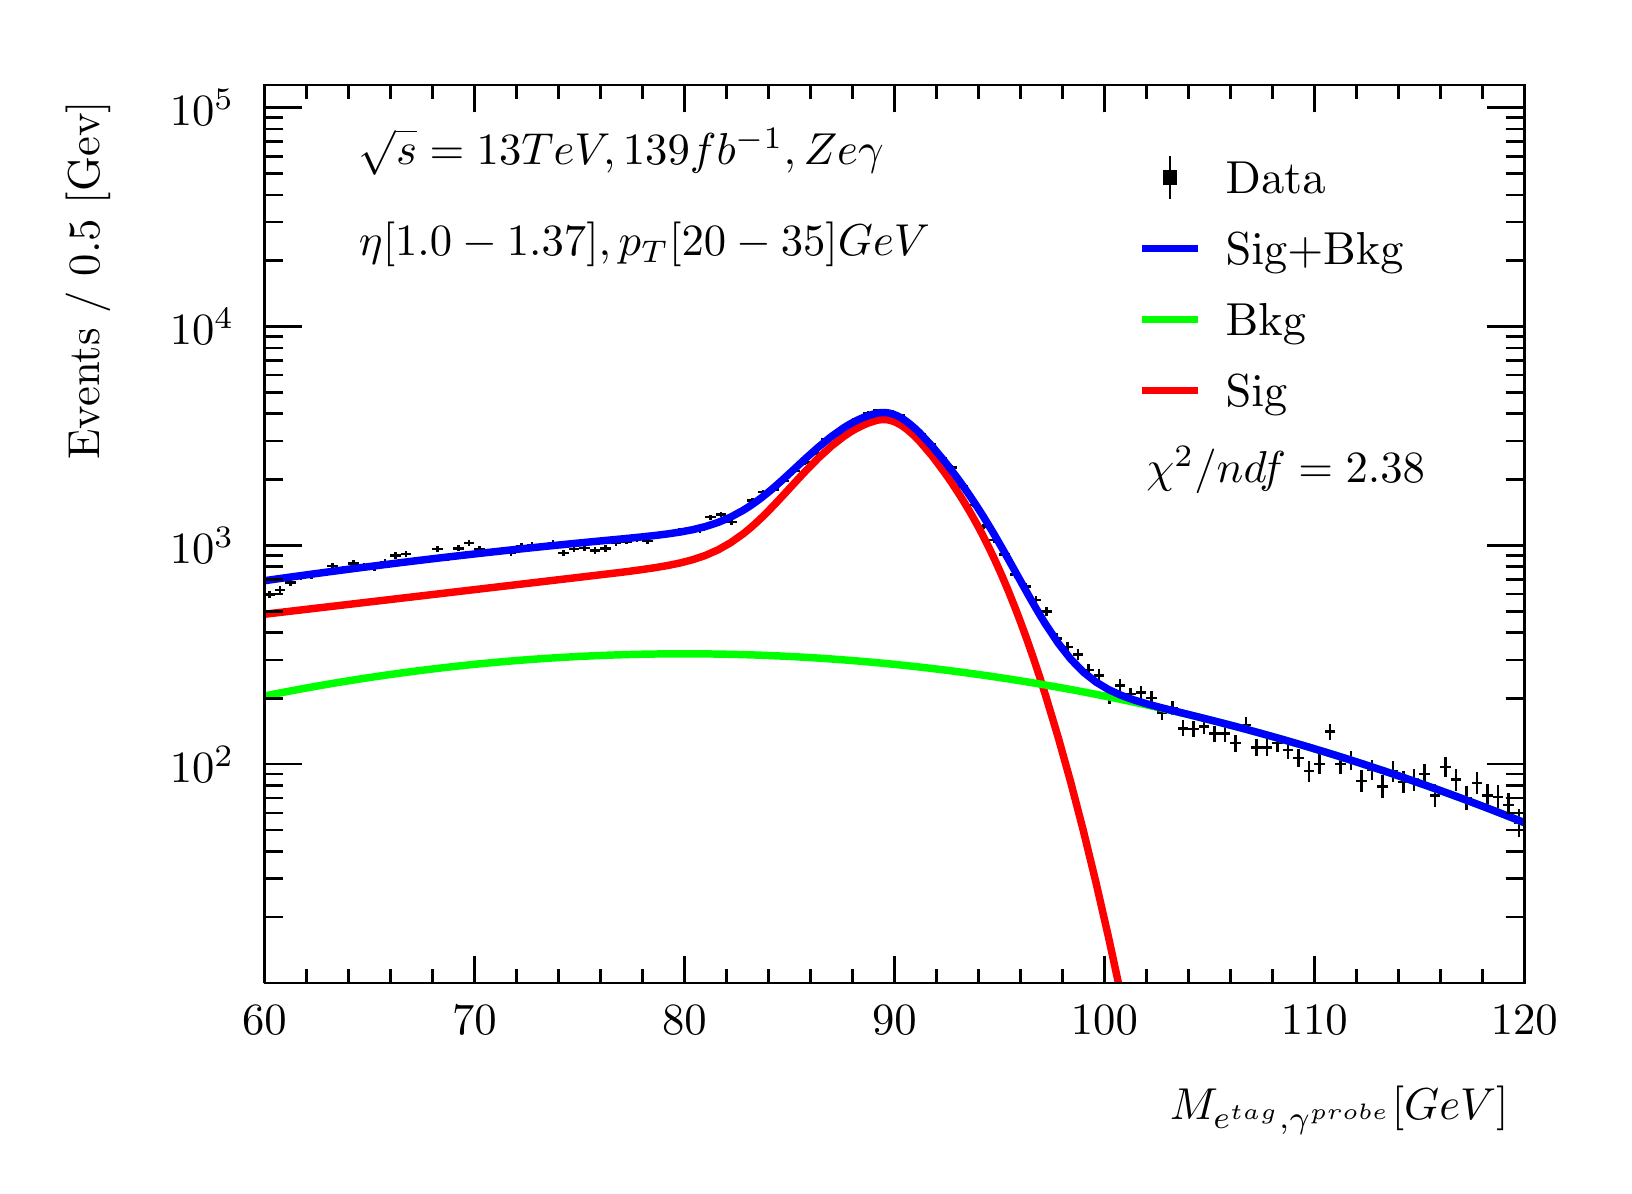
\begin{tikzpicture}
\pgfdeclareplotmark{cross} {
\pgfpathmoveto{\pgfpoint{-0.3\pgfplotmarksize}{\pgfplotmarksize}}
\pgfpathlineto{\pgfpoint{+0.3\pgfplotmarksize}{\pgfplotmarksize}}
\pgfpathlineto{\pgfpoint{+0.3\pgfplotmarksize}{0.3\pgfplotmarksize}}
\pgfpathlineto{\pgfpoint{+1\pgfplotmarksize}{0.3\pgfplotmarksize}}
\pgfpathlineto{\pgfpoint{+1\pgfplotmarksize}{-0.3\pgfplotmarksize}}
\pgfpathlineto{\pgfpoint{+0.3\pgfplotmarksize}{-0.3\pgfplotmarksize}}
\pgfpathlineto{\pgfpoint{+0.3\pgfplotmarksize}{-1.\pgfplotmarksize}}
\pgfpathlineto{\pgfpoint{-0.3\pgfplotmarksize}{-1.\pgfplotmarksize}}
\pgfpathlineto{\pgfpoint{-0.3\pgfplotmarksize}{-0.3\pgfplotmarksize}}
\pgfpathlineto{\pgfpoint{-1.\pgfplotmarksize}{-0.3\pgfplotmarksize}}
\pgfpathlineto{\pgfpoint{-1.\pgfplotmarksize}{0.3\pgfplotmarksize}}
\pgfpathlineto{\pgfpoint{-0.3\pgfplotmarksize}{0.3\pgfplotmarksize}}
\pgfpathclose
\pgfusepathqstroke
}
\pgfdeclareplotmark{cross*} {
\pgfpathmoveto{\pgfpoint{-0.3\pgfplotmarksize}{\pgfplotmarksize}}
\pgfpathlineto{\pgfpoint{+0.3\pgfplotmarksize}{\pgfplotmarksize}}
\pgfpathlineto{\pgfpoint{+0.3\pgfplotmarksize}{0.3\pgfplotmarksize}}
\pgfpathlineto{\pgfpoint{+1\pgfplotmarksize}{0.3\pgfplotmarksize}}
\pgfpathlineto{\pgfpoint{+1\pgfplotmarksize}{-0.3\pgfplotmarksize}}
\pgfpathlineto{\pgfpoint{+0.3\pgfplotmarksize}{-0.3\pgfplotmarksize}}
\pgfpathlineto{\pgfpoint{+0.3\pgfplotmarksize}{-1.\pgfplotmarksize}}
\pgfpathlineto{\pgfpoint{-0.3\pgfplotmarksize}{-1.\pgfplotmarksize}}
\pgfpathlineto{\pgfpoint{-0.3\pgfplotmarksize}{-0.3\pgfplotmarksize}}
\pgfpathlineto{\pgfpoint{-1.\pgfplotmarksize}{-0.3\pgfplotmarksize}}
\pgfpathlineto{\pgfpoint{-1.\pgfplotmarksize}{0.3\pgfplotmarksize}}
\pgfpathlineto{\pgfpoint{-0.3\pgfplotmarksize}{0.3\pgfplotmarksize}}
\pgfpathclose
\pgfusepathqfillstroke
}
\pgfdeclareplotmark{newstar} {
\pgfpathmoveto{\pgfqpoint{0pt}{\pgfplotmarksize}}
\pgfpathlineto{\pgfqpointpolar{44}{0.5\pgfplotmarksize}}
\pgfpathlineto{\pgfqpointpolar{18}{\pgfplotmarksize}}
\pgfpathlineto{\pgfqpointpolar{-20}{0.5\pgfplotmarksize}}
\pgfpathlineto{\pgfqpointpolar{-54}{\pgfplotmarksize}}
\pgfpathlineto{\pgfqpointpolar{-90}{0.5\pgfplotmarksize}}
\pgfpathlineto{\pgfqpointpolar{234}{\pgfplotmarksize}}
\pgfpathlineto{\pgfqpointpolar{198}{0.5\pgfplotmarksize}}
\pgfpathlineto{\pgfqpointpolar{162}{\pgfplotmarksize}}
\pgfpathlineto{\pgfqpointpolar{134}{0.5\pgfplotmarksize}}
\pgfpathclose
\pgfusepathqstroke
}
\pgfdeclareplotmark{newstar*} {
\pgfpathmoveto{\pgfqpoint{0pt}{\pgfplotmarksize}}
\pgfpathlineto{\pgfqpointpolar{44}{0.5\pgfplotmarksize}}
\pgfpathlineto{\pgfqpointpolar{18}{\pgfplotmarksize}}
\pgfpathlineto{\pgfqpointpolar{-20}{0.5\pgfplotmarksize}}
\pgfpathlineto{\pgfqpointpolar{-54}{\pgfplotmarksize}}
\pgfpathlineto{\pgfqpointpolar{-90}{0.5\pgfplotmarksize}}
\pgfpathlineto{\pgfqpointpolar{234}{\pgfplotmarksize}}
\pgfpathlineto{\pgfqpointpolar{198}{0.5\pgfplotmarksize}}
\pgfpathlineto{\pgfqpointpolar{162}{\pgfplotmarksize}}
\pgfpathlineto{\pgfqpointpolar{134}{0.5\pgfplotmarksize}}
\pgfpathclose
\pgfusepathqfillstroke
}
\definecolor{c}{rgb}{1,1,1};
\draw [color=c, fill=c] (0,0) rectangle (20,14.4361);
\draw [color=c, fill=c] (3,2.30977) rectangle (19,13.7143);
\definecolor{c}{rgb}{0,0,0};
\draw [c,line width=0.9] (3,2.30977) -- (3,13.7143) -- (19,13.7143) -- (19,2.30977) -- (3,2.30977);
\definecolor{c}{rgb}{1,1,1};
\draw [color=c, fill=c] (3,2.30977) rectangle (19,13.7143);
\definecolor{c}{rgb}{0,0,0};
\draw [c,line width=0.9] (3,2.30977) -- (3,13.7143) -- (19,13.7143) -- (19,2.30977) -- (3,2.30977);
\draw [c,line width=0.9] (3,2.30977) -- (19,2.30977);
\draw [c,line width=0.9] (3,2.65624) -- (3,2.30977);
\draw [c,line width=0.9] (3.53333,2.48301) -- (3.53333,2.30977);
\draw [c,line width=0.9] (4.06667,2.48301) -- (4.06667,2.30977);
\draw [c,line width=0.9] (4.6,2.48301) -- (4.6,2.30977);
\draw [c,line width=0.9] (5.13333,2.48301) -- (5.13333,2.30977);
\draw [c,line width=0.9] (5.66667,2.65624) -- (5.66667,2.30977);
\draw [c,line width=0.9] (6.2,2.48301) -- (6.2,2.30977);
\draw [c,line width=0.9] (6.73333,2.48301) -- (6.73333,2.30977);
\draw [c,line width=0.9] (7.26667,2.48301) -- (7.26667,2.30977);
\draw [c,line width=0.9] (7.8,2.48301) -- (7.8,2.30977);
\draw [c,line width=0.9] (8.33333,2.65624) -- (8.33333,2.30977);
\draw [c,line width=0.9] (8.86667,2.48301) -- (8.86667,2.30977);
\draw [c,line width=0.9] (9.4,2.48301) -- (9.4,2.30977);
\draw [c,line width=0.9] (9.93333,2.48301) -- (9.93333,2.30977);
\draw [c,line width=0.9] (10.4667,2.48301) -- (10.4667,2.30977);
\draw [c,line width=0.9] (11,2.65624) -- (11,2.30977);
\draw [c,line width=0.9] (11.5333,2.48301) -- (11.5333,2.30977);
\draw [c,line width=0.9] (12.0667,2.48301) -- (12.0667,2.30977);
\draw [c,line width=0.9] (12.6,2.48301) -- (12.6,2.30977);
\draw [c,line width=0.9] (13.1333,2.48301) -- (13.1333,2.30977);
\draw [c,line width=0.9] (13.6667,2.65624) -- (13.6667,2.30977);
\draw [c,line width=0.9] (14.2,2.48301) -- (14.2,2.30977);
\draw [c,line width=0.9] (14.7333,2.48301) -- (14.7333,2.30977);
\draw [c,line width=0.9] (15.2667,2.48301) -- (15.2667,2.30977);
\draw [c,line width=0.9] (15.8,2.48301) -- (15.8,2.30977);
\draw [c,line width=0.9] (16.3333,2.65624) -- (16.3333,2.30977);
\draw [c,line width=0.9] (16.8667,2.48301) -- (16.8667,2.30977);
\draw [c,line width=0.9] (17.4,2.48301) -- (17.4,2.30977);
\draw [c,line width=0.9] (17.9333,2.48301) -- (17.9333,2.30977);
\draw [c,line width=0.9] (18.4667,2.48301) -- (18.4667,2.30977);
\draw [c,line width=0.9] (19,2.65624) -- (19,2.30977);
\draw [anchor=base] (3,1.66015) node[scale=1.61424, color=c, rotate=0]{60};
\draw [anchor=base] (5.66667,1.66015) node[scale=1.61424, color=c, rotate=0]{70};
\draw [anchor=base] (8.33333,1.66015) node[scale=1.61424, color=c, rotate=0]{80};
\draw [anchor=base] (11,1.66015) node[scale=1.61424, color=c, rotate=0]{90};
\draw [anchor=base] (13.6667,1.66015) node[scale=1.61424, color=c, rotate=0]{100};
\draw [anchor=base] (16.3333,1.66015) node[scale=1.61424, color=c, rotate=0]{110};
\draw [anchor=base] (19,1.66015) node[scale=1.61424, color=c, rotate=0]{120};
\draw [anchor= east] (19,0.692932) node[scale=1.61424, color=c, rotate=0]{$M_{e^{tag}, \gamma^{probe}}  [GeV]$};
\draw [c,line width=0.9] (3,13.7143) -- (19,13.7143);
\draw [c,line width=0.9] (3,13.3678) -- (3,13.7143);
\draw [c,line width=0.9] (3.53333,13.5411) -- (3.53333,13.7143);
\draw [c,line width=0.9] (4.06667,13.5411) -- (4.06667,13.7143);
\draw [c,line width=0.9] (4.6,13.5411) -- (4.6,13.7143);
\draw [c,line width=0.9] (5.13333,13.5411) -- (5.13333,13.7143);
\draw [c,line width=0.9] (5.66667,13.3678) -- (5.66667,13.7143);
\draw [c,line width=0.9] (6.2,13.5411) -- (6.2,13.7143);
\draw [c,line width=0.9] (6.73333,13.5411) -- (6.73333,13.7143);
\draw [c,line width=0.9] (7.26667,13.5411) -- (7.26667,13.7143);
\draw [c,line width=0.9] (7.8,13.5411) -- (7.8,13.7143);
\draw [c,line width=0.9] (8.33333,13.3678) -- (8.33333,13.7143);
\draw [c,line width=0.9] (8.86667,13.5411) -- (8.86667,13.7143);
\draw [c,line width=0.9] (9.4,13.5411) -- (9.4,13.7143);
\draw [c,line width=0.9] (9.93333,13.5411) -- (9.93333,13.7143);
\draw [c,line width=0.9] (10.4667,13.5411) -- (10.4667,13.7143);
\draw [c,line width=0.9] (11,13.3678) -- (11,13.7143);
\draw [c,line width=0.9] (11.5333,13.5411) -- (11.5333,13.7143);
\draw [c,line width=0.9] (12.0667,13.5411) -- (12.0667,13.7143);
\draw [c,line width=0.9] (12.6,13.5411) -- (12.6,13.7143);
\draw [c,line width=0.9] (13.1333,13.5411) -- (13.1333,13.7143);
\draw [c,line width=0.9] (13.6667,13.3678) -- (13.6667,13.7143);
\draw [c,line width=0.9] (14.2,13.5411) -- (14.2,13.7143);
\draw [c,line width=0.9] (14.7333,13.5411) -- (14.7333,13.7143);
\draw [c,line width=0.9] (15.2667,13.5411) -- (15.2667,13.7143);
\draw [c,line width=0.9] (15.8,13.5411) -- (15.8,13.7143);
\draw [c,line width=0.9] (16.3333,13.3678) -- (16.3333,13.7143);
\draw [c,line width=0.9] (16.8667,13.5411) -- (16.8667,13.7143);
\draw [c,line width=0.9] (17.4,13.5411) -- (17.4,13.7143);
\draw [c,line width=0.9] (17.9333,13.5411) -- (17.9333,13.7143);
\draw [c,line width=0.9] (18.4667,13.5411) -- (18.4667,13.7143);
\draw [c,line width=0.9] (19,13.3678) -- (19,13.7143);
\draw [c,line width=0.9] (3,2.30977) -- (3,13.7143);
\draw [c,line width=0.9] (3.237,3.14637) -- (3,3.14637);
\draw [c,line width=0.9] (3.237,3.63576) -- (3,3.63576);
\draw [c,line width=0.9] (3.237,3.98298) -- (3,3.98298);
\draw [c,line width=0.9] (3.237,4.2523) -- (3,4.2523);
\draw [c,line width=0.9] (3.237,4.47236) -- (3,4.47236);
\draw [c,line width=0.9] (3.237,4.65841) -- (3,4.65841);
\draw [c,line width=0.9] (3.237,4.81958) -- (3,4.81958);
\draw [c,line width=0.9] (3.237,4.96174) -- (3,4.96174);
\draw [c,line width=0.9] (3.474,5.0889) -- (3,5.0889);
\draw [anchor= east] (2.82,5.0889) node[scale=1.61424, color=c, rotate=0]{$10^{2}$};
\draw [c,line width=0.9] (3.237,5.92551) -- (3,5.92551);
\draw [c,line width=0.9] (3.237,6.41489) -- (3,6.41489);
\draw [c,line width=0.9] (3.237,6.76211) -- (3,6.76211);
\draw [c,line width=0.9] (3.237,7.03144) -- (3,7.03144);
\draw [c,line width=0.9] (3.237,7.25149) -- (3,7.25149);
\draw [c,line width=0.9] (3.237,7.43755) -- (3,7.43755);
\draw [c,line width=0.9] (3.237,7.59871) -- (3,7.59871);
\draw [c,line width=0.9] (3.237,7.74087) -- (3,7.74087);
\draw [c,line width=0.9] (3.474,7.86804) -- (3,7.86804);
\draw [anchor= east] (2.82,7.86804) node[scale=1.61424, color=c, rotate=0]{$10^{3}$};
\draw [c,line width=0.9] (3.237,8.70464) -- (3,8.70464);
\draw [c,line width=0.9] (3.237,9.19402) -- (3,9.19402);
\draw [c,line width=0.9] (3.237,9.54124) -- (3,9.54124);
\draw [c,line width=0.9] (3.237,9.81057) -- (3,9.81057);
\draw [c,line width=0.9] (3.237,10.0306) -- (3,10.0306);
\draw [c,line width=0.9] (3.237,10.2167) -- (3,10.2167);
\draw [c,line width=0.9] (3.237,10.3778) -- (3,10.3778);
\draw [c,line width=0.9] (3.237,10.52) -- (3,10.52);
\draw [c,line width=0.9] (3.474,10.6472) -- (3,10.6472);
\draw [anchor= east] (2.82,10.6472) node[scale=1.61424, color=c, rotate=0]{$10^{4}$};
\draw [c,line width=0.9] (3.237,11.4838) -- (3,11.4838);
\draw [c,line width=0.9] (3.237,11.9732) -- (3,11.9732);
\draw [c,line width=0.9] (3.237,12.3204) -- (3,12.3204);
\draw [c,line width=0.9] (3.237,12.5897) -- (3,12.5897);
\draw [c,line width=0.9] (3.237,12.8098) -- (3,12.8098);
\draw [c,line width=0.9] (3.237,12.9958) -- (3,12.9958);
\draw [c,line width=0.9] (3.237,13.157) -- (3,13.157);
\draw [c,line width=0.9] (3.237,13.2991) -- (3,13.2991);
\draw [c,line width=0.9] (3.474,13.4263) -- (3,13.4263);
\draw [anchor= east] (2.82,13.4263) node[scale=1.61424, color=c, rotate=0]{$10^{5}$};
\draw [anchor= east] (0.76,13.7143) node[scale=1.61424, color=c, rotate=90]{Events / 0.5 [Gev]};
\draw [c,line width=0.9] (19,2.30977) -- (19,13.7143);
\draw [c,line width=0.9] (18.763,3.14637) -- (19,3.14637);
\draw [c,line width=0.9] (18.763,3.63576) -- (19,3.63576);
\draw [c,line width=0.9] (18.763,3.98298) -- (19,3.98298);
\draw [c,line width=0.9] (18.763,4.2523) -- (19,4.2523);
\draw [c,line width=0.9] (18.763,4.47236) -- (19,4.47236);
\draw [c,line width=0.9] (18.763,4.65841) -- (19,4.65841);
\draw [c,line width=0.9] (18.763,4.81958) -- (19,4.81958);
\draw [c,line width=0.9] (18.763,4.96174) -- (19,4.96174);
\draw [c,line width=0.9] (18.526,5.0889) -- (19,5.0889);
\draw [c,line width=0.9] (18.763,5.92551) -- (19,5.92551);
\draw [c,line width=0.9] (18.763,6.41489) -- (19,6.41489);
\draw [c,line width=0.9] (18.763,6.76211) -- (19,6.76211);
\draw [c,line width=0.9] (18.763,7.03144) -- (19,7.03144);
\draw [c,line width=0.9] (18.763,7.25149) -- (19,7.25149);
\draw [c,line width=0.9] (18.763,7.43755) -- (19,7.43755);
\draw [c,line width=0.9] (18.763,7.59871) -- (19,7.59871);
\draw [c,line width=0.9] (18.763,7.74087) -- (19,7.74087);
\draw [c,line width=0.9] (18.526,7.86804) -- (19,7.86804);
\draw [c,line width=0.9] (18.763,8.70464) -- (19,8.70464);
\draw [c,line width=0.9] (18.763,9.19402) -- (19,9.19402);
\draw [c,line width=0.9] (18.763,9.54124) -- (19,9.54124);
\draw [c,line width=0.9] (18.763,9.81057) -- (19,9.81057);
\draw [c,line width=0.9] (18.763,10.0306) -- (19,10.0306);
\draw [c,line width=0.9] (18.763,10.2167) -- (19,10.2167);
\draw [c,line width=0.9] (18.763,10.3778) -- (19,10.3778);
\draw [c,line width=0.9] (18.763,10.52) -- (19,10.52);
\draw [c,line width=0.9] (18.526,10.6472) -- (19,10.6472);
\draw [c,line width=0.9] (18.763,11.4838) -- (19,11.4838);
\draw [c,line width=0.9] (18.763,11.9732) -- (19,11.9732);
\draw [c,line width=0.9] (18.763,12.3204) -- (19,12.3204);
\draw [c,line width=0.9] (18.763,12.5897) -- (19,12.5897);
\draw [c,line width=0.9] (18.763,12.8098) -- (19,12.8098);
\draw [c,line width=0.9] (18.763,12.9958) -- (19,12.9958);
\draw [c,line width=0.9] (18.763,13.157) -- (19,13.157);
\draw [c,line width=0.9] (18.763,13.2991) -- (19,13.2991);
\draw [c,line width=0.9] (18.526,13.4263) -- (19,13.4263);
\draw [c,line width=0.9] (3.06667,7.24544) -- (3,7.24544);
\draw [c,line width=0.9] (3,7.24544) -- (3,7.24544);
\draw [c,line width=0.9] (3.06667,7.24544) -- (3.13333,7.24544);
\draw [c,line width=0.9] (3.13333,7.24544) -- (3.13333,7.24544);
\draw [c,line width=0.9] (3.06667,7.24544) -- (3.06667,7.29484);
\draw [c,line width=0.9] (3.06667,7.29484) -- (3.06667,7.29484);
\draw [c,line width=0.9] (3.06667,7.24544) -- (3.06667,7.19605);
\draw [c,line width=0.9] (3.06667,7.19605) -- (3.06667,7.19605);
\draw [c,line width=0.9] (3.2,7.30076) -- (3.13333,7.30076);
\draw [c,line width=0.9] (3.13333,7.30076) -- (3.13333,7.30076);
\draw [c,line width=0.9] (3.2,7.30076) -- (3.26667,7.30076);
\draw [c,line width=0.9] (3.26667,7.30076) -- (3.26667,7.30076);
\draw [c,line width=0.9] (3.2,7.30076) -- (3.2,7.34904);
\draw [c,line width=0.9] (3.2,7.34904) -- (3.2,7.34904);
\draw [c,line width=0.9] (3.2,7.30076) -- (3.2,7.25249);
\draw [c,line width=0.9] (3.2,7.25249) -- (3.2,7.25249);
\draw [c,line width=0.9] (3.33333,7.39544) -- (3.26667,7.39544);
\draw [c,line width=0.9] (3.26667,7.39544) -- (3.26667,7.39544);
\draw [c,line width=0.9] (3.33333,7.39544) -- (3.4,7.39544);
\draw [c,line width=0.9] (3.4,7.39544) -- (3.4,7.39544);
\draw [c,line width=0.9] (3.33333,7.39544) -- (3.33333,7.44186);
\draw [c,line width=0.9] (3.33333,7.44186) -- (3.33333,7.44186);
\draw [c,line width=0.9] (3.33333,7.39544) -- (3.33333,7.34902);
\draw [c,line width=0.9] (3.33333,7.34902) -- (3.33333,7.34902);
\draw [c,line width=0.9] (3.46667,7.47155) -- (3.4,7.47155);
\draw [c,line width=0.9] (3.4,7.47155) -- (3.4,7.47155);
\draw [c,line width=0.9] (3.46667,7.47155) -- (3.53333,7.47155);
\draw [c,line width=0.9] (3.53333,7.47155) -- (3.53333,7.47155);
\draw [c,line width=0.9] (3.46667,7.47155) -- (3.46667,7.51653);
\draw [c,line width=0.9] (3.46667,7.51653) -- (3.46667,7.51653);
\draw [c,line width=0.9] (3.46667,7.47155) -- (3.46667,7.42657);
\draw [c,line width=0.9] (3.46667,7.42657) -- (3.46667,7.42657);
\draw [c,line width=0.9] (3.6,7.48323) -- (3.53333,7.48323);
\draw [c,line width=0.9] (3.53333,7.48323) -- (3.53333,7.48323);
\draw [c,line width=0.9] (3.6,7.48323) -- (3.66667,7.48323);
\draw [c,line width=0.9] (3.66667,7.48323) -- (3.66667,7.48323);
\draw [c,line width=0.9] (3.6,7.48323) -- (3.6,7.52799);
\draw [c,line width=0.9] (3.6,7.52799) -- (3.6,7.52799);
\draw [c,line width=0.9] (3.6,7.48323) -- (3.6,7.43846);
\draw [c,line width=0.9] (3.6,7.43846) -- (3.6,7.43846);
\draw [c,line width=0.9] (3.73333,7.52243) -- (3.66667,7.52243);
\draw [c,line width=0.9] (3.66667,7.52243) -- (3.66667,7.52243);
\draw [c,line width=0.9] (3.73333,7.52243) -- (3.8,7.52243);
\draw [c,line width=0.9] (3.8,7.52243) -- (3.8,7.52243);
\draw [c,line width=0.9] (3.73333,7.52243) -- (3.73333,7.56647);
\draw [c,line width=0.9] (3.73333,7.56647) -- (3.73333,7.56647);
\draw [c,line width=0.9] (3.73333,7.52243) -- (3.73333,7.47839);
\draw [c,line width=0.9] (3.73333,7.47839) -- (3.73333,7.47839);
\draw [c,line width=0.9] (3.86667,7.60773) -- (3.8,7.60773);
\draw [c,line width=0.9] (3.8,7.60773) -- (3.8,7.60773);
\draw [c,line width=0.9] (3.86667,7.60773) -- (3.93333,7.60773);
\draw [c,line width=0.9] (3.93333,7.60773) -- (3.93333,7.60773);
\draw [c,line width=0.9] (3.86667,7.60773) -- (3.86667,7.65024);
\draw [c,line width=0.9] (3.86667,7.65024) -- (3.86667,7.65024);
\draw [c,line width=0.9] (3.86667,7.60773) -- (3.86667,7.56522);
\draw [c,line width=0.9] (3.86667,7.56522) -- (3.86667,7.56522);
\draw [c,line width=0.9] (4,7.56039) -- (3.93333,7.56039);
\draw [c,line width=0.9] (3.93333,7.56039) -- (3.93333,7.56039);
\draw [c,line width=0.9] (4,7.56039) -- (4.06667,7.56039);
\draw [c,line width=0.9] (4.06667,7.56039) -- (4.06667,7.56039);
\draw [c,line width=0.9] (4,7.56039) -- (4,7.60375);
\draw [c,line width=0.9] (4,7.60375) -- (4,7.60375);
\draw [c,line width=0.9] (4,7.56039) -- (4,7.51704);
\draw [c,line width=0.9] (4,7.51704) -- (4,7.51704);
\draw [c,line width=0.9] (4.13333,7.63878) -- (4.06667,7.63878);
\draw [c,line width=0.9] (4.06667,7.63878) -- (4.06667,7.63878);
\draw [c,line width=0.9] (4.13333,7.63878) -- (4.2,7.63878);
\draw [c,line width=0.9] (4.2,7.63878) -- (4.2,7.63878);
\draw [c,line width=0.9] (4.13333,7.63878) -- (4.13333,7.68074);
\draw [c,line width=0.9] (4.13333,7.68074) -- (4.13333,7.68074);
\draw [c,line width=0.9] (4.13333,7.63878) -- (4.13333,7.59681);
\draw [c,line width=0.9] (4.13333,7.59681) -- (4.13333,7.59681);
\draw [c,line width=0.9] (4.26667,7.60623) -- (4.2,7.60623);
\draw [c,line width=0.9] (4.2,7.60623) -- (4.2,7.60623);
\draw [c,line width=0.9] (4.26667,7.60623) -- (4.33333,7.60623);
\draw [c,line width=0.9] (4.33333,7.60623) -- (4.33333,7.60623);
\draw [c,line width=0.9] (4.26667,7.60623) -- (4.26667,7.64877);
\draw [c,line width=0.9] (4.26667,7.64877) -- (4.26667,7.64877);
\draw [c,line width=0.9] (4.26667,7.60623) -- (4.26667,7.5637);
\draw [c,line width=0.9] (4.26667,7.5637) -- (4.26667,7.5637);
\draw [c,line width=0.9] (4.4,7.58658) -- (4.33333,7.58658);
\draw [c,line width=0.9] (4.33333,7.58658) -- (4.33333,7.58658);
\draw [c,line width=0.9] (4.4,7.58658) -- (4.46667,7.58658);
\draw [c,line width=0.9] (4.46667,7.58658) -- (4.46667,7.58658);
\draw [c,line width=0.9] (4.4,7.58658) -- (4.4,7.62947);
\draw [c,line width=0.9] (4.4,7.62947) -- (4.4,7.62947);
\draw [c,line width=0.9] (4.4,7.58658) -- (4.4,7.5437);
\draw [c,line width=0.9] (4.4,7.5437) -- (4.4,7.5437);
\draw [c,line width=0.9] (4.53333,7.65473) -- (4.46667,7.65473);
\draw [c,line width=0.9] (4.46667,7.65473) -- (4.46667,7.65473);
\draw [c,line width=0.9] (4.53333,7.65473) -- (4.6,7.65473);
\draw [c,line width=0.9] (4.6,7.65473) -- (4.6,7.65473);
\draw [c,line width=0.9] (4.53333,7.65473) -- (4.53333,7.69642);
\draw [c,line width=0.9] (4.53333,7.69642) -- (4.53333,7.69642);
\draw [c,line width=0.9] (4.53333,7.65473) -- (4.53333,7.61303);
\draw [c,line width=0.9] (4.53333,7.61303) -- (4.53333,7.61303);
\draw [c,line width=0.9] (4.66667,7.74087) -- (4.6,7.74087);
\draw [c,line width=0.9] (4.6,7.74087) -- (4.6,7.74087);
\draw [c,line width=0.9] (4.66667,7.74087) -- (4.73333,7.74087);
\draw [c,line width=0.9] (4.73333,7.74087) -- (4.73333,7.74087);
\draw [c,line width=0.9] (4.66667,7.74087) -- (4.66667,7.7811);
\draw [c,line width=0.9] (4.66667,7.7811) -- (4.66667,7.7811);
\draw [c,line width=0.9] (4.66667,7.74087) -- (4.66667,7.70064);
\draw [c,line width=0.9] (4.66667,7.70064) -- (4.66667,7.70064);
\draw [c,line width=0.9] (4.8,7.7595) -- (4.73333,7.7595);
\draw [c,line width=0.9] (4.73333,7.7595) -- (4.73333,7.7595);
\draw [c,line width=0.9] (4.8,7.7595) -- (4.86667,7.7595);
\draw [c,line width=0.9] (4.86667,7.7595) -- (4.86667,7.7595);
\draw [c,line width=0.9] (4.8,7.7595) -- (4.8,7.79943);
\draw [c,line width=0.9] (4.8,7.79943) -- (4.8,7.79943);
\draw [c,line width=0.9] (4.8,7.7595) -- (4.8,7.71958);
\draw [c,line width=0.9] (4.8,7.71958) -- (4.8,7.71958);
\draw [c,line width=0.9] (4.93333,7.67331) -- (4.86667,7.67331);
\draw [c,line width=0.9] (4.86667,7.67331) -- (4.86667,7.67331);
\draw [c,line width=0.9] (4.93333,7.67331) -- (5,7.67331);
\draw [c,line width=0.9] (5,7.67331) -- (5,7.67331);
\draw [c,line width=0.9] (4.93333,7.67331) -- (4.93333,7.71468);
\draw [c,line width=0.9] (4.93333,7.71468) -- (4.93333,7.71468);
\draw [c,line width=0.9] (4.93333,7.67331) -- (4.93333,7.63193);
\draw [c,line width=0.9] (4.93333,7.63193) -- (4.93333,7.63193);
\draw [c,line width=0.9] (5.06667,7.69718) -- (5,7.69718);
\draw [c,line width=0.9] (5,7.69718) -- (5,7.69718);
\draw [c,line width=0.9] (5.06667,7.69718) -- (5.13333,7.69718);
\draw [c,line width=0.9] (5.13333,7.69718) -- (5.13333,7.69718);
\draw [c,line width=0.9] (5.06667,7.69718) -- (5.06667,7.73814);
\draw [c,line width=0.9] (5.06667,7.73814) -- (5.06667,7.73814);
\draw [c,line width=0.9] (5.06667,7.69718) -- (5.06667,7.65621);
\draw [c,line width=0.9] (5.06667,7.65621) -- (5.06667,7.65621);
\draw [c,line width=0.9] (5.2,7.82003) -- (5.13333,7.82003);
\draw [c,line width=0.9] (5.13333,7.82003) -- (5.13333,7.82003);
\draw [c,line width=0.9] (5.2,7.82003) -- (5.26667,7.82003);
\draw [c,line width=0.9] (5.26667,7.82003) -- (5.26667,7.82003);
\draw [c,line width=0.9] (5.2,7.82003) -- (5.2,7.85896);
\draw [c,line width=0.9] (5.2,7.85896) -- (5.2,7.85896);
\draw [c,line width=0.9] (5.2,7.82003) -- (5.2,7.78109);
\draw [c,line width=0.9] (5.2,7.78109) -- (5.2,7.78109);
\draw [c,line width=0.9] (5.33333,7.711) -- (5.26667,7.711);
\draw [c,line width=0.9] (5.26667,7.711) -- (5.26667,7.711);
\draw [c,line width=0.9] (5.33333,7.711) -- (5.4,7.711);
\draw [c,line width=0.9] (5.4,7.711) -- (5.4,7.711);
\draw [c,line width=0.9] (5.33333,7.711) -- (5.33333,7.75173);
\draw [c,line width=0.9] (5.33333,7.75173) -- (5.33333,7.75173);
\draw [c,line width=0.9] (5.33333,7.711) -- (5.33333,7.67027);
\draw [c,line width=0.9] (5.33333,7.67027) -- (5.33333,7.67027);
\draw [c,line width=0.9] (5.46667,7.83003) -- (5.4,7.83003);
\draw [c,line width=0.9] (5.4,7.83003) -- (5.4,7.83003);
\draw [c,line width=0.9] (5.46667,7.83003) -- (5.53333,7.83003);
\draw [c,line width=0.9] (5.53333,7.83003) -- (5.53333,7.83003);
\draw [c,line width=0.9] (5.46667,7.83003) -- (5.46667,7.8688);
\draw [c,line width=0.9] (5.46667,7.8688) -- (5.46667,7.8688);
\draw [c,line width=0.9] (5.46667,7.83003) -- (5.46667,7.79126);
\draw [c,line width=0.9] (5.46667,7.79126) -- (5.46667,7.79126);
\draw [c,line width=0.9] (5.6,7.89666) -- (5.53333,7.89666);
\draw [c,line width=0.9] (5.53333,7.89666) -- (5.53333,7.89666);
\draw [c,line width=0.9] (5.6,7.89666) -- (5.66667,7.89666);
\draw [c,line width=0.9] (5.66667,7.89666) -- (5.66667,7.89666);
\draw [c,line width=0.9] (5.6,7.89666) -- (5.6,7.93438);
\draw [c,line width=0.9] (5.6,7.93438) -- (5.6,7.93438);
\draw [c,line width=0.9] (5.6,7.89666) -- (5.6,7.85895);
\draw [c,line width=0.9] (5.6,7.85895) -- (5.6,7.85895);
\draw [c,line width=0.9] (5.73333,7.81751) -- (5.66667,7.81751);
\draw [c,line width=0.9] (5.66667,7.81751) -- (5.66667,7.81751);
\draw [c,line width=0.9] (5.73333,7.81751) -- (5.8,7.81751);
\draw [c,line width=0.9] (5.8,7.81751) -- (5.8,7.81751);
\draw [c,line width=0.9] (5.73333,7.81751) -- (5.73333,7.85648);
\draw [c,line width=0.9] (5.73333,7.85648) -- (5.73333,7.85648);
\draw [c,line width=0.9] (5.73333,7.81751) -- (5.73333,7.77854);
\draw [c,line width=0.9] (5.73333,7.77854) -- (5.73333,7.77854);
\draw [c,line width=0.9] (5.86667,7.77785) -- (5.8,7.77785);
\draw [c,line width=0.9] (5.8,7.77785) -- (5.8,7.77785);
\draw [c,line width=0.9] (5.86667,7.77785) -- (5.93333,7.77785);
\draw [c,line width=0.9] (5.93333,7.77785) -- (5.93333,7.77785);
\draw [c,line width=0.9] (5.86667,7.77785) -- (5.86667,7.81747);
\draw [c,line width=0.9] (5.86667,7.81747) -- (5.86667,7.81747);
\draw [c,line width=0.9] (5.86667,7.77785) -- (5.86667,7.73823);
\draw [c,line width=0.9] (5.86667,7.73823) -- (5.86667,7.73823);
\draw [c,line width=0.9] (6,7.79592) -- (5.93333,7.79592);
\draw [c,line width=0.9] (5.93333,7.79592) -- (5.93333,7.79592);
\draw [c,line width=0.9] (6,7.79592) -- (6.06667,7.79592);
\draw [c,line width=0.9] (6.06667,7.79592) -- (6.06667,7.79592);
\draw [c,line width=0.9] (6,7.79592) -- (6,7.83525);
\draw [c,line width=0.9] (6,7.83525) -- (6,7.83525);
\draw [c,line width=0.9] (6,7.79592) -- (6,7.7566);
\draw [c,line width=0.9] (6,7.7566) -- (6,7.7566);
\draw [c,line width=0.9] (6.13333,7.77655) -- (6.06667,7.77655);
\draw [c,line width=0.9] (6.06667,7.77655) -- (6.06667,7.77655);
\draw [c,line width=0.9] (6.13333,7.77655) -- (6.2,7.77655);
\draw [c,line width=0.9] (6.2,7.77655) -- (6.2,7.77655);
\draw [c,line width=0.9] (6.13333,7.77655) -- (6.13333,7.81619);
\draw [c,line width=0.9] (6.13333,7.81619) -- (6.13333,7.81619);
\draw [c,line width=0.9] (6.13333,7.77655) -- (6.13333,7.73691);
\draw [c,line width=0.9] (6.13333,7.73691) -- (6.13333,7.73691);
\draw [c,line width=0.9] (6.26667,7.85713) -- (6.2,7.85713);
\draw [c,line width=0.9] (6.2,7.85713) -- (6.2,7.85713);
\draw [c,line width=0.9] (6.26667,7.85713) -- (6.33333,7.85713);
\draw [c,line width=0.9] (6.33333,7.85713) -- (6.33333,7.85713);
\draw [c,line width=0.9] (6.26667,7.85713) -- (6.26667,7.89547);
\draw [c,line width=0.9] (6.26667,7.89547) -- (6.26667,7.89547);
\draw [c,line width=0.9] (6.26667,7.85713) -- (6.26667,7.81879);
\draw [c,line width=0.9] (6.26667,7.81879) -- (6.26667,7.81879);
\draw [c,line width=0.9] (6.4,7.86925) -- (6.33333,7.86925);
\draw [c,line width=0.9] (6.33333,7.86925) -- (6.33333,7.86925);
\draw [c,line width=0.9] (6.4,7.86925) -- (6.46667,7.86925);
\draw [c,line width=0.9] (6.46667,7.86925) -- (6.46667,7.86925);
\draw [c,line width=0.9] (6.4,7.86925) -- (6.4,7.90739);
\draw [c,line width=0.9] (6.4,7.90739) -- (6.4,7.90739);
\draw [c,line width=0.9] (6.4,7.86925) -- (6.4,7.8311);
\draw [c,line width=0.9] (6.4,7.8311) -- (6.4,7.8311);
\draw [c,line width=0.9] (6.53333,7.84242) -- (6.46667,7.84242);
\draw [c,line width=0.9] (6.46667,7.84242) -- (6.46667,7.84242);
\draw [c,line width=0.9] (6.53333,7.84242) -- (6.6,7.84242);
\draw [c,line width=0.9] (6.6,7.84242) -- (6.6,7.84242);
\draw [c,line width=0.9] (6.53333,7.84242) -- (6.53333,7.881);
\draw [c,line width=0.9] (6.53333,7.881) -- (6.53333,7.881);
\draw [c,line width=0.9] (6.53333,7.84242) -- (6.53333,7.80385);
\draw [c,line width=0.9] (6.53333,7.80385) -- (6.53333,7.80385);
\draw [c,line width=0.9] (6.66667,7.9002) -- (6.6,7.9002);
\draw [c,line width=0.9] (6.6,7.9002) -- (6.6,7.9002);
\draw [c,line width=0.9] (6.66667,7.9002) -- (6.73333,7.9002);
\draw [c,line width=0.9] (6.73333,7.9002) -- (6.73333,7.9002);
\draw [c,line width=0.9] (6.66667,7.9002) -- (6.66667,7.93786);
\draw [c,line width=0.9] (6.66667,7.93786) -- (6.66667,7.93786);
\draw [c,line width=0.9] (6.66667,7.9002) -- (6.66667,7.86253);
\draw [c,line width=0.9] (6.66667,7.86253) -- (6.66667,7.86253);
\draw [c,line width=0.9] (6.8,7.77133) -- (6.73333,7.77133);
\draw [c,line width=0.9] (6.73333,7.77133) -- (6.73333,7.77133);
\draw [c,line width=0.9] (6.8,7.77133) -- (6.86667,7.77133);
\draw [c,line width=0.9] (6.86667,7.77133) -- (6.86667,7.77133);
\draw [c,line width=0.9] (6.8,7.77133) -- (6.8,7.81106);
\draw [c,line width=0.9] (6.8,7.81106) -- (6.8,7.81106);
\draw [c,line width=0.9] (6.8,7.77133) -- (6.8,7.73161);
\draw [c,line width=0.9] (6.8,7.73161) -- (6.8,7.73161);
\draw [c,line width=0.9] (6.93333,7.82504) -- (6.86667,7.82504);
\draw [c,line width=0.9] (6.86667,7.82504) -- (6.86667,7.82504);
\draw [c,line width=0.9] (6.93333,7.82504) -- (7,7.82504);
\draw [c,line width=0.9] (7,7.82504) -- (7,7.82504);
\draw [c,line width=0.9] (6.93333,7.82504) -- (6.93333,7.86389);
\draw [c,line width=0.9] (6.93333,7.86389) -- (6.93333,7.86389);
\draw [c,line width=0.9] (6.93333,7.82504) -- (6.93333,7.78619);
\draw [c,line width=0.9] (6.93333,7.78619) -- (6.93333,7.78619);
\draw [c,line width=0.9] (7.06667,7.83376) -- (7,7.83376);
\draw [c,line width=0.9] (7,7.83376) -- (7,7.83376);
\draw [c,line width=0.9] (7.06667,7.83376) -- (7.13333,7.83376);
\draw [c,line width=0.9] (7.13333,7.83376) -- (7.13333,7.83376);
\draw [c,line width=0.9] (7.06667,7.83376) -- (7.06667,7.87247);
\draw [c,line width=0.9] (7.06667,7.87247) -- (7.06667,7.87247);
\draw [c,line width=0.9] (7.06667,7.83376) -- (7.06667,7.79505);
\draw [c,line width=0.9] (7.06667,7.79505) -- (7.06667,7.79505);
\draw [c,line width=0.9] (7.2,7.80231) -- (7.13333,7.80231);
\draw [c,line width=0.9] (7.13333,7.80231) -- (7.13333,7.80231);
\draw [c,line width=0.9] (7.2,7.80231) -- (7.26667,7.80231);
\draw [c,line width=0.9] (7.26667,7.80231) -- (7.26667,7.80231);
\draw [c,line width=0.9] (7.2,7.80231) -- (7.2,7.84153);
\draw [c,line width=0.9] (7.2,7.84153) -- (7.2,7.84153);
\draw [c,line width=0.9] (7.2,7.80231) -- (7.2,7.76309);
\draw [c,line width=0.9] (7.2,7.76309) -- (7.2,7.76309);
\draw [c,line width=0.9] (7.33333,7.82879) -- (7.26667,7.82879);
\draw [c,line width=0.9] (7.26667,7.82879) -- (7.26667,7.82879);
\draw [c,line width=0.9] (7.33333,7.82879) -- (7.4,7.82879);
\draw [c,line width=0.9] (7.4,7.82879) -- (7.4,7.82879);
\draw [c,line width=0.9] (7.33333,7.82879) -- (7.33333,7.86758);
\draw [c,line width=0.9] (7.33333,7.86758) -- (7.33333,7.86758);
\draw [c,line width=0.9] (7.33333,7.82879) -- (7.33333,7.78999);
\draw [c,line width=0.9] (7.33333,7.78999) -- (7.33333,7.78999);
\draw [c,line width=0.9] (7.46667,7.90137) -- (7.4,7.90137);
\draw [c,line width=0.9] (7.4,7.90137) -- (7.4,7.90137);
\draw [c,line width=0.9] (7.46667,7.90137) -- (7.53333,7.90137);
\draw [c,line width=0.9] (7.53333,7.90137) -- (7.53333,7.90137);
\draw [c,line width=0.9] (7.46667,7.90137) -- (7.46667,7.93901);
\draw [c,line width=0.9] (7.46667,7.93901) -- (7.46667,7.93901);
\draw [c,line width=0.9] (7.46667,7.90137) -- (7.46667,7.86373);
\draw [c,line width=0.9] (7.46667,7.86373) -- (7.46667,7.86373);
\draw [c,line width=0.9] (7.6,7.92001) -- (7.53333,7.92001);
\draw [c,line width=0.9] (7.53333,7.92001) -- (7.53333,7.92001);
\draw [c,line width=0.9] (7.6,7.92001) -- (7.66667,7.92001);
\draw [c,line width=0.9] (7.66667,7.92001) -- (7.66667,7.92001);
\draw [c,line width=0.9] (7.6,7.92001) -- (7.6,7.95736);
\draw [c,line width=0.9] (7.6,7.95736) -- (7.6,7.95736);
\draw [c,line width=0.9] (7.6,7.92001) -- (7.6,7.88266);
\draw [c,line width=0.9] (7.6,7.88266) -- (7.6,7.88266);
\draw [c,line width=0.9] (7.73333,7.94857) -- (7.66667,7.94857);
\draw [c,line width=0.9] (7.66667,7.94857) -- (7.66667,7.94857);
\draw [c,line width=0.9] (7.73333,7.94857) -- (7.8,7.94857);
\draw [c,line width=0.9] (7.8,7.94857) -- (7.8,7.94857);
\draw [c,line width=0.9] (7.73333,7.94857) -- (7.73333,7.98549);
\draw [c,line width=0.9] (7.73333,7.98549) -- (7.73333,7.98549);
\draw [c,line width=0.9] (7.73333,7.94857) -- (7.73333,7.91166);
\draw [c,line width=0.9] (7.73333,7.91166) -- (7.73333,7.91166);
\draw [c,line width=0.9] (7.86667,7.92693) -- (7.8,7.92693);
\draw [c,line width=0.9] (7.8,7.92693) -- (7.8,7.92693);
\draw [c,line width=0.9] (7.86667,7.92693) -- (7.93333,7.92693);
\draw [c,line width=0.9] (7.93333,7.92693) -- (7.93333,7.92693);
\draw [c,line width=0.9] (7.86667,7.92693) -- (7.86667,7.96417);
\draw [c,line width=0.9] (7.86667,7.96417) -- (7.86667,7.96417);
\draw [c,line width=0.9] (7.86667,7.92693) -- (7.86667,7.88968);
\draw [c,line width=0.9] (7.86667,7.88968) -- (7.86667,7.88968);
\draw [c,line width=0.9] (8,7.99834) -- (7.93333,7.99834);
\draw [c,line width=0.9] (7.93333,7.99834) -- (7.93333,7.99834);
\draw [c,line width=0.9] (8,7.99834) -- (8.06667,7.99834);
\draw [c,line width=0.9] (8.06667,7.99834) -- (8.06667,7.99834);
\draw [c,line width=0.9] (8,7.99834) -- (8,8.0345);
\draw [c,line width=0.9] (8,8.0345) -- (8,8.0345);
\draw [c,line width=0.9] (8,7.99834) -- (8,7.96218);
\draw [c,line width=0.9] (8,7.96218) -- (8,7.96218);
\draw [c,line width=0.9] (8.13333,8.02194) -- (8.06667,8.02194);
\draw [c,line width=0.9] (8.06667,8.02194) -- (8.06667,8.02194);
\draw [c,line width=0.9] (8.13333,8.02194) -- (8.2,8.02194);
\draw [c,line width=0.9] (8.2,8.02194) -- (8.2,8.02194);
\draw [c,line width=0.9] (8.13333,8.02194) -- (8.13333,8.05775);
\draw [c,line width=0.9] (8.13333,8.05775) -- (8.13333,8.05775);
\draw [c,line width=0.9] (8.13333,8.02194) -- (8.13333,7.98614);
\draw [c,line width=0.9] (8.13333,7.98614) -- (8.13333,7.98614);
\draw [c,line width=0.9] (8.26667,8.04926) -- (8.2,8.04926);
\draw [c,line width=0.9] (8.2,8.04926) -- (8.2,8.04926);
\draw [c,line width=0.9] (8.26667,8.04926) -- (8.33333,8.04926);
\draw [c,line width=0.9] (8.33333,8.04926) -- (8.33333,8.04926);
\draw [c,line width=0.9] (8.26667,8.04926) -- (8.26667,8.08466);
\draw [c,line width=0.9] (8.26667,8.08466) -- (8.26667,8.08466);
\draw [c,line width=0.9] (8.26667,8.04926) -- (8.26667,8.01385);
\draw [c,line width=0.9] (8.26667,8.01385) -- (8.26667,8.01385);
\draw [c,line width=0.9] (8.4,8.04405) -- (8.33333,8.04405);
\draw [c,line width=0.9] (8.33333,8.04405) -- (8.33333,8.04405);
\draw [c,line width=0.9] (8.4,8.04405) -- (8.46667,8.04405);
\draw [c,line width=0.9] (8.46667,8.04405) -- (8.46667,8.04405);
\draw [c,line width=0.9] (8.4,8.04405) -- (8.4,8.07953);
\draw [c,line width=0.9] (8.4,8.07953) -- (8.4,8.07953);
\draw [c,line width=0.9] (8.4,8.04405) -- (8.4,8.00857);
\draw [c,line width=0.9] (8.4,8.00857) -- (8.4,8.00857);
\draw [c,line width=0.9] (8.53333,8.06474) -- (8.46667,8.06474);
\draw [c,line width=0.9] (8.46667,8.06474) -- (8.46667,8.06474);
\draw [c,line width=0.9] (8.53333,8.06474) -- (8.6,8.06474);
\draw [c,line width=0.9] (8.6,8.06474) -- (8.6,8.06474);
\draw [c,line width=0.9] (8.53333,8.06474) -- (8.53333,8.09992);
\draw [c,line width=0.9] (8.53333,8.09992) -- (8.53333,8.09992);
\draw [c,line width=0.9] (8.53333,8.06474) -- (8.53333,8.02956);
\draw [c,line width=0.9] (8.53333,8.02956) -- (8.53333,8.02956);
\draw [c,line width=0.9] (8.66667,8.22667) -- (8.6,8.22667);
\draw [c,line width=0.9] (8.6,8.22667) -- (8.6,8.22667);
\draw [c,line width=0.9] (8.66667,8.22667) -- (8.73333,8.22667);
\draw [c,line width=0.9] (8.73333,8.22667) -- (8.73333,8.22667);
\draw [c,line width=0.9] (8.66667,8.22667) -- (8.66667,8.25957);
\draw [c,line width=0.9] (8.66667,8.25957) -- (8.66667,8.25957);
\draw [c,line width=0.9] (8.66667,8.22667) -- (8.66667,8.19378);
\draw [c,line width=0.9] (8.66667,8.19378) -- (8.66667,8.19378);
\draw [c,line width=0.9] (8.8,8.26115) -- (8.73333,8.26115);
\draw [c,line width=0.9] (8.73333,8.26115) -- (8.73333,8.26115);
\draw [c,line width=0.9] (8.8,8.26115) -- (8.86667,8.26115);
\draw [c,line width=0.9] (8.86667,8.26115) -- (8.86667,8.26115);
\draw [c,line width=0.9] (8.8,8.26115) -- (8.8,8.29358);
\draw [c,line width=0.9] (8.8,8.29358) -- (8.8,8.29358);
\draw [c,line width=0.9] (8.8,8.26115) -- (8.8,8.22872);
\draw [c,line width=0.9] (8.8,8.22872) -- (8.8,8.22872);
\draw [c,line width=0.9] (8.93333,8.16221) -- (8.86667,8.16221);
\draw [c,line width=0.9] (8.86667,8.16221) -- (8.86667,8.16221);
\draw [c,line width=0.9] (8.93333,8.16221) -- (9,8.16221);
\draw [c,line width=0.9] (9,8.16221) -- (9,8.16221);
\draw [c,line width=0.9] (8.93333,8.16221) -- (8.93333,8.196);
\draw [c,line width=0.9] (8.93333,8.196) -- (8.93333,8.196);
\draw [c,line width=0.9] (8.93333,8.16221) -- (8.93333,8.12843);
\draw [c,line width=0.9] (8.93333,8.12843) -- (8.93333,8.12843);
\draw [c,line width=0.9] (9.06667,8.31233) -- (9,8.31233);
\draw [c,line width=0.9] (9,8.31233) -- (9,8.31233);
\draw [c,line width=0.9] (9.06667,8.31233) -- (9.13333,8.31233);
\draw [c,line width=0.9] (9.13333,8.31233) -- (9.13333,8.31233);
\draw [c,line width=0.9] (9.06667,8.31233) -- (9.06667,8.34408);
\draw [c,line width=0.9] (9.06667,8.34408) -- (9.06667,8.34408);
\draw [c,line width=0.9] (9.06667,8.31233) -- (9.06667,8.28058);
\draw [c,line width=0.9] (9.06667,8.28058) -- (9.06667,8.28058);
\draw [c,line width=0.9] (9.2,8.43532) -- (9.13333,8.43532);
\draw [c,line width=0.9] (9.13333,8.43532) -- (9.13333,8.43532);
\draw [c,line width=0.9] (9.2,8.43532) -- (9.26667,8.43532);
\draw [c,line width=0.9] (9.26667,8.43532) -- (9.26667,8.43532);
\draw [c,line width=0.9] (9.2,8.43532) -- (9.2,8.46549);
\draw [c,line width=0.9] (9.2,8.46549) -- (9.2,8.46549);
\draw [c,line width=0.9] (9.2,8.43532) -- (9.2,8.40514);
\draw [c,line width=0.9] (9.2,8.40514) -- (9.2,8.40514);
\draw [c,line width=0.9] (9.33333,8.54348) -- (9.26667,8.54348);
\draw [c,line width=0.9] (9.26667,8.54348) -- (9.26667,8.54348);
\draw [c,line width=0.9] (9.33333,8.54348) -- (9.4,8.54348);
\draw [c,line width=0.9] (9.4,8.54348) -- (9.4,8.54348);
\draw [c,line width=0.9] (9.33333,8.54348) -- (9.33333,8.57233);
\draw [c,line width=0.9] (9.33333,8.57233) -- (9.33333,8.57233);
\draw [c,line width=0.9] (9.33333,8.54348) -- (9.33333,8.51462);
\draw [c,line width=0.9] (9.33333,8.51462) -- (9.33333,8.51462);
\draw [c,line width=0.9] (9.46667,8.58082) -- (9.4,8.58082);
\draw [c,line width=0.9] (9.4,8.58082) -- (9.4,8.58082);
\draw [c,line width=0.9] (9.46667,8.58082) -- (9.53333,8.58082);
\draw [c,line width=0.9] (9.53333,8.58082) -- (9.53333,8.58082);
\draw [c,line width=0.9] (9.46667,8.58082) -- (9.46667,8.60923);
\draw [c,line width=0.9] (9.46667,8.60923) -- (9.46667,8.60923);
\draw [c,line width=0.9] (9.46667,8.58082) -- (9.46667,8.55242);
\draw [c,line width=0.9] (9.46667,8.55242) -- (9.46667,8.55242);
\draw [c,line width=0.9] (9.6,8.68762) -- (9.53333,8.68762);
\draw [c,line width=0.9] (9.53333,8.68762) -- (9.53333,8.68762);
\draw [c,line width=0.9] (9.6,8.68762) -- (9.66667,8.68762);
\draw [c,line width=0.9] (9.66667,8.68762) -- (9.66667,8.68762);
\draw [c,line width=0.9] (9.6,8.68762) -- (9.6,8.7148);
\draw [c,line width=0.9] (9.6,8.7148) -- (9.6,8.7148);
\draw [c,line width=0.9] (9.6,8.68762) -- (9.6,8.66045);
\draw [c,line width=0.9] (9.6,8.66045) -- (9.6,8.66045);
\draw [c,line width=0.9] (9.73333,8.80976) -- (9.66667,8.80976);
\draw [c,line width=0.9] (9.66667,8.80976) -- (9.66667,8.80976);
\draw [c,line width=0.9] (9.73333,8.80976) -- (9.8,8.80976);
\draw [c,line width=0.9] (9.8,8.80976) -- (9.8,8.80976);
\draw [c,line width=0.9] (9.73333,8.80976) -- (9.73333,8.8356);
\draw [c,line width=0.9] (9.73333,8.8356) -- (9.73333,8.8356);
\draw [c,line width=0.9] (9.73333,8.80976) -- (9.73333,8.78392);
\draw [c,line width=0.9] (9.73333,8.78392) -- (9.73333,8.78392);
\draw [c,line width=0.9] (9.86667,8.91814) -- (9.8,8.91814);
\draw [c,line width=0.9] (9.8,8.91814) -- (9.8,8.91814);
\draw [c,line width=0.9] (9.86667,8.91814) -- (9.93333,8.91814);
\draw [c,line width=0.9] (9.93333,8.91814) -- (9.93333,8.91814);
\draw [c,line width=0.9] (9.86667,8.91814) -- (9.86667,8.94285);
\draw [c,line width=0.9] (9.86667,8.94285) -- (9.86667,8.94285);
\draw [c,line width=0.9] (9.86667,8.91814) -- (9.86667,8.89344);
\draw [c,line width=0.9] (9.86667,8.89344) -- (9.86667,8.89344);
\draw [c,line width=0.9] (10,9.03973) -- (9.93333,9.03973);
\draw [c,line width=0.9] (9.93333,9.03973) -- (9.93333,9.03973);
\draw [c,line width=0.9] (10,9.03973) -- (10.0667,9.03973);
\draw [c,line width=0.9] (10.0667,9.03973) -- (10.0667,9.03973);
\draw [c,line width=0.9] (10,9.03973) -- (10,9.06322);
\draw [c,line width=0.9] (10,9.06322) -- (10,9.06322);
\draw [c,line width=0.9] (10,9.03973) -- (10,9.01624);
\draw [c,line width=0.9] (10,9.01624) -- (10,9.01624);
\draw [c,line width=0.9] (10.1333,9.21556) -- (10.0667,9.21556);
\draw [c,line width=0.9] (10.0667,9.21556) -- (10.0667,9.21556);
\draw [c,line width=0.9] (10.1333,9.21556) -- (10.2,9.21556);
\draw [c,line width=0.9] (10.2,9.21556) -- (10.2,9.21556);
\draw [c,line width=0.9] (10.1333,9.21556) -- (10.1333,9.2374);
\draw [c,line width=0.9] (10.1333,9.2374) -- (10.1333,9.2374);
\draw [c,line width=0.9] (10.1333,9.21556) -- (10.1333,9.19372);
\draw [c,line width=0.9] (10.1333,9.19372) -- (10.1333,9.19372);
\draw [c,line width=0.9] (10.2667,9.28952) -- (10.2,9.28952);
\draw [c,line width=0.9] (10.2,9.28952) -- (10.2,9.28952);
\draw [c,line width=0.9] (10.2667,9.28952) -- (10.3333,9.28952);
\draw [c,line width=0.9] (10.3333,9.28952) -- (10.3333,9.28952);
\draw [c,line width=0.9] (10.2667,9.28952) -- (10.2667,9.3107);
\draw [c,line width=0.9] (10.2667,9.3107) -- (10.2667,9.3107);
\draw [c,line width=0.9] (10.2667,9.28952) -- (10.2667,9.26834);
\draw [c,line width=0.9] (10.2667,9.26834) -- (10.2667,9.26834);
\draw [c,line width=0.9] (10.4,9.38318) -- (10.3333,9.38318);
\draw [c,line width=0.9] (10.3333,9.38318) -- (10.3333,9.38318);
\draw [c,line width=0.9] (10.4,9.38318) -- (10.4667,9.38318);
\draw [c,line width=0.9] (10.4667,9.38318) -- (10.4667,9.38318);
\draw [c,line width=0.9] (10.4,9.38318) -- (10.4,9.40355);
\draw [c,line width=0.9] (10.4,9.40355) -- (10.4,9.40355);
\draw [c,line width=0.9] (10.4,9.38318) -- (10.4,9.3628);
\draw [c,line width=0.9] (10.4,9.3628) -- (10.4,9.3628);
\draw [c,line width=0.9] (10.5333,9.46881) -- (10.4667,9.46881);
\draw [c,line width=0.9] (10.4667,9.46881) -- (10.4667,9.46881);
\draw [c,line width=0.9] (10.5333,9.46881) -- (10.6,9.46881);
\draw [c,line width=0.9] (10.6,9.46881) -- (10.6,9.46881);
\draw [c,line width=0.9] (10.5333,9.46881) -- (10.5333,9.48847);
\draw [c,line width=0.9] (10.5333,9.48847) -- (10.5333,9.48847);
\draw [c,line width=0.9] (10.5333,9.46881) -- (10.5333,9.44914);
\draw [c,line width=0.9] (10.5333,9.44914) -- (10.5333,9.44914);
\draw [c,line width=0.9] (10.6667,9.54996) -- (10.6,9.54996);
\draw [c,line width=0.9] (10.6,9.54996) -- (10.6,9.54996);
\draw [c,line width=0.9] (10.6667,9.54996) -- (10.7333,9.54996);
\draw [c,line width=0.9] (10.7333,9.54996) -- (10.7333,9.54996);
\draw [c,line width=0.9] (10.6667,9.54996) -- (10.6667,9.56898);
\draw [c,line width=0.9] (10.6667,9.56898) -- (10.6667,9.56898);
\draw [c,line width=0.9] (10.6667,9.54996) -- (10.6667,9.53095);
\draw [c,line width=0.9] (10.6667,9.53095) -- (10.6667,9.53095);
\draw [c,line width=0.9] (10.8,9.58131) -- (10.7333,9.58131);
\draw [c,line width=0.9] (10.7333,9.58131) -- (10.7333,9.58131);
\draw [c,line width=0.9] (10.8,9.58131) -- (10.8667,9.58131);
\draw [c,line width=0.9] (10.8667,9.58131) -- (10.8667,9.58131);
\draw [c,line width=0.9] (10.8,9.58131) -- (10.8,9.60008);
\draw [c,line width=0.9] (10.8,9.60008) -- (10.8,9.60008);
\draw [c,line width=0.9] (10.8,9.58131) -- (10.8,9.56254);
\draw [c,line width=0.9] (10.8,9.56254) -- (10.8,9.56254);
\draw [c,line width=0.9] (10.9333,9.56662) -- (10.8667,9.56662);
\draw [c,line width=0.9] (10.8667,9.56662) -- (10.8667,9.56662);
\draw [c,line width=0.9] (10.9333,9.56662) -- (11,9.56662);
\draw [c,line width=0.9] (11,9.56662) -- (11,9.56662);
\draw [c,line width=0.9] (10.9333,9.56662) -- (10.9333,9.58551);
\draw [c,line width=0.9] (10.9333,9.58551) -- (10.9333,9.58551);
\draw [c,line width=0.9] (10.9333,9.56662) -- (10.9333,9.54774);
\draw [c,line width=0.9] (10.9333,9.54774) -- (10.9333,9.54774);
\draw [c,line width=0.9] (11.0667,9.52208) -- (11,9.52208);
\draw [c,line width=0.9] (11,9.52208) -- (11,9.52208);
\draw [c,line width=0.9] (11.0667,9.52208) -- (11.1333,9.52208);
\draw [c,line width=0.9] (11.1333,9.52208) -- (11.1333,9.52208);
\draw [c,line width=0.9] (11.0667,9.52208) -- (11.0667,9.54132);
\draw [c,line width=0.9] (11.0667,9.54132) -- (11.0667,9.54132);
\draw [c,line width=0.9] (11.0667,9.52208) -- (11.0667,9.50285);
\draw [c,line width=0.9] (11.0667,9.50285) -- (11.0667,9.50285);
\draw [c,line width=0.9] (11.2,9.38627) -- (11.1333,9.38627);
\draw [c,line width=0.9] (11.1333,9.38627) -- (11.1333,9.38627);
\draw [c,line width=0.9] (11.2,9.38627) -- (11.2667,9.38627);
\draw [c,line width=0.9] (11.2667,9.38627) -- (11.2667,9.38627);
\draw [c,line width=0.9] (11.2,9.38627) -- (11.2,9.40662);
\draw [c,line width=0.9] (11.2,9.40662) -- (11.2,9.40662);
\draw [c,line width=0.9] (11.2,9.38627) -- (11.2,9.36592);
\draw [c,line width=0.9] (11.2,9.36592) -- (11.2,9.36592);
\draw [c,line width=0.9] (11.3333,9.2843) -- (11.2667,9.2843);
\draw [c,line width=0.9] (11.2667,9.2843) -- (11.2667,9.2843);
\draw [c,line width=0.9] (11.3333,9.2843) -- (11.4,9.2843);
\draw [c,line width=0.9] (11.4,9.2843) -- (11.4,9.2843);
\draw [c,line width=0.9] (11.3333,9.2843) -- (11.3333,9.30553);
\draw [c,line width=0.9] (11.3333,9.30553) -- (11.3333,9.30553);
\draw [c,line width=0.9] (11.3333,9.2843) -- (11.3333,9.26307);
\draw [c,line width=0.9] (11.3333,9.26307) -- (11.3333,9.26307);
\draw [c,line width=0.9] (11.4667,9.15767) -- (11.4,9.15767);
\draw [c,line width=0.9] (11.4,9.15767) -- (11.4,9.15767);
\draw [c,line width=0.9] (11.4667,9.15767) -- (11.5333,9.15767);
\draw [c,line width=0.9] (11.5333,9.15767) -- (11.5333,9.15767);
\draw [c,line width=0.9] (11.4667,9.15767) -- (11.4667,9.18005);
\draw [c,line width=0.9] (11.4667,9.18005) -- (11.4667,9.18005);
\draw [c,line width=0.9] (11.4667,9.15767) -- (11.4667,9.1353);
\draw [c,line width=0.9] (11.4667,9.1353) -- (11.4667,9.1353);
\draw [c,line width=0.9] (11.6,8.9701) -- (11.5333,8.9701);
\draw [c,line width=0.9] (11.5333,8.9701) -- (11.5333,8.9701);
\draw [c,line width=0.9] (11.6,8.9701) -- (11.6667,8.9701);
\draw [c,line width=0.9] (11.6667,8.9701) -- (11.6667,8.9701);
\draw [c,line width=0.9] (11.6,8.9701) -- (11.6,8.99428);
\draw [c,line width=0.9] (11.6,8.99428) -- (11.6,8.99428);
\draw [c,line width=0.9] (11.6,8.9701) -- (11.6,8.94592);
\draw [c,line width=0.9] (11.6,8.94592) -- (11.6,8.94592);
\draw [c,line width=0.9] (11.7333,8.85855) -- (11.6667,8.85855);
\draw [c,line width=0.9] (11.6667,8.85855) -- (11.6667,8.85855);
\draw [c,line width=0.9] (11.7333,8.85855) -- (11.8,8.85855);
\draw [c,line width=0.9] (11.8,8.85855) -- (11.8,8.85855);
\draw [c,line width=0.9] (11.7333,8.85855) -- (11.7333,8.88387);
\draw [c,line width=0.9] (11.7333,8.88387) -- (11.7333,8.88387);
\draw [c,line width=0.9] (11.7333,8.85855) -- (11.7333,8.83323);
\draw [c,line width=0.9] (11.7333,8.83323) -- (11.7333,8.83323);
\draw [c,line width=0.9] (11.8667,8.61315) -- (11.8,8.61315);
\draw [c,line width=0.9] (11.8,8.61315) -- (11.8,8.61315);
\draw [c,line width=0.9] (11.8667,8.61315) -- (11.9333,8.61315);
\draw [c,line width=0.9] (11.9333,8.61315) -- (11.9333,8.61315);
\draw [c,line width=0.9] (11.8667,8.61315) -- (11.8667,8.64118);
\draw [c,line width=0.9] (11.8667,8.64118) -- (11.8667,8.64118);
\draw [c,line width=0.9] (11.8667,8.61315) -- (11.8667,8.58512);
\draw [c,line width=0.9] (11.8667,8.58512) -- (11.8667,8.58512);
\draw [c,line width=0.9] (12,8.38132) -- (11.9333,8.38132);
\draw [c,line width=0.9] (11.9333,8.38132) -- (11.9333,8.38132);
\draw [c,line width=0.9] (12,8.38132) -- (12.0667,8.38132);
\draw [c,line width=0.9] (12.0667,8.38132) -- (12.0667,8.38132);
\draw [c,line width=0.9] (12,8.38132) -- (12,8.41218);
\draw [c,line width=0.9] (12,8.41218) -- (12,8.41218);
\draw [c,line width=0.9] (12,8.38132) -- (12,8.35047);
\draw [c,line width=0.9] (12,8.35047) -- (12,8.35047);
\draw [c,line width=0.9] (12.1333,8.10507) -- (12.0667,8.10507);
\draw [c,line width=0.9] (12.0667,8.10507) -- (12.0667,8.10507);
\draw [c,line width=0.9] (12.1333,8.10507) -- (12.2,8.10507);
\draw [c,line width=0.9] (12.2,8.10507) -- (12.2,8.10507);
\draw [c,line width=0.9] (12.1333,8.10507) -- (12.1333,8.13967);
\draw [c,line width=0.9] (12.1333,8.13967) -- (12.1333,8.13967);
\draw [c,line width=0.9] (12.1333,8.10507) -- (12.1333,8.07048);
\draw [c,line width=0.9] (12.1333,8.07048) -- (12.1333,8.07048);
\draw [c,line width=0.9] (12.2667,7.9338) -- (12.2,7.9338);
\draw [c,line width=0.9] (12.2,7.9338) -- (12.2,7.9338);
\draw [c,line width=0.9] (12.2667,7.9338) -- (12.3333,7.9338);
\draw [c,line width=0.9] (12.3333,7.9338) -- (12.3333,7.9338);
\draw [c,line width=0.9] (12.2667,7.9338) -- (12.2667,7.97095);
\draw [c,line width=0.9] (12.2667,7.97095) -- (12.2667,7.97095);
\draw [c,line width=0.9] (12.2667,7.9338) -- (12.2667,7.89666);
\draw [c,line width=0.9] (12.2667,7.89666) -- (12.2667,7.89666);
\draw [c,line width=0.9] (12.4,7.75288) -- (12.3333,7.75288);
\draw [c,line width=0.9] (12.3333,7.75288) -- (12.3333,7.75288);
\draw [c,line width=0.9] (12.4,7.75288) -- (12.4667,7.75288);
\draw [c,line width=0.9] (12.4667,7.75288) -- (12.4667,7.75288);
\draw [c,line width=0.9] (12.4,7.75288) -- (12.4,7.79291);
\draw [c,line width=0.9] (12.4,7.79291) -- (12.4,7.79291);
\draw [c,line width=0.9] (12.4,7.75288) -- (12.4,7.71285);
\draw [c,line width=0.9] (12.4,7.71285) -- (12.4,7.71285);
\draw [c,line width=0.9] (12.5333,7.49643) -- (12.4667,7.49643);
\draw [c,line width=0.9] (12.4667,7.49643) -- (12.4667,7.49643);
\draw [c,line width=0.9] (12.5333,7.49643) -- (12.6,7.49643);
\draw [c,line width=0.9] (12.6,7.49643) -- (12.6,7.49643);
\draw [c,line width=0.9] (12.5333,7.49643) -- (12.5333,7.54095);
\draw [c,line width=0.9] (12.5333,7.54095) -- (12.5333,7.54095);
\draw [c,line width=0.9] (12.5333,7.49643) -- (12.5333,7.45192);
\draw [c,line width=0.9] (12.5333,7.45192) -- (12.5333,7.45192);
\draw [c,line width=0.9] (12.6667,7.34624) -- (12.6,7.34624);
\draw [c,line width=0.9] (12.6,7.34624) -- (12.6,7.34624);
\draw [c,line width=0.9] (12.6667,7.34624) -- (12.7333,7.34624);
\draw [c,line width=0.9] (12.7333,7.34624) -- (12.7333,7.34624);
\draw [c,line width=0.9] (12.6667,7.34624) -- (12.6667,7.39362);
\draw [c,line width=0.9] (12.6667,7.39362) -- (12.6667,7.39362);
\draw [c,line width=0.9] (12.6667,7.34624) -- (12.6667,7.29887);
\draw [c,line width=0.9] (12.6667,7.29887) -- (12.6667,7.29887);
\draw [c,line width=0.9] (12.8,7.17467) -- (12.7333,7.17467);
\draw [c,line width=0.9] (12.7333,7.17467) -- (12.7333,7.17467);
\draw [c,line width=0.9] (12.8,7.17467) -- (12.8667,7.17467);
\draw [c,line width=0.9] (12.8667,7.17467) -- (12.8667,7.17467);
\draw [c,line width=0.9] (12.8,7.17467) -- (12.8,7.22553);
\draw [c,line width=0.9] (12.8,7.22553) -- (12.8,7.22553);
\draw [c,line width=0.9] (12.8,7.17467) -- (12.8,7.12381);
\draw [c,line width=0.9] (12.8,7.12381) -- (12.8,7.12381);
\draw [c,line width=0.9] (12.9333,7.03144) -- (12.8667,7.03144);
\draw [c,line width=0.9] (12.8667,7.03144) -- (12.8667,7.03144);
\draw [c,line width=0.9] (12.9333,7.03144) -- (13,7.03144);
\draw [c,line width=0.9] (13,7.03144) -- (13,7.03144);
\draw [c,line width=0.9] (12.9333,7.03144) -- (12.9333,7.08541);
\draw [c,line width=0.9] (12.9333,7.08541) -- (12.9333,7.08541);
\draw [c,line width=0.9] (12.9333,7.03144) -- (12.9333,6.97747);
\draw [c,line width=0.9] (12.9333,6.97747) -- (12.9333,6.97747);
\draw [c,line width=0.9] (13.0667,6.68743) -- (13,6.68743);
\draw [c,line width=0.9] (13,6.68743) -- (13,6.68743);
\draw [c,line width=0.9] (13.0667,6.68743) -- (13.1333,6.68743);
\draw [c,line width=0.9] (13.1333,6.68743) -- (13.1333,6.68743);
\draw [c,line width=0.9] (13.0667,6.68743) -- (13.0667,6.74967);
\draw [c,line width=0.9] (13.0667,6.74967) -- (13.0667,6.74967);
\draw [c,line width=0.9] (13.0667,6.68743) -- (13.0667,6.62519);
\draw [c,line width=0.9] (13.0667,6.62519) -- (13.0667,6.62519);
\draw [c,line width=0.9] (13.2,6.57656) -- (13.1333,6.57656);
\draw [c,line width=0.9] (13.1333,6.57656) -- (13.1333,6.57656);
\draw [c,line width=0.9] (13.2,6.57656) -- (13.2667,6.57656);
\draw [c,line width=0.9] (13.2667,6.57656) -- (13.2667,6.57656);
\draw [c,line width=0.9] (13.2,6.57656) -- (13.2,6.64172);
\draw [c,line width=0.9] (13.2,6.64172) -- (13.2,6.64172);
\draw [c,line width=0.9] (13.2,6.57656) -- (13.2,6.5114);
\draw [c,line width=0.9] (13.2,6.5114) -- (13.2,6.5114);
\draw [c,line width=0.9] (13.3333,6.48142) -- (13.2667,6.48142);
\draw [c,line width=0.9] (13.2667,6.48142) -- (13.2667,6.48142);
\draw [c,line width=0.9] (13.3333,6.48142) -- (13.4,6.48142);
\draw [c,line width=0.9] (13.4,6.48142) -- (13.4,6.48142);
\draw [c,line width=0.9] (13.3333,6.48142) -- (13.3333,6.5492);
\draw [c,line width=0.9] (13.3333,6.5492) -- (13.3333,6.5492);
\draw [c,line width=0.9] (13.3333,6.48142) -- (13.3333,6.41364);
\draw [c,line width=0.9] (13.3333,6.41364) -- (13.3333,6.41364);
\draw [c,line width=0.9] (13.4667,6.28772) -- (13.4,6.28772);
\draw [c,line width=0.9] (13.4,6.28772) -- (13.4,6.28772);
\draw [c,line width=0.9] (13.4667,6.28772) -- (13.5333,6.28772);
\draw [c,line width=0.9] (13.5333,6.28772) -- (13.5333,6.28772);
\draw [c,line width=0.9] (13.4667,6.28772) -- (13.4667,6.36117);
\draw [c,line width=0.9] (13.4667,6.36117) -- (13.4667,6.36117);
\draw [c,line width=0.9] (13.4667,6.28772) -- (13.4667,6.21428);
\draw [c,line width=0.9] (13.4667,6.21428) -- (13.4667,6.21428);
\draw [c,line width=0.9] (13.6,6.21874) -- (13.5333,6.21874);
\draw [c,line width=0.9] (13.5333,6.21874) -- (13.5333,6.21874);
\draw [c,line width=0.9] (13.6,6.21874) -- (13.6667,6.21874);
\draw [c,line width=0.9] (13.6667,6.21874) -- (13.6667,6.21874);
\draw [c,line width=0.9] (13.6,6.21874) -- (13.6,6.29431);
\draw [c,line width=0.9] (13.6,6.29431) -- (13.6,6.29431);
\draw [c,line width=0.9] (13.6,6.21874) -- (13.6,6.14317);
\draw [c,line width=0.9] (13.6,6.14317) -- (13.6,6.14317);
\draw [c,line width=0.9] (13.7333,5.94348) -- (13.6667,5.94348);
\draw [c,line width=0.9] (13.6667,5.94348) -- (13.6667,5.94348);
\draw [c,line width=0.9] (13.7333,5.94348) -- (13.8,5.94348);
\draw [c,line width=0.9] (13.8,5.94348) -- (13.8,5.94348);
\draw [c,line width=0.9] (13.7333,5.94348) -- (13.7333,6.02817);
\draw [c,line width=0.9] (13.7333,6.02817) -- (13.7333,6.02817);
\draw [c,line width=0.9] (13.7333,5.94348) -- (13.7333,5.85878);
\draw [c,line width=0.9] (13.7333,5.85878) -- (13.7333,5.85878);
\draw [c,line width=0.9] (13.8667,6.08894) -- (13.8,6.08894);
\draw [c,line width=0.9] (13.8,6.08894) -- (13.8,6.08894);
\draw [c,line width=0.9] (13.8667,6.08894) -- (13.9333,6.08894);
\draw [c,line width=0.9] (13.9333,6.08894) -- (13.9333,6.08894);
\draw [c,line width=0.9] (13.8667,6.08894) -- (13.8667,6.16868);
\draw [c,line width=0.9] (13.8667,6.16868) -- (13.8667,6.16868);
\draw [c,line width=0.9] (13.8667,6.08894) -- (13.8667,6.00919);
\draw [c,line width=0.9] (13.8667,6.00919) -- (13.8667,6.00919);
\draw [c,line width=0.9] (14,5.97864) -- (13.9333,5.97864);
\draw [c,line width=0.9] (13.9333,5.97864) -- (13.9333,5.97864);
\draw [c,line width=0.9] (14,5.97864) -- (14.0667,5.97864);
\draw [c,line width=0.9] (14.0667,5.97864) -- (14.0667,5.97864);
\draw [c,line width=0.9] (14,5.97864) -- (14,6.06211);
\draw [c,line width=0.9] (14,6.06211) -- (14,6.06211);
\draw [c,line width=0.9] (14,5.97864) -- (14,5.89517);
\draw [c,line width=0.9] (14,5.89517) -- (14,5.89517);
\draw [c,line width=0.9] (14.1333,6.00152) -- (14.0667,6.00152);
\draw [c,line width=0.9] (14.0667,6.00152) -- (14.0667,6.00152);
\draw [c,line width=0.9] (14.1333,6.00152) -- (14.2,6.00152);
\draw [c,line width=0.9] (14.2,6.00152) -- (14.2,6.00152);
\draw [c,line width=0.9] (14.1333,6.00152) -- (14.1333,6.0842);
\draw [c,line width=0.9] (14.1333,6.0842) -- (14.1333,6.0842);
\draw [c,line width=0.9] (14.1333,6.00152) -- (14.1333,5.91883);
\draw [c,line width=0.9] (14.1333,5.91883) -- (14.1333,5.91883);
\draw [c,line width=0.9] (14.2667,5.93153) -- (14.2,5.93153);
\draw [c,line width=0.9] (14.2,5.93153) -- (14.2,5.93153);
\draw [c,line width=0.9] (14.2667,5.93153) -- (14.3333,5.93153);
\draw [c,line width=0.9] (14.3333,5.93153) -- (14.3333,5.93153);
\draw [c,line width=0.9] (14.2667,5.93153) -- (14.2667,6.01664);
\draw [c,line width=0.9] (14.2667,6.01664) -- (14.2667,6.01664);
\draw [c,line width=0.9] (14.2667,5.93153) -- (14.2667,5.84641);
\draw [c,line width=0.9] (14.2667,5.84641) -- (14.2667,5.84641);
\draw [c,line width=0.9] (14.4,5.74347) -- (14.3333,5.74347);
\draw [c,line width=0.9] (14.3333,5.74347) -- (14.3333,5.74347);
\draw [c,line width=0.9] (14.4,5.74347) -- (14.4667,5.74347);
\draw [c,line width=0.9] (14.4667,5.74347) -- (14.4667,5.74347);
\draw [c,line width=0.9] (14.4,5.74347) -- (14.4,5.83548);
\draw [c,line width=0.9] (14.4,5.83548) -- (14.4,5.83548);
\draw [c,line width=0.9] (14.4,5.74347) -- (14.4,5.65146);
\draw [c,line width=0.9] (14.4,5.65146) -- (14.4,5.65146);
\draw [c,line width=0.9] (14.5333,5.80503) -- (14.4667,5.80503);
\draw [c,line width=0.9] (14.4667,5.80503) -- (14.4667,5.80503);
\draw [c,line width=0.9] (14.5333,5.80503) -- (14.6,5.80503);
\draw [c,line width=0.9] (14.6,5.80503) -- (14.6,5.80503);
\draw [c,line width=0.9] (14.5333,5.80503) -- (14.5333,5.89472);
\draw [c,line width=0.9] (14.5333,5.89472) -- (14.5333,5.89472);
\draw [c,line width=0.9] (14.5333,5.80503) -- (14.5333,5.71534);
\draw [c,line width=0.9] (14.5333,5.71534) -- (14.5333,5.71534);
\draw [c,line width=0.9] (14.6667,5.54567) -- (14.6,5.54567);
\draw [c,line width=0.9] (14.6,5.54567) -- (14.6,5.54567);
\draw [c,line width=0.9] (14.6667,5.54567) -- (14.7333,5.54567);
\draw [c,line width=0.9] (14.7333,5.54567) -- (14.7333,5.54567);
\draw [c,line width=0.9] (14.6667,5.54567) -- (14.6667,5.64553);
\draw [c,line width=0.9] (14.6667,5.64553) -- (14.6667,5.64553);
\draw [c,line width=0.9] (14.6667,5.54567) -- (14.6667,5.44581);
\draw [c,line width=0.9] (14.6667,5.44581) -- (14.6667,5.44581);
\draw [c,line width=0.9] (14.8,5.53737) -- (14.7333,5.53737);
\draw [c,line width=0.9] (14.7333,5.53737) -- (14.7333,5.53737);
\draw [c,line width=0.9] (14.8,5.53737) -- (14.8667,5.53737);
\draw [c,line width=0.9] (14.8667,5.53737) -- (14.8667,5.53737);
\draw [c,line width=0.9] (14.8,5.53737) -- (14.8,5.63757);
\draw [c,line width=0.9] (14.8,5.63757) -- (14.8,5.63757);
\draw [c,line width=0.9] (14.8,5.53737) -- (14.8,5.43717);
\draw [c,line width=0.9] (14.8,5.43717) -- (14.8,5.43717);
\draw [c,line width=0.9] (14.9333,5.57021) -- (14.8667,5.57021);
\draw [c,line width=0.9] (14.8667,5.57021) -- (14.8667,5.57021);
\draw [c,line width=0.9] (14.9333,5.57021) -- (15,5.57021);
\draw [c,line width=0.9] (15,5.57021) -- (15,5.57021);
\draw [c,line width=0.9] (14.9333,5.57021) -- (14.9333,5.66907);
\draw [c,line width=0.9] (14.9333,5.66907) -- (14.9333,5.66907);
\draw [c,line width=0.9] (14.9333,5.57021) -- (14.9333,5.47136);
\draw [c,line width=0.9] (14.9333,5.47136) -- (14.9333,5.47136);
\draw [c,line width=0.9] (15.0667,5.47765) -- (15,5.47765);
\draw [c,line width=0.9] (15,5.47765) -- (15,5.47765);
\draw [c,line width=0.9] (15.0667,5.47765) -- (15.1333,5.47765);
\draw [c,line width=0.9] (15.1333,5.47765) -- (15.1333,5.47765);
\draw [c,line width=0.9] (15.0667,5.47765) -- (15.0667,5.58036);
\draw [c,line width=0.9] (15.0667,5.58036) -- (15.0667,5.58036);
\draw [c,line width=0.9] (15.0667,5.47765) -- (15.0667,5.37494);
\draw [c,line width=0.9] (15.0667,5.37494) -- (15.0667,5.37494);
\draw [c,line width=0.9] (15.2,5.47765) -- (15.1333,5.47765);
\draw [c,line width=0.9] (15.1333,5.47765) -- (15.1333,5.47765);
\draw [c,line width=0.9] (15.2,5.47765) -- (15.2667,5.47765);
\draw [c,line width=0.9] (15.2667,5.47765) -- (15.2667,5.47765);
\draw [c,line width=0.9] (15.2,5.47765) -- (15.2,5.58036);
\draw [c,line width=0.9] (15.2,5.58036) -- (15.2,5.58036);
\draw [c,line width=0.9] (15.2,5.47765) -- (15.2,5.37494);
\draw [c,line width=0.9] (15.2,5.37494) -- (15.2,5.37494);
\draw [c,line width=0.9] (15.3333,5.35823) -- (15.2667,5.35823);
\draw [c,line width=0.9] (15.2667,5.35823) -- (15.2667,5.35823);
\draw [c,line width=0.9] (15.3333,5.35823) -- (15.4,5.35823);
\draw [c,line width=0.9] (15.4,5.35823) -- (15.4,5.35823);
\draw [c,line width=0.9] (15.3333,5.35823) -- (15.3333,5.46615);
\draw [c,line width=0.9] (15.3333,5.46615) -- (15.3333,5.46615);
\draw [c,line width=0.9] (15.3333,5.35823) -- (15.3333,5.25031);
\draw [c,line width=0.9] (15.3333,5.25031) -- (15.3333,5.25031);
\draw [c,line width=0.9] (15.4667,5.58631) -- (15.4,5.58631);
\draw [c,line width=0.9] (15.4,5.58631) -- (15.4,5.58631);
\draw [c,line width=0.9] (15.4667,5.58631) -- (15.5333,5.58631);
\draw [c,line width=0.9] (15.5333,5.58631) -- (15.5333,5.58631);
\draw [c,line width=0.9] (15.4667,5.58631) -- (15.4667,5.6845);
\draw [c,line width=0.9] (15.4667,5.6845) -- (15.4667,5.6845);
\draw [c,line width=0.9] (15.4667,5.58631) -- (15.4667,5.48811);
\draw [c,line width=0.9] (15.4667,5.48811) -- (15.4667,5.48811);
\draw [c,line width=0.9] (15.6,5.29886) -- (15.5333,5.29886);
\draw [c,line width=0.9] (15.5333,5.29886) -- (15.5333,5.29886);
\draw [c,line width=0.9] (15.6,5.29886) -- (15.6667,5.29886);
\draw [c,line width=0.9] (15.6667,5.29886) -- (15.6667,5.29886);
\draw [c,line width=0.9] (15.6,5.29886) -- (15.6,5.40947);
\draw [c,line width=0.9] (15.6,5.40947) -- (15.6,5.40947);
\draw [c,line width=0.9] (15.6,5.29886) -- (15.6,5.18826);
\draw [c,line width=0.9] (15.6,5.18826) -- (15.6,5.18826);
\draw [c,line width=0.9] (15.7333,5.29886) -- (15.6667,5.29886);
\draw [c,line width=0.9] (15.6667,5.29886) -- (15.6667,5.29886);
\draw [c,line width=0.9] (15.7333,5.29886) -- (15.8,5.29886);
\draw [c,line width=0.9] (15.8,5.29886) -- (15.8,5.29886);
\draw [c,line width=0.9] (15.7333,5.29886) -- (15.7333,5.40947);
\draw [c,line width=0.9] (15.7333,5.40947) -- (15.7333,5.40947);
\draw [c,line width=0.9] (15.7333,5.29886) -- (15.7333,5.18826);
\draw [c,line width=0.9] (15.7333,5.18826) -- (15.7333,5.18826);
\draw [c,line width=0.9] (15.8667,5.35823) -- (15.8,5.35823);
\draw [c,line width=0.9] (15.8,5.35823) -- (15.8,5.35823);
\draw [c,line width=0.9] (15.8667,5.35823) -- (15.9333,5.35823);
\draw [c,line width=0.9] (15.9333,5.35823) -- (15.9333,5.35823);
\draw [c,line width=0.9] (15.8667,5.35823) -- (15.8667,5.46615);
\draw [c,line width=0.9] (15.8667,5.46615) -- (15.8667,5.46615);
\draw [c,line width=0.9] (15.8667,5.35823) -- (15.8667,5.25031);
\draw [c,line width=0.9] (15.8667,5.25031) -- (15.8667,5.25031);
\draw [c,line width=0.9] (16,5.26804) -- (15.9333,5.26804);
\draw [c,line width=0.9] (15.9333,5.26804) -- (15.9333,5.26804);
\draw [c,line width=0.9] (16,5.26804) -- (16.0667,5.26804);
\draw [c,line width=0.9] (16.0667,5.26804) -- (16.0667,5.26804);
\draw [c,line width=0.9] (16,5.26804) -- (16,5.38007);
\draw [c,line width=0.9] (16,5.38007) -- (16,5.38007);
\draw [c,line width=0.9] (16,5.26804) -- (16,5.15602);
\draw [c,line width=0.9] (16,5.15602) -- (16,5.15602);
\draw [c,line width=0.9] (16.1333,5.17057) -- (16.0667,5.17057);
\draw [c,line width=0.9] (16.0667,5.17057) -- (16.0667,5.17057);
\draw [c,line width=0.9] (16.1333,5.17057) -- (16.2,5.17057);
\draw [c,line width=0.9] (16.2,5.17057) -- (16.2,5.17057);
\draw [c,line width=0.9] (16.1333,5.17057) -- (16.1333,5.2872);
\draw [c,line width=0.9] (16.1333,5.2872) -- (16.1333,5.2872);
\draw [c,line width=0.9] (16.1333,5.17057) -- (16.1333,5.05393);
\draw [c,line width=0.9] (16.1333,5.05393) -- (16.1333,5.05393);
\draw [c,line width=0.9] (16.2667,5.00132) -- (16.2,5.00132);
\draw [c,line width=0.9] (16.2,5.00132) -- (16.2,5.00132);
\draw [c,line width=0.9] (16.2667,5.00132) -- (16.3333,5.00132);
\draw [c,line width=0.9] (16.3333,5.00132) -- (16.3333,5.00132);
\draw [c,line width=0.9] (16.2667,5.00132) -- (16.2667,5.1325);
\draw [c,line width=0.9] (16.2667,5.1325) -- (16.2667,5.1325);
\draw [c,line width=0.9] (16.2667,5.00132) -- (16.2667,4.86944);
\draw [c,line width=0.9] (16.2667,4.86944) -- (16.2667,4.86944);
\draw [c,line width=0.9] (16.4,5.08891) -- (16.3333,5.08891);
\draw [c,line width=0.9] (16.3333,5.08891) -- (16.3333,5.08891);
\draw [c,line width=0.9] (16.4,5.08891) -- (16.4667,5.08891);
\draw [c,line width=0.9] (16.4667,5.08891) -- (16.4667,5.08891);
\draw [c,line width=0.9] (16.4,5.08891) -- (16.4,5.21523);
\draw [c,line width=0.9] (16.4,5.21523) -- (16.4,5.21523);
\draw [c,line width=0.9] (16.4,5.08891) -- (16.4,4.96197);
\draw [c,line width=0.9] (16.4,4.96197) -- (16.4,4.96197);
\draw [c,line width=0.9] (16.5333,5.50361) -- (16.4667,5.50361);
\draw [c,line width=0.9] (16.4667,5.50361) -- (16.4667,5.50361);
\draw [c,line width=0.9] (16.5333,5.50361) -- (16.6,5.50361);
\draw [c,line width=0.9] (16.6,5.50361) -- (16.6,5.50361);
\draw [c,line width=0.9] (16.5333,5.50361) -- (16.5333,5.60522);
\draw [c,line width=0.9] (16.5333,5.60522) -- (16.5333,5.60522);
\draw [c,line width=0.9] (16.5333,5.50361) -- (16.5333,5.40199);
\draw [c,line width=0.9] (16.5333,5.40199) -- (16.5333,5.40199);
\draw [c,line width=0.9] (16.6667,5.08891) -- (16.6,5.08891);
\draw [c,line width=0.9] (16.6,5.08891) -- (16.6,5.08891);
\draw [c,line width=0.9] (16.6667,5.08891) -- (16.7333,5.08891);
\draw [c,line width=0.9] (16.7333,5.08891) -- (16.7333,5.08891);
\draw [c,line width=0.9] (16.6667,5.08891) -- (16.6667,5.21523);
\draw [c,line width=0.9] (16.6667,5.21523) -- (16.6667,5.21523);
\draw [c,line width=0.9] (16.6667,5.08891) -- (16.6667,4.96197);
\draw [c,line width=0.9] (16.6667,4.96197) -- (16.6667,4.96197);
\draw [c,line width=0.9] (16.8,5.13625) -- (16.7333,5.13625);
\draw [c,line width=0.9] (16.7333,5.13625) -- (16.7333,5.13625);
\draw [c,line width=0.9] (16.8,5.13625) -- (16.8667,5.13625);
\draw [c,line width=0.9] (16.8667,5.13625) -- (16.8667,5.13625);
\draw [c,line width=0.9] (16.8,5.13625) -- (16.8,5.25455);
\draw [c,line width=0.9] (16.8,5.25455) -- (16.8,5.25455);
\draw [c,line width=0.9] (16.8,5.13625) -- (16.8,5.01794);
\draw [c,line width=0.9] (16.8,5.01794) -- (16.8,5.01794);
\draw [c,line width=0.9] (16.9333,4.87847) -- (16.8667,4.87847);
\draw [c,line width=0.9] (16.8667,4.87847) -- (16.8667,4.87847);
\draw [c,line width=0.9] (16.9333,4.87847) -- (17,4.87847);
\draw [c,line width=0.9] (17,4.87847) -- (17,4.87847);
\draw [c,line width=0.9] (16.9333,4.87847) -- (16.9333,5.01681);
\draw [c,line width=0.9] (16.9333,5.01681) -- (16.9333,5.01681);
\draw [c,line width=0.9] (16.9333,4.87847) -- (16.9333,4.73932);
\draw [c,line width=0.9] (16.9333,4.73932) -- (16.9333,4.73932);
\draw [c,line width=0.9] (17.0667,5.01423) -- (17,5.01423);
\draw [c,line width=0.9] (17,5.01423) -- (17,5.01423);
\draw [c,line width=0.9] (17.0667,5.01423) -- (17.1333,5.01423);
\draw [c,line width=0.9] (17.1333,5.01423) -- (17.1333,5.01423);
\draw [c,line width=0.9] (17.0667,5.01423) -- (17.0667,5.14468);
\draw [c,line width=0.9] (17.0667,5.14468) -- (17.0667,5.14468);
\draw [c,line width=0.9] (17.0667,5.01423) -- (17.0667,4.88309);
\draw [c,line width=0.9] (17.0667,4.88309) -- (17.0667,4.88309);
\draw [c,line width=0.9] (17.2,4.8044) -- (17.1333,4.8044);
\draw [c,line width=0.9] (17.1333,4.8044) -- (17.1333,4.8044);
\draw [c,line width=0.9] (17.2,4.8044) -- (17.2667,4.8044);
\draw [c,line width=0.9] (17.2667,4.8044) -- (17.2667,4.8044);
\draw [c,line width=0.9] (17.2,4.8044) -- (17.2,4.94725);
\draw [c,line width=0.9] (17.2,4.94725) -- (17.2,4.94725);
\draw [c,line width=0.9] (17.2,4.8044) -- (17.2,4.66066);
\draw [c,line width=0.9] (17.2,4.66066) -- (17.2,4.66066);
\draw [c,line width=0.9] (17.3333,5.00132) -- (17.2667,5.00132);
\draw [c,line width=0.9] (17.2667,5.00132) -- (17.2667,5.00132);
\draw [c,line width=0.9] (17.3333,5.00132) -- (17.4,5.00132);
\draw [c,line width=0.9] (17.4,5.00132) -- (17.4,5.00132);
\draw [c,line width=0.9] (17.3333,5.00132) -- (17.3333,5.1325);
\draw [c,line width=0.9] (17.3333,5.1325) -- (17.3333,5.1325);
\draw [c,line width=0.9] (17.3333,5.00132) -- (17.3333,4.86944);
\draw [c,line width=0.9] (17.3333,4.86944) -- (17.3333,4.86944);
\draw [c,line width=0.9] (17.4667,4.86401) -- (17.4,4.86401);
\draw [c,line width=0.9] (17.4,4.86401) -- (17.4,4.86401);
\draw [c,line width=0.9] (17.4667,4.86401) -- (17.5333,4.86401);
\draw [c,line width=0.9] (17.5333,4.86401) -- (17.5333,4.86401);
\draw [c,line width=0.9] (17.4667,4.86401) -- (17.4667,5.00322);
\draw [c,line width=0.9] (17.4667,5.00322) -- (17.4667,5.00322);
\draw [c,line width=0.9] (17.4667,4.86401) -- (17.4667,4.72398);
\draw [c,line width=0.9] (17.4667,4.72398) -- (17.4667,4.72398);
\draw [c,line width=0.9] (17.6,4.89275) -- (17.5333,4.89275);
\draw [c,line width=0.9] (17.5333,4.89275) -- (17.5333,4.89275);
\draw [c,line width=0.9] (17.6,4.89275) -- (17.6667,4.89275);
\draw [c,line width=0.9] (17.6667,4.89275) -- (17.6667,4.89275);
\draw [c,line width=0.9] (17.6,4.89275) -- (17.6,5.03024);
\draw [c,line width=0.9] (17.6,5.03024) -- (17.6,5.03024);
\draw [c,line width=0.9] (17.6,4.89275) -- (17.6,4.75447);
\draw [c,line width=0.9] (17.6,4.75447) -- (17.6,4.75447);
\draw [c,line width=0.9] (17.7333,4.96174) -- (17.6667,4.96174);
\draw [c,line width=0.9] (17.6667,4.96174) -- (17.6667,4.96174);
\draw [c,line width=0.9] (17.7333,4.96174) -- (17.8,4.96174);
\draw [c,line width=0.9] (17.8,4.96174) -- (17.8,4.96174);
\draw [c,line width=0.9] (17.7333,4.96174) -- (17.7333,5.09519);
\draw [c,line width=0.9] (17.7333,5.09519) -- (17.7333,5.09519);
\draw [c,line width=0.9] (17.7333,4.96174) -- (17.7333,4.82756);
\draw [c,line width=0.9] (17.7333,4.82756) -- (17.7333,4.82756);
\draw [c,line width=0.9] (17.8667,4.69242) -- (17.8,4.69242);
\draw [c,line width=0.9] (17.8,4.69242) -- (17.8,4.69242);
\draw [c,line width=0.9] (17.8667,4.69242) -- (17.9333,4.69242);
\draw [c,line width=0.9] (17.9333,4.69242) -- (17.9333,4.69242);
\draw [c,line width=0.9] (17.8667,4.69242) -- (17.8667,4.84237);
\draw [c,line width=0.9] (17.8667,4.84237) -- (17.8667,4.84237);
\draw [c,line width=0.9] (17.8667,4.69242) -- (17.8667,4.54144);
\draw [c,line width=0.9] (17.8667,4.54144) -- (17.8667,4.54144);
\draw [c,line width=0.9] (18,5.05214) -- (17.9333,5.05214);
\draw [c,line width=0.9] (17.9333,5.05214) -- (17.9333,5.05214);
\draw [c,line width=0.9] (18,5.05214) -- (18.0667,5.05214);
\draw [c,line width=0.9] (18.0667,5.05214) -- (18.0667,5.05214);
\draw [c,line width=0.9] (18,5.05214) -- (18,5.18048);
\draw [c,line width=0.9] (18,5.18048) -- (18,5.18048);
\draw [c,line width=0.9] (18,5.05214) -- (18,4.92315);
\draw [c,line width=0.9] (18,4.92315) -- (18,4.92315);
\draw [c,line width=0.9] (18.1333,4.89275) -- (18.0667,4.89275);
\draw [c,line width=0.9] (18.0667,4.89275) -- (18.0667,4.89275);
\draw [c,line width=0.9] (18.1333,4.89275) -- (18.2,4.89275);
\draw [c,line width=0.9] (18.2,4.89275) -- (18.2,4.89275);
\draw [c,line width=0.9] (18.1333,4.89275) -- (18.1333,5.03024);
\draw [c,line width=0.9] (18.1333,5.03024) -- (18.1333,5.03024);
\draw [c,line width=0.9] (18.1333,4.89275) -- (18.1333,4.75447);
\draw [c,line width=0.9] (18.1333,4.75447) -- (18.1333,4.75447);
\draw [c,line width=0.9] (18.2667,4.65841) -- (18.2,4.65841);
\draw [c,line width=0.9] (18.2,4.65841) -- (18.2,4.65841);
\draw [c,line width=0.9] (18.2667,4.65841) -- (18.3333,4.65841);
\draw [c,line width=0.9] (18.3333,4.65841) -- (18.3333,4.65841);
\draw [c,line width=0.9] (18.2667,4.65841) -- (18.2667,4.81059);
\draw [c,line width=0.9] (18.2667,4.81059) -- (18.2667,4.81059);
\draw [c,line width=0.9] (18.2667,4.65841) -- (18.2667,4.50517);
\draw [c,line width=0.9] (18.2667,4.50517) -- (18.2667,4.50517);
\draw [c,line width=0.9] (18.4,4.84938) -- (18.3333,4.84938);
\draw [c,line width=0.9] (18.3333,4.84938) -- (18.3333,4.84938);
\draw [c,line width=0.9] (18.4,4.84938) -- (18.4667,4.84938);
\draw [c,line width=0.9] (18.4667,4.84938) -- (18.4667,4.84938);
\draw [c,line width=0.9] (18.4,4.84938) -- (18.4,4.98948);
\draw [c,line width=0.9] (18.4,4.98948) -- (18.4,4.98948);
\draw [c,line width=0.9] (18.4,4.84938) -- (18.4,4.70845);
\draw [c,line width=0.9] (18.4,4.70845) -- (18.4,4.70845);
\draw [c,line width=0.9] (18.5333,4.69242) -- (18.4667,4.69242);
\draw [c,line width=0.9] (18.4667,4.69242) -- (18.4667,4.69242);
\draw [c,line width=0.9] (18.5333,4.69242) -- (18.6,4.69242);
\draw [c,line width=0.9] (18.6,4.69242) -- (18.6,4.69242);
\draw [c,line width=0.9] (18.5333,4.69242) -- (18.5333,4.84237);
\draw [c,line width=0.9] (18.5333,4.84237) -- (18.5333,4.84237);
\draw [c,line width=0.9] (18.5333,4.69242) -- (18.5333,4.54144);
\draw [c,line width=0.9] (18.5333,4.54144) -- (18.5333,4.54144);
\draw [c,line width=0.9] (18.6667,4.67553) -- (18.6,4.67553);
\draw [c,line width=0.9] (18.6,4.67553) -- (18.6,4.67553);
\draw [c,line width=0.9] (18.6667,4.67553) -- (18.7333,4.67553);
\draw [c,line width=0.9] (18.7333,4.67553) -- (18.7333,4.67553);
\draw [c,line width=0.9] (18.6667,4.67553) -- (18.6667,4.82659);
\draw [c,line width=0.9] (18.6667,4.82659) -- (18.6667,4.82659);
\draw [c,line width=0.9] (18.6667,4.67553) -- (18.6667,4.52344);
\draw [c,line width=0.9] (18.6667,4.52344) -- (18.6667,4.52344);
\draw [c,line width=0.9] (18.8,4.56897) -- (18.7333,4.56897);
\draw [c,line width=0.9] (18.7333,4.56897) -- (18.7333,4.56897);
\draw [c,line width=0.9] (18.8,4.56897) -- (18.8667,4.56897);
\draw [c,line width=0.9] (18.8667,4.56897) -- (18.8667,4.56897);
\draw [c,line width=0.9] (18.8,4.56897) -- (18.8,4.72717);
\draw [c,line width=0.9] (18.8,4.72717) -- (18.8,4.72717);
\draw [c,line width=0.9] (18.8,4.56897) -- (18.8,4.40957);
\draw [c,line width=0.9] (18.8,4.40957) -- (18.8,4.40957);
\draw [c,line width=0.9] (18.9333,4.34519) -- (18.8667,4.34519);
\draw [c,line width=0.9] (18.8667,4.34519) -- (18.8667,4.34519);
\draw [c,line width=0.9] (18.9333,4.34519) -- (19,4.34519);
\draw [c,line width=0.9] (19,4.34519) -- (19,4.34519);
\draw [c,line width=0.9] (18.9333,4.34519) -- (18.9333,4.51958);
\draw [c,line width=0.9] (18.9333,4.51958) -- (18.9333,4.51958);
\draw [c,line width=0.9] (18.9333,4.34519) -- (18.9333,4.16923);
\draw [c,line width=0.9] (18.9333,4.16923) -- (18.9333,4.16923);
\foreach \P in {(3.06667,7.24544), (3.2,7.30076), (3.33333,7.39544), (3.46667,7.47155), (3.6,7.48323), (3.73333,7.52243), (3.86667,7.60773), (4,7.56039), (4.13333,7.63878), (4.26667,7.60623), (4.4,7.58658), (4.53333,7.65473), (4.66667,7.74087),
 (4.8,7.7595), (4.93333,7.67331), (5.06667,7.69718), (5.2,7.82003), (5.33333,7.711), (5.46667,7.83003), (5.6,7.89666), (5.73333,7.81751), (5.86667,7.77785), (6,7.79592), (6.13333,7.77655), (6.26667,7.85713), (6.4,7.86925), (6.53333,7.84242),
 (6.66667,7.9002), (6.8,7.77133), (6.93333,7.82504), (7.06667,7.83376), (7.2,7.80231), (7.33333,7.82879), (7.46667,7.90137), (7.6,7.92001), (7.73333,7.94857), (7.86667,7.92693), (8,7.99834), (8.13333,8.02194), (8.26667,8.04926), (8.4,8.04405),
 (8.53333,8.06474), (8.66667,8.22667), (8.8,8.26115), (8.93333,8.16221), (9.06667,8.31233), (9.2,8.43532), (9.33333,8.54348), (9.46667,8.58082), (9.6,8.68762), (9.73333,8.80976), (9.86667,8.91814), (10,9.03973), (10.1333,9.21556), (10.2667,9.28952),
 (10.4,9.38318), (10.5333,9.46881), (10.6667,9.54996), (10.8,9.58131), (10.9333,9.56662), (11.0667,9.52208), (11.2,9.38627), (11.3333,9.2843), (11.4667,9.15767), (11.6,8.9701), (11.7333,8.85855), (11.8667,8.61315), (12,8.38132), (12.1333,8.10507),
 (12.2667,7.9338), (12.4,7.75288), (12.5333,7.49643), (12.6667,7.34624), (12.8,7.17467), (12.9333,7.03144), (13.0667,6.68743), (13.2,6.57656), (13.3333,6.48142), (13.4667,6.28772), (13.6,6.21874), (13.7333,5.94348), (13.8667,6.08894), (14,5.97864),
 (14.1333,6.00152), (14.2667,5.93153), (14.4,5.74347), (14.5333,5.80503), (14.6667,5.54567), (14.8,5.53737), (14.9333,5.57021), (15.0667,5.47765), (15.2,5.47765), (15.3333,5.35823), (15.4667,5.58631), (15.6,5.29886), (15.7333,5.29886),
 (15.8667,5.35823), (16,5.26804), (16.1333,5.17057), (16.2667,5.00132), (16.4,5.08891), (16.5333,5.50361), (16.6667,5.08891), (16.8,5.13625), (16.9333,4.87847), (17.0667,5.01423), (17.2,4.8044), (17.3333,5.00132), (17.4667,4.86401), (17.6,4.89275),
 (17.7333,4.96174), (17.8667,4.69242), (18,5.05214), (18.1333,4.89275), (18.2667,4.65841), (18.4,4.84938), (18.5333,4.69242), (18.6667,4.67553), (18.8,4.56897), (18.9333,4.34519)}{\draw[mark options={color=c,fill=c},mark size=2.882883pt,mark=] plot
 coordinates {\P};}
\definecolor{c}{rgb}{1,0,0};
\draw [c,line width=2.7] (3,6.99372) -- (3,6.99372);
\draw [c,line width=2.7] (3,6.99372) -- (3.16,7.0124) -- (3.32,7.03108) -- (3.48,7.04977) -- (3.64,7.06847) -- (3.8,7.08718) -- (3.96,7.10589) -- (4.12,7.12462) -- (4.28,7.14335) -- (4.44,7.1621) -- (4.6,7.18085) -- (4.76,7.19961) -- (4.92,7.21838)
 -- (5.08,7.23715) -- (5.24,7.25594) -- (5.4,7.27474) -- (5.56,7.29354) -- (5.72,7.31235) -- (5.88,7.33117) -- (6.04,7.35) -- (6.2,7.36884) -- (6.36,7.38769) -- (6.52,7.40655) -- (6.68,7.42541) -- (6.84,7.44429) -- (7,7.46317) -- (7.16,7.48206) --
 (7.32,7.50096) -- (7.48,7.51988) -- (7.64,7.53989) -- (7.8,7.56136) -- (7.96,7.58495) -- (8.12,7.61212) -- (8.28,7.64501) -- (8.44,7.68658) -- (8.6,7.74056) -- (8.76,7.81104) -- (8.92,7.90176) -- (9.08,8.01502) -- (9.16,8.08015) -- (9.24,8.15063) --
 (9.32,8.22595) -- (9.4,8.30546) -- (9.48,8.38835) -- (9.56,8.47371) -- (9.64,8.56055) -- (9.72,8.64786) -- (9.8,8.73463) -- (9.88,8.81989) -- (10.04,8.98228) -- (10.2,9.12857) -- (10.36,9.25363) -- (10.44,9.30696) -- (10.52,9.35363) --
 (10.6,9.39336) -- (10.68,9.42591) -- (10.76,9.4511) -- (10.8,9.46067) -- (10.84,9.46582) -- (10.88,9.46603) -- (10.92,9.46139) -- (10.96,9.45204) -- (11,9.43814) -- (11.04,9.41989) -- (11.08,9.39751) -- (11.12,9.37125) -- (11.16,9.34136) --
 (11.24,9.27178) -- (11.32,9.19094) -- (11.48,9.00328) -- (11.64,8.78984) -- (11.72,8.67485) -- (11.8,8.55415) -- (11.88,8.42718) -- (11.96,8.29325) -- (12.04,8.15161) -- (12.12,8.00159) -- (12.2,7.84262) -- (12.28,7.67424) -- (12.36,7.4961) --
 (12.44,7.30798) -- (12.52,7.10969) -- (12.6,6.90114) -- (12.68,6.68226) -- (12.76,6.45301) -- (12.84,6.21336) -- (12.92,5.96331) -- (13.08,5.43197) -- (13.24,4.85896) -- (13.4,4.24428) -- (13.56,3.58792) -- (13.72,2.88987) -- (13.8455,2.30977);
\definecolor{c}{rgb}{0,1,0};
\draw [c,line width=2.7] (3,5.95518) -- (3,5.95518);
\draw [c,line width=2.7] (3,5.95518) -- (3.16,5.98686) -- (3.32,6.01757) -- (3.48,6.04732) -- (3.64,6.07611) -- (3.8,6.10393) -- (3.96,6.13078) -- (4.12,6.15667) -- (4.28,6.1816) -- (4.44,6.20556) -- (4.6,6.22855) -- (4.76,6.25058) -- (4.92,6.27165)
 -- (5.08,6.29175) -- (5.24,6.31088) -- (5.4,6.32906) -- (5.56,6.34626) -- (5.72,6.3625) -- (5.88,6.37778) -- (6.04,6.39209) -- (6.2,6.40544) -- (6.36,6.41782) -- (6.52,6.42924) -- (6.68,6.43969) -- (6.84,6.44918) -- (7,6.4577) -- (7.16,6.46526) --
 (7.32,6.47185) -- (7.48,6.47748) -- (7.64,6.48215) -- (7.8,6.48585) -- (7.96,6.48858) -- (8.12,6.49035) -- (8.28,6.49115) -- (8.44,6.49099) -- (8.6,6.48987) -- (8.76,6.48778) -- (8.92,6.48472) -- (9.08,6.4807) -- (9.24,6.47572) -- (9.4,6.46977) --
 (9.56,6.46285) -- (9.72,6.45498) -- (9.88,6.44613) -- (10.04,6.43632) -- (10.2,6.42555) -- (10.36,6.41381) -- (10.52,6.40111) -- (10.68,6.38744) -- (10.84,6.37281) -- (11,6.35721) -- (11.16,6.34065) -- (11.32,6.32312) -- (11.48,6.30463) --
 (11.64,6.28517) -- (11.8,6.26475) -- (11.96,6.24336) -- (12.12,6.22101) -- (12.28,6.19769) -- (12.44,6.17341) -- (12.6,6.14817) -- (12.76,6.12196) -- (12.92,6.09478) -- (13.08,6.06664) -- (13.24,6.03754) -- (13.4,6.00747) -- (13.56,5.97643) --
 (13.72,5.94443) -- (13.88,5.91147) -- (14.04,5.87754) -- (14.2,5.84264) -- (14.36,5.80678) -- (14.52,5.76996) -- (14.68,5.73217) -- (14.84,5.69342) -- (15,5.6537) -- (15.16,5.61302) -- (15.32,5.57137) -- (15.48,5.52876) -- (15.64,5.48518) --
 (15.8,5.44064) -- (15.96,5.39513) -- (16.12,5.34866) -- (16.28,5.30122) -- (16.44,5.25282) -- (16.6,5.20345) -- (16.76,5.15312) -- (16.92,5.10182) -- (17.08,5.04956) -- (17.24,4.99634) -- (17.4,4.94215) -- (17.56,4.88699) -- (17.72,4.83087) --
 (17.88,4.77379) -- (18.04,4.71574) -- (18.2,4.65672) -- (18.36,4.59674) -- (18.52,4.5358) -- (18.68,4.47389) -- (18.84,4.41101) -- (19,4.34717) -- (19,4.34717) -- (19,4.34717);
\definecolor{c}{rgb}{0,0,1};
\draw [c,line width=2.7] (3,7.41947) -- (3,7.41947);
\draw [c,line width=2.7] (3,7.41947) -- (3.16,7.44203) -- (3.32,7.46432) -- (3.48,7.48636) -- (3.64,7.50813) -- (3.8,7.52963) -- (3.96,7.55085) -- (4.12,7.57179) -- (4.28,7.59244) -- (4.44,7.61281) -- (4.6,7.63288) -- (4.76,7.65267) -- (4.92,7.67215)
 -- (5.08,7.69135) -- (5.24,7.71024) -- (5.4,7.72884) -- (5.56,7.74715) -- (5.72,7.76515) -- (5.88,7.78287) -- (6.04,7.80029) -- (6.2,7.81742) -- (6.36,7.83426) -- (6.52,7.85082) -- (6.68,7.86711) -- (6.84,7.88311) -- (7,7.89885) -- (7.16,7.91432) --
 (7.32,7.92953) -- (7.48,7.94448) -- (7.64,7.95996) -- (7.8,7.97623) -- (7.96,7.9938) -- (8.12,8.01372) -- (8.28,8.03762) -- (8.44,8.06774) -- (8.6,8.10705) -- (8.76,8.15894) -- (8.92,8.22686) -- (9.08,8.31343) -- (9.16,8.3641) -- (9.24,8.41961) --
 (9.32,8.47972) -- (9.4,8.54399) -- (9.48,8.61187) -- (9.56,8.68264) -- (9.64,8.75552) -- (9.72,8.82963) -- (9.88,8.97795) -- (10.04,9.12047) -- (10.2,9.25073) -- (10.36,9.36328) -- (10.44,9.41154) -- (10.52,9.4539) -- (10.6,9.48998) --
 (10.68,9.51954) -- (10.76,9.54234) -- (10.8,9.55095) -- (10.84,9.55547) -- (10.88,9.55539) -- (10.92,9.5508) -- (10.96,9.54184) -- (11,9.52866) -- (11.04,9.51144) -- (11.08,9.4904) -- (11.12,9.46579) -- (11.16,9.43785) -- (11.24,9.37306) --
 (11.32,9.29818) -- (11.48,9.12586) -- (11.64,8.93257) -- (11.72,8.82974) -- (11.8,8.72288) -- (11.88,8.61175) -- (11.96,8.49606) -- (12.04,8.37557) -- (12.12,8.25019) -- (12.2,8.12007) -- (12.28,7.98554) -- (12.36,7.84723) -- (12.44,7.70597) --
 (12.52,7.56282) -- (12.6,7.41905) -- (12.68,7.27606) -- (12.76,7.1354) -- (12.84,6.99867) -- (12.92,6.86744) -- (13.08,6.62715) -- (13.24,6.42333) -- (13.4,6.25932) -- (13.56,6.13269) -- (13.72,6.03687) -- (13.88,5.96381) -- (14.04,5.90599) --
 (14.2,5.85754) -- (14.36,5.8143) -- (14.52,5.77362) -- (14.68,5.7339) -- (14.84,5.6942) -- (15,5.65405) -- (15.16,5.61316) -- (15.32,5.57143) -- (15.48,5.52878) -- (15.64,5.48519) -- (15.8,5.44064) -- (15.96,5.39513) -- (16.12,5.34866) --
 (16.28,5.30122) -- (16.44,5.25282) -- (16.6,5.20345) -- (16.76,5.15312) -- (16.92,5.10182) -- (17.08,5.04956) -- (17.24,4.99634) -- (17.4,4.94215) -- (17.56,4.88699) -- (17.72,4.83087) -- (17.88,4.77379) -- (18.04,4.71574) -- (18.2,4.65672) --
 (18.36,4.59674) -- (18.52,4.5358) -- (18.68,4.47389) -- (18.84,4.41101) -- (19,4.34717) -- (19,4.34717) -- (19,4.34717);
\definecolor{c}{rgb}{0,0,0};
\draw [c,line width=0.9] (3,2.30977) -- (19,2.30977);
\draw [c,line width=0.9] (3,2.65624) -- (3,2.30977);
\draw [c,line width=0.9] (3.53333,2.48301) -- (3.53333,2.30977);
\draw [c,line width=0.9] (4.06667,2.48301) -- (4.06667,2.30977);
\draw [c,line width=0.9] (4.6,2.48301) -- (4.6,2.30977);
\draw [c,line width=0.9] (5.13333,2.48301) -- (5.13333,2.30977);
\draw [c,line width=0.9] (5.66667,2.65624) -- (5.66667,2.30977);
\draw [c,line width=0.9] (6.2,2.48301) -- (6.2,2.30977);
\draw [c,line width=0.9] (6.73333,2.48301) -- (6.73333,2.30977);
\draw [c,line width=0.9] (7.26667,2.48301) -- (7.26667,2.30977);
\draw [c,line width=0.9] (7.8,2.48301) -- (7.8,2.30977);
\draw [c,line width=0.9] (8.33333,2.65624) -- (8.33333,2.30977);
\draw [c,line width=0.9] (8.86667,2.48301) -- (8.86667,2.30977);
\draw [c,line width=0.9] (9.4,2.48301) -- (9.4,2.30977);
\draw [c,line width=0.9] (9.93333,2.48301) -- (9.93333,2.30977);
\draw [c,line width=0.9] (10.4667,2.48301) -- (10.4667,2.30977);
\draw [c,line width=0.9] (11,2.65624) -- (11,2.30977);
\draw [c,line width=0.9] (11.5333,2.48301) -- (11.5333,2.30977);
\draw [c,line width=0.9] (12.0667,2.48301) -- (12.0667,2.30977);
\draw [c,line width=0.9] (12.6,2.48301) -- (12.6,2.30977);
\draw [c,line width=0.9] (13.1333,2.48301) -- (13.1333,2.30977);
\draw [c,line width=0.9] (13.6667,2.65624) -- (13.6667,2.30977);
\draw [c,line width=0.9] (14.2,2.48301) -- (14.2,2.30977);
\draw [c,line width=0.9] (14.7333,2.48301) -- (14.7333,2.30977);
\draw [c,line width=0.9] (15.2667,2.48301) -- (15.2667,2.30977);
\draw [c,line width=0.9] (15.8,2.48301) -- (15.8,2.30977);
\draw [c,line width=0.9] (16.3333,2.65624) -- (16.3333,2.30977);
\draw [c,line width=0.9] (16.8667,2.48301) -- (16.8667,2.30977);
\draw [c,line width=0.9] (17.4,2.48301) -- (17.4,2.30977);
\draw [c,line width=0.9] (17.9333,2.48301) -- (17.9333,2.30977);
\draw [c,line width=0.9] (18.4667,2.48301) -- (18.4667,2.30977);
\draw [c,line width=0.9] (19,2.65624) -- (19,2.30977);
\draw [c,line width=0.9] (3,13.7143) -- (19,13.7143);
\draw [c,line width=0.9] (3,13.3678) -- (3,13.7143);
\draw [c,line width=0.9] (3.53333,13.5411) -- (3.53333,13.7143);
\draw [c,line width=0.9] (4.06667,13.5411) -- (4.06667,13.7143);
\draw [c,line width=0.9] (4.6,13.5411) -- (4.6,13.7143);
\draw [c,line width=0.9] (5.13333,13.5411) -- (5.13333,13.7143);
\draw [c,line width=0.9] (5.66667,13.3678) -- (5.66667,13.7143);
\draw [c,line width=0.9] (6.2,13.5411) -- (6.2,13.7143);
\draw [c,line width=0.9] (6.73333,13.5411) -- (6.73333,13.7143);
\draw [c,line width=0.9] (7.26667,13.5411) -- (7.26667,13.7143);
\draw [c,line width=0.9] (7.8,13.5411) -- (7.8,13.7143);
\draw [c,line width=0.9] (8.33333,13.3678) -- (8.33333,13.7143);
\draw [c,line width=0.9] (8.86667,13.5411) -- (8.86667,13.7143);
\draw [c,line width=0.9] (9.4,13.5411) -- (9.4,13.7143);
\draw [c,line width=0.9] (9.93333,13.5411) -- (9.93333,13.7143);
\draw [c,line width=0.9] (10.4667,13.5411) -- (10.4667,13.7143);
\draw [c,line width=0.9] (11,13.3678) -- (11,13.7143);
\draw [c,line width=0.9] (11.5333,13.5411) -- (11.5333,13.7143);
\draw [c,line width=0.9] (12.0667,13.5411) -- (12.0667,13.7143);
\draw [c,line width=0.9] (12.6,13.5411) -- (12.6,13.7143);
\draw [c,line width=0.9] (13.1333,13.5411) -- (13.1333,13.7143);
\draw [c,line width=0.9] (13.6667,13.3678) -- (13.6667,13.7143);
\draw [c,line width=0.9] (14.2,13.5411) -- (14.2,13.7143);
\draw [c,line width=0.9] (14.7333,13.5411) -- (14.7333,13.7143);
\draw [c,line width=0.9] (15.2667,13.5411) -- (15.2667,13.7143);
\draw [c,line width=0.9] (15.8,13.5411) -- (15.8,13.7143);
\draw [c,line width=0.9] (16.3333,13.3678) -- (16.3333,13.7143);
\draw [c,line width=0.9] (16.8667,13.5411) -- (16.8667,13.7143);
\draw [c,line width=0.9] (17.4,13.5411) -- (17.4,13.7143);
\draw [c,line width=0.9] (17.9333,13.5411) -- (17.9333,13.7143);
\draw [c,line width=0.9] (18.4667,13.5411) -- (18.4667,13.7143);
\draw [c,line width=0.9] (19,13.3678) -- (19,13.7143);
\draw [c,line width=0.9] (3,2.30977) -- (3,13.7143);
\draw [c,line width=0.9] (3.237,3.14637) -- (3,3.14637);
\draw [c,line width=0.9] (3.237,3.63576) -- (3,3.63576);
\draw [c,line width=0.9] (3.237,3.98298) -- (3,3.98298);
\draw [c,line width=0.9] (3.237,4.2523) -- (3,4.2523);
\draw [c,line width=0.9] (3.237,4.47236) -- (3,4.47236);
\draw [c,line width=0.9] (3.237,4.65841) -- (3,4.65841);
\draw [c,line width=0.9] (3.237,4.81958) -- (3,4.81958);
\draw [c,line width=0.9] (3.237,4.96174) -- (3,4.96174);
\draw [c,line width=0.9] (3.474,5.0889) -- (3,5.0889);
\draw [c,line width=0.9] (3.237,5.92551) -- (3,5.92551);
\draw [c,line width=0.9] (3.237,6.41489) -- (3,6.41489);
\draw [c,line width=0.9] (3.237,6.76211) -- (3,6.76211);
\draw [c,line width=0.9] (3.237,7.03144) -- (3,7.03144);
\draw [c,line width=0.9] (3.237,7.25149) -- (3,7.25149);
\draw [c,line width=0.9] (3.237,7.43755) -- (3,7.43755);
\draw [c,line width=0.9] (3.237,7.59871) -- (3,7.59871);
\draw [c,line width=0.9] (3.237,7.74087) -- (3,7.74087);
\draw [c,line width=0.9] (3.474,7.86804) -- (3,7.86804);
\draw [c,line width=0.9] (3.237,8.70464) -- (3,8.70464);
\draw [c,line width=0.9] (3.237,9.19402) -- (3,9.19402);
\draw [c,line width=0.9] (3.237,9.54124) -- (3,9.54124);
\draw [c,line width=0.9] (3.237,9.81057) -- (3,9.81057);
\draw [c,line width=0.9] (3.237,10.0306) -- (3,10.0306);
\draw [c,line width=0.9] (3.237,10.2167) -- (3,10.2167);
\draw [c,line width=0.9] (3.237,10.3778) -- (3,10.3778);
\draw [c,line width=0.9] (3.237,10.52) -- (3,10.52);
\draw [c,line width=0.9] (3.474,10.6472) -- (3,10.6472);
\draw [c,line width=0.9] (3.237,11.4838) -- (3,11.4838);
\draw [c,line width=0.9] (3.237,11.9732) -- (3,11.9732);
\draw [c,line width=0.9] (3.237,12.3204) -- (3,12.3204);
\draw [c,line width=0.9] (3.237,12.5897) -- (3,12.5897);
\draw [c,line width=0.9] (3.237,12.8098) -- (3,12.8098);
\draw [c,line width=0.9] (3.237,12.9958) -- (3,12.9958);
\draw [c,line width=0.9] (3.237,13.157) -- (3,13.157);
\draw [c,line width=0.9] (3.237,13.2991) -- (3,13.2991);
\draw [c,line width=0.9] (3.474,13.4263) -- (3,13.4263);
\draw [c,line width=0.9] (19,2.30977) -- (19,13.7143);
\draw [c,line width=0.9] (18.763,3.14637) -- (19,3.14637);
\draw [c,line width=0.9] (18.763,3.63576) -- (19,3.63576);
\draw [c,line width=0.9] (18.763,3.98298) -- (19,3.98298);
\draw [c,line width=0.9] (18.763,4.2523) -- (19,4.2523);
\draw [c,line width=0.9] (18.763,4.47236) -- (19,4.47236);
\draw [c,line width=0.9] (18.763,4.65841) -- (19,4.65841);
\draw [c,line width=0.9] (18.763,4.81958) -- (19,4.81958);
\draw [c,line width=0.9] (18.763,4.96174) -- (19,4.96174);
\draw [c,line width=0.9] (18.526,5.0889) -- (19,5.0889);
\draw [c,line width=0.9] (18.763,5.92551) -- (19,5.92551);
\draw [c,line width=0.9] (18.763,6.41489) -- (19,6.41489);
\draw [c,line width=0.9] (18.763,6.76211) -- (19,6.76211);
\draw [c,line width=0.9] (18.763,7.03144) -- (19,7.03144);
\draw [c,line width=0.9] (18.763,7.25149) -- (19,7.25149);
\draw [c,line width=0.9] (18.763,7.43755) -- (19,7.43755);
\draw [c,line width=0.9] (18.763,7.59871) -- (19,7.59871);
\draw [c,line width=0.9] (18.763,7.74087) -- (19,7.74087);
\draw [c,line width=0.9] (18.526,7.86804) -- (19,7.86804);
\draw [c,line width=0.9] (18.763,8.70464) -- (19,8.70464);
\draw [c,line width=0.9] (18.763,9.19402) -- (19,9.19402);
\draw [c,line width=0.9] (18.763,9.54124) -- (19,9.54124);
\draw [c,line width=0.9] (18.763,9.81057) -- (19,9.81057);
\draw [c,line width=0.9] (18.763,10.0306) -- (19,10.0306);
\draw [c,line width=0.9] (18.763,10.2167) -- (19,10.2167);
\draw [c,line width=0.9] (18.763,10.3778) -- (19,10.3778);
\draw [c,line width=0.9] (18.763,10.52) -- (19,10.52);
\draw [c,line width=0.9] (18.526,10.6472) -- (19,10.6472);
\draw [c,line width=0.9] (18.763,11.4838) -- (19,11.4838);
\draw [c,line width=0.9] (18.763,11.9732) -- (19,11.9732);
\draw [c,line width=0.9] (18.763,12.3204) -- (19,12.3204);
\draw [c,line width=0.9] (18.763,12.5897) -- (19,12.5897);
\draw [c,line width=0.9] (18.763,12.8098) -- (19,12.8098);
\draw [c,line width=0.9] (18.763,12.9958) -- (19,12.9958);
\draw [c,line width=0.9] (18.763,13.157) -- (19,13.157);
\draw [c,line width=0.9] (18.763,13.2991) -- (19,13.2991);
\draw [c,line width=0.9] (18.526,13.4263) -- (19,13.4263);
\definecolor{c}{rgb}{1,1,1};
\draw [color=c, fill=c] (14,9.38346) rectangle (18,12.9925);
\definecolor{c}{rgb}{0,0,0};
\draw [anchor=base west] (15,12.3383) node[scale=1.6699, color=c, rotate=0]{Data};
\draw [c,line width=0.9] (14.5,12.6416) -- (14.5,12.812);
\draw [c,line width=0.9] (14.5,12.4411) -- (14.5,12.2707);
\foreach \P in {(14.5,12.5414)}{\draw[mark options={color=c,fill=c},mark size=2.402402pt,mark=square*] plot coordinates {\P};}
\draw [anchor=base west] (15,11.4361) node[scale=1.6699, color=c, rotate=0]{Sig+Bkg};
\definecolor{c}{rgb}{0,0,1};
\draw [c,line width=2.7] (14.15,11.6391) -- (14.85,11.6391);
\definecolor{c}{rgb}{0,0,0};
\draw [anchor=base west] (15,10.5338) node[scale=1.6699, color=c, rotate=0]{Bkg};
\definecolor{c}{rgb}{0,1,0};
\draw [c,line width=2.7] (14.15,10.7368) -- (14.85,10.7368);
\definecolor{c}{rgb}{0,0,0};
\draw [anchor=base west] (15,9.63158) node[scale=1.6699, color=c, rotate=0]{Sig};
\definecolor{c}{rgb}{1,0,0};
\draw [c,line width=2.7] (14.15,9.83459) -- (14.85,9.83459);
\definecolor{c}{rgb}{0,0,0};
\draw [anchor=base west] (4,12.7038) node[scale=1.61424, color=c, rotate=0]{$\sqrt{s}= 13 TeV, 139fb^{-1}, Ze\gamma$};
\draw [anchor=base west] (4,11.5489) node[scale=1.61424, color=c, rotate=0]{$\eta[1.0-1.37], p_{T}[20-35]GeV$};
\draw [anchor=base west] (14,8.66165) node[scale=1.61424, color=c, rotate=0]{$\chi^{2}/ndf= 2.38$};
\end{tikzpicture}
}\scalebox{0.35}{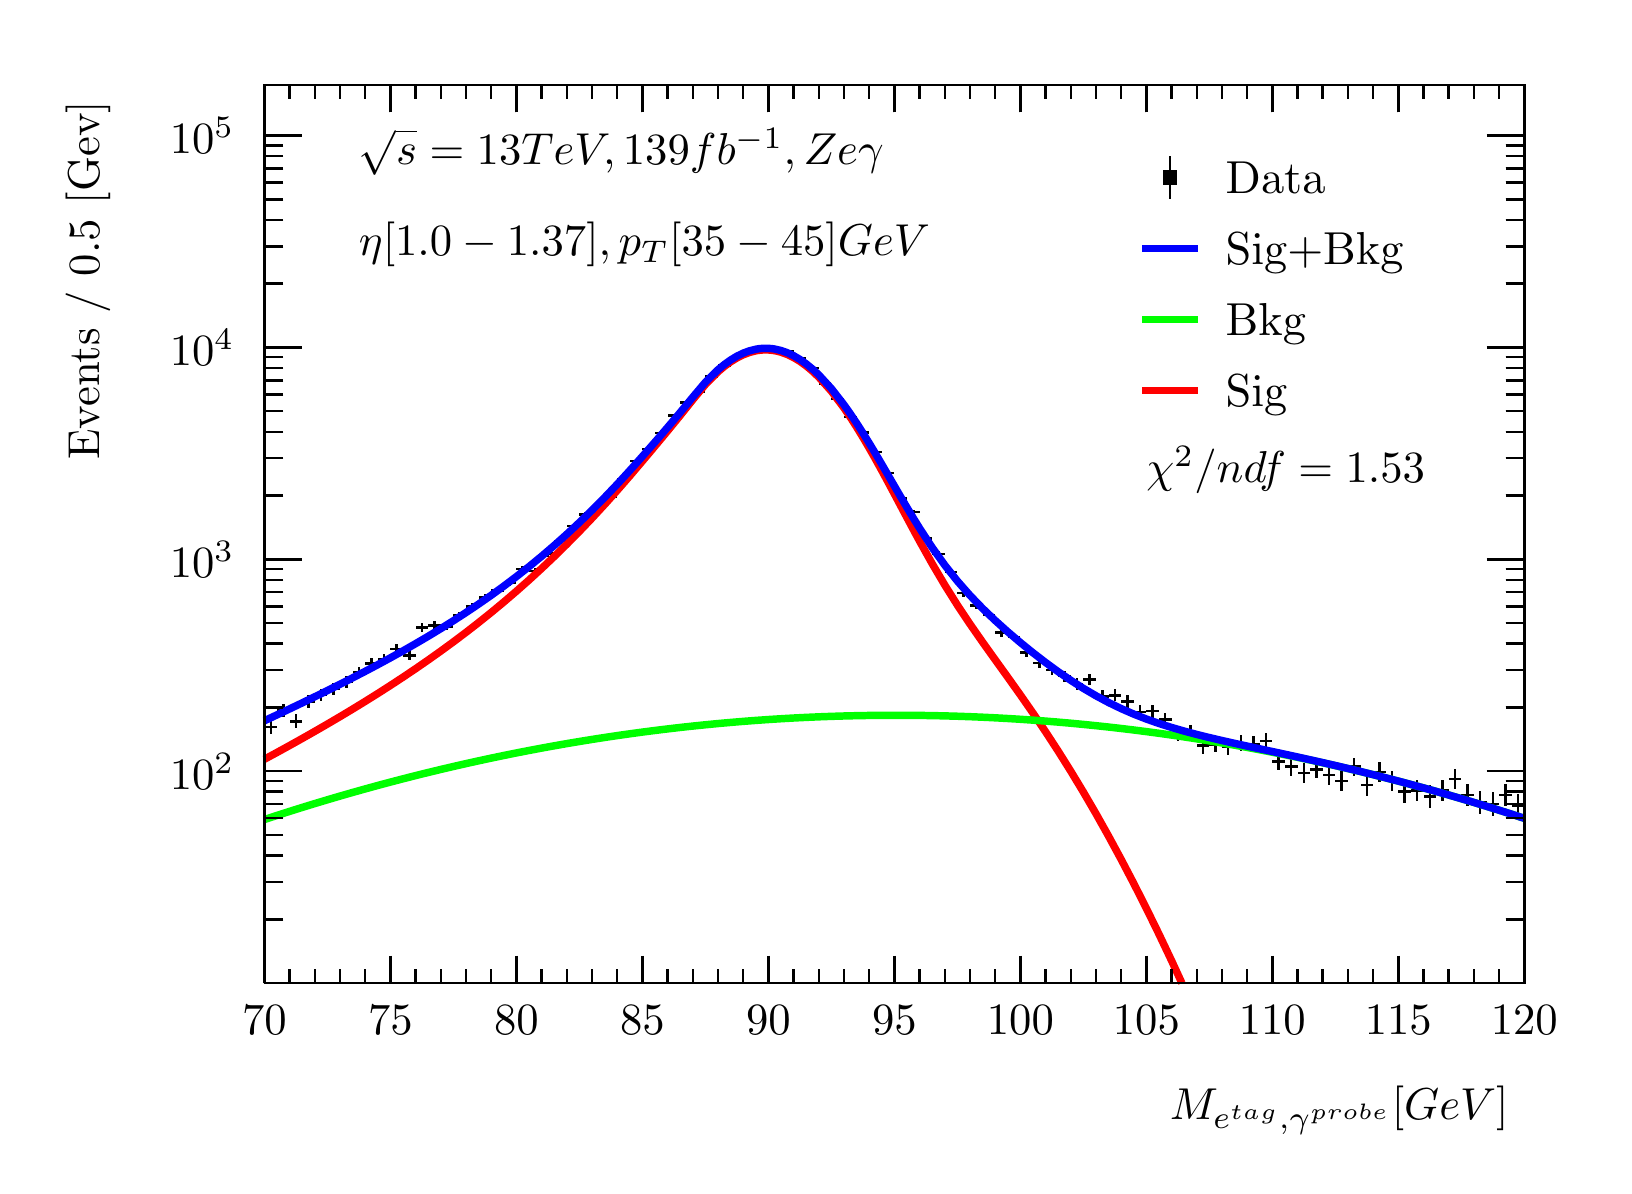
\begin{tikzpicture}
\pgfdeclareplotmark{cross} {
\pgfpathmoveto{\pgfpoint{-0.3\pgfplotmarksize}{\pgfplotmarksize}}
\pgfpathlineto{\pgfpoint{+0.3\pgfplotmarksize}{\pgfplotmarksize}}
\pgfpathlineto{\pgfpoint{+0.3\pgfplotmarksize}{0.3\pgfplotmarksize}}
\pgfpathlineto{\pgfpoint{+1\pgfplotmarksize}{0.3\pgfplotmarksize}}
\pgfpathlineto{\pgfpoint{+1\pgfplotmarksize}{-0.3\pgfplotmarksize}}
\pgfpathlineto{\pgfpoint{+0.3\pgfplotmarksize}{-0.3\pgfplotmarksize}}
\pgfpathlineto{\pgfpoint{+0.3\pgfplotmarksize}{-1.\pgfplotmarksize}}
\pgfpathlineto{\pgfpoint{-0.3\pgfplotmarksize}{-1.\pgfplotmarksize}}
\pgfpathlineto{\pgfpoint{-0.3\pgfplotmarksize}{-0.3\pgfplotmarksize}}
\pgfpathlineto{\pgfpoint{-1.\pgfplotmarksize}{-0.3\pgfplotmarksize}}
\pgfpathlineto{\pgfpoint{-1.\pgfplotmarksize}{0.3\pgfplotmarksize}}
\pgfpathlineto{\pgfpoint{-0.3\pgfplotmarksize}{0.3\pgfplotmarksize}}
\pgfpathclose
\pgfusepathqstroke
}
\pgfdeclareplotmark{cross*} {
\pgfpathmoveto{\pgfpoint{-0.3\pgfplotmarksize}{\pgfplotmarksize}}
\pgfpathlineto{\pgfpoint{+0.3\pgfplotmarksize}{\pgfplotmarksize}}
\pgfpathlineto{\pgfpoint{+0.3\pgfplotmarksize}{0.3\pgfplotmarksize}}
\pgfpathlineto{\pgfpoint{+1\pgfplotmarksize}{0.3\pgfplotmarksize}}
\pgfpathlineto{\pgfpoint{+1\pgfplotmarksize}{-0.3\pgfplotmarksize}}
\pgfpathlineto{\pgfpoint{+0.3\pgfplotmarksize}{-0.3\pgfplotmarksize}}
\pgfpathlineto{\pgfpoint{+0.3\pgfplotmarksize}{-1.\pgfplotmarksize}}
\pgfpathlineto{\pgfpoint{-0.3\pgfplotmarksize}{-1.\pgfplotmarksize}}
\pgfpathlineto{\pgfpoint{-0.3\pgfplotmarksize}{-0.3\pgfplotmarksize}}
\pgfpathlineto{\pgfpoint{-1.\pgfplotmarksize}{-0.3\pgfplotmarksize}}
\pgfpathlineto{\pgfpoint{-1.\pgfplotmarksize}{0.3\pgfplotmarksize}}
\pgfpathlineto{\pgfpoint{-0.3\pgfplotmarksize}{0.3\pgfplotmarksize}}
\pgfpathclose
\pgfusepathqfillstroke
}
\pgfdeclareplotmark{newstar} {
\pgfpathmoveto{\pgfqpoint{0pt}{\pgfplotmarksize}}
\pgfpathlineto{\pgfqpointpolar{44}{0.5\pgfplotmarksize}}
\pgfpathlineto{\pgfqpointpolar{18}{\pgfplotmarksize}}
\pgfpathlineto{\pgfqpointpolar{-20}{0.5\pgfplotmarksize}}
\pgfpathlineto{\pgfqpointpolar{-54}{\pgfplotmarksize}}
\pgfpathlineto{\pgfqpointpolar{-90}{0.5\pgfplotmarksize}}
\pgfpathlineto{\pgfqpointpolar{234}{\pgfplotmarksize}}
\pgfpathlineto{\pgfqpointpolar{198}{0.5\pgfplotmarksize}}
\pgfpathlineto{\pgfqpointpolar{162}{\pgfplotmarksize}}
\pgfpathlineto{\pgfqpointpolar{134}{0.5\pgfplotmarksize}}
\pgfpathclose
\pgfusepathqstroke
}
\pgfdeclareplotmark{newstar*} {
\pgfpathmoveto{\pgfqpoint{0pt}{\pgfplotmarksize}}
\pgfpathlineto{\pgfqpointpolar{44}{0.5\pgfplotmarksize}}
\pgfpathlineto{\pgfqpointpolar{18}{\pgfplotmarksize}}
\pgfpathlineto{\pgfqpointpolar{-20}{0.5\pgfplotmarksize}}
\pgfpathlineto{\pgfqpointpolar{-54}{\pgfplotmarksize}}
\pgfpathlineto{\pgfqpointpolar{-90}{0.5\pgfplotmarksize}}
\pgfpathlineto{\pgfqpointpolar{234}{\pgfplotmarksize}}
\pgfpathlineto{\pgfqpointpolar{198}{0.5\pgfplotmarksize}}
\pgfpathlineto{\pgfqpointpolar{162}{\pgfplotmarksize}}
\pgfpathlineto{\pgfqpointpolar{134}{0.5\pgfplotmarksize}}
\pgfpathclose
\pgfusepathqfillstroke
}
\definecolor{c}{rgb}{1,1,1};
\draw [color=c, fill=c] (0,0) rectangle (20,14.4361);
\draw [color=c, fill=c] (3,2.30977) rectangle (19,13.7143);
\definecolor{c}{rgb}{0,0,0};
\draw [c,line width=0.9] (3,2.30977) -- (3,13.7143) -- (19,13.7143) -- (19,2.30977) -- (3,2.30977);
\definecolor{c}{rgb}{1,1,1};
\draw [color=c, fill=c] (3,2.30977) rectangle (19,13.7143);
\definecolor{c}{rgb}{0,0,0};
\draw [c,line width=0.9] (3,2.30977) -- (3,13.7143) -- (19,13.7143) -- (19,2.30977) -- (3,2.30977);
\draw [c,line width=0.9] (3,2.30977) -- (19,2.30977);
\draw [c,line width=0.9] (3,2.65624) -- (3,2.30977);
\draw [c,line width=0.9] (3.32,2.48301) -- (3.32,2.30977);
\draw [c,line width=0.9] (3.64,2.48301) -- (3.64,2.30977);
\draw [c,line width=0.9] (3.96,2.48301) -- (3.96,2.30977);
\draw [c,line width=0.9] (4.28,2.48301) -- (4.28,2.30977);
\draw [c,line width=0.9] (4.6,2.65624) -- (4.6,2.30977);
\draw [c,line width=0.9] (4.92,2.48301) -- (4.92,2.30977);
\draw [c,line width=0.9] (5.24,2.48301) -- (5.24,2.30977);
\draw [c,line width=0.9] (5.56,2.48301) -- (5.56,2.30977);
\draw [c,line width=0.9] (5.88,2.48301) -- (5.88,2.30977);
\draw [c,line width=0.9] (6.2,2.65624) -- (6.2,2.30977);
\draw [c,line width=0.9] (6.52,2.48301) -- (6.52,2.30977);
\draw [c,line width=0.9] (6.84,2.48301) -- (6.84,2.30977);
\draw [c,line width=0.9] (7.16,2.48301) -- (7.16,2.30977);
\draw [c,line width=0.9] (7.48,2.48301) -- (7.48,2.30977);
\draw [c,line width=0.9] (7.8,2.65624) -- (7.8,2.30977);
\draw [c,line width=0.9] (8.12,2.48301) -- (8.12,2.30977);
\draw [c,line width=0.9] (8.44,2.48301) -- (8.44,2.30977);
\draw [c,line width=0.9] (8.76,2.48301) -- (8.76,2.30977);
\draw [c,line width=0.9] (9.08,2.48301) -- (9.08,2.30977);
\draw [c,line width=0.9] (9.4,2.65624) -- (9.4,2.30977);
\draw [c,line width=0.9] (9.72,2.48301) -- (9.72,2.30977);
\draw [c,line width=0.9] (10.04,2.48301) -- (10.04,2.30977);
\draw [c,line width=0.9] (10.36,2.48301) -- (10.36,2.30977);
\draw [c,line width=0.9] (10.68,2.48301) -- (10.68,2.30977);
\draw [c,line width=0.9] (11,2.65624) -- (11,2.30977);
\draw [c,line width=0.9] (11.32,2.48301) -- (11.32,2.30977);
\draw [c,line width=0.9] (11.64,2.48301) -- (11.64,2.30977);
\draw [c,line width=0.9] (11.96,2.48301) -- (11.96,2.30977);
\draw [c,line width=0.9] (12.28,2.48301) -- (12.28,2.30977);
\draw [c,line width=0.9] (12.6,2.65624) -- (12.6,2.30977);
\draw [c,line width=0.9] (12.92,2.48301) -- (12.92,2.30977);
\draw [c,line width=0.9] (13.24,2.48301) -- (13.24,2.30977);
\draw [c,line width=0.9] (13.56,2.48301) -- (13.56,2.30977);
\draw [c,line width=0.9] (13.88,2.48301) -- (13.88,2.30977);
\draw [c,line width=0.9] (14.2,2.65624) -- (14.2,2.30977);
\draw [c,line width=0.9] (14.52,2.48301) -- (14.52,2.30977);
\draw [c,line width=0.9] (14.84,2.48301) -- (14.84,2.30977);
\draw [c,line width=0.9] (15.16,2.48301) -- (15.16,2.30977);
\draw [c,line width=0.9] (15.48,2.48301) -- (15.48,2.30977);
\draw [c,line width=0.9] (15.8,2.65624) -- (15.8,2.30977);
\draw [c,line width=0.9] (16.12,2.48301) -- (16.12,2.30977);
\draw [c,line width=0.9] (16.44,2.48301) -- (16.44,2.30977);
\draw [c,line width=0.9] (16.76,2.48301) -- (16.76,2.30977);
\draw [c,line width=0.9] (17.08,2.48301) -- (17.08,2.30977);
\draw [c,line width=0.9] (17.4,2.65624) -- (17.4,2.30977);
\draw [c,line width=0.9] (17.72,2.48301) -- (17.72,2.30977);
\draw [c,line width=0.9] (18.04,2.48301) -- (18.04,2.30977);
\draw [c,line width=0.9] (18.36,2.48301) -- (18.36,2.30977);
\draw [c,line width=0.9] (18.68,2.48301) -- (18.68,2.30977);
\draw [c,line width=0.9] (19,2.65624) -- (19,2.30977);
\draw [anchor=base] (3,1.66015) node[scale=1.61424, color=c, rotate=0]{70};
\draw [anchor=base] (4.6,1.66015) node[scale=1.61424, color=c, rotate=0]{75};
\draw [anchor=base] (6.2,1.66015) node[scale=1.61424, color=c, rotate=0]{80};
\draw [anchor=base] (7.8,1.66015) node[scale=1.61424, color=c, rotate=0]{85};
\draw [anchor=base] (9.4,1.66015) node[scale=1.61424, color=c, rotate=0]{90};
\draw [anchor=base] (11,1.66015) node[scale=1.61424, color=c, rotate=0]{95};
\draw [anchor=base] (12.6,1.66015) node[scale=1.61424, color=c, rotate=0]{100};
\draw [anchor=base] (14.2,1.66015) node[scale=1.61424, color=c, rotate=0]{105};
\draw [anchor=base] (15.8,1.66015) node[scale=1.61424, color=c, rotate=0]{110};
\draw [anchor=base] (17.4,1.66015) node[scale=1.61424, color=c, rotate=0]{115};
\draw [anchor=base] (19,1.66015) node[scale=1.61424, color=c, rotate=0]{120};
\draw [anchor= east] (19,0.692932) node[scale=1.61424, color=c, rotate=0]{$M_{e^{tag}, \gamma^{probe}}  [GeV]$};
\draw [c,line width=0.9] (3,13.7143) -- (19,13.7143);
\draw [c,line width=0.9] (3,13.3678) -- (3,13.7143);
\draw [c,line width=0.9] (3.32,13.5411) -- (3.32,13.7143);
\draw [c,line width=0.9] (3.64,13.5411) -- (3.64,13.7143);
\draw [c,line width=0.9] (3.96,13.5411) -- (3.96,13.7143);
\draw [c,line width=0.9] (4.28,13.5411) -- (4.28,13.7143);
\draw [c,line width=0.9] (4.6,13.3678) -- (4.6,13.7143);
\draw [c,line width=0.9] (4.92,13.5411) -- (4.92,13.7143);
\draw [c,line width=0.9] (5.24,13.5411) -- (5.24,13.7143);
\draw [c,line width=0.9] (5.56,13.5411) -- (5.56,13.7143);
\draw [c,line width=0.9] (5.88,13.5411) -- (5.88,13.7143);
\draw [c,line width=0.9] (6.2,13.3678) -- (6.2,13.7143);
\draw [c,line width=0.9] (6.52,13.5411) -- (6.52,13.7143);
\draw [c,line width=0.9] (6.84,13.5411) -- (6.84,13.7143);
\draw [c,line width=0.9] (7.16,13.5411) -- (7.16,13.7143);
\draw [c,line width=0.9] (7.48,13.5411) -- (7.48,13.7143);
\draw [c,line width=0.9] (7.8,13.3678) -- (7.8,13.7143);
\draw [c,line width=0.9] (8.12,13.5411) -- (8.12,13.7143);
\draw [c,line width=0.9] (8.44,13.5411) -- (8.44,13.7143);
\draw [c,line width=0.9] (8.76,13.5411) -- (8.76,13.7143);
\draw [c,line width=0.9] (9.08,13.5411) -- (9.08,13.7143);
\draw [c,line width=0.9] (9.4,13.3678) -- (9.4,13.7143);
\draw [c,line width=0.9] (9.72,13.5411) -- (9.72,13.7143);
\draw [c,line width=0.9] (10.04,13.5411) -- (10.04,13.7143);
\draw [c,line width=0.9] (10.36,13.5411) -- (10.36,13.7143);
\draw [c,line width=0.9] (10.68,13.5411) -- (10.68,13.7143);
\draw [c,line width=0.9] (11,13.3678) -- (11,13.7143);
\draw [c,line width=0.9] (11.32,13.5411) -- (11.32,13.7143);
\draw [c,line width=0.9] (11.64,13.5411) -- (11.64,13.7143);
\draw [c,line width=0.9] (11.96,13.5411) -- (11.96,13.7143);
\draw [c,line width=0.9] (12.28,13.5411) -- (12.28,13.7143);
\draw [c,line width=0.9] (12.6,13.3678) -- (12.6,13.7143);
\draw [c,line width=0.9] (12.92,13.5411) -- (12.92,13.7143);
\draw [c,line width=0.9] (13.24,13.5411) -- (13.24,13.7143);
\draw [c,line width=0.9] (13.56,13.5411) -- (13.56,13.7143);
\draw [c,line width=0.9] (13.88,13.5411) -- (13.88,13.7143);
\draw [c,line width=0.9] (14.2,13.3678) -- (14.2,13.7143);
\draw [c,line width=0.9] (14.52,13.5411) -- (14.52,13.7143);
\draw [c,line width=0.9] (14.84,13.5411) -- (14.84,13.7143);
\draw [c,line width=0.9] (15.16,13.5411) -- (15.16,13.7143);
\draw [c,line width=0.9] (15.48,13.5411) -- (15.48,13.7143);
\draw [c,line width=0.9] (15.8,13.3678) -- (15.8,13.7143);
\draw [c,line width=0.9] (16.12,13.5411) -- (16.12,13.7143);
\draw [c,line width=0.9] (16.44,13.5411) -- (16.44,13.7143);
\draw [c,line width=0.9] (16.76,13.5411) -- (16.76,13.7143);
\draw [c,line width=0.9] (17.08,13.5411) -- (17.08,13.7143);
\draw [c,line width=0.9] (17.4,13.3678) -- (17.4,13.7143);
\draw [c,line width=0.9] (17.72,13.5411) -- (17.72,13.7143);
\draw [c,line width=0.9] (18.04,13.5411) -- (18.04,13.7143);
\draw [c,line width=0.9] (18.36,13.5411) -- (18.36,13.7143);
\draw [c,line width=0.9] (18.68,13.5411) -- (18.68,13.7143);
\draw [c,line width=0.9] (19,13.3678) -- (19,13.7143);
\draw [c,line width=0.9] (3,2.30977) -- (3,13.7143);
\draw [c,line width=0.9] (3.237,3.11973) -- (3,3.11973);
\draw [c,line width=0.9] (3.237,3.59352) -- (3,3.59352);
\draw [c,line width=0.9] (3.237,3.92968) -- (3,3.92968);
\draw [c,line width=0.9] (3.237,4.19043) -- (3,4.19043);
\draw [c,line width=0.9] (3.237,4.40347) -- (3,4.40347);
\draw [c,line width=0.9] (3.237,4.5836) -- (3,4.5836);
\draw [c,line width=0.9] (3.237,4.73964) -- (3,4.73964);
\draw [c,line width=0.9] (3.237,4.87727) -- (3,4.87727);
\draw [c,line width=0.9] (3.474,5.00038) -- (3,5.00038);
\draw [anchor= east] (2.82,5.00038) node[scale=1.61424, color=c, rotate=0]{$10^{2}$};
\draw [c,line width=0.9] (3.237,5.81034) -- (3,5.81034);
\draw [c,line width=0.9] (3.237,6.28413) -- (3,6.28413);
\draw [c,line width=0.9] (3.237,6.62029) -- (3,6.62029);
\draw [c,line width=0.9] (3.237,6.88104) -- (3,6.88104);
\draw [c,line width=0.9] (3.237,7.09409) -- (3,7.09409);
\draw [c,line width=0.9] (3.237,7.27421) -- (3,7.27421);
\draw [c,line width=0.9] (3.237,7.43025) -- (3,7.43025);
\draw [c,line width=0.9] (3.237,7.56788) -- (3,7.56788);
\draw [c,line width=0.9] (3.474,7.69099) -- (3,7.69099);
\draw [anchor= east] (2.82,7.69099) node[scale=1.61424, color=c, rotate=0]{$10^{3}$};
\draw [c,line width=0.9] (3.237,8.50095) -- (3,8.50095);
\draw [c,line width=0.9] (3.237,8.97474) -- (3,8.97474);
\draw [c,line width=0.9] (3.237,9.3109) -- (3,9.3109);
\draw [c,line width=0.9] (3.237,9.57165) -- (3,9.57165);
\draw [c,line width=0.9] (3.237,9.7847) -- (3,9.7847);
\draw [c,line width=0.9] (3.237,9.96482) -- (3,9.96482);
\draw [c,line width=0.9] (3.237,10.1209) -- (3,10.1209);
\draw [c,line width=0.9] (3.237,10.2585) -- (3,10.2585);
\draw [c,line width=0.9] (3.474,10.3816) -- (3,10.3816);
\draw [anchor= east] (2.82,10.3816) node[scale=1.61424, color=c, rotate=0]{$10^{4}$};
\draw [c,line width=0.9] (3.237,11.1916) -- (3,11.1916);
\draw [c,line width=0.9] (3.237,11.6654) -- (3,11.6654);
\draw [c,line width=0.9] (3.237,12.0015) -- (3,12.0015);
\draw [c,line width=0.9] (3.237,12.2623) -- (3,12.2623);
\draw [c,line width=0.9] (3.237,12.4753) -- (3,12.4753);
\draw [c,line width=0.9] (3.237,12.6554) -- (3,12.6554);
\draw [c,line width=0.9] (3.237,12.8115) -- (3,12.8115);
\draw [c,line width=0.9] (3.237,12.9491) -- (3,12.9491);
\draw [c,line width=0.9] (3.474,13.0722) -- (3,13.0722);
\draw [anchor= east] (2.82,13.0722) node[scale=1.61424, color=c, rotate=0]{$10^{5}$};
\draw [anchor= east] (0.76,13.7143) node[scale=1.61424, color=c, rotate=90]{Events / 0.5 [Gev]};
\draw [c,line width=0.9] (19,2.30977) -- (19,13.7143);
\draw [c,line width=0.9] (18.763,3.11973) -- (19,3.11973);
\draw [c,line width=0.9] (18.763,3.59352) -- (19,3.59352);
\draw [c,line width=0.9] (18.763,3.92968) -- (19,3.92968);
\draw [c,line width=0.9] (18.763,4.19043) -- (19,4.19043);
\draw [c,line width=0.9] (18.763,4.40347) -- (19,4.40347);
\draw [c,line width=0.9] (18.763,4.5836) -- (19,4.5836);
\draw [c,line width=0.9] (18.763,4.73964) -- (19,4.73964);
\draw [c,line width=0.9] (18.763,4.87727) -- (19,4.87727);
\draw [c,line width=0.9] (18.526,5.00038) -- (19,5.00038);
\draw [c,line width=0.9] (18.763,5.81034) -- (19,5.81034);
\draw [c,line width=0.9] (18.763,6.28413) -- (19,6.28413);
\draw [c,line width=0.9] (18.763,6.62029) -- (19,6.62029);
\draw [c,line width=0.9] (18.763,6.88104) -- (19,6.88104);
\draw [c,line width=0.9] (18.763,7.09409) -- (19,7.09409);
\draw [c,line width=0.9] (18.763,7.27421) -- (19,7.27421);
\draw [c,line width=0.9] (18.763,7.43025) -- (19,7.43025);
\draw [c,line width=0.9] (18.763,7.56788) -- (19,7.56788);
\draw [c,line width=0.9] (18.526,7.69099) -- (19,7.69099);
\draw [c,line width=0.9] (18.763,8.50095) -- (19,8.50095);
\draw [c,line width=0.9] (18.763,8.97474) -- (19,8.97474);
\draw [c,line width=0.9] (18.763,9.3109) -- (19,9.3109);
\draw [c,line width=0.9] (18.763,9.57165) -- (19,9.57165);
\draw [c,line width=0.9] (18.763,9.7847) -- (19,9.7847);
\draw [c,line width=0.9] (18.763,9.96482) -- (19,9.96482);
\draw [c,line width=0.9] (18.763,10.1209) -- (19,10.1209);
\draw [c,line width=0.9] (18.763,10.2585) -- (19,10.2585);
\draw [c,line width=0.9] (18.526,10.3816) -- (19,10.3816);
\draw [c,line width=0.9] (18.763,11.1916) -- (19,11.1916);
\draw [c,line width=0.9] (18.763,11.6654) -- (19,11.6654);
\draw [c,line width=0.9] (18.763,12.0015) -- (19,12.0015);
\draw [c,line width=0.9] (18.763,12.2623) -- (19,12.2623);
\draw [c,line width=0.9] (18.763,12.4753) -- (19,12.4753);
\draw [c,line width=0.9] (18.763,12.6554) -- (19,12.6554);
\draw [c,line width=0.9] (18.763,12.8115) -- (19,12.8115);
\draw [c,line width=0.9] (18.763,12.9491) -- (19,12.9491);
\draw [c,line width=0.9] (18.526,13.0722) -- (19,13.0722);
\draw [c,line width=0.9] (3.08,5.56411) -- (3,5.56411);
\draw [c,line width=0.9] (3,5.56411) -- (3,5.56411);
\draw [c,line width=0.9] (3.08,5.56411) -- (3.16,5.56411);
\draw [c,line width=0.9] (3.16,5.56411) -- (3.16,5.56411);
\draw [c,line width=0.9] (3.08,5.56411) -- (3.08,5.65589);
\draw [c,line width=0.9] (3.08,5.65589) -- (3.08,5.65589);
\draw [c,line width=0.9] (3.08,5.56411) -- (3.08,5.47232);
\draw [c,line width=0.9] (3.08,5.47232) -- (3.08,5.47232);
\draw [c,line width=0.9] (3.24,5.77475) -- (3.16,5.77475);
\draw [c,line width=0.9] (3.16,5.77475) -- (3.16,5.77475);
\draw [c,line width=0.9] (3.24,5.77475) -- (3.32,5.77475);
\draw [c,line width=0.9] (3.32,5.77475) -- (3.32,5.77475);
\draw [c,line width=0.9] (3.24,5.77475) -- (3.24,5.85862);
\draw [c,line width=0.9] (3.24,5.85862) -- (3.24,5.85862);
\draw [c,line width=0.9] (3.24,5.77475) -- (3.24,5.69087);
\draw [c,line width=0.9] (3.24,5.69087) -- (3.24,5.69087);
\draw [c,line width=0.9] (3.4,5.6341) -- (3.32,5.6341);
\draw [c,line width=0.9] (3.32,5.6341) -- (3.32,5.6341);
\draw [c,line width=0.9] (3.4,5.6341) -- (3.48,5.6341);
\draw [c,line width=0.9] (3.48,5.6341) -- (3.48,5.6341);
\draw [c,line width=0.9] (3.4,5.6341) -- (3.4,5.72318);
\draw [c,line width=0.9] (3.4,5.72318) -- (3.4,5.72318);
\draw [c,line width=0.9] (3.4,5.6341) -- (3.4,5.54502);
\draw [c,line width=0.9] (3.4,5.54502) -- (3.4,5.54502);
\draw [c,line width=0.9] (3.56,5.88393) -- (3.48,5.88393);
\draw [c,line width=0.9] (3.48,5.88393) -- (3.48,5.88393);
\draw [c,line width=0.9] (3.56,5.88393) -- (3.64,5.88393);
\draw [c,line width=0.9] (3.64,5.88393) -- (3.64,5.88393);
\draw [c,line width=0.9] (3.56,5.88393) -- (3.56,5.96398);
\draw [c,line width=0.9] (3.56,5.96398) -- (3.56,5.96398);
\draw [c,line width=0.9] (3.56,5.88393) -- (3.56,5.80388);
\draw [c,line width=0.9] (3.56,5.80388) -- (3.56,5.80388);
\draw [c,line width=0.9] (3.72,5.96856) -- (3.64,5.96856);
\draw [c,line width=0.9] (3.64,5.96856) -- (3.64,5.96856);
\draw [c,line width=0.9] (3.72,5.96856) -- (3.8,5.96856);
\draw [c,line width=0.9] (3.8,5.96856) -- (3.8,5.96856);
\draw [c,line width=0.9] (3.72,5.96856) -- (3.72,6.04577);
\draw [c,line width=0.9] (3.72,6.04577) -- (3.72,6.04577);
\draw [c,line width=0.9] (3.72,5.96856) -- (3.72,5.89136);
\draw [c,line width=0.9] (3.72,5.89136) -- (3.72,5.89136);
\draw [c,line width=0.9] (3.88,6.04748) -- (3.8,6.04748);
\draw [c,line width=0.9] (3.8,6.04748) -- (3.8,6.04748);
\draw [c,line width=0.9] (3.88,6.04748) -- (3.96,6.04748);
\draw [c,line width=0.9] (3.96,6.04748) -- (3.96,6.04748);
\draw [c,line width=0.9] (3.88,6.04748) -- (3.88,6.12212);
\draw [c,line width=0.9] (3.88,6.12212) -- (3.88,6.12212);
\draw [c,line width=0.9] (3.88,6.04748) -- (3.88,5.97284);
\draw [c,line width=0.9] (3.88,5.97284) -- (3.88,5.97284);
\draw [c,line width=0.9] (4.04,6.13476) -- (3.96,6.13476);
\draw [c,line width=0.9] (3.96,6.13476) -- (3.96,6.13476);
\draw [c,line width=0.9] (4.04,6.13476) -- (4.12,6.13476);
\draw [c,line width=0.9] (4.12,6.13476) -- (4.12,6.13476);
\draw [c,line width=0.9] (4.04,6.13476) -- (4.04,6.20666);
\draw [c,line width=0.9] (4.04,6.20666) -- (4.04,6.20666);
\draw [c,line width=0.9] (4.04,6.13476) -- (4.04,6.06285);
\draw [c,line width=0.9] (4.04,6.06285) -- (4.04,6.06285);
\draw [c,line width=0.9] (4.2,6.26053) -- (4.12,6.26053);
\draw [c,line width=0.9] (4.12,6.26053) -- (4.12,6.26053);
\draw [c,line width=0.9] (4.2,6.26053) -- (4.28,6.26053);
\draw [c,line width=0.9] (4.28,6.26053) -- (4.28,6.26053);
\draw [c,line width=0.9] (4.2,6.26053) -- (4.2,6.32867);
\draw [c,line width=0.9] (4.2,6.32867) -- (4.2,6.32867);
\draw [c,line width=0.9] (4.2,6.26053) -- (4.2,6.19239);
\draw [c,line width=0.9] (4.2,6.19239) -- (4.2,6.19239);
\draw [c,line width=0.9] (4.36,6.37045) -- (4.28,6.37045);
\draw [c,line width=0.9] (4.28,6.37045) -- (4.28,6.37045);
\draw [c,line width=0.9] (4.36,6.37045) -- (4.44,6.37045);
\draw [c,line width=0.9] (4.44,6.37045) -- (4.44,6.37045);
\draw [c,line width=0.9] (4.36,6.37045) -- (4.36,6.43546);
\draw [c,line width=0.9] (4.36,6.43546) -- (4.36,6.43546);
\draw [c,line width=0.9] (4.36,6.37045) -- (4.36,6.30544);
\draw [c,line width=0.9] (4.36,6.30544) -- (4.36,6.30544);
\draw [c,line width=0.9] (4.52,6.42349) -- (4.44,6.42349);
\draw [c,line width=0.9] (4.44,6.42349) -- (4.44,6.42349);
\draw [c,line width=0.9] (4.52,6.42349) -- (4.6,6.42349);
\draw [c,line width=0.9] (4.6,6.42349) -- (4.6,6.42349);
\draw [c,line width=0.9] (4.52,6.42349) -- (4.52,6.48705);
\draw [c,line width=0.9] (4.52,6.48705) -- (4.52,6.48705);
\draw [c,line width=0.9] (4.52,6.42349) -- (4.52,6.35994);
\draw [c,line width=0.9] (4.52,6.35994) -- (4.52,6.35994);
\draw [c,line width=0.9] (4.68,6.5511) -- (4.6,6.5511);
\draw [c,line width=0.9] (4.6,6.5511) -- (4.6,6.5511);
\draw [c,line width=0.9] (4.68,6.5511) -- (4.76,6.5511);
\draw [c,line width=0.9] (4.76,6.5511) -- (4.76,6.5511);
\draw [c,line width=0.9] (4.68,6.5511) -- (4.68,6.61127);
\draw [c,line width=0.9] (4.68,6.61127) -- (4.68,6.61127);
\draw [c,line width=0.9] (4.68,6.5511) -- (4.68,6.49092);
\draw [c,line width=0.9] (4.68,6.49092) -- (4.68,6.49092);
\draw [c,line width=0.9] (4.84,6.47092) -- (4.76,6.47092);
\draw [c,line width=0.9] (4.76,6.47092) -- (4.76,6.47092);
\draw [c,line width=0.9] (4.84,6.47092) -- (4.92,6.47092);
\draw [c,line width=0.9] (4.92,6.47092) -- (4.92,6.47092);
\draw [c,line width=0.9] (4.84,6.47092) -- (4.84,6.53319);
\draw [c,line width=0.9] (4.84,6.53319) -- (4.84,6.53319);
\draw [c,line width=0.9] (4.84,6.47092) -- (4.84,6.40864);
\draw [c,line width=0.9] (4.84,6.40864) -- (4.84,6.40864);
\draw [c,line width=0.9] (5,6.82356) -- (4.92,6.82356);
\draw [c,line width=0.9] (4.92,6.82356) -- (4.92,6.82356);
\draw [c,line width=0.9] (5,6.82356) -- (5.08,6.82356);
\draw [c,line width=0.9] (5.08,6.82356) -- (5.08,6.82356);
\draw [c,line width=0.9] (5,6.82356) -- (5,6.87712);
\draw [c,line width=0.9] (5,6.87712) -- (5,6.87712);
\draw [c,line width=0.9] (5,6.82356) -- (5,6.77001);
\draw [c,line width=0.9] (5,6.77001) -- (5,6.77001);
\draw [c,line width=0.9] (5.16,6.85265) -- (5.08,6.85265);
\draw [c,line width=0.9] (5.08,6.85265) -- (5.08,6.85265);
\draw [c,line width=0.9] (5.16,6.85265) -- (5.24,6.85265);
\draw [c,line width=0.9] (5.24,6.85265) -- (5.24,6.85265);
\draw [c,line width=0.9] (5.16,6.85265) -- (5.16,6.90555);
\draw [c,line width=0.9] (5.16,6.90555) -- (5.16,6.90555);
\draw [c,line width=0.9] (5.16,6.85265) -- (5.16,6.79976);
\draw [c,line width=0.9] (5.16,6.79976) -- (5.16,6.79976);
\draw [c,line width=0.9] (5.32,6.84062) -- (5.24,6.84062);
\draw [c,line width=0.9] (5.24,6.84062) -- (5.24,6.84062);
\draw [c,line width=0.9] (5.32,6.84062) -- (5.4,6.84062);
\draw [c,line width=0.9] (5.4,6.84062) -- (5.4,6.84062);
\draw [c,line width=0.9] (5.32,6.84062) -- (5.32,6.89379);
\draw [c,line width=0.9] (5.32,6.89379) -- (5.32,6.89379);
\draw [c,line width=0.9] (5.32,6.84062) -- (5.32,6.78746);
\draw [c,line width=0.9] (5.32,6.78746) -- (5.32,6.78746);
\draw [c,line width=0.9] (5.48,6.97529) -- (5.4,6.97529);
\draw [c,line width=0.9] (5.4,6.97529) -- (5.4,6.97529);
\draw [c,line width=0.9] (5.48,6.97529) -- (5.56,6.97529);
\draw [c,line width=0.9] (5.56,6.97529) -- (5.56,6.97529);
\draw [c,line width=0.9] (5.48,6.97529) -- (5.48,7.02548);
\draw [c,line width=0.9] (5.48,7.02548) -- (5.48,7.02548);
\draw [c,line width=0.9] (5.48,6.97529) -- (5.48,6.9251);
\draw [c,line width=0.9] (5.48,6.9251) -- (5.48,6.9251);
\draw [c,line width=0.9] (5.64,7.09214) -- (5.56,7.09214);
\draw [c,line width=0.9] (5.56,7.09214) -- (5.56,7.09214);
\draw [c,line width=0.9] (5.64,7.09214) -- (5.72,7.09214);
\draw [c,line width=0.9] (5.72,7.09214) -- (5.72,7.09214);
\draw [c,line width=0.9] (5.64,7.09214) -- (5.64,7.13988);
\draw [c,line width=0.9] (5.64,7.13988) -- (5.64,7.13988);
\draw [c,line width=0.9] (5.64,7.09214) -- (5.64,7.0444);
\draw [c,line width=0.9] (5.64,7.0444) -- (5.64,7.0444);
\draw [c,line width=0.9] (5.8,7.20546) -- (5.72,7.20546);
\draw [c,line width=0.9] (5.72,7.20546) -- (5.72,7.20546);
\draw [c,line width=0.9] (5.8,7.20546) -- (5.88,7.20546);
\draw [c,line width=0.9] (5.88,7.20546) -- (5.88,7.20546);
\draw [c,line width=0.9] (5.8,7.20546) -- (5.8,7.25094);
\draw [c,line width=0.9] (5.8,7.25094) -- (5.8,7.25094);
\draw [c,line width=0.9] (5.8,7.20546) -- (5.8,7.15998);
\draw [c,line width=0.9] (5.8,7.15998) -- (5.8,7.15998);
\draw [c,line width=0.9] (5.96,7.29408) -- (5.88,7.29408);
\draw [c,line width=0.9] (5.88,7.29408) -- (5.88,7.29408);
\draw [c,line width=0.9] (5.96,7.29408) -- (6.04,7.29408);
\draw [c,line width=0.9] (6.04,7.29408) -- (6.04,7.29408);
\draw [c,line width=0.9] (5.96,7.29408) -- (5.96,7.33787);
\draw [c,line width=0.9] (5.96,7.33787) -- (5.96,7.33787);
\draw [c,line width=0.9] (5.96,7.29408) -- (5.96,7.25029);
\draw [c,line width=0.9] (5.96,7.25029) -- (5.96,7.25029);
\draw [c,line width=0.9] (6.12,7.39766) -- (6.04,7.39766);
\draw [c,line width=0.9] (6.04,7.39766) -- (6.04,7.39766);
\draw [c,line width=0.9] (6.12,7.39766) -- (6.2,7.39766);
\draw [c,line width=0.9] (6.2,7.39766) -- (6.2,7.39766);
\draw [c,line width=0.9] (6.12,7.39766) -- (6.12,7.43956);
\draw [c,line width=0.9] (6.12,7.43956) -- (6.12,7.43956);
\draw [c,line width=0.9] (6.12,7.39766) -- (6.12,7.35577);
\draw [c,line width=0.9] (6.12,7.35577) -- (6.12,7.35577);
\draw [c,line width=0.9] (6.28,7.56918) -- (6.2,7.56918);
\draw [c,line width=0.9] (6.2,7.56918) -- (6.2,7.56918);
\draw [c,line width=0.9] (6.28,7.56918) -- (6.36,7.56918);
\draw [c,line width=0.9] (6.36,7.56918) -- (6.36,7.56918);
\draw [c,line width=0.9] (6.28,7.56918) -- (6.28,7.6081);
\draw [c,line width=0.9] (6.28,7.6081) -- (6.28,7.6081);
\draw [c,line width=0.9] (6.28,7.56918) -- (6.28,7.53025);
\draw [c,line width=0.9] (6.28,7.53025) -- (6.28,7.53025);
\draw [c,line width=0.9] (6.44,7.54295) -- (6.36,7.54295);
\draw [c,line width=0.9] (6.36,7.54295) -- (6.36,7.54295);
\draw [c,line width=0.9] (6.44,7.54295) -- (6.52,7.54295);
\draw [c,line width=0.9] (6.52,7.54295) -- (6.52,7.54295);
\draw [c,line width=0.9] (6.44,7.54295) -- (6.44,7.58231);
\draw [c,line width=0.9] (6.44,7.58231) -- (6.44,7.58231);
\draw [c,line width=0.9] (6.44,7.54295) -- (6.44,7.50358);
\draw [c,line width=0.9] (6.44,7.50358) -- (6.44,7.50358);
\draw [c,line width=0.9] (6.6,7.76239) -- (6.52,7.76239);
\draw [c,line width=0.9] (6.52,7.76239) -- (6.52,7.76239);
\draw [c,line width=0.9] (6.6,7.76239) -- (6.68,7.76239);
\draw [c,line width=0.9] (6.68,7.76239) -- (6.68,7.76239);
\draw [c,line width=0.9] (6.6,7.76239) -- (6.6,7.79822);
\draw [c,line width=0.9] (6.6,7.79822) -- (6.6,7.79822);
\draw [c,line width=0.9] (6.6,7.76239) -- (6.6,7.72655);
\draw [c,line width=0.9] (6.6,7.72655) -- (6.6,7.72655);
\draw [c,line width=0.9] (6.76,7.92527) -- (6.68,7.92527);
\draw [c,line width=0.9] (6.68,7.92527) -- (6.68,7.92527);
\draw [c,line width=0.9] (6.76,7.92527) -- (6.84,7.92527);
\draw [c,line width=0.9] (6.84,7.92527) -- (6.84,7.92527);
\draw [c,line width=0.9] (6.76,7.92527) -- (6.76,7.9587);
\draw [c,line width=0.9] (6.76,7.9587) -- (6.76,7.9587);
\draw [c,line width=0.9] (6.76,7.92527) -- (6.76,7.89184);
\draw [c,line width=0.9] (6.76,7.89184) -- (6.76,7.89184);
\draw [c,line width=0.9] (6.92,8.11384) -- (6.84,8.11384);
\draw [c,line width=0.9] (6.84,8.11384) -- (6.84,8.11384);
\draw [c,line width=0.9] (6.92,8.11384) -- (7,8.11384);
\draw [c,line width=0.9] (7,8.11384) -- (7,8.11384);
\draw [c,line width=0.9] (6.92,8.11384) -- (6.92,8.14467);
\draw [c,line width=0.9] (6.92,8.14467) -- (6.92,8.14467);
\draw [c,line width=0.9] (6.92,8.11384) -- (6.92,8.083);
\draw [c,line width=0.9] (6.92,8.083) -- (6.92,8.083);
\draw [c,line width=0.9] (7.08,8.25904) -- (7,8.25904);
\draw [c,line width=0.9] (7,8.25904) -- (7,8.25904);
\draw [c,line width=0.9] (7.08,8.25904) -- (7.16,8.25904);
\draw [c,line width=0.9] (7.16,8.25904) -- (7.16,8.25904);
\draw [c,line width=0.9] (7.08,8.25904) -- (7.08,8.28802);
\draw [c,line width=0.9] (7.08,8.28802) -- (7.08,8.28802);
\draw [c,line width=0.9] (7.08,8.25904) -- (7.08,8.23006);
\draw [c,line width=0.9] (7.08,8.23006) -- (7.08,8.23006);
\draw [c,line width=0.9] (7.24,8.35357) -- (7.16,8.35357);
\draw [c,line width=0.9] (7.16,8.35357) -- (7.16,8.35357);
\draw [c,line width=0.9] (7.24,8.35357) -- (7.32,8.35357);
\draw [c,line width=0.9] (7.32,8.35357) -- (7.32,8.35357);
\draw [c,line width=0.9] (7.24,8.35357) -- (7.24,8.38139);
\draw [c,line width=0.9] (7.24,8.38139) -- (7.24,8.38139);
\draw [c,line width=0.9] (7.24,8.35357) -- (7.24,8.32574);
\draw [c,line width=0.9] (7.24,8.32574) -- (7.24,8.32574);
\draw [c,line width=0.9] (7.4,8.48448) -- (7.32,8.48448);
\draw [c,line width=0.9] (7.32,8.48448) -- (7.32,8.48448);
\draw [c,line width=0.9] (7.4,8.48448) -- (7.48,8.48448);
\draw [c,line width=0.9] (7.48,8.48448) -- (7.48,8.48448);
\draw [c,line width=0.9] (7.4,8.48448) -- (7.4,8.51079);
\draw [c,line width=0.9] (7.4,8.51079) -- (7.4,8.51079);
\draw [c,line width=0.9] (7.4,8.48448) -- (7.4,8.45816);
\draw [c,line width=0.9] (7.4,8.45816) -- (7.4,8.45816);
\draw [c,line width=0.9] (7.56,8.70569) -- (7.48,8.70569);
\draw [c,line width=0.9] (7.48,8.70569) -- (7.48,8.70569);
\draw [c,line width=0.9] (7.56,8.70569) -- (7.64,8.70569);
\draw [c,line width=0.9] (7.64,8.70569) -- (7.64,8.70569);
\draw [c,line width=0.9] (7.56,8.70569) -- (7.56,8.72963);
\draw [c,line width=0.9] (7.56,8.72963) -- (7.56,8.72963);
\draw [c,line width=0.9] (7.56,8.70569) -- (7.56,8.68175);
\draw [c,line width=0.9] (7.56,8.68175) -- (7.56,8.68175);
\draw [c,line width=0.9] (7.72,8.93995) -- (7.64,8.93995);
\draw [c,line width=0.9] (7.64,8.93995) -- (7.64,8.93995);
\draw [c,line width=0.9] (7.72,8.93995) -- (7.8,8.93995);
\draw [c,line width=0.9] (7.8,8.93995) -- (7.8,8.93995);
\draw [c,line width=0.9] (7.72,8.93995) -- (7.72,8.96161);
\draw [c,line width=0.9] (7.72,8.96161) -- (7.72,8.96161);
\draw [c,line width=0.9] (7.72,8.93995) -- (7.72,8.9183);
\draw [c,line width=0.9] (7.72,8.9183) -- (7.72,8.9183);
\draw [c,line width=0.9] (7.88,9.09) -- (7.8,9.09);
\draw [c,line width=0.9] (7.8,9.09) -- (7.8,9.09);
\draw [c,line width=0.9] (7.88,9.09) -- (7.96,9.09);
\draw [c,line width=0.9] (7.96,9.09) -- (7.96,9.09);
\draw [c,line width=0.9] (7.88,9.09) -- (7.88,9.11031);
\draw [c,line width=0.9] (7.88,9.11031) -- (7.88,9.11031);
\draw [c,line width=0.9] (7.88,9.09) -- (7.88,9.0697);
\draw [c,line width=0.9] (7.88,9.0697) -- (7.88,9.0697);
\draw [c,line width=0.9] (8.04,9.29739) -- (7.96,9.29739);
\draw [c,line width=0.9] (7.96,9.29739) -- (7.96,9.29739);
\draw [c,line width=0.9] (8.04,9.29739) -- (8.12,9.29739);
\draw [c,line width=0.9] (8.12,9.29739) -- (8.12,9.29739);
\draw [c,line width=0.9] (8.04,9.29739) -- (8.04,9.31597);
\draw [c,line width=0.9] (8.04,9.31597) -- (8.04,9.31597);
\draw [c,line width=0.9] (8.04,9.29739) -- (8.04,9.27881);
\draw [c,line width=0.9] (8.04,9.27881) -- (8.04,9.27881);
\draw [c,line width=0.9] (8.2,9.51564) -- (8.12,9.51564);
\draw [c,line width=0.9] (8.12,9.51564) -- (8.12,9.51564);
\draw [c,line width=0.9] (8.2,9.51564) -- (8.28,9.51564);
\draw [c,line width=0.9] (8.28,9.51564) -- (8.28,9.51564);
\draw [c,line width=0.9] (8.2,9.51564) -- (8.2,9.53257);
\draw [c,line width=0.9] (8.2,9.53257) -- (8.2,9.53257);
\draw [c,line width=0.9] (8.2,9.51564) -- (8.2,9.49872);
\draw [c,line width=0.9] (8.2,9.49872) -- (8.2,9.49872);
\draw [c,line width=0.9] (8.36,9.68493) -- (8.28,9.68493);
\draw [c,line width=0.9] (8.28,9.68493) -- (8.28,9.68493);
\draw [c,line width=0.9] (8.36,9.68493) -- (8.44,9.68493);
\draw [c,line width=0.9] (8.44,9.68493) -- (8.44,9.68493);
\draw [c,line width=0.9] (8.36,9.68493) -- (8.36,9.70068);
\draw [c,line width=0.9] (8.36,9.70068) -- (8.36,9.70068);
\draw [c,line width=0.9] (8.36,9.68493) -- (8.36,9.66919);
\draw [c,line width=0.9] (8.36,9.66919) -- (8.36,9.66919);
\draw [c,line width=0.9] (8.52,9.81412) -- (8.44,9.81412);
\draw [c,line width=0.9] (8.44,9.81412) -- (8.44,9.81412);
\draw [c,line width=0.9] (8.52,9.81412) -- (8.6,9.81412);
\draw [c,line width=0.9] (8.6,9.81412) -- (8.6,9.81412);
\draw [c,line width=0.9] (8.52,9.81412) -- (8.52,9.82902);
\draw [c,line width=0.9] (8.52,9.82902) -- (8.52,9.82902);
\draw [c,line width=0.9] (8.52,9.81412) -- (8.52,9.79922);
\draw [c,line width=0.9] (8.52,9.79922) -- (8.52,9.79922);
\draw [c,line width=0.9] (8.68,10.0129) -- (8.6,10.0129);
\draw [c,line width=0.9] (8.6,10.0129) -- (8.6,10.0129);
\draw [c,line width=0.9] (8.68,10.0129) -- (8.76,10.0129);
\draw [c,line width=0.9] (8.76,10.0129) -- (8.76,10.0129);
\draw [c,line width=0.9] (8.68,10.0129) -- (8.68,10.0266);
\draw [c,line width=0.9] (8.68,10.0266) -- (8.68,10.0266);
\draw [c,line width=0.9] (8.68,10.0129) -- (8.68,9.99922);
\draw [c,line width=0.9] (8.68,9.99922) -- (8.68,9.99922);
\draw [c,line width=0.9] (8.84,10.1518) -- (8.76,10.1518);
\draw [c,line width=0.9] (8.76,10.1518) -- (8.76,10.1518);
\draw [c,line width=0.9] (8.84,10.1518) -- (8.92,10.1518);
\draw [c,line width=0.9] (8.92,10.1518) -- (8.92,10.1518);
\draw [c,line width=0.9] (8.84,10.1518) -- (8.84,10.1647);
\draw [c,line width=0.9] (8.84,10.1647) -- (8.84,10.1647);
\draw [c,line width=0.9] (8.84,10.1518) -- (8.84,10.139);
\draw [c,line width=0.9] (8.84,10.139) -- (8.84,10.139);
\draw [c,line width=0.9] (9,10.2505) -- (8.92,10.2505);
\draw [c,line width=0.9] (8.92,10.2505) -- (8.92,10.2505);
\draw [c,line width=0.9] (9,10.2505) -- (9.08,10.2505);
\draw [c,line width=0.9] (9.08,10.2505) -- (9.08,10.2505);
\draw [c,line width=0.9] (9,10.2505) -- (9,10.2629);
\draw [c,line width=0.9] (9,10.2629) -- (9,10.2629);
\draw [c,line width=0.9] (9,10.2505) -- (9,10.2382);
\draw [c,line width=0.9] (9,10.2382) -- (9,10.2382);
\draw [c,line width=0.9] (9.16,10.3448) -- (9.08,10.3448);
\draw [c,line width=0.9] (9.08,10.3448) -- (9.08,10.3448);
\draw [c,line width=0.9] (9.16,10.3448) -- (9.24,10.3448);
\draw [c,line width=0.9] (9.24,10.3448) -- (9.24,10.3448);
\draw [c,line width=0.9] (9.16,10.3448) -- (9.16,10.3567);
\draw [c,line width=0.9] (9.16,10.3567) -- (9.16,10.3567);
\draw [c,line width=0.9] (9.16,10.3448) -- (9.16,10.3329);
\draw [c,line width=0.9] (9.16,10.3329) -- (9.16,10.3329);
\draw [c,line width=0.9] (9.32,10.3657) -- (9.24,10.3657);
\draw [c,line width=0.9] (9.24,10.3657) -- (9.24,10.3657);
\draw [c,line width=0.9] (9.32,10.3657) -- (9.4,10.3657);
\draw [c,line width=0.9] (9.4,10.3657) -- (9.4,10.3657);
\draw [c,line width=0.9] (9.32,10.3657) -- (9.32,10.3775);
\draw [c,line width=0.9] (9.32,10.3775) -- (9.32,10.3775);
\draw [c,line width=0.9] (9.32,10.3657) -- (9.32,10.354);
\draw [c,line width=0.9] (9.32,10.354) -- (9.32,10.354);
\draw [c,line width=0.9] (9.48,10.3749) -- (9.4,10.3749);
\draw [c,line width=0.9] (9.4,10.3749) -- (9.4,10.3749);
\draw [c,line width=0.9] (9.48,10.3749) -- (9.56,10.3749);
\draw [c,line width=0.9] (9.56,10.3749) -- (9.56,10.3749);
\draw [c,line width=0.9] (9.48,10.3749) -- (9.48,10.3866);
\draw [c,line width=0.9] (9.48,10.3866) -- (9.48,10.3866);
\draw [c,line width=0.9] (9.48,10.3749) -- (9.48,10.3632);
\draw [c,line width=0.9] (9.48,10.3632) -- (9.48,10.3632);
\draw [c,line width=0.9] (9.64,10.3395) -- (9.56,10.3395);
\draw [c,line width=0.9] (9.56,10.3395) -- (9.56,10.3395);
\draw [c,line width=0.9] (9.64,10.3395) -- (9.72,10.3395);
\draw [c,line width=0.9] (9.72,10.3395) -- (9.72,10.3395);
\draw [c,line width=0.9] (9.64,10.3395) -- (9.64,10.3514);
\draw [c,line width=0.9] (9.64,10.3514) -- (9.64,10.3514);
\draw [c,line width=0.9] (9.64,10.3395) -- (9.64,10.3276);
\draw [c,line width=0.9] (9.64,10.3276) -- (9.64,10.3276);
\draw [c,line width=0.9] (9.8,10.2412) -- (9.72,10.2412);
\draw [c,line width=0.9] (9.72,10.2412) -- (9.72,10.2412);
\draw [c,line width=0.9] (9.8,10.2412) -- (9.88,10.2412);
\draw [c,line width=0.9] (9.88,10.2412) -- (9.88,10.2412);
\draw [c,line width=0.9] (9.8,10.2412) -- (9.8,10.2536);
\draw [c,line width=0.9] (9.8,10.2536) -- (9.8,10.2536);
\draw [c,line width=0.9] (9.8,10.2412) -- (9.8,10.2288);
\draw [c,line width=0.9] (9.8,10.2288) -- (9.8,10.2288);
\draw [c,line width=0.9] (9.96,10.1217) -- (9.88,10.1217);
\draw [c,line width=0.9] (9.88,10.1217) -- (9.88,10.1217);
\draw [c,line width=0.9] (9.96,10.1217) -- (10.04,10.1217);
\draw [c,line width=0.9] (10.04,10.1217) -- (10.04,10.1217);
\draw [c,line width=0.9] (9.96,10.1217) -- (9.96,10.1348);
\draw [c,line width=0.9] (9.96,10.1348) -- (9.96,10.1348);
\draw [c,line width=0.9] (9.96,10.1217) -- (9.96,10.1087);
\draw [c,line width=0.9] (9.96,10.1087) -- (9.96,10.1087);
\draw [c,line width=0.9] (10.12,9.92665) -- (10.04,9.92665);
\draw [c,line width=0.9] (10.04,9.92665) -- (10.04,9.92665);
\draw [c,line width=0.9] (10.12,9.92665) -- (10.2,9.92665);
\draw [c,line width=0.9] (10.2,9.92665) -- (10.2,9.92665);
\draw [c,line width=0.9] (10.12,9.92665) -- (10.12,9.94085);
\draw [c,line width=0.9] (10.12,9.94085) -- (10.12,9.94085);
\draw [c,line width=0.9] (10.12,9.92665) -- (10.12,9.91245);
\draw [c,line width=0.9] (10.12,9.91245) -- (10.12,9.91245);
\draw [c,line width=0.9] (10.28,9.72845) -- (10.2,9.72845);
\draw [c,line width=0.9] (10.2,9.72845) -- (10.2,9.72845);
\draw [c,line width=0.9] (10.28,9.72845) -- (10.36,9.72845);
\draw [c,line width=0.9] (10.36,9.72845) -- (10.36,9.72845);
\draw [c,line width=0.9] (10.28,9.72845) -- (10.28,9.7439);
\draw [c,line width=0.9] (10.28,9.7439) -- (10.28,9.7439);
\draw [c,line width=0.9] (10.28,9.72845) -- (10.28,9.71299);
\draw [c,line width=0.9] (10.28,9.71299) -- (10.28,9.71299);
\draw [c,line width=0.9] (10.44,9.49761) -- (10.36,9.49761);
\draw [c,line width=0.9] (10.36,9.49761) -- (10.36,9.49761);
\draw [c,line width=0.9] (10.44,9.49761) -- (10.52,9.49761);
\draw [c,line width=0.9] (10.52,9.49761) -- (10.52,9.49761);
\draw [c,line width=0.9] (10.44,9.49761) -- (10.44,9.51466);
\draw [c,line width=0.9] (10.44,9.51466) -- (10.44,9.51466);
\draw [c,line width=0.9] (10.44,9.49761) -- (10.44,9.48055);
\draw [c,line width=0.9] (10.44,9.48055) -- (10.44,9.48055);
\draw [c,line width=0.9] (10.6,9.30005) -- (10.52,9.30005);
\draw [c,line width=0.9] (10.52,9.30005) -- (10.52,9.30005);
\draw [c,line width=0.9] (10.6,9.30005) -- (10.68,9.30005);
\draw [c,line width=0.9] (10.68,9.30005) -- (10.68,9.30005);
\draw [c,line width=0.9] (10.6,9.30005) -- (10.6,9.31861);
\draw [c,line width=0.9] (10.6,9.31861) -- (10.6,9.31861);
\draw [c,line width=0.9] (10.6,9.30005) -- (10.6,9.28148);
\draw [c,line width=0.9] (10.6,9.28148) -- (10.6,9.28148);
\draw [c,line width=0.9] (10.76,9.05198) -- (10.68,9.05198);
\draw [c,line width=0.9] (10.68,9.05198) -- (10.68,9.05198);
\draw [c,line width=0.9] (10.76,9.05198) -- (10.84,9.05198);
\draw [c,line width=0.9] (10.84,9.05198) -- (10.84,9.05198);
\draw [c,line width=0.9] (10.76,9.05198) -- (10.76,9.07262);
\draw [c,line width=0.9] (10.76,9.07262) -- (10.76,9.07262);
\draw [c,line width=0.9] (10.76,9.05198) -- (10.76,9.03134);
\draw [c,line width=0.9] (10.76,9.03134) -- (10.76,9.03134);
\draw [c,line width=0.9] (10.92,8.78713) -- (10.84,8.78713);
\draw [c,line width=0.9] (10.84,8.78713) -- (10.84,8.78713);
\draw [c,line width=0.9] (10.92,8.78713) -- (11,8.78713);
\draw [c,line width=0.9] (11,8.78713) -- (11,8.78713);
\draw [c,line width=0.9] (10.92,8.78713) -- (10.92,8.81024);
\draw [c,line width=0.9] (10.92,8.81024) -- (10.92,8.81024);
\draw [c,line width=0.9] (10.92,8.78713) -- (10.92,8.76401);
\draw [c,line width=0.9] (10.92,8.76401) -- (10.92,8.76401);
\draw [c,line width=0.9] (11.08,8.46656) -- (11,8.46656);
\draw [c,line width=0.9] (11,8.46656) -- (11,8.46656);
\draw [c,line width=0.9] (11.08,8.46656) -- (11.16,8.46656);
\draw [c,line width=0.9] (11.16,8.46656) -- (11.16,8.46656);
\draw [c,line width=0.9] (11.08,8.46656) -- (11.08,8.49308);
\draw [c,line width=0.9] (11.08,8.49308) -- (11.08,8.49308);
\draw [c,line width=0.9] (11.08,8.46656) -- (11.08,8.44005);
\draw [c,line width=0.9] (11.08,8.44005) -- (11.08,8.44005);
\draw [c,line width=0.9] (11.24,8.29443) -- (11.16,8.29443);
\draw [c,line width=0.9] (11.16,8.29443) -- (11.16,8.29443);
\draw [c,line width=0.9] (11.24,8.29443) -- (11.32,8.29443);
\draw [c,line width=0.9] (11.32,8.29443) -- (11.32,8.29443);
\draw [c,line width=0.9] (11.24,8.29443) -- (11.24,8.32297);
\draw [c,line width=0.9] (11.24,8.32297) -- (11.24,8.32297);
\draw [c,line width=0.9] (11.24,8.29443) -- (11.24,8.26589);
\draw [c,line width=0.9] (11.24,8.26589) -- (11.24,8.26589);
\draw [c,line width=0.9] (11.4,7.95454) -- (11.32,7.95454);
\draw [c,line width=0.9] (11.32,7.95454) -- (11.32,7.95454);
\draw [c,line width=0.9] (11.4,7.95454) -- (11.48,7.95454);
\draw [c,line width=0.9] (11.48,7.95454) -- (11.48,7.95454);
\draw [c,line width=0.9] (11.4,7.95454) -- (11.4,7.98755);
\draw [c,line width=0.9] (11.4,7.98755) -- (11.4,7.98755);
\draw [c,line width=0.9] (11.4,7.95454) -- (11.4,7.92153);
\draw [c,line width=0.9] (11.4,7.92153) -- (11.4,7.92153);
\draw [c,line width=0.9] (11.56,7.76129) -- (11.48,7.76129);
\draw [c,line width=0.9] (11.48,7.76129) -- (11.48,7.76129);
\draw [c,line width=0.9] (11.56,7.76129) -- (11.64,7.76129);
\draw [c,line width=0.9] (11.64,7.76129) -- (11.64,7.76129);
\draw [c,line width=0.9] (11.56,7.76129) -- (11.56,7.79714);
\draw [c,line width=0.9] (11.56,7.79714) -- (11.56,7.79714);
\draw [c,line width=0.9] (11.56,7.76129) -- (11.56,7.72543);
\draw [c,line width=0.9] (11.56,7.72543) -- (11.56,7.72543);
\draw [c,line width=0.9] (11.72,7.52961) -- (11.64,7.52961);
\draw [c,line width=0.9] (11.64,7.52961) -- (11.64,7.52961);
\draw [c,line width=0.9] (11.72,7.52961) -- (11.8,7.52961);
\draw [c,line width=0.9] (11.8,7.52961) -- (11.8,7.52961);
\draw [c,line width=0.9] (11.72,7.52961) -- (11.72,7.5692);
\draw [c,line width=0.9] (11.72,7.5692) -- (11.72,7.5692);
\draw [c,line width=0.9] (11.72,7.52961) -- (11.72,7.49002);
\draw [c,line width=0.9] (11.72,7.49002) -- (11.72,7.49002);
\draw [c,line width=0.9] (11.88,7.26247) -- (11.8,7.26247);
\draw [c,line width=0.9] (11.8,7.26247) -- (11.8,7.26247);
\draw [c,line width=0.9] (11.88,7.26247) -- (11.96,7.26247);
\draw [c,line width=0.9] (11.96,7.26247) -- (11.96,7.26247);
\draw [c,line width=0.9] (11.88,7.26247) -- (11.88,7.30686);
\draw [c,line width=0.9] (11.88,7.30686) -- (11.88,7.30686);
\draw [c,line width=0.9] (11.88,7.26247) -- (11.88,7.21809);
\draw [c,line width=0.9] (11.88,7.21809) -- (11.88,7.21809);
\draw [c,line width=0.9] (12.04,7.10764) -- (11.96,7.10764);
\draw [c,line width=0.9] (11.96,7.10764) -- (11.96,7.10764);
\draw [c,line width=0.9] (12.04,7.10764) -- (12.12,7.10764);
\draw [c,line width=0.9] (12.12,7.10764) -- (12.12,7.10764);
\draw [c,line width=0.9] (12.04,7.10764) -- (12.04,7.15507);
\draw [c,line width=0.9] (12.04,7.15507) -- (12.04,7.15507);
\draw [c,line width=0.9] (12.04,7.10764) -- (12.04,7.06022);
\draw [c,line width=0.9] (12.04,7.06022) -- (12.04,7.06022);
\draw [c,line width=0.9] (12.2,6.98602) -- (12.12,6.98602);
\draw [c,line width=0.9] (12.12,6.98602) -- (12.12,6.98602);
\draw [c,line width=0.9] (12.2,6.98602) -- (12.28,6.98602);
\draw [c,line width=0.9] (12.28,6.98602) -- (12.28,6.98602);
\draw [c,line width=0.9] (12.2,6.98602) -- (12.2,7.03598);
\draw [c,line width=0.9] (12.2,7.03598) -- (12.2,7.03598);
\draw [c,line width=0.9] (12.2,6.98602) -- (12.2,6.93606);
\draw [c,line width=0.9] (12.2,6.93606) -- (12.2,6.93606);
\draw [c,line width=0.9] (12.36,6.76311) -- (12.28,6.76311);
\draw [c,line width=0.9] (12.28,6.76311) -- (12.28,6.76311);
\draw [c,line width=0.9] (12.36,6.76311) -- (12.44,6.76311);
\draw [c,line width=0.9] (12.44,6.76311) -- (12.44,6.76311);
\draw [c,line width=0.9] (12.36,6.76311) -- (12.36,6.81806);
\draw [c,line width=0.9] (12.36,6.81806) -- (12.36,6.81806);
\draw [c,line width=0.9] (12.36,6.76311) -- (12.36,6.70815);
\draw [c,line width=0.9] (12.36,6.70815) -- (12.36,6.70815);
\draw [c,line width=0.9] (12.52,6.7048) -- (12.44,6.7048);
\draw [c,line width=0.9] (12.44,6.7048) -- (12.44,6.7048);
\draw [c,line width=0.9] (12.52,6.7048) -- (12.6,6.7048);
\draw [c,line width=0.9] (12.6,6.7048) -- (12.6,6.7048);
\draw [c,line width=0.9] (12.52,6.7048) -- (12.52,6.76115);
\draw [c,line width=0.9] (12.52,6.76115) -- (12.52,6.76115);
\draw [c,line width=0.9] (12.52,6.7048) -- (12.52,6.64846);
\draw [c,line width=0.9] (12.52,6.64846) -- (12.52,6.64846);
\draw [c,line width=0.9] (12.68,6.51009) -- (12.6,6.51009);
\draw [c,line width=0.9] (12.6,6.51009) -- (12.6,6.51009);
\draw [c,line width=0.9] (12.68,6.51009) -- (12.76,6.51009);
\draw [c,line width=0.9] (12.76,6.51009) -- (12.76,6.51009);
\draw [c,line width=0.9] (12.68,6.51009) -- (12.68,6.57133);
\draw [c,line width=0.9] (12.68,6.57133) -- (12.68,6.57133);
\draw [c,line width=0.9] (12.68,6.51009) -- (12.68,6.44885);
\draw [c,line width=0.9] (12.68,6.44885) -- (12.68,6.44885);
\draw [c,line width=0.9] (12.84,6.37406) -- (12.76,6.37406);
\draw [c,line width=0.9] (12.76,6.37406) -- (12.76,6.37406);
\draw [c,line width=0.9] (12.84,6.37406) -- (12.92,6.37406);
\draw [c,line width=0.9] (12.92,6.37406) -- (12.92,6.37406);
\draw [c,line width=0.9] (12.84,6.37406) -- (12.84,6.43897);
\draw [c,line width=0.9] (12.84,6.43897) -- (12.84,6.43897);
\draw [c,line width=0.9] (12.84,6.37406) -- (12.84,6.30915);
\draw [c,line width=0.9] (12.84,6.30915) -- (12.84,6.30915);
\draw [c,line width=0.9] (13,6.28413) -- (12.92,6.28413);
\draw [c,line width=0.9] (12.92,6.28413) -- (12.92,6.28413);
\draw [c,line width=0.9] (13,6.28413) -- (13.08,6.28413);
\draw [c,line width=0.9] (13.08,6.28413) -- (13.08,6.28413);
\draw [c,line width=0.9] (13,6.28413) -- (13,6.35159);
\draw [c,line width=0.9] (13,6.35159) -- (13,6.35159);
\draw [c,line width=0.9] (13,6.28413) -- (13,6.21668);
\draw [c,line width=0.9] (13,6.21668) -- (13,6.21668);
\draw [c,line width=0.9] (13.16,6.20768) -- (13.08,6.20768);
\draw [c,line width=0.9] (13.08,6.20768) -- (13.08,6.20768);
\draw [c,line width=0.9] (13.16,6.20768) -- (13.24,6.20768);
\draw [c,line width=0.9] (13.24,6.20768) -- (13.24,6.20768);
\draw [c,line width=0.9] (13.16,6.20768) -- (13.16,6.27738);
\draw [c,line width=0.9] (13.16,6.27738) -- (13.16,6.27738);
\draw [c,line width=0.9] (13.16,6.20768) -- (13.16,6.13798);
\draw [c,line width=0.9] (13.16,6.13798) -- (13.16,6.13798);
\draw [c,line width=0.9] (13.32,6.10789) -- (13.24,6.10789);
\draw [c,line width=0.9] (13.24,6.10789) -- (13.24,6.10789);
\draw [c,line width=0.9] (13.32,6.10789) -- (13.4,6.10789);
\draw [c,line width=0.9] (13.4,6.10789) -- (13.4,6.10789);
\draw [c,line width=0.9] (13.32,6.10789) -- (13.32,6.18063);
\draw [c,line width=0.9] (13.32,6.18063) -- (13.32,6.18063);
\draw [c,line width=0.9] (13.32,6.10789) -- (13.32,6.03516);
\draw [c,line width=0.9] (13.32,6.03516) -- (13.32,6.03516);
\draw [c,line width=0.9] (13.48,6.16534) -- (13.4,6.16534);
\draw [c,line width=0.9] (13.4,6.16534) -- (13.4,6.16534);
\draw [c,line width=0.9] (13.48,6.16534) -- (13.56,6.16534);
\draw [c,line width=0.9] (13.56,6.16534) -- (13.56,6.16534);
\draw [c,line width=0.9] (13.48,6.16534) -- (13.48,6.23631);
\draw [c,line width=0.9] (13.48,6.23631) -- (13.48,6.23631);
\draw [c,line width=0.9] (13.48,6.16534) -- (13.48,6.09437);
\draw [c,line width=0.9] (13.48,6.09437) -- (13.48,6.09437);
\draw [c,line width=0.9] (13.64,5.94797) -- (13.56,5.94797);
\draw [c,line width=0.9] (13.56,5.94797) -- (13.56,5.94797);
\draw [c,line width=0.9] (13.64,5.94797) -- (13.72,5.94797);
\draw [c,line width=0.9] (13.72,5.94797) -- (13.72,5.94797);
\draw [c,line width=0.9] (13.64,5.94797) -- (13.64,6.02586);
\draw [c,line width=0.9] (13.64,6.02586) -- (13.64,6.02586);
\draw [c,line width=0.9] (13.64,5.94797) -- (13.64,5.87008);
\draw [c,line width=0.9] (13.64,5.87008) -- (13.64,5.87008);
\draw [c,line width=0.9] (13.8,5.96345) -- (13.72,5.96345);
\draw [c,line width=0.9] (13.72,5.96345) -- (13.72,5.96345);
\draw [c,line width=0.9] (13.8,5.96345) -- (13.88,5.96345);
\draw [c,line width=0.9] (13.88,5.96345) -- (13.88,5.96345);
\draw [c,line width=0.9] (13.8,5.96345) -- (13.8,6.04082);
\draw [c,line width=0.9] (13.8,6.04082) -- (13.8,6.04082);
\draw [c,line width=0.9] (13.8,5.96345) -- (13.8,5.88608);
\draw [c,line width=0.9] (13.8,5.88608) -- (13.8,5.88608);
\draw [c,line width=0.9] (13.96,5.88393) -- (13.88,5.88393);
\draw [c,line width=0.9] (13.88,5.88393) -- (13.88,5.88393);
\draw [c,line width=0.9] (13.96,5.88393) -- (14.04,5.88393);
\draw [c,line width=0.9] (14.04,5.88393) -- (14.04,5.88393);
\draw [c,line width=0.9] (13.96,5.88393) -- (13.96,5.96398);
\draw [c,line width=0.9] (13.96,5.96398) -- (13.96,5.96398);
\draw [c,line width=0.9] (13.96,5.88393) -- (13.96,5.80388);
\draw [c,line width=0.9] (13.96,5.80388) -- (13.96,5.80388);
\draw [c,line width=0.9] (14.12,5.7504) -- (14.04,5.7504);
\draw [c,line width=0.9] (14.04,5.7504) -- (14.04,5.7504);
\draw [c,line width=0.9] (14.12,5.7504) -- (14.2,5.7504);
\draw [c,line width=0.9] (14.2,5.7504) -- (14.2,5.7504);
\draw [c,line width=0.9] (14.12,5.7504) -- (14.12,5.83516);
\draw [c,line width=0.9] (14.12,5.83516) -- (14.12,5.83516);
\draw [c,line width=0.9] (14.12,5.7504) -- (14.12,5.66565);
\draw [c,line width=0.9] (14.12,5.66565) -- (14.12,5.66565);
\draw [c,line width=0.9] (14.28,5.76264) -- (14.2,5.76264);
\draw [c,line width=0.9] (14.2,5.76264) -- (14.2,5.76264);
\draw [c,line width=0.9] (14.28,5.76264) -- (14.36,5.76264);
\draw [c,line width=0.9] (14.36,5.76264) -- (14.36,5.76264);
\draw [c,line width=0.9] (14.28,5.76264) -- (14.28,5.84695);
\draw [c,line width=0.9] (14.28,5.84695) -- (14.28,5.84695);
\draw [c,line width=0.9] (14.28,5.76264) -- (14.28,5.67833);
\draw [c,line width=0.9] (14.28,5.67833) -- (14.28,5.67833);
\draw [c,line width=0.9] (14.44,5.65431) -- (14.36,5.65431);
\draw [c,line width=0.9] (14.36,5.65431) -- (14.36,5.65431);
\draw [c,line width=0.9] (14.44,5.65431) -- (14.52,5.65431);
\draw [c,line width=0.9] (14.52,5.65431) -- (14.52,5.65431);
\draw [c,line width=0.9] (14.44,5.65431) -- (14.44,5.74262);
\draw [c,line width=0.9] (14.44,5.74262) -- (14.44,5.74262);
\draw [c,line width=0.9] (14.44,5.65431) -- (14.44,5.566);
\draw [c,line width=0.9] (14.44,5.566) -- (14.44,5.566);
\draw [c,line width=0.9] (14.6,5.47418) -- (14.52,5.47418);
\draw [c,line width=0.9] (14.52,5.47418) -- (14.52,5.47418);
\draw [c,line width=0.9] (14.6,5.47418) -- (14.68,5.47418);
\draw [c,line width=0.9] (14.68,5.47418) -- (14.68,5.47418);
\draw [c,line width=0.9] (14.6,5.47418) -- (14.6,5.56956);
\draw [c,line width=0.9] (14.6,5.56956) -- (14.6,5.56956);
\draw [c,line width=0.9] (14.6,5.47418) -- (14.6,5.3788);
\draw [c,line width=0.9] (14.6,5.3788) -- (14.6,5.3788);
\draw [c,line width=0.9] (14.76,5.49732) -- (14.68,5.49732);
\draw [c,line width=0.9] (14.68,5.49732) -- (14.68,5.49732);
\draw [c,line width=0.9] (14.76,5.49732) -- (14.84,5.49732);
\draw [c,line width=0.9] (14.84,5.49732) -- (14.84,5.49732);
\draw [c,line width=0.9] (14.76,5.49732) -- (14.76,5.59176);
\draw [c,line width=0.9] (14.76,5.59176) -- (14.76,5.59176);
\draw [c,line width=0.9] (14.76,5.49732) -- (14.76,5.40287);
\draw [c,line width=0.9] (14.76,5.40287) -- (14.76,5.40287);
\draw [c,line width=0.9] (14.92,5.3248) -- (14.84,5.3248);
\draw [c,line width=0.9] (14.84,5.3248) -- (14.84,5.3248);
\draw [c,line width=0.9] (14.92,5.3248) -- (15,5.3248);
\draw [c,line width=0.9] (15,5.3248) -- (15,5.3248);
\draw [c,line width=0.9] (14.92,5.3248) -- (14.92,5.42648);
\draw [c,line width=0.9] (14.92,5.42648) -- (14.92,5.42648);
\draw [c,line width=0.9] (14.92,5.3248) -- (14.92,5.22313);
\draw [c,line width=0.9] (14.92,5.22313) -- (14.92,5.22313);
\draw [c,line width=0.9] (15.08,5.34237) -- (15,5.34237);
\draw [c,line width=0.9] (15,5.34237) -- (15,5.34237);
\draw [c,line width=0.9] (15.08,5.34237) -- (15.16,5.34237);
\draw [c,line width=0.9] (15.16,5.34237) -- (15.16,5.34237);
\draw [c,line width=0.9] (15.08,5.34237) -- (15.08,5.44329);
\draw [c,line width=0.9] (15.08,5.44329) -- (15.08,5.44329);
\draw [c,line width=0.9] (15.08,5.34237) -- (15.08,5.24146);
\draw [c,line width=0.9] (15.08,5.24146) -- (15.08,5.24146);
\draw [c,line width=0.9] (15.24,5.30696) -- (15.16,5.30696);
\draw [c,line width=0.9] (15.16,5.30696) -- (15.16,5.30696);
\draw [c,line width=0.9] (15.24,5.30696) -- (15.32,5.30696);
\draw [c,line width=0.9] (15.32,5.30696) -- (15.32,5.30696);
\draw [c,line width=0.9] (15.24,5.30696) -- (15.24,5.40942);
\draw [c,line width=0.9] (15.24,5.40942) -- (15.24,5.40942);
\draw [c,line width=0.9] (15.24,5.30696) -- (15.24,5.20451);
\draw [c,line width=0.9] (15.24,5.20451) -- (15.24,5.20451);
\draw [c,line width=0.9] (15.4,5.35969) -- (15.32,5.35969);
\draw [c,line width=0.9] (15.32,5.35969) -- (15.32,5.35969);
\draw [c,line width=0.9] (15.4,5.35969) -- (15.48,5.35969);
\draw [c,line width=0.9] (15.48,5.35969) -- (15.48,5.35969);
\draw [c,line width=0.9] (15.4,5.35969) -- (15.4,5.45986);
\draw [c,line width=0.9] (15.4,5.45986) -- (15.4,5.45986);
\draw [c,line width=0.9] (15.4,5.35969) -- (15.4,5.25952);
\draw [c,line width=0.9] (15.4,5.25952) -- (15.4,5.25952);
\draw [c,line width=0.9] (15.56,5.34237) -- (15.48,5.34237);
\draw [c,line width=0.9] (15.48,5.34237) -- (15.48,5.34237);
\draw [c,line width=0.9] (15.56,5.34237) -- (15.64,5.34237);
\draw [c,line width=0.9] (15.64,5.34237) -- (15.64,5.34237);
\draw [c,line width=0.9] (15.56,5.34237) -- (15.56,5.44329);
\draw [c,line width=0.9] (15.56,5.44329) -- (15.56,5.44329);
\draw [c,line width=0.9] (15.56,5.34237) -- (15.56,5.24146);
\draw [c,line width=0.9] (15.56,5.24146) -- (15.56,5.24146);
\draw [c,line width=0.9] (15.72,5.38518) -- (15.64,5.38518);
\draw [c,line width=0.9] (15.64,5.38518) -- (15.64,5.38518);
\draw [c,line width=0.9] (15.72,5.38518) -- (15.8,5.38518);
\draw [c,line width=0.9] (15.8,5.38518) -- (15.8,5.38518);
\draw [c,line width=0.9] (15.72,5.38518) -- (15.72,5.48426);
\draw [c,line width=0.9] (15.72,5.48426) -- (15.72,5.48426);
\draw [c,line width=0.9] (15.72,5.38518) -- (15.72,5.2861);
\draw [c,line width=0.9] (15.72,5.2861) -- (15.72,5.2861);
\draw [c,line width=0.9] (15.88,5.12233) -- (15.8,5.12233);
\draw [c,line width=0.9] (15.8,5.12233) -- (15.8,5.12233);
\draw [c,line width=0.9] (15.88,5.12233) -- (15.96,5.12233);
\draw [c,line width=0.9] (15.96,5.12233) -- (15.96,5.12233);
\draw [c,line width=0.9] (15.88,5.12233) -- (15.88,5.2332);
\draw [c,line width=0.9] (15.88,5.2332) -- (15.88,5.2332);
\draw [c,line width=0.9] (15.88,5.12233) -- (15.88,5.01146);
\draw [c,line width=0.9] (15.88,5.01146) -- (15.88,5.01146);
\draw [c,line width=0.9] (16.04,5.0574) -- (15.96,5.0574);
\draw [c,line width=0.9] (15.96,5.0574) -- (15.96,5.0574);
\draw [c,line width=0.9] (16.04,5.0574) -- (16.12,5.0574);
\draw [c,line width=0.9] (16.12,5.0574) -- (16.12,5.0574);
\draw [c,line width=0.9] (16.04,5.0574) -- (16.04,5.17139);
\draw [c,line width=0.9] (16.04,5.17139) -- (16.04,5.17139);
\draw [c,line width=0.9] (16.04,5.0574) -- (16.04,4.94341);
\draw [c,line width=0.9] (16.04,4.94341) -- (16.04,4.94341);
\draw [c,line width=0.9] (16.2,4.97678) -- (16.12,4.97678);
\draw [c,line width=0.9] (16.12,4.97678) -- (16.12,4.97678);
\draw [c,line width=0.9] (16.2,4.97678) -- (16.28,4.97678);
\draw [c,line width=0.9] (16.28,4.97678) -- (16.28,4.97678);
\draw [c,line width=0.9] (16.2,4.97678) -- (16.2,5.10037);
\draw [c,line width=0.9] (16.2,5.10037) -- (16.2,5.10037);
\draw [c,line width=0.9] (16.2,4.97678) -- (16.2,4.85257);
\draw [c,line width=0.9] (16.2,4.85257) -- (16.2,4.85257);
\draw [c,line width=0.9] (16.36,5.02352) -- (16.28,5.02352);
\draw [c,line width=0.9] (16.28,5.02352) -- (16.28,5.02352);
\draw [c,line width=0.9] (16.36,5.02352) -- (16.44,5.02352);
\draw [c,line width=0.9] (16.44,5.02352) -- (16.44,5.02352);
\draw [c,line width=0.9] (16.36,5.02352) -- (16.36,5.13918);
\draw [c,line width=0.9] (16.36,5.13918) -- (16.36,5.13918);
\draw [c,line width=0.9] (16.36,5.02352) -- (16.36,4.90787);
\draw [c,line width=0.9] (16.36,4.90787) -- (16.36,4.90787);
\draw [c,line width=0.9] (16.52,4.95268) -- (16.44,4.95268);
\draw [c,line width=0.9] (16.44,4.95268) -- (16.44,4.95268);
\draw [c,line width=0.9] (16.52,4.95268) -- (16.6,4.95268);
\draw [c,line width=0.9] (16.6,4.95268) -- (16.6,4.95268);
\draw [c,line width=0.9] (16.52,4.95268) -- (16.52,5.07761);
\draw [c,line width=0.9] (16.52,5.07761) -- (16.52,5.07761);
\draw [c,line width=0.9] (16.52,4.95268) -- (16.52,4.82712);
\draw [c,line width=0.9] (16.52,4.82712) -- (16.52,4.82712);
\draw [c,line width=0.9] (16.68,4.87727) -- (16.6,4.87727);
\draw [c,line width=0.9] (16.6,4.87727) -- (16.6,4.87727);
\draw [c,line width=0.9] (16.68,4.87727) -- (16.76,4.87727);
\draw [c,line width=0.9] (16.76,4.87727) -- (16.76,4.87727);
\draw [c,line width=0.9] (16.68,4.87727) -- (16.68,5.00647);
\draw [c,line width=0.9] (16.68,5.00647) -- (16.68,5.00647);
\draw [c,line width=0.9] (16.68,4.87727) -- (16.68,4.74737);
\draw [c,line width=0.9] (16.68,4.74737) -- (16.68,4.74737);
\draw [c,line width=0.9] (16.84,5.0574) -- (16.76,5.0574);
\draw [c,line width=0.9] (16.76,5.0574) -- (16.76,5.0574);
\draw [c,line width=0.9] (16.84,5.0574) -- (16.92,5.0574);
\draw [c,line width=0.9] (16.92,5.0574) -- (16.92,5.0574);
\draw [c,line width=0.9] (16.84,5.0574) -- (16.84,5.17139);
\draw [c,line width=0.9] (16.84,5.17139) -- (16.84,5.17139);
\draw [c,line width=0.9] (16.84,5.0574) -- (16.84,4.94341);
\draw [c,line width=0.9] (16.84,4.94341) -- (16.84,4.94341);
\draw [c,line width=0.9] (17,4.82415) -- (16.92,4.82415);
\draw [c,line width=0.9] (16.92,4.82415) -- (16.92,4.82415);
\draw [c,line width=0.9] (17,4.82415) -- (17.08,4.82415);
\draw [c,line width=0.9] (17.08,4.82415) -- (17.08,4.82415);
\draw [c,line width=0.9] (17,4.82415) -- (17,4.95645);
\draw [c,line width=0.9] (17,4.95645) -- (17,4.95645);
\draw [c,line width=0.9] (17,4.82415) -- (17,4.69109);
\draw [c,line width=0.9] (17,4.69109) -- (17,4.69109);
\draw [c,line width=0.9] (17.16,4.98864) -- (17.08,4.98864);
\draw [c,line width=0.9] (17.08,4.98864) -- (17.08,4.98864);
\draw [c,line width=0.9] (17.16,4.98864) -- (17.24,4.98864);
\draw [c,line width=0.9] (17.24,4.98864) -- (17.24,4.98864);
\draw [c,line width=0.9] (17.16,4.98864) -- (17.16,5.11158);
\draw [c,line width=0.9] (17.16,5.11158) -- (17.16,5.11158);
\draw [c,line width=0.9] (17.16,4.98864) -- (17.16,4.86509);
\draw [c,line width=0.9] (17.16,4.86509) -- (17.16,4.86509);
\draw [c,line width=0.9] (17.32,4.87727) -- (17.24,4.87727);
\draw [c,line width=0.9] (17.24,4.87727) -- (17.24,4.87727);
\draw [c,line width=0.9] (17.32,4.87727) -- (17.4,4.87727);
\draw [c,line width=0.9] (17.4,4.87727) -- (17.4,4.87727);
\draw [c,line width=0.9] (17.32,4.87727) -- (17.32,5.00647);
\draw [c,line width=0.9] (17.32,5.00647) -- (17.32,5.00647);
\draw [c,line width=0.9] (17.32,4.87727) -- (17.32,4.74737);
\draw [c,line width=0.9] (17.32,4.74737) -- (17.32,4.74737);
\draw [c,line width=0.9] (17.48,4.73964) -- (17.4,4.73964);
\draw [c,line width=0.9] (17.4,4.73964) -- (17.4,4.73964);
\draw [c,line width=0.9] (17.48,4.73964) -- (17.56,4.73964);
\draw [c,line width=0.9] (17.56,4.73964) -- (17.56,4.73964);
\draw [c,line width=0.9] (17.48,4.73964) -- (17.48,4.87703);
\draw [c,line width=0.9] (17.48,4.87703) -- (17.48,4.87703);
\draw [c,line width=0.9] (17.48,4.73964) -- (17.48,4.6014);
\draw [c,line width=0.9] (17.48,4.6014) -- (17.48,4.6014);
\draw [c,line width=0.9] (17.64,4.75415) -- (17.56,4.75415);
\draw [c,line width=0.9] (17.56,4.75415) -- (17.56,4.75415);
\draw [c,line width=0.9] (17.64,4.75415) -- (17.72,4.75415);
\draw [c,line width=0.9] (17.72,4.75415) -- (17.72,4.75415);
\draw [c,line width=0.9] (17.64,4.75415) -- (17.64,4.89066);
\draw [c,line width=0.9] (17.64,4.89066) -- (17.64,4.89066);
\draw [c,line width=0.9] (17.64,4.75415) -- (17.64,4.61682);
\draw [c,line width=0.9] (17.64,4.61682) -- (17.64,4.61682);
\draw [c,line width=0.9] (17.8,4.6797) -- (17.72,4.6797);
\draw [c,line width=0.9] (17.72,4.6797) -- (17.72,4.6797);
\draw [c,line width=0.9] (17.8,4.6797) -- (17.88,4.6797);
\draw [c,line width=0.9] (17.88,4.6797) -- (17.88,4.6797);
\draw [c,line width=0.9] (17.8,4.6797) -- (17.8,4.82083);
\draw [c,line width=0.9] (17.8,4.82083) -- (17.8,4.82083);
\draw [c,line width=0.9] (17.8,4.6797) -- (17.8,4.53767);
\draw [c,line width=0.9] (17.8,4.53767) -- (17.8,4.53767);
\draw [c,line width=0.9] (17.96,4.75415) -- (17.88,4.75415);
\draw [c,line width=0.9] (17.88,4.75415) -- (17.88,4.75415);
\draw [c,line width=0.9] (17.96,4.75415) -- (18.04,4.75415);
\draw [c,line width=0.9] (18.04,4.75415) -- (18.04,4.75415);
\draw [c,line width=0.9] (17.96,4.75415) -- (17.96,4.89066);
\draw [c,line width=0.9] (17.96,4.89066) -- (17.96,4.89066);
\draw [c,line width=0.9] (17.96,4.75415) -- (17.96,4.61682);
\draw [c,line width=0.9] (17.96,4.61682) -- (17.96,4.61682);
\draw [c,line width=0.9] (18.12,4.90295) -- (18.04,4.90295);
\draw [c,line width=0.9] (18.04,4.90295) -- (18.04,4.90295);
\draw [c,line width=0.9] (18.12,4.90295) -- (18.2,4.90295);
\draw [c,line width=0.9] (18.2,4.90295) -- (18.2,4.90295);
\draw [c,line width=0.9] (18.12,4.90295) -- (18.12,5.03068);
\draw [c,line width=0.9] (18.12,5.03068) -- (18.12,5.03068);
\draw [c,line width=0.9] (18.12,4.90295) -- (18.12,4.77454);
\draw [c,line width=0.9] (18.12,4.77454) -- (18.12,4.77454);
\draw [c,line width=0.9] (18.28,4.69498) -- (18.2,4.69498);
\draw [c,line width=0.9] (18.2,4.69498) -- (18.2,4.69498);
\draw [c,line width=0.9] (18.28,4.69498) -- (18.36,4.69498);
\draw [c,line width=0.9] (18.36,4.69498) -- (18.36,4.69498);
\draw [c,line width=0.9] (18.28,4.69498) -- (18.28,4.83514);
\draw [c,line width=0.9] (18.28,4.83514) -- (18.28,4.83514);
\draw [c,line width=0.9] (18.28,4.69498) -- (18.28,4.55392);
\draw [c,line width=0.9] (18.28,4.55392) -- (18.28,4.55392);
\draw [c,line width=0.9] (18.44,4.60018) -- (18.36,4.60018);
\draw [c,line width=0.9] (18.36,4.60018) -- (18.36,4.60018);
\draw [c,line width=0.9] (18.44,4.60018) -- (18.52,4.60018);
\draw [c,line width=0.9] (18.52,4.60018) -- (18.52,4.60018);
\draw [c,line width=0.9] (18.44,4.60018) -- (18.44,4.74642);
\draw [c,line width=0.9] (18.44,4.74642) -- (18.44,4.74642);
\draw [c,line width=0.9] (18.44,4.60018) -- (18.44,4.45293);
\draw [c,line width=0.9] (18.44,4.45293) -- (18.44,4.45293);
\draw [c,line width=0.9] (18.6,4.5836) -- (18.52,4.5836);
\draw [c,line width=0.9] (18.52,4.5836) -- (18.52,4.5836);
\draw [c,line width=0.9] (18.6,4.5836) -- (18.68,4.5836);
\draw [c,line width=0.9] (18.68,4.5836) -- (18.68,4.5836);
\draw [c,line width=0.9] (18.6,4.5836) -- (18.6,4.73094);
\draw [c,line width=0.9] (18.6,4.73094) -- (18.6,4.73094);
\draw [c,line width=0.9] (18.6,4.5836) -- (18.6,4.43524);
\draw [c,line width=0.9] (18.6,4.43524) -- (18.6,4.43524);
\draw [c,line width=0.9] (18.76,4.69498) -- (18.68,4.69498);
\draw [c,line width=0.9] (18.68,4.69498) -- (18.68,4.69498);
\draw [c,line width=0.9] (18.76,4.69498) -- (18.84,4.69498);
\draw [c,line width=0.9] (18.84,4.69498) -- (18.84,4.69498);
\draw [c,line width=0.9] (18.76,4.69498) -- (18.76,4.83514);
\draw [c,line width=0.9] (18.76,4.83514) -- (18.76,4.83514);
\draw [c,line width=0.9] (18.76,4.69498) -- (18.76,4.55392);
\draw [c,line width=0.9] (18.76,4.55392) -- (18.76,4.55392);
\draw [c,line width=0.9] (18.92,4.56679) -- (18.84,4.56679);
\draw [c,line width=0.9] (18.84,4.56679) -- (18.84,4.56679);
\draw [c,line width=0.9] (18.92,4.56679) -- (19,4.56679);
\draw [c,line width=0.9] (19,4.56679) -- (19,4.56679);
\draw [c,line width=0.9] (18.92,4.56679) -- (18.92,4.71524);
\draw [c,line width=0.9] (18.92,4.71524) -- (18.92,4.71524);
\draw [c,line width=0.9] (18.92,4.56679) -- (18.92,4.41729);
\draw [c,line width=0.9] (18.92,4.41729) -- (18.92,4.41729);
\foreach \P in {(3.08,5.56411), (3.24,5.77475), (3.4,5.6341), (3.56,5.88393), (3.72,5.96856), (3.88,6.04748), (4.04,6.13476), (4.2,6.26053), (4.36,6.37045), (4.52,6.42349), (4.68,6.5511), (4.84,6.47092), (5,6.82356), (5.16,6.85265), (5.32,6.84062),
 (5.48,6.97529), (5.64,7.09214), (5.8,7.20546), (5.96,7.29408), (6.12,7.39766), (6.28,7.56918), (6.44,7.54295), (6.6,7.76239), (6.76,7.92527), (6.92,8.11384), (7.08,8.25904), (7.24,8.35357), (7.4,8.48448), (7.56,8.70569), (7.72,8.93995), (7.88,9.09),
 (8.04,9.29739), (8.2,9.51564), (8.36,9.68493), (8.52,9.81412), (8.68,10.0129), (8.84,10.1518), (9,10.2505), (9.16,10.3448), (9.32,10.3657), (9.48,10.3749), (9.64,10.3395), (9.8,10.2412), (9.96,10.1217), (10.12,9.92665), (10.28,9.72845),
 (10.44,9.49761), (10.6,9.30005), (10.76,9.05198), (10.92,8.78713), (11.08,8.46656), (11.24,8.29443), (11.4,7.95454), (11.56,7.76129), (11.72,7.52961), (11.88,7.26247), (12.04,7.10764), (12.2,6.98602), (12.36,6.76311), (12.52,6.7048),
 (12.68,6.51009), (12.84,6.37406), (13,6.28413), (13.16,6.20768), (13.32,6.10789), (13.48,6.16534), (13.64,5.94797), (13.8,5.96345), (13.96,5.88393), (14.12,5.7504), (14.28,5.76264), (14.44,5.65431), (14.6,5.47418), (14.76,5.49732), (14.92,5.3248),
 (15.08,5.34237), (15.24,5.30696), (15.4,5.35969), (15.56,5.34237), (15.72,5.38518), (15.88,5.12233), (16.04,5.0574), (16.2,4.97678), (16.36,5.02352), (16.52,4.95268), (16.68,4.87727), (16.84,5.0574), (17,4.82415), (17.16,4.98864), (17.32,4.87727),
 (17.48,4.73964), (17.64,4.75415), (17.8,4.6797), (17.96,4.75415), (18.12,4.90295), (18.28,4.69498), (18.44,4.60018), (18.6,4.5836), (18.76,4.69498), (18.92,4.56679)}{\draw[mark options={color=c,fill=c},mark size=2.882883pt,mark=] plot coordinates
 {\P};}
\definecolor{c}{rgb}{1,0,0};
\draw [c,line width=2.7] (3,5.15211) -- (3,5.15211);
\draw [c,line width=2.7] (3,5.15211) -- (3.16,5.23876) -- (3.32,5.32669) -- (3.48,5.416) -- (3.64,5.50678) -- (3.8,5.59915) -- (3.96,5.69323) -- (4.12,5.78916) -- (4.28,5.88708) -- (4.44,5.98715) -- (4.6,6.08954) -- (4.76,6.19444) -- (4.92,6.30203)
 -- (5.08,6.41253) -- (5.24,6.52614) -- (5.4,6.6431) -- (5.56,6.76363) -- (5.72,6.88797) -- (5.88,7.01635) -- (6.04,7.14899) -- (6.2,7.28613) -- (6.36,7.42797) -- (6.52,7.57472) -- (6.68,7.72653) -- (6.84,7.88356) -- (7,8.04594) -- (7.16,8.21373) --
 (7.32,8.38701) -- (7.48,8.56578) -- (7.64,8.75002) -- (7.8,8.93865) -- (7.88,9.03358) -- (7.96,9.12901) -- (8.04,9.22505) -- (8.12,9.3218) -- (8.2,9.41937) -- (8.28,9.51785) -- (8.36,9.61735) -- (8.44,9.71794) -- (8.6,9.91155) -- (8.76,10.0731) --
 (8.84,10.1408) -- (8.92,10.1993) -- (9,10.2485) -- (9.08,10.2882) -- (9.16,10.3183) -- (9.24,10.3386) -- (9.28,10.3451) -- (9.32,10.3491) -- (9.36,10.3507) -- (9.4,10.3498) -- (9.44,10.3464) -- (9.48,10.3406) -- (9.52,10.3323) -- (9.56,10.3216) --
 (9.64,10.2927) -- (9.72,10.2541) -- (9.8,10.2059) -- (9.88,10.1481) -- (9.96,10.0809) -- (10.04,10.0046) -- (10.2,9.82548) -- (10.36,9.61322) -- (10.44,9.49572) -- (10.52,9.37135) -- (10.6,9.24071) -- (10.68,9.10452) -- (10.76,8.96356) --
 (10.84,8.81869) -- (10.92,8.67085) -- (11,8.52103) -- (11.08,8.37026) -- (11.16,8.21955) -- (11.24,8.06991) -- (11.32,7.92225) -- (11.48,7.63589) -- (11.64,7.36475) -- (11.8,7.10997) -- (11.96,6.86967) -- (12.12,6.63998) -- (12.28,6.41616) --
 (12.44,6.19372) -- (12.6,5.96889) -- (12.76,5.73882) -- (12.92,5.50155) -- (13.08,5.25578) -- (13.24,5.0007) -- (13.4,4.73583) -- (13.56,4.46089) -- (13.72,4.17573) -- (13.88,3.88028) -- (14.04,3.57448) -- (14.2,3.25833) -- (14.36,2.93181) --
 (14.52,2.59491) -- (14.6514,2.30977);
\definecolor{c}{rgb}{0,1,0};
\draw [c,line width=2.7] (3,4.38658) -- (3,4.38658);
\draw [c,line width=2.7] (3,4.38658) -- (3.16,4.43886) -- (3.32,4.49009) -- (3.48,4.54027) -- (3.64,4.58939) -- (3.8,4.63746) -- (3.96,4.68448) -- (4.12,4.73044) -- (4.28,4.77535) -- (4.44,4.81921) -- (4.6,4.86202) -- (4.76,4.90377) -- (4.92,4.94447)
 -- (5.08,4.98412) -- (5.24,5.02271) -- (5.4,5.06025) -- (5.56,5.09673) -- (5.72,5.13217) -- (5.88,5.16655) -- (6.04,5.19987) -- (6.2,5.23215) -- (6.36,5.26337) -- (6.52,5.29354) -- (6.68,5.32265) -- (6.84,5.35071) -- (7,5.37772) -- (7.16,5.40368) --
 (7.32,5.42858) -- (7.48,5.45243) -- (7.64,5.47523) -- (7.8,5.49697) -- (7.96,5.51766) -- (8.12,5.5373) -- (8.28,5.55588) -- (8.44,5.57341) -- (8.6,5.58989) -- (8.76,5.60531) -- (8.92,5.61968) -- (9.08,5.633) -- (9.24,5.64527) -- (9.4,5.65648) --
 (9.56,5.66664) -- (9.72,5.67574) -- (9.88,5.68379) -- (10.04,5.69079) -- (10.2,5.69674) -- (10.36,5.70163) -- (10.52,5.70547) -- (10.68,5.70826) -- (10.84,5.70999) -- (11,5.71067) -- (11.16,5.7103) -- (11.32,5.70888) -- (11.48,5.7064) --
 (11.64,5.70287) -- (11.8,5.69828) -- (11.96,5.69264) -- (12.12,5.68595) -- (12.28,5.67821) -- (12.44,5.66941) -- (12.6,5.65956) -- (12.76,5.64866) -- (12.92,5.6367) -- (13.08,5.62369) -- (13.24,5.60963) -- (13.4,5.59451) -- (13.56,5.57834) --
 (13.72,5.56112) -- (13.88,5.54284) -- (14.04,5.52352) -- (14.2,5.50313) -- (14.36,5.4817) -- (14.52,5.45921) -- (14.68,5.43567) -- (14.84,5.41108) -- (15,5.38543) -- (15.16,5.35873) -- (15.32,5.33098) -- (15.48,5.30217) -- (15.64,5.27231) --
 (15.8,5.2414) -- (15.96,5.20943) -- (16.12,5.17641) -- (16.28,5.14234) -- (16.44,5.10721) -- (16.6,5.07104) -- (16.76,5.03381) -- (16.92,4.99552) -- (17.08,4.95618) -- (17.24,4.91579) -- (17.4,4.87435) -- (17.56,4.83185) -- (17.72,4.7883) --
 (17.88,4.7437) -- (18.04,4.69804) -- (18.2,4.65133) -- (18.36,4.60357) -- (18.52,4.55475) -- (18.68,4.50489) -- (18.84,4.45396) -- (19,4.40199) -- (19,4.40199) -- (19,4.40199);
\definecolor{c}{rgb}{0,0,1};
\draw [c,line width=2.7] (3,5.6409) -- (3,5.6409);
\draw [c,line width=2.7] (3,5.6409) -- (3.16,5.71592) -- (3.32,5.79167) -- (3.48,5.86827) -- (3.64,5.94585) -- (3.8,6.02452) -- (3.96,6.10444) -- (4.12,6.18577) -- (4.28,6.26868) -- (4.44,6.35336) -- (4.6,6.44001) -- (4.76,6.52887) -- (4.92,6.62017)
 -- (5.08,6.71417) -- (5.24,6.81113) -- (5.4,6.91136) -- (5.56,7.01513) -- (5.72,7.12277) -- (5.88,7.23459) -- (6.04,7.3509) -- (6.2,7.47202) -- (6.36,7.59823) -- (6.52,7.72983) -- (6.68,7.86708) -- (6.84,8.01019) -- (7,8.15936) -- (7.16,8.31474) --
 (7.32,8.47642) -- (7.48,8.64445) -- (7.64,8.81884) -- (7.8,8.99854) -- (7.88,9.08939) -- (7.96,9.18098) -- (8.04,9.2734) -- (8.12,9.36674) -- (8.2,9.46111) -- (8.28,9.55657) -- (8.36,9.65322) -- (8.44,9.75113) -- (8.6,9.94013) -- (8.76,10.0984) --
 (8.84,10.1648) -- (8.92,10.2223) -- (9,10.2707) -- (9.08,10.3097) -- (9.16,10.3394) -- (9.24,10.3594) -- (9.28,10.3659) -- (9.32,10.3699) -- (9.36,10.3715) -- (9.4,10.3707) -- (9.44,10.3674) -- (9.48,10.3617) -- (9.56,10.3431) -- (9.64,10.3149) --
 (9.72,10.2771) -- (9.8,10.2299) -- (9.88,10.1734) -- (9.96,10.1078) -- (10.04,10.0334) -- (10.2,9.85912) -- (10.36,9.65361) -- (10.44,9.54038) -- (10.52,9.42099) -- (10.6,9.29617) -- (10.68,9.16672) -- (10.76,9.03355) -- (10.84,8.89767) --
 (10.92,8.76011) -- (11,8.62201) -- (11.08,8.48448) -- (11.16,8.34863) -- (11.24,8.21549) -- (11.32,8.08602) -- (11.48,7.84094) -- (11.64,7.61722) -- (11.8,7.41543) -- (11.96,7.23344) -- (12.12,7.06769) -- (12.28,6.91445) -- (12.44,6.77068) --
 (12.6,6.63438) -- (12.76,6.50456) -- (12.92,6.38103) -- (13.08,6.26411) -- (13.24,6.15434) -- (13.4,6.05229) -- (13.56,5.95835) -- (13.72,5.87269) -- (13.88,5.79518) -- (14.04,5.72544) -- (14.2,5.66284) -- (14.36,5.60659) -- (14.52,5.55582) --
 (14.68,5.50962) -- (14.84,5.46712) -- (15,5.42749) -- (15.16,5.39) -- (15.32,5.35402) -- (15.48,5.319) -- (15.64,5.28449) -- (15.8,5.25014) -- (15.96,5.21566) -- (16.12,5.18081) -- (16.28,5.14542) -- (16.44,5.10935) -- (16.6,5.07251) --
 (16.76,5.03481) -- (16.92,4.9962) -- (17.08,4.95664) -- (17.24,4.9161) -- (17.4,4.87455) -- (17.56,4.83198) -- (17.72,4.78839) -- (17.88,4.74375) -- (18.04,4.69808) -- (18.2,4.65136) -- (18.36,4.60358) -- (18.52,4.55476) -- (18.68,4.50489) --
 (18.84,4.45397) -- (19,4.40199) -- (19,4.40199) -- (19,4.40199);
\definecolor{c}{rgb}{0,0,0};
\draw [c,line width=0.9] (3,2.30977) -- (19,2.30977);
\draw [c,line width=0.9] (3,2.65624) -- (3,2.30977);
\draw [c,line width=0.9] (3.32,2.48301) -- (3.32,2.30977);
\draw [c,line width=0.9] (3.64,2.48301) -- (3.64,2.30977);
\draw [c,line width=0.9] (3.96,2.48301) -- (3.96,2.30977);
\draw [c,line width=0.9] (4.28,2.48301) -- (4.28,2.30977);
\draw [c,line width=0.9] (4.6,2.65624) -- (4.6,2.30977);
\draw [c,line width=0.9] (4.92,2.48301) -- (4.92,2.30977);
\draw [c,line width=0.9] (5.24,2.48301) -- (5.24,2.30977);
\draw [c,line width=0.9] (5.56,2.48301) -- (5.56,2.30977);
\draw [c,line width=0.9] (5.88,2.48301) -- (5.88,2.30977);
\draw [c,line width=0.9] (6.2,2.65624) -- (6.2,2.30977);
\draw [c,line width=0.9] (6.52,2.48301) -- (6.52,2.30977);
\draw [c,line width=0.9] (6.84,2.48301) -- (6.84,2.30977);
\draw [c,line width=0.9] (7.16,2.48301) -- (7.16,2.30977);
\draw [c,line width=0.9] (7.48,2.48301) -- (7.48,2.30977);
\draw [c,line width=0.9] (7.8,2.65624) -- (7.8,2.30977);
\draw [c,line width=0.9] (8.12,2.48301) -- (8.12,2.30977);
\draw [c,line width=0.9] (8.44,2.48301) -- (8.44,2.30977);
\draw [c,line width=0.9] (8.76,2.48301) -- (8.76,2.30977);
\draw [c,line width=0.9] (9.08,2.48301) -- (9.08,2.30977);
\draw [c,line width=0.9] (9.4,2.65624) -- (9.4,2.30977);
\draw [c,line width=0.9] (9.72,2.48301) -- (9.72,2.30977);
\draw [c,line width=0.9] (10.04,2.48301) -- (10.04,2.30977);
\draw [c,line width=0.9] (10.36,2.48301) -- (10.36,2.30977);
\draw [c,line width=0.9] (10.68,2.48301) -- (10.68,2.30977);
\draw [c,line width=0.9] (11,2.65624) -- (11,2.30977);
\draw [c,line width=0.9] (11.32,2.48301) -- (11.32,2.30977);
\draw [c,line width=0.9] (11.64,2.48301) -- (11.64,2.30977);
\draw [c,line width=0.9] (11.96,2.48301) -- (11.96,2.30977);
\draw [c,line width=0.9] (12.28,2.48301) -- (12.28,2.30977);
\draw [c,line width=0.9] (12.6,2.65624) -- (12.6,2.30977);
\draw [c,line width=0.9] (12.92,2.48301) -- (12.92,2.30977);
\draw [c,line width=0.9] (13.24,2.48301) -- (13.24,2.30977);
\draw [c,line width=0.9] (13.56,2.48301) -- (13.56,2.30977);
\draw [c,line width=0.9] (13.88,2.48301) -- (13.88,2.30977);
\draw [c,line width=0.9] (14.2,2.65624) -- (14.2,2.30977);
\draw [c,line width=0.9] (14.52,2.48301) -- (14.52,2.30977);
\draw [c,line width=0.9] (14.84,2.48301) -- (14.84,2.30977);
\draw [c,line width=0.9] (15.16,2.48301) -- (15.16,2.30977);
\draw [c,line width=0.9] (15.48,2.48301) -- (15.48,2.30977);
\draw [c,line width=0.9] (15.8,2.65624) -- (15.8,2.30977);
\draw [c,line width=0.9] (16.12,2.48301) -- (16.12,2.30977);
\draw [c,line width=0.9] (16.44,2.48301) -- (16.44,2.30977);
\draw [c,line width=0.9] (16.76,2.48301) -- (16.76,2.30977);
\draw [c,line width=0.9] (17.08,2.48301) -- (17.08,2.30977);
\draw [c,line width=0.9] (17.4,2.65624) -- (17.4,2.30977);
\draw [c,line width=0.9] (17.72,2.48301) -- (17.72,2.30977);
\draw [c,line width=0.9] (18.04,2.48301) -- (18.04,2.30977);
\draw [c,line width=0.9] (18.36,2.48301) -- (18.36,2.30977);
\draw [c,line width=0.9] (18.68,2.48301) -- (18.68,2.30977);
\draw [c,line width=0.9] (19,2.65624) -- (19,2.30977);
\draw [c,line width=0.9] (3,13.7143) -- (19,13.7143);
\draw [c,line width=0.9] (3,13.3678) -- (3,13.7143);
\draw [c,line width=0.9] (3.32,13.5411) -- (3.32,13.7143);
\draw [c,line width=0.9] (3.64,13.5411) -- (3.64,13.7143);
\draw [c,line width=0.9] (3.96,13.5411) -- (3.96,13.7143);
\draw [c,line width=0.9] (4.28,13.5411) -- (4.28,13.7143);
\draw [c,line width=0.9] (4.6,13.3678) -- (4.6,13.7143);
\draw [c,line width=0.9] (4.92,13.5411) -- (4.92,13.7143);
\draw [c,line width=0.9] (5.24,13.5411) -- (5.24,13.7143);
\draw [c,line width=0.9] (5.56,13.5411) -- (5.56,13.7143);
\draw [c,line width=0.9] (5.88,13.5411) -- (5.88,13.7143);
\draw [c,line width=0.9] (6.2,13.3678) -- (6.2,13.7143);
\draw [c,line width=0.9] (6.52,13.5411) -- (6.52,13.7143);
\draw [c,line width=0.9] (6.84,13.5411) -- (6.84,13.7143);
\draw [c,line width=0.9] (7.16,13.5411) -- (7.16,13.7143);
\draw [c,line width=0.9] (7.48,13.5411) -- (7.48,13.7143);
\draw [c,line width=0.9] (7.8,13.3678) -- (7.8,13.7143);
\draw [c,line width=0.9] (8.12,13.5411) -- (8.12,13.7143);
\draw [c,line width=0.9] (8.44,13.5411) -- (8.44,13.7143);
\draw [c,line width=0.9] (8.76,13.5411) -- (8.76,13.7143);
\draw [c,line width=0.9] (9.08,13.5411) -- (9.08,13.7143);
\draw [c,line width=0.9] (9.4,13.3678) -- (9.4,13.7143);
\draw [c,line width=0.9] (9.72,13.5411) -- (9.72,13.7143);
\draw [c,line width=0.9] (10.04,13.5411) -- (10.04,13.7143);
\draw [c,line width=0.9] (10.36,13.5411) -- (10.36,13.7143);
\draw [c,line width=0.9] (10.68,13.5411) -- (10.68,13.7143);
\draw [c,line width=0.9] (11,13.3678) -- (11,13.7143);
\draw [c,line width=0.9] (11.32,13.5411) -- (11.32,13.7143);
\draw [c,line width=0.9] (11.64,13.5411) -- (11.64,13.7143);
\draw [c,line width=0.9] (11.96,13.5411) -- (11.96,13.7143);
\draw [c,line width=0.9] (12.28,13.5411) -- (12.28,13.7143);
\draw [c,line width=0.9] (12.6,13.3678) -- (12.6,13.7143);
\draw [c,line width=0.9] (12.92,13.5411) -- (12.92,13.7143);
\draw [c,line width=0.9] (13.24,13.5411) -- (13.24,13.7143);
\draw [c,line width=0.9] (13.56,13.5411) -- (13.56,13.7143);
\draw [c,line width=0.9] (13.88,13.5411) -- (13.88,13.7143);
\draw [c,line width=0.9] (14.2,13.3678) -- (14.2,13.7143);
\draw [c,line width=0.9] (14.52,13.5411) -- (14.52,13.7143);
\draw [c,line width=0.9] (14.84,13.5411) -- (14.84,13.7143);
\draw [c,line width=0.9] (15.16,13.5411) -- (15.16,13.7143);
\draw [c,line width=0.9] (15.48,13.5411) -- (15.48,13.7143);
\draw [c,line width=0.9] (15.8,13.3678) -- (15.8,13.7143);
\draw [c,line width=0.9] (16.12,13.5411) -- (16.12,13.7143);
\draw [c,line width=0.9] (16.44,13.5411) -- (16.44,13.7143);
\draw [c,line width=0.9] (16.76,13.5411) -- (16.76,13.7143);
\draw [c,line width=0.9] (17.08,13.5411) -- (17.08,13.7143);
\draw [c,line width=0.9] (17.4,13.3678) -- (17.4,13.7143);
\draw [c,line width=0.9] (17.72,13.5411) -- (17.72,13.7143);
\draw [c,line width=0.9] (18.04,13.5411) -- (18.04,13.7143);
\draw [c,line width=0.9] (18.36,13.5411) -- (18.36,13.7143);
\draw [c,line width=0.9] (18.68,13.5411) -- (18.68,13.7143);
\draw [c,line width=0.9] (19,13.3678) -- (19,13.7143);
\draw [c,line width=0.9] (3,2.30977) -- (3,13.7143);
\draw [c,line width=0.9] (3.237,3.11973) -- (3,3.11973);
\draw [c,line width=0.9] (3.237,3.59352) -- (3,3.59352);
\draw [c,line width=0.9] (3.237,3.92968) -- (3,3.92968);
\draw [c,line width=0.9] (3.237,4.19043) -- (3,4.19043);
\draw [c,line width=0.9] (3.237,4.40347) -- (3,4.40347);
\draw [c,line width=0.9] (3.237,4.5836) -- (3,4.5836);
\draw [c,line width=0.9] (3.237,4.73964) -- (3,4.73964);
\draw [c,line width=0.9] (3.237,4.87727) -- (3,4.87727);
\draw [c,line width=0.9] (3.474,5.00038) -- (3,5.00038);
\draw [c,line width=0.9] (3.237,5.81034) -- (3,5.81034);
\draw [c,line width=0.9] (3.237,6.28413) -- (3,6.28413);
\draw [c,line width=0.9] (3.237,6.62029) -- (3,6.62029);
\draw [c,line width=0.9] (3.237,6.88104) -- (3,6.88104);
\draw [c,line width=0.9] (3.237,7.09409) -- (3,7.09409);
\draw [c,line width=0.9] (3.237,7.27421) -- (3,7.27421);
\draw [c,line width=0.9] (3.237,7.43025) -- (3,7.43025);
\draw [c,line width=0.9] (3.237,7.56788) -- (3,7.56788);
\draw [c,line width=0.9] (3.474,7.69099) -- (3,7.69099);
\draw [c,line width=0.9] (3.237,8.50095) -- (3,8.50095);
\draw [c,line width=0.9] (3.237,8.97474) -- (3,8.97474);
\draw [c,line width=0.9] (3.237,9.3109) -- (3,9.3109);
\draw [c,line width=0.9] (3.237,9.57165) -- (3,9.57165);
\draw [c,line width=0.9] (3.237,9.7847) -- (3,9.7847);
\draw [c,line width=0.9] (3.237,9.96482) -- (3,9.96482);
\draw [c,line width=0.9] (3.237,10.1209) -- (3,10.1209);
\draw [c,line width=0.9] (3.237,10.2585) -- (3,10.2585);
\draw [c,line width=0.9] (3.474,10.3816) -- (3,10.3816);
\draw [c,line width=0.9] (3.237,11.1916) -- (3,11.1916);
\draw [c,line width=0.9] (3.237,11.6654) -- (3,11.6654);
\draw [c,line width=0.9] (3.237,12.0015) -- (3,12.0015);
\draw [c,line width=0.9] (3.237,12.2623) -- (3,12.2623);
\draw [c,line width=0.9] (3.237,12.4753) -- (3,12.4753);
\draw [c,line width=0.9] (3.237,12.6554) -- (3,12.6554);
\draw [c,line width=0.9] (3.237,12.8115) -- (3,12.8115);
\draw [c,line width=0.9] (3.237,12.9491) -- (3,12.9491);
\draw [c,line width=0.9] (3.474,13.0722) -- (3,13.0722);
\draw [c,line width=0.9] (19,2.30977) -- (19,13.7143);
\draw [c,line width=0.9] (18.763,3.11973) -- (19,3.11973);
\draw [c,line width=0.9] (18.763,3.59352) -- (19,3.59352);
\draw [c,line width=0.9] (18.763,3.92968) -- (19,3.92968);
\draw [c,line width=0.9] (18.763,4.19043) -- (19,4.19043);
\draw [c,line width=0.9] (18.763,4.40347) -- (19,4.40347);
\draw [c,line width=0.9] (18.763,4.5836) -- (19,4.5836);
\draw [c,line width=0.9] (18.763,4.73964) -- (19,4.73964);
\draw [c,line width=0.9] (18.763,4.87727) -- (19,4.87727);
\draw [c,line width=0.9] (18.526,5.00038) -- (19,5.00038);
\draw [c,line width=0.9] (18.763,5.81034) -- (19,5.81034);
\draw [c,line width=0.9] (18.763,6.28413) -- (19,6.28413);
\draw [c,line width=0.9] (18.763,6.62029) -- (19,6.62029);
\draw [c,line width=0.9] (18.763,6.88104) -- (19,6.88104);
\draw [c,line width=0.9] (18.763,7.09409) -- (19,7.09409);
\draw [c,line width=0.9] (18.763,7.27421) -- (19,7.27421);
\draw [c,line width=0.9] (18.763,7.43025) -- (19,7.43025);
\draw [c,line width=0.9] (18.763,7.56788) -- (19,7.56788);
\draw [c,line width=0.9] (18.526,7.69099) -- (19,7.69099);
\draw [c,line width=0.9] (18.763,8.50095) -- (19,8.50095);
\draw [c,line width=0.9] (18.763,8.97474) -- (19,8.97474);
\draw [c,line width=0.9] (18.763,9.3109) -- (19,9.3109);
\draw [c,line width=0.9] (18.763,9.57165) -- (19,9.57165);
\draw [c,line width=0.9] (18.763,9.7847) -- (19,9.7847);
\draw [c,line width=0.9] (18.763,9.96482) -- (19,9.96482);
\draw [c,line width=0.9] (18.763,10.1209) -- (19,10.1209);
\draw [c,line width=0.9] (18.763,10.2585) -- (19,10.2585);
\draw [c,line width=0.9] (18.526,10.3816) -- (19,10.3816);
\draw [c,line width=0.9] (18.763,11.1916) -- (19,11.1916);
\draw [c,line width=0.9] (18.763,11.6654) -- (19,11.6654);
\draw [c,line width=0.9] (18.763,12.0015) -- (19,12.0015);
\draw [c,line width=0.9] (18.763,12.2623) -- (19,12.2623);
\draw [c,line width=0.9] (18.763,12.4753) -- (19,12.4753);
\draw [c,line width=0.9] (18.763,12.6554) -- (19,12.6554);
\draw [c,line width=0.9] (18.763,12.8115) -- (19,12.8115);
\draw [c,line width=0.9] (18.763,12.9491) -- (19,12.9491);
\draw [c,line width=0.9] (18.526,13.0722) -- (19,13.0722);
\definecolor{c}{rgb}{1,1,1};
\draw [color=c, fill=c] (14,9.38346) rectangle (18,12.9925);
\definecolor{c}{rgb}{0,0,0};
\draw [anchor=base west] (15,12.3383) node[scale=1.6699, color=c, rotate=0]{Data};
\draw [c,line width=0.9] (14.5,12.6416) -- (14.5,12.812);
\draw [c,line width=0.9] (14.5,12.4411) -- (14.5,12.2707);
\foreach \P in {(14.5,12.5414)}{\draw[mark options={color=c,fill=c},mark size=2.402402pt,mark=square*] plot coordinates {\P};}
\draw [anchor=base west] (15,11.4361) node[scale=1.6699, color=c, rotate=0]{Sig+Bkg};
\definecolor{c}{rgb}{0,0,1};
\draw [c,line width=2.7] (14.15,11.6391) -- (14.85,11.6391);
\definecolor{c}{rgb}{0,0,0};
\draw [anchor=base west] (15,10.5338) node[scale=1.6699, color=c, rotate=0]{Bkg};
\definecolor{c}{rgb}{0,1,0};
\draw [c,line width=2.7] (14.15,10.7368) -- (14.85,10.7368);
\definecolor{c}{rgb}{0,0,0};
\draw [anchor=base west] (15,9.63158) node[scale=1.6699, color=c, rotate=0]{Sig};
\definecolor{c}{rgb}{1,0,0};
\draw [c,line width=2.7] (14.15,9.83459) -- (14.85,9.83459);
\definecolor{c}{rgb}{0,0,0};
\draw [anchor=base west] (4,12.7038) node[scale=1.61424, color=c, rotate=0]{$\sqrt{s}= 13 TeV, 139fb^{-1}, Ze\gamma$};
\draw [anchor=base west] (4,11.5489) node[scale=1.61424, color=c, rotate=0]{$\eta[1.0-1.37], p_{T}[35-45]GeV$};
\draw [anchor=base west] (14,8.66165) node[scale=1.61424, color=c, rotate=0]{$\chi^{2}/ndf= 1.53$};
\end{tikzpicture}
}
\scalebox{0.35}{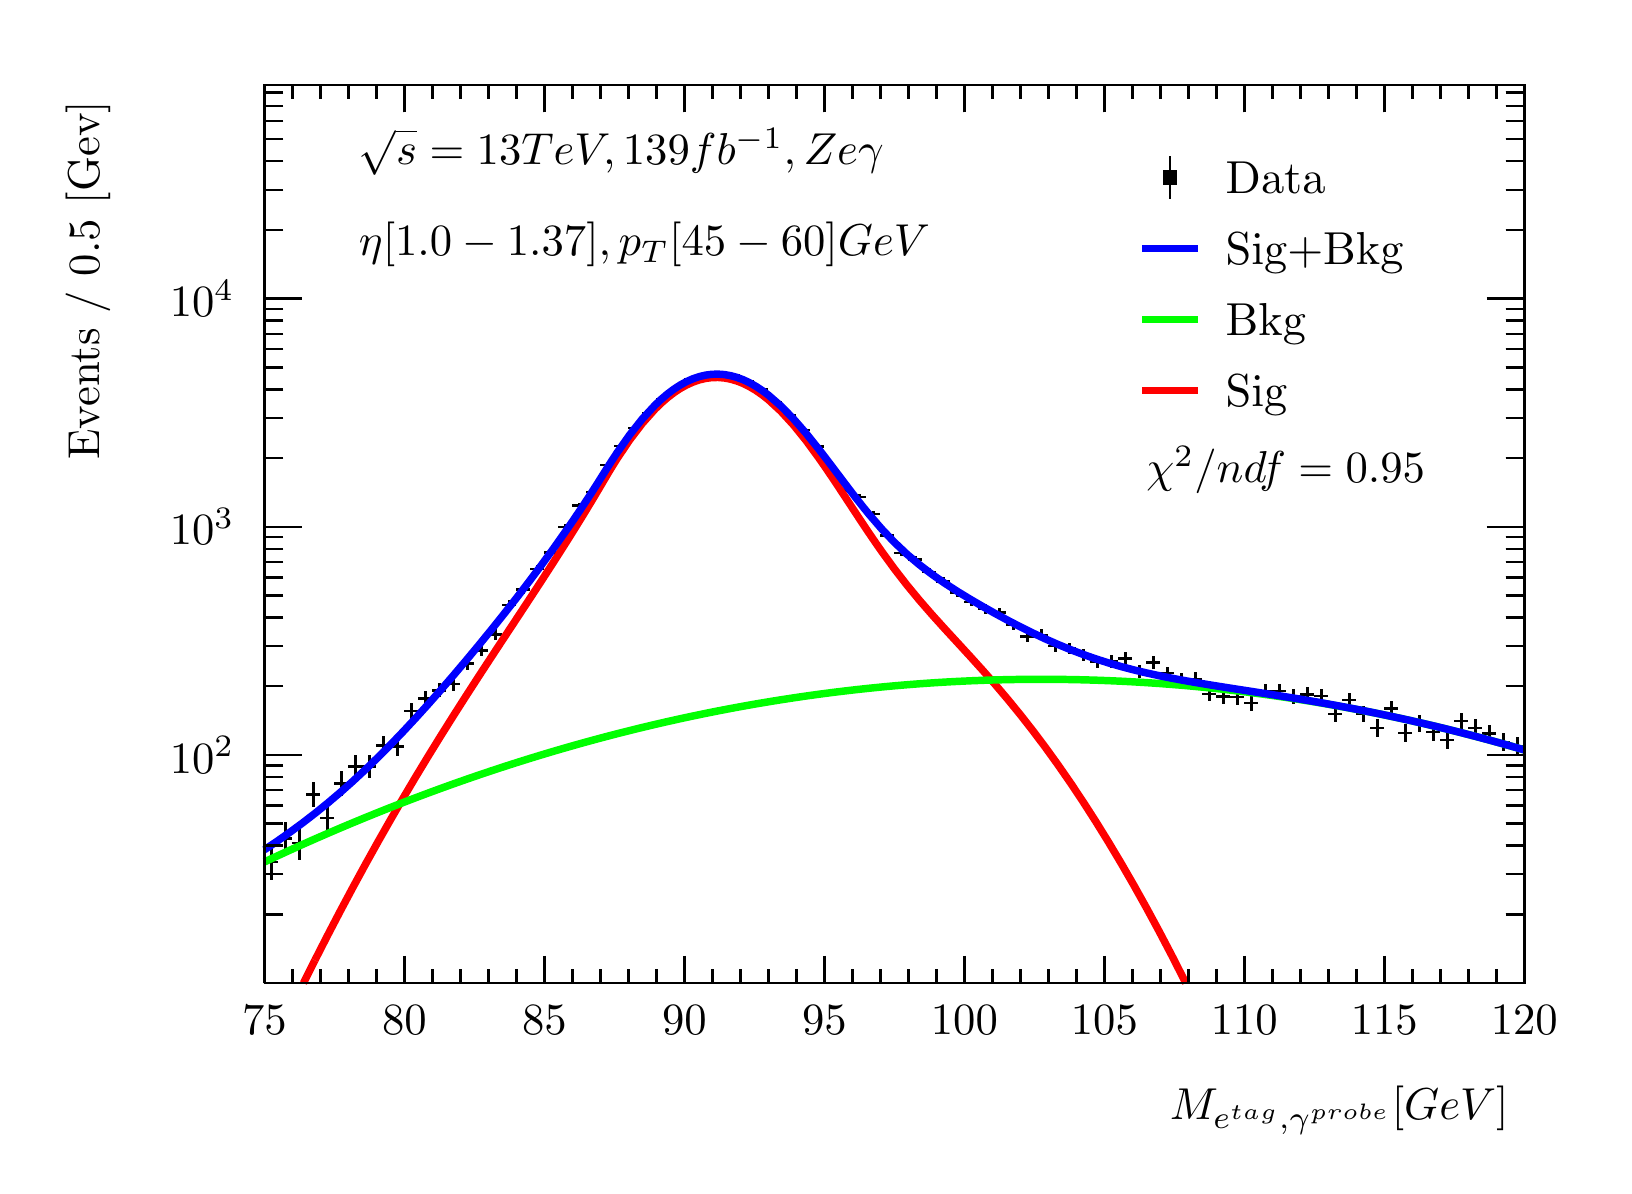
\begin{tikzpicture}
\pgfdeclareplotmark{cross} {
\pgfpathmoveto{\pgfpoint{-0.3\pgfplotmarksize}{\pgfplotmarksize}}
\pgfpathlineto{\pgfpoint{+0.3\pgfplotmarksize}{\pgfplotmarksize}}
\pgfpathlineto{\pgfpoint{+0.3\pgfplotmarksize}{0.3\pgfplotmarksize}}
\pgfpathlineto{\pgfpoint{+1\pgfplotmarksize}{0.3\pgfplotmarksize}}
\pgfpathlineto{\pgfpoint{+1\pgfplotmarksize}{-0.3\pgfplotmarksize}}
\pgfpathlineto{\pgfpoint{+0.3\pgfplotmarksize}{-0.3\pgfplotmarksize}}
\pgfpathlineto{\pgfpoint{+0.3\pgfplotmarksize}{-1.\pgfplotmarksize}}
\pgfpathlineto{\pgfpoint{-0.3\pgfplotmarksize}{-1.\pgfplotmarksize}}
\pgfpathlineto{\pgfpoint{-0.3\pgfplotmarksize}{-0.3\pgfplotmarksize}}
\pgfpathlineto{\pgfpoint{-1.\pgfplotmarksize}{-0.3\pgfplotmarksize}}
\pgfpathlineto{\pgfpoint{-1.\pgfplotmarksize}{0.3\pgfplotmarksize}}
\pgfpathlineto{\pgfpoint{-0.3\pgfplotmarksize}{0.3\pgfplotmarksize}}
\pgfpathclose
\pgfusepathqstroke
}
\pgfdeclareplotmark{cross*} {
\pgfpathmoveto{\pgfpoint{-0.3\pgfplotmarksize}{\pgfplotmarksize}}
\pgfpathlineto{\pgfpoint{+0.3\pgfplotmarksize}{\pgfplotmarksize}}
\pgfpathlineto{\pgfpoint{+0.3\pgfplotmarksize}{0.3\pgfplotmarksize}}
\pgfpathlineto{\pgfpoint{+1\pgfplotmarksize}{0.3\pgfplotmarksize}}
\pgfpathlineto{\pgfpoint{+1\pgfplotmarksize}{-0.3\pgfplotmarksize}}
\pgfpathlineto{\pgfpoint{+0.3\pgfplotmarksize}{-0.3\pgfplotmarksize}}
\pgfpathlineto{\pgfpoint{+0.3\pgfplotmarksize}{-1.\pgfplotmarksize}}
\pgfpathlineto{\pgfpoint{-0.3\pgfplotmarksize}{-1.\pgfplotmarksize}}
\pgfpathlineto{\pgfpoint{-0.3\pgfplotmarksize}{-0.3\pgfplotmarksize}}
\pgfpathlineto{\pgfpoint{-1.\pgfplotmarksize}{-0.3\pgfplotmarksize}}
\pgfpathlineto{\pgfpoint{-1.\pgfplotmarksize}{0.3\pgfplotmarksize}}
\pgfpathlineto{\pgfpoint{-0.3\pgfplotmarksize}{0.3\pgfplotmarksize}}
\pgfpathclose
\pgfusepathqfillstroke
}
\pgfdeclareplotmark{newstar} {
\pgfpathmoveto{\pgfqpoint{0pt}{\pgfplotmarksize}}
\pgfpathlineto{\pgfqpointpolar{44}{0.5\pgfplotmarksize}}
\pgfpathlineto{\pgfqpointpolar{18}{\pgfplotmarksize}}
\pgfpathlineto{\pgfqpointpolar{-20}{0.5\pgfplotmarksize}}
\pgfpathlineto{\pgfqpointpolar{-54}{\pgfplotmarksize}}
\pgfpathlineto{\pgfqpointpolar{-90}{0.5\pgfplotmarksize}}
\pgfpathlineto{\pgfqpointpolar{234}{\pgfplotmarksize}}
\pgfpathlineto{\pgfqpointpolar{198}{0.5\pgfplotmarksize}}
\pgfpathlineto{\pgfqpointpolar{162}{\pgfplotmarksize}}
\pgfpathlineto{\pgfqpointpolar{134}{0.5\pgfplotmarksize}}
\pgfpathclose
\pgfusepathqstroke
}
\pgfdeclareplotmark{newstar*} {
\pgfpathmoveto{\pgfqpoint{0pt}{\pgfplotmarksize}}
\pgfpathlineto{\pgfqpointpolar{44}{0.5\pgfplotmarksize}}
\pgfpathlineto{\pgfqpointpolar{18}{\pgfplotmarksize}}
\pgfpathlineto{\pgfqpointpolar{-20}{0.5\pgfplotmarksize}}
\pgfpathlineto{\pgfqpointpolar{-54}{\pgfplotmarksize}}
\pgfpathlineto{\pgfqpointpolar{-90}{0.5\pgfplotmarksize}}
\pgfpathlineto{\pgfqpointpolar{234}{\pgfplotmarksize}}
\pgfpathlineto{\pgfqpointpolar{198}{0.5\pgfplotmarksize}}
\pgfpathlineto{\pgfqpointpolar{162}{\pgfplotmarksize}}
\pgfpathlineto{\pgfqpointpolar{134}{0.5\pgfplotmarksize}}
\pgfpathclose
\pgfusepathqfillstroke
}
\definecolor{c}{rgb}{1,1,1};
\draw [color=c, fill=c] (0,0) rectangle (20,14.4361);
\draw [color=c, fill=c] (3,2.30977) rectangle (19,13.7143);
\definecolor{c}{rgb}{0,0,0};
\draw [c,line width=0.9] (3,2.30977) -- (3,13.7143) -- (19,13.7143) -- (19,2.30977) -- (3,2.30977);
\definecolor{c}{rgb}{1,1,1};
\draw [color=c, fill=c] (3,2.30977) rectangle (19,13.7143);
\definecolor{c}{rgb}{0,0,0};
\draw [c,line width=0.9] (3,2.30977) -- (3,13.7143) -- (19,13.7143) -- (19,2.30977) -- (3,2.30977);
\draw [c,line width=0.9] (3,2.30977) -- (19,2.30977);
\draw [c,line width=0.9] (3,2.65624) -- (3,2.30977);
\draw [c,line width=0.9] (3.35556,2.48301) -- (3.35556,2.30977);
\draw [c,line width=0.9] (3.71111,2.48301) -- (3.71111,2.30977);
\draw [c,line width=0.9] (4.06667,2.48301) -- (4.06667,2.30977);
\draw [c,line width=0.9] (4.42222,2.48301) -- (4.42222,2.30977);
\draw [c,line width=0.9] (4.77778,2.65624) -- (4.77778,2.30977);
\draw [c,line width=0.9] (5.13333,2.48301) -- (5.13333,2.30977);
\draw [c,line width=0.9] (5.48889,2.48301) -- (5.48889,2.30977);
\draw [c,line width=0.9] (5.84444,2.48301) -- (5.84444,2.30977);
\draw [c,line width=0.9] (6.2,2.48301) -- (6.2,2.30977);
\draw [c,line width=0.9] (6.55556,2.65624) -- (6.55556,2.30977);
\draw [c,line width=0.9] (6.91111,2.48301) -- (6.91111,2.30977);
\draw [c,line width=0.9] (7.26667,2.48301) -- (7.26667,2.30977);
\draw [c,line width=0.9] (7.62222,2.48301) -- (7.62222,2.30977);
\draw [c,line width=0.9] (7.97778,2.48301) -- (7.97778,2.30977);
\draw [c,line width=0.9] (8.33333,2.65624) -- (8.33333,2.30977);
\draw [c,line width=0.9] (8.68889,2.48301) -- (8.68889,2.30977);
\draw [c,line width=0.9] (9.04444,2.48301) -- (9.04444,2.30977);
\draw [c,line width=0.9] (9.4,2.48301) -- (9.4,2.30977);
\draw [c,line width=0.9] (9.75556,2.48301) -- (9.75556,2.30977);
\draw [c,line width=0.9] (10.1111,2.65624) -- (10.1111,2.30977);
\draw [c,line width=0.9] (10.4667,2.48301) -- (10.4667,2.30977);
\draw [c,line width=0.9] (10.8222,2.48301) -- (10.8222,2.30977);
\draw [c,line width=0.9] (11.1778,2.48301) -- (11.1778,2.30977);
\draw [c,line width=0.9] (11.5333,2.48301) -- (11.5333,2.30977);
\draw [c,line width=0.9] (11.8889,2.65624) -- (11.8889,2.30977);
\draw [c,line width=0.9] (12.2444,2.48301) -- (12.2444,2.30977);
\draw [c,line width=0.9] (12.6,2.48301) -- (12.6,2.30977);
\draw [c,line width=0.9] (12.9556,2.48301) -- (12.9556,2.30977);
\draw [c,line width=0.9] (13.3111,2.48301) -- (13.3111,2.30977);
\draw [c,line width=0.9] (13.6667,2.65624) -- (13.6667,2.30977);
\draw [c,line width=0.9] (14.0222,2.48301) -- (14.0222,2.30977);
\draw [c,line width=0.9] (14.3778,2.48301) -- (14.3778,2.30977);
\draw [c,line width=0.9] (14.7333,2.48301) -- (14.7333,2.30977);
\draw [c,line width=0.9] (15.0889,2.48301) -- (15.0889,2.30977);
\draw [c,line width=0.9] (15.4444,2.65624) -- (15.4444,2.30977);
\draw [c,line width=0.9] (15.8,2.48301) -- (15.8,2.30977);
\draw [c,line width=0.9] (16.1556,2.48301) -- (16.1556,2.30977);
\draw [c,line width=0.9] (16.5111,2.48301) -- (16.5111,2.30977);
\draw [c,line width=0.9] (16.8667,2.48301) -- (16.8667,2.30977);
\draw [c,line width=0.9] (17.2222,2.65624) -- (17.2222,2.30977);
\draw [c,line width=0.9] (17.5778,2.48301) -- (17.5778,2.30977);
\draw [c,line width=0.9] (17.9333,2.48301) -- (17.9333,2.30977);
\draw [c,line width=0.9] (18.2889,2.48301) -- (18.2889,2.30977);
\draw [c,line width=0.9] (18.6444,2.48301) -- (18.6444,2.30977);
\draw [c,line width=0.9] (19,2.65624) -- (19,2.30977);
\draw [c,line width=0.9] (19,2.65624) -- (19,2.30977);
\draw [anchor=base] (3,1.66015) node[scale=1.61424, color=c, rotate=0]{75};
\draw [anchor=base] (4.77778,1.66015) node[scale=1.61424, color=c, rotate=0]{80};
\draw [anchor=base] (6.55556,1.66015) node[scale=1.61424, color=c, rotate=0]{85};
\draw [anchor=base] (8.33333,1.66015) node[scale=1.61424, color=c, rotate=0]{90};
\draw [anchor=base] (10.1111,1.66015) node[scale=1.61424, color=c, rotate=0]{95};
\draw [anchor=base] (11.8889,1.66015) node[scale=1.61424, color=c, rotate=0]{100};
\draw [anchor=base] (13.6667,1.66015) node[scale=1.61424, color=c, rotate=0]{105};
\draw [anchor=base] (15.4444,1.66015) node[scale=1.61424, color=c, rotate=0]{110};
\draw [anchor=base] (17.2222,1.66015) node[scale=1.61424, color=c, rotate=0]{115};
\draw [anchor=base] (19,1.66015) node[scale=1.61424, color=c, rotate=0]{120};
\draw [anchor= east] (19,0.692932) node[scale=1.61424, color=c, rotate=0]{$M_{e^{tag}, \gamma^{probe}}  [GeV]$};
\draw [c,line width=0.9] (3,13.7143) -- (19,13.7143);
\draw [c,line width=0.9] (3,13.3678) -- (3,13.7143);
\draw [c,line width=0.9] (3.35556,13.5411) -- (3.35556,13.7143);
\draw [c,line width=0.9] (3.71111,13.5411) -- (3.71111,13.7143);
\draw [c,line width=0.9] (4.06667,13.5411) -- (4.06667,13.7143);
\draw [c,line width=0.9] (4.42222,13.5411) -- (4.42222,13.7143);
\draw [c,line width=0.9] (4.77778,13.3678) -- (4.77778,13.7143);
\draw [c,line width=0.9] (5.13333,13.5411) -- (5.13333,13.7143);
\draw [c,line width=0.9] (5.48889,13.5411) -- (5.48889,13.7143);
\draw [c,line width=0.9] (5.84444,13.5411) -- (5.84444,13.7143);
\draw [c,line width=0.9] (6.2,13.5411) -- (6.2,13.7143);
\draw [c,line width=0.9] (6.55556,13.3678) -- (6.55556,13.7143);
\draw [c,line width=0.9] (6.91111,13.5411) -- (6.91111,13.7143);
\draw [c,line width=0.9] (7.26667,13.5411) -- (7.26667,13.7143);
\draw [c,line width=0.9] (7.62222,13.5411) -- (7.62222,13.7143);
\draw [c,line width=0.9] (7.97778,13.5411) -- (7.97778,13.7143);
\draw [c,line width=0.9] (8.33333,13.3678) -- (8.33333,13.7143);
\draw [c,line width=0.9] (8.68889,13.5411) -- (8.68889,13.7143);
\draw [c,line width=0.9] (9.04444,13.5411) -- (9.04444,13.7143);
\draw [c,line width=0.9] (9.4,13.5411) -- (9.4,13.7143);
\draw [c,line width=0.9] (9.75556,13.5411) -- (9.75556,13.7143);
\draw [c,line width=0.9] (10.1111,13.3678) -- (10.1111,13.7143);
\draw [c,line width=0.9] (10.4667,13.5411) -- (10.4667,13.7143);
\draw [c,line width=0.9] (10.8222,13.5411) -- (10.8222,13.7143);
\draw [c,line width=0.9] (11.1778,13.5411) -- (11.1778,13.7143);
\draw [c,line width=0.9] (11.5333,13.5411) -- (11.5333,13.7143);
\draw [c,line width=0.9] (11.8889,13.3678) -- (11.8889,13.7143);
\draw [c,line width=0.9] (12.2444,13.5411) -- (12.2444,13.7143);
\draw [c,line width=0.9] (12.6,13.5411) -- (12.6,13.7143);
\draw [c,line width=0.9] (12.9556,13.5411) -- (12.9556,13.7143);
\draw [c,line width=0.9] (13.3111,13.5411) -- (13.3111,13.7143);
\draw [c,line width=0.9] (13.6667,13.3678) -- (13.6667,13.7143);
\draw [c,line width=0.9] (14.0222,13.5411) -- (14.0222,13.7143);
\draw [c,line width=0.9] (14.3778,13.5411) -- (14.3778,13.7143);
\draw [c,line width=0.9] (14.7333,13.5411) -- (14.7333,13.7143);
\draw [c,line width=0.9] (15.0889,13.5411) -- (15.0889,13.7143);
\draw [c,line width=0.9] (15.4444,13.3678) -- (15.4444,13.7143);
\draw [c,line width=0.9] (15.8,13.5411) -- (15.8,13.7143);
\draw [c,line width=0.9] (16.1556,13.5411) -- (16.1556,13.7143);
\draw [c,line width=0.9] (16.5111,13.5411) -- (16.5111,13.7143);
\draw [c,line width=0.9] (16.8667,13.5411) -- (16.8667,13.7143);
\draw [c,line width=0.9] (17.2222,13.3678) -- (17.2222,13.7143);
\draw [c,line width=0.9] (17.5778,13.5411) -- (17.5778,13.7143);
\draw [c,line width=0.9] (17.9333,13.5411) -- (17.9333,13.7143);
\draw [c,line width=0.9] (18.2889,13.5411) -- (18.2889,13.7143);
\draw [c,line width=0.9] (18.6444,13.5411) -- (18.6444,13.7143);
\draw [c,line width=0.9] (19,13.3678) -- (19,13.7143);
\draw [c,line width=0.9] (19,13.3678) -- (19,13.7143);
\draw [c,line width=0.9] (3,2.30977) -- (3,13.7143);
\draw [c,line width=0.9] (3.237,3.182) -- (3,3.182);
\draw [c,line width=0.9] (3.237,3.69222) -- (3,3.69222);
\draw [c,line width=0.9] (3.237,4.05422) -- (3,4.05422);
\draw [c,line width=0.9] (3.237,4.33502) -- (3,4.33502);
\draw [c,line width=0.9] (3.237,4.56444) -- (3,4.56444);
\draw [c,line width=0.9] (3.237,4.75842) -- (3,4.75842);
\draw [c,line width=0.9] (3.237,4.92645) -- (3,4.92645);
\draw [c,line width=0.9] (3.237,5.07466) -- (3,5.07466);
\draw [c,line width=0.9] (3.474,5.20724) -- (3,5.20724);
\draw [anchor= east] (2.82,5.20724) node[scale=1.61424, color=c, rotate=0]{$10^{2}$};
\draw [c,line width=0.9] (3.237,6.07947) -- (3,6.07947);
\draw [c,line width=0.9] (3.237,6.58969) -- (3,6.58969);
\draw [c,line width=0.9] (3.237,6.9517) -- (3,6.9517);
\draw [c,line width=0.9] (3.237,7.23249) -- (3,7.23249);
\draw [c,line width=0.9] (3.237,7.46192) -- (3,7.46192);
\draw [c,line width=0.9] (3.237,7.65589) -- (3,7.65589);
\draw [c,line width=0.9] (3.237,7.82392) -- (3,7.82392);
\draw [c,line width=0.9] (3.237,7.97214) -- (3,7.97214);
\draw [c,line width=0.9] (3.474,8.10472) -- (3,8.10472);
\draw [anchor= east] (2.82,8.10472) node[scale=1.61424, color=c, rotate=0]{$10^{3}$};
\draw [c,line width=0.9] (3.237,8.97694) -- (3,8.97694);
\draw [c,line width=0.9] (3.237,9.48716) -- (3,9.48716);
\draw [c,line width=0.9] (3.237,9.84917) -- (3,9.84917);
\draw [c,line width=0.9] (3.237,10.13) -- (3,10.13);
\draw [c,line width=0.9] (3.237,10.3594) -- (3,10.3594);
\draw [c,line width=0.9] (3.237,10.5534) -- (3,10.5534);
\draw [c,line width=0.9] (3.237,10.7214) -- (3,10.7214);
\draw [c,line width=0.9] (3.237,10.8696) -- (3,10.8696);
\draw [c,line width=0.9] (3.474,11.0022) -- (3,11.0022);
\draw [anchor= east] (2.82,11.0022) node[scale=1.61424, color=c, rotate=0]{$10^{4}$};
\draw [c,line width=0.9] (3.237,11.8744) -- (3,11.8744);
\draw [c,line width=0.9] (3.237,12.3846) -- (3,12.3846);
\draw [c,line width=0.9] (3.237,12.7466) -- (3,12.7466);
\draw [c,line width=0.9] (3.237,13.0274) -- (3,13.0274);
\draw [c,line width=0.9] (3.237,13.2569) -- (3,13.2569);
\draw [c,line width=0.9] (3.237,13.4508) -- (3,13.4508);
\draw [c,line width=0.9] (3.237,13.6189) -- (3,13.6189);
\draw [anchor= east] (0.76,13.7143) node[scale=1.61424, color=c, rotate=90]{Events / 0.5 [Gev]};
\draw [c,line width=0.9] (19,2.30977) -- (19,13.7143);
\draw [c,line width=0.9] (18.763,3.182) -- (19,3.182);
\draw [c,line width=0.9] (18.763,3.69222) -- (19,3.69222);
\draw [c,line width=0.9] (18.763,4.05422) -- (19,4.05422);
\draw [c,line width=0.9] (18.763,4.33502) -- (19,4.33502);
\draw [c,line width=0.9] (18.763,4.56444) -- (19,4.56444);
\draw [c,line width=0.9] (18.763,4.75842) -- (19,4.75842);
\draw [c,line width=0.9] (18.763,4.92645) -- (19,4.92645);
\draw [c,line width=0.9] (18.763,5.07466) -- (19,5.07466);
\draw [c,line width=0.9] (18.526,5.20724) -- (19,5.20724);
\draw [c,line width=0.9] (18.763,6.07947) -- (19,6.07947);
\draw [c,line width=0.9] (18.763,6.58969) -- (19,6.58969);
\draw [c,line width=0.9] (18.763,6.9517) -- (19,6.9517);
\draw [c,line width=0.9] (18.763,7.23249) -- (19,7.23249);
\draw [c,line width=0.9] (18.763,7.46192) -- (19,7.46192);
\draw [c,line width=0.9] (18.763,7.65589) -- (19,7.65589);
\draw [c,line width=0.9] (18.763,7.82392) -- (19,7.82392);
\draw [c,line width=0.9] (18.763,7.97214) -- (19,7.97214);
\draw [c,line width=0.9] (18.526,8.10472) -- (19,8.10472);
\draw [c,line width=0.9] (18.763,8.97694) -- (19,8.97694);
\draw [c,line width=0.9] (18.763,9.48716) -- (19,9.48716);
\draw [c,line width=0.9] (18.763,9.84917) -- (19,9.84917);
\draw [c,line width=0.9] (18.763,10.13) -- (19,10.13);
\draw [c,line width=0.9] (18.763,10.3594) -- (19,10.3594);
\draw [c,line width=0.9] (18.763,10.5534) -- (19,10.5534);
\draw [c,line width=0.9] (18.763,10.7214) -- (19,10.7214);
\draw [c,line width=0.9] (18.763,10.8696) -- (19,10.8696);
\draw [c,line width=0.9] (18.526,11.0022) -- (19,11.0022);
\draw [c,line width=0.9] (18.763,11.8744) -- (19,11.8744);
\draw [c,line width=0.9] (18.763,12.3846) -- (19,12.3846);
\draw [c,line width=0.9] (18.763,12.7466) -- (19,12.7466);
\draw [c,line width=0.9] (18.763,13.0274) -- (19,13.0274);
\draw [c,line width=0.9] (18.763,13.2569) -- (19,13.2569);
\draw [c,line width=0.9] (18.763,13.4508) -- (19,13.4508);
\draw [c,line width=0.9] (18.763,13.6189) -- (19,13.6189);
\draw [c,line width=0.9] (3.08889,3.84972) -- (3,3.84972);
\draw [c,line width=0.9] (3,3.84972) -- (3,3.84972);
\draw [c,line width=0.9] (3.08889,3.84972) -- (3.17778,3.84972);
\draw [c,line width=0.9] (3.17778,3.84972) -- (3.17778,3.84972);
\draw [c,line width=0.9] (3.08889,3.84972) -- (3.08889,4.08186);
\draw [c,line width=0.9] (3.08889,4.08186) -- (3.08889,4.08186);
\draw [c,line width=0.9] (3.08889,3.84972) -- (3.08889,3.61426);
\draw [c,line width=0.9] (3.08889,3.61426) -- (3.08889,3.61426);
\draw [c,line width=0.9] (3.26667,4.14523) -- (3.17778,4.14523);
\draw [c,line width=0.9] (3.17778,4.14523) -- (3.17778,4.14523);
\draw [c,line width=0.9] (3.26667,4.14523) -- (3.35556,4.14523);
\draw [c,line width=0.9] (3.35556,4.14523) -- (3.35556,4.14523);
\draw [c,line width=0.9] (3.26667,4.14523) -- (3.26667,4.35024);
\draw [c,line width=0.9] (3.26667,4.35024) -- (3.26667,4.35024);
\draw [c,line width=0.9] (3.26667,4.14523) -- (3.26667,3.9379);
\draw [c,line width=0.9] (3.26667,3.9379) -- (3.26667,3.9379);
\draw [c,line width=0.9] (3.44444,4.0853) -- (3.35556,4.0853);
\draw [c,line width=0.9] (3.35556,4.0853) -- (3.35556,4.0853);
\draw [c,line width=0.9] (3.44444,4.0853) -- (3.53333,4.0853);
\draw [c,line width=0.9] (3.53333,4.0853) -- (3.53333,4.0853);
\draw [c,line width=0.9] (3.44444,4.0853) -- (3.44444,4.29553);
\draw [c,line width=0.9] (3.44444,4.29553) -- (3.44444,4.29553);
\draw [c,line width=0.9] (3.44444,4.0853) -- (3.44444,3.87257);
\draw [c,line width=0.9] (3.44444,3.87257) -- (3.44444,3.87257);
\draw [c,line width=0.9] (3.62222,4.7033) -- (3.53333,4.7033);
\draw [c,line width=0.9] (3.53333,4.7033) -- (3.53333,4.7033);
\draw [c,line width=0.9] (3.62222,4.7033) -- (3.71111,4.7033);
\draw [c,line width=0.9] (3.71111,4.7033) -- (3.71111,4.7033);
\draw [c,line width=0.9] (3.62222,4.7033) -- (3.62222,4.86565);
\draw [c,line width=0.9] (3.62222,4.86565) -- (3.62222,4.86565);
\draw [c,line width=0.9] (3.62222,4.7033) -- (3.62222,4.53978);
\draw [c,line width=0.9] (3.62222,4.53978) -- (3.62222,4.53978);
\draw [c,line width=0.9] (3.8,4.40834) -- (3.71111,4.40834);
\draw [c,line width=0.9] (3.71111,4.40834) -- (3.71111,4.40834);
\draw [c,line width=0.9] (3.8,4.40834) -- (3.88889,4.40834);
\draw [c,line width=0.9] (3.88889,4.40834) -- (3.88889,4.40834);
\draw [c,line width=0.9] (3.8,4.40834) -- (3.8,4.59195);
\draw [c,line width=0.9] (3.8,4.59195) -- (3.8,4.59195);
\draw [c,line width=0.9] (3.8,4.40834) -- (3.8,4.22304);
\draw [c,line width=0.9] (3.8,4.22304) -- (3.8,4.22304);
\draw [c,line width=0.9] (3.97778,4.84524) -- (3.88889,4.84524);
\draw [c,line width=0.9] (3.88889,4.84524) -- (3.88889,4.84524);
\draw [c,line width=0.9] (3.97778,4.84524) -- (4.06667,4.84524);
\draw [c,line width=0.9] (4.06667,4.84524) -- (4.06667,4.84524);
\draw [c,line width=0.9] (3.97778,4.84524) -- (3.97778,4.99827);
\draw [c,line width=0.9] (3.97778,4.99827) -- (3.97778,4.99827);
\draw [c,line width=0.9] (3.97778,4.84524) -- (3.97778,4.69121);
\draw [c,line width=0.9] (3.97778,4.69121) -- (3.97778,4.69121);
\draw [c,line width=0.9] (4.15556,5.06061) -- (4.06667,5.06061);
\draw [c,line width=0.9] (4.06667,5.06061) -- (4.06667,5.06061);
\draw [c,line width=0.9] (4.15556,5.06061) -- (4.24444,5.06061);
\draw [c,line width=0.9] (4.24444,5.06061) -- (4.24444,5.06061);
\draw [c,line width=0.9] (4.15556,5.06061) -- (4.15556,5.20055);
\draw [c,line width=0.9] (4.15556,5.20055) -- (4.15556,5.20055);
\draw [c,line width=0.9] (4.15556,5.06061) -- (4.15556,4.91989);
\draw [c,line width=0.9] (4.15556,4.91989) -- (4.15556,4.91989);
\draw [c,line width=0.9] (4.33333,5.06061) -- (4.24444,5.06061);
\draw [c,line width=0.9] (4.24444,5.06061) -- (4.24444,5.06061);
\draw [c,line width=0.9] (4.33333,5.06061) -- (4.42222,5.06061);
\draw [c,line width=0.9] (4.42222,5.06061) -- (4.42222,5.06061);
\draw [c,line width=0.9] (4.33333,5.06061) -- (4.33333,5.20055);
\draw [c,line width=0.9] (4.33333,5.20055) -- (4.33333,5.20055);
\draw [c,line width=0.9] (4.33333,5.06061) -- (4.33333,4.91989);
\draw [c,line width=0.9] (4.33333,4.91989) -- (4.33333,4.91989);
\draw [c,line width=0.9] (4.51111,5.32718) -- (4.42222,5.32718);
\draw [c,line width=0.9] (4.42222,5.32718) -- (4.42222,5.32718);
\draw [c,line width=0.9] (4.51111,5.32718) -- (4.6,5.32718);
\draw [c,line width=0.9] (4.6,5.32718) -- (4.6,5.32718);
\draw [c,line width=0.9] (4.51111,5.32718) -- (4.51111,5.44711);
\draw [c,line width=0.9] (4.51111,5.44711) -- (4.51111,5.44711);
\draw [c,line width=0.9] (4.51111,5.32718) -- (4.51111,5.20725);
\draw [c,line width=0.9] (4.51111,5.20725) -- (4.51111,5.20725);
\draw [c,line width=0.9] (4.68889,5.31569) -- (4.6,5.31569);
\draw [c,line width=0.9] (4.6,5.31569) -- (4.6,5.31569);
\draw [c,line width=0.9] (4.68889,5.31569) -- (4.77778,5.31569);
\draw [c,line width=0.9] (4.77778,5.31569) -- (4.77778,5.31569);
\draw [c,line width=0.9] (4.68889,5.31569) -- (4.68889,5.43617);
\draw [c,line width=0.9] (4.68889,5.43617) -- (4.68889,5.43617);
\draw [c,line width=0.9] (4.68889,5.31569) -- (4.68889,5.19521);
\draw [c,line width=0.9] (4.68889,5.19521) -- (4.68889,5.19521);
\draw [c,line width=0.9] (4.86667,5.76682) -- (4.77778,5.76682);
\draw [c,line width=0.9] (4.77778,5.76682) -- (4.77778,5.76682);
\draw [c,line width=0.9] (4.86667,5.76682) -- (4.95556,5.76682);
\draw [c,line width=0.9] (4.95556,5.76682) -- (4.95556,5.76682);
\draw [c,line width=0.9] (4.86667,5.76682) -- (4.86667,5.86754);
\draw [c,line width=0.9] (4.86667,5.86754) -- (4.86667,5.86754);
\draw [c,line width=0.9] (4.86667,5.76682) -- (4.86667,5.6661);
\draw [c,line width=0.9] (4.86667,5.6661) -- (4.86667,5.6661);
\draw [c,line width=0.9] (5.04444,5.92574) -- (4.95556,5.92574);
\draw [c,line width=0.9] (4.95556,5.92574) -- (4.95556,5.92574);
\draw [c,line width=0.9] (5.04444,5.92574) -- (5.13333,5.92574);
\draw [c,line width=0.9] (5.13333,5.92574) -- (5.13333,5.92574);
\draw [c,line width=0.9] (5.04444,5.92574) -- (5.04444,6.0203);
\draw [c,line width=0.9] (5.04444,6.0203) -- (5.04444,6.0203);
\draw [c,line width=0.9] (5.04444,5.92574) -- (5.04444,5.83118);
\draw [c,line width=0.9] (5.04444,5.83118) -- (5.04444,5.83118);
\draw [c,line width=0.9] (5.22222,6.0281) -- (5.13333,6.0281);
\draw [c,line width=0.9] (5.13333,6.0281) -- (5.13333,6.0281);
\draw [c,line width=0.9] (5.22222,6.0281) -- (5.31111,6.0281);
\draw [c,line width=0.9] (5.31111,6.0281) -- (5.31111,6.0281);
\draw [c,line width=0.9] (5.22222,6.0281) -- (5.22222,6.1189);
\draw [c,line width=0.9] (5.22222,6.1189) -- (5.22222,6.1189);
\draw [c,line width=0.9] (5.22222,6.0281) -- (5.22222,5.93731);
\draw [c,line width=0.9] (5.22222,5.93731) -- (5.22222,5.93731);
\draw [c,line width=0.9] (5.4,6.11054) -- (5.31111,6.11054);
\draw [c,line width=0.9] (5.31111,6.11054) -- (5.31111,6.11054);
\draw [c,line width=0.9] (5.4,6.11054) -- (5.48889,6.11054);
\draw [c,line width=0.9] (5.48889,6.11054) -- (5.48889,6.11054);
\draw [c,line width=0.9] (5.4,6.11054) -- (5.4,6.19841);
\draw [c,line width=0.9] (5.4,6.19841) -- (5.4,6.19841);
\draw [c,line width=0.9] (5.4,6.11054) -- (5.4,6.02268);
\draw [c,line width=0.9] (5.4,6.02268) -- (5.4,6.02268);
\draw [c,line width=0.9] (5.57778,6.36529) -- (5.48889,6.36529);
\draw [c,line width=0.9] (5.48889,6.36529) -- (5.48889,6.36529);
\draw [c,line width=0.9] (5.57778,6.36529) -- (5.66667,6.36529);
\draw [c,line width=0.9] (5.66667,6.36529) -- (5.66667,6.36529);
\draw [c,line width=0.9] (5.57778,6.36529) -- (5.57778,6.4447);
\draw [c,line width=0.9] (5.57778,6.4447) -- (5.57778,6.4447);
\draw [c,line width=0.9] (5.57778,6.36529) -- (5.57778,6.28588);
\draw [c,line width=0.9] (5.57778,6.28588) -- (5.57778,6.28588);
\draw [c,line width=0.9] (5.75556,6.53395) -- (5.66667,6.53395);
\draw [c,line width=0.9] (5.66667,6.53395) -- (5.66667,6.53395);
\draw [c,line width=0.9] (5.75556,6.53395) -- (5.84444,6.53395);
\draw [c,line width=0.9] (5.84444,6.53395) -- (5.84444,6.53395);
\draw [c,line width=0.9] (5.75556,6.53395) -- (5.75556,6.60821);
\draw [c,line width=0.9] (5.75556,6.60821) -- (5.75556,6.60821);
\draw [c,line width=0.9] (5.75556,6.53395) -- (5.75556,6.45968);
\draw [c,line width=0.9] (5.75556,6.45968) -- (5.75556,6.45968);
\draw [c,line width=0.9] (5.93333,6.73604) -- (5.84444,6.73604);
\draw [c,line width=0.9] (5.84444,6.73604) -- (5.84444,6.73604);
\draw [c,line width=0.9] (5.93333,6.73604) -- (6.02222,6.73604);
\draw [c,line width=0.9] (6.02222,6.73604) -- (6.02222,6.73604);
\draw [c,line width=0.9] (5.93333,6.73604) -- (5.93333,6.80458);
\draw [c,line width=0.9] (5.93333,6.80458) -- (5.93333,6.80458);
\draw [c,line width=0.9] (5.93333,6.73604) -- (5.93333,6.6675);
\draw [c,line width=0.9] (5.93333,6.6675) -- (5.93333,6.6675);
\draw [c,line width=0.9] (6.11111,7.11105) -- (6.02222,7.11105);
\draw [c,line width=0.9] (6.02222,7.11105) -- (6.02222,7.11105);
\draw [c,line width=0.9] (6.11111,7.11105) -- (6.2,7.11105);
\draw [c,line width=0.9] (6.2,7.11105) -- (6.2,7.11105);
\draw [c,line width=0.9] (6.11111,7.11105) -- (6.11111,7.1701);
\draw [c,line width=0.9] (6.11111,7.1701) -- (6.11111,7.1701);
\draw [c,line width=0.9] (6.11111,7.11105) -- (6.11111,7.052);
\draw [c,line width=0.9] (6.11111,7.052) -- (6.11111,7.052);
\draw [c,line width=0.9] (6.28889,7.31056) -- (6.2,7.31056);
\draw [c,line width=0.9] (6.2,7.31056) -- (6.2,7.31056);
\draw [c,line width=0.9] (6.28889,7.31056) -- (6.37778,7.31056);
\draw [c,line width=0.9] (6.37778,7.31056) -- (6.37778,7.31056);
\draw [c,line width=0.9] (6.28889,7.31056) -- (6.28889,7.36511);
\draw [c,line width=0.9] (6.28889,7.36511) -- (6.28889,7.36511);
\draw [c,line width=0.9] (6.28889,7.31056) -- (6.28889,7.256);
\draw [c,line width=0.9] (6.28889,7.256) -- (6.28889,7.256);
\draw [c,line width=0.9] (6.46667,7.56844) -- (6.37778,7.56844);
\draw [c,line width=0.9] (6.37778,7.56844) -- (6.37778,7.56844);
\draw [c,line width=0.9] (6.46667,7.56844) -- (6.55556,7.56844);
\draw [c,line width=0.9] (6.55556,7.56844) -- (6.55556,7.56844);
\draw [c,line width=0.9] (6.46667,7.56844) -- (6.46667,7.61768);
\draw [c,line width=0.9] (6.46667,7.61768) -- (6.46667,7.61768);
\draw [c,line width=0.9] (6.46667,7.56844) -- (6.46667,7.5192);
\draw [c,line width=0.9] (6.46667,7.5192) -- (6.46667,7.5192);
\draw [c,line width=0.9] (6.64444,7.77583) -- (6.55556,7.77583);
\draw [c,line width=0.9] (6.55556,7.77583) -- (6.55556,7.77583);
\draw [c,line width=0.9] (6.64444,7.77583) -- (6.73333,7.77583);
\draw [c,line width=0.9] (6.73333,7.77583) -- (6.73333,7.77583);
\draw [c,line width=0.9] (6.64444,7.77583) -- (6.64444,7.82117);
\draw [c,line width=0.9] (6.64444,7.82117) -- (6.64444,7.82117);
\draw [c,line width=0.9] (6.64444,7.77583) -- (6.64444,7.73048);
\draw [c,line width=0.9] (6.64444,7.73048) -- (6.64444,7.73048);
\draw [c,line width=0.9] (6.82222,8.1022) -- (6.73333,8.1022);
\draw [c,line width=0.9] (6.73333,8.1022) -- (6.73333,8.1022);
\draw [c,line width=0.9] (6.82222,8.1022) -- (6.91111,8.1022);
\draw [c,line width=0.9] (6.91111,8.1022) -- (6.91111,8.1022);
\draw [c,line width=0.9] (6.82222,8.1022) -- (6.82222,8.14203);
\draw [c,line width=0.9] (6.82222,8.14203) -- (6.82222,8.14203);
\draw [c,line width=0.9] (6.82222,8.1022) -- (6.82222,8.06237);
\draw [c,line width=0.9] (6.82222,8.06237) -- (6.82222,8.06237);
\draw [c,line width=0.9] (7,8.37439) -- (6.91111,8.37439);
\draw [c,line width=0.9] (6.91111,8.37439) -- (6.91111,8.37439);
\draw [c,line width=0.9] (7,8.37439) -- (7.08889,8.37439);
\draw [c,line width=0.9] (7.08889,8.37439) -- (7.08889,8.37439);
\draw [c,line width=0.9] (7,8.37439) -- (7,8.41014);
\draw [c,line width=0.9] (7,8.41014) -- (7,8.41014);
\draw [c,line width=0.9] (7,8.37439) -- (7,8.33864);
\draw [c,line width=0.9] (7,8.33864) -- (7,8.33864);
\draw [c,line width=0.9] (7.17778,8.54863) -- (7.08889,8.54863);
\draw [c,line width=0.9] (7.08889,8.54863) -- (7.08889,8.54863);
\draw [c,line width=0.9] (7.17778,8.54863) -- (7.26667,8.54863);
\draw [c,line width=0.9] (7.26667,8.54863) -- (7.26667,8.54863);
\draw [c,line width=0.9] (7.17778,8.54863) -- (7.17778,8.58198);
\draw [c,line width=0.9] (7.17778,8.58198) -- (7.17778,8.58198);
\draw [c,line width=0.9] (7.17778,8.54863) -- (7.17778,8.51527);
\draw [c,line width=0.9] (7.17778,8.51527) -- (7.17778,8.51527);
\draw [c,line width=0.9] (7.35556,8.889) -- (7.26667,8.889);
\draw [c,line width=0.9] (7.26667,8.889) -- (7.26667,8.889);
\draw [c,line width=0.9] (7.35556,8.889) -- (7.44444,8.889);
\draw [c,line width=0.9] (7.44444,8.889) -- (7.44444,8.889);
\draw [c,line width=0.9] (7.35556,8.889) -- (7.35556,8.91814);
\draw [c,line width=0.9] (7.35556,8.91814) -- (7.35556,8.91814);
\draw [c,line width=0.9] (7.35556,8.889) -- (7.35556,8.85987);
\draw [c,line width=0.9] (7.35556,8.85987) -- (7.35556,8.85987);
\draw [c,line width=0.9] (7.53333,9.12851) -- (7.44444,9.12851);
\draw [c,line width=0.9] (7.44444,9.12851) -- (7.44444,9.12851);
\draw [c,line width=0.9] (7.53333,9.12851) -- (7.62222,9.12851);
\draw [c,line width=0.9] (7.62222,9.12851) -- (7.62222,9.12851);
\draw [c,line width=0.9] (7.53333,9.12851) -- (7.53333,9.155);
\draw [c,line width=0.9] (7.53333,9.155) -- (7.53333,9.155);
\draw [c,line width=0.9] (7.53333,9.12851) -- (7.53333,9.10202);
\draw [c,line width=0.9] (7.53333,9.10202) -- (7.53333,9.10202);
\draw [c,line width=0.9] (7.71111,9.35784) -- (7.62222,9.35784);
\draw [c,line width=0.9] (7.62222,9.35784) -- (7.62222,9.35784);
\draw [c,line width=0.9] (7.71111,9.35784) -- (7.8,9.35784);
\draw [c,line width=0.9] (7.8,9.35784) -- (7.8,9.35784);
\draw [c,line width=0.9] (7.71111,9.35784) -- (7.71111,9.38203);
\draw [c,line width=0.9] (7.71111,9.38203) -- (7.71111,9.38203);
\draw [c,line width=0.9] (7.71111,9.35784) -- (7.71111,9.33366);
\draw [c,line width=0.9] (7.71111,9.33366) -- (7.71111,9.33366);
\draw [c,line width=0.9] (7.88889,9.55255) -- (7.8,9.55255);
\draw [c,line width=0.9] (7.8,9.55255) -- (7.8,9.55255);
\draw [c,line width=0.9] (7.88889,9.55255) -- (7.97778,9.55255);
\draw [c,line width=0.9] (7.97778,9.55255) -- (7.97778,9.55255);
\draw [c,line width=0.9] (7.88889,9.55255) -- (7.88889,9.57493);
\draw [c,line width=0.9] (7.88889,9.57493) -- (7.88889,9.57493);
\draw [c,line width=0.9] (7.88889,9.55255) -- (7.88889,9.53016);
\draw [c,line width=0.9] (7.88889,9.53016) -- (7.88889,9.53016);
\draw [c,line width=0.9] (8.06667,9.72773) -- (7.97778,9.72773);
\draw [c,line width=0.9] (7.97778,9.72773) -- (7.97778,9.72773);
\draw [c,line width=0.9] (8.06667,9.72773) -- (8.15556,9.72773);
\draw [c,line width=0.9] (8.15556,9.72773) -- (8.15556,9.72773);
\draw [c,line width=0.9] (8.06667,9.72773) -- (8.06667,9.74861);
\draw [c,line width=0.9] (8.06667,9.74861) -- (8.06667,9.74861);
\draw [c,line width=0.9] (8.06667,9.72773) -- (8.06667,9.70685);
\draw [c,line width=0.9] (8.06667,9.70685) -- (8.06667,9.70685);
\draw [c,line width=0.9] (8.24444,9.85482) -- (8.15556,9.85482);
\draw [c,line width=0.9] (8.15556,9.85482) -- (8.15556,9.85482);
\draw [c,line width=0.9] (8.24444,9.85482) -- (8.33333,9.85482);
\draw [c,line width=0.9] (8.33333,9.85482) -- (8.33333,9.85482);
\draw [c,line width=0.9] (8.24444,9.85482) -- (8.24444,9.87467);
\draw [c,line width=0.9] (8.24444,9.87467) -- (8.24444,9.87467);
\draw [c,line width=0.9] (8.24444,9.85482) -- (8.24444,9.83497);
\draw [c,line width=0.9] (8.24444,9.83497) -- (8.24444,9.83497);
\draw [c,line width=0.9] (8.42222,9.97481) -- (8.33333,9.97481);
\draw [c,line width=0.9] (8.33333,9.97481) -- (8.33333,9.97481);
\draw [c,line width=0.9] (8.42222,9.97481) -- (8.51111,9.97481);
\draw [c,line width=0.9] (8.51111,9.97481) -- (8.51111,9.97481);
\draw [c,line width=0.9] (8.42222,9.97481) -- (8.42222,9.99374);
\draw [c,line width=0.9] (8.42222,9.99374) -- (8.42222,9.99374);
\draw [c,line width=0.9] (8.42222,9.97481) -- (8.42222,9.95588);
\draw [c,line width=0.9] (8.42222,9.95588) -- (8.42222,9.95588);
\draw [c,line width=0.9] (8.6,10.0432) -- (8.51111,10.0432);
\draw [c,line width=0.9] (8.51111,10.0432) -- (8.51111,10.0432);
\draw [c,line width=0.9] (8.6,10.0432) -- (8.68889,10.0432);
\draw [c,line width=0.9] (8.68889,10.0432) -- (8.68889,10.0432);
\draw [c,line width=0.9] (8.6,10.0432) -- (8.6,10.0617);
\draw [c,line width=0.9] (8.6,10.0617) -- (8.6,10.0617);
\draw [c,line width=0.9] (8.6,10.0432) -- (8.6,10.0248);
\draw [c,line width=0.9] (8.6,10.0248) -- (8.6,10.0248);
\draw [c,line width=0.9] (8.77778,10.0529) -- (8.68889,10.0529);
\draw [c,line width=0.9] (8.68889,10.0529) -- (8.68889,10.0529);
\draw [c,line width=0.9] (8.77778,10.0529) -- (8.86667,10.0529);
\draw [c,line width=0.9] (8.86667,10.0529) -- (8.86667,10.0529);
\draw [c,line width=0.9] (8.77778,10.0529) -- (8.77778,10.0713);
\draw [c,line width=0.9] (8.77778,10.0713) -- (8.77778,10.0713);
\draw [c,line width=0.9] (8.77778,10.0529) -- (8.77778,10.0346);
\draw [c,line width=0.9] (8.77778,10.0346) -- (8.77778,10.0346);
\draw [c,line width=0.9] (8.95556,10.0346) -- (8.86667,10.0346);
\draw [c,line width=0.9] (8.86667,10.0346) -- (8.86667,10.0346);
\draw [c,line width=0.9] (8.95556,10.0346) -- (9.04444,10.0346);
\draw [c,line width=0.9] (9.04444,10.0346) -- (9.04444,10.0346);
\draw [c,line width=0.9] (8.95556,10.0346) -- (8.95556,10.0531);
\draw [c,line width=0.9] (8.95556,10.0531) -- (8.95556,10.0531);
\draw [c,line width=0.9] (8.95556,10.0346) -- (8.95556,10.0161);
\draw [c,line width=0.9] (8.95556,10.0161) -- (8.95556,10.0161);
\draw [c,line width=0.9] (9.13333,9.95704) -- (9.04444,9.95704);
\draw [c,line width=0.9] (9.04444,9.95704) -- (9.04444,9.95704);
\draw [c,line width=0.9] (9.13333,9.95704) -- (9.22222,9.95704);
\draw [c,line width=0.9] (9.22222,9.95704) -- (9.22222,9.95704);
\draw [c,line width=0.9] (9.13333,9.95704) -- (9.13333,9.9761);
\draw [c,line width=0.9] (9.13333,9.9761) -- (9.13333,9.9761);
\draw [c,line width=0.9] (9.13333,9.95704) -- (9.13333,9.93797);
\draw [c,line width=0.9] (9.13333,9.93797) -- (9.13333,9.93797);
\draw [c,line width=0.9] (9.31111,9.85701) -- (9.22222,9.85701);
\draw [c,line width=0.9] (9.22222,9.85701) -- (9.22222,9.85701);
\draw [c,line width=0.9] (9.31111,9.85701) -- (9.4,9.85701);
\draw [c,line width=0.9] (9.4,9.85701) -- (9.4,9.85701);
\draw [c,line width=0.9] (9.31111,9.85701) -- (9.31111,9.87685);
\draw [c,line width=0.9] (9.31111,9.87685) -- (9.31111,9.87685);
\draw [c,line width=0.9] (9.31111,9.85701) -- (9.31111,9.83718);
\draw [c,line width=0.9] (9.31111,9.83718) -- (9.31111,9.83718);
\draw [c,line width=0.9] (9.48889,9.6876) -- (9.4,9.6876);
\draw [c,line width=0.9] (9.4,9.6876) -- (9.4,9.6876);
\draw [c,line width=0.9] (9.48889,9.6876) -- (9.57778,9.6876);
\draw [c,line width=0.9] (9.57778,9.6876) -- (9.57778,9.6876);
\draw [c,line width=0.9] (9.48889,9.6876) -- (9.48889,9.70881);
\draw [c,line width=0.9] (9.48889,9.70881) -- (9.48889,9.70881);
\draw [c,line width=0.9] (9.48889,9.6876) -- (9.48889,9.66638);
\draw [c,line width=0.9] (9.48889,9.66638) -- (9.48889,9.66638);
\draw [c,line width=0.9] (9.66667,9.52151) -- (9.57778,9.52151);
\draw [c,line width=0.9] (9.57778,9.52151) -- (9.57778,9.52151);
\draw [c,line width=0.9] (9.66667,9.52151) -- (9.75556,9.52151);
\draw [c,line width=0.9] (9.75556,9.52151) -- (9.75556,9.52151);
\draw [c,line width=0.9] (9.66667,9.52151) -- (9.66667,9.54417);
\draw [c,line width=0.9] (9.66667,9.54417) -- (9.66667,9.54417);
\draw [c,line width=0.9] (9.66667,9.52151) -- (9.66667,9.49884);
\draw [c,line width=0.9] (9.66667,9.49884) -- (9.66667,9.49884);
\draw [c,line width=0.9] (9.84444,9.3358) -- (9.75556,9.3358);
\draw [c,line width=0.9] (9.75556,9.3358) -- (9.75556,9.3358);
\draw [c,line width=0.9] (9.84444,9.3358) -- (9.93333,9.3358);
\draw [c,line width=0.9] (9.93333,9.3358) -- (9.93333,9.3358);
\draw [c,line width=0.9] (9.84444,9.3358) -- (9.84444,9.3602);
\draw [c,line width=0.9] (9.84444,9.3602) -- (9.84444,9.3602);
\draw [c,line width=0.9] (9.84444,9.3358) -- (9.84444,9.3114);
\draw [c,line width=0.9] (9.84444,9.3114) -- (9.84444,9.3114);
\draw [c,line width=0.9] (10.0222,9.1218) -- (9.93333,9.1218);
\draw [c,line width=0.9] (9.93333,9.1218) -- (9.93333,9.1218);
\draw [c,line width=0.9] (10.0222,9.1218) -- (10.1111,9.1218);
\draw [c,line width=0.9] (10.1111,9.1218) -- (10.1111,9.1218);
\draw [c,line width=0.9] (10.0222,9.1218) -- (10.0222,9.14836);
\draw [c,line width=0.9] (10.0222,9.14836) -- (10.0222,9.14836);
\draw [c,line width=0.9] (10.0222,9.1218) -- (10.0222,9.09523);
\draw [c,line width=0.9] (10.0222,9.09523) -- (10.0222,9.09523);
\draw [c,line width=0.9] (10.2,8.8168) -- (10.1111,8.8168);
\draw [c,line width=0.9] (10.1111,8.8168) -- (10.1111,8.8168);
\draw [c,line width=0.9] (10.2,8.8168) -- (10.2889,8.8168);
\draw [c,line width=0.9] (10.2889,8.8168) -- (10.2889,8.8168);
\draw [c,line width=0.9] (10.2,8.8168) -- (10.2,8.84679);
\draw [c,line width=0.9] (10.2,8.84679) -- (10.2,8.84679);
\draw [c,line width=0.9] (10.2,8.8168) -- (10.2,8.78681);
\draw [c,line width=0.9] (10.2,8.78681) -- (10.2,8.78681);
\draw [c,line width=0.9] (10.3778,8.58523) -- (10.2889,8.58523);
\draw [c,line width=0.9] (10.2889,8.58523) -- (10.2889,8.58523);
\draw [c,line width=0.9] (10.3778,8.58523) -- (10.4667,8.58523);
\draw [c,line width=0.9] (10.4667,8.58523) -- (10.4667,8.58523);
\draw [c,line width=0.9] (10.3778,8.58523) -- (10.3778,8.6181);
\draw [c,line width=0.9] (10.3778,8.6181) -- (10.3778,8.6181);
\draw [c,line width=0.9] (10.3778,8.58523) -- (10.3778,8.55235);
\draw [c,line width=0.9] (10.3778,8.55235) -- (10.3778,8.55235);
\draw [c,line width=0.9] (10.5556,8.48143) -- (10.4667,8.48143);
\draw [c,line width=0.9] (10.4667,8.48143) -- (10.4667,8.48143);
\draw [c,line width=0.9] (10.5556,8.48143) -- (10.6444,8.48143);
\draw [c,line width=0.9] (10.6444,8.48143) -- (10.6444,8.48143);
\draw [c,line width=0.9] (10.5556,8.48143) -- (10.5556,8.51569);
\draw [c,line width=0.9] (10.5556,8.51569) -- (10.5556,8.51569);
\draw [c,line width=0.9] (10.5556,8.48143) -- (10.5556,8.44717);
\draw [c,line width=0.9] (10.5556,8.44717) -- (10.5556,8.44717);
\draw [c,line width=0.9] (10.7333,8.26849) -- (10.6444,8.26849);
\draw [c,line width=0.9] (10.6444,8.26849) -- (10.6444,8.26849);
\draw [c,line width=0.9] (10.7333,8.26849) -- (10.8222,8.26849);
\draw [c,line width=0.9] (10.8222,8.26849) -- (10.8222,8.26849);
\draw [c,line width=0.9] (10.7333,8.26849) -- (10.7333,8.30578);
\draw [c,line width=0.9] (10.7333,8.30578) -- (10.7333,8.30578);
\draw [c,line width=0.9] (10.7333,8.26849) -- (10.7333,8.23121);
\draw [c,line width=0.9] (10.7333,8.23121) -- (10.7333,8.23121);
\draw [c,line width=0.9] (10.9111,7.99294) -- (10.8222,7.99294);
\draw [c,line width=0.9] (10.8222,7.99294) -- (10.8222,7.99294);
\draw [c,line width=0.9] (10.9111,7.99294) -- (11,7.99294);
\draw [c,line width=0.9] (11,7.99294) -- (11,7.99294);
\draw [c,line width=0.9] (10.9111,7.99294) -- (10.9111,8.03454);
\draw [c,line width=0.9] (10.9111,8.03454) -- (10.9111,8.03454);
\draw [c,line width=0.9] (10.9111,7.99294) -- (10.9111,7.95134);
\draw [c,line width=0.9] (10.9111,7.95134) -- (10.9111,7.95134);
\draw [c,line width=0.9] (11.0889,7.77256) -- (11,7.77256);
\draw [c,line width=0.9] (11,7.77256) -- (11,7.77256);
\draw [c,line width=0.9] (11.0889,7.77256) -- (11.1778,7.77256);
\draw [c,line width=0.9] (11.1778,7.77256) -- (11.1778,7.77256);
\draw [c,line width=0.9] (11.0889,7.77256) -- (11.0889,7.81796);
\draw [c,line width=0.9] (11.0889,7.81796) -- (11.0889,7.81796);
\draw [c,line width=0.9] (11.0889,7.77256) -- (11.0889,7.72715);
\draw [c,line width=0.9] (11.0889,7.72715) -- (11.0889,7.72715);
\draw [c,line width=0.9] (11.2667,7.69134) -- (11.1778,7.69134);
\draw [c,line width=0.9] (11.1778,7.69134) -- (11.1778,7.69134);
\draw [c,line width=0.9] (11.2667,7.69134) -- (11.3556,7.69134);
\draw [c,line width=0.9] (11.3556,7.69134) -- (11.3556,7.69134);
\draw [c,line width=0.9] (11.2667,7.69134) -- (11.2667,7.73824);
\draw [c,line width=0.9] (11.2667,7.73824) -- (11.2667,7.73824);
\draw [c,line width=0.9] (11.2667,7.69134) -- (11.2667,7.64445);
\draw [c,line width=0.9] (11.2667,7.64445) -- (11.2667,7.64445);
\draw [c,line width=0.9] (11.4444,7.5273) -- (11.3556,7.5273);
\draw [c,line width=0.9] (11.3556,7.5273) -- (11.3556,7.5273);
\draw [c,line width=0.9] (11.4444,7.5273) -- (11.5333,7.5273);
\draw [c,line width=0.9] (11.5333,7.5273) -- (11.5333,7.5273);
\draw [c,line width=0.9] (11.4444,7.5273) -- (11.4444,7.57735);
\draw [c,line width=0.9] (11.4444,7.57735) -- (11.4444,7.57735);
\draw [c,line width=0.9] (11.4444,7.5273) -- (11.4444,7.47725);
\draw [c,line width=0.9] (11.4444,7.47725) -- (11.4444,7.47725);
\draw [c,line width=0.9] (11.6222,7.41055) -- (11.5333,7.41055);
\draw [c,line width=0.9] (11.5333,7.41055) -- (11.5333,7.41055);
\draw [c,line width=0.9] (11.6222,7.41055) -- (11.7111,7.41055);
\draw [c,line width=0.9] (11.7111,7.41055) -- (11.7111,7.41055);
\draw [c,line width=0.9] (11.6222,7.41055) -- (11.6222,7.46298);
\draw [c,line width=0.9] (11.6222,7.46298) -- (11.6222,7.46298);
\draw [c,line width=0.9] (11.6222,7.41055) -- (11.6222,7.35812);
\draw [c,line width=0.9] (11.6222,7.35812) -- (11.6222,7.35812);
\draw [c,line width=0.9] (11.8,7.26969) -- (11.7111,7.26969);
\draw [c,line width=0.9] (11.7111,7.26969) -- (11.7111,7.26969);
\draw [c,line width=0.9] (11.8,7.26969) -- (11.8889,7.26969);
\draw [c,line width=0.9] (11.8889,7.26969) -- (11.8889,7.26969);
\draw [c,line width=0.9] (11.8,7.26969) -- (11.8,7.32513);
\draw [c,line width=0.9] (11.8,7.32513) -- (11.8,7.32513);
\draw [c,line width=0.9] (11.8,7.26969) -- (11.8,7.21424);
\draw [c,line width=0.9] (11.8,7.21424) -- (11.8,7.21424);
\draw [c,line width=0.9] (11.9778,7.15195) -- (11.8889,7.15195);
\draw [c,line width=0.9] (11.8889,7.15195) -- (11.8889,7.15195);
\draw [c,line width=0.9] (11.9778,7.15195) -- (12.0667,7.15195);
\draw [c,line width=0.9] (12.0667,7.15195) -- (12.0667,7.15195);
\draw [c,line width=0.9] (11.9778,7.15195) -- (11.9778,7.21005);
\draw [c,line width=0.9] (11.9778,7.21005) -- (11.9778,7.21005);
\draw [c,line width=0.9] (11.9778,7.15195) -- (11.9778,7.09385);
\draw [c,line width=0.9] (11.9778,7.09385) -- (11.9778,7.09385);
\draw [c,line width=0.9] (12.1556,7.05725) -- (12.0667,7.05725);
\draw [c,line width=0.9] (12.0667,7.05725) -- (12.0667,7.05725);
\draw [c,line width=0.9] (12.1556,7.05725) -- (12.2444,7.05725);
\draw [c,line width=0.9] (12.2444,7.05725) -- (12.2444,7.05725);
\draw [c,line width=0.9] (12.1556,7.05725) -- (12.1556,7.11758);
\draw [c,line width=0.9] (12.1556,7.11758) -- (12.1556,7.11758);
\draw [c,line width=0.9] (12.1556,7.05725) -- (12.1556,6.99692);
\draw [c,line width=0.9] (12.1556,6.99692) -- (12.1556,6.99692);
\draw [c,line width=0.9] (12.3333,7.01609) -- (12.2444,7.01609);
\draw [c,line width=0.9] (12.2444,7.01609) -- (12.2444,7.01609);
\draw [c,line width=0.9] (12.3333,7.01609) -- (12.4222,7.01609);
\draw [c,line width=0.9] (12.4222,7.01609) -- (12.4222,7.01609);
\draw [c,line width=0.9] (12.3333,7.01609) -- (12.3333,7.07741);
\draw [c,line width=0.9] (12.3333,7.07741) -- (12.3333,7.07741);
\draw [c,line width=0.9] (12.3333,7.01609) -- (12.3333,6.95476);
\draw [c,line width=0.9] (12.3333,6.95476) -- (12.3333,6.95476);
\draw [c,line width=0.9] (12.5111,6.86038) -- (12.4222,6.86038);
\draw [c,line width=0.9] (12.4222,6.86038) -- (12.4222,6.86038);
\draw [c,line width=0.9] (12.5111,6.86038) -- (12.6,6.86038);
\draw [c,line width=0.9] (12.6,6.86038) -- (12.6,6.86038);
\draw [c,line width=0.9] (12.5111,6.86038) -- (12.5111,6.92561);
\draw [c,line width=0.9] (12.5111,6.92561) -- (12.5111,6.92561);
\draw [c,line width=0.9] (12.5111,6.86038) -- (12.5111,6.79514);
\draw [c,line width=0.9] (12.5111,6.79514) -- (12.5111,6.79514);
\draw [c,line width=0.9] (12.6889,6.70963) -- (12.6,6.70963);
\draw [c,line width=0.9] (12.6,6.70963) -- (12.6,6.70963);
\draw [c,line width=0.9] (12.6889,6.70963) -- (12.7778,6.70963);
\draw [c,line width=0.9] (12.7778,6.70963) -- (12.7778,6.70963);
\draw [c,line width=0.9] (12.6889,6.70963) -- (12.6889,6.77889);
\draw [c,line width=0.9] (12.6889,6.77889) -- (12.6889,6.77889);
\draw [c,line width=0.9] (12.6889,6.70963) -- (12.6889,6.64037);
\draw [c,line width=0.9] (12.6889,6.64037) -- (12.6889,6.64037);
\draw [c,line width=0.9] (12.8667,6.7323) -- (12.7778,6.7323);
\draw [c,line width=0.9] (12.7778,6.7323) -- (12.7778,6.7323);
\draw [c,line width=0.9] (12.8667,6.7323) -- (12.9556,6.7323);
\draw [c,line width=0.9] (12.9556,6.7323) -- (12.9556,6.7323);
\draw [c,line width=0.9] (12.8667,6.7323) -- (12.8667,6.80094);
\draw [c,line width=0.9] (12.8667,6.80094) -- (12.8667,6.80094);
\draw [c,line width=0.9] (12.8667,6.7323) -- (12.8667,6.66366);
\draw [c,line width=0.9] (12.8667,6.66366) -- (12.8667,6.66366);
\draw [c,line width=0.9] (13.0444,6.58969) -- (12.9556,6.58969);
\draw [c,line width=0.9] (12.9556,6.58969) -- (12.9556,6.58969);
\draw [c,line width=0.9] (13.0444,6.58969) -- (13.1333,6.58969);
\draw [c,line width=0.9] (13.1333,6.58969) -- (13.1333,6.58969);
\draw [c,line width=0.9] (13.0444,6.58969) -- (13.0444,6.66233);
\draw [c,line width=0.9] (13.0444,6.66233) -- (13.0444,6.66233);
\draw [c,line width=0.9] (13.0444,6.58969) -- (13.0444,6.51705);
\draw [c,line width=0.9] (13.0444,6.51705) -- (13.0444,6.51705);
\draw [c,line width=0.9] (13.2222,6.55998) -- (13.1333,6.55998);
\draw [c,line width=0.9] (13.1333,6.55998) -- (13.1333,6.55998);
\draw [c,line width=0.9] (13.2222,6.55998) -- (13.3111,6.55998);
\draw [c,line width=0.9] (13.3111,6.55998) -- (13.3111,6.55998);
\draw [c,line width=0.9] (13.2222,6.55998) -- (13.2222,6.63349);
\draw [c,line width=0.9] (13.2222,6.63349) -- (13.2222,6.63349);
\draw [c,line width=0.9] (13.2222,6.55998) -- (13.2222,6.48648);
\draw [c,line width=0.9] (13.2222,6.48648) -- (13.2222,6.48648);
\draw [c,line width=0.9] (13.4,6.4802) -- (13.3111,6.4802);
\draw [c,line width=0.9] (13.3111,6.4802) -- (13.3111,6.4802);
\draw [c,line width=0.9] (13.4,6.4802) -- (13.4889,6.4802);
\draw [c,line width=0.9] (13.4889,6.4802) -- (13.4889,6.4802);
\draw [c,line width=0.9] (13.4,6.4802) -- (13.4,6.55607);
\draw [c,line width=0.9] (13.4,6.55607) -- (13.4,6.55607);
\draw [c,line width=0.9] (13.4,6.4802) -- (13.4,6.40433);
\draw [c,line width=0.9] (13.4,6.40433) -- (13.4,6.40433);
\draw [c,line width=0.9] (13.5778,6.38519) -- (13.4889,6.38519);
\draw [c,line width=0.9] (13.4889,6.38519) -- (13.4889,6.38519);
\draw [c,line width=0.9] (13.5778,6.38519) -- (13.6667,6.38519);
\draw [c,line width=0.9] (13.6667,6.38519) -- (13.6667,6.38519);
\draw [c,line width=0.9] (13.5778,6.38519) -- (13.5778,6.46397);
\draw [c,line width=0.9] (13.5778,6.46397) -- (13.5778,6.46397);
\draw [c,line width=0.9] (13.5778,6.38519) -- (13.5778,6.3064);
\draw [c,line width=0.9] (13.5778,6.3064) -- (13.5778,6.3064);
\draw [c,line width=0.9] (13.7556,6.39502) -- (13.6667,6.39502);
\draw [c,line width=0.9] (13.6667,6.39502) -- (13.6667,6.39502);
\draw [c,line width=0.9] (13.7556,6.39502) -- (13.8444,6.39502);
\draw [c,line width=0.9] (13.8444,6.39502) -- (13.8444,6.39502);
\draw [c,line width=0.9] (13.7556,6.39502) -- (13.7556,6.4735);
\draw [c,line width=0.9] (13.7556,6.4735) -- (13.7556,6.4735);
\draw [c,line width=0.9] (13.7556,6.39502) -- (13.7556,6.31653);
\draw [c,line width=0.9] (13.7556,6.31653) -- (13.7556,6.31653);
\draw [c,line width=0.9] (13.9333,6.43359) -- (13.8444,6.43359);
\draw [c,line width=0.9] (13.8444,6.43359) -- (13.8444,6.43359);
\draw [c,line width=0.9] (13.9333,6.43359) -- (14.0222,6.43359);
\draw [c,line width=0.9] (14.0222,6.43359) -- (14.0222,6.43359);
\draw [c,line width=0.9] (13.9333,6.43359) -- (13.9333,6.51088);
\draw [c,line width=0.9] (13.9333,6.51088) -- (13.9333,6.51088);
\draw [c,line width=0.9] (13.9333,6.43359) -- (13.9333,6.3563);
\draw [c,line width=0.9] (13.9333,6.3563) -- (13.9333,6.3563);
\draw [c,line width=0.9] (14.1111,6.27165) -- (14.0222,6.27165);
\draw [c,line width=0.9] (14.0222,6.27165) -- (14.0222,6.27165);
\draw [c,line width=0.9] (14.1111,6.27165) -- (14.2,6.27165);
\draw [c,line width=0.9] (14.2,6.27165) -- (14.2,6.27165);
\draw [c,line width=0.9] (14.1111,6.27165) -- (14.1111,6.35407);
\draw [c,line width=0.9] (14.1111,6.35407) -- (14.1111,6.35407);
\draw [c,line width=0.9] (14.1111,6.27165) -- (14.1111,6.18923);
\draw [c,line width=0.9] (14.1111,6.18923) -- (14.1111,6.18923);
\draw [c,line width=0.9] (14.2889,6.38024) -- (14.2,6.38024);
\draw [c,line width=0.9] (14.2,6.38024) -- (14.2,6.38024);
\draw [c,line width=0.9] (14.2889,6.38024) -- (14.3778,6.38024);
\draw [c,line width=0.9] (14.3778,6.38024) -- (14.3778,6.38024);
\draw [c,line width=0.9] (14.2889,6.38024) -- (14.2889,6.45918);
\draw [c,line width=0.9] (14.2889,6.45918) -- (14.2889,6.45918);
\draw [c,line width=0.9] (14.2889,6.38024) -- (14.2889,6.3013);
\draw [c,line width=0.9] (14.2889,6.3013) -- (14.2889,6.3013);
\draw [c,line width=0.9] (14.4667,6.24435) -- (14.3778,6.24435);
\draw [c,line width=0.9] (14.3778,6.24435) -- (14.3778,6.24435);
\draw [c,line width=0.9] (14.4667,6.24435) -- (14.5556,6.24435);
\draw [c,line width=0.9] (14.5556,6.24435) -- (14.5556,6.24435);
\draw [c,line width=0.9] (14.4667,6.24435) -- (14.4667,6.32767);
\draw [c,line width=0.9] (14.4667,6.32767) -- (14.4667,6.32767);
\draw [c,line width=0.9] (14.4667,6.24435) -- (14.4667,6.16103);
\draw [c,line width=0.9] (14.4667,6.16103) -- (14.4667,6.16103);
\draw [c,line width=0.9] (14.6444,6.15872) -- (14.5556,6.15872);
\draw [c,line width=0.9] (14.5556,6.15872) -- (14.5556,6.15872);
\draw [c,line width=0.9] (14.6444,6.15872) -- (14.7333,6.15872);
\draw [c,line width=0.9] (14.7333,6.15872) -- (14.7333,6.15872);
\draw [c,line width=0.9] (14.6444,6.15872) -- (14.6444,6.24492);
\draw [c,line width=0.9] (14.6444,6.24492) -- (14.6444,6.24492);
\draw [c,line width=0.9] (14.6444,6.15872) -- (14.6444,6.07251);
\draw [c,line width=0.9] (14.6444,6.07251) -- (14.6444,6.07251);
\draw [c,line width=0.9] (14.8222,6.17048) -- (14.7333,6.17048);
\draw [c,line width=0.9] (14.7333,6.17048) -- (14.7333,6.17048);
\draw [c,line width=0.9] (14.8222,6.17048) -- (14.9111,6.17048);
\draw [c,line width=0.9] (14.9111,6.17048) -- (14.9111,6.17048);
\draw [c,line width=0.9] (14.8222,6.17048) -- (14.8222,6.25628);
\draw [c,line width=0.9] (14.8222,6.25628) -- (14.8222,6.25628);
\draw [c,line width=0.9] (14.8222,6.17048) -- (14.8222,6.08468);
\draw [c,line width=0.9] (14.8222,6.08468) -- (14.8222,6.08468);
\draw [c,line width=0.9] (15,5.98137) -- (14.9111,5.98137);
\draw [c,line width=0.9] (14.9111,5.98137) -- (14.9111,5.98137);
\draw [c,line width=0.9] (15,5.98137) -- (15.0889,5.98137);
\draw [c,line width=0.9] (15.0889,5.98137) -- (15.0889,5.98137);
\draw [c,line width=0.9] (15,5.98137) -- (15,6.07386);
\draw [c,line width=0.9] (15,6.07386) -- (15,6.07386);
\draw [c,line width=0.9] (15,5.98137) -- (15,5.88887);
\draw [c,line width=0.9] (15,5.88887) -- (15,5.88887);
\draw [c,line width=0.9] (15.1778,5.94689) -- (15.0889,5.94689);
\draw [c,line width=0.9] (15.0889,5.94689) -- (15.0889,5.94689);
\draw [c,line width=0.9] (15.1778,5.94689) -- (15.2667,5.94689);
\draw [c,line width=0.9] (15.2667,5.94689) -- (15.2667,5.94689);
\draw [c,line width=0.9] (15.1778,5.94689) -- (15.1778,6.04066);
\draw [c,line width=0.9] (15.1778,6.04066) -- (15.1778,6.04066);
\draw [c,line width=0.9] (15.1778,5.94689) -- (15.1778,5.85312);
\draw [c,line width=0.9] (15.1778,5.85312) -- (15.1778,5.85312);
\draw [c,line width=0.9] (15.3556,5.93988) -- (15.2667,5.93988);
\draw [c,line width=0.9] (15.2667,5.93988) -- (15.2667,5.93988);
\draw [c,line width=0.9] (15.3556,5.93988) -- (15.4444,5.93988);
\draw [c,line width=0.9] (15.4444,5.93988) -- (15.4444,5.93988);
\draw [c,line width=0.9] (15.3556,5.93988) -- (15.3556,6.03391);
\draw [c,line width=0.9] (15.3556,6.03391) -- (15.3556,6.03391);
\draw [c,line width=0.9] (15.3556,5.93988) -- (15.3556,5.84585);
\draw [c,line width=0.9] (15.3556,5.84585) -- (15.3556,5.84585);
\draw [c,line width=0.9] (15.5333,5.86754) -- (15.4444,5.86754);
\draw [c,line width=0.9] (15.4444,5.86754) -- (15.4444,5.86754);
\draw [c,line width=0.9] (15.5333,5.86754) -- (15.6222,5.86754);
\draw [c,line width=0.9] (15.6222,5.86754) -- (15.6222,5.86754);
\draw [c,line width=0.9] (15.5333,5.86754) -- (15.5333,5.96431);
\draw [c,line width=0.9] (15.5333,5.96431) -- (15.5333,5.96431);
\draw [c,line width=0.9] (15.5333,5.86754) -- (15.5333,5.77077);
\draw [c,line width=0.9] (15.5333,5.77077) -- (15.5333,5.77077);
\draw [c,line width=0.9] (15.7111,6.01493) -- (15.6222,6.01493);
\draw [c,line width=0.9] (15.6222,6.01493) -- (15.6222,6.01493);
\draw [c,line width=0.9] (15.7111,6.01493) -- (15.8,6.01493);
\draw [c,line width=0.9] (15.8,6.01493) -- (15.8,6.01493);
\draw [c,line width=0.9] (15.7111,6.01493) -- (15.7111,6.1062);
\draw [c,line width=0.9] (15.7111,6.1062) -- (15.7111,6.1062);
\draw [c,line width=0.9] (15.7111,6.01493) -- (15.7111,5.92366);
\draw [c,line width=0.9] (15.7111,5.92366) -- (15.7111,5.92366);
\draw [c,line width=0.9] (15.8889,6.02153) -- (15.8,6.02153);
\draw [c,line width=0.9] (15.8,6.02153) -- (15.8,6.02153);
\draw [c,line width=0.9] (15.8889,6.02153) -- (15.9778,6.02153);
\draw [c,line width=0.9] (15.9778,6.02153) -- (15.9778,6.02153);
\draw [c,line width=0.9] (15.8889,6.02153) -- (15.8889,6.11256);
\draw [c,line width=0.9] (15.8889,6.11256) -- (15.8889,6.11256);
\draw [c,line width=0.9] (15.8889,6.02153) -- (15.8889,5.9305);
\draw [c,line width=0.9] (15.8889,5.9305) -- (15.8889,5.9305);
\draw [c,line width=0.9] (16.0667,5.94689) -- (15.9778,5.94689);
\draw [c,line width=0.9] (15.9778,5.94689) -- (15.9778,5.94689);
\draw [c,line width=0.9] (16.0667,5.94689) -- (16.1556,5.94689);
\draw [c,line width=0.9] (16.1556,5.94689) -- (16.1556,5.94689);
\draw [c,line width=0.9] (16.0667,5.94689) -- (16.0667,6.04066);
\draw [c,line width=0.9] (16.0667,6.04066) -- (16.0667,6.04066);
\draw [c,line width=0.9] (16.0667,5.94689) -- (16.0667,5.85312);
\draw [c,line width=0.9] (16.0667,5.85312) -- (16.0667,5.85312);
\draw [c,line width=0.9] (16.2444,5.97455) -- (16.1556,5.97455);
\draw [c,line width=0.9] (16.1556,5.97455) -- (16.1556,5.97455);
\draw [c,line width=0.9] (16.2444,5.97455) -- (16.3333,5.97455);
\draw [c,line width=0.9] (16.3333,5.97455) -- (16.3333,5.97455);
\draw [c,line width=0.9] (16.2444,5.97455) -- (16.2444,6.0673);
\draw [c,line width=0.9] (16.2444,6.0673) -- (16.2444,6.0673);
\draw [c,line width=0.9] (16.2444,5.97455) -- (16.2444,5.8818);
\draw [c,line width=0.9] (16.2444,5.8818) -- (16.2444,5.8818);
\draw [c,line width=0.9] (16.4222,5.95386) -- (16.3333,5.95386);
\draw [c,line width=0.9] (16.3333,5.95386) -- (16.3333,5.95386);
\draw [c,line width=0.9] (16.4222,5.95386) -- (16.5111,5.95386);
\draw [c,line width=0.9] (16.5111,5.95386) -- (16.5111,5.95386);
\draw [c,line width=0.9] (16.4222,5.95386) -- (16.4222,6.04737);
\draw [c,line width=0.9] (16.4222,6.04737) -- (16.4222,6.04737);
\draw [c,line width=0.9] (16.4222,5.95386) -- (16.4222,5.86035);
\draw [c,line width=0.9] (16.4222,5.86035) -- (16.4222,5.86035);
\draw [c,line width=0.9] (16.6,5.72583) -- (16.5111,5.72583);
\draw [c,line width=0.9] (16.5111,5.72583) -- (16.5111,5.72583);
\draw [c,line width=0.9] (16.6,5.72583) -- (16.6889,5.72583);
\draw [c,line width=0.9] (16.6889,5.72583) -- (16.6889,5.72583);
\draw [c,line width=0.9] (16.6,5.72583) -- (16.6,5.8282);
\draw [c,line width=0.9] (16.6,5.8282) -- (16.6,5.8282);
\draw [c,line width=0.9] (16.6,5.72583) -- (16.6,5.62345);
\draw [c,line width=0.9] (16.6,5.62345) -- (16.6,5.62345);
\draw [c,line width=0.9] (16.7778,5.90423) -- (16.6889,5.90423);
\draw [c,line width=0.9] (16.6889,5.90423) -- (16.6889,5.90423);
\draw [c,line width=0.9] (16.7778,5.90423) -- (16.8667,5.90423);
\draw [c,line width=0.9] (16.8667,5.90423) -- (16.8667,5.90423);
\draw [c,line width=0.9] (16.7778,5.90423) -- (16.7778,5.9996);
\draw [c,line width=0.9] (16.7778,5.9996) -- (16.7778,5.9996);
\draw [c,line width=0.9] (16.7778,5.90423) -- (16.7778,5.80886);
\draw [c,line width=0.9] (16.7778,5.80886) -- (16.7778,5.80886);
\draw [c,line width=0.9] (16.9556,5.72583) -- (16.8667,5.72583);
\draw [c,line width=0.9] (16.8667,5.72583) -- (16.8667,5.72583);
\draw [c,line width=0.9] (16.9556,5.72583) -- (17.0444,5.72583);
\draw [c,line width=0.9] (17.0444,5.72583) -- (17.0444,5.72583);
\draw [c,line width=0.9] (16.9556,5.72583) -- (16.9556,5.8282);
\draw [c,line width=0.9] (16.9556,5.8282) -- (16.9556,5.8282);
\draw [c,line width=0.9] (16.9556,5.72583) -- (16.9556,5.62345);
\draw [c,line width=0.9] (16.9556,5.62345) -- (16.9556,5.62345);
\draw [c,line width=0.9] (17.1333,5.54704) -- (17.0444,5.54704);
\draw [c,line width=0.9] (17.0444,5.54704) -- (17.0444,5.54704);
\draw [c,line width=0.9] (17.1333,5.54704) -- (17.2222,5.54704);
\draw [c,line width=0.9] (17.2222,5.54704) -- (17.2222,5.54704);
\draw [c,line width=0.9] (17.1333,5.54704) -- (17.1333,5.65695);
\draw [c,line width=0.9] (17.1333,5.65695) -- (17.1333,5.65695);
\draw [c,line width=0.9] (17.1333,5.54704) -- (17.1333,5.43713);
\draw [c,line width=0.9] (17.1333,5.43713) -- (17.1333,5.43713);
\draw [c,line width=0.9] (17.3111,5.79868) -- (17.2222,5.79868);
\draw [c,line width=0.9] (17.2222,5.79868) -- (17.2222,5.79868);
\draw [c,line width=0.9] (17.3111,5.79868) -- (17.4,5.79868);
\draw [c,line width=0.9] (17.4,5.79868) -- (17.4,5.79868);
\draw [c,line width=0.9] (17.3111,5.79868) -- (17.3111,5.89813);
\draw [c,line width=0.9] (17.3111,5.89813) -- (17.3111,5.89813);
\draw [c,line width=0.9] (17.3111,5.79868) -- (17.3111,5.69922);
\draw [c,line width=0.9] (17.3111,5.69922) -- (17.3111,5.69922);
\draw [c,line width=0.9] (17.4889,5.48804) -- (17.4,5.48804);
\draw [c,line width=0.9] (17.4,5.48804) -- (17.4,5.48804);
\draw [c,line width=0.9] (17.4889,5.48804) -- (17.5778,5.48804);
\draw [c,line width=0.9] (17.5778,5.48804) -- (17.5778,5.48804);
\draw [c,line width=0.9] (17.4889,5.48804) -- (17.4889,5.60055);
\draw [c,line width=0.9] (17.4889,5.60055) -- (17.4889,5.60055);
\draw [c,line width=0.9] (17.4889,5.48804) -- (17.4889,5.37553);
\draw [c,line width=0.9] (17.4889,5.37553) -- (17.4889,5.37553);
\draw [c,line width=0.9] (17.6667,5.60339) -- (17.5778,5.60339);
\draw [c,line width=0.9] (17.5778,5.60339) -- (17.5778,5.60339);
\draw [c,line width=0.9] (17.6667,5.60339) -- (17.7556,5.60339);
\draw [c,line width=0.9] (17.7556,5.60339) -- (17.7556,5.60339);
\draw [c,line width=0.9] (17.6667,5.60339) -- (17.6667,5.71087);
\draw [c,line width=0.9] (17.6667,5.71087) -- (17.6667,5.71087);
\draw [c,line width=0.9] (17.6667,5.60339) -- (17.6667,5.49591);
\draw [c,line width=0.9] (17.6667,5.49591) -- (17.6667,5.49591);
\draw [c,line width=0.9] (17.8444,5.49807) -- (17.7556,5.49807);
\draw [c,line width=0.9] (17.7556,5.49807) -- (17.7556,5.49807);
\draw [c,line width=0.9] (17.8444,5.49807) -- (17.9333,5.49807);
\draw [c,line width=0.9] (17.9333,5.49807) -- (17.9333,5.49807);
\draw [c,line width=0.9] (17.8444,5.49807) -- (17.8444,5.61013);
\draw [c,line width=0.9] (17.8444,5.61013) -- (17.8444,5.61013);
\draw [c,line width=0.9] (17.8444,5.49807) -- (17.8444,5.386);
\draw [c,line width=0.9] (17.8444,5.386) -- (17.8444,5.386);
\draw [c,line width=0.9] (18.0222,5.39401) -- (17.9333,5.39401);
\draw [c,line width=0.9] (17.9333,5.39401) -- (17.9333,5.39401);
\draw [c,line width=0.9] (18.0222,5.39401) -- (18.1111,5.39401);
\draw [c,line width=0.9] (18.1111,5.39401) -- (18.1111,5.39401);
\draw [c,line width=0.9] (18.0222,5.39401) -- (18.0222,5.51081);
\draw [c,line width=0.9] (18.0222,5.51081) -- (18.0222,5.51081);
\draw [c,line width=0.9] (18.0222,5.39401) -- (18.0222,5.27722);
\draw [c,line width=0.9] (18.0222,5.27722) -- (18.0222,5.27722);
\draw [c,line width=0.9] (18.2,5.63961) -- (18.1111,5.63961);
\draw [c,line width=0.9] (18.1111,5.63961) -- (18.1111,5.63961);
\draw [c,line width=0.9] (18.2,5.63961) -- (18.2889,5.63961);
\draw [c,line width=0.9] (18.2889,5.63961) -- (18.2889,5.63961);
\draw [c,line width=0.9] (18.2,5.63961) -- (18.2,5.74555);
\draw [c,line width=0.9] (18.2,5.74555) -- (18.2,5.74555);
\draw [c,line width=0.9] (18.2,5.63961) -- (18.2,5.53366);
\draw [c,line width=0.9] (18.2,5.53366) -- (18.2,5.53366);
\draw [c,line width=0.9] (18.3778,5.54704) -- (18.2889,5.54704);
\draw [c,line width=0.9] (18.2889,5.54704) -- (18.2889,5.54704);
\draw [c,line width=0.9] (18.3778,5.54704) -- (18.4667,5.54704);
\draw [c,line width=0.9] (18.4667,5.54704) -- (18.4667,5.54704);
\draw [c,line width=0.9] (18.3778,5.54704) -- (18.3778,5.65695);
\draw [c,line width=0.9] (18.3778,5.65695) -- (18.3778,5.65695);
\draw [c,line width=0.9] (18.3778,5.54704) -- (18.3778,5.43713);
\draw [c,line width=0.9] (18.3778,5.43713) -- (18.3778,5.43713);
\draw [c,line width=0.9] (18.5556,5.47793) -- (18.4667,5.47793);
\draw [c,line width=0.9] (18.4667,5.47793) -- (18.4667,5.47793);
\draw [c,line width=0.9] (18.5556,5.47793) -- (18.6444,5.47793);
\draw [c,line width=0.9] (18.6444,5.47793) -- (18.6444,5.47793);
\draw [c,line width=0.9] (18.5556,5.47793) -- (18.5556,5.5909);
\draw [c,line width=0.9] (18.5556,5.5909) -- (18.5556,5.5909);
\draw [c,line width=0.9] (18.5556,5.47793) -- (18.5556,5.36497);
\draw [c,line width=0.9] (18.5556,5.36497) -- (18.5556,5.36497);
\draw [c,line width=0.9] (18.7333,5.37213) -- (18.6444,5.37213);
\draw [c,line width=0.9] (18.6444,5.37213) -- (18.6444,5.37213);
\draw [c,line width=0.9] (18.7333,5.37213) -- (18.8222,5.37213);
\draw [c,line width=0.9] (18.8222,5.37213) -- (18.8222,5.37213);
\draw [c,line width=0.9] (18.7333,5.37213) -- (18.7333,5.48994);
\draw [c,line width=0.9] (18.7333,5.48994) -- (18.7333,5.48994);
\draw [c,line width=0.9] (18.7333,5.37213) -- (18.7333,5.25431);
\draw [c,line width=0.9] (18.7333,5.25431) -- (18.7333,5.25431);
\draw [c,line width=0.9] (18.9111,5.31569) -- (18.8222,5.31569);
\draw [c,line width=0.9] (18.8222,5.31569) -- (18.8222,5.31569);
\draw [c,line width=0.9] (18.9111,5.31569) -- (19,5.31569);
\draw [c,line width=0.9] (19,5.31569) -- (19,5.31569);
\draw [c,line width=0.9] (18.9111,5.31569) -- (18.9111,5.43617);
\draw [c,line width=0.9] (18.9111,5.43617) -- (18.9111,5.43617);
\draw [c,line width=0.9] (18.9111,5.31569) -- (18.9111,5.19521);
\draw [c,line width=0.9] (18.9111,5.19521) -- (18.9111,5.19521);
\foreach \P in {(3.08889,3.84972), (3.26667,4.14523), (3.44444,4.0853), (3.62222,4.7033), (3.8,4.40834), (3.97778,4.84524), (4.15556,5.06061), (4.33333,5.06061), (4.51111,5.32718), (4.68889,5.31569), (4.86667,5.76682), (5.04444,5.92574),
 (5.22222,6.0281), (5.4,6.11054), (5.57778,6.36529), (5.75556,6.53395), (5.93333,6.73604), (6.11111,7.11105), (6.28889,7.31056), (6.46667,7.56844), (6.64444,7.77583), (6.82222,8.1022), (7,8.37439), (7.17778,8.54863), (7.35556,8.889),
 (7.53333,9.12851), (7.71111,9.35784), (7.88889,9.55255), (8.06667,9.72773), (8.24444,9.85482), (8.42222,9.97481), (8.6,10.0432), (8.77778,10.0529), (8.95556,10.0346), (9.13333,9.95704), (9.31111,9.85701), (9.48889,9.6876), (9.66667,9.52151),
 (9.84444,9.3358), (10.0222,9.1218), (10.2,8.8168), (10.3778,8.58523), (10.5556,8.48143), (10.7333,8.26849), (10.9111,7.99294), (11.0889,7.77256), (11.2667,7.69134), (11.4444,7.5273), (11.6222,7.41055), (11.8,7.26969), (11.9778,7.15195),
 (12.1556,7.05725), (12.3333,7.01609), (12.5111,6.86038), (12.6889,6.70963), (12.8667,6.7323), (13.0444,6.58969), (13.2222,6.55998), (13.4,6.4802), (13.5778,6.38519), (13.7556,6.39502), (13.9333,6.43359), (14.1111,6.27165), (14.2889,6.38024),
 (14.4667,6.24435), (14.6444,6.15872), (14.8222,6.17048), (15,5.98137), (15.1778,5.94689), (15.3556,5.93988), (15.5333,5.86754), (15.7111,6.01493), (15.8889,6.02153), (16.0667,5.94689), (16.2444,5.97455), (16.4222,5.95386), (16.6,5.72583),
 (16.7778,5.90423), (16.9556,5.72583), (17.1333,5.54704), (17.3111,5.79868), (17.4889,5.48804), (17.6667,5.60339), (17.8444,5.49807), (18.0222,5.39401), (18.2,5.63961), (18.3778,5.54704), (18.5556,5.47793), (18.7333,5.37213),
 (18.9111,5.31569)}{\draw[mark options={color=c,fill=c},mark size=2.882883pt,mark=] plot coordinates {\P};}
\definecolor{c}{rgb}{1,0,0};
\draw [c,line width=2.7] (3.49545,2.30977) -- (3.64,2.59841);
\draw [c,line width=2.7] (3.64,2.59841) -- (3.8,2.9116) -- (3.96,3.21841) -- (4.12,3.51878) -- (4.28,3.81273) -- (4.44,4.10033) -- (4.6,4.38172) -- (4.76,4.6571) -- (4.92,4.92671) -- (5.08,5.19089) -- (5.24,5.45004) -- (5.4,5.70467) -- (5.56,5.95534)
 -- (5.72,6.20274) -- (5.88,6.44764) -- (6.04,6.69092) -- (6.2,6.93357) -- (6.36,7.17665) -- (6.52,7.42129) -- (6.68,7.66869) -- (6.84,7.92006) -- (6.92,8.04759) -- (7,8.17655) -- (7.08,8.30707) -- (7.16,8.43927) -- (7.24,8.57328) -- (7.32,8.70918)
 -- (7.4,8.84329) -- (7.48,8.97158) -- (7.64,9.20901) -- (7.8,9.41854) -- (7.96,9.59791) -- (8.04,9.67576) -- (8.12,9.7455) -- (8.2,9.80699) -- (8.28,9.86013) -- (8.36,9.90484) -- (8.44,9.94106) -- (8.52,9.96875) -- (8.6,9.98788) -- (8.68,9.99845) --
 (8.76,10.0005) -- (8.84,9.99402) -- (8.92,9.9791) -- (9,9.95582) -- (9.08,9.92426) -- (9.16,9.88457) -- (9.24,9.83688) -- (9.32,9.78137) -- (9.4,9.71828) -- (9.56,9.57033) -- (9.72,9.39553) -- (9.88,9.19714) -- (10.04,8.97925) -- (10.12,8.86453) --
 (10.2,8.74686) -- (10.28,8.62699) -- (10.36,8.50569) -- (10.44,8.38375) -- (10.52,8.26194) -- (10.6,8.141) -- (10.68,8.02162) -- (10.76,7.9044) -- (10.84,7.78984) -- (11,7.57007) -- (11.16,7.36361) -- (11.32,7.16968) -- (11.48,6.98583) --
 (11.64,6.80871) -- (11.8,6.63473) -- (11.96,6.4606) -- (12.12,6.2836) -- (12.28,6.10163) -- (12.44,5.91317) -- (12.6,5.71717) -- (12.76,5.51295) -- (12.92,5.30005) -- (13.08,5.07821) -- (13.24,4.84727) -- (13.4,4.60713) -- (13.56,4.35775) --
 (13.72,4.09908) -- (13.88,3.83112) -- (14.04,3.55386) -- (14.2,3.2673) -- (14.36,2.97143) -- (14.52,2.66625) -- (14.68,2.35177) -- (14.7008,2.30977);
\definecolor{c}{rgb}{0,1,0};
\draw [c,line width=2.7] (3,3.84784) -- (3,3.84784);
\draw [c,line width=2.7] (3,3.84784) -- (3.16,3.92248) -- (3.32,3.9959) -- (3.48,4.0681) -- (3.64,4.13908) -- (3.8,4.20883) -- (3.96,4.27737) -- (4.12,4.34469) -- (4.28,4.41079) -- (4.44,4.47566) -- (4.6,4.53932) -- (4.76,4.60175) -- (4.92,4.66297)
 -- (5.08,4.72296) -- (5.24,4.78173) -- (5.4,4.83929) -- (5.56,4.89562) -- (5.72,4.95073) -- (5.88,5.00462) -- (6.04,5.05729) -- (6.2,5.10874) -- (6.36,5.15897) -- (6.52,5.20798) -- (6.68,5.25577) -- (6.84,5.30234) -- (7,5.34769) -- (7.16,5.39182) --
 (7.32,5.43472) -- (7.48,5.47641) -- (7.64,5.51687) -- (7.8,5.55612) -- (7.96,5.59414) -- (8.12,5.63095) -- (8.28,5.66653) -- (8.44,5.7009) -- (8.6,5.73404) -- (8.76,5.76596) -- (8.92,5.79666) -- (9.08,5.82614) -- (9.24,5.85441) -- (9.4,5.88145) --
 (9.56,5.90727) -- (9.72,5.93187) -- (9.88,5.95524) -- (10.04,5.9774) -- (10.2,5.99834) -- (10.36,6.01806) -- (10.52,6.03655) -- (10.68,6.05383) -- (10.84,6.06989) -- (11,6.08472) -- (11.16,6.09834) -- (11.32,6.11073) -- (11.48,6.1219) --
 (11.64,6.13186) -- (11.8,6.14059) -- (11.96,6.1481) -- (12.12,6.1544) -- (12.28,6.15947) -- (12.44,6.16332) -- (12.6,6.16595) -- (12.76,6.16736) -- (12.92,6.16755) -- (13.08,6.16652) -- (13.24,6.16426) -- (13.4,6.16079) -- (13.56,6.1561) --
 (13.72,6.15019) -- (13.88,6.14305) -- (14.04,6.1347) -- (14.2,6.12512) -- (14.36,6.11433) -- (14.52,6.10231) -- (14.68,6.08908) -- (14.84,6.07462) -- (15,6.05894) -- (15.16,6.04204) -- (15.32,6.02393) -- (15.48,6.00459) -- (15.64,5.98403) --
 (15.8,5.96225) -- (15.96,5.93925) -- (16.12,5.91503) -- (16.28,5.88959) -- (16.44,5.86292) -- (16.6,5.83504) -- (16.76,5.80594) -- (16.92,5.77562) -- (17.08,5.74407) -- (17.24,5.71131) -- (17.4,5.67732) -- (17.56,5.64212) -- (17.72,5.60569) --
 (17.88,5.56805) -- (18.04,5.52918) -- (18.2,5.48909) -- (18.36,5.44778) -- (18.52,5.40526) -- (18.68,5.36151) -- (18.84,5.31654) -- (19,5.27035) -- (19,5.27035) -- (19,5.27035);
\definecolor{c}{rgb}{0,0,1};
\draw [c,line width=2.7] (3,4.0021) -- (3,4.0021);
\draw [c,line width=2.7] (3,4.0021) -- (3.16,4.10998) -- (3.32,4.22245) -- (3.48,4.34007) -- (3.64,4.46335) -- (3.8,4.59269) -- (3.96,4.72837) -- (4.12,4.87054) -- (4.28,5.01918) -- (4.44,5.17416) -- (4.6,5.33521) -- (4.76,5.50195) -- (4.92,5.67396)
 -- (5.08,5.85077) -- (5.24,6.03197) -- (5.4,6.21717) -- (5.56,6.40611) -- (5.72,6.59864) -- (5.88,6.79477) -- (6.04,6.99468) -- (6.2,7.19869) -- (6.36,7.40734) -- (6.52,7.62126) -- (6.68,7.84124) -- (6.84,8.06815) -- (6.92,8.18448) -- (7,8.30288) --
 (7.08,8.42345) -- (7.16,8.54629) -- (7.24,8.67149) -- (7.32,8.79915) -- (7.4,8.92577) -- (7.48,9.0475) -- (7.64,9.27421) -- (7.8,9.47567) -- (7.96,9.64909) -- (8.04,9.72463) -- (8.12,9.79245) -- (8.2,9.85237) -- (8.28,9.90427) -- (8.36,9.94805) --
 (8.44,9.98363) -- (8.52,10.0109) -- (8.6,10.03) -- (8.68,10.0407) -- (8.76,10.0432) -- (8.84,10.0375) -- (8.92,10.0236) -- (9,10.0017) -- (9.08,9.97182) -- (9.16,9.93416) -- (9.24,9.88892) -- (9.32,9.83629) -- (9.4,9.77656) -- (9.56,9.63701) --
 (9.72,9.47332) -- (9.88,9.28938) -- (10.04,9.09005) -- (10.12,8.98638) -- (10.2,8.88108) -- (10.28,8.77498) -- (10.36,8.66891) -- (10.44,8.5637) -- (10.52,8.46014) -- (10.6,8.35896) -- (10.68,8.2608) -- (10.84,8.07558) -- (11,7.90713) --
 (11.16,7.75595) -- (11.32,7.62068) -- (11.48,7.49882) -- (11.64,7.38748) -- (11.8,7.28399) -- (11.96,7.18625) -- (12.12,7.09288) -- (12.28,7.00311) -- (12.44,6.91668) -- (12.6,6.83369) -- (12.76,6.75445) -- (12.92,6.67934) -- (13.08,6.60875) --
 (13.24,6.54296) -- (13.4,6.48213) -- (13.56,6.4263) -- (13.72,6.37534) -- (13.88,6.32901) -- (14.04,6.28694) -- (14.2,6.24871) -- (14.36,6.21383) -- (14.52,6.18177) -- (14.68,6.15203) -- (14.84,6.12412) -- (15,6.09757) -- (15.16,6.07198) --
 (15.32,6.04695) -- (15.48,6.02217) -- (15.64,5.99737) -- (15.8,5.9723) -- (15.96,5.94677) -- (16.12,5.92062) -- (16.28,5.89372) -- (16.44,5.86595) -- (16.6,5.83725) -- (16.76,5.80754) -- (16.92,5.77677) -- (17.08,5.7449) -- (17.24,5.71189) --
 (17.4,5.67774) -- (17.56,5.64241) -- (17.72,5.60589) -- (17.88,5.56819) -- (18.04,5.52928) -- (18.2,5.48916) -- (18.36,5.44783) -- (18.52,5.40529) -- (18.68,5.36153) -- (18.84,5.31655) -- (19,5.27036) -- (19,5.27036) -- (19,5.27036);
\definecolor{c}{rgb}{0,0,0};
\draw [c,line width=0.9] (3,2.30977) -- (19,2.30977);
\draw [c,line width=0.9] (3,2.65624) -- (3,2.30977);
\draw [c,line width=0.9] (3.35556,2.48301) -- (3.35556,2.30977);
\draw [c,line width=0.9] (3.71111,2.48301) -- (3.71111,2.30977);
\draw [c,line width=0.9] (4.06667,2.48301) -- (4.06667,2.30977);
\draw [c,line width=0.9] (4.42222,2.48301) -- (4.42222,2.30977);
\draw [c,line width=0.9] (4.77778,2.65624) -- (4.77778,2.30977);
\draw [c,line width=0.9] (5.13333,2.48301) -- (5.13333,2.30977);
\draw [c,line width=0.9] (5.48889,2.48301) -- (5.48889,2.30977);
\draw [c,line width=0.9] (5.84444,2.48301) -- (5.84444,2.30977);
\draw [c,line width=0.9] (6.2,2.48301) -- (6.2,2.30977);
\draw [c,line width=0.9] (6.55556,2.65624) -- (6.55556,2.30977);
\draw [c,line width=0.9] (6.91111,2.48301) -- (6.91111,2.30977);
\draw [c,line width=0.9] (7.26667,2.48301) -- (7.26667,2.30977);
\draw [c,line width=0.9] (7.62222,2.48301) -- (7.62222,2.30977);
\draw [c,line width=0.9] (7.97778,2.48301) -- (7.97778,2.30977);
\draw [c,line width=0.9] (8.33333,2.65624) -- (8.33333,2.30977);
\draw [c,line width=0.9] (8.68889,2.48301) -- (8.68889,2.30977);
\draw [c,line width=0.9] (9.04444,2.48301) -- (9.04444,2.30977);
\draw [c,line width=0.9] (9.4,2.48301) -- (9.4,2.30977);
\draw [c,line width=0.9] (9.75556,2.48301) -- (9.75556,2.30977);
\draw [c,line width=0.9] (10.1111,2.65624) -- (10.1111,2.30977);
\draw [c,line width=0.9] (10.4667,2.48301) -- (10.4667,2.30977);
\draw [c,line width=0.9] (10.8222,2.48301) -- (10.8222,2.30977);
\draw [c,line width=0.9] (11.1778,2.48301) -- (11.1778,2.30977);
\draw [c,line width=0.9] (11.5333,2.48301) -- (11.5333,2.30977);
\draw [c,line width=0.9] (11.8889,2.65624) -- (11.8889,2.30977);
\draw [c,line width=0.9] (12.2444,2.48301) -- (12.2444,2.30977);
\draw [c,line width=0.9] (12.6,2.48301) -- (12.6,2.30977);
\draw [c,line width=0.9] (12.9556,2.48301) -- (12.9556,2.30977);
\draw [c,line width=0.9] (13.3111,2.48301) -- (13.3111,2.30977);
\draw [c,line width=0.9] (13.6667,2.65624) -- (13.6667,2.30977);
\draw [c,line width=0.9] (14.0222,2.48301) -- (14.0222,2.30977);
\draw [c,line width=0.9] (14.3778,2.48301) -- (14.3778,2.30977);
\draw [c,line width=0.9] (14.7333,2.48301) -- (14.7333,2.30977);
\draw [c,line width=0.9] (15.0889,2.48301) -- (15.0889,2.30977);
\draw [c,line width=0.9] (15.4444,2.65624) -- (15.4444,2.30977);
\draw [c,line width=0.9] (15.8,2.48301) -- (15.8,2.30977);
\draw [c,line width=0.9] (16.1556,2.48301) -- (16.1556,2.30977);
\draw [c,line width=0.9] (16.5111,2.48301) -- (16.5111,2.30977);
\draw [c,line width=0.9] (16.8667,2.48301) -- (16.8667,2.30977);
\draw [c,line width=0.9] (17.2222,2.65624) -- (17.2222,2.30977);
\draw [c,line width=0.9] (17.5778,2.48301) -- (17.5778,2.30977);
\draw [c,line width=0.9] (17.9333,2.48301) -- (17.9333,2.30977);
\draw [c,line width=0.9] (18.2889,2.48301) -- (18.2889,2.30977);
\draw [c,line width=0.9] (18.6444,2.48301) -- (18.6444,2.30977);
\draw [c,line width=0.9] (19,2.65624) -- (19,2.30977);
\draw [c,line width=0.9] (19,2.65624) -- (19,2.30977);
\draw [c,line width=0.9] (3,13.7143) -- (19,13.7143);
\draw [c,line width=0.9] (3,13.3678) -- (3,13.7143);
\draw [c,line width=0.9] (3.35556,13.5411) -- (3.35556,13.7143);
\draw [c,line width=0.9] (3.71111,13.5411) -- (3.71111,13.7143);
\draw [c,line width=0.9] (4.06667,13.5411) -- (4.06667,13.7143);
\draw [c,line width=0.9] (4.42222,13.5411) -- (4.42222,13.7143);
\draw [c,line width=0.9] (4.77778,13.3678) -- (4.77778,13.7143);
\draw [c,line width=0.9] (5.13333,13.5411) -- (5.13333,13.7143);
\draw [c,line width=0.9] (5.48889,13.5411) -- (5.48889,13.7143);
\draw [c,line width=0.9] (5.84444,13.5411) -- (5.84444,13.7143);
\draw [c,line width=0.9] (6.2,13.5411) -- (6.2,13.7143);
\draw [c,line width=0.9] (6.55556,13.3678) -- (6.55556,13.7143);
\draw [c,line width=0.9] (6.91111,13.5411) -- (6.91111,13.7143);
\draw [c,line width=0.9] (7.26667,13.5411) -- (7.26667,13.7143);
\draw [c,line width=0.9] (7.62222,13.5411) -- (7.62222,13.7143);
\draw [c,line width=0.9] (7.97778,13.5411) -- (7.97778,13.7143);
\draw [c,line width=0.9] (8.33333,13.3678) -- (8.33333,13.7143);
\draw [c,line width=0.9] (8.68889,13.5411) -- (8.68889,13.7143);
\draw [c,line width=0.9] (9.04444,13.5411) -- (9.04444,13.7143);
\draw [c,line width=0.9] (9.4,13.5411) -- (9.4,13.7143);
\draw [c,line width=0.9] (9.75556,13.5411) -- (9.75556,13.7143);
\draw [c,line width=0.9] (10.1111,13.3678) -- (10.1111,13.7143);
\draw [c,line width=0.9] (10.4667,13.5411) -- (10.4667,13.7143);
\draw [c,line width=0.9] (10.8222,13.5411) -- (10.8222,13.7143);
\draw [c,line width=0.9] (11.1778,13.5411) -- (11.1778,13.7143);
\draw [c,line width=0.9] (11.5333,13.5411) -- (11.5333,13.7143);
\draw [c,line width=0.9] (11.8889,13.3678) -- (11.8889,13.7143);
\draw [c,line width=0.9] (12.2444,13.5411) -- (12.2444,13.7143);
\draw [c,line width=0.9] (12.6,13.5411) -- (12.6,13.7143);
\draw [c,line width=0.9] (12.9556,13.5411) -- (12.9556,13.7143);
\draw [c,line width=0.9] (13.3111,13.5411) -- (13.3111,13.7143);
\draw [c,line width=0.9] (13.6667,13.3678) -- (13.6667,13.7143);
\draw [c,line width=0.9] (14.0222,13.5411) -- (14.0222,13.7143);
\draw [c,line width=0.9] (14.3778,13.5411) -- (14.3778,13.7143);
\draw [c,line width=0.9] (14.7333,13.5411) -- (14.7333,13.7143);
\draw [c,line width=0.9] (15.0889,13.5411) -- (15.0889,13.7143);
\draw [c,line width=0.9] (15.4444,13.3678) -- (15.4444,13.7143);
\draw [c,line width=0.9] (15.8,13.5411) -- (15.8,13.7143);
\draw [c,line width=0.9] (16.1556,13.5411) -- (16.1556,13.7143);
\draw [c,line width=0.9] (16.5111,13.5411) -- (16.5111,13.7143);
\draw [c,line width=0.9] (16.8667,13.5411) -- (16.8667,13.7143);
\draw [c,line width=0.9] (17.2222,13.3678) -- (17.2222,13.7143);
\draw [c,line width=0.9] (17.5778,13.5411) -- (17.5778,13.7143);
\draw [c,line width=0.9] (17.9333,13.5411) -- (17.9333,13.7143);
\draw [c,line width=0.9] (18.2889,13.5411) -- (18.2889,13.7143);
\draw [c,line width=0.9] (18.6444,13.5411) -- (18.6444,13.7143);
\draw [c,line width=0.9] (19,13.3678) -- (19,13.7143);
\draw [c,line width=0.9] (19,13.3678) -- (19,13.7143);
\draw [c,line width=0.9] (3,2.30977) -- (3,13.7143);
\draw [c,line width=0.9] (3.237,3.182) -- (3,3.182);
\draw [c,line width=0.9] (3.237,3.69222) -- (3,3.69222);
\draw [c,line width=0.9] (3.237,4.05422) -- (3,4.05422);
\draw [c,line width=0.9] (3.237,4.33502) -- (3,4.33502);
\draw [c,line width=0.9] (3.237,4.56444) -- (3,4.56444);
\draw [c,line width=0.9] (3.237,4.75842) -- (3,4.75842);
\draw [c,line width=0.9] (3.237,4.92645) -- (3,4.92645);
\draw [c,line width=0.9] (3.237,5.07466) -- (3,5.07466);
\draw [c,line width=0.9] (3.474,5.20724) -- (3,5.20724);
\draw [c,line width=0.9] (3.237,6.07947) -- (3,6.07947);
\draw [c,line width=0.9] (3.237,6.58969) -- (3,6.58969);
\draw [c,line width=0.9] (3.237,6.9517) -- (3,6.9517);
\draw [c,line width=0.9] (3.237,7.23249) -- (3,7.23249);
\draw [c,line width=0.9] (3.237,7.46192) -- (3,7.46192);
\draw [c,line width=0.9] (3.237,7.65589) -- (3,7.65589);
\draw [c,line width=0.9] (3.237,7.82392) -- (3,7.82392);
\draw [c,line width=0.9] (3.237,7.97214) -- (3,7.97214);
\draw [c,line width=0.9] (3.474,8.10472) -- (3,8.10472);
\draw [c,line width=0.9] (3.237,8.97694) -- (3,8.97694);
\draw [c,line width=0.9] (3.237,9.48716) -- (3,9.48716);
\draw [c,line width=0.9] (3.237,9.84917) -- (3,9.84917);
\draw [c,line width=0.9] (3.237,10.13) -- (3,10.13);
\draw [c,line width=0.9] (3.237,10.3594) -- (3,10.3594);
\draw [c,line width=0.9] (3.237,10.5534) -- (3,10.5534);
\draw [c,line width=0.9] (3.237,10.7214) -- (3,10.7214);
\draw [c,line width=0.9] (3.237,10.8696) -- (3,10.8696);
\draw [c,line width=0.9] (3.474,11.0022) -- (3,11.0022);
\draw [c,line width=0.9] (3.237,11.8744) -- (3,11.8744);
\draw [c,line width=0.9] (3.237,12.3846) -- (3,12.3846);
\draw [c,line width=0.9] (3.237,12.7466) -- (3,12.7466);
\draw [c,line width=0.9] (3.237,13.0274) -- (3,13.0274);
\draw [c,line width=0.9] (3.237,13.2569) -- (3,13.2569);
\draw [c,line width=0.9] (3.237,13.4508) -- (3,13.4508);
\draw [c,line width=0.9] (3.237,13.6189) -- (3,13.6189);
\draw [c,line width=0.9] (19,2.30977) -- (19,13.7143);
\draw [c,line width=0.9] (18.763,3.182) -- (19,3.182);
\draw [c,line width=0.9] (18.763,3.69222) -- (19,3.69222);
\draw [c,line width=0.9] (18.763,4.05422) -- (19,4.05422);
\draw [c,line width=0.9] (18.763,4.33502) -- (19,4.33502);
\draw [c,line width=0.9] (18.763,4.56444) -- (19,4.56444);
\draw [c,line width=0.9] (18.763,4.75842) -- (19,4.75842);
\draw [c,line width=0.9] (18.763,4.92645) -- (19,4.92645);
\draw [c,line width=0.9] (18.763,5.07466) -- (19,5.07466);
\draw [c,line width=0.9] (18.526,5.20724) -- (19,5.20724);
\draw [c,line width=0.9] (18.763,6.07947) -- (19,6.07947);
\draw [c,line width=0.9] (18.763,6.58969) -- (19,6.58969);
\draw [c,line width=0.9] (18.763,6.9517) -- (19,6.9517);
\draw [c,line width=0.9] (18.763,7.23249) -- (19,7.23249);
\draw [c,line width=0.9] (18.763,7.46192) -- (19,7.46192);
\draw [c,line width=0.9] (18.763,7.65589) -- (19,7.65589);
\draw [c,line width=0.9] (18.763,7.82392) -- (19,7.82392);
\draw [c,line width=0.9] (18.763,7.97214) -- (19,7.97214);
\draw [c,line width=0.9] (18.526,8.10472) -- (19,8.10472);
\draw [c,line width=0.9] (18.763,8.97694) -- (19,8.97694);
\draw [c,line width=0.9] (18.763,9.48716) -- (19,9.48716);
\draw [c,line width=0.9] (18.763,9.84917) -- (19,9.84917);
\draw [c,line width=0.9] (18.763,10.13) -- (19,10.13);
\draw [c,line width=0.9] (18.763,10.3594) -- (19,10.3594);
\draw [c,line width=0.9] (18.763,10.5534) -- (19,10.5534);
\draw [c,line width=0.9] (18.763,10.7214) -- (19,10.7214);
\draw [c,line width=0.9] (18.763,10.8696) -- (19,10.8696);
\draw [c,line width=0.9] (18.526,11.0022) -- (19,11.0022);
\draw [c,line width=0.9] (18.763,11.8744) -- (19,11.8744);
\draw [c,line width=0.9] (18.763,12.3846) -- (19,12.3846);
\draw [c,line width=0.9] (18.763,12.7466) -- (19,12.7466);
\draw [c,line width=0.9] (18.763,13.0274) -- (19,13.0274);
\draw [c,line width=0.9] (18.763,13.2569) -- (19,13.2569);
\draw [c,line width=0.9] (18.763,13.4508) -- (19,13.4508);
\draw [c,line width=0.9] (18.763,13.6189) -- (19,13.6189);
\definecolor{c}{rgb}{1,1,1};
\draw [color=c, fill=c] (14,9.38346) rectangle (18,12.9925);
\definecolor{c}{rgb}{0,0,0};
\draw [anchor=base west] (15,12.3383) node[scale=1.6699, color=c, rotate=0]{Data};
\draw [c,line width=0.9] (14.5,12.6416) -- (14.5,12.812);
\draw [c,line width=0.9] (14.5,12.4411) -- (14.5,12.2707);
\foreach \P in {(14.5,12.5414)}{\draw[mark options={color=c,fill=c},mark size=2.402402pt,mark=square*] plot coordinates {\P};}
\draw [anchor=base west] (15,11.4361) node[scale=1.6699, color=c, rotate=0]{Sig+Bkg};
\definecolor{c}{rgb}{0,0,1};
\draw [c,line width=2.7] (14.15,11.6391) -- (14.85,11.6391);
\definecolor{c}{rgb}{0,0,0};
\draw [anchor=base west] (15,10.5338) node[scale=1.6699, color=c, rotate=0]{Bkg};
\definecolor{c}{rgb}{0,1,0};
\draw [c,line width=2.7] (14.15,10.7368) -- (14.85,10.7368);
\definecolor{c}{rgb}{0,0,0};
\draw [anchor=base west] (15,9.63158) node[scale=1.6699, color=c, rotate=0]{Sig};
\definecolor{c}{rgb}{1,0,0};
\draw [c,line width=2.7] (14.15,9.83459) -- (14.85,9.83459);
\definecolor{c}{rgb}{0,0,0};
\draw [anchor=base west] (4,12.7038) node[scale=1.61424, color=c, rotate=0]{$\sqrt{s}= 13 TeV, 139fb^{-1}, Ze\gamma$};
\draw [anchor=base west] (4,11.5489) node[scale=1.61424, color=c, rotate=0]{$\eta[1.0-1.37], p_{T}[45-60]GeV$};
\draw [anchor=base west] (14,8.66165) node[scale=1.61424, color=c, rotate=0]{$\chi^{2}/ndf= 0.95$};
\end{tikzpicture}
}\scalebox{0.35}{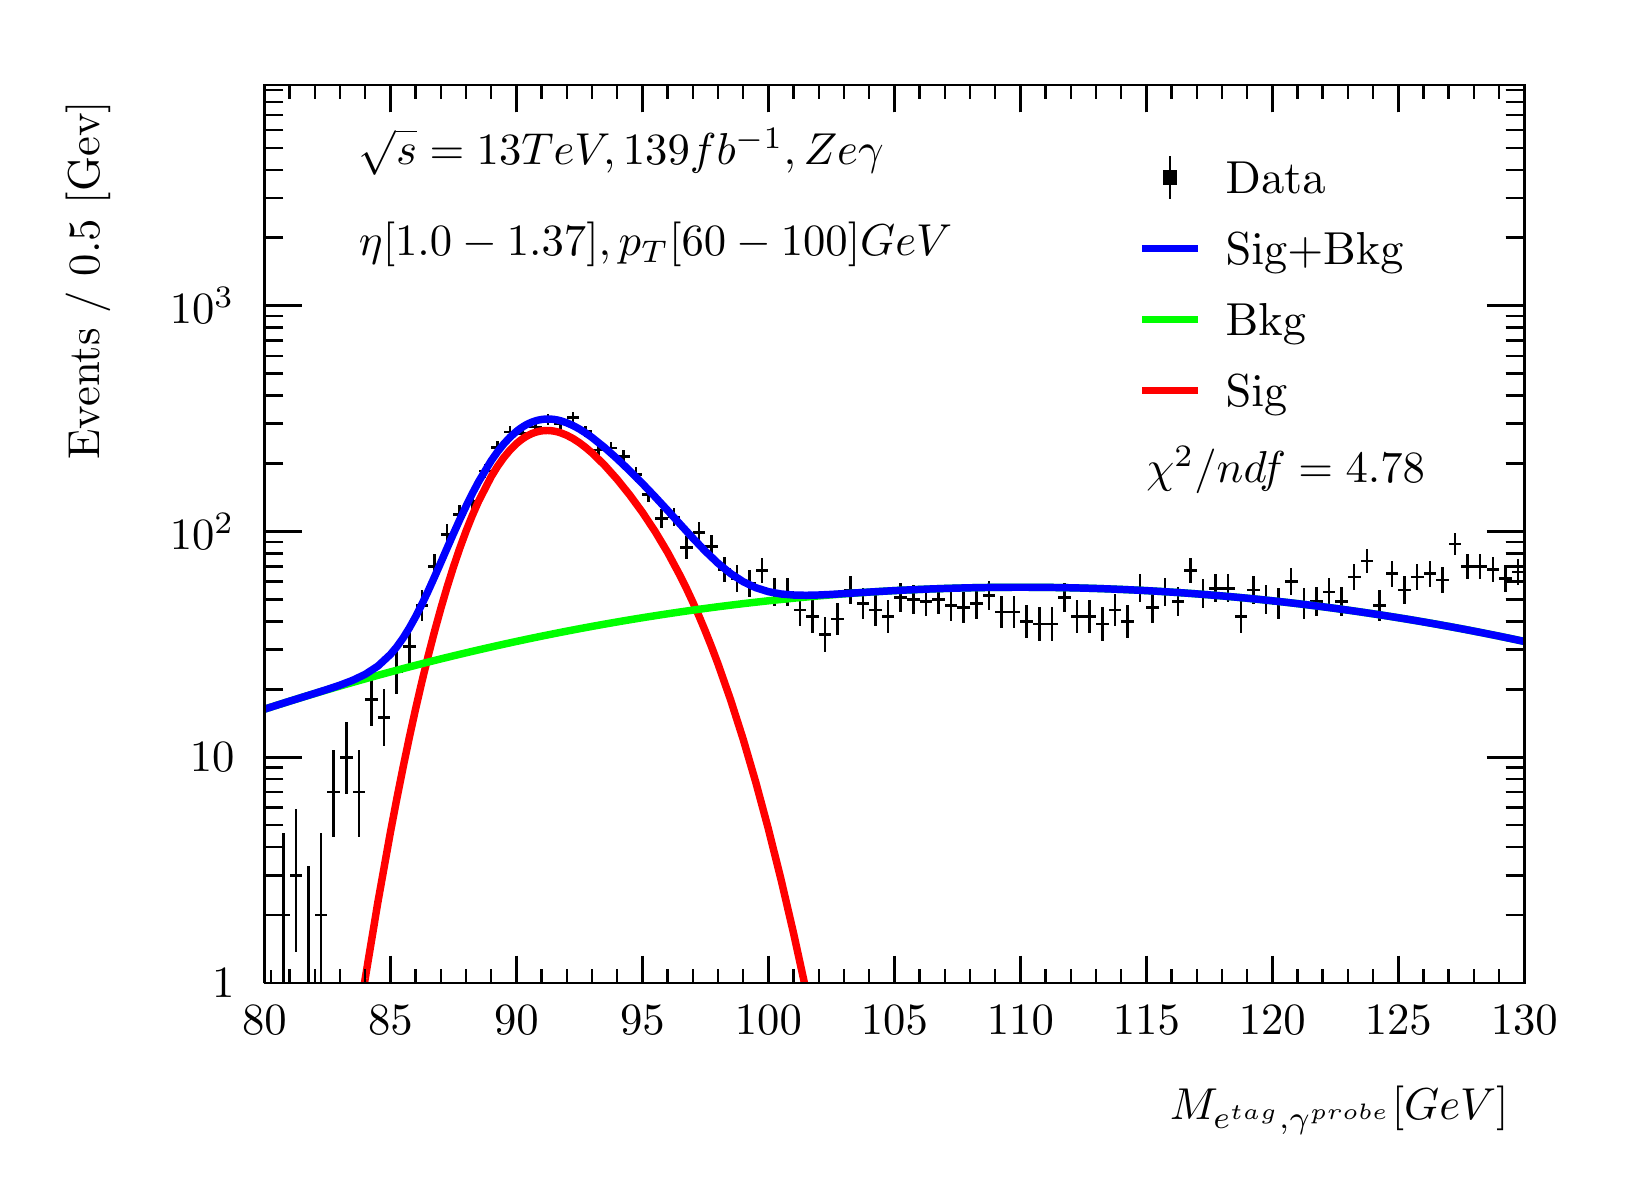
\begin{tikzpicture}
\pgfdeclareplotmark{cross} {
\pgfpathmoveto{\pgfpoint{-0.3\pgfplotmarksize}{\pgfplotmarksize}}
\pgfpathlineto{\pgfpoint{+0.3\pgfplotmarksize}{\pgfplotmarksize}}
\pgfpathlineto{\pgfpoint{+0.3\pgfplotmarksize}{0.3\pgfplotmarksize}}
\pgfpathlineto{\pgfpoint{+1\pgfplotmarksize}{0.3\pgfplotmarksize}}
\pgfpathlineto{\pgfpoint{+1\pgfplotmarksize}{-0.3\pgfplotmarksize}}
\pgfpathlineto{\pgfpoint{+0.3\pgfplotmarksize}{-0.3\pgfplotmarksize}}
\pgfpathlineto{\pgfpoint{+0.3\pgfplotmarksize}{-1.\pgfplotmarksize}}
\pgfpathlineto{\pgfpoint{-0.3\pgfplotmarksize}{-1.\pgfplotmarksize}}
\pgfpathlineto{\pgfpoint{-0.3\pgfplotmarksize}{-0.3\pgfplotmarksize}}
\pgfpathlineto{\pgfpoint{-1.\pgfplotmarksize}{-0.3\pgfplotmarksize}}
\pgfpathlineto{\pgfpoint{-1.\pgfplotmarksize}{0.3\pgfplotmarksize}}
\pgfpathlineto{\pgfpoint{-0.3\pgfplotmarksize}{0.3\pgfplotmarksize}}
\pgfpathclose
\pgfusepathqstroke
}
\pgfdeclareplotmark{cross*} {
\pgfpathmoveto{\pgfpoint{-0.3\pgfplotmarksize}{\pgfplotmarksize}}
\pgfpathlineto{\pgfpoint{+0.3\pgfplotmarksize}{\pgfplotmarksize}}
\pgfpathlineto{\pgfpoint{+0.3\pgfplotmarksize}{0.3\pgfplotmarksize}}
\pgfpathlineto{\pgfpoint{+1\pgfplotmarksize}{0.3\pgfplotmarksize}}
\pgfpathlineto{\pgfpoint{+1\pgfplotmarksize}{-0.3\pgfplotmarksize}}
\pgfpathlineto{\pgfpoint{+0.3\pgfplotmarksize}{-0.3\pgfplotmarksize}}
\pgfpathlineto{\pgfpoint{+0.3\pgfplotmarksize}{-1.\pgfplotmarksize}}
\pgfpathlineto{\pgfpoint{-0.3\pgfplotmarksize}{-1.\pgfplotmarksize}}
\pgfpathlineto{\pgfpoint{-0.3\pgfplotmarksize}{-0.3\pgfplotmarksize}}
\pgfpathlineto{\pgfpoint{-1.\pgfplotmarksize}{-0.3\pgfplotmarksize}}
\pgfpathlineto{\pgfpoint{-1.\pgfplotmarksize}{0.3\pgfplotmarksize}}
\pgfpathlineto{\pgfpoint{-0.3\pgfplotmarksize}{0.3\pgfplotmarksize}}
\pgfpathclose
\pgfusepathqfillstroke
}
\pgfdeclareplotmark{newstar} {
\pgfpathmoveto{\pgfqpoint{0pt}{\pgfplotmarksize}}
\pgfpathlineto{\pgfqpointpolar{44}{0.5\pgfplotmarksize}}
\pgfpathlineto{\pgfqpointpolar{18}{\pgfplotmarksize}}
\pgfpathlineto{\pgfqpointpolar{-20}{0.5\pgfplotmarksize}}
\pgfpathlineto{\pgfqpointpolar{-54}{\pgfplotmarksize}}
\pgfpathlineto{\pgfqpointpolar{-90}{0.5\pgfplotmarksize}}
\pgfpathlineto{\pgfqpointpolar{234}{\pgfplotmarksize}}
\pgfpathlineto{\pgfqpointpolar{198}{0.5\pgfplotmarksize}}
\pgfpathlineto{\pgfqpointpolar{162}{\pgfplotmarksize}}
\pgfpathlineto{\pgfqpointpolar{134}{0.5\pgfplotmarksize}}
\pgfpathclose
\pgfusepathqstroke
}
\pgfdeclareplotmark{newstar*} {
\pgfpathmoveto{\pgfqpoint{0pt}{\pgfplotmarksize}}
\pgfpathlineto{\pgfqpointpolar{44}{0.5\pgfplotmarksize}}
\pgfpathlineto{\pgfqpointpolar{18}{\pgfplotmarksize}}
\pgfpathlineto{\pgfqpointpolar{-20}{0.5\pgfplotmarksize}}
\pgfpathlineto{\pgfqpointpolar{-54}{\pgfplotmarksize}}
\pgfpathlineto{\pgfqpointpolar{-90}{0.5\pgfplotmarksize}}
\pgfpathlineto{\pgfqpointpolar{234}{\pgfplotmarksize}}
\pgfpathlineto{\pgfqpointpolar{198}{0.5\pgfplotmarksize}}
\pgfpathlineto{\pgfqpointpolar{162}{\pgfplotmarksize}}
\pgfpathlineto{\pgfqpointpolar{134}{0.5\pgfplotmarksize}}
\pgfpathclose
\pgfusepathqfillstroke
}
\definecolor{c}{rgb}{1,1,1};
\draw [color=c, fill=c] (0,0) rectangle (20,14.4361);
\draw [color=c, fill=c] (3,2.30977) rectangle (19,13.7143);
\definecolor{c}{rgb}{0,0,0};
\draw [c,line width=0.9] (3,2.30977) -- (3,13.7143) -- (19,13.7143) -- (19,2.30977) -- (3,2.30977);
\definecolor{c}{rgb}{1,1,1};
\draw [color=c, fill=c] (3,2.30977) rectangle (19,13.7143);
\definecolor{c}{rgb}{0,0,0};
\draw [c,line width=0.9] (3,2.30977) -- (3,13.7143) -- (19,13.7143) -- (19,2.30977) -- (3,2.30977);
\draw [c,line width=0.9] (3,2.30977) -- (19,2.30977);
\draw [c,line width=0.9] (3,2.65624) -- (3,2.30977);
\draw [c,line width=0.9] (3.32,2.48301) -- (3.32,2.30977);
\draw [c,line width=0.9] (3.64,2.48301) -- (3.64,2.30977);
\draw [c,line width=0.9] (3.96,2.48301) -- (3.96,2.30977);
\draw [c,line width=0.9] (4.28,2.48301) -- (4.28,2.30977);
\draw [c,line width=0.9] (4.6,2.65624) -- (4.6,2.30977);
\draw [c,line width=0.9] (4.92,2.48301) -- (4.92,2.30977);
\draw [c,line width=0.9] (5.24,2.48301) -- (5.24,2.30977);
\draw [c,line width=0.9] (5.56,2.48301) -- (5.56,2.30977);
\draw [c,line width=0.9] (5.88,2.48301) -- (5.88,2.30977);
\draw [c,line width=0.9] (6.2,2.65624) -- (6.2,2.30977);
\draw [c,line width=0.9] (6.52,2.48301) -- (6.52,2.30977);
\draw [c,line width=0.9] (6.84,2.48301) -- (6.84,2.30977);
\draw [c,line width=0.9] (7.16,2.48301) -- (7.16,2.30977);
\draw [c,line width=0.9] (7.48,2.48301) -- (7.48,2.30977);
\draw [c,line width=0.9] (7.8,2.65624) -- (7.8,2.30977);
\draw [c,line width=0.9] (8.12,2.48301) -- (8.12,2.30977);
\draw [c,line width=0.9] (8.44,2.48301) -- (8.44,2.30977);
\draw [c,line width=0.9] (8.76,2.48301) -- (8.76,2.30977);
\draw [c,line width=0.9] (9.08,2.48301) -- (9.08,2.30977);
\draw [c,line width=0.9] (9.4,2.65624) -- (9.4,2.30977);
\draw [c,line width=0.9] (9.72,2.48301) -- (9.72,2.30977);
\draw [c,line width=0.9] (10.04,2.48301) -- (10.04,2.30977);
\draw [c,line width=0.9] (10.36,2.48301) -- (10.36,2.30977);
\draw [c,line width=0.9] (10.68,2.48301) -- (10.68,2.30977);
\draw [c,line width=0.9] (11,2.65624) -- (11,2.30977);
\draw [c,line width=0.9] (11.32,2.48301) -- (11.32,2.30977);
\draw [c,line width=0.9] (11.64,2.48301) -- (11.64,2.30977);
\draw [c,line width=0.9] (11.96,2.48301) -- (11.96,2.30977);
\draw [c,line width=0.9] (12.28,2.48301) -- (12.28,2.30977);
\draw [c,line width=0.9] (12.6,2.65624) -- (12.6,2.30977);
\draw [c,line width=0.9] (12.92,2.48301) -- (12.92,2.30977);
\draw [c,line width=0.9] (13.24,2.48301) -- (13.24,2.30977);
\draw [c,line width=0.9] (13.56,2.48301) -- (13.56,2.30977);
\draw [c,line width=0.9] (13.88,2.48301) -- (13.88,2.30977);
\draw [c,line width=0.9] (14.2,2.65624) -- (14.2,2.30977);
\draw [c,line width=0.9] (14.52,2.48301) -- (14.52,2.30977);
\draw [c,line width=0.9] (14.84,2.48301) -- (14.84,2.30977);
\draw [c,line width=0.9] (15.16,2.48301) -- (15.16,2.30977);
\draw [c,line width=0.9] (15.48,2.48301) -- (15.48,2.30977);
\draw [c,line width=0.9] (15.8,2.65624) -- (15.8,2.30977);
\draw [c,line width=0.9] (16.12,2.48301) -- (16.12,2.30977);
\draw [c,line width=0.9] (16.44,2.48301) -- (16.44,2.30977);
\draw [c,line width=0.9] (16.76,2.48301) -- (16.76,2.30977);
\draw [c,line width=0.9] (17.08,2.48301) -- (17.08,2.30977);
\draw [c,line width=0.9] (17.4,2.65624) -- (17.4,2.30977);
\draw [c,line width=0.9] (17.72,2.48301) -- (17.72,2.30977);
\draw [c,line width=0.9] (18.04,2.48301) -- (18.04,2.30977);
\draw [c,line width=0.9] (18.36,2.48301) -- (18.36,2.30977);
\draw [c,line width=0.9] (18.68,2.48301) -- (18.68,2.30977);
\draw [c,line width=0.9] (19,2.65624) -- (19,2.30977);
\draw [anchor=base] (3,1.66015) node[scale=1.61424, color=c, rotate=0]{80};
\draw [anchor=base] (4.6,1.66015) node[scale=1.61424, color=c, rotate=0]{85};
\draw [anchor=base] (6.2,1.66015) node[scale=1.61424, color=c, rotate=0]{90};
\draw [anchor=base] (7.8,1.66015) node[scale=1.61424, color=c, rotate=0]{95};
\draw [anchor=base] (9.4,1.66015) node[scale=1.61424, color=c, rotate=0]{100};
\draw [anchor=base] (11,1.66015) node[scale=1.61424, color=c, rotate=0]{105};
\draw [anchor=base] (12.6,1.66015) node[scale=1.61424, color=c, rotate=0]{110};
\draw [anchor=base] (14.2,1.66015) node[scale=1.61424, color=c, rotate=0]{115};
\draw [anchor=base] (15.8,1.66015) node[scale=1.61424, color=c, rotate=0]{120};
\draw [anchor=base] (17.4,1.66015) node[scale=1.61424, color=c, rotate=0]{125};
\draw [anchor=base] (19,1.66015) node[scale=1.61424, color=c, rotate=0]{130};
\draw [anchor= east] (19,0.692932) node[scale=1.61424, color=c, rotate=0]{$M_{e^{tag}, \gamma^{probe}}  [GeV]$};
\draw [c,line width=0.9] (3,13.7143) -- (19,13.7143);
\draw [c,line width=0.9] (3,13.3678) -- (3,13.7143);
\draw [c,line width=0.9] (3.32,13.5411) -- (3.32,13.7143);
\draw [c,line width=0.9] (3.64,13.5411) -- (3.64,13.7143);
\draw [c,line width=0.9] (3.96,13.5411) -- (3.96,13.7143);
\draw [c,line width=0.9] (4.28,13.5411) -- (4.28,13.7143);
\draw [c,line width=0.9] (4.6,13.3678) -- (4.6,13.7143);
\draw [c,line width=0.9] (4.92,13.5411) -- (4.92,13.7143);
\draw [c,line width=0.9] (5.24,13.5411) -- (5.24,13.7143);
\draw [c,line width=0.9] (5.56,13.5411) -- (5.56,13.7143);
\draw [c,line width=0.9] (5.88,13.5411) -- (5.88,13.7143);
\draw [c,line width=0.9] (6.2,13.3678) -- (6.2,13.7143);
\draw [c,line width=0.9] (6.52,13.5411) -- (6.52,13.7143);
\draw [c,line width=0.9] (6.84,13.5411) -- (6.84,13.7143);
\draw [c,line width=0.9] (7.16,13.5411) -- (7.16,13.7143);
\draw [c,line width=0.9] (7.48,13.5411) -- (7.48,13.7143);
\draw [c,line width=0.9] (7.8,13.3678) -- (7.8,13.7143);
\draw [c,line width=0.9] (8.12,13.5411) -- (8.12,13.7143);
\draw [c,line width=0.9] (8.44,13.5411) -- (8.44,13.7143);
\draw [c,line width=0.9] (8.76,13.5411) -- (8.76,13.7143);
\draw [c,line width=0.9] (9.08,13.5411) -- (9.08,13.7143);
\draw [c,line width=0.9] (9.4,13.3678) -- (9.4,13.7143);
\draw [c,line width=0.9] (9.72,13.5411) -- (9.72,13.7143);
\draw [c,line width=0.9] (10.04,13.5411) -- (10.04,13.7143);
\draw [c,line width=0.9] (10.36,13.5411) -- (10.36,13.7143);
\draw [c,line width=0.9] (10.68,13.5411) -- (10.68,13.7143);
\draw [c,line width=0.9] (11,13.3678) -- (11,13.7143);
\draw [c,line width=0.9] (11.32,13.5411) -- (11.32,13.7143);
\draw [c,line width=0.9] (11.64,13.5411) -- (11.64,13.7143);
\draw [c,line width=0.9] (11.96,13.5411) -- (11.96,13.7143);
\draw [c,line width=0.9] (12.28,13.5411) -- (12.28,13.7143);
\draw [c,line width=0.9] (12.6,13.3678) -- (12.6,13.7143);
\draw [c,line width=0.9] (12.92,13.5411) -- (12.92,13.7143);
\draw [c,line width=0.9] (13.24,13.5411) -- (13.24,13.7143);
\draw [c,line width=0.9] (13.56,13.5411) -- (13.56,13.7143);
\draw [c,line width=0.9] (13.88,13.5411) -- (13.88,13.7143);
\draw [c,line width=0.9] (14.2,13.3678) -- (14.2,13.7143);
\draw [c,line width=0.9] (14.52,13.5411) -- (14.52,13.7143);
\draw [c,line width=0.9] (14.84,13.5411) -- (14.84,13.7143);
\draw [c,line width=0.9] (15.16,13.5411) -- (15.16,13.7143);
\draw [c,line width=0.9] (15.48,13.5411) -- (15.48,13.7143);
\draw [c,line width=0.9] (15.8,13.3678) -- (15.8,13.7143);
\draw [c,line width=0.9] (16.12,13.5411) -- (16.12,13.7143);
\draw [c,line width=0.9] (16.44,13.5411) -- (16.44,13.7143);
\draw [c,line width=0.9] (16.76,13.5411) -- (16.76,13.7143);
\draw [c,line width=0.9] (17.08,13.5411) -- (17.08,13.7143);
\draw [c,line width=0.9] (17.4,13.3678) -- (17.4,13.7143);
\draw [c,line width=0.9] (17.72,13.5411) -- (17.72,13.7143);
\draw [c,line width=0.9] (18.04,13.5411) -- (18.04,13.7143);
\draw [c,line width=0.9] (18.36,13.5411) -- (18.36,13.7143);
\draw [c,line width=0.9] (18.68,13.5411) -- (18.68,13.7143);
\draw [c,line width=0.9] (19,13.3678) -- (19,13.7143);
\draw [c,line width=0.9] (3,2.30977) -- (3,13.7143);
\draw [c,line width=0.9] (3.474,2.30978) -- (3,2.30978);
\draw [anchor= east] (2.82,2.30978) node[scale=1.61424, color=c, rotate=0]{1};
\draw [c,line width=0.9] (3.237,3.17298) -- (3,3.17298);
\draw [c,line width=0.9] (3.237,3.67792) -- (3,3.67792);
\draw [c,line width=0.9] (3.237,4.03618) -- (3,4.03618);
\draw [c,line width=0.9] (3.237,4.31407) -- (3,4.31407);
\draw [c,line width=0.9] (3.237,4.54112) -- (3,4.54112);
\draw [c,line width=0.9] (3.237,4.73309) -- (3,4.73309);
\draw [c,line width=0.9] (3.237,4.89938) -- (3,4.89938);
\draw [c,line width=0.9] (3.237,5.04606) -- (3,5.04606);
\draw [c,line width=0.9] (3.474,5.17727) -- (3,5.17727);
\draw [anchor= east] (2.82,5.17727) node[scale=1.61424, color=c, rotate=0]{10};
\draw [c,line width=0.9] (3.237,6.04047) -- (3,6.04047);
\draw [c,line width=0.9] (3.237,6.54541) -- (3,6.54541);
\draw [c,line width=0.9] (3.237,6.90367) -- (3,6.90367);
\draw [c,line width=0.9] (3.237,7.18156) -- (3,7.18156);
\draw [c,line width=0.9] (3.237,7.40861) -- (3,7.40861);
\draw [c,line width=0.9] (3.237,7.60058) -- (3,7.60058);
\draw [c,line width=0.9] (3.237,7.76687) -- (3,7.76687);
\draw [c,line width=0.9] (3.237,7.91355) -- (3,7.91355);
\draw [c,line width=0.9] (3.474,8.04476) -- (3,8.04476);
\draw [anchor= east] (2.82,8.04476) node[scale=1.61424, color=c, rotate=0]{$10^{2}$};
\draw [c,line width=0.9] (3.237,8.90796) -- (3,8.90796);
\draw [c,line width=0.9] (3.237,9.4129) -- (3,9.4129);
\draw [c,line width=0.9] (3.237,9.77116) -- (3,9.77116);
\draw [c,line width=0.9] (3.237,10.049) -- (3,10.049);
\draw [c,line width=0.9] (3.237,10.2761) -- (3,10.2761);
\draw [c,line width=0.9] (3.237,10.4681) -- (3,10.4681);
\draw [c,line width=0.9] (3.237,10.6344) -- (3,10.6344);
\draw [c,line width=0.9] (3.237,10.781) -- (3,10.781);
\draw [c,line width=0.9] (3.474,10.9122) -- (3,10.9122);
\draw [anchor= east] (2.82,10.9122) node[scale=1.61424, color=c, rotate=0]{$10^{3}$};
\draw [c,line width=0.9] (3.237,11.7754) -- (3,11.7754);
\draw [c,line width=0.9] (3.237,12.2804) -- (3,12.2804);
\draw [c,line width=0.9] (3.237,12.6386) -- (3,12.6386);
\draw [c,line width=0.9] (3.237,12.9165) -- (3,12.9165);
\draw [c,line width=0.9] (3.237,13.1436) -- (3,13.1436);
\draw [c,line width=0.9] (3.237,13.3356) -- (3,13.3356);
\draw [c,line width=0.9] (3.237,13.5018) -- (3,13.5018);
\draw [c,line width=0.9] (3.237,13.6485) -- (3,13.6485);
\draw [anchor= east] (0.76,13.7143) node[scale=1.61424, color=c, rotate=90]{Events / 0.5 [Gev]};
\draw [c,line width=0.9] (19,2.30977) -- (19,13.7143);
\draw [c,line width=0.9] (18.526,2.30978) -- (19,2.30978);
\draw [c,line width=0.9] (18.763,3.17298) -- (19,3.17298);
\draw [c,line width=0.9] (18.763,3.67792) -- (19,3.67792);
\draw [c,line width=0.9] (18.763,4.03618) -- (19,4.03618);
\draw [c,line width=0.9] (18.763,4.31407) -- (19,4.31407);
\draw [c,line width=0.9] (18.763,4.54112) -- (19,4.54112);
\draw [c,line width=0.9] (18.763,4.73309) -- (19,4.73309);
\draw [c,line width=0.9] (18.763,4.89938) -- (19,4.89938);
\draw [c,line width=0.9] (18.763,5.04606) -- (19,5.04606);
\draw [c,line width=0.9] (18.526,5.17727) -- (19,5.17727);
\draw [c,line width=0.9] (18.763,6.04047) -- (19,6.04047);
\draw [c,line width=0.9] (18.763,6.54541) -- (19,6.54541);
\draw [c,line width=0.9] (18.763,6.90367) -- (19,6.90367);
\draw [c,line width=0.9] (18.763,7.18156) -- (19,7.18156);
\draw [c,line width=0.9] (18.763,7.40861) -- (19,7.40861);
\draw [c,line width=0.9] (18.763,7.60058) -- (19,7.60058);
\draw [c,line width=0.9] (18.763,7.76687) -- (19,7.76687);
\draw [c,line width=0.9] (18.763,7.91355) -- (19,7.91355);
\draw [c,line width=0.9] (18.526,8.04476) -- (19,8.04476);
\draw [c,line width=0.9] (18.763,8.90796) -- (19,8.90796);
\draw [c,line width=0.9] (18.763,9.4129) -- (19,9.4129);
\draw [c,line width=0.9] (18.763,9.77116) -- (19,9.77116);
\draw [c,line width=0.9] (18.763,10.049) -- (19,10.049);
\draw [c,line width=0.9] (18.763,10.2761) -- (19,10.2761);
\draw [c,line width=0.9] (18.763,10.4681) -- (19,10.4681);
\draw [c,line width=0.9] (18.763,10.6344) -- (19,10.6344);
\draw [c,line width=0.9] (18.763,10.781) -- (19,10.781);
\draw [c,line width=0.9] (18.526,10.9122) -- (19,10.9122);
\draw [c,line width=0.9] (18.763,11.7754) -- (19,11.7754);
\draw [c,line width=0.9] (18.763,12.2804) -- (19,12.2804);
\draw [c,line width=0.9] (18.763,12.6386) -- (19,12.6386);
\draw [c,line width=0.9] (18.763,12.9165) -- (19,12.9165);
\draw [c,line width=0.9] (18.763,13.1436) -- (19,13.1436);
\draw [c,line width=0.9] (18.763,13.3356) -- (19,13.3356);
\draw [c,line width=0.9] (18.763,13.5018) -- (19,13.5018);
\draw [c,line width=0.9] (18.763,13.6485) -- (19,13.6485);
\draw [c,line width=0.9] (3.08,2.30977) -- (3,2.30977);
\draw [c,line width=0.9] (3,2.30977) -- (3,2.30977);
\draw [c,line width=0.9] (3.08,2.30977) -- (3.16,2.30977);
\draw [c,line width=0.9] (3.16,2.30977) -- (3.16,2.30977);
\draw [c,line width=0.9] (3.08,2.30977) -- (3.08,2.48152);
\draw [c,line width=0.9] (3.08,2.48152) -- (3.08,2.48152);
\draw [c,line width=0.9] (3.24,3.17298) -- (3.16,3.17298);
\draw [c,line width=0.9] (3.16,3.17298) -- (3.16,3.17298);
\draw [c,line width=0.9] (3.24,3.17298) -- (3.32,3.17298);
\draw [c,line width=0.9] (3.32,3.17298) -- (3.32,3.17298);
\draw [c,line width=0.9] (3.24,3.17298) -- (3.24,4.22043);
\draw [c,line width=0.9] (3.24,4.22043) -- (3.24,4.22043);
\draw [c,line width=0.9] (3.24,3.17298) -- (3.24,2.30977);
\draw [c,line width=0.9] (3.24,2.30977) -- (3.24,2.30977);
\draw [c,line width=0.9] (3.4,3.67792) -- (3.32,3.67792);
\draw [c,line width=0.9] (3.32,3.67792) -- (3.32,3.67792);
\draw [c,line width=0.9] (3.4,3.67792) -- (3.48,3.67792);
\draw [c,line width=0.9] (3.48,3.67792) -- (3.48,3.67792);
\draw [c,line width=0.9] (3.4,3.67792) -- (3.4,4.52402);
\draw [c,line width=0.9] (3.4,4.52402) -- (3.4,4.52402);
\draw [c,line width=0.9] (3.4,3.67792) -- (3.4,2.69936);
\draw [c,line width=0.9] (3.4,2.69936) -- (3.4,2.69936);
\draw [c,line width=0.9] (3.56,2.30977) -- (3.48,2.30977);
\draw [c,line width=0.9] (3.48,2.30977) -- (3.48,2.30977);
\draw [c,line width=0.9] (3.56,2.30977) -- (3.64,2.30977);
\draw [c,line width=0.9] (3.64,2.30977) -- (3.64,2.30977);
\draw [c,line width=0.9] (3.56,2.30977) -- (3.56,3.79643);
\draw [c,line width=0.9] (3.56,3.79643) -- (3.56,3.79643);
\draw [c,line width=0.9] (3.72,3.17298) -- (3.64,3.17298);
\draw [c,line width=0.9] (3.64,3.17298) -- (3.64,3.17298);
\draw [c,line width=0.9] (3.72,3.17298) -- (3.8,3.17298);
\draw [c,line width=0.9] (3.8,3.17298) -- (3.8,3.17298);
\draw [c,line width=0.9] (3.72,3.17298) -- (3.72,4.22043);
\draw [c,line width=0.9] (3.72,4.22043) -- (3.72,4.22043);
\draw [c,line width=0.9] (3.72,3.17298) -- (3.72,2.30977);
\draw [c,line width=0.9] (3.72,2.30977) -- (3.72,2.30977);
\draw [c,line width=0.9] (3.88,4.73309) -- (3.8,4.73309);
\draw [c,line width=0.9] (3.8,4.73309) -- (3.8,4.73309);
\draw [c,line width=0.9] (3.88,4.73309) -- (3.96,4.73309);
\draw [c,line width=0.9] (3.96,4.73309) -- (3.96,4.73309);
\draw [c,line width=0.9] (3.88,4.73309) -- (3.88,5.26968);
\draw [c,line width=0.9] (3.88,5.26968) -- (3.88,5.26968);
\draw [c,line width=0.9] (3.88,4.73309) -- (3.88,4.1601);
\draw [c,line width=0.9] (3.88,4.1601) -- (3.88,4.1601);
\draw [c,line width=0.9] (4.04,5.17727) -- (3.96,5.17727);
\draw [c,line width=0.9] (3.96,5.17727) -- (3.96,5.17727);
\draw [c,line width=0.9] (4.04,5.17727) -- (4.12,5.17727);
\draw [c,line width=0.9] (4.12,5.17727) -- (4.12,5.17727);
\draw [c,line width=0.9] (4.04,5.17727) -- (4.04,5.61981);
\draw [c,line width=0.9] (4.04,5.61981) -- (4.04,5.61981);
\draw [c,line width=0.9] (4.04,5.17727) -- (4.04,4.7136);
\draw [c,line width=0.9] (4.04,4.7136) -- (4.04,4.7136);
\draw [c,line width=0.9] (4.2,4.73309) -- (4.12,4.73309);
\draw [c,line width=0.9] (4.12,4.73309) -- (4.12,4.73309);
\draw [c,line width=0.9] (4.2,4.73309) -- (4.28,4.73309);
\draw [c,line width=0.9] (4.28,4.73309) -- (4.28,4.73309);
\draw [c,line width=0.9] (4.2,4.73309) -- (4.2,5.26968);
\draw [c,line width=0.9] (4.2,5.26968) -- (4.2,5.26968);
\draw [c,line width=0.9] (4.2,4.73309) -- (4.2,4.1601);
\draw [c,line width=0.9] (4.2,4.1601) -- (4.2,4.1601);
\draw [c,line width=0.9] (4.36,5.90926) -- (4.28,5.90926);
\draw [c,line width=0.9] (4.28,5.90926) -- (4.28,5.90926);
\draw [c,line width=0.9] (4.36,5.90926) -- (4.44,5.90926);
\draw [c,line width=0.9] (4.44,5.90926) -- (4.44,5.90926);
\draw [c,line width=0.9] (4.36,5.90926) -- (4.36,6.23178);
\draw [c,line width=0.9] (4.36,6.23178) -- (4.36,6.23178);
\draw [c,line width=0.9] (4.36,5.90926) -- (4.36,5.57811);
\draw [c,line width=0.9] (4.36,5.57811) -- (4.36,5.57811);
\draw [c,line width=0.9] (4.52,5.68221) -- (4.44,5.68221);
\draw [c,line width=0.9] (4.44,5.68221) -- (4.44,5.68221);
\draw [c,line width=0.9] (4.52,5.68221) -- (4.6,5.68221);
\draw [c,line width=0.9] (4.6,5.68221) -- (4.6,5.68221);
\draw [c,line width=0.9] (4.52,5.68221) -- (4.52,6.03789);
\draw [c,line width=0.9] (4.52,6.03789) -- (4.52,6.03789);
\draw [c,line width=0.9] (4.52,5.68221) -- (4.52,5.31513);
\draw [c,line width=0.9] (4.52,5.31513) -- (4.52,5.31513);
\draw [c,line width=0.9] (4.68,6.26752) -- (4.6,6.26752);
\draw [c,line width=0.9] (4.6,6.26752) -- (4.6,6.26752);
\draw [c,line width=0.9] (4.68,6.26752) -- (4.76,6.26752);
\draw [c,line width=0.9] (4.76,6.26752) -- (4.76,6.26752);
\draw [c,line width=0.9] (4.68,6.26752) -- (4.68,6.54403);
\draw [c,line width=0.9] (4.68,6.54403) -- (4.68,6.54403);
\draw [c,line width=0.9] (4.68,6.26752) -- (4.68,5.98543);
\draw [c,line width=0.9] (4.68,5.98543) -- (4.68,5.98543);
\draw [c,line width=0.9] (4.84,6.58624) -- (4.76,6.58624);
\draw [c,line width=0.9] (4.76,6.58624) -- (4.76,6.58624);
\draw [c,line width=0.9] (4.84,6.58624) -- (4.92,6.58624);
\draw [c,line width=0.9] (4.92,6.58624) -- (4.92,6.58624);
\draw [c,line width=0.9] (4.84,6.58624) -- (4.84,6.82752);
\draw [c,line width=0.9] (4.84,6.82752) -- (4.84,6.82752);
\draw [c,line width=0.9] (4.84,6.58624) -- (4.84,6.34118);
\draw [c,line width=0.9] (4.84,6.34118) -- (4.84,6.34118);
\draw [c,line width=0.9] (5,7.1045) -- (4.92,7.1045);
\draw [c,line width=0.9] (4.92,7.1045) -- (4.92,7.1045);
\draw [c,line width=0.9] (5,7.1045) -- (5.08,7.1045);
\draw [c,line width=0.9] (5.08,7.1045) -- (5.08,7.1045);
\draw [c,line width=0.9] (5,7.1045) -- (5,7.29808);
\draw [c,line width=0.9] (5,7.29808) -- (5,7.29808);
\draw [c,line width=0.9] (5,7.1045) -- (5,6.90891);
\draw [c,line width=0.9] (5,6.90891) -- (5,6.90891);
\draw [c,line width=0.9] (5.16,7.60058) -- (5.08,7.60058);
\draw [c,line width=0.9] (5.08,7.60058) -- (5.08,7.60058);
\draw [c,line width=0.9] (5.16,7.60058) -- (5.24,7.60058);
\draw [c,line width=0.9] (5.24,7.60058) -- (5.24,7.60058);
\draw [c,line width=0.9] (5.16,7.60058) -- (5.16,7.75759);
\draw [c,line width=0.9] (5.16,7.75759) -- (5.16,7.75759);
\draw [c,line width=0.9] (5.16,7.60058) -- (5.16,7.44246);
\draw [c,line width=0.9] (5.16,7.44246) -- (5.16,7.44246);
\draw [c,line width=0.9] (5.32,8.00682) -- (5.24,8.00682);
\draw [c,line width=0.9] (5.24,8.00682) -- (5.24,8.00682);
\draw [c,line width=0.9] (5.32,8.00682) -- (5.4,8.00682);
\draw [c,line width=0.9] (5.4,8.00682) -- (5.4,8.00682);
\draw [c,line width=0.9] (5.32,8.00682) -- (5.32,8.13925);
\draw [c,line width=0.9] (5.32,8.13925) -- (5.32,8.13925);
\draw [c,line width=0.9] (5.32,8.00682) -- (5.32,7.87373);
\draw [c,line width=0.9] (5.32,7.87373) -- (5.32,7.87373);
\draw [c,line width=0.9] (5.48,8.26139) -- (5.4,8.26139);
\draw [c,line width=0.9] (5.4,8.26139) -- (5.4,8.26139);
\draw [c,line width=0.9] (5.48,8.26139) -- (5.56,8.26139);
\draw [c,line width=0.9] (5.56,8.26139) -- (5.56,8.26139);
\draw [c,line width=0.9] (5.48,8.26139) -- (5.48,8.37551);
\draw [c,line width=0.9] (5.48,8.37551) -- (5.48,8.37551);
\draw [c,line width=0.9] (5.48,8.26139) -- (5.48,8.14727);
\draw [c,line width=0.9] (5.48,8.14727) -- (5.48,8.14727);
\draw [c,line width=0.9] (5.64,8.42768) -- (5.56,8.42768);
\draw [c,line width=0.9] (5.56,8.42768) -- (5.56,8.42768);
\draw [c,line width=0.9] (5.64,8.42768) -- (5.72,8.42768);
\draw [c,line width=0.9] (5.72,8.42768) -- (5.72,8.42768);
\draw [c,line width=0.9] (5.64,8.42768) -- (5.64,8.53443);
\draw [c,line width=0.9] (5.64,8.53443) -- (5.64,8.53443);
\draw [c,line width=0.9] (5.64,8.42768) -- (5.64,8.32092);
\draw [c,line width=0.9] (5.64,8.32092) -- (5.64,8.32092);
\draw [c,line width=0.9] (5.8,8.81087) -- (5.72,8.81087);
\draw [c,line width=0.9] (5.72,8.81087) -- (5.72,8.81087);
\draw [c,line width=0.9] (5.8,8.81087) -- (5.88,8.81087);
\draw [c,line width=0.9] (5.88,8.81087) -- (5.88,8.81087);
\draw [c,line width=0.9] (5.8,8.81087) -- (5.8,8.90241);
\draw [c,line width=0.9] (5.8,8.90241) -- (5.8,8.90241);
\draw [c,line width=0.9] (5.8,8.81087) -- (5.8,8.71933);
\draw [c,line width=0.9] (5.8,8.71933) -- (5.8,8.71933);
\draw [c,line width=0.9] (5.96,9.11408) -- (5.88,9.11408);
\draw [c,line width=0.9] (5.88,9.11408) -- (5.88,9.11408);
\draw [c,line width=0.9] (5.96,9.11408) -- (6.04,9.11408);
\draw [c,line width=0.9] (6.04,9.11408) -- (6.04,9.11408);
\draw [c,line width=0.9] (5.96,9.11408) -- (5.96,9.19513);
\draw [c,line width=0.9] (5.96,9.19513) -- (5.96,9.19513);
\draw [c,line width=0.9] (5.96,9.11408) -- (5.96,9.03303);
\draw [c,line width=0.9] (5.96,9.03303) -- (5.96,9.03303);
\draw [c,line width=0.9] (6.12,9.30906) -- (6.04,9.30906);
\draw [c,line width=0.9] (6.04,9.30906) -- (6.04,9.30906);
\draw [c,line width=0.9] (6.12,9.30906) -- (6.2,9.30906);
\draw [c,line width=0.9] (6.2,9.30906) -- (6.2,9.30906);
\draw [c,line width=0.9] (6.12,9.30906) -- (6.12,9.38401);
\draw [c,line width=0.9] (6.12,9.38401) -- (6.12,9.38401);
\draw [c,line width=0.9] (6.12,9.30906) -- (6.12,9.23411);
\draw [c,line width=0.9] (6.12,9.23411) -- (6.12,9.23411);
\draw [c,line width=0.9] (6.28,9.29088) -- (6.2,9.29088);
\draw [c,line width=0.9] (6.2,9.29088) -- (6.2,9.29088);
\draw [c,line width=0.9] (6.28,9.29088) -- (6.36,9.29088);
\draw [c,line width=0.9] (6.36,9.29088) -- (6.36,9.29088);
\draw [c,line width=0.9] (6.28,9.29088) -- (6.28,9.36638);
\draw [c,line width=0.9] (6.28,9.36638) -- (6.28,9.36638);
\draw [c,line width=0.9] (6.28,9.29088) -- (6.28,9.21538);
\draw [c,line width=0.9] (6.28,9.21538) -- (6.28,9.21538);
\draw [c,line width=0.9] (6.44,9.37068) -- (6.36,9.37068);
\draw [c,line width=0.9] (6.36,9.37068) -- (6.36,9.37068);
\draw [c,line width=0.9] (6.44,9.37068) -- (6.52,9.37068);
\draw [c,line width=0.9] (6.52,9.37068) -- (6.52,9.37068);
\draw [c,line width=0.9] (6.44,9.37068) -- (6.44,9.4438);
\draw [c,line width=0.9] (6.44,9.4438) -- (6.44,9.4438);
\draw [c,line width=0.9] (6.44,9.37068) -- (6.44,9.29756);
\draw [c,line width=0.9] (6.44,9.29756) -- (6.44,9.29756);
\draw [c,line width=0.9] (6.6,9.46572) -- (6.52,9.46572);
\draw [c,line width=0.9] (6.52,9.46572) -- (6.52,9.46572);
\draw [c,line width=0.9] (6.6,9.46572) -- (6.68,9.46572);
\draw [c,line width=0.9] (6.68,9.46572) -- (6.68,9.46572);
\draw [c,line width=0.9] (6.6,9.46572) -- (6.6,9.53611);
\draw [c,line width=0.9] (6.6,9.53611) -- (6.6,9.53611);
\draw [c,line width=0.9] (6.6,9.46572) -- (6.6,9.39534);
\draw [c,line width=0.9] (6.6,9.39534) -- (6.6,9.39534);
\draw [c,line width=0.9] (6.76,9.4129) -- (6.68,9.4129);
\draw [c,line width=0.9] (6.68,9.4129) -- (6.68,9.4129);
\draw [c,line width=0.9] (6.76,9.4129) -- (6.84,9.4129);
\draw [c,line width=0.9] (6.84,9.4129) -- (6.84,9.4129);
\draw [c,line width=0.9] (6.76,9.4129) -- (6.76,9.48479);
\draw [c,line width=0.9] (6.76,9.48479) -- (6.76,9.48479);
\draw [c,line width=0.9] (6.76,9.4129) -- (6.76,9.34101);
\draw [c,line width=0.9] (6.76,9.34101) -- (6.76,9.34101);
\draw [c,line width=0.9] (6.92,9.48937) -- (6.84,9.48937);
\draw [c,line width=0.9] (6.84,9.48937) -- (6.84,9.48937);
\draw [c,line width=0.9] (6.92,9.48937) -- (7,9.48937);
\draw [c,line width=0.9] (7,9.48937) -- (7,9.48937);
\draw [c,line width=0.9] (6.92,9.48937) -- (6.92,9.55909);
\draw [c,line width=0.9] (6.92,9.55909) -- (6.92,9.55909);
\draw [c,line width=0.9] (6.92,9.48937) -- (6.92,9.41965);
\draw [c,line width=0.9] (6.92,9.41965) -- (6.92,9.41965);
\draw [c,line width=0.9] (7.08,9.31356) -- (7,9.31356);
\draw [c,line width=0.9] (7,9.31356) -- (7,9.31356);
\draw [c,line width=0.9] (7.08,9.31356) -- (7.16,9.31356);
\draw [c,line width=0.9] (7.16,9.31356) -- (7.16,9.31356);
\draw [c,line width=0.9] (7.08,9.31356) -- (7.08,9.38838);
\draw [c,line width=0.9] (7.08,9.38838) -- (7.08,9.38838);
\draw [c,line width=0.9] (7.08,9.31356) -- (7.08,9.23875);
\draw [c,line width=0.9] (7.08,9.23875) -- (7.08,9.23875);
\draw [c,line width=0.9] (7.24,9.07658) -- (7.16,9.07658);
\draw [c,line width=0.9] (7.16,9.07658) -- (7.16,9.07658);
\draw [c,line width=0.9] (7.24,9.07658) -- (7.32,9.07658);
\draw [c,line width=0.9] (7.32,9.07658) -- (7.32,9.07658);
\draw [c,line width=0.9] (7.24,9.07658) -- (7.24,9.15886);
\draw [c,line width=0.9] (7.24,9.15886) -- (7.24,9.15886);
\draw [c,line width=0.9] (7.24,9.07658) -- (7.24,8.9943);
\draw [c,line width=0.9] (7.24,8.9943) -- (7.24,8.9943);
\draw [c,line width=0.9] (7.4,9.10348) -- (7.32,9.10348);
\draw [c,line width=0.9] (7.32,9.10348) -- (7.32,9.10348);
\draw [c,line width=0.9] (7.4,9.10348) -- (7.48,9.10348);
\draw [c,line width=0.9] (7.48,9.10348) -- (7.48,9.10348);
\draw [c,line width=0.9] (7.4,9.10348) -- (7.4,9.18487);
\draw [c,line width=0.9] (7.4,9.18487) -- (7.4,9.18487);
\draw [c,line width=0.9] (7.4,9.10348) -- (7.4,9.02208);
\draw [c,line width=0.9] (7.4,9.02208) -- (7.4,9.02208);
\draw [c,line width=0.9] (7.56,8.99802) -- (7.48,8.99802);
\draw [c,line width=0.9] (7.48,8.99802) -- (7.48,8.99802);
\draw [c,line width=0.9] (7.56,8.99802) -- (7.64,8.99802);
\draw [c,line width=0.9] (7.64,8.99802) -- (7.64,8.99802);
\draw [c,line width=0.9] (7.56,8.99802) -- (7.56,9.08293);
\draw [c,line width=0.9] (7.56,9.08293) -- (7.56,9.08293);
\draw [c,line width=0.9] (7.56,8.99802) -- (7.56,8.91311);
\draw [c,line width=0.9] (7.56,8.91311) -- (7.56,8.91311);
\draw [c,line width=0.9] (7.72,8.76981) -- (7.64,8.76981);
\draw [c,line width=0.9] (7.64,8.76981) -- (7.64,8.76981);
\draw [c,line width=0.9] (7.72,8.76981) -- (7.8,8.76981);
\draw [c,line width=0.9] (7.8,8.76981) -- (7.8,8.76981);
\draw [c,line width=0.9] (7.72,8.76981) -- (7.72,8.86287);
\draw [c,line width=0.9] (7.72,8.86287) -- (7.72,8.86287);
\draw [c,line width=0.9] (7.72,8.76981) -- (7.72,8.67675);
\draw [c,line width=0.9] (7.72,8.67675) -- (7.72,8.67675);
\draw [c,line width=0.9] (7.88,8.51604) -- (7.8,8.51604);
\draw [c,line width=0.9] (7.8,8.51604) -- (7.8,8.51604);
\draw [c,line width=0.9] (7.88,8.51604) -- (7.96,8.51604);
\draw [c,line width=0.9] (7.96,8.51604) -- (7.96,8.51604);
\draw [c,line width=0.9] (7.88,8.51604) -- (7.88,8.61907);
\draw [c,line width=0.9] (7.88,8.61907) -- (7.88,8.61907);
\draw [c,line width=0.9] (7.88,8.51604) -- (7.88,8.413);
\draw [c,line width=0.9] (7.88,8.413) -- (7.88,8.413);
\draw [c,line width=0.9] (8.04,8.20793) -- (7.96,8.20793);
\draw [c,line width=0.9] (7.96,8.20793) -- (7.96,8.20793);
\draw [c,line width=0.9] (8.04,8.20793) -- (8.12,8.20793);
\draw [c,line width=0.9] (8.12,8.20793) -- (8.12,8.20793);
\draw [c,line width=0.9] (8.04,8.20793) -- (8.04,8.32452);
\draw [c,line width=0.9] (8.04,8.32452) -- (8.04,8.32452);
\draw [c,line width=0.9] (8.04,8.20793) -- (8.04,8.09134);
\draw [c,line width=0.9] (8.04,8.09134) -- (8.04,8.09134);
\draw [c,line width=0.9] (8.2,8.22959) -- (8.12,8.22959);
\draw [c,line width=0.9] (8.12,8.22959) -- (8.12,8.22959);
\draw [c,line width=0.9] (8.2,8.22959) -- (8.28,8.22959);
\draw [c,line width=0.9] (8.28,8.22959) -- (8.28,8.22959);
\draw [c,line width=0.9] (8.2,8.22959) -- (8.2,8.34517);
\draw [c,line width=0.9] (8.2,8.34517) -- (8.2,8.34517);
\draw [c,line width=0.9] (8.2,8.22959) -- (8.2,8.114);
\draw [c,line width=0.9] (8.2,8.114) -- (8.2,8.114);
\draw [c,line width=0.9] (8.36,7.84237) -- (8.28,7.84237);
\draw [c,line width=0.9] (8.28,7.84237) -- (8.28,7.84237);
\draw [c,line width=0.9] (8.36,7.84237) -- (8.44,7.84237);
\draw [c,line width=0.9] (8.44,7.84237) -- (8.44,7.84237);
\draw [c,line width=0.9] (8.36,7.84237) -- (8.36,7.98423);
\draw [c,line width=0.9] (8.36,7.98423) -- (8.36,7.98423);
\draw [c,line width=0.9] (8.36,7.84237) -- (8.36,7.69969);
\draw [c,line width=0.9] (8.36,7.69969) -- (8.36,7.69969);
\draw [c,line width=0.9] (8.52,8.03224) -- (8.44,8.03224);
\draw [c,line width=0.9] (8.44,8.03224) -- (8.44,8.03224);
\draw [c,line width=0.9] (8.52,8.03224) -- (8.6,8.03224);
\draw [c,line width=0.9] (8.6,8.03224) -- (8.6,8.03224);
\draw [c,line width=0.9] (8.52,8.03224) -- (8.52,8.16326);
\draw [c,line width=0.9] (8.52,8.16326) -- (8.52,8.16326);
\draw [c,line width=0.9] (8.52,8.03224) -- (8.52,7.90057);
\draw [c,line width=0.9] (8.52,7.90057) -- (8.52,7.90057);
\draw [c,line width=0.9] (8.68,7.85693) -- (8.6,7.85693);
\draw [c,line width=0.9] (8.6,7.85693) -- (8.6,7.85693);
\draw [c,line width=0.9] (8.68,7.85693) -- (8.76,7.85693);
\draw [c,line width=0.9] (8.76,7.85693) -- (8.76,7.85693);
\draw [c,line width=0.9] (8.68,7.85693) -- (8.68,7.99793);
\draw [c,line width=0.9] (8.68,7.99793) -- (8.68,7.99793);
\draw [c,line width=0.9] (8.68,7.85693) -- (8.68,7.71513);
\draw [c,line width=0.9] (8.68,7.71513) -- (8.68,7.71513);
\draw [c,line width=0.9] (8.84,7.56448) -- (8.76,7.56448);
\draw [c,line width=0.9] (8.76,7.56448) -- (8.76,7.56448);
\draw [c,line width=0.9] (8.84,7.56448) -- (8.92,7.56448);
\draw [c,line width=0.9] (8.92,7.56448) -- (8.92,7.56448);
\draw [c,line width=0.9] (8.84,7.56448) -- (8.84,7.7239);
\draw [c,line width=0.9] (8.84,7.7239) -- (8.84,7.7239);
\draw [c,line width=0.9] (8.84,7.56448) -- (8.84,7.40391);
\draw [c,line width=0.9] (8.84,7.40391) -- (8.84,7.40391);
\draw [c,line width=0.9] (9,7.44944) -- (8.92,7.44944);
\draw [c,line width=0.9] (8.92,7.44944) -- (8.92,7.44944);
\draw [c,line width=0.9] (9,7.44944) -- (9.08,7.44944);
\draw [c,line width=0.9] (9.08,7.44944) -- (9.08,7.44944);
\draw [c,line width=0.9] (9,7.44944) -- (9,7.61677);
\draw [c,line width=0.9] (9,7.61677) -- (9,7.61677);
\draw [c,line width=0.9] (9,7.44944) -- (9,7.28079);
\draw [c,line width=0.9] (9,7.28079) -- (9,7.28079);
\draw [c,line width=0.9] (9.16,7.38768) -- (9.08,7.38768);
\draw [c,line width=0.9] (9.08,7.38768) -- (9.08,7.38768);
\draw [c,line width=0.9] (9.16,7.38768) -- (9.24,7.38768);
\draw [c,line width=0.9] (9.24,7.38768) -- (9.24,7.38768);
\draw [c,line width=0.9] (9.16,7.38768) -- (9.16,7.55942);
\draw [c,line width=0.9] (9.16,7.55942) -- (9.16,7.55942);
\draw [c,line width=0.9] (9.16,7.38768) -- (9.16,7.21451);
\draw [c,line width=0.9] (9.16,7.21451) -- (9.16,7.21451);
\draw [c,line width=0.9] (9.32,7.54603) -- (9.24,7.54603);
\draw [c,line width=0.9] (9.24,7.54603) -- (9.24,7.54603);
\draw [c,line width=0.9] (9.32,7.54603) -- (9.4,7.54603);
\draw [c,line width=0.9] (9.4,7.54603) -- (9.4,7.54603);
\draw [c,line width=0.9] (9.32,7.54603) -- (9.32,7.70669);
\draw [c,line width=0.9] (9.32,7.70669) -- (9.32,7.70669);
\draw [c,line width=0.9] (9.32,7.54603) -- (9.32,7.38419);
\draw [c,line width=0.9] (9.32,7.38419) -- (9.32,7.38419);
\draw [c,line width=0.9] (9.48,7.2774) -- (9.4,7.2774);
\draw [c,line width=0.9] (9.4,7.2774) -- (9.4,7.2774);
\draw [c,line width=0.9] (9.48,7.2774) -- (9.56,7.2774);
\draw [c,line width=0.9] (9.56,7.2774) -- (9.56,7.2774);
\draw [c,line width=0.9] (9.48,7.2774) -- (9.48,7.45733);
\draw [c,line width=0.9] (9.48,7.45733) -- (9.48,7.45733);
\draw [c,line width=0.9] (9.48,7.2774) -- (9.48,7.09584);
\draw [c,line width=0.9] (9.48,7.09584) -- (9.48,7.09584);
\draw [c,line width=0.9] (9.64,7.2774) -- (9.56,7.2774);
\draw [c,line width=0.9] (9.56,7.2774) -- (9.56,7.2774);
\draw [c,line width=0.9] (9.64,7.2774) -- (9.72,7.2774);
\draw [c,line width=0.9] (9.72,7.2774) -- (9.72,7.2774);
\draw [c,line width=0.9] (9.64,7.2774) -- (9.64,7.45733);
\draw [c,line width=0.9] (9.64,7.45733) -- (9.64,7.45733);
\draw [c,line width=0.9] (9.64,7.2774) -- (9.64,7.09584);
\draw [c,line width=0.9] (9.64,7.09584) -- (9.64,7.09584);
\draw [c,line width=0.9] (9.8,7.05035) -- (9.72,7.05035);
\draw [c,line width=0.9] (9.72,7.05035) -- (9.72,7.05035);
\draw [c,line width=0.9] (9.8,7.05035) -- (9.88,7.05035);
\draw [c,line width=0.9] (9.88,7.05035) -- (9.88,7.05035);
\draw [c,line width=0.9] (9.8,7.05035) -- (9.8,7.24842);
\draw [c,line width=0.9] (9.8,7.24842) -- (9.8,7.24842);
\draw [c,line width=0.9] (9.8,7.05035) -- (9.8,6.85013);
\draw [c,line width=0.9] (9.8,6.85013) -- (9.8,6.85013);
\draw [c,line width=0.9] (9.96,6.96443) -- (9.88,6.96443);
\draw [c,line width=0.9] (9.88,6.96443) -- (9.88,6.96443);
\draw [c,line width=0.9] (9.96,6.96443) -- (10.04,6.96443);
\draw [c,line width=0.9] (10.04,6.96443) -- (10.04,6.96443);
\draw [c,line width=0.9] (9.96,6.96443) -- (9.96,7.16985);
\draw [c,line width=0.9] (9.96,7.16985) -- (9.96,7.16985);
\draw [c,line width=0.9] (9.96,6.96443) -- (9.96,6.75662);
\draw [c,line width=0.9] (9.96,6.75662) -- (9.96,6.75662);
\draw [c,line width=0.9] (10.12,6.73738) -- (10.04,6.73738);
\draw [c,line width=0.9] (10.04,6.73738) -- (10.04,6.73738);
\draw [c,line width=0.9] (10.12,6.73738) -- (10.2,6.73738);
\draw [c,line width=0.9] (10.2,6.73738) -- (10.2,6.73738);
\draw [c,line width=0.9] (10.12,6.73738) -- (10.12,6.96361);
\draw [c,line width=0.9] (10.12,6.96361) -- (10.12,6.96361);
\draw [c,line width=0.9] (10.12,6.73738) -- (10.12,6.508);
\draw [c,line width=0.9] (10.12,6.508) -- (10.12,6.508);
\draw [c,line width=0.9] (10.28,6.93442) -- (10.2,6.93442);
\draw [c,line width=0.9] (10.2,6.93442) -- (10.2,6.93442);
\draw [c,line width=0.9] (10.28,6.93442) -- (10.36,6.93442);
\draw [c,line width=0.9] (10.36,6.93442) -- (10.36,6.93442);
\draw [c,line width=0.9] (10.28,6.93442) -- (10.28,7.14247);
\draw [c,line width=0.9] (10.28,7.14247) -- (10.28,7.14247);
\draw [c,line width=0.9] (10.28,6.93442) -- (10.28,6.72389);
\draw [c,line width=0.9] (10.28,6.72389) -- (10.28,6.72389);
\draw [c,line width=0.9] (10.44,7.30025) -- (10.36,7.30025);
\draw [c,line width=0.9] (10.36,7.30025) -- (10.36,7.30025);
\draw [c,line width=0.9] (10.44,7.30025) -- (10.52,7.30025);
\draw [c,line width=0.9] (10.52,7.30025) -- (10.52,7.30025);
\draw [c,line width=0.9] (10.44,7.30025) -- (10.44,7.47845);
\draw [c,line width=0.9] (10.44,7.47845) -- (10.44,7.47845);
\draw [c,line width=0.9] (10.44,7.30025) -- (10.44,7.12046);
\draw [c,line width=0.9] (10.44,7.12046) -- (10.44,7.12046);
\draw [c,line width=0.9] (10.6,7.13072) -- (10.52,7.13072);
\draw [c,line width=0.9] (10.52,7.13072) -- (10.52,7.13072);
\draw [c,line width=0.9] (10.6,7.13072) -- (10.68,7.13072);
\draw [c,line width=0.9] (10.68,7.13072) -- (10.68,7.13072);
\draw [c,line width=0.9] (10.6,7.13072) -- (10.6,7.32216);
\draw [c,line width=0.9] (10.6,7.32216) -- (10.6,7.32216);
\draw [c,line width=0.9] (10.6,7.13072) -- (10.6,6.93733);
\draw [c,line width=0.9] (10.6,6.93733) -- (10.6,6.93733);
\draw [c,line width=0.9] (10.76,7.05035) -- (10.68,7.05035);
\draw [c,line width=0.9] (10.68,7.05035) -- (10.68,7.05035);
\draw [c,line width=0.9] (10.76,7.05035) -- (10.84,7.05035);
\draw [c,line width=0.9] (10.84,7.05035) -- (10.84,7.05035);
\draw [c,line width=0.9] (10.76,7.05035) -- (10.76,7.24842);
\draw [c,line width=0.9] (10.76,7.24842) -- (10.76,7.24842);
\draw [c,line width=0.9] (10.76,7.05035) -- (10.76,6.85013);
\draw [c,line width=0.9] (10.76,6.85013) -- (10.76,6.85013);
\draw [c,line width=0.9] (10.92,6.96443) -- (10.84,6.96443);
\draw [c,line width=0.9] (10.84,6.96443) -- (10.84,6.96443);
\draw [c,line width=0.9] (10.92,6.96443) -- (11,6.96443);
\draw [c,line width=0.9] (11,6.96443) -- (11,6.96443);
\draw [c,line width=0.9] (10.92,6.96443) -- (10.92,7.16985);
\draw [c,line width=0.9] (10.92,7.16985) -- (10.92,7.16985);
\draw [c,line width=0.9] (10.92,6.96443) -- (10.92,6.75662);
\draw [c,line width=0.9] (10.92,6.75662) -- (10.92,6.75662);
\draw [c,line width=0.9] (11.08,7.20622) -- (11,7.20622);
\draw [c,line width=0.9] (11,7.20622) -- (11,7.20622);
\draw [c,line width=0.9] (11.08,7.20622) -- (11.16,7.20622);
\draw [c,line width=0.9] (11.16,7.20622) -- (11.16,7.20622);
\draw [c,line width=0.9] (11.08,7.20622) -- (11.08,7.39164);
\draw [c,line width=0.9] (11.08,7.39164) -- (11.08,7.39164);
\draw [c,line width=0.9] (11.08,7.20622) -- (11.08,7.01902);
\draw [c,line width=0.9] (11.08,7.01902) -- (11.08,7.01902);
\draw [c,line width=0.9] (11.24,7.18156) -- (11.16,7.18156);
\draw [c,line width=0.9] (11.16,7.18156) -- (11.16,7.18156);
\draw [c,line width=0.9] (11.24,7.18156) -- (11.32,7.18156);
\draw [c,line width=0.9] (11.32,7.18156) -- (11.32,7.18156);
\draw [c,line width=0.9] (11.24,7.18156) -- (11.24,7.36892);
\draw [c,line width=0.9] (11.24,7.36892) -- (11.24,7.36892);
\draw [c,line width=0.9] (11.24,7.18156) -- (11.24,6.99236);
\draw [c,line width=0.9] (11.24,6.99236) -- (11.24,6.99236);
\draw [c,line width=0.9] (11.4,7.1564) -- (11.32,7.1564);
\draw [c,line width=0.9] (11.32,7.1564) -- (11.32,7.1564);
\draw [c,line width=0.9] (11.4,7.1564) -- (11.48,7.1564);
\draw [c,line width=0.9] (11.48,7.1564) -- (11.48,7.1564);
\draw [c,line width=0.9] (11.4,7.1564) -- (11.4,7.34577);
\draw [c,line width=0.9] (11.4,7.34577) -- (11.4,7.34577);
\draw [c,line width=0.9] (11.4,7.1564) -- (11.4,6.96514);
\draw [c,line width=0.9] (11.4,6.96514) -- (11.4,6.96514);
\draw [c,line width=0.9] (11.56,7.18156) -- (11.48,7.18156);
\draw [c,line width=0.9] (11.48,7.18156) -- (11.48,7.18156);
\draw [c,line width=0.9] (11.56,7.18156) -- (11.64,7.18156);
\draw [c,line width=0.9] (11.64,7.18156) -- (11.64,7.18156);
\draw [c,line width=0.9] (11.56,7.18156) -- (11.56,7.36892);
\draw [c,line width=0.9] (11.56,7.36892) -- (11.56,7.36892);
\draw [c,line width=0.9] (11.56,7.18156) -- (11.56,6.99236);
\draw [c,line width=0.9] (11.56,6.99236) -- (11.56,6.99236);
\draw [c,line width=0.9] (11.72,7.1045) -- (11.64,7.1045);
\draw [c,line width=0.9] (11.64,7.1045) -- (11.64,7.1045);
\draw [c,line width=0.9] (11.72,7.1045) -- (11.8,7.1045);
\draw [c,line width=0.9] (11.8,7.1045) -- (11.8,7.1045);
\draw [c,line width=0.9] (11.72,7.1045) -- (11.72,7.29808);
\draw [c,line width=0.9] (11.72,7.29808) -- (11.72,7.29808);
\draw [c,line width=0.9] (11.72,7.1045) -- (11.72,6.90891);
\draw [c,line width=0.9] (11.72,6.90891) -- (11.72,6.90891);
\draw [c,line width=0.9] (11.88,7.07772) -- (11.8,7.07772);
\draw [c,line width=0.9] (11.8,7.07772) -- (11.8,7.07772);
\draw [c,line width=0.9] (11.88,7.07772) -- (11.96,7.07772);
\draw [c,line width=0.9] (11.96,7.07772) -- (11.96,7.07772);
\draw [c,line width=0.9] (11.88,7.07772) -- (11.88,7.27351);
\draw [c,line width=0.9] (11.88,7.27351) -- (11.88,7.27351);
\draw [c,line width=0.9] (11.88,7.07772) -- (11.88,6.87985);
\draw [c,line width=0.9] (11.88,6.87985) -- (11.88,6.87985);
\draw [c,line width=0.9] (12.04,7.13072) -- (11.96,7.13072);
\draw [c,line width=0.9] (11.96,7.13072) -- (11.96,7.13072);
\draw [c,line width=0.9] (12.04,7.13072) -- (12.12,7.13072);
\draw [c,line width=0.9] (12.12,7.13072) -- (12.12,7.13072);
\draw [c,line width=0.9] (12.04,7.13072) -- (12.04,7.32216);
\draw [c,line width=0.9] (12.04,7.32216) -- (12.04,7.32216);
\draw [c,line width=0.9] (12.04,7.13072) -- (12.04,6.93733);
\draw [c,line width=0.9] (12.04,6.93733) -- (12.04,6.93733);
\draw [c,line width=0.9] (12.2,7.2304) -- (12.12,7.2304);
\draw [c,line width=0.9] (12.12,7.2304) -- (12.12,7.2304);
\draw [c,line width=0.9] (12.2,7.2304) -- (12.28,7.2304);
\draw [c,line width=0.9] (12.28,7.2304) -- (12.28,7.2304);
\draw [c,line width=0.9] (12.2,7.2304) -- (12.2,7.41394);
\draw [c,line width=0.9] (12.2,7.41394) -- (12.2,7.41394);
\draw [c,line width=0.9] (12.2,7.2304) -- (12.2,7.04514);
\draw [c,line width=0.9] (12.2,7.04514) -- (12.2,7.04514);
\draw [c,line width=0.9] (12.36,7.02236) -- (12.28,7.02236);
\draw [c,line width=0.9] (12.28,7.02236) -- (12.28,7.02236);
\draw [c,line width=0.9] (12.36,7.02236) -- (12.44,7.02236);
\draw [c,line width=0.9] (12.44,7.02236) -- (12.44,7.02236);
\draw [c,line width=0.9] (12.36,7.02236) -- (12.36,7.2228);
\draw [c,line width=0.9] (12.36,7.2228) -- (12.36,7.2228);
\draw [c,line width=0.9] (12.36,7.02236) -- (12.36,6.8197);
\draw [c,line width=0.9] (12.36,6.8197) -- (12.36,6.8197);
\draw [c,line width=0.9] (12.52,7.02236) -- (12.44,7.02236);
\draw [c,line width=0.9] (12.44,7.02236) -- (12.44,7.02236);
\draw [c,line width=0.9] (12.52,7.02236) -- (12.6,7.02236);
\draw [c,line width=0.9] (12.6,7.02236) -- (12.6,7.02236);
\draw [c,line width=0.9] (12.52,7.02236) -- (12.52,7.2228);
\draw [c,line width=0.9] (12.52,7.2228) -- (12.52,7.2228);
\draw [c,line width=0.9] (12.52,7.02236) -- (12.52,6.8197);
\draw [c,line width=0.9] (12.52,6.8197) -- (12.52,6.8197);
\draw [c,line width=0.9] (12.68,6.90367) -- (12.6,6.90367);
\draw [c,line width=0.9] (12.6,6.90367) -- (12.6,6.90367);
\draw [c,line width=0.9] (12.68,6.90367) -- (12.76,6.90367);
\draw [c,line width=0.9] (12.76,6.90367) -- (12.76,6.90367);
\draw [c,line width=0.9] (12.68,6.90367) -- (12.68,7.11446);
\draw [c,line width=0.9] (12.68,7.11446) -- (12.68,7.11446);
\draw [c,line width=0.9] (12.68,6.90367) -- (12.68,6.69031);
\draw [c,line width=0.9] (12.68,6.69031) -- (12.68,6.69031);
\draw [c,line width=0.9] (12.84,6.87214) -- (12.76,6.87214);
\draw [c,line width=0.9] (12.76,6.87214) -- (12.76,6.87214);
\draw [c,line width=0.9] (12.84,6.87214) -- (12.92,6.87214);
\draw [c,line width=0.9] (12.92,6.87214) -- (12.92,6.87214);
\draw [c,line width=0.9] (12.84,6.87214) -- (12.84,7.08577);
\draw [c,line width=0.9] (12.84,7.08577) -- (12.84,7.08577);
\draw [c,line width=0.9] (12.84,6.87214) -- (12.84,6.65584);
\draw [c,line width=0.9] (12.84,6.65584) -- (12.84,6.65584);
\draw [c,line width=0.9] (13,6.87214) -- (12.92,6.87214);
\draw [c,line width=0.9] (12.92,6.87214) -- (12.92,6.87214);
\draw [c,line width=0.9] (13,6.87214) -- (13.08,6.87214);
\draw [c,line width=0.9] (13.08,6.87214) -- (13.08,6.87214);
\draw [c,line width=0.9] (13,6.87214) -- (13,7.08577);
\draw [c,line width=0.9] (13,7.08577) -- (13,7.08577);
\draw [c,line width=0.9] (13,6.87214) -- (13,6.65584);
\draw [c,line width=0.9] (13,6.65584) -- (13,6.65584);
\draw [c,line width=0.9] (13.16,7.20622) -- (13.08,7.20622);
\draw [c,line width=0.9] (13.08,7.20622) -- (13.08,7.20622);
\draw [c,line width=0.9] (13.16,7.20622) -- (13.24,7.20622);
\draw [c,line width=0.9] (13.24,7.20622) -- (13.24,7.20622);
\draw [c,line width=0.9] (13.16,7.20622) -- (13.16,7.39164);
\draw [c,line width=0.9] (13.16,7.39164) -- (13.16,7.39164);
\draw [c,line width=0.9] (13.16,7.20622) -- (13.16,7.01902);
\draw [c,line width=0.9] (13.16,7.01902) -- (13.16,7.01902);
\draw [c,line width=0.9] (13.32,6.96443) -- (13.24,6.96443);
\draw [c,line width=0.9] (13.24,6.96443) -- (13.24,6.96443);
\draw [c,line width=0.9] (13.32,6.96443) -- (13.4,6.96443);
\draw [c,line width=0.9] (13.4,6.96443) -- (13.4,6.96443);
\draw [c,line width=0.9] (13.32,6.96443) -- (13.32,7.16985);
\draw [c,line width=0.9] (13.32,7.16985) -- (13.32,7.16985);
\draw [c,line width=0.9] (13.32,6.96443) -- (13.32,6.75662);
\draw [c,line width=0.9] (13.32,6.75662) -- (13.32,6.75662);
\draw [c,line width=0.9] (13.48,6.96443) -- (13.4,6.96443);
\draw [c,line width=0.9] (13.4,6.96443) -- (13.4,6.96443);
\draw [c,line width=0.9] (13.48,6.96443) -- (13.56,6.96443);
\draw [c,line width=0.9] (13.56,6.96443) -- (13.56,6.96443);
\draw [c,line width=0.9] (13.48,6.96443) -- (13.48,7.16985);
\draw [c,line width=0.9] (13.48,7.16985) -- (13.48,7.16985);
\draw [c,line width=0.9] (13.48,6.96443) -- (13.48,6.75662);
\draw [c,line width=0.9] (13.48,6.75662) -- (13.48,6.75662);
\draw [c,line width=0.9] (13.64,6.87214) -- (13.56,6.87214);
\draw [c,line width=0.9] (13.56,6.87214) -- (13.56,6.87214);
\draw [c,line width=0.9] (13.64,6.87214) -- (13.72,6.87214);
\draw [c,line width=0.9] (13.72,6.87214) -- (13.72,6.87214);
\draw [c,line width=0.9] (13.64,6.87214) -- (13.64,7.08577);
\draw [c,line width=0.9] (13.64,7.08577) -- (13.64,7.08577);
\draw [c,line width=0.9] (13.64,6.87214) -- (13.64,6.65584);
\draw [c,line width=0.9] (13.64,6.65584) -- (13.64,6.65584);
\draw [c,line width=0.9] (13.8,7.05035) -- (13.72,7.05035);
\draw [c,line width=0.9] (13.72,7.05035) -- (13.72,7.05035);
\draw [c,line width=0.9] (13.8,7.05035) -- (13.88,7.05035);
\draw [c,line width=0.9] (13.88,7.05035) -- (13.88,7.05035);
\draw [c,line width=0.9] (13.8,7.05035) -- (13.8,7.24842);
\draw [c,line width=0.9] (13.8,7.24842) -- (13.8,7.24842);
\draw [c,line width=0.9] (13.8,7.05035) -- (13.8,6.85013);
\draw [c,line width=0.9] (13.8,6.85013) -- (13.8,6.85013);
\draw [c,line width=0.9] (13.96,6.90367) -- (13.88,6.90367);
\draw [c,line width=0.9] (13.88,6.90367) -- (13.88,6.90367);
\draw [c,line width=0.9] (13.96,6.90367) -- (14.04,6.90367);
\draw [c,line width=0.9] (14.04,6.90367) -- (14.04,6.90367);
\draw [c,line width=0.9] (13.96,6.90367) -- (13.96,7.11446);
\draw [c,line width=0.9] (13.96,7.11446) -- (13.96,7.11446);
\draw [c,line width=0.9] (13.96,6.90367) -- (13.96,6.69031);
\draw [c,line width=0.9] (13.96,6.69031) -- (13.96,6.69031);
\draw [c,line width=0.9] (14.12,7.32269) -- (14.04,7.32269);
\draw [c,line width=0.9] (14.04,7.32269) -- (14.04,7.32269);
\draw [c,line width=0.9] (14.12,7.32269) -- (14.2,7.32269);
\draw [c,line width=0.9] (14.2,7.32269) -- (14.2,7.32269);
\draw [c,line width=0.9] (14.12,7.32269) -- (14.12,7.49921);
\draw [c,line width=0.9] (14.12,7.49921) -- (14.12,7.49921);
\draw [c,line width=0.9] (14.12,7.32269) -- (14.12,7.14463);
\draw [c,line width=0.9] (14.12,7.14463) -- (14.12,7.14463);
\draw [c,line width=0.9] (14.28,7.07772) -- (14.2,7.07772);
\draw [c,line width=0.9] (14.2,7.07772) -- (14.2,7.07772);
\draw [c,line width=0.9] (14.28,7.07772) -- (14.36,7.07772);
\draw [c,line width=0.9] (14.36,7.07772) -- (14.36,7.07772);
\draw [c,line width=0.9] (14.28,7.07772) -- (14.28,7.27351);
\draw [c,line width=0.9] (14.28,7.27351) -- (14.28,7.27351);
\draw [c,line width=0.9] (14.28,7.07772) -- (14.28,6.87985);
\draw [c,line width=0.9] (14.28,6.87985) -- (14.28,6.87985);
\draw [c,line width=0.9] (14.44,7.2774) -- (14.36,7.2774);
\draw [c,line width=0.9] (14.36,7.2774) -- (14.36,7.2774);
\draw [c,line width=0.9] (14.44,7.2774) -- (14.52,7.2774);
\draw [c,line width=0.9] (14.52,7.2774) -- (14.52,7.2774);
\draw [c,line width=0.9] (14.44,7.2774) -- (14.44,7.45733);
\draw [c,line width=0.9] (14.44,7.45733) -- (14.44,7.45733);
\draw [c,line width=0.9] (14.44,7.2774) -- (14.44,7.09584);
\draw [c,line width=0.9] (14.44,7.09584) -- (14.44,7.09584);
\draw [c,line width=0.9] (14.6,7.1564) -- (14.52,7.1564);
\draw [c,line width=0.9] (14.52,7.1564) -- (14.52,7.1564);
\draw [c,line width=0.9] (14.6,7.1564) -- (14.68,7.1564);
\draw [c,line width=0.9] (14.68,7.1564) -- (14.68,7.1564);
\draw [c,line width=0.9] (14.6,7.1564) -- (14.6,7.34577);
\draw [c,line width=0.9] (14.6,7.34577) -- (14.6,7.34577);
\draw [c,line width=0.9] (14.6,7.1564) -- (14.6,6.96514);
\draw [c,line width=0.9] (14.6,6.96514) -- (14.6,6.96514);
\draw [c,line width=0.9] (14.76,7.54603) -- (14.68,7.54603);
\draw [c,line width=0.9] (14.68,7.54603) -- (14.68,7.54603);
\draw [c,line width=0.9] (14.76,7.54603) -- (14.84,7.54603);
\draw [c,line width=0.9] (14.84,7.54603) -- (14.84,7.54603);
\draw [c,line width=0.9] (14.76,7.54603) -- (14.76,7.70669);
\draw [c,line width=0.9] (14.76,7.70669) -- (14.76,7.70669);
\draw [c,line width=0.9] (14.76,7.54603) -- (14.76,7.38419);
\draw [c,line width=0.9] (14.76,7.38419) -- (14.76,7.38419);
\draw [c,line width=0.9] (14.92,7.25412) -- (14.84,7.25412);
\draw [c,line width=0.9] (14.84,7.25412) -- (14.84,7.25412);
\draw [c,line width=0.9] (14.92,7.25412) -- (15,7.25412);
\draw [c,line width=0.9] (15,7.25412) -- (15,7.25412);
\draw [c,line width=0.9] (14.92,7.25412) -- (14.92,7.43583);
\draw [c,line width=0.9] (14.92,7.43583) -- (14.92,7.43583);
\draw [c,line width=0.9] (14.92,7.25412) -- (14.92,7.07074);
\draw [c,line width=0.9] (14.92,7.07074) -- (14.92,7.07074);
\draw [c,line width=0.9] (15.08,7.32269) -- (15,7.32269);
\draw [c,line width=0.9] (15,7.32269) -- (15,7.32269);
\draw [c,line width=0.9] (15.08,7.32269) -- (15.16,7.32269);
\draw [c,line width=0.9] (15.16,7.32269) -- (15.16,7.32269);
\draw [c,line width=0.9] (15.08,7.32269) -- (15.08,7.49921);
\draw [c,line width=0.9] (15.08,7.49921) -- (15.08,7.49921);
\draw [c,line width=0.9] (15.08,7.32269) -- (15.08,7.14463);
\draw [c,line width=0.9] (15.08,7.14463) -- (15.08,7.14463);
\draw [c,line width=0.9] (15.24,7.32269) -- (15.16,7.32269);
\draw [c,line width=0.9] (15.16,7.32269) -- (15.16,7.32269);
\draw [c,line width=0.9] (15.24,7.32269) -- (15.32,7.32269);
\draw [c,line width=0.9] (15.32,7.32269) -- (15.32,7.32269);
\draw [c,line width=0.9] (15.24,7.32269) -- (15.24,7.49921);
\draw [c,line width=0.9] (15.24,7.49921) -- (15.24,7.49921);
\draw [c,line width=0.9] (15.24,7.32269) -- (15.24,7.14463);
\draw [c,line width=0.9] (15.24,7.14463) -- (15.24,7.14463);
\draw [c,line width=0.9] (15.4,6.96443) -- (15.32,6.96443);
\draw [c,line width=0.9] (15.32,6.96443) -- (15.32,6.96443);
\draw [c,line width=0.9] (15.4,6.96443) -- (15.48,6.96443);
\draw [c,line width=0.9] (15.48,6.96443) -- (15.48,6.96443);
\draw [c,line width=0.9] (15.4,6.96443) -- (15.4,7.16985);
\draw [c,line width=0.9] (15.4,7.16985) -- (15.4,7.16985);
\draw [c,line width=0.9] (15.4,6.96443) -- (15.4,6.75662);
\draw [c,line width=0.9] (15.4,6.75662) -- (15.4,6.75662);
\draw [c,line width=0.9] (15.56,7.30025) -- (15.48,7.30025);
\draw [c,line width=0.9] (15.48,7.30025) -- (15.48,7.30025);
\draw [c,line width=0.9] (15.56,7.30025) -- (15.64,7.30025);
\draw [c,line width=0.9] (15.64,7.30025) -- (15.64,7.30025);
\draw [c,line width=0.9] (15.56,7.30025) -- (15.56,7.47845);
\draw [c,line width=0.9] (15.56,7.47845) -- (15.56,7.47845);
\draw [c,line width=0.9] (15.56,7.30025) -- (15.56,7.12046);
\draw [c,line width=0.9] (15.56,7.12046) -- (15.56,7.12046);
\draw [c,line width=0.9] (15.72,7.18156) -- (15.64,7.18156);
\draw [c,line width=0.9] (15.64,7.18156) -- (15.64,7.18156);
\draw [c,line width=0.9] (15.72,7.18156) -- (15.8,7.18156);
\draw [c,line width=0.9] (15.8,7.18156) -- (15.8,7.18156);
\draw [c,line width=0.9] (15.72,7.18156) -- (15.72,7.36892);
\draw [c,line width=0.9] (15.72,7.36892) -- (15.72,7.36892);
\draw [c,line width=0.9] (15.72,7.18156) -- (15.72,6.99236);
\draw [c,line width=0.9] (15.72,6.99236) -- (15.72,6.99236);
\draw [c,line width=0.9] (15.88,7.13072) -- (15.8,7.13072);
\draw [c,line width=0.9] (15.8,7.13072) -- (15.8,7.13072);
\draw [c,line width=0.9] (15.88,7.13072) -- (15.96,7.13072);
\draw [c,line width=0.9] (15.96,7.13072) -- (15.96,7.13072);
\draw [c,line width=0.9] (15.88,7.13072) -- (15.88,7.32216);
\draw [c,line width=0.9] (15.88,7.32216) -- (15.88,7.32216);
\draw [c,line width=0.9] (15.88,7.13072) -- (15.88,6.93733);
\draw [c,line width=0.9] (15.88,6.93733) -- (15.88,6.93733);
\draw [c,line width=0.9] (16.04,7.40861) -- (15.96,7.40861);
\draw [c,line width=0.9] (15.96,7.40861) -- (15.96,7.40861);
\draw [c,line width=0.9] (16.04,7.40861) -- (16.12,7.40861);
\draw [c,line width=0.9] (16.12,7.40861) -- (16.12,7.40861);
\draw [c,line width=0.9] (16.04,7.40861) -- (16.04,7.57884);
\draw [c,line width=0.9] (16.04,7.57884) -- (16.04,7.57884);
\draw [c,line width=0.9] (16.04,7.40861) -- (16.04,7.23698);
\draw [c,line width=0.9] (16.04,7.23698) -- (16.04,7.23698);
\draw [c,line width=0.9] (16.2,7.13072) -- (16.12,7.13072);
\draw [c,line width=0.9] (16.12,7.13072) -- (16.12,7.13072);
\draw [c,line width=0.9] (16.2,7.13072) -- (16.28,7.13072);
\draw [c,line width=0.9] (16.28,7.13072) -- (16.28,7.13072);
\draw [c,line width=0.9] (16.2,7.13072) -- (16.2,7.32216);
\draw [c,line width=0.9] (16.2,7.32216) -- (16.2,7.32216);
\draw [c,line width=0.9] (16.2,7.13072) -- (16.2,6.93733);
\draw [c,line width=0.9] (16.2,6.93733) -- (16.2,6.93733);
\draw [c,line width=0.9] (16.36,7.1564) -- (16.28,7.1564);
\draw [c,line width=0.9] (16.28,7.1564) -- (16.28,7.1564);
\draw [c,line width=0.9] (16.36,7.1564) -- (16.44,7.1564);
\draw [c,line width=0.9] (16.44,7.1564) -- (16.44,7.1564);
\draw [c,line width=0.9] (16.36,7.1564) -- (16.36,7.34577);
\draw [c,line width=0.9] (16.36,7.34577) -- (16.36,7.34577);
\draw [c,line width=0.9] (16.36,7.1564) -- (16.36,6.96514);
\draw [c,line width=0.9] (16.36,6.96514) -- (16.36,6.96514);
\draw [c,line width=0.9] (16.52,7.2774) -- (16.44,7.2774);
\draw [c,line width=0.9] (16.44,7.2774) -- (16.44,7.2774);
\draw [c,line width=0.9] (16.52,7.2774) -- (16.6,7.2774);
\draw [c,line width=0.9] (16.6,7.2774) -- (16.6,7.2774);
\draw [c,line width=0.9] (16.52,7.2774) -- (16.52,7.45733);
\draw [c,line width=0.9] (16.52,7.45733) -- (16.52,7.45733);
\draw [c,line width=0.9] (16.52,7.2774) -- (16.52,7.09584);
\draw [c,line width=0.9] (16.52,7.09584) -- (16.52,7.09584);
\draw [c,line width=0.9] (16.68,7.1564) -- (16.6,7.1564);
\draw [c,line width=0.9] (16.6,7.1564) -- (16.6,7.1564);
\draw [c,line width=0.9] (16.68,7.1564) -- (16.76,7.1564);
\draw [c,line width=0.9] (16.76,7.1564) -- (16.76,7.1564);
\draw [c,line width=0.9] (16.68,7.1564) -- (16.68,7.34577);
\draw [c,line width=0.9] (16.68,7.34577) -- (16.68,7.34577);
\draw [c,line width=0.9] (16.68,7.1564) -- (16.68,6.96514);
\draw [c,line width=0.9] (16.68,6.96514) -- (16.68,6.96514);
\draw [c,line width=0.9] (16.84,7.46937) -- (16.76,7.46937);
\draw [c,line width=0.9] (16.76,7.46937) -- (16.76,7.46937);
\draw [c,line width=0.9] (16.84,7.46937) -- (16.92,7.46937);
\draw [c,line width=0.9] (16.92,7.46937) -- (16.92,7.46937);
\draw [c,line width=0.9] (16.84,7.46937) -- (16.84,7.6353);
\draw [c,line width=0.9] (16.84,7.6353) -- (16.84,7.6353);
\draw [c,line width=0.9] (16.84,7.46937) -- (16.84,7.30215);
\draw [c,line width=0.9] (16.84,7.30215) -- (16.84,7.30215);
\draw [c,line width=0.9] (17,7.66978) -- (16.92,7.66978);
\draw [c,line width=0.9] (16.92,7.66978) -- (16.92,7.66978);
\draw [c,line width=0.9] (17,7.66978) -- (17.08,7.66978);
\draw [c,line width=0.9] (17.08,7.66978) -- (17.08,7.66978);
\draw [c,line width=0.9] (17,7.66978) -- (17,7.8223);
\draw [c,line width=0.9] (17,7.8223) -- (17,7.8223);
\draw [c,line width=0.9] (17,7.66978) -- (17,7.51625);
\draw [c,line width=0.9] (17,7.51625) -- (17,7.51625);
\draw [c,line width=0.9] (17.16,7.1045) -- (17.08,7.1045);
\draw [c,line width=0.9] (17.08,7.1045) -- (17.08,7.1045);
\draw [c,line width=0.9] (17.16,7.1045) -- (17.24,7.1045);
\draw [c,line width=0.9] (17.24,7.1045) -- (17.24,7.1045);
\draw [c,line width=0.9] (17.16,7.1045) -- (17.16,7.29808);
\draw [c,line width=0.9] (17.16,7.29808) -- (17.16,7.29808);
\draw [c,line width=0.9] (17.16,7.1045) -- (17.16,6.90891);
\draw [c,line width=0.9] (17.16,6.90891) -- (17.16,6.90891);
\draw [c,line width=0.9] (17.32,7.50829) -- (17.24,7.50829);
\draw [c,line width=0.9] (17.24,7.50829) -- (17.24,7.50829);
\draw [c,line width=0.9] (17.32,7.50829) -- (17.4,7.50829);
\draw [c,line width=0.9] (17.4,7.50829) -- (17.4,7.50829);
\draw [c,line width=0.9] (17.32,7.50829) -- (17.32,7.67152);
\draw [c,line width=0.9] (17.32,7.67152) -- (17.32,7.67152);
\draw [c,line width=0.9] (17.32,7.50829) -- (17.32,7.34382);
\draw [c,line width=0.9] (17.32,7.34382) -- (17.32,7.34382);
\draw [c,line width=0.9] (17.48,7.30025) -- (17.4,7.30025);
\draw [c,line width=0.9] (17.4,7.30025) -- (17.4,7.30025);
\draw [c,line width=0.9] (17.48,7.30025) -- (17.56,7.30025);
\draw [c,line width=0.9] (17.56,7.30025) -- (17.56,7.30025);
\draw [c,line width=0.9] (17.48,7.30025) -- (17.48,7.47845);
\draw [c,line width=0.9] (17.48,7.47845) -- (17.48,7.47845);
\draw [c,line width=0.9] (17.48,7.30025) -- (17.48,7.12046);
\draw [c,line width=0.9] (17.48,7.12046) -- (17.48,7.12046);
\draw [c,line width=0.9] (17.64,7.46937) -- (17.56,7.46937);
\draw [c,line width=0.9] (17.56,7.46937) -- (17.56,7.46937);
\draw [c,line width=0.9] (17.64,7.46937) -- (17.72,7.46937);
\draw [c,line width=0.9] (17.72,7.46937) -- (17.72,7.46937);
\draw [c,line width=0.9] (17.64,7.46937) -- (17.64,7.6353);
\draw [c,line width=0.9] (17.64,7.6353) -- (17.64,7.6353);
\draw [c,line width=0.9] (17.64,7.46937) -- (17.64,7.30215);
\draw [c,line width=0.9] (17.64,7.30215) -- (17.64,7.30215);
\draw [c,line width=0.9] (17.8,7.50829) -- (17.72,7.50829);
\draw [c,line width=0.9] (17.72,7.50829) -- (17.72,7.50829);
\draw [c,line width=0.9] (17.8,7.50829) -- (17.88,7.50829);
\draw [c,line width=0.9] (17.88,7.50829) -- (17.88,7.50829);
\draw [c,line width=0.9] (17.8,7.50829) -- (17.8,7.67152);
\draw [c,line width=0.9] (17.8,7.67152) -- (17.8,7.67152);
\draw [c,line width=0.9] (17.8,7.50829) -- (17.8,7.34382);
\draw [c,line width=0.9] (17.8,7.34382) -- (17.8,7.34382);
\draw [c,line width=0.9] (17.96,7.42919) -- (17.88,7.42919);
\draw [c,line width=0.9] (17.88,7.42919) -- (17.88,7.42919);
\draw [c,line width=0.9] (17.96,7.42919) -- (18.04,7.42919);
\draw [c,line width=0.9] (18.04,7.42919) -- (18.04,7.42919);
\draw [c,line width=0.9] (17.96,7.42919) -- (17.96,7.59796);
\draw [c,line width=0.9] (17.96,7.59796) -- (17.96,7.59796);
\draw [c,line width=0.9] (17.96,7.42919) -- (17.96,7.25907);
\draw [c,line width=0.9] (17.96,7.25907) -- (17.96,7.25907);
\draw [c,line width=0.9] (18.12,7.88556) -- (18.04,7.88556);
\draw [c,line width=0.9] (18.04,7.88556) -- (18.04,7.88556);
\draw [c,line width=0.9] (18.12,7.88556) -- (18.2,7.88556);
\draw [c,line width=0.9] (18.2,7.88556) -- (18.2,7.88556);
\draw [c,line width=0.9] (18.12,7.88556) -- (18.12,8.02488);
\draw [c,line width=0.9] (18.12,8.02488) -- (18.12,8.02488);
\draw [c,line width=0.9] (18.12,7.88556) -- (18.12,7.74547);
\draw [c,line width=0.9] (18.12,7.74547) -- (18.12,7.74547);
\draw [c,line width=0.9] (18.28,7.60058) -- (18.2,7.60058);
\draw [c,line width=0.9] (18.2,7.60058) -- (18.2,7.60058);
\draw [c,line width=0.9] (18.28,7.60058) -- (18.36,7.60058);
\draw [c,line width=0.9] (18.36,7.60058) -- (18.36,7.60058);
\draw [c,line width=0.9] (18.28,7.60058) -- (18.28,7.75759);
\draw [c,line width=0.9] (18.28,7.75759) -- (18.28,7.75759);
\draw [c,line width=0.9] (18.28,7.60058) -- (18.28,7.44246);
\draw [c,line width=0.9] (18.28,7.44246) -- (18.28,7.44246);
\draw [c,line width=0.9] (18.44,7.60058) -- (18.36,7.60058);
\draw [c,line width=0.9] (18.36,7.60058) -- (18.36,7.60058);
\draw [c,line width=0.9] (18.44,7.60058) -- (18.52,7.60058);
\draw [c,line width=0.9] (18.52,7.60058) -- (18.52,7.60058);
\draw [c,line width=0.9] (18.44,7.60058) -- (18.44,7.75759);
\draw [c,line width=0.9] (18.44,7.75759) -- (18.44,7.75759);
\draw [c,line width=0.9] (18.44,7.60058) -- (18.44,7.44246);
\draw [c,line width=0.9] (18.44,7.44246) -- (18.44,7.44246);
\draw [c,line width=0.9] (18.6,7.56448) -- (18.52,7.56448);
\draw [c,line width=0.9] (18.52,7.56448) -- (18.52,7.56448);
\draw [c,line width=0.9] (18.6,7.56448) -- (18.68,7.56448);
\draw [c,line width=0.9] (18.68,7.56448) -- (18.68,7.56448);
\draw [c,line width=0.9] (18.6,7.56448) -- (18.6,7.7239);
\draw [c,line width=0.9] (18.6,7.7239) -- (18.6,7.7239);
\draw [c,line width=0.9] (18.6,7.56448) -- (18.6,7.40391);
\draw [c,line width=0.9] (18.6,7.40391) -- (18.6,7.40391);
\draw [c,line width=0.9] (18.76,7.44944) -- (18.68,7.44944);
\draw [c,line width=0.9] (18.68,7.44944) -- (18.68,7.44944);
\draw [c,line width=0.9] (18.76,7.44944) -- (18.84,7.44944);
\draw [c,line width=0.9] (18.84,7.44944) -- (18.84,7.44944);
\draw [c,line width=0.9] (18.76,7.44944) -- (18.76,7.61677);
\draw [c,line width=0.9] (18.76,7.61677) -- (18.76,7.61677);
\draw [c,line width=0.9] (18.76,7.44944) -- (18.76,7.28079);
\draw [c,line width=0.9] (18.76,7.28079) -- (18.76,7.28079);
\draw [c,line width=0.9] (18.92,7.5273) -- (18.84,7.5273);
\draw [c,line width=0.9] (18.84,7.5273) -- (18.84,7.5273);
\draw [c,line width=0.9] (18.92,7.5273) -- (19,7.5273);
\draw [c,line width=0.9] (19,7.5273) -- (19,7.5273);
\draw [c,line width=0.9] (18.92,7.5273) -- (18.92,7.68923);
\draw [c,line width=0.9] (18.92,7.68923) -- (18.92,7.68923);
\draw [c,line width=0.9] (18.92,7.5273) -- (18.92,7.36417);
\draw [c,line width=0.9] (18.92,7.36417) -- (18.92,7.36417);
\foreach \P in {(3.24,3.17298), (3.4,3.67792), (3.56,2.30977), (3.72,3.17298), (3.88,4.73309), (4.04,5.17727), (4.2,4.73309), (4.36,5.90926), (4.52,5.68221), (4.68,6.26752), (4.84,6.58624), (5,7.1045), (5.16,7.60058), (5.32,8.00682), (5.48,8.26139),
 (5.64,8.42768), (5.8,8.81087), (5.96,9.11408), (6.12,9.30906), (6.28,9.29088), (6.44,9.37068), (6.6,9.46572), (6.76,9.4129), (6.92,9.48937), (7.08,9.31356), (7.24,9.07658), (7.4,9.10348), (7.56,8.99802), (7.72,8.76981), (7.88,8.51604),
 (8.04,8.20793), (8.2,8.22959), (8.36,7.84237), (8.52,8.03224), (8.68,7.85693), (8.84,7.56448), (9,7.44944), (9.16,7.38768), (9.32,7.54603), (9.48,7.2774), (9.64,7.2774), (9.8,7.05035), (9.96,6.96443), (10.12,6.73738), (10.28,6.93442),
 (10.44,7.30025), (10.6,7.13072), (10.76,7.05035), (10.92,6.96443), (11.08,7.20622), (11.24,7.18156), (11.4,7.1564), (11.56,7.18156), (11.72,7.1045), (11.88,7.07772), (12.04,7.13072), (12.2,7.2304), (12.36,7.02236), (12.52,7.02236), (12.68,6.90367),
 (12.84,6.87214), (13,6.87214), (13.16,7.20622), (13.32,6.96443), (13.48,6.96443), (13.64,6.87214), (13.8,7.05035), (13.96,6.90367), (14.12,7.32269), (14.28,7.07772), (14.44,7.2774), (14.6,7.1564), (14.76,7.54603), (14.92,7.25412), (15.08,7.32269),
 (15.24,7.32269), (15.4,6.96443), (15.56,7.30025), (15.72,7.18156), (15.88,7.13072), (16.04,7.40861), (16.2,7.13072), (16.36,7.1564), (16.52,7.2774), (16.68,7.1564), (16.84,7.46937), (17,7.66978), (17.16,7.1045), (17.32,7.50829), (17.48,7.30025),
 (17.64,7.46937), (17.8,7.50829), (17.96,7.42919), (18.12,7.88556), (18.28,7.60058), (18.44,7.60058), (18.6,7.56448), (18.76,7.44944), (18.92,7.5273)}{\draw[mark options={color=c,fill=c},mark size=2.882883pt,mark=] plot coordinates {\P};}
\definecolor{c}{rgb}{1,0,0};
\draw [c,line width=2.7] (4.27079,2.30977) -- (4.28,2.36939);
\draw [c,line width=2.7] (4.28,2.36939) -- (4.44,3.33403) -- (4.6,4.22676) -- (4.68,4.6459) -- (4.76,5.04679) -- (4.84,5.42938) -- (4.92,5.79364) -- (5,6.13954) -- (5.08,6.46708) -- (5.16,6.77626) -- (5.24,7.06711) -- (5.32,7.33965) -- (5.4,7.59395)
 -- (5.48,7.83007) -- (5.56,8.04809) -- (5.64,8.24813) -- (5.72,8.43032) -- (5.88,8.74178) -- (5.96,8.87146) -- (6.04,8.9841) -- (6.12,9.08) -- (6.2,9.1595) -- (6.24,9.19323) -- (6.28,9.22301) -- (6.32,9.2489) -- (6.36,9.27096) -- (6.4,9.28928) --
 (6.44,9.3039) -- (6.48,9.31492) -- (6.52,9.3224) -- (6.56,9.32644) -- (6.6,9.32713) -- (6.64,9.32454) -- (6.68,9.3188) -- (6.72,9.30998) -- (6.76,9.29821) -- (6.84,9.26622) -- (6.92,9.22372) -- (7,9.17165) -- (7.08,9.11092) -- (7.16,9.04244) --
 (7.32,8.88546) -- (7.48,8.70597) -- (7.64,8.50679) -- (7.8,8.28787) -- (7.96,8.04676) -- (8.12,7.77942) -- (8.28,7.48133) -- (8.36,7.31938) -- (8.44,7.14818) -- (8.52,6.96732) -- (8.6,6.77641) -- (8.68,6.57515) -- (8.76,6.36327) -- (8.92,5.90679) --
 (9.08,5.40563) -- (9.24,4.85892) -- (9.4,4.26611) -- (9.56,3.62687) -- (9.72,2.941) -- (9.85786,2.30977);
\definecolor{c}{rgb}{0,1,0};
\draw [c,line width=2.7] (3,5.78777) -- (3,5.78777);
\draw [c,line width=2.7] (3,5.78777) -- (3.16,5.83897) -- (3.32,5.8893) -- (3.48,5.93878) -- (3.64,5.98739) -- (3.8,6.03514) -- (3.96,6.08203) -- (4.12,6.12807) -- (4.28,6.17324) -- (4.44,6.21755) -- (4.6,6.261) -- (4.76,6.30359) -- (4.92,6.34532) --
 (5.08,6.38619) -- (5.24,6.4262) -- (5.4,6.46535) -- (5.56,6.50364) -- (5.72,6.54107) -- (5.88,6.57763) -- (6.04,6.61334) -- (6.2,6.64819) -- (6.36,6.68217) -- (6.52,6.7153) -- (6.68,6.74757) -- (6.84,6.77897) -- (7,6.80952) -- (7.16,6.8392) --
 (7.32,6.86802) -- (7.48,6.89599) -- (7.64,6.92309) -- (7.8,6.94933) -- (7.96,6.97472) -- (8.12,6.99924) -- (8.28,7.0229) -- (8.44,7.0457) -- (8.6,7.06764) -- (8.76,7.08872) -- (8.92,7.10894) -- (9.08,7.1283) -- (9.24,7.1468) -- (9.4,7.16444) --
 (9.56,7.18121) -- (9.72,7.19713) -- (9.88,7.21219) -- (10.04,7.22639) -- (10.2,7.23972) -- (10.36,7.2522) -- (10.52,7.26381) -- (10.68,7.27457) -- (10.84,7.28446) -- (11,7.2935) -- (11.16,7.30167) -- (11.32,7.30899) -- (11.48,7.31544) --
 (11.64,7.32103) -- (11.8,7.32576) -- (11.96,7.32964) -- (12.12,7.33265) -- (12.28,7.3348) -- (12.44,7.33609) -- (12.6,7.33652) -- (12.76,7.33609) -- (12.92,7.3348) -- (13.08,7.33265) -- (13.24,7.32964) -- (13.4,7.32576) -- (13.56,7.32103) --
 (13.72,7.31544) -- (13.88,7.30899) -- (14.04,7.30167) -- (14.2,7.2935) -- (14.36,7.28446) -- (14.52,7.27457) -- (14.68,7.26381) -- (14.84,7.2522) -- (15,7.23972) -- (15.16,7.22639) -- (15.32,7.21219) -- (15.48,7.19713) -- (15.64,7.18121) --
 (15.8,7.16444) -- (15.96,7.1468) -- (16.12,7.1283) -- (16.28,7.10894) -- (16.44,7.08872) -- (16.6,7.06764) -- (16.76,7.0457) -- (16.92,7.0229) -- (17.08,6.99924) -- (17.24,6.97472) -- (17.4,6.94933) -- (17.56,6.92309) -- (17.72,6.89599) --
 (17.88,6.86802) -- (18.04,6.8392) -- (18.2,6.80952) -- (18.36,6.77897) -- (18.52,6.74757) -- (18.68,6.7153) -- (18.84,6.68217) -- (19,6.64819) -- (19,6.64819) -- (19,6.64819);
\definecolor{c}{rgb}{0,0,1};
\draw [c,line width=2.7] (3,5.7878) -- (3,5.7878);
\draw [c,line width=2.7] (3,5.7878) -- (3.16,5.83904) -- (3.32,5.88953) -- (3.48,5.93943) -- (3.64,5.98916) -- (3.8,6.03973) -- (3.96,6.09331) -- (4.12,6.1543) -- (4.28,6.23061) -- (4.44,6.33479) -- (4.6,6.48311) -- (4.68,6.5788) -- (4.76,6.69063) --
 (4.84,6.81894) -- (4.92,6.96299) -- (5,7.12104) -- (5.08,7.29049) -- (5.16,7.46817) -- (5.24,7.65064) -- (5.32,7.83449) -- (5.4,8.01655) -- (5.48,8.19403) -- (5.56,8.36456) -- (5.64,8.52617) -- (5.72,8.6773) -- (5.88,8.94357) -- (5.96,9.05717) --
 (6.04,9.15709) -- (6.12,9.24309) -- (6.2,9.31513) -- (6.24,9.34592) -- (6.28,9.37327) -- (6.32,9.39719) -- (6.36,9.41773) -- (6.4,9.43494) -- (6.44,9.44887) -- (6.48,9.45959) -- (6.52,9.46715) -- (6.56,9.47164) -- (6.6,9.47314) -- (6.64,9.47174) --
 (6.68,9.46753) -- (6.72,9.46061) -- (6.76,9.45109) -- (6.84,9.4247) -- (6.92,9.38926) -- (7,9.34575) -- (7.08,9.29517) -- (7.16,9.23847) -- (7.32,9.11033) -- (7.48,8.96759) -- (7.64,8.81455) -- (7.8,8.6536) -- (7.96,8.4859) -- (8.12,8.31265) --
 (8.28,8.13629) -- (8.44,7.9612) -- (8.6,7.79372) -- (8.76,7.64129) -- (8.92,7.51082) -- (9.08,7.40694) -- (9.24,7.33085) -- (9.4,7.28036) -- (9.56,7.25096) -- (9.72,7.23731) -- (9.88,7.23439) -- (10.04,7.23818) -- (10.2,7.24574) -- (10.36,7.25516)
 -- (10.52,7.26522) -- (10.68,7.27521) -- (10.84,7.28475) -- (11,7.29362) -- (11.16,7.30172) -- (11.32,7.30901) -- (11.48,7.31545) -- (11.64,7.32103) -- (11.8,7.32577) -- (11.96,7.32964) -- (12.12,7.33265) -- (12.28,7.3348) -- (12.44,7.33609) --
 (12.6,7.33652) -- (12.76,7.33609) -- (12.92,7.3348) -- (13.08,7.33265) -- (13.24,7.32964) -- (13.4,7.32576) -- (13.56,7.32103) -- (13.72,7.31544) -- (13.88,7.30899) -- (14.04,7.30167) -- (14.2,7.2935) -- (14.36,7.28446) -- (14.52,7.27457) --
 (14.68,7.26381) -- (14.84,7.2522) -- (15,7.23972) -- (15.16,7.22639) -- (15.32,7.21219) -- (15.48,7.19713) -- (15.64,7.18121) -- (15.8,7.16444) -- (15.96,7.1468) -- (16.12,7.1283) -- (16.28,7.10894) -- (16.44,7.08872) -- (16.6,7.06764) --
 (16.76,7.0457) -- (16.92,7.0229) -- (17.08,6.99924) -- (17.24,6.97472) -- (17.4,6.94933) -- (17.56,6.92309) -- (17.72,6.89599) -- (17.88,6.86802) -- (18.04,6.8392) -- (18.2,6.80952) -- (18.36,6.77897) -- (18.52,6.74757) -- (18.68,6.7153) --
 (18.84,6.68217) -- (19,6.64819) -- (19,6.64819) -- (19,6.64819);
\definecolor{c}{rgb}{0,0,0};
\draw [c,line width=0.9] (3,2.30977) -- (19,2.30977);
\draw [c,line width=0.9] (3,2.65624) -- (3,2.30977);
\draw [c,line width=0.9] (3.32,2.48301) -- (3.32,2.30977);
\draw [c,line width=0.9] (3.64,2.48301) -- (3.64,2.30977);
\draw [c,line width=0.9] (3.96,2.48301) -- (3.96,2.30977);
\draw [c,line width=0.9] (4.28,2.48301) -- (4.28,2.30977);
\draw [c,line width=0.9] (4.6,2.65624) -- (4.6,2.30977);
\draw [c,line width=0.9] (4.92,2.48301) -- (4.92,2.30977);
\draw [c,line width=0.9] (5.24,2.48301) -- (5.24,2.30977);
\draw [c,line width=0.9] (5.56,2.48301) -- (5.56,2.30977);
\draw [c,line width=0.9] (5.88,2.48301) -- (5.88,2.30977);
\draw [c,line width=0.9] (6.2,2.65624) -- (6.2,2.30977);
\draw [c,line width=0.9] (6.52,2.48301) -- (6.52,2.30977);
\draw [c,line width=0.9] (6.84,2.48301) -- (6.84,2.30977);
\draw [c,line width=0.9] (7.16,2.48301) -- (7.16,2.30977);
\draw [c,line width=0.9] (7.48,2.48301) -- (7.48,2.30977);
\draw [c,line width=0.9] (7.8,2.65624) -- (7.8,2.30977);
\draw [c,line width=0.9] (8.12,2.48301) -- (8.12,2.30977);
\draw [c,line width=0.9] (8.44,2.48301) -- (8.44,2.30977);
\draw [c,line width=0.9] (8.76,2.48301) -- (8.76,2.30977);
\draw [c,line width=0.9] (9.08,2.48301) -- (9.08,2.30977);
\draw [c,line width=0.9] (9.4,2.65624) -- (9.4,2.30977);
\draw [c,line width=0.9] (9.72,2.48301) -- (9.72,2.30977);
\draw [c,line width=0.9] (10.04,2.48301) -- (10.04,2.30977);
\draw [c,line width=0.9] (10.36,2.48301) -- (10.36,2.30977);
\draw [c,line width=0.9] (10.68,2.48301) -- (10.68,2.30977);
\draw [c,line width=0.9] (11,2.65624) -- (11,2.30977);
\draw [c,line width=0.9] (11.32,2.48301) -- (11.32,2.30977);
\draw [c,line width=0.9] (11.64,2.48301) -- (11.64,2.30977);
\draw [c,line width=0.9] (11.96,2.48301) -- (11.96,2.30977);
\draw [c,line width=0.9] (12.28,2.48301) -- (12.28,2.30977);
\draw [c,line width=0.9] (12.6,2.65624) -- (12.6,2.30977);
\draw [c,line width=0.9] (12.92,2.48301) -- (12.92,2.30977);
\draw [c,line width=0.9] (13.24,2.48301) -- (13.24,2.30977);
\draw [c,line width=0.9] (13.56,2.48301) -- (13.56,2.30977);
\draw [c,line width=0.9] (13.88,2.48301) -- (13.88,2.30977);
\draw [c,line width=0.9] (14.2,2.65624) -- (14.2,2.30977);
\draw [c,line width=0.9] (14.52,2.48301) -- (14.52,2.30977);
\draw [c,line width=0.9] (14.84,2.48301) -- (14.84,2.30977);
\draw [c,line width=0.9] (15.16,2.48301) -- (15.16,2.30977);
\draw [c,line width=0.9] (15.48,2.48301) -- (15.48,2.30977);
\draw [c,line width=0.9] (15.8,2.65624) -- (15.8,2.30977);
\draw [c,line width=0.9] (16.12,2.48301) -- (16.12,2.30977);
\draw [c,line width=0.9] (16.44,2.48301) -- (16.44,2.30977);
\draw [c,line width=0.9] (16.76,2.48301) -- (16.76,2.30977);
\draw [c,line width=0.9] (17.08,2.48301) -- (17.08,2.30977);
\draw [c,line width=0.9] (17.4,2.65624) -- (17.4,2.30977);
\draw [c,line width=0.9] (17.72,2.48301) -- (17.72,2.30977);
\draw [c,line width=0.9] (18.04,2.48301) -- (18.04,2.30977);
\draw [c,line width=0.9] (18.36,2.48301) -- (18.36,2.30977);
\draw [c,line width=0.9] (18.68,2.48301) -- (18.68,2.30977);
\draw [c,line width=0.9] (19,2.65624) -- (19,2.30977);
\draw [c,line width=0.9] (3,13.7143) -- (19,13.7143);
\draw [c,line width=0.9] (3,13.3678) -- (3,13.7143);
\draw [c,line width=0.9] (3.32,13.5411) -- (3.32,13.7143);
\draw [c,line width=0.9] (3.64,13.5411) -- (3.64,13.7143);
\draw [c,line width=0.9] (3.96,13.5411) -- (3.96,13.7143);
\draw [c,line width=0.9] (4.28,13.5411) -- (4.28,13.7143);
\draw [c,line width=0.9] (4.6,13.3678) -- (4.6,13.7143);
\draw [c,line width=0.9] (4.92,13.5411) -- (4.92,13.7143);
\draw [c,line width=0.9] (5.24,13.5411) -- (5.24,13.7143);
\draw [c,line width=0.9] (5.56,13.5411) -- (5.56,13.7143);
\draw [c,line width=0.9] (5.88,13.5411) -- (5.88,13.7143);
\draw [c,line width=0.9] (6.2,13.3678) -- (6.2,13.7143);
\draw [c,line width=0.9] (6.52,13.5411) -- (6.52,13.7143);
\draw [c,line width=0.9] (6.84,13.5411) -- (6.84,13.7143);
\draw [c,line width=0.9] (7.16,13.5411) -- (7.16,13.7143);
\draw [c,line width=0.9] (7.48,13.5411) -- (7.48,13.7143);
\draw [c,line width=0.9] (7.8,13.3678) -- (7.8,13.7143);
\draw [c,line width=0.9] (8.12,13.5411) -- (8.12,13.7143);
\draw [c,line width=0.9] (8.44,13.5411) -- (8.44,13.7143);
\draw [c,line width=0.9] (8.76,13.5411) -- (8.76,13.7143);
\draw [c,line width=0.9] (9.08,13.5411) -- (9.08,13.7143);
\draw [c,line width=0.9] (9.4,13.3678) -- (9.4,13.7143);
\draw [c,line width=0.9] (9.72,13.5411) -- (9.72,13.7143);
\draw [c,line width=0.9] (10.04,13.5411) -- (10.04,13.7143);
\draw [c,line width=0.9] (10.36,13.5411) -- (10.36,13.7143);
\draw [c,line width=0.9] (10.68,13.5411) -- (10.68,13.7143);
\draw [c,line width=0.9] (11,13.3678) -- (11,13.7143);
\draw [c,line width=0.9] (11.32,13.5411) -- (11.32,13.7143);
\draw [c,line width=0.9] (11.64,13.5411) -- (11.64,13.7143);
\draw [c,line width=0.9] (11.96,13.5411) -- (11.96,13.7143);
\draw [c,line width=0.9] (12.28,13.5411) -- (12.28,13.7143);
\draw [c,line width=0.9] (12.6,13.3678) -- (12.6,13.7143);
\draw [c,line width=0.9] (12.92,13.5411) -- (12.92,13.7143);
\draw [c,line width=0.9] (13.24,13.5411) -- (13.24,13.7143);
\draw [c,line width=0.9] (13.56,13.5411) -- (13.56,13.7143);
\draw [c,line width=0.9] (13.88,13.5411) -- (13.88,13.7143);
\draw [c,line width=0.9] (14.2,13.3678) -- (14.2,13.7143);
\draw [c,line width=0.9] (14.52,13.5411) -- (14.52,13.7143);
\draw [c,line width=0.9] (14.84,13.5411) -- (14.84,13.7143);
\draw [c,line width=0.9] (15.16,13.5411) -- (15.16,13.7143);
\draw [c,line width=0.9] (15.48,13.5411) -- (15.48,13.7143);
\draw [c,line width=0.9] (15.8,13.3678) -- (15.8,13.7143);
\draw [c,line width=0.9] (16.12,13.5411) -- (16.12,13.7143);
\draw [c,line width=0.9] (16.44,13.5411) -- (16.44,13.7143);
\draw [c,line width=0.9] (16.76,13.5411) -- (16.76,13.7143);
\draw [c,line width=0.9] (17.08,13.5411) -- (17.08,13.7143);
\draw [c,line width=0.9] (17.4,13.3678) -- (17.4,13.7143);
\draw [c,line width=0.9] (17.72,13.5411) -- (17.72,13.7143);
\draw [c,line width=0.9] (18.04,13.5411) -- (18.04,13.7143);
\draw [c,line width=0.9] (18.36,13.5411) -- (18.36,13.7143);
\draw [c,line width=0.9] (18.68,13.5411) -- (18.68,13.7143);
\draw [c,line width=0.9] (19,13.3678) -- (19,13.7143);
\draw [c,line width=0.9] (3,2.30977) -- (3,13.7143);
\draw [c,line width=0.9] (3.474,2.30978) -- (3,2.30978);
\draw [c,line width=0.9] (3.237,3.17298) -- (3,3.17298);
\draw [c,line width=0.9] (3.237,3.67792) -- (3,3.67792);
\draw [c,line width=0.9] (3.237,4.03618) -- (3,4.03618);
\draw [c,line width=0.9] (3.237,4.31407) -- (3,4.31407);
\draw [c,line width=0.9] (3.237,4.54112) -- (3,4.54112);
\draw [c,line width=0.9] (3.237,4.73309) -- (3,4.73309);
\draw [c,line width=0.9] (3.237,4.89938) -- (3,4.89938);
\draw [c,line width=0.9] (3.237,5.04606) -- (3,5.04606);
\draw [c,line width=0.9] (3.474,5.17727) -- (3,5.17727);
\draw [c,line width=0.9] (3.237,6.04047) -- (3,6.04047);
\draw [c,line width=0.9] (3.237,6.54541) -- (3,6.54541);
\draw [c,line width=0.9] (3.237,6.90367) -- (3,6.90367);
\draw [c,line width=0.9] (3.237,7.18156) -- (3,7.18156);
\draw [c,line width=0.9] (3.237,7.40861) -- (3,7.40861);
\draw [c,line width=0.9] (3.237,7.60058) -- (3,7.60058);
\draw [c,line width=0.9] (3.237,7.76687) -- (3,7.76687);
\draw [c,line width=0.9] (3.237,7.91355) -- (3,7.91355);
\draw [c,line width=0.9] (3.474,8.04476) -- (3,8.04476);
\draw [c,line width=0.9] (3.237,8.90796) -- (3,8.90796);
\draw [c,line width=0.9] (3.237,9.4129) -- (3,9.4129);
\draw [c,line width=0.9] (3.237,9.77116) -- (3,9.77116);
\draw [c,line width=0.9] (3.237,10.049) -- (3,10.049);
\draw [c,line width=0.9] (3.237,10.2761) -- (3,10.2761);
\draw [c,line width=0.9] (3.237,10.4681) -- (3,10.4681);
\draw [c,line width=0.9] (3.237,10.6344) -- (3,10.6344);
\draw [c,line width=0.9] (3.237,10.781) -- (3,10.781);
\draw [c,line width=0.9] (3.474,10.9122) -- (3,10.9122);
\draw [c,line width=0.9] (3.237,11.7754) -- (3,11.7754);
\draw [c,line width=0.9] (3.237,12.2804) -- (3,12.2804);
\draw [c,line width=0.9] (3.237,12.6386) -- (3,12.6386);
\draw [c,line width=0.9] (3.237,12.9165) -- (3,12.9165);
\draw [c,line width=0.9] (3.237,13.1436) -- (3,13.1436);
\draw [c,line width=0.9] (3.237,13.3356) -- (3,13.3356);
\draw [c,line width=0.9] (3.237,13.5018) -- (3,13.5018);
\draw [c,line width=0.9] (3.237,13.6485) -- (3,13.6485);
\draw [c,line width=0.9] (19,2.30977) -- (19,13.7143);
\draw [c,line width=0.9] (18.526,2.30978) -- (19,2.30978);
\draw [c,line width=0.9] (18.763,3.17298) -- (19,3.17298);
\draw [c,line width=0.9] (18.763,3.67792) -- (19,3.67792);
\draw [c,line width=0.9] (18.763,4.03618) -- (19,4.03618);
\draw [c,line width=0.9] (18.763,4.31407) -- (19,4.31407);
\draw [c,line width=0.9] (18.763,4.54112) -- (19,4.54112);
\draw [c,line width=0.9] (18.763,4.73309) -- (19,4.73309);
\draw [c,line width=0.9] (18.763,4.89938) -- (19,4.89938);
\draw [c,line width=0.9] (18.763,5.04606) -- (19,5.04606);
\draw [c,line width=0.9] (18.526,5.17727) -- (19,5.17727);
\draw [c,line width=0.9] (18.763,6.04047) -- (19,6.04047);
\draw [c,line width=0.9] (18.763,6.54541) -- (19,6.54541);
\draw [c,line width=0.9] (18.763,6.90367) -- (19,6.90367);
\draw [c,line width=0.9] (18.763,7.18156) -- (19,7.18156);
\draw [c,line width=0.9] (18.763,7.40861) -- (19,7.40861);
\draw [c,line width=0.9] (18.763,7.60058) -- (19,7.60058);
\draw [c,line width=0.9] (18.763,7.76687) -- (19,7.76687);
\draw [c,line width=0.9] (18.763,7.91355) -- (19,7.91355);
\draw [c,line width=0.9] (18.526,8.04476) -- (19,8.04476);
\draw [c,line width=0.9] (18.763,8.90796) -- (19,8.90796);
\draw [c,line width=0.9] (18.763,9.4129) -- (19,9.4129);
\draw [c,line width=0.9] (18.763,9.77116) -- (19,9.77116);
\draw [c,line width=0.9] (18.763,10.049) -- (19,10.049);
\draw [c,line width=0.9] (18.763,10.2761) -- (19,10.2761);
\draw [c,line width=0.9] (18.763,10.4681) -- (19,10.4681);
\draw [c,line width=0.9] (18.763,10.6344) -- (19,10.6344);
\draw [c,line width=0.9] (18.763,10.781) -- (19,10.781);
\draw [c,line width=0.9] (18.526,10.9122) -- (19,10.9122);
\draw [c,line width=0.9] (18.763,11.7754) -- (19,11.7754);
\draw [c,line width=0.9] (18.763,12.2804) -- (19,12.2804);
\draw [c,line width=0.9] (18.763,12.6386) -- (19,12.6386);
\draw [c,line width=0.9] (18.763,12.9165) -- (19,12.9165);
\draw [c,line width=0.9] (18.763,13.1436) -- (19,13.1436);
\draw [c,line width=0.9] (18.763,13.3356) -- (19,13.3356);
\draw [c,line width=0.9] (18.763,13.5018) -- (19,13.5018);
\draw [c,line width=0.9] (18.763,13.6485) -- (19,13.6485);
\definecolor{c}{rgb}{1,1,1};
\draw [color=c, fill=c] (14,9.38346) rectangle (18,12.9925);
\definecolor{c}{rgb}{0,0,0};
\draw [anchor=base west] (15,12.3383) node[scale=1.6699, color=c, rotate=0]{Data};
\draw [c,line width=0.9] (14.5,12.6416) -- (14.5,12.812);
\draw [c,line width=0.9] (14.5,12.4411) -- (14.5,12.2707);
\foreach \P in {(14.5,12.5414)}{\draw[mark options={color=c,fill=c},mark size=2.402402pt,mark=square*] plot coordinates {\P};}
\draw [anchor=base west] (15,11.4361) node[scale=1.6699, color=c, rotate=0]{Sig+Bkg};
\definecolor{c}{rgb}{0,0,1};
\draw [c,line width=2.7] (14.15,11.6391) -- (14.85,11.6391);
\definecolor{c}{rgb}{0,0,0};
\draw [anchor=base west] (15,10.5338) node[scale=1.6699, color=c, rotate=0]{Bkg};
\definecolor{c}{rgb}{0,1,0};
\draw [c,line width=2.7] (14.15,10.7368) -- (14.85,10.7368);
\definecolor{c}{rgb}{0,0,0};
\draw [anchor=base west] (15,9.63158) node[scale=1.6699, color=c, rotate=0]{Sig};
\definecolor{c}{rgb}{1,0,0};
\draw [c,line width=2.7] (14.15,9.83459) -- (14.85,9.83459);
\definecolor{c}{rgb}{0,0,0};
\draw [anchor=base west] (4,12.7038) node[scale=1.61424, color=c, rotate=0]{$\sqrt{s}= 13 TeV, 139fb^{-1}, Ze\gamma$};
\draw [anchor=base west] (4,11.5489) node[scale=1.61424, color=c, rotate=0]{$\eta[1.0-1.37], p_{T}[60-100]GeV$};
\draw [anchor=base west] (14,8.66165) node[scale=1.61424, color=c, rotate=0]{$\chi^{2}/ndf= 4.78$};
\end{tikzpicture}
}
\scalebox{0.35}{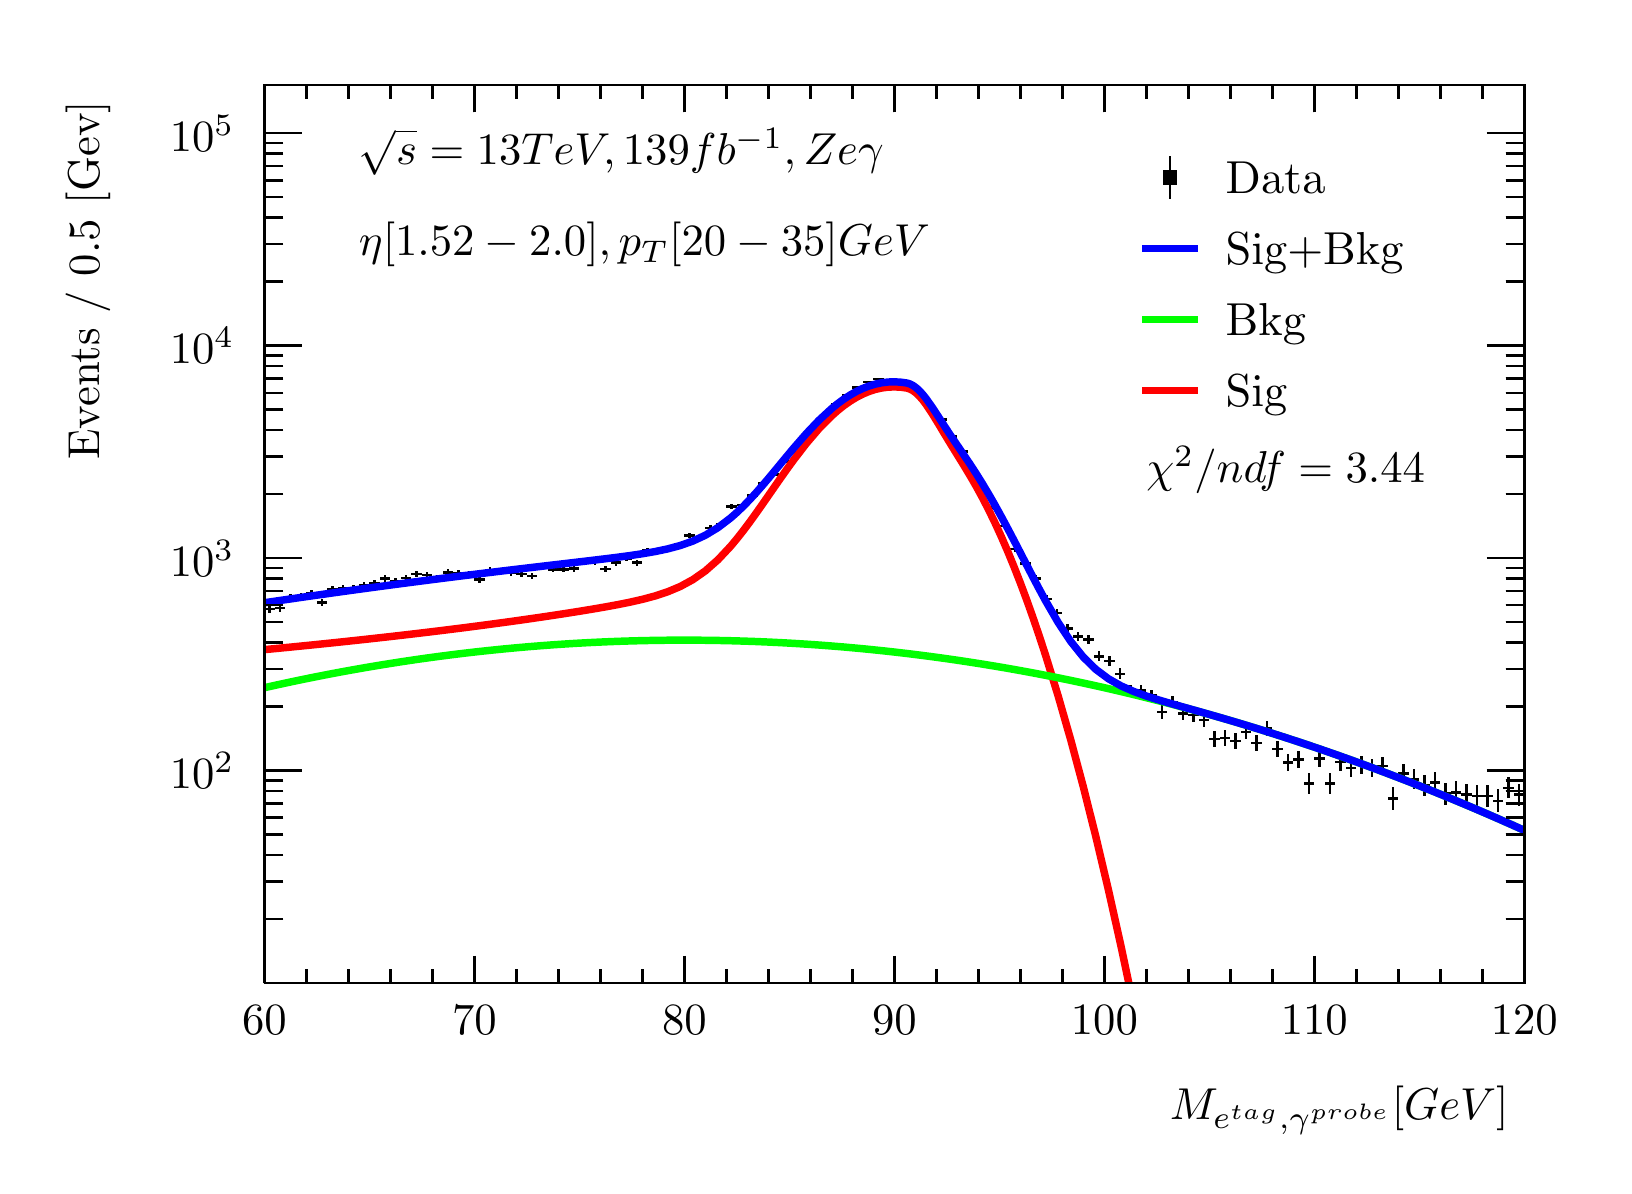
\begin{tikzpicture}
\pgfdeclareplotmark{cross} {
\pgfpathmoveto{\pgfpoint{-0.3\pgfplotmarksize}{\pgfplotmarksize}}
\pgfpathlineto{\pgfpoint{+0.3\pgfplotmarksize}{\pgfplotmarksize}}
\pgfpathlineto{\pgfpoint{+0.3\pgfplotmarksize}{0.3\pgfplotmarksize}}
\pgfpathlineto{\pgfpoint{+1\pgfplotmarksize}{0.3\pgfplotmarksize}}
\pgfpathlineto{\pgfpoint{+1\pgfplotmarksize}{-0.3\pgfplotmarksize}}
\pgfpathlineto{\pgfpoint{+0.3\pgfplotmarksize}{-0.3\pgfplotmarksize}}
\pgfpathlineto{\pgfpoint{+0.3\pgfplotmarksize}{-1.\pgfplotmarksize}}
\pgfpathlineto{\pgfpoint{-0.3\pgfplotmarksize}{-1.\pgfplotmarksize}}
\pgfpathlineto{\pgfpoint{-0.3\pgfplotmarksize}{-0.3\pgfplotmarksize}}
\pgfpathlineto{\pgfpoint{-1.\pgfplotmarksize}{-0.3\pgfplotmarksize}}
\pgfpathlineto{\pgfpoint{-1.\pgfplotmarksize}{0.3\pgfplotmarksize}}
\pgfpathlineto{\pgfpoint{-0.3\pgfplotmarksize}{0.3\pgfplotmarksize}}
\pgfpathclose
\pgfusepathqstroke
}
\pgfdeclareplotmark{cross*} {
\pgfpathmoveto{\pgfpoint{-0.3\pgfplotmarksize}{\pgfplotmarksize}}
\pgfpathlineto{\pgfpoint{+0.3\pgfplotmarksize}{\pgfplotmarksize}}
\pgfpathlineto{\pgfpoint{+0.3\pgfplotmarksize}{0.3\pgfplotmarksize}}
\pgfpathlineto{\pgfpoint{+1\pgfplotmarksize}{0.3\pgfplotmarksize}}
\pgfpathlineto{\pgfpoint{+1\pgfplotmarksize}{-0.3\pgfplotmarksize}}
\pgfpathlineto{\pgfpoint{+0.3\pgfplotmarksize}{-0.3\pgfplotmarksize}}
\pgfpathlineto{\pgfpoint{+0.3\pgfplotmarksize}{-1.\pgfplotmarksize}}
\pgfpathlineto{\pgfpoint{-0.3\pgfplotmarksize}{-1.\pgfplotmarksize}}
\pgfpathlineto{\pgfpoint{-0.3\pgfplotmarksize}{-0.3\pgfplotmarksize}}
\pgfpathlineto{\pgfpoint{-1.\pgfplotmarksize}{-0.3\pgfplotmarksize}}
\pgfpathlineto{\pgfpoint{-1.\pgfplotmarksize}{0.3\pgfplotmarksize}}
\pgfpathlineto{\pgfpoint{-0.3\pgfplotmarksize}{0.3\pgfplotmarksize}}
\pgfpathclose
\pgfusepathqfillstroke
}
\pgfdeclareplotmark{newstar} {
\pgfpathmoveto{\pgfqpoint{0pt}{\pgfplotmarksize}}
\pgfpathlineto{\pgfqpointpolar{44}{0.5\pgfplotmarksize}}
\pgfpathlineto{\pgfqpointpolar{18}{\pgfplotmarksize}}
\pgfpathlineto{\pgfqpointpolar{-20}{0.5\pgfplotmarksize}}
\pgfpathlineto{\pgfqpointpolar{-54}{\pgfplotmarksize}}
\pgfpathlineto{\pgfqpointpolar{-90}{0.5\pgfplotmarksize}}
\pgfpathlineto{\pgfqpointpolar{234}{\pgfplotmarksize}}
\pgfpathlineto{\pgfqpointpolar{198}{0.5\pgfplotmarksize}}
\pgfpathlineto{\pgfqpointpolar{162}{\pgfplotmarksize}}
\pgfpathlineto{\pgfqpointpolar{134}{0.5\pgfplotmarksize}}
\pgfpathclose
\pgfusepathqstroke
}
\pgfdeclareplotmark{newstar*} {
\pgfpathmoveto{\pgfqpoint{0pt}{\pgfplotmarksize}}
\pgfpathlineto{\pgfqpointpolar{44}{0.5\pgfplotmarksize}}
\pgfpathlineto{\pgfqpointpolar{18}{\pgfplotmarksize}}
\pgfpathlineto{\pgfqpointpolar{-20}{0.5\pgfplotmarksize}}
\pgfpathlineto{\pgfqpointpolar{-54}{\pgfplotmarksize}}
\pgfpathlineto{\pgfqpointpolar{-90}{0.5\pgfplotmarksize}}
\pgfpathlineto{\pgfqpointpolar{234}{\pgfplotmarksize}}
\pgfpathlineto{\pgfqpointpolar{198}{0.5\pgfplotmarksize}}
\pgfpathlineto{\pgfqpointpolar{162}{\pgfplotmarksize}}
\pgfpathlineto{\pgfqpointpolar{134}{0.5\pgfplotmarksize}}
\pgfpathclose
\pgfusepathqfillstroke
}
\definecolor{c}{rgb}{1,1,1};
\draw [color=c, fill=c] (0,0) rectangle (20,14.4361);
\draw [color=c, fill=c] (3,2.30977) rectangle (19,13.7143);
\definecolor{c}{rgb}{0,0,0};
\draw [c,line width=0.9] (3,2.30977) -- (3,13.7143) -- (19,13.7143) -- (19,2.30977) -- (3,2.30977);
\definecolor{c}{rgb}{1,1,1};
\draw [color=c, fill=c] (3,2.30977) rectangle (19,13.7143);
\definecolor{c}{rgb}{0,0,0};
\draw [c,line width=0.9] (3,2.30977) -- (3,13.7143) -- (19,13.7143) -- (19,2.30977) -- (3,2.30977);
\draw [c,line width=0.9] (3,2.30977) -- (19,2.30977);
\draw [c,line width=0.9] (3,2.65624) -- (3,2.30977);
\draw [c,line width=0.9] (3.53333,2.48301) -- (3.53333,2.30977);
\draw [c,line width=0.9] (4.06667,2.48301) -- (4.06667,2.30977);
\draw [c,line width=0.9] (4.6,2.48301) -- (4.6,2.30977);
\draw [c,line width=0.9] (5.13333,2.48301) -- (5.13333,2.30977);
\draw [c,line width=0.9] (5.66667,2.65624) -- (5.66667,2.30977);
\draw [c,line width=0.9] (6.2,2.48301) -- (6.2,2.30977);
\draw [c,line width=0.9] (6.73333,2.48301) -- (6.73333,2.30977);
\draw [c,line width=0.9] (7.26667,2.48301) -- (7.26667,2.30977);
\draw [c,line width=0.9] (7.8,2.48301) -- (7.8,2.30977);
\draw [c,line width=0.9] (8.33333,2.65624) -- (8.33333,2.30977);
\draw [c,line width=0.9] (8.86667,2.48301) -- (8.86667,2.30977);
\draw [c,line width=0.9] (9.4,2.48301) -- (9.4,2.30977);
\draw [c,line width=0.9] (9.93333,2.48301) -- (9.93333,2.30977);
\draw [c,line width=0.9] (10.4667,2.48301) -- (10.4667,2.30977);
\draw [c,line width=0.9] (11,2.65624) -- (11,2.30977);
\draw [c,line width=0.9] (11.5333,2.48301) -- (11.5333,2.30977);
\draw [c,line width=0.9] (12.0667,2.48301) -- (12.0667,2.30977);
\draw [c,line width=0.9] (12.6,2.48301) -- (12.6,2.30977);
\draw [c,line width=0.9] (13.1333,2.48301) -- (13.1333,2.30977);
\draw [c,line width=0.9] (13.6667,2.65624) -- (13.6667,2.30977);
\draw [c,line width=0.9] (14.2,2.48301) -- (14.2,2.30977);
\draw [c,line width=0.9] (14.7333,2.48301) -- (14.7333,2.30977);
\draw [c,line width=0.9] (15.2667,2.48301) -- (15.2667,2.30977);
\draw [c,line width=0.9] (15.8,2.48301) -- (15.8,2.30977);
\draw [c,line width=0.9] (16.3333,2.65624) -- (16.3333,2.30977);
\draw [c,line width=0.9] (16.8667,2.48301) -- (16.8667,2.30977);
\draw [c,line width=0.9] (17.4,2.48301) -- (17.4,2.30977);
\draw [c,line width=0.9] (17.9333,2.48301) -- (17.9333,2.30977);
\draw [c,line width=0.9] (18.4667,2.48301) -- (18.4667,2.30977);
\draw [c,line width=0.9] (19,2.65624) -- (19,2.30977);
\draw [anchor=base] (3,1.66015) node[scale=1.61424, color=c, rotate=0]{60};
\draw [anchor=base] (5.66667,1.66015) node[scale=1.61424, color=c, rotate=0]{70};
\draw [anchor=base] (8.33333,1.66015) node[scale=1.61424, color=c, rotate=0]{80};
\draw [anchor=base] (11,1.66015) node[scale=1.61424, color=c, rotate=0]{90};
\draw [anchor=base] (13.6667,1.66015) node[scale=1.61424, color=c, rotate=0]{100};
\draw [anchor=base] (16.3333,1.66015) node[scale=1.61424, color=c, rotate=0]{110};
\draw [anchor=base] (19,1.66015) node[scale=1.61424, color=c, rotate=0]{120};
\draw [anchor= east] (19,0.692932) node[scale=1.61424, color=c, rotate=0]{$M_{e^{tag}, \gamma^{probe}}  [GeV]$};
\draw [c,line width=0.9] (3,13.7143) -- (19,13.7143);
\draw [c,line width=0.9] (3,13.3678) -- (3,13.7143);
\draw [c,line width=0.9] (3.53333,13.5411) -- (3.53333,13.7143);
\draw [c,line width=0.9] (4.06667,13.5411) -- (4.06667,13.7143);
\draw [c,line width=0.9] (4.6,13.5411) -- (4.6,13.7143);
\draw [c,line width=0.9] (5.13333,13.5411) -- (5.13333,13.7143);
\draw [c,line width=0.9] (5.66667,13.3678) -- (5.66667,13.7143);
\draw [c,line width=0.9] (6.2,13.5411) -- (6.2,13.7143);
\draw [c,line width=0.9] (6.73333,13.5411) -- (6.73333,13.7143);
\draw [c,line width=0.9] (7.26667,13.5411) -- (7.26667,13.7143);
\draw [c,line width=0.9] (7.8,13.5411) -- (7.8,13.7143);
\draw [c,line width=0.9] (8.33333,13.3678) -- (8.33333,13.7143);
\draw [c,line width=0.9] (8.86667,13.5411) -- (8.86667,13.7143);
\draw [c,line width=0.9] (9.4,13.5411) -- (9.4,13.7143);
\draw [c,line width=0.9] (9.93333,13.5411) -- (9.93333,13.7143);
\draw [c,line width=0.9] (10.4667,13.5411) -- (10.4667,13.7143);
\draw [c,line width=0.9] (11,13.3678) -- (11,13.7143);
\draw [c,line width=0.9] (11.5333,13.5411) -- (11.5333,13.7143);
\draw [c,line width=0.9] (12.0667,13.5411) -- (12.0667,13.7143);
\draw [c,line width=0.9] (12.6,13.5411) -- (12.6,13.7143);
\draw [c,line width=0.9] (13.1333,13.5411) -- (13.1333,13.7143);
\draw [c,line width=0.9] (13.6667,13.3678) -- (13.6667,13.7143);
\draw [c,line width=0.9] (14.2,13.5411) -- (14.2,13.7143);
\draw [c,line width=0.9] (14.7333,13.5411) -- (14.7333,13.7143);
\draw [c,line width=0.9] (15.2667,13.5411) -- (15.2667,13.7143);
\draw [c,line width=0.9] (15.8,13.5411) -- (15.8,13.7143);
\draw [c,line width=0.9] (16.3333,13.3678) -- (16.3333,13.7143);
\draw [c,line width=0.9] (16.8667,13.5411) -- (16.8667,13.7143);
\draw [c,line width=0.9] (17.4,13.5411) -- (17.4,13.7143);
\draw [c,line width=0.9] (17.9333,13.5411) -- (17.9333,13.7143);
\draw [c,line width=0.9] (18.4667,13.5411) -- (18.4667,13.7143);
\draw [c,line width=0.9] (19,13.3678) -- (19,13.7143);
\draw [c,line width=0.9] (3,2.30977) -- (3,13.7143);
\draw [c,line width=0.9] (3.237,3.12209) -- (3,3.12209);
\draw [c,line width=0.9] (3.237,3.59726) -- (3,3.59726);
\draw [c,line width=0.9] (3.237,3.9344) -- (3,3.9344);
\draw [c,line width=0.9] (3.237,4.19591) -- (3,4.19591);
\draw [c,line width=0.9] (3.237,4.40958) -- (3,4.40958);
\draw [c,line width=0.9] (3.237,4.59023) -- (3,4.59023);
\draw [c,line width=0.9] (3.237,4.74672) -- (3,4.74672);
\draw [c,line width=0.9] (3.237,4.88475) -- (3,4.88475);
\draw [c,line width=0.9] (3.474,5.00822) -- (3,5.00822);
\draw [anchor= east] (2.82,5.00822) node[scale=1.61424, color=c, rotate=0]{$10^{2}$};
\draw [c,line width=0.9] (3.237,5.82054) -- (3,5.82054);
\draw [c,line width=0.9] (3.237,6.29571) -- (3,6.29571);
\draw [c,line width=0.9] (3.237,6.63285) -- (3,6.63285);
\draw [c,line width=0.9] (3.237,6.89436) -- (3,6.89436);
\draw [c,line width=0.9] (3.237,7.10803) -- (3,7.10803);
\draw [c,line width=0.9] (3.237,7.28868) -- (3,7.28868);
\draw [c,line width=0.9] (3.237,7.44517) -- (3,7.44517);
\draw [c,line width=0.9] (3.237,7.5832) -- (3,7.5832);
\draw [c,line width=0.9] (3.474,7.70668) -- (3,7.70668);
\draw [anchor= east] (2.82,7.70668) node[scale=1.61424, color=c, rotate=0]{$10^{3}$};
\draw [c,line width=0.9] (3.237,8.51899) -- (3,8.51899);
\draw [c,line width=0.9] (3.237,8.99417) -- (3,8.99417);
\draw [c,line width=0.9] (3.237,9.33131) -- (3,9.33131);
\draw [c,line width=0.9] (3.237,9.59281) -- (3,9.59281);
\draw [c,line width=0.9] (3.237,9.80648) -- (3,9.80648);
\draw [c,line width=0.9] (3.237,9.98713) -- (3,9.98713);
\draw [c,line width=0.9] (3.237,10.1436) -- (3,10.1436);
\draw [c,line width=0.9] (3.237,10.2817) -- (3,10.2817);
\draw [c,line width=0.9] (3.474,10.4051) -- (3,10.4051);
\draw [anchor= east] (2.82,10.4051) node[scale=1.61424, color=c, rotate=0]{$10^{4}$};
\draw [c,line width=0.9] (3.237,11.2174) -- (3,11.2174);
\draw [c,line width=0.9] (3.237,11.6926) -- (3,11.6926);
\draw [c,line width=0.9] (3.237,12.0298) -- (3,12.0298);
\draw [c,line width=0.9] (3.237,12.2913) -- (3,12.2913);
\draw [c,line width=0.9] (3.237,12.5049) -- (3,12.5049);
\draw [c,line width=0.9] (3.237,12.6856) -- (3,12.6856);
\draw [c,line width=0.9] (3.237,12.8421) -- (3,12.8421);
\draw [c,line width=0.9] (3.237,12.9801) -- (3,12.9801);
\draw [c,line width=0.9] (3.474,13.1036) -- (3,13.1036);
\draw [anchor= east] (2.82,13.1036) node[scale=1.61424, color=c, rotate=0]{$10^{5}$};
\draw [anchor= east] (0.76,13.7143) node[scale=1.61424, color=c, rotate=90]{Events / 0.5 [Gev]};
\draw [c,line width=0.9] (19,2.30977) -- (19,13.7143);
\draw [c,line width=0.9] (18.763,3.12209) -- (19,3.12209);
\draw [c,line width=0.9] (18.763,3.59726) -- (19,3.59726);
\draw [c,line width=0.9] (18.763,3.9344) -- (19,3.9344);
\draw [c,line width=0.9] (18.763,4.19591) -- (19,4.19591);
\draw [c,line width=0.9] (18.763,4.40958) -- (19,4.40958);
\draw [c,line width=0.9] (18.763,4.59023) -- (19,4.59023);
\draw [c,line width=0.9] (18.763,4.74672) -- (19,4.74672);
\draw [c,line width=0.9] (18.763,4.88475) -- (19,4.88475);
\draw [c,line width=0.9] (18.526,5.00822) -- (19,5.00822);
\draw [c,line width=0.9] (18.763,5.82054) -- (19,5.82054);
\draw [c,line width=0.9] (18.763,6.29571) -- (19,6.29571);
\draw [c,line width=0.9] (18.763,6.63285) -- (19,6.63285);
\draw [c,line width=0.9] (18.763,6.89436) -- (19,6.89436);
\draw [c,line width=0.9] (18.763,7.10803) -- (19,7.10803);
\draw [c,line width=0.9] (18.763,7.28868) -- (19,7.28868);
\draw [c,line width=0.9] (18.763,7.44517) -- (19,7.44517);
\draw [c,line width=0.9] (18.763,7.5832) -- (19,7.5832);
\draw [c,line width=0.9] (18.526,7.70668) -- (19,7.70668);
\draw [c,line width=0.9] (18.763,8.51899) -- (19,8.51899);
\draw [c,line width=0.9] (18.763,8.99417) -- (19,8.99417);
\draw [c,line width=0.9] (18.763,9.33131) -- (19,9.33131);
\draw [c,line width=0.9] (18.763,9.59281) -- (19,9.59281);
\draw [c,line width=0.9] (18.763,9.80648) -- (19,9.80648);
\draw [c,line width=0.9] (18.763,9.98713) -- (19,9.98713);
\draw [c,line width=0.9] (18.763,10.1436) -- (19,10.1436);
\draw [c,line width=0.9] (18.763,10.2817) -- (19,10.2817);
\draw [c,line width=0.9] (18.526,10.4051) -- (19,10.4051);
\draw [c,line width=0.9] (18.763,11.2174) -- (19,11.2174);
\draw [c,line width=0.9] (18.763,11.6926) -- (19,11.6926);
\draw [c,line width=0.9] (18.763,12.0298) -- (19,12.0298);
\draw [c,line width=0.9] (18.763,12.2913) -- (19,12.2913);
\draw [c,line width=0.9] (18.763,12.5049) -- (19,12.5049);
\draw [c,line width=0.9] (18.763,12.6856) -- (19,12.6856);
\draw [c,line width=0.9] (18.763,12.8421) -- (19,12.8421);
\draw [c,line width=0.9] (18.763,12.9801) -- (19,12.9801);
\draw [c,line width=0.9] (18.526,13.1036) -- (19,13.1036);
\draw [c,line width=0.9] (3.06667,7.06222) -- (3,7.06222);
\draw [c,line width=0.9] (3,7.06222) -- (3,7.06222);
\draw [c,line width=0.9] (3.06667,7.06222) -- (3.13333,7.06222);
\draw [c,line width=0.9] (3.13333,7.06222) -- (3.13333,7.06222);
\draw [c,line width=0.9] (3.06667,7.06222) -- (3.06667,7.11101);
\draw [c,line width=0.9] (3.06667,7.11101) -- (3.06667,7.11101);
\draw [c,line width=0.9] (3.06667,7.06222) -- (3.06667,7.01344);
\draw [c,line width=0.9] (3.06667,7.01344) -- (3.06667,7.01344);
\draw [c,line width=0.9] (3.2,7.07233) -- (3.13333,7.07233);
\draw [c,line width=0.9] (3.13333,7.07233) -- (3.13333,7.07233);
\draw [c,line width=0.9] (3.2,7.07233) -- (3.26667,7.07233);
\draw [c,line width=0.9] (3.26667,7.07233) -- (3.26667,7.07233);
\draw [c,line width=0.9] (3.2,7.07233) -- (3.2,7.12091);
\draw [c,line width=0.9] (3.2,7.12091) -- (3.2,7.12091);
\draw [c,line width=0.9] (3.2,7.07233) -- (3.2,7.02376);
\draw [c,line width=0.9] (3.2,7.02376) -- (3.2,7.02376);
\draw [c,line width=0.9] (3.33333,7.20183) -- (3.26667,7.20183);
\draw [c,line width=0.9] (3.26667,7.20183) -- (3.26667,7.20183);
\draw [c,line width=0.9] (3.33333,7.20183) -- (3.4,7.20183);
\draw [c,line width=0.9] (3.4,7.20183) -- (3.4,7.20183);
\draw [c,line width=0.9] (3.33333,7.20183) -- (3.33333,7.2478);
\draw [c,line width=0.9] (3.33333,7.2478) -- (3.33333,7.2478);
\draw [c,line width=0.9] (3.33333,7.20183) -- (3.33333,7.15587);
\draw [c,line width=0.9] (3.33333,7.15587) -- (3.33333,7.15587);
\draw [c,line width=0.9] (3.46667,7.2215) -- (3.4,7.2215);
\draw [c,line width=0.9] (3.4,7.2215) -- (3.4,7.2215);
\draw [c,line width=0.9] (3.46667,7.2215) -- (3.53333,7.2215);
\draw [c,line width=0.9] (3.53333,7.2215) -- (3.53333,7.2215);
\draw [c,line width=0.9] (3.46667,7.2215) -- (3.46667,7.26708);
\draw [c,line width=0.9] (3.46667,7.26708) -- (3.46667,7.26708);
\draw [c,line width=0.9] (3.46667,7.2215) -- (3.46667,7.17592);
\draw [c,line width=0.9] (3.46667,7.17592) -- (3.46667,7.17592);
\draw [c,line width=0.9] (3.6,7.25815) -- (3.53333,7.25815);
\draw [c,line width=0.9] (3.53333,7.25815) -- (3.53333,7.25815);
\draw [c,line width=0.9] (3.6,7.25815) -- (3.66667,7.25815);
\draw [c,line width=0.9] (3.66667,7.25815) -- (3.66667,7.25815);
\draw [c,line width=0.9] (3.6,7.25815) -- (3.6,7.30303);
\draw [c,line width=0.9] (3.6,7.30303) -- (3.6,7.30303);
\draw [c,line width=0.9] (3.6,7.25815) -- (3.6,7.21328);
\draw [c,line width=0.9] (3.6,7.21328) -- (3.6,7.21328);
\draw [c,line width=0.9] (3.73333,7.14077) -- (3.66667,7.14077);
\draw [c,line width=0.9] (3.66667,7.14077) -- (3.66667,7.14077);
\draw [c,line width=0.9] (3.73333,7.14077) -- (3.8,7.14077);
\draw [c,line width=0.9] (3.8,7.14077) -- (3.8,7.14077);
\draw [c,line width=0.9] (3.73333,7.14077) -- (3.73333,7.18795);
\draw [c,line width=0.9] (3.73333,7.18795) -- (3.73333,7.18795);
\draw [c,line width=0.9] (3.73333,7.14077) -- (3.73333,7.0936);
\draw [c,line width=0.9] (3.73333,7.0936) -- (3.73333,7.0936);
\draw [c,line width=0.9] (3.86667,7.31353) -- (3.8,7.31353);
\draw [c,line width=0.9] (3.8,7.31353) -- (3.8,7.31353);
\draw [c,line width=0.9] (3.86667,7.31353) -- (3.93333,7.31353);
\draw [c,line width=0.9] (3.93333,7.31353) -- (3.93333,7.31353);
\draw [c,line width=0.9] (3.86667,7.31353) -- (3.86667,7.35736);
\draw [c,line width=0.9] (3.86667,7.35736) -- (3.86667,7.35736);
\draw [c,line width=0.9] (3.86667,7.31353) -- (3.86667,7.26971);
\draw [c,line width=0.9] (3.86667,7.26971) -- (3.86667,7.26971);
\draw [c,line width=0.9] (4,7.32495) -- (3.93333,7.32495);
\draw [c,line width=0.9] (3.93333,7.32495) -- (3.93333,7.32495);
\draw [c,line width=0.9] (4,7.32495) -- (4.06667,7.32495);
\draw [c,line width=0.9] (4.06667,7.32495) -- (4.06667,7.32495);
\draw [c,line width=0.9] (4,7.32495) -- (4,7.36856);
\draw [c,line width=0.9] (4,7.36856) -- (4,7.36856);
\draw [c,line width=0.9] (4,7.32495) -- (4,7.28134);
\draw [c,line width=0.9] (4,7.28134) -- (4,7.28134);
\draw [c,line width=0.9] (4.13333,7.31844) -- (4.06667,7.31844);
\draw [c,line width=0.9] (4.06667,7.31844) -- (4.06667,7.31844);
\draw [c,line width=0.9] (4.13333,7.31844) -- (4.2,7.31844);
\draw [c,line width=0.9] (4.2,7.31844) -- (4.2,7.31844);
\draw [c,line width=0.9] (4.13333,7.31844) -- (4.13333,7.36217);
\draw [c,line width=0.9] (4.13333,7.36217) -- (4.13333,7.36217);
\draw [c,line width=0.9] (4.13333,7.31844) -- (4.13333,7.2747);
\draw [c,line width=0.9] (4.13333,7.2747) -- (4.13333,7.2747);
\draw [c,line width=0.9] (4.26667,7.36012) -- (4.2,7.36012);
\draw [c,line width=0.9] (4.2,7.36012) -- (4.2,7.36012);
\draw [c,line width=0.9] (4.26667,7.36012) -- (4.33333,7.36012);
\draw [c,line width=0.9] (4.33333,7.36012) -- (4.33333,7.36012);
\draw [c,line width=0.9] (4.26667,7.36012) -- (4.26667,7.40309);
\draw [c,line width=0.9] (4.26667,7.40309) -- (4.26667,7.40309);
\draw [c,line width=0.9] (4.26667,7.36012) -- (4.26667,7.31716);
\draw [c,line width=0.9] (4.26667,7.31716) -- (4.26667,7.31716);
\draw [c,line width=0.9] (4.4,7.38352) -- (4.33333,7.38352);
\draw [c,line width=0.9] (4.33333,7.38352) -- (4.33333,7.38352);
\draw [c,line width=0.9] (4.4,7.38352) -- (4.46667,7.38352);
\draw [c,line width=0.9] (4.46667,7.38352) -- (4.46667,7.38352);
\draw [c,line width=0.9] (4.4,7.38352) -- (4.4,7.42605);
\draw [c,line width=0.9] (4.4,7.42605) -- (4.4,7.42605);
\draw [c,line width=0.9] (4.4,7.38352) -- (4.4,7.34098);
\draw [c,line width=0.9] (4.4,7.34098) -- (4.4,7.34098);
\draw [c,line width=0.9] (4.53333,7.44517) -- (4.46667,7.44517);
\draw [c,line width=0.9] (4.46667,7.44517) -- (4.46667,7.44517);
\draw [c,line width=0.9] (4.53333,7.44517) -- (4.6,7.44517);
\draw [c,line width=0.9] (4.6,7.44517) -- (4.6,7.44517);
\draw [c,line width=0.9] (4.53333,7.44517) -- (4.53333,7.4866);
\draw [c,line width=0.9] (4.53333,7.4866) -- (4.53333,7.4866);
\draw [c,line width=0.9] (4.53333,7.44517) -- (4.53333,7.40374);
\draw [c,line width=0.9] (4.53333,7.40374) -- (4.53333,7.40374);
\draw [c,line width=0.9] (4.66667,7.4155) -- (4.6,7.4155);
\draw [c,line width=0.9] (4.6,7.4155) -- (4.6,7.4155);
\draw [c,line width=0.9] (4.66667,7.4155) -- (4.73333,7.4155);
\draw [c,line width=0.9] (4.73333,7.4155) -- (4.73333,7.4155);
\draw [c,line width=0.9] (4.66667,7.4155) -- (4.66667,7.45746);
\draw [c,line width=0.9] (4.66667,7.45746) -- (4.66667,7.45746);
\draw [c,line width=0.9] (4.66667,7.4155) -- (4.66667,7.37354);
\draw [c,line width=0.9] (4.66667,7.37354) -- (4.66667,7.37354);
\draw [c,line width=0.9] (4.8,7.45102) -- (4.73333,7.45102);
\draw [c,line width=0.9] (4.73333,7.45102) -- (4.73333,7.45102);
\draw [c,line width=0.9] (4.8,7.45102) -- (4.86667,7.45102);
\draw [c,line width=0.9] (4.86667,7.45102) -- (4.86667,7.45102);
\draw [c,line width=0.9] (4.8,7.45102) -- (4.8,7.49234);
\draw [c,line width=0.9] (4.8,7.49234) -- (4.8,7.49234);
\draw [c,line width=0.9] (4.8,7.45102) -- (4.8,7.40969);
\draw [c,line width=0.9] (4.8,7.40969) -- (4.8,7.40969);
\draw [c,line width=0.9] (4.93333,7.50235) -- (4.86667,7.50235);
\draw [c,line width=0.9] (4.86667,7.50235) -- (4.86667,7.50235);
\draw [c,line width=0.9] (4.93333,7.50235) -- (5,7.50235);
\draw [c,line width=0.9] (5,7.50235) -- (5,7.50235);
\draw [c,line width=0.9] (4.93333,7.50235) -- (4.93333,7.54278);
\draw [c,line width=0.9] (4.93333,7.54278) -- (4.93333,7.54278);
\draw [c,line width=0.9] (4.93333,7.50235) -- (4.93333,7.46192);
\draw [c,line width=0.9] (4.93333,7.46192) -- (4.93333,7.46192);
\draw [c,line width=0.9] (5.06667,7.49395) -- (5,7.49395);
\draw [c,line width=0.9] (5,7.49395) -- (5,7.49395);
\draw [c,line width=0.9] (5.06667,7.49395) -- (5.13333,7.49395);
\draw [c,line width=0.9] (5.13333,7.49395) -- (5.13333,7.49395);
\draw [c,line width=0.9] (5.06667,7.49395) -- (5.06667,7.53453);
\draw [c,line width=0.9] (5.06667,7.53453) -- (5.06667,7.53453);
\draw [c,line width=0.9] (5.06667,7.49395) -- (5.06667,7.45337);
\draw [c,line width=0.9] (5.06667,7.45337) -- (5.06667,7.45337);
\draw [c,line width=0.9] (5.2,7.45538) -- (5.13333,7.45538);
\draw [c,line width=0.9] (5.13333,7.45538) -- (5.13333,7.45538);
\draw [c,line width=0.9] (5.2,7.45538) -- (5.26667,7.45538);
\draw [c,line width=0.9] (5.26667,7.45538) -- (5.26667,7.45538);
\draw [c,line width=0.9] (5.2,7.45538) -- (5.2,7.49663);
\draw [c,line width=0.9] (5.2,7.49663) -- (5.2,7.49663);
\draw [c,line width=0.9] (5.2,7.45538) -- (5.2,7.41413);
\draw [c,line width=0.9] (5.2,7.41413) -- (5.2,7.41413);
\draw [c,line width=0.9] (5.33333,7.52583) -- (5.26667,7.52583);
\draw [c,line width=0.9] (5.26667,7.52583) -- (5.26667,7.52583);
\draw [c,line width=0.9] (5.33333,7.52583) -- (5.4,7.52583);
\draw [c,line width=0.9] (5.4,7.52583) -- (5.4,7.52583);
\draw [c,line width=0.9] (5.33333,7.52583) -- (5.33333,7.56586);
\draw [c,line width=0.9] (5.33333,7.56586) -- (5.33333,7.56586);
\draw [c,line width=0.9] (5.33333,7.52583) -- (5.33333,7.4858);
\draw [c,line width=0.9] (5.33333,7.4858) -- (5.33333,7.4858);
\draw [c,line width=0.9] (5.46667,7.51897) -- (5.4,7.51897);
\draw [c,line width=0.9] (5.4,7.51897) -- (5.4,7.51897);
\draw [c,line width=0.9] (5.46667,7.51897) -- (5.53333,7.51897);
\draw [c,line width=0.9] (5.53333,7.51897) -- (5.53333,7.51897);
\draw [c,line width=0.9] (5.46667,7.51897) -- (5.46667,7.55912);
\draw [c,line width=0.9] (5.46667,7.55912) -- (5.46667,7.55912);
\draw [c,line width=0.9] (5.46667,7.51897) -- (5.46667,7.47883);
\draw [c,line width=0.9] (5.46667,7.47883) -- (5.46667,7.47883);
\draw [c,line width=0.9] (5.6,7.50653) -- (5.53333,7.50653);
\draw [c,line width=0.9] (5.53333,7.50653) -- (5.53333,7.50653);
\draw [c,line width=0.9] (5.6,7.50653) -- (5.66667,7.50653);
\draw [c,line width=0.9] (5.66667,7.50653) -- (5.66667,7.50653);
\draw [c,line width=0.9] (5.6,7.50653) -- (5.6,7.54689);
\draw [c,line width=0.9] (5.6,7.54689) -- (5.6,7.54689);
\draw [c,line width=0.9] (5.6,7.50653) -- (5.6,7.46617);
\draw [c,line width=0.9] (5.6,7.46617) -- (5.6,7.46617);
\draw [c,line width=0.9] (5.73333,7.43782) -- (5.66667,7.43782);
\draw [c,line width=0.9] (5.66667,7.43782) -- (5.66667,7.43782);
\draw [c,line width=0.9] (5.73333,7.43782) -- (5.8,7.43782);
\draw [c,line width=0.9] (5.8,7.43782) -- (5.8,7.43782);
\draw [c,line width=0.9] (5.73333,7.43782) -- (5.73333,7.47939);
\draw [c,line width=0.9] (5.73333,7.47939) -- (5.73333,7.47939);
\draw [c,line width=0.9] (5.73333,7.43782) -- (5.73333,7.39626);
\draw [c,line width=0.9] (5.73333,7.39626) -- (5.73333,7.39626);
\draw [c,line width=0.9] (5.86667,7.55687) -- (5.8,7.55687);
\draw [c,line width=0.9] (5.8,7.55687) -- (5.8,7.55687);
\draw [c,line width=0.9] (5.86667,7.55687) -- (5.93333,7.55687);
\draw [c,line width=0.9] (5.93333,7.55687) -- (5.93333,7.55687);
\draw [c,line width=0.9] (5.86667,7.55687) -- (5.86667,7.59637);
\draw [c,line width=0.9] (5.86667,7.59637) -- (5.86667,7.59637);
\draw [c,line width=0.9] (5.86667,7.55687) -- (5.86667,7.51736);
\draw [c,line width=0.9] (5.86667,7.51736) -- (5.86667,7.51736);
\draw [c,line width=0.9] (6,7.54213) -- (5.93333,7.54213);
\draw [c,line width=0.9] (5.93333,7.54213) -- (5.93333,7.54213);
\draw [c,line width=0.9] (6,7.54213) -- (6.06667,7.54213);
\draw [c,line width=0.9] (6.06667,7.54213) -- (6.06667,7.54213);
\draw [c,line width=0.9] (6,7.54213) -- (6,7.58188);
\draw [c,line width=0.9] (6,7.58188) -- (6,7.58188);
\draw [c,line width=0.9] (6,7.54213) -- (6,7.50237);
\draw [c,line width=0.9] (6,7.50237) -- (6,7.50237);
\draw [c,line width=0.9] (6.13333,7.52309) -- (6.06667,7.52309);
\draw [c,line width=0.9] (6.06667,7.52309) -- (6.06667,7.52309);
\draw [c,line width=0.9] (6.13333,7.52309) -- (6.2,7.52309);
\draw [c,line width=0.9] (6.2,7.52309) -- (6.2,7.52309);
\draw [c,line width=0.9] (6.13333,7.52309) -- (6.13333,7.56317);
\draw [c,line width=0.9] (6.13333,7.56317) -- (6.13333,7.56317);
\draw [c,line width=0.9] (6.13333,7.52309) -- (6.13333,7.48302);
\draw [c,line width=0.9] (6.13333,7.48302) -- (6.13333,7.48302);
\draw [c,line width=0.9] (6.26667,7.50374) -- (6.2,7.50374);
\draw [c,line width=0.9] (6.2,7.50374) -- (6.2,7.50374);
\draw [c,line width=0.9] (6.26667,7.50374) -- (6.33333,7.50374);
\draw [c,line width=0.9] (6.33333,7.50374) -- (6.33333,7.50374);
\draw [c,line width=0.9] (6.26667,7.50374) -- (6.26667,7.54415);
\draw [c,line width=0.9] (6.26667,7.54415) -- (6.26667,7.54415);
\draw [c,line width=0.9] (6.26667,7.50374) -- (6.26667,7.46334);
\draw [c,line width=0.9] (6.26667,7.46334) -- (6.26667,7.46334);
\draw [c,line width=0.9] (6.4,7.47981) -- (6.33333,7.47981);
\draw [c,line width=0.9] (6.33333,7.47981) -- (6.33333,7.47981);
\draw [c,line width=0.9] (6.4,7.47981) -- (6.46667,7.47981);
\draw [c,line width=0.9] (6.46667,7.47981) -- (6.46667,7.47981);
\draw [c,line width=0.9] (6.4,7.47981) -- (6.4,7.52064);
\draw [c,line width=0.9] (6.4,7.52064) -- (6.4,7.52064);
\draw [c,line width=0.9] (6.4,7.47981) -- (6.4,7.43899);
\draw [c,line width=0.9] (6.4,7.43899) -- (6.4,7.43899);
\draw [c,line width=0.9] (6.53333,7.5897) -- (6.46667,7.5897);
\draw [c,line width=0.9] (6.46667,7.5897) -- (6.46667,7.5897);
\draw [c,line width=0.9] (6.53333,7.5897) -- (6.6,7.5897);
\draw [c,line width=0.9] (6.6,7.5897) -- (6.6,7.5897);
\draw [c,line width=0.9] (6.53333,7.5897) -- (6.53333,7.62865);
\draw [c,line width=0.9] (6.53333,7.62865) -- (6.53333,7.62865);
\draw [c,line width=0.9] (6.53333,7.5897) -- (6.53333,7.55074);
\draw [c,line width=0.9] (6.53333,7.55074) -- (6.53333,7.55074);
\draw [c,line width=0.9] (6.66667,7.56483) -- (6.6,7.56483);
\draw [c,line width=0.9] (6.6,7.56483) -- (6.6,7.56483);
\draw [c,line width=0.9] (6.66667,7.56483) -- (6.73333,7.56483);
\draw [c,line width=0.9] (6.73333,7.56483) -- (6.73333,7.56483);
\draw [c,line width=0.9] (6.66667,7.56483) -- (6.66667,7.6042);
\draw [c,line width=0.9] (6.66667,7.6042) -- (6.66667,7.6042);
\draw [c,line width=0.9] (6.66667,7.56483) -- (6.66667,7.52546);
\draw [c,line width=0.9] (6.66667,7.52546) -- (6.66667,7.52546);
\draw [c,line width=0.9] (6.8,7.56351) -- (6.73333,7.56351);
\draw [c,line width=0.9] (6.73333,7.56351) -- (6.73333,7.56351);
\draw [c,line width=0.9] (6.8,7.56351) -- (6.86667,7.56351);
\draw [c,line width=0.9] (6.86667,7.56351) -- (6.86667,7.56351);
\draw [c,line width=0.9] (6.8,7.56351) -- (6.8,7.6029);
\draw [c,line width=0.9] (6.8,7.6029) -- (6.8,7.6029);
\draw [c,line width=0.9] (6.8,7.56351) -- (6.8,7.52412);
\draw [c,line width=0.9] (6.8,7.52412) -- (6.8,7.52412);
\draw [c,line width=0.9] (6.93333,7.57405) -- (6.86667,7.57405);
\draw [c,line width=0.9] (6.86667,7.57405) -- (6.86667,7.57405);
\draw [c,line width=0.9] (6.93333,7.57405) -- (7,7.57405);
\draw [c,line width=0.9] (7,7.57405) -- (7,7.57405);
\draw [c,line width=0.9] (6.93333,7.57405) -- (6.93333,7.61327);
\draw [c,line width=0.9] (6.93333,7.61327) -- (6.93333,7.61327);
\draw [c,line width=0.9] (6.93333,7.57405) -- (6.93333,7.53484);
\draw [c,line width=0.9] (6.93333,7.53484) -- (6.93333,7.53484);
\draw [c,line width=0.9] (7.06667,7.6734) -- (7,7.6734);
\draw [c,line width=0.9] (7,7.6734) -- (7,7.6734);
\draw [c,line width=0.9] (7.06667,7.6734) -- (7.13333,7.6734);
\draw [c,line width=0.9] (7.13333,7.6734) -- (7.13333,7.6734);
\draw [c,line width=0.9] (7.06667,7.6734) -- (7.06667,7.71098);
\draw [c,line width=0.9] (7.06667,7.71098) -- (7.06667,7.71098);
\draw [c,line width=0.9] (7.06667,7.6734) -- (7.06667,7.63581);
\draw [c,line width=0.9] (7.06667,7.63581) -- (7.06667,7.63581);
\draw [c,line width=0.9] (7.2,7.66128) -- (7.13333,7.66128);
\draw [c,line width=0.9] (7.13333,7.66128) -- (7.13333,7.66128);
\draw [c,line width=0.9] (7.2,7.66128) -- (7.26667,7.66128);
\draw [c,line width=0.9] (7.26667,7.66128) -- (7.26667,7.66128);
\draw [c,line width=0.9] (7.2,7.66128) -- (7.2,7.69906);
\draw [c,line width=0.9] (7.2,7.69906) -- (7.2,7.69906);
\draw [c,line width=0.9] (7.2,7.66128) -- (7.2,7.62349);
\draw [c,line width=0.9] (7.2,7.62349) -- (7.2,7.62349);
\draw [c,line width=0.9] (7.33333,7.56747) -- (7.26667,7.56747);
\draw [c,line width=0.9] (7.26667,7.56747) -- (7.26667,7.56747);
\draw [c,line width=0.9] (7.33333,7.56747) -- (7.4,7.56747);
\draw [c,line width=0.9] (7.4,7.56747) -- (7.4,7.56747);
\draw [c,line width=0.9] (7.33333,7.56747) -- (7.33333,7.6068);
\draw [c,line width=0.9] (7.33333,7.6068) -- (7.33333,7.6068);
\draw [c,line width=0.9] (7.33333,7.56747) -- (7.33333,7.52815);
\draw [c,line width=0.9] (7.33333,7.52815) -- (7.33333,7.52815);
\draw [c,line width=0.9] (7.46667,7.65026) -- (7.4,7.65026);
\draw [c,line width=0.9] (7.4,7.65026) -- (7.4,7.65026);
\draw [c,line width=0.9] (7.46667,7.65026) -- (7.53333,7.65026);
\draw [c,line width=0.9] (7.53333,7.65026) -- (7.53333,7.65026);
\draw [c,line width=0.9] (7.46667,7.65026) -- (7.46667,7.68822);
\draw [c,line width=0.9] (7.46667,7.68822) -- (7.46667,7.68822);
\draw [c,line width=0.9] (7.46667,7.65026) -- (7.46667,7.6123);
\draw [c,line width=0.9] (7.46667,7.6123) -- (7.46667,7.6123);
\draw [c,line width=0.9] (7.6,7.7008) -- (7.53333,7.7008);
\draw [c,line width=0.9] (7.53333,7.7008) -- (7.53333,7.7008);
\draw [c,line width=0.9] (7.6,7.7008) -- (7.66667,7.7008);
\draw [c,line width=0.9] (7.66667,7.7008) -- (7.66667,7.7008);
\draw [c,line width=0.9] (7.6,7.7008) -- (7.6,7.73796);
\draw [c,line width=0.9] (7.6,7.73796) -- (7.6,7.73796);
\draw [c,line width=0.9] (7.6,7.7008) -- (7.6,7.66365);
\draw [c,line width=0.9] (7.6,7.66365) -- (7.6,7.66365);
\draw [c,line width=0.9] (7.73333,7.65026) -- (7.66667,7.65026);
\draw [c,line width=0.9] (7.66667,7.65026) -- (7.66667,7.65026);
\draw [c,line width=0.9] (7.73333,7.65026) -- (7.8,7.65026);
\draw [c,line width=0.9] (7.8,7.65026) -- (7.8,7.65026);
\draw [c,line width=0.9] (7.73333,7.65026) -- (7.73333,7.68822);
\draw [c,line width=0.9] (7.73333,7.68822) -- (7.73333,7.68822);
\draw [c,line width=0.9] (7.73333,7.65026) -- (7.73333,7.6123);
\draw [c,line width=0.9] (7.73333,7.6123) -- (7.73333,7.6123);
\draw [c,line width=0.9] (7.86667,7.80012) -- (7.8,7.80012);
\draw [c,line width=0.9] (7.8,7.80012) -- (7.8,7.80012);
\draw [c,line width=0.9] (7.86667,7.80012) -- (7.93333,7.80012);
\draw [c,line width=0.9] (7.93333,7.80012) -- (7.93333,7.80012);
\draw [c,line width=0.9] (7.86667,7.80012) -- (7.86667,7.83573);
\draw [c,line width=0.9] (7.86667,7.83573) -- (7.86667,7.83573);
\draw [c,line width=0.9] (7.86667,7.80012) -- (7.86667,7.76451);
\draw [c,line width=0.9] (7.86667,7.76451) -- (7.86667,7.76451);
\draw [c,line width=0.9] (8,7.80228) -- (7.93333,7.80228);
\draw [c,line width=0.9] (7.93333,7.80228) -- (7.93333,7.80228);
\draw [c,line width=0.9] (8,7.80228) -- (8.06667,7.80228);
\draw [c,line width=0.9] (8.06667,7.80228) -- (8.06667,7.80228);
\draw [c,line width=0.9] (8,7.80228) -- (8,7.83786);
\draw [c,line width=0.9] (8,7.83786) -- (8,7.83786);
\draw [c,line width=0.9] (8,7.80228) -- (8,7.76671);
\draw [c,line width=0.9] (8,7.76671) -- (8,7.76671);
\draw [c,line width=0.9] (8.13333,7.82581) -- (8.06667,7.82581);
\draw [c,line width=0.9] (8.06667,7.82581) -- (8.06667,7.82581);
\draw [c,line width=0.9] (8.13333,7.82581) -- (8.2,7.82581);
\draw [c,line width=0.9] (8.2,7.82581) -- (8.2,7.82581);
\draw [c,line width=0.9] (8.13333,7.82581) -- (8.13333,7.86103);
\draw [c,line width=0.9] (8.13333,7.86103) -- (8.13333,7.86103);
\draw [c,line width=0.9] (8.13333,7.82581) -- (8.13333,7.79059);
\draw [c,line width=0.9] (8.13333,7.79059) -- (8.13333,7.79059);
\draw [c,line width=0.9] (8.26667,7.8796) -- (8.2,7.8796);
\draw [c,line width=0.9] (8.2,7.8796) -- (8.2,7.8796);
\draw [c,line width=0.9] (8.26667,7.8796) -- (8.33333,7.8796);
\draw [c,line width=0.9] (8.33333,7.8796) -- (8.33333,7.8796);
\draw [c,line width=0.9] (8.26667,7.8796) -- (8.26667,7.91403);
\draw [c,line width=0.9] (8.26667,7.91403) -- (8.26667,7.91403);
\draw [c,line width=0.9] (8.26667,7.8796) -- (8.26667,7.84518);
\draw [c,line width=0.9] (8.26667,7.84518) -- (8.26667,7.84518);
\draw [c,line width=0.9] (8.4,7.99598) -- (8.33333,7.99598);
\draw [c,line width=0.9] (8.33333,7.99598) -- (8.33333,7.99598);
\draw [c,line width=0.9] (8.4,7.99598) -- (8.46667,7.99598);
\draw [c,line width=0.9] (8.46667,7.99598) -- (8.46667,7.99598);
\draw [c,line width=0.9] (8.4,7.99598) -- (8.4,8.02873);
\draw [c,line width=0.9] (8.4,8.02873) -- (8.4,8.02873);
\draw [c,line width=0.9] (8.4,7.99598) -- (8.4,7.96322);
\draw [c,line width=0.9] (8.4,7.96322) -- (8.4,7.96322);
\draw [c,line width=0.9] (8.53333,7.97659) -- (8.46667,7.97659);
\draw [c,line width=0.9] (8.46667,7.97659) -- (8.46667,7.97659);
\draw [c,line width=0.9] (8.53333,7.97659) -- (8.6,7.97659);
\draw [c,line width=0.9] (8.6,7.97659) -- (8.6,7.97659);
\draw [c,line width=0.9] (8.53333,7.97659) -- (8.53333,8.00962);
\draw [c,line width=0.9] (8.53333,8.00962) -- (8.53333,8.00962);
\draw [c,line width=0.9] (8.53333,7.97659) -- (8.53333,7.94357);
\draw [c,line width=0.9] (8.53333,7.94357) -- (8.53333,7.94357);
\draw [c,line width=0.9] (8.66667,8.09007) -- (8.6,8.09007);
\draw [c,line width=0.9] (8.6,8.09007) -- (8.6,8.09007);
\draw [c,line width=0.9] (8.66667,8.09007) -- (8.73333,8.09007);
\draw [c,line width=0.9] (8.73333,8.09007) -- (8.73333,8.09007);
\draw [c,line width=0.9] (8.66667,8.09007) -- (8.66667,8.12153);
\draw [c,line width=0.9] (8.66667,8.12153) -- (8.66667,8.12153);
\draw [c,line width=0.9] (8.66667,8.09007) -- (8.66667,8.0586);
\draw [c,line width=0.9] (8.66667,8.0586) -- (8.66667,8.0586);
\draw [c,line width=0.9] (8.8,8.13401) -- (8.73333,8.13401);
\draw [c,line width=0.9] (8.73333,8.13401) -- (8.73333,8.13401);
\draw [c,line width=0.9] (8.8,8.13401) -- (8.86667,8.13401);
\draw [c,line width=0.9] (8.86667,8.13401) -- (8.86667,8.13401);
\draw [c,line width=0.9] (8.8,8.13401) -- (8.8,8.16489);
\draw [c,line width=0.9] (8.8,8.16489) -- (8.8,8.16489);
\draw [c,line width=0.9] (8.8,8.13401) -- (8.8,8.10313);
\draw [c,line width=0.9] (8.8,8.10313) -- (8.8,8.10313);
\draw [c,line width=0.9] (8.93333,8.36317) -- (8.86667,8.36317);
\draw [c,line width=0.9] (8.86667,8.36317) -- (8.86667,8.36317);
\draw [c,line width=0.9] (8.93333,8.36317) -- (9,8.36317);
\draw [c,line width=0.9] (9,8.36317) -- (9,8.36317);
\draw [c,line width=0.9] (8.93333,8.36317) -- (8.93333,8.39118);
\draw [c,line width=0.9] (8.93333,8.39118) -- (8.93333,8.39118);
\draw [c,line width=0.9] (8.93333,8.36317) -- (8.93333,8.33517);
\draw [c,line width=0.9] (8.93333,8.33517) -- (8.93333,8.33517);
\draw [c,line width=0.9] (9.06667,8.38242) -- (9,8.38242);
\draw [c,line width=0.9] (9,8.38242) -- (9,8.38242);
\draw [c,line width=0.9] (9.06667,8.38242) -- (9.13333,8.38242);
\draw [c,line width=0.9] (9.13333,8.38242) -- (9.13333,8.38242);
\draw [c,line width=0.9] (9.06667,8.38242) -- (9.06667,8.4102);
\draw [c,line width=0.9] (9.06667,8.4102) -- (9.06667,8.4102);
\draw [c,line width=0.9] (9.06667,8.38242) -- (9.06667,8.35465);
\draw [c,line width=0.9] (9.06667,8.35465) -- (9.06667,8.35465);
\draw [c,line width=0.9] (9.2,8.50009) -- (9.13333,8.50009);
\draw [c,line width=0.9] (9.13333,8.50009) -- (9.13333,8.50009);
\draw [c,line width=0.9] (9.2,8.50009) -- (9.26667,8.50009);
\draw [c,line width=0.9] (9.26667,8.50009) -- (9.26667,8.50009);
\draw [c,line width=0.9] (9.2,8.50009) -- (9.2,8.52651);
\draw [c,line width=0.9] (9.2,8.52651) -- (9.2,8.52651);
\draw [c,line width=0.9] (9.2,8.50009) -- (9.2,8.47367);
\draw [c,line width=0.9] (9.2,8.47367) -- (9.2,8.47367);
\draw [c,line width=0.9] (9.33333,8.6565) -- (9.26667,8.6565);
\draw [c,line width=0.9] (9.26667,8.6565) -- (9.26667,8.6565);
\draw [c,line width=0.9] (9.33333,8.6565) -- (9.4,8.6565);
\draw [c,line width=0.9] (9.4,8.6565) -- (9.4,8.6565);
\draw [c,line width=0.9] (9.33333,8.6565) -- (9.33333,8.68122);
\draw [c,line width=0.9] (9.33333,8.68122) -- (9.33333,8.68122);
\draw [c,line width=0.9] (9.33333,8.6565) -- (9.33333,8.63179);
\draw [c,line width=0.9] (9.33333,8.63179) -- (9.33333,8.63179);
\draw [c,line width=0.9] (9.46667,8.76967) -- (9.4,8.76967);
\draw [c,line width=0.9] (9.4,8.76967) -- (9.4,8.76967);
\draw [c,line width=0.9] (9.46667,8.76967) -- (9.53333,8.76967);
\draw [c,line width=0.9] (9.53333,8.76967) -- (9.53333,8.76967);
\draw [c,line width=0.9] (9.46667,8.76967) -- (9.46667,8.79322);
\draw [c,line width=0.9] (9.46667,8.79322) -- (9.46667,8.79322);
\draw [c,line width=0.9] (9.46667,8.76967) -- (9.46667,8.74612);
\draw [c,line width=0.9] (9.46667,8.74612) -- (9.46667,8.74612);
\draw [c,line width=0.9] (9.6,8.93406) -- (9.53333,8.93406);
\draw [c,line width=0.9] (9.53333,8.93406) -- (9.53333,8.93406);
\draw [c,line width=0.9] (9.6,8.93406) -- (9.66667,8.93406);
\draw [c,line width=0.9] (9.66667,8.93406) -- (9.66667,8.93406);
\draw [c,line width=0.9] (9.6,8.93406) -- (9.6,8.95601);
\draw [c,line width=0.9] (9.6,8.95601) -- (9.6,8.95601);
\draw [c,line width=0.9] (9.6,8.93406) -- (9.6,8.9121);
\draw [c,line width=0.9] (9.6,8.9121) -- (9.6,8.9121);
\draw [c,line width=0.9] (9.73333,9.05209) -- (9.66667,9.05209);
\draw [c,line width=0.9] (9.66667,9.05209) -- (9.66667,9.05209);
\draw [c,line width=0.9] (9.73333,9.05209) -- (9.8,9.05209);
\draw [c,line width=0.9] (9.8,9.05209) -- (9.8,9.05209);
\draw [c,line width=0.9] (9.73333,9.05209) -- (9.73333,9.07296);
\draw [c,line width=0.9] (9.73333,9.07296) -- (9.73333,9.07296);
\draw [c,line width=0.9] (9.73333,9.05209) -- (9.73333,9.03122);
\draw [c,line width=0.9] (9.73333,9.03122) -- (9.73333,9.03122);
\draw [c,line width=0.9] (9.86667,9.19803) -- (9.8,9.19803);
\draw [c,line width=0.9] (9.8,9.19803) -- (9.8,9.19803);
\draw [c,line width=0.9] (9.86667,9.19803) -- (9.93333,9.19803);
\draw [c,line width=0.9] (9.93333,9.19803) -- (9.93333,9.19803);
\draw [c,line width=0.9] (9.86667,9.19803) -- (9.86667,9.21764);
\draw [c,line width=0.9] (9.86667,9.21764) -- (9.86667,9.21764);
\draw [c,line width=0.9] (9.86667,9.19803) -- (9.86667,9.17841);
\draw [c,line width=0.9] (9.86667,9.17841) -- (9.86667,9.17841);
\draw [c,line width=0.9] (10,9.38037) -- (9.93333,9.38037);
\draw [c,line width=0.9] (9.93333,9.38037) -- (9.93333,9.38037);
\draw [c,line width=0.9] (10,9.38037) -- (10.0667,9.38037);
\draw [c,line width=0.9] (10.0667,9.38037) -- (10.0667,9.38037);
\draw [c,line width=0.9] (10,9.38037) -- (10,9.39851);
\draw [c,line width=0.9] (10,9.39851) -- (10,9.39851);
\draw [c,line width=0.9] (10,9.38037) -- (10,9.36222);
\draw [c,line width=0.9] (10,9.36222) -- (10,9.36222);
\draw [c,line width=0.9] (10.1333,9.5128) -- (10.0667,9.5128);
\draw [c,line width=0.9] (10.0667,9.5128) -- (10.0667,9.5128);
\draw [c,line width=0.9] (10.1333,9.5128) -- (10.2,9.5128);
\draw [c,line width=0.9] (10.2,9.5128) -- (10.2,9.5128);
\draw [c,line width=0.9] (10.1333,9.5128) -- (10.1333,9.52995);
\draw [c,line width=0.9] (10.1333,9.52995) -- (10.1333,9.52995);
\draw [c,line width=0.9] (10.1333,9.5128) -- (10.1333,9.49565);
\draw [c,line width=0.9] (10.1333,9.49565) -- (10.1333,9.49565);
\draw [c,line width=0.9] (10.2667,9.65578) -- (10.2,9.65578);
\draw [c,line width=0.9] (10.2,9.65578) -- (10.2,9.65578);
\draw [c,line width=0.9] (10.2667,9.65578) -- (10.3333,9.65578);
\draw [c,line width=0.9] (10.3333,9.65578) -- (10.3333,9.65578);
\draw [c,line width=0.9] (10.2667,9.65578) -- (10.2667,9.67192);
\draw [c,line width=0.9] (10.2667,9.67192) -- (10.2667,9.67192);
\draw [c,line width=0.9] (10.2667,9.65578) -- (10.2667,9.63965);
\draw [c,line width=0.9] (10.2667,9.63965) -- (10.2667,9.63965);
\draw [c,line width=0.9] (10.4,9.76978) -- (10.3333,9.76978);
\draw [c,line width=0.9] (10.3333,9.76978) -- (10.3333,9.76978);
\draw [c,line width=0.9] (10.4,9.76978) -- (10.4667,9.76978);
\draw [c,line width=0.9] (10.4667,9.76978) -- (10.4667,9.76978);
\draw [c,line width=0.9] (10.4,9.76978) -- (10.4,9.78515);
\draw [c,line width=0.9] (10.4,9.78515) -- (10.4,9.78515);
\draw [c,line width=0.9] (10.4,9.76978) -- (10.4,9.75441);
\draw [c,line width=0.9] (10.4,9.75441) -- (10.4,9.75441);
\draw [c,line width=0.9] (10.5333,9.87089) -- (10.4667,9.87089);
\draw [c,line width=0.9] (10.4667,9.87089) -- (10.4667,9.87089);
\draw [c,line width=0.9] (10.5333,9.87089) -- (10.6,9.87089);
\draw [c,line width=0.9] (10.6,9.87089) -- (10.6,9.87089);
\draw [c,line width=0.9] (10.5333,9.87089) -- (10.5333,9.88561);
\draw [c,line width=0.9] (10.5333,9.88561) -- (10.5333,9.88561);
\draw [c,line width=0.9] (10.5333,9.87089) -- (10.5333,9.85617);
\draw [c,line width=0.9] (10.5333,9.85617) -- (10.5333,9.85617);
\draw [c,line width=0.9] (10.6667,9.94173) -- (10.6,9.94173);
\draw [c,line width=0.9] (10.6,9.94173) -- (10.6,9.94173);
\draw [c,line width=0.9] (10.6667,9.94173) -- (10.7333,9.94173);
\draw [c,line width=0.9] (10.7333,9.94173) -- (10.7333,9.94173);
\draw [c,line width=0.9] (10.6667,9.94173) -- (10.6667,9.95601);
\draw [c,line width=0.9] (10.6667,9.95601) -- (10.6667,9.95601);
\draw [c,line width=0.9] (10.6667,9.94173) -- (10.6667,9.92745);
\draw [c,line width=0.9] (10.6667,9.92745) -- (10.6667,9.92745);
\draw [c,line width=0.9] (10.8,9.9821) -- (10.7333,9.9821);
\draw [c,line width=0.9] (10.7333,9.9821) -- (10.7333,9.9821);
\draw [c,line width=0.9] (10.8,9.9821) -- (10.8667,9.9821);
\draw [c,line width=0.9] (10.8667,9.9821) -- (10.8667,9.9821);
\draw [c,line width=0.9] (10.8,9.9821) -- (10.8,9.99614);
\draw [c,line width=0.9] (10.8,9.99614) -- (10.8,9.99614);
\draw [c,line width=0.9] (10.8,9.9821) -- (10.8,9.96806);
\draw [c,line width=0.9] (10.8,9.96806) -- (10.8,9.96806);
\draw [c,line width=0.9] (10.9333,9.96738) -- (10.8667,9.96738);
\draw [c,line width=0.9] (10.8667,9.96738) -- (10.8667,9.96738);
\draw [c,line width=0.9] (10.9333,9.96738) -- (11,9.96738);
\draw [c,line width=0.9] (11,9.96738) -- (11,9.96738);
\draw [c,line width=0.9] (10.9333,9.96738) -- (10.9333,9.98151);
\draw [c,line width=0.9] (10.9333,9.98151) -- (10.9333,9.98151);
\draw [c,line width=0.9] (10.9333,9.96738) -- (10.9333,9.95326);
\draw [c,line width=0.9] (10.9333,9.95326) -- (10.9333,9.95326);
\draw [c,line width=0.9] (11.0667,9.94867) -- (11,9.94867);
\draw [c,line width=0.9] (11,9.94867) -- (11,9.94867);
\draw [c,line width=0.9] (11.0667,9.94867) -- (11.1333,9.94867);
\draw [c,line width=0.9] (11.1333,9.94867) -- (11.1333,9.94867);
\draw [c,line width=0.9] (11.0667,9.94867) -- (11.0667,9.96291);
\draw [c,line width=0.9] (11.0667,9.96291) -- (11.0667,9.96291);
\draw [c,line width=0.9] (11.0667,9.94867) -- (11.0667,9.93444);
\draw [c,line width=0.9] (11.0667,9.93444) -- (11.0667,9.93444);
\draw [c,line width=0.9] (11.2,9.85844) -- (11.1333,9.85844);
\draw [c,line width=0.9] (11.1333,9.85844) -- (11.1333,9.85844);
\draw [c,line width=0.9] (11.2,9.85844) -- (11.2667,9.85844);
\draw [c,line width=0.9] (11.2667,9.85844) -- (11.2667,9.85844);
\draw [c,line width=0.9] (11.2,9.85844) -- (11.2,9.87324);
\draw [c,line width=0.9] (11.2,9.87324) -- (11.2,9.87324);
\draw [c,line width=0.9] (11.2,9.85844) -- (11.2,9.84364);
\draw [c,line width=0.9] (11.2,9.84364) -- (11.2,9.84364);
\draw [c,line width=0.9] (11.3333,9.79233) -- (11.2667,9.79233);
\draw [c,line width=0.9] (11.2667,9.79233) -- (11.2667,9.79233);
\draw [c,line width=0.9] (11.3333,9.79233) -- (11.4,9.79233);
\draw [c,line width=0.9] (11.4,9.79233) -- (11.4,9.79233);
\draw [c,line width=0.9] (11.3333,9.79233) -- (11.3333,9.80756);
\draw [c,line width=0.9] (11.3333,9.80756) -- (11.3333,9.80756);
\draw [c,line width=0.9] (11.3333,9.79233) -- (11.3333,9.77711);
\draw [c,line width=0.9] (11.3333,9.77711) -- (11.3333,9.77711);
\draw [c,line width=0.9] (11.4667,9.62472) -- (11.4,9.62472);
\draw [c,line width=0.9] (11.4,9.62472) -- (11.4,9.62472);
\draw [c,line width=0.9] (11.4667,9.62472) -- (11.5333,9.62472);
\draw [c,line width=0.9] (11.5333,9.62472) -- (11.5333,9.62472);
\draw [c,line width=0.9] (11.4667,9.62472) -- (11.4667,9.64107);
\draw [c,line width=0.9] (11.4667,9.64107) -- (11.4667,9.64107);
\draw [c,line width=0.9] (11.4667,9.62472) -- (11.4667,9.60837);
\draw [c,line width=0.9] (11.4667,9.60837) -- (11.4667,9.60837);
\draw [c,line width=0.9] (11.6,9.46647) -- (11.5333,9.46647);
\draw [c,line width=0.9] (11.5333,9.46647) -- (11.5333,9.46647);
\draw [c,line width=0.9] (11.6,9.46647) -- (11.6667,9.46647);
\draw [c,line width=0.9] (11.6667,9.46647) -- (11.6667,9.46647);
\draw [c,line width=0.9] (11.6,9.46647) -- (11.6,9.48396);
\draw [c,line width=0.9] (11.6,9.48396) -- (11.6,9.48396);
\draw [c,line width=0.9] (11.6,9.46647) -- (11.6,9.44898);
\draw [c,line width=0.9] (11.6,9.44898) -- (11.6,9.44898);
\draw [c,line width=0.9] (11.7333,9.25254) -- (11.6667,9.25254);
\draw [c,line width=0.9] (11.6667,9.25254) -- (11.6667,9.25254);
\draw [c,line width=0.9] (11.7333,9.25254) -- (11.8,9.25254);
\draw [c,line width=0.9] (11.8,9.25254) -- (11.8,9.25254);
\draw [c,line width=0.9] (11.7333,9.25254) -- (11.7333,9.27171);
\draw [c,line width=0.9] (11.7333,9.27171) -- (11.7333,9.27171);
\draw [c,line width=0.9] (11.7333,9.25254) -- (11.7333,9.23338);
\draw [c,line width=0.9] (11.7333,9.23338) -- (11.7333,9.23338);
\draw [c,line width=0.9] (11.8667,9.06135) -- (11.8,9.06135);
\draw [c,line width=0.9] (11.8,9.06135) -- (11.8,9.06135);
\draw [c,line width=0.9] (11.8667,9.06135) -- (11.9333,9.06135);
\draw [c,line width=0.9] (11.9333,9.06135) -- (11.9333,9.06135);
\draw [c,line width=0.9] (11.8667,9.06135) -- (11.8667,9.08214);
\draw [c,line width=0.9] (11.8667,9.08214) -- (11.8667,9.08214);
\draw [c,line width=0.9] (11.8667,9.06135) -- (11.8667,9.04056);
\draw [c,line width=0.9] (11.8667,9.04056) -- (11.8667,9.04056);
\draw [c,line width=0.9] (12,8.79633) -- (11.9333,8.79633);
\draw [c,line width=0.9] (11.9333,8.79633) -- (11.9333,8.79633);
\draw [c,line width=0.9] (12,8.79633) -- (12.0667,8.79633);
\draw [c,line width=0.9] (12.0667,8.79633) -- (12.0667,8.79633);
\draw [c,line width=0.9] (12,8.79633) -- (12,8.81961);
\draw [c,line width=0.9] (12,8.81961) -- (12,8.81961);
\draw [c,line width=0.9] (12,8.79633) -- (12,8.77305);
\draw [c,line width=0.9] (12,8.77305) -- (12,8.77305);
\draw [c,line width=0.9] (12.1333,8.57002) -- (12.0667,8.57002);
\draw [c,line width=0.9] (12.0667,8.57002) -- (12.0667,8.57002);
\draw [c,line width=0.9] (12.1333,8.57002) -- (12.2,8.57002);
\draw [c,line width=0.9] (12.2,8.57002) -- (12.2,8.57002);
\draw [c,line width=0.9] (12.1333,8.57002) -- (12.1333,8.59566);
\draw [c,line width=0.9] (12.1333,8.59566) -- (12.1333,8.59566);
\draw [c,line width=0.9] (12.1333,8.57002) -- (12.1333,8.54438);
\draw [c,line width=0.9] (12.1333,8.54438) -- (12.1333,8.54438);
\draw [c,line width=0.9] (12.2667,8.34768) -- (12.2,8.34768);
\draw [c,line width=0.9] (12.2,8.34768) -- (12.2,8.34768);
\draw [c,line width=0.9] (12.2667,8.34768) -- (12.3333,8.34768);
\draw [c,line width=0.9] (12.3333,8.34768) -- (12.3333,8.34768);
\draw [c,line width=0.9] (12.2667,8.34768) -- (12.2667,8.37587);
\draw [c,line width=0.9] (12.2667,8.37587) -- (12.2667,8.37587);
\draw [c,line width=0.9] (12.2667,8.34768) -- (12.2667,8.31949);
\draw [c,line width=0.9] (12.2667,8.31949) -- (12.2667,8.31949);
\draw [c,line width=0.9] (12.4,8.11514) -- (12.3333,8.11514);
\draw [c,line width=0.9] (12.3333,8.11514) -- (12.3333,8.11514);
\draw [c,line width=0.9] (12.4,8.11514) -- (12.4667,8.11514);
\draw [c,line width=0.9] (12.4667,8.11514) -- (12.4667,8.11514);
\draw [c,line width=0.9] (12.4,8.11514) -- (12.4,8.14627);
\draw [c,line width=0.9] (12.4,8.14627) -- (12.4,8.14627);
\draw [c,line width=0.9] (12.4,8.11514) -- (12.4,8.08401);
\draw [c,line width=0.9] (12.4,8.08401) -- (12.4,8.08401);
\draw [c,line width=0.9] (12.5333,7.8205) -- (12.4667,7.8205);
\draw [c,line width=0.9] (12.4667,7.8205) -- (12.4667,7.8205);
\draw [c,line width=0.9] (12.5333,7.8205) -- (12.6,7.8205);
\draw [c,line width=0.9] (12.6,7.8205) -- (12.6,7.8205);
\draw [c,line width=0.9] (12.5333,7.8205) -- (12.5333,7.8558);
\draw [c,line width=0.9] (12.5333,7.8558) -- (12.5333,7.8558);
\draw [c,line width=0.9] (12.5333,7.8205) -- (12.5333,7.7852);
\draw [c,line width=0.9] (12.5333,7.7852) -- (12.5333,7.7852);
\draw [c,line width=0.9] (12.6667,7.63914) -- (12.6,7.63914);
\draw [c,line width=0.9] (12.6,7.63914) -- (12.6,7.63914);
\draw [c,line width=0.9] (12.6667,7.63914) -- (12.7333,7.63914);
\draw [c,line width=0.9] (12.7333,7.63914) -- (12.7333,7.63914);
\draw [c,line width=0.9] (12.6667,7.63914) -- (12.6667,7.67728);
\draw [c,line width=0.9] (12.6667,7.67728) -- (12.6667,7.67728);
\draw [c,line width=0.9] (12.6667,7.63914) -- (12.6667,7.601);
\draw [c,line width=0.9] (12.6667,7.601) -- (12.6667,7.601);
\draw [c,line width=0.9] (12.8,7.44664) -- (12.7333,7.44664);
\draw [c,line width=0.9] (12.7333,7.44664) -- (12.7333,7.44664);
\draw [c,line width=0.9] (12.8,7.44664) -- (12.8667,7.44664);
\draw [c,line width=0.9] (12.8667,7.44664) -- (12.8667,7.44664);
\draw [c,line width=0.9] (12.8,7.44664) -- (12.8,7.48804);
\draw [c,line width=0.9] (12.8,7.48804) -- (12.8,7.48804);
\draw [c,line width=0.9] (12.8,7.44664) -- (12.8,7.40523);
\draw [c,line width=0.9] (12.8,7.40523) -- (12.8,7.40523);
\draw [c,line width=0.9] (12.9333,7.18549) -- (12.8667,7.18549);
\draw [c,line width=0.9] (12.8667,7.18549) -- (12.8667,7.18549);
\draw [c,line width=0.9] (12.9333,7.18549) -- (13,7.18549);
\draw [c,line width=0.9] (13,7.18549) -- (13,7.18549);
\draw [c,line width=0.9] (12.9333,7.18549) -- (12.9333,7.23178);
\draw [c,line width=0.9] (12.9333,7.23178) -- (12.9333,7.23178);
\draw [c,line width=0.9] (12.9333,7.18549) -- (12.9333,7.13921);
\draw [c,line width=0.9] (12.9333,7.13921) -- (12.9333,7.13921);
\draw [c,line width=0.9] (13.0667,7.01031) -- (13,7.01031);
\draw [c,line width=0.9] (13,7.01031) -- (13,7.01031);
\draw [c,line width=0.9] (13.0667,7.01031) -- (13.1333,7.01031);
\draw [c,line width=0.9] (13.1333,7.01031) -- (13.1333,7.01031);
\draw [c,line width=0.9] (13.0667,7.01031) -- (13.0667,7.06019);
\draw [c,line width=0.9] (13.0667,7.06019) -- (13.0667,7.06019);
\draw [c,line width=0.9] (13.0667,7.01031) -- (13.0667,6.96044);
\draw [c,line width=0.9] (13.0667,6.96044) -- (13.0667,6.96044);
\draw [c,line width=0.9] (13.2,6.81183) -- (13.1333,6.81183);
\draw [c,line width=0.9] (13.1333,6.81183) -- (13.1333,6.81183);
\draw [c,line width=0.9] (13.2,6.81183) -- (13.2667,6.81183);
\draw [c,line width=0.9] (13.2667,6.81183) -- (13.2667,6.81183);
\draw [c,line width=0.9] (13.2,6.81183) -- (13.2,6.86612);
\draw [c,line width=0.9] (13.2,6.86612) -- (13.2,6.86612);
\draw [c,line width=0.9] (13.2,6.81183) -- (13.2,6.75755);
\draw [c,line width=0.9] (13.2,6.75755) -- (13.2,6.75755);
\draw [c,line width=0.9] (13.3333,6.70941) -- (13.2667,6.70941);
\draw [c,line width=0.9] (13.2667,6.70941) -- (13.2667,6.70941);
\draw [c,line width=0.9] (13.3333,6.70941) -- (13.4,6.70941);
\draw [c,line width=0.9] (13.4,6.70941) -- (13.4,6.70941);
\draw [c,line width=0.9] (13.3333,6.70941) -- (13.3333,6.76611);
\draw [c,line width=0.9] (13.3333,6.76611) -- (13.3333,6.76611);
\draw [c,line width=0.9] (13.3333,6.70941) -- (13.3333,6.6527);
\draw [c,line width=0.9] (13.3333,6.6527) -- (13.3333,6.6527);
\draw [c,line width=0.9] (13.4667,6.67034) -- (13.4,6.67034);
\draw [c,line width=0.9] (13.4,6.67034) -- (13.4,6.67034);
\draw [c,line width=0.9] (13.4667,6.67034) -- (13.5333,6.67034);
\draw [c,line width=0.9] (13.5333,6.67034) -- (13.5333,6.67034);
\draw [c,line width=0.9] (13.4667,6.67034) -- (13.4667,6.728);
\draw [c,line width=0.9] (13.4667,6.728) -- (13.4667,6.728);
\draw [c,line width=0.9] (13.4667,6.67034) -- (13.4667,6.61268);
\draw [c,line width=0.9] (13.4667,6.61268) -- (13.4667,6.61268);
\draw [c,line width=0.9] (13.6,6.45951) -- (13.5333,6.45951);
\draw [c,line width=0.9] (13.5333,6.45951) -- (13.5333,6.45951);
\draw [c,line width=0.9] (13.6,6.45951) -- (13.6667,6.45951);
\draw [c,line width=0.9] (13.6667,6.45951) -- (13.6667,6.45951);
\draw [c,line width=0.9] (13.6,6.45951) -- (13.6,6.52259);
\draw [c,line width=0.9] (13.6,6.52259) -- (13.6,6.52259);
\draw [c,line width=0.9] (13.6,6.45951) -- (13.6,6.39642);
\draw [c,line width=0.9] (13.6,6.39642) -- (13.6,6.39642);
\draw [c,line width=0.9] (13.7333,6.40029) -- (13.6667,6.40029);
\draw [c,line width=0.9] (13.6667,6.40029) -- (13.6667,6.40029);
\draw [c,line width=0.9] (13.7333,6.40029) -- (13.8,6.40029);
\draw [c,line width=0.9] (13.8,6.40029) -- (13.8,6.40029);
\draw [c,line width=0.9] (13.7333,6.40029) -- (13.7333,6.46499);
\draw [c,line width=0.9] (13.7333,6.46499) -- (13.7333,6.46499);
\draw [c,line width=0.9] (13.7333,6.40029) -- (13.7333,6.33559);
\draw [c,line width=0.9] (13.7333,6.33559) -- (13.7333,6.33559);
\draw [c,line width=0.9] (13.8667,6.2356) -- (13.8,6.2356);
\draw [c,line width=0.9] (13.8,6.2356) -- (13.8,6.2356);
\draw [c,line width=0.9] (13.8667,6.2356) -- (13.9333,6.2356);
\draw [c,line width=0.9] (13.9333,6.2356) -- (13.9333,6.2356);
\draw [c,line width=0.9] (13.8667,6.2356) -- (13.8667,6.30501);
\draw [c,line width=0.9] (13.8667,6.30501) -- (13.8667,6.30501);
\draw [c,line width=0.9] (13.8667,6.2356) -- (13.8667,6.16619);
\draw [c,line width=0.9] (13.8667,6.16619) -- (13.8667,6.16619);
\draw [c,line width=0.9] (14,6.01451) -- (13.9333,6.01451);
\draw [c,line width=0.9] (13.9333,6.01451) -- (13.9333,6.01451);
\draw [c,line width=0.9] (14,6.01451) -- (14.0667,6.01451);
\draw [c,line width=0.9] (14.0667,6.01451) -- (14.0667,6.01451);
\draw [c,line width=0.9] (14,6.01451) -- (14,6.09078);
\draw [c,line width=0.9] (14,6.09078) -- (14,6.09078);
\draw [c,line width=0.9] (14,6.01451) -- (14,5.93824);
\draw [c,line width=0.9] (14,5.93824) -- (14,5.93824);
\draw [c,line width=0.9] (14.1333,6.0244) -- (14.0667,6.0244);
\draw [c,line width=0.9] (14.0667,6.0244) -- (14.0667,6.0244);
\draw [c,line width=0.9] (14.1333,6.0244) -- (14.2,6.0244);
\draw [c,line width=0.9] (14.2,6.0244) -- (14.2,6.0244);
\draw [c,line width=0.9] (14.1333,6.0244) -- (14.1333,6.10035);
\draw [c,line width=0.9] (14.1333,6.10035) -- (14.1333,6.10035);
\draw [c,line width=0.9] (14.1333,6.0244) -- (14.1333,5.94845);
\draw [c,line width=0.9] (14.1333,5.94845) -- (14.1333,5.94845);
\draw [c,line width=0.9] (14.2667,5.95857) -- (14.2,5.95857);
\draw [c,line width=0.9] (14.2,5.95857) -- (14.2,5.95857);
\draw [c,line width=0.9] (14.2667,5.95857) -- (14.3333,5.95857);
\draw [c,line width=0.9] (14.3333,5.95857) -- (14.3333,5.95857);
\draw [c,line width=0.9] (14.2667,5.95857) -- (14.2667,6.03669);
\draw [c,line width=0.9] (14.2667,6.03669) -- (14.2667,6.03669);
\draw [c,line width=0.9] (14.2667,5.95857) -- (14.2667,5.88046);
\draw [c,line width=0.9] (14.2667,5.88046) -- (14.2667,5.88046);
\draw [c,line width=0.9] (14.4,5.75425) -- (14.3333,5.75425);
\draw [c,line width=0.9] (14.3333,5.75425) -- (14.3333,5.75425);
\draw [c,line width=0.9] (14.4,5.75425) -- (14.4667,5.75425);
\draw [c,line width=0.9] (14.4667,5.75425) -- (14.4667,5.75425);
\draw [c,line width=0.9] (14.4,5.75425) -- (14.4,5.83947);
\draw [c,line width=0.9] (14.4,5.83947) -- (14.4,5.83947);
\draw [c,line width=0.9] (14.4,5.75425) -- (14.4,5.66902);
\draw [c,line width=0.9] (14.4,5.66902) -- (14.4,5.66902);
\draw [c,line width=0.9] (14.5333,5.87772) -- (14.4667,5.87772);
\draw [c,line width=0.9] (14.4667,5.87772) -- (14.4667,5.87772);
\draw [c,line width=0.9] (14.5333,5.87772) -- (14.6,5.87772);
\draw [c,line width=0.9] (14.6,5.87772) -- (14.6,5.87772);
\draw [c,line width=0.9] (14.5333,5.87772) -- (14.5333,5.95857);
\draw [c,line width=0.9] (14.5333,5.95857) -- (14.5333,5.95857);
\draw [c,line width=0.9] (14.5333,5.87772) -- (14.5333,5.79687);
\draw [c,line width=0.9] (14.5333,5.79687) -- (14.5333,5.79687);
\draw [c,line width=0.9] (14.6667,5.73549) -- (14.6,5.73549);
\draw [c,line width=0.9] (14.6,5.73549) -- (14.6,5.73549);
\draw [c,line width=0.9] (14.6667,5.73549) -- (14.7333,5.73549);
\draw [c,line width=0.9] (14.7333,5.73549) -- (14.7333,5.73549);
\draw [c,line width=0.9] (14.6667,5.73549) -- (14.6667,5.8214);
\draw [c,line width=0.9] (14.6667,5.8214) -- (14.6667,5.8214);
\draw [c,line width=0.9] (14.6667,5.73549) -- (14.6667,5.64958);
\draw [c,line width=0.9] (14.6667,5.64958) -- (14.6667,5.64958);
\draw [c,line width=0.9] (14.8,5.71644) -- (14.7333,5.71644);
\draw [c,line width=0.9] (14.7333,5.71644) -- (14.7333,5.71644);
\draw [c,line width=0.9] (14.8,5.71644) -- (14.8667,5.71644);
\draw [c,line width=0.9] (14.8667,5.71644) -- (14.8667,5.71644);
\draw [c,line width=0.9] (14.8,5.71644) -- (14.8,5.80305);
\draw [c,line width=0.9] (14.8,5.80305) -- (14.8,5.80305);
\draw [c,line width=0.9] (14.8,5.71644) -- (14.8,5.62983);
\draw [c,line width=0.9] (14.8,5.62983) -- (14.8,5.62983);
\draw [c,line width=0.9] (14.9333,5.65058) -- (14.8667,5.65058);
\draw [c,line width=0.9] (14.8667,5.65058) -- (14.8667,5.65058);
\draw [c,line width=0.9] (14.9333,5.65058) -- (15,5.65058);
\draw [c,line width=0.9] (15,5.65058) -- (15,5.65058);
\draw [c,line width=0.9] (14.9333,5.65058) -- (14.9333,5.73966);
\draw [c,line width=0.9] (14.9333,5.73966) -- (14.9333,5.73966);
\draw [c,line width=0.9] (14.9333,5.65058) -- (14.9333,5.5615);
\draw [c,line width=0.9] (14.9333,5.5615) -- (14.9333,5.5615);
\draw [c,line width=0.9] (15.0667,5.41089) -- (15,5.41089);
\draw [c,line width=0.9] (15,5.41089) -- (15,5.41089);
\draw [c,line width=0.9] (15.0667,5.41089) -- (15.1333,5.41089);
\draw [c,line width=0.9] (15.1333,5.41089) -- (15.1333,5.41089);
\draw [c,line width=0.9] (15.0667,5.41089) -- (15.0667,5.50955);
\draw [c,line width=0.9] (15.0667,5.50955) -- (15.0667,5.50955);
\draw [c,line width=0.9] (15.0667,5.41089) -- (15.0667,5.31222);
\draw [c,line width=0.9] (15.0667,5.31222) -- (15.0667,5.31222);
\draw [c,line width=0.9] (15.2,5.41917) -- (15.1333,5.41917);
\draw [c,line width=0.9] (15.1333,5.41917) -- (15.1333,5.41917);
\draw [c,line width=0.9] (15.2,5.41917) -- (15.2667,5.41917);
\draw [c,line width=0.9] (15.2667,5.41917) -- (15.2667,5.41917);
\draw [c,line width=0.9] (15.2,5.41917) -- (15.2,5.51749);
\draw [c,line width=0.9] (15.2,5.51749) -- (15.2,5.51749);
\draw [c,line width=0.9] (15.2,5.41917) -- (15.2,5.32085);
\draw [c,line width=0.9] (15.2,5.32085) -- (15.2,5.32085);
\draw [c,line width=0.9] (15.3333,5.38568) -- (15.2667,5.38568);
\draw [c,line width=0.9] (15.2667,5.38568) -- (15.2667,5.38568);
\draw [c,line width=0.9] (15.3333,5.38568) -- (15.4,5.38568);
\draw [c,line width=0.9] (15.4,5.38568) -- (15.4,5.38568);
\draw [c,line width=0.9] (15.3333,5.38568) -- (15.3333,5.48541);
\draw [c,line width=0.9] (15.3333,5.48541) -- (15.3333,5.48541);
\draw [c,line width=0.9] (15.3333,5.38568) -- (15.3333,5.28595);
\draw [c,line width=0.9] (15.3333,5.28595) -- (15.3333,5.28595);
\draw [c,line width=0.9] (15.4667,5.49892) -- (15.4,5.49892);
\draw [c,line width=0.9] (15.4,5.49892) -- (15.4,5.49892);
\draw [c,line width=0.9] (15.4667,5.49892) -- (15.5333,5.49892);
\draw [c,line width=0.9] (15.5333,5.49892) -- (15.5333,5.49892);
\draw [c,line width=0.9] (15.4667,5.49892) -- (15.4667,5.59395);
\draw [c,line width=0.9] (15.4667,5.59395) -- (15.4667,5.59395);
\draw [c,line width=0.9] (15.4667,5.49892) -- (15.4667,5.40389);
\draw [c,line width=0.9] (15.4667,5.40389) -- (15.4667,5.40389);
\draw [c,line width=0.9] (15.6,5.35993) -- (15.5333,5.35993);
\draw [c,line width=0.9] (15.5333,5.35993) -- (15.5333,5.35993);
\draw [c,line width=0.9] (15.6,5.35993) -- (15.6667,5.35993);
\draw [c,line width=0.9] (15.6667,5.35993) -- (15.6667,5.35993);
\draw [c,line width=0.9] (15.6,5.35993) -- (15.6,5.46076);
\draw [c,line width=0.9] (15.6,5.46076) -- (15.6,5.46076);
\draw [c,line width=0.9] (15.6,5.35993) -- (15.6,5.25909);
\draw [c,line width=0.9] (15.6,5.25909) -- (15.6,5.25909);
\draw [c,line width=0.9] (15.7333,5.54429) -- (15.6667,5.54429);
\draw [c,line width=0.9] (15.6667,5.54429) -- (15.6667,5.54429);
\draw [c,line width=0.9] (15.7333,5.54429) -- (15.8,5.54429);
\draw [c,line width=0.9] (15.8,5.54429) -- (15.8,5.54429);
\draw [c,line width=0.9] (15.7333,5.54429) -- (15.7333,5.6375);
\draw [c,line width=0.9] (15.7333,5.6375) -- (15.7333,5.6375);
\draw [c,line width=0.9] (15.7333,5.54429) -- (15.7333,5.45108);
\draw [c,line width=0.9] (15.7333,5.45108) -- (15.7333,5.45108);
\draw [c,line width=0.9] (15.8667,5.27907) -- (15.8,5.27907);
\draw [c,line width=0.9] (15.8,5.27907) -- (15.8,5.27907);
\draw [c,line width=0.9] (15.8667,5.27907) -- (15.9333,5.27907);
\draw [c,line width=0.9] (15.9333,5.27907) -- (15.9333,5.27907);
\draw [c,line width=0.9] (15.8667,5.27907) -- (15.8667,5.38344);
\draw [c,line width=0.9] (15.8667,5.38344) -- (15.8667,5.38344);
\draw [c,line width=0.9] (15.8667,5.27907) -- (15.8667,5.1747);
\draw [c,line width=0.9] (15.8667,5.1747) -- (15.8667,5.1747);
\draw [c,line width=0.9] (16,5.10922) -- (15.9333,5.10922);
\draw [c,line width=0.9] (15.9333,5.10922) -- (15.9333,5.10922);
\draw [c,line width=0.9] (16,5.10922) -- (16.0667,5.10922);
\draw [c,line width=0.9] (16.0667,5.10922) -- (16.0667,5.10922);
\draw [c,line width=0.9] (16,5.10922) -- (16,5.22143);
\draw [c,line width=0.9] (16,5.22143) -- (16,5.22143);
\draw [c,line width=0.9] (16,5.10922) -- (16,4.99701);
\draw [c,line width=0.9] (16,4.99701) -- (16,4.99701);
\draw [c,line width=0.9] (16.1333,5.15146) -- (16.0667,5.15146);
\draw [c,line width=0.9] (16.0667,5.15146) -- (16.0667,5.15146);
\draw [c,line width=0.9] (16.1333,5.15146) -- (16.2,5.15146);
\draw [c,line width=0.9] (16.2,5.15146) -- (16.2,5.15146);
\draw [c,line width=0.9] (16.1333,5.15146) -- (16.1333,5.26166);
\draw [c,line width=0.9] (16.1333,5.26166) -- (16.1333,5.26166);
\draw [c,line width=0.9] (16.1333,5.15146) -- (16.1333,5.04125);
\draw [c,line width=0.9] (16.1333,5.04125) -- (16.1333,5.04125);
\draw [c,line width=0.9] (16.2667,4.84502) -- (16.2,4.84502);
\draw [c,line width=0.9] (16.2,4.84502) -- (16.2,4.84502);
\draw [c,line width=0.9] (16.2667,4.84502) -- (16.3333,4.84502);
\draw [c,line width=0.9] (16.3333,4.84502) -- (16.3333,4.84502);
\draw [c,line width=0.9] (16.2667,4.84502) -- (16.2667,4.97691);
\draw [c,line width=0.9] (16.2667,4.97691) -- (16.2667,4.97691);
\draw [c,line width=0.9] (16.2667,4.84502) -- (16.2667,4.71239);
\draw [c,line width=0.9] (16.2667,4.71239) -- (16.2667,4.71239);
\draw [c,line width=0.9] (16.4,5.16178) -- (16.3333,5.16178);
\draw [c,line width=0.9] (16.3333,5.16178) -- (16.3333,5.16178);
\draw [c,line width=0.9] (16.4,5.16178) -- (16.4667,5.16178);
\draw [c,line width=0.9] (16.4667,5.16178) -- (16.4667,5.16178);
\draw [c,line width=0.9] (16.4,5.16178) -- (16.4,5.2715);
\draw [c,line width=0.9] (16.4,5.2715) -- (16.4,5.2715);
\draw [c,line width=0.9] (16.4,5.16178) -- (16.4,5.05206);
\draw [c,line width=0.9] (16.4,5.05206) -- (16.4,5.05206);
\draw [c,line width=0.9] (16.5333,4.84502) -- (16.4667,4.84502);
\draw [c,line width=0.9] (16.4667,4.84502) -- (16.4667,4.84502);
\draw [c,line width=0.9] (16.5333,4.84502) -- (16.6,4.84502);
\draw [c,line width=0.9] (16.6,4.84502) -- (16.6,4.84502);
\draw [c,line width=0.9] (16.5333,4.84502) -- (16.5333,4.97691);
\draw [c,line width=0.9] (16.5333,4.97691) -- (16.5333,4.97691);
\draw [c,line width=0.9] (16.5333,4.84502) -- (16.5333,4.71239);
\draw [c,line width=0.9] (16.5333,4.71239) -- (16.5333,4.71239);
\draw [c,line width=0.9] (16.6667,5.11992) -- (16.6,5.11992);
\draw [c,line width=0.9] (16.6,5.11992) -- (16.6,5.11992);
\draw [c,line width=0.9] (16.6667,5.11992) -- (16.7333,5.11992);
\draw [c,line width=0.9] (16.7333,5.11992) -- (16.7333,5.11992);
\draw [c,line width=0.9] (16.6667,5.11992) -- (16.6667,5.23162);
\draw [c,line width=0.9] (16.6667,5.23162) -- (16.6667,5.23162);
\draw [c,line width=0.9] (16.6667,5.11992) -- (16.6667,5.00823);
\draw [c,line width=0.9] (16.6667,5.00823) -- (16.6667,5.00823);
\draw [c,line width=0.9] (16.8,5.04287) -- (16.7333,5.04287);
\draw [c,line width=0.9] (16.7333,5.04287) -- (16.7333,5.04287);
\draw [c,line width=0.9] (16.8,5.04287) -- (16.8667,5.04287);
\draw [c,line width=0.9] (16.8667,5.04287) -- (16.8667,5.04287);
\draw [c,line width=0.9] (16.8,5.04287) -- (16.8,5.15829);
\draw [c,line width=0.9] (16.8,5.15829) -- (16.8,5.15829);
\draw [c,line width=0.9] (16.8,5.04287) -- (16.8,4.92744);
\draw [c,line width=0.9] (16.8,4.92744) -- (16.8,4.92744);
\draw [c,line width=0.9] (16.9333,5.07651) -- (16.8667,5.07651);
\draw [c,line width=0.9] (16.8667,5.07651) -- (16.8667,5.07651);
\draw [c,line width=0.9] (16.9333,5.07651) -- (17,5.07651);
\draw [c,line width=0.9] (17,5.07651) -- (17,5.07651);
\draw [c,line width=0.9] (16.9333,5.07651) -- (16.9333,5.1903);
\draw [c,line width=0.9] (16.9333,5.1903) -- (16.9333,5.1903);
\draw [c,line width=0.9] (16.9333,5.07651) -- (16.9333,4.96273);
\draw [c,line width=0.9] (16.9333,4.96273) -- (16.9333,4.96273);
\draw [c,line width=0.9] (17.0667,5.04287) -- (17,5.04287);
\draw [c,line width=0.9] (17,5.04287) -- (17,5.04287);
\draw [c,line width=0.9] (17.0667,5.04287) -- (17.1333,5.04287);
\draw [c,line width=0.9] (17.1333,5.04287) -- (17.1333,5.04287);
\draw [c,line width=0.9] (17.0667,5.04287) -- (17.0667,5.15829);
\draw [c,line width=0.9] (17.0667,5.15829) -- (17.0667,5.15829);
\draw [c,line width=0.9] (17.0667,5.04287) -- (17.0667,4.92744);
\draw [c,line width=0.9] (17.0667,4.92744) -- (17.0667,4.92744);
\draw [c,line width=0.9] (17.2,5.0654) -- (17.1333,5.0654);
\draw [c,line width=0.9] (17.1333,5.0654) -- (17.1333,5.0654);
\draw [c,line width=0.9] (17.2,5.0654) -- (17.2667,5.0654);
\draw [c,line width=0.9] (17.2667,5.0654) -- (17.2667,5.0654);
\draw [c,line width=0.9] (17.2,5.0654) -- (17.2,5.17973);
\draw [c,line width=0.9] (17.2,5.17973) -- (17.2,5.17973);
\draw [c,line width=0.9] (17.2,5.0654) -- (17.2,4.95108);
\draw [c,line width=0.9] (17.2,4.95108) -- (17.2,4.95108);
\draw [c,line width=0.9] (17.3333,4.65535) -- (17.2667,4.65535);
\draw [c,line width=0.9] (17.2667,4.65535) -- (17.2667,4.65535);
\draw [c,line width=0.9] (17.3333,4.65535) -- (17.4,4.65535);
\draw [c,line width=0.9] (17.4,4.65535) -- (17.4,4.65535);
\draw [c,line width=0.9] (17.3333,4.65535) -- (17.3333,4.79888);
\draw [c,line width=0.9] (17.3333,4.79888) -- (17.3333,4.79888);
\draw [c,line width=0.9] (17.3333,4.65535) -- (17.3333,4.51088);
\draw [c,line width=0.9] (17.3333,4.51088) -- (17.3333,4.51088);
\draw [c,line width=0.9] (17.4667,4.97253) -- (17.4,4.97253);
\draw [c,line width=0.9] (17.4,4.97253) -- (17.4,4.97253);
\draw [c,line width=0.9] (17.4667,4.97253) -- (17.5333,4.97253);
\draw [c,line width=0.9] (17.5333,4.97253) -- (17.5333,4.97253);
\draw [c,line width=0.9] (17.4667,4.97253) -- (17.4667,5.09715);
\draw [c,line width=0.9] (17.4667,5.09715) -- (17.4667,5.09715);
\draw [c,line width=0.9] (17.4667,4.97253) -- (17.4667,4.84728);
\draw [c,line width=0.9] (17.4667,4.84728) -- (17.4667,4.84728);
\draw [c,line width=0.9] (17.6,4.8977) -- (17.5333,4.8977);
\draw [c,line width=0.9] (17.5333,4.8977) -- (17.5333,4.8977);
\draw [c,line width=0.9] (17.6,4.8977) -- (17.6667,4.8977);
\draw [c,line width=0.9] (17.6667,4.8977) -- (17.6667,4.8977);
\draw [c,line width=0.9] (17.6,4.8977) -- (17.6,5.02653);
\draw [c,line width=0.9] (17.6,5.02653) -- (17.6,5.02653);
\draw [c,line width=0.9] (17.6,4.8977) -- (17.6,4.76818);
\draw [c,line width=0.9] (17.6,4.76818) -- (17.6,4.76818);
\draw [c,line width=0.9] (17.7333,4.81777) -- (17.6667,4.81777);
\draw [c,line width=0.9] (17.6667,4.81777) -- (17.6667,4.81777);
\draw [c,line width=0.9] (17.7333,4.81777) -- (17.8,4.81777);
\draw [c,line width=0.9] (17.8,4.81777) -- (17.8,4.81777);
\draw [c,line width=0.9] (17.7333,4.81777) -- (17.7333,4.95126);
\draw [c,line width=0.9] (17.7333,4.95126) -- (17.7333,4.95126);
\draw [c,line width=0.9] (17.7333,4.81777) -- (17.7333,4.6835);
\draw [c,line width=0.9] (17.7333,4.6835) -- (17.7333,4.6835);
\draw [c,line width=0.9] (17.8667,4.85842) -- (17.8,4.85842);
\draw [c,line width=0.9] (17.8,4.85842) -- (17.8,4.85842);
\draw [c,line width=0.9] (17.8667,4.85842) -- (17.9333,4.85842);
\draw [c,line width=0.9] (17.9333,4.85842) -- (17.9333,4.85842);
\draw [c,line width=0.9] (17.8667,4.85842) -- (17.8667,4.98952);
\draw [c,line width=0.9] (17.8667,4.98952) -- (17.8667,4.98952);
\draw [c,line width=0.9] (17.8667,4.85842) -- (17.8667,4.72658);
\draw [c,line width=0.9] (17.8667,4.72658) -- (17.8667,4.72658);
\draw [c,line width=0.9] (18,4.71705) -- (17.9333,4.71705);
\draw [c,line width=0.9] (17.9333,4.71705) -- (17.9333,4.71705);
\draw [c,line width=0.9] (18,4.71705) -- (18.0667,4.71705);
\draw [c,line width=0.9] (18.0667,4.71705) -- (18.0667,4.71705);
\draw [c,line width=0.9] (18,4.71705) -- (18,4.85668);
\draw [c,line width=0.9] (18,4.85668) -- (18,4.85668);
\draw [c,line width=0.9] (18,4.71705) -- (18,4.57654);
\draw [c,line width=0.9] (18,4.57654) -- (18,4.57654);
\draw [c,line width=0.9] (18.1333,4.73198) -- (18.0667,4.73198);
\draw [c,line width=0.9] (18.0667,4.73198) -- (18.0667,4.73198);
\draw [c,line width=0.9] (18.1333,4.73198) -- (18.2,4.73198);
\draw [c,line width=0.9] (18.2,4.73198) -- (18.2,4.73198);
\draw [c,line width=0.9] (18.1333,4.73198) -- (18.1333,4.87068);
\draw [c,line width=0.9] (18.1333,4.87068) -- (18.1333,4.87068);
\draw [c,line width=0.9] (18.1333,4.73198) -- (18.1333,4.59242);
\draw [c,line width=0.9] (18.1333,4.59242) -- (18.1333,4.59242);
\draw [c,line width=0.9] (18.2667,4.70193) -- (18.2,4.70193);
\draw [c,line width=0.9] (18.2,4.70193) -- (18.2,4.70193);
\draw [c,line width=0.9] (18.2667,4.70193) -- (18.3333,4.70193);
\draw [c,line width=0.9] (18.3333,4.70193) -- (18.3333,4.70193);
\draw [c,line width=0.9] (18.2667,4.70193) -- (18.2667,4.8425);
\draw [c,line width=0.9] (18.2667,4.8425) -- (18.2667,4.8425);
\draw [c,line width=0.9] (18.2667,4.70193) -- (18.2667,4.56046);
\draw [c,line width=0.9] (18.2667,4.56046) -- (18.2667,4.56046);
\draw [c,line width=0.9] (18.4,4.68661) -- (18.3333,4.68661);
\draw [c,line width=0.9] (18.3333,4.68661) -- (18.3333,4.68661);
\draw [c,line width=0.9] (18.4,4.68661) -- (18.4667,4.68661);
\draw [c,line width=0.9] (18.4667,4.68661) -- (18.4667,4.68661);
\draw [c,line width=0.9] (18.4,4.68661) -- (18.4,4.82814);
\draw [c,line width=0.9] (18.4,4.82814) -- (18.4,4.82814);
\draw [c,line width=0.9] (18.4,4.68661) -- (18.4,4.54416);
\draw [c,line width=0.9] (18.4,4.54416) -- (18.4,4.54416);
\draw [c,line width=0.9] (18.5333,4.68661) -- (18.4667,4.68661);
\draw [c,line width=0.9] (18.4667,4.68661) -- (18.4667,4.68661);
\draw [c,line width=0.9] (18.5333,4.68661) -- (18.6,4.68661);
\draw [c,line width=0.9] (18.6,4.68661) -- (18.6,4.68661);
\draw [c,line width=0.9] (18.5333,4.68661) -- (18.5333,4.82814);
\draw [c,line width=0.9] (18.5333,4.82814) -- (18.5333,4.82814);
\draw [c,line width=0.9] (18.5333,4.68661) -- (18.5333,4.54416);
\draw [c,line width=0.9] (18.5333,4.54416) -- (18.5333,4.54416);
\draw [c,line width=0.9] (18.6667,4.62324) -- (18.6,4.62324);
\draw [c,line width=0.9] (18.6,4.62324) -- (18.6,4.62324);
\draw [c,line width=0.9] (18.6667,4.62324) -- (18.7333,4.62324);
\draw [c,line width=0.9] (18.7333,4.62324) -- (18.7333,4.62324);
\draw [c,line width=0.9] (18.6667,4.62324) -- (18.6667,4.76884);
\draw [c,line width=0.9] (18.6667,4.76884) -- (18.6667,4.76884);
\draw [c,line width=0.9] (18.6667,4.62324) -- (18.6667,4.47666);
\draw [c,line width=0.9] (18.6667,4.47666) -- (18.6667,4.47666);
\draw [c,line width=0.9] (18.8,4.78986) -- (18.7333,4.78986);
\draw [c,line width=0.9] (18.7333,4.78986) -- (18.7333,4.78986);
\draw [c,line width=0.9] (18.8,4.78986) -- (18.8667,4.78986);
\draw [c,line width=0.9] (18.8667,4.78986) -- (18.8667,4.78986);
\draw [c,line width=0.9] (18.8,4.78986) -- (18.8,4.92503);
\draw [c,line width=0.9] (18.8,4.92503) -- (18.8,4.92503);
\draw [c,line width=0.9] (18.8,4.78986) -- (18.8,4.6539);
\draw [c,line width=0.9] (18.8,4.6539) -- (18.8,4.6539);
\draw [c,line width=0.9] (18.9333,4.70193) -- (18.8667,4.70193);
\draw [c,line width=0.9] (18.8667,4.70193) -- (18.8667,4.70193);
\draw [c,line width=0.9] (18.9333,4.70193) -- (19,4.70193);
\draw [c,line width=0.9] (19,4.70193) -- (19,4.70193);
\draw [c,line width=0.9] (18.9333,4.70193) -- (18.9333,4.8425);
\draw [c,line width=0.9] (18.9333,4.8425) -- (18.9333,4.8425);
\draw [c,line width=0.9] (18.9333,4.70193) -- (18.9333,4.56046);
\draw [c,line width=0.9] (18.9333,4.56046) -- (18.9333,4.56046);
\foreach \P in {(3.06667,7.06222), (3.2,7.07233), (3.33333,7.20183), (3.46667,7.2215), (3.6,7.25815), (3.73333,7.14077), (3.86667,7.31353), (4,7.32495), (4.13333,7.31844), (4.26667,7.36012), (4.4,7.38352), (4.53333,7.44517), (4.66667,7.4155),
 (4.8,7.45102), (4.93333,7.50235), (5.06667,7.49395), (5.2,7.45538), (5.33333,7.52583), (5.46667,7.51897), (5.6,7.50653), (5.73333,7.43782), (5.86667,7.55687), (6,7.54213), (6.13333,7.52309), (6.26667,7.50374), (6.4,7.47981), (6.53333,7.5897),
 (6.66667,7.56483), (6.8,7.56351), (6.93333,7.57405), (7.06667,7.6734), (7.2,7.66128), (7.33333,7.56747), (7.46667,7.65026), (7.6,7.7008), (7.73333,7.65026), (7.86667,7.80012), (8,7.80228), (8.13333,7.82581), (8.26667,7.8796), (8.4,7.99598),
 (8.53333,7.97659), (8.66667,8.09007), (8.8,8.13401), (8.93333,8.36317), (9.06667,8.38242), (9.2,8.50009), (9.33333,8.6565), (9.46667,8.76967), (9.6,8.93406), (9.73333,9.05209), (9.86667,9.19803), (10,9.38037), (10.1333,9.5128), (10.2667,9.65578),
 (10.4,9.76978), (10.5333,9.87089), (10.6667,9.94173), (10.8,9.9821), (10.9333,9.96738), (11.0667,9.94867), (11.2,9.85844), (11.3333,9.79233), (11.4667,9.62472), (11.6,9.46647), (11.7333,9.25254), (11.8667,9.06135), (12,8.79633), (12.1333,8.57002),
 (12.2667,8.34768), (12.4,8.11514), (12.5333,7.8205), (12.6667,7.63914), (12.8,7.44664), (12.9333,7.18549), (13.0667,7.01031), (13.2,6.81183), (13.3333,6.70941), (13.4667,6.67034), (13.6,6.45951), (13.7333,6.40029), (13.8667,6.2356), (14,6.01451),
 (14.1333,6.0244), (14.2667,5.95857), (14.4,5.75425), (14.5333,5.87772), (14.6667,5.73549), (14.8,5.71644), (14.9333,5.65058), (15.0667,5.41089), (15.2,5.41917), (15.3333,5.38568), (15.4667,5.49892), (15.6,5.35993), (15.7333,5.54429),
 (15.8667,5.27907), (16,5.10922), (16.1333,5.15146), (16.2667,4.84502), (16.4,5.16178), (16.5333,4.84502), (16.6667,5.11992), (16.8,5.04287), (16.9333,5.07651), (17.0667,5.04287), (17.2,5.0654), (17.3333,4.65535), (17.4667,4.97253), (17.6,4.8977),
 (17.7333,4.81777), (17.8667,4.85842), (18,4.71705), (18.1333,4.73198), (18.2667,4.70193), (18.4,4.68661), (18.5333,4.68661), (18.6667,4.62324), (18.8,4.78986), (18.9333,4.70193)}{\draw[mark options={color=c,fill=c},mark size=2.882883pt,mark=] plot
 coordinates {\P};}
\definecolor{c}{rgb}{1,0,0};
\draw [c,line width=2.7] (3,6.54418) -- (3,6.54418);
\draw [c,line width=2.7] (3,6.54418) -- (3.16,6.55954) -- (3.32,6.57516) -- (3.48,6.59103) -- (3.64,6.60717) -- (3.8,6.62359) -- (3.96,6.6403) -- (4.12,6.65731) -- (4.28,6.67463) -- (4.44,6.69227) -- (4.6,6.71025) -- (4.76,6.72857) -- (4.92,6.74724)
 -- (5.08,6.7663) -- (5.24,6.78574) -- (5.4,6.80559) -- (5.56,6.82587) -- (5.72,6.84658) -- (5.88,6.86776) -- (6.04,6.88942) -- (6.2,6.91159) -- (6.36,6.93429) -- (6.52,6.95755) -- (6.68,6.98142) -- (6.84,7.00596) -- (7,7.03128) -- (7.16,7.05756) --
 (7.32,7.0851) -- (7.48,7.11444) -- (7.64,7.1465) -- (7.8,7.18277) -- (7.96,7.2256) -- (8.12,7.27837) -- (8.28,7.34557) -- (8.44,7.43254) -- (8.6,7.54457) -- (8.76,7.68551) -- (8.92,7.85619) -- (9,7.9519) -- (9.08,8.05359) -- (9.16,8.16032) --
 (9.24,8.27102) -- (9.32,8.38449) -- (9.4,8.49952) -- (9.48,8.61492) -- (9.56,8.72952) -- (9.64,8.84226) -- (9.72,8.95215) -- (9.88,9.15999) -- (10.04,9.34724) -- (10.2,9.50966) -- (10.28,9.58059) -- (10.36,9.6443) -- (10.44,9.70057) --
 (10.52,9.74926) -- (10.6,9.79029) -- (10.68,9.82361) -- (10.76,9.84923) -- (10.84,9.86722) -- (10.92,9.87768) -- (11,9.88081) -- (11.08,9.87683) -- (11.16,9.86585) -- (11.2,9.85263) -- (11.24,9.83061) -- (11.28,9.79993) -- (11.32,9.76106) --
 (11.36,9.71477) -- (11.4,9.66207) -- (11.48,9.54224) -- (11.56,9.41146) -- (11.6,9.34469) -- (11.64,9.27802) -- (11.68,9.21188) -- (11.72,9.14643) -- (11.8,9.01713) -- (11.88,8.88781) -- (11.96,8.75529) -- (12.04,8.61674) -- (12.12,8.47027) --
 (12.2,8.31477) -- (12.28,8.14973) -- (12.36,7.97489) -- (12.44,7.79018) -- (12.52,7.59556) -- (12.6,7.39103) -- (12.68,7.17658) -- (12.76,6.95221) -- (12.84,6.71791) -- (12.92,6.4737) -- (13.08,5.95552) -- (13.24,5.39766) -- (13.4,4.80011) --
 (13.56,4.16289) -- (13.72,3.486) -- (13.88,2.76942) -- (13.9772,2.30977);
\definecolor{c}{rgb}{0,1,0};
\draw [c,line width=2.7] (3,6.06068) -- (3,6.06068);
\draw [c,line width=2.7] (3,6.06068) -- (3.16,6.09637) -- (3.32,6.13098) -- (3.48,6.16449) -- (3.64,6.19693) -- (3.8,6.22827) -- (3.96,6.25852) -- (4.12,6.28769) -- (4.28,6.31577) -- (4.44,6.34277) -- (4.6,6.36868) -- (4.76,6.3935) -- (4.92,6.41723)
 -- (5.08,6.43988) -- (5.24,6.46144) -- (5.4,6.48191) -- (5.56,6.5013) -- (5.72,6.5196) -- (5.88,6.53681) -- (6.04,6.55293) -- (6.2,6.56797) -- (6.36,6.58192) -- (6.52,6.59478) -- (6.68,6.60656) -- (6.84,6.61725) -- (7,6.62685) -- (7.16,6.63537) --
 (7.32,6.64279) -- (7.48,6.64913) -- (7.64,6.65439) -- (7.8,6.65856) -- (7.96,6.66164) -- (8.12,6.66363) -- (8.28,6.66453) -- (8.44,6.66435) -- (8.6,6.66308) -- (8.76,6.66073) -- (8.92,6.65729) -- (9.08,6.65276) -- (9.24,6.64714) -- (9.4,6.64044) --
 (9.56,6.63265) -- (9.72,6.62377) -- (9.88,6.61381) -- (10.04,6.60275) -- (10.2,6.59062) -- (10.36,6.57739) -- (10.52,6.56308) -- (10.68,6.54768) -- (10.84,6.53119) -- (11,6.51362) -- (11.16,6.49496) -- (11.32,6.47521) -- (11.48,6.45437) --
 (11.64,6.43245) -- (11.8,6.40944) -- (11.96,6.38535) -- (12.12,6.36016) -- (12.28,6.33389) -- (12.44,6.30654) -- (12.6,6.27809) -- (12.76,6.24856) -- (12.92,6.21794) -- (13.08,6.18624) -- (13.24,6.15344) -- (13.4,6.11956) -- (13.56,6.0846) --
 (13.72,6.04854) -- (13.88,6.0114) -- (14.04,5.97318) -- (14.2,5.93386) -- (14.36,5.89346) -- (14.52,5.85197) -- (14.68,5.80939) -- (14.84,5.76573) -- (15,5.72098) -- (15.16,5.67515) -- (15.32,5.62822) -- (15.48,5.58021) -- (15.64,5.53111) --
 (15.8,5.48093) -- (15.96,5.42965) -- (16.12,5.3773) -- (16.28,5.32385) -- (16.44,5.26932) -- (16.6,5.2137) -- (16.76,5.15699) -- (16.92,5.09919) -- (17.08,5.04031) -- (17.24,4.98034) -- (17.4,4.91929) -- (17.56,4.85715) -- (17.72,4.79392) --
 (17.88,4.7296) -- (18.04,4.6642) -- (18.2,4.59771) -- (18.36,4.53013) -- (18.52,4.46146) -- (18.68,4.39171) -- (18.84,4.32087) -- (19,4.24895) -- (19,4.24895) -- (19,4.24895);
\definecolor{c}{rgb}{0,0,1};
\draw [c,line width=2.7] (3,7.13951) -- (3,7.13951);
\draw [c,line width=2.7] (3,7.13951) -- (3.16,7.16301) -- (3.32,7.1863) -- (3.48,7.20938) -- (3.64,7.23222) -- (3.8,7.25484) -- (3.96,7.27721) -- (4.12,7.29933) -- (4.28,7.3212) -- (4.44,7.34282) -- (4.6,7.36418) -- (4.76,7.38528) -- (4.92,7.40613)
 -- (5.08,7.42673) -- (5.24,7.44709) -- (5.4,7.46721) -- (5.56,7.4871) -- (5.72,7.50677) -- (5.88,7.52624) -- (6.04,7.54553) -- (6.2,7.56464) -- (6.36,7.58361) -- (6.52,7.60246) -- (6.68,7.62123) -- (6.84,7.63996) -- (7,7.65874) -- (7.16,7.67769) --
 (7.32,7.697) -- (7.48,7.71704) -- (7.64,7.7384) -- (7.8,7.76205) -- (7.96,7.78954) -- (8.12,7.82317) -- (8.28,7.86616) -- (8.44,7.92261) -- (8.6,7.99714) -- (8.76,8.09405) -- (8.92,8.21612) -- (9,8.28673) -- (9.08,8.3634) -- (9.16,8.44562) --
 (9.24,8.53267) -- (9.32,8.62371) -- (9.4,8.71774) -- (9.48,8.81373) -- (9.56,8.9106) -- (9.64,9.00728) -- (9.72,9.10276) -- (9.88,9.28637) -- (10.04,9.45483) -- (10.2,9.60294) -- (10.28,9.66812) -- (10.36,9.72689) -- (10.44,9.77896) --
 (10.52,9.82412) -- (10.6,9.8622) -- (10.68,9.89311) -- (10.76,9.91681) -- (10.84,9.93333) -- (10.92,9.94276) -- (11,9.94524) -- (11.08,9.94099) -- (11.16,9.93008) -- (11.2,9.91731) -- (11.24,9.89622) -- (11.28,9.86695) -- (11.32,9.82999) --
 (11.36,9.78609) -- (11.4,9.73625) -- (11.48,9.62342) -- (11.56,9.50107) -- (11.6,9.43892) -- (11.64,9.37708) -- (11.68,9.31596) -- (11.72,9.2557) -- (11.8,9.13737) -- (11.88,9.02004) -- (11.96,8.90096) -- (12.04,8.77787) -- (12.12,8.64945) --
 (12.2,8.51525) -- (12.28,8.37541) -- (12.36,8.23048) -- (12.44,8.08128) -- (12.52,7.92882) -- (12.6,7.77431) -- (12.68,7.6191) -- (12.76,7.46473) -- (12.84,7.31283) -- (12.92,7.1651) -- (13.08,6.88886) -- (13.24,6.64776) -- (13.4,6.4488) --
 (13.56,6.29241) -- (13.72,6.17327) -- (13.88,6.08288) -- (14.04,6.01245) -- (14.2,5.95462) -- (14.36,5.90404) -- (14.52,5.85717) -- (14.68,5.81187) -- (14.84,5.76687) -- (15,5.72149) -- (15.16,5.67536) -- (15.32,5.62831) -- (15.48,5.58025) --
 (15.64,5.53113) -- (15.8,5.48093) -- (15.96,5.42966) -- (16.12,5.3773) -- (16.28,5.32385) -- (16.44,5.26932) -- (16.6,5.2137) -- (16.76,5.15699) -- (16.92,5.09919) -- (17.08,5.04031) -- (17.24,4.98034) -- (17.4,4.91929) -- (17.56,4.85715) --
 (17.72,4.79392) -- (17.88,4.7296) -- (18.04,4.6642) -- (18.2,4.59771) -- (18.36,4.53013) -- (18.52,4.46146) -- (18.68,4.39171) -- (18.84,4.32087) -- (19,4.24895) -- (19,4.24895) -- (19,4.24895);
\definecolor{c}{rgb}{0,0,0};
\draw [c,line width=0.9] (3,2.30977) -- (19,2.30977);
\draw [c,line width=0.9] (3,2.65624) -- (3,2.30977);
\draw [c,line width=0.9] (3.53333,2.48301) -- (3.53333,2.30977);
\draw [c,line width=0.9] (4.06667,2.48301) -- (4.06667,2.30977);
\draw [c,line width=0.9] (4.6,2.48301) -- (4.6,2.30977);
\draw [c,line width=0.9] (5.13333,2.48301) -- (5.13333,2.30977);
\draw [c,line width=0.9] (5.66667,2.65624) -- (5.66667,2.30977);
\draw [c,line width=0.9] (6.2,2.48301) -- (6.2,2.30977);
\draw [c,line width=0.9] (6.73333,2.48301) -- (6.73333,2.30977);
\draw [c,line width=0.9] (7.26667,2.48301) -- (7.26667,2.30977);
\draw [c,line width=0.9] (7.8,2.48301) -- (7.8,2.30977);
\draw [c,line width=0.9] (8.33333,2.65624) -- (8.33333,2.30977);
\draw [c,line width=0.9] (8.86667,2.48301) -- (8.86667,2.30977);
\draw [c,line width=0.9] (9.4,2.48301) -- (9.4,2.30977);
\draw [c,line width=0.9] (9.93333,2.48301) -- (9.93333,2.30977);
\draw [c,line width=0.9] (10.4667,2.48301) -- (10.4667,2.30977);
\draw [c,line width=0.9] (11,2.65624) -- (11,2.30977);
\draw [c,line width=0.9] (11.5333,2.48301) -- (11.5333,2.30977);
\draw [c,line width=0.9] (12.0667,2.48301) -- (12.0667,2.30977);
\draw [c,line width=0.9] (12.6,2.48301) -- (12.6,2.30977);
\draw [c,line width=0.9] (13.1333,2.48301) -- (13.1333,2.30977);
\draw [c,line width=0.9] (13.6667,2.65624) -- (13.6667,2.30977);
\draw [c,line width=0.9] (14.2,2.48301) -- (14.2,2.30977);
\draw [c,line width=0.9] (14.7333,2.48301) -- (14.7333,2.30977);
\draw [c,line width=0.9] (15.2667,2.48301) -- (15.2667,2.30977);
\draw [c,line width=0.9] (15.8,2.48301) -- (15.8,2.30977);
\draw [c,line width=0.9] (16.3333,2.65624) -- (16.3333,2.30977);
\draw [c,line width=0.9] (16.8667,2.48301) -- (16.8667,2.30977);
\draw [c,line width=0.9] (17.4,2.48301) -- (17.4,2.30977);
\draw [c,line width=0.9] (17.9333,2.48301) -- (17.9333,2.30977);
\draw [c,line width=0.9] (18.4667,2.48301) -- (18.4667,2.30977);
\draw [c,line width=0.9] (19,2.65624) -- (19,2.30977);
\draw [c,line width=0.9] (3,13.7143) -- (19,13.7143);
\draw [c,line width=0.9] (3,13.3678) -- (3,13.7143);
\draw [c,line width=0.9] (3.53333,13.5411) -- (3.53333,13.7143);
\draw [c,line width=0.9] (4.06667,13.5411) -- (4.06667,13.7143);
\draw [c,line width=0.9] (4.6,13.5411) -- (4.6,13.7143);
\draw [c,line width=0.9] (5.13333,13.5411) -- (5.13333,13.7143);
\draw [c,line width=0.9] (5.66667,13.3678) -- (5.66667,13.7143);
\draw [c,line width=0.9] (6.2,13.5411) -- (6.2,13.7143);
\draw [c,line width=0.9] (6.73333,13.5411) -- (6.73333,13.7143);
\draw [c,line width=0.9] (7.26667,13.5411) -- (7.26667,13.7143);
\draw [c,line width=0.9] (7.8,13.5411) -- (7.8,13.7143);
\draw [c,line width=0.9] (8.33333,13.3678) -- (8.33333,13.7143);
\draw [c,line width=0.9] (8.86667,13.5411) -- (8.86667,13.7143);
\draw [c,line width=0.9] (9.4,13.5411) -- (9.4,13.7143);
\draw [c,line width=0.9] (9.93333,13.5411) -- (9.93333,13.7143);
\draw [c,line width=0.9] (10.4667,13.5411) -- (10.4667,13.7143);
\draw [c,line width=0.9] (11,13.3678) -- (11,13.7143);
\draw [c,line width=0.9] (11.5333,13.5411) -- (11.5333,13.7143);
\draw [c,line width=0.9] (12.0667,13.5411) -- (12.0667,13.7143);
\draw [c,line width=0.9] (12.6,13.5411) -- (12.6,13.7143);
\draw [c,line width=0.9] (13.1333,13.5411) -- (13.1333,13.7143);
\draw [c,line width=0.9] (13.6667,13.3678) -- (13.6667,13.7143);
\draw [c,line width=0.9] (14.2,13.5411) -- (14.2,13.7143);
\draw [c,line width=0.9] (14.7333,13.5411) -- (14.7333,13.7143);
\draw [c,line width=0.9] (15.2667,13.5411) -- (15.2667,13.7143);
\draw [c,line width=0.9] (15.8,13.5411) -- (15.8,13.7143);
\draw [c,line width=0.9] (16.3333,13.3678) -- (16.3333,13.7143);
\draw [c,line width=0.9] (16.8667,13.5411) -- (16.8667,13.7143);
\draw [c,line width=0.9] (17.4,13.5411) -- (17.4,13.7143);
\draw [c,line width=0.9] (17.9333,13.5411) -- (17.9333,13.7143);
\draw [c,line width=0.9] (18.4667,13.5411) -- (18.4667,13.7143);
\draw [c,line width=0.9] (19,13.3678) -- (19,13.7143);
\draw [c,line width=0.9] (3,2.30977) -- (3,13.7143);
\draw [c,line width=0.9] (3.237,3.12209) -- (3,3.12209);
\draw [c,line width=0.9] (3.237,3.59726) -- (3,3.59726);
\draw [c,line width=0.9] (3.237,3.9344) -- (3,3.9344);
\draw [c,line width=0.9] (3.237,4.19591) -- (3,4.19591);
\draw [c,line width=0.9] (3.237,4.40958) -- (3,4.40958);
\draw [c,line width=0.9] (3.237,4.59023) -- (3,4.59023);
\draw [c,line width=0.9] (3.237,4.74672) -- (3,4.74672);
\draw [c,line width=0.9] (3.237,4.88475) -- (3,4.88475);
\draw [c,line width=0.9] (3.474,5.00822) -- (3,5.00822);
\draw [c,line width=0.9] (3.237,5.82054) -- (3,5.82054);
\draw [c,line width=0.9] (3.237,6.29571) -- (3,6.29571);
\draw [c,line width=0.9] (3.237,6.63285) -- (3,6.63285);
\draw [c,line width=0.9] (3.237,6.89436) -- (3,6.89436);
\draw [c,line width=0.9] (3.237,7.10803) -- (3,7.10803);
\draw [c,line width=0.9] (3.237,7.28868) -- (3,7.28868);
\draw [c,line width=0.9] (3.237,7.44517) -- (3,7.44517);
\draw [c,line width=0.9] (3.237,7.5832) -- (3,7.5832);
\draw [c,line width=0.9] (3.474,7.70668) -- (3,7.70668);
\draw [c,line width=0.9] (3.237,8.51899) -- (3,8.51899);
\draw [c,line width=0.9] (3.237,8.99417) -- (3,8.99417);
\draw [c,line width=0.9] (3.237,9.33131) -- (3,9.33131);
\draw [c,line width=0.9] (3.237,9.59281) -- (3,9.59281);
\draw [c,line width=0.9] (3.237,9.80648) -- (3,9.80648);
\draw [c,line width=0.9] (3.237,9.98713) -- (3,9.98713);
\draw [c,line width=0.9] (3.237,10.1436) -- (3,10.1436);
\draw [c,line width=0.9] (3.237,10.2817) -- (3,10.2817);
\draw [c,line width=0.9] (3.474,10.4051) -- (3,10.4051);
\draw [c,line width=0.9] (3.237,11.2174) -- (3,11.2174);
\draw [c,line width=0.9] (3.237,11.6926) -- (3,11.6926);
\draw [c,line width=0.9] (3.237,12.0298) -- (3,12.0298);
\draw [c,line width=0.9] (3.237,12.2913) -- (3,12.2913);
\draw [c,line width=0.9] (3.237,12.5049) -- (3,12.5049);
\draw [c,line width=0.9] (3.237,12.6856) -- (3,12.6856);
\draw [c,line width=0.9] (3.237,12.8421) -- (3,12.8421);
\draw [c,line width=0.9] (3.237,12.9801) -- (3,12.9801);
\draw [c,line width=0.9] (3.474,13.1036) -- (3,13.1036);
\draw [c,line width=0.9] (19,2.30977) -- (19,13.7143);
\draw [c,line width=0.9] (18.763,3.12209) -- (19,3.12209);
\draw [c,line width=0.9] (18.763,3.59726) -- (19,3.59726);
\draw [c,line width=0.9] (18.763,3.9344) -- (19,3.9344);
\draw [c,line width=0.9] (18.763,4.19591) -- (19,4.19591);
\draw [c,line width=0.9] (18.763,4.40958) -- (19,4.40958);
\draw [c,line width=0.9] (18.763,4.59023) -- (19,4.59023);
\draw [c,line width=0.9] (18.763,4.74672) -- (19,4.74672);
\draw [c,line width=0.9] (18.763,4.88475) -- (19,4.88475);
\draw [c,line width=0.9] (18.526,5.00822) -- (19,5.00822);
\draw [c,line width=0.9] (18.763,5.82054) -- (19,5.82054);
\draw [c,line width=0.9] (18.763,6.29571) -- (19,6.29571);
\draw [c,line width=0.9] (18.763,6.63285) -- (19,6.63285);
\draw [c,line width=0.9] (18.763,6.89436) -- (19,6.89436);
\draw [c,line width=0.9] (18.763,7.10803) -- (19,7.10803);
\draw [c,line width=0.9] (18.763,7.28868) -- (19,7.28868);
\draw [c,line width=0.9] (18.763,7.44517) -- (19,7.44517);
\draw [c,line width=0.9] (18.763,7.5832) -- (19,7.5832);
\draw [c,line width=0.9] (18.526,7.70668) -- (19,7.70668);
\draw [c,line width=0.9] (18.763,8.51899) -- (19,8.51899);
\draw [c,line width=0.9] (18.763,8.99417) -- (19,8.99417);
\draw [c,line width=0.9] (18.763,9.33131) -- (19,9.33131);
\draw [c,line width=0.9] (18.763,9.59281) -- (19,9.59281);
\draw [c,line width=0.9] (18.763,9.80648) -- (19,9.80648);
\draw [c,line width=0.9] (18.763,9.98713) -- (19,9.98713);
\draw [c,line width=0.9] (18.763,10.1436) -- (19,10.1436);
\draw [c,line width=0.9] (18.763,10.2817) -- (19,10.2817);
\draw [c,line width=0.9] (18.526,10.4051) -- (19,10.4051);
\draw [c,line width=0.9] (18.763,11.2174) -- (19,11.2174);
\draw [c,line width=0.9] (18.763,11.6926) -- (19,11.6926);
\draw [c,line width=0.9] (18.763,12.0298) -- (19,12.0298);
\draw [c,line width=0.9] (18.763,12.2913) -- (19,12.2913);
\draw [c,line width=0.9] (18.763,12.5049) -- (19,12.5049);
\draw [c,line width=0.9] (18.763,12.6856) -- (19,12.6856);
\draw [c,line width=0.9] (18.763,12.8421) -- (19,12.8421);
\draw [c,line width=0.9] (18.763,12.9801) -- (19,12.9801);
\draw [c,line width=0.9] (18.526,13.1036) -- (19,13.1036);
\definecolor{c}{rgb}{1,1,1};
\draw [color=c, fill=c] (14,9.38346) rectangle (18,12.9925);
\definecolor{c}{rgb}{0,0,0};
\draw [anchor=base west] (15,12.3383) node[scale=1.6699, color=c, rotate=0]{Data};
\draw [c,line width=0.9] (14.5,12.6416) -- (14.5,12.812);
\draw [c,line width=0.9] (14.5,12.4411) -- (14.5,12.2707);
\foreach \P in {(14.5,12.5414)}{\draw[mark options={color=c,fill=c},mark size=2.402402pt,mark=square*] plot coordinates {\P};}
\draw [anchor=base west] (15,11.4361) node[scale=1.6699, color=c, rotate=0]{Sig+Bkg};
\definecolor{c}{rgb}{0,0,1};
\draw [c,line width=2.7] (14.15,11.6391) -- (14.85,11.6391);
\definecolor{c}{rgb}{0,0,0};
\draw [anchor=base west] (15,10.5338) node[scale=1.6699, color=c, rotate=0]{Bkg};
\definecolor{c}{rgb}{0,1,0};
\draw [c,line width=2.7] (14.15,10.7368) -- (14.85,10.7368);
\definecolor{c}{rgb}{0,0,0};
\draw [anchor=base west] (15,9.63158) node[scale=1.6699, color=c, rotate=0]{Sig};
\definecolor{c}{rgb}{1,0,0};
\draw [c,line width=2.7] (14.15,9.83459) -- (14.85,9.83459);
\definecolor{c}{rgb}{0,0,0};
\draw [anchor=base west] (4,12.7038) node[scale=1.61424, color=c, rotate=0]{$\sqrt{s}= 13 TeV, 139fb^{-1}, Ze\gamma$};
\draw [anchor=base west] (4,11.5489) node[scale=1.61424, color=c, rotate=0]{$\eta[1.52-2.0], p_{T}[20-35]GeV$};
\draw [anchor=base west] (14,8.66165) node[scale=1.61424, color=c, rotate=0]{$\chi^{2}/ndf= 3.44$};
\end{tikzpicture}
}\scalebox{0.35}{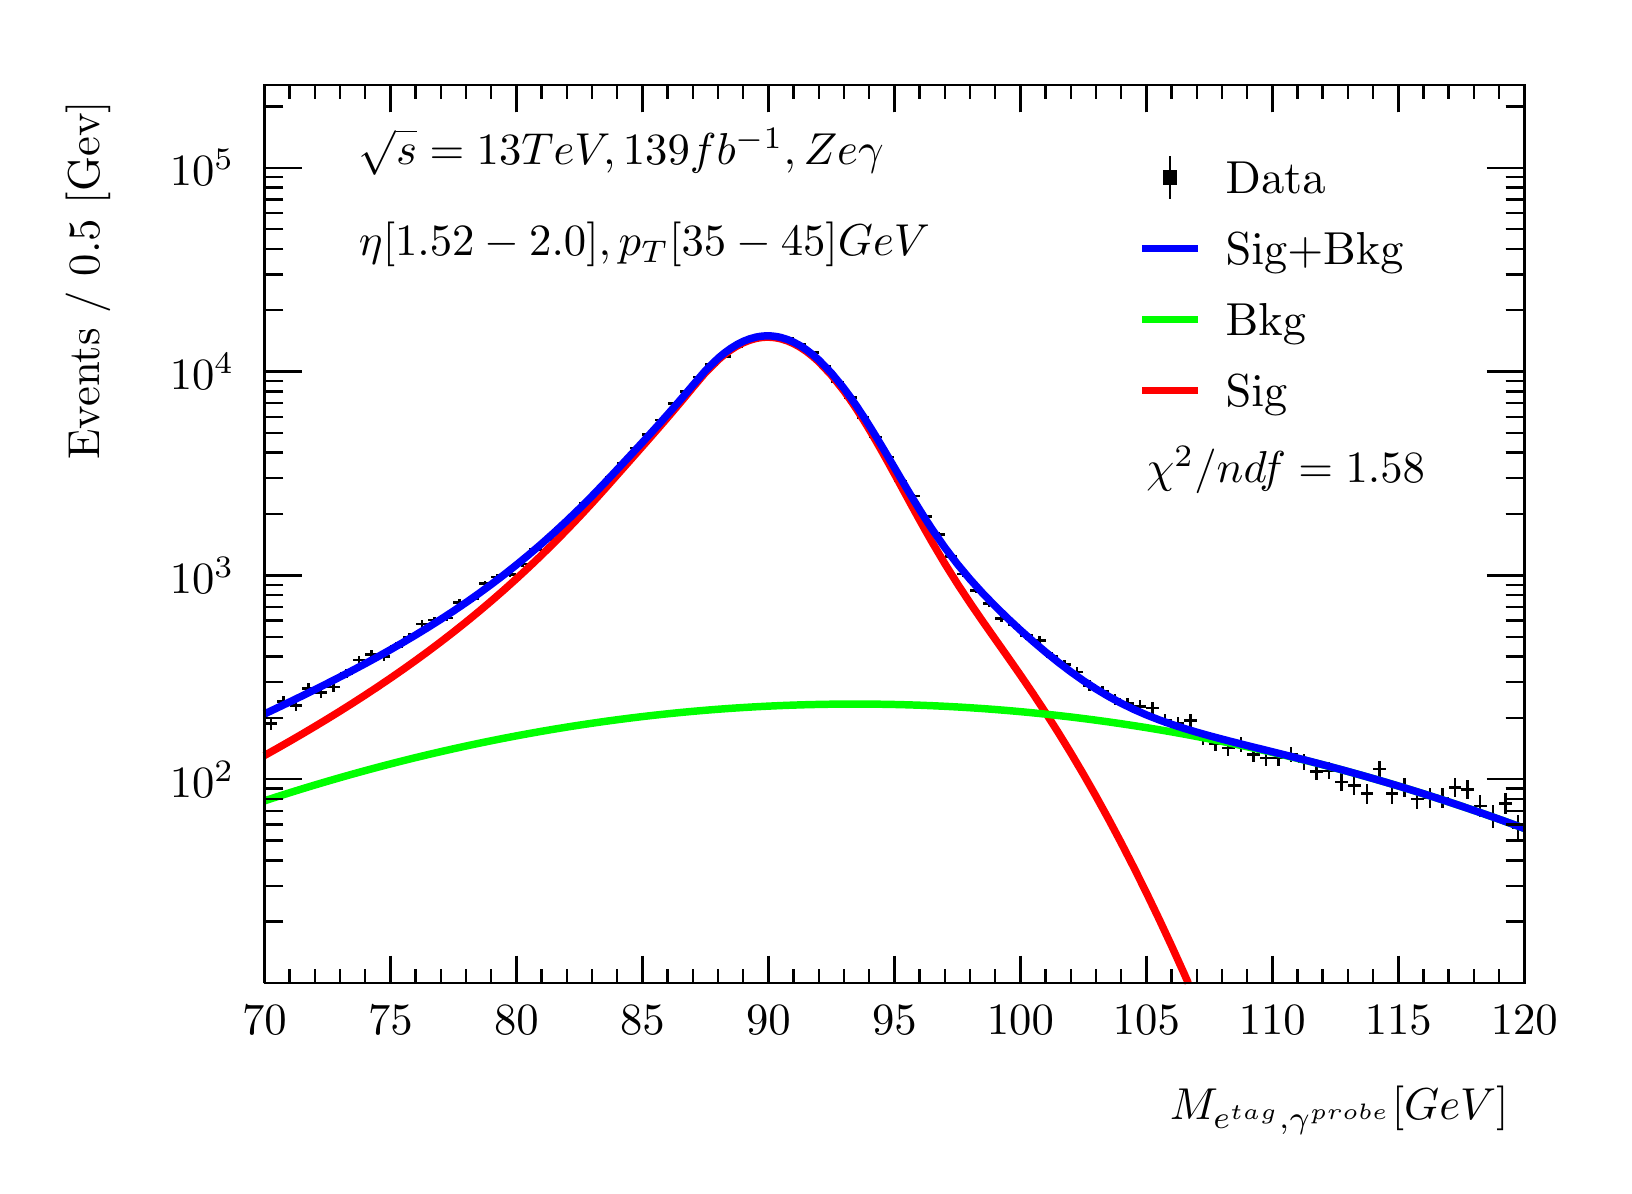
\begin{tikzpicture}
\pgfdeclareplotmark{cross} {
\pgfpathmoveto{\pgfpoint{-0.3\pgfplotmarksize}{\pgfplotmarksize}}
\pgfpathlineto{\pgfpoint{+0.3\pgfplotmarksize}{\pgfplotmarksize}}
\pgfpathlineto{\pgfpoint{+0.3\pgfplotmarksize}{0.3\pgfplotmarksize}}
\pgfpathlineto{\pgfpoint{+1\pgfplotmarksize}{0.3\pgfplotmarksize}}
\pgfpathlineto{\pgfpoint{+1\pgfplotmarksize}{-0.3\pgfplotmarksize}}
\pgfpathlineto{\pgfpoint{+0.3\pgfplotmarksize}{-0.3\pgfplotmarksize}}
\pgfpathlineto{\pgfpoint{+0.3\pgfplotmarksize}{-1.\pgfplotmarksize}}
\pgfpathlineto{\pgfpoint{-0.3\pgfplotmarksize}{-1.\pgfplotmarksize}}
\pgfpathlineto{\pgfpoint{-0.3\pgfplotmarksize}{-0.3\pgfplotmarksize}}
\pgfpathlineto{\pgfpoint{-1.\pgfplotmarksize}{-0.3\pgfplotmarksize}}
\pgfpathlineto{\pgfpoint{-1.\pgfplotmarksize}{0.3\pgfplotmarksize}}
\pgfpathlineto{\pgfpoint{-0.3\pgfplotmarksize}{0.3\pgfplotmarksize}}
\pgfpathclose
\pgfusepathqstroke
}
\pgfdeclareplotmark{cross*} {
\pgfpathmoveto{\pgfpoint{-0.3\pgfplotmarksize}{\pgfplotmarksize}}
\pgfpathlineto{\pgfpoint{+0.3\pgfplotmarksize}{\pgfplotmarksize}}
\pgfpathlineto{\pgfpoint{+0.3\pgfplotmarksize}{0.3\pgfplotmarksize}}
\pgfpathlineto{\pgfpoint{+1\pgfplotmarksize}{0.3\pgfplotmarksize}}
\pgfpathlineto{\pgfpoint{+1\pgfplotmarksize}{-0.3\pgfplotmarksize}}
\pgfpathlineto{\pgfpoint{+0.3\pgfplotmarksize}{-0.3\pgfplotmarksize}}
\pgfpathlineto{\pgfpoint{+0.3\pgfplotmarksize}{-1.\pgfplotmarksize}}
\pgfpathlineto{\pgfpoint{-0.3\pgfplotmarksize}{-1.\pgfplotmarksize}}
\pgfpathlineto{\pgfpoint{-0.3\pgfplotmarksize}{-0.3\pgfplotmarksize}}
\pgfpathlineto{\pgfpoint{-1.\pgfplotmarksize}{-0.3\pgfplotmarksize}}
\pgfpathlineto{\pgfpoint{-1.\pgfplotmarksize}{0.3\pgfplotmarksize}}
\pgfpathlineto{\pgfpoint{-0.3\pgfplotmarksize}{0.3\pgfplotmarksize}}
\pgfpathclose
\pgfusepathqfillstroke
}
\pgfdeclareplotmark{newstar} {
\pgfpathmoveto{\pgfqpoint{0pt}{\pgfplotmarksize}}
\pgfpathlineto{\pgfqpointpolar{44}{0.5\pgfplotmarksize}}
\pgfpathlineto{\pgfqpointpolar{18}{\pgfplotmarksize}}
\pgfpathlineto{\pgfqpointpolar{-20}{0.5\pgfplotmarksize}}
\pgfpathlineto{\pgfqpointpolar{-54}{\pgfplotmarksize}}
\pgfpathlineto{\pgfqpointpolar{-90}{0.5\pgfplotmarksize}}
\pgfpathlineto{\pgfqpointpolar{234}{\pgfplotmarksize}}
\pgfpathlineto{\pgfqpointpolar{198}{0.5\pgfplotmarksize}}
\pgfpathlineto{\pgfqpointpolar{162}{\pgfplotmarksize}}
\pgfpathlineto{\pgfqpointpolar{134}{0.5\pgfplotmarksize}}
\pgfpathclose
\pgfusepathqstroke
}
\pgfdeclareplotmark{newstar*} {
\pgfpathmoveto{\pgfqpoint{0pt}{\pgfplotmarksize}}
\pgfpathlineto{\pgfqpointpolar{44}{0.5\pgfplotmarksize}}
\pgfpathlineto{\pgfqpointpolar{18}{\pgfplotmarksize}}
\pgfpathlineto{\pgfqpointpolar{-20}{0.5\pgfplotmarksize}}
\pgfpathlineto{\pgfqpointpolar{-54}{\pgfplotmarksize}}
\pgfpathlineto{\pgfqpointpolar{-90}{0.5\pgfplotmarksize}}
\pgfpathlineto{\pgfqpointpolar{234}{\pgfplotmarksize}}
\pgfpathlineto{\pgfqpointpolar{198}{0.5\pgfplotmarksize}}
\pgfpathlineto{\pgfqpointpolar{162}{\pgfplotmarksize}}
\pgfpathlineto{\pgfqpointpolar{134}{0.5\pgfplotmarksize}}
\pgfpathclose
\pgfusepathqfillstroke
}
\definecolor{c}{rgb}{1,1,1};
\draw [color=c, fill=c] (0,0) rectangle (20,14.4361);
\draw [color=c, fill=c] (3,2.30977) rectangle (19,13.7143);
\definecolor{c}{rgb}{0,0,0};
\draw [c,line width=0.9] (3,2.30977) -- (3,13.7143) -- (19,13.7143) -- (19,2.30977) -- (3,2.30977);
\definecolor{c}{rgb}{1,1,1};
\draw [color=c, fill=c] (3,2.30977) rectangle (19,13.7143);
\definecolor{c}{rgb}{0,0,0};
\draw [c,line width=0.9] (3,2.30977) -- (3,13.7143) -- (19,13.7143) -- (19,2.30977) -- (3,2.30977);
\draw [c,line width=0.9] (3,2.30977) -- (19,2.30977);
\draw [c,line width=0.9] (3,2.65624) -- (3,2.30977);
\draw [c,line width=0.9] (3.32,2.48301) -- (3.32,2.30977);
\draw [c,line width=0.9] (3.64,2.48301) -- (3.64,2.30977);
\draw [c,line width=0.9] (3.96,2.48301) -- (3.96,2.30977);
\draw [c,line width=0.9] (4.28,2.48301) -- (4.28,2.30977);
\draw [c,line width=0.9] (4.6,2.65624) -- (4.6,2.30977);
\draw [c,line width=0.9] (4.92,2.48301) -- (4.92,2.30977);
\draw [c,line width=0.9] (5.24,2.48301) -- (5.24,2.30977);
\draw [c,line width=0.9] (5.56,2.48301) -- (5.56,2.30977);
\draw [c,line width=0.9] (5.88,2.48301) -- (5.88,2.30977);
\draw [c,line width=0.9] (6.2,2.65624) -- (6.2,2.30977);
\draw [c,line width=0.9] (6.52,2.48301) -- (6.52,2.30977);
\draw [c,line width=0.9] (6.84,2.48301) -- (6.84,2.30977);
\draw [c,line width=0.9] (7.16,2.48301) -- (7.16,2.30977);
\draw [c,line width=0.9] (7.48,2.48301) -- (7.48,2.30977);
\draw [c,line width=0.9] (7.8,2.65624) -- (7.8,2.30977);
\draw [c,line width=0.9] (8.12,2.48301) -- (8.12,2.30977);
\draw [c,line width=0.9] (8.44,2.48301) -- (8.44,2.30977);
\draw [c,line width=0.9] (8.76,2.48301) -- (8.76,2.30977);
\draw [c,line width=0.9] (9.08,2.48301) -- (9.08,2.30977);
\draw [c,line width=0.9] (9.4,2.65624) -- (9.4,2.30977);
\draw [c,line width=0.9] (9.72,2.48301) -- (9.72,2.30977);
\draw [c,line width=0.9] (10.04,2.48301) -- (10.04,2.30977);
\draw [c,line width=0.9] (10.36,2.48301) -- (10.36,2.30977);
\draw [c,line width=0.9] (10.68,2.48301) -- (10.68,2.30977);
\draw [c,line width=0.9] (11,2.65624) -- (11,2.30977);
\draw [c,line width=0.9] (11.32,2.48301) -- (11.32,2.30977);
\draw [c,line width=0.9] (11.64,2.48301) -- (11.64,2.30977);
\draw [c,line width=0.9] (11.96,2.48301) -- (11.96,2.30977);
\draw [c,line width=0.9] (12.28,2.48301) -- (12.28,2.30977);
\draw [c,line width=0.9] (12.6,2.65624) -- (12.6,2.30977);
\draw [c,line width=0.9] (12.92,2.48301) -- (12.92,2.30977);
\draw [c,line width=0.9] (13.24,2.48301) -- (13.24,2.30977);
\draw [c,line width=0.9] (13.56,2.48301) -- (13.56,2.30977);
\draw [c,line width=0.9] (13.88,2.48301) -- (13.88,2.30977);
\draw [c,line width=0.9] (14.2,2.65624) -- (14.2,2.30977);
\draw [c,line width=0.9] (14.52,2.48301) -- (14.52,2.30977);
\draw [c,line width=0.9] (14.84,2.48301) -- (14.84,2.30977);
\draw [c,line width=0.9] (15.16,2.48301) -- (15.16,2.30977);
\draw [c,line width=0.9] (15.48,2.48301) -- (15.48,2.30977);
\draw [c,line width=0.9] (15.8,2.65624) -- (15.8,2.30977);
\draw [c,line width=0.9] (16.12,2.48301) -- (16.12,2.30977);
\draw [c,line width=0.9] (16.44,2.48301) -- (16.44,2.30977);
\draw [c,line width=0.9] (16.76,2.48301) -- (16.76,2.30977);
\draw [c,line width=0.9] (17.08,2.48301) -- (17.08,2.30977);
\draw [c,line width=0.9] (17.4,2.65624) -- (17.4,2.30977);
\draw [c,line width=0.9] (17.72,2.48301) -- (17.72,2.30977);
\draw [c,line width=0.9] (18.04,2.48301) -- (18.04,2.30977);
\draw [c,line width=0.9] (18.36,2.48301) -- (18.36,2.30977);
\draw [c,line width=0.9] (18.68,2.48301) -- (18.68,2.30977);
\draw [c,line width=0.9] (19,2.65624) -- (19,2.30977);
\draw [anchor=base] (3,1.66015) node[scale=1.61424, color=c, rotate=0]{70};
\draw [anchor=base] (4.6,1.66015) node[scale=1.61424, color=c, rotate=0]{75};
\draw [anchor=base] (6.2,1.66015) node[scale=1.61424, color=c, rotate=0]{80};
\draw [anchor=base] (7.8,1.66015) node[scale=1.61424, color=c, rotate=0]{85};
\draw [anchor=base] (9.4,1.66015) node[scale=1.61424, color=c, rotate=0]{90};
\draw [anchor=base] (11,1.66015) node[scale=1.61424, color=c, rotate=0]{95};
\draw [anchor=base] (12.6,1.66015) node[scale=1.61424, color=c, rotate=0]{100};
\draw [anchor=base] (14.2,1.66015) node[scale=1.61424, color=c, rotate=0]{105};
\draw [anchor=base] (15.8,1.66015) node[scale=1.61424, color=c, rotate=0]{110};
\draw [anchor=base] (17.4,1.66015) node[scale=1.61424, color=c, rotate=0]{115};
\draw [anchor=base] (19,1.66015) node[scale=1.61424, color=c, rotate=0]{120};
\draw [anchor= east] (19,0.692932) node[scale=1.61424, color=c, rotate=0]{$M_{e^{tag}, \gamma^{probe}}  [GeV]$};
\draw [c,line width=0.9] (3,13.7143) -- (19,13.7143);
\draw [c,line width=0.9] (3,13.3678) -- (3,13.7143);
\draw [c,line width=0.9] (3.32,13.5411) -- (3.32,13.7143);
\draw [c,line width=0.9] (3.64,13.5411) -- (3.64,13.7143);
\draw [c,line width=0.9] (3.96,13.5411) -- (3.96,13.7143);
\draw [c,line width=0.9] (4.28,13.5411) -- (4.28,13.7143);
\draw [c,line width=0.9] (4.6,13.3678) -- (4.6,13.7143);
\draw [c,line width=0.9] (4.92,13.5411) -- (4.92,13.7143);
\draw [c,line width=0.9] (5.24,13.5411) -- (5.24,13.7143);
\draw [c,line width=0.9] (5.56,13.5411) -- (5.56,13.7143);
\draw [c,line width=0.9] (5.88,13.5411) -- (5.88,13.7143);
\draw [c,line width=0.9] (6.2,13.3678) -- (6.2,13.7143);
\draw [c,line width=0.9] (6.52,13.5411) -- (6.52,13.7143);
\draw [c,line width=0.9] (6.84,13.5411) -- (6.84,13.7143);
\draw [c,line width=0.9] (7.16,13.5411) -- (7.16,13.7143);
\draw [c,line width=0.9] (7.48,13.5411) -- (7.48,13.7143);
\draw [c,line width=0.9] (7.8,13.3678) -- (7.8,13.7143);
\draw [c,line width=0.9] (8.12,13.5411) -- (8.12,13.7143);
\draw [c,line width=0.9] (8.44,13.5411) -- (8.44,13.7143);
\draw [c,line width=0.9] (8.76,13.5411) -- (8.76,13.7143);
\draw [c,line width=0.9] (9.08,13.5411) -- (9.08,13.7143);
\draw [c,line width=0.9] (9.4,13.3678) -- (9.4,13.7143);
\draw [c,line width=0.9] (9.72,13.5411) -- (9.72,13.7143);
\draw [c,line width=0.9] (10.04,13.5411) -- (10.04,13.7143);
\draw [c,line width=0.9] (10.36,13.5411) -- (10.36,13.7143);
\draw [c,line width=0.9] (10.68,13.5411) -- (10.68,13.7143);
\draw [c,line width=0.9] (11,13.3678) -- (11,13.7143);
\draw [c,line width=0.9] (11.32,13.5411) -- (11.32,13.7143);
\draw [c,line width=0.9] (11.64,13.5411) -- (11.64,13.7143);
\draw [c,line width=0.9] (11.96,13.5411) -- (11.96,13.7143);
\draw [c,line width=0.9] (12.28,13.5411) -- (12.28,13.7143);
\draw [c,line width=0.9] (12.6,13.3678) -- (12.6,13.7143);
\draw [c,line width=0.9] (12.92,13.5411) -- (12.92,13.7143);
\draw [c,line width=0.9] (13.24,13.5411) -- (13.24,13.7143);
\draw [c,line width=0.9] (13.56,13.5411) -- (13.56,13.7143);
\draw [c,line width=0.9] (13.88,13.5411) -- (13.88,13.7143);
\draw [c,line width=0.9] (14.2,13.3678) -- (14.2,13.7143);
\draw [c,line width=0.9] (14.52,13.5411) -- (14.52,13.7143);
\draw [c,line width=0.9] (14.84,13.5411) -- (14.84,13.7143);
\draw [c,line width=0.9] (15.16,13.5411) -- (15.16,13.7143);
\draw [c,line width=0.9] (15.48,13.5411) -- (15.48,13.7143);
\draw [c,line width=0.9] (15.8,13.3678) -- (15.8,13.7143);
\draw [c,line width=0.9] (16.12,13.5411) -- (16.12,13.7143);
\draw [c,line width=0.9] (16.44,13.5411) -- (16.44,13.7143);
\draw [c,line width=0.9] (16.76,13.5411) -- (16.76,13.7143);
\draw [c,line width=0.9] (17.08,13.5411) -- (17.08,13.7143);
\draw [c,line width=0.9] (17.4,13.3678) -- (17.4,13.7143);
\draw [c,line width=0.9] (17.72,13.5411) -- (17.72,13.7143);
\draw [c,line width=0.9] (18.04,13.5411) -- (18.04,13.7143);
\draw [c,line width=0.9] (18.36,13.5411) -- (18.36,13.7143);
\draw [c,line width=0.9] (18.68,13.5411) -- (18.68,13.7143);
\draw [c,line width=0.9] (19,13.3678) -- (19,13.7143);
\draw [c,line width=0.9] (3,2.30977) -- (3,13.7143);
\draw [c,line width=0.9] (3.237,3.08897) -- (3,3.08897);
\draw [c,line width=0.9] (3.237,3.54477) -- (3,3.54477);
\draw [c,line width=0.9] (3.237,3.86817) -- (3,3.86817);
\draw [c,line width=0.9] (3.237,4.11902) -- (3,4.11902);
\draw [c,line width=0.9] (3.237,4.32397) -- (3,4.32397);
\draw [c,line width=0.9] (3.237,4.49726) -- (3,4.49726);
\draw [c,line width=0.9] (3.237,4.64737) -- (3,4.64737);
\draw [c,line width=0.9] (3.237,4.77978) -- (3,4.77978);
\draw [c,line width=0.9] (3.474,4.89822) -- (3,4.89822);
\draw [anchor= east] (2.82,4.89822) node[scale=1.61424, color=c, rotate=0]{$10^{2}$};
\draw [c,line width=0.9] (3.237,5.67742) -- (3,5.67742);
\draw [c,line width=0.9] (3.237,6.13322) -- (3,6.13322);
\draw [c,line width=0.9] (3.237,6.45661) -- (3,6.45661);
\draw [c,line width=0.9] (3.237,6.70746) -- (3,6.70746);
\draw [c,line width=0.9] (3.237,6.91242) -- (3,6.91242);
\draw [c,line width=0.9] (3.237,7.08571) -- (3,7.08571);
\draw [c,line width=0.9] (3.237,7.23581) -- (3,7.23581);
\draw [c,line width=0.9] (3.237,7.36822) -- (3,7.36822);
\draw [c,line width=0.9] (3.474,7.48666) -- (3,7.48666);
\draw [anchor= east] (2.82,7.48666) node[scale=1.61424, color=c, rotate=0]{$10^{3}$};
\draw [c,line width=0.9] (3.237,8.26586) -- (3,8.26586);
\draw [c,line width=0.9] (3.237,8.72166) -- (3,8.72166);
\draw [c,line width=0.9] (3.237,9.04506) -- (3,9.04506);
\draw [c,line width=0.9] (3.237,9.29591) -- (3,9.29591);
\draw [c,line width=0.9] (3.237,9.50086) -- (3,9.50086);
\draw [c,line width=0.9] (3.237,9.67415) -- (3,9.67415);
\draw [c,line width=0.9] (3.237,9.82426) -- (3,9.82426);
\draw [c,line width=0.9] (3.237,9.95666) -- (3,9.95666);
\draw [c,line width=0.9] (3.474,10.0751) -- (3,10.0751);
\draw [anchor= east] (2.82,10.0751) node[scale=1.61424, color=c, rotate=0]{$10^{4}$};
\draw [c,line width=0.9] (3.237,10.8543) -- (3,10.8543);
\draw [c,line width=0.9] (3.237,11.3101) -- (3,11.3101);
\draw [c,line width=0.9] (3.237,11.6335) -- (3,11.6335);
\draw [c,line width=0.9] (3.237,11.8844) -- (3,11.8844);
\draw [c,line width=0.9] (3.237,12.0893) -- (3,12.0893);
\draw [c,line width=0.9] (3.237,12.2626) -- (3,12.2626);
\draw [c,line width=0.9] (3.237,12.4127) -- (3,12.4127);
\draw [c,line width=0.9] (3.237,12.5451) -- (3,12.5451);
\draw [c,line width=0.9] (3.474,12.6635) -- (3,12.6635);
\draw [anchor= east] (2.82,12.6635) node[scale=1.61424, color=c, rotate=0]{$10^{5}$};
\draw [c,line width=0.9] (3.237,13.4427) -- (3,13.4427);
\draw [anchor= east] (0.76,13.7143) node[scale=1.61424, color=c, rotate=90]{Events / 0.5 [Gev]};
\draw [c,line width=0.9] (19,2.30977) -- (19,13.7143);
\draw [c,line width=0.9] (18.763,3.08897) -- (19,3.08897);
\draw [c,line width=0.9] (18.763,3.54477) -- (19,3.54477);
\draw [c,line width=0.9] (18.763,3.86817) -- (19,3.86817);
\draw [c,line width=0.9] (18.763,4.11902) -- (19,4.11902);
\draw [c,line width=0.9] (18.763,4.32397) -- (19,4.32397);
\draw [c,line width=0.9] (18.763,4.49726) -- (19,4.49726);
\draw [c,line width=0.9] (18.763,4.64737) -- (19,4.64737);
\draw [c,line width=0.9] (18.763,4.77978) -- (19,4.77978);
\draw [c,line width=0.9] (18.526,4.89822) -- (19,4.89822);
\draw [c,line width=0.9] (18.763,5.67742) -- (19,5.67742);
\draw [c,line width=0.9] (18.763,6.13322) -- (19,6.13322);
\draw [c,line width=0.9] (18.763,6.45661) -- (19,6.45661);
\draw [c,line width=0.9] (18.763,6.70746) -- (19,6.70746);
\draw [c,line width=0.9] (18.763,6.91242) -- (19,6.91242);
\draw [c,line width=0.9] (18.763,7.08571) -- (19,7.08571);
\draw [c,line width=0.9] (18.763,7.23581) -- (19,7.23581);
\draw [c,line width=0.9] (18.763,7.36822) -- (19,7.36822);
\draw [c,line width=0.9] (18.526,7.48666) -- (19,7.48666);
\draw [c,line width=0.9] (18.763,8.26586) -- (19,8.26586);
\draw [c,line width=0.9] (18.763,8.72166) -- (19,8.72166);
\draw [c,line width=0.9] (18.763,9.04506) -- (19,9.04506);
\draw [c,line width=0.9] (18.763,9.29591) -- (19,9.29591);
\draw [c,line width=0.9] (18.763,9.50086) -- (19,9.50086);
\draw [c,line width=0.9] (18.763,9.67415) -- (19,9.67415);
\draw [c,line width=0.9] (18.763,9.82426) -- (19,9.82426);
\draw [c,line width=0.9] (18.763,9.95666) -- (19,9.95666);
\draw [c,line width=0.9] (18.526,10.0751) -- (19,10.0751);
\draw [c,line width=0.9] (18.763,10.8543) -- (19,10.8543);
\draw [c,line width=0.9] (18.763,11.3101) -- (19,11.3101);
\draw [c,line width=0.9] (18.763,11.6335) -- (19,11.6335);
\draw [c,line width=0.9] (18.763,11.8844) -- (19,11.8844);
\draw [c,line width=0.9] (18.763,12.0893) -- (19,12.0893);
\draw [c,line width=0.9] (18.763,12.2626) -- (19,12.2626);
\draw [c,line width=0.9] (18.763,12.4127) -- (19,12.4127);
\draw [c,line width=0.9] (18.763,12.5451) -- (19,12.5451);
\draw [c,line width=0.9] (18.526,12.6635) -- (19,12.6635);
\draw [c,line width=0.9] (18.763,13.4427) -- (19,13.4427);
\draw [c,line width=0.9] (3.08,5.60786) -- (3,5.60786);
\draw [c,line width=0.9] (3,5.60786) -- (3,5.60786);
\draw [c,line width=0.9] (3.08,5.60786) -- (3.16,5.60786);
\draw [c,line width=0.9] (3.16,5.60786) -- (3.16,5.60786);
\draw [c,line width=0.9] (3.08,5.60786) -- (3.08,5.68983);
\draw [c,line width=0.9] (3.08,5.68983) -- (3.08,5.68983);
\draw [c,line width=0.9] (3.08,5.60786) -- (3.08,5.52589);
\draw [c,line width=0.9] (3.08,5.52589) -- (3.08,5.52589);
\draw [c,line width=0.9] (3.24,5.88705) -- (3.16,5.88705);
\draw [c,line width=0.9] (3.16,5.88705) -- (3.16,5.88705);
\draw [c,line width=0.9] (3.24,5.88705) -- (3.32,5.88705);
\draw [c,line width=0.9] (3.32,5.88705) -- (3.32,5.88705);
\draw [c,line width=0.9] (3.24,5.88705) -- (3.24,5.95945);
\draw [c,line width=0.9] (3.24,5.95945) -- (3.24,5.95945);
\draw [c,line width=0.9] (3.24,5.88705) -- (3.24,5.81465);
\draw [c,line width=0.9] (3.24,5.81465) -- (3.24,5.81465);
\draw [c,line width=0.9] (3.4,5.83453) -- (3.32,5.83453);
\draw [c,line width=0.9] (3.32,5.83453) -- (3.32,5.83453);
\draw [c,line width=0.9] (3.4,5.83453) -- (3.48,5.83453);
\draw [c,line width=0.9] (3.48,5.83453) -- (3.48,5.83453);
\draw [c,line width=0.9] (3.4,5.83453) -- (3.4,5.90864);
\draw [c,line width=0.9] (3.4,5.90864) -- (3.4,5.90864);
\draw [c,line width=0.9] (3.4,5.83453) -- (3.4,5.76042);
\draw [c,line width=0.9] (3.4,5.76042) -- (3.4,5.76042);
\draw [c,line width=0.9] (3.56,6.0476) -- (3.48,6.0476);
\draw [c,line width=0.9] (3.48,6.0476) -- (3.48,6.0476);
\draw [c,line width=0.9] (3.56,6.0476) -- (3.64,6.0476);
\draw [c,line width=0.9] (3.64,6.0476) -- (3.64,6.0476);
\draw [c,line width=0.9] (3.56,6.0476) -- (3.56,6.11502);
\draw [c,line width=0.9] (3.56,6.11502) -- (3.56,6.11502);
\draw [c,line width=0.9] (3.56,6.0476) -- (3.56,5.98019);
\draw [c,line width=0.9] (3.56,5.98019) -- (3.56,5.98019);
\draw [c,line width=0.9] (3.72,6.00222) -- (3.64,6.00222);
\draw [c,line width=0.9] (3.64,6.00222) -- (3.64,6.00222);
\draw [c,line width=0.9] (3.72,6.00222) -- (3.8,6.00222);
\draw [c,line width=0.9] (3.8,6.00222) -- (3.8,6.00222);
\draw [c,line width=0.9] (3.72,6.00222) -- (3.72,6.071);
\draw [c,line width=0.9] (3.72,6.071) -- (3.72,6.071);
\draw [c,line width=0.9] (3.72,6.00222) -- (3.72,5.93343);
\draw [c,line width=0.9] (3.72,5.93343) -- (3.72,5.93343);
\draw [c,line width=0.9] (3.88,6.07161) -- (3.8,6.07161);
\draw [c,line width=0.9] (3.8,6.07161) -- (3.8,6.07161);
\draw [c,line width=0.9] (3.88,6.07161) -- (3.96,6.07161);
\draw [c,line width=0.9] (3.96,6.07161) -- (3.96,6.07161);
\draw [c,line width=0.9] (3.88,6.07161) -- (3.88,6.1383);
\draw [c,line width=0.9] (3.88,6.1383) -- (3.88,6.1383);
\draw [c,line width=0.9] (3.88,6.07161) -- (3.88,6.00491);
\draw [c,line width=0.9] (3.88,6.00491) -- (3.88,6.00491);
\draw [c,line width=0.9] (4.04,6.24036) -- (3.96,6.24036);
\draw [c,line width=0.9] (3.96,6.24036) -- (3.96,6.24036);
\draw [c,line width=0.9] (4.04,6.24036) -- (4.12,6.24036);
\draw [c,line width=0.9] (4.12,6.24036) -- (4.12,6.24036);
\draw [c,line width=0.9] (4.04,6.24036) -- (4.04,6.30224);
\draw [c,line width=0.9] (4.04,6.30224) -- (4.04,6.30224);
\draw [c,line width=0.9] (4.04,6.24036) -- (4.04,6.17849);
\draw [c,line width=0.9] (4.04,6.17849) -- (4.04,6.17849);
\draw [c,line width=0.9] (4.2,6.41073) -- (4.12,6.41073);
\draw [c,line width=0.9] (4.12,6.41073) -- (4.12,6.41073);
\draw [c,line width=0.9] (4.2,6.41073) -- (4.28,6.41073);
\draw [c,line width=0.9] (4.28,6.41073) -- (4.28,6.41073);
\draw [c,line width=0.9] (4.2,6.41073) -- (4.2,6.46809);
\draw [c,line width=0.9] (4.2,6.46809) -- (4.2,6.46809);
\draw [c,line width=0.9] (4.2,6.41073) -- (4.2,6.35337);
\draw [c,line width=0.9] (4.2,6.35337) -- (4.2,6.35337);
\draw [c,line width=0.9] (4.36,6.48163) -- (4.28,6.48163);
\draw [c,line width=0.9] (4.28,6.48163) -- (4.28,6.48163);
\draw [c,line width=0.9] (4.36,6.48163) -- (4.44,6.48163);
\draw [c,line width=0.9] (4.44,6.48163) -- (4.44,6.48163);
\draw [c,line width=0.9] (4.36,6.48163) -- (4.36,6.53721);
\draw [c,line width=0.9] (4.36,6.53721) -- (4.36,6.53721);
\draw [c,line width=0.9] (4.36,6.48163) -- (4.36,6.42605);
\draw [c,line width=0.9] (4.36,6.42605) -- (4.36,6.42605);
\draw [c,line width=0.9] (4.52,6.45662) -- (4.44,6.45662);
\draw [c,line width=0.9] (4.44,6.45662) -- (4.44,6.45662);
\draw [c,line width=0.9] (4.52,6.45662) -- (4.6,6.45662);
\draw [c,line width=0.9] (4.6,6.45662) -- (4.6,6.45662);
\draw [c,line width=0.9] (4.52,6.45662) -- (4.52,6.51282);
\draw [c,line width=0.9] (4.52,6.51282) -- (4.52,6.51282);
\draw [c,line width=0.9] (4.52,6.45662) -- (4.52,6.40042);
\draw [c,line width=0.9] (4.52,6.40042) -- (4.52,6.40042);
\draw [c,line width=0.9] (4.68,6.58652) -- (4.6,6.58652);
\draw [c,line width=0.9] (4.6,6.58652) -- (4.6,6.58652);
\draw [c,line width=0.9] (4.68,6.58652) -- (4.76,6.58652);
\draw [c,line width=0.9] (4.76,6.58652) -- (4.76,6.58652);
\draw [c,line width=0.9] (4.68,6.58652) -- (4.68,6.63957);
\draw [c,line width=0.9] (4.68,6.63957) -- (4.68,6.63957);
\draw [c,line width=0.9] (4.68,6.58652) -- (4.68,6.53347);
\draw [c,line width=0.9] (4.68,6.53347) -- (4.68,6.53347);
\draw [c,line width=0.9] (4.84,6.7007) -- (4.76,6.7007);
\draw [c,line width=0.9] (4.76,6.7007) -- (4.76,6.7007);
\draw [c,line width=0.9] (4.84,6.7007) -- (4.92,6.7007);
\draw [c,line width=0.9] (4.92,6.7007) -- (4.92,6.7007);
\draw [c,line width=0.9] (4.84,6.7007) -- (4.84,6.75112);
\draw [c,line width=0.9] (4.84,6.75112) -- (4.84,6.75112);
\draw [c,line width=0.9] (4.84,6.7007) -- (4.84,6.65028);
\draw [c,line width=0.9] (4.84,6.65028) -- (4.84,6.65028);
\draw [c,line width=0.9] (5,6.86848) -- (4.92,6.86848);
\draw [c,line width=0.9] (4.92,6.86848) -- (4.92,6.86848);
\draw [c,line width=0.9] (5,6.86848) -- (5.08,6.86848);
\draw [c,line width=0.9] (5.08,6.86848) -- (5.08,6.86848);
\draw [c,line width=0.9] (5,6.86848) -- (5,6.91527);
\draw [c,line width=0.9] (5,6.91527) -- (5,6.91527);
\draw [c,line width=0.9] (5,6.86848) -- (5,6.82168);
\draw [c,line width=0.9] (5,6.82168) -- (5,6.82168);
\draw [c,line width=0.9] (5.16,6.91803) -- (5.08,6.91803);
\draw [c,line width=0.9] (5.08,6.91803) -- (5.08,6.91803);
\draw [c,line width=0.9] (5.16,6.91803) -- (5.24,6.91803);
\draw [c,line width=0.9] (5.24,6.91803) -- (5.24,6.91803);
\draw [c,line width=0.9] (5.16,6.91803) -- (5.16,6.9638);
\draw [c,line width=0.9] (5.16,6.9638) -- (5.16,6.9638);
\draw [c,line width=0.9] (5.16,6.91803) -- (5.16,6.87225);
\draw [c,line width=0.9] (5.16,6.87225) -- (5.16,6.87225);
\draw [c,line width=0.9] (5.32,6.94746) -- (5.24,6.94746);
\draw [c,line width=0.9] (5.24,6.94746) -- (5.24,6.94746);
\draw [c,line width=0.9] (5.32,6.94746) -- (5.4,6.94746);
\draw [c,line width=0.9] (5.4,6.94746) -- (5.4,6.94746);
\draw [c,line width=0.9] (5.32,6.94746) -- (5.32,6.99265);
\draw [c,line width=0.9] (5.32,6.99265) -- (5.32,6.99265);
\draw [c,line width=0.9] (5.32,6.94746) -- (5.32,6.90229);
\draw [c,line width=0.9] (5.32,6.90229) -- (5.32,6.90229);
\draw [c,line width=0.9] (5.48,7.14208) -- (5.4,7.14208);
\draw [c,line width=0.9] (5.4,7.14208) -- (5.4,7.14208);
\draw [c,line width=0.9] (5.48,7.14208) -- (5.56,7.14208);
\draw [c,line width=0.9] (5.56,7.14208) -- (5.56,7.14208);
\draw [c,line width=0.9] (5.48,7.14208) -- (5.48,7.18352);
\draw [c,line width=0.9] (5.48,7.18352) -- (5.48,7.18352);
\draw [c,line width=0.9] (5.48,7.14208) -- (5.48,7.10065);
\draw [c,line width=0.9] (5.48,7.10065) -- (5.48,7.10065);
\draw [c,line width=0.9] (5.64,7.18553) -- (5.56,7.18553);
\draw [c,line width=0.9] (5.56,7.18553) -- (5.56,7.18553);
\draw [c,line width=0.9] (5.64,7.18553) -- (5.72,7.18553);
\draw [c,line width=0.9] (5.72,7.18553) -- (5.72,7.18553);
\draw [c,line width=0.9] (5.64,7.18553) -- (5.64,7.22617);
\draw [c,line width=0.9] (5.64,7.22617) -- (5.64,7.22617);
\draw [c,line width=0.9] (5.64,7.18553) -- (5.64,7.14489);
\draw [c,line width=0.9] (5.64,7.14489) -- (5.64,7.14489);
\draw [c,line width=0.9] (5.8,7.38311) -- (5.72,7.38311);
\draw [c,line width=0.9] (5.72,7.38311) -- (5.72,7.38311);
\draw [c,line width=0.9] (5.8,7.38311) -- (5.88,7.38311);
\draw [c,line width=0.9] (5.88,7.38311) -- (5.88,7.38311);
\draw [c,line width=0.9] (5.8,7.38311) -- (5.8,7.42033);
\draw [c,line width=0.9] (5.8,7.42033) -- (5.8,7.42033);
\draw [c,line width=0.9] (5.8,7.38311) -- (5.8,7.34589);
\draw [c,line width=0.9] (5.8,7.34589) -- (5.8,7.34589);
\draw [c,line width=0.9] (5.96,7.46624) -- (5.88,7.46624);
\draw [c,line width=0.9] (5.88,7.46624) -- (5.88,7.46624);
\draw [c,line width=0.9] (5.96,7.46624) -- (6.04,7.46624);
\draw [c,line width=0.9] (6.04,7.46624) -- (6.04,7.46624);
\draw [c,line width=0.9] (5.96,7.46624) -- (5.96,7.50211);
\draw [c,line width=0.9] (5.96,7.50211) -- (5.96,7.50211);
\draw [c,line width=0.9] (5.96,7.46624) -- (5.96,7.43037);
\draw [c,line width=0.9] (5.96,7.43037) -- (5.96,7.43037);
\draw [c,line width=0.9] (6.12,7.50007) -- (6.04,7.50007);
\draw [c,line width=0.9] (6.04,7.50007) -- (6.04,7.50007);
\draw [c,line width=0.9] (6.12,7.50007) -- (6.2,7.50007);
\draw [c,line width=0.9] (6.2,7.50007) -- (6.2,7.50007);
\draw [c,line width=0.9] (6.12,7.50007) -- (6.12,7.53541);
\draw [c,line width=0.9] (6.12,7.53541) -- (6.12,7.53541);
\draw [c,line width=0.9] (6.12,7.50007) -- (6.12,7.46474);
\draw [c,line width=0.9] (6.12,7.46474) -- (6.12,7.46474);
\draw [c,line width=0.9] (6.28,7.63198) -- (6.2,7.63198);
\draw [c,line width=0.9] (6.2,7.63198) -- (6.2,7.63198);
\draw [c,line width=0.9] (6.28,7.63198) -- (6.36,7.63198);
\draw [c,line width=0.9] (6.36,7.63198) -- (6.36,7.63198);
\draw [c,line width=0.9] (6.28,7.63198) -- (6.28,7.66531);
\draw [c,line width=0.9] (6.28,7.66531) -- (6.28,7.66531);
\draw [c,line width=0.9] (6.28,7.63198) -- (6.28,7.59866);
\draw [c,line width=0.9] (6.28,7.59866) -- (6.28,7.59866);
\draw [c,line width=0.9] (6.44,7.81567) -- (6.36,7.81567);
\draw [c,line width=0.9] (6.36,7.81567) -- (6.36,7.81567);
\draw [c,line width=0.9] (6.44,7.81567) -- (6.52,7.81567);
\draw [c,line width=0.9] (6.52,7.81567) -- (6.52,7.81567);
\draw [c,line width=0.9] (6.44,7.81567) -- (6.44,7.84637);
\draw [c,line width=0.9] (6.44,7.84637) -- (6.44,7.84637);
\draw [c,line width=0.9] (6.44,7.81567) -- (6.44,7.78496);
\draw [c,line width=0.9] (6.44,7.78496) -- (6.44,7.78496);
\draw [c,line width=0.9] (6.6,7.94546) -- (6.52,7.94546);
\draw [c,line width=0.9] (6.52,7.94546) -- (6.52,7.94546);
\draw [c,line width=0.9] (6.6,7.94546) -- (6.68,7.94546);
\draw [c,line width=0.9] (6.68,7.94546) -- (6.68,7.94546);
\draw [c,line width=0.9] (6.6,7.94546) -- (6.6,7.97444);
\draw [c,line width=0.9] (6.6,7.97444) -- (6.6,7.97444);
\draw [c,line width=0.9] (6.6,7.94546) -- (6.6,7.91647);
\draw [c,line width=0.9] (6.6,7.91647) -- (6.6,7.91647);
\draw [c,line width=0.9] (6.76,8.08449) -- (6.68,8.08449);
\draw [c,line width=0.9] (6.68,8.08449) -- (6.68,8.08449);
\draw [c,line width=0.9] (6.76,8.08449) -- (6.84,8.08449);
\draw [c,line width=0.9] (6.84,8.08449) -- (6.84,8.08449);
\draw [c,line width=0.9] (6.76,8.08449) -- (6.76,8.11174);
\draw [c,line width=0.9] (6.76,8.11174) -- (6.76,8.11174);
\draw [c,line width=0.9] (6.76,8.08449) -- (6.76,8.05724);
\draw [c,line width=0.9] (6.76,8.05724) -- (6.76,8.05724);
\draw [c,line width=0.9] (6.92,8.20702) -- (6.84,8.20702);
\draw [c,line width=0.9] (6.84,8.20702) -- (6.84,8.20702);
\draw [c,line width=0.9] (6.92,8.20702) -- (7,8.20702);
\draw [c,line width=0.9] (7,8.20702) -- (7,8.20702);
\draw [c,line width=0.9] (6.92,8.20702) -- (6.92,8.23282);
\draw [c,line width=0.9] (6.92,8.23282) -- (6.92,8.23282);
\draw [c,line width=0.9] (6.92,8.20702) -- (6.92,8.18121);
\draw [c,line width=0.9] (6.92,8.18121) -- (6.92,8.18121);
\draw [c,line width=0.9] (7.08,8.40623) -- (7,8.40623);
\draw [c,line width=0.9] (7,8.40623) -- (7,8.40623);
\draw [c,line width=0.9] (7.08,8.40623) -- (7.16,8.40623);
\draw [c,line width=0.9] (7.16,8.40623) -- (7.16,8.40623);
\draw [c,line width=0.9] (7.08,8.40623) -- (7.08,8.42985);
\draw [c,line width=0.9] (7.08,8.42985) -- (7.08,8.42985);
\draw [c,line width=0.9] (7.08,8.40623) -- (7.08,8.38262);
\draw [c,line width=0.9] (7.08,8.38262) -- (7.08,8.38262);
\draw [c,line width=0.9] (7.24,8.54249) -- (7.16,8.54249);
\draw [c,line width=0.9] (7.16,8.54249) -- (7.16,8.54249);
\draw [c,line width=0.9] (7.24,8.54249) -- (7.32,8.54249);
\draw [c,line width=0.9] (7.32,8.54249) -- (7.32,8.54249);
\draw [c,line width=0.9] (7.24,8.54249) -- (7.24,8.56472);
\draw [c,line width=0.9] (7.24,8.56472) -- (7.24,8.56472);
\draw [c,line width=0.9] (7.24,8.54249) -- (7.24,8.52026);
\draw [c,line width=0.9] (7.24,8.52026) -- (7.24,8.52026);
\draw [c,line width=0.9] (7.4,8.73433) -- (7.32,8.73433);
\draw [c,line width=0.9] (7.32,8.73433) -- (7.32,8.73433);
\draw [c,line width=0.9] (7.4,8.73433) -- (7.48,8.73433);
\draw [c,line width=0.9] (7.48,8.73433) -- (7.48,8.73433);
\draw [c,line width=0.9] (7.4,8.73433) -- (7.4,8.75474);
\draw [c,line width=0.9] (7.4,8.75474) -- (7.4,8.75474);
\draw [c,line width=0.9] (7.4,8.73433) -- (7.4,8.71392);
\draw [c,line width=0.9] (7.4,8.71392) -- (7.4,8.71392);
\draw [c,line width=0.9] (7.56,8.91658) -- (7.48,8.91658);
\draw [c,line width=0.9] (7.48,8.91658) -- (7.48,8.91658);
\draw [c,line width=0.9] (7.56,8.91658) -- (7.64,8.91658);
\draw [c,line width=0.9] (7.64,8.91658) -- (7.64,8.91658);
\draw [c,line width=0.9] (7.56,8.91658) -- (7.56,8.9354);
\draw [c,line width=0.9] (7.56,8.9354) -- (7.56,8.9354);
\draw [c,line width=0.9] (7.56,8.91658) -- (7.56,8.89776);
\draw [c,line width=0.9] (7.56,8.89776) -- (7.56,8.89776);
\draw [c,line width=0.9] (7.72,9.10685) -- (7.64,9.10685);
\draw [c,line width=0.9] (7.64,9.10685) -- (7.64,9.10685);
\draw [c,line width=0.9] (7.72,9.10685) -- (7.8,9.10685);
\draw [c,line width=0.9] (7.8,9.10685) -- (7.8,9.10685);
\draw [c,line width=0.9] (7.72,9.10685) -- (7.72,9.12414);
\draw [c,line width=0.9] (7.72,9.12414) -- (7.72,9.12414);
\draw [c,line width=0.9] (7.72,9.10685) -- (7.72,9.08955);
\draw [c,line width=0.9] (7.72,9.08955) -- (7.72,9.08955);
\draw [c,line width=0.9] (7.88,9.2764) -- (7.8,9.2764);
\draw [c,line width=0.9] (7.8,9.2764) -- (7.8,9.2764);
\draw [c,line width=0.9] (7.88,9.2764) -- (7.96,9.2764);
\draw [c,line width=0.9] (7.96,9.2764) -- (7.96,9.2764);
\draw [c,line width=0.9] (7.88,9.2764) -- (7.88,9.29244);
\draw [c,line width=0.9] (7.88,9.29244) -- (7.88,9.29244);
\draw [c,line width=0.9] (7.88,9.2764) -- (7.88,9.26037);
\draw [c,line width=0.9] (7.88,9.26037) -- (7.88,9.26037);
\draw [c,line width=0.9] (8.04,9.46353) -- (7.96,9.46353);
\draw [c,line width=0.9] (7.96,9.46353) -- (7.96,9.46353);
\draw [c,line width=0.9] (8.04,9.46353) -- (8.12,9.46353);
\draw [c,line width=0.9] (8.12,9.46353) -- (8.12,9.46353);
\draw [c,line width=0.9] (8.04,9.46353) -- (8.04,9.47828);
\draw [c,line width=0.9] (8.04,9.47828) -- (8.04,9.47828);
\draw [c,line width=0.9] (8.04,9.46353) -- (8.04,9.44877);
\draw [c,line width=0.9] (8.04,9.44877) -- (8.04,9.44877);
\draw [c,line width=0.9] (8.2,9.66965) -- (8.12,9.66965);
\draw [c,line width=0.9] (8.12,9.66965) -- (8.12,9.66965);
\draw [c,line width=0.9] (8.2,9.66965) -- (8.28,9.66965);
\draw [c,line width=0.9] (8.28,9.66965) -- (8.28,9.66965);
\draw [c,line width=0.9] (8.2,9.66965) -- (8.2,9.68311);
\draw [c,line width=0.9] (8.2,9.68311) -- (8.2,9.68311);
\draw [c,line width=0.9] (8.2,9.66965) -- (8.2,9.65618);
\draw [c,line width=0.9] (8.2,9.65618) -- (8.2,9.65618);
\draw [c,line width=0.9] (8.36,9.81961) -- (8.28,9.81961);
\draw [c,line width=0.9] (8.28,9.81961) -- (8.28,9.81961);
\draw [c,line width=0.9] (8.36,9.81961) -- (8.44,9.81961);
\draw [c,line width=0.9] (8.44,9.81961) -- (8.44,9.81961);
\draw [c,line width=0.9] (8.36,9.81961) -- (8.36,9.83221);
\draw [c,line width=0.9] (8.36,9.83221) -- (8.36,9.83221);
\draw [c,line width=0.9] (8.36,9.81961) -- (8.36,9.80702);
\draw [c,line width=0.9] (8.36,9.80702) -- (8.36,9.80702);
\draw [c,line width=0.9] (8.52,10.0089) -- (8.44,10.0089);
\draw [c,line width=0.9] (8.44,10.0089) -- (8.44,10.0089);
\draw [c,line width=0.9] (8.52,10.0089) -- (8.6,10.0089);
\draw [c,line width=0.9] (8.6,10.0089) -- (8.6,10.0089);
\draw [c,line width=0.9] (8.52,10.0089) -- (8.52,10.0205);
\draw [c,line width=0.9] (8.52,10.0205) -- (8.52,10.0205);
\draw [c,line width=0.9] (8.52,10.0089) -- (8.52,9.99732);
\draw [c,line width=0.9] (8.52,9.99732) -- (8.52,9.99732);
\draw [c,line width=0.9] (8.68,10.1651) -- (8.6,10.1651);
\draw [c,line width=0.9] (8.6,10.1651) -- (8.6,10.1651);
\draw [c,line width=0.9] (8.68,10.1651) -- (8.76,10.1651);
\draw [c,line width=0.9] (8.76,10.1651) -- (8.76,10.1651);
\draw [c,line width=0.9] (8.68,10.1651) -- (8.68,10.1759);
\draw [c,line width=0.9] (8.68,10.1759) -- (8.68,10.1759);
\draw [c,line width=0.9] (8.68,10.1651) -- (8.68,10.1543);
\draw [c,line width=0.9] (8.68,10.1543) -- (8.68,10.1543);
\draw [c,line width=0.9] (8.84,10.2686) -- (8.76,10.2686);
\draw [c,line width=0.9] (8.76,10.2686) -- (8.76,10.2686);
\draw [c,line width=0.9] (8.84,10.2686) -- (8.92,10.2686);
\draw [c,line width=0.9] (8.92,10.2686) -- (8.92,10.2686);
\draw [c,line width=0.9] (8.84,10.2686) -- (8.84,10.2789);
\draw [c,line width=0.9] (8.84,10.2789) -- (8.84,10.2789);
\draw [c,line width=0.9] (8.84,10.2686) -- (8.84,10.2583);
\draw [c,line width=0.9] (8.84,10.2583) -- (8.84,10.2583);
\draw [c,line width=0.9] (9,10.3901) -- (8.92,10.3901);
\draw [c,line width=0.9] (8.92,10.3901) -- (8.92,10.3901);
\draw [c,line width=0.9] (9,10.3901) -- (9.08,10.3901);
\draw [c,line width=0.9] (9.08,10.3901) -- (9.08,10.3901);
\draw [c,line width=0.9] (9,10.3901) -- (9,10.3999);
\draw [c,line width=0.9] (9,10.3999) -- (9,10.3999);
\draw [c,line width=0.9] (9,10.3901) -- (9,10.3803);
\draw [c,line width=0.9] (9,10.3803) -- (9,10.3803);
\draw [c,line width=0.9] (9.16,10.4905) -- (9.08,10.4905);
\draw [c,line width=0.9] (9.08,10.4905) -- (9.08,10.4905);
\draw [c,line width=0.9] (9.16,10.4905) -- (9.24,10.4905);
\draw [c,line width=0.9] (9.24,10.4905) -- (9.24,10.4905);
\draw [c,line width=0.9] (9.16,10.4905) -- (9.16,10.4999);
\draw [c,line width=0.9] (9.16,10.4999) -- (9.16,10.4999);
\draw [c,line width=0.9] (9.16,10.4905) -- (9.16,10.4812);
\draw [c,line width=0.9] (9.16,10.4812) -- (9.16,10.4812);
\draw [c,line width=0.9] (9.32,10.5141) -- (9.24,10.5141);
\draw [c,line width=0.9] (9.24,10.5141) -- (9.24,10.5141);
\draw [c,line width=0.9] (9.32,10.5141) -- (9.4,10.5141);
\draw [c,line width=0.9] (9.4,10.5141) -- (9.4,10.5141);
\draw [c,line width=0.9] (9.32,10.5141) -- (9.32,10.5233);
\draw [c,line width=0.9] (9.32,10.5233) -- (9.32,10.5233);
\draw [c,line width=0.9] (9.32,10.5141) -- (9.32,10.5048);
\draw [c,line width=0.9] (9.32,10.5048) -- (9.32,10.5048);
\draw [c,line width=0.9] (9.48,10.5299) -- (9.4,10.5299);
\draw [c,line width=0.9] (9.4,10.5299) -- (9.4,10.5299);
\draw [c,line width=0.9] (9.48,10.5299) -- (9.56,10.5299);
\draw [c,line width=0.9] (9.56,10.5299) -- (9.56,10.5299);
\draw [c,line width=0.9] (9.48,10.5299) -- (9.48,10.539);
\draw [c,line width=0.9] (9.48,10.539) -- (9.48,10.539);
\draw [c,line width=0.9] (9.48,10.5299) -- (9.48,10.5207);
\draw [c,line width=0.9] (9.48,10.5207) -- (9.48,10.5207);
\draw [c,line width=0.9] (9.64,10.5033) -- (9.56,10.5033);
\draw [c,line width=0.9] (9.56,10.5033) -- (9.56,10.5033);
\draw [c,line width=0.9] (9.64,10.5033) -- (9.72,10.5033);
\draw [c,line width=0.9] (9.72,10.5033) -- (9.72,10.5033);
\draw [c,line width=0.9] (9.64,10.5033) -- (9.64,10.5126);
\draw [c,line width=0.9] (9.64,10.5126) -- (9.64,10.5126);
\draw [c,line width=0.9] (9.64,10.5033) -- (9.64,10.494);
\draw [c,line width=0.9] (9.64,10.494) -- (9.64,10.494);
\draw [c,line width=0.9] (9.8,10.4253) -- (9.72,10.4253);
\draw [c,line width=0.9] (9.72,10.4253) -- (9.72,10.4253);
\draw [c,line width=0.9] (9.8,10.4253) -- (9.88,10.4253);
\draw [c,line width=0.9] (9.88,10.4253) -- (9.88,10.4253);
\draw [c,line width=0.9] (9.8,10.4253) -- (9.8,10.4349);
\draw [c,line width=0.9] (9.8,10.4349) -- (9.8,10.4349);
\draw [c,line width=0.9] (9.8,10.4253) -- (9.8,10.4157);
\draw [c,line width=0.9] (9.8,10.4157) -- (9.8,10.4157);
\draw [c,line width=0.9] (9.96,10.3186) -- (9.88,10.3186);
\draw [c,line width=0.9] (9.88,10.3186) -- (9.88,10.3186);
\draw [c,line width=0.9] (9.96,10.3186) -- (10.04,10.3186);
\draw [c,line width=0.9] (10.04,10.3186) -- (10.04,10.3186);
\draw [c,line width=0.9] (9.96,10.3186) -- (9.96,10.3286);
\draw [c,line width=0.9] (9.96,10.3286) -- (9.96,10.3286);
\draw [c,line width=0.9] (9.96,10.3186) -- (9.96,10.3085);
\draw [c,line width=0.9] (9.96,10.3085) -- (9.96,10.3085);
\draw [c,line width=0.9] (10.12,10.1425) -- (10.04,10.1425);
\draw [c,line width=0.9] (10.04,10.1425) -- (10.04,10.1425);
\draw [c,line width=0.9] (10.12,10.1425) -- (10.2,10.1425);
\draw [c,line width=0.9] (10.2,10.1425) -- (10.2,10.1425);
\draw [c,line width=0.9] (10.12,10.1425) -- (10.12,10.1534);
\draw [c,line width=0.9] (10.12,10.1534) -- (10.12,10.1534);
\draw [c,line width=0.9] (10.12,10.1425) -- (10.12,10.1316);
\draw [c,line width=0.9] (10.12,10.1316) -- (10.12,10.1316);
\draw [c,line width=0.9] (10.28,9.94385) -- (10.2,9.94385);
\draw [c,line width=0.9] (10.2,9.94385) -- (10.2,9.94385);
\draw [c,line width=0.9] (10.28,9.94385) -- (10.36,9.94385);
\draw [c,line width=0.9] (10.36,9.94385) -- (10.36,9.94385);
\draw [c,line width=0.9] (10.28,9.94385) -- (10.28,9.95577);
\draw [c,line width=0.9] (10.28,9.95577) -- (10.28,9.95577);
\draw [c,line width=0.9] (10.28,9.94385) -- (10.28,9.93194);
\draw [c,line width=0.9] (10.28,9.93194) -- (10.28,9.93194);
\draw [c,line width=0.9] (10.44,9.7472) -- (10.36,9.7472);
\draw [c,line width=0.9] (10.36,9.7472) -- (10.36,9.7472);
\draw [c,line width=0.9] (10.44,9.7472) -- (10.52,9.7472);
\draw [c,line width=0.9] (10.52,9.7472) -- (10.52,9.7472);
\draw [c,line width=0.9] (10.44,9.7472) -- (10.44,9.76021);
\draw [c,line width=0.9] (10.44,9.76021) -- (10.44,9.76021);
\draw [c,line width=0.9] (10.44,9.7472) -- (10.44,9.7342);
\draw [c,line width=0.9] (10.44,9.7342) -- (10.44,9.7342);
\draw [c,line width=0.9] (10.6,9.48938) -- (10.52,9.48938);
\draw [c,line width=0.9] (10.52,9.48938) -- (10.52,9.48938);
\draw [c,line width=0.9] (10.6,9.48938) -- (10.68,9.48938);
\draw [c,line width=0.9] (10.68,9.48938) -- (10.68,9.48938);
\draw [c,line width=0.9] (10.6,9.48938) -- (10.6,9.50396);
\draw [c,line width=0.9] (10.6,9.50396) -- (10.6,9.50396);
\draw [c,line width=0.9] (10.6,9.48938) -- (10.6,9.47479);
\draw [c,line width=0.9] (10.6,9.47479) -- (10.6,9.47479);
\draw [c,line width=0.9] (10.76,9.24697) -- (10.68,9.24697);
\draw [c,line width=0.9] (10.68,9.24697) -- (10.68,9.24697);
\draw [c,line width=0.9] (10.76,9.24697) -- (10.84,9.24697);
\draw [c,line width=0.9] (10.84,9.24697) -- (10.84,9.24697);
\draw [c,line width=0.9] (10.76,9.24697) -- (10.76,9.26322);
\draw [c,line width=0.9] (10.76,9.26322) -- (10.76,9.26322);
\draw [c,line width=0.9] (10.76,9.24697) -- (10.76,9.23072);
\draw [c,line width=0.9] (10.76,9.23072) -- (10.76,9.23072);
\draw [c,line width=0.9] (10.92,8.99065) -- (10.84,8.99065);
\draw [c,line width=0.9] (10.84,8.99065) -- (10.84,8.99065);
\draw [c,line width=0.9] (10.92,8.99065) -- (11,8.99065);
\draw [c,line width=0.9] (11,8.99065) -- (11,8.99065);
\draw [c,line width=0.9] (10.92,8.99065) -- (10.92,9.00886);
\draw [c,line width=0.9] (10.92,9.00886) -- (10.92,9.00886);
\draw [c,line width=0.9] (10.92,8.99065) -- (10.92,8.97244);
\draw [c,line width=0.9] (10.92,8.97244) -- (10.92,8.97244);
\draw [c,line width=0.9] (11.08,8.68742) -- (11,8.68742);
\draw [c,line width=0.9] (11,8.68742) -- (11,8.68742);
\draw [c,line width=0.9] (11.08,8.68742) -- (11.16,8.68742);
\draw [c,line width=0.9] (11.16,8.68742) -- (11.16,8.68742);
\draw [c,line width=0.9] (11.08,8.68742) -- (11.08,8.70826);
\draw [c,line width=0.9] (11.08,8.70826) -- (11.08,8.70826);
\draw [c,line width=0.9] (11.08,8.68742) -- (11.08,8.66658);
\draw [c,line width=0.9] (11.08,8.66658) -- (11.08,8.66658);
\draw [c,line width=0.9] (11.24,8.49216) -- (11.16,8.49216);
\draw [c,line width=0.9] (11.16,8.49216) -- (11.16,8.49216);
\draw [c,line width=0.9] (11.24,8.49216) -- (11.32,8.49216);
\draw [c,line width=0.9] (11.32,8.49216) -- (11.32,8.49216);
\draw [c,line width=0.9] (11.24,8.49216) -- (11.24,8.51489);
\draw [c,line width=0.9] (11.24,8.51489) -- (11.24,8.51489);
\draw [c,line width=0.9] (11.24,8.49216) -- (11.24,8.46943);
\draw [c,line width=0.9] (11.24,8.46943) -- (11.24,8.46943);
\draw [c,line width=0.9] (11.4,8.23567) -- (11.32,8.23567);
\draw [c,line width=0.9] (11.32,8.23567) -- (11.32,8.23567);
\draw [c,line width=0.9] (11.4,8.23567) -- (11.48,8.23567);
\draw [c,line width=0.9] (11.48,8.23567) -- (11.48,8.23567);
\draw [c,line width=0.9] (11.4,8.23567) -- (11.4,8.26115);
\draw [c,line width=0.9] (11.4,8.26115) -- (11.4,8.26115);
\draw [c,line width=0.9] (11.4,8.23567) -- (11.4,8.21019);
\draw [c,line width=0.9] (11.4,8.21019) -- (11.4,8.21019);
\draw [c,line width=0.9] (11.56,8.00514) -- (11.48,8.00514);
\draw [c,line width=0.9] (11.48,8.00514) -- (11.48,8.00514);
\draw [c,line width=0.9] (11.56,8.00514) -- (11.64,8.00514);
\draw [c,line width=0.9] (11.64,8.00514) -- (11.64,8.00514);
\draw [c,line width=0.9] (11.56,8.00514) -- (11.56,8.03336);
\draw [c,line width=0.9] (11.56,8.03336) -- (11.56,8.03336);
\draw [c,line width=0.9] (11.56,8.00514) -- (11.56,7.97691);
\draw [c,line width=0.9] (11.56,7.97691) -- (11.56,7.97691);
\draw [c,line width=0.9] (11.72,7.72576) -- (11.64,7.72576);
\draw [c,line width=0.9] (11.64,7.72576) -- (11.64,7.72576);
\draw [c,line width=0.9] (11.72,7.72576) -- (11.8,7.72576);
\draw [c,line width=0.9] (11.8,7.72576) -- (11.8,7.72576);
\draw [c,line width=0.9] (11.72,7.72576) -- (11.72,7.75772);
\draw [c,line width=0.9] (11.72,7.75772) -- (11.72,7.75772);
\draw [c,line width=0.9] (11.72,7.72576) -- (11.72,7.69379);
\draw [c,line width=0.9] (11.72,7.69379) -- (11.72,7.69379);
\draw [c,line width=0.9] (11.88,7.50782) -- (11.8,7.50782);
\draw [c,line width=0.9] (11.8,7.50782) -- (11.8,7.50782);
\draw [c,line width=0.9] (11.88,7.50782) -- (11.96,7.50782);
\draw [c,line width=0.9] (11.96,7.50782) -- (11.96,7.50782);
\draw [c,line width=0.9] (11.88,7.50782) -- (11.88,7.54304);
\draw [c,line width=0.9] (11.88,7.54304) -- (11.88,7.54304);
\draw [c,line width=0.9] (11.88,7.50782) -- (11.88,7.47261);
\draw [c,line width=0.9] (11.88,7.47261) -- (11.88,7.47261);
\draw [c,line width=0.9] (12.04,7.29733) -- (11.96,7.29733);
\draw [c,line width=0.9] (11.96,7.29733) -- (11.96,7.29733);
\draw [c,line width=0.9] (12.04,7.29733) -- (12.12,7.29733);
\draw [c,line width=0.9] (12.12,7.29733) -- (12.12,7.29733);
\draw [c,line width=0.9] (12.04,7.29733) -- (12.04,7.336);
\draw [c,line width=0.9] (12.04,7.336) -- (12.04,7.336);
\draw [c,line width=0.9] (12.04,7.29733) -- (12.04,7.25867);
\draw [c,line width=0.9] (12.04,7.25867) -- (12.04,7.25867);
\draw [c,line width=0.9] (12.2,7.13134) -- (12.12,7.13134);
\draw [c,line width=0.9] (12.12,7.13134) -- (12.12,7.13134);
\draw [c,line width=0.9] (12.2,7.13134) -- (12.28,7.13134);
\draw [c,line width=0.9] (12.28,7.13134) -- (12.28,7.13134);
\draw [c,line width=0.9] (12.2,7.13134) -- (12.2,7.17297);
\draw [c,line width=0.9] (12.2,7.17297) -- (12.2,7.17297);
\draw [c,line width=0.9] (12.2,7.13134) -- (12.2,7.08971);
\draw [c,line width=0.9] (12.2,7.08971) -- (12.2,7.08971);
\draw [c,line width=0.9] (12.36,6.942) -- (12.28,6.942);
\draw [c,line width=0.9] (12.28,6.942) -- (12.28,6.942);
\draw [c,line width=0.9] (12.36,6.942) -- (12.44,6.942);
\draw [c,line width=0.9] (12.44,6.942) -- (12.44,6.942);
\draw [c,line width=0.9] (12.36,6.942) -- (12.36,6.98729);
\draw [c,line width=0.9] (12.36,6.98729) -- (12.36,6.98729);
\draw [c,line width=0.9] (12.36,6.942) -- (12.36,6.89671);
\draw [c,line width=0.9] (12.36,6.89671) -- (12.36,6.89671);
\draw [c,line width=0.9] (12.52,6.85673) -- (12.44,6.85673);
\draw [c,line width=0.9] (12.44,6.85673) -- (12.44,6.85673);
\draw [c,line width=0.9] (12.52,6.85673) -- (12.6,6.85673);
\draw [c,line width=0.9] (12.6,6.85673) -- (12.6,6.85673);
\draw [c,line width=0.9] (12.52,6.85673) -- (12.52,6.90377);
\draw [c,line width=0.9] (12.52,6.90377) -- (12.52,6.90377);
\draw [c,line width=0.9] (12.52,6.85673) -- (12.52,6.80969);
\draw [c,line width=0.9] (12.52,6.80969) -- (12.52,6.80969);
\draw [c,line width=0.9] (12.68,6.72087) -- (12.6,6.72087);
\draw [c,line width=0.9] (12.6,6.72087) -- (12.6,6.72087);
\draw [c,line width=0.9] (12.68,6.72087) -- (12.76,6.72087);
\draw [c,line width=0.9] (12.76,6.72087) -- (12.76,6.72087);
\draw [c,line width=0.9] (12.68,6.72087) -- (12.68,6.77084);
\draw [c,line width=0.9] (12.68,6.77084) -- (12.68,6.77084);
\draw [c,line width=0.9] (12.68,6.72087) -- (12.68,6.6709);
\draw [c,line width=0.9] (12.68,6.6709) -- (12.68,6.6709);
\draw [c,line width=0.9] (12.84,6.66157) -- (12.76,6.66157);
\draw [c,line width=0.9] (12.76,6.66157) -- (12.76,6.66157);
\draw [c,line width=0.9] (12.84,6.66157) -- (12.92,6.66157);
\draw [c,line width=0.9] (12.92,6.66157) -- (12.92,6.66157);
\draw [c,line width=0.9] (12.84,6.66157) -- (12.84,6.71288);
\draw [c,line width=0.9] (12.84,6.71288) -- (12.84,6.71288);
\draw [c,line width=0.9] (12.84,6.66157) -- (12.84,6.61027);
\draw [c,line width=0.9] (12.84,6.61027) -- (12.84,6.61027);
\draw [c,line width=0.9] (13,6.45662) -- (12.92,6.45662);
\draw [c,line width=0.9] (12.92,6.45662) -- (12.92,6.45662);
\draw [c,line width=0.9] (13,6.45662) -- (13.08,6.45662);
\draw [c,line width=0.9] (13.08,6.45662) -- (13.08,6.45662);
\draw [c,line width=0.9] (13,6.45662) -- (13,6.51282);
\draw [c,line width=0.9] (13,6.51282) -- (13,6.51282);
\draw [c,line width=0.9] (13,6.45662) -- (13,6.40042);
\draw [c,line width=0.9] (13,6.40042) -- (13,6.40042);
\draw [c,line width=0.9] (13.16,6.35676) -- (13.08,6.35676);
\draw [c,line width=0.9] (13.08,6.35676) -- (13.08,6.35676);
\draw [c,line width=0.9] (13.16,6.35676) -- (13.24,6.35676);
\draw [c,line width=0.9] (13.24,6.35676) -- (13.24,6.35676);
\draw [c,line width=0.9] (13.16,6.35676) -- (13.16,6.41551);
\draw [c,line width=0.9] (13.16,6.41551) -- (13.16,6.41551);
\draw [c,line width=0.9] (13.16,6.35676) -- (13.16,6.298);
\draw [c,line width=0.9] (13.16,6.298) -- (13.16,6.298);
\draw [c,line width=0.9] (13.32,6.26062) -- (13.24,6.26062);
\draw [c,line width=0.9] (13.24,6.26062) -- (13.24,6.26062);
\draw [c,line width=0.9] (13.32,6.26062) -- (13.4,6.26062);
\draw [c,line width=0.9] (13.4,6.26062) -- (13.4,6.26062);
\draw [c,line width=0.9] (13.32,6.26062) -- (13.32,6.32194);
\draw [c,line width=0.9] (13.32,6.32194) -- (13.32,6.32194);
\draw [c,line width=0.9] (13.32,6.26062) -- (13.32,6.1993);
\draw [c,line width=0.9] (13.32,6.1993) -- (13.32,6.1993);
\draw [c,line width=0.9] (13.48,6.08733) -- (13.4,6.08733);
\draw [c,line width=0.9] (13.4,6.08733) -- (13.4,6.08733);
\draw [c,line width=0.9] (13.48,6.08733) -- (13.56,6.08733);
\draw [c,line width=0.9] (13.56,6.08733) -- (13.56,6.08733);
\draw [c,line width=0.9] (13.48,6.08733) -- (13.48,6.15356);
\draw [c,line width=0.9] (13.48,6.15356) -- (13.48,6.15356);
\draw [c,line width=0.9] (13.48,6.08733) -- (13.48,6.0211);
\draw [c,line width=0.9] (13.48,6.0211) -- (13.48,6.0211);
\draw [c,line width=0.9] (13.64,6.01894) -- (13.56,6.01894);
\draw [c,line width=0.9] (13.56,6.01894) -- (13.56,6.01894);
\draw [c,line width=0.9] (13.64,6.01894) -- (13.72,6.01894);
\draw [c,line width=0.9] (13.72,6.01894) -- (13.72,6.01894);
\draw [c,line width=0.9] (13.64,6.01894) -- (13.64,6.08721);
\draw [c,line width=0.9] (13.64,6.08721) -- (13.64,6.08721);
\draw [c,line width=0.9] (13.64,6.01894) -- (13.64,5.95066);
\draw [c,line width=0.9] (13.64,5.95066) -- (13.64,5.95066);
\draw [c,line width=0.9] (13.8,5.91469) -- (13.72,5.91469);
\draw [c,line width=0.9] (13.72,5.91469) -- (13.72,5.91469);
\draw [c,line width=0.9] (13.8,5.91469) -- (13.88,5.91469);
\draw [c,line width=0.9] (13.88,5.91469) -- (13.88,5.91469);
\draw [c,line width=0.9] (13.8,5.91469) -- (13.8,5.98621);
\draw [c,line width=0.9] (13.8,5.98621) -- (13.8,5.98621);
\draw [c,line width=0.9] (13.8,5.91469) -- (13.8,5.84318);
\draw [c,line width=0.9] (13.8,5.84318) -- (13.8,5.84318);
\draw [c,line width=0.9] (13.96,5.85871) -- (13.88,5.85871);
\draw [c,line width=0.9] (13.88,5.85871) -- (13.88,5.85871);
\draw [c,line width=0.9] (13.96,5.85871) -- (14.04,5.85871);
\draw [c,line width=0.9] (14.04,5.85871) -- (14.04,5.85871);
\draw [c,line width=0.9] (13.96,5.85871) -- (13.96,5.93202);
\draw [c,line width=0.9] (13.96,5.93202) -- (13.96,5.93202);
\draw [c,line width=0.9] (13.96,5.85871) -- (13.96,5.78539);
\draw [c,line width=0.9] (13.96,5.78539) -- (13.96,5.78539);
\draw [c,line width=0.9] (14.12,5.82471) -- (14.04,5.82471);
\draw [c,line width=0.9] (14.04,5.82471) -- (14.04,5.82471);
\draw [c,line width=0.9] (14.12,5.82471) -- (14.2,5.82471);
\draw [c,line width=0.9] (14.2,5.82471) -- (14.2,5.82471);
\draw [c,line width=0.9] (14.12,5.82471) -- (14.12,5.89915);
\draw [c,line width=0.9] (14.12,5.89915) -- (14.12,5.89915);
\draw [c,line width=0.9] (14.12,5.82471) -- (14.12,5.75028);
\draw [c,line width=0.9] (14.12,5.75028) -- (14.12,5.75028);
\draw [c,line width=0.9] (14.28,5.79979) -- (14.2,5.79979);
\draw [c,line width=0.9] (14.2,5.79979) -- (14.2,5.79979);
\draw [c,line width=0.9] (14.28,5.79979) -- (14.36,5.79979);
\draw [c,line width=0.9] (14.36,5.79979) -- (14.36,5.79979);
\draw [c,line width=0.9] (14.28,5.79979) -- (14.28,5.87505);
\draw [c,line width=0.9] (14.28,5.87505) -- (14.28,5.87505);
\draw [c,line width=0.9] (14.28,5.79979) -- (14.28,5.72452);
\draw [c,line width=0.9] (14.28,5.72452) -- (14.28,5.72452);
\draw [c,line width=0.9] (14.44,5.64896) -- (14.36,5.64896);
\draw [c,line width=0.9] (14.36,5.64896) -- (14.36,5.64896);
\draw [c,line width=0.9] (14.44,5.64896) -- (14.52,5.64896);
\draw [c,line width=0.9] (14.52,5.64896) -- (14.52,5.64896);
\draw [c,line width=0.9] (14.44,5.64896) -- (14.44,5.72944);
\draw [c,line width=0.9] (14.44,5.72944) -- (14.44,5.72944);
\draw [c,line width=0.9] (14.44,5.64896) -- (14.44,5.56847);
\draw [c,line width=0.9] (14.44,5.56847) -- (14.44,5.56847);
\draw [c,line width=0.9] (14.6,5.60786) -- (14.52,5.60786);
\draw [c,line width=0.9] (14.52,5.60786) -- (14.52,5.60786);
\draw [c,line width=0.9] (14.6,5.60786) -- (14.68,5.60786);
\draw [c,line width=0.9] (14.68,5.60786) -- (14.68,5.60786);
\draw [c,line width=0.9] (14.6,5.60786) -- (14.6,5.68983);
\draw [c,line width=0.9] (14.6,5.68983) -- (14.6,5.68983);
\draw [c,line width=0.9] (14.6,5.60786) -- (14.6,5.52589);
\draw [c,line width=0.9] (14.6,5.52589) -- (14.6,5.52589);
\draw [c,line width=0.9] (14.76,5.64318) -- (14.68,5.64318);
\draw [c,line width=0.9] (14.68,5.64318) -- (14.68,5.64318);
\draw [c,line width=0.9] (14.76,5.64318) -- (14.84,5.64318);
\draw [c,line width=0.9] (14.84,5.64318) -- (14.84,5.64318);
\draw [c,line width=0.9] (14.76,5.64318) -- (14.76,5.72387);
\draw [c,line width=0.9] (14.76,5.72387) -- (14.76,5.72387);
\draw [c,line width=0.9] (14.76,5.64318) -- (14.76,5.56249);
\draw [c,line width=0.9] (14.76,5.56249) -- (14.76,5.56249);
\draw [c,line width=0.9] (14.92,5.41952) -- (14.84,5.41952);
\draw [c,line width=0.9] (14.84,5.41952) -- (14.84,5.41952);
\draw [c,line width=0.9] (14.92,5.41952) -- (15,5.41952);
\draw [c,line width=0.9] (15,5.41952) -- (15,5.41952);
\draw [c,line width=0.9] (14.92,5.41952) -- (14.92,5.50865);
\draw [c,line width=0.9] (14.92,5.50865) -- (14.92,5.50865);
\draw [c,line width=0.9] (14.92,5.41952) -- (14.92,5.3304);
\draw [c,line width=0.9] (14.92,5.3304) -- (14.92,5.3304);
\draw [c,line width=0.9] (15.08,5.3465) -- (15,5.3465);
\draw [c,line width=0.9] (15,5.3465) -- (15,5.3465);
\draw [c,line width=0.9] (15.08,5.3465) -- (15.16,5.3465);
\draw [c,line width=0.9] (15.16,5.3465) -- (15.16,5.3465);
\draw [c,line width=0.9] (15.08,5.3465) -- (15.08,5.43857);
\draw [c,line width=0.9] (15.08,5.43857) -- (15.08,5.43857);
\draw [c,line width=0.9] (15.08,5.3465) -- (15.08,5.25443);
\draw [c,line width=0.9] (15.08,5.25443) -- (15.08,5.25443);
\draw [c,line width=0.9] (15.24,5.29241) -- (15.16,5.29241);
\draw [c,line width=0.9] (15.16,5.29241) -- (15.16,5.29241);
\draw [c,line width=0.9] (15.24,5.29241) -- (15.32,5.29241);
\draw [c,line width=0.9] (15.32,5.29241) -- (15.32,5.29241);
\draw [c,line width=0.9] (15.24,5.29241) -- (15.24,5.38672);
\draw [c,line width=0.9] (15.24,5.38672) -- (15.24,5.38672);
\draw [c,line width=0.9] (15.24,5.29241) -- (15.24,5.1981);
\draw [c,line width=0.9] (15.24,5.1981) -- (15.24,5.1981);
\draw [c,line width=0.9] (15.4,5.33893) -- (15.32,5.33893);
\draw [c,line width=0.9] (15.32,5.33893) -- (15.32,5.33893);
\draw [c,line width=0.9] (15.4,5.33893) -- (15.48,5.33893);
\draw [c,line width=0.9] (15.48,5.33893) -- (15.48,5.33893);
\draw [c,line width=0.9] (15.4,5.33893) -- (15.4,5.43131);
\draw [c,line width=0.9] (15.4,5.43131) -- (15.4,5.43131);
\draw [c,line width=0.9] (15.4,5.33893) -- (15.4,5.24655);
\draw [c,line width=0.9] (15.4,5.24655) -- (15.4,5.24655);
\draw [c,line width=0.9] (15.56,5.21032) -- (15.48,5.21032);
\draw [c,line width=0.9] (15.48,5.21032) -- (15.48,5.21032);
\draw [c,line width=0.9] (15.56,5.21032) -- (15.64,5.21032);
\draw [c,line width=0.9] (15.64,5.21032) -- (15.64,5.21032);
\draw [c,line width=0.9] (15.56,5.21032) -- (15.56,5.30813);
\draw [c,line width=0.9] (15.56,5.30813) -- (15.56,5.30813);
\draw [c,line width=0.9] (15.56,5.21032) -- (15.56,5.1125);
\draw [c,line width=0.9] (15.56,5.1125) -- (15.56,5.1125);
\draw [c,line width=0.9] (15.72,5.16691) -- (15.64,5.16691);
\draw [c,line width=0.9] (15.64,5.16691) -- (15.64,5.16691);
\draw [c,line width=0.9] (15.72,5.16691) -- (15.8,5.16691);
\draw [c,line width=0.9] (15.8,5.16691) -- (15.8,5.16691);
\draw [c,line width=0.9] (15.72,5.16691) -- (15.72,5.26663);
\draw [c,line width=0.9] (15.72,5.26663) -- (15.72,5.26663);
\draw [c,line width=0.9] (15.72,5.16691) -- (15.72,5.06719);
\draw [c,line width=0.9] (15.72,5.06719) -- (15.72,5.06719);
\draw [c,line width=0.9] (15.88,5.16691) -- (15.8,5.16691);
\draw [c,line width=0.9] (15.8,5.16691) -- (15.8,5.16691);
\draw [c,line width=0.9] (15.88,5.16691) -- (15.96,5.16691);
\draw [c,line width=0.9] (15.96,5.16691) -- (15.96,5.16691);
\draw [c,line width=0.9] (15.88,5.16691) -- (15.88,5.26663);
\draw [c,line width=0.9] (15.88,5.26663) -- (15.88,5.26663);
\draw [c,line width=0.9] (15.88,5.16691) -- (15.88,5.06719);
\draw [c,line width=0.9] (15.88,5.06719) -- (15.88,5.06719);
\draw [c,line width=0.9] (16.04,5.21032) -- (15.96,5.21032);
\draw [c,line width=0.9] (15.96,5.21032) -- (15.96,5.21032);
\draw [c,line width=0.9] (16.04,5.21032) -- (16.12,5.21032);
\draw [c,line width=0.9] (16.12,5.21032) -- (16.12,5.21032);
\draw [c,line width=0.9] (16.04,5.21032) -- (16.04,5.30813);
\draw [c,line width=0.9] (16.04,5.30813) -- (16.04,5.30813);
\draw [c,line width=0.9] (16.04,5.21032) -- (16.04,5.1125);
\draw [c,line width=0.9] (16.04,5.1125) -- (16.04,5.1125);
\draw [c,line width=0.9] (16.2,5.12176) -- (16.12,5.12176);
\draw [c,line width=0.9] (16.12,5.12176) -- (16.12,5.12176);
\draw [c,line width=0.9] (16.2,5.12176) -- (16.28,5.12176);
\draw [c,line width=0.9] (16.28,5.12176) -- (16.28,5.12176);
\draw [c,line width=0.9] (16.2,5.12176) -- (16.2,5.2235);
\draw [c,line width=0.9] (16.2,5.2235) -- (16.2,5.2235);
\draw [c,line width=0.9] (16.2,5.12176) -- (16.2,5.02002);
\draw [c,line width=0.9] (16.2,5.02002) -- (16.2,5.02002);
\draw [c,line width=0.9] (16.36,4.99509) -- (16.28,4.99509);
\draw [c,line width=0.9] (16.28,4.99509) -- (16.28,4.99509);
\draw [c,line width=0.9] (16.36,4.99509) -- (16.44,4.99509);
\draw [c,line width=0.9] (16.44,4.99509) -- (16.44,4.99509);
\draw [c,line width=0.9] (16.36,4.99509) -- (16.36,5.10273);
\draw [c,line width=0.9] (16.36,5.10273) -- (16.36,5.10273);
\draw [c,line width=0.9] (16.36,4.99509) -- (16.36,4.88746);
\draw [c,line width=0.9] (16.36,4.88746) -- (16.36,4.88746);
\draw [c,line width=0.9] (16.52,5.00536) -- (16.44,5.00536);
\draw [c,line width=0.9] (16.44,5.00536) -- (16.44,5.00536);
\draw [c,line width=0.9] (16.52,5.00536) -- (16.6,5.00536);
\draw [c,line width=0.9] (16.6,5.00536) -- (16.6,5.00536);
\draw [c,line width=0.9] (16.52,5.00536) -- (16.52,5.1125);
\draw [c,line width=0.9] (16.52,5.1125) -- (16.52,5.1125);
\draw [c,line width=0.9] (16.52,5.00536) -- (16.52,4.89822);
\draw [c,line width=0.9] (16.52,4.89822) -- (16.52,4.89822);
\draw [c,line width=0.9] (16.68,4.86398) -- (16.6,4.86398);
\draw [c,line width=0.9] (16.6,4.86398) -- (16.6,4.86398);
\draw [c,line width=0.9] (16.68,4.86398) -- (16.76,4.86398);
\draw [c,line width=0.9] (16.76,4.86398) -- (16.76,4.86398);
\draw [c,line width=0.9] (16.68,4.86398) -- (16.68,4.98351);
\draw [c,line width=0.9] (16.68,4.98351) -- (16.68,4.98351);
\draw [c,line width=0.9] (16.68,4.86398) -- (16.68,4.74384);
\draw [c,line width=0.9] (16.68,4.74384) -- (16.68,4.74384);
\draw [c,line width=0.9] (16.84,4.81664) -- (16.76,4.81664);
\draw [c,line width=0.9] (16.76,4.81664) -- (16.76,4.81664);
\draw [c,line width=0.9] (16.84,4.81664) -- (16.92,4.81664);
\draw [c,line width=0.9] (16.92,4.81664) -- (16.92,4.81664);
\draw [c,line width=0.9] (16.84,4.81664) -- (16.84,4.93882);
\draw [c,line width=0.9] (16.84,4.93882) -- (16.84,4.93882);
\draw [c,line width=0.9] (16.84,4.81664) -- (16.84,4.69381);
\draw [c,line width=0.9] (16.84,4.69381) -- (16.84,4.69381);
\draw [c,line width=0.9] (17,4.71552) -- (16.92,4.71552);
\draw [c,line width=0.9] (16.92,4.71552) -- (16.92,4.71552);
\draw [c,line width=0.9] (17,4.71552) -- (17.08,4.71552);
\draw [c,line width=0.9] (17.08,4.71552) -- (17.08,4.71552);
\draw [c,line width=0.9] (17,4.71552) -- (17,4.84358);
\draw [c,line width=0.9] (17,4.84358) -- (17,4.84358);
\draw [c,line width=0.9] (17,4.71552) -- (17,4.58673);
\draw [c,line width=0.9] (17,4.58673) -- (17,4.58673);
\draw [c,line width=0.9] (17.16,5.02562) -- (17.08,5.02562);
\draw [c,line width=0.9] (17.08,5.02562) -- (17.08,5.02562);
\draw [c,line width=0.9] (17.16,5.02562) -- (17.24,5.02562);
\draw [c,line width=0.9] (17.24,5.02562) -- (17.24,5.02562);
\draw [c,line width=0.9] (17.16,5.02562) -- (17.16,5.1318);
\draw [c,line width=0.9] (17.16,5.1318) -- (17.16,5.1318);
\draw [c,line width=0.9] (17.16,5.02562) -- (17.16,4.91943);
\draw [c,line width=0.9] (17.16,4.91943) -- (17.16,4.91943);
\draw [c,line width=0.9] (17.32,4.71552) -- (17.24,4.71552);
\draw [c,line width=0.9] (17.24,4.71552) -- (17.24,4.71552);
\draw [c,line width=0.9] (17.32,4.71552) -- (17.4,4.71552);
\draw [c,line width=0.9] (17.4,4.71552) -- (17.4,4.71552);
\draw [c,line width=0.9] (17.32,4.71552) -- (17.32,4.84358);
\draw [c,line width=0.9] (17.32,4.84358) -- (17.32,4.84358);
\draw [c,line width=0.9] (17.32,4.71552) -- (17.32,4.58673);
\draw [c,line width=0.9] (17.32,4.58673) -- (17.32,4.58673);
\draw [c,line width=0.9] (17.48,4.7922) -- (17.4,4.7922);
\draw [c,line width=0.9] (17.4,4.7922) -- (17.4,4.7922);
\draw [c,line width=0.9] (17.48,4.7922) -- (17.56,4.7922);
\draw [c,line width=0.9] (17.56,4.7922) -- (17.56,4.7922);
\draw [c,line width=0.9] (17.48,4.7922) -- (17.48,4.91578);
\draw [c,line width=0.9] (17.48,4.91578) -- (17.48,4.91578);
\draw [c,line width=0.9] (17.48,4.7922) -- (17.48,4.66795);
\draw [c,line width=0.9] (17.48,4.66795) -- (17.48,4.66795);
\draw [c,line width=0.9] (17.64,4.64737) -- (17.56,4.64737);
\draw [c,line width=0.9] (17.56,4.64737) -- (17.56,4.64737);
\draw [c,line width=0.9] (17.64,4.64737) -- (17.72,4.64737);
\draw [c,line width=0.9] (17.72,4.64737) -- (17.72,4.64737);
\draw [c,line width=0.9] (17.64,4.64737) -- (17.64,4.77955);
\draw [c,line width=0.9] (17.64,4.77955) -- (17.64,4.77955);
\draw [c,line width=0.9] (17.64,4.64737) -- (17.64,4.51439);
\draw [c,line width=0.9] (17.64,4.51439) -- (17.64,4.51439);
\draw [c,line width=0.9] (17.8,4.66134) -- (17.72,4.66134);
\draw [c,line width=0.9] (17.72,4.66134) -- (17.72,4.66134);
\draw [c,line width=0.9] (17.8,4.66134) -- (17.88,4.66134);
\draw [c,line width=0.9] (17.88,4.66134) -- (17.88,4.66134);
\draw [c,line width=0.9] (17.8,4.66134) -- (17.8,4.79266);
\draw [c,line width=0.9] (17.8,4.79266) -- (17.8,4.79266);
\draw [c,line width=0.9] (17.8,4.66134) -- (17.8,4.52922);
\draw [c,line width=0.9] (17.8,4.52922) -- (17.8,4.52922);
\draw [c,line width=0.9] (17.96,4.66134) -- (17.88,4.66134);
\draw [c,line width=0.9] (17.88,4.66134) -- (17.88,4.66134);
\draw [c,line width=0.9] (17.96,4.66134) -- (18.04,4.66134);
\draw [c,line width=0.9] (18.04,4.66134) -- (18.04,4.66134);
\draw [c,line width=0.9] (17.96,4.66134) -- (17.96,4.79266);
\draw [c,line width=0.9] (17.96,4.79266) -- (17.96,4.79266);
\draw [c,line width=0.9] (17.96,4.66134) -- (17.96,4.52922);
\draw [c,line width=0.9] (17.96,4.52922) -- (17.96,4.52922);
\draw [c,line width=0.9] (18.12,4.7922) -- (18.04,4.7922);
\draw [c,line width=0.9] (18.04,4.7922) -- (18.04,4.7922);
\draw [c,line width=0.9] (18.12,4.7922) -- (18.2,4.7922);
\draw [c,line width=0.9] (18.2,4.7922) -- (18.2,4.7922);
\draw [c,line width=0.9] (18.12,4.7922) -- (18.12,4.91578);
\draw [c,line width=0.9] (18.12,4.91578) -- (18.12,4.91578);
\draw [c,line width=0.9] (18.12,4.7922) -- (18.12,4.66795);
\draw [c,line width=0.9] (18.12,4.66795) -- (18.12,4.66795);
\draw [c,line width=0.9] (18.28,4.76722) -- (18.2,4.76722);
\draw [c,line width=0.9] (18.2,4.76722) -- (18.2,4.76722);
\draw [c,line width=0.9] (18.28,4.76722) -- (18.36,4.76722);
\draw [c,line width=0.9] (18.36,4.76722) -- (18.36,4.76722);
\draw [c,line width=0.9] (18.28,4.76722) -- (18.28,4.89224);
\draw [c,line width=0.9] (18.28,4.89224) -- (18.28,4.89224);
\draw [c,line width=0.9] (18.28,4.76722) -- (18.28,4.64151);
\draw [c,line width=0.9] (18.28,4.64151) -- (18.28,4.64151);
\draw [c,line width=0.9] (18.44,4.55973) -- (18.36,4.55973);
\draw [c,line width=0.9] (18.36,4.55973) -- (18.36,4.55973);
\draw [c,line width=0.9] (18.44,4.55973) -- (18.52,4.55973);
\draw [c,line width=0.9] (18.52,4.55973) -- (18.52,4.55973);
\draw [c,line width=0.9] (18.44,4.55973) -- (18.44,4.69741);
\draw [c,line width=0.9] (18.44,4.69741) -- (18.44,4.69741);
\draw [c,line width=0.9] (18.44,4.55973) -- (18.44,4.42115);
\draw [c,line width=0.9] (18.44,4.42115) -- (18.44,4.42115);
\draw [c,line width=0.9] (18.6,4.43112) -- (18.52,4.43112);
\draw [c,line width=0.9] (18.52,4.43112) -- (18.52,4.43112);
\draw [c,line width=0.9] (18.6,4.43112) -- (18.68,4.43112);
\draw [c,line width=0.9] (18.68,4.43112) -- (18.68,4.43112);
\draw [c,line width=0.9] (18.6,4.43112) -- (18.6,4.57729);
\draw [c,line width=0.9] (18.6,4.57729) -- (18.6,4.57729);
\draw [c,line width=0.9] (18.6,4.43112) -- (18.6,4.28386);
\draw [c,line width=0.9] (18.6,4.28386) -- (18.6,4.28386);
\draw [c,line width=0.9] (18.76,4.58971) -- (18.68,4.58971);
\draw [c,line width=0.9] (18.68,4.58971) -- (18.68,4.58971);
\draw [c,line width=0.9] (18.76,4.58971) -- (18.84,4.58971);
\draw [c,line width=0.9] (18.84,4.58971) -- (18.84,4.58971);
\draw [c,line width=0.9] (18.76,4.58971) -- (18.76,4.72548);
\draw [c,line width=0.9] (18.76,4.72548) -- (18.76,4.72548);
\draw [c,line width=0.9] (18.76,4.58971) -- (18.76,4.45307);
\draw [c,line width=0.9] (18.76,4.45307) -- (18.76,4.45307);
\draw [c,line width=0.9] (18.92,4.28586) -- (18.84,4.28586);
\draw [c,line width=0.9] (18.84,4.28586) -- (18.84,4.28586);
\draw [c,line width=0.9] (18.92,4.28586) -- (19,4.28586);
\draw [c,line width=0.9] (19,4.28586) -- (19,4.28586);
\draw [c,line width=0.9] (18.92,4.28586) -- (18.92,4.4423);
\draw [c,line width=0.9] (18.92,4.4423) -- (18.92,4.4423);
\draw [c,line width=0.9] (18.92,4.28586) -- (18.92,4.12812);
\draw [c,line width=0.9] (18.92,4.12812) -- (18.92,4.12812);
\foreach \P in {(3.08,5.60786), (3.24,5.88705), (3.4,5.83453), (3.56,6.0476), (3.72,6.00222), (3.88,6.07161), (4.04,6.24036), (4.2,6.41073), (4.36,6.48163), (4.52,6.45662), (4.68,6.58652), (4.84,6.7007), (5,6.86848), (5.16,6.91803), (5.32,6.94746),
 (5.48,7.14208), (5.64,7.18553), (5.8,7.38311), (5.96,7.46624), (6.12,7.50007), (6.28,7.63198), (6.44,7.81567), (6.6,7.94546), (6.76,8.08449), (6.92,8.20702), (7.08,8.40623), (7.24,8.54249), (7.4,8.73433), (7.56,8.91658), (7.72,9.10685),
 (7.88,9.2764), (8.04,9.46353), (8.2,9.66965), (8.36,9.81961), (8.52,10.0089), (8.68,10.1651), (8.84,10.2686), (9,10.3901), (9.16,10.4905), (9.32,10.5141), (9.48,10.5299), (9.64,10.5033), (9.8,10.4253), (9.96,10.3186), (10.12,10.1425),
 (10.28,9.94385), (10.44,9.7472), (10.6,9.48938), (10.76,9.24697), (10.92,8.99065), (11.08,8.68742), (11.24,8.49216), (11.4,8.23567), (11.56,8.00514), (11.72,7.72576), (11.88,7.50782), (12.04,7.29733), (12.2,7.13134), (12.36,6.942), (12.52,6.85673),
 (12.68,6.72087), (12.84,6.66157), (13,6.45662), (13.16,6.35676), (13.32,6.26062), (13.48,6.08733), (13.64,6.01894), (13.8,5.91469), (13.96,5.85871), (14.12,5.82471), (14.28,5.79979), (14.44,5.64896), (14.6,5.60786), (14.76,5.64318), (14.92,5.41952),
 (15.08,5.3465), (15.24,5.29241), (15.4,5.33893), (15.56,5.21032), (15.72,5.16691), (15.88,5.16691), (16.04,5.21032), (16.2,5.12176), (16.36,4.99509), (16.52,5.00536), (16.68,4.86398), (16.84,4.81664), (17,4.71552), (17.16,5.02562), (17.32,4.71552),
 (17.48,4.7922), (17.64,4.64737), (17.8,4.66134), (17.96,4.66134), (18.12,4.7922), (18.28,4.76722), (18.44,4.55973), (18.6,4.43112), (18.76,4.58971), (18.92,4.28586)}{\draw[mark options={color=c,fill=c},mark size=2.882883pt,mark=] plot coordinates
 {\P};}
\definecolor{c}{rgb}{1,0,0};
\draw [c,line width=2.7] (3,5.1993) -- (3,5.1993);
\draw [c,line width=2.7] (3,5.1993) -- (3.16,5.28898) -- (3.32,5.38025) -- (3.48,5.47323) -- (3.64,5.56801) -- (3.8,5.6647) -- (3.96,5.76343) -- (4.12,5.86431) -- (4.28,5.9675) -- (4.44,6.07313) -- (4.6,6.18136) -- (4.76,6.29235) -- (4.92,6.40627) --
 (5.08,6.52329) -- (5.24,6.64358) -- (5.4,6.76735) -- (5.56,6.89475) -- (5.72,7.02599) -- (5.88,7.16123) -- (6.04,7.30065) -- (6.2,7.4444) -- (6.36,7.59264) -- (6.52,7.7455) -- (6.68,7.90308) -- (6.84,8.06549) -- (7,8.23279) -- (7.16,8.40503) --
 (7.32,8.58222) -- (7.48,8.76306) -- (7.64,8.9436) -- (7.8,9.12452) -- (7.88,9.21545) -- (7.96,9.30686) -- (8.04,9.3989) -- (8.12,9.49169) -- (8.2,9.58536) -- (8.28,9.68001) -- (8.36,9.77577) -- (8.44,9.87273) -- (8.6,10.062) -- (8.76,10.2223) --
 (8.84,10.2901) -- (8.92,10.3493) -- (9,10.3996) -- (9.08,10.4407) -- (9.16,10.4727) -- (9.24,10.4953) -- (9.28,10.503) -- (9.32,10.5084) -- (9.36,10.5114) -- (9.4,10.512) -- (9.44,10.5102) -- (9.48,10.506) -- (9.52,10.4994) -- (9.56,10.4904) --
 (9.64,10.4653) -- (9.72,10.4307) -- (9.8,10.3867) -- (9.88,10.3334) -- (9.96,10.2709) -- (10.04,10.1994) -- (10.2,10.0304) -- (10.36,9.82873) -- (10.44,9.7166) -- (10.52,9.5976) -- (10.6,9.4723) -- (10.68,9.34135) -- (10.76,9.20548) --
 (10.84,9.06551) -- (10.92,8.9223) -- (11,8.77677) -- (11.08,8.6299) -- (11.16,8.48266) -- (11.24,8.33597) -- (11.32,8.19073) -- (11.4,8.0477) -- (11.48,7.90753) -- (11.64,7.63736) -- (11.8,7.38165) -- (11.96,7.13894) -- (12.12,6.9058) --
 (12.28,6.67789) -- (12.44,6.45096) -- (12.6,6.2214) -- (12.76,5.98646) -- (12.92,5.74421) -- (13.08,5.49337) -- (13.24,5.23313) -- (13.4,4.963) -- (13.56,4.68271) -- (13.72,4.3921) -- (13.88,4.0911) -- (14.04,3.77966) -- (14.2,3.45776) --
 (14.36,3.12539) -- (14.52,2.78255) -- (14.68,2.42923) -- (14.7325,2.30977);
\definecolor{c}{rgb}{0,1,0};
\draw [c,line width=2.7] (3,4.62403) -- (3,4.62403);
\draw [c,line width=2.7] (3,4.62403) -- (3.16,4.67591) -- (3.32,4.72668) -- (3.48,4.77633) -- (3.64,4.82486) -- (3.8,4.87227) -- (3.96,4.91856) -- (4.12,4.96373) -- (4.28,5.00778) -- (4.44,5.05072) -- (4.6,5.09253) -- (4.76,5.13323) -- (4.92,5.17281)
 -- (5.08,5.21126) -- (5.24,5.2486) -- (5.4,5.28482) -- (5.56,5.31992) -- (5.72,5.35391) -- (5.88,5.38677) -- (6.04,5.41851) -- (6.2,5.44914) -- (6.36,5.47865) -- (6.52,5.50703) -- (6.68,5.5343) -- (6.84,5.56045) -- (7,5.58548) -- (7.16,5.60939) --
 (7.32,5.63219) -- (7.48,5.65386) -- (7.64,5.67441) -- (7.8,5.69385) -- (7.96,5.71217) -- (8.12,5.72936) -- (8.28,5.74544) -- (8.44,5.7604) -- (8.6,5.77424) -- (8.76,5.78697) -- (8.92,5.79857) -- (9.08,5.80905) -- (9.24,5.81842) -- (9.4,5.82666) --
 (9.56,5.83379) -- (9.72,5.8398) -- (9.88,5.84469) -- (10.04,5.84846) -- (10.2,5.85111) -- (10.36,5.85264) -- (10.52,5.85305) -- (10.68,5.85235) -- (10.84,5.85052) -- (11,5.84758) -- (11.16,5.84352) -- (11.32,5.83833) -- (11.48,5.83203) --
 (11.64,5.82461) -- (11.8,5.81608) -- (11.96,5.80642) -- (12.12,5.79564) -- (12.28,5.78375) -- (12.44,5.77073) -- (12.6,5.7566) -- (12.76,5.74135) -- (12.92,5.72497) -- (13.08,5.70748) -- (13.24,5.68887) -- (13.4,5.66915) -- (13.56,5.6483) --
 (13.72,5.62633) -- (13.88,5.60325) -- (14.04,5.57904) -- (14.2,5.55372) -- (14.36,5.52728) -- (14.52,5.49972) -- (14.68,5.47104) -- (14.84,5.44124) -- (15,5.41032) -- (15.16,5.37828) -- (15.32,5.34513) -- (15.48,5.31085) -- (15.64,5.27546) --
 (15.8,5.23895) -- (15.96,5.20131) -- (16.12,5.16256) -- (16.28,5.12269) -- (16.44,5.0817) -- (16.6,5.0396) -- (16.76,4.99637) -- (16.92,4.95202) -- (17.08,4.90656) -- (17.24,4.85998) -- (17.4,4.81227) -- (17.56,4.76345) -- (17.72,4.71351) --
 (17.88,4.66245) -- (18.04,4.61027) -- (18.2,4.55698) -- (18.36,4.50256) -- (18.52,4.44702) -- (18.68,4.39037) -- (18.84,4.3326) -- (19,4.2737) -- (19,4.2737) -- (19,4.2737);
\definecolor{c}{rgb}{0,0,1};
\draw [c,line width=2.7] (3,5.72727) -- (3,5.72727);
\draw [c,line width=2.7] (3,5.72727) -- (3.16,5.80293) -- (3.32,5.87951) -- (3.48,5.95714) -- (3.64,6.03595) -- (3.8,6.11611) -- (3.96,6.19776) -- (4.12,6.28109) -- (4.28,6.36629) -- (4.44,6.45356) -- (4.6,6.54312) -- (4.76,6.6352) -- (4.92,6.73005)
 -- (5.08,6.82792) -- (5.24,6.92907) -- (5.4,7.03378) -- (5.56,7.14233) -- (5.72,7.255) -- (5.88,7.37206) -- (6.04,7.49378) -- (6.2,7.62041) -- (6.36,7.7522) -- (6.52,7.88936) -- (6.68,8.03206) -- (6.84,8.18048) -- (7,8.33471) -- (7.16,8.49484) --
 (7.32,8.6609) -- (7.48,8.83166) -- (7.64,9.00334) -- (7.8,9.17644) -- (7.88,9.26381) -- (7.96,9.35188) -- (8.04,9.44076) -- (8.12,9.53058) -- (8.2,9.62144) -- (8.28,9.71346) -- (8.36,9.80673) -- (8.44,9.90135) -- (8.6,10.0865) -- (8.76,10.2439) --
 (8.84,10.3105) -- (8.92,10.3687) -- (9,10.4183) -- (9.08,10.4589) -- (9.16,10.4904) -- (9.24,10.5127) -- (9.28,10.5203) -- (9.32,10.5256) -- (9.36,10.5286) -- (9.4,10.5292) -- (9.44,10.5275) -- (9.48,10.5234) -- (9.52,10.5169) -- (9.56,10.5081) --
 (9.64,10.4835) -- (9.72,10.4495) -- (9.8,10.4063) -- (9.88,10.354) -- (9.96,10.2927) -- (10.04,10.2226) -- (10.2,10.0574) -- (10.36,9.86098) -- (10.44,9.75219) -- (10.52,9.63709) -- (10.6,9.51635) -- (10.68,9.3907) -- (10.76,9.26099) --
 (10.84,9.12812) -- (10.92,8.99306) -- (11,8.85687) -- (11.08,8.72059) -- (11.16,8.58528) -- (11.24,8.45195) -- (11.32,8.3215) -- (11.4,8.19473) -- (11.48,8.07226) -- (11.64,7.84174) -- (11.8,7.63106) -- (11.96,7.43874) -- (12.12,7.26173) --
 (12.28,7.09667) -- (12.44,6.94073) -- (12.6,6.79205) -- (12.76,6.64977) -- (12.92,6.51383) -- (13.08,6.38472) -- (13.24,6.26314) -- (13.4,6.14983) -- (13.56,6.04534) -- (13.72,5.94992) -- (13.88,5.8635) -- (14.04,5.78565) -- (14.2,5.71569) --
 (14.36,5.65272) -- (14.52,5.59575) -- (14.68,5.54374) -- (14.84,5.4957) -- (15,5.4507) -- (15.16,5.40793) -- (15.32,5.36669) -- (15.48,5.32639) -- (15.64,5.28655) -- (15.8,5.2468) -- (15.96,5.20682) -- (16.12,5.1664) -- (16.28,5.12534) --
 (16.44,5.08351) -- (16.6,5.04082) -- (16.76,4.99719) -- (16.92,4.95257) -- (17.08,4.90692) -- (17.24,4.86021) -- (17.4,4.81243) -- (17.56,4.76355) -- (17.72,4.71358) -- (17.88,4.66249) -- (18.04,4.6103) -- (18.2,4.55699) -- (18.36,4.50257) --
 (18.52,4.44703) -- (18.68,4.39037) -- (18.84,4.3326) -- (19,4.27371) -- (19,4.27371) -- (19,4.27371);
\definecolor{c}{rgb}{0,0,0};
\draw [c,line width=0.9] (3,2.30977) -- (19,2.30977);
\draw [c,line width=0.9] (3,2.65624) -- (3,2.30977);
\draw [c,line width=0.9] (3.32,2.48301) -- (3.32,2.30977);
\draw [c,line width=0.9] (3.64,2.48301) -- (3.64,2.30977);
\draw [c,line width=0.9] (3.96,2.48301) -- (3.96,2.30977);
\draw [c,line width=0.9] (4.28,2.48301) -- (4.28,2.30977);
\draw [c,line width=0.9] (4.6,2.65624) -- (4.6,2.30977);
\draw [c,line width=0.9] (4.92,2.48301) -- (4.92,2.30977);
\draw [c,line width=0.9] (5.24,2.48301) -- (5.24,2.30977);
\draw [c,line width=0.9] (5.56,2.48301) -- (5.56,2.30977);
\draw [c,line width=0.9] (5.88,2.48301) -- (5.88,2.30977);
\draw [c,line width=0.9] (6.2,2.65624) -- (6.2,2.30977);
\draw [c,line width=0.9] (6.52,2.48301) -- (6.52,2.30977);
\draw [c,line width=0.9] (6.84,2.48301) -- (6.84,2.30977);
\draw [c,line width=0.9] (7.16,2.48301) -- (7.16,2.30977);
\draw [c,line width=0.9] (7.48,2.48301) -- (7.48,2.30977);
\draw [c,line width=0.9] (7.8,2.65624) -- (7.8,2.30977);
\draw [c,line width=0.9] (8.12,2.48301) -- (8.12,2.30977);
\draw [c,line width=0.9] (8.44,2.48301) -- (8.44,2.30977);
\draw [c,line width=0.9] (8.76,2.48301) -- (8.76,2.30977);
\draw [c,line width=0.9] (9.08,2.48301) -- (9.08,2.30977);
\draw [c,line width=0.9] (9.4,2.65624) -- (9.4,2.30977);
\draw [c,line width=0.9] (9.72,2.48301) -- (9.72,2.30977);
\draw [c,line width=0.9] (10.04,2.48301) -- (10.04,2.30977);
\draw [c,line width=0.9] (10.36,2.48301) -- (10.36,2.30977);
\draw [c,line width=0.9] (10.68,2.48301) -- (10.68,2.30977);
\draw [c,line width=0.9] (11,2.65624) -- (11,2.30977);
\draw [c,line width=0.9] (11.32,2.48301) -- (11.32,2.30977);
\draw [c,line width=0.9] (11.64,2.48301) -- (11.64,2.30977);
\draw [c,line width=0.9] (11.96,2.48301) -- (11.96,2.30977);
\draw [c,line width=0.9] (12.28,2.48301) -- (12.28,2.30977);
\draw [c,line width=0.9] (12.6,2.65624) -- (12.6,2.30977);
\draw [c,line width=0.9] (12.92,2.48301) -- (12.92,2.30977);
\draw [c,line width=0.9] (13.24,2.48301) -- (13.24,2.30977);
\draw [c,line width=0.9] (13.56,2.48301) -- (13.56,2.30977);
\draw [c,line width=0.9] (13.88,2.48301) -- (13.88,2.30977);
\draw [c,line width=0.9] (14.2,2.65624) -- (14.2,2.30977);
\draw [c,line width=0.9] (14.52,2.48301) -- (14.52,2.30977);
\draw [c,line width=0.9] (14.84,2.48301) -- (14.84,2.30977);
\draw [c,line width=0.9] (15.16,2.48301) -- (15.16,2.30977);
\draw [c,line width=0.9] (15.48,2.48301) -- (15.48,2.30977);
\draw [c,line width=0.9] (15.8,2.65624) -- (15.8,2.30977);
\draw [c,line width=0.9] (16.12,2.48301) -- (16.12,2.30977);
\draw [c,line width=0.9] (16.44,2.48301) -- (16.44,2.30977);
\draw [c,line width=0.9] (16.76,2.48301) -- (16.76,2.30977);
\draw [c,line width=0.9] (17.08,2.48301) -- (17.08,2.30977);
\draw [c,line width=0.9] (17.4,2.65624) -- (17.4,2.30977);
\draw [c,line width=0.9] (17.72,2.48301) -- (17.72,2.30977);
\draw [c,line width=0.9] (18.04,2.48301) -- (18.04,2.30977);
\draw [c,line width=0.9] (18.36,2.48301) -- (18.36,2.30977);
\draw [c,line width=0.9] (18.68,2.48301) -- (18.68,2.30977);
\draw [c,line width=0.9] (19,2.65624) -- (19,2.30977);
\draw [c,line width=0.9] (3,13.7143) -- (19,13.7143);
\draw [c,line width=0.9] (3,13.3678) -- (3,13.7143);
\draw [c,line width=0.9] (3.32,13.5411) -- (3.32,13.7143);
\draw [c,line width=0.9] (3.64,13.5411) -- (3.64,13.7143);
\draw [c,line width=0.9] (3.96,13.5411) -- (3.96,13.7143);
\draw [c,line width=0.9] (4.28,13.5411) -- (4.28,13.7143);
\draw [c,line width=0.9] (4.6,13.3678) -- (4.6,13.7143);
\draw [c,line width=0.9] (4.92,13.5411) -- (4.92,13.7143);
\draw [c,line width=0.9] (5.24,13.5411) -- (5.24,13.7143);
\draw [c,line width=0.9] (5.56,13.5411) -- (5.56,13.7143);
\draw [c,line width=0.9] (5.88,13.5411) -- (5.88,13.7143);
\draw [c,line width=0.9] (6.2,13.3678) -- (6.2,13.7143);
\draw [c,line width=0.9] (6.52,13.5411) -- (6.52,13.7143);
\draw [c,line width=0.9] (6.84,13.5411) -- (6.84,13.7143);
\draw [c,line width=0.9] (7.16,13.5411) -- (7.16,13.7143);
\draw [c,line width=0.9] (7.48,13.5411) -- (7.48,13.7143);
\draw [c,line width=0.9] (7.8,13.3678) -- (7.8,13.7143);
\draw [c,line width=0.9] (8.12,13.5411) -- (8.12,13.7143);
\draw [c,line width=0.9] (8.44,13.5411) -- (8.44,13.7143);
\draw [c,line width=0.9] (8.76,13.5411) -- (8.76,13.7143);
\draw [c,line width=0.9] (9.08,13.5411) -- (9.08,13.7143);
\draw [c,line width=0.9] (9.4,13.3678) -- (9.4,13.7143);
\draw [c,line width=0.9] (9.72,13.5411) -- (9.72,13.7143);
\draw [c,line width=0.9] (10.04,13.5411) -- (10.04,13.7143);
\draw [c,line width=0.9] (10.36,13.5411) -- (10.36,13.7143);
\draw [c,line width=0.9] (10.68,13.5411) -- (10.68,13.7143);
\draw [c,line width=0.9] (11,13.3678) -- (11,13.7143);
\draw [c,line width=0.9] (11.32,13.5411) -- (11.32,13.7143);
\draw [c,line width=0.9] (11.64,13.5411) -- (11.64,13.7143);
\draw [c,line width=0.9] (11.96,13.5411) -- (11.96,13.7143);
\draw [c,line width=0.9] (12.28,13.5411) -- (12.28,13.7143);
\draw [c,line width=0.9] (12.6,13.3678) -- (12.6,13.7143);
\draw [c,line width=0.9] (12.92,13.5411) -- (12.92,13.7143);
\draw [c,line width=0.9] (13.24,13.5411) -- (13.24,13.7143);
\draw [c,line width=0.9] (13.56,13.5411) -- (13.56,13.7143);
\draw [c,line width=0.9] (13.88,13.5411) -- (13.88,13.7143);
\draw [c,line width=0.9] (14.2,13.3678) -- (14.2,13.7143);
\draw [c,line width=0.9] (14.52,13.5411) -- (14.52,13.7143);
\draw [c,line width=0.9] (14.84,13.5411) -- (14.84,13.7143);
\draw [c,line width=0.9] (15.16,13.5411) -- (15.16,13.7143);
\draw [c,line width=0.9] (15.48,13.5411) -- (15.48,13.7143);
\draw [c,line width=0.9] (15.8,13.3678) -- (15.8,13.7143);
\draw [c,line width=0.9] (16.12,13.5411) -- (16.12,13.7143);
\draw [c,line width=0.9] (16.44,13.5411) -- (16.44,13.7143);
\draw [c,line width=0.9] (16.76,13.5411) -- (16.76,13.7143);
\draw [c,line width=0.9] (17.08,13.5411) -- (17.08,13.7143);
\draw [c,line width=0.9] (17.4,13.3678) -- (17.4,13.7143);
\draw [c,line width=0.9] (17.72,13.5411) -- (17.72,13.7143);
\draw [c,line width=0.9] (18.04,13.5411) -- (18.04,13.7143);
\draw [c,line width=0.9] (18.36,13.5411) -- (18.36,13.7143);
\draw [c,line width=0.9] (18.68,13.5411) -- (18.68,13.7143);
\draw [c,line width=0.9] (19,13.3678) -- (19,13.7143);
\draw [c,line width=0.9] (3,2.30977) -- (3,13.7143);
\draw [c,line width=0.9] (3.237,3.08897) -- (3,3.08897);
\draw [c,line width=0.9] (3.237,3.54477) -- (3,3.54477);
\draw [c,line width=0.9] (3.237,3.86817) -- (3,3.86817);
\draw [c,line width=0.9] (3.237,4.11902) -- (3,4.11902);
\draw [c,line width=0.9] (3.237,4.32397) -- (3,4.32397);
\draw [c,line width=0.9] (3.237,4.49726) -- (3,4.49726);
\draw [c,line width=0.9] (3.237,4.64737) -- (3,4.64737);
\draw [c,line width=0.9] (3.237,4.77978) -- (3,4.77978);
\draw [c,line width=0.9] (3.474,4.89822) -- (3,4.89822);
\draw [c,line width=0.9] (3.237,5.67742) -- (3,5.67742);
\draw [c,line width=0.9] (3.237,6.13322) -- (3,6.13322);
\draw [c,line width=0.9] (3.237,6.45661) -- (3,6.45661);
\draw [c,line width=0.9] (3.237,6.70746) -- (3,6.70746);
\draw [c,line width=0.9] (3.237,6.91242) -- (3,6.91242);
\draw [c,line width=0.9] (3.237,7.08571) -- (3,7.08571);
\draw [c,line width=0.9] (3.237,7.23581) -- (3,7.23581);
\draw [c,line width=0.9] (3.237,7.36822) -- (3,7.36822);
\draw [c,line width=0.9] (3.474,7.48666) -- (3,7.48666);
\draw [c,line width=0.9] (3.237,8.26586) -- (3,8.26586);
\draw [c,line width=0.9] (3.237,8.72166) -- (3,8.72166);
\draw [c,line width=0.9] (3.237,9.04506) -- (3,9.04506);
\draw [c,line width=0.9] (3.237,9.29591) -- (3,9.29591);
\draw [c,line width=0.9] (3.237,9.50086) -- (3,9.50086);
\draw [c,line width=0.9] (3.237,9.67415) -- (3,9.67415);
\draw [c,line width=0.9] (3.237,9.82426) -- (3,9.82426);
\draw [c,line width=0.9] (3.237,9.95666) -- (3,9.95666);
\draw [c,line width=0.9] (3.474,10.0751) -- (3,10.0751);
\draw [c,line width=0.9] (3.237,10.8543) -- (3,10.8543);
\draw [c,line width=0.9] (3.237,11.3101) -- (3,11.3101);
\draw [c,line width=0.9] (3.237,11.6335) -- (3,11.6335);
\draw [c,line width=0.9] (3.237,11.8844) -- (3,11.8844);
\draw [c,line width=0.9] (3.237,12.0893) -- (3,12.0893);
\draw [c,line width=0.9] (3.237,12.2626) -- (3,12.2626);
\draw [c,line width=0.9] (3.237,12.4127) -- (3,12.4127);
\draw [c,line width=0.9] (3.237,12.5451) -- (3,12.5451);
\draw [c,line width=0.9] (3.474,12.6635) -- (3,12.6635);
\draw [c,line width=0.9] (3.237,13.4427) -- (3,13.4427);
\draw [c,line width=0.9] (19,2.30977) -- (19,13.7143);
\draw [c,line width=0.9] (18.763,3.08897) -- (19,3.08897);
\draw [c,line width=0.9] (18.763,3.54477) -- (19,3.54477);
\draw [c,line width=0.9] (18.763,3.86817) -- (19,3.86817);
\draw [c,line width=0.9] (18.763,4.11902) -- (19,4.11902);
\draw [c,line width=0.9] (18.763,4.32397) -- (19,4.32397);
\draw [c,line width=0.9] (18.763,4.49726) -- (19,4.49726);
\draw [c,line width=0.9] (18.763,4.64737) -- (19,4.64737);
\draw [c,line width=0.9] (18.763,4.77978) -- (19,4.77978);
\draw [c,line width=0.9] (18.526,4.89822) -- (19,4.89822);
\draw [c,line width=0.9] (18.763,5.67742) -- (19,5.67742);
\draw [c,line width=0.9] (18.763,6.13322) -- (19,6.13322);
\draw [c,line width=0.9] (18.763,6.45661) -- (19,6.45661);
\draw [c,line width=0.9] (18.763,6.70746) -- (19,6.70746);
\draw [c,line width=0.9] (18.763,6.91242) -- (19,6.91242);
\draw [c,line width=0.9] (18.763,7.08571) -- (19,7.08571);
\draw [c,line width=0.9] (18.763,7.23581) -- (19,7.23581);
\draw [c,line width=0.9] (18.763,7.36822) -- (19,7.36822);
\draw [c,line width=0.9] (18.526,7.48666) -- (19,7.48666);
\draw [c,line width=0.9] (18.763,8.26586) -- (19,8.26586);
\draw [c,line width=0.9] (18.763,8.72166) -- (19,8.72166);
\draw [c,line width=0.9] (18.763,9.04506) -- (19,9.04506);
\draw [c,line width=0.9] (18.763,9.29591) -- (19,9.29591);
\draw [c,line width=0.9] (18.763,9.50086) -- (19,9.50086);
\draw [c,line width=0.9] (18.763,9.67415) -- (19,9.67415);
\draw [c,line width=0.9] (18.763,9.82426) -- (19,9.82426);
\draw [c,line width=0.9] (18.763,9.95666) -- (19,9.95666);
\draw [c,line width=0.9] (18.526,10.0751) -- (19,10.0751);
\draw [c,line width=0.9] (18.763,10.8543) -- (19,10.8543);
\draw [c,line width=0.9] (18.763,11.3101) -- (19,11.3101);
\draw [c,line width=0.9] (18.763,11.6335) -- (19,11.6335);
\draw [c,line width=0.9] (18.763,11.8844) -- (19,11.8844);
\draw [c,line width=0.9] (18.763,12.0893) -- (19,12.0893);
\draw [c,line width=0.9] (18.763,12.2626) -- (19,12.2626);
\draw [c,line width=0.9] (18.763,12.4127) -- (19,12.4127);
\draw [c,line width=0.9] (18.763,12.5451) -- (19,12.5451);
\draw [c,line width=0.9] (18.526,12.6635) -- (19,12.6635);
\draw [c,line width=0.9] (18.763,13.4427) -- (19,13.4427);
\definecolor{c}{rgb}{1,1,1};
\draw [color=c, fill=c] (14,9.38346) rectangle (18,12.9925);
\definecolor{c}{rgb}{0,0,0};
\draw [anchor=base west] (15,12.3383) node[scale=1.6699, color=c, rotate=0]{Data};
\draw [c,line width=0.9] (14.5,12.6416) -- (14.5,12.812);
\draw [c,line width=0.9] (14.5,12.4411) -- (14.5,12.2707);
\foreach \P in {(14.5,12.5414)}{\draw[mark options={color=c,fill=c},mark size=2.402402pt,mark=square*] plot coordinates {\P};}
\draw [anchor=base west] (15,11.4361) node[scale=1.6699, color=c, rotate=0]{Sig+Bkg};
\definecolor{c}{rgb}{0,0,1};
\draw [c,line width=2.7] (14.15,11.6391) -- (14.85,11.6391);
\definecolor{c}{rgb}{0,0,0};
\draw [anchor=base west] (15,10.5338) node[scale=1.6699, color=c, rotate=0]{Bkg};
\definecolor{c}{rgb}{0,1,0};
\draw [c,line width=2.7] (14.15,10.7368) -- (14.85,10.7368);
\definecolor{c}{rgb}{0,0,0};
\draw [anchor=base west] (15,9.63158) node[scale=1.6699, color=c, rotate=0]{Sig};
\definecolor{c}{rgb}{1,0,0};
\draw [c,line width=2.7] (14.15,9.83459) -- (14.85,9.83459);
\definecolor{c}{rgb}{0,0,0};
\draw [anchor=base west] (4,12.7038) node[scale=1.61424, color=c, rotate=0]{$\sqrt{s}= 13 TeV, 139fb^{-1}, Ze\gamma$};
\draw [anchor=base west] (4,11.5489) node[scale=1.61424, color=c, rotate=0]{$\eta[1.52-2.0], p_{T}[35-45]GeV$};
\draw [anchor=base west] (14,8.66165) node[scale=1.61424, color=c, rotate=0]{$\chi^{2}/ndf= 1.58$};
\end{tikzpicture}
}
\scalebox{0.35}{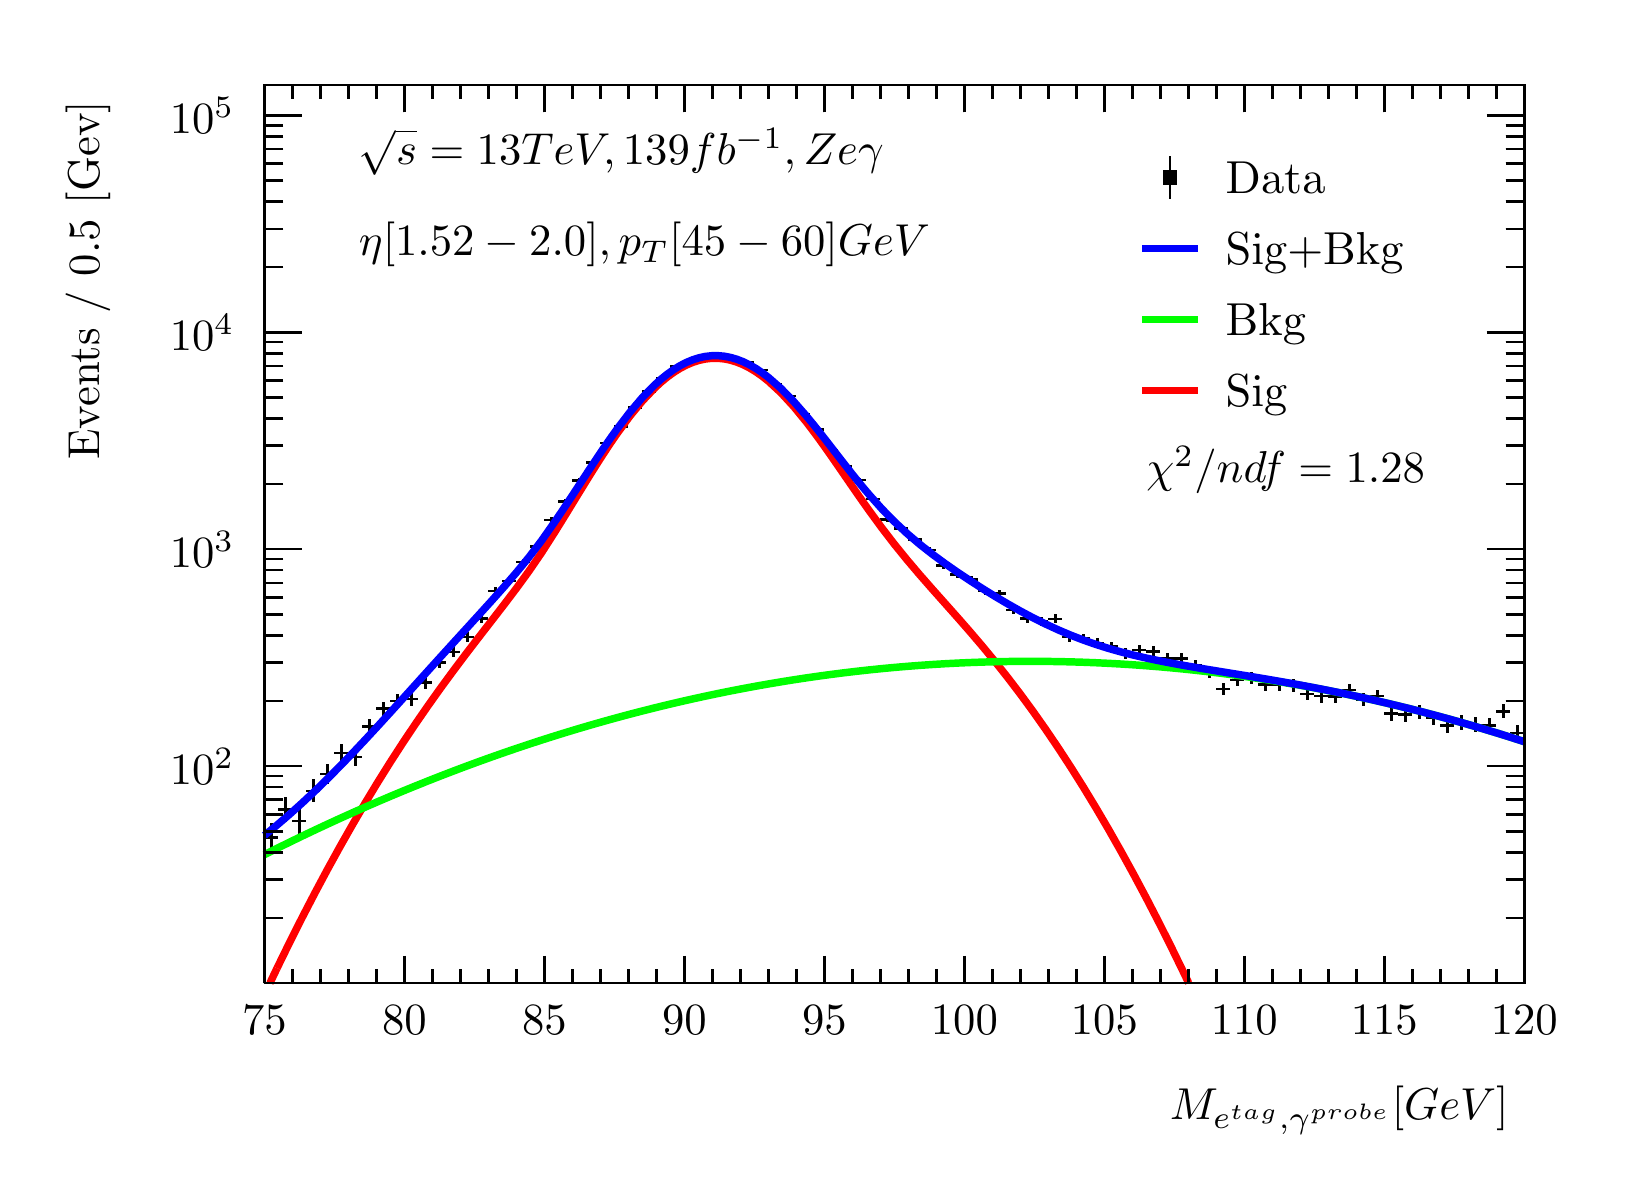
\begin{tikzpicture}
\pgfdeclareplotmark{cross} {
\pgfpathmoveto{\pgfpoint{-0.3\pgfplotmarksize}{\pgfplotmarksize}}
\pgfpathlineto{\pgfpoint{+0.3\pgfplotmarksize}{\pgfplotmarksize}}
\pgfpathlineto{\pgfpoint{+0.3\pgfplotmarksize}{0.3\pgfplotmarksize}}
\pgfpathlineto{\pgfpoint{+1\pgfplotmarksize}{0.3\pgfplotmarksize}}
\pgfpathlineto{\pgfpoint{+1\pgfplotmarksize}{-0.3\pgfplotmarksize}}
\pgfpathlineto{\pgfpoint{+0.3\pgfplotmarksize}{-0.3\pgfplotmarksize}}
\pgfpathlineto{\pgfpoint{+0.3\pgfplotmarksize}{-1.\pgfplotmarksize}}
\pgfpathlineto{\pgfpoint{-0.3\pgfplotmarksize}{-1.\pgfplotmarksize}}
\pgfpathlineto{\pgfpoint{-0.3\pgfplotmarksize}{-0.3\pgfplotmarksize}}
\pgfpathlineto{\pgfpoint{-1.\pgfplotmarksize}{-0.3\pgfplotmarksize}}
\pgfpathlineto{\pgfpoint{-1.\pgfplotmarksize}{0.3\pgfplotmarksize}}
\pgfpathlineto{\pgfpoint{-0.3\pgfplotmarksize}{0.3\pgfplotmarksize}}
\pgfpathclose
\pgfusepathqstroke
}
\pgfdeclareplotmark{cross*} {
\pgfpathmoveto{\pgfpoint{-0.3\pgfplotmarksize}{\pgfplotmarksize}}
\pgfpathlineto{\pgfpoint{+0.3\pgfplotmarksize}{\pgfplotmarksize}}
\pgfpathlineto{\pgfpoint{+0.3\pgfplotmarksize}{0.3\pgfplotmarksize}}
\pgfpathlineto{\pgfpoint{+1\pgfplotmarksize}{0.3\pgfplotmarksize}}
\pgfpathlineto{\pgfpoint{+1\pgfplotmarksize}{-0.3\pgfplotmarksize}}
\pgfpathlineto{\pgfpoint{+0.3\pgfplotmarksize}{-0.3\pgfplotmarksize}}
\pgfpathlineto{\pgfpoint{+0.3\pgfplotmarksize}{-1.\pgfplotmarksize}}
\pgfpathlineto{\pgfpoint{-0.3\pgfplotmarksize}{-1.\pgfplotmarksize}}
\pgfpathlineto{\pgfpoint{-0.3\pgfplotmarksize}{-0.3\pgfplotmarksize}}
\pgfpathlineto{\pgfpoint{-1.\pgfplotmarksize}{-0.3\pgfplotmarksize}}
\pgfpathlineto{\pgfpoint{-1.\pgfplotmarksize}{0.3\pgfplotmarksize}}
\pgfpathlineto{\pgfpoint{-0.3\pgfplotmarksize}{0.3\pgfplotmarksize}}
\pgfpathclose
\pgfusepathqfillstroke
}
\pgfdeclareplotmark{newstar} {
\pgfpathmoveto{\pgfqpoint{0pt}{\pgfplotmarksize}}
\pgfpathlineto{\pgfqpointpolar{44}{0.5\pgfplotmarksize}}
\pgfpathlineto{\pgfqpointpolar{18}{\pgfplotmarksize}}
\pgfpathlineto{\pgfqpointpolar{-20}{0.5\pgfplotmarksize}}
\pgfpathlineto{\pgfqpointpolar{-54}{\pgfplotmarksize}}
\pgfpathlineto{\pgfqpointpolar{-90}{0.5\pgfplotmarksize}}
\pgfpathlineto{\pgfqpointpolar{234}{\pgfplotmarksize}}
\pgfpathlineto{\pgfqpointpolar{198}{0.5\pgfplotmarksize}}
\pgfpathlineto{\pgfqpointpolar{162}{\pgfplotmarksize}}
\pgfpathlineto{\pgfqpointpolar{134}{0.5\pgfplotmarksize}}
\pgfpathclose
\pgfusepathqstroke
}
\pgfdeclareplotmark{newstar*} {
\pgfpathmoveto{\pgfqpoint{0pt}{\pgfplotmarksize}}
\pgfpathlineto{\pgfqpointpolar{44}{0.5\pgfplotmarksize}}
\pgfpathlineto{\pgfqpointpolar{18}{\pgfplotmarksize}}
\pgfpathlineto{\pgfqpointpolar{-20}{0.5\pgfplotmarksize}}
\pgfpathlineto{\pgfqpointpolar{-54}{\pgfplotmarksize}}
\pgfpathlineto{\pgfqpointpolar{-90}{0.5\pgfplotmarksize}}
\pgfpathlineto{\pgfqpointpolar{234}{\pgfplotmarksize}}
\pgfpathlineto{\pgfqpointpolar{198}{0.5\pgfplotmarksize}}
\pgfpathlineto{\pgfqpointpolar{162}{\pgfplotmarksize}}
\pgfpathlineto{\pgfqpointpolar{134}{0.5\pgfplotmarksize}}
\pgfpathclose
\pgfusepathqfillstroke
}
\definecolor{c}{rgb}{1,1,1};
\draw [color=c, fill=c] (0,0) rectangle (20,14.4361);
\draw [color=c, fill=c] (3,2.30977) rectangle (19,13.7143);
\definecolor{c}{rgb}{0,0,0};
\draw [c,line width=0.9] (3,2.30977) -- (3,13.7143) -- (19,13.7143) -- (19,2.30977) -- (3,2.30977);
\definecolor{c}{rgb}{1,1,1};
\draw [color=c, fill=c] (3,2.30977) rectangle (19,13.7143);
\definecolor{c}{rgb}{0,0,0};
\draw [c,line width=0.9] (3,2.30977) -- (3,13.7143) -- (19,13.7143) -- (19,2.30977) -- (3,2.30977);
\draw [c,line width=0.9] (3,2.30977) -- (19,2.30977);
\draw [c,line width=0.9] (3,2.65624) -- (3,2.30977);
\draw [c,line width=0.9] (3.35556,2.48301) -- (3.35556,2.30977);
\draw [c,line width=0.9] (3.71111,2.48301) -- (3.71111,2.30977);
\draw [c,line width=0.9] (4.06667,2.48301) -- (4.06667,2.30977);
\draw [c,line width=0.9] (4.42222,2.48301) -- (4.42222,2.30977);
\draw [c,line width=0.9] (4.77778,2.65624) -- (4.77778,2.30977);
\draw [c,line width=0.9] (5.13333,2.48301) -- (5.13333,2.30977);
\draw [c,line width=0.9] (5.48889,2.48301) -- (5.48889,2.30977);
\draw [c,line width=0.9] (5.84444,2.48301) -- (5.84444,2.30977);
\draw [c,line width=0.9] (6.2,2.48301) -- (6.2,2.30977);
\draw [c,line width=0.9] (6.55556,2.65624) -- (6.55556,2.30977);
\draw [c,line width=0.9] (6.91111,2.48301) -- (6.91111,2.30977);
\draw [c,line width=0.9] (7.26667,2.48301) -- (7.26667,2.30977);
\draw [c,line width=0.9] (7.62222,2.48301) -- (7.62222,2.30977);
\draw [c,line width=0.9] (7.97778,2.48301) -- (7.97778,2.30977);
\draw [c,line width=0.9] (8.33333,2.65624) -- (8.33333,2.30977);
\draw [c,line width=0.9] (8.68889,2.48301) -- (8.68889,2.30977);
\draw [c,line width=0.9] (9.04444,2.48301) -- (9.04444,2.30977);
\draw [c,line width=0.9] (9.4,2.48301) -- (9.4,2.30977);
\draw [c,line width=0.9] (9.75556,2.48301) -- (9.75556,2.30977);
\draw [c,line width=0.9] (10.1111,2.65624) -- (10.1111,2.30977);
\draw [c,line width=0.9] (10.4667,2.48301) -- (10.4667,2.30977);
\draw [c,line width=0.9] (10.8222,2.48301) -- (10.8222,2.30977);
\draw [c,line width=0.9] (11.1778,2.48301) -- (11.1778,2.30977);
\draw [c,line width=0.9] (11.5333,2.48301) -- (11.5333,2.30977);
\draw [c,line width=0.9] (11.8889,2.65624) -- (11.8889,2.30977);
\draw [c,line width=0.9] (12.2444,2.48301) -- (12.2444,2.30977);
\draw [c,line width=0.9] (12.6,2.48301) -- (12.6,2.30977);
\draw [c,line width=0.9] (12.9556,2.48301) -- (12.9556,2.30977);
\draw [c,line width=0.9] (13.3111,2.48301) -- (13.3111,2.30977);
\draw [c,line width=0.9] (13.6667,2.65624) -- (13.6667,2.30977);
\draw [c,line width=0.9] (14.0222,2.48301) -- (14.0222,2.30977);
\draw [c,line width=0.9] (14.3778,2.48301) -- (14.3778,2.30977);
\draw [c,line width=0.9] (14.7333,2.48301) -- (14.7333,2.30977);
\draw [c,line width=0.9] (15.0889,2.48301) -- (15.0889,2.30977);
\draw [c,line width=0.9] (15.4444,2.65624) -- (15.4444,2.30977);
\draw [c,line width=0.9] (15.8,2.48301) -- (15.8,2.30977);
\draw [c,line width=0.9] (16.1556,2.48301) -- (16.1556,2.30977);
\draw [c,line width=0.9] (16.5111,2.48301) -- (16.5111,2.30977);
\draw [c,line width=0.9] (16.8667,2.48301) -- (16.8667,2.30977);
\draw [c,line width=0.9] (17.2222,2.65624) -- (17.2222,2.30977);
\draw [c,line width=0.9] (17.5778,2.48301) -- (17.5778,2.30977);
\draw [c,line width=0.9] (17.9333,2.48301) -- (17.9333,2.30977);
\draw [c,line width=0.9] (18.2889,2.48301) -- (18.2889,2.30977);
\draw [c,line width=0.9] (18.6444,2.48301) -- (18.6444,2.30977);
\draw [c,line width=0.9] (19,2.65624) -- (19,2.30977);
\draw [c,line width=0.9] (19,2.65624) -- (19,2.30977);
\draw [anchor=base] (3,1.66015) node[scale=1.61424, color=c, rotate=0]{75};
\draw [anchor=base] (4.77778,1.66015) node[scale=1.61424, color=c, rotate=0]{80};
\draw [anchor=base] (6.55556,1.66015) node[scale=1.61424, color=c, rotate=0]{85};
\draw [anchor=base] (8.33333,1.66015) node[scale=1.61424, color=c, rotate=0]{90};
\draw [anchor=base] (10.1111,1.66015) node[scale=1.61424, color=c, rotate=0]{95};
\draw [anchor=base] (11.8889,1.66015) node[scale=1.61424, color=c, rotate=0]{100};
\draw [anchor=base] (13.6667,1.66015) node[scale=1.61424, color=c, rotate=0]{105};
\draw [anchor=base] (15.4444,1.66015) node[scale=1.61424, color=c, rotate=0]{110};
\draw [anchor=base] (17.2222,1.66015) node[scale=1.61424, color=c, rotate=0]{115};
\draw [anchor=base] (19,1.66015) node[scale=1.61424, color=c, rotate=0]{120};
\draw [anchor= east] (19,0.692932) node[scale=1.61424, color=c, rotate=0]{$M_{e^{tag}, \gamma^{probe}}  [GeV]$};
\draw [c,line width=0.9] (3,13.7143) -- (19,13.7143);
\draw [c,line width=0.9] (3,13.3678) -- (3,13.7143);
\draw [c,line width=0.9] (3.35556,13.5411) -- (3.35556,13.7143);
\draw [c,line width=0.9] (3.71111,13.5411) -- (3.71111,13.7143);
\draw [c,line width=0.9] (4.06667,13.5411) -- (4.06667,13.7143);
\draw [c,line width=0.9] (4.42222,13.5411) -- (4.42222,13.7143);
\draw [c,line width=0.9] (4.77778,13.3678) -- (4.77778,13.7143);
\draw [c,line width=0.9] (5.13333,13.5411) -- (5.13333,13.7143);
\draw [c,line width=0.9] (5.48889,13.5411) -- (5.48889,13.7143);
\draw [c,line width=0.9] (5.84444,13.5411) -- (5.84444,13.7143);
\draw [c,line width=0.9] (6.2,13.5411) -- (6.2,13.7143);
\draw [c,line width=0.9] (6.55556,13.3678) -- (6.55556,13.7143);
\draw [c,line width=0.9] (6.91111,13.5411) -- (6.91111,13.7143);
\draw [c,line width=0.9] (7.26667,13.5411) -- (7.26667,13.7143);
\draw [c,line width=0.9] (7.62222,13.5411) -- (7.62222,13.7143);
\draw [c,line width=0.9] (7.97778,13.5411) -- (7.97778,13.7143);
\draw [c,line width=0.9] (8.33333,13.3678) -- (8.33333,13.7143);
\draw [c,line width=0.9] (8.68889,13.5411) -- (8.68889,13.7143);
\draw [c,line width=0.9] (9.04444,13.5411) -- (9.04444,13.7143);
\draw [c,line width=0.9] (9.4,13.5411) -- (9.4,13.7143);
\draw [c,line width=0.9] (9.75556,13.5411) -- (9.75556,13.7143);
\draw [c,line width=0.9] (10.1111,13.3678) -- (10.1111,13.7143);
\draw [c,line width=0.9] (10.4667,13.5411) -- (10.4667,13.7143);
\draw [c,line width=0.9] (10.8222,13.5411) -- (10.8222,13.7143);
\draw [c,line width=0.9] (11.1778,13.5411) -- (11.1778,13.7143);
\draw [c,line width=0.9] (11.5333,13.5411) -- (11.5333,13.7143);
\draw [c,line width=0.9] (11.8889,13.3678) -- (11.8889,13.7143);
\draw [c,line width=0.9] (12.2444,13.5411) -- (12.2444,13.7143);
\draw [c,line width=0.9] (12.6,13.5411) -- (12.6,13.7143);
\draw [c,line width=0.9] (12.9556,13.5411) -- (12.9556,13.7143);
\draw [c,line width=0.9] (13.3111,13.5411) -- (13.3111,13.7143);
\draw [c,line width=0.9] (13.6667,13.3678) -- (13.6667,13.7143);
\draw [c,line width=0.9] (14.0222,13.5411) -- (14.0222,13.7143);
\draw [c,line width=0.9] (14.3778,13.5411) -- (14.3778,13.7143);
\draw [c,line width=0.9] (14.7333,13.5411) -- (14.7333,13.7143);
\draw [c,line width=0.9] (15.0889,13.5411) -- (15.0889,13.7143);
\draw [c,line width=0.9] (15.4444,13.3678) -- (15.4444,13.7143);
\draw [c,line width=0.9] (15.8,13.5411) -- (15.8,13.7143);
\draw [c,line width=0.9] (16.1556,13.5411) -- (16.1556,13.7143);
\draw [c,line width=0.9] (16.5111,13.5411) -- (16.5111,13.7143);
\draw [c,line width=0.9] (16.8667,13.5411) -- (16.8667,13.7143);
\draw [c,line width=0.9] (17.2222,13.3678) -- (17.2222,13.7143);
\draw [c,line width=0.9] (17.5778,13.5411) -- (17.5778,13.7143);
\draw [c,line width=0.9] (17.9333,13.5411) -- (17.9333,13.7143);
\draw [c,line width=0.9] (18.2889,13.5411) -- (18.2889,13.7143);
\draw [c,line width=0.9] (18.6444,13.5411) -- (18.6444,13.7143);
\draw [c,line width=0.9] (19,13.3678) -- (19,13.7143);
\draw [c,line width=0.9] (19,13.3678) -- (19,13.7143);
\draw [c,line width=0.9] (3,2.30977) -- (3,13.7143);
\draw [c,line width=0.9] (3.237,3.13907) -- (3,3.13907);
\draw [c,line width=0.9] (3.237,3.62418) -- (3,3.62418);
\draw [c,line width=0.9] (3.237,3.96837) -- (3,3.96837);
\draw [c,line width=0.9] (3.237,4.23535) -- (3,4.23535);
\draw [c,line width=0.9] (3.237,4.45348) -- (3,4.45348);
\draw [c,line width=0.9] (3.237,4.63791) -- (3,4.63791);
\draw [c,line width=0.9] (3.237,4.79767) -- (3,4.79767);
\draw [c,line width=0.9] (3.237,4.93859) -- (3,4.93859);
\draw [c,line width=0.9] (3.474,5.06465) -- (3,5.06465);
\draw [anchor= east] (2.82,5.06465) node[scale=1.61424, color=c, rotate=0]{$10^{2}$};
\draw [c,line width=0.9] (3.237,5.89394) -- (3,5.89394);
\draw [c,line width=0.9] (3.237,6.37905) -- (3,6.37905);
\draw [c,line width=0.9] (3.237,6.72324) -- (3,6.72324);
\draw [c,line width=0.9] (3.237,6.99022) -- (3,6.99022);
\draw [c,line width=0.9] (3.237,7.20835) -- (3,7.20835);
\draw [c,line width=0.9] (3.237,7.39278) -- (3,7.39278);
\draw [c,line width=0.9] (3.237,7.55254) -- (3,7.55254);
\draw [c,line width=0.9] (3.237,7.69346) -- (3,7.69346);
\draw [c,line width=0.9] (3.474,7.81952) -- (3,7.81952);
\draw [anchor= east] (2.82,7.81952) node[scale=1.61424, color=c, rotate=0]{$10^{3}$};
\draw [c,line width=0.9] (3.237,8.64882) -- (3,8.64882);
\draw [c,line width=0.9] (3.237,9.13393) -- (3,9.13393);
\draw [c,line width=0.9] (3.237,9.47812) -- (3,9.47812);
\draw [c,line width=0.9] (3.237,9.74509) -- (3,9.74509);
\draw [c,line width=0.9] (3.237,9.96323) -- (3,9.96323);
\draw [c,line width=0.9] (3.237,10.1477) -- (3,10.1477);
\draw [c,line width=0.9] (3.237,10.3074) -- (3,10.3074);
\draw [c,line width=0.9] (3.237,10.4483) -- (3,10.4483);
\draw [c,line width=0.9] (3.474,10.5744) -- (3,10.5744);
\draw [anchor= east] (2.82,10.5744) node[scale=1.61424, color=c, rotate=0]{$10^{4}$};
\draw [c,line width=0.9] (3.237,11.4037) -- (3,11.4037);
\draw [c,line width=0.9] (3.237,11.8888) -- (3,11.8888);
\draw [c,line width=0.9] (3.237,12.233) -- (3,12.233);
\draw [c,line width=0.9] (3.237,12.5) -- (3,12.5);
\draw [c,line width=0.9] (3.237,12.7181) -- (3,12.7181);
\draw [c,line width=0.9] (3.237,12.9025) -- (3,12.9025);
\draw [c,line width=0.9] (3.237,13.0623) -- (3,13.0623);
\draw [c,line width=0.9] (3.237,13.2032) -- (3,13.2032);
\draw [c,line width=0.9] (3.474,13.3293) -- (3,13.3293);
\draw [anchor= east] (2.82,13.3293) node[scale=1.61424, color=c, rotate=0]{$10^{5}$};
\draw [anchor= east] (0.76,13.7143) node[scale=1.61424, color=c, rotate=90]{Events / 0.5 [Gev]};
\draw [c,line width=0.9] (19,2.30977) -- (19,13.7143);
\draw [c,line width=0.9] (18.763,3.13907) -- (19,3.13907);
\draw [c,line width=0.9] (18.763,3.62418) -- (19,3.62418);
\draw [c,line width=0.9] (18.763,3.96837) -- (19,3.96837);
\draw [c,line width=0.9] (18.763,4.23535) -- (19,4.23535);
\draw [c,line width=0.9] (18.763,4.45348) -- (19,4.45348);
\draw [c,line width=0.9] (18.763,4.63791) -- (19,4.63791);
\draw [c,line width=0.9] (18.763,4.79767) -- (19,4.79767);
\draw [c,line width=0.9] (18.763,4.93859) -- (19,4.93859);
\draw [c,line width=0.9] (18.526,5.06465) -- (19,5.06465);
\draw [c,line width=0.9] (18.763,5.89394) -- (19,5.89394);
\draw [c,line width=0.9] (18.763,6.37905) -- (19,6.37905);
\draw [c,line width=0.9] (18.763,6.72324) -- (19,6.72324);
\draw [c,line width=0.9] (18.763,6.99022) -- (19,6.99022);
\draw [c,line width=0.9] (18.763,7.20835) -- (19,7.20835);
\draw [c,line width=0.9] (18.763,7.39278) -- (19,7.39278);
\draw [c,line width=0.9] (18.763,7.55254) -- (19,7.55254);
\draw [c,line width=0.9] (18.763,7.69346) -- (19,7.69346);
\draw [c,line width=0.9] (18.526,7.81952) -- (19,7.81952);
\draw [c,line width=0.9] (18.763,8.64882) -- (19,8.64882);
\draw [c,line width=0.9] (18.763,9.13393) -- (19,9.13393);
\draw [c,line width=0.9] (18.763,9.47812) -- (19,9.47812);
\draw [c,line width=0.9] (18.763,9.74509) -- (19,9.74509);
\draw [c,line width=0.9] (18.763,9.96323) -- (19,9.96323);
\draw [c,line width=0.9] (18.763,10.1477) -- (19,10.1477);
\draw [c,line width=0.9] (18.763,10.3074) -- (19,10.3074);
\draw [c,line width=0.9] (18.763,10.4483) -- (19,10.4483);
\draw [c,line width=0.9] (18.526,10.5744) -- (19,10.5744);
\draw [c,line width=0.9] (18.763,11.4037) -- (19,11.4037);
\draw [c,line width=0.9] (18.763,11.8888) -- (19,11.8888);
\draw [c,line width=0.9] (18.763,12.233) -- (19,12.233);
\draw [c,line width=0.9] (18.763,12.5) -- (19,12.5);
\draw [c,line width=0.9] (18.763,12.7181) -- (19,12.7181);
\draw [c,line width=0.9] (18.763,12.9025) -- (19,12.9025);
\draw [c,line width=0.9] (18.763,13.0623) -- (19,13.0623);
\draw [c,line width=0.9] (18.763,13.2032) -- (19,13.2032);
\draw [c,line width=0.9] (18.526,13.3293) -- (19,13.3293);
\draw [c,line width=0.9] (3.08889,4.16132) -- (3,4.16132);
\draw [c,line width=0.9] (3,4.16132) -- (3,4.16132);
\draw [c,line width=0.9] (3.08889,4.16132) -- (3.17778,4.16132);
\draw [c,line width=0.9] (3.17778,4.16132) -- (3.17778,4.16132);
\draw [c,line width=0.9] (3.08889,4.16132) -- (3.08889,4.3473);
\draw [c,line width=0.9] (3.08889,4.3473) -- (3.08889,4.3473);
\draw [c,line width=0.9] (3.08889,4.16132) -- (3.08889,3.97341);
\draw [c,line width=0.9] (3.08889,3.97341) -- (3.08889,3.97341);
\draw [c,line width=0.9] (3.26667,4.51186) -- (3.17778,4.51186);
\draw [c,line width=0.9] (3.17778,4.51186) -- (3.17778,4.51186);
\draw [c,line width=0.9] (3.26667,4.51186) -- (3.35556,4.51186);
\draw [c,line width=0.9] (3.35556,4.51186) -- (3.35556,4.51186);
\draw [c,line width=0.9] (3.26667,4.51186) -- (3.26667,4.67127);
\draw [c,line width=0.9] (3.26667,4.67127) -- (3.26667,4.67127);
\draw [c,line width=0.9] (3.26667,4.51186) -- (3.26667,4.3512);
\draw [c,line width=0.9] (3.26667,4.3512) -- (3.26667,4.3512);
\draw [c,line width=0.9] (3.44444,4.37094) -- (3.35556,4.37094);
\draw [c,line width=0.9] (3.35556,4.37094) -- (3.35556,4.37094);
\draw [c,line width=0.9] (3.44444,4.37094) -- (3.53333,4.37094);
\draw [c,line width=0.9] (3.53333,4.37094) -- (3.53333,4.37094);
\draw [c,line width=0.9] (3.44444,4.37094) -- (3.44444,4.54053);
\draw [c,line width=0.9] (3.44444,4.54053) -- (3.44444,4.54053);
\draw [c,line width=0.9] (3.44444,4.37094) -- (3.44444,4.19987);
\draw [c,line width=0.9] (3.44444,4.19987) -- (3.44444,4.19987);
\draw [c,line width=0.9] (3.62222,4.75194) -- (3.53333,4.75194);
\draw [c,line width=0.9] (3.53333,4.75194) -- (3.53333,4.75194);
\draw [c,line width=0.9] (3.62222,4.75194) -- (3.71111,4.75194);
\draw [c,line width=0.9] (3.71111,4.75194) -- (3.71111,4.75194);
\draw [c,line width=0.9] (3.62222,4.75194) -- (3.62222,4.89546);
\draw [c,line width=0.9] (3.62222,4.89546) -- (3.62222,4.89546);
\draw [c,line width=0.9] (3.62222,4.75194) -- (3.62222,4.60752);
\draw [c,line width=0.9] (3.62222,4.60752) -- (3.62222,4.60752);
\draw [c,line width=0.9] (3.8,4.96489) -- (3.71111,4.96489);
\draw [c,line width=0.9] (3.71111,4.96489) -- (3.71111,4.96489);
\draw [c,line width=0.9] (3.8,4.96489) -- (3.88889,4.96489);
\draw [c,line width=0.9] (3.88889,4.96489) -- (3.88889,4.96489);
\draw [c,line width=0.9] (3.8,4.96489) -- (3.8,5.09567);
\draw [c,line width=0.9] (3.8,5.09567) -- (3.8,5.09567);
\draw [c,line width=0.9] (3.8,4.96489) -- (3.8,4.83341);
\draw [c,line width=0.9] (3.8,4.83341) -- (3.8,4.83341);
\draw [c,line width=0.9] (3.97778,5.23186) -- (3.88889,5.23186);
\draw [c,line width=0.9] (3.88889,5.23186) -- (3.88889,5.23186);
\draw [c,line width=0.9] (3.97778,5.23186) -- (4.06667,5.23186);
\draw [c,line width=0.9] (4.06667,5.23186) -- (4.06667,5.23186);
\draw [c,line width=0.9] (3.97778,5.23186) -- (3.97778,5.34339);
\draw [c,line width=0.9] (3.97778,5.34339) -- (3.97778,5.34339);
\draw [c,line width=0.9] (3.97778,5.23186) -- (3.97778,5.12034);
\draw [c,line width=0.9] (3.97778,5.12034) -- (3.97778,5.12034);
\draw [c,line width=0.9] (4.15556,5.17868) -- (4.06667,5.17868);
\draw [c,line width=0.9] (4.06667,5.17868) -- (4.06667,5.17868);
\draw [c,line width=0.9] (4.15556,5.17868) -- (4.24444,5.17868);
\draw [c,line width=0.9] (4.24444,5.17868) -- (4.24444,5.17868);
\draw [c,line width=0.9] (4.15556,5.17868) -- (4.15556,5.29271);
\draw [c,line width=0.9] (4.15556,5.29271) -- (4.15556,5.29271);
\draw [c,line width=0.9] (4.15556,5.17868) -- (4.15556,5.06465);
\draw [c,line width=0.9] (4.15556,5.06465) -- (4.15556,5.06465);
\draw [c,line width=0.9] (4.33333,5.5656) -- (4.24444,5.5656);
\draw [c,line width=0.9] (4.24444,5.5656) -- (4.24444,5.5656);
\draw [c,line width=0.9] (4.33333,5.5656) -- (4.42222,5.5656);
\draw [c,line width=0.9] (4.42222,5.5656) -- (4.42222,5.5656);
\draw [c,line width=0.9] (4.33333,5.5656) -- (4.33333,5.66262);
\draw [c,line width=0.9] (4.33333,5.66262) -- (4.33333,5.66262);
\draw [c,line width=0.9] (4.33333,5.5656) -- (4.33333,5.46859);
\draw [c,line width=0.9] (4.33333,5.46859) -- (4.33333,5.46859);
\draw [c,line width=0.9] (4.51111,5.79419) -- (4.42222,5.79419);
\draw [c,line width=0.9] (4.42222,5.79419) -- (4.42222,5.79419);
\draw [c,line width=0.9] (4.51111,5.79419) -- (4.6,5.79419);
\draw [c,line width=0.9] (4.6,5.79419) -- (4.6,5.79419);
\draw [c,line width=0.9] (4.51111,5.79419) -- (4.51111,5.88237);
\draw [c,line width=0.9] (4.51111,5.88237) -- (4.51111,5.88237);
\draw [c,line width=0.9] (4.51111,5.79419) -- (4.51111,5.70601);
\draw [c,line width=0.9] (4.51111,5.70601) -- (4.51111,5.70601);
\draw [c,line width=0.9] (4.68889,5.89395) -- (4.6,5.89395);
\draw [c,line width=0.9] (4.6,5.89395) -- (4.6,5.89395);
\draw [c,line width=0.9] (4.68889,5.89395) -- (4.77778,5.89395);
\draw [c,line width=0.9] (4.77778,5.89395) -- (4.77778,5.89395);
\draw [c,line width=0.9] (4.68889,5.89395) -- (4.68889,5.97853);
\draw [c,line width=0.9] (4.68889,5.97853) -- (4.68889,5.97853);
\draw [c,line width=0.9] (4.68889,5.89395) -- (4.68889,5.80936);
\draw [c,line width=0.9] (4.68889,5.80936) -- (4.68889,5.80936);
\draw [c,line width=0.9] (4.86667,5.91764) -- (4.77778,5.91764);
\draw [c,line width=0.9] (4.77778,5.91764) -- (4.77778,5.91764);
\draw [c,line width=0.9] (4.86667,5.91764) -- (4.95556,5.91764);
\draw [c,line width=0.9] (4.95556,5.91764) -- (4.95556,5.91764);
\draw [c,line width=0.9] (4.86667,5.91764) -- (4.86667,6.00139);
\draw [c,line width=0.9] (4.86667,6.00139) -- (4.86667,6.00139);
\draw [c,line width=0.9] (4.86667,5.91764) -- (4.86667,5.83389);
\draw [c,line width=0.9] (4.86667,5.83389) -- (4.86667,5.83389);
\draw [c,line width=0.9] (5.04444,6.12694) -- (4.95556,6.12694);
\draw [c,line width=0.9] (4.95556,6.12694) -- (4.95556,6.12694);
\draw [c,line width=0.9] (5.04444,6.12694) -- (5.13333,6.12694);
\draw [c,line width=0.9] (5.13333,6.12694) -- (5.13333,6.12694);
\draw [c,line width=0.9] (5.04444,6.12694) -- (5.04444,6.20368);
\draw [c,line width=0.9] (5.04444,6.20368) -- (5.04444,6.20368);
\draw [c,line width=0.9] (5.04444,6.12694) -- (5.04444,6.05021);
\draw [c,line width=0.9] (5.04444,6.05021) -- (5.04444,6.05021);
\draw [c,line width=0.9] (5.22222,6.37906) -- (5.13333,6.37906);
\draw [c,line width=0.9] (5.13333,6.37906) -- (5.13333,6.37906);
\draw [c,line width=0.9] (5.22222,6.37906) -- (5.31111,6.37906);
\draw [c,line width=0.9] (5.31111,6.37906) -- (5.31111,6.37906);
\draw [c,line width=0.9] (5.22222,6.37906) -- (5.22222,6.44812);
\draw [c,line width=0.9] (5.22222,6.44812) -- (5.22222,6.44812);
\draw [c,line width=0.9] (5.22222,6.37906) -- (5.22222,6.30999);
\draw [c,line width=0.9] (5.22222,6.30999) -- (5.22222,6.30999);
\draw [c,line width=0.9] (5.4,6.51108) -- (5.31111,6.51108);
\draw [c,line width=0.9] (5.31111,6.51108) -- (5.31111,6.51108);
\draw [c,line width=0.9] (5.4,6.51108) -- (5.48889,6.51108);
\draw [c,line width=0.9] (5.48889,6.51108) -- (5.48889,6.51108);
\draw [c,line width=0.9] (5.4,6.51108) -- (5.4,6.57644);
\draw [c,line width=0.9] (5.4,6.57644) -- (5.4,6.57644);
\draw [c,line width=0.9] (5.4,6.51108) -- (5.4,6.44572);
\draw [c,line width=0.9] (5.4,6.44572) -- (5.4,6.44572);
\draw [c,line width=0.9] (5.57778,6.70516) -- (5.48889,6.70516);
\draw [c,line width=0.9] (5.48889,6.70516) -- (5.48889,6.70516);
\draw [c,line width=0.9] (5.57778,6.70516) -- (5.66667,6.70516);
\draw [c,line width=0.9] (5.66667,6.70516) -- (5.66667,6.70516);
\draw [c,line width=0.9] (5.57778,6.70516) -- (5.57778,6.76543);
\draw [c,line width=0.9] (5.57778,6.76543) -- (5.57778,6.76543);
\draw [c,line width=0.9] (5.57778,6.70516) -- (5.57778,6.6449);
\draw [c,line width=0.9] (5.57778,6.6449) -- (5.57778,6.6449);
\draw [c,line width=0.9] (5.75556,6.94138) -- (5.66667,6.94138);
\draw [c,line width=0.9] (5.66667,6.94138) -- (5.66667,6.94138);
\draw [c,line width=0.9] (5.75556,6.94138) -- (5.84444,6.94138);
\draw [c,line width=0.9] (5.84444,6.94138) -- (5.84444,6.94138);
\draw [c,line width=0.9] (5.75556,6.94138) -- (5.75556,6.99599);
\draw [c,line width=0.9] (5.75556,6.99599) -- (5.75556,6.99599);
\draw [c,line width=0.9] (5.75556,6.94138) -- (5.75556,6.88678);
\draw [c,line width=0.9] (5.75556,6.88678) -- (5.75556,6.88678);
\draw [c,line width=0.9] (5.93333,7.2893) -- (5.84444,7.2893);
\draw [c,line width=0.9] (5.84444,7.2893) -- (5.84444,7.2893);
\draw [c,line width=0.9] (5.93333,7.2893) -- (6.02222,7.2893);
\draw [c,line width=0.9] (6.02222,7.2893) -- (6.02222,7.2893);
\draw [c,line width=0.9] (5.93333,7.2893) -- (5.93333,7.33652);
\draw [c,line width=0.9] (5.93333,7.33652) -- (5.93333,7.33652);
\draw [c,line width=0.9] (5.93333,7.2893) -- (5.93333,7.24209);
\draw [c,line width=0.9] (5.93333,7.24209) -- (5.93333,7.24209);
\draw [c,line width=0.9] (6.11111,7.41648) -- (6.02222,7.41648);
\draw [c,line width=0.9] (6.02222,7.41648) -- (6.02222,7.41648);
\draw [c,line width=0.9] (6.11111,7.41648) -- (6.2,7.41648);
\draw [c,line width=0.9] (6.2,7.41648) -- (6.2,7.41648);
\draw [c,line width=0.9] (6.11111,7.41648) -- (6.11111,7.46125);
\draw [c,line width=0.9] (6.11111,7.46125) -- (6.11111,7.46125);
\draw [c,line width=0.9] (6.11111,7.41648) -- (6.11111,7.37171);
\draw [c,line width=0.9] (6.11111,7.37171) -- (6.11111,7.37171);
\draw [c,line width=0.9] (6.28889,7.65839) -- (6.2,7.65839);
\draw [c,line width=0.9] (6.2,7.65839) -- (6.2,7.65839);
\draw [c,line width=0.9] (6.28889,7.65839) -- (6.37778,7.65839);
\draw [c,line width=0.9] (6.37778,7.65839) -- (6.37778,7.65839);
\draw [c,line width=0.9] (6.28889,7.65839) -- (6.28889,7.69886);
\draw [c,line width=0.9] (6.28889,7.69886) -- (6.28889,7.69886);
\draw [c,line width=0.9] (6.28889,7.65839) -- (6.28889,7.61792);
\draw [c,line width=0.9] (6.28889,7.61792) -- (6.28889,7.61792);
\draw [c,line width=0.9] (6.46667,7.8514) -- (6.37778,7.8514);
\draw [c,line width=0.9] (6.37778,7.8514) -- (6.37778,7.8514);
\draw [c,line width=0.9] (6.46667,7.8514) -- (6.55556,7.8514);
\draw [c,line width=0.9] (6.55556,7.8514) -- (6.55556,7.8514);
\draw [c,line width=0.9] (6.46667,7.8514) -- (6.46667,7.88873);
\draw [c,line width=0.9] (6.46667,7.88873) -- (6.46667,7.88873);
\draw [c,line width=0.9] (6.46667,7.8514) -- (6.46667,7.81406);
\draw [c,line width=0.9] (6.46667,7.81406) -- (6.46667,7.81406);
\draw [c,line width=0.9] (6.64444,8.19004) -- (6.55556,8.19004);
\draw [c,line width=0.9] (6.55556,8.19004) -- (6.55556,8.19004);
\draw [c,line width=0.9] (6.64444,8.19004) -- (6.73333,8.19004);
\draw [c,line width=0.9] (6.73333,8.19004) -- (6.73333,8.19004);
\draw [c,line width=0.9] (6.64444,8.19004) -- (6.64444,8.22245);
\draw [c,line width=0.9] (6.64444,8.22245) -- (6.64444,8.22245);
\draw [c,line width=0.9] (6.64444,8.19004) -- (6.64444,8.15763);
\draw [c,line width=0.9] (6.64444,8.15763) -- (6.64444,8.15763);
\draw [c,line width=0.9] (6.82222,8.42373) -- (6.73333,8.42373);
\draw [c,line width=0.9] (6.73333,8.42373) -- (6.73333,8.42373);
\draw [c,line width=0.9] (6.82222,8.42373) -- (6.91111,8.42373);
\draw [c,line width=0.9] (6.91111,8.42373) -- (6.91111,8.42373);
\draw [c,line width=0.9] (6.82222,8.42373) -- (6.82222,8.45312);
\draw [c,line width=0.9] (6.82222,8.45312) -- (6.82222,8.45312);
\draw [c,line width=0.9] (6.82222,8.42373) -- (6.82222,8.39433);
\draw [c,line width=0.9] (6.82222,8.39433) -- (6.82222,8.39433);
\draw [c,line width=0.9] (7,8.69229) -- (6.91111,8.69229);
\draw [c,line width=0.9] (6.91111,8.69229) -- (6.91111,8.69229);
\draw [c,line width=0.9] (7,8.69229) -- (7.08889,8.69229);
\draw [c,line width=0.9] (7.08889,8.69229) -- (7.08889,8.69229);
\draw [c,line width=0.9] (7,8.69229) -- (7,8.71856);
\draw [c,line width=0.9] (7,8.71856) -- (7,8.71856);
\draw [c,line width=0.9] (7,8.69229) -- (7,8.66602);
\draw [c,line width=0.9] (7,8.66602) -- (7,8.66602);
\draw [c,line width=0.9] (7.17778,8.92009) -- (7.08889,8.92009);
\draw [c,line width=0.9] (7.08889,8.92009) -- (7.08889,8.92009);
\draw [c,line width=0.9] (7.17778,8.92009) -- (7.26667,8.92009);
\draw [c,line width=0.9] (7.26667,8.92009) -- (7.26667,8.92009);
\draw [c,line width=0.9] (7.17778,8.92009) -- (7.17778,8.94398);
\draw [c,line width=0.9] (7.17778,8.94398) -- (7.17778,8.94398);
\draw [c,line width=0.9] (7.17778,8.92009) -- (7.17778,8.89621);
\draw [c,line width=0.9] (7.17778,8.89621) -- (7.17778,8.89621);
\draw [c,line width=0.9] (7.35556,9.16697) -- (7.26667,9.16697);
\draw [c,line width=0.9] (7.26667,9.16697) -- (7.26667,9.16697);
\draw [c,line width=0.9] (7.35556,9.16697) -- (7.44444,9.16697);
\draw [c,line width=0.9] (7.44444,9.16697) -- (7.44444,9.16697);
\draw [c,line width=0.9] (7.35556,9.16697) -- (7.35556,9.18851);
\draw [c,line width=0.9] (7.35556,9.18851) -- (7.35556,9.18851);
\draw [c,line width=0.9] (7.35556,9.16697) -- (7.35556,9.14542);
\draw [c,line width=0.9] (7.35556,9.14542) -- (7.35556,9.14542);
\draw [c,line width=0.9] (7.53333,9.37998) -- (7.44444,9.37998);
\draw [c,line width=0.9] (7.44444,9.37998) -- (7.44444,9.37998);
\draw [c,line width=0.9] (7.53333,9.37998) -- (7.62222,9.37998);
\draw [c,line width=0.9] (7.62222,9.37998) -- (7.62222,9.37998);
\draw [c,line width=0.9] (7.53333,9.37998) -- (7.53333,9.39969);
\draw [c,line width=0.9] (7.53333,9.39969) -- (7.53333,9.39969);
\draw [c,line width=0.9] (7.53333,9.37998) -- (7.53333,9.36028);
\draw [c,line width=0.9] (7.53333,9.36028) -- (7.53333,9.36028);
\draw [c,line width=0.9] (7.71111,9.61771) -- (7.62222,9.61771);
\draw [c,line width=0.9] (7.62222,9.61771) -- (7.62222,9.61771);
\draw [c,line width=0.9] (7.71111,9.61771) -- (7.8,9.61771);
\draw [c,line width=0.9] (7.8,9.61771) -- (7.8,9.61771);
\draw [c,line width=0.9] (7.71111,9.61771) -- (7.71111,9.63555);
\draw [c,line width=0.9] (7.71111,9.63555) -- (7.71111,9.63555);
\draw [c,line width=0.9] (7.71111,9.61771) -- (7.71111,9.59986);
\draw [c,line width=0.9] (7.71111,9.59986) -- (7.71111,9.59986);
\draw [c,line width=0.9] (7.88889,9.82403) -- (7.8,9.82403);
\draw [c,line width=0.9] (7.8,9.82403) -- (7.8,9.82403);
\draw [c,line width=0.9] (7.88889,9.82403) -- (7.97778,9.82403);
\draw [c,line width=0.9] (7.97778,9.82403) -- (7.97778,9.82403);
\draw [c,line width=0.9] (7.88889,9.82403) -- (7.88889,9.8404);
\draw [c,line width=0.9] (7.88889,9.8404) -- (7.88889,9.8404);
\draw [c,line width=0.9] (7.88889,9.82403) -- (7.88889,9.80766);
\draw [c,line width=0.9] (7.88889,9.80766) -- (7.88889,9.80766);
\draw [c,line width=0.9] (8.06667,9.99374) -- (7.97778,9.99374);
\draw [c,line width=0.9] (7.97778,9.99374) -- (7.97778,9.99374);
\draw [c,line width=0.9] (8.06667,9.99374) -- (8.15556,9.99374);
\draw [c,line width=0.9] (8.15556,9.99374) -- (8.15556,9.99374);
\draw [c,line width=0.9] (8.06667,9.99374) -- (8.06667,10.009);
\draw [c,line width=0.9] (8.06667,10.009) -- (8.06667,10.009);
\draw [c,line width=0.9] (8.06667,9.99374) -- (8.06667,9.97849);
\draw [c,line width=0.9] (8.06667,9.97849) -- (8.06667,9.97849);
\draw [c,line width=0.9] (8.24444,10.1398) -- (8.15556,10.1398);
\draw [c,line width=0.9] (8.15556,10.1398) -- (8.15556,10.1398);
\draw [c,line width=0.9] (8.24444,10.1398) -- (8.33333,10.1398);
\draw [c,line width=0.9] (8.33333,10.1398) -- (8.33333,10.1398);
\draw [c,line width=0.9] (8.24444,10.1398) -- (8.24444,10.1541);
\draw [c,line width=0.9] (8.24444,10.1541) -- (8.24444,10.1541);
\draw [c,line width=0.9] (8.24444,10.1398) -- (8.24444,10.1254);
\draw [c,line width=0.9] (8.24444,10.1254) -- (8.24444,10.1254);
\draw [c,line width=0.9] (8.42222,10.2114) -- (8.33333,10.2114);
\draw [c,line width=0.9] (8.33333,10.2114) -- (8.33333,10.2114);
\draw [c,line width=0.9] (8.42222,10.2114) -- (8.51111,10.2114);
\draw [c,line width=0.9] (8.51111,10.2114) -- (8.51111,10.2114);
\draw [c,line width=0.9] (8.42222,10.2114) -- (8.42222,10.2253);
\draw [c,line width=0.9] (8.42222,10.2253) -- (8.42222,10.2253);
\draw [c,line width=0.9] (8.42222,10.2114) -- (8.42222,10.1975);
\draw [c,line width=0.9] (8.42222,10.1975) -- (8.42222,10.1975);
\draw [c,line width=0.9] (8.6,10.2731) -- (8.51111,10.2731);
\draw [c,line width=0.9] (8.51111,10.2731) -- (8.51111,10.2731);
\draw [c,line width=0.9] (8.6,10.2731) -- (8.68889,10.2731);
\draw [c,line width=0.9] (8.68889,10.2731) -- (8.68889,10.2731);
\draw [c,line width=0.9] (8.6,10.2731) -- (8.6,10.2867);
\draw [c,line width=0.9] (8.6,10.2867) -- (8.6,10.2867);
\draw [c,line width=0.9] (8.6,10.2731) -- (8.6,10.2596);
\draw [c,line width=0.9] (8.6,10.2596) -- (8.6,10.2596);
\draw [c,line width=0.9] (8.77778,10.2918) -- (8.68889,10.2918);
\draw [c,line width=0.9] (8.68889,10.2918) -- (8.68889,10.2918);
\draw [c,line width=0.9] (8.77778,10.2918) -- (8.86667,10.2918);
\draw [c,line width=0.9] (8.86667,10.2918) -- (8.86667,10.2918);
\draw [c,line width=0.9] (8.77778,10.2918) -- (8.77778,10.3052);
\draw [c,line width=0.9] (8.77778,10.3052) -- (8.77778,10.3052);
\draw [c,line width=0.9] (8.77778,10.2918) -- (8.77778,10.2783);
\draw [c,line width=0.9] (8.77778,10.2783) -- (8.77778,10.2783);
\draw [c,line width=0.9] (8.95556,10.2429) -- (8.86667,10.2429);
\draw [c,line width=0.9] (8.86667,10.2429) -- (8.86667,10.2429);
\draw [c,line width=0.9] (8.95556,10.2429) -- (9.04444,10.2429);
\draw [c,line width=0.9] (9.04444,10.2429) -- (9.04444,10.2429);
\draw [c,line width=0.9] (8.95556,10.2429) -- (8.95556,10.2566);
\draw [c,line width=0.9] (8.95556,10.2566) -- (8.95556,10.2566);
\draw [c,line width=0.9] (8.95556,10.2429) -- (8.95556,10.2292);
\draw [c,line width=0.9] (8.95556,10.2292) -- (8.95556,10.2292);
\draw [c,line width=0.9] (9.13333,10.189) -- (9.04444,10.189);
\draw [c,line width=0.9] (9.04444,10.189) -- (9.04444,10.189);
\draw [c,line width=0.9] (9.13333,10.189) -- (9.22222,10.189);
\draw [c,line width=0.9] (9.22222,10.189) -- (9.22222,10.189);
\draw [c,line width=0.9] (9.13333,10.189) -- (9.13333,10.203);
\draw [c,line width=0.9] (9.13333,10.203) -- (9.13333,10.203);
\draw [c,line width=0.9] (9.13333,10.189) -- (9.13333,10.1749);
\draw [c,line width=0.9] (9.13333,10.1749) -- (9.13333,10.1749);
\draw [c,line width=0.9] (9.31111,10.0949) -- (9.22222,10.0949);
\draw [c,line width=0.9] (9.22222,10.0949) -- (9.22222,10.0949);
\draw [c,line width=0.9] (9.31111,10.0949) -- (9.4,10.0949);
\draw [c,line width=0.9] (9.4,10.0949) -- (9.4,10.0949);
\draw [c,line width=0.9] (9.31111,10.0949) -- (9.31111,10.1095);
\draw [c,line width=0.9] (9.31111,10.1095) -- (9.31111,10.1095);
\draw [c,line width=0.9] (9.31111,10.0949) -- (9.31111,10.0803);
\draw [c,line width=0.9] (9.31111,10.0803) -- (9.31111,10.0803);
\draw [c,line width=0.9] (9.48889,9.91168) -- (9.4,9.91168);
\draw [c,line width=0.9] (9.4,9.91168) -- (9.4,9.91168);
\draw [c,line width=0.9] (9.48889,9.91168) -- (9.57778,9.91168);
\draw [c,line width=0.9] (9.57778,9.91168) -- (9.57778,9.91168);
\draw [c,line width=0.9] (9.48889,9.91168) -- (9.48889,9.92747);
\draw [c,line width=0.9] (9.48889,9.92747) -- (9.48889,9.92747);
\draw [c,line width=0.9] (9.48889,9.91168) -- (9.48889,9.8959);
\draw [c,line width=0.9] (9.48889,9.8959) -- (9.48889,9.8959);
\draw [c,line width=0.9] (9.66667,9.76361) -- (9.57778,9.76361);
\draw [c,line width=0.9] (9.57778,9.76361) -- (9.57778,9.76361);
\draw [c,line width=0.9] (9.66667,9.76361) -- (9.75556,9.76361);
\draw [c,line width=0.9] (9.75556,9.76361) -- (9.75556,9.76361);
\draw [c,line width=0.9] (9.66667,9.76361) -- (9.66667,9.7804);
\draw [c,line width=0.9] (9.66667,9.7804) -- (9.66667,9.7804);
\draw [c,line width=0.9] (9.66667,9.76361) -- (9.66667,9.74682);
\draw [c,line width=0.9] (9.66667,9.74682) -- (9.66667,9.74682);
\draw [c,line width=0.9] (9.84444,9.53877) -- (9.75556,9.53877);
\draw [c,line width=0.9] (9.75556,9.53877) -- (9.75556,9.53877);
\draw [c,line width=0.9] (9.84444,9.53877) -- (9.93333,9.53877);
\draw [c,line width=0.9] (9.93333,9.53877) -- (9.93333,9.53877);
\draw [c,line width=0.9] (9.84444,9.53877) -- (9.84444,9.55721);
\draw [c,line width=0.9] (9.84444,9.55721) -- (9.84444,9.55721);
\draw [c,line width=0.9] (9.84444,9.53877) -- (9.84444,9.52033);
\draw [c,line width=0.9] (9.84444,9.52033) -- (9.84444,9.52033);
\draw [c,line width=0.9] (10.0222,9.3387) -- (9.93333,9.3387);
\draw [c,line width=0.9] (9.93333,9.3387) -- (9.93333,9.3387);
\draw [c,line width=0.9] (10.0222,9.3387) -- (10.1111,9.3387);
\draw [c,line width=0.9] (10.1111,9.3387) -- (10.1111,9.3387);
\draw [c,line width=0.9] (10.0222,9.3387) -- (10.0222,9.35875);
\draw [c,line width=0.9] (10.0222,9.35875) -- (10.0222,9.35875);
\draw [c,line width=0.9] (10.0222,9.3387) -- (10.0222,9.31864);
\draw [c,line width=0.9] (10.0222,9.31864) -- (10.0222,9.31864);
\draw [c,line width=0.9] (10.2,9.07172) -- (10.1111,9.07172);
\draw [c,line width=0.9] (10.1111,9.07172) -- (10.1111,9.07172);
\draw [c,line width=0.9] (10.2,9.07172) -- (10.2889,9.07172);
\draw [c,line width=0.9] (10.2889,9.07172) -- (10.2889,9.07172);
\draw [c,line width=0.9] (10.2,9.07172) -- (10.2,9.09414);
\draw [c,line width=0.9] (10.2,9.09414) -- (10.2,9.09414);
\draw [c,line width=0.9] (10.2,9.07172) -- (10.2,9.0493);
\draw [c,line width=0.9] (10.2,9.0493) -- (10.2,9.0493);
\draw [c,line width=0.9] (10.3778,8.87094) -- (10.2889,8.87094);
\draw [c,line width=0.9] (10.2889,8.87094) -- (10.2889,8.87094);
\draw [c,line width=0.9] (10.3778,8.87094) -- (10.4667,8.87094);
\draw [c,line width=0.9] (10.4667,8.87094) -- (10.4667,8.87094);
\draw [c,line width=0.9] (10.3778,8.87094) -- (10.3778,8.89532);
\draw [c,line width=0.9] (10.3778,8.89532) -- (10.3778,8.89532);
\draw [c,line width=0.9] (10.3778,8.87094) -- (10.3778,8.84655);
\draw [c,line width=0.9] (10.3778,8.84655) -- (10.3778,8.84655);
\draw [c,line width=0.9] (10.5556,8.70148) -- (10.4667,8.70148);
\draw [c,line width=0.9] (10.4667,8.70148) -- (10.4667,8.70148);
\draw [c,line width=0.9] (10.5556,8.70148) -- (10.6444,8.70148);
\draw [c,line width=0.9] (10.6444,8.70148) -- (10.6444,8.70148);
\draw [c,line width=0.9] (10.5556,8.70148) -- (10.5556,8.72765);
\draw [c,line width=0.9] (10.5556,8.72765) -- (10.5556,8.72765);
\draw [c,line width=0.9] (10.5556,8.70148) -- (10.5556,8.67531);
\draw [c,line width=0.9] (10.5556,8.67531) -- (10.5556,8.67531);
\draw [c,line width=0.9] (10.7333,8.45719) -- (10.6444,8.45719);
\draw [c,line width=0.9] (10.6444,8.45719) -- (10.6444,8.45719);
\draw [c,line width=0.9] (10.7333,8.45719) -- (10.8222,8.45719);
\draw [c,line width=0.9] (10.8222,8.45719) -- (10.8222,8.45719);
\draw [c,line width=0.9] (10.7333,8.45719) -- (10.7333,8.48617);
\draw [c,line width=0.9] (10.7333,8.48617) -- (10.7333,8.48617);
\draw [c,line width=0.9] (10.7333,8.45719) -- (10.7333,8.42821);
\draw [c,line width=0.9] (10.7333,8.42821) -- (10.7333,8.42821);
\draw [c,line width=0.9] (10.9111,8.19529) -- (10.8222,8.19529);
\draw [c,line width=0.9] (10.8222,8.19529) -- (10.8222,8.19529);
\draw [c,line width=0.9] (10.9111,8.19529) -- (11,8.19529);
\draw [c,line width=0.9] (11,8.19529) -- (11,8.19529);
\draw [c,line width=0.9] (10.9111,8.19529) -- (10.9111,8.22763);
\draw [c,line width=0.9] (10.9111,8.22763) -- (10.9111,8.22763);
\draw [c,line width=0.9] (10.9111,8.19529) -- (10.9111,8.16296);
\draw [c,line width=0.9] (10.9111,8.16296) -- (10.9111,8.16296);
\draw [c,line width=0.9] (11.0889,8.08074) -- (11,8.08074);
\draw [c,line width=0.9] (11,8.08074) -- (11,8.08074);
\draw [c,line width=0.9] (11.0889,8.08074) -- (11.1778,8.08074);
\draw [c,line width=0.9] (11.1778,8.08074) -- (11.1778,8.08074);
\draw [c,line width=0.9] (11.0889,8.08074) -- (11.0889,8.11466);
\draw [c,line width=0.9] (11.0889,8.11466) -- (11.0889,8.11466);
\draw [c,line width=0.9] (11.0889,8.08074) -- (11.0889,8.04682);
\draw [c,line width=0.9] (11.0889,8.04682) -- (11.0889,8.04682);
\draw [c,line width=0.9] (11.2667,7.94114) -- (11.1778,7.94114);
\draw [c,line width=0.9] (11.1778,7.94114) -- (11.1778,7.94114);
\draw [c,line width=0.9] (11.2667,7.94114) -- (11.3556,7.94114);
\draw [c,line width=0.9] (11.3556,7.94114) -- (11.3556,7.94114);
\draw [c,line width=0.9] (11.2667,7.94114) -- (11.2667,7.9771);
\draw [c,line width=0.9] (11.2667,7.9771) -- (11.2667,7.9771);
\draw [c,line width=0.9] (11.2667,7.94114) -- (11.2667,7.90518);
\draw [c,line width=0.9] (11.2667,7.90518) -- (11.2667,7.90518);
\draw [c,line width=0.9] (11.4444,7.81232) -- (11.3556,7.81232);
\draw [c,line width=0.9] (11.3556,7.81232) -- (11.3556,7.81232);
\draw [c,line width=0.9] (11.4444,7.81232) -- (11.5333,7.81232);
\draw [c,line width=0.9] (11.5333,7.81232) -- (11.5333,7.81232);
\draw [c,line width=0.9] (11.4444,7.81232) -- (11.4444,7.85027);
\draw [c,line width=0.9] (11.4444,7.85027) -- (11.4444,7.85027);
\draw [c,line width=0.9] (11.4444,7.81232) -- (11.4444,7.77437);
\draw [c,line width=0.9] (11.4444,7.77437) -- (11.4444,7.77437);
\draw [c,line width=0.9] (11.6222,7.61518) -- (11.5333,7.61518);
\draw [c,line width=0.9] (11.5333,7.61518) -- (11.5333,7.61518);
\draw [c,line width=0.9] (11.6222,7.61518) -- (11.7111,7.61518);
\draw [c,line width=0.9] (11.7111,7.61518) -- (11.7111,7.61518);
\draw [c,line width=0.9] (11.6222,7.61518) -- (11.6222,7.65639);
\draw [c,line width=0.9] (11.6222,7.65639) -- (11.6222,7.65639);
\draw [c,line width=0.9] (11.6222,7.61518) -- (11.6222,7.57398);
\draw [c,line width=0.9] (11.6222,7.57398) -- (11.6222,7.57398);
\draw [c,line width=0.9] (11.8,7.49902) -- (11.7111,7.49902);
\draw [c,line width=0.9] (11.7111,7.49902) -- (11.7111,7.49902);
\draw [c,line width=0.9] (11.8,7.49902) -- (11.8889,7.49902);
\draw [c,line width=0.9] (11.8889,7.49902) -- (11.8889,7.49902);
\draw [c,line width=0.9] (11.8,7.49902) -- (11.8,7.54228);
\draw [c,line width=0.9] (11.8,7.54228) -- (11.8,7.54228);
\draw [c,line width=0.9] (11.8,7.49902) -- (11.8,7.45577);
\draw [c,line width=0.9] (11.8,7.45577) -- (11.8,7.45577);
\draw [c,line width=0.9] (11.9778,7.43477) -- (11.8889,7.43477);
\draw [c,line width=0.9] (11.8889,7.43477) -- (11.8889,7.43477);
\draw [c,line width=0.9] (11.9778,7.43477) -- (12.0667,7.43477);
\draw [c,line width=0.9] (12.0667,7.43477) -- (12.0667,7.43477);
\draw [c,line width=0.9] (11.9778,7.43477) -- (11.9778,7.4792);
\draw [c,line width=0.9] (11.9778,7.4792) -- (11.9778,7.4792);
\draw [c,line width=0.9] (11.9778,7.43477) -- (11.9778,7.39034);
\draw [c,line width=0.9] (11.9778,7.39034) -- (11.9778,7.39034);
\draw [c,line width=0.9] (12.1556,7.29117) -- (12.0667,7.29117);
\draw [c,line width=0.9] (12.0667,7.29117) -- (12.0667,7.29117);
\draw [c,line width=0.9] (12.1556,7.29117) -- (12.2444,7.29117);
\draw [c,line width=0.9] (12.2444,7.29117) -- (12.2444,7.29117);
\draw [c,line width=0.9] (12.1556,7.29117) -- (12.1556,7.33835);
\draw [c,line width=0.9] (12.1556,7.33835) -- (12.1556,7.33835);
\draw [c,line width=0.9] (12.1556,7.29117) -- (12.1556,7.24399);
\draw [c,line width=0.9] (12.1556,7.24399) -- (12.1556,7.24399);
\draw [c,line width=0.9] (12.3333,7.25528) -- (12.2444,7.25528);
\draw [c,line width=0.9] (12.2444,7.25528) -- (12.2444,7.25528);
\draw [c,line width=0.9] (12.3333,7.25528) -- (12.4222,7.25528);
\draw [c,line width=0.9] (12.4222,7.25528) -- (12.4222,7.25528);
\draw [c,line width=0.9] (12.3333,7.25528) -- (12.3333,7.30317);
\draw [c,line width=0.9] (12.3333,7.30317) -- (12.3333,7.30317);
\draw [c,line width=0.9] (12.3333,7.25528) -- (12.3333,7.20739);
\draw [c,line width=0.9] (12.3333,7.20739) -- (12.3333,7.20739);
\draw [c,line width=0.9] (12.5111,7.04859) -- (12.4222,7.04859);
\draw [c,line width=0.9] (12.4222,7.04859) -- (12.4222,7.04859);
\draw [c,line width=0.9] (12.5111,7.04859) -- (12.6,7.04859);
\draw [c,line width=0.9] (12.6,7.04859) -- (12.6,7.04859);
\draw [c,line width=0.9] (12.5111,7.04859) -- (12.5111,7.10081);
\draw [c,line width=0.9] (12.5111,7.10081) -- (12.5111,7.10081);
\draw [c,line width=0.9] (12.5111,7.04859) -- (12.5111,6.99638);
\draw [c,line width=0.9] (12.5111,6.99638) -- (12.5111,6.99638);
\draw [c,line width=0.9] (12.6889,6.93889) -- (12.6,6.93889);
\draw [c,line width=0.9] (12.6,6.93889) -- (12.6,6.93889);
\draw [c,line width=0.9] (12.6889,6.93889) -- (12.7778,6.93889);
\draw [c,line width=0.9] (12.7778,6.93889) -- (12.7778,6.93889);
\draw [c,line width=0.9] (12.6889,6.93889) -- (12.6889,6.99355);
\draw [c,line width=0.9] (12.6889,6.99355) -- (12.6889,6.99355);
\draw [c,line width=0.9] (12.6889,6.93889) -- (12.6889,6.88422);
\draw [c,line width=0.9] (12.6889,6.88422) -- (12.6889,6.88422);
\draw [c,line width=0.9] (12.8667,6.90597) -- (12.7778,6.90597);
\draw [c,line width=0.9] (12.7778,6.90597) -- (12.7778,6.90597);
\draw [c,line width=0.9] (12.8667,6.90597) -- (12.9556,6.90597);
\draw [c,line width=0.9] (12.9556,6.90597) -- (12.9556,6.90597);
\draw [c,line width=0.9] (12.8667,6.90597) -- (12.8667,6.96138);
\draw [c,line width=0.9] (12.8667,6.96138) -- (12.8667,6.96138);
\draw [c,line width=0.9] (12.8667,6.90597) -- (12.8667,6.85055);
\draw [c,line width=0.9] (12.8667,6.85055) -- (12.8667,6.85055);
\draw [c,line width=0.9] (13.0444,6.93639) -- (12.9556,6.93639);
\draw [c,line width=0.9] (12.9556,6.93639) -- (12.9556,6.93639);
\draw [c,line width=0.9] (13.0444,6.93639) -- (13.1333,6.93639);
\draw [c,line width=0.9] (13.1333,6.93639) -- (13.1333,6.93639);
\draw [c,line width=0.9] (13.0444,6.93639) -- (13.0444,6.9911);
\draw [c,line width=0.9] (13.0444,6.9911) -- (13.0444,6.9911);
\draw [c,line width=0.9] (13.0444,6.93639) -- (13.0444,6.88167);
\draw [c,line width=0.9] (13.0444,6.88167) -- (13.0444,6.88167);
\draw [c,line width=0.9] (13.2222,6.70212) -- (13.1333,6.70212);
\draw [c,line width=0.9] (13.1333,6.70212) -- (13.1333,6.70212);
\draw [c,line width=0.9] (13.2222,6.70212) -- (13.3111,6.70212);
\draw [c,line width=0.9] (13.3111,6.70212) -- (13.3111,6.70212);
\draw [c,line width=0.9] (13.2222,6.70212) -- (13.2222,6.76247);
\draw [c,line width=0.9] (13.2222,6.76247) -- (13.2222,6.76247);
\draw [c,line width=0.9] (13.2222,6.70212) -- (13.2222,6.64178);
\draw [c,line width=0.9] (13.2222,6.64178) -- (13.2222,6.64178);
\draw [c,line width=0.9] (13.4,6.6868) -- (13.3111,6.6868);
\draw [c,line width=0.9] (13.3111,6.6868) -- (13.3111,6.6868);
\draw [c,line width=0.9] (13.4,6.6868) -- (13.4889,6.6868);
\draw [c,line width=0.9] (13.4889,6.6868) -- (13.4889,6.6868);
\draw [c,line width=0.9] (13.4,6.6868) -- (13.4,6.74754);
\draw [c,line width=0.9] (13.4,6.74754) -- (13.4,6.74754);
\draw [c,line width=0.9] (13.4,6.6868) -- (13.4,6.62607);
\draw [c,line width=0.9] (13.4,6.62607) -- (13.4,6.62607);
\draw [c,line width=0.9] (13.5778,6.62673) -- (13.4889,6.62673);
\draw [c,line width=0.9] (13.4889,6.62673) -- (13.4889,6.62673);
\draw [c,line width=0.9] (13.5778,6.62673) -- (13.6667,6.62673);
\draw [c,line width=0.9] (13.6667,6.62673) -- (13.6667,6.62673);
\draw [c,line width=0.9] (13.5778,6.62673) -- (13.5778,6.68901);
\draw [c,line width=0.9] (13.5778,6.68901) -- (13.5778,6.68901);
\draw [c,line width=0.9] (13.5778,6.62673) -- (13.5778,6.56446);
\draw [c,line width=0.9] (13.5778,6.56446) -- (13.5778,6.56446);
\draw [c,line width=0.9] (13.7556,6.58382) -- (13.6667,6.58382);
\draw [c,line width=0.9] (13.6667,6.58382) -- (13.6667,6.58382);
\draw [c,line width=0.9] (13.7556,6.58382) -- (13.8444,6.58382);
\draw [c,line width=0.9] (13.8444,6.58382) -- (13.8444,6.58382);
\draw [c,line width=0.9] (13.7556,6.58382) -- (13.7556,6.64722);
\draw [c,line width=0.9] (13.7556,6.64722) -- (13.7556,6.64722);
\draw [c,line width=0.9] (13.7556,6.58382) -- (13.7556,6.52042);
\draw [c,line width=0.9] (13.7556,6.52042) -- (13.7556,6.52042);
\draw [c,line width=0.9] (13.9333,6.49309) -- (13.8444,6.49309);
\draw [c,line width=0.9] (13.8444,6.49309) -- (13.8444,6.49309);
\draw [c,line width=0.9] (13.9333,6.49309) -- (14.0222,6.49309);
\draw [c,line width=0.9] (14.0222,6.49309) -- (14.0222,6.49309);
\draw [c,line width=0.9] (13.9333,6.49309) -- (13.9333,6.55894);
\draw [c,line width=0.9] (13.9333,6.55894) -- (13.9333,6.55894);
\draw [c,line width=0.9] (13.9333,6.49309) -- (13.9333,6.42723);
\draw [c,line width=0.9] (13.9333,6.42723) -- (13.9333,6.42723);
\draw [c,line width=0.9] (14.1111,6.53931) -- (14.0222,6.53931);
\draw [c,line width=0.9] (14.0222,6.53931) -- (14.0222,6.53931);
\draw [c,line width=0.9] (14.1111,6.53931) -- (14.2,6.53931);
\draw [c,line width=0.9] (14.2,6.53931) -- (14.2,6.53931);
\draw [c,line width=0.9] (14.1111,6.53931) -- (14.1111,6.60391);
\draw [c,line width=0.9] (14.1111,6.60391) -- (14.1111,6.60391);
\draw [c,line width=0.9] (14.1111,6.53931) -- (14.1111,6.47472);
\draw [c,line width=0.9] (14.1111,6.47472) -- (14.1111,6.47472);
\draw [c,line width=0.9] (14.2889,6.52175) -- (14.2,6.52175);
\draw [c,line width=0.9] (14.2,6.52175) -- (14.2,6.52175);
\draw [c,line width=0.9] (14.2889,6.52175) -- (14.3778,6.52175);
\draw [c,line width=0.9] (14.3778,6.52175) -- (14.3778,6.52175);
\draw [c,line width=0.9] (14.2889,6.52175) -- (14.2889,6.58681);
\draw [c,line width=0.9] (14.2889,6.58681) -- (14.2889,6.58681);
\draw [c,line width=0.9] (14.2889,6.52175) -- (14.2889,6.45668);
\draw [c,line width=0.9] (14.2889,6.45668) -- (14.2889,6.45668);
\draw [c,line width=0.9] (14.4667,6.42981) -- (14.3778,6.42981);
\draw [c,line width=0.9] (14.3778,6.42981) -- (14.3778,6.42981);
\draw [c,line width=0.9] (14.4667,6.42981) -- (14.5556,6.42981);
\draw [c,line width=0.9] (14.5556,6.42981) -- (14.5556,6.42981);
\draw [c,line width=0.9] (14.4667,6.42981) -- (14.4667,6.49743);
\draw [c,line width=0.9] (14.4667,6.49743) -- (14.4667,6.49743);
\draw [c,line width=0.9] (14.4667,6.42981) -- (14.4667,6.36219);
\draw [c,line width=0.9] (14.4667,6.36219) -- (14.4667,6.36219);
\draw [c,line width=0.9] (14.6444,6.43363) -- (14.5556,6.43363);
\draw [c,line width=0.9] (14.5556,6.43363) -- (14.5556,6.43363);
\draw [c,line width=0.9] (14.6444,6.43363) -- (14.7333,6.43363);
\draw [c,line width=0.9] (14.7333,6.43363) -- (14.7333,6.43363);
\draw [c,line width=0.9] (14.6444,6.43363) -- (14.6444,6.50113);
\draw [c,line width=0.9] (14.6444,6.50113) -- (14.6444,6.50113);
\draw [c,line width=0.9] (14.6444,6.43363) -- (14.6444,6.36612);
\draw [c,line width=0.9] (14.6444,6.36612) -- (14.6444,6.36612);
\draw [c,line width=0.9] (14.8222,6.34672) -- (14.7333,6.34672);
\draw [c,line width=0.9] (14.7333,6.34672) -- (14.7333,6.34672);
\draw [c,line width=0.9] (14.8222,6.34672) -- (14.9111,6.34672);
\draw [c,line width=0.9] (14.9111,6.34672) -- (14.9111,6.34672);
\draw [c,line width=0.9] (14.8222,6.34672) -- (14.8222,6.41672);
\draw [c,line width=0.9] (14.8222,6.41672) -- (14.8222,6.41672);
\draw [c,line width=0.9] (14.8222,6.34672) -- (14.8222,6.27671);
\draw [c,line width=0.9] (14.8222,6.27671) -- (14.8222,6.27671);
\draw [c,line width=0.9] (15,6.25742) -- (14.9111,6.25742);
\draw [c,line width=0.9] (14.9111,6.25742) -- (14.9111,6.25742);
\draw [c,line width=0.9] (15,6.25742) -- (15.0889,6.25742);
\draw [c,line width=0.9] (15.0889,6.25742) -- (15.0889,6.25742);
\draw [c,line width=0.9] (15,6.25742) -- (15,6.33009);
\draw [c,line width=0.9] (15,6.33009) -- (15,6.33009);
\draw [c,line width=0.9] (15,6.25742) -- (15,6.18476);
\draw [c,line width=0.9] (15,6.18476) -- (15,6.18476);
\draw [c,line width=0.9] (15.1778,6.04545) -- (15.0889,6.04545);
\draw [c,line width=0.9] (15.0889,6.04545) -- (15.0889,6.04545);
\draw [c,line width=0.9] (15.1778,6.04545) -- (15.2667,6.04545);
\draw [c,line width=0.9] (15.2667,6.04545) -- (15.2667,6.04545);
\draw [c,line width=0.9] (15.1778,6.04545) -- (15.1778,6.12485);
\draw [c,line width=0.9] (15.1778,6.12485) -- (15.1778,6.12485);
\draw [c,line width=0.9] (15.1778,6.04545) -- (15.1778,5.96606);
\draw [c,line width=0.9] (15.1778,5.96606) -- (15.1778,5.96606);
\draw [c,line width=0.9] (15.3556,6.15613) -- (15.2667,6.15613);
\draw [c,line width=0.9] (15.2667,6.15613) -- (15.2667,6.15613);
\draw [c,line width=0.9] (15.3556,6.15613) -- (15.4444,6.15613);
\draw [c,line width=0.9] (15.4444,6.15613) -- (15.4444,6.15613);
\draw [c,line width=0.9] (15.3556,6.15613) -- (15.3556,6.23193);
\draw [c,line width=0.9] (15.3556,6.23193) -- (15.3556,6.23193);
\draw [c,line width=0.9] (15.3556,6.15613) -- (15.3556,6.08032);
\draw [c,line width=0.9] (15.3556,6.08032) -- (15.3556,6.08032);
\draw [c,line width=0.9] (15.5333,6.18461) -- (15.4444,6.18461);
\draw [c,line width=0.9] (15.4444,6.18461) -- (15.4444,6.18461);
\draw [c,line width=0.9] (15.5333,6.18461) -- (15.6222,6.18461);
\draw [c,line width=0.9] (15.6222,6.18461) -- (15.6222,6.18461);
\draw [c,line width=0.9] (15.5333,6.18461) -- (15.5333,6.25952);
\draw [c,line width=0.9] (15.5333,6.25952) -- (15.5333,6.25952);
\draw [c,line width=0.9] (15.5333,6.18461) -- (15.5333,6.1097);
\draw [c,line width=0.9] (15.5333,6.1097) -- (15.5333,6.1097);
\draw [c,line width=0.9] (15.7111,6.10207) -- (15.6222,6.10207);
\draw [c,line width=0.9] (15.6222,6.10207) -- (15.6222,6.10207);
\draw [c,line width=0.9] (15.7111,6.10207) -- (15.8,6.10207);
\draw [c,line width=0.9] (15.8,6.10207) -- (15.8,6.10207);
\draw [c,line width=0.9] (15.7111,6.10207) -- (15.7111,6.17961);
\draw [c,line width=0.9] (15.7111,6.17961) -- (15.7111,6.17961);
\draw [c,line width=0.9] (15.7111,6.10207) -- (15.7111,6.02453);
\draw [c,line width=0.9] (15.7111,6.02453) -- (15.7111,6.02453);
\draw [c,line width=0.9] (15.8889,6.09197) -- (15.8,6.09197);
\draw [c,line width=0.9] (15.8,6.09197) -- (15.8,6.09197);
\draw [c,line width=0.9] (15.8889,6.09197) -- (15.9778,6.09197);
\draw [c,line width=0.9] (15.9778,6.09197) -- (15.9778,6.09197);
\draw [c,line width=0.9] (15.8889,6.09197) -- (15.8889,6.16984);
\draw [c,line width=0.9] (15.8889,6.16984) -- (15.8889,6.16984);
\draw [c,line width=0.9] (15.8889,6.09197) -- (15.8889,6.01411);
\draw [c,line width=0.9] (15.8889,6.01411) -- (15.8889,6.01411);
\draw [c,line width=0.9] (16.0667,6.08689) -- (15.9778,6.08689);
\draw [c,line width=0.9] (15.9778,6.08689) -- (15.9778,6.08689);
\draw [c,line width=0.9] (16.0667,6.08689) -- (16.1556,6.08689);
\draw [c,line width=0.9] (16.1556,6.08689) -- (16.1556,6.08689);
\draw [c,line width=0.9] (16.0667,6.08689) -- (16.0667,6.16492);
\draw [c,line width=0.9] (16.0667,6.16492) -- (16.0667,6.16492);
\draw [c,line width=0.9] (16.0667,6.08689) -- (16.0667,6.00886);
\draw [c,line width=0.9] (16.0667,6.00886) -- (16.0667,6.00886);
\draw [c,line width=0.9] (16.2444,5.98047) -- (16.1556,5.98047);
\draw [c,line width=0.9] (16.1556,5.98047) -- (16.1556,5.98047);
\draw [c,line width=0.9] (16.2444,5.98047) -- (16.3333,5.98047);
\draw [c,line width=0.9] (16.3333,5.98047) -- (16.3333,5.98047);
\draw [c,line width=0.9] (16.2444,5.98047) -- (16.2444,6.06205);
\draw [c,line width=0.9] (16.2444,6.06205) -- (16.2444,6.06205);
\draw [c,line width=0.9] (16.2444,5.98047) -- (16.2444,5.89889);
\draw [c,line width=0.9] (16.2444,5.89889) -- (16.2444,5.89889);
\draw [c,line width=0.9] (16.4222,5.95232) -- (16.3333,5.95232);
\draw [c,line width=0.9] (16.3333,5.95232) -- (16.3333,5.95232);
\draw [c,line width=0.9] (16.4222,5.95232) -- (16.5111,5.95232);
\draw [c,line width=0.9] (16.5111,5.95232) -- (16.5111,5.95232);
\draw [c,line width=0.9] (16.4222,5.95232) -- (16.4222,6.03487);
\draw [c,line width=0.9] (16.4222,6.03487) -- (16.4222,6.03487);
\draw [c,line width=0.9] (16.4222,5.95232) -- (16.4222,5.86978);
\draw [c,line width=0.9] (16.4222,5.86978) -- (16.4222,5.86978);
\draw [c,line width=0.9] (16.6,5.94661) -- (16.5111,5.94661);
\draw [c,line width=0.9] (16.5111,5.94661) -- (16.5111,5.94661);
\draw [c,line width=0.9] (16.6,5.94661) -- (16.6889,5.94661);
\draw [c,line width=0.9] (16.6889,5.94661) -- (16.6889,5.94661);
\draw [c,line width=0.9] (16.6,5.94661) -- (16.6,6.02935);
\draw [c,line width=0.9] (16.6,6.02935) -- (16.6,6.02935);
\draw [c,line width=0.9] (16.6,5.94661) -- (16.6,5.86387);
\draw [c,line width=0.9] (16.6,5.86387) -- (16.6,5.86387);
\draw [c,line width=0.9] (16.7778,6.02954) -- (16.6889,6.02954);
\draw [c,line width=0.9] (16.6889,6.02954) -- (16.6889,6.02954);
\draw [c,line width=0.9] (16.7778,6.02954) -- (16.8667,6.02954);
\draw [c,line width=0.9] (16.8667,6.02954) -- (16.8667,6.02954);
\draw [c,line width=0.9] (16.7778,6.02954) -- (16.7778,6.10946);
\draw [c,line width=0.9] (16.7778,6.10946) -- (16.7778,6.10946);
\draw [c,line width=0.9] (16.7778,6.02954) -- (16.7778,5.94961);
\draw [c,line width=0.9] (16.7778,5.94961) -- (16.7778,5.94961);
\draw [c,line width=0.9] (16.9556,5.91176) -- (16.8667,5.91176);
\draw [c,line width=0.9] (16.8667,5.91176) -- (16.8667,5.91176);
\draw [c,line width=0.9] (16.9556,5.91176) -- (17.0444,5.91176);
\draw [c,line width=0.9] (17.0444,5.91176) -- (17.0444,5.91176);
\draw [c,line width=0.9] (16.9556,5.91176) -- (16.9556,5.99572);
\draw [c,line width=0.9] (16.9556,5.99572) -- (16.9556,5.99572);
\draw [c,line width=0.9] (16.9556,5.91176) -- (16.9556,5.8278);
\draw [c,line width=0.9] (16.9556,5.8278) -- (16.9556,5.8278);
\draw [c,line width=0.9] (17.1333,5.95232) -- (17.0444,5.95232);
\draw [c,line width=0.9] (17.0444,5.95232) -- (17.0444,5.95232);
\draw [c,line width=0.9] (17.1333,5.95232) -- (17.2222,5.95232);
\draw [c,line width=0.9] (17.2222,5.95232) -- (17.2222,5.95232);
\draw [c,line width=0.9] (17.1333,5.95232) -- (17.1333,6.03487);
\draw [c,line width=0.9] (17.1333,6.03487) -- (17.1333,6.03487);
\draw [c,line width=0.9] (17.1333,5.95232) -- (17.1333,5.86978);
\draw [c,line width=0.9] (17.1333,5.86978) -- (17.1333,5.86978);
\draw [c,line width=0.9] (17.3111,5.73419) -- (17.2222,5.73419);
\draw [c,line width=0.9] (17.2222,5.73419) -- (17.2222,5.73419);
\draw [c,line width=0.9] (17.3111,5.73419) -- (17.4,5.73419);
\draw [c,line width=0.9] (17.4,5.73419) -- (17.4,5.73419);
\draw [c,line width=0.9] (17.3111,5.73419) -- (17.3111,5.82461);
\draw [c,line width=0.9] (17.3111,5.82461) -- (17.3111,5.82461);
\draw [c,line width=0.9] (17.3111,5.73419) -- (17.3111,5.64377);
\draw [c,line width=0.9] (17.3111,5.64377) -- (17.3111,5.64377);
\draw [c,line width=0.9] (17.4889,5.72043) -- (17.4,5.72043);
\draw [c,line width=0.9] (17.4,5.72043) -- (17.4,5.72043);
\draw [c,line width=0.9] (17.4889,5.72043) -- (17.5778,5.72043);
\draw [c,line width=0.9] (17.5778,5.72043) -- (17.5778,5.72043);
\draw [c,line width=0.9] (17.4889,5.72043) -- (17.4889,5.81137);
\draw [c,line width=0.9] (17.4889,5.81137) -- (17.4889,5.81137);
\draw [c,line width=0.9] (17.4889,5.72043) -- (17.4889,5.62949);
\draw [c,line width=0.9] (17.4889,5.62949) -- (17.4889,5.62949);
\draw [c,line width=0.9] (17.6667,5.75452) -- (17.5778,5.75452);
\draw [c,line width=0.9] (17.5778,5.75452) -- (17.5778,5.75452);
\draw [c,line width=0.9] (17.6667,5.75452) -- (17.7556,5.75452);
\draw [c,line width=0.9] (17.7556,5.75452) -- (17.7556,5.75452);
\draw [c,line width=0.9] (17.6667,5.75452) -- (17.6667,5.84418);
\draw [c,line width=0.9] (17.6667,5.84418) -- (17.6667,5.84418);
\draw [c,line width=0.9] (17.6667,5.75452) -- (17.6667,5.66487);
\draw [c,line width=0.9] (17.6667,5.66487) -- (17.6667,5.66487);
\draw [c,line width=0.9] (17.8444,5.6782) -- (17.7556,5.6782);
\draw [c,line width=0.9] (17.7556,5.6782) -- (17.7556,5.6782);
\draw [c,line width=0.9] (17.8444,5.6782) -- (17.9333,5.6782);
\draw [c,line width=0.9] (17.9333,5.6782) -- (17.9333,5.6782);
\draw [c,line width=0.9] (17.8444,5.6782) -- (17.8444,5.77076);
\draw [c,line width=0.9] (17.8444,5.77076) -- (17.8444,5.77076);
\draw [c,line width=0.9] (17.8444,5.6782) -- (17.8444,5.58564);
\draw [c,line width=0.9] (17.8444,5.58564) -- (17.8444,5.58564);
\draw [c,line width=0.9] (18.0222,5.58124) -- (17.9333,5.58124);
\draw [c,line width=0.9] (17.9333,5.58124) -- (17.9333,5.58124);
\draw [c,line width=0.9] (18.0222,5.58124) -- (18.1111,5.58124);
\draw [c,line width=0.9] (18.1111,5.58124) -- (18.1111,5.58124);
\draw [c,line width=0.9] (18.0222,5.58124) -- (18.0222,5.67763);
\draw [c,line width=0.9] (18.0222,5.67763) -- (18.0222,5.67763);
\draw [c,line width=0.9] (18.0222,5.58124) -- (18.0222,5.48486);
\draw [c,line width=0.9] (18.0222,5.48486) -- (18.0222,5.48486);
\draw [c,line width=0.9] (18.2,5.61947) -- (18.1111,5.61947);
\draw [c,line width=0.9] (18.1111,5.61947) -- (18.1111,5.61947);
\draw [c,line width=0.9] (18.2,5.61947) -- (18.2889,5.61947);
\draw [c,line width=0.9] (18.2889,5.61947) -- (18.2889,5.61947);
\draw [c,line width=0.9] (18.2,5.61947) -- (18.2,5.71433);
\draw [c,line width=0.9] (18.2,5.71433) -- (18.2,5.71433);
\draw [c,line width=0.9] (18.2,5.61947) -- (18.2,5.52461);
\draw [c,line width=0.9] (18.2,5.52461) -- (18.2,5.52461);
\draw [c,line width=0.9] (18.3778,5.58899) -- (18.2889,5.58899);
\draw [c,line width=0.9] (18.2889,5.58899) -- (18.2889,5.58899);
\draw [c,line width=0.9] (18.3778,5.58899) -- (18.4667,5.58899);
\draw [c,line width=0.9] (18.4667,5.58899) -- (18.4667,5.58899);
\draw [c,line width=0.9] (18.3778,5.58899) -- (18.3778,5.68506);
\draw [c,line width=0.9] (18.3778,5.68506) -- (18.3778,5.68506);
\draw [c,line width=0.9] (18.3778,5.58899) -- (18.3778,5.49291);
\draw [c,line width=0.9] (18.3778,5.49291) -- (18.3778,5.49291);
\draw [c,line width=0.9] (18.5556,5.58124) -- (18.4667,5.58124);
\draw [c,line width=0.9] (18.4667,5.58124) -- (18.4667,5.58124);
\draw [c,line width=0.9] (18.5556,5.58124) -- (18.6444,5.58124);
\draw [c,line width=0.9] (18.6444,5.58124) -- (18.6444,5.58124);
\draw [c,line width=0.9] (18.5556,5.58124) -- (18.5556,5.67763);
\draw [c,line width=0.9] (18.5556,5.67763) -- (18.5556,5.67763);
\draw [c,line width=0.9] (18.5556,5.58124) -- (18.5556,5.48486);
\draw [c,line width=0.9] (18.5556,5.48486) -- (18.5556,5.48486);
\draw [c,line width=0.9] (18.7333,5.76123) -- (18.6444,5.76123);
\draw [c,line width=0.9] (18.6444,5.76123) -- (18.6444,5.76123);
\draw [c,line width=0.9] (18.7333,5.76123) -- (18.8222,5.76123);
\draw [c,line width=0.9] (18.8222,5.76123) -- (18.8222,5.76123);
\draw [c,line width=0.9] (18.7333,5.76123) -- (18.7333,5.85063);
\draw [c,line width=0.9] (18.7333,5.85063) -- (18.7333,5.85063);
\draw [c,line width=0.9] (18.7333,5.76123) -- (18.7333,5.67182);
\draw [c,line width=0.9] (18.7333,5.67182) -- (18.7333,5.67182);
\draw [c,line width=0.9] (18.9111,5.48418) -- (18.8222,5.48418);
\draw [c,line width=0.9] (18.8222,5.48418) -- (18.8222,5.48418);
\draw [c,line width=0.9] (18.9111,5.48418) -- (19,5.48418);
\draw [c,line width=0.9] (19,5.48418) -- (19,5.48418);
\draw [c,line width=0.9] (18.9111,5.48418) -- (18.9111,5.58455);
\draw [c,line width=0.9] (18.9111,5.58455) -- (18.9111,5.58455);
\draw [c,line width=0.9] (18.9111,5.48418) -- (18.9111,5.38381);
\draw [c,line width=0.9] (18.9111,5.38381) -- (18.9111,5.38381);
\foreach \P in {(3.08889,4.16132), (3.26667,4.51186), (3.44444,4.37094), (3.62222,4.75194), (3.8,4.96489), (3.97778,5.23186), (4.15556,5.17868), (4.33333,5.5656), (4.51111,5.79419), (4.68889,5.89395), (4.86667,5.91764), (5.04444,6.12694),
 (5.22222,6.37906), (5.4,6.51108), (5.57778,6.70516), (5.75556,6.94138), (5.93333,7.2893), (6.11111,7.41648), (6.28889,7.65839), (6.46667,7.8514), (6.64444,8.19004), (6.82222,8.42373), (7,8.69229), (7.17778,8.92009), (7.35556,9.16697),
 (7.53333,9.37998), (7.71111,9.61771), (7.88889,9.82403), (8.06667,9.99374), (8.24444,10.1398), (8.42222,10.2114), (8.6,10.2731), (8.77778,10.2918), (8.95556,10.2429), (9.13333,10.189), (9.31111,10.0949), (9.48889,9.91168), (9.66667,9.76361),
 (9.84444,9.53877), (10.0222,9.3387), (10.2,9.07172), (10.3778,8.87094), (10.5556,8.70148), (10.7333,8.45719), (10.9111,8.19529), (11.0889,8.08074), (11.2667,7.94114), (11.4444,7.81232), (11.6222,7.61518), (11.8,7.49902), (11.9778,7.43477),
 (12.1556,7.29117), (12.3333,7.25528), (12.5111,7.04859), (12.6889,6.93889), (12.8667,6.90597), (13.0444,6.93639), (13.2222,6.70212), (13.4,6.6868), (13.5778,6.62673), (13.7556,6.58382), (13.9333,6.49309), (14.1111,6.53931), (14.2889,6.52175),
 (14.4667,6.42981), (14.6444,6.43363), (14.8222,6.34672), (15,6.25742), (15.1778,6.04545), (15.3556,6.15613), (15.5333,6.18461), (15.7111,6.10207), (15.8889,6.09197), (16.0667,6.08689), (16.2444,5.98047), (16.4222,5.95232), (16.6,5.94661),
 (16.7778,6.02954), (16.9556,5.91176), (17.1333,5.95232), (17.3111,5.73419), (17.4889,5.72043), (17.6667,5.75452), (17.8444,5.6782), (18.0222,5.58124), (18.2,5.61947), (18.3778,5.58899), (18.5556,5.58124), (18.7333,5.76123),
 (18.9111,5.48418)}{\draw[mark options={color=c,fill=c},mark size=2.882883pt,mark=] plot coordinates {\P};}
\definecolor{c}{rgb}{1,0,0};
\draw [c,line width=2.7] (3.06985,2.30977) -- (3.16,2.49909);
\draw [c,line width=2.7] (3.16,2.49909) -- (3.32,2.82597) -- (3.48,3.14374) -- (3.64,3.45244) -- (3.8,3.7521) -- (3.96,4.04277) -- (4.12,4.32453) -- (4.28,4.59744) -- (4.44,4.86163) -- (4.6,5.11726) -- (4.76,5.36452) -- (4.92,5.60372) --
 (5.08,5.83522) -- (5.24,6.05958) -- (5.4,6.27751) -- (5.56,6.49005) -- (5.72,6.69858) -- (5.88,6.90502) -- (6.04,7.11197) -- (6.2,7.3229) -- (6.36,7.5423) -- (6.52,7.77578) -- (6.68,8.02588) -- (6.76,8.15422) -- (6.84,8.28395) -- (6.92,8.41448) --
 (7,8.54513) -- (7.08,8.67519) -- (7.16,8.80391) -- (7.24,8.93054) -- (7.32,9.05437) -- (7.4,9.1747) -- (7.48,9.29086) -- (7.64,9.50837) -- (7.8,9.7027) -- (7.96,9.87052) -- (8.04,9.94366) -- (8.12,10.0093) -- (8.2,10.0671) -- (8.28,10.117) --
 (8.36,10.1589) -- (8.44,10.1926) -- (8.52,10.218) -- (8.6,10.235) -- (8.68,10.2437) -- (8.76,10.2441) -- (8.84,10.2361) -- (8.92,10.2198) -- (9,10.1953) -- (9.08,10.1627) -- (9.16,10.1221) -- (9.24,10.0736) -- (9.32,10.0176) -- (9.4,9.95419) --
 (9.56,9.8064) -- (9.72,9.63308) -- (9.88,9.43784) -- (9.96,9.33335) -- (10.04,9.22513) -- (10.12,9.11384) -- (10.2,9.00021) -- (10.28,8.88497) -- (10.36,8.76887) -- (10.44,8.65264) -- (10.52,8.53698) -- (10.6,8.4225) -- (10.68,8.30977) --
 (10.84,8.09115) -- (11,7.88314) -- (11.16,7.68572) -- (11.32,7.49717) -- (11.48,7.31468) -- (11.64,7.13504) -- (11.8,6.95516) -- (11.96,6.77243) -- (12.12,6.58478) -- (12.28,6.39072) -- (12.44,6.18919) -- (12.6,5.97951) -- (12.76,5.76123) --
 (12.92,5.53409) -- (13.08,5.29792) -- (13.24,5.05265) -- (13.4,4.79821) -- (13.56,4.53457) -- (13.72,4.26174) -- (13.88,3.97969) -- (14.04,3.68843) -- (14.2,3.38794) -- (14.36,3.07825) -- (14.52,2.75933) -- (14.68,2.43119) -- (14.7376,2.30977);
\definecolor{c}{rgb}{0,1,0};
\draw [c,line width=2.7] (3,3.94034) -- (3,3.94034);
\draw [c,line width=2.7] (3,3.94034) -- (3.16,4.02044) -- (3.32,4.09921) -- (3.48,4.17665) -- (3.64,4.25276) -- (3.8,4.32754) -- (3.96,4.40099) -- (4.12,4.47312) -- (4.28,4.54392) -- (4.44,4.61339) -- (4.6,4.68153) -- (4.76,4.74835) -- (4.92,4.81383)
 -- (5.08,4.87799) -- (5.24,4.94082) -- (5.4,5.00232) -- (5.56,5.06249) -- (5.72,5.12134) -- (5.88,5.17885) -- (6.04,5.23504) -- (6.2,5.2899) -- (6.36,5.34343) -- (6.52,5.39564) -- (6.68,5.44651) -- (6.84,5.49606) -- (7,5.54428) -- (7.16,5.59117) --
 (7.32,5.63673) -- (7.48,5.68097) -- (7.64,5.72388) -- (7.8,5.76545) -- (7.96,5.8057) -- (8.12,5.84462) -- (8.28,5.88222) -- (8.44,5.91848) -- (8.6,5.95342) -- (8.76,5.98703) -- (8.92,6.01931) -- (9.08,6.05026) -- (9.24,6.07989) -- (9.4,6.10818) --
 (9.56,6.13515) -- (9.72,6.16079) -- (9.88,6.1851) -- (10.04,6.20809) -- (10.2,6.22974) -- (10.36,6.25007) -- (10.52,6.26907) -- (10.68,6.28674) -- (10.84,6.30308) -- (11,6.3181) -- (11.16,6.33178) -- (11.32,6.34414) -- (11.48,6.35517) --
 (11.64,6.36487) -- (11.8,6.37324) -- (11.96,6.38029) -- (12.12,6.38601) -- (12.28,6.3904) -- (12.44,6.39346) -- (12.6,6.39519) -- (12.76,6.39559) -- (12.92,6.39467) -- (13.08,6.39242) -- (13.24,6.38884) -- (13.4,6.38393) -- (13.56,6.37769) --
 (13.72,6.37013) -- (13.88,6.36123) -- (14.04,6.35101) -- (14.2,6.33946) -- (14.36,6.32658) -- (14.52,6.31238) -- (14.68,6.29684) -- (14.84,6.27998) -- (15,6.26179) -- (15.16,6.24227) -- (15.32,6.22142) -- (15.48,6.19925) -- (15.64,6.17575) --
 (15.8,6.15091) -- (15.96,6.12475) -- (16.12,6.09727) -- (16.28,6.06845) -- (16.44,6.03831) -- (16.6,6.00683) -- (16.76,5.97403) -- (16.92,5.9399) -- (17.08,5.90445) -- (17.24,5.86766) -- (17.4,5.82955) -- (17.56,5.79011) -- (17.72,5.74934) --
 (17.88,5.70724) -- (18.04,5.66381) -- (18.2,5.61906) -- (18.36,5.57298) -- (18.52,5.52556) -- (18.68,5.47683) -- (18.84,5.42676) -- (19,5.37536) -- (19,5.37536) -- (19,5.37536);
\definecolor{c}{rgb}{0,0,1};
\draw [c,line width=2.7] (3,4.18451) -- (3,4.18451);
\draw [c,line width=2.7] (3,4.18451) -- (3.16,4.31615) -- (3.32,4.45382) -- (3.48,4.59766) -- (3.64,4.7476) -- (3.8,4.90339) -- (3.96,5.06454) -- (4.12,5.23043) -- (4.28,5.40028) -- (4.44,5.57324) -- (4.6,5.74842) -- (4.76,5.92497) -- (4.92,6.10211)
 -- (5.08,6.27919) -- (5.24,6.45576) -- (5.4,6.63163) -- (5.56,6.80694) -- (5.72,6.98227) -- (5.88,7.15878) -- (6.04,7.33835) -- (6.2,7.52378) -- (6.36,7.71901) -- (6.52,7.92916) -- (6.68,8.15698) -- (6.76,8.27499) -- (6.84,8.39502) -- (6.92,8.5165)
 -- (7,8.63878) -- (7.08,8.76114) -- (7.16,8.88284) -- (7.24,9.00312) -- (7.32,9.12122) -- (7.4,9.23642) -- (7.48,9.34803) -- (7.64,9.55793) -- (7.8,9.74643) -- (7.96,9.90989) -- (8.04,9.98134) -- (8.12,10.0455) -- (8.2,10.1022) -- (8.28,10.1513) --
 (8.36,10.1925) -- (8.44,10.2257) -- (8.52,10.2509) -- (8.6,10.268) -- (8.68,10.2769) -- (8.76,10.2777) -- (8.84,10.2704) -- (8.92,10.255) -- (9,10.2317) -- (9.08,10.2005) -- (9.16,10.1617) -- (9.24,10.1154) -- (9.32,10.0618) -- (9.4,10.0013) --
 (9.56,9.86077) -- (9.72,9.69703) -- (9.88,9.51426) -- (9.96,9.4173) -- (10.04,9.31756) -- (10.12,9.21581) -- (10.2,9.11283) -- (10.28,9.00943) -- (10.36,8.9064) -- (10.44,8.8045) -- (10.52,8.70443) -- (10.6,8.60683) -- (10.68,8.5122) --
 (10.84,8.33333) -- (11,8.16942) -- (11.16,8.02015) -- (11.32,7.88379) -- (11.48,7.75794) -- (11.64,7.64018) -- (11.8,7.52854) -- (11.96,7.42165) -- (12.12,7.31882) -- (12.28,7.21986) -- (12.44,7.12498) -- (12.6,7.03461) -- (12.76,6.94927) --
 (12.92,6.86944) -- (13.08,6.79549) -- (13.24,6.72762) -- (13.4,6.66584) -- (13.56,6.60997) -- (13.72,6.55967) -- (13.88,6.51445) -- (14.04,6.47373) -- (14.2,6.43689) -- (14.36,6.40328) -- (14.52,6.37225) -- (14.68,6.34321) -- (14.84,6.31561) --
 (15,6.28897) -- (15.16,6.26285) -- (15.32,6.23689) -- (15.48,6.21079) -- (15.64,6.1843) -- (15.8,6.15721) -- (15.96,6.12936) -- (16.12,6.10061) -- (16.28,6.07086) -- (16.44,6.04003) -- (16.6,6.00806) -- (16.76,5.9749) -- (16.92,5.94051) --
 (17.08,5.90487) -- (17.24,5.86796) -- (17.4,5.82975) -- (17.56,5.79025) -- (17.72,5.74943) -- (17.88,5.7073) -- (18.04,5.66385) -- (18.2,5.61909) -- (18.36,5.57299) -- (18.52,5.52558) -- (18.68,5.47683) -- (18.84,5.42676) -- (19,5.37537) --
 (19,5.37537) -- (19,5.37537);
\definecolor{c}{rgb}{0,0,0};
\draw [c,line width=0.9] (3,2.30977) -- (19,2.30977);
\draw [c,line width=0.9] (3,2.65624) -- (3,2.30977);
\draw [c,line width=0.9] (3.35556,2.48301) -- (3.35556,2.30977);
\draw [c,line width=0.9] (3.71111,2.48301) -- (3.71111,2.30977);
\draw [c,line width=0.9] (4.06667,2.48301) -- (4.06667,2.30977);
\draw [c,line width=0.9] (4.42222,2.48301) -- (4.42222,2.30977);
\draw [c,line width=0.9] (4.77778,2.65624) -- (4.77778,2.30977);
\draw [c,line width=0.9] (5.13333,2.48301) -- (5.13333,2.30977);
\draw [c,line width=0.9] (5.48889,2.48301) -- (5.48889,2.30977);
\draw [c,line width=0.9] (5.84444,2.48301) -- (5.84444,2.30977);
\draw [c,line width=0.9] (6.2,2.48301) -- (6.2,2.30977);
\draw [c,line width=0.9] (6.55556,2.65624) -- (6.55556,2.30977);
\draw [c,line width=0.9] (6.91111,2.48301) -- (6.91111,2.30977);
\draw [c,line width=0.9] (7.26667,2.48301) -- (7.26667,2.30977);
\draw [c,line width=0.9] (7.62222,2.48301) -- (7.62222,2.30977);
\draw [c,line width=0.9] (7.97778,2.48301) -- (7.97778,2.30977);
\draw [c,line width=0.9] (8.33333,2.65624) -- (8.33333,2.30977);
\draw [c,line width=0.9] (8.68889,2.48301) -- (8.68889,2.30977);
\draw [c,line width=0.9] (9.04444,2.48301) -- (9.04444,2.30977);
\draw [c,line width=0.9] (9.4,2.48301) -- (9.4,2.30977);
\draw [c,line width=0.9] (9.75556,2.48301) -- (9.75556,2.30977);
\draw [c,line width=0.9] (10.1111,2.65624) -- (10.1111,2.30977);
\draw [c,line width=0.9] (10.4667,2.48301) -- (10.4667,2.30977);
\draw [c,line width=0.9] (10.8222,2.48301) -- (10.8222,2.30977);
\draw [c,line width=0.9] (11.1778,2.48301) -- (11.1778,2.30977);
\draw [c,line width=0.9] (11.5333,2.48301) -- (11.5333,2.30977);
\draw [c,line width=0.9] (11.8889,2.65624) -- (11.8889,2.30977);
\draw [c,line width=0.9] (12.2444,2.48301) -- (12.2444,2.30977);
\draw [c,line width=0.9] (12.6,2.48301) -- (12.6,2.30977);
\draw [c,line width=0.9] (12.9556,2.48301) -- (12.9556,2.30977);
\draw [c,line width=0.9] (13.3111,2.48301) -- (13.3111,2.30977);
\draw [c,line width=0.9] (13.6667,2.65624) -- (13.6667,2.30977);
\draw [c,line width=0.9] (14.0222,2.48301) -- (14.0222,2.30977);
\draw [c,line width=0.9] (14.3778,2.48301) -- (14.3778,2.30977);
\draw [c,line width=0.9] (14.7333,2.48301) -- (14.7333,2.30977);
\draw [c,line width=0.9] (15.0889,2.48301) -- (15.0889,2.30977);
\draw [c,line width=0.9] (15.4444,2.65624) -- (15.4444,2.30977);
\draw [c,line width=0.9] (15.8,2.48301) -- (15.8,2.30977);
\draw [c,line width=0.9] (16.1556,2.48301) -- (16.1556,2.30977);
\draw [c,line width=0.9] (16.5111,2.48301) -- (16.5111,2.30977);
\draw [c,line width=0.9] (16.8667,2.48301) -- (16.8667,2.30977);
\draw [c,line width=0.9] (17.2222,2.65624) -- (17.2222,2.30977);
\draw [c,line width=0.9] (17.5778,2.48301) -- (17.5778,2.30977);
\draw [c,line width=0.9] (17.9333,2.48301) -- (17.9333,2.30977);
\draw [c,line width=0.9] (18.2889,2.48301) -- (18.2889,2.30977);
\draw [c,line width=0.9] (18.6444,2.48301) -- (18.6444,2.30977);
\draw [c,line width=0.9] (19,2.65624) -- (19,2.30977);
\draw [c,line width=0.9] (19,2.65624) -- (19,2.30977);
\draw [c,line width=0.9] (3,13.7143) -- (19,13.7143);
\draw [c,line width=0.9] (3,13.3678) -- (3,13.7143);
\draw [c,line width=0.9] (3.35556,13.5411) -- (3.35556,13.7143);
\draw [c,line width=0.9] (3.71111,13.5411) -- (3.71111,13.7143);
\draw [c,line width=0.9] (4.06667,13.5411) -- (4.06667,13.7143);
\draw [c,line width=0.9] (4.42222,13.5411) -- (4.42222,13.7143);
\draw [c,line width=0.9] (4.77778,13.3678) -- (4.77778,13.7143);
\draw [c,line width=0.9] (5.13333,13.5411) -- (5.13333,13.7143);
\draw [c,line width=0.9] (5.48889,13.5411) -- (5.48889,13.7143);
\draw [c,line width=0.9] (5.84444,13.5411) -- (5.84444,13.7143);
\draw [c,line width=0.9] (6.2,13.5411) -- (6.2,13.7143);
\draw [c,line width=0.9] (6.55556,13.3678) -- (6.55556,13.7143);
\draw [c,line width=0.9] (6.91111,13.5411) -- (6.91111,13.7143);
\draw [c,line width=0.9] (7.26667,13.5411) -- (7.26667,13.7143);
\draw [c,line width=0.9] (7.62222,13.5411) -- (7.62222,13.7143);
\draw [c,line width=0.9] (7.97778,13.5411) -- (7.97778,13.7143);
\draw [c,line width=0.9] (8.33333,13.3678) -- (8.33333,13.7143);
\draw [c,line width=0.9] (8.68889,13.5411) -- (8.68889,13.7143);
\draw [c,line width=0.9] (9.04444,13.5411) -- (9.04444,13.7143);
\draw [c,line width=0.9] (9.4,13.5411) -- (9.4,13.7143);
\draw [c,line width=0.9] (9.75556,13.5411) -- (9.75556,13.7143);
\draw [c,line width=0.9] (10.1111,13.3678) -- (10.1111,13.7143);
\draw [c,line width=0.9] (10.4667,13.5411) -- (10.4667,13.7143);
\draw [c,line width=0.9] (10.8222,13.5411) -- (10.8222,13.7143);
\draw [c,line width=0.9] (11.1778,13.5411) -- (11.1778,13.7143);
\draw [c,line width=0.9] (11.5333,13.5411) -- (11.5333,13.7143);
\draw [c,line width=0.9] (11.8889,13.3678) -- (11.8889,13.7143);
\draw [c,line width=0.9] (12.2444,13.5411) -- (12.2444,13.7143);
\draw [c,line width=0.9] (12.6,13.5411) -- (12.6,13.7143);
\draw [c,line width=0.9] (12.9556,13.5411) -- (12.9556,13.7143);
\draw [c,line width=0.9] (13.3111,13.5411) -- (13.3111,13.7143);
\draw [c,line width=0.9] (13.6667,13.3678) -- (13.6667,13.7143);
\draw [c,line width=0.9] (14.0222,13.5411) -- (14.0222,13.7143);
\draw [c,line width=0.9] (14.3778,13.5411) -- (14.3778,13.7143);
\draw [c,line width=0.9] (14.7333,13.5411) -- (14.7333,13.7143);
\draw [c,line width=0.9] (15.0889,13.5411) -- (15.0889,13.7143);
\draw [c,line width=0.9] (15.4444,13.3678) -- (15.4444,13.7143);
\draw [c,line width=0.9] (15.8,13.5411) -- (15.8,13.7143);
\draw [c,line width=0.9] (16.1556,13.5411) -- (16.1556,13.7143);
\draw [c,line width=0.9] (16.5111,13.5411) -- (16.5111,13.7143);
\draw [c,line width=0.9] (16.8667,13.5411) -- (16.8667,13.7143);
\draw [c,line width=0.9] (17.2222,13.3678) -- (17.2222,13.7143);
\draw [c,line width=0.9] (17.5778,13.5411) -- (17.5778,13.7143);
\draw [c,line width=0.9] (17.9333,13.5411) -- (17.9333,13.7143);
\draw [c,line width=0.9] (18.2889,13.5411) -- (18.2889,13.7143);
\draw [c,line width=0.9] (18.6444,13.5411) -- (18.6444,13.7143);
\draw [c,line width=0.9] (19,13.3678) -- (19,13.7143);
\draw [c,line width=0.9] (19,13.3678) -- (19,13.7143);
\draw [c,line width=0.9] (3,2.30977) -- (3,13.7143);
\draw [c,line width=0.9] (3.237,3.13907) -- (3,3.13907);
\draw [c,line width=0.9] (3.237,3.62418) -- (3,3.62418);
\draw [c,line width=0.9] (3.237,3.96837) -- (3,3.96837);
\draw [c,line width=0.9] (3.237,4.23535) -- (3,4.23535);
\draw [c,line width=0.9] (3.237,4.45348) -- (3,4.45348);
\draw [c,line width=0.9] (3.237,4.63791) -- (3,4.63791);
\draw [c,line width=0.9] (3.237,4.79767) -- (3,4.79767);
\draw [c,line width=0.9] (3.237,4.93859) -- (3,4.93859);
\draw [c,line width=0.9] (3.474,5.06465) -- (3,5.06465);
\draw [c,line width=0.9] (3.237,5.89394) -- (3,5.89394);
\draw [c,line width=0.9] (3.237,6.37905) -- (3,6.37905);
\draw [c,line width=0.9] (3.237,6.72324) -- (3,6.72324);
\draw [c,line width=0.9] (3.237,6.99022) -- (3,6.99022);
\draw [c,line width=0.9] (3.237,7.20835) -- (3,7.20835);
\draw [c,line width=0.9] (3.237,7.39278) -- (3,7.39278);
\draw [c,line width=0.9] (3.237,7.55254) -- (3,7.55254);
\draw [c,line width=0.9] (3.237,7.69346) -- (3,7.69346);
\draw [c,line width=0.9] (3.474,7.81952) -- (3,7.81952);
\draw [c,line width=0.9] (3.237,8.64882) -- (3,8.64882);
\draw [c,line width=0.9] (3.237,9.13393) -- (3,9.13393);
\draw [c,line width=0.9] (3.237,9.47812) -- (3,9.47812);
\draw [c,line width=0.9] (3.237,9.74509) -- (3,9.74509);
\draw [c,line width=0.9] (3.237,9.96323) -- (3,9.96323);
\draw [c,line width=0.9] (3.237,10.1477) -- (3,10.1477);
\draw [c,line width=0.9] (3.237,10.3074) -- (3,10.3074);
\draw [c,line width=0.9] (3.237,10.4483) -- (3,10.4483);
\draw [c,line width=0.9] (3.474,10.5744) -- (3,10.5744);
\draw [c,line width=0.9] (3.237,11.4037) -- (3,11.4037);
\draw [c,line width=0.9] (3.237,11.8888) -- (3,11.8888);
\draw [c,line width=0.9] (3.237,12.233) -- (3,12.233);
\draw [c,line width=0.9] (3.237,12.5) -- (3,12.5);
\draw [c,line width=0.9] (3.237,12.7181) -- (3,12.7181);
\draw [c,line width=0.9] (3.237,12.9025) -- (3,12.9025);
\draw [c,line width=0.9] (3.237,13.0623) -- (3,13.0623);
\draw [c,line width=0.9] (3.237,13.2032) -- (3,13.2032);
\draw [c,line width=0.9] (3.474,13.3293) -- (3,13.3293);
\draw [c,line width=0.9] (19,2.30977) -- (19,13.7143);
\draw [c,line width=0.9] (18.763,3.13907) -- (19,3.13907);
\draw [c,line width=0.9] (18.763,3.62418) -- (19,3.62418);
\draw [c,line width=0.9] (18.763,3.96837) -- (19,3.96837);
\draw [c,line width=0.9] (18.763,4.23535) -- (19,4.23535);
\draw [c,line width=0.9] (18.763,4.45348) -- (19,4.45348);
\draw [c,line width=0.9] (18.763,4.63791) -- (19,4.63791);
\draw [c,line width=0.9] (18.763,4.79767) -- (19,4.79767);
\draw [c,line width=0.9] (18.763,4.93859) -- (19,4.93859);
\draw [c,line width=0.9] (18.526,5.06465) -- (19,5.06465);
\draw [c,line width=0.9] (18.763,5.89394) -- (19,5.89394);
\draw [c,line width=0.9] (18.763,6.37905) -- (19,6.37905);
\draw [c,line width=0.9] (18.763,6.72324) -- (19,6.72324);
\draw [c,line width=0.9] (18.763,6.99022) -- (19,6.99022);
\draw [c,line width=0.9] (18.763,7.20835) -- (19,7.20835);
\draw [c,line width=0.9] (18.763,7.39278) -- (19,7.39278);
\draw [c,line width=0.9] (18.763,7.55254) -- (19,7.55254);
\draw [c,line width=0.9] (18.763,7.69346) -- (19,7.69346);
\draw [c,line width=0.9] (18.526,7.81952) -- (19,7.81952);
\draw [c,line width=0.9] (18.763,8.64882) -- (19,8.64882);
\draw [c,line width=0.9] (18.763,9.13393) -- (19,9.13393);
\draw [c,line width=0.9] (18.763,9.47812) -- (19,9.47812);
\draw [c,line width=0.9] (18.763,9.74509) -- (19,9.74509);
\draw [c,line width=0.9] (18.763,9.96323) -- (19,9.96323);
\draw [c,line width=0.9] (18.763,10.1477) -- (19,10.1477);
\draw [c,line width=0.9] (18.763,10.3074) -- (19,10.3074);
\draw [c,line width=0.9] (18.763,10.4483) -- (19,10.4483);
\draw [c,line width=0.9] (18.526,10.5744) -- (19,10.5744);
\draw [c,line width=0.9] (18.763,11.4037) -- (19,11.4037);
\draw [c,line width=0.9] (18.763,11.8888) -- (19,11.8888);
\draw [c,line width=0.9] (18.763,12.233) -- (19,12.233);
\draw [c,line width=0.9] (18.763,12.5) -- (19,12.5);
\draw [c,line width=0.9] (18.763,12.7181) -- (19,12.7181);
\draw [c,line width=0.9] (18.763,12.9025) -- (19,12.9025);
\draw [c,line width=0.9] (18.763,13.0623) -- (19,13.0623);
\draw [c,line width=0.9] (18.763,13.2032) -- (19,13.2032);
\draw [c,line width=0.9] (18.526,13.3293) -- (19,13.3293);
\definecolor{c}{rgb}{1,1,1};
\draw [color=c, fill=c] (14,9.38346) rectangle (18,12.9925);
\definecolor{c}{rgb}{0,0,0};
\draw [anchor=base west] (15,12.3383) node[scale=1.6699, color=c, rotate=0]{Data};
\draw [c,line width=0.9] (14.5,12.6416) -- (14.5,12.812);
\draw [c,line width=0.9] (14.5,12.4411) -- (14.5,12.2707);
\foreach \P in {(14.5,12.5414)}{\draw[mark options={color=c,fill=c},mark size=2.402402pt,mark=square*] plot coordinates {\P};}
\draw [anchor=base west] (15,11.4361) node[scale=1.6699, color=c, rotate=0]{Sig+Bkg};
\definecolor{c}{rgb}{0,0,1};
\draw [c,line width=2.7] (14.15,11.6391) -- (14.85,11.6391);
\definecolor{c}{rgb}{0,0,0};
\draw [anchor=base west] (15,10.5338) node[scale=1.6699, color=c, rotate=0]{Bkg};
\definecolor{c}{rgb}{0,1,0};
\draw [c,line width=2.7] (14.15,10.7368) -- (14.85,10.7368);
\definecolor{c}{rgb}{0,0,0};
\draw [anchor=base west] (15,9.63158) node[scale=1.6699, color=c, rotate=0]{Sig};
\definecolor{c}{rgb}{1,0,0};
\draw [c,line width=2.7] (14.15,9.83459) -- (14.85,9.83459);
\definecolor{c}{rgb}{0,0,0};
\draw [anchor=base west] (4,12.7038) node[scale=1.61424, color=c, rotate=0]{$\sqrt{s}= 13 TeV, 139fb^{-1}, Ze\gamma$};
\draw [anchor=base west] (4,11.5489) node[scale=1.61424, color=c, rotate=0]{$\eta[1.52-2.0], p_{T}[45-60]GeV$};
\draw [anchor=base west] (14,8.66165) node[scale=1.61424, color=c, rotate=0]{$\chi^{2}/ndf= 1.28$};
\end{tikzpicture}
}\scalebox{0.35}{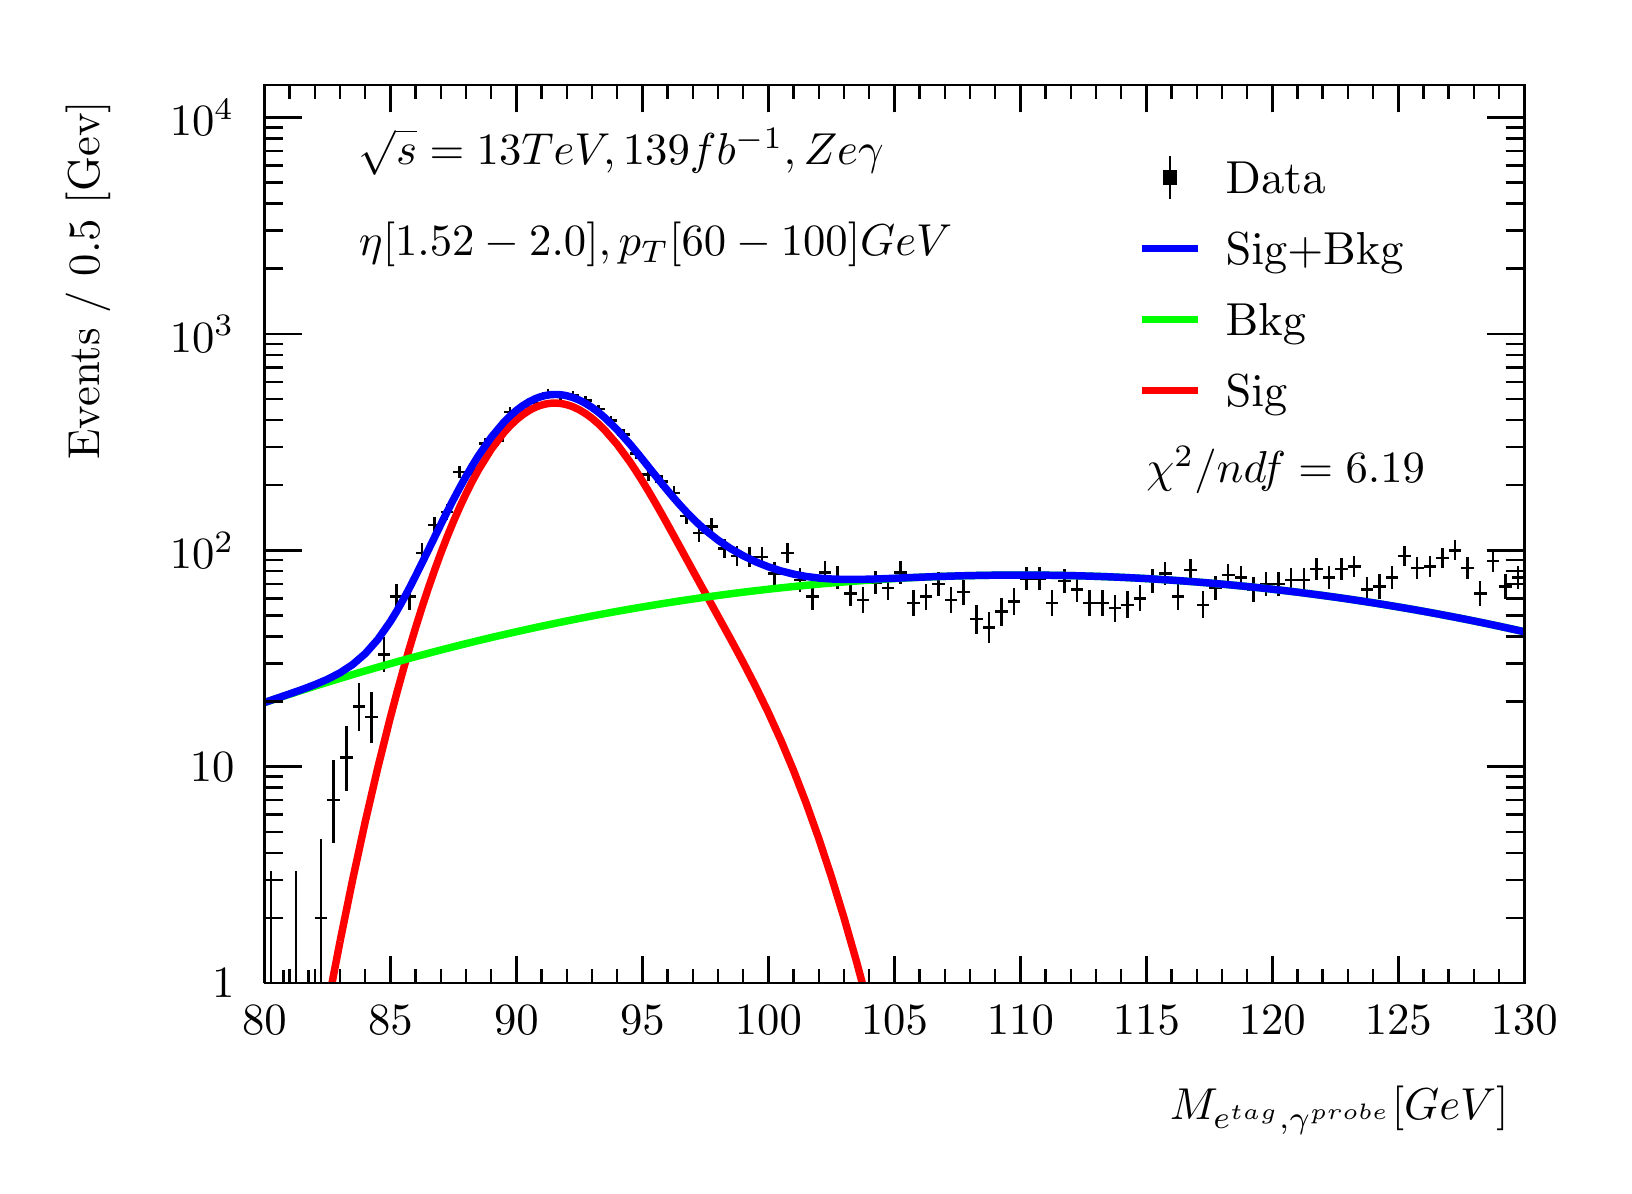
\begin{tikzpicture}
\pgfdeclareplotmark{cross} {
\pgfpathmoveto{\pgfpoint{-0.3\pgfplotmarksize}{\pgfplotmarksize}}
\pgfpathlineto{\pgfpoint{+0.3\pgfplotmarksize}{\pgfplotmarksize}}
\pgfpathlineto{\pgfpoint{+0.3\pgfplotmarksize}{0.3\pgfplotmarksize}}
\pgfpathlineto{\pgfpoint{+1\pgfplotmarksize}{0.3\pgfplotmarksize}}
\pgfpathlineto{\pgfpoint{+1\pgfplotmarksize}{-0.3\pgfplotmarksize}}
\pgfpathlineto{\pgfpoint{+0.3\pgfplotmarksize}{-0.3\pgfplotmarksize}}
\pgfpathlineto{\pgfpoint{+0.3\pgfplotmarksize}{-1.\pgfplotmarksize}}
\pgfpathlineto{\pgfpoint{-0.3\pgfplotmarksize}{-1.\pgfplotmarksize}}
\pgfpathlineto{\pgfpoint{-0.3\pgfplotmarksize}{-0.3\pgfplotmarksize}}
\pgfpathlineto{\pgfpoint{-1.\pgfplotmarksize}{-0.3\pgfplotmarksize}}
\pgfpathlineto{\pgfpoint{-1.\pgfplotmarksize}{0.3\pgfplotmarksize}}
\pgfpathlineto{\pgfpoint{-0.3\pgfplotmarksize}{0.3\pgfplotmarksize}}
\pgfpathclose
\pgfusepathqstroke
}
\pgfdeclareplotmark{cross*} {
\pgfpathmoveto{\pgfpoint{-0.3\pgfplotmarksize}{\pgfplotmarksize}}
\pgfpathlineto{\pgfpoint{+0.3\pgfplotmarksize}{\pgfplotmarksize}}
\pgfpathlineto{\pgfpoint{+0.3\pgfplotmarksize}{0.3\pgfplotmarksize}}
\pgfpathlineto{\pgfpoint{+1\pgfplotmarksize}{0.3\pgfplotmarksize}}
\pgfpathlineto{\pgfpoint{+1\pgfplotmarksize}{-0.3\pgfplotmarksize}}
\pgfpathlineto{\pgfpoint{+0.3\pgfplotmarksize}{-0.3\pgfplotmarksize}}
\pgfpathlineto{\pgfpoint{+0.3\pgfplotmarksize}{-1.\pgfplotmarksize}}
\pgfpathlineto{\pgfpoint{-0.3\pgfplotmarksize}{-1.\pgfplotmarksize}}
\pgfpathlineto{\pgfpoint{-0.3\pgfplotmarksize}{-0.3\pgfplotmarksize}}
\pgfpathlineto{\pgfpoint{-1.\pgfplotmarksize}{-0.3\pgfplotmarksize}}
\pgfpathlineto{\pgfpoint{-1.\pgfplotmarksize}{0.3\pgfplotmarksize}}
\pgfpathlineto{\pgfpoint{-0.3\pgfplotmarksize}{0.3\pgfplotmarksize}}
\pgfpathclose
\pgfusepathqfillstroke
}
\pgfdeclareplotmark{newstar} {
\pgfpathmoveto{\pgfqpoint{0pt}{\pgfplotmarksize}}
\pgfpathlineto{\pgfqpointpolar{44}{0.5\pgfplotmarksize}}
\pgfpathlineto{\pgfqpointpolar{18}{\pgfplotmarksize}}
\pgfpathlineto{\pgfqpointpolar{-20}{0.5\pgfplotmarksize}}
\pgfpathlineto{\pgfqpointpolar{-54}{\pgfplotmarksize}}
\pgfpathlineto{\pgfqpointpolar{-90}{0.5\pgfplotmarksize}}
\pgfpathlineto{\pgfqpointpolar{234}{\pgfplotmarksize}}
\pgfpathlineto{\pgfqpointpolar{198}{0.5\pgfplotmarksize}}
\pgfpathlineto{\pgfqpointpolar{162}{\pgfplotmarksize}}
\pgfpathlineto{\pgfqpointpolar{134}{0.5\pgfplotmarksize}}
\pgfpathclose
\pgfusepathqstroke
}
\pgfdeclareplotmark{newstar*} {
\pgfpathmoveto{\pgfqpoint{0pt}{\pgfplotmarksize}}
\pgfpathlineto{\pgfqpointpolar{44}{0.5\pgfplotmarksize}}
\pgfpathlineto{\pgfqpointpolar{18}{\pgfplotmarksize}}
\pgfpathlineto{\pgfqpointpolar{-20}{0.5\pgfplotmarksize}}
\pgfpathlineto{\pgfqpointpolar{-54}{\pgfplotmarksize}}
\pgfpathlineto{\pgfqpointpolar{-90}{0.5\pgfplotmarksize}}
\pgfpathlineto{\pgfqpointpolar{234}{\pgfplotmarksize}}
\pgfpathlineto{\pgfqpointpolar{198}{0.5\pgfplotmarksize}}
\pgfpathlineto{\pgfqpointpolar{162}{\pgfplotmarksize}}
\pgfpathlineto{\pgfqpointpolar{134}{0.5\pgfplotmarksize}}
\pgfpathclose
\pgfusepathqfillstroke
}
\definecolor{c}{rgb}{1,1,1};
\draw [color=c, fill=c] (0,0) rectangle (20,14.4361);
\draw [color=c, fill=c] (3,2.30977) rectangle (19,13.7143);
\definecolor{c}{rgb}{0,0,0};
\draw [c,line width=0.9] (3,2.30977) -- (3,13.7143) -- (19,13.7143) -- (19,2.30977) -- (3,2.30977);
\definecolor{c}{rgb}{1,1,1};
\draw [color=c, fill=c] (3,2.30977) rectangle (19,13.7143);
\definecolor{c}{rgb}{0,0,0};
\draw [c,line width=0.9] (3,2.30977) -- (3,13.7143) -- (19,13.7143) -- (19,2.30977) -- (3,2.30977);
\draw [c,line width=0.9] (3,2.30977) -- (19,2.30977);
\draw [c,line width=0.9] (3,2.65624) -- (3,2.30977);
\draw [c,line width=0.9] (3.32,2.48301) -- (3.32,2.30977);
\draw [c,line width=0.9] (3.64,2.48301) -- (3.64,2.30977);
\draw [c,line width=0.9] (3.96,2.48301) -- (3.96,2.30977);
\draw [c,line width=0.9] (4.28,2.48301) -- (4.28,2.30977);
\draw [c,line width=0.9] (4.6,2.65624) -- (4.6,2.30977);
\draw [c,line width=0.9] (4.92,2.48301) -- (4.92,2.30977);
\draw [c,line width=0.9] (5.24,2.48301) -- (5.24,2.30977);
\draw [c,line width=0.9] (5.56,2.48301) -- (5.56,2.30977);
\draw [c,line width=0.9] (5.88,2.48301) -- (5.88,2.30977);
\draw [c,line width=0.9] (6.2,2.65624) -- (6.2,2.30977);
\draw [c,line width=0.9] (6.52,2.48301) -- (6.52,2.30977);
\draw [c,line width=0.9] (6.84,2.48301) -- (6.84,2.30977);
\draw [c,line width=0.9] (7.16,2.48301) -- (7.16,2.30977);
\draw [c,line width=0.9] (7.48,2.48301) -- (7.48,2.30977);
\draw [c,line width=0.9] (7.8,2.65624) -- (7.8,2.30977);
\draw [c,line width=0.9] (8.12,2.48301) -- (8.12,2.30977);
\draw [c,line width=0.9] (8.44,2.48301) -- (8.44,2.30977);
\draw [c,line width=0.9] (8.76,2.48301) -- (8.76,2.30977);
\draw [c,line width=0.9] (9.08,2.48301) -- (9.08,2.30977);
\draw [c,line width=0.9] (9.4,2.65624) -- (9.4,2.30977);
\draw [c,line width=0.9] (9.72,2.48301) -- (9.72,2.30977);
\draw [c,line width=0.9] (10.04,2.48301) -- (10.04,2.30977);
\draw [c,line width=0.9] (10.36,2.48301) -- (10.36,2.30977);
\draw [c,line width=0.9] (10.68,2.48301) -- (10.68,2.30977);
\draw [c,line width=0.9] (11,2.65624) -- (11,2.30977);
\draw [c,line width=0.9] (11.32,2.48301) -- (11.32,2.30977);
\draw [c,line width=0.9] (11.64,2.48301) -- (11.64,2.30977);
\draw [c,line width=0.9] (11.96,2.48301) -- (11.96,2.30977);
\draw [c,line width=0.9] (12.28,2.48301) -- (12.28,2.30977);
\draw [c,line width=0.9] (12.6,2.65624) -- (12.6,2.30977);
\draw [c,line width=0.9] (12.92,2.48301) -- (12.92,2.30977);
\draw [c,line width=0.9] (13.24,2.48301) -- (13.24,2.30977);
\draw [c,line width=0.9] (13.56,2.48301) -- (13.56,2.30977);
\draw [c,line width=0.9] (13.88,2.48301) -- (13.88,2.30977);
\draw [c,line width=0.9] (14.2,2.65624) -- (14.2,2.30977);
\draw [c,line width=0.9] (14.52,2.48301) -- (14.52,2.30977);
\draw [c,line width=0.9] (14.84,2.48301) -- (14.84,2.30977);
\draw [c,line width=0.9] (15.16,2.48301) -- (15.16,2.30977);
\draw [c,line width=0.9] (15.48,2.48301) -- (15.48,2.30977);
\draw [c,line width=0.9] (15.8,2.65624) -- (15.8,2.30977);
\draw [c,line width=0.9] (16.12,2.48301) -- (16.12,2.30977);
\draw [c,line width=0.9] (16.44,2.48301) -- (16.44,2.30977);
\draw [c,line width=0.9] (16.76,2.48301) -- (16.76,2.30977);
\draw [c,line width=0.9] (17.08,2.48301) -- (17.08,2.30977);
\draw [c,line width=0.9] (17.4,2.65624) -- (17.4,2.30977);
\draw [c,line width=0.9] (17.72,2.48301) -- (17.72,2.30977);
\draw [c,line width=0.9] (18.04,2.48301) -- (18.04,2.30977);
\draw [c,line width=0.9] (18.36,2.48301) -- (18.36,2.30977);
\draw [c,line width=0.9] (18.68,2.48301) -- (18.68,2.30977);
\draw [c,line width=0.9] (19,2.65624) -- (19,2.30977);
\draw [anchor=base] (3,1.66015) node[scale=1.61424, color=c, rotate=0]{80};
\draw [anchor=base] (4.6,1.66015) node[scale=1.61424, color=c, rotate=0]{85};
\draw [anchor=base] (6.2,1.66015) node[scale=1.61424, color=c, rotate=0]{90};
\draw [anchor=base] (7.8,1.66015) node[scale=1.61424, color=c, rotate=0]{95};
\draw [anchor=base] (9.4,1.66015) node[scale=1.61424, color=c, rotate=0]{100};
\draw [anchor=base] (11,1.66015) node[scale=1.61424, color=c, rotate=0]{105};
\draw [anchor=base] (12.6,1.66015) node[scale=1.61424, color=c, rotate=0]{110};
\draw [anchor=base] (14.2,1.66015) node[scale=1.61424, color=c, rotate=0]{115};
\draw [anchor=base] (15.8,1.66015) node[scale=1.61424, color=c, rotate=0]{120};
\draw [anchor=base] (17.4,1.66015) node[scale=1.61424, color=c, rotate=0]{125};
\draw [anchor=base] (19,1.66015) node[scale=1.61424, color=c, rotate=0]{130};
\draw [anchor= east] (19,0.692932) node[scale=1.61424, color=c, rotate=0]{$M_{e^{tag}, \gamma^{probe}}  [GeV]$};
\draw [c,line width=0.9] (3,13.7143) -- (19,13.7143);
\draw [c,line width=0.9] (3,13.3678) -- (3,13.7143);
\draw [c,line width=0.9] (3.32,13.5411) -- (3.32,13.7143);
\draw [c,line width=0.9] (3.64,13.5411) -- (3.64,13.7143);
\draw [c,line width=0.9] (3.96,13.5411) -- (3.96,13.7143);
\draw [c,line width=0.9] (4.28,13.5411) -- (4.28,13.7143);
\draw [c,line width=0.9] (4.6,13.3678) -- (4.6,13.7143);
\draw [c,line width=0.9] (4.92,13.5411) -- (4.92,13.7143);
\draw [c,line width=0.9] (5.24,13.5411) -- (5.24,13.7143);
\draw [c,line width=0.9] (5.56,13.5411) -- (5.56,13.7143);
\draw [c,line width=0.9] (5.88,13.5411) -- (5.88,13.7143);
\draw [c,line width=0.9] (6.2,13.3678) -- (6.2,13.7143);
\draw [c,line width=0.9] (6.52,13.5411) -- (6.52,13.7143);
\draw [c,line width=0.9] (6.84,13.5411) -- (6.84,13.7143);
\draw [c,line width=0.9] (7.16,13.5411) -- (7.16,13.7143);
\draw [c,line width=0.9] (7.48,13.5411) -- (7.48,13.7143);
\draw [c,line width=0.9] (7.8,13.3678) -- (7.8,13.7143);
\draw [c,line width=0.9] (8.12,13.5411) -- (8.12,13.7143);
\draw [c,line width=0.9] (8.44,13.5411) -- (8.44,13.7143);
\draw [c,line width=0.9] (8.76,13.5411) -- (8.76,13.7143);
\draw [c,line width=0.9] (9.08,13.5411) -- (9.08,13.7143);
\draw [c,line width=0.9] (9.4,13.3678) -- (9.4,13.7143);
\draw [c,line width=0.9] (9.72,13.5411) -- (9.72,13.7143);
\draw [c,line width=0.9] (10.04,13.5411) -- (10.04,13.7143);
\draw [c,line width=0.9] (10.36,13.5411) -- (10.36,13.7143);
\draw [c,line width=0.9] (10.68,13.5411) -- (10.68,13.7143);
\draw [c,line width=0.9] (11,13.3678) -- (11,13.7143);
\draw [c,line width=0.9] (11.32,13.5411) -- (11.32,13.7143);
\draw [c,line width=0.9] (11.64,13.5411) -- (11.64,13.7143);
\draw [c,line width=0.9] (11.96,13.5411) -- (11.96,13.7143);
\draw [c,line width=0.9] (12.28,13.5411) -- (12.28,13.7143);
\draw [c,line width=0.9] (12.6,13.3678) -- (12.6,13.7143);
\draw [c,line width=0.9] (12.92,13.5411) -- (12.92,13.7143);
\draw [c,line width=0.9] (13.24,13.5411) -- (13.24,13.7143);
\draw [c,line width=0.9] (13.56,13.5411) -- (13.56,13.7143);
\draw [c,line width=0.9] (13.88,13.5411) -- (13.88,13.7143);
\draw [c,line width=0.9] (14.2,13.3678) -- (14.2,13.7143);
\draw [c,line width=0.9] (14.52,13.5411) -- (14.52,13.7143);
\draw [c,line width=0.9] (14.84,13.5411) -- (14.84,13.7143);
\draw [c,line width=0.9] (15.16,13.5411) -- (15.16,13.7143);
\draw [c,line width=0.9] (15.48,13.5411) -- (15.48,13.7143);
\draw [c,line width=0.9] (15.8,13.3678) -- (15.8,13.7143);
\draw [c,line width=0.9] (16.12,13.5411) -- (16.12,13.7143);
\draw [c,line width=0.9] (16.44,13.5411) -- (16.44,13.7143);
\draw [c,line width=0.9] (16.76,13.5411) -- (16.76,13.7143);
\draw [c,line width=0.9] (17.08,13.5411) -- (17.08,13.7143);
\draw [c,line width=0.9] (17.4,13.3678) -- (17.4,13.7143);
\draw [c,line width=0.9] (17.72,13.5411) -- (17.72,13.7143);
\draw [c,line width=0.9] (18.04,13.5411) -- (18.04,13.7143);
\draw [c,line width=0.9] (18.36,13.5411) -- (18.36,13.7143);
\draw [c,line width=0.9] (18.68,13.5411) -- (18.68,13.7143);
\draw [c,line width=0.9] (19,13.3678) -- (19,13.7143);
\draw [c,line width=0.9] (3,2.30977) -- (3,13.7143);
\draw [c,line width=0.9] (3.474,2.30978) -- (3,2.30978);
\draw [anchor= east] (2.82,2.30978) node[scale=1.61424, color=c, rotate=0]{1};
\draw [c,line width=0.9] (3.237,3.13707) -- (3,3.13707);
\draw [c,line width=0.9] (3.237,3.621) -- (3,3.621);
\draw [c,line width=0.9] (3.237,3.96436) -- (3,3.96436);
\draw [c,line width=0.9] (3.237,4.23069) -- (3,4.23069);
\draw [c,line width=0.9] (3.237,4.4483) -- (3,4.4483);
\draw [c,line width=0.9] (3.237,4.63228) -- (3,4.63228);
\draw [c,line width=0.9] (3.237,4.79165) -- (3,4.79165);
\draw [c,line width=0.9] (3.237,4.93223) -- (3,4.93223);
\draw [c,line width=0.9] (3.474,5.05798) -- (3,5.05798);
\draw [anchor= east] (2.82,5.05798) node[scale=1.61424, color=c, rotate=0]{10};
\draw [c,line width=0.9] (3.237,5.88527) -- (3,5.88527);
\draw [c,line width=0.9] (3.237,6.36921) -- (3,6.36921);
\draw [c,line width=0.9] (3.237,6.71257) -- (3,6.71257);
\draw [c,line width=0.9] (3.237,6.97889) -- (3,6.97889);
\draw [c,line width=0.9] (3.237,7.1965) -- (3,7.1965);
\draw [c,line width=0.9] (3.237,7.38048) -- (3,7.38048);
\draw [c,line width=0.9] (3.237,7.53986) -- (3,7.53986);
\draw [c,line width=0.9] (3.237,7.68043) -- (3,7.68043);
\draw [c,line width=0.9] (3.474,7.80619) -- (3,7.80619);
\draw [anchor= east] (2.82,7.80619) node[scale=1.61424, color=c, rotate=0]{$10^{2}$};
\draw [c,line width=0.9] (3.237,8.63348) -- (3,8.63348);
\draw [c,line width=0.9] (3.237,9.11741) -- (3,9.11741);
\draw [c,line width=0.9] (3.237,9.46077) -- (3,9.46077);
\draw [c,line width=0.9] (3.237,9.7271) -- (3,9.7271);
\draw [c,line width=0.9] (3.237,9.9447) -- (3,9.9447);
\draw [c,line width=0.9] (3.237,10.1287) -- (3,10.1287);
\draw [c,line width=0.9] (3.237,10.2881) -- (3,10.2881);
\draw [c,line width=0.9] (3.237,10.4286) -- (3,10.4286);
\draw [c,line width=0.9] (3.474,10.5544) -- (3,10.5544);
\draw [anchor= east] (2.82,10.5544) node[scale=1.61424, color=c, rotate=0]{$10^{3}$};
\draw [c,line width=0.9] (3.237,11.3817) -- (3,11.3817);
\draw [c,line width=0.9] (3.237,11.8656) -- (3,11.8656);
\draw [c,line width=0.9] (3.237,12.209) -- (3,12.209);
\draw [c,line width=0.9] (3.237,12.4753) -- (3,12.4753);
\draw [c,line width=0.9] (3.237,12.6929) -- (3,12.6929);
\draw [c,line width=0.9] (3.237,12.8769) -- (3,12.8769);
\draw [c,line width=0.9] (3.237,13.0363) -- (3,13.0363);
\draw [c,line width=0.9] (3.237,13.1768) -- (3,13.1768);
\draw [c,line width=0.9] (3.474,13.3026) -- (3,13.3026);
\draw [anchor= east] (2.82,13.3026) node[scale=1.61424, color=c, rotate=0]{$10^{4}$};
\draw [anchor= east] (0.76,13.7143) node[scale=1.61424, color=c, rotate=90]{Events / 0.5 [Gev]};
\draw [c,line width=0.9] (19,2.30977) -- (19,13.7143);
\draw [c,line width=0.9] (18.526,2.30978) -- (19,2.30978);
\draw [c,line width=0.9] (18.763,3.13707) -- (19,3.13707);
\draw [c,line width=0.9] (18.763,3.621) -- (19,3.621);
\draw [c,line width=0.9] (18.763,3.96436) -- (19,3.96436);
\draw [c,line width=0.9] (18.763,4.23069) -- (19,4.23069);
\draw [c,line width=0.9] (18.763,4.4483) -- (19,4.4483);
\draw [c,line width=0.9] (18.763,4.63228) -- (19,4.63228);
\draw [c,line width=0.9] (18.763,4.79165) -- (19,4.79165);
\draw [c,line width=0.9] (18.763,4.93223) -- (19,4.93223);
\draw [c,line width=0.9] (18.526,5.05798) -- (19,5.05798);
\draw [c,line width=0.9] (18.763,5.88527) -- (19,5.88527);
\draw [c,line width=0.9] (18.763,6.36921) -- (19,6.36921);
\draw [c,line width=0.9] (18.763,6.71257) -- (19,6.71257);
\draw [c,line width=0.9] (18.763,6.97889) -- (19,6.97889);
\draw [c,line width=0.9] (18.763,7.1965) -- (19,7.1965);
\draw [c,line width=0.9] (18.763,7.38048) -- (19,7.38048);
\draw [c,line width=0.9] (18.763,7.53986) -- (19,7.53986);
\draw [c,line width=0.9] (18.763,7.68043) -- (19,7.68043);
\draw [c,line width=0.9] (18.526,7.80619) -- (19,7.80619);
\draw [c,line width=0.9] (18.763,8.63348) -- (19,8.63348);
\draw [c,line width=0.9] (18.763,9.11741) -- (19,9.11741);
\draw [c,line width=0.9] (18.763,9.46077) -- (19,9.46077);
\draw [c,line width=0.9] (18.763,9.7271) -- (19,9.7271);
\draw [c,line width=0.9] (18.763,9.9447) -- (19,9.9447);
\draw [c,line width=0.9] (18.763,10.1287) -- (19,10.1287);
\draw [c,line width=0.9] (18.763,10.2881) -- (19,10.2881);
\draw [c,line width=0.9] (18.763,10.4286) -- (19,10.4286);
\draw [c,line width=0.9] (18.526,10.5544) -- (19,10.5544);
\draw [c,line width=0.9] (18.763,11.3817) -- (19,11.3817);
\draw [c,line width=0.9] (18.763,11.8656) -- (19,11.8656);
\draw [c,line width=0.9] (18.763,12.209) -- (19,12.209);
\draw [c,line width=0.9] (18.763,12.4753) -- (19,12.4753);
\draw [c,line width=0.9] (18.763,12.6929) -- (19,12.6929);
\draw [c,line width=0.9] (18.763,12.8769) -- (19,12.8769);
\draw [c,line width=0.9] (18.763,13.0363) -- (19,13.0363);
\draw [c,line width=0.9] (18.763,13.1768) -- (19,13.1768);
\draw [c,line width=0.9] (18.526,13.3026) -- (19,13.3026);
\draw [c,line width=0.9] (3.08,2.30977) -- (3,2.30977);
\draw [c,line width=0.9] (3,2.30977) -- (3,2.30977);
\draw [c,line width=0.9] (3.08,2.30977) -- (3.16,2.30977);
\draw [c,line width=0.9] (3.16,2.30977) -- (3.16,2.30977);
\draw [c,line width=0.9] (3.08,2.30977) -- (3.08,3.73459);
\draw [c,line width=0.9] (3.08,3.73459) -- (3.08,3.73459);
\draw [c,line width=0.9] (3.24,2.30977) -- (3.16,2.30977);
\draw [c,line width=0.9] (3.16,2.30977) -- (3.16,2.30977);
\draw [c,line width=0.9] (3.24,2.30977) -- (3.32,2.30977);
\draw [c,line width=0.9] (3.32,2.30977) -- (3.32,2.30977);
\draw [c,line width=0.9] (3.24,2.30977) -- (3.24,2.47438);
\draw [c,line width=0.9] (3.24,2.47438) -- (3.24,2.47438);
\draw [c,line width=0.9] (3.4,2.30977) -- (3.32,2.30977);
\draw [c,line width=0.9] (3.32,2.30977) -- (3.32,2.30977);
\draw [c,line width=0.9] (3.4,2.30977) -- (3.48,2.30977);
\draw [c,line width=0.9] (3.48,2.30977) -- (3.48,2.30977);
\draw [c,line width=0.9] (3.4,2.30977) -- (3.4,3.73459);
\draw [c,line width=0.9] (3.4,3.73459) -- (3.4,3.73459);
\draw [c,line width=0.9] (3.56,2.30977) -- (3.48,2.30977);
\draw [c,line width=0.9] (3.48,2.30977) -- (3.48,2.30977);
\draw [c,line width=0.9] (3.56,2.30977) -- (3.64,2.30977);
\draw [c,line width=0.9] (3.64,2.30977) -- (3.64,2.30977);
\draw [c,line width=0.9] (3.56,2.30977) -- (3.56,2.47438);
\draw [c,line width=0.9] (3.56,2.47438) -- (3.56,2.47438);
\draw [c,line width=0.9] (3.72,3.13707) -- (3.64,3.13707);
\draw [c,line width=0.9] (3.64,3.13707) -- (3.64,3.13707);
\draw [c,line width=0.9] (3.72,3.13707) -- (3.8,3.13707);
\draw [c,line width=0.9] (3.8,3.13707) -- (3.8,3.13707);
\draw [c,line width=0.9] (3.72,3.13707) -- (3.72,4.14095);
\draw [c,line width=0.9] (3.72,4.14095) -- (3.72,4.14095);
\draw [c,line width=0.9] (3.72,3.13707) -- (3.72,2.30977);
\draw [c,line width=0.9] (3.72,2.30977) -- (3.72,2.30977);
\draw [c,line width=0.9] (3.88,4.63228) -- (3.8,4.63228);
\draw [c,line width=0.9] (3.8,4.63228) -- (3.8,4.63228);
\draw [c,line width=0.9] (3.88,4.63228) -- (3.96,4.63228);
\draw [c,line width=0.9] (3.96,4.63228) -- (3.96,4.63228);
\draw [c,line width=0.9] (3.88,4.63228) -- (3.88,5.14655);
\draw [c,line width=0.9] (3.88,5.14655) -- (3.88,5.14655);
\draw [c,line width=0.9] (3.88,4.63228) -- (3.88,4.08313);
\draw [c,line width=0.9] (3.88,4.08313) -- (3.88,4.08313);
\draw [c,line width=0.9] (4.04,5.17173) -- (3.96,5.17173);
\draw [c,line width=0.9] (3.96,5.17173) -- (3.96,5.17173);
\draw [c,line width=0.9] (4.04,5.17173) -- (4.12,5.17173);
\draw [c,line width=0.9] (4.12,5.17173) -- (4.12,5.17173);
\draw [c,line width=0.9] (4.04,5.17173) -- (4.04,5.5746);
\draw [c,line width=0.9] (4.04,5.5746) -- (4.04,5.5746);
\draw [c,line width=0.9] (4.04,5.17173) -- (4.04,4.75136);
\draw [c,line width=0.9] (4.04,4.75136) -- (4.04,4.75136);
\draw [c,line width=0.9] (4.2,5.82405) -- (4.12,5.82405);
\draw [c,line width=0.9] (4.12,5.82405) -- (4.12,5.82405);
\draw [c,line width=0.9] (4.2,5.82405) -- (4.28,5.82405);
\draw [c,line width=0.9] (4.28,5.82405) -- (4.28,5.82405);
\draw [c,line width=0.9] (4.2,5.82405) -- (4.2,6.12433);
\draw [c,line width=0.9] (4.2,6.12433) -- (4.2,6.12433);
\draw [c,line width=0.9] (4.2,5.82405) -- (4.2,5.51616);
\draw [c,line width=0.9] (4.2,5.51616) -- (4.2,5.51616);
\draw [c,line width=0.9] (4.36,5.6913) -- (4.28,5.6913);
\draw [c,line width=0.9] (4.28,5.6913) -- (4.28,5.6913);
\draw [c,line width=0.9] (4.36,5.6913) -- (4.44,5.6913);
\draw [c,line width=0.9] (4.44,5.6913) -- (4.44,5.6913);
\draw [c,line width=0.9] (4.36,5.6913) -- (4.36,6.01003);
\draw [c,line width=0.9] (4.36,6.01003) -- (4.36,6.01003);
\draw [c,line width=0.9] (4.36,5.6913) -- (4.36,5.36355);
\draw [c,line width=0.9] (4.36,5.36355) -- (4.36,5.36355);
\draw [c,line width=0.9] (4.52,6.48296) -- (4.44,6.48296);
\draw [c,line width=0.9] (4.44,6.48296) -- (4.44,6.48296);
\draw [c,line width=0.9] (4.52,6.48296) -- (4.6,6.48296);
\draw [c,line width=0.9] (4.6,6.48296) -- (4.6,6.48296);
\draw [c,line width=0.9] (4.52,6.48296) -- (4.52,6.70666);
\draw [c,line width=0.9] (4.52,6.70666) -- (4.52,6.70666);
\draw [c,line width=0.9] (4.52,6.48296) -- (4.52,6.25597);
\draw [c,line width=0.9] (4.52,6.25597) -- (4.52,6.25597);
\draw [c,line width=0.9] (4.68,7.21623) -- (4.6,7.21623);
\draw [c,line width=0.9] (4.6,7.21623) -- (4.6,7.21623);
\draw [c,line width=0.9] (4.68,7.21623) -- (4.76,7.21623);
\draw [c,line width=0.9] (4.76,7.21623) -- (4.76,7.21623);
\draw [c,line width=0.9] (4.68,7.21623) -- (4.68,7.37797);
\draw [c,line width=0.9] (4.68,7.37797) -- (4.68,7.37797);
\draw [c,line width=0.9] (4.68,7.21623) -- (4.68,7.05318);
\draw [c,line width=0.9] (4.68,7.05318) -- (4.68,7.05318);
\draw [c,line width=0.9] (4.84,7.21623) -- (4.76,7.21623);
\draw [c,line width=0.9] (4.76,7.21623) -- (4.76,7.21623);
\draw [c,line width=0.9] (4.84,7.21623) -- (4.92,7.21623);
\draw [c,line width=0.9] (4.92,7.21623) -- (4.92,7.21623);
\draw [c,line width=0.9] (4.84,7.21623) -- (4.84,7.37797);
\draw [c,line width=0.9] (4.84,7.37797) -- (4.84,7.37797);
\draw [c,line width=0.9] (4.84,7.21623) -- (4.84,7.05318);
\draw [c,line width=0.9] (4.84,7.05318) -- (4.84,7.05318);
\draw [c,line width=0.9] (5,7.76983) -- (4.92,7.76983);
\draw [c,line width=0.9] (4.92,7.76983) -- (4.92,7.76983);
\draw [c,line width=0.9] (5,7.76983) -- (5.08,7.76983);
\draw [c,line width=0.9] (5.08,7.76983) -- (5.08,7.76983);
\draw [c,line width=0.9] (5,7.76983) -- (5,7.89674);
\draw [c,line width=0.9] (5,7.89674) -- (5,7.89674);
\draw [c,line width=0.9] (5,7.76983) -- (5,7.64228);
\draw [c,line width=0.9] (5,7.64228) -- (5,7.64228);
\draw [c,line width=0.9] (5.16,8.12847) -- (5.08,8.12847);
\draw [c,line width=0.9] (5.08,8.12847) -- (5.08,8.12847);
\draw [c,line width=0.9] (5.16,8.12847) -- (5.24,8.12847);
\draw [c,line width=0.9] (5.24,8.12847) -- (5.24,8.12847);
\draw [c,line width=0.9] (5.16,8.12847) -- (5.16,8.23272);
\draw [c,line width=0.9] (5.16,8.23272) -- (5.16,8.23272);
\draw [c,line width=0.9] (5.16,8.12847) -- (5.16,8.02422);
\draw [c,line width=0.9] (5.16,8.02422) -- (5.16,8.02422);
\draw [c,line width=0.9] (5.32,8.29012) -- (5.24,8.29012);
\draw [c,line width=0.9] (5.24,8.29012) -- (5.24,8.29012);
\draw [c,line width=0.9] (5.32,8.29012) -- (5.4,8.29012);
\draw [c,line width=0.9] (5.4,8.29012) -- (5.4,8.29012);
\draw [c,line width=0.9] (5.32,8.29012) -- (5.32,8.38754);
\draw [c,line width=0.9] (5.32,8.38754) -- (5.32,8.38754);
\draw [c,line width=0.9] (5.32,8.29012) -- (5.32,8.19269);
\draw [c,line width=0.9] (5.32,8.19269) -- (5.32,8.19269);
\draw [c,line width=0.9] (5.48,8.80029) -- (5.4,8.80029);
\draw [c,line width=0.9] (5.4,8.80029) -- (5.4,8.80029);
\draw [c,line width=0.9] (5.48,8.80029) -- (5.56,8.80029);
\draw [c,line width=0.9] (5.56,8.80029) -- (5.56,8.80029);
\draw [c,line width=0.9] (5.48,8.80029) -- (5.48,8.87897);
\draw [c,line width=0.9] (5.48,8.87897) -- (5.48,8.87897);
\draw [c,line width=0.9] (5.48,8.80029) -- (5.48,8.7216);
\draw [c,line width=0.9] (5.48,8.7216) -- (5.48,8.7216);
\draw [c,line width=0.9] (5.64,8.82595) -- (5.56,8.82595);
\draw [c,line width=0.9] (5.56,8.82595) -- (5.56,8.82595);
\draw [c,line width=0.9] (5.64,8.82595) -- (5.72,8.82595);
\draw [c,line width=0.9] (5.72,8.82595) -- (5.72,8.82595);
\draw [c,line width=0.9] (5.64,8.82595) -- (5.64,8.9038);
\draw [c,line width=0.9] (5.64,8.9038) -- (5.64,8.9038);
\draw [c,line width=0.9] (5.64,8.82595) -- (5.64,8.74811);
\draw [c,line width=0.9] (5.64,8.74811) -- (5.64,8.74811);
\draw [c,line width=0.9] (5.8,9.16422) -- (5.72,9.16422);
\draw [c,line width=0.9] (5.72,9.16422) -- (5.72,9.16422);
\draw [c,line width=0.9] (5.8,9.16422) -- (5.88,9.16422);
\draw [c,line width=0.9] (5.88,9.16422) -- (5.88,9.16422);
\draw [c,line width=0.9] (5.8,9.16422) -- (5.8,9.23178);
\draw [c,line width=0.9] (5.8,9.23178) -- (5.8,9.23178);
\draw [c,line width=0.9] (5.8,9.16422) -- (5.8,9.09666);
\draw [c,line width=0.9] (5.8,9.09666) -- (5.8,9.09666);
\draw [c,line width=0.9] (5.96,9.20188) -- (5.88,9.20188);
\draw [c,line width=0.9] (5.88,9.20188) -- (5.88,9.20188);
\draw [c,line width=0.9] (5.96,9.20188) -- (6.04,9.20188);
\draw [c,line width=0.9] (6.04,9.20188) -- (6.04,9.20188);
\draw [c,line width=0.9] (5.96,9.20188) -- (5.96,9.26838);
\draw [c,line width=0.9] (5.96,9.26838) -- (5.96,9.26838);
\draw [c,line width=0.9] (5.96,9.20188) -- (5.96,9.13537);
\draw [c,line width=0.9] (5.96,9.13537) -- (5.96,9.13537);
\draw [c,line width=0.9] (6.12,9.56362) -- (6.04,9.56362);
\draw [c,line width=0.9] (6.04,9.56362) -- (6.04,9.56362);
\draw [c,line width=0.9] (6.12,9.56362) -- (6.2,9.56362);
\draw [c,line width=0.9] (6.2,9.56362) -- (6.2,9.56362);
\draw [c,line width=0.9] (6.12,9.56362) -- (6.12,9.62078);
\draw [c,line width=0.9] (6.12,9.62078) -- (6.12,9.62078);
\draw [c,line width=0.9] (6.12,9.56362) -- (6.12,9.50647);
\draw [c,line width=0.9] (6.12,9.50647) -- (6.12,9.50647);
\draw [c,line width=0.9] (6.28,9.62498) -- (6.2,9.62498);
\draw [c,line width=0.9] (6.2,9.62498) -- (6.2,9.62498);
\draw [c,line width=0.9] (6.28,9.62498) -- (6.36,9.62498);
\draw [c,line width=0.9] (6.36,9.62498) -- (6.36,9.62498);
\draw [c,line width=0.9] (6.28,9.62498) -- (6.28,9.68069);
\draw [c,line width=0.9] (6.28,9.68069) -- (6.28,9.68069);
\draw [c,line width=0.9] (6.28,9.62498) -- (6.28,9.56928);
\draw [c,line width=0.9] (6.28,9.56928) -- (6.28,9.56928);
\draw [c,line width=0.9] (6.44,9.67837) -- (6.36,9.67837);
\draw [c,line width=0.9] (6.36,9.67837) -- (6.36,9.67837);
\draw [c,line width=0.9] (6.44,9.67837) -- (6.52,9.67837);
\draw [c,line width=0.9] (6.52,9.67837) -- (6.52,9.67837);
\draw [c,line width=0.9] (6.44,9.67837) -- (6.44,9.73285);
\draw [c,line width=0.9] (6.44,9.73285) -- (6.44,9.73285);
\draw [c,line width=0.9] (6.44,9.67837) -- (6.44,9.6239);
\draw [c,line width=0.9] (6.44,9.6239) -- (6.44,9.6239);
\draw [c,line width=0.9] (6.6,9.79664) -- (6.52,9.79664);
\draw [c,line width=0.9] (6.52,9.79664) -- (6.52,9.79664);
\draw [c,line width=0.9] (6.6,9.79664) -- (6.68,9.79664);
\draw [c,line width=0.9] (6.68,9.79664) -- (6.68,9.79664);
\draw [c,line width=0.9] (6.6,9.79664) -- (6.6,9.84848);
\draw [c,line width=0.9] (6.6,9.84848) -- (6.6,9.84848);
\draw [c,line width=0.9] (6.6,9.79664) -- (6.6,9.7448);
\draw [c,line width=0.9] (6.6,9.7448) -- (6.6,9.7448);
\draw [c,line width=0.9] (6.76,9.68334) -- (6.68,9.68334);
\draw [c,line width=0.9] (6.68,9.68334) -- (6.68,9.68334);
\draw [c,line width=0.9] (6.76,9.68334) -- (6.84,9.68334);
\draw [c,line width=0.9] (6.84,9.68334) -- (6.84,9.68334);
\draw [c,line width=0.9] (6.76,9.68334) -- (6.76,9.7377);
\draw [c,line width=0.9] (6.76,9.7377) -- (6.76,9.7377);
\draw [c,line width=0.9] (6.76,9.68334) -- (6.76,9.62898);
\draw [c,line width=0.9] (6.76,9.62898) -- (6.76,9.62898);
\draw [c,line width=0.9] (6.92,9.77391) -- (6.84,9.77391);
\draw [c,line width=0.9] (6.84,9.77391) -- (6.84,9.77391);
\draw [c,line width=0.9] (6.92,9.77391) -- (7,9.77391);
\draw [c,line width=0.9] (7,9.77391) -- (7,9.77391);
\draw [c,line width=0.9] (6.92,9.77391) -- (6.92,9.82624);
\draw [c,line width=0.9] (6.92,9.82624) -- (6.92,9.82624);
\draw [c,line width=0.9] (6.92,9.77391) -- (6.92,9.72157);
\draw [c,line width=0.9] (6.92,9.72157) -- (6.92,9.72157);
\draw [c,line width=0.9] (7.08,9.71027) -- (7,9.71027);
\draw [c,line width=0.9] (7,9.71027) -- (7,9.71027);
\draw [c,line width=0.9] (7.08,9.71027) -- (7.16,9.71027);
\draw [c,line width=0.9] (7.16,9.71027) -- (7.16,9.71027);
\draw [c,line width=0.9] (7.08,9.71027) -- (7.08,9.76402);
\draw [c,line width=0.9] (7.08,9.76402) -- (7.08,9.76402);
\draw [c,line width=0.9] (7.08,9.71027) -- (7.08,9.65652);
\draw [c,line width=0.9] (7.08,9.65652) -- (7.08,9.65652);
\draw [c,line width=0.9] (7.24,9.59869) -- (7.16,9.59869);
\draw [c,line width=0.9] (7.16,9.59869) -- (7.16,9.59869);
\draw [c,line width=0.9] (7.24,9.59869) -- (7.32,9.59869);
\draw [c,line width=0.9] (7.32,9.59869) -- (7.32,9.59869);
\draw [c,line width=0.9] (7.24,9.59869) -- (7.24,9.65501);
\draw [c,line width=0.9] (7.24,9.65501) -- (7.24,9.65501);
\draw [c,line width=0.9] (7.24,9.59869) -- (7.24,9.54237);
\draw [c,line width=0.9] (7.24,9.54237) -- (7.24,9.54237);
\draw [c,line width=0.9] (7.4,9.45479) -- (7.32,9.45479);
\draw [c,line width=0.9] (7.32,9.45479) -- (7.32,9.45479);
\draw [c,line width=0.9] (7.4,9.45479) -- (7.48,9.45479);
\draw [c,line width=0.9] (7.48,9.45479) -- (7.48,9.45479);
\draw [c,line width=0.9] (7.4,9.45479) -- (7.4,9.51461);
\draw [c,line width=0.9] (7.4,9.51461) -- (7.4,9.51461);
\draw [c,line width=0.9] (7.4,9.45479) -- (7.4,9.39497);
\draw [c,line width=0.9] (7.4,9.39497) -- (7.4,9.39497);
\draw [c,line width=0.9] (7.56,9.27728) -- (7.48,9.27728);
\draw [c,line width=0.9] (7.48,9.27728) -- (7.48,9.27728);
\draw [c,line width=0.9] (7.56,9.27728) -- (7.64,9.27728);
\draw [c,line width=0.9] (7.64,9.27728) -- (7.64,9.27728);
\draw [c,line width=0.9] (7.56,9.27728) -- (7.56,9.34172);
\draw [c,line width=0.9] (7.56,9.34172) -- (7.56,9.34172);
\draw [c,line width=0.9] (7.56,9.27728) -- (7.56,9.21285);
\draw [c,line width=0.9] (7.56,9.21285) -- (7.56,9.21285);
\draw [c,line width=0.9] (7.72,9.03507) -- (7.64,9.03507);
\draw [c,line width=0.9] (7.64,9.03507) -- (7.64,9.03507);
\draw [c,line width=0.9] (7.72,9.03507) -- (7.8,9.03507);
\draw [c,line width=0.9] (7.8,9.03507) -- (7.8,9.03507);
\draw [c,line width=0.9] (7.72,9.03507) -- (7.72,9.10638);
\draw [c,line width=0.9] (7.72,9.10638) -- (7.72,9.10638);
\draw [c,line width=0.9] (7.72,9.03507) -- (7.72,8.96375);
\draw [c,line width=0.9] (7.72,8.96375) -- (7.72,8.96375);
\draw [c,line width=0.9] (7.88,8.76874) -- (7.8,8.76874);
\draw [c,line width=0.9] (7.8,8.76874) -- (7.8,8.76874);
\draw [c,line width=0.9] (7.88,8.76874) -- (7.96,8.76874);
\draw [c,line width=0.9] (7.96,8.76874) -- (7.96,8.76874);
\draw [c,line width=0.9] (7.88,8.76874) -- (7.88,8.84847);
\draw [c,line width=0.9] (7.88,8.84847) -- (7.88,8.84847);
\draw [c,line width=0.9] (7.88,8.76874) -- (7.88,8.68901);
\draw [c,line width=0.9] (7.88,8.68901) -- (7.88,8.68901);
\draw [c,line width=0.9] (8.04,8.68029) -- (7.96,8.68029);
\draw [c,line width=0.9] (7.96,8.68029) -- (7.96,8.68029);
\draw [c,line width=0.9] (8.04,8.68029) -- (8.12,8.68029);
\draw [c,line width=0.9] (8.12,8.68029) -- (8.12,8.68029);
\draw [c,line width=0.9] (8.04,8.68029) -- (8.04,8.76303);
\draw [c,line width=0.9] (8.04,8.76303) -- (8.04,8.76303);
\draw [c,line width=0.9] (8.04,8.68029) -- (8.04,8.59755);
\draw [c,line width=0.9] (8.04,8.59755) -- (8.04,8.59755);
\draw [c,line width=0.9] (8.2,8.53396) -- (8.12,8.53396);
\draw [c,line width=0.9] (8.12,8.53396) -- (8.12,8.53396);
\draw [c,line width=0.9] (8.2,8.53396) -- (8.28,8.53396);
\draw [c,line width=0.9] (8.28,8.53396) -- (8.28,8.53396);
\draw [c,line width=0.9] (8.2,8.53396) -- (8.2,8.62193);
\draw [c,line width=0.9] (8.2,8.62193) -- (8.2,8.62193);
\draw [c,line width=0.9] (8.2,8.53396) -- (8.2,8.44599);
\draw [c,line width=0.9] (8.2,8.44599) -- (8.2,8.44599);
\draw [c,line width=0.9] (8.36,8.2414) -- (8.28,8.2414);
\draw [c,line width=0.9] (8.28,8.2414) -- (8.28,8.2414);
\draw [c,line width=0.9] (8.36,8.2414) -- (8.44,8.2414);
\draw [c,line width=0.9] (8.44,8.2414) -- (8.44,8.2414);
\draw [c,line width=0.9] (8.36,8.2414) -- (8.36,8.34083);
\draw [c,line width=0.9] (8.36,8.34083) -- (8.36,8.34083);
\draw [c,line width=0.9] (8.36,8.2414) -- (8.36,8.14196);
\draw [c,line width=0.9] (8.36,8.14196) -- (8.36,8.14196);
\draw [c,line width=0.9] (8.52,8.02379) -- (8.44,8.02379);
\draw [c,line width=0.9] (8.44,8.02379) -- (8.44,8.02379);
\draw [c,line width=0.9] (8.52,8.02379) -- (8.6,8.02379);
\draw [c,line width=0.9] (8.6,8.02379) -- (8.6,8.02379);
\draw [c,line width=0.9] (8.52,8.02379) -- (8.52,8.13271);
\draw [c,line width=0.9] (8.52,8.13271) -- (8.52,8.13271);
\draw [c,line width=0.9] (8.52,8.02379) -- (8.52,7.91487);
\draw [c,line width=0.9] (8.52,7.91487) -- (8.52,7.91487);
\draw [c,line width=0.9] (8.68,8.11011) -- (8.6,8.11011);
\draw [c,line width=0.9] (8.6,8.11011) -- (8.6,8.11011);
\draw [c,line width=0.9] (8.68,8.11011) -- (8.76,8.11011);
\draw [c,line width=0.9] (8.76,8.11011) -- (8.76,8.11011);
\draw [c,line width=0.9] (8.68,8.11011) -- (8.68,8.21516);
\draw [c,line width=0.9] (8.68,8.21516) -- (8.68,8.21516);
\draw [c,line width=0.9] (8.68,8.11011) -- (8.68,8.00506);
\draw [c,line width=0.9] (8.68,8.00506) -- (8.68,8.00506);
\draw [c,line width=0.9] (8.84,7.82982) -- (8.76,7.82982);
\draw [c,line width=0.9] (8.76,7.82982) -- (8.76,7.82982);
\draw [c,line width=0.9] (8.84,7.82982) -- (8.92,7.82982);
\draw [c,line width=0.9] (8.92,7.82982) -- (8.92,7.82982);
\draw [c,line width=0.9] (8.84,7.82982) -- (8.84,7.94795);
\draw [c,line width=0.9] (8.84,7.94795) -- (8.84,7.94795);
\draw [c,line width=0.9] (8.84,7.82982) -- (8.84,7.71169);
\draw [c,line width=0.9] (8.84,7.71169) -- (8.84,7.71169);
\draw [c,line width=0.9] (9,7.73233) -- (8.92,7.73233);
\draw [c,line width=0.9] (8.92,7.73233) -- (8.92,7.73233);
\draw [c,line width=0.9] (9,7.73233) -- (9.08,7.73233);
\draw [c,line width=0.9] (9.08,7.73233) -- (9.08,7.73233);
\draw [c,line width=0.9] (9,7.73233) -- (9,7.86134);
\draw [c,line width=0.9] (9,7.86134) -- (9,7.86134);
\draw [c,line width=0.9] (9,7.73233) -- (9,7.60265);
\draw [c,line width=0.9] (9,7.60265) -- (9,7.60265);
\draw [c,line width=0.9] (9.16,7.71957) -- (9.08,7.71957);
\draw [c,line width=0.9] (9.08,7.71957) -- (9.08,7.71957);
\draw [c,line width=0.9] (9.16,7.71957) -- (9.24,7.71957);
\draw [c,line width=0.9] (9.24,7.71957) -- (9.24,7.71957);
\draw [c,line width=0.9] (9.16,7.71957) -- (9.16,7.8493);
\draw [c,line width=0.9] (9.16,7.8493) -- (9.16,7.8493);
\draw [c,line width=0.9] (9.16,7.71957) -- (9.16,7.58916);
\draw [c,line width=0.9] (9.16,7.58916) -- (9.16,7.58916);
\draw [c,line width=0.9] (9.32,7.71957) -- (9.24,7.71957);
\draw [c,line width=0.9] (9.24,7.71957) -- (9.24,7.71957);
\draw [c,line width=0.9] (9.32,7.71957) -- (9.4,7.71957);
\draw [c,line width=0.9] (9.4,7.71957) -- (9.4,7.71957);
\draw [c,line width=0.9] (9.32,7.71957) -- (9.32,7.8493);
\draw [c,line width=0.9] (9.32,7.8493) -- (9.32,7.8493);
\draw [c,line width=0.9] (9.32,7.71957) -- (9.32,7.58916);
\draw [c,line width=0.9] (9.32,7.58916) -- (9.32,7.58916);
\draw [c,line width=0.9] (9.48,7.50964) -- (9.4,7.50964);
\draw [c,line width=0.9] (9.4,7.50964) -- (9.4,7.50964);
\draw [c,line width=0.9] (9.48,7.50964) -- (9.56,7.50964);
\draw [c,line width=0.9] (9.56,7.50964) -- (9.56,7.50964);
\draw [c,line width=0.9] (9.48,7.50964) -- (9.48,7.65184);
\draw [c,line width=0.9] (9.48,7.65184) -- (9.48,7.65184);
\draw [c,line width=0.9] (9.48,7.50964) -- (9.48,7.36654);
\draw [c,line width=0.9] (9.48,7.36654) -- (9.48,7.36654);
\draw [c,line width=0.9] (9.64,7.76983) -- (9.56,7.76983);
\draw [c,line width=0.9] (9.56,7.76983) -- (9.56,7.76983);
\draw [c,line width=0.9] (9.64,7.76983) -- (9.72,7.76983);
\draw [c,line width=0.9] (9.72,7.76983) -- (9.72,7.76983);
\draw [c,line width=0.9] (9.64,7.76983) -- (9.64,7.89674);
\draw [c,line width=0.9] (9.64,7.89674) -- (9.64,7.89674);
\draw [c,line width=0.9] (9.64,7.76983) -- (9.64,7.64228);
\draw [c,line width=0.9] (9.64,7.64228) -- (9.64,7.64228);
\draw [c,line width=0.9] (9.8,7.43057) -- (9.72,7.43057);
\draw [c,line width=0.9] (9.72,7.43057) -- (9.72,7.43057);
\draw [c,line width=0.9] (9.8,7.43057) -- (9.88,7.43057);
\draw [c,line width=0.9] (9.88,7.43057) -- (9.88,7.43057);
\draw [c,line width=0.9] (9.8,7.43057) -- (9.8,7.57778);
\draw [c,line width=0.9] (9.8,7.57778) -- (9.8,7.57778);
\draw [c,line width=0.9] (9.8,7.43057) -- (9.8,7.28236);
\draw [c,line width=0.9] (9.8,7.28236) -- (9.8,7.28236);
\draw [c,line width=0.9] (9.96,7.21623) -- (9.88,7.21623);
\draw [c,line width=0.9] (9.88,7.21623) -- (9.88,7.21623);
\draw [c,line width=0.9] (9.96,7.21623) -- (10.04,7.21623);
\draw [c,line width=0.9] (10.04,7.21623) -- (10.04,7.21623);
\draw [c,line width=0.9] (9.96,7.21623) -- (9.96,7.37797);
\draw [c,line width=0.9] (9.96,7.37797) -- (9.96,7.37797);
\draw [c,line width=0.9] (9.96,7.21623) -- (9.96,7.05318);
\draw [c,line width=0.9] (9.96,7.05318) -- (9.96,7.05318);
\draw [c,line width=0.9] (10.12,7.52484) -- (10.04,7.52484);
\draw [c,line width=0.9] (10.04,7.52484) -- (10.04,7.52484);
\draw [c,line width=0.9] (10.12,7.52484) -- (10.2,7.52484);
\draw [c,line width=0.9] (10.2,7.52484) -- (10.2,7.52484);
\draw [c,line width=0.9] (10.12,7.52484) -- (10.12,7.6661);
\draw [c,line width=0.9] (10.12,7.6661) -- (10.12,7.6661);
\draw [c,line width=0.9] (10.12,7.52484) -- (10.12,7.38271);
\draw [c,line width=0.9] (10.12,7.38271) -- (10.12,7.38271);
\draw [c,line width=0.9] (10.28,7.46283) -- (10.2,7.46283);
\draw [c,line width=0.9] (10.2,7.46283) -- (10.2,7.46283);
\draw [c,line width=0.9] (10.28,7.46283) -- (10.36,7.46283);
\draw [c,line width=0.9] (10.36,7.46283) -- (10.36,7.46283);
\draw [c,line width=0.9] (10.28,7.46283) -- (10.28,7.60798);
\draw [c,line width=0.9] (10.28,7.60798) -- (10.28,7.60798);
\draw [c,line width=0.9] (10.28,7.46283) -- (10.28,7.31673);
\draw [c,line width=0.9] (10.28,7.31673) -- (10.28,7.31673);
\draw [c,line width=0.9] (10.44,7.25473) -- (10.36,7.25473);
\draw [c,line width=0.9] (10.36,7.25473) -- (10.36,7.25473);
\draw [c,line width=0.9] (10.44,7.25473) -- (10.52,7.25473);
\draw [c,line width=0.9] (10.52,7.25473) -- (10.52,7.25473);
\draw [c,line width=0.9] (10.44,7.25473) -- (10.44,7.41376);
\draw [c,line width=0.9] (10.44,7.41376) -- (10.44,7.41376);
\draw [c,line width=0.9] (10.44,7.25473) -- (10.44,7.09447);
\draw [c,line width=0.9] (10.44,7.09447) -- (10.44,7.09447);
\draw [c,line width=0.9] (10.6,7.17644) -- (10.52,7.17644);
\draw [c,line width=0.9] (10.52,7.17644) -- (10.52,7.17644);
\draw [c,line width=0.9] (10.6,7.17644) -- (10.68,7.17644);
\draw [c,line width=0.9] (10.68,7.17644) -- (10.68,7.17644);
\draw [c,line width=0.9] (10.6,7.17644) -- (10.6,7.34104);
\draw [c,line width=0.9] (10.6,7.34104) -- (10.6,7.34104);
\draw [c,line width=0.9] (10.6,7.17644) -- (10.6,7.01047);
\draw [c,line width=0.9] (10.6,7.01047) -- (10.6,7.01047);
\draw [c,line width=0.9] (10.76,7.39741) -- (10.68,7.39741);
\draw [c,line width=0.9] (10.68,7.39741) -- (10.68,7.39741);
\draw [c,line width=0.9] (10.76,7.39741) -- (10.84,7.39741);
\draw [c,line width=0.9] (10.84,7.39741) -- (10.84,7.39741);
\draw [c,line width=0.9] (10.76,7.39741) -- (10.76,7.54678);
\draw [c,line width=0.9] (10.76,7.54678) -- (10.76,7.54678);
\draw [c,line width=0.9] (10.76,7.39741) -- (10.76,7.24701);
\draw [c,line width=0.9] (10.76,7.24701) -- (10.76,7.24701);
\draw [c,line width=0.9] (10.92,7.3282) -- (10.84,7.3282);
\draw [c,line width=0.9] (10.84,7.3282) -- (10.84,7.3282);
\draw [c,line width=0.9] (10.92,7.3282) -- (11,7.3282);
\draw [c,line width=0.9] (11,7.3282) -- (11,7.3282);
\draw [c,line width=0.9] (10.92,7.3282) -- (10.92,7.48218);
\draw [c,line width=0.9] (10.92,7.48218) -- (10.92,7.48218);
\draw [c,line width=0.9] (10.92,7.3282) -- (10.92,7.1731);
\draw [c,line width=0.9] (10.92,7.1731) -- (10.92,7.1731);
\draw [c,line width=0.9] (11.08,7.52484) -- (11,7.52484);
\draw [c,line width=0.9] (11,7.52484) -- (11,7.52484);
\draw [c,line width=0.9] (11.08,7.52484) -- (11.16,7.52484);
\draw [c,line width=0.9] (11.16,7.52484) -- (11.16,7.52484);
\draw [c,line width=0.9] (11.08,7.52484) -- (11.08,7.6661);
\draw [c,line width=0.9] (11.08,7.6661) -- (11.08,7.6661);
\draw [c,line width=0.9] (11.08,7.52484) -- (11.08,7.38271);
\draw [c,line width=0.9] (11.08,7.38271) -- (11.08,7.38271);
\draw [c,line width=0.9] (11.24,7.13528) -- (11.16,7.13528);
\draw [c,line width=0.9] (11.16,7.13528) -- (11.16,7.13528);
\draw [c,line width=0.9] (11.24,7.13528) -- (11.32,7.13528);
\draw [c,line width=0.9] (11.32,7.13528) -- (11.32,7.13528);
\draw [c,line width=0.9] (11.24,7.13528) -- (11.24,7.30289);
\draw [c,line width=0.9] (11.24,7.30289) -- (11.24,7.30289);
\draw [c,line width=0.9] (11.24,7.13528) -- (11.24,6.96623);
\draw [c,line width=0.9] (11.24,6.96623) -- (11.24,6.96623);
\draw [c,line width=0.9] (11.4,7.21623) -- (11.32,7.21623);
\draw [c,line width=0.9] (11.32,7.21623) -- (11.32,7.21623);
\draw [c,line width=0.9] (11.4,7.21623) -- (11.48,7.21623);
\draw [c,line width=0.9] (11.48,7.21623) -- (11.48,7.21623);
\draw [c,line width=0.9] (11.4,7.21623) -- (11.4,7.37797);
\draw [c,line width=0.9] (11.4,7.37797) -- (11.4,7.37797);
\draw [c,line width=0.9] (11.4,7.21623) -- (11.4,7.05318);
\draw [c,line width=0.9] (11.4,7.05318) -- (11.4,7.05318);
\draw [c,line width=0.9] (11.56,7.38048) -- (11.48,7.38048);
\draw [c,line width=0.9] (11.48,7.38048) -- (11.48,7.38048);
\draw [c,line width=0.9] (11.56,7.38048) -- (11.64,7.38048);
\draw [c,line width=0.9] (11.64,7.38048) -- (11.64,7.38048);
\draw [c,line width=0.9] (11.56,7.38048) -- (11.56,7.53097);
\draw [c,line width=0.9] (11.56,7.53097) -- (11.56,7.53097);
\draw [c,line width=0.9] (11.56,7.38048) -- (11.56,7.22894);
\draw [c,line width=0.9] (11.56,7.22894) -- (11.56,7.22894);
\draw [c,line width=0.9] (11.72,7.17644) -- (11.64,7.17644);
\draw [c,line width=0.9] (11.64,7.17644) -- (11.64,7.17644);
\draw [c,line width=0.9] (11.72,7.17644) -- (11.8,7.17644);
\draw [c,line width=0.9] (11.8,7.17644) -- (11.8,7.17644);
\draw [c,line width=0.9] (11.72,7.17644) -- (11.72,7.34104);
\draw [c,line width=0.9] (11.72,7.34104) -- (11.72,7.34104);
\draw [c,line width=0.9] (11.72,7.17644) -- (11.72,7.01047);
\draw [c,line width=0.9] (11.72,7.01047) -- (11.72,7.01047);
\draw [c,line width=0.9] (11.88,7.27353) -- (11.8,7.27353);
\draw [c,line width=0.9] (11.8,7.27353) -- (11.8,7.27353);
\draw [c,line width=0.9] (11.88,7.27353) -- (11.96,7.27353);
\draw [c,line width=0.9] (11.96,7.27353) -- (11.96,7.27353);
\draw [c,line width=0.9] (11.88,7.27353) -- (11.88,7.43125);
\draw [c,line width=0.9] (11.88,7.43125) -- (11.88,7.43125);
\draw [c,line width=0.9] (11.88,7.27353) -- (11.88,7.1146);
\draw [c,line width=0.9] (11.88,7.1146) -- (11.88,7.1146);
\draw [c,line width=0.9] (12.04,6.93017) -- (11.96,6.93017);
\draw [c,line width=0.9] (11.96,6.93017) -- (11.96,6.93017);
\draw [c,line width=0.9] (12.04,6.93017) -- (12.12,6.93017);
\draw [c,line width=0.9] (12.12,6.93017) -- (12.12,6.93017);
\draw [c,line width=0.9] (12.04,6.93017) -- (12.04,7.11365);
\draw [c,line width=0.9] (12.04,7.11365) -- (12.04,7.11365);
\draw [c,line width=0.9] (12.04,6.93017) -- (12.04,6.74483);
\draw [c,line width=0.9] (12.04,6.74483) -- (12.04,6.74483);
\draw [c,line width=0.9] (12.2,6.82632) -- (12.12,6.82632);
\draw [c,line width=0.9] (12.12,6.82632) -- (12.12,6.82632);
\draw [c,line width=0.9] (12.2,6.82632) -- (12.28,6.82632);
\draw [c,line width=0.9] (12.28,6.82632) -- (12.28,6.82632);
\draw [c,line width=0.9] (12.2,6.82632) -- (12.2,7.01842);
\draw [c,line width=0.9] (12.2,7.01842) -- (12.2,7.01842);
\draw [c,line width=0.9] (12.2,6.82632) -- (12.2,6.63209);
\draw [c,line width=0.9] (12.2,6.63209) -- (12.2,6.63209);
\draw [c,line width=0.9] (12.36,7.0257) -- (12.28,7.0257);
\draw [c,line width=0.9] (12.28,7.0257) -- (12.28,7.0257);
\draw [c,line width=0.9] (12.36,7.0257) -- (12.44,7.0257);
\draw [c,line width=0.9] (12.44,7.0257) -- (12.44,7.0257);
\draw [c,line width=0.9] (12.36,7.0257) -- (12.36,7.20161);
\draw [c,line width=0.9] (12.36,7.20161) -- (12.36,7.20161);
\draw [c,line width=0.9] (12.36,7.0257) -- (12.36,6.84815);
\draw [c,line width=0.9] (12.36,6.84815) -- (12.36,6.84815);
\draw [c,line width=0.9] (12.52,7.15604) -- (12.44,7.15604);
\draw [c,line width=0.9] (12.44,7.15604) -- (12.44,7.15604);
\draw [c,line width=0.9] (12.52,7.15604) -- (12.6,7.15604);
\draw [c,line width=0.9] (12.6,7.15604) -- (12.6,7.15604);
\draw [c,line width=0.9] (12.52,7.15604) -- (12.52,7.32212);
\draw [c,line width=0.9] (12.52,7.32212) -- (12.52,7.32212);
\draw [c,line width=0.9] (12.52,7.15604) -- (12.52,6.98855);
\draw [c,line width=0.9] (12.52,6.98855) -- (12.52,6.98855);
\draw [c,line width=0.9] (12.68,7.44681) -- (12.6,7.44681);
\draw [c,line width=0.9] (12.6,7.44681) -- (12.6,7.44681);
\draw [c,line width=0.9] (12.68,7.44681) -- (12.76,7.44681);
\draw [c,line width=0.9] (12.76,7.44681) -- (12.76,7.44681);
\draw [c,line width=0.9] (12.68,7.44681) -- (12.68,7.59298);
\draw [c,line width=0.9] (12.68,7.59298) -- (12.68,7.59298);
\draw [c,line width=0.9] (12.68,7.44681) -- (12.68,7.29967);
\draw [c,line width=0.9] (12.68,7.29967) -- (12.68,7.29967);
\draw [c,line width=0.9] (12.84,7.44681) -- (12.76,7.44681);
\draw [c,line width=0.9] (12.76,7.44681) -- (12.76,7.44681);
\draw [c,line width=0.9] (12.84,7.44681) -- (12.92,7.44681);
\draw [c,line width=0.9] (12.92,7.44681) -- (12.92,7.44681);
\draw [c,line width=0.9] (12.84,7.44681) -- (12.84,7.59298);
\draw [c,line width=0.9] (12.84,7.59298) -- (12.84,7.59298);
\draw [c,line width=0.9] (12.84,7.44681) -- (12.84,7.29967);
\draw [c,line width=0.9] (12.84,7.29967) -- (12.84,7.29967);
\draw [c,line width=0.9] (13,7.13528) -- (12.92,7.13528);
\draw [c,line width=0.9] (12.92,7.13528) -- (12.92,7.13528);
\draw [c,line width=0.9] (13,7.13528) -- (13.08,7.13528);
\draw [c,line width=0.9] (13.08,7.13528) -- (13.08,7.13528);
\draw [c,line width=0.9] (13,7.13528) -- (13,7.30289);
\draw [c,line width=0.9] (13,7.30289) -- (13,7.30289);
\draw [c,line width=0.9] (13,7.13528) -- (13,6.96623);
\draw [c,line width=0.9] (13,6.96623) -- (13,6.96623);
\draw [c,line width=0.9] (13.16,7.4141) -- (13.08,7.4141);
\draw [c,line width=0.9] (13.08,7.4141) -- (13.08,7.4141);
\draw [c,line width=0.9] (13.16,7.4141) -- (13.24,7.4141);
\draw [c,line width=0.9] (13.24,7.4141) -- (13.24,7.4141);
\draw [c,line width=0.9] (13.16,7.4141) -- (13.16,7.56239);
\draw [c,line width=0.9] (13.16,7.56239) -- (13.16,7.56239);
\draw [c,line width=0.9] (13.16,7.4141) -- (13.16,7.26481);
\draw [c,line width=0.9] (13.16,7.26481) -- (13.16,7.26481);
\draw [c,line width=0.9] (13.32,7.31025) -- (13.24,7.31025);
\draw [c,line width=0.9] (13.24,7.31025) -- (13.24,7.31025);
\draw [c,line width=0.9] (13.32,7.31025) -- (13.4,7.31025);
\draw [c,line width=0.9] (13.4,7.31025) -- (13.4,7.31025);
\draw [c,line width=0.9] (13.32,7.31025) -- (13.32,7.46545);
\draw [c,line width=0.9] (13.32,7.46545) -- (13.32,7.46545);
\draw [c,line width=0.9] (13.32,7.31025) -- (13.32,7.15391);
\draw [c,line width=0.9] (13.32,7.15391) -- (13.32,7.15391);
\draw [c,line width=0.9] (13.48,7.13528) -- (13.4,7.13528);
\draw [c,line width=0.9] (13.4,7.13528) -- (13.4,7.13528);
\draw [c,line width=0.9] (13.48,7.13528) -- (13.56,7.13528);
\draw [c,line width=0.9] (13.56,7.13528) -- (13.56,7.13528);
\draw [c,line width=0.9] (13.48,7.13528) -- (13.48,7.30289);
\draw [c,line width=0.9] (13.48,7.30289) -- (13.48,7.30289);
\draw [c,line width=0.9] (13.48,7.13528) -- (13.48,6.96623);
\draw [c,line width=0.9] (13.48,6.96623) -- (13.48,6.96623);
\draw [c,line width=0.9] (13.64,7.13528) -- (13.56,7.13528);
\draw [c,line width=0.9] (13.56,7.13528) -- (13.56,7.13528);
\draw [c,line width=0.9] (13.64,7.13528) -- (13.72,7.13528);
\draw [c,line width=0.9] (13.72,7.13528) -- (13.72,7.13528);
\draw [c,line width=0.9] (13.64,7.13528) -- (13.64,7.30289);
\draw [c,line width=0.9] (13.64,7.30289) -- (13.64,7.30289);
\draw [c,line width=0.9] (13.64,7.13528) -- (13.64,6.96623);
\draw [c,line width=0.9] (13.64,6.96623) -- (13.64,6.96623);
\draw [c,line width=0.9] (13.8,7.07075) -- (13.72,7.07075);
\draw [c,line width=0.9] (13.72,7.07075) -- (13.72,7.07075);
\draw [c,line width=0.9] (13.8,7.07075) -- (13.88,7.07075);
\draw [c,line width=0.9] (13.88,7.07075) -- (13.88,7.07075);
\draw [c,line width=0.9] (13.8,7.07075) -- (13.8,7.24319);
\draw [c,line width=0.9] (13.8,7.24319) -- (13.8,7.24319);
\draw [c,line width=0.9] (13.8,7.07075) -- (13.8,6.89674);
\draw [c,line width=0.9] (13.8,6.89674) -- (13.8,6.89674);
\draw [c,line width=0.9] (13.96,7.11415) -- (13.88,7.11415);
\draw [c,line width=0.9] (13.88,7.11415) -- (13.88,7.11415);
\draw [c,line width=0.9] (13.96,7.11415) -- (14.04,7.11415);
\draw [c,line width=0.9] (14.04,7.11415) -- (14.04,7.11415);
\draw [c,line width=0.9] (13.96,7.11415) -- (13.96,7.28333);
\draw [c,line width=0.9] (13.96,7.28333) -- (13.96,7.28333);
\draw [c,line width=0.9] (13.96,7.11415) -- (13.96,6.9435);
\draw [c,line width=0.9] (13.96,6.9435) -- (13.96,6.9435);
\draw [c,line width=0.9] (14.12,7.1965) -- (14.04,7.1965);
\draw [c,line width=0.9] (14.04,7.1965) -- (14.04,7.1965);
\draw [c,line width=0.9] (14.12,7.1965) -- (14.2,7.1965);
\draw [c,line width=0.9] (14.2,7.1965) -- (14.2,7.1965);
\draw [c,line width=0.9] (14.12,7.1965) -- (14.12,7.35965);
\draw [c,line width=0.9] (14.12,7.35965) -- (14.12,7.35965);
\draw [c,line width=0.9] (14.12,7.1965) -- (14.12,7.03201);
\draw [c,line width=0.9] (14.12,7.03201) -- (14.12,7.03201);
\draw [c,line width=0.9] (14.28,7.4141) -- (14.2,7.4141);
\draw [c,line width=0.9] (14.2,7.4141) -- (14.2,7.4141);
\draw [c,line width=0.9] (14.28,7.4141) -- (14.36,7.4141);
\draw [c,line width=0.9] (14.36,7.4141) -- (14.36,7.4141);
\draw [c,line width=0.9] (14.28,7.4141) -- (14.28,7.56239);
\draw [c,line width=0.9] (14.28,7.56239) -- (14.28,7.56239);
\draw [c,line width=0.9] (14.28,7.4141) -- (14.28,7.26481);
\draw [c,line width=0.9] (14.28,7.26481) -- (14.28,7.26481);
\draw [c,line width=0.9] (14.44,7.50964) -- (14.36,7.50964);
\draw [c,line width=0.9] (14.36,7.50964) -- (14.36,7.50964);
\draw [c,line width=0.9] (14.44,7.50964) -- (14.52,7.50964);
\draw [c,line width=0.9] (14.52,7.50964) -- (14.52,7.50964);
\draw [c,line width=0.9] (14.44,7.50964) -- (14.44,7.65184);
\draw [c,line width=0.9] (14.44,7.65184) -- (14.44,7.65184);
\draw [c,line width=0.9] (14.44,7.50964) -- (14.44,7.36654);
\draw [c,line width=0.9] (14.44,7.36654) -- (14.44,7.36654);
\draw [c,line width=0.9] (14.6,7.21623) -- (14.52,7.21623);
\draw [c,line width=0.9] (14.52,7.21623) -- (14.52,7.21623);
\draw [c,line width=0.9] (14.6,7.21623) -- (14.68,7.21623);
\draw [c,line width=0.9] (14.68,7.21623) -- (14.68,7.21623);
\draw [c,line width=0.9] (14.6,7.21623) -- (14.6,7.37797);
\draw [c,line width=0.9] (14.6,7.37797) -- (14.6,7.37797);
\draw [c,line width=0.9] (14.6,7.21623) -- (14.6,7.05318);
\draw [c,line width=0.9] (14.6,7.05318) -- (14.6,7.05318);
\draw [c,line width=0.9] (14.76,7.55468) -- (14.68,7.55468);
\draw [c,line width=0.9] (14.68,7.55468) -- (14.68,7.55468);
\draw [c,line width=0.9] (14.76,7.55468) -- (14.84,7.55468);
\draw [c,line width=0.9] (14.84,7.55468) -- (14.84,7.55468);
\draw [c,line width=0.9] (14.76,7.55468) -- (14.76,7.69411);
\draw [c,line width=0.9] (14.76,7.69411) -- (14.76,7.69411);
\draw [c,line width=0.9] (14.76,7.55468) -- (14.76,7.41441);
\draw [c,line width=0.9] (14.76,7.41441) -- (14.76,7.41441);
\draw [c,line width=0.9] (14.92,7.11415) -- (14.84,7.11415);
\draw [c,line width=0.9] (14.84,7.11415) -- (14.84,7.11415);
\draw [c,line width=0.9] (14.92,7.11415) -- (15,7.11415);
\draw [c,line width=0.9] (15,7.11415) -- (15,7.11415);
\draw [c,line width=0.9] (14.92,7.11415) -- (14.92,7.28333);
\draw [c,line width=0.9] (14.92,7.28333) -- (14.92,7.28333);
\draw [c,line width=0.9] (14.92,7.11415) -- (14.92,6.9435);
\draw [c,line width=0.9] (14.92,6.9435) -- (14.92,6.9435);
\draw [c,line width=0.9] (15.08,7.3282) -- (15,7.3282);
\draw [c,line width=0.9] (15,7.3282) -- (15,7.3282);
\draw [c,line width=0.9] (15.08,7.3282) -- (15.16,7.3282);
\draw [c,line width=0.9] (15.16,7.3282) -- (15.16,7.3282);
\draw [c,line width=0.9] (15.08,7.3282) -- (15.08,7.48218);
\draw [c,line width=0.9] (15.08,7.48218) -- (15.08,7.48218);
\draw [c,line width=0.9] (15.08,7.3282) -- (15.08,7.1731);
\draw [c,line width=0.9] (15.08,7.1731) -- (15.08,7.1731);
\draw [c,line width=0.9] (15.24,7.49424) -- (15.16,7.49424);
\draw [c,line width=0.9] (15.16,7.49424) -- (15.16,7.49424);
\draw [c,line width=0.9] (15.24,7.49424) -- (15.32,7.49424);
\draw [c,line width=0.9] (15.32,7.49424) -- (15.32,7.49424);
\draw [c,line width=0.9] (15.24,7.49424) -- (15.24,7.6374);
\draw [c,line width=0.9] (15.24,7.6374) -- (15.24,7.6374);
\draw [c,line width=0.9] (15.24,7.49424) -- (15.24,7.35016);
\draw [c,line width=0.9] (15.24,7.35016) -- (15.24,7.35016);
\draw [c,line width=0.9] (15.4,7.46283) -- (15.32,7.46283);
\draw [c,line width=0.9] (15.32,7.46283) -- (15.32,7.46283);
\draw [c,line width=0.9] (15.4,7.46283) -- (15.48,7.46283);
\draw [c,line width=0.9] (15.48,7.46283) -- (15.48,7.46283);
\draw [c,line width=0.9] (15.4,7.46283) -- (15.4,7.60798);
\draw [c,line width=0.9] (15.4,7.60798) -- (15.4,7.60798);
\draw [c,line width=0.9] (15.4,7.46283) -- (15.4,7.31673);
\draw [c,line width=0.9] (15.4,7.31673) -- (15.4,7.31673);
\draw [c,line width=0.9] (15.56,7.31025) -- (15.48,7.31025);
\draw [c,line width=0.9] (15.48,7.31025) -- (15.48,7.31025);
\draw [c,line width=0.9] (15.56,7.31025) -- (15.64,7.31025);
\draw [c,line width=0.9] (15.64,7.31025) -- (15.64,7.31025);
\draw [c,line width=0.9] (15.56,7.31025) -- (15.56,7.46545);
\draw [c,line width=0.9] (15.56,7.46545) -- (15.56,7.46545);
\draw [c,line width=0.9] (15.56,7.31025) -- (15.56,7.15391);
\draw [c,line width=0.9] (15.56,7.15391) -- (15.56,7.15391);
\draw [c,line width=0.9] (15.72,7.38048) -- (15.64,7.38048);
\draw [c,line width=0.9] (15.64,7.38048) -- (15.64,7.38048);
\draw [c,line width=0.9] (15.72,7.38048) -- (15.8,7.38048);
\draw [c,line width=0.9] (15.8,7.38048) -- (15.8,7.38048);
\draw [c,line width=0.9] (15.72,7.38048) -- (15.72,7.53097);
\draw [c,line width=0.9] (15.72,7.53097) -- (15.72,7.53097);
\draw [c,line width=0.9] (15.72,7.38048) -- (15.72,7.22894);
\draw [c,line width=0.9] (15.72,7.22894) -- (15.72,7.22894);
\draw [c,line width=0.9] (15.88,7.38048) -- (15.8,7.38048);
\draw [c,line width=0.9] (15.8,7.38048) -- (15.8,7.38048);
\draw [c,line width=0.9] (15.88,7.38048) -- (15.96,7.38048);
\draw [c,line width=0.9] (15.96,7.38048) -- (15.96,7.38048);
\draw [c,line width=0.9] (15.88,7.38048) -- (15.88,7.53097);
\draw [c,line width=0.9] (15.88,7.53097) -- (15.88,7.53097);
\draw [c,line width=0.9] (15.88,7.38048) -- (15.88,7.22894);
\draw [c,line width=0.9] (15.88,7.22894) -- (15.88,7.22894);
\draw [c,line width=0.9] (16.04,7.43057) -- (15.96,7.43057);
\draw [c,line width=0.9] (15.96,7.43057) -- (15.96,7.43057);
\draw [c,line width=0.9] (16.04,7.43057) -- (16.12,7.43057);
\draw [c,line width=0.9] (16.12,7.43057) -- (16.12,7.43057);
\draw [c,line width=0.9] (16.04,7.43057) -- (16.04,7.57778);
\draw [c,line width=0.9] (16.04,7.57778) -- (16.04,7.57778);
\draw [c,line width=0.9] (16.04,7.43057) -- (16.04,7.28236);
\draw [c,line width=0.9] (16.04,7.28236) -- (16.04,7.28236);
\draw [c,line width=0.9] (16.2,7.43057) -- (16.12,7.43057);
\draw [c,line width=0.9] (16.12,7.43057) -- (16.12,7.43057);
\draw [c,line width=0.9] (16.2,7.43057) -- (16.28,7.43057);
\draw [c,line width=0.9] (16.28,7.43057) -- (16.28,7.43057);
\draw [c,line width=0.9] (16.2,7.43057) -- (16.2,7.57778);
\draw [c,line width=0.9] (16.2,7.57778) -- (16.2,7.57778);
\draw [c,line width=0.9] (16.2,7.43057) -- (16.2,7.28236);
\draw [c,line width=0.9] (16.2,7.28236) -- (16.2,7.28236);
\draw [c,line width=0.9] (16.36,7.56933) -- (16.28,7.56933);
\draw [c,line width=0.9] (16.28,7.56933) -- (16.28,7.56933);
\draw [c,line width=0.9] (16.36,7.56933) -- (16.44,7.56933);
\draw [c,line width=0.9] (16.44,7.56933) -- (16.44,7.56933);
\draw [c,line width=0.9] (16.36,7.56933) -- (16.36,7.70786);
\draw [c,line width=0.9] (16.36,7.70786) -- (16.36,7.70786);
\draw [c,line width=0.9] (16.36,7.56933) -- (16.36,7.42996);
\draw [c,line width=0.9] (16.36,7.42996) -- (16.36,7.42996);
\draw [c,line width=0.9] (16.52,7.46283) -- (16.44,7.46283);
\draw [c,line width=0.9] (16.44,7.46283) -- (16.44,7.46283);
\draw [c,line width=0.9] (16.52,7.46283) -- (16.6,7.46283);
\draw [c,line width=0.9] (16.6,7.46283) -- (16.6,7.46283);
\draw [c,line width=0.9] (16.52,7.46283) -- (16.52,7.60798);
\draw [c,line width=0.9] (16.52,7.60798) -- (16.52,7.60798);
\draw [c,line width=0.9] (16.52,7.46283) -- (16.52,7.31673);
\draw [c,line width=0.9] (16.52,7.31673) -- (16.52,7.31673);
\draw [c,line width=0.9] (16.68,7.56933) -- (16.6,7.56933);
\draw [c,line width=0.9] (16.6,7.56933) -- (16.6,7.56933);
\draw [c,line width=0.9] (16.68,7.56933) -- (16.76,7.56933);
\draw [c,line width=0.9] (16.76,7.56933) -- (16.76,7.56933);
\draw [c,line width=0.9] (16.68,7.56933) -- (16.68,7.70786);
\draw [c,line width=0.9] (16.68,7.70786) -- (16.68,7.70786);
\draw [c,line width=0.9] (16.68,7.56933) -- (16.68,7.42996);
\draw [c,line width=0.9] (16.68,7.42996) -- (16.68,7.42996);
\draw [c,line width=0.9] (16.84,7.59809) -- (16.76,7.59809);
\draw [c,line width=0.9] (16.76,7.59809) -- (16.76,7.59809);
\draw [c,line width=0.9] (16.84,7.59809) -- (16.92,7.59809);
\draw [c,line width=0.9] (16.92,7.59809) -- (16.92,7.59809);
\draw [c,line width=0.9] (16.84,7.59809) -- (16.84,7.73489);
\draw [c,line width=0.9] (16.84,7.73489) -- (16.84,7.73489);
\draw [c,line width=0.9] (16.84,7.59809) -- (16.84,7.46049);
\draw [c,line width=0.9] (16.84,7.46049) -- (16.84,7.46049);
\draw [c,line width=0.9] (17,7.31025) -- (16.92,7.31025);
\draw [c,line width=0.9] (16.92,7.31025) -- (16.92,7.31025);
\draw [c,line width=0.9] (17,7.31025) -- (17.08,7.31025);
\draw [c,line width=0.9] (17.08,7.31025) -- (17.08,7.31025);
\draw [c,line width=0.9] (17,7.31025) -- (17,7.46545);
\draw [c,line width=0.9] (17,7.46545) -- (17,7.46545);
\draw [c,line width=0.9] (17,7.31025) -- (17,7.15391);
\draw [c,line width=0.9] (17,7.15391) -- (17,7.15391);
\draw [c,line width=0.9] (17.16,7.34588) -- (17.08,7.34588);
\draw [c,line width=0.9] (17.08,7.34588) -- (17.08,7.34588);
\draw [c,line width=0.9] (17.16,7.34588) -- (17.24,7.34588);
\draw [c,line width=0.9] (17.24,7.34588) -- (17.24,7.34588);
\draw [c,line width=0.9] (17.16,7.34588) -- (17.16,7.49867);
\draw [c,line width=0.9] (17.16,7.49867) -- (17.16,7.49867);
\draw [c,line width=0.9] (17.16,7.34588) -- (17.16,7.192);
\draw [c,line width=0.9] (17.16,7.192) -- (17.16,7.192);
\draw [c,line width=0.9] (17.32,7.46283) -- (17.24,7.46283);
\draw [c,line width=0.9] (17.24,7.46283) -- (17.24,7.46283);
\draw [c,line width=0.9] (17.32,7.46283) -- (17.4,7.46283);
\draw [c,line width=0.9] (17.4,7.46283) -- (17.4,7.46283);
\draw [c,line width=0.9] (17.32,7.46283) -- (17.32,7.60798);
\draw [c,line width=0.9] (17.32,7.60798) -- (17.32,7.60798);
\draw [c,line width=0.9] (17.32,7.46283) -- (17.32,7.31673);
\draw [c,line width=0.9] (17.32,7.31673) -- (17.32,7.31673);
\draw [c,line width=0.9] (17.48,7.73233) -- (17.4,7.73233);
\draw [c,line width=0.9] (17.4,7.73233) -- (17.4,7.73233);
\draw [c,line width=0.9] (17.48,7.73233) -- (17.56,7.73233);
\draw [c,line width=0.9] (17.56,7.73233) -- (17.56,7.73233);
\draw [c,line width=0.9] (17.48,7.73233) -- (17.48,7.86134);
\draw [c,line width=0.9] (17.48,7.86134) -- (17.48,7.86134);
\draw [c,line width=0.9] (17.48,7.73233) -- (17.48,7.60265);
\draw [c,line width=0.9] (17.48,7.60265) -- (17.48,7.60265);
\draw [c,line width=0.9] (17.64,7.58379) -- (17.56,7.58379);
\draw [c,line width=0.9] (17.56,7.58379) -- (17.56,7.58379);
\draw [c,line width=0.9] (17.64,7.58379) -- (17.72,7.58379);
\draw [c,line width=0.9] (17.72,7.58379) -- (17.72,7.58379);
\draw [c,line width=0.9] (17.64,7.58379) -- (17.64,7.72145);
\draw [c,line width=0.9] (17.64,7.72145) -- (17.64,7.72145);
\draw [c,line width=0.9] (17.64,7.58379) -- (17.64,7.44532);
\draw [c,line width=0.9] (17.64,7.44532) -- (17.64,7.44532);
\draw [c,line width=0.9] (17.8,7.59809) -- (17.72,7.59809);
\draw [c,line width=0.9] (17.72,7.59809) -- (17.72,7.59809);
\draw [c,line width=0.9] (17.8,7.59809) -- (17.88,7.59809);
\draw [c,line width=0.9] (17.88,7.59809) -- (17.88,7.59809);
\draw [c,line width=0.9] (17.8,7.59809) -- (17.8,7.73489);
\draw [c,line width=0.9] (17.8,7.73489) -- (17.8,7.73489);
\draw [c,line width=0.9] (17.8,7.59809) -- (17.8,7.46049);
\draw [c,line width=0.9] (17.8,7.46049) -- (17.8,7.46049);
\draw [c,line width=0.9] (17.96,7.70667) -- (17.88,7.70667);
\draw [c,line width=0.9] (17.88,7.70667) -- (17.88,7.70667);
\draw [c,line width=0.9] (17.96,7.70667) -- (18.04,7.70667);
\draw [c,line width=0.9] (18.04,7.70667) -- (18.04,7.70667);
\draw [c,line width=0.9] (17.96,7.70667) -- (17.96,7.83713);
\draw [c,line width=0.9] (17.96,7.83713) -- (17.96,7.83713);
\draw [c,line width=0.9] (17.96,7.70667) -- (17.96,7.57551);
\draw [c,line width=0.9] (17.96,7.57551) -- (17.96,7.57551);
\draw [c,line width=0.9] (18.12,7.80618) -- (18.04,7.80618);
\draw [c,line width=0.9] (18.04,7.80618) -- (18.04,7.80618);
\draw [c,line width=0.9] (18.12,7.80618) -- (18.2,7.80618);
\draw [c,line width=0.9] (18.2,7.80618) -- (18.2,7.80618);
\draw [c,line width=0.9] (18.12,7.80618) -- (18.12,7.9311);
\draw [c,line width=0.9] (18.12,7.9311) -- (18.12,7.9311);
\draw [c,line width=0.9] (18.12,7.80618) -- (18.12,7.68066);
\draw [c,line width=0.9] (18.12,7.68066) -- (18.12,7.68066);
\draw [c,line width=0.9] (18.28,7.58379) -- (18.2,7.58379);
\draw [c,line width=0.9] (18.2,7.58379) -- (18.2,7.58379);
\draw [c,line width=0.9] (18.28,7.58379) -- (18.36,7.58379);
\draw [c,line width=0.9] (18.36,7.58379) -- (18.36,7.58379);
\draw [c,line width=0.9] (18.28,7.58379) -- (18.28,7.72145);
\draw [c,line width=0.9] (18.28,7.72145) -- (18.28,7.72145);
\draw [c,line width=0.9] (18.28,7.58379) -- (18.28,7.44532);
\draw [c,line width=0.9] (18.28,7.44532) -- (18.28,7.44532);
\draw [c,line width=0.9] (18.44,7.25473) -- (18.36,7.25473);
\draw [c,line width=0.9] (18.36,7.25473) -- (18.36,7.25473);
\draw [c,line width=0.9] (18.44,7.25473) -- (18.52,7.25473);
\draw [c,line width=0.9] (18.52,7.25473) -- (18.52,7.25473);
\draw [c,line width=0.9] (18.44,7.25473) -- (18.44,7.41376);
\draw [c,line width=0.9] (18.44,7.41376) -- (18.44,7.41376);
\draw [c,line width=0.9] (18.44,7.25473) -- (18.44,7.09447);
\draw [c,line width=0.9] (18.44,7.09447) -- (18.44,7.09447);
\draw [c,line width=0.9] (18.6,7.6671) -- (18.52,7.6671);
\draw [c,line width=0.9] (18.52,7.6671) -- (18.52,7.6671);
\draw [c,line width=0.9] (18.6,7.6671) -- (18.68,7.6671);
\draw [c,line width=0.9] (18.68,7.6671) -- (18.68,7.6671);
\draw [c,line width=0.9] (18.6,7.6671) -- (18.6,7.79983);
\draw [c,line width=0.9] (18.6,7.79983) -- (18.6,7.79983);
\draw [c,line width=0.9] (18.6,7.6671) -- (18.6,7.53363);
\draw [c,line width=0.9] (18.6,7.53363) -- (18.6,7.53363);
\draw [c,line width=0.9] (18.76,7.34588) -- (18.68,7.34588);
\draw [c,line width=0.9] (18.68,7.34588) -- (18.68,7.34588);
\draw [c,line width=0.9] (18.76,7.34588) -- (18.84,7.34588);
\draw [c,line width=0.9] (18.84,7.34588) -- (18.84,7.34588);
\draw [c,line width=0.9] (18.76,7.34588) -- (18.76,7.49867);
\draw [c,line width=0.9] (18.76,7.49867) -- (18.76,7.49867);
\draw [c,line width=0.9] (18.76,7.34588) -- (18.76,7.192);
\draw [c,line width=0.9] (18.76,7.192) -- (18.76,7.192);
\draw [c,line width=0.9] (18.92,7.46283) -- (18.84,7.46283);
\draw [c,line width=0.9] (18.84,7.46283) -- (18.84,7.46283);
\draw [c,line width=0.9] (18.92,7.46283) -- (19,7.46283);
\draw [c,line width=0.9] (19,7.46283) -- (19,7.46283);
\draw [c,line width=0.9] (18.92,7.46283) -- (18.92,7.60798);
\draw [c,line width=0.9] (18.92,7.60798) -- (18.92,7.60798);
\draw [c,line width=0.9] (18.92,7.46283) -- (18.92,7.31673);
\draw [c,line width=0.9] (18.92,7.31673) -- (18.92,7.31673);
\foreach \P in {(3.08,2.30977)}{\draw[mark options={color=c,fill=c},mark size=2.882883pt,mark=] plot coordinates {\P};}
\foreach \P in {(3.4,2.30977)}{\draw[mark options={color=c,fill=c},mark size=2.882883pt,mark=] plot coordinates {\P};}
\foreach \P in {(3.72,3.13707), (3.88,4.63228), (4.04,5.17173), (4.2,5.82405), (4.36,5.6913), (4.52,6.48296), (4.68,7.21623), (4.84,7.21623), (5,7.76983), (5.16,8.12847), (5.32,8.29012), (5.48,8.80029), (5.64,8.82595), (5.8,9.16422), (5.96,9.20188),
 (6.12,9.56362), (6.28,9.62498), (6.44,9.67837), (6.6,9.79664), (6.76,9.68334), (6.92,9.77391), (7.08,9.71027), (7.24,9.59869), (7.4,9.45479), (7.56,9.27728), (7.72,9.03507), (7.88,8.76874), (8.04,8.68029), (8.2,8.53396), (8.36,8.2414),
 (8.52,8.02379), (8.68,8.11011), (8.84,7.82982), (9,7.73233), (9.16,7.71957), (9.32,7.71957), (9.48,7.50964), (9.64,7.76983), (9.8,7.43057), (9.96,7.21623), (10.12,7.52484), (10.28,7.46283), (10.44,7.25473), (10.6,7.17644), (10.76,7.39741),
 (10.92,7.3282), (11.08,7.52484), (11.24,7.13528), (11.4,7.21623), (11.56,7.38048), (11.72,7.17644), (11.88,7.27353), (12.04,6.93017), (12.2,6.82632), (12.36,7.0257), (12.52,7.15604), (12.68,7.44681), (12.84,7.44681), (13,7.13528), (13.16,7.4141),
 (13.32,7.31025), (13.48,7.13528), (13.64,7.13528), (13.8,7.07075), (13.96,7.11415), (14.12,7.1965), (14.28,7.4141), (14.44,7.50964), (14.6,7.21623), (14.76,7.55468), (14.92,7.11415), (15.08,7.3282), (15.24,7.49424), (15.4,7.46283), (15.56,7.31025),
 (15.72,7.38048), (15.88,7.38048), (16.04,7.43057), (16.2,7.43057), (16.36,7.56933), (16.52,7.46283), (16.68,7.56933), (16.84,7.59809), (17,7.31025), (17.16,7.34588), (17.32,7.46283), (17.48,7.73233), (17.64,7.58379), (17.8,7.59809), (17.96,7.70667),
 (18.12,7.80618), (18.28,7.58379), (18.44,7.25473), (18.6,7.6671), (18.76,7.34588), (18.92,7.46283)}{\draw[mark options={color=c,fill=c},mark size=2.882883pt,mark=] plot coordinates {\P};}
\definecolor{c}{rgb}{1,0,0};
\draw [c,line width=2.7] (3.85816,2.30977) -- (3.96,2.83918);
\draw [c,line width=2.7] (3.96,2.83918) -- (4.12,3.62306) -- (4.28,4.35907) -- (4.44,5.0472) -- (4.6,5.68746) -- (4.68,5.98964) -- (4.76,6.27986) -- (4.84,6.55812) -- (4.92,6.82441) -- (5,7.07876) -- (5.08,7.32115) -- (5.16,7.55159) -- (5.24,7.77008)
 -- (5.32,7.97664) -- (5.4,8.17126) -- (5.48,8.35396) -- (5.56,8.52474) -- (5.64,8.68361) -- (5.72,8.83059) -- (5.88,9.08891) -- (6.04,9.29984) -- (6.12,9.3876) -- (6.2,9.46359) -- (6.28,9.52786) -- (6.36,9.58043) -- (6.4,9.60236) -- (6.44,9.62138)
 -- (6.48,9.63752) -- (6.52,9.65076) -- (6.56,9.66114) -- (6.6,9.66865) -- (6.64,9.67331) -- (6.68,9.67513) -- (6.72,9.67413) -- (6.76,9.67032) -- (6.8,9.66371) -- (6.84,9.65433) -- (6.88,9.6422) -- (6.92,9.62733) -- (7,9.58947) -- (7.08,9.54099) --
 (7.16,9.48211) -- (7.24,9.41314) -- (7.32,9.33442) -- (7.48,9.1494) -- (7.64,8.93103) -- (7.72,8.8109) -- (7.8,8.68447) -- (7.88,8.55255) -- (7.96,8.41603) -- (8.04,8.27581) -- (8.12,8.13281) -- (8.2,7.98791) -- (8.28,7.84193) -- (8.36,7.69555) --
 (8.44,7.54931) -- (8.52,7.40355) -- (8.6,7.2584) -- (8.76,6.96934) -- (8.92,6.67906) -- (9.08,6.3822) -- (9.24,6.07242) -- (9.4,5.74349) -- (9.56,5.39006) -- (9.72,5.00782) -- (9.88,4.59357) -- (10.04,4.145) -- (10.2,3.6605) -- (10.36,3.13896) --
 (10.52,2.57967) -- (10.5923,2.30977);
\definecolor{c}{rgb}{0,1,0};
\draw [c,line width=2.7] (3,5.87135) -- (3,5.87135);
\draw [c,line width=2.7] (3,5.87135) -- (3.16,5.9249) -- (3.32,5.97755) -- (3.48,6.0293) -- (3.64,6.08016) -- (3.8,6.13011) -- (3.96,6.17916) -- (4.12,6.22731) -- (4.28,6.27456) -- (4.44,6.32092) -- (4.6,6.36637) -- (4.76,6.41092) -- (4.92,6.45457)
 -- (5.08,6.49732) -- (5.24,6.53917) -- (5.4,6.58013) -- (5.56,6.62018) -- (5.72,6.65933) -- (5.88,6.69758) -- (6.04,6.73493) -- (6.2,6.77138) -- (6.36,6.80694) -- (6.52,6.84159) -- (6.68,6.87534) -- (6.84,6.90819) -- (7,6.94014) -- (7.16,6.97119) --
 (7.32,7.00134) -- (7.48,7.0306) -- (7.64,7.05895) -- (7.8,7.0864) -- (7.96,7.11295) -- (8.12,7.1386) -- (8.28,7.16335) -- (8.44,7.1872) -- (8.6,7.21015) -- (8.76,7.2322) -- (8.92,7.25335) -- (9.08,7.27361) -- (9.24,7.29296) -- (9.4,7.31141) --
 (9.56,7.32896) -- (9.72,7.34561) -- (9.88,7.36136) -- (10.04,7.37621) -- (10.2,7.39016) -- (10.36,7.40321) -- (10.52,7.41536) -- (10.68,7.42661) -- (10.84,7.43696) -- (11,7.44641) -- (11.16,7.45496) -- (11.32,7.46261) -- (11.48,7.46936) --
 (11.64,7.47521) -- (11.8,7.48016) -- (11.96,7.48421) -- (12.12,7.48736) -- (12.28,7.48961) -- (12.44,7.49096) -- (12.6,7.49141) -- (12.76,7.49096) -- (12.92,7.48961) -- (13.08,7.48736) -- (13.24,7.48421) -- (13.4,7.48016) -- (13.56,7.47521) --
 (13.72,7.46936) -- (13.88,7.46261) -- (14.04,7.45496) -- (14.2,7.44641) -- (14.36,7.43696) -- (14.52,7.42661) -- (14.68,7.41536) -- (14.84,7.40321) -- (15,7.39016) -- (15.16,7.37621) -- (15.32,7.36136) -- (15.48,7.34561) -- (15.64,7.32896) --
 (15.8,7.31141) -- (15.96,7.29296) -- (16.12,7.27361) -- (16.28,7.25335) -- (16.44,7.2322) -- (16.6,7.21015) -- (16.76,7.1872) -- (16.92,7.16335) -- (17.08,7.1386) -- (17.24,7.11295) -- (17.4,7.0864) -- (17.56,7.05895) -- (17.72,7.0306) --
 (17.88,7.00134) -- (18.04,6.97119) -- (18.2,6.94014) -- (18.36,6.90819) -- (18.52,6.87534) -- (18.68,6.84159) -- (18.84,6.80694) -- (19,6.77138) -- (19,6.77138) -- (19,6.77138);
\definecolor{c}{rgb}{0,0,1};
\draw [c,line width=2.7] (3,5.87251) -- (3,5.87251);
\draw [c,line width=2.7] (3,5.87251) -- (3.16,5.92719) -- (3.32,5.98211) -- (3.48,6.03848) -- (3.64,6.09884) -- (3.8,6.16726) -- (3.96,6.24973) -- (4.12,6.3549) -- (4.28,6.49307) -- (4.44,6.67376) -- (4.6,6.90184) -- (4.68,7.0331) -- (4.76,7.17448)
 -- (4.84,7.32442) -- (4.92,7.48105) -- (5,7.64235) -- (5.08,7.80624) -- (5.16,7.97075) -- (5.24,8.13403) -- (5.32,8.29445) -- (5.4,8.45055) -- (5.48,8.60111) -- (5.56,8.74509) -- (5.64,8.8816) -- (5.72,9.00995) -- (5.88,9.23989) -- (6.04,9.43147) --
 (6.12,9.51217) -- (6.2,9.58255) -- (6.28,9.64249) -- (6.36,9.69191) -- (6.44,9.73078) -- (6.48,9.74626) -- (6.52,9.7591) -- (6.56,9.76932) -- (6.6,9.77691) -- (6.64,9.7819) -- (6.68,9.78429) -- (6.72,9.7841) -- (6.76,9.78136) -- (6.8,9.77607) --
 (6.84,9.76828) -- (6.92,9.74526) -- (7,9.71256) -- (7.08,9.67051) -- (7.16,9.6195) -- (7.24,9.55997) -- (7.32,9.49248) -- (7.48,9.33622) -- (7.64,9.15691) -- (7.72,9.06099) -- (7.8,8.96232) -- (7.88,8.86207) -- (7.96,8.76143) -- (8.04,8.66158) --
 (8.12,8.56366) -- (8.2,8.46868) -- (8.28,8.37752) -- (8.36,8.29088) -- (8.44,8.20923) -- (8.52,8.13285) -- (8.6,8.06181) -- (8.76,7.93529) -- (8.92,7.82771) -- (9.08,7.73655) -- (9.24,7.65964) -- (9.4,7.59558) -- (9.56,7.54358) -- (9.72,7.50308) --
 (9.88,7.47335) -- (10.04,7.4533) -- (10.2,7.44149) -- (10.36,7.43626) -- (10.52,7.43594) -- (10.68,7.43901) -- (10.84,7.44419) -- (11,7.45049) -- (11.16,7.45719) -- (11.32,7.46379) -- (11.48,7.46997) -- (11.64,7.47551) -- (11.8,7.48031) --
 (11.96,7.48428) -- (12.12,7.48739) -- (12.28,7.48963) -- (12.44,7.49097) -- (12.6,7.49142) -- (12.76,7.49097) -- (12.92,7.48961) -- (13.08,7.48736) -- (13.24,7.48421) -- (13.4,7.48016) -- (13.56,7.47521) -- (13.72,7.46936) -- (13.88,7.46261) --
 (14.04,7.45496) -- (14.2,7.44641) -- (14.36,7.43696) -- (14.52,7.42661) -- (14.68,7.41536) -- (14.84,7.40321) -- (15,7.39016) -- (15.16,7.37621) -- (15.32,7.36136) -- (15.48,7.34561) -- (15.64,7.32896) -- (15.8,7.31141) -- (15.96,7.29296) --
 (16.12,7.27361) -- (16.28,7.25335) -- (16.44,7.2322) -- (16.6,7.21015) -- (16.76,7.1872) -- (16.92,7.16335) -- (17.08,7.1386) -- (17.24,7.11295) -- (17.4,7.0864) -- (17.56,7.05895) -- (17.72,7.0306) -- (17.88,7.00134) -- (18.04,6.97119) --
 (18.2,6.94014) -- (18.36,6.90819) -- (18.52,6.87534) -- (18.68,6.84159) -- (18.84,6.80694) -- (19,6.77138) -- (19,6.77138) -- (19,6.77138);
\definecolor{c}{rgb}{0,0,0};
\draw [c,line width=0.9] (3,2.30977) -- (19,2.30977);
\draw [c,line width=0.9] (3,2.65624) -- (3,2.30977);
\draw [c,line width=0.9] (3.32,2.48301) -- (3.32,2.30977);
\draw [c,line width=0.9] (3.64,2.48301) -- (3.64,2.30977);
\draw [c,line width=0.9] (3.96,2.48301) -- (3.96,2.30977);
\draw [c,line width=0.9] (4.28,2.48301) -- (4.28,2.30977);
\draw [c,line width=0.9] (4.6,2.65624) -- (4.6,2.30977);
\draw [c,line width=0.9] (4.92,2.48301) -- (4.92,2.30977);
\draw [c,line width=0.9] (5.24,2.48301) -- (5.24,2.30977);
\draw [c,line width=0.9] (5.56,2.48301) -- (5.56,2.30977);
\draw [c,line width=0.9] (5.88,2.48301) -- (5.88,2.30977);
\draw [c,line width=0.9] (6.2,2.65624) -- (6.2,2.30977);
\draw [c,line width=0.9] (6.52,2.48301) -- (6.52,2.30977);
\draw [c,line width=0.9] (6.84,2.48301) -- (6.84,2.30977);
\draw [c,line width=0.9] (7.16,2.48301) -- (7.16,2.30977);
\draw [c,line width=0.9] (7.48,2.48301) -- (7.48,2.30977);
\draw [c,line width=0.9] (7.8,2.65624) -- (7.8,2.30977);
\draw [c,line width=0.9] (8.12,2.48301) -- (8.12,2.30977);
\draw [c,line width=0.9] (8.44,2.48301) -- (8.44,2.30977);
\draw [c,line width=0.9] (8.76,2.48301) -- (8.76,2.30977);
\draw [c,line width=0.9] (9.08,2.48301) -- (9.08,2.30977);
\draw [c,line width=0.9] (9.4,2.65624) -- (9.4,2.30977);
\draw [c,line width=0.9] (9.72,2.48301) -- (9.72,2.30977);
\draw [c,line width=0.9] (10.04,2.48301) -- (10.04,2.30977);
\draw [c,line width=0.9] (10.36,2.48301) -- (10.36,2.30977);
\draw [c,line width=0.9] (10.68,2.48301) -- (10.68,2.30977);
\draw [c,line width=0.9] (11,2.65624) -- (11,2.30977);
\draw [c,line width=0.9] (11.32,2.48301) -- (11.32,2.30977);
\draw [c,line width=0.9] (11.64,2.48301) -- (11.64,2.30977);
\draw [c,line width=0.9] (11.96,2.48301) -- (11.96,2.30977);
\draw [c,line width=0.9] (12.28,2.48301) -- (12.28,2.30977);
\draw [c,line width=0.9] (12.6,2.65624) -- (12.6,2.30977);
\draw [c,line width=0.9] (12.92,2.48301) -- (12.92,2.30977);
\draw [c,line width=0.9] (13.24,2.48301) -- (13.24,2.30977);
\draw [c,line width=0.9] (13.56,2.48301) -- (13.56,2.30977);
\draw [c,line width=0.9] (13.88,2.48301) -- (13.88,2.30977);
\draw [c,line width=0.9] (14.2,2.65624) -- (14.2,2.30977);
\draw [c,line width=0.9] (14.52,2.48301) -- (14.52,2.30977);
\draw [c,line width=0.9] (14.84,2.48301) -- (14.84,2.30977);
\draw [c,line width=0.9] (15.16,2.48301) -- (15.16,2.30977);
\draw [c,line width=0.9] (15.48,2.48301) -- (15.48,2.30977);
\draw [c,line width=0.9] (15.8,2.65624) -- (15.8,2.30977);
\draw [c,line width=0.9] (16.12,2.48301) -- (16.12,2.30977);
\draw [c,line width=0.9] (16.44,2.48301) -- (16.44,2.30977);
\draw [c,line width=0.9] (16.76,2.48301) -- (16.76,2.30977);
\draw [c,line width=0.9] (17.08,2.48301) -- (17.08,2.30977);
\draw [c,line width=0.9] (17.4,2.65624) -- (17.4,2.30977);
\draw [c,line width=0.9] (17.72,2.48301) -- (17.72,2.30977);
\draw [c,line width=0.9] (18.04,2.48301) -- (18.04,2.30977);
\draw [c,line width=0.9] (18.36,2.48301) -- (18.36,2.30977);
\draw [c,line width=0.9] (18.68,2.48301) -- (18.68,2.30977);
\draw [c,line width=0.9] (19,2.65624) -- (19,2.30977);
\draw [c,line width=0.9] (3,13.7143) -- (19,13.7143);
\draw [c,line width=0.9] (3,13.3678) -- (3,13.7143);
\draw [c,line width=0.9] (3.32,13.5411) -- (3.32,13.7143);
\draw [c,line width=0.9] (3.64,13.5411) -- (3.64,13.7143);
\draw [c,line width=0.9] (3.96,13.5411) -- (3.96,13.7143);
\draw [c,line width=0.9] (4.28,13.5411) -- (4.28,13.7143);
\draw [c,line width=0.9] (4.6,13.3678) -- (4.6,13.7143);
\draw [c,line width=0.9] (4.92,13.5411) -- (4.92,13.7143);
\draw [c,line width=0.9] (5.24,13.5411) -- (5.24,13.7143);
\draw [c,line width=0.9] (5.56,13.5411) -- (5.56,13.7143);
\draw [c,line width=0.9] (5.88,13.5411) -- (5.88,13.7143);
\draw [c,line width=0.9] (6.2,13.3678) -- (6.2,13.7143);
\draw [c,line width=0.9] (6.52,13.5411) -- (6.52,13.7143);
\draw [c,line width=0.9] (6.84,13.5411) -- (6.84,13.7143);
\draw [c,line width=0.9] (7.16,13.5411) -- (7.16,13.7143);
\draw [c,line width=0.9] (7.48,13.5411) -- (7.48,13.7143);
\draw [c,line width=0.9] (7.8,13.3678) -- (7.8,13.7143);
\draw [c,line width=0.9] (8.12,13.5411) -- (8.12,13.7143);
\draw [c,line width=0.9] (8.44,13.5411) -- (8.44,13.7143);
\draw [c,line width=0.9] (8.76,13.5411) -- (8.76,13.7143);
\draw [c,line width=0.9] (9.08,13.5411) -- (9.08,13.7143);
\draw [c,line width=0.9] (9.4,13.3678) -- (9.4,13.7143);
\draw [c,line width=0.9] (9.72,13.5411) -- (9.72,13.7143);
\draw [c,line width=0.9] (10.04,13.5411) -- (10.04,13.7143);
\draw [c,line width=0.9] (10.36,13.5411) -- (10.36,13.7143);
\draw [c,line width=0.9] (10.68,13.5411) -- (10.68,13.7143);
\draw [c,line width=0.9] (11,13.3678) -- (11,13.7143);
\draw [c,line width=0.9] (11.32,13.5411) -- (11.32,13.7143);
\draw [c,line width=0.9] (11.64,13.5411) -- (11.64,13.7143);
\draw [c,line width=0.9] (11.96,13.5411) -- (11.96,13.7143);
\draw [c,line width=0.9] (12.28,13.5411) -- (12.28,13.7143);
\draw [c,line width=0.9] (12.6,13.3678) -- (12.6,13.7143);
\draw [c,line width=0.9] (12.92,13.5411) -- (12.92,13.7143);
\draw [c,line width=0.9] (13.24,13.5411) -- (13.24,13.7143);
\draw [c,line width=0.9] (13.56,13.5411) -- (13.56,13.7143);
\draw [c,line width=0.9] (13.88,13.5411) -- (13.88,13.7143);
\draw [c,line width=0.9] (14.2,13.3678) -- (14.2,13.7143);
\draw [c,line width=0.9] (14.52,13.5411) -- (14.52,13.7143);
\draw [c,line width=0.9] (14.84,13.5411) -- (14.84,13.7143);
\draw [c,line width=0.9] (15.16,13.5411) -- (15.16,13.7143);
\draw [c,line width=0.9] (15.48,13.5411) -- (15.48,13.7143);
\draw [c,line width=0.9] (15.8,13.3678) -- (15.8,13.7143);
\draw [c,line width=0.9] (16.12,13.5411) -- (16.12,13.7143);
\draw [c,line width=0.9] (16.44,13.5411) -- (16.44,13.7143);
\draw [c,line width=0.9] (16.76,13.5411) -- (16.76,13.7143);
\draw [c,line width=0.9] (17.08,13.5411) -- (17.08,13.7143);
\draw [c,line width=0.9] (17.4,13.3678) -- (17.4,13.7143);
\draw [c,line width=0.9] (17.72,13.5411) -- (17.72,13.7143);
\draw [c,line width=0.9] (18.04,13.5411) -- (18.04,13.7143);
\draw [c,line width=0.9] (18.36,13.5411) -- (18.36,13.7143);
\draw [c,line width=0.9] (18.68,13.5411) -- (18.68,13.7143);
\draw [c,line width=0.9] (19,13.3678) -- (19,13.7143);
\draw [c,line width=0.9] (3,2.30977) -- (3,13.7143);
\draw [c,line width=0.9] (3.474,2.30978) -- (3,2.30978);
\draw [c,line width=0.9] (3.237,3.13707) -- (3,3.13707);
\draw [c,line width=0.9] (3.237,3.621) -- (3,3.621);
\draw [c,line width=0.9] (3.237,3.96436) -- (3,3.96436);
\draw [c,line width=0.9] (3.237,4.23069) -- (3,4.23069);
\draw [c,line width=0.9] (3.237,4.4483) -- (3,4.4483);
\draw [c,line width=0.9] (3.237,4.63228) -- (3,4.63228);
\draw [c,line width=0.9] (3.237,4.79165) -- (3,4.79165);
\draw [c,line width=0.9] (3.237,4.93223) -- (3,4.93223);
\draw [c,line width=0.9] (3.474,5.05798) -- (3,5.05798);
\draw [c,line width=0.9] (3.237,5.88527) -- (3,5.88527);
\draw [c,line width=0.9] (3.237,6.36921) -- (3,6.36921);
\draw [c,line width=0.9] (3.237,6.71257) -- (3,6.71257);
\draw [c,line width=0.9] (3.237,6.97889) -- (3,6.97889);
\draw [c,line width=0.9] (3.237,7.1965) -- (3,7.1965);
\draw [c,line width=0.9] (3.237,7.38048) -- (3,7.38048);
\draw [c,line width=0.9] (3.237,7.53986) -- (3,7.53986);
\draw [c,line width=0.9] (3.237,7.68043) -- (3,7.68043);
\draw [c,line width=0.9] (3.474,7.80619) -- (3,7.80619);
\draw [c,line width=0.9] (3.237,8.63348) -- (3,8.63348);
\draw [c,line width=0.9] (3.237,9.11741) -- (3,9.11741);
\draw [c,line width=0.9] (3.237,9.46077) -- (3,9.46077);
\draw [c,line width=0.9] (3.237,9.7271) -- (3,9.7271);
\draw [c,line width=0.9] (3.237,9.9447) -- (3,9.9447);
\draw [c,line width=0.9] (3.237,10.1287) -- (3,10.1287);
\draw [c,line width=0.9] (3.237,10.2881) -- (3,10.2881);
\draw [c,line width=0.9] (3.237,10.4286) -- (3,10.4286);
\draw [c,line width=0.9] (3.474,10.5544) -- (3,10.5544);
\draw [c,line width=0.9] (3.237,11.3817) -- (3,11.3817);
\draw [c,line width=0.9] (3.237,11.8656) -- (3,11.8656);
\draw [c,line width=0.9] (3.237,12.209) -- (3,12.209);
\draw [c,line width=0.9] (3.237,12.4753) -- (3,12.4753);
\draw [c,line width=0.9] (3.237,12.6929) -- (3,12.6929);
\draw [c,line width=0.9] (3.237,12.8769) -- (3,12.8769);
\draw [c,line width=0.9] (3.237,13.0363) -- (3,13.0363);
\draw [c,line width=0.9] (3.237,13.1768) -- (3,13.1768);
\draw [c,line width=0.9] (3.474,13.3026) -- (3,13.3026);
\draw [c,line width=0.9] (19,2.30977) -- (19,13.7143);
\draw [c,line width=0.9] (18.526,2.30978) -- (19,2.30978);
\draw [c,line width=0.9] (18.763,3.13707) -- (19,3.13707);
\draw [c,line width=0.9] (18.763,3.621) -- (19,3.621);
\draw [c,line width=0.9] (18.763,3.96436) -- (19,3.96436);
\draw [c,line width=0.9] (18.763,4.23069) -- (19,4.23069);
\draw [c,line width=0.9] (18.763,4.4483) -- (19,4.4483);
\draw [c,line width=0.9] (18.763,4.63228) -- (19,4.63228);
\draw [c,line width=0.9] (18.763,4.79165) -- (19,4.79165);
\draw [c,line width=0.9] (18.763,4.93223) -- (19,4.93223);
\draw [c,line width=0.9] (18.526,5.05798) -- (19,5.05798);
\draw [c,line width=0.9] (18.763,5.88527) -- (19,5.88527);
\draw [c,line width=0.9] (18.763,6.36921) -- (19,6.36921);
\draw [c,line width=0.9] (18.763,6.71257) -- (19,6.71257);
\draw [c,line width=0.9] (18.763,6.97889) -- (19,6.97889);
\draw [c,line width=0.9] (18.763,7.1965) -- (19,7.1965);
\draw [c,line width=0.9] (18.763,7.38048) -- (19,7.38048);
\draw [c,line width=0.9] (18.763,7.53986) -- (19,7.53986);
\draw [c,line width=0.9] (18.763,7.68043) -- (19,7.68043);
\draw [c,line width=0.9] (18.526,7.80619) -- (19,7.80619);
\draw [c,line width=0.9] (18.763,8.63348) -- (19,8.63348);
\draw [c,line width=0.9] (18.763,9.11741) -- (19,9.11741);
\draw [c,line width=0.9] (18.763,9.46077) -- (19,9.46077);
\draw [c,line width=0.9] (18.763,9.7271) -- (19,9.7271);
\draw [c,line width=0.9] (18.763,9.9447) -- (19,9.9447);
\draw [c,line width=0.9] (18.763,10.1287) -- (19,10.1287);
\draw [c,line width=0.9] (18.763,10.2881) -- (19,10.2881);
\draw [c,line width=0.9] (18.763,10.4286) -- (19,10.4286);
\draw [c,line width=0.9] (18.526,10.5544) -- (19,10.5544);
\draw [c,line width=0.9] (18.763,11.3817) -- (19,11.3817);
\draw [c,line width=0.9] (18.763,11.8656) -- (19,11.8656);
\draw [c,line width=0.9] (18.763,12.209) -- (19,12.209);
\draw [c,line width=0.9] (18.763,12.4753) -- (19,12.4753);
\draw [c,line width=0.9] (18.763,12.6929) -- (19,12.6929);
\draw [c,line width=0.9] (18.763,12.8769) -- (19,12.8769);
\draw [c,line width=0.9] (18.763,13.0363) -- (19,13.0363);
\draw [c,line width=0.9] (18.763,13.1768) -- (19,13.1768);
\draw [c,line width=0.9] (18.526,13.3026) -- (19,13.3026);
\definecolor{c}{rgb}{1,1,1};
\draw [color=c, fill=c] (14,9.38346) rectangle (18,12.9925);
\definecolor{c}{rgb}{0,0,0};
\draw [anchor=base west] (15,12.3383) node[scale=1.6699, color=c, rotate=0]{Data};
\draw [c,line width=0.9] (14.5,12.6416) -- (14.5,12.812);
\draw [c,line width=0.9] (14.5,12.4411) -- (14.5,12.2707);
\foreach \P in {(14.5,12.5414)}{\draw[mark options={color=c,fill=c},mark size=2.402402pt,mark=square*] plot coordinates {\P};}
\draw [anchor=base west] (15,11.4361) node[scale=1.6699, color=c, rotate=0]{Sig+Bkg};
\definecolor{c}{rgb}{0,0,1};
\draw [c,line width=2.7] (14.15,11.6391) -- (14.85,11.6391);
\definecolor{c}{rgb}{0,0,0};
\draw [anchor=base west] (15,10.5338) node[scale=1.6699, color=c, rotate=0]{Bkg};
\definecolor{c}{rgb}{0,1,0};
\draw [c,line width=2.7] (14.15,10.7368) -- (14.85,10.7368);
\definecolor{c}{rgb}{0,0,0};
\draw [anchor=base west] (15,9.63158) node[scale=1.6699, color=c, rotate=0]{Sig};
\definecolor{c}{rgb}{1,0,0};
\draw [c,line width=2.7] (14.15,9.83459) -- (14.85,9.83459);
\definecolor{c}{rgb}{0,0,0};
\draw [anchor=base west] (4,12.7038) node[scale=1.61424, color=c, rotate=0]{$\sqrt{s}= 13 TeV, 139fb^{-1}, Ze\gamma$};
\draw [anchor=base west] (4,11.5489) node[scale=1.61424, color=c, rotate=0]{$\eta[1.52-2.0], p_{T}[60-100]GeV$};
\draw [anchor=base west] (14,8.66165) node[scale=1.61424, color=c, rotate=0]{$\chi^{2}/ndf= 6.19$};
\end{tikzpicture}
}
\caption{The fits for systematic-3 in CR2 for all twenty $p_T-|\eta|$ bins. In systematic C, background modeling function function replaced by Gaussian function (cont.)}
\label{fig:fit_cr2_sys3}
\end{center}
\end{figure}

\begin{figure}[H]
\begin{center}
\scalebox{0.35}{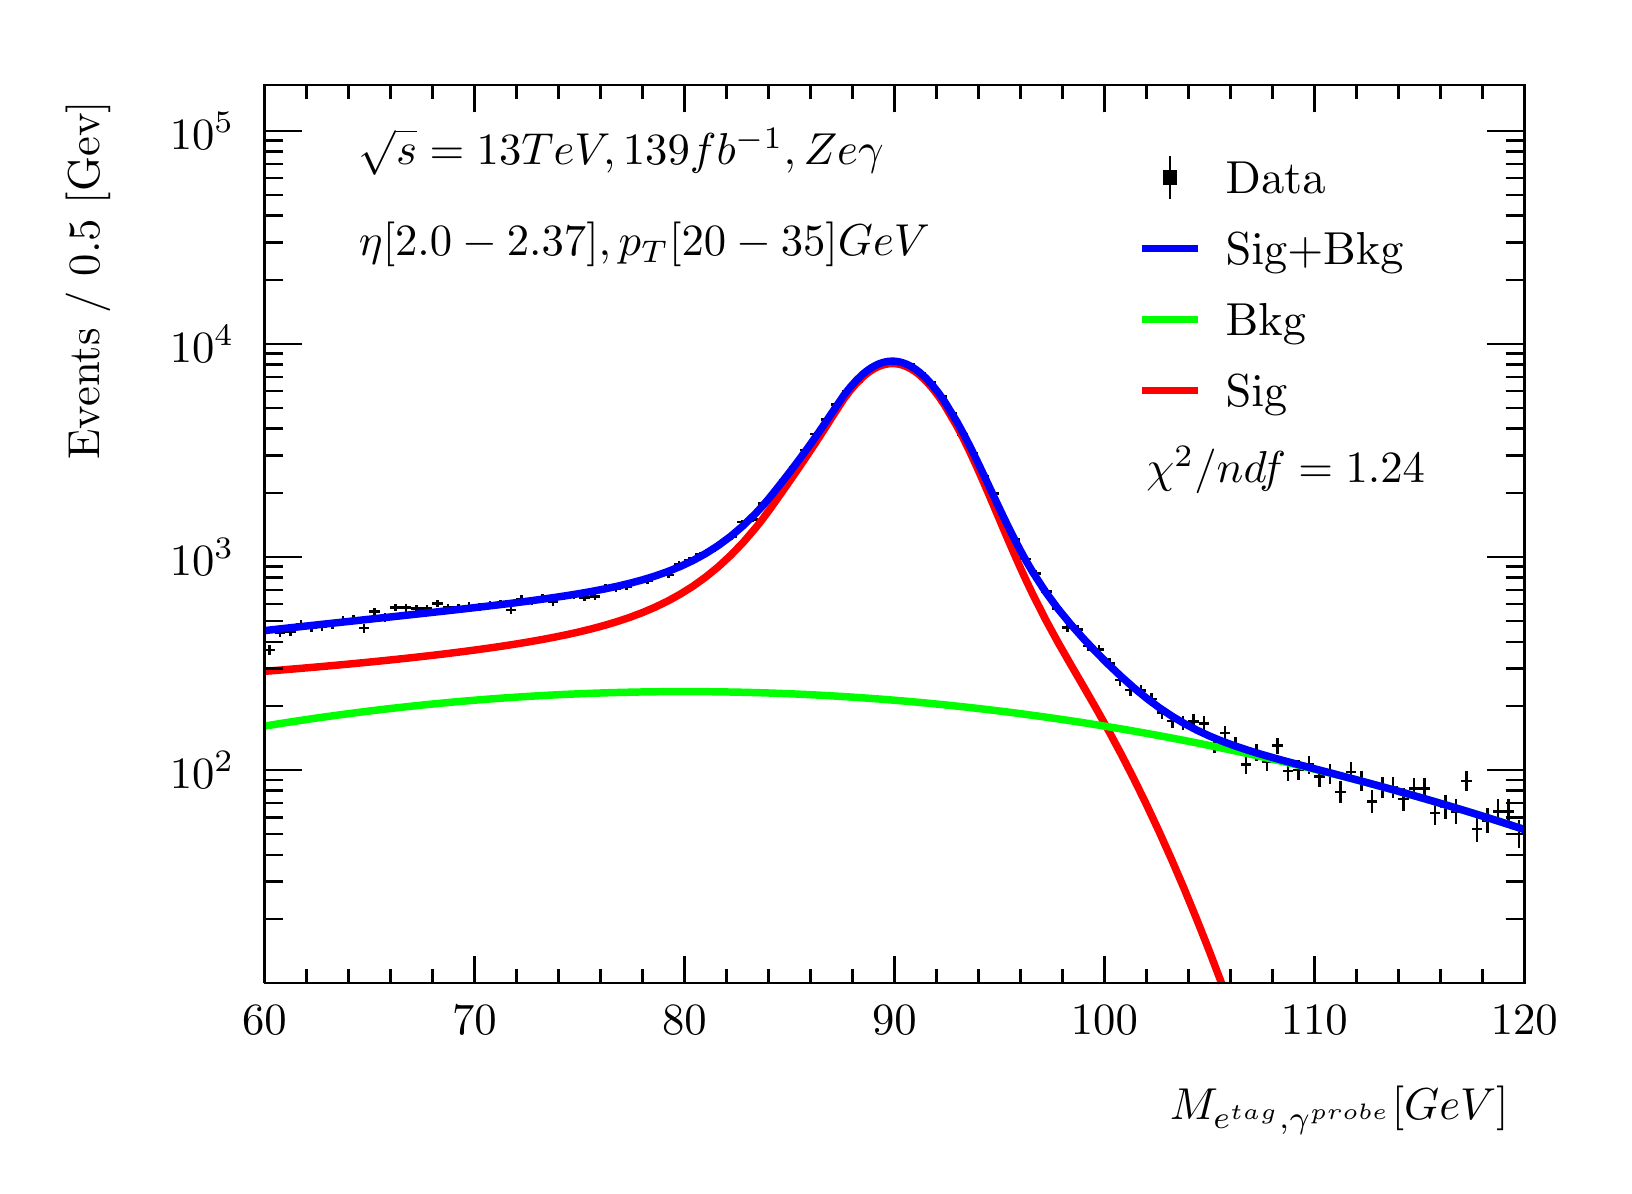
\begin{tikzpicture}
\pgfdeclareplotmark{cross} {
\pgfpathmoveto{\pgfpoint{-0.3\pgfplotmarksize}{\pgfplotmarksize}}
\pgfpathlineto{\pgfpoint{+0.3\pgfplotmarksize}{\pgfplotmarksize}}
\pgfpathlineto{\pgfpoint{+0.3\pgfplotmarksize}{0.3\pgfplotmarksize}}
\pgfpathlineto{\pgfpoint{+1\pgfplotmarksize}{0.3\pgfplotmarksize}}
\pgfpathlineto{\pgfpoint{+1\pgfplotmarksize}{-0.3\pgfplotmarksize}}
\pgfpathlineto{\pgfpoint{+0.3\pgfplotmarksize}{-0.3\pgfplotmarksize}}
\pgfpathlineto{\pgfpoint{+0.3\pgfplotmarksize}{-1.\pgfplotmarksize}}
\pgfpathlineto{\pgfpoint{-0.3\pgfplotmarksize}{-1.\pgfplotmarksize}}
\pgfpathlineto{\pgfpoint{-0.3\pgfplotmarksize}{-0.3\pgfplotmarksize}}
\pgfpathlineto{\pgfpoint{-1.\pgfplotmarksize}{-0.3\pgfplotmarksize}}
\pgfpathlineto{\pgfpoint{-1.\pgfplotmarksize}{0.3\pgfplotmarksize}}
\pgfpathlineto{\pgfpoint{-0.3\pgfplotmarksize}{0.3\pgfplotmarksize}}
\pgfpathclose
\pgfusepathqstroke
}
\pgfdeclareplotmark{cross*} {
\pgfpathmoveto{\pgfpoint{-0.3\pgfplotmarksize}{\pgfplotmarksize}}
\pgfpathlineto{\pgfpoint{+0.3\pgfplotmarksize}{\pgfplotmarksize}}
\pgfpathlineto{\pgfpoint{+0.3\pgfplotmarksize}{0.3\pgfplotmarksize}}
\pgfpathlineto{\pgfpoint{+1\pgfplotmarksize}{0.3\pgfplotmarksize}}
\pgfpathlineto{\pgfpoint{+1\pgfplotmarksize}{-0.3\pgfplotmarksize}}
\pgfpathlineto{\pgfpoint{+0.3\pgfplotmarksize}{-0.3\pgfplotmarksize}}
\pgfpathlineto{\pgfpoint{+0.3\pgfplotmarksize}{-1.\pgfplotmarksize}}
\pgfpathlineto{\pgfpoint{-0.3\pgfplotmarksize}{-1.\pgfplotmarksize}}
\pgfpathlineto{\pgfpoint{-0.3\pgfplotmarksize}{-0.3\pgfplotmarksize}}
\pgfpathlineto{\pgfpoint{-1.\pgfplotmarksize}{-0.3\pgfplotmarksize}}
\pgfpathlineto{\pgfpoint{-1.\pgfplotmarksize}{0.3\pgfplotmarksize}}
\pgfpathlineto{\pgfpoint{-0.3\pgfplotmarksize}{0.3\pgfplotmarksize}}
\pgfpathclose
\pgfusepathqfillstroke
}
\pgfdeclareplotmark{newstar} {
\pgfpathmoveto{\pgfqpoint{0pt}{\pgfplotmarksize}}
\pgfpathlineto{\pgfqpointpolar{44}{0.5\pgfplotmarksize}}
\pgfpathlineto{\pgfqpointpolar{18}{\pgfplotmarksize}}
\pgfpathlineto{\pgfqpointpolar{-20}{0.5\pgfplotmarksize}}
\pgfpathlineto{\pgfqpointpolar{-54}{\pgfplotmarksize}}
\pgfpathlineto{\pgfqpointpolar{-90}{0.5\pgfplotmarksize}}
\pgfpathlineto{\pgfqpointpolar{234}{\pgfplotmarksize}}
\pgfpathlineto{\pgfqpointpolar{198}{0.5\pgfplotmarksize}}
\pgfpathlineto{\pgfqpointpolar{162}{\pgfplotmarksize}}
\pgfpathlineto{\pgfqpointpolar{134}{0.5\pgfplotmarksize}}
\pgfpathclose
\pgfusepathqstroke
}
\pgfdeclareplotmark{newstar*} {
\pgfpathmoveto{\pgfqpoint{0pt}{\pgfplotmarksize}}
\pgfpathlineto{\pgfqpointpolar{44}{0.5\pgfplotmarksize}}
\pgfpathlineto{\pgfqpointpolar{18}{\pgfplotmarksize}}
\pgfpathlineto{\pgfqpointpolar{-20}{0.5\pgfplotmarksize}}
\pgfpathlineto{\pgfqpointpolar{-54}{\pgfplotmarksize}}
\pgfpathlineto{\pgfqpointpolar{-90}{0.5\pgfplotmarksize}}
\pgfpathlineto{\pgfqpointpolar{234}{\pgfplotmarksize}}
\pgfpathlineto{\pgfqpointpolar{198}{0.5\pgfplotmarksize}}
\pgfpathlineto{\pgfqpointpolar{162}{\pgfplotmarksize}}
\pgfpathlineto{\pgfqpointpolar{134}{0.5\pgfplotmarksize}}
\pgfpathclose
\pgfusepathqfillstroke
}
\definecolor{c}{rgb}{1,1,1};
\draw [color=c, fill=c] (0,0) rectangle (20,14.4361);
\draw [color=c, fill=c] (3,2.30977) rectangle (19,13.7143);
\definecolor{c}{rgb}{0,0,0};
\draw [c,line width=0.9] (3,2.30977) -- (3,13.7143) -- (19,13.7143) -- (19,2.30977) -- (3,2.30977);
\definecolor{c}{rgb}{1,1,1};
\draw [color=c, fill=c] (3,2.30977) rectangle (19,13.7143);
\definecolor{c}{rgb}{0,0,0};
\draw [c,line width=0.9] (3,2.30977) -- (3,13.7143) -- (19,13.7143) -- (19,2.30977) -- (3,2.30977);
\draw [c,line width=0.9] (3,2.30977) -- (19,2.30977);
\draw [c,line width=0.9] (3,2.65624) -- (3,2.30977);
\draw [c,line width=0.9] (3.53333,2.48301) -- (3.53333,2.30977);
\draw [c,line width=0.9] (4.06667,2.48301) -- (4.06667,2.30977);
\draw [c,line width=0.9] (4.6,2.48301) -- (4.6,2.30977);
\draw [c,line width=0.9] (5.13333,2.48301) -- (5.13333,2.30977);
\draw [c,line width=0.9] (5.66667,2.65624) -- (5.66667,2.30977);
\draw [c,line width=0.9] (6.2,2.48301) -- (6.2,2.30977);
\draw [c,line width=0.9] (6.73333,2.48301) -- (6.73333,2.30977);
\draw [c,line width=0.9] (7.26667,2.48301) -- (7.26667,2.30977);
\draw [c,line width=0.9] (7.8,2.48301) -- (7.8,2.30977);
\draw [c,line width=0.9] (8.33333,2.65624) -- (8.33333,2.30977);
\draw [c,line width=0.9] (8.86667,2.48301) -- (8.86667,2.30977);
\draw [c,line width=0.9] (9.4,2.48301) -- (9.4,2.30977);
\draw [c,line width=0.9] (9.93333,2.48301) -- (9.93333,2.30977);
\draw [c,line width=0.9] (10.4667,2.48301) -- (10.4667,2.30977);
\draw [c,line width=0.9] (11,2.65624) -- (11,2.30977);
\draw [c,line width=0.9] (11.5333,2.48301) -- (11.5333,2.30977);
\draw [c,line width=0.9] (12.0667,2.48301) -- (12.0667,2.30977);
\draw [c,line width=0.9] (12.6,2.48301) -- (12.6,2.30977);
\draw [c,line width=0.9] (13.1333,2.48301) -- (13.1333,2.30977);
\draw [c,line width=0.9] (13.6667,2.65624) -- (13.6667,2.30977);
\draw [c,line width=0.9] (14.2,2.48301) -- (14.2,2.30977);
\draw [c,line width=0.9] (14.7333,2.48301) -- (14.7333,2.30977);
\draw [c,line width=0.9] (15.2667,2.48301) -- (15.2667,2.30977);
\draw [c,line width=0.9] (15.8,2.48301) -- (15.8,2.30977);
\draw [c,line width=0.9] (16.3333,2.65624) -- (16.3333,2.30977);
\draw [c,line width=0.9] (16.8667,2.48301) -- (16.8667,2.30977);
\draw [c,line width=0.9] (17.4,2.48301) -- (17.4,2.30977);
\draw [c,line width=0.9] (17.9333,2.48301) -- (17.9333,2.30977);
\draw [c,line width=0.9] (18.4667,2.48301) -- (18.4667,2.30977);
\draw [c,line width=0.9] (19,2.65624) -- (19,2.30977);
\draw [anchor=base] (3,1.66015) node[scale=1.61424, color=c, rotate=0]{60};
\draw [anchor=base] (5.66667,1.66015) node[scale=1.61424, color=c, rotate=0]{70};
\draw [anchor=base] (8.33333,1.66015) node[scale=1.61424, color=c, rotate=0]{80};
\draw [anchor=base] (11,1.66015) node[scale=1.61424, color=c, rotate=0]{90};
\draw [anchor=base] (13.6667,1.66015) node[scale=1.61424, color=c, rotate=0]{100};
\draw [anchor=base] (16.3333,1.66015) node[scale=1.61424, color=c, rotate=0]{110};
\draw [anchor=base] (19,1.66015) node[scale=1.61424, color=c, rotate=0]{120};
\draw [anchor= east] (19,0.692932) node[scale=1.61424, color=c, rotate=0]{$M_{e^{tag}, \gamma^{probe}}  [GeV]$};
\draw [c,line width=0.9] (3,13.7143) -- (19,13.7143);
\draw [c,line width=0.9] (3,13.3678) -- (3,13.7143);
\draw [c,line width=0.9] (3.53333,13.5411) -- (3.53333,13.7143);
\draw [c,line width=0.9] (4.06667,13.5411) -- (4.06667,13.7143);
\draw [c,line width=0.9] (4.6,13.5411) -- (4.6,13.7143);
\draw [c,line width=0.9] (5.13333,13.5411) -- (5.13333,13.7143);
\draw [c,line width=0.9] (5.66667,13.3678) -- (5.66667,13.7143);
\draw [c,line width=0.9] (6.2,13.5411) -- (6.2,13.7143);
\draw [c,line width=0.9] (6.73333,13.5411) -- (6.73333,13.7143);
\draw [c,line width=0.9] (7.26667,13.5411) -- (7.26667,13.7143);
\draw [c,line width=0.9] (7.8,13.5411) -- (7.8,13.7143);
\draw [c,line width=0.9] (8.33333,13.3678) -- (8.33333,13.7143);
\draw [c,line width=0.9] (8.86667,13.5411) -- (8.86667,13.7143);
\draw [c,line width=0.9] (9.4,13.5411) -- (9.4,13.7143);
\draw [c,line width=0.9] (9.93333,13.5411) -- (9.93333,13.7143);
\draw [c,line width=0.9] (10.4667,13.5411) -- (10.4667,13.7143);
\draw [c,line width=0.9] (11,13.3678) -- (11,13.7143);
\draw [c,line width=0.9] (11.5333,13.5411) -- (11.5333,13.7143);
\draw [c,line width=0.9] (12.0667,13.5411) -- (12.0667,13.7143);
\draw [c,line width=0.9] (12.6,13.5411) -- (12.6,13.7143);
\draw [c,line width=0.9] (13.1333,13.5411) -- (13.1333,13.7143);
\draw [c,line width=0.9] (13.6667,13.3678) -- (13.6667,13.7143);
\draw [c,line width=0.9] (14.2,13.5411) -- (14.2,13.7143);
\draw [c,line width=0.9] (14.7333,13.5411) -- (14.7333,13.7143);
\draw [c,line width=0.9] (15.2667,13.5411) -- (15.2667,13.7143);
\draw [c,line width=0.9] (15.8,13.5411) -- (15.8,13.7143);
\draw [c,line width=0.9] (16.3333,13.3678) -- (16.3333,13.7143);
\draw [c,line width=0.9] (16.8667,13.5411) -- (16.8667,13.7143);
\draw [c,line width=0.9] (17.4,13.5411) -- (17.4,13.7143);
\draw [c,line width=0.9] (17.9333,13.5411) -- (17.9333,13.7143);
\draw [c,line width=0.9] (18.4667,13.5411) -- (18.4667,13.7143);
\draw [c,line width=0.9] (19,13.3678) -- (19,13.7143);
\draw [c,line width=0.9] (3,2.30977) -- (3,13.7143);
\draw [c,line width=0.9] (3.237,3.12423) -- (3,3.12423);
\draw [c,line width=0.9] (3.237,3.60066) -- (3,3.60066);
\draw [c,line width=0.9] (3.237,3.93869) -- (3,3.93869);
\draw [c,line width=0.9] (3.237,4.20088) -- (3,4.20088);
\draw [c,line width=0.9] (3.237,4.41511) -- (3,4.41511);
\draw [c,line width=0.9] (3.237,4.59624) -- (3,4.59624);
\draw [c,line width=0.9] (3.237,4.75314) -- (3,4.75314);
\draw [c,line width=0.9] (3.237,4.89154) -- (3,4.89154);
\draw [c,line width=0.9] (3.474,5.01534) -- (3,5.01534);
\draw [anchor= east] (2.82,5.01534) node[scale=1.61424, color=c, rotate=0]{$10^{2}$};
\draw [c,line width=0.9] (3.237,5.8298) -- (3,5.8298);
\draw [c,line width=0.9] (3.237,6.30623) -- (3,6.30623);
\draw [c,line width=0.9] (3.237,6.64426) -- (3,6.64426);
\draw [c,line width=0.9] (3.237,6.90645) -- (3,6.90645);
\draw [c,line width=0.9] (3.237,7.12068) -- (3,7.12068);
\draw [c,line width=0.9] (3.237,7.30181) -- (3,7.30181);
\draw [c,line width=0.9] (3.237,7.45871) -- (3,7.45871);
\draw [c,line width=0.9] (3.237,7.59711) -- (3,7.59711);
\draw [c,line width=0.9] (3.474,7.72091) -- (3,7.72091);
\draw [anchor= east] (2.82,7.72091) node[scale=1.61424, color=c, rotate=0]{$10^{3}$};
\draw [c,line width=0.9] (3.237,8.53537) -- (3,8.53537);
\draw [c,line width=0.9] (3.237,9.0118) -- (3,9.0118);
\draw [c,line width=0.9] (3.237,9.34983) -- (3,9.34983);
\draw [c,line width=0.9] (3.237,9.61202) -- (3,9.61202);
\draw [c,line width=0.9] (3.237,9.82625) -- (3,9.82625);
\draw [c,line width=0.9] (3.237,10.0074) -- (3,10.0074);
\draw [c,line width=0.9] (3.237,10.1643) -- (3,10.1643);
\draw [c,line width=0.9] (3.237,10.3027) -- (3,10.3027);
\draw [c,line width=0.9] (3.474,10.4265) -- (3,10.4265);
\draw [anchor= east] (2.82,10.4265) node[scale=1.61424, color=c, rotate=0]{$10^{4}$};
\draw [c,line width=0.9] (3.237,11.2409) -- (3,11.2409);
\draw [c,line width=0.9] (3.237,11.7174) -- (3,11.7174);
\draw [c,line width=0.9] (3.237,12.0554) -- (3,12.0554);
\draw [c,line width=0.9] (3.237,12.3176) -- (3,12.3176);
\draw [c,line width=0.9] (3.237,12.5318) -- (3,12.5318);
\draw [c,line width=0.9] (3.237,12.713) -- (3,12.713);
\draw [c,line width=0.9] (3.237,12.8699) -- (3,12.8699);
\draw [c,line width=0.9] (3.237,13.0083) -- (3,13.0083);
\draw [c,line width=0.9] (3.474,13.1321) -- (3,13.1321);
\draw [anchor= east] (2.82,13.1321) node[scale=1.61424, color=c, rotate=0]{$10^{5}$};
\draw [anchor= east] (0.76,13.7143) node[scale=1.61424, color=c, rotate=90]{Events / 0.5 [Gev]};
\draw [c,line width=0.9] (19,2.30977) -- (19,13.7143);
\draw [c,line width=0.9] (18.763,3.12423) -- (19,3.12423);
\draw [c,line width=0.9] (18.763,3.60066) -- (19,3.60066);
\draw [c,line width=0.9] (18.763,3.93869) -- (19,3.93869);
\draw [c,line width=0.9] (18.763,4.20088) -- (19,4.20088);
\draw [c,line width=0.9] (18.763,4.41511) -- (19,4.41511);
\draw [c,line width=0.9] (18.763,4.59624) -- (19,4.59624);
\draw [c,line width=0.9] (18.763,4.75314) -- (19,4.75314);
\draw [c,line width=0.9] (18.763,4.89154) -- (19,4.89154);
\draw [c,line width=0.9] (18.526,5.01534) -- (19,5.01534);
\draw [c,line width=0.9] (18.763,5.8298) -- (19,5.8298);
\draw [c,line width=0.9] (18.763,6.30623) -- (19,6.30623);
\draw [c,line width=0.9] (18.763,6.64426) -- (19,6.64426);
\draw [c,line width=0.9] (18.763,6.90645) -- (19,6.90645);
\draw [c,line width=0.9] (18.763,7.12068) -- (19,7.12068);
\draw [c,line width=0.9] (18.763,7.30181) -- (19,7.30181);
\draw [c,line width=0.9] (18.763,7.45871) -- (19,7.45871);
\draw [c,line width=0.9] (18.763,7.59711) -- (19,7.59711);
\draw [c,line width=0.9] (18.526,7.72091) -- (19,7.72091);
\draw [c,line width=0.9] (18.763,8.53537) -- (19,8.53537);
\draw [c,line width=0.9] (18.763,9.0118) -- (19,9.0118);
\draw [c,line width=0.9] (18.763,9.34983) -- (19,9.34983);
\draw [c,line width=0.9] (18.763,9.61202) -- (19,9.61202);
\draw [c,line width=0.9] (18.763,9.82625) -- (19,9.82625);
\draw [c,line width=0.9] (18.763,10.0074) -- (19,10.0074);
\draw [c,line width=0.9] (18.763,10.1643) -- (19,10.1643);
\draw [c,line width=0.9] (18.763,10.3027) -- (19,10.3027);
\draw [c,line width=0.9] (18.526,10.4265) -- (19,10.4265);
\draw [c,line width=0.9] (18.763,11.2409) -- (19,11.2409);
\draw [c,line width=0.9] (18.763,11.7174) -- (19,11.7174);
\draw [c,line width=0.9] (18.763,12.0554) -- (19,12.0554);
\draw [c,line width=0.9] (18.763,12.3176) -- (19,12.3176);
\draw [c,line width=0.9] (18.763,12.5318) -- (19,12.5318);
\draw [c,line width=0.9] (18.763,12.713) -- (19,12.713);
\draw [c,line width=0.9] (18.763,12.8699) -- (19,12.8699);
\draw [c,line width=0.9] (18.763,13.0083) -- (19,13.0083);
\draw [c,line width=0.9] (18.526,13.1321) -- (19,13.1321);
\draw [c,line width=0.9] (3.06667,6.53988) -- (3,6.53988);
\draw [c,line width=0.9] (3,6.53988) -- (3,6.53988);
\draw [c,line width=0.9] (3.06667,6.53988) -- (3.13333,6.53988);
\draw [c,line width=0.9] (3.13333,6.53988) -- (3.13333,6.53988);
\draw [c,line width=0.9] (3.06667,6.53988) -- (3.06667,6.60129);
\draw [c,line width=0.9] (3.06667,6.60129) -- (3.06667,6.60129);
\draw [c,line width=0.9] (3.06667,6.53988) -- (3.06667,6.47847);
\draw [c,line width=0.9] (3.06667,6.47847) -- (3.06667,6.47847);
\draw [c,line width=0.9] (3.2,6.76158) -- (3.13333,6.76158);
\draw [c,line width=0.9] (3.13333,6.76158) -- (3.13333,6.76158);
\draw [c,line width=0.9] (3.2,6.76158) -- (3.26667,6.76158);
\draw [c,line width=0.9] (3.26667,6.76158) -- (3.26667,6.76158);
\draw [c,line width=0.9] (3.2,6.76158) -- (3.2,6.81746);
\draw [c,line width=0.9] (3.2,6.81746) -- (3.2,6.81746);
\draw [c,line width=0.9] (3.2,6.76158) -- (3.2,6.70569);
\draw [c,line width=0.9] (3.2,6.70569) -- (3.2,6.70569);
\draw [c,line width=0.9] (3.33333,6.7748) -- (3.26667,6.7748);
\draw [c,line width=0.9] (3.26667,6.7748) -- (3.26667,6.7748);
\draw [c,line width=0.9] (3.33333,6.7748) -- (3.4,6.7748);
\draw [c,line width=0.9] (3.4,6.7748) -- (3.4,6.7748);
\draw [c,line width=0.9] (3.33333,6.7748) -- (3.33333,6.83037);
\draw [c,line width=0.9] (3.33333,6.83037) -- (3.33333,6.83037);
\draw [c,line width=0.9] (3.33333,6.7748) -- (3.33333,6.71922);
\draw [c,line width=0.9] (3.33333,6.71922) -- (3.33333,6.71922);
\draw [c,line width=0.9] (3.46667,6.86337) -- (3.4,6.86337);
\draw [c,line width=0.9] (3.4,6.86337) -- (3.4,6.86337);
\draw [c,line width=0.9] (3.46667,6.86337) -- (3.53333,6.86337);
\draw [c,line width=0.9] (3.53333,6.86337) -- (3.53333,6.86337);
\draw [c,line width=0.9] (3.46667,6.86337) -- (3.46667,6.91689);
\draw [c,line width=0.9] (3.46667,6.91689) -- (3.46667,6.91689);
\draw [c,line width=0.9] (3.46667,6.86337) -- (3.46667,6.80986);
\draw [c,line width=0.9] (3.46667,6.80986) -- (3.46667,6.80986);
\draw [c,line width=0.9] (3.6,6.82371) -- (3.53333,6.82371);
\draw [c,line width=0.9] (3.53333,6.82371) -- (3.53333,6.82371);
\draw [c,line width=0.9] (3.6,6.82371) -- (3.66667,6.82371);
\draw [c,line width=0.9] (3.66667,6.82371) -- (3.66667,6.82371);
\draw [c,line width=0.9] (3.6,6.82371) -- (3.6,6.87813);
\draw [c,line width=0.9] (3.6,6.87813) -- (3.6,6.87813);
\draw [c,line width=0.9] (3.6,6.82371) -- (3.6,6.76928);
\draw [c,line width=0.9] (3.6,6.76928) -- (3.6,6.76928);
\draw [c,line width=0.9] (3.73333,6.83625) -- (3.66667,6.83625);
\draw [c,line width=0.9] (3.66667,6.83625) -- (3.66667,6.83625);
\draw [c,line width=0.9] (3.73333,6.83625) -- (3.8,6.83625);
\draw [c,line width=0.9] (3.8,6.83625) -- (3.8,6.83625);
\draw [c,line width=0.9] (3.73333,6.83625) -- (3.73333,6.89039);
\draw [c,line width=0.9] (3.73333,6.89039) -- (3.73333,6.89039);
\draw [c,line width=0.9] (3.73333,6.83625) -- (3.73333,6.78211);
\draw [c,line width=0.9] (3.73333,6.78211) -- (3.73333,6.78211);
\draw [c,line width=0.9] (3.86667,6.86093) -- (3.8,6.86093);
\draw [c,line width=0.9] (3.8,6.86093) -- (3.8,6.86093);
\draw [c,line width=0.9] (3.86667,6.86093) -- (3.93333,6.86093);
\draw [c,line width=0.9] (3.93333,6.86093) -- (3.93333,6.86093);
\draw [c,line width=0.9] (3.86667,6.86093) -- (3.86667,6.91451);
\draw [c,line width=0.9] (3.86667,6.91451) -- (3.86667,6.91451);
\draw [c,line width=0.9] (3.86667,6.86093) -- (3.86667,6.80736);
\draw [c,line width=0.9] (3.86667,6.80736) -- (3.86667,6.80736);
\draw [c,line width=0.9] (4,6.91815) -- (3.93333,6.91815);
\draw [c,line width=0.9] (3.93333,6.91815) -- (3.93333,6.91815);
\draw [c,line width=0.9] (4,6.91815) -- (4.06667,6.91815);
\draw [c,line width=0.9] (4.06667,6.91815) -- (4.06667,6.91815);
\draw [c,line width=0.9] (4,6.91815) -- (4,6.97043);
\draw [c,line width=0.9] (4,6.97043) -- (4,6.97043);
\draw [c,line width=0.9] (4,6.91815) -- (4,6.86586);
\draw [c,line width=0.9] (4,6.86586) -- (4,6.86586);
\draw [c,line width=0.9] (4.13333,6.93432) -- (4.06667,6.93432);
\draw [c,line width=0.9] (4.06667,6.93432) -- (4.06667,6.93432);
\draw [c,line width=0.9] (4.13333,6.93432) -- (4.2,6.93432);
\draw [c,line width=0.9] (4.2,6.93432) -- (4.2,6.93432);
\draw [c,line width=0.9] (4.13333,6.93432) -- (4.13333,6.98625);
\draw [c,line width=0.9] (4.13333,6.98625) -- (4.13333,6.98625);
\draw [c,line width=0.9] (4.13333,6.93432) -- (4.13333,6.8824);
\draw [c,line width=0.9] (4.13333,6.8824) -- (4.13333,6.8824);
\draw [c,line width=0.9] (4.26667,6.81612) -- (4.2,6.81612);
\draw [c,line width=0.9] (4.2,6.81612) -- (4.2,6.81612);
\draw [c,line width=0.9] (4.26667,6.81612) -- (4.33333,6.81612);
\draw [c,line width=0.9] (4.33333,6.81612) -- (4.33333,6.81612);
\draw [c,line width=0.9] (4.26667,6.81612) -- (4.26667,6.87072);
\draw [c,line width=0.9] (4.26667,6.87072) -- (4.26667,6.87072);
\draw [c,line width=0.9] (4.26667,6.81612) -- (4.26667,6.76152);
\draw [c,line width=0.9] (4.26667,6.76152) -- (4.26667,6.76152);
\draw [c,line width=0.9] (4.4,7.02908) -- (4.33333,7.02908);
\draw [c,line width=0.9] (4.33333,7.02908) -- (4.33333,7.02908);
\draw [c,line width=0.9] (4.4,7.02908) -- (4.46667,7.02908);
\draw [c,line width=0.9] (4.46667,7.02908) -- (4.46667,7.02908);
\draw [c,line width=0.9] (4.4,7.02908) -- (4.4,7.07895);
\draw [c,line width=0.9] (4.4,7.07895) -- (4.4,7.07895);
\draw [c,line width=0.9] (4.4,7.02908) -- (4.4,6.97921);
\draw [c,line width=0.9] (4.4,6.97921) -- (4.4,6.97921);
\draw [c,line width=0.9] (4.53333,6.95254) -- (4.46667,6.95254);
\draw [c,line width=0.9] (4.46667,6.95254) -- (4.46667,6.95254);
\draw [c,line width=0.9] (4.53333,6.95254) -- (4.6,6.95254);
\draw [c,line width=0.9] (4.6,6.95254) -- (4.6,6.95254);
\draw [c,line width=0.9] (4.53333,6.95254) -- (4.53333,7.00406);
\draw [c,line width=0.9] (4.53333,7.00406) -- (4.53333,7.00406);
\draw [c,line width=0.9] (4.53333,6.95254) -- (4.53333,6.90102);
\draw [c,line width=0.9] (4.53333,6.90102) -- (4.53333,6.90102);
\draw [c,line width=0.9] (4.66667,7.07882) -- (4.6,7.07882);
\draw [c,line width=0.9] (4.6,7.07882) -- (4.6,7.07882);
\draw [c,line width=0.9] (4.66667,7.07882) -- (4.73333,7.07882);
\draw [c,line width=0.9] (4.73333,7.07882) -- (4.73333,7.07882);
\draw [c,line width=0.9] (4.66667,7.07882) -- (4.66667,7.12765);
\draw [c,line width=0.9] (4.66667,7.12765) -- (4.66667,7.12765);
\draw [c,line width=0.9] (4.66667,7.07882) -- (4.66667,7.02999);
\draw [c,line width=0.9] (4.66667,7.02999) -- (4.66667,7.02999);
\draw [c,line width=0.9] (4.8,7.07679) -- (4.73333,7.07679);
\draw [c,line width=0.9] (4.73333,7.07679) -- (4.73333,7.07679);
\draw [c,line width=0.9] (4.8,7.07679) -- (4.86667,7.07679);
\draw [c,line width=0.9] (4.86667,7.07679) -- (4.86667,7.07679);
\draw [c,line width=0.9] (4.8,7.07679) -- (4.8,7.12566);
\draw [c,line width=0.9] (4.8,7.12566) -- (4.8,7.12566);
\draw [c,line width=0.9] (4.8,7.07679) -- (4.8,7.02792);
\draw [c,line width=0.9] (4.8,7.02792) -- (4.8,7.02792);
\draw [c,line width=0.9] (4.93333,7.06453) -- (4.86667,7.06453);
\draw [c,line width=0.9] (4.86667,7.06453) -- (4.86667,7.06453);
\draw [c,line width=0.9] (4.93333,7.06453) -- (5,7.06453);
\draw [c,line width=0.9] (5,7.06453) -- (5,7.06453);
\draw [c,line width=0.9] (4.93333,7.06453) -- (4.93333,7.11366);
\draw [c,line width=0.9] (4.93333,7.11366) -- (4.93333,7.11366);
\draw [c,line width=0.9] (4.93333,7.06453) -- (4.93333,7.0154);
\draw [c,line width=0.9] (4.93333,7.0154) -- (4.93333,7.0154);
\draw [c,line width=0.9] (5.06667,7.06453) -- (5,7.06453);
\draw [c,line width=0.9] (5,7.06453) -- (5,7.06453);
\draw [c,line width=0.9] (5.06667,7.06453) -- (5.13333,7.06453);
\draw [c,line width=0.9] (5.13333,7.06453) -- (5.13333,7.06453);
\draw [c,line width=0.9] (5.06667,7.06453) -- (5.06667,7.11366);
\draw [c,line width=0.9] (5.06667,7.11366) -- (5.06667,7.11366);
\draw [c,line width=0.9] (5.06667,7.06453) -- (5.06667,7.0154);
\draw [c,line width=0.9] (5.06667,7.0154) -- (5.06667,7.0154);
\draw [c,line width=0.9] (5.2,7.13238) -- (5.13333,7.13238);
\draw [c,line width=0.9] (5.13333,7.13238) -- (5.13333,7.13238);
\draw [c,line width=0.9] (5.2,7.13238) -- (5.26667,7.13238);
\draw [c,line width=0.9] (5.26667,7.13238) -- (5.26667,7.13238);
\draw [c,line width=0.9] (5.2,7.13238) -- (5.2,7.18011);
\draw [c,line width=0.9] (5.2,7.18011) -- (5.2,7.18011);
\draw [c,line width=0.9] (5.2,7.13238) -- (5.2,7.08465);
\draw [c,line width=0.9] (5.2,7.08465) -- (5.2,7.08465);
\draw [c,line width=0.9] (5.33333,7.07882) -- (5.26667,7.07882);
\draw [c,line width=0.9] (5.26667,7.07882) -- (5.26667,7.07882);
\draw [c,line width=0.9] (5.33333,7.07882) -- (5.4,7.07882);
\draw [c,line width=0.9] (5.4,7.07882) -- (5.4,7.07882);
\draw [c,line width=0.9] (5.33333,7.07882) -- (5.33333,7.12765);
\draw [c,line width=0.9] (5.33333,7.12765) -- (5.33333,7.12765);
\draw [c,line width=0.9] (5.33333,7.07882) -- (5.33333,7.02999);
\draw [c,line width=0.9] (5.33333,7.02999) -- (5.33333,7.02999);
\draw [c,line width=0.9] (5.46667,7.08085) -- (5.4,7.08085);
\draw [c,line width=0.9] (5.4,7.08085) -- (5.4,7.08085);
\draw [c,line width=0.9] (5.46667,7.08085) -- (5.53333,7.08085);
\draw [c,line width=0.9] (5.53333,7.08085) -- (5.53333,7.08085);
\draw [c,line width=0.9] (5.46667,7.08085) -- (5.46667,7.12964);
\draw [c,line width=0.9] (5.46667,7.12964) -- (5.46667,7.12964);
\draw [c,line width=0.9] (5.46667,7.08085) -- (5.46667,7.03206);
\draw [c,line width=0.9] (5.46667,7.03206) -- (5.46667,7.03206);
\draw [c,line width=0.9] (5.6,7.09894) -- (5.53333,7.09894);
\draw [c,line width=0.9] (5.53333,7.09894) -- (5.53333,7.09894);
\draw [c,line width=0.9] (5.6,7.09894) -- (5.66667,7.09894);
\draw [c,line width=0.9] (5.66667,7.09894) -- (5.66667,7.09894);
\draw [c,line width=0.9] (5.6,7.09894) -- (5.6,7.14736);
\draw [c,line width=0.9] (5.6,7.14736) -- (5.6,7.14736);
\draw [c,line width=0.9] (5.6,7.09894) -- (5.6,7.05053);
\draw [c,line width=0.9] (5.6,7.05053) -- (5.6,7.05053);
\draw [c,line width=0.9] (5.73333,7.08288) -- (5.66667,7.08288);
\draw [c,line width=0.9] (5.66667,7.08288) -- (5.66667,7.08288);
\draw [c,line width=0.9] (5.73333,7.08288) -- (5.8,7.08288);
\draw [c,line width=0.9] (5.8,7.08288) -- (5.8,7.08288);
\draw [c,line width=0.9] (5.73333,7.08288) -- (5.73333,7.13162);
\draw [c,line width=0.9] (5.73333,7.13162) -- (5.73333,7.13162);
\draw [c,line width=0.9] (5.73333,7.08288) -- (5.73333,7.03413);
\draw [c,line width=0.9] (5.73333,7.03413) -- (5.73333,7.03413);
\draw [c,line width=0.9] (5.86667,7.1148) -- (5.8,7.1148);
\draw [c,line width=0.9] (5.8,7.1148) -- (5.8,7.1148);
\draw [c,line width=0.9] (5.86667,7.1148) -- (5.93333,7.1148);
\draw [c,line width=0.9] (5.93333,7.1148) -- (5.93333,7.1148);
\draw [c,line width=0.9] (5.86667,7.1148) -- (5.86667,7.16288);
\draw [c,line width=0.9] (5.86667,7.16288) -- (5.86667,7.16288);
\draw [c,line width=0.9] (5.86667,7.1148) -- (5.86667,7.06671);
\draw [c,line width=0.9] (5.86667,7.06671) -- (5.86667,7.06671);
\draw [c,line width=0.9] (6,7.12264) -- (5.93333,7.12264);
\draw [c,line width=0.9] (5.93333,7.12264) -- (5.93333,7.12264);
\draw [c,line width=0.9] (6,7.12264) -- (6.06667,7.12264);
\draw [c,line width=0.9] (6.06667,7.12264) -- (6.06667,7.12264);
\draw [c,line width=0.9] (6,7.12264) -- (6,7.17057);
\draw [c,line width=0.9] (6,7.17057) -- (6,7.17057);
\draw [c,line width=0.9] (6,7.12264) -- (6,7.07472);
\draw [c,line width=0.9] (6,7.07472) -- (6,7.07472);
\draw [c,line width=0.9] (6.13333,7.04798) -- (6.06667,7.04798);
\draw [c,line width=0.9] (6.06667,7.04798) -- (6.06667,7.04798);
\draw [c,line width=0.9] (6.13333,7.04798) -- (6.2,7.04798);
\draw [c,line width=0.9] (6.2,7.04798) -- (6.2,7.04798);
\draw [c,line width=0.9] (6.13333,7.04798) -- (6.13333,7.09745);
\draw [c,line width=0.9] (6.13333,7.09745) -- (6.13333,7.09745);
\draw [c,line width=0.9] (6.13333,7.04798) -- (6.13333,6.99851);
\draw [c,line width=0.9] (6.13333,6.99851) -- (6.13333,6.99851);
\draw [c,line width=0.9] (6.26667,7.1873) -- (6.2,7.1873);
\draw [c,line width=0.9] (6.2,7.1873) -- (6.2,7.1873);
\draw [c,line width=0.9] (6.26667,7.1873) -- (6.33333,7.1873);
\draw [c,line width=0.9] (6.33333,7.1873) -- (6.33333,7.1873);
\draw [c,line width=0.9] (6.26667,7.1873) -- (6.26667,7.23393);
\draw [c,line width=0.9] (6.26667,7.23393) -- (6.26667,7.23393);
\draw [c,line width=0.9] (6.26667,7.1873) -- (6.26667,7.14068);
\draw [c,line width=0.9] (6.26667,7.14068) -- (6.26667,7.14068);
\draw [c,line width=0.9] (6.4,7.15732) -- (6.33333,7.15732);
\draw [c,line width=0.9] (6.33333,7.15732) -- (6.33333,7.15732);
\draw [c,line width=0.9] (6.4,7.15732) -- (6.46667,7.15732);
\draw [c,line width=0.9] (6.46667,7.15732) -- (6.46667,7.15732);
\draw [c,line width=0.9] (6.4,7.15732) -- (6.4,7.20454);
\draw [c,line width=0.9] (6.4,7.20454) -- (6.4,7.20454);
\draw [c,line width=0.9] (6.4,7.15732) -- (6.4,7.11009);
\draw [c,line width=0.9] (6.4,7.11009) -- (6.4,7.11009);
\draw [c,line width=0.9] (6.53333,7.2093) -- (6.46667,7.2093);
\draw [c,line width=0.9] (6.46667,7.2093) -- (6.46667,7.2093);
\draw [c,line width=0.9] (6.53333,7.2093) -- (6.6,7.2093);
\draw [c,line width=0.9] (6.6,7.2093) -- (6.6,7.2093);
\draw [c,line width=0.9] (6.53333,7.2093) -- (6.53333,7.25549);
\draw [c,line width=0.9] (6.53333,7.25549) -- (6.53333,7.25549);
\draw [c,line width=0.9] (6.53333,7.2093) -- (6.53333,7.16311);
\draw [c,line width=0.9] (6.53333,7.16311) -- (6.53333,7.16311);
\draw [c,line width=0.9] (6.66667,7.1497) -- (6.6,7.1497);
\draw [c,line width=0.9] (6.6,7.1497) -- (6.6,7.1497);
\draw [c,line width=0.9] (6.66667,7.1497) -- (6.73333,7.1497);
\draw [c,line width=0.9] (6.73333,7.1497) -- (6.73333,7.1497);
\draw [c,line width=0.9] (6.66667,7.1497) -- (6.66667,7.19708);
\draw [c,line width=0.9] (6.66667,7.19708) -- (6.66667,7.19708);
\draw [c,line width=0.9] (6.66667,7.1497) -- (6.66667,7.10232);
\draw [c,line width=0.9] (6.66667,7.10232) -- (6.66667,7.10232);
\draw [c,line width=0.9] (6.8,7.22374) -- (6.73333,7.22374);
\draw [c,line width=0.9] (6.73333,7.22374) -- (6.73333,7.22374);
\draw [c,line width=0.9] (6.8,7.22374) -- (6.86667,7.22374);
\draw [c,line width=0.9] (6.86667,7.22374) -- (6.86667,7.22374);
\draw [c,line width=0.9] (6.8,7.22374) -- (6.8,7.26965);
\draw [c,line width=0.9] (6.8,7.26965) -- (6.8,7.26965);
\draw [c,line width=0.9] (6.8,7.22374) -- (6.8,7.17783);
\draw [c,line width=0.9] (6.8,7.17783) -- (6.8,7.17783);
\draw [c,line width=0.9] (6.93333,7.22911) -- (6.86667,7.22911);
\draw [c,line width=0.9] (6.86667,7.22911) -- (6.86667,7.22911);
\draw [c,line width=0.9] (6.93333,7.22911) -- (7,7.22911);
\draw [c,line width=0.9] (7,7.22911) -- (7,7.22911);
\draw [c,line width=0.9] (6.93333,7.22911) -- (6.93333,7.27491);
\draw [c,line width=0.9] (6.93333,7.27491) -- (6.93333,7.27491);
\draw [c,line width=0.9] (6.93333,7.22911) -- (6.93333,7.18331);
\draw [c,line width=0.9] (6.93333,7.18331) -- (6.93333,7.18331);
\draw [c,line width=0.9] (7.06667,7.2093) -- (7,7.2093);
\draw [c,line width=0.9] (7,7.2093) -- (7,7.2093);
\draw [c,line width=0.9] (7.06667,7.2093) -- (7.13333,7.2093);
\draw [c,line width=0.9] (7.13333,7.2093) -- (7.13333,7.2093);
\draw [c,line width=0.9] (7.06667,7.2093) -- (7.06667,7.25549);
\draw [c,line width=0.9] (7.06667,7.25549) -- (7.06667,7.25549);
\draw [c,line width=0.9] (7.06667,7.2093) -- (7.06667,7.16311);
\draw [c,line width=0.9] (7.06667,7.16311) -- (7.06667,7.16311);
\draw [c,line width=0.9] (7.2,7.22015) -- (7.13333,7.22015);
\draw [c,line width=0.9] (7.13333,7.22015) -- (7.13333,7.22015);
\draw [c,line width=0.9] (7.2,7.22015) -- (7.26667,7.22015);
\draw [c,line width=0.9] (7.26667,7.22015) -- (7.26667,7.22015);
\draw [c,line width=0.9] (7.2,7.22015) -- (7.2,7.26613);
\draw [c,line width=0.9] (7.2,7.26613) -- (7.2,7.26613);
\draw [c,line width=0.9] (7.2,7.22015) -- (7.2,7.17417);
\draw [c,line width=0.9] (7.2,7.17417) -- (7.2,7.17417);
\draw [c,line width=0.9] (7.33333,7.33328) -- (7.26667,7.33328);
\draw [c,line width=0.9] (7.26667,7.33328) -- (7.26667,7.33328);
\draw [c,line width=0.9] (7.33333,7.33328) -- (7.4,7.33328);
\draw [c,line width=0.9] (7.4,7.33328) -- (7.4,7.33328);
\draw [c,line width=0.9] (7.33333,7.33328) -- (7.33333,7.3771);
\draw [c,line width=0.9] (7.33333,7.3771) -- (7.33333,7.3771);
\draw [c,line width=0.9] (7.33333,7.33328) -- (7.33333,7.28946);
\draw [c,line width=0.9] (7.33333,7.28946) -- (7.33333,7.28946);
\draw [c,line width=0.9] (7.46667,7.31848) -- (7.4,7.31848);
\draw [c,line width=0.9] (7.4,7.31848) -- (7.4,7.31848);
\draw [c,line width=0.9] (7.46667,7.31848) -- (7.53333,7.31848);
\draw [c,line width=0.9] (7.53333,7.31848) -- (7.53333,7.31848);
\draw [c,line width=0.9] (7.46667,7.31848) -- (7.46667,7.36258);
\draw [c,line width=0.9] (7.46667,7.36258) -- (7.46667,7.36258);
\draw [c,line width=0.9] (7.46667,7.31848) -- (7.46667,7.27439);
\draw [c,line width=0.9] (7.46667,7.27439) -- (7.46667,7.27439);
\draw [c,line width=0.9] (7.6,7.34628) -- (7.53333,7.34628);
\draw [c,line width=0.9] (7.53333,7.34628) -- (7.53333,7.34628);
\draw [c,line width=0.9] (7.6,7.34628) -- (7.66667,7.34628);
\draw [c,line width=0.9] (7.66667,7.34628) -- (7.66667,7.34628);
\draw [c,line width=0.9] (7.6,7.34628) -- (7.6,7.38986);
\draw [c,line width=0.9] (7.6,7.38986) -- (7.6,7.38986);
\draw [c,line width=0.9] (7.6,7.34628) -- (7.6,7.30271);
\draw [c,line width=0.9] (7.6,7.30271) -- (7.6,7.30271);
\draw [c,line width=0.9] (7.73333,7.41075) -- (7.66667,7.41075);
\draw [c,line width=0.9] (7.66667,7.41075) -- (7.66667,7.41075);
\draw [c,line width=0.9] (7.73333,7.41075) -- (7.8,7.41075);
\draw [c,line width=0.9] (7.8,7.41075) -- (7.8,7.41075);
\draw [c,line width=0.9] (7.73333,7.41075) -- (7.73333,7.45315);
\draw [c,line width=0.9] (7.73333,7.45315) -- (7.73333,7.45315);
\draw [c,line width=0.9] (7.73333,7.41075) -- (7.73333,7.36835);
\draw [c,line width=0.9] (7.73333,7.36835) -- (7.73333,7.36835);
\draw [c,line width=0.9] (7.86667,7.41685) -- (7.8,7.41685);
\draw [c,line width=0.9] (7.8,7.41685) -- (7.8,7.41685);
\draw [c,line width=0.9] (7.86667,7.41685) -- (7.93333,7.41685);
\draw [c,line width=0.9] (7.93333,7.41685) -- (7.93333,7.41685);
\draw [c,line width=0.9] (7.86667,7.41685) -- (7.86667,7.45914);
\draw [c,line width=0.9] (7.86667,7.45914) -- (7.86667,7.45914);
\draw [c,line width=0.9] (7.86667,7.41685) -- (7.86667,7.37457);
\draw [c,line width=0.9] (7.86667,7.37457) -- (7.86667,7.37457);
\draw [c,line width=0.9] (8,7.47766) -- (7.93333,7.47766);
\draw [c,line width=0.9] (7.93333,7.47766) -- (7.93333,7.47766);
\draw [c,line width=0.9] (8,7.47766) -- (8.06667,7.47766);
\draw [c,line width=0.9] (8.06667,7.47766) -- (8.06667,7.47766);
\draw [c,line width=0.9] (8,7.47766) -- (8,7.51886);
\draw [c,line width=0.9] (8,7.51886) -- (8,7.51886);
\draw [c,line width=0.9] (8,7.47766) -- (8,7.43645);
\draw [c,line width=0.9] (8,7.43645) -- (8,7.43645);
\draw [c,line width=0.9] (8.13333,7.49202) -- (8.06667,7.49202);
\draw [c,line width=0.9] (8.06667,7.49202) -- (8.06667,7.49202);
\draw [c,line width=0.9] (8.13333,7.49202) -- (8.2,7.49202);
\draw [c,line width=0.9] (8.2,7.49202) -- (8.2,7.49202);
\draw [c,line width=0.9] (8.13333,7.49202) -- (8.13333,7.53298);
\draw [c,line width=0.9] (8.13333,7.53298) -- (8.13333,7.53298);
\draw [c,line width=0.9] (8.13333,7.49202) -- (8.13333,7.45107);
\draw [c,line width=0.9] (8.13333,7.45107) -- (8.13333,7.45107);
\draw [c,line width=0.9] (8.26667,7.63058) -- (8.2,7.63058);
\draw [c,line width=0.9] (8.2,7.63058) -- (8.2,7.63058);
\draw [c,line width=0.9] (8.26667,7.63058) -- (8.33333,7.63058);
\draw [c,line width=0.9] (8.33333,7.63058) -- (8.33333,7.63058);
\draw [c,line width=0.9] (8.26667,7.63058) -- (8.26667,7.66919);
\draw [c,line width=0.9] (8.26667,7.66919) -- (8.26667,7.66919);
\draw [c,line width=0.9] (8.26667,7.63058) -- (8.26667,7.59197);
\draw [c,line width=0.9] (8.26667,7.59197) -- (8.26667,7.59197);
\draw [c,line width=0.9] (8.4,7.6827) -- (8.33333,7.6827);
\draw [c,line width=0.9] (8.33333,7.6827) -- (8.33333,7.6827);
\draw [c,line width=0.9] (8.4,7.6827) -- (8.46667,7.6827);
\draw [c,line width=0.9] (8.46667,7.6827) -- (8.46667,7.6827);
\draw [c,line width=0.9] (8.4,7.6827) -- (8.4,7.72046);
\draw [c,line width=0.9] (8.4,7.72046) -- (8.4,7.72046);
\draw [c,line width=0.9] (8.4,7.6827) -- (8.4,7.64493);
\draw [c,line width=0.9] (8.4,7.64493) -- (8.4,7.64493);
\draw [c,line width=0.9] (8.53333,7.75336) -- (8.46667,7.75336);
\draw [c,line width=0.9] (8.46667,7.75336) -- (8.46667,7.75336);
\draw [c,line width=0.9] (8.53333,7.75336) -- (8.6,7.75336);
\draw [c,line width=0.9] (8.6,7.75336) -- (8.6,7.75336);
\draw [c,line width=0.9] (8.53333,7.75336) -- (8.53333,7.79001);
\draw [c,line width=0.9] (8.53333,7.79001) -- (8.53333,7.79001);
\draw [c,line width=0.9] (8.53333,7.75336) -- (8.53333,7.71671);
\draw [c,line width=0.9] (8.53333,7.71671) -- (8.53333,7.71671);
\draw [c,line width=0.9] (8.66667,7.80041) -- (8.6,7.80041);
\draw [c,line width=0.9] (8.6,7.80041) -- (8.6,7.80041);
\draw [c,line width=0.9] (8.66667,7.80041) -- (8.73333,7.80041);
\draw [c,line width=0.9] (8.73333,7.80041) -- (8.73333,7.80041);
\draw [c,line width=0.9] (8.66667,7.80041) -- (8.66667,7.83633);
\draw [c,line width=0.9] (8.66667,7.83633) -- (8.66667,7.83633);
\draw [c,line width=0.9] (8.66667,7.80041) -- (8.66667,7.76449);
\draw [c,line width=0.9] (8.66667,7.76449) -- (8.66667,7.76449);
\draw [c,line width=0.9] (8.8,7.89935) -- (8.73333,7.89935);
\draw [c,line width=0.9] (8.73333,7.89935) -- (8.73333,7.89935);
\draw [c,line width=0.9] (8.8,7.89935) -- (8.86667,7.89935);
\draw [c,line width=0.9] (8.86667,7.89935) -- (8.86667,7.89935);
\draw [c,line width=0.9] (8.8,7.89935) -- (8.8,7.93379);
\draw [c,line width=0.9] (8.8,7.93379) -- (8.8,7.93379);
\draw [c,line width=0.9] (8.8,7.89935) -- (8.8,7.86491);
\draw [c,line width=0.9] (8.8,7.86491) -- (8.8,7.86491);
\draw [c,line width=0.9] (8.93333,7.97367) -- (8.86667,7.97367);
\draw [c,line width=0.9] (8.86667,7.97367) -- (8.86667,7.97367);
\draw [c,line width=0.9] (8.93333,7.97367) -- (9,7.97367);
\draw [c,line width=0.9] (9,7.97367) -- (9,7.97367);
\draw [c,line width=0.9] (8.93333,7.97367) -- (8.93333,8.00704);
\draw [c,line width=0.9] (8.93333,8.00704) -- (8.93333,8.00704);
\draw [c,line width=0.9] (8.93333,7.97367) -- (8.93333,7.9403);
\draw [c,line width=0.9] (8.93333,7.9403) -- (8.93333,7.9403);
\draw [c,line width=0.9] (9.06667,8.16397) -- (9,8.16397);
\draw [c,line width=0.9] (9,8.16397) -- (9,8.16397);
\draw [c,line width=0.9] (9.06667,8.16397) -- (9.13333,8.16397);
\draw [c,line width=0.9] (9.13333,8.16397) -- (9.13333,8.16397);
\draw [c,line width=0.9] (9.06667,8.16397) -- (9.06667,8.19474);
\draw [c,line width=0.9] (9.06667,8.19474) -- (9.06667,8.19474);
\draw [c,line width=0.9] (9.06667,8.16397) -- (9.06667,8.1332);
\draw [c,line width=0.9] (9.06667,8.1332) -- (9.06667,8.1332);
\draw [c,line width=0.9] (9.2,8.19656) -- (9.13333,8.19656);
\draw [c,line width=0.9] (9.13333,8.19656) -- (9.13333,8.19656);
\draw [c,line width=0.9] (9.2,8.19656) -- (9.26667,8.19656);
\draw [c,line width=0.9] (9.26667,8.19656) -- (9.26667,8.19656);
\draw [c,line width=0.9] (9.2,8.19656) -- (9.2,8.2269);
\draw [c,line width=0.9] (9.2,8.2269) -- (9.2,8.2269);
\draw [c,line width=0.9] (9.2,8.19656) -- (9.2,8.16621);
\draw [c,line width=0.9] (9.2,8.16621) -- (9.2,8.16621);
\draw [c,line width=0.9] (9.33333,8.4024) -- (9.26667,8.4024);
\draw [c,line width=0.9] (9.26667,8.4024) -- (9.26667,8.4024);
\draw [c,line width=0.9] (9.33333,8.4024) -- (9.4,8.4024);
\draw [c,line width=0.9] (9.4,8.4024) -- (9.4,8.4024);
\draw [c,line width=0.9] (9.33333,8.4024) -- (9.33333,8.4302);
\draw [c,line width=0.9] (9.33333,8.4302) -- (9.33333,8.4302);
\draw [c,line width=0.9] (9.33333,8.4024) -- (9.33333,8.37459);
\draw [c,line width=0.9] (9.33333,8.37459) -- (9.33333,8.37459);
\draw [c,line width=0.9] (9.46667,8.48863) -- (9.4,8.48863);
\draw [c,line width=0.9] (9.4,8.48863) -- (9.4,8.48863);
\draw [c,line width=0.9] (9.46667,8.48863) -- (9.53333,8.48863);
\draw [c,line width=0.9] (9.53333,8.48863) -- (9.53333,8.48863);
\draw [c,line width=0.9] (9.46667,8.48863) -- (9.46667,8.51543);
\draw [c,line width=0.9] (9.46667,8.51543) -- (9.46667,8.51543);
\draw [c,line width=0.9] (9.46667,8.48863) -- (9.46667,8.46183);
\draw [c,line width=0.9] (9.46667,8.46183) -- (9.46667,8.46183);
\draw [c,line width=0.9] (9.6,8.69036) -- (9.53333,8.69036);
\draw [c,line width=0.9] (9.53333,8.69036) -- (9.53333,8.69036);
\draw [c,line width=0.9] (9.6,8.69036) -- (9.66667,8.69036);
\draw [c,line width=0.9] (9.66667,8.69036) -- (9.66667,8.69036);
\draw [c,line width=0.9] (9.6,8.69036) -- (9.6,8.71496);
\draw [c,line width=0.9] (9.6,8.71496) -- (9.6,8.71496);
\draw [c,line width=0.9] (9.6,8.69036) -- (9.6,8.66576);
\draw [c,line width=0.9] (9.6,8.66576) -- (9.6,8.66576);
\draw [c,line width=0.9] (9.73333,8.86337) -- (9.66667,8.86337);
\draw [c,line width=0.9] (9.66667,8.86337) -- (9.66667,8.86337);
\draw [c,line width=0.9] (9.73333,8.86337) -- (9.8,8.86337);
\draw [c,line width=0.9] (9.8,8.86337) -- (9.8,8.86337);
\draw [c,line width=0.9] (9.73333,8.86337) -- (9.73333,8.88622);
\draw [c,line width=0.9] (9.73333,8.88622) -- (9.73333,8.88622);
\draw [c,line width=0.9] (9.73333,8.86337) -- (9.73333,8.84052);
\draw [c,line width=0.9] (9.73333,8.84052) -- (9.73333,8.84052);
\draw [c,line width=0.9] (9.86667,9.08211) -- (9.8,9.08211);
\draw [c,line width=0.9] (9.8,9.08211) -- (9.8,9.08211);
\draw [c,line width=0.9] (9.86667,9.08211) -- (9.93333,9.08211);
\draw [c,line width=0.9] (9.93333,9.08211) -- (9.93333,9.08211);
\draw [c,line width=0.9] (9.86667,9.08211) -- (9.86667,9.10293);
\draw [c,line width=0.9] (9.86667,9.10293) -- (9.86667,9.10293);
\draw [c,line width=0.9] (9.86667,9.08211) -- (9.86667,9.06129);
\draw [c,line width=0.9] (9.86667,9.06129) -- (9.86667,9.06129);
\draw [c,line width=0.9] (10,9.28398) -- (9.93333,9.28398);
\draw [c,line width=0.9] (9.93333,9.28398) -- (9.93333,9.28398);
\draw [c,line width=0.9] (10,9.28398) -- (10.0667,9.28398);
\draw [c,line width=0.9] (10.0667,9.28398) -- (10.0667,9.28398);
\draw [c,line width=0.9] (10,9.28398) -- (10,9.30308);
\draw [c,line width=0.9] (10,9.30308) -- (10,9.30308);
\draw [c,line width=0.9] (10,9.28398) -- (10,9.26487);
\draw [c,line width=0.9] (10,9.26487) -- (10,9.26487);
\draw [c,line width=0.9] (10.1333,9.46715) -- (10.0667,9.46715);
\draw [c,line width=0.9] (10.0667,9.46715) -- (10.0667,9.46715);
\draw [c,line width=0.9] (10.1333,9.46715) -- (10.2,9.46715);
\draw [c,line width=0.9] (10.2,9.46715) -- (10.2,9.46715);
\draw [c,line width=0.9] (10.1333,9.46715) -- (10.1333,9.48482);
\draw [c,line width=0.9] (10.1333,9.48482) -- (10.1333,9.48482);
\draw [c,line width=0.9] (10.1333,9.46715) -- (10.1333,9.44947);
\draw [c,line width=0.9] (10.1333,9.44947) -- (10.1333,9.44947);
\draw [c,line width=0.9] (10.2667,9.65494) -- (10.2,9.65494);
\draw [c,line width=0.9] (10.2,9.65494) -- (10.2,9.65494);
\draw [c,line width=0.9] (10.2667,9.65494) -- (10.3333,9.65494);
\draw [c,line width=0.9] (10.3333,9.65494) -- (10.3333,9.65494);
\draw [c,line width=0.9] (10.2667,9.65494) -- (10.2667,9.67126);
\draw [c,line width=0.9] (10.2667,9.67126) -- (10.2667,9.67126);
\draw [c,line width=0.9] (10.2667,9.65494) -- (10.2667,9.63863);
\draw [c,line width=0.9] (10.2667,9.63863) -- (10.2667,9.63863);
\draw [c,line width=0.9] (10.4,9.82938) -- (10.3333,9.82938);
\draw [c,line width=0.9] (10.3333,9.82938) -- (10.3333,9.82938);
\draw [c,line width=0.9] (10.4,9.82938) -- (10.4667,9.82938);
\draw [c,line width=0.9] (10.4667,9.82938) -- (10.4667,9.82938);
\draw [c,line width=0.9] (10.4,9.82938) -- (10.4,9.84453);
\draw [c,line width=0.9] (10.4,9.84453) -- (10.4,9.84453);
\draw [c,line width=0.9] (10.4,9.82938) -- (10.4,9.81423);
\draw [c,line width=0.9] (10.4,9.81423) -- (10.4,9.81423);
\draw [c,line width=0.9] (10.5333,9.94198) -- (10.4667,9.94198);
\draw [c,line width=0.9] (10.4667,9.94198) -- (10.4667,9.94198);
\draw [c,line width=0.9] (10.5333,9.94198) -- (10.6,9.94198);
\draw [c,line width=0.9] (10.6,9.94198) -- (10.6,9.94198);
\draw [c,line width=0.9] (10.5333,9.94198) -- (10.5333,9.95642);
\draw [c,line width=0.9] (10.5333,9.95642) -- (10.5333,9.95642);
\draw [c,line width=0.9] (10.5333,9.94198) -- (10.5333,9.92754);
\draw [c,line width=0.9] (10.5333,9.92754) -- (10.5333,9.92754);
\draw [c,line width=0.9] (10.6667,10.0796) -- (10.6,10.0796);
\draw [c,line width=0.9] (10.6,10.0796) -- (10.6,10.0796);
\draw [c,line width=0.9] (10.6667,10.0796) -- (10.7333,10.0796);
\draw [c,line width=0.9] (10.7333,10.0796) -- (10.7333,10.0796);
\draw [c,line width=0.9] (10.6667,10.0796) -- (10.6667,10.0933);
\draw [c,line width=0.9] (10.6667,10.0933) -- (10.6667,10.0933);
\draw [c,line width=0.9] (10.6667,10.0796) -- (10.6667,10.066);
\draw [c,line width=0.9] (10.6667,10.066) -- (10.6667,10.066);
\draw [c,line width=0.9] (10.8,10.1658) -- (10.7333,10.1658);
\draw [c,line width=0.9] (10.7333,10.1658) -- (10.7333,10.1658);
\draw [c,line width=0.9] (10.8,10.1658) -- (10.8667,10.1658);
\draw [c,line width=0.9] (10.8667,10.1658) -- (10.8667,10.1658);
\draw [c,line width=0.9] (10.8,10.1658) -- (10.8,10.1789);
\draw [c,line width=0.9] (10.8,10.1789) -- (10.8,10.1789);
\draw [c,line width=0.9] (10.8,10.1658) -- (10.8,10.1526);
\draw [c,line width=0.9] (10.8,10.1526) -- (10.8,10.1526);
\draw [c,line width=0.9] (10.9333,10.1926) -- (10.8667,10.1926);
\draw [c,line width=0.9] (10.8667,10.1926) -- (10.8667,10.1926);
\draw [c,line width=0.9] (10.9333,10.1926) -- (11,10.1926);
\draw [c,line width=0.9] (11,10.1926) -- (11,10.1926);
\draw [c,line width=0.9] (10.9333,10.1926) -- (10.9333,10.2056);
\draw [c,line width=0.9] (10.9333,10.2056) -- (10.9333,10.2056);
\draw [c,line width=0.9] (10.9333,10.1926) -- (10.9333,10.1796);
\draw [c,line width=0.9] (10.9333,10.1796) -- (10.9333,10.1796);
\draw [c,line width=0.9] (11.0667,10.209) -- (11,10.209);
\draw [c,line width=0.9] (11,10.209) -- (11,10.209);
\draw [c,line width=0.9] (11.0667,10.209) -- (11.1333,10.209);
\draw [c,line width=0.9] (11.1333,10.209) -- (11.1333,10.209);
\draw [c,line width=0.9] (11.0667,10.209) -- (11.0667,10.2218);
\draw [c,line width=0.9] (11.0667,10.2218) -- (11.0667,10.2218);
\draw [c,line width=0.9] (11.0667,10.209) -- (11.0667,10.1961);
\draw [c,line width=0.9] (11.0667,10.1961) -- (11.0667,10.1961);
\draw [c,line width=0.9] (11.2,10.168) -- (11.1333,10.168);
\draw [c,line width=0.9] (11.1333,10.168) -- (11.1333,10.168);
\draw [c,line width=0.9] (11.2,10.168) -- (11.2667,10.168);
\draw [c,line width=0.9] (11.2667,10.168) -- (11.2667,10.168);
\draw [c,line width=0.9] (11.2,10.168) -- (11.2,10.1811);
\draw [c,line width=0.9] (11.2,10.1811) -- (11.2,10.1811);
\draw [c,line width=0.9] (11.2,10.168) -- (11.2,10.1548);
\draw [c,line width=0.9] (11.2,10.1548) -- (11.2,10.1548);
\draw [c,line width=0.9] (11.3333,10.0596) -- (11.2667,10.0596);
\draw [c,line width=0.9] (11.2667,10.0596) -- (11.2667,10.0596);
\draw [c,line width=0.9] (11.3333,10.0596) -- (11.4,10.0596);
\draw [c,line width=0.9] (11.4,10.0596) -- (11.4,10.0596);
\draw [c,line width=0.9] (11.3333,10.0596) -- (11.3333,10.0733);
\draw [c,line width=0.9] (11.3333,10.0733) -- (11.3333,10.0733);
\draw [c,line width=0.9] (11.3333,10.0596) -- (11.3333,10.0459);
\draw [c,line width=0.9] (11.3333,10.0459) -- (11.3333,10.0459);
\draw [c,line width=0.9] (11.4667,9.93646) -- (11.4,9.93646);
\draw [c,line width=0.9] (11.4,9.93646) -- (11.4,9.93646);
\draw [c,line width=0.9] (11.4667,9.93646) -- (11.5333,9.93646);
\draw [c,line width=0.9] (11.5333,9.93646) -- (11.5333,9.93646);
\draw [c,line width=0.9] (11.4667,9.93646) -- (11.4667,9.95094);
\draw [c,line width=0.9] (11.4667,9.95094) -- (11.4667,9.95094);
\draw [c,line width=0.9] (11.4667,9.93646) -- (11.4667,9.92199);
\draw [c,line width=0.9] (11.4667,9.92199) -- (11.4667,9.92199);
\draw [c,line width=0.9] (11.6,9.75896) -- (11.5333,9.75896);
\draw [c,line width=0.9] (11.5333,9.75896) -- (11.5333,9.75896);
\draw [c,line width=0.9] (11.6,9.75896) -- (11.6667,9.75896);
\draw [c,line width=0.9] (11.6667,9.75896) -- (11.6667,9.75896);
\draw [c,line width=0.9] (11.6,9.75896) -- (11.6,9.77456);
\draw [c,line width=0.9] (11.6,9.77456) -- (11.6,9.77456);
\draw [c,line width=0.9] (11.6,9.75896) -- (11.6,9.74335);
\draw [c,line width=0.9] (11.6,9.74335) -- (11.6,9.74335);
\draw [c,line width=0.9] (11.7333,9.54107) -- (11.6667,9.54107);
\draw [c,line width=0.9] (11.6667,9.54107) -- (11.6667,9.54107);
\draw [c,line width=0.9] (11.7333,9.54107) -- (11.8,9.54107);
\draw [c,line width=0.9] (11.8,9.54107) -- (11.8,9.54107);
\draw [c,line width=0.9] (11.7333,9.54107) -- (11.7333,9.5582);
\draw [c,line width=0.9] (11.7333,9.5582) -- (11.7333,9.5582);
\draw [c,line width=0.9] (11.7333,9.54107) -- (11.7333,9.52394);
\draw [c,line width=0.9] (11.7333,9.52394) -- (11.7333,9.52394);
\draw [c,line width=0.9] (11.8667,9.27681) -- (11.8,9.27681);
\draw [c,line width=0.9] (11.8,9.27681) -- (11.8,9.27681);
\draw [c,line width=0.9] (11.8667,9.27681) -- (11.9333,9.27681);
\draw [c,line width=0.9] (11.9333,9.27681) -- (11.9333,9.27681);
\draw [c,line width=0.9] (11.8667,9.27681) -- (11.8667,9.29598);
\draw [c,line width=0.9] (11.8667,9.29598) -- (11.8667,9.29598);
\draw [c,line width=0.9] (11.8667,9.27681) -- (11.8667,9.25765);
\draw [c,line width=0.9] (11.8667,9.25765) -- (11.8667,9.25765);
\draw [c,line width=0.9] (12,9.03583) -- (11.9333,9.03583);
\draw [c,line width=0.9] (11.9333,9.03583) -- (11.9333,9.03583);
\draw [c,line width=0.9] (12,9.03583) -- (12.0667,9.03583);
\draw [c,line width=0.9] (12.0667,9.03583) -- (12.0667,9.03583);
\draw [c,line width=0.9] (12,9.03583) -- (12,9.05707);
\draw [c,line width=0.9] (12,9.05707) -- (12,9.05707);
\draw [c,line width=0.9] (12,9.03583) -- (12,9.0146);
\draw [c,line width=0.9] (12,9.0146) -- (12,9.0146);
\draw [c,line width=0.9] (12.1333,8.74666) -- (12.0667,8.74666);
\draw [c,line width=0.9] (12.0667,8.74666) -- (12.0667,8.74666);
\draw [c,line width=0.9] (12.1333,8.74666) -- (12.2,8.74666);
\draw [c,line width=0.9] (12.2,8.74666) -- (12.2,8.74666);
\draw [c,line width=0.9] (12.1333,8.74666) -- (12.1333,8.77067);
\draw [c,line width=0.9] (12.1333,8.77067) -- (12.1333,8.77067);
\draw [c,line width=0.9] (12.1333,8.74666) -- (12.1333,8.72264);
\draw [c,line width=0.9] (12.1333,8.72264) -- (12.1333,8.72264);
\draw [c,line width=0.9] (12.2667,8.5283) -- (12.2,8.5283);
\draw [c,line width=0.9] (12.2,8.5283) -- (12.2,8.5283);
\draw [c,line width=0.9] (12.2667,8.5283) -- (12.3333,8.5283);
\draw [c,line width=0.9] (12.3333,8.5283) -- (12.3333,8.5283);
\draw [c,line width=0.9] (12.2667,8.5283) -- (12.2667,8.55465);
\draw [c,line width=0.9] (12.2667,8.55465) -- (12.2667,8.55465);
\draw [c,line width=0.9] (12.2667,8.5283) -- (12.2667,8.50195);
\draw [c,line width=0.9] (12.2667,8.50195) -- (12.2667,8.50195);
\draw [c,line width=0.9] (12.4,8.11963) -- (12.3333,8.11963);
\draw [c,line width=0.9] (12.3333,8.11963) -- (12.3333,8.11963);
\draw [c,line width=0.9] (12.4,8.11963) -- (12.4667,8.11963);
\draw [c,line width=0.9] (12.4667,8.11963) -- (12.4667,8.11963);
\draw [c,line width=0.9] (12.4,8.11963) -- (12.4,8.15098);
\draw [c,line width=0.9] (12.4,8.15098) -- (12.4,8.15098);
\draw [c,line width=0.9] (12.4,8.11963) -- (12.4,8.08827);
\draw [c,line width=0.9] (12.4,8.08827) -- (12.4,8.08827);
\draw [c,line width=0.9] (12.5333,7.94198) -- (12.4667,7.94198);
\draw [c,line width=0.9] (12.4667,7.94198) -- (12.4667,7.94198);
\draw [c,line width=0.9] (12.5333,7.94198) -- (12.6,7.94198);
\draw [c,line width=0.9] (12.6,7.94198) -- (12.6,7.94198);
\draw [c,line width=0.9] (12.5333,7.94198) -- (12.5333,7.9758);
\draw [c,line width=0.9] (12.5333,7.9758) -- (12.5333,7.9758);
\draw [c,line width=0.9] (12.5333,7.94198) -- (12.5333,7.90816);
\draw [c,line width=0.9] (12.5333,7.90816) -- (12.5333,7.90816);
\draw [c,line width=0.9] (12.6667,7.69357) -- (12.6,7.69357);
\draw [c,line width=0.9] (12.6,7.69357) -- (12.6,7.69357);
\draw [c,line width=0.9] (12.6667,7.69357) -- (12.7333,7.69357);
\draw [c,line width=0.9] (12.7333,7.69357) -- (12.7333,7.69357);
\draw [c,line width=0.9] (12.6667,7.69357) -- (12.6667,7.73116);
\draw [c,line width=0.9] (12.6667,7.73116) -- (12.6667,7.73116);
\draw [c,line width=0.9] (12.6667,7.69357) -- (12.6667,7.65598);
\draw [c,line width=0.9] (12.6667,7.65598) -- (12.6667,7.65598);
\draw [c,line width=0.9] (12.8,7.51184) -- (12.7333,7.51184);
\draw [c,line width=0.9] (12.7333,7.51184) -- (12.7333,7.51184);
\draw [c,line width=0.9] (12.8,7.51184) -- (12.8667,7.51184);
\draw [c,line width=0.9] (12.8667,7.51184) -- (12.8667,7.51184);
\draw [c,line width=0.9] (12.8,7.51184) -- (12.8,7.55245);
\draw [c,line width=0.9] (12.8,7.55245) -- (12.8,7.55245);
\draw [c,line width=0.9] (12.8,7.51184) -- (12.8,7.47123);
\draw [c,line width=0.9] (12.8,7.47123) -- (12.8,7.47123);
\draw [c,line width=0.9] (12.9333,7.2815) -- (12.8667,7.2815);
\draw [c,line width=0.9] (12.8667,7.2815) -- (12.8667,7.2815);
\draw [c,line width=0.9] (12.9333,7.2815) -- (13,7.2815);
\draw [c,line width=0.9] (13,7.2815) -- (13,7.2815);
\draw [c,line width=0.9] (12.9333,7.2815) -- (12.9333,7.32629);
\draw [c,line width=0.9] (12.9333,7.32629) -- (12.9333,7.32629);
\draw [c,line width=0.9] (12.9333,7.2815) -- (12.9333,7.2367);
\draw [c,line width=0.9] (12.9333,7.2367) -- (12.9333,7.2367);
\draw [c,line width=0.9] (13.0667,7.06658) -- (13,7.06658);
\draw [c,line width=0.9] (13,7.06658) -- (13,7.06658);
\draw [c,line width=0.9] (13.0667,7.06658) -- (13.1333,7.06658);
\draw [c,line width=0.9] (13.1333,7.06658) -- (13.1333,7.06658);
\draw [c,line width=0.9] (13.0667,7.06658) -- (13.0667,7.11567);
\draw [c,line width=0.9] (13.0667,7.11567) -- (13.0667,7.11567);
\draw [c,line width=0.9] (13.0667,7.06658) -- (13.0667,7.0175);
\draw [c,line width=0.9] (13.0667,7.0175) -- (13.0667,7.0175);
\draw [c,line width=0.9] (13.2,6.82371) -- (13.1333,6.82371);
\draw [c,line width=0.9] (13.1333,6.82371) -- (13.1333,6.82371);
\draw [c,line width=0.9] (13.2,6.82371) -- (13.2667,6.82371);
\draw [c,line width=0.9] (13.2667,6.82371) -- (13.2667,6.82371);
\draw [c,line width=0.9] (13.2,6.82371) -- (13.2,6.87813);
\draw [c,line width=0.9] (13.2,6.87813) -- (13.2,6.87813);
\draw [c,line width=0.9] (13.2,6.82371) -- (13.2,6.76928);
\draw [c,line width=0.9] (13.2,6.76928) -- (13.2,6.76928);
\draw [c,line width=0.9] (13.3333,6.79822) -- (13.2667,6.79822);
\draw [c,line width=0.9] (13.2667,6.79822) -- (13.2667,6.79822);
\draw [c,line width=0.9] (13.3333,6.79822) -- (13.4,6.79822);
\draw [c,line width=0.9] (13.4,6.79822) -- (13.4,6.79822);
\draw [c,line width=0.9] (13.3333,6.79822) -- (13.3333,6.85324);
\draw [c,line width=0.9] (13.3333,6.85324) -- (13.3333,6.85324);
\draw [c,line width=0.9] (13.3333,6.79822) -- (13.3333,6.7432);
\draw [c,line width=0.9] (13.3333,6.7432) -- (13.3333,6.7432);
\draw [c,line width=0.9] (13.4667,6.58708) -- (13.4,6.58708);
\draw [c,line width=0.9] (13.4,6.58708) -- (13.4,6.58708);
\draw [c,line width=0.9] (13.4667,6.58708) -- (13.5333,6.58708);
\draw [c,line width=0.9] (13.5333,6.58708) -- (13.5333,6.58708);
\draw [c,line width=0.9] (13.4667,6.58708) -- (13.4667,6.64727);
\draw [c,line width=0.9] (13.4667,6.64727) -- (13.4667,6.64727);
\draw [c,line width=0.9] (13.4667,6.58708) -- (13.4667,6.52689);
\draw [c,line width=0.9] (13.4667,6.52689) -- (13.4667,6.52689);
\draw [c,line width=0.9] (13.6,6.54309) -- (13.5333,6.54309);
\draw [c,line width=0.9] (13.5333,6.54309) -- (13.5333,6.54309);
\draw [c,line width=0.9] (13.6,6.54309) -- (13.6667,6.54309);
\draw [c,line width=0.9] (13.6667,6.54309) -- (13.6667,6.54309);
\draw [c,line width=0.9] (13.6,6.54309) -- (13.6,6.60441);
\draw [c,line width=0.9] (13.6,6.60441) -- (13.6,6.60441);
\draw [c,line width=0.9] (13.6,6.54309) -- (13.6,6.48176);
\draw [c,line width=0.9] (13.6,6.48176) -- (13.6,6.48176);
\draw [c,line width=0.9] (13.7333,6.37099) -- (13.6667,6.37099);
\draw [c,line width=0.9] (13.6667,6.37099) -- (13.6667,6.37099);
\draw [c,line width=0.9] (13.7333,6.37099) -- (13.8,6.37099);
\draw [c,line width=0.9] (13.8,6.37099) -- (13.8,6.37099);
\draw [c,line width=0.9] (13.7333,6.37099) -- (13.7333,6.43698);
\draw [c,line width=0.9] (13.7333,6.43698) -- (13.7333,6.43698);
\draw [c,line width=0.9] (13.7333,6.37099) -- (13.7333,6.30501);
\draw [c,line width=0.9] (13.7333,6.30501) -- (13.7333,6.30501);
\draw [c,line width=0.9] (13.8667,6.16046) -- (13.8,6.16046);
\draw [c,line width=0.9] (13.8,6.16046) -- (13.8,6.16046);
\draw [c,line width=0.9] (13.8667,6.16046) -- (13.9333,6.16046);
\draw [c,line width=0.9] (13.9333,6.16046) -- (13.9333,6.16046);
\draw [c,line width=0.9] (13.8667,6.16046) -- (13.8667,6.23263);
\draw [c,line width=0.9] (13.8667,6.23263) -- (13.8667,6.23263);
\draw [c,line width=0.9] (13.8667,6.16046) -- (13.8667,6.0883);
\draw [c,line width=0.9] (13.8667,6.0883) -- (13.8667,6.0883);
\draw [c,line width=0.9] (14,6.0342) -- (13.9333,6.0342);
\draw [c,line width=0.9] (13.9333,6.0342) -- (13.9333,6.0342);
\draw [c,line width=0.9] (14,6.0342) -- (14.0667,6.0342);
\draw [c,line width=0.9] (14.0667,6.0342) -- (14.0667,6.0342);
\draw [c,line width=0.9] (14,6.0342) -- (14,6.11035);
\draw [c,line width=0.9] (14,6.11035) -- (14,6.11035);
\draw [c,line width=0.9] (14,6.0342) -- (14,5.95805);
\draw [c,line width=0.9] (14,5.95805) -- (14,5.95805);
\draw [c,line width=0.9] (14.1333,6.02428) -- (14.0667,6.02428);
\draw [c,line width=0.9] (14.0667,6.02428) -- (14.0667,6.02428);
\draw [c,line width=0.9] (14.1333,6.02428) -- (14.2,6.02428);
\draw [c,line width=0.9] (14.2,6.02428) -- (14.2,6.02428);
\draw [c,line width=0.9] (14.1333,6.02428) -- (14.1333,6.10076);
\draw [c,line width=0.9] (14.1333,6.10076) -- (14.1333,6.10076);
\draw [c,line width=0.9] (14.1333,6.02428) -- (14.1333,5.94781);
\draw [c,line width=0.9] (14.1333,5.94781) -- (14.1333,5.94781);
\draw [c,line width=0.9] (14.2667,5.91478) -- (14.2,5.91478);
\draw [c,line width=0.9] (14.2,5.91478) -- (14.2,5.91478);
\draw [c,line width=0.9] (14.2667,5.91478) -- (14.3333,5.91478);
\draw [c,line width=0.9] (14.3333,5.91478) -- (14.3333,5.91478);
\draw [c,line width=0.9] (14.2667,5.91478) -- (14.2667,5.9949);
\draw [c,line width=0.9] (14.2667,5.9949) -- (14.2667,5.9949);
\draw [c,line width=0.9] (14.2667,5.91478) -- (14.2667,5.83466);
\draw [c,line width=0.9] (14.2667,5.83466) -- (14.2667,5.83466);
\draw [c,line width=0.9] (14.4,5.74453) -- (14.3333,5.74453);
\draw [c,line width=0.9] (14.3333,5.74453) -- (14.3333,5.74453);
\draw [c,line width=0.9] (14.4,5.74453) -- (14.4667,5.74453);
\draw [c,line width=0.9] (14.4667,5.74453) -- (14.4667,5.74453);
\draw [c,line width=0.9] (14.4,5.74453) -- (14.4,5.83067);
\draw [c,line width=0.9] (14.4,5.83067) -- (14.4,5.83067);
\draw [c,line width=0.9] (14.4,5.74453) -- (14.4,5.65839);
\draw [c,line width=0.9] (14.4,5.65839) -- (14.4,5.65839);
\draw [c,line width=0.9] (14.5333,5.63884) -- (14.4667,5.63884);
\draw [c,line width=0.9] (14.4667,5.63884) -- (14.4667,5.63884);
\draw [c,line width=0.9] (14.5333,5.63884) -- (14.6,5.63884);
\draw [c,line width=0.9] (14.6,5.63884) -- (14.6,5.63884);
\draw [c,line width=0.9] (14.5333,5.63884) -- (14.5333,5.72894);
\draw [c,line width=0.9] (14.5333,5.72894) -- (14.5333,5.72894);
\draw [c,line width=0.9] (14.5333,5.63884) -- (14.5333,5.54874);
\draw [c,line width=0.9] (14.5333,5.54874) -- (14.5333,5.54874);
\draw [c,line width=0.9] (14.6667,5.61086) -- (14.6,5.61086);
\draw [c,line width=0.9] (14.6,5.61086) -- (14.6,5.61086);
\draw [c,line width=0.9] (14.6667,5.61086) -- (14.7333,5.61086);
\draw [c,line width=0.9] (14.7333,5.61086) -- (14.7333,5.61086);
\draw [c,line width=0.9] (14.6667,5.61086) -- (14.6667,5.70204);
\draw [c,line width=0.9] (14.6667,5.70204) -- (14.6667,5.70204);
\draw [c,line width=0.9] (14.6667,5.61086) -- (14.6667,5.51969);
\draw [c,line width=0.9] (14.6667,5.51969) -- (14.6667,5.51969);
\draw [c,line width=0.9] (14.8,5.63191) -- (14.7333,5.63191);
\draw [c,line width=0.9] (14.7333,5.63191) -- (14.7333,5.63191);
\draw [c,line width=0.9] (14.8,5.63191) -- (14.8667,5.63191);
\draw [c,line width=0.9] (14.8667,5.63191) -- (14.8667,5.63191);
\draw [c,line width=0.9] (14.8,5.63191) -- (14.8,5.72227);
\draw [c,line width=0.9] (14.8,5.72227) -- (14.8,5.72227);
\draw [c,line width=0.9] (14.8,5.63191) -- (14.8,5.54154);
\draw [c,line width=0.9] (14.8,5.54154) -- (14.8,5.54154);
\draw [c,line width=0.9] (14.9333,5.60376) -- (14.8667,5.60376);
\draw [c,line width=0.9] (14.8667,5.60376) -- (14.8667,5.60376);
\draw [c,line width=0.9] (14.9333,5.60376) -- (15,5.60376);
\draw [c,line width=0.9] (15,5.60376) -- (15,5.60376);
\draw [c,line width=0.9] (14.9333,5.60376) -- (14.9333,5.69521);
\draw [c,line width=0.9] (14.9333,5.69521) -- (14.9333,5.69521);
\draw [c,line width=0.9] (14.9333,5.60376) -- (14.9333,5.51231);
\draw [c,line width=0.9] (14.9333,5.51231) -- (14.9333,5.51231);
\draw [c,line width=0.9] (15.0667,5.33263) -- (15,5.33263);
\draw [c,line width=0.9] (15,5.33263) -- (15,5.33263);
\draw [c,line width=0.9] (15.0667,5.33263) -- (15.1333,5.33263);
\draw [c,line width=0.9] (15.1333,5.33263) -- (15.1333,5.33263);
\draw [c,line width=0.9] (15.0667,5.33263) -- (15.0667,5.43526);
\draw [c,line width=0.9] (15.0667,5.43526) -- (15.0667,5.43526);
\draw [c,line width=0.9] (15.0667,5.33263) -- (15.0667,5.23);
\draw [c,line width=0.9] (15.0667,5.23) -- (15.0667,5.23);
\draw [c,line width=0.9] (15.2,5.48391) -- (15.1333,5.48391);
\draw [c,line width=0.9] (15.1333,5.48391) -- (15.1333,5.48391);
\draw [c,line width=0.9] (15.2,5.48391) -- (15.2667,5.48391);
\draw [c,line width=0.9] (15.2667,5.48391) -- (15.2667,5.48391);
\draw [c,line width=0.9] (15.2,5.48391) -- (15.2,5.58014);
\draw [c,line width=0.9] (15.2,5.58014) -- (15.2,5.58014);
\draw [c,line width=0.9] (15.2,5.48391) -- (15.2,5.38768);
\draw [c,line width=0.9] (15.2,5.38768) -- (15.2,5.38768);
\draw [c,line width=0.9] (15.3333,5.33263) -- (15.2667,5.33263);
\draw [c,line width=0.9] (15.2667,5.33263) -- (15.2667,5.33263);
\draw [c,line width=0.9] (15.3333,5.33263) -- (15.4,5.33263);
\draw [c,line width=0.9] (15.4,5.33263) -- (15.4,5.33263);
\draw [c,line width=0.9] (15.3333,5.33263) -- (15.3333,5.43526);
\draw [c,line width=0.9] (15.3333,5.43526) -- (15.3333,5.43526);
\draw [c,line width=0.9] (15.3333,5.33263) -- (15.3333,5.23);
\draw [c,line width=0.9] (15.3333,5.23) -- (15.3333,5.23);
\draw [c,line width=0.9] (15.4667,5.08381) -- (15.4,5.08381);
\draw [c,line width=0.9] (15.4,5.08381) -- (15.4,5.08381);
\draw [c,line width=0.9] (15.4667,5.08381) -- (15.5333,5.08381);
\draw [c,line width=0.9] (15.5333,5.08381) -- (15.5333,5.08381);
\draw [c,line width=0.9] (15.4667,5.08381) -- (15.4667,5.19789);
\draw [c,line width=0.9] (15.4667,5.19789) -- (15.4667,5.19789);
\draw [c,line width=0.9] (15.4667,5.08381) -- (15.4667,4.96973);
\draw [c,line width=0.9] (15.4667,4.96973) -- (15.4667,4.96973);
\draw [c,line width=0.9] (15.6,5.23933) -- (15.5333,5.23933);
\draw [c,line width=0.9] (15.5333,5.23933) -- (15.5333,5.23933);
\draw [c,line width=0.9] (15.6,5.23933) -- (15.6667,5.23933);
\draw [c,line width=0.9] (15.6667,5.23933) -- (15.6667,5.23933);
\draw [c,line width=0.9] (15.6,5.23933) -- (15.6,5.34611);
\draw [c,line width=0.9] (15.6,5.34611) -- (15.6,5.34611);
\draw [c,line width=0.9] (15.6,5.23933) -- (15.6,5.13254);
\draw [c,line width=0.9] (15.6,5.13254) -- (15.6,5.13254);
\draw [c,line width=0.9] (15.7333,5.1166) -- (15.6667,5.1166);
\draw [c,line width=0.9] (15.6667,5.1166) -- (15.6667,5.1166);
\draw [c,line width=0.9] (15.7333,5.1166) -- (15.8,5.1166);
\draw [c,line width=0.9] (15.8,5.1166) -- (15.8,5.1166);
\draw [c,line width=0.9] (15.7333,5.1166) -- (15.7333,5.22911);
\draw [c,line width=0.9] (15.7333,5.22911) -- (15.7333,5.22911);
\draw [c,line width=0.9] (15.7333,5.1166) -- (15.7333,5.0041);
\draw [c,line width=0.9] (15.7333,5.0041) -- (15.7333,5.0041);
\draw [c,line width=0.9] (15.8667,5.32363) -- (15.8,5.32363);
\draw [c,line width=0.9] (15.8,5.32363) -- (15.8,5.32363);
\draw [c,line width=0.9] (15.8667,5.32363) -- (15.9333,5.32363);
\draw [c,line width=0.9] (15.9333,5.32363) -- (15.9333,5.32363);
\draw [c,line width=0.9] (15.8667,5.32363) -- (15.8667,5.42665);
\draw [c,line width=0.9] (15.8667,5.42665) -- (15.8667,5.42665);
\draw [c,line width=0.9] (15.8667,5.32363) -- (15.8667,5.2206);
\draw [c,line width=0.9] (15.8667,5.2206) -- (15.8667,5.2206);
\draw [c,line width=0.9] (16,5.00353) -- (15.9333,5.00353);
\draw [c,line width=0.9] (15.9333,5.00353) -- (15.9333,5.00353);
\draw [c,line width=0.9] (16,5.00353) -- (16.0667,5.00353);
\draw [c,line width=0.9] (16.0667,5.00353) -- (16.0667,5.00353);
\draw [c,line width=0.9] (16,5.00353) -- (16,5.12716);
\draw [c,line width=0.9] (16,5.12716) -- (16,5.12716);
\draw [c,line width=0.9] (16,5.00353) -- (16,4.8793);
\draw [c,line width=0.9] (16,4.8793) -- (16,4.8793);
\draw [c,line width=0.9] (16.1333,5.01534) -- (16.0667,5.01534);
\draw [c,line width=0.9] (16.0667,5.01534) -- (16.0667,5.01534);
\draw [c,line width=0.9] (16.1333,5.01534) -- (16.2,5.01534);
\draw [c,line width=0.9] (16.2,5.01534) -- (16.2,5.01534);
\draw [c,line width=0.9] (16.1333,5.01534) -- (16.1333,5.13832);
\draw [c,line width=0.9] (16.1333,5.13832) -- (16.1333,5.13832);
\draw [c,line width=0.9] (16.1333,5.01534) -- (16.1333,4.89176);
\draw [c,line width=0.9] (16.1333,4.89176) -- (16.1333,4.89176);
\draw [c,line width=0.9] (16.2667,5.08381) -- (16.2,5.08381);
\draw [c,line width=0.9] (16.2,5.08381) -- (16.2,5.08381);
\draw [c,line width=0.9] (16.2667,5.08381) -- (16.3333,5.08381);
\draw [c,line width=0.9] (16.3333,5.08381) -- (16.3333,5.08381);
\draw [c,line width=0.9] (16.2667,5.08381) -- (16.2667,5.19789);
\draw [c,line width=0.9] (16.2667,5.19789) -- (16.2667,5.19789);
\draw [c,line width=0.9] (16.2667,5.08381) -- (16.2667,4.96973);
\draw [c,line width=0.9] (16.2667,4.96973) -- (16.2667,4.96973);
\draw [c,line width=0.9] (16.4,4.93007) -- (16.3333,4.93007);
\draw [c,line width=0.9] (16.3333,4.93007) -- (16.3333,4.93007);
\draw [c,line width=0.9] (16.4,4.93007) -- (16.4667,4.93007);
\draw [c,line width=0.9] (16.4667,4.93007) -- (16.4667,4.93007);
\draw [c,line width=0.9] (16.4,4.93007) -- (16.4,5.05779);
\draw [c,line width=0.9] (16.4,5.05779) -- (16.4,5.05779);
\draw [c,line width=0.9] (16.4,4.93007) -- (16.4,4.80168);
\draw [c,line width=0.9] (16.4,4.80168) -- (16.4,4.80168);
\draw [c,line width=0.9] (16.5333,4.96738) -- (16.4667,4.96738);
\draw [c,line width=0.9] (16.4667,4.96738) -- (16.4667,4.96738);
\draw [c,line width=0.9] (16.5333,4.96738) -- (16.6,4.96738);
\draw [c,line width=0.9] (16.6,4.96738) -- (16.6,4.96738);
\draw [c,line width=0.9] (16.5333,4.96738) -- (16.5333,5.093);
\draw [c,line width=0.9] (16.5333,5.093) -- (16.5333,5.093);
\draw [c,line width=0.9] (16.5333,4.96738) -- (16.5333,4.84111);
\draw [c,line width=0.9] (16.5333,4.84111) -- (16.5333,4.84111);
\draw [c,line width=0.9] (16.6667,4.73837) -- (16.6,4.73837);
\draw [c,line width=0.9] (16.6,4.73837) -- (16.6,4.73837);
\draw [c,line width=0.9] (16.6667,4.73837) -- (16.7333,4.73837);
\draw [c,line width=0.9] (16.7333,4.73837) -- (16.7333,4.73837);
\draw [c,line width=0.9] (16.6667,4.73837) -- (16.6667,4.87743);
\draw [c,line width=0.9] (16.6667,4.87743) -- (16.6667,4.87743);
\draw [c,line width=0.9] (16.6667,4.73837) -- (16.6667,4.59844);
\draw [c,line width=0.9] (16.6667,4.59844) -- (16.6667,4.59844);
\draw [c,line width=0.9] (16.8,4.99161) -- (16.7333,4.99161);
\draw [c,line width=0.9] (16.7333,4.99161) -- (16.7333,4.99161);
\draw [c,line width=0.9] (16.8,4.99161) -- (16.8667,4.99161);
\draw [c,line width=0.9] (16.8667,4.99161) -- (16.8667,4.99161);
\draw [c,line width=0.9] (16.8,4.99161) -- (16.8,5.11588);
\draw [c,line width=0.9] (16.8,5.11588) -- (16.8,5.11588);
\draw [c,line width=0.9] (16.8,4.99161) -- (16.8,4.8667);
\draw [c,line width=0.9] (16.8,4.8667) -- (16.8,4.8667);
\draw [c,line width=0.9] (16.9333,4.87841) -- (16.8667,4.87841);
\draw [c,line width=0.9] (16.8667,4.87841) -- (16.8667,4.87841);
\draw [c,line width=0.9] (16.9333,4.87841) -- (17,4.87841);
\draw [c,line width=0.9] (17,4.87841) -- (17,4.87841);
\draw [c,line width=0.9] (16.9333,4.87841) -- (16.9333,5.00909);
\draw [c,line width=0.9] (16.9333,5.00909) -- (16.9333,5.00909);
\draw [c,line width=0.9] (16.9333,4.87841) -- (16.9333,4.74702);
\draw [c,line width=0.9] (16.9333,4.74702) -- (16.9333,4.74702);
\draw [c,line width=0.9] (17.0667,4.61291) -- (17,4.61291);
\draw [c,line width=0.9] (17,4.61291) -- (17,4.61291);
\draw [c,line width=0.9] (17.0667,4.61291) -- (17.1333,4.61291);
\draw [c,line width=0.9] (17.1333,4.61291) -- (17.1333,4.61291);
\draw [c,line width=0.9] (17.0667,4.61291) -- (17.0667,4.75997);
\draw [c,line width=0.9] (17.0667,4.75997) -- (17.0667,4.75997);
\draw [c,line width=0.9] (17.0667,4.61291) -- (17.0667,4.46484);
\draw [c,line width=0.9] (17.0667,4.46484) -- (17.0667,4.46484);
\draw [c,line width=0.9] (17.2,4.7964) -- (17.1333,4.7964);
\draw [c,line width=0.9] (17.1333,4.7964) -- (17.1333,4.7964);
\draw [c,line width=0.9] (17.2,4.7964) -- (17.2667,4.7964);
\draw [c,line width=0.9] (17.2667,4.7964) -- (17.2667,4.7964);
\draw [c,line width=0.9] (17.2,4.7964) -- (17.2,4.93193);
\draw [c,line width=0.9] (17.2,4.93193) -- (17.2,4.93193);
\draw [c,line width=0.9] (17.2,4.7964) -- (17.2,4.66008);
\draw [c,line width=0.9] (17.2,4.66008) -- (17.2,4.66008);
\draw [c,line width=0.9] (17.3333,4.7964) -- (17.2667,4.7964);
\draw [c,line width=0.9] (17.2667,4.7964) -- (17.2667,4.7964);
\draw [c,line width=0.9] (17.3333,4.7964) -- (17.4,4.7964);
\draw [c,line width=0.9] (17.4,4.7964) -- (17.4,4.7964);
\draw [c,line width=0.9] (17.3333,4.7964) -- (17.3333,4.93193);
\draw [c,line width=0.9] (17.3333,4.93193) -- (17.3333,4.93193);
\draw [c,line width=0.9] (17.3333,4.7964) -- (17.3333,4.66008);
\draw [c,line width=0.9] (17.3333,4.66008) -- (17.3333,4.66008);
\draw [c,line width=0.9] (17.4667,4.64555) -- (17.4,4.64555);
\draw [c,line width=0.9] (17.4,4.64555) -- (17.4,4.64555);
\draw [c,line width=0.9] (17.4667,4.64555) -- (17.5333,4.64555);
\draw [c,line width=0.9] (17.5333,4.64555) -- (17.5333,4.64555);
\draw [c,line width=0.9] (17.4667,4.64555) -- (17.4667,4.79049);
\draw [c,line width=0.9] (17.4667,4.79049) -- (17.4667,4.79049);
\draw [c,line width=0.9] (17.4667,4.64555) -- (17.4667,4.49965);
\draw [c,line width=0.9] (17.4667,4.49965) -- (17.4667,4.49965);
\draw [c,line width=0.9] (17.6,4.78216) -- (17.5333,4.78216);
\draw [c,line width=0.9] (17.5333,4.78216) -- (17.5333,4.78216);
\draw [c,line width=0.9] (17.6,4.78216) -- (17.6667,4.78216);
\draw [c,line width=0.9] (17.6667,4.78216) -- (17.6667,4.78216);
\draw [c,line width=0.9] (17.6,4.78216) -- (17.6,4.91855);
\draw [c,line width=0.9] (17.6,4.91855) -- (17.6,4.91855);
\draw [c,line width=0.9] (17.6,4.78216) -- (17.6,4.64496);
\draw [c,line width=0.9] (17.6,4.64496) -- (17.6,4.64496);
\draw [c,line width=0.9] (17.7333,4.78216) -- (17.6667,4.78216);
\draw [c,line width=0.9] (17.6667,4.78216) -- (17.6667,4.78216);
\draw [c,line width=0.9] (17.7333,4.78216) -- (17.8,4.78216);
\draw [c,line width=0.9] (17.8,4.78216) -- (17.8,4.78216);
\draw [c,line width=0.9] (17.7333,4.78216) -- (17.7333,4.91855);
\draw [c,line width=0.9] (17.7333,4.91855) -- (17.7333,4.91855);
\draw [c,line width=0.9] (17.7333,4.78216) -- (17.7333,4.64496);
\draw [c,line width=0.9] (17.7333,4.64496) -- (17.7333,4.64496);
\draw [c,line width=0.9] (17.8667,4.47245) -- (17.8,4.47245);
\draw [c,line width=0.9] (17.8,4.47245) -- (17.8,4.47245);
\draw [c,line width=0.9] (17.8667,4.47245) -- (17.9333,4.47245);
\draw [c,line width=0.9] (17.9333,4.47245) -- (17.9333,4.47245);
\draw [c,line width=0.9] (17.8667,4.47245) -- (17.8667,4.62901);
\draw [c,line width=0.9] (17.8667,4.62901) -- (17.8667,4.62901);
\draw [c,line width=0.9] (17.8667,4.47245) -- (17.8667,4.31467);
\draw [c,line width=0.9] (17.8667,4.31467) -- (17.8667,4.31467);
\draw [c,line width=0.9] (18,4.54478) -- (17.9333,4.54478);
\draw [c,line width=0.9] (17.9333,4.54478) -- (17.9333,4.54478);
\draw [c,line width=0.9] (18,4.54478) -- (18.0667,4.54478);
\draw [c,line width=0.9] (18.0667,4.54478) -- (18.0667,4.54478);
\draw [c,line width=0.9] (18,4.54478) -- (18,4.69637);
\draw [c,line width=0.9] (18,4.69637) -- (18,4.69637);
\draw [c,line width=0.9] (18,4.54478) -- (18,4.39208);
\draw [c,line width=0.9] (18,4.39208) -- (18,4.39208);
\draw [c,line width=0.9] (18.1333,4.49095) -- (18.0667,4.49095);
\draw [c,line width=0.9] (18.0667,4.49095) -- (18.0667,4.49095);
\draw [c,line width=0.9] (18.1333,4.49095) -- (18.2,4.49095);
\draw [c,line width=0.9] (18.2,4.49095) -- (18.2,4.49095);
\draw [c,line width=0.9] (18.1333,4.49095) -- (18.1333,4.64622);
\draw [c,line width=0.9] (18.1333,4.64622) -- (18.1333,4.64622);
\draw [c,line width=0.9] (18.1333,4.49095) -- (18.1333,4.33449);
\draw [c,line width=0.9] (18.1333,4.33449) -- (18.1333,4.33449);
\draw [c,line width=0.9] (18.2667,4.87841) -- (18.2,4.87841);
\draw [c,line width=0.9] (18.2,4.87841) -- (18.2,4.87841);
\draw [c,line width=0.9] (18.2667,4.87841) -- (18.3333,4.87841);
\draw [c,line width=0.9] (18.3333,4.87841) -- (18.3333,4.87841);
\draw [c,line width=0.9] (18.2667,4.87841) -- (18.2667,5.00909);
\draw [c,line width=0.9] (18.2667,5.00909) -- (18.2667,5.00909);
\draw [c,line width=0.9] (18.2667,4.87841) -- (18.2667,4.74702);
\draw [c,line width=0.9] (18.2667,4.74702) -- (18.2667,4.74702);
\draw [c,line width=0.9] (18.4,4.26935) -- (18.3333,4.26935);
\draw [c,line width=0.9] (18.3333,4.26935) -- (18.3333,4.26935);
\draw [c,line width=0.9] (18.4,4.26935) -- (18.4667,4.26935);
\draw [c,line width=0.9] (18.4667,4.26935) -- (18.4667,4.26935);
\draw [c,line width=0.9] (18.4,4.26935) -- (18.4,4.4408);
\draw [c,line width=0.9] (18.4,4.4408) -- (18.4,4.4408);
\draw [c,line width=0.9] (18.4,4.26935) -- (18.4,4.09633);
\draw [c,line width=0.9] (18.4,4.09633) -- (18.4,4.09633);
\draw [c,line width=0.9] (18.5333,4.37528) -- (18.4667,4.37528);
\draw [c,line width=0.9] (18.4667,4.37528) -- (18.4667,4.37528);
\draw [c,line width=0.9] (18.5333,4.37528) -- (18.6,4.37528);
\draw [c,line width=0.9] (18.6,4.37528) -- (18.6,4.37528);
\draw [c,line width=0.9] (18.5333,4.37528) -- (18.5333,4.53879);
\draw [c,line width=0.9] (18.5333,4.53879) -- (18.5333,4.53879);
\draw [c,line width=0.9] (18.5333,4.37528) -- (18.5333,4.21039);
\draw [c,line width=0.9] (18.5333,4.21039) -- (18.5333,4.21039);
\draw [c,line width=0.9] (18.6667,4.49095) -- (18.6,4.49095);
\draw [c,line width=0.9] (18.6,4.49095) -- (18.6,4.49095);
\draw [c,line width=0.9] (18.6667,4.49095) -- (18.7333,4.49095);
\draw [c,line width=0.9] (18.7333,4.49095) -- (18.7333,4.49095);
\draw [c,line width=0.9] (18.6667,4.49095) -- (18.6667,4.64622);
\draw [c,line width=0.9] (18.6667,4.64622) -- (18.6667,4.64622);
\draw [c,line width=0.9] (18.6667,4.49095) -- (18.6667,4.33449);
\draw [c,line width=0.9] (18.6667,4.33449) -- (18.6667,4.33449);
\draw [c,line width=0.9] (18.8,4.49095) -- (18.7333,4.49095);
\draw [c,line width=0.9] (18.7333,4.49095) -- (18.7333,4.49095);
\draw [c,line width=0.9] (18.8,4.49095) -- (18.8667,4.49095);
\draw [c,line width=0.9] (18.8667,4.49095) -- (18.8667,4.49095);
\draw [c,line width=0.9] (18.8,4.49095) -- (18.8,4.64622);
\draw [c,line width=0.9] (18.8,4.64622) -- (18.8,4.64622);
\draw [c,line width=0.9] (18.8,4.49095) -- (18.8,4.33449);
\draw [c,line width=0.9] (18.8,4.33449) -- (18.8,4.33449);
\draw [c,line width=0.9] (18.9333,4.20089) -- (18.8667,4.20089);
\draw [c,line width=0.9] (18.8667,4.20089) -- (18.8667,4.20089);
\draw [c,line width=0.9] (18.9333,4.20089) -- (19,4.20089);
\draw [c,line width=0.9] (19,4.20089) -- (19,4.20089);
\draw [c,line width=0.9] (18.9333,4.20089) -- (18.9333,4.37767);
\draw [c,line width=0.9] (18.9333,4.37767) -- (18.9333,4.37767);
\draw [c,line width=0.9] (18.9333,4.20089) -- (18.9333,4.02237);
\draw [c,line width=0.9] (18.9333,4.02237) -- (18.9333,4.02237);
\foreach \P in {(3.06667,6.53988), (3.2,6.76158), (3.33333,6.7748), (3.46667,6.86337), (3.6,6.82371), (3.73333,6.83625), (3.86667,6.86093), (4,6.91815), (4.13333,6.93432), (4.26667,6.81612), (4.4,7.02908), (4.53333,6.95254), (4.66667,7.07882),
 (4.8,7.07679), (4.93333,7.06453), (5.06667,7.06453), (5.2,7.13238), (5.33333,7.07882), (5.46667,7.08085), (5.6,7.09894), (5.73333,7.08288), (5.86667,7.1148), (6,7.12264), (6.13333,7.04798), (6.26667,7.1873), (6.4,7.15732), (6.53333,7.2093),
 (6.66667,7.1497), (6.8,7.22374), (6.93333,7.22911), (7.06667,7.2093), (7.2,7.22015), (7.33333,7.33328), (7.46667,7.31848), (7.6,7.34628), (7.73333,7.41075), (7.86667,7.41685), (8,7.47766), (8.13333,7.49202), (8.26667,7.63058), (8.4,7.6827),
 (8.53333,7.75336), (8.66667,7.80041), (8.8,7.89935), (8.93333,7.97367), (9.06667,8.16397), (9.2,8.19656), (9.33333,8.4024), (9.46667,8.48863), (9.6,8.69036), (9.73333,8.86337), (9.86667,9.08211), (10,9.28398), (10.1333,9.46715), (10.2667,9.65494),
 (10.4,9.82938), (10.5333,9.94198), (10.6667,10.0796), (10.8,10.1658), (10.9333,10.1926), (11.0667,10.209), (11.2,10.168), (11.3333,10.0596), (11.4667,9.93646), (11.6,9.75896), (11.7333,9.54107), (11.8667,9.27681), (12,9.03583), (12.1333,8.74666),
 (12.2667,8.5283), (12.4,8.11963), (12.5333,7.94198), (12.6667,7.69357), (12.8,7.51184), (12.9333,7.2815), (13.0667,7.06658), (13.2,6.82371), (13.3333,6.79822), (13.4667,6.58708), (13.6,6.54309), (13.7333,6.37099), (13.8667,6.16046), (14,6.0342),
 (14.1333,6.02428), (14.2667,5.91478), (14.4,5.74453), (14.5333,5.63884), (14.6667,5.61086), (14.8,5.63191), (14.9333,5.60376), (15.0667,5.33263), (15.2,5.48391), (15.3333,5.33263), (15.4667,5.08381), (15.6,5.23933), (15.7333,5.1166),
 (15.8667,5.32363), (16,5.00353), (16.1333,5.01534), (16.2667,5.08381), (16.4,4.93007), (16.5333,4.96738), (16.6667,4.73837), (16.8,4.99161), (16.9333,4.87841), (17.0667,4.61291), (17.2,4.7964), (17.3333,4.7964), (17.4667,4.64555), (17.6,4.78216),
 (17.7333,4.78216), (17.8667,4.47245), (18,4.54478), (18.1333,4.49095), (18.2667,4.87841), (18.4,4.26935), (18.5333,4.37528), (18.6667,4.49095), (18.8,4.49095), (18.9333,4.20089)}{\draw[mark options={color=c,fill=c},mark size=2.882883pt,mark=] plot
 coordinates {\P};}
\definecolor{c}{rgb}{1,0,0};
\draw [c,line width=2.7] (3,6.26843) -- (3,6.26843);
\draw [c,line width=2.7] (3,6.26843) -- (3.16,6.28129) -- (3.32,6.29445) -- (3.48,6.30793) -- (3.64,6.32175) -- (3.8,6.33594) -- (3.96,6.3505) -- (4.12,6.36547) -- (4.28,6.38087) -- (4.44,6.39673) -- (4.6,6.41308) -- (4.76,6.42997) -- (4.92,6.44745)
 -- (5.08,6.46555) -- (5.24,6.48434) -- (5.4,6.50389) -- (5.56,6.52429) -- (5.72,6.54563) -- (5.88,6.56802) -- (6.04,6.59161) -- (6.2,6.61655) -- (6.36,6.64306) -- (6.52,6.67137) -- (6.68,6.70178) -- (6.84,6.73464) -- (7,6.77038) -- (7.16,6.80951) --
 (7.32,6.85267) -- (7.48,6.90059) -- (7.64,6.95416) -- (7.8,7.01441) -- (7.96,7.08254) -- (8.12,7.15989) -- (8.28,7.24796) -- (8.44,7.34837) -- (8.6,7.46278) -- (8.76,7.59288) -- (8.92,7.74027) -- (9.08,7.90649) -- (9.24,8.09301) -- (9.32,8.19436) --
 (9.4,8.30145) -- (9.48,8.41384) -- (9.56,8.52737) -- (9.64,8.6416) -- (9.72,8.75683) -- (9.8,8.87334) -- (9.88,8.99142) -- (9.96,9.11133) -- (10.04,9.23333) -- (10.12,9.35764) -- (10.2,9.48446) -- (10.36,9.73031) -- (10.44,9.83606) --
 (10.52,9.92862) -- (10.6,10.0073) -- (10.64,10.0412) -- (10.68,10.0715) -- (10.72,10.098) -- (10.76,10.1208) -- (10.8,10.1398) -- (10.84,10.1549) -- (10.88,10.1662) -- (10.92,10.1735) -- (10.96,10.177) -- (11,10.1765) -- (11.04,10.1722) --
 (11.08,10.1639) -- (11.12,10.1516) -- (11.16,10.1355) -- (11.2,10.1154) -- (11.24,10.0915) -- (11.28,10.0637) -- (11.32,10.032) -- (11.4,9.95738) -- (11.48,9.86783) -- (11.56,9.76385) -- (11.64,9.64599) -- (11.8,9.37163) -- (11.88,9.21704) --
 (11.96,9.05243) -- (12.04,8.87926) -- (12.12,8.69919) -- (12.2,8.51409) -- (12.28,8.32597) -- (12.36,8.13691) -- (12.44,7.94899) -- (12.52,7.76411) -- (12.6,7.5839) -- (12.68,7.40956) -- (12.76,7.24179) -- (12.92,6.92616) -- (13.08,6.633) --
 (13.24,6.35379) -- (13.4,6.07924) -- (13.56,5.80162) -- (13.72,5.51551) -- (13.88,5.21756) -- (14.04,4.90584) -- (14.2,4.57937) -- (14.36,4.23767) -- (14.52,3.88049) -- (14.68,3.50775) -- (14.84,3.11941) -- (15,2.71545) -- (15.1547,2.30977);
\definecolor{c}{rgb}{0,1,0};
\draw [c,line width=2.7] (3,5.57311) -- (3,5.57311);
\draw [c,line width=2.7] (3,5.57311) -- (3.16,5.59899) -- (3.32,5.62409) -- (3.48,5.64839) -- (3.64,5.67191) -- (3.8,5.69464) -- (3.96,5.71658) -- (4.12,5.73774) -- (4.28,5.7581) -- (4.44,5.77768) -- (4.6,5.79647) -- (4.76,5.81447) -- (4.92,5.83168)
 -- (5.08,5.8481) -- (5.24,5.86374) -- (5.4,5.87859) -- (5.56,5.89265) -- (5.72,5.90592) -- (5.88,5.9184) -- (6.04,5.9301) -- (6.2,5.941) -- (6.36,5.95112) -- (6.52,5.96045) -- (6.68,5.96899) -- (6.84,5.97675) -- (7,5.98371) -- (7.16,5.98989) --
 (7.32,5.99528) -- (7.48,5.99988) -- (7.64,6.00369) -- (7.8,6.00672) -- (7.96,6.00895) -- (8.12,6.0104) -- (8.28,6.01106) -- (8.44,6.01093) -- (8.6,6.01002) -- (8.76,6.00831) -- (8.92,6.00582) -- (9.08,6.00254) -- (9.24,5.99847) -- (9.4,5.99361) --
 (9.56,5.98797) -- (9.72,5.98153) -- (9.88,5.97431) -- (10.04,5.9663) -- (10.2,5.95751) -- (10.36,5.94792) -- (10.52,5.93754) -- (10.68,5.92638) -- (10.84,5.91443) -- (11,5.90169) -- (11.16,5.88816) -- (11.32,5.87385) -- (11.48,5.85874) --
 (11.64,5.84285) -- (11.8,5.82617) -- (11.96,5.8087) -- (12.12,5.79045) -- (12.28,5.7714) -- (12.44,5.75157) -- (12.6,5.73095) -- (12.76,5.70954) -- (12.92,5.68734) -- (13.08,5.66436) -- (13.24,5.64058) -- (13.4,5.61602) -- (13.56,5.59067) --
 (13.72,5.56453) -- (13.88,5.5376) -- (14.04,5.50989) -- (14.2,5.48139) -- (14.36,5.4521) -- (14.52,5.42202) -- (14.68,5.39115) -- (14.84,5.35949) -- (15,5.32705) -- (15.16,5.29382) -- (15.32,5.2598) -- (15.48,5.22499) -- (15.64,5.18939) --
 (15.8,5.15301) -- (15.96,5.11583) -- (16.12,5.07787) -- (16.28,5.03912) -- (16.44,4.99958) -- (16.6,4.95926) -- (16.76,4.91814) -- (16.92,4.87624) -- (17.08,4.83355) -- (17.24,4.79007) -- (17.4,4.74581) -- (17.56,4.70075) -- (17.72,4.65491) --
 (17.88,4.60828) -- (18.04,4.56086) -- (18.2,4.51265) -- (18.36,4.46365) -- (18.52,4.41387) -- (18.68,4.3633) -- (18.84,4.31193) -- (19,4.25979) -- (19,4.25979) -- (19,4.25979);
\definecolor{c}{rgb}{0,0,1};
\draw [c,line width=2.7] (3,6.78593) -- (3,6.78593);
\draw [c,line width=2.7] (3,6.78593) -- (3.16,6.80344) -- (3.32,6.8209) -- (3.48,6.8383) -- (3.64,6.85565) -- (3.8,6.87296) -- (3.96,6.89024) -- (4.12,6.90749) -- (4.28,6.92473) -- (4.44,6.94196) -- (4.6,6.95922) -- (4.76,6.97653) -- (4.92,6.9939) --
 (5.08,7.01138) -- (5.24,7.029) -- (5.4,7.04681) -- (5.56,7.06487) -- (5.72,7.08324) -- (5.88,7.102) -- (6.04,7.12126) -- (6.2,7.14113) -- (6.36,7.16176) -- (6.52,7.18334) -- (6.68,7.20607) -- (6.84,7.23023) -- (7,7.25614) -- (7.16,7.28422) --
 (7.32,7.31496) -- (7.48,7.34897) -- (7.64,7.38698) -- (7.8,7.42989) -- (7.96,7.47878) -- (8.12,7.5349) -- (8.28,7.59972) -- (8.44,7.67493) -- (8.6,7.76238) -- (8.76,7.86408) -- (8.92,7.98211) -- (9.08,8.11859) -- (9.24,8.27568) -- (9.32,8.36267) --
 (9.4,8.45571) -- (9.48,8.55452) -- (9.56,8.65547) -- (9.64,8.75811) -- (9.72,8.86265) -- (9.8,8.96929) -- (9.88,9.07826) -- (9.96,9.18977) -- (10.04,9.30402) -- (10.12,9.4212) -- (10.2,9.54146) -- (10.36,9.77639) -- (10.44,9.87807) --
 (10.52,9.96732) -- (10.6,10.0434) -- (10.64,10.0762) -- (10.68,10.1055) -- (10.72,10.1312) -- (10.76,10.1533) -- (10.8,10.1717) -- (10.84,10.1863) -- (10.88,10.1972) -- (10.92,10.2043) -- (10.96,10.2076) -- (11,10.207) -- (11.04,10.2027) --
 (11.08,10.1945) -- (11.12,10.1825) -- (11.16,10.1667) -- (11.2,10.1471) -- (11.24,10.1237) -- (11.28,10.0965) -- (11.32,10.0657) -- (11.4,9.99297) -- (11.48,9.90596) -- (11.56,9.80517) -- (11.64,9.69128) -- (11.8,9.42776) -- (11.88,9.2804) --
 (11.96,9.1245) -- (12.04,8.96176) -- (12.12,8.7941) -- (12.2,8.62361) -- (12.28,8.45252) -- (12.36,8.28306) -- (12.44,8.1174) -- (12.52,7.9574) -- (12.6,7.80458) -- (12.68,7.65994) -- (12.76,7.52397) -- (12.92,7.27743) -- (13.08,7.06024) --
 (13.24,6.86494) -- (13.4,6.68477) -- (13.56,6.51533) -- (13.72,6.35474) -- (13.88,6.2029) -- (14.04,6.06072) -- (14.2,5.92935) -- (14.36,5.80971) -- (14.52,5.70222) -- (14.68,5.60667) -- (14.84,5.52229) -- (15,5.4479) -- (15.16,5.38204) --
 (15.32,5.32317) -- (15.48,5.26982) -- (15.64,5.22064) -- (15.8,5.17448) -- (15.96,5.13039) -- (16.12,5.0876) -- (16.28,5.04554) -- (16.44,5.00377) -- (16.6,4.96195) -- (16.76,4.91985) -- (16.92,4.87731) -- (17.08,4.83421) -- (17.24,4.79048) --
 (17.4,4.74605) -- (17.56,4.7009) -- (17.72,4.65499) -- (17.88,4.60833) -- (18.04,4.56088) -- (18.2,4.51266) -- (18.36,4.46366) -- (18.52,4.41387) -- (18.68,4.3633) -- (18.84,4.31194) -- (19,4.25979) -- (19,4.25979) -- (19,4.25979);
\definecolor{c}{rgb}{0,0,0};
\draw [c,line width=0.9] (3,2.30977) -- (19,2.30977);
\draw [c,line width=0.9] (3,2.65624) -- (3,2.30977);
\draw [c,line width=0.9] (3.53333,2.48301) -- (3.53333,2.30977);
\draw [c,line width=0.9] (4.06667,2.48301) -- (4.06667,2.30977);
\draw [c,line width=0.9] (4.6,2.48301) -- (4.6,2.30977);
\draw [c,line width=0.9] (5.13333,2.48301) -- (5.13333,2.30977);
\draw [c,line width=0.9] (5.66667,2.65624) -- (5.66667,2.30977);
\draw [c,line width=0.9] (6.2,2.48301) -- (6.2,2.30977);
\draw [c,line width=0.9] (6.73333,2.48301) -- (6.73333,2.30977);
\draw [c,line width=0.9] (7.26667,2.48301) -- (7.26667,2.30977);
\draw [c,line width=0.9] (7.8,2.48301) -- (7.8,2.30977);
\draw [c,line width=0.9] (8.33333,2.65624) -- (8.33333,2.30977);
\draw [c,line width=0.9] (8.86667,2.48301) -- (8.86667,2.30977);
\draw [c,line width=0.9] (9.4,2.48301) -- (9.4,2.30977);
\draw [c,line width=0.9] (9.93333,2.48301) -- (9.93333,2.30977);
\draw [c,line width=0.9] (10.4667,2.48301) -- (10.4667,2.30977);
\draw [c,line width=0.9] (11,2.65624) -- (11,2.30977);
\draw [c,line width=0.9] (11.5333,2.48301) -- (11.5333,2.30977);
\draw [c,line width=0.9] (12.0667,2.48301) -- (12.0667,2.30977);
\draw [c,line width=0.9] (12.6,2.48301) -- (12.6,2.30977);
\draw [c,line width=0.9] (13.1333,2.48301) -- (13.1333,2.30977);
\draw [c,line width=0.9] (13.6667,2.65624) -- (13.6667,2.30977);
\draw [c,line width=0.9] (14.2,2.48301) -- (14.2,2.30977);
\draw [c,line width=0.9] (14.7333,2.48301) -- (14.7333,2.30977);
\draw [c,line width=0.9] (15.2667,2.48301) -- (15.2667,2.30977);
\draw [c,line width=0.9] (15.8,2.48301) -- (15.8,2.30977);
\draw [c,line width=0.9] (16.3333,2.65624) -- (16.3333,2.30977);
\draw [c,line width=0.9] (16.8667,2.48301) -- (16.8667,2.30977);
\draw [c,line width=0.9] (17.4,2.48301) -- (17.4,2.30977);
\draw [c,line width=0.9] (17.9333,2.48301) -- (17.9333,2.30977);
\draw [c,line width=0.9] (18.4667,2.48301) -- (18.4667,2.30977);
\draw [c,line width=0.9] (19,2.65624) -- (19,2.30977);
\draw [c,line width=0.9] (3,13.7143) -- (19,13.7143);
\draw [c,line width=0.9] (3,13.3678) -- (3,13.7143);
\draw [c,line width=0.9] (3.53333,13.5411) -- (3.53333,13.7143);
\draw [c,line width=0.9] (4.06667,13.5411) -- (4.06667,13.7143);
\draw [c,line width=0.9] (4.6,13.5411) -- (4.6,13.7143);
\draw [c,line width=0.9] (5.13333,13.5411) -- (5.13333,13.7143);
\draw [c,line width=0.9] (5.66667,13.3678) -- (5.66667,13.7143);
\draw [c,line width=0.9] (6.2,13.5411) -- (6.2,13.7143);
\draw [c,line width=0.9] (6.73333,13.5411) -- (6.73333,13.7143);
\draw [c,line width=0.9] (7.26667,13.5411) -- (7.26667,13.7143);
\draw [c,line width=0.9] (7.8,13.5411) -- (7.8,13.7143);
\draw [c,line width=0.9] (8.33333,13.3678) -- (8.33333,13.7143);
\draw [c,line width=0.9] (8.86667,13.5411) -- (8.86667,13.7143);
\draw [c,line width=0.9] (9.4,13.5411) -- (9.4,13.7143);
\draw [c,line width=0.9] (9.93333,13.5411) -- (9.93333,13.7143);
\draw [c,line width=0.9] (10.4667,13.5411) -- (10.4667,13.7143);
\draw [c,line width=0.9] (11,13.3678) -- (11,13.7143);
\draw [c,line width=0.9] (11.5333,13.5411) -- (11.5333,13.7143);
\draw [c,line width=0.9] (12.0667,13.5411) -- (12.0667,13.7143);
\draw [c,line width=0.9] (12.6,13.5411) -- (12.6,13.7143);
\draw [c,line width=0.9] (13.1333,13.5411) -- (13.1333,13.7143);
\draw [c,line width=0.9] (13.6667,13.3678) -- (13.6667,13.7143);
\draw [c,line width=0.9] (14.2,13.5411) -- (14.2,13.7143);
\draw [c,line width=0.9] (14.7333,13.5411) -- (14.7333,13.7143);
\draw [c,line width=0.9] (15.2667,13.5411) -- (15.2667,13.7143);
\draw [c,line width=0.9] (15.8,13.5411) -- (15.8,13.7143);
\draw [c,line width=0.9] (16.3333,13.3678) -- (16.3333,13.7143);
\draw [c,line width=0.9] (16.8667,13.5411) -- (16.8667,13.7143);
\draw [c,line width=0.9] (17.4,13.5411) -- (17.4,13.7143);
\draw [c,line width=0.9] (17.9333,13.5411) -- (17.9333,13.7143);
\draw [c,line width=0.9] (18.4667,13.5411) -- (18.4667,13.7143);
\draw [c,line width=0.9] (19,13.3678) -- (19,13.7143);
\draw [c,line width=0.9] (3,2.30977) -- (3,13.7143);
\draw [c,line width=0.9] (3.237,3.12423) -- (3,3.12423);
\draw [c,line width=0.9] (3.237,3.60066) -- (3,3.60066);
\draw [c,line width=0.9] (3.237,3.93869) -- (3,3.93869);
\draw [c,line width=0.9] (3.237,4.20088) -- (3,4.20088);
\draw [c,line width=0.9] (3.237,4.41511) -- (3,4.41511);
\draw [c,line width=0.9] (3.237,4.59624) -- (3,4.59624);
\draw [c,line width=0.9] (3.237,4.75314) -- (3,4.75314);
\draw [c,line width=0.9] (3.237,4.89154) -- (3,4.89154);
\draw [c,line width=0.9] (3.474,5.01534) -- (3,5.01534);
\draw [c,line width=0.9] (3.237,5.8298) -- (3,5.8298);
\draw [c,line width=0.9] (3.237,6.30623) -- (3,6.30623);
\draw [c,line width=0.9] (3.237,6.64426) -- (3,6.64426);
\draw [c,line width=0.9] (3.237,6.90645) -- (3,6.90645);
\draw [c,line width=0.9] (3.237,7.12068) -- (3,7.12068);
\draw [c,line width=0.9] (3.237,7.30181) -- (3,7.30181);
\draw [c,line width=0.9] (3.237,7.45871) -- (3,7.45871);
\draw [c,line width=0.9] (3.237,7.59711) -- (3,7.59711);
\draw [c,line width=0.9] (3.474,7.72091) -- (3,7.72091);
\draw [c,line width=0.9] (3.237,8.53537) -- (3,8.53537);
\draw [c,line width=0.9] (3.237,9.0118) -- (3,9.0118);
\draw [c,line width=0.9] (3.237,9.34983) -- (3,9.34983);
\draw [c,line width=0.9] (3.237,9.61202) -- (3,9.61202);
\draw [c,line width=0.9] (3.237,9.82625) -- (3,9.82625);
\draw [c,line width=0.9] (3.237,10.0074) -- (3,10.0074);
\draw [c,line width=0.9] (3.237,10.1643) -- (3,10.1643);
\draw [c,line width=0.9] (3.237,10.3027) -- (3,10.3027);
\draw [c,line width=0.9] (3.474,10.4265) -- (3,10.4265);
\draw [c,line width=0.9] (3.237,11.2409) -- (3,11.2409);
\draw [c,line width=0.9] (3.237,11.7174) -- (3,11.7174);
\draw [c,line width=0.9] (3.237,12.0554) -- (3,12.0554);
\draw [c,line width=0.9] (3.237,12.3176) -- (3,12.3176);
\draw [c,line width=0.9] (3.237,12.5318) -- (3,12.5318);
\draw [c,line width=0.9] (3.237,12.713) -- (3,12.713);
\draw [c,line width=0.9] (3.237,12.8699) -- (3,12.8699);
\draw [c,line width=0.9] (3.237,13.0083) -- (3,13.0083);
\draw [c,line width=0.9] (3.474,13.1321) -- (3,13.1321);
\draw [c,line width=0.9] (19,2.30977) -- (19,13.7143);
\draw [c,line width=0.9] (18.763,3.12423) -- (19,3.12423);
\draw [c,line width=0.9] (18.763,3.60066) -- (19,3.60066);
\draw [c,line width=0.9] (18.763,3.93869) -- (19,3.93869);
\draw [c,line width=0.9] (18.763,4.20088) -- (19,4.20088);
\draw [c,line width=0.9] (18.763,4.41511) -- (19,4.41511);
\draw [c,line width=0.9] (18.763,4.59624) -- (19,4.59624);
\draw [c,line width=0.9] (18.763,4.75314) -- (19,4.75314);
\draw [c,line width=0.9] (18.763,4.89154) -- (19,4.89154);
\draw [c,line width=0.9] (18.526,5.01534) -- (19,5.01534);
\draw [c,line width=0.9] (18.763,5.8298) -- (19,5.8298);
\draw [c,line width=0.9] (18.763,6.30623) -- (19,6.30623);
\draw [c,line width=0.9] (18.763,6.64426) -- (19,6.64426);
\draw [c,line width=0.9] (18.763,6.90645) -- (19,6.90645);
\draw [c,line width=0.9] (18.763,7.12068) -- (19,7.12068);
\draw [c,line width=0.9] (18.763,7.30181) -- (19,7.30181);
\draw [c,line width=0.9] (18.763,7.45871) -- (19,7.45871);
\draw [c,line width=0.9] (18.763,7.59711) -- (19,7.59711);
\draw [c,line width=0.9] (18.526,7.72091) -- (19,7.72091);
\draw [c,line width=0.9] (18.763,8.53537) -- (19,8.53537);
\draw [c,line width=0.9] (18.763,9.0118) -- (19,9.0118);
\draw [c,line width=0.9] (18.763,9.34983) -- (19,9.34983);
\draw [c,line width=0.9] (18.763,9.61202) -- (19,9.61202);
\draw [c,line width=0.9] (18.763,9.82625) -- (19,9.82625);
\draw [c,line width=0.9] (18.763,10.0074) -- (19,10.0074);
\draw [c,line width=0.9] (18.763,10.1643) -- (19,10.1643);
\draw [c,line width=0.9] (18.763,10.3027) -- (19,10.3027);
\draw [c,line width=0.9] (18.526,10.4265) -- (19,10.4265);
\draw [c,line width=0.9] (18.763,11.2409) -- (19,11.2409);
\draw [c,line width=0.9] (18.763,11.7174) -- (19,11.7174);
\draw [c,line width=0.9] (18.763,12.0554) -- (19,12.0554);
\draw [c,line width=0.9] (18.763,12.3176) -- (19,12.3176);
\draw [c,line width=0.9] (18.763,12.5318) -- (19,12.5318);
\draw [c,line width=0.9] (18.763,12.713) -- (19,12.713);
\draw [c,line width=0.9] (18.763,12.8699) -- (19,12.8699);
\draw [c,line width=0.9] (18.763,13.0083) -- (19,13.0083);
\draw [c,line width=0.9] (18.526,13.1321) -- (19,13.1321);
\definecolor{c}{rgb}{1,1,1};
\draw [color=c, fill=c] (14,9.38346) rectangle (18,12.9925);
\definecolor{c}{rgb}{0,0,0};
\draw [anchor=base west] (15,12.3383) node[scale=1.6699, color=c, rotate=0]{Data};
\draw [c,line width=0.9] (14.5,12.6416) -- (14.5,12.812);
\draw [c,line width=0.9] (14.5,12.4411) -- (14.5,12.2707);
\foreach \P in {(14.5,12.5414)}{\draw[mark options={color=c,fill=c},mark size=2.402402pt,mark=square*] plot coordinates {\P};}
\draw [anchor=base west] (15,11.4361) node[scale=1.6699, color=c, rotate=0]{Sig+Bkg};
\definecolor{c}{rgb}{0,0,1};
\draw [c,line width=2.7] (14.15,11.6391) -- (14.85,11.6391);
\definecolor{c}{rgb}{0,0,0};
\draw [anchor=base west] (15,10.5338) node[scale=1.6699, color=c, rotate=0]{Bkg};
\definecolor{c}{rgb}{0,1,0};
\draw [c,line width=2.7] (14.15,10.7368) -- (14.85,10.7368);
\definecolor{c}{rgb}{0,0,0};
\draw [anchor=base west] (15,9.63158) node[scale=1.6699, color=c, rotate=0]{Sig};
\definecolor{c}{rgb}{1,0,0};
\draw [c,line width=2.7] (14.15,9.83459) -- (14.85,9.83459);
\definecolor{c}{rgb}{0,0,0};
\draw [anchor=base west] (4,12.7038) node[scale=1.61424, color=c, rotate=0]{$\sqrt{s}= 13 TeV, 139fb^{-1}, Ze\gamma$};
\draw [anchor=base west] (4,11.5489) node[scale=1.61424, color=c, rotate=0]{$\eta[2.0-2.37], p_{T}[20-35]GeV$};
\draw [anchor=base west] (14,8.66165) node[scale=1.61424, color=c, rotate=0]{$\chi^{2}/ndf= 1.24$};
\end{tikzpicture}
}\scalebox{0.35}{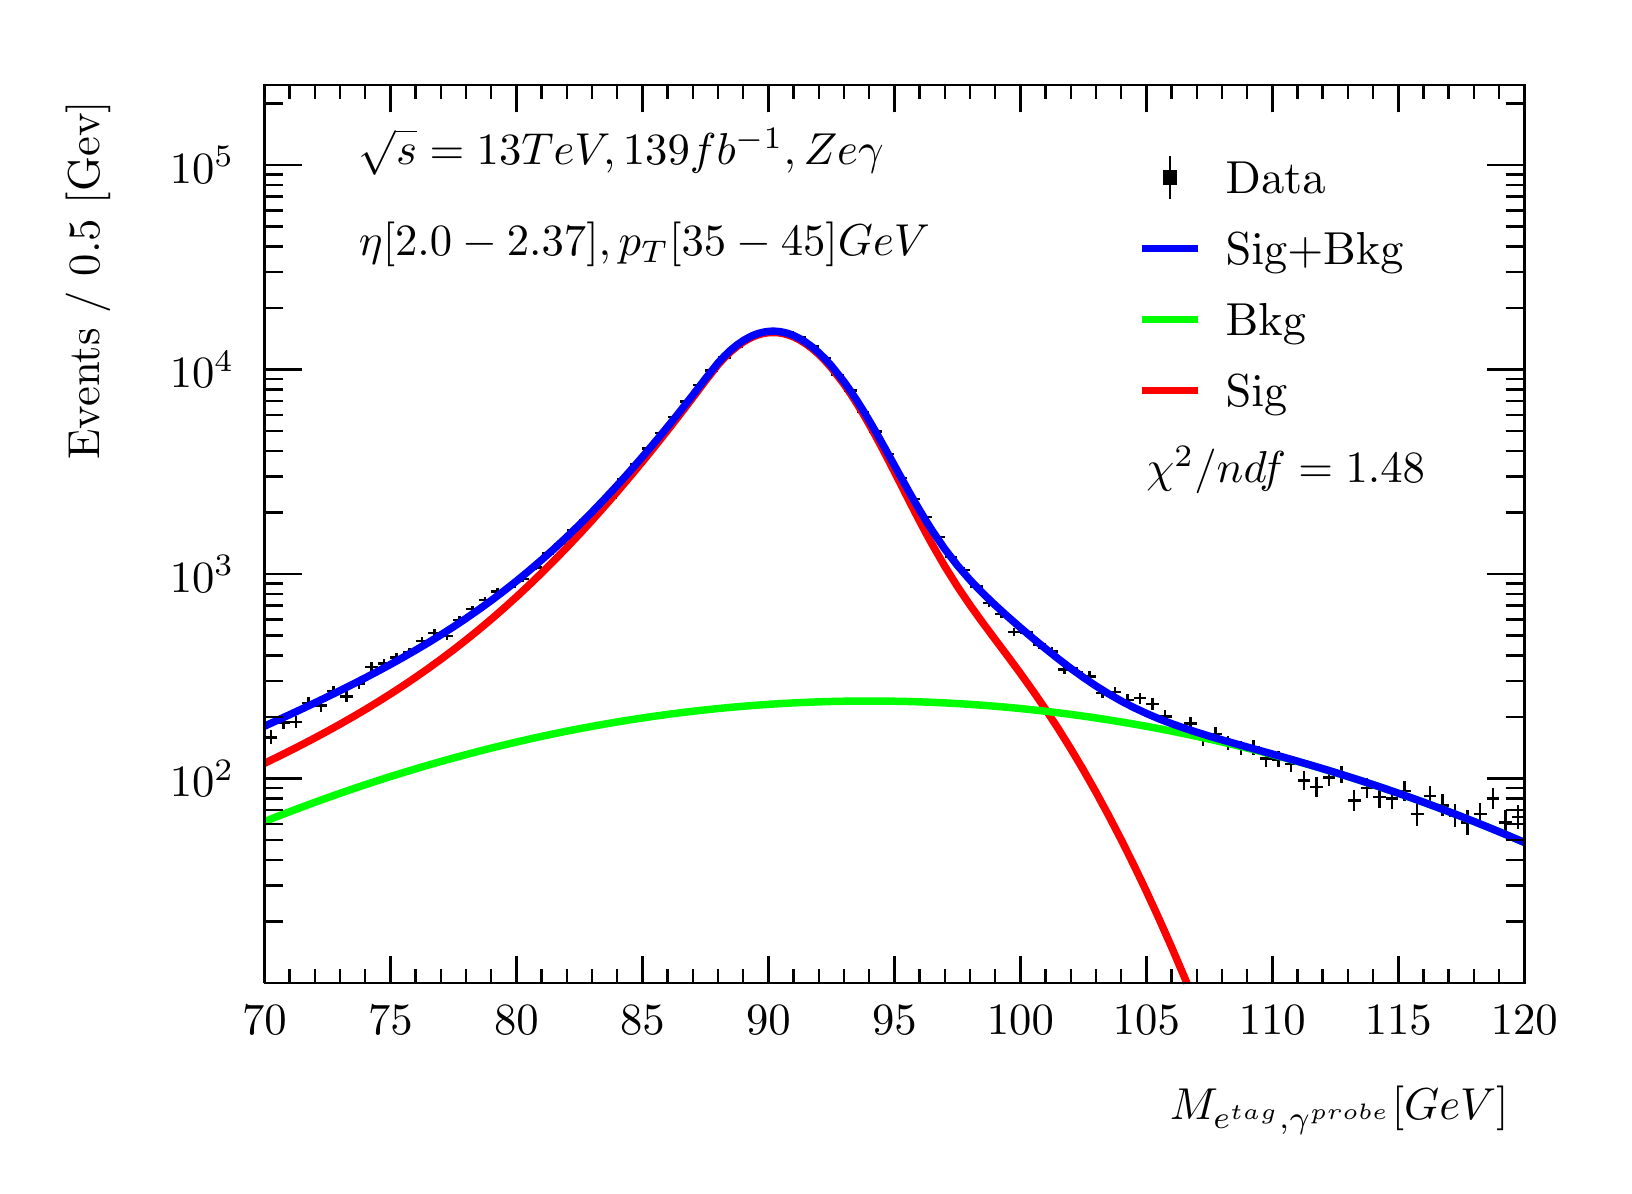
\begin{tikzpicture}
\pgfdeclareplotmark{cross} {
\pgfpathmoveto{\pgfpoint{-0.3\pgfplotmarksize}{\pgfplotmarksize}}
\pgfpathlineto{\pgfpoint{+0.3\pgfplotmarksize}{\pgfplotmarksize}}
\pgfpathlineto{\pgfpoint{+0.3\pgfplotmarksize}{0.3\pgfplotmarksize}}
\pgfpathlineto{\pgfpoint{+1\pgfplotmarksize}{0.3\pgfplotmarksize}}
\pgfpathlineto{\pgfpoint{+1\pgfplotmarksize}{-0.3\pgfplotmarksize}}
\pgfpathlineto{\pgfpoint{+0.3\pgfplotmarksize}{-0.3\pgfplotmarksize}}
\pgfpathlineto{\pgfpoint{+0.3\pgfplotmarksize}{-1.\pgfplotmarksize}}
\pgfpathlineto{\pgfpoint{-0.3\pgfplotmarksize}{-1.\pgfplotmarksize}}
\pgfpathlineto{\pgfpoint{-0.3\pgfplotmarksize}{-0.3\pgfplotmarksize}}
\pgfpathlineto{\pgfpoint{-1.\pgfplotmarksize}{-0.3\pgfplotmarksize}}
\pgfpathlineto{\pgfpoint{-1.\pgfplotmarksize}{0.3\pgfplotmarksize}}
\pgfpathlineto{\pgfpoint{-0.3\pgfplotmarksize}{0.3\pgfplotmarksize}}
\pgfpathclose
\pgfusepathqstroke
}
\pgfdeclareplotmark{cross*} {
\pgfpathmoveto{\pgfpoint{-0.3\pgfplotmarksize}{\pgfplotmarksize}}
\pgfpathlineto{\pgfpoint{+0.3\pgfplotmarksize}{\pgfplotmarksize}}
\pgfpathlineto{\pgfpoint{+0.3\pgfplotmarksize}{0.3\pgfplotmarksize}}
\pgfpathlineto{\pgfpoint{+1\pgfplotmarksize}{0.3\pgfplotmarksize}}
\pgfpathlineto{\pgfpoint{+1\pgfplotmarksize}{-0.3\pgfplotmarksize}}
\pgfpathlineto{\pgfpoint{+0.3\pgfplotmarksize}{-0.3\pgfplotmarksize}}
\pgfpathlineto{\pgfpoint{+0.3\pgfplotmarksize}{-1.\pgfplotmarksize}}
\pgfpathlineto{\pgfpoint{-0.3\pgfplotmarksize}{-1.\pgfplotmarksize}}
\pgfpathlineto{\pgfpoint{-0.3\pgfplotmarksize}{-0.3\pgfplotmarksize}}
\pgfpathlineto{\pgfpoint{-1.\pgfplotmarksize}{-0.3\pgfplotmarksize}}
\pgfpathlineto{\pgfpoint{-1.\pgfplotmarksize}{0.3\pgfplotmarksize}}
\pgfpathlineto{\pgfpoint{-0.3\pgfplotmarksize}{0.3\pgfplotmarksize}}
\pgfpathclose
\pgfusepathqfillstroke
}
\pgfdeclareplotmark{newstar} {
\pgfpathmoveto{\pgfqpoint{0pt}{\pgfplotmarksize}}
\pgfpathlineto{\pgfqpointpolar{44}{0.5\pgfplotmarksize}}
\pgfpathlineto{\pgfqpointpolar{18}{\pgfplotmarksize}}
\pgfpathlineto{\pgfqpointpolar{-20}{0.5\pgfplotmarksize}}
\pgfpathlineto{\pgfqpointpolar{-54}{\pgfplotmarksize}}
\pgfpathlineto{\pgfqpointpolar{-90}{0.5\pgfplotmarksize}}
\pgfpathlineto{\pgfqpointpolar{234}{\pgfplotmarksize}}
\pgfpathlineto{\pgfqpointpolar{198}{0.5\pgfplotmarksize}}
\pgfpathlineto{\pgfqpointpolar{162}{\pgfplotmarksize}}
\pgfpathlineto{\pgfqpointpolar{134}{0.5\pgfplotmarksize}}
\pgfpathclose
\pgfusepathqstroke
}
\pgfdeclareplotmark{newstar*} {
\pgfpathmoveto{\pgfqpoint{0pt}{\pgfplotmarksize}}
\pgfpathlineto{\pgfqpointpolar{44}{0.5\pgfplotmarksize}}
\pgfpathlineto{\pgfqpointpolar{18}{\pgfplotmarksize}}
\pgfpathlineto{\pgfqpointpolar{-20}{0.5\pgfplotmarksize}}
\pgfpathlineto{\pgfqpointpolar{-54}{\pgfplotmarksize}}
\pgfpathlineto{\pgfqpointpolar{-90}{0.5\pgfplotmarksize}}
\pgfpathlineto{\pgfqpointpolar{234}{\pgfplotmarksize}}
\pgfpathlineto{\pgfqpointpolar{198}{0.5\pgfplotmarksize}}
\pgfpathlineto{\pgfqpointpolar{162}{\pgfplotmarksize}}
\pgfpathlineto{\pgfqpointpolar{134}{0.5\pgfplotmarksize}}
\pgfpathclose
\pgfusepathqfillstroke
}
\definecolor{c}{rgb}{1,1,1};
\draw [color=c, fill=c] (0,0) rectangle (20,14.4361);
\draw [color=c, fill=c] (3,2.30977) rectangle (19,13.7143);
\definecolor{c}{rgb}{0,0,0};
\draw [c,line width=0.9] (3,2.30977) -- (3,13.7143) -- (19,13.7143) -- (19,2.30977) -- (3,2.30977);
\definecolor{c}{rgb}{1,1,1};
\draw [color=c, fill=c] (3,2.30977) rectangle (19,13.7143);
\definecolor{c}{rgb}{0,0,0};
\draw [c,line width=0.9] (3,2.30977) -- (3,13.7143) -- (19,13.7143) -- (19,2.30977) -- (3,2.30977);
\draw [c,line width=0.9] (3,2.30977) -- (19,2.30977);
\draw [c,line width=0.9] (3,2.65624) -- (3,2.30977);
\draw [c,line width=0.9] (3.32,2.48301) -- (3.32,2.30977);
\draw [c,line width=0.9] (3.64,2.48301) -- (3.64,2.30977);
\draw [c,line width=0.9] (3.96,2.48301) -- (3.96,2.30977);
\draw [c,line width=0.9] (4.28,2.48301) -- (4.28,2.30977);
\draw [c,line width=0.9] (4.6,2.65624) -- (4.6,2.30977);
\draw [c,line width=0.9] (4.92,2.48301) -- (4.92,2.30977);
\draw [c,line width=0.9] (5.24,2.48301) -- (5.24,2.30977);
\draw [c,line width=0.9] (5.56,2.48301) -- (5.56,2.30977);
\draw [c,line width=0.9] (5.88,2.48301) -- (5.88,2.30977);
\draw [c,line width=0.9] (6.2,2.65624) -- (6.2,2.30977);
\draw [c,line width=0.9] (6.52,2.48301) -- (6.52,2.30977);
\draw [c,line width=0.9] (6.84,2.48301) -- (6.84,2.30977);
\draw [c,line width=0.9] (7.16,2.48301) -- (7.16,2.30977);
\draw [c,line width=0.9] (7.48,2.48301) -- (7.48,2.30977);
\draw [c,line width=0.9] (7.8,2.65624) -- (7.8,2.30977);
\draw [c,line width=0.9] (8.12,2.48301) -- (8.12,2.30977);
\draw [c,line width=0.9] (8.44,2.48301) -- (8.44,2.30977);
\draw [c,line width=0.9] (8.76,2.48301) -- (8.76,2.30977);
\draw [c,line width=0.9] (9.08,2.48301) -- (9.08,2.30977);
\draw [c,line width=0.9] (9.4,2.65624) -- (9.4,2.30977);
\draw [c,line width=0.9] (9.72,2.48301) -- (9.72,2.30977);
\draw [c,line width=0.9] (10.04,2.48301) -- (10.04,2.30977);
\draw [c,line width=0.9] (10.36,2.48301) -- (10.36,2.30977);
\draw [c,line width=0.9] (10.68,2.48301) -- (10.68,2.30977);
\draw [c,line width=0.9] (11,2.65624) -- (11,2.30977);
\draw [c,line width=0.9] (11.32,2.48301) -- (11.32,2.30977);
\draw [c,line width=0.9] (11.64,2.48301) -- (11.64,2.30977);
\draw [c,line width=0.9] (11.96,2.48301) -- (11.96,2.30977);
\draw [c,line width=0.9] (12.28,2.48301) -- (12.28,2.30977);
\draw [c,line width=0.9] (12.6,2.65624) -- (12.6,2.30977);
\draw [c,line width=0.9] (12.92,2.48301) -- (12.92,2.30977);
\draw [c,line width=0.9] (13.24,2.48301) -- (13.24,2.30977);
\draw [c,line width=0.9] (13.56,2.48301) -- (13.56,2.30977);
\draw [c,line width=0.9] (13.88,2.48301) -- (13.88,2.30977);
\draw [c,line width=0.9] (14.2,2.65624) -- (14.2,2.30977);
\draw [c,line width=0.9] (14.52,2.48301) -- (14.52,2.30977);
\draw [c,line width=0.9] (14.84,2.48301) -- (14.84,2.30977);
\draw [c,line width=0.9] (15.16,2.48301) -- (15.16,2.30977);
\draw [c,line width=0.9] (15.48,2.48301) -- (15.48,2.30977);
\draw [c,line width=0.9] (15.8,2.65624) -- (15.8,2.30977);
\draw [c,line width=0.9] (16.12,2.48301) -- (16.12,2.30977);
\draw [c,line width=0.9] (16.44,2.48301) -- (16.44,2.30977);
\draw [c,line width=0.9] (16.76,2.48301) -- (16.76,2.30977);
\draw [c,line width=0.9] (17.08,2.48301) -- (17.08,2.30977);
\draw [c,line width=0.9] (17.4,2.65624) -- (17.4,2.30977);
\draw [c,line width=0.9] (17.72,2.48301) -- (17.72,2.30977);
\draw [c,line width=0.9] (18.04,2.48301) -- (18.04,2.30977);
\draw [c,line width=0.9] (18.36,2.48301) -- (18.36,2.30977);
\draw [c,line width=0.9] (18.68,2.48301) -- (18.68,2.30977);
\draw [c,line width=0.9] (19,2.65624) -- (19,2.30977);
\draw [anchor=base] (3,1.66015) node[scale=1.61424, color=c, rotate=0]{70};
\draw [anchor=base] (4.6,1.66015) node[scale=1.61424, color=c, rotate=0]{75};
\draw [anchor=base] (6.2,1.66015) node[scale=1.61424, color=c, rotate=0]{80};
\draw [anchor=base] (7.8,1.66015) node[scale=1.61424, color=c, rotate=0]{85};
\draw [anchor=base] (9.4,1.66015) node[scale=1.61424, color=c, rotate=0]{90};
\draw [anchor=base] (11,1.66015) node[scale=1.61424, color=c, rotate=0]{95};
\draw [anchor=base] (12.6,1.66015) node[scale=1.61424, color=c, rotate=0]{100};
\draw [anchor=base] (14.2,1.66015) node[scale=1.61424, color=c, rotate=0]{105};
\draw [anchor=base] (15.8,1.66015) node[scale=1.61424, color=c, rotate=0]{110};
\draw [anchor=base] (17.4,1.66015) node[scale=1.61424, color=c, rotate=0]{115};
\draw [anchor=base] (19,1.66015) node[scale=1.61424, color=c, rotate=0]{120};
\draw [anchor= east] (19,0.692932) node[scale=1.61424, color=c, rotate=0]{$M_{e^{tag}, \gamma^{probe}}  [GeV]$};
\draw [c,line width=0.9] (3,13.7143) -- (19,13.7143);
\draw [c,line width=0.9] (3,13.3678) -- (3,13.7143);
\draw [c,line width=0.9] (3.32,13.5411) -- (3.32,13.7143);
\draw [c,line width=0.9] (3.64,13.5411) -- (3.64,13.7143);
\draw [c,line width=0.9] (3.96,13.5411) -- (3.96,13.7143);
\draw [c,line width=0.9] (4.28,13.5411) -- (4.28,13.7143);
\draw [c,line width=0.9] (4.6,13.3678) -- (4.6,13.7143);
\draw [c,line width=0.9] (4.92,13.5411) -- (4.92,13.7143);
\draw [c,line width=0.9] (5.24,13.5411) -- (5.24,13.7143);
\draw [c,line width=0.9] (5.56,13.5411) -- (5.56,13.7143);
\draw [c,line width=0.9] (5.88,13.5411) -- (5.88,13.7143);
\draw [c,line width=0.9] (6.2,13.3678) -- (6.2,13.7143);
\draw [c,line width=0.9] (6.52,13.5411) -- (6.52,13.7143);
\draw [c,line width=0.9] (6.84,13.5411) -- (6.84,13.7143);
\draw [c,line width=0.9] (7.16,13.5411) -- (7.16,13.7143);
\draw [c,line width=0.9] (7.48,13.5411) -- (7.48,13.7143);
\draw [c,line width=0.9] (7.8,13.3678) -- (7.8,13.7143);
\draw [c,line width=0.9] (8.12,13.5411) -- (8.12,13.7143);
\draw [c,line width=0.9] (8.44,13.5411) -- (8.44,13.7143);
\draw [c,line width=0.9] (8.76,13.5411) -- (8.76,13.7143);
\draw [c,line width=0.9] (9.08,13.5411) -- (9.08,13.7143);
\draw [c,line width=0.9] (9.4,13.3678) -- (9.4,13.7143);
\draw [c,line width=0.9] (9.72,13.5411) -- (9.72,13.7143);
\draw [c,line width=0.9] (10.04,13.5411) -- (10.04,13.7143);
\draw [c,line width=0.9] (10.36,13.5411) -- (10.36,13.7143);
\draw [c,line width=0.9] (10.68,13.5411) -- (10.68,13.7143);
\draw [c,line width=0.9] (11,13.3678) -- (11,13.7143);
\draw [c,line width=0.9] (11.32,13.5411) -- (11.32,13.7143);
\draw [c,line width=0.9] (11.64,13.5411) -- (11.64,13.7143);
\draw [c,line width=0.9] (11.96,13.5411) -- (11.96,13.7143);
\draw [c,line width=0.9] (12.28,13.5411) -- (12.28,13.7143);
\draw [c,line width=0.9] (12.6,13.3678) -- (12.6,13.7143);
\draw [c,line width=0.9] (12.92,13.5411) -- (12.92,13.7143);
\draw [c,line width=0.9] (13.24,13.5411) -- (13.24,13.7143);
\draw [c,line width=0.9] (13.56,13.5411) -- (13.56,13.7143);
\draw [c,line width=0.9] (13.88,13.5411) -- (13.88,13.7143);
\draw [c,line width=0.9] (14.2,13.3678) -- (14.2,13.7143);
\draw [c,line width=0.9] (14.52,13.5411) -- (14.52,13.7143);
\draw [c,line width=0.9] (14.84,13.5411) -- (14.84,13.7143);
\draw [c,line width=0.9] (15.16,13.5411) -- (15.16,13.7143);
\draw [c,line width=0.9] (15.48,13.5411) -- (15.48,13.7143);
\draw [c,line width=0.9] (15.8,13.3678) -- (15.8,13.7143);
\draw [c,line width=0.9] (16.12,13.5411) -- (16.12,13.7143);
\draw [c,line width=0.9] (16.44,13.5411) -- (16.44,13.7143);
\draw [c,line width=0.9] (16.76,13.5411) -- (16.76,13.7143);
\draw [c,line width=0.9] (17.08,13.5411) -- (17.08,13.7143);
\draw [c,line width=0.9] (17.4,13.3678) -- (17.4,13.7143);
\draw [c,line width=0.9] (17.72,13.5411) -- (17.72,13.7143);
\draw [c,line width=0.9] (18.04,13.5411) -- (18.04,13.7143);
\draw [c,line width=0.9] (18.36,13.5411) -- (18.36,13.7143);
\draw [c,line width=0.9] (18.68,13.5411) -- (18.68,13.7143);
\draw [c,line width=0.9] (19,13.3678) -- (19,13.7143);
\draw [c,line width=0.9] (3,2.30977) -- (3,13.7143);
\draw [c,line width=0.9] (3.237,3.09166) -- (3,3.09166);
\draw [c,line width=0.9] (3.237,3.54903) -- (3,3.54903);
\draw [c,line width=0.9] (3.237,3.87354) -- (3,3.87354);
\draw [c,line width=0.9] (3.237,4.12525) -- (3,4.12525);
\draw [c,line width=0.9] (3.237,4.33091) -- (3,4.33091);
\draw [c,line width=0.9] (3.237,4.5048) -- (3,4.5048);
\draw [c,line width=0.9] (3.237,4.65542) -- (3,4.65542);
\draw [c,line width=0.9] (3.237,4.78829) -- (3,4.78829);
\draw [c,line width=0.9] (3.474,4.90714) -- (3,4.90714);
\draw [anchor= east] (2.82,4.90714) node[scale=1.61424, color=c, rotate=0]{$10^{2}$};
\draw [c,line width=0.9] (3.237,5.68902) -- (3,5.68902);
\draw [c,line width=0.9] (3.237,6.14639) -- (3,6.14639);
\draw [c,line width=0.9] (3.237,6.4709) -- (3,6.4709);
\draw [c,line width=0.9] (3.237,6.72261) -- (3,6.72261);
\draw [c,line width=0.9] (3.237,6.92828) -- (3,6.92828);
\draw [c,line width=0.9] (3.237,7.10216) -- (3,7.10216);
\draw [c,line width=0.9] (3.237,7.25279) -- (3,7.25279);
\draw [c,line width=0.9] (3.237,7.38565) -- (3,7.38565);
\draw [c,line width=0.9] (3.474,7.5045) -- (3,7.5045);
\draw [anchor= east] (2.82,7.5045) node[scale=1.61424, color=c, rotate=0]{$10^{3}$};
\draw [c,line width=0.9] (3.237,8.28638) -- (3,8.28638);
\draw [c,line width=0.9] (3.237,8.74376) -- (3,8.74376);
\draw [c,line width=0.9] (3.237,9.06827) -- (3,9.06827);
\draw [c,line width=0.9] (3.237,9.31998) -- (3,9.31998);
\draw [c,line width=0.9] (3.237,9.52564) -- (3,9.52564);
\draw [c,line width=0.9] (3.237,9.69952) -- (3,9.69952);
\draw [c,line width=0.9] (3.237,9.85015) -- (3,9.85015);
\draw [c,line width=0.9] (3.237,9.98301) -- (3,9.98301);
\draw [c,line width=0.9] (3.474,10.1019) -- (3,10.1019);
\draw [anchor= east] (2.82,10.1019) node[scale=1.61424, color=c, rotate=0]{$10^{4}$};
\draw [c,line width=0.9] (3.237,10.8837) -- (3,10.8837);
\draw [c,line width=0.9] (3.237,11.3411) -- (3,11.3411);
\draw [c,line width=0.9] (3.237,11.6656) -- (3,11.6656);
\draw [c,line width=0.9] (3.237,11.9173) -- (3,11.9173);
\draw [c,line width=0.9] (3.237,12.123) -- (3,12.123);
\draw [c,line width=0.9] (3.237,12.2969) -- (3,12.2969);
\draw [c,line width=0.9] (3.237,12.4475) -- (3,12.4475);
\draw [c,line width=0.9] (3.237,12.5804) -- (3,12.5804);
\draw [c,line width=0.9] (3.474,12.6992) -- (3,12.6992);
\draw [anchor= east] (2.82,12.6992) node[scale=1.61424, color=c, rotate=0]{$10^{5}$};
\draw [c,line width=0.9] (3.237,13.4811) -- (3,13.4811);
\draw [anchor= east] (0.76,13.7143) node[scale=1.61424, color=c, rotate=90]{Events / 0.5 [Gev]};
\draw [c,line width=0.9] (19,2.30977) -- (19,13.7143);
\draw [c,line width=0.9] (18.763,3.09166) -- (19,3.09166);
\draw [c,line width=0.9] (18.763,3.54903) -- (19,3.54903);
\draw [c,line width=0.9] (18.763,3.87354) -- (19,3.87354);
\draw [c,line width=0.9] (18.763,4.12525) -- (19,4.12525);
\draw [c,line width=0.9] (18.763,4.33091) -- (19,4.33091);
\draw [c,line width=0.9] (18.763,4.5048) -- (19,4.5048);
\draw [c,line width=0.9] (18.763,4.65542) -- (19,4.65542);
\draw [c,line width=0.9] (18.763,4.78829) -- (19,4.78829);
\draw [c,line width=0.9] (18.526,4.90714) -- (19,4.90714);
\draw [c,line width=0.9] (18.763,5.68902) -- (19,5.68902);
\draw [c,line width=0.9] (18.763,6.14639) -- (19,6.14639);
\draw [c,line width=0.9] (18.763,6.4709) -- (19,6.4709);
\draw [c,line width=0.9] (18.763,6.72261) -- (19,6.72261);
\draw [c,line width=0.9] (18.763,6.92828) -- (19,6.92828);
\draw [c,line width=0.9] (18.763,7.10216) -- (19,7.10216);
\draw [c,line width=0.9] (18.763,7.25279) -- (19,7.25279);
\draw [c,line width=0.9] (18.763,7.38565) -- (19,7.38565);
\draw [c,line width=0.9] (18.526,7.5045) -- (19,7.5045);
\draw [c,line width=0.9] (18.763,8.28638) -- (19,8.28638);
\draw [c,line width=0.9] (18.763,8.74376) -- (19,8.74376);
\draw [c,line width=0.9] (18.763,9.06827) -- (19,9.06827);
\draw [c,line width=0.9] (18.763,9.31998) -- (19,9.31998);
\draw [c,line width=0.9] (18.763,9.52564) -- (19,9.52564);
\draw [c,line width=0.9] (18.763,9.69952) -- (19,9.69952);
\draw [c,line width=0.9] (18.763,9.85015) -- (19,9.85015);
\draw [c,line width=0.9] (18.763,9.98301) -- (19,9.98301);
\draw [c,line width=0.9] (18.526,10.1019) -- (19,10.1019);
\draw [c,line width=0.9] (18.763,10.8837) -- (19,10.8837);
\draw [c,line width=0.9] (18.763,11.3411) -- (19,11.3411);
\draw [c,line width=0.9] (18.763,11.6656) -- (19,11.6656);
\draw [c,line width=0.9] (18.763,11.9173) -- (19,11.9173);
\draw [c,line width=0.9] (18.763,12.123) -- (19,12.123);
\draw [c,line width=0.9] (18.763,12.2969) -- (19,12.2969);
\draw [c,line width=0.9] (18.763,12.4475) -- (19,12.4475);
\draw [c,line width=0.9] (18.763,12.5804) -- (19,12.5804);
\draw [c,line width=0.9] (18.526,12.6992) -- (19,12.6992);
\draw [c,line width=0.9] (18.763,13.4811) -- (19,13.4811);
\draw [c,line width=0.9] (3.08,5.43024) -- (3,5.43024);
\draw [c,line width=0.9] (3,5.43024) -- (3,5.43024);
\draw [c,line width=0.9] (3.08,5.43024) -- (3.16,5.43024);
\draw [c,line width=0.9] (3.16,5.43024) -- (3.16,5.43024);
\draw [c,line width=0.9] (3.08,5.43024) -- (3.08,5.51967);
\draw [c,line width=0.9] (3.08,5.51967) -- (3.08,5.51967);
\draw [c,line width=0.9] (3.08,5.43024) -- (3.08,5.3408);
\draw [c,line width=0.9] (3.08,5.3408) -- (3.08,5.3408);
\draw [c,line width=0.9] (3.24,5.61922) -- (3.16,5.61922);
\draw [c,line width=0.9] (3.16,5.61922) -- (3.16,5.61922);
\draw [c,line width=0.9] (3.24,5.61922) -- (3.32,5.61922);
\draw [c,line width=0.9] (3.32,5.61922) -- (3.32,5.61922);
\draw [c,line width=0.9] (3.24,5.61922) -- (3.24,5.70148);
\draw [c,line width=0.9] (3.24,5.70148) -- (3.24,5.70148);
\draw [c,line width=0.9] (3.24,5.61922) -- (3.24,5.53697);
\draw [c,line width=0.9] (3.24,5.53697) -- (3.24,5.53697);
\draw [c,line width=0.9] (3.4,5.62521) -- (3.32,5.62521);
\draw [c,line width=0.9] (3.32,5.62521) -- (3.32,5.62521);
\draw [c,line width=0.9] (3.4,5.62521) -- (3.48,5.62521);
\draw [c,line width=0.9] (3.48,5.62521) -- (3.48,5.62521);
\draw [c,line width=0.9] (3.4,5.62521) -- (3.4,5.70724);
\draw [c,line width=0.9] (3.4,5.70724) -- (3.4,5.70724);
\draw [c,line width=0.9] (3.4,5.62521) -- (3.4,5.54318);
\draw [c,line width=0.9] (3.4,5.54318) -- (3.4,5.54318);
\draw [c,line width=0.9] (3.56,5.86612) -- (3.48,5.86612);
\draw [c,line width=0.9] (3.48,5.86612) -- (3.48,5.86612);
\draw [c,line width=0.9] (3.56,5.86612) -- (3.64,5.86612);
\draw [c,line width=0.9] (3.64,5.86612) -- (3.64,5.86612);
\draw [c,line width=0.9] (3.56,5.86612) -- (3.56,5.93985);
\draw [c,line width=0.9] (3.56,5.93985) -- (3.56,5.93985);
\draw [c,line width=0.9] (3.56,5.86612) -- (3.56,5.7924);
\draw [c,line width=0.9] (3.56,5.7924) -- (3.56,5.7924);
\draw [c,line width=0.9] (3.72,5.83187) -- (3.64,5.83187);
\draw [c,line width=0.9] (3.64,5.83187) -- (3.64,5.83187);
\draw [c,line width=0.9] (3.72,5.83187) -- (3.8,5.83187);
\draw [c,line width=0.9] (3.8,5.83187) -- (3.8,5.83187);
\draw [c,line width=0.9] (3.72,5.83187) -- (3.72,5.90672);
\draw [c,line width=0.9] (3.72,5.90672) -- (3.72,5.90672);
\draw [c,line width=0.9] (3.72,5.83187) -- (3.72,5.75701);
\draw [c,line width=0.9] (3.72,5.75701) -- (3.72,5.75701);
\draw [c,line width=0.9] (3.88,6.01916) -- (3.8,6.01916);
\draw [c,line width=0.9] (3.8,6.01916) -- (3.8,6.01916);
\draw [c,line width=0.9] (3.88,6.01916) -- (3.96,6.01916);
\draw [c,line width=0.9] (3.96,6.01916) -- (3.96,6.01916);
\draw [c,line width=0.9] (3.88,6.01916) -- (3.88,6.08805);
\draw [c,line width=0.9] (3.88,6.08805) -- (3.88,6.08805);
\draw [c,line width=0.9] (3.88,6.01916) -- (3.88,5.95026);
\draw [c,line width=0.9] (3.88,5.95026) -- (3.88,5.95026);
\draw [c,line width=0.9] (4.04,5.94972) -- (3.96,5.94972);
\draw [c,line width=0.9] (3.96,5.94972) -- (3.96,5.94972);
\draw [c,line width=0.9] (4.04,5.94972) -- (4.12,5.94972);
\draw [c,line width=0.9] (4.12,5.94972) -- (4.12,5.94972);
\draw [c,line width=0.9] (4.04,5.94972) -- (4.04,6.02077);
\draw [c,line width=0.9] (4.04,6.02077) -- (4.04,6.02077);
\draw [c,line width=0.9] (4.04,5.94972) -- (4.04,5.87867);
\draw [c,line width=0.9] (4.04,5.87867) -- (4.04,5.87867);
\draw [c,line width=0.9] (4.2,6.11591) -- (4.12,6.11591);
\draw [c,line width=0.9] (4.12,6.11591) -- (4.12,6.11591);
\draw [c,line width=0.9] (4.2,6.11591) -- (4.28,6.11591);
\draw [c,line width=0.9] (4.28,6.11591) -- (4.28,6.11591);
\draw [c,line width=0.9] (4.2,6.11591) -- (4.2,6.18191);
\draw [c,line width=0.9] (4.2,6.18191) -- (4.2,6.18191);
\draw [c,line width=0.9] (4.2,6.11591) -- (4.2,6.0499);
\draw [c,line width=0.9] (4.2,6.0499) -- (4.2,6.0499);
\draw [c,line width=0.9] (4.36,6.32671) -- (4.28,6.32671);
\draw [c,line width=0.9] (4.28,6.32671) -- (4.28,6.32671);
\draw [c,line width=0.9] (4.36,6.32671) -- (4.44,6.32671);
\draw [c,line width=0.9] (4.44,6.32671) -- (4.44,6.32671);
\draw [c,line width=0.9] (4.36,6.32671) -- (4.36,6.38682);
\draw [c,line width=0.9] (4.36,6.38682) -- (4.36,6.38682);
\draw [c,line width=0.9] (4.36,6.32671) -- (4.36,6.26659);
\draw [c,line width=0.9] (4.36,6.26659) -- (4.36,6.26659);
\draw [c,line width=0.9] (4.52,6.36762) -- (4.44,6.36762);
\draw [c,line width=0.9] (4.44,6.36762) -- (4.44,6.36762);
\draw [c,line width=0.9] (4.52,6.36762) -- (4.6,6.36762);
\draw [c,line width=0.9] (4.6,6.36762) -- (4.6,6.36762);
\draw [c,line width=0.9] (4.52,6.36762) -- (4.52,6.42665);
\draw [c,line width=0.9] (4.52,6.42665) -- (4.52,6.42665);
\draw [c,line width=0.9] (4.52,6.36762) -- (4.52,6.30858);
\draw [c,line width=0.9] (4.52,6.30858) -- (4.52,6.30858);
\draw [c,line width=0.9] (4.68,6.44235) -- (4.6,6.44235);
\draw [c,line width=0.9] (4.6,6.44235) -- (4.6,6.44235);
\draw [c,line width=0.9] (4.68,6.44235) -- (4.76,6.44235);
\draw [c,line width=0.9] (4.76,6.44235) -- (4.76,6.44235);
\draw [c,line width=0.9] (4.68,6.44235) -- (4.68,6.49946);
\draw [c,line width=0.9] (4.68,6.49946) -- (4.68,6.49946);
\draw [c,line width=0.9] (4.68,6.44235) -- (4.68,6.38523);
\draw [c,line width=0.9] (4.68,6.38523) -- (4.68,6.38523);
\draw [c,line width=0.9] (4.84,6.51243) -- (4.76,6.51243);
\draw [c,line width=0.9] (4.76,6.51243) -- (4.76,6.51243);
\draw [c,line width=0.9] (4.84,6.51243) -- (4.92,6.51243);
\draw [c,line width=0.9] (4.92,6.51243) -- (4.92,6.51243);
\draw [c,line width=0.9] (4.84,6.51243) -- (4.84,6.5678);
\draw [c,line width=0.9] (4.84,6.5678) -- (4.84,6.5678);
\draw [c,line width=0.9] (4.84,6.51243) -- (4.84,6.45707);
\draw [c,line width=0.9] (4.84,6.45707) -- (4.84,6.45707);
\draw [c,line width=0.9] (5,6.65282) -- (4.92,6.65282);
\draw [c,line width=0.9] (4.92,6.65282) -- (4.92,6.65282);
\draw [c,line width=0.9] (5,6.65282) -- (5.08,6.65282);
\draw [c,line width=0.9] (5.08,6.65282) -- (5.08,6.65282);
\draw [c,line width=0.9] (5,6.65282) -- (5,6.70485);
\draw [c,line width=0.9] (5,6.70485) -- (5,6.70485);
\draw [c,line width=0.9] (5,6.65282) -- (5,6.60079);
\draw [c,line width=0.9] (5,6.60079) -- (5,6.60079);
\draw [c,line width=0.9] (5.16,6.75815) -- (5.08,6.75815);
\draw [c,line width=0.9] (5.08,6.75815) -- (5.08,6.75815);
\draw [c,line width=0.9] (5.16,6.75815) -- (5.24,6.75815);
\draw [c,line width=0.9] (5.24,6.75815) -- (5.24,6.75815);
\draw [c,line width=0.9] (5.16,6.75815) -- (5.16,6.8078);
\draw [c,line width=0.9] (5.16,6.8078) -- (5.16,6.8078);
\draw [c,line width=0.9] (5.16,6.75815) -- (5.16,6.70849);
\draw [c,line width=0.9] (5.16,6.70849) -- (5.16,6.70849);
\draw [c,line width=0.9] (5.32,6.71583) -- (5.24,6.71583);
\draw [c,line width=0.9] (5.24,6.71583) -- (5.24,6.71583);
\draw [c,line width=0.9] (5.32,6.71583) -- (5.4,6.71583);
\draw [c,line width=0.9] (5.4,6.71583) -- (5.4,6.71583);
\draw [c,line width=0.9] (5.32,6.71583) -- (5.32,6.76642);
\draw [c,line width=0.9] (5.32,6.76642) -- (5.32,6.76642);
\draw [c,line width=0.9] (5.32,6.71583) -- (5.32,6.66523);
\draw [c,line width=0.9] (5.32,6.66523) -- (5.32,6.66523);
\draw [c,line width=0.9] (5.48,6.91884) -- (5.4,6.91884);
\draw [c,line width=0.9] (5.4,6.91884) -- (5.4,6.91884);
\draw [c,line width=0.9] (5.48,6.91884) -- (5.56,6.91884);
\draw [c,line width=0.9] (5.56,6.91884) -- (5.56,6.91884);
\draw [c,line width=0.9] (5.48,6.91884) -- (5.48,6.96508);
\draw [c,line width=0.9] (5.48,6.96508) -- (5.48,6.96508);
\draw [c,line width=0.9] (5.48,6.91884) -- (5.48,6.8726);
\draw [c,line width=0.9] (5.48,6.8726) -- (5.48,6.8726);
\draw [c,line width=0.9] (5.64,7.06114) -- (5.56,7.06114);
\draw [c,line width=0.9] (5.56,7.06114) -- (5.56,7.06114);
\draw [c,line width=0.9] (5.64,7.06114) -- (5.72,7.06114);
\draw [c,line width=0.9] (5.72,7.06114) -- (5.72,7.06114);
\draw [c,line width=0.9] (5.64,7.06114) -- (5.64,7.10455);
\draw [c,line width=0.9] (5.64,7.10455) -- (5.64,7.10455);
\draw [c,line width=0.9] (5.64,7.06114) -- (5.64,7.01772);
\draw [c,line width=0.9] (5.64,7.01772) -- (5.64,7.01772);
\draw [c,line width=0.9] (5.8,7.17698) -- (5.72,7.17698);
\draw [c,line width=0.9] (5.72,7.17698) -- (5.72,7.17698);
\draw [c,line width=0.9] (5.8,7.17698) -- (5.88,7.17698);
\draw [c,line width=0.9] (5.88,7.17698) -- (5.88,7.17698);
\draw [c,line width=0.9] (5.8,7.17698) -- (5.8,7.21822);
\draw [c,line width=0.9] (5.8,7.21822) -- (5.8,7.21822);
\draw [c,line width=0.9] (5.8,7.17698) -- (5.8,7.13573);
\draw [c,line width=0.9] (5.8,7.13573) -- (5.8,7.13573);
\draw [c,line width=0.9] (5.96,7.28339) -- (5.88,7.28339);
\draw [c,line width=0.9] (5.88,7.28339) -- (5.88,7.28339);
\draw [c,line width=0.9] (5.96,7.28339) -- (6.04,7.28339);
\draw [c,line width=0.9] (6.04,7.28339) -- (6.04,7.28339);
\draw [c,line width=0.9] (5.96,7.28339) -- (5.96,7.32273);
\draw [c,line width=0.9] (5.96,7.32273) -- (5.96,7.32273);
\draw [c,line width=0.9] (5.96,7.28339) -- (5.96,7.24405);
\draw [c,line width=0.9] (5.96,7.24405) -- (5.96,7.24405);
\draw [c,line width=0.9] (6.12,7.33699) -- (6.04,7.33699);
\draw [c,line width=0.9] (6.04,7.33699) -- (6.04,7.33699);
\draw [c,line width=0.9] (6.12,7.33699) -- (6.2,7.33699);
\draw [c,line width=0.9] (6.2,7.33699) -- (6.2,7.33699);
\draw [c,line width=0.9] (6.12,7.33699) -- (6.12,7.37541);
\draw [c,line width=0.9] (6.12,7.37541) -- (6.12,7.37541);
\draw [c,line width=0.9] (6.12,7.33699) -- (6.12,7.29857);
\draw [c,line width=0.9] (6.12,7.29857) -- (6.12,7.29857);
\draw [c,line width=0.9] (6.28,7.44426) -- (6.2,7.44426);
\draw [c,line width=0.9] (6.2,7.44426) -- (6.2,7.44426);
\draw [c,line width=0.9] (6.28,7.44426) -- (6.36,7.44426);
\draw [c,line width=0.9] (6.36,7.44426) -- (6.36,7.44426);
\draw [c,line width=0.9] (6.28,7.44426) -- (6.28,7.4809);
\draw [c,line width=0.9] (6.28,7.4809) -- (6.28,7.4809);
\draw [c,line width=0.9] (6.28,7.44426) -- (6.28,7.40763);
\draw [c,line width=0.9] (6.28,7.40763) -- (6.28,7.40763);
\draw [c,line width=0.9] (6.44,7.58713) -- (6.36,7.58713);
\draw [c,line width=0.9] (6.36,7.58713) -- (6.36,7.58713);
\draw [c,line width=0.9] (6.44,7.58713) -- (6.52,7.58713);
\draw [c,line width=0.9] (6.52,7.58713) -- (6.52,7.58713);
\draw [c,line width=0.9] (6.44,7.58713) -- (6.44,7.62151);
\draw [c,line width=0.9] (6.44,7.62151) -- (6.44,7.62151);
\draw [c,line width=0.9] (6.44,7.58713) -- (6.44,7.55274);
\draw [c,line width=0.9] (6.44,7.55274) -- (6.44,7.55274);
\draw [c,line width=0.9] (6.6,7.76699) -- (6.52,7.76699);
\draw [c,line width=0.9] (6.52,7.76699) -- (6.52,7.76699);
\draw [c,line width=0.9] (6.6,7.76699) -- (6.68,7.76699);
\draw [c,line width=0.9] (6.68,7.76699) -- (6.68,7.76699);
\draw [c,line width=0.9] (6.6,7.76699) -- (6.6,7.79874);
\draw [c,line width=0.9] (6.6,7.79874) -- (6.6,7.79874);
\draw [c,line width=0.9] (6.6,7.76699) -- (6.6,7.73524);
\draw [c,line width=0.9] (6.6,7.73524) -- (6.6,7.73524);
\draw [c,line width=0.9] (6.76,7.88405) -- (6.68,7.88405);
\draw [c,line width=0.9] (6.68,7.88405) -- (6.68,7.88405);
\draw [c,line width=0.9] (6.76,7.88405) -- (6.84,7.88405);
\draw [c,line width=0.9] (6.84,7.88405) -- (6.84,7.88405);
\draw [c,line width=0.9] (6.76,7.88405) -- (6.76,7.91419);
\draw [c,line width=0.9] (6.76,7.91419) -- (6.76,7.91419);
\draw [c,line width=0.9] (6.76,7.88405) -- (6.76,7.8539);
\draw [c,line width=0.9] (6.76,7.8539) -- (6.76,7.8539);
\draw [c,line width=0.9] (6.92,8.06596) -- (6.84,8.06596);
\draw [c,line width=0.9] (6.84,8.06596) -- (6.84,8.06596);
\draw [c,line width=0.9] (6.92,8.06596) -- (7,8.06596);
\draw [c,line width=0.9] (7,8.06596) -- (7,8.06596);
\draw [c,line width=0.9] (6.92,8.06596) -- (6.92,8.09377);
\draw [c,line width=0.9] (6.92,8.09377) -- (6.92,8.09377);
\draw [c,line width=0.9] (6.92,8.06596) -- (6.92,8.03815);
\draw [c,line width=0.9] (6.92,8.03815) -- (6.92,8.03815);
\draw [c,line width=0.9] (7.08,8.18556) -- (7,8.18556);
\draw [c,line width=0.9] (7,8.18556) -- (7,8.18556);
\draw [c,line width=0.9] (7.08,8.18556) -- (7.16,8.18556);
\draw [c,line width=0.9] (7.16,8.18556) -- (7.16,8.18556);
\draw [c,line width=0.9] (7.08,8.18556) -- (7.08,8.21194);
\draw [c,line width=0.9] (7.08,8.21194) -- (7.08,8.21194);
\draw [c,line width=0.9] (7.08,8.18556) -- (7.08,8.15919);
\draw [c,line width=0.9] (7.08,8.15919) -- (7.08,8.15919);
\draw [c,line width=0.9] (7.24,8.31918) -- (7.16,8.31918);
\draw [c,line width=0.9] (7.16,8.31918) -- (7.16,8.31918);
\draw [c,line width=0.9] (7.24,8.31918) -- (7.32,8.31918);
\draw [c,line width=0.9] (7.32,8.31918) -- (7.32,8.31918);
\draw [c,line width=0.9] (7.24,8.31918) -- (7.24,8.34404);
\draw [c,line width=0.9] (7.24,8.34404) -- (7.24,8.34404);
\draw [c,line width=0.9] (7.24,8.31918) -- (7.24,8.29432);
\draw [c,line width=0.9] (7.24,8.29432) -- (7.24,8.29432);
\draw [c,line width=0.9] (7.4,8.47117) -- (7.32,8.47117);
\draw [c,line width=0.9] (7.32,8.47117) -- (7.32,8.47117);
\draw [c,line width=0.9] (7.4,8.47117) -- (7.48,8.47117);
\draw [c,line width=0.9] (7.48,8.47117) -- (7.48,8.47117);
\draw [c,line width=0.9] (7.4,8.47117) -- (7.4,8.49441);
\draw [c,line width=0.9] (7.4,8.49441) -- (7.4,8.49441);
\draw [c,line width=0.9] (7.4,8.47117) -- (7.4,8.44794);
\draw [c,line width=0.9] (7.4,8.44794) -- (7.4,8.44794);
\draw [c,line width=0.9] (7.56,8.70551) -- (7.48,8.70551);
\draw [c,line width=0.9] (7.48,8.70551) -- (7.48,8.70551);
\draw [c,line width=0.9] (7.56,8.70551) -- (7.64,8.70551);
\draw [c,line width=0.9] (7.64,8.70551) -- (7.64,8.70551);
\draw [c,line width=0.9] (7.56,8.70551) -- (7.56,8.72646);
\draw [c,line width=0.9] (7.56,8.72646) -- (7.56,8.72646);
\draw [c,line width=0.9] (7.56,8.70551) -- (7.56,8.68457);
\draw [c,line width=0.9] (7.56,8.68457) -- (7.56,8.68457);
\draw [c,line width=0.9] (7.72,8.90076) -- (7.64,8.90076);
\draw [c,line width=0.9] (7.64,8.90076) -- (7.64,8.90076);
\draw [c,line width=0.9] (7.72,8.90076) -- (7.8,8.90076);
\draw [c,line width=0.9] (7.8,8.90076) -- (7.8,8.90076);
\draw [c,line width=0.9] (7.72,8.90076) -- (7.72,8.91997);
\draw [c,line width=0.9] (7.72,8.91997) -- (7.72,8.91997);
\draw [c,line width=0.9] (7.72,8.90076) -- (7.72,8.88155);
\draw [c,line width=0.9] (7.72,8.88155) -- (7.72,8.88155);
\draw [c,line width=0.9] (7.88,9.10024) -- (7.8,9.10024);
\draw [c,line width=0.9] (7.8,9.10024) -- (7.8,9.10024);
\draw [c,line width=0.9] (7.88,9.10024) -- (7.96,9.10024);
\draw [c,line width=0.9] (7.96,9.10024) -- (7.96,9.10024);
\draw [c,line width=0.9] (7.88,9.10024) -- (7.88,9.11783);
\draw [c,line width=0.9] (7.88,9.11783) -- (7.88,9.11783);
\draw [c,line width=0.9] (7.88,9.10024) -- (7.88,9.08266);
\draw [c,line width=0.9] (7.88,9.08266) -- (7.88,9.08266);
\draw [c,line width=0.9] (8.04,9.29558) -- (7.96,9.29558);
\draw [c,line width=0.9] (7.96,9.29558) -- (7.96,9.29558);
\draw [c,line width=0.9] (8.04,9.29558) -- (8.12,9.29558);
\draw [c,line width=0.9] (8.12,9.29558) -- (8.12,9.29558);
\draw [c,line width=0.9] (8.04,9.29558) -- (8.04,9.3117);
\draw [c,line width=0.9] (8.04,9.3117) -- (8.04,9.3117);
\draw [c,line width=0.9] (8.04,9.29558) -- (8.04,9.27945);
\draw [c,line width=0.9] (8.04,9.27945) -- (8.04,9.27945);
\draw [c,line width=0.9] (8.2,9.49804) -- (8.12,9.49804);
\draw [c,line width=0.9] (8.12,9.49804) -- (8.12,9.49804);
\draw [c,line width=0.9] (8.2,9.49804) -- (8.28,9.49804);
\draw [c,line width=0.9] (8.28,9.49804) -- (8.28,9.49804);
\draw [c,line width=0.9] (8.2,9.49804) -- (8.2,9.51279);
\draw [c,line width=0.9] (8.2,9.51279) -- (8.2,9.51279);
\draw [c,line width=0.9] (8.2,9.49804) -- (8.2,9.4833);
\draw [c,line width=0.9] (8.2,9.4833) -- (8.2,9.4833);
\draw [c,line width=0.9] (8.36,9.69824) -- (8.28,9.69824);
\draw [c,line width=0.9] (8.28,9.69824) -- (8.28,9.69824);
\draw [c,line width=0.9] (8.36,9.69824) -- (8.44,9.69824);
\draw [c,line width=0.9] (8.44,9.69824) -- (8.44,9.69824);
\draw [c,line width=0.9] (8.36,9.69824) -- (8.36,9.71173);
\draw [c,line width=0.9] (8.36,9.71173) -- (8.36,9.71173);
\draw [c,line width=0.9] (8.36,9.69824) -- (8.36,9.68475);
\draw [c,line width=0.9] (8.36,9.68475) -- (8.36,9.68475);
\draw [c,line width=0.9] (8.52,9.90438) -- (8.44,9.90438);
\draw [c,line width=0.9] (8.44,9.90438) -- (8.44,9.90438);
\draw [c,line width=0.9] (8.52,9.90438) -- (8.6,9.90438);
\draw [c,line width=0.9] (8.6,9.90438) -- (8.6,9.90438);
\draw [c,line width=0.9] (8.52,9.90438) -- (8.52,9.91669);
\draw [c,line width=0.9] (8.52,9.91669) -- (8.52,9.91669);
\draw [c,line width=0.9] (8.52,9.90438) -- (8.52,9.89207);
\draw [c,line width=0.9] (8.52,9.89207) -- (8.52,9.89207);
\draw [c,line width=0.9] (8.68,10.0876) -- (8.6,10.0876);
\draw [c,line width=0.9] (8.6,10.0876) -- (8.6,10.0876);
\draw [c,line width=0.9] (8.68,10.0876) -- (8.76,10.0876);
\draw [c,line width=0.9] (8.76,10.0876) -- (8.76,10.0876);
\draw [c,line width=0.9] (8.68,10.0876) -- (8.68,10.0989);
\draw [c,line width=0.9] (8.68,10.0989) -- (8.68,10.0989);
\draw [c,line width=0.9] (8.68,10.0876) -- (8.68,10.0762);
\draw [c,line width=0.9] (8.68,10.0762) -- (8.68,10.0762);
\draw [c,line width=0.9] (8.84,10.2564) -- (8.76,10.2564);
\draw [c,line width=0.9] (8.76,10.2564) -- (8.76,10.2564);
\draw [c,line width=0.9] (8.84,10.2564) -- (8.92,10.2564);
\draw [c,line width=0.9] (8.92,10.2564) -- (8.92,10.2564);
\draw [c,line width=0.9] (8.84,10.2564) -- (8.84,10.2669);
\draw [c,line width=0.9] (8.84,10.2669) -- (8.84,10.2669);
\draw [c,line width=0.9] (8.84,10.2564) -- (8.84,10.2458);
\draw [c,line width=0.9] (8.84,10.2458) -- (8.84,10.2458);
\draw [c,line width=0.9] (9,10.3945) -- (8.92,10.3945);
\draw [c,line width=0.9] (8.92,10.3945) -- (8.92,10.3945);
\draw [c,line width=0.9] (9,10.3945) -- (9.08,10.3945);
\draw [c,line width=0.9] (9.08,10.3945) -- (9.08,10.3945);
\draw [c,line width=0.9] (9,10.3945) -- (9,10.4044);
\draw [c,line width=0.9] (9,10.4044) -- (9,10.4044);
\draw [c,line width=0.9] (9,10.3945) -- (9,10.3846);
\draw [c,line width=0.9] (9,10.3846) -- (9,10.3846);
\draw [c,line width=0.9] (9.16,10.4961) -- (9.08,10.4961);
\draw [c,line width=0.9] (9.08,10.4961) -- (9.08,10.4961);
\draw [c,line width=0.9] (9.16,10.4961) -- (9.24,10.4961);
\draw [c,line width=0.9] (9.24,10.4961) -- (9.24,10.4961);
\draw [c,line width=0.9] (9.16,10.4961) -- (9.16,10.5055);
\draw [c,line width=0.9] (9.16,10.5055) -- (9.16,10.5055);
\draw [c,line width=0.9] (9.16,10.4961) -- (9.16,10.4866);
\draw [c,line width=0.9] (9.16,10.4866) -- (9.16,10.4866);
\draw [c,line width=0.9] (9.32,10.5629) -- (9.24,10.5629);
\draw [c,line width=0.9] (9.24,10.5629) -- (9.24,10.5629);
\draw [c,line width=0.9] (9.32,10.5629) -- (9.4,10.5629);
\draw [c,line width=0.9] (9.4,10.5629) -- (9.4,10.5629);
\draw [c,line width=0.9] (9.32,10.5629) -- (9.32,10.5721);
\draw [c,line width=0.9] (9.32,10.5721) -- (9.32,10.5721);
\draw [c,line width=0.9] (9.32,10.5629) -- (9.32,10.5537);
\draw [c,line width=0.9] (9.32,10.5537) -- (9.32,10.5537);
\draw [c,line width=0.9] (9.48,10.5919) -- (9.4,10.5919);
\draw [c,line width=0.9] (9.4,10.5919) -- (9.4,10.5919);
\draw [c,line width=0.9] (9.48,10.5919) -- (9.56,10.5919);
\draw [c,line width=0.9] (9.56,10.5919) -- (9.56,10.5919);
\draw [c,line width=0.9] (9.48,10.5919) -- (9.48,10.601);
\draw [c,line width=0.9] (9.48,10.601) -- (9.48,10.601);
\draw [c,line width=0.9] (9.48,10.5919) -- (9.48,10.5828);
\draw [c,line width=0.9] (9.48,10.5828) -- (9.48,10.5828);
\draw [c,line width=0.9] (9.64,10.5804) -- (9.56,10.5804);
\draw [c,line width=0.9] (9.56,10.5804) -- (9.56,10.5804);
\draw [c,line width=0.9] (9.64,10.5804) -- (9.72,10.5804);
\draw [c,line width=0.9] (9.72,10.5804) -- (9.72,10.5804);
\draw [c,line width=0.9] (9.64,10.5804) -- (9.64,10.5895);
\draw [c,line width=0.9] (9.64,10.5895) -- (9.64,10.5895);
\draw [c,line width=0.9] (9.64,10.5804) -- (9.64,10.5713);
\draw [c,line width=0.9] (9.64,10.5713) -- (9.64,10.5713);
\draw [c,line width=0.9] (9.8,10.5089) -- (9.72,10.5089);
\draw [c,line width=0.9] (9.72,10.5089) -- (9.72,10.5089);
\draw [c,line width=0.9] (9.8,10.5089) -- (9.88,10.5089);
\draw [c,line width=0.9] (9.88,10.5089) -- (9.88,10.5089);
\draw [c,line width=0.9] (9.8,10.5089) -- (9.8,10.5184);
\draw [c,line width=0.9] (9.8,10.5184) -- (9.8,10.5184);
\draw [c,line width=0.9] (9.8,10.5089) -- (9.8,10.4995);
\draw [c,line width=0.9] (9.8,10.4995) -- (9.8,10.4995);
\draw [c,line width=0.9] (9.96,10.3927) -- (9.88,10.3927);
\draw [c,line width=0.9] (9.88,10.3927) -- (9.88,10.3927);
\draw [c,line width=0.9] (9.96,10.3927) -- (10.04,10.3927);
\draw [c,line width=0.9] (10.04,10.3927) -- (10.04,10.3927);
\draw [c,line width=0.9] (9.96,10.3927) -- (9.96,10.4026);
\draw [c,line width=0.9] (9.96,10.4026) -- (9.96,10.4026);
\draw [c,line width=0.9] (9.96,10.3927) -- (9.96,10.3828);
\draw [c,line width=0.9] (9.96,10.3828) -- (9.96,10.3828);
\draw [c,line width=0.9] (10.12,10.2469) -- (10.04,10.2469);
\draw [c,line width=0.9] (10.04,10.2469) -- (10.04,10.2469);
\draw [c,line width=0.9] (10.12,10.2469) -- (10.2,10.2469);
\draw [c,line width=0.9] (10.2,10.2469) -- (10.2,10.2469);
\draw [c,line width=0.9] (10.12,10.2469) -- (10.12,10.2575);
\draw [c,line width=0.9] (10.12,10.2575) -- (10.12,10.2575);
\draw [c,line width=0.9] (10.12,10.2469) -- (10.12,10.2363);
\draw [c,line width=0.9] (10.12,10.2363) -- (10.12,10.2363);
\draw [c,line width=0.9] (10.28,10.0291) -- (10.2,10.0291);
\draw [c,line width=0.9] (10.2,10.0291) -- (10.2,10.0291);
\draw [c,line width=0.9] (10.28,10.0291) -- (10.36,10.0291);
\draw [c,line width=0.9] (10.36,10.0291) -- (10.36,10.0291);
\draw [c,line width=0.9] (10.28,10.0291) -- (10.28,10.0407);
\draw [c,line width=0.9] (10.28,10.0407) -- (10.28,10.0407);
\draw [c,line width=0.9] (10.28,10.0291) -- (10.28,10.0174);
\draw [c,line width=0.9] (10.28,10.0174) -- (10.28,10.0174);
\draw [c,line width=0.9] (10.44,9.83425) -- (10.36,9.83425);
\draw [c,line width=0.9] (10.36,9.83425) -- (10.36,9.83425);
\draw [c,line width=0.9] (10.44,9.83425) -- (10.52,9.83425);
\draw [c,line width=0.9] (10.52,9.83425) -- (10.52,9.83425);
\draw [c,line width=0.9] (10.44,9.83425) -- (10.44,9.84695);
\draw [c,line width=0.9] (10.44,9.84695) -- (10.44,9.84695);
\draw [c,line width=0.9] (10.44,9.83425) -- (10.44,9.82155);
\draw [c,line width=0.9] (10.44,9.82155) -- (10.44,9.82155);
\draw [c,line width=0.9] (10.6,9.56354) -- (10.52,9.56354);
\draw [c,line width=0.9] (10.52,9.56354) -- (10.52,9.56354);
\draw [c,line width=0.9] (10.6,9.56354) -- (10.68,9.56354);
\draw [c,line width=0.9] (10.68,9.56354) -- (10.68,9.56354);
\draw [c,line width=0.9] (10.6,9.56354) -- (10.6,9.57786);
\draw [c,line width=0.9] (10.6,9.57786) -- (10.6,9.57786);
\draw [c,line width=0.9] (10.6,9.56354) -- (10.6,9.54922);
\draw [c,line width=0.9] (10.6,9.54922) -- (10.6,9.54922);
\draw [c,line width=0.9] (10.76,9.31364) -- (10.68,9.31364);
\draw [c,line width=0.9] (10.68,9.31364) -- (10.68,9.31364);
\draw [c,line width=0.9] (10.76,9.31364) -- (10.84,9.31364);
\draw [c,line width=0.9] (10.84,9.31364) -- (10.84,9.31364);
\draw [c,line width=0.9] (10.76,9.31364) -- (10.76,9.32964);
\draw [c,line width=0.9] (10.76,9.32964) -- (10.76,9.32964);
\draw [c,line width=0.9] (10.76,9.31364) -- (10.76,9.29765);
\draw [c,line width=0.9] (10.76,9.29765) -- (10.76,9.29765);
\draw [c,line width=0.9] (10.92,9.0275) -- (10.84,9.0275);
\draw [c,line width=0.9] (10.84,9.0275) -- (10.84,9.0275);
\draw [c,line width=0.9] (10.92,9.0275) -- (11,9.0275);
\draw [c,line width=0.9] (11,9.0275) -- (11,9.0275);
\draw [c,line width=0.9] (10.92,9.0275) -- (10.92,9.04566);
\draw [c,line width=0.9] (10.92,9.04566) -- (10.92,9.04566);
\draw [c,line width=0.9] (10.92,9.0275) -- (10.92,9.00933);
\draw [c,line width=0.9] (10.92,9.00933) -- (10.92,9.00933);
\draw [c,line width=0.9] (11.08,8.72174) -- (11,8.72174);
\draw [c,line width=0.9] (11,8.72174) -- (11,8.72174);
\draw [c,line width=0.9] (11.08,8.72174) -- (11.16,8.72174);
\draw [c,line width=0.9] (11.16,8.72174) -- (11.16,8.72174);
\draw [c,line width=0.9] (11.08,8.72174) -- (11.08,8.74253);
\draw [c,line width=0.9] (11.08,8.74253) -- (11.08,8.74253);
\draw [c,line width=0.9] (11.08,8.72174) -- (11.08,8.70094);
\draw [c,line width=0.9] (11.08,8.70094) -- (11.08,8.70094);
\draw [c,line width=0.9] (11.24,8.45429) -- (11.16,8.45429);
\draw [c,line width=0.9] (11.16,8.45429) -- (11.16,8.45429);
\draw [c,line width=0.9] (11.24,8.45429) -- (11.32,8.45429);
\draw [c,line width=0.9] (11.32,8.45429) -- (11.32,8.45429);
\draw [c,line width=0.9] (11.24,8.45429) -- (11.24,8.4777);
\draw [c,line width=0.9] (11.24,8.4777) -- (11.24,8.4777);
\draw [c,line width=0.9] (11.24,8.45429) -- (11.24,8.43088);
\draw [c,line width=0.9] (11.24,8.43088) -- (11.24,8.43088);
\draw [c,line width=0.9] (11.4,8.22793) -- (11.32,8.22793);
\draw [c,line width=0.9] (11.32,8.22793) -- (11.32,8.22793);
\draw [c,line width=0.9] (11.4,8.22793) -- (11.48,8.22793);
\draw [c,line width=0.9] (11.48,8.22793) -- (11.48,8.22793);
\draw [c,line width=0.9] (11.4,8.22793) -- (11.4,8.25381);
\draw [c,line width=0.9] (11.4,8.25381) -- (11.4,8.25381);
\draw [c,line width=0.9] (11.4,8.22793) -- (11.4,8.20205);
\draw [c,line width=0.9] (11.4,8.20205) -- (11.4,8.20205);
\draw [c,line width=0.9] (11.56,7.97681) -- (11.48,7.97681);
\draw [c,line width=0.9] (11.48,7.97681) -- (11.48,7.97681);
\draw [c,line width=0.9] (11.56,7.97681) -- (11.64,7.97681);
\draw [c,line width=0.9] (11.64,7.97681) -- (11.64,7.97681);
\draw [c,line width=0.9] (11.56,7.97681) -- (11.56,8.00575);
\draw [c,line width=0.9] (11.56,8.00575) -- (11.56,8.00575);
\draw [c,line width=0.9] (11.56,7.97681) -- (11.56,7.94788);
\draw [c,line width=0.9] (11.56,7.94788) -- (11.56,7.94788);
\draw [c,line width=0.9] (11.72,7.72325) -- (11.64,7.72325);
\draw [c,line width=0.9] (11.64,7.72325) -- (11.64,7.72325);
\draw [c,line width=0.9] (11.72,7.72325) -- (11.8,7.72325);
\draw [c,line width=0.9] (11.8,7.72325) -- (11.8,7.72325);
\draw [c,line width=0.9] (11.72,7.72325) -- (11.72,7.75562);
\draw [c,line width=0.9] (11.72,7.75562) -- (11.72,7.75562);
\draw [c,line width=0.9] (11.72,7.72325) -- (11.72,7.69087);
\draw [c,line width=0.9] (11.72,7.69087) -- (11.72,7.69087);
\draw [c,line width=0.9] (11.88,7.55307) -- (11.8,7.55307);
\draw [c,line width=0.9] (11.8,7.55307) -- (11.8,7.55307);
\draw [c,line width=0.9] (11.88,7.55307) -- (11.96,7.55307);
\draw [c,line width=0.9] (11.96,7.55307) -- (11.96,7.55307);
\draw [c,line width=0.9] (11.88,7.55307) -- (11.88,7.58798);
\draw [c,line width=0.9] (11.88,7.58798) -- (11.88,7.58798);
\draw [c,line width=0.9] (11.88,7.55307) -- (11.88,7.51816);
\draw [c,line width=0.9] (11.88,7.51816) -- (11.88,7.51816);
\draw [c,line width=0.9] (12.04,7.34351) -- (11.96,7.34351);
\draw [c,line width=0.9] (11.96,7.34351) -- (11.96,7.34351);
\draw [c,line width=0.9] (12.04,7.34351) -- (12.12,7.34351);
\draw [c,line width=0.9] (12.12,7.34351) -- (12.12,7.34351);
\draw [c,line width=0.9] (12.04,7.34351) -- (12.04,7.38182);
\draw [c,line width=0.9] (12.04,7.38182) -- (12.04,7.38182);
\draw [c,line width=0.9] (12.04,7.34351) -- (12.04,7.3052);
\draw [c,line width=0.9] (12.04,7.3052) -- (12.04,7.3052);
\draw [c,line width=0.9] (12.2,7.13394) -- (12.12,7.13394);
\draw [c,line width=0.9] (12.12,7.13394) -- (12.12,7.13394);
\draw [c,line width=0.9] (12.2,7.13394) -- (12.28,7.13394);
\draw [c,line width=0.9] (12.28,7.13394) -- (12.28,7.13394);
\draw [c,line width=0.9] (12.2,7.13394) -- (12.2,7.17598);
\draw [c,line width=0.9] (12.2,7.17598) -- (12.2,7.17598);
\draw [c,line width=0.9] (12.2,7.13394) -- (12.2,7.0919);
\draw [c,line width=0.9] (12.2,7.0919) -- (12.2,7.0919);
\draw [c,line width=0.9] (12.36,6.99401) -- (12.28,6.99401);
\draw [c,line width=0.9] (12.28,6.99401) -- (12.28,6.99401);
\draw [c,line width=0.9] (12.36,6.99401) -- (12.44,6.99401);
\draw [c,line width=0.9] (12.44,6.99401) -- (12.44,6.99401);
\draw [c,line width=0.9] (12.36,6.99401) -- (12.36,7.03873);
\draw [c,line width=0.9] (12.36,7.03873) -- (12.36,7.03873);
\draw [c,line width=0.9] (12.36,6.99401) -- (12.36,6.94928);
\draw [c,line width=0.9] (12.36,6.94928) -- (12.36,6.94928);
\draw [c,line width=0.9] (12.52,6.77119) -- (12.44,6.77119);
\draw [c,line width=0.9] (12.44,6.77119) -- (12.44,6.77119);
\draw [c,line width=0.9] (12.52,6.77119) -- (12.6,6.77119);
\draw [c,line width=0.9] (12.6,6.77119) -- (12.6,6.77119);
\draw [c,line width=0.9] (12.52,6.77119) -- (12.52,6.82056);
\draw [c,line width=0.9] (12.52,6.82056) -- (12.52,6.82056);
\draw [c,line width=0.9] (12.52,6.77119) -- (12.52,6.72182);
\draw [c,line width=0.9] (12.52,6.72182) -- (12.52,6.72182);
\draw [c,line width=0.9] (12.68,6.76033) -- (12.6,6.76033);
\draw [c,line width=0.9] (12.6,6.76033) -- (12.6,6.76033);
\draw [c,line width=0.9] (12.68,6.76033) -- (12.76,6.76033);
\draw [c,line width=0.9] (12.76,6.76033) -- (12.76,6.76033);
\draw [c,line width=0.9] (12.68,6.76033) -- (12.68,6.80994);
\draw [c,line width=0.9] (12.68,6.80994) -- (12.68,6.80994);
\draw [c,line width=0.9] (12.68,6.76033) -- (12.68,6.71072);
\draw [c,line width=0.9] (12.68,6.71072) -- (12.68,6.71072);
\draw [c,line width=0.9] (12.84,6.61126) -- (12.76,6.61126);
\draw [c,line width=0.9] (12.76,6.61126) -- (12.76,6.61126);
\draw [c,line width=0.9] (12.84,6.61126) -- (12.92,6.61126);
\draw [c,line width=0.9] (12.92,6.61126) -- (12.92,6.61126);
\draw [c,line width=0.9] (12.84,6.61126) -- (12.84,6.66426);
\draw [c,line width=0.9] (12.84,6.66426) -- (12.84,6.66426);
\draw [c,line width=0.9] (12.84,6.61126) -- (12.84,6.55827);
\draw [c,line width=0.9] (12.84,6.55827) -- (12.84,6.55827);
\draw [c,line width=0.9] (13,6.51786) -- (12.92,6.51786);
\draw [c,line width=0.9] (12.92,6.51786) -- (12.92,6.51786);
\draw [c,line width=0.9] (13,6.51786) -- (13.08,6.51786);
\draw [c,line width=0.9] (13.08,6.51786) -- (13.08,6.51786);
\draw [c,line width=0.9] (13,6.51786) -- (13,6.57309);
\draw [c,line width=0.9] (13,6.57309) -- (13,6.57309);
\draw [c,line width=0.9] (13,6.51786) -- (13,6.46262);
\draw [c,line width=0.9] (13,6.46262) -- (13,6.46262);
\draw [c,line width=0.9] (13.16,6.2942) -- (13.08,6.2942);
\draw [c,line width=0.9] (13.08,6.2942) -- (13.08,6.2942);
\draw [c,line width=0.9] (13.16,6.2942) -- (13.24,6.2942);
\draw [c,line width=0.9] (13.24,6.2942) -- (13.24,6.2942);
\draw [c,line width=0.9] (13.16,6.2942) -- (13.16,6.35519);
\draw [c,line width=0.9] (13.16,6.35519) -- (13.16,6.35519);
\draw [c,line width=0.9] (13.16,6.2942) -- (13.16,6.23321);
\draw [c,line width=0.9] (13.16,6.23321) -- (13.16,6.23321);
\draw [c,line width=0.9] (13.32,6.25732) -- (13.24,6.25732);
\draw [c,line width=0.9] (13.24,6.25732) -- (13.24,6.25732);
\draw [c,line width=0.9] (13.32,6.25732) -- (13.4,6.25732);
\draw [c,line width=0.9] (13.4,6.25732) -- (13.4,6.25732);
\draw [c,line width=0.9] (13.32,6.25732) -- (13.32,6.31931);
\draw [c,line width=0.9] (13.32,6.31931) -- (13.32,6.31931);
\draw [c,line width=0.9] (13.32,6.25732) -- (13.32,6.19532);
\draw [c,line width=0.9] (13.32,6.19532) -- (13.32,6.19532);
\draw [c,line width=0.9] (13.48,6.20501) -- (13.4,6.20501);
\draw [c,line width=0.9] (13.4,6.20501) -- (13.4,6.20501);
\draw [c,line width=0.9] (13.48,6.20501) -- (13.56,6.20501);
\draw [c,line width=0.9] (13.56,6.20501) -- (13.56,6.20501);
\draw [c,line width=0.9] (13.48,6.20501) -- (13.48,6.26845);
\draw [c,line width=0.9] (13.48,6.26845) -- (13.48,6.26845);
\draw [c,line width=0.9] (13.48,6.20501) -- (13.48,6.14156);
\draw [c,line width=0.9] (13.48,6.14156) -- (13.48,6.14156);
\draw [c,line width=0.9] (13.64,5.99362) -- (13.56,5.99362);
\draw [c,line width=0.9] (13.56,5.99362) -- (13.56,5.99362);
\draw [c,line width=0.9] (13.64,5.99362) -- (13.72,5.99362);
\draw [c,line width=0.9] (13.72,5.99362) -- (13.72,5.99362);
\draw [c,line width=0.9] (13.64,5.99362) -- (13.64,6.0633);
\draw [c,line width=0.9] (13.64,6.0633) -- (13.64,6.0633);
\draw [c,line width=0.9] (13.64,5.99362) -- (13.64,5.92394);
\draw [c,line width=0.9] (13.64,5.92394) -- (13.64,5.92394);
\draw [c,line width=0.9] (13.8,6.00646) -- (13.72,6.00646);
\draw [c,line width=0.9] (13.72,6.00646) -- (13.72,6.00646);
\draw [c,line width=0.9] (13.8,6.00646) -- (13.88,6.00646);
\draw [c,line width=0.9] (13.88,6.00646) -- (13.88,6.00646);
\draw [c,line width=0.9] (13.8,6.00646) -- (13.8,6.07574);
\draw [c,line width=0.9] (13.8,6.07574) -- (13.8,6.07574);
\draw [c,line width=0.9] (13.8,6.00646) -- (13.8,5.93718);
\draw [c,line width=0.9] (13.8,5.93718) -- (13.8,5.93718);
\draw [c,line width=0.9] (13.96,5.90404) -- (13.88,5.90404);
\draw [c,line width=0.9] (13.88,5.90404) -- (13.88,5.90404);
\draw [c,line width=0.9] (13.96,5.90404) -- (14.04,5.90404);
\draw [c,line width=0.9] (14.04,5.90404) -- (14.04,5.90404);
\draw [c,line width=0.9] (13.96,5.90404) -- (13.96,5.97654);
\draw [c,line width=0.9] (13.96,5.97654) -- (13.96,5.97654);
\draw [c,line width=0.9] (13.96,5.90404) -- (13.96,5.83155);
\draw [c,line width=0.9] (13.96,5.83155) -- (13.96,5.83155);
\draw [c,line width=0.9] (14.12,5.92711) -- (14.04,5.92711);
\draw [c,line width=0.9] (14.04,5.92711) -- (14.04,5.92711);
\draw [c,line width=0.9] (14.12,5.92711) -- (14.2,5.92711);
\draw [c,line width=0.9] (14.2,5.92711) -- (14.2,5.92711);
\draw [c,line width=0.9] (14.12,5.92711) -- (14.12,5.99888);
\draw [c,line width=0.9] (14.12,5.99888) -- (14.12,5.99888);
\draw [c,line width=0.9] (14.12,5.92711) -- (14.12,5.85535);
\draw [c,line width=0.9] (14.12,5.85535) -- (14.12,5.85535);
\draw [c,line width=0.9] (14.28,5.85157) -- (14.2,5.85157);
\draw [c,line width=0.9] (14.2,5.85157) -- (14.2,5.85157);
\draw [c,line width=0.9] (14.28,5.85157) -- (14.36,5.85157);
\draw [c,line width=0.9] (14.36,5.85157) -- (14.36,5.85157);
\draw [c,line width=0.9] (14.28,5.85157) -- (14.28,5.92577);
\draw [c,line width=0.9] (14.28,5.92577) -- (14.28,5.92577);
\draw [c,line width=0.9] (14.28,5.85157) -- (14.28,5.77736);
\draw [c,line width=0.9] (14.28,5.77736) -- (14.28,5.77736);
\draw [c,line width=0.9] (14.44,5.69465) -- (14.36,5.69465);
\draw [c,line width=0.9] (14.36,5.69465) -- (14.36,5.69465);
\draw [c,line width=0.9] (14.44,5.69465) -- (14.52,5.69465);
\draw [c,line width=0.9] (14.52,5.69465) -- (14.52,5.69465);
\draw [c,line width=0.9] (14.44,5.69465) -- (14.44,5.7742);
\draw [c,line width=0.9] (14.44,5.7742) -- (14.44,5.7742);
\draw [c,line width=0.9] (14.44,5.69465) -- (14.44,5.6151);
\draw [c,line width=0.9] (14.44,5.6151) -- (14.44,5.6151);
\draw [c,line width=0.9] (14.6,5.53839) -- (14.52,5.53839);
\draw [c,line width=0.9] (14.52,5.53839) -- (14.52,5.53839);
\draw [c,line width=0.9] (14.6,5.53839) -- (14.68,5.53839);
\draw [c,line width=0.9] (14.68,5.53839) -- (14.68,5.53839);
\draw [c,line width=0.9] (14.6,5.53839) -- (14.6,5.62364);
\draw [c,line width=0.9] (14.6,5.62364) -- (14.6,5.62364);
\draw [c,line width=0.9] (14.6,5.53839) -- (14.6,5.45315);
\draw [c,line width=0.9] (14.6,5.45315) -- (14.6,5.45315);
\draw [c,line width=0.9] (14.76,5.60716) -- (14.68,5.60716);
\draw [c,line width=0.9] (14.68,5.60716) -- (14.68,5.60716);
\draw [c,line width=0.9] (14.76,5.60716) -- (14.84,5.60716);
\draw [c,line width=0.9] (14.84,5.60716) -- (14.84,5.60716);
\draw [c,line width=0.9] (14.76,5.60716) -- (14.76,5.68985);
\draw [c,line width=0.9] (14.76,5.68985) -- (14.76,5.68985);
\draw [c,line width=0.9] (14.76,5.60716) -- (14.76,5.52447);
\draw [c,line width=0.9] (14.76,5.52447) -- (14.76,5.52447);
\draw [c,line width=0.9] (14.92,5.40875) -- (14.84,5.40875);
\draw [c,line width=0.9] (14.84,5.40875) -- (14.84,5.40875);
\draw [c,line width=0.9] (14.92,5.40875) -- (15,5.40875);
\draw [c,line width=0.9] (15,5.40875) -- (15,5.40875);
\draw [c,line width=0.9] (14.92,5.40875) -- (14.92,5.49904);
\draw [c,line width=0.9] (14.92,5.49904) -- (14.92,5.49904);
\draw [c,line width=0.9] (14.92,5.40875) -- (14.92,5.31846);
\draw [c,line width=0.9] (14.92,5.31846) -- (14.92,5.31846);
\draw [c,line width=0.9] (15.08,5.47202) -- (15,5.47202);
\draw [c,line width=0.9] (15,5.47202) -- (15,5.47202);
\draw [c,line width=0.9] (15.08,5.47202) -- (15.16,5.47202);
\draw [c,line width=0.9] (15.16,5.47202) -- (15.16,5.47202);
\draw [c,line width=0.9] (15.08,5.47202) -- (15.08,5.55982);
\draw [c,line width=0.9] (15.08,5.55982) -- (15.08,5.55982);
\draw [c,line width=0.9] (15.08,5.47202) -- (15.08,5.38423);
\draw [c,line width=0.9] (15.08,5.38423) -- (15.08,5.38423);
\draw [c,line width=0.9] (15.24,5.35696) -- (15.16,5.35696);
\draw [c,line width=0.9] (15.16,5.35696) -- (15.16,5.35696);
\draw [c,line width=0.9] (15.24,5.35696) -- (15.32,5.35696);
\draw [c,line width=0.9] (15.32,5.35696) -- (15.32,5.35696);
\draw [c,line width=0.9] (15.24,5.35696) -- (15.24,5.44935);
\draw [c,line width=0.9] (15.24,5.44935) -- (15.24,5.44935);
\draw [c,line width=0.9] (15.24,5.35696) -- (15.24,5.26458);
\draw [c,line width=0.9] (15.24,5.26458) -- (15.24,5.26458);
\draw [c,line width=0.9] (15.4,5.29471) -- (15.32,5.29471);
\draw [c,line width=0.9] (15.32,5.29471) -- (15.32,5.29471);
\draw [c,line width=0.9] (15.4,5.29471) -- (15.48,5.29471);
\draw [c,line width=0.9] (15.48,5.29471) -- (15.48,5.29471);
\draw [c,line width=0.9] (15.4,5.29471) -- (15.4,5.38968);
\draw [c,line width=0.9] (15.4,5.38968) -- (15.4,5.38968);
\draw [c,line width=0.9] (15.4,5.29471) -- (15.4,5.19974);
\draw [c,line width=0.9] (15.4,5.19974) -- (15.4,5.19974);
\draw [c,line width=0.9] (15.56,5.30269) -- (15.48,5.30269);
\draw [c,line width=0.9] (15.48,5.30269) -- (15.48,5.30269);
\draw [c,line width=0.9] (15.56,5.30269) -- (15.64,5.30269);
\draw [c,line width=0.9] (15.64,5.30269) -- (15.64,5.30269);
\draw [c,line width=0.9] (15.56,5.30269) -- (15.56,5.39732);
\draw [c,line width=0.9] (15.56,5.39732) -- (15.56,5.39732);
\draw [c,line width=0.9] (15.56,5.30269) -- (15.56,5.20805);
\draw [c,line width=0.9] (15.56,5.20805) -- (15.56,5.20805);
\draw [c,line width=0.9] (15.72,5.15885) -- (15.64,5.15885);
\draw [c,line width=0.9] (15.64,5.15885) -- (15.64,5.15885);
\draw [c,line width=0.9] (15.72,5.15885) -- (15.8,5.15885);
\draw [c,line width=0.9] (15.8,5.15885) -- (15.8,5.15885);
\draw [c,line width=0.9] (15.72,5.15885) -- (15.72,5.25971);
\draw [c,line width=0.9] (15.72,5.25971) -- (15.72,5.25971);
\draw [c,line width=0.9] (15.72,5.15885) -- (15.72,5.05799);
\draw [c,line width=0.9] (15.72,5.05799) -- (15.72,5.05799);
\draw [c,line width=0.9] (15.88,5.14979) -- (15.8,5.14979);
\draw [c,line width=0.9] (15.8,5.14979) -- (15.8,5.14979);
\draw [c,line width=0.9] (15.88,5.14979) -- (15.96,5.14979);
\draw [c,line width=0.9] (15.96,5.14979) -- (15.96,5.14979);
\draw [c,line width=0.9] (15.88,5.14979) -- (15.88,5.25105);
\draw [c,line width=0.9] (15.88,5.25105) -- (15.88,5.25105);
\draw [c,line width=0.9] (15.88,5.14979) -- (15.88,5.04852);
\draw [c,line width=0.9] (15.88,5.04852) -- (15.88,5.04852);
\draw [c,line width=0.9] (16.04,5.09384) -- (15.96,5.09384);
\draw [c,line width=0.9] (15.96,5.09384) -- (15.96,5.09384);
\draw [c,line width=0.9] (16.04,5.09384) -- (16.12,5.09384);
\draw [c,line width=0.9] (16.12,5.09384) -- (16.12,5.09384);
\draw [c,line width=0.9] (16.04,5.09384) -- (16.04,5.19765);
\draw [c,line width=0.9] (16.04,5.19765) -- (16.04,5.19765);
\draw [c,line width=0.9] (16.04,5.09384) -- (16.04,4.99003);
\draw [c,line width=0.9] (16.04,4.99003) -- (16.04,4.99003);
\draw [c,line width=0.9] (16.2,4.88435) -- (16.12,4.88435);
\draw [c,line width=0.9] (16.12,4.88435) -- (16.12,4.88435);
\draw [c,line width=0.9] (16.2,4.88435) -- (16.28,4.88435);
\draw [c,line width=0.9] (16.28,4.88435) -- (16.28,4.88435);
\draw [c,line width=0.9] (16.2,4.88435) -- (16.2,5.00366);
\draw [c,line width=0.9] (16.2,5.00366) -- (16.2,5.00366);
\draw [c,line width=0.9] (16.2,4.88435) -- (16.2,4.76444);
\draw [c,line width=0.9] (16.2,4.76444) -- (16.2,4.76444);
\draw [c,line width=0.9] (16.36,4.80075) -- (16.28,4.80075);
\draw [c,line width=0.9] (16.28,4.80075) -- (16.28,4.80075);
\draw [c,line width=0.9] (16.36,4.80075) -- (16.44,4.80075);
\draw [c,line width=0.9] (16.44,4.80075) -- (16.44,4.80075);
\draw [c,line width=0.9] (16.36,4.80075) -- (16.36,4.92476);
\draw [c,line width=0.9] (16.36,4.92476) -- (16.36,4.92476);
\draw [c,line width=0.9] (16.36,4.80075) -- (16.36,4.67608);
\draw [c,line width=0.9] (16.36,4.67608) -- (16.36,4.67608);
\draw [c,line width=0.9] (16.52,4.91836) -- (16.44,4.91836);
\draw [c,line width=0.9] (16.44,4.91836) -- (16.44,4.91836);
\draw [c,line width=0.9] (16.52,4.91836) -- (16.6,4.91836);
\draw [c,line width=0.9] (16.6,4.91836) -- (16.6,4.91836);
\draw [c,line width=0.9] (16.52,4.91836) -- (16.52,5.03056);
\draw [c,line width=0.9] (16.52,5.03056) -- (16.52,5.03056);
\draw [c,line width=0.9] (16.52,4.91836) -- (16.52,4.80617);
\draw [c,line width=0.9] (16.52,4.80617) -- (16.52,4.80617);
\draw [c,line width=0.9] (16.68,4.96217) -- (16.6,4.96217);
\draw [c,line width=0.9] (16.6,4.96217) -- (16.6,4.96217);
\draw [c,line width=0.9] (16.68,4.96217) -- (16.76,4.96217);
\draw [c,line width=0.9] (16.76,4.96217) -- (16.76,4.96217);
\draw [c,line width=0.9] (16.68,4.96217) -- (16.68,5.07221);
\draw [c,line width=0.9] (16.68,5.07221) -- (16.68,5.07221);
\draw [c,line width=0.9] (16.68,4.96217) -- (16.68,4.85213);
\draw [c,line width=0.9] (16.68,4.85213) -- (16.68,4.85213);
\draw [c,line width=0.9] (16.84,4.62687) -- (16.76,4.62687);
\draw [c,line width=0.9] (16.76,4.62687) -- (16.76,4.62687);
\draw [c,line width=0.9] (16.84,4.62687) -- (16.92,4.62687);
\draw [c,line width=0.9] (16.92,4.62687) -- (16.92,4.62687);
\draw [c,line width=0.9] (16.84,4.62687) -- (16.84,4.76126);
\draw [c,line width=0.9] (16.84,4.76126) -- (16.84,4.76126);
\draw [c,line width=0.9] (16.84,4.62687) -- (16.84,4.49163);
\draw [c,line width=0.9] (16.84,4.49163) -- (16.84,4.49163);
\draw [c,line width=0.9] (17,4.78829) -- (16.92,4.78829);
\draw [c,line width=0.9] (16.92,4.78829) -- (16.92,4.78829);
\draw [c,line width=0.9] (17,4.78829) -- (17.08,4.78829);
\draw [c,line width=0.9] (17.08,4.78829) -- (17.08,4.78829);
\draw [c,line width=0.9] (17,4.78829) -- (17,4.91301);
\draw [c,line width=0.9] (17,4.91301) -- (17,4.91301);
\draw [c,line width=0.9] (17,4.78829) -- (17,4.66289);
\draw [c,line width=0.9] (17,4.66289) -- (17,4.66289);
\draw [c,line width=0.9] (17.16,4.66944) -- (17.08,4.66944);
\draw [c,line width=0.9] (17.08,4.66944) -- (17.08,4.66944);
\draw [c,line width=0.9] (17.16,4.66944) -- (17.24,4.66944);
\draw [c,line width=0.9] (17.24,4.66944) -- (17.24,4.66944);
\draw [c,line width=0.9] (17.16,4.66944) -- (17.16,4.80121);
\draw [c,line width=0.9] (17.16,4.80121) -- (17.16,4.80121);
\draw [c,line width=0.9] (17.16,4.66944) -- (17.16,4.53687);
\draw [c,line width=0.9] (17.16,4.53687) -- (17.16,4.53687);
\draw [c,line width=0.9] (17.32,4.65543) -- (17.24,4.65543);
\draw [c,line width=0.9] (17.24,4.65543) -- (17.24,4.65543);
\draw [c,line width=0.9] (17.32,4.65543) -- (17.4,4.65543);
\draw [c,line width=0.9] (17.4,4.65543) -- (17.4,4.65543);
\draw [c,line width=0.9] (17.32,4.65543) -- (17.32,4.78806);
\draw [c,line width=0.9] (17.32,4.78806) -- (17.32,4.78806);
\draw [c,line width=0.9] (17.32,4.65543) -- (17.32,4.52198);
\draw [c,line width=0.9] (17.32,4.52198) -- (17.32,4.52198);
\draw [c,line width=0.9] (17.48,4.75005) -- (17.4,4.75005);
\draw [c,line width=0.9] (17.4,4.75005) -- (17.4,4.75005);
\draw [c,line width=0.9] (17.48,4.75005) -- (17.56,4.75005);
\draw [c,line width=0.9] (17.56,4.75005) -- (17.56,4.75005);
\draw [c,line width=0.9] (17.48,4.75005) -- (17.48,4.87699);
\draw [c,line width=0.9] (17.48,4.87699) -- (17.48,4.87699);
\draw [c,line width=0.9] (17.48,4.75005) -- (17.48,4.62238);
\draw [c,line width=0.9] (17.48,4.62238) -- (17.48,4.62238);
\draw [c,line width=0.9] (17.64,4.45539) -- (17.56,4.45539);
\draw [c,line width=0.9] (17.56,4.45539) -- (17.56,4.45539);
\draw [c,line width=0.9] (17.64,4.45539) -- (17.72,4.45539);
\draw [c,line width=0.9] (17.72,4.45539) -- (17.72,4.45539);
\draw [c,line width=0.9] (17.64,4.45539) -- (17.64,4.60092);
\draw [c,line width=0.9] (17.64,4.60092) -- (17.64,4.60092);
\draw [c,line width=0.9] (17.64,4.45539) -- (17.64,4.3088);
\draw [c,line width=0.9] (17.64,4.3088) -- (17.64,4.3088);
\draw [c,line width=0.9] (17.8,4.68328) -- (17.72,4.68328);
\draw [c,line width=0.9] (17.72,4.68328) -- (17.72,4.68328);
\draw [c,line width=0.9] (17.8,4.68328) -- (17.88,4.68328);
\draw [c,line width=0.9] (17.88,4.68328) -- (17.88,4.68328);
\draw [c,line width=0.9] (17.8,4.68328) -- (17.8,4.81421);
\draw [c,line width=0.9] (17.8,4.81421) -- (17.8,4.81421);
\draw [c,line width=0.9] (17.8,4.68328) -- (17.8,4.55157);
\draw [c,line width=0.9] (17.8,4.55157) -- (17.8,4.55157);
\draw [c,line width=0.9] (17.96,4.56748) -- (17.88,4.56748);
\draw [c,line width=0.9] (17.88,4.56748) -- (17.88,4.56748);
\draw [c,line width=0.9] (17.96,4.56748) -- (18.04,4.56748);
\draw [c,line width=0.9] (18.04,4.56748) -- (18.04,4.56748);
\draw [c,line width=0.9] (17.96,4.56748) -- (17.96,4.70563);
\draw [c,line width=0.9] (17.96,4.70563) -- (17.96,4.70563);
\draw [c,line width=0.9] (17.96,4.56748) -- (17.96,4.42842);
\draw [c,line width=0.9] (17.96,4.42842) -- (17.96,4.42842);
\draw [c,line width=0.9] (18.12,4.43843) -- (18.04,4.43843);
\draw [c,line width=0.9] (18.04,4.43843) -- (18.04,4.43843);
\draw [c,line width=0.9] (18.12,4.43843) -- (18.2,4.43843);
\draw [c,line width=0.9] (18.2,4.43843) -- (18.2,4.43843);
\draw [c,line width=0.9] (18.12,4.43843) -- (18.12,4.58511);
\draw [c,line width=0.9] (18.12,4.58511) -- (18.12,4.58511);
\draw [c,line width=0.9] (18.12,4.43843) -- (18.12,4.29066);
\draw [c,line width=0.9] (18.12,4.29066) -- (18.12,4.29066);
\draw [c,line width=0.9] (18.28,4.34956) -- (18.2,4.34956);
\draw [c,line width=0.9] (18.2,4.34956) -- (18.2,4.34956);
\draw [c,line width=0.9] (18.28,4.34956) -- (18.36,4.34956);
\draw [c,line width=0.9] (18.36,4.34956) -- (18.36,4.34956);
\draw [c,line width=0.9] (18.28,4.34956) -- (18.28,4.50243);
\draw [c,line width=0.9] (18.28,4.50243) -- (18.28,4.50243);
\draw [c,line width=0.9] (18.28,4.34956) -- (18.28,4.19547);
\draw [c,line width=0.9] (18.28,4.19547) -- (18.28,4.19547);
\draw [c,line width=0.9] (18.44,4.45539) -- (18.36,4.45539);
\draw [c,line width=0.9] (18.36,4.45539) -- (18.36,4.45539);
\draw [c,line width=0.9] (18.44,4.45539) -- (18.52,4.45539);
\draw [c,line width=0.9] (18.52,4.45539) -- (18.52,4.45539);
\draw [c,line width=0.9] (18.44,4.45539) -- (18.44,4.60092);
\draw [c,line width=0.9] (18.44,4.60092) -- (18.44,4.60092);
\draw [c,line width=0.9] (18.44,4.45539) -- (18.44,4.3088);
\draw [c,line width=0.9] (18.44,4.3088) -- (18.44,4.3088);
\draw [c,line width=0.9] (18.6,4.65543) -- (18.52,4.65543);
\draw [c,line width=0.9] (18.52,4.65543) -- (18.52,4.65543);
\draw [c,line width=0.9] (18.6,4.65543) -- (18.68,4.65543);
\draw [c,line width=0.9] (18.68,4.65543) -- (18.68,4.65543);
\draw [c,line width=0.9] (18.6,4.65543) -- (18.6,4.78806);
\draw [c,line width=0.9] (18.6,4.78806) -- (18.6,4.78806);
\draw [c,line width=0.9] (18.6,4.65543) -- (18.6,4.52198);
\draw [c,line width=0.9] (18.6,4.52198) -- (18.6,4.52198);
\draw [c,line width=0.9] (18.76,4.34956) -- (18.68,4.34956);
\draw [c,line width=0.9] (18.68,4.34956) -- (18.68,4.34956);
\draw [c,line width=0.9] (18.76,4.34956) -- (18.84,4.34956);
\draw [c,line width=0.9] (18.84,4.34956) -- (18.84,4.34956);
\draw [c,line width=0.9] (18.76,4.34956) -- (18.76,4.50243);
\draw [c,line width=0.9] (18.76,4.50243) -- (18.76,4.50243);
\draw [c,line width=0.9] (18.76,4.34956) -- (18.76,4.19547);
\draw [c,line width=0.9] (18.76,4.19547) -- (18.76,4.19547);
\draw [c,line width=0.9] (18.92,4.42121) -- (18.84,4.42121);
\draw [c,line width=0.9] (18.84,4.42121) -- (18.84,4.42121);
\draw [c,line width=0.9] (18.92,4.42121) -- (19,4.42121);
\draw [c,line width=0.9] (19,4.42121) -- (19,4.42121);
\draw [c,line width=0.9] (18.92,4.42121) -- (18.92,4.56906);
\draw [c,line width=0.9] (18.92,4.56906) -- (18.92,4.56906);
\draw [c,line width=0.9] (18.92,4.42121) -- (18.92,4.27223);
\draw [c,line width=0.9] (18.92,4.27223) -- (18.92,4.27223);
\foreach \P in {(3.08,5.43024), (3.24,5.61922), (3.4,5.62521), (3.56,5.86612), (3.72,5.83187), (3.88,6.01916), (4.04,5.94972), (4.2,6.11591), (4.36,6.32671), (4.52,6.36762), (4.68,6.44235), (4.84,6.51243), (5,6.65282), (5.16,6.75815), (5.32,6.71583),
 (5.48,6.91884), (5.64,7.06114), (5.8,7.17698), (5.96,7.28339), (6.12,7.33699), (6.28,7.44426), (6.44,7.58713), (6.6,7.76699), (6.76,7.88405), (6.92,8.06596), (7.08,8.18556), (7.24,8.31918), (7.4,8.47117), (7.56,8.70551), (7.72,8.90076),
 (7.88,9.10024), (8.04,9.29558), (8.2,9.49804), (8.36,9.69824), (8.52,9.90438), (8.68,10.0876), (8.84,10.2564), (9,10.3945), (9.16,10.4961), (9.32,10.5629), (9.48,10.5919), (9.64,10.5804), (9.8,10.5089), (9.96,10.3927), (10.12,10.2469),
 (10.28,10.0291), (10.44,9.83425), (10.6,9.56354), (10.76,9.31364), (10.92,9.0275), (11.08,8.72174), (11.24,8.45429), (11.4,8.22793), (11.56,7.97681), (11.72,7.72325), (11.88,7.55307), (12.04,7.34351), (12.2,7.13394), (12.36,6.99401),
 (12.52,6.77119), (12.68,6.76033), (12.84,6.61126), (13,6.51786), (13.16,6.2942), (13.32,6.25732), (13.48,6.20501), (13.64,5.99362), (13.8,6.00646), (13.96,5.90404), (14.12,5.92711), (14.28,5.85157), (14.44,5.69465), (14.6,5.53839), (14.76,5.60716),
 (14.92,5.40875), (15.08,5.47202), (15.24,5.35696), (15.4,5.29471), (15.56,5.30269), (15.72,5.15885), (15.88,5.14979), (16.04,5.09384), (16.2,4.88435), (16.36,4.80075), (16.52,4.91836), (16.68,4.96217), (16.84,4.62687), (17,4.78829), (17.16,4.66944),
 (17.32,4.65543), (17.48,4.75005), (17.64,4.45539), (17.8,4.68328), (17.96,4.56748), (18.12,4.43843), (18.28,4.34956), (18.44,4.45539), (18.6,4.65543), (18.76,4.34956), (18.92,4.42121)}{\draw[mark options={color=c,fill=c},mark size=2.882883pt,mark=]
 plot coordinates {\P};}
\definecolor{c}{rgb}{1,0,0};
\draw [c,line width=2.7] (3,5.10052) -- (3,5.10052);
\draw [c,line width=2.7] (3,5.10052) -- (3.16,5.17809) -- (3.32,5.25754) -- (3.48,5.33902) -- (3.64,5.42268) -- (3.8,5.50871) -- (3.96,5.59727) -- (4.12,5.68856) -- (4.28,5.78277) -- (4.44,5.88011) -- (4.6,5.98078) -- (4.76,6.08499) -- (4.92,6.19295)
 -- (5.08,6.30486) -- (5.24,6.42092) -- (5.4,6.54132) -- (5.56,6.66622) -- (5.72,6.79579) -- (5.88,6.93015) -- (6.04,7.06942) -- (6.2,7.21369) -- (6.36,7.363) -- (6.52,7.5174) -- (6.68,7.67687) -- (6.84,7.84141) -- (7,8.01094) -- (7.16,8.18541) --
 (7.32,8.3647) -- (7.48,8.54872) -- (7.64,8.73732) -- (7.8,8.93038) -- (7.88,9.02854) -- (7.96,9.12775) -- (8.04,9.228) -- (8.12,9.32927) -- (8.2,9.43155) -- (8.28,9.5348) -- (8.36,9.63903) -- (8.44,9.74419) -- (8.52,9.85029) -- (8.6,9.9573) --
 (8.76,10.1616) -- (8.84,10.2493) -- (8.92,10.3267) -- (9,10.3936) -- (9.08,10.4501) -- (9.16,10.4959) -- (9.2,10.5148) -- (9.24,10.531) -- (9.28,10.5444) -- (9.32,10.5552) -- (9.36,10.5632) -- (9.4,10.5686) -- (9.44,10.5712) -- (9.48,10.5712) --
 (9.52,10.5685) -- (9.56,10.5631) -- (9.6,10.555) -- (9.64,10.5442) -- (9.68,10.5309) -- (9.72,10.5148) -- (9.8,10.4749) -- (9.88,10.4246) -- (9.96,10.3641) -- (10.04,10.2935) -- (10.12,10.2131) -- (10.2,10.1231) -- (10.36,9.91578) -- (10.44,9.7992)
 -- (10.52,9.67469) -- (10.6,9.54286) -- (10.68,9.40442) -- (10.76,9.26018) -- (10.84,9.11105) -- (10.92,8.95808) -- (11,8.8024) -- (11.08,8.64522) -- (11.16,8.48782) -- (11.24,8.33145) -- (11.32,8.17735) -- (11.4,8.02661) -- (11.48,7.88016) --
 (11.64,7.60259) -- (11.8,7.34672) -- (11.96,7.11029) -- (12.12,6.888) -- (12.28,6.67334) -- (12.44,6.46016) -- (12.6,6.24349) -- (12.76,6.0197) -- (12.92,5.78634) -- (13.08,5.54187) -- (13.24,5.28537) -- (13.4,5.01629) -- (13.56,4.73434) --
 (13.72,4.43938) -- (13.88,4.1313) -- (14.04,3.81008) -- (14.2,3.4757) -- (14.36,3.12814) -- (14.52,2.7674) -- (14.68,2.39348) -- (14.7146,2.30977);
\definecolor{c}{rgb}{0,1,0};
\draw [c,line width=2.7] (3,4.36055) -- (3,4.36055);
\draw [c,line width=2.7] (3,4.36055) -- (3.16,4.42367) -- (3.32,4.48546) -- (3.48,4.54593) -- (3.64,4.60506) -- (3.8,4.66286) -- (3.96,4.71934) -- (4.12,4.77449) -- (4.28,4.82831) -- (4.44,4.8808) -- (4.6,4.93196) -- (4.76,4.98179) -- (4.92,5.0303)
 -- (5.08,5.07747) -- (5.24,5.12332) -- (5.4,5.16784) -- (5.56,5.21103) -- (5.72,5.25289) -- (5.88,5.29343) -- (6.04,5.33263) -- (6.2,5.37051) -- (6.36,5.40706) -- (6.52,5.44228) -- (6.68,5.47617) -- (6.84,5.50873) -- (7,5.53996) -- (7.16,5.56987) --
 (7.32,5.59844) -- (7.48,5.62569) -- (7.64,5.65161) -- (7.8,5.6762) -- (7.96,5.69946) -- (8.12,5.72139) -- (8.28,5.742) -- (8.44,5.76127) -- (8.6,5.77922) -- (8.76,5.79584) -- (8.92,5.81113) -- (9.08,5.82509) -- (9.24,5.83773) -- (9.4,5.84903) --
 (9.56,5.85901) -- (9.72,5.86765) -- (9.88,5.87497) -- (10.04,5.88096) -- (10.2,5.88562) -- (10.36,5.88896) -- (10.52,5.89096) -- (10.68,5.89164) -- (10.84,5.89099) -- (11,5.889) -- (11.16,5.88569) -- (11.32,5.88106) -- (11.48,5.87509) --
 (11.64,5.86779) -- (11.8,5.85917) -- (11.96,5.84922) -- (12.12,5.83794) -- (12.28,5.82533) -- (12.44,5.81139) -- (12.6,5.79612) -- (12.76,5.77952) -- (12.92,5.7616) -- (13.08,5.74235) -- (13.24,5.72177) -- (13.4,5.69986) -- (13.56,5.67662) --
 (13.72,5.65205) -- (13.88,5.62615) -- (14.04,5.59893) -- (14.2,5.57038) -- (14.36,5.5405) -- (14.52,5.50929) -- (14.68,5.47675) -- (14.84,5.44288) -- (15,5.40768) -- (15.16,5.37116) -- (15.32,5.33331) -- (15.48,5.29413) -- (15.64,5.25362) --
 (15.8,5.21178) -- (15.96,5.16861) -- (16.12,5.12411) -- (16.28,5.07829) -- (16.44,5.03114) -- (16.6,4.98266) -- (16.76,4.93285) -- (16.92,4.88171) -- (17.08,4.82924) -- (17.24,4.77544) -- (17.4,4.72032) -- (17.56,4.66387) -- (17.72,4.60608) --
 (17.88,4.54697) -- (18.04,4.48654) -- (18.2,4.42477) -- (18.36,4.36167) -- (18.52,4.29725) -- (18.68,4.23149) -- (18.84,4.16441) -- (19,4.096) -- (19,4.096) -- (19,4.096);
\definecolor{c}{rgb}{0,0,1};
\draw [c,line width=2.7] (3,5.57204) -- (3,5.57204);
\draw [c,line width=2.7] (3,5.57204) -- (3.16,5.64469) -- (3.32,5.71819) -- (3.48,5.79267) -- (3.64,5.86827) -- (3.8,5.94516) -- (3.96,6.02353) -- (4.12,6.10357) -- (4.28,6.1855) -- (4.44,6.26956) -- (4.6,6.356) -- (4.76,6.44509) -- (4.92,6.53711) --
 (5.08,6.63235) -- (5.24,6.73113) -- (5.4,6.83374) -- (5.56,6.9405) -- (5.72,7.0517) -- (5.88,7.16764) -- (6.04,7.28859) -- (6.2,7.41478) -- (6.36,7.54643) -- (6.52,7.68373) -- (6.68,7.82679) -- (6.84,7.97572) -- (7,8.13055) -- (7.16,8.29128) --
 (7.32,8.45786) -- (7.48,8.63022) -- (7.64,8.80821) -- (7.8,8.9917) -- (7.88,9.08545) -- (7.96,9.1805) -- (8.04,9.27683) -- (8.12,9.37441) -- (8.2,9.47322) -- (8.28,9.57323) -- (8.36,9.67442) -- (8.44,9.77675) -- (8.52,9.8802) -- (8.6,9.98474) --
 (8.76,10.1849) -- (8.84,10.271) -- (8.92,10.3471) -- (9,10.413) -- (9.08,10.4686) -- (9.16,10.5138) -- (9.2,10.5325) -- (9.24,10.5484) -- (9.28,10.5617) -- (9.32,10.5724) -- (9.36,10.5803) -- (9.4,10.5856) -- (9.44,10.5883) -- (9.48,10.5883) --
 (9.52,10.5856) -- (9.56,10.5803) -- (9.6,10.5724) -- (9.64,10.5619) -- (9.68,10.5488) -- (9.72,10.533) -- (9.8,10.4938) -- (9.88,10.4444) -- (9.96,10.3851) -- (10.04,10.3159) -- (10.12,10.2372) -- (10.2,10.1492) -- (10.36,9.9471) -- (10.44,9.83392)
 -- (10.52,9.71342) -- (10.6,9.58633) -- (10.68,9.45345) -- (10.76,9.31572) -- (10.84,9.1742) -- (10.92,9.03006) -- (11,8.88457) -- (11.08,8.73907) -- (11.16,8.5949) -- (11.24,8.4534) -- (11.32,8.3158) -- (11.4,8.18317) -- (11.48,8.05635) --
 (11.64,7.8221) -- (11.8,7.61409) -- (11.96,7.42939) -- (12.12,7.26286) -- (12.28,7.10909) -- (12.44,6.96367) -- (12.6,6.82372) -- (12.76,6.68787) -- (12.92,6.55592) -- (13.08,6.42844) -- (13.24,6.30642) -- (13.4,6.19096) -- (13.56,6.08302) --
 (13.72,5.98327) -- (13.88,5.89199) -- (14.04,5.80907) -- (14.2,5.73405) -- (14.36,5.66614) -- (14.52,5.6044) -- (14.68,5.54779) -- (14.84,5.49526) -- (15,5.44582) -- (15.16,5.39859) -- (15.32,5.35281) -- (15.48,5.30783) -- (15.64,5.26314) --
 (15.8,5.21833) -- (15.96,5.17306) -- (16.12,5.12711) -- (16.28,5.08028) -- (16.44,5.03245) -- (16.6,4.98351) -- (16.76,4.9334) -- (16.92,4.88206) -- (17.08,4.82946) -- (17.24,4.77558) -- (17.4,4.7204) -- (17.56,4.66392) -- (17.72,4.60612) --
 (17.88,4.54699) -- (18.04,4.48655) -- (18.2,4.42477) -- (18.36,4.36168) -- (18.52,4.29725) -- (18.68,4.2315) -- (18.84,4.16441) -- (19,4.096) -- (19,4.096) -- (19,4.096);
\definecolor{c}{rgb}{0,0,0};
\draw [c,line width=0.9] (3,2.30977) -- (19,2.30977);
\draw [c,line width=0.9] (3,2.65624) -- (3,2.30977);
\draw [c,line width=0.9] (3.32,2.48301) -- (3.32,2.30977);
\draw [c,line width=0.9] (3.64,2.48301) -- (3.64,2.30977);
\draw [c,line width=0.9] (3.96,2.48301) -- (3.96,2.30977);
\draw [c,line width=0.9] (4.28,2.48301) -- (4.28,2.30977);
\draw [c,line width=0.9] (4.6,2.65624) -- (4.6,2.30977);
\draw [c,line width=0.9] (4.92,2.48301) -- (4.92,2.30977);
\draw [c,line width=0.9] (5.24,2.48301) -- (5.24,2.30977);
\draw [c,line width=0.9] (5.56,2.48301) -- (5.56,2.30977);
\draw [c,line width=0.9] (5.88,2.48301) -- (5.88,2.30977);
\draw [c,line width=0.9] (6.2,2.65624) -- (6.2,2.30977);
\draw [c,line width=0.9] (6.52,2.48301) -- (6.52,2.30977);
\draw [c,line width=0.9] (6.84,2.48301) -- (6.84,2.30977);
\draw [c,line width=0.9] (7.16,2.48301) -- (7.16,2.30977);
\draw [c,line width=0.9] (7.48,2.48301) -- (7.48,2.30977);
\draw [c,line width=0.9] (7.8,2.65624) -- (7.8,2.30977);
\draw [c,line width=0.9] (8.12,2.48301) -- (8.12,2.30977);
\draw [c,line width=0.9] (8.44,2.48301) -- (8.44,2.30977);
\draw [c,line width=0.9] (8.76,2.48301) -- (8.76,2.30977);
\draw [c,line width=0.9] (9.08,2.48301) -- (9.08,2.30977);
\draw [c,line width=0.9] (9.4,2.65624) -- (9.4,2.30977);
\draw [c,line width=0.9] (9.72,2.48301) -- (9.72,2.30977);
\draw [c,line width=0.9] (10.04,2.48301) -- (10.04,2.30977);
\draw [c,line width=0.9] (10.36,2.48301) -- (10.36,2.30977);
\draw [c,line width=0.9] (10.68,2.48301) -- (10.68,2.30977);
\draw [c,line width=0.9] (11,2.65624) -- (11,2.30977);
\draw [c,line width=0.9] (11.32,2.48301) -- (11.32,2.30977);
\draw [c,line width=0.9] (11.64,2.48301) -- (11.64,2.30977);
\draw [c,line width=0.9] (11.96,2.48301) -- (11.96,2.30977);
\draw [c,line width=0.9] (12.28,2.48301) -- (12.28,2.30977);
\draw [c,line width=0.9] (12.6,2.65624) -- (12.6,2.30977);
\draw [c,line width=0.9] (12.92,2.48301) -- (12.92,2.30977);
\draw [c,line width=0.9] (13.24,2.48301) -- (13.24,2.30977);
\draw [c,line width=0.9] (13.56,2.48301) -- (13.56,2.30977);
\draw [c,line width=0.9] (13.88,2.48301) -- (13.88,2.30977);
\draw [c,line width=0.9] (14.2,2.65624) -- (14.2,2.30977);
\draw [c,line width=0.9] (14.52,2.48301) -- (14.52,2.30977);
\draw [c,line width=0.9] (14.84,2.48301) -- (14.84,2.30977);
\draw [c,line width=0.9] (15.16,2.48301) -- (15.16,2.30977);
\draw [c,line width=0.9] (15.48,2.48301) -- (15.48,2.30977);
\draw [c,line width=0.9] (15.8,2.65624) -- (15.8,2.30977);
\draw [c,line width=0.9] (16.12,2.48301) -- (16.12,2.30977);
\draw [c,line width=0.9] (16.44,2.48301) -- (16.44,2.30977);
\draw [c,line width=0.9] (16.76,2.48301) -- (16.76,2.30977);
\draw [c,line width=0.9] (17.08,2.48301) -- (17.08,2.30977);
\draw [c,line width=0.9] (17.4,2.65624) -- (17.4,2.30977);
\draw [c,line width=0.9] (17.72,2.48301) -- (17.72,2.30977);
\draw [c,line width=0.9] (18.04,2.48301) -- (18.04,2.30977);
\draw [c,line width=0.9] (18.36,2.48301) -- (18.36,2.30977);
\draw [c,line width=0.9] (18.68,2.48301) -- (18.68,2.30977);
\draw [c,line width=0.9] (19,2.65624) -- (19,2.30977);
\draw [c,line width=0.9] (3,13.7143) -- (19,13.7143);
\draw [c,line width=0.9] (3,13.3678) -- (3,13.7143);
\draw [c,line width=0.9] (3.32,13.5411) -- (3.32,13.7143);
\draw [c,line width=0.9] (3.64,13.5411) -- (3.64,13.7143);
\draw [c,line width=0.9] (3.96,13.5411) -- (3.96,13.7143);
\draw [c,line width=0.9] (4.28,13.5411) -- (4.28,13.7143);
\draw [c,line width=0.9] (4.6,13.3678) -- (4.6,13.7143);
\draw [c,line width=0.9] (4.92,13.5411) -- (4.92,13.7143);
\draw [c,line width=0.9] (5.24,13.5411) -- (5.24,13.7143);
\draw [c,line width=0.9] (5.56,13.5411) -- (5.56,13.7143);
\draw [c,line width=0.9] (5.88,13.5411) -- (5.88,13.7143);
\draw [c,line width=0.9] (6.2,13.3678) -- (6.2,13.7143);
\draw [c,line width=0.9] (6.52,13.5411) -- (6.52,13.7143);
\draw [c,line width=0.9] (6.84,13.5411) -- (6.84,13.7143);
\draw [c,line width=0.9] (7.16,13.5411) -- (7.16,13.7143);
\draw [c,line width=0.9] (7.48,13.5411) -- (7.48,13.7143);
\draw [c,line width=0.9] (7.8,13.3678) -- (7.8,13.7143);
\draw [c,line width=0.9] (8.12,13.5411) -- (8.12,13.7143);
\draw [c,line width=0.9] (8.44,13.5411) -- (8.44,13.7143);
\draw [c,line width=0.9] (8.76,13.5411) -- (8.76,13.7143);
\draw [c,line width=0.9] (9.08,13.5411) -- (9.08,13.7143);
\draw [c,line width=0.9] (9.4,13.3678) -- (9.4,13.7143);
\draw [c,line width=0.9] (9.72,13.5411) -- (9.72,13.7143);
\draw [c,line width=0.9] (10.04,13.5411) -- (10.04,13.7143);
\draw [c,line width=0.9] (10.36,13.5411) -- (10.36,13.7143);
\draw [c,line width=0.9] (10.68,13.5411) -- (10.68,13.7143);
\draw [c,line width=0.9] (11,13.3678) -- (11,13.7143);
\draw [c,line width=0.9] (11.32,13.5411) -- (11.32,13.7143);
\draw [c,line width=0.9] (11.64,13.5411) -- (11.64,13.7143);
\draw [c,line width=0.9] (11.96,13.5411) -- (11.96,13.7143);
\draw [c,line width=0.9] (12.28,13.5411) -- (12.28,13.7143);
\draw [c,line width=0.9] (12.6,13.3678) -- (12.6,13.7143);
\draw [c,line width=0.9] (12.92,13.5411) -- (12.92,13.7143);
\draw [c,line width=0.9] (13.24,13.5411) -- (13.24,13.7143);
\draw [c,line width=0.9] (13.56,13.5411) -- (13.56,13.7143);
\draw [c,line width=0.9] (13.88,13.5411) -- (13.88,13.7143);
\draw [c,line width=0.9] (14.2,13.3678) -- (14.2,13.7143);
\draw [c,line width=0.9] (14.52,13.5411) -- (14.52,13.7143);
\draw [c,line width=0.9] (14.84,13.5411) -- (14.84,13.7143);
\draw [c,line width=0.9] (15.16,13.5411) -- (15.16,13.7143);
\draw [c,line width=0.9] (15.48,13.5411) -- (15.48,13.7143);
\draw [c,line width=0.9] (15.8,13.3678) -- (15.8,13.7143);
\draw [c,line width=0.9] (16.12,13.5411) -- (16.12,13.7143);
\draw [c,line width=0.9] (16.44,13.5411) -- (16.44,13.7143);
\draw [c,line width=0.9] (16.76,13.5411) -- (16.76,13.7143);
\draw [c,line width=0.9] (17.08,13.5411) -- (17.08,13.7143);
\draw [c,line width=0.9] (17.4,13.3678) -- (17.4,13.7143);
\draw [c,line width=0.9] (17.72,13.5411) -- (17.72,13.7143);
\draw [c,line width=0.9] (18.04,13.5411) -- (18.04,13.7143);
\draw [c,line width=0.9] (18.36,13.5411) -- (18.36,13.7143);
\draw [c,line width=0.9] (18.68,13.5411) -- (18.68,13.7143);
\draw [c,line width=0.9] (19,13.3678) -- (19,13.7143);
\draw [c,line width=0.9] (3,2.30977) -- (3,13.7143);
\draw [c,line width=0.9] (3.237,3.09166) -- (3,3.09166);
\draw [c,line width=0.9] (3.237,3.54903) -- (3,3.54903);
\draw [c,line width=0.9] (3.237,3.87354) -- (3,3.87354);
\draw [c,line width=0.9] (3.237,4.12525) -- (3,4.12525);
\draw [c,line width=0.9] (3.237,4.33091) -- (3,4.33091);
\draw [c,line width=0.9] (3.237,4.5048) -- (3,4.5048);
\draw [c,line width=0.9] (3.237,4.65542) -- (3,4.65542);
\draw [c,line width=0.9] (3.237,4.78829) -- (3,4.78829);
\draw [c,line width=0.9] (3.474,4.90714) -- (3,4.90714);
\draw [c,line width=0.9] (3.237,5.68902) -- (3,5.68902);
\draw [c,line width=0.9] (3.237,6.14639) -- (3,6.14639);
\draw [c,line width=0.9] (3.237,6.4709) -- (3,6.4709);
\draw [c,line width=0.9] (3.237,6.72261) -- (3,6.72261);
\draw [c,line width=0.9] (3.237,6.92828) -- (3,6.92828);
\draw [c,line width=0.9] (3.237,7.10216) -- (3,7.10216);
\draw [c,line width=0.9] (3.237,7.25279) -- (3,7.25279);
\draw [c,line width=0.9] (3.237,7.38565) -- (3,7.38565);
\draw [c,line width=0.9] (3.474,7.5045) -- (3,7.5045);
\draw [c,line width=0.9] (3.237,8.28638) -- (3,8.28638);
\draw [c,line width=0.9] (3.237,8.74376) -- (3,8.74376);
\draw [c,line width=0.9] (3.237,9.06827) -- (3,9.06827);
\draw [c,line width=0.9] (3.237,9.31998) -- (3,9.31998);
\draw [c,line width=0.9] (3.237,9.52564) -- (3,9.52564);
\draw [c,line width=0.9] (3.237,9.69952) -- (3,9.69952);
\draw [c,line width=0.9] (3.237,9.85015) -- (3,9.85015);
\draw [c,line width=0.9] (3.237,9.98301) -- (3,9.98301);
\draw [c,line width=0.9] (3.474,10.1019) -- (3,10.1019);
\draw [c,line width=0.9] (3.237,10.8837) -- (3,10.8837);
\draw [c,line width=0.9] (3.237,11.3411) -- (3,11.3411);
\draw [c,line width=0.9] (3.237,11.6656) -- (3,11.6656);
\draw [c,line width=0.9] (3.237,11.9173) -- (3,11.9173);
\draw [c,line width=0.9] (3.237,12.123) -- (3,12.123);
\draw [c,line width=0.9] (3.237,12.2969) -- (3,12.2969);
\draw [c,line width=0.9] (3.237,12.4475) -- (3,12.4475);
\draw [c,line width=0.9] (3.237,12.5804) -- (3,12.5804);
\draw [c,line width=0.9] (3.474,12.6992) -- (3,12.6992);
\draw [c,line width=0.9] (3.237,13.4811) -- (3,13.4811);
\draw [c,line width=0.9] (19,2.30977) -- (19,13.7143);
\draw [c,line width=0.9] (18.763,3.09166) -- (19,3.09166);
\draw [c,line width=0.9] (18.763,3.54903) -- (19,3.54903);
\draw [c,line width=0.9] (18.763,3.87354) -- (19,3.87354);
\draw [c,line width=0.9] (18.763,4.12525) -- (19,4.12525);
\draw [c,line width=0.9] (18.763,4.33091) -- (19,4.33091);
\draw [c,line width=0.9] (18.763,4.5048) -- (19,4.5048);
\draw [c,line width=0.9] (18.763,4.65542) -- (19,4.65542);
\draw [c,line width=0.9] (18.763,4.78829) -- (19,4.78829);
\draw [c,line width=0.9] (18.526,4.90714) -- (19,4.90714);
\draw [c,line width=0.9] (18.763,5.68902) -- (19,5.68902);
\draw [c,line width=0.9] (18.763,6.14639) -- (19,6.14639);
\draw [c,line width=0.9] (18.763,6.4709) -- (19,6.4709);
\draw [c,line width=0.9] (18.763,6.72261) -- (19,6.72261);
\draw [c,line width=0.9] (18.763,6.92828) -- (19,6.92828);
\draw [c,line width=0.9] (18.763,7.10216) -- (19,7.10216);
\draw [c,line width=0.9] (18.763,7.25279) -- (19,7.25279);
\draw [c,line width=0.9] (18.763,7.38565) -- (19,7.38565);
\draw [c,line width=0.9] (18.526,7.5045) -- (19,7.5045);
\draw [c,line width=0.9] (18.763,8.28638) -- (19,8.28638);
\draw [c,line width=0.9] (18.763,8.74376) -- (19,8.74376);
\draw [c,line width=0.9] (18.763,9.06827) -- (19,9.06827);
\draw [c,line width=0.9] (18.763,9.31998) -- (19,9.31998);
\draw [c,line width=0.9] (18.763,9.52564) -- (19,9.52564);
\draw [c,line width=0.9] (18.763,9.69952) -- (19,9.69952);
\draw [c,line width=0.9] (18.763,9.85015) -- (19,9.85015);
\draw [c,line width=0.9] (18.763,9.98301) -- (19,9.98301);
\draw [c,line width=0.9] (18.526,10.1019) -- (19,10.1019);
\draw [c,line width=0.9] (18.763,10.8837) -- (19,10.8837);
\draw [c,line width=0.9] (18.763,11.3411) -- (19,11.3411);
\draw [c,line width=0.9] (18.763,11.6656) -- (19,11.6656);
\draw [c,line width=0.9] (18.763,11.9173) -- (19,11.9173);
\draw [c,line width=0.9] (18.763,12.123) -- (19,12.123);
\draw [c,line width=0.9] (18.763,12.2969) -- (19,12.2969);
\draw [c,line width=0.9] (18.763,12.4475) -- (19,12.4475);
\draw [c,line width=0.9] (18.763,12.5804) -- (19,12.5804);
\draw [c,line width=0.9] (18.526,12.6992) -- (19,12.6992);
\draw [c,line width=0.9] (18.763,13.4811) -- (19,13.4811);
\definecolor{c}{rgb}{1,1,1};
\draw [color=c, fill=c] (14,9.38346) rectangle (18,12.9925);
\definecolor{c}{rgb}{0,0,0};
\draw [anchor=base west] (15,12.3383) node[scale=1.6699, color=c, rotate=0]{Data};
\draw [c,line width=0.9] (14.5,12.6416) -- (14.5,12.812);
\draw [c,line width=0.9] (14.5,12.4411) -- (14.5,12.2707);
\foreach \P in {(14.5,12.5414)}{\draw[mark options={color=c,fill=c},mark size=2.402402pt,mark=square*] plot coordinates {\P};}
\draw [anchor=base west] (15,11.4361) node[scale=1.6699, color=c, rotate=0]{Sig+Bkg};
\definecolor{c}{rgb}{0,0,1};
\draw [c,line width=2.7] (14.15,11.6391) -- (14.85,11.6391);
\definecolor{c}{rgb}{0,0,0};
\draw [anchor=base west] (15,10.5338) node[scale=1.6699, color=c, rotate=0]{Bkg};
\definecolor{c}{rgb}{0,1,0};
\draw [c,line width=2.7] (14.15,10.7368) -- (14.85,10.7368);
\definecolor{c}{rgb}{0,0,0};
\draw [anchor=base west] (15,9.63158) node[scale=1.6699, color=c, rotate=0]{Sig};
\definecolor{c}{rgb}{1,0,0};
\draw [c,line width=2.7] (14.15,9.83459) -- (14.85,9.83459);
\definecolor{c}{rgb}{0,0,0};
\draw [anchor=base west] (4,12.7038) node[scale=1.61424, color=c, rotate=0]{$\sqrt{s}= 13 TeV, 139fb^{-1}, Ze\gamma$};
\draw [anchor=base west] (4,11.5489) node[scale=1.61424, color=c, rotate=0]{$\eta[2.0-2.37], p_{T}[35-45]GeV$};
\draw [anchor=base west] (14,8.66165) node[scale=1.61424, color=c, rotate=0]{$\chi^{2}/ndf= 1.48$};
\end{tikzpicture}
}
\scalebox{0.35}{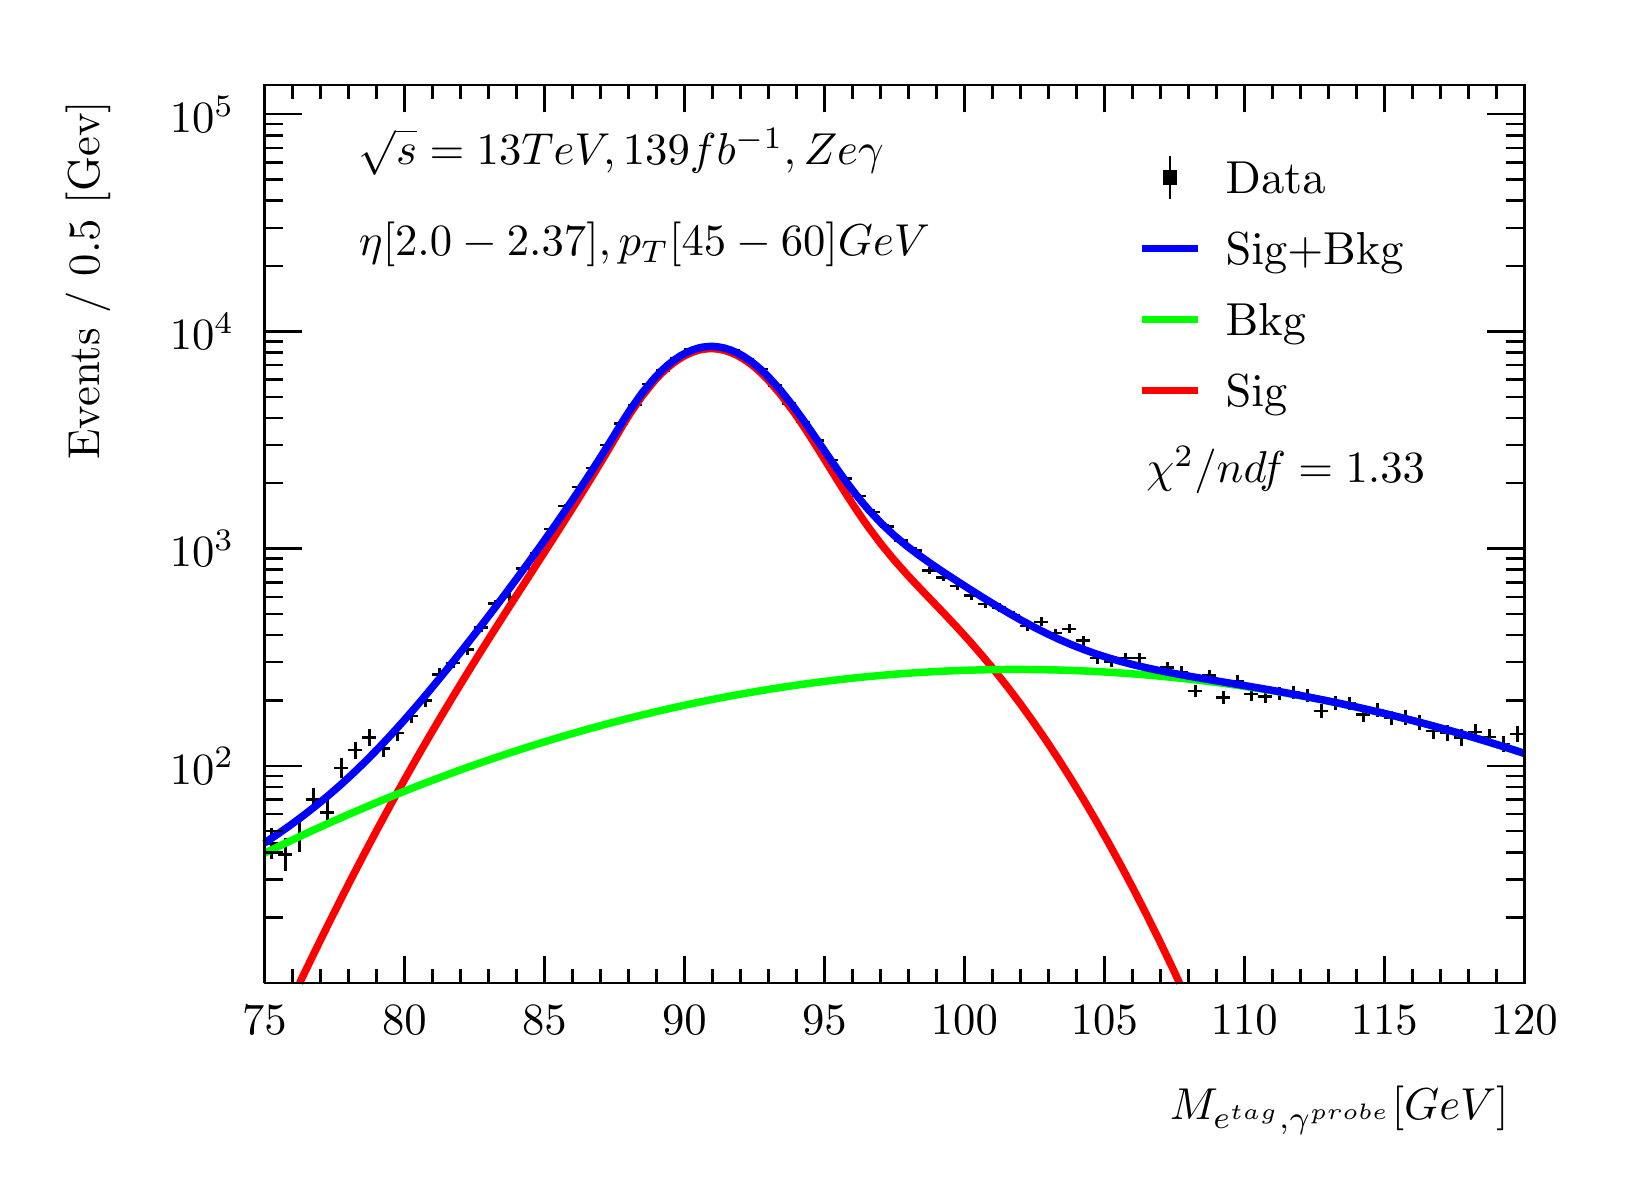
\begin{tikzpicture}
\pgfdeclareplotmark{cross} {
\pgfpathmoveto{\pgfpoint{-0.3\pgfplotmarksize}{\pgfplotmarksize}}
\pgfpathlineto{\pgfpoint{+0.3\pgfplotmarksize}{\pgfplotmarksize}}
\pgfpathlineto{\pgfpoint{+0.3\pgfplotmarksize}{0.3\pgfplotmarksize}}
\pgfpathlineto{\pgfpoint{+1\pgfplotmarksize}{0.3\pgfplotmarksize}}
\pgfpathlineto{\pgfpoint{+1\pgfplotmarksize}{-0.3\pgfplotmarksize}}
\pgfpathlineto{\pgfpoint{+0.3\pgfplotmarksize}{-0.3\pgfplotmarksize}}
\pgfpathlineto{\pgfpoint{+0.3\pgfplotmarksize}{-1.\pgfplotmarksize}}
\pgfpathlineto{\pgfpoint{-0.3\pgfplotmarksize}{-1.\pgfplotmarksize}}
\pgfpathlineto{\pgfpoint{-0.3\pgfplotmarksize}{-0.3\pgfplotmarksize}}
\pgfpathlineto{\pgfpoint{-1.\pgfplotmarksize}{-0.3\pgfplotmarksize}}
\pgfpathlineto{\pgfpoint{-1.\pgfplotmarksize}{0.3\pgfplotmarksize}}
\pgfpathlineto{\pgfpoint{-0.3\pgfplotmarksize}{0.3\pgfplotmarksize}}
\pgfpathclose
\pgfusepathqstroke
}
\pgfdeclareplotmark{cross*} {
\pgfpathmoveto{\pgfpoint{-0.3\pgfplotmarksize}{\pgfplotmarksize}}
\pgfpathlineto{\pgfpoint{+0.3\pgfplotmarksize}{\pgfplotmarksize}}
\pgfpathlineto{\pgfpoint{+0.3\pgfplotmarksize}{0.3\pgfplotmarksize}}
\pgfpathlineto{\pgfpoint{+1\pgfplotmarksize}{0.3\pgfplotmarksize}}
\pgfpathlineto{\pgfpoint{+1\pgfplotmarksize}{-0.3\pgfplotmarksize}}
\pgfpathlineto{\pgfpoint{+0.3\pgfplotmarksize}{-0.3\pgfplotmarksize}}
\pgfpathlineto{\pgfpoint{+0.3\pgfplotmarksize}{-1.\pgfplotmarksize}}
\pgfpathlineto{\pgfpoint{-0.3\pgfplotmarksize}{-1.\pgfplotmarksize}}
\pgfpathlineto{\pgfpoint{-0.3\pgfplotmarksize}{-0.3\pgfplotmarksize}}
\pgfpathlineto{\pgfpoint{-1.\pgfplotmarksize}{-0.3\pgfplotmarksize}}
\pgfpathlineto{\pgfpoint{-1.\pgfplotmarksize}{0.3\pgfplotmarksize}}
\pgfpathlineto{\pgfpoint{-0.3\pgfplotmarksize}{0.3\pgfplotmarksize}}
\pgfpathclose
\pgfusepathqfillstroke
}
\pgfdeclareplotmark{newstar} {
\pgfpathmoveto{\pgfqpoint{0pt}{\pgfplotmarksize}}
\pgfpathlineto{\pgfqpointpolar{44}{0.5\pgfplotmarksize}}
\pgfpathlineto{\pgfqpointpolar{18}{\pgfplotmarksize}}
\pgfpathlineto{\pgfqpointpolar{-20}{0.5\pgfplotmarksize}}
\pgfpathlineto{\pgfqpointpolar{-54}{\pgfplotmarksize}}
\pgfpathlineto{\pgfqpointpolar{-90}{0.5\pgfplotmarksize}}
\pgfpathlineto{\pgfqpointpolar{234}{\pgfplotmarksize}}
\pgfpathlineto{\pgfqpointpolar{198}{0.5\pgfplotmarksize}}
\pgfpathlineto{\pgfqpointpolar{162}{\pgfplotmarksize}}
\pgfpathlineto{\pgfqpointpolar{134}{0.5\pgfplotmarksize}}
\pgfpathclose
\pgfusepathqstroke
}
\pgfdeclareplotmark{newstar*} {
\pgfpathmoveto{\pgfqpoint{0pt}{\pgfplotmarksize}}
\pgfpathlineto{\pgfqpointpolar{44}{0.5\pgfplotmarksize}}
\pgfpathlineto{\pgfqpointpolar{18}{\pgfplotmarksize}}
\pgfpathlineto{\pgfqpointpolar{-20}{0.5\pgfplotmarksize}}
\pgfpathlineto{\pgfqpointpolar{-54}{\pgfplotmarksize}}
\pgfpathlineto{\pgfqpointpolar{-90}{0.5\pgfplotmarksize}}
\pgfpathlineto{\pgfqpointpolar{234}{\pgfplotmarksize}}
\pgfpathlineto{\pgfqpointpolar{198}{0.5\pgfplotmarksize}}
\pgfpathlineto{\pgfqpointpolar{162}{\pgfplotmarksize}}
\pgfpathlineto{\pgfqpointpolar{134}{0.5\pgfplotmarksize}}
\pgfpathclose
\pgfusepathqfillstroke
}
\definecolor{c}{rgb}{1,1,1};
\draw [color=c, fill=c] (0,0) rectangle (20,14.4361);
\draw [color=c, fill=c] (3,2.30977) rectangle (19,13.7143);
\definecolor{c}{rgb}{0,0,0};
\draw [c,line width=0.9] (3,2.30977) -- (3,13.7143) -- (19,13.7143) -- (19,2.30977) -- (3,2.30977);
\definecolor{c}{rgb}{1,1,1};
\draw [color=c, fill=c] (3,2.30977) rectangle (19,13.7143);
\definecolor{c}{rgb}{0,0,0};
\draw [c,line width=0.9] (3,2.30977) -- (3,13.7143) -- (19,13.7143) -- (19,2.30977) -- (3,2.30977);
\draw [c,line width=0.9] (3,2.30977) -- (19,2.30977);
\draw [c,line width=0.9] (3,2.65624) -- (3,2.30977);
\draw [c,line width=0.9] (3.35556,2.48301) -- (3.35556,2.30977);
\draw [c,line width=0.9] (3.71111,2.48301) -- (3.71111,2.30977);
\draw [c,line width=0.9] (4.06667,2.48301) -- (4.06667,2.30977);
\draw [c,line width=0.9] (4.42222,2.48301) -- (4.42222,2.30977);
\draw [c,line width=0.9] (4.77778,2.65624) -- (4.77778,2.30977);
\draw [c,line width=0.9] (5.13333,2.48301) -- (5.13333,2.30977);
\draw [c,line width=0.9] (5.48889,2.48301) -- (5.48889,2.30977);
\draw [c,line width=0.9] (5.84444,2.48301) -- (5.84444,2.30977);
\draw [c,line width=0.9] (6.2,2.48301) -- (6.2,2.30977);
\draw [c,line width=0.9] (6.55556,2.65624) -- (6.55556,2.30977);
\draw [c,line width=0.9] (6.91111,2.48301) -- (6.91111,2.30977);
\draw [c,line width=0.9] (7.26667,2.48301) -- (7.26667,2.30977);
\draw [c,line width=0.9] (7.62222,2.48301) -- (7.62222,2.30977);
\draw [c,line width=0.9] (7.97778,2.48301) -- (7.97778,2.30977);
\draw [c,line width=0.9] (8.33333,2.65624) -- (8.33333,2.30977);
\draw [c,line width=0.9] (8.68889,2.48301) -- (8.68889,2.30977);
\draw [c,line width=0.9] (9.04444,2.48301) -- (9.04444,2.30977);
\draw [c,line width=0.9] (9.4,2.48301) -- (9.4,2.30977);
\draw [c,line width=0.9] (9.75556,2.48301) -- (9.75556,2.30977);
\draw [c,line width=0.9] (10.1111,2.65624) -- (10.1111,2.30977);
\draw [c,line width=0.9] (10.4667,2.48301) -- (10.4667,2.30977);
\draw [c,line width=0.9] (10.8222,2.48301) -- (10.8222,2.30977);
\draw [c,line width=0.9] (11.1778,2.48301) -- (11.1778,2.30977);
\draw [c,line width=0.9] (11.5333,2.48301) -- (11.5333,2.30977);
\draw [c,line width=0.9] (11.8889,2.65624) -- (11.8889,2.30977);
\draw [c,line width=0.9] (12.2444,2.48301) -- (12.2444,2.30977);
\draw [c,line width=0.9] (12.6,2.48301) -- (12.6,2.30977);
\draw [c,line width=0.9] (12.9556,2.48301) -- (12.9556,2.30977);
\draw [c,line width=0.9] (13.3111,2.48301) -- (13.3111,2.30977);
\draw [c,line width=0.9] (13.6667,2.65624) -- (13.6667,2.30977);
\draw [c,line width=0.9] (14.0222,2.48301) -- (14.0222,2.30977);
\draw [c,line width=0.9] (14.3778,2.48301) -- (14.3778,2.30977);
\draw [c,line width=0.9] (14.7333,2.48301) -- (14.7333,2.30977);
\draw [c,line width=0.9] (15.0889,2.48301) -- (15.0889,2.30977);
\draw [c,line width=0.9] (15.4444,2.65624) -- (15.4444,2.30977);
\draw [c,line width=0.9] (15.8,2.48301) -- (15.8,2.30977);
\draw [c,line width=0.9] (16.1556,2.48301) -- (16.1556,2.30977);
\draw [c,line width=0.9] (16.5111,2.48301) -- (16.5111,2.30977);
\draw [c,line width=0.9] (16.8667,2.48301) -- (16.8667,2.30977);
\draw [c,line width=0.9] (17.2222,2.65624) -- (17.2222,2.30977);
\draw [c,line width=0.9] (17.5778,2.48301) -- (17.5778,2.30977);
\draw [c,line width=0.9] (17.9333,2.48301) -- (17.9333,2.30977);
\draw [c,line width=0.9] (18.2889,2.48301) -- (18.2889,2.30977);
\draw [c,line width=0.9] (18.6444,2.48301) -- (18.6444,2.30977);
\draw [c,line width=0.9] (19,2.65624) -- (19,2.30977);
\draw [c,line width=0.9] (19,2.65624) -- (19,2.30977);
\draw [anchor=base] (3,1.66015) node[scale=1.61424, color=c, rotate=0]{75};
\draw [anchor=base] (4.77778,1.66015) node[scale=1.61424, color=c, rotate=0]{80};
\draw [anchor=base] (6.55556,1.66015) node[scale=1.61424, color=c, rotate=0]{85};
\draw [anchor=base] (8.33333,1.66015) node[scale=1.61424, color=c, rotate=0]{90};
\draw [anchor=base] (10.1111,1.66015) node[scale=1.61424, color=c, rotate=0]{95};
\draw [anchor=base] (11.8889,1.66015) node[scale=1.61424, color=c, rotate=0]{100};
\draw [anchor=base] (13.6667,1.66015) node[scale=1.61424, color=c, rotate=0]{105};
\draw [anchor=base] (15.4444,1.66015) node[scale=1.61424, color=c, rotate=0]{110};
\draw [anchor=base] (17.2222,1.66015) node[scale=1.61424, color=c, rotate=0]{115};
\draw [anchor=base] (19,1.66015) node[scale=1.61424, color=c, rotate=0]{120};
\draw [anchor= east] (19,0.692932) node[scale=1.61424, color=c, rotate=0]{$M_{e^{tag}, \gamma^{probe}}  [GeV]$};
\draw [c,line width=0.9] (3,13.7143) -- (19,13.7143);
\draw [c,line width=0.9] (3,13.3678) -- (3,13.7143);
\draw [c,line width=0.9] (3.35556,13.5411) -- (3.35556,13.7143);
\draw [c,line width=0.9] (3.71111,13.5411) -- (3.71111,13.7143);
\draw [c,line width=0.9] (4.06667,13.5411) -- (4.06667,13.7143);
\draw [c,line width=0.9] (4.42222,13.5411) -- (4.42222,13.7143);
\draw [c,line width=0.9] (4.77778,13.3678) -- (4.77778,13.7143);
\draw [c,line width=0.9] (5.13333,13.5411) -- (5.13333,13.7143);
\draw [c,line width=0.9] (5.48889,13.5411) -- (5.48889,13.7143);
\draw [c,line width=0.9] (5.84444,13.5411) -- (5.84444,13.7143);
\draw [c,line width=0.9] (6.2,13.5411) -- (6.2,13.7143);
\draw [c,line width=0.9] (6.55556,13.3678) -- (6.55556,13.7143);
\draw [c,line width=0.9] (6.91111,13.5411) -- (6.91111,13.7143);
\draw [c,line width=0.9] (7.26667,13.5411) -- (7.26667,13.7143);
\draw [c,line width=0.9] (7.62222,13.5411) -- (7.62222,13.7143);
\draw [c,line width=0.9] (7.97778,13.5411) -- (7.97778,13.7143);
\draw [c,line width=0.9] (8.33333,13.3678) -- (8.33333,13.7143);
\draw [c,line width=0.9] (8.68889,13.5411) -- (8.68889,13.7143);
\draw [c,line width=0.9] (9.04444,13.5411) -- (9.04444,13.7143);
\draw [c,line width=0.9] (9.4,13.5411) -- (9.4,13.7143);
\draw [c,line width=0.9] (9.75556,13.5411) -- (9.75556,13.7143);
\draw [c,line width=0.9] (10.1111,13.3678) -- (10.1111,13.7143);
\draw [c,line width=0.9] (10.4667,13.5411) -- (10.4667,13.7143);
\draw [c,line width=0.9] (10.8222,13.5411) -- (10.8222,13.7143);
\draw [c,line width=0.9] (11.1778,13.5411) -- (11.1778,13.7143);
\draw [c,line width=0.9] (11.5333,13.5411) -- (11.5333,13.7143);
\draw [c,line width=0.9] (11.8889,13.3678) -- (11.8889,13.7143);
\draw [c,line width=0.9] (12.2444,13.5411) -- (12.2444,13.7143);
\draw [c,line width=0.9] (12.6,13.5411) -- (12.6,13.7143);
\draw [c,line width=0.9] (12.9556,13.5411) -- (12.9556,13.7143);
\draw [c,line width=0.9] (13.3111,13.5411) -- (13.3111,13.7143);
\draw [c,line width=0.9] (13.6667,13.3678) -- (13.6667,13.7143);
\draw [c,line width=0.9] (14.0222,13.5411) -- (14.0222,13.7143);
\draw [c,line width=0.9] (14.3778,13.5411) -- (14.3778,13.7143);
\draw [c,line width=0.9] (14.7333,13.5411) -- (14.7333,13.7143);
\draw [c,line width=0.9] (15.0889,13.5411) -- (15.0889,13.7143);
\draw [c,line width=0.9] (15.4444,13.3678) -- (15.4444,13.7143);
\draw [c,line width=0.9] (15.8,13.5411) -- (15.8,13.7143);
\draw [c,line width=0.9] (16.1556,13.5411) -- (16.1556,13.7143);
\draw [c,line width=0.9] (16.5111,13.5411) -- (16.5111,13.7143);
\draw [c,line width=0.9] (16.8667,13.5411) -- (16.8667,13.7143);
\draw [c,line width=0.9] (17.2222,13.3678) -- (17.2222,13.7143);
\draw [c,line width=0.9] (17.5778,13.5411) -- (17.5778,13.7143);
\draw [c,line width=0.9] (17.9333,13.5411) -- (17.9333,13.7143);
\draw [c,line width=0.9] (18.2889,13.5411) -- (18.2889,13.7143);
\draw [c,line width=0.9] (18.6444,13.5411) -- (18.6444,13.7143);
\draw [c,line width=0.9] (19,13.3678) -- (19,13.7143);
\draw [c,line width=0.9] (19,13.3678) -- (19,13.7143);
\draw [c,line width=0.9] (3,2.30977) -- (3,13.7143);
\draw [c,line width=0.9] (3.237,3.14018) -- (3,3.14018);
\draw [c,line width=0.9] (3.237,3.62593) -- (3,3.62593);
\draw [c,line width=0.9] (3.237,3.97058) -- (3,3.97058);
\draw [c,line width=0.9] (3.237,4.23792) -- (3,4.23792);
\draw [c,line width=0.9] (3.237,4.45634) -- (3,4.45634);
\draw [c,line width=0.9] (3.237,4.64102) -- (3,4.64102);
\draw [c,line width=0.9] (3.237,4.80099) -- (3,4.80099);
\draw [c,line width=0.9] (3.237,4.9421) -- (3,4.9421);
\draw [c,line width=0.9] (3.474,5.06832) -- (3,5.06832);
\draw [anchor= east] (2.82,5.06832) node[scale=1.61424, color=c, rotate=0]{$10^{2}$};
\draw [c,line width=0.9] (3.237,5.89873) -- (3,5.89873);
\draw [c,line width=0.9] (3.237,6.38449) -- (3,6.38449);
\draw [c,line width=0.9] (3.237,6.72914) -- (3,6.72914);
\draw [c,line width=0.9] (3.237,6.99647) -- (3,6.99647);
\draw [c,line width=0.9] (3.237,7.21489) -- (3,7.21489);
\draw [c,line width=0.9] (3.237,7.39957) -- (3,7.39957);
\draw [c,line width=0.9] (3.237,7.55954) -- (3,7.55954);
\draw [c,line width=0.9] (3.237,7.70065) -- (3,7.70065);
\draw [c,line width=0.9] (3.474,7.82687) -- (3,7.82687);
\draw [anchor= east] (2.82,7.82687) node[scale=1.61424, color=c, rotate=0]{$10^{3}$};
\draw [c,line width=0.9] (3.237,8.65728) -- (3,8.65728);
\draw [c,line width=0.9] (3.237,9.14304) -- (3,9.14304);
\draw [c,line width=0.9] (3.237,9.48769) -- (3,9.48769);
\draw [c,line width=0.9] (3.237,9.75502) -- (3,9.75502);
\draw [c,line width=0.9] (3.237,9.97344) -- (3,9.97344);
\draw [c,line width=0.9] (3.237,10.1581) -- (3,10.1581);
\draw [c,line width=0.9] (3.237,10.3181) -- (3,10.3181);
\draw [c,line width=0.9] (3.237,10.4592) -- (3,10.4592);
\draw [c,line width=0.9] (3.474,10.5854) -- (3,10.5854);
\draw [anchor= east] (2.82,10.5854) node[scale=1.61424, color=c, rotate=0]{$10^{4}$};
\draw [c,line width=0.9] (3.237,11.4158) -- (3,11.4158);
\draw [c,line width=0.9] (3.237,11.9016) -- (3,11.9016);
\draw [c,line width=0.9] (3.237,12.2462) -- (3,12.2462);
\draw [c,line width=0.9] (3.237,12.5136) -- (3,12.5136);
\draw [c,line width=0.9] (3.237,12.732) -- (3,12.732);
\draw [c,line width=0.9] (3.237,12.9167) -- (3,12.9167);
\draw [c,line width=0.9] (3.237,13.0766) -- (3,13.0766);
\draw [c,line width=0.9] (3.237,13.2178) -- (3,13.2178);
\draw [c,line width=0.9] (3.474,13.344) -- (3,13.344);
\draw [anchor= east] (2.82,13.344) node[scale=1.61424, color=c, rotate=0]{$10^{5}$};
\draw [anchor= east] (0.76,13.7143) node[scale=1.61424, color=c, rotate=90]{Events / 0.5 [Gev]};
\draw [c,line width=0.9] (19,2.30977) -- (19,13.7143);
\draw [c,line width=0.9] (18.763,3.14018) -- (19,3.14018);
\draw [c,line width=0.9] (18.763,3.62593) -- (19,3.62593);
\draw [c,line width=0.9] (18.763,3.97058) -- (19,3.97058);
\draw [c,line width=0.9] (18.763,4.23792) -- (19,4.23792);
\draw [c,line width=0.9] (18.763,4.45634) -- (19,4.45634);
\draw [c,line width=0.9] (18.763,4.64102) -- (19,4.64102);
\draw [c,line width=0.9] (18.763,4.80099) -- (19,4.80099);
\draw [c,line width=0.9] (18.763,4.9421) -- (19,4.9421);
\draw [c,line width=0.9] (18.526,5.06832) -- (19,5.06832);
\draw [c,line width=0.9] (18.763,5.89873) -- (19,5.89873);
\draw [c,line width=0.9] (18.763,6.38449) -- (19,6.38449);
\draw [c,line width=0.9] (18.763,6.72914) -- (19,6.72914);
\draw [c,line width=0.9] (18.763,6.99647) -- (19,6.99647);
\draw [c,line width=0.9] (18.763,7.21489) -- (19,7.21489);
\draw [c,line width=0.9] (18.763,7.39957) -- (19,7.39957);
\draw [c,line width=0.9] (18.763,7.55954) -- (19,7.55954);
\draw [c,line width=0.9] (18.763,7.70065) -- (19,7.70065);
\draw [c,line width=0.9] (18.526,7.82687) -- (19,7.82687);
\draw [c,line width=0.9] (18.763,8.65728) -- (19,8.65728);
\draw [c,line width=0.9] (18.763,9.14304) -- (19,9.14304);
\draw [c,line width=0.9] (18.763,9.48769) -- (19,9.48769);
\draw [c,line width=0.9] (18.763,9.75502) -- (19,9.75502);
\draw [c,line width=0.9] (18.763,9.97344) -- (19,9.97344);
\draw [c,line width=0.9] (18.763,10.1581) -- (19,10.1581);
\draw [c,line width=0.9] (18.763,10.3181) -- (19,10.3181);
\draw [c,line width=0.9] (18.763,10.4592) -- (19,10.4592);
\draw [c,line width=0.9] (18.526,10.5854) -- (19,10.5854);
\draw [c,line width=0.9] (18.763,11.4158) -- (19,11.4158);
\draw [c,line width=0.9] (18.763,11.9016) -- (19,11.9016);
\draw [c,line width=0.9] (18.763,12.2462) -- (19,12.2462);
\draw [c,line width=0.9] (18.763,12.5136) -- (19,12.5136);
\draw [c,line width=0.9] (18.763,12.732) -- (19,12.732);
\draw [c,line width=0.9] (18.763,12.9167) -- (19,12.9167);
\draw [c,line width=0.9] (18.763,13.0766) -- (19,13.0766);
\draw [c,line width=0.9] (18.763,13.2178) -- (19,13.2178);
\draw [c,line width=0.9] (18.526,13.344) -- (19,13.344);
\draw [c,line width=0.9] (3.08889,4.08477) -- (3,4.08477);
\draw [c,line width=0.9] (3,4.08477) -- (3,4.08477);
\draw [c,line width=0.9] (3.08889,4.08477) -- (3.17778,4.08477);
\draw [c,line width=0.9] (3.17778,4.08477) -- (3.17778,4.08477);
\draw [c,line width=0.9] (3.08889,4.08477) -- (3.08889,4.27759);
\draw [c,line width=0.9] (3.08889,4.27759) -- (3.08889,4.27759);
\draw [c,line width=0.9] (3.08889,4.08477) -- (3.08889,3.88982);
\draw [c,line width=0.9] (3.08889,3.88982) -- (3.08889,3.88982);
\draw [c,line width=0.9] (3.26667,3.94026) -- (3.17778,3.94026);
\draw [c,line width=0.9] (3.17778,3.94026) -- (3.17778,3.94026);
\draw [c,line width=0.9] (3.26667,3.94026) -- (3.35556,3.94026);
\draw [c,line width=0.9] (3.35556,3.94026) -- (3.35556,3.94026);
\draw [c,line width=0.9] (3.26667,3.94026) -- (3.26667,4.14577);
\draw [c,line width=0.9] (3.26667,4.14577) -- (3.26667,4.14577);
\draw [c,line width=0.9] (3.26667,3.94026) -- (3.26667,3.73218);
\draw [c,line width=0.9] (3.26667,3.73218) -- (3.26667,3.73218);
\draw [c,line width=0.9] (3.44444,4.16379) -- (3.35556,4.16379);
\draw [c,line width=0.9] (3.35556,4.16379) -- (3.35556,4.16379);
\draw [c,line width=0.9] (3.44444,4.16379) -- (3.53333,4.16379);
\draw [c,line width=0.9] (3.53333,4.16379) -- (3.53333,4.16379);
\draw [c,line width=0.9] (3.44444,4.16379) -- (3.44444,4.35002);
\draw [c,line width=0.9] (3.44444,4.35002) -- (3.44444,4.35002);
\draw [c,line width=0.9] (3.44444,4.16379) -- (3.44444,3.97563);
\draw [c,line width=0.9] (3.44444,3.97563) -- (3.44444,3.97563);
\draw [c,line width=0.9] (3.62222,4.64102) -- (3.53333,4.64102);
\draw [c,line width=0.9] (3.53333,4.64102) -- (3.53333,4.64102);
\draw [c,line width=0.9] (3.62222,4.64102) -- (3.71111,4.64102);
\draw [c,line width=0.9] (3.71111,4.64102) -- (3.71111,4.64102);
\draw [c,line width=0.9] (3.62222,4.64102) -- (3.62222,4.79207);
\draw [c,line width=0.9] (3.62222,4.79207) -- (3.62222,4.79207);
\draw [c,line width=0.9] (3.62222,4.64102) -- (3.62222,4.48891);
\draw [c,line width=0.9] (3.62222,4.48891) -- (3.62222,4.48891);
\draw [c,line width=0.9] (3.8,4.47615) -- (3.71111,4.47615);
\draw [c,line width=0.9] (3.71111,4.47615) -- (3.71111,4.47615);
\draw [c,line width=0.9] (3.8,4.47615) -- (3.88889,4.47615);
\draw [c,line width=0.9] (3.88889,4.47615) -- (3.88889,4.47615);
\draw [c,line width=0.9] (3.8,4.47615) -- (3.8,4.6385);
\draw [c,line width=0.9] (3.8,4.6385) -- (3.8,4.6385);
\draw [c,line width=0.9] (3.8,4.47615) -- (3.8,4.31249);
\draw [c,line width=0.9] (3.8,4.31249) -- (3.8,4.31249);
\draw [c,line width=0.9] (3.97778,5.04412) -- (3.88889,5.04412);
\draw [c,line width=0.9] (3.88889,5.04412) -- (3.88889,5.04412);
\draw [c,line width=0.9] (3.97778,5.04412) -- (4.06667,5.04412);
\draw [c,line width=0.9] (4.06667,5.04412) -- (4.06667,5.04412);
\draw [c,line width=0.9] (3.97778,5.04412) -- (3.97778,5.17083);
\draw [c,line width=0.9] (3.97778,5.17083) -- (3.97778,5.17083);
\draw [c,line width=0.9] (3.97778,5.04412) -- (3.97778,4.91677);
\draw [c,line width=0.9] (3.97778,4.91677) -- (3.97778,4.91677);
\draw [c,line width=0.9] (4.15556,5.26661) -- (4.06667,5.26661);
\draw [c,line width=0.9] (4.06667,5.26661) -- (4.06667,5.26661);
\draw [c,line width=0.9] (4.15556,5.26661) -- (4.24444,5.26661);
\draw [c,line width=0.9] (4.24444,5.26661) -- (4.24444,5.26661);
\draw [c,line width=0.9] (4.15556,5.26661) -- (4.15556,5.37686);
\draw [c,line width=0.9] (4.15556,5.37686) -- (4.15556,5.37686);
\draw [c,line width=0.9] (4.15556,5.26661) -- (4.15556,5.15637);
\draw [c,line width=0.9] (4.15556,5.15637) -- (4.15556,5.15637);
\draw [c,line width=0.9] (4.33333,5.42786) -- (4.24444,5.42786);
\draw [c,line width=0.9] (4.24444,5.42786) -- (4.24444,5.42786);
\draw [c,line width=0.9] (4.33333,5.42786) -- (4.42222,5.42786);
\draw [c,line width=0.9] (4.42222,5.42786) -- (4.42222,5.42786);
\draw [c,line width=0.9] (4.33333,5.42786) -- (4.33333,5.53093);
\draw [c,line width=0.9] (4.33333,5.53093) -- (4.33333,5.53093);
\draw [c,line width=0.9] (4.33333,5.42786) -- (4.33333,5.32478);
\draw [c,line width=0.9] (4.33333,5.32478) -- (4.33333,5.32478);
\draw [c,line width=0.9] (4.51111,5.28675) -- (4.42222,5.28675);
\draw [c,line width=0.9] (4.42222,5.28675) -- (4.42222,5.28675);
\draw [c,line width=0.9] (4.51111,5.28675) -- (4.6,5.28675);
\draw [c,line width=0.9] (4.6,5.28675) -- (4.6,5.28675);
\draw [c,line width=0.9] (4.51111,5.28675) -- (4.51111,5.39608);
\draw [c,line width=0.9] (4.51111,5.39608) -- (4.51111,5.39608);
\draw [c,line width=0.9] (4.51111,5.28675) -- (4.51111,5.17742);
\draw [c,line width=0.9] (4.51111,5.17742) -- (4.51111,5.17742);
\draw [c,line width=0.9] (4.68889,5.48842) -- (4.6,5.48842);
\draw [c,line width=0.9] (4.6,5.48842) -- (4.6,5.48842);
\draw [c,line width=0.9] (4.68889,5.48842) -- (4.77778,5.48842);
\draw [c,line width=0.9] (4.77778,5.48842) -- (4.77778,5.48842);
\draw [c,line width=0.9] (4.68889,5.48842) -- (4.68889,5.58893);
\draw [c,line width=0.9] (4.68889,5.58893) -- (4.68889,5.58893);
\draw [c,line width=0.9] (4.68889,5.48842) -- (4.68889,5.38791);
\draw [c,line width=0.9] (4.68889,5.38791) -- (4.68889,5.38791);
\draw [c,line width=0.9] (4.86667,5.70403) -- (4.77778,5.70403);
\draw [c,line width=0.9] (4.77778,5.70403) -- (4.77778,5.70403);
\draw [c,line width=0.9] (4.86667,5.70403) -- (4.95556,5.70403);
\draw [c,line width=0.9] (4.95556,5.70403) -- (4.95556,5.70403);
\draw [c,line width=0.9] (4.86667,5.70403) -- (4.86667,5.79589);
\draw [c,line width=0.9] (4.86667,5.79589) -- (4.86667,5.79589);
\draw [c,line width=0.9] (4.86667,5.70403) -- (4.86667,5.61217);
\draw [c,line width=0.9] (4.86667,5.61217) -- (4.86667,5.61217);
\draw [c,line width=0.9] (5.04444,5.89873) -- (4.95556,5.89873);
\draw [c,line width=0.9] (4.95556,5.89873) -- (4.95556,5.89873);
\draw [c,line width=0.9] (5.04444,5.89873) -- (5.13333,5.89873);
\draw [c,line width=0.9] (5.13333,5.89873) -- (5.13333,5.89873);
\draw [c,line width=0.9] (5.04444,5.89873) -- (5.04444,5.98343);
\draw [c,line width=0.9] (5.04444,5.98343) -- (5.04444,5.98343);
\draw [c,line width=0.9] (5.04444,5.89873) -- (5.04444,5.81404);
\draw [c,line width=0.9] (5.04444,5.81404) -- (5.04444,5.81404);
\draw [c,line width=0.9] (5.22222,6.23134) -- (5.13333,6.23134);
\draw [c,line width=0.9] (5.13333,6.23134) -- (5.13333,6.23134);
\draw [c,line width=0.9] (5.22222,6.23134) -- (5.31111,6.23134);
\draw [c,line width=0.9] (5.31111,6.23134) -- (5.31111,6.23134);
\draw [c,line width=0.9] (5.22222,6.23134) -- (5.22222,6.30506);
\draw [c,line width=0.9] (5.22222,6.30506) -- (5.22222,6.30506);
\draw [c,line width=0.9] (5.22222,6.23134) -- (5.22222,6.15762);
\draw [c,line width=0.9] (5.22222,6.15762) -- (5.22222,6.15762);
\draw [c,line width=0.9] (5.4,6.37647) -- (5.31111,6.37647);
\draw [c,line width=0.9] (5.31111,6.37647) -- (5.31111,6.37647);
\draw [c,line width=0.9] (5.4,6.37647) -- (5.48889,6.37647);
\draw [c,line width=0.9] (5.48889,6.37647) -- (5.48889,6.37647);
\draw [c,line width=0.9] (5.4,6.37647) -- (5.4,6.44586);
\draw [c,line width=0.9] (5.4,6.44586) -- (5.4,6.44586);
\draw [c,line width=0.9] (5.4,6.37647) -- (5.4,6.30708);
\draw [c,line width=0.9] (5.4,6.30708) -- (5.4,6.30708);
\draw [c,line width=0.9] (5.57778,6.54496) -- (5.48889,6.54496);
\draw [c,line width=0.9] (5.48889,6.54496) -- (5.48889,6.54496);
\draw [c,line width=0.9] (5.57778,6.54496) -- (5.66667,6.54496);
\draw [c,line width=0.9] (5.66667,6.54496) -- (5.66667,6.54496);
\draw [c,line width=0.9] (5.57778,6.54496) -- (5.57778,6.60964);
\draw [c,line width=0.9] (5.57778,6.60964) -- (5.57778,6.60964);
\draw [c,line width=0.9] (5.57778,6.54496) -- (5.57778,6.48028);
\draw [c,line width=0.9] (5.57778,6.48028) -- (5.57778,6.48028);
\draw [c,line width=0.9] (5.75556,6.82411) -- (5.66667,6.82411);
\draw [c,line width=0.9] (5.66667,6.82411) -- (5.66667,6.82411);
\draw [c,line width=0.9] (5.75556,6.82411) -- (5.84444,6.82411);
\draw [c,line width=0.9] (5.84444,6.82411) -- (5.84444,6.82411);
\draw [c,line width=0.9] (5.75556,6.82411) -- (5.75556,6.88168);
\draw [c,line width=0.9] (5.75556,6.88168) -- (5.75556,6.88168);
\draw [c,line width=0.9] (5.75556,6.82411) -- (5.75556,6.76654);
\draw [c,line width=0.9] (5.75556,6.76654) -- (5.75556,6.76654);
\draw [c,line width=0.9] (5.93333,7.12795) -- (5.84444,7.12795);
\draw [c,line width=0.9] (5.84444,7.12795) -- (5.84444,7.12795);
\draw [c,line width=0.9] (5.93333,7.12795) -- (6.02222,7.12795);
\draw [c,line width=0.9] (6.02222,7.12795) -- (6.02222,7.12795);
\draw [c,line width=0.9] (5.93333,7.12795) -- (5.93333,7.17867);
\draw [c,line width=0.9] (5.93333,7.17867) -- (5.93333,7.17867);
\draw [c,line width=0.9] (5.93333,7.12795) -- (5.93333,7.07724);
\draw [c,line width=0.9] (5.93333,7.07724) -- (5.93333,7.07724);
\draw [c,line width=0.9] (6.11111,7.21089) -- (6.02222,7.21089);
\draw [c,line width=0.9] (6.02222,7.21089) -- (6.02222,7.21089);
\draw [c,line width=0.9] (6.11111,7.21089) -- (6.2,7.21089);
\draw [c,line width=0.9] (6.2,7.21089) -- (6.2,7.21089);
\draw [c,line width=0.9] (6.11111,7.21089) -- (6.11111,7.25988);
\draw [c,line width=0.9] (6.11111,7.25988) -- (6.11111,7.25988);
\draw [c,line width=0.9] (6.11111,7.21089) -- (6.11111,7.16191);
\draw [c,line width=0.9] (6.11111,7.16191) -- (6.11111,7.16191);
\draw [c,line width=0.9] (6.28889,7.57738) -- (6.2,7.57738);
\draw [c,line width=0.9] (6.2,7.57738) -- (6.2,7.57738);
\draw [c,line width=0.9] (6.28889,7.57738) -- (6.37778,7.57738);
\draw [c,line width=0.9] (6.37778,7.57738) -- (6.37778,7.57738);
\draw [c,line width=0.9] (6.28889,7.57738) -- (6.28889,7.61942);
\draw [c,line width=0.9] (6.28889,7.61942) -- (6.28889,7.61942);
\draw [c,line width=0.9] (6.28889,7.57738) -- (6.28889,7.53534);
\draw [c,line width=0.9] (6.28889,7.53534) -- (6.28889,7.53534);
\draw [c,line width=0.9] (6.46667,7.7692) -- (6.37778,7.7692);
\draw [c,line width=0.9] (6.37778,7.7692) -- (6.37778,7.7692);
\draw [c,line width=0.9] (6.46667,7.7692) -- (6.55556,7.7692);
\draw [c,line width=0.9] (6.55556,7.7692) -- (6.55556,7.7692);
\draw [c,line width=0.9] (6.46667,7.7692) -- (6.46667,7.80801);
\draw [c,line width=0.9] (6.46667,7.80801) -- (6.46667,7.80801);
\draw [c,line width=0.9] (6.46667,7.7692) -- (6.46667,7.7304);
\draw [c,line width=0.9] (6.46667,7.7304) -- (6.46667,7.7304);
\draw [c,line width=0.9] (6.64444,8.07488) -- (6.55556,8.07488);
\draw [c,line width=0.9] (6.55556,8.07488) -- (6.55556,8.07488);
\draw [c,line width=0.9] (6.64444,8.07488) -- (6.73333,8.07488);
\draw [c,line width=0.9] (6.73333,8.07488) -- (6.73333,8.07488);
\draw [c,line width=0.9] (6.64444,8.07488) -- (6.64444,8.10904);
\draw [c,line width=0.9] (6.64444,8.10904) -- (6.64444,8.10904);
\draw [c,line width=0.9] (6.64444,8.07488) -- (6.64444,8.04072);
\draw [c,line width=0.9] (6.64444,8.04072) -- (6.64444,8.04072);
\draw [c,line width=0.9] (6.82222,8.36651) -- (6.73333,8.36651);
\draw [c,line width=0.9] (6.73333,8.36651) -- (6.73333,8.36651);
\draw [c,line width=0.9] (6.82222,8.36651) -- (6.91111,8.36651);
\draw [c,line width=0.9] (6.91111,8.36651) -- (6.91111,8.36651);
\draw [c,line width=0.9] (6.82222,8.36651) -- (6.82222,8.39676);
\draw [c,line width=0.9] (6.82222,8.39676) -- (6.82222,8.39676);
\draw [c,line width=0.9] (6.82222,8.36651) -- (6.82222,8.33627);
\draw [c,line width=0.9] (6.82222,8.33627) -- (6.82222,8.33627);
\draw [c,line width=0.9] (7,8.61025) -- (6.91111,8.61025);
\draw [c,line width=0.9] (6.91111,8.61025) -- (6.91111,8.61025);
\draw [c,line width=0.9] (7,8.61025) -- (7.08889,8.61025);
\draw [c,line width=0.9] (7.08889,8.61025) -- (7.08889,8.61025);
\draw [c,line width=0.9] (7,8.61025) -- (7,8.63757);
\draw [c,line width=0.9] (7,8.63757) -- (7,8.63757);
\draw [c,line width=0.9] (7,8.61025) -- (7,8.58293);
\draw [c,line width=0.9] (7,8.58293) -- (7,8.58293);
\draw [c,line width=0.9] (7.17778,8.85099) -- (7.08889,8.85099);
\draw [c,line width=0.9] (7.08889,8.85099) -- (7.08889,8.85099);
\draw [c,line width=0.9] (7.17778,8.85099) -- (7.26667,8.85099);
\draw [c,line width=0.9] (7.26667,8.85099) -- (7.26667,8.85099);
\draw [c,line width=0.9] (7.17778,8.85099) -- (7.17778,8.8757);
\draw [c,line width=0.9] (7.17778,8.8757) -- (7.17778,8.8757);
\draw [c,line width=0.9] (7.17778,8.85099) -- (7.17778,8.82629);
\draw [c,line width=0.9] (7.17778,8.82629) -- (7.17778,8.82629);
\draw [c,line width=0.9] (7.35556,9.14304) -- (7.26667,9.14304);
\draw [c,line width=0.9] (7.26667,9.14304) -- (7.26667,9.14304);
\draw [c,line width=0.9] (7.35556,9.14304) -- (7.44444,9.14304);
\draw [c,line width=0.9] (7.44444,9.14304) -- (7.44444,9.14304);
\draw [c,line width=0.9] (7.35556,9.14304) -- (7.35556,9.16491);
\draw [c,line width=0.9] (7.35556,9.16491) -- (7.35556,9.16491);
\draw [c,line width=0.9] (7.35556,9.14304) -- (7.35556,9.12117);
\draw [c,line width=0.9] (7.35556,9.12117) -- (7.35556,9.12117);
\draw [c,line width=0.9] (7.53333,9.41738) -- (7.44444,9.41738);
\draw [c,line width=0.9] (7.44444,9.41738) -- (7.44444,9.41738);
\draw [c,line width=0.9] (7.53333,9.41738) -- (7.62222,9.41738);
\draw [c,line width=0.9] (7.62222,9.41738) -- (7.62222,9.41738);
\draw [c,line width=0.9] (7.53333,9.41738) -- (7.53333,9.43688);
\draw [c,line width=0.9] (7.53333,9.43688) -- (7.53333,9.43688);
\draw [c,line width=0.9] (7.53333,9.41738) -- (7.53333,9.39787);
\draw [c,line width=0.9] (7.53333,9.39787) -- (7.53333,9.39787);
\draw [c,line width=0.9] (7.71111,9.65095) -- (7.62222,9.65095);
\draw [c,line width=0.9] (7.62222,9.65095) -- (7.62222,9.65095);
\draw [c,line width=0.9] (7.71111,9.65095) -- (7.8,9.65095);
\draw [c,line width=0.9] (7.8,9.65095) -- (7.8,9.65095);
\draw [c,line width=0.9] (7.71111,9.65095) -- (7.71111,9.66865);
\draw [c,line width=0.9] (7.71111,9.66865) -- (7.71111,9.66865);
\draw [c,line width=0.9] (7.71111,9.65095) -- (7.71111,9.63326);
\draw [c,line width=0.9] (7.71111,9.63326) -- (7.71111,9.63326);
\draw [c,line width=0.9] (7.88889,9.91535) -- (7.8,9.91535);
\draw [c,line width=0.9] (7.8,9.91535) -- (7.8,9.91535);
\draw [c,line width=0.9] (7.88889,9.91535) -- (7.97778,9.91535);
\draw [c,line width=0.9] (7.97778,9.91535) -- (7.97778,9.91535);
\draw [c,line width=0.9] (7.88889,9.91535) -- (7.88889,9.9312);
\draw [c,line width=0.9] (7.88889,9.9312) -- (7.88889,9.9312);
\draw [c,line width=0.9] (7.88889,9.91535) -- (7.88889,9.89951);
\draw [c,line width=0.9] (7.88889,9.89951) -- (7.88889,9.89951);
\draw [c,line width=0.9] (8.06667,10.0918) -- (7.97778,10.0918);
\draw [c,line width=0.9] (7.97778,10.0918) -- (7.97778,10.0918);
\draw [c,line width=0.9] (8.06667,10.0918) -- (8.15556,10.0918);
\draw [c,line width=0.9] (8.15556,10.0918) -- (8.15556,10.0918);
\draw [c,line width=0.9] (8.06667,10.0918) -- (8.06667,10.1065);
\draw [c,line width=0.9] (8.06667,10.1065) -- (8.06667,10.1065);
\draw [c,line width=0.9] (8.06667,10.0918) -- (8.06667,10.0771);
\draw [c,line width=0.9] (8.06667,10.0771) -- (8.06667,10.0771);
\draw [c,line width=0.9] (8.24444,10.246) -- (8.15556,10.246);
\draw [c,line width=0.9] (8.15556,10.246) -- (8.15556,10.246);
\draw [c,line width=0.9] (8.24444,10.246) -- (8.33333,10.246);
\draw [c,line width=0.9] (8.33333,10.246) -- (8.33333,10.246);
\draw [c,line width=0.9] (8.24444,10.246) -- (8.24444,10.2598);
\draw [c,line width=0.9] (8.24444,10.2598) -- (8.24444,10.2598);
\draw [c,line width=0.9] (8.24444,10.246) -- (8.24444,10.2322);
\draw [c,line width=0.9] (8.24444,10.2322) -- (8.24444,10.2322);
\draw [c,line width=0.9] (8.42222,10.3568) -- (8.33333,10.3568);
\draw [c,line width=0.9] (8.33333,10.3568) -- (8.33333,10.3568);
\draw [c,line width=0.9] (8.42222,10.3568) -- (8.51111,10.3568);
\draw [c,line width=0.9] (8.51111,10.3568) -- (8.51111,10.3568);
\draw [c,line width=0.9] (8.42222,10.3568) -- (8.42222,10.37);
\draw [c,line width=0.9] (8.42222,10.37) -- (8.42222,10.37);
\draw [c,line width=0.9] (8.42222,10.3568) -- (8.42222,10.3437);
\draw [c,line width=0.9] (8.42222,10.3437) -- (8.42222,10.3437);
\draw [c,line width=0.9] (8.6,10.4092) -- (8.51111,10.4092);
\draw [c,line width=0.9] (8.51111,10.4092) -- (8.51111,10.4092);
\draw [c,line width=0.9] (8.6,10.4092) -- (8.68889,10.4092);
\draw [c,line width=0.9] (8.68889,10.4092) -- (8.68889,10.4092);
\draw [c,line width=0.9] (8.6,10.4092) -- (8.6,10.4221);
\draw [c,line width=0.9] (8.6,10.4221) -- (8.6,10.4221);
\draw [c,line width=0.9] (8.6,10.4092) -- (8.6,10.3963);
\draw [c,line width=0.9] (8.6,10.3963) -- (8.6,10.3963);
\draw [c,line width=0.9] (8.77778,10.3916) -- (8.68889,10.3916);
\draw [c,line width=0.9] (8.68889,10.3916) -- (8.68889,10.3916);
\draw [c,line width=0.9] (8.77778,10.3916) -- (8.86667,10.3916);
\draw [c,line width=0.9] (8.86667,10.3916) -- (8.86667,10.3916);
\draw [c,line width=0.9] (8.77778,10.3916) -- (8.77778,10.4046);
\draw [c,line width=0.9] (8.77778,10.4046) -- (8.77778,10.4046);
\draw [c,line width=0.9] (8.77778,10.3916) -- (8.77778,10.3786);
\draw [c,line width=0.9] (8.77778,10.3786) -- (8.77778,10.3786);
\draw [c,line width=0.9] (8.95556,10.3484) -- (8.86667,10.3484);
\draw [c,line width=0.9] (8.86667,10.3484) -- (8.86667,10.3484);
\draw [c,line width=0.9] (8.95556,10.3484) -- (9.04444,10.3484);
\draw [c,line width=0.9] (9.04444,10.3484) -- (9.04444,10.3484);
\draw [c,line width=0.9] (8.95556,10.3484) -- (8.95556,10.3616);
\draw [c,line width=0.9] (8.95556,10.3616) -- (8.95556,10.3616);
\draw [c,line width=0.9] (8.95556,10.3484) -- (8.95556,10.3352);
\draw [c,line width=0.9] (8.95556,10.3352) -- (8.95556,10.3352);
\draw [c,line width=0.9] (9.13333,10.2305) -- (9.04444,10.2305);
\draw [c,line width=0.9] (9.04444,10.2305) -- (9.04444,10.2305);
\draw [c,line width=0.9] (9.13333,10.2305) -- (9.22222,10.2305);
\draw [c,line width=0.9] (9.22222,10.2305) -- (9.22222,10.2305);
\draw [c,line width=0.9] (9.13333,10.2305) -- (9.13333,10.2444);
\draw [c,line width=0.9] (9.13333,10.2444) -- (9.13333,10.2444);
\draw [c,line width=0.9] (9.13333,10.2305) -- (9.13333,10.2166);
\draw [c,line width=0.9] (9.13333,10.2166) -- (9.13333,10.2166);
\draw [c,line width=0.9] (9.31111,10.1058) -- (9.22222,10.1058);
\draw [c,line width=0.9] (9.22222,10.1058) -- (9.22222,10.1058);
\draw [c,line width=0.9] (9.31111,10.1058) -- (9.4,10.1058);
\draw [c,line width=0.9] (9.4,10.1058) -- (9.4,10.1058);
\draw [c,line width=0.9] (9.31111,10.1058) -- (9.31111,10.1205);
\draw [c,line width=0.9] (9.31111,10.1205) -- (9.31111,10.1205);
\draw [c,line width=0.9] (9.31111,10.1058) -- (9.31111,10.0912);
\draw [c,line width=0.9] (9.31111,10.0912) -- (9.31111,10.0912);
\draw [c,line width=0.9] (9.48889,9.90101) -- (9.4,9.90101);
\draw [c,line width=0.9] (9.4,9.90101) -- (9.4,9.90101);
\draw [c,line width=0.9] (9.48889,9.90101) -- (9.57778,9.90101);
\draw [c,line width=0.9] (9.57778,9.90101) -- (9.57778,9.90101);
\draw [c,line width=0.9] (9.48889,9.90101) -- (9.48889,9.91695);
\draw [c,line width=0.9] (9.48889,9.91695) -- (9.48889,9.91695);
\draw [c,line width=0.9] (9.48889,9.90101) -- (9.48889,9.88507);
\draw [c,line width=0.9] (9.48889,9.88507) -- (9.48889,9.88507);
\draw [c,line width=0.9] (9.66667,9.66833) -- (9.57778,9.66833);
\draw [c,line width=0.9] (9.57778,9.66833) -- (9.57778,9.66833);
\draw [c,line width=0.9] (9.66667,9.66833) -- (9.75556,9.66833);
\draw [c,line width=0.9] (9.75556,9.66833) -- (9.75556,9.66833);
\draw [c,line width=0.9] (9.66667,9.66833) -- (9.66667,9.6859);
\draw [c,line width=0.9] (9.66667,9.6859) -- (9.66667,9.6859);
\draw [c,line width=0.9] (9.66667,9.66833) -- (9.66667,9.65077);
\draw [c,line width=0.9] (9.66667,9.65077) -- (9.66667,9.65077);
\draw [c,line width=0.9] (9.84444,9.43315) -- (9.75556,9.43315);
\draw [c,line width=0.9] (9.75556,9.43315) -- (9.75556,9.43315);
\draw [c,line width=0.9] (9.84444,9.43315) -- (9.93333,9.43315);
\draw [c,line width=0.9] (9.93333,9.43315) -- (9.93333,9.43315);
\draw [c,line width=0.9] (9.84444,9.43315) -- (9.84444,9.45253);
\draw [c,line width=0.9] (9.84444,9.45253) -- (9.84444,9.45253);
\draw [c,line width=0.9] (9.84444,9.43315) -- (9.84444,9.41377);
\draw [c,line width=0.9] (9.84444,9.41377) -- (9.84444,9.41377);
\draw [c,line width=0.9] (10.0222,9.19921) -- (9.93333,9.19921);
\draw [c,line width=0.9] (9.93333,9.19921) -- (9.93333,9.19921);
\draw [c,line width=0.9] (10.0222,9.19921) -- (10.1111,9.19921);
\draw [c,line width=0.9] (10.1111,9.19921) -- (10.1111,9.19921);
\draw [c,line width=0.9] (10.0222,9.19921) -- (10.0222,9.22057);
\draw [c,line width=0.9] (10.0222,9.22057) -- (10.0222,9.22057);
\draw [c,line width=0.9] (10.0222,9.19921) -- (10.0222,9.17784);
\draw [c,line width=0.9] (10.0222,9.17784) -- (10.0222,9.17784);
\draw [c,line width=0.9] (10.2,8.95303) -- (10.1111,8.95303);
\draw [c,line width=0.9] (10.1111,8.95303) -- (10.1111,8.95303);
\draw [c,line width=0.9] (10.2,8.95303) -- (10.2889,8.95303);
\draw [c,line width=0.9] (10.2889,8.95303) -- (10.2889,8.95303);
\draw [c,line width=0.9] (10.2,8.95303) -- (10.2,8.9767);
\draw [c,line width=0.9] (10.2,8.9767) -- (10.2,8.9767);
\draw [c,line width=0.9] (10.2,8.95303) -- (10.2,8.92935);
\draw [c,line width=0.9] (10.2,8.92935) -- (10.2,8.92935);
\draw [c,line width=0.9] (10.3778,8.71687) -- (10.2889,8.71687);
\draw [c,line width=0.9] (10.2889,8.71687) -- (10.2889,8.71687);
\draw [c,line width=0.9] (10.3778,8.71687) -- (10.4667,8.71687);
\draw [c,line width=0.9] (10.4667,8.71687) -- (10.4667,8.71687);
\draw [c,line width=0.9] (10.3778,8.71687) -- (10.3778,8.743);
\draw [c,line width=0.9] (10.3778,8.743) -- (10.3778,8.743);
\draw [c,line width=0.9] (10.3778,8.71687) -- (10.3778,8.69074);
\draw [c,line width=0.9] (10.3778,8.69074) -- (10.3778,8.69074);
\draw [c,line width=0.9] (10.5556,8.49525) -- (10.4667,8.49525);
\draw [c,line width=0.9] (10.4667,8.49525) -- (10.4667,8.49525);
\draw [c,line width=0.9] (10.5556,8.49525) -- (10.6444,8.49525);
\draw [c,line width=0.9] (10.6444,8.49525) -- (10.6444,8.49525);
\draw [c,line width=0.9] (10.5556,8.49525) -- (10.5556,8.52391);
\draw [c,line width=0.9] (10.5556,8.52391) -- (10.5556,8.52391);
\draw [c,line width=0.9] (10.5556,8.49525) -- (10.5556,8.46659);
\draw [c,line width=0.9] (10.5556,8.46659) -- (10.5556,8.46659);
\draw [c,line width=0.9] (10.7333,8.29331) -- (10.6444,8.29331);
\draw [c,line width=0.9] (10.6444,8.29331) -- (10.6444,8.29331);
\draw [c,line width=0.9] (10.7333,8.29331) -- (10.8222,8.29331);
\draw [c,line width=0.9] (10.8222,8.29331) -- (10.8222,8.29331);
\draw [c,line width=0.9] (10.7333,8.29331) -- (10.7333,8.32449);
\draw [c,line width=0.9] (10.7333,8.32449) -- (10.7333,8.32449);
\draw [c,line width=0.9] (10.7333,8.29331) -- (10.7333,8.26213);
\draw [c,line width=0.9] (10.7333,8.26213) -- (10.7333,8.26213);
\draw [c,line width=0.9] (10.9111,8.1085) -- (10.8222,8.1085);
\draw [c,line width=0.9] (10.8222,8.1085) -- (10.8222,8.1085);
\draw [c,line width=0.9] (10.9111,8.1085) -- (11,8.1085);
\draw [c,line width=0.9] (11,8.1085) -- (11,8.1085);
\draw [c,line width=0.9] (10.9111,8.1085) -- (10.9111,8.14218);
\draw [c,line width=0.9] (10.9111,8.14218) -- (10.9111,8.14218);
\draw [c,line width=0.9] (10.9111,8.1085) -- (10.9111,8.07481);
\draw [c,line width=0.9] (10.9111,8.07481) -- (10.9111,8.07481);
\draw [c,line width=0.9] (11.0889,7.92902) -- (11,7.92902);
\draw [c,line width=0.9] (11,7.92902) -- (11,7.92902);
\draw [c,line width=0.9] (11.0889,7.92902) -- (11.1778,7.92902);
\draw [c,line width=0.9] (11.1778,7.92902) -- (11.1778,7.92902);
\draw [c,line width=0.9] (11.0889,7.92902) -- (11.0889,7.96532);
\draw [c,line width=0.9] (11.0889,7.96532) -- (11.0889,7.96532);
\draw [c,line width=0.9] (11.0889,7.92902) -- (11.0889,7.89272);
\draw [c,line width=0.9] (11.0889,7.89272) -- (11.0889,7.89272);
\draw [c,line width=0.9] (11.2667,7.80511) -- (11.1778,7.80511);
\draw [c,line width=0.9] (11.1778,7.80511) -- (11.1778,7.80511);
\draw [c,line width=0.9] (11.2667,7.80511) -- (11.3556,7.80511);
\draw [c,line width=0.9] (11.3556,7.80511) -- (11.3556,7.80511);
\draw [c,line width=0.9] (11.2667,7.80511) -- (11.2667,7.84334);
\draw [c,line width=0.9] (11.2667,7.84334) -- (11.2667,7.84334);
\draw [c,line width=0.9] (11.2667,7.80511) -- (11.2667,7.76689);
\draw [c,line width=0.9] (11.2667,7.76689) -- (11.2667,7.76689);
\draw [c,line width=0.9] (11.4444,7.55052) -- (11.3556,7.55052);
\draw [c,line width=0.9] (11.3556,7.55052) -- (11.3556,7.55052);
\draw [c,line width=0.9] (11.4444,7.55052) -- (11.5333,7.55052);
\draw [c,line width=0.9] (11.5333,7.55052) -- (11.5333,7.55052);
\draw [c,line width=0.9] (11.4444,7.55052) -- (11.4444,7.59304);
\draw [c,line width=0.9] (11.4444,7.59304) -- (11.4444,7.59304);
\draw [c,line width=0.9] (11.4444,7.55052) -- (11.4444,7.50801);
\draw [c,line width=0.9] (11.4444,7.50801) -- (11.4444,7.50801);
\draw [c,line width=0.9] (11.6222,7.46128) -- (11.5333,7.46128);
\draw [c,line width=0.9] (11.5333,7.46128) -- (11.5333,7.46128);
\draw [c,line width=0.9] (11.6222,7.46128) -- (11.7111,7.46128);
\draw [c,line width=0.9] (11.7111,7.46128) -- (11.7111,7.46128);
\draw [c,line width=0.9] (11.6222,7.46128) -- (11.6222,7.5054);
\draw [c,line width=0.9] (11.6222,7.5054) -- (11.6222,7.5054);
\draw [c,line width=0.9] (11.6222,7.46128) -- (11.6222,7.41715);
\draw [c,line width=0.9] (11.6222,7.41715) -- (11.6222,7.41715);
\draw [c,line width=0.9] (11.8,7.35066) -- (11.7111,7.35066);
\draw [c,line width=0.9] (11.7111,7.35066) -- (11.7111,7.35066);
\draw [c,line width=0.9] (11.8,7.35066) -- (11.8889,7.35066);
\draw [c,line width=0.9] (11.8889,7.35066) -- (11.8889,7.35066);
\draw [c,line width=0.9] (11.8,7.35066) -- (11.8,7.39688);
\draw [c,line width=0.9] (11.8,7.39688) -- (11.8,7.39688);
\draw [c,line width=0.9] (11.8,7.35066) -- (11.8,7.30445);
\draw [c,line width=0.9] (11.8,7.30445) -- (11.8,7.30445);
\draw [c,line width=0.9] (11.9778,7.22879) -- (11.8889,7.22879);
\draw [c,line width=0.9] (11.8889,7.22879) -- (11.8889,7.22879);
\draw [c,line width=0.9] (11.9778,7.22879) -- (12.0667,7.22879);
\draw [c,line width=0.9] (12.0667,7.22879) -- (12.0667,7.22879);
\draw [c,line width=0.9] (11.9778,7.22879) -- (11.9778,7.27741);
\draw [c,line width=0.9] (11.9778,7.27741) -- (11.9778,7.27741);
\draw [c,line width=0.9] (11.9778,7.22879) -- (11.9778,7.18017);
\draw [c,line width=0.9] (11.9778,7.18017) -- (11.9778,7.18017);
\draw [c,line width=0.9] (12.1556,7.12149) -- (12.0667,7.12149);
\draw [c,line width=0.9] (12.0667,7.12149) -- (12.0667,7.12149);
\draw [c,line width=0.9] (12.1556,7.12149) -- (12.2444,7.12149);
\draw [c,line width=0.9] (12.2444,7.12149) -- (12.2444,7.12149);
\draw [c,line width=0.9] (12.1556,7.12149) -- (12.1556,7.17234);
\draw [c,line width=0.9] (12.1556,7.17234) -- (12.1556,7.17234);
\draw [c,line width=0.9] (12.1556,7.12149) -- (12.1556,7.07064);
\draw [c,line width=0.9] (12.1556,7.07064) -- (12.1556,7.07064);
\draw [c,line width=0.9] (12.3333,7.07976) -- (12.2444,7.07976);
\draw [c,line width=0.9] (12.2444,7.07976) -- (12.2444,7.07976);
\draw [c,line width=0.9] (12.3333,7.07976) -- (12.4222,7.07976);
\draw [c,line width=0.9] (12.4222,7.07976) -- (12.4222,7.07976);
\draw [c,line width=0.9] (12.3333,7.07976) -- (12.3333,7.13151);
\draw [c,line width=0.9] (12.3333,7.13151) -- (12.3333,7.13151);
\draw [c,line width=0.9] (12.3333,7.07976) -- (12.3333,7.02802);
\draw [c,line width=0.9] (12.3333,7.02802) -- (12.3333,7.02802);
\draw [c,line width=0.9] (12.5111,6.98201) -- (12.4222,6.98201);
\draw [c,line width=0.9] (12.4222,6.98201) -- (12.4222,6.98201);
\draw [c,line width=0.9] (12.5111,6.98201) -- (12.6,6.98201);
\draw [c,line width=0.9] (12.6,6.98201) -- (12.6,6.98201);
\draw [c,line width=0.9] (12.5111,6.98201) -- (12.5111,7.0359);
\draw [c,line width=0.9] (12.5111,7.0359) -- (12.5111,7.0359);
\draw [c,line width=0.9] (12.5111,6.98201) -- (12.5111,6.92811);
\draw [c,line width=0.9] (12.5111,6.92811) -- (12.5111,6.92811);
\draw [c,line width=0.9] (12.6889,6.84332) -- (12.6,6.84332);
\draw [c,line width=0.9] (12.6,6.84332) -- (12.6,6.84332);
\draw [c,line width=0.9] (12.6889,6.84332) -- (12.7778,6.84332);
\draw [c,line width=0.9] (12.7778,6.84332) -- (12.7778,6.84332);
\draw [c,line width=0.9] (12.6889,6.84332) -- (12.6889,6.90043);
\draw [c,line width=0.9] (12.6889,6.90043) -- (12.6889,6.90043);
\draw [c,line width=0.9] (12.6889,6.84332) -- (12.6889,6.78621);
\draw [c,line width=0.9] (12.6889,6.78621) -- (12.6889,6.78621);
\draw [c,line width=0.9] (12.8667,6.89658) -- (12.7778,6.89658);
\draw [c,line width=0.9] (12.7778,6.89658) -- (12.7778,6.89658);
\draw [c,line width=0.9] (12.8667,6.89658) -- (12.9556,6.89658);
\draw [c,line width=0.9] (12.9556,6.89658) -- (12.9556,6.89658);
\draw [c,line width=0.9] (12.8667,6.89658) -- (12.8667,6.95243);
\draw [c,line width=0.9] (12.8667,6.95243) -- (12.8667,6.95243);
\draw [c,line width=0.9] (12.8667,6.89658) -- (12.8667,6.84072);
\draw [c,line width=0.9] (12.8667,6.84072) -- (12.8667,6.84072);
\draw [c,line width=0.9] (13.0444,6.75286) -- (12.9556,6.75286);
\draw [c,line width=0.9] (12.9556,6.75286) -- (12.9556,6.75286);
\draw [c,line width=0.9] (13.0444,6.75286) -- (13.1333,6.75286);
\draw [c,line width=0.9] (13.1333,6.75286) -- (13.1333,6.75286);
\draw [c,line width=0.9] (13.0444,6.75286) -- (13.0444,6.81217);
\draw [c,line width=0.9] (13.0444,6.81217) -- (13.0444,6.81217);
\draw [c,line width=0.9] (13.0444,6.75286) -- (13.0444,6.69356);
\draw [c,line width=0.9] (13.0444,6.69356) -- (13.0444,6.69356);
\draw [c,line width=0.9] (13.2222,6.80739) -- (13.1333,6.80739);
\draw [c,line width=0.9] (13.1333,6.80739) -- (13.1333,6.80739);
\draw [c,line width=0.9] (13.2222,6.80739) -- (13.3111,6.80739);
\draw [c,line width=0.9] (13.3111,6.80739) -- (13.3111,6.80739);
\draw [c,line width=0.9] (13.2222,6.80739) -- (13.2222,6.86536);
\draw [c,line width=0.9] (13.2222,6.86536) -- (13.2222,6.86536);
\draw [c,line width=0.9] (13.2222,6.80739) -- (13.2222,6.74942);
\draw [c,line width=0.9] (13.2222,6.74942) -- (13.2222,6.74942);
\draw [c,line width=0.9] (13.4,6.65819) -- (13.3111,6.65819);
\draw [c,line width=0.9] (13.3111,6.65819) -- (13.3111,6.65819);
\draw [c,line width=0.9] (13.4,6.65819) -- (13.4889,6.65819);
\draw [c,line width=0.9] (13.4889,6.65819) -- (13.4889,6.65819);
\draw [c,line width=0.9] (13.4,6.65819) -- (13.4,6.71989);
\draw [c,line width=0.9] (13.4,6.71989) -- (13.4,6.71989);
\draw [c,line width=0.9] (13.4,6.65819) -- (13.4,6.5965);
\draw [c,line width=0.9] (13.4,6.5965) -- (13.4,6.5965);
\draw [c,line width=0.9] (13.5778,6.43531) -- (13.4889,6.43531);
\draw [c,line width=0.9] (13.4889,6.43531) -- (13.4889,6.43531);
\draw [c,line width=0.9] (13.5778,6.43531) -- (13.6667,6.43531);
\draw [c,line width=0.9] (13.6667,6.43531) -- (13.6667,6.43531);
\draw [c,line width=0.9] (13.5778,6.43531) -- (13.5778,6.50302);
\draw [c,line width=0.9] (13.5778,6.50302) -- (13.5778,6.50302);
\draw [c,line width=0.9] (13.5778,6.43531) -- (13.5778,6.3676);
\draw [c,line width=0.9] (13.5778,6.3676) -- (13.5778,6.3676);
\draw [c,line width=0.9] (13.7556,6.39245) -- (13.6667,6.39245);
\draw [c,line width=0.9] (13.6667,6.39245) -- (13.6667,6.39245);
\draw [c,line width=0.9] (13.7556,6.39245) -- (13.8444,6.39245);
\draw [c,line width=0.9] (13.8444,6.39245) -- (13.8444,6.39245);
\draw [c,line width=0.9] (13.7556,6.39245) -- (13.7556,6.46138);
\draw [c,line width=0.9] (13.7556,6.46138) -- (13.7556,6.46138);
\draw [c,line width=0.9] (13.7556,6.39245) -- (13.7556,6.32352);
\draw [c,line width=0.9] (13.7556,6.32352) -- (13.7556,6.32352);
\draw [c,line width=0.9] (13.9333,6.43531) -- (13.8444,6.43531);
\draw [c,line width=0.9] (13.8444,6.43531) -- (13.8444,6.43531);
\draw [c,line width=0.9] (13.9333,6.43531) -- (14.0222,6.43531);
\draw [c,line width=0.9] (14.0222,6.43531) -- (14.0222,6.43531);
\draw [c,line width=0.9] (13.9333,6.43531) -- (13.9333,6.50302);
\draw [c,line width=0.9] (13.9333,6.50302) -- (13.9333,6.50302);
\draw [c,line width=0.9] (13.9333,6.43531) -- (13.9333,6.3676);
\draw [c,line width=0.9] (13.9333,6.3676) -- (13.9333,6.3676);
\draw [c,line width=0.9] (14.1111,6.43913) -- (14.0222,6.43913);
\draw [c,line width=0.9] (14.0222,6.43913) -- (14.0222,6.43913);
\draw [c,line width=0.9] (14.1111,6.43913) -- (14.2,6.43913);
\draw [c,line width=0.9] (14.2,6.43913) -- (14.2,6.43913);
\draw [c,line width=0.9] (14.1111,6.43913) -- (14.1111,6.50673);
\draw [c,line width=0.9] (14.1111,6.50673) -- (14.1111,6.50673);
\draw [c,line width=0.9] (14.1111,6.43913) -- (14.1111,6.37153);
\draw [c,line width=0.9] (14.1111,6.37153) -- (14.1111,6.37153);
\draw [c,line width=0.9] (14.2889,6.24936) -- (14.2,6.24936);
\draw [c,line width=0.9] (14.2,6.24936) -- (14.2,6.24936);
\draw [c,line width=0.9] (14.2889,6.24936) -- (14.3778,6.24936);
\draw [c,line width=0.9] (14.3778,6.24936) -- (14.3778,6.24936);
\draw [c,line width=0.9] (14.2889,6.24936) -- (14.2889,6.32253);
\draw [c,line width=0.9] (14.2889,6.32253) -- (14.2889,6.32253);
\draw [c,line width=0.9] (14.2889,6.24936) -- (14.2889,6.17619);
\draw [c,line width=0.9] (14.2889,6.17619) -- (14.2889,6.17619);
\draw [c,line width=0.9] (14.4667,6.3146) -- (14.3778,6.3146);
\draw [c,line width=0.9] (14.3778,6.3146) -- (14.3778,6.3146);
\draw [c,line width=0.9] (14.4667,6.3146) -- (14.5556,6.3146);
\draw [c,line width=0.9] (14.5556,6.3146) -- (14.5556,6.3146);
\draw [c,line width=0.9] (14.4667,6.3146) -- (14.4667,6.38581);
\draw [c,line width=0.9] (14.4667,6.38581) -- (14.4667,6.38581);
\draw [c,line width=0.9] (14.4667,6.3146) -- (14.4667,6.2434);
\draw [c,line width=0.9] (14.4667,6.2434) -- (14.4667,6.2434);
\draw [c,line width=0.9] (14.6444,6.25826) -- (14.5556,6.25826);
\draw [c,line width=0.9] (14.5556,6.25826) -- (14.5556,6.25826);
\draw [c,line width=0.9] (14.6444,6.25826) -- (14.7333,6.25826);
\draw [c,line width=0.9] (14.7333,6.25826) -- (14.7333,6.25826);
\draw [c,line width=0.9] (14.6444,6.25826) -- (14.6444,6.33116);
\draw [c,line width=0.9] (14.6444,6.33116) -- (14.6444,6.33116);
\draw [c,line width=0.9] (14.6444,6.25826) -- (14.6444,6.18537);
\draw [c,line width=0.9] (14.6444,6.18537) -- (14.6444,6.18537);
\draw [c,line width=0.9] (14.8222,6.01835) -- (14.7333,6.01835);
\draw [c,line width=0.9] (14.7333,6.01835) -- (14.7333,6.01835);
\draw [c,line width=0.9] (14.8222,6.01835) -- (14.9111,6.01835);
\draw [c,line width=0.9] (14.9111,6.01835) -- (14.9111,6.01835);
\draw [c,line width=0.9] (14.8222,6.01835) -- (14.8222,6.09892);
\draw [c,line width=0.9] (14.8222,6.09892) -- (14.8222,6.09892);
\draw [c,line width=0.9] (14.8222,6.01835) -- (14.8222,5.93778);
\draw [c,line width=0.9] (14.8222,5.93778) -- (14.8222,5.93778);
\draw [c,line width=0.9] (15,6.21305) -- (14.9111,6.21305);
\draw [c,line width=0.9] (14.9111,6.21305) -- (14.9111,6.21305);
\draw [c,line width=0.9] (15,6.21305) -- (15.0889,6.21305);
\draw [c,line width=0.9] (15.0889,6.21305) -- (15.0889,6.21305);
\draw [c,line width=0.9] (15,6.21305) -- (15,6.28734);
\draw [c,line width=0.9] (15,6.28734) -- (15,6.28734);
\draw [c,line width=0.9] (15,6.21305) -- (15,6.13876);
\draw [c,line width=0.9] (15,6.13876) -- (15,6.13876);
\draw [c,line width=0.9] (15.1778,5.93414) -- (15.0889,5.93414);
\draw [c,line width=0.9] (15.0889,5.93414) -- (15.0889,5.93414);
\draw [c,line width=0.9] (15.1778,5.93414) -- (15.2667,5.93414);
\draw [c,line width=0.9] (15.2667,5.93414) -- (15.2667,5.93414);
\draw [c,line width=0.9] (15.1778,5.93414) -- (15.1778,6.0176);
\draw [c,line width=0.9] (15.1778,6.0176) -- (15.1778,6.0176);
\draw [c,line width=0.9] (15.1778,5.93414) -- (15.1778,5.85069);
\draw [c,line width=0.9] (15.1778,5.85069) -- (15.1778,5.85069);
\draw [c,line width=0.9] (15.3556,6.14674) -- (15.2667,6.14674);
\draw [c,line width=0.9] (15.2667,6.14674) -- (15.2667,6.14674);
\draw [c,line width=0.9] (15.3556,6.14674) -- (15.4444,6.14674);
\draw [c,line width=0.9] (15.4444,6.14674) -- (15.4444,6.14674);
\draw [c,line width=0.9] (15.3556,6.14674) -- (15.3556,6.22311);
\draw [c,line width=0.9] (15.3556,6.22311) -- (15.3556,6.22311);
\draw [c,line width=0.9] (15.3556,6.14674) -- (15.3556,6.07037);
\draw [c,line width=0.9] (15.3556,6.07037) -- (15.3556,6.07037);
\draw [c,line width=0.9] (15.5333,5.97979) -- (15.4444,5.97979);
\draw [c,line width=0.9] (15.4444,5.97979) -- (15.4444,5.97979);
\draw [c,line width=0.9] (15.5333,5.97979) -- (15.6222,5.97979);
\draw [c,line width=0.9] (15.6222,5.97979) -- (15.6222,5.97979);
\draw [c,line width=0.9] (15.5333,5.97979) -- (15.5333,6.06167);
\draw [c,line width=0.9] (15.5333,6.06167) -- (15.5333,6.06167);
\draw [c,line width=0.9] (15.5333,5.97979) -- (15.5333,5.89791);
\draw [c,line width=0.9] (15.5333,5.89791) -- (15.5333,5.89791);
\draw [c,line width=0.9] (15.7111,5.95146) -- (15.6222,5.95146);
\draw [c,line width=0.9] (15.6222,5.95146) -- (15.6222,5.95146);
\draw [c,line width=0.9] (15.7111,5.95146) -- (15.8,5.95146);
\draw [c,line width=0.9] (15.8,5.95146) -- (15.8,5.95146);
\draw [c,line width=0.9] (15.7111,5.95146) -- (15.7111,6.03432);
\draw [c,line width=0.9] (15.7111,6.03432) -- (15.7111,6.03432);
\draw [c,line width=0.9] (15.7111,5.95146) -- (15.7111,5.86861);
\draw [c,line width=0.9] (15.7111,5.86861) -- (15.7111,5.86861);
\draw [c,line width=0.9] (15.8889,5.99093) -- (15.8,5.99093);
\draw [c,line width=0.9] (15.8,5.99093) -- (15.8,5.99093);
\draw [c,line width=0.9] (15.8889,5.99093) -- (15.9778,5.99093);
\draw [c,line width=0.9] (15.9778,5.99093) -- (15.9778,5.99093);
\draw [c,line width=0.9] (15.8889,5.99093) -- (15.8889,6.07243);
\draw [c,line width=0.9] (15.8889,6.07243) -- (15.8889,6.07243);
\draw [c,line width=0.9] (15.8889,5.99093) -- (15.8889,5.90943);
\draw [c,line width=0.9] (15.8889,5.90943) -- (15.8889,5.90943);
\draw [c,line width=0.9] (16.0667,6.00197) -- (15.9778,6.00197);
\draw [c,line width=0.9] (15.9778,6.00197) -- (15.9778,6.00197);
\draw [c,line width=0.9] (16.0667,6.00197) -- (16.1556,6.00197);
\draw [c,line width=0.9] (16.1556,6.00197) -- (16.1556,6.00197);
\draw [c,line width=0.9] (16.0667,6.00197) -- (16.0667,6.0831);
\draw [c,line width=0.9] (16.0667,6.0831) -- (16.0667,6.0831);
\draw [c,line width=0.9] (16.0667,6.00197) -- (16.0667,5.92085);
\draw [c,line width=0.9] (16.0667,5.92085) -- (16.0667,5.92085);
\draw [c,line width=0.9] (16.2444,5.96287) -- (16.1556,5.96287);
\draw [c,line width=0.9] (16.1556,5.96287) -- (16.1556,5.96287);
\draw [c,line width=0.9] (16.2444,5.96287) -- (16.3333,5.96287);
\draw [c,line width=0.9] (16.3333,5.96287) -- (16.3333,5.96287);
\draw [c,line width=0.9] (16.2444,5.96287) -- (16.2444,6.04533);
\draw [c,line width=0.9] (16.2444,6.04533) -- (16.2444,6.04533);
\draw [c,line width=0.9] (16.2444,5.96287) -- (16.2444,5.88041);
\draw [c,line width=0.9] (16.2444,5.88041) -- (16.2444,5.88041);
\draw [c,line width=0.9] (16.4222,5.76583) -- (16.3333,5.76583);
\draw [c,line width=0.9] (16.3333,5.76583) -- (16.3333,5.76583);
\draw [c,line width=0.9] (16.4222,5.76583) -- (16.5111,5.76583);
\draw [c,line width=0.9] (16.5111,5.76583) -- (16.5111,5.76583);
\draw [c,line width=0.9] (16.4222,5.76583) -- (16.4222,5.85536);
\draw [c,line width=0.9] (16.4222,5.85536) -- (16.4222,5.85536);
\draw [c,line width=0.9] (16.4222,5.76583) -- (16.4222,5.67631);
\draw [c,line width=0.9] (16.4222,5.67631) -- (16.4222,5.67631);
\draw [c,line width=0.9] (16.6,5.8684) -- (16.5111,5.8684);
\draw [c,line width=0.9] (16.5111,5.8684) -- (16.5111,5.8684);
\draw [c,line width=0.9] (16.6,5.8684) -- (16.6889,5.8684);
\draw [c,line width=0.9] (16.6889,5.8684) -- (16.6889,5.8684);
\draw [c,line width=0.9] (16.6,5.8684) -- (16.6,5.95417);
\draw [c,line width=0.9] (16.6,5.95417) -- (16.6,5.95417);
\draw [c,line width=0.9] (16.6,5.8684) -- (16.6,5.78263);
\draw [c,line width=0.9] (16.6,5.78263) -- (16.6,5.78263);
\draw [c,line width=0.9] (16.7778,5.86224) -- (16.6889,5.86224);
\draw [c,line width=0.9] (16.6889,5.86224) -- (16.6889,5.86224);
\draw [c,line width=0.9] (16.7778,5.86224) -- (16.8667,5.86224);
\draw [c,line width=0.9] (16.8667,5.86224) -- (16.8667,5.86224);
\draw [c,line width=0.9] (16.7778,5.86224) -- (16.7778,5.94824);
\draw [c,line width=0.9] (16.7778,5.94824) -- (16.7778,5.94824);
\draw [c,line width=0.9] (16.7778,5.86224) -- (16.7778,5.77625);
\draw [c,line width=0.9] (16.7778,5.77625) -- (16.7778,5.77625);
\draw [c,line width=0.9] (16.9556,5.71804) -- (16.8667,5.71804);
\draw [c,line width=0.9] (16.8667,5.71804) -- (16.8667,5.71804);
\draw [c,line width=0.9] (16.9556,5.71804) -- (17.0444,5.71804);
\draw [c,line width=0.9] (17.0444,5.71804) -- (17.0444,5.71804);
\draw [c,line width=0.9] (16.9556,5.71804) -- (16.9556,5.80937);
\draw [c,line width=0.9] (16.9556,5.80937) -- (16.9556,5.80937);
\draw [c,line width=0.9] (16.9556,5.71804) -- (16.9556,5.62672);
\draw [c,line width=0.9] (16.9556,5.62672) -- (16.9556,5.62672);
\draw [c,line width=0.9] (17.1333,5.77914) -- (17.0444,5.77914);
\draw [c,line width=0.9] (17.0444,5.77914) -- (17.0444,5.77914);
\draw [c,line width=0.9] (17.1333,5.77914) -- (17.2222,5.77914);
\draw [c,line width=0.9] (17.2222,5.77914) -- (17.2222,5.77914);
\draw [c,line width=0.9] (17.1333,5.77914) -- (17.1333,5.86817);
\draw [c,line width=0.9] (17.1333,5.86817) -- (17.1333,5.86817);
\draw [c,line width=0.9] (17.1333,5.77914) -- (17.1333,5.69012);
\draw [c,line width=0.9] (17.1333,5.69012) -- (17.1333,5.69012);
\draw [c,line width=0.9] (17.3111,5.6755) -- (17.2222,5.6755);
\draw [c,line width=0.9] (17.2222,5.6755) -- (17.2222,5.6755);
\draw [c,line width=0.9] (17.3111,5.6755) -- (17.4,5.6755);
\draw [c,line width=0.9] (17.4,5.6755) -- (17.4,5.6755);
\draw [c,line width=0.9] (17.3111,5.6755) -- (17.3111,5.76847);
\draw [c,line width=0.9] (17.3111,5.76847) -- (17.3111,5.76847);
\draw [c,line width=0.9] (17.3111,5.6755) -- (17.3111,5.58254);
\draw [c,line width=0.9] (17.3111,5.58254) -- (17.3111,5.58254);
\draw [c,line width=0.9] (17.4889,5.6827) -- (17.4,5.6827);
\draw [c,line width=0.9] (17.4,5.6827) -- (17.4,5.6827);
\draw [c,line width=0.9] (17.4889,5.6827) -- (17.5778,5.6827);
\draw [c,line width=0.9] (17.5778,5.6827) -- (17.5778,5.6827);
\draw [c,line width=0.9] (17.4889,5.6827) -- (17.4889,5.77538);
\draw [c,line width=0.9] (17.4889,5.77538) -- (17.4889,5.77538);
\draw [c,line width=0.9] (17.4889,5.6827) -- (17.4889,5.59002);
\draw [c,line width=0.9] (17.4889,5.59002) -- (17.4889,5.59002);
\draw [c,line width=0.9] (17.6667,5.61633) -- (17.5778,5.61633);
\draw [c,line width=0.9] (17.5778,5.61633) -- (17.5778,5.61633);
\draw [c,line width=0.9] (17.6667,5.61633) -- (17.7556,5.61633);
\draw [c,line width=0.9] (17.7556,5.61633) -- (17.7556,5.61633);
\draw [c,line width=0.9] (17.6667,5.61633) -- (17.6667,5.71161);
\draw [c,line width=0.9] (17.6667,5.71161) -- (17.6667,5.71161);
\draw [c,line width=0.9] (17.6667,5.61633) -- (17.6667,5.52105);
\draw [c,line width=0.9] (17.6667,5.52105) -- (17.6667,5.52105);
\draw [c,line width=0.9] (17.8444,5.51347) -- (17.7556,5.51347);
\draw [c,line width=0.9] (17.7556,5.51347) -- (17.7556,5.51347);
\draw [c,line width=0.9] (17.8444,5.51347) -- (17.9333,5.51347);
\draw [c,line width=0.9] (17.9333,5.51347) -- (17.9333,5.51347);
\draw [c,line width=0.9] (17.8444,5.51347) -- (17.8444,5.61293);
\draw [c,line width=0.9] (17.8444,5.61293) -- (17.8444,5.61293);
\draw [c,line width=0.9] (17.8444,5.51347) -- (17.8444,5.414);
\draw [c,line width=0.9] (17.8444,5.414) -- (17.8444,5.414);
\draw [c,line width=0.9] (18.0222,5.48842) -- (17.9333,5.48842);
\draw [c,line width=0.9] (17.9333,5.48842) -- (17.9333,5.48842);
\draw [c,line width=0.9] (18.0222,5.48842) -- (18.1111,5.48842);
\draw [c,line width=0.9] (18.1111,5.48842) -- (18.1111,5.48842);
\draw [c,line width=0.9] (18.0222,5.48842) -- (18.0222,5.58893);
\draw [c,line width=0.9] (18.0222,5.58893) -- (18.0222,5.58893);
\draw [c,line width=0.9] (18.0222,5.48842) -- (18.0222,5.38791);
\draw [c,line width=0.9] (18.0222,5.38791) -- (18.0222,5.38791);
\draw [c,line width=0.9] (18.2,5.42786) -- (18.1111,5.42786);
\draw [c,line width=0.9] (18.1111,5.42786) -- (18.1111,5.42786);
\draw [c,line width=0.9] (18.2,5.42786) -- (18.2889,5.42786);
\draw [c,line width=0.9] (18.2889,5.42786) -- (18.2889,5.42786);
\draw [c,line width=0.9] (18.2,5.42786) -- (18.2,5.53093);
\draw [c,line width=0.9] (18.2,5.53093) -- (18.2,5.53093);
\draw [c,line width=0.9] (18.2,5.42786) -- (18.2,5.32478);
\draw [c,line width=0.9] (18.2,5.32478) -- (18.2,5.32478);
\draw [c,line width=0.9] (18.3778,5.49683) -- (18.2889,5.49683);
\draw [c,line width=0.9] (18.2889,5.49683) -- (18.2889,5.49683);
\draw [c,line width=0.9] (18.3778,5.49683) -- (18.4667,5.49683);
\draw [c,line width=0.9] (18.4667,5.49683) -- (18.4667,5.49683);
\draw [c,line width=0.9] (18.3778,5.49683) -- (18.3778,5.59698);
\draw [c,line width=0.9] (18.3778,5.59698) -- (18.3778,5.59698);
\draw [c,line width=0.9] (18.3778,5.49683) -- (18.3778,5.39667);
\draw [c,line width=0.9] (18.3778,5.39667) -- (18.3778,5.39667);
\draw [c,line width=0.9] (18.5556,5.4367) -- (18.4667,5.4367);
\draw [c,line width=0.9] (18.4667,5.4367) -- (18.4667,5.4367);
\draw [c,line width=0.9] (18.5556,5.4367) -- (18.6444,5.4367);
\draw [c,line width=0.9] (18.6444,5.4367) -- (18.6444,5.4367);
\draw [c,line width=0.9] (18.5556,5.4367) -- (18.5556,5.5394);
\draw [c,line width=0.9] (18.5556,5.5394) -- (18.5556,5.5394);
\draw [c,line width=0.9] (18.5556,5.4367) -- (18.5556,5.334);
\draw [c,line width=0.9] (18.5556,5.334) -- (18.5556,5.334);
\draw [c,line width=0.9] (18.7333,5.3452) -- (18.6444,5.3452);
\draw [c,line width=0.9] (18.6444,5.3452) -- (18.6444,5.3452);
\draw [c,line width=0.9] (18.7333,5.3452) -- (18.8222,5.3452);
\draw [c,line width=0.9] (18.8222,5.3452) -- (18.8222,5.3452);
\draw [c,line width=0.9] (18.7333,5.3452) -- (18.7333,5.4519);
\draw [c,line width=0.9] (18.7333,5.4519) -- (18.7333,5.4519);
\draw [c,line width=0.9] (18.7333,5.3452) -- (18.7333,5.23851);
\draw [c,line width=0.9] (18.7333,5.23851) -- (18.7333,5.23851);
\draw [c,line width=0.9] (18.9111,5.47143) -- (18.8222,5.47143);
\draw [c,line width=0.9] (18.8222,5.47143) -- (18.8222,5.47143);
\draw [c,line width=0.9] (18.9111,5.47143) -- (19,5.47143);
\draw [c,line width=0.9] (19,5.47143) -- (19,5.47143);
\draw [c,line width=0.9] (18.9111,5.47143) -- (18.9111,5.57265);
\draw [c,line width=0.9] (18.9111,5.57265) -- (18.9111,5.57265);
\draw [c,line width=0.9] (18.9111,5.47143) -- (18.9111,5.3702);
\draw [c,line width=0.9] (18.9111,5.3702) -- (18.9111,5.3702);
\foreach \P in {(3.08889,4.08477), (3.26667,3.94026), (3.44444,4.16379), (3.62222,4.64102), (3.8,4.47615), (3.97778,5.04412), (4.15556,5.26661), (4.33333,5.42786), (4.51111,5.28675), (4.68889,5.48842), (4.86667,5.70403), (5.04444,5.89873),
 (5.22222,6.23134), (5.4,6.37647), (5.57778,6.54496), (5.75556,6.82411), (5.93333,7.12795), (6.11111,7.21089), (6.28889,7.57738), (6.46667,7.7692), (6.64444,8.07488), (6.82222,8.36651), (7,8.61025), (7.17778,8.85099), (7.35556,9.14304),
 (7.53333,9.41738), (7.71111,9.65095), (7.88889,9.91535), (8.06667,10.0918), (8.24444,10.246), (8.42222,10.3568), (8.6,10.4092), (8.77778,10.3916), (8.95556,10.3484), (9.13333,10.2305), (9.31111,10.1058), (9.48889,9.90101), (9.66667,9.66833),
 (9.84444,9.43315), (10.0222,9.19921), (10.2,8.95303), (10.3778,8.71687), (10.5556,8.49525), (10.7333,8.29331), (10.9111,8.1085), (11.0889,7.92902), (11.2667,7.80511), (11.4444,7.55052), (11.6222,7.46128), (11.8,7.35066), (11.9778,7.22879),
 (12.1556,7.12149), (12.3333,7.07976), (12.5111,6.98201), (12.6889,6.84332), (12.8667,6.89658), (13.0444,6.75286), (13.2222,6.80739), (13.4,6.65819), (13.5778,6.43531), (13.7556,6.39245), (13.9333,6.43531), (14.1111,6.43913), (14.2889,6.24936),
 (14.4667,6.3146), (14.6444,6.25826), (14.8222,6.01835), (15,6.21305), (15.1778,5.93414), (15.3556,6.14674), (15.5333,5.97979), (15.7111,5.95146), (15.8889,5.99093), (16.0667,6.00197), (16.2444,5.96287), (16.4222,5.76583), (16.6,5.8684),
 (16.7778,5.86224), (16.9556,5.71804), (17.1333,5.77914), (17.3111,5.6755), (17.4889,5.6827), (17.6667,5.61633), (17.8444,5.51347), (18.0222,5.48842), (18.2,5.42786), (18.3778,5.49683), (18.5556,5.4367), (18.7333,5.3452),
 (18.9111,5.47143)}{\draw[mark options={color=c,fill=c},mark size=2.882883pt,mark=] plot coordinates {\P};}
\definecolor{c}{rgb}{1,0,0};
\draw [c,line width=2.7] (3.4465,2.30977) -- (3.48,2.37988);
\draw [c,line width=2.7] (3.48,2.37988) -- (3.64,2.70992) -- (3.8,3.0347) -- (3.96,3.35389) -- (4.12,3.6672) -- (4.28,3.97447) -- (4.44,4.27559) -- (4.6,4.57052) -- (4.76,4.85931) -- (4.92,5.14209) -- (5.08,5.41904) -- (5.24,5.69046) -- (5.4,5.9567)
 -- (5.56,6.21822) -- (5.72,6.47558) -- (5.88,6.7294) -- (6.04,6.98045) -- (6.2,7.22954) -- (6.36,7.47762) -- (6.52,7.72569) -- (6.68,7.9748) -- (6.84,8.22605) -- (6.92,8.35281) -- (7,8.48051) -- (7.08,8.60928) -- (7.16,8.73923) -- (7.24,8.87048) --
 (7.32,9.00313) -- (7.4,9.1373) -- (7.48,9.27305) -- (7.56,9.40867) -- (7.64,9.53724) -- (7.8,9.76946) -- (7.96,9.96601) -- (8.04,10.0502) -- (8.12,10.1247) -- (8.2,10.1895) -- (8.28,10.2442) -- (8.36,10.2889) -- (8.44,10.3235) -- (8.52,10.348) --
 (8.56,10.3564) -- (8.6,10.3623) -- (8.64,10.3656) -- (8.68,10.3664) -- (8.72,10.3647) -- (8.76,10.3605) -- (8.8,10.3538) -- (8.84,10.3445) -- (8.92,10.3186) -- (9,10.283) -- (9.08,10.2377) -- (9.16,10.183) -- (9.24,10.1191) -- (9.32,10.0464) --
 (9.4,9.96517) -- (9.56,9.77908) -- (9.72,9.56513) -- (9.8,9.44942) -- (9.88,9.32897) -- (9.96,9.20471) -- (10.04,9.07764) -- (10.12,8.94883) -- (10.2,8.81938) -- (10.28,8.6904) -- (10.36,8.56294) -- (10.44,8.43798) -- (10.52,8.31636) --
 (10.6,8.19874) -- (10.68,8.08558) -- (10.84,7.87332) -- (11,7.6788) -- (11.16,7.49853) -- (11.32,7.32757) -- (11.48,7.16084) -- (11.64,6.99392) -- (11.8,6.82337) -- (11.96,6.64674) -- (12.12,6.46242) -- (12.28,6.26938) -- (12.44,6.06701) --
 (12.6,5.85494) -- (12.76,5.63299) -- (12.92,5.40105) -- (13.08,5.15907) -- (13.24,4.90702) -- (13.4,4.64489) -- (13.56,4.37268) -- (13.72,4.09037) -- (13.88,3.79798) -- (14.04,3.49549) -- (14.2,3.18292) -- (14.36,2.86025) -- (14.52,2.52749) --
 (14.6216,2.30977);
\definecolor{c}{rgb}{0,1,0};
\draw [c,line width=2.7] (3,3.95765) -- (3,3.95765);
\draw [c,line width=2.7] (3,3.95765) -- (3.16,4.03524) -- (3.32,4.11153) -- (3.48,4.1865) -- (3.64,4.26015) -- (3.8,4.3325) -- (3.96,4.40354) -- (4.12,4.47326) -- (4.28,4.54168) -- (4.44,4.60878) -- (4.6,4.67457) -- (4.76,4.73905) -- (4.92,4.80222)
 -- (5.08,4.86408) -- (5.24,4.92462) -- (5.4,4.98386) -- (5.56,5.04178) -- (5.72,5.0984) -- (5.88,5.1537) -- (6.04,5.20769) -- (6.2,5.26037) -- (6.36,5.31174) -- (6.52,5.3618) -- (6.68,5.41054) -- (6.84,5.45798) -- (7,5.5041) -- (7.16,5.54892) --
 (7.32,5.59242) -- (7.48,5.63461) -- (7.64,5.67549) -- (7.8,5.71506) -- (7.96,5.75332) -- (8.12,5.79026) -- (8.28,5.8259) -- (8.44,5.86022) -- (8.6,5.89323) -- (8.76,5.92494) -- (8.92,5.95533) -- (9.08,5.98441) -- (9.24,6.01217) -- (9.4,6.03863) --
 (9.56,6.06378) -- (9.72,6.08761) -- (9.88,6.11013) -- (10.04,6.13135) -- (10.2,6.15125) -- (10.36,6.16984) -- (10.52,6.18712) -- (10.68,6.20309) -- (10.84,6.21774) -- (11,6.23109) -- (11.16,6.24312) -- (11.32,6.25385) -- (11.48,6.26326) --
 (11.64,6.27136) -- (11.8,6.27815) -- (11.96,6.28363) -- (12.12,6.28779) -- (12.28,6.29065) -- (12.44,6.2922) -- (12.6,6.29243) -- (12.76,6.29135) -- (12.92,6.28896) -- (13.08,6.28527) -- (13.24,6.28025) -- (13.4,6.27393) -- (13.56,6.2663) --
 (13.72,6.25736) -- (13.88,6.2471) -- (14.04,6.23554) -- (14.2,6.22266) -- (14.36,6.20847) -- (14.52,6.19297) -- (14.68,6.17616) -- (14.84,6.15804) -- (15,6.1386) -- (15.16,6.11786) -- (15.32,6.0958) -- (15.48,6.07244) -- (15.64,6.04776) --
 (15.8,6.02177) -- (15.96,5.99447) -- (16.12,5.96586) -- (16.28,5.93594) -- (16.44,5.9047) -- (16.6,5.87216) -- (16.76,5.8383) -- (16.92,5.80314) -- (17.08,5.76666) -- (17.24,5.72887) -- (17.4,5.68977) -- (17.56,5.64936) -- (17.72,5.60764) --
 (17.88,5.5646) -- (18.04,5.52026) -- (18.2,5.4746) -- (18.36,5.42763) -- (18.52,5.37935) -- (18.68,5.32977) -- (18.84,5.27886) -- (19,5.22665) -- (19,5.22665) -- (19,5.22665);
\definecolor{c}{rgb}{0,0,1};
\draw [c,line width=2.7] (3,4.0877) -- (3,4.0877);
\draw [c,line width=2.7] (3,4.0877) -- (3.16,4.19545) -- (3.32,4.30797) -- (3.48,4.42605) -- (3.64,4.55043) -- (3.8,4.68177) -- (3.96,4.82058) -- (4.12,4.96719) -- (4.28,5.12174) -- (4.44,5.28414) -- (4.6,5.45408) -- (4.76,5.6311) -- (4.92,5.81457)
 -- (5.08,6.00382) -- (5.24,6.19813) -- (5.4,6.39684) -- (5.56,6.59936) -- (5.72,6.80526) -- (5.88,7.01425) -- (6.04,7.22621) -- (6.2,7.44123) -- (6.36,7.65956) -- (6.52,7.88163) -- (6.68,8.10801) -- (6.84,8.33937) -- (6.92,8.45715) -- (7,8.57645) --
 (7.08,8.69737) -- (7.16,8.81999) -- (7.24,8.94441) -- (7.32,9.0707) -- (7.4,9.19894) -- (7.48,9.32919) -- (7.56,9.45978) -- (7.64,9.58402) -- (7.8,9.8094) -- (7.96,10.0011) -- (8.04,10.0834) -- (8.12,10.1565) -- (8.2,10.22) -- (8.28,10.2738) --
 (8.36,10.3179) -- (8.44,10.3521) -- (8.52,10.3763) -- (8.56,10.3847) -- (8.6,10.3907) -- (8.64,10.3941) -- (8.68,10.3951) -- (8.72,10.3936) -- (8.76,10.3897) -- (8.84,10.3745) -- (8.92,10.3496) -- (9,10.3153) -- (9.08,10.2716) -- (9.16,10.2189) --
 (9.24,10.1573) -- (9.32,10.0874) -- (9.4,10.0095) -- (9.56,9.83181) -- (9.72,9.62913) -- (9.8,9.52038) -- (9.88,9.4079) -- (9.96,9.29271) -- (10.04,9.17592) -- (10.12,9.05866) -- (10.2,8.94207) -- (10.28,8.82729) -- (10.36,8.71535) --
 (10.44,8.60718) -- (10.52,8.50352) -- (10.6,8.40493) -- (10.68,8.31174) -- (10.84,8.1417) -- (11,7.9919) -- (11.16,7.85866) -- (11.32,7.73758) -- (11.48,7.62462) -- (11.64,7.51671) -- (11.8,7.41192) -- (11.96,7.3093) -- (12.12,7.20869) --
 (12.28,7.11047) -- (12.44,7.01529) -- (12.6,6.92395) -- (12.76,6.83724) -- (12.92,6.75586) -- (13.08,6.68031) -- (13.24,6.61089) -- (13.4,6.54769) -- (13.56,6.49055) -- (13.72,6.43914) -- (13.88,6.39296) -- (14.04,6.35141) -- (14.2,6.31384) --
 (14.36,6.27955) -- (14.52,6.24789) -- (14.68,6.21822) -- (14.84,6.18998) -- (15,6.16266) -- (15.16,6.13583) -- (15.32,6.10912) -- (15.48,6.08223) -- (15.64,6.05491) -- (15.8,6.02695) -- (15.96,5.99819) -- (16.12,5.96851) -- (16.28,5.93782) --
 (16.44,5.90603) -- (16.6,5.87308) -- (16.76,5.83894) -- (16.92,5.80358) -- (17.08,5.76696) -- (17.24,5.72907) -- (17.4,5.68991) -- (17.56,5.64945) -- (17.72,5.6077) -- (17.88,5.56464) -- (18.04,5.52028) -- (18.2,5.47462) -- (18.36,5.42764) --
 (18.52,5.37936) -- (18.68,5.32977) -- (18.84,5.27887) -- (19,5.22665) -- (19,5.22665) -- (19,5.22665);
\definecolor{c}{rgb}{0,0,0};
\draw [c,line width=0.9] (3,2.30977) -- (19,2.30977);
\draw [c,line width=0.9] (3,2.65624) -- (3,2.30977);
\draw [c,line width=0.9] (3.35556,2.48301) -- (3.35556,2.30977);
\draw [c,line width=0.9] (3.71111,2.48301) -- (3.71111,2.30977);
\draw [c,line width=0.9] (4.06667,2.48301) -- (4.06667,2.30977);
\draw [c,line width=0.9] (4.42222,2.48301) -- (4.42222,2.30977);
\draw [c,line width=0.9] (4.77778,2.65624) -- (4.77778,2.30977);
\draw [c,line width=0.9] (5.13333,2.48301) -- (5.13333,2.30977);
\draw [c,line width=0.9] (5.48889,2.48301) -- (5.48889,2.30977);
\draw [c,line width=0.9] (5.84444,2.48301) -- (5.84444,2.30977);
\draw [c,line width=0.9] (6.2,2.48301) -- (6.2,2.30977);
\draw [c,line width=0.9] (6.55556,2.65624) -- (6.55556,2.30977);
\draw [c,line width=0.9] (6.91111,2.48301) -- (6.91111,2.30977);
\draw [c,line width=0.9] (7.26667,2.48301) -- (7.26667,2.30977);
\draw [c,line width=0.9] (7.62222,2.48301) -- (7.62222,2.30977);
\draw [c,line width=0.9] (7.97778,2.48301) -- (7.97778,2.30977);
\draw [c,line width=0.9] (8.33333,2.65624) -- (8.33333,2.30977);
\draw [c,line width=0.9] (8.68889,2.48301) -- (8.68889,2.30977);
\draw [c,line width=0.9] (9.04444,2.48301) -- (9.04444,2.30977);
\draw [c,line width=0.9] (9.4,2.48301) -- (9.4,2.30977);
\draw [c,line width=0.9] (9.75556,2.48301) -- (9.75556,2.30977);
\draw [c,line width=0.9] (10.1111,2.65624) -- (10.1111,2.30977);
\draw [c,line width=0.9] (10.4667,2.48301) -- (10.4667,2.30977);
\draw [c,line width=0.9] (10.8222,2.48301) -- (10.8222,2.30977);
\draw [c,line width=0.9] (11.1778,2.48301) -- (11.1778,2.30977);
\draw [c,line width=0.9] (11.5333,2.48301) -- (11.5333,2.30977);
\draw [c,line width=0.9] (11.8889,2.65624) -- (11.8889,2.30977);
\draw [c,line width=0.9] (12.2444,2.48301) -- (12.2444,2.30977);
\draw [c,line width=0.9] (12.6,2.48301) -- (12.6,2.30977);
\draw [c,line width=0.9] (12.9556,2.48301) -- (12.9556,2.30977);
\draw [c,line width=0.9] (13.3111,2.48301) -- (13.3111,2.30977);
\draw [c,line width=0.9] (13.6667,2.65624) -- (13.6667,2.30977);
\draw [c,line width=0.9] (14.0222,2.48301) -- (14.0222,2.30977);
\draw [c,line width=0.9] (14.3778,2.48301) -- (14.3778,2.30977);
\draw [c,line width=0.9] (14.7333,2.48301) -- (14.7333,2.30977);
\draw [c,line width=0.9] (15.0889,2.48301) -- (15.0889,2.30977);
\draw [c,line width=0.9] (15.4444,2.65624) -- (15.4444,2.30977);
\draw [c,line width=0.9] (15.8,2.48301) -- (15.8,2.30977);
\draw [c,line width=0.9] (16.1556,2.48301) -- (16.1556,2.30977);
\draw [c,line width=0.9] (16.5111,2.48301) -- (16.5111,2.30977);
\draw [c,line width=0.9] (16.8667,2.48301) -- (16.8667,2.30977);
\draw [c,line width=0.9] (17.2222,2.65624) -- (17.2222,2.30977);
\draw [c,line width=0.9] (17.5778,2.48301) -- (17.5778,2.30977);
\draw [c,line width=0.9] (17.9333,2.48301) -- (17.9333,2.30977);
\draw [c,line width=0.9] (18.2889,2.48301) -- (18.2889,2.30977);
\draw [c,line width=0.9] (18.6444,2.48301) -- (18.6444,2.30977);
\draw [c,line width=0.9] (19,2.65624) -- (19,2.30977);
\draw [c,line width=0.9] (19,2.65624) -- (19,2.30977);
\draw [c,line width=0.9] (3,13.7143) -- (19,13.7143);
\draw [c,line width=0.9] (3,13.3678) -- (3,13.7143);
\draw [c,line width=0.9] (3.35556,13.5411) -- (3.35556,13.7143);
\draw [c,line width=0.9] (3.71111,13.5411) -- (3.71111,13.7143);
\draw [c,line width=0.9] (4.06667,13.5411) -- (4.06667,13.7143);
\draw [c,line width=0.9] (4.42222,13.5411) -- (4.42222,13.7143);
\draw [c,line width=0.9] (4.77778,13.3678) -- (4.77778,13.7143);
\draw [c,line width=0.9] (5.13333,13.5411) -- (5.13333,13.7143);
\draw [c,line width=0.9] (5.48889,13.5411) -- (5.48889,13.7143);
\draw [c,line width=0.9] (5.84444,13.5411) -- (5.84444,13.7143);
\draw [c,line width=0.9] (6.2,13.5411) -- (6.2,13.7143);
\draw [c,line width=0.9] (6.55556,13.3678) -- (6.55556,13.7143);
\draw [c,line width=0.9] (6.91111,13.5411) -- (6.91111,13.7143);
\draw [c,line width=0.9] (7.26667,13.5411) -- (7.26667,13.7143);
\draw [c,line width=0.9] (7.62222,13.5411) -- (7.62222,13.7143);
\draw [c,line width=0.9] (7.97778,13.5411) -- (7.97778,13.7143);
\draw [c,line width=0.9] (8.33333,13.3678) -- (8.33333,13.7143);
\draw [c,line width=0.9] (8.68889,13.5411) -- (8.68889,13.7143);
\draw [c,line width=0.9] (9.04444,13.5411) -- (9.04444,13.7143);
\draw [c,line width=0.9] (9.4,13.5411) -- (9.4,13.7143);
\draw [c,line width=0.9] (9.75556,13.5411) -- (9.75556,13.7143);
\draw [c,line width=0.9] (10.1111,13.3678) -- (10.1111,13.7143);
\draw [c,line width=0.9] (10.4667,13.5411) -- (10.4667,13.7143);
\draw [c,line width=0.9] (10.8222,13.5411) -- (10.8222,13.7143);
\draw [c,line width=0.9] (11.1778,13.5411) -- (11.1778,13.7143);
\draw [c,line width=0.9] (11.5333,13.5411) -- (11.5333,13.7143);
\draw [c,line width=0.9] (11.8889,13.3678) -- (11.8889,13.7143);
\draw [c,line width=0.9] (12.2444,13.5411) -- (12.2444,13.7143);
\draw [c,line width=0.9] (12.6,13.5411) -- (12.6,13.7143);
\draw [c,line width=0.9] (12.9556,13.5411) -- (12.9556,13.7143);
\draw [c,line width=0.9] (13.3111,13.5411) -- (13.3111,13.7143);
\draw [c,line width=0.9] (13.6667,13.3678) -- (13.6667,13.7143);
\draw [c,line width=0.9] (14.0222,13.5411) -- (14.0222,13.7143);
\draw [c,line width=0.9] (14.3778,13.5411) -- (14.3778,13.7143);
\draw [c,line width=0.9] (14.7333,13.5411) -- (14.7333,13.7143);
\draw [c,line width=0.9] (15.0889,13.5411) -- (15.0889,13.7143);
\draw [c,line width=0.9] (15.4444,13.3678) -- (15.4444,13.7143);
\draw [c,line width=0.9] (15.8,13.5411) -- (15.8,13.7143);
\draw [c,line width=0.9] (16.1556,13.5411) -- (16.1556,13.7143);
\draw [c,line width=0.9] (16.5111,13.5411) -- (16.5111,13.7143);
\draw [c,line width=0.9] (16.8667,13.5411) -- (16.8667,13.7143);
\draw [c,line width=0.9] (17.2222,13.3678) -- (17.2222,13.7143);
\draw [c,line width=0.9] (17.5778,13.5411) -- (17.5778,13.7143);
\draw [c,line width=0.9] (17.9333,13.5411) -- (17.9333,13.7143);
\draw [c,line width=0.9] (18.2889,13.5411) -- (18.2889,13.7143);
\draw [c,line width=0.9] (18.6444,13.5411) -- (18.6444,13.7143);
\draw [c,line width=0.9] (19,13.3678) -- (19,13.7143);
\draw [c,line width=0.9] (19,13.3678) -- (19,13.7143);
\draw [c,line width=0.9] (3,2.30977) -- (3,13.7143);
\draw [c,line width=0.9] (3.237,3.14018) -- (3,3.14018);
\draw [c,line width=0.9] (3.237,3.62593) -- (3,3.62593);
\draw [c,line width=0.9] (3.237,3.97058) -- (3,3.97058);
\draw [c,line width=0.9] (3.237,4.23792) -- (3,4.23792);
\draw [c,line width=0.9] (3.237,4.45634) -- (3,4.45634);
\draw [c,line width=0.9] (3.237,4.64102) -- (3,4.64102);
\draw [c,line width=0.9] (3.237,4.80099) -- (3,4.80099);
\draw [c,line width=0.9] (3.237,4.9421) -- (3,4.9421);
\draw [c,line width=0.9] (3.474,5.06832) -- (3,5.06832);
\draw [c,line width=0.9] (3.237,5.89873) -- (3,5.89873);
\draw [c,line width=0.9] (3.237,6.38449) -- (3,6.38449);
\draw [c,line width=0.9] (3.237,6.72914) -- (3,6.72914);
\draw [c,line width=0.9] (3.237,6.99647) -- (3,6.99647);
\draw [c,line width=0.9] (3.237,7.21489) -- (3,7.21489);
\draw [c,line width=0.9] (3.237,7.39957) -- (3,7.39957);
\draw [c,line width=0.9] (3.237,7.55954) -- (3,7.55954);
\draw [c,line width=0.9] (3.237,7.70065) -- (3,7.70065);
\draw [c,line width=0.9] (3.474,7.82687) -- (3,7.82687);
\draw [c,line width=0.9] (3.237,8.65728) -- (3,8.65728);
\draw [c,line width=0.9] (3.237,9.14304) -- (3,9.14304);
\draw [c,line width=0.9] (3.237,9.48769) -- (3,9.48769);
\draw [c,line width=0.9] (3.237,9.75502) -- (3,9.75502);
\draw [c,line width=0.9] (3.237,9.97344) -- (3,9.97344);
\draw [c,line width=0.9] (3.237,10.1581) -- (3,10.1581);
\draw [c,line width=0.9] (3.237,10.3181) -- (3,10.3181);
\draw [c,line width=0.9] (3.237,10.4592) -- (3,10.4592);
\draw [c,line width=0.9] (3.474,10.5854) -- (3,10.5854);
\draw [c,line width=0.9] (3.237,11.4158) -- (3,11.4158);
\draw [c,line width=0.9] (3.237,11.9016) -- (3,11.9016);
\draw [c,line width=0.9] (3.237,12.2462) -- (3,12.2462);
\draw [c,line width=0.9] (3.237,12.5136) -- (3,12.5136);
\draw [c,line width=0.9] (3.237,12.732) -- (3,12.732);
\draw [c,line width=0.9] (3.237,12.9167) -- (3,12.9167);
\draw [c,line width=0.9] (3.237,13.0766) -- (3,13.0766);
\draw [c,line width=0.9] (3.237,13.2178) -- (3,13.2178);
\draw [c,line width=0.9] (3.474,13.344) -- (3,13.344);
\draw [c,line width=0.9] (19,2.30977) -- (19,13.7143);
\draw [c,line width=0.9] (18.763,3.14018) -- (19,3.14018);
\draw [c,line width=0.9] (18.763,3.62593) -- (19,3.62593);
\draw [c,line width=0.9] (18.763,3.97058) -- (19,3.97058);
\draw [c,line width=0.9] (18.763,4.23792) -- (19,4.23792);
\draw [c,line width=0.9] (18.763,4.45634) -- (19,4.45634);
\draw [c,line width=0.9] (18.763,4.64102) -- (19,4.64102);
\draw [c,line width=0.9] (18.763,4.80099) -- (19,4.80099);
\draw [c,line width=0.9] (18.763,4.9421) -- (19,4.9421);
\draw [c,line width=0.9] (18.526,5.06832) -- (19,5.06832);
\draw [c,line width=0.9] (18.763,5.89873) -- (19,5.89873);
\draw [c,line width=0.9] (18.763,6.38449) -- (19,6.38449);
\draw [c,line width=0.9] (18.763,6.72914) -- (19,6.72914);
\draw [c,line width=0.9] (18.763,6.99647) -- (19,6.99647);
\draw [c,line width=0.9] (18.763,7.21489) -- (19,7.21489);
\draw [c,line width=0.9] (18.763,7.39957) -- (19,7.39957);
\draw [c,line width=0.9] (18.763,7.55954) -- (19,7.55954);
\draw [c,line width=0.9] (18.763,7.70065) -- (19,7.70065);
\draw [c,line width=0.9] (18.526,7.82687) -- (19,7.82687);
\draw [c,line width=0.9] (18.763,8.65728) -- (19,8.65728);
\draw [c,line width=0.9] (18.763,9.14304) -- (19,9.14304);
\draw [c,line width=0.9] (18.763,9.48769) -- (19,9.48769);
\draw [c,line width=0.9] (18.763,9.75502) -- (19,9.75502);
\draw [c,line width=0.9] (18.763,9.97344) -- (19,9.97344);
\draw [c,line width=0.9] (18.763,10.1581) -- (19,10.1581);
\draw [c,line width=0.9] (18.763,10.3181) -- (19,10.3181);
\draw [c,line width=0.9] (18.763,10.4592) -- (19,10.4592);
\draw [c,line width=0.9] (18.526,10.5854) -- (19,10.5854);
\draw [c,line width=0.9] (18.763,11.4158) -- (19,11.4158);
\draw [c,line width=0.9] (18.763,11.9016) -- (19,11.9016);
\draw [c,line width=0.9] (18.763,12.2462) -- (19,12.2462);
\draw [c,line width=0.9] (18.763,12.5136) -- (19,12.5136);
\draw [c,line width=0.9] (18.763,12.732) -- (19,12.732);
\draw [c,line width=0.9] (18.763,12.9167) -- (19,12.9167);
\draw [c,line width=0.9] (18.763,13.0766) -- (19,13.0766);
\draw [c,line width=0.9] (18.763,13.2178) -- (19,13.2178);
\draw [c,line width=0.9] (18.526,13.344) -- (19,13.344);
\definecolor{c}{rgb}{1,1,1};
\draw [color=c, fill=c] (14,9.38346) rectangle (18,12.9925);
\definecolor{c}{rgb}{0,0,0};
\draw [anchor=base west] (15,12.3383) node[scale=1.6699, color=c, rotate=0]{Data};
\draw [c,line width=0.9] (14.5,12.6416) -- (14.5,12.812);
\draw [c,line width=0.9] (14.5,12.4411) -- (14.5,12.2707);
\foreach \P in {(14.5,12.5414)}{\draw[mark options={color=c,fill=c},mark size=2.402402pt,mark=square*] plot coordinates {\P};}
\draw [anchor=base west] (15,11.4361) node[scale=1.6699, color=c, rotate=0]{Sig+Bkg};
\definecolor{c}{rgb}{0,0,1};
\draw [c,line width=2.7] (14.15,11.6391) -- (14.85,11.6391);
\definecolor{c}{rgb}{0,0,0};
\draw [anchor=base west] (15,10.5338) node[scale=1.6699, color=c, rotate=0]{Bkg};
\definecolor{c}{rgb}{0,1,0};
\draw [c,line width=2.7] (14.15,10.7368) -- (14.85,10.7368);
\definecolor{c}{rgb}{0,0,0};
\draw [anchor=base west] (15,9.63158) node[scale=1.6699, color=c, rotate=0]{Sig};
\definecolor{c}{rgb}{1,0,0};
\draw [c,line width=2.7] (14.15,9.83459) -- (14.85,9.83459);
\definecolor{c}{rgb}{0,0,0};
\draw [anchor=base west] (4,12.7038) node[scale=1.61424, color=c, rotate=0]{$\sqrt{s}= 13 TeV, 139fb^{-1}, Ze\gamma$};
\draw [anchor=base west] (4,11.5489) node[scale=1.61424, color=c, rotate=0]{$\eta[2.0-2.37], p_{T}[45-60]GeV$};
\draw [anchor=base west] (14,8.66165) node[scale=1.61424, color=c, rotate=0]{$\chi^{2}/ndf= 1.33$};
\end{tikzpicture}
}\scalebox{0.35}{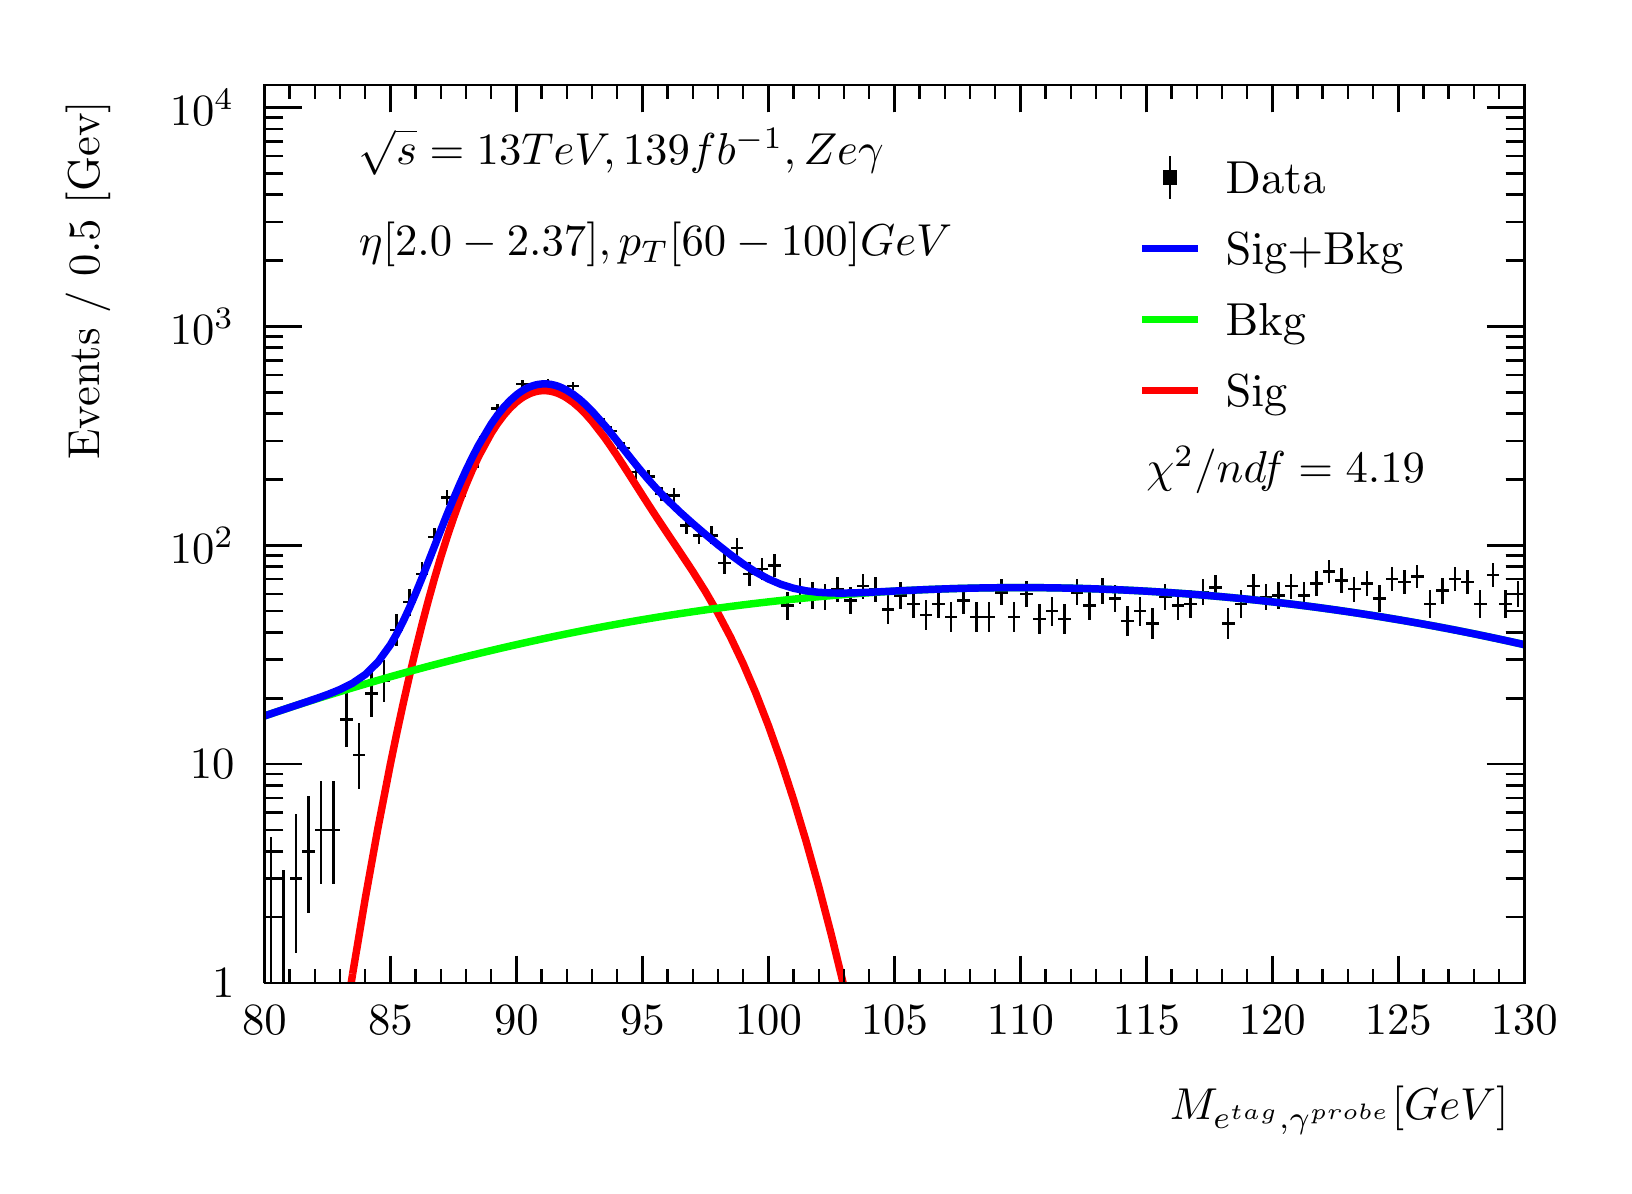
\begin{tikzpicture}
\pgfdeclareplotmark{cross} {
\pgfpathmoveto{\pgfpoint{-0.3\pgfplotmarksize}{\pgfplotmarksize}}
\pgfpathlineto{\pgfpoint{+0.3\pgfplotmarksize}{\pgfplotmarksize}}
\pgfpathlineto{\pgfpoint{+0.3\pgfplotmarksize}{0.3\pgfplotmarksize}}
\pgfpathlineto{\pgfpoint{+1\pgfplotmarksize}{0.3\pgfplotmarksize}}
\pgfpathlineto{\pgfpoint{+1\pgfplotmarksize}{-0.3\pgfplotmarksize}}
\pgfpathlineto{\pgfpoint{+0.3\pgfplotmarksize}{-0.3\pgfplotmarksize}}
\pgfpathlineto{\pgfpoint{+0.3\pgfplotmarksize}{-1.\pgfplotmarksize}}
\pgfpathlineto{\pgfpoint{-0.3\pgfplotmarksize}{-1.\pgfplotmarksize}}
\pgfpathlineto{\pgfpoint{-0.3\pgfplotmarksize}{-0.3\pgfplotmarksize}}
\pgfpathlineto{\pgfpoint{-1.\pgfplotmarksize}{-0.3\pgfplotmarksize}}
\pgfpathlineto{\pgfpoint{-1.\pgfplotmarksize}{0.3\pgfplotmarksize}}
\pgfpathlineto{\pgfpoint{-0.3\pgfplotmarksize}{0.3\pgfplotmarksize}}
\pgfpathclose
\pgfusepathqstroke
}
\pgfdeclareplotmark{cross*} {
\pgfpathmoveto{\pgfpoint{-0.3\pgfplotmarksize}{\pgfplotmarksize}}
\pgfpathlineto{\pgfpoint{+0.3\pgfplotmarksize}{\pgfplotmarksize}}
\pgfpathlineto{\pgfpoint{+0.3\pgfplotmarksize}{0.3\pgfplotmarksize}}
\pgfpathlineto{\pgfpoint{+1\pgfplotmarksize}{0.3\pgfplotmarksize}}
\pgfpathlineto{\pgfpoint{+1\pgfplotmarksize}{-0.3\pgfplotmarksize}}
\pgfpathlineto{\pgfpoint{+0.3\pgfplotmarksize}{-0.3\pgfplotmarksize}}
\pgfpathlineto{\pgfpoint{+0.3\pgfplotmarksize}{-1.\pgfplotmarksize}}
\pgfpathlineto{\pgfpoint{-0.3\pgfplotmarksize}{-1.\pgfplotmarksize}}
\pgfpathlineto{\pgfpoint{-0.3\pgfplotmarksize}{-0.3\pgfplotmarksize}}
\pgfpathlineto{\pgfpoint{-1.\pgfplotmarksize}{-0.3\pgfplotmarksize}}
\pgfpathlineto{\pgfpoint{-1.\pgfplotmarksize}{0.3\pgfplotmarksize}}
\pgfpathlineto{\pgfpoint{-0.3\pgfplotmarksize}{0.3\pgfplotmarksize}}
\pgfpathclose
\pgfusepathqfillstroke
}
\pgfdeclareplotmark{newstar} {
\pgfpathmoveto{\pgfqpoint{0pt}{\pgfplotmarksize}}
\pgfpathlineto{\pgfqpointpolar{44}{0.5\pgfplotmarksize}}
\pgfpathlineto{\pgfqpointpolar{18}{\pgfplotmarksize}}
\pgfpathlineto{\pgfqpointpolar{-20}{0.5\pgfplotmarksize}}
\pgfpathlineto{\pgfqpointpolar{-54}{\pgfplotmarksize}}
\pgfpathlineto{\pgfqpointpolar{-90}{0.5\pgfplotmarksize}}
\pgfpathlineto{\pgfqpointpolar{234}{\pgfplotmarksize}}
\pgfpathlineto{\pgfqpointpolar{198}{0.5\pgfplotmarksize}}
\pgfpathlineto{\pgfqpointpolar{162}{\pgfplotmarksize}}
\pgfpathlineto{\pgfqpointpolar{134}{0.5\pgfplotmarksize}}
\pgfpathclose
\pgfusepathqstroke
}
\pgfdeclareplotmark{newstar*} {
\pgfpathmoveto{\pgfqpoint{0pt}{\pgfplotmarksize}}
\pgfpathlineto{\pgfqpointpolar{44}{0.5\pgfplotmarksize}}
\pgfpathlineto{\pgfqpointpolar{18}{\pgfplotmarksize}}
\pgfpathlineto{\pgfqpointpolar{-20}{0.5\pgfplotmarksize}}
\pgfpathlineto{\pgfqpointpolar{-54}{\pgfplotmarksize}}
\pgfpathlineto{\pgfqpointpolar{-90}{0.5\pgfplotmarksize}}
\pgfpathlineto{\pgfqpointpolar{234}{\pgfplotmarksize}}
\pgfpathlineto{\pgfqpointpolar{198}{0.5\pgfplotmarksize}}
\pgfpathlineto{\pgfqpointpolar{162}{\pgfplotmarksize}}
\pgfpathlineto{\pgfqpointpolar{134}{0.5\pgfplotmarksize}}
\pgfpathclose
\pgfusepathqfillstroke
}
\definecolor{c}{rgb}{1,1,1};
\draw [color=c, fill=c] (0,0) rectangle (20,14.4361);
\draw [color=c, fill=c] (3,2.30977) rectangle (19,13.7143);
\definecolor{c}{rgb}{0,0,0};
\draw [c,line width=0.9] (3,2.30977) -- (3,13.7143) -- (19,13.7143) -- (19,2.30977) -- (3,2.30977);
\definecolor{c}{rgb}{1,1,1};
\draw [color=c, fill=c] (3,2.30977) rectangle (19,13.7143);
\definecolor{c}{rgb}{0,0,0};
\draw [c,line width=0.9] (3,2.30977) -- (3,13.7143) -- (19,13.7143) -- (19,2.30977) -- (3,2.30977);
\draw [c,line width=0.9] (3,2.30977) -- (19,2.30977);
\draw [c,line width=0.9] (3,2.65624) -- (3,2.30977);
\draw [c,line width=0.9] (3.32,2.48301) -- (3.32,2.30977);
\draw [c,line width=0.9] (3.64,2.48301) -- (3.64,2.30977);
\draw [c,line width=0.9] (3.96,2.48301) -- (3.96,2.30977);
\draw [c,line width=0.9] (4.28,2.48301) -- (4.28,2.30977);
\draw [c,line width=0.9] (4.6,2.65624) -- (4.6,2.30977);
\draw [c,line width=0.9] (4.92,2.48301) -- (4.92,2.30977);
\draw [c,line width=0.9] (5.24,2.48301) -- (5.24,2.30977);
\draw [c,line width=0.9] (5.56,2.48301) -- (5.56,2.30977);
\draw [c,line width=0.9] (5.88,2.48301) -- (5.88,2.30977);
\draw [c,line width=0.9] (6.2,2.65624) -- (6.2,2.30977);
\draw [c,line width=0.9] (6.52,2.48301) -- (6.52,2.30977);
\draw [c,line width=0.9] (6.84,2.48301) -- (6.84,2.30977);
\draw [c,line width=0.9] (7.16,2.48301) -- (7.16,2.30977);
\draw [c,line width=0.9] (7.48,2.48301) -- (7.48,2.30977);
\draw [c,line width=0.9] (7.8,2.65624) -- (7.8,2.30977);
\draw [c,line width=0.9] (8.12,2.48301) -- (8.12,2.30977);
\draw [c,line width=0.9] (8.44,2.48301) -- (8.44,2.30977);
\draw [c,line width=0.9] (8.76,2.48301) -- (8.76,2.30977);
\draw [c,line width=0.9] (9.08,2.48301) -- (9.08,2.30977);
\draw [c,line width=0.9] (9.4,2.65624) -- (9.4,2.30977);
\draw [c,line width=0.9] (9.72,2.48301) -- (9.72,2.30977);
\draw [c,line width=0.9] (10.04,2.48301) -- (10.04,2.30977);
\draw [c,line width=0.9] (10.36,2.48301) -- (10.36,2.30977);
\draw [c,line width=0.9] (10.68,2.48301) -- (10.68,2.30977);
\draw [c,line width=0.9] (11,2.65624) -- (11,2.30977);
\draw [c,line width=0.9] (11.32,2.48301) -- (11.32,2.30977);
\draw [c,line width=0.9] (11.64,2.48301) -- (11.64,2.30977);
\draw [c,line width=0.9] (11.96,2.48301) -- (11.96,2.30977);
\draw [c,line width=0.9] (12.28,2.48301) -- (12.28,2.30977);
\draw [c,line width=0.9] (12.6,2.65624) -- (12.6,2.30977);
\draw [c,line width=0.9] (12.92,2.48301) -- (12.92,2.30977);
\draw [c,line width=0.9] (13.24,2.48301) -- (13.24,2.30977);
\draw [c,line width=0.9] (13.56,2.48301) -- (13.56,2.30977);
\draw [c,line width=0.9] (13.88,2.48301) -- (13.88,2.30977);
\draw [c,line width=0.9] (14.2,2.65624) -- (14.2,2.30977);
\draw [c,line width=0.9] (14.52,2.48301) -- (14.52,2.30977);
\draw [c,line width=0.9] (14.84,2.48301) -- (14.84,2.30977);
\draw [c,line width=0.9] (15.16,2.48301) -- (15.16,2.30977);
\draw [c,line width=0.9] (15.48,2.48301) -- (15.48,2.30977);
\draw [c,line width=0.9] (15.8,2.65624) -- (15.8,2.30977);
\draw [c,line width=0.9] (16.12,2.48301) -- (16.12,2.30977);
\draw [c,line width=0.9] (16.44,2.48301) -- (16.44,2.30977);
\draw [c,line width=0.9] (16.76,2.48301) -- (16.76,2.30977);
\draw [c,line width=0.9] (17.08,2.48301) -- (17.08,2.30977);
\draw [c,line width=0.9] (17.4,2.65624) -- (17.4,2.30977);
\draw [c,line width=0.9] (17.72,2.48301) -- (17.72,2.30977);
\draw [c,line width=0.9] (18.04,2.48301) -- (18.04,2.30977);
\draw [c,line width=0.9] (18.36,2.48301) -- (18.36,2.30977);
\draw [c,line width=0.9] (18.68,2.48301) -- (18.68,2.30977);
\draw [c,line width=0.9] (19,2.65624) -- (19,2.30977);
\draw [anchor=base] (3,1.66015) node[scale=1.61424, color=c, rotate=0]{80};
\draw [anchor=base] (4.6,1.66015) node[scale=1.61424, color=c, rotate=0]{85};
\draw [anchor=base] (6.2,1.66015) node[scale=1.61424, color=c, rotate=0]{90};
\draw [anchor=base] (7.8,1.66015) node[scale=1.61424, color=c, rotate=0]{95};
\draw [anchor=base] (9.4,1.66015) node[scale=1.61424, color=c, rotate=0]{100};
\draw [anchor=base] (11,1.66015) node[scale=1.61424, color=c, rotate=0]{105};
\draw [anchor=base] (12.6,1.66015) node[scale=1.61424, color=c, rotate=0]{110};
\draw [anchor=base] (14.2,1.66015) node[scale=1.61424, color=c, rotate=0]{115};
\draw [anchor=base] (15.8,1.66015) node[scale=1.61424, color=c, rotate=0]{120};
\draw [anchor=base] (17.4,1.66015) node[scale=1.61424, color=c, rotate=0]{125};
\draw [anchor=base] (19,1.66015) node[scale=1.61424, color=c, rotate=0]{130};
\draw [anchor= east] (19,0.692932) node[scale=1.61424, color=c, rotate=0]{$M_{e^{tag}, \gamma^{probe}}  [GeV]$};
\draw [c,line width=0.9] (3,13.7143) -- (19,13.7143);
\draw [c,line width=0.9] (3,13.3678) -- (3,13.7143);
\draw [c,line width=0.9] (3.32,13.5411) -- (3.32,13.7143);
\draw [c,line width=0.9] (3.64,13.5411) -- (3.64,13.7143);
\draw [c,line width=0.9] (3.96,13.5411) -- (3.96,13.7143);
\draw [c,line width=0.9] (4.28,13.5411) -- (4.28,13.7143);
\draw [c,line width=0.9] (4.6,13.3678) -- (4.6,13.7143);
\draw [c,line width=0.9] (4.92,13.5411) -- (4.92,13.7143);
\draw [c,line width=0.9] (5.24,13.5411) -- (5.24,13.7143);
\draw [c,line width=0.9] (5.56,13.5411) -- (5.56,13.7143);
\draw [c,line width=0.9] (5.88,13.5411) -- (5.88,13.7143);
\draw [c,line width=0.9] (6.2,13.3678) -- (6.2,13.7143);
\draw [c,line width=0.9] (6.52,13.5411) -- (6.52,13.7143);
\draw [c,line width=0.9] (6.84,13.5411) -- (6.84,13.7143);
\draw [c,line width=0.9] (7.16,13.5411) -- (7.16,13.7143);
\draw [c,line width=0.9] (7.48,13.5411) -- (7.48,13.7143);
\draw [c,line width=0.9] (7.8,13.3678) -- (7.8,13.7143);
\draw [c,line width=0.9] (8.12,13.5411) -- (8.12,13.7143);
\draw [c,line width=0.9] (8.44,13.5411) -- (8.44,13.7143);
\draw [c,line width=0.9] (8.76,13.5411) -- (8.76,13.7143);
\draw [c,line width=0.9] (9.08,13.5411) -- (9.08,13.7143);
\draw [c,line width=0.9] (9.4,13.3678) -- (9.4,13.7143);
\draw [c,line width=0.9] (9.72,13.5411) -- (9.72,13.7143);
\draw [c,line width=0.9] (10.04,13.5411) -- (10.04,13.7143);
\draw [c,line width=0.9] (10.36,13.5411) -- (10.36,13.7143);
\draw [c,line width=0.9] (10.68,13.5411) -- (10.68,13.7143);
\draw [c,line width=0.9] (11,13.3678) -- (11,13.7143);
\draw [c,line width=0.9] (11.32,13.5411) -- (11.32,13.7143);
\draw [c,line width=0.9] (11.64,13.5411) -- (11.64,13.7143);
\draw [c,line width=0.9] (11.96,13.5411) -- (11.96,13.7143);
\draw [c,line width=0.9] (12.28,13.5411) -- (12.28,13.7143);
\draw [c,line width=0.9] (12.6,13.3678) -- (12.6,13.7143);
\draw [c,line width=0.9] (12.92,13.5411) -- (12.92,13.7143);
\draw [c,line width=0.9] (13.24,13.5411) -- (13.24,13.7143);
\draw [c,line width=0.9] (13.56,13.5411) -- (13.56,13.7143);
\draw [c,line width=0.9] (13.88,13.5411) -- (13.88,13.7143);
\draw [c,line width=0.9] (14.2,13.3678) -- (14.2,13.7143);
\draw [c,line width=0.9] (14.52,13.5411) -- (14.52,13.7143);
\draw [c,line width=0.9] (14.84,13.5411) -- (14.84,13.7143);
\draw [c,line width=0.9] (15.16,13.5411) -- (15.16,13.7143);
\draw [c,line width=0.9] (15.48,13.5411) -- (15.48,13.7143);
\draw [c,line width=0.9] (15.8,13.3678) -- (15.8,13.7143);
\draw [c,line width=0.9] (16.12,13.5411) -- (16.12,13.7143);
\draw [c,line width=0.9] (16.44,13.5411) -- (16.44,13.7143);
\draw [c,line width=0.9] (16.76,13.5411) -- (16.76,13.7143);
\draw [c,line width=0.9] (17.08,13.5411) -- (17.08,13.7143);
\draw [c,line width=0.9] (17.4,13.3678) -- (17.4,13.7143);
\draw [c,line width=0.9] (17.72,13.5411) -- (17.72,13.7143);
\draw [c,line width=0.9] (18.04,13.5411) -- (18.04,13.7143);
\draw [c,line width=0.9] (18.36,13.5411) -- (18.36,13.7143);
\draw [c,line width=0.9] (18.68,13.5411) -- (18.68,13.7143);
\draw [c,line width=0.9] (19,13.3678) -- (19,13.7143);
\draw [c,line width=0.9] (3,2.30977) -- (3,13.7143);
\draw [c,line width=0.9] (3.474,2.30978) -- (3,2.30978);
\draw [anchor= east] (2.82,2.30978) node[scale=1.61424, color=c, rotate=0]{1};
\draw [c,line width=0.9] (3.237,3.14655) -- (3,3.14655);
\draw [c,line width=0.9] (3.237,3.63603) -- (3,3.63603);
\draw [c,line width=0.9] (3.237,3.98333) -- (3,3.98333);
\draw [c,line width=0.9] (3.237,4.25271) -- (3,4.25271);
\draw [c,line width=0.9] (3.237,4.47281) -- (3,4.47281);
\draw [c,line width=0.9] (3.237,4.6589) -- (3,4.6589);
\draw [c,line width=0.9] (3.237,4.8201) -- (3,4.8201);
\draw [c,line width=0.9] (3.237,4.96229) -- (3,4.96229);
\draw [c,line width=0.9] (3.474,5.08948) -- (3,5.08948);
\draw [anchor= east] (2.82,5.08948) node[scale=1.61424, color=c, rotate=0]{10};
\draw [c,line width=0.9] (3.237,5.92626) -- (3,5.92626);
\draw [c,line width=0.9] (3.237,6.41574) -- (3,6.41574);
\draw [c,line width=0.9] (3.237,6.76303) -- (3,6.76303);
\draw [c,line width=0.9] (3.237,7.03241) -- (3,7.03241);
\draw [c,line width=0.9] (3.237,7.25251) -- (3,7.25251);
\draw [c,line width=0.9] (3.237,7.43861) -- (3,7.43861);
\draw [c,line width=0.9] (3.237,7.59981) -- (3,7.59981);
\draw [c,line width=0.9] (3.237,7.74199) -- (3,7.74199);
\draw [c,line width=0.9] (3.474,7.86919) -- (3,7.86919);
\draw [anchor= east] (2.82,7.86919) node[scale=1.61424, color=c, rotate=0]{$10^{2}$};
\draw [c,line width=0.9] (3.237,8.70596) -- (3,8.70596);
\draw [c,line width=0.9] (3.237,9.19544) -- (3,9.19544);
\draw [c,line width=0.9] (3.237,9.54274) -- (3,9.54274);
\draw [c,line width=0.9] (3.237,9.81212) -- (3,9.81212);
\draw [c,line width=0.9] (3.237,10.0322) -- (3,10.0322);
\draw [c,line width=0.9] (3.237,10.2183) -- (3,10.2183);
\draw [c,line width=0.9] (3.237,10.3795) -- (3,10.3795);
\draw [c,line width=0.9] (3.237,10.5217) -- (3,10.5217);
\draw [c,line width=0.9] (3.474,10.6489) -- (3,10.6489);
\draw [anchor= east] (2.82,10.6489) node[scale=1.61424, color=c, rotate=0]{$10^{3}$};
\draw [c,line width=0.9] (3.237,11.4857) -- (3,11.4857);
\draw [c,line width=0.9] (3.237,11.9751) -- (3,11.9751);
\draw [c,line width=0.9] (3.237,12.3224) -- (3,12.3224);
\draw [c,line width=0.9] (3.237,12.5918) -- (3,12.5918);
\draw [c,line width=0.9] (3.237,12.8119) -- (3,12.8119);
\draw [c,line width=0.9] (3.237,12.998) -- (3,12.998);
\draw [c,line width=0.9] (3.237,13.1592) -- (3,13.1592);
\draw [c,line width=0.9] (3.237,13.3014) -- (3,13.3014);
\draw [c,line width=0.9] (3.474,13.4286) -- (3,13.4286);
\draw [anchor= east] (2.82,13.4286) node[scale=1.61424, color=c, rotate=0]{$10^{4}$};
\draw [anchor= east] (0.76,13.7143) node[scale=1.61424, color=c, rotate=90]{Events / 0.5 [Gev]};
\draw [c,line width=0.9] (19,2.30977) -- (19,13.7143);
\draw [c,line width=0.9] (18.526,2.30978) -- (19,2.30978);
\draw [c,line width=0.9] (18.763,3.14655) -- (19,3.14655);
\draw [c,line width=0.9] (18.763,3.63603) -- (19,3.63603);
\draw [c,line width=0.9] (18.763,3.98333) -- (19,3.98333);
\draw [c,line width=0.9] (18.763,4.25271) -- (19,4.25271);
\draw [c,line width=0.9] (18.763,4.47281) -- (19,4.47281);
\draw [c,line width=0.9] (18.763,4.6589) -- (19,4.6589);
\draw [c,line width=0.9] (18.763,4.8201) -- (19,4.8201);
\draw [c,line width=0.9] (18.763,4.96229) -- (19,4.96229);
\draw [c,line width=0.9] (18.526,5.08948) -- (19,5.08948);
\draw [c,line width=0.9] (18.763,5.92626) -- (19,5.92626);
\draw [c,line width=0.9] (18.763,6.41574) -- (19,6.41574);
\draw [c,line width=0.9] (18.763,6.76303) -- (19,6.76303);
\draw [c,line width=0.9] (18.763,7.03241) -- (19,7.03241);
\draw [c,line width=0.9] (18.763,7.25251) -- (19,7.25251);
\draw [c,line width=0.9] (18.763,7.43861) -- (19,7.43861);
\draw [c,line width=0.9] (18.763,7.59981) -- (19,7.59981);
\draw [c,line width=0.9] (18.763,7.74199) -- (19,7.74199);
\draw [c,line width=0.9] (18.526,7.86919) -- (19,7.86919);
\draw [c,line width=0.9] (18.763,8.70596) -- (19,8.70596);
\draw [c,line width=0.9] (18.763,9.19544) -- (19,9.19544);
\draw [c,line width=0.9] (18.763,9.54274) -- (19,9.54274);
\draw [c,line width=0.9] (18.763,9.81212) -- (19,9.81212);
\draw [c,line width=0.9] (18.763,10.0322) -- (19,10.0322);
\draw [c,line width=0.9] (18.763,10.2183) -- (19,10.2183);
\draw [c,line width=0.9] (18.763,10.3795) -- (19,10.3795);
\draw [c,line width=0.9] (18.763,10.5217) -- (19,10.5217);
\draw [c,line width=0.9] (18.526,10.6489) -- (19,10.6489);
\draw [c,line width=0.9] (18.763,11.4857) -- (19,11.4857);
\draw [c,line width=0.9] (18.763,11.9751) -- (19,11.9751);
\draw [c,line width=0.9] (18.763,12.3224) -- (19,12.3224);
\draw [c,line width=0.9] (18.763,12.5918) -- (19,12.5918);
\draw [c,line width=0.9] (18.763,12.8119) -- (19,12.8119);
\draw [c,line width=0.9] (18.763,12.998) -- (19,12.998);
\draw [c,line width=0.9] (18.763,13.1592) -- (19,13.1592);
\draw [c,line width=0.9] (18.763,13.3014) -- (19,13.3014);
\draw [c,line width=0.9] (18.526,13.4286) -- (19,13.4286);
\draw [c,line width=0.9] (3.08,3.14655) -- (3,3.14655);
\draw [c,line width=0.9] (3,3.14655) -- (3,3.14655);
\draw [c,line width=0.9] (3.08,3.14655) -- (3.16,3.14655);
\draw [c,line width=0.9] (3.16,3.14655) -- (3.16,3.14655);
\draw [c,line width=0.9] (3.08,3.14655) -- (3.08,4.16194);
\draw [c,line width=0.9] (3.08,4.16194) -- (3.08,4.16194);
\draw [c,line width=0.9] (3.08,3.14655) -- (3.08,2.30977);
\draw [c,line width=0.9] (3.08,2.30977) -- (3.08,2.30977);
\draw [c,line width=0.9] (3.24,2.30977) -- (3.16,2.30977);
\draw [c,line width=0.9] (3.16,2.30977) -- (3.16,2.30977);
\draw [c,line width=0.9] (3.24,2.30977) -- (3.32,2.30977);
\draw [c,line width=0.9] (3.32,2.30977) -- (3.32,2.30977);
\draw [c,line width=0.9] (3.24,2.30977) -- (3.24,3.75092);
\draw [c,line width=0.9] (3.24,3.75092) -- (3.24,3.75092);
\draw [c,line width=0.9] (3.4,3.63603) -- (3.32,3.63603);
\draw [c,line width=0.9] (3.32,3.63603) -- (3.32,3.63603);
\draw [c,line width=0.9] (3.4,3.63603) -- (3.48,3.63603);
\draw [c,line width=0.9] (3.48,3.63603) -- (3.48,3.63603);
\draw [c,line width=0.9] (3.4,3.63603) -- (3.4,4.45623);
\draw [c,line width=0.9] (3.4,4.45623) -- (3.4,4.45623);
\draw [c,line width=0.9] (3.4,3.63603) -- (3.4,2.68743);
\draw [c,line width=0.9] (3.4,2.68743) -- (3.4,2.68743);
\draw [c,line width=0.9] (3.56,3.98332) -- (3.48,3.98332);
\draw [c,line width=0.9] (3.48,3.98332) -- (3.48,3.98332);
\draw [c,line width=0.9] (3.56,3.98332) -- (3.64,3.98332);
\draw [c,line width=0.9] (3.64,3.98332) -- (3.64,3.98332);
\draw [c,line width=0.9] (3.56,3.98332) -- (3.56,4.68665);
\draw [c,line width=0.9] (3.56,4.68665) -- (3.56,4.68665);
\draw [c,line width=0.9] (3.56,3.98332) -- (3.56,3.19718);
\draw [c,line width=0.9] (3.56,3.19718) -- (3.56,3.19718);
\draw [c,line width=0.9] (3.72,4.25271) -- (3.64,4.25271);
\draw [c,line width=0.9] (3.64,4.25271) -- (3.64,4.25271);
\draw [c,line width=0.9] (3.72,4.25271) -- (3.8,4.25271);
\draw [c,line width=0.9] (3.8,4.25271) -- (3.8,4.25271);
\draw [c,line width=0.9] (3.72,4.25271) -- (3.72,4.87648);
\draw [c,line width=0.9] (3.72,4.87648) -- (3.72,4.87648);
\draw [c,line width=0.9] (3.72,4.25271) -- (3.72,3.57);
\draw [c,line width=0.9] (3.72,3.57) -- (3.72,3.57);
\draw [c,line width=0.9] (3.88,4.25271) -- (3.8,4.25271);
\draw [c,line width=0.9] (3.8,4.25271) -- (3.8,4.25271);
\draw [c,line width=0.9] (3.88,4.25271) -- (3.96,4.25271);
\draw [c,line width=0.9] (3.96,4.25271) -- (3.96,4.25271);
\draw [c,line width=0.9] (3.88,4.25271) -- (3.88,4.87648);
\draw [c,line width=0.9] (3.88,4.87648) -- (3.88,4.87648);
\draw [c,line width=0.9] (3.88,4.25271) -- (3.88,3.57);
\draw [c,line width=0.9] (3.88,3.57) -- (3.88,3.57);
\draw [c,line width=0.9] (4.04,5.65687) -- (3.96,5.65687);
\draw [c,line width=0.9] (3.96,5.65687) -- (3.96,5.65687);
\draw [c,line width=0.9] (4.04,5.65687) -- (4.12,5.65687);
\draw [c,line width=0.9] (4.12,5.65687) -- (4.12,5.65687);
\draw [c,line width=0.9] (4.04,5.65687) -- (4.04,5.98992);
\draw [c,line width=0.9] (4.04,5.98992) -- (4.04,5.98992);
\draw [c,line width=0.9] (4.04,5.65687) -- (4.04,5.31382);
\draw [c,line width=0.9] (4.04,5.31382) -- (4.04,5.31382);
\draw [c,line width=0.9] (4.2,5.20454) -- (4.12,5.20454);
\draw [c,line width=0.9] (4.12,5.20454) -- (4.12,5.20454);
\draw [c,line width=0.9] (4.2,5.20454) -- (4.28,5.20454);
\draw [c,line width=0.9] (4.28,5.20454) -- (4.28,5.20454);
\draw [c,line width=0.9] (4.2,5.20454) -- (4.2,5.61203);
\draw [c,line width=0.9] (4.2,5.61203) -- (4.2,5.61203);
\draw [c,line width=0.9] (4.2,5.20454) -- (4.2,4.77934);
\draw [c,line width=0.9] (4.2,4.77934) -- (4.2,4.77934);
\draw [c,line width=0.9] (4.36,5.98516) -- (4.28,5.98516);
\draw [c,line width=0.9] (4.28,5.98516) -- (4.28,5.98516);
\draw [c,line width=0.9] (4.36,5.98516) -- (4.44,5.98516);
\draw [c,line width=0.9] (4.44,5.98516) -- (4.44,5.98516);
\draw [c,line width=0.9] (4.36,5.98516) -- (4.36,6.27303);
\draw [c,line width=0.9] (4.36,6.27303) -- (4.36,6.27303);
\draw [c,line width=0.9] (4.36,5.98516) -- (4.36,5.69067);
\draw [c,line width=0.9] (4.36,5.69067) -- (4.36,5.69067);
\draw [c,line width=0.9] (4.52,6.14636) -- (4.44,6.14636);
\draw [c,line width=0.9] (4.44,6.14636) -- (4.44,6.14636);
\draw [c,line width=0.9] (4.52,6.14636) -- (4.6,6.14636);
\draw [c,line width=0.9] (4.6,6.14636) -- (4.6,6.14636);
\draw [c,line width=0.9] (4.52,6.14636) -- (4.52,6.41441);
\draw [c,line width=0.9] (4.52,6.41441) -- (4.52,6.41441);
\draw [c,line width=0.9] (4.52,6.14636) -- (4.52,5.8729);
\draw [c,line width=0.9] (4.52,5.8729) -- (4.52,5.8729);
\draw [c,line width=0.9] (4.68,6.79284) -- (4.6,6.79284);
\draw [c,line width=0.9] (4.6,6.79284) -- (4.6,6.79284);
\draw [c,line width=0.9] (4.68,6.79284) -- (4.76,6.79284);
\draw [c,line width=0.9] (4.76,6.79284) -- (4.76,6.79284);
\draw [c,line width=0.9] (4.68,6.79284) -- (4.68,6.99452);
\draw [c,line width=0.9] (4.68,6.99452) -- (4.68,6.99452);
\draw [c,line width=0.9] (4.68,6.79284) -- (4.68,6.58876);
\draw [c,line width=0.9] (4.68,6.58876) -- (4.68,6.58876);
\draw [c,line width=0.9] (4.84,7.14747) -- (4.76,7.14747);
\draw [c,line width=0.9] (4.76,7.14747) -- (4.76,7.14747);
\draw [c,line width=0.9] (4.84,7.14747) -- (4.92,7.14747);
\draw [c,line width=0.9] (4.92,7.14747) -- (4.92,7.14747);
\draw [c,line width=0.9] (4.84,7.14747) -- (4.84,7.32022);
\draw [c,line width=0.9] (4.84,7.32022) -- (4.84,7.32022);
\draw [c,line width=0.9] (4.84,7.14747) -- (4.84,6.97319);
\draw [c,line width=0.9] (4.84,6.97319) -- (4.84,6.97319);
\draw [c,line width=0.9] (5,7.50569) -- (4.92,7.50569);
\draw [c,line width=0.9] (4.92,7.50569) -- (4.92,7.50569);
\draw [c,line width=0.9] (5,7.50569) -- (5.08,7.50569);
\draw [c,line width=0.9] (5.08,7.50569) -- (5.08,7.50569);
\draw [c,line width=0.9] (5,7.50569) -- (5,7.65354);
\draw [c,line width=0.9] (5,7.65354) -- (5,7.65354);
\draw [c,line width=0.9] (5,7.50569) -- (5,7.35686);
\draw [c,line width=0.9] (5,7.35686) -- (5,7.35686);
\draw [c,line width=0.9] (5.16,7.97322) -- (5.08,7.97322);
\draw [c,line width=0.9] (5.08,7.97322) -- (5.08,7.97322);
\draw [c,line width=0.9] (5.16,7.97322) -- (5.24,7.97322);
\draw [c,line width=0.9] (5.24,7.97322) -- (5.24,7.97322);
\draw [c,line width=0.9] (5.16,7.97322) -- (5.16,8.08881);
\draw [c,line width=0.9] (5.16,8.08881) -- (5.16,8.08881);
\draw [c,line width=0.9] (5.16,7.97322) -- (5.16,7.85763);
\draw [c,line width=0.9] (5.16,7.85763) -- (5.16,7.85763);
\draw [c,line width=0.9] (5.32,8.47373) -- (5.24,8.47373);
\draw [c,line width=0.9] (5.24,8.47373) -- (5.24,8.47373);
\draw [c,line width=0.9] (5.32,8.47373) -- (5.4,8.47373);
\draw [c,line width=0.9] (5.4,8.47373) -- (5.4,8.47373);
\draw [c,line width=0.9] (5.32,8.47373) -- (5.32,8.56769);
\draw [c,line width=0.9] (5.32,8.56769) -- (5.32,8.56769);
\draw [c,line width=0.9] (5.32,8.47373) -- (5.32,8.37977);
\draw [c,line width=0.9] (5.32,8.37977) -- (5.32,8.37977);
\draw [c,line width=0.9] (5.48,8.50264) -- (5.4,8.50264);
\draw [c,line width=0.9] (5.4,8.50264) -- (5.4,8.50264);
\draw [c,line width=0.9] (5.48,8.50264) -- (5.56,8.50264);
\draw [c,line width=0.9] (5.56,8.50264) -- (5.56,8.50264);
\draw [c,line width=0.9] (5.48,8.50264) -- (5.48,8.59548);
\draw [c,line width=0.9] (5.48,8.59548) -- (5.48,8.59548);
\draw [c,line width=0.9] (5.48,8.50264) -- (5.48,8.4098);
\draw [c,line width=0.9] (5.48,8.4098) -- (5.48,8.4098);
\draw [c,line width=0.9] (5.64,8.86942) -- (5.56,8.86942);
\draw [c,line width=0.9] (5.56,8.86942) -- (5.56,8.86942);
\draw [c,line width=0.9] (5.64,8.86942) -- (5.72,8.86942);
\draw [c,line width=0.9] (5.72,8.86942) -- (5.72,8.86942);
\draw [c,line width=0.9] (5.64,8.86942) -- (5.64,8.94918);
\draw [c,line width=0.9] (5.64,8.94918) -- (5.64,8.94918);
\draw [c,line width=0.9] (5.64,8.86942) -- (5.64,8.78966);
\draw [c,line width=0.9] (5.64,8.78966) -- (5.64,8.78966);
\draw [c,line width=0.9] (5.8,9.24665) -- (5.72,9.24665);
\draw [c,line width=0.9] (5.72,9.24665) -- (5.72,9.24665);
\draw [c,line width=0.9] (5.8,9.24665) -- (5.88,9.24665);
\draw [c,line width=0.9] (5.88,9.24665) -- (5.88,9.24665);
\draw [c,line width=0.9] (5.8,9.24665) -- (5.8,9.31488);
\draw [c,line width=0.9] (5.8,9.31488) -- (5.8,9.31488);
\draw [c,line width=0.9] (5.8,9.24665) -- (5.8,9.17843);
\draw [c,line width=0.9] (5.8,9.17843) -- (5.8,9.17843);
\draw [c,line width=0.9] (5.96,9.60451) -- (5.88,9.60451);
\draw [c,line width=0.9] (5.88,9.60451) -- (5.88,9.60451);
\draw [c,line width=0.9] (5.96,9.60451) -- (6.04,9.60451);
\draw [c,line width=0.9] (6.04,9.60451) -- (6.04,9.60451);
\draw [c,line width=0.9] (5.96,9.60451) -- (5.96,9.66334);
\draw [c,line width=0.9] (5.96,9.66334) -- (5.96,9.66334);
\draw [c,line width=0.9] (5.96,9.60451) -- (5.96,9.54568);
\draw [c,line width=0.9] (5.96,9.54568) -- (5.96,9.54568);
\draw [c,line width=0.9] (6.12,9.63843) -- (6.04,9.63843);
\draw [c,line width=0.9] (6.04,9.63843) -- (6.04,9.63843);
\draw [c,line width=0.9] (6.12,9.63843) -- (6.2,9.63843);
\draw [c,line width=0.9] (6.2,9.63843) -- (6.2,9.63843);
\draw [c,line width=0.9] (6.12,9.63843) -- (6.12,9.69644);
\draw [c,line width=0.9] (6.12,9.69644) -- (6.12,9.69644);
\draw [c,line width=0.9] (6.12,9.63843) -- (6.12,9.58043);
\draw [c,line width=0.9] (6.12,9.58043) -- (6.12,9.58043);
\draw [c,line width=0.9] (6.28,9.92057) -- (6.2,9.92057);
\draw [c,line width=0.9] (6.2,9.92057) -- (6.2,9.92057);
\draw [c,line width=0.9] (6.28,9.92057) -- (6.36,9.92057);
\draw [c,line width=0.9] (6.36,9.92057) -- (6.36,9.92057);
\draw [c,line width=0.9] (6.28,9.92057) -- (6.28,9.97219);
\draw [c,line width=0.9] (6.28,9.97219) -- (6.28,9.97219);
\draw [c,line width=0.9] (6.28,9.92057) -- (6.28,9.86896);
\draw [c,line width=0.9] (6.28,9.86896) -- (6.28,9.86896);
\draw [c,line width=0.9] (6.44,9.85481) -- (6.36,9.85481);
\draw [c,line width=0.9] (6.36,9.85481) -- (6.36,9.85481);
\draw [c,line width=0.9] (6.44,9.85481) -- (6.52,9.85481);
\draw [c,line width=0.9] (6.52,9.85481) -- (6.52,9.85481);
\draw [c,line width=0.9] (6.44,9.85481) -- (6.44,9.90785);
\draw [c,line width=0.9] (6.44,9.90785) -- (6.44,9.90785);
\draw [c,line width=0.9] (6.44,9.85481) -- (6.44,9.80177);
\draw [c,line width=0.9] (6.44,9.80177) -- (6.44,9.80177);
\draw [c,line width=0.9] (6.6,9.92718) -- (6.52,9.92718);
\draw [c,line width=0.9] (6.52,9.92718) -- (6.52,9.92718);
\draw [c,line width=0.9] (6.6,9.92718) -- (6.68,9.92718);
\draw [c,line width=0.9] (6.68,9.92718) -- (6.68,9.92718);
\draw [c,line width=0.9] (6.6,9.92718) -- (6.6,9.97865);
\draw [c,line width=0.9] (6.6,9.97865) -- (6.6,9.97865);
\draw [c,line width=0.9] (6.6,9.92718) -- (6.6,9.8757);
\draw [c,line width=0.9] (6.6,9.8757) -- (6.6,9.8757);
\draw [c,line width=0.9] (6.76,9.82174) -- (6.68,9.82174);
\draw [c,line width=0.9] (6.68,9.82174) -- (6.68,9.82174);
\draw [c,line width=0.9] (6.76,9.82174) -- (6.84,9.82174);
\draw [c,line width=0.9] (6.84,9.82174) -- (6.84,9.82174);
\draw [c,line width=0.9] (6.76,9.82174) -- (6.76,9.8755);
\draw [c,line width=0.9] (6.76,9.8755) -- (6.76,9.8755);
\draw [c,line width=0.9] (6.76,9.82174) -- (6.76,9.76797);
\draw [c,line width=0.9] (6.76,9.76797) -- (6.76,9.76797);
\draw [c,line width=0.9] (6.92,9.8938) -- (6.84,9.8938);
\draw [c,line width=0.9] (6.84,9.8938) -- (6.84,9.8938);
\draw [c,line width=0.9] (6.92,9.8938) -- (7,9.8938);
\draw [c,line width=0.9] (7,9.8938) -- (7,9.8938);
\draw [c,line width=0.9] (6.92,9.8938) -- (6.92,9.94598);
\draw [c,line width=0.9] (6.92,9.94598) -- (6.92,9.94598);
\draw [c,line width=0.9] (6.92,9.8938) -- (6.92,9.84161);
\draw [c,line width=0.9] (6.92,9.84161) -- (6.92,9.84161);
\draw [c,line width=0.9] (7.08,9.59298) -- (7,9.59298);
\draw [c,line width=0.9] (7,9.59298) -- (7,9.59298);
\draw [c,line width=0.9] (7.08,9.59298) -- (7.16,9.59298);
\draw [c,line width=0.9] (7.16,9.59298) -- (7.16,9.59298);
\draw [c,line width=0.9] (7.08,9.59298) -- (7.08,9.65209);
\draw [c,line width=0.9] (7.08,9.65209) -- (7.08,9.65209);
\draw [c,line width=0.9] (7.08,9.59298) -- (7.08,9.53387);
\draw [c,line width=0.9] (7.08,9.53387) -- (7.08,9.53387);
\draw [c,line width=0.9] (7.24,9.47124) -- (7.16,9.47124);
\draw [c,line width=0.9] (7.16,9.47124) -- (7.16,9.47124);
\draw [c,line width=0.9] (7.24,9.47124) -- (7.32,9.47124);
\draw [c,line width=0.9] (7.32,9.47124) -- (7.32,9.47124);
\draw [c,line width=0.9] (7.24,9.47124) -- (7.24,9.53341);
\draw [c,line width=0.9] (7.24,9.53341) -- (7.24,9.53341);
\draw [c,line width=0.9] (7.24,9.47124) -- (7.24,9.40908);
\draw [c,line width=0.9] (7.24,9.40908) -- (7.24,9.40908);
\draw [c,line width=0.9] (7.4,9.3178) -- (7.32,9.3178);
\draw [c,line width=0.9] (7.32,9.3178) -- (7.32,9.3178);
\draw [c,line width=0.9] (7.4,9.3178) -- (7.48,9.3178);
\draw [c,line width=0.9] (7.48,9.3178) -- (7.48,9.3178);
\draw [c,line width=0.9] (7.4,9.3178) -- (7.4,9.38404);
\draw [c,line width=0.9] (7.4,9.38404) -- (7.4,9.38404);
\draw [c,line width=0.9] (7.4,9.3178) -- (7.4,9.25155);
\draw [c,line width=0.9] (7.4,9.25155) -- (7.4,9.25155);
\draw [c,line width=0.9] (7.56,9.10783) -- (7.48,9.10783);
\draw [c,line width=0.9] (7.48,9.10783) -- (7.48,9.10783);
\draw [c,line width=0.9] (7.56,9.10783) -- (7.64,9.10783);
\draw [c,line width=0.9] (7.64,9.10783) -- (7.64,9.10783);
\draw [c,line width=0.9] (7.56,9.10783) -- (7.56,9.1801);
\draw [c,line width=0.9] (7.56,9.1801) -- (7.56,9.1801);
\draw [c,line width=0.9] (7.56,9.10783) -- (7.56,9.03557);
\draw [c,line width=0.9] (7.56,9.03557) -- (7.56,9.03557);
\draw [c,line width=0.9] (7.72,8.79887) -- (7.64,8.79887);
\draw [c,line width=0.9] (7.64,8.79887) -- (7.64,8.79887);
\draw [c,line width=0.9] (7.72,8.79887) -- (7.8,8.79887);
\draw [c,line width=0.9] (7.8,8.79887) -- (7.8,8.79887);
\draw [c,line width=0.9] (7.72,8.79887) -- (7.72,8.88099);
\draw [c,line width=0.9] (7.72,8.88099) -- (7.72,8.88099);
\draw [c,line width=0.9] (7.72,8.79887) -- (7.72,8.71674);
\draw [c,line width=0.9] (7.72,8.71674) -- (7.72,8.71674);
\draw [c,line width=0.9] (7.88,8.74164) -- (7.8,8.74164);
\draw [c,line width=0.9] (7.8,8.74164) -- (7.8,8.74164);
\draw [c,line width=0.9] (7.88,8.74164) -- (7.96,8.74164);
\draw [c,line width=0.9] (7.96,8.74164) -- (7.96,8.74164);
\draw [c,line width=0.9] (7.88,8.74164) -- (7.88,8.82574);
\draw [c,line width=0.9] (7.88,8.82574) -- (7.88,8.82574);
\draw [c,line width=0.9] (7.88,8.74164) -- (7.88,8.65755);
\draw [c,line width=0.9] (7.88,8.65755) -- (7.88,8.65755);
\draw [c,line width=0.9] (8.04,8.52389) -- (7.96,8.52389);
\draw [c,line width=0.9] (7.96,8.52389) -- (7.96,8.52389);
\draw [c,line width=0.9] (8.04,8.52389) -- (8.12,8.52389);
\draw [c,line width=0.9] (8.12,8.52389) -- (8.12,8.52389);
\draw [c,line width=0.9] (8.04,8.52389) -- (8.04,8.61591);
\draw [c,line width=0.9] (8.04,8.61591) -- (8.04,8.61591);
\draw [c,line width=0.9] (8.04,8.52389) -- (8.04,8.43186);
\draw [c,line width=0.9] (8.04,8.43186) -- (8.04,8.43186);
\draw [c,line width=0.9] (8.2,8.50264) -- (8.12,8.50264);
\draw [c,line width=0.9] (8.12,8.50264) -- (8.12,8.50264);
\draw [c,line width=0.9] (8.2,8.50264) -- (8.28,8.50264);
\draw [c,line width=0.9] (8.28,8.50264) -- (8.28,8.50264);
\draw [c,line width=0.9] (8.2,8.50264) -- (8.2,8.59548);
\draw [c,line width=0.9] (8.2,8.59548) -- (8.2,8.59548);
\draw [c,line width=0.9] (8.2,8.50264) -- (8.2,8.4098);
\draw [c,line width=0.9] (8.2,8.4098) -- (8.2,8.4098);
\draw [c,line width=0.9] (8.36,8.1191) -- (8.28,8.1191);
\draw [c,line width=0.9] (8.28,8.1191) -- (8.28,8.1191);
\draw [c,line width=0.9] (8.36,8.1191) -- (8.44,8.1191);
\draw [c,line width=0.9] (8.44,8.1191) -- (8.44,8.1191);
\draw [c,line width=0.9] (8.36,8.1191) -- (8.36,8.22791);
\draw [c,line width=0.9] (8.36,8.22791) -- (8.36,8.22791);
\draw [c,line width=0.9] (8.36,8.1191) -- (8.36,8.01028);
\draw [c,line width=0.9] (8.36,8.01028) -- (8.36,8.01028);
\draw [c,line width=0.9] (8.52,7.99517) -- (8.44,7.99517);
\draw [c,line width=0.9] (8.44,7.99517) -- (8.44,7.99517);
\draw [c,line width=0.9] (8.52,7.99517) -- (8.6,7.99517);
\draw [c,line width=0.9] (8.6,7.99517) -- (8.6,7.99517);
\draw [c,line width=0.9] (8.52,7.99517) -- (8.52,8.10971);
\draw [c,line width=0.9] (8.52,8.10971) -- (8.52,8.10971);
\draw [c,line width=0.9] (8.52,7.99517) -- (8.52,7.88063);
\draw [c,line width=0.9] (8.52,7.88063) -- (8.52,7.88063);
\draw [c,line width=0.9] (8.68,7.99517) -- (8.6,7.99517);
\draw [c,line width=0.9] (8.6,7.99517) -- (8.6,7.99517);
\draw [c,line width=0.9] (8.68,7.99517) -- (8.76,7.99517);
\draw [c,line width=0.9] (8.76,7.99517) -- (8.76,7.99517);
\draw [c,line width=0.9] (8.68,7.99517) -- (8.68,8.10971);
\draw [c,line width=0.9] (8.68,8.10971) -- (8.68,8.10971);
\draw [c,line width=0.9] (8.68,7.99517) -- (8.68,7.88063);
\draw [c,line width=0.9] (8.68,7.88063) -- (8.68,7.88063);
\draw [c,line width=0.9] (8.84,7.64425) -- (8.76,7.64425);
\draw [c,line width=0.9] (8.76,7.64425) -- (8.76,7.64425);
\draw [c,line width=0.9] (8.84,7.64425) -- (8.92,7.64425);
\draw [c,line width=0.9] (8.92,7.64425) -- (8.92,7.64425);
\draw [c,line width=0.9] (8.84,7.64425) -- (8.84,7.78348);
\draw [c,line width=0.9] (8.84,7.78348) -- (8.84,7.78348);
\draw [c,line width=0.9] (8.84,7.64425) -- (8.84,7.50419);
\draw [c,line width=0.9] (8.84,7.50419) -- (8.84,7.50419);
\draw [c,line width=0.9] (9,7.83242) -- (8.92,7.83242);
\draw [c,line width=0.9] (8.92,7.83242) -- (8.92,7.83242);
\draw [c,line width=0.9] (9,7.83242) -- (9.08,7.83242);
\draw [c,line width=0.9] (9.08,7.83242) -- (9.08,7.83242);
\draw [c,line width=0.9] (9,7.83242) -- (9,7.96078);
\draw [c,line width=0.9] (9,7.96078) -- (9,7.96078);
\draw [c,line width=0.9] (9,7.83242) -- (9,7.7034);
\draw [c,line width=0.9] (9,7.7034) -- (9,7.7034);
\draw [c,line width=0.9] (9.16,7.50569) -- (9.08,7.50569);
\draw [c,line width=0.9] (9.08,7.50569) -- (9.08,7.50569);
\draw [c,line width=0.9] (9.16,7.50569) -- (9.24,7.50569);
\draw [c,line width=0.9] (9.24,7.50569) -- (9.24,7.50569);
\draw [c,line width=0.9] (9.16,7.50569) -- (9.16,7.65354);
\draw [c,line width=0.9] (9.16,7.65354) -- (9.16,7.65354);
\draw [c,line width=0.9] (9.16,7.50569) -- (9.16,7.35686);
\draw [c,line width=0.9] (9.16,7.35686) -- (9.16,7.35686);
\draw [c,line width=0.9] (9.32,7.56924) -- (9.24,7.56924);
\draw [c,line width=0.9] (9.24,7.56924) -- (9.24,7.56924);
\draw [c,line width=0.9] (9.32,7.56924) -- (9.4,7.56924);
\draw [c,line width=0.9] (9.4,7.56924) -- (9.4,7.56924);
\draw [c,line width=0.9] (9.32,7.56924) -- (9.32,7.71307);
\draw [c,line width=0.9] (9.32,7.71307) -- (9.32,7.71307);
\draw [c,line width=0.9] (9.32,7.56924) -- (9.32,7.4245);
\draw [c,line width=0.9] (9.32,7.4245) -- (9.32,7.4245);
\draw [c,line width=0.9] (9.48,7.6148) -- (9.4,7.6148);
\draw [c,line width=0.9] (9.4,7.6148) -- (9.4,7.6148);
\draw [c,line width=0.9] (9.48,7.6148) -- (9.56,7.6148);
\draw [c,line width=0.9] (9.56,7.6148) -- (9.56,7.6148);
\draw [c,line width=0.9] (9.48,7.6148) -- (9.48,7.75582);
\draw [c,line width=0.9] (9.48,7.75582) -- (9.48,7.75582);
\draw [c,line width=0.9] (9.48,7.6148) -- (9.48,7.47292);
\draw [c,line width=0.9] (9.48,7.47292) -- (9.48,7.47292);
\draw [c,line width=0.9] (9.64,7.10275) -- (9.56,7.10275);
\draw [c,line width=0.9] (9.56,7.10275) -- (9.56,7.10275);
\draw [c,line width=0.9] (9.64,7.10275) -- (9.72,7.10275);
\draw [c,line width=0.9] (9.72,7.10275) -- (9.72,7.10275);
\draw [c,line width=0.9] (9.64,7.10275) -- (9.64,7.2789);
\draw [c,line width=0.9] (9.64,7.2789) -- (9.64,7.2789);
\draw [c,line width=0.9] (9.64,7.10275) -- (9.64,6.92499);
\draw [c,line width=0.9] (9.64,6.92499) -- (9.64,6.92499);
\draw [c,line width=0.9] (9.8,7.2921) -- (9.72,7.2921);
\draw [c,line width=0.9] (9.72,7.2921) -- (9.72,7.2921);
\draw [c,line width=0.9] (9.8,7.2921) -- (9.88,7.2921);
\draw [c,line width=0.9] (9.88,7.2921) -- (9.88,7.2921);
\draw [c,line width=0.9] (9.8,7.2921) -- (9.8,7.4543);
\draw [c,line width=0.9] (9.8,7.4543) -- (9.8,7.4543);
\draw [c,line width=0.9] (9.8,7.2921) -- (9.8,7.12861);
\draw [c,line width=0.9] (9.8,7.12861) -- (9.8,7.12861);
\draw [c,line width=0.9] (9.96,7.23222) -- (9.88,7.23222);
\draw [c,line width=0.9] (9.88,7.23222) -- (9.88,7.23222);
\draw [c,line width=0.9] (9.96,7.23222) -- (10.04,7.23222);
\draw [c,line width=0.9] (10.04,7.23222) -- (10.04,7.23222);
\draw [c,line width=0.9] (9.96,7.23222) -- (9.96,7.39871);
\draw [c,line width=0.9] (9.96,7.39871) -- (9.96,7.39871);
\draw [c,line width=0.9] (9.96,7.23222) -- (9.96,7.06435);
\draw [c,line width=0.9] (9.96,7.06435) -- (9.96,7.06435);
\draw [c,line width=0.9] (10.12,7.21159) -- (10.04,7.21159);
\draw [c,line width=0.9] (10.04,7.21159) -- (10.04,7.21159);
\draw [c,line width=0.9] (10.12,7.21159) -- (10.2,7.21159);
\draw [c,line width=0.9] (10.2,7.21159) -- (10.2,7.21159);
\draw [c,line width=0.9] (10.12,7.21159) -- (10.12,7.37958);
\draw [c,line width=0.9] (10.12,7.37958) -- (10.12,7.37958);
\draw [c,line width=0.9] (10.12,7.21159) -- (10.12,7.04218);
\draw [c,line width=0.9] (10.12,7.04218) -- (10.12,7.04218);
\draw [c,line width=0.9] (10.28,7.31141) -- (10.2,7.31141);
\draw [c,line width=0.9] (10.2,7.31141) -- (10.2,7.31141);
\draw [c,line width=0.9] (10.28,7.31141) -- (10.36,7.31141);
\draw [c,line width=0.9] (10.36,7.31141) -- (10.36,7.31141);
\draw [c,line width=0.9] (10.28,7.31141) -- (10.28,7.47226);
\draw [c,line width=0.9] (10.28,7.47226) -- (10.28,7.47226);
\draw [c,line width=0.9] (10.28,7.31141) -- (10.28,7.14931);
\draw [c,line width=0.9] (10.28,7.14931) -- (10.28,7.14931);
\draw [c,line width=0.9] (10.44,7.16922) -- (10.36,7.16922);
\draw [c,line width=0.9] (10.36,7.16922) -- (10.36,7.16922);
\draw [c,line width=0.9] (10.44,7.16922) -- (10.52,7.16922);
\draw [c,line width=0.9] (10.52,7.16922) -- (10.52,7.16922);
\draw [c,line width=0.9] (10.44,7.16922) -- (10.44,7.34034);
\draw [c,line width=0.9] (10.44,7.34034) -- (10.44,7.34034);
\draw [c,line width=0.9] (10.44,7.16922) -- (10.44,6.99661);
\draw [c,line width=0.9] (10.44,6.99661) -- (10.44,6.99661);
\draw [c,line width=0.9] (10.6,7.34914) -- (10.52,7.34914);
\draw [c,line width=0.9] (10.52,7.34914) -- (10.52,7.34914);
\draw [c,line width=0.9] (10.6,7.34914) -- (10.68,7.34914);
\draw [c,line width=0.9] (10.68,7.34914) -- (10.68,7.34914);
\draw [c,line width=0.9] (10.6,7.34914) -- (10.6,7.50738);
\draw [c,line width=0.9] (10.6,7.50738) -- (10.6,7.50738);
\draw [c,line width=0.9] (10.6,7.34914) -- (10.6,7.18971);
\draw [c,line width=0.9] (10.6,7.18971) -- (10.6,7.18971);
\draw [c,line width=0.9] (10.76,7.31141) -- (10.68,7.31141);
\draw [c,line width=0.9] (10.68,7.31141) -- (10.68,7.31141);
\draw [c,line width=0.9] (10.76,7.31141) -- (10.84,7.31141);
\draw [c,line width=0.9] (10.84,7.31141) -- (10.84,7.31141);
\draw [c,line width=0.9] (10.76,7.31141) -- (10.76,7.47226);
\draw [c,line width=0.9] (10.76,7.47226) -- (10.76,7.47226);
\draw [c,line width=0.9] (10.76,7.31141) -- (10.76,7.14931);
\draw [c,line width=0.9] (10.76,7.14931) -- (10.76,7.14931);
\draw [c,line width=0.9] (10.92,7.05632) -- (10.84,7.05632);
\draw [c,line width=0.9] (10.84,7.05632) -- (10.84,7.05632);
\draw [c,line width=0.9] (10.92,7.05632) -- (11,7.05632);
\draw [c,line width=0.9] (11,7.05632) -- (11,7.05632);
\draw [c,line width=0.9] (10.92,7.05632) -- (10.92,7.23606);
\draw [c,line width=0.9] (10.92,7.23606) -- (10.92,7.23606);
\draw [c,line width=0.9] (10.92,7.05632) -- (10.92,6.87485);
\draw [c,line width=0.9] (10.92,6.87485) -- (10.92,6.87485);
\draw [c,line width=0.9] (11.08,7.23222) -- (11,7.23222);
\draw [c,line width=0.9] (11,7.23222) -- (11,7.23222);
\draw [c,line width=0.9] (11.08,7.23222) -- (11.16,7.23222);
\draw [c,line width=0.9] (11.16,7.23222) -- (11.16,7.23222);
\draw [c,line width=0.9] (11.08,7.23222) -- (11.08,7.39871);
\draw [c,line width=0.9] (11.08,7.39871) -- (11.08,7.39871);
\draw [c,line width=0.9] (11.08,7.23222) -- (11.08,7.06435);
\draw [c,line width=0.9] (11.08,7.06435) -- (11.08,7.06435);
\draw [c,line width=0.9] (11.24,7.12532) -- (11.16,7.12532);
\draw [c,line width=0.9] (11.16,7.12532) -- (11.16,7.12532);
\draw [c,line width=0.9] (11.24,7.12532) -- (11.32,7.12532);
\draw [c,line width=0.9] (11.32,7.12532) -- (11.32,7.12532);
\draw [c,line width=0.9] (11.24,7.12532) -- (11.24,7.29974);
\draw [c,line width=0.9] (11.24,7.29974) -- (11.24,7.29974);
\draw [c,line width=0.9] (11.24,7.12532) -- (11.24,6.94932);
\draw [c,line width=0.9] (11.24,6.94932) -- (11.24,6.94932);
\draw [c,line width=0.9] (11.4,6.98313) -- (11.32,6.98313);
\draw [c,line width=0.9] (11.32,6.98313) -- (11.32,6.98313);
\draw [c,line width=0.9] (11.4,6.98313) -- (11.48,6.98313);
\draw [c,line width=0.9] (11.48,6.98313) -- (11.48,6.98313);
\draw [c,line width=0.9] (11.4,6.98313) -- (11.4,7.16871);
\draw [c,line width=0.9] (11.4,7.16871) -- (11.4,7.16871);
\draw [c,line width=0.9] (11.4,6.98313) -- (11.4,6.79566);
\draw [c,line width=0.9] (11.4,6.79566) -- (11.4,6.79566);
\draw [c,line width=0.9] (11.56,7.12532) -- (11.48,7.12532);
\draw [c,line width=0.9] (11.48,7.12532) -- (11.48,7.12532);
\draw [c,line width=0.9] (11.56,7.12532) -- (11.64,7.12532);
\draw [c,line width=0.9] (11.64,7.12532) -- (11.64,7.12532);
\draw [c,line width=0.9] (11.56,7.12532) -- (11.56,7.29974);
\draw [c,line width=0.9] (11.56,7.29974) -- (11.56,7.29974);
\draw [c,line width=0.9] (11.56,7.12532) -- (11.56,6.94932);
\draw [c,line width=0.9] (11.56,6.94932) -- (11.56,6.94932);
\draw [c,line width=0.9] (11.72,6.95771) -- (11.64,6.95771);
\draw [c,line width=0.9] (11.64,6.95771) -- (11.64,6.95771);
\draw [c,line width=0.9] (11.72,6.95771) -- (11.8,6.95771);
\draw [c,line width=0.9] (11.8,6.95771) -- (11.8,6.95771);
\draw [c,line width=0.9] (11.72,6.95771) -- (11.72,7.14537);
\draw [c,line width=0.9] (11.72,7.14537) -- (11.72,7.14537);
\draw [c,line width=0.9] (11.72,6.95771) -- (11.72,6.76811);
\draw [c,line width=0.9] (11.72,6.76811) -- (11.72,6.76811);
\draw [c,line width=0.9] (11.88,7.16922) -- (11.8,7.16922);
\draw [c,line width=0.9] (11.8,7.16922) -- (11.8,7.16922);
\draw [c,line width=0.9] (11.88,7.16922) -- (11.96,7.16922);
\draw [c,line width=0.9] (11.96,7.16922) -- (11.96,7.16922);
\draw [c,line width=0.9] (11.88,7.16922) -- (11.88,7.34034);
\draw [c,line width=0.9] (11.88,7.34034) -- (11.88,7.34034);
\draw [c,line width=0.9] (11.88,7.16922) -- (11.88,6.99661);
\draw [c,line width=0.9] (11.88,6.99661) -- (11.88,6.99661);
\draw [c,line width=0.9] (12.04,6.95771) -- (11.96,6.95771);
\draw [c,line width=0.9] (11.96,6.95771) -- (11.96,6.95771);
\draw [c,line width=0.9] (12.04,6.95771) -- (12.12,6.95771);
\draw [c,line width=0.9] (12.12,6.95771) -- (12.12,6.95771);
\draw [c,line width=0.9] (12.04,6.95771) -- (12.04,7.14537);
\draw [c,line width=0.9] (12.04,7.14537) -- (12.04,7.14537);
\draw [c,line width=0.9] (12.04,6.95771) -- (12.04,6.76811);
\draw [c,line width=0.9] (12.04,6.76811) -- (12.04,6.76811);
\draw [c,line width=0.9] (12.2,6.95771) -- (12.12,6.95771);
\draw [c,line width=0.9] (12.12,6.95771) -- (12.12,6.95771);
\draw [c,line width=0.9] (12.2,6.95771) -- (12.28,6.95771);
\draw [c,line width=0.9] (12.28,6.95771) -- (12.28,6.95771);
\draw [c,line width=0.9] (12.2,6.95771) -- (12.2,7.14537);
\draw [c,line width=0.9] (12.2,7.14537) -- (12.2,7.14537);
\draw [c,line width=0.9] (12.2,6.95771) -- (12.2,6.76811);
\draw [c,line width=0.9] (12.2,6.76811) -- (12.2,6.76811);
\draw [c,line width=0.9] (12.36,7.27247) -- (12.28,7.27247);
\draw [c,line width=0.9] (12.28,7.27247) -- (12.28,7.27247);
\draw [c,line width=0.9] (12.36,7.27247) -- (12.44,7.27247);
\draw [c,line width=0.9] (12.44,7.27247) -- (12.44,7.27247);
\draw [c,line width=0.9] (12.36,7.27247) -- (12.36,7.43607);
\draw [c,line width=0.9] (12.36,7.43607) -- (12.36,7.43607);
\draw [c,line width=0.9] (12.36,7.27247) -- (12.36,7.10756);
\draw [c,line width=0.9] (12.36,7.10756) -- (12.36,7.10756);
\draw [c,line width=0.9] (12.52,6.95771) -- (12.44,6.95771);
\draw [c,line width=0.9] (12.44,6.95771) -- (12.44,6.95771);
\draw [c,line width=0.9] (12.52,6.95771) -- (12.6,6.95771);
\draw [c,line width=0.9] (12.6,6.95771) -- (12.6,6.95771);
\draw [c,line width=0.9] (12.52,6.95771) -- (12.52,7.14537);
\draw [c,line width=0.9] (12.52,7.14537) -- (12.52,7.14537);
\draw [c,line width=0.9] (12.52,6.95771) -- (12.52,6.76811);
\draw [c,line width=0.9] (12.52,6.76811) -- (12.52,6.76811);
\draw [c,line width=0.9] (12.68,7.25251) -- (12.6,7.25251);
\draw [c,line width=0.9] (12.6,7.25251) -- (12.6,7.25251);
\draw [c,line width=0.9] (12.68,7.25251) -- (12.76,7.25251);
\draw [c,line width=0.9] (12.76,7.25251) -- (12.76,7.25251);
\draw [c,line width=0.9] (12.68,7.25251) -- (12.68,7.41754);
\draw [c,line width=0.9] (12.68,7.41754) -- (12.68,7.41754);
\draw [c,line width=0.9] (12.68,7.25251) -- (12.68,7.08614);
\draw [c,line width=0.9] (12.68,7.08614) -- (12.68,7.08614);
\draw [c,line width=0.9] (12.84,6.93175) -- (12.76,6.93175);
\draw [c,line width=0.9] (12.76,6.93175) -- (12.76,6.93175);
\draw [c,line width=0.9] (12.84,6.93175) -- (12.92,6.93175);
\draw [c,line width=0.9] (12.92,6.93175) -- (12.92,6.93175);
\draw [c,line width=0.9] (12.84,6.93175) -- (12.84,7.12155);
\draw [c,line width=0.9] (12.84,7.12155) -- (12.84,7.12155);
\draw [c,line width=0.9] (12.84,6.93175) -- (12.84,6.73995);
\draw [c,line width=0.9] (12.84,6.73995) -- (12.84,6.73995);
\draw [c,line width=0.9] (13,7.03241) -- (12.92,7.03241);
\draw [c,line width=0.9] (12.92,7.03241) -- (12.92,7.03241);
\draw [c,line width=0.9] (13,7.03241) -- (13.08,7.03241);
\draw [c,line width=0.9] (13.08,7.03241) -- (13.08,7.03241);
\draw [c,line width=0.9] (13,7.03241) -- (13,7.21404);
\draw [c,line width=0.9] (13,7.21404) -- (13,7.21404);
\draw [c,line width=0.9] (13,7.03241) -- (13,6.84901);
\draw [c,line width=0.9] (13,6.84901) -- (13,6.84901);
\draw [c,line width=0.9] (13.16,6.93175) -- (13.08,6.93175);
\draw [c,line width=0.9] (13.08,6.93175) -- (13.08,6.93175);
\draw [c,line width=0.9] (13.16,6.93175) -- (13.24,6.93175);
\draw [c,line width=0.9] (13.24,6.93175) -- (13.24,6.93175);
\draw [c,line width=0.9] (13.16,6.93175) -- (13.16,7.12155);
\draw [c,line width=0.9] (13.16,7.12155) -- (13.16,7.12155);
\draw [c,line width=0.9] (13.16,6.93175) -- (13.16,6.73995);
\draw [c,line width=0.9] (13.16,6.73995) -- (13.16,6.73995);
\draw [c,line width=0.9] (13.32,7.27247) -- (13.24,7.27247);
\draw [c,line width=0.9] (13.24,7.27247) -- (13.24,7.27247);
\draw [c,line width=0.9] (13.32,7.27247) -- (13.4,7.27247);
\draw [c,line width=0.9] (13.4,7.27247) -- (13.4,7.27247);
\draw [c,line width=0.9] (13.32,7.27247) -- (13.32,7.43607);
\draw [c,line width=0.9] (13.32,7.43607) -- (13.32,7.43607);
\draw [c,line width=0.9] (13.32,7.27247) -- (13.32,7.10756);
\draw [c,line width=0.9] (13.32,7.10756) -- (13.32,7.10756);
\draw [c,line width=0.9] (13.48,7.10275) -- (13.4,7.10275);
\draw [c,line width=0.9] (13.4,7.10275) -- (13.4,7.10275);
\draw [c,line width=0.9] (13.48,7.10275) -- (13.56,7.10275);
\draw [c,line width=0.9] (13.56,7.10275) -- (13.56,7.10275);
\draw [c,line width=0.9] (13.48,7.10275) -- (13.48,7.2789);
\draw [c,line width=0.9] (13.48,7.2789) -- (13.48,7.2789);
\draw [c,line width=0.9] (13.48,7.10275) -- (13.48,6.92499);
\draw [c,line width=0.9] (13.48,6.92499) -- (13.48,6.92499);
\draw [c,line width=0.9] (13.64,7.2921) -- (13.56,7.2921);
\draw [c,line width=0.9] (13.56,7.2921) -- (13.56,7.2921);
\draw [c,line width=0.9] (13.64,7.2921) -- (13.72,7.2921);
\draw [c,line width=0.9] (13.72,7.2921) -- (13.72,7.2921);
\draw [c,line width=0.9] (13.64,7.2921) -- (13.64,7.4543);
\draw [c,line width=0.9] (13.64,7.4543) -- (13.64,7.4543);
\draw [c,line width=0.9] (13.64,7.2921) -- (13.64,7.12861);
\draw [c,line width=0.9] (13.64,7.12861) -- (13.64,7.12861);
\draw [c,line width=0.9] (13.8,7.19059) -- (13.72,7.19059);
\draw [c,line width=0.9] (13.72,7.19059) -- (13.72,7.19059);
\draw [c,line width=0.9] (13.8,7.19059) -- (13.88,7.19059);
\draw [c,line width=0.9] (13.88,7.19059) -- (13.88,7.19059);
\draw [c,line width=0.9] (13.8,7.19059) -- (13.8,7.36012);
\draw [c,line width=0.9] (13.8,7.36012) -- (13.8,7.36012);
\draw [c,line width=0.9] (13.8,7.19059) -- (13.8,7.0196);
\draw [c,line width=0.9] (13.8,7.0196) -- (13.8,7.0196);
\draw [c,line width=0.9] (13.96,6.90522) -- (13.88,6.90522);
\draw [c,line width=0.9] (13.88,6.90522) -- (13.88,6.90522);
\draw [c,line width=0.9] (13.96,6.90522) -- (14.04,6.90522);
\draw [c,line width=0.9] (14.04,6.90522) -- (14.04,6.90522);
\draw [c,line width=0.9] (13.96,6.90522) -- (13.96,7.09723);
\draw [c,line width=0.9] (13.96,7.09723) -- (13.96,7.09723);
\draw [c,line width=0.9] (13.96,6.90522) -- (13.96,6.71113);
\draw [c,line width=0.9] (13.96,6.71113) -- (13.96,6.71113);
\draw [c,line width=0.9] (14.12,7.03241) -- (14.04,7.03241);
\draw [c,line width=0.9] (14.04,7.03241) -- (14.04,7.03241);
\draw [c,line width=0.9] (14.12,7.03241) -- (14.2,7.03241);
\draw [c,line width=0.9] (14.2,7.03241) -- (14.2,7.03241);
\draw [c,line width=0.9] (14.12,7.03241) -- (14.12,7.21404);
\draw [c,line width=0.9] (14.12,7.21404) -- (14.12,7.21404);
\draw [c,line width=0.9] (14.12,7.03241) -- (14.12,6.84901);
\draw [c,line width=0.9] (14.12,6.84901) -- (14.12,6.84901);
\draw [c,line width=0.9] (14.28,6.87809) -- (14.2,6.87809);
\draw [c,line width=0.9] (14.2,6.87809) -- (14.2,6.87809);
\draw [c,line width=0.9] (14.28,6.87809) -- (14.36,6.87809);
\draw [c,line width=0.9] (14.36,6.87809) -- (14.36,6.87809);
\draw [c,line width=0.9] (14.28,6.87809) -- (14.28,7.07239);
\draw [c,line width=0.9] (14.28,7.07239) -- (14.28,7.07239);
\draw [c,line width=0.9] (14.28,6.87809) -- (14.28,6.68164);
\draw [c,line width=0.9] (14.28,6.68164) -- (14.28,6.68164);
\draw [c,line width=0.9] (14.44,7.21159) -- (14.36,7.21159);
\draw [c,line width=0.9] (14.36,7.21159) -- (14.36,7.21159);
\draw [c,line width=0.9] (14.44,7.21159) -- (14.52,7.21159);
\draw [c,line width=0.9] (14.52,7.21159) -- (14.52,7.21159);
\draw [c,line width=0.9] (14.44,7.21159) -- (14.44,7.37958);
\draw [c,line width=0.9] (14.44,7.37958) -- (14.44,7.37958);
\draw [c,line width=0.9] (14.44,7.21159) -- (14.44,7.04218);
\draw [c,line width=0.9] (14.44,7.04218) -- (14.44,7.04218);
\draw [c,line width=0.9] (14.6,7.10275) -- (14.52,7.10275);
\draw [c,line width=0.9] (14.52,7.10275) -- (14.52,7.10275);
\draw [c,line width=0.9] (14.6,7.10275) -- (14.68,7.10275);
\draw [c,line width=0.9] (14.68,7.10275) -- (14.68,7.10275);
\draw [c,line width=0.9] (14.6,7.10275) -- (14.6,7.2789);
\draw [c,line width=0.9] (14.6,7.2789) -- (14.6,7.2789);
\draw [c,line width=0.9] (14.6,7.10275) -- (14.6,6.92499);
\draw [c,line width=0.9] (14.6,6.92499) -- (14.6,6.92499);
\draw [c,line width=0.9] (14.76,7.12532) -- (14.68,7.12532);
\draw [c,line width=0.9] (14.68,7.12532) -- (14.68,7.12532);
\draw [c,line width=0.9] (14.76,7.12532) -- (14.84,7.12532);
\draw [c,line width=0.9] (14.84,7.12532) -- (14.84,7.12532);
\draw [c,line width=0.9] (14.76,7.12532) -- (14.76,7.29974);
\draw [c,line width=0.9] (14.76,7.29974) -- (14.76,7.29974);
\draw [c,line width=0.9] (14.76,7.12532) -- (14.76,6.94932);
\draw [c,line width=0.9] (14.76,6.94932) -- (14.76,6.94932);
\draw [c,line width=0.9] (14.92,7.27247) -- (14.84,7.27247);
\draw [c,line width=0.9] (14.84,7.27247) -- (14.84,7.27247);
\draw [c,line width=0.9] (14.92,7.27247) -- (15,7.27247);
\draw [c,line width=0.9] (15,7.27247) -- (15,7.27247);
\draw [c,line width=0.9] (14.92,7.27247) -- (14.92,7.43607);
\draw [c,line width=0.9] (14.92,7.43607) -- (14.92,7.43607);
\draw [c,line width=0.9] (14.92,7.27247) -- (14.92,7.10756);
\draw [c,line width=0.9] (14.92,7.10756) -- (14.92,7.10756);
\draw [c,line width=0.9] (15.08,7.33042) -- (15,7.33042);
\draw [c,line width=0.9] (15,7.33042) -- (15,7.33042);
\draw [c,line width=0.9] (15.08,7.33042) -- (15.16,7.33042);
\draw [c,line width=0.9] (15.16,7.33042) -- (15.16,7.33042);
\draw [c,line width=0.9] (15.08,7.33042) -- (15.08,7.48995);
\draw [c,line width=0.9] (15.08,7.48995) -- (15.08,7.48995);
\draw [c,line width=0.9] (15.08,7.33042) -- (15.08,7.16967);
\draw [c,line width=0.9] (15.08,7.16967) -- (15.08,7.16967);
\draw [c,line width=0.9] (15.24,6.87809) -- (15.16,6.87809);
\draw [c,line width=0.9] (15.16,6.87809) -- (15.16,6.87809);
\draw [c,line width=0.9] (15.24,6.87809) -- (15.32,6.87809);
\draw [c,line width=0.9] (15.32,6.87809) -- (15.32,6.87809);
\draw [c,line width=0.9] (15.24,6.87809) -- (15.24,7.07239);
\draw [c,line width=0.9] (15.24,7.07239) -- (15.24,7.07239);
\draw [c,line width=0.9] (15.24,6.87809) -- (15.24,6.68164);
\draw [c,line width=0.9] (15.24,6.68164) -- (15.24,6.68164);
\draw [c,line width=0.9] (15.4,7.12532) -- (15.32,7.12532);
\draw [c,line width=0.9] (15.32,7.12532) -- (15.32,7.12532);
\draw [c,line width=0.9] (15.4,7.12532) -- (15.48,7.12532);
\draw [c,line width=0.9] (15.48,7.12532) -- (15.48,7.12532);
\draw [c,line width=0.9] (15.4,7.12532) -- (15.4,7.29974);
\draw [c,line width=0.9] (15.4,7.29974) -- (15.4,7.29974);
\draw [c,line width=0.9] (15.4,7.12532) -- (15.4,6.94932);
\draw [c,line width=0.9] (15.4,6.94932) -- (15.4,6.94932);
\draw [c,line width=0.9] (15.56,7.34914) -- (15.48,7.34914);
\draw [c,line width=0.9] (15.48,7.34914) -- (15.48,7.34914);
\draw [c,line width=0.9] (15.56,7.34914) -- (15.64,7.34914);
\draw [c,line width=0.9] (15.64,7.34914) -- (15.64,7.34914);
\draw [c,line width=0.9] (15.56,7.34914) -- (15.56,7.50738);
\draw [c,line width=0.9] (15.56,7.50738) -- (15.56,7.50738);
\draw [c,line width=0.9] (15.56,7.34914) -- (15.56,7.18971);
\draw [c,line width=0.9] (15.56,7.18971) -- (15.56,7.18971);
\draw [c,line width=0.9] (15.72,7.21159) -- (15.64,7.21159);
\draw [c,line width=0.9] (15.64,7.21159) -- (15.64,7.21159);
\draw [c,line width=0.9] (15.72,7.21159) -- (15.8,7.21159);
\draw [c,line width=0.9] (15.8,7.21159) -- (15.8,7.21159);
\draw [c,line width=0.9] (15.72,7.21159) -- (15.72,7.37958);
\draw [c,line width=0.9] (15.72,7.37958) -- (15.72,7.37958);
\draw [c,line width=0.9] (15.72,7.21159) -- (15.72,7.04218);
\draw [c,line width=0.9] (15.72,7.04218) -- (15.72,7.04218);
\draw [c,line width=0.9] (15.88,7.23222) -- (15.8,7.23222);
\draw [c,line width=0.9] (15.8,7.23222) -- (15.8,7.23222);
\draw [c,line width=0.9] (15.88,7.23222) -- (15.96,7.23222);
\draw [c,line width=0.9] (15.96,7.23222) -- (15.96,7.23222);
\draw [c,line width=0.9] (15.88,7.23222) -- (15.88,7.39871);
\draw [c,line width=0.9] (15.88,7.39871) -- (15.88,7.39871);
\draw [c,line width=0.9] (15.88,7.23222) -- (15.88,7.06435);
\draw [c,line width=0.9] (15.88,7.06435) -- (15.88,7.06435);
\draw [c,line width=0.9] (16.04,7.34914) -- (15.96,7.34914);
\draw [c,line width=0.9] (15.96,7.34914) -- (15.96,7.34914);
\draw [c,line width=0.9] (16.04,7.34914) -- (16.12,7.34914);
\draw [c,line width=0.9] (16.12,7.34914) -- (16.12,7.34914);
\draw [c,line width=0.9] (16.04,7.34914) -- (16.04,7.50738);
\draw [c,line width=0.9] (16.04,7.50738) -- (16.04,7.50738);
\draw [c,line width=0.9] (16.04,7.34914) -- (16.04,7.18971);
\draw [c,line width=0.9] (16.04,7.18971) -- (16.04,7.18971);
\draw [c,line width=0.9] (16.2,7.23222) -- (16.12,7.23222);
\draw [c,line width=0.9] (16.12,7.23222) -- (16.12,7.23222);
\draw [c,line width=0.9] (16.2,7.23222) -- (16.28,7.23222);
\draw [c,line width=0.9] (16.28,7.23222) -- (16.28,7.23222);
\draw [c,line width=0.9] (16.2,7.23222) -- (16.2,7.39871);
\draw [c,line width=0.9] (16.2,7.39871) -- (16.2,7.39871);
\draw [c,line width=0.9] (16.2,7.23222) -- (16.2,7.06435);
\draw [c,line width=0.9] (16.2,7.06435) -- (16.2,7.06435);
\draw [c,line width=0.9] (16.36,7.38573) -- (16.28,7.38573);
\draw [c,line width=0.9] (16.28,7.38573) -- (16.28,7.38573);
\draw [c,line width=0.9] (16.36,7.38573) -- (16.44,7.38573);
\draw [c,line width=0.9] (16.44,7.38573) -- (16.44,7.38573);
\draw [c,line width=0.9] (16.36,7.38573) -- (16.36,7.54147);
\draw [c,line width=0.9] (16.36,7.54147) -- (16.36,7.54147);
\draw [c,line width=0.9] (16.36,7.38573) -- (16.36,7.22884);
\draw [c,line width=0.9] (16.36,7.22884) -- (16.36,7.22884);
\draw [c,line width=0.9] (16.52,7.53788) -- (16.44,7.53788);
\draw [c,line width=0.9] (16.44,7.53788) -- (16.44,7.53788);
\draw [c,line width=0.9] (16.52,7.53788) -- (16.6,7.53788);
\draw [c,line width=0.9] (16.6,7.53788) -- (16.6,7.53788);
\draw [c,line width=0.9] (16.52,7.53788) -- (16.52,7.68368);
\draw [c,line width=0.9] (16.52,7.68368) -- (16.52,7.68368);
\draw [c,line width=0.9] (16.52,7.53788) -- (16.52,7.39114);
\draw [c,line width=0.9] (16.52,7.39114) -- (16.52,7.39114);
\draw [c,line width=0.9] (16.68,7.42123) -- (16.6,7.42123);
\draw [c,line width=0.9] (16.6,7.42123) -- (16.6,7.42123);
\draw [c,line width=0.9] (16.68,7.42123) -- (16.76,7.42123);
\draw [c,line width=0.9] (16.76,7.42123) -- (16.76,7.42123);
\draw [c,line width=0.9] (16.68,7.42123) -- (16.68,7.5746);
\draw [c,line width=0.9] (16.68,7.5746) -- (16.68,7.5746);
\draw [c,line width=0.9] (16.68,7.42123) -- (16.68,7.26678);
\draw [c,line width=0.9] (16.68,7.26678) -- (16.68,7.26678);
\draw [c,line width=0.9] (16.84,7.31141) -- (16.76,7.31141);
\draw [c,line width=0.9] (16.76,7.31141) -- (16.76,7.31141);
\draw [c,line width=0.9] (16.84,7.31141) -- (16.92,7.31141);
\draw [c,line width=0.9] (16.92,7.31141) -- (16.92,7.31141);
\draw [c,line width=0.9] (16.84,7.31141) -- (16.84,7.47226);
\draw [c,line width=0.9] (16.84,7.47226) -- (16.84,7.47226);
\draw [c,line width=0.9] (16.84,7.31141) -- (16.84,7.14931);
\draw [c,line width=0.9] (16.84,7.14931) -- (16.84,7.14931);
\draw [c,line width=0.9] (17,7.38573) -- (16.92,7.38573);
\draw [c,line width=0.9] (16.92,7.38573) -- (16.92,7.38573);
\draw [c,line width=0.9] (17,7.38573) -- (17.08,7.38573);
\draw [c,line width=0.9] (17.08,7.38573) -- (17.08,7.38573);
\draw [c,line width=0.9] (17,7.38573) -- (17,7.54147);
\draw [c,line width=0.9] (17,7.54147) -- (17,7.54147);
\draw [c,line width=0.9] (17,7.38573) -- (17,7.22884);
\draw [c,line width=0.9] (17,7.22884) -- (17,7.22884);
\draw [c,line width=0.9] (17.16,7.19059) -- (17.08,7.19059);
\draw [c,line width=0.9] (17.08,7.19059) -- (17.08,7.19059);
\draw [c,line width=0.9] (17.16,7.19059) -- (17.24,7.19059);
\draw [c,line width=0.9] (17.24,7.19059) -- (17.24,7.19059);
\draw [c,line width=0.9] (17.16,7.19059) -- (17.16,7.36012);
\draw [c,line width=0.9] (17.16,7.36012) -- (17.16,7.36012);
\draw [c,line width=0.9] (17.16,7.19059) -- (17.16,7.0196);
\draw [c,line width=0.9] (17.16,7.0196) -- (17.16,7.0196);
\draw [c,line width=0.9] (17.32,7.4386) -- (17.24,7.4386);
\draw [c,line width=0.9] (17.24,7.4386) -- (17.24,7.4386);
\draw [c,line width=0.9] (17.32,7.4386) -- (17.4,7.4386);
\draw [c,line width=0.9] (17.4,7.4386) -- (17.4,7.4386);
\draw [c,line width=0.9] (17.32,7.4386) -- (17.32,7.59081);
\draw [c,line width=0.9] (17.32,7.59081) -- (17.32,7.59081);
\draw [c,line width=0.9] (17.32,7.4386) -- (17.32,7.28533);
\draw [c,line width=0.9] (17.32,7.28533) -- (17.32,7.28533);
\draw [c,line width=0.9] (17.48,7.40361) -- (17.4,7.40361);
\draw [c,line width=0.9] (17.4,7.40361) -- (17.4,7.40361);
\draw [c,line width=0.9] (17.48,7.40361) -- (17.56,7.40361);
\draw [c,line width=0.9] (17.56,7.40361) -- (17.56,7.40361);
\draw [c,line width=0.9] (17.48,7.40361) -- (17.48,7.55815);
\draw [c,line width=0.9] (17.48,7.55815) -- (17.48,7.55815);
\draw [c,line width=0.9] (17.48,7.40361) -- (17.48,7.24796);
\draw [c,line width=0.9] (17.48,7.24796) -- (17.48,7.24796);
\draw [c,line width=0.9] (17.64,7.47261) -- (17.56,7.47261);
\draw [c,line width=0.9] (17.56,7.47261) -- (17.56,7.47261);
\draw [c,line width=0.9] (17.64,7.47261) -- (17.72,7.47261);
\draw [c,line width=0.9] (17.72,7.47261) -- (17.72,7.47261);
\draw [c,line width=0.9] (17.64,7.47261) -- (17.64,7.62259);
\draw [c,line width=0.9] (17.64,7.62259) -- (17.64,7.62259);
\draw [c,line width=0.9] (17.64,7.47261) -- (17.64,7.32161);
\draw [c,line width=0.9] (17.64,7.32161) -- (17.64,7.32161);
\draw [c,line width=0.9] (17.8,7.12532) -- (17.72,7.12532);
\draw [c,line width=0.9] (17.72,7.12532) -- (17.72,7.12532);
\draw [c,line width=0.9] (17.8,7.12532) -- (17.88,7.12532);
\draw [c,line width=0.9] (17.88,7.12532) -- (17.88,7.12532);
\draw [c,line width=0.9] (17.8,7.12532) -- (17.8,7.29974);
\draw [c,line width=0.9] (17.8,7.29974) -- (17.8,7.29974);
\draw [c,line width=0.9] (17.8,7.12532) -- (17.8,6.94932);
\draw [c,line width=0.9] (17.8,6.94932) -- (17.8,6.94932);
\draw [c,line width=0.9] (17.96,7.2921) -- (17.88,7.2921);
\draw [c,line width=0.9] (17.88,7.2921) -- (17.88,7.2921);
\draw [c,line width=0.9] (17.96,7.2921) -- (18.04,7.2921);
\draw [c,line width=0.9] (18.04,7.2921) -- (18.04,7.2921);
\draw [c,line width=0.9] (17.96,7.2921) -- (17.96,7.4543);
\draw [c,line width=0.9] (17.96,7.4543) -- (17.96,7.4543);
\draw [c,line width=0.9] (17.96,7.2921) -- (17.96,7.12861);
\draw [c,line width=0.9] (17.96,7.12861) -- (17.96,7.12861);
\draw [c,line width=0.9] (18.12,7.4386) -- (18.04,7.4386);
\draw [c,line width=0.9] (18.04,7.4386) -- (18.04,7.4386);
\draw [c,line width=0.9] (18.12,7.4386) -- (18.2,7.4386);
\draw [c,line width=0.9] (18.2,7.4386) -- (18.2,7.4386);
\draw [c,line width=0.9] (18.12,7.4386) -- (18.12,7.59081);
\draw [c,line width=0.9] (18.12,7.59081) -- (18.12,7.59081);
\draw [c,line width=0.9] (18.12,7.4386) -- (18.12,7.28533);
\draw [c,line width=0.9] (18.12,7.28533) -- (18.12,7.28533);
\draw [c,line width=0.9] (18.28,7.40361) -- (18.2,7.40361);
\draw [c,line width=0.9] (18.2,7.40361) -- (18.2,7.40361);
\draw [c,line width=0.9] (18.28,7.40361) -- (18.36,7.40361);
\draw [c,line width=0.9] (18.36,7.40361) -- (18.36,7.40361);
\draw [c,line width=0.9] (18.28,7.40361) -- (18.28,7.55815);
\draw [c,line width=0.9] (18.28,7.55815) -- (18.28,7.55815);
\draw [c,line width=0.9] (18.28,7.40361) -- (18.28,7.24796);
\draw [c,line width=0.9] (18.28,7.24796) -- (18.28,7.24796);
\draw [c,line width=0.9] (18.44,7.12532) -- (18.36,7.12532);
\draw [c,line width=0.9] (18.36,7.12532) -- (18.36,7.12532);
\draw [c,line width=0.9] (18.44,7.12532) -- (18.52,7.12532);
\draw [c,line width=0.9] (18.52,7.12532) -- (18.52,7.12532);
\draw [c,line width=0.9] (18.44,7.12532) -- (18.44,7.29974);
\draw [c,line width=0.9] (18.44,7.29974) -- (18.44,7.29974);
\draw [c,line width=0.9] (18.44,7.12532) -- (18.44,6.94932);
\draw [c,line width=0.9] (18.44,6.94932) -- (18.44,6.94932);
\draw [c,line width=0.9] (18.6,7.48926) -- (18.52,7.48926);
\draw [c,line width=0.9] (18.52,7.48926) -- (18.52,7.48926);
\draw [c,line width=0.9] (18.6,7.48926) -- (18.68,7.48926);
\draw [c,line width=0.9] (18.68,7.48926) -- (18.68,7.48926);
\draw [c,line width=0.9] (18.6,7.48926) -- (18.6,7.63817);
\draw [c,line width=0.9] (18.6,7.63817) -- (18.6,7.63817);
\draw [c,line width=0.9] (18.6,7.48926) -- (18.6,7.33936);
\draw [c,line width=0.9] (18.6,7.33936) -- (18.6,7.33936);
\draw [c,line width=0.9] (18.76,7.12532) -- (18.68,7.12532);
\draw [c,line width=0.9] (18.68,7.12532) -- (18.68,7.12532);
\draw [c,line width=0.9] (18.76,7.12532) -- (18.84,7.12532);
\draw [c,line width=0.9] (18.84,7.12532) -- (18.84,7.12532);
\draw [c,line width=0.9] (18.76,7.12532) -- (18.76,7.29974);
\draw [c,line width=0.9] (18.76,7.29974) -- (18.76,7.29974);
\draw [c,line width=0.9] (18.76,7.12532) -- (18.76,6.94932);
\draw [c,line width=0.9] (18.76,6.94932) -- (18.76,6.94932);
\draw [c,line width=0.9] (18.92,7.25251) -- (18.84,7.25251);
\draw [c,line width=0.9] (18.84,7.25251) -- (18.84,7.25251);
\draw [c,line width=0.9] (18.92,7.25251) -- (19,7.25251);
\draw [c,line width=0.9] (19,7.25251) -- (19,7.25251);
\draw [c,line width=0.9] (18.92,7.25251) -- (18.92,7.41754);
\draw [c,line width=0.9] (18.92,7.41754) -- (18.92,7.41754);
\draw [c,line width=0.9] (18.92,7.25251) -- (18.92,7.08614);
\draw [c,line width=0.9] (18.92,7.08614) -- (18.92,7.08614);
\foreach \P in {(3.08,3.14655), (3.24,2.30977), (3.4,3.63603), (3.56,3.98332), (3.72,4.25271), (3.88,4.25271), (4.04,5.65687), (4.2,5.20454), (4.36,5.98516), (4.52,6.14636), (4.68,6.79284), (4.84,7.14747), (5,7.50569), (5.16,7.97322), (5.32,8.47373),
 (5.48,8.50264), (5.64,8.86942), (5.8,9.24665), (5.96,9.60451), (6.12,9.63843), (6.28,9.92057), (6.44,9.85481), (6.6,9.92718), (6.76,9.82174), (6.92,9.8938), (7.08,9.59298), (7.24,9.47124), (7.4,9.3178), (7.56,9.10783), (7.72,8.79887),
 (7.88,8.74164), (8.04,8.52389), (8.2,8.50264), (8.36,8.1191), (8.52,7.99517), (8.68,7.99517), (8.84,7.64425), (9,7.83242), (9.16,7.50569), (9.32,7.56924), (9.48,7.6148), (9.64,7.10275), (9.8,7.2921), (9.96,7.23222), (10.12,7.21159), (10.28,7.31141),
 (10.44,7.16922), (10.6,7.34914), (10.76,7.31141), (10.92,7.05632), (11.08,7.23222), (11.24,7.12532), (11.4,6.98313), (11.56,7.12532), (11.72,6.95771), (11.88,7.16922), (12.04,6.95771), (12.2,6.95771), (12.36,7.27247), (12.52,6.95771),
 (12.68,7.25251), (12.84,6.93175), (13,7.03241), (13.16,6.93175), (13.32,7.27247), (13.48,7.10275), (13.64,7.2921), (13.8,7.19059), (13.96,6.90522), (14.12,7.03241), (14.28,6.87809), (14.44,7.21159), (14.6,7.10275), (14.76,7.12532), (14.92,7.27247),
 (15.08,7.33042), (15.24,6.87809), (15.4,7.12532), (15.56,7.34914), (15.72,7.21159), (15.88,7.23222), (16.04,7.34914), (16.2,7.23222), (16.36,7.38573), (16.52,7.53788), (16.68,7.42123), (16.84,7.31141), (17,7.38573), (17.16,7.19059), (17.32,7.4386),
 (17.48,7.40361), (17.64,7.47261), (17.8,7.12532), (17.96,7.2921), (18.12,7.4386), (18.28,7.40361), (18.44,7.12532), (18.6,7.48926), (18.76,7.12532), (18.92,7.25251)}{\draw[mark options={color=c,fill=c},mark size=2.882883pt,mark=] plot coordinates
 {\P};}
\definecolor{c}{rgb}{1,0,0};
\draw [c,line width=2.7] (4.10162,2.30977) -- (4.12,2.42711);
\draw [c,line width=2.7] (4.12,2.42711) -- (4.28,3.38247) -- (4.44,4.27148) -- (4.6,5.09413) -- (4.68,5.48057) -- (4.76,5.85042) -- (4.84,6.20369) -- (4.92,6.54038) -- (5,6.86051) -- (5.08,7.16407) -- (5.16,7.45108) -- (5.24,7.72156) --
 (5.32,7.97551) -- (5.4,8.21297) -- (5.48,8.43395) -- (5.56,8.63849) -- (5.64,8.82661) -- (5.72,8.99836) -- (5.88,9.29294) -- (5.96,9.4159) -- (6.04,9.52274) -- (6.12,9.61357) -- (6.2,9.6885) -- (6.24,9.72005) -- (6.28,9.74767) -- (6.32,9.77141) --
 (6.36,9.79127) -- (6.4,9.80729) -- (6.44,9.81949) -- (6.48,9.82791) -- (6.52,9.83258) -- (6.56,9.83355) -- (6.6,9.83086) -- (6.64,9.82454) -- (6.68,9.81467) -- (6.72,9.80128) -- (6.76,9.78445) -- (6.8,9.76424) -- (6.84,9.74072) -- (6.92,9.6841) --
 (7,9.61531) -- (7.08,9.53521) -- (7.16,9.44477) -- (7.32,9.23754) -- (7.4,9.12337) -- (7.48,9.00408) -- (7.56,8.88116) -- (7.64,8.75606) -- (7.72,8.63012) -- (7.8,8.50447) -- (7.88,8.37995) -- (7.96,8.25706) -- (8.04,8.13589) -- (8.12,8.01619) --
 (8.28,7.77856) -- (8.44,7.53681) -- (8.6,7.28206) -- (8.76,7.00599) -- (8.92,6.70192) -- (9.08,6.36499) -- (9.24,5.99193) -- (9.4,5.58065) -- (9.56,5.12987) -- (9.72,4.63883) -- (9.88,4.1071) -- (10.04,3.53443) -- (10.2,2.9207) -- (10.3493,2.30977);
\definecolor{c}{rgb}{0,1,0};
\draw [c,line width=2.7] (3,5.70191) -- (3,5.70191);
\draw [c,line width=2.7] (3,5.70191) -- (3.16,5.75579) -- (3.32,5.80877) -- (3.48,5.86084) -- (3.64,5.912) -- (3.8,5.96226) -- (3.96,6.01161) -- (4.12,6.06005) -- (4.28,6.10759) -- (4.44,6.15423) -- (4.6,6.19996) -- (4.76,6.24478) -- (4.92,6.2887) --
 (5.08,6.33172) -- (5.24,6.37382) -- (5.4,6.41502) -- (5.56,6.45532) -- (5.72,6.49471) -- (5.88,6.5332) -- (6.04,6.57078) -- (6.2,6.60745) -- (6.36,6.64322) -- (6.52,6.67808) -- (6.68,6.71204) -- (6.84,6.74509) -- (7,6.77724) -- (7.16,6.80848) --
 (7.32,6.83882) -- (7.48,6.86825) -- (7.64,6.89677) -- (7.8,6.92439) -- (7.96,6.9511) -- (8.12,6.97691) -- (8.28,7.00181) -- (8.44,7.02581) -- (8.6,7.0489) -- (8.76,7.07109) -- (8.92,7.09237) -- (9.08,7.11274) -- (9.24,7.13221) -- (9.4,7.15077) --
 (9.56,7.16843) -- (9.72,7.18518) -- (9.88,7.20103) -- (10.04,7.21597) -- (10.2,7.23001) -- (10.36,7.24314) -- (10.52,7.25536) -- (10.68,7.26668) -- (10.84,7.2771) -- (11,7.2866) -- (11.16,7.29521) -- (11.32,7.3029) -- (11.48,7.3097) --
 (11.64,7.31558) -- (11.8,7.32056) -- (11.96,7.32464) -- (12.12,7.32781) -- (12.28,7.33007) -- (12.44,7.33143) -- (12.6,7.33188) -- (12.76,7.33143) -- (12.92,7.33007) -- (13.08,7.32781) -- (13.24,7.32464) -- (13.4,7.32056) -- (13.56,7.31558) --
 (13.72,7.3097) -- (13.88,7.3029) -- (14.04,7.29521) -- (14.2,7.2866) -- (14.36,7.2771) -- (14.52,7.26668) -- (14.68,7.25536) -- (14.84,7.24314) -- (15,7.23001) -- (15.16,7.21597) -- (15.32,7.20103) -- (15.48,7.18518) -- (15.64,7.16843) --
 (15.8,7.15077) -- (15.96,7.13221) -- (16.12,7.11274) -- (16.28,7.09237) -- (16.44,7.07109) -- (16.6,7.0489) -- (16.76,7.02581) -- (16.92,7.00181) -- (17.08,6.97691) -- (17.24,6.9511) -- (17.4,6.92439) -- (17.56,6.89677) -- (17.72,6.86825) --
 (17.88,6.83882) -- (18.04,6.80848) -- (18.2,6.77724) -- (18.36,6.74509) -- (18.52,6.71204) -- (18.68,6.67808) -- (18.84,6.64322) -- (19,6.60745) -- (19,6.60745) -- (19,6.60745);
\definecolor{c}{rgb}{0,0,1};
\draw [c,line width=2.7] (3,5.70198) -- (3,5.70198);
\draw [c,line width=2.7] (3,5.70198) -- (3.16,5.756) -- (3.32,5.80938) -- (3.48,5.86255) -- (3.64,5.9165) -- (3.8,5.97345) -- (3.96,6.03791) -- (4.12,6.11818) -- (4.28,6.22772) -- (4.44,6.38457) -- (4.6,6.60625) -- (4.68,6.74442) -- (4.76,6.90041) --
 (4.84,7.07246) -- (4.92,7.25786) -- (5,7.45326) -- (5.08,7.65503) -- (5.16,7.85955) -- (5.24,8.06352) -- (5.32,8.26399) -- (5.4,8.45848) -- (5.48,8.64494) -- (5.56,8.82172) -- (5.64,8.98752) -- (5.72,9.14129) -- (5.88,9.40983) -- (5.96,9.52355) --
 (6.04,9.62312) -- (6.12,9.70833) -- (6.2,9.77907) -- (6.24,9.809) -- (6.28,9.83531) -- (6.32,9.85802) -- (6.36,9.87712) -- (6.4,9.89264) -- (6.44,9.90461) -- (6.48,9.91305) -- (6.52,9.91799) -- (6.56,9.91948) -- (6.6,9.91756) -- (6.64,9.91228) --
 (6.68,9.90369) -- (6.72,9.89186) -- (6.76,9.87686) -- (6.8,9.85877) -- (6.84,9.83767) -- (6.92,9.78683) -- (7,9.72518) -- (7.08,9.65372) -- (7.16,9.5736) -- (7.32,9.39265) -- (7.4,9.29479) -- (7.48,9.19409) -- (7.56,9.09217) -- (7.64,8.99051) --
 (7.72,8.89046) -- (7.8,8.79313) -- (7.88,8.69931) -- (7.96,8.60946) -- (8.04,8.52369) -- (8.12,8.44187) -- (8.28,8.28838) -- (8.44,8.14492) -- (8.6,8.00787) -- (8.76,7.87575) -- (8.92,7.74963) -- (9.08,7.63263) -- (9.24,7.52875) -- (9.4,7.44156) --
 (9.56,7.37311) -- (9.72,7.32342) -- (9.88,7.29067) -- (10.04,7.27185) -- (10.2,7.26354) -- (10.36,7.26253) -- (10.52,7.26619) -- (10.68,7.27252) -- (10.84,7.28014) -- (11,7.28813) -- (11.16,7.29595) -- (11.32,7.30325) -- (11.48,7.30985) --
 (11.64,7.31565) -- (11.8,7.32059) -- (11.96,7.32465) -- (12.12,7.32781) -- (12.28,7.33007) -- (12.44,7.33143) -- (12.6,7.33188) -- (12.76,7.33143) -- (12.92,7.33007) -- (13.08,7.32781) -- (13.24,7.32464) -- (13.4,7.32056) -- (13.56,7.31558) --
 (13.72,7.3097) -- (13.88,7.3029) -- (14.04,7.29521) -- (14.2,7.2866) -- (14.36,7.2771) -- (14.52,7.26668) -- (14.68,7.25536) -- (14.84,7.24314) -- (15,7.23001) -- (15.16,7.21597) -- (15.32,7.20103) -- (15.48,7.18518) -- (15.64,7.16843) --
 (15.8,7.15077) -- (15.96,7.13221) -- (16.12,7.11274) -- (16.28,7.09237) -- (16.44,7.07109) -- (16.6,7.0489) -- (16.76,7.02581) -- (16.92,7.00181) -- (17.08,6.97691) -- (17.24,6.9511) -- (17.4,6.92439) -- (17.56,6.89677) -- (17.72,6.86825) --
 (17.88,6.83882) -- (18.04,6.80848) -- (18.2,6.77724) -- (18.36,6.74509) -- (18.52,6.71204) -- (18.68,6.67808) -- (18.84,6.64322) -- (19,6.60745) -- (19,6.60745) -- (19,6.60745);
\definecolor{c}{rgb}{0,0,0};
\draw [c,line width=0.9] (3,2.30977) -- (19,2.30977);
\draw [c,line width=0.9] (3,2.65624) -- (3,2.30977);
\draw [c,line width=0.9] (3.32,2.48301) -- (3.32,2.30977);
\draw [c,line width=0.9] (3.64,2.48301) -- (3.64,2.30977);
\draw [c,line width=0.9] (3.96,2.48301) -- (3.96,2.30977);
\draw [c,line width=0.9] (4.28,2.48301) -- (4.28,2.30977);
\draw [c,line width=0.9] (4.6,2.65624) -- (4.6,2.30977);
\draw [c,line width=0.9] (4.92,2.48301) -- (4.92,2.30977);
\draw [c,line width=0.9] (5.24,2.48301) -- (5.24,2.30977);
\draw [c,line width=0.9] (5.56,2.48301) -- (5.56,2.30977);
\draw [c,line width=0.9] (5.88,2.48301) -- (5.88,2.30977);
\draw [c,line width=0.9] (6.2,2.65624) -- (6.2,2.30977);
\draw [c,line width=0.9] (6.52,2.48301) -- (6.52,2.30977);
\draw [c,line width=0.9] (6.84,2.48301) -- (6.84,2.30977);
\draw [c,line width=0.9] (7.16,2.48301) -- (7.16,2.30977);
\draw [c,line width=0.9] (7.48,2.48301) -- (7.48,2.30977);
\draw [c,line width=0.9] (7.8,2.65624) -- (7.8,2.30977);
\draw [c,line width=0.9] (8.12,2.48301) -- (8.12,2.30977);
\draw [c,line width=0.9] (8.44,2.48301) -- (8.44,2.30977);
\draw [c,line width=0.9] (8.76,2.48301) -- (8.76,2.30977);
\draw [c,line width=0.9] (9.08,2.48301) -- (9.08,2.30977);
\draw [c,line width=0.9] (9.4,2.65624) -- (9.4,2.30977);
\draw [c,line width=0.9] (9.72,2.48301) -- (9.72,2.30977);
\draw [c,line width=0.9] (10.04,2.48301) -- (10.04,2.30977);
\draw [c,line width=0.9] (10.36,2.48301) -- (10.36,2.30977);
\draw [c,line width=0.9] (10.68,2.48301) -- (10.68,2.30977);
\draw [c,line width=0.9] (11,2.65624) -- (11,2.30977);
\draw [c,line width=0.9] (11.32,2.48301) -- (11.32,2.30977);
\draw [c,line width=0.9] (11.64,2.48301) -- (11.64,2.30977);
\draw [c,line width=0.9] (11.96,2.48301) -- (11.96,2.30977);
\draw [c,line width=0.9] (12.28,2.48301) -- (12.28,2.30977);
\draw [c,line width=0.9] (12.6,2.65624) -- (12.6,2.30977);
\draw [c,line width=0.9] (12.92,2.48301) -- (12.92,2.30977);
\draw [c,line width=0.9] (13.24,2.48301) -- (13.24,2.30977);
\draw [c,line width=0.9] (13.56,2.48301) -- (13.56,2.30977);
\draw [c,line width=0.9] (13.88,2.48301) -- (13.88,2.30977);
\draw [c,line width=0.9] (14.2,2.65624) -- (14.2,2.30977);
\draw [c,line width=0.9] (14.52,2.48301) -- (14.52,2.30977);
\draw [c,line width=0.9] (14.84,2.48301) -- (14.84,2.30977);
\draw [c,line width=0.9] (15.16,2.48301) -- (15.16,2.30977);
\draw [c,line width=0.9] (15.48,2.48301) -- (15.48,2.30977);
\draw [c,line width=0.9] (15.8,2.65624) -- (15.8,2.30977);
\draw [c,line width=0.9] (16.12,2.48301) -- (16.12,2.30977);
\draw [c,line width=0.9] (16.44,2.48301) -- (16.44,2.30977);
\draw [c,line width=0.9] (16.76,2.48301) -- (16.76,2.30977);
\draw [c,line width=0.9] (17.08,2.48301) -- (17.08,2.30977);
\draw [c,line width=0.9] (17.4,2.65624) -- (17.4,2.30977);
\draw [c,line width=0.9] (17.72,2.48301) -- (17.72,2.30977);
\draw [c,line width=0.9] (18.04,2.48301) -- (18.04,2.30977);
\draw [c,line width=0.9] (18.36,2.48301) -- (18.36,2.30977);
\draw [c,line width=0.9] (18.68,2.48301) -- (18.68,2.30977);
\draw [c,line width=0.9] (19,2.65624) -- (19,2.30977);
\draw [c,line width=0.9] (3,13.7143) -- (19,13.7143);
\draw [c,line width=0.9] (3,13.3678) -- (3,13.7143);
\draw [c,line width=0.9] (3.32,13.5411) -- (3.32,13.7143);
\draw [c,line width=0.9] (3.64,13.5411) -- (3.64,13.7143);
\draw [c,line width=0.9] (3.96,13.5411) -- (3.96,13.7143);
\draw [c,line width=0.9] (4.28,13.5411) -- (4.28,13.7143);
\draw [c,line width=0.9] (4.6,13.3678) -- (4.6,13.7143);
\draw [c,line width=0.9] (4.92,13.5411) -- (4.92,13.7143);
\draw [c,line width=0.9] (5.24,13.5411) -- (5.24,13.7143);
\draw [c,line width=0.9] (5.56,13.5411) -- (5.56,13.7143);
\draw [c,line width=0.9] (5.88,13.5411) -- (5.88,13.7143);
\draw [c,line width=0.9] (6.2,13.3678) -- (6.2,13.7143);
\draw [c,line width=0.9] (6.52,13.5411) -- (6.52,13.7143);
\draw [c,line width=0.9] (6.84,13.5411) -- (6.84,13.7143);
\draw [c,line width=0.9] (7.16,13.5411) -- (7.16,13.7143);
\draw [c,line width=0.9] (7.48,13.5411) -- (7.48,13.7143);
\draw [c,line width=0.9] (7.8,13.3678) -- (7.8,13.7143);
\draw [c,line width=0.9] (8.12,13.5411) -- (8.12,13.7143);
\draw [c,line width=0.9] (8.44,13.5411) -- (8.44,13.7143);
\draw [c,line width=0.9] (8.76,13.5411) -- (8.76,13.7143);
\draw [c,line width=0.9] (9.08,13.5411) -- (9.08,13.7143);
\draw [c,line width=0.9] (9.4,13.3678) -- (9.4,13.7143);
\draw [c,line width=0.9] (9.72,13.5411) -- (9.72,13.7143);
\draw [c,line width=0.9] (10.04,13.5411) -- (10.04,13.7143);
\draw [c,line width=0.9] (10.36,13.5411) -- (10.36,13.7143);
\draw [c,line width=0.9] (10.68,13.5411) -- (10.68,13.7143);
\draw [c,line width=0.9] (11,13.3678) -- (11,13.7143);
\draw [c,line width=0.9] (11.32,13.5411) -- (11.32,13.7143);
\draw [c,line width=0.9] (11.64,13.5411) -- (11.64,13.7143);
\draw [c,line width=0.9] (11.96,13.5411) -- (11.96,13.7143);
\draw [c,line width=0.9] (12.28,13.5411) -- (12.28,13.7143);
\draw [c,line width=0.9] (12.6,13.3678) -- (12.6,13.7143);
\draw [c,line width=0.9] (12.92,13.5411) -- (12.92,13.7143);
\draw [c,line width=0.9] (13.24,13.5411) -- (13.24,13.7143);
\draw [c,line width=0.9] (13.56,13.5411) -- (13.56,13.7143);
\draw [c,line width=0.9] (13.88,13.5411) -- (13.88,13.7143);
\draw [c,line width=0.9] (14.2,13.3678) -- (14.2,13.7143);
\draw [c,line width=0.9] (14.52,13.5411) -- (14.52,13.7143);
\draw [c,line width=0.9] (14.84,13.5411) -- (14.84,13.7143);
\draw [c,line width=0.9] (15.16,13.5411) -- (15.16,13.7143);
\draw [c,line width=0.9] (15.48,13.5411) -- (15.48,13.7143);
\draw [c,line width=0.9] (15.8,13.3678) -- (15.8,13.7143);
\draw [c,line width=0.9] (16.12,13.5411) -- (16.12,13.7143);
\draw [c,line width=0.9] (16.44,13.5411) -- (16.44,13.7143);
\draw [c,line width=0.9] (16.76,13.5411) -- (16.76,13.7143);
\draw [c,line width=0.9] (17.08,13.5411) -- (17.08,13.7143);
\draw [c,line width=0.9] (17.4,13.3678) -- (17.4,13.7143);
\draw [c,line width=0.9] (17.72,13.5411) -- (17.72,13.7143);
\draw [c,line width=0.9] (18.04,13.5411) -- (18.04,13.7143);
\draw [c,line width=0.9] (18.36,13.5411) -- (18.36,13.7143);
\draw [c,line width=0.9] (18.68,13.5411) -- (18.68,13.7143);
\draw [c,line width=0.9] (19,13.3678) -- (19,13.7143);
\draw [c,line width=0.9] (3,2.30977) -- (3,13.7143);
\draw [c,line width=0.9] (3.474,2.30978) -- (3,2.30978);
\draw [c,line width=0.9] (3.237,3.14655) -- (3,3.14655);
\draw [c,line width=0.9] (3.237,3.63603) -- (3,3.63603);
\draw [c,line width=0.9] (3.237,3.98333) -- (3,3.98333);
\draw [c,line width=0.9] (3.237,4.25271) -- (3,4.25271);
\draw [c,line width=0.9] (3.237,4.47281) -- (3,4.47281);
\draw [c,line width=0.9] (3.237,4.6589) -- (3,4.6589);
\draw [c,line width=0.9] (3.237,4.8201) -- (3,4.8201);
\draw [c,line width=0.9] (3.237,4.96229) -- (3,4.96229);
\draw [c,line width=0.9] (3.474,5.08948) -- (3,5.08948);
\draw [c,line width=0.9] (3.237,5.92626) -- (3,5.92626);
\draw [c,line width=0.9] (3.237,6.41574) -- (3,6.41574);
\draw [c,line width=0.9] (3.237,6.76303) -- (3,6.76303);
\draw [c,line width=0.9] (3.237,7.03241) -- (3,7.03241);
\draw [c,line width=0.9] (3.237,7.25251) -- (3,7.25251);
\draw [c,line width=0.9] (3.237,7.43861) -- (3,7.43861);
\draw [c,line width=0.9] (3.237,7.59981) -- (3,7.59981);
\draw [c,line width=0.9] (3.237,7.74199) -- (3,7.74199);
\draw [c,line width=0.9] (3.474,7.86919) -- (3,7.86919);
\draw [c,line width=0.9] (3.237,8.70596) -- (3,8.70596);
\draw [c,line width=0.9] (3.237,9.19544) -- (3,9.19544);
\draw [c,line width=0.9] (3.237,9.54274) -- (3,9.54274);
\draw [c,line width=0.9] (3.237,9.81212) -- (3,9.81212);
\draw [c,line width=0.9] (3.237,10.0322) -- (3,10.0322);
\draw [c,line width=0.9] (3.237,10.2183) -- (3,10.2183);
\draw [c,line width=0.9] (3.237,10.3795) -- (3,10.3795);
\draw [c,line width=0.9] (3.237,10.5217) -- (3,10.5217);
\draw [c,line width=0.9] (3.474,10.6489) -- (3,10.6489);
\draw [c,line width=0.9] (3.237,11.4857) -- (3,11.4857);
\draw [c,line width=0.9] (3.237,11.9751) -- (3,11.9751);
\draw [c,line width=0.9] (3.237,12.3224) -- (3,12.3224);
\draw [c,line width=0.9] (3.237,12.5918) -- (3,12.5918);
\draw [c,line width=0.9] (3.237,12.8119) -- (3,12.8119);
\draw [c,line width=0.9] (3.237,12.998) -- (3,12.998);
\draw [c,line width=0.9] (3.237,13.1592) -- (3,13.1592);
\draw [c,line width=0.9] (3.237,13.3014) -- (3,13.3014);
\draw [c,line width=0.9] (3.474,13.4286) -- (3,13.4286);
\draw [c,line width=0.9] (19,2.30977) -- (19,13.7143);
\draw [c,line width=0.9] (18.526,2.30978) -- (19,2.30978);
\draw [c,line width=0.9] (18.763,3.14655) -- (19,3.14655);
\draw [c,line width=0.9] (18.763,3.63603) -- (19,3.63603);
\draw [c,line width=0.9] (18.763,3.98333) -- (19,3.98333);
\draw [c,line width=0.9] (18.763,4.25271) -- (19,4.25271);
\draw [c,line width=0.9] (18.763,4.47281) -- (19,4.47281);
\draw [c,line width=0.9] (18.763,4.6589) -- (19,4.6589);
\draw [c,line width=0.9] (18.763,4.8201) -- (19,4.8201);
\draw [c,line width=0.9] (18.763,4.96229) -- (19,4.96229);
\draw [c,line width=0.9] (18.526,5.08948) -- (19,5.08948);
\draw [c,line width=0.9] (18.763,5.92626) -- (19,5.92626);
\draw [c,line width=0.9] (18.763,6.41574) -- (19,6.41574);
\draw [c,line width=0.9] (18.763,6.76303) -- (19,6.76303);
\draw [c,line width=0.9] (18.763,7.03241) -- (19,7.03241);
\draw [c,line width=0.9] (18.763,7.25251) -- (19,7.25251);
\draw [c,line width=0.9] (18.763,7.43861) -- (19,7.43861);
\draw [c,line width=0.9] (18.763,7.59981) -- (19,7.59981);
\draw [c,line width=0.9] (18.763,7.74199) -- (19,7.74199);
\draw [c,line width=0.9] (18.526,7.86919) -- (19,7.86919);
\draw [c,line width=0.9] (18.763,8.70596) -- (19,8.70596);
\draw [c,line width=0.9] (18.763,9.19544) -- (19,9.19544);
\draw [c,line width=0.9] (18.763,9.54274) -- (19,9.54274);
\draw [c,line width=0.9] (18.763,9.81212) -- (19,9.81212);
\draw [c,line width=0.9] (18.763,10.0322) -- (19,10.0322);
\draw [c,line width=0.9] (18.763,10.2183) -- (19,10.2183);
\draw [c,line width=0.9] (18.763,10.3795) -- (19,10.3795);
\draw [c,line width=0.9] (18.763,10.5217) -- (19,10.5217);
\draw [c,line width=0.9] (18.526,10.6489) -- (19,10.6489);
\draw [c,line width=0.9] (18.763,11.4857) -- (19,11.4857);
\draw [c,line width=0.9] (18.763,11.9751) -- (19,11.9751);
\draw [c,line width=0.9] (18.763,12.3224) -- (19,12.3224);
\draw [c,line width=0.9] (18.763,12.5918) -- (19,12.5918);
\draw [c,line width=0.9] (18.763,12.8119) -- (19,12.8119);
\draw [c,line width=0.9] (18.763,12.998) -- (19,12.998);
\draw [c,line width=0.9] (18.763,13.1592) -- (19,13.1592);
\draw [c,line width=0.9] (18.763,13.3014) -- (19,13.3014);
\draw [c,line width=0.9] (18.526,13.4286) -- (19,13.4286);
\definecolor{c}{rgb}{1,1,1};
\draw [color=c, fill=c] (14,9.38346) rectangle (18,12.9925);
\definecolor{c}{rgb}{0,0,0};
\draw [anchor=base west] (15,12.3383) node[scale=1.6699, color=c, rotate=0]{Data};
\draw [c,line width=0.9] (14.5,12.6416) -- (14.5,12.812);
\draw [c,line width=0.9] (14.5,12.4411) -- (14.5,12.2707);
\foreach \P in {(14.5,12.5414)}{\draw[mark options={color=c,fill=c},mark size=2.402402pt,mark=square*] plot coordinates {\P};}
\draw [anchor=base west] (15,11.4361) node[scale=1.6699, color=c, rotate=0]{Sig+Bkg};
\definecolor{c}{rgb}{0,0,1};
\draw [c,line width=2.7] (14.15,11.6391) -- (14.85,11.6391);
\definecolor{c}{rgb}{0,0,0};
\draw [anchor=base west] (15,10.5338) node[scale=1.6699, color=c, rotate=0]{Bkg};
\definecolor{c}{rgb}{0,1,0};
\draw [c,line width=2.7] (14.15,10.7368) -- (14.85,10.7368);
\definecolor{c}{rgb}{0,0,0};
\draw [anchor=base west] (15,9.63158) node[scale=1.6699, color=c, rotate=0]{Sig};
\definecolor{c}{rgb}{1,0,0};
\draw [c,line width=2.7] (14.15,9.83459) -- (14.85,9.83459);
\definecolor{c}{rgb}{0,0,0};
\draw [anchor=base west] (4,12.7038) node[scale=1.61424, color=c, rotate=0]{$\sqrt{s}= 13 TeV, 139fb^{-1}, Ze\gamma$};
\draw [anchor=base west] (4,11.5489) node[scale=1.61424, color=c, rotate=0]{$\eta[2.0-2.37], p_{T}[60-100]GeV$};
\draw [anchor=base west] (14,8.66165) node[scale=1.61424, color=c, rotate=0]{$\chi^{2}/ndf= 4.19$};
\end{tikzpicture}
}
\caption{The fits for systematic-3 in CR2 for all twenty $p_T-|\eta|$ bins. In systematic C, background modeling function function replaced by Gaussian function.}
\label{fig:fit_cr2_sys3}
\end{center}
\end{figure}
